\documentclass[10pt,fancyhdr,graybox, envcountchap,oribibl,twoside]{svmono}

\usepackage[UTF8,fontset = my]{ctex}
%\ctexset{fontset = my}

\usepackage[centering,paperwidth=190mm,paperheight=235mm,left=25mm,top=20mm,marginparsep=3mm,marginparwidth=30mm,textwidth=120mm,height=200mm]{geometry}

\renewcommand\_{\textunderscore\allowbreak}

\usepackage{fancyhdr}
\pagestyle{fancy}
%\renewcommand{\sectionmark}[1]{\markright{\thesection.\ #1}}
\renewcommand{\chaptermark}[1]{\markright{\thechapter.\ #1}{}}
\renewcommand{\sectionmark}[1]{}
\fancyhead[LO]{\rightmark}
\fancyhead[LE,RO]{\thepage}
\fancyhead[RE]{\text{全局光照技术:从离线到实时渲染}}
\fancyfoot[C]{}
\addtolength\headwidth{33mm}

 
 



 
 

%------------------------------------
\usepackage{multicol}
\newcommand{\multicolumnmtc}{2}

\usepackage[tight]{minitoc}
\setcounter{minitocdepth}{1}
\setlength{\mtcindent}{0pt}
\mtcsetpagenumbers{minitoc}{off}
\def\mtctitle{}
\mtcsetformat{minitoc}{tocrightmargin}{2.55em plus 1fil}
\makeatletter
 \let\SV@mtc@verse\mtc@verse
 \let\SV@endmtc@verse\endmtc@verse
 \def\mtc@verse#1{\SV@mtc@verse#1\removelastskip%
 \begin{multicols}{\multicolumnmtc}\raggedcolumns\leavevmode\unskip  \vskip -1.0ex \vskip -1\baselineskip}
 \def\endmtc@verse{\end{multicols}\SV@endmtc@verse}
\makeatother
%------------------------------------


\usepackage[utf8]{inputenc}
\usepackage{tcolorbox}
\usepackage{titlesec} 
\titleformat{\chapter} % command
[block] % shape
{} % format
{\begin{tcolorbox}[height=2.5cm,width=2.5cm,colback=white,boxrule=1.6mm,arc=0mm,valign=center,halign=center] \Huge\thechapter\end{tcolorbox}} % label
{0.0ex} % sep
{
    \raggedright\bfseries\Huge\itshape
} % before-code
[
\vspace{2.5ex}%
] %


%数学符号
\usepackage{amssymb}
%------------------------------------

%\usepackage{mathptmx}        % selects Times Roman as basic font
%\usepackage{helvet}          % selects Helvetica as sans-serif font
%\usepackage{courier}         % selects Courier as typewriter font
%\usepackage{type1cm}        % activate if the above 3 fonts are 
                             % not available on your system

\usepackage{makeidx}         % allows index generation
\usepackage{graphicx}        % standard LaTeX graphics tool
                             % when including figure files
\usepackage{multicol}        % used for the two-column index
\usepackage[bottom]{footmisc}% places footnotes at page bottom

% see the list of further useful packages in the Reference Guide






\usepackage{tikz}
\usepackage{xcolor}
\newcommand{\mycbox}[1]{\tikz{\path[draw=#1,fill=#1] (0,0) rectangle (2cm,0.3cm);}}


\usepackage{verbatim}
\usepackage{cite}
\usepackage{amsmath}
\usepackage[font=small]{caption}  
\usepackage{subcaption}
\captionsetup{compatibility=false}

\usepackage{array}
\newcolumntype{P}[1]{>{\centering\arraybackslash}p{#1}}
\newcolumntype{M}[1]{>{\centering\arraybackslash}m{#1}}

\usepackage{listings}
\usepackage{url}
\usepackage{color}
\usepackage{setspace}%使用间距宏包
\usepackage{romannum}
\usepackage{relsize}
\usepackage{upgreek}


\usepackage{calc}
\usepackage[strict]{changepage}

\newlength\mymargin
\setlength{\mymargin}{\marginparwidth+\marginparsep}
\newlength\thewidth
\setlength{\thewidth}{\textwidth +\mymargin}

\newlength\overhang
\setlength{\overhang}{\marginparwidth+\marginparsep}

\newenvironment{fullwidth}{%
  	\begin{adjustwidth*}{}{-\overhang}%
  	}{%
  	\end{adjustwidth*}%
  }

\usepackage{framed}
\newenvironment{myshaded}{%
  	\begin{shaded*}
  }{%
  	\end{shaded*}
  }




\usepackage{longtable}
\usepackage{ulem} 


\usepackage{array}
\newcolumntype{P}[1]{>{\centering\arraybackslash}p{#1}}


\usepackage{listings}
\usepackage{color}
 
\definecolor{codegreen}{rgb}{0,0.6,0}
\definecolor{codegray}{rgb}{0.5,0.5,0.5}
\definecolor{codepurple}{rgb}{0.58,0,0.82}
\definecolor{backcolour}{rgb}{0.95,0.95,0.92}
 
\lstdefinestyle{mystyle}{
    %backgroundcolor=\color{backcolour},   
    commentstyle=\color{codegreen},
    keywordstyle=\color{magenta},
    %numberstyle=\tiny\color{codegray},
    stringstyle=\color{codepurple},
    basicstyle=\footnotesize,
	extendedchars=true, 
    breaklines=true,
    breakatwhitespace=true,              
    captionpos=b,                    
    %keepspaces=true,                 
    %numbers=left,                    
    %numbersep=5pt,                  
    %showspaces=false,                
    %showstringspaces=false,
    %showtabs=false,                  
    tabsize=2
}
\lstset{style=mystyle}


\usepackage[pdfpagelabels,bookmarks,hyperindex,hyperfigures]{hyperref}
\hypersetup{hidelinks}

\usepackage{imakeidx}
\makeindex[title={中文索引},intoc,columns=2]
\makeindex[name=en, title={英文索引}, intoc, columns=2]

\makeindex[name=math-zh, title={中文索引}, intoc, columns=2]
\makeindex[name=math-en, title={英文索引}, intoc, columns=2]
\indexsetup{level=\section*,toclevel=section,noclearpage}

\newcommand{\myindex}[2]{\index{#1#2}\index[en]{#2#1}}
\newcommand{\mathindex}[2]{\index{#1#2}\index[en]{#2#1}\index[math-en]{#2#1}\index[math-zh]{#1#2}}


\usepackage{pdfpages}
\usepackage{enumerate}
\usepackage{relsize}
\usepackage{upgreek}
\usepackage{mathrsfs}
\usepackage{dsfont}

\usepackage{arydshln}
\usepackage{mathtools}
\delimitershortfall=0pt
\setlength{\dashlinegap}{2pt}

\usepackage{lscape}



%添加‘算法’float
\usepackage{float}


\usepackage[ruled,vlined]{algorithm2e}
\SetAlgorithmName{算法}{算法列表}
\SetAlCapFnt{\footnotesize}
\SetAlCapNameFnt{\footnotesize}


\makeatletter
\renewcommand*\env@matrix[1][*\c@MaxMatrixCols c]{%
  \hskip -\arraycolsep
  \let\@ifnextchar\new@ifnextchar
  \array{#1}}
\makeatother

%列表缩进%
\usepackage{enumitem}
\setlist[itemize,1]{leftmargin=\dimexpr 32pt}
\setlist[enumerate,1]{leftmargin=\dimexpr 32pt}



%段间距,留到正式版%
\setlength{\parskip}{0.2\baselineskip}

%用于去掉章节在目录中的点线
\usepackage{tocloft}

\usepackage[labelfont=bf]{caption}

\renewcommand{\arraystretch}{1.5}



%\setCJKmainfont{SimSun}     % 语义和语法同fontspec
%\setCJKsansfont{SimHei}
%\setCJKmonofont{SimHei}


\titleformat*{\subsection}{\large\bfseries\fontfamily{Times New Roman}}
\titleformat*{\paragraph}{\normalsize\bfseries\fontfamily{Times New Roman}}




\begin{document}
\dominitoc
%\includepdf[pages={1,{}}]{figures/Cover-front}

\thispagestyle{empty}

\begin{fullwidth}
\begin{center}
{\scshape\LARGE $  $ \par}
\vspace{4.0cm}
{\Huge\bfseries 全局光照技术:从离线到实时渲染\\}

\vspace{2.0cm}
{\Large 秦春林$  $著}\\[5pt]

\vfill

\includegraphics[width=0.65\textwidth]{figures/pub-logo}
\end{center}
\end{fullwidth}
%\end{titlepage}



\begin{fullwidth}
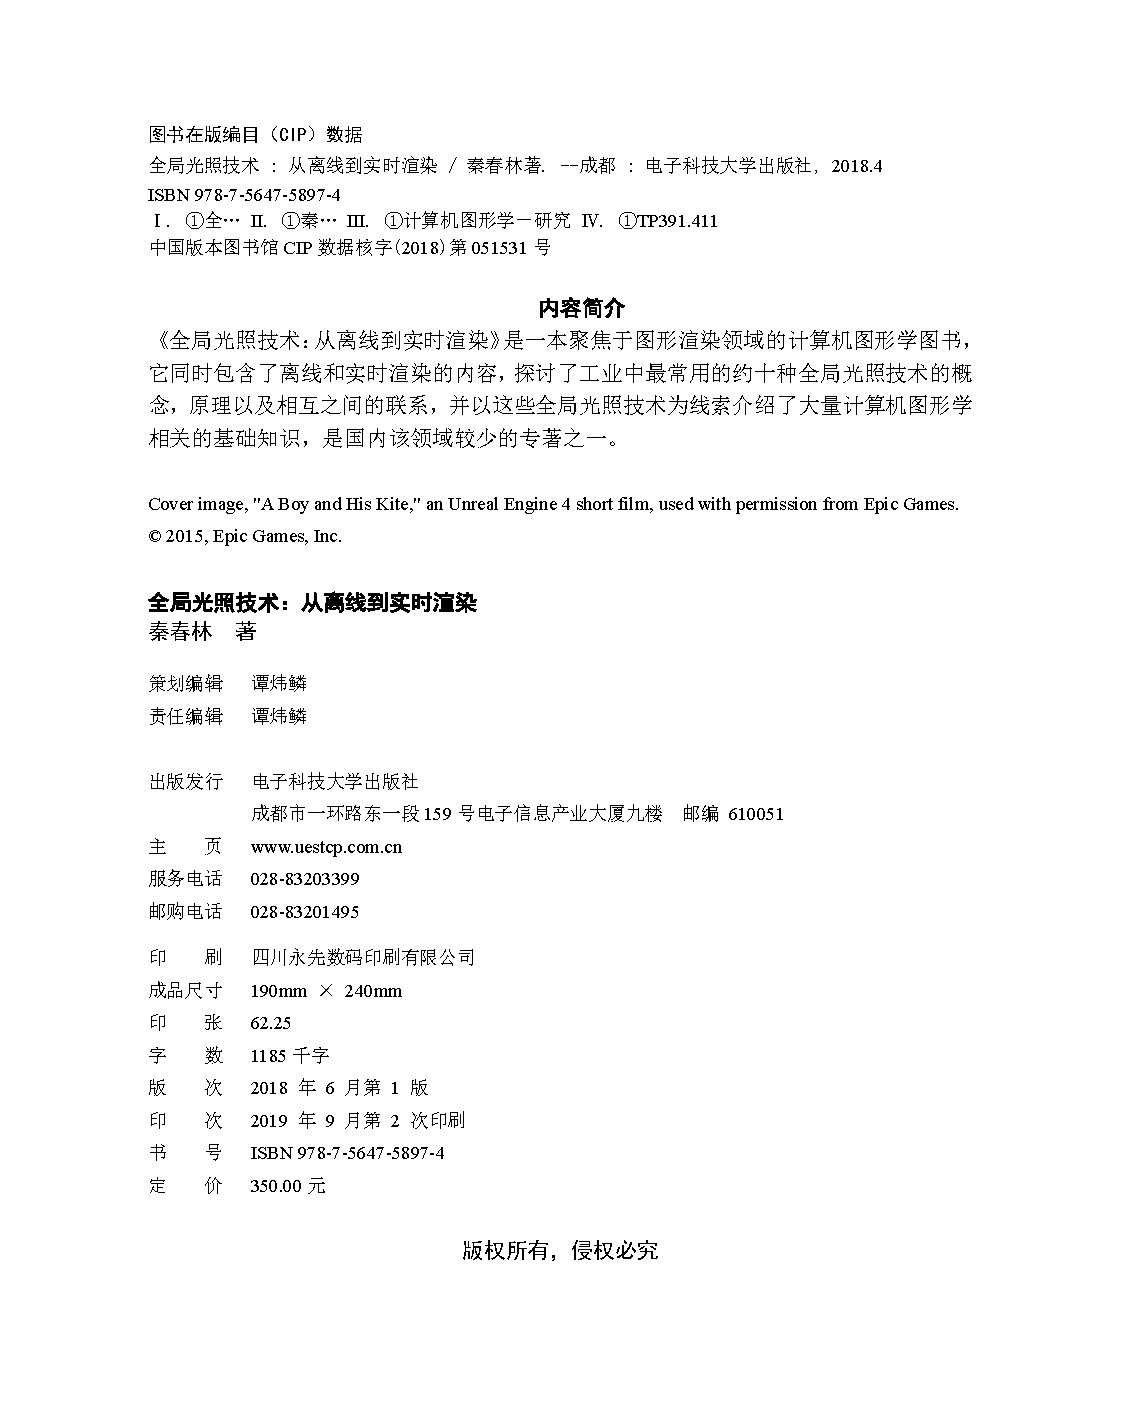
\includepdf[pages={-}]{figures/copyright}
\end{fullwidth}
\clearpage


\frontmatter
\pagenumbering{roman}
\setcounter{page}{-1}

%\begin{dedication}
\begin{flushright}
此书献给这个世界上最伟大的爸爸,妈妈\\
你们对我的支持与包容\\
造就了我自由的思想\\
这是我今生最有意义的财富
\end{flushright}
\end{dedication}





%\foreword
\addcontentsline{toc}{chapter}{推荐序}\mtcaddchapter 

推荐序撰写者招商中,欢迎自荐或引荐,请联系:http://www.thegibook.com 或者elvis@thegibook.com


\begin{comment}

Alex Champandard is the founder of AiGameDev.com, the largest online hub for arti - cial intelligence in games. He has worked in the industry as a senior AI programmer for many years, most notably for Rockstar Games where he worked on the animation technol- ogy of Max Payne 3. He regularly consults with leading studios in Europe, most notably at Guerrilla Games on the multiplayer bots for KillZone 2 and 3. Alex is also the event direc- tor for the Game/AI Conference, the largest independent event dedicated to AI in games.

%% Please have the foreword written here
Use the template \textit{foreword.tex} together with the Springer document class SVMono (monograph-type books) or SVMult (edited books) to style your foreword in the Springer layout. 

The foreword covers introductory remarks preceding the text of a book that are written by a \textit{person other than the author or editor} of the book. If applicable, the foreword precedes the preface which is written by the author or editor of the book.




\vspace{\baselineskip}
\begin{flushright}\noindent
Place, month year\hfill {\it Firstname  Surname}\\
\end{flushright}

\end{comment}

%\preface
\addcontentsline{toc}{chapter}{前~~言}
\mtcaddchapter 

我猜大部分读者第一次翻开一本新书的时候,会首先定位到目录部分,寻找自己感兴趣的内容,如果发现一些或者甚至部分章节的内容是自己不太熟悉而又正渴望学习的,这个对口的内容基本上决定了购买兴趣;接下来的动作则是定位到书中对应这些章节的地方,感受作者的写作风格,知识点讲解的精准性与难易度等,这两个动作决定了这本书在他心目中的份量。

而我却习惯于通过前言部分来获得对一本书的期待程度,其原因是因为知识的逻辑性比知识本身更重要。那么什么是知识的逻辑性?实际上这是我自己的一种思考,并未在什么地方看到过这样的概念。在我自己的体会中,学习知识分为两个方面,其一是一个个具体的知识点,例如C++语言的多态性;第二则是关于这些知识点之间的联系,我把它称为知识的逻辑性,知识逻辑性获取的难度要远远大于知识本身。科技的进步是知识的累积的结果,这意味着我们这一代人需要比上一代人学习更多的知识,随着这种量的增加,我们越来越多地需要去梳理这些庞杂知识点之间的联系,才能真正地理解和掌握一门技术。而通常,我们需要大量的阅读量才能总结出这些知识点之间的逻辑联系。

那么我到底想说明什么呢?首先在一本书中,各个章节通常还是偏重于讲述知识点(在局部知识点范围内通常很难清晰地描述全局知识逻辑性),所以在我看来,一本书最适合描述知识逻辑性的地方就是一本书的前言部分。有时候我通过一本书的前言部分,就能对我过去一些零散知识点行成一个更好的认识和归纳;其次,由于每个人的知识逻辑性是不一样的,因此针对同样知识点的两本书,作者可能分别从完全不同的角度来讲述和理解,这其中反应的正是作者建立他的知识逻辑性的过程,这也可以间接用作这本书质量的一个权衡量。通常知识逻辑性更强的作者更倾向于在前言部分描述他建立自己知识逻辑性的过程,这甚至有时候比他书写某个章节的内容更痛快。

客观地说,这个世界上已经不乏优秀的计算机图形学书籍,例如实时渲染的经典书籍《Real-Time Rendering》\cite{b:rtr},离线渲染中聚焦于光线追踪算法的《Physically Based Rendering: From the Theory to Implementation》\cite{b:pbrt},讲述高级全局光照的《Advanced Global Illumination》\cite{b:AdvancedGlobalIllumination},还有大量讲述关于OpenGL,Direct3D等业界主流底层图形接口的,以及各种针对高校学生偏重理论基础的计算机图形学教材。那么我们为什么需要另外一本计算机图形学的书籍?



\section*{本书的逻辑}
我在大学本科的专业不是计算机科学技术,那个时候只是出于对计算机的兴趣,以及在那个年代计算机互联网蓬勃发展的背景下,我选择了要在毕业以后从事软件开发相关的工作,并且在大学阶段后两年的时间,我几乎将所有时间和精力用于学习计算机相关的知识。然而这仅限于传统的软件编程,直到工作两年之后,我才真正开始计算机图形学相关知识的学习。

在这期间,我阅读了大量关于计算机图形学的书籍和论文,从各个高校的一些经典教材,到各类以OpenGL等图形接口为核心的实践性比较强的书籍,以及这些图形接口的官方API文档等。我发现计算机图形学学习起来非常困难(尤其对于一个非计算机科学专业背景的人),不仅因为其知识点繁多,也跟当前市面上相关书籍的总体情况有关。

目前关于计算机图形学的书大概可以分为三类:第一类(也是数量最多的一类)以各个分散的理论为基础,按类别逐个介绍各个知识点或者渲染过程中的某个阶段,各种大学的计算机图形学教材大都是这一类,前面提到的《Real-Time Rendering》也是属于这一类。这一类书籍是开始学习计算机图形学最好的入门资料,可以逐个了解计算机图形学相关的各种概念。然而这类书籍的缺点是缺乏系统性,读者很难对渲染过程有个整体上的认识,这种知识逻辑性的缺乏反过来会制约对某些概念的理解。

第二类书籍以图形接口如OpenGL等为基础,围绕传统的渲染管线来介绍计算机图形学的各个概念,这类书籍通常具有一些完整的示例,读者能够对经典的渲染管线有一个总体认识,并对各个理论知识点在渲染流程中的运用有一些理解,反过来会促进知识的逻辑性。然而实际工业中使用的渲染方法会比经典的渲染管线要复杂得多,例如它可能需要分多次渲染,每次生成最终结果的部分内容,最后进行合成,例如对动态和静态物体的分开处理,对阴影的处理,对间接光照的处理,以及最后对全屏环境遮挡的处理等;另外,很多工业中使用的渲染方法都需要许多特定的数据支持,这可能需要渲染管线读取GPU中特定格式的数据并使用特定的算法来实现渲染的某个阶段或过程,这些方法的理论一般是这类书籍不会涉及的。

第三类书籍则综合计算机图形学理论以及图形硬件环境,图形硬件API等,详细阐述一个完整,系统的渲染解决方案。我认为此类书籍最有利于构建知识逻辑,因为其不光告诉我们怎样使用图形API来实现光照计算,它更能清楚地告诉我们,各种计算机图形学概念怎样被运用在实践中,读者就能够轻易地理解每个理论的作用和机制,针对同一个问题,读者甚至也许能够提出自己的思路,使用不同的理论方法来解决这个问题。只有在这样的条件下,构建起属于读者自己的知识逻辑,才能真正系统性地理解计算机图形学,从而更有效地进一步学习以及解决工作中的实际问题。本书正是试图属于这类书籍。

由于渲染过程的复杂性(例如一个渲染器要实现场景表述,坐标变换,表面着色,对函数的采样,各种全局光照模型,光源等等,其中全局光照模型部分尤其复杂),尤其是在实时渲染领域,全局光照不能通过像光线追踪一样单一的解决方案实现,而需要融合多种方法,其中每种方法可能只实现一种单一的全局光照效果(如软阴影,环境遮挡,反射,次表面散射等等),这些细节通常不是一本书能够覆盖的,这几乎相当于是从渲染的角度讲述一个完整的游戏引擎的实现。这类书籍又可以分为两个小类,其中第一类以光照模型相对比较单一的离线光线追踪(见本书第\ref{chp:path-tracing}章)为基础,它通常附有比较完整的源代码实现,这类书籍的经典代表是《Physically Based Rendering: From the Theory to Implementation》,本书则是属于第二小类书籍。

为了帮助读者系统性地建立知识逻辑,同时讲述除光线追踪以外更多更复杂的光照模型,第二小类书籍大多以理论为基础,而忽略可能非常繁琐的细节(这些细节可能远远超过一本书的篇幅)。这类书籍的经典代表作之一是《Advanced Global Illumination》,它着重于讲述光线追踪和辐射度两大基本的渲染方案,并且简要介绍了结合这两种理论各自优点的一些混合方法,例如双向路径追踪,辐射照度缓存等等;另一本聚焦于光子映射算法的书籍《Realistic Image Synthesis Using Photon Mapping》\cite{b:RealisticImageSynthesisUsingPhotonMapping}也值得一阅。

我们看到这两个小类的书籍各自拥有自己的优缺点:第一类具有比较完整的示例帮助读者构建更具体的知识逻辑,但是其内容限于比较单一的光线追踪模型;第二类能够覆盖更广泛的光照模型,但是其很难在一本书的篇幅内详细讲述其实现细节。那么有没有可能综合它们各自的优势呢?

随着计算机硬件性能的不断提升,计算机图形学正经历着飞速的发展。每年的SIGGRAPH图形学专业会议都会产出几百篇计算机图形学论文,这些论文大都由一些高校,从事基础图形学理论研究的机构,或者计算机产业中从事图形硬件及接口相关的公司(例如AMD,Intel,Nvidia等)发表,每篇论文大都是一些计算机图形学基础理论的工作。这些基础理论然后被一些从事游戏开发,电影动画及特效,游戏引擎厂商等融入进图形渲染工具中,与其他方法一起形成各种完整的光照解决方案。这些高层的解决方案的结果通常在GDC及其类似的专业会议上,以非正式的演讲的方式释出。

所以光照模型最前沿的解决方案,来自于那些工业级的顶级游戏公司(如顽皮狗),游戏引擎厂商(如CryEngine,Frostbite,Unreal Engine等)以及动画电影公司(如Pixar,Disney等)。围绕这些工具及产品来讲述计算机图形学,不仅能够兼顾到各种各样前沿的实现方案,读者还能够通过使用这些产品去了解该实现的最终效果和功能。

本书正是基于这样的理念来编排整本书的内容:我们以当前业界最前沿的一个个完整的全局光照解决方案为核心内容,通过结合讲述使用这些解决方案的工具及其产品的特性及功能,来达到更系统性地学习计算机图形学的目的,帮助读者更好地构建自己的知识逻辑。



\section*{全局光照}
全局光照几乎代表了计算机图形学渲染相关的全部内容,它是一个渲染器力求模拟真实物理世界关于物体表面交互的全部自然现象的全部内容(当然目前计算机图形学研究领域主要限于几何光学,它并不包括更微观的如干涉,衍射等光学现象,参见第1章的介绍):即光从光源出发,以无限的速度在环境中直线前进,经过与表面发生多次反射和折射,最后进入人的眼睛形成图像。

然而由于渲染方程是一个沿全空间方向的积分,这使得渲染过程非常耗时,在现有的硬件条件下几乎不可能按照原始的渲染方程进行图形渲染。不过研究发现,我们并不需要完全按照原始的渲染方程进行计算,即可以生成令人信服的图像,在这个级别我们通常称为Realistic Rendering。于是人们寻求简化的光照模型以求能达到这种渲染品质,在原始渲染方程的基础之上,人们提出两种简化模型。

\begin{itemize}
	\item \textbf{基于有限元分解的辐射度理论 } 有限元分解是一种常见的积分计算方法,它将一个沿无限空间的积分分解为一个有限纬度(称为一个有限元)的积分,在每个纬度,我们只需要求出该有限元的均值,并可以很容易地计算出光照积分方程。在辐射度理论中,通常我们通过Monte Carlo等方法预计算出每个有限元的均值,供渲染时渲染方程的实时计算。
	\item \textbf{基于蒙特卡洛方法的光线追踪技术 } 蒙特卡洛方法通过随机抽样,使用有限个采样点的值,来计算积分方程的值。
\end{itemize}

这两种方法均能达到非常高的图像品质,但其计算仍然十分耗时,因此主要用于电影等离线渲染领域(例如Pixar的RenderMan就是基于光线追踪的渲染器)。在游戏等实时渲染领域,人们寻求更简化的渲染模型,与辐射度和光线追踪技术通过简化积分方程的思路不同,实时渲染领域的主要思路是根据光学现象或者其他理论拆分渲染方程,使得光照效果最终由多种效果叠加而成,例如直接光照(光从光源出发经过物体表面反射或者折射一次后进入人眼),(软)阴影,漫反射,光泽反射,间接光照,环境遮挡,次表面散射,环境贴图,反射等等。

这些效果可能分别使用不同的方法来计算,例如阴影可以使用GPU的光栅化特性来计算,环境遮挡可以在后处理阶段基于屏幕空间进行计算,环境光照则可以使用简单的贴图实现;另一些算法则使用一些特定的数据格式来加速其中的一些计算,例如Unreal Engine 4对整个场景构建一个距离场的数据结构,通过它来加速遮挡关系的计算从而实现软阴影以及环境遮挡等效果,其他一些方法则通过使用球谐函数来存储一些点的近似的“环境函数”,从而能够快速地计算各种间接反射的效果。

计算机图形学可能是计算机领域最活跃的领域之一,研究人员(尤其是实时领域)和工程师一直在致力于开发新的技术来加速光照的计算,这使得图形学的内容和分支越来越庞杂,初学者想要掌握这些知识必需要花费大量的时间和精力,才能理解这些技术之间的关系,优缺点等,从而更好地改进产品的渲染性能及品质。这就需要非常具有知识逻辑性的书籍来加速工程师对计算机图形学的掌握和运用。

反过来,一本以全局光照为核心内容的书籍,必须要覆盖到以上这些提到的各种各样的图形学理论。所以通过本书,读者能够更系统地综合学习和理解各种计算机图形学的基础理论知识。



\section*{本书特点}
尽管从以上的说明读者可能已经基本了解本书的写作风格及内容,为了便于读者更简单快捷地了解本书的特点,并通过这些特点来决定是否需要进一步阅读这本书,这里还是将本书的特点更清晰地总结如下。

\begin{itemize}
	\item \textbf{知识逻辑性强,覆盖面广 } 一个完整的全局光照解决方案,要充分考虑渲染的各个方面,从游戏场景元素的几何表述,用于光照计算的(CPU和GPU)数据内存结构,到各个渲染通道,每个通道的每个阶段,各种光学现象的实现等,它几乎囊括了大部分图形学的知识。因此读者能够通过对完整的全局光照模型的学习,建立起极强的计算机图形学知识的逻辑和系统性认识。
	\item \textbf{覆盖业界最前沿的图形学知识 } 计算机图形学领域近些年虽然发展非常快,但是其基础理论几乎没有太大变化,这些变化大多体现于工业中(例如对现有算法的改进,使用一些额外的数据结构来加速实时计算等),所以这些变化通常不会反应在以计算机图形学理论为基础的书籍中,但本书讲述当前工业中使用的游戏引擎及中间件等产品的全局光照实现,所以它能够覆盖最前沿的图形学知识。
	\item \textbf{详细分析各大渲染器,实用性强 } 本书从第\ref{chp:path-tracing}章起,几乎每章都是围绕一个或多个游戏引擎工具,或者某些中间件产品的全局光照方案进行介绍,在学习这些全局光照方案的同时,读者也能够学习这些工具的特性及原理,从而更好地理解和使用这些工具。本书覆盖了Pixar的RenderMan,Disney的Hyperion等离线渲染工具,Unreal Engine 4,CryEngine 5,Unity 5等业界主流商业游戏引擎,此外本书还介绍了Enlighten,PowerVR公司图形处理器的Ray Tracing等中间件的实现和使用,同时覆盖这么多工业级的产品,对于积累读者的专业经验以及扩大知识面都是极为有益的。
	\item \textbf{循序渐进的方式学习不同的全局光照模型 } 这些各种不同的全局光照解决方案彼此之间并不是完全独立的,它们有着极强的关联,读者能够从一种解决方案中看到另一种方案的不足,一种解决方案可能是另一种解决方案的改进和优化。例如路径追踪是与摄像机视角相关的,因此改变视角则需要重新计算,而辐射度方法则与摄像机视角无关,因此它可以将数据预处理,并且能够实现渐进式计算(即将复杂的计算分布于多帧中,每帧计算一个增量并累加至一个精度更高的结果);为了加速光线追踪计算,与路径追踪直接从物体复杂的几何表述中获取光照信息不同,光子映射方法则将光照信息存储为一个独立的数据结构(称为光子图),通过路径重用来大大加速了光线追踪的计算。我们可以看到,这些不同的全局光照模型之间的联系本身也能促进我们更透彻地理解这些概念。
	\item \textbf{实时和离线渲染相结合 } 大多数关于计算机图形学的书籍,都是专门针对实时或者离线渲染领域,例如《Real-Time Rendering》针对实时渲染,而《Physically Based Rendering: From the Theory to Implementation》聚焦于离线渲染。而客观的事实是,实时和离线渲染同属于计算机图形学领域,它们只是在当前硬件水平下针对实时性需求的划分,因此,不仅作为渲染工程师我们需要同时掌握实时和离线渲染,另一个事实是,实现渲染中的静态光照贴图,其他一些预处理数据等都是需要借助于离线渲染来实现;此外,很多实时的全局光照模型都是从离线渲染模型优化,改进而来,学习离线渲染对实时渲染中相关概念的理解有极大的帮助。因此本书不特别区分实时和离线渲染,当然我们会特别说明每个光照模型的实时性。
	\item \textbf{符合按需学习知识的过程 } 很多书籍都是按照知识模块的分类进行章节划分,一个知识点接着一个知识点,先讲解理论知识,最后再把这些理论用于实践当中。而人类的学习特点通常是首先遇到问题,然后再去寻找和学习解决该问题相关的知识。在本书中,我们并不在前面的章节首先按模块介绍后面的章节会使用到的基础理论,而是围绕一个全局光照模型为核心,然后在需要的地方学习对应的基础理论知识。例如当需要学习光子映射的时候,我们才会介绍核密度估计;当需要学习辐射度方法的时候,我们才会介绍小波变换(当然本书还是在前两章首先讲述本书会涉及的最重要和基础的知识)。这也是我平时的学习方法和习惯。
\end{itemize}

此外,本书还列出百多篇本书写作期间参考的论文及书籍资料,并在书中每个地方指出具体的参考论文供读者进一步阅读,相信这些资料能够大大丰富和完善读者的知识量。



\section*{写作范围}
本书定位于计算机图形学领域的中,高阶书籍,虽然全局光照技术涉及计算机图形学的各种基础理论,但是本书并不会对这些基础理论做深入的介绍,相反,本书假设读者对这些基础理论有一定的了解,例如读者要能够明白贴图的原理及实现方法,顶点及像素着色器的作用,光栅化等等基本概念。

本书聚焦于各种全局光照解决方案的实现思路,例如它需要的内存数据结构,它涉及的渲染通道以及每个通道的作用,光照模型工作的流程,它的核心算法使用的基本公式及原理;此外,本书还特别讲解每种全局光照模型对特定的光学现象的实现及不足。总之,本书更偏向于讲解每种全局光照模型的实现原理及过程,而非每种图形学相关的概念本身。




\section*{章节概要}
\textbf{第1章:计算机图形学基础 } 介绍计算机图形学最基本也是本书的基础知识,包括全局光照中的各种现象,渲染方程中的各种度量,光与表面的交互,渲染方程,BRDF以及基于物理的渲染相关的理论。这些计算机图形学基础知识是与具体的全局光照模型以及所使用的图形接口及图形硬件的特性无关的。

\textbf{第2章:并行处理器架构 } 本章介绍图形处理器硬件相关的知识,例如GPU的并发处理,内存模型,数据在GPU的存储等。

\textbf{第3章:图形处理器接口 } 本章介绍经典渲染管线与图形接口相关的内容,例如光栅化,着色器,深度及模板测试,GPU中存储数据的各种缓冲区对象等。

\textbf{第4章:着色管线 } 本章从单纯着色管线的角度,抛开图形接口与其他全局光照算法,讨论一般的着色管线,光照管理与着色渲染的流程等。

\textbf{第5章:蒙特卡洛方法 } 蒙特卡洛积分是路径追踪的核心基础,它也是计算机图形学中广泛用于各种预处理数据计算的工具。蒙特卡洛方法通过使用随机模拟对积分函数进行采样,利用有限的采样点来近似无限元积分方程的值。本章将介绍概率论基础,随机变量的定义,期望,估计,蒙特卡洛积分的推导,对随机变量的采样方法,以及减少随机采样方差的方法。

\textbf{第6章:光线追踪技术 } 光线追踪几乎是现代整个图形学的基础及未来,不仅当前电影产业的主要图形学技术大都使用光线追踪技术实现,在实时的游戏引擎内也大量涉及光线追踪技术的使用。本章还会特别介绍Disney与2014年开发的全新渲染器Hyperion。

\textbf{第7章:光子映射 } 光线追踪技术是完全与场景的几何关系绑定的,对于每一帧都需要重新计算。光子映射的思路就是要解除这种耦合关系,它将场景中所有的光照能量存储到一个称为光子图的数据结构中,然后每个点可以根据周围光子的密度进行估计,当然光子只存储在漫反射表面上,因此它通常还需要结合光线追踪等其他技术一起工作。

\textbf{第8章:梅特波利斯光照传输 } 梅特波利斯算法是近代科学与工业中非常重要的一种实践方法,在光线追踪技术中它被用于寻找非常难以被捕捉的路径,也应对非常复杂的场景。


\textbf{第9章:辐射度理论 } 对于静态场景,如果我们能够预先计算出一些区块的光照的平均值,则可以大大加速光照计算。然而较大面积区块的平均值降低了光照的频率,因此辐射度理论假设场景中的表面都是漫反射表面,并且仅适用于频率比较低的间接光照等,但好处是其丧失了方向性,与摄像机位置无关而可以被预处理。虽然辐射度方法适用于静态场景,但是本章也介绍一些技术能够动态更新这些“预处理”计算。此外,Unity等游戏引擎使用的第三方组件Enlighten也是完全基于辐射度理论来实现的。


\textbf{第10章:即时辐射度 } IR的简单实现就是先对所有光源执行一次粗粒度渲染,将这个渲染的结果看成看成多个虚拟点光源(Virtual point light),然后用所有这些粗粒度的点光源对场景进行绘制,以获得间接光照。IR的前提仍然是漫反射表面,因为只有低频的漫反射表面才能使用这种粗粒度的表述。然而和采样类似的问题,IR受限于VPL的数量,本章介绍了一些优化思路,例如在场景变化比较复杂的部分增加VPL的数量,或者从观察的角度来改变采样的重要性等。

%\begin{comment}
\textbf{第11章:基于预计算的全局光照技术 } 当前工业中主流的实时渲染全局光照技术大都是基于某种预计算的,本章总结了常用的预计算技术,例如光照贴图,体积光照贴图,光照场探针等等技术,并且详细介绍了相关的数学基础概念,即球谐函数以及函数的投影和近似。

\textbf{第12章:基于体素的全局光照技术 } 基于体素的全局光照技术是一种完全实时的渲染技术,它通过将场景体素化为一个多分辨率的体素结构,然后过滤以及体积渲染相关的概念来简化场景的表述和光照计算,使得实时计算的性能要求得到满足,这种技术已经被CryEngine 5和Unreal Engine 4等游戏引擎支持。
	
\textbf{第13章:基于距离场的全局光照技术 } 距离场是一种隐式表面表述,它能够用于加速光线与表面的相交计算,因此在Unreal Engine 4中被用于快速执行可见性相关的计算,例如软阴影和环境遮挡。除此之外,距离场作为一种一般的场景表面表述方法,它还被用于其他很多不同的应用中,本章还介绍了移位映射等相关应用。
%\end{comment}



\section*{读者群体}
本书针对的读者群体主要为与计算机图形学相关的学生,教师,研究者,研究机构,游戏开发工程师,正在或者希望使用RenderMan等离线渲染器,或者Unreal Engine 4,CryEngine 5, Unity 5等游戏引擎开发各种产品的开发者,以及其他行业与图形学有关的从业人员,例如影视动画行业等。

阅读本书,读者需要具备本科或大专及其以上学历,或者对线性代数,微积分等大学基础课程具有一定理解的同等基础的人员;本书定位为计算机图形学领域的中,高阶书籍,因此读者最好对计算机图形学基础理论有一定的了解,熟悉一般3D渲染的概念。

本书可以作为学习计算机基础理论的资料,更可以用来巩固自己已有图形学知识,系统性地理解这些基础理论在工业中怎样被实际运用。



\section*{关于专业词汇}
按照中文出版惯例,中文书籍当中的英文专业词汇应该全部翻译为中文。然而出于以下原因,本书采取保留所有英文专业词汇。

\begin{enumerate}
	\item 有大量的计算机图形学专业词汇并没有完美的中文翻译,例如Post Processing翻译为后处理并不能准确表述其意,这在某种程度上不仅使得文句意思晦涩,更容易使读者对其知识点没有更精准的理解。
	\item 在计算机图形学领域,大部分的书籍,文献和专著都是以英文书写的,在读者的后续学习,以及甚至在本书的学习过程中,常常会需要查阅更多的英文资料,因此保留英文专业词汇更利于后续学习。
\end{enumerate}

当然,本书中保留的英文词汇仅限专业术语,即名词。对于一个术语用作动词的情况,本书仍然会选择使用更精准中文文句来描述其意义及过程;同时,对于部分具有完美翻译的专业词汇,按照本书的思路仍然将保留英文形式;另外,对于某些英文书籍或文献,其可能已被翻译为中文资料,为了便于查阅,本书仍将提供英文名称,读者需要自己查询是否具有相关中译本;最后,对于所有这些专业词汇,本书的索引部分会有全书的引用位置供读者查阅。



\section*{勘误及更多资源}
在本书的写作期间,虽然我尽最大努力保证本书逻辑的严密性,内容的准确性以及表述的清晰性,然而由于近几年计算机图形学技术的更新速度非常快,以及我个人知识及经验的局限性等,本书不可避免会存在一些错误。在此,我向各位读者首先表示真诚的歉意!

当您在阅读期间发现任何错误,我恳请您能够稍微花一点时间将这些错误反馈给我,因为我希望这本书会作为一本相对优秀的教材被精心的更新下去,所以您的每一个反馈一定会被认真对待以使后续的内容能够更加准确,从而造福更多的读者。为此,我提供了一个与本书配套的勘误网站用来提供勘误以及其他信息,您也可以订阅该网站的邮件列表以得到最及时的勘误通知:

\url{https://github.com/thegibook/revision}

除此之外,为了方便读者之间就本书的内容进行讨论,本书特别设立了一个本书的读者交流中心,大家可以在这个论坛就书里的内容进行更有针对性的交流,学习甚至延伸扩展:

\url{http://readers.thegibook.org}

最后,您总是可以从本书的官方网站获得本书的最新动态,作者的最新博客文章,以及作者推荐的一些相关学习资源等资讯:

\url{http://www.thegibook.com}




\section*{致谢}
没有一件伟大的事情是一个人完成的,即便一个人完成了其中大部分的实施工作,但是没有其他人的一些鼓励或者认同,这件事情也将是毫无意义的。

这本书耗费了三年多的心血,这期间我没有参加任何工作,如果没有家人的鼓励和支持,这件工作是永远无法完成的,我要感谢爸爸,妈妈和妹妹一直以来对我的包容,理解,鼓励和支持,我一直都在为拥有你们而骄傲。

这本书在写作的初期阶段就有幸得到很多同行朋友的支持和认同,其中我们在2017年中发起了本书的试读众筹,470多名同行参与了此次众筹活动,这不仅是对图书内容的认可,对我也是一个巨大的鼓励和鼓舞,在此对你们的支持表示感谢,所有这些支持者名单可以从官方网站看到。

还要感谢罗丁力,大钊,王祢,幽玄,杨哥,罗登导演,Liaoer,杨世玲等对本书写作的支持,宣传以及一些交流反馈,还有很多朋友的名字没法一一列出。感谢“全局光照技术”QQ群里各位群友陪伴我的整个写作过程,你们不厌其烦地围观着我不停地关于图书写作的唠叨,缓解了我很多的压力,没有你们的陪伴,这段旅程就会更加枯燥,感谢你们。

感谢摩点网,本书前后在摩点网发起了三次众筹活动,这对本书的宣传和传播起到了重要的作用,也提供了读者和作者之间在创作阶段的一个交流的方式和平台,摩点网是一家支持优秀创作的众筹平台,对你们的工作以及对图书的支持表示感谢。

另外还要感谢引擎世界社区,他们从最早的试读众筹到现在的整个创作过程中,一直都无私地将这本书介绍给引擎世界的朋友,在此表示特别感谢。

最后要感谢Epic Games授权本书使用由Unreal Engine 4开发的实时动画短片《A Boy and His Kite》中的画面作为本书的封面图片。

%\begin{comment}
	

\vspace{\baselineskip}
\vspace{\baselineskip}
\begin{flushright}\noindent
\hfill {\it }\\
%2018.4
 \hfill {\it }\\
\end{flushright}


\vspace{\baselineskip}
\vspace{\baselineskip}
\vspace{\baselineskip}
%\end{comment}



%%%%%%%%%%%%%%%%%%%%%%%acknow.tex%%%%%%%%%%%%%%%%%%%%%%%%%%%%%%%%%%%%%%%%%
% sample acknowledgement chapter
%
% Use this file as a template for your own input.
%
%%%%%%%%%%%%%%%%%%%%%%%% Springer %%%%%%%%%%%%%%%%%%%%%%%%%%

\extrachap{致谢}
\addcontentsline{toc}{chapter}{致谢}\mtcaddchapter 
提供有价值试读反馈的读者的名字将会出现在这里,欢迎到本书网站http://www.thegibook.com 上提供您的反馈及建议,真诚地感谢您的支持与付出!



\setcounter{tocdepth}{2}

\renewcommand*\contentsname{目~~录}
\tableofcontents
\clearpage


\mainmatter
       
%\chapter{光与表面的交互}
\label{chp:intro}
%\minitoc
%计算机图形学(computer graphics)的主要目标之一,就是模拟光与物体(表面或介质内)交互的光学原理,将一个虚拟的数字3D场景,利用计算机生成一张2D的数字图像,供屏幕显示使用或者保存为数字文件格式。

然而,要达到逼真的视觉效果,尤其在实时的环境下,这个渲染的过程却异常复杂。从技术上讲,这里有两个突出的困难需要解决:首先,对于表面上的每个点,我们必须在该点法线方向对应的半空间(hemisphere)上做积分运算以便求出该点的颜色值,因为每个点都可能接受来自场景中所有其他点反射的光照;其次,对于空间中传播的每一条光线(ray),我们必须遍历场景中所有物体表面上的每一个点,来计算出与该光线相交的最近的一个点的位置(即最近点测试),从而进行光照计算。在当前的硬件条件下,我们几乎不可能实时处理这两个方面的计算。

为了解决这两个问题,计算机图形学提出了大量的方法和理论以简化和加速这两个方面的计算,从而更快(甚至实时)地进行光照计算以渲染场景。

我们可以将所有这些方法和理论分为两大类,其中第一类方法通过寻找更快的数学方法来比较精确地计算渲染积分方程(见第\ref{sec:intro-the-rendering-equation}节),这方面有两大经典方法:即基于有限元分解的辐射度理论,以及基于蒙特卡洛积分的光线追踪技术。

有限元方法(finite element method,FEM)\myindex{有限元方法}{finite element method}是一种常见的积分计算方法,它将一个沿无限维空间的积分分解为一个有限纬度(称为一个有限元)的积分, 我们只需要求出每个有限元的均值,便可以很容易地计算出渲染积分方程,在辐射度理论中,我们通常通过蒙特卡洛等方法预计算出每个有限元的均值,供渲染时渲染方程的实时计算,关于有限元方法详见本书第\ref{chp:rad}章的内容;而基于蒙特卡洛(Monte Carlo)\myindex{蒙特卡洛}{Monte Carlo}的方法则是通过随机抽样, 使用有限个采样点的函数贡献值,来近似计算积分方程的值,这又称为对积分的估计,由于在渲染中一个这样的样本称为一条光线的路径,因此基于蒙特卡洛的方法又称为光线追踪技术,关于光线追踪技术详见本书第\ref{chp:mc}章的内容。

上述两种方法均能达到非常高的图像品质,然而它们的计算仍然十分耗时, 因此它们主要被用于影视动画等离线渲染领域,例如Pixar的RenderMan RIS就是基于光线追踪技术的渲染器产品。

与辐射度和光线追踪技术通过简化和加速积分方程求解不同,第二类方法的主要思路是根据光学现象或者其他理论拆分渲染方程,使得光照效果最终由多种效果叠加而成,这主要是因为光照是可以线性叠加的,这些拆分的效果包括直接光照(即光从光源出发经过物体表面反射或者折射一次后进入人眼的光照),(软)阴影,漫反射光照,光泽反射光照,间接光照,环境遮挡,次表面散射,环境光照等等。

这些拆分后的效果可能分别使用不同的方法来计算,其中大部分都是本书要重点讨论的内容,这些方法的一些主要思路包括但不限于:

\begin{itemize}
	\item 使用GPU的光栅化特性,例如用来简化物体间的遮挡关系和阴影计算,这可以通过使用光栅化从光源的角度生成光照贴图来实现。
	\item 为了减少计算量,另一些技术从屏幕空间(screen space)进行计算,例如环境遮挡可以在渲染的后处理阶段,基于屏幕(而不是物体)空间计算像素的环境遮挡值,还有一些技术在屏幕空间进行光线追踪计算,这都大大减少了着色计算的数量。
	\item 对于一些静态的数据,例如静态光源和场景,我们可以在预处理阶段将某些光照的中间结果转换为纹理的形式,例如环境贴图和光照贴图等,而在运行时只需要使用简单的贴图即可;有时候一个复杂的积分方程的一部分静态数据也可以进行类似的预处理。 
	\item 有些算法则使用一些特定的数据格式来加速其中的一些计算,如最近点测试和遮挡范围计算;例如Unreal Engine 4在预处理阶段对整个场景构建一个距离场的数据结构,通过它来加速遮挡关系的计算,从而实现如软阴影和环境遮挡等效果。
	\item 对于被积函数中的某些低频部分(low-frequency),我们可以通过使用比如低阶的球谐函数等来近似这一部分,它们仅被存储为少量一些系数,从而能够快速地进行积分计算。
	\item 光会在场景中进行多次反射或折射后才会进入摄像机,模拟这种多次反弹(bounce)的效果计算量非常大,但是一些近似方法通过仅计算两次反弹(即光从光源出发,经过两次与表面反射或折射,然后进入摄像机)也能获得非常好的效果。
	\item ......
\end{itemize}

从这些众多看似复杂而零散的计算机图形学知识碎片中,我们可以看到其实它们是具有一定的“逻辑”的。从一个个完整的全局光照系统的角度,以及通过多个不同全局光照模型之间层层递进的关系,通过本书读者应该能够很轻易地去理解这些逻辑,从而站在一个更系统的角度去看待计算机图形学,最终能够更得心应手地解决工作和学习中的问题。




\section{什么是全局光照}
实际上,计算机图形学中所涉及的光照都是指全局光照,但是由于渲染方程计算的的复杂性,早期工业中一般忽略间接光照,仅考虑光从光源出发,经过表面一次反射/折射之后到达人眼或者场景中的虚拟摄像机。这种不考虑环境其他非光源表面对着色影响的光照模型称为局部光照(local illumination)\myindex{局部光照}{local Illumination}模型,反之则称为全局光照(global illumination)\myindex{全局光照}{global Illumination}模型。如今工业中使用的主流商业3D游戏引擎,如Unreal Engine,Unity等大都支持某种程度的全局光照。

由于硬件计算性能的限制,我们很难在产品中达到物理上正确的渲染品质。现阶段计算机图形学领域的主要目标是渲染出令人信服的(convincing),写实的(realistic)图像品质,所以不同公司的产品往往使用不同的方法来实现全局光照模型,这些不同的方法在品质上甚至会有很大的差异,因此我们很难用一种技术的标准来衡量全局光照,但我们可以从另一个角度,即从光与物体的光学特性上去定义一个令人信服的全局光照模型应该实现怎样一些效果。

当然这里仅列出一些目前主流的游戏引擎或其他一些离线渲染产品都在实现的一些光学现象,这并不是一个标准,也不是全局光照的全部内容。通过这样一些现象,我们可以对全局光照有一个直观印象,以及理解作为令人信服的图形渲染目标,哪些核心因素是一个优秀的全局光照模型应该满足的。

注意,本书选择在还没有开始介绍任何具体的图形学知识之前讨论这些全局光照现象,是希望能够使用非图形学的术语更加直观地讲述这些现象,因为这是整本书都在试图达到的目标。



\paragraph{阴~~影}
阴影(shadows)\myindex{阴影}{shadows}对于人眼对3D场景的立体感觉非常重要,在实时渲染领域,直接光照(如点光源,聚光灯以及直线光源等)的渲染通常不考虑物体间的遮挡关系,这主要是为了利用GPU快速的光栅化特性,所以需要另一个单独的通道来处理阴影。这个通道也可以通过使用GPU的光栅化特性,在运行时动态生成光照贴图(shadow maps),或者利用GPU的模板测试生成阴影体积(shadow volume)等比较简单的方法实现。

光照贴图是以光源中的单个点为观察点,利用GPU光栅化渲染的一张图,通常它只包含深度值,所以它记录的只是物体边缘的几何信息,因此产生的阴影为硬阴影(hard shadow)。对于硬阴影,通常还需要使用适当的反走样措施,关于反走样技术将在本章第\ref{sec:intro-sampling}节讲述。

非点光源则具有一定的面积,其生成的阴影为软阴影(soft shadow),一个软阴影的定义包含3个部分:即完全遮挡的本影区(Fully Dark),部分光照被遮挡的半影(Penumbra)区,以及完全没有被遮挡的光照(Fully lit)区,如图\ref{f:intro-shadow}所示。其中半影过渡区可以通过表面到遮挡物体和光源的距离,以及光源的面积大小三个参数来近似技术,本书将会详细介绍相关的阴影计算,《Real-Time Shadows》\cite{b:rts}包含了大量关于阴影技术的介绍。

\begin{figure}
\sidecaption
	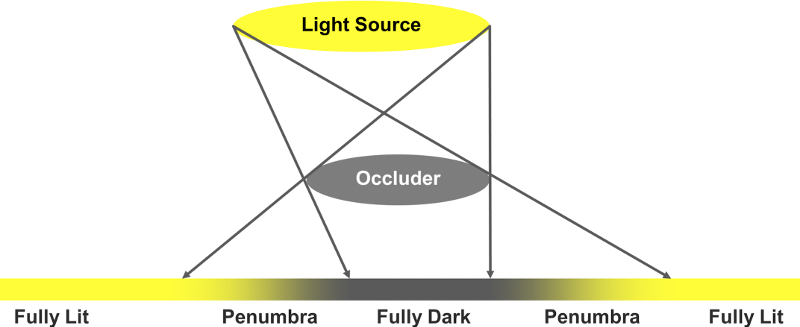
\includegraphics[width=0.65\textwidth]{figures/intro/shadow}
	\caption{软阴影形成的机制,由于光源具有一定的面积,使其包含完全遮挡,部分遮挡及完全光照三个区域(图片来自PowderVR)}
	\label{f:intro-shadow}
\end{figure}




\paragraph{环境遮挡}
对于更大面积的环境光(ambient light)\myindex{环境光}{ambient Light},如环境贴图,天空盒,或者来自其他物体反射的间接光照等,其光源往往来自整个半空间,往往不可能通过以上的方式计算物体间的遮挡效果。在早期的光照计算中,人们通常忽略这种阻挡关系,这造成场景中的缝隙等被较多遮挡的地方比实际的效果要明亮,如图\ref{f:intro-ao}(a)所示,这是因为对于这些地方我们并没有考虑它的遮挡关系,这使得整个物体表面会看起来更平坦,缺乏立体感。

\begin{figure}
\begin{fullwidth}
	\begin{subfigure}[b]{0.325\thewidth}
		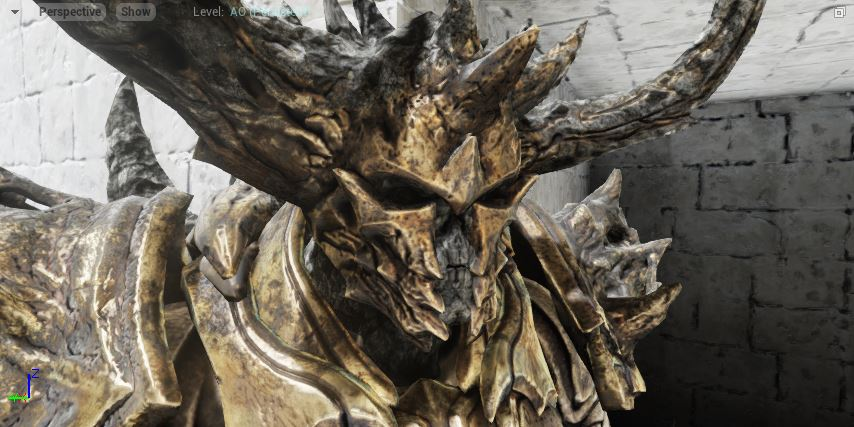
\includegraphics[width=1.\textwidth]{figures/intro/ao-1}
		\caption{不包含AO的场景}
	\end{subfigure}
	\begin{subfigure}[b]{0.325\thewidth}
		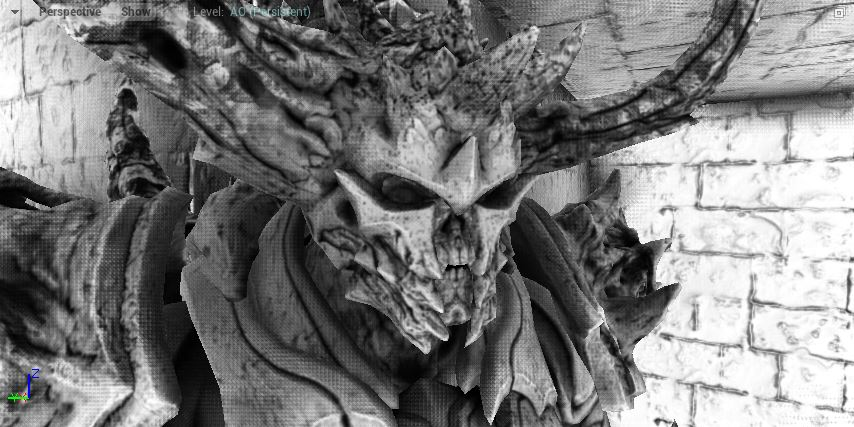
\includegraphics[width=1.\textwidth]{figures/intro/ao-2}
		\caption{仅AO}
	\end{subfigure}
	\begin{subfigure}[b]{0.325\thewidth}
		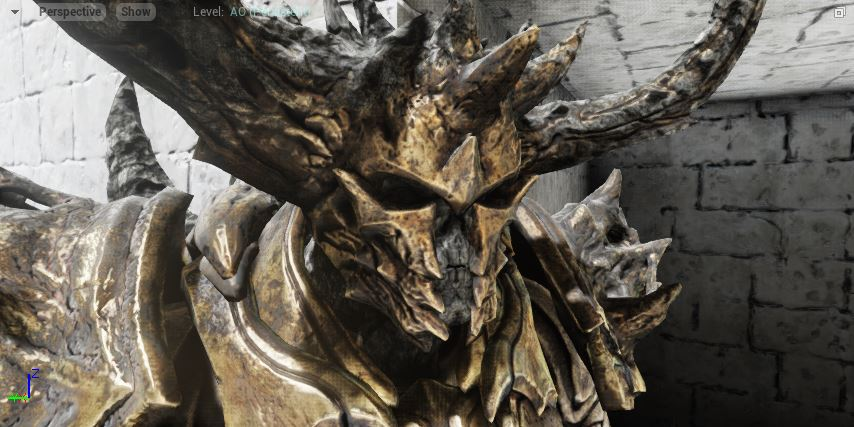
\includegraphics[width=1.\textwidth]{figures/intro/ao-3}
		\caption{包含AO的场景}
	\end{subfigure}
\caption{AO对渲染的影响,注意(c)图中墙砖的裂缝,以及人物颈部等地方由于部分被遮挡显得更暗 (图片来自Unreal Engine 4官方文档)}
\label{f:intro-ao}
\end{fullwidth}
\end{figure}

\cite{a:Shape-from-shadingonacloudyday}首次指出了这种环境阻挡对于图形识别以及增强图像质量的重要性,2010年Hayden Landis, Ken McGaugh和Hilmar Koch因为推进环境遮挡(ambient occlusion,AO)\myindex{环境遮挡}{ambient occlusion}在渲染技术中的运用而获得当年的奥斯卡科学技术奖,之后AO被大量应用于电影工业,如今主流的商业游戏引擎也几乎都支持某种程度(静态或动态)的AO。

AO的计算实际上是要针对每个点,在该点法线对应的半空间上,针对每一个方向对可见性函数(visibility function)进行积分运算,其值为一个介于0到1之间表示遮挡程度的值。对于静态的场景我们可以预计算出这个值;在离线渲染的环境下,可以使用蒙特卡洛方法使用随机抽样的方式求积分\cite{a:GlobalIlluminationandAllThat};而对于实时环境,则需要更高效的方法,例如由CryTek提出的基于屏幕空间的环境遮挡(screen space ambient occlusion,SSAO),以及Unreal Engine 4使用距离场来加速AO的计算。




\paragraph{反~~射}\myindex{反射}{reflection}
光线在物体表面之间穿梭,经过多次反射或折射最后才会进入摄像机,形成图像,如果一个表面是光滑的,或者不是完全粗糙的,则这些表面可以反射它周围的环境,表面越光滑,则其反射的场景越清晰,否则则越模糊。反射几乎无处不在,它是高质量图形渲染不可缺少的部分,如图\ref{f:intro-reflection-1}所示。

\begin{figure}
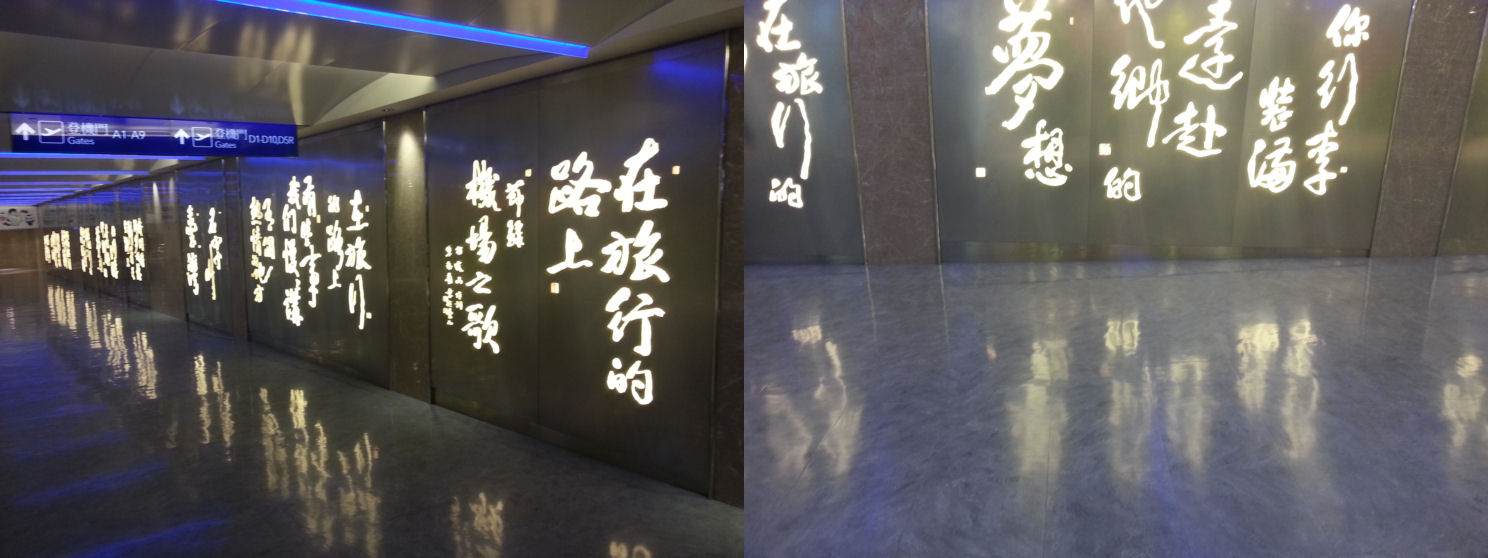
\includegraphics[width=1.\textwidth]{figures/intro/reflection}	
\caption{反射无处不在,较光滑的表面能够比较清晰地反射周围的环境,图为台湾桃园国际机场的走廊}
\label{f:intro-reflection-1}
\end{figure}

反射通常也是使用其他一些近似技术来计算。最经常使用的是基于图像的光照技术(image-based lighting,IBL),这种技术通常将要反射的“环境”渲染为一张图,然后渲染时通过查询这个贴图来计算来自周围的环境光照;对于粗糙的表面可以使用过滤的技术来实现粗糙表面的效果,这种技术大大减少了反射效果的计算时间,本书将在第\ref{chp:prt}介绍基于图像的光照技术。

\begin{figure}
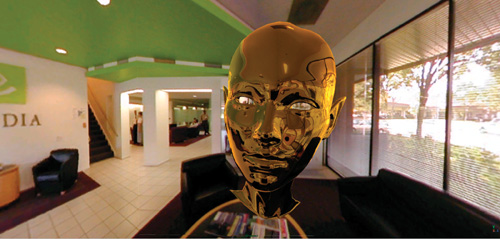
\includegraphics[width=1.\textwidth]{figures/intro/reflection-1}	
\caption{使用基于图像的技术渲染物体对环境的反射,整个周围环境被渲染到一个贴图中,表面着色时直接将这个贴图作为入射光源,其中环境贴图的光照是与观察点的位置无关的}
\label{f:intro-reflection-2}
\end{figure}

对于比较远的环境,可以认为“环境”是和位置无关的,而仅与方向有关。环境贴图可以使用一个放置于场景中心的一个鱼眼镜头的照相机来生成,整个环境被制作成一张立方体贴图(cube map)或者球面贴图(spherical map),如图\ref{f:intro-reflection-2}所示,通常游戏中的天空盒就是一张远距离的环境贴图。




\paragraph{间接光照}\myindex{间接光照}{indirect lighting}
除了上述镜面或光泽反射的光照,环境对于漫反射表面的影响非常重要,它最重要的效果称为颜色渗透\footnote{通过后面第\ref{sec:intro-material-model}节对材质模型的学习,颜色渗透是由于漫反射光从物体内部反射回空中时,被乘以了一个反射率,这个反射率$baseColor$即是物体表面的真实颜色,因此漫反射光携带了物体的颜色,从而能够影响周围的环境。}(color bleeding)\myindex{颜色渗透}{color bleeding},例如一个红色的地毯靠近一侧墙面则会使墙面呈现粉红色,颜色渗透的效果如图\ref{f:intro-indirect}所示。

\begin{figure}
\sidecaption
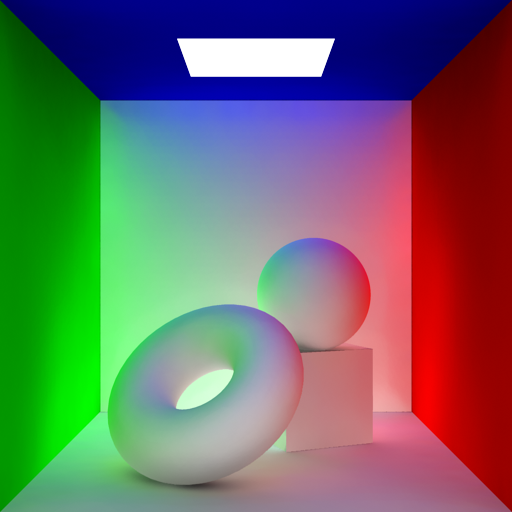
\includegraphics[width=0.45\textwidth]{figures/intro/indirect}	
\caption{环境对漫反射表面的影响,这种效果称之为颜色渗透,这种效果的计算非常昂贵,但是这种效果对于全局光照非常重要}
\label{f:intro-indirect}
\end{figure}

间接漫反射几乎是最重要的全局光照效果,它的计算特别昂贵,其涉及渲染方程针对整个半球空间的积分计算,目前主要的解决方法还是预处理,间接漫反射光照的处理主要有两类方法,一类是基于光照贴图(light map)\myindex{光照贴图}{light map}的方法,这类方法仅针对静态场景,由于漫反射表面向各个方向反射的光照是相同的,因此表面的光照值可以被缓存起来,很多方法可以用来生成光照贴图,例如光线追踪,辐射度方法,辐射照度缓存以及光子映射等方法。

对于动态物体,如角色,移动的交通工具等,常用的处理方法则是在空白空间对环境光照进行稀疏采样,在Unity中这些采样点称为一个光照探针(light probe)\myindex{光照探针}{light probe},如图\ref{f:intro-light-probe}所示,然后在运行时使用插值的方法来计算间接光照。这样做的理由是因为漫反射通常都是低频的,相邻点之间的颜色值变化不大,其间的点的值可以通过插值计算。由于这些采样点是预处理的,所以动态物体并不能影响场景中其他物体,它只能接受来自其他静态环境的影响,这方面可以参见后面第\ref{chp:prt}章的内容。

\begin{figure}
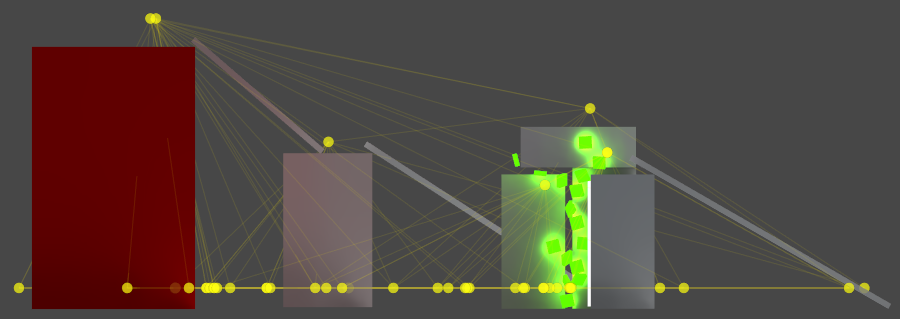
\includegraphics[width=\textwidth]{figures/intro/LightProbes}	
\caption{Unity使用光照探针对环境进行采样,这发生在预处理阶段,在运行时阶段,渲染器从邻近的采样点中取值对其间的点进行插值(图片来自Unity官方文档)}
\label{f:intro-light-probe}
\end{figure}



\paragraph{焦~~散}\myindex{焦散}{caustics}
在全局光照模型中,焦散(caustics)效果尤其明显。广义的焦散是指光从光源出发,经过至少一次光泽反射,最后通过一个光泽或漫反射面 反射后进入摄像机。在计算机图形学中尤其指光通过光泽面的反射或折射后,多束光落在同一个漫反射表面点上(例如由于玻璃或水面等弯曲面使折射后多束光落在桌面上),导致这些点的光照特别明亮,如图\ref{f:intro-caustics}中所示的一些常见焦散的效果。

\begin{figure}
\begin{fullwidth}
	\begin{subfigure}[b]{0.26\thewidth}
		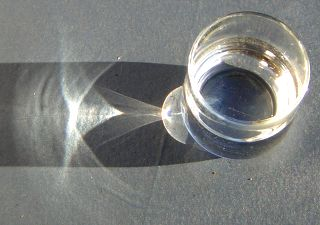
\includegraphics[width=1.\textwidth]{figures/intro/Caustics-1}
	\end{subfigure}
	\begin{subfigure}[b]{0.2758\thewidth}
		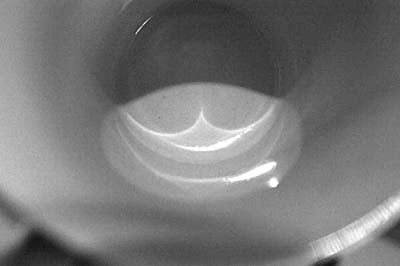
\includegraphics[width=1.\textwidth]{figures/intro/Caustics-2}
	\end{subfigure}	
	\begin{subfigure}[b]{0.19\thewidth}
		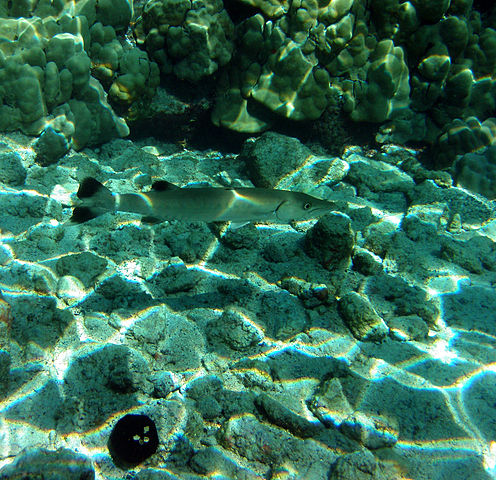
\includegraphics[width=1.\textwidth]{figures/intro/Caustics-3}
	\end{subfigure}	
	\begin{subfigure}[b]{0.246\thewidth}
		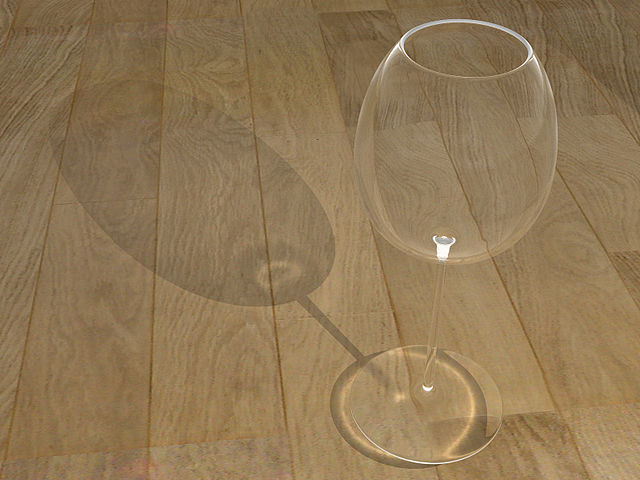
\includegraphics[width=1.\textwidth]{figures/intro/Caustics-4}
	\end{subfigure}
\caption{由于多束光经过反射或折射后落在同一点上,焦散效果在全局光照中特别明显(图片来自Wikipedia)}
\label{f:intro-caustics}
\end{fullwidth}
\end{figure}

对焦散的渲染尤其困难,其主要原因是这样方向光线的采样几率很低,甚至几乎可以认为是零,导致一般的采样方法根本不能获得足够的信息,例如光子映射技术就是使用完全不同于采样的回归方法才能比较好的处理计算焦散。



\paragraph{散~~射}\myindex{散射}{scattering}
到目前为止,所有我们讨论的全局光照现象,都仅限于光与物体表面进行交互。在现实环境中,许多物体部分或全部是半透明的(translucent):即光进入物体表面后,部分被吸收(absorbed),部分发生散射(scattered)最后从物体表面发射出去,其中这个出射点的位置可能和入射点的位置不一样。

由于散射效果的计算相当复杂,因此和其他前面提到的技术一样,计算机图形学中也存在很多近似的方法来处理散射效果。特别地,对于散射的计算,存在两大类方法,它们分别处理散射导致的两种比较明显的子分类效果,即次表面散射和参与介质。

次表面散射(subsurface scattering)\myindex{次表面散射}{subsurface scattering}是散射中最复杂的效果,它表示由于物体内部存在介质的不连续性,导致折射进物体内部的光在经历多次散射之后,重新从另一个位置反射会空中。它要求比较真实地模拟散射效果,并且它处理的都是要求视觉表现比较真实的材料,例如大理石,皮肤,叶子,蜡烛,牛奶等。例如对于皮肤,它有约6\%的光被直接反射,剩下94\%的光被散射,并且散射只发生在表面以下一小部分厚度的空间内,如图\ref{f:intro-sss}所示。

\begin{figure}
\sidecaption
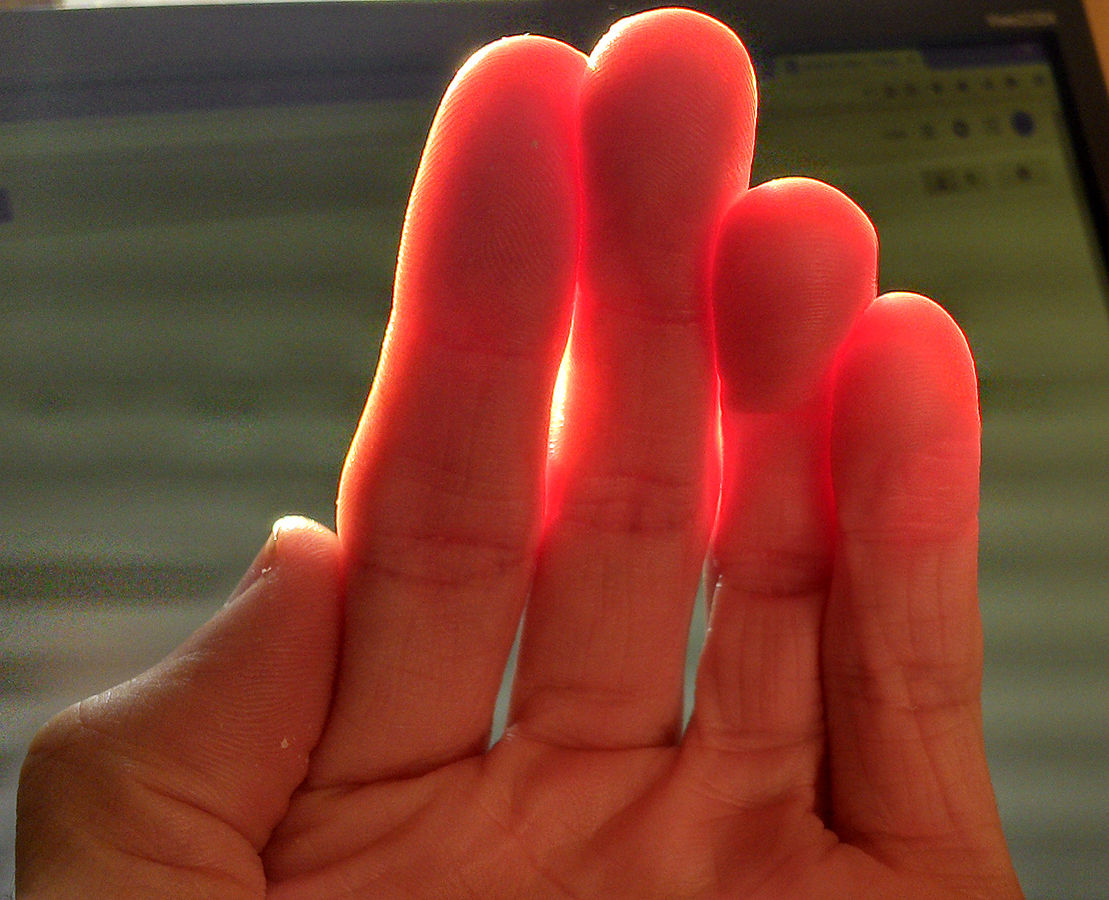
\includegraphics[width=0.5\textwidth]{figures/intro/subsurface-scattering}	
\caption{光可以进入皮肤表面,由于物体内部介质的不连续,在表面以下部分区域内发生多次散射,然后从另一个地方反射会空中}
\label{f:intro-sss}
\end{figure}

关于次表面散射,本章第\ref{sec:intro-bsdf}节会介绍Disney使用的近似然而精确度很高的次表面散射模型,它用在了电影《超能陆战队》中除头发以外的所有次表面散射情形。

参与介质(participating media)\myindex{参与介质}{participating media},例如云,烟,雾等在自然界是普遍存在的,它们也导致了很多有趣的视觉现象。当光在参与介质中传播时,部分被吸收,其他则经过多次散射后从不同的位置离开表面。参与介质与次表面不同的是,次表面往往只是物体表面很浅的一层,而参与介质往往整个内部都是半透明的,光线能够从一边进入,然后从另一边离开。参与介质能够有效地增强环境的氛围,以及对场景深度的感知。

\begin{figure}
	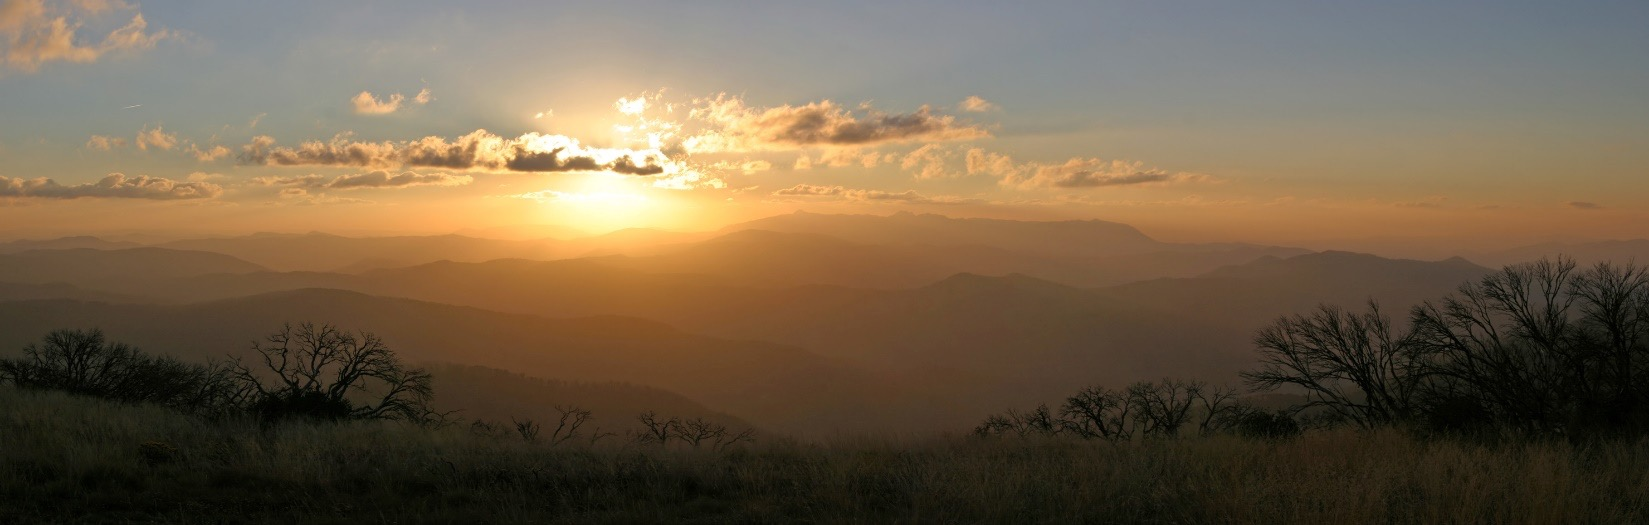
\includegraphics[width=1.0\textwidth]{figures/intro/Participating-media}
	\caption{参与介质在大自然中无处不在,例如云层,空气,烟雾等,并且对整个环境的光照有非常大的影响}
	\label{f:intro-Participating-media}
\end{figure}

本书将在第\ref{chp:pm}章介绍一些参与介质的渲染技术。





\section{辐射度量学}
光学中关于光的测量这一分支,称为辐射度量学(radiometry)\myindex{辐射度量学}{radiometry}。\cite{a:TheRenderingEquation}首次将辐射度量学引入到计算机图形学中,用于测量和计算计算机图形学中光的传播,并由此推导出渲染方程(the rendering equation)\myindex{渲染方程}{the rendering equation}。渲染方程保留了辐射度量学两个最基本的特性即赫姆霍兹互反律(Helmholtz reciprocity)\myindex{赫姆霍兹互反律}{Helmholtz reciprocity}和能量守恒(energy conservation)\myindex{能量守恒}{energy conservation},现代图形学理论基于渲染方程提出了大量的模型用于简化和加速渲染方程的计算,在这两个基本物理特征的保障下,这些模型能够达到非常真实的图形品质。

辐射度量学定义了一组基本的物理量用来测量光辐射,因此这些度量也成为计算机图形学中最重要的基本概念,这几个度量的名称及单位如表 \ref{t:radiometric-quantities}所示。

\begin{table}
\caption{辐射度量学中的基本度量,这些度量也成为渲染方程的基本度量}
\label{t:radiometric-quantities}

\begin{tabular}{p{0.3\textwidth}|p{0.3\textwidth}|p{0.2\textwidth}|p{0.15\textwidth}}
\hline
   中文名称&英文名称&单位&符号  \\
  \hline
  辐射能量&radiant energy & $J$& $Q$\\
  辐射通量&radiant flux & $W$  & $\Phi$\\
  辐射照度&irradiance & $W/m^2$ & $E$\\
  辐射强度&radiant intensity & $W/sr$ & $I$\\
  辐射亮度&radiance & $W/(m^2\cdot sr)$& $L$\\
\hline
\end{tabular}
\end{table}

在开始讨论这些度量之前,必须首先了解立体角(solid angle)\myindex{立体角}{Solid Angle}的概念,如图\ref{f:intro-solid-angle}所示。在几何学中,立体角是2D角度的概念在3D空间的延伸,它表示在3D空间,从某个点观察,另外一个物体有多“大”。立体角的数学符号通常用$\Omega$表示,其单位为$sr$,它是球面度(steradians)\myindex{球面度}{steradians}的缩写。立体角也可以理解为3D空间中以某一点为起点的多个方向的集合。

\begin{figure}
\sidecaption
	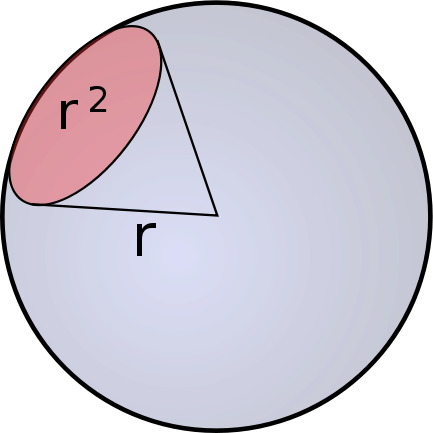
\includegraphics[width=0.35\textwidth]{figures/intro/solid-angle}
	\caption{立体角的概念,它表示单位球体上一块区域对应的球面部分的面积。根据立体角的定义,如果球面上任意一块区域的面积等于球半径的平方,当从球心观察时,该区域面积就是$1sr$}
	\label{f:intro-solid-angle}
\end{figure}

正如在2D中,使用单位圆上的一段弧线的长度来表示其对应“角度”的大小,在3D中,使用单位球体上一块区域面积的大小来表示其对应的“立体角”的大小。所以一个物体相对于某一点的立体角的大小,等于这个物体投影到以该点为球心的单位球体上的面积。

根据上述立体角的定义,如果球面上任意一块区域的面积等于球半径的平方,当从球心观察时,该区域面积就是$1sr$。

在球面坐标系中,单位球体上任意一块区域$A$的面积可以简单地表示为:

\begin{equation}
	\Omega= {\rm \iint}_A \sin\theta {\rm d}\theta {\rm d}\varphi
\end{equation}

\noindent 其中,$\theta$表示经度,$\varphi$表示纬度,所以整个球面的立体角为$4\pi$,对于一个正方体的一个面,从该正方体的中心点测量的立体角为$ \cfrac{2}{3}\pi$。




\subsection{辐射能量}
在辐射度量学中,最基本的单位是辐射能量(radiant energy)\myindex{辐射能量}{radiant energy},表示为$Q$,单位为J(焦耳),辐射能$Q$是以辐射的形式发射,传播或接收的能量。每个光子都携带一定的能量,这个能量正比于它的频率$v$,即:

\begin{equation}
	Q=hv
\end{equation}

\noindent 其中,$h=6.62620\times 10^{-34} J\cdot s$为普朗克常数(Planck constant)\myindex{普朗克常数}{Planck constant}。光子的频率(或者说能量)影响着光子与物体表面的交互,更重要的是,它影响着光与感应器(例如人眼中的视锥细胞和视杆细胞)之间的作用,使不同频率的光被察觉为不同的颜色。在可见光谱(visible spectrum)\myindex{可见光谱}{visible spectrum}中,更“蓝”的光子具有更高的能量,而更“红”的光子具有更低的能量。 




\subsection{辐射通量}
辐射通量(radiant flux)\myindex{辐射通量}{radiant flux}记为$\Phi$,表示光源每秒钟发射的功率(${\rm d}Q/{\rm d}t$),其单位为瓦特(watt)$W$,例如一个灯泡可能发射100瓦特的辐射通量。在辐射测量中,都是基于这个辐射通量来测试能量,而不是使用总的能量$Q$,所以以下这些度量都是在单位时间(每秒)下发生的。





\subsection{辐射亮度}
在辐射度量学中,基本上考虑的是从面$A$的一部分射出的光能量。这个面可能是虚构的,也可能就是光源的真实的辐射面,或固体的一个受照面。如果固体是不透明的,则考虑的是反射光;如果固体是透明或半透明的(这时有一部分光被吸收或散射),通常测量的是透射光。

\begin{figure}
\sidecaption
	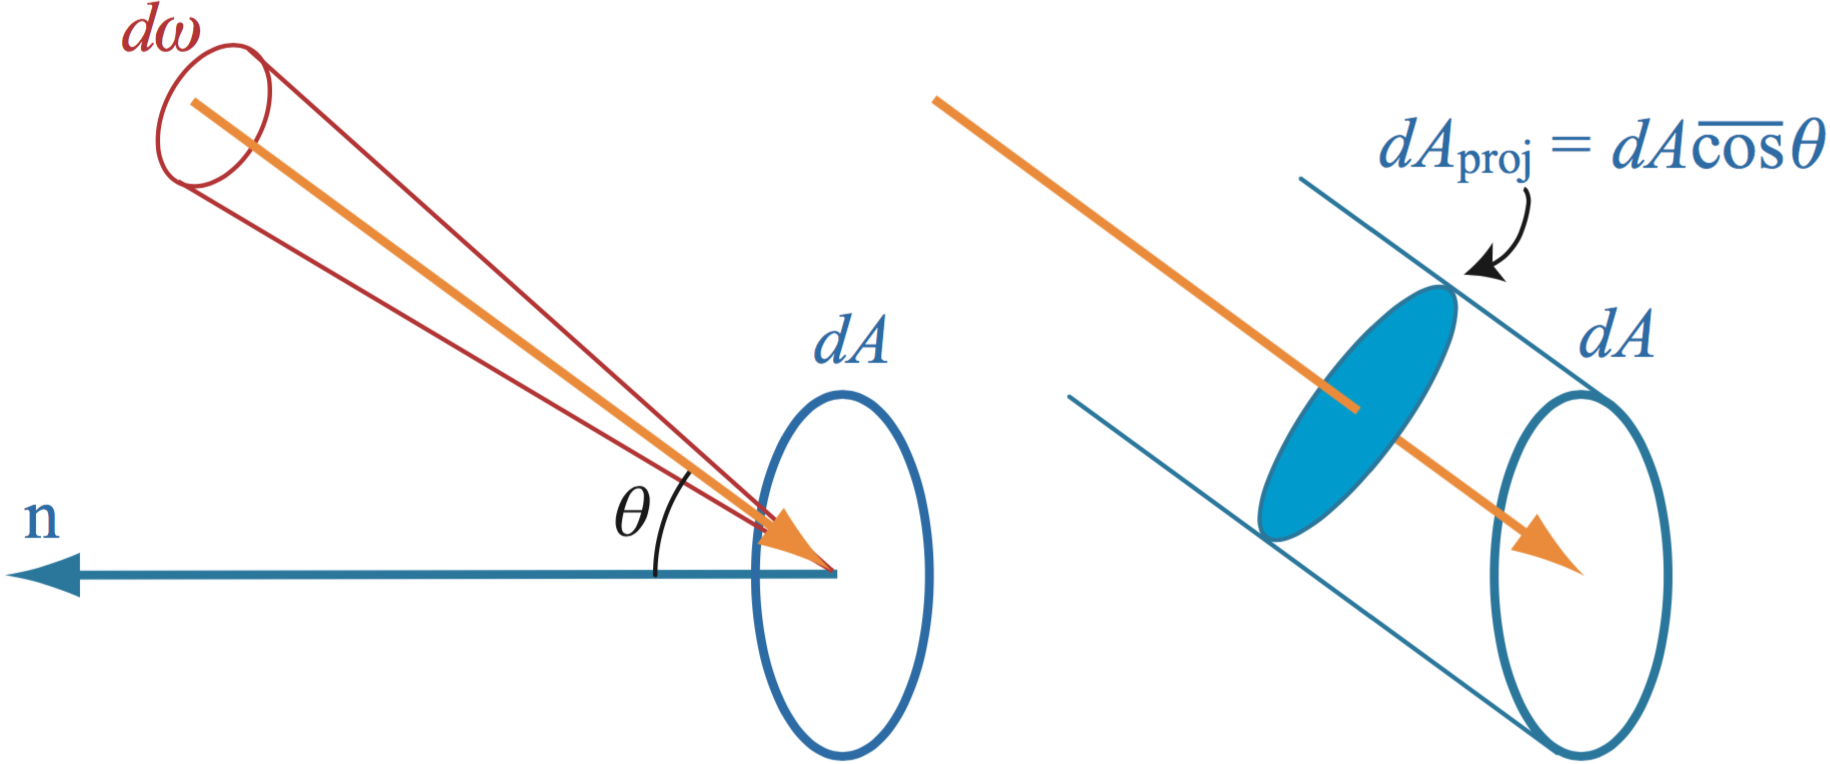
\includegraphics[width=0.65\textwidth]{figures/intro/radiance}
	\caption{辐射亮度表示的是某个点在某个方向上的亮度,在计算机图形学中它是一束光的亮度,是渲染方程最终要计算的量}
	\label{f:intro-radiance}
\end{figure}

设$P(\xi,\eta)$是$A$面上的一个点,以面上任意一组方便的曲线为参考坐标。现在在$P$点取一面元${\rm d}A$ ,并围绕极角$(\alpha,\beta)$方向取一立体角${\rm d}\omega$,另外设${\rm d}\omega$方向与${\rm d}A$ 法线的夹角为$\theta$,如图\ref{f:intro-radiance}所示,则在单位时间内由面元${\rm d}A$ 发射到${\rm d}\omega$内的能量(时间平均)值${\rm d}\Phi$可以表示为:

\begin{equation}\label{eq:intro-energy}
	{\rm d}\Phi=L\overline{\cos}\theta {\rm d}A {\rm d}\omega
\end{equation}

\noindent 其中,$L$是一个因子,一般与位置$(\xi,\eta)$和方向$(\alpha,\beta)$有关,即:

\begin{equation}
	L=L(\xi,\eta;\alpha,\beta)
\end{equation}

\noindent 式中引入因子$\cos\theta$,是因为物理上有意义的量是${\rm d}A$在垂直于$(\alpha,\beta)$方向的平面上的投影,而非${\rm d}A$本身。$\overline{\cos}$表示$\cos\theta$的最小值为$0$,这是因为光不能向该面的背面发射。$L$称作点$(\xi,\eta)$处方向$(\alpha,\beta)$上的辐射亮度(radiance)\myindex{辐射亮度}{radiance},其单位为$W/(m^2\cdot sr)$。

辐射亮度测试的是单束光的量度,它也正是感应器(例如人的眼睛,或者场景中的虚拟摄像机)测量的度量,所以它在光照计算中特别重要。计算渲染方程的目标就是计算出表面上的点到摄像机所在方向上的辐射亮度。另外值得注意的是,$L$的值不随距离发射点距离的变化而变化。

通常用两种不同的方式把${\rm d}\Phi$分解为两个量的乘积,以表示它对${\rm d}\omega$和${\rm d} A$的显式关系:

\begin{equation}\label{eq:intro-energy-1}
	{\rm d}\Phi={\rm d}I {\rm d}\omega={\rm d}E {\rm d}A
\end{equation}

\noindent 在接下来的两小节将分别讲述这两个新的度量$I$和$E$。





\subsection{辐射强度}
比较方程\ref{eq:intro-energy}和\ref{eq:intro-energy-1}两式,可以得出:

\begin{equation}
	{\rm d}I= \cfrac{{\rm d}\Phi}{{\rm d}\omega}=L\overline{\cos}\theta {\rm d}A
\end{equation}

\noindent 对一个面$A$的区域求积分得到:

\begin{equation}\label{eq:intro-radiant-intensity}
	I(\alpha,\beta)={\rm \int} L\overline{\cos}\theta {\rm d}A
\end{equation}

$I$称为面积$A$在方向$(\alpha,\beta)$上的辐射强度(radiance intensity)\myindex{辐射强度}{radiance intensity},其单位为$W/sr$。$I$也是一个与距离无关的量,但它是与发射面$A$的面积有关的,由于光源通常具有一定的形状和面积,所以图形学中常常使用$I$来表示一个光源的辐射强度分布,这个分布是方向的函数,如图\ref{f:intro-radiant-intensity}表示一个点光源,这个点光源每秒发出100瓦特的辐射通量,但是它在不同的方向上具有不同辐射强度。

\begin{figure}
\sidecaption
	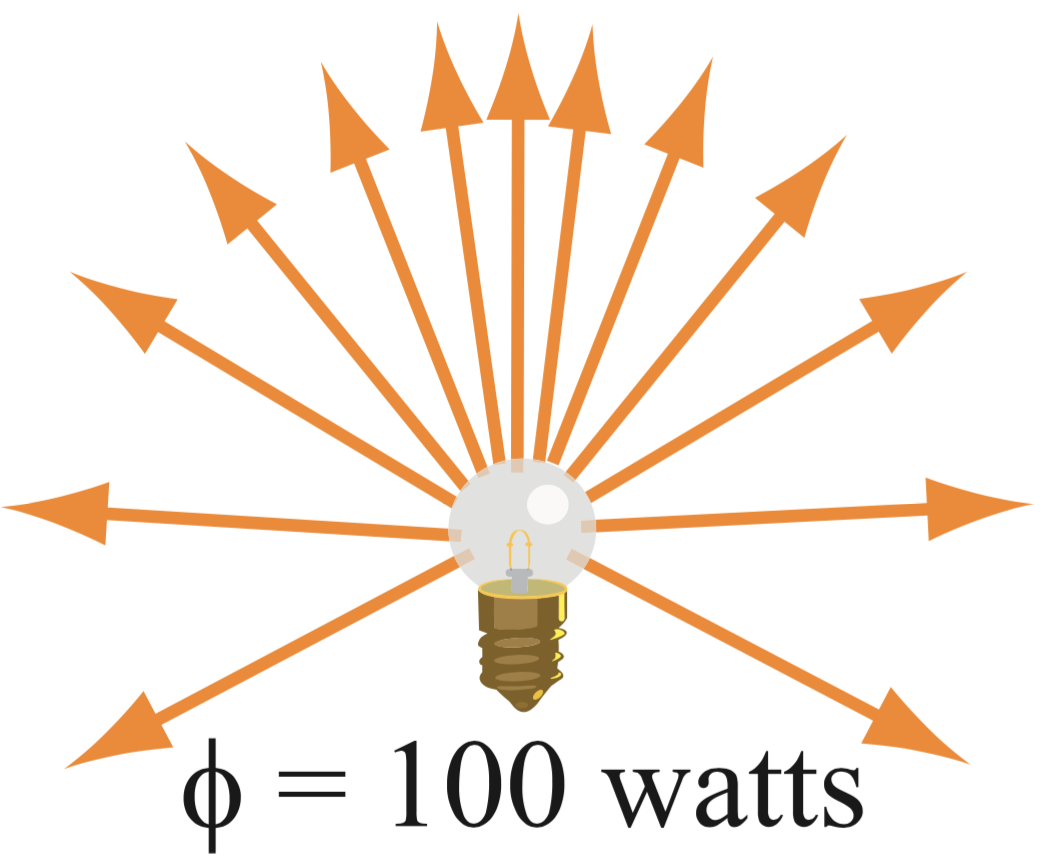
\includegraphics[width=0.35\textwidth]{figures/intro/radiant-intensity}
	\caption{一个灯泡在不同的方向上可能具有不同的辐射强度,辐射强度也是计算机图形学中表示各种光源光照的度量}
	\label{f:intro-radiant-intensity}
\end{figure}

当发生反射时,$L$随方向的变化取决于这个面的性质,特别取决于它是粗糙的还是光滑的,它是自发光还是反射或透射别的光。常常允许假设,在很好的近似下,$L$与方向无关,这时辐射称为是各向同性的(isotropic)\myindex{向同性的}{isotropic}。如果辐射是各向同性的,并且辐射面是平面,则方程\ref{eq:intro-radiant-intensity}简化为:

\begin{equation}\label{eq:intro-radiant-intensity-1}
	I(\alpha,\beta)=I_0 \overline{\cos}\theta 
\end{equation}

\noindent 其中

\begin{equation}
	I_0={\rm \int} L{\rm d}A
\end{equation}

这时,任何方向上的辐射强度随该方向与面法线间夹角的余弦的变化而变化。公式\ref{eq:intro-radiant-intensity-1}通常称为朗伯余弦定理(Lambert's cosine law)\myindex{朗伯余弦定理}{Lambert's cosine Law},如图\ref{f:intro-lambert-cosine-law}所示。此时,如果是发射面,则称为漫发射;如果是反射面,则称为漫反射。如果一个辐射源其表面辐射亮度不随方向变化,则称为朗伯体。

\begin{figure}
\sidecaption
	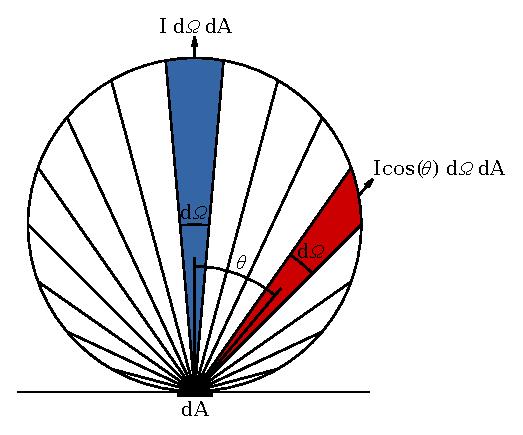
\includegraphics[width=0.6\textwidth]{figures/intro/Lambert_Cosine_Law}
	\caption{在一个漫反(发)射面,法线方向和非法线方向的每秒光子发射情况。每个楔形区域内光子的发射量正比于它们的面积}
	\label{f:intro-lambert-cosine-law}
\end{figure}





\subsection{辐射照度}\label{sec:irradiance}
同理,比较方程\ref{eq:intro-energy}和\ref{eq:intro-energy-1}两式,可以得出:

\begin{equation}
	{\rm d}E= \cfrac{{\rm d}\Phi}{{\rm d}A}=L\overline{\cos}\theta {\rm d}\omega
\end{equation}

\noindent 而对某一立体角取积分得:

\begin{equation}
	E(\xi,\eta)={\rm \int} L\overline{\cos}\theta {\rm d}\omega
\end{equation}

$E$称为点$(\xi,\eta)$的辐射照度(irradiance)\myindex{辐射照度}{irradiance},其单位为$W/m^2$,它是点$(\xi,\eta)$沿各个方向对辐射亮度$L$的积分,如图\ref{f:intro-irradiance}所示。值得注意的是,前面提到过,在辐射度量学中,基本上考虑的是从面的一部分射出或者接收能量,所以辐射照度虽然表述的是面上一个点的度量,但它实际上是通过该点所在的单位面积来测量的,因为辐射量度$L$也是通过单位面积来测量的。

\begin{figure}
\sidecaption
	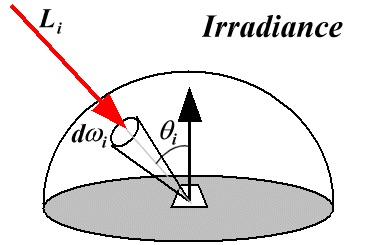
\includegraphics[width=0.45\textwidth]{figures/intro/irradiance}
	\caption{一个面上某点接收来自各个方向的辐射亮度形成辐射照度}
	\label{f:intro-irradiance}
\end{figure}

由于辐射照度表示一个点接收的来自各个方向的辐射亮度,所以在计算机图形学中,它被用来表述表面的一个点接收的所有光照。而渲染方程所要处理的正是通过反射定律及后面要讲述的其他理论,计算出沿某个观察方向的出射亮度$L_o$,通常$L_o$是与入射方向有关的,但是对于漫反射表面,它沿各个方向反射的光照是相同的,所有入射光照的积分就可以被单独计算出来,因此辐射照度是漫反射表面的重要度量,实际上光照贴图(light map)\myindex{光照贴图中}{light map}中存储的正是辐射照度值,这方面的知识将在第\ref{chp:prt}章介绍。

辐射照度被用来测量光进入一个表面(更确切地讲一个单位面积)的强度,它也可以表示光离开一个表面的强度,称为出射度,用$M$表示,其也称为辐射度(radiosity)\myindex{辐射度}{radiosity}或者辐射出射度(radiant exitance)\myindex{辐射出射度}{radiant exitance},例如表示一个光源的出射度,或者在辐射度理论(第\ref{chp:rad}章)中首先将整个场景栅格化为多个面片,将每个面片视作一个光源,然后计算出每个面片的出射度。通常用辐射通量密度(radiant flux density)\myindex{辐射通量密度}{radiant flux density}来统称一个表面出射或者入射的强度。

在图\ref{f:intro-directional-irradiance}所示的平行光中,光源的辐射强度是不随表面到光源的距离发生变化的。但是现实世界中大多数光源(例如本章后面将要讨论的点光源和聚光灯等)都不是平行光,那么一般光源的辐射强度是怎样分布的呢?

\begin{figure}
\sidecaption
	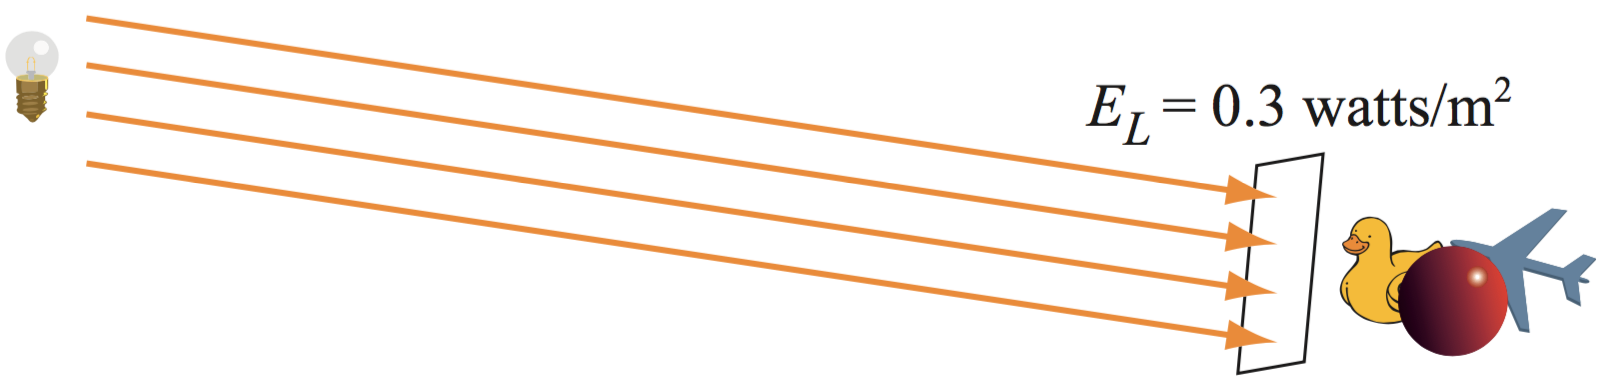
\includegraphics[width=0.65\textwidth]{figures/intro/directional-irradiance}
	\caption{平行光源的出射度不随表面到光源的距离变化而变化}
	\label{f:intro-directional-irradiance}
\end{figure}

如图\ref{f:intro-inverse-square-law}所示,设${\rm d}A$是点$P$处的面元,$QP=r$,又设$\theta$是$QP$与${\rm d}A$的法线夹角,则光源在单位时间内射过${\rm d}A$的能量是$I{\rm d}\omega$,其中$I$是光源沿$QP$方向的辐射强度,${\rm d}\omega$是对$Q$所张的立体角。由几何基础学:

\begin{equation}
	\cos\theta {\rm d}S=r^{2}{\rm d}\omega
\end{equation}


\noindent 由此,利用公式\ref{eq:intro-energy-1}即可得出:

\begin{equation}\label{eq:intro-inverse-square-law}
	E= \cfrac{I\cos\theta}{r^{2}}
\end{equation}

公式\ref{eq:intro-inverse-square-law}就是辐射度量学的基本方程,它表达了所谓的照度余弦定律($E$与$\cos\theta$成正比),以及平方反比定律 ($E$与$r^{2}$成反比)。

\begin{figure}
\sidecaption
	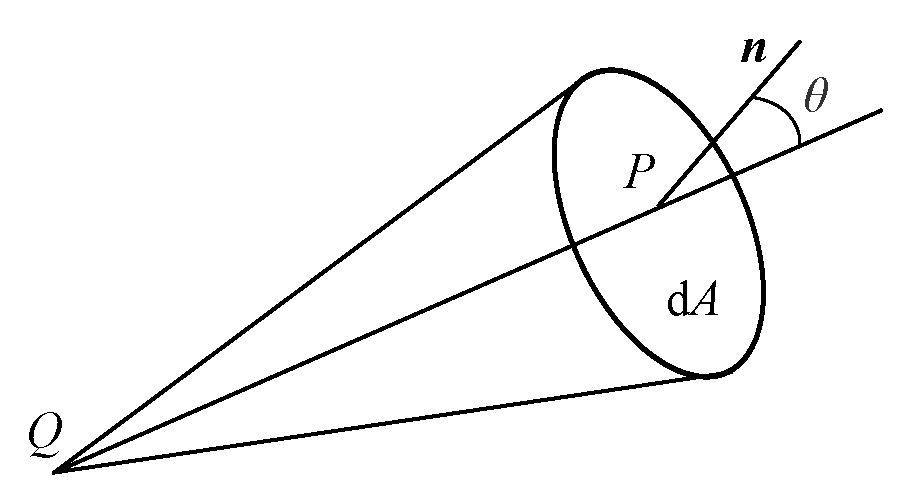
\includegraphics[width=0.5\textwidth]{figures/intro/inverse-square-law}
	\caption{点光源产生的辐射照度}
	\label{f:intro-inverse-square-law}
\end{figure}

由于$E$表示的是一个表面接收周围所有光源(包括直接光源和间接光源)的辐射照度,所以根据平方反比定律可以看出,一个光源距离该表面越远,则其光照贡献越小。









\section{物体的表面着色}
在了解了全局光照应该实现各种物理现象,以及模拟自然光照计算需要的一些基本物理度量之后,从本节开始,我们将开始进入计算机图形学的世界。

正如前言所述,本书除了介绍计算机图形学的一些基本理论知识,另一个重要的目标是试图解释清楚这些理论知识之间的逻辑联系,本节的目标是在没有涉及具体的全局光照方法之前,尝试解释光与物体的交互过程,以及最终怎样被渲染成图像。在本节的末尾,我们仍然会通过这种高层抽象的物体表面着色需求(而不是从基础的数学公式),推导出渲染方程的表达式。然后在第\ref{sec:intro-the-rendering-equation}节,将会更详细地解释渲染方程。




\subsection{几何光学模型} 
本节首先介绍光的一些基础物理特征,这些特征是我们模拟真实的光与物体交互的基础,从而能够渲染出更真实的图像。

在电磁学中,有两种模型用于研究光的性质,第一种为物理光学,第二种为几何光学。物理光学(physical optics)\myindex{物理光学}{physical optics},又称为波动光学(wave optics)\myindex{波动光学}{wave optics},它认为光在介质中以波的形式传播,这种模型可以解释光的衍射和干涉等现象。然而它以光的波长为测量尺寸,这大大超出了计算机图形学的需求。

由于可见光的波长非常短,另一种模型忽略光的波长,即相当于$\lambda\to 0$的极限情况,并证明\footnote{感兴趣的读者可以参考书籍\cite{b:PrinciplesofOptics}第三章的推导。}在这种近似处理下,光学定律可以用几何学的语言来描述,这种模型称为几何光学(geometric optics)\myindex{几何光学}{geometric optics},或者称为光线光学(ray optics)\myindex{光线光学}{ray optics},因为这种模型下能量可以看作是沿着直线传输。几何光学模型正是被计算机图形学广泛采用的模型。

当然,几何光学模型仍然比较复杂,在计算机图形学中,我们作出了一些简化假设,这虽然限制了一些效果如衍射,但是它处理起来相对简单,并且满足一般图形学的需求。这些假设包括:

\begin{itemize}
	\item 物体的表面是绝对光滑\footnote{当然现实世界的物体表面不是绝对光滑的,但是这种粗糙度介于光的波长和一个像素的尺寸之间,这种粗糙度可以通过下一节介绍的微面元技术实现,它本质上是反射和折射的一种聚合。}(smooth)的。
	\item 光仅可以被发射(emitted),反射(reflected)或者传播(transmitted)。
	\item 光以无限快的速度沿直线传播。
\end{itemize} 

在这些假设下,光的反射由反射定律(law of reflection)\myindex{反射定律}{law of reflection}决定,即: 给定一条入射光线$\mathbf{l}$和表面法线$\mathbf{n}$,反射光和入射光处于同一个平面, 并且反射光与法线之间的夹角大小等于入射光与法线的夹角大小,如图\ref{f:intro-Ray-optics-model}所示。

\begin{figure}
\sidecaption
	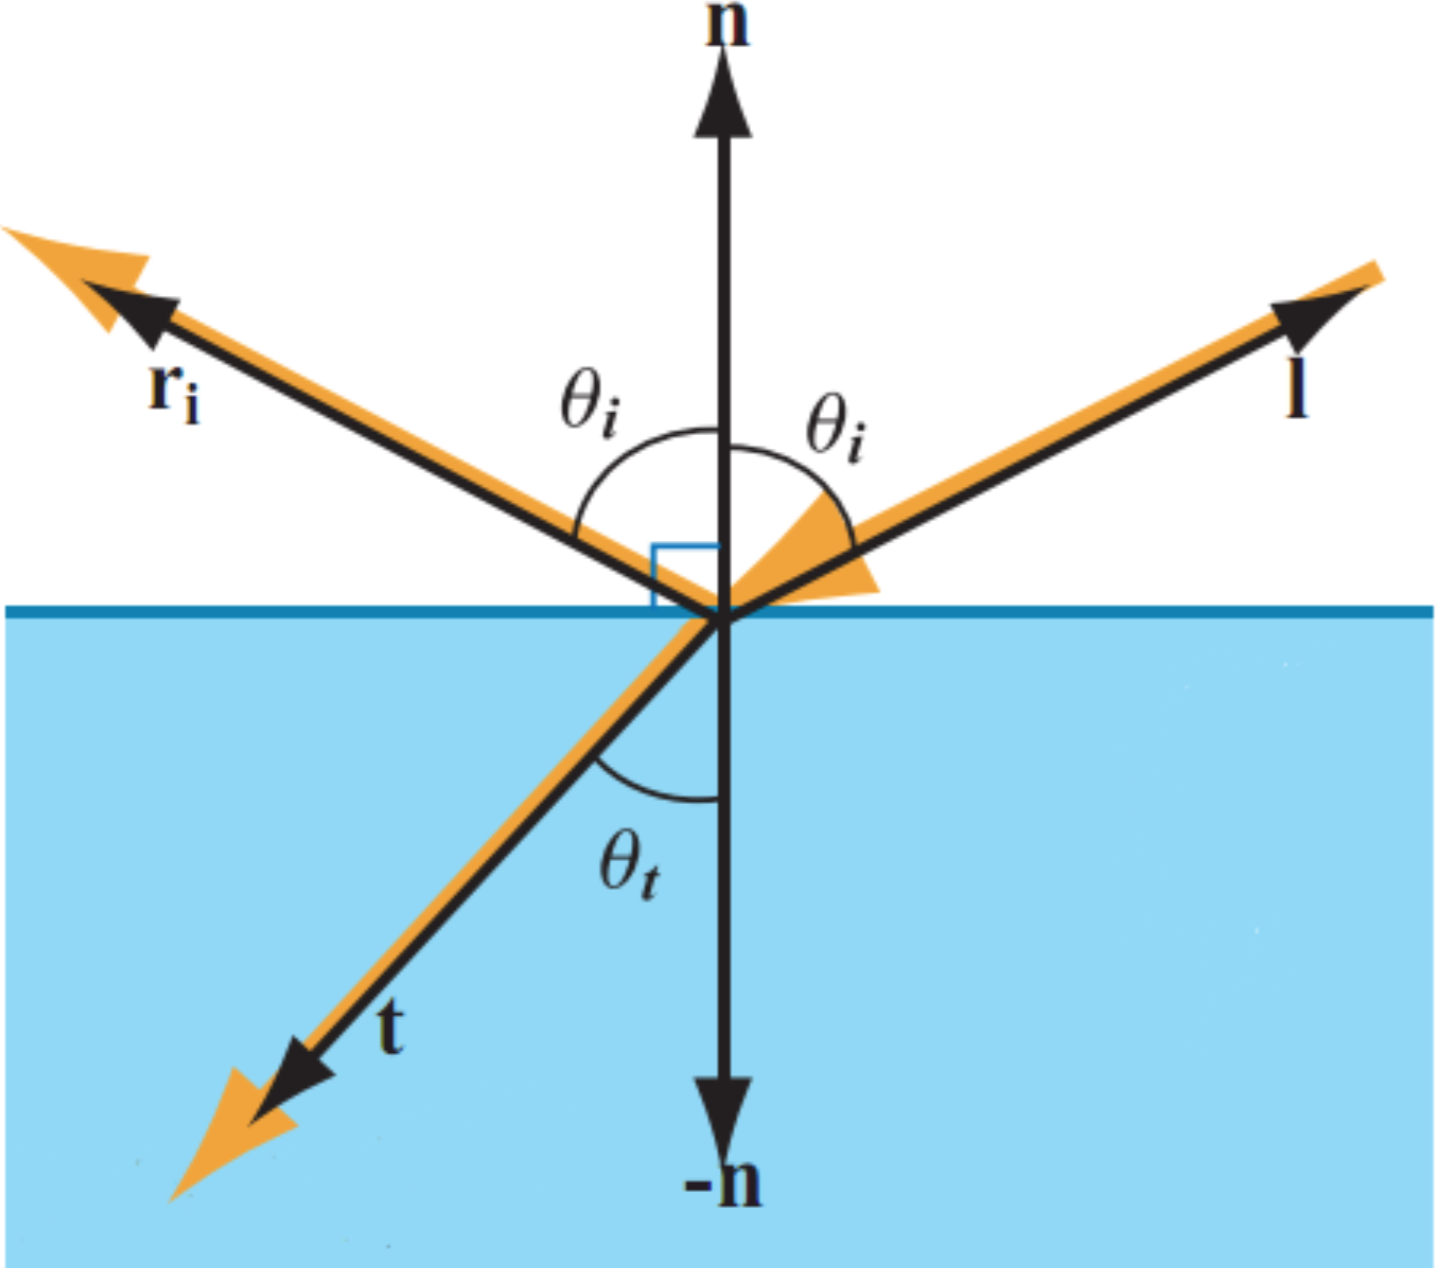
\includegraphics[width=0.4\textwidth]{graphics/gi/ray-optics-1}
	\caption{在几何光学模型中,反射定律和斯涅尔定律决定光的反射和折射}
	\label{f:intro-Ray-optics-model}
\end{figure}

当光在传输过程中,介质的折射率(index of refraction)\myindex{折射率}{index of refraction}发生变化,则会发生折射(refraction)\myindex{折射}{refraction}。当入射光$\mathbf{l}$从具有折射率为$n_1$的介质进入折射率为$n_2$的介质时, 其光线传输方向的偏离$\mathbf{t}$由斯涅尔定律(Snell's law)\myindex{斯涅尔定律}{Snell's law}决定,如图\ref{f:intro-Ray-optics-model}所示,即有:

\begin{equation}\label{eq:intro-snell-Law}
	n_1\sin\theta_1 = n_2\sin\theta_2\ 	
\end{equation}





\subsection{光与表面的交互}
为了模拟光学现象以生成真实的数字图像,我们需要构建一套系统,将几何光学模型应用到计算机图形学中。这套系统定义了在图形渲染过程中,光与表面及其他物体的交互。

这个系统工作的过程可以描述如下:

\begin{enumerate}
	\item 光从光源(例如太阳或其他光源)或其他发光体中发射出来。
	\item 光与场景中的物体进行交互,部分被反射,部分被吸收并可能经过一定路径传播后沿其他方向从物体表面散射出来。
	\item 最后,光被感应器(例如摄像机或者人的眼睛)吸收,形成图像。
\end{enumerate}

这个过程涉及三个组件:光源,材质以及摄像机。在接下来的小节中我们将讨论这些组件,以及它们怎样被用在渲染管线中用于渲染图形。




\subsubsection{光~~源}\label{sec:intro-light-sources}
光源(light sources)\myindex{光源}{light sources}发出光并照亮整个场景,此外,在计算机图形学中,光源一般不会反射或吸收其他光照。

现实世界中的光源是很复杂的,它可能沿不同的方向以及光源表面上的不同位置具有不同的分布,在图形学中一般仅使用少数几种简单的光源模型,这几种模型都假设光源的光照分布只随方向而发生变化。这几种模型包括:

\begin{itemize}
	\item 平行光(directional light)\myindex{平行光}{directional light}:平行光模拟光从无限远的地方发射,这意味着所有由它产生的阴影光线都是平行的,因此这种模型是模拟太阳光的理想选择。
	\item 点光源(point light)\myindex{点光源}{point light}:点光源从一个点向四面八方发出光线,它可以用于模拟如现实世界中的钨丝灯泡发出的光。
	\item 聚光灯(spot light)\myindex{聚光灯}{spot light}:聚光灯限制点光源发出光线的方向,它通常使用两个圆锥体作为参数,其中内部圆锥体的半径内发出的光线最强,从内部到外部圆锥体半径内光线强度逐渐减至零。
\end{itemize}

以上这些光源发出的光线会在场景中像自然光一样进行传播,即这些光线通过最近点测试计算出光线与哪个物体表面的哪个位置相交,然后根据物体表面的材质属性进行着色计算。除此之外,出于性能考虑,场景中还有另外一些(通常是间接)光不会通过这种方式计算,例如大面积的环境光通常通过贴图的方式计算,这包括天空盒(sky light)\myindex{天空盒}{sky light}以及其他环境光照;而低频率的间接漫反射的光可以通过使用低阶的球谐函数近似表述,然后在GPU中使用快速的卷积(convolution)\myindex{卷积}{convolution}计算。

对于直接光源,另一个我们最关心的问题是这个光源的光照用什么物理量表示,以及这个物理量怎样参与到光与表面的交互计算之中。

首先,虽然眼睛等感应器接收的是辐射亮度$L$,但这是一个五维(三个维度表示位置,两个维度表示方向)的量,太过于复杂,所以在图形学中一般不会直接表示光源的辐射亮度分布。考虑到图形学中大部分直接光源的亮度分布都是只与方向有关,所以辐射强度$I$通常用来表示本节提到的几种直接光源的辐射亮度分布。

当然这个方向分布函数不宜太复杂,一般引擎不允许定义具有任意方向分布的光源,例如点光源可能所有方向的辐射强度都相同,聚光灯也是沿着一个圆锥体向外递减。在Unreal Engine 4中,可以对点光源和聚光灯使用一个称为IES\cite{m:IESLightProfiles} 的光源配置(light profiles)\myindex{光源配置}{Light Profiles}的配置文件。IES光源配置文件可以以曲线的方式定义光源的光照强度分布,如图\ref{f:intro-ies}所示。

\begin{figure}
\begin{fullwidth}
	\begin{subfigure}[b]{0.209\thewidth}
		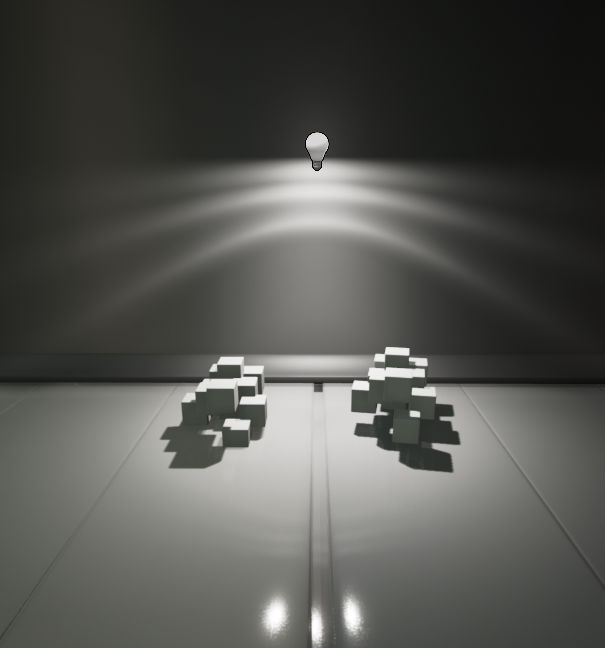
\includegraphics[width=1.\textwidth]{figures/intro/IES_01}
	\end{subfigure}
	\begin{subfigure}[b]{0.213\thewidth}
		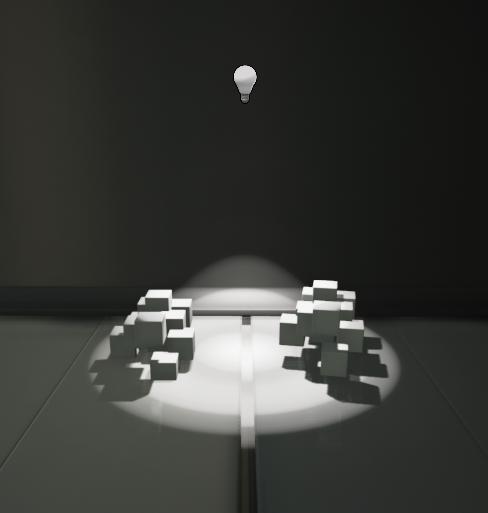
\includegraphics[width=1.\textwidth]{figures/intro/IES_02}
	\end{subfigure}
	\begin{subfigure}[b]{0.247\thewidth}
		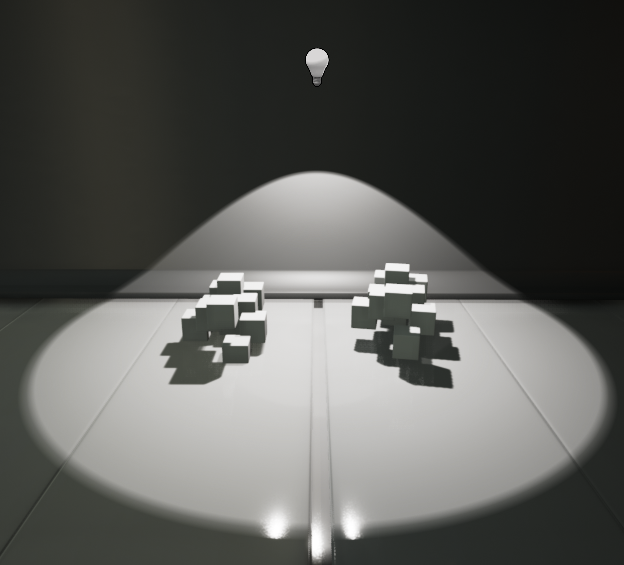
\includegraphics[width=1.\textwidth]{figures/intro/IES_03}
	\end{subfigure}
	\begin{subfigure}[b]{0.293\thewidth}
		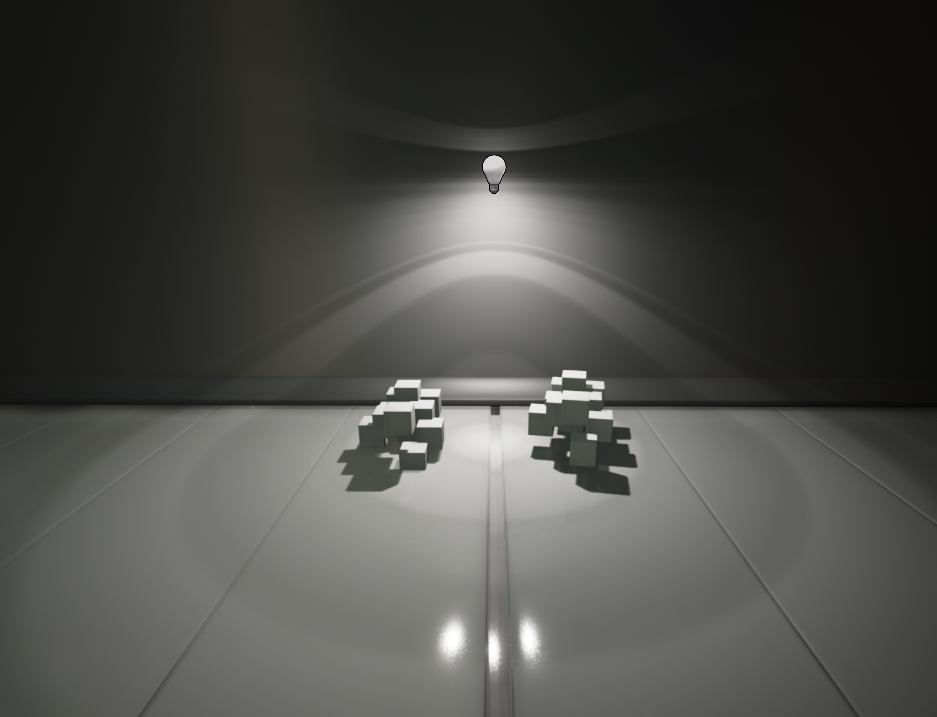
\includegraphics[width=1.\textwidth]{figures/intro/IES_04}
	\end{subfigure}
\caption{在Unreal Engine 4中使用IES光源配置文件定义点光源和聚光灯的光照强度分布 (图片来自\cite{m:IESLightProfiles})}
\label{f:intro-ies}
\end{fullwidth}
\end{figure}

通过第\ref{sec:irradiance}节的内容可知,在计算光与物体表面交互时,表面接收的所有光照使用辐射照度$E$表示,而光源使用辐射强度$I$表示,所以这里就需要使用第\ref{sec:irradiance}节介绍的的平方反比定律,通过$I$来计算$E$,为了方便,这里重新列出该方程如下:

\begin{equation}
	E= \cfrac{I\cos\theta}{r^{2}}
\end{equation}

虽然$E$随着$1/r^{2}$正比增长在物理上是正确的,但是在图形学上通常使用一个不同的函数来描述$E$怎样随着距离的增加而递减。这种函数称为距离递减函数(distance falloff function)\myindex{距离递减函数}{distance falloff function},由此$E$可以表示为:

\begin{equation}
	E=I\cos\theta f_{\rm dist}(r)
\end{equation}

距离递减函数在计算机图形学中被广泛采用,有以下一些原因:首先距离递减函数可以提供更多的控制来达到一些特殊的效果;其次,随着距离的增加,平方反比函数趋近于$0$但却永远不会为$0$,距离递减函数可以通过设定一个最大距离范围,超出这个范围的表面接收的辐射强度为0来大大提高性能;平方反比函数在距离趋近于$0$时趋近于无限大,而距离递减函数可以通过设定一个最大值,避免这种无限大的值出现在着色计算中。

例如以下是Pixar工作室用在电影产品中的距离递减函数\cite{a:LightingControlsforComputerCinematography}:

\begin{equation}
	f_{\rm dist}(d)=\begin{cases}
		M{\rm e}^{s( \cfrac{d}{L})^{\beta}}, & d<L\\
		K( \cfrac{L}{d})^{\alpha}, &d>L
	\end{cases}
\end{equation}

\noindent 这个函数在一个特定的距离$L$处其值为$K$,在距离小于$L$时逐步达到最大值$M$,递减指数$\alpha$用于控制当距离大于$L$时距离递减函数怎样随着距离递减,常数$s$和$\beta$被设定为特定值以保证函数在过渡点处的导数连续:其中$s\equiv {\rm ln}( \cfrac{K}{M})$,而 $\beta\equiv - \cfrac{\alpha}{s}$,如图\ref{f:intro-falloff}所示。

\begin{figure}
\sidecaption
	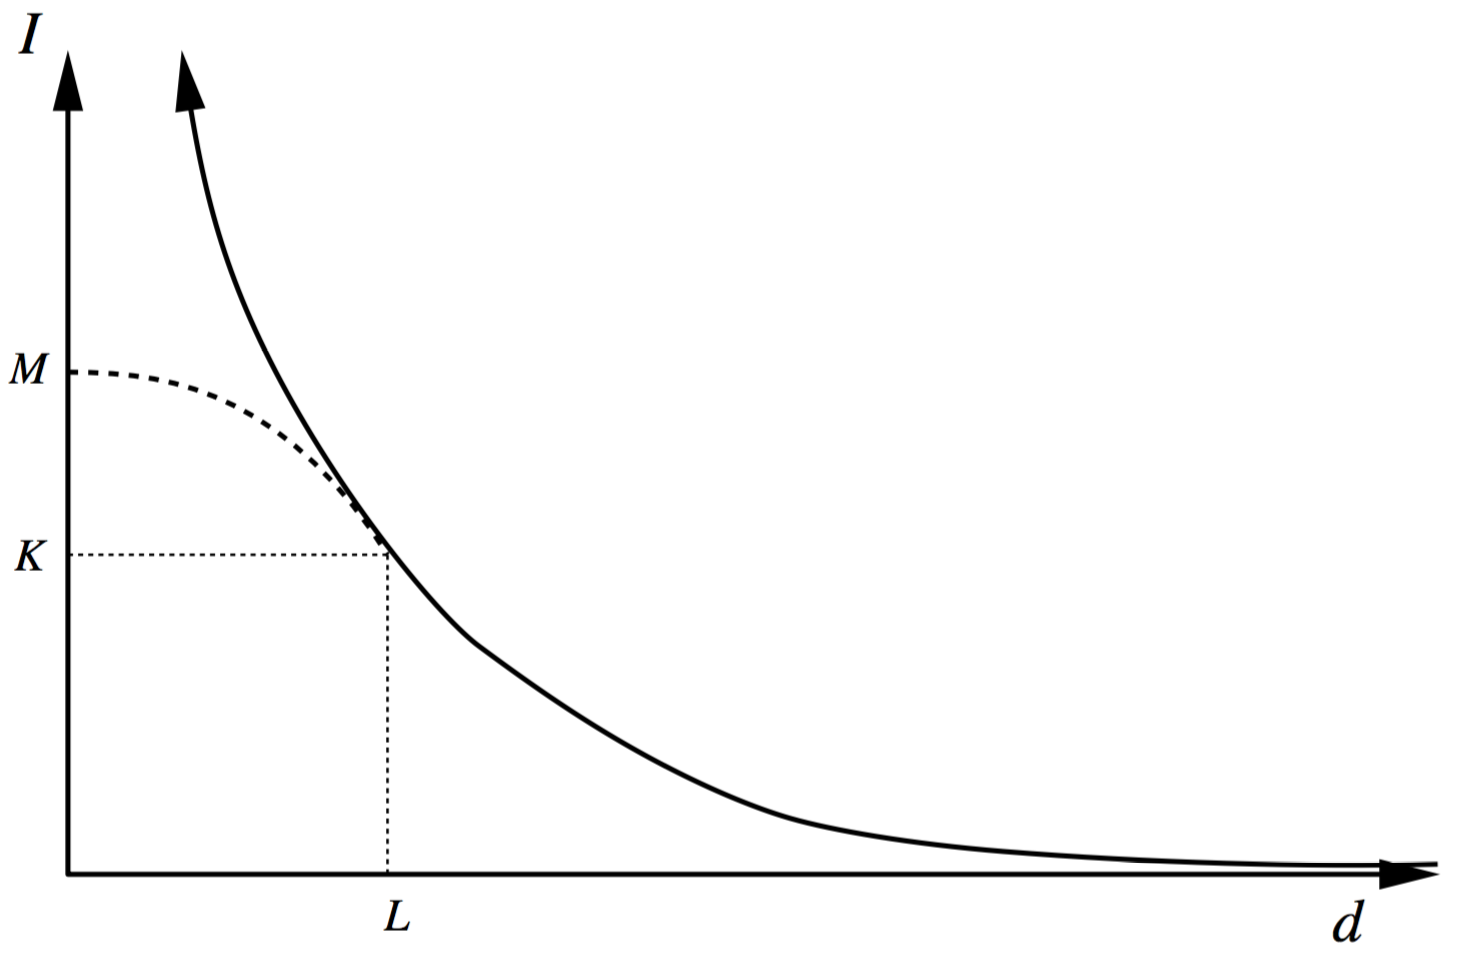
\includegraphics[width=0.6\textwidth]{figures/intro/falloff}
	\caption{Pixar采用的距离递减函数,其中当$d<L$时才有虚线部分,其最大值为$M$}
	\label{f:intro-falloff}
\end{figure}




\subsubsection{材~~质}\label{sec:intro-materials}
光与物体表面交互的一切,都是由材质及其属性来决定的,材质决定了每个物体的表面最终呈现出来的是什么颜色。那么材质到底是什么,这个问题需要从两个方面来理解。

\begin{figure}
\sidecaption
	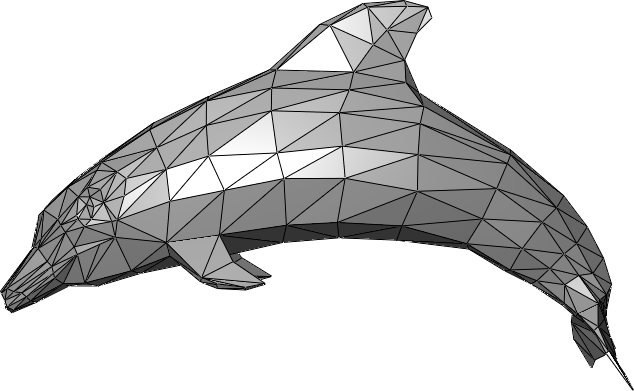
\includegraphics[width=0.4\textwidth]{figures/intro/mesh}
	\caption{一个由三角形网格构成的海豚,网格构成物体的“形”(图片来自Wikipedia)}
	\label{f:intro-mesh}
\end{figure}

首先,在计算机图形学中,一个物体的“形”与“色”是完全分开的,物体的形状由一组顶点(vertex)构成的网格(mesh)来定义,如图\ref{f:intro-mesh}所示,而物体的表面着色则由称为材质(material)\myindex{材质}{material}的东西决定。所以材质通常包含纹理(textures),着色器(shaders)以及其他一些着色方程需要的参数,所有这些数据构成一个对象并被附加到一个物体上,在渲染时这些数据被传输至GPU内存,GPU执行其中的着色器对该物体表面着色,这个过程包括贴图,光照以及其他相关的计算。关于材质的一些重要参数将在下一节讨论。

理解材质的另一方面在于,我们需要了解更多关于物体表面或内部结构的问题。在前面的描述中,都是假设表面是绝对光滑的,在这种情况下,光经过表面时按照反射定律和折射定律进行反射或折射。然而在微观尺度上\footnote{计算机图形学中一般不考虑小于波长的原子尺寸,这又称为纳米几何(nanogeometry)\myindex{纳米几何}{nanogeometry},在此尺寸下可以观察到光的衍射现象,即光可以绕过障碍物沿非直线方向传播。},这里指微观几何(microgeometry)\myindex{微观几何}{microgeometry}结构,即小于一个像素但是大于光波长的尺寸,物体表面并不是绝对光滑的,这时虽然在单个光束与表面交互上可以看作该面是光滑的,但是在一个像素尺度上,它确是不光滑的,如图\ref{f:intro-microgeometry-1}所示。那么我们如何处理这种复杂的情况?

\begin{figure}
\sidecaption
	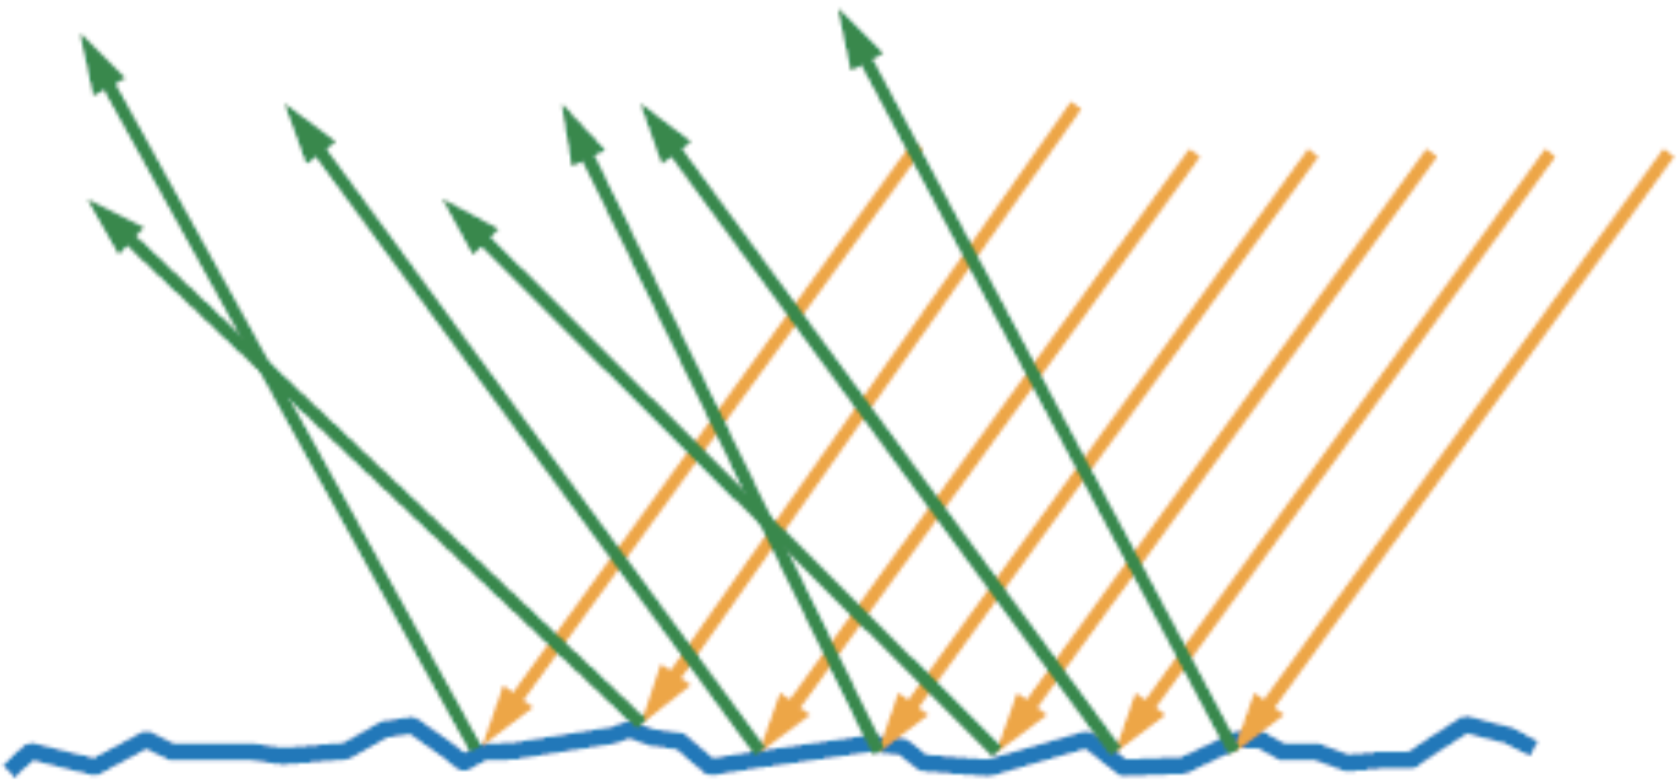
\includegraphics[width=0.4\textwidth]{figures/intro/ray-optics-3}
	\caption{在微观尺寸上,每个点向不同的方向反射或折射光照,注意该图反应的其实是一个像素内的微观尺寸}
	\label{f:intro-microgeometry-1}
\end{figure}

由于表面在微观尺寸上是不光滑的,每个比像素更小的点可能沿不同的方向反射或折射光照,这导致对于一个像素点,每条入射光会被反射或(和)折射至多个方向,如图\ref{f:intro-multi-rays}所示。这等效于是从一个给定的观察方向看,一个像素点可以接受来自多个方向的光照。

\begin{figure}
\sidecaption
	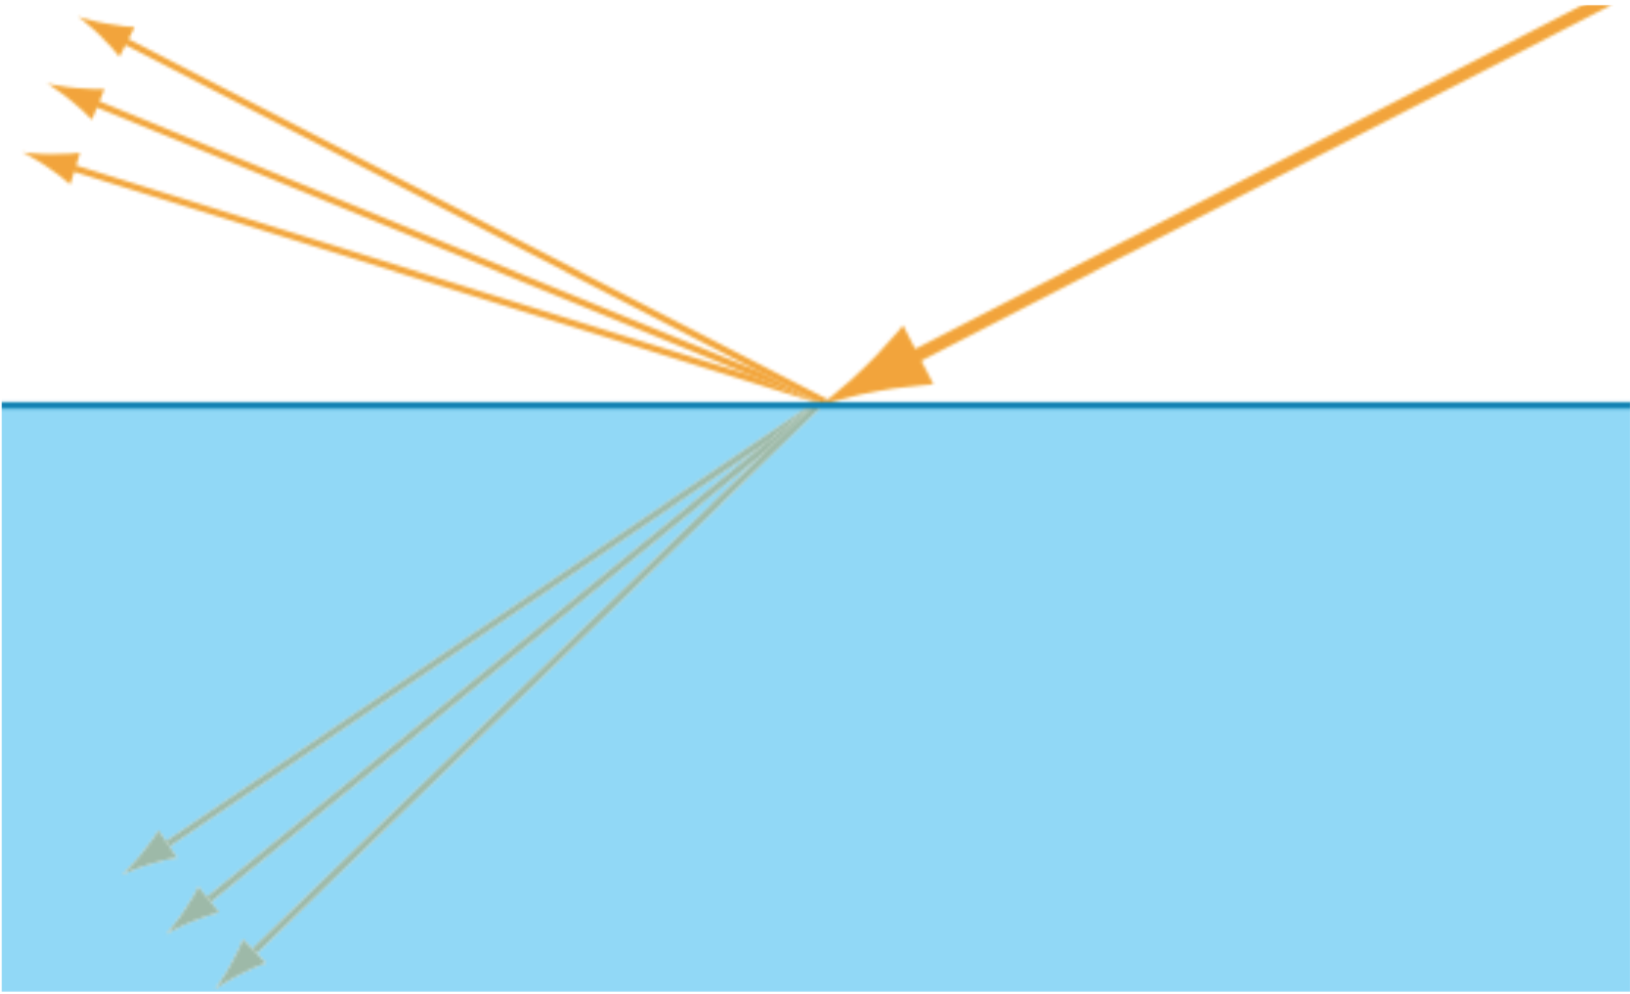
\includegraphics[width=0.5\textwidth]{figures/intro/ray-optics-4}
	\caption{微观结构的粗糙度,导致一个像素点可以将一束像素面积的入射光反射或(和)折射至多个方向}
	\label{f:intro-multi-rays}
\end{figure}

对于折射进物体内部的光照会发生什么呢,这取决于物体材质的结构。在计算机图形学中,材质可以分为两大类\footnote{自然界中还存在第三类材质,即半导体,但是半导体在渲染场景中很少见。}:金属(metals)\myindex{金属}{metals}和非金属,后者又称为绝缘体(insulator)\myindex{绝缘体}{insulator},其中金属立即吸收所有折射的光照。

对于非金属,如果该物体是透明的,如玻璃和水晶,则折射光会在物体内部直线传播,直到遇到该物体另一边的表面后离开物体表面重新回到空气中;对于非透明的物体,由于内部介质的不连续(例如流体,晶体等内部的粒子,泡泡,液滴,瑕疵;有机体表面的粗糙度,细胞;以及衣服布料里的纺织纤维等),折射的光会沿着不同的方向继续反射或者折射,在经历一定的路径之后,这些折射的光部分被重新(可能从原来的位置,也可能从其他位置)发射回到外面,部分可能被吸收。除非该物体是一个完全透明的物体,否则折射的光中总会有部分会发射回到表面外,如图\ref{f:intro-refraction}中的蓝色箭头部分光照,这部分光照可能从不同的位置以不同的方向发射出表面外。值得注意的是,这种由物体内部发射回来的光通常不具有固定的方向性,所以这种反射称为漫散射(scattering)\myindex{漫散射}{scattering}。

\begin{figure}
\sidecaption
	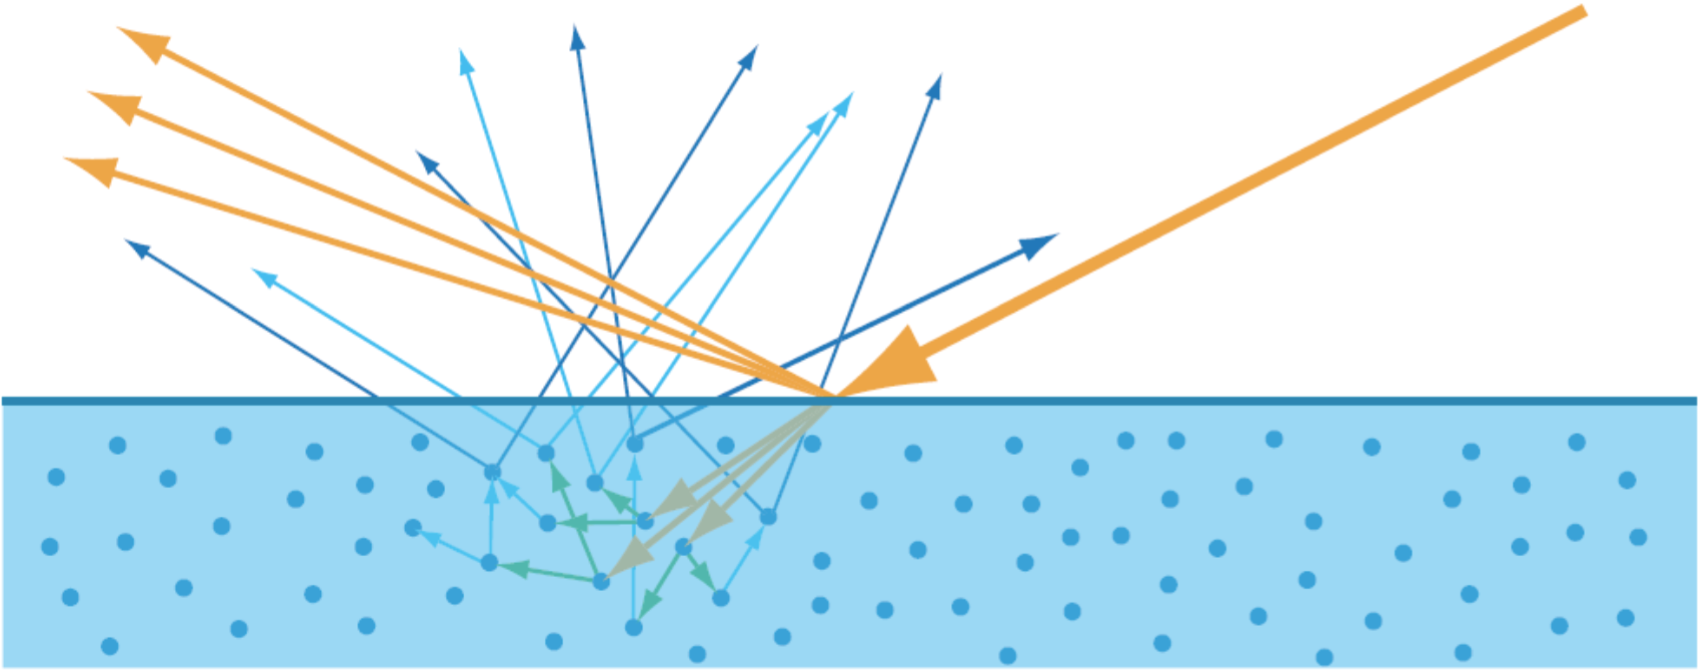
\includegraphics[width=0.65\textwidth]{figures/intro/ray-optics-5}
	\caption{对于非金属材质,经历一定路径的散射之后,部分折射进表面的光会沿不同的方向重新发射回表面外}
	\label{f:intro-refraction} 
\end{figure}

散射光重新发射回表面外的位置与入射点位置之间距离的分布,取决于该物质表面的属性。如果这个距离小于一个像素的尺寸(即在微观范围中),在着色的时候可以假设其距离为$0$,这种散射称为局部次表面散射(local subsurface scattering)\myindex{局部次表面散射}{local Subsurface scattering};否则称为全局次表面散射(global subsurface scattering)\myindex{全局次表面散射}{global subsurface scattering}。在计算机图形学中,这两种现象通常分别使用不同的技术实现。

在计算机图形学中,通常将反射和漫反射这两种不同的光照区分开,分别称为光泽(specular)和漫反射光\footnote{在光学中,漫反射(甚至散射本身)也包含一部分由于物体表面的粗糙度形成的直接反射光的一部分,并不全是由折射进表面的光形成。}(diffuse)。其中前者主要由于光在物体表面的直接反射形成,而后者通常由光进入物体表面,经历折射,吸收,多次散射过程之后重新从物体表面散射回表面外的光形成,如图\ref{f:intro-specular-and-diffuse}所示。这样区分的目的也在于由于漫反射光可以接收来自全部方向的光,因此需要对全空间进行积分计算,但是将与方向无关的部分分离出来,则可以使用更简单的方法处理漫反射,关于这些方法将在本章及本书后面介绍。

\begin{figure}
\sidecaption
	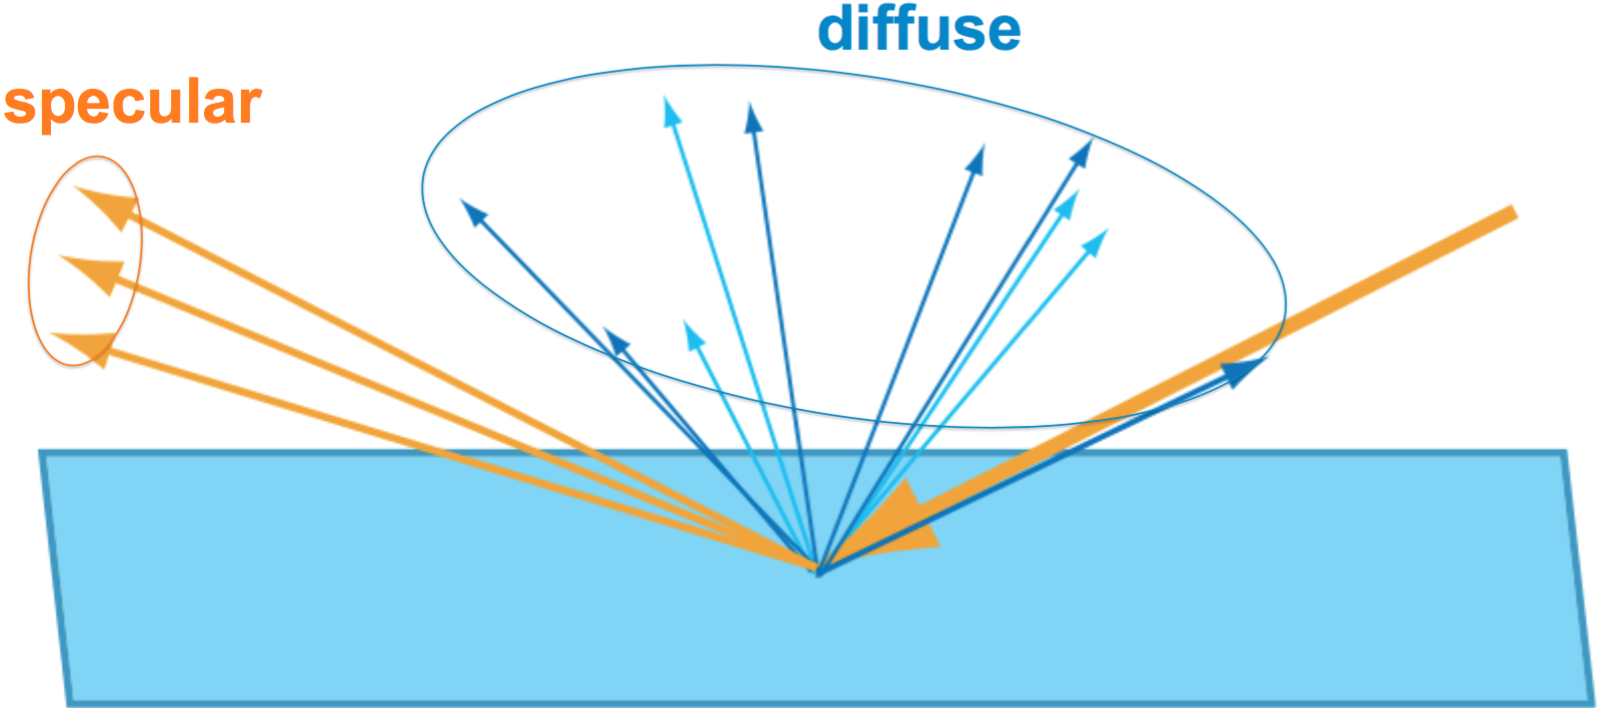
\includegraphics[width=0.6\textwidth]{figures/intro/ray-optics-6}
	\caption{光与物体表面交互后反射的光可以分为光泽和漫反射光两部分}
	\label{f:intro-specular-and-diffuse}
\end{figure}

对于光泽部分,这些反射光所处范围的大小取决于表面的粗糙度(下一节会讨论),表面越粗糙,则反射的范围越大,物体表面越模糊;反之表面越光滑,反射的范围越小,则表面越光亮,如图\ref{f:intro-roughness}所示。

\begin{figure}
\sidecaption
	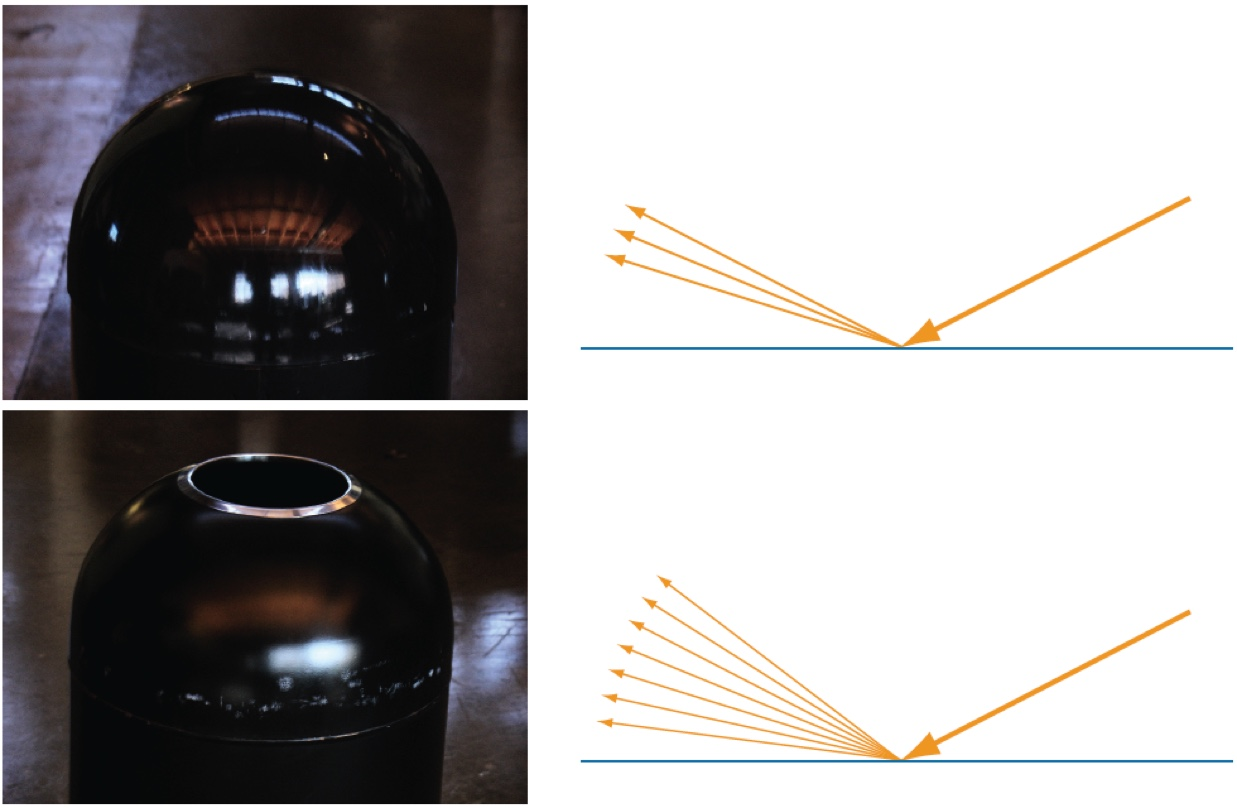
\includegraphics[width=0.65\textwidth]{figures/intro/ray-optics-2}
	\caption{反射光的范围大小取决于物体表面的粗糙度,物体表面越粗糙,它越能接收更大范围的光照}
	\label{f:intro-roughness}
\end{figure}

由于材质决定物体表面的着色,所以上述所有这些现象都需要在材质中进行表述,对于如漫反射率等这种与观察方向无关的参数,它们可以通过纹理的方式存储并关联到材质中;而对于与方向有关的这些反射特征,它们可能以函数的形式存在于着色器代码中,例如上述关于表面的光泽反射特征可以通过本章后面介绍的微面元理论来进行表述。





\subsubsection{感应器}\label{sec:intro-sensor}
当光从光源发射出,并在场景中与物体表面进行多次交互后,最终其中的一部分会进入图像传感器形成图像。由于图像传感器接收的是辐射亮度$L$(其值由渲染管线中的像素着色器计算出),并且数字图像以一定的分辨率存储图像信息,所以可以使用图\ref{f:intro-camera}来表示计算机图形学中的图形传感器成像系统,这里$P$点就是场景中的“摄像机”对象,摄像机朝着虚拟屏幕中的每个像素的方向发射一条射线,称为观察矢量(view vector)\myindex{观察矢量}{view vector} $\mathbf{v}$(它也是着色器计算中渲染方程的出射方向),场景中所有沿$\mathbf{v}$反方向传播的光线就会进入摄像机。

\begin{figure}
\sidecaption
	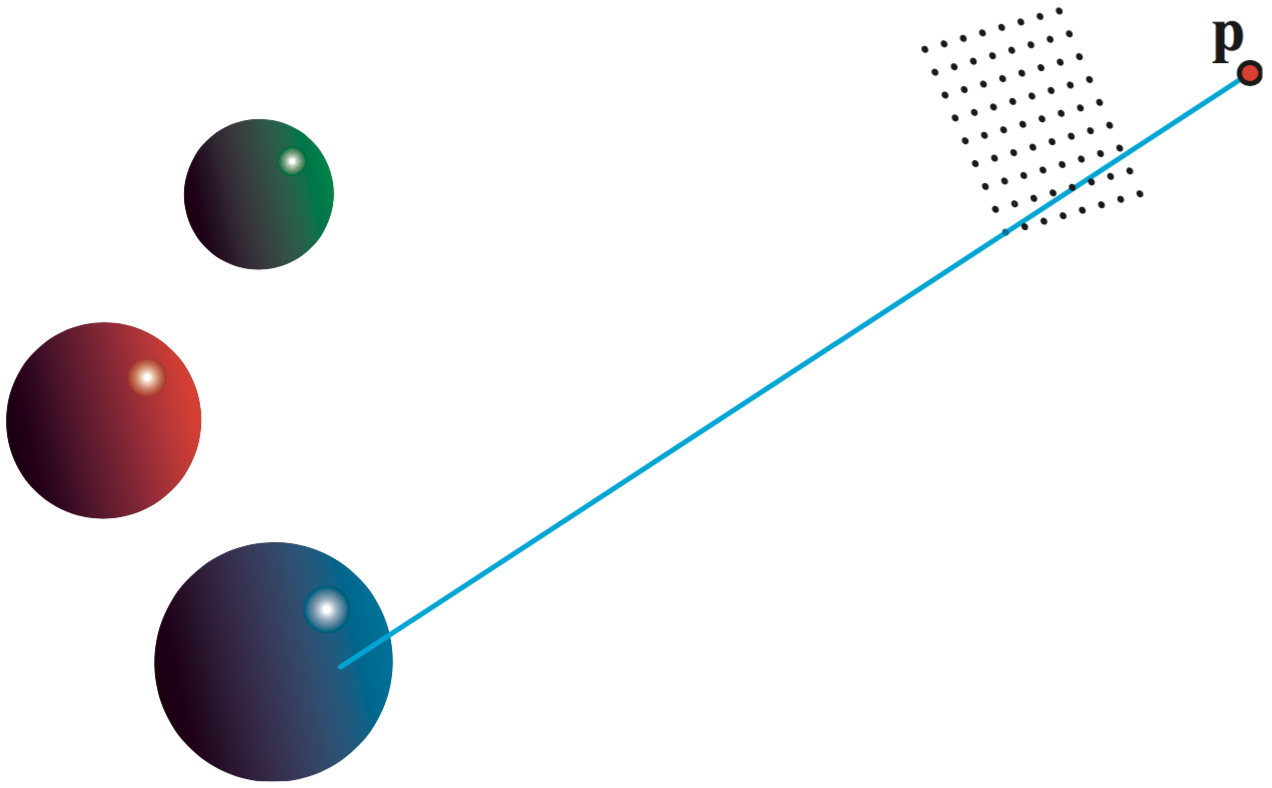
\includegraphics[width=0.6\textwidth]{figures/intro/camera}
	\caption{理想的计算机图形学图像传感器模型,其中${\rm p}$为摄像机或观察点,中间的点阵为屏幕的像素网格,左边的球体为场景中的物体}
	\label{f:intro-camera}
\end{figure}

然而事情并不像这么简单,对于给定分辨率的“屏幕”,它的每一个像素点总是有一个尺寸大小的。而对于每个像素,我们通常取其从摄像机发出穿过该像素中心点的方向对场景进行采样,如果一个像素的中心点被三角形覆盖,则整个像素区域被填充一个单一的颜色,否则即使该像素有小部分区域被覆盖,它也不会被填充任何颜色,这使得三角形的边缘出现锯齿(jaggies)\myindex{锯齿}{jaggies},如图\ref{f:intro-aliasing-triangle}所示。这种锯齿是由于采样不足导致的一种走样(aliasing)\myindex{走样}{aliasing}现象,而尝试避免或者减少这种走样的技术称为反走样(anti-aliasing)\myindex{反走样}{anti-aliasing}技术。

\begin{figure}
\sidecaption
	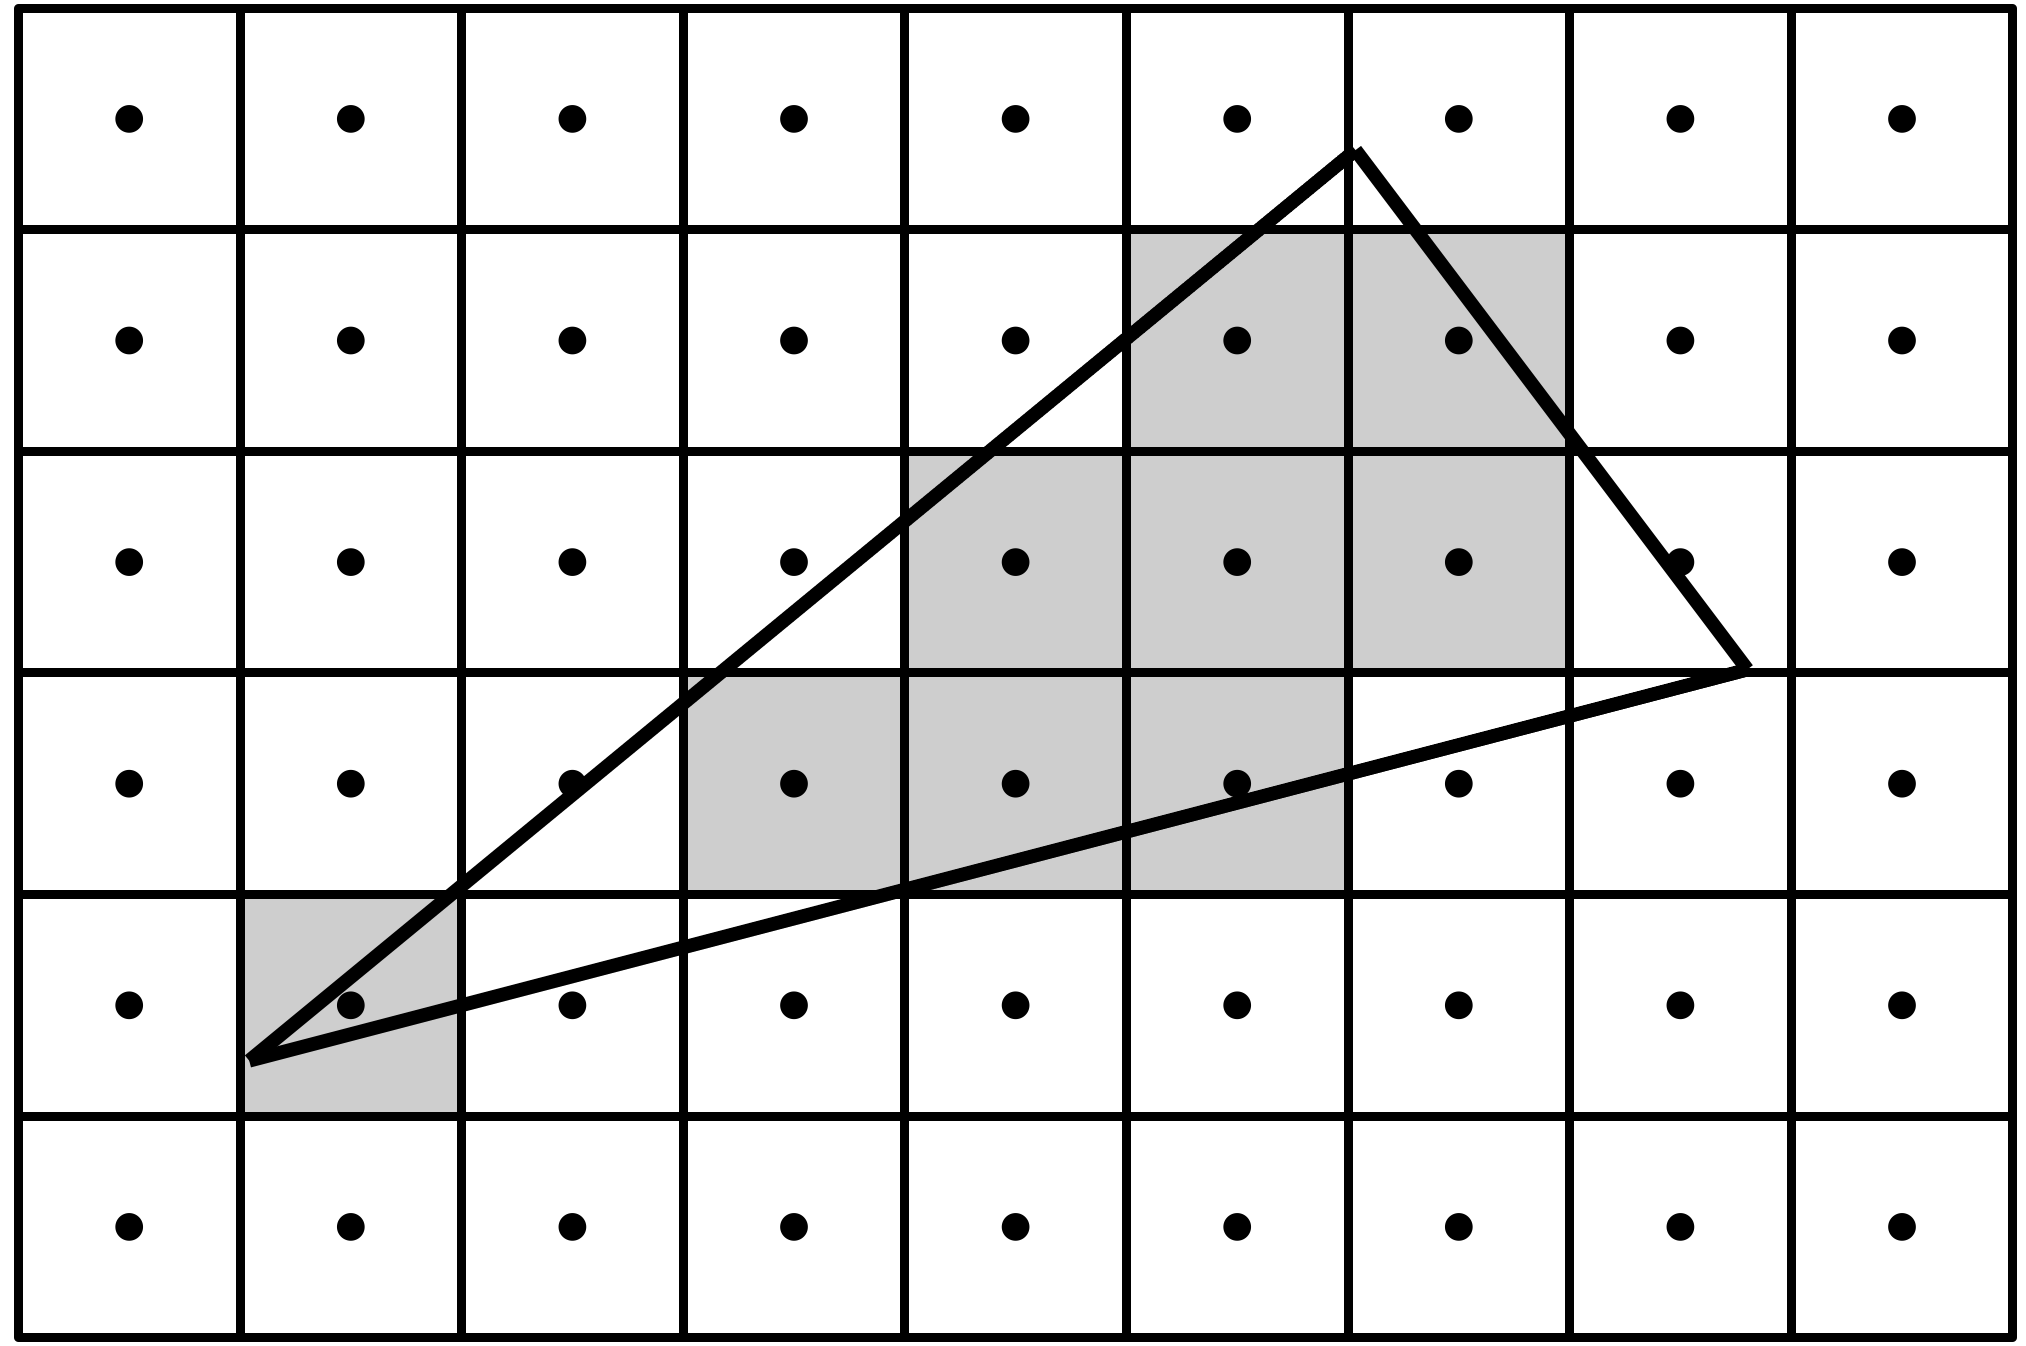
\includegraphics[width=0.45\textwidth]{figures/intro/aliasing-triangle}
	\caption{光栅化技术通过测试几何图形对像素中心点的覆盖来决定是否对该像素点着色,这造成在几何图形的边缘出现锯齿的现象}
	\label{f:intro-aliasing-triangle}
\end{figure}

用数学理论来解释和解决这种缺陷,涉及数字信号处理的一些理论,如采样,重建,走样等。这些技术的学习不仅有助于理解渲染过程中数字图像的生成过程,它也是计算机图形学的重点内容,例如着色器中对纹理的采样,后处理中很多都涉及走样技术等等。接下来,我们将讨论关于数字信号处理的一些理论,并解释这些理论怎样被用在计算机图形学中。

	



\section{采样和反走样}\label{sec:intro-sampling}
3D图像的生成本质上是一个对各种连续函数(如几何图形,BRDF分布函数,光照场等)采样,然后转化为对应的一个离散函数(以有限分辨率表示的一个二维图像)的过程。3D渲染的大部分采样发生在光栅化阶段,或者其他由光栅化导致的采样,例如图\ref{f:intro-aliasing-triangle}中,三角形两个顶点之间的边是连续的,但是被光栅化过程采样为离散的像素值。

在数字信号处理(digital signal processing)\myindex{数字信号处理}{digital signal processing}中,术语采样(sampling)\myindex{采样}{sampling}的目的是将连续的信号表述为离散的信号,在采样的过程中,其中的一些信息会丢失;为了重建(reconstruction)\myindex{重建}{reconstruction}原始连续信号,则需要对离散信号使用过滤(filtering)\myindex{过滤}{filtering}技术来还原原始连续信号,如图\ref{f:intro-signal-processing}所示。

\begin{figure}
\begin{fullwidth}
	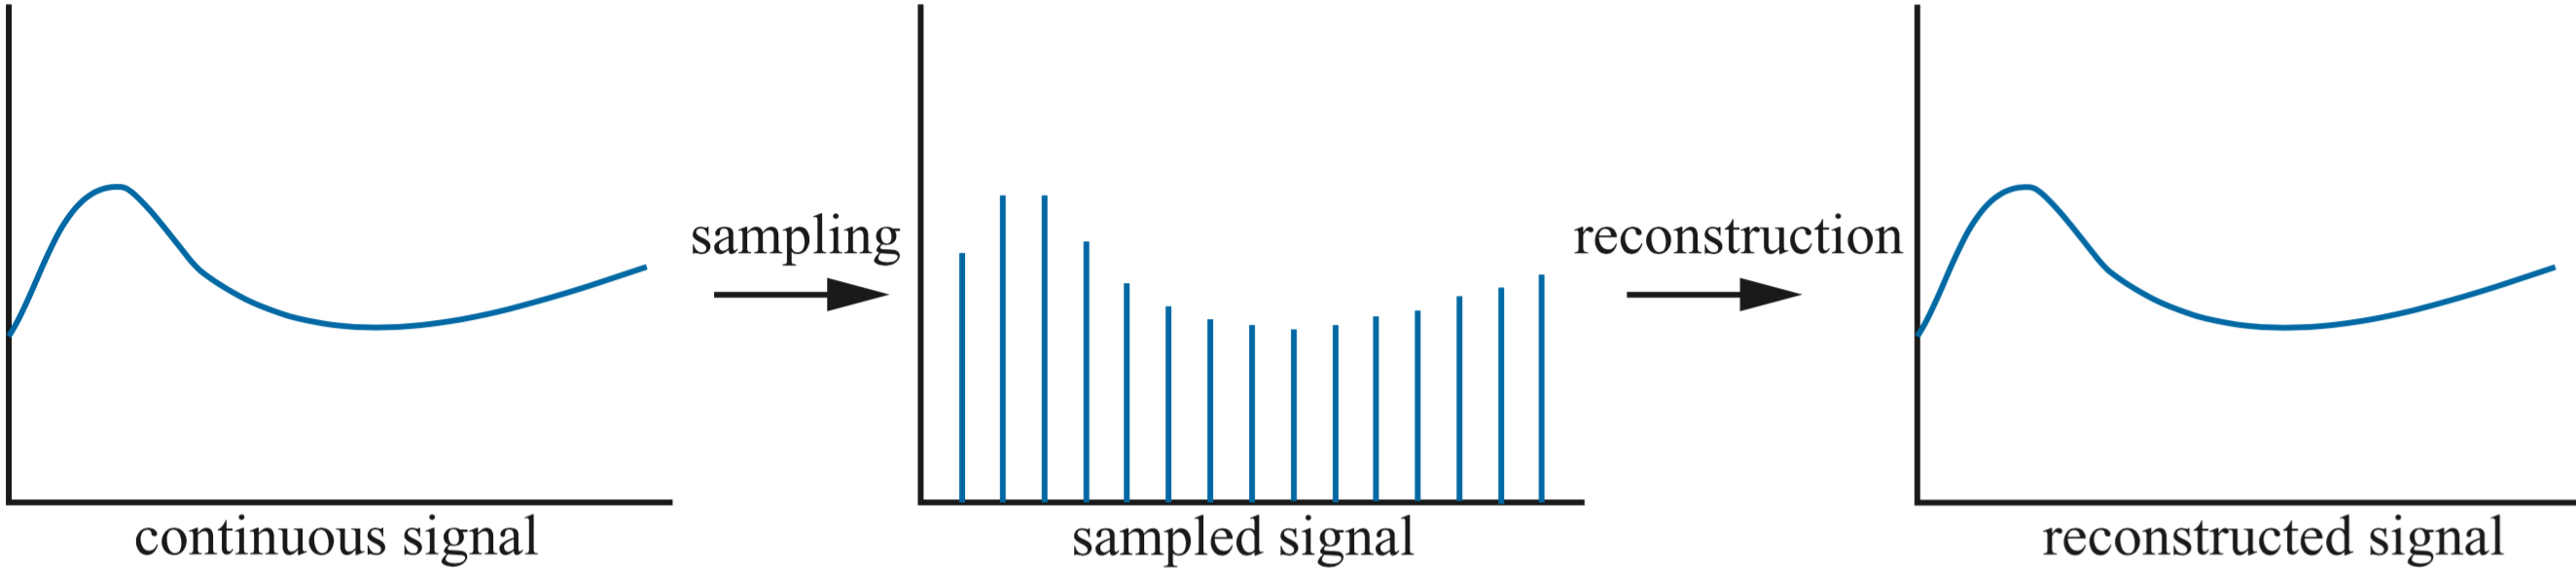
\includegraphics[width=1.\thewidth]{figures/intro/signal-processing}
	\caption{在数字信号处理的过程中,一个连续的信号(左图)被采样为离散的信号(中图),然后通过重建还原为接近原连续信号的连续信号(右图)}
\label{f:intro-signal-processing}
\end{fullwidth}
\end{figure}

以下我们就首先来讨论采样和重建这两个数字信号处理的基本过程,然后介绍一些由于采样不足导致的走样的概念以及其一般解决方案。




\subsection{采~~样}\label{sec:intro-sampling}\myindex{采样}{sampling}
关于采样的理论非常复杂,它涉及傅里叶变换,积分,级数等数学知识,以及像频率域等滤波相关的概念。然而理解采样相关知识是理解走样相关知识的重要理论基础,而且在图形学的其他一些地方也会涉及这些知识,例如在光线追踪技术中就会大量涉及脉冲函数。此外,理解傅里叶变换也有助于理解后面的如小波变换,球谐函数等概念。但本节不会严格地推导和讨论傅里叶相关的知识,而只是使用一些结论让读者比较容易地理解采样相关的概念及逻辑,本书后面的内容还会反复更深入地讨论傅里叶变换相关的知识,更多关于数字图像处理的理论知识,可以参考\cite{b:DigitalImageProcessing}。

法国数学家傅里叶(Jean Baptiste Joseph Fourier)于1807年在他的《热分析理论》一书中指出,任何非周期\footnote{对于任何周期函数则可以使用傅里叶级数,表示为不同频率的正弦和/或余弦和的形式,每个正弦项和/或余弦项乘以不同的系数。例如具有周期$T$的周期函数$f(t)$的傅里叶级数为:

\begin{equation}\label{eq:fourier-series}
	f(t)=\sum^{\infty}_{n=-\infty}c_n {\rm e}^{j \cfrac{2\pi n}{T}t}
\end{equation}

\noindent 其中:

\begin{equation}
	c_n= \cfrac{1}{T}{\rm \int}^{T/2}_{-T/2}f(t){\rm e}^{-j \cfrac{2\pi n}{T}t}{\rm d}t, n=0,n=\pm 1,n=\pm 2,\cdots
\end{equation}

}(但该曲线下的面积是有限的)的连续函数可以用正弦和/或余弦乘以一个加权函数的积分来表示,这个积分方程称为傅里叶变换(Fourier transform)\mathindex{傅里叶变换}{Fourier transform}。用$F(\mu)$表示连续变量$t$的连续函数$f(t)$的傅里叶变换,则:

\begin{equation}\label{eq:intro-fourier}
	F(\mu)={\rm \int}^{\infty}_{-\infty}f(t){\rm e}^{-j2\pi\mu t}{\rm d}t
\end{equation}

\noindent 其中,$\mu$表示正弦项或余弦项的频率,由于被积函数中的变量$t$被积分,所以上式的结果为变量$\mu$的函数。

相反,给定$F(\mu)$,通过傅里叶反变换可以获得$f(t)$:

\begin{equation}
	f(t)={\rm \int}^{\infty}_{-\infty}F(\mu){\rm e}^{-j2\pi\mu t}{\rm d}\mu
\end{equation}

\noindent 利用欧拉公式\footnote{${\rm e}^{j\theta}=\cos\theta +j\sin\theta$},可以把式\ref{eq:intro-fourier}表示为:

\begin{equation}
	F(\mu)={\rm \int}^{\infty}_{-\infty}f(t)[\cos (2\pi\mu t)-j\sin(2\pi\mu t)]{\rm d}t
\end{equation}

我们看到,由于变量$t$被积分后只剩下$\mu$,所以傅里叶变换$F(\mu)$的作用域是频率域。频率变量$\mu$的单位取决于$t$的单位,例如,如果$t$表示单位为秒的时间,则$\mu$的单位为周/秒,如果$t$表示单位为米的时间,则$\mu$的单位为周/米。

从广义上讲,频率域(frequency domain)\myindex{频率域}{frequency domain}表述的是一个连续函数在它的作用域上的改变有多快,所以一个函数通常有多个频率,这些频率构成该函数的一个频率谱(spectrum of frequencies)\myindex{频率谱}{spectrum of frequencies}。傅里叶变换正是将一个连续非周期函数由其时间域\footnote{如果一个信号随时间而变化,称该作用域为时间域。}(time domain)\myindex{时间域}{time domain}或空间域\footnote{例如与时间无关的静止的图像,它的作用域为空间位置$x,y,z$,称为空间域。}(spatial domain)\myindex{空间域}{spatial domain}变换到其频率域。其目的在频率域我们可以发现该函数的一些重要特征,甚至一些对函数的操作在频率域进行更方便。

从图\ref{f:intro-fourier}中可以看到这种作用域的转化,红色线条代表原始连续周期函数(注意这里是针对傅里叶级数而非傅里叶变换进行描述),蓝色线条为傅里叶级数各级的正弦或余弦函数,图\ref{f:intro-fourier}(a)包含了傅里叶级数的头6项,这个傅里叶级数本身是有无穷多项的。图\ref{f:intro-fourier}(b)通过提取出每个正弦或余弦项的频率,而形成图\ref{f:intro-fourier}(c)的频率域函数,这个频率域将用于后面对信号采样的质量判定。值得注意的是,由式\ref{eq:fourier-series}可知,其傅里叶级数的频率域是离散的;然而由式\ref{eq:intro-fourier}可知,非周期连续函数的频率域函数,即傅里叶变换函数是连续的,如图\ref{f:intro-fourier-case}所示。

\begin{figure}
\begin{fullwidth}
	\begin{subfigure}[b]{0.33\thewidth}
		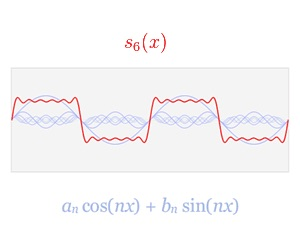
\includegraphics[width=1.\textwidth]{figures/intro/fourier-1}
		\caption{傅里叶级数头6项}
	\end{subfigure}
	\begin{subfigure}[b]{0.33\thewidth}
		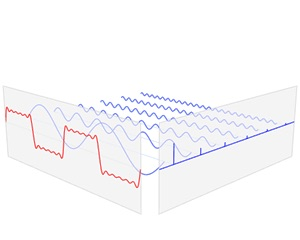
\includegraphics[width=1.\textwidth]{figures/intro/fourier-2}
		\caption{傅里叶变换}
	\end{subfigure}
	\begin{subfigure}[b]{0.33\thewidth}
		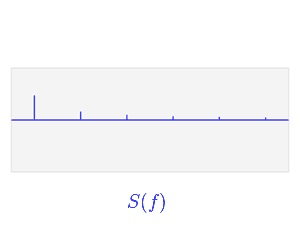
\includegraphics[width=1.\textwidth]{figures/intro/fourier-3}
		\caption{频率域}
	\end{subfigure}
\caption{傅里叶变换将函数由时间域(或空间域)变换到频率域,注意这里讨论的是周期函数的傅里叶级数(图片来自Wikipedia)}
\label{f:intro-fourier}
\end{fullwidth}
\end{figure}

当一个函数被变换到频率域后,则我们可以检测该函数是否存在最大的频率,以至对于所有大于该频率的傅里叶变换函数的值为$0$。如果该最大频率存在,该函数称为带限函数(bandlimited function)\myindex{带限函数}{bandlimited function},这意味着我们可以检测该函数的频率带宽(bandwidth)\myindex{频率带宽}{bandwidth},如图\ref{f:intro-fourier-case}是某个函数的傅里叶变换,其频率带宽为$2B$。带限函数是后面对函数进行采样以及相关理论的重要基础概念。

\begin{figure}
\sidecaption
	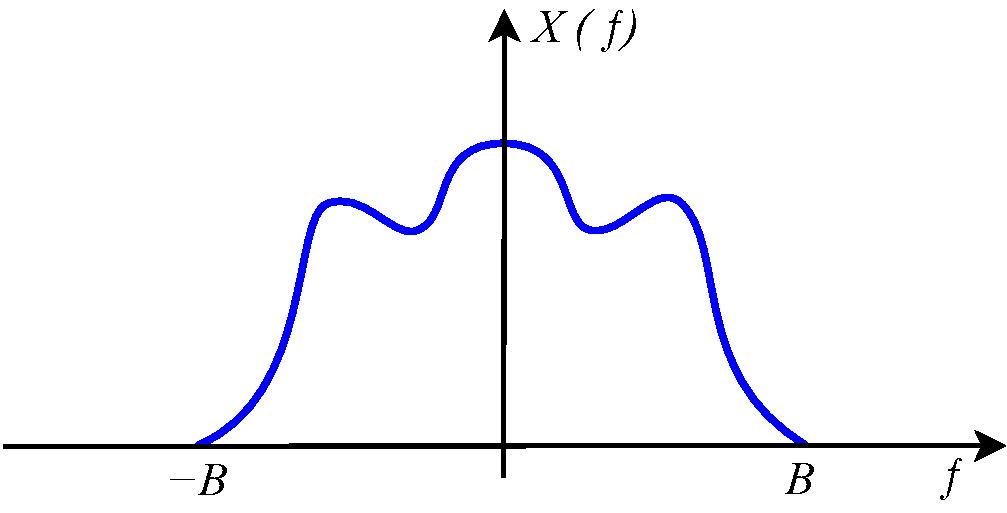
\includegraphics[width=0.6\textwidth]{figures/intro/Bandlimited}
	\caption{一个带限函数的频率域具有一个有限的范围,如果采用频率大于这个带限的宽度,则其采样后的离散信号可以被完美复原(图片来自Wikipedia)}
	\label{f:intro-fourier-case}
\end{figure}

为了理解采样及采样定理,我们需要首先了解一下卷积的概念,卷积在计算机图形学中也是一个重要的基础数学工具,例如在后面讨论渲染方程,以及一些全局光照方案中几乎所有涉及球谐函数(spherical harmonics)\myindex{球谐函数}{spherical harmonics}的地方等都会涉及卷积,所以本节首先学习卷积及其在傅立叶变换中的应用。




\subsubsection{卷~~积}
在数学上,卷积(用符号$\star$表示)定义为两个函数$f$和$g$,在其中一个函数被翻转$180^{\circ}$之后(以下假设$g$被翻转),两个函数乘积的积分,即:

\begin{equation}\label{eq:intro-conv}
	f(t)\star g(t)={\rm \int}^{\infty}_{-\infty}f(\tau)g(t-\tau){\rm d}\tau
\end{equation}

\noindent 注意这里$\tau$是一个积分假变量,它说明在积分滑过整个定义域的同时,翻转函数$g$将作用于$f$的每一个位置。

我们可以给卷积做一个很直观的视觉解释,在图\ref{f:intro-Convolution}中,蓝色曲线表示函数$f$,红色曲线表示函数$g$,以下过程可以用来描述卷积的计算:

\begin{figure}
	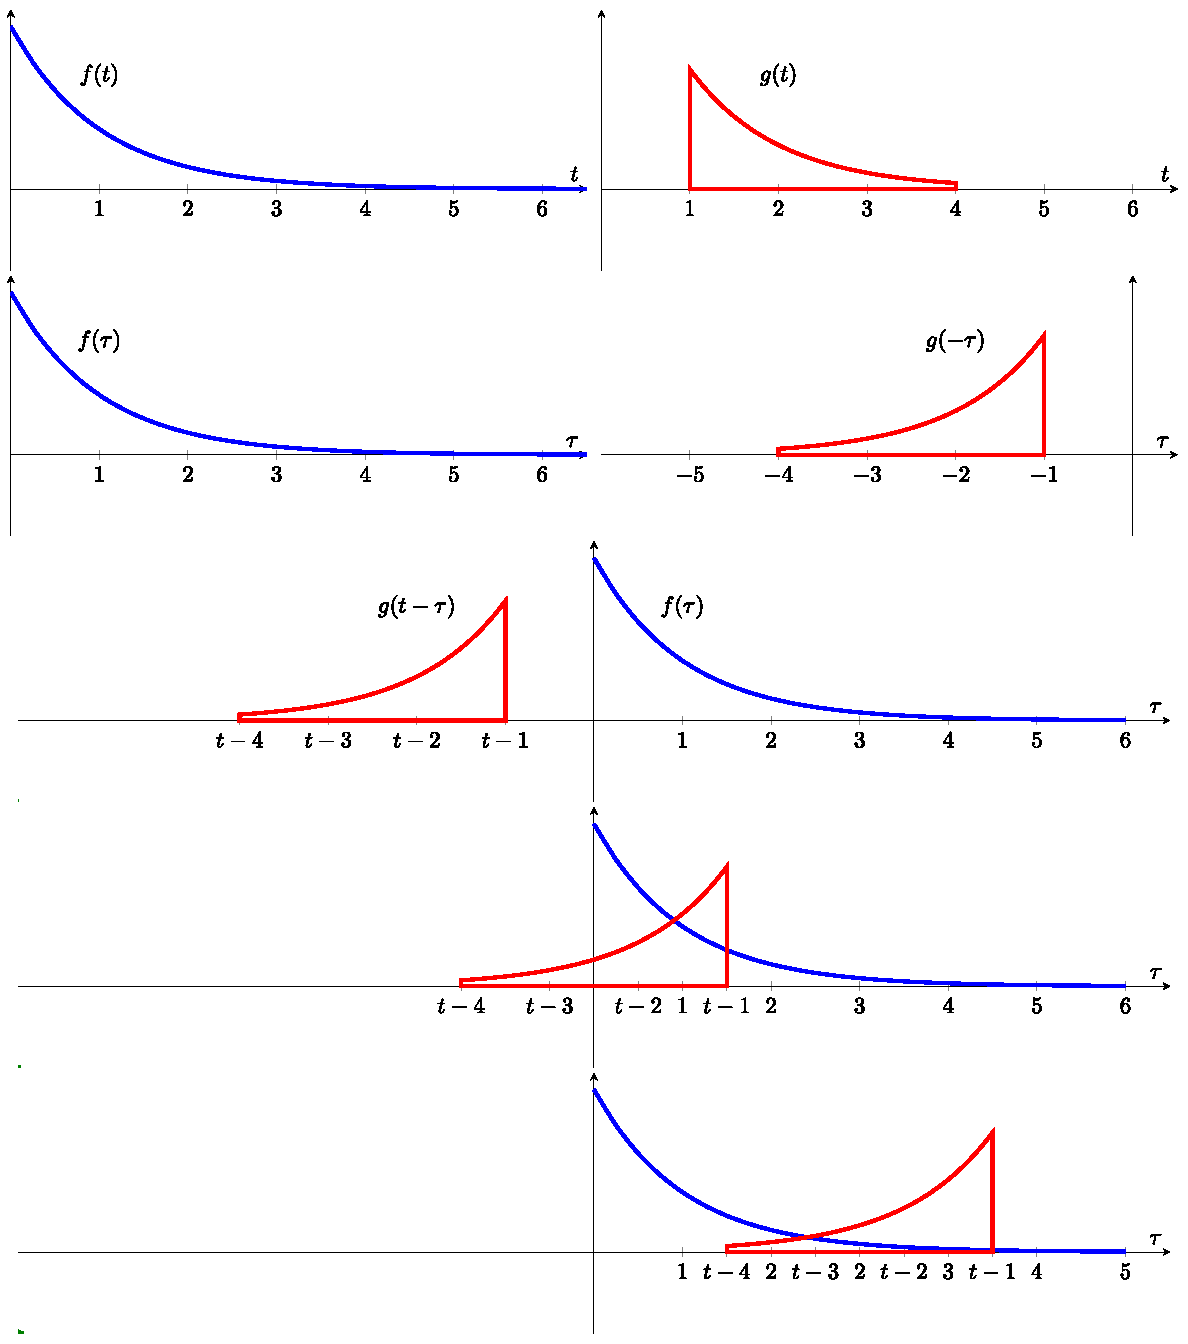
\includegraphics[width=\textwidth]{figures/intro/Convolution}
	\caption{卷积的视觉解释,对于两个函数$f$和$g$的卷积(第一行),我们首先将$g$执行$180^{\circ}$翻转(第二行),然后将$g(t-\tau)$从定义域的左边(第三行)开始向右滑动(第四,五行),并在每个位置$t$处计算式\ref{eq:intro-conv}中的积分(图片来自Wikipedia)}
	\label{f:intro-Convolution}
\end{figure}

\begin{enumerate}
	\item 对函数$g$执行$180^{o}$翻转: $g(\tau )\to g(-\tau )$,如图\ref{f:intro-Convolution}第一行到第二行的图形变化。
	\item 设置一个时间偏移$t$,使$g(t-\tau )$从$\tau-$轴的起点位置开始“滑行”,如图\ref{f:intro-Convolution}第三行所示。
	\item 将$t$从$-\infty$滑动到$\infty$,即是将$g$从$-\infty$沿$\tau-$轴滑动到$\infty$经过整个时间域,如图\ref{f:intro-Convolution}第四和五行所示,只要两个函数存在相交,则计算它们乘积的积分,换句话说,在每个时间$t$,对$f(\tau )$执行一个权重系数为$g(-\tau )$的积分,注意式\ref{eq:intro-conv}的积分变量为$\tau$,它表示被执行翻转的函数$g$的作用域,所以整个积分是一个关于$t$的函数,我们需要求解每个$t$处的积分。
\end{enumerate}

这个过程形成的关于$t$的波形(在图中没有画出),即是$f$和$g$的卷积。由此可以看出,卷积计算是对$f$整个定义域的每一点,在$g$定义域内的积分计算。因此卷积的计算量非常大,我们看到后面的一些计算中,$g$的定义域一般都非常小。此外,卷积是一个线性计算,它输出一个和$f$定义域一样大小的结果,例如,如果$f$代表的是一张图像,则卷积计算的结果输出另一张一样大小的图像。另外,卷积公式本身只是关于每个点$t$的计算公式,所以卷积实现必须要遍历整个$f$定义域。

对于卷积和傅里叶变换,可证明(读者可参考\cite{b:DigitalImageProcessing}等相关书籍),空间域中两个函数的卷积的傅里叶变换等于两个函数的傅里叶变换在频率域的乘积;反过来,如果有两个变换的乘积,则可以通过计算傅里叶反变换得到空间域的卷积,这即是卷积定理(convolution theorem)\mathindex{卷积定理}{convolution theorem}。换句话说,$f(t)\star h(t)$和$H(\mu)F(\mu)$是傅里叶变换对,这一结果是卷积定理的一半,可以写为:

\begin{equation}
	f(t)\star h(t)\Leftrightarrow H(\mu)F(\mu)
\end{equation}

双箭头用于指示右边的表达式是通过对左边的表达式执行傅里叶变换得到的,而左边的表达式是通过求右边表达式的傅里叶反变换得到的。

遵循类似的推导可得到卷积定理的另一半:

\begin{equation}
	f(t)h(t)\Leftrightarrow H(\mu)\star F(\mu)
\end{equation}

\noindent 它说明频率域的卷积类似于空间域的乘积,两者分别与傅里叶正,反变换相联系。卷积定理是傅里叶分析的重要基础,也是计算机图形学中很多算法的重要基础工具。



\subsubsection{采样定理}
有了傅里叶变换和卷积定理两个基础工具,我们就可以推导出采样定理,由于信号处理涉及对连续信号进行采样,以生成离散信号,然后通过离散的采样结果对函数进行重建的过程,采样定理告诉我们,在什么条件下可以完美地重建原始连续信号。除此之外,采样定理还能帮助我们理解走样的概念,以及对离散信息进行平滑等知识。

首先我们需要了解冲激函数(dirac function)\mathindex{冲激函数}{dirac function}的概念,它是推导采样定理的重要基础。连续变量$t$在$t=0$处的单位冲激表示为$\delta(t)$,其定义为:

\begin{equation}
	\delta(t)=\begin{cases}
		\infty & t=0\\
		0      & t\neq 0
	\end{cases}
\end{equation}

\noindent 同时它还被限制为满足:

\begin{equation}
	\int^{\infty}_{-\infty}\delta(t){\rm d}t=1
\end{equation}

很容易看出,假设函数$f(t)$在$t=0$处是连续的,那么冲激函数具有如下的采样特性:

\begin{equation}
	\int^{\infty}_{-\infty}f(t)\delta(t){\rm d}t=f(0)
\end{equation}

更一般地,对于任意位置$t_0$处的冲激函数$\delta(t-t_0)$,采样特性变为:

\begin{equation}
	\int^{\infty}_{-\infty}f(t)\delta(t-t_0){\rm d}t=f(t_0)
\end{equation}

可以看出,冲激函数的采样特性可以简单地得到冲激位置处的函数值,那么如果我们定义一个具有均匀间隔的冲激串函数,将这个冲激串作用于一个连续函数,那么其结果就得到对原始信号的均匀采样。

一个具有均匀间隔$\Delta T$的冲激串函数可以定义为:

\begin{equation}
	s_{\Delta T}(t)=\sum^{\infty}_{n=-\infty}\delta(t-n\Delta T)
\end{equation}

上述冲激串表述的函数如图\ref{f:intro-sampling}(b)所示。将上述冲激串函数作用于一个连续函数$f(t)$,则得到以下采样后的函数为:

\begin{figure}
	\sidecaption
	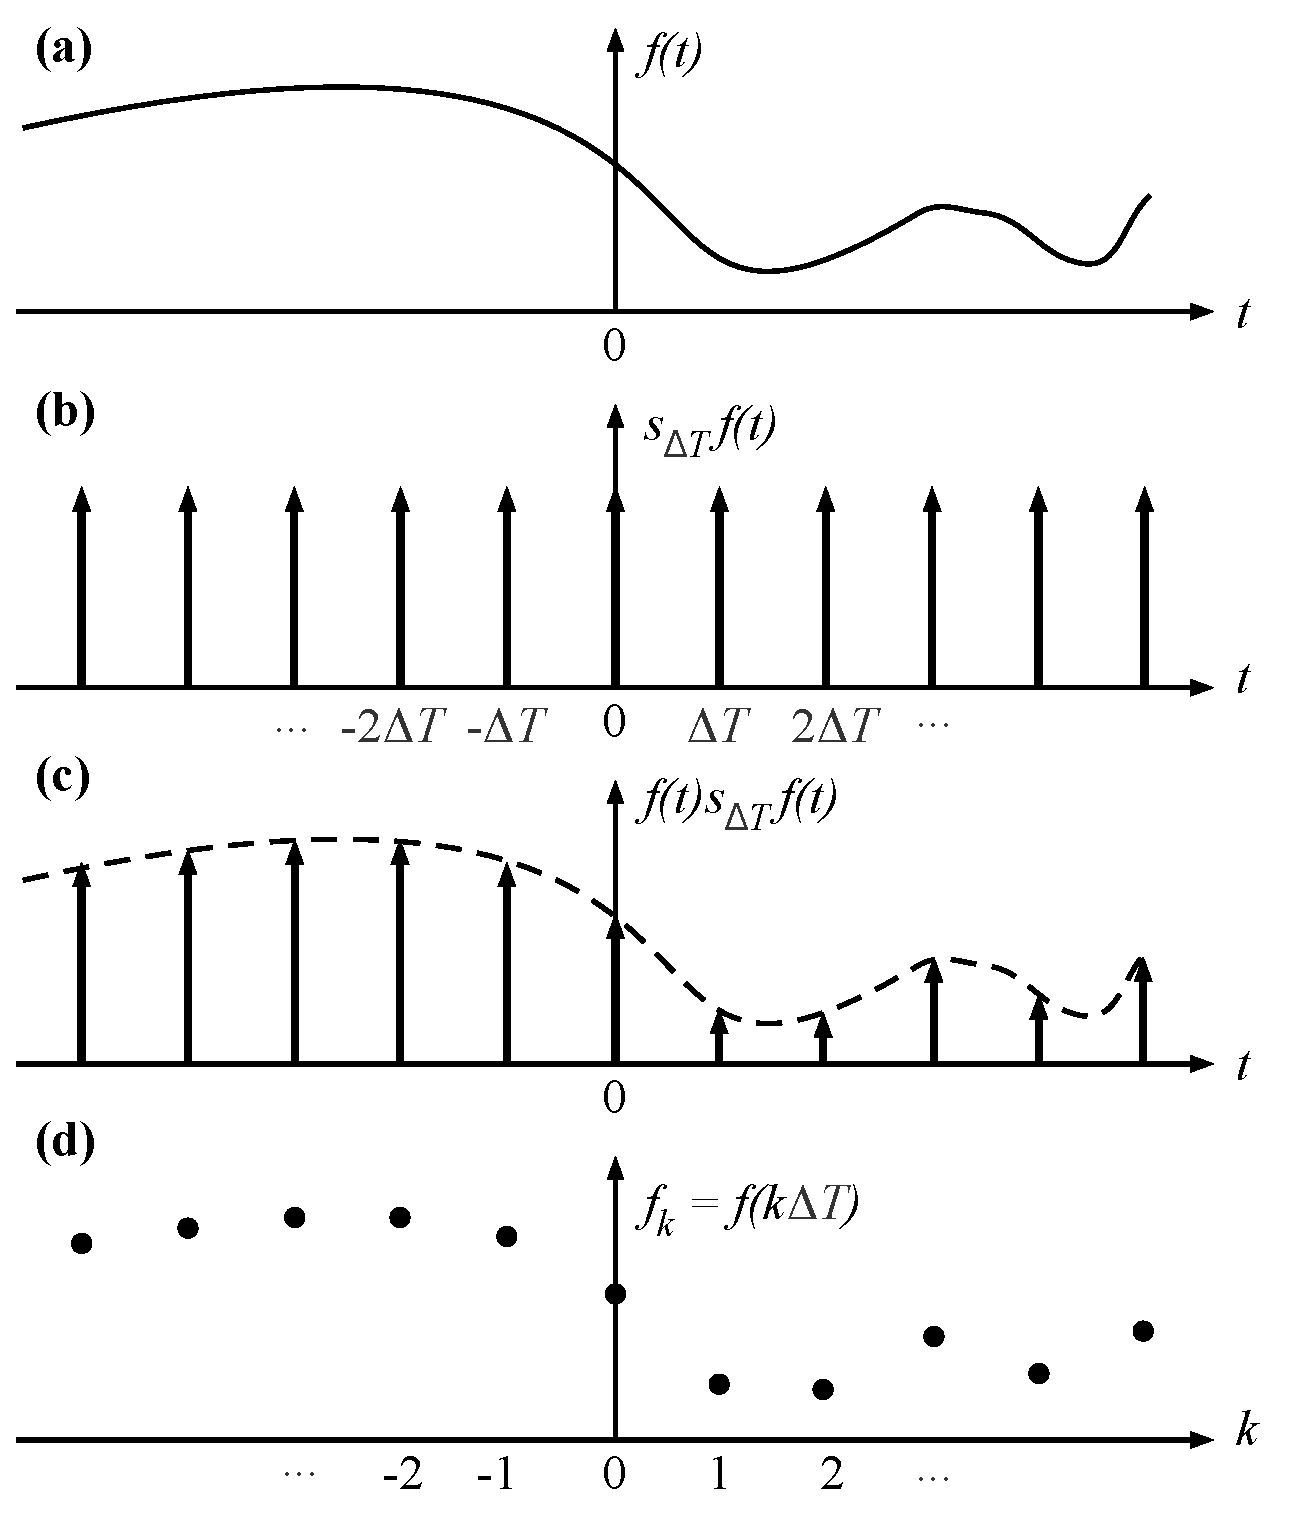
\includegraphics[width=0.65\textwidth]{figures/intro/sampling}
	\caption{冲激函数具有采样的能力,它可以简单地得到冲激位置处的函数值,所以函数$f(f)$的均匀采样可以定位为使用一个冲激串函数(b)与之相乘,这得到采样过后的函数(c),最终每个冲激位置处的采样值由加权后的冲激强度给出(d)}
	\label{f:intro-sampling}
\end{figure}

\begin{equation}
	\tilde{f}(t)=f(t)s_{\Delta T}(t)=\sum^{\infty}_{n=-\infty}f(t)\delta(t-n\Delta T)
\end{equation}

上述和式的每一个分量都是由在该冲激位置处$f(t)$的值加权后的冲激,如图\ref{f:intro-sampling}(c)所示。每个采样的值由加权后的冲激“强度”给出,我们可以通过积分得到它,即任意采样值$f_k$为:

\begin{equation}
	f_k=\int^{\infty}_{-\infty}f(t)\delta(t-k\Delta T){\rm d}t=f(k\Delta T)
\end{equation}

图\ref{f:intro-sampling}(d)显式了上述的采样结果,它由原始函数的等间隔采样而成。

为什么要用这么复杂的方式来表述函数采样呢?这是因为借助冲激函数的傅里叶变换以及卷积定理,我们可以得出采样定理,并进而指导我们对函数进行采样。

令$F(\mu)$表示连续函数$f(t)$的傅里叶变换,$\tilde{F}(\mu)$为采样后的函数$\tilde{f}(t)$的傅里叶变换,由卷积定理可得:

\begin{equation}
	\tilde{F}(\mu)=\Im\{\tilde{f}(t)\}=\Im\{f(t)s_{\Delta T}(t)\}=F(\mu)\star S(\mu)
\end{equation}

\noindent 其中,$\Im$符号表示傅里叶变换,$S(\mu)$为冲激串函数的傅里叶变换:

\begin{equation}
	S(\mu)=\cfrac{1}{\Delta T}\sum^{\infty}_{-\infty}\delta\bigg(\mu -\cfrac{n}{\Delta T}\bigg)
\end{equation}

可以看出,冲激串函数的傅里叶变换仍然为一个冲激串函数,这是一个非常重要的特性,由此我们可以得到采样后的函数$\tilde{f}(t)$的傅里叶变换为:

\begin{equation}
\begin{aligned}
	\tilde{F}(\mu)=&F(\mu)\star S(\mu)={\rm \int}^{\infty}_{-\infty}F(\tau)S(\mu-\tau){\rm d}\tau\\
	=&\cfrac{1}{\Delta T}{\rm \int}^{\infty}_{-\infty}F(\tau)\sum^{\infty}_{n=-\infty}\delta\bigg(\mu-\tau-\cfrac{n}{\Delta T}\bigg){\rm d}\tau\\
	=&\cfrac{1}{\Delta T}\sum^{\infty}_{n=-\infty}{\rm \int}^{\infty}_{-\infty}F(\tau)\delta\bigg(\mu-\tau-\cfrac{n}{\Delta T}\bigg){\rm d}\tau\\
	=&\cfrac{1}{\Delta T}\sum^{\infty}_{n=-\infty}F\bigg(\mu-\cfrac{n}{\Delta T}\bigg)
\end{aligned}
\end{equation}

\noindent 其中,上式的第一行使用了卷积的基本定义,即两个函数的卷积等于它们乘积的积分,仍然需要注意的是,上述卷积中的翻转函数$S(\mu)$会在每个$\tau$处作用于整个函数$F(\tau)$的定义域上,而由于$S$是一个冲激串函数,我们把$\cfrac{1}{\Delta T}$项提到外面,就产生了一个神奇的结果,即它在每个位置处将$F(\mu)$复制一次,而复制的间隔由$1/\Delta T$决定。很明显,虽然采样后的函数$\tilde{f}(t)$(在空间域)是离散的,但是其傅里叶变换$\tilde{F}(\mu)$(在频率域)却是连续的,因为它由$F(\mu)$的几个拷贝组成,而$F(\mu)$是连续的。

图\ref{f:intro-sampling-aliasing}显式了上述这种采样后函数的傅里叶变换图示,其中图\ref{f:intro-sampling-aliasing}(a)为原始连续带限函数$f(t)$的傅里叶变换,图\ref{f:intro-sampling-aliasing}(b)则表示采样后函数的傅里叶变换,如前所述,$1/\Delta T$是用于生成采样后函数的采样率。由此可以看出,为了保持对原始信号的重建能力,我们需要使用足够的采样率来保证$F(\mu)$的完整性,在图\ref{f:intro-sampling-aliasing}(c)中,采样率刚好能够保持$F(\mu)$,但在图\ref{f:intro-sampling-aliasing}(d)中,采样率低于保持不同$F(\mu)$拷贝的最小采样率要求。

\begin{figure}
	\sidecaption
	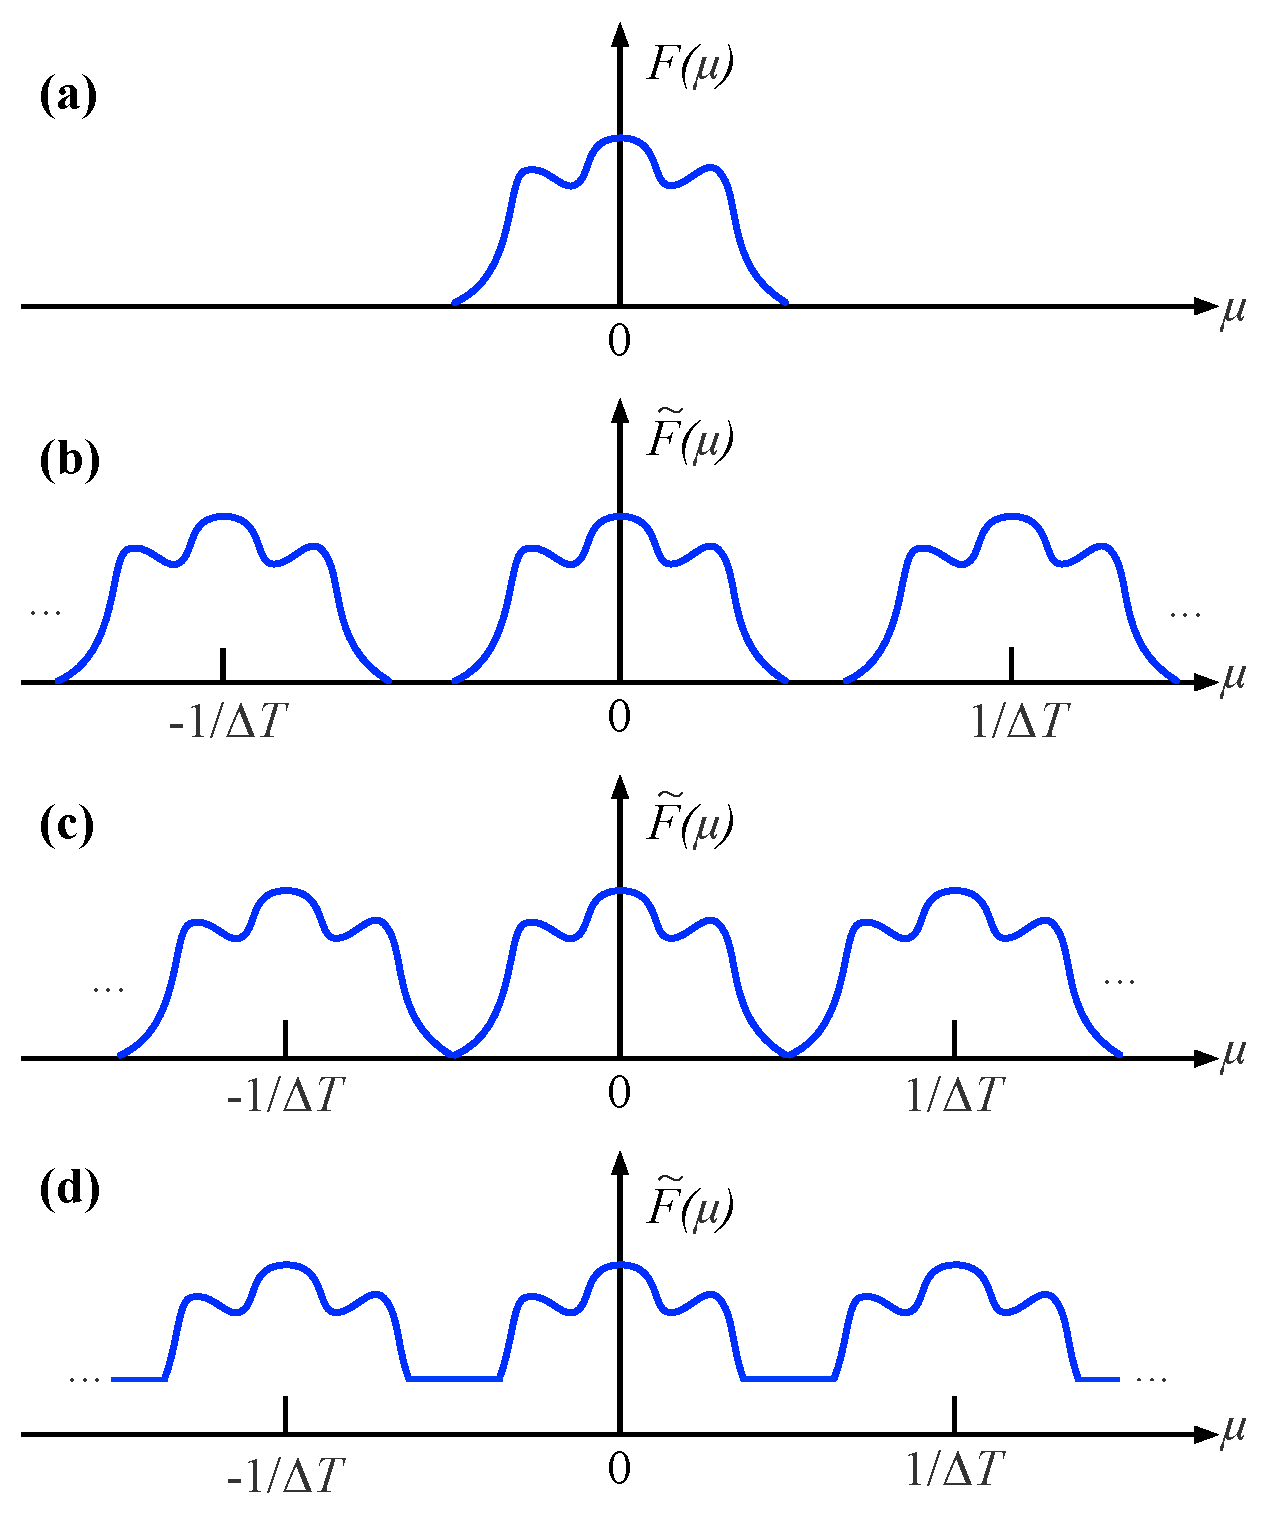
\includegraphics[width=0.65\textwidth]{figures/intro/sampling-aliasing}
	\caption{(a)为一个带限函数的傅里叶变换,(b)-(d)分别为过采样,临界采样和欠采样条件下采样后函数$\tilde{f}(t)$的傅里叶变换$\tilde{F}(\mu)$}
	\label{f:intro-sampling-aliasing}
\end{figure}

由此可知,当一个连续函数被采样成一个离散函数之后,其能够被重建为原函数的能力取决于采样点的密度(density of samples)\myindex{采样点的密度}{density of samples},或称为采样率(sample rate)\myindex{采样率}{sample rate}。根据采样理论(the sampling theorem)\myindex{采样理论}{the sampling theorem},对于一个带限函数$f(t)$,其最大的频率为$\mu_{\rm max}$,它能够完全被一系列以$1/(2\mu_{\rm max})$间隔采样的离散函数表示。换句话说,采样率必须大于或等于$2\mu_{\rm max}$采样点/秒,或者说对于一个采样率$f_s$,其离散函数能够被完美复原的条件是:$\mu_{\rm max}<f_s/2$。

当频率带宽$\mu_{\rm max}$太高(或者该函数完全不存在频率带宽),则这种不完美的复原导致的结果就是走样(aliasing)\myindex{走样}{aliasing}。这两个临界值$2\mu_{\rm max}$和$f_s/2$称作奈奎斯特采样率(Nyquist rate)\myindex{奈奎斯特采样率 }{Nyquist rate}和奈奎斯特频率(Nyquist frequency)\myindex{奈奎斯特频率}{Nyquist frequency}。由该采样定律定义的不等式条件称为奈奎斯特准则(Nyquist criterion)\myindex{奈奎斯特准则}{Nyquist criterion}。采样理论又称为奈奎斯特-香农采样定理(Nyquist–Shannon sampling theorem)\myindex{奈奎斯特-香农采样定理}{Nyquist–Shannon sampling theorem}以纪念Harry Nyquist和Claude Shannon对其的贡献。 

关于对离散函数的重建过程及其方法将在下一节讨论,采样的不足将导致走样的产生,本节最后将分析几种计算机图形学中涉及的一些比较重要的走样,通过对这些走样现象的分析和了解,将有助于更好地理解采样率对图像质量的影响。




\subsubsection{几何走样}
回到第\ref{sec:intro-sensor}节讨论的由于光栅化导致的三角形的走样,如图\ref{f:intro-aliasing-triangle}所示,对于光栅化,我们按照屏幕的分辨率对几何图形的可见性函数(visibility function)\myindex{可见性函数}{visibility function}进行采样,即采样点之间的间距为一个像素,采样点的位置为每个像素的中点。

可见性函数是一个连续函数,要想最终呈现很高质量的图像,必须要在图像上还原出很好的原始可见性函数,根据采样定律,必须要使用2倍于可见性函数最高频率的采样率。然而,三角形的可见性总是存在不连续,这种不连续性导致无限大的频率,从而使其傅里叶变换不存在有限的频率带宽,因此没有任何采样率可以阻止这种走样发生;另外根据傅里叶变换的条件,只有定义域在无限的时间域或空间域才能使其傅里叶变换具有有限的频率带宽。所以对于计算机图形学中有限的二维或三维空间域,走样现象是不可避免的。

这种由于对几何图形的可见性函数采样导致的走样称为几何走样(geometric aliasing)\myindex{几何走样}{geometric aliasing},它是计算机图形学中最严重的走样现象,因为整个场景图像的渲染都是根据物体表面的的位置来决定的,而每个像素点的位置都是光栅化阶段对物体几何形状的可见性函数来决定的。

虽然没有任何采样率可以有效地避免几何走样的存在(即完美地对可见性函数采样),但是我们仍然会寻求一些方法来减轻这种走样现象,其中比较流行的方法称为过采样(oversampling)\myindex{过采样}{oversampling},详见第\ref{sec:intro-resampling}节,这种方法本质上使用比图像分辨率更高的采样频率对原始可见性函数进行采样,然后使用这些采样点来重建像素对应的采样率下的函数值。这在3D渲染中相当于使用高于图像输出分辨率的频率渲染场景,然后将其缩放至输出分辨率,这个过程称为超采样(supersampling)\myindex{超采样}{supersampling}。本章后面第\ref{sec:intro-msaa}将详细讨论这种技术。




\subsubsection{着色走样}
着色走样(shader aliasing)\myindex{着色走样}{shader aliasing}发生于像素着色器中,它和纹理走样有点类似,也主要是由于像素着色器受限于屏幕分辨率所限导致的。然而不同的是着色走样主要是指,在着色器中对一些以分析的方式得到的连续函数的采样不足导致的走样,而不是对纹理的采样不足。

这类走样比较严重的例子是对粗糙度比较低的光泽表面的采样,由于表面低粗糙度导致其光泽分布范围更狭窄,如图\ref{f:intro-roughness}所示,从而导致光泽BRDF分布函数具有更高的频率,因而更容易导致走样。当对物体表面使用法线贴图后,这种走样现象更明显,因为法线导致物体表面的光泽具有更高的频率。

对于着色走样,其不可能通过后面第\ref{sec:intro-msaa}节介绍的MSAA技术解决,因为MSAA对于每个像素的着色只计算一次(但对Depth和Stencil值取多个采样点),所以它对着色走样没有任何影响;超采样(supersampling)虽然可以减少这类走样,但是其代价太高,并且提升效果不是很明显。如图\ref{f:intro-shader-aliasing}表示在有法线和光泽反射的情况下,三种不同方法的渲染结果。

\begin{figure}
\begin{fullwidth}
	\begin{subfigure}[b]{0.33\thewidth}
		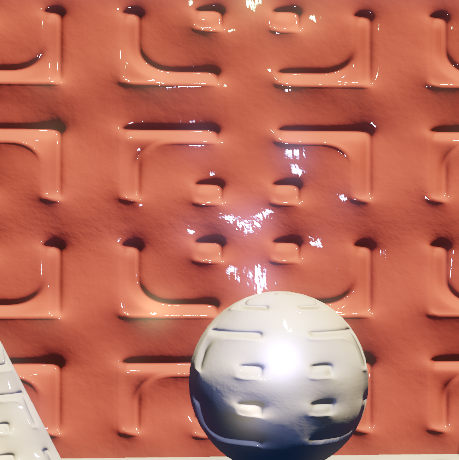
\includegraphics[width=1.\textwidth]{figures/intro/specaliasing_none}
	\end{subfigure}
	\begin{subfigure}[b]{0.33\thewidth}
		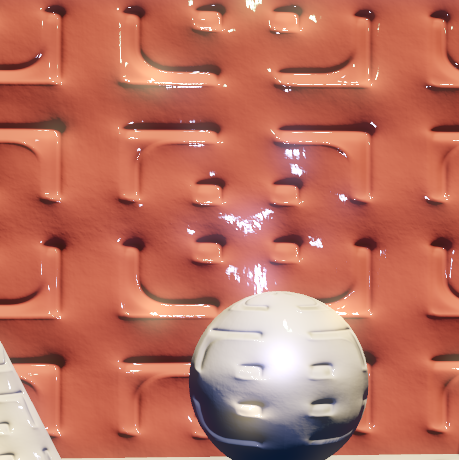
\includegraphics[width=1.\textwidth]{figures/intro/specaliasing_4xss}
	\end{subfigure}
	\begin{subfigure}[b]{0.33\thewidth}
		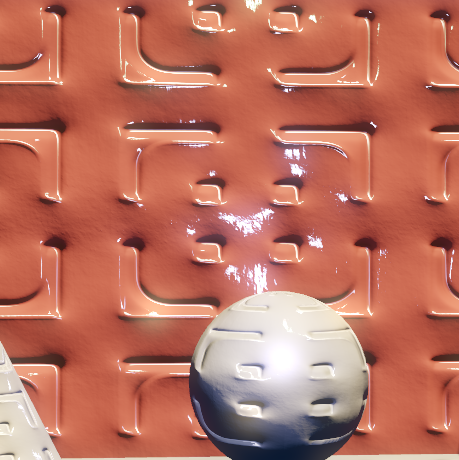
\includegraphics[width=1.\textwidth]{figures/intro/specaliasing_clean}
	\end{subfigure}
\caption{该图显示光泽和法线条件下,不同方法对着色走样的处理:左图正常绘制,走样现象比较严重,尤其注意在法线频率变化比较大的区域,信息丢失比较严重,中图使用4倍的超采样,右图使用一种直接基于法线计算光泽反射的方法,该方法能得到更好的结果(图片来自\cite{m:ApplyingSamplingTheorytoReal-TimeGraphics})}
\label{f:intro-shader-aliasing}
\end{fullwidth}
\end{figure}

对于渲染方程中由于粗糙度,法线以及其他相关因素导致的采样问题,比较有效的解决思路是,首先将这些参数融入到光照计算(例如后面讲述的微面元BRDF\myindex{微面元BRDF}{microfacet-BRDF}理论)中去,使这些“原始连续函数”更平缓,然后再对这些光照计算结果采样,这样的思路在本书后面的一些内容中有介绍。



\subsubsection{时间走样}
前面的例子都是对处于空间域的2个$(x,y)$或者3个$(x,y,z)$连续变量进行采样,然而在游戏或者电影动画渲染中,由于大量的物体处于运动状态,因此,对于另一个时间域的采样问题也特别突出。

时间走样(temporal aliasing)\myindex{时间走样}{temporal aliasing}出现于当物体在运动时,由于渲染帧率的限制使其对运动过程的采样不足导致的走样。游戏画面的渲染是根据帧率按较低的采样率对时间域进行采样,所以对于高速运动下的物品,其时间域的频率较高,很容易出现走样。其中一个比较经典的例子称为车轮效应(Wagon-wheel effect)\myindex{车轮效应}{Wagon-wheel effect},它使一个旋转的辐条车轮表现出不同的视觉效果,例如轮子可能看起来比实际更慢,或者看起来像静止一样,甚至沿着相反的方向旋转。

为了减轻时间走样,一种比较常用的方法称为运动模糊(motion blur)\myindex{运动模糊}{motion blur}。这种方法跟超采样一样,它依靠对时间域取更多的采样点,然后对其进行反走样,当然这种方法的计算成本很高。另一种更普遍的方法是针对当前帧渲染结果,生成一个速率缓存(velocity buffer)\cite{a:AReconstructionFilterforPlausibleMotionBlur}\myindex{速率缓存}{velocity buffer},然后使用这些方向在后处理阶段对其邻近的像素点执行插值计算,如图\ref{f:intro-motion-blur}所示。

\begin{figure}
	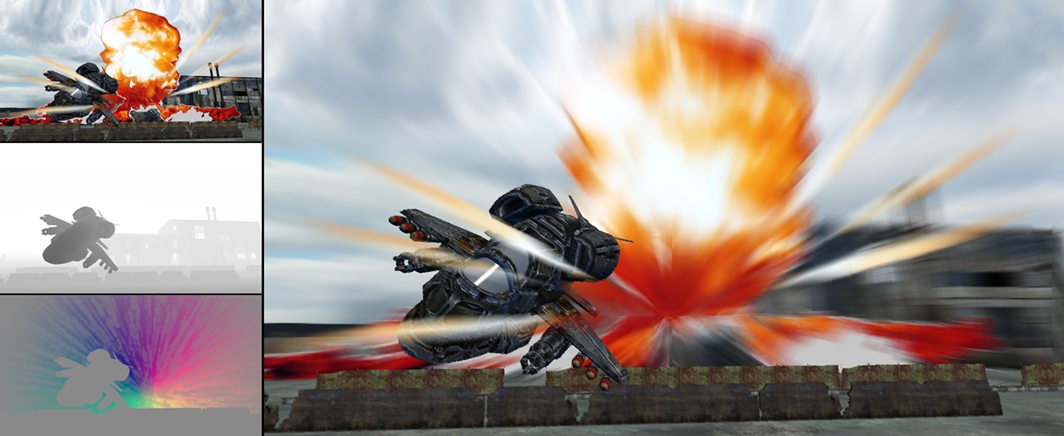
\includegraphics[width=1.\textwidth]{figures/intro/motion-blur}
	\caption{使用速率缓存实现运动模糊,图中左上表示当前帧的原始渲染结果,左中为深度缓存,左下为速率缓存,右图为最终结果}
	\label{f:intro-motion-blur}
\end{figure}



\subsection{重~~建}\label{sec:intro-reconstruction}
重建(reconstruction)\myindex{重建}{reconstruction}是指将采样后的离散函数还原为原始连续函数的过程,为了从一些离散的采样点还原为原始连续函数,必须对离散函数执行一个滤波器(filter)\myindex{滤波器}{filter}。“滤波”一词源于数字信号处理中,用于在频率域上接受(通过)或拒绝一定的频率分量。然而滤波器实际的概念非常复杂,根据滤波器是离散还是连续,以及被滤波器作用的函数是离散还是连续,滤波器的作用以及实现的结果都是不一样的。




\subsubsection{平~~滑}
根据卷积公式的特性,我们可以很容易想到它可以用来平滑函数$f$,然而不仅如此,根据卷积计算是作用在时间/空间域或者频率域,以及$f$和$g$是离散还是连续函数,它表现出来的功能特征和结果是不一样的,以下我们就分别来描述卷积的这些应用场景。

卷积计算最本质也是最直观的特征是平滑,它通过对$f$的每个点考虑该点周围一定范围内的值对该点的影响,来消除该点与周围环境的频率的快速变化。这在计算机图形学中运用时分广泛,大部分可能出现走样的地方,例如前面第\ref{sec:intro-sampling}节讨论的那些走样现象,都可以在采样之前对原始函数进行平滑,以减轻走样现象。这种滤波器称为反走样滤波器(anti-aliasing filter)\myindex{反走样滤波器}{anti-aliasing filter}。

这里举一个图像处理的例子,在图像处理中,常常考虑$f(x,y)$为一个具有一定分辨率的图像,$g(x,y)$为一个$m\times n$的矩形,其分辨率通常小于或等于$f(x,y)$的分辨率,假设$m=2a+1$且$n=2b+1$,其中$a,b$为正整数,则式\ref{eq:intro-conv}变为:

\begin{equation}\label{eq:intro-convolution-2}
	g(x,y)\star f(x,y)=\sum^{a}_{s=-a}\sum^{b}_{t=-b}g(s,t)f(x-s,y-t)
\end{equation}

可以看出,卷积的意义相当于使用一个$m\times n$的模板$g$,以它的中心从$f$ 的每一个像素点经过,对于每一个像素点,分别计算模板上对应位置的两个函数乘积的和,如图\ref{f:intro-conv}所示,其卷积输出为一个新的与$f$分辨率相同的图像。

\begin{figure}
\sidecaption
	\includegraphics[width=.5\textwidth]{figures/intro/conv}
	\caption{在图像处理中,卷积的意义相当于使用一个蒙板遍历每一个像素点,分布计算蒙板内所有乘积的和,GPU中纹理过滤相关的技术都是通过卷积的方式实现}
	\label{f:intro-conv}
\end{figure}



\subsubsection{重~~建}
除了平滑,借助卷积的特性还可以实现将离散函数还原为原始连续函数,卷积的这种运用称为重建滤波器(reconstruction filter)\myindex{重建滤波器}{reconstruction filter}。重建的操作表现为用一个无限连续的$g$作用于采样后离散的$f$,然而为了直观理解重建的过程,我们需要首先从频率域以及采样定理说起。

前面已经介绍过采样定理相关的内容,设$\tilde{F}(\mu)$为对$f(t)$采样后的离散函数$\tilde{f}(t)$的傅里叶变换,如图\ref{f:intro-reconstruction}(a)所示,为了使$f(t)$能够被完美重建,首先需要保留$\tilde{F}(\mu)$所有的频率,在本例子中使用了一个高于奈奎斯特采样率的频率进行采样。如果能够从$\tilde{F}(\mu)$中包含的这个函数的拷贝的周期序列中分离出$F(\mu)$的一个拷贝,那么我们就可以从采样后的版本恢复$f(t)$。

\begin{figure}
\sidecaption
	\includegraphics[width=.65\textwidth]{figures/intro/reconstruction}
	\caption{盒状滤波器通常用来在频率域对信号进行重建}
	\label{f:intro-reconstruction}
\end{figure}

为了从原理上了解如何从$\tilde{F}(\mu)$复原$F(\mu)$,在图\ref{f:intro-reconstruction}(b)中$H(\mu)$的定义如下:

\begin{equation}
	H(\mu)=\begin{cases}
		\triangle T & -\mu_{\max}\leq\mu\leq\mu_{\max}\\
		0           & \text{其他}
	\end{cases}
\end{equation}

\noindent 当乘以图\ref{f:intro-reconstruction}(a)中的周期序列时,该函数就隔离了以原点为中心的一个周期,然后通过$H(\mu)$和$\tilde{F}(\mu)$相乘得到$F(\mu)$:

\begin{equation}\label{eq:intro-reconstruction}
	F(\mu)=H(\mu)\tilde{F}(\mu)
\end{equation}

\noindent 一旦得到了$F(\mu)$,就可以通过傅里叶反变换来复原$f(t)$:

\begin{equation}
	f(t)={\rm \int}^{\infty}_{-\infty}F(\mu){\rm e}^{j2\pi\mu t} {\rm d}\mu
\end{equation}

\noindent 以上这些公式从理论上证明了,以函数包含的最高频率的两倍的速率采样得到的函数的样本,来恢复一个带限函数是可能的。

上述的函数$H(\mu)$称为一个低通滤波器(low-pass filter)\myindex{低通滤波器}{low-pass filter},因为它通过频率范围低端的频率,并且消除所有较高的频率。所以要想完美复原原始函数,原始函数$(f(t))$必须是带限函数。

对式\ref{eq:intro-reconstruction}利用卷积定理,可以在空间域得到等价的结果,即:

\begin{equation}
	f(t)=\Im^{-1}\{F(\mu)\}=\Im^{-1}\{H(\mu)\tilde{F}(\mu) \}=h(t)\star\tilde{f}(t)
\end{equation}

\noindent 可导出$f(t)$的如下空间域表达式(此处略去证明过程,请参考\cite{b:DigitalImageProcessing}等相关书籍):

\begin{equation}\label{eq:intro-reconstruction-1}
	f(t)=\sum^{\infty}_{n=-\infty}f(n\triangle T) {\rm sinc}[(t-n\triangle T)/\triangle T]
\end{equation}

\noindent 这相当于对离散函数使用一个辛克函数(sinc function)\myindex{辛克函数}{sinc function}(如图\ref{f:intro-sinc}所示)的卷积,辛克函数的定义如下:

\begin{equation}
	{\rm sinc}(x)= \cfrac{\sin (\pi x)}{\pi x}
\end{equation}

\noindent 这并不奇怪,因为盒装滤波器$H(\mu)$的傅里叶反变换就是一个辛克函数。

\begin{figure}
\sidecaption
	\includegraphics[width=.65\textwidth]{figures/intro/sinc}
	\caption{蓝色曲线表示归一化的辛克函数,而红色曲线表示未归一化的辛克函数,在计算机图形学中一般使用归一化的版本(图片来自Wikipedia)}
	\label{f:intro-sinc}
\end{figure}

我们不禁要问,卷积主要用来平滑一个离散或者连续函数,那它是怎样实现这种类似于在样本点之间插值的效果的呢?这里主要是由于辛克函数是在无限空间连续的,所以当它划过$\tilde{f}(t)$上的每一点时,会在辛克函数的整个定义域上求积分,因为积分值是一个标量,即该点的卷积总是可能具有一个值,并且这个值其实是考虑$\tilde{f}(t)$所有点的平滑效果而得来的,因此它能完美还原$f(t)$,同时实现了使用卷积来重建一个离散函数。当卷积被这样使用时,称之为重建过滤器(reconstruction filter)\myindex{重建过滤器}{reconstruction filter}。

在图像处理中,重建过滤器主要有两个用途:第一种为上面讲述的从一个采样过的离散函数重建原始连续函数,另一种称为重采样(见第\ref{sec:intro-resampling}节),即在纹理被缩小或者放大时,调整图像的分辨率。这两种场景本质上都是把滤波器看做一种计算某个特定的点的插值的工具,即我们并不需要对一张图像全部像素点做卷积计算,而是找出另外一些当前这些采样点之外的点的值。

然而,式\ref{eq:intro-reconstruction-1}要求样本间的内插有无限多项,在实际中,这意味着我们必须找到一种样本间内插有限的近似方法,在图像处理中使用的主要内插方法是最近邻法,双线性法和双三次内插法,这些插值方法将在下一节讨论。





\subsection{重采样}\label{sec:intro-resampling}
在渲染场景的时候,程序会大量使用预先采样的数据,如图像,或者场景的某些离散的表示空间结构数据等。这些数据都是具有一定的分辨率(或者是按一定的采样率生成的数据),当程序中需要在不同分辨率下使用这些数据时(例如摄像机靠近或者远离表面导致纹理被放大或者缩小),我们需要对这些离散的数据进行重采样(resampling)\myindex{重采样}{resampling},以生成一个具有不同分辨率的数据。以下我们主要以GPU中对纹理的采样分析分辨率转换的问题。

当摄像机靠近物体表面时,即发生放大操作(magnification)\myindex{放大操作}{magnification},这使摄像机能看到更多细节,它要求对原始函数使用更高的采样率采样。如图\ref{f:intro-magnification}所示,这要求生成更多的采样点,根据上一节讲述的内容,我们只需要对于离散的图像提供一个滤波器,便可以对任意点进行插值。

\begin{figure}
\begin{fullwidth}
	\includegraphics[width=\thewidth]{figures/intro/magnification}
	\caption{左图的原始经过采样的离散信号,当摄像机靠近物体上需要对信号进行放大操作(图片来自\cite{b:rtr})}
	\label{f:intro-magnification}
\end{fullwidth}
\end{figure}

然而,正如前面提到的,辛克函数要求样本间的内插值有无限多项,所以我们必须使用一些近似方法来进行插值计算。最简单的方法是最近邻插值(nearest-neighbor interpolation)\myindex{最近邻插值}{nearest-neighbor interpolation},它采用像素复制的放大操作。例如,将一幅图像放大两倍,我们可以复制每一列,这会在水平方向上将图像尺寸放大一倍;然后复制这幅放大后图像的每一行,在垂直方向上将图像尺寸放大一倍。相同的步骤可用于任意整数倍放大图像。最近邻内插法实际上是对图像使用一个盒式过滤器(box filter)\myindex{盒式过滤器}{box filter},如图\ref{f:intro-Piecewise_constant}所示。

\begin{figure}
\sidecaption
	\includegraphics[width=.45\textwidth]{figures/intro/Piecewise_constant}
	\caption{最近邻内插法直接选择离重建点最近的样本值作为内插值(图片来自Wikipedia)}
	\label{f:intro-Piecewise_constant}
\end{figure}

双线性插值(bilinear interpolation)\myindex{双线性插值}{bilinear interpolation}法则分别基于采样点的位置在$X$和$Y$轴上线性地插值,如图\ref{f:intro-BilinearInterpolation}所示。双线性插值法本质上对图像执行一个三角形过滤器(triangle filter)\myindex{三角形过滤器}{triangle filter}或称为篷形过滤器(tent filter)\myindex{篷形过滤器}{tent filter}。

\begin{figure}
\sidecaption
	\includegraphics[width=.45\textwidth]{figures/intro/BilinearInterpolation}
	\caption{双线性插值法分别基于采样点的位置在$X$和$Y$轴上线性地插值(图片来自Wikipedia)}
	\label{f:intro-BilinearInterpolation}
\end{figure}

双线性插值法仅仅考虑采样点周围的4个$2\times 2$像素点,双三次内插法(bicubic interpolation)则考虑周围16个$4\times 4$像素点,可以给出更平滑的插值结果(最近邻插值法和双线性插值法都会使还原的函数具有导数不连续的点,即导致非常高的频率变化,从而导致走样比较严重)。双三次内插法使用的滤波器函数如下:

\begin{equation}
	W(x)=\begin{cases}
		(a+2)|x|^{3}-(a+3)|x|^{2}+1 & $for $|x|\leq 1 \\
		a|x|^{3}-5a|x|^{2}+8a|x|-4a & $for $1<|x|<2   \\
		0 & 其他
	\end{cases}
\end{equation}

\noindent 这里$a$通常取值-0.5或者-0.75,注意$W(0)=1$,对于所有非0整数$W(n)=0$。双三次函数具有如图\ref{f:intro-bicubic}所示的形状。

\begin{figure}
\sidecaption
	\includegraphics[width=.6\textwidth]{figures/intro/bicubic}
	\caption{双三次内插法考虑周围16个$4\times 4$像素点,可以给出更平滑的插值结果(图片来自Wikipedia)}
	\label{f:intro-bicubic}
\end{figure}




\subsection{全屏反走样}\label{sec:intro-msaa}
 在第\ref{sec:intro-sampling}节讨论了几种形成走样的原因,其中的几何走样和着色走样这两种比较明显的走样是和分辨率有关的,所以如果我们能够从像素着色器(pixel shader)来解决走样的问题,或许我们能够解决所有由于分辨率带来的走样\footnote{注意,前面提到过着色走样并不能通过本节所讲述的MSAA技术减轻走样,本节稍后将会分析其原因。}。本节基于屏幕空间的反走样技术正是基于这样的思路,并且它通常是由硬件在渲染管线中直接实现的反走样技术,因此不对任何具体渲染实现有什么影响。

在开始讨论具体的全屏反走样技术之前,首先我们应该思考的是,对于固定的屏幕分辨率(相当于固定的采样率),其反走样的思路是什么。通过前面对采样及滤波器等知识的学习,我们知道走样是一个采样问题,它不能通过任何技术手段在采样之后消除这种由采样不足导致的走样。那么走样是什么,走样是由于采样率低导致傅里叶变换的高频部分没有被覆盖,从而使相邻的采样点之间出现比较大的差值。所以,对于固定采样率的前提下,我们能做的事情就是对原始函数进行平滑,消除原始函数的高频部分,而这可以通过低通过滤器来实现(回想第\ref{sec:intro-reconstruction}节滤波器的主要功能是通过卷积实现平滑)。

然而,在渲染中,我们通常并不能对原始函数进行平滑,一方面存储这样的原始函数(例如几何图形的可见性函数)需要大量的内存;另一方面,平滑是一个相对的概念,例如一个图像数据的频率对于$1920\times 1200$的分辨率来说是平滑的,但是它对于$1024\times 640$的分辨率来说频率带宽仍然太宽。这就是为什么纹理缩小时需要使用多级纹理(mipmap)\myindex{多级纹理}{mipmap}技术而不是直接从原始图像进行缩放。

根据以上这些分析,过采样(oversampling)\myindex{过采样}{Oversampling}就是一种针对特定分辨率的反走样技术,它通过使用一个比输出分辨率略高的采样率对原始函数进行采样,并对这个高分辨率的样本函数使用滤波器进行平滑,然后对这个高分辨率的样本函数进行重采样得到输出分辨率的图像。

过采样又称为超采样(supersampling)\myindex{超采样}{supersampling},它是一种对每个像素点计算多个子采样点(subsamples)\myindex{子采样点}{subsamples}的反走样技术。其最简单的形式称为全屏反走样(full-scene antialiasing,FSAA)\myindex{全屏反走样}{full-scene antialiasing},FSAA对场景以一个更高的分辨率进行渲染,然后对相邻的采样点取平均值得到最终图像,例如对于一个$1000\times 800$分辨率的图像,首先使用$2000\times 1600$的分辨率对场景进行渲染,然后对每个$2\times 2$的样本面积求平均值得到最终图像。这种技术的特点是实现非常简单,但是其计算成本很高,每一个子采样点都需要被使用完整的渲染管线进行着色。

\begin{figure}
\begin{fullwidth}
	\includegraphics[width=\thewidth]{figures/intro/sampling-pattern}
\caption{根据实现不同,FSAA对子样本点使用不同的采样模式(图片来自Wikipedia)}
\label{f:intro-Supersampling-pattern}
\end{fullwidth}
\end{figure}

对于FSAA,需要注意的是,可以对每个像素范围内的子采样点采用不同的分布,图\ref{f:intro-Supersampling-pattern}介绍了其中几种采样模式\footnote{关于采样模式,我们将在第\ref{chp:mc}章介绍更多的细节。}(sampling pattern)\myindex{采样模式}{sampling pattern},不同的采样模式具有不同的优点,例如RGSS对像素格子按规则的采样模式进行渲染,然后将样本进行旋转,这样得到的结果使得接近水平线的变化更加平坦,实际上,\cite{a:Jaggededges:whenisfilteringneeded?}指出人的眼睛对接近水平或垂直直线的走样更敏感,而对$45^{o}$左右直线的走样敏感度是最低的;Nvidia的高分辨率反走样(high-resoulution antialiasing,HRAA)\footnote{参见:\url{http://www.evga.com/articles/41.asp}}使用Quincunx的采样模式,它对每个像素点使用两个子采样点,但是使用Quincunx的分布模式,使得每个像素可以使用周围的4个(一共5个点)相邻的子采样点进行平均求值。当然这里只列出少数几种采样模式\footnote{参见:\url{https://en.wikipedia.org/wiki/Supersampling}。}。

超采样技术对每个子采样点的着色,深度及位置等都需要进行单独的计算。对于由几何图形光栅化导致的走样,实际上我们只需要对其可见性函数进行采样即可,即是说我们可以将可见性函数从着色当中分离出来,这样对于每个像素点只需要计算一次着色(即执行一次像素着色器),这样将大大减少反走样的计算量。基于这样思路的反走样技术称为多重采样反走样(multisample antialiasing,MSAA)\myindex{多重采样反走样}{multisample antialiasing}。然而其代价是由于每个像素的颜色只计算一次,因此它不能实现着色走样的反走样,这仍然需要借助多级纹理等技术来实现。

MSAA需要借助图形API的光栅化技术来实现,在图形渲染管线(见第\ref{chp:pipeline}章)的光栅化阶段,光栅化器根据输入的几何图形的顶点,按照输出分辨率将几何图形光栅化成一个个像素点,然后对每个像素点执行一个像素着色器以计算该像素颜色,深度,模板值,其中像素着色器只计算颜色值,而深度值由光栅化器计算,模板值则应用程序对图形接口的调用来决定。而在一个实现MSAA的光栅化器,它会对每个像素生成多个子采样点,并计算每个子采样点的深度和模板值,而对于颜色值,光栅化器对每个像素只调用一次像素着色器,然后将计算结果复制给每个子采样点。

\begin{figure}
	\includegraphics[width=1.\textwidth]{figures/intro/msaa}
	\caption{DirectX 11中MSAA的实现,其中$\cdot$为子采样点的位置,$\bigcirc$为几何图形覆盖的子采样点,$\diamond$为像素着色器执行颜色计算的位置(图片来自MSDN)}
	\label{f:intro-msaa}
\end{figure}

图\ref{f:intro-msaa}为DirectX 11中MSAA的实现,对于每个通过深度和模板测试的子采样点,其深度和模板值将被写入到缓冲区,该子采样点的颜色值由像素着色器计算,该颜色将被乘以该像素点的覆盖率,覆盖率是由几何图形所占区域的子采样点与总采样点之比。

在上述的光栅化过程中,像素着色器根据像素点中心的位置从纹理采样,以计算该像素的颜色值,然而如果几何图形只占据像素点的一小部分,则中心点不会被覆盖到,从而导致从纹理中不正确的位置获得颜色值。为了保证颜色计算的正确性,这个像素着色器使用的采样位置可以被调整到覆盖区域中某个点的位置,这种技术称为质心采样(centroid sampling)\myindex{质心采样}{centroid sampling},或者质心插值(centroid interpolation)\myindex{质心插值}{centroid interpolation}。对于一个被几何图形覆盖的像素点,它首先从像素中心点开始寻找,如果中心点没被几何图形覆盖,则一次向外延伸直到找到一个被覆盖的子采样点,该点的位置将作为最终像素着色器对纹理采样的位置。

MSAA相对于超采样大大减少了计算量(每个像素着色器只执行一次计算),然而MSAA并没有减少内存占用,CSAA\cite{m:CoverageSamplingAntialiasing}则进一步将像素点的覆盖率从颜色/深度/模板值当中分离出来,使其内存占用和数据传输的宽度占用都得到降低。

\begin{figure}
\sidecaption
	\includegraphics[width=0.55\textwidth]{figures/intro/sample_coverage}
	\caption{一个$16\times$CSAA的颜色和覆盖率存储结构,该设置使用4个子采样点,但是使用16个位置来计算其覆盖率,使得覆盖率数据更精准}
	\label{f:intro-sample-coverage}
\end{figure}

如图\ref{f:intro-sample-coverage}所示,除了MSAA中的子采样点,CSAA还使用了一个二进制结构的数组蒙板(bit mask)表示覆盖率,这个覆盖率比子采样点具有更高的分辨率,在光栅化阶段,光栅化其首先投影几何图形到该蒙板以计算覆盖率,然后对子采样点进行采样计算深度,模板及颜色值,其中计算颜色值的时候其覆盖率直接由该蒙板提供。这样使得更少的子采样点可以得到更精准的覆盖率,而原本这需要更多的子采样点来存储这些数据,而每个子采样点存储深度,模板及颜色值,所以在存储占用及数据传输带宽占用方面都是很大的。

关于覆盖率与深度,模板及颜色值的分离,其思路来源于\cite{a:TheA-bufferanAntialiasedHiddenSurfaceMethod}中的A-buffer技术,图形学中还存在大量从分离覆盖率着手的解决方案。本节仅对全屏反走样技术做基本的介绍,更多的反走样技术还涉及与渲染方法(例如延迟着色)结合起来工作,所以我们需要在接触相关的概念之后才能进行深入地学习,后面还会更深入地讨论各种各样的反走样技术。




\section{基于物理的渲染}
我们已经知道了光在空中传播及与表面交互的一些度量,并且我们知道最终摄像机收集每个像素点的辐射亮度$L$,以及怎样减轻由于屏幕分辨率的限制导致采样时走样的现象。虽然这一切建立在物体表面为理想光滑平面的基础之上,但是我们通过这样简化的模型很好地讨论了计算机图像渲染的逻辑和过程。当物体表面变得复杂时,渲染方程的计算将发生变化,但是这个逻辑框架是不会变化的。所以在理解了这些渲染过程及逻辑之后,本节就开始讨论实际渲染中,光与表面交互更复杂的情形,这也是计算机图形学关于渲染部分最需要关心的重要知识。

本节我们将建立这些光与表面复杂交互过程的数学模型,各种渲染方法的实现基本上都是基于这些光照数学模型的。当然不同级别的引擎对这些数学模型有不同级别的近似,在光传输过程中的各个环节也可能使用不同的近似方法处理(正如本书将介绍的各种全局光照算法),但是本节介绍的基础知识几乎是所有全局光照模型的基础。

由于渲染方程的复杂性,以及硬件性能的限制,早期的工业运用中(甚至处于离线渲染的电影行业)大都使用一些非常近似的模型,这些模型能够产生比较理想的效果,然而这些图像结果却不是物理上正确的。所谓物理上正确的,主要指光在场景中的传输保持能量守恒(本节后面将会讲述更多关于基于物理渲染的特征)。基于物理的渲染能够使渲染结果更能够接近物理世界的品质。

自从2012年Burley的论文\cite{a:PhysicallyBasedShadingatDisney}之后,游戏行业已经开始广泛采用基于物理的渲染,并在之后几年的各种技术会议上,业界各大主流游戏引擎都纷纷展示了它们基于物理渲染的效果和品质。所以本书中大多数解决方案都是基于物理的。




\subsection{双向反射分布函数}\label{sec:intro-BRDF}
当一个表面绝对光滑时,一束入射光将按照反射定律在相应的方向上被反射,以及按照折射定律在相应的方向上被折射。对于除这两个方向以外的方向,将得不到任何来自这束入射光的光照。

我们的世界显然不是这样的,每种物体表面都有着各种不同的粗糙度,这使得光线照射到一个表面后,可以沿着不同的方向看到这些反射或折射的光。这是由于在物理世界中,每个光子入射到一个特定的微观表面上,这些微观表面由于材质的粗糙度而朝向多个不同的方向,在这个微观表面上,光与物体的交互仍然遵循反射定律和折射定律。

\begin{figure}
\sidecaption
	\includegraphics[width=0.5\textwidth]{figures/intro/surface-roughness}
	\caption{在数字图像的世界,每一个像素点其实对应着具有不同粗糙度的表面,这个表面位于微观尺寸,它小于一个像素的尺寸但是,但是大于光的波长,但这个尺寸我们很难通过几何模型来模拟(图片来自Wikipedia)}
	\label{f:intro-surface-roughness}
\end{figure}

然而数字图像的世界可不是这样,由于物理世界被像素化为一个离散的数字图像,一方面对于小于一个像素的微观尺寸,我们通常无法用一种真实的几何模型表述其微观结构,如图\ref{f:intro-surface-roughness}所示;另一方面,即使对于宏观的尺寸,对于较远的场景,一片较大的区域将被投射到一个单一的像素点上,而这片较大的区域拥有不同的粗糙度,使得摄像机可以从各个不同的角度看见它。

那么我们怎样表示不同物体表面的这种粗糙度性质呢?首先我们从结果上来分析,由于这种微观结构的存在,它使得来自每个方向的每束光在表面的各个方向上具有一个特定的分布函数(回想第\ref{sec:intro-materials}节中讲述材质时物体微观结构上的粗糙度使得一束光在一个像素点上可以沿多个不同的方向折射或反射),这个分布函数可能由多种不同的因素决定,例如粗糙度,是否是金属结构等等,但是只要找到这个分布函数,便能够有效地计算光与表面的交互。

在数学上,用一个双向反射分布函数(bidirectional reflectance distribution function,BRDF)\cite{a:DirectionalReflectanceandEmissivityofanOpaqueSurface}\myindex{双向反射分布函数}{bidirectional reflectance distribution function}来表示物体表面的反射。它表示反射方向上的辐射亮度增量与入射方向辐射照度增量的比率:

\begin{equation}\label{eq-intro-brdf}
    f_r(\omega_i,\omega_r)= \cfrac{{\rm d}L_r(\omega_r)}{{\rm d}E_i(\omega_i)}= \cfrac{{\rm d}L_r(\omega_r)}{L_i(\omega_i)\cos\theta_i {\rm d}\omega_i}
\end{equation}

其中,$\omega_i$是入射光方向,$\omega_r$表示观察方向,$\theta_i$为入射光方向与表面法线$\mathbf{n}$的夹角 如图\ref{f:intro-brdf}所示。由于在球面坐标系中,一个方向可以用一个方位角(azimuth angle)\myindex{方位角}{azimuth angle}$\phi$和一个顶点角(zenith angle)\myindex{顶点角}{zenith angle}$\theta$表示,因此整个BRDF函数具有4个变量。BRDF函数的单位为$sr^{-1}$,其中$sr$为立体角。直观上讲,BRDF的值表示入射光方向单位立体角的能量在反射方向上反射的比率。

\begin{figure}
\sidecaption
	\includegraphics[width=0.5\textwidth]{figures/intro/BRDF_Diagram}
	\caption{BRDF函数由2个方向组成,具有4个变量,它本质上指明了每个方向的入射光在各个方向上的反射光分布}
	\label{f:intro-brdf}
\end{figure}

这里使用微分方程的原因是,对于非${\rm d}\omega_i$方向的辐射照度,其与$f_r(\omega_i,\omega_r)$无关,但是仍然可能影响$L_r(\omega_r)$的值,然而${\rm d}E_i(\omega_i)$只影响${\rm d}L_r(\omega_r)$的值。即整个$L_r(\omega_r)$是由各个入射方向的光照反射的结果。

所以,给定BRDF函数,便可以求出该点处沿观察方向的辐射亮度,其值为入射方向的辐射亮度乘以BRDF函数,再乘以一个余弦因子之后,沿该点法线方向半空间的积分,即:

\begin{equation}\label{eq:intro-reflectance}
	L_r(\omega_r)={\rm \int}_{\Omega}f_r(\omega_i,\omega_r)\otimes L_i(\omega_i)\cos\theta_i {\rm d}\omega_i
\end{equation}

\noindent 其中$\otimes$标记表示按RGB分量相乘,因为辐射照度$E$和辐射亮度$L$都是RGB矢量,所有$f_r$仍然表示为一个由RGB三个分量构成的矢量。方程\ref{eq:intro-reflectance}又称为反射方程(reflectance equation)\myindex{反射方程}{reflectance equation}。




\subsubsection{双向表面散射反射分布函数}
在第\ref{sec:intro-materials}节讨论材质时讲过,对于非金属不透明\footnote{透明物体由于物体内部材质连续,光折射后在物体内部的传播方向不受改变,然后从物体表面的相反方向射出。}物体,当光进入物体内部(而不仅仅是表面)时,这些折射的光会由于物体内部结构的不连续导致光沿着不同的方向继续散射,最终一部分光会被吸收,而剩下的光会从表面的另一个不同的地方散射出来,如图\ref{f:intro-bssrdf-1}图所示。这种现象称为次表面散射(subsurface scattering)\myindex{次表面散射}{subsurface scattering},它使得物体的表面很浅的部分看起来具有一定的透明度,例如皮肤,塑料或纤维等。

\begin{figure}
	\sidecaption
	\includegraphics[width=0.6\textwidth]{figures/intro/BSSDF}
	\caption{BRDF是BSSRDF的特殊形式,即光进入物体内部经过一定的散射或吸收,然后重新从物体表面散射出来的位置,与入射点位置之间的距离小于一个像素的尺寸(图片来自Wikipedia)}
	\label{f:intro-bssrdf-1}
\end{figure}

如果光进入表面的点和离开表面的点之间的距离小于一个像素的尺寸,则这种交互完全可以用BRDF来描述,然而如果这个距离大于一个像素,则需要使用一个更一般的函数表示。这个函数称为双向表面散射反射分布函数(bidirectional surface scattering reflectance distribution function,BSSRDF)\myindex{双向表面散射反射分布函数}{bidirectional surface scattering reflectance distribution function}\cite{a:GeometricConsiderationsandNomenclatureforReflectance}。BSSRDF在BRDF基础上增加一个在表面上的入射点位置和一个出射点位置,所以它是一个8维的方程,即:$f_r(\mathbf{x}_i,\omega_i,\mathbf{x}_r,\omega_r)$。




\subsubsection{BRDF性质}
物理定理赋予BRDF两个特殊的性质,第一个性质称为赫姆霍兹互反律(Helmholtz reciprocity)\myindex{赫姆霍兹互反律}{Helmholtz reciprocity},它说明BRDF的入射方向和出射方向可以互相对换,其值保持不变,即:

\begin{equation}
	f_r(\omega_i,\omega_r)=f_i(\omega_r,\omega_i)
\end{equation}

第二个性质是能量守恒(energy conservation)\myindex{能量守恒}{energy conservation},即所有反射的能量不能大于所有吸收的能量(不包括物体自发光的情形),这可以表示为:

\begin{equation}\label{eq:intro-conserving energy}
	{\rm \int}_{\Omega}f_r(\omega_i,\omega_r)\cos\theta_i {\rm d}\omega_i \leq 1,\forall\omega_r
\end{equation}

式\ref{eq:intro-conserving energy}表示对于一个给定的入射方向$\omega_r$,其所有出射方向的BRDF积分的值小于1,这相当于针对该入射光照的出射度$B$。可以用另一个更一般的名字来代替这个函数,即有向半球面反射(directional-hemispherical reflectance)\myindex{有向半球面反射}{directional-hemispherical reflectance},$R(\omega_r)$:

\begin{equation}
	R(\omega_r)= \cfrac{{\rm d}B}{{\rm d}E(\omega_r)}={\rm \int}_{\Omega}f_r(\omega_i,\omega_r)\cos\theta_i {\rm d}\omega_i
\end{equation}

\noindent $R(\omega_r)$是一个一维函数,它的变量表示入射方向。$R(\omega_r)$的值必须介于0和1之间,当值为0时表示入射的光照全部被吸收,例如金属材料;如果所有的光照都被反射,其值为1。因为其值介于0和1之间,且包含RGB三个分量,所以$R(\omega_r)$也可以表示为一个颜色值。

当然在实时渲染中,这两种性质都不是绝对遵守的。因为通常绝对遵循物理规律的BRDF函数非常复杂,实际渲染中都是采取某种近似的方法,这些不同的近似方法形成不同的BRDF模型,我们将在本章后面详细讨论它们。



\subsubsection{BRDF可视化}
因为BRDF遵循物理定律,所以使用BRDF模型来计算光与表面交互的渲染技术通常又称为基于物理的着色(physically based shading)\myindex{基于物理的着色}{physically based shading},为了更好地设计和验证不同的BRDF模型,我们需要十分便利的可视化方式使得BRDF更直观,如图\ref{f:intro-brdf-models}所示。

\begin{figure}
\begin{fullwidth}
\begin{center}
	\begin{subfigure}[b]{0.328\thewidth}
		\includegraphics[width=1.\textwidth]{graphics/gi/ray-optics-8-1}
	\end{subfigure}
	\begin{subfigure}[b]{0.328\thewidth}
		\includegraphics[width=1.\textwidth]{graphics/gi/ray-optics-8-2}
	\end{subfigure}
	\begin{subfigure}[b]{0.328\thewidth}
		\includegraphics[width=1.\textwidth]{graphics/gi/ray-optics-8-3}
	\end{subfigure}
	\begin{subfigure}[b]{0.328\thewidth}
		\includegraphics[width=1.\textwidth]{graphics/gi/ray-optics-8-4}
	\end{subfigure}
	\begin{subfigure}[b]{0.328\thewidth}
		\includegraphics[width=1.\textwidth]{graphics/gi/ray-optics-8-5}
	\end{subfigure}
	\begin{subfigure}[b]{0.328\thewidth}
		\includegraphics[width=1.\textwidth]{graphics/gi/ray-optics-8-6}
	\end{subfigure}
\caption{几种不同的BRDF模型的可视化,一个表面通常同时包含漫反射和光泽反射,其中圆球部分为漫反射BRDF,而叶形状部分为光泽BRDF (图片来自\cite{m:BRDFExplorer})}
\label{f:intro-brdf-models}
\end{center}
\end{fullwidth}
\end{figure}

由于物体表面微观结构上不是绝对光滑的,所以导致表面上的每个点反射或折射光\footnote{这里的入射光实际上是一个物体表面一个像素尺寸大小的范围内接收的来自某个方向的所有光线,实际上是微观上的多条光线。}至多个不同的方向(每个方向一条光线)。所以给定一个入射方向,BRDF的值分布在所有可能的出射方向上。在图\ref{f:intro-brdf-models}中,球面的部分是漫反射部分,因为漫反射可能沿所有出射方向都有反射光;叶形状部分则是光泽反射部分。

Disney提供有一个开源的BRDF工具BRDF Explorer\cite{m:BRDFExplorer},这个工具可以导入并绘制给定的BRDF模型,这些BRDF模型可以由OpenGL GLSL着色语言编写,或者来自MERL数据库的对真实材质测量的BRDF二进制数据,以及MIT CSAIL的各向异性的BRDF数据格式。当参数发生改变时,环境可以被实时地重新渲染,可以非常方便地用来分析和评估不同的BRDF模型。





\subsection{菲涅耳公式}\label{sec:intro-fresnel}
在开始讨论BRDF模型之前,还剩下一个疑问没有解决,当光由一种介质进入另一种不同的介质,在光滑的表面发生反射和折射时,入射光被反射和折射的比率分别应该是多少呢?

这个反射和折射比率由菲涅耳方程(Fresnel equation)\myindex{菲涅耳方程}{Fresnel equation}描述,它由菲涅耳(Augustin-Jean Fresnel)于1823年根据他的光的弹性理论提出。菲涅耳公式仅取决于入射角$\theta_i$以及两种介质的折射系数,通常用$R_F$表示菲涅尔反射率(Fresnel reflectance)\myindex{菲涅尔反射率}{Fresnel reflectance}。根据能量守恒定律,则折射的辐射能量比率为$1-R_F$,然而由于其折射形成的立体角的大小有所改变,因此辐射亮度的折射率却不是$1-R_F$,以下证明过程来自\cite{a:ReflectionandtransmissionoflightbyaflatinterfaceFresnelsformulae}。

\begin{figure}
	\sidecaption
	\includegraphics[width=0.45\textwidth]{figures/intro/fresnel}
	\caption{入射光,反射光以及折射光在两种不同介质物体的辐射亮度$L$,其中$n_2>n_1$}
	\label{f:intro-fresnel}
\end{figure}

考虑如图\ref{f:intro-fresnel},入射辐射亮度$L_1$定义为辐射通量${\rm d}^{2}\Phi_1(\theta_1,\varphi_1)$从方向$(\theta_1,\varphi_1)$穿过无限小立体角${\rm d}\omega_1=\sin\theta_1 {\rm d}\theta_1 {\rm d}\varphi_1$,照射到面积为${\rm d}s$大小的区域的能量,即:

\begin{equation}
	L_1= \cfrac{{\rm d}^{2}\Phi_1(\theta_1,\varphi_1)}{{\rm d}s\cos\theta_1 \sin\theta_1 {\rm d}\theta_1 {\rm d}\varphi_1}
\end{equation}

\noindent 上式的分母表示入射“铅笔”的几何范围,因为反射光$L_R$具有与入射光一样大小的反射角,所以它同样具有一样大小的几何范围。因此反射辐射亮度$L_R$可以表示为:

 \begin{equation}
 	L_R=R_F(\theta_1)L_1
 \end{equation}

\noindent 对于折射“铅笔”,由于折射角和入射角之间满足折射定律,通过对折射公式\ref{eq:intro-snell-Law}求微分得:

\begin{equation}\label{eq:intro-snell-Law-diff}
	n_1 \cos\theta_1 {\rm d}\theta_1=n_2 \cos\theta_2 {\rm d}\theta_2
\end{equation}

\noindent 因为在球面坐标系统中,一个方向可以由方位角(azimuth angle)\myindex{方位角}{azimuth angle},$\varphi$和顶点角(zenith angle)\myindex{顶点角}{zenith angle},$\theta$组成,虽然折射导致入射角和折射角的顶点角的变化范围不一致,但是方位角的变化范围为$\pi$是相同的,入射角的方位角的变化将会导致折射角方位角相同的变化,即${\rm d}\varphi_1={\rm d}\varphi_2$。所以用折射定律的等式分别乘以式\ref{eq:intro-snell-Law-diff},再乘以${\rm d}s$得:

\begin{equation}
	n^{2}_1{\rm d}s\cos\theta_1 \sin\theta_1 {\rm d}\theta_1 {\rm d}\varphi_1=n^{2}_2 {\rm d}s \cos\theta_2 \sin\theta_2 {\rm d}\theta_2 {\rm d}\varphi_2
\end{equation}

\noindent 用${\rm d}G_1$和${\rm d}G_2$分别表示入射铅笔盒折射铅笔的几何范围,则上式可以简化为:

\begin{equation}\label{eq:eq-intro-eq:intro-snell-Law-1}
	n^{2}_1 {\rm d}G_1=n^{2}_2 {\rm d}G_2
\end{equation}

在上式中,当入射光由介质$i$进入介质$j$时,其几何范围被乘以一个因子$(n_j/n_i)^2$,但是量$n^2_i{\rm d}G_i$保持不变。这种变化从几何上也好理解,由于折射导致折射角的变化范围小于$90^{\circ}$,所以其折射方向的几何范围变小了。

由此可以推出折射后的辐射亮度为:

\begin{equation}\label{eq:intro-fresnel-refractiom}
	L_2=(1-R_F(\theta_1)) \cfrac{n^2_2}{n^2_1}L_1
\end{equation}

\noindent 菲涅耳反射率对于金属和非金属的函数曲线有较大的不同,如图\ref{f:intro-fresnel-diff}所示,菲涅耳反射率对金属的影响较为微妙,对于铝,反射率几乎在$86\%$以上;对于绝缘体,菲涅耳反射率的影响则非常大,它对于大部分入射方向其反射率仅为$4\%$左右,而当几乎水平于表面方向时,它的反射率几乎为$100\%$。这种菲涅耳效应(Fresnel effect)\myindex{菲涅耳效应}{Fresnel effect}也可以通过图\ref{f:intro-fresnel-diff-1}看出。

\begin{figure}
\begin{fullwidth}
	\begin{subfigure}[b]{0.5\thewidth}
		\includegraphics[width=1.\textwidth]{figures/intro/fresnel-1}
		\caption{金属}
	\end{subfigure}
	\begin{subfigure}[b]{0.5\thewidth}
		\includegraphics[width=1.\textwidth]{figures/intro/fresnel-2}
		\caption{非金属}
	\end{subfigure}
\caption{菲涅耳反射率对金属的影响很小,对非金属的影响则很大,图中的观察角度从法线方向开始 (图片来自Stephen H. Westin swestin@earthlink.net)}
\label{f:intro-fresnel-diff}
\end{fullwidth}
\end{figure}

需要注意的是,图\ref{f:intro-fresnel-diff}的虚线部分表示偏振效应,在电磁学中一个矢量场可以分解为平行于入射面和垂直于入射面的两个分量。其中对于P,即平行于入射面的分量,它入射角接近$57^{\circ}$时,所有的反射光完全被偏振,此时反射光线和折射光线相互垂直,这也叫做起偏角或者布儒斯特角(Brewster angle)\myindex{布儒斯特角}{Brewster angle}。这就是为什么太阳镜可以减少接近水平方向非金属的反射强光。在计算机图形学中,我们通常忽略偏振,而取两个偏振分量的平均值。

\begin{figure}
	\begin{subfigure}[b]{0.5\textwidth}
		\includegraphics[width=1.\textwidth]{figures/intro/fresnel-3}
		\caption{金属}
	\end{subfigure}
	\begin{subfigure}[b]{0.5\textwidth}
		\includegraphics[width=1.\textwidth]{figures/intro/fresnel-4}
		\caption{非金属}
	\end{subfigure}
	\caption{生活中的菲涅耳效应 (By tanakawho from Tokyo, Japan - Hospital corridor 2, CC BY 2.0, https://commons.wikimedia.org/w/index.php?curid=2138545)}
\label{f:intro-fresnel-diff-1}
\end{figure}

由图\ref{f:intro-fresnel-diff}可知,菲涅耳公式的曲线非常复杂,在渲染领域我们通常不会使用原始的菲涅耳公式,\cite{a:AnInexpensiveBRDFModelforPhysically-BasedRendering}于1994年提出了一种比较简单且相对比较精确的模型,他的近似方程如下:

\begin{equation}
	R_F(\theta_i)\approx R_F(0^o)+(1-R_F(0^o))(1-\overline{\cos}\theta_i)^5
\end{equation}

其中$R_F(0^o)$表示入射光垂直于表面时的菲涅耳反射率的值。当使用Schlick近似时,只有$R_F(0^o)$一个参数,而我们可以在现实生活中找到大量物质的$R_F(0^o)$值。此外,$R_F(0^o)$的值也可以通过材质的折射率得出:

\begin{equation}
	R_F(0^o)=( \cfrac{n_1-n_2}{n_1+n_2})^2
\end{equation}

\noindent 由于介质参数是随着波普变化的,所以菲涅耳反射率是一个光谱度量,即它包含RGB三个分量值。因为菲涅耳反射率在大部分范围内趋近于$R_F(0^o)$,因此我们也常其为材质的特征镜面反射率(characteristic specular reflectance)\myindex{特征镜面反射率}{characteristic specular reflectance},同时因为它满足一个颜色值的条件--具有RGB分量并且每个分量的值位于0和1之间,所以我们通常也称它为镜面颜色(specular color)\myindex{镜面颜色}{specular color},通常表示为$\mathbf{c}_{spec}$,我们还将在后面的材质模型一节中介绍它。




\subsection{微面元理论}
本节将开始介绍BRDF模型,虽然有很多非常流行且比较理想的一些经验BRDF模型(例如\cite{a:AComparisonofFourBRDFModels,a:ExperimentalAnalysisofBRDFModels,a:AnOverviewofBRDFModels}讨论了很多比较主流的BRDF模型,特别是\cite{a:AnOverviewofBRDFModels}讨论了不同BRDF的分类),然而当前主流的游戏引擎\cite{a:RealShadinginUnrealEngine4,a:MovingFrostbitetoPBR,a:PhysicallyBasedShadingatDisney,a:PhysicallyBasedShadinginUnity}都在采用基于微面元理论的BRDF模型,所以本书我们将只讨论这种BRDF模型。

在前面介绍材质相关内容时(第\ref{sec:intro-materials}节),我们看到绝大多数物质在低于一个像素的观察尺度上,都不是绝对光滑的,称这个尺度为微观尺度(microscale)\myindex{微观尺度}{microscale}。在这个尺度下,一个像素接收到来自某个方向的光照并不是一单束光,由于一个像素的尺寸远大于光子的尺寸,因此入射光实际上是很多束光,这些光与微观上具有不同方向法线的微面元发生交互,从而反射或折射至不同的方向,如图\ref{f:intro-microgeometry}所示。

\begin{figure}
	\sidecaption
	\includegraphics[width=0.47\textwidth]{figures/intro/ray-optics-3}
	\caption{微面元理论假设物质表面由大量微观结构的面元组成,这些微观结构远小于一个像素的尺寸,光束与每个面元进行交互将光反射或折射至不同的方向}
	\label{f:intro-microgeometry}
\end{figure}

由于这种微观结构不能通过分析的方式精确模拟,因此只能通过统计的方式来模拟这种微观结构的分布。微面元理论正是基于这样的假设,它假设物质由大量微观几何(microgeometry)\myindex{微观几何}{microgeometry}结构的微面元(microfacet)\myindex{微面元}{microfacet}组成,每个面元是绝对光滑的,因此光与这些面元的交互遵循反射定律和折射定律;而这些微面元法线(microfacet normals)\myindex{微面元法线}{microfacet normals}方向的分布使用一个统计的法线分布函数(normal distribution function,NDF)\myindex{法线分布函数}{normal distribution function}给出,这个分布函数反应光从每个方向反射的概率,例如大多数表面的NDF函数分布集中在表面的宏观法线方向上(即通过贴图或者顶点插值记录的每个像素的法线$\mathbf{n}$)。

因为每个面元都是绝对光滑的,每束光仅在沿反射定律决定的方向上才能反射,即意味着只有那些满足反射方向刚好在观察方向$\mathbf{v}$的面元才能被看到,如图\ref{f:intro-microfacet}所示。这意味着这些可以被观察到的面元的法线正好位于入射方向$\mathbf{l}$和观察方向$\mathbf{v}$的中间,这个矢量称为半矢量(half vector)\myindex{半矢量}{half vector}$\mathbf{h}= \cfrac{\mathbf{l}+\mathbf{v}}{|\mathbf{l}+\mathbf{v}|}$。

\begin{figure}
	\includegraphics[width=\textwidth]{graphics/gi/ray-optics-9}
	\caption{在所有微观面元中,仅仅只有红色的面元,即那些法线刚好在半矢量$\mathbf{h}$方向的面元才能被观察到(图片来自\cite{b:rtr})}
	\label{f:intro-microfacet}
\end{figure}

并不是所有法线在半矢量$\mathbf{h}$方向的面元都会被观察到,其中的一些会在光源方向或观察方向上被其他面元阻挡,如图\ref{f:intro-microfacet-effect}(a)和(b)所示。尽管实际这些被阻挡的光线会继续与其他面元进行多次反射最终仍有可能进入观察视线内,如图\ref{f:intro-microfacet-effect}(c)所示,但是微面元理论一般忽略这种复杂的情况,即不考虑所有被阻挡的光线,本书介绍的微面元BRDF都是只考虑光的一次反射,对于在微面元之间多次反射的情形,感兴趣的读者可以参考\cite{a:MultidimensionalBinarySearchTreesUsedforAssociativeSearching}。

\begin{figure}
	\begin{subfigure}[b]{0.34\textwidth}
		\includegraphics[width=1.\textwidth]{graphics/gi/ray-optics-10-1}
		\caption{Shadowing}
	\end{subfigure}
	\begin{subfigure}[b]{0.34\textwidth}
		\includegraphics[width=1.\textwidth]{graphics/gi/ray-optics-10-2}
		\caption{Masking}
	\end{subfigure}
	\begin{subfigure}[b]{0.283\textwidth}
		\includegraphics[width=1.\textwidth]{graphics/gi/ray-optics-10-3}
		\caption{Interreflection}
	\end{subfigure}
\caption{微观面元的交互现象 (a): 黑色虚线部分表示入射光被阻挡处于阴影区,(b): 红色虚线部分表示该区域的面元在观察方向被近处的面元阻挡,(c): 光线在微观面元之间多次反射(图片来自\cite{b:rtr})}
\label{f:intro-microfacet-effect}
\end{figure}

由于不考虑微观面元内部的相互反射,所以基于微面元理论的BRDF模型一般只针对光泽部分,所以它通常还需要配合一个漫反射的BRDF分布。因为漫反射主要是光线在微观结构内部经过多次反射的结果,它的光照相对于只考虑一次反射的光照要弱得多。


综合以上这些假设和理论,基于微面元理论的BRDF模型主要由两部分因素决定,即:

\begin{itemize}
	\item 一个关于所有微观面元的表面法线分布函数$D$,其中只有法线指向半矢量$\mathbf{h}$方向的面元才会被观察到。
	\item 同时,对法线方向处于半矢量$\mathbf{h}$的微观面元,当且仅当它们在入射方向和观察方向没有被其他面元阻挡才能被观察到,这需要一个表示几何遮挡关系的函数$G$。
\end{itemize}

根据以上结论,再结合菲涅耳公式,对于各向同性(isotropic)\myindex{各向同性}{isotropic}材质的BRDF模型由以下式给出:

\begin{equation}
	f(\mathbf{l},\mathbf{v})=f_d+ \cfrac{R_F(\theta_h)G(\theta_l,\theta_v)D(\theta_h)}{4\cos\theta_l \cos\theta_v}
\end{equation}

\noindent 这个方程包含漫反射和光泽部分,其中漫反射通常与方向无关,为一个常数;而光泽部分包含三个组件:菲涅耳反射率$R_F(\theta_h)$,表示几何遮挡关系的$G(\theta_l,\theta_v)$,以及微面元法线发布函数$D(\theta_h)$,其中$D(\theta_h)$必须是归一化的。$\theta_l$和$\theta_v$分别表示入射方向$\mathbf{l}$和观察方向$\mathbf{v}$与表面法线$\mathbf{n}$的夹角,$\theta_h$是表面法线$\mathbf{n}$和半矢量$\mathbf{h}$之间的夹角,$\theta_d$则是入射方向$\mathbf{l}$和半矢量$\mathbf{h}$之间的差值。由于假设材质是各项同性(我们将在后面讨论各向异性材质的法线分布函数)的,因此微面元法线分布函数$D$仅有一个变量$\theta_h$。分母$4\cos\theta_l \cos\theta_v$表示一个从微观面元空间向宏观像素空间转变的转换因子,因为$f(\mathbf{l},\mathbf{v})$是宏观空间的一个度量。


以下我们分别讨论微面元BRDF的各个部分,以及各个部分的选择,尤其我们要讨论几个主流游戏引擎各自的选择,这些选择大都基于或者源自\cite{a:PhysicallyBasedShadingatDisney}的BRDF模型。首先对于菲涅耳反射率,工业中比较广泛的解决方案还是前面讲述的Schlick近似,所以本节将集中讨论法线分布函数$D$以及几何遮挡函数$G$。



\subsubsection{微观面元法线分布函数$D$}
微面元BRDF最重要的部分就是微观面元的法线分布函数NDF,它是表面的微观几何结构中,所有微观面元的法线面向不同方向的概率,它决定了光泽部分的宽度,形状及其他特征。工业中比较流行的NDF包括Beckmann\cite{a:TheScatteringofElectromagneticWavesfromRoughSurfaces},Phong\cite{a:IlluminationforComputerGeneratedPictures}以及GGX\cite{a:Microfacetmodelsforrefractionthroughroughsurfaces}等分布函数。本节的重点不在于分析这些不同的模型,我们只需要了解不同模型的特征,以及它怎样被使用在微面元BRDF中。


根据概率的特征,$D$函数通常在其作用域(这里的作用域其实是NDF分布曲线空间)归一化为1,即:

\begin{equation}
	{\rm \int}_\Omega D(\theta_h)\cos\theta_h {\rm d}\omega =1
\end{equation}

根据微面元理论的假设,这个法线分布函数是由表面的粗糙度决定的,在后面的材质模型中我们用$roughness$表示这个粗糙度参数。Disney对MERL BRDF\cite{a:AData-DrivenReflectanceModel}数据分析发现,关于光泽BRDF球状分布,它具有一个很长的拖尾,如图\ref{f:intro-specular-lob-tails}所示,这个拖尾比一般的光泽模型都要长好几倍,传统的Blinn Phong和Gaussian分布都不能有效地表达这种拖尾效应。

\begin{figure}
\begin{fullwidth}
	\begin{subfigure}[b]{0.27\thewidth}
		\includegraphics[width=1.\textwidth]{graphics/gi/ray-optics-13-1}
	\end{subfigure}
	\begin{subfigure}[b]{0.72\thewidth}
		\includegraphics[width=1.\textwidth]{graphics/gi/ray-optics-13-2}
	\end{subfigure}
\caption{几种不同的光泽分布与MERL中铬材质的对比。左边: 光泽值随$\theta_h$角度的变化,其中黑色线表示MERL中的铬,红色线表示GGX分布($\alpha$ = 0.006),绿色线表示Beckmann ($m$ = 0.013)分布, 蓝色线表示Blinn Phong ($n$ = 12000)分布。 右边: 点光源在MERL中的铬,GGX,Beckmann以及Phong分布下的光泽效果(图片来自\cite{a:PhysicallyBasedShadingatDisney})}
\label{f:intro-specular-lob-tails}
\end{fullwidth}
\end{figure}

\begin{shaded}
MERL BRDF数据库是对一些实物的进行测量,以二进制数据的方式存储的BRDF数据,每个BRDF是一张$90\times 90\times 180$的三维数组,分别表示BRDF函数的$\theta_h$,$\theta_d$及$\phi_d$参数,其中$\theta_h$和$\phi_d$均以$1^{\circ}$为增量记录BRDF数据,而$\theta_d$则被压缩至一个更窄的光泽分布的形状空间。MERL BRDF每个文件为33M,它通常被用来分析真实物质表面的BRDF性质,以及用来验证各种BRDF模型。
\end{shaded}

为了有效表达这种拖尾效应,Disney发现只有GGX分布\cite{a:Microfacetmodelsforrefractionthroughroughsurfaces}具有最长的拖尾,如图\ref{f:intro-specular-lob-tails}所示,GGX实际上具有和Trowbridge-Reitz\cite{a:Averageirregularityrepresentationofaroughrayreflection}一样的表述,它们的分布函数如下:

\begin{equation}
	D_{TR}=c/(\alpha^2 \cos^2\theta_h +\sin^2\theta_h)^2
\end{equation}

\noindent Trowbridge和Reitz比较了其他一些分布函数,发现$D_{TR}$和\cite{a:DiffuseReflectionofLightfromaMatteSurface}的分布函数具有相似的形式,但是后者的指数部分取值1,这就建议一个指数可变化的更一般的分布函数(generalized-Trowbridge-Reitz):

\begin{equation}
	D_{GTR}=c/(\alpha^2 \cos^2\theta_h +\sin^2\theta_h)^\lambda
\end{equation}

\noindent 其中,$c$表示一个缩放常数,$\alpha$表示表面的粗糙度,它的值介于$0$和$1$之间,当$\alpha=0$时导致一个绝对光滑的分布,而$\alpha=1$表示表面绝对粗糙,所有的反射光都是漫反射光。GTR的分布曲线如图\ref{f:intro-gtr}所示。

\begin{figure}
	\sidecaption
	\includegraphics[width=0.65\textwidth]{figures/intro/gtr}
	\caption{GTR指数取不同值时的分布曲线(图片来自\cite{a:PhysicallyBasedShadingatDisney})}
	\label{f:intro-gtr}
\end{figure}

但是GGX仍然不足以捕捉更多的光泽细节。一些研究发现单一的光泽叶(specular lobe)\myindex{光泽叶}{specular lobe}分布通常不能精确地描述真实物质的光泽性质,因此一些研究建议对同一个表面使用多个光泽叶,例如\cite{a:GlobalOptimizationforEstimatingaMultiple-LobeAnalyticalBRDF}等,但是大多数不会超过3个,一般以2个Specular lobe居多。所以Disney也采用了两个\footnote{实际上通过如图\ref{f:intro-specular-lob-tails}所示,这种拖尾并不能通过调整一个GGX的参数使它覆盖的范围更宽来实现更长的拖尾,它的中心区域亮度非常高,而在狭长的拖尾部分亮度非常低,因此更适合用两个$D$分布函数来组合这种拖尾}GGX的组合来表述这种更长的拖尾。其中第一个GTR(称为Primary lobe)取值$\lambda=2$,它表示中心的高亮度区域,并且它用来表述金属材质的各向异性;第二个GTR(称为Secondary lobe)取值$\lambda=1$,它表示拖尾部分,具有更低的亮度,同时它仅表示各向同性的光照。

对于粗糙度,Disney选择使用$\alpha=roughness^2$以产生一个更线性的变化,这使得设计师能够更直观地调整效果。

对于各项异性(anisotropic)\myindex{各项异性}{anisotropic}的法线分布函数,粗糙度将随着方位角$\phi$变化,根据\cite{a:PhysicallyBasedShadingatDisney},$ \cfrac{1}{\alpha^2}$可以被$ \cfrac{\cos^2\phi}{\alpha^2_x}+ \cfrac{\sin^2\phi}{\alpha^2_y}$替换,其中:

\begin{equation}
\begin{aligned}
	aspect&=\sqrt{1-0.9 anisotropic}\\
	\alpha_x &=roughness^2/aspect\\
		\alpha_y &=roughness^2\dot aspect
\end{aligned}
\end{equation}

\noindent 这里$anisotropic$和$roughness$均为材质参数,参见后面材质模型一节的内容。




\subsubsection{微观面元几何遮挡函数$G$}
表示微观面元几何关系的$G$称为双向阴影遮挡函数(bidirectional shadowing-masking function)\myindex{双向阴影遮挡函数}{bidirectional shadowing-masking function},它描述的是那些具有半矢量法线的微观面元中,有多少比例是同时被入射方向和反射方向看见的(或者说没有被阻挡的)。因此$G$的一个特征是其值介于0和1之间:

\begin{equation}
	0\leq G(\theta_l,\theta_v)\leq 1
\end{equation}

虽然$D$部分对整个微面元BRDF的影响是最大的(如图\ref{f:intro-smith-shadowing-masking}所示,$G_1$在大部分方向值接近于1),但是$G$部分则是最复杂的,因为$G$的计算通常要依赖于法线分布函数$D$,所以在工业中都是首先从法线分布函数按史密斯阴影函数(Smith shadowing function)\myindex{史密斯阴影函数}{Smith shadowing function}推导出真实的几何遮挡函数,然后再取一个近似函数,这个近似函数大都能直接通过$roughness$参数来直接计算。更多关于几何遮挡函数的资料可以参考\cite{a:UnderstandingtheMaskingShadowingFunctioninMicrofacetBasedBRDFs}。

\begin{figure}
	\sidecaption
	\includegraphics[width=0.5\textwidth]{figures/intro/smith-shadowing-masking}
	\caption{S史密斯阴影函数, $G_1$,其中红色曲线基于Beckmann分布,绿色曲线基于GGX分布,由此可见$G_1$的值几乎总是接近于1,除了在接近垂直于表面法线的方向,同时GGX分布比Beckmann具有更多的阴影遮挡,这是因为其更长的拖尾导致}
	\label{f:intro-smith-shadowing-masking}
\end{figure}

\begin{shaded}
	史密斯阴影函数的形式为(推导参考\cite{a:UnderstandingtheMaskingShadowingFunctioninMicrofacetBasedBRDFs}):
	
	\begin{equation}
		G_1(\mathbf{v},\mathbf{h})= \cfrac{\chi^{+}(\mathbf{v}\cdot\mathbf{h})}{1+\Lambda (\mathbf{v})}
	\end{equation}
	
	\noindent 其中,$\cfrac{1}{1+\Lambda (\mathbf{v})}$为一般化的史密斯阴影函数,$\chi^{+}(\alpha)$在$\alpha>0$时为1,$\alpha\leq 0$时为0。
	
	请注意,史密斯阴影函数对$G$做了一个近似,即假设入射遮挡(shadowing)和出射遮挡(masking)是不相关的,所以这两部分可以分别被分离出来,并且它们都是由NDF决定的,所以具有相同的计算公式$G_1$,即:

\begin{equation}\label{eq:intro-smith-shadow-masking}
	G(\mathbf{v,\mathbf{l},\mathbf{h}})\approx G_1(\mathbf{v},\mathbf{h})G_1(\mathbf{l},\mathbf{h})= \cfrac{\chi^{+}(\mathbf{v}\cdot\mathbf{h})}{1+\Lambda (\mathbf{v})} \cfrac{\chi^{+}(\mathbf{l}\cdot\mathbf{h})}{1+\Lambda (\mathbf{l})}
\end{equation}

但是近年越来越多的引擎开始考虑入射遮挡和出射遮挡的相关性,因此给出更精确的几何遮挡函数,例如在\cite{a:MovingFrostbitetoPBR}中:

	\begin{equation}\label{eq:intro-correct-shadow-masking}
		G(\mathbf{v},\mathbf{l},\mathbf{h},\alpha)= \cfrac{\chi^{+}(\mathbf{v}\cdot\mathbf{h})\chi^{+}(\mathbf{l}\cdot\mathbf{h})}{1+\Lambda (\mathbf{v})+\Lambda (\mathbf{l})}
	\end{equation}

\noindent 其中:

\begin{equation}
	\Lambda (\mathbf{m})= \cfrac{-1+\sqrt{1+\alpha^2 \tan^2 (\theta_m)}}{2}= \cfrac{-1+\sqrt{1+ \cfrac{\alpha^2 (1-\cos^2 (\theta_m))}{\cos^2 (\theta_m)}}}{2}
\end{equation}


\end{shaded}

在Disney的BRDF模型中,他们使用一个混合的方法,其中对Primary lobe使用Walter\cite{a:Microfacetmodelsforrefractionthroughroughsurfaces}对GGX给出的近似方法:

\begin{equation}
	G_1(\mathbf{v},\mathbf{h})=\chi^{+}( \cfrac{\mathbf{v}\cdot\mathbf{h}}{\mathbf{v}\cdot\mathbf{n}})   \cfrac{2}{1+\sqrt{1+\alpha^2_g \tan^2 \theta_v}}
\end{equation}

\noindent 对于Walter的近似方法,Disney将粗糙度参数$\alpha_g$从$[0,1]$ 重映射到$[0.5,1]$,即:$\alpha_g=(0.5+roughness/2)^2$,以使$G$函数随着粗糙度变化更平滑;对于Secondary lobe,则直接使用一个固定的粗糙度参数0.25。

但是,Brent Burley在2014\cite{a:ExtendingtheDisneyBRDFtoaBSDFwithIntegratedSubsurfaceScattering}年对Disney BRDF模型进行了一次修订,基于Heitz\cite{a:UnderstandingtheMaskingShadowingFunctioninMicrofacetBasedBRDFs}的分析,他们去掉了这种重映射,而采用了Heitz的各项异性的形式(仅针对Primary lobe),即:

\begin{equation}
	\Lambda (\omega_o)= \cfrac{-1+\sqrt{1+ \cfrac{1}{\alpha^2}}}{2}
\end{equation}

\noindent 这里$\alpha= \cfrac{1}{\alpha_o \tan \theta_o}$,而$\alpha_o=\sqrt{\cos^2 \phi_o \alpha^2_x + \sin^2\phi_o \alpha^2_y}$。与此同时,他们考虑了入射遮挡与出射遮挡之间的相关性,使用了公式\ref{eq:intro-correct-shadow-masking}而不是Smith近似(公式\ref{eq:intro-smith-shadow-masking})来计算几何遮挡函数,以使在接近$90^{\circ}$的角度获得更准确的结果。

Unreal Engine 4\cite{a:RealShadinginUnrealEngine4}则选择使用Schlick\cite{a:AnInexpensiveBRDFModelforPhysically-BasedRendering}近似模型,并修改$k=\alpha /2$以更接近Smith GGX近似(因为Unreal Engine 4采用和Disney类似的GGX法线分布函数),同时他们仍然采样Disney对粗糙度的重映射,所以最终结果为:

\begin{equation}
	\begin{aligned}
		k&= \cfrac{(roughness+1)^2}{8}\\
		G_1(\mathbf{v})&= \cfrac{\mathbf{n}\cdot\mathbf{v}}{(\mathbf{n}\cdot\mathbf{v})(1-k)+k}\\
		G(\mathbf{l},\mathbf{v},\mathbf{h})&=G_1(\mathbf{l})G_1(\mathbf{v})
	\end{aligned}
\end{equation}





\subsubsection{漫反射BRDF}
对于漫反射,出于性能的考虑,工业中比较流行的方案是朗伯BRDF(Lambert BRDF)\myindex{朗伯BRDF}{Lambert BRDF}模型,即光从各个方向以相同的亮度反射,所以BRDF函数是一个常数:

\begin{equation}\label{eq:intro-lambert-diff}
	f_{d}(\mathbf{l},\mathbf{v})= \cfrac{\mathbf{c}_{\rm diff}}{\pi}
\end{equation}

\noindent 这里$\mathbf{c}_{\rm diff}$是一个材质系数,参见后面材质模型一节的内容。

朗伯漫反射模型假设折射进入表面内部的光经历了足够多的散射,因此失去了方向性,从而在各个方向的反射率为一个常数。然而现实中的材质却很少是这样,物体微观结构导致的粗糙度不仅对光泽反射有影响,它还对对漫反射有影响,当微观面元的结构大于次表面散射的结构时,将导致一种回射反射\footnote{注意这里虽然称为反射,但它本质上是漫反射,是因为平行于光源的方向导致看见的被光源直接照射的面积增加,从而微观上漫反射的面积增加。}(retro-reflection),即光反射回到光源的方向。这种回射反射效果是因为微观面元间的遮挡导致的,如图\ref{f:intro-retro-reflection}所示,当观察方向不同于光源方向,这种阻挡会大大减少被光照到面积,从而减少漫反射的面积。

\begin{figure}
	\includegraphics[width=\textwidth]{figures/intro/retro-reflection}
	\caption{由物体微观结构的粗糙度导致的回射反射效果,这里显示的两种表面都是菲涅耳反射率很低,同时漫反射率很高的表面,所以来自表面下面的漫反射部分很重要。在左图中,观察方向接近光源方向,大部分被光照的部分同时能够被观察到,因此导致表面更亮;在右图中,观察方向大大区别于光源方向,被光源直接照射的面积大部分被阻挡,导致表面很暗(图片来自\cite{b:rtr})}
	\label{f:intro-retro-reflection}
\end{figure}

回射反射对于光滑表面和粗糙表面呈现出不同的特征,首先对于比较光滑的表面(通常$f(0^{\circ})>0.5$),其光泽反射占主导,根据菲涅耳效应,其留给漫反射的光照更少,所以回射反射明显呈一个下降的趋势;而对于比较粗糙的表面($f(0^o)<0.5$),其漫反射占据主导,所以回射反射则特别明显。

所以,Disney使用了一个新的漫反射经验模型,即:

\begin{equation}\label{eq:intro-Disney-diff}
	f_d= \cfrac{baseColor}{\pi}(1+(F_{D90}-1)(1-\cos\theta_l)^5)(1+(F_{D90}-1)(1-\cos\theta_v)^5)
\end{equation} 

\noindent 这里$F_{D90}=0.5+2(roughness) \cos^2\theta_d$。对于光滑的表面,该公式可以使其漫反射的反射率最小为0.5;对于粗糙的表面,则可以最大增加到2.5倍。注意右边的因子计算两次是因为对于漫反射,光首先折射进入表面,经过一定的散射之后重新反射回原介质,所以计算两次。





\subsection{材质模型}\label{sec:intro-material-model}
所有这些关于BRDF的计算构成后面即将讲述的渲染方程的基础,然后渲染方程被写入到着色器中,在渲染的时候GPU执行这些着色器对物体表面进行着色。也就是说,我们明白了光与表面交互的计算(BRDF),以及这种计算的表述(着色器),那么接下来的问题就是怎样表述一个表面。

不同的表面具有不同的性质,这些性质都需要以不同的方式作为参数传递给着色器,以对表面进行正确地着色。在第\ref{sec:intro-materials}节我们讲过这些参数连同着色器一起都被封装到一个材质对象中,然后这些材质对象附加到不同的表面就使该表面具有对应的性质,这是材质的工作方式及过程。那么在了解具体的关于表面的交互方式(BRDF)之后,我们其实已经了解了材质需要包含的一些参数,这些不同的参数组合构成不同的材质模型(material model),本节我们分析一些材质模型当中相关的一些参数。

本节我们将以Unreal Engine 4为例来讨论材质模型的一些基本参数,Unreal Engine 4的材质模型包含大量的参数可以设置,本节我们仅讨论跟前面讲述的BRDF计算相关的参数,这称为基于物理的材质(physically based materials)\myindex{基于物理的材质}{physically based materials}\cite{m:PhysicallyBasedMaterials},其他的一些参数则会在后面的章节陆续讨论,或者你也能够从后面相关内容中去理解其他一些参数的含义及运用。在这一方面,Unreal Engine 4的材质模型是Disney\cite{a:PhysicallyBasedShadingatDisney}所运用的材质模型的一个简化版本。Unreal Engine 4的材质可以通过Blueprint以可视化的方式进行编辑,如图\ref{f:intro-ue4-materials}所示。

\begin{figure}
\begin{fullwidth}
	\includegraphics[width=1.0\thewidth]{figures/intro/material-model}
	\caption{Unreal Engine 4的材质编辑器,开发者或者美术设计师可以通过Blueprint来对材质进行编辑(图片来自Epic Games)}
	\label{f:intro-ue4-materials}
\end{fullwidth}
\end{figure}

在Unreal Engine 4主要有4个和基于物理的渲染相关的材质参数(如图\ref{f:intro-ue4-materials}中的最右边的黑色框中的参数代表Unreal Engine 4中材质的输入参数),它们分别是:

\begin{itemize}
	\item Base Color
	\item Roughness
	\item Metallic
	\item Specular
\end{itemize}

所有以上这些参数的值都是介于0和1之间,例如对于Base Color而言,它是一个具有RGB三个分量的颜色值,则三个分量的取值范围都是介于0和1之间。基于物理的材质参数一般都可以通过对真实物质的测量得来。

\begin{figure}
\begin{fullwidth}
	\includegraphics[width=\thewidth]{figures/intro/diffusebands}
	\caption{具有不同漫反射“颜色”的材质,下图表示在MERL BRDF数据库中$\phi_o=90^o$的切片(图片来自\cite{a:PhysicallyBasedShadingatDisney})}
	\label{f:intro-basecolor}
\end{fullwidth}
\end{figure}

Base Color表示物体表面的真实颜色,如图\ref{f:intro-basecolor}所示,它是美术设计师在设计表面的时候对其绘制的实际颜色,它通常使用一个纹理来记录一个表面各个位置的颜色值。Base Color即是方程\ref{eq:intro-lambert-diff}中的$\mathbf{c}_{\rm diff}$,以及方程\ref{eq:intro-Disney-diff}中的$baseColor$参数。

\begin{shaded}
为什么$baseColor$或者$\mathbf{c}_{\rm diff}$表示物体表面的“真实颜色”?这里我们需要理解着色的概念到底是什么,任何物体在没有光照的时候都是看不见的,可以说一个物体本身是不具备任何“颜色”的(发光的光源除外),着色的过程即是将光照射在物体表面,从而计算物体表面呈现的颜色的过程。光与物体表面进行交互分为两种方式:光泽反射和漫反射(这里仅分析绝缘体,后面会详细解释金属),对于光泽反射,它的反射率的RGB分量是一样的,即它不会改变入射光的颜色,仅改变其亮度,如表\ref{t:intro-fresnel-insulator}(见第\pageref{t:intro-fresnel-insulator} 页)所示。因此光泽反映的是光源本身,例如一个白色点光源在物体表面光泽部分看到的仍然是一个白色的(亮度被菲涅耳反射率缩放)小圆点形状,使用环境贴图作为光源则会在物体表面“印上”周围的环境。所以光泽反射几乎与物体表面的真实颜色无关。

对于漫反射部分,它指的是光折射进物体内部,在物体内部经历一定的散射后重新从表面散射回原介质中。由于这些散射回来的光丧失了方向性,所以我们用一个固定的反射常数来表示这个BRDF反射率,即是$baseColor$。所以我们所说的物体表面的“真实颜色”,其实是一个反射率,它表面当其他光照在表面进行漫反射时,在每个方向的反射率是多少,如果我们使用白色光源照亮物体表面,则物体呈现$baseColor$的颜色,使用其他颜色的光源则呈现其他不同颜色(由光源颜色与$baseColor$的乘积决定),所以$baseColor$反应的就是物体在白色光照下表面的真实颜色,如图\ref{f:intro-basecolor}所示。
\end{shaded}

Roughness控制材质的粗糙度,越粗糙的表面,入射光越向更多的方向反射(菲涅耳反射率越低,更多光被吸收形成漫反射),物体的表面越来越接近Base Color的颜色;反之,光泽部分越来越窄,物体表面越来越光滑,高亮度的光泽使得物体表面越来越多地反射着周围的环境(或者光源的形状),如图\ref{f:intro-ue4-material-roughness}所示。当Roughness为0时表示表面绝对光滑,成镜面反射,上图中的光源为点光源,镜面反射使得物体表面能够清楚看到点光源的形状及颜色,下图的光源为环境贴图,则光滑物体表面能够清晰地反映出周围环境;当Roughness为1时,物体表面完全漫反射,呈现Base Color的颜色。

\begin{figure}
\begin{fullwidth}
	\begin{subfigure}[b]{1\thewidth}
		\includegraphics[width=1.\textwidth]{graphics/gi/roughness_nonmetal}
	\end{subfigure}
	\begin{subfigure}[b]{1\thewidth}
		\includegraphics[width=1.\textwidth]{graphics/gi/roughness_metal}
	\end{subfigure}
\caption{Unreal Engine 4中材质模型中的Roughness参数,其值从左到右由0到1变化。上图表示非金属材质,而下图表示金属材质(图片来自Epic Games)}
\label{f:intro-ue4-material-roughness}
\end{fullwidth}
\end{figure}

在前面的内容中我们已经看到,Roughness参数会同时影响Specular BRDF中的NDF函数和微观面元几何遮挡函数$G$,其中在Disney的BRDF模型中,Roughness参数还会影响到漫反射BRDF,所以现在我们明白了怎样通过材质模型中一个简单的参数就能控制表面的粗糙度的计算和渲染。在有些游戏引擎中,例如Frostbite\cite{a:MovingFrostbitetoPBR}),他们使用Smoothness而不是Roughness来作为表面的粗糙度参数的名字,因为更白意味着更光滑,这种理解方式更自然。

Metallic控制表面的“金属感”,金属和非金属是一个非此即彼的概念,非金属的Metallic值为0,而对于金属表面的Metallic值为1。对于纯净的物质,例如纯净的金属,石头,塑料凳,这些材质的Metallic值要么为0,要么为1。但是另一些混合物质,例如腐蚀的物体,或者布满灰尘或生锈的金属,这些材质的Metallic可能需要介于0和1之间,如图\ref{f:intro-ue4-material-metallic}所示。对于这些Metallic介于0和1之间的材质,Unreal Engine通过后面会讲述的层级纹理(layered materials)\myindex{层级纹理}{layered materials}技术来实现两种材质($Metallic=0$和$Metallic=1$)之间的混合。

\begin{figure}
\begin{fullwidth}
	\includegraphics[width=1.\thewidth]{graphics/gi/metallic}
\caption{Unreal Engine 4中材质模型中的Metallic参数,其值从左到右由0到1变化,注意这时Roughness参数是没有发生变化的,所以光泽的形状不应该发生变化,左边光泽形状看起来更小,这是因为混合的原因,光泽周围亮度比较弱的拖尾的部分被混合(图片来自Epic Games)}
\label{f:intro-ue4-material-metallic}
\end{fullwidth}
\end{figure}

那么Metallic参数是如何与BRDF函数发生作用的呢,在前面关于BRDF各部分的公式中似乎看不到Metallic相关的参数及其对BRDF的影响。

这里需要从前面讲述的材质分类当中去寻找答案,前面第\ref{sec:intro-materials}节在讲述材质的时候说明,材质可以分为金属和非金属(或者绝缘体),而金属对折射进表面内部的光全部吸收,从而使金属材质将不会有光从表面内部再散射回来,因此金属材质没有漫反射部分。所以在Disney的BRDF模型中,他们对金属材质去掉漫反射部分,并使用Base Color的值作为光泽的入射光进行计算,不过他们仍然提供了一个$specularTint$供美术人员调整这种由入射光向$baseColor$的过度。由于这种特殊的计算方式,Metallic属性没有一个线性的计算公式,因此大部分解决方案都是使用混合的方式来实现0和1之外的插值。

对于Specular,前面我们说过,它其实等于$R_F(0^o)$的值,它表示入射光被反射的量,或者说反射率。需要注意的是,对于非金属而言,它们的反射率往往与波长无关,即它们RGB的分量相同,如表\ref{t:intro-fresnel-insulator}所示,因此它们对于光泽的反射,仅影响入射光的亮度,而通常不会影响其颜色。但是金属的反射率通常和波长是有关的,它对入射光不同的颜色分量通常具有不同的反射率,如表\ref{t:intro-fresnel-metal}所示。但是传统的金属渲染使用了一种简便的方式,它直接使用$baseColor$来代替入射光,并可能与漫反射部分进行混合($metallic$介于0和1之间时),因此$specular$通常也是一个介于0到1之间的浮点值,而不是一个颜色值。



\definecolor{insulator-1}{rgb}{0.15,0.15,0.15}
\definecolor{insulator-2}{rgb}{0.21,0.21,0.21}
\definecolor{insulator-3}{rgb}{0.24,0.24,0.24}
\definecolor{insulator-4}{rgb}{0.31,0.31,0.31}
\definecolor{insulator-5}{rgb}{0.45,0.45,0.45}

\begin{table}
\caption{部分绝缘体的$R_F(0^o)$值,塑料的变化范围一般在0.03到0.05之间,玻璃具有更大的变化范围,在0.03到0.08之间,大部分绝缘体的值都在0.05附近。注意这些值都是$specular color$值,例如对于红宝石的红色,它是由于吸收进物体内部的光照的漫反射导致的,而与菲涅耳反射率无关(数据来自\cite{b:rtr})}
\label{t:intro-fresnel-insulator}

\begin{tabular}{p{0.3\textwidth}|p{0.4\textwidth}|p{0.25\textwidth}}
\hline 
   塑料&$R_F(0^o)$&颜色  \\
    \hline  
  水               &0.02,0.02,0.02 & \mycbox{insulator-1} \\
  塑料/玻璃(较粗糙)  &0.03,0.03,0.03 & \mycbox{insulator-2}  \\
  塑料(较光滑)     &0.05,0.05,0.05 & \mycbox{insulator-3} \\
  玻璃(较光滑)/红宝石&0.08,0.08,0.08 & \mycbox{insulator-4} \\
  钻石             &0.17,0.17,0.17 & \mycbox{insulator-5}\\
 \hline 
\end{tabular}
\end{table}



\definecolor{metal-1}{rgb}{1.00,0.86,0.57}
\definecolor{metal-2}{rgb}{0.98,0.97,0.95}
\definecolor{metal-3}{rgb}{0.98,0.82,0.76}
\definecolor{metal-4}{rgb}{0.77,0.78,0.78}
\definecolor{metal-5}{rgb}{0.96,0.96,0.97}

\begin{table}
\caption{部分金属的$R_F(0^o)$值(数据来自\cite{b:rtr})}
\label{t:intro-fresnel-metal}

\begin{tabular}{p{0.3\textwidth}|p{0.4\textwidth}|p{0.25\textwidth}}
\hline 
   金属&$R_F(0^o)$&颜色  \\
    \hline  
  金  &1.00,0.71,0.29 & \mycbox{metal-1} \\
  银  &0.95,0.93,0.88 & \mycbox{metal-2}  \\
  铜  &0.95,0.64,0.54 & \mycbox{metal-3} \\
  铁  &0.56,0.57,0.58 & \mycbox{metal-4} \\
  铝  &0.91,0.92,0.92 & \mycbox{metal-5}\\
 \hline 
\end{tabular}
\end{table}

此外,到目前为止我们并没有看到关于介质折射率相关的参数,其实$R_F(0^o)$通常是通过介质折射率计算而出,或者通过参考真实数据,所以和折射率具有直接联系,在光照计算中直接就可以通过$R_F(0^o)$来获得介质折射率。




\subsection{双向散射分布函数}\label{sec:intro-bsdf}
前面讨论的BRDF模型通过少数几个参数就可以表述比较广泛的材质,并可以渲染出逼真的图像品质,但是对于如折射,次表面散射还是需要使用其他一些特别的(ad hoc)方法来专门处理。然而这些特别的方法通常不能保证能量守恒,因此当整个渲染器是基于光线追踪的技术来计算光照时,这种能量的不守恒将会被放大,以至于使整个图像品质失真,因为光线追踪技术对这些特别的函数进行采样,并依此在场景中通过光的传播传递能量,如果这些采样函数本身不能保证能量守恒,它将会导致这些传递的能量完全是错误的。这就是Disney在2014年开发新的基于光线追踪技术的渲染器Hyperion\footnote{关于Disney的Hyperion渲染技术,我们将在第\ref{chp:path-tracing}章详细讨论。}时遇到的困难。我们需要一个对反射,折射以及次表面散射效果更统一的,并能保证能量守恒的模型。

这使我们将目光转移到更一般的双向散射分布函数(bidirectional scattering distribution function,BSDF)\myindex{双向散射分布函数}{bidirectional scattering distribution function},它其实是BRDF和BTDF的总和。BTDF全称为双向折射分布函数(bidirectional transmittance distribution function,BTDF)\myindex{双向折射分布函数}{bidirectional transmittance distribution function},它和BRDF的形式基本一样,唯一的区别是BTDF的观察方向是在折射方向范围内。这样BSDF就表示,给定某点的入射方向和出射方向(在反射范围或折射范围内),出射方向上辐射亮度增量与入射方向辐射照度增量的比率。

那么BSDF包含了所有光与物体交互的计算吗?答案显然不是,由于BSDF仅考虑某一点的反射和折射,因此所有涉及距离的现象都不会覆盖到,例如光从一个点折射进入表面内部,然后经历多次散射后从另一个点重新散射回原介质的次表面散射;以及折射光在均匀介质中直线传播,经过一段距离后从物体反面的某一点折射出去的体积吸收(volumetric absorption)现象。这些现象加起来可以看做是一个一般的光与物体(而不是表面某点)交互的公式,它计算光从一个方向进入物体,在物体表面或内部经过多次折射,散射或反射之后,从物体表面的另一个点沿指定的方向散射出去。

虽然本节标题为BSDF,但是我们也会介绍后两种现象,这些内容都包含在了Disney新的光照模型当中,并且所有这些综合在一起形成一个统一的光照模型,称作集成次表面散射的Disney BSDF模型\cite{a:ExtendingtheDisneyBRDFtoaBSDFwithIntegratedSubsurfaceScattering}(Disney BSDF with integrated subsurface scattering)。

我们之前讨论的Disney BRDF模型本质上是一个金属和非金属的混合模型,对于Disney新的光照模型,他们仍然选择混合的方式,基于已有的BRDF模型来实现。如图\ref{f:intro-Disney-bsdf}所示,一个新的参数$specTrans$用于控制BRDF和镜面BSDF(specular BSDF)的混合。在整个模型中,如果每个模块都是能量守恒的,那么混合后的模型也是能量守恒的。

\begin{figure}
	\includegraphics[width=\textwidth]{figures/intro/Disney-bsdf}
	\caption{Disney的全新光照模型,它首先将原有的BRDF模型与新增的折射镜面BSDF模型通过参数$specTrans$混合,然后与原来的金属BRDF模型通过参数$metallic$混合}
	\label{f:intro-Disney-bsdf}
\end{figure}

除了新增的镜面BSDF模型,Disney还加入了次表面散射模型,以及针对粗糙透明物体内折射光传播的计算,同时还包含针对超薄表面的折射处理。以下我们分别讨论这些技术。





\subsubsection{双向折射分布函数}
目前工业中比较流行的BTDF模型是Bruce Walter等\cite{a:Microfacetmodelsforrefractionthroughroughsurfaces}于2007年提出的BTDF模型,本节我们首先介绍该模型及其在Disney光照模型中的使用。

Walter介绍的BTDF模型同样基于前面讨论的微面元理论,即宏观表面由多个微观面元组成,每个面元绝对光滑,光的折射遵循折射定律。假设入射光沿入射方向$\mathbf{i}$从介质折射率为$\eta_i$的介质,折射进入介质折射率为$\eta_o$的介质,经过折射后从方向$\mathbf{o}$观察。根据折射定律,$\eta_i \sin\theta_i=\eta_o \sin\theta_o$。注意折射其实仅跟两种介质折射率的比率有关,所以我们定义一个相对折射率(relative IOR):$\eta=\eta_o/\eta_i$。

与微面元BRDF一样,Walter首先定义了一个在折射范围观察的半矢量$\mathbf{h}_t$,这里我们采用Disney使用相对折射率的方式表述:

\begin{equation}
	\mathbf{h}_t=- \cfrac{\mathbf{i}+\eta\mathbf{o}}{|\mathbf{i}+\eta\mathbf{o}|}
\end{equation}

\noindent 则Walter定义的BTDF可以写为:

\begin{equation}
	f_t(\mathbf{i},\mathbf{o},\mathbf{n})= \cfrac{|\mathbf{i}\cdot\mathbf{h}_t|}{|\mathbf{i}\cdot\mathbf{n}|}\cdot \cfrac{|\mathbf{o}\cdot\mathbf{h}_t|}{|\mathbf{o}\cdot\mathbf{n}|}\cdot \cfrac{\eta^2}{(\mathbf{i}\cdot\mathbf{h}_t+\eta\mathbf{o}\cdot\mathbf{h}_t)^2}\cdot \cfrac{1}{\eta^2}\cdot (1-R_F(\mathbf{i},\mathbf{h}_t))G(\mathbf{i},\mathbf{o},\mathbf{h}_t)D(\mathbf{h}_t)
\end{equation}

折射定律不仅描述光在折射时的弯曲现象,它也间接地约束了光在折射方向发散的范围,我们在前面第\ref{sec:intro-fresnel}节讲述菲涅耳公式的时候已经讨论过这种现象,即入射光的辐射亮度在折射方向被缩放$\eta^2$(即公式\ref{eq:intro-fresnel-refractiom}),$\eta^2$同样也是光束发散范围的缩放因子,如图\ref{f:intro-fresnel-fraction}所示。

\begin{figure}
	\sidecaption
\includegraphics[width=0.5\textwidth]{figures/intro/refraction}
	\caption{根据折射定律,光束在折射后其发散范围被缩放$ \cfrac{1}{\eta^2}$,其主要原因为折射定律导致出射范围变窄了}
	\label{f:intro-fresnel-fraction}
\end{figure}

对于前面讲述的Disney BRDF模型,其菲涅耳反射率使用了Schlick近似,即:$R_{F_{Schlick}}(\theta_i)=R_F(0^o)+(1-R_F(0^o))(1-\cos\theta_i)^5$,然而它却不适用于折射,例如光从光密介质进入光疏介质时,当入射角大于临界角(critical angle),$\theta_c=\sin^{-1}\eta$时,将发生全反射,所有的光照将会反射回光密介质。

所以在Disney BSDF模型中,他们放弃了Schlick近似,而使用原始的菲涅耳公式:

\begin{equation}
	F(\theta_i,\eta)\begin{cases}
		 \cfrac{1}{2}\biggr[ \bigg( \cfrac{\cos\theta_i-\eta \cos\theta_t}{\cos\theta_i+\eta \cos\theta_t} \bigg)^2+\bigg( \cfrac{\cos\theta_t-\eta \cos\theta_i}{\cos\theta_t+\eta cos\theta_i} \bigg)^2 \biggr] & \cos^2\theta_t>0\\
		1 & \text{其他}
	\end{cases}
\end{equation}

但是对于金属BRDF,漫反射以及Secondary lobe,这些计算仍然使用Schlick近似。



\subsubsection{体积内的吸收}
对于折射光在粗糙透明物体内部的传播,根据Beer-Lambert定律,光穿过一个体积的透射比$T$为:

\begin{equation}
	T={\rm e}^{-\sigma^\alpha d}
\end{equation}

\noindent 这里$\sigma_\alpha$为一个吸收系数,$d$为光折射传播的距离。但是吸收系数理解起来不太直观,所以Disney使用两个新的参数:一个$transmittance$颜色值,和一个相应的$atDistance$值,并以此来推导吸收率:$\sigma_\alpha=-(\log T)/d$,如图\ref{f:intro-transmittance}所示。

\begin{figure}
\begin{fullwidth}
\includegraphics[width=\thewidth]{figures/intro/transmittance2}
	\caption{在粗糙透明物体中的折射吸收,这里$transmittance$颜色值为(1,0.7,0.1), $atDistance$从左到右分别为16,8,4,2,1}
	\label{f:intro-transmittance}
\end{fullwidth}
\end{figure}

我们将在第\ref{chp:pm}章第\ref{sec:pm-participating-media}节更详细地讨论参与介质的渲染,这里只需要了解基本概念即可。




\subsubsection{次表面散射}
2012年的Disney BRDF模型并不包括对次表面散射的计算,即光从一个点进入表面内部,经过一定散射之后从另一个点散射回原介质。但是该模型也包含了一般的漫反射之外的一些特性,这主要是前面讨论的回射反射效果。为了保留原有的部分计算方式,Disney并没有直接使用完全的BSSRDF模型替换旧的BRDF模型,而是将原有的漫反射公式拆分成两部分:一部分是与微观结构有关的具有方向性的效果(主要是回射反射),另一部分是与方向无关的一般的漫反射效果(例如Lambertian)。这样当材质次表面散射的入射点和出射点的距离小于一个像素尺寸时,还是使用原来的模型,当其大于一个像素尺寸时,则使用新的BSSRDF模型替换与方向无关的部分漫反射。

原有BRDF模型按如下的方式拆分:

\begin{equation}
	\begin{aligned}
		f_d&=f_{Lambert}(1-0.5F_L)(1-0.5F_V)+f_{retro-reflection}\\
		f_{Lambert}&= \cfrac{baseColor}{\pi}\\
		f_{retro-reflection}&= \cfrac{baseColor}{\pi}R_R(F_L+F_V+F_LF_V(R_R-1))\\
		\text{其中}&\\
		F_L&=(1-\cos\theta_l)^5\\
		F_V&=(1-\cos\theta_v)^5\\
		R_R&=2roughness \cos^2\theta_d
	\end{aligned}
\end{equation}

\noindent 双向表面散射反射分布函数BSSRDF通常可以表示为:

\begin{equation}
	S(x_i,\omega_i;x_o,\omega_o)=CF_t(x_i,\omega_i)R(|x_o-x_i|)F_t(x_o,\omega_o)
\end{equation}

\noindent 其中$F_t$表示菲涅耳折射率,而$R$表示一个反射配置(reflectance profile)。对于$R(r)$,目前有几种基于物理的模型,如Jensen等\cite{a:Apracticalmodelforsubsurfacelighttransport}的Dipole散射模型,d’Eon和Geoffrey Irving\cite{a:AQuantizedDiffusionModelforRenderingTranslucentMaterials}的Quantized散射模型,以及Habel等\cite{a:PhotonBeamDiffusion:AHybridMonteCarloMethodforSubsurfaceScattering}的Photon Beam散射模型等。这些模型都是使用基于物理的公式推导而出,相对比较复杂。Burley从Schlick对菲涅耳反射率的近似得到启发\footnote{回想图\ref{f:intro-fresnel-diff},菲涅耳反射率是由相互垂直的两条偏振光线的菲涅耳反射率构成,Schlick通过对曲线的观察使用两条曲线的平均值来近似菲涅耳反射率函数。},通过对基于Monte Carlo模拟\footnote{Monte Carlo方法就是对每条进入表面内部的光随机选择方向进行散射,然后从另一个点离开,通过计算经过这些路径后的结果来绘制$R(r)$函数曲线,Monte Carlo模拟将在第\ref{chp:mc}章详细介绍。}的$R(r)$的分布的观察(如图\ref{f:intro-bssrdf-r}所示),提出使用两个指数项的和来近似$R(r)$,这样大大简化了计算,同时又达到前面几种基于物理的模型相似的结果。

在Jensen的Dipole散射模型,能量在两个点之间根据辐射度理论传递,光束在次表面的多次散射过程被使用一个简单的单次散射近似,如图\ref{f:intro-bssrdf}所示。

\begin{figure}
	\includegraphics[width=\textwidth]{figures/intro/bssrdf}
	\caption{Dipole散射模型使用单次散射来近似次表面散射,单次散射通常仅与两点之间的距离有关}
	\label{f:intro-bssrdf}
\end{figure}

对于这个单次散射与距离之间的关系$R(r)$,通过使用Monte Carlo模拟,Disney发现其可以使用两个指数项的和很好的近似,如图\ref{f:intro-bssrdf-r}所示。所以Disney使用以下函数作为其散射模型的近似配置:

\begin{figure}
\begin{fullwidth}
	\includegraphics[width=\thewidth]{figures/intro/monteCarloFit}
	\caption{Monte Carlo散射模拟,基于指数近似的散射计算和Dipole模型的对比}
	\label{f:intro-bssrdf-r}
\end{fullwidth}
\end{figure}

\begin{equation}
	R_d(r)= \cfrac{{\rm e}^{-r/d}+{\rm e}^{-r/(3d)}}{8\pi dr}
\end{equation}

\noindent 为了计算每一束入射光对其他位置漫反射的贡献,需要针对整个无限的平面的每一个位置做一个积分计算,当对整个无限平面做积分计算时,其$R_d(r)$散射函数是归一化的,即该入射点向周围所以位置扩散的总量为1:

\begin{equation}
	{\rm \int}^{2\pi}_0{\rm \int}^\infty_0 R_{\rm d}(r)r{\rm d}r{\rm d}\phi=1
\end{equation}

\noindent 因此该配置称为归一化的\footnote{通过后面的Monte Carlo积分,归一化的分布函数可以简单地使用Inversion Method对其采样。}散射(normalized diffusion),因为其是归一化的,所以每一个点的漫反射颜色值可以通过对整个表面做积分的结果乘以$baseColor$来计算。他们通过一个参数$scatterDistance$来表示参数$d$,当$scatterDistance=0$时,直接使用原来的BRDF漫反射模型。注意,Disney的BSDF模型中可以分别对R,G和B设置不同的$scatterDistance$值,$scatterDistance$本质上控制$R(r)$曲线的高度和宽度,对于美术人员来讲,它可以理解为次表面的柔和度(softness)。如图\ref{f:intro-bssrdf-sss}表示不同柔和度下的效果。

\begin{figure}
\begin{fullwidth}
	\includegraphics[width=\thewidth]{figures/intro/spheres-SSS}
	\caption{对一个单位圆使用不同的$scatterDistance$值进行渲染,其值从左到右从(0.0,0.0,0.0)到(0.5,0.25,0.125)变化。这里单位圆的上半部分被火炉发出的光照射,下面为认为设置的阴影以强调阴影周围的柔和效果;注意此处左边第一个园当$scatterDistance=0$时使用原来的BRDF漫反射模型渲染,由此可以看出BRDF和BSSRDF之间能够平滑过渡}
	\label{f:intro-bssrdf-sss}
\end{fullwidth}
\end{figure}

Disney的归一化散射模型在电影《超能陆战队》(Big Hero 6)中第一次使用,它用在了电影中除头发以外的所有次表面反射中。




\subsubsection{超薄表面的渲染}
对于超薄表面,Disney假设它散射的入射点和出射点位于同一点,和固体物体一样,仍然使用$specTrans$参数在完全漫反射和完全光泽(包括反射和折射)之间混合。

\begin{figure}
\sidecaption
	\includegraphics[width=.35\textwidth]{figures/intro/thin-refraction}
	\caption{超薄表面的折射可以近似为没有弯曲发生,这样就可以使用BRDF来计算BTDF,只不过需要反射到表面的另一边}
	\label{f:intro-thin-1}
\end{figure}

他们观察到超薄表面发生折射时的弯曲现象可以近似地被移除,即对于折射光可以近似看做没有弯曲发生,如图\ref{f:intro-thin-1}所示。所以镜面 BTDF部分可以通过镜面 BRDF来计算,但是反射到表面的另一边。即:

\begin{equation}
	\begin{aligned}
		specular reflection &= FDG\\
specular transmission &= (1-F)DG
	\end{aligned}
\end{equation}

当然这样做有一个缺陷,由于折射可以放大或者缩小粗糙度,因此两边的粗糙度是不一样的,一个更好的方法是基于相对介质折射率$\eta$来缩放粗糙度,但是这样调整后的结果没有太大的变化。

对于漫反射,由于入射点和出射点之间的距离为0,因此不存在次表面散射,整个漫反射模型使用原来的BRDF模型。由于回射反射效果跟入射光有关,所以表面的反面仅有与方向无关的漫反射(Lambert部分)出现,而不包含回射反射及Sheen部分。Disney使用一个$diffTrans$参数来将漫反射从反射光一面转移到折射光一面,如图\ref{f:intro-thin-diffuse}所示。

\begin{figure}
	\begin{subfigure}[b]{0.325\textwidth}
		\includegraphics[width=1.\textwidth]{figures/intro/thin-diffuse-1}
		\caption{$diffTrans=0.0$}
	\end{subfigure}
	\begin{subfigure}[b]{0.325\textwidth}
		\includegraphics[width=1.\textwidth]{figures/intro/thin-diffuse-2}
		\caption{$diffTrans=0.5$}
	\end{subfigure}
	\begin{subfigure}[b]{0.325\textwidth}
		\includegraphics[width=1.\textwidth]{figures/intro/thin-diffuse-3}
		\caption{$diffTrans=1.0$}
	\end{subfigure}
\caption{$diffTrans$参数将与方向无关的漫反射部分转移到表面的反面,红色曲线表示与方向无关的漫反射,蓝色曲线表示回射反射,浅绿色表示Sheen效果}
\label{f:intro-thin-diffuse}
\end{figure}

在Disney 2014年的动画电影《超能陆战队》中,角色大白(Baymax)全身使用这种超薄表面渲染技术渲染。此外,该技术还广泛运用于纸,布料,衣服等超薄材料,如图\ref{f:intro-thin-baymax}所示。

\begin{figure}
	\includegraphics[width=1.\textwidth]{figures/intro/original-fullcomp-filtered}
	\caption{Disney 2014年动画长片《超能陆战队》,其中角色大白全身使用一种特殊的超薄表面的渲染技术(图片版权归Walt Disney Animation Studios)}
	\label{f:intro-thin-baymax}
\end{figure}





\section{渲染方程}\label{sec:intro-the-rendering-equation}
好了,我们终于具备一切基础知识去理解和推导渲染方程(the rendering equation)\myindex{渲染方程}{The rendering equation}了。全局光照算法的目标就是计算光束在场景传播以及与物体的交互过程中的能量传递,基于物理的全局光照技术要求整个场景在光照传播过程中保持能量守恒。

在前面的内容中,我们用$L_i$和$L_o$来分别表示入射光和反射光的辐射亮度,这在描述单纯的光与表面交互(反射和折射)那样简单的场景下很容易理解。然而为了推导光照公式,我们将用另一种方式来表述辐射亮度,我们用$L(x\to\omega_o)$的方式来表示光从位置$x$向方向$\omega_o$发射,箭头用来表示光束的方向。

前面讲过,在光照计算中我们最终感兴趣的是辐射亮度$L$,假设$L_e(x\to\omega_o)$表示光源或发光物体在点$x$处沿$\omega_o$方向的辐射亮度,$L_r(x\to\omega_o)$表示物体在点$x$处沿$\omega_o$方向的来自反射或折射的辐射亮度,则根据能量守恒定律:

\begin{equation}
	L(x\to\omega_o)=L_e(x\to\omega_o)+L_r(x\to\omega_o)
\end{equation}

\noindent 通过前面的BRDF定义\footnote{注意,大多数图形学直接使用BRDF来解释渲染方程,然而真正的渲染方程还需要包含折射部分,所以以下我们在描述渲染方程的时候,BRDF实际上是指BSDF。}:

\begin{equation}
	f_r(x,\omega_i\to\omega_o)= \cfrac{{\rm d}L_r(x\to\omega_o)}{{\rm d}E(x\leftarrow\omega_i)}
\end{equation}

\noindent 所以:

\begin{equation}
	L_r(x\to\omega_o)={\rm \int}_{\Omega_x} f_r(x,\Psi\to\omega_o)L(x\leftarrow\omega_i)\cos(N_x,\omega_i){\rm d}\omega_{\omega_i}
\end{equation}

\noindent 其中,$\Omega_x$表示沿$x$点法线方向的半空间,如果是折射光则是法线反方向的半空间。所以我们得到最终的渲染方程为:

\begin{equation}
	L(x\to\omega_o)=L_e(x\to\omega_o)+{\rm \int}_{\Omega_x} f_r(x,\omega_i\to\omega_o)L(x\leftarrow\omega_i)\cos(N_x,\omega_i){\rm d}\omega_{\omega_i}
\end{equation}

渲染方程可以称为弗雷德霍姆(Fredholm)第二类积分方程,因为它的未知项,辐射亮度$L$同时出现在方程的两边,这使得渲染方程的计算非常复杂。然而到这里,我们暂时只需要记住这个最简洁优雅的形式,在后面的章节我们会对这个方程从另外的视角转换成另一种形式,例如为了推导光线追踪技术,我们将会把它转变成针对面积进行积分;为了使用Radiosity技术,我们需要计算某个面积的出射度$B$而不是辐射亮度$L$;我们也会讨论各种方法来计算或者近似渲染方程,等等。



\subsection{光线路径表达式}
在开始介绍路径追踪技术之前,我们需要首先介绍一下光照路径表达式的概念。光照路径表达式(light path expressions)\myindex{光照路径表达式}{light path expressions}是全局光照算法中一个非常有用的工具,它可以用于度量一个全局光照算法中从光源到摄像机所能形成的路径形式,它可以用以指导这些算法是否应该增加或减少某些光照路径的采样密度来实现不同的效果。例如,焦散效果路径(caustic path)\myindex{焦散路径}{caustic path}可能会导致很多噪点,除非我们使用代价高得多的采样数量,因此有些路径追踪算法可以直接忽略掉焦散效果以减少噪点;此外,区分漫反射和光泽反射也是减少噪点的一种必要手段。

光照路径可以使用\cite{a:Adaptiveradiositytexturesforbidirectionalraytracing}中提到的简明的形式进行表示:$E$表示摄像机,$L$表示光源或发光体,$D$表示一次漫反射,$S$表示一次光泽反射,$V$表示体积内的散射,$|$表示对两边的路径取或,$*$表示零次或多次重复,$+$表示一次或多次重复,$[x]$表示路径是可选的。

有了这些基本标记,我们就可以简明地表述各种从光源到摄像机的路径,例如从光源直接到摄像机的路径可以表示为$LE$,从光源出发只经过一次反射(直接光照)的路径可以表示为$L(D|S)E$,至少两次反弹的间接光照可以表示为$L(D|S)(D|S)^{+}E$,等等。



\section{关于离线与实时渲染}
本章的最后,这里要特别说明一下关于离线渲染和实时渲染,以及它们在本书中各自的分量。

目前很多计算机图形学教材或资料都有区分实时渲染和离线渲染,甚至一些书直接以“实时”的字样来命名书籍,例如经典的图书《Real-Time Rendering》\cite{b:rtr}等,另一些书则完全偏重于离线渲染,例如《Physically Based Rendering: From Theory to Implementation》\cite{b:pbrt}。本书聚焦于当前工业中流行的一些全局光照技术的讨论,处于知识学习的角度,我们并不区分实时渲染和离线渲染,这有两点原因。

首先游戏引擎中大量使用离线渲染的技术,例如几乎所有关于预处理的部分都涉及离线渲染,为什么需要预处理,就是它们的计算非常耗时,既然是预处理的不占用实时渲染的时间,那么往往就容易选择使用最好的离线渲染技术来进行预处理计算,例如很多环境贴图及其他间接光照贴图都是通过光线追踪技术来计算的;在Unity中使用的Enlighten技术也是基于辐射度理论(Radiosity)来与计算环境之间的遮挡关系,这样的例子我们在本书也会看到很多,如果不理解离线渲染的一些技术,将很难透彻地掌握和理解实时渲染。

其次,也是最重要的,从自身知识积累的角度,我们完全不应该刻意让自己去选择离线或者实时渲染,我们应该追求的是掌握计算机图形学中各种理论知识。因为图像硬件和图形学技术都在不断发展,今天的离线渲染技术很可能就是明天的实时渲染技术,例如本章讨论的基于物理的渲染在2010年之前大都还只是用在电影产业等离线渲染领域,但是目前工业中一些一流的游戏引擎基本上都是基于物理渲染的了。

所以,本书基本上不考虑离线和实时的区别(比如本章讲述的一些Disney在电影产业中使用的技术,蒙特卡洛积分,光线追踪等技术目前都主要是离线渲染的范畴),而只考虑的是帮助读者构建更加完善和有用的计算机图形学知识结构体系。希望这样的一种写作思路是一种对读者更有价值的思路。


%\chapter{并行处理器架构}
\label{chp:hardware}
%\minitoc
%要想真正理解图形接口及渲染管线,对硬件架构的一定了解是必不可少的,实际上很多3A工作室都要求图形相关的职位需要对硬件架构有一定了解。

然而,GPU的硬件架构不是一个独立的概念,它是基于CPU并行架构的发展而演变出来的,即是说理解CPU并行架构是理解GPU并行架构的重要基础;另一方面,本书同时包含离线渲染和实时渲染相关的知识,离线渲染的其中一部分是通过CPU来计算的,例如大部分光线追踪的实现,这就要求我们必须对CPU架构有一定的理解;最后,对CPU架构的了解还有助于我们编写高性能的游戏逻辑(非图形部分)代码,所以本章的内容同时包含对CPU和GPU硬件架构知识的讨论。

通过本章的知识,读者将能对处理器的硬件架构有比较系统的认识,并能够通过对比GPU并行架构与CPU并行架构的区别,来更好地理解GPU的特性,以帮助我们更好的学习渲染管线。




\section{CPU应用程序执行模型}\myindex{冯·诺依曼架构}{von Neumann architecture}
几乎所有处理器都以冯·诺依曼提出的处理器结构(称为von Neumann architecture或者von Neumann model)为工作基础,冯·诺依曼被认为是计算机之父之一。在该结构中,一个具有处理单元的电子数字计算机由以下部分组成:一个用于进行二进制运算的算术逻辑单元\myindex{算术逻辑单元}{arithmetic logic unit}(arithmetic logic unit,ALU),一个用来高速存储指令和数据的寄存器组\myindex{寄存器组}{processor registers}(processor registers),一个用来控制指令读取的控制单元\myindex{控制单元}{control unit}(control unit),一个用于存储所有指令和数据的内存,外加一些大容量存储设备及输入输出设备组成,如图\ref{f:rp-Neumann-Architecture}所示。

\begin{figure}
\sidecaption
	\includegraphics[width=0.65\textwidth]{figures/rp/Von-Neumann-Architecture}
	\caption{冯·诺依曼架构,图片来自Kapooht - Own work, CC BY-SA 3.0, \protect\url{https://commons.wikimedia.org/w/index.php?curid=25789639}}
	\label{f:rp-Neumann-Architecture}
\end{figure}

在冯·诺依曼模型中,处理器从内存中将指令和数据(包括地址)读取到寄存器并解码,然后执行该指令。寄存器在物理设计上靠近处理器,它是计算机所有存储设备中具有最快存取速度(通常1个CPU时钟周期)的存储设备,但是它通常只有有限的容量,例如几千字节,所以当寄存器中的指令或数据执行完毕后,就需要向主存读取数据。

在冯·诺依曼模型中,程序和数据存储在内存中,它们和处理器是分开的,因此数据需要在内存和处理器之间进行传输,消息传递的总时间可以用一个简单的模型来描述:一个固定的开销加上一个依赖于消息长度的可变开销,即:

\begin{equation}
	T_{\rm message transfer}=\alpha+ \cfrac{N}{\beta}
\end{equation}


\noindent 这个固定开销$\alpha$称为延迟\index{延迟latency}\index[en]{latency延迟}(latency),实际上它是指在通信介质上发送一条空消息所花费的时间,即从发送函数被调用到接收方完成接收数据的时间。延迟包括软件和网络硬件开销,消息在通信介质中的传输时间。带宽\index{带宽bandwidth}\index[en]{bandwidth带宽}$\beta$(bandwidth)是通信介质容量的度量,$N$表示消息的长度。

更进一步地,近年来处理器的速度得到了非常大的发展,现代处理器的运行速度通常高达4GHz;另一方面,内存的发展则主要集中在密度(即用更小的空间存储更多的数据)而不是传输速度上。所以随着处理器运行速度的提高,其花费了更多的时间用于等待从内存获取数据,不管处理器的速度多快,它都受限于内存传输速度这个瓶颈,这又称为冯·诺依曼瓶颈\index{冯·诺依曼瓶颈von Neumann bottleneck}\index[en]{von Neumann bottleneck冯·诺依曼瓶颈}(The von Neumann bottleneck)。

通常有以下方法用于克服冯·诺依曼瓶颈:

\begin{itemize}
	\item \emph{缓存 } 将一些频繁使用的数据存入一个特殊的更快的存储区,当处理器需要读取这些数据时可以直接从这些存储区快速读取,而不是需要从缓慢的主存读取数据。
	\item \emph{预取 } 将一些接下来可能会使用的数据在处理器读取之前放入到缓存区,以加速数据读取的速度。
	\item \emph{多线程 } 使用多线程,当其中一个线程在等待数据传输的时候切换到其他线程执行,通过使处理器保持繁忙来隐藏延迟。
\end{itemize}




\subsection{缓~~存}
几乎所有现代处理器都设计有多个层级的缓存结构以减少从主存读取数据的时间,缓存是一种容量更小,更快的内存,缓存里的数据来自于主存。当处理器需要向主存获取指令或数据时,它首先查询缓存,如果数据不在一级缓存(L1)中,则处理器向二级或三级(L2或L3)缓存发出读取请求。如果缓存中没有此数据,则需要从主存中读取。一级缓存的工作速度通常能达到或接近处理器的时钟速度,因此,假设写入和读取都是在缓存中完成,则指令的执行很有可能接近处理器全速。一级缓存的大小通常只有16KB或32KB大小,二级缓存要慢些,但空间会大些,通常约为256KB,三级缓存要大得多,通常几兆字节大小,但是比二级缓存要慢得多。如图\ref{f:rp-ps4-cache}为PS4的缓存结构。

\begin{figure}
	\sidecaption
	\includegraphics[width=0.65\textwidth]{figures/rp/cpu-cache}
	\caption{PS4分别拥有32KB的L1缓存用于存储指令和数据,L1缓存的读取速度约为3个时钟周期;2MB的L2缓存,其读取速度约为30个时钟周期;从主存读取数据则需要约220个以上的时钟周期的延迟(数据来自\cite{a:DoggedDetermination:TechnologyandProcessatNaughtyDogInc.})}
	\label{f:rp-ps4-cache}
\end{figure}

现代CPU几乎都是多核的,例如PS4\cite{a:PS4SystemArchitecture}有8个CPU内核。通常在缓存设计中,L1和L2级缓存都是每个核独享的,而L3级缓存是所有核共享的。在实际程序中,数据集(尤其是循环程序)可能非常大,以至于不能放在更高速的L1或L2缓存,这个时候即使设置了缓存,处理器仍然会因为受到内存吞吐率或带宽的限制,而无法发挥其所具有的处理能力。在\cite{a:DoggedDetermination:TechnologyandProcessatNaughtyDogInc.}中,Jason Gregory建议要保持高性能部分的程序足够小,以使其能够存储在L2级指令缓存(L1 I\$)中,同时保持高性能部分的数据足够小且相邻,使其能够存储在L1级数据缓存(L1 D\$)中。

缓存的设计实际上是利用的局部性原理(locality),这包括时间局部性和空间局部性。时间局部性是指之前访问的数据很可能还要再次被访问,例如对于一个循环结构,其循环指令被多个数据使用;空间局部性是指刚刚被访问过的数据附近的数据,可能马上就会被访问,同样是循环的例子,循环的指令可能会持续访问一个数组中所有的元素。

当处理器从缓存而不是主存中取来一条指令或一个数据时,称为缓存命中\index{缓存命中cache hit}\index[en]{cache hit缓存命中}(cache hit),反之称为缓存失效(cache miss)\index{缓存失效cache miss}\index[en]{cache miss缓存失效}。缓存失效可能是由于处理器第一次访问一段新的指令或数据,这个时候它们还没有被读取到缓存中,这种情况的缓存失效可以通过下一节讲述的预取技术来解决。

第二种缓存失效的来源是缓存的尺寸限制,为此,我们需要理解缓存系统是如何从主存中读取数据的。主存载入到缓存的单位是一个缓存行(cache line)\index{缓存行cache line}\index[en]{cache line缓存行},缓存行的大小一般是64字节,相应地,缓存系统会按照最近最少使用算法(Least recently used,LRU)\index{最近最少使用算法least recently used}\index[en]{least recently used最近最少使用}替换一个旧的缓存行,这就会导致对之前缓存过的数据的访问出现缓存失效。

针对缓存系统的特点,程序员在编写程序的时候就要充分利用数据访问的局部性,例如使用顺序访问的数组。这种局部性的处理在GPU的并行计算中甚至更加重要,正如后面会讲述的关于GPU架构的内容。

缓存的设计是有代价的,例如英特尔I7-920处理器具有8MB的三级缓存,但是其占用了约$30\%$左右的芯片面积。随着缓存容量的增加,用于制造处理器的硅片的物理尺寸也逐渐变大,芯片越大,制造成本越昂贵。这使人们将注意力转向另外两种延迟隐藏\index{延迟隐藏latency hiding}\index[en]{latency hiding延迟隐藏}技术:即预取和多线程。




\subsection{预~~取}
为了减小缓存失效的几率,预取(prefetching)\index{预取prefetching}\index[en]{prefetching预取}技术就是通过在处理器读取数据之前预测可能会读取的数据,从而提前将其读取到缓存中,以进一步实现延迟的隐藏。

预取技术集成于处理器内部,各级缓存都有自己的预取器(prefetcher)\index{预取器prefetcher}\index[en]{prefetcher预取器},这些预取器是一些特定的指令用来实现数据预取,一些编译器如GCC还通过在编译阶段修改源代码,在其中插入一些预取指令以实现软件预取。

L1级缓存的预取分为指令预取(L1I\$)和数据预取(L1D\$),对于L2和L3级缓存则是将数据和指令全部存储到一起。对于数据的预取是非常复杂的,因为程序对数据的访问往往不是线性的,所以最常用的数据预取是常数步幅(constant-stride)\index{常数步幅constant-stride}\index[en]{constant-stride常数步幅}模式,即根据之前数据访问的模式(在一个常数范围内的步幅)预先载入当前数据邻近对应长度范围的数据,例如数据预取器能够预取以下例子中的数组A和B中的元素,因为其步幅为一个固定的常数:

\begin{lstlisting}[language=C++,mathescape]
for(int i = 0; i < N; i++)
    A[i*4] = B[i*3];
\end{lstlisting}

但是数据预取器则不擅长对随机数据的预测,因此如果你的程序对数据的读取在整个内存空间随机跳跃,则预取器将变得毫无用处,例如数据预取器将不能有效处理下面的程序:

\begin{lstlisting}[language=C++,mathescape]
for(int i = 0; i < N; i++)
    A[i*4] = B[rand()%N];
\end{lstlisting}

对于指令的预取,由于大部分情况下处理器按编译器编译好的顺序执行,所以程序指令数据在空间上的分布更加线性,其相对数据预取更加简单。然而仍然有一些因素使得程序指令出现非线性化,其中第一个因素是函数指针的应用,由于处理器只有在执行指令的时候才会知道其指令是追踪一个指针,所以指令预取器对函数指针没有办法进行预处理。

另一种情况是分支预测(branch prediction)\index{分支预测branch prediction}\index[en]{branch prediction分支预测},即当程序中出现条件语句的时候,预取器应该怎样有效地预测分支的走向呢?和数据的随机读取一样,处理器并不知道分支的走向,这个决定只有在条件被计算出来的时候才能发生,因此其不能解决延迟的问题。所以分支预测必须记录过去的历史数据,以此计算出一定的模式并对后续的分支使用该模式来预测分支走向,这就是各种不同分支预测算法的基础。

例如对于以下条件分支语句:

\begin{lstlisting}[language=C++,mathescape]
if (data[c] >= 128)
	sum += data[c];
\end{lstlisting}

这里data数组在0到255之间均匀分布,如果data数组按照升序的方式被排序过,则该循环的前半部分不会进入if条件语句,而后半部分会进入if条件语句。这个示例是非常容易预测的,因为分支沿着相同的方向重复很多次,使用一个简单的计数器就可以正确的预测分支走向(除了少数几次分支发生方向变化的地方):

\begin{fullwidth}
\begin{lstlisting}
T = branch taken
N = branch not taken

data[] = 0, 1, 2, 3, 4, ... 126, 127, 128, 129, 130, ... 250, 251, 252, ...
branch = N  N  N  N  N  ...   N    N    T    T    T  ...   T    T    T  ...

       = NNNNNNNNNNNN ... NNNNNNNTTTTTTTTT ... TTTTTTTTTT  (很容易预测)
\end{lstlisting}
\end{fullwidth}

然而,如果data数组的数据是完全随机无序的,则很难对其进行分支预测,因为我们不可能预测随机数据:

\begin{fullwidth}
\begin{lstlisting}
data[] = 226, 185, 125, 158, 198, 144, 217, 79, 202, 118,  14, 150, 177, 182, 133, ...
branch =   T,   T,   N,   T,   T,   T,   T,  N,   T,   N,   N,   T,   T,   T,   N  ...

       = TTNTTTTNTNNTTTN ...   (完全随机 - 很难预测)
\end{lstlisting}
\end{fullwidth}

所以对于分支条件语句,在编写程序的时候应该尽量考虑其指令的连续性,这些对处理器特性的运用会大大减少延迟,使处理器能够更有效地工作。尤其对于像光线追踪这种每帧数亿的光线计算,充分的对程序结构及数据进行优化会带来巨大的性能提升,我们将在后面的章节看到对这些知识的运用。





\section{并行计算架构}
本节我们讨论CPU并行计算的一些概念,并行计算架构的演变,怎样由单处理器多线程架构,到多处理器架构。通过对这些架构的演变及特点的讨论,我们能够很好地了解并行计算的概念,同时最重要的,现代GPU并行计算架构正是基于这样一些技术发展而来,并且我们能够很清晰地认识到GPU并行计算与CPU并行计算的特征和区别,以使我们更好地学习后面的渲染管线。




\subsection{指令级并行}
一个简单的公式可以用于度量一个单处理器的计算性能:

\begin{equation}
	\text{指令数}/\text{秒}=\text{指令数}/\text{时钟周期}\times \text{时钟周期数}/\text{秒}
\end{equation}

\noindent 因此,对于一个单处理器,每秒钟可执行的指令数量对处理器性能的影响至关重要,本节要讨论的内容就是指令级的并行计算(instruction-level parallelism,ILP)\index{指令级并行计算instruction-level parallelism}\index[en]{instruction-level parallelism指令级并行计算},它是指一个单处理器同时执行多条指令的能力。考虑以下串行程序:

\begin{lstlisting}
1. e = a + b
2. f = c + d
3. m = e * f
\end{lstlisting}

操作3依赖于操作1和2的结果,所以它必须等操作1和2完成之后才能执行。然而操作1和2之间并不存在依赖关系,所以它们可以被同时执行。如果我们假设以上3个操作都可以在一个周期内完成,那么全部完成3个操作的时间为2个周期,则一个周期内的指令并行数ILP值为3/2。

指令级并行技术的目标就是要尽可能地提升ILP值。通常程序员编写的程序都是串行的,其编译的指令按照一定顺序一个接着一个地执行,ILP技术 允许编译器和硬件重叠地执行多个指令,或者甚至按不同的顺序执行指令。ILP对程序员是透明的(然而我们将看到明白指令级并行的一些技术对于编写高性能程序仍有一定的指导作用),这与下一节即将讲述的单处理器多线程技术相反,后者需要程序员显式地区分可以被并行执行的线程。

由ILP的定义可知,对于相同的处理器,其ILP值是随着程序的不同而不同的,因为它跟特定程序的可并行能力有关,指令之间的依赖越少,其可并行能力越强,ILP值越高,反之则越低。硬件对串行程序执行指令级并行处理的技术有很多,本节讨论一些比较流行的ILP技术。





\subsubsection{指令管线化}
第一种是指令管线化(instruction pipelining)\index{指令管线化instruction pipelining}\index[en]{instruction pipelining指令管线化},它也是各种ILP技术最重要的基础,它是指将一条指令完整的执行流程分成多个阶段,例如获取指令,解码指令,获取操作码等,每个阶段允许一条单独的指令执行。这样的划分有一些重要的原因,处理器内部针对这些特定的阶段都有专门的计算功能,如果一次只处理一条指令,那么当其中任何一个阶段发生延迟或者缓存失效时,都会导致其他功能处于等待空闲状态,不能充分利用处理器的资源。

根据实现的不同,处理器对指令处理的阶段划分也不相同,有些处理器将指令管线阶段划分为多达20,甚至30多个阶段。我们以最经典的5步划分法\footnote{\url{https://en.wikipedia.org/wiki/Classic_RISC_pipeline}}为例,这5个阶段包括:

\begin{enumerate}
	\item \textbf{IF: } 获取指令(instruction fetch)阶段,处理器从一级指令缓存L1I\$获取一个32位\footnote{如果是64位机,则指令长度为64位。}的指令,该操作通常具有1个时钟周期的延迟。在这个阶段,一个称作程序计数器(program counter,PC)\myindex{程序计数器}{program counter}的寄存器用来保存当前被执行指令在缓存中的地址,它被用于提供给PC预测器(PC predictor),PC预测器用这个地址直接获取指令缓冲区的一个指令,并同时将程序计数器的地址增加4(或者8,因为每条指令的长度为4个字节),以将程序计数器更新到下一个连续程序计数器。这种简单的预测方式通常会在当前指令处发生分支或跳转的时候出现错误,从而导致下一次指令获取出现指令缓存失效,我们上一节讲述的指令预取技术将在这个阶段进行计算。
	
	\item \textbf{ID/RF: } 解码指令以及从寄存器获取操作数(instruction decode and register fetch)。
	\item \textbf{EX: } 执行(execute)。
	\item \textbf{MEM: } 读取内存(memory access)。
	\item \textbf{WB: } 写回寄存器(register write back)。
\end{enumerate}


由于将指令计算过程管线化,每个管线阶段都允许执行一条指令(每个时钟周期执行该指令的一个阶段),与工厂生产流水线的原理类似,指令管线化通过充分利用各个生产流水线,而不是需要等一个单一产品的一个阶段完成才能开始下一个阶段(导致每次除工作之外的其他流水线空闲),提高了整个管线的吞吐能力。

指令管线化得工作方式如图\ref{f:rp-5-Stage-Pipeline}所示:在第1个时钟周期,处理器读取指令1的指令;在第2个时钟周期,处理器对指令1进行解码并同时获取指令2的指令;在第3个时钟周期,处理器执行指令1,同时解码指令2以及获取指令3;以此类推,理想情况下,从第5个时钟周期开始,处理器每个时钟周期内将能同时处理5条指令。

\begin{figure}
	\sidecaption
	\includegraphics[width=0.6\textwidth]{figures/rp/5-Stage-Pipeline}
	\caption{指令处理的管线化,通过充分利用处理器的各个功能,管线化能够使处理器同时处理多条指令,提高了处理器的吞吐率(图片来自Cburnett)}
	\label{f:rp-5-Stage-Pipeline}
\end{figure}

然而指令管线化并不能减少延迟,当这些指令对应阶段出现延迟时(例如缓存失效,或者需要等待其他指令完成才能执行),该指令将处于停止等待状态。如果处理器每个时钟周期都能获取新的指令,处理器的利用率就能达到最大,否则这些处于等待状态的指令就会抑制对新指令的读取,降低了吞吐率。

和其他所有ILP技术一样,指令管线化的工作效率取决于应用程序的可并行性。指令管线化假设所有指令都是可以并行执行的,当程序中的指令出现依赖时,称之为一个障碍(hazard)\index{障碍hazard}\index[en]{hazard障碍}。当然,在一般情况下,程序员不需要理会程序指令级的可并行性,而只管专注于程序逻辑编写串行代码,编译器和硬件会帮助我们对指令进行并行化以减少或避免障碍,但是编写高性能的程序则需要程序员理解这些硬件处理的方式。

通常硬件使用三种主要的方法来处理串行指令的并行障碍:

\begin{itemize}
	\item 管线气泡(pipeline bubble)\index{管线气泡pipeline bubble}\index[en]{pipeline bubble管线气泡}
	\item 操作数前移(pperand forwarding)\index{操作数前移operand forwarding}\index[en]{operand forwarding操作数前移}
	\item 乱序执行(out-of-order execution)\index{乱序执行out-of-order execution}\index[en]{out-of-order execution乱序执行}
\end{itemize}




\paragraph{管线气泡}
管线气泡是最简单的一种处理方式,当指令包含有障碍时,其将在解码阶段被识别,同时处理器会创建一个气泡占据该指令的解码阶段,使当前管线的解码阶段处于空闲等待状态,管线气泡将导致后续一个或多个指令被延迟。

如图\ref{f:rp-pipeline-bubble}所示,在第3个时钟周期时,紫色指令在解码阶段发现障碍同时创建气泡暂停该阶段,这里紫色指令可能需要依赖于绿色指令的输出值,气泡的出现导致后续的蓝色和红色指令被延迟一个时钟周期;在第4个时钟周期,绿色的指令可以继续前进,并产生输出值,使得紫色指令可以解码继续前进,然而此时指令管线中并没有指令进入执行阶段,以此类推,使得气泡沿管线指令方向前进,直至被挤出指令管线。在这种解决方案中,每个气泡表示该时钟周期有一个阶段处理空闲状态。

\begin{figure}
	\includegraphics[width=\textwidth]{figures/rp/Pipeline-bubble}
	\caption{管线气泡法在指令遇到障碍时创建一个气泡使阶段处于等待状态,直到其相应条件满足指令才继续前进,由于气泡导致下一个时钟周期的下一个阶段没有指令可执行,因此气泡必须沿着指令管线方向前进直至被挤出指令管线(图片来自Cburnett)}
	\label{f:rp-pipeline-bubble}
\end{figure}




\paragraph{操作数前移}
当出现指令间的依赖关系时,后面的指令必须等待前面的指令执行完毕并将数据输出寄存器,后面的指令才能继续往下执行,数据写入以及从寄存器读取的过程可能占据几个时钟周期,所以上述的气泡在指令管线中停留的时间可能大于3个时钟周期以上。考虑如下两条指令:

\begin{lstlisting}
1. ADD A B C  #A=B+C
2. SUB D C A  #D=C-A
\end{lstlisting}

由于指令2中操作数A的值依赖于指令1的输出,如果指令管线每个阶段只占据1个时钟周期,则这两条指令的执行将导致指令2被延迟3个周期,如表\ref{t:rp-pipeline-bubble}所示(也可以从图\ref{f:rp-pipeline-bubble}看出这种关系):

\begin{table}
\caption{在经典的5步指令管线划分法中,前后相邻且在每个阶段占据1个时钟周期的假设下,指令2将被延迟3个时钟周期}
\label{t:rp-pipeline-bubble}

\begin{tabular}{p{0.09\textwidth}|p{0.09\textwidth}|p{0.09\textwidth}|p{0.09\textwidth}|p{0.09\textwidth}|p{0.09\textwidth}|p{0.09\textwidth}|p{0.09\textwidth}|p{0.09\textwidth}|p{0.09\textwidth}}
\hline 
   指令&1&2&3&4&5&6&7&8&9  \\
    \hline  
 1&IF&ID&EX&MEM&WB&&&&\\
 2&&IF&stall&stall&stall&ID&EX&MEM&WB\\
 \hline 
\end{tabular}
\end{table}

观察表\ref{t:rp-pipeline-bubble},指令2的ID阶段和指令1的EX阶段处于同一个时钟周期,如果能够在芯片集成电路内部直接将指令1的值传递给指令2,而直接绕开寄存器,那么其将能够直接避免掉这种前后依赖关系导致的障碍。操作数前移正是基于此原理用来克服指令障碍的方法,在操作数前移方法中,处理器需要对指令探测这种依赖性的存在,然后根据探测结果判断是需要从寄存器中获取操作数,还是直接通过相关的电路直接获取前一指令的值。操作数前移的操作如表\ref{t:rp-operand-forwarding}所示。由于程序中通常存在大量这种前后依赖关系,操作数前移技术不仅能够有效避免这种障碍,而且大大节省了数据在寄存器之间存储和读取导致的时间延迟。

\begin{table}
\caption{在操作数前移技术中,如果处理器探测到依赖性的存在,则直接将前一指令计算的结果传递给后面的指令,避免了气泡导致的延迟}
\label{t:rp-operand-forwarding}

\begin{tabular}{p{0.09\textwidth}|p{0.09\textwidth}|p{0.09\textwidth}|p{0.09\textwidth}|p{0.09\textwidth}|p{0.09\textwidth}|p{0.09\textwidth}|p{0.09\textwidth}|p{0.09\textwidth}|p{0.09\textwidth}}
\hline 
   指令&1&2&3&4&5&6&7&8&9  \\
    \hline  
 1&IF&ID&EX&MEM&WB&&&&\\
 2&&IF&ID&EX&MEM&WB&&&\\
 \hline 
\end{tabular}
\end{table}



\paragraph{乱序执行}
乱序执行(out-of-order execution,OoOE)\index{乱序执行out-of-order execution}\index[en]{out-of-order execution乱序执行}技术基于这样一个事实,即如果后面的指令不依赖于前面的指令,或者说它此时具备执行指令需要的操作数数据,则它可以先于前面的指令被执行。这种顺序的调整导致其程序指令被执行的顺序(称为数据顺序,data order)跟程序本身被编写的串行顺序(称为程序顺序,program order)可能不一样。

尽管指令被执行的顺序发生了改变,然而乱序执行必须保证指令执行结果输出的顺序与程序顺序保持一致,以保证最终程序运行的正确性。乱序执行的指令执行步骤如下:

\begin{enumerate}
	\item 获取指令。
	\item 将指令分配到一个指令队列。
	\item 指令在指令队列等待,直到其输入操作数可用,此时它可以早于自己前面的指令被执行。  
	\item 执行指令。
	\item 将指令输出结果保存在一个队列中。 
	\item 只有当一个指令的之前所有指令被执行完毕,并且其结果被写入到寄存器之后,才将该指令的结果输出到寄存器,以保证执行结果的顺序一致。
\end{enumerate}




\paragraph{分支预测对指令管线的影响}
除了指令间的依赖关系,前面讲述的分支预测也可能会对指令管线的性能有比较大的影响,考虑如图\ref{f:rp-mispredict}所示的分支语句,程序执行时正确的分支流向为AEFG,我们来分析如果分支预测器预测的结果为ABCD会发生什么情况。

\begin{figure}
	\begin{subfigure}[b]{0.382\textwidth}
		\includegraphics[width=1.\textwidth]{figures/rp/mispredict}
	\end{subfigure}
	\begin{subfigure}[b]{0.6\textwidth}
		\includegraphics[width=1.\textwidth]{figures/rp/mispredict-2}
	\end{subfigure}
\caption{分支预测失败会导致处理器放弃并销毁之前所有未执行完且判断错误的分支指令(图片来自\cite{a:DoggedDetermination:TechnologyandProcessatNaughtyDogInc.})}
\label{f:rp-mispredict}
\end{figure}

由于分支的真实走向必须等到if比较指令执行完毕,并且将结果写入到寄存器之后,处理器才会知道真正的分支走向。在这个例子中,即是必须等到A指令执行完毕,在A指令的第4个时钟周期之前,B,C及D指令会依次被执行,等到第4个时钟周期A指令计算完毕之后,在第5个时钟周期开始,处理器将重新将正确的EFG指令载入执行单元执行指令计算,同时销毁之前所有关于BCD在寄存器中的数据及其他相关状态。这种代价在指令管线的阶段划分越多时越严重,因为有更多不应该被执行的指令被执行了一部分,之后整个状态还需要被重置。

此外,如果if比较函数是对两个浮点数进行比较,则代价更高。浮点数比整数的比较要花费更多的时钟周期,这会导致那些被错误执行的指令被执行更多的指令阶段,从而造成处理器资源的更大浪费。

由于条件分支导致处理器资源浪费,现代处理器大都采用一种方法来避免比较和跳转操作,从而能够减轻分支带来的性能开支。这种方法基于一个第三个参数,来在两个操作数之间进行选择,而不需要执行比较和跳转指令,这种方法称为条件转移(conditional move)\index{条件转移conditional move}\index[en]{conditional move条件转移}或者无分支选择(branchless select)\index{无分支选择branchless select}\index[en]{branchless select无分支选择}。

条件转移类似于C++中的三元操作符,在处理器中,一个浮点数条件转移操作符称作fsel,它是浮点数选择(floating-point selection)\myindex{浮点数选择}{floating-point selection}的简称,它具有如下的指令形式:

\begin{lstlisting}[language=C++]
fsel f0, f1, f2, f3 // f0 = ( f1 >= 0 ? f2 : f3 )
\end{lstlisting}

该指令直接将f1与0.0进行比较,然后直接选择f2或者f3,这是一个单条指令,不包含分支或者跳转。编译器往往能够将三元操作符直接转换为fsel操作符:

\begin{lstlisting}[language=C++]
	return a >= 0 ? b : c;	-->   fsel fr0,fr1,fr2,fr3
\end{lstlisting}

甚至如:

\begin{lstlisting}[language=C++]
// float a, b, c, d, e, f;
return ( a >= 0 ? b + 1 : c + 2 ) + ( d >= 0 ? e + 1 : f + 2 ) ;
\end{lstlisting}
也可以转换为:

\begin{lstlisting}[language=C++]
fr1 = a, fr2 = b, fr3 = c,
fr4 = d, fr5 = e, fr6 = f
fr0 = 1.0f, fr13 = 2.0f
fadds   fr12,fr2,fr0      ; fr12 = b + 1
fadds   fr11,fr3,fr13     ; fr11 = c + 2
fadds   fr10,fr5,fr0      ; fr10 = e + 1
fadds   fr9,fr6,fr13      ; fr9  = f + 2
fsel    fr8,fr1,fr12,fr11 ; fr8  = a >= 0 ? fr12 : fr11
fsel    fr7,fr4,fr10,fr9  ; fr7  = d >= 0 ? fr10 : fr9
fadds   fr1,fr8,fr7     ; return = fr8 + fr7
\end{lstlisting}

通过上面的示例可以看出,fsel对两个输入值都需要进行计算,即相当于计算了原来if条件语句的两个分支语句。然而即便如此,fsel带来的性能提升仍然十分明显,这得益于它直接省略掉了分支选择,尤其是当程序中有大量if条件语句并列,或者在一个循环语句中穿插if条件语句等情形,这些带来的处理器资源浪费极大。当然fsel只处理浮点数的比较,读者可以从\cite{a:ThePowerPCCompilerWritersGuide}了解更多信息。在\cite{a:DoggedDetermination:TechnologyandProcessatNaughtyDogInc.}中,Jason Gregory建议对于高性能部分,尽量使用fsel指令,并且拆分循环内的条件语句,尽可能地使用简单的,少分支的算法。




\subsection{线程级并行}
上一节我们介绍了指令级的并行技术,这些技术大都通过硬件来实现,其中编译器能够针对这些硬件实现进行一定的优化,但是它们对于程序员而言一般是透明的。此外,指令级的并行技术还包括其他很多比较流行的技术实现,我们所讨论的几乎都是能够对编写代码具有一定指导意义的技术,这能够帮助我们编写更高性能的代码,毕竟实时的游戏程序对性能有着贪婪的要求。

在计算机科学中,一个最小单元的,可以独立被处理器调用的指令的集合称为一个线程(thread)\myindex{线程}{thread},在前面讨论的指令级并行技术中,在处理器中执行的一个单独的程序即可以称为一个单线程。在单个处理器内部,即使使用前面讲述的指令并行技术,只同时执行单个线程的处理器的利用率通常仍然很低,其原因是某些操作需要很长时间的延迟,例如数据密集型的程序需要加载大量的数据,或者线程需要等待外部的输入事件或者其他系统事件。为了进一步提高单个处理器的计算性能,多线程技术应运而生。

多线程(multithreading)\myindex{多线程}{multithreading}技术是指在单个处理器或者一个多核处理器的其中一个核内部,拥有同时执行多个线程的能力,它区别于后面即将讲述的多处理器架构,这些线程在内部共享该处理器的各种资源,包括计算单元,寄存器,缓存等。

在现代操作系统中,多线程技术是直接被操作系统支持的。不同于指令级并行是对用户透明的,为了充分利用多线程技术,程序员需要将一个程序中可以独立并行执行的部分拆分成单独的线程,然后操作系统根据一定的规则控制和调度处理器执行这些线程。如图\ref{f:rp-multithreading}所示,每个应用程序可以拥有一个或多个线程,其中至少一个主线程(primary thread)\myindex{主线程}{primary thread},以及零个或多个次级线程(secondary thread)\myindex{次级线程}{secondary thread},每个线程被赋予一定的优先级,这些线程被放入到一个线程池,操作系统以线程为单位将这些程序指令发送到处理器进行执行,其调度的方式通常是基于时间片。

\begin{figure}
	\sidecaption
	\includegraphics[width=0.5\textwidth]{figures/rp/multithreading}
	\caption{多个线程可以在一个单独的处理器上执行,每个应用程序可以创建一个或多个线,这些线程并被操作系统按照一定的优先级调用处理器进行处理}
	\label{f:rp-multithreading}
\end{figure}

如图\ref{f:rp-multithreading}所示,多线程处理器内部可以支持多个线程并行执行,但是这些线程不是真正地同时执行,而是通过处理器的控制交叉地执行。当当前正在执行的线程遇到缓存失效或者其他事件(例如一个线程需要等待另一个线程的输出结果)时,处理器即自动切换到其他处于等待执行状态(ready to run)\index{等待执行状态ready to run}\index[en]{ready to run等待执行状态}的线程(即数据已经加载到缓存)执行指令,通过这样保持处理器的繁忙,避免处理器等待数据从主存读取的延迟,来充分提高单个处理器的计算性能。

使用硬件对多线程技术的支持的一个目标是,允许在等待延迟的线程和已经准备好被执行的线程之间保持快速切换,为了达到这个目标,每个线程都需要拥有自己的指令和数据寄存器集合,还包括用于存储指令管线调度相关的一些处理单元和调度信息,当发生线程切换时,直接在高速的寄存器之间执行赋值和读取即可,而不需要重新从缓存读取数据。现代处理器的线程切换通常可以在一个时钟周期内完成。

单处理器多线程技术的这些核心思路后来被用于GPU架构中,主要包括始终切换到处于‘准备好’的状态的线程,以及使用更多专有的寄存器来实现线程之间的快速切换。当然GPU会有一些自己独特的“思维”,但是其核心架构都是随着CPU并行计算的发展而演变出来的,再结合下一节的多处理器技术,我们就可以推导出一个可以具有无限扩展,并且能够高效利用每个GPU处理器计算单元的并行计算模型。




\subsubsection{同时多线程技术}
多线程技术有多种实现方案,最简单的是块多线程(block multithreading)\myindex{块多线程}{block multithreading},这种方案会一直执行一个线程,直至线程遇到很大的延迟(例如缓存失效,这种延迟可能需要上百个时钟周期)时切换到另一个处于“可执行状态”的线程。

另一种比较聪明的方案称为交叉多线程(interleaved multithreading)\index{交叉多线程interleaved multithreading}\index[en]{interleaved multithreading交叉多线程},这种技术在每个时钟周期都使用一个不同于上一个时钟周期的线程。由前面的内容可知,当处理器在执行一个线程时,指令级并行会使得该线程内多条指令可以被同时执行,这主要通过指令管线来实现,然而指令之间常常有数据依赖关系,而使得后面的指令在管线中使用气泡填充,虽然有一些指令级的技术用于减少气泡的占用时间,交叉多线程则试图通过线程级的技术来解决这个问题。因为线程之间是相对独立的,所以交叉多线程每次从不同的线程中取出一条指令加入到指令管线中,这样理想的情况下指令管线中每个阶段执行的是不同线程中的指令\footnote{这里可能比较费解,回想前面讲述的指令管线知识,虽然每个时钟周期内每个管线阶段执行的是不同的指令,但是每个时钟周期处理器只加入一条指令,所以如果每个时钟周期取来不同线程的指令,那么管线各个阶段执行的将是来自不同线程的指令。},从而几乎不会有数据依赖关系。然而交叉多线程的不足是每个指令阶段都需要额外的计算和存储成本用来追踪这些线程的ID。

上述两种方案都可以称为时分多线程(temporal multithreading,TMT)\index{时分多线程技术temporal multithreading}\index[en]{temporal multithreading时分多线程技术}技术,在TMT中,对于给定的任何时间,指令管线的每个阶段只有一个线程的指令在执行,如图\ref{f:rp-smt}左边的架构。本节主要要讲述的,也是现代处理器比较高级的多线程技术方案是同时多线程技术(simultaneous multithreading,SMT)\index{同时多线程技术simultaneous multithreading}\index[en]{simultaneous multithreading同时多线程技术},与TMT相对应,在一个给定时间内及指令阶段,SMT处理器可以同时有来自多个线程的指令在执行,如图\ref{f:rp-smt}右边的架构。SMT并不需要对普通的TMT架构做太大改变,它只需要增加在一个时钟周期内从多个线程获取指令的能力,以及更大的寄存器文件用于存储多个线程指令的相关数据。SMT并发线程的数量由芯片设计者决定,通常的设计为每个处理器2个并发线程,但是一些处理器支持8个并发线程。

\begin{figure}
	\includegraphics[width=0.9\textwidth]{figures/rp/smt}
	\caption{两种经典的多线程架构,左边为TMT,右边为SMT,SMT在每个时钟周期的每个阶段内,可以同时执行来自多个线程的指令。从图中可以看出,理论上SMT执行相同数量的指令只需要花费TMT一半的时钟周期}
	\label{f:rp-smt}
\end{figure}

SMT与诸如英特尔的双核处理器是不同的,虽然它们最终都是集成在一个芯片上,但是双核处理器拥有独立的执行单元,指令调度,寄存器,L1缓存等,它们只是共享L2及以上的缓存,我们可以称之为缓存级别的共享;而SMT则是共享指令级的一些资源,接下来将讲述这些共享的资源,通过共享这些指令级的资源,我们看到SMT可以大大提升单个处理器的执行效率。

我们将以英特尔的超线程技术来分析同时多线程技术,英特尔的超线程技术(Hyper-Threading Technology)\index{超线程技术hyper-threading technology}\index[en]{hyper-threading technology超线程技术}是一种SMT架构,在结构上,一个超线程架构的处理器由两个逻辑处理器(logical processor)\index{逻辑处理器logical processor}\index[en]{logical processor逻辑处理器}组成,每个逻辑处理器拥有自己的(如架构状态等)一些资源,但是两个逻辑处理器共享处理器的一些执行资源(Processor Execution Resources),如图\ref{f:rp-hyper-threading}所示。

\begin{figure}
	\includegraphics[width=1.\textwidth]{figures/rp/hyper-threading}
	\caption{在英特尔的超线程技术架构中,每个物理处理器包含两个逻辑处理器,每个逻辑处理器包含独立的处理器架构状态,两个逻辑处理器共享除架构状态之外的所有处理器资源。注意图中的计算机是包含两个物理处理器的,或者为后面讲述的双核处理器}
	\label{f:rp-hyper-threading}
\end{figure}

每个逻辑处理器拥有的资源包括:

\begin{itemize}
	\item 拥有独立的架构状态(Architectural State)\index{架构状态architectural state}\index[en]{architectural state架构状态}。
	\item 并发地执行自己的指令。
	\item 正在执行的指令可以被独立地打断和停止。
\end{itemize}

两个逻辑处理器共享:
\begin{itemize}
	\item 处理器执行引擎(Execution engine)\index{执行引擎execution engine}\index[en]{execution engine执行引擎}以及L1缓存。
	\item 共享系统数据总线(system bus interface)\index{系统数据总线system bus interface}\index[en]{system bus interface系统数据总线}。
\end{itemize}

处理器架构状态包括数据集,控制,调试等相关的寄存器以及一些状态机相关的寄存器,此外每个逻辑处理器还有独立的高级可编程打断控制器(advanced programmable interrupt controller,APIC)\index{高级可编程打断控制器advanced programmable interrupt controller}\index[en]{advanced programmable interrupt controller高级可编程打断控制器}用来控制指令的停止等操作。从一个软件的视角来看,一旦每个逻辑处理器拥有自己的处理器架构状态,它在功能上就相当于两个独立的处理器。相对于整个处理器来说,用于存储处理器架构状态的晶体管只需要很小的面积,它相对于双核处理器大大节省了芯片面积。

超线程技术复制的处理器架构状态用来跟踪程序或线程执行流相关的信息,而其共享的执行资源则包含怎样控制这些执行流的工作展开。所有逻辑处理器共享一个物理处理器除架构状态之外的所有资源,包括执行单元,分支预测,控制逻辑及系统总线等。

\cite{a:IntelHyper-ThreadingTechnology}指出,通常应用程序只利用了单个处理器35\%的执行资源,而超线程技术可以提高处理器的利用率以达到50\%的利用率。




\subsection{处理器级并行}
前面讲述的指令级并行及线程级并行都旨在提高单个物理处理器的执行效率,然而单个物理处理器的计算能力总是有限的,只有进化到处理器级的并行,即拥有能够扩展物理处理器的能力,大规模,可扩展的并行计算才有可能形成。

多处理器架构(multiprocessing architecture)\index{多处理器架构multiprocessing architecture}\index[en]{multiprocessing architecture多处理器架构}是指一个计算机系统拥有多个物理的处理器,或者拥有多个核(core)\myindex{核}{core},两者的主要区别为多核处理器每个核仅拥有L1缓存及寄存器,同一芯片内的核共享L2及主内存,而多个单独的物理处理器往往仅共享主存并拥有自己的缓存系统。

关于多处理器架构,我们可以从两个角度来了解其特点,其一是所有处理器之间的对称性,其二是处理器之间的通信机制。



\subsubsection{多处理器架构的对等性}
对称性是指所有处理器的地位和功能是否对等,非对等多处理器架构(Asymmetric multiprocessing,ASMP)\index{非对等多处理器架构asymmetric multiprocessing}\index[en]{asymmetric multiprocessing非对等多处理器架构}比较典型的例子是Cell处理器架构,它的思想是用一个常规处理器作为监管处理器,该处理器与大量的高速协作处理器相连。在Cell处理器中,常规的PowerPC处理器担任与流处理器和外部世界的接口,称为PPE(Power Processor Element),而协作处理器SPE(Synergistic Processing Element)\index{协作处理器Synergistic Processing Element}\index[en]{Synergistic Processing Element协作处理器},则在PPE的管理下处理数据集,如图\ref{f:rp-cell}所示。

\begin{figure}
\begin{fullwidth}
	\includegraphics[width=\thewidth]{figures/rp/cell-architecture}
	\caption{Cell系统架构,它集成一个PPE处理器和8个SPE处理单元在一个统一的系统架构中,其中PPE是一个普通的64位的Power架构的处理器用于处理一般并行任务,而SPE主要负责数据密集型的计算,所有处理器之间通过EIB相连进行高性能的数据通信,关于更多有关Cell处理器的信息,参见\cite{a:SynergisticProcessinginCellsMulticoreArchitecture}}
	\label{f:rp-cell}
\end{fullwidth}
\end{figure}

要想为Cell处理器编程,我们需要写一个在PowerPC核心处理器上运行的程序,该程序会用一个互不相同的二进制码,在每个流处理器单元SPE上,调用执行一个程序。实际上每个SPE本身是一个核,它可以从自己的本地取出一个独立的程序来执行,这个程序与旁边的SPE执行的程序是不同的。另外,通过一个共享的互联网络EIB(Element interconnect bus),SPE之间,以及SPE与PowerPC核之间可以相互通信。

Cell处理器的设计目标之一是克服由于内存访问的延迟对处理器性能的制约,在那个时代的分析显示,即使高速的处理器也浪费约80\%的时间用于等待数据从内存读取。因此,即使处理器的计算速度再快,内存访问仍然是一个重要的制约因素。所以,Cell处理器的独特之处在于它摒弃了传统的内存缓存结构,而是直接将数据和指令直接发送到每个SPE处理器的一个本地私有内存空间LS(Local store)\index{本地存储local store}\index[en]{local store本地存储},SPE直接从LS存取数据,每个SPE拥有一个直接内存存取(Direct memory access,DMA)\index{直接内存存取direct memory access}\index[en]{direct memory access直接内存存取}引擎,用于将LS的数据高速同步到其他SPE或者PPE的内存。

我们对Cell架构感兴趣是因为它很像现代图形处理器的架构,这有助于我们对比和理解下一节的图形处理器。首先SPE主要聚焦于数据密集型计算,例如图像处理以及很多数学物理方面的计算(例如傅里叶变换),这些计算的并行性特征很强,所以每个SPE是完全基于SIMD的数据结构,它简化了寄存器设计,没有像常规处理器一样用于如整数,浮点数指令的各种寄存器类型(整型,单/双精度浮点型,布尔类型,以及地址),它只有一个128位的SIMD寄存器,并用来存储各种数据类型,这些数据类型完全没有针对硬件的特征\footnote{例如数据类型在不同处理器上的长度不一致将导致处理器的指令解码等操作需要做一些额外的工作。},这和现代GPU的设计是一致的。这简化了处理器的设计,使得编译器对寄存器的分配也简化了很多,同时大大节省了芯片面积,使同样的芯片面积可以扩展更多的SPE处理器。

另一个和GPU很像的特征是,它摒弃了常规处理器的多级缓存系统,而是直接将数据从主存通过DMA高速读取到LS,为了更有效的工作,我们需要将一个计算的大量数据提前搬到SPE,让它一次性尽可能做更多的计算,而不是像缓存系统那样每次从缓存系统读取少量的数据。在处理器中,缓存系统占据了很多的芯片面积,并且导致能耗的增加。这种设计架构也能大大减少芯片面积及能耗。

Cell处理器最早被用在PS3中\cite{a:PlayStation3SystemArchitecture},然而由于它相对于传统串行编程具有一定的开发成本,并且它不支持乱序执行等特征,以及价格相对比较昂贵,PS4重新又回到了传统的x86架构。然而Cell处理器仍被用于高性能计算,以及其他数学,物理,医学等科学计算中。

对于对等多处理器(Symmetric multiprocessor,SMP)\index{对等多处理器symmetric multiprocessor}\index[en]{symmetric multiprocessor对等多处理器}架构则比较简单,更多的处理器主要是增加了并行的能力,应用程序的线程还是通过操作系统来分配,对开发者来讲,我们仅仅需要掌握针对多线程编程的知识即可。




\subsubsection{多处理架构的通信方式}
由于处理器的计算是以线程为单位的,而线程之间是会共享数据的,因此每个处理器之间需要进行通信,根据这种通信机制的不同,多处理器架构可以分为共享内存以及基于网络的消息传递方式。

在内存共享方式中,每个处理器拥有自己的缓存系统,但是它们共享整个计算系统的主内存,如图\ref{f:rp-smp}所示。基于内存共享的架构方式实现起来比较简单,然而由于缓存是主内存内部分数据的复制,如果同一应用程序的多个线程分布在多个缓存系统内,则需要通过某种同步机制保证各个处理器内的缓存一致性(cache coherence)\index{缓存一致性cache coherence}\index[en]{cache coherence缓存一致性},即一个内存的写操作需要通知所有核的各个级别的缓存,因此,无论何时,所有处理器核看到的内存视图是完全一样的。随着处理器中核数量的增多,这个通知的开销迅速增大,使得缓存一致性成为限制一个处理器中核数不能太多的一个重要因素。缓存一致系统中最坏的情况是,一个写内存操作会迫使每个核的缓存都进行更新,进而每个核都要对相邻的内存单元进行写操作\footnote{回想缓存中的数据更新是以缓存行为单位的。}。

\begin{figure}
	\includegraphics[width=1.\textwidth]{figures/rp/smp}
	\caption{一个共享内存的多处理器架构,每个处理器拥有独立的缓存系统,并通过系统总线共享主内存(图片来自Ferry Milan)}
	\label{f:rp-smp}
\end{figure}

另一种多处理器的架构称为集群,即通过将一些独立的通常是廉价的计算机系统,通过网络等方式联通起来,组成一个多处理器系统。集群的架构具备很高的扩展性,然而由于网络传输的速度很慢,所以处理器之间的通讯具有很大的延迟,它更适合于线程之间的耦合相对比较弱的计算,例如对一张图片的处理,可以把它分成多个部分,如果每个部分的处理是相对独立的,则可以把不同部分发送到不同的计算机上进行计算。

由于缓存一致的的代价,使得共享内存的架构并不太适合高性能的并行计算,所以我们将会看到后面的GPU架构以及前面的Cell处理器架构都是在试图避免使用缓存,来避免缓存一致性的需求。对于那些数据密集型以及高度并发性的程序,将大量数据直接发送到处理器附近的内存,以及使用大容量寄存器来达到高速存储,并且仅对本地数据进行读写操作以减少数据同步的问题,这种简化的架构使得并行计算的性能更高。




\subsubsection{弗林分类法}	
在此之前的所有对处理器架构知识的描述中,我们主要聚焦于处理器的物理结构,对于程序或者编程人员而言,我们提出使用另一种方式来描述处理器架构,即弗林分类法(Flynn's taxonomy)\index{弗林分类法Flynn's taxonomy}\index[en]{Flynn's taxonomy弗林分类法},它根据指令流数目和数据流数目对所有的计算机进行分类。其中,流是计算机操作的指令序列和数据序列。利用弗林分类法有4种类型:SISD, SIMD, MISD以及MIMD,如图\ref{f:rp-flynn}所示。

\begin{figure}
\begin{fullwidth}
	\begin{subfigure}[b]{0.245\thewidth}
		\includegraphics[width=1.\textwidth]{figures/rp/SISD}
		\caption{SISD}
	\end{subfigure}
	\begin{subfigure}[b]{0.245\thewidth}
		\includegraphics[width=1.\textwidth]{figures/rp/SIMD}
		\caption{SIMD}
	\end{subfigure}
	\begin{subfigure}[b]{0.245\thewidth}
		\includegraphics[width=1.\textwidth]{figures/rp/MISD}
		\caption{MISD}
	\end{subfigure}
	\begin{subfigure}[b]{0.245\thewidth}
		\includegraphics[width=1.\textwidth]{figures/rp/MIMD}
		\caption{MIMD}
	\end{subfigure}
\caption{弗林分类法的四种处理器,弗林分类法用来描述处理器架构中数据流和指令流之间的关系,架构类型图片来自Cburnett)}
\label{f:rp-flynn}
\end{fullwidth}
\end{figure}

绝大多数标准串行程序设计遵循的都是单指令单数据(Single instruction stream, single data stream,SISD)\index{单指令单数据single instruction stream, single data stream}\index[en]{single instruction stream, single data stream单指令单数据}模型,即在任何时间点上只有一个指令流在处理一个数据项,这相当于一个单核处理器在一个时刻只能执行一个任务。当然,它可以使用所谓的分时机制,即在多个任务间迅速切换,达到“同时”执行多个任务的效果。

在单指令多数据(Single instruction stream, multiple data streams,SIMD)\index{单指令多数据single instruction stream, multiple data streams}\index[en]{single instruction stream, multiple data streams单指令多数据}模型中,一个指令流被并发地广播到多个处理器上,每个处理器拥有各自的数据流,如图\ref{f:rp-flynn}(b)所示。这样,在处理器内部就只需要一套逻辑来对这个指令流进行解码和执行,而无需多个指令解码通道。由于从芯片内部移除了部分硅实体,因此SIMD相对于其他系统可以做得更小,更便宜,能耗更低,并能够在更高的时钟频率下工作。

使用SIMD,实际上就是从“对一个数据点执行一个操作”变为“对一组数据执行一个操作”,由于这组数据中的每一个元素的操作是不变的,所以指令读取和解码只需要进行一次。此外,由于数据区间是有界且连续的,所以数据可以全部从内存中一次性取出,而不是一次只取一个数据项\footnote{对连续数据进行一次性读取也是图形处理器的重要特征,我们即将看到在GPU中对一个块的数据进行一次性读取,并结合使用大量的线程块来隐藏处于读取状态的线程块。}。

\begin{shaded*}
	注意此处的SIMD架构和SIMD指令并不是一个概念,虽然它们在意义上是类似的。SIMD指令是指在传统的处理器中,其不仅支持整型,浮点型等常见数据类型进行计算,一般现代CPU还拥有另外的SIMD寄存器来支持向量操作,例如在C++中的向量操作,编译器会转化为SIMD指令,并将一个向量内的4个数据一次性读取到寄存器中,而不是每次只读取一个。
\end{shaded*}

并没有比较知名的系统属于多指令单数据(Multiple instruction streams, single data stream,MISD)\index{多指令单数据multiple instruction streams, single data stream}\index[en]{multiple instruction streams, single data stream多指令单数据}模型,提出它仅属于完整性的缘故。

在多指令多数据(Multiple instruction streams, multiple data streams,MIMD)\index{多指令多数据multiple instruction streams, multiple data streams}\index[en]{multiple instruction streams, multiple data streams多指令多数据}模型中,每个处理单元拥有自己的指令流,并且这些指令流操作自己的数据流,如图\ref{f:rp-flynn}(d)所示,绝大多数现代并行系统都属于此类型。





\section{GPU并行计算架构}
对于习惯于针对CPU进行串行编程的程序员来讲,图形处理器(Graphics Processing Unit,GPU)总是透着一层神秘的面纱,甚至对于很多程序员,他们会认为针对GPU编程学习的难度要远远大于CPU。这种印象或者体验源于GPU编程的一些特征,例如针对CPU的串行编程符合人类的逻辑思维特征,而针对GPU的编程更多的是以并行编程为主;同时串行编程模型已经非常成熟,在这种模型下,处理器将一些并行特征隐藏在硬件级别,使编译器能够对并行编程进行高度抽象,所以程序员不需要去了解处理器架构的一些知识,然而针对GPU的并行编程仍然依赖于程序员对硬件知识有一定的了解(例如GPU使用受程序员托管的内存模型,而不是完全基于硬件托管的内存模型,还有数据的对齐以及内存合并等概念),才能够充分提高并行计算的效率;另外,GPU并没有独立的编程模型,它通常是和CPU一起形成一个非对等的多处理器架构,开发者需要通过CPU来调度和管理GPU设备,内存,以及管理这些设备内的各种状态等等。

虽然本书的内容主要只是涉及GPU图形渲染管线的运用,而并不是更广义上的GPU并行编程,然而理解图形处理器架构对于真正的图形程序开发者仍然是必不可少的知识,它有助于我们更深刻地理解图形接口以及更好地运用它们。所以本节将会详细讨论GPU架构相关的各种知识,带着这些知识,我们将会在下一章更好地理解图形渲染管线。需要注意的是,本章的内容主要围绕Nvidia的GPU处理器产品进行介绍,然而大多数现代图形处理器的架构是相似的。




\subsection{为什么需要另外一个并行计算架构}
为了更好地理解GPU架构,本节不会直接给出GPU的架构,然后讲述其对应的功能,而是选择首先讲述它的来由,通过对这些客观条件的理解,能够帮助我们更好地理解GPU架构。

由前面的内容可知,多处理器架构完全能够支持并行计算,例如它将相同的程序发送至多个处理器或线程执行,并分别赋予相应的处理数据,为了支持更大的并行性,我们可以使用更多的处理器。那么这样做存在的问题是什么?

使用一般的多处理器架构来执行大规模并行计算的限制正来源于针对串行计算优化的缓存系统,由于处理器时钟和主内存读取速度之间的巨大差异导致数据读取的巨大延迟,缓存系统通过充分利用局部性原理预取指令或数据,大大减少了对数据读取导致延迟的不必要的等待,以保证串行程序的高效执行。然而,高速缓存系统的成本非常高,并且占据芯片很大的空间,操作数从主内存到ALU之间的传输需要耗费大量的电能,这些因素使得基于缓存的处理器系统很难扩张以应付大规模的并行计算。相反,从设计处理器过程的成本来讲,计算单元ALU则是很便宜的,它们能够以很高的速度运行,消耗很小的电能并占据很少的物理硅片空间。

所以,很明显的问题是,为了满足大规模并行计算,我们需要一些新的思路来取代缓存系统的功能及作用,理解这个新系统的特点及机制是理解GPU架构的关键。




\subsection{内存结构}
GPU架构和CPU的最大不同在内存系统上,CPU为了最大限度地减少程序员对内存的关心,使用一种称为硬件托管的内存模型,在这种模型中,缓存系统自动根据局部性特征获取当前正在执行指令附近的指令以及当前正在处理数据附近的数据,并在指令将计算结果写入到寄存器之后自动将其写入到缓存系统,以及更新多处理器架构中其他处理器的缓存。所有这些操作都是硬件自动完成的,程序员完全不需要关心其中的过程。

然而我们已经知道缓存系统的成本非常高,以至于不适用于大规模的并行计算,在大规模并行计算中,程序要处理的数据集的大小通常要数倍于一般的串行程序,我们根本不可能通过扩展缓存系统来满足大规模计算的需求,那样将导致巨大的成本。并且并行程序通常有数千个线程同时运行,大多数线程之间都是独立的,如果每个线程的中间计算结果都需要写回缓存甚至主内存,这也将是一笔巨大的浪费。

\begin{figure}
	\includegraphics[width=1.0\textwidth]{figures/rp/sm}
	\caption{NVIDIA系列GPU的内存结构,它包含寄存器,共享内存,常量/纹理内存以及全局内存。与CPU的基于硬件的缓存模型不同的是,GPU使用的是基于程序托管的内存模型,即数据的存放位置可以由程序来控制}
	\label{f:rp-sm}
\end{figure}

所以,GPU使用的是一种称为程序托管的内存模型,即数据的存放地点由程序员决定,因此它要求程序员需要对GPU内存结构有一定的了解。然而,由于GPU硬件不包含自动完成数据替换的逻辑,因此它也可以减少一部分芯片的面积以及能耗以容纳更多的计算单元。

图\ref{f:rp-sm}表示的是一个GPU内的内存结构,其中流处理器族(Stream multiprocessor,SM)\index{流处理器族stream multiprocessor}\index[en]{stream multiprocessor流处理器族}相当于一个CPU核,每个SM内部有多个流处理器(Stream processor,SP)\index{流处理器stream processor}\index[en]{stream processor流处理器},每个SP用于执行并行计算中的一个独立的线程,我们将在后面详细讲述这些概念。GPU中的内存分为4种:寄存器,共享内存,常量/纹理内存以及全局内存,每种存储类型的带宽和延迟是不同的,如表\ref{t:rp-gpu-memory}所示。

\begin{table}
\caption{GPU中不同存储类型的带宽和延迟时间}
\label{t:rp-gpu-memory}

\begin{tabular}{p{0.19\textwidth}|p{0.19\textwidth}|p{0.19\textwidth}|p{0.19\textwidth}|p{0.19\textwidth}}
\hline 
   存储类型&寄存器&共享内存&纹理/常量内存&全局内存  \\
    \hline  
 带宽&约8TB/s&约1.5TB/s&约200MB/s&约200MB/s\\
 延迟&1个周期&1-32个周期&400-600个周期&400-600个周期\\
 \hline 
\end{tabular}
\end{table}





\subsubsection{全局内存}
图形处理器又称为加速卡,它是计算机系统的一种附属设备,它不能独立运行,必须借助于CPU才能发挥作用。所以通常一个GPU应用程序包含一个CPU宿主程序,以及一些GPU内核函数,当程序运行时,宿主程序将这些GPU内核函数指令及相关的数据分发到GPU设备上计算,然后从GPU内存中取回计算结果。

GPU拥有自己独立的内存,所以宿主程序需要将数据从CPU传输到GPU以进行计算。通常GPU设备都是通过PCI-E(Peripheral Communications Interconnect Express)总线与处理器相连,如图\ref{f:rp-pci-e}所示,目前PCI-E 3.0的传输速率为8GB/s。PCI-E是全双工总线,这意味着数据的传入和传出可以同时进行并享有同样的速率,也就是说我们在以8GB/s的速度向GPU卡传送数据的同时,还能够以8GB/s的速度从GPU卡接受数据\footnote{然而实际上数据在CPU和GPU内存之间的传输还会经历一些低速的前端总线,所以实际上并不能达到8GB/s这么高的速率。不过Nvidia在其最新的Pascal处理器架构\cite{a:PascalArchitectureWhitepaper}中使用了一种新的直连技术Nvlink,它可以使GPU之间通过Nvlink而不是PCI-E连接,其可以提高GPU-GPU之间高达160GB/s的传输速度。如果处理器本身支持Nvlink技术(例如IBM的POWER8处理器),其还可以提供相同的CPU-GPU之间的传输速度。}。然而,这并不意味着如果不接受数据,我们就可以以16GB/s的速度向GPU卡传送数据。

\begin{figure}
\sidecaption
	\includegraphics[width=.65\textwidth]{figures/rp/pci-e}
	\caption{在一般的处理器架构中,GPU通过PCI-E总线与CPU联通}
	\label{f:rp-pci-e}
\end{figure}

GPU中的主内存称为全局内存,这是因为GPU和CPU都可以对其进行写操作。宿主程序要想在GPU上执行计算,首先将CPU中的数据和指令通过PCI-E总线传输至GPU的全局内存中,接着GPU中的各个内核线程从全局内存中读取数据并执行计算,然后将计算结果写回到全局内存,最后宿主程序再从GPU全局内存中读取数据回CPU中。例如图形渲染管线中的顶点数组,纹理数据等,即是通过OpenGL等图形接口将CPU中的顶点数据传输到GPU全局内存中,只不过在图形接口中通常还会做一些数据的格式转换(例如归一化等)。

由于并行计算涉及巨大的数据集,这些数据从CPU到GPU全局内存之间的传输,以及全局内存到GPU内核函数的寄存器之间的传输都会产生大量的延迟,所以在GPU中可以使用一种比较高级的流传输的模型来使传输数据和内核函数的执行重叠进行,参见本章后面的内容。

全局内存是GPU中内核函数访问最慢的内存,由于GPU架构使用程序托管的内存模型,所以内核函数可以选择不需要将每个变量的中间结果都写回到全局内存,这些中间数据可以保存在内核函数所在的执行单元本地,而等到内核函数执行完毕时才将本地的数据写回到全局内存,这大大节省了数据在全局内存和内核函数之间的不必要的传输时间;此外,一个线程束的线程对全局内存连续地址的访问还会涉及合并,这些内容将在本章后面描述。





\subsubsection{常量/纹理内存}
对于并行计算,每个线程使用的数据大都是相互独立的,例如对一个数组进行操作,每个线程分别读取数组中的一个元素进行相关的计算,线程$i$通常不需要数组中除$i$之外的元素数据。这样的数据可以直接存放在全局内存中,线程执行时内核函数直接(不经过缓存系统)向全局内存请求,如果相邻线程请求的数据地址是连续的,它们可以被合并使其只有一次内存请求,再结合后面的延迟隐藏技术,可以提供比较高的计算效率。

然而,对于另外少量可以被多个线程随机访问的数据,并且多个线程可以访问同一个数据,这样的数据使用全局内存存储,然后直接被内核函数访问则效率不高。所以GPU提供另外一种内存结构用来存储这类可以被随机访问的数据。

常量以及纹理内存其实只是全局内存的一种虚拟地址形式,GPU并没有特殊保留的常量/纹理内存,但是常量/纹理内存能够提供高速缓存。此外常量内存和纹理内存都是只读内存。

如图\ref{f:rp-sm}所示,常量内存可以被缓存到常量内存缓存存储器,而纹理内存可以被缓存到纹理内存缓存存储器,这些缓存存储器通常是L1级缓存,可以提供较全局内存更快的访问速度。然而由于所有缓存系统都是利用数据的局部性原理,所以它要求所有线程对数据的访问可以局部化到一个缓存的大小。例如一个64KB的常量大小以及一个8KB的常量缓存大小,这意味着可缓存的内存大小比为$8:1$,如果能够将访问的数据包含或局部化到常量内存中一个8KB大小的块中,那么程序将获得很高的性能。否则,对于非均匀的常量内存访问,如果缓存没有命中所需的数据,将导致N次对全局内存的访问,而不单是从常量缓存上获取数据。因此,对于那些数据不太集中或数据利用率不高的内存访问,尽量不要使用常量内存。

此外,对于纹理内存,它还提供基于硬件的线性插值功能。对于第一章讲述的纹理的放大和缩小操作,硬件会基于给定的纹理坐标值获取该纹素(texel)附近的多个纹素值,然后基于这些纹素值进行插值计算。对于一维数组来讲,它使用简单的线性插值,对于二维数组和三维数组,分别可以支持硬件级双线性插值和三线性插值。这样就使得渲染管线中的贴图可以高速处理。

纹理的另一个比较实用的特性是其可以根据数组索引自动处理边界条件,我们可以在数组边界按照环绕方式或夹取方式来对纹理数组进行处理。这一点非常有用,因为通常情况下它不需要通过嵌入特殊的边缘处理代码就可以对所有元素进行处理。而特殊情况下的代码处理通常会导致线程分支的产生,参见本章后面线程分支处理相关的内容。




\subsubsection{共享缓存}
由后面图形学处理器架构一节的内容可知,内核函数的多个线程会分配到多个SM上执行,据此我们可以对并行计算处理的数据进行一定的划分成多个处理子块,在每个子块内部的多个线程可以共享一些局部数据。如图\ref{f:rp-sm}所示,这些单个SM内部的局部数据不需要通过缓慢的全局内存进行存储和读取,它们可以被存储在一个SM内部的共享内存当中。共享内存实际上是一个位于SM附近的L1高速缓存,它的延迟极低,大约有1.5TB/s的带宽,远远高于全局内存,但是它的速度大约只有寄存器的1/10。

为了提供更高的带宽,共享内存使用的是基于存储器切换的架构(bank-switched architecture)\myindex{基于存储器切换的架构}{bank-switched architecture},它将共享内存平均分成多个相同尺寸的内存模块,称为存储体(banks)\myindex{存储体}{banks},这些存储体内的内存可以被同时使用。任何对共享内存读或者写的操作可以均分到$n$个不同的存储体地址,每个存储体地址都可以被同时访问,使其可以提供相对于单个内存模块$n$倍的带宽。

例如费米架构的设备上有32个存储体,无论有多少个线程发起操作,每个存储体每个周期只执行一次操作,因此如果一个线程束(参见后面的内容)中的每个线程访问一个存储体,那么所有线程的操作都可以在一个周期内同时执行。此时无须顺序地访问,因为每个线程访问的存储体在共享内存中都是独立的,互不影响。如图\ref{f:rp-shared-memory}中上面的顺序访问,或者随机但是每个线程访问不同的存储体,这两种情况都可以同时执行。

\begin{figure}
\begin{fullwidth}
	\includegraphics[width=\thewidth]{figures/rp/shared-memory}
	\caption{共享内存被平均分配到32个存储体上,每个存储体在同一个周期内可以独同时被访问。上面的顺序访问(或者随机独立访问)可以被同时执行,然而下面多个线程读取同一个存储体将导致存储体冲突}
	\label{f:rp-shared-memory}
\end{fullwidth}
\end{figure}

此外,当线程束中所有线程同时访问相同地址的存储体时,会触发一个广播机制到线程束的每个线程,其他情况则将导致存储体冲突(bank conflicts)\index{存储体冲突bank conflicts}\index[en]{bank conflicts存储体冲突},例如一个线程束中只有一部分多个线程访问同一个存储体则需要排队,此时当一个线程访问共享内存时,线程束中的其他线程将被阻塞闲置,并且此时并不会导致后面会讲述的延迟隐藏机制使处理器切换到其他线程执行。所以使用共享内存需要小心处理存储体冲突。





\subsubsection{寄存器}
与CPU架构不同的是,GPU的每个SM拥有一个巨大的寄存器文件,它通常包含上千个寄存器,例如在费米架构的设备上,每个SM拥有32KB的寄存器空间,这些寄存器平均分配到每个SP,根据线程的数量,每个线程可以使用几个到几十个寄存器。寄存器的读取速度是最快的,约相当于1个GPU时钟周期。

之所以使用数量巨大的寄存器,其一是因为即将在下一节讨论的延迟隐藏的需求,其二是因为GPU寄存器的特征。GPU中的寄存器与CPU中的寄存器是不同的,在CPU中,指令执行完后写入寄存器中的数据会被自动写入到缓存中去,然后缓存系统会广播更新多处理器架构中其他处理器的缓存,以及将数据写入到主内存。然而GPU并不会这么做,写入到寄存器中的数据会一直停留在该寄存器中,直到有新的数据写入或者当前线程执行完毕自动退出,寄存器数据被重置。这就是称为程序托管的内存模型的原因,程序员指定一个变量的内存类型,即是指定了其数据的存放位置,处理器不会自动变更这个位置。

这样做的原因是什么呢?由于GPU可能同时处理上千个相同指令的线程,每个线程在执行过程中某些中间计算结果只供自己所在的线程使用,所以它完全没有必要写入到全局内存中去。在一个GPU内核函数中,每个本地变量都会自动存储到寄存器,这些变量不会被自动更新到全局内存,只有当该线程计算结束,或者某些中间过程需要将数据写入到全局的时候,才将寄存器中的数据赋值给全局内存变量,这样将大大节省不必要的数据在内存中的流通,例如在一个OpenGL的着色器程序中,通常只有最后才会将结果写回到全局内存,这些值可能是顶点着色器中执行过变换的坐标值,或者像素着色器中计算出的颜色值。但同时这也需要每个线程拥有大量的寄存器,因为每个本地变量都需要占用一个寄存器。

此外,每个SP线程都拥有自己独立的寄存器还可以避免线程切换时导致的寄存器数据的换进换出。在CPU中,当一个线程处于延迟等待状态时,处理器会切换到其他准备好的线程进行执行以隐藏延迟,GPU同样使用了延迟隐藏技术,如下一节所述,并且它更是将延迟隐藏技术发挥到极致,而大量的寄存器导致GPU线程切换的成本几乎为0。






\subsection{图形处理器架构}
本节我们以Nvidia当前的旗舰消费级开普勒(Kepler,\cite{a:NVIDIAsNextGenerationCUDATMComputeArchitecture:KeplerTMGK110/210})架构为例讨论图形处理器的架构,如图\ref{f:rp-kepler}所示(Nvidia下一代图形处理器架构为Pascal\cite{a:PascalArchitectureWhitepaper})。

\begin{figure}
	\begin{fullwidth}
		\includegraphics[width=1.0\thewidth]{figures/rp/kepler}
		\caption{Nvidia开普勒架构的GK110/210系列处理器}
		\label{f:rp-kepler}
	\end{fullwidth}
\end{figure}

GPU通常是和CPU组成一个非对等的计算环境,其中CPU充当宿主程序,并负责计算一般的串行程序,而另一些计算密集,具有高度并行性特征的程序则被发送到GPU执行。这些仅在GPU上执行的并行计算程序称为内核函数(kernels)\index{内核函数kernels}\index[en]{kernels内核函数},CPU负责在GPU上分配内存,并将内核函数以及相关数据发送到GPU内存,GPU的计算单元从这些内存获取数据并进行大规模的并行计算,最后CPU从GPU内存中取回计算结果。

GPU实际上是一个SM阵列,这就是GPU具有可扩展性的关键因素,如果向设备中增加更多的SM,GPU就可以在同一时刻处理更多的任务,例如使用开普勒架构的GK110/210系列处理器拥有15个SMX(注意,由于开普勒较上一代处理器有很大改进\footnote{其中比较重要的调整是将之前费米架构中每个线程每个时钟周期内执行2条指令,改为每个时钟周期执行一条命令。这虽然减少了一半的吞吐量,但是开普勒架构拥有更多的内核,以及减少“时钟频率”带来的能量消耗等问题,开普勒架构较前代仍有大幅性能的提升。},所以Nvidia称其新的流处理器族为SMX而不是SM)。

每个SMX中包含若干个流处理器SP以及其他一些关键部件,如寄存器,共享内存,硬件支持的特别计算单元(Special function units,SPU)\index{特别计算单元special function units}\index[en]{special function units特别计算单元}等。在每个SMX内执行的是相同的指令,因此它们只需要一次指令获取,然后广播到SMX内的各个SP,所以SMX使用的是SIMD架构模型,但是Nvidia更趋向于称之为SPMD,即单程序多数据(Single Program Multiple Data)\index{单程序多数据Single Program Multiple Data}\index[en]{Single Program Multiple Data单程序多数据}。

开普勒架构的GK110/210均提供每个SMX内部192个SP,所有理想情况下每个SP每个时钟周期可以同时执行192个线程,这使得GK110/210均可以提供的每秒浮点数计算次数(Floating Point Operations per Second,Flops或Flop/s)\index{每秒浮点数计算次数Floating Point Operations per Second}\index[en]{Floating Point Operations per Second每秒浮点数计算次数}高达1TFlop/s(1T=$10^{12}$)。

当然,图形处理器的硬件架构还包括很多知识,然而本书并不是一本描述并行计算的书籍,这里讨论处理器架构的目的是用来帮助我们理解并行程序的执行以及它的一些特性,然而我们并不需要理解它内部到底怎么执行,感兴趣的读者可以阅读\cite{a:NVIDIAsNextGenerationCUDATMComputeArchitecture:KeplerTMGK110/210,a:PascalArchitectureWhitepaper,a:CUDACPROGRAMMINGGUIDE}等以了解更多关于并行计算的知识。





\subsection{延迟隐藏}\label{sec-rp-latency}
由于处理器时钟频率和主内存读取速度以及带宽的差异,导致数据从主内存传输到处理器计算单元的过程存在很大的延迟,例如全局内存的访问高达$400\sim 600$个时钟周期。

为了克服这种延迟,一些技术通过一些辅助手段来“隐藏”这种延迟,这种技术称为延迟隐藏(Latency hiding)\index{延迟隐藏latency hiding}\index[en]{latency hiding延迟隐藏}。在CPU中主要使用缓存来隐藏延迟,缓存系统一次性读取一个缓存行的数据,如果指令之间处理的数据是连续的,那么同一缓存行内的后续的数据的延迟将被隐藏;另一方面,如果数据来自于下一个缓存行,则可以使用预取技术来提前缓存相邻的缓存行来达到延迟隐藏。

然而,这种基于硬件托管的缓存系统并不适于大规模的并行计算,由于硬件托管的缓存系统会自动将所有写入寄存器的值更新到缓存系统以及主内存中,而并行计算线程之间独立性比较高,大部分中间计算结果都不需要写回缓存中去,所以GPU使用的是程序托管的内存模型。并且,GPU中虽然仍然会使用缓存,然而GPU的缓存系统主要面向一些共享数据(部分线程之间或全部线程之间共享),对于大部分独立的线程数据,GPU使用另一种方式来隐藏延迟。

回想前面讲述单个处理器的多线程技术,当一个线程处于延迟状态时,处理器自动切换到其他处于等待执行状态的线程进行执行,这样通过使用多于处理器能够处理个数的线程数目,内存读取的延迟也能够在一定程度上被隐藏。

GPU正是将这种延迟隐藏技术发挥到了极致,要放大这种技术的隐藏作用,有两个方面可以改进,其一是使用能够容纳更多的等待线程。在GK210/110架构中,虽然每个SMX只有192个SP,但是每个SMX可以分配最多高达2048个线程,即是说当每个时钟周期有192个线程在执行计算的时候,还可以有将近2000个线程正在从内存中获取数据,这样通过大量的线程就使得大部分线程的内存获取的延迟被隐藏了。

CPU多线程技术的另一个瓶颈来源于少量的寄存器,虽然每个时钟周期可以容纳多个线程处于延迟状态,但是由于寄存器数量的不足,这些线程的数据被放入在缓存系统当中,使得每次切换线程时都需要寄存器数据的换进换出,因此执行多线程就需要大量的延迟。GPU同样用到上下文切换的概念,但是它拥有数量众多的寄存器,它致力于为每一个线程都分配真实的寄存器,哪怕是处于等待状态的线程,这正是它隐藏延迟的秘密所在,因此,一次上下文调换只需要重新执行另一个寄存器组。在GK110架构中,每个SMX有65 536个32位的寄存器,GK210更是高达131 072个32位寄存器。使得每个线程可以拥有多达32(65 536/2048)个以上寄存器可用。

此外,利用这种延迟隐藏技术,还可以实现内核的执行与从CPU到GPU内存的传输重叠进行。如图\ref{f:rp-streaming}所示,如果内核函数直接从CPU而不是从GPU的全局内存获取数据,就可以不需要等待所有数据都传输至GPU之后再开始执行内核函数的计算。由于并行计算提成涉及大量的数据集,这种重叠技术可以使得GPU的利用率更高(不需要在CPU向GPU传输大量数据集的时候空闲等待)。

\begin{figure}
	\includegraphics[width=1.\textwidth]{figures/rp/streaming}
	\caption{内核执行与内核传输重叠进行}
	\label{f:rp-streaming}
\end{figure}




\subsection{全局内存访问的合并}
并行计算的性能,还可以得益于其程序和数据的一致性,这种一致性越高,能够实现的吞吐率就越高,反之数据的存储越发散,则将导致更低的吞吐率。所以,除了需要管理内核函数变量的内存位置,并行计算的另一个难点还在于程序员需要去精心设计全局内存数据的布局。

GPU使用一种称为内存合并(Memory coalescing)\index{内存合并memory coalescing}\index[en]{memory coalescing内存合并}的技术来充分利用并行程序的数据连续性。当连续的线程向全局内存发起数据请求,并且请求的内存块是连续对齐时,这些线程的多个内存请求会被合并成一次请求,然后一次性返回所有数据。一般可以返回整个线程束所需要的数据,如图\ref{f:rp-coalescing}所示。SMX中的线程每32个会被组成一个线程束(Thread wrap)\index{线程束thread wrap}\index[en]{thread wrap线程束},每个线程束内的线程会被保证并行执行。由于一个存储事务是需要一定开支的,内存合并使得多个线程的内存请求只需要一个存储事务即可解决问题。

\begin{figure}
	\begin{fullwidth}
		\includegraphics[width=1.0\thewidth]{figures/rp/coalescing}
		\caption{一个线程束内相邻线程对相邻连续对齐的内存的读取将会被合并成一次读取,大大减少存储相关事务的开支}
		\label{f:rp-coalescing}
	\end{fullwidth}
\end{figure}

内存会基于线程束的方式进行合并,内存合并事务大小支持32,64以及128字节,分别表示线程束中每个线程以1,2以及4个字节为单位读取数据。全局内存支持单个指令读或写的请求的内存大小为1, 2, 4, 8, 或者 16 字节,要想获得内存合并,每个线程访问的数据必须基于这些基础数据对齐的,否则将不能获得内存合并的好处。所谓对齐(align)\myindex{对齐}{align},即是指每次指令获取的数据所占内存大小是和内存系统支持的存取单位一致的,例如一个数据所占内存大小为10字节,将导致返回一个16字节的数据,这个数据类型就是没有对齐的。

所有内置类型如char, short, int, long, longlong, float以及双精度的float2 和 float4都是自动对齐的,对于用户自定义的数据类型,其可以使用对齐标识符\_\_align\_\_ 进行强制对齐(但这样将导致一些未定义的数据浪费内存,所以通常我们应该精心设计自定义类型以充分利用内存合并以及内存的占用),如:

\begin{lstlisting}
struct __align__(8) {
    float x;
    float y; 
};
\end{lstlisting}

或者:
\begin{lstlisting}
struct __align__(16) {
	float x;
	float y;
	float z; 
};
\end{lstlisting}






\subsubsection{分~~支}
最后我们要讨论的是条件分支指令,传统的CPU的目标是执行串行代码,它们包含了一些特殊硬件,例如分支预测单元,多级缓存等,所有这些都是针对串行代码的执行;但GPU并不是为执行串行代码而设计的,为了高效执行大量的并行计算,GPU并没有像CPU那么复杂的硬件实现的分支预测功能,同前面的变量内存位置分配,数据的连续对齐一样,条件分支同样需要程序员小心地处理。

对于分支指令,GPU在执行完分支结构的一个分支后会接着执行另一个分支,对不满足条件的分支,GPU在执行这段代码的时候会将它们设置成为激活状态,当这块代码执行完毕之后,GPU继续执行另一分支。这种机制是由于每个SMX内的每个线程束每次只获取一条指令,它不能同时获取条件为真和条件为假两条指令。

这样导致的结果就是,当程序中包含分支指令时,如果在一个线程束内的分支分布是不连续的,例如图\ref{f:rp-branching}(b)所示,则将导致在处理分支的时候部分线程处于空闲状态,不能充分利用GPU的计算资源。更糟糕的是,这种由于分支导致的线程并不会导致处理器将计算资源切换到其他线程束执行,即是说,由于分支导致的部分线程的闲置并不能算作线程阻塞,只有内存读取的延迟才能促使线程切换。

\begin{figure}
\begin{fullwidth}
	\begin{subfigure}[b]{0.24\thewidth}
		\includegraphics[width=1.\textwidth]{figures/rp/branching-1}
		\caption{条件分支指令}
	\end{subfigure}
	\begin{subfigure}[b]{0.24\thewidth}
		\includegraphics[width=1.\textwidth]{figures/rp/branching-2}
		\caption{分支分布不连续}
	\end{subfigure}
	\begin{subfigure}[b]{0.51\thewidth}
		\includegraphics[width=1.\textwidth]{figures/rp/branching-3}
		\caption{连续的分支分布}
	\end{subfigure}
\caption{GPU并没有复杂的分支预测单元,这是由于其SIMD架构特性决定的,SIMD在一定的数据内只获取指令一次,所以不连续的分支将导致资源闲置,但是连续的分支分布则可以避免这种闲置}
\label{f:rp-branching}
\end{fullwidth}
\end{figure}

不过在指令的层面,硬件的调度是基于半个线程束,只要我们能够将半个线程束中连续的16个线程束划分到同一分支中,那么硬件就能同时执行分支结构的两个不同条件的分支块。然而这种条件非常苛刻,对于分支指令,最有效的方法是尽量保证分支的连续性,对于所有线程组成的条件数组排序,或者以某种方式的处理,使得分支能够连续排列。例如如果条件是大于某个数$n$,则可以让数组中的元素以$n$分割进行排列,左边的数全部大于$n$,而右边的数全部小于或等于$n$,这将导致分支分布比较连续,仅在分割的位置或者两端可能出现分布不连续。由于一个大型的并行计算常常有上万的线程,因此这种小小的优化也可以带来一定的性能提升,分支分布连续的指令执行如图\ref{f:rp-branching}(c)所示。












\begin{comment}

\section{PS4及XBox One图形硬件参数剖析}


The first is that GPU memory subsystems are fast. Seriously fast. A Core i7 2600K will hit maybe 19 GB/s memory bandwidth – on a good day. With tail wind. Downhill. A GeForce GTX 480, on the other hand, has a total memory bandwidth of close to 180 GB/s – nearly an order of magnitude difference! Whoa.

The second is that GPU memory subsystems are slow. Seriously slow. A cache miss to main memory on a Nehalem (first-generation Core i7) takes about 140 cycles if you multiply the memory latency as given by AnandTech by the clock rate. The GeForce GTX 480 I mentioned previously has a memory access latency of 400-800 clocks. So let’s just say that, measured in cycles, the GeForce GTX 480 has a bit more than 4x the average memory latency of a Core i7. Except that Core i7 I just mentioned is clocked at 2.93GHz, whereas GTX 480 shader clock is 1.4 GHz – that’s it, another 2x right there. Woops – again, nearly an order of magnitude difference! Wait, something funny is going on here. My common sense is tingling. This must be one of those trade-offs I keep hearing about in the news!

Yep – GPUs get a massive increase in bandwidth, but they pay for it with a massive increase in latency (and, it turns out, a sizable hit in power draw too, but that’s beyond the scope of this article). This is part of a general pattern – GPUs are all about throughput over latency; don’t wait for results that aren’t there yet, do something else instead!
\end{comment}

	
%\chapter{图形处理器接口}
\label{chp:pipeline}
%\minitoc
%图形处理器接口(Application programming interface,API)\footnote{实际上通过第\ref{chp:hardware}章的内容可知,现代GPU大都包含两套API:一套是专门针对图形渲染的,如OpenGL等;而另一套是针对一般的并行计算,如CUDA或OpenCL等。本章以及本书大部分的内容都是指前者。}大概是每个从事图形渲染相关工作的工程师都非常熟悉的概念了,大多数程序员开始学习渲染相关的知识的时候,都是从OpenGL或DirectX等这样的图形接口开始。经典的图形接口以光栅化为核心,以管线的方式分阶段处理整个渲染过程,其中在现代图形接口中,程序员能够以着色器的方式可编程地控制管线的一些阶段,因此某种程度上,有时候我们甚至直接称图形接口为渲染管线\footnote{然而这实际上并不准确,图形渲染中涉及的对帧缓存的一些后期操作并不能称为传统渲染管线的一部分。因此本书只有在讲述完全使用传统光栅化方式渲染的时候才会称其为渲染管线。}。

一般计算机图形学相关的书籍都会有独立的一部分专门介绍渲染管线,然而它们当中的大部分主要都是围绕渲染管线的各个阶段做一般性描述,或者仅是从使用的角度讲解在程序中怎样调用图形接口进行渲染。然而实际情况是图形接口较其他一般程序接口要复杂得多,例如它要涉及多个阶段,每个阶段有很多状态,内存结构及使用的复杂性等等因素,这使得很多程序员真正掌握图形接口的过程非常漫长。因此本书认为,讲解图形接口背后的工作机制,以及这些技术怎么被用于解决渲染问题十分关键。这不仅能够使读者更加透彻理解图形接口,同时,现代的渲染技术中,光栅化并不是一种独立的渲染技术,它还需要结合很多其他的方法一起实现整个渲染工作,所以更系统地理解图形接口而不仅仅是使用它们显得更加重要,例如在后处理中需要涉及很多对纹理的读和写操作,而在一般渲染管线着色器中,我们只是简单地使用采样器读取纹理的某个(重采样之后的)纹素。



所以,限于篇幅,本章不会讲解很多图形接口基础的知识,相反,它假设读者对图形接口具有一定的了解,而本章试图使您对这些概念会有更系统甚至完全地理解。本章在解释相关概念的时候以OpenGL(4.5版本)为准,关于OpenGL更多的知识请参考\cite{b:OpenGLProgrammingGuide:TheOfficialGuidetoLearningOpenGLVersion4.3, b:OpenGL4.5CoreProfile, b:TheOpenGLShadingLanguage}。








\section{渲染管线概述}
本节将简要介绍OpenGL渲染管线,如图\ref{f:api-pipeline}所示,我们将介绍它的数据流,渲染管线的各个阶段以及各种OpenGL对象,后面的小节将会具体描述这些内容。

从一个宏观的角度,我们可以把OpenGL图形接口相关的内容划分为三大块:CPU宿主应用程序与GPU渲染管线的交互,GPU中的各种OpenGL对象以及几种不同的渲染管线。大部分基础类教材和很多初学者把后者作为图形接口学习的重点。然而从理解的角度,前两者通常能够起决定性作用。

在第\ref{chp:pipeline}中我们讨论了GPU架构及其并行程序执行模型,所以在GPU上执行的渲染管线并不是独立存在的,它需要一个CPU程序充当宿主,这个宿主用于管理整个图形渲染管线的执行;而另一方面,通常CPU和GPU的内存是独立存在的,它们通过PCI-e或者DMA进行联通,这决定了宿主程序是不可能拥有GPU中变量的内存地址的,从而它们之间的通信并不能像普通的CPU程序那样进行直接引用。

所以,理解宿主程序与渲染管线进行交互的关键是状态机的概念。宿主程序并不能直接调用GPU直接执行一个命令,而是通过一个状态机来记录所有宿主程序当前要执行GPU应用程序的各种状态,这些状态的设置占据了大部分图形接口的内容,然后宿主通过Draw等相关的命令将这些状态及后面讲述的各种OpenGL对象\footnote{注意,有些初学者会认为我们提交到GPU的是着色器程序,而实际上在OpenGL中着色器程序也被视作一种OpenGL对象(如本章后面所述),OpenGL执行环境拿到这些对象之后根据相关的状态设置将其放入到渲染管线的某些阶段进行执行。}提交到GPU中,GPU开始根据各种状态的设置开始执行图形渲染,或者纯粹的计算工作(如计算着色器),或者其他一些特殊命令(例如将OpenGL缓存中的数据读取会宿主程序)。

这些状态信息有些是用来控制渲染管线中固定阶段的执行(例如是否需要进行深度测试等),更多地状态用于控制各种OpenGL对象以及对这些对象的读取和写入操作。由于宿主程序不能直接获取GPU内存的指针地址,所以一个OpenGL对象包含各种状态信息用来指导该对象在OpenGL被怎么使用,例如它的大小,数据类型,对象类型,例如图\ref{f:api-pipeline}中包含多种对象类型,以及数据的格式(如对于纹理对象中的纹素格式);另一方面,这些对象大部分不是由着色器分配的,所以我们在编写着色器程序的时候并不能直接取得这些OpenGL对象的引用,那么OpenGL中对于着色器程序访问这些OpenGL对象严重地依赖于一种绑定(Binding)\index{绑定binding}\index[en]{binding绑定}的机制。着色器程序在被编译和链接的时候会给每个属性分配一个索引地址,在宿主程序可以将这些索引地址绑定到某个OpenGL对象上,然后在GPU中执行的时候OpenGL执行环境就可以正确获取到要访问的数据;另外,也有一些其他OpenGL状态用来控制这种着色器对OpenGL对象的访问,例如是否需要对纹理进行某种方式的过滤操作。由于这种着色器访问OpenGL对象的复杂性,OpenGL对象状态几乎也是学习图形接口的难点之一,我们将在下一节详细描述OpenGL对象。

\begin{figure}
\begin{fullwidth}
	\includegraphics[width=1.0\thewidth]{figures/api/pipeline}
	\caption{OpenGL图形接口执行中的数据流,该图完整展现了OpenGL图形接口中的两种渲染管线:光栅化渲染管线以及计算着色器管线,以及这些计算环节中的数据对象的使用。}
	\label{f:api-pipeline}
\end{fullwidth}
\end{figure}

当我们设置完各种OpenGL对象的状态,以及绑定这些对象到着色器中的属性索引,并将这些对象(包括着色器对象)上传到GPU之后,OpenGL执行环境便开始执行各种管线。对于Open GL管线,我们首先应该明白的是它不仅仅包括传统经典的光栅化管线,它还可以是纯粹在GPU执行并行计算的计算管线,如图\ref{f:api-pipeline}右上角的计算着色器所示,这种计算着色器可以用来做一些非渲染的计算,如物理模拟,并且计算着色器可以直接读取之前光栅化管线存储在OpenGL对象中的计算结果。此外,我们还可以将渲染管线中对顶点的处理结果存储在变换反馈缓存中,并且终止片元着色器的执行,这可以用来使用GPU进行一些变换或者细分操作,并将这些操作结果读回到宿主程序或者供后续的管线作为顶点数据使用。

在这些基础之上,理解经典的光栅化渲染管线就是再简单不过的事情了。经典渲染管线的目标是把一个虚拟摄像机可视范围内的场景渲染到一个帧缓存对象中,这个帧缓存对象其实是一个容器对象,它包含多个矩形区域的颜色,深度及模板缓存,这些矩形的尺寸对应于摄像机的分辨率。在这个过程中,应用程序输入的是场景中物体的各个顶点相关的数据,例如顶点坐标,每个顶点会在顶点着色器阶段被执行一次顶点着色器计算,在这个阶段可以对每个顶点的属性进行一些处理,例如坐标变换,我们也可以做一些顶点级别的光照计算,顶点着色器输出的结果可以被光栅化器按图元类型进行插值计算。顶点着色器最必须和重要的内容,是将顶点的坐标由世界坐标系变换到由摄像机远近平面及范围(及视锥体)所在的坐标系下,这样后续的管线阶段将可以直接把这些坐标值投影到摄像机对应的屏幕范围,摄像机定义的视锥体可以构造这样一个变换矩阵。

顶点处理的下一个阶段可以对图元进行细分,这通过细分控制着色器和细分计算着色器共同来实现。渲染管线的图元细分可以使得应用程序可以使用更粗粒度的模型顶点表述,减轻CPU和GPU中顶点数据的内存占用以及负责的顶点数据带来的计算开支,例如坐标变换;图形细分也可以使得渲染管线能够根据分辨率来选择细分的级别,通过减少或增加较远或较近物体的图元数量,来达到更好的渲染性能需求。同时通过后面的变换反馈阶段,渲染管线还可以直接将细分的结果返回到宿主程序,这可以用来加快一些建模的工具实时操作。

几何着色器对每个图元执行一次或多次计算,并输出零个或多个图元。几何着色器的功能使它看起来也可以实现图元细分的功能,然而这不是它的初衷。几何着色器可以对同一个图元执行多次计算用来实现如层级渲染的功能,它也可以用来实现多个输出流来记录不同的顶点数据到不同的变换反馈缓存中。

在顶点处理阶段结束到光栅化阶段之前,我们可以选择终止渲染管线的继续执行,此时可以将经过顶点处理阶段处理过后的顶点信息写入到变换反馈缓存,并将这些数据读回到宿主程序或者用于后续的渲染管线作为输入数据。

之后光栅化阶段对每个图元进行插值,以计算出组成一个图元的所有片元,然后每个片元被后续执行一次片元着色器计算。片元着色器是大部分渲染器实现复杂光照计算的地方,它需要计算出每个片元的颜色值(包含RGBA通道)。随后每个片元再经过片元操作阶段以决定当前片元最终是否被保留,这些片元操作包括深度测试,模板测试,混合计算等。最后,所有通过测试的片元被写入到帧缓存中,供操作系统显示到屏幕上,或者作为后处理的数据进行后续的计算。对于写入到帧缓存中的数据(颜色,深度,模板值),它们还可以被读回到宿主程序。

在对渲染管线有一个整体的认识之后,本章后面的内容将更详细地描述各个部分的内容。





\section{OpenGL对象}\label{sec:api-opengl-object}
前面我们已经说明,由于CPU和GPU之间隔离的内存和指令执行环境,使得宿主程序并不能直接地和渲染管线进行交互,它们之间只能通过PCI-e或者DMA进行数据传输。这种隔离带来编程结构上的巨大改变,这是学习图形接口或者使用GPU进行并行编程的首要难点之一,它比多核CPU内的并行程序要复杂许多。

GPU编程模型相较于CPU程序最大的区别在于内存对象的使用。首先,由于宿主程序无法拥有GPU内存对象的指针,因此它也需要另外的机制来修改GPU中的内存对象;另一方面,在传统的串行程序中,应用程序通常直接拥有内存对象的地址,因为这些内存对象通常由应用程序直接分配,即内存对象的分配和使用是在同一个环境。然而在GPU并行编程中,内存对象通常并不由这些内核函数(在GPU并行编程中)或着色器(在渲染管线中)直接分配(当然仅供线程内部使用的本地变量除外),因为并行程序在执行的时候会有多个(甚至上千个)实例,所以这些实例只能分配本实例内使用的本地变量,对于全局的变量,它只能由调度这些实例的“宿主”程序进行分配,这就需要一种机制将外部程序分配的全局变量绑定到内核函数中的变量上去。针对上述的两个问题,OpenGL使用两种机制来使用对象。后一种绑定到索引目标的内容将在第\ref{sec:api-buffer-object}节讨论,本节我们讨论前一种机制。

由于宿主程序无法拥有OpenGL对象的指针,所以OpenGL使用一个状态列表来管理OpenGL对象,每个对象都拥有自己的状态列表,不同类型的对象拥有各自不同的状态列表,这些对象状态最终作为整个OpenGL状态的一部分被提交到GPU供着色器或其他固定管线阶段使用。

那么宿主程序怎么设置或者修改这些状态呢?在OpenGL中,所有的对象都是通过以下签名的方法来创建:

\begin{lstlisting}[language=C++]
void glGen*(GLsizei n​, GLuint *objects​);
\end{lstlisting}

该方法为$n$个OpenGL对象创建$n$个名称,这些名称存储在$objects$数组中,每个名称是一个整数,它表示OpenGL服务端一个对象的引用,其中0通常被系统保留。这里*被各种不同的对象类型名称替代,OpenGL中的对象被划分为多种类型,比如Buffer,FrameBuffer,Texture,VertexArray等对象类型,每种类型拥有独立的对象名称,即是说不同类型的对象可能拥有相同的整数名称,因此这些对象在使用的时候必须要指明类型,参见后面的内容。
	

\begin{table}
\begin{fullwidth}
\caption{OpenGL缓存(Buffer)对象的状态列表以及默认值,其中B表示Boolean类型,BMU表示基本的处理器单元,E表示枚举值,$Z^{+}$表示非负整型或枚举值,Y表示指针,S表示终止字符串,$n\times type$表示$n$个type的复制。}
\label{t:api-buffer-state}
\centering
\begin{tabular}{>{\scriptsize}p{0.29\thewidth}|>{\small}P{0.08\thewidth}|>{\small}P{0.21\thewidth}|>{\scriptsize}P{0.13\thewidth}|>{\small}p{0.25\thewidth}}
\hline 
   状态名称&类型&查询命令&默认值&描述  \\
    \hline  
  -& $n\times BMU$ & GetBufferSubData&-&缓存数据\\
  BUFFER\_SIZE& $n\times Z^{+}$ & GetBufferParameteri64v&0&缓存数据尺寸\\
  BUFFER\_USAGE& $n\times E$ & GetBufferParameteriv&STATIC\_DRAW&缓存使用模式\\
  BUFFER\_ACCESS& $n\times E$ & GetBufferParameteriv&READ\_WRITE&缓存存取标识\\
  BUFFER\_ACCESS\_FLAGS& $n\times Z^{+}$ & GetBufferParameteriv&0&扩展的缓存存取标识\\
  BUFFER\_IMMUTABLE\_STORAGE& $B$ & GetBufferParameteriv&FALSE&如果缓存数据存储可以改变则为TRUE,否则为FALSE\\
  BUFFER\_STORAGE\_FLAGS& $Z^{+}$ & GetBufferParameteriv&0&缓存对象存储标识\\
  BUFFER\_MAPPED& $n\times B$ & GetBufferParameteriv&FALSE&缓存映射标识\\
  BUFFER\_MAP\_POINTER& $n\times Y$ & GetBufferPointerv&NULL&映射的缓存指针\\
  BUFFER\_MAP\_OFFSET& $n\times Z^{+}$ & GetBufferParameteri64v&0&映射缓存范围的起点\\
  BUFFER\_MAP\_LENGTH& $n\times Z^{+}$ & GetBufferParameteri64v&0&映射缓存范围的尺寸\\
  -& $S$ & GetObjectLabel&empty&调试标签\\

 \hline 
\end{tabular}
\end{fullwidth}
\end{table}


那么接下来的问题就是我们怎样修改一个对象的状态值呢?在OpenGL中, 为了修改一个对象的状态值,我们首先需要绑定它们到OpenGL上下文中,这通过如下的OpenGL命令实现:

\begin{lstlisting}[language=C++]
void glBind*(GLenum target​, GLuint object​);
\end{lstlisting}

同样,*表示对象类型,object为要绑定的对象的名称,即是前面glBind*命名分配的名称。要其中target参数指示该对象的用途,也可以说它是OpenGL对象类型的进一步划分,同一类型的OpenGL对象拥有类似的使用方法,但是它们在OpenGL中的用途甚至存储结构可能是不一样的。OpenGL使用target来区分不同用途的对象,如表\ref{t:api-buffer-target}所示为OpenGL缓存(Buffer)对象所对应的各种目标名称,读者可以在\cite{b:OpenGL4.5CoreProfile}找到所有其他类型对象所对应的目标名称。


当绑定一个OpenGL对象到一个目标之后,如果该对象之前还没有被绑定过,OpenGL接口即在当前的上下文中为该对象创建一个状态列表\footnote{为什么要在第一次绑定到目标而不是在创建对象名称之后为其创建状态列表,也是因为每个对象的状态列表是与其使用用途相对应的,同一类型(type)的对象可以有多种不同的用途(target),所以具有不同的状态列表。},并使用其类型对应的默认值填充这些状态值\footnote{所以,一个新被创建名称的对象可以被绑定到不同的目标用途上,但是首次绑定决定了该对象的存储位置及布局等,一旦这些信息确定则不能再修改该对象的用途目标。},例如表\ref{t:api-buffer-state}即为一个缓存对象的状态列表及默认值,关于更多OpenGL对象状态的内容可以参考\cite{b:OpenGL4.5CoreProfile}第23章的内容。

当绑定一个OpenGL对象到一个目标之后,后续所有对该目标进行修改的命令均会修改该绑定对象的状态。为什么OpenGL需要用这种方式来修改对象呢?这是因为大部分OpenGL命令的调用都不是立即发送到GPU执行的,它们被保存为一个命令列表,这些前置命令相当于对一个渲染管线的各种设置,这些设置包括对固定管线的控制或者着色器会使用的数据(如纹理和顶点数组),当所有设置完毕之后,我们才通过Draw相关的函数通知GPU执行渲染管线,此时才会将所有这些设置发送到GPU开始执行(包括上传所有OpenGL对象的数据到GPU)。我们可以理解为GPU帮我们执行的是一个叫做““"渲染管线”的应用程序,而不是那些OpenGL命令,这些命令只不过是为了执行“渲染管线”这个应用程序所做的配置,相应地我们可以理解OpenGL的状态列表为一个配置表。

我们可以随时查询各个对象的当前状态,根据对象类型的不同,每种类型的对象拥有一套不同的命令来查询其对应的状态,这些命令均可以在\cite{b:OpenGL4.5CoreProfile}中查询到,由于OpenGL上下文的状态在客户端也能读取到,所以这些命令可以立即返回。例如对于缓存对象,它的状态查询命令对应于表\ref{t:api-buffer-state}中的“查询命令”一列的命令名称,例如:

\begin{lstlisting}[language=C++]
void GetBufferParameteriv( enum target, enum pname, int *data );
void GetBufferParameteri64v( enum target, enum pname, int64 *data );
\end{lstlisting}

其中target对于对象的目标名称,pname是每个对象类型拥有的状态名称,它是一个枚举值,而data则包含其查询到的状态数据(根据状态的类型可能是不同类型的数据)。

\begin{table}
\caption{OpenGL缓存类型对象对应的各种不同用途的target名称列表,它们指明这些对象被用于不同的用途。}
\label{t:api-buffer-target}
\centering
\begin{tabular}{>{\small}p{0.48\textwidth}|>{\small}p{0.48\textwidth}}
\hline 
   目标名称 & 用~~途  \\
    \hline  
  ARRAY\_BUFFER                &顶点属性\\
  ATOMIC\_COUNTER\_BUFFER      &高性能原子计数器存储\\
  COPY\_READ\_BUFFER           &缓存复制源\\
  COPY\_WRITE\_BUFFER          &缓存复制目标\\
  DISPATCH\_INDIRECT\_BUFFER   &间接计算着色器分发命令\\
  DRAW\_INDIRECT\_BUFFER       &间接绘制命令参数\\
  ELEMENT\_ARRAY\_BUFFER       &顶点数组索引\\
  PIXEL\_PACK\_BUFFER          &像素读取目标(读回CPU端)\\
  PIXEL\_UNPACK\_BUFFER        &纹理数据目标\\
  QUERY\_BUFFER                &查询结果缓存\\
  SHADER\_STORAGE\_BUFFER      &着色器的读写存储\\
  TEXTURE\_BUFFER              &纹理数据缓存\\
  TRANSFORM\_FEEDBACK\_BUFFER  &变换反馈缓存\\
  UNIFORM\_BUFFER              &着色器的常量块存储\\

 \hline 
\end{tabular}
\end{table}




由于OpenGL通过这种绑定的机制来修改OpenGL对象(的状态),所以当我们修改完一个对象之后,应该理解对该对象进行解绑,以防止后面的命令可能对该对象进行超出预期的修改,否则我们应该始终注意我们所修改的状态属于哪个对象。OpenGL并没有注入glUnbind之类的命令用来解绑,我们只能通过绑定其他对象到该目标来解除当前对象的绑定,如果我们不再需要对任何对象进行修改,则可以绑定到每种目标对应的默认对象,即名称为0的对象。

当我们不再使用一个对象的时候,使用以下签名的命令删除它:

\begin{lstlisting}[language=C++]
void glDelete*(GLsizei n​, const GLuint *objects​);
\end{lstlisting}

它工作的方式和glGen*类似,只不过这里是删除而不是创建对象。在该命令中,objects参数中任何不合法的对象或者名称为0的对象将会被忽略。当一个对象被删除后,它的名称不再合法,如果该对象已经被绑定到OpenGL当前上下文中,则该对象会被解除绑定。

本节最后我们要讨论的是OpenGL对象的分类,每个OpenGL对象都是具有一定类型的,并且每种类型都分别实现OpenGL某些方面的功能,我们必须分配相应类型的对象来实现特定的功能。除了按用途分类,所有这些对象还可以按是否是容器对象进行划分,表\ref{t:api-object-types}列出了所有的OpenGL的类型划分。

\begin{table}
\caption{OpenGL中的对象类型。}
\label{t:api-object-types}
\centering
\begin{tabular}{>{\small}p{0.4\textwidth}|>{\small}p{0.4\textwidth}|>{\small}p{0.17\textwidth}}
\hline 
   标识符 & 对象类型 & 是否容器  \\
    \hline  
  GL\_BUFFER              &缓存对象 &否\\
  GL\_SHADER              &着色器对象 &否\\
  GL\_PROGRAM             &着色程序对象 &否\\
  GL\_VERTEX\_ARRAY       &顶点数组对象 &是\\
  GL\_QUERY               &查询对象 &否\\
  GL\_PROGRAM\_PIPELINE   &程序管线对象 &是\\
  GL\_TRANSFORM\_FEEDBACK &变换反馈对象 &是\\
  GL\_SAMPLER             &采样器对象 &否\\
  GL\_TEXTURE             &纹理对象 &否\\
  GL\_RENDERBUFFER        &渲染缓存对象 &否\\
  GL\_FRAMEBUFFER         &帧缓存对象 &是\\

 \hline 
\end{tabular}
\end{table}

综合本节的知识,我们可以看出一个对象有类型和用途两种属性,其中类型基本上定义一个对象在接口层面的用法,比如所有缓存对象的用法都是一致的,所有对象类型如表\ref{t:api-object-types}所示;另一方面,一个对象在OpenGL具体被用来做什么,它还需要被绑定到一个用途对于的绑定目标上,例如表\ref{t:api-buffer-target}列出了一个缓存类型的对象可以被绑定的绑定目标。

本节讨论了所有OpenGL对象通用的一些知识,在接下来的几节我们将单独讲述几种比较重要的OpenGL对象,它们的用途以及其他一些特征。





\section{缓存对象}\label{sec:api-buffer-object}
缓存对象(Buffer objects)\index{缓存对象buffer object}\index[en]{buffer object缓存对象}是GPU中一块具有任意尺寸的,无格式的线性内存区域,它是一个byte数组,可以用来存储顶点数组,从图像或者帧缓存获取的像素数据,或者其他数据,缓存对象在OpenGL中具有广泛的用途,它可以被绑定到多种目标上,见表\ref{t:api-buffer-target}所示。

缓存对象是OpenGL中最重要的对象类型之一,也是使用最复杂的对象类型,因为它无格式要求,因此它几乎可以用来存储OpenGL使用的大部分数据类型(纹理除外);然而也因为它在分配的时候无格式要求的灵活性,使得它在使用的时候却变更复杂,使用者可能需要去区分一个缓存对象中的哪一段数据表示什么样的信息。为了避免在(着色器或OpenGL管线中)使用缓存对象时数据的解析工作,使用缓存对象大部分的复杂性在于需要通过另外一层绑定操作来将告知缓存对象中的各个部分表示什么样的数据,例如当一个缓存用来存储常量数据时,它可以将多个常量以常量块的形式存储在一个缓存对象中。

本节讨论缓存对象除与顶点数组相关以外的所有知识,顶点数组缓存将在第\ref{sec:api-vertex-phase}节顶点处理相关内容中讨论。




\subsection{缓存对象的存储分配}\label{sec:api-buffer-storage}
在定义一个缓存对象的数据存储(Data stores)\index{数据存储data stores}\index[en]{data stores数据存储}之前\footnote{注意,前面的glGen*相关的命令仅仅是为对象分配一个名称,真正的对象创建工作涉及该对象的数据配置,用途等信息的指定。},必须首先绑定到对应用途的目标,缓存对象使用如下的绑定命令:

\begin{lstlisting}[language=C++]
void glBindBuffer​(enum target, uint bufferName);
\end{lstlisting}

其中,bufferName为缓存对象的名称,target为表\ref{t:api-buffer-target}中的目标名称之一,缓存对象作为任何一种用途的数据存储分配的方式都是一致的,所以本小节讨论的内容独立于任何目标名称。同其他OpenGL对象一样,如果该对象第一次被绑定,OpenGL会为其分配该目标对应的状态列表并赋予这些状态默认值,本节讨论的缓存对象数据存储的分配实际上也是缓存对象状态的一部分,参见表\ref{t:api-buffer-state}第一行的数据缓存。

缓存对象在上传数据或被使用之前必须首先为期分配内存,有两种方法可以为缓存对象分配存储:可改变的存储和不可改变的存储。但是不要被这里的名称欺骗,这里的可改变性只是宿主程序与OpenGL的一种约定,它们实际的存储方式是一样的。



\subsubsection{不可改变的存储}
对于不可改变的存储(Immutable storage)\index{不可改变的存储mmmutable storage}\index[en]{mmmutable storage不可改变的存储},它说明宿主程序声明该对象的这块内存一旦分配之后就是固定不变的(例如不可修改大小),但是它的部分或全部内容是可以改变的,这有点类似于C++中常数指针的概念,即这个指针是不可改变的,但是该指针指向的内容是可以改变(以及删除)的,例如:

\begin{lstlisting}[language=C++]
char * const pData = new char[500];     //常数指针
std::fill(pData, pData+500, 0);         //修改全部数据,合法
std::strcpy(pData, "A String Literal"); //修改部分数据,合法
delete []pData;                         //删除对象,合法
pData = new char[700];                  //重新分配内存,不合法
\end{lstlisting}

要对缓存对象分配不可改变的存储,使用以下命令:

\begin{lstlisting}[language=C++]
void glBufferStorage​(GLenum target​, GLsizeiptr size​, const GLvoid * data​, GLbitfield flags​);
\end{lstlisting}

其中,target为使用目标,size表示我们想为缓存对象分配多少byte,data表示指向一个具有size长度的byte数组的指针,OpenGL会在初始化阶段复制data中的数据到GPU,如果data为NULL,则缓存对象的初始数据是未定义的。flags是一个位域(bit field)\index{位域bit field}\index[en]{bit field位域},它用来设定一个宿主程序和OpenGL之间的约定,其描述宿主程序会怎样获取或修改缓存对象的数据。但是,flags的值只会限制客户端对数据存储的修改操作,服务端(server-side)的操作则是始终可用的,所以不管flags的设置是什么,以下操作始终合法:

\begin{itemize}
	\item 在渲染管线内的任何阶段均可以对缓存对象进行写操作,这包括变换反馈,图像加载/存储,原子计数器以及着色器存储缓存对象。
	\item 清除缓存对象的操作,因为该操作只涉及少数byte数据的传输,所以它不被认为是“客户端”修改操作。
	\item 缓存对象之间的复制,因为这始终发生在服务端。
	\item 使缓存对象失效的操作,同清除操作一样,它仅涉及少数数据的传输,所以仍然被认为是“服务端”的操作。
	\item 使用glGetBufferSubData读回缓存对象部分数据到到CPU始终合法。
\end{itemize}

flags位平面的值是如下列表中的值按位或(OR)的结果:

\begin{itemize}
	\item GL\_DYNAMIC\_STORAGE\_BIT 仅当此位被设置时,缓存对象数据存储的数据可以通过BufferSubData命令进行更新,当然缓存对象始终可以被服务端的调用如ClearBufferSubData和CopyBufferSubData命令修改。
	\item GL\_MAP\_READ\_BIT 缓存对象的数据存储可以被客户端读映射,映射返回给客户端的指针仅可用于读操作。
	\item GL\_MAP\_WRITE\_BIT 缓存对象的数据存储可以被客户端写映射,映射返回给客户端的指针仅可用于写操作。 
	\item GL\_PERSISTENT\_BIT 允许缓存对象在被映射的时候被使用,如果此位没有设置,则当缓存对象被映射之后的任何操作都会导致错误,当设置此位的时候也必须同时设置其他任意一个与映射相关的位。 
	\item GL\_COHERENT\_BIT 在缓存对象的映射期间,客户端的获取与服务端的使用是连贯一致的。
	\item GL\_CLIENT\_STORAGE\_BIT 建议OpenGL接口实现将数据存储在客户端。
\end{itemize}




\subsubsection{可改变的存储}
为了创建可改变的缓存对象数据存储,使用以下命令:

\begin{lstlisting}[language=C++]
void glBufferData​(enum target, sizeiptr size, const void *data, enum usage);
\end{lstlisting}

前面三个参数都和glBufferStorage是一致的,如果data为NULL,则缓存对象的初始数据是未定义的。由于缓存对象可以以多种方式(用途)被使用,所以usage参数用来给OpenGL实现一种提示,使其能够以更灵活,高性能的方式存储各种特定用途的缓存对象。

usage用来描述该缓存对象将被怎样使用,它由两个独立的部分组成:即缓存对象将被怎样读和写,以及缓存对象被修改的频率。根据缓存对象将会被怎样读取或写入可以将这些用途分为三类:

\begin{itemize}
	\item DRAW: 宿主程序会向缓存对象写入数据,但是宿主程序不会对其数据进行读取,这些数据仅被OpenGL访问。
	\item READ: 宿主程序不会向其写入数据,但是会读取其数据到CPU,这种缓存数据通常由OpenGL渲染管线产生,例如渲染到一个缓存纹理,写入到变换反馈缓存等。
	\item COPY: 宿主程序不会对缓存对象有任何读取或写入的操作,这种数据通常在OpenGL渲染管线中产生,然后被其他的阶段消费,例如前一帧写入变换反馈缓存的数据作为后一帧的顶点输入。
\end{itemize}

对缓存对象数据的修改主要包括两个方面,其一是宿主程序显示的上传二进制数据到GPU(这包括相应的GL命令可能会修改缓存对象的大小),另一方面是OpenGL的渲染管线(例如着色器内)可能会修改缓存对象的数据。根据缓存对象被修改的频率,可以将这种频率分为三类\footnote{注意,这里的修改频率主要是针对宿主程序的一种约定,因为OpenGL管线内部是始终可以对缓存对象进行修改的。}:

\begin{itemize}
	\item STATIC: 宿主程序只设置缓存对象数据一次,这通常用来设置更新频率非常低的缓存对象。
	\item DYNAMIC: 宿主程序偶尔会修改缓存对象数据,它通常用来设置经常有部分数据被更新的缓存对象。
	\item STREAM: 缓存对象数据几乎在每次使用后都会被宿主程序修改。
\end{itemize}

STREAM, STATIC及DYNAMIC可以和READ, DRAW及COPY任意组合,例如STREAM\_COPY表示OpenGL渲染管线的某些处理会在每次使用完缓存对象的数据之后重新更新缓存对象的数据,并且该缓存对象不会被宿主程序使用glBufferSubData​或类似的命令修改;而STATIC\_READ意味着缓存对象的数据来自OpenGL端的操作,但是只会读取数据一次。 




\subsection{缓存对象数据的修改}
在上一节中我们讨论了缓存对象的创建以及数据初始化,然而更多时候我们需要在后续的使用中不断对数据的部分或全部进行修改。虽然glBufferData(除了被用于初始化可改变的缓存对象)也可以被用于修改缓存对象数据,然而它的原理是对整个缓存对象的存储进行重新分配,所以如果我们只希望更新缓存对象的一部分数据,则这显然是不合适的。

本节我们将讨论一些针对各种情况对缓存对象的一些修改操作,这包括部分更新,映射,清除,复制,使失效等操作。首先,我们可以使用以下命令对缓存对象的部分数据进行更新:

\begin{lstlisting}[language=C++]
void glBufferSubData​(enum target, intptr offset, sizeiptr size, const void *data)
\end{lstlisting}

其中,offset表示一个对缓存对象开始更新的整型位置,size则是更新的范围,也即是将从data对象中复制数据的范围,这里data对象不能为空。

虽然glBufferSubData能够用来方便的更新缓存对象的部分或全部内容,但是它会导致OpenGL进行一次数据的拷贝操作,这回带有一定的资源浪费。例如,宿主程序中可能有一种算法可以用来产生缓存对象需要的数据(例如从文件中读取的数据),但是我们首先得在CPU内存中为这些数据分配一个临时的内存区域用来存储它,然后将这个数据的指针作为data传输给glBufferSubData。使用glGetBufferSubData读回数据也会遇到类似的问题。

然而,如果能够得到一个缓存对象的“指针”,我们就可以直接将算法产生的数据赋值给这个指针,而不需要一个专门的临时内存区域用来存储整个数据对象。在OpenGL中,我们可以通过如下命令实现一种称为映射的方式来得到一个缓存对象的指针:

\begin{lstlisting}[language=C++]
void *glMapBufferRange​(GLenum target​, GLintptr offset​, GLsizeiptr length​, GLbitfield access​);
\end{lstlisting}

该命令将当前绑定到target的缓存对象的指定数据范围的数据区域映射到客户端的地址空间中,它返回的是一个指向缓存对象数据的指针的形式,但是它指向的并不一定是实际图形处理器用到的内存,offset和length用来指明缓存对象映射的范围,access参数指定了应用程序对于映射后的内存区域的使用方式,它必须是表\ref{t:api-glMapBufferRange-access}中列出的标识符之一。

\begin{table}
\caption{glMapBufferRange的访问模式。}
\label{t:api-glMapBufferRange-access}
\centering
\begin{tabular}{>{\small}p{0.27\textwidth}|>{\small}p{0.7\textwidth}}
\hline 
   标识符 & 解释   \\
    \hline  
  GL\_READ\_ONLY    &应用程序仅对OpenGL映射的内存区域执行读操作 \\
  GL\_WRITE\_ONLY   &应用程序仅对OpenGL映射的内存区域执行写操作 \\
  GL\_READ\_WRITE   &应用程序对OpenGL映射的内存区域可能执行读或写操作 \\

 \hline 
\end{tabular}
\end{table}

当一个缓存对象被映射之后,便可以随时解除该缓存对象的绑定,但是除非使用GL\_MAP\_PERSISTENT\_BIT设置创建的可改变的缓存对象(第\ref{sec:api-buffer-storage}节),否则我们不能调用任何命令导致OpenGL对缓存对象进行读写操作。

当我们使用完了缓存对象映射指针之后,必须使用以下命令解除映射指针以使缓存对象变得重新可用:

\begin{lstlisting}
GLboolean glUnmapBuffer(GLenum target​);
\end{lstlisting}

当我们解除缓存对象映射指针后,该指针将失效不再可用。

缓存对象的部分或全部数据也可以被清除,通常我们将其填充为一个特定的值,清楚操作使用以下命令:

\begin{lstlisting}[language=C++]
void glClearBufferData​(GLenum target​​, GLenum internalformat​, GLenum format​, GLenum type​, const void * data​);
void glClearBufferSubData​(GLenum target​, GLenum internalformat​, GLintptr offset​, GLsizeiptr size​, GLenum format​, GLenum type​, const void * data​);
\end{lstlisting}

其中,glClearBufferData用于清除全部数据,而glClearBufferSubData用于清除部分或全部数据,这些命令都不会对缓存对象的存储进行重新分配。这些命令的工作机制类似于后面会讲述的像素传输操作,internalformat用于定于数据在缓存对象中的格式,format和type用于定义data中数据的格式,这里data不是包含整个缓存对象大小的数据,而仅是一个“像素”的大小,这些方法会重复复制data的数据直至填充满整个缓存对象,更多关于像素传输及其格式的内容,参见后面第\ref{sec:api-textures}节的内容。
 
缓存对象的数据也可以从另一个缓存对象(或同一个缓存对象的不同部分)复制。为了在缓存对象之间进行数据复制,我们首先需要绑定赋值源(source)和复制目的地(destination)缓存对象到对应的目标(target),然后使用以下命令用于缓存对象之间的数据复制:

\begin{lstlisting}[language=C++]
void glCopyBufferSubData​(GLenum readtarget​, GLenum writetarget​, GLintptr readoffset​, GLintptr writeoffset​, GLsizeiptr size​);
\end{lstlisting}

readtarget表示复制源缓存对象的目标,writetarget表示复制目的地对象的目标,readoffset,writeoffset以及size则用于定义复制数据的范围及位置,需要注意的是当复制源和复制目的地缓存对象为同一对象时,它们之间的范围不应该重叠,否则将导致错误发生,另外这些范围也不能超出各自缓存对象的范围。

OpenGL提供了一种使缓存对象无效的机制,如果一个缓存对象或者它的部分区域是无效的,这意味着它的数据内容是未定义的,关于OpenGL怎样处理无效的机制取决于OpenGL实现本身。需注意的是,所有对该缓存对象的等待执行的命令仍将正常执行,任何对一个失效缓存对象的读取操作仍将读取到它之前的数据,而任何对该缓存对象的写操作也将正常执行(但是这些写入的数据会被抛弃,因为我们已经丢弃了该缓存对象)。

无效的概念来源于这样一个简单的机制,它使OpenGL简单地对一个缓存对象(或者部分区域)后续的操作重新分配一块新的存储区域,这样在该缓存对象失效之前的命令仍然能够访问到该缓存对象原始的数据,因此通过失效的机制我们可以很方便地对缓存对象设置新的数据,而不需要考虑其他命令对原始数据的读取操作导致的数据同步的需求,这也使其成为一种后面即将讲述的流式更新数据的方法。

有三种方法可以用于使缓存对象无效,对于可改变的缓存对象,可以使用glBufferData​命令并相应相同的尺寸以及使用NULL作为data参数;也可以在映射时使用GL\_MAP\_INVALIDATE\_BUFFER\_BIT和GL\_MAP\_INVALIDATE\_RANGE\_BIT作为glMapBufferRange​的参数使其全部或部分无效;最后可以使用以下命令显示地声明一个对象失效:

\begin{lstlisting}[language=C++]
void glInvalidateBufferData​(GLuint buffer​);
void glInvalidateBufferSubData​(GLuint buffer​, GLintptr offset​, GLsizeiptr length​);
\end{lstlisting}






\subsection{缓存对象的流式更新}
上述的关于对缓存对象数据修改的方法或者命令都是直接针对缓存对象的数据本身,本小节我们要讨论的是一种特殊形式的“更新”方法,或者说它本身对缓存对象的数据更新的方法并不会超出上述的那些内容,但是它的实现机制可以给应用程序带来很大的性能优化。

利用GPU进行并行计算的程序往往涉及比较大的数据集,例如图形渲染管线输入的巨大的顶点数组,再加上数据由CPU内存经PCI-e或DMA传输到GPU内存的带宽和速度的限制,宿主程度的命令调用和GPU的应用执行之间存在很大的延迟。传统的GPU并行程序的执行方式是“上传数据-执行并行计算程序”,这样的执行模型就使得整个数据传输延迟的期间,GPU资源完全被浪费了,CPU也需要等待GPU执行完毕才开始上传新的数据。

为了解决这个问题,我们在第\ref{chp:hardware}章第\ref{sec-rp-latency}节的关于延迟隐藏的内容中讨论了数据的流式更新,如图\ref{f:rp-streaming}所示,即将数据打散成多个小块,使内核函数(渲染管线中的着色器等)的执行与传输同时进行,这样就能大大隐藏数据的传输延迟,提高GPU的利用率。然而第\ref{chp:hardware}章讨论的关于内核函数直接读取CPU内存的方式通常需要特定的硬件支持,所以它们往往存在于一些扩展当中,例如AMD的AMD\_pinned\_memory扩展\footnote{请参见:\url{https://www.opengl.org/registry/specs/AMD/pinned_memory.txt}。}。不过所有流式更新的理念是一致的,本节讨论一些OpenGL标准本身支持的对缓存对象的流式更新方法。

OpenGL缓存对象流式更新的基本机制是是一个缓存对象在被OpenGL使用的同时,宿主程序可以向其更新数据,这相当于把一整个数据集拆分成多个子集达到类似完全的流式更新的效果,但是这个拆分粒度不必很小,只需要不带来CPU和GPU的空闲即可。流式工作的方式如下:我们首先向缓存对象更新不一部分数据,然后调用渲染管线开始使用这部分数据进行渲染;在OpenGL开始执行的同时,宿主程序开始更新另一块数据,以此类推。这种流式更新的机制遵循“更新/使用”的模型,如果小心处理完全不需要考虑数据和执行同步的问题,并且更新操作发生在同一个缓存对象身上,所以几乎不影响整个渲染的执行。

本节将讨论几种不同的流式更新的实现方案,每种方案都有各自的优缺点。其中所有使用可改变的缓存对象的方案都需要首先将usage参数设置为STREAM。


\paragraph{使用多个缓存对象}
首先最简单的方式就是使用多个缓存对象,OpenGL渲染管线在使用其中一个缓存对象时,宿主程序可以开始修改另一个缓存对象。这种方法最主要的问题是需要使用多个缓存对象,以及因此带来的图形接口调用的复杂性。



\paragraph{缓存对象数据重定义}
缓存对象数据重定义(Buffer re-specification)的解决方案是在每次修改缓存对象的数据之前重新分配缓存对象的内存,这种技术也称作缓存孤立(Orphaning)\index{缓存孤立cache orphaning}\index[en]{cache orphaning缓存孤立},它在OpenGL术语上称为使对象失效,它有点类似于C++中重新给一个指针变量分配内存,这时原来的内存并没有删除,如果有其他变量引用了原来的地址,则其仍然可以使用原来的数据,只不过在C++中当我们不再使用原来的对象时需要手动释放内存,而OpenGL会在使用完后自动删除失效的缓存数据。

在OpenGL中有两种方法可以实现缓存孤立。第一种方法是使用glBufferData命令,并且使用NULL作为data参数以及其他和原来缓存一样的size和usage参数,这样OpenGL会为缓存对象重新分配一块一样大小的内存,之前的内存则变得失效,但是它仍然可以被缓存对象在被修改前的命令调用。由于新数据的分配只是一个未定义的NULL,因此不需要担心同步问题,对于重复使用相同尺寸的缓存对象进行切换,OpenGL实现甚至可以直接使用之前使用完毕的存储空间而完全避免内存的分配,这有点类似于使用多个缓存进行切换,但是却不需要做出额外的修改。

第二种方法是使用glMapBufferRange命令并设置GL\_INVALIDATE\_BUFFER\_BIT位,也可以使用glInvalidateBufferData​命令,这些都是在修改数据前使其缓存对象数据无效,后续的数据修改都会被分配到新的存储空间。

缓存孤立的性能取决于具体的OpenGL实现,使用时需要注意的问题是必须确保在修改后没有OpenGL操作会对之前的缓存对象数据进行访问。




\paragraph{缓存更新}
缓存更新(Buffer update)\index{缓存更新buffer update}\index[en]{buffer update缓存更新},是在调用glMapBufferRange的时候设置GL\_MAP\_UNSYNCHRONIZED\_BIT位,它告诉OpenGL完全不需要考虑同步问题,宿主程序会保证不会在任何之前的OpenGL渲染操作还在使用缓存数据之前更新缓存数据的内容。

虽然OpenGL不处理同步问题,但是宿主程序必须保证数据和执行的同步,例如如果宿主程序直接修改缓存数据的部分数据,而这部分数据还会被之前OpenGL命令访问,则该数据在被访问的时候是未定义的,因为这种方法完全是对同一块数据进行修改(而不是之前的缓存孤立的机制)。

这种方案的基本用法是,宿主程序对同一个缓存对象进行渐进更新,每次更新一小块(部分)数据,然后调用OpenGL渲染管线使用这块数据,同时开始更新下一块数据,如此重复,每次更新的数据之间是不重叠的,所以不会有同步的问题。然而一旦整个缓存对象的数据被填充完(即缓存对象的最后一块数据被修改后),则需要一种机制来使该过程可以重新开始,这可以通过两种方法来实现:其一是使用前面的缓存孤立方法重新分配一块新的数据并使之前的数据区域失效,另一种方法是使用OpenGL的同步机制。







\subsection{绑定缓存对象到索引目标}\label{sec:api-indexed-target}
在OpenGL中,有些缓存目标的绑定可以存在多个绑定点,即是多个缓存对象可以用来做类似的事情,例如着色器全局变量(Uniform)可以被划分为多个组,每个组表示本章后面即将讨论的一个接口块,每个接口块的数据用一个单独的缓存对象(或者缓存对象的一部分区域)存储。这时,相同的的目标就具有多个绑定点,此时我们不光要将缓存对象绑定在绑定目标上,还需要将其绑定在这个特定的接口块上,OpenGL会为每个接口块分配一个整型的位置,我们称这样的目标为索引目标(Indexed targets)\index{索引目标indexed targets}\index[en]{indexed targets索引目标}上,它通过以下的命令实现:

\begin{lstlisting}[language=C++]
void BindBufferRange(enum target, uint index, uint buffer, intptr offset, sizeiptr size);
void BindBufferBase(enum target, uint index, uint buffer);
\end{lstlisting}

其中,target必须是ATOMIC\_COUNTER\_BUFFER, SHADER\_STORAGE\_BUFFER, TRANSFORM\_FEEDBACK\_BUFFER 和 UNIFORM\_BUFFER之一。这些变量都是可以在着色器中声明的,它们的具体用途将在本章后面讲述。当这些变量被定义在着色器中之后,在着色器的编译和链接阶段将会为每个接口块分配一个索引值,这个索引值就作为index参数的值,而offset和size用来指定缓存对象的哪部分数据被用来绑定到该接口块上。






\section{着色器和着色器程序}
OpenGL渲染管线中的其中一些阶段是可编程的,例如图\ref{f:api-pipeline}中那些白色背景的阶段,这意味着我们可以编写一段程序,然后OpenGL渲染管线在这些阶段可以执行这些程序。这就要求OpenGL提供一种机制将这些可执行程序发送到GPU,并告诉渲染管线分别应该在不同的可编程阶段使用那段程序。

着色器对象和着色器程序对象是一类特殊的OpenGL对象,它们用来封装这些可执行程序(即着色器),以及执行这些着色器需要的各种状态配置。但是这些对象并不遵循一般的OpenGL对象的一些使用方式,如内存分配及绑定等操作。

在OpenGL中,一个着色器对象(Shader object)\index{着色器对象shader object}\index[en]{shader object着色器对象}封装一个特定类型的着色器程序,这段程序由OpenGL着色语言(OpenGL shading language,GLSL)\index{OpenGL着色语言(OpenGL shading language)}\cite{b:TheOpenGLShadingLanguage}编写,这段程序构成一个字符串。同其他应用程序一样,着色器程序也需要经过编译以生成及其语言。在OpenGL中,我们可以通过以下这些命令来完成上述操作:

\begin{lstlisting}[language=C++]
GLuint glCreateShader​(GLenum shaderType​);
void glShaderSource​(GLuint shader​, GLsizei count​, const GLchar **string​, const GLint *length​);
void glCompileShader​(GLuint shader​);	
\end{lstlisting}

这里首先glCreateShader创建一个shaderType类型的着色器对象,shaderType表示OpenGL中的一个可编程阶段,它必须是GL\_VERTEX\_SHADER, GL\_TESS\_CONTROL\_SHADER, GL\_TESS\_EVALUATION\_SHADER, GL\_GEOMETRY\_SHADER, GL\_FRAGMENT\_SHADER和GL\_COMPUTE\_SHADER中的值之一,该命令返回一个整型的着色器名称;glShaderSource用来指定着色器程序的源代码,其中count表示字符串数组string的长度,length表示取字符串数组string中着色器源代码的长度数组,如果length为NULL则表示取整个字符串;最后,glCompileShader用来编译着色器程序。

一个着色器程序就像C++中的各个单独的源文件,要想被OpenGL执行,我们还必须将所有的着色器程序链接起来,形成一个可执行文件。在OpenGL中这个可执行文件有着色器程序对象(Shader program object)\index{着色器程序对象shader program object}\index[en]{shader program object着色器程序对象}封装,一个着色器程序对象通过以下命令创建并将这些着色器对象附属在一起:

\begin{lstlisting}[language=C++]
GLuint glCreateProgram​();
void glAttachShader​(GLuint program​, GLuint shader​);
\end{lstlisting}

当所有合法的着色器被添加到着色器程序之后,就可以对着色器程序进行链接,如果没有错误发生,之后该着色器程序就可以被OpenGL渲染管线使用了,在OpenGL中使用以下命令来使用着色器程序:

\begin{lstlisting}[language=C++]
void glUseProgram(GLuint program​);
\end{lstlisting}

该命令类似于其他OpenGL对象的绑定操作的功能,一般OpenGL使用一个着色器程序对象来提供所有可编程阶段需要的着色器,如上述这样的操作过程;但是OpenGL也提供另外一种方式可以让一个渲染管线的各个阶段的着色器来自于不同的着色器程序对象,这样做的目的是因为根据不同的需求,各种物体或场景的渲染可能需要不同的着色器组合,如果不支持这样做则需要构建大量的具有重复着色器的着色器程序。这通过创建一个着色器程序管线(Program pipeline)\index{着色器程序管线program pipeline}\index[en]{program pipeline着色器程序管线}对象来实现,由于没有太多特殊的知识所以这里不对其进行详细讨论,读者可以阅读\cite{b:OpenGL4.5CoreProfile}等资料进行学习。





\subsection{着色器程序的链接}
OpenGL使用以下命令来链接着色器程序:

\begin{lstlisting}[language=C++]
void glLinkProgram( uint program );
\end{lstlisting}

跟C++程序不同的是,着色器中使用的变量并不包含在着色器程序对象内部,它们通常被独立地存储在缓存对象或其他OpenGL对象中,因此着色器程序的链接必须要告诉每个着色器从内存中的那些对象及位置去获取这些数据;另外,不同阶段的着色器之间是可以传递数据的,例如顶点着色器输出的值被插值后然后作为片元着色器的输入值,这种情况下由于着色器之间并不像C++程序文件那样可以直接引用(每个着色器是完全独立的),所以这也需要链接阶段来确保这些变量之间的正确传递工作,所有这些配置成为着色器程序对象状态的一部分。

着色器对缓存对象数据的访问大体上可以分为三种方式,但是不管访问方式如何,着色器中的每个变量名称在链接的时候都被分配一个整型的位置,在链接完成之后宿主程序需要根据这些位置来绑定相应的OpenGL对象,根据每种变量类型的不同,OpenGL在内部知道怎样读取这些数据的值。

这三种访问方式如下:
\begin{itemize}
	\item \emph{全局变量 }全局变量是可以被所有着色器访问的变量,在OpenGL中相同类型的全局变量通常被存储在一个缓存对象中,每个变量名称都会被分配一个整型的位置,然后每个变量位置被分别绑定到缓存对象的各个区域。关于全局变量的具体内容详见后面第\ref{sec:api-interface-block}节的内容。
	\item \emph{顺序访问 }有些缓存对象的内容会被着色器顺序访问,这些缓存对象的数据本身是某种固定格式的数据(如顶点缓存对象保存的某个顶点属性的值,以及帧缓存上的颜色缓存保存的一个像素的颜色值),每个着色器实例通常按照某种顺序访问这类数组数据的一个元素。这种情况只需要为每个变量分配一个位置,当这个位置被绑定到一个缓存对象之后OpenGL就可以根据相应的格式为每个着色器实例获取到对应数据。例如每个顶点着色器读取顶点数组中的一个顶点的数据,每个片元着色器写入一个颜色值到颜色缓存对象。这类变量包括如图\ref{f:api-locations}中的顶点数组缓存,变换反馈缓存以及帧缓存中的颜色缓存。
	\item \emph{乱序访问 }对于纹理这种对象,着色器必须有随机访问的能力,因此着色器中的每个纹理变量也会被分配一个位置,这个位置用于绑定到某个纹理对象上。但是与顺序访问不同的是,着色器可以随机访问纹理的数据\footnote{这也是访问顶点数据和访问纹理对象的方式不同的原因,每个顶点着色器读取的顶点数据是由着色器实例的顺序决定的,实例的顺序实际上就是访问顶点数组的索引值,所以OpenGL直接传给着色器一个顶点属性变量值;而纹理的访问则是需要通过一个方法来实现,因为着色器需要传入纹理坐标来获取纹理值,这个纹理坐标实际上构成纹理数组的一个索引。}。
\end{itemize}

\begin{figure}
\sidecaption
	\includegraphics[width=0.6\textwidth]{figures/api/locations}
	\caption{OpenGL渲染管线各个阶段的着色器分散在各自独立的程序中,而这些程序必须从GPU的内存中读取/写入数据,不同阶段的着色器之间也存在联系,所以着色器程序对象的链接必须要处理这些变量和内存之间的关系。}
	\label{f:api-locations}
\end{figure}

上述这些着色器变量的位置在链接之后就会被自动分配,此外,我们还可以在执行链接之前手动给这些变量设定固定的位置,其中对于变换反馈缓存,它必须在链接之前手动设定位置。

总之,在着色器程序链接之后我们就可以查询到这些变量被分配的位置,并且这些位置不能再被更改(除非重新链接),然后宿主程序再将这些变量位置绑定到对应的纹理上面,例如其中一些位置查询的命令如下:

\begin{lstlisting}[language=C++]
GLint glGetAttribLocation​(GLuint program​, const char *name​);
GLint glGetFragDataLocation​(GLuint program​, const char * name​);
GLuint glGetUniformBlockIndex​(GLuint program​​, const char *name​​);
\end{lstlisting}


关于顶点数组缓存,颜色缓存,顶点变换反馈缓存等将在后面对应的渲染管线处理阶段详细讨论,本节我们只讨论跟所有着色器都相关的全局变量。





\subsection{接口块}\label{sec:api-interface-block}
着色器中的变量按照类型分成一些不同的组,每个组是一个接口块(Interface block)\index{接口块interface block}\index[en]{interface block接口块},每种类型可以有多个块,这些类型包括:着色器输入变量(GLSL input),着色器输出变量(GLSL output),全局变量(Uniform)\index{全局变量uniform variables}\index[en]{uniform variables全局变量},以及存储缓存变量(Storage buffer variables)\index{存储缓存变量storage buffer variables}\index[en]{storage buffer variables存储缓存变量}。

不同类型的接口块虽然有各种不同的用途,但是它们的定义是一致的,如下是着色器中一个接口块的定义:

\begin{lstlisting}[language=C++]
storage_qualifier block_name
{
	//在这里定义变量
} instance_name;
\end{lstlisting}

这种结构看起来像一个结构体定义,但实际上它不是一个结构体,因为它直接定义了一些变量(而不是结构体中的对象结构),我们可以直接从这些变量获取数据。storage\_ qualifier可取的值为in,out,uniform和buffer,它们定义接口块的类型,in/out分别表示着色器的输入/输出变量,uniform和buffer表示着色器中的全局变量;block\_name表示接口块的名称,它是宿主程序在查询接口块状态时使用的名称,一个着色器不能同时拥有两个及以上具有相同storage\_qualifier和block\_name的接口块定义。instance\_name是着色器内部用来区分具有相同名称变量的,它是可选的,如果一个接口块具有instance\_name则在着色器内部必须使用它来使用变量,例如如下的接口块定义:

\begin{lstlisting}[language=C++]
uniform MatrixBlock
{
	mat4 projection;
	mat4 modelview;
} matrices;
\end{lstlisting}

为了使用projection变量,必须使用matrices.projection的形式;如果接口块定义不含instance\_name,则直接使用projection引用该变量。block\_name有点类似于命名空间的概念,它用来防止变量名重复导致的歧义,当然任何时候我们都可以使用MatrixBlock.projection的形式来访问变量。

接口块类型in和out用来定义顶点数据,前一阶段着色器输出的易变量等,我们将在本章后面的内容中详细讨论,本节我们主要讨论uniform和buffer类型。




\subsubsection{基于缓存的接口块}
在OpenGL渲染管线中,着色器作为一个内核函数,成千上万的着色器实例在GPU中并行执行。在这些着色器内部,高度结构化的数据(例如顶点数组)被高效地使用如第\ref{chp:hardware}章讨论的全局内存合并这样的技术进行访问,对于只在着色器内部分配和使用的变量,它们被存储在寄存器或者本地存储中,而对于非结构化的可被多个着色器实例共享的数据,在OpenGL中则使用uniform或buffer类型的接口块来存储和使用,这样的接口块称为基于缓存的接口块(Buffer-backed blocks),它包括uniform和buffer两种类型。

在基于缓存的接口块中,整个块中的数据被存储在一个缓存对象(或对象的部分区域)中,并且同一着色器可以包含多个同类型的接口块,为了绑定这些具有相同绑定目标的接口块到多个缓存对象上,OpenGL使用了前面讲述的索引目标的机制,它为每个接口块单独设置一个索引位置,然后将缓存对象同时绑定到绑定目标和索引目标上,参见第\ref{sec:api-indexed-target}节的内容。

uniform和buffer类型接口块中的变量使用的绑定目标分别为GL\_UNIFORM\_BUFFER和GL\_SHADER\_ STORAGE\_BUFFER,在着色器程序链接之后,每个接口块会被分配一个块索引值,这可以通过以下命令查询:

\begin{lstlisting}[language=C++]
GLuint glGetUniformBlockIndex​(GLuint program​​, const char *name​​);
\end{lstlisting}

这里name是接口块中的block\_name参数。当我们得到这个块索引值后就可以根据第\ref{sec:api-indexed-target}节中讲述的方法将缓存对象绑定到这个索引目标上,为了方便我们这里重新列出该命令:

\begin{lstlisting}[language=C++]
void BindBufferRange(enum target , uint index , uint buffer , intptr offset , sizeiptr size);
void BindBufferBase(enum target, uint index, uint buffer);
\end{lstlisting}

这里index参数即是接口块的索引值。然而第\ref{sec:api-indexed-target}节讲述的绑定方法存在一个问题,当我们选择使用程序管线对象\footnote{回想一个程序管线对象(Program pipeline)可以从多个着色器程序对象中选择不同阶段的着色器来构成一个虚拟的“着色器程序对象”。}而不是着色器程序对象来存储渲染管线需要的着色器时,每个着色器对象分配的接口块的索引值是独立的,所以管线内的接口块索引值可能存在重复。这种情况下我们可以使用以下命令来绑定接口块:

\begin{lstlisting}[language=C++]
void glUniformBlockBinding​(GLuint program​​, GLuint uniformBlockIndex​​, GLuint uniformBlockBinding​​);
void glShaderStorageBlockBinding​(GLuint program​​, GLuint storageBlockIndex​​, GLuint storageBlockBinding​​);
\end{lstlisting}

这里uniformBlockIndex和storageBlockIndex分别是对应program链接后产生的块索引值,uniformBlockBinding和storageBlockBinding的值可以分别通过以下方法调用查询得到:

\begin{lstlisting}[language=C++]
glGetActiveUniformBlockiv( program, uniformBlockIndex, GL\_UNIFORM\_BLOCK\_BINDING, &uniformBlockBinding );
glGetActiveUniformBlockiv( program, storageBlockIndex, GL\_SHADER\_STORAGE\_BINDING, &storageBlockBinding );
\end{lstlisting}

接口块块索引值也可以直接通过着色器内部设置,例如:

\begin{lstlisting}[language=C++]
layout(binding = 3) uniform MatrixBlock
{
	mat4 projection;
	mat4 modelview;
};
\end{lstlisting}

uniform和buffer类型的接口块分别拥有自己独立的块索引值集,uniform块的索引值用于绑定到GL\_UNIFORM\_BUFFER目标上,buffer块的索引值用于绑定到GL\_SHADER\_STORAGE\_BUFFER目标上。块也可以构成数组,它的定义方法如下:

\begin{lstlisting}
layout(binding = 2) uniform MatrixBlock
{
	mat4 projection;
	mat4 modelview;
} matrices[4];
\end{lstlisting}

这会产生4个独立的uniform块,它们的块索引值分别为2,3,4和5。所以它们虽然使用起来像数组,但其实是被分别存储在不同的缓存对象中的。

那接口块内的变量怎样从缓存对象中取得数据呢?在OpenGL中,每个接口块内的每个变量按顺序具有一个索引值,每个变量类型决定了其所占据的长度,这些信息可以用来计算每个变量的数据在缓存对象内的偏移值,所有这些信息都被记录在着色器程序状态数据中,OpenGL就可以知道怎样获取接口块内每个变量的值。

要查询这些信息,首先需要取得每个变量在接口块内的索引值\footnote{注意,这里的变量索引值是接口块内的每个变量的索引值,而不是接口块的索引值,后者用来绑定到缓存对象上,而变量索引值用来获取变量的数据,以及对缓存对象中的相应区域赋值。},这通过以下命令实现:

\begin{lstlisting}[language=C++]
void glGetUniformIndices(GLuint program​, GLsizei uniformCount​, const GLchar **uniformNames​, GLuint *uniformIndices​);
\end{lstlisting}

其中,uniformNames表示要查询的变量的名称数组,uniformCount指示数组中变量名称的数量,这些变量的索引值都存储在uniformIndices数组中。

当得到接口块内一个变量的索引值之后,就可以通过以下命令查询该变量的一些状态信息:

\begin{lstlisting}[language=C++]
void glGetActiveUniformsiv(GLuint program​, GLsizei uniformCount​, const GLuint *uniformIndices​, GLenum pname​, GLint *params​);
\end{lstlisting}

该命令查询索引数组uniformIndices中的uniformCount个索引值表示的变量的状态名称为pname的值,这些值的查询结果存储在数组params中。params的值可以是GL\_UNIFORM\_SIZE和GL\_UNIFORM\_OFFSET,它们分别表示该变量的大小以及变量的数据在缓存对象中的偏移值,这些值可以用来帮助宿主程序向缓存对象填充数据,例如我们可以使用memcpy函数来向缓存对象复制值到对应的区域。该命令还可以查询其他一些状态信息,例如GL\_UNIFORM\_NAME\_LENGTH,GL\_UNIFORM\_BLOCK\_INDEX,GL\_UNIFORM\_ARRAY\_STRIDE,GL\_UNIFORM\_MATRIX\_STRIDE,GL\_UNIFORM\_IS\_ROW\_MAJOR,GL\_UNIFORM\_ATOMIC\_COUNTER\_BUFFER\_INDEX,相关的内容读者可以阅读\cite{b:OpenGL4.5CoreProfile}。

当然所有这些命令同样可以用在buffer块上,uniform块与buffer块最大的区别在于,着色器存储缓存可以在着色器中读写,通过缓存块写入存储数据的内容也可以被其他着色器请求使用,并且可以读回到应用程序。





\subsection{接口匹配}
渲染管线中不同阶段着色器都具有一些输入和输出值,大多数时候前一个管线阶段输出(out块)的值被后一个相邻阶段的着色器消费(in块),因此在链接\footnote{注意,当使用来自多个着色器程序对象中的不同阶段的着色器执行一个渲染管线时(即使用着色器程序管线对象时),这种匹配工作只能在运行时检测,本章将不会讨论这方面的内容,读者请自行阅读OpenGL文档。}着色器程序的时候,OpenGL还必须做接口匹配(Interface matching)\index{接口匹配interface matching}\index[en]{interface matching接口匹配}工作,不匹配的输入输出接口将导致链接失败。

接口匹配主要涉及两个或多个着色器内部某些接口块的定义保持一致,它包含两方面的匹配:一个是相邻两个阶段的着色器内in/out块之间的匹配,另一个是多个着色器内uniform和buffer块的匹配。

首先,多个阶段的着色器的链接要求所有前一阶段着色器输出的接口块必须被后一阶段的着色器消费,反之,所有后一阶段着色器中的输入值必须匹配前一阶段着色器的输出值(顶点着色器除外)。这个匹配工作是必须的,因为存储这些输入输出值的缓存对象是渲染管线的一些中间产物,它并不需要我们手动去维护(例如分配和绑定)这些缓存对象(最后阶段输出的颜色缓存除外),这样相邻两个着色器对这些中间缓存对象的使用必须遵循一些规则,才能使OpenGL知道怎么去使用这样缓存对象,例如使用匹配的接口块定义则可以让OpenGL知道每个着色器实例的每个接口块对应于缓存对象的哪一段数据,以及每个接口块内部的每个变量的数据来自缓存对象的哪一段范围。

输入输出接口块匹配的规则如下:

\begin{itemize}
	\item 两个块定义的块名称必须相同,注意块名称是可以被宿主程序访问的block\_name,而不是着色器内部充当命名空间功能的instance\_name。
	\item 输出块和输入块的成员变量的定义要完全相同。

\end{itemize}

对于上述第二个规则,这意味着:

\begin{itemize}
	\item 所有变量以相同的顺序定义。
	\item 每个对应变量具有相同的名称。
	\item 每个对应变量具有相同的类型,如果该变量为数组变量,则其长度相等。
	\item 其他一些关于类型标识符的匹配规则请参见\cite{b:OpenGL4.5CoreProfile}。
\end{itemize}

例如以下顶点着色器的输出块:

\begin{lstlisting}
out Lighting 
{
	vec3 normal;
	vec3 bumpCorrd;
};
\end{lstlisting}

匹配片元着色器的输入块:

\begin{lstlisting}
in Lighting 
{
	vec3 normal;
	vec3 bumpCorrd;
};
\end{lstlisting}


此外,对于输入输出块,它们还可以以一种比较松散的方式定义,例如:

\begin{lstlisting}[language=C++]
layout(location = 1) out vec3 three;
\end{lstlisting}

此时,输入输出接口块的匹配除了要求变量名称,数据类型以及数组的长度之外,还必须在绑定位置要保持一致,即如果其中一个包含有着色器内location(块索引)的指定,则输入输出块必须都包含location的指定并且块索引的位置相等,否则它们可以都不包含location的着色器内指定。

对于uniform/buffer块,它们的匹配规则基本和上述规则一致,除了它们的块类型必须一致,即都为uniform块或都为buffer块。

关于接口块的匹配在使用着色器程序管线对象时还涉及其他一些规则,接口块本身也还存在其他一些内容例如可以控制矩阵变量的数据布局方式(行优先还是列优先),由于本书不是专门讲述OpenGL知识的书籍,请读者自行参考OpenGL文档,本章仅讨论OpenGL的一些核心功能尤其是它们之间的一些联系。







\section{纹~~理}\label{sec:api-textures}
缓存对象可以用来存储任意格式的数据,只要OpenGL知道以怎样的方式从缓存对象的存储中去读取这些数据,例如它既可以用来存储结构化的顶点数组数据,也可以在着色器中以buffer块的形式存储完全自由结构的数据。缓存对象的使用通常只需要OpenGL与宿主程序之间建立一种格式协议,这种协议用来给每个变量获取一个地址,在使用的时候,OpenGL就可以直接从这个地址读取缓存对象存储中的数据。因此缓存对象在OpenGL眼里就是一个变量。

纹理(Texture)对象在很多方面不同于缓存对象。首先,纹理对象是高度格式化的,特别地,纹理的格式以颜色为基础,并且它具有维度;其次,不同于缓存对象存储的是一些离散的精确的值,纹理对象的数据表示的是某个作用域下的某个特征值的分布,例如一个2D的纹理可以表示一个物体表面颜色的分布,而一个3D的纹理可以表示一个体积内的介质浓度分布,如果我们能够以一个具有少数变量表示的多项式来表征这些同样的分布,那么一个纹理对象完全可以使用这个公式来代替,因此纹理对象的数据存储的是一个函数。

由于纹理对象以离散的值来存储一个函数,那么纹理对象存储空间里的值对于我们并没有特别的意义(尤其当纹理对原连续函数的采样率小于其在摄像机空间内的分辨率的2倍时),我们需要的是一个函数值,从一个离散的函数中进行采样就必须要对离散函数进行重建以还原原始连续函数,然后得到的值才是有意义的函数值。因此纹理在OpenGL眼里不能仅仅当做一个变量使用,它必须包含一个采样的方法,它还需要一些参数来控制对纹理分布函数的采样。

尽管纹理的数据也可以像缓存对象那样被直接读取和使用,但是把纹理当做一个离散分布函数的概念有助于我们更深刻地理解它的概念。在本章乃至本书我们都会始终以这样的方式来讨论纹理的概念及其相关的应用。

在OpenGL中,纹理是一个包含一个或多个图像\footnote{注意,纹理并不能包含任意数量的图像,图像的数量通常是由纹理类型本身决定的。}(Image)\index{图像image}\index[en]{image图像}的容器对象。纹理有三个属性:纹理类型,纹理尺寸以及图像格式,纹理的类型(如表\ref{t:api-texture-type}所示)定义纹理内的图像如何排列,纹理的尺寸定义纹理中每个图像的尺寸,每个图像是一个1D,2D或3D的像素的数组,图像格式(Image format)\index{图像格式image format}\index[en]{image format图像格式}则定义每个像素的格式,纹理中的像素通常称为纹素(texel)\index{纹素texel}\index[en]{texel纹素}。

\begin{table}
\begin{fullwidth}
\caption{OpenGL中纹理的类型,以及对应的采样器类型,纹理的类型决定纹理内的图像如何排布以及图像的维度等信息}
\label{t:api-texture-type}
\centering
\begin{tabular}{>{\footnotesize}p{0.27\thewidth}|>{\small}p{0.19\thewidth}|>{\small}p{0.52\thewidth}}
\hline 
   目标GL\_TEXTURE\_* & 采样器类型 & 描述 \\
    \hline  
  1D  &sampler1D &所有图像都是1维的,它具有宽度,没有高度和深度\\
  2D  &sampler2D &所有图像都是2维的,它具有宽度和高度,没有深度\\
  3D  &sampler3D &所有图像都是3维的,它具有宽度,高度和深度\\
  RECTANGLE  &samplerRect &只包含一个2维的图像,并且没有mipmap,用于采样的纹理坐标没有被归一化\\
  BUFFER  &samplerBuffer & 只包含一个1维的图像,没有mipmap,纹理的数据存储在一个缓存对象中\\
  CUBE\_MAP &samplerCube& 包含6个2维的图像集合,每个图像具有相同的尺寸,表示一个立方体的6个面\\
  1D\_ARRAY &sampler1DArray& 包含多个1维图像的集合,它的尺寸包括数组的长度\\
  2D\_ARRAY &sampler2DArray& 包含多个2维图像的集合,它的尺寸包括数组的长度\\
  CUBE\_MAP\_ARRAY &sampler1DCubeArray& 包含多个立方体图像的集合,数组的长度*6是纹理尺寸的一部分\\
  2D\_MULTISAMPLE &sampler2DMS& 只包含一个2维的图像,没有Mipmap,但是每个像素包含多个采样点(而不是一个)\\
  2D\_MULTISAMPLE\_ARRAY &sampler2DMSArray&包含多个2维多重采样纹理图像的集合\\

 \hline 
\end{tabular}
\end{fullwidth}
\end{table}




\subsection{纹理的创建}\label{sec:api-texture-create}
纹理对象遵循第\ref{sec:api-opengl-object}节OpenGL对象的创建和管理方式,一个纹理对象通过以下命令创建对象名称:

\begin{lstlisting}[language=C++]
void glGenTextures(GLsizei n, GLuint* textures);
\end{lstlisting}

当纹理的名称被创建后,它还没有维数和类型,只有第一次绑定到目标后才能决定其类型,初始绑定的目标决定了创建的纹理类型,从这时起,纹理将只会被绑定到这个目标上,直到没销毁为止。

纹理的绑定使用如下命令:

\begin{lstlisting}[language=C++]
void glBindTexture(GLenum target, GLuint texture);
\end{lstlisting}

其中,target为表\ref{t:api-texture-type}中的目标类型之一。

在OpenGL着色器中可以使用多个纹理,类似于前面讲述的索引目标,OpenGL为每个纹理分配一个整数的索引,称为纹理单元(Texture unit)\index{纹理单元texture unit}\index[en]{texture unit纹理单元},所以和索引目标一样,每个纹理对象还必须绑定到对应的纹理单元。这是纹理单元的绑定方式则和索引目标不一样,要绑定纹理对象到某个纹理单元,我们需要在glBindTexture命令之前使用以下命令:

\begin{lstlisting}[language=C++]
void glActiveTexture(GLenum texture);
\end{lstlisting}

该命令激活一个纹理单元,然后后续的对纹理的操作都会被关联到这个纹理单元上。在OpenGL着色语言中纹理必须通过一个采样器来对其进行采样\footnote{回想纹理数据是一个分布函数。},所以着色器使用的纹理单元数量通过采样器变量的数量来决定。

在OpenGL着色语言中,采样器变量被定义为一个uniform类型的变量,设想着色器中定义以下两个采样器变量:

\begin{lstlisting}[language=C++]
uniform sampler2D tex1;
uniform sampler2D tex2;
\end{lstlisting}

则在宿主程度中可以通过以下方式来绑定各个纹理到对应的纹理单元:

\begin{lstlisting}[language=C++]
glUseProgram(prog);

GLint tex1\_uniform\_loc = glGetUniformLocation(prog, "tex1");
glUniform1i(tex1\_uniform\_loc, 0);
glActiveTexture(GL\_TEXTURE0);
glBindTexture(GL\_TEXTURE\_2D, tex1);
 	
GLint tex2\_uniform\_loc = glGetUniformLocation(prog, "tex2");
glUniform1i(tex2\_uniform\_loc, 1);
glActiveTexture(GL\_TEXTURE1);
glBindTexture(GL\_TEXTURE\_2D, tex2);
\end{lstlisting}

不同于索引目标被OpenGL自动分配(当然也可以通过在着色器中使用location手动分配),纹理单元需要手动分配,纹理单元的值是OpenGL定义的一系列枚举值,分别命名为GL\_TEXTURE$i$,其中$i$在0到$k-1$范围,$k$表示纹理单元的最大数目,所以GL\_TEXTURE$i$的值等于GL\_TUXTURE0+$i$。这里的代码首先将纹理的变量通过glUniform1i设置为一个纹理单元的值,然后再将该纹理单元激活以使后面的纹理对象被绑定到该纹理单元上。

在创建一个纹理对象之后,必须为它设置存储和数据。纹理对象的存储也和缓存对象一样具有可改变和不可改变之分,只不过纹理的可改变不光包括存储的位置和大小,还包括纹理的格式和尺寸。

我们先来看不可改变的存储分配,这些命令如下:

\begin{lstlisting}[language=C++]
void glTexStorage1D(GLenum target, GLsizei levels, GLenum internalFormat, GLsizei width);
void glTexStorage2D(GLenum target, GLsizei levels, GLenum internalFormat, GLsizei width, GLsizei height);
void glTexStorage3D(GLenum target, GLsizei levels, GLenum internalFormat, GLsizei width, GLsizei height, GLsizei depth);
\end{lstlisting}

纹理对象的每1维都有相关的决定纹理边界的存储函数的定义,对于数组纹理可以下一个更高维来设置数组的大小,例如用glTexStorage2D为1维数组纹理初始化存储,用glTexStorage3D为2维数组纹理初始化存储。这三个命令为纹理创建固定存储,即纹理的内部格式,大小,类型以及mipmap的级数都不能再改变。当然和不可改变的缓存对象一样,这也只是存储本身不能改变,但是纹理的内容可以被后面会讨论的glTexSubImage2D等命令来改变。

对应的可改变存储的纹理对象的命令如下:

\begin{lstlisting}[language=C++]
void glTexImage1D(GLenum target, GLint level, GLint internalFormat, GLsizei width, GLint border, GLenum format, GLenum type, const void *data);
void glTexImage2D(GLenum target, GLint level, GLint internalFormat, GLsizei width, GLsizei height, GLint border, GLenum format, GLenum type, const void *data);
void glTexImage3D(GLenum target, GLint level, GLint internalFormat, GLsizei width,GLsizei height, GLsizei depth, GLint border, GLenum format, GLenum type, const void *data);
\end{lstlisting}

这里列出的纹理内部格式,大小,mipmap级数以及纹理数据都可以被每次调用这些命令的时候改变。同样,glTexImage*命令的data数据可以来自CPU内存中的一个指针,或者GPU中的一个缓存对象的偏移值,当从缓存对象复制数据时,其缓存必须要被绑定到GL\_PIXEL\_UNPACK\_BUFFER目标上,我们将在下一节讨论这种限制的原因,以及讨论internalformat,format和type这些参数的意义。此外,对于多重采样的纹理还有各自独立的存储创建函数,请读者自行参考OpenGL文档\cite{b:OpenGL4.5CoreProfile}。





\subsection{像素传输}
上一节讲述的glTexImage*以及本节要讨论的其他一些命令涉及像素数据在客户内存和GPU设备内存之间的传输,这称为像素传输(Pixel transfer)\index{像素传输pixel transfer}\index[en]{pixel transfer像素传输}。客户内存的数据通常是未格式化的,我们称之为编码的(packed),所以像素传输由客户内存向设备内存的过程称为像素解码(Pixel unpack)\index{像素解码pixel unpack}\index[en]{pixel unpack像素解码}操作,而由设备内存向客户内存传输的过程称为像素编码(Pixel pack)\index{像素编码pixel pack}\index[en]{pixel pack像素编码}操作。

\begin{myshaded}
	计算机中的数据为什么需要编码和解码?这是因为通常程序需要处理来自外部的数据,也因此可能会写入数据到外部,这个外部可能是网络的另一端,它使用另一种不同的语言来处理这些数据,例如来自网络服务器端被Ruby程序写入的数据被客户端的C++程序使用。当数据在两种不同的系统之间传输时,两种系统之间对数据类型的支持是不一样的,例如宿主C++程序支持GLbyte, GLubyte, GLshort, GLushort等类型,而OpenGL服务端对于纹理对象只支持整型和浮点数两种类型,这种情况下数据的传输就需要编码和解码操作。
	
	编码操作通常接收一个模板字符串,以及该系统支持的数据类型的一些变量的值,然后返回一个标量,例如网页请求时服务端将一些数据拼成一个字符串的格式传输给客户端;解码则相反,它接收一个标量的编码数据,以及同样的模板字符串,它在使用这些数据的系统将这些信息解析出来并使用该系统支持的数据类型表示。
\end{myshaded}

在OpenGL中,像素数据由设备内存传输到客户内存(编码)的命令包括:

\begin{itemize}
	\item glReadPixels: 从当前绑定的帧缓存中读取像素数据到客户端内存。
	\item glGetTexImage: 读取当前绑定的某个纹理对象中某个mipmap级别的所有的数据到客户端内存。
\end{itemize}

反之,像素数据由客户内存传输到设备内存(解码)的命令包括:

\begin{itemize}
	\item glTexImage*: 为一个纹理对象的某个mipmap级别分配可改变的存储空间,该命令也可用直接传输数据,见第\ref{sec:api-texture-create}节的内容。
	\item glTexSubImage*: 将客户内存中的纹理数据写入到一个当前绑定的纹理对象的某个mipmap级别。
\end{itemize}

此外,OpenGL还为压缩纹理提供一些特殊的传输命令,但是正如第\ref{sec:api-compressed-texture}节即将讨论的那样,压缩纹理的传输不涉及任何数据的转换操作,它们只是直接将数据传输到设备内存中,这是因为客户内存中的压缩纹理的数据本身就是按照OpenGL要求的格式存储的。





\subsubsection{像素传输参数}
尽管本章只涉及像素解码操作,但是像素传输的参数是一致的,所以本节一起讨论它们。除了压缩纹理外,所有关于像素传输的操作都涉及4个参数:

\begin{lstlisting}[language=C++]
GLint internalFormat, GLenum format​, GLenum type​, void *data​
\end{lstlisting}

这里data是一个客户内存的指针或者一个缓存对象的偏移值,当进行像素解码操作的时候,该缓存对象的绑定目标必须是GL\_PIXEL\_UNPACK\_BUFFER,当进行像素编码操作的时候,该缓存对象的绑定目标必须是GL\_PIXEL\_PACK\_BUFFER。为了方便,以下我们仅称其为“客户内存”,不管其是客户内存的指针还是缓存对象的偏移。

内部格式(Internal format)\index{内部格式internal format}\index[en]{internal format内部格式}决定了OpenGL在设备内存存储纹理的格式,完整的内部格式有基本格式的标识符,一个或更多大小的标识符和可选的数据类型组成,即GL\_[components][size]\_[type]。基本格式决定了提供的纹理分量,例如以GL\_R开头的格式只有红色分量,以GL\_RG开始的格式有红色和绿色分量,完整的基本格式参见表\ref{t:api-texture-base-internal-format}。

\begin{table}
\caption{内部基本格式像颜色,深度和模板分量的转换}
\label{t:api-texture-base-internal-format}
\centering
\begin{tabular}{>{\small}p{0.3\textwidth}|>{\small}p{0.4\textwidth}|>{\small}p{0.28\textwidth}}
\hline 
   基本格式 & RGBA,深度和模板值 & 内部分量构成 \\
    \hline  
  DEPTH\_COMPONENT  &Depth           &$D$\\
  DEPTH\_STENCIL    &Depth,Stencil  &$D,S$\\
  RED               &R               &$R$\\
  RG                &R, G            &$R, G$\\
  RGB               &R, G, B         &$R, G,B$\\
  RGBA              &R, G, B, A      &$R, G, B, A$\\
  STENCIL\_INDEX    &Stencil         &$S$\\

 \hline 
\end{tabular}
\end{table}

大小标识符决定了用来存储纹理数据的位数,如表\ref{t:api-texture-sized-internal-format}所示,在许多情况下只包括一个大小参数,也可以分别为每个分量指定大小。OpenGL默认以无符号归一化格式存储纹理,当数据以无符号归一化数据存储时,纹素在内存中以整数存储,整数在读进着色器时转化为浮点数,并且用整数对应的可以表示的最大值来除,这将生成传递给着色器的范围在[0.0,1.0]的数据。如果内部格式提供的是\_SNORM(Signed normalized)修饰符,数据是有符号的归一化,在这种情况下,内存中的数据是有符号整数,同样在返回给着色器时,转化为浮点数,生成范围在[-1.0,1.0]的浮点数据。

\begin{longtable}{>{\small}p{0.28\textwidth}|>{\small}p{0.15\textwidth}|>{\small}p{0.1\textwidth}|>{\small}p{0.1\textwidth}|>{\small}p{0.1\textwidth}|>{\small}p{0.1\textwidth}|>{\small}p{0.1\textwidth}}
\caption{OpenGL纹理完整的内部格式定义,包括基本格式标识符,大小标识符以及可选的数据类型}
\label{t:api-texture-sized-internal-format}\\

\hline 
   有大小的内部格式 & 基本内部格式 & R分量 & G分量 & B分量 &A分量 & 共享位 \\
    \hline  
  
  R8            & RED & 8   & &  & &\\ \hline
  R8\_SNORM     & RED & s8  & &  & &\\\hline
  R16           & RED & 16  & &  & &\\\hline
  R16\_SNORM    & RED & s16 & &  & &\\\hline
  RG8           & RG  & 8   & 8  & & &\\\hline
  RG8\_SNORM    & RG  & s8  & s8 & & &\\\hline
  RG16          & RG  & 16  & 16 & & &\\\hline
  RG16\_SNORM   & RG  & s16 & s16 & & &\\\hline
  
  R3\_G3\_B2   & RGB & 3 & 3 & 2 & &\\\hline
  RGB4          & RGB & 4 & 4 & 4 & &\\\hline
  RGB5          & RGB & 5 & 5 & 5 & &\\\hline
  RGB565        & RGB & 5 & 6 & 5 & &\\\hline
  RGB8          & RGB & 8 & 8 & 8 & &\\\hline
  RGB8\_SNORM   & RGB & s8 & s8 & s8 & &\\\hline
  RGB10         & RGB & 10 & 10 & 10 & &\\\hline
  RGB12         & RGB & 12 & 12 & 12 & &\\\hline
  RGB16         & RGB & 16 & 16 & 16 & &\\\hline
  RGB16\_SNORM  & RGB & s16 & s16 & s16 & &\\\hline
  
  RGBA2         & RGBA & 2 & 2 & 2 & 2 &\\\hline
  RGBA4         & RGBA & 4 & 4 & 4 & 4 &\\\hline
  RGB5\_A1      & RGBA & 5 & 5 & 5 & 1 &\\\hline
  RGBA8         & RGBA & 8 & 8 & 8 & 8 &\\\hline
  RGBA8\_SNORM  & RGBA & s8 & s8 & s8 & s8 &\\\hline
  RGB10\_A2     & RGBA & 10 & 10 & 10 & 2  &\\\hline
  RGB10\_A2UI   & RGBA & ui10 & ui10 & ui10 & ui2 &\\\hline
  RGBA12        & RGBA & 12 & 12 & 12 & 12 &\\\hline
  RGBA16        & RGBA & 16 & 16 & 16 & 16 &\\\hline
  RGBA16\_SNORM & RGBA & s16 & s16 & s16 & s16 &\\\hline
  
  SRGB8         & RGB  & 8 & 8 & 8 & &\\\hline
  RRGB8\_ALPHA8 & RGBA & 8 & 8 & 8 & 8 &\\\hline
  R16F          & RED  & f16 & & & &\\\hline
  RG16F         & RG   & f16 & f16 & & &\\\hline
  RGB16F        & RGB  & f16 & f16 & f16 & &\\\hline
  RGBA16        & RGBA & f16 & f16 & f16 & f16 &\\\hline
  
  R32F          & RED  & f32 & & & &\\\hline
  RG32F         & RG   & f32 & f32 & & &\\\hline
  RGB32F        & RGB  & f32 & f32 & f32 & &\\\hline
  RGBA32        & RGBA & f32 & f32 & f32 & f32 &\\\hline
  
  R11F\_G11F\_B10F  & RGB & f11 & f11 & f10 & &\\\hline
  RGB9\_E5          & RGB & 9   & 9   & 9 & & 5\\\hline
  
  R8I           & RED & i8 & & & &\\\hline
  R8UI          & RED & ui8 & & & &\\\hline
  R16I          & RED & i16 & & & &\\\hline
  R16UI         & RED & ui16 & & & &\\\hline
  R32I          & RED & i32 & & & &\\\hline
  R32UI         & RED & ui32 & & & &\\\hline
  
  RG8I          & RG & i8 & i8 & & &\\\hline
  RG8UI         & RG & ui8 & ui8 & & &\\\hline
  RG16I         & RG & i16 & i16& & &\\\hline
  RG16UI        & RG & ui16& ui16& & &\\\hline
  RG32I         & RG & i32 & i32 & & &\\\hline
  RG32UI        & RG &  ui32 & ui32& & &\\\hline
  
  RGB8I          & RGB & i8 & i8 & i8 & &\\\hline
  RGB8UI         & RGB & ui8 & ui8 & ui8 & &\\\hline
  RGB16I         & RGB & i16 & i16& i16& &\\\hline
  RGB16UI        & RGB & ui16& ui16& ui16& &\\\hline
  RGB32I         & RGB & i32 & i32 & i32& &\\\hline
  RGB32UI        & RGB & ui32 & ui32& ui32& &\\\hline
  
  RGBA8I          & RGBA & i8 & i8 & i8 & i8 &\\\hline
  RGBA8UI         & RGBA & ui8 & ui8 & ui8 & ui8 &\\\hline
  RGBA16I         & RGBA & i16 & i16& i16& i16 &\\\hline
  RGBA16UI        & RGBA & ui16& ui16& ui16& ui16&\\\hline
  RGBA32I         & RGBA & i32 & i32 & i32& i32&\\\hline
  RGBA32UI        & RGBA & ui32 & ui32& ui32& ui32&\\

 \hline 
\end{longtable}

可选的数据类型有I,UI和F,分别表示有符号整数,无符号整数和浮点数据。有符号和无符号整数内部格式被设计与着色器中的有符号和无符号整数采样器类型一起使用(例如isampler2D或usampler2D)。浮点内部格式是真浮点格式,整数以浮点表示在内存中存储,并且使用OpenGL支持的全精度返回给着色器,在这种情况下,纹素可以表示的范围在-1.0$\sim$1.0范围之外的浮点数。

由此我们也可以看出,在着色器中通过浮点数采样器获得的纹素值的取值范围由其数据类型决定,默认情况无符号的内部格式纹素值取值范围为[0.0,1.0],带有\_SNORM的有符号的内部格式其纹素值取值范围为[-1.0,1.0],浮点型的内部格式其取值范围完全由客户端提供的数据决定。

像素传输操作的另外两个参数format和type定了了客户内存中数据的格式,我们通常也称作这个格式为外部格式(External format)\index{外部格式external format}\index[en]{external format外部格式}。format由表示分量的组成部分及其顺序,以及可选的INTEGER格式指示符组成,如表\ref{t:api-data-format}所示。如果提供了\_INTEGET后缀,那么传给OpenGL的值被看做没有归一化的整数数据,因此不需要做数据转换,如果纹理的内部格式是浮点格式,则这些整数值将被直接转换为浮点数;如果内部格式是带有I或UI的整数整型格式,则在着色器可以直接使用这些整数值,但需要使用相应的整数采样器。

\begin{table}
\caption{客户内存中的像素格式,第二列给出了像素分量的数量和顺序,除了以i开头的表示为整数,其他每个分量都是浮点数,}
\label{t:api-data-format}
\centering
\begin{tabular}{>{\small}p{0.4\textwidth}|>{\small}p{0.3\textwidth}|>{\small}p{0.28\textwidth}}
\hline 
   格式名称 & 分量意义和顺序 & 目标缓存 \\
    \hline  
    STENCIL\_INDEX   & 模板值      &模板\\
    DEPTH\_COMPONENT & 深度        &深度\\
    DEPTH\_STENCIL   & 深度和模板   &深度和模板\\
    RED              & R          &颜色\\
    GREEN            & G          &颜色\\
    BLUE             & B          &颜色\\
    RG               & R,G        &颜色\\
    RGB              & R,G,B      &颜色\\
    RGBA             & R,G,B,A    &颜色\\
    BGR              & B,G,R      &颜色\\
    BGRA             & B,G,R,A    &颜色\\
    RED\_INTEGER     & iR         &颜色\\
    GREEN\_INTEGER   & iG         &颜色\\
    BLUE\_INTEGER    & iB         &颜色\\
    RG\_INTEGER      & iR,iG        &颜色\\
    RGB\_INTEGER     & iR,iG,iB     &颜色\\
    RGBA\_INTEGER    & iR,iG,iB,iA  &颜色\\
    BGR\_INTEGER     & iB,iG,iR     &颜色\\
    BGRA\_INTEGER    & iB,iG,iR,iA  &颜色\\

 \hline 
\end{tabular}
\end{table}

客户内存纹理数据的类型如表\ref{t:api-data-type}所示,这样format和type就可以共同描述客户内存中的纹理数据,在解码的时候OpenGL就可以知道该做怎样的转换。在表\ref{t:api-data-type}中也有一些是特殊的压缩纹理的标识符,这些严格说来并不是类型标识符,而是能够被OpenGL解析的数据格式,因为压缩纹理都是直接传输给OpenGL而不做任何数据转换。

\begin{table}
\caption{客户内存中的像素数据的类型,以及对于的GL类型}
\label{t:api-data-type}
\centering
\begin{tabular}{>{\small}p{0.5\textwidth}|>{\small}p{0.16\textwidth}|>{\small}p{0.16\textwidth}|>{\small}p{0.16\textwidth}}
\hline 
   类型名称 & GL类型 & 是否特殊处理 & 是否浮点数\\
    \hline  
    UNSIGNED\_BYTE        &  ubyte  &  否   &否\\
    BYTE                  &  byte   &  否   &否\\
    UNSIGNED\_SHORT       &  ushort &  否   &否\\
    SHORT                 &  short  &  否   &否\\
    UNSIGNED\_INT         &  uint   &  否   &否\\
    INT                   &  int    &  否   &否\\
    HALF\_FLOAT           &  half   &  否   &是\\
    FLOAT                 &  float  &  否   &是\\
    UNSIGNED\_BYTE\_3\_3\_2               &  ubyte  &  是   &否\\
    UNSIGNED\_BYTE\_2\_3\_3\_REV          &  ubyte  &  是   &否\\
    UNSIGNED\_SHORT\_5\_6\_5              &  ushort &  是   &否\\
    UNSIGNED\_SHORT\_5\_6\_5\_REV         &  ushort &  是   &否\\
    UNSIGNED\_SHORT\_4\_4\_4\_4           &  ushort &  是   &否\\
    UNSIGNED\_SHORT\_4\_4\_4\_4\_REV      &  ushort &  是   &否\\
    UNSIGNED\_SHORT\_5\_5\_5\_1           &  ushort &  是   &否\\
    UNSIGNED\_SHORT\_1\_5\_5\_5\_REV      &  ushort &  是   &否\\
    UNSIGNED\_INT\_8\_8\_8\_8             &  uint   &  是   &否\\
    UNSIGNED\_INT\_8\_8\_8\_8\_REV        &  uint   &  是   &否\\
    UNSIGNED\_INT\_10\_10\_10\_2          &  uint   &  是   &否\\
    UNSIGNED\_INT\_2\_10\_10\_10          &  uint   &  是   &否\\
    UNSIGNED\_INT\_24\_8                  &  uint   &  是   &否\\
    UNSIGNED\_INT\_10F\_11F\_11F\_REV     &  uint   &  是   &是\\
    UNSIGNED\_INT\_5\_9\_9\_9\_REV        &  uint   &  是   &是\\
    FLOAT\_32\_UNSIGNED\_INT\_24\_8\_REV  &  n/a    &  是   &否\\
   
 \hline 
\end{tabular}
\end{table}

除了压缩纹理部分,在描述客户内存纹理格式的时候基本上可以使用任意type和format的组合,对于压缩纹理则需要匹配分量的数量和顺序。

现在我们回过头来梳理像素传输的解码过程,如图\ref{f:api-unpack}所示,首先我们要指定客户内存中纹理数据的格式,例如它们通常是一些byte,short,float等数据类型的数组,只要再指定它们每个像素包含的分量及其顺序,OpenGL就知道怎样解码出每个分量的值,然后根据内部格式的设置转换为OpenGL支持和需要的格式(有/无符号的整型和浮点数),在这个过程中,理想情况下的解码可以不需要做任何数据转换。

\begin{figure}
\sidecaption
	\includegraphics[width=0.55\textwidth]{figures/api/unpack}
	\caption{OpenGL中纹理数据由客户内存传输到设备内存中的解码过程。}
	\label{f:api-unpack}
\end{figure}

转换为浮点数的过程是可选的,着色器仍然可以选择使用整数采样器来获取原始的整数值。最后,不管内部格式的分量数量多少,读进着色器中的值都会被扩展为RGBA4个分量的格式,如果内部格式不包含A分量,则当输出为浮点数时A分量为1.0,否则为1;如果不包含R,G或B中的任意一个分量,则根据输出数据类型是否为浮点型其值为0.0(浮点数时)或0(整数时)。

以上这些参数仅仅只能表述单个纹素的的布局结构,OpenGL还提供了其他一些参数来控制像素数据的传输,这些参数可以通过以下命令来设置:

\begin{lstlisting}[language=C++]
void glPixelStoref(GLenum pname​, GLfloat param​);
void glPixelStorei(GLenum pname​, GLint param​);
\end{lstlisting}

这些命令影响大部分像素数据的编码和解码操作,其中pname表示各个参数的名称,param表示参数设置的值,pname的名称具有GL\_PACK\_或GL\_UNPACK\_作为前缀以分别对应像素编码和解码操作。这才参数可以用来设置整体传输数据的布局,例如可以只传输目标纹理一部分子区域的数据,如图\ref{f:api-pixel-store}所示。

\begin{figure}
\sidecaption
	\includegraphics[width=0.5\textwidth]{figures/api/PixelStore}
	\caption{从一个图形传输一个子区域,这些参数的名称以前缀UNPACK\_(针对TexImage*)和PACK\_(针对ReadPixels)开头。}
	\label{f:api-pixel-store}
\end{figure}






\subsection{压缩纹理}\label{sec:api-compressed-texture}
在3D图形程序中,纹理不仅占据了大量的应用程序资源内容,也占据了大量的运行时内存使用,传统的压缩方案如JPG能够减小资源的大小,但并不能对内存有多大贡献,通过前面的内容我们知道一个图形数据在被传输到OpenGL服务端内存时,都需要被转化为RGB或者RGBA未压缩的格式,这才能保证实时渲染的性能,OpenGL并不识别一般的压缩算法。因此需要一种新的针对GPU的纹理压缩方案。

1996年,斯坦福大学的Andrew Beers,Maneesh Agrawala和Navin Chaddha共同发表了一篇论文\cite{a:RenderingfromCompressedTextures},提出了一种基于GPU的纹理压缩方法,该方法使得GPU可以直接从压缩纹理中采样进行渲染。由于纹理在设备内存中以压缩格式存在,所以此方法不仅能减少资源的大小,同时能减少内存的占用。

\subsubsection{压缩纹理的特点}
在这篇论文中提出纹理压缩技术相较于其他图像压缩技术如JPG具有以下4个方面的特征:

\begin{itemize}
	\item 解压速度快:为了使渲染系统可以直接从压缩纹理中读取数据,该压缩技术必须具有快速的解压速度,以不影响渲染系统的性能。传统的压缩技术主要针对存储或者文件传输的需求的进行设计,并不具备快速的解压速度。
	\item 随机读取:由于纹理中的任何位置可能会被图元映射,因此片元着色器可能随机读取纹理的任何位置的纹素,这就要求该压缩技术必须能够被随机读取。传统的压缩技术如JPEG使用可变的压缩比率,读取某个像素的信息可能要解压很大一部分相关的像素信息。压缩纹理技术则使用固定的压缩比率,访问纹素时可以根据索引快速读取某一小块的内容,从而可以高效地实现随机读取。
	\item 压缩率和图像质量:传统的图像压缩技术,大多要考虑图像的质量,因为这些压缩图像自身会作为一个整体被查看和使用。而对于纹理压缩技术,每个纹理只是场景的一部分,整体场景渲染质量的重要性大于单个图片的质量重要性,所以压缩纹理通常使用有损压缩\footnote{无损压缩通常用于数据文件,它们需要被精确恢复;而有损压缩通常用于一些表示函数的采样数据,这样的数据本身是包含噪声,并且在一定范围内人是无法感知的,例如声音,视频,图像等文件。}。
	\item 编码速度:压缩纹理的压缩过程通常发生在应用程序之外,因此并不需要较高的编码速度,使用压缩纹理的核心制约因素是解压速度。

\end{itemize}

满足上述特点的纹理压缩方法,不仅可以减小图像资源的大小,还可以配合GPU进行高效渲染,从而大大减少内存占用。压缩纹理同时减少了应用程序客户端向GL服务端传输纹理数据的带宽,由于减小内存以及其直接存储在GPU中因此芯片可以对其进行更高效的使用,从而可以减少移动设备电量的消耗。 另外,在OpenGL中,压缩纹理同其他纹理一样进行采样,支持多级纹理等,应用程序除了通过特殊的glCompressedTexImage*来传输纹理,其他方面和普通纹理几乎没有什么区别。



\subsubsection{压缩纹理的实现}
为了达到上述这些要求和特征,压缩纹理使用一种特殊的方式来实现纹理的压缩和解压,关于压缩纹理更详细的算法和原理超出本书的范畴,这里仅讲述压缩纹理的随机读取的大概思路,以使读者对压缩纹理有更直观的理解。此外,有些压缩纹理格式如PVRTC使用不同的压缩和读取算法。

传统的图像压缩算法为了保证最大的压缩比,使用一个可变的压缩比率,这就要求在解压的时候要解压更多的像素位才能读取某个像素的位置,这对于随机和快速读取都是不利的,实际上传统的图像压缩算法都是为了存储,传输等目的而设计,而不是为了实时渲染。

所以,压缩纹理使用一个固定的压缩比率,它首先按照这个比率将纹理分成很多的像素块(block),每个像素块包含如2$\times$2或4$\times$4个像素,然后对每个像素块进行压缩。每个被压缩后的像素信息存储在一个像素块集合(Codebook)\index{像素块集合codebook}\index[en]{codebook像素块集合}中,而一个块索引图(Index Map)存储了每个x=像素块的索引位置,在读取的时候首先根据块索引找到像素块,然后解压该像素块读取偏移值的信息。这称作为基于块(block-based)的压缩算法,如图\ref{f:api-compression}所示。

\begin{figure}
\sidecaption
	\includegraphics[width=0.65\textwidth]{figures/api/compression}
	\caption{压缩纹理使用固定的压缩比率进行压缩,一个固定大小的块内的像素被压缩以便于快速读取。}
	\label{f:api-compression}
\end{figure}

例如图\ref{f:api-compression}的像素读取过程可以描述为:

\begin{enumerate}
	\item 首先将纹理坐标转化为块索引值,并计算出块索引值,以及该坐标在该像素块内的偏移值。
	\item 根据块索引值在像素块集合(Codebook)中查找对应的像素块。
	\item 在这一段像素块中查找纹理坐标(i,j)的颜色值。
\end{enumerate}

通过对固定数量的像素块进行压缩,压缩纹理就能够更快速的读取,实际在操作的时候对于一个像素块的数据还可以根据实际情况进行缓存。这种快速解压的速度使得图形渲染管线可以不依赖于CPU的解压就可以实现实时渲染,将压缩纹理直接保存在GPU内存中,既减少了资源在磁盘的存储大小,也大大节省了内存占用,还减少了纹理在传输过程中所占用的带宽。





\subsubsection{在OpenGL中使用压缩纹理}
在OpenGL中使用压缩纹理有两种方法,一种是让OpenGL为我们压缩,在这种情况下,使用前面讲述的数据存储分配方法glTexImage*提供未压缩的原始纹理数据,同时指定纹理内部格式为表\ref{t:api-compression-internal-format}中的压缩纹理格式,这样OpenGL将会为我们实现纹理压缩。由于这是一个实时的过程,为了保证速度,OpenGL实现的压缩算法导致的纹理图像可能很低。另外一种是把使用一些离线工具把纹理数据提取压缩好,然后直接传递压缩过纹理数据给OpenGL,使用这种方法,我们可以花费更多的时间来获取更好的压缩质量,而不需要牺牲运行时时间。

需要注意的是,表\ref{t:api-compression-internal-format}中的很多格式是由OpenGL扩展支持的,所以在实践中我们需要首先查询不同的OpenGL实现支持哪些扩展的压缩纹理格式。


\begin{table}
\caption{客户内存中的像素数据的类型,以及对于的GL类型}
\label{t:api-compression-internal-format}
\centering
\begin{tabular}{>{\small}p{0.5\textwidth}|>{\small}p{0.16\textwidth}|>{\small}p{0.16\textwidth}|>{\small}p{0.15\textwidth}}
\hline 
   压缩纹理内部格式:COMPRESSED\_* & 基本内部格式 & 类型 & 边界类型\\
    \hline  
    RED                         &  RED   &  一般   &unorm\\
    RG                          &  RG    &  一般   &unorm\\
    RGB                         &  RGB   &  一般   &unorm\\
    RGBA                        &  RGBA  &  一般   &unorm\\
    SRGB                        &  RGB   &  一般   &unorm\\
    SRGB\_ALPHA                 &  RGBA  &  一般   &unorm\\
    RED\_RGTC1                  &  RED   &  特殊   &unorm\\
    SIGNED\_RED\_RGTC1          &  RED   &  特殊   &snorm\\
    RG\_RGTC2                   &  RG    &  特殊   &unorm\\
    SIGNED\_RG\_RGTC2           &  RG    &  特殊   &snorm\\
    RGBA\_BPTC\_UNORM           &  RGBA  &  特殊   &unorm\\
    SRGB\_ALPHA\_BPTC\_UNORM    &  RGBA  &  特殊   &unorm\\
    
    RGB\_BPTC\_SIGNED\_FLOAT    &  RGB   &  特殊   &float\\
    RGB\_BPTC\_UNSIGNED\_FLOAT  &  RGB   &  特殊   &float\\
    RGB8\_ETC2                  &  RGB   &  特殊   &unorm\\
    SRGB8\_ETC2                 &  RGB   &  特殊   &unorm\\
    RGB8\_PUNCHTHROUGH\_ALPHA1\_ETC2  &  RGB  &  特殊   &unorm\\
    SRGB8\_PUNCHTHROUGH\_ALPHA1\_ETC2 &  RGB  &  特殊   &unorm\\
    SRGB8\_ETC2\_EAC            &  RGBA  &  特殊   &unorm\\
    SRGB8\_ALPHA8\_ETC2\_EAC    &  RGBA  &  特殊   &unorm\\
    R11\_EAC                    &  RED   &  特殊   &unorm\\
    R11\_SIGNED\_R11\_EAC       &  RED   &  特殊   &snorm\\
    RG11\_EAC                   &  RG    &  特殊   &unorm\\
    SIGNED\_RG11\_EAC           &  RG    &  特殊   &snorm\\

 \hline 
\end{tabular}
\end{table}

如果使用的是已压缩好的纹理数据,则需要使用另外的纹理存储分配函数,分配可改变的压缩纹理可以使用如下命令:

\begin{lstlisting}[language=C++]
void glCompressedTexImage1D(GLenum target, GLint level, GLenum internalFormat, GLsizei width, GLint border, GLsizei imageSize, const void *data);
void glCompressedTexImage2D(GLenum target, GLint level, GLenum internalFormat, GLsizei width, GLsizei height, GLint border, GLsizei imageSize, const void *data);
void glCompressedTexImage3D(GLenum target, GLint level, GLenum internalFormat, GLsizei width, GLsizei height, GLsizei depth, GLint border, GLsizei imageSize, const void *data);
\end{lstlisting}

如果需要分配不可改变的存储,仍然使用前面的glTexStorage*命令来分配存储,然后使用相应的glCompressedTexSubImage*类函数来更新(而不是改变)纹理存储内的数据。






\subsection{采样器对象}
纹理一个分布函数,当我们在获取某个位置的纹素时,需要对其进行重采样,所以着色器中获取到的通常并不一定是纹理中的数据。为了支持这种采样操作,纹理对象需要设置一些采样相关的参数。

\begin{figure}
\sidecaption
	\includegraphics[width=0.5\textwidth]{figures/api/texture-anatomy}
	\caption{一个纹理对象的状态可以分为两个部分:与纹理尺寸,维度,图像等相关的状态,以及与采样相关的状态。}
	\label{f:api-sampler-parameter}
\end{figure}

在OpenGL中,一个纹理对象实际上包含两个类别的参数(或者状态):第一个类别表示纹理的尺寸,维度以及其他图像相关的参数,第二个类别则是采样相关的参数,如图\ref{f:api-sampler-parameter}所示。所有的这些参数都可以通过以下这些命令(仅列出部分)设置:

\begin{lstlisting}[language=C++]
void glTexParameter{if}( GLenum target​, GLenum pname​, T param​);
void glTexParameter{if}v​(GLenum target​, GLenum pname​, T *params​);
\end{lstlisting}

本节我们仅讨论采样相关的参数,纹理对象的采样参数可以被用一个专门的采样器对象来表述,一个采样器对象包含全部采样相关的参数。一个采样器对象(Sampler object)\index{采样器对象sampler object}\index[en]{sampler object采样器对象}是一个标准的OpenGL对象,它使用glGenSamplers, glDeleteSamplers命令来创建和删除,并使用glBindSampler命令来绑定采样器对象到某个纹理单元,不同的是它可以同时被绑定到多个纹理单元上。

当创建采样器对象之后,我们就可以使用以下命令(同样仅包含部分)来设置采样参数:

\begin{lstlisting}[language=C++]
void SamplerParameter{if}( uint sampler, enum pname, T param );
void SamplerParameter{if}v( uint sampler, enum pname, const T* param);
void SamplerParameterI{i ui}v( uint sampler, enum pname, const T* params);
\end{lstlisting}

这里pname表示参数名称,param和params分别用来设置单个值的参数和数组值的参数。采样器参数名称的可选值包括:GL\_TEXTURE\_WRAP\_S, GL\_TEXTURE\_WRAP\_T, GL\_TEXTURE\_WRAP\_R, GL\_TEXTURE\_MIN\_FILTER, GL\_TEXTURE\_MAG\_FILTER, GL\_TEXTURE\_MIN\_LOD, GL\_TEXTURE\_MAX\_LOD, GL\_TEXTURE\_LOD\_BIAS, GL\_TEXTURE\_COMPARE\_MODE和GL\_TEXTURE\_COMPARE\_FUNC。以下按类别分别讲述这些参数。

采样器最重要的参数是用来对离散函数进行重采样的滤波器的设置,这包括信号的放大和缩小。对于放大过滤器(Magnification filter)\index{放大过滤器magnification filter}\index[en]{magnification filter放大过滤器},其对应的参数名称为 GL\_TEXTURE\_MAG\_FILTER,可选的值为GL\_LINEAR和GL\_NEAREST,分别表示使用线性插值和使用最近点作为采样值;对于缩小过滤器(Minification filter)\index{缩小过滤器minification filter}\index[en]{minification filter缩小过滤器},采样参数的设置还涉及mipmap的选择,我们可以选择不选择更小的mipmap级别,或者我们也可以选择对mipmap进行采样,这些可选的值如表\ref{t:api-minification-filter}所示。

\begin{table}
\caption{OpenGL中的缩小滤波器的可选值及其意义}
\label{t:api-minification-filter}
\centering
\begin{tabular}{>{\small}p{0.5\textwidth}|>{\small}p{0.16\textwidth}|>{\small}p{0.16\textwidth}|>{\small}p{0.15\textwidth}}
\hline 
   参数值 & 是否在mipmap内部线性插值 & 是否使用mipmap & 是否mipmap之间线性插值\\
    \hline  
    GL\_NEAREST                  &  否   &  否   &\\
    GL\_LINEAR                   &  是   &  否   &\\
    GL\_NEAREST\_MIPMAP\_NEAREST &  否   &  是   &否\\
    GL\_LINEAR\_MIPMAP\_NEAREST  &  是   &  是   &否\\
    GL\_NEAREST\_MIPMAP\_LINEAR  &  否   &  是   &是\\
    GL\_LINEAR\_MIPMAP\_LINEAR   &  是   &  是   &是\\

 \hline 
\end{tabular}
\end{table}

这些值的意义可以参见第一章的内容,需要注意的是,纹理的重采样是硬件支持的功能,它们能够高效地满足着色器的随机存储,这也是纹理对象和一般缓存对象不同的地方。

采样器的另一些参数用来控制存储深度值的纹理的比较模式(Comparison mode)\index{比较模式comparison mode}\index[en]{comparison mode比较模式}。如果纹理是用来存储的深度值,通常它的作用是用来进行深度比较(就行OpenGL自身对深度缓存的使用方式),所以当我们想要对一个深度纹理进行采样时,往往我们并不是希望获取它作为一个纹理的纹素值,而是希望获取一个它与某个参考值进行比较的结果作为采样值。跟OpenGL渲染管线本身的深度比较一样,我们需要设置一个比较模式(GL\_TEXTURE\_COMPARE\_MODE参数)和一个比较函数(GL\_TEXTURE\_COMPARE\_FUN参数)同时来进行工作,由于它和渲染管线深度比较的工作方式一致,我们将在本章后面讲述深度比较的方法。此外,存储深度值的纹理也可以像一般纹理那样使用滤波器获取一个普通的采样值。

使用一些采样器参数用来控制对边缘值的采样(Edge value sampling),虽然纹理坐标使用归一化的值其范围在0.0和1.0之间,但是OpenGL并不组织其使用该范围以外的浮点值,这有时候是非常有用的。当一个纹理坐标的值超出[0,1]的范围时,OpenGL需要知道该怎样进行采样。

纹理坐标的每个维度都可以分别设置不同的边缘采样模式,参数GL\_TEXTURE\_WRAP\_S, GL\_TEXTURE\_WRAP\_T, 和 GL\_TEXTURE\_WRAP\_R分别用来设置纹理坐标S, T和 R轴的值,这些可选的值包括:

\begin{itemize}
	\item GL\_REPEAT: 纹理坐标缠绕着纹理,比如纹理坐标为$-0.2$时相当于其坐标为0.8。	
	\item GL\_MIRRORED\_REPEAT: 纹理坐标以镜面的形式围绕纹理缠绕,例如纹理坐标为-0.2时等效于纹理坐标为0.2,当纹理坐标为$-1.2$时等效于纹理坐标为0.8。
	\item GL\_CLAMP\_TO\_EDGE: 所有纹理坐标被限制在[0,1]范围,即所有纹理坐标大于1时为1,小于0时为0。
	\item GL\_CLAMP\_TO\_BORDER: 所有纹理坐标被限制在[0,1]的范围,但是边缘的纹理值将是和一个常数值进行混合的结果。
	\item GL\_MIRROR\_CLAMP\_TO\_EDGE: 纹理坐标被限制在$[-1,1]$的范围,但是负数部分与正数部分呈镜面对称,所以它的结果使整个纹理以镜面的形式两倍于原纹理大小。
\end{itemize}

同样需要注意的是,对纹理边缘的采样控制仍然是基于硬件实现的。





\subsection{特殊纹理}
本节讨论一些特殊用法的纹理,这些纹理中每个图像的内部格式都遵循前面讲述的基本内容,但是它们在整体结构上有一些差异,对这些结构的特殊处理都集成在硬件内部,从而使这些复杂的纹理应用场景得以简化。

\subsubsection{立方体纹理}
传统的1D,2D和3D纹理所代表的分布函数都是针对空间域的,即这些纹理中每个纹素代表的是一维,二维和三维空间域中的某个位置的值\footnote{当然2D纹理所代表的空间域通常并不仅仅是一个平面空间,它往往是把一个3D物体的不平整的表面展开在一个2D的平面空间上。}。

显然,如果使用3D纹理存储一个三维空间的的某种分布数据(如颜色值),这将是一个巨大的挑战,所以在本书后面的内容我们将看到,游戏开发或其他图形应用程序中往往并不会直接使用3D纹理存储完整的空间分布。对于3D空间域的分布函数,我们往往需要分析其分布函数的特征,然后考虑能不能以其他更低空间域(例如2D甚至1D)或更低的分辨率来表示,例如本书后面将会讨论的一些3D空间的分布函数具有较低的频率域(如间接光),因此可以使用很低的分辨率来存储这些值,另一些3D分布函数存在大量的空值,则可以使用一些特殊的数据结构来使3D纹理仅仅被用来保存一些局部信息。

立方体纹理(Cubemap texture)就是一种特殊的3D分布函数。我们发现,对于物体周围的反射光源,如果这些环境离观察点的距离很远,那么观察点的位置对反射光的影响可以忽略不计,因此3D空间分布被简化为一个方向分布,我们可以使用任意一种能够包括全部方向的一个“薄面”结构来代替这种3D分布,例如一个球体,一个立方体,或者任意其他能够包围一个环境的结构。球体显然是最理想的选择,但是立方体具有更简单的采样方式因此被一般的图形硬件支持。

\begin{figure}
\sidecaption
	\includegraphics[width=0.5\textwidth]{figures/api/cube-map}
	\caption{左下角的图表示原始场景,将观察点置于场景中的小黑点的位置。上面的图表示从观察点渲染或者看到的6个方向的2D图像,它们形成立方体纹理的6个面。最后右下角的场景中,新加入的中间的白色立方体使用前面的立方体纹理对其进行环境映射,就是该物体看起来可以反射周围的环境(图片来自Wikipedia)。}
	\label{f:api-cube-map}
\end{figure}

使用立方体可以很方便地构造环境分布函数,对于环境光来说,只需要将摄像机放置于环境中央,然后正对立方体的6个面分别执行一次普通的渲染工作,这6个面分别用一个等大小的2D纹理来存储颜色数据,如图\ref{f:api-cube-map}所示。

立方体纹理对象的绑定目标为GL\_TEXTURE\_CUBE\_MAP,但是立方体纹理的存储和数据分配使用一种特殊的方式,即它的数据传输命令中的每个目标需要分别设置每一个面所代表的一个特殊的目标,这6个面的目标值分别是:GL\_TEXTURE\_CUBE\_MAP\_POSITIVE\_X, GL\_TEXTURE\_CUBE\_MAP\_NEGATIVE\_X, GL\_TEXTURE\_CUBE\_MAP\_POSITIVE\_Y, GL\_TEXTURE\_CUBE\_MAP\_NEGATIVE\_Y, GL\_TEXTURE\_CUBE\_MAP\_POSITIVE\_Z以及 GL\_TEXTURE\_CUBE\_MAP\_NEGATIVE\_Z。

立方体6个2D的面都有自己的mipmap,这跟一般的2D纹理一样可以通过glTexImage2D来设置。立方体纹理的采样器使用gsamplerCube或gsamplerCubeShadow类型,这里g代表立方体纹理中的数据类型,可以是i(有符号),ui(无符号)或f(浮点数),立方体纹理坐标是一个3D的矢量,其表示一个方向,所以立方体的纹理坐标不一定需要归一化。gsamplerCubeShadow的纹理坐标是一个4D的矢量,其第四个分量表示进行深度比较的一个比较值。

使用立方体纹理对环境进行映射的一个缺点是,6个面之间的连接处会存储不连续的缺陷。传统的纹理滤波器技术只在每个2D纹理内部工作,而不能对这种情况进行处理。但是但是现代的硬件能够直接在相邻的纹理间进行插值,这可以通过以下设置来使用这样特性:

\begin{lstlisting}[language=C++]
glEnable(GL\_TEXTURE\_CUBE\_MAP\_SEAMLESS)​;
\end{lstlisting}

此外,在本书后面的具体例子中,还会介绍一些其他的方法来解决立方体纹理每个面之间映射不连续的情况。
 




\subsubsection{数组纹理}
数组纹理(Array texture)是指在纹理的每个mipmap层级内包含的是一个图像或图像集(即纹理包含多个图像)的数组,而不是单个图像或图像集。我们称该数组中的一个元素为一个纹理切片(Texture layer)\index{纹理切片texture layer}\index[en]{texture layer纹理切片},由此可见,从图像数量上看,一个切片数量为$n$的数组纹理等效于一个其下一个更高维维度的尺寸为$n$的纹理,例如一个切片数为5的2D数组纹理,其图像数量与深度为5的一个3D纹理一致。

但是数组纹理与下一个更高维度的纹理在使用上有很大的区别,例如对一个3D纹理进行采样,对深度的选择的坐标将被归一化,然后使用滤波器对深度进行采样,而数组纹理则使用一个整数来选择切片。

数组纹理适用于在一次绘制中需要用到多种同等尺寸的纹理,例如对一个角色使用多层纹理(散射颜色,法线贴图等具有相同尺寸的纹理),或者多个不同的角色使用不同的皮肤等,这些纹理可以存储为一个数组纹理,在贴图的时候可以独立选择任意一个单独纹理(切片)。

数组纹理的基础类型只能来自于1D,2D或立方体纹理,其对应的绑定目标类型分别为GL\_TEXTURE\_1D\_ARRAY,GL\_TEXTURE\_2D\_ARRAY和GL\_TEXTURE\_CUBE\_MAP\_ARRAY。数组纹理也可以具有mipmap,但是每个切片具有的mipmap的级数必须相等。此外,数组纹理数据的分配方式需要使用其下一个更高维度对于的数据分配命令,例如一个2D的数组纹理需要使用3D纹理的数据分配命令:


\begin{lstlisting}[language=C++]
glBindTexture(GL_TEXTURE_2D_ARRAY, tex);
glTexImage3D(GL_TEXTURE_2D_ARRAY, 0, format, width, height, num_layers, ...);
glTexImage3D(GL_TEXTURE_2D_ARRAY, 1, format, width/2, height/2, num_layers, ...);
glTexImage3D(GL_TEXTURE_2D_ARRAY, 2, format, width/4, height/4, num_layers, ...);
\end{lstlisting}

其中,3D纹理的深度被2D数组纹理的切片数num\_layers代替。数组纹理拥有独立不同的采样器类型,其分别为gsampler1DArray​, gsampler2DArray​以及gsamplerCubeArray,这些采样器相较于其基本类型的采样器,它们会使用一个额外的整数参数来选择切片。​





\section{帧缓存}\label{sec:api-framebuffer}
帧缓存(Framebuffer)\index{帧缓存framebuffer}\index[en]{framebuffer帧缓存}是OpenGL渲染管线的最终目标,由于我们使用图形渲染管线的目的是得到一张2D图像,因此不难想象帧缓存是由一个2维的矩形像素数组构成图像,它的分辨率和当前设备的(或部分)显示分辨率一致。因此我们想要得到任何渲染结果,都必须通过帧缓存对象,这包括提交图像给输出设备显示,或者读取渲染结果回宿主程序供其他使用目的(如制作视频流)。

在OpenGL中,帧缓存对象分为两种类别,虽然它们的内部结构很相似,但是它们的使用差别有很大不同。第一种称为默认帧缓存(Default framebuffer),它是由宿主程序在创建OpenGL上下文的时候形成,默认帧缓存仅供显示使用,应用程序不能做太多控制;相反,第二种应用程序创建的帧缓存(Application-created framebuffer)完全受应用程序控制,但是它的渲染结果不能直接被显示,它可以用于将渲染结果保存到纹理对象,甚至用于离线渲染将渲染结果保存回宿主供其他使用。随着延迟渲染等渲染方法的兴起,一次完整的渲染往往需要使用多次渲染管线(或计算着色器)的计算,应用程序创建的帧缓存被大量使用以用来将一些中间过程计算结果保存到纹理中,最终才将最后的计算结果显示出来。为了简化,在以下的内容中,我们将直接称应用程序创建的帧缓存为帧缓存。

帧缓存对象是一个普通的OpenGL对象,因此我们任然使用一般的glGenFramebuffers和glDeleteFramebuffers来创建和删除帧缓存对象,并使用glBindFramebuffer来绑定要使用的帧缓存对象到当前上下文。帧缓存的绑定目标有三个:GL\_FRAMEBUFFER, GL\_READ\_FRAMEBUFFER和GL\_DRAW\_FRAMEBUFFER,其中GL\_READ\_FRAMEBUFFER将帧缓存绑定为一个只读的对象,而GL\_DRAW\_FRAMEBUFFER可以接受所有绘制命令(包括清除),如果我们希望同时可以执行两种操作\footnote{GL\_READ\_FRAMEBUFFER可以用来防止在复制数据到客户内存(或其他缓存对象)期间帧缓存数据被其他绘制命令修改。},则使用GL\_FRAMEBUFFER。

上述我们假想的认为“一个帧缓存包含一个2D的图像”并不对,帧缓存实际上是一个容器对象,它包含多个具有相同尺寸的2D图像。帧缓存以附加点(Attachment points)\index{附加点attachment points}\index[en]{attachment points附加点}的方式让应用程序可以管理这里2D图像,应用程序可以把一个对应的可附加的对象附加到这些附加点,这些附加点的名称可以分为4类,分别用来存储颜色,深度,模板值,如\ref{t:api-attachment-points}所示,其中具有多个用来储存颜色的附加点。

\begin{table}
\caption{帧缓存附加点,其中GL\_COLOR\_ATTACHMENT$i$中的$i$的取值范围从0到GL\_MAX\_COLOR\_ATTACHMENTS之间,所有OpenGL实现保证GL\_MAX\_COLOR\_ATTACHMENTS的最小值为8。}
\label{t:api-attachment-points}
\centering
\begin{tabular}{>{\small}p{0.53\textwidth}|>{\small}p{0.44\textwidth}}
\hline 
   附加点名称 & 缓存名称\\
    \hline  
    GL\_COLOR\_ATTACHMENT$i$       &颜色缓存\\
    GL\_DEPTH\_ATTACHMENT          &深度缓存\\
    GL\_STENCIL\_ATTACHMENT        &模板缓存\\
    GL\_DEPTH\_STENCIL\_ATTACHMENT &深度模板缓存\\

 \hline 
\end{tabular}
\end{table}

这些2D图像被称为一个缓存对象,它们的名字如表\ref{t:api-attachment-points}所示。对于默认帧缓存,它的颜色缓存最多可以包含4个,分别是GL\_FRONT\_LEFT, GL\_BACK\_LEFT, GL\_FRONT\_RIGHT和GL\_BACK\_RIGHT,即所谓的双缓存(Double-buffered),其中GL\_FRONT*通常是表示显示在屏幕上的帧缓存,而GL\_BACK*则表示渲染管线正在使用的帧缓存,它们通过相互交换来实现在屏幕上的显示。*\_LEFT和*\_RIGHT用来支持3D的立体渲染(Stereoscopic rendering)\index{立体渲染stereoscopic rendering}\index[en]{stereoscopic rendering立体渲染},它需要包含左右两个镜头的图像数据,如果只是普通的渲染,则一般使用*\_LEFT颜色缓存。

这些缓存对象具有内部格式用于指示其图像中像素的存储结构,这些内部格式是纹理内部格式的一个子集(不包含压缩纹理)。所有缓存中的每个像素最多具有4个分量,分别表示R,G,B以及A分量,每个分量的数据类型可以是有符号或无符号的归一化的浮点数,或者有符号或无符号的整数,但是所有分量必须具有相同的类型和表述。深度缓存中的每个像素可以是一个无符号的整数值或浮点值,模板缓存中的每个像素是一个无符号的整数值。

在OpenGL中,可被附加到帧缓存的每个附加点的对象类型有两种:渲染缓存或纹理。它们都可以用来实现离线渲染,即将渲染结果读回到客户内存中,在这方面,渲染缓存是一个更好的被优化的渲染目标;然而当渲染结果需要被着色器重采样(被着色器读取)时,则只能选择渲染到纹理中。

渲染缓存(Renderbuffer)\index{渲染缓存renderbuffer}\index[en]{renderbuffer渲染缓存}对象是一个OpenGL对象,它使用glGenRenderbuffers和glDeleteRenderbuffers​来创建和删除一个渲染缓存对象,并使用glBindRenderbuffer来绑定渲染缓存对象,其绑定的目标必须是GL\_RENDERBUFFER。

渲染缓存使用以下命令来分别存储:

\begin{lstlisting}[language=C++]
void glRenderbufferStorage​(GLenum target​, GLenum internalformat​, GLsizei width​, GLsizei height​);
void glRenderbufferStorageMultisample​(GLenum target​, GLsizei samples​, GLenum internalformat​, GLsizei width​, GLsizei height​);
\end{lstlisting}

其中,internalformat表示渲染缓存的内部格式,它遵循帧缓存可附加对象内存格式的要求,glRenderbufferStorageMultisample用来实现多重采样。注意,和纹理对象不一样,渲染缓存不需要分配初始数据,渲染缓存的数据只能被渲染管线写入。

渲染缓存使用以下命令附加到帧缓存的一个附加点:

\begin{lstlisting}[language=C++]
void FramebufferRenderbuffer( enum target, enum attachment, enum renderbuffertarget, uint renderbuffer );
\end{lstlisting}

这里target是GL\_DRAW\_FRAMEBUFFER, GL\_READ\_FRAMEBUFFER或FRAMEBUFFER,renderbuffertarget必须是GL\_FRAMEBUFFER,renderbuffer是渲染缓存的名称,attachment是帧缓存的一个附加点名称。实际上,在OpenGL中渲染缓存唯一被使用的方式就是附加到一个帧缓存对象上。

对于纹理对象的附件,由于帧缓存中的每个附加点只存储一个2D图像,并且纹理实际上是一个图像的集合,此外,纹理还可能拥有多个级别的mimap,所以有一些规则用来限制纹理的绑定,这些规则如下:

\begin{itemize}
	\item 当一个1D纹理被附加到帧缓存时,它被当做一个2D的图像,其垂直高度为1。1D纹理中的每个图像可以用一个mipmap的级别表示\footnote{纹理对象在结构上虽然可以由多个图像构成,但是图像的数量其实是由OpenGL控制的,而不是由应用程序控制的,例如1D和2D纹理的每个mipmap级别都只有1个图像,立方体纹理每个级别固定有6个图像。}。
	\item 2D纹理中的图像被正常使用,其每个图像可以用mipmap级别唯一表示。
	\item 3D纹理被认为是一个2D纹理的集合,其Z轴(或深度)中的每个整数索引被认为是一个层(layer),在附加的时候需要指定使用哪一层级,同样立方体纹理也需要指定mipmap的级别。
	\item 长方体纹理只包含一个2D纹理,所以只需要使用mipmap为0就可以标识该2D纹理。
	\item 立方体纹理拥有6个2D图像,因此需要使用一个表示立方体面的目标和mipmap级别来定位一个唯一的2D图像,立方体纹理的面同3D纹理纹理一样用一个层来标识。
	\item 1D或2D数组纹理在其基础纹理类型上加一个层来标识数组的索引。
	\item 立方体数组纹理和2D数组纹理的工作方式类型,但是它有6倍数量的图像,只需要指定对应到2D数组纹理的层级即可。
	\item 缓存纹理工作方式与1D纹理一样,但是由于缓存纹理只拥有一个图像,所以mipmap级别设置为0即可。​
\end{itemize}

所以上述这些纹理使用以下三个命令来附加纹理到帧缓存:

\begin{lstlisting}[language=C++]
void glFramebufferTexture1D​(GLenum target​, GLenum attachment​, GLenum textarget​, GLuint texture​, GLint level​);
void glFramebufferTexture2D​(GLenum target​, GLenum attachment​, GLenum textarget​, GLuint texture​, GLint level​);
void glFramebufferTextureLayer​(GLenum target​, GLenum attachment​, GLuint texture​, GLint level​, GLint layer​);
\end{lstlisting}

其中,layer代表上述规则中的层,level表示纹理mipmap的级别,target仍然是GL\_DRAW\_FRAMEBUFFER, GL\_READ\_FRAMEBUFFER或 GL\_FRAMEBUFFER,但是这里GL\_FRAMEBUFFER不再同时表示GL\_DRAW\_FRAMEBUFFER和GL\_READ\_FRAMEBUFFER(那样将没有意义),而仅表示GL\_DRAW\_FRAMEBUFFER。 

默认情况下,片元着色器中的片元颜色计算结果被写入到gl\_FragColor输出变量中,这个颜色被写入到帧缓存的默认颜色缓存对象中,然而OpenGL同样提供一种称为多重渲染目标(Multiple-render targets)\index{多重渲染目标multiple-render targets}\index[en]{multiple-render targets多重渲染目标}的技术,可以在一个片元着色器中将多个颜色值同时写入到多个缓存对象,这种机制在后面讲述的延迟渲染等技术中非常关键。多重渲染目标是一种性能的优化方案,它可以避免多次处理同一组顶点列表而浪费时间,并且不需要多次对图元的图元进行光栅化。

要使用多重渲染目标,首先使用前面讲述的方法将多个图像附加到帧缓存的各个附加点,然后建立片元着色器中一些输出变量和这些附加点之间的关系。片元着色器是通过out变量来输出数据的,如果要设置out变量与帧缓存附加点之间的对应关系,我们只需要使用layout限定符来设置每个变量的位置即可,例如:

\begin{lstlisting}[language=C++]
layout (location=0) out vec4 color;
layout (location=1) out vec4 normal;
\end{lstlisting}

这两个片元着色器中的输出参数就会被对应到GL\_COLOR\_ATTACHMENT0和GL\_COLOR\_ATTACHMENT1附加点上,所以在执行片元着色器后这两个值就会被写入对应的缓存对象中。如果当前绑定的帧缓存附加点与当前绑定的片元着色器之间没有完全匹配,那么那些未对应的数据会直接被忽略。

同样,如果我们没有在片元着色器中直接显式定义位置,也可以像其他变量一样在着色器程序链接之前手动设置这种对应关系,这使用以下命令:

\begin{lstlisting}
void glBindFragDataLocation(GLuint program, GLuint colorName, const CLchat* name);
\end{lstlisting}

要使用多重渲染目标,在绘制之前还必须告知哪些附加点可以被写入(否则只有默认颜色缓存可以被写入),这通过以下命令来实现:

\begin{lstlisting}[language=C++]
glDrawBuffers(GLsizei n, const GLenum* buffers);
\end{lstlisting}

这里buffers参数是一个要开启写入的缓冲区的附加点枚举名称,如GL\_COLOR\_ATTACHMENT$i$或者默认帧缓存中的几个固定缓存对象。

除此之外,具有多层图像的纹理(例如数组纹理)还可以将某个mipmap层级的全部切片附加到一个附加点,这使用以下命令实现:

\begin{lstlisting}
void glFramebufferTexture1D​(GLenum target​, GLenum attachment​, GLuint texture​, GLint level​);
\end{lstlisting}

这里texture参数可以是一个具有多切片的纹理,例如数组纹理或立方体纹理\footnote{当然它也可以是只有一个图像的纹理,此时它的功能和前面的附加命令类似。}。帧缓存可以使用分层渲染技术在几何着色器中将结果输出到一个纹理的多个切片中,这将在几何着色器部分介绍。

渲染到纹理的机制使得渲染管线不再是一个单一的渲染通道,我们可以对整个渲染工作的流程进行逻辑划分,在前面和中间的流程中可以一些中间结果渲染到纹理中,然后这里纹理可以被后面的流程灵活地使用,这种思路是现代实时渲染技术的重要基础。

最后,帧缓存中的数据可以被读回到客户内存中,这通过以下命令来实现:

\begin{lstlisting}[language=C++]
void glReadPixels(GLint x​, GLint y​, GLsizei width​, GLsizei height​, GLenum format​, GLenum type​, GLvoid * data​);
\end{lstlisting}

在读取数据之前我们必须将帧缓存绑定到GL\_READ\_FRAMEBUFFER或 GL\_FRAMEBUFFER目标上。glReadPixels命令和glTexImage*等命令一样涉及像素数据的传输(它们是相反的过程),这里glReadPixels属于编码操作,format和type分别用来说明客户内存中数据的格式,data是一个客户内存保存数据的指针,或者它也可以是一个绑定到GL\_PIXEL\_PACK\_BUFFER目标的缓存对象的偏移位置。






\section{顶点处理}\label{sec:api-vertex-phase}
在本章前面的内容中,我们讨论了很多OpenGL核心的概念,这些概念是理解OpenGL图形接口的重要内容,从本节起,我们将开始按顺序讲述OpenGL渲染管线中的各个阶段及其每个阶段相关的一些概念。

OpenGL渲染管线主要包括两个阶段:顶点处理阶段和片元处理阶段,连接两个阶段的则是光栅化。每一帧一个场景的渲染包括两个方面的内容,即重新计算运动部分物体的坐标,以及对每个物体的每个像素点进行着色,这两个方面正好对应于渲染管线的顶点处理阶段和片元处理阶段。因此我们可以理解为顶点处理阶段是用来处理“应用程序”方面的需求,这包括对移动的物体重新计算坐标,对可视区域之外的几何体执行裁剪,几何体级别的细分等,这些操作可以认为它们不是真正着色的一部分\footnote{当然这只是一种粗略的划分,在一些渲染处理中,顶点着色器仍然被用于执行部分光照计算。},它们“本应该”在CPU端执行,只不过由于这些操作具有高度的并行性而被放入到GPU执行。当然实际上这些概念并不是这么简单,但是这样的一种对顶点处理功能的认识将对理解渲染管线是有益的,如图\ref{f:api-vertex-pixel}所示。

\begin{figure}
	\includegraphics[width=1.\textwidth]{figures/api/vertex-pixel}
	\caption{OpenGL渲染管线的概念可以“简化”为顶点处理和片元处理,其中顶点处理着重于处理应用程序方面的需求,而片元处理着重于真正的着色计算。}
	\label{f:api-vertex-pixel}
\end{figure}



\subsection{顶点数据定义}
OpenGL渲染管线从宿主程序向OpenGL提交顶点及其他相关数据(如纹理,uniform/buffer块等),以及渲染管线可编程阶段使用的着色器程序开始,我们已经在前面的内容中讨论了其他一些数据对象,所以本节我们仅讨论顶点数据相关的定义。

顾名思义,顶点数组是一个数组数据,其数组的长度对应物体顶点的数量,每个数组元素表示的是一个或者多个顶点属性,顶点数组中的数据使用一个缓存对象来存储,称为顶点缓存对象(Vertex buffer object,VBO)\index{顶点缓存对象vertex buffer object}\index[en]{vertex buffer object顶点缓存对象}。由于每个顶点数据可能具有不同的数据类型及长度,所以同纹理一样,顶点属性也需要各种状态来告诉OpenGL在顶点着色器中应该怎样解析每个顶点的数据。

OpenGL使用一个顶点数组对象(Vertex Array Object,VAO)\index{顶点数组对象vertex array object}\index[en]{vertex array object顶点数组对象}来存储所有顶点数据相关的状态,例如每个顶点属性的格式,分量大小等状态信息,这和纹理,全局变量等其他数据的分散的状态管理是不一致,这是因为顶点数组相关的状态比较复杂,封装在一个容器对象中可以快速地在GPU内部进行状态切换,而不需要每次从客户内存重新上传众多的顶点状态数据。

顶点数组对象是一个普通的OpenGL对象,它使用glGenVertexArrays和glDeleteVertexArrays来创建和删除对象,并使用glBindVertexArray绑定顶点数组对象到当前上下文,以使后续的顶点数组相关的状态信息可以存储在该顶点数组对象中,但是顶点数组对象并没有绑定目标,因为顶点数组对象只能绑定到一种目标,所以OpenGL省略了这个绑定目标参数。当绑定一个当前的VAO对象之后,我们就可以开始设置各个顶点数据,这些顶点数据相关的状态会被自动捕捉到VAO对象之中。




\subsubsection{顶点属性}
在顶点着色器中,顶点属性变量使用in标识符定义,它的值由OpenGL根据相关设置从设备内存中读取到寄存器中,以下是顶点着色器中一些顶点属性的例子:

\begin{lstlisting}[language=C++]
in vec4 position;
in vec3 normal;
in vec2 texCoord[4];
\end{lstlisting}

每个顶点可以具有多个顶点属性变量,同纹理单元一样,OpenGL也使用一个整数索引来表示每个顶点属性,这个顶点属性索引值在着色器程序链接之后就可以通过以下命令直接获取:

\begin{lstlisting}[language=C++]
GLint glGetAttribLocation​(GLuint program​, const char *name​);
\end{lstlisting}

其中参数name即是顶点着色器中顶点属性变量的名称。同uniform/buffer块索引一样,顶点属性的索引值也可以直接在顶点着色器中定义,如:

\begin{lstlisting}[language=C++]
layout(location = 0) in vec4 vPosition;
\end{lstlisting}

当得到顶点属性的索引值之后,我们就可以设置每个顶点属性的值。默认情况下,每个顶点属性的值是一个常数,称为静态顶点属性,此时任何顶点着色器实例获得该顶点属性的值都是一样的,它相当于一个该顶点属性默认值,我们可以直接通过glVertexAttrib*相关的命令设置静态顶点属性的值\footnote{这种情况下的顶点属性数据也可以使用uniform变量代替。}。

静态顶点属性的值是直接存储在VAO中(而不是后面讲述的顶点缓存对象中)的,它为每个顶点属性分配一个具有4个分量的存储空间\footnote{这里的存储空间只是VAO专门用来存储静态顶点属性预留的一个4分量的数组空间,后面的顶点缓存对象并不遵循这样的约束。},其默认值为[0.0,0.0,0.0,1.0],因此一个标量顶点属性和一个vec4变量一样会占据一个完整的存储空间,所以通常我们倾向于尽可能将顶点数据合并进一个4分量矢量的大小,对于矩阵顶点属性,如$2\times 2, 2\times 3$或$4\times 4$矩阵等,其每个列都会占据一个独立的存储空间。

但顶点属性更通常的使用方式是使用一个数组来对每个顶点存储不同的数据,OpenGL提供一个状态开关来开启顶点属性的数组形式,如图\ref{f:api-vertex-array}所示。​通过以下命令可以自两种状态之间切换:

\begin{lstlisting}[language=C++]
void glEnableVertexAttribArray(GLuint index​);
void glDisableVertexAttribArray(GLuint index​);
\end{lstlisting}

\begin{figure}
	\sidecaption
	\includegraphics[width=0.65\textwidth]{figures/api/vertex}
	\caption{顶点属性变量的值默认是一个常量值,我们需要设置其是否使用数组的形式来对每个顶点分别存储不同的数据。}
	\label{f:api-vertex-array}
\end{figure}




\subsubsection{顶点缓存对象}
如果顶点属性数据使用数组的形式来存储,它的数据被存储于一个缓存对象中,称为顶点缓存对象(Vertex buffer object)\index{顶点缓存对象vertex buffer object}\index[en]{vertex buffer object顶点缓存对象},顶点缓存对象的绑定目标为GL\_ARRAY\_BUFFER。

当绑定一个顶点缓存对象之后,我们就可以将该顶点缓存对象绑定到某个顶点属性的索引值上,这通过以下命令来进行属性的绑定:

\begin{lstlisting}[language=C++]
void glVertexAttribPointer​(GLuint index​, GLint size​, GLenum type​, GLboolean normalized​, GLsizei stride​, const void *offset​);
void glVertexAttribIPointer​(GLuint index​, GLint size​, GLenum type​, GLsizei stride​, const void *offset​);
void glVertexAttribLPointer​(GLuint index​, GLint size​, GLenum type​, GLsizei stride​, const void *offset​);
\end{lstlisting}

这里offset即是绑定至目标为GL\_ARRAY\_BUFFER的缓存对象的偏移值,index表示顶点属性索引值,size表示的是每个顶点属性变量的尺寸,它表示的是其分量的数量(1,2,3,4),顶点缓存对象中每个分量的数据类型是由type决定的,type和size的可选值如表\ref{t:api-glVertexAttribPointer}所示。

顶点缓存对象中的顶点数据以type参数对应的数据类型存储,type对应的每个分量所占存储的位数如表\ref{t:api-glVertexAttribPointer-type}所示,这些数据在被读进着色器的时候,会被不同的命令glVertexAttribPointer,glVertexAttribIPointer及glVertexAttribLPointer分别转化为三种对应的着色器中的数据类型:浮点型,整型及双精度浮点型,着色器数据类型和缓存中的数据类型并不是一一对应的,这些着色器中的数据类型和可匹配的顶点缓存数据类型的对应关系如表\ref{t:api-glVertexAttribPointer}所示,如果类型不匹配则会发生数据隐式转换。

\begin{myshaded}
这里顶点着色器中的顶点属性变量的类型只能是浮点型,整型或者双精度浮点型,实际上这和纹理数据在被读进着色器时进行的数据转换是类似的机制,GPU中通常只包含32位的寄存器,而不像CPU一样具有多种不同数据类型和大小的寄存器,所以GPU中更常使用的是32位的整数或32位的浮点数,其中对于有符号整数,它的其中一位用来存储符号,所以只有31位用来存储数据,对于双精度浮点数,它使用两个32位的寄存器来存储。由此可知,32位的浮点数只有很少的位数用来存储整数部分,如果整数部分取值范围比较大,最好直接使用整数存储或使用双精度的浮点数。
\end{myshaded}


\begin{table}
\caption{设置顶点数组属性变量时指定的(每顶点)顶点数组尺寸及其每个顶点属性的数据类型,BGRA是一个特殊的标识符用来存储压缩数据类型(packed)。}
\label{t:api-glVertexAttribPointer}
\centering
\begin{tabular}{>{\small}p{0.3\textwidth}|>{\small}P{0.2\textwidth}|>{\small}p{0.17\textwidth}|>{\small}p{0.3\textwidth}}
\hline 
   命令名称 & sizes参数及其分量顺序 &整数处理 & 类型types参数  \\
    \hline  
  glVertexAttribPointer  &1,2,3,4,BGRA & 归一化或者非归一化的浮点数 &GLbyte, GLubyte, GLshort, GLushort, GLint, GLuint, GLfixed, GLfloat, GLhalf, GLdouble, packed\\
  glVertexAttribIPointer  &1,2,3,4     & 整数 & GLbyte, GLubyte, GLshort, GLushort, GLint, GLuint\\
  glVertexAttribLPointer  &1,2,3,4     & n/a & GLdouble\\


 \hline 
\end{tabular}
\end{table}

对于glVertexAttribPointer命令,其顶点着色器中的数据类型为单精度浮点型,顶点缓存中的数据在被读进着色器的时候将根据normalized确定是否进行归一化。对于整数的归一化,它们分别被除以该数据类型可以包含的最大值\footnote{有符号整数要除去一位符号位。},根据type是否有无符号,而被转化到[0,1.0]和[-1.0,1.0]的范围,这和前面纹理数据读进着色器时的归一化是一样的方式;如果着色器中顶点属性变量类型和type的类型同时都是浮点数,则normalized始终为GL\_FLASE。此外,如果缓存对象中存储的是64位的双精度浮点型,则会被强制转化为32位的单精度浮点型。

glVertexAttribIPointer则不包含normalized参数,因为它直接将整数读进着色器,当然这也要求其缓存对象中的数据类型为整型,如表\ref{t:api-glVertexAttribPointer}所示;glVertexAttribLPointer也不包含normalized参数,因为归一化只发生在整型上,它有有限固定的数据范围,浮点型本身进行归一化则没有太大意义。

\begin{table}
\caption{glVertexAttriPoint()的数据类型标识符}
\label{t:api-glVertexAttribPointer-type}
\centering
\begin{tabular}{>{\small}p{0.48\textwidth}|>{\small}p{0.18\textwidth}|>{\small}p{0.31\textwidth}}
\hline 
   标识符 & OpenGL类型 & 位数  \\
    \hline  
  GL\_BYTE  							&GLbyte   & 有符号8位整型\\
  GL\_UNSIGNED\_BYTE  					&GLubyte  & 无符号8位整型\\
  GL\_SHORT  							&GLshort  & 有符号16位整型\\
  GL\_UNSIGNED\_SHORT  					&GLushort & 无符号16位整型\\
  GL\_INT  								&GLint    & 有符号32位整型\\
  GL\_UNSIGNED\_INT  					&GLuint   & 无符号32位整型\\
  GL\_FIXED  							&GLfixed  & 有符号16位定的型\\
  GL\_FLOAT                             &GLfloat  & 32位IEEE单精度浮点型\\
  GL\_HALF\_FLOAT                       &GLhalf   & 16位SIE5M10半精度浮点型\\
  GL\_DOUBLE                            &GLdouble & 64位IEEE双精度浮点型\\
  GL\_INT\_2\_10\_10\_10\_REV           &GLuint   & 32位压缩数据类型\\
  GL\_UNSIGNED\_INT\_2\_10\_10\_10\_REV &GLbyte   & 32位压缩数据类型\\


 \hline 
\end{tabular}
\end{table}

stride参数用来表示数组中两个连续元素之间的字节偏移数,如果stride的值为0,则表示顶点缓存对象中的顶点属性是紧密排列的,所以OpenGL会根据分量的数量及数据类型来计算实际的偏移值,例如size为3,type为GL\_FLOAT,则OpenGL计算出的stride为12(每个浮点数占据4个字节,每个顶点属性变量具有3个分量 )。

stride和offset可以用来支持两种不同的定义顶点数组的方式,它们在C++中的数据结构类似如下:

\begin{lstlisting}[language=C++]
struct StructOfArrays
{
	GLfloat positions[VERTEX_COUNT * 3];
  	GLfloat normals[VERTEX_COUNT * 3];
  	GLubyte colors[VERTEX_COUNT * 4];
};
StructOfArrays structOfArrays;

struct Vertex
{
	GLfloat position[3];
  	GLfloat normal[3];
  	Glubyte color[4];
};
Vertex vertices[VERTEX_COUNT];
\end{lstlisting}

structOfArrays对象中每个顶点属性所有的数据分布构成一个数组,然后不同属性的数组存储在一个缓存对象中;而vertices数组中每个元素同时包含3个顶点属性;这样我们可以通过设置stride参数来精确告诉OpenGL该怎么获取每个顶点属性的数据。需要注意的是,这两种方式看起来是差不多的,但是它们之间的性能确实不一样的,后者能够充分利用第\ref{chp:hardware}中学习的全局变量合并访问的机制,而前者导致每个相邻的顶点着色器实例读取的内存地址并不连续,所以性能较差。所以,实践中,我们应该对每个顶点属性定义紧密排列的缓存对象。






\subsubsection{绘~~制}
定义好顶点数组后,OpenGL可以按照顶点数据中顶点元素的顺序进行渲染,然而这种由数组本身决定的顶点顺序并不灵活,例如一个人物会分为多个关节,各个关节之间会共享一些顶点数据,如果使用顶点数组本身的顺序来表示绘制时顶点的顺序,就会导致在渲染不同关节(或部分)的时候会出现重复的顶点数据,一个顶点可能包含多个顶点属性变量,因此这样的存储浪费极大;另一种情况是修改顶点的顺序则需要修改所有顶点属性对应的顶点缓存对象。

所以OpenGL使用单独的一个整型的数组来表示顶点的顺序,这称为索引数组,索引数组中元素的类型只能是UNSIGNED\_BYTE([0,255]), UNSIGNED\_SHORT([0,65535])或UNSIGNED\_INT([0,$2^{32}-1$]),宿主程序可以根据顶点的数量选择占用存储更少的整数类型。索引数组中的元素可以是重复的,这就是上述描述的顶点重复的部分,通过重复一个整型的索引值而不是重复多个顶点属性变量可以有效地减少存储空间的浪费。

OpenGL提供两种方式来定义顶点索引数组,一种是直接将客户内存中的顶点索引数组指针作为参数传递给绘制命令,另一种是将顶点索引数组存储在一个绑定到目标GL\_ELEMENT\_ARRAY\_BUFFER的缓存对象\footnote{顶点索引数组相关的绑定状态也被记录在VAO对象中。},这两种方式使用的绘制命令分别如下:

\begin{lstlisting}[language=C++]
void glDrawElements​(GLenum mode​, GLsizei count​, GLenum type​, void * indices​);
void glDrawArrays​(GLenum mode​, GLint first​, GLsizei count​);
\end{lstlisting}

以上两个命令也是OpenGL的两个基本的绘制命令,glDrawElements直接使用客户内存的顶点索引数据,并将其上传至设备内存,其type定义索引数组元素的类型,count定义顶点的数量;glDrawArrays使用顶点索引缓存对象中的索引数据,参数first表示缓存对象中顶点索引开始的偏移位置。

顶点索引数组仅仅是定义了顶点的顺序,这些信息还不足于判定其几何物体使用什么样的几何图元(Geometry primitive)\index{几何图元geometry primitive}\index[en]{geometry primitive几何图元}类型以及顶点索引中的哪些顶点构成一个基本的图元。物体基本几何图形的描述是至关重要的,例如几何着色器需要输入一个图元的数据,而光栅化器也需要根据图元来进行光栅化工作。

绘制命令中的mode参数就是用来定义图元类型的,它描述顶点索引数组中哪些索引值构成一个基础图元,以及图元的类型,mode的可选值包括:GL\_POINTS, GL\_LINE\_STRIP, GL\_LINE\_LOOP, GL\_LINES, GL\_LINE\_STRIP\_ADJACENCY, GL\_LINES\_ADJACENCY, GL\_TRIANGLE\_STRIP, GL\_TRIANGLE\_FAN, GL\_TRIANGLES, GL\_TRIANGLE\_STRIP\_ADJACENCY, GL\_TRIANGLES\_ADJACENCY以及 GL\_PATCHES,其中*\_ADJACENCY相关的图元类型是专用于给几何着色器提供信息的,这部分内存将在后面讲述,部分图元类型参见图\ref{f:api-primitives}所示。

\begin{figure}
	\includegraphics[width=\textwidth]{figures/api/primitives}
	\caption{部分OpenGL图元类型,图元类型定义了顶点索引数组中哪些索引值用来构成一个基础图元,以及基础图元的类型。}
	\label{f:api-primitives}
\end{figure}





\paragraph{多次合并绘制}
分析图\ref{f:api-primitives}中的下面的三个图元类型,其中GL\_TRIANGE\_STRIP和GL\_TRIANGE\_FAN类型充分利用图元的相邻性来重用顶点(这也是使用顶点索引数组的好处),而GL\_TRIANGES则对每个图元都完整定义每个顶点,其顶点重复率很高,在这种类型中,顶点索引数组中顶点的顺序和顶点数组本身的顺序是一致的。

这种利用之前的共享顶点来构成新图元的方式虽然节省了存储空间,但也带来了一个新的问题:即这些图元必须是相邻的。如果有多个物体使用完全一样的着色器及图元类型,但是它们分别属于不同的物体,这却不得不分别调用多次绘制命令,因为共享顶点的图元类型没法将它们从几何空间上分开(非共享的GL\_TRIANGES虽然可以任意从空间分开各个图元,但是又造成极大的存储空间浪费),而一次新的绘制导致的VAO的绑定和修改的成本都是极高的。

为了优化这种多次相似的绘制(使用相同的着色器及图元类型),例如场景中存在大量相同类型的物体分布在空间中不同的地方,这些物体可以使用以下命令进行一次性绘制:

\begin{lstlisting}[language=C++]
void glMultiDrawArrays​( GLenum mode​, GLint *first​, GLsizei *count​, GLsizei primcount​);
\end{lstlisting}

这在功能上类似于:

\begin{lstlisting}
void glMultiDrawArrays( GLenum mode, GLint *first, GLsizei *count, GLsizei primcount )
{
	for (int i = 0; i < primcount; i++)
	{
		if (count[i] > 0)
			glDrawArrays(mode, first[i], count[i]);
	}
}
\end{lstlisting}

即对每个物体分别调用一次绘制以使每个物体的图元在空间上的位置分开,但是在内部OpenGL会使用一次绘制命令\footnote{其实这很简单,OpenGL只需要在向几何着色器提供每个图元的顶点集合的时候能够正确地找到对应的图元的顶点即可,例如它可以像后面的图元重启那样记录一些“断点”,在遇到这些点的时候重新从下一个顶点开始新的图元绘制即可。}。需要注意的是,使用多次合并绘制的所有顶点数据必须来源于同一个VAO对象中,每个分离的几何物体在顶点索引数组中的起始位置分别通过first和count数组来定义,primcount则表示几何物体的数量。

该机制对应glDrawElements的版本则是:

\begin{lstlisting}[language=C++]
void glMultiDrawElements​( GLenum mode​, GLsizei *count​, GLenum type​, void **indices​, GLsizei primcount​ );
\end{lstlisting}

利用图元重启的机制也可以实现类似的功能,该机制向OpenGL提供一个索引值,如果该索引值在顶点索引数组中被找到,则OpenGL将该索引顶点抛弃,并且从该顶点的下一个索引顶点开始重新计算新的图像,如图\ref{f:api-primitive-restart}所示。但是该机制今年处理两个空间上分离的物体。

\begin{figure}
	\sidecaption
	\includegraphics[width=0.65\textwidth]{figures/api/primitive-restart}
	\caption{使用图元重启动的特性打断三角形条带}
	\label{f:api-primitive-restart}
\end{figure}

使用图元重启需要开启GL\_PRIMITIVE\_RESTART设置,它和对应的设置命令如下:

\begin{lstlisting}[language=C++]
glEnable(GL_PRIMITIVE_RESTART)​;
void glPrimitiveRestartIndex(GLuint index​);
\end{lstlisting}





\paragraph{多实例绘制}
多次合并绘制适合多个独立物体“相似”的绘制,每个物体拥有独立的顶点数据用来保证每个物体被正确绘制。假设现有多个完全相同的物体,它们拥有完全一样的顶点属性数据,只是具有少量不同的部分(例如不同的位置属性),如果我们使用多次合并绘制则需要分别在一个顶点缓存对象中存储各自对应的顶点数据(这些几乎完全是重复的),虽然我们可以对每次绘制设置相同的顶点数组的位置来使用同一套顶点数据,但是那样我们几乎完全不无法在着色器中区分不同的实例,因此无法对其不同的部分作出相应的修改。

多实例绘制(Instanced rendering)\index{多实例绘制instanced rendering}\index[en]{instanced rendering多实例绘制}对完全相同的顶点数据绘制多次,但是它在着色器内提供一个几何体实例变量gl\_InstanceID来使着色器可以决定对不同的实例进行适当的修改(例如读取uniform/buffer块数据中的某个表数据),多实例绘制使用以下命令对同一套顶点属性数据绘制多次:

\begin{lstlisting}
void glDrawArraysInstanced​(GLenum mode​, GLint first​, GLsizei count​, GLsizei instancecount​);
void glDrawElementsInstanced​(GLenum mode​, GLsizei count​, GLenum type​, const void *indices​, GLsizei instancecount​);
\end{lstlisting}

其中,instancecount表示几何体实例的数量,对于每个实例,内置变量gl\_InstanceID都会一次递增,新的数值会被传递到着色器,以区分不同实例的顶点属性,其他参数则和基本的绘制类型一样。

多实例绘制特性需要通过以下命令来启用:

\begin{lstlisting}[language=C++]
void VertexAttribDivisor( uint index, uint divisor );
\end{lstlisting}

这里index表示顶点属性索引值,divisor表示当前属性的更新频率值,如果divisor为0(这也是其默认值), 则多实例绘制将被禁止,几何体按照正常的方式绘制,每个顶点都会被分配到一个独立的属性值;如果divisor是一个非0值,那么该顶点属性将启用多实例特性,此时OpenGL从属性数组中每隔divisor个实例都会读取一个新的数值(而不是之前的每个顶点)。此时在这个属性对应的顶点属性数组中,数据索引值的计算变成instance/divisor的形式,其中instance表示当前的实例数目。如果divisor值为1,它表示在顶点着色器中每个实例中的所有顶点都会共享同一个属性值,如果divisor为2,那么每两个实例会共享同一个属性值,以此类推。利用此机制,我们可以实现比如传递给每个几何体一个不同的模型视图变换矩阵等。





\paragraph{间接绘制}
此外,OpenGL还支间接绘制(Indirect rendering)\index{间接绘制indirect rendering}\index[en]{indirect rendering间接绘制},它的大部分绘制参数(例如顶点开始位置以及顶点的数量等)来自于一个绑定到GL\_DRAW\_INDIRECT\_BUFFER绑定目标的缓存对象。

间接绘制的目的是避免不必要的GPU->CPU->GPU的数据复制操作,在OpenGL中,有时候顶点数据来自于渲染管线的中间产物(如变换反馈缓存),甚至直接由计算着色器或其他GPU计算产生的计算结果,这个时候这些缓存对象中的顶点的顺序,以及绘制相关的一些参数也是有GPU直接设置的,如果使用传统的绘制命令,则需要将这些参数都读回到CPU,然后再以参数的方式复制到GPU,造成一些不必要的开支。因此间接绘制命令直接可以从一个缓存对象中读取绘制命令需要的参数。

间接绘制机制支持全部普通的OpenGL绘制命令,例如多次合并绘制,多实例绘制等,它们对应的绘制命令名称分别为原始绘制命令名称后面加上Indirect,例如:

\begin{lstlisting}
void glDrawArraysIndirect​(GLenum mode​, const void *indirect​);
\end{lstlisting}

根据顶点索引数据存储是否存储在缓存对象中,间接绘制参数缓存对象中的数据具有不同的数据结构,对于索引数据由客户内存直接提供的(如上述的glDrawArraysIndirect),它的数据结构如下:

\begin{lstlisting}
typedef  struct 
{
   	GLuint  count;
   	GLuint  instanceCount;
   	GLuint  first;
   	GLuint  baseInstance;
} DrawArraysIndirectCommand;
\end{lstlisting}

对于有顶点索引缓存提供的索引数组,对于的数据结构则为:

\begin{lstlisting}
typedef  struct 
{
    GLuint  count;
    GLuint  instanceCount;
    GLuint  firstIndex;
    GLuint  baseVertex;
    GLuint  baseInstance;
} DrawElementsIndirectCommand;
\end{lstlisting}


\begin{comment}
	


\subsection{顶点着色器}
投射,变换,摄像机
\subsection{细分着色器}
\subsection{几何着色器}
多层渲染
\section{片元处理}
\subsection{片元着色器}
https://www.opengl.org/wiki/Fragmentz

\subsection{每片元操作}
\section{计算着色器}





\end{comment}

































%\chapter{着色管线}
\label{chp:shading}
%\minitoc
%上一章讲述的图形处理器接口是图形应用程序所接触的最底层的基础设施,虽然我们可以直接使用基于光栅化的经典渲染管线来对场景进行渲染着色,但是同其他软件开发工作一样,我们通常还需要建立一套与上层应用无关的抽象层,或者基础架构。在计算机图形学中,我们称这一抽象架构层为着色管线(shading pipeline)\index{着色管线shading pipeline}\index[en]{shading pipeline着色管线},对这一层的了解仍然是我们掌握游戏引擎以及各种全局光照算法的重要基础,因此本章专门讨论了几种着色管线方法,并且着色管线的概念可以是和具体全局光照技术无关的,所以我们可以在进入各种复杂的渲染技术之前以更简洁的思路来理解它们。

在开始讨论着色管线之前,我们需要明确三个基本概念,这对理解本章的内容非常重要,它们分别是:渲染(rendering)\index{渲染rendering}\index[en]{rendering渲染},着色(shading)\index{着色shading}\index[en]{shading着色}以及光照计算(lighting)\index{光照计算Lighting}\index[en]{lighting光照计算}。渲染通常是指将整个3D数字场景转换为一张2D图像的整个过程,它通常包含多种非常复杂多样的全局光照技术和过程;着色是指计算物体表面每一个像素点的(我们所看到的)最终颜色值,即在着色器或者渲染方程中它是计算辐射亮度(radiance)的过程;而光照计算是计算所有光源对一个像素点的“辐射照度\footnote{当然实际上辐射照度和辐射亮度通过BRDF来联系,而BRDF需要知道入射光方向,所以我们并不能单纯地将所有光源的辐射亮度加在一起,那样的值将是没有任何意义的,所以本章讨论的“光照计算”是一个特殊的术语,它是渲染方程中除了反射率(如漫反射率$c_{\rm diff}$和高光反射率$c_{\rm spec}$)材质参数之外的所有项,即它将BRDF算入在了“辐射亮度”之中,因此本章讨论的“光照计算”的概念仅适用于理解本章相关的概念,一般意义上着色和光照计算的概念是一致的。}”(irradiance)的过程。



\section{着色技术基础}
在第1章讲述渲染方程(第\ref{sec:intro-the-rendering-equation}节)的时候,我们说明了渲染方程是一个费雷德霍姆第二类方程,为了方便,我们重写一个简化的渲染方程如下:

\begin{equation}\label{eq:shade-rendering-equation}
	L_o(p,\mathbf{v})=L_e(p,\mathbf{v})+{\rm \int}_\Omega f(\mathbf{l},\mathbf{v})\otimes L_i(p,\mathbf{l})\cos{\theta_i}{\rm d}\omega_i
\end{equation}

这里$L_o(p,\mathbf{v})$表示点$p$处沿$\mathbf{v}$方向的辐射亮度,$L_e(p,\mathbf{v})$表示点$p$处沿$\mathbf{v}$方向自发光的辐射亮度,$L_i(p,\mathbf{v})$表示沿$\mathbf{l}$方向射向$p$点的辐射亮度,$f(\mathbf{l},p)$表示$p$点处的BRDF函数。

对于方程\ref{eq:shade-rendering-equation},其完整的解通常需要使用一些迭代的方法来计算,本书后面会讨论多种解这个方程的方法。但是很显然,这样一个方程并不是对GPU友好的,我们不能直接将它放入着色器中求解,着色器中要处理的公式,它必须是能够直接根据材质参数计算出最终结果的,也就是说着色器中不能包含未知的参数。

因此,正如将在后面的一些章节中看到的那样,实时渲染方法中通常将渲染方程分解为多个部分,并使每个部分能够以各种方式形成着色器中的一个参数,最终着色方程可以直接根据这些参数(它们通常都是某种程度上的近似值)计算出一个像素点的最终颜色。这些参数可能是一个包含间接光照的球谐函数,一个包含远距离环境反射的环境贴图,或者是一个光源的阴影贴图等等。它们可能以预处理的方式提前在预处理阶段计算出来,也可能实时地使用光栅化技术来计算某个量,不管怎样,这些参数使得最终在着色器中我们可以使用一个公式计算出最终的颜色值。

有了这些材质参数,着色方程可以被写成一个只包含最基本的几个变量的形式,渲染方程的各个部分可以根据这些最基本的变量以及材质参数计算出来(例如通过观察方向和物体表面的法线方向就可以确定入射光的方向从而对环境贴图进行采样),这个包含基本变量的着色方程如下:

\begin{equation}\label{eq:shade-shading-equation}
	L_{o}(\mathbf{v})=\sum^{n}_{k=1}f_{\rm shade}(E_{L_k},\mathbf{l}_k,\mathbf{v},\mathbf{n},\mathbf{c}_{\rm diff},\mathbf{c}_{\rm spec},m)
\end{equation}

这里的$\sum$加数形式表示辐射亮度$L_o(\mathbf{v})$是所有光源的累积贡献,$E_{L_k}$表示第$k$个光源的辐射照度,$\mathbf{l}_k$表示入射光方向矢量,$\mathbf{v}$表示观察方向矢量,$\mathbf{n}$表示表面法线矢量,$\mathbf{c}_{\rm diff}$和$\mathbf{c}_{\rm spec}$分别表示表面的漫反射折射率和高光反射折射率,$m$表示某个高光模型(例如Blinn-Phong模型)中的高光扩散系数(specular spread factor)\index{高光扩散系数specular spread factor}\index[en]{specular spread factor高光扩散系数}或者粗糙度。

这里有两个变量是随着光源的变化而变化的:即入射光方向矢量$\mathbf{l}_k$和光源辐射照度$E_{L_k}$,对于辐射照度$E_{L_k}$,它一般可以通过光源参数中的辐射强度$I$和距离递减函数求得,即:$E=I\cos{\theta}f_{\rm dist}(r)$,参见第\ref{sec:intro-light-sources}节的内容。需要注意的是,公式\ref{eq:shade-shading-equation}仅考虑点光源和直线光线,它们可以很直接地计算出辐射照度$E_{L_k}$的值,对于其他光源如环境贴图,在渲染中通常使用单独的渲染通道来处理,此时,利用式\ref{eq:shade-shading-equation}中的变量仍然能够满足计算辐射照度的条件(例如环境贴图需要的入射光方向)。

有了如式\ref{eq:shade-shading-equation}这样直接的着色方程表述,对一个物体表面进行着色也就是在着色器中执行该式计算的过程。最简单的方式就是在OpenGL渲染管线中对场景中的所有几何体的顶点进行光栅化,然后在片元着色器中执行式\ref{eq:shade-shading-equation}的计算,不过不幸的是,这种方法虽然简单却有很大的缺陷导致其性能很低,因此工程师们针对渲染管线建立一些不同的基础架构,如延迟着色,它们用来改善直接光栅化技术的性能问题,这些架构方法正是本章要讨论的内容,要深入理解这些架构我们首先需要了解光栅化技术存在的一些问题。





\subsection{光栅化技术}
将需要迭代计算的渲染方程改为能够使用一些材质参数一次性计算的着色方程(式\ref{eq:shade-shading-equation})之后,利用第\ref{chp:pipeline}章讲述的图形处理器接口,场景的渲染过程就变得十分简单,整个渲染过程可以简述如下(如图\ref{f:shade-pipeline}所示):

\begin{figure}
\begin{center}
	\includegraphics[width=.78\textwidth]{figures/shade/pipeline}
\end{center}
	\caption{利用图形处理器接口提供的渲染管线渲染场景的过程,首先将顶点光栅化为片元,然后根据相关材质参数在片元着色器中计算像素的颜色,帧缓存中的深度缓存被用来剔除被遮挡的片元}
	\label{f:shade-pipeline}
\end{figure}

\begin{enumerate}
	\item 放置一个虚拟摄像机在3D场景中的某个位置,并设置一个视锥体来表示3D世界中的可视区域,这片区域被映射到屏幕上一块2D的具有一定分辨率的窗口。
	\item 场景中每个物体所包含的顶点数据以及绘制该物体所需要的所有环境贴图,阴影等被提交到OpenGL开始绘制该物体,这些顶点所构成的图元被视锥体裁剪\footnote{物体在被绘制之前通常也会在CPU端执行一个基于物体包围盒的3D空间的裁剪。},处于视锥体外部的图元将被丢弃,与视锥体相交的图元将被裁剪,剩下的图元被光栅化到与窗口分辨率对应的像素位置,每个像素块称为一个片元。
	\item 片元着色器对每个片元使用式\ref{eq:shade-shading-equation}进行着色计算,它遍历场景中的每个光源分别计算其对该片元辐射照度的贡献,并将最终结果与帧缓存上对应像素位置上的深度值进行比较,如果通过深度测试则将该颜色值与帧缓存上的颜色值进行混合。
	\item 当所有物体被遍历完后帧缓存上的颜色缓存被送到显示设备进行显示,或者其结果被读回到宿主程序。
\end{enumerate}

这个传统的渲染过程非常简单,它基本上就是直接利用图形处理器接口提供的经典渲染管线,因此它具有所有图形处理器接口提供的便利或优点:

\begin{itemize}
	\item 结合图形接口深度测试和颜色混合的机制,传统的渲染管线可以很容易地实现对半透明物体的绘制。
	\item MSAA被集成到渲染管线,它可以对每个片元的深度进行多次采样,而使用一次着色计算以实现反锯齿。
	\item 每个物体可以根据其图形特征使用独立的着色器或着色器组合。
\end{itemize}

当场景的结构比较简单(拥有较少的物体数量以及光源数量)时,上述的渲染方法非常简单且高效,然而随着场景结构复杂度的增加,该方法会变得非常低效。

在传统的渲染管线中,所有很影响性能的因素几乎都跟一个称为过度绘制(overdraw)\index{过度绘制overdraw}\index[en]{overdraw过度绘制}的概念有关。一般来说,要求得一个摄像机所能看到的场景中的每一个像素点,必须沿从摄像机穿过每一个2D屏幕上像素点的方向上,与整个场景数据做一次相交计算,该方向与场景所有交点的最近点即为屏幕上该点的可视点,然而这样的相交计算非常复杂,所以光栅化技术的核心要点正是简化了这个相交计算:它对整个场景只遍历一次,并记录下屏幕上每个像素点方向上的表面点的深度值,然后让后续的同样落于该像素点的表面点的深度值与该值进行一个简单的深度比较,并保留深度值更小的表面点,这样当整个场景被遍历一遍之后,帧缓存上留下的就是整个场景中所有可视的表面点,这个过程非常高效。然而它的缺陷就是,对于每个表面点,我们必须计算出完整颜色值,即是对其执行式\ref{eq:shade-shading-equation}的计算,这样就导致了过度绘制,因为大量的被遮挡的表面点将被深度测试丢弃,从而导致计算资源的浪费,尤其当场景中有大量光源的时候,式\ref{eq:shade-shading-equation}中需要分别计算每个光源的贡献,这种资源浪费随着光源数量的增加而增加,例如本书后面讲述的即时辐射度方法(参见第\ref{chp:ir}章)可能有上万个虚拟的点光源(VPL),它也随着场景复杂度的增加而增加,因为更多的表面点可能被遮挡。这种渲染性能和场景复杂度的耦合导致的结果是灾难性的,它使得应用程序可能具有极不稳定的帧率。

\begin{figure}
\begin{center}
	\includegraphics[width=.8\textwidth]{figures/shade/light-culling}
\end{center}
	\caption{当以物体的几何尺寸进行光源剔除时: (a)大物体小光源的场景会使得每个片元可能计算大量无效的光源影响,而(b)小物体大光源的场景会使得大量小物体重复进行光源剔除计算}
	\label{f:shade-light-culling}
\end{figure}

其次,即使是针对有效片元(那些最终没有被深度测试丢弃的片元)的着色计算,由于场景中可能分布成千上万的光源,因此为了提高渲染性能,光源剔除(light culling)\index{光源剔除light culling}\index[en]{light culling光源剔除}十分关键,它要求我们在绘制一个物体之前,应该排除那些对其完全没有影响的光源。这里考虑场景中像直线光源这样对整个场景都有影响的光源还是少数(例如一个场景可能只有一个太阳光源),大部分光源都是点或者其他面积光源,这些光源的辐射强度都受一个距离递减函数\index{距离递减函数distance falloff function}\index[en]{distance falloff function距离递减函数}的影响,如图\ref{f:shade-light-culling}(b)所示,因此光源剔除基本上可以排除大量的无效光源(光照影响为0),从而大大提高渲染性能。光源剔除的目标是使每个片元计算的光源的数量达到最少,有时候我们也称其为光源分配(light assignment)\index{光源分配light assignment}\index[en]{Light assignment光源分配},这是着色管线基础架构的重要内容。

在目前的这种方法中,进行光照剔除的唯一方法是在绘制之前对物体与光源执行包围盒比较,然后只将那些影响该物体的光源信息上传至GPU以进行最节省的片元着色计算。因此为了最大限度降低每个物体受其影响的光源数量,我们应该减少一次绘制的顶点的数量,或者说尽可能每次绘制更少数量的物体,然而这却和每次尽可能绘制更多顶点以降低GPU状态切换的高昂性能代价相矛盾,这个矛盾使得我们很难权衡每次绘制应该选择的批绘制的大小。

当我们以物体的尺寸为依据来选择批绘制块的大小时,如果场景中包含少量大物体和大量小光源时,虽然每个光源可能仅影响大物体的一部分,但是我们不得不对该次绘制使用全部光源,因为以物体的几何尺寸为依据无法剔除这些光源,如图\ref{f:shade-light-culling}(a)所示;同样,当场景中包含大量小物体以及少量大范围的光源时,每个小物体都要单独分别对每个光源进行剔除计算,尽管我们知道多个小物体同时都处于该光源的影响范围之内,如图\ref{f:shade-light-culling}(b)所示。更糟糕的是,场景中可能同时存在这两种情况,因此不管我们怎样权衡,都不可能使每片元计算光源数量达到最低。所以本章后面讲述的着色架构的重要改进就是不以几何物体尺寸,而是以屏幕空间的2D分块(tile)为依据进行光源剔除。

最后,由于传统的渲染管线的着色计算必须在一个片元着色器中完成,因此这些不同的光源组合将导致非常复杂的着色器管理。这些着色器的组合数量是物体类型数量和每种类型不同光源数量(\#lights/type)的一个排列组合。如果我们只使用一个巨大的着色器,在着色器内部使用根据条件进行各种分支切换,这种臃肿包含众多分支的着色器称为大型着色器(uber shader)\index{大型着色器uber shader}\index[en]{uber shader大型着色器},GPU中的大量分支计算将导致非常低的性能,参见第\ref{chp:hardware}章的内容。

同时,也因为所有着色方法被混在一起,所以所有的输入数据不得不随时在内存中处于可用状态,这包括所有的光照图,反射图等等。

由于以上传统渲染管线的各种问题,现代实时渲染方法通常采用改进的方法进行物体表面执行着色计算,这其中最著名的是本章将要讨论的针对过度绘制改进的延迟着色技术,以及在延迟着色技术基础上,针对光源剔除改进的基于2D分块和3D分簇的延迟渲染技术。





\section{延迟着色}
传统的渲染管线使用一个着色器进行整个渲染工作,这个渲染过程其实包括两部分的内容:通过深度测试找出场景中的所有可视点,以及对每个表面点进行着色。利用光栅化技术进行渲染的过程中深度测试是不可避免的(它是图形处理器存在的最重要理由之一),而过度绘制的计算发生于表面着色计算过程,如果我们能够将着色过程和深度测试过程分开,将着色计算延迟到深度测试之后,我们就能避免因被深度测试丢弃片元产生的不必要的着色计算,这就是延迟着色(deferred shading)\index{延迟着色deferred shading}\index[en]{deferred shading延迟着色}技术的原理,与之相对应,我们将传统用于深度测试以确定可视区域的渲染管线称为前向着色\footnote{前向着色的概念其实并不准确,因为第一阶段只是进行深度测试以确定场景中的可视区域,并不涉及表面着色的计算,这里仅仅是为了区分延迟着色中的不同阶段。}(forward shading)\index{前向着色forward shading}\index[en]{forward shading前向着色}。

分析式\ref{eq:shade-shading-equation},要想实现着色计算和深度测试的分离,我们唯一需要做的是对每个深度测试通过的像素使用额外的方式记录下所有这些着色参数,然后使用一个单独的渲染通道来仅对这些可视的像素点进行着色计算。这些包含着色参数的缓存对象称为几何缓存(Geometry buffer,G-buffer)\index{几何缓存geometry buffer,G-buffer}\index[en]{geometry buffer,G-buffer几何缓存},这些着色参数可以使用现代图形处理器接口提供的MRT(参见第\ref{sec:api-framebuffer}节的内容)特性进行存储。

\begin{figure}
\begin{fullwidth}
	\includegraphics[width=\thewidth]{figures/shade/deferred-pipeline}
	\caption{延迟着色的过程,它在传统的渲染管线基础上,将着色过程和深度测试过程分离,在前向着色阶段仅将着色参数写入到G-buffer中,然后使用一个额外的延迟着色阶段来对像素进行着色计算}
	\label{f:shade-deferred-pipeline}
\end{fullwidth}
\end{figure}

延迟着色的过程如图\ref{f:shade-deferred-pipeline}所示,它可以简述如下:

\begin{enumerate}
	\item 绘制场景中所有的不透明几何体,并将每个片元对应的法线矢量,漫反射折射率,以及高光扩散系数等存储到G-buffer中,如图\ref{f:shade-g-buffer}所示。此过程涉及在片元着色器中输出多个颜色值,因此需要用到图形处理器接口中的MRT特性。此过程称为前向着色\index{前向着色forward shading}\index[en]{forward shading前向着色}阶段。
	\item 分别计算每个光源对可见表面点的影响。这通过分别绘制包围每个光源影响范围的几何体来实现,此时我们应该关闭深度测试,因为我们只需要找出该光源影响的屏幕上的区域,同时每个光源包围几何体有两个面,我们应该根据情况绘制光源包围几何体的其中一面,例如当摄像机位于光源包围几何体内部时,我们应该绘制该几何体的背面,否则只需要绘制正面。对于一些没有体积的光源如直线光源,以及光源影响范围同时包括视锥体近平面和远平面时,我们直接绘制一个2D的包括全屏的平面。在着色器中,前向着色阶段输出的G-buffer将作为纹理数据被读入,G-buffer中的深度值用来计算像素的3D位置,以此用来计算光源的距离递减函数以及查询阴影贴图。最后该光源对每个像素点的颜色计算结果被写入到一个累积缓存(accumulate buffer)\index{累积缓存accumulate buffer}\index[en]{accumulate buffer累积缓存}。此过程称为延迟着色阶段。
	\item 按传统的渲染管线绘制所有半透明的物体。
\end{enumerate}

\begin{figure}
\begin{fullwidth}
	\begin{subfigure}[b]{0.24\thewidth}
		\includegraphics[width=1.\textwidth]{figures/shade/g-buffer-depth}
		\caption{深度+模板}
	\end{subfigure}
	\begin{subfigure}[b]{0.24\thewidth}
		\includegraphics[width=1.\textwidth]{figures/shade/g-buffer-spec}
		\caption{高光扩展系数}
	\end{subfigure}
	\begin{subfigure}[b]{0.24\thewidth}
		\includegraphics[width=1.\textwidth]{figures/shade/g-buffer-diffuse}
		\caption{漫反射率}
	\end{subfigure}
	\begin{subfigure}[b]{0.24\thewidth}
		\includegraphics[width=1.\textwidth]{figures/shade/g-buffer-normal}
		\caption{表面法线}
	\end{subfigure}
\caption{一个基本的几何缓存包含深度,漫反射率,表面法线矢量,以及高光扩展系数几个基本的式\ref{eq:shade-shading-equation}中的着色参数,这些着色参数可以被延迟着色(或其他后处理)阶段用于着色计算(图片来自Dice)}
\label{f:shade-g-buffer}
\end{fullwidth}
\end{figure}

延迟着色技术解决了传统渲染管线中的过度绘制的问题,这是通过牺牲内存占用来实现的,它用一个巨大的几何缓存对象将那些着色参数暂存起来,以便能够在稍后待所有不可见的像素被深度测试剔除之后再进行必要的光照计算,能这样做的原因是深度测试本身和着色计算几乎是完全独立的,所以延迟着色计算的结构几乎和传统渲染管线是一致的,并且延迟着色使渲染性能不再与场景的复杂度像耦合(尤其延迟着色支持数量巨大的光源),能够保证稳定的帧率,稳定的帧率是实时渲染领域中的一个重要的衡量指标。

虽然有上述这些优点,并且从渲染结果上看延迟渲染和传统渲染管线的结果是一致的(因为它并没有对式\ref{eq:shade-shading-equation}作任何修改),但是延迟渲染还是带来了一些新的问题,其中一些主要的问题包括:

\begin{itemize}
	\item 不支持半透明物体。一个包含半透明表面的像素点的颜色值是两个(或多个)表面点颜色值混合的结果,由于G-buffer只保存每个像素点的一个表面点的值,所以它不能支持半透明物体,在延迟渲染中我们必须对半透明物体单独采样传统的渲染管线来处理。
	\item 巨大的帧缓存存储占用。通常一个G-buffer中每个像素可以占用多达128bits甚至以上的内存占用,当使用多重采样时更是会占用巨大的内存(我们将在第\ref{sec:shade-anti-aliasing}节讨论延迟着色中多重采样的问题);此外,为了保证多个光源累加结果的精确性,颜色累积缓存还必须使用更高精度的缓存对象。
	\item 对屏幕区域的像素点(而不是根据每个物体自身的类型)进行着色计算,这使得我们很难针对每种物体使用自定义的着色器,因为各种类型的物体被混在一个屏幕区域,我们必须使用统一的着色器,这使得自定义着色器变得非常困难,我们将在第\ref{sec:shade-deferred-custom-shader}节中讨论延迟着色中的着色器管理。
	\item 最后一个问题是内存访问的高带宽占用,这将在本节及接下来的内容中重点介绍。
\end{itemize}

带宽问题是延迟渲染方法带来的新的问题,它带来了一种新的形式的过度绘制,以下是一个传统延迟着色中的着色计算阶段,它对每个光源包围盒形成的几何体绘制一次,然后在其覆盖的屏幕2D区域内对每个像素执行着色计算:

\begin{lstlisting}[language=C++]
for each light
	for each covered pixel
		read G-buffer
		compute shading
		read + write frame buffer
\end{lstlisting}

从以上的伪代码中我们看到,对于每个光源覆盖的每个像素点,着色器都要分别对帧缓存执行:读取-->计算-->写入的操作,如果一个像素点被多个光源所覆盖,这在整个着色计算过程中这个像素点对应的着色数据会被重复读写多次,这就导致一种新的过度绘制。

\begin{figure}
	\includegraphics[width=1.\textwidth]{figures/shade/gpu-trends}
	\caption{GPU性能发展趋势,其计算能力的提升速度会大大高于带宽的提升速度,这其实对CPU也是一样的,所以应用程序应该充分优化以更紧密地对数据进行利用,而不是频繁重复地读写}
	\label{f:shade-gpu-trends}
\end{figure}

通过第\ref{chp:hardware}章的内容可知,处理器对任何寄存器以外的内存读取都会导致延迟,这些延迟包括存储器本身处理数据输入输出的延迟,以及数据由存储器向处理器传输过程中带宽的限制。图\ref{f:shade-gpu-trends}是近十几年GPU性能发展的趋势,我们可以看出GPU计算能力提升的速度会大大高于其传输带宽的提升,虽然缓存可以在一定程度上减少带宽导致的延迟,但是它仍然比寄存器要慢得多;同时在GPU中,缓存是基于内核内多个线程共享的,它还必须处理同步的问题。所以在GPU编程中,我们要充分优化内存读写的算法,尽可能地将数据读取到寄存器\footnote{回想第\ref{chp:hardware}章的内容,GPU拥有数量众多的寄存器,将数据读取到本地寄存器,并在单线程内进行足够的计算,然后将最终计算结果写入全局内部是GPU并行计算的基本策略。},对其进行更多计算使用,然后再写入到全局内存中。

针对带宽的问题,我们有两种解决方案:比较好的解决方案是将循环结构中光源的循环放入到双重循环结构的内部,这样针对所有覆盖该表面点的光源只需要对G-buffer中的数据读写一次,但是这需要额外的工作来找出每个表面点被哪些光源覆盖,即所谓的光源分配(light assignment)\index{光源分配light assignment}\index[en]{light assignment光源分配},这种解决方案正是本章后面第\ref{sec:shade-tiled-shading}和\ref{sec:shade-clustered-shading}节的内容,这些方法的重点内容就是解决光源分配。

另一种解决方案,则是减少光源循环中读取数据的数量,即进一步将着色计算中的光照计算分离出来,例如后面的延迟光照方法中,G-buffer中只需要32位存储一个法线矢量即可,大大减少了带宽的占用,本节剩下的内容就将讨论这种减少光源循环中对G-buffer数据读取的数量的方案。





\subsection{延迟光照计算}\label{sec:shade-deferred-lighting}
虽然延迟着色将着色计算与深度测试分离开来,使得着色计算仅针对屏幕空间中的像素点进行,从而大大节省计算资源,但我们仍然面临光源循环导致的帧缓存数据重复读取的计算资源浪费,于是我们想要进一步从着色计算中抽离出仅与光源相关的部分,这样就可以节省出光源循环中对帧缓存数据的重复读取。

渲染方程通常拆分成漫反射和高光反射,所以式\ref{eq:shade-shading-equation}可以写成如下的形式:

\begin{equation}
	L_o(\mathbf{v})=\sum^{n}_{k=1}\bigg(\mathbf{c}_{\rm diff}\otimes f_{\rm diff}(E_{L_k},\mathbf{l}_k,\mathbf{n})+\mathbf{c}_{\rm spec}\otimes f_{\rm spec}(E_{L_k},\mathbf{l}_k,\mathbf{n},\mathbf{v},m)\bigg)
\end{equation}

\noindent 考虑到物体表面的反射率是由材质提供的常数,所以上式可以进一步写成:

\begin{equation}\label{eq:shade-deferred-lighting}
	L_o(\mathbf{v})=\mathbf{c}_{\rm diff}\otimes\sum^{n}_{k=1}f_{\rm diff}(E_{L_k},\mathbf{l}_k,\mathbf{n})+\mathbf{c}_{\rm spec}\otimes \sum^{n}_{k=1}f_{\rm spec}(E_{L_k},\mathbf{l}_k,\mathbf{n},\mathbf{v},m)
\end{equation}

分析上式,我们可以将漫反射率和高光反射率从着色方程中抽离出来,使得与光源相关的计算部分只剩下法线和高光扩展系数,而光源入射方向是可以从法线方向计算出来的。因此,按照这样的拆分,我们可以只需要在G-buffer中存储法线和高光扩展系数,法线是一个RGB颜色值,高光扩散系数通常是一个很小的整数,因此整个G-buffer只需要一个32位的颜色缓存(即是光照计算的延迟着色器中只需要读写一个32位而不是128位甚至更多的数据)即可,这种情况下甚至不需要硬件支持多目标渲染(MRT)。

不过此时我们需要两个累积缓存来分别保存漫反射和高光反射部分“辐射照度”的值,它们分别是:

\begin{equation}
\begin{aligned}
	g_{\rm diff}&=\sum^{n}_{k=1}f_{\rm diff}(E_{L_k},\mathbf{l}_k,\mathbf{n})\\
	g_{\rm spec}&=\sum^{n}_{k=1}f_{\rm spec}(E_{L_k},\mathbf{l}_k,\mathbf{n},\mathbf{v},m)
\end{aligned}
\end{equation}

当光照计算阶段完成之后,我们再对场景使用渲染管线执行第二次渲染,但是此时的着色计算仅需要从上述两个累积存储中取出辐射照度的数据,然后依照下式进行计算即是最终的着色颜色值:

\begin{equation}
	L_o{\mathbf{v}}=\mathbf{c}_{\rm diff}\otimes g_{\rm diff}+\mathbf{c}_{\rm spec}\otimes g_{\rm spec}
\end{equation}

如果硬件支持MRT,我们同样可以直接将法线以外的材质数据保存在G-buffer中,所以第二次几何通道不需要重新渲染整个场景,而仅对屏幕空间执行一次渲染即可。延迟光照计算的渲染过程如图\ref{f:shade-deferred-lighting}所示。

\begin{figure}
\begin{fullwidth}
	\includegraphics[width=\thewidth]{figures/shade/deferred-lighting}
	\caption{延迟光照计算中的各个阶段,首先光照计算需要的表面属性被写入到一个法线缓存中,然后光照计算读取法线缓存中的数据将计算出的辐射“辐射照度”信息写入到光照累积缓存中,最后在对场景执行一次光栅化,并直接读取光照累积缓存中的数据对像素点进行最终着色计算}
	\label{f:shade-deferred-lighting}
\end{fullwidth}
\end{figure}

由上述内容可知,延迟光照计算的过程可以简述如下:

\begin{enumerate}
	\item 渲染场景中所有不透明的几何体,并将法线矢量$\mathbf{n}$和高光扩展系数$m$写入到帧缓存中,由于法线矢量占据三个分量,而高光扩展系数是一个很小的整数,所以它们可以被合进一个“n/m缓存”,这只需要一个4分量的颜色缓存即可,所以可以不需要MRT的支持。此过程称为第一个几何通道。
	\item 和延迟着色一样,该阶段逐个渲染每个光源包围盒所在的几何体,并对该光源覆盖的每个屏幕像素点进行光照计算;和延迟着色不一样的是,它只计算“辐射照度”而不是辐射亮度,并且最终输出的漫反射和高光反射的辐射照度被写入到两个累积缓存中。此阶段为延迟光照计算阶段。
	\item 重新渲染所有不透明几何体,但是此时并不需要对表面进行光照计算,它仅仅需要从前一阶段的两个颜色累积缓存中读取值执行式\ref{eq:shade-deferred-lighting}的计算即可。并将最终的着色结果写入到帧缓存中。此阶段为第二次几何通道。
	\item 绘制所有半透明的物体。
\end{enumerate}

延迟光照计算方法被大量使用于游戏引擎中,其中对其进行优化的地方主要集中于延迟光照计算阶段输出的两个辐射照度量的存储表述。每个颜色值分别包含RGB三个通道,所以需要两个各自具有3通道的颜色缓存对象来存储,在Crytek的CryEngine3\cite{a:AbitmoreDeferred-CryEngine3}引擎中,他们使用一个4通道的颜色缓存(A16R16G16B16f或A8R8G8B8)来同时记录漫反射和高光反射的辐射照度,其中前3个通道表示漫反射值diffuse,第4个通道表示高光的强度strength,所以高光的颜色值可以由diffuse*strength计算得出,它的效果如图\ref{f:shade-deferred-lighting-crytek}所示。

\begin{figure}
	\begin{subfigure}[b]{0.49\textwidth}
		\includegraphics[width=1.\textwidth]{figures/shade/tea0}
		\caption{原始6通道}
	\end{subfigure}
	\begin{subfigure}[b]{0.49\textwidth}
		\includegraphics[width=1.\textwidth]{figures/shade/tea1}
		\caption{4通道}
	\end{subfigure}
\caption{Crytek在CryEngine3中使用一个4通道的颜色缓存来同时记录漫反射和高光反射(图片来自Crytek)}
\label{f:shade-deferred-lighting-crytek}
\end{figure}

Crytek并没有说明他们使用何种方法来编码高光反射的值,但是从图\ref{f:shade-deferred-lighting-crytek}可以看出,其中茶壶同时被一个红色光源和一个绿色光源照亮,图\ref{f:shade-deferred-lighting-crytek}(a)的原始6通道的颜色缓存能够准确反应反射物体的颜色,它的边沿上呈现红绿两种高光,而4通道的方案失去了反射环境的颜色,所以它仅仅保留了高光的亮度(luminance)\index{亮度luminance}\index[en]{luminance亮度},而丢弃了高光的色度(chrominance)\index{色度chrominance}\index[en]{chrominance色度}。因为人眼对于高光的亮度感应较色度更为明显,所以一般情况下没有太大问题。Pavlos Mavridis等\cite{a:TheCompactYCoCgFrameBuffer}提出了一种帧缓存的压缩方法可以用一个4分量的颜色缓存更精确地存储两个颜色值,它的效果如\ref{f:shade-deferred-lighting-1}(c)图所示。

\begin{figure}
	\begin{subfigure}[b]{0.32\textwidth}
		\includegraphics[width=1.\textwidth]{figures/shade/deferred-lighting-1}
		\caption{原始6通道}
	\end{subfigure}
	\begin{subfigure}[b]{0.32\textwidth}
		\includegraphics[width=1.\textwidth]{figures/shade/deferred-lighting-2}
		\caption{4通道}
	\end{subfigure}
	\begin{subfigure}[b]{0.32\textwidth}
		\includegraphics[width=1.\textwidth]{figures/shade/deferred-lighting-3}
		\caption{压缩帧缓存}
	\end{subfigure}
\caption{使用YCoCg压缩帧缓存用一个4通道的颜色缓存可以准确存储高光的色度和亮度,(b)中的方案直接丢弃色度而仅保留亮度,所以在高光部分看不出光源的颜色}
\label{f:shade-deferred-lighting-1}
\end{figure}









\section{光源分配}\label{sec:shade-light-assignment}
针对延迟着色方法的高带宽占用,我们在上一节中介绍了第一种方法,即通过减少光源循环内每个像素读写G-buffer中缓存数据量的大小来减少带宽的占用,这主要是通过式\ref{eq:shade-deferred-lighting}来实现。

降低带宽占用的另(也是最重要的)一个方法是改变传统延迟着色中的循环结构,使像素的遍历处于外循环,而光源的遍历处于内循环,这样将使得G-buffer中的材质参数只被读写一次,调整后的伪代码如下所示:

\begin{lstlisting}[language=C++]
for each pixel 
	read G-buffer
	for each affecting light
		compute shading
	write frame buffer
\end{lstlisting}

然而这样的循环结构调整带来了渲染流程的巨大变化,首先,我们不能再以一个个光源的包围盒几何体为绘制单元进行绘制,而只能使用一个覆盖全屏区域的四边形进行绘制,这意味着所有光源类型都必须使用同一个着色器,特殊光源不能再使用独立的着色器,所以着色器的管理变得更加复杂,这部分的内容参见第\ref{sec:shade-deferred-custom-shader}节。

其次,在处理每个像素的时候,必须知道每个像素受哪些光源影响。我们不能使用一个全局的包含全部光源的一个列表,因为这个列表可能包含上千个光源,这将会导致巨大的计算资源的浪费。考虑到通常场景中的局部区域只受少量的光源的照射\footnote{有些游戏引擎还会限制每个物体或者某些区域受影响的最大光源数量。},所以针对每个像素点的光源分配(light assignment)\index{光源分配light assignment}\index[en]{light assignment光源分配}变得非常重要\footnote{光源分配可以说是实时渲染非常重要的一个话题,现代很多具有复杂场景的游戏往往都有大量的各种类型的光源,即使场景中没有那么多真实的光源,有些渲染技术也可能包含大量虚拟的光源(例如本书后面将会讲述的即时辐射度方法就可能包含上千个虚拟点光源),因此光源分配几乎是现代游戏引擎必然会涉及的内容。},接下来我们将会讨论两种重要的光源分配方案。






\subsection{分块着色}\label{sec:shade-tiled-shading}
使用全局的光源列表是非常低效的,我们也不可能针对每个可视的表面点都执行光源分配计算,那样光源分配计算本身的开支都是很大的,并且光源分配的结果需要更大的缓存对象来存储。相反,我们找到一种折中的方法,即让一个区域内相邻的表面点共享一个光源列表,这样做的原因是相邻的表面点一般拥有相同的光源列表。

分块着色(tiled shading)\index{分块着色tiled shading}\index[en]{tiled shading分块着色}将屏幕区分划分为由多个块(tile)组成的网格(grid),每个块覆盖的像素区域\footnote{当然也可以根据性能分析选择其他尺寸的块,本书以$32\times 32$块大小为例讨论。}为$32\times 32$,每个块拥有一个独立的光源列表,它表示该区域内所有像素点受影响的光源列表,块内的所有像素点共享整个光源列表,如图\ref{f:shade-tiled-shading}所示。

\begin{figure}
\begin{center}
	\includegraphics[width=0.75\textwidth]{figures/shade/tile-grid}
\end{center}
	\caption{分块着色块光源列表的数据结构,全局光源列表存储着所有光源的ID,块光源索引列表连续地存储这每个块对应的所有光源的索引值,这样每个块通过一个偏移值和尺寸即可从块光源索引列表中取出该块的光源ID列表}
	\label{f:shade-tiled-grid}
\end{figure}

全屏块表格的数据结构如图\ref{f:shade-tiled-grid}所示,所有块存储为一个2D纹理,如图\ref{f:shade-tiled-grid}下面的正方形表格,每个像素点可以通过在屏幕区域的像素位置来计算其块索引,每个块存储两个数据:偏移和尺寸,所有块的光源列表存储在一个大的全局光源索引列表中,该索引列表中的每个值指向全局光源列表的一个光源,每个块通过在全局光源索引列表中的偏移值和尺寸来选择该块对应的光源列表。

对于块表格结构数据的填充,最简单的方法是将每个光源的包围盒矩形投射到屏幕上,然后在每个块中分别插入受其影响的光源索引到全局光源索引列表中,并修改块数据中的偏移和索引值,如图\ref{f:shade-tiled-shading}所示,该场景包含两个光源,重叠部分的块的光源列表将包含两个光源,未被光源包围盒投射的块则不包含任何光源\footnote{注意这些块虽然没有任何直接的光源照射,它仍然可能被环境光,天空盒等其他形式的光源照射。},其他受单个光源影响的区域包含一个光源。

\begin{figure}
	\includegraphics[width=1.0\textwidth]{figures/shade/tiled-shading}
	\caption{使用将光源包围盒直接投射到屏幕区域来建立块光源列表的数据,这里的数字仅用于演示表示光源的数量,它的真实数据结构如图\ref{f:shade-tiled-grid}所示}
	\label{f:shade-tiled-shading}
\end{figure}

这种方法虽然简单,但是它在一些块中插入了无效的光源,例如在一个点光源的四个角的位置,或者表面点在垂直于屏幕方向上距离光源位置很远,从而其根本不会受到该光源影响,但是它同样处于该光源投射的区域。一些方法使用模板测试,类似阴影体积(shadow volume)\myindex{阴影体积}{shadow volume}的方法来精确地关联光源与其影响的块,另一些方法给表面点设定一个最近和最远受光源影响的距离,来排除一些距离比较远的光源的影响。我们将在下一节分簇着色中讨论一个更详细的示例。

块数据的建立可以发生在GPU中,也可以在CPU中处理,例如Dice在Battlefield 3\cite{a:SPU-basedDeferredShadingforBattlefield3onPlaystation3}中就是将分块的数据从GPU读回到CPU,然后在SPU中处理块的数据。不但如此,他们还在SPU中执行块的着色计算,每次处理一个完整块内的所有像素,这样还可以减少一个块内光源列表的重复读取。


光源分配的结果既可以适用于传统的前向分块着色\cite{a:ForwardBringingDeferredLightingtotheNextLevel}(tiled forward shading)\index{前向分块着色tiled forward shading},也可以适用于延迟分块着色(tiled deferred shading)\index{延迟分块着色tiled deferred shading}\index[en]{tiled deferred shading延迟分块着色}中。然而不管使用什么样的着色管线,光源分配几乎都具有以下的三个阶段:

\begin{enumerate}
	\item 对场景(不透明的物体)执行一次无光照的传统的渲染管线,以确定哪些像素是可见的,这通常就是延迟着色的前向着色阶段。
	\item 利用某种方法对上述可视的表面点执行光源分配(例如基于分块的方案或基于分簇的方案,见本节后面的内容),它输出一个针对每个可视表面点的光源列表。
	\item 利用光源列表执行每个可视表面点的光照计算。
\end{enumerate}

因为我们不可能对场景中所有像素或区域都执行光源分配,所以无论使用前向或者延迟着色方法,都必须要有一个前向的深度测试阶段来避免不必要的光源分配计算。因此如果你使用的是前向着色方法(例如\cite{a:ForwardBringingDeferredLightingtotheNextLevel}中的Forward+),则至少需要包含两个前向渲染阶段,这时第一个阶段往往称为pre-z pass。

对于延迟分块着色,它仅仅是增加了一个光源剔除的阶段,所以它拥有和延迟着色几乎一样的优点和缺点。针对光源剔除来讲,分块着色还存在很大的优化空间,由于分块着色将3D空间投射到2D的屏幕区域,因此它的每个块占据了深度方向上非常大的范围,如图\ref{f:shade-tiled-problem}所示,在分块1中,两个物体之间存在深度不连续(depth discontinuities)\index{深度不连续depth discontinuities}\index[en]{depth discontinuities深度不连续},我们无法用简单的分块范围(一个最大最小深度范围值)来剔除包含在中间的光源,所以这导致无效的光源被计算在分块光源列表中;例如对于分块3,它的深度是连续的,但是同样由于深度范围太多,使得该分块必须包含该深度范围内的所有光源。

\begin{figure}
	\sidecaption
	\includegraphics[width=0.65\textwidth]{figures/shade/tiled-problem}
	\caption{分块着色仅仅将3D空间投射到一个2D的屏幕区域,所有每个分块包含了过度的光源信息,影响了着色计算时的计算性能,数字1,2,3,4表示分块索引,分块4对应的小图表示一段深度连续的路面,这种情况在游戏中很常见}
	\label{f:shade-tiled-problem}
\end{figure}

使用2D分块的另一个问题是这些分块信息是与视点相关的(view dependent)\index{视点相关的view dependent}\index[en]{view dependent视点相关的},即一旦摄像机位置和方向发生移动,或者场景中的某些物体位置发生改变\footnote{也包括光源位置改变,但此处仅改变光源颜色不影响光源分配。},则整个分块表格的数据需要重新计算。分块着色的这些问题使得我们将目光转向了3D的分簇着色。





\subsection{分簇着色}\label{sec:shade-clustered-shading}
为了进一步剔除光照计算阶段每个像素点受影响的光源数量,分簇着色\cite{a:ClusteredDeferredandForwardShading}(clustered shading)\index{分簇着色clustered shading}\index[en]{clustered shading分簇着色}在分块着色的基础上将像素分组的划分从2D的屏幕空间(screen space)\index{屏幕空间screen space}\index[en]{screen space屏幕空间}延伸到3D的观察空间(view space)\index{观察空间view space}\index[en]{view space观察空间},与之相应,每个3D的块称为一个簇(cluster)\index{簇cluster}\index[en]{cluster簇},从而使每个光源真正做到仅影响其局部区域。

分簇着色的基本步骤如下:

\begin{enumerate}
	\item 将几何场景渲染到G-buffer以获取有效可视表面点及其相关材质属性。
	\item 计算每个簇的索引键值(cluster key)\index{索引键值cluster key}\index[en]{cluster key索引键值},也称为簇分配。
	\item 找出唯一的簇集合。
	\item 分配光源到每个簇。
	\item 利用每个簇的光源列表对像素点进行着色计算。
\end{enumerate}

其中第一步和传统的延迟着色或分块着色并没有什么区别;第二步对每个像素点执行一次计算,它根据像素点的位置(也可以加入法线的限制)计算出每个像素点的的簇索引键值;然后第三步将这些簇索引键值合并,以形成一个包含唯一键值的簇列表;第四步则将光源分配到每个簇;最后第五步根据每个像素所在簇的光源列表对像素点进行着色。





\subsubsection{簇分配}
对3D空间执行某种空间结构的划分,都可能导致大量的空域,比如场景中会有大量空间位置不包含最终屏幕上呈现的像素点。传统的几何空间的划分可以使用如BVH这样的树状结构来忽略大部分空域,但是分簇着色使用的是一种特殊的子空间结构(见下面的内容),并不能用简单地用树状结构进行管理。所以分簇着色使用一种特殊的方式来构建簇集合:它对每个可视像素点都做一个簇索引键值的计算,这样遍历完所有像素点后的簇索引键值就是有效的簇,然后去掉重复的(即一个簇内的像素点计算出相同的索引值)簇索引键值,就形成一个有效的簇列表。

簇分配的第一个问题涉及怎样表述每一个簇的空间结构,因为这关系到簇索引键值怎样计算,一般的按一个固定尺寸的正方体(uniform grid)的划分会导致离摄像机较远的区域拥有非常密集的簇,所以其簇的密度几乎接近于像素的大小,这显然增加了后面光源分配的计算量;考虑到我们仅仅对视锥体内的点感兴趣,即观察空间(view space)\index{观察空间view space}\index[en]{view space观察空间},所以分簇着色技术对视锥体进行划分,它以分块着色中2D屏幕上块的划分为基础,然后在深度方向上添加一个细分维度,如图\ref{f:shade-clusters}所示,这样划分的每个子空间称为一个簇(cluster)\index{簇cluster}\index[en]{cluster簇},或者子视椎体(sub frustum)\index{子视椎体sub frustum}\index[en]{sub frustum子视椎体},或者视锥体素(frustum voxel,froxel\footnote{这是一个来自\cite{a:Learningfromfailure}中的概念。})\index{视锥体素frustum voxel,froxel}\index[en]{frustum voxel,froxel视锥体素}。

\begin{figure}
\begin{fullwidth}
	\includegraphics[width=\thewidth]{figures/shade/clusters}
	\caption{分簇着色使用的是一种针对视锥体空间进行划分的方法,它以分块着色的块为基础,在深度方向上按指数形式进行划分,每个子空间称为一个簇,左图仅列出屏幕空间Y方向}
	\label{f:shade-clusters}
\end{fullwidth}
\end{figure}

由于经过摄像机的透视投影,同样大小的物体在更远的在屏幕上所占的空间更小,所以分簇着色没有在深度方向上使用平均长度划分,而是以指数的形式划分深度方向,即更远的地方簇的尺寸更大,更近的地方簇的尺寸更小,如图\ref{f:shade-clusters}所示,这样每个簇的尺寸更接近于一个立方体。

那么,怎样通过一个屏幕坐标系的像素点位置计算出该像素点所在的簇的索引键值呢?假设在屏幕空间Y方向细分子空间(在屏幕空间每个块的大小为$32\times 32$像素)的数量为$S_y$,则深度方向上第$k$个子视锥体\footnote{注意这里指的是包含第$k$层上所有的簇子椎体,如图\ref{f:shade-clusters}左边顶部的虚线所指示的部分。}的近平面$near_k$在Y方向的长度为:

\begin{equation}
	near_k=near_{k-1}+h_{k_1}
\end{equation}

\noindent 对于第一个子视锥体,$near_0=near$($near$表示整个摄像机视锥体的近平面Y方向上的长度),对于一个$2\theta$的张角,有以下关系:

\begin{equation}
	h_0=\frac{2near\tan{\theta}}{S_y}
\end{equation}

\noindent 其中,$h_k$表示第$k$级子视锥体上每个簇在Y方向的长度,由此可以得出:

\begin{equation}
	near_k=near(1+\frac{2\tan{\theta}}{S_y})^k
\end{equation}

\noindent 由于每个簇在深度方向上的长度:$d_k=h_k$,如图\ref{f:shade-clusters}所示,则解出$k$的值为:

\begin{equation}
	k=\Bigg\lfloor \frac{\log{(-z_{vs}/near)}}{\log{(1+\frac{2\tan{\theta}}{S_y})}} \Bigg\rfloor
\end{equation}

\noindent 这里${\rm floor}(x)=\lfloor x\rfloor$称为一个下取整函数(floor function)\index{下取整函数floor function}\index[en]{floor function下取整函数},它表示取小于或等于$x$的最大整数,对于的上取整函数(ceiling function)\index{上取整函数ceiling function}\index[en]{ceiling function上取整函数}为${\rm ceiling}(x)\lceil x\rceil$表示取大于或等于$x$的最小整数。

利用上式我们便可以计算出一个用三元组$(i,j,k)$表示的簇索引键值,假设$(x_{ss},y_{ss})$表示像素点在屏幕空间(screen space)的坐标,$(t_x,t_y)$分别表示屏幕空间每个块的尺寸,则$(i,j)=(\lfloor x_{ss}/tx\rfloor,\lfloor y_{ss}/t_y\rfloor)$;$z_{vs}$表示观察空间(view space)的深度值。

所以,给定一个像素点的坐标,我们便可以计算出该像素点所在簇的索引键值,这个索引键值由$(i,j,k)$三元组表示。在\cite{a:ClusteredDeferredandForwardShading}的实现中,他们为$i,j$分量分别分配8位,而$k$分量分配10位,所以总共需要26位的长度来表示一个簇索引键值。

分簇着色中簇的索引值键值并没限定只能使用空间坐标来表示,它还可以使用更高的维度来使光源分配的数量更接近实际有效的光源数量。在\cite{a:ClusteredDeferredandForwardShading}中还可以为一个簇指定该簇内像素点的法线分布,从而可以有效地进行背面剔除(back-face culling)。为此,它们为索引键值增加了6位用来表示法线分布,这样簇的索引键值就变成32位,可以使用一个32位的颜色值表示,其中包含$(i,j,k,normal)$四个分量。

为了使用有限的数据长度表示法线的空间分布,他们使用一个假想的立方体来表示空间分布,6位数据长度可以用来表示64个位的组合,所以立方体可以被细分为$3\times 3$个的子立方体,每个面的每个立方体分别表示一个锥型(cone)\index{锥型cone}\index[en]{cone锥型}\footnote{为了计算简便,这里不会表述严格的法线空间分布,而仅仅是用每个子立方体代表一个锥形范围,如果包含多个子立方体方向,则将它们合并为更大范围的锥形,这样实际是夸大了法线分布的范围,但是这对于光源密集的区域,存在背面剔除的光源的数量还是很大的,大部分表面的法线分布都在一个很小的范围内。}的空间范围,这样一共需要$3\times 3\times 6=54$个位组合,如图\ref{f:shade-normal-cone}左边所示。

\begin{figure}
\sidecaption
	\includegraphics[width=.65\textwidth]{figures/shade/normal-cone}
	\caption{每个簇内像素的法线分布用一个$3\times 3$的立方体表示,立方体每个面的每个细分面表示一个锥形的法线分布范围,54个位的组合可以由每个像素点分别计算出来}
	\label{f:shade-normal-cone}
\end{figure}

当法线分别被提供之后,表面背面的光源可以进一步被剔除\footnote{利用法线分布来剔除背面的光源,在Battlefield 3中又称为法线剔除(normal culling)\index{法线剔除normal culling}\index[en]{normal culling法线剔除}。}。如果入射光方向(从光源到簇中心位置的方向)与法线锥形的中心轴之间的夹角$\omega$大于$\pi /2+\alpha+\delta$,则该光源应该被剔除。这里$\alpha$是法线锥形的半角(half angle),$\delta$是从光源发出的包围簇的AABB包围盒的锥形的半角,如图\ref{f:shade-normal-cone}右边所示。






\subsubsection{找出唯一的簇集合}
当每个像素点所在的簇索引键值被计算出来以后,形成一个包含重复键值的簇索引键值列表,这时我们需要压缩该列表,去除重复的部分(同一个簇内的所有像素点拥有相同的簇索引键值),以形成一个包含唯一簇索引键值的簇列表,如图\ref{f:shade-sorted-key}所示。

由于2D屏幕空间相邻像素点所在的簇在3D观察空间上并不一定是连续的\footnote{例如由于表面不连续导致两个像素点在深度方向上的距离很远,此时虽然它们在2D的屏幕空间相邻,但是所在的簇并不相邻。},所以这些由像素点计算出的簇索引键值也并不一定是连续的,如图\ref{f:shade-sorted-key}上图。因此要想去除重复键值,最简单的方法就是首先对索引键值列表进行排序,如图\ref{f:shade-sorted-key}中间小图,然后去除掉每一段重复的索引键值即可,如图\ref{f:shade-sorted-key}下图。

\begin{figure}
\begin{center}
	\includegraphics[width=\textwidth]{figures/shade/sorted-key}
\end{center}
	\caption{每个簇内像素的法线分布用一个$3\times 3$的立方体表示,立方体每个面的每个细分面表示一个锥形的法线分布范围,54个位的组合可以由每个像素点分别计算出来。}
	\label{f:shade-sorted-key}
\end{figure}

然而在GPU中进行排序是一件非常影响性能的事情,\cite{a:ClusteredDeferredandForwardShading}的做法是首先以2D屏幕空间的块为单位进行本地排序,由于每个块内的像素点是连续的,并且它是$32\times 32$大小的像素块,所以可以充分利用GPU的并行计算性能,并且每个块内的数据可以写入到本地共享缓存,而不是全局内存进行计算。

另一种方法是使用虚拟纹理\cite{a:VirtualTexturing}(virtual texture)\index{虚拟纹理virtual texture}\index[en]{virtual texture虚拟纹理},虚拟纹理用来存储需要巨大内存的稀疏数据,它可以将一个地址映射到一片紧密的内存区,这样用来降低内存的占用,虚拟内存使用页表(page table)\index{页表page table}\index[en]{page table页表}来映射索引到紧密的物理内存区。然而由于簇索引键值的可能值的范围非常巨大,所以他们使用\cite{a:Glift:GenericEfficientRandom-AccessGPUDataStructures}中的动态分配页表的方法来节省更多的空间,感兴趣的读者可以进一步参考这些论文信息。






\subsubsection{分配光源到簇}
传统的簇光源分配方法是遍历每个簇,然后对每个簇遍历每个光源,进行每光源$-$簇之间的AABB的包围盒相交测试。在这个基础上,\cite{a:ClusteredDeferredandForwardShading}提出首先对所有光源构建一个包围体层次结构(bounding volume hierarchy,BVH)\index{包围体层次结构bounding volume hierarchy,BVH}\index[en]{bounding volume hierarchy,BVH包围体层次结构},以此来加速每个簇内光源的遍历。\cite{a:PracticalClusteredShading}进一步提供了一些加速点光源和聚光灯光源与簇的相交计算,这通过进一步挖掘光源的真实包围几何体而不是一个简单的立方体包围体来减少簇的计算量。

本节我们要介绍的是来自\cite{a:GPUPro7:AdvancedRenderingTechniques}中针对DirectX 12的基于保守光栅化技术的光源分配方法,这是一种利用图形处理器的光栅化技术能够产生非常精确的簇光源分配的方法,当然这种方法仅适用于凸面光源(convex light)\index{凸面光源convex light}\index[en]{convex light凸面光源}形状,考虑到大多数光源如点光源和聚光灯光源的包围体都是凸面的,因此这种方法非常实用。

保守光栅化化(conservative rasterization)\index{保守光栅化化conservative rasterization}\index[en]{conservative rasterization保守光栅化化}的概念非常简单,传统光栅化技术在选择每个图元所覆盖的片元时,是以该图元所占的面积是否覆盖该片元的中心位置来决定该图元是否覆盖到该片元,如图\ref{f:shade-conservative-rasterization}(a)图所示,显然这样的方法运用到光源剔除中就会漏掉一部分光源对簇的影响。与之相对应,保守光栅化则考虑任何部分被图元面积占用的片元均为有效片元,如图\ref{f:shade-conservative-rasterization}(b)图所示。在DirectX 12中,通过在创建一个管线状态对象的时候设置ConservativeRaster的标识为D3D12\_CONSERVATIVE\_RASTERIZATION\_MODE\_ON来开启保守光栅化化\footnote{OpenGL也可以通过一些扩展如GL\_INTEL\_conservative\_rasterization和GL\_NV\_conservative\_raster等来支持保守光栅化。}。

\begin{figure}
	\sidecaption
	\includegraphics[width=0.6\textwidth]{figures/shade/conservative-rasterization}
	\caption{传统光栅化与保守光栅化的区别,保守光栅化会包含所有图元面积覆盖到任何部分面积的片元。}
	\label{f:shade-conservative-rasterization}
\end{figure}

保守光栅化簇光源分配方法的基本过程可以分为两步,这两步均针对每个光源类型为单位进行:

\begin{enumerate}
	\item 壳通道(shell pass)\index{壳通道shell pass}\index[en]{shell pass壳通道}: 此通道首先将每个光源的包围几何体利用光栅化技术渲染到2D屏幕上以块(tile)为基本单位的分辨率上,并记下每个光源在每个块上的最大和最小深度值。之所以称为壳通道,是因为它找出了每个光源在每个块所在的子视锥体上所占的外形;
	\item 填充通道(fill pass)\index{填充通道fill pass}\index[en]{fill pass填充通道}: 利用壳通道产生的最大最小深度值来填充簇的光源列表。
\end{enumerate}

\begin{figure}
\sidecaption{
	\begin{subfigure}[b]{0.28\textwidth}
		\includegraphics[width=1.\textwidth]{figures/shade/shape-1}
		\caption{42个顶点球形光源}
	\end{subfigure}
	\begin{subfigure}[b]{0.28\textwidth}
		\includegraphics[width=1.\textwidth]{figures/shade/shape-2}
		\caption{10个顶点圆锥形光源}
	\end{subfigure}}
\caption{在保守光栅化光源分配技术中,每个类型的光源使用一个单位网格表述,它们可以在每个实例中使用不同的变换矩阵改变尺寸和位置。}
\label{f:shade-shape}
\end{figure}

由于使用光栅化技术,所以每个光源必须要有一个网格的几何表述,并且该几何表述必须是凸面的,这种几何表述也使得我们可以使用一些不规则的光源类型。需要注意的是,由于场景中的光源数量比较大,所以分别对每个特定的光源实例存储对应的几何数据并不是一个好方法,所以这里仅对每个类型的光源存储一个几何网格数据,并且每个顶点数据在$x-,y-$和$z-$方向上分布被限制到$-1$到1的单位尺寸,如图\ref{f:shade-shape}所示,这样就可以使用图形接口中的实例化渲染,而每个渲染实例在顶点着色器中被变换到其光源的真实尺寸及位置。所以在保守光栅化光源分配方法中,每个通道都是以一个光源类型(而不是每个光源实例)为单位的。






\paragraph{壳通道}
壳通道的主要任务是找出每个光源在屏幕上每个块(tile)内包围簇范围的最大最小深度,例如图\ref{f:shade-tile-shell-pass}所示,由于光源始终是凸面的,只要找出这两个值,则在后面的填充通道则很容易正确地分配每个光源到每个簇内。由于深度方向上簇的数量有限,所有一个R8G8的渲染目标足以存储两个簇的深度值。

\begin{figure}
	\sidecaption
	\includegraphics[width=0.6\textwidth]{figures/shade/tile-shell-pass}
	\caption{壳通道的主要任务是找出每个光源在每个块内覆盖的簇的范围,由于光源是凸面的,所有找出最大最小深度方向上的簇之后,该光源就会被分配到该块内最大和最小深度范围以内的所有簇中去}
	\label{f:shade-tile-shell-pass}
\end{figure}

要存储每个光源在每个块上的最大最小深度值,就需要为每个光源设置一个独立的渲染目标,而前面我们已经说明每个通道是以光源类型为单位的,每个光源类型包含多个光源的实例,所以这就要求渲染目标是一个Texture2DArray类型的数组纹理,其数组的数量为每个类型光源对应的光源实例,数组中每个图像的分辨率等于2D屏幕上块的分辨率,如图\ref{f:shade-shell-pass}所示。

\begin{figure}
	\sidecaption
	\includegraphics[width=0.5\textwidth]{figures/shade/shell-pass}
	\caption{保守光栅化光源分配方法以光源类型为绘制单位,图中左右两列分别表示聚光灯和点光源两个不同的类型;每个类型的每个光源实例都对应一个渲染目标,所以下边的渲染目标是一个数组纹理,数组纹理的尺寸对应该类型光源实例的数量,每个纹理的分辨率为2D屏幕上块的分辨率;每个光源实例对应的纹理切片的渲染目标在几何着色器中选择}
	\label{f:shade-shell-pass}
\end{figure}

每个光源类型的所有光源实例通过DrawIndexedInstanced实例化渲染命令开始壳通道的绘制,实例的数量则等于场景中该光源类型光源实例的数量,每个光源实例拥有自己的变换矩阵用于将单位网格顶点数据变换到视图空间,顶点着色器根据SV\_InstanceID来分别对每个光源实例的顶点执行变换。

在保守光栅化光源分配方法中,几何着色器必须被使用以设置每个实例的光源被渲染到不同渲染目标中,这通过在几何着色器中设置SV\_RenderTarget\ ArrayIndex到数组纹理中不同的切片来实现。此外,为了后面片元着色器的正确处理,每个片元需要与一个三角形图形进行比较,所以我们需要将三角形的三个顶点输入到片元着色器,同时标识这些顶点变量为nointerpolation,以保证片元着色器中对簇深度的所有计算都是在观察空间的,这是因为有些光源处于视锥体之外的仍要被考虑(例如部分与视锥体相交),如果使用屏幕空间则这部分光源不能够被正确表述。

片元着色器的每个实例对应于屏幕区域一个块,每个块实际上是一个以摄像机为原点,四个面分别穿过块四边的锥形。一旦一个片元着色器实例被执行,说明三角形的至少一部分和该块相交,所以在片元着色器中每个三角形必须与该块对应的锥形进行相交计算。块与三角形进行相交计算时,最大最小深度可能的值的情况如图\ref{f:shade-tile-triangle}所示,圆圈表示最大最小深度值出现的地方,这里算法比较简单,读者可以参考\cite{a:GPUPro7:AdvancedRenderingTechniques}中的算法实现,这里仅讨论思路。

\begin{figure}
	\includegraphics[width=\textwidth]{figures/shade/tile-triangle}
	\caption{块与三角形相交的三种可能的情况,其中(a)发生于三角形的边上,(b)出现在块的四个角,而(c)出现于三角形的三个顶点}
	\label{f:shade-tile-triangle}
\end{figure}

相交计算出的结果根据该三角形面的方向以确定是最大深度或最小深度值,这些深度值在根据簇在深度方向上的指数分布或其他特征求出该簇的索引值\footnote{注意这里的簇索引值可能尽是深度方向上的索引,而不需要存储全局的索引值,这样能够使用更少的数据进行存储,否则16位的R8G8渲染目标根据存储不了全局那么多的簇索引值,后续的填充通道再将其转化为全局簇索引值。},然后将这两个值写入到该光源实例对应的渲染目标上。





\paragraph{填充通道}
有了每个光源在每个块内的最大最小深度值,填充通道直接使用一个计算着色器,它同样以每个光源类型为单位,以块为分辨率,分别根据每个块内每个光源所占的最大最小深度值对其他介于最大最小深度之间的簇进行填充,如图\ref{f:shade-fill-pass}所示,每个计算着色器实例内遍历该实例对应块内所有的簇,只要簇索引值介于最大最小值值之间则对其进行光源分配,这里需要注意的是最大最小值存储的是深度方向的簇索引值,所以需要进行正确地转换。这里计算出的结果将被直接写入到全局的簇光源索引值列表中去,这和分块着色的思路差不多。

\begin{figure}
\begin{center}
	\begin{subfigure}[b]{0.49\textwidth}
		\includegraphics[width=1.\textwidth]{figures/shade/fill-pass-1}
		\caption{壳通道结果}
	\end{subfigure}
	\begin{subfigure}[b]{0.49\textwidth}
		\includegraphics[width=1.\textwidth]{figures/shade/fill-pass-2}
		\caption{填充通道结果}
	\end{subfigure}
\end{center}
\caption{壳通道计算出每个光源在每个块内的最大最小深度值,填充通道就可以利用两个值对每个簇进行光源分配,基于保守光栅化的光源分配方法非常能够非常精确地反应光源的实际几何形状,大大减少了无效的光源分配}
\label{f:shade-fill-pass}
\end{figure}





\subsubsection{着色计算}
分簇着色和分块着色方法在着色计算方面没有太多区别,它同样可以使用于前向或延迟渲染方法中。但由于大大减少了每个簇内光源的数量,因此渲染性能较分块着色得到很大提升,如图\ref{f:shade-cluster-performance}所示。

\begin{figure}
	\sidecaption
	\includegraphics[width=0.6\textwidth]{figures/shade/cluster-performance}
	\caption{图中的颜色表示光源数量,分块着色(上图)和分簇着色(下图)从屏幕的块看上去的光源数量呈现较大的差别,分块着色存在大量的无效光源}
	\label{f:shade-cluster-performance}
\end{figure}

分簇着色更进一步地利用光源的局部性,将每个光源对环境的影响降到最低,从而提供更好的计算性能,从图\ref{f:shade-cluster-performance}我们可以看到分簇着色每个像素计算的光照数量非常低,从而能够轻松应付巨大的光源数量,因为不管光源数量多么巨大,分配到每个簇内的光源数量几乎没有太多变化\footnote{通常场景中的光源都是大致平均分配到整个场景中,现实中很少那种很多光源堆积到一个局部空间的情况。},这只是存在光源分配阶段由于光源数量的增多导致的计算量,因为在整个计算中,只有光源分配部分是和光源数量有较大耦合的。

分簇着色最重大的意义在于,通过这种光源的局部性特征,将场景复杂度完全从光源数量中解脱出来,从而不管场景变得多么复杂,它能始终提供一个稳定的帧率,这是实时渲染技术最重要的权衡指标,因为一个不能保证稳定帧率的技术几乎无法用在实际的产品中。





\section{着色器管理}\label{sec:shade-deferred-custom-shader}
在传统的渲染管线中,渲染是以几何体为单位进行的,相同类型的几何体可以使用对应类型的着色器。但是在延迟着色中,每一次渲染是以屏幕上的一块区域为单位进行着色计算的,这块区域内的像素点可能分别来自不同类型的几何体,它们可能分别具有不同类型的材质参数,所以使用延迟着色,另一个挑战是怎样管理好各种类型物体的着色计算。所幸的是,随着近几年基于物理的渲染模型的广泛使用,如第\ref{chp:intro}章讲述的那些BRDF/BSDF模型,游戏场景中大量的物体表面都可以用比较统一的一些材质参数来表述,剩下仅有一些特殊的物体如毛发,皮肤等使用其他特殊的材质模型。

多种类型的几何体混在一起使用相同的着色器,这就避免不了分支的处理,而GPU中的分支计算可能会对程序性能造成很严重的影响。本节要介绍的是顽皮狗工作室在神秘海域4\cite{a:DeferredLightinginUncharted4}中使用的管理着色器的方案。

\begin{figure}
\begin{fullwidth}
	\includegraphics[width=1.0\thewidth]{figures/shade/g-buffer}
	\caption{顽皮狗神秘海域4中使用的基本的两个G-buffer,每个G-buffer中每个像素仅包含16位,它充分使用GCN架构的位解码技术来尽量压缩每个参数的长度(图片数据来自顽皮狗神秘海域4)}
	\label{f:shade-g-buffer}
\end{fullwidth}
\end{figure}

首先,G-buffer必须要支持所有类型的材质参数,每种不同类型的材质需要使用不同的渲染方法,所以这就可能导致巨大的G-buffer,因为其中一些材质参数对另一些类型的物体并不适用。为了尽可能减少G-buffer的体积,他们进行两个方面的优化,首先是对于特殊的材质,他们使用相互独立的材质参数,如图\ref{f:shade-g-buffer}所示,两个基本的G-buffer用来存储所有物体都需要的材质参数,例如法线,位置,粗糙度等等,第三个可选的G-buffer用来存储每种类型特殊的一些材质参数,这些物体包括织物,头发,皮肤以及丝绸等等,这个特殊的G-buffer对每个物体只使用一种类型,例如一个表面不可能同时包含织物和皮肤的材质参数,这是由材质创作管线限制的。

其次,他们充分使用GCN架构内置的的位解码方法来充分压缩每个参数的长度,使得图\ref{f:shade-g-buffer}中每个G-buffer中每个像素仅占用16位的存储空间。传统的着色器编程语言通常使用固定的包含1到4个分量内部图像格式,某些参数在实际中可能占用比一个分量更少的位置,这就会导致一定的浪费。GCN架构提供的解码方法\cite{a:Low-levelShaderOptimizationforNext-GenandDX11}可以对任何整数按位进行解码,这使得我们可以在帧缓存中存储任何长度(甚至超过4个分量)的数据,并且这个操作可以在1个GPU时钟周期内完成,例如以下代码从一个整数中分别获取一个1,5和11位的颜色分量值:

\begin{lstlisting}[language=C++]
int r = s & 0x1F; 			  // 1 cycle
int g = (s >> 5) & 0x3F;	// 1 cycle
int b = (s >> 11) & 0x1F;	// 1 cycle
\end{lstlisting}

在着色器编程中有一个术语叫大型着色器(uber shader),这种着色器往往是将各种材质类型以及光照类型的功能全部写在一个着色器中,这样就导致着色器中会包含大量的分支计算,而通过第\ref{chp:hardware}章中的内容可知,GPU中的分支计算会严重影响其性能,最坏的情况下,每个着色器的每个分支都要被执行一面,尽管有大量的着色器实例的计算是无效的。

然而我们已经说过,由于延迟着色将各种不同类型材质的物体混在一起,这就很难避免大型着色器,这就留给我们似乎也是唯一的方向:那就是我们能不能将这些混在一起的像素点,根据其材质类型将其分离出来,然后对每种类型使用一个独立的渲染通道?

这正是顽皮狗在神秘海域4\cite{a:DeferredLightinginUncharted4}中使用的渲染技术,实际上这也是Battlefield 3\cite{a:SPU-basedDeferredShadingforBattlefield3onPlaystation3}中已经使用过的技术,我们此处以神秘海域4中的内容为准。

神秘海域4中的延迟着色阶段是使用计算着色器以块为单位进行渲染的,其中每个块包含$16\times 16$个像素点。在延迟着色阶段,计算着色器分两步处理块中像素的着色计算:

\begin{enumerate}
	\item 对每个块执行材质类型定义(material classification)。
	\item 对每个材质类型分别执行一次计算着色器。
\end{enumerate}

材质定义阶段的目的是找出每个块使用的计算着色器类型。为此,他们对每个不同材质类型的组合建立一个单独的计算着色器通道,所有可能的材质类型组合存储在一个查询表(lookup table)中,这样每个块通过其材质组合的索引值就能找到对应的计算着色器,如果在材质类型定义阶段像这样区分了所有的像素点,第二阶段就可以对每个材质类型组合使用一个独立的计算着色器,其仅包含少量\footnote{由下面的内容可知,这个数量取决于该块内材质类型的数量,在一个局部的块内,大部分的材质类型都是相同的,即使具有不同类型的材质,其分支的数量也比一个大型着色器的分支要少得多。}甚至无分支计算。

那每个块怎样计算这个材质类型组合的索引值呢?他们称这个材质类型组合的值为一个块的材质ID\footnote{注意,这里材质ID的概念是针对块的,而不是针对一个物体。由于块包含多个像素点,所以材质ID是一个材质的组合,而不是只单个材质。这里可以理解为,每个物体本身包含的材质是基本的原子的着色类型(由于他们假设所有材质相互独立),而材质ID是由于一个块包含多个原子功能之后总的看起来的着色类型。}(material ID)\index{材质IDmaterial ID}\index[en]{material ID材质ID}的属性,它实际上是一个位平面,每个位代表一个着色器特性(shader feature),或者我们可以称为着色器中计算功能的原理单位(其内部不包含分支的),神秘海域4中的材质ID使用12位来表示,由于这些材质类型之间是相互独立的,所以其可以被压缩到8位进行存储。

由于材质ID是一个位平面,所以每个块内的材质ID可以通过其内每个像素点材质对应位的或操作得来,然后我们就可以通过这个材质ID从查询表中查询到该块计算着色器的类型,将这个信息保存起来,就可以在后续的阶段被使用相应的计算着色器正确执行,材质类型定义阶段的代码如下:

\begin{lstlisting}[language=C++]
uint materialMask = DecompressMaterialMask(materialMaskBuffer.Load(int3(screenCoord, 0)));

uint orReducedMaskBits;
ReduceMaterialMask(materialMask, groupIndex, orReducedMaskBits);

short shaderIndex = shaderTable[orReducedMaskBits];

if (groupIndex == 0)
{
	uint tileIndex=AtomicIncrement(shaderGdsOffsets[permutationIndex]);
	tileBuffers[shaderIndex][tileIndex]=groupId.x|(groupId.y<<16);
}
\end{lstlisting}

这里的shaderTable就是材质类型组合的查询表,它表示的是所有可能的包含各组材质组合的着色器,它可以根据材质ID返回表示一个独立的计算着色器的索引值shaderIndex。groupId是每个块的坐标值,每个块会被添加到一个全局的管理所有块材质ID的缓存对象tileBuffers中,后续的着色阶段就会分别根据每个shaderIndex对被添加到给着色器类型的所有块进行着色计算。

由于这里使用计算着色器以块为单位进行材质类型定义的工作,所以AtomicIncrement表示一个被申领的块,这是一个原理计算器,它保证每个计算着色器实例不会处理同一个块,这里的思路是和\cite{a:SPU-basedDeferredShadingforBattlefield3onPlaystation3}中相似的。

由于一个块包含$16\times 16$个像素,所以块内每个像素仍然可能使用不同的材质类型或组合,这就导致每个计算着色器内部还是会存在分支处理,尽管它比大型着色器的分支数量要小得多。这里进一步的优化是将那些块内每个像素拥有完全一样材质类型组合的块使用的着色器的分支计算去掉,所以这里使用了一个额外的包含无分支排列组合的查询表(branchless permutation table)\index{无分支组合查询表branchless permutation table}\index[en]{branchless permutation table无分支组合查询表}。我们可以使用下面的语句修改上述第6行代码为:

\begin{lstlisting}[language=C++]
bool constantTileValue = IsTileConstantValue( … );
short shaderIndex = constantTileValue? branchlessShaderTable[orReducedMaskBits]: shaderTable[orReducedMaskBits];
\end{lstlisting}

相对于传统的大型着色器,神秘海域4中使用的着色器管理技术可以带来$20\%\sim 30\%$的性能提升,如图\ref{f:shade-material-ID}所示,场景中大部分块内每个像素都拥有相同的材质类型组合,即它们不包含分支处理,将这些分支去掉,以及以材质类型为单位减少大型着色器的分支处理,延迟着色的性能得到大大提升。

\begin{figure}
	\includegraphics[width=1.0\textwidth]{figures/shade/material-ID}
	\caption{图中每个颜色代表不同的材质ID,它们分别使用具有较少分支甚至无分支的着色器(图片来自顽皮狗工作室)}
	\label{f:shade-material-ID}
\end{figure}

另外,所有这些着色器的分配工作都是由游戏引擎工具自动完成,例如完成不同材质类型组合着色器的编译,以及不同块之间按材质ID进行划分都是对美术师透明的,这大大简化了对物体着色的流程以及渲染的灵活性,并大幅提升了渲染性能。同时,添加新的材质类型并不会影响到着色器管理的复杂度。





\section{延迟着色中的反走样技术}\label{sec:shade-anti-aliasing}
我们在第1章介绍了对数字信号采样的基础知识,以及走样的概念,并在第\ref{sec:intro-msaa}节简要介绍了图形学渲染领域的两种基本全屏反走样技术:超采样反走样和多重采样反走样,本节我们将深入介绍全屏反走样的一些流行技术。

首先我们回顾一下走样(aliasing)\index{走样aliasing}\index[en]{aliasing走样}及反走样(anti-aliasing,AA)\index{反走样anti-aliasing}\index[en]{anti-aliasing反走样}的基本概念。一个连续信号在被采样为离散信号时,只有在其对应的频率域(frequency domain)\index{频率域frequency domain}\index[en]{frequency domain频率域}上,使用能够覆盖2倍及以上的频率带宽(frequency bandwith)\index{频率带宽frequency bandwith}\index[en]{frequency bandwith频率带宽}的采样率(sample rate)时,离散信号才能被完美重建(reconstruction)为原始连续信号,否则重建后的原始信号将会发生走样,由于一些高频信号被“削平”了,许多原本不同的信号看起来像相同的信号(一些信号像另一些信号的别名)。由于在场景中,几何物体的边缘周围的颜色频率域变化非常大,基本上一般的屏幕分辨率根本无法捕捉这些频率域的变化范围,所以走样几乎不可避免。另一些图形学中的走样发生于着色器中对高频(如高光)函数进行采样,更多的信息详见第\ref{chp:intro}章第\ref{sec:intro-sampling}节的内容。

\begin{shaded*}
	关于aliasing,国内有多种翻译:锯齿,混淆和走样。alias在英语中表示“别名”的意思,可以是正确(例如小名)或错误(例如间谍冒充别人)的别名,aliasing是采样不足导致的多个信号之间无法区分(其中一个像另一个的别名)的现象,只有在图形学中以单个值表示一个像素块的值时才表现为锯齿,锯齿对应的词通常为jaggies。aliasing是可以减弱的,而jaggies是不可消除的,anti-aliasing之后的图像放大之后仍然有锯齿,但是这些信号之间的过度更平滑,所以笔者认为“走样”的翻译更精确一些,而混淆太语义化了,不利于理解概念。
\end{shaded*}

在图形学中主要有两大类走样类型: 其一是由于对空间域的信号采样不足导致的走样,这些称为空间走样(spatial aliasing)\index{空间走样spatial aliasing}\index[en]{spatial aliasing空间走样},它包括几何走样(geometry aliasing)\index{几何走样geometry aliasing}\index[en]{geometry aliasing几何走样},着色走样(shader aliasing)\index{着色走样shader aliasing}\index[en]{shader aliasing着色走样}等,空间走样对应的反走样技术称为空间反走样(spatial anti-aliasing)\index{空间反走样spatial anti-aliasing}\index[en]{spatial anti-aliasing空间反走样},相应使用的过滤器称为空间过滤器(spatial filter)\index{空间过滤器spatial filter}\index[en]{spatial filter空间过滤器};另一种走样是由于帧率的限制,导致对相邻时间内信号的采样不足导致的走样,称为时间走样(temporal aliasing)\index{时间走样temporal aliasing}\index[en]{temporal aliasing时间走样},对应的反走样及过滤器称为时间反走样(temporal anti-aliasing)\index{时间反走样temporal anti-aliasing}\index[en]{temporal anti-aliasing时间反走样}和时间过滤器(temporal filter)\index{时间过滤器temporal filter}\index[en]{temporal filter时间过滤器}。

在图形学中,空间走样的黄金标准是全屏超采样(supersampling)\index{超采样supersampling}\index[en]{supersampling超采样}技术,它直接使用更高的分辨率对场景进行渲染,然后对这种高分辨率的渲染结果进行过滤以“缩放到”屏幕分辨率,使用超采样进行反走样的计算称为超采样反走样(supersample anti-aliasing,SSAA)\index{超采样反走样supersample anti-aliasing}\index[en]{supersample anti-aliasing超采样反走样}或全屏反走样(full-screen anti-aliasing,FSAA)\index{全屏反走样full-screen anti-aliasing}\index[en]{full-screen anti-aliasing全屏反走样}。

由于渲染中使用的着色计算可能非常复杂,而考虑到屏幕中最主要的走样类型为几何走样,因此多重采样(multisampling)\index{多重采样multisampling}\index[en]{multisampling多重采样}技术将几何可见性和着色计算分开,它对几何可见性函数的采样使用类似超采样一样更高的分辨率进行采样,但是每个像素点内只做一次着色计算,并使用可见性的覆盖率作为比率来混合当前的颜色值,这样的反走样技术称为多重采样反走样(multisample anti-aliasing,MSAA)\index{多重采样反走样multisample anti-aliasing}\index[en]{multisample anti-aliasing,MSAA多重采样反走样}。MSAA将每个像素点的着色计算结果分别复制到每个子采样点,所以它使用和SSAA一样大小的存储空间,但是计算量大大降低,不过缺点是不能处理着色走样。

然而MSAA并不适用于延迟着色,因为它会自动将片元着色器输出的结果拷贝多次,这使得本身就非常大的G-buffer更要使用多几倍的存储空间,这又大大增加了延迟着色计算中的带宽占用,因为每个像素要读取多几倍的数据。

另一方面,即使G-buffer的存储和带宽都不是问题,由于MSAA着重于解决几何走样,它仍然无法解决着色器走样。而现代游戏引擎大都使用基于物理的渲染管线,着色器中对函数的采样不足导致的高光部分的走样特别明显,这使得我们必须寻找新的更有效的反走样计算。

本节我们将讨论三种被广泛用在延迟着色中的反走样技术,这三种技术几乎也是目前工业中最流行的反走样技术,它们分别使用几乎完全不同的思路和原理进行反走样处理。




\subsection{形态反走样}
SSAA和MSAA都是在一个像素正方形区域内使用多个采样点(sub sample),每个子采样点形成的区域称为一个子像素(subpixel),如图\ref{f:shade-subpixel}所示,最后再使用某种过滤器对像素中心位置周围的子像素进行过滤,例如一个盒式过滤器(box filter)\myindex{一个盒式过滤器}{box filter}就是求这些子像素颜色的平均值。

\begin{figure}
	\sidecaption
	\includegraphics[width=0.65\textwidth]{figures/shade/subpixel}
	\caption{传统的全屏反走样技术对一个像素使用多个子采样点,通过以某种过滤方式计算这些子像素点的权重(例如面积覆盖率,距离等)来实现全屏反走样}
	\label{f:shade-subpixel}
\end{figure}

如果每个子像素具有不同的颜色值,这称为具有子像素特征(subpixel feature)\index{子像素特征subpixel feature}\index[en]{subpixel feature子像素特征},则SSAA能够比较准确地反应这种子像素特征,如图\ref{f:shade-subpixel}(a)所示;然而,如果不考虑子像素特征,即每个像素只有一个颜色值,那么子像素的作用仅是用来计算该像素的覆盖率,这正是MSAA的思路,如图\ref{f:shade-subpixel}(b)的思路。

通常人眼对于物体形状以及颜色变化(color variation)\index{颜色变化color variation}\index[en]{color variation颜色变化}最敏感,而在渲染结果中这种变化通常来源于几何体的轮廓(silhouette)\index{轮廓silhouette}\index[en]{silhouette轮廓},要么是深度不连续(depth discontinuities)\index{深度不连续depth discontinuities}\index[en]{depth discontinuities深度不连续},或者是不同物体之间颜色不连续(color discontinuities)\index{颜色不连续color discontinuities}\index[en]{color discontinuities颜色不连续},所以即使不具备子像素特征,MSAA在游戏中运用仍然非常广泛。由于MSAA不适用于延迟渲染,如果我们能够以一种低成本的方式计算出这些轮廓上像素的覆盖率,那么我们就可以做到和MSAA类似的品质。

形态反走样\cite{a:MorphologicalAntialiasing}(morphological anti-aliasing,MLAA)\index{形态反走样morphological anti-aliasing}\index[en]{morphological anti-aliasing形态反走样}正是基于这样的思路,它的核心算法是找出物体的轮廓信息,并利用这些轮廓信息(而不是使用更多的采样点)计算出处于轮廓上像素的覆盖率,然后使用一个后期处理(post-processing)\index{后期处理post-processing}\index[en]{post-processing后期处理}阶段对轮廓上的像素与相邻像素的颜色进行混合。

MLAA基本算法的过程主要包括三个步骤,这里首先简要介绍这三个步骤,后面要讨论的MLAA的一些变体基本上也是按照这三个步骤来进行的,只是每个步骤内部可能使用不同的方法。这三个步骤分别是:

\begin{enumerate}
	\item 根据一定的像素属性(如颜色,深度,法线,几何体ID等)找出图像中不连续的像素,并标记出这些像素中的哪些边处于轮廓边缘,这称为边缘检测(edge detecting)\index{边沿检测edge detecting}\index[en]{edge detecting边沿检测},如图\ref{f:shade-mlaa}(a)中的绿色线段。
	\item 利用这些边缘线段的几何特征计算每个像素与周围邻近用来进行混合的像素的权重值(即是面积覆盖率),如图\ref{f:shade-mlaa}(c)所示。
	\item 对周围邻近的像素按照混合权重进行混合计算求出轮廓上像素的颜色值,如图\ref{f:shade-mlaa}(c)所示。
\end{enumerate}

\begin{figure}
\begin{fullwidth}
	\includegraphics[width=1.0\thewidth]{figures/shade/mlaa-09}
	\caption{MLAA算法首先根据一定的标准标注出图像中不连续的边,并对其划分为L,U以及Z三种类型,然后针对这三种类型的线段连接成分段线性(piecewise-linear)\index{分段线性piecewise-linear}\index[en]{piecewise-linear分段线性}的线段,这些线段将边缘部分的像素分割成两个梯形,其梯形的面积分别代表周围邻近的像素颜色进行混合的权重}
	\label{f:shade-mlaa}
\end{fullwidth}
\end{figure}

由于MLAA是通过后期处理的方式来实现反走样的,所以它的输入就是光栅化渲染的一张屏幕分辨率大小的图像,如图\ref{f:shade-mlaa}(a)所示,在这个图像中,几何体边缘部分的像素完全按照其像素中心位置是否被一个几何体覆盖来对其进行着色计算的,它是一个走样的图像(aliased image)\index{走样的图像aliased image}\index[en]{aliased image走样的图像}。

MLAA拿到图像后第一步需要做的事情是边缘检测,一个图像中的边缘可以通过多种类型的属性来判断,例如相邻像素深度,颜色,法线或者材质等的不连续。通常使用颜色变化来判断边缘,因为通常具有相似颜色的像素更容易聚集在一起,一些实现也使用亮度来计算边缘。

当我们选定了边缘检测的标准之后,边缘检测可以通过遍历图像中的每两个相邻的列和行的像素,并比较相邻像素的值来判断它们的邻边是否处于边缘,如图\ref{f:shade-mlaa}(a)中的绿色线段。因为一条直线段可能包括多个像素的边,所以接下来我们需要找到每条直线段的起点和终点,如图\ref{f:shade-mlaa}(a)所示,由于这些终点的线段与该计算的直线段是交叉垂直的,所以起点和终点线段又称为交叉边缘(crossing edges)\index{交叉边缘crossing edges}\index[en]{crossing edges交叉边缘}。

这些边缘线段可以被划分为三种类型:L,Z以及U型,如图\ref{f:shade-edge-types}所示,每种类型的交叉边缘只包含一个像素的长度,非交叉边缘可以具有任意长度。当这些类型被划分之后,直接连接每个类型的交叉边缘的中点就构成一条轮廓线(silhouette)\index{轮廓silhouette}\index[en]{silhouette轮廓},如图\ref{f:shade-mlaa}(c)中蓝色的线段,它是一个Z-形状交叉边缘的中点链接起来的线段。

\begin{figure}
	\sidecaption
	\includegraphics[width=0.45\textwidth]{figures/shade/edge-types}
	\caption{MLAA中的边缘线段被划分为三种类型,每种类型的最短边只包含一个像素的长度}
	\label{f:shade-edge-types}
\end{figure}

当轮廓线段被连接起来以后,它们将轮廓上的像素分割成两个梯形,其每个梯形的面积就代表了该像素与附近像素的颜色用来进行混合计算的权重,我们可以根据边缘线段中$d_{\rm left}+d_{\rm right}$的长度,如图\ref{f:shade-mlaa}(c)所示,以及宽度(一个像素的大小)来计算每个梯形的面积。如图\ref{f:shade-mlaa}(d)所示,$c_{old}$轮廓上像素原来的颜色,$c_{opp}$代表邻近像素的颜色,$a$代表轮廓上的像素的混合权重,则该轮廓上像素的新的颜色值为:

\begin{equation}
	c_{new}=(1-a)\cdot c_{old}+a\cdot c_{opp}
\end{equation}

以上内容讨论了形态反走样方法的基本思路,然而我们并没有说明具体的算法内容,这是因为原始的MLAA算法是针对基于CPU的光线追踪渲染器实现的,现代实时渲染程序主要是面向GPU的,所以我们将在后面的内容详细讨论一个基于GPU的实现方案,即SMAA。

MLAA算法各个阶段的视觉效果如图\ref{f:shade-mlaa-1}所示,它是一种非常高效的反走样技术,在不需要多重采样或超采样的基础下,几乎可以达到4倍于MSAA的效果。并且MLAA是一种后处理算法,它可以被很灵活地加入到任何渲染器而不需要对应的渲染管线做出修改。自从MLAA被提出之后,由于其高效的性能引起了大量的兴趣,在随后的几年大量的MLAA变体算法被提出,例如SRAA\cite{a:SubpixelReconstructionAntialiasingforDeferredShading},FXAA\cite{a:FXAA}等, 读者可以阅读\cite{a:FilteringApproachesforReal-TimeAnti-Aliasing}了解更多详细内容

\begin{figure}
\sidecaption
	\includegraphics[width=0.65\textwidth]{figures/shade/mlaa-1}
	\caption{左上为MLAA算法输入走样的原图,右上首先根据某种标准计算像素边缘线段,然后根据这些边缘线段连接成左下图对应的轮廓线段,这些轮廓线段将边缘的像素切割成两个梯形,每个梯形的面积则用来表示周围相邻像素用来进行混合计算的权重,最终MLAA计算的结构如右下图}
	\label{f:shade-mlaa-1}
\end{figure}

然而,MLAA的主要缺点是不能处理子像素级的特性,任何小于一个像素的几何体(例如超薄表面,文字等)将不能被有效地处理,由于采样的不足,高光和着色走样也不容易处理;另外,MLAA原始算法主要设计为处理贴近水平或垂直的轮廓,它几乎忽略掉了对角线轮廓,因为对角线轮廓需要考虑更多的像素,而MLAA仅考虑轮廓线上的像素的混合。下面我们将介绍这些变体中由Jimenez等提出的SMAA算法,SMAA是基于GPU实现的,它包含了针对GPU硬件的一些优化,从功能和性能上都具有较大的提升。






\subsubsection{子像素形态反走样}
子像素形态反走样(subpixel morphological anti-aliasing,SMAA)\index{子像素形态反走样subpixel morphological anti-aliasing}\index[en]{subpixel morphological anti-aliasing子像素形态反走样}\cite{a:SMAA:EnhancedSubpixelMorphologicalAntialiasing}是基于Jimenez等于2011年实现的MLAA\cite{a:PracticalMorphologicalAnti-Aliasing}变体的增强算法,本节将放在一起讨论它们。此外,SMAA还包括对于时间反走样的优化,我们将把这部分内容放入到下一节当中,SMAA还被集成到了CryEngine 3\cite{a:Anti-AliasingMethodsinCryENGINE3}当中,读者还可以获取全部SMAA实现的源代码\footnote{可从以下网站获得:\url{http://iryoku.com/smaa/}}。

SMAA和MLAA算法使用相似的步骤,但是每个步骤内部使用的方法是完全不同的。SMAA算法包含三个渲染通道(pass):

\begin{itemize}
	\item 第一通道:首先边缘被检测出来,这些边缘被存储到一个边缘纹理(edges texture)中,如图\ref{f:shade-smaa}(d)所示,纹理中的颜色表示每个边缘在像素中(即上,下,左和右)的位置:绿色像素的边缘在其像素顶部,红色像素的边缘在左边,黄色像素同时在以上两个方向拥有边缘\footnote{出于性能考虑,这里仅存储顶部和左边的边缘,因为其他两边的边缘能够从旁边邻近的像素推导出来。}。此外,在此通道,边缘像素的模板值被记录,以便后续的通道仅处理轮廓上的像素。
	\item 第二通道:计算每个轮廓上像素的混合权重,即是图\ref{f:shade-mlaa}下图中a的值,如图\ref{f:shade-smaa}(e)所示。为了计算该权重值,首先找出每条经过该像素左边和顶部边缘线段的模式,如图\ref{f:shade-smaa}(b)所示,然后计算出该像素距离这些模式线段交叉边缘的距离,然后这两个距离值作为纹理坐标到一个预计算的纹理中进行采样,这个预计算的纹理是根据线段模式计算出来的权重分布值,如图\ref{f:shade-smaa}(c)所示。
	\item 第三通道:根据上一步的权重值从周围的四个像素中取出颜色值进行混合计算,计算结果如图\ref{f:shade-smaa}(f)所示。
\end{itemize}

\begin{figure}
\begin{fullwidth}
	\includegraphics[width=1.0\thewidth]{figures/shade/smaa}
	\caption{MLAA概述: (a)输入的走样的图像,其中红色线段表示轮廓边缘,绿色部分表示覆盖面积,并标注了L,U和Z三种线段模式;(b)原始MLAA算法中预定义的线段模式;(c) Jimenez等MLAA变体中预计算的面积纹理;(d)检测出的边缘; (e)计算出的面积覆盖率;(f) 最终混合结果}
	\label{f:shade-smaa}
\end{fullwidth}
\end{figure}

以下分别详述每个渲染通道内的一些关键处理,SMAA算法的较大特点是充分利用了GPU纹理过滤的功能以大大减少了一些迭代,循环的操作,这些技巧对于着色器编程有非常大的借鉴作用。





\paragraph{边缘检测}\index{边缘检测edge detecting}\index[en]{edge detecting边缘检测}
为了进行边缘检测,首先要选择用于相邻像素边缘比较的量,例如RGB颜色,亮度,深度,法线,几何体ID等,SMAA选择使用亮度(luminance,L)\index{亮度luminance}\index[en]{luminance亮度}值来进行边缘检测,每个像素的亮度值可以根据CIE XYZ标准计算而得:

\begin{equation}
	L=0.2126\cdot R+0.7152\cdot G+0.0722\cdot B
\end{equation}

当边缘比较参数选择之后,由于SMAA是基于GPU中实现的,它在像素(或计算)着色器中,对每个像素比较它与左边和上边的像素的亮度值,这个比较基于一个阈值(threshold)\index{阈值threshold}\index[en]{threshold阈值},即两个相邻像素之间的亮度差值的绝对值必须大于该阈值,比较的结果是一个枚举值,这两个枚举值被存储在图\ref{f:shade-smaa}(d)中的纹理中,该纹理是一个2通道的RG纹理,分别对应上边和左边是否处在边缘。

当直接以上述方法独立地进行两个像素的比较时,相邻多个(2个以上)线段的渐进变化(一个线段模式)很容易被拆分成多个独立的线段模式,如图\ref{f:shade-local-contrast-adaptation}左边小图所示,一个跨多个线段的Z型模式被拆分成多个模式,这导致图\ref{f:shade-local-contrast-adaptation}上中小图那样不正确的结果,而我们想要图\ref{f:shade-local-contrast-adaptation}上右小图这样的结果。

\begin{figure}
\sidecaption
	\includegraphics[width=.65\textwidth]{figures/shade/local-contrast-adaptation}
	\caption{仅对本地的像素边缘进行测试可能导致过多的边缘线段而使得结果不正确,SMAA使用一种适应性双阈值的技术,通过比较相邻像素的边缘来决定是否需要保存当前像素的边缘,这样使得较长的轮廓线上的颜色过度更平滑}
	\label{f:shade-local-contrast-adaptation}
\end{figure}

SMAA采用一种适应性双阈值(adaptive double threshold)\index{适应性双阈值adaptive double threshold}\index[en]{adaptive double threshold适应性双阈值}的策略来克服这种问题,这种策略的思路如图\ref{f:shade-local-contrast-adaptation}下左所示,其中灰色的点表示当前处理的像素点,黄色表示当前像素点可能的左边边缘,蓝色表示相邻像素的边缘。首先计算出所有蓝色边缘中亮度差值并取最大值$c_{\max}$,然后根据$c_{2l}>0.5\cdot c_{\max}$是否为true决定左边缘$c_l$是否存在。用同样的思路计算图\ref{f:shade-local-contrast-adaptation}下中的上边缘。然而实践中,由于计算所有边缘涉及大量的内存占用和读取,实际的算法仅选择一部分进行比较,如图\ref{f:shade-local-contrast-adaptation}下右所示。

最终的算法如下:首先计算出$e_l=|L-L_l|>T$,这里$e_l$表示边缘是否应该激活的枚举值,$L$和$L_l$分别为当前和相邻左边像素的亮度值,$T$为给定的阈值(通常在0.02到0.2之间),然后通过如下式决定边缘是否应该保留:

\begin{equation}
	\begin{aligned}
		c_{\max}&=\max(c_t,c_r,c_b,c_l,c_{2l})\\
		e^{'}_l&=e_l\wedge c_l>0.5\cdot c_{\max}
	\end{aligned}
\end{equation}

这里$c_t,c_r,c_b,c_l,c_{2l}$分别为如图\ref{f:shade-local-contrast-adaptation}下右对应边的亮度差值,${e}^{'}_l$表示当前像素的左边缘是否应该激活,对应的上边缘为${e}^{'}_t$。






\paragraph{计算权重值}
当边缘被标记出来后,混合权重(blending weights)\index{混合权重blending weights}\index[en]{blending weights混合权重}的计算包括三个步骤:首先找出每个像素中心距离其所在形状两端的距离,如图\ref{f:shade-mlaa}(b)以及其中的$d_{\rm left}$和$d_{\rm right}$距离;然后,需要找出该像素所在形状的交叉边缘,并连接两个交叉边缘中点构成一条轮廓线,如图\ref{f:shade-mlaa}(c);最后,根据这条轮廓线计算该像素的混合权重,如图\ref{f:shade-mlaa}(d)所示。

SMAA第一个通道输出的是一种包含边缘信息的纹理,其中纹理中每个像素的值要么为1(处于边缘),要么为0(非边缘像素),如图\ref{f:shade-smaa}(d)所示,因此求一个边缘像素到其所在边缘形状的两端交叉边缘的距离最简单的方法,就是每次向两个方向遍历,直到遇到边缘纹理中像素的值为0。

为了加速距离的计算,SMAA算法利用硬件支持的纹理过滤功能,每次遍历向前步进2个像素单位,如图\ref{f:shade-distance}所示。图中带颜色的小圆点表示边缘纹理上值为1的像素,五角星代表当前需要计算到交叉边缘距离的像素,菱形表示对边缘纹理进行采样的位置,可以看出它的步进为2个像素单位。

\begin{figure}
\sidecaption
	\includegraphics[width=0.65\textwidth]{figures/shade/distance}
	\caption{SMAA算法利用硬件双线性插值功能每次步进2个像素单位计算距离,它不但减少了计算量,也减少了内存读取操作以及相应的带宽占用}
	\label{f:shade-distance}
\end{figure}

由于边缘纹理上每个像素只有0和1两个值,它们均表示每个像素其中心坐标位置的值,因此从每两个相邻像素重叠的位置(菱形的地方)对边缘纹理进行采样,使用双线性插值的过滤方式将得到三种结果:

\begin{itemize}
	\item 0.0 表示两个像素均不包含边缘。
	\item 0.5 表示其中一个像素包含边缘。
	\item 1.0 表示两个像素均包含边缘。
\end{itemize}

当某次采样的值为0.5时即停止步进,它表示下一个像素不包含边缘信息,如图\ref{f:shade-distance}中的黑色的菱形位置。使用这种方法比直接对每个相邻像素进行判定要节省一半以上的计算量,同时它也减少了内存读取,节省了带宽占用。

以上是\cite{a:PracticalMorphologicalAnti-Aliasing}中采样的方法,尽管上述方法比较有效,然而却不够精确,由于它每次迭代仅在相邻两个像素的左边缘进行比较,容易忽略掉轮廓形状另一边的左边缘,例如图\ref{f:shade-accurate-distance}左下图所示,当前迭代对$b_1$和$b_2$两个像素的左边缘进行比较,但是它却忽略了$b_2$上面像素的左边缘,也就是蓝色线段,该蓝色线段本来应该导致迭代停止,因为蓝色线段就已经是交叉边缘。

\begin{figure}
	\includegraphics[width=1.\textwidth]{figures/shade/accurate-distance}
	\caption{SMAA算法使用双线性插值过滤方法,一次对4个像素进行过滤,它能够非常准确地找到交叉边缘。}
	\label{f:shade-accurate-distance}
\end{figure}

所以我们不仅需要对像素步进方向的像素左边缘进行比较,还需要对边缘形状另一边的左边缘进行判断。双线性插值本身是可以对周围的4个值进行插值的,但是由于我们将$y$轴与其中两个像素处于同一直线,导致$y$轴方向其他两个值的贡献为0,读者可以回头参照图\ref{f:intro-BilinearInterpolation}中的双线性插值方法。所以\cite{a:SMAA:EnhancedSubpixelMorphologicalAntialiasing}将采样点移到了4个边缘纹理中像素的中间部分,使得它可以取到各个点的插值,这样就可以考虑到上边像素的边缘分布,如图\ref{f:shade-accurate-distance}右下图中黄色的采样位置,它可以同时收集$b_1,b_2,b_3,b_4$的边缘信息。        

这里对纹理坐标使用了一个$(-0.25,-0.125)$的偏移,需要注意的是,edgesTex是一个RG类型的纹理,它的R用来存储每个像素的左边缘,而G用来存储上边缘,这两个分量都会被执行双线性插值采样,所以采样结果$e$是一个矢量。这里如果$e.r$为0表示$b_1,b_2,b_3,b_4$四个像素都没有左边缘,即是没有交叉边缘,所以迭代可以继续;$e.g>0.8281$用来保证$b_1,b_2$的上边缘始终存在的,否则一定应该有交叉边缘的出现。

当找到当前边缘形状两边的结束位置之后,我们还需要找到具体的交叉边缘的位置,同样使用和距离计算一样的双线性插值可以避免多次纹理读取。但是这里有一个小技巧,这里不光是需要知道哪条边是交叉边缘,为了避免条件语句的比较,这里直接将它们的返回值编码为一个特定的值,然后用这些值代表的顺序生成后面使用的面积纹理,面积纹理如图\ref{f:shade-smaa}(c)所示,我们在后面将会介绍。

\begin{figure}
	\begin{subfigure}[b]{0.24\textwidth}
		\includegraphics[width=1.\textwidth]{figures/shade/crossing-edges-1}
		\caption{0.0}
	\end{subfigure}
	\begin{subfigure}[b]{0.24\textwidth}
		\includegraphics[width=1.\textwidth]{figures/shade/crossing-edges-2}
		\caption{0.25}
	\end{subfigure}
	\begin{subfigure}[b]{0.24\textwidth}
		\includegraphics[width=1.\textwidth]{figures/shade/crossing-edges-3}
		\caption{0.75}
	\end{subfigure}
	\begin{subfigure}[b]{0.24\textwidth}
		\includegraphics[width=1.\textwidth]{figures/shade/crossing-edges-4}
		\caption{1.0}
	\end{subfigure}
\caption{4种可能的右交叉边缘,使用一个(0.0,-0.25)偏移之后对边缘纹理进行采样,得到图中对应的返回结果被用于后面的面积纹理查询。}
\label{f:shade-crossing-edges}
\end{figure}

这里对像素使用一个$(0.0,-0.25)$的偏移后再对边缘纹理进行双线性插值采样,得到如图\ref{f:shade-crossing-edges}中的4个返回值,这4个值乘以4之后变成0,1,3,4四个值作为后续计算的一个索引值,避免了着色器中的条件判断。

现在我们有了每个像素到两个交叉边缘的距离,以及每个交叉边缘的类型,剩下的就是利用这些值来计算边缘像素的覆盖面积。首先我们需要将交叉边缘的中点连接起来,然后计算每个像素内梯形的面积,由于每个像素涉及大量的计算(例如还要梯形与像素交叉的点,然后进行面积计算),所以SMAA仍然将这些计算逻辑保存在一个面积纹理中。

\begin{figure}
\begin{fullwidth}
	\includegraphics[width=\thewidth]{figures/shade/edge}
	\caption{面积纹理是一个多个$9\times 9$分辨率的子纹理组成,每个子纹理的坐标表示像素离两个交叉边缘的距离,这样通过预计算的面积查询,节省了着色器中复杂面积的实时计算。}
	\label{f:shade-edge}
\end{fullwidth}
\end{figure}

面积纹理(area texture)\index{面积纹理area texture}\index[en]{area texture面积纹理}是由25个$9\times 9$的子纹理(subtexture)\index{子纹理subtexture}\index[en]{subtexture子纹理}组成的纹理,如图\ref{f:shade-edge}所示,每个子纹理表示一个边缘形状类型,每个形状类型可以由2个0到4的索引值查询,这些索引值即是前面交叉边缘求得的数值,其中索引值2是不存在(思考交叉边缘的双线性插值采样的返回值不可能是0.5)。每个子像素采样的纹理坐标为每个像素距离两个交叉边缘的距离,这里的最大值9是一个优化选项,它表示前面的距离计算的迭代最大次数为9,当然也可以根据需要采样不同的值,但是必须和这里子纹理的分辨率保持一致。

Jimenez的SMAA算法是一种非常高效的反走样技术,它被用于大量的大型游戏及游戏引擎当中,其中的一些着色器编程方法和思路尤其值得学习,这也是CPU编程和GPU编程的不同的地方,其也是本节花这么多篇幅介绍的原因。SMAA\cite{a:SMAA:EnhancedSubpixelMorphologicalAntialiasing}还包括其他一些进一步的优化,以及与MSAA的整合,限于篇幅,这里将这些有趣的内容留给读者去研究。






\subsection{时间反走样}\label{sec:shade-temporal-anti-aliasing}
尽管SMAA具有非常高效的性能(这得益于它没有直接渲染子像素,以及优秀的GPU硬件优化),以及媲美$4\times$MSAA甚至以上的图像质量,但是也正是它基于单个像素进行反走样的前提,使得它不能处理子像素特征,子像素\index{子像素subpixel}\index[en]{subpixel子像素}采样对于着色走样\index{着色走样shader aliasing}\index[en]{shader aliasing着色走样}非常重要(例如超薄表面,较远的物体,高光函数,以及其他高频函数的采样),所以这使得我们又将目光转向反走样的黄金标准:超采样反走样(SSAA)\index{超采样反走样supersample anti-aliasing}\index[en]{supersample anti-aliasing超采样反走样}。

SSAA是一种空间反走样(spatial anti-aliasing)\index{空间反走样spatial anti-aliasing}\index[en]{spatial anti-aliasing空间反走样}技术,它在一个像素点的范围内,使用多个(而不是单个)采样点对场景进行渲染,然后使用一个空间过滤器(spatial filter)\index{空间过滤器spatial filter}\index[en]{spatial filter空间过滤器}将这些子像素混合成最终的单个像素。这种空间反走样技术几乎可以克服渲染过程中所有走样问题,然而每一帧渲染更多子像素的代价却非常高。

SSAA的每个子采样点通常是不重合的,因此如果我们能将这些子采样点的空间分布,分散地分布到各个时间帧中,就能实现和SSAA几乎一样的效果,如图\ref{f:shade-spatial-to-temporal}所示,这正是分期超采样\cite{a:AmortizedSupersampling}(amortized supersampling)\index{分期超采样amortized supersampling}\index[en]{amortized supersampling分期超采样}反走样的基本思路,由于这种反走样技术由空间域变换到了时间域,所以分期超采样反走样以及它后来的很多变种技术,都简称为时间反走样(temporal anti-aliasing,TAA)\index{时间反走样temporal anti-aliasing}\index[en]{temporal anti-aliasing时间反走样}。

\begin{figure}
	\includegraphics[width=\textwidth]{figures/shade/taa}
	\caption{分期超采样反走样技术的基本思路是将空间内个多个采样点分布到多个时间帧中,这使得它几乎呈现和超采样一样的效果。}
	\label{f:shade-spatial-to-temporal}
\end{figure}

\begin{shaded}
准确来讲,分期超采样反走样技术并不能称为时间反走样。	时间走样通常是指由于对时间域的采样不足导致的走样类型,真实的摄像机在捕捉光线的时候有一个快门时间,而计算机渲染图像不管什么时候都是某一个特定“静止”时间的静态图,因此时间采样不足就会严重丢失某些信息,例如马车轮效应(wagon-wheel effect)\index{马车轮效应wagon-wheel effect}\index[en]{wagon-wheel effect马车轮效应}。在计算机图形学中,对时间域的反走样技术通常是使用更多的时间采样(例如使用更高的帧率,或每帧渲染多个不同时刻的图像)来进行混合,在这些样本点中,变化的是时间参数。而分期超采样虽然也是分布在多个时间内,但是它本质上仍然是空间采样技术,因为它的采样参数是在空间域,它并没有对时间域进行混合。所以,本书中的TAA泛指以上这两种反走样技术,读者需要根据不同的背景内容来进行区分。
\end{shaded}






\subsubsection{静态场景}
要使用TAA技术,在不同的帧当中相同的像素应该被使用一个抖动(jittering)\index{抖动jittering}\index[en]{jittering抖动}操作,以使当前帧的像素被移动到一个超采样中子采样点的位置。抖动的位移通常使用某种随机分布函数(第\ref{chp:mc}章介绍)产生,由于这些子采样点全部会被混合起来,所以为了达到更好的图像质量,该随机分布应该具有低差异性(low discrepancy)\index{低差异性low discrepancy}\index[en]{low discrepancy低差异性},子采样点的分布尽量铺满整个像素区域,在Unreal Engine 4和神秘海域4中他们均使用Halton数列\footnote{参见:\url{http://en.wikipedia.org/wiki/Halton_sequence}}(Halton sequence)\index[en]{Halton sequenceHalton数列}来产生子采样点的分布,如图\ref{f:shade-halton}所示。

\begin{figure}
	\sidecaption
	\includegraphics[width=0.5\textwidth]{figures/shade/halton}
	\caption{Halton数列}
	\label{f:shade-halton}
\end{figure}

为了不影响渲染管线的结构及流程,这个像素的抖动操作通常发生在顶点着色器中,通过直接修改投影矩阵,将原本正常的位于像素点中心的采样点修正到偏移位置,这里可以通过如下的代码来对投影矩阵进行修改:

\begin{lstlisting}[language=C++]
ProjMatrix[2][0] += ( SampleX * 2.0f – 1.0f ) / ViewRect.Width();
ProjMatrix[2][1] += ( SampleY * 2.0f – 1.0f ) / ViewRect.Height();
\end{lstlisting}

通过抖动,产生了和SSAA一样的空间域上的多个子采样点。接下来,和SSAA一样,我们还需要一个空间过滤器来对这些子采样点进行过滤,最简单的方式是使用一个盒子过滤器,它对像素内所有的子采样点求加权平均值,其形式如下:

\begin{equation}
	s_t=\frac{1}{n}\sum^{n-1}_{k=0}x_{t-k}
\end{equation}

其中,$s_t$表示第$t$时间帧的最终混合结果,$x_t$为第$t$时间帧单帧的绘制结果,它被用于显示在屏幕上。这种混合方式虽然简单,然而它要求帧缓存存储$n$个时间帧的绘制结果,这无疑会耗费巨大的内存,\cite{a:PixelCorrectShadowMapswithTemporalReprojectionandShadowTestConfidence,a:AcceleratingReal-TimeShadingwithReverseReprojectionCaching}使用了一种递归指数过滤器(recursive exponential filter),它直接使用当前渲染的结果$x_t$和之前所有帧混合的经过反走样处理的历史结果$s_{t-1}$进行混合,即:

\begin{equation}\label{eq:shade-exponential-filter}
	s_t=\alpha x_t+(1-\alpha)s_{t-1}
\end{equation}

由于这种方法非常高效,因此它被当前主流游戏引擎大量使用。这里的混合系数$\alpha$决定着图像由走样到平滑过渡的快慢:较小的$\alpha$意味着每一帧在总的最终图像中的贡献越小,而最终图像则可以由更多采样点的混合决定,因此最终图像质量更高,但是它的逼近过程却很慢;反之$\alpha$越大,逼近过程越快,但是由于当前走样的渲染结果占据太大的比重,因此最终图像质量相对较低。神秘海域4\cite{a:TemporalAntialiasingInUncharted4}中选择的混合系数为0.05,其TAA通道中的结果计算方式如下\footnote{注意,对于静态场景直接使用Load函数,它不对纹理执行任何过滤操作,由于静态场景中每个物体的坐标是完全不变的,因此这里直接读取精确的结果,这不同于后面动态场景使用的Sampe方法,它需要对历史结果进行过滤因此带来模糊,所以静态场景理论上可以对每个像素使用无穷多个不同偏移的子采样点而带来更精确的结果。}:

\begin{lstlisting}[language=C++]
float3 currColor = currBuffer.Load(pos);
float3 historyColor = historyBuffer.Load(pos);
return lerp(historyColor, currColor, 0.05f);
\end{lstlisting}

\cite{a:HighQualityTemporalSupersampling}说明当$\alpha$很小时,指数逼近的结果和加权平均的结果是一致的,即:

\begin{equation}
\begin{aligned}
	s_t=\alpha x_t+(1-\alpha)s_{t-1}=\alpha &\sum^{\infty}_{k=0}(1-\alpha)^{k}x_{x-t}\\
	x_t=x_{t-n}\Rightarrow s_t=\frac{\alpha}{1-(1-\alpha)^{n}}&\sum^{n-1}_{k=0}(1-\alpha)^{k}x_{t-k}\\
	\lim_{\alpha\rightarrow 0}\frac{\alpha}{1-(1-\alpha)^{n}}&\sum^{n-1}_{k=0}(1-\alpha)^{k}x_{t-k}=\frac{1}{n}\sum^{n-1}_{k=0}x_{t-k}
\end{aligned}
\end{equation}

那么TAA的混合计算应该在延迟渲染中的哪个阶段执行呢?在神秘海域4中他们在延迟着色计算之后,对高动态范围(high dynamic range,HDR)\index{高动态范围high dynamic range}\index[en]{high dynamic range高动态范围}的图像进行时间反走样处理,然后将时间反走样之后的HDR图像传给渲染管线的后续阶段,例如色调映射(tone mapping)\index{色调映射tone mapping}\index[en]{tone mapping色调映射}及其他后处理阶段。







\subsubsection{动态场景}
当场景是动态的时:例如物体移动,摄像机移动,光源移动或变化导致遮挡关系发生变化,还有大量(在着色器中)通过程序控制的几何体(如海面,头发等),这时TAA的处理开始变得复杂。对于TAA,理想状态下,我们需要的是除了采样点位置外完全一致的两个像素点,然而当像素被移动时,这一切都可能发生变化。

我们首先来概述一下动态场景带来三个最重要的问题,让读者首先有个思路,然后再分述每个问题的解决方案。基本来讲,动态场景带来以下三个新的问题:

\begin{itemize}
	\item 首先,需要一个额外的屏幕区域大小的缓存来存储每个历史颜色的位置,这通过在延迟着色的G-buffer阶段通过将当前像素位置重投影到上一帧中摄像机的变换矩阵来计算,计算结果存储在G-buffer中供TAA使用。
	\item 由于重投影的操作,我们需要在上一帧图像的离散的屏幕分辨率中找出一个位置来对历史颜色缓存进行采样,这涉及重采样(resampling)\index{重采样resampling}\index[en]{resampling重采样}的问题,因此可能使结果变得模糊。
	\item 由于场景发生变化,同一位置的像素除了采样点位置外可能发生了其他变化:例如光源遮挡关系,像素颜色值发生变化,甚至像素本身是由着色器中程序产生的几何体,它一直都在变化,这样的变化将可能导致重影的瑕疵。
\end{itemize}

以下我们详述每个问题的原因,解决思路以及解决方法的细节,其中有些问题可能有多种解决方案。







\paragraph{重投影}
TAA需要获取历史颜色值,因此当场景发生移动时,我们需要找出当前帧中每一个像素在上一帧当中的位置,如图\ref{f:shade-reprojection}所示,这通过称为重投影(reprojection)\index{重投影reprojection}\index[en]{reprojection重投影}的技术的实现。

\begin{shaded*}
	重投影的概念比较早出现于\cite{a:AcceleratingReal-TimeShadingwithReverseReprojectionCaching,a:PixelCorrectShadowMapswithTemporalReprojectionandShadowTestConfidence}中,但是他们不是被用于反走样计算,相反,他们发现这样一个事实:即场景中相邻两帧中大部分像素的颜色值都是连贯的(coherence)\index{连贯的coherence}\index[en]{coherence连贯的},因此如果能够持续跟踪这些没有发生太多变化的像素,并将它们缓存起来,则下一帧可以不用再重新计算该像素的颜色,因此他们要实现的实际上是一个缓存系统。
	
	但是这两者的思路是一致的,即都是通过找出当前帧像素在历史颜色缓存中的位置,然后对历史颜色缓存进行采样,只是采样后的值的用途不一致。所以,这两者可以实现相同的技术,也因此它们拥有相同的由于重采样导致的模糊问题,但是被用作缓存目的并不会有后面讨论的重影现象。关于像素的连贯性还会被本书后面的其他一些全局光照算法使用。
\end{shaded*}

\begin{figure}
	\includegraphics[width=\textwidth]{figures/shade/reprojection}
	\caption{TAA需要知道当前帧每个像素在历史颜色缓存中的位置,这需要对每个像素计算一个移动矢量,然后在TAA中用来对历史颜色采样,注意由于发生移动,场景中同一位置的像素颜色,深度,遮挡关系等可能发生变化,例如第t帧的p点对应第t-1帧的q点由不可见变为可见。}
	\label{f:shade-reprojection}
\end{figure}

为了计算当前像素在历史颜色缓存中的位置,通常在延迟着色的几何通道中同时计算出每个像素在上一帧相对于当前帧的偏移位置,这称为一个移动矢量(motion vector)\index{移动矢量motion vector}\index[en]{motion vector移动矢量},然后使用一个额外的颜色缓存将偏移矢量直接输出到G-buffer中,为了保证精度,通常使用RG16格式。这需要在几何通道中输入以下数据:上一帧的摄像机信息以及上一帧每个物体的本地到世界坐标的变化矩阵$mat_{o2w}$,然后在顶点着色器中同时输出相邻两帧的顶点坐标到片元着色器中,即:

\begin{lstlisting}[mathescape=true]
$pos_{proj}$ = $pos_{obj}$ x $mat_{wvp}$
$posLast_{proj}$ = $posLast_{obj}$ x $matLast_{wvp}$
\end{lstlisting}

这些顶点坐标被光栅化处理后,就可以在片元着色器中计算每个像素的移动矢量,并输出到G-buffer中供TAA使用:

\begin{lstlisting}[mathescape=true]
$pos_{ndc}$ -= g_projOffset;
$posLast_{ndc}$ -= g_projOffsetLast;
float2 motionVector=($posLast_{ndc}$-$pos_{ndc}$)* float2(0.5f, -0.5f);
\end{lstlisting}

需要注意的是,这里需要使用去除抖动的坐标(上一帧的抖动值包含在摄像机信息中),因为对于历史颜色缓存而言,它存储的是每个像素中心点位置的颜色值,哪些抖动的子像素位置仅是用来进行不同的采样,然后这些子采样点被按照像素中心点的位置进行过滤,如果我们直接使用抖动过的位置,则计算出的结果可能是两个完全不同的像素位置;另一点需要注意的是,由于在后面的TAA阶段需要通过纹理坐标(即[0,1]的范围)来对历史颜色缓存(一个2D纹理)进行采样,所以我们需要在NDC空间计算移动矢量。

有了移动矢量缓存,在TAA中就可以直接对当前对历史颜色缓存进行采样,即:

\begin{lstlisting}[language=C++]
float2 uvLast = uv + motionVectorBuffer.Sample(point, uv);
float3 historyColor = historyBuffer.Sample(linear, uvLast);
\end{lstlisting}

然而,与静态图像不一样的是,由于光栅化计算出的像素坐标仅仅是一个像素的中点,所以当摄像机或物体发生移动时,同样的点光栅化之后的坐标并不是完全一样的,它可能存在小于一个像素内的偏移,有时候甚至被定位到了不相关的位置\cite{a:TemporalAntialiasingInUncharted4}。所以,对于历史颜色缓存的采样不能直接使用Load函数,而需要对其使用Sample函数进行过滤,而这种过滤导致了最终颜色变得模糊,尤其当历史颜色缓存累积的越多,它越被使用了更大范围的像素进行过滤。因此模糊处理成为TAA的一个需要处理的重要问题。







\paragraph{模糊处理}
TAA中的模糊来源于在每次迭代中,对历史颜色纹理的采样使用了双线性过滤器,这样历史颜色的采样值来源于该像素周围4个像素颜色值按一定的权重比例的加权和(weighted sum)\index{加权和weighted sum}\index[en]{weighted sum加权和},而这些周围参与加权的像素的颜色来源于更早历史周围的加权和,以此类推,随着时间的增加,参与加权的像素的范围就越来越大。

为了理解TAA中的模糊的原因,以及寻找解决方案,\cite{a:AmortizedSupersampling}用公式表示出了这种重投影的方差:

\begin{equation}
	\sigma^{2}_v=\sigma^{2}_G+\frac{1-\alpha}{\alpha}\frac{v_x (1-v_x)+v_y(1-v_y)}{2}
\end{equation}

式中$\sigma^{2}_G$是一个常数项,它表示产生抖动的随机数的方差,$v$表示像素中心距离每个子采样点的差值(如图\ref{f:shade-blur-factor-filter}所示)。由该式可以看出,影响重投影模糊的有两个因素,它分别对应两种消除模糊的方案。第一是减少每个子采样点到像素中心点的距离$v$,如图\ref{f:shade-blur-factor-filter}所示,$v$越大,则总的过滤过程向外扩散的范围越大。针对此,比较有效的解决方法是提高分辨率,例如\cite{a:AmortizedSupersampling}就提供了一种方法,它将每个像素划分为4个子像素,但是不需要每一帧渲染4次,而是将在四个子像素独立存储为一个缓存对象,每一帧只更新一个子像素,然后将它们合并。

\begin{figure}
	\sidecaption
	\includegraphics[width=0.65\textwidth]{figures/shade/blur-factor-filter}
	\caption{TAA对历史颜色缓存进行双线性过滤采样时,周围每个像素距离像素中心点的距离越大,在多次迭代中参与贡献的像素的范围就越大,图像就越模糊。}
	\label{f:shade-blur-factor-filter}
\end{figure}

另一个影响因素是混合因子$\alpha$,如图\ref{f:shade-blur-factor-alpha}所示,$\alpha$越大,则历史颜色的权重越低,所有历史像素对模糊的贡献就越小,所以算法应该选择比较合适的混合因子。

\begin{figure}
	\sidecaption
	\includegraphics[width=0.65\textwidth]{figures/shade/blur-factor-alpha}
	\caption{TAA对历史颜色缓存进行双线性过滤采样时,混合因子$\alpha$越大,则历史每个颜色对总的图像的恭喜越小,因此图像越清晰。}
	\label{f:shade-blur-factor-alpha}
\end{figure}

在Unreal Engine 4中,它们使用了两种方法来控制$\alpha$以减少模糊。首先是当像素附近的颜色对比度比较低时增加混合因子,而对比度高时(例如薄面,边缘等频率变化比较高的区域)减少混合因子。在TAA中,混合因子$\alpha$并不要求总是一个常数,它可以针对不同的像素以及不同的时间帧使用不同的混合因子。

其次,为了进一步减小模糊,可以使用一个单独的通道以后处理的方式对颜色缓存进行锐化处理,这通过对颜色缓存使用一个锐化过滤器(sharpen filter)\index{锐化过滤器sharpen filter}\index[en]{sharpen filter锐化过滤器}来实现,例如神秘海域4使用以下过滤器来对周围$3\times 3$的像素区域进行混合:

\begin{equation}
\begin{bmatrix}
	0  & -1 & 0\\
	-1 & 4  & -1\\
	0  & -1 & 0
\end{bmatrix}
\end{equation}

它将对每个像素执行类似如下的计算:

\begin{lstlisting}[language=C++]
return saturate(center + 4 * center - up - down - left - right);
\end{lstlisting}

这里saturate是一个限制函数,它将执行过滤的结果限制在$[0.0,1.0]$的范围,因为锐化过滤器的加权和并不为1。





\paragraph{重~~影}
TAA最著名的问题是关于重影(ghosting)\index{重影ghosting}\index[en]{ghosting重影}的问题,它使得历史颜色值出现在了物体运动的路径中,如图\ref{f:shade-ghosting}所示。

\begin{figure}
\begin{fullwidth}
	\begin{subfigure}[b]{0.36\thewidth}
		\includegraphics[width=1.\textwidth]{figures/shade/ghosting-1}
		\caption{像素级别的颜色变化}
	\end{subfigure}
	\begin{subfigure}[b]{0.628\thewidth}
		\includegraphics[width=1.\textwidth]{figures/shade/ghosting-2}
		\caption{子像素级别的颜色变化}
	\end{subfigure}
	\caption{像素颜色的变化导致历史上不在“合法”的颜色值被混合进当前颜色值,呈现出重影的效果,由于随着时间推移,历史颜色值的权重逐渐降低,因此这种重影表现为一种拖尾效果(图(a)来自Nvidia,图(b)来自顽皮狗工作室)}
	\label{f:shade-ghosting}
\end{fullwidth}
\end{figure}

根据公式\ref{eq:shade-exponential-filter},我们可以推断出现重影的原因主要是由于像素的颜色值发生了改变,但是历史不再“合法”的颜色还是被混合进了当前帧的输出图像中,随着时间的推移,历史颜色值的权重不断下降,历史颜色值逐渐变淡直至几乎肉眼无法察觉,这就形成一个拖尾的效应。

这种改变的原因大概可以分为两类:第一类是整个像素的值发生了变化,例如由原来的可见变为不可见,这个时候历史上可见的颜色值就会被混合进不可见的区域,形成比较强烈的重影,如图\ref{f:shade-ghosting}(a)所示;第二类是一个像素内的局部颜色发生了改变,即某些子采样点的颜色发生了变化,这通常发生于子像素特性中,一些地方在一个像素尺寸内的频率域变化很大(例如一些超薄表面,草地等),使得某些子像素特性无法被渲染而被历史颜色所混合,这种重影即使在第一类重影被适当处理的情况下任然会发生,例如图\ref{f:shade-ghosting}(b)就是第一类重影被处理,但是崎岖不平的路面中具有频率变化范围较大的法线的范围,仍然被人物头像部分的历史颜色所混合。

重影是由于历史颜色缓存不合法导致的混合结果,例如像素的可见性,颜色,几何体ID等发生变化都会导致历史颜色缓存中的颜色失效,对于这类失效的历史颜色,它们不应该再被混合进当前颜色中。所以,为了排除失效的历史颜色,TAA需要在混合时前判断历史颜色是否失效,这同SMAA中的边缘检测类似,可以使用多种像素的属性来进行比较,但是TAA中一般选择RGB颜色值进行比较。

目前工业中\cite{a:AnExcursioninTemporalSupersampling,a:RealtimeglobalilluminationandreflectionsinDust514,a:TemporalAntialiasingInUncharted4,a:TemporalReprojectionAnti-AliasinginINSIDE}比较流行的是称为邻域裁剪(neighborhood clamping)的方案,这种方案基于这样一个假设:即图像中的颜色是连续的,历史颜色缓存中的颜色应该位于当前时间帧内邻域像素颜色的范围内。为此,工业中这些方案中最普遍的方法是使用一个AABB包围盒在颜色空间内将当前像素的周围$3\times 3$个像素的颜色包围住,这个AABB包围盒形成了一个颜色范围,然后判断对历史颜色缓存的采样是否落在了这个颜色范围内,如图\ref{f:shade-clamping}所示。

\begin{figure}
\sidecaption
	\includegraphics[width=0.65\textwidth]{figures/shade/color-space}
	\caption{颜色空间是一个2D的平面区域,它通常由一个三角形构成,三角形的每个边表示每种颜色空间的RGB三种原色选择,在每个颜色空间内,每个颜色到三个顶点的原色的比例之和为1,不同的颜色空间能够表示的颜色数量不一样,它们之间可以相互转化,但可能存在损失(图片来自Wikipedia)。}
	\label{f:shade-clamping}
\end{figure}

为了进一步理解邻域裁剪,我们首先需要了解颜色空间的概念。颜色空间\footnote{\url{参见:https://en.wikipedia.org/wiki/Color_space}}(color space)\index{颜色空间color space}\index[en]{color space颜色空间}是一个色度学(colorimetry)\index{色度学colorimetry}\index[en]{colorimetry色度学}中的概念,在色度学中,一个颜色只由RGB三个原色混合而成的,这三个原色的混合比例的和为1,由于这个限制,所以3D空间的颜色可以表述为2D空间的颜色范围,这个范围在2D的颜色空间上表现为一个三角形,在每个颜色空间内,每个颜色值到三角形每个顶点的比例之后为1,如图\ref{f:shade-conservative-rasterization}所示,不同的RGB三原色选择导致了不同的颜色空间,从而在整个颜色域也具有不同的颜色范围。

不同颜色区间可以相互转化,但可能存在一定的颜色损失。例如通常显示器所能表达的sRGB颜色空间就只能表示一个较小的颜色范围,因此为了保证亮度高的颜色范围能够被保留,通常颜色之间的转换不是线性的,例如伽马矫正\footnote{参见:\url{https://en.wikipedia.org/wiki/Gamma_correction}}(gamma correction)就是一种非线性的颜色空间转换,它能够保留更多高亮度的颜色区域。

这样,要表示当前像素周围$3\times 3$个像素的颜色范围,我们只需要在颜色空间上使用一个2D的多边形包围住这9个像素的颜色值,如图\ref{f:shade-clamping}(b)所示,这里为了简单起见,仅使用一个三角形,在实际中,这个多边形的顶点数量最多可以和所包围的像素的数量相同(这里是9个,即一个八边形),显然,当前像素的颜色应该处于该多边形颜色范围内。出于性能考虑,\cite{a:AnExcursioninTemporalSupersampling,a:RealtimeglobalilluminationandreflectionsinDust514,a:TemporalAntialiasingInUncharted4}\footnote{其中,Unreal Engine 4使用的是YCoCg颜色模型,YCoCg是一个压缩的颜色模型,能够与RGB之间进行无损的转换,但是YCoCg模型的其中一个维度是亮度,所以它能够直接在亮度方向上进行裁剪,亮度比色度具有更高的颜色对比度,YCoCg模型参见:\url{https://en.wikipedia.org/wiki/YCoCg},}使用的是更简单的AABB包围盒的形状,如图\ref{f:shade-clamping}(c)所示。

\begin{figure}
\begin{fullwidth}
	\includegraphics[width=\thewidth]{figures/shade/clamping}
	\caption{(b)和(c)分别表示以不同的几何形状包围当前像素周围$3\times 3$个像素的颜色范围,(a)表示历史颜色缓存,历史颜色缓存里的颜色将被使用双线性过滤获得一个颜色值,这个颜色值如果落在了(b)或(c)的颜色范围内,则表示当前像素的颜色没有发生太大的变化,而历史颜色可以被混合进当前像素的颜色中。}
	\label{f:shade-clamping}
\end{fullwidth}
\end{figure}

当我们计算出当前像素$x_t$周围$3\times 3$个像素的颜色范围之后,就可以对历史颜色的采样值(如图\ref{f:shade-clamping}(a))与该范围进行比较,如果该历史颜色落在多边形包围盒之内,则认为像素的颜色没有发生太大变化,可以将$x_t$与历史颜色$s_{t-1}$进行混合,如图\ref{f:shade-clamping}(b)中的$C_1$点就是一个合法的值。

当历史颜色值$s_{t-1}$落在了多边形包围盒区间之外时,则表示该像素位置的颜色发生了很大的变化,它们基本上可以认为是两个完全不同的像素,所以不应该将其混合进当前颜色中,如图\ref{f:shade-clamping}(b)中的$C_2$点。

然而直接抛弃无效的历史颜色$C_2$就会使得当前帧的最终颜色仅包含一个采样点,它没有经过任何反走样处理,从而视觉上出现瑕疵。考虑到历史颜色由有效变为无效的过程可以认为也是一个线性的过程,因此我们可以找出在这个变化过程中,最接近当前多边形包围盒范围的颜色,如图\ref{f:shade-clamping}(b)中的$C_h$点,我们可以认为正是从$C_h$点,颜色开始变为无效,因此$C_h$的颜色可以混合进当前像素的颜色中,而由于$C_h$包含了很多历史信息,混合的结果将使得当前帧的图像输出更平滑。

在这个颜色匹配的过程中,多边形包围盒显然比AABB包围盒能够包含更接近当前像素的颜色,如图\ref{f:shade-clamping}(b)和(c)所示,由于AABB包围盒仍然包含了很多无效的历史颜色,因此它仍然具有一些重影效果,这些重影多发生在子像素级别,如图\ref{f:shade-ghosting}(b)所示。然而在GPU中执行多边形判断的代价比较高,因此人们寻找一些折中的更有效的方法,\cite{a:AnExcursioninTemporalSupersampling}就是一种改进的AABB包围盒颜色范围。

\begin{figure}
\begin{center}
	\includegraphics[width=0.9\textwidth]{figures/shade/clamping-Variance}
\end{center}
	\caption{AABB方差包围盒通过使用邻域颜色的期望和方差来建立一个更接近邻域像素颜色范围的矩形包围盒,提供计算性能的同时也增加了对历史颜色的有效剔除。}
	\label{f:shade-clamping-Variance}
\end{figure}

这种新的裁剪技术称为方差裁剪(variance clipping)\index{方差裁剪variance clipping}\index[en]{variance clipping方差裁剪},它首先求出所有$3\times 3$个邻域像素颜色的方差,然后使用方差围绕期望值的变化范围建立一个AABB方差包围盒,如图\ref{f:shade-clamping-Variance}(b)所示。

要计算AABB方差裁剪和,首先针对周围$3\times 3$邻域的像素颜色求出其方差$\sigma$和期望$\mu$:

\begin{lstlisting}[mathescape=true]
for all local samples..
    m1 += color[i];
    m2 += color[i] * color[i];
    	
$\mu$ = m1 / N;
$\sigma$ = sqrt(m2 / N – $\mu$ * $\mu$);
\end{lstlisting}

然后AABB方差包围盒的颜色范围由以下式计算:

\begin{equation}
	C_{AABB}=\mu\pm\gamma\sigma
\end{equation}

$\gamma$值的大小决定了AABB方差包围盒的大小,$\gamma$越大,重影效果就会越明显,实践上通常取$\gamma$值为1。由图\ref{f:shade-clamping-Variance}可以看出方差包围盒比普通的AABB包围盒能够剔除大部分无效的历史颜色。






%\paragraph{闪烁}







\subsection{聚集几何缓存反走样}
时间反走样是当代主流基于延迟着色的渲染引擎使用的反走样技术,它具有和SSAA媲美的图像质量然而只需要更少的存储占用和计算量。尽管如此,TAA也面临着例如重影,模糊等比较严重的问题,此外,TAA也不能有效地处理子像素特征\index{子像素subpixel feature}\index[en]{subpixel feature子像素},例如草地,动物的毛发等超薄超细的表面,在这些表面中,每个像素可能包括多达七八个三角形图元,例如图\ref{f:shade-subpixels}所示,子像素特征是一个不可或缺的指标,因此TAA往往要结合SSAA来处理子像素特征。

\begin{figure}
\begin{fullwidth}
	\includegraphics[width=1.\thewidth]{figures/shade/subpixels}
	\caption{子像素特征是现代复杂游戏场景的重要特征,图中的树叶,桌布等红色的区域包含非常多的细节,每个像素可能包含多达七八个三角形图元。}
	\label{f:shade-subpixels}
\end{fullwidth}
\end{figure}

然而,我们已经知道,能够有效处理子像素特征的SSAA技术对延迟着色管线并不友好,由于每个子像素都需要存储对应的G-buffer数据,并且延迟着色计算阶段要读取所有G-buffer中的数据,因此,除了SSAA本身的着色计算外,内存占用以及读取G-buffer导致的带宽占用严重制约了SSAA在延迟着色中的使用。

为了减少延迟着色计算阶段读取多个子像素的几何数据带来的高带宽占用,Cyril Crassin\cite{a:AggregateG-BufferAnti-Aliasing}等从纹理的预过滤(pre-filtering)\index{预过滤pre-filtering}\index[en]{pre-filtering预过滤}得到启发:如果多个子像素的几何数据能够像多级纹理一样使用预过滤的方式提前将过滤的结果计算出来,那么延迟着色阶段就可以和非SSAA渲染一样仅需要读取一次几何数据便可以计算包含子像素的特征,这样的思路将对几何数据采样的采样率和着色计算的频率分离开来,不但减少了SSAA带来着色计算量,也大大减少了读取多个子像素几何数据带来的带宽占用。

Cyril Crassin等于第二年\cite{a:AggregateG-BufferAnti-Aliasing-ExtendedVersion-}对该算法进行了扩展,本节以该扩展的版本为准,这种技术称为聚集几何缓存反走样(Aggregate G-buffer anti-aliasing,AGAA)\index{聚集几何缓存反走样Aggregate G-buffer anti-aliasing}\index[en]{Aggregate G-buffer anti-aliasing聚集几何缓存反走样}。在多级纹理中,低分辨率的纹理通过从高一级分辨率的纹理中提前过滤出来,在AGAA中,高分辨率的子采样点几何数据被使用预过滤器提前过滤为一个称为几何聚集(geometry aggregate)\index{几何聚集geometry aggregate}\index[en]{geometry aggregate几何聚集}的更小分辨率几何数据,每个几何聚集对应一个像素内一部分可见图元的覆盖率,深度,法线等相关表面属性,经过预过滤的G-buffer称为几何聚集缓存(geometry aggregate buffer,AG-buffer)\index{几何聚集缓存geometry aggregate buffer}\index[en]{geometry aggregate buffer几何聚集缓存}。

\begin{figure}
\begin{fullwidth}
	\includegraphics[width=1.\thewidth]{figures/shade/agaa}		
	\caption{AGAA的整个渲染流程以及每个阶段的功能,输入输出数据特征,AGAA使用预过滤的方式将高采样率的子采样点过滤为少量的聚集几何数据,从而降低延迟着色技术的计算量以及带宽占用。}
	\label{f:shade-agaa}
\end{fullwidth}
\end{figure}

AGAA的处理过程包括4步,如图\ref{f:shade-agaa}所示:

\begin{enumerate}
	\item 深度前向通道:在前向几何通道使用高密度的采样率对每个像素的可见性进行采样,这一步仅输出深度,法线几何数据至G-buffer中。
	\item 聚集定义: 按照子采样点的深度和法线特征,将该像素内的所有子采样点分成$c$个聚集,每个聚集包含多个子采样点。聚集定义仅表明每个子采样点数据属于哪个聚集,除此之外它不做任何其他处理。
	\item 生成AG-buffer: 使用第二个光栅化通道对几何场景进行渲染,但是此时开启早期深度测试,并且设置深度比较为等于,只要那些处于第一步生成深度值的像素才被计算,在此阶段,每个子像素的几何数据被累积到根据聚集定义阶段定义的聚集当中,此阶段输出AG-buffer。
	\item 延迟着色:在渲染管线的延迟着色阶段,使用AG-buffer(而不是G-buffer)进行着色计算。
\end{enumerate}

以下分别讨论AGAA的每个阶段,以及相关的一些技术细节。




\subsubsection{高密度可见性采样}
为了避免输出大量的几何数据占据大量的内存,AGAA在第一个几何通道阶段并不输出所有数据到G-buffer,而仅仅是找出所有可见的子像素,以及每个子像素的法线,这些信息将被用于进行后面的聚集定义,如图\ref{f:shade-agss-1}$-1$所示。

此阶段使用GPU支持的多重采样技术(例如$8\times$ MSAA),以保证足够的几何细节被捕捉到,此阶段可以使用最多每个像素32个子采样点。每个子采样点的法线使用相对于像素空间的($\theta,\phi$)球坐标系统表示,法线使用一个RG8的颜色缓存存储。




\subsubsection{聚集定义}
聚集定义(aggregate definition)\index{聚集定义aggregate definition}\index[en]{aggregate definition聚集定义}阶段的目标是使用一个簇分配算法分配每个像素内的$n$可见的子采样点到$c$个聚集当中,如图\ref{f:shade-agss-1}$-2$所示,这通过一个计算着色器来实现,聚集定义阶段的输出是一个子采样点到聚集的映射关系,这个映射关系可以使用$d=n\times\log_2(c)$位来存储,本节稍后会介绍。

\begin{figure}
\begin{center}
	\includegraphics[width=0.85\textwidth]{figures/shade/agaa-1}
\end{center}
	\caption{AGAA的各个算法步骤,图中展示了一个像素的示意图,其中第2步使用一个计算着色器,它对每个像素使用一个实例,但是需要注意的是第3步处于分块着色中,它的计算单位是一个块(tile)而不是一个像素,同时在分块着色中AGAA的第3步和第4步是合并的,聚集几何数据生成后立即被分块着色器使用,这样节省不必要的数据输出和输入,造成带宽浪费。}
	\label{f:shade-agss-1}
\end{figure}

所有预过滤技术都基于一个假设,即所有被过滤的属性之间没有相关性(correlation)\index{相关性correlation}\index[en]{correlation相关性},其中一个属性是完全独立于另一个属性的,如果属性之间存在相关性,例如一个子像素如果不可见了,则其他的属性都不应该参与过滤。在几何数据中存在两种相关性,一个是和阴影(即可见性)有关,另一个则是法线方向。为了尽可能减少这种相关性对聚集的影响,AGAA使用基于距离的分簇算法,因为我们可以假设在空间局部范围内,子像素之间的可见性和方向倾向于一致。

所以为了区分不同子采样点之间的聚集所属关系,我们需要计算每两个子像素之间的距离,子采样点$a$和$b$之间的距离$d$可以通过下式计算:

\begin{equation}
	d(xyz_a,xyz_b,\hat{n}_a,\hat{n}_b)=|(xyz_a-xyz_b)/k|^{2}+\frac{(1-\hat{n}_z\cdot\hat{n}_b)}{2}
\end{equation}

其中,$k$是一个常数用来表示最大可以被标记为处于局部的距离,在原始论文中他们选择$k=10{\rm cm}$。有了这个距离计算方法,聚集定义的算法如下:

\begin{lstlisting}[mathescape=true]
1. 定义c个聚集
	(a) 深度缓存中读取深度值,并将它转化为位置
	(b) 计算所有子采样点的平均位置和平均法线
	(c) 定义第一个聚集为子采样点$s_0$,它是距离平均距离最大的子采样点
	(d) 定义第二个聚集为子采样点$s_1$,该子采样点距离$s_0$有最大的距离
	(e) 通过找出距离已知距离的最大距离的子采样点来定义其他聚集
2. 分配剩下的子采样点到这些聚集
	(a) 分配每个子采样点距离它最近的聚集
3. 为每个聚集存储一个子采样点位掩码
\end{lstlisting}

每个聚集存储一个与所有子采样点的映射关系,如图\ref{f:shade-aggregate-mask}所示,每个子采样点对于每个聚集拥有一个为掩码。

\begin{figure}
	\includegraphics[width=\textwidth]{figures/shade/aggregate-mask}
	\caption{每像素中每个聚集元数据的内存布局,这里使用$8\times$ MSAA个子采样点以及c=4个聚集,$CS_0-CS_7$表示每个子采样点,以及每个子采样点在每个聚集分别拥有一位来存储是否与该聚集映射。}
	\label{f:shade-aggregate-mask}
\end{figure}




\subsubsection{生成几何聚集缓存}
生成聚集几何缓存数据是AGAA中最重要的一步,也是该算法最核心的部分。AGAA基于多级纹理的预过滤技术,而所有预过滤技术都基于一个假设,即这些量和一个求和方程的其他项是线性无关的,使得它们可以被分离从来,以单独求其平均值。多级纹理的过滤技术就是提前将多个纹素按照一定的权重加权成一个纹素,然后直接供低分辨率的着色方程使用。而在着色方程中,多个子像素输入的几何数据也能够被分解成线性的组合,所以我们可以在着色计算之前,将这些几何数据进行过滤,按一定的权重求其加权平均值,然后直接供着色器使用。

为了求每个聚集中对应子采样点几何数据的平均值,AGAA使用第二个光栅化几何通道,它对整个场景的几何数据以$n\times$MSAA的分辨率执行一次渲染,但是开启早期(在片元着色器之前)深度测试,并设置深度测试为EQUALS,这样就只有那些在前一通道可见的像素才会参与片元着色器的处理。

聚集几何缓存数据生成阶段的主要目的是将$n$个子采样点的数据过滤到$c$个($c<n$)聚集中,这需要用到目标无关光栅化(target independent rasterization)\index{目标无关光栅化target independent rasterization}\index[en]{target independent rasterization目标无关光栅化}技术,这是NVIDIA的NV\_framebuffer\_mixed\_samples扩展\cite{a:NVIDIAOpenGLExtensionsSpecifications}提供的一个功能,它可以对深度测试使用更高的采样率,而对输出颜色目标使用更低的分辨率,在每个片元着色器仅输出到$c$个颜色目标中的一个,这通过一个目标覆盖的位掩码设置:NV\_sample\_mask\_override\_coverage。

聚集几何数据生成阶段的伪代码如下:

\begin{lstlisting}[mathescape=true]
1. 设置渲染相关状态:
	(a) 关闭深度写入,并且设置深度测试为EQUALS
	(b) 开启早期深度测试
	(c) 开启模板测试,并仅使第一个通过深度测试的采样点通过
	(d) 对渲染目标AG-buffer设置Additive blending
2. 渲染场景,对于每一个片元着色器,找出它对应的聚集以及该聚集对应的所有子采样点:
	(a) 读取片元的覆盖率$M_f$ 
	(b) 从聚集元数据中读取每个像素的元数据$D_a$
	(c) 查找AggregateID:
		i. $S_{id}$ = firstNonZeroBit($M_f$)
		ii. AggregateID = ($D_a\gg$(Sid * MAX_BITS_AGGREGATE_ID)) & (MAX_NUM_AGGREGATES-1)
3. 计算与传统延迟着色一致的几何数据
4. 使用覆盖率$M_f$对几何数据进行加权计算
5. 将加权的几何数据输出到AggregateID对应的颜色目标
\end{lstlisting}

对于一般的光照模型,AGAA中的大部分几何参数的聚集都是直接计算其平均值来进行过滤,只有对法线会使用一个特殊的方式\cite{a:Mipmappingnormalmaps}进行处理,这是因为直接加权的法线并不一定是归一化的,而强制归一化会损失一些信息,所以法线的加权需要考虑其变化的期望和方差来计算出一个更好的归一化加权结果。





\subsubsection{延迟着色计算}
AGAA中的聚集几何缓存数据生成阶段,以及延迟着色阶段通常是合并在一起的,这样聚集几何数据直接可以供着色计算使用,避免不同通道缓存数据的输出和输入。在Unreal Engine 4\cite{a:AggregateG-BufferAnti-AliasinginUnrealEngine4}中这两个阶段被放在分块着色中按一个分块的单位进行处理。

尽管AGAA的核心思想非常优秀,但是目前该技术还处于比较早期使用阶段,仅针对少数比较简单的光照模型有验证,该技术还需要行业中大量的实践和改进。

AGAA中一些比较常见的问题可以通过提高聚集数量来改善,但是由于所有预过滤的几何参数依赖于一个相同的光照模型,所以AGAA仅适用于比较统一的光照模型,如果一个像素中的多个子采样点分别拥有不同的光照模型,则结果可能无法被正确呈现,这是该技术目标最大的弱点以及需要改进的地方。



\setcounter{chapter}{5}
%\chapter{蒙特卡洛方法}
\label{chp:mc}
%\minitoc
%数学分析(mathematical analysis)\mathindex{数学分析}{mathematical analysis}是数学中与极限及其相关理论有关的一个古老的分支,这些相关理论包括微积分,测度论,极限和解析函数等。数学分析研究内容包括实数,复数,实函数以及复变函数,它是由微积分演进而来,在微积分发展至现代阶段中,从应用中的方法总结升华为一类综合性的分析方法。

通常我们使用解析方法(analytic methods)\mathindex{解析方法}{analytic methods}来对这些问题进行分析,在此方法下可以得到确定性的解析解。然而在许多实际问题中,精确值往往无法求得,例如具有无限维度被积函数的积分,具有无限不循环小数部分的无理数等,因此使用近似的数值分析(numerical analysis)\mathindex{数值分析}{numerical analysis}方法应运而生,数值分析方法的目的不在于求出正确的答案,而是在一个合理误差范围的条件下找到近似解。例如插值法,回归分析法以及本书后面的章节会讨论的迭代法等等。

蒙特卡洛方法(Monte Carlo method)\mathindex{蒙特卡洛方法}{Monte Carlo method}是数值分析中的一个重要分支,它的核心概念是使用随机性来解决确定性的问题。大数定律告诉我们,对于满足某个概率分布的随机变量,其数学期望所描述的积分可以使用这个随机变量随机抽样的样本均值来近似,因此在一定的误差范围内,我们能够使用大量的随机数来近似积分运算的结果,例如在图\ref{f:mc-pi}中,分布函数$f(x)=x^2+y^2$在区间$[0,1]^2$上的积分为$ \cfrac{\pi}{4}$,因此可以在该区间内产生大量均匀分布的随机数,随着随机数数量的增加,落在圆内随机数数量的比例值将逼近$ \cfrac{\pi}{4}$的值,以此方法便可以计算出$\pi$近似值(后面将证明,这个误差范围和随机数的数量有关)。

\begin{figure}
	\sidecaption
	\includegraphics[width=0.35\textwidth]{figures/mc/pi}
	\caption{使用蒙特卡洛方法来计算$\pi$的值,这里使用30000个随机点,其$\pi$的估计值的误差范围在0.07\%以内(图片来自Wikipedia[CaitlinJo])}
	\label{f:mc-pi}
\end{figure}

蒙特卡洛方法的起源可以上溯到18世纪,法国数学家蒲丰为了验证大数定律,提出使用随机投针实验来估算圆周率$\pi$的值,该实验初步演示了蒙特卡洛方法的随机抽样\footnote{注意,在汉语中,sampling可以翻译为抽样或抽样,然而本书的内容中sampling涉及两种不同的技术,第一种用来从函数中获取一个函数值,如第1章讨论的内容,本书称为抽样;而本章的sampling涉及产生一个随机数,它并不是直接从一个函数获取一个函数值,所以本章中的sampling使用抽样的术语,读者需要小心区别。}和统计估计的模拟思想。然而由于缺乏高速计算工具,没有现代电子计算机,不可能进行千百万次的模拟计算,由于技术条件不成熟,蒙特卡洛方法经历了近两个世纪漫长的启蒙时期。

现代形式的蒙特卡洛方法最早是由斯塔尼斯拉夫·乌拉姆(Stanislaw Ulam)于20世纪40年代晚期,在洛斯阿拉莫斯国家实验室进行核武器研究时提出,当时在核武器的研制过程中涉及中子在结构复杂的原子弹内扩散和增值的问题,需要求解高维玻尔兹曼方程,这是一个高维偏微分积分方程,无法使用解析方法求解;跟随着乌拉姆的突破性工作,计算机科学家约翰·冯·诺伊曼(John von Neumann)立即明白了它的重要意义,并把它编程实现在世界上第一台电子计算机ENIAC上;随后于1953年,尼古拉斯·梅特罗波利斯(Nicholas Metropolis)与其他四位科学家提出了著名的梅特罗波利斯算法\cite{a:EquationofStateCalculationsbyFastComputingMachines},该算法对近代工业和科技发展产生了非常重要的影响,其甚至被称为20世纪最重要的算法。

蒙特卡洛方法被广泛运用于现代科技和工业中,它主要被应用于最优化理论,数值积分方法以及从概率分布函数中产生随机数等领域和方面。在计算机图形学中,蒙特卡洛方法主要被应用于物理模拟以及光照传输中的积分运算,从后面第\ref{chp:path-tracing}章即将介绍的渲染方程的路径积分形式中可以看到,其被积函数是一个具有无限维度的高维函数,在离线渲染领域,渲染方程几乎只能使用蒙特卡洛方法来进行计算。

本章首先复习概率论相关的一些基础知识和概念,例如随机变量,方差,数学期望等,然后由大数定律推导出蒙特卡洛积分形式;紧接着讨论怎样对已知分布函数进行随机数取样,这包括逆变换算法,取舍算法,复合算法以及基于马尔可夫链(Markov Chain)\mathindex{马尔可夫链}{Markov Chain}的梅特罗波利斯算法(Metropolis algorithm)\mathindex{梅特罗波利斯算法}{Metropolis algorithm};由于蒙特卡洛方法都存在一定范围的误差,所以最后我们讨论一些有效的减少蒙特卡洛模拟方差的方法,例如重要性抽样,以及基于数论的拟蒙特卡洛方法(Quasi-Monte Carlo method)\mathindex{拟蒙特卡洛方法}{Quasi-Monte Carlo method}等。本章讨论的内容是后面路径追踪,光子映射等全局光照算法的重要基础知识和工具。




\section{概率论基础}\label{sec:mc-probability}
自然界中的很多现象或事件,在一定的范围之内是随机发生的,称为随机事件(random events)\mathindex{随机事件}{random events}。然而经过人们的观察,在这些事件的大量重复的过程中,它们的分布却呈现出某种规律性,例如股票的波动,人口统计中的一些特性,骰子分布等等。因此,统计学就是一门通过对大量抽样样本进行统计以计算出其分布规律的学科。而既然随机事件在大量重复试验下服从一定的分布,那么如果我们已知某随机事件服从某一分布,就可以通过大量重复试验来计算该随机事件的某些特征,例如统计平均值。这样就可以使用随机的方法来解决确定性的问题。



\subsection{随机变量}
为了利用随机性来解决数学问题,首先需要使用数学语言来描述随机事件。在数学中,随机事件用随机变量(random variables)\mathindex{随机变量}{random variables}来表示,随机变量用大写字母表示,例如$X$。随机变量是一个函数,它将某一集合内的随机事件(或者另一个随机变量)映射到一个数值的集合,或者通俗地说,随机变量$X$用一个数值来表述一个随机事件,例如用1,2,3,4,5和6这六个数值来表述骰子的六个可能的随机事件,这样就可以用数学方法来描述随机事件。随机变量的值用小写字母表示,例如$x$,称为随机数(random numbers)\mathindex{随机数}{random numbers}。随机变量的输入集合也可以是另一个随机变量,这时我们将服从一种分布的随机变量转换为服从另一种分布的随机变量\footnote{注意:一个随机变量的值是某个随机事件的数学表示,当我们看到一个随机变量时,它不是一个普通的数字,我们应该要联系到它背后的随机事件,例如对于骰子,随机变量的值6表示的是某一次骰子记录的结果为数字为6的那一面朝上。所以我们说随机变量始终是一个“映射”或“函数”,但是仅有将一个基本的随机变量(如$X$)转换为了一个分布的随机变量(如$Y$)时,才能写成函数的形式,对于基本随机变量$X$,它仅表示一种映射。},例如:$Y=f(X)$。

随机变量$X$的每个值$x$都关联着一个概率,即每次抽样时该值(或对应随机事件)出现的概率,随机变量所有可能值组成的概率分布函数称为概率密度函数(probability density function,PDF)\mathindex{概率密度函数}{probability density function},用$p$表示,如图\ref{f:mc-cdf}(a)所示。

\begin{figure}
	\sidecaption
	\includegraphics[width=0.6\textwidth]{figures/mc/cdf}
	\caption{概率密度函数p(x)表示随机抽样结果处于$[x,x+dx]$区间的概率,相应地,累积分布函数则是抽样的结果处于$(-\infty,x]$区间内的概率}
	\label{f:mc-cdf}
\end{figure}

随机变量可以是离散或连续的,例如骰子游戏,每次扔骰子的结果被映射为一个离散的随机变量的值$x_i$,所有值的集合为$X=\{1,2,3,4,5,6\}$,第$i$个随机数值出现的概率为$p_i=1/6$。对于离散随机变量,每个随机数对应的概率满足:$0\leq p_i \leq 1$,所有离散变量的概率之和满足:$\sum_i p_i=1$。

对于连续随机变量$X$,其概率密度函数$p(x)$是通过落于$x$附近的区间$[x,x+dx]$内的随机数的概率$p(x)dx$来定义的,然而这种定义方式并不直观,所以连续随机变量的概率分布一般通过更直观的称为累积分布函数(cumulative distribution function,CDF)\mathindex{累积分布函数来定义}{cumulative distribution function}来定义,连续随机变量$X$的累积分布函数用大写字母$P$表示,其定义为:

\begin{equation}
	P(y)=Pr\{x\leq y\}={\rm \int}_{-\infty}^{y}p(x){\rm d}x
\end{equation}

累积分布函数$P(y)$定义的是所有随机数的值中小于或等于$y$的随机变量的概率的积分\footnote{注意这里我们使用两种形式来表示累积分布函数,$P(y)$所代表的变量形式,以及$Pr\{x\leq y \}$所代表的范围的形式。},所以累积分布函数是一个递增函数,如图\ref{f:mc-cdf}(b)所示。连续随机变量的概率密度函数$p(x)$具有以下属性:

\begin{equation}\label{eq:mc-continuous-pdf}
	\begin{aligned}
		\forall x: p(x)&\geq 0\\
		{\rm \int}_{-\infty}^{+\infty}p(x){\rm d}x&=1\\
		p(x)&= \cfrac{{\rm d}P(x)}{{\rm d}x}
	\end{aligned}
\end{equation}

\noindent 相应地,随机变量的值$x$落于区间$[a,b]$的概率为:

\begin{equation}
	\begin{aligned}
		Pr\{a\leq x\leq b\}&=Pr\{x\leq b\}-Pr\{x\leq a\}\\
		&=P(b)-P(a)={\rm \int}_{a}^{b}p(z){\rm d}z
	\end{aligned}
\end{equation} 

例如对于如图\ref{f:mc-cdf}(b)所示的累积分布函数$P(x)=1-\mathrm{e}^{-x},x\in[0,\infty)$,它对应的概率密度函数为$p(x)=P(x)^{'}=\mathrm{e}^{-x},x\in[0,\infty)$,如图\ref{f:mc-cdf}(a)所示。

特别地,对于$[a,b]$区间上的均匀分布,其概率密度函数为常数$ \cfrac{1}{b-a}$,它表示随机抽样结果落于区间$[x,x+dx]$的概率在每个$x$处都相同,如图\ref{f:mc-uniform-cdf}所示。均匀分布的随机变量是整个蒙特卡洛方法的基础,在计算机模拟中,通常都是由系统提供的${\rm random}()$函数生成某个区间内的均匀分布,然后使用后面讲述的方法将均匀分布的随机变量转换为具有任意概率密度分布的随机变量。

\begin{figure}
\sidecaption
		\includegraphics[width=0.65\textwidth]{figures/mc/uniform-cdf}
	\caption{均匀分布是最基础的随机变量,它的概率密度函数$p(x)$是一个常数}
	\label{f:mc-uniform-cdf}
\end{figure}




\subsection{期望与方差}
随机变量的概率密度函数和累积分布函数能够完整地描述一个随机变量的特征,但单个随机变量具有随机性,它对于实际的数学分析并没有什么意义,我们对多个随机变量抽样的统计结果更感兴趣,本节介绍对随机函数进行多次抽样结果(而不是单个随机变量)的一些数字特征,例如期望,方差及相关系数。

对于离散随机变量$X$,假设其值$x_i$对应的抽样概率为$p_i$,则该随机变量$X$的数学期望(expected value)\mathindex{数学期望}{expected value},又称为均值(mean)\mathindex{均值}{mean},为:

\begin{equation}\label{eq:mc-expected-value}
	E[X]=\sum_{i=1}^{n}p_i x_i
\end{equation} 

期望代表的是对一个随机变量$X$进行抽样的平均结果。例如对于骰子的例子,它的数学期望为:

\begin{equation}
	\begin{aligned}
		E[X_{\rm die}]&=\sum_{i=1}^{6}p_i x_i\\
		&=\sum_{i=1}^{6} \cfrac{1}{6}x_i = \cfrac{1}{6}(1+2+3+4+5+6)\\
		&=3.5
	\end{aligned}
\end{equation}

对应地,对于连续随机变量$x$,其期望为随机变量值$x$与其概率密度函数$p(x)$的乘积在全定义域上的积分(如果该积分绝对收敛):

\begin{equation}\label{eq:mc-continuous-e}
	E[X]={\rm \int}_{-\infty}^{+\infty}xp(x){\rm d}x
\end{equation}

上述的关于随机变量的期望的定义在概念上很好理解,但是通常我们对随机变量的函数更感兴趣,考虑随机变量$Y=g(X)$,并且只知道随机变量$X$的概率分布,怎样求出随机变量$Y$的期望呢?

随机变量函数的数学期望可以通过下面的定理来求,即无意识的统计规律
(law of the unconscious statistician)\mathindex{无意识的统计规律}{law of the unconscious statistician}: 设$Y$是随机变量$X$的函数:$Y=g(X)$,这里$g$是连续函数,如果$X$是离散型随机变量,它的概率分布为$P\{X=x_i\}=p_i,i=1,2,\cdots$,若$\sum^{\infty}_{i=1}g(x_i)p_i$绝对收敛, 则有:

\begin{equation}
	E[Y]=E[g(X)]=\sum^{\infty}_{i=1}g(x_i)p_i
\end{equation}

如果$X$是连续型随机变量,它的概率密度为$p(x)$,若${\rm \int}^{\infty}_{-\infty}g(x)p(x){\rm d}x$绝对收敛,则有:

\begin{equation}
	E[Y]=E[g(X)]={\rm \int}^{\infty}_{-\infty}g(x)p(x){\rm d}x
\end{equation}

该定理的重要意义在于,当求$E[Y]$时,我们不必算出$Y$的分布律或概率密度,而只需要利用$X$的分布律或概率密度就可以了。

除了均值,我们需要知道这些随机变量的抽样结果相对其期望的偏离程度,这可以用每个随机变量与期望值差的期望的绝对值来表示,即:$|E[x-E[X]]|$,由于涉及绝对值不便于计算,所以使用该期望的平方来表征该量,即方差(variance)\mathindex{方差}{variance}$\sigma^2$, 表示为$V\{X\}$,方差的平方根$\sigma$称为标准差(standard deviation)\mathindex{标准差}{standard deviation}。对于离散随机变量,其方差为:

\begin{equation}
	\sigma^2=E[(x-E[X])^2]=\sum_i (x_i-E[x])^2p_i
\end{equation}

\noindent 对于连续随机变量,其方差为:

\begin{equation}\label{e:discrete-variance}
	\sigma^2=E[(x-E[x])^2]={\rm \int} (x-E[x])^2 p(x){\rm d}x
\end{equation}

方差具有以下性质:
\begin{enumerate}
	\item 若$C$是常数,则:$V\{C\}=0$
	\item 若$C$是常数,$X$为随机变量,则:$V\{CX\}=C^2V\{X\}$
	\item 若$X$和$Y$是两个独立的随机变量,则:$V\{X+Y\}=V\{X\}+V\{Y\}$
\end{enumerate}



\subsection{大数定律}
在统计学中,很多问题涉及对大量独立的随机变量抽样$x_i$的和进行处理,这些随机变量拥有相同的概率密度函数$p$,这样的随机变量称为独立同分布(independent identically distributed,IID)\mathindex{独立同分布}{independent identically distributed}的随机变量,例如在实验条件保持不变的情况下,一系列抛硬币的正反面结果就是独立同分布的。当这些随机变量抽样的和被除以这些随机变量抽样的数量$N$时,我们得到该随机变量的期望的一个估计(estimator)\mathindex{估计}{estimator},即:

\begin{equation}
	E[X]\approx\overline{X}=  \cfrac{1}{N}\sum_{i=1}^{N}x_i
\end{equation}

\begin{myshaded}
	所谓估计的概念,可以理解为是对应数学模型的一种具体的(往往是近似的)求解方法,比如在这里随机变量的数学期望模型为$E[X]=\sum^{n}_{i=1}p_ix_i$(对于离散随机变量),或者$E[X]=\int xp(x){\rm d}x$(对于连续随机变量),上述的随机变量的期望应该怎么求解呢?我们可以对该随机变量重复$N$次抽样,这形成一些独立同分布的随机数,然后通过对这些随机数进行统计计数来近似上述的期望模型,即使用估计$\overline{X}=  \cfrac{1}{N}\sum_{i=1}^{N}x_i$来近似$E[X]$。
\end{myshaded}

随着随机抽样数量$N$的增大,该估计的方差逐渐减小。我们希望$N$值足够大,以至于该估计的值能够充分接近期望的值,这样我们能够将统计方法用于解决确定性问题。大数定律(law of large numbers)\mathindex{大数定律}{law of large numbers}告诉我们,当$N\rightarrow\infty$时,我们可以确定随机变量的统计平均值趋近于期望的值,即:

\begin{equation}\label{eq:mc-large-numbers}
	P\Bigg\{ E[X]=\lim_{N \to \infty} \cfrac{1}{N}\sum_{i=1}^{N}x_i \Bigg\}=1
\end{equation} 

大数定律告诉我们,随机变量的期望描述的加和(如式\ref{eq:mc-expected-value})或积分(如式\ref{eq:mc-continuous-e})计算,可以通过对随机变量执行大量的重复抽样,这得到一些独立同分布的随机数,然后使用这些抽样结果的统计平均来近似。

大数定律是蒙特卡洛方法的重要基础,关于大数定律的证明过程可以参见切比雪夫不等式以及中心极限定理,这里不再对其进行详述,我们只需要理解通过对某个分布函数执行大量重复抽样来近似随机数期望这种思路即可。




\section{蒙特卡洛积分}
设想我们要计算一个一维函数的积分,例如${\rm \int}_a^{b}f(x){\rm d}x$,数值分析方法通常使用一些近似方法来计算积分,最简单的求积分的方法便是将被积函数沿作用域上划分成多个区域,然后计算这些区域面积的和。如果这些区域的划分在作用域上是均匀的,如图\ref{f:mc-quadrature-rules}所示,则对积分$I$的近似可以写成:

\begin{equation}\label{eq:mc-quadrature-rules}
	\begin{aligned}
		I&={\rm \int}_{a}^{b}f(x){\rm d}x \\
		&\approx \sum_{i=1}^{N}f(x_i) \cfrac{(b-a)}{N}
	\end{aligned}
\end{equation}

\noindent 这里$f(x_i)$是每个区间的中点位置的函数值,$N$越大,则该近似越逼近积分$I$的真实结果。

\begin{figure}
\sidecaption
	\includegraphics[width=0.55\textwidth]{figures/mc/mc-finite-integration}
	\caption{确定性的一维积分}
	\label{f:mc-quadrature-rules}
\end{figure} 

当我们尝试将这种确定性的积分方法推广到$d-$维积分的时候,它要求将原始函数分为$N^d$个抽样空间,显然这种方法不适合用于多维积分的计算。当然也存在一些其它的计算多维积分的方法, 但是其中在计算机图形学领域用的最多的还是蒙特卡洛方法,蒙特卡洛方法有很多种不同的用途,其中最重要的一种就是用于计算高维积分。

在推导具体的蒙特卡洛估计之前,我们首先需要了解一下蒙特卡洛方法和传统数值分析方法的区别。式\ref{eq:mc-quadrature-rules}和式\ref{eq:mc-large-numbers}虽然看起来具有比较相似的思路:即它们都是计算$N$个“抽样点”的平均值,但是前者是一种传统的数值近似方法,它必须在每个维度上使用同样的近似结构(即对每个维度执行空间划分),因此它的抽样的数量是和维度相关的;而大数定律的抽样点来自于满足某个分布的一个随机数,这个随机数直接对一维或多维空间进行抽样,这个抽样的数量与函数的维度并无直接关系。

大数定律用于对期望表示的积分形式进行估计,即对积分${\rm \int}_{-\infty}^{\infty}xf(x){\rm d}x$进行估计,但是我们通常需要求得一个任意函数的积分,假设函数$g(x)$的定义域为$x\in S$($S$可以是一个多维空间,此时$x$表示一个向量),我们希望计算以下积分:

\begin{equation}
	I={\rm \int}_{x\in S}g(x){\rm d}\mu
\end{equation}

根据前面的描述,给定任意一个实数函数$f$以及一个随机变量$x\sim p(x)$,我们可以使用以下的一个和的公式来近似$f(x)$的期望:

\begin{equation}\label{e:sum}
	E[f(x)]={\rm \int}_{x\in S}f(x)p(x){\rm d}\mu\approx \cfrac{1}{N}\sum_{i=1}^{N}f(x_i)
\end{equation}

这个结果就是使用蒙特卡洛方法求积分的核心思想,因为期望表示的积分可以使用多个随机数抽样值的和的形式来近似。对\ref{e:sum}稍作变换, 使用$g=fp$ 代替被积函数,则上式变为:

\begin{equation}
	{\rm \int}_{x\in S}g(x){\rm d}\mu\approx \cfrac{1}{N}\sum_{i=1}^{N} \cfrac{g(x_i)}{p(x_i)}
\end{equation}

\noindent 对于该公式,$p$必须为正,我们定义$I$的估计(estimator)为$I_N$,即:

\begin{equation}\label{eq:mc-mc-extimator}
	I_N= \cfrac{1}{N}\sum_{i=1}^{N} \cfrac{g(x_i)}{p(x_i)}
\end{equation}

\noindent 该估计的期望值为:

\begin{equation}
	\begin{aligned}
		E[I_N]&=E[ \cfrac{1}{N}\sum_{i=1}^{N} \cfrac{g(x_i)}{p(x_i)}]\\
		&= \cfrac{1}{N}\sum_{i=1}^{N}E[ \cfrac{g(x_i)}{p(x_i)}]\\
		&= \cfrac{1}{N}N{\rm \int}  \cfrac{g(x)}{p(x)}p(x){\rm d}x\\
		&={\rm \int} g(x){\rm d}x\\
		&=I
	\end{aligned}
\end{equation}

\noindent 由此可以看出该估计可以用于用作$I$的近似,该估计的方差为:

\begin{equation}\label{e:variance}
	\sigma^2= \cfrac{1}{N}{\rm \int}( \cfrac{g(x)}{p(x)}-I)^2p(x){\rm d}x
\end{equation}

由此可以看出,随着$N$的增加,其方差随着$N$线性降低,由于估计的误差正比于其标准差$\sigma$,因此估计的误差随着$\sqrt{N}$线性降低。这就是一般蒙特卡洛方法的特点,实际上蒙特卡洛方法最大的问题就是估计逼近正确结果的速度非常慢,例如需要使用四倍多的抽样点才可以仅仅减少一半的误差。 

理论上,$p(x)$的选择可以是任意的,这也是蒙特卡洛方法的一大优点,因为通常很难生成与被积函数具有一致分布的随机数。但是从式\ref{eq:mc-mc-extimator}也可以看出,通过使$g(x_i)$和$p(x_i)$的比值尽可能地小也可以减少估计误差,在实践上这通常使$p(x)$的分布接近于$g(x)$,这称为本章后面会讨论的重要性抽样的基础。

终上所述,蒙特卡洛方法是一种非常简单而强大,可以近似计算任意函数积分的数值方法。蒙特卡洛方法可以归纳为以下步骤:

\begin{itemize}
	\item 首先对一个满足某种概率分布的随机数进行抽样。
	\item 使用该抽样值计算$ \cfrac{g_i}{p(x_i)}$的值,这称为该样本的贡献值。
	\item 最后对所有抽样点计算的结果求平均值。
\end{itemize}

在这些步骤中,最困难的部分涉及怎样对一个任意分布函数进行抽样,我们将在第\ref{sec:Sampling-Random-Variables}节讨论一些常用的抽样方法;其次,蒙特卡洛方法的另一个重要内容是涉及怎样减少方差,第 \ref{sec:Variance-Reduction}节将会讨论这方面的内容。





\section{对分布$p(x)$进行抽样}\label{sec:Sampling-Random-Variables}
由上节的内容可知,蒙特卡洛方法涉及两个基本的步骤:抽样和求平均值,本节就讨论几种不同抽样方法。

首先我们定义什么是抽样,考虑一个定义域空间$\Omega_0$以及一个概率密度函数$p(x)$,其中$x\in\Omega_0$,满足:

\begin{equation}
	{\rm \int}_{\Omega_0}p(x){\rm d}x=1
\end{equation}

抽样的过程是这样一个算法,它能够从$p(x)$对应的随机变量$X$中产生一系列随机数$X_1,X_2,...$,使对于任意$\Omega\in\Omega_0$满足:

\begin{equation}
	P\{X_k\in\Omega\}={\rm \int}_{\Omega}p(x){\rm d}x\leq 1
\end{equation}

实际上我们不能直接从$p(x)$产生随机数,在计算机程序中这个过程必须要求首先具有某些基础随机数的一个序列。我们可以借助计算机操作系统提供的${\rm random}(u)$函数来产生一个均匀分布的随机数,又称为伪随机数(pseudorandom numbers)\myindex{伪随机数}{pseudorandom numbers}, 定义这些随机数的值为$\xi_1,\xi_2,\cdots$,它们可以用来作为抽样所需的基础随机数。




\subsection{逆变换算法}\label{sec:mc-inversion-method}
逆变换算法是1947年由乌拉姆提出的,它的定义如下:设$X$是连续随机变量,其累计分布函数为$P_X$,如果随机变量$Y$是一个$[0,1]$上的均匀分布,则随机变量$P^{-1}_X(Y)$具有和$X$一样的概率分布。

逆变换算法的直观解释可以由图\ref{f:mc-inversion-method}得出,图中$dy$表示的随机变量是[0,1]上的均匀分布,由式\ref{eq:mc-continuous-pdf}可知,随机变量$X$中的值落于${\rm d}x$区间的概率$p(x)= \cfrac{{\rm d}P(x)}{{\rm d}x}= \cfrac{{\rm d}y}{{\rm d}x}$,所以$Y$上的均匀分布被映射到满足$p(x)$的随机变量$X$上。

\begin{figure}
	\sidecaption
	\includegraphics[width=0.5\textwidth]{figures/mc/inversion-method}
	\caption{逆变换算法将一个满足[0,1]上的均匀分布的随机变量$Y$,通过$X=P^{-1}(Y)$映射到满足概率分布$p(x)$的随机变量$X$上}
	\label{f:mc-inversion-method}
\end{figure}

以下我们以一个离散分布的例子来进一步解释逆向变换算法的过程,设一个离散随机变量具有4个可能的值,其对应的概率分别为:$p_1,p_2,p_3$和$p_4$ ,这些概率满足:$\sum_{i=1}^{4}p_i=1$, 该随机变量对应的概率密度函数如图\ref{f:simple-pdf}所示。

\begin{figure}
\sidecaption
	\includegraphics[width=0.45\textwidth]{figures/mc/mc-3}
	\caption{一个具有4个输入事件的离散随机变量的概率密度分布,每个随机数$x_i$的概率为$p_i$}
	\label{f:simple-pdf}
\end{figure}

为了使用逆变换算法从一个任意分布中进行抽样,首先需要求出其对应的累积分布函数
$P(x)$,对于连续随机变量,$P$是$p$在全定义域上的积分,对于离散随机变量,可以使用前$i$个$p$的值的和作为$P(x_i)$的值,如图\ref{f:mc-discrete-cdf}所示。注意,为了满足所有随机事件的概率之和为1,最右边的条的高度应该为1。

\begin{figure}
\sidecaption
	\includegraphics[width=0.45\textwidth]{figures/mc/mc-4}
	\caption{从离散随机变量的概率密度函数$p$构建概率分布函数$P$的过程,$[0,1]$上均匀分布的随机数$\xi$被按照概率分布映射到离散随机变量$X$上}
	\label{f:mc-discrete-cdf}
\end{figure}

在图\ref{f:mc-discrete-cdf}中,一个标准的$[0,1]$上的均匀分布的随机变量分布在纵坐标上,通过在水平方向上延伸$\xi$可以和具有概率$p_i$的第$i$个输入事件相交,因为$\xi$是服从均匀分布的,所以具有更大概率的$p_3$比$p_4$拥有更多的机会被选择,所以通过这样的方式,$[0,1]$上的均匀分布$\xi$被完全变换为服从概率密度函数$p(x)$的离散随机变量$X$。

通过上述的示例,我们可以推导出使用逆变换算法从一个概率密度函数$p(x)$产生随机数$X_i$的步骤:

\begin{enumerate}
	\item 首先计算$p(x)$的累计分布函数:$P(x)={\rm \int}_{0}^{x}p(x^{'}){\rm d}x^{'}$。
	\item 其次计算累计分布函数的反函数:$P^{-1}(x)$。
	\item 然后从一个$[0,1]$上的均匀分布产生一个随机数$\xi$。
	\item 最后将随机数$\xi$代入$P(x)$的反函数求出满足$p(x)$分布的随机数:$X_i=P^{-1}(\xi)$。
\end{enumerate}




\subsection{取舍算法}\label{sec:mc-accept-reject}
在许多情况下,逆变换算法无法被使用:首先是某些累积分布函数无显式解析表达式,因此写不出反函数,例如某些概率密度函数没有边界,不能归一化;其次是反函数无显式表达式,因此解不出反函数;再次是在整个求累积分布函数和反函数的过程中,这里面可能涉及大量初等函数的计算,因此抽样成本很高。

为了在计算机中对任意分布函数进行抽样,冯·诺伊曼于1947年提出了取舍算法(acceptance-rejection method)\mathindex{取舍算法}{acceptance-rejection method},这种方法不需要对概率分布函数执行归一化,并且它通常只需要直接使用计算机系统提供的均匀分布的随机数$\xi$即可。

取舍算法的思路很简单,它和本章开头讲述的蒲丰投针(如图\ref{f:mc-pi}所示)实验的原理类似,考虑一个任意函数$f(x)$\footnote{注意,这里的$f(x)$实际上是一个分布函数,然后在取舍算法中它通常并不是归一化的,因此我们偏向于称其为更具广泛意义的函数$f(x)$而不是归一化的$p(x)$。}被限定在$[a,b]$区间,在此区间外的所有值均为0,如图\ref{f:mc-rejection-idea}所示。

\begin{figure}
\sidecaption
	\includegraphics[width=0.65\textwidth]{figures/mc/mc-6}
	\caption{取舍算法在一个能够完全包围住$f(x)$的空间上均匀抽样,然后选择(接受)处于函数$f(x)$范围内的抽样值用来作为抽样值,其他值则被抛弃(拒绝)}
	\label{f:mc-rejection-idea}
\end{figure}

在这种情况下产生一个随机变量$Y\sim f(x)$的过程非常直观,它可以被描述为以下接受-拒绝的过程:

\begin{enumerate}
	\item 产生一个$[a,b]$上均匀分布的随机数:$X\sim U(a,b)$。
	\item 产生一个$[0,c]$上独立于$X$的均匀分布的随机数:$Y\sim U(0,c)$($c$是函数$f(x)$的最大值)。 
	\item 如果$Y\leq f(X)$,则接受,接受的随机数为$Z=X$,否则$X$被拒绝,算法返回到第一步重新产生新的随机数。
\end{enumerate}

需要注意的是,每次抽样产生的随机数矢量$(X,Y)$实际上是均匀地分布于一个矩形区域$[a,b]\times [0,c]$,因此被接受的随机数矢量$(X,Y)$则会均匀分布于函数$f(x)$以下的区域,这意味着被接受的随机数$X$服从概率分布$f(x)$。

\begin{figure}
\sidecaption
	\includegraphics[width=0.65\textwidth]{figures/mc/mc-7}
	\caption{为了减少被拒绝的抽样值的数量,使用一个接近$f(x)$而不是$c$的函数$\phi$来包围$f(x)$}
	\label{f:mc-rejection-generalized}
\end{figure}

取舍算法的缺点是其效率比较低,因为在接受一个随机数之前,大量的随机数被拒绝了。为了减少被拒绝的随机数的数量,实践上通常使用一个建议分布(proposal distribution)$\phi (x)=Cg(x)$来逼近$f(x)$(称为目标分布)的分布,其中$g(x)$是一个简单的函数,它通常能够比较容易的(例如使用逆向变换算法)产生随机数常数$C$用来保证$\phi (x)$能够完全覆盖$f(x)$,即:$\phi (x)\geq f(x)$,如图\ref{f:mc-rejection-generalized}所示。所以上述的取舍算法可以写为:

\begin{enumerate}
	\item 产生随机数:$X\sim g(x)$。
	\item 产生随机数:$Y\sim U(0,Cg(X))$。
	\item 如果$Y\leq f(X)$, 则接受随机数:$Z=X$,否则返回第一步。 
\end{enumerate}

取舍方法不需要对函数执行归一化,只需要找到一个能够覆盖该分布函数的更简单的分布(建议分布)即可,例如对于:

\begin{equation}
	f(x)= \cfrac{2}{\pi(1-x^2)^{ \frac{1}{2}}},0<x<1
\end{equation}

\noindent 可以使用更简单的建议分布函数:

\begin{equation}
	g(z)= \cfrac{1}{2(1-z)^{ \frac{1}{2}}}
\end{equation}

\noindent 注意,虽然对于一维的函数,取舍算法需要产生两个随机数来做取舍判断,但是由于它减少单次抽样的计算成本,因此它和逆向变换算法仍然具有可比性。



\subsection{随机变量的变换}\label{sec:Transformation-of-Random-Variables}
在前面讨论逆向变换算法的时候,我们介绍了一种技术,它可以将一个满足均分分布的随机变量转换为一个满足任意分布的随机变量。本节,我们将讨论与之相关的一个更一般的问题:即将满足任意分布的一个随机变量转换为满足另一个分布的随机变量。

假设随机变量$X$的累积分布函数为$F_X(x)$,以及概率分布函数为$f_X(x)= \cfrac{{\rm d}F_X}{{\rm d}x}$,另一个随机变量$Y=y(X)$是关于$x$的连续单调递增函数,如图 \ref{f:transforming-function}(a)所示,我们的目标是求出$Y$的累积分布函数$F_Y(y)$的形式。

\begin{figure}
\sidecaption{
	\begin{subfigure}[b]{.35\textwidth}
		\includegraphics[width=1.\textwidth]{graphics/gi/mc-8}
		\caption{单调递增}
	\end{subfigure}
	\begin{subfigure}[b]{.28\textwidth}
		\includegraphics[width=1.\textwidth]{graphics/gi/mc-9}
		\caption{单调递减}
	\end{subfigure}}
	\caption{$y$是一个连续函数,其中(a)是关于$x$的单调递增函数,(b)是关于$x$的单调递减函数}
	\label{f:transforming-function}
\end{figure}

由于$Y$是单调递增的,因此有:

\begin{equation}
	y(X)\leq y(x), \text{ if } X\leq x
\end{equation}

\noindent 所以$Y$的概率为:

\begin{equation}
	P\{y(X)=Y\leq y(x)\}=P\{X\leq x\}
\end{equation}

\noindent 或者写成:

\begin{equation}\label{e:label123}
	F_Y(y)=F_X(x)
\end{equation}

\noindent $X$和$Y$的概率分布函数之间的关系,可以通过对式\ref{e:label123}两边求微分得出:

\begin{equation}\label{e:mc-pdf-1}
	f_Y(y) \cfrac{{\rm d}y}{{\rm d}x}=f_X(x)
\end{equation}

现在假设$y(X)$是关于$X$的单调递减函数,如图 \ref{f:transforming-function}(b)所示,根据上面类似的推导过程,得到:

\begin{equation}\label{e:mc-pdf-2}
	f_Y(y) \cfrac{dy}{dx}=-f_X(x)
\end{equation} 

所以随机变量$X$和$Y$之间概率分布函数之间的关系为(通过组合式\ref{e:mc-pdf-1}和式\ref{e:mc-pdf-2}):

\begin{equation}
	f_Y(y)=| \cfrac{dy}{dx}|^{-1}f_X(x)
\end{equation}

上式反映出这样一个事实,即$X$在${\rm d}x$区间的所有值被映射到$Y$在${\rm d}y$区间内,如图\ref{f:pdf-map}所示。

\begin{figure}
\sidecaption
	\includegraphics[width=0.4\textwidth]{graphics/gi/mc-10}
	\caption{$X$在$dx$区间的所有值被映射到$Y$在$dy$区间内}
	\label{f:pdf-map}
\end{figure}




\section{马尔可夫链蒙特卡洛方法}
到目前为止,前面讲述的对分布抽样的方法称为直接抽样法,在这种情况下概率分布通常是已知的,有些时候也能很容易地计算出归一化常数。然而直接抽样方法在某些情况下会遇到困难甚至不适用,因此本章介绍另一种(也是非常重要的一种)基于马尔可夫链的梅特罗波利斯算法。

直接抽样算法的遇到的第一个困难是,当随机变量的维度变得越来越高时,其抽样效率变得越来越低,因此不适合于对高维分布进行抽样。考虑随机向量: $X\sim f(x_1,x_2,\cdots,x_s )$,其中$s$为随机向量$X$的维度,每个分量的定义域为:$b_i-a_i$,则直接抽样方法中取舍抽样的效率为:

\begin{equation}
	\eta= \cfrac{1}{L}\prod^{s}_{i=1}(b_i-a_i)
\end{equation}

\noindent 其中,$L=\max{f(x_1,x_2,\cdots,x_s)}$,如果$L$值很大,或者维数$s$很高,则分母值很大,取舍算法的接受概率很低,拒绝率很高,因此抽样效率非常低。直观上看,这是由于维数越高,用于包围目标概率分布的建议概率分布与目标概率分布之间存在更多的间隙空间,这些间隙空间即是被拒绝的抽样点。

直接抽样方法的另一个困难来自于概率分布为不完全已知概率分布,此时直接抽样方法完全不适应。不完全已知概率分布是指,虽然概率分布的形式已知,但是其中包含部分项或本身就是很难进行数值计算的,例如为很难进行积分计算的高维积分,因此相当于是未知的。

一个直接的例子是渲染中每一帧图像的分布函数,我们可以将一张图像看成是某个值的概率分布,由于图像的每个像素的值是由RGB三个颜色值组成,因此这个值可以是这三个分量某种形式的函数,或者说我们可以以一个图像的亮度作为这个分布函数的值。在这个分布中,每一个像素位置的值是光线通过无数表面反射/折射传播的结果,因此每一个值本身就是一个高维积分计算,我们将在下一章看到渲染方程的路径形式,每一条路径都是一个高维积分。

本节要讨论的梅特罗波利斯算法是一种能够从任意概率分布$p(x)$中进行抽样的方法,它提供一种机制使我们可以通过计算一个正比于目标分布函数$p(x)$的分布函数$f(x)$的值来获取抽样值。由于$f(x)$只需要正比于目标分布,而不需要精确计算目标分布的归一化常数,因此梅特罗波利斯算法可以用于从任意分布抽样。





\subsection{马尔可夫链}
梅特罗波利斯算法可以看做是取舍算法的一种推广,取舍算法每一步从建议分布产生一个全局的随机数,并与目标概率分布进行比较,以此来决定对新随机数的接受与拒绝,然而取舍算法的建议概率分布和目标概率分布之间的间隙随着随机变量维数的增加而增加,因此其效率极低。

而梅特罗波利斯算法以马尔可夫链为基础,整个取样的过程产生一条马尔可夫链,它将目标概率分布当做一个稳态的系统,每个新产生的随机数根据该系统的动态平衡关系进行取舍,所以最终整条马尔可夫链上的随机数序列就是服从目标概率分布的,并且梅特罗波利斯算法只需要能够计算目标概率分布每个定义域处的值,而不需要计算其归一化常数\footnote{注意:计算$p(x)$的每个值和计算$p(x)$的归一化常数是不一样的,后者实际上是积分${\rm \int} p(x){\rm d}x$的计算,这个积分计算可能非常困难。}。

所以为了理解梅特罗波利斯算法,我们需要首先了解马尔可夫链(Markov chain)\mathindex{马尔可夫链}{Markov chain}的概念及其属性,这是推导和理解梅特罗波利斯算法的重要基础。基于马尔可夫链的蒙特卡洛方法称为马尔可夫蒙特卡洛方法(Markov chain Monte Carlo, MCMC)\mathindex{马尔可夫蒙特卡洛方法}{Markov chain Monte Carlo},而梅特罗波利斯算法是最重要的一种马尔可夫蒙特卡洛方法。

设一个系统状态序列为$x_0,x_1,x_2,\cdots$,每个状态可以以一定的概率转移到另一个状态,假设我们从其中任意一个起始状态开始行走,每个时刻由一个状态转移到另一个状态(也可以转移到自身),如果对任何时刻$n$,系统状态的转移条件概率为:

\begin{equation}
	P(X_{n+1}=x|X_0=x_0,X_1=x_1,\cdots,X_n=x_n)=P(X_{n+1}=x|X_n=x_n)
\end{equation}

\noindent 则此转移过程形成的状态序列$X_0,X_1,\cdots,X_{n+1}$称为马尔可夫链\footnote{注意这里$X_n$表示$n$时刻产生的一个随机数,而$x_n$表示$n$时刻的一个系统状态值,其中两个相邻时刻的系统状态值可能是相同的。}。马尔可夫链的定义说明,其将来时刻$n+1$的状态,只依赖于当前时刻$n$的状态,与以前任何时刻的状态都无关。据此,系统状态序列$x_0,x_1,\cdots,x_n,x_{n+1}$发生的概率可分解为:

\begin{equation}
	P(x_0,x_1,\cdots,x_n,x_{n+1})=P(X_0=x_0)P(X_1=x_1|X_0=x_0)\cdots P(X_{n+1}=x_{n+1}|X_n=x_n)
\end{equation}

\noindent 式中,$P(X_0=x_0)$为初始状态的概率,通常是从初始状态$x_0$出发,所以$P(X_0=x_0)=1$;式中条件概率$P(X_{n+1}=x|X_n=y)$称为一步转移概率,简称为转移概率,表示在$n+1$时刻由$y$状态转移到$x$状态,转移概率通常与时刻$n$有关。若转移概率$P(X_{n+1}=x|X_n=y)$与时刻$n$无关,即$P(X_{n+1}=x_{n+1}|X_n=x_n)=P(X_n=x|X_{n-1}=y)$,则称马尔可夫链是均匀的,或者时齐的(time-homogeneous)\mathindex{时齐的}{time-homogeneous},通常我们研究的都是时齐的马尔可夫链,因此后面的表述我们将去掉时间$n$相关信息,$y$到$x$的状态条件转移概率直接表述为: $P(x|y)$。

马尔可夫链将一个系统的定义域当做一个状态空间,因此马尔可夫链又分为离散时间马尔可夫链(discrete-time Markov chain, DTMC)\mathindex{离散时间马尔可夫链}{discrete-time Markov chain}和连续时间马尔可夫链(continuous-time Markov chain, CTMC)\mathindex{连续时间马尔可夫链}{continuous-time Markov chain}。

马尔可夫链是在一个状态空间中从一个状态到另一个状态的不断转换的随机过程,这个过程中经过的每个状态值就是我们获得的服从这个状态空间概率分布的抽样值。在一个平衡的系统状态中,每个状态到另一个状态的转移概率是固定的(我们可以将系统状态表述为一个状态图,如图\ref{f:mc-markov-chain}是一个具有两个状态的状态图),这些转移概率的结果就是使得状态空间的每个状态服从系统的分布,因此马尔可夫链是服从系统分布的一个随机抽样序列。

初学者在理解马尔可夫链的时候往往比较吃力,这里尝试做一些解释,请读者细细体会。统计方法是关于用概率来解决确定性问题的方法,它的实际操作方式就是用大量的重复试验以获取足够的样本,而这些样本是满足目标概率分布的,所以能够用来解决确定性问题。具体地,以前面讲述的蒙特卡洛方法为例,当我们从一个概率分布$p(x)$抽样产生一个随机数序列时,这个随机数序列里的值并不是唯一的,而是包含大量重复的值,每个随机数对应的概率越高,则其重现的次数越多,最终每个唯一随机数$x_i$在这个随机序列中出现的次数正比于它的概率$p_i$。

所以在马尔可夫链中也是一样,给定一个初始状态,马尔可夫链按照各个状态的转移概率在系统状态中随机行走,由于这些转移概率是按照系统状态的概率决定的,因此马尔可夫链就是一条状态链,这里马尔可夫链里出现的每个状态就是一个随机值,那些具有较高概率的系统状态,则其在马尔可夫链中出现的次数越多。因此,马尔可夫链本质上和前面讲述的其他抽样方法是一样的,其目的都是产生服从目标概率分布的抽样,但是操作方法不一样。

\begin{figure}
	\sidecaption
	\includegraphics[width=0.6\textwidth]{figures/mc/markov-chain-example}
	\caption{一个具有两个转换状态的马尔可夫链(图片来自Wikipedia)}
	\label{f:mc-markov-chain}
\end{figure}

在一个给定平衡状态概率分布的系统中,如图\ref{f:mc-markov-chain}就是一个包含两个状态的系统,每个状态到其他状态的转移概率是固定的\footnote{实际上对于一个有限状态空间,整个系统状态的转移可以表述为一个转移矩阵,每个状态的矢量只需要乘以这个矩阵就能按照相关的概率进行转移,这里的例子参见:\url{https://en.wikipedia.org/wiki/Examples_of_Markov_chains};在本书后面的辐射度(radiosity)方法里,其思路就是将整个场景分成多个有限的面积块,然后由几何关系计算出每个面积块到其他面积块的转移比例,即是概率,然后给定任意一个光源,经过一定时间的反射,就能得到一个稳定的光照分布。},因此给定任意一个初始状态,例如晴天为$100\%$,雨天$0\%$,则等到一定时间$t$后系统处于平衡状态时,期间产生的马尔可夫链中晴天和雨天的分布一定服从平衡状态下的概率分布,即:约$83.3\%$的时间为晴天,剩下为雨天。

所以,利用马尔可夫链对目标概率分布进行抽样的过程,实际上就是设一个状态系统服从目标概率分布,然后给定一个任意初始值,经历一定时间等系统趋于平衡之后,产生的马尔可夫链就是服从目标概率分布的,因此可作为服从该目标概率分布的抽样值。由此也可以看出马尔可夫蒙特卡洛方法的一个问题,那就是开始一段趋近稳定状态的过程存在很大的方差,实践中往往需要通过某种方法省略掉这部分抽样值。

而在马尔可夫蒙特卡洛方法中,梅特罗波利斯算法主要就是以一种简单的方式从已知概率分布中产生每个状态下正确的转移概率,要理解梅特罗波利斯算法的推导过程,我们还需要了解马尔可夫链的一些属性。




\subsubsection{马尔可夫链属性}
马尔可夫链有许多属性,为了简化概念,这里只讨论跟后面推导梅特罗波利斯算法相关的属性。


\paragraph{不可约性}
如果一个系统从状态$i$开始,存在非零的概率经过$n\geq 1$步之后可以达到状态$j$,则称$i$可达到(accessible)$j$,记为$i\rightarrow j$,表述为:

\begin{equation}
	P(X_{n_{ij}}=j|X_0=i)=p^{(n_{ij})}_{ij}>0
\end{equation}

如果$i\rightarrow j$和$j\rightarrow i$同时存在($n_{ij}$与$n_{ji}$可能不相等),则称$i$与$j$是联通的(communicating)。一个联通集合(communicating class)是指存在一个最大状态集合$C$,使得其中的每对状态相互都是联通的。

如果一个状态空间就是一个单一的联通集合,则称该状态空间内的马尔可夫链是不可约的(irreducible)\mathindex{不可约的}{irreducible},也就是说,在该状态空间中,可以由任何一个状态$i$出发,经过$n_{ij}$步之后,达到另外一个任意状态$j$。




\paragraph{非周期性}
假设从一个状态$i$出发,经过一定的步数$n_{ii}$后回到状态$i$自身,如果$n_{ii}$是$k$的倍数,则称状态$i$具有周期(period)$k$,称为周期态,一个状态的周期表述为:

\begin{equation}
	k=gcd\{n>0:P(X_n=i)|X_0=i)>0\}
\end{equation}

这里$gcd$表示取最大公约数\footnote{注意:即使状态$i$拥有最大公约数$k$,但并不意味着从$i$出发经过$k$步之后一定可以回到状态$i$,例如可能回到原状态的步数为$\{6,8,10,12,\cdots\}$,这里$k$为2,但是2并没有出现在返回步数列表中。}(greatest common divisor),如果$k=1$,则称该状态是非周期态(aperiodic state)\mathindex{非周期的态}{aperiodic state},它意味着回到状态自身的步数可以是任意的;如果至少有一个状态是非周期态,则称为非周期的马尔可夫链;若状态$i$的周期数$k>1$,则称其为周期态。



\paragraph{回返性}
假设从一个状态$i$出发,经过一定步数$n$之后回到状态$i$的概率记为:

\begin{equation}
	p^{(n)}_{ii}=P(T_i=n)
\end{equation}

\noindent 概率$p^{(n)}_{ii}$又称为首达概率,如果平均返回时间$T_i<\infty$,则称状态$i$为正回返(positive recurrent)状态,如果$T_i=\infty$,则称其为零回返状态,或者暂态(transient)。有限马尔可夫链的回返状态必为正回返状态。




\paragraph{遍历性}
如果状态$i$是正回返,不可约和非周期状态,则称状态$i$是各态遍历(ergodic)状态,或遍历态。换句话说,如果一个状态具有周期为1,并且能够在有限的平均步数内回返,则为遍历态。如果一个不可约的马尔可夫链中所有的状态都是遍历的,则该马尔可夫链是遍历的。

更一般地,如果一个马尔可夫链是遍历的,则始终存在一个步数$n$,使得从任意其他非$i$状态经过$n$步之后可以达到$i$状态。也就是说,马尔可夫链达到$i$状态的概率与初始状态无关,其实遍历性就是初始状态独立性。遍历性是马尔可夫链收敛到平稳分布的定量条件。




\paragraph{平稳分布}
设马尔可夫链在一个状态空间中从某个初始状态出发经历一定的时间后,各个状态$j$的离散分布概率为$\pi_{j}$,如果对任意状态$j$存在概率密度函数$\pi_j>0$,并使得:

\begin{equation}
	\sum^{n}_{i=1}\pi_i p_{ij}=\pi_j
\end{equation}

\noindent 即从所有其他状态转移到$j$状态的转移概率之和为状态$j$的概率分布,记为:

\begin{equation}
	\mathbf{\pi} \mathbf{P}=\mathbf{\pi}
\end{equation}

\noindent 则称马尔可夫链达到总体平衡,这里$\mathbf{P}$是一个转移矩阵,$\mathbf{\pi}$为所有状态的概率构成的矢量。一个正回返和非周期的马尔可夫链,当且仅当它是一个遍历链时,经历足够多的状态转移步数,这个马尔可夫链具有一个不变的概率分布$\pi_j>0$,这时无论初始分布如何,最终都会趋向于平稳概率分布$\pi_j$,于是有:

\begin{equation}
	\lim_{m\rightarrow \infty}p^{n}_{ij}=\pi_j
\end{equation}

这个唯一的近似不变的概率分布就是平稳分布(stationary distribution)\mathindex{平稳分布}{stationary distribution},它是一个极限分布。这就表明,最终状态不再发生变化,系统达到平稳状态。马尔可夫链具有平稳分布,是马尔可夫链的一个重要特征,在马尔可夫链蒙特卡洛方法中具有重要意义。

我们可以以前面的天气预报的状态分布为例来分析马尔可夫链从任意一个状态出发,经历一定时间后逐渐趋近于平稳分布的过程。如图\ref{markov-chain-example}所示,这里状态空间的转移矩阵为:

\begin{equation}
	\mathbf{P}=\begin{bmatrix}
		0.9 & 0.1\\0.5 & 0.5
	\end{bmatrix}
\end{equation}

\noindent 设初始状态为晴天概率为$100\%$,雨天为$0\%$,用一个矢量表述为:

\begin{equation}
	\mathbf{x}^{(0)}=\begin{bmatrix}
		1.0&0.0
	\end{bmatrix}
\end{equation}

\noindent 则经过一次随机行走之后状态概率分布为:

\begin{equation}
	\mathbf{x}^{(1)}=\mathbf{x}^{(0)}\mathbf{P}=\begin{bmatrix}
		1.0&0.0 
	\end{bmatrix}\begin{bmatrix}
		0.9&0.1\\0.5&0.5
	\end{bmatrix}=\begin{bmatrix}
		0.9&0.1
	\end{bmatrix}
\end{equation}

\noindent 即依照这样的概率分布,第二天为晴天的概率为$90\%$,为雨天的概率相应为$10\%$,以此类推我们可以得到第$n$天的状态概率分布,如果$n$足够大,使系统趋近于稳定分布,则最终的天气预报的概率为:

\begin{equation}
	\begin{bmatrix}
		q_1&q_2
	\end{bmatrix}=\begin{bmatrix}
		0.833&0.167
	\end{bmatrix}
\end{equation}





\paragraph{细致平衡}
在一个状态空间中,如果存在概率分布$\pi$,使得:

\begin{equation}
	\pi_i p_{ij}=\pi_j p_{ji}
\end{equation}

\noindent 该条件称为细致平衡(detailed balance)\mathindex{细致平衡}{detailed balance},又称为局部平衡(local balance)。细致平衡是微观平衡,比上述的平稳分布(宏观平衡)具有更多的约束条件。

由细致平衡可以得到平稳分布,反之则不成立,平稳分布并不能保证细致平衡。满足细致平衡条件的马尔可夫链是可逆的\footnote{细致平衡本就是源于在一个平衡的动力学系统中,每个基础过程与其逆过程保持平衡。},称为可逆链,因此细致平衡与可逆性是等价的,可逆性保证了平稳分布。






\subsection{梅特罗波利斯算法}
有了平稳分布的条件,对于使用马尔可夫链的蒙特卡洛方法的思路则比较容易理解:它首先把目标概率分布的作用域看做一个状态空间,然后从任意一个状态出发随机行走以建立马尔可夫链,这个随机行走过程中的每一步遵循状态空间的转移概率分布,则经过一定时间之后,马尔可夫链中的状态概率分布会趋向于目标概率分布。在这个过程中,最重要的是怎样根据已知的目标概率求出转移概率分布,梅特罗波利斯算法(Metropolis algorithm)\mathindex{梅特罗波利斯算法}{Metropolis algorithm}的核心就是使用了一种简单求解转移概率的方法。

为了更好地理解梅特罗波利斯算法及其最关键的概念,我们有必要区分一下统计学中利用马尔可夫链解决积分问题的两种不同的思路:第一种是已知目标概率分布$p_i$,使用蒙特卡洛方法对这个目标概率分布进行抽样,然后计算积分,此种方法的关键是要根据已知目标概率求出状态转移概率$p_{ij}$,这样使得马尔可夫链能够逼近目标分布,这即是本节讨论的梅特罗波利斯算法;第二种是已知转移概率分布,然后给定任意一个初始概率分布,则马尔可夫链会根据转移概率逐渐趋向于稳定分布,这种思路在计算机图形学中被用于本书后面第\ref{chp:rad}章会讨论的辐射度方法(radiosity)\mathindex{辐射度方法}{radiosity}中;当然后者是一种迭代法(而不是蒙特卡洛方法),但是它与马尔可夫链性质的运用其实有很深的联系,在学习辐射度理论的时候可以细细体会这种联系。

梅特罗波利斯算法通过逐渐产生一序列的随机数的方式工作,这个随机数序列是以迭代的方式产生的,在这个迭代的过程中,下一个随机数的产生仅依赖于上一个随机数(因此整个随机数序列是一个马尔可夫链),随着产生越来越多的随机数,这个随机数序列会逐渐逼近于目标概率分布。

特别地,在每一次迭代中,该算法基于当前随机数产生一个新的候选随机数,然后这个候选随机数根据一定的概率被接受(这种情况下新的候选随机数会被用于下一个迭代中)或拒绝(这种情况下新的候选随机数被丢弃,当前随机数继续被用在下一个迭代中),这个接受概率被适当选取以使其能够近似目标概率的分布。

设$f(x)$为一个正比于目标概率分布$p(x)$的近似分布,梅特罗波利斯算法的基本步骤如下:

\begin{enumerate}
	\item 初始化阶段:选取一个任意点$x_0$作为起始抽样点,并选择一个任意概率密度函数$g(x|y)$用来根据当前抽样随机数$y$产生下一个候选随机数$x$,在梅特罗波利斯算法中,$g$必须是对称的,即满足$g(x|y)=g(y|x)$。一个常用的选择是高斯分布(Gaussian distribution)\mathindex{高斯分布}{Gaussian distribution},也即正态分布(normal distribution)\mathindex{正态分布}{normal distribution},这种情况下,靠近$y$的点会被以更高的概率成为候选抽样点。$g$被称为建议密度函数(proposal density function)\mathindex{建议密度函数}{proposal density function}或跳跃分布(jumping distribution)\mathindex{跳跃分布}{jumping distribution}。
	\item 迭代阶段,对于每一次迭代$n$:
	\begin{itemize}
		\item 首先从建议密度函数$g(x^{'}|x_n)$产生一个候选抽样点$x^{'}$。
		\item 计算接受率$\alpha= \cfrac{f(x^{'})}{f(x_n)}$,这个接受率用于决定新的候选抽样点被接受或拒绝。因为$f(x)$正比于目标概率密度函数$p(x)$,所以$\alpha= \cfrac{f(x^{'})}{f(x_n)}= \cfrac{p(x^{'})}{p(x_n)}$。
		\item 如果$\alpha\geq 1$,新的候选点直接被接受:$x_{n+1}=x^{'}$;否则,按照概率$\alpha$来接受新的候选点,如果新的候选点被拒绝,则设置:$x_{n+1}=x_n$。
	\end{itemize}
\end{enumerate}

梅特罗波利斯算法的过程是通过在抽样空间随机行走实现,在随机行走的每一步,新的随机抽样点可能被接受,也可能被拒绝,这完全由接受率$\alpha$来决定。接受率$\alpha$表述的是根据目标概率分布$p(x)$,新产生的候选随机数相对于当前随机数有多大的概率被接受,例如如果$\alpha\geq 1$,说明新的候选抽样点$x^{'}$在$p(x)$中处于更高概率区域,即是它比$x_n$具有更高的概率,因此新的候选点总是被接受;如果$\alpha<1$,则说明新的候选点在$p(x)$中处于较低概率区域,此时它可能会被接受,可能会被拒绝,$\alpha$越小,新的候选点拥有更小的几率被接受。因此,通过这样的机制,马尔可夫链中的随机数倾向于停留在(即使马尔可夫链中包含这些区域的更多数量的抽样点)目标概率分布$p(x)$的高概率区域,而只有偶尔很少的机会会访问低概率区域。直观上看,这就是梅特罗波利斯算法能够工作的原因,也使它最终返回的抽样点是符合目标概率分布的。





\subsubsection{收敛性证明}
梅特罗波利斯算法的目标是根据目标概率分布$p(x)$产生一个状态序列,为了达到这个目的,它使用一个马尔可夫过程来渐渐地逼近一个唯一的稳定分布$\pi(x)$,使得$\pi(x)=p(x)$。那么怎样证明该算法是收敛于$p(x)$的呢?

马尔可夫链蒙特卡洛方法的各种算法的收敛性是基于马尔可夫链的收敛性理论。一个马尔可夫过程由其转移概率$P(x^{'}|x)$唯一决定,要使该马尔可夫过程存在一个唯一的稳定分布$\pi(x)$,必须满足以下两个条件:

\begin{enumerate}
	\item 存在稳定分布。
	\item 稳定分布是唯一的。
\end{enumerate}

要使马尔可夫链存在稳定分布,由前面的内容可知,一个充分不必要条件是满足细致平衡(detailed balance)\myindex{细致平衡}{detailed balance}条件,细致平衡条件要求每个转移过程是可逆的,对于每一对状态$x$和$x^{'}$,处于状态$x$并转移到状态$x^{'}$的概率必须等于处于状态$x^{'}$并转移到状态$x$的概率,即:$\pi(x)P(x^{'}|x)=\pi(x^{'})P(x|x^{'})$。

稳定分布的唯一性可以由遍历性(ergodicity)\myindex{遍历性}{ergodicity}来保证,通过前面的马尔可夫链属性可知,马尔可夫链的遍历性必须要求非周期性和正回返性。非周期性其实暗指每个状态不是只能从某些特定路径返回,而是可以沿任意路径返回,其意义就是每个状态可以与任意状态联通;而正回返性保证这种联通的概率小于$\infty$。由不可约性可知,如果状态空间内所有状态都是联通的,从每个状态出发经过一定步数之后都可以达到另一个状态,则马尔可夫链就是与初始状态无关的,所以遍历性保证了稳定分布的唯一性。

梅特罗波利斯算法就是通过设计一个满足上述两个条件的马尔可夫链,以使稳定分布$\pi$逼近$p(x)$。该算法的推导首先从满足细致平衡条件开始:

\begin{equation}
	P(x^{'}|x)p(x)=P(x|x^{'})p(x^{'})
\end{equation}

\noindent 上式可以改写为:

\begin{equation}
	 \cfrac{P(x^{'}|x)}{P(x|x^{'})}= \cfrac{p(x^{'})}{p(x)}
\end{equation}

梅特罗波利斯算法将转移概率的计算分成两步:建议概率$g(x^{'}|x)$和接受率$\alpha(x^{'}|x)$,并使得:

\begin{equation}
	P(x^{'}|x)=g(x^{'}|x)\alpha(x^{'}|x)
\end{equation}

\noindent 将上式代入前面的细致平衡关系,得到:

\begin{equation}
	 \cfrac{\alpha(x^{'}|x)}{\alpha(x|x^{'})}= \cfrac{p(x^{'})}{p(x)} \cfrac{g(x|x^{'})}{g(x^{'}|x)}
\end{equation}

\noindent 接下来就是怎么选择接受概率$\alpha$以满足上面的条件,由前面的梅特罗波利斯算法可知其选择为:

\begin{equation}
	\alpha(x^{'}|x)=\min \bigg( 1, \cfrac{p(x^{'})}{p(x)} \cfrac{g(x|x^{'})}{g(x^{'}|x)}\bigg)=\min\bigg(1, \cfrac{p(x^{'})}{p(x)}\bigg)
\end{equation}

上式后半部分的等式成立是因为梅特罗波利斯算法中建议概率$g$是对称的,从此也可以看出,梅特罗波利斯算法中中的建议概率$g$是可以任意选择的,因为它并不会参与到最终转移概率的计算上。梅特罗波利斯算法中的转移概率是满足细致平衡条件\footnote{对于好奇的读者可以由以下证明过程证明其满足细致平衡条件:
\begin{equation}
	\begin{aligned}
		p(x)P(y|x)&=p(x)g(y|x)\alpha(y|x)=p(x)g(y|x)\min(1,p(y)/p(x))\\
		&=\min(p(x)g(y|x),g(y|x)p(y))=p(y)g(x|y)\min(p(x)/p(y),1)\\
		&=p(y)g(x|y)\alpha(y|x)=p(y)P(x|y)
	\end{aligned}
\end{equation}
}的,而细致平衡条件可以保证稳定分布,也就是总体平衡,因此梅特罗波利斯算法是收敛的。





\subsubsection{梅特罗波利斯算法的不足}
尽管梅特罗波利斯算法中是收敛的,但是马尔可夫链蒙特卡洛方法的各种算法收敛性证明只能证明其样本值遵从已知概率分布,但不能证明样本值是独立无关的,也没有给出收敛速度是多少。本节介绍梅特罗波利斯算法主要的两个方面的不足。

首先,尽管梅特罗波利斯算法的建议概率$g$可以是任意选取的,并且能够保证收敛性,但是它的选取却对效率和方差由一定的影响。直观上,为了使马尔可夫链收敛的速度更快,以及更快地遍历整个状态空间,我们趋向于选取步幅更大的建议概率。但是对于用于高频率分布的目标分布函数,过大的建议步幅在高频部分将导致$p(x^{'})\gg p(x)$,因此使得接受率$\alpha$非常低,其结果就是大量的随机数停留在尖锐的区域,导致方差增大,并且收敛速度变慢(随机数被卡在高频部分很长时间),如图\ref{f:mc-met-1}所示;相反,过小的建议步幅则会直接导致更慢的收敛速度,所以合适地选取建议概率函数非常重要,我们将在后面第\ref{chp:mlt}章学习MLT算法的时候更具体地讨论一些建议概率函数选择的策略。

\begin{figure}
	\sidecaption
	\includegraphics[width=0.4\textwidth]{figures/mc/metropolis-1}
	\caption{如果分布函数的某些区域比较尖锐,或者由于建议概率产生的候选随机数的步幅过大,则会导致大部分候选随机数由于接受率$\alpha$太低而被拒绝,因此在尖锐的部分聚集大量相同的随机数,导致方差增大}
	\label{f:mc-met-1}
\end{figure}

其次,虽然梅特罗波利斯算法最终会收敛于目标概率分布,但是在这个收敛的过程中,一些初始的随机数序列则可能完全不是服从目标概率分布的,这部分随机数通常需要从马尔可夫链中去除掉,然而并没有一些好的算法用于预测这个收敛的长度需要多少初始随机数。

尽管如此,梅特罗波利斯算法能够轻松应对高维概率分布的抽样是其他方法不可比拟的,有时候几乎梅特罗波利斯算法是唯一的选择。在本章中我们仅介绍梅特罗波利斯算法的一些基本概念,在第\ref{chp:mlt}章还会有更多更具体的内容来讨论梅特罗波利斯算法的一些取舍以及更多的实现细节。





\section{方差缩减}\label{sec:Variance-Reduction}
通过前面的内容,我们已经熟悉了使用蒙特卡洛方法求积分的基本方法,这里再总结一面,它基本上可以分为三个步骤:首先,使用前面讲述的一些抽样方法(如逆向变换算法)从一个目标概率分布中抽样产生一系列随机数$x_i$;接着,将每个随机数代入式$ \cfrac{f(x_i)}{p(x_i)}$中求得每个样本的统计值;最后,求出这些统计值的平均值用来近似(估计)函数$f(x)$的积分。

由于蒙特卡洛方法是一个统计过程,因此方差始终存在,设计更有效的估计是蒙特卡洛方法研究中的主要领域,从蒙特卡洛方法诞生至今已出现非常多的方差缩减(variance reduction)\mathindex{方差缩减}{variance reduction}的方法,但是由于蒙特卡洛方法在图形学中的运用往往都是要求计算不要太复杂,所以本节仅介绍少数几种计算机图形学中常用的方差缩减方法。





\subsection{重要性抽样}
重要性抽样(importance sampling)\mathindex{重要性抽样}{importance sampling}是蒙特卡洛方法中最基础也是非常重要和有效的方差缩减方法,它通过选择对一个与目标概率分布具有相似形状的分布函数进行抽样来减少方差。直观上看,重要性抽样试图在被积函数中贡献更高的区域放置更多的抽样点,以体现这部分区域的重要性。

给定一个概率分布$p(x)$,以及从该分布抽样得到的$N$个随机数$x_i$,根据蒙特卡洛方法,被积函数$f(x)$的积分$I$可以通过以下式来进行估计:

\begin{equation}
	I_N= \cfrac{1}{N}\sum_{i=1}^{N} \cfrac{f(x_i)}{p(x_i)}
\end{equation}

一个完美估计(perfect estimator)的方差应该为0,由此,相对理想的抽样概率密度函数$p(x)$可以从下式推导出:

\begin{equation}
	0=\sigma^2= \cfrac{1}{N}{\rm \int}( \cfrac{f(x)}{p(x)}-I)^2p(x){\rm d}x
\end{equation}

\noindent 因为$p(x)$是非零的,所以:

\begin{equation}
	p(x)= \cfrac{|f(x)|}{I}
\end{equation}

如果我们使用这样的概率密度函数进行抽样,其方差会被完美地消除,然而,这个理想的$p(x)$要求我们首先计算出$I$的值,而这正是我们试图去求解的,因此找到这样理想的$p(x)$是完全不可能的。

不过,我们可以选择和被积函数$f(x)$具有相似形状的概率密度函数来减少方差,直观上理解,它使得每个样本值$ \cfrac{f(x_i)}{p(x_i)}$趋近于一个常数,也即是通过减少每个$ \cfrac{f(x_i)}{p(x_i)}$值的变化范围来减少方差,因为常数的方差为0。

\begin{figure}
	\includegraphics[width=\textwidth]{figures/mc/mc-11}
	\caption{重要性抽样(右图)通过选择和被积函数具有相似形状的概率密度函数来进行抽样,以减小统计方法导致的方差;此外,任意选择的分布(左图)可能比均匀分布(中图)具有更大的方差}
	\label{f:mc-importance-sampling}
\end{figure}

图\ref{f:mc-importance-sampling}展示了选择不同的概率密度函数$p(x)$对被积函数$f(x)$估计的差异,右边小图的重要性抽样会比左图任意分布抽样以及中间小图的均匀抽样拥有更小的方差,此图也说明任意选择的抽样(左边小图)可能比使用均匀分布(中间小图)的方差要大很多。所以从这里可以看出选择用于产生抽样的概率密度函数的重要性,尽管蒙特卡洛方法本身没有限制对概率密度函数的选择,但是选择不好的概率密度函数会大大增加蒙特卡洛估计的方差。





\subsection{复合重要性抽样}\label{sec:mc-mis}
在实际的情景中,计算机图形学中的被积函数通常是具有非常复杂,不正常的分布的,它们可能是不连续的,通常在少数区域拥有奇点(singularities)或者一些较大的值,所以很难找到一个简单的与其被积函数相似的分布用来进行重要性抽样。

例如,考虑渲染中最普通的直接光源的计算,其公式如下:

\begin{equation}
	L_o({p},\mathbf{v})={\rm \int}_{\Omega}f_r(\mathbf{l},\mathbf{v})\otimes L_i({p},\mathbf{l})\cos\theta_i {\rm d}\omega_i
\end{equation}

我们可能选择$L_i$或$f_r$来进行重要性抽样,但是这两者都会产生糟糕的结果,因为一个不好的分布比均匀分布的方差要更大。考虑一个接近镜面的BRDF的表面被一个面积光照射的例子,如图\ref{f:mc-mis}所示,这里面积光源的分布$L_i$被用来作为抽样函数,因为BRDF是几乎镜面的,所以除了沿镜面反射光方向$\omega_i$,大部分光源上的抽样对最终光照的贡献几乎为0,因此估计的方差会非常大;虽然这种情况下使用BRDF分布作为抽样分布比较合适,但是对于被很小面积光源照射的漫反射或高光表面,使用BRDF作为抽样分布仍然会导致很大的方差,此时我们应该尽可能地在光源上产生更多地抽样点。

因此,我们通常需要使用更复杂的抽样方式(而不是简单地从一个简单分布抽样)以使估计具有更低的方差,这通常涉及根据被积函数的分布特征对其进行区域划分,然后在不同特征的区域上使用不同的分布函数进行抽样,最后再将这些结果以某种方式进行混合。

\begin{figure}
	\begin{subfigure}[b]{0.328\textwidth}
		\includegraphics[width=1.0\textwidth]{figures/mc/mis-1}
		\caption{根据光源分布抽样}
	\end{subfigure}
	\begin{subfigure}[b]{0.328\textwidth}
		\includegraphics[width=1.0\textwidth]{figures/mc/mis-2}
		\caption{根据BRDF分布抽样}
	\end{subfigure}
	\begin{subfigure}[b]{0.328\textwidth}
		\includegraphics[width=1.0\textwidth]{figures/mc/mis-3}
		\caption{复合重要性抽样}
	\end{subfigure}
	\caption{对于一个被面积光照射的高光表面的直接光进行抽样,这里有4个圆形面积光源,它们分别拥有不同的辐射照度及颜色,在四个圆形光源上面是一个聚光灯光源,所有的光源具有相同的辐射能量;下面是4个拥有不同粗糙度的高光矩形塑料(图片来自\cite{a:OptimallyCombiningSamplingTechniquesforMonteCarloRendering})}
	\label{f:mc-mis}
\end{figure}

复合重要性抽样(multiple importance sampling,MIS)\mathindex{复合重要性抽样}{multiple importance sampling}就是这样一类抽样方法,它非常简单而有效,它提供一个策略使得可以从多个不同的分布中抽样,然后对这些不同的抽样结果进行加权组合。根据原始论文\cite{a:OptimallyCombiningSamplingTechniquesforMonteCarloRendering},复合重要性抽样可以简单地分为以下几步:

\begin{itemize}
	\item 首先,选择一系列的重要性分布$p_1,...,p_n$,使得对于被积函数$f$的每一个潜在值比较大的区域$\Omega_i$,在那个区域它能够被其中的一个单个重要性分布$p_i$近似(形状相似),如图\ref{f:mc-mis-example}所示。通常一个复杂的被积函数是多个不相关的简单分布的乘积的形式,所以这些重要性分布的最佳来源就是这些简单分布,使得$p_i$可以正比于每个简单分布。
	\item 然后,从每个分布$p_i$产生$n_i$个随机数$X_{i,1},\cdots,X_{i,n_i}$,这通常是根据某种策略基于$f$和$p_i$提前(在抽样之前)计算而出。
	\item 最后,对每个分布的结果使用一个组合估计(combined estimator)进行加权组合以对积分进行估计。 
\end{itemize}

复合重要性抽样中的组合估计表达式如下:

\begin{equation}\label{e:combined-estimator}
	I_N=\sum_{i=1}^{n} \cfrac{1}{n_i}\sum_{j=1}^{n_i}\omega_i(X_{x,j}) \cfrac{f(X_{i,j})}{p_i(X_{i,j})}
\end{equation}

上式说明复合重要性抽样是多个重要性抽样的一个加权组合,它将整个空间按一定的形式划分,然后对每个划分的区域使用不同的抽样技术,所以$\sum^{n}_{i=1}$表示的就是这些不同抽样技术的和;$\sum^{n_i}_{j=1}$表示一种特定的抽样技术$p_i$的估计值,但是由于在每个$f(x){\rm d}x$区间内,每种技术只贡献其中一部分值,所以每种技术的估计结果被乘以一个系数$\omega_i(X_{i,j})$,$\omega_i(x)$可以在每个$x$处的值不一样,只要保证对于每个$x$位置处满足$\sum^{n}_{i=1}\omega_i(x)=1$就行,这样就能保证每个$x$处的值被正确估计。

\begin{figure}
	\sidecaption
	\includegraphics[width=0.55\textwidth]{figures/mc/mis}
	\caption{复合重要性抽样对多个抽样技术进行组合,即加权和,并可以根据每个区域内多个抽样技术的贡献度来调整混合权重,使得联合估计结果能够充分发挥每个抽样技术的优势}
	\label{f:mc-mis-example}
\end{figure}

我们可以再解释一下这个加权系数$\omega_i(x)$的由来及原理,假设现有两个抽样技术$p_1(x)$和$p_2(x)$如图\ref{f:mc-mis-example}所示,两种抽样技术单独的抽样结果分别为$ \cfrac{1}{n_1}\sum \cfrac{f(x)}{p_1(x)}$和$ \cfrac{1}{n_2}\sum \cfrac{f(x)}{p_2(x)}$,它们都分别能够完全估计目标积分$I$,但是各自的方差都很大。所以我们使用将两种抽样技术进行组合,所以每个抽样的区域是两个抽样技术的加权和,为了尽可能发挥每个抽样技术的优势,我们往往尽可能保证在每个区域贡献更高的抽样技术拥有更高的权重,这也正是后面平衡启发式的原理。

我们可以证明复合重要性抽样的联合估计是无偏的:

\begin{equation}
	E[I_N]=\sum_{i=1}^{n} \cfrac{1}{n_i}n_i{\rm \int}_{\Omega} \cfrac{\omega_i(x)f(x)}{p_i(x)}p_i(x){\rm d}\mu (x)={\rm \int}_{\Omega}f(x){\rm d}\mu (x)
\end{equation}

基于以上联合估计,我们可以选择使用不同的权重系数$\omega_i(x)$来混合多个抽样分布,以尽可能减少估计的方差。




\subsubsection{平衡启发式}\label{sec:mc-balance-heuristic}
考虑如下的权重系数函数:

\begin{equation}
	\hat{\omega}_i(x)= \cfrac{c_ip_i(x)}{\sum_j c_jp_j(x)}
\end{equation}

\noindent 这里$c_i$是每个抽样分布$p_i$对应的抽样数量的比例,$c_i= \cfrac{n_i}{N}$,所以$\sum_i c_i=1$,$c_i$是一个固定的数值,它在抽样之前确定。这个权重系数函数$\hat{\omega}_i(x)$拥有一个属性,那就是抽样值$ \cfrac{\hat{\omega}_i(x)f(x)}{n_ip_i(x)}$完全与$i$无关,因为每个$x$的抽样值对于所有抽样技术都是无关的,所以我们称这种策略为平衡启发式(balance heuristic)\mathindex{平衡启发式}{balance heuristic}。

代入$\hat{\omega}_i$到式\ref{e:combined-estimator},我们得到标准的蒙特卡洛估计:

\begin{equation}
	I_N= \cfrac{1}{N}\sum_{i=1}^{n}\sum_{j=1}^{n_i} \cfrac{f(X_{i,j})}{\overline{p}(X_{i,j})}
\end{equation} 

\noindent 这里:

\begin{equation}
	\overline{p}(x)=\sum_{i=1}^{n}c_ip_i(x)
\end{equation}

$\overline{p}(x)$又称为联合抽样分布(combined sample distribution)\mathindex{联合抽样分布}{combined sample distribution},对于总数$N$个抽样,其中每个$n_i=c_i N$个独立的随机数$X_{i,j}$分别从分布$p_i$抽样而得。

这就是平衡启发式的核心思想,也是一种很自然的组合多种抽样技术的方式。我们使用一个单一的与$i$完全无关的分布$\overline{p}(x)$来表述这种组合方式。更进一步理解,$\overline{p}(x)$是一个由每个$X_{i,j}$组成的随机变量$X$的分布,每个随机数的概率为$1/N$。

除了平衡启发式,还存在一些其他的不同形式的混合系数函数,感兴趣的读者可以参考 \cite{a:Safeandeffectiveimportancesampling,a:AdaptiveMultipleImportanceSampling,a:ANADAPTIVEPOPULATIONIMPORTANCESAMPLER,a:EfficientMultipleImportanceSamplingEstimators}等。





\subsection{分层抽样}
重要性抽样技术在被积函数更重要的区域放置更多的随机数来更好地逼近原始分布,然后它并不能消除由于随机数导致的丛聚(clumping)\mathindex{丛聚}{clumping},由于概率密度函数产生的随机数仅仅指示的是一个期望值,而不是一个绝对的数量。这些丛聚现象会导致估计的方差增大,因为它可能导致其他某些区域可能被忽略了。

与重要性抽样调整抽样函数$p(x)$的思路不同,针对上述问题,另一类常见的方差缩减的技术基于小心地设置抽样随机数在被积函数区域的放置,其目标是使它们能够捕捉到被积函数的各部分重要信息(不至于由于随机数的丛聚导致某些部分被忽略),这类方法的结果是的随机数不再是完全随机的,这类方法通常用作重要性抽样等技术的一种补充。本节我们讨论分层抽样技术,而下一节讨论完全非随机的拟蒙特卡洛方法。

分层抽样(stratified sampling)\mathindex{分层抽样}{stratified sampling}将被积函数的定义域$\Omega$划分成多个彼此不相交的子定义域$\Omega_1,...,\Omega_n$,即满足:

\begin{equation}
	\bigcup_{i=1}^{n}\Omega_i=\Omega
\end{equation}

\noindent 每个子定义域$\Omega_i$称为一个阶层(stratum)\mathindex{阶层}{stratum},在每个阶层$\Omega_i$内,固定数量的$n_i$个随机数分别从抽样分布$p_i$抽样而得。在每个阶层内,其蒙特卡洛估计为:

\begin{equation}
	F_i= \cfrac{1}{n_i}\sum_{j=1}^{n_i} \cfrac{f(X_{i,j})}{p_i(X_{i,j})}
\end{equation} 

\noindent 这里,$X_{i,j}$是从抽样分布$p_i$中抽样产生的第$j$个随机数,因此整个被积函数的估计为:

\begin{equation}
	F=\sum_{i=1}^{n}v_iF_i
\end{equation}

\noindent 这里$v_i$表示每个阶层$i$ ($v_i\in(0,1]$)占整个定义域空间的体积的比例,该估计的方差为:

\begin{figure}
\sidecaption
	{\begin{subfigure}[b]{0.3\textwidth}
		\includegraphics[width=1.\textwidth]{figures/mc/mc-12-1}
		\caption{随机抽样}
	\end{subfigure}
	\begin{subfigure}[b]{0.3\textwidth}
		\includegraphics[width=1.\textwidth]{figures/mc/mc-12-2}
		\caption{分层抽样}
	\end{subfigure}}
	\caption{16个随机抽样值和分层抽样的比较,完全随机的抽样(a)可能会导致丛聚,丛聚可能使得被积函数其他区域抽样不足从而增加估计的方差}
	\label{f:placement}
\end{figure}


\begin{equation}
	V[F]=\sum_{i=1}^{n} \cfrac{v_{i}^2 \sigma_{i}^2}{n_i}
\end{equation}

\noindent 这里$\sigma_{i}^2=V[f(X_{i,j})]$表示在阶层$\Omega_i$内的估计的方差。

为了与其他非分层抽样方法进行比较,假设$n_i=v_iN$,$N$为估计全部使用的样本,上式可以简化为:

\begin{equation}
	V[F]= \cfrac{1}{N}\sum_{i=1}^{n}v_{i} \sigma_{i}^2
\end{equation}

另一方面,非分层抽样估计的方差可以表示为(感兴趣的读者可以参见\cite{a:RobustMonteCarloMethodsforLightTransportSimulation}第51页的推导过程):

\begin{equation}
	V[F]= \cfrac{1}{N}\Bigg[ \sum_{i=1}^{n}v_{i} \sigma_{i}^2 +\sum_{i=1}^{n}v_i(\mu_i-I)^2   \Bigg]
\end{equation}

\noindent 其中,$\mu_i$表示阶层内$f$的平均值(或者说期望),$I$表示整个定义域内$f$的期望,因为右边的和总是非负的,所以分层抽样永远不会增加估计的方差,如图\ref{f:placement}所示。

\begin{figure}
\sidecaption
	\includegraphics[width=0.3\textwidth]{figures/mc/mc-12-3}
	\caption{在2维的空间中,$N$-rooks算法保证每个行或列不会放置超过两个随机数}
	\label{f:n-rooks}
\end{figure}

分层抽样方法的主要缺点是对高维积分是无效的,一般地说,$d$维的定义域空间可能需要$N^d$个阶层划分,针对这个问题,一些变体抽样方法被提出,例如$N$-rooks算法保持总的抽样数量是固定的,即其与定义域的维度无关。例如,考虑一个2维的函数,使用每个阶层一个抽样点的分层抽样,一共需要$N^2$个阶层划分;$N$-rooks算法则将这$N$个抽样点均匀地分配在各个阶层空间,在这个例子中就是保证每个行和列的组合只包含一个抽样点,如图\ref{f:n-rooks}所示,关于$N$-rooks算法,更详细的描述参见Shirley的博士论文\cite{a:PhysicallyBasedLightingCalculationsForComputerGraphics}。

沿着这种改变随机性的思路,拟蒙特卡洛方法则完全去掉随机性,使得随机数完全按照某种固定序列均匀分布来避免丛聚,我们将在下一节讨论拟蒙特卡洛方法。





\subsection{拟蒙特卡洛方法}\label{sec:quasi-monte-carlo}
虽然大数定律证明,当抽样数量趋近于无穷的时候,蒙特卡洛估计趋近于期望值的概率为1,但是传统蒙特卡洛方法的收敛速度非常慢,其标准差$\sigma\propto \cfrac{1}{\sqrt{N}}$,即增加4倍的抽样数量才能换来2倍的精确度提升。

在上一节中已经证明,分层抽样的减少了蒙特卡洛估计的方差,这主要是由于阶层的划分减少了随机数导致的丛聚,那么更进一步,我们可不可以采用完全均匀的抽样来代替随机分布,使得蒙特卡洛估计的方差进一步降低,收敛速度更快呢?

重新思考蒙特卡洛方法,其随机变量的独立性是指其对应的随机事件之间是不相关的,但是蒙特卡洛方法并没有限制随机数产生的方式,它只要求抽样的随机数满足对应的分布。传统的抽样方式是使用电脑的伪随机数来进行的,这种随机的特征导致每个随机数并不知道其他随机数的任何信息,所以其分布可能出现丛聚,减慢了收敛速度。所以,理论上如果我们使用确定性(非随机)的方法来产生均匀地分布,那么蒙特卡洛方法的模拟过程不会受到影响,并且收敛速度可以加快。

拟蒙特卡洛方法(Quasi-Monte Carlo method)\mathindex{拟蒙特卡洛方法}{Quasi-Monte Carlo method}就是这样一种方法,它和传统蒙特卡洛方法的唯一不同仅在于随机数产生的方式,拟蒙特卡洛方法使用低偏差(low-discrepancy)\mathindex{低偏差}{low-discrepancy}序列,这些序列是通过数论方法产生的高度均匀的拟随机数序列,例如霍尔顿序列,索波尔序列等。本节我们将首先讨论均匀性以及拟蒙特卡洛方法的方差,然后介绍几种常见的低偏差序列。

设$a$和$c$是$[0,1)^d$区间内的点,对于$a,c$的每个分量$i$都满足$a_i<c_i$,则$[a,c)$可以表示一些点$x$组成的一个盒子区域,对于每个分量$i$这些点满足$a_i\leq x\leq c_i$,我们用$|[a,c)|$表示这个d-维盒子的体积。

设$x_i$是$[0,1)^d$上的随机数,为了分析一个序列的均匀性(uniformity)\mathindex{均匀性}{uniformity}对收敛速度的影响,我们需要一个数值方法来度量一个序列有多么均匀,这个度量称为偏离度(discrepancy),偏离度有许多形式,其中的一种称为星偏差(star discrepancy),它的定义如下:

\begin{equation}
	D^{*}_n=D^{*}_n(x_1,\cdots,x_n)=\sup_{a\in[0,1)^d}\bigg| \cfrac{1}{n}\sum^{n}_{i=1}1_{0\leq x_i<a}-|[0,a)|\bigg|
\end{equation}

\noindent $ \cfrac{1}{n}\sum^{n}_{i=1}1_{0\leq x_i<a}$表示的是盒子内的抽样占总抽样数量的比例,所以星偏差\footnote{偏差的一般形式定义中盒子$[a,c)$中的$a$和$c$可以取任意值,而不是一个固定在原点的盒子$[0,a)$。}表示的是在所有盒子$[0,a)$中,盒子体积与其盒子内点所占总数比例的差的绝对值的最大值。图\ref{f:mc-discrepancy}展示了这种偏离度的概念,它包含一个固定在原点的盒子$[0,a)\in [0,1)^2$以及一个$n=20$的序列,盒子里面有4个点,所以$(1/n)\sum^{n}_{i=1}1_{0\leq x_i<a}=0.2$,而盒子的体积为$0.6\times 0.25=0.15$,所以其差为$|0.2-0.15|=0.05$,星偏差$D^{*}$是取所有盒子$[0,a)$的最大值。

\begin{figure}
	\sidecaption
	\includegraphics[width=0.3\textwidth]{figures/mc/discrepancy}
	\caption{图为在一个单位正方形内的20个点组成的序列,以及一个固定在原点的盒子,$a=(0.25,0.6)$,盒子的体积为0.15,占据的点的比例为$4/20=0.2$。}
	\label{f:mc-discrepancy}
\end{figure}

有了序列的偏差度的数值定义,我们可以用它来分析序列的均匀性对估计错误程度的影响。拟蒙特卡洛估计的错误被其使用的序列的偏差限定在一个有界区间内,更精确地讲,Koksma–Hlawka不等式(The Koksma–Hlawka inequality)\mathindex{Koksma–Hlawka不等式}{The Koksma–Hlawka inequality}声明拟蒙特卡洛估计的错误\footnote{这里的错误定义和方差是有一点区别的,估计值和期望值之差的绝对值才是估计错误的真实形式,而方差的定义为了避免绝对值带来的麻烦而使用错误平方的期望形式表示。}:

\begin{equation}
	\epsilon=\Bigg| {\rm \int}_{[0,1]^{d}f(\mu){\rm d}\mu}- \cfrac{1}{N}\sum^{N}_{i=1}f(x_i) \Bigg|
\end{equation}

\noindent 被限定在区域:

\begin{equation}
	|\epsilon |\leq V(f)D^{*}_{N}
\end{equation}

\noindent 之内。这里的函数$V(f)$为被积函数$f$的Hardy-Krause方差(Hardy-Krause variation)\mathindex{Hardy-Krause方差}{Hardy-Krause variation},该不等式可以用于展示拟蒙特卡洛估计的错误边界为$O( \cfrac{(\log{N})^{d}}{N})$,而传统蒙特卡洛估计的错误为$O( \cfrac{1}{\sqrt{N}})$。虽然我们只能声明拟蒙特卡洛估计错误的上边界(upper bound)值,但实践上拟蒙特卡洛方法的收敛速度要比理论上快得多,因此一般情况拟蒙特卡洛方法比传统的蒙特卡洛方法的收敛速度要快;此外,从该表达式也可以看出拟蒙特卡洛估计的维数$d$越小,其估计错误越小,收敛速度越快,





\subsubsection{低偏差序列}
产生低偏差序列的方法和伪随机数序列的方法是完全不同的。产生多维伪随机数序列的间接方法是首先由伪随机数发生器(如系统中的random(u)函数)产生一维随机数序列,然后根据概率论定理,用间接方法(如逆向变换算法,取舍算法等)将一维伪随机数序列转换为多维伪随机数序列;然而拟随机数不是随机的,而是确定的,没有概率统计特性,因此不能像产生多维伪随机数那样的方法工作。

根据概率论定理,要想用间接方法由一维拟随机数序列产生多维拟随机数序列,必须使用直接方法产生多维拟随机数序列。直接方法即是数论方法,数论方法是基于数论中的一致分布理论,利用数论中关于整数,素数,同余式等知识产生多维拟随机数序列。数论当中有许多方法用于产生低偏差序列(low-discrepancy sequence)\mathindex{低偏差序列}{low-discrepancy sequence}的方法,本节我们仅讨论比较常用的几种利用倒根函数实现的低偏差序列。





\paragraph{倒根函数}
任何一个自然数$i=0,1,2,\cdots,n$可以展开为以$b$为底的正幂次的表达式,即是用$b$进制表示自然数$i$,其中$b$称为基(radix),其展开式为:

\begin{equation}
	i=\sum^{m-1}_{l=0}a_l(i)b^{l}
\end{equation}

\noindent 其中,$a_l(i)$为数字展开式的系数,$m$为数字展开式的项数,$m$决定了$i$在$b$进制下的位数,它允许展开$N=b^{m}$个自然数,例如数字123用10进制表示为$123=3\cdot 10^{0}+2\cdot 10^{1}+1\cdot 10^{2}$。如果我们将展开系数$a_0,a_1,\cdots,a_{m-1}$看成一个$m$维的向量,则该展开式将一个自然数序列转换成了一个多维的向量序列。

有了这个多维向量序列,为了将它转换为$[0,1]^d$空间的向量序列,首先需要将该序列转换为$b$进制的小数形式,这就需要用到倒根函数(radical\footnote{此处radical实际上是取名词radix的形容词形式,因此理解为"根的,基的"意思,和"base"的意思是一致的,因此倒根函数指的是对基进行反向映射,由$b$进制映射回10进制。} inverse function)\mathindex{倒根函数}{radical inverse function},倒根函数表示将该序列转换为以$b$为底的负幂次的表达式,即是$b$进制的小数形式,其定义如下:

\begin{equation}
	\Phi^{-1}_{b,C}(i)=(b^{-1}\cdots b^{-m})\begin{bmatrix}
	 C \begin{pmatrix}
		a_0(i)\\
		\vdots\\
		a_{m-1}(i)
	\end{pmatrix} \end{bmatrix}
\end{equation}

\noindent 其中,$C$是一个生成矩阵(generator matrix)\mathindex{生成矩阵}{generator matrix},生成矩阵通常和底数的选择有关,每个低偏差序列算法中的不同点就在于底数$b$和生成矩阵$C$的选择。

有了$b$进制小数形式的多维拟随机向量,最后一步直接将该向量转换为10进制即可,以上的过程就将自然数$0,1,2\cdots,n$一共$n$个数转换为$n$个$[0,1]^{m}$空间上的向量序列,即是我们最终需要的拟随机数序列。以下我们简单介绍两种基于倒根函数生成的低偏差序列。




\paragraph{科普特序列}
科普特序列(van der Corput sequence)\mathindex{科普特序列}{van der Corput sequence}是一维的拟随机数序列,其一维底数$b$可取任一素数,$C$为单位矩阵。例如以底数2为例,图\ref{f:mc-corput}列出了16个拟随机数组成的特普特序列,由于$C$为单位矩阵,所以正幂次的2进制形式在转换为负幂次的2进制形式的时候,相当于将每个展开系数的顺序反转,如图\ref{f:mc-corput}中的第二,三列所示。

\begin{figure}
	\sidecaption
	\includegraphics[width=1.0\textwidth]{figures/mc/corput}
\caption{16个拟随机数的一维科普特序列,其中底数$b$为2,$C$为单位矩阵,科普特序列主要就是靠反转二进制形式的各个位的顺序来获得。}
\label{f:mc-corput}
\end{figure}




\paragraph{霍尔顿序列}
另一个常用的低偏差序列是霍尔顿序列(Halton sequence)\mathindex{霍尔顿序列}{Halton sequence},霍尔顿序列是科普特序列扩展到高维的一般形式,即是霍尔顿序列的生成矩阵$C$也是单位矩阵,但是霍尔顿序列的底数选择方式不一样,一维的霍尔顿序列就是底数为$2$的科普特序列。

霍尔顿序列的每维有不同的底数,霍尔顿序列第$j$维的底数是第$j$个素数,即维数取值$j=1,2,3,4,5,6,7,8,9,10,\cdots$,对应维数的霍尔顿序列底数取值为$b_j=2,3,5,7,11,13,17,19,23,29,\cdots$,根据数论中的判别素数的相关方法可以得到自然数素数表。

\begin{figure}
\sidecaption
	{\begin{subfigure}[b]{0.32\textwidth}
		\includegraphics[width=1.\textwidth]{figures/mc/halton-1}
		\caption{伪随机数序列}
	\end{subfigure}
	\begin{subfigure}[b]{0.32\textwidth}
		\includegraphics[width=1.\textwidth]{figures/mc/halton-2}
		\caption{霍尔顿序列}
	\end{subfigure}}
	\caption{256个伪随机数序列和开头256个Halton(2,3)序列中随机数的均匀性比较(图片来自Wikipedia) }
	\label{f:mc-halton}
\end{figure}

由于数字展开式$a_l(i)\in \{1,2,\cdots,b_j-1 \}$,而霍尔顿序列的底数随维数增加而增加,所以当维数$j$越高,底数$b$就越大,系数$a_l$个数就越多,计算循环时间越长。此外,由于高维使用的底数是比较大的素数,循环会很长,出现一些空隙结构,所以霍尔顿序列的均匀性在10维以上逐渐变坏,出现丛聚现象,20维以上丛聚就比较明显了,所以并不适合高维的拟随机数序列。

有很多低偏差序列用于改善高维霍尔顿序列的退化现象,这里不再详述,相比这些序列,霍尔顿序列的而优势在于生成矩阵$C$为单位矩阵,而其他低偏差序列往往有着非常复杂的生成矩阵,计算复杂度大大增加,所以在低维情况下霍尔顿序列几乎是最好的选择。


%\chapter{路径追踪技术}
\label{chp:path-tracing}
%\minitoc
%从本章开始,本书将正式进入全局光照技术的介绍。全局光照算法实际上是解决光照在场景中的传输问题,在这些不同的全局光照技术中,我们将看到渲染方程被怎样以不同的形式,以及不同的近似方法来达成不同的光照传输解决方案;除了它们不同的渲染方程的形式(即算法)本身,我们还需要了解以什么样的参数或方式来度量不同算法之间的差异,例如处理不同复杂度场景的健壮性,实时性,精度等;此外,每种不同的算法几乎都使用不同的数学模型,这些新的算法会引入新的知识,以及新的特定于方法的技术细节;在本书后面的这些章节中,我们将逐步从以上这些层面去清晰地认识和理解这些算法。

如本书其名,我们会同时介绍离线和实时渲染技术。离线渲染技术通常是能够计算出光照比较真实的分布(例如保证光照传输过程中的能量守恒),产生高质量的图像,而实时渲染方法则包含了更多的近似处理,使之能够满足实时要求,我们将从离线到实时的方向来介绍这些技术。但其实离线或实时并不是一个能够准确划分全局光照算法的一个标准,一些被认为是离线的渲染方法也可能在一定程度上(例如低复杂度的场景)达到实时渲染性能。所以更准确的标准应该是,按照算法对光照传输模拟的完整性来进行划分,离线的方法对光照传输的计算更全面,而实时方法可能会忽略或近似处理某些传输路径。

在本章开始的离线方法中,首先要介绍的是基于蒙特卡洛方法的光线追踪技术,这里会分为三个章节来讨论,分别对应三种不同的采样方式\footnote{因为当今主流的光线追踪技术基本上都是基于蒙特卡洛方法的,而对于同一函数的不同形式蒙特卡洛方法本质上就是使用不同的采样方法,所以在光线追踪技术中,我们有时候直接使用采样方法来区分和描述不同的算法,所以这里路径追踪,光子映射技术以及梅特波利斯光照传输实际上就是使用的不同的采样方法。},它们分别是:(双向)路径追踪算法,光子映射技术以及基于马尔可夫链的梅特波利斯光照传输(Metropolis light transport,MLT)\myindex{梅特波利斯光照传输}{Metropolis light transport}方法。这三种采样方法各自具有不同的优缺点,并且各自具有不同形式的估计函数,然而近几年一些新的算法开始尝试将这三种不同采样技术组合成一个统一的估计,使得它们各自的优点被融合,这些新的采样技术或许是未来的重要发展方向和趋势。

本章首先要讨论的内容是路径追踪技术,首先第\ref{sec:pt-criteria}节会介绍衡量不同估计函数和算法的一些属性和特征,接下来第\ref{sec:pt-history}节会讨论光线追踪技术发展的历史,第\ref{sec:pt-surface-form}会推导渲染方程的路径积分形式,然后第\ref{sec:pt-basic}节讨论路径追踪算法的一些细节,第\ref{sec:pt-efficiency}讨论了一些用于提高路径追踪效率的方法,最后由于光线追踪技术噪点比较严重,而减少噪点往往要使用更多地采样点,所以我们在第\ref{sec:pt-denoising}节将讨论一些常见的降噪技术,它们大多被用在当前主流的工业渲染器当中。





\section{全局光照算法的衡量标准}\label{sec:pt-criteria}
由于数字场景中几何数据以及材质等的复杂性,在渲染技术中,很难去找到一种真正有效的全局光照技术。也由于人眼并不能精确定义什么样的图像才是“物理正确的”,根据不同的需求(例如质量,速度等)工程师们开发出各种各样的方法。对于我们学习研究者来讲,除了理解这些算法本身,还需要从某些角度去衡量不同的算法的优缺点。

定义全局光照算法的衡量标准(criteria)\myindex{衡量标准}{criteria}是非常复杂的,我们这里仅从两个角度来讨论一些衡量方式,第一种是针对所有全局光照技术的,它们是更概念性的一些衡量标准,第二种(第\ref{sec:pt-bias-consistency}节)则是针对蒙特卡洛方法的从数学定义角度的一些标准。

从概念性的角度,我们通常从(但不限于)以下角度去衡量一个全局光照算法:健壮性(robustness)\myindex{健壮性}{robustness},渲染速度以及精确度。

健壮性是全局光照算法中一条非常重要的标准,它是指一个算法对场景的渲染计算与场景的复杂度无关,由于不同场景的材质,几何数据,可见性等复杂度的差异可能非常大,健壮性的算法在这些不同复杂度的场景中不会出现太大差异。健壮性可以从两个方面去理解,一个是渲染速度的健壮性,这些方法通常涉及对几何场景的剔除,尽量使渲染场景聚焦于摄像机视锥体所在的范围,例如本书前面第\ref{chp:shading}章讨论的光源剔除方法等;另一个方面是精确度的健壮性,例如在有众多光滑表面场景的光照计算是非常困难的,传统的路径追踪算法在处理可见性非常复杂的场景也会非常困难,而基于马尔可夫链的MLT方法则可以有效地处理任何可见性复杂度的场景,这正是MLT方法最大的优点。

渲染速度是另一个重要标准,尤其是在实时渲染领域。在离线渲染领域,图像质量往往是更重要的一个标准,所以这些算法很少会使用对模型进行大幅度的近似这种导致图像质量下降的方法来提升速度,更多地是在数据结构方面,以及在充分利用处理器的指令执行管线,缓存系统,SIMD等方面来提升算法的速度,例如本章第\ref{sec:pt-efficiency}节就会讨论很多对于路径追踪算法的优化以提升渲染速度;在实时渲染领域则会有更多的方法供选择,例如基于屏幕空间(screen space)的方法,基于预过滤的(prefiltering)方法,基于低频(low-frequency)空间分布的球谐函数,以及其他很多思路我们将在本书后面的一些章节中详细讨论。

精确度永远是渲染领域追求的一个目标,然而限于技术和硬件的限制,我们不得不在某些方面有些取舍。在离线领域精确度主要体现为是否模拟了所有可能的光线路径,例如传统(双向)路径追踪技术不太擅长处理SDS(specular-diffuse-specular)路径,光子映射技术虽然擅长处理焦散效果(caustic effect)\myindex{焦散效果}{caustic effect},但是在处理漫反射表面时则比较低效,梅特波利斯光照传输技术在处理高光等高频采样时也很低效,因为采样点之间的相关性使得马尔可夫链不断在高频部分徘徊;对于实时渲染领域,精确度要求却没有那么严谨,例如一些实时技术甚至忽略二次以上反弹的间接光,过滤技术在实时领域更加重要,它使得整个画面更加平滑,我们也将在后面的章节中看到各式各样的方法及思路。

当然还存在很多其他的衡量标准,以上这些只是比较重要的三种标准。我们也注意到不同的标准并不是完全独立的,例如渲染质量必定在一定程度上影响渲染速度,所以我们不得不以某些方式在这些标准之间进行不同程度的妥协。






\subsection{有偏性和一致性}\label{sec:pt-bias-consistency}
对于所有基于蒙特卡洛方法的全局光照算法,它们都是使用某种模型对渲染方程的一个估计函数,即使用一些随机采样的加权平均来近似积分计算。然而除了蒙特卡洛方法,我们常还会使用其他一些数值模型来估计积分,这时候上一章讨论的期望和方差并不足以描述这些模型的特征,因此我们还需要一些更一般的统计学属性来度量这些估计函数,在计算机图形学中我们常使用的两个度量属性是有偏性和一致性。

我们在第\ref{chp:mc}章从数学形式上定义了蒙特卡洛估计量,即对于定义域为$x\in S$($S$可能是一个多维空间)的被积函数$g(x)$的积分:

\begin{equation}
	I={\rm \int}_{x\in S}g(x){\rm d}\mu
\end{equation}

\noindent 我们可以使用以下蒙特卡洛估计量来对其积分值进行估计。

\begin{equation}
	I_N= \cfrac{1}{N}\sum^{N}_{i=1} \cfrac{g(x_i)}{p(x_i)}
\end{equation}

\noindent 其中,$x_i$为满足概率密度分布$p(x)$的随机数。

蒙特卡洛积分只是一个特殊的估计,为了更好地理解估计量的一些一般统计属性,我们首先需要了解到底什么是估计量。在统计学中,一个估计量(estimator)\mathindex{估计量}{estimator},记为$I_N$,是基于观察数据(observed data)对一个被估量(estimand),记为$I$,\mathindex{被估量}{estimand}进行近似估计计算的一个规则,这个估计计算的结果称为一个估计值(estimate),蒙特卡洛方法就是对积分计算的其中一种估计。

例如,在第\ref{chp:mc}章开头的部分,我们使用以下估计量来估计$ \cfrac{\pi}{4}$的值:

\begin{equation}
	 \cfrac{\pi}{4}={\rm \int}\sqrt{1-x^2}{\rm d}x\approx \cfrac{1}{N}\sum_{i}\sqrt{1-x_i}
\end{equation}

这里被估量为$ \cfrac{\pi}{4}$,估计量为$ \cfrac{1}{N}\sum_{i}\sqrt{1-x_i}$,在经过$N$次采样试验后,该估计量计算的结果就是估计值(它是被估量$ \cfrac{\pi}{4}$的一个近似值)。所以估计量$I_N$是$N$个(伪)随机变量的函数$I_N(x_i,x_2,\cdots,x_n)$,因此估计量$I_N$本身也是个随机变量。

对于估计量$I_N$,我们希望它对被估量$I$的近似结果不要偏离$I$太远,有时候我们也称$I$为真实值\footnote{虽然积分值$I$是一个未知数,但给定被积函数后,积分的计算结果是一个确定的数值。}。对于每一个给定的采样$x$,该估计对应的误差为:

\begin{equation}
	e(x)=I_N(x)-I
\end{equation}

所以全部参与估计的$N$个随机数对应的估计误差可以表示为:

\begin{equation}
	MSE(I_N)=E[(I_N(X)-I)^2]
\end{equation}


\noindent 这里MSE称为均方差(mean squared error,MSE)\myindex{均方差}{mean squared error},它的形式其实就是以估计量$I_N$作为随机数,被估量$I$为期望值的方差形式。上式可以被进一步转化为两个部分的和:

\begin{equation}
\begin{aligned}
	MSE(I_N)&=E[(I_N-E[I_N])^2]+(E[I_N]-I)^2 \\
	        &=V(I_N)+(B(I_N))^2
\end{aligned}
\end{equation}

这里$V(I_N)$是估计量$I_N$的方差,新的量$B(I_N)=E[I_N]-I$称为估计量$I_N$的偏差(bias)\myindex{偏差}{bias},它表示的是所有随机数$x$对应估计值的平均值与被估量$I$的距离,或者估计量$I_N$的期望与被估量$I$的差。当偏差$B(I_N)=0$时,称该估计为无偏估计(unbiased estimator)\myindex{无偏估计}{unbiased estimator},否则称为有偏估计(biased estimator)\myindex{有偏估计}{biased estimator},这个用有偏或无偏来描述一个估计量的属性称为估计量的有偏性(biasedness)\myindex{有偏性}{biasedness}。例如由于蒙特卡洛估计的期望等于其真实值,因此其偏差为0,所以其为无偏估计。

图\ref{f:pt-bias-variance}描述了方差和偏差两个概念各自的一些特征,低方差的随机变量分布更靠近这些随机变量的“中心”,而低偏差的随机变量分布更靠近真实值。

\begin{figure}
	\sidecaption
	\includegraphics[width=0.37\textwidth]{figures/pt/bias-variance}
	\caption{方差表述的是各随机量和其期望之间的差异,因此低方差随机变量的分布更靠近所有这些随机变量的“中心”(即平均值);偏差则表述的是真实值和期望之间的差异,因此低偏差随机变量的分布更接近于真实值}
	\label{f:pt-bias-variance}
\end{figure}

理论上,我们比较青睐无偏估计,它使整个估计过程中随机量的分布都以真实值为中心,结果永远是正确的,然而这在实践中可能非常困难。首先注意,估计量的偏差$B(I_N)$是和参与估计计算的采样数量是无关的,因此无偏估计要求对于任意给定的数量$N$的估计都是无偏的,从物理意义上讲,它基本上要求估计量和被积函数在形状上是完全相似的;其次,无偏和另一个估计误差的来源,即估计量的方差$V(I_N)$,是一对矛盾,低偏差意味着估计量对被积函数的形状拟合度非常高,使得各个估计值的分布更分散,因此估计的方差更高;此外,高拟合度的估计量也使得整个计算的成本更高。

因此,在图形渲染中,有时候我们寻求更快速的有偏估计,然而在有偏差的情况下,我们能否以及怎样保证最终估计结果的正确性呢,最好的情况是希望估计的偏差能够随着采样数量$N$的增大而逐渐减少甚至消失,这就涉及估计的另一个属性,即一致性(consistency)\myindex{一致性}{consistency}。

对于被估量$I$的一个估计$I_N$是一致的(consistent)\myindex{一致的}{consistent}是指,当采样数量$N$达到无穷大时,估计量$I_N$收敛到$I$的概率为1,即:

\begin{equation}
	P\{\lim_{N\to \infty}I_N(x_1,x_2,\cdots,x_N)\}=1
\end{equation}

虽然无偏估计是更受欢迎的,但是它不应该引入更大方差,否则我们需要花费更大的代价去消除由于方差导致的错误(例如噪点,回想对于蒙特卡洛估计的,我们需要花费4倍的采样数量来减少2倍的方差)。有了一致性属性,如果我们能够证明一个有偏估计是一致性的,则经过足够的采样数量,有偏估计依然会收敛到正确结果。

在基于蒙特卡洛方法的全局光照算法中,我们可以使用这两个属性去衡量各种不同的采样方法,通常对于离线算法,一致性是必须满足的条件。对于有偏性,无偏的算法往往对产品开发流程比较友好,因为离线渲染的时间往往非常长,无偏估计保证无论什么数量的采样都会得到正确的结果,因此我们可以在产品开发阶段使用更少(因此更快)的采样数量来开发产品,而在发布时再使用更多的采样得到更高质量的图像。此外,无偏的估计通常具有更少的参数,整个开发流程也会更加简便;有偏的估计通常具有更快的渲染速度,但是它通常涉及更多的参数控制,以及我们可能很难预期偏差到什么时候减少到了可接受的程度,例如梅特波利斯算法通常很难消除早期阶段的偏差。关于有偏性及一致性更多的一些论述以及理解误区可以参见\cite{a:FiveCommonMisconceptionsaboutBiasinLightTransportSimulation}这篇论文。



 

\section{光线追踪技术及其历史}\label{sec:pt-history}
本节我们首先简要介绍光线追踪技术发展的一些历史,它可以使我们对当前主流离线渲染解决方案的路径追踪技术有更清晰的理解。

回忆一下第1章中关于光与表面交互部分的内容,在我们所处的真实世界中,光遵循一些光学和电磁学中的原理,带着一定能量的光束从光源或其他发光体中发出,它在场景中穿梭,最终击中某个表面;这个表面可能会吸收该光束的一部分能量,导致从该表面反射或散射的光束的能量密度降低,它也可能将全部能量从一个或多个方向反射出去;如果该表面是透明或半透明的,其中一部分光还会以一个不同的方向折射进入该物体内部,在这个过程中部分或全部光能量可能被吸收,最终从物体的另一个表面位置散射回到表面外;此过程不断推进,直到光束被进入传感器装置或者全部被吸收。

这里有必要解释几个概念,一个光束(ray)\myindex{光束}{ray}的度量通常是辐射亮度$L$,通过第1章中的内容知道它表述的是某个方向单位面积的辐射通量(即单位时间的能量),单位为$W/(m^2\cdot sr)$;当光束与表面交互时,表面的材质属性决定了光被怎样吸收和反射,这些交互现象通常划分为两大类,即漫反射和高光反射,漫反射通常对不同的颜色分量(波长)具有不同值,所以光束经过漫反射后的颜色是发生变化的,而对于高光反射,非金属物体的反射率通常和波长无关,所以通常表现为不改变光束的颜色,而仅使其密度减少。更多关于光与表面交互的知识可以参考第1章的内容。

光线追踪(ray tracing)\myindex{光线追踪}{ray tracing}是一种用来根据一定的场景描述生成计算机合成图像的技术,它通过模拟自然界光的传输过程,但是与之相反的是,它通过以摄像机为起点,朝着屏幕每个像素点的方向发射光线,这些光线在场景中与表面进行交互与传播,最终击中一个光源或发光体,如图\ref{f:pt-ray-tracing}所示。

\begin{figure}
\sidecaption
	\includegraphics[width=0.5\textwidth]{figures/pt/path-1}
	\caption{光线追踪算法通过构造从摄像机发出并穿过屏幕像素的光线来构造合成图像(图片来自Wikipedia)}
	\label{f:pt-ray-tracing}
\end{figure}

尽管光线在场景中会按照光学规律经过多次反弹才会与光源或发光体相遇,然而早期限于计算机硬件性能以及光照算法的发展,我们并不能模拟完整的光照传输。最早的光线追踪技术称为光线投射(ray casting)\myindex{光线投射}{ray casting} \cite{a:Sometechniquesforshadingmachinerenderingsofsolids},如图\ref{f:pt-ray-tracing}所示,它首先从摄像机发出一条可视光线(view ray)以找到场景中每个像素的可视点,然后从这个可视点向光源发射一条阴影光线(shadow ray)\myindex{阴影光线}{shadow ray}以求出该可视点的颜色,光线投射技术是对渲染方程的以下近似:

\begin{equation}
	L(p,\omega_o)=L_e(p, \omega_o)+\sum_{i=1}^{N_L}L(p,\omega_i) f_r(p,\omega_o,\omega_i)|\cos\theta_i|
\end{equation}

在以上公式中,$N_L$代表光源的数量,该式计算的其实就是直接光源。尽管光线投射算法非常简单,但是它建立了以后光线追踪技术的一个基本步骤,那就是从某一个点沿某个方向发出一条光线,然后求出该光线与场景中的哪一个表面相交。\cite{a:ray-tracing}就在光线投射的基础上,让光线沿反射或折射方向继续递归地传播,直到遇到光源为止。在该算法中,当一个光线击中一个表面时,它随机产生3条光线,即反射光,折射光和阴影光线,如图\ref{f:pt-recursive-ray-tracing}所示。

\begin{figure}
\sidecaption
	\includegraphics[width=0.65\textwidth]{figures/pt/path-2}
	\caption{一条光线从摄像机出发穿过屏幕区域的像素点进入场景,当它击中每个表面时,立即产生3条新的光线:反射光,折射光和阴影光线,这个过程递归继续进行,它会产生越来越多的光线。(图片来自\cite{b:rtr})}
	\label{f:pt-recursive-ray-tracing}
\end{figure}

这个确定性的(以区别于后面基于蒙特卡洛方法的随机形式)光线追踪的形式称为Whitted风格的光线追踪(Whitted-style ray tracing)\myindex{Whitted风格的光线追踪}{Whitted-style ray tracin},也称为递归光线追踪(recursive ray tracing)\myindex{递归光线追踪}{recursive ray tracing},它实现以下形式的光照传输:

\begin{equation}
\begin{aligned}
	L(p,\omega_o)=&L_e(p, \omega_o)+\sum_{i=1}^{N_L}L(p,\omega_i) f_r(p,\omega_o,\omega_i)|\cos\theta_i|\\
	&+L_r(p,\omega_r)f_r(p,\omega_o,\omega_r)|\cos\theta_r|
\end{aligned}
\end{equation}

Whitted风格的光线追踪在光线投射算法的基础上加入了间接光照,但是这些间接光照仅限于完全的镜面反射和折射,因为它在反射和折射方向上只拾取一个方向,即它假设物体表面是绝对光滑的,因此该算法中的反射系数BRDF是一个狄拉克函数\footnote{狄拉克函数又称为脉冲函数或冲激函数,它表示在一个给定定义域上只有一个点是非零的,其他点的值都为0。}(dirac function)\myindex{狄拉克函数}{dirac function},即在一个给定的空间方向定义域中,该BRDF只在一个方向上是非零的。

上述限制被\cite{a:DistributedRayTracing}的分布式光线追踪算法(distribution ray tracing)\myindex{分布式光线追踪算法}{distribution ray tracing}克服, 该算法基于空间中所有方向的一个积分来近似光泽反射(glossy reflection)\myindex{光泽反射}{glossy reflection},以及使用基于光源面积范围内的方向的积分来计算软阴影效果。在该算法中,它们使用蒙特卡洛方法来近似计算这些积分值,所以该算法又称为随机光线追踪(stochastic ray tracing)\myindex{随机光线追踪}{stochastic ray tracing},该算法实现以下形式的光照传输:

\begin{equation}
\begin{aligned}
	L(p,\omega_o)=&L_e(p, \omega_o)+\sum_{i=1}^{N_L}{\rm \int}_{\Omega_i}L(p,\omega_i) f_r(p,\omega_o,\omega_i)|\cos\theta_i|{\rm d}\omega_i\\
	&+{\rm \int}_{\Omega_r}L_r(p,\omega_r)f_r(p,\omega_o,\omega_r)|\cos\theta_r|{\rm d}\omega_r
\end{aligned}
\label{eq:pt-distribution}
\end{equation}

分布式光线追踪算法第一次引入蒙特卡洛方法用于计算更完整的光照传输,由第1章的内容可知,物体的表面并不是绝对光滑的,在小于一个像素的微观层面,存在很多大于波长的微观面元,因此一束光经过一个像素大小的表面反射或折射后,会被分布到多个方向上,因此反过来看,就是每个出射方向的辐射亮度是由来自多个方向的入射光构成的,这就涉及针对空间方向的积分计算,蒙特卡洛方法的引入简化了这个积分计算。

如图\ref{f:pt-distribution-ray-tracing}所示,在分布式光线追踪算法中,当一束可视光线与某个表面点时,由式\ref{eq:pt-distribution}可知,它的结果是对来自空间多个方向的辐射亮度的积分,即是在蒙特卡洛方法中需要从空间中抽取多个方向。因此,一条从摄像机发出的光线被拆分成多条反射光,折射光以及阴影光束,即分布式光线追踪导致了一条树形的光束树,随着光线的递进,光线数量会发散得越来越多。

\begin{figure}
\sidecaption
	\includegraphics[width=0.5\textwidth]{figures/pt/distribution}
	\caption{在分布式光线追踪算法中,一条可视光线的辐射亮度是来自多条入射光的蒙特卡洛估计,对于反射和折射光是在该光束各自对应的法线方向的半空间内对方向的采样,而阴影光束则是在光源范围内的方向采样}
	\label{f:pt-distribution-ray-tracing}
\end{figure}

这种光线发散的方式是分布式光线追踪最大的缺点,它使得几乎不可能计算间接漫反射(indirect diffuse)光照,因为每一单束光都需要对整个半空间进行积分计算。

分布式光线追踪的这种特点是和递归的原始渲染方程形式有关的,这是一个非常隐式的公式:要想计算某个方向的入射光,需要首先计算能够对该方向形成贡献的所有方向的入射光,整个场景中的光照分布被隐藏在一层一层递归的层次中。直到\cite{a:TheRenderingEquation}将渲染方程转换成了一个基于路径积分形式的,显式积分方程,光照传输的计算才能够被有效地使用蒙特卡洛方法进行计算,在路径积分形式的渲染方程中,整个场景的光照分布就是一条条路径的积分,不再有隐式的递归,只要我们找到足够数量的路径,就能够使用蒙特卡洛方法有效地计算光照分布。基于这种路径积分形式的全局光照技术通常称为路径追踪(path tracing)\myindex{路径追踪}{path tracing},它是当前主流渲染器的基础,它能够有效地处理大部分光学现象,包括间接漫反射,散射,间接光,焦散效果等。下一节,我们就将首先推导渲染方程的路径积分形式,它是我们接下来几章的重要基础。






\section{渲染方程的路径积分形式}\label{sec:pt-surface-form}
全局光照计算本质上是关于计算光照传输的问题,光源发射出一些携带者能量的光束在3D场景中传播,当这些光束遇到物体表面时以反射或者折射的方式与表面进行交互,然后这些被反射的光束继续在场景中传播,直到系统处于平衡状态,此时就呈现出我们看到的图像。在这个计算过程中,我们需要保证的就是光照传输的能量守恒(energy equilibrium)\myindex{能量守恒}{energy equilibrium}。

因为人眼或传感器接收的是辐射亮度这个物理量,所以为了保证能量守恒,很自然的形式就是对于每个点$p$,它朝某个方向$\omega_o$发射出的辐射亮度$L_o$,应该等于该点接收来自所有入射方向$\omega_i$的辐射亮度$L_i$的和,在出射方向的$\omega_o$的一个分量,这个分量的大小由BRDF控制(注意BRDF是与波长有关的),所以如第1章所看到的,传统基于半空间方向积分形式的渲染方程如下:

\begin{equation}\label{e:hemisphere-formulation}
	L(p,\omega_o)=L_e(p,\omega_o)+{\rm \int}_{\Omega}f(p,\omega_o,\omega_i)L(t(p,\omega_i),-\omega_i)|\cos\theta_i|{\rm d}\omega_i
\end{equation}

与第1章中的形式略微不同的是,第1章的入射光辐射亮度只是用一个方向表示$L_i(p\leftarrow\omega_i)$,那里仅是为了使我们将注意力放在渲染方程形式上而不是怎样去解这个渲染方程,而当开始去解渲染方程时,我们需要知道这个方向是来自场景中哪个表面上的点,所以需要做的是从点$p$沿$\omega_i$反方向投射一条光线,然后看该光线与场景中哪个点相交,这正是上一节讨论的各种光线追踪算法中的基本步骤。所以在这里,我们将这个光线投射函数(ray-casting function)\myindex{光线投射函数}{ray-casting function}$t(p,\omega)$集成在渲染方程中,它表示的是从$p$点沿$\omega_i$反方向发射一条光线得到的第一个与该光线相交的点。

式\ref{e:hemisphere-formulation}表示的渲染方程是一个隐式方程\footnote{隐式方程是指渲染方程并不是一个直接的积分形式,这种隐性增加了算法的复杂性,例如我们不能简单地使用一个单一的蒙特卡洛方法进行积分近似,而是需要无数个蒙特卡洛来完成这个迭代公式的计算,大大增加了算法复杂度。},即要想求得某一点$p$沿某方向$\omega_o$的辐射亮度,必须首先求出从所有方向达到$p$点的辐射亮度,以此类推,这种递归的形式就形成了分布式光线追踪这样的算法。

分布式光线追踪形成了一颗光线树,如图\ref{f:pt-path}(a)所示,虽然理论上经过足够的时间以产生足够的光线数量以及足够深度(多次反弹的光线)的光线数量后,光照传输的结果会趋近于真实的平衡分布,但是由于漫反射表面形成的全空间积分,这个逼近过程会非常慢,并且早期图像的偏差是非常大的,这非常不利于产品开发。

\begin{figure}
	\sidecaption
	\includegraphics[width=0.6\textwidth]{figures/pt/path}
	\caption{由分布式光线追踪中的光线树可知,光照计算其实本质上是无穷多个光线路径的积分,因此我们希望能够推导出这种显式的路径积分形式,它不仅可以保证计算是无偏的,并且简化了积分形式,使得我们可以使用对路径进行采样的方式来直接计算光照分布}
	\label{f:pt-path}
\end{figure}

直观上理解,分布式光线追踪算法的结果其实是无穷条光线路径的积分,这些路径对应于光线树上的所有分支构成的光线,因此如果我们将这些路径抽取出来,如图\ref{f:pt-path}(a)中的红色线条,就能够形成一个显式的路径积分形式,它们两种形式在数学上是等效的。但是重要的是,路径形式的积分使我们一开始就能够看到整个分布,如图\ref{f:pt-path}(b)所示,我们可以在一开始只有少量光线的情况下就能够得到足够深度的光线,使得整个积分是无偏的,随着路径采样数量的增加,两种形式会趋向相同的结果\footnote{直观上看,路径积分形式将一些重要的路径提前采样出来,例如那些高光路径,它们会有更大的概率被选中,然后才是在逼近过程中逐步增加贡献小的漫反射路径,因此它一开始的结果就是正确的,即符合平衡分布的。}。

那这种路径积分形式应该怎样转换呢?在基于半空间方向积分形式的渲染方程中,每一步都是一个方向,显然不可能直接把这些方向抽取出来组成一条路径,因为一条路径是由多个顶点(单位面积)构成的,而一个方向对应的面积会随着距离而增加,因此需要把渲染方程从基于方向的积分形式转变变基于单位面积的路径形式,然后我们可以对这些表面进行采样得到路径的顶点。

回忆立体角(solid angle)\myindex{立体角}{solid angle}的定义,它表示的是空间中方向的一个集合,就好比2D空间中方向的集合构成一个角度一样。立体角的度量可以使用这个方向集合对应的单位球面上的截面面积来表示,就像2D空间中角度用单位圆上的弧长表示一样,因此我们可以将一个方向集合转变成一个面积的形式,这样就可以将半空间方向积分形式的渲染方程转变成面积积分形式的渲染方程,如图\ref{f:pt-solid-angle-to-surface}所示。这样,方向积分形式的渲染方程中对一个方向空间进行采样,就等效于面积积分形式中对面积进行采样,即一个点。而有了这个点的表示,我们就可以将光线树中的路径提取并表述出来。

\begin{figure}
	\sidecaption
	\includegraphics[width=0.65\textwidth]{figures/pt/solid-angle-to-surface}
	\caption{渲染方程的半空间方向积分形式和面积积分在数学上是等效的,因为一个立体角表示的就是空间中方向的集合,它可以用一个截面的面积来表示,所以对空间方向的采样等效于对这个截面中点的采样,这就是路径积分形式的基础}
	\label{f:pt-solid-angle-to-surface}
\end{figure}

所以,渲染方程的方向积分和面积积分形式在数学上是完全等效的,这也是渲染方程的两种基本形式。面积积分形式的渲染方程是路径追踪技术的基础,实际上,在后面的章节中我们还可以看到,很多不同的全局光照技术就是基于不同形式的渲染方程来进行光照计算的,读者可以参考\cite{b:AdvancedGlobalIllumination}中更多关于渲染方程不同形式的推导和介绍。






\subsection{渲染方程的面积积分形式}
根据前面的分析,面积形式的渲染方程的转换需要做两件事情,首先是将被积函数中的方向相关的变量转换为点(可以理解为单位面积)相关的变量,其次是将自变量$\omega$的微分${\rm d}\omega$转换成点$p$的微分,即面积${\rm d}A$。

\begin{figure}
	\sidecaption
	\includegraphics[width=0.52\textwidth]{figures/pt/three-point-form}
	\caption{三点形式的光照传输方程是将基于方向的积分形式转换为基于面积的积分形式的关键,它将被积函数中的方向变量转换为路径的顶点,这样顶点连接就可以构成路径}
	\label{f:pt-three-point-form}
\end{figure}

式\ref{e:hemisphere-formulation}中的被积函数是用方向表示的,这样我们才能表示来自某个方向的辐射亮度,在计算时,这个方向被用作光线投射函数的参数以计算该光线是来自场景中的那个点。所以,如果能够提前知道这个光线的交点,则可以直接用点表示辐射亮度,因为它们都可以唯一表述一个辐射亮度,如图\ref{f:pt-three-point-form}所示。这样从场景中一点$p^{'}$到点$p$的辐射亮度可以表示为:

\begin{equation*}
	L(p^{'}\to p)=L(p^{'},\omega)
\end{equation*}

同理,如果点$p^{'}$和$p$是相互可见的,并且$\omega_o=\widehat{p-p^{'}}$以及$\omega_i=\widehat{p^{'}-p^{''}}$,我们也可以用点(位置)的形式表示点$p^{'}$处的BRDF函数为(如图\ref{f:pt-three-point-form}所示):

\begin{equation*}
	f(p^{''}\to p^{'}\to p)=f(p^{'},\omega_o,\omega_i)
\end{equation*}

\begin{myshaded}
	光线投射函数\myindex{光线投射函数}{ray-casting function}去哪里了?在基于空间方向的积分形式中,光线投射函数被集成在渲染方程中,所以我们看到在分布式光线追踪算法中,它的每一个方向采样都需要执行这个光线投射函数以找出光线的交点。
	
	\indent 然而,在路径形式的积分中,光线投射函数直接被路径顶点取代了,这是否意味中路径追踪算法中不再执行光线投射计算?当然不是,通过前面的分析,方向积分形式和路径积分形式的渲染方程在数学上是完全等效的,所以它们都必须通过光线投射来找到合适的光线路径。但是这里有个重要区别,路径形式的渲染方程将光线投射函数从光照积分中抽取出来,我们首先使用光线投射函数来寻找路径的各个顶点,然后这些顶点被连接起来构成一条路径,这个路径作为整个光照积分公式的“采样点”。也正是将光线投射函数的计算从光照积分中分离出来,才能获得一个直接,显式的基于路径的光照积分公式。
\end{myshaded}

接下来,我们需要将方向微分${\rm d}\omega$转换为面积微分${\rm d}A$。根据立体角的定义,如果一个球面上的任意一块区域的面积$A$等于该球半径$r$的平方,则从该球球心位置观察,该区域面积对应的立体角大小就是$1sr$,因此球面上面积$A$对应的立体角为$ \cfrac{A}{r^{2}}$。由于场景中任意面积$A$可能并不与半径方向垂直,所以计算时需要首先将面积$A$投影到以$d$为半径的球面上,在使用该投影面积求得对应的立体角,综上所述,结合图\ref{f:pt-solid-to-area}所示,任意面积$A$对应的立体角为:

\begin{equation}
	\omega= \cfrac{A\cos{\theta^{'}}}{d^2}
\end{equation}

将此变量变换形式代入带方向积分形式的渲染方程中,就可以得到面积积分形式的渲染方程。为了简化最终渲染方程的形式,我们将上述立体角的转换式,原始渲染方程中的$|\cos\theta|$项,以及一个可见性函数$V$(其中当两个点相互可见时$V=1$,否则$V=0$)组合成一个单一的几何项$G(p\leftrightarrow p^{'})$:

\begin{equation}
	G(p\leftrightarrow p^{'})=V(p\leftrightarrow p^{'}) \cfrac{|\cos\theta||\cos\theta^{'}|}{||p-p^{'}||^2}
\end{equation} 

\noindent 代入上述几何项到原始光照传输方程中,得到最终的面积积分形式的渲染方程:

\begin{equation}\label{e:integral-over-area}
	L(p^{'}\to p)=L_e(p^{'}\to p)+{\rm \int}_A f(p^{''}\to p^{'}\to p)L(p^{''}\to p^{'})G(p\leftrightarrow p^{'}){\rm d}A(p^{''})
\end{equation}

\noindent 这里$A$表示场景中所有的表面。

\begin{figure}
	\sidecaption
	\includegraphics[width=0.55\textwidth]{figures/pt/solid-to-area}
	\caption{从点$p$观察,与点$p$距离为$d$的任意面积$A$的立体角,等于该面积在以$p$为球心,$d$为半径的球面上的投影面积所对应的立体角的大小}
	\label{f:pt-solid-to-area}
\end{figure}

虽然式\ref{e:hemisphere-formulation}和\ref{e:integral-over-area}在数学上是等效的,但是它们分别代表了光线追踪和路径追踪两种不同的全局光照算法的思路。在光线追踪算法中,我们需要递归地对每一条光线的空间分布使用蒙特卡洛方法进行采样,而在路径追踪算法中只需要以适当的方式对路径采样,然后使用蒙特卡洛方法直接计算光照分布。这些对路径的不同的采样方式构成了路径追踪算法的重要内容,我们将在后面的内容中详细讨论,在此之前,我们需要首先了解什么是一条路径。






\subsection{路径积分形式}
有了上一节渲染方程的面积形式,每个迭代中的项直接显式地使用场景中某个表面点进行表述,而不是隐藏在光线投射函数中,所以我们可以通过不断地将式\ref{e:integral-over-area}中右边的项代入被积函数中的入射辐射亮度$L(p^{''}\to p^{'})$,得到如下形式的渲染方程:

\begin{equation}
	\begin{aligned}
		L(p_1\to p_0)=&L_e(p_1\to p_0)\\
		&+{\rm \int}_AL_e(p_2\to p_1)f(p_2\to p_1\to p_0)G(p_2\leftrightarrow p_1){\rm d}A(p_2)\\
		&+{\rm \int}_A{\rm \int}_A L_e(p_3\to p_2)f(p_3\to p_2\to p_1)G(p_3\leftrightarrow p_2)\\
		&\qquad\qquad \times f(p_2\to p_1\to p_0)G(p_2\leftrightarrow p_1){\rm d}A(p_3){\rm d}A(p_2)+...
	\end{aligned}
	\label{e:pt-path-form}
\end{equation}

这里$p_0$表示摄像机位置,$p_1$表示从摄像机出发沿$p_1-p_0$方向发射的光线与场景物体的第一个交点。式\ref{e:pt-path-form}中右边的每一项表示一个长度不断递增的路径,例如第3项可以由图\ref{f:pt-a-path}所示的路径表示,它表示长度为3的所有路径,也即是所有经过2次反弹的间接光照。

\begin{figure}
\sidecaption
	\includegraphics[width=0.65\textwidth]{figures/pt/path-5}
	\caption{所有由点$p_2$和$p_3$组成的路径,就构成了$p_1$向$p_0$方向的辐射亮度中两次反弹的间接光照,这里列出了被积函数乘积的每个分量:光源发出的辐射亮度$L_e$,路径顶点之间的几何分量$G$,以及每个表面的BRDF函数}
	\label{f:pt-a-path}
\end{figure}

既然式\ref{e:pt-path-form}中的每一项可以表示为一条由多个顶点组成的路径,所以我们可以将上述无限项的和的形式简写为下述紧凑的形式:

\begin{equation}\label{e:path-form}
	L(p_1\to p_0)=\sum_{n=1}^{\infty}P(\bar{p}_n)
\end{equation}

\noindent 这里$P(\bar{p}_n)$表述的是一条具有$n+1$个顶点的路径$\bar{p}_n$的辐射亮度贡献,其中一条路径的形式为:$\bar{p}_n=p_0,p_1,...,p_n$,这里$p_0$表示的是摄像机位置,而$p_n$是光源上的一个采样点(即某个单位面积)。 $P(\bar{p}_n)$具有如下形式:

\begin{equation}
	\begin{aligned}
		P(\bar{p}_n)=&\underbrace{{\rm \int}_A{\rm \int}_A \cdots{\rm \int}_A}_{n-1}L_e(p_n\to p_{n-1})\\
		&\quad\times\Bigg(\prod_{i=1}^{n-1}f(p_{i+1}\to p_i\to p_{i-1})G(p_{i+1}\leftrightarrow p_i)\Bigg) {\rm d}A(p_2)\cdots {\rm d}A(p_n)
	\end{aligned}
\end{equation}

在上式中,沿路径上每个点处所有BRDF函数的乘积表示的是路径的吞吐量(throughput)\myindex{吞吐量}{throughput},它表示该路径中光源发出的辐射亮度沿该路径传递到摄像机的分量,我们可以定义该吞吐量为以下标记:

\begin{equation}
	T(\bar{p}_n)=\prod_{i=1}^{n-1}f(p_{i+1}\to p_i\to p_{i-1})G(p_{i+1}\leftrightarrow p_i)
\end{equation}

\noindent 那么一条路径$\bar{p}_n$的辐射亮度贡献就可以简写为:

\begin{equation}
	P(\bar{p}_n)=\underbrace{{\rm \int}_A{\rm \int}_A \cdots{\rm \int}_A}_{n-1}L_e(p_n\to p_{n-1})T(\bar{p}_n) {\rm d}A(p_2)\cdots {\rm d}A(p_n)
\end{equation} 

这是一个维度为$n-1$的高维积分,因此式\ref{e:path-form}可以解释为由多个特定路径长度$n$对应的高维积分的和。所以对于每一个路径长度$n$对应的$P(\bar{p}_n)$,我们可以使用蒙特卡洛方法来计算该高维积分,这非常简单,每一个采样样本就是一个$n-1$维向量,我们称这个向量所在的空间为路径空间(path space)\myindex{路径空间}{path space},在这里它可以是随机抽取场景中的$n-1$个点组成一个长度为$n$的路径$\bar{p}_n$,该路径样本对应的概率密度由其$T(\bar{p}_n)$决定。

路径追踪技术中的路径有各种各样的采样方式,不同的采样方式其蒙特卡洛估计的收敛速度差异可能非常大,路径追踪技术大部分的研究都涉及更有效地对路径进行采样,我们在接下来的章节看到很多不同的路径采样技术。





\subsection{一个像素的颜色如何计算}\label{sec:pt-pixel-filter}
我们可能还是会对上述的路径形式的蒙特卡洛方法有些疑惑,蒙特卡洛方法是用于计算一个积分值的,例如在分布式光线追踪算法中,每一个出射辐射亮度的值是有由半空间上所有方向的入射辐射亮度的积分决定的,因此这是一个很自然的蒙特卡洛方法的应用,但是这里应该怎样解释呢?

分析式\ref{e:pt-path-form}的形式,假设所有路径都是固定长度为$n$的路径,那么有: $L(p_1\to p_0)=P(\bar{p}_n)$,所以这个高维积分的值即是摄像机$p_0$处看到的颜色,注意这个积分值的定义域是整个场景,因此它并不只是一个像素对应方向上的路径,而是所有穿过屏幕的路径构成的积分值,所以才能够使用蒙特卡洛方法。

那么怎样计算单个像素的值呢?虽然这里的整个蒙特卡洛估计是针对全屏幕的,但是这些参与估计的路径样本则是穿过屏幕区域的每一个像素点的,因此每一个路径样本的值就是代表了每个像素位置的值。由于蒙特卡洛方法的样本(即路径)数量会远远大于屏幕像素的数量,即是这些路径的结果构成了整个屏幕区域图像的颜色分布,我们要想获得(更低分辨率)单个离散位置的颜色值,就涉及对这个图像分布函数的采样,同纹理的采样类似,这里需要使用一个过滤器。通常使用一个简单的盒子过滤器(box filter)\myindex{盒子过滤器}{box filter}即可,它将周围处于这个盒子范围内的路径取平均值来作为该像素的最终颜色值,如图\ref{f:pt-ray-set-up}所示。

\begin{figure}
	\sidecaption
	\includegraphics[width=0.55\textwidth]{figures/pt/ray-set-up}
	\caption{路径追踪算法的蒙特卡洛方法计算的结果是整个图像区域的颜色分布,因此我们要得出每个离散像素位置的颜色值,就需要使用一个过滤器,这和其他对函数进行采样的思路是一样的}
	\label{f:pt-ray-set-up}
\end{figure}

根据以上分析,一个屏幕上像素$p$的颜色最终可以由以下式计算:

\begin{equation}
	L_p={\rm \int}_{\rm imageplane}L(p_1\to p_0)h(p){\rm d}p
\end{equation}

这里$h(p)$是一个过滤器,它会以适当的权重计算每个处于该过滤器范围内的路径辐射亮度贡献值,函数$h(p)$和$L(p_1\to p_0)$之间是一个基于点的卷积计算。计算每个像素的颜色值伪代码如下:

\begin{lstlisting}[language=C++,mathescape]
void ComputeImage(Point eye) {
	for each pixel {
		Color radiance = 0;      //注意实际颜色是三个分量
		//过滤器的总权重值,用于归一化每一项权重
		float H = integral(h(p)); 
		for each viewingRay {
			//抽取一个过滤器范围内的随机位置
			Point p = RandomPositionWithinRangeOfH(); 
			Ray viewRay = GetDirection(eye, p);
			//计算每一条光线过滤后的值
			radiance += RayRadiance(viewRay)*h(p); 
		}
			
		radiance = radiance / (#viewingRays*H);
	}
}
	
Color RayRadiance(Ray ray) {
	Point x = FindNesarestIntersection(ray);
	return ComputeRadiance(x, ray);
}
\end{lstlisting}


在上述伪代码中,ComputeRadiance正是路径追踪技术中对每一条路径辐射亮度的计算,这涉及怎样对路径进行采样,下一节将会讨论这些问题。





\section{基本路径追踪技术}\label{sec:pt-basic}
前面讨论了路径追踪技术的基础,即渲染方程的路径积分形式,并解释了蒙特卡洛方法怎样用于该积分计算,以及怎样使用路径追踪计算屏幕上每个像素颜色值的框架,本节将讨论路径追踪怎样计算一条路径的光照传输。

给定上述路径积分形式,路径追踪算法最基本的两个问题是:怎样以不引人偏差的方式结束无限的路径长度,以及怎样对路径进行采样。其中后者更是几乎是整个路径追踪算法的核心,我们将在本章及后面几章看到非常多不同形式的采样技术,但本节我们仅讨论最基本的采样方法。此外,路径追踪技术还涉及如怎样加速光线投射函数的计算,怎样处理纹理的过滤等问题,这些内容将留在后面的高级路径追踪技术中讨论。






\subsection{俄罗斯轮盘}\label{sec:russian-roulette}
对于路径追踪算法中一条给定的从摄像机位置$p_0$出发与场景的第一个交点$p_1$组成的路径,要计算该路径的光照贡献,这需要首先解决两个问题:

\begin{enumerate}
	\item 怎样以有限的计算资源来无偏估计具有无限长度路径的贡献值$P(\bar{p}_i)$?
	\item 对于一个具有有限长度$i$的特定$P(\bar{p}_i)$项,我们应该怎样对场景进行采样以抽取出合适的路径$\bar{p}$来对光照分布进行估计?
\end{enumerate}

本节我们将讨论第一个问题,下一节会介绍路径追踪算法最基本的路径采样方式,而更多更高级的采样方式则会分布在本章及后面的章节中。

对于第一个问题,很显然路径追踪算法需要一个停止条件以抽取一个有限长度的路径,我们可以基于这样的一个观察来解决该问题,即对于物理正确的(例如满足能量守恒条件)光照传输,长度越长的路径其反射的光照(即吞吐量)越小,这是因为为了保证能量守恒,每个点的BRDF函数值总是小于1的,所以我们希望使用某种算法将贡献足够小(即路径足够长)的路径剔除掉。

一个最简单的选择是使用一个固定长度的路径,但是这种方法会引入偏差,因为有些很重要的光照传输可能被忽略了,例如当场景中大部分是高光表面时,一些重要的路径往往会拥有更长的长度。另一个方法是根据路径的贡献适应性地停止路径追踪,每条路径的光照传输都有一个权重系数,这个权重就是由路径上各个顶点出BRDF函数值的乘积,随着路径长度的增加,该路径上光源的光照贡献会越来越小,当这个权重小于一定的临界值时,就可以截断它,该条路径的追踪到此停止。其中一种流行的方法是俄罗斯轮盘(russian roulette)\myindex{俄罗斯轮盘}{russian roulette}。

为了应用俄罗斯轮盘,我们首先需要选择一个终止概率$q$,在这个终止概率下,一条路径有$q$的概率被终止,$1-q$的概率继续追踪,但是被积函数的贡献会被乘以一个$1/(1-q)$的权重系数,以将所有被截断的采样考虑在内,新的估计变为:

\begin{equation}
	F^{'}=\begin{cases}
			 \cfrac{F}{1-q}  & \text{如果 } x> q \\
			0              & \text{ 其他 } 
		\end{cases}
\end{equation}

\noindent 可以证明该估计的期望和原始估计的期望是相等的,所以该估计是无偏的:

\begin{equation}
	E[F^{'}]=(1-q)\Bigg(  \cfrac{E[F]}{1-q} \Bigg)=E[F]
\end{equation}

俄罗斯轮盘不会减少估计的方差,但是可以提升估计的效率,尤其是当剩下被截断的采样的贡献值很低时。需要注意的是,在实践中并不是直接对整个路径都使用俄罗斯轮盘,因为终止概率$p$是和路径的贡献完全无关的,所以再低的终止概率也有可能使一些具有重要贡献的路径提前结束追踪,所以一般是首先设置一个临界值,当路径的BRDF函数累积权重系数小于该临界值时,才开始适应俄罗斯轮盘来终止路径追踪。俄罗斯轮盘并不限定以什么样的初始条件(即从什么时候)开始进入终止计算,只需要在开始终止计算时使用新的估计即可,它只是用于保证无偏地终止而已。这个过程的伪代码如下所示:

\begin{lstlisting}[language=C++,mathescape]
if(weight < thresh) {
	float s = Random(0, 1.0);
	if(s < p) {
		//停止路径追踪
	}
	else {
		weight = weight/(1-p);
	}
}
\end{lstlisting}

这里$thresh$即是临界值,$p$为俄罗斯轮盘终止概率。





\subsection{路径追踪算法的采样技术}
给定上述路径积分形式,我们应该怎样对路径进行采样,并且这样的采样技术能够减小方差,或者具有更快的收敛速度呢。这里便于分析重新列出式\ref{e:path-form}的紧凑的渲染方程路径积分形式:

\begin{equation}
	L(p_1\to p_0)=\sum_{n=1}^{\infty}P(\bar{p}_n)
\end{equation}

这个积分形式说明,从摄像机向屏幕空间任意一个方向发射出的光线$p_1-p_0$,即可视光线(view ray),最终的辐射亮度贡献是由$n$条长度递增路径的光照贡献的和,这里可能容易产生疑惑:我们是否应该对每一条可视光线单独产生$n$条长度不等的路径?参见式\ref{e:pt-path-form},这里在将基本的单个点(例如$p_n$点)的光照反射公式代入前一点(即$p_{n-1}$点)的时候,新多出来的一条路径$\bar{p}_{n-1}$其实来自于点$p_{n-1}$的自发光项$L_e(p_{n-1}\to p_{n-2})$,通常场景中发光物体只有光源,其他物体则只有反射或折射,即发光体和非发光体是分开表述的,所以每条可视光线理论上只有一条路径,这条路径只有最后一点落在光源上,此时停止路径追踪。

因此,路径追踪算法可以描述为:首先从摄像机沿任意方向发射出一条可视光线,这条可视光线根据一定的采样策略沿BRDF反方向产生一条新的光线,这样的路径追踪递归进行,直到最终顶点落在了某个光源上,此时该条光线的追踪结束。

尽管上述过程看起来就是一个路径的采样过程,然而实际上出于效率等方面的原因,我们通常会把上述过程细分为三种不同类型的采样:可视光线采样,直接光源采样以及路径采样。

对于可视光线的采样,又称为初始光线(primary ray)\myindex{初始光线}{primary ray},即由摄像机沿屏幕空间向场景发出的第一条光线,它区分于后续物体表面反射的称为次级光线(secondary ray)\myindex{次级光线}{secondary ray}的光线。初始光线显然和次级光线的采样方式是不一样的,通常初始光线的采样是基于屏幕空间的均匀分布采样,使得整个屏幕空间的各个像素都有相同的概率被使用足够数量的采样,但是这有两个方面的问题:首先随机的采样方式通常会导致丛聚(clumping)\myindex{丛聚}{clumping},使得收敛速度变慢,因此使用拟随机分布是更好的选择;其次,图像整个区域的颜色分布也是有重要度之分的,某些区域频率变化比较大的区域可能需要更多的路径采样数量,后面会讨论一些适应性采样方法用于解决这个问题。

关于初始光线的采样并没有太多可讨论的内容,我们将在以下两个小节重点讨论后面两种采样技术。






\subsubsection{直接光照采样}\label{sec:pt-direct-illumination}
直接光照采样是直接影响路径追踪算法效率的重要因素。虽然路径积分形式的蒙特卡洛方法只要求一直追踪一条路径,直到该路径的终点击中某个光源或者路径的BRDF函数乘积的权重值小于设定的临界值并在前面介绍的俄罗斯轮盘的终止概率下停止,但是一条路径本身击中光源的概率非常低,这将导致路径的长度往往会非常长,大部分反弹次数很少然而对光照贡献很大的路径被忽略,从而整个路径追踪的收敛速度非常低。

解决这个问题的一个思路来源于对光照贡献的分割(partitioning),即一个点沿某个方向的辐射亮度的来源可以分为两类:直接光照(只包含一次反弹,即直接将该点和光源连接)和间接光照(包含两次以上的反弹光照),例如在实时渲染领域,我们通常是使用光栅化方式来快速渲染直接光照,而使用一些近似或其他方法来计算间接光照。

有了这个思路,我们应该怎样将它无偏地应用在路径追踪算法中呢?考虑当前路径处于$p_{n}$处,并通过某种采样方式得到路径的下一个点为$p_{n+1}$,这个路径当前的辐射亮度是来源于$p_{n+1}$的,即$L_{n+1}$或者$L(p_{n+1}\to p_n)$,在传统的思路中$p_{n+1}$的光照需要来自于$p_{n+2}$,这导致前面讨论的贡献度低的问题。然而此时假设我们不是在按照路径追踪算法选择单一的反射光线继续下去,这里从$p_n$看它就是希望得到来自$p_{n+1}$的全部辐射亮度$L(p_{n+1}\to p_n)$,那么我们可以将$L(p_{n+1}\to p_n)$的光照来源分为两种:直接光照和间接光照,这里间接光照就可以认为是来自$p_{n+2}$点的光照,而直接光照则需要从$p_{n+1}$直接向光源发射一条阴影光线(shadow ray)\myindex{阴影光线}{shadow ray}。这样的方式是不会引入偏差的,因为从$p_{n}$看它要的就是来自$p_{n+1}$的辐射亮度,额外的这个直接光照的贡献只会使结果更准确,不会带来错误,因此不会有偏差,这样还使得路径追踪的收敛速度更快,因为路径上每个顶点的直接光源对结果的贡献值更大。

如图\ref{f:pt-shadow-rays}所示,每个顶点直接光照的计算可以直接由该顶点向光源发射阴影光线来获得。注意,阴影光线并不是路径形式积分的一部分,阴影光线获得的光源上的采样点并不是路径$\bar{p}_n$上的点,所以需要另外的采样方式,直接光照的采样通常并不能向整个场景随机发射光线,而通常是直接仅对场景中的发光体进行采样,它带一些确定性的因素。

\begin{figure}
	\includegraphics[width=1.0\textwidth]{figures/pt/direct-indirect}
	\caption{为了提升路径追踪算法的收敛速度及采样效率,路径追踪算法通常会在每个顶点引入直接光照,这通过从这些点发射阴影光线的方式来获得,这种方式并不会增加路径追踪估计的偏差(图片来自\cite{a:ThePathtoPath-TracedMovies})}
	\label{f:pt-shadow-rays}
\end{figure}

需要注意的是,直接光照的计算与路径的采样是不同的,它可能不止一个采样点,这是因为直接光照的采样并不会像间接路径那样无限递归下去,并且我们往往需要更精确的直接光照采样来达到更高的效率。但在采样的时候也需要注意重要性采样,首先是对于多个光源的场景,每个光源的采样数量应该正比于它对场景的相对贡献值,其次是每个光源内部不同部分的光照分布可能是不同的,对每个光源内部的采样分布应该正比于其光照分布。

对于单个光源,其通常包含一个面积概率密度分布,我们可以直接使用该概率密度来对光源进行采样;对于多个光源,通常需要按照每个光源的重要度进行划分,以使贡献更大的光源获得更多的采样数量。关于直接光照的采样,它其实是一个对光源分布进行重要性采样的问题,更详细的内容可以参考\cite{b:AdvancedGlobalIllumination}。在本章的后面,我们还将看到一种用来处理焦散效果的特殊的直接光采样方法。






\subsubsection{基本路径采样}
虽然每个顶点的直接光照的采样可以有效地提升路径追踪的效率,但是对于高质量的图像,路径的采样方法却更加重要,路径采样的目标就是要找出那些对光照贡献很大的足够长度的间接光,这涉及非常多种不同的采样技术,这些不同的路径采样技术也是路径追踪技术研究的热门内容和方向,本节将会讨论基本的路径采样方法,在后面的内容中会介绍一些更高级的采样方法。

给定一个高维积分,蒙特卡洛方法的基本步骤是直接生成一个对应维度的向量随机数,然后直接将这些随机数带入蒙特卡洛估计中。然而在光照传输中却不能简单地这么做,首先光照传输中的被积函数的形式是隐藏在场景的表面分布当中的,尽管在式\ref{e:pt-path-form}中的被积函数中能够可以看出它们就是BRDF函数的乘积,但是它们实际上只是每个路径确定后的一个值,即是路径积分的被积函数是所有路径已知情况下的分布,因此,不管路径追踪算法采用何种采用技术,找出有效且重要的路径都是必不可少的;也正是路径的必要性,我们也不能直接从表面上随机选择一些顶点作为一条路径,因为这些路径可能是无效的,每个顶点之间还需要进行可见性测试。

所以路径追踪算法的前提是找到一条有效的路径,然后才是保证这条路径的重要性,每条路径的贡献越大,收敛速度可能越快,但是最终收敛速度还需要看找到每条有效路径的成本。

最传统的路径采样方法其实和分布式光线追踪是一样的,都是从摄像机这个起始顶点开始,然后按照光线传输以及其与表面的交互进行递归路径追踪,唯一不同的是路径追踪每一次与表面交互只产生一条新的光线,而分布式光线追踪产生多条新的方向的光线,形成一颗光线树。因此RenderMan就同时提供两种选项给用户,路径追踪用于快速产生比较高准确度的图像供产品开发,但是分布式光线追踪主要用于产生最终高质量的产品。

\begin{figure}
\sidecaption
	\includegraphics[width=0.58\textwidth]{figures/pt/path-tracing}
	\caption{为了获取更重要的路径,传统的路径采样主要是基于表面的BRDF反射分布来对反射或折射方向进行采样,如果对半空间均匀分布则会导致高光这样的重要分布采样几率变小从而收敛速度变慢}
	\label{f:pt-path-sampling}
\end{figure}

最基本的路径采样技术跟分布式光线追踪技术是类似的,一般是根据材质的BRDF函数分布来进行重要性采样,如图\ref{f:pt-path-sampling}所示,这样单次采样速度受BRDF函数复杂度的影响,另一些路径采样技术使用基于空间的均匀分布,这样收敛速度可能很慢,但是单次采样的速度很快。

一个基本的路径追踪算法的伪代码如下:

\begin{lstlisting}[language=C++]
Color TracePath(Ray r) {
	Color radiance = 0;
	if (!RussianRoulette()) {
    	r.FindNearestObject();
    	if (r.hitSomething == false) 
      		return Black;  // 没有交点,可能位于空间外

		//获取交点材质参数
    	Material m = r.thingHit->material;
    	Color emittance = m.emittance;

    	//根据某种路径采样方式获取一个随机方向
    	Ray newRay;
    	newRay.origin = r.pointWhereObjWasHit;
    	newRay.direction = RandomRayDirection(m);

    	//计算BRDF反射率
    	Color BRDF = ComputeBRDFAndTheta();
    	Color reflected = TracePath(newRay);
    	Color indirect = BRDF * reflected

    	//计算该点的最终光照,需要加入前面的直接光照项
    	radiance = emittance + indirect + DirectIllumination(r.origin);
    }
	return radiance;
}
\end{lstlisting}

注意此处我们并没有严格地考虑俄罗斯轮盘终止情况,它需要额外记录每个顶点处前面所有顶点BRDF反射率的乘积,以决定什么时候开始运用俄罗斯轮盘终止测试以及其导致的相应的概率处理,请参见前面的内容。







\subsection{双向路径追踪}\label{sec:bidirectional-path-tracing}
回顾一下到目前为止我们讨论的路径采样技术,它首先从摄像机出发,沿着屏幕区域发射一条随机的可视光线,然后求得该光线与场景表面的第一个交点,并获取该交点的材质信息,然后从该点材质中的BRDF反射分布函数抽取一条新的反射或折射光线,整条路径以这样的方式递归追踪,直到它与某个光源相交,或者满足某个终止条件追踪被终止,在该路径的每个顶点,为了使更快地获取足够的光照,直接光照被考虑,它通过直接向光源发射阴影光线来计算直接光源。这样形成的整条路径又称为摄像机路径(eye path)\myindex{摄像机路径}{eye path}。

摄像机路径的不足在于它对光源的采样严重不足,因为它完全依赖于每一个顶点处新的随机光线会击中某个光源,由于实际场景中通常光源占据很小的面积,使得摄像机路径击中光源的几率非常小,这大大抑制了估计的收敛速度。例如对于图\ref{f:pt-bid-tracing}这样的情况,光源发射出的光照通过很小的区域传递到整个场景,这个区域被采样的几率显然非常小,这就会导致整个收敛速度非常慢。

\begin{figure}
\sidecaption
	\includegraphics[width=.3\textwidth]{figures/pt/path-9}
	\caption{这里光源的光照通过很狭窄的区域传递到整个场景,传统的路径追踪算法会使得该区域被采样的几率非常小,从而导致大部分路径都不能有效地与光源相交,收敛速度大大降低}
	\label{f:pt-bid-tracing}
\end{figure}

这里需要注意的是,我们通过确定性方法选择的直接光照并不能有效提升收敛速度,直接光照带来的好处是在光线数量不多的时候可以更快地获取更多的光照信息,但是最终的图像质量要依赖于路径随机击中光源的贡献。为什么呢?因为根据顶点的BRDF分布,路径追踪的方向才是对每个顶点贡献更多光照的方向,直接光照仅仅对漫反射表面会提升收敛速度,但是对于高光表面,路径方向的光照可能是更重要的。

所以为了更好地对光源进行采样,一些算法使用相反的顺序,它们从光源出发,按正常的光线传输的方向向摄像机追踪,这种路径称为光源路径(light path)\myindex{光源路径}{light path}。然而光源路径又会带来对屏幕空间的采样不足,所以我们希望能够将这两种采样方式的优点结合起来,这就是双向路径追踪技术。

双向路径追踪(bidirectional path tracing)\myindex{双向路径追踪}{bidirectional path tracing}由\cite{a:Bi-directionalpathtracing}和\cite{a:BidirectionalEstimatorsforLightTransport}独立提出,它的核心思路就是将摄像机路径和光源路径结合起来,双向路径追踪算法有多种形式,例如光子映射,即时辐射度都是属于双向路径追踪算法,这里我们首先介绍它最基本的方法。

如图\ref{f:pt-bidirectional}所示,基本的双向路径追踪算法首先从摄像机和光源两个方向独立进行路径追踪,其结果形成一条由$y_0,y_1,\cdots,y_n$组成的从$y_0$出发的光源路径,以及一条由$x_m,x_{m-1},\cdots,x_0$组成的终点$x_0$落在摄像机上的摄像机路径,为了形成一条完整的路径,我们将两条路径的终点$y_n$和$x_m$连接起来,形成一条长度为$m+n+1$的完整路径,当然$y_n$和$x_m$是可能被其他物体遮挡的,所以它们需要进行可见性测试,这形成一条阴影路径,如图\ref{f:pt-bidirectional}中的虚线路径。

\begin{figure}
	\sidecaption
	\includegraphics[width=0.5\textwidth]{figures/pt/bidirectional}
	\caption{双向路径追踪首先分别从摄像机和光源构建两条子路径,然后使用阴影光线将两条自路径中的所有顶点连接起来,连接后的每条完整的概率由复合重要性采样的平衡启发式决定}
	\label{f:pt-bidirectional}
\end{figure}

摄像机路径和光源路径可以看做是对光照贡献在定义域上的一种分割(partitioning),它们分别使用符合各自对应部分的特征,因此我们可以使用复合重要性采样的方式将这两者结合起来,即我们在将$y_n$和$x_m$连接成一条完整路径的时候,该完整路径的概率由上一章讨论的复合重要性采样的平衡启发式(balance heuristic)\myindex{平衡启发式}{balance heuristic}计算而得(参见第\ref{sec:mc-balance-heuristic}节的内容)。

实际上双向路径追踪还有一个意外的好处,即我们不仅可以连接$y_n$和$x_m$形成一条完整的路径,还可以分别连接两条子路径上所有的点形成更多的路径,并且这些路径上的点只需要追踪一次,它们的纹理查询及着色计算也只需要计算一次,这将大大加快估计的收敛速度,如图\ref{f:pt-bidirectional}\ref{f:pt-bid-tracing-show}所示。

\begin{figure}
\sidecaption
	{\begin{subfigure}[b]{0.31\textwidth}
		\includegraphics[width=1.0\textwidth]{figures/pt/path-8-1}
		\caption{单向(2048 spp)}
	\end{subfigure}
	\begin{subfigure}[b]{0.31\textwidth}
		\includegraphics[width=1.0\textwidth]{figures/pt/path-8-2}
		\caption{双向(600 spp)}
	\end{subfigure}
	}
	\caption{传统路径追踪对光源的采样不够导致大部分光线对光照的贡献都很小,因此收敛速度非常慢,双向路径追踪使用复合重要性采样来分别摄像机和光源进行重要性采样,使得收敛速度大大加快(图片来自\cite{a:PathtracinginRenderMan})}
	\label{f:pt-bid-tracing-show}
\end{figure}

尽管双向路径追踪能够复合对光源和屏幕区域进行重要性采样,然而由于每个完整的路径都是通过阴影光线连接的,如图\ref{f:pt-bidirectional}所示,阴影光线本身是很可能被阻挡的,并且阴影光线和直接光照一样,它的贡献可能会大大小于针对BRDF进行重要性采样的方向的光照贡献,这使得联合后的完整路径的贡献也随之降低。下一章将会介绍一些提升双向路径算法组合路径光照贡献的方法。







\section{纹理过滤}\label{sec:pt-texture-filtering}
到目前为止,我们理解了路径追踪算法的基本思路,它主要是基于蒙特卡洛方法,对路径空间进行采样产生一些随机数(路径),然后使用这些随机数加权平均来近似图像颜色分布。这里每条路径是一个随机数,它是对路径空间进行采样的结果。对于任何采样发生的地方,走样问题几乎总是存在,理论上,路径追踪算法中的走样都可以通过对路径进行超采样(super sampling)\myindex{超采样}{super sampling}来消除,然而由于每条路径采样的计算成本非常高,因此实践中通常还要结合其他一些方法来实现反走样。本节我们就将讨论一种路径追踪算法中比较流行的反走样技术,即对纹理采样进行过滤。

在渲染算法最终生成的图像上,每个像素的颜色是由该像素区域投射到场景的一个四边形区域决定的,该四边形区域称为光线的足迹(footprint),如图\ref{f:pt-filter-size}所示。随着路径长度的不断增加,这个足迹的面积可能会随着光线的直线传播\footnote{例如两个不平行的光的直线传播会导致相互的距离越来越大,从而投射面积越来越大。}以及在表面的散射等发生变化。当纹理被作用于路径的每个顶点的着色计算时,即是需要对纹理进行采样,如果采样率过小就会导致采样不足形成走样的图像(aliased image)\myindex{走样的图像}{aliased image},传统的做法是使用超采样技术对每个像素发射多条光线然后对这些光线进行过滤来进行反走样,这样使得远处较大面积的足迹区域能够获得更高的采样率,由于光线追踪算法中每条光线的计算成本都非常高,通过超采样来消除纹理走样(texture aliasing)\myindex{纹理走样}{texture aliasing}的计算效率很低,因此更有效的反走样方法是直接对纹理采样的过程进行反走样处理。

\begin{figure}
	\sidecaption
	\includegraphics[width=0.62\textwidth]{figures/pt/filter-size}
	\caption{渲染算法计算的是一个像素区域的颜色,这个区域投射到路径与表面的交点处形成较大面积的足迹,这就需要使用更高的采样率才能够有效消除由采样不足导致的噪点,这意味着每个像素需要发射更多的光线,大大降低了渲染效率}
	\label{f:pt-filter-size}
\end{figure}

反走样(anti-aliasing)\myindex{反走样}{anti-aliasing}技术的核心思路就是过滤,它将某个位置的函数值与周围一定范围内的函数值按照一定的权重进行混合,这样就使得采样结果更平滑\footnote{过滤的本质实际上是移除过高的频率。},有效地消除了走样。过滤技术通常涉及使用一个范围权重分布函数$h(p)$与采样结果的卷积计算(参见第1章的内容),这个范围权重分布函数对一定范围内的每个采样点分配一个权重值进行混合,超出这个范围的权重为0,这个范围越大,则过滤结果越模糊,反之则越尖锐。所以纹理过滤的关键是找到每条光线在传播过程中每一个顶点处足迹的尺寸。

传统基于光栅化的渲染算法并不直接计算一条光线的传输过程,而是直接计算摄像机看到的场景中的点的着色,即直接光照,所有其他全局光照效果则通过一些间接的方法来计算,所以我们总是能通过摄像机投影矩阵以及这些点的深度值来计算每个像素范围投射在表面上的面积,这个面积可以用来帮助选择多级纹理(mipmap)\myindex{多级纹理}{mipmap}的层级。多级纹理的层级实际上反应的就是过滤函数的范围,因为如果一个函数的采样率太低,则中间的很多重要信息可能直接被忽略,多级纹理从$0$级逐渐减小采样率,$n+1$级纹理直接在第$n$级纹理基础上采样,这样实际上就是在扩大低级纹理的过滤范围,因为直接使用过大的过滤范围会影响计算性能,所以多级纹理实际上是对大范围过滤的一种预计算。

然而在光线追踪算法中,我们需要对一条光线路径上每个顶点进行着色计算,所有二次以上反弹的顶点的着色计算并不能简单地使用它与摄像机的距离(即深度)来决定纹理过滤范围,因为正确的过滤范围是从摄像机看上去一条路径上每个顶点对应的足迹是多大,这个足迹会随着光线的传输,与表面的交互等进行变化。

所以,在光线追踪算法中,为了有效地对纹理进行过滤,我们需要计算每条路径中每个顶点处的足迹,这正是本节要讨论的内容。虽然存在一些并不需要跟踪整个光线足迹的局部过滤方法,但是这些方法往往无法满足高质量的需求。所以本节我们仅讨论几种跟踪计算整体路径足迹的纹理过滤方法。






\subsection{光线微分}\label{sec:pt-ray-differentials}
光线追踪算法中每条光线会在场景中多次反弹最终进入光源或者摄像机,在这个过程中每一个光与表面相交的顶点都需要对纹理进行采样,因此我们要计算光线在传播过程中经过的每一个路径顶点的足迹。早期的一些方法如\cite{a:Beamtracingpolygonalobjects,a:RayTracingwithCones,a:Principlesandappli-cationsofpenciltracing}通过发射一束(而不是单条)光线,并使用整束光线的覆盖范围来计算光线的足迹,然而这样的光束却很容易在与表面的反射或折射等交互中发散,使得足迹的计算非常困难。

\cite{a:TracingRayDifferentials}提出的光线微分(ray differential)\myindex{光线微分}{ray differential}是一种非常简单而有效的方法,它对每条中心光线(central ray)\myindex{中心光线}{central ray}在屏幕上$x$和$y$方向分别偏移1个像素以产生两条光线微分,然后让这两条光线微分随着中心光线一起在场景中传播,在路径的每个顶点处,该光线微分与表面的交点同中心光线交点的距离用来近似该顶点的足迹。光线微分是目前工业中使用比较广泛的方法,例如PBRT\cite{b:pbrt}和Pixar的RenderMan\cite{a:RayDifferentialsandMultiresolutionGeometryCachingforDistributionRayTracinginComplexScenes}均使用光线微分来对纹理进行过滤。

通过前面的分析,要想计算光线路径中某个顶点足迹的大小,我们需要将一个像素的尺寸通过该路径投射到该顶点所在的表面上,因此这个足迹必须可以表示为屏幕坐标空间$x$和$y$的函数,这正是光线微分方法的基本出发点。光线追踪算法可以看做是一系列对一条包含一个原点位置和方向的光线的操作,而一条从摄像机出发的起始光线可以表示为屏幕坐标空间$x$和$y$的函数,因此经过一系列变换操作后,所有可以通过这条路径上的光线计算的量,如表面的纹理坐标等,都可以表述为屏幕空间$x$和$y$的函数:

\begin{equation}
	v=f_n(f_{n-1}(\cdots f_2(f_1(x,y))))
\end{equation}

\noindent 因此只要能够计算这些对光线的操作函数$f_n$,就能够计算每个顶点的足迹。

以下我们介绍光线微分方法的原理,这里加粗的字母表示位置或方向矢量,否则为标量。首先,一条光线可以表述为一个表示位置的点和一个表示方向的单位矢量的组合:

\begin{equation}
	\overrightarrow{\mathbf{R}}=\langle \mathbf{P} \text{ }\mathbf{D}\rangle
\end{equation}

初始的摄像机光线可以由图像平面坐标系表示:光线的起始位置就是摄像机位置,摄像机的朝向为观察方向,所以一个由摄像机穿过一个像素的光线的方向可以表示为观察方向在图像平面上的偏移:

\begin{equation}
	\mathbf{d}(x,y)=\mathbf{View}+x\mathbf{Right}+y\mathbf{Up}
\end{equation}

\noindent 所以初始摄像机光线可以表示为:

\begin{equation}
	\begin{aligned}
		\mathbf{P}(x,y)&=\mathbf{Eye}\\
		\mathbf{D}(x,y)&= \cfrac{\mathbf{d}}{(\mathbf{d}\cdot \mathbf{d})^{1/2}}
	\end{aligned}
\end{equation}

光线被表示为屏幕空间的一个函数,所以后面所有需要通过光线来求得的度量都可以表示为屏幕空间的函数。 为了计算每个顶点的足迹,这里对每条光线沿屏幕空间$x$方向和$y$方向产生一个像素的偏移,以产生一对光线微分:

\begin{equation}
	\begin{aligned}
		 \cfrac{{\rm \partial}\overrightarrow{\mathbf{R}}}{{\rm \partial} x}&=\bigg\langle  \cfrac{{\rm \partial}\mathbf{P}}{{\rm \partial} x} \text{ } \cfrac{{\rm \partial}\mathbf{D}}{{\rm \partial} x}\bigg\rangle \\
		 \cfrac{{\rm \partial}\overrightarrow{\mathbf{R}}}{{\rm \partial} y}&=\bigg\langle  \cfrac{{\rm \partial}\mathbf{P}}{{\rm \partial} y} \text{ } \cfrac{{\rm \partial}\mathbf{D}}{{\rm \partial} y}\bigg\rangle
	\end{aligned}
\end{equation}

那么光线微分表示的是一个什么量?在数学上微分表示的是函数的局部变化,所以它表示的是两条光线之间的差,如图\ref{f:pt-ray-differentials}所示,所以光线的位置分量的微分$ \cfrac{{\rm \partial}\mathbf{P}}{{\rm \partial} x}$和$ \cfrac{{\rm \partial}\mathbf{P}}{{\rm \partial} y}$就能够表示每个顶点的足迹。

\begin{figure}
	\sidecaption
	\includegraphics[width=0.55\textwidth]{figures/pt/ray-differentials}
	\caption{对每个中心光线发射两条额外的偏移光线,并让它们跟随中心光线一起传播,在每个顶点出求得所有光线的位置,就能够利用泰勒展开式来近似位置微分,即是顶点的足迹}
	\label{f:pt-ray-differentials}
\end{figure}

那么应该怎样求这个位置微分呢,这里实际上需要用到一阶泰勒近似(first-order Taylor approximation)\myindex{一阶泰勒近似}{first-order Taylor approximation},即:

\begin{equation}\label{e:pt-first-order-taylor}
	\begin{aligned}
		\mathbf{P}^{'}(x+\Delta x,y)-\mathbf{P}(x,y)& \approx\Delta x \cfrac{{\rm \partial}\mathbf{P}}{{\rm \partial} x}\\
		\mathbf{P}^{'}(x,y+\Delta y)-\mathbf{P}(x,y)& \approx\Delta y \cfrac{{\rm \partial}\mathbf{P}}{{\rm \partial} y}\\
	\end{aligned}
\end{equation}

这个过程在程序中是怎么实现的呢?首先我们对每条中心光线沿$x$和$y$方向各自偏移1像素产生两条额外的光线,然后这两条光线微分跟着中心光线一起传播,当中心光线和表面相交于$\mathbf{P}^{'}$点时,我们同时求出两条光线微分与表面的交点位置,如图\ref{f:pt-ray-differentials}所示,最后利用式\ref{e:pt-first-order-taylor}求出足迹的大小。

实际上光线微分是要计算的最终值,而不是两条额外光线的度量,我们需要用一条光线(具有位置和方向)而不是一个光线微分(两条光线之差)来描述这两条额外光线,所以为了简便,在概念上有时用光线微分来泛指两条偏移的光线,例如PBRT\cite{b:pbrt}中光线微分的数据结构定义如下:

\begin{lstlisting}[language=C++]
class RayDifferential : public Ray { 
public:
	Point3f rxOrigin, ryOrigin;
	Vector3f rxDirection, ryDirection;
};
\end{lstlisting}

那应该怎样计算光线微分与表面的交点?如果我们仍然像中心光线一样进行光线-表面相交测试,就会导致很大的计算成本,并且它又会出现和前面其他光束类方法的问题。为了简化光线微分的传播,光线微分技术的一个重要基础是假设交点表面是镜面的,这样我们只需要对中心光线进行一次相交测试并求出相交面的隐式函数,就可以通过数学方法计算出两条光线微分的交点,我们把这个计算过程放入到后面的传输操作中。






\subsubsection{光线微分的传播}
有了对光线微分的表述形式,接下来就需要计算这两条光线微分的传播过程,如前面所述,只要计算出光线微分在每个顶点处的交点,就可以计算出它们与中心光线的真正的微分,即两条光线之差,它们最终用于光线足迹的计算。

光线微分技术的核心假设是镜面反射平面,在光线与镜面的交互过程中,有三种情况会修改光线,它们分别是光线的直线传输,反射和折射,这三种操作每个都可以看做是一个作用于$(x,y)$的函数,通过它们就可以计算出光线路径中每个顶点处光线微分与表面的交点。

在光线追踪算法中,光线(ray)实际上是一个静态的量,它仅是一个特定点和特定方向的组合,或者认为它是一个具有方向的“点”,这个点可以随着该光线的方向沿直线传播,但是光线定义本身并不包含这个动态的传播过程,传播过程中的每一个“点”都是一条新的光线,例如PBRT中光线类的定义如下:

\begin{lstlisting}[language=C++]
class Ray {
public:
    Point3f o;
    Vector3f d;
}
\end{lstlisting}

所以光线在路径中由一个顶点传输到另一个顶点的过程,如图\ref{f:pt-ray-differentials}所示,其实就是沿光线的方向移动光线的过程,使用参数$t$来表示移动的距离,则新的光线的可以由下式计算而出:

\begin{equation}
\begin{aligned}
	\mathbf{P}^{'}&=\mathbf{P}+t\mathbf{D}\\
	\mathbf{D}^{'}&=\mathbf{D}
\end{aligned}
\end{equation}

因此当中心光线传输距离$t$之后,其对应的两条偏移的光线可以由以下式计算出光线微分(这里仅列出沿$x$方向偏移的光线):

\begin{equation}\label{e:pt-ray-transfer}
	\begin{aligned}
		 \cfrac{{\rm \partial}\mathbf{P}^{'}}{{\rm \partial} x}&=( \cfrac{{\rm \partial}\mathbf{P}}{{\rm \partial} x} +t \cfrac{{\rm \partial}\mathbf{D}}{{\rm \partial} x})+ \cfrac{{\rm \partial} t}{{\rm \partial} x}\mathbf{D} \\
		 \cfrac{{\rm \partial}\mathbf{D}^{'}}{{\rm \partial} y}&=  \cfrac{{\rm \partial}\mathbf{D}}{{\rm \partial} y}
	\end{aligned}
\end{equation}

我们已经知道$\mathbf{P}$点处的光线微分$ \cfrac{{\rm \partial}\mathbf{P}}{{\rm \partial} x}$和$ \cfrac{{\rm \partial}\mathbf{D}}{{\rm \partial} y}$的值,这里需要计算$t$的值以及$ \cfrac{{\rm \partial} t}{{\rm \partial} x}$的值。

对于中心光线与表面的交点$\mathbf{P}^{'}$,它是通过光线-表面相交测试计算出的,那么在不进行相交测试的情况下,怎样计算出两条光线微分的与表面的相交位置呢?这里正是光线微分技术简化光线足迹计算的前提:即假设在光线足迹的尺寸内,光线微分和中心光线与表面的交点是位于同一个平面的,即中心光线交点处表面的切面。这样我们通过中心光线与表面的相交计算就能够提取出该正切平面的隐式函数,然后将光线函数代入这个平面的隐式函数就可以使用数学方法(而不是相交计算)计算出$t$的值。因此这也是光线微分技术的限制,它只能处理绝对光滑的镜面。

一个平面的隐式函数可以由下式给出:

\begin{equation}
	ax+by+cz+d=0
\end{equation}

\noindent 这里$\mathbf{N}=(a,b,c)$表示中心光线与表面交点处(即$\mathbf{P}^{'}$)的法线,将光线传输函数$r(t)=\mathbf{P}+t\mathbf{D}$代入上式,即可以计算出$t$的值为:

\begin{equation}
	t= \cfrac{-\mathbf{N}\cdot \mathbf{P}-d}{\mathbf{N}\cdot\mathbf{D}}
\end{equation}

为了计算两条光线微分的$t$值,我们首先需要计算出平面隐式函数中的$d$值。这是通过中心光线来计算的,因为中心光线的相交计算会得到中心光线与表面相交的$t$值,将中心光线的$t$值代入上式就可以求出平面隐式函数中的$d$值,然后在给定两条光线微分的起点位置和方向的情况下,就可以求出两条光线微分与同一平面相交对应的$t$值。

最终我们可以得到光线微分$t$值的微分为:

\begin{equation}
	 \cfrac{{\rm \partial} t}{{\rm \partial} x}=- \cfrac{( \cfrac{{\rm \partial}\mathbf{P}}{{\rm \partial} x} +t \cfrac{{\rm \partial}\mathbf{D}}{{\rm \partial} x})\cdot\mathbf{N}}{\mathbf{D}\cdot\mathbf{N}}
\end{equation}

注意在上式的证明过程中,假设$\mathbf{N}$是和$t$无关的,因为偏移光线和中心光线位于同一个平面上,它们的法线不变,所以这里$\mathbf{N}$是一个“常量”,只需要对$\mathbf{P}^{'}=\mathbf{P}+t\mathbf{D}$求偏导数。尽管上式是基于平面推导出的,\cite{a:TracingRayDifferentials}说明该式对于任意曲面都是成立的,因为在极限情况下,偏移光线会越来越接近于中心光线,它们的交点所在的平面接近于一个平面,所以偏移光线的交点处于中心光线交点的正切面上。

参考\cite{a:TracingRayDifferentials}的原论文,光线微分的反射可以由以下式推导出:

\begin{equation}
	\begin{aligned}
		 \cfrac{{\rm \partial}\mathbf{P}^{'}}{{\rm \partial} x}&= \cfrac{{\rm \partial}\mathbf{P}}{{\rm \partial} x}\\
		 \cfrac{{\rm \partial}\mathbf{D}^{'}}{{\rm \partial} x}&= \cfrac{{\rm \partial}\mathbf{D}}{{\rm \partial} x}-2\Bigg[\bigg(\mathbf{D}\cdot\mathbf{N}\bigg) \cfrac{{\rm \partial}\mathbf{N}}{{\rm \partial} x}+ \cfrac{{\rm \partial} (\mathbf{D}\cdot\mathbf{N})}{{\rm \partial} x}\mathbf{N}\Bigg]
	\end{aligned}
\end{equation}

\noindent 其中:

\begin{equation}
	 \cfrac{{\rm \partial} (\mathbf{D}\cdot\mathbf{N})}{{\rm \partial} x}= \cfrac{{\rm \partial}\mathbf{D}}{{\rm \partial} x}\cdot\mathbf{N}+\mathbf{D}\cdot \cfrac{{\rm \partial}\mathbf{N}}{{\rm \partial} x}
\end{equation}

\noindent 折射的光线微分为(这里$\eta$为折射率比率):

\begin{equation}
	\begin{aligned}
		 \cfrac{{\rm \partial}\mathbf{P}^{'}}{{\rm \partial} x}&= \cfrac{{\rm \partial}\mathbf{P}}{{\rm \partial} x}\\
		 \cfrac{{\rm \partial}\mathbf{D}^{'}}{{\rm \partial} x}&=\eta \cfrac{{\rm \partial}\mathbf{D}}{{\rm \partial} x}-\bigg(\eta \cfrac{{\rm \partial}\mathbf{N}}{{\rm \partial} x}+ \cfrac{{\rm \partial}\mu }{{\rm \partial} x}\mathbf{N}\bigg)
	\end{aligned}
\end{equation}

\noindent 其中

\begin{equation}
	 \cfrac{{\rm \partial}\mu }{{\rm \partial} x}=\Bigg[ \eta- \cfrac{\eta^{2}(\mathbf{D}\cdot\mathbf{N})}{(\mathbf{D}^{'}\cdot\mathbf{N})} \Bigg] \cfrac{{\rm \partial} (\mathbf{D}\cdot\mathbf{N})}{{\rm \partial} x}
\end{equation}

这些偏移光线的传播过程(包括直线传输,反射和折射)中的微分计算公式看起来很复杂,然而我们重点是要把握它们的计算思路:

\begin{itemize}
	\item 首先我们已知$\mathbf{P}$点处三条光线$\overrightarrow{\mathbf{R}}$,$\overrightarrow{\mathbf{R}}_x$即$\overrightarrow{\mathbf{R}}_y$的值(即它们的起始点和方向),由此我们可以求出$\mathbf{P}$点处的微分值$ \cfrac{{\rm \partial}\mathbf{P}}{{\rm \partial} x}$和$ \cfrac{{\rm \partial}\mathbf{D}}{{\rm \partial} x}$。
	\item 当光线由$\mathbf{P}$传输到$\mathbf{P}^{'}$时,我们首先通过中心光线的相交计算出$\mathbf{P}^{'}$处正切面的隐式函数,然后通过微积分方法计算出两条光线微分的交点,并由式\ref{e:pt-ray-transfer}计算$\mathbf{P}^{'}$点处的微分值$ \cfrac{{\rm \partial}\mathbf{P}^{'}}{{\rm \partial} x}$和$ \cfrac{{\rm \partial}\mathbf{D}^{'}}{{\rm \partial} x}$,这两个值又成为后面反射和折射计算中的$ \cfrac{{\rm \partial}\mathbf{P}}{{\rm \partial} x}$和$ \cfrac{{\rm \partial}\mathbf{D}}{{\rm \partial} x}$值。
	\item 然后在反射和折射中,新引入的量为$ \cfrac{{\rm \partial} \mathbf{N}}{{\rm \partial} x}$,我们马上分析这个量。
\end{itemize}

在上述第二步中虽然假设三条光线的交点都处于同一平面,但是对于反射和折射,法线随表面的变化可能对足迹的传播有较大影响,因此在计算反射和折射时需要考虑法线的变化。如果表面是参数化的形式,则法线微分可以通过公式计算而出,对于我们常用的三角形网格表述的表面,三角形内每个点处的法线是插值的结果,\cite{a:TracingRayDifferentials}解释了法线微分的计算过程:首先中心光线的交点$\mathbf{P}$是其所在三角形三个顶点的线性组合,而显然$\mathbf{P}$点处的法线$\mathbf{N}_p$是$\mathbf{P}$的函数,所以最终$ \cfrac{{\rm \partial} \mathbf{N}}{{\rm \partial} x}$是能够通过$ \cfrac{{\rm \partial} \mathbf{P}}{{\rm \partial} x}$以及三角形三个顶点的参数计算而出的,如图\ref{f:pt-mapping}所示。所以通常的做法是,在计算$\mathbf{P}$与表面的交点时,由于此时已经获取到三角形的三个顶点以及$\mathbf{P}$点的参数形式,所以此时可以直接计算出$\mathbf{P}$点出的法线偏导数$ \cfrac{{\rm \partial} \mathbf{N}}{{\rm \partial} x}$,然后在计算偏移光线的时候,直接代入$\Delta\mathbf{P}$即可,读者可参考PBRT\footnote{PBRT在计算交点$\mathbf{P}$时即计算出$dndu$和$dndv$两个变量,然后计算法线微分时直接代入位置变化$\Delta\mathbf{P}$即可。}中的实现。

\begin{figure}
	\sidecaption
	\includegraphics[width=0.5\textwidth]{figures/pt/mapping}
	\caption{在三角形表述的几何网格中,每条光线与表面的相交是通过找出与其相交的三角形来计算交点的,该三角形的三个顶点决定了该交点的参数形式,同样可由此计算出法线的偏导数}
	\label{f:pt-mapping}
\end{figure}



需要注意的是,这里计算出的$ \cfrac{{\rm \partial} \mathbf{P}}{{\rm \partial} x}$只是基于屏幕空间尺寸的足迹大小,表面本身的纹理采样函数包含有由屏幕空间向纹理空间转换的函数$\mathbf{T}(u,v)=f(\mathbf{p}(x,y))$,通过这个坐标空间转换的足迹才是最终用于纹理采样的足迹。纹理采样函数可以基于该足迹来选择多级纹理的层级,以及使用其他特定的过滤方法,关于这方面更详细的内容可以参考PBRT\cite{b:pbrt}第10章的内容。

虽然光线微分技术主要用于镜面反射,但是PBRT同时将光线微分技术用于所有摄像机光线,即直接光照部分的顶点的纹理采样,因为虽然它们的表面可能不是镜面的,但是其足迹大小可以被光线微分很好的近似,并且直接光照对走样的影响更大。

光线微分技术除了被用于纹理过滤,Pixar\cite{a:RayDifferentialsandMultiresolutionGeometryCachingforDistributionRayTracinginComplexScenes,a:RayTracingfortheMovieCars}还将其用于几何细分的选择,根据足迹的大小动态选择网格的精度。他们将光线分为两类,对于连贯性(coherence)非常好的光线(例如阴影光线,直接光,点光源等)选择高精度的网格,由于这类光线往往只需要与场景中很小一部分表面相交,因此只需要缓存很小一部分高精度的网格,占用缓存很小;对于一些很发散的光线,它们往往需要访问很大范围的网格数据,因此使用比较粗糙的网格数据,这样虽然网格所占据的场景范围很大,但是其总的网格数据却很小。通过这样的区分,更复杂的场景可以被更高效的计算。








\subsection{路径微分}\label{sec:pt-path-differentials}
在光线微分技术中,因为仅考虑镜面表面,光线与表面的交互(即反射或折射)仅由反射定律和折射定理决定,因此我们只需要知道初始光线在屏幕空间的坐标,即可以计算光线在场景中传播,即每条光线路径仅由屏幕空间坐标$(x,y)$决定。这样光线微分算法发射两条偏移光线并和中心光线一起在场景中传播,在每个顶点处就可以计算出偏移光线和中心光线的位置微分,这个微分被用于估计该顶点处的足迹。

虽然镜面表面的假设简化了光线微分的计算,然而它也限制了光线微分的使用:不能作用于光泽表面和漫反射表面。于是\cite{a:Pathdifferentialsandapplications}在光线微分的基础上将其扩展至任意表面。

光线微分技术在计算光线的反射或折射时,光线新的方向由反射和折射定理计算而出,因此在光线的传播过程中不会增加新的影响足迹传播的量。然而,为了支持非镜面表面,光线的反射或折射方向同时由当前光线和对另一个函数(例如BRDF或光源分布)进行采样来获得,这样光线微分就会同时受屏幕空间$(x,y)$以及其他所有参与方向采样的变量的影响。如图\ref{f:pt-path-differentials}所示,镜面反射的光线为$\mathbf{R}$,但是由于BRDF分布的影响,新的反射方向应该为$\mathbf{D}$,设BRDF分布可以由两个随机变量$x_j$和$y_j$($j$表示路径上第$j$个顶点)采样获得,那么光线微分将由$ \cfrac{\mathbf{D}^{'}}{{\rm \partial} x_j,y_j}$和$ \cfrac{\mathbf{D}^{'}}{{\rm \partial} x,y}$共同决定。

\begin{figure}
	\sidecaption
	\includegraphics[width=0.45\textwidth]{figures/pt/path-differentials}
	\caption{在光线微分的基础上,路径微分通过对某种方向分布函数(如BRDF分布)进行采样来计算反射或折射方向,因此对光线的传播引入新的变量,光线微分需要由所有变量分量的偏导数共同决定}
	\label{f:pt-path-differentials}
\end{figure}


我们将新的方向$\mathbf{D}^{'}$的采样函数写为如下形式:

\begin{equation}
	\mathbf{D}^{'}=h(\mathbf{D},\mathbf{P},x,y)
\end{equation}

\noindent 其中,$x,y$为两个新引入的变量,则我们可以写出两个新变量的微分形式,它们连同$\mathbf{D}$和$\mathbf{P}$的微分(已知的),就可以求出$\mathbf{D}^{'}$的各个分量的偏导数,然后就可以求出每个偏移光线的微分。假设对于路径中的某个顶点$\mathbf{P}$有:

\begin{equation}
	\mathbf{P}=g(x_1,x_2,\cdots, x_k)=g(X_k)
\end{equation}

\noindent 这里$g$称为路径生成函数(path generation function)\myindex{路径生成函数}{path generation function},$k$为顶点$\mathbf{P}$依赖的变量的数量。假设每个变量分量的微分为$\Delta x_j$,则该点的位置微分可由以下一阶泰勒近似计算:

\begin{equation}\label{e:pt-differential-vector}
	\Delta\mathbf{P}\approx\sum^{k}_{j=1}  \cfrac{{\rm \partial} g(x_1,x_2,\cdots, x_k)}{{\rm \partial} x_j}\Delta x_j
\end{equation}

\noindent 我们称$\Delta\mathbf{P}$为一个微分矢量(differential vector)\myindex{微分矢量}{differential vector},所有的微分矢量都是位于同一个平面的,如图\ref{f:pt-differential-vectors}左边小图所示,在前面介绍的光线微分技术中,每个顶点的微分矢量只有两个,但是在路径微分中,影响足迹面积变化的因素很多,所以通常需要更多的微分矢量。这些微分矢量在每个顶点处构成一个环绕顶点$\mathbf{P}$的多边形线段,该线段的面积用于近似该点的足迹。在原论文\cite{a:Pathdifferentialsandapplications}中,他们通过闵可夫斯基和(Minkowski sum)\myindex{闵可夫斯基和}{Minkowski sum}来近似计算该形状的面积,这里不再详述(本书的重点是由此引入的后面协方差追踪技术)。

\begin{figure}
	\sidecaption
	\includegraphics[width=0.6\textwidth]{figures/pt/differential-vectors}
	\caption{每个路径顶点有多个位于同一平面的微分矢量(左),它们构成一个围绕该顶点的多边形线段,这个多边形的面积用来进行该点的足迹}
	\label{f:pt-differential-vectors}
\end{figure}

在式\ref{e:pt-differential-vector}计算微分矢量的公式中,新引入的变量必须要求$\Delta x_j$已知,我们知道对于屏幕空间的两个变量$x,y$,其对应的该两个分量的扰动$\Delta x$和$\Delta y$分别为一个像素大小\footnote{实际上理想情况下,屏幕空间坐标的扰动应该由相邻两条光线的距离决定,由于光线追踪技术并不会仅仅对每个像素发射一条光线,所以一个像素的扰动会导致图像过于模糊,RenderMan中选择使用$1/2$像素尺寸作为扰动大小,这是一个经验值,他们发现小于$1/2$也不会导致图像更加锐化。},但是其他变量的扰动应该怎样决定呢?

\cite{a:Pathdifferentialsandapplications}给出了一个简单的启发式(heuristic)用来决定$\Delta x_j$的大小,该启发式基于这样一个观察:即足迹的大小应该反向正比于该点处采样点的密度。例如如果对每个像素均匀发射$N$条光线,则每两条光线之间的距离为$1/\sqrt{N}$,因此采样数量越少,则扰动越大,光线越发散,足迹越大,所以我们也称其为光线发散系数(ray spread)\myindex{光线发散系数}{ray spread factor}。

上式只对于分布式光线追踪算法有用,对于路径追踪算法,每个顶点仅产生一条新的光线,即发散系数为1。\cite{a:Pathdifferentialsandapplications}对路径追踪算法使用另一个启发式,即$1/\sqrt[M]{N}$,这里$M$为路径的深度,所以越长的路径具有更大的扰动。


\cite{a:Pathdifferentialsandapplications}还介绍一种使用每个微分矢量相对于该点整个光照贡献的梯度值来限定$\Delta x_j$的大小,该方法将屏幕空间的过滤函数随光线一起传播,然后以此可以计算微分矢量的梯度变化。

然而,由于路径微分需要对每个顶点做过多微分计算,计算成本比较高,更多的实践方案是以光线微分算法为基础,采取路径微分的发射系数的概念来调整足迹的大小,以满足BRDF分布的影响,这样不需要对每个顶点做太多的积分计算。例如Pixar就直接根据表面的曲率以及粗糙度来计算发射系数,这样就可以简单地将光线微分扩展至任意表面。







\subsection{协方差追踪}\label{sec:pt-covariance-tracing}
在前面介绍的光线/路径微分技术中,它们通过跟踪中心光线的两条(光线微分)或多条(路径微分)偏移光线的传播来计算这些偏移光线在每个顶点处的微分值,其中的位置微分用于近似一个顶点足迹的大小,进而用于纹理过滤。然而,光线微分仅适用于镜面表面,路径微分虽然能够处理任意表面,但是在每个顶点处都需要大量的微分计算,使得其运用受限,此外,光线微分和路径微分都依赖于屏幕空间的扰动$\Delta x,\Delta y$以及像素的采样数量来计算微分向量,所以它们均不适用于光源路径,忽略光源路径的重要性使得过滤的结果过于模糊。

本节将介绍另一种计算光线足迹的方法,它基于对光照传输进行傅里叶分析,即是分析路径光照传输的频率变化。光照传输的频率域分析是一种比较重要的方法和思路,它主要由\cite{a:AFrequencyAnalysisofLightTransport}开始比较系统的提出,研究光照的局部变化可以用于解决很多光照传输的问题,例如本节讨论的计算路径的足迹,除此之外,光照传输的频率域分析还可以用于下一节讨论的适应性采样和适应性重建,在下一章我们还可以看到光照传输的频率域分析被用于光子映射中的内核尺寸的估计。

本节首先给出一束光线局部光照场的概念,然后给出一种基于方差的光照场的高斯近似,并给出该光照表述在光照传播过程中的各个操作(例如直线传输,阴影遮挡,运动模糊等),最后在光照路径的每一个顶点,该光照表述被用于计算足迹大小。





\subsubsection{光照传输的频率分析}\label{sec:pt-frequency-analysis}
在本章前面第\ref{sec:pt-pixel-filter}节讨论一个像素的值是怎样被计算时,给出了路径追踪算法下屏幕上每个像素颜色值的表达式,它是由一个过滤器以及屏幕空间每个光线采样值的乘积:

\begin{equation}\label{e:pt-pixel-filter}
	L_{\mathcal{I}}={\rm \int}_{\Omega_I\times\mathcal{P}_I}s^{0}_{\mathcal{I}}(\mathbf{x},\omega_{o})L(\mathbf{x},\omega_{o}){\rm d}\omega_{o}{\rm d}\mathbf{x}
\end{equation}

为了便于查询和对照原始论文,这里使用了与之相对应的一套标记:$s^{0}_{\mathcal{I}}(\mathbf{x},\omega)$表示像素$\mathcal{I}$处的过滤器,称为一个像素过滤函数(pixel filter function)\myindex{像素过滤函数}{pixel filter function},$\Omega_I\times\mathcal{P}_I$为该像素过滤器的空间-方向(spatial-angular)积分作用域,它由穿过像素$\mathcal{I}$的所有方向以及像素$\mathcal{I}$区域内的所有位置构成。

如果用$\tilde{\rho}(\mathbf{x},\omega_o,\omega)=\rho (\mathbf{x},\omega_o,\omega)\max{((\mathbf{n}\cdot\omega),0)}$表示余弦加权的BRDF分布(cosine-weighted BRDF)\myindex{余弦加权的BRDF }{cosine-weighted BRDF},并代入渲染方程至式\ref{e:pt-pixel-filter}得到:

\begin{equation}
	L_{\mathcal{I}}=L^{0}_{\mathcal{I}}+{\rm \int}\int s^{0}_{\mathcal{I}}(\mathbf{x},\omega_{o})L(\mathbf{y},-\omega)\tilde{\rho}(\mathbf{x},\omega_o,\omega){\rm d}\mathbf{x}{\rm d}\omega_o {\rm d}\omega
\end{equation}

\noindent 这里$L^{0}_{\mathcal{I}}=\langle s^{0}_{\mathcal{I}},L_0\rangle$表示像素$\mathcal{I}$处的自发光。我们可以将$s^{0}_{\mathcal{I}}$和余弦加权的BRDF项提前计算出来,该计算结果形成了一个新的间接像素过滤器(indirect pixel filter)\myindex{间接像素过滤器}{indirect pixel filter},以此类推,得到一个从摄像机出发$k-$次反弹的间接过滤器:

\begin{equation}\label{e:pt-indirect-filter}
	s^{k}_{\mathcal{I}}(\mathbf{y},\omega)={\rm \int} s^{k-1}_{\mathcal{I}}(\mathbf{x},\omega_o)\tilde{\rho}(\mathbf{x},\omega_o,\omega){\rm d}\omega_o
\end{equation}

上式是一个非常有意义的公式,它说明可以让一个初始像素过滤器$s^{0}_{\mathcal{I}}$跟随着光线路径一起在场景中传播,路径中每个顶点处的BRDF分布函数会对传播的间接过滤器进行修改,修改后的过滤器将被用于对纹理以及光源进行过滤。

这是一个非常抽象的解释,具体我们怎样利用上式来对纹理或光源进行过滤呢?在传统的路径追踪技术中,反走样依赖于超采样,即对每个像素发射大量的光线,每条光线都需要经历完整的传播过程(即该光线路径上的每个点都需要与场景进行相交计算以决定光线的下一个传播方向)。在该方法中,对于每一条光线,式\ref{e:pt-indirect-filter}中的$s^{k}_{\mathcal{I}}$只是一个普通的权重标量值,它唯一决定了对每个顶点处纹理的一个采样位置,光线追踪算法要保证足够的光线数量才能使得对纹理的采样不会出现走样。

纹理过滤的思路是使用少量的光线,并将像素的采样率传播到每个顶点处进而对纹理进行过滤。然而单个光线并不知道与之相邻的光线的存在,因此光线/路径微分技术使用一些虚拟的偏移光线来协助中心光线传播像素的采样率。这里同样需要使用类似的思路,设想式\ref{e:pt-indirect-filter}仍然是针对一条光线,然而除了中心光线以外,我们还发射了一些额外的偏移光线,这时$s^{k}_{\mathcal{I}}$就不再是一个单一的标量值,而是一个真正的过滤器,如果我们能够正确地传播$s^{k}_{\mathcal{I}}$,则可以正确地对纹理进行过滤。

与光线/路径微分技术不同的是,这里不再通过计算光线微分的方式来计算足迹。\cite{a:AFrequencyAnalysisofLightTransport}首先提出将一个过滤器看做一个局部光照场(local light field)\myindex{局部光照场}{local light field},因此这里的局部光照场并不是一个关于光照的分布,而是一个用来表述一束光局部特征的空间-方向分布函数(spatial-angular distribution)\myindex{个空间-方向分布}{spatial-angular distribution},它表征了一束光的分散和分布情况,例如空间分布范围越大,其过滤范围越大;方向分布越分散,则其传播过程空间分布越容易发散,这和前面光线/路径微分计算出来的光线足迹类似。因此,如果我们能够正确计算这个局部光照场随着光线的传播,就能够对每个顶点的纹理进行正确过滤。

我们用$\ell(\mathbf{z})$表示局部光照场,局部光照场是一个4D\footnote{我们将在后面看到,当局部光照场用于运动模糊等与时间相关的运用时,局部光照场还可以表示为一个5D矢量,新增的一个分量为时间。}矢量,其中$(x,y )$表示空间分量,$(\theta,\phi)$表示方向分量,如图\ref{f:pt-local-light-field}右边小图所示,一个局部光照场可以用下式表示:

\begin{equation}
	\ell(\mathbf{z})=(x,y,\theta,\phi)
\end{equation}

局部光照场的示意图如图\ref{f:pt-local-light-field}所示,在该图中只有一条称为中心光线(central ray)\myindex{中心光线}{central ray}的真实光线,其他都是虚拟的偏移光线,这些光线各自具有不同的位置和方向,它们构成一个局部光照场,局部光照场的所有光线都位于同一平面,该平面垂直于中心光线(即光线传播方向)。

\begin{figure}
	\includegraphics[width=\textwidth]{figures/pt/local-light-field}
	\caption{局部光照场是一个空间-方向分布函数,该分布函数的范围就代表了每个顶点处的足迹,只要找到某种方法能够让局部光照场随着中心光线一起传播,就能够正确地对每个顶点的纹理进行过滤}
	\label{f:pt-local-light-field}
\end{figure}

对于中心光线在每个特定位置(例如路径的每个顶点)处的局部光照场,我们感兴趣的是该局部光照场的面积扩展(extent)形状,所以不需要记录每个虚拟光线的真实位置。因此在参数表述上,局部光照场的空间分布是在正切面上相对于中心光线的距离,而方向是相对于中心光线的方向,如图\ref{f:pt-local-light-field}右边小图所示。此外,在后续的操作数推导计算中,有时还用$\tan \theta\approx\theta$来近似由方向变化导致的空间变化。

因此式\ref{e:pt-pixel-filter}中的$s^{0}_{\mathcal{I}}$并不像前面讨论的传统路径追踪算法中的权重函数一样,那里的$h(p)$仅是一个2D的空间分布函数,它对屏幕空间每个位置的光照值给予一个权重值,这里的像素过滤器$s^{0}_{\mathcal{I}}$还需要包含一个方向,对于初始的$s^{0}_{\mathcal{I}}$的值,它就是$h(p)$中的各个位置,加上从摄录像出发经过这些位置的方向。

那里怎么计算光照场的传播过程呢?\cite{a:AFrequencyAnalysisofLightTransport}通过将光照场变换到傅里叶空间,然后将传输过程中的直线传播,遮挡计算,光线与表面的BRDF交互等过程转变成一些线性变换函数,这些函数与傅里叶空间的光照场进行对应的卷积或者内积等计算。在Durand的原始论文中,他们使用一个能够包含局部光照场的一个盒子形状来表示局部光照场,如图\ref{f:pt-local-light-field-representation}(b)所示,这个盒子可以使用一个频宽矢量(bandwidth vector)$[B_x,B_u]$表述,然后这个矢量在光线传输中被执行上述线性变换,从而计算局部光照场的传输,其他一些方法如\cite{a:FrequencyAnalysisandShearedReconstructionforRenderingMotionBlur}则使用一个切变形状表述,如图\ref{f:pt-local-light-field-representation}(c)所示。这些表述虽然比较高效,但是这些形状不能完全反应局部光照场的面积扩展情况,我们在本节将要讨论的是另一种更加精确的计算方法,它用一个椭圆形形状来近似局部光照场的扩展形状,如图\ref{f:pt-local-light-field-representation}(d)所示,这个椭圆形高斯分布可以使用局部光照场的协方差矩阵来表示,所以对该形状的一些传输操作转变为各种矩阵变换,因此计算精度更高,同时也相对比较高效。

\begin{figure}
\begin{fullwidth}
	\includegraphics[width=\thewidth]{figures/pt/local-light-representation}
	\caption{几种常见局部光照场的函数表述,局部光照场主要关注光线的局部变化,即是在正切面上的扩展形状,这些方法使用不同的函数和参数来近似光照场局部变化的形状(图片来自Belcour)}
	\label{f:pt-local-light-field-representation}
\end{fullwidth}
\end{figure}

由光照场的定义也可以看出,光照场仅表示一个空间-方向分布函数,它与真正的光照值是无关的,因此任意的空间-方向分布都可以表示该分布代表的几何区域的尺寸,因此光照场相关的技术也可以用于传播双向路径追踪技术中的光源路径,因为光源分布也可以表示为一个空间方向分布,我们会在后面详细讨论相应的内容。





\subsubsection{协方差矩阵}
\cite{a:FundamentalsofTextureMappingandImageWarping}指出,当屏幕空间圆形的过滤区域在场景中随着光线一起传播并投影到纹理空间后,如图\ref{f:pt-elliptical-filter}左下角小图所示,它会更接近于一个椭圆形区域,如图\ref{f:pt-elliptical-filter}右上角小图所示。为了满足这种过滤器形状在传播中变换的需求,Heckbert提出使用一个空间分布的协方差矩阵(covariance matrix)\myindex{协方差矩阵}{covariance matrix}\footnote{实际上原论文只要求一个对称矩阵,该对称矩阵用于将圆形形状的高斯过滤器转换为椭圆形的高斯过滤器,显然协方差矩阵满足这个要求。}来表述的椭圆形高斯过滤器(elliptical Gaussian filter)\myindex{椭圆形高斯过滤器}{elliptical Gaussian filter},\cite{a:5DCovarianceTracingforEfficientDefocusandMotionBlur}在此基础上提出一种使用协方差表述的更简单的近似模型。

\begin{figure}
	\sidecaption
	\includegraphics[width=0.61\textwidth]{figures/pt/elliptical-filter}
	\caption{屏幕空间的圆形的过滤器在经过光线路径传播之后,会以接近椭圆形的形状投影在纹理空间,因此在光照传播过程中需要使用一种支持椭圆形形状的过滤器,椭圆形高斯过滤器就是其中一种比较理想的选择,它基于一个对称矩阵来构造,而协方差矩阵就是一个很好的选择}
	\label{f:pt-elliptical-filter}
\end{figure}

这里的协方差是指局部光照场$\ell(\mathbf{z})$的傅里叶变换$\hat{\ell}(\mathbf{z})$的协方差,因为我们需要研究的是局部光照场的局部方差和各向异性,它需要通过该光照场的频率域的振幅来分析。我们用$\sum$来表示该协方差矩阵,局部光照场傅里叶变换振幅谱(amplitude spectrum)\myindex{振幅谱}{amplitude spectrum}的协方差矩阵的每一项为:

\begin{equation}
	\sum\nolimits_{i,j}\equiv{\rm \int\limits}_{\mathbf{z}\in\Omega}\langle\mathbf{z},\mathbf{e}_i\rangle\langle\mathbf{z},\mathbf{e}_j\rangle |\hat{\ell}(\mathbf{z})|{\rm d}\mathbf{z}
\end{equation}

\noindent 这里$\Omega=\Omega_x\times\Omega_y\times\Omega_\theta\times\Omega_\phi$表示一个4D的傅里叶空间,$|\hat{\ell}(\mathbf{z})|$表示该局部光照场的振幅。有了协方差矩阵,\cite{a:5DCovarianceTracingforEfficientDefocusandMotionBlur}提出的近似椭圆形高斯过滤器为:

\begin{equation}
	g(\mathbf{z})=\mathrm{e}^{-\mathbf{z}^{T}\sum^{-1}_g \mathbf{z}}
\end{equation}

\noindent 这里$\mathbf{z}^{T}\sum^{-1}_g \mathbf{z}$表示的是对变量$\mathbf{z}$执行线性变换的过程,所以对该椭圆高斯过滤器的所有变换操作都可以作用到这个协方差矩阵上去,反之,在光照传播过程中,我们只需要将所有交互变换作用到这个协方差矩阵上,就可以计算整个光照场的传播过程,所以这就是该方法称之为协方差追踪(covariance tracing)\myindex{协方差追踪}{covariance tracing}的原因,所以剩下的事情就是将这些传播过程中的操作正确作用到光照场的协方差矩阵上。





\subsubsection{光照传播操作数}
在光照传播过程中,初始光照场随着光线一起传播,由于光照场是一个关于空间-方向的分布,所以传播过程中的这些操作都可以转化为对方向和空间位置的某种线性变换操作,它们各自分别可以用一个线性变换矩阵表述。如果我们把光照场传播过程中的每种原子操作定义为一个独立的操作数,这些操作数串联起来就构成了光照场随着光线路径的整个传播公式。例如以下是一条$LSDE$路径的传输操作:

\begin{equation}
	LSDE\to\mathbf{L}(d_1,d_2)\circ\mathbf{T}_{d1}\circ\mathbf{R}_{\rho d}\circ\mathbf{T}_{d2}\circ\mathbf{O}\circ\mathbf{T}_{d3}\circ\mathbf{R}_{\rho_s}\circ\mathbf{T}_{d4}(\hat{\ell})
\end{equation}

这里$LSDE$表示一条光线路径,$\mathbf{L}(d_1,d_2), \mathbf{T}_d, \mathbf{R}_\rho$以及$\mathbf{O}$称为一些原子操作数,它们将一个光照场映射为另一个光照场,这些操作数各自分别对应于光线传播过程中的一个物理过程,例如直线传输,可见性剔除,反射,运动模糊(注意,本节讨论的光照场是一个包含时间维度的5D分布)等。以下简要描述每个传输操作数:

\begin{itemize}
	\item \textbf{直线传输 } 直线传输操作定义辐射亮度$\mathbf{L}$沿中心光线方向直线传输空间距离为$d$的距离,直线传输操作记为$T_d$。
	\item \textbf{阴影遮挡 } 阴影遮挡定义当中心光线没有被任何物体遮挡,而局部光照场接近某个物体时可能产生的部分阴影遮挡,阴影遮挡操作记为$\mathbf{O}$。
	\item \textbf{再参数化 } 如前所述,局部光照场的参数化是围绕中心光线来表述的,当中心光线与表面相交时,如下面即将讨论的反射操作都是围绕表面法线来表述的,所以我们需要将局部光照场参数表述变换到表面的正切面,这称为再参数化(reparametrization)\myindex{再参数化}{reparametrization},记为$\mathbf{Rot}_\alpha$和$\mathbf{P}_\alpha$。局部光照场的再参数化也使得后面的运动处理变得简单,因为当带有时间维度的局部光照场表述被再参数化到物体本地空间时,后续的所有操作可以忽略时间维度,使之变为一个静态的4D变换,因为运动都是相对的。
	\item \textbf{曲面再参数化 } 当表面为曲面时,局部光照场中的光线可能并不位于中心光线所在交点的正切面上,此时需要考虑曲面曲率对局部光照场传输的影响,此操作称为曲面再参数化(curvature reparametrization)\myindex{曲面再参数化}{curvature reparametrization},记为$\mathbf{C}_K$,此时通常曲面的曲率会被记录到变换矩阵中。
	\item \textbf{反射,折射 } 反射和折射操作定义局部光照场在物体表面基于BRDF或BTDF反射分布$\rho$的反射或折射的过程,记为$\mathbf{R}_\rho$和$\mathbf{Tr}_\rho$。
	\item \textbf{聚焦 } 聚焦定义局部光照场通过一个薄的透镜的过程,该操作有两种定义:一种在传感器上输出辐射照度,另一种输出辐射亮度(这样使得多个透镜可以被叠加使用),聚焦操作定义为$\mathbf{L}(d1,d2)$。
	\item \textbf{参与媒介 } 当局部光照场通过参与媒介时,该过程被两种操作表述:即衰减操作$\mathbf{A}$和散射操作$\mathbf{S}\rho$($\rho$为分段函数)。
	\item \textbf{运动 } 运动的物体对局部光照场增加了一个时间维度,使之成为一个5D分布函数。为了跟踪时间变化,通常将带有时间维度的局部光照场再参数化到运动物体的局部静态空间,因为运动都是相对的,这使得所有其他操作可以在4D空间进行,最后再将局部光照场的表述再参数化到全局包含时间维度的空间,这大大简化了时间维度的处理,使得局部频率分析可以处理如运动模糊等效果。运动操作记为$\mathbf{M}_{v,r}$。
\end{itemize}

\cite{a:AFrequencyAnalysisofLightTransportfromtheorytoimplementation}通过对上述的各个过程进行分析推导出了每个操作的矩阵表示,请读者参阅原始论文获取更详细的推导信息和形式,为了对这些操作建立直观的概念,我们这里仅分析直线传输操作。

\begin{figure}
\begin{center}
	\includegraphics[width=0.78\textwidth]{figures/pt/travel}
\end{center}
	\caption{给定局部光照场的参数化表述$(\delta x,\delta\theta)$,经过距离为$d$的直线传输后,通过坐标变换可以建立起直线传输的操作矩阵,它是一个切变变换}
	\label{f:pt-travel}
\end{figure}

为了简化描述,这里用一个2D分布进行说明,即局部光照场仅包含一个方向$\delta\theta$和一个空间位置$\delta x$,如图\ref{f:pt-travel}所示。当局部光照场经过距离$d$的直线传输后,新的局部光照场可以表述为以下线性变换:

\begin{equation}
	\begin{aligned}
		\mathbf{T}_d(\ell)(\delta x,\delta\theta)&=\ell(\delta x-d\tan{(\delta\theta)},\delta\theta)\\
		&\approx\ell(\delta x-d\delta\theta,\delta\theta)
	\end{aligned}
\end{equation}

\noindent 上述第二行的近似使用了前面描述的一阶近似,这是基于局部光照场方向变化无限小的假设。上述的变换实际上是一个切变变换(shear transform)\myindex{切变变换}{shear transform},直线传播使得局部光照场的空间分布发生变化,而方向分布不变,如图\ref{f:pt-travel}所示。上式表述的切变变换可以由以下线性变换矩阵表述:

\begin{equation}
	A=\begin{pmatrix}
		1 & 0 & -d & 0 & 0 \\
		0 & 1 & 0 & -d & 0 \\
		0 & 0 & 1 & 0 & 0 \\
		0 & 0 & 0 & 1 & 0 \\
		0 & 0 & 0 & 0 & 1 \\
	\end{pmatrix}
\end{equation}

我们不会在这里推导所有这些原子操作变换矩阵的过程,\cite{a:AFrequencyAnalysisofLightTransportfromtheorytoimplementation}包含了所有上述这些变换矩阵的推导和最终形式。但是这里需要注意的是,这些操作变换矩阵的推导有些是使用数值方法近似的,例如阴影遮挡是使用体素结构表述空间物体的法线分布,然后使用光线步进(ray marching)的方式近似计算,所以这些操作变换矩阵的精度和计算效率也是局部频率分析方法以后研究的方向。一旦获得这些原子操作矩阵,局部光照场在传输过程中每个物理过程的计算则变成非常简单的矩阵运算,这比光线/路径微分技术中的微分计算要高效得多(因为矩阵计算比微积分计算要高效)。图\ref{f:pt-operators}是一个简单的局部光照场传输的示例,该示例中包含了直线传输,表面反射等物理操作过程。

\begin{figure}
	\sidecaption
	\includegraphics[width=0.65\textwidth]{figures/pt/operators}
	\caption{光照传输过程中的每一个物理过程,都可以转化为对局部光照场空间和方向上的某种变换操作,这些原子操作都可以使用一些变换矩阵来近似,这样边可以简单地跟踪局部光照场的传播过程。注意,这里为了便于演示只画出了2个维度:一个空间维度$\Omega_x$和一个方向维度$\Omega_\theta$}
	\label{f:pt-operators}
\end{figure}





\subsubsection{协方差追踪在路径追踪技术中的运用}
给定上述局部光照场的协方差追踪公式,以及局部光照场在传播过程中的各种物理操作数的矩阵形式,本节我们将讨论这些基础工作怎样被集成于传统的路径追踪算法中去,这涉及以下重要问题:

\begin{enumerate}
	\item 怎样定义摄像机路径和光源路径的初始局部光照场?
	\item 在每个顶点处怎样获取纹理采样所需的过滤函数?
	\item 光源路径和摄像机路径的协方差矩阵怎样合并?
	\item 协方差最终如何集成到传统以光线微分技术为基础的渲染器中?例如RenderMan和PBRT。
\end{enumerate}

本节将按上述顺序逐步分析协方差追踪在路径追踪技术中的运用。

前面已经讨论过摄像机路径的起始局部光照场,它就是每个像素$\mathcal{I}$处的过滤器$s^{0}_{\mathcal{I}}(\mathbf{x},\omega)$,跟一般的过滤器(只是空间位置的函数$h(p)$)不同的是,局部光照场是一个空间-方向分布,所以我们还需要记录每条偏移光线的方向。

设想双向路径追踪中路径的总长度为$n$,其中摄像机路径长度为$k$,以下我们用顶点表示方法,设我们已经求出$k$点处的摄像机方向的局部光照场$s^{k}_{\mathcal{I}}(\mathbf{x}_{k-1},\mathbf{x}_k)$,假定$k$点处来自光源路径($k+1$点)的辐射亮度为$L^{n-k}(\mathbf{x}_{k},\mathbf{x}_{k+1})$,则该路径的总的辐射亮度贡献为:

\begin{equation}
	L^{n}_\mathcal{I}={\rm \int} s^{k}_{\mathcal{I}}(\mathbf{x}_{k-1},\mathbf{x}_k)\rho (\mathbf{x}_k)L^{n-k}(\mathbf{x}_{k},\mathbf{x}_{k+1}){\rm d}\mathbf{x}_{k-1}{\rm d}\mathbf{x}_{k}{\rm d}\mathbf{x}_{k+1}
\end{equation}

由于光源路径是通过某个光源上的一个采样点的辐射亮度$L^{0}$通过与各个顶点的余弦加权的BRDF相乘得来的,因此和前面求摄像机路径局部光照场的思路类似,我们可以表示$k+1$点的辐射亮度为:

\begin{equation}\label{e:pt-light-filter}
\begin{aligned}
	L^{n-k}(\mathbf{x}_{k},\mathbf{x}_{k+1})={\rm \int} \tilde{\rho}(\mathbf{x}_{k+2},\mathbf{x}_{k+1})  L^{n-k-1}(\mathbf{x}_{k+1},\mathbf{x}_{k+2}){\rm d}\mathbf{x}_{k+2}
\end{aligned}
\end{equation}

而最终光源路径的起始辐射亮度为某个光源上的一个采样点$L^{0}(\mathbf{x_n})$,同摄像机光线一样,这仍然是单个采样值,为了构建一个局部光照场,我们需要从$L^{0}(\mathbf{x_n})$附近选取多个虚拟的采样点用于构建局部光照场,这个局部光照场的空间-方向分布对应于光源本身的分布。

将式\ref{e:pt-pixel-filter}和式\ref{e:pt-light-filter}直接合并是不合适的,光源路径的局部光照场和摄像机路径的局部光照场的频率可能是不一样的,这就会导致合并的结果更模糊。\cite{a:AntialiasingComplexGlobalIlluminationEffectsinPath-space}使用了取两个路径的局部光照场的卷积的形式来计算合并后的局部光照场,即:

\begin{equation}
	\sum\nolimits_{\mathbf{x}_k}=\sum (\hat{s}^{k}_{\mathcal{I}}\star_k \hat{L}^{n-k})=\sum(\hat{s}^{k}_{\mathcal{I}})\oplus_k\sum(\hat{L}^{n-k})
\end{equation}

\noindent 这里$\hat{s}^{k}_{\mathcal{I}}$和$\hat{L}^{n-k}$分别表示摄像机路径和光源路径传播过来的$4\times 4$的协方差矩阵,$\oplus_k$表示一个受限的矩阵求和,它只将两个矩阵中心相交的$2\times 2$矩阵进行相加。

现在来梳理一下整个协方差追踪的过程,为了简化描述并突出重点步骤,这里只针对传统的单项路径追踪,这个过程(针对单个光线路径光照的计算)简述如下:

\begin{enumerate}
	\item 首先构造一条摄像机起始光线,它是以摄像机为起点,穿过屏幕区域某个位置$\mathcal{I}$的一条光线。
	\item 以该光线为中心光线,同样以摄像机为起点发射几条偏移光线,这些偏移光线在屏幕区域的位置$(x,y)$和方向$(\theta,\phi)$构成一个4D的局部光照场$s^{0}_{\mathcal{I}}$,并求出该局部光照场的协方差矩阵。
	\item 沿着光线与场景的第一个交点$\mathbf{x}_1$的方向按照相关的局部光照场传播操作数传播协方差矩阵。
	\item 当协方差矩阵被传播至$\mathbf{x}_1$时,此时进入算法的重点,即对纹理进行采样,这时我们需要根据$\mathbf{x}_1$处的协方差矩阵求出一个过滤函数$h(p)$用于对纹理进行过滤。这个对纹理采样的结果就是得出该顶点的BRDF分布函数$\rho(\mathbf{x}_1,\omega_o,\omega)$。
	\item 根据$\mathbf{x}_1$处的BRDF分布函数对反射或折射方向进行采样,这个过程即计算出$\tilde{\rho}(\mathbf{x}_1,\omega_o,\omega)$。
	\item 将计算出的$\tilde{\rho}(\mathbf{x}_1,\omega_o,\omega)$代入式\ref{e:pt-pixel-filter}计算出反射/折射后的协方差矩阵,然后重复上述过程直到该条路径追踪结束。
\end{enumerate}

由于协方差矩阵反应了局部光照场的扩展大小,即是该点的足迹的大小,因此可以通过该点的协方差矩阵求出该点的一个过滤函数$h(p)$。\cite{a:AntialiasingComplexGlobalIlluminationEffectsinPath-space}中给出了一个求过滤函数的公式:

\begin{equation}
	h(\mathbf{u},\omega)=g([\mathbf{u},\omega]^{T}\sum^{k}[\mathbf{u},\omega])/K_g
\end{equation}

\noindent 这里$g(x)$是任意一个1D的过滤函数,$K_g=(2\pi)^2 \sqrt{|\sum|}$,它表示一个用于归一化的最大边界。

上述方法适合于直接针对高精度的纹理进行过滤,它直接将一个过滤函数作用于纹理采样函数上。然而很多时候,纹理是使用多级纹理等技术预过滤的,此时我们需要像光线/路径微分技术那样给出一个足迹大小来让纹理采样函数选择正确的多级纹理的层级,这种情况下我们需要直接根据该点的协方差矩阵求出该点的足迹大小,这样的用法也使得协方差追踪可以用于传统以光线微分为基础的路径追踪渲染器中。

在光线微分算法中,一个顶点处的光线微分是通过该点处光线$(\mathbf{P},\mathbf{D})$相对于屏幕空间坐标$(x,y)$的偏导数来求的,即:$({\rm \partial}\mathbf{P}/{\rm \partial} x,{\rm \partial}\mathbf{P}/{\rm \partial} y)$和$({\rm \partial}\mathbf{D}/{\rm \partial} x,{\rm \partial}\mathbf{D}/{\rm \partial} y)$。由于一个协方差矩阵包含了该点处的局部光照场,即是该点某个空间-方向分布函数,所以我们可以从这个$4\times 4$协方差矩阵提取出计算光线微分需要的这些偏导数。

假设局部光照场表示为高斯过滤器,由前面的定义可知,我们需要首先求出协方差矩阵的逆矩阵$C=\sum^{-1}$,对$C$的第一个$2\times 2$块组成的矩阵进行特征分解可以用于计算空间偏导数:

\begin{equation}
	\begin{aligned}
		 \cfrac{{\rm \partial}\mathbf{P}}{{\rm \partial} x}=& \cfrac{\sqrt{{\Lambda_{\mathbf{x}_0} }}}{2\pi}\mathbf{x}_0 \\
		 \cfrac{{\rm \partial}\mathbf{P}}{{\rm \partial} y}=& \cfrac{\sqrt{{\Lambda_{\mathbf{y}_1}}}}{2\pi}\mathbf{x}_1 \\
	\end{aligned}
\end{equation}

\noindent 其中,$\{\mathbf{x}_0,\mathbf{x}_1\}$为空间特征向量,$\{\Lambda_{\mathbf{x}_0},\Lambda_{\mathbf{x}_1}\}$空间特征值,由于每个特征值表示的是方差而不是标准差,所以需要开平方。同理通过$C$的最后一个$2\times 2$块构成的矩阵可以求出方向偏导数为:

\begin{equation}
	\begin{aligned}
		 \cfrac{{\rm \partial}\mathbf{D}}{{\rm \partial} x}=& \cfrac{\sqrt{{\Lambda_{\omega_0}}}}{2\pi}\omega_0 \\
		 \cfrac{{\rm \partial}\mathbf{D}}{{\rm \partial} x}=& \cfrac{\sqrt{{\Lambda_{\omega_1}}}}{2\pi}\omega_1 \\
	\end{aligned}
\end{equation}

\noindent 因此,协方差追踪可以很容易地集成到现有的以光线微分为基础的渲染器中,例如PBRT,Mitsuba等,\cite{a:Covariancetracingsourcecode}提供了关于协方差追踪的相关源代码。

本节讨论了协方差追踪在纹理过滤中的运用,在下一节还会进一步将协方差追踪运用于适应性采样和过滤中用于实现路径追踪算法中的降噪处理。协方差追踪算法通过使用一个椭圆形高斯过滤器来近似一个局部空间-方向分布函数,并进一步使用该空间-方向分布函数的协方差矩阵来近似这个过滤函数,使得局部光照场的频率域分析变得简单而高效。然而这也正是协方差追踪算法的缺点,即它仅用一个椭圆形过滤器来近似光照场的局部特征,实际光照场可能还会有更复杂的形状分布,对局部光照场更高精度的局部特征表述也是该领域今后研究的重要方向。







\section{降噪技术}\label{sec:pt-denoising}
上一节我们讨论了路径追踪算法中在路径的每个顶点处由于对纹理的采样不足导致的纹理走样(texture aliasing)\myindex{纹理走样}{texture aliasing},以及怎样通过跟踪光线足迹大小来提供一个过滤范围参考值,从而有效地对纹理进行过滤以消除纹理走样。

不同于一般的信号采样,它们通常使用一个固定的采样率,因此走样\myindex{走样}{aliasing}来源于由于采样率不能覆盖原始信号的频率带宽(这相当于使用一个均匀分布采样的蒙特卡洛方法),通常蒙特卡洛方法使用的采样并不是均匀分布的,这些随机数的统计特征还引入了方差,而方差导致了图像中的噪点,因此在路径追踪技术中除了需要处理由于采样不足导致的走样(这通过过滤来实现),还需要减少由于随机变量方差导致的噪点。虽然一些方法通过改善路径采样方法(如重要性采样,双向路径追踪,梅特波利斯光照传输等)来控制方差,本节将要介绍的却是一种与采样技术无关的控制方差的方法,我们称这些特定的与采样方法无关的控制方差的方法为降噪(denoising)\myindex{降噪}{denoising}技术\footnote{降噪技术本意通常仅指针对图像的局部误差特征分布进行适应性的图像重建,但正如本节即将看到的,适应性采样和适应性重建图像是组合使用的,所以本节讨论的降噪技术同时包含适应性采样和适应性重建。}。

本节讨论的降噪技术涉及适应性采样和适应性重建两个概念。由于图像的方差分布通常是随着图像的局部特征而变化的,因此适应性采样(adaptive sampling)\myindex{适应性采样}{adaptive sampling}就是根据前序步骤计算图像的局部特征来适应性的调整后续采样的密度分布,以满足图像的方差特征,因此它是一个迭代的过程,它由前面的采样结果来决定后续采样的密度分布,这种采样方法区分于一般的对整个图像使用预先设定的固定的概率密度函数的采样方法。

适应性重建(adaptive reconstruction)\myindex{适应性重建}{adaptive reconstruction}通过分析图像的局部特征来构造不同的重建过滤器,也称为适应性过滤(adaptive filtering)\myindex{适应性过滤}{adaptive filtering}。由于图像的局部特征差异,对整个图像使用相同的过滤器会使得高频部分过于模糊,它们应该使用更小范围的过滤器来避免这种模糊,因此适应性重建通过共享像素之间的信息来减少方差。适应性采样和适应性重建通常是同时存在的,例如适应性采样的结果通常需要进行适应性重建,但是有时适应性重建也可以根据其他信息来进行过滤范围选择。

根据适应性采样的策略不一样,我们将降噪技术分为两大类:第一种方法通过直接对光照传输过程进行分析来指导适应性采样,它们不需要通过考虑其他样本值来提供适应性采样信息,因此称为先验方法(a priori methods)\myindex{先验方法}{a priori methods}\footnote{在英语中,“a priori”表示用已知真实的事实或原则去推断可能出现的结果,即由因及果,这里表示我们从光照传输过程(即路径采样算法)本身着手分析图像的特征分布;而后面的"a posteriori"则与之相反,它是从已知事实推断可能导致该事实的原因,即由果及因,所以后验方法表示从光照传输的结果(即图像)着手分析导致该图像(结果)的光照传输特征。},先验方法可以通过微分几何的方法来分析光线传输的局部特征,也可以通过频率域分析的方式来分析和表述光照传输的局部特征,本节我们将重点讨论后者,但是它们两者的基本思路是一致的,先验方法由于直接对光照传输进行分析,因此可以从更高维度分析走样,从而可以比较容易地处理运动模糊(时间维度),聚焦(方向维度)等效果;与之相反,后验方法(a posteriori methods)\myindex{后验方法}{a posteriori methods}则需要通过分析一些样本值的结果来获取适应性采样信息,这样的方法通常只能是基于图像空间(image space)的方法,因此通常具有更高的计算效率,这也是当前工业中(如Disney,Pixar和维塔数码等)比较流行的降噪技术,参见\cite{a:RecentAdvancesinAdaptiveSamplingandReconstructionforMonteCarloRendering}。








\subsection{先验方法}
在路径采样的过程中,我们无法预测一个场景图像的分布特征,因为它是路径采样的结果,因此适应性采样试图将采样的过程分离为多个迭代的过程,即首先生成少量稀疏的采样路径,并用这些采样的结果来分析图像的局部特征,然后它被用来计算出一个具有指导性的采样密度分布,这个指导采样分布被用于后续的采样过程,因此适应性采样是一个迭代的过程,随着迭代的推进,采样密度的预测越来越接近真实图像的分布,从而能够根据图像的特征进行适应性采样:在频率变化较高的区域放置更多的采样数量,而在低频部分放置更稀疏的采样数量。

适应性采样的关键在于怎样根据前序采样过程或结果生成后序采样过程的指导(或建议)采样密度分布,在渲染中这主要有两类方法:第一类方法通过分析光照传输的过程来辨识图像的局部特征,而第二类方法通过分析采样的结果(即图像)来分析图像的局部特征,前者是由因及果的方法,因此称为先验方法(a priori methods)\myindex{先验方法}{a priori methods},它也是本节要讨论的方法,而我们将在下一节讨论第二类后验方法。

路径采样中的每条路径彼此都是独立的,因此传统的路径追踪算法无法从其采样过程获得任何图像分布局部特征的信息,要想获得这样的信息除了跟踪每条光线的传输,还得跟踪和分析其传输过程中局部(相邻光线)的变化。当然我们不应该采用同时发射多条相邻光线(如光束或光簇)的方式,因为每一条光线的计算成本都很高,更高效的方法是通过跟踪每条中心光线的同时,通过其他的手段来跟踪该条中心光线的局部变化。

跟踪光线传输的局部特征的方法主要有两种,我们在前面第\ref{sec:pt-texture-filtering}节已经涉及了相关的一些方法,这里我们来对它们进行更清晰的归类。第一类方法主要是基于微分几何(differential geometry)\mathindex{微分几何}{differential geometry} 来跟踪局部光照的变化,及根据局部光照的几何特征来计算,例如上一节讨论的光线/路径微分都是在通过计算光线局部区域的几何形状来描述光线的局部特征,我们在本章后面第\ref{sec:pt-gradient-domian-path-tracing}即将讨论的梯度域渲染以及第\ref{chp:mlt}章会讨论的流形探索也是试图从光线的局部几何特征来寻找图像的局部信息,这些计算局部几何特征的方法都是空间域(spatial domain)的方法,或者称为原始空间(primal space)。

另一类方法则从频率域(frequency domain)\myindex{频率域}{frequency domain}来分析光照传输的局部特征,这些方法通常将光线的局部信息表述为一个空间-方向-时间分布的一个函数,然后在频率域计算这个分布函数的传播,例如上一节讨论的协方差追踪。基于频率域分析的方法核心的问题是怎样表述一条光线的局部特征分布以及怎样传播该分布,由于在局部频率域分析中我们通常只关心局部区域的形状,尺寸及扩展,因此目前的一些方法使用四边形\cite{a:AFrequencyAnalysisofLightTransport},楔子形\cite{a:FrequencyAnalysisandShearedReconstructionforRenderingMotionBlur}以及椭圆形的高斯分布\cite{a:5DCovarianceTracingforEfficientDefocusandMotionBlur}等来近似,而对于这些表述的传播,大部分方法都将光线传输过程中的各种物理过程转换为一些简单近似的原子操作,如同我们在前面协方差追踪一节讨论的相关内容。

理清了光照传输局部分析方法的一些基本原理和思路之后,本节我们将看到它们怎 样被运用于适应性采样。上述讨论的这些方法理论上都可以用于适应性采样,本节我们仅使用上节学习的协方差追踪技术为例来进行讨论。






\subsubsection{走样和蒙特卡洛积分之间的联系}
怎样从形式上推导出适应性采样的策略和方法,是本节要讨论的内容。

我们在第1章讨论过使用频率域分析来讨论采样问题,但那里假设采样是均匀分布的,即每个采样点之间的距离是相等的,因此它跟蒙特卡洛积分几乎没有什么关联,除非蒙特卡洛积分使用的随机数是均匀分布的,或者其为拟随机数;在上一章和本章前面讨论蒙特卡洛方法时,我们完全用数值方法(例如期望,方差等)去分析路径采样的过程。然而,当需要在数值方法中去运用适应性采样策略时,我们需要了解采样和数值方法之间的一些关联。本节我们就从频率域分析(frequency analysis)\mathindex{频率域分析}{frequency analysis}的角度去度量蒙特卡洛方法的估计误差,然后我们从中得出适应性采样的理论基础和方法。

在开始本节的分析之前,我们首先要了解一下切片定理。由第1章的内容可知,一元函数$f$的傅里叶变换(Fourier transform)\mathindex{傅里叶变换}{Fourier transform}为:

\begin{equation}
	F(\mu)={\rm \int}^{\infty}_{-\infty}f(x){\rm e}^{-j2\pi\mu t}{\rm d}x
\end{equation}

\noindent 如果令$\mu=0$,则上式变为:

\begin{equation}
\begin{aligned}
	F(0)&={\rm \int}^{\infty}_{-\infty}f(x){\rm e}^{-j2\pi 0 t}{\rm d}x\\
	&={\rm \int}^{\infty}_{-\infty}f(x){\rm d}x
\end{aligned}
\end{equation}

\noindent 即一元函数$f$在其定义域$x$上的积分,等于其傅里叶变换在频率为$0$处的值$F(0)$。我们可以将上式推广到更一般的情形,即对于$N$维函数$f(\mathbf{x})$,它沿某一维$x_i$的部分积分的傅里叶变换为:

\begin{equation}
	F(\bigg[{\rm \int}_{x_i}f(\vec{x}){\rm d}x_i\bigg])(\vec{\mu})=\bigg[F[f](\vec{\mu})\bigg]_{\mu_i=0}
\end{equation}

\noindent 这里$[f(\vec{x})]_{x_i=0}$表示当函数$f$的第$i$个分量为0时的$N-1$维函数。上式表示的傅里叶变换的属性称为切片定理(slice theorem)\mathindex{切片定理}{slice theorem},它表示原始函数沿某个维度的积分的傅里叶变换等于其傅里叶变换在该维度对应频率为0处的频谱,相当于沿该维度在频率为0处的切片,如图\ref{f:pt-slice}所示。我们称傅里叶变换频率为0处的量为一个直流分量(direc-current component)\mathindex{直流分量}{direc-current component},简称为DC分量,它表示原始函数沿对应维度的平均值(如果存在的话)。

\begin{figure}
	\sidecaption
	\includegraphics[width=0.65\textwidth]{figures/pt/slice-theorem}
	\caption{切片定理表明,原始函数沿某个维度的积分,等于其傅里叶变换频谱在该维度对应频率为0处的切片。这里表示沿$\Omega_t$轴的积分,对应为$\Omega_t=0$处的切片,即$\Omega_t$轴的直流分量}
	\label{f:pt-slice}
\end{figure}

有了上述定理,我们就可以开始用频率域分析来度量蒙特卡洛积分,因为每个像素的颜色值的采样还涉及对时间域(如运动模糊效果)和方向域(如聚焦效果)的积分,我们将看到采样涉及的走样怎样被用来表示蒙特卡洛积分的误差。设有1维积分$f$,根据上述的切片定理,该积分的真实值为其被积函数傅里叶变换在DC处的值:

\begin{equation}
	I={\rm \int}^{1}_0 f(x){\rm d}x=\hat{f}(0)
\end{equation}

而根据蒙特卡洛积分,该积分估计(integral estimator)\mathindex{积分估计}{integral estimator}为$N$个随机数对应函数值的加权平均值:

\begin{equation}\label{eq:pt-setimator-sum}
	I_N=\sum w_i f(x_i)
\end{equation}

我们可以将上述的数值模型用采样理论来表述:即首先按照一定的随机数分布对原始函数进行采样,然后求这些采样函数值的加权平均。与前面的采样理论类似,定义采样函数(sampling function)\mathindex{采样函数}{sampling function}为:

\begin{equation}
	S(x)=\sum w_i\delta(x-x_i)
\end{equation}

\noindent 其中,$S$也称为采样模式(sampling pattern)\mathindex{采样模式}{sampling pattern}。这里$\delta$是一个脉冲函数,即$S$只有在$x_i$处为非零值,如果$\sum w_i=1$,则$S$的积分值为1。不难看出,如果$x_i$是均匀分布的,则上述采样函数和第1章讨论的采样理论是完全一样的,即采样函数在被积函数的频率域拷贝相同长度的频谱。然而,在蒙特卡洛方法中,$x_i$是随机分布的,我们需要分析这种数值模型下的采样。

积分估计通常表示一些随机数值的和的形式,但是在上述定义了采样函数$S$之后,我们也可以将估计写为积分的形式,它和式\ref{eq:pt-setimator-sum}是等效的:

\begin{equation}\label{e:pt-sampling-1}
	I_N={\rm \int} S(x)f(x){\rm d}x
\end{equation}

根据切片定理,上式可以转换为被积函数$S(x)f(x)$在其傅里叶变换空间DC处的值,根据傅里叶变换的属性,即两个函数内积的傅里叶变换等于两个函数傅里叶变换的卷积,即:

\begin{equation}
	\widehat{S\cdot f}=\hat{S}\otimes\hat{f}
\end{equation}

\noindent 这和第1章讨论的采样函数是一样的,即采样的过程是在原始函数$f$的傅里叶空间拷贝其频谱的过程,采样定理(sampling theorem)\mathindex{采样定理}{sampling theorem}说明,如果以均匀间隔进行采样,为了避免走样,采样函数至少应该以频率域最高频率2倍的采样率进行采样,原始函数才能被完美重建,即奈奎斯特采样率(Nyquist rate)\mathindex{奈奎斯特采样率}{Nyquist rate}。然而本节要讨论的是非均匀间隔采样,根据上式,式\ref{e:pt-sampling-1}表示的估计可以写为:

\begin{equation}
	I_N=\bigg(\hat{S}\otimes\hat{f}\bigg)(0)
\end{equation}

上式可以总结为:蒙特卡洛积分的估计值等于其采样函数$S$的傅里叶变换与原始函数$f$的傅里叶变换的卷积在DC处(频率为0)的值,如图\ref{f:pt-sampling}中右下角的图中的红色粗线。

有了上述蒙特卡洛积分的频率域表述之后,我们应该怎样用频率域来分析或者表述蒙特卡洛估计的误差呢,因为这是本节的关键,我们希望找到走样(aliasing)\mathindex{走样}{aliasing}和蒙特卡洛方法之间的关系,从而可以通过避免走样而得到的采样分布来减少蒙特卡洛估计的误差。

根据这些分析结果,我们可以用频率域来表示蒙特卡洛估计的误差为:

\begin{equation}\label{e:pt-mc-aliasing}
	I_N-I=\hat{f}(0)-\bigg(\hat{S}\otimes\hat{f}\bigg)(0)
\end{equation}

观察图\ref{f:pt-sampling},首先考虑如果$\sum w_i=1$,本节前面已经分析过此时$\hat{S}(0)=1$,那么式\ref{e:pt-mc-aliasing}中$\hat{f}$在DC处的拷贝将与$\hat{f}(0)$项(积分真实值)抵消,因此蒙特卡洛估计的误差来源于非DC处的$\hat{f}$频谱的拷贝在DC处的值,即此时蒙特卡洛估计的误差与采样形成的走样是等效的,它们在图\ref{f:pt-sampling}右下角的图中表现为其他非DC处的拷贝(绿色拷贝)与频率为0的红色线相交,因此采样走样导致了蒙特卡洛估计的误差,换句话说,采样模式与被积函数频谱之间的相关性导致了估计的误差。当然如果$\sum w_i\neq 0$时,蒙特卡洛估计的误差还来源于$\hat{f}$项本身。

\begin{figure}
	\sidecaption
	\includegraphics[width=0.65\textwidth]{figures/pt/sampling}
	\caption{采样表现为被积函数频谱$\hat{f}$按照采样模式的分布在频率域上的多个拷贝,传统的采样中采样函数是均匀分布的,在蒙特卡洛积分中,采样则是随机数形成不同的采样分布,如图中第二行的图分布表示一个非均匀采样函数在原始空间和傅里叶空间的分布。采样过程的走样来源于由于采样率太小而导致这些频谱的拷贝在DC处存在交集,如右下图所示(图片来自\cite{a:AFrequencyAnalysisofMonteCarloandotherNumericalIntegrationSchemes})}
	\label{f:pt-sampling}
\end{figure}

通过分析蒙特卡洛估计的误差与采样之间的关系,不难看出,适应性采样的策略就是要在尽可能减少每个区域采样密度分布的同时,避免被积函数频谱的各个拷贝在DC处相交。在原始空间采样密度越稀疏,则其在傅里叶空间的拷贝分布越密集,因此我们需要找到各个部分适当的采样密度来避免走样的产生,达到适应性采样的目标。

上述我们是在讨论一个积分值的估计的误差,然而通常我们对积分值并不感兴趣,而是通过计算积分值的蒙特卡洛方法来获取每个随机采样从而用于重建原始函数的分布,而从这个角度看,尽管整个积分值可能因为各个频谱拷贝在DC处不相交而结果是正确的,但是其函数的重建则会因为重建区域内多个频谱叠加出现走样,这也正是走样(aliasing)\mathindex{走样}{aliasing}的定义。因此传统的采样定理(sampling theorem)\mathindex{采样定理}{sampling theorem}要求,采样率必须大于原始函数傅里叶变换频谱的最大频率的两倍,这样才能保证原始函数的完美重建。

然而因为积分值本身的估计只要求其频谱拷贝在DC处不相交,因此针对积分值估计,例如下一节将要讨论的针对时间域和方向域的积分,传统的采样定理的要求则可以放松,即只要满足采样率大于最大频率即可以保证积分值的估计不会出现走样,这即是奈奎斯特采样率(Nyquist rate)\mathindex{奈奎斯特采样率}{Nyquist rate}的一半,这称为修正的采样定理(revised sampling theorem)\mathindex{修正的采样定理}{revised sampling theorem},我们将会将此定理运用于下一节适应性采样中涉及的积分值估计的过程,读者可以参考\cite{a:AFrequencyAnalysisofMonteCarloandotherNumericalIntegrationSchemes,a:5DCovarianceTracingforEfficientDefocusandMotionBlur}等阅读更详细的相关信息。





\subsubsection{协方差追踪在适应性采样中的运用}
有了前面这些基础条件及原理,我们就可以更好地理解利用频率域分析方法来实现适应性采样和适应性重建,本节我们将使用第\ref{sec:pt-covariance-tracing}讨论的协方差追踪来实现适应性采样和适应性重建。

首先要明白的是,我们很难在图像的全局区域内进行适应性采样,例如我们很难选取一个任意尺寸的区域进行分析从而实现适应性采样。本节我们讨论的方法通常都是以一个像素作为适应性采样分析的范围,即是我们对每个像素进行分析,计算出该像素需要的采样数量,但是我们的重建过滤器是可以跨域一个像素区域的,参见本节后面的内容。

适应性采样(adaptive sampling)\myindex{适应性采样}{adaptive sampling}涉及将整个采样的过程划分为多个迭代的过程,这样便可以使用适当的方法通过分析前序采样过程或结果来计算出后续采样过程使用的采样密度分布。然而,由于先验方法需要跟踪整个光线传输的过程,为了提高计算效率,这些方法通常不会对整个光线追踪过程进行频率域分析,而是采用一个简化的处理:由于直接光照对图像光照的贡献是最大的,因此这些方法仅通过对直接光照进行局部分析来近似整个路径空间光照的分布。

\begin{figure}
\begin{fullwidth}
	\includegraphics[width=1.\thewidth]{figures/pt/adaptive-sampling}
	\caption{利用协方差追踪的适应性采样和重建方法首先通过发射一些稀疏的直接光照来近似图像分布,并跟踪这些光照路径的协方差矩阵来帮助计算每个像素的采样密度分布和重建过滤器(图片来自\cite{a:5DCovarianceTracingforEfficientDefocusandMotionBlur})}
	\label{f:pt-adaptive-sampling}
\end{fullwidth}
\end{figure}

\cite{a:5DCovarianceTracingforEfficientDefocusandMotionBlur}介绍的利用协方差追踪实现适应性采样和适应性重建的方法首先从摄像机像图像平面发射一定数量均匀的光线,然后将这些光线与场景的交点与光源相连形成直接光照路径,然后通过该路径沿相反(即由光源到摄像机)的方向发射并跟踪局部光照场的协方差矩阵,如图\ref{f:pt-adaptive-sampling}(a)所示,最后这些协方差矩阵投射到图像屏幕并利用这些协方差矩阵来实现适应性采样和适应性重建。这主要包含以下四步(如图\ref{f:pt-adaptive-sampling}所示):

\begin{enumerate}
	\item 首先,将由光源向摄像机发射的协方差矩阵在每个像素位置进行累加,这形成一个2D的协方差缓存对象(covariance matrix buffer)\mathindex{协方差缓存对象}{covariance matrix buffer},每个协方差是一个5D(空间-方向-时间)的函数分布,如图\ref{f:pt-adaptive-sampling}(b)所示。
	\item 然后,利用每个像素的协方差矩阵计算该像素范围内针对5D局部光照场分布的采样密度,以及一个2D的重建过滤器,如图\ref{f:pt-adaptive-sampling}(c)所示。
	\item 接着,对每个像素按照上一步得出的采样密度进行采样,并将这些采样的结果存储在一个2D的数据结构中。
	\item 最后,对每个像素,我们对处于其对应重建过滤器区域内的所有采样进行加权,这可能包括来自附近相邻像素的采样值,如图\ref{f:pt-adaptive-sampling}(d)所示。
\end{enumerate}

对于协方差矩阵的累加,根据协方差矩阵每一项的定义,其为分布函数傅里叶变换振幅的积分,不难推断出两个频谱和的协方差矩阵等于其各自协方差矩阵的和,\cite{a:5DCovarianceTracingforEfficientDefocusandMotionBlur}提出的近似协方差加权和为(如图\ref{f:pt-covariance-sum}所示):

\begin{equation}
 \mathsmaller{\sum}\simeq\mathlarger{\sum_{x\in p}} \cfrac{E_i}{E} \mathsmaller{\sum\nolimits_i}
\end{equation}

\noindent 上式中$E_i$表示第$i$个采样的辐射亮度,$E$表示像素$p$内所有直接光采样辐射亮度的总和。

\begin{figure}
\sidecaption
	\includegraphics[width=0.65\textwidth]{figures/pt/covariance-sum}
	\caption{两个协方差矩阵的和,这里图示的是协方差对应的椭圆形高斯近似形状}
	\label{f:pt-covariance-sum}
\end{figure}

我们需要计算5D空间内采样密度分布,因此我们直接通过5D的协方差矩阵来计算采样密度,否则我们还需要对像素内的采样在时间域和方向域做积分计算。为了在5D空间内进行采样,我们可以将采样理论运用于5D空间,即采样函数$S(x)f(x)$是一个5D函数,如图\ref{f:pt-sampling-theorem}上面一行表示原始空间内采样模式和被积函数的乘积,从上一节的内容可知,这实际上是傅里叶空间的一个卷积,即$\hat{f}$在频率域的多个拷贝,如图\ref{f:pt-sampling-theorem}下面一行表示傅里叶空间采样函数和被积函数频谱的卷积(拷贝)。

\begin{figure}
\sidecaption
	\includegraphics[width=0.65\textwidth]{figures/pt/sampling-theorem}
	\caption{采样理论表面,原始空间内(上行)被积函数与采样模式的乘积对应于傅里叶变换空间内对应函数频谱的卷积,由于采样函数脉冲函数,其傅里叶变换仍为脉冲函数,所以采样等效于傅里叶空间内被积函数频谱的多个拷贝(下行)。采样理论就是要保证这些拷贝之间不会相互重叠导致走样}
	\label{f:pt-sampling-theorem}
\end{figure}

求积分的问题实际上是求$(\hat{S}\otimes\hat{f})(0)$的值,所以我们的目标是保证该值不含走样,也即是我们应该保证每个拷贝不相互重叠,这需要计算出5D空间内频谱的“体积”,以决定以多大的间隔对原始函数进行采样才不会导致拷贝之间的重叠。

矩阵的雅可比行列式\mathindex{雅可比行列式来}{Jacobian determinant}提供了关于原始频谱体积的度量,它表示一个单位超立方体(unit hypercube)\myindex{单位超立方体}{unit hypercube}体积随该矩阵变换的变化(variation),因此协方差矩阵的行列式提供了采样密度的信息,然而需要注意的是,协方差矩阵的每一项度量的是类似于方差(而非标准差)的属性,即是某个维度变化的平方,所以我们应该使用协方差矩阵行列式的平方根来度量单位超立方体体积的变化,像素$p$内的采样密度应该正比于该像素5D协方差矩阵行列式的平方根,所以采样密度可表示为:

\begin{equation}
	N_p=k\sqrt{|\mathsmaller{\sum}|}
\end{equation}

\noindent 上式中$k$是一个常数,它可以使我们将$N_p$表示为整个图像采样数量的一个分数,$N_p$并不是一个绝对数量,而是被用来计算每个像素采样密度的一个比例。当计算出各个像素的采样密度分布之后,再使用完整的路径追踪算法按这些采样密度分布对整个路径空间进行采样,并将这些采样结果存储在一个2D的数据结构以便后续的重建。

为了避免用高维的数据结构存储采样,\cite{a:5DCovarianceTracingforEfficientDefocusandMotionBlur}使用2D的协方差矩阵来计算重建过滤器,这通过使用上一节讨论的切片定理来实现。为了得出2D的协方差,首先将局部光照场对方向域和时间域进行积分,得到:

\begin{equation}
	l(x,y)={\rm \int}_{u,v,t}l(x,y,u,v,t)ws(u,v,t){\rm d}u{\rm d}v{\rm d}t
\end{equation}

\noindent 这里$ws$表示聚焦范围\footnote{对于聚焦效果,其方向域相当于透镜上的位置。}和摄像机快门时间的乘积,这等效于其傅里叶变换空间两个函数卷积在DC处的值:

\begin{equation}
	\hat{l}(\Omega_x,\Omega_y)=[\hat{l}\otimes ws](0,0,0)
\end{equation}

\noindent 为了执行过滤,我们需要基于采样的位置来对采样进行加权平均,这里使用高斯过滤器(Gaussian filter)\myindex{高斯过滤器}{Gaussian filter}来进行过滤。

直观上,每个像素处协方差矩阵对应的频谱面积越大,表示该区域的频率变化越大,则该像素使用的采样数量越多,因此在图像空间对该像素应该使用更小的过滤范围;相反,如果协方差矩阵对应的频谱面积越小,则该区域的变化越小,使用的采样越稀疏,因此在图像空间应该使用更大范围的过滤器。这也是选择高斯过滤器的原因之一,因为高斯过滤器的局部变化在原始空间和傅里叶空间是相反的。

在数学形式上,\cite{a:Fast4DShearedFilteringforInteractiveRenderingofDistributionEffects}将一个2D过滤器表示为两个1D高斯过滤器的乘积:

\begin{equation}
	h(x,y)={\rm e}^{-k_x(x-x_0)^{2}}{\rm e}^{-k_y(y-y_0(x,x_0))^{2}}
\end{equation}

\noindent 这里$y_0=\eta(x-x_0)$表示$y$轴过滤器的中心,这里的过滤器使用和协方差矩阵提供的频谱的图像空间相同的形状来度量,为了计算图像空间的高斯过滤器,这需要计算协方差矩阵的逆矩阵,因此上式结合协方差矩阵可以变换为:

\begin{equation}
	h(x,y)={\rm e}^{-[x-x_0,y]\sum\nolimits^{-1}[x-x_0,t]^{T}},\text{ 其中 }\mathsmaller{\sum\nolimits^{-1}}=\begin{bmatrix}
		k_x+k_y & \eta k_y\\
		\eta k_y &k_y
	\end{bmatrix}
\end{equation}


本节我们讨论了降噪技术中的先验方法,即通过跟踪光照传输的局部特征(变化)来推导适应性采样的概率密度分布和适应性重建的过滤器。特别地,我们以协方差为例分析了相关的思路,过程及原理,
\cite{a:ALocalFrequencyAnalysisofLightScatteringandAbsorption}还讨论了基于协方差追踪的针对参与介质的处理,这里不再讨论。同时,其他的局部频率域分析方法或者一些基于几何特征(如微分几何)的方法仍然可以作为先验降噪技术的基本工具,读者可以结合本节的思路进行相应理解和学习。







\subsection{后验方法}
在上一节中,我们讨论了降噪技术中的先验方法,它通过跟踪屏幕空间一个像素尺寸大小的局部光照场随着光线传输的变化来估计图像的局部变化特征,从而对图像进行适应性采样和适应性重建。由于对局部光照场的追踪考虑了直线传输,阴影遮挡,BRDF反射函数,运动,聚焦等效果,因此先验方法可以较准确地反应图像的局部变化特征。

除此之外,我们也可以通过直接对图像空间进行分析来得出图像的局部特征变化,这就是本节讨论的后验方法(a posteriori methods)\myindex{后验方法}{a posteriori methods}。图像空间(image space)\myindex{图像空间}{image space}的方法在思路上和路径空间的方法是不一致的,在图像空间,唯一可用的数据是采样结果,即相当于是服从图像分布的一些随机数,为了分析图像的局部特征,我们可以通过分析这些随机数的误差分布来达到。因为直观上,某个区域的误差越大,通常该区域的频率变化越高,则该区域需要更多的采样,反之亦然。所以误差分析是后验方法的核心。由于后验方法不需要知道样本使用什么样的采样算法获得,所以很容易集成到现有渲染解决方案当中。此外,图像空间的后验方法要比路径空间的先验方法在性能上要高效的多。

本节我们将首先在第\ref{sec:pt-adaptive-framework}节讨论图像空间降噪技术的一般原理框架,然后在后面讨论具体某些环节的一些技术选择,第\ref{sec:pt-image-processing}节讨论一些图像处理中的方法,第\ref{sec:pt-feature-filtering}节讨论利用一些辅助信息(如深度值等)来辅助过滤技术,第\ref{sec:pt-first-order-regression}则介绍更精确的一阶回归方法。







\subsubsection{图像空间降噪技术的基本框架}\label{sec:pt-adaptive-framework}
渲染图像的每个局部区域的方差通常是变化的\footnote{回想方差只和样本本身相关,与真实值无关,因此每个局部范围内的样本可能具有不同的方差。},适应性采样的目的就是要通过让方差比较大的部分区域获得更多的采样数量,来降低方差。上节通过分析走样来分析局部方差大小,在那里将方差表示为走样,从而通过降低走样来减少方差,本节则将直接根据随机数的特征来分析图像局部区域的误差分布。

降噪技术的主要思路是将采样的过程划分成多个迭代的过程,对于图像空间的降噪技术,每个迭代由以下两个步骤组成,如图\ref{f:pt-demoising}所示,即:

\begin{itemize}
	\item \textbf{适应性采样 } 当采样过程进行第一个迭代时,对整个图像空间使用均匀分布的采样;从第二个迭代开始,它首先从上一个迭代中输出的重建图像(filtered image)\myindex{重建图像}{filtered image}计算出一个误差估计,然后根据这个误差分布计算出一个采样密度分布,从而根据这个采样密度分布进行适应性路径采样。
	\item \textbf{适应性重建 } 对于每一个迭代中输入的稀疏的采样集合,由于这些采样包含较大的方差(噪点), 为了分析这些采样的误差分布,首先要对其进行适应性过滤(否则其误差估计结果会被较大的方差影响),然后将过滤后的图像输出到适应性采样阶段用于计算残留的误差。
\end{itemize}

\begin{figure}
	\includegraphics[width=1.0\textwidth]{figures/pt/denoising}
	\caption{图像空间降噪技术的基本框架,在每个迭代中它首先对输入的稀疏带有较大方差的采样集合进行适应性过滤以降低方差,然后计算过滤后图像中残留的误差分布来得出采样密度分布,从而用于指导下一迭代过程的适应性采样(图片来自\cite{a:AdaptiveSamplingandReconstructionusingGreedyErrorMinimization})}
	\label{f:pt-demoising}
\end{figure}

上述的过程描述非常简洁,然而这里面包含非常多的逻辑以及一些容易令人困惑的概念,本节的首要任务是理解这些逻辑,然后在后面的内容中将讨论当前工业中每个步骤一些主流的实现方法。

首先,为什么要对输入的稀疏采样集合进行过滤后(而不是直接)计算其误差分布?降噪技术的其中一个目标便是在减少路径采样的样本数量(从而也是减少计算的时间)的同时提高渲染图像的质量,由于样本数量更少,每一个迭代中输入的采样集合带有较大的方差,因此使用这些样本计算出的误差分布本身也会带有较大的误差,不利于更好地指导适应性采样。因此,我们必须首先减少输入样本集合的误差,而过滤便是减少误差的常用方法。

其次,对输入集合的过滤必须是适应性的,即针对不同的区域使用不同范围的过滤器。使用全局统一范围的过滤器会使得有些方差比较小的区域过于模糊(参见本节后面的内容),而这会增加过滤后图像的偏差,从而可能导致总的误差(如均方差)增大,也不利于计算采样密度分布。常用比较高效简单的方法是使用一些具有不同过滤范围(filtering bandwith)\myindex{过滤范围}{filtering bandwith}的过滤器对每个像素进行过滤,然后选择其误差最小的过滤器作为最终使用的过滤器,这一过程称为范围选择(bandwidth selection),如图\ref{f:pt-demoising}左下部分所示。在图像空间的降噪技术中,选择什么样的过滤器,以及使用怎样的范围选择策略是实践中的重要内容。

最后,对于重建后的图像,由于过滤导致其具有偏差,同时还残留一部分方差,所以我们还需要对最终图像进行误差估计,通常是使用均方差作为标准,其计算出的结果才用于生成采样密度分布。

以下,我们再介绍理解本节内容的两个重要知识点。






\paragraph{方差,偏差以及过滤之间的关系}
为了更好地理解本节的内容,我们有必要了解一下过滤对方差(variance)\mathindex{方差}{variance}和偏差(bias)\mathindex{偏差}{bias}的影响。我们通常用均方差(mean squared error,MSE)\mathindex{均方差}{mean squared error}来衡量一个估计的误差,在第\ref{sec:pt-bias-consistency}节我们已经介绍过,它表示一个估计与其真实值之差的平方的期望,这里为了方便重写其公式如下:

\begin{equation}
\begin{aligned}
	MSE(I_N)=&E[(I_N-I)^2]\\
	        =&E[(I_N-E[I_N])^2]+(E[I_N]-I)^2\\
	        =&Var+Bias^{2}
\end{aligned}
\end{equation}

\noindent 这里$I$为真实值,$I_N$为其估计。由此可以看出,方差反应的是局部特征(其值只与局部样本有关,与真实值无关),而偏差反应的是系统特征(其值与真实值有关),一个估计不管方差多大,只要它的全部分布都是可能被采样到的,随着采样数量的积累,估计总会慢慢趋近于真实值,即估计是无偏的。但是,如果某些样本永远不可能被采样到,就会产生系统偏差,导致极限情况下的期望值不等于其真实值,这样的估计就是有偏的。

由此我们可以得出一个推论,任何导致原始函数某些分布区域消失的操作都可能增加估计的偏差。

我们知道,基本的路径采样是无偏的(unbiased)\myindex{无偏的}{unbiased},其均方差仅由方差组成。方差表示的是局部区域内样本和其期望(均值)之间的差异,较大的方差通常意味着该区域的频率变化较大,因此方差可以通过过滤来减小。然而,过滤在减小样本方差的同时,我们看到它平滑了频率分布,即是使得某些频率域被抹除了,这相当于使得原始函数某些高频区域不能被采样。因此,过滤导致或者增加了偏差,从这个角度来看,偏差对应于图像的模糊强度(blurriness)\myindex{模糊强度}{blurriness}。

所以,对于过滤操作,虽然更大的过滤范围消除了更多的方差,但是它同时也增加了偏差,因此总的均方差也可能会增加,方差和偏差随着过滤范围的变化关系如图\ref{f:pt-var-and-bias}所示,方差随着过滤范围的增加而减少,偏差则随着过滤范围的增加而增加。需要注意的是,图\ref{f:pt-var-and-bias}中过滤范围值的起点为1个像素大小,此时每个像素周围的像素并没有被混合近该像素中,这即是路径采样算法默认使用的过滤器,这称为像素过滤器(pixel filter)\myindex{像素过滤器}{pixel filter},在该过滤范围下其偏差为0。

\begin{figure}
	\sidecaption
	\includegraphics[width=0.5\textwidth]{figures/pt/var-and-bias.eps}
	\caption{过滤同时影响着方差和偏差,方差随着过滤范围的增加而减少,偏差随着过滤范围的增加而增加,因此我们必须对不同的区域选择适当的过滤范围使得其均方差最小}
	\label{f:pt-var-and-bias}
\end{figure}

因此我们必须选择适当的过滤范围,其范围选择的依据应该是使得均方差的值最小,接下来将讨论降噪技术中过滤范围选择的一些概念和方法。





\paragraph{过滤范围选择}
通过上面的分析,过滤导致偏差\footnote{开始学习适应性采样和过滤时会产生的一个疑惑是,既然过滤导致偏差,那么降噪技术的运用会使路径采样变为有偏的吗?这里当然不会,适应性过滤仅被用来计算一个采样密度分布图,它并不会对所有样本产生任何影响,最终图像还是通过所有原始样本在像素内的平均值(即像素过滤器)生成的,所以其结果仍然是无偏的。},因此过滤范围的选择必须平衡两个相冲突的目标:减少方差和阻止偏差(过度模糊),这样才能使得过滤后图像的均方差最小。

要想知道过滤对于均方差的影响,必须首先将过滤器作用于采样集合,所以很显然我们不可能通过任何途径在过滤前能够计算出一个最优的过滤范围,而只有对其过滤的结果进行分析来指导过滤范围的选择。为了避免让用户手动输入一些参数来进行过滤范围的调整,在降噪技术中一般通过两种方式来进行过滤范围的自动选择:一种是直接估计,这些方法使用统计分析\cite{a:OnFilteringtheNoisefromtheRandomParametersinMonteCarloRendering}或机器学习\cite{a:AmachinelearningapproachforfilteringMonteCarlonoise}来指导选择过滤范围,在实践中这些方法的计算复杂度通常比较高;另一种比较常用且高效的方法称为基于选择的估计(selection-based estimate)\myindex{基于选择的估计}{selection-based estimate},这些方法通常预先定义一些固定范围的过滤器,然后对比选择均方差最小的过滤器,以下以及本节后面我们将重点讨论此种方法。

基于选择的估计方法有两个问题需要解决,首先是确定选择使用什么样的过滤器,\cite{a:AdaptiveSamplingandReconstructionusingGreedyErrorMinimization}选择使用高斯过滤器,高斯过滤器是各向同性的过滤器,每个级别的过滤器被均匀缩放,因此每个预定义的范围就是一个缩放系数,其中最小的缩放因子为1,它等效于基本路径采样中的像素过滤器,因此是无偏的,同时也是精细度最高的过滤器。随着缩放因子增大,过滤的结果越模糊,或者平滑。

定义好一些由精细到模糊的过滤器之后,剩下的问题是使用什么样的方式对每个过滤器进行误差估计。由于均方差由方差和偏差的平方构成,而偏差的计算要求必须知道真实值,这个值显然是未知的,因此很难通过直接计算均方差来进行过滤范围选择。后面我们将讨论一些比较高级直接估计均方差的方法,这里为了理解过滤范围选择的概念,我们首先介绍\cite{a:AdaptiveSamplingandReconstructionusingGreedyErrorMinimization}提供的一种比较简单的选择方法。

\begin{figure}
	\sidecaption
	\includegraphics[width=0.45\textwidth]{figures/pt/fine-to-coarse}
	\caption{对每个像素按照由精细到模糊的顺序进行过滤,并计算其均方差,根据单调性,只要相邻两个均方差之差为正则停止遍历,就可以找到最小均方差的过滤器(图片来自\cite{a:AdaptiveSamplingandReconstructionusingGreedyErrorMinimization})}
	\label{f:pt-fine-to-coarse}
\end{figure}

如图\ref{f:pt-var-and-bias}所示,随着过滤范围的增加,方差呈现单调递减,偏差呈现单调递增的趋势,而总的均方差呈现先减少后增加的趋势。根据这种单调性,则可以很容易地通过对过滤器进行从精细到模糊的方向进行遍历比较以寻找最小均方差。因此,他们首先对预制过滤器按照从精细到模糊的排序,如图\ref{f:pt-fine-to-coarse}所示,然后分别对每个像素按照这个顺序进行过滤,并对每两个相邻的过滤结果进行方差比较,直到:

\begin{equation}
	\Delta MSE({\rm fine}\rightarrow {\rm coarse})=MSE[c]-MSE[f]>0
\end{equation}

\noindent 时停止,这里$f$表示更精细(fine)的过滤器,而$c$表示更模糊(coarse)的过滤器。

那怎样估算过滤器的均方差呢?虽然偏差的计算需要知道真实值,但是方差只与当前使用的样本有关(当前样本的期望),它不需要知道真实值,因此很容易计算得出。对于偏差,由于不能直接通过样本计算得出,\cite{a:AdaptiveSamplingandReconstructionusingGreedyErrorMinimization}使用一个二次方近似来计算偏差。

这里我们不再提供原论文的近似形式,因为后面会介绍更好的方法(如SURE)。这里读者仅需要了解过滤范围选择的概念和思路,即首先提供一些预制的不同范围的过滤器,然后分别对每个像素使用这些过滤器,并通过某种方式计算过滤后的均方差来选择均方差最小的过滤器,从而达到过滤范围选择的目的。需要注意的是,这里的方差和偏差都是针对每个像素的,它们的计算使用的样本是每个过滤器覆盖的全部样本值。经过范围筛选后的过滤范围分布如图\ref{f:pt-demoising}下行中间小图或者图\ref{f:pt-denoising-results}(b)所示。

除了使用过滤器进行近似,\cite{a:AdaptiveWaveletRendering}还通过对输入集合使用小波(wavelet)\mathindex{小波}{wavelet}近似来估计误差,小波分析是一种将信号分解为多个不同分辨率的信号,然后每个分辨率能够反映信号中不同程度的精细度,我们将在本书后面的章节详细讨论小波分析,这里仅了解它也可以用来作为一种选择过滤范围的思路。另外,除了将均方差用作一种局部特征判断的度量(metric),其他一些度量方法也被使用,例如\cite{a:BoostingMonteCarloRenderingbyRayHistogramFusion}使用直方图来进行度量。






\paragraph{采样分配}
我们的目标是根据图像的局部误差特征计算出一个采样密度分布,用于指导下一迭代过程中的适应性采样。

上述的适应性过滤的目的在于减少稀疏采样集合的误差,使得每个像素使用的过滤器对应的均方差最小。在经过适应性过滤之后,我们得到一个过滤后的图像,如图\ref{f:pt-demoising}中右下角的小图,该图还带有残留的方差以及由于过滤导致的偏差,通常在计算采样密度之前还需要使用其他方法来计算最终的误差估计(error estimation)\myindex{误差估计}{error estimation},我们将在后面介绍一些具体方法,这里首先来理解怎样基于过滤后图像的误差估计计算出采样密度分布。

首先,有一个可能容易引起误解的概念,即用上述得到的误差估计直接推导出采样密度分布,因为误差越大的地方显然需要更多的采样。但是这个想法是错误的,因为这里每个像素的误差估计是通过该像素使用的过滤器范围来的采样来估计计算得出的,即是该过滤器范围内的像素对应的采样都对该像素有影响,除非每个像素的误差仅由该像素内的采样计算得出才可以直接使用误差估计作为采样密度分布的依据。因此,这里重点是要根据过滤范围计算出该范围内的采样对该像素有着怎样的影响。

\begin{figure}
	\includegraphics[width=1.0\textwidth]{figures/pt/denoising-results}
	\caption{过滤范围选择产生的每像素范围分布(d),以及对应的每像素采样数量分布图(c),该场景(a)同时包含景深效果和面积光源(图片来自\cite{a:AdaptiveRenderingaposteriorimethods})}
	\label{f:pt-denoising-results}
\end{figure}

在实践中通常使用相对均方差(relative MSE)\myindex{相对均方差}{relative MSE},设像素$p$处的相对均方差为$E(p)$,因为一个像素的方差跟它的样本数量是成反比的,即是增加一个样本会导致其(相对)方差减少$1/(1+n_p)$,这里$n_p$表示像素$p$的过滤范围内样本的数量,即为$E(p)/(1+n_p)$。由于像素$p$过滤范围内的样本均会对$p$方差的减少产生贡献,因此其加权的误差减少为:

\begin{equation}
	W(p)E(p)= \cfrac{\sum\nolimits_{N(p)}w(p,q)}{1+n_p}E(p)
\end{equation}

\noindent 上式表示每个像素增加一个样本产生的每像素的(相对)均方差减少分布,对于较大的值,意味着使用较多的样本可以使其均方差减少更多,因此上式可以作为采样密度分布图,又称为采样图(sampling map)\myindex{采样图}{sampling map},如图\ref{f:pt-denoising-results}(c)所示。

图\ref{f:pt-denoising-results}展示了过滤范围分布和采样密度分布的关系,该场景同时包含景深效果和面积光源。图\ref{f:pt-denoising-results}(b)中显式的是过滤范围选择的结果,黑色的区域对应更精细的过滤范围,即具有较小的过滤宽度,白色区域具有更大的过滤宽度,从图中可以看到处于焦点外或者比较平滑的区域具有较大的过滤范围,而焦点内的边缘部分则具有较小的过滤范围;在图\ref{f:pt-denoising-results}(c)表示的采样图中的分布则相反,我们在焦点内的边缘部分放置更多的采样,而在平滑和焦点外的区域设置更小的采样率。







\subsubsection{非局部均值过滤器 }\label{sec:pt-image-processing}
上一节讨论了图像空间降噪技术的一些基本原理和思路,在那里使用了一个简单的高斯过滤器,然而我们并没有讨论过滤过程中的一些细节,例如怎样计算每个像素的均方差,以及怎样估算过滤后图像残留的误差。这是因为在近几年工业实践中,单纯的高斯过滤器不能满足图像质量的需求,所以本节以工业中更流行的非局部均值过滤器为例来详细讨论过滤过程中的一些细节。

传统的高斯过滤器(gaussian filter)\myindex{高斯过滤器}{gaussian filter}仅考虑空间距离,在周围相邻的像素中,距离中心像素越远,则其被混合的权重越小,在空间上它是一个各向同性的分布,而图像的空间分布特征通常是各向异性的,因此仅考虑空间距离的高斯过滤器就会导致图像的物体边缘等颜色变化区域变得模糊,从而增加了过滤导致的偏差,如图\ref{f:pt-gaussian-and-bilateral-filters}(b)所示。

\begin{figure}
\sidecaption
	\includegraphics[width=0.65\textwidth]{figures/pt/gaussian-and-bilateral-filters}
	\caption{双面过滤器同时考虑空间和颜色距离,使得过滤后的图像能够很好的保留物体的边缘特征,而传统的高斯过滤器则仅考虑空间距离,边缘部分过于模糊,导致较大的偏差}
	\label{f:pt-gaussian-and-bilateral-filters}
\end{figure}

在图像处理(image processing)\myindex{图像处理}{image processing}领域,其中一种常用且简单的过滤器称为双边过滤器(bilateral filter)\cite{a:Bilateralfilteringforgrayandcolorimages,a:Ontheoriginofthebilateralfilterandwaystoimproveit},双边过滤器是一种能够有效识别图像中颜色边缘区域的过滤器,它将一些传统的过滤器(如高斯过滤器)同时作用到空间和颜色范围,其过滤权重系数形式如下:

\begin{equation}
	w_{bf}(p,q)=\text{exp}\Biggl(  \cfrac{-||p-q||^{2}}{2\sigma^{2}_{s}}\Biggl)\text{exp}\Biggl(  \cfrac{-||c_p-c_q||^{2}}{2\sigma^{2}_{r}}\Biggl)
\end{equation}

\noindent 这里$c_p$和$c_q$分别表示$p$和$q$点的颜色值,$\sigma^{2}_s$和$\sigma^{2}_r$是用来调节图像和颜色空间距离的参数,它们其实就是高斯曲线的方差。例如,当两个采样之间的空间距离或者颜色差异越大时,上述的权重系数就会越小,对颜色空间的过滤使得过滤器可以很好地识别图像的颜色边缘特征,如图\ref{f:pt-gaussian-and-bilateral-filters}(c)所示。

然而双边过滤器的一个问题是,由于颜色范围的距离计算直接引入了采样样本,这些样本本身是带有噪点(方差)的,所以其权重也受到了噪点的影响。为了降低颜色采样噪点对过滤权重的影响,一些方法\cite{a:AnovelMonteCarlonoisereductionoperator}通过首先对颜色空间使用一个低通过滤器以减少方差,然后再使用上述的公式进行计算,这里要讨论的是另一种称为非局部均值过滤器\cite{a:Areviewofimagedenoisingalgorithmswithanewone}的方法,它通过计算每个像素周围一定范围领域内(而不是单个)像素颜色距离的平均值来降低噪点的影响。

\begin{figure}
	\sidecaption
	\includegraphics[width=0.45\textwidth]{figures/pt/nl-means}
	\caption{为了降低颜色采样的噪点对过滤权重计算的影响,非局部均值过滤器通过计算每个像素周围很小的一个领域块内像素的颜色距离的平均值来计算颜色距离}
	\label{f:pt-nl-means}
\end{figure}

非局部均值过滤器(non-local means filter, NL-Means)\myindex{非局部均值过滤器}{non-local means filter}是双边过滤器的一般化,但是它计算的是围绕一个像素周围一个很小的块内部像素颜色之间距离的平均值,如图\ref{f:pt-nl-means}所示,非局部均值过滤器的权重计算公式如下:

\begin{equation}
	w_{\rm nlm}(p,q)=\text{exp}\Biggl(  \cfrac{-||p-q||^{2}}{2\sigma^{2}_{s}}\Biggl)\text{exp}\Biggl(  \cfrac{-||\mathcal{P}_p-\mathcal{P}_q||^{2}}{k^22\sigma^{2}_{r}}\Biggl)
\end{equation}

\noindent 这里$k$是一个用来控制过滤强度的参数,其中基于块的颜色距离的平方定义为:

\begin{equation}
	||\mathcal{P}_p-\mathcal{P}_q||^{2}=\max\Biggl( 0,  \cfrac{1}{|\mathcal{P}|}\sum_{n\in\mathcal{P}_0} d(p+n,q+n)\Biggl)
\end{equation}

\noindent 其中,$\mathcal{P}_p$表示一个以$p$为中心的尺寸为$|\mathcal{P}|$(通常为$7\times 7$)的正方形块,$\mathcal{P}_0$表示块内各个相对于中心像素的偏移。这里的范围距离函数$d(p,q)$表示相应两个颜色之间的差异的平方,即:$d(p,q)=||c_p-c_q||^{2}$。

由此可以看出,与一般高斯过滤器仅考虑空间距离不同,非均值过滤器考察的是周围相邻像素颜色的相似性,每个像素与周围像素在进行比较和计算时,其实是比较它们周围一定区域内像素值的相似性,并以此相似性来决定混合权重值。因此参与过滤的周围像素值可能来自一个很大的范围,这就是非局部(non-local)的来源。




\paragraph{减小颜色采样噪点导致的偏差}
跟单纯计算空间距离的高斯过滤器不同,双边和非局部均值过滤器由于引入了颜色空间,而颜色是路径采样的结果,它们本身包含噪点,所以其参与计算的过滤器也会受到噪点的影响,导致颜色空间距离平方的估计是有偏的,其会造成对真实距离的平方值的过度估计。

为了消除过滤器与颜色样本的相关性导致的偏差,\cite{a:Areviewofimagedenoisingalgorithmswithanewone}提出了一种简单的方法,他们假设颜色样本是均匀分布的,所以可以通过直接减去两个像素的方差来实现:

\begin{equation}\label{e:pt-buades}
	d(p,q)=||c_p-c_q||^{2}-2\sigma^{2}_r
\end{equation}

然而,蒙特卡洛估计通常导致不均匀的噪点分布,这些噪点的类型和幅度随着场景的几何复杂度,物体材质,光照传输,透镜效果等而变化。\cite{a:AdaptiveRenderingwithNonLocalMeansFiltering}在此基础上提出了一种改进方法:

\begin{equation}
	d(p,q)= \cfrac{||c_p-c_q||^{2}-(Var_p+Var_{p,q})}{ \cfrac{\epsilon+Var_p+Var_q}{2\sigma^{2}_r}}
\end{equation}

\noindent 这里$Var_p$表示$p$点的方差,它是一个过滤器过滤范围内所有样本计算出来的方差\footnote{非局部均值过滤器的过滤范围是由参数$r$决定的。},$Var_{p,q}=\min (Var_p,Var_q)$用于将$q$点的方差限制到最大值为$p$的方差,这可以防止附近光照强度更强的区域形成的更大的方差不会消除掉颜色距离的影响(毕竟颜色距离才是计算权重系数的重要依据),$\epsilon$是一个用于防止分母为0的一个很小的偏移。可以看出,当$Var_p=Var_q=\sigma^{2}$时,上式和式\ref{e:pt-buades}是等效的。

那么剩下的问题就是怎样估算过滤像素的均方差用于选择过滤范围。双边或者非局部均值过滤器由于引入了颜色样本,其过滤权重计算被引入偏差,为了考虑颜色样本噪点带来的影响,\cite{a:AdaptiveRenderingwithNonLocalMeansFiltering}创新性地引入了双缓冲过滤的技术用于解决很多由于颜色相关性带来的问题。






\paragraph{双缓存过滤}
由于引入了颜色值的计算,非局部均值过滤器的权重值是和其原始输入信号相关的,即它会受到噪点的影响,而后续与之过滤相关的计算(例如后面即将讨论的过滤后图像的误差估计)过程也会受到这种相关性的影响。为此,\cite{a:AdaptiveRenderingwithNonLocalMeansFiltering}引入了双缓存过滤技术用来解决这个问题。

输入信号虽然是有噪点的,但是这些样本本身之间是相互独立的。因此如果我们在每次迭代中将这些输入样本平均分成A和B两个图像缓存,它们分别用各自的样本计算出一组过滤器,然后对这些样本进行交叉过滤(cross filtering)\myindex{叉过滤}{cross filtering}:即用缓存A/B计算出的过滤器其对缓存B/A中对应位置的像素进行过滤,这样过滤器就与像素样本之间是独立的,因为该过滤器并不是通过使用参与过滤的那些颜色的值计算出来的(正如前面非局部均值过滤器的计算那样),这种技术称为双缓存过滤(dual-buffer filtering)\myindex{双缓存过滤}{dual-buffer filtering}。接下来我们将讨论双缓存过滤怎样被用来解决由于非局部均值过滤器引入颜色样本带来的相关性问题(过滤的过程保留的颜色样本噪点)。





\paragraph{过滤范围选择}
现在我们已经知道了非局部均值过滤器的表述形式(过滤权重系数公式),接下来我们要计算该过滤器作用于每个像素之后的均方差,进而用于指导选择适当范围的过滤器。

由于非局部均值过滤器考虑了颜色之间的距离,因此它比单纯考虑空间距离的高斯过滤器要好得多,例如在实践中,设置$k=0.5$几乎能够很好地作用于大部分场景而不需要选择过滤的范围,但是有时候更大范围的过滤器是更可取的,所以\cite{a:NonlinearlyWeightedFirstorderRegressionforDenoisingMonteCarloRenderings}选择在$k=\{0.5,1.0\}$之间执行过滤范围选择。

在后面的内容中,我们将介绍一些直接估算均方差的方法,例如SURE\cite{a:SUREbasedOptimizationforAdaptiveSamplingandReconstruction}能够直接对一个非线性过滤器进行均方差估计,但是它要求计算过滤器的导数;\cite{a:AdaptiveRenderingbasedonWeightedLocalRegression}能够直接估算方差和偏差,但是它假设过滤器的权重系数是没有噪点(noise-free)的,因此也不适用于非局部均值过滤器。因此,\cite{a:NonlinearlyWeightedFirstorderRegressionforDenoisingMonteCarloRenderings}提出一种利用前面的双缓存过滤机制的更一般的估算均方差的方法。

考虑过滤后像素的值$F$和输入的带噪点的值$C$之间距离的平方,再减去$C$的方差(这和前面消除噪点与过滤器相关性的原理类似),上述表达式的期望为:

\begin{equation}
	E[(C-F)^{2}-Var_C]=Bias^{2}_F+Var_F-2Cov_{C,F}
\end{equation}

如果输入和过滤后的结果之间的无关的,则上式可以被用作对均方差的一个无偏估计。这对于非局部均值过滤器显然是不适应的,因为用于过滤的权重系数是和样本之间相关的,因此过滤的结果也是和样本相关的,但是这个问题却可以通过前面的双缓存过滤来解决。因此,使用前面讨论的交叉过滤,得到两个缓存的均方差估计:

\begin{equation}
	\begin{aligned}
		MSE_{F_1}=&(F_1-C_2)^{2}-Var_{C_2}\\
		MSE_{F_2}=&(F_2-C_1)^{2}-Var_{C_1}
	\end{aligned}
\end{equation}

这里$Var_{C_1}=Var_{C_2}=2Var_C$,$Var_C$是所有两个缓存中样本的方差。在分别对两个缓存的均方差进行估计后,通过计算两个缓存的平均值来获得最终均方差,即:$F=(F_1+F_2)/2$。在这个合并的过程中,$F$的偏差是保持不变的,但是它们的方差减半了,所以最终的均方差估计为:

\begin{equation}
	MSE_F= \cfrac{MSE_{F_1}+MSE_{F_2}}{2}-Var_F
\end{equation}

上述的估计是无偏的,因为两个缓存之间是相互独立的。虽然交叉过滤会引入一些相关性,但是实践中这个相关性很小。在对过滤器进行均方差估计之后,就可以按照前面的框架进行过滤范围的选择。







\subsubsection{过滤权重计算加入特征信息}\label{sec:pt-feature-filtering}
虽然样本颜色值能够有效识别图像的一些细节,但由于它本身含有较高噪点,因此单纯依靠颜色值的过滤是低效的;另一方面,像素的一些其他信息,例如法线,纹理,深度等,这些信息和渲染的图像是高度相关和低噪的\footnote{尽管特征信息相对于颜色值的噪点更小,在本节将看到它们仍然需要进行去噪处理。},这些信息能够更容易地区分图像的一些(如边缘等)特征,我们称这些每像素(per pixel)信息为特征缓存(feature buffers)\myindex{特征缓存}{feature buffers}或者辅助缓存(auxiliary buffers)\myindex{或者辅助缓存}{auxiliary buffers}。

特征信息通常是通过直接发射摄像机光线,然后对每个像素内的样本求平均值得到,这也是其噪点较少的原因\footnote{由此也可以看出,特征信息通常不能有效地分辨间接光阴影,焦散等涉及多次反射效果。},但是正如\cite{a:OnFilteringtheNoisefromtheRandomParametersinMonteCarloRendering}所分析,特征信息在一些特殊的效果(如聚焦)下也含有一定的噪点需要消除。特征缓存虽然高效,但是在该特征信息没有覆盖的区域(或者说特征信息与颜色信息相关度很低时),图像的过滤会导致过度模糊,因此,一些新的基于组合颜色值和特征缓存的过滤器被提出,它们根据图像分布在图像细节(颜色值)和特征信息之间取得平衡,本节我们就将讨论其中的一些解决方案和其思路。

在每个迭代的路径采样后,如果有额外的每像素特征信息可用,同颜色值一样,我们可以将特征信息加入到前面的双向或非局部均值过滤器权重计算当中,用来增强过滤的品质,这称为联合过滤(joint filtering)\myindex{联合过滤}{joint filtering},例如:

\begin{equation}
	\begin{aligned}
		w_{\rm jbf}(p,q)=&w_{\rm bf}(p,q)w_{\rm aux}(p,q)\\
		w_{\rm jnlm}(p,q)=&w_{\rm nlm}(p,q)w_{\rm aux}(p,q)
	\end{aligned}
\end{equation}

\noindent 这里$w_{\rm aux}(p,q)$表示额外特征缓存的权重系数,给定$k$个特征缓存,$\mathbf{f}=(f_1,\cdots,f_k)$,该特征缓存的权重系数计算如下:

\begin{equation}
	w_{aux}(p,q)=\prod^{k}_{i=1}{\rm exp}(-d_{f,i}(p,q))
\end{equation}

\noindent 这里:

\begin{equation}\label{e:pt-feature-distance}
	d_{f,i}(p,q)= \cfrac{||f_{i,p}-f_{i,q}||^{2}}{2\sigma^{2}_{i,p}}
\end{equation}

\noindent 由于特征缓存的噪点较小,所以通常直接使用双向过滤即可,不必使用如上面讨论的针对颜色值的非局部均值过滤。

尽管特征信息的引入,在权重计算的形式上看起来并不太复杂,然而它也引入了新的问题。首先,特征缓存也是具有噪点的,这需要适当的方法进行控制;怎样估算新的联合过滤器的误差,以及怎样在特征信息描述的低噪信息和颜色值描述的图像颜色细节之间进行平衡。本节后面我们首先讨论这些问题,在第\ref{sec:pt-first-order-regression}节则会讨论怎样利用特征信息用来进行更精确的局部多项式回归。







\paragraph{特征缓存的降噪处理}
\cite{a:OnFilteringtheNoisefromtheRandomParametersinMonteCarloRendering}指出,当处理如景深和运动模糊等效果时,这些特征缓存也有可能因为蒙特卡洛采样而引入噪点,因此其参与计算的权重系数也会使过滤后的图像误差更大。在那里,他们通过计算场景特征信息和蒙特卡洛随机数参数之间的依赖性(dependency),以及对高度依赖于随机数参数的特征样本设置更小的权重系数来解决这个问题。直观上,这其实仍然是在区分前面讨论的特征信息对图像细节的敏感性,例如在纹理边界或物体边缘部分,特征信息对蒙特卡洛随机数的依赖性更小,而在一些低频的区域(例如处于景深外和高度运动模糊的区域),特征信息会更容易受到随机数噪点的影响。然而\cite{a:OnFilteringtheNoisefromtheRandomParametersinMonteCarloRendering}的方法是在样本级别进行计算的,因此计算性能和内存占用都很高。

\cite{a:SUREbasedOptimizationforAdaptiveSamplingandReconstruction}提出了另一种近似方法,它将像素$p$和$q$之间的距离(式\ref{e:pt-feature-distance})除以两个像素内特征样本的方差,如下式:

\begin{equation}
	||f_{i,p}-f_{i,q}||=\sqrt{ \cfrac{||\bar{f}_{i,p}-\bar{f}_{i,q}||^{2}}{\sigma^{2}_{ip}+\sigma^{2}_{iq}}}
\end{equation}

\noindent 这里$\bar{f}$表示一个像素内多个特征样本的平均值,$\sigma^{2}_{ip}$和$\sigma^{2}_{iq}$分别表示像素$p$和$q$内对应特征样本的方差。直观上看,如果像素处于景深外或高度运动模糊区域,则这些像素的方差就会很大,所以权重系数就会减小,而颜色(或者位置)的权重会增加。这本质上和上述的思路是一致的,也是在减少颜色采样噪点大的区域内特征像素引入的权重系数。

与上述方法不同的是,考虑到特征缓存的噪点通常是较小的,即含有很小的方差,它可以很好地被过滤掉,因此\cite{a:RobustDenoisingusingFeatureandColorInformation}提出对特征缓存进行预过滤(prefiltering)。这里他们使用前面讨论的非局部均值过滤器对特征缓存进行过滤,其中对所有特征缓存使用的非局部均值过滤器的参数为$r=5$,$f=3$以及$k_c=1.0$。这样过滤的特征缓存将含有更少的噪点,然后再被用于过滤权重的计算,其预过滤计算的结果与未过滤的结果对比如图\ref{f:pt-prefiltering}所示。

\begin{figure}
	\sidecaption
	\includegraphics[width=0.65\textwidth]{figures/pt/prefiltering}
	\caption{(a)为一带有景深效果的场景,(b)为其景深交界处的放大图,(c)为参考图,图中左半部分处于焦点内,噪点较少,右半部分则处于焦点外,噪点较多;当未使用预过滤时,如果特征缓存使用的双向过滤器的过滤范围$k_f$过小(d),左边焦点内的细节被保留,但是右边焦点外的噪点很多,而过大的范围(e)又使得焦点内的图像细节丢失,(f)显示使用非局部均值预过滤的几何特征缓存能够有效消除处于景深外的噪点(图片来自\cite{a:RobustDenoisingusingFeatureandColorInformation})}
	\label{f:pt-prefiltering}
\end{figure}

由上面的内容可以看出,引入特征缓存的权重计算很重要的一点就是需要仔细分辨图像中各个局部区域内特征信息和颜色信息之间的相关性,因为特征信息一般只针对少数高频区域非常相关,而对于很多低频区域则包含更多噪点,此时颜色信息则能辨别更多图像细节。






\paragraph{范围选择}
上述的讨论使得在给定过滤范围的情况下,对特征缓存与颜色信息相关性的分析会使得权重系数的计算能够适应这种相关性,然而我们仍然需要去决定这些特征缓存使用的双向过滤器的过滤范围大小,这是一个非常棘手的问题。

前面讨论的非局部均值过滤器只包含一个参数,然而高维的特征缓存的带宽选择问题会更加复杂,并且更容易带来误差。\cite{a:RobustDenoisingusingFeatureandColorInformation}通过对所有特征信息使用相同的过滤范围,并选择过滤范围最小的一个来作为整个特征缓存的过滤范围,这样保留了特征缓存的精细部分,也避免了高维范围选择的复杂性,他们同时还更进一步地根据特征信息对图像细节的敏感度来将组合过滤器划分成三个类别:对图像细节敏感,对特征信息敏感以及两者适中,然后通过对三个类别的加权计算来更好地区分特征信息和图像信息的相关性。

关于特征缓存范围的选择,这里不会详细讨论,因为在近几年的工业中,特征缓存并不仅仅是作为一个普通额外的信息被简单地联合进权重系数的计算当中,而是将这些特征信息用来作为更精确的局部多项式回归的预测参数,这是我们接下来将要讨论的内容。






\subsubsection{局部多项式回归}\label{sec:pt-first-order-regression}
本书到目前为止,讨论了很多关于过滤(filtering)\mathindex{过滤}{filtering}的理论和运用,在第1章我们介绍它是一种根据已有离散采样进行函数重建(还原)的方法,在本章我们进一步说明过滤是一种减少随机数方差的方法,然而这些解释都没有触及过滤的数学本质,即过滤是一种关于回归分析的数学方法。

本节我们首先梳理一下回归理论的一些概念,然后介绍怎样使用回归理论来对路径采样进行更精确地适应性过滤。







\paragraph{回归分析理论基础}
回归分析(regression analysis)\mathindex{回归分析}{regression analysis}通常是指用一个或几个预测变量\footnote{或称为自变量。}(predictor variable)\mathindex{预测变量}{predictor variable}$\mathbf{x}$的函数形式来描绘响应变量\footnote{或称为因变量。}(response variable)\mathindex{因变量}{response variable}$y$平均值的统计方法。设$y$基于预测变量$\mathbf{x}$的条件均值记为$f(\mathbf{x})$,称为回归函数(regression function)\mathindex{回归函数}{regression function},回归的主要目标就是通过样本来估计总体回归函数$f(\mathbf{x})$。

一个一般的回归模型如下:

\begin{equation}
	y\approx f(\mathbf{x},\beta)
\end{equation}

\noindent 这里$y$为已知输入样本,$f$为未知的回归函数,为了进行回归分析,回归函数$f$的形式必须预先给出,它是用预测变量和参数$\beta$表述的一个函数形式,$\beta$可以根据一些已知的,不依赖于当前样本的$y$与$\mathbf{x}$之间的关系得出,上述的回归模型称为参数回归(parametric regression)。例如,假设因变量和预测变量之间存在线性关系,对于预测变量$\mathbf{x}$,有:

\begin{equation}
	f(\mathbf{x})=\alpha+\beta \mathbf{x}
\end{equation}

\noindent 或者,等效地:

\begin{equation}
	y=\alpha+\beta \mathbf{x}+\epsilon
\end{equation}

\noindent 这里方程中的误差项$\epsilon$的均值为0。具有一个预测变量的线性回归模型的示例如图\ref{f:pt-linear-regression}所示。在这一整套假设满足的条件下就得到我们常用的线性最小二乘法回归,即它使得每个预测变量$\mathbf{x}$处回归函数值与输入样本值的差(残差)的平方最小。

\begin{figure}
	\sidecaption
	\includegraphics[width=0.65\textwidth]{figures/pt/linear-regression}
	\caption{一个简单的线性回归分析,这里只有一个独立的预测变量,其回归函数与预测变量之间呈线性关系,红色的回归函数使用最小二乘法回归得出(图片来自Wikipedia)}
	\label{f:pt-linear-regression}
\end{figure}

参数回归的回归函数仅由一些参数表达,形式通常比较简单明确,并且当模型的参数假设成立时,统计推断的精度较高,使用较少的样本就能比较准确地进行推断。然而,参数回归要求回归函数的形式必须是预先假定的,参数模型限制较多,它通常要求样本满足某种分布要求,并且模型的泛华能力较弱,当模型假设不成立时,拟合效果很差,需要修正或者更换模型。

非参数回归(nonparametric regression)\mathindex{非参数回归}{nonparametric regression}则弱化了这种假设限定,它不要求任何预定的回归函数形式,对数据的分布一般也不做任何要求,适应能力很强,并且模型的精度较高。非参数回归模型完全由样本数据驱动,因此也常称作散点图平滑(scatterplot smoothing)\mathindex{散点图平滑}{scatterplot smoothing},因为在典型的应用中,这一方法会在$y$关于$x$的散点图上绘出一条经过若干点的平滑曲线。

非参数回归方法中仅有单一的响应变量$y$和单一的预测变量$\mathbf{x}$(它不再包含任何描述回归函数形式的参数,回归函数的形式则唯一由样本数据推导而出,因此相对于参数回归,非参数回归的精确度往往依赖于大量的样本值),即:

\begin{equation}
	y=f(\mathbf{x})+\epsilon
\end{equation}

最简单的非参数回归方法是装箱法\cite{b:nonparametricregression}(Binning)\mathindex{装箱法}{Binning},它假设回归函数是一个离散函数,然后使用每个离散区间或者说箱(bins)内样本的平均值来近似回归函数。当箱很窄时,箱均值能够很好地估计回归函数。

非参数回归的进一步演化则是局部平均化(local averaging)\mathindex{局部平均化}{local averaging}。局部平均化的基本观点是,只要回归函数足够平滑,$x$取值位于焦点$x_0$附近的观测就会给$f(x_0)$提供丰富的信息。局部平均化与装箱法很相似,只是我们不再把数据切割为互相不重合的箱,而是通过在数据上连续移动一个箱(或者称为一个窗体)来计算进入窗体中观测的平均值,这个窗体(window)\myindex{窗体}{window}其实就是过滤使用的范围。我们可以以焦点值$x_0$为中心建立固定宽度为$w$的窗体,或者我们可以调整窗体的宽度使其能够固定容纳$m$个观测样本,这些观测样本称为焦点值的$m$个最近邻。

在估计$f(x_0)$的时候,一种可取的方法是给予接近焦点$x_0$的观测样本更高的权重,同时给予远离焦点的观测样本更低的权重。令$z_i=(x_i-x_0)/h$表示标尺化后第$i$个观测样本的$x$值与焦点$x_0$之间有符号的距离,标尺因子$h$--它被看做估计值的带宽(bandwidth)\myindex{带宽}{bandwidth},扮演了窗体宽度之于局部平均数的角色。这样的估计回归函数估计方法称为核估计(kernel estimate)\mathindex{核估计}{kernel estimate},它是一种局部加权平均化(local-weighted averaging)\mathindex{局部加权平均化}{local-weighted averaging},是局部平均化的一个扩展。

在核估计中,我们需要一个核函数$K(z)$来将最大的权重值赋予靠近焦点$x_0$的样本,然后随着$|z|$的增长令权重对称地平滑下降。只要能满足这一特征,究竟选择哪一种核函数并不十分重要。得到权重$w_i=K[(x_i-x_0)/h]$后,我们可以进一步通过加权局部平均化计算出$x_0$处的拟合值。常见的核函数如高斯(正态)核,三次方核以及矩形核等。相比局部平均化回归,核估计显得更加平滑,如前所述,核估计量不同的带宽能够被用来控制估计回归函数的平滑程度,较大的带宽带来更平滑的结果。

至此,我们将前面讨论的过滤与其数学本质联系了起来,它们是用已知离散样本值来拟合回归函数的一个回归分析问题,由于图像分布非常复杂,其回归函数很难进行参数化,因此它属于非参数回归方法,使用局部平滑的方式用局部区域的样本值来估算(加权平均)焦点位置的回归值。

然而,到目前为止,本节讨论的过滤都是假设回归函数焦点处的值是一个常数,为表述方便,我们这里将相关的符号针对图像作出调整:用$c_p$表示图像回归中的输入预测样本值,$\hat{c}_p$为回归函数在焦点$p$处的值,那么使用最小二乘法拟合(使加权残差平方和最小)回归函数,得:

\begin{equation}
	\hat{c}_p=\underset{\hat{c}_p}{\text{arg min}}\sum_{q\in\mathcal{N}_p}(c_q-\hat{c}_p)^{2}\tilde{w}_\mathbf{x}(p,q)
\end{equation}

上述(即本节前面讨论的过滤技术)的回归可以称之为是零阶回归(zero-order regression)\mathindex{零阶回归}{zero-order regression}因为它们把局部领域的像素值当做一个常数来拟合回归函数,它仅考虑两个像素之间的颜色差异,而忽视了像素之间的变化特征(如梯度)。更精确的预测模型是使用多项式,它将核估计扩展为焦点$x_0$处使用核权数$w_i=K[(x_i-x_0)/h]$的多项式拟合,这样的回归方法称为局部多项式回归(local polynomial regression)\mathindex{局部多项式回归}{local polynomial regression},例如预测变量$x$的$n$阶多项式为:

\begin{equation}
	y=\alpha+\beta_1 x+\beta_2 x^{2}+\cdots+\beta_p x^{n}+\epsilon
\end{equation}

当$n=1$时对应线性拟合,当$n=2$时对应二次函数拟合,以此类推。对常数项(即均值)的拟合则对应$n=0$。例如,针对图像使用最小二乘法拟合的一阶回归(first-order regression)\mathindex{一阶回归}{first-order regression}公式为:

\begin{equation}\label{e:pt-first-order-regression}
	[\hat{c}_p,\nabla\hat{c}_p]=\underset{\hat{c}_p,\nabla\hat{c}_p}{\text{arg min}}\sum_{q\in\mathcal{N}_p}(c_q-\hat{c}_p-\nabla\hat{c}_p\cdot (\mathbf{y}_q-\mathbf{y}_p))^{2}\tilde{w}_\mathbf{x}(p,q)
\end{equation}

\noindent 这里$\mathbf{y}$和$\mathbf{x}$一样,是预测变量矢量。需要注意的是,一般情况下$\mathbf{y}=\mathbf{x}$,但并不总是这样,即我们可以使用预测变量不同的维度来计算过滤权重系数,而使用另一些维度来进行回归计算。

局部多项式回归引入了预测变量和响应变量之间的相关性,因而能够更精确地进行回归函数的估计。下面,我们就将讨论多项式回归怎样被运用于前面讨论的适应性过滤中,这也是目前工业中比较主流的方法。更多关于局部回归的知识,可以参阅\cite{b:LocalRegressionandLikelihood, b:nonparametricregression,a:SmoothingbyLocalRegression:PrinciplesandMethods}等。







\paragraph{局部回归在适应性过滤中的运用}
在图像空间的降噪技术领域,\cite{a:AdaptiveRenderingbasedonWeightedLocalRegression}比较早地引入局部回归方法用于图像重建,根据上面的内容,局部回归(local regression)\mathindex{局部回归}{local regression}是一种基于焦点$\mathbf{x}$一定领域内的样本输入用来拟合曲线或者曲面$f(\mathbf{x})$的一种平滑方法:

\begin{equation}
	y=f(\mathbf{x})+\epsilon
\end{equation}

在本节讨论的图像过滤问题中,这里$y\in\mathbb{R}^{1}$是表示响应变量的一个标量,它表示蒙特卡洛采样输出的(即过滤阶段输入的)带噪点的图像;而$f(\mathbf{x})\in\mathbb{R}^{1}$表示要拟合的回归函数,其值仍为标量\footnote{注意,这里是分别对图像颜色值的三个通道进行拟合,所以以下不再单独说明每个通道。};$\mathbf{x}\in\mathbb{R}^{D}$是一个$D$维的特征矢量,它包括像素的位置,以及其他任何特征信息,如纹理,深度,法线等。

根据一阶泰勒多项式,以特征向量$\mathbf{x}^{c}$为焦点,邻近$\mathbf{x}$处的未知的拟合函数值$f(\mathbf{x})$可表示为:

\begin{equation}
	f(\mathbf{x})\approx f(\mathbf{x}^{c})+\nabla f(\mathbf{x}^{c})^{T}(\mathbf{x}-\mathbf{x}^{c})
\end{equation}

因此,根据前面讨论的局部多项式回归,上式表述的回归函数可以使用式\ref{e:pt-first-order-regression}表示的最小二乘法一阶回归方程计算而出。在这里,使用最小二乘法可以求出回归函数在$p$点处的值$\hat{c}_p$,以及在$p$点处的梯度$\nabla \hat{c}_p$,剩下的重要的事情是对过滤器$\tilde{x}_x(p,q)$执行范围选择。

\cite{a:AdaptiveRenderingbasedonWeightedLocalRegression}通过在高维下计算各种类型的特征缓存的过滤范围来计算使得估计的均方差最小化,虽然精度较高,但是计算成本很高;\cite{a:AdaptiveRenderingwithLinearPredictions}在此基础上通过仅计算一些稀疏的像素来进行近似优化;\cite{a:AdaptivePolynomialRendering}则采用一种完全不同于过滤带宽选择的策略,它通过适应性地选择多个相似的阶数来适应图像信号的特征,例如他们在高曲率的区域使用更高阶数的多项式来进行重建,在一些比较平滑的区域则选择低阶数的多项式;本节,我们则仅讨论\cite{a:NonlinearlyWeightedFirstorderRegressionforDenoisingMonteCarloRenderings}中使用的效率更高的方法,但是通过这种方法讨论,我们仍然能够明白局部回归方法的思路。

在式\ref{e:pt-first-order-regression}表示的一阶回归模型中,特征缓存梯度信息的引入大大提升了回归函数的精确度,然而高维的特征矢量却使得带宽选择的计算成本非常高。考虑到特征信息已经通过在一阶回归多项式中提升了回归函数的精确度,\cite{a:NonlinearlyWeightedFirstorderRegressionforDenoisingMonteCarloRenderings}提出仅使用前面讨论的非局部均值过滤器作为式\ref{e:pt-first-order-regression}中的回归核函数(即权重系数不考虑特征缓存),这样做有两个好处:首先,当特征缓存不能提供有效信息时(例如前面讨论的景深之外的特征信息噪点较大),颜色值可以提供更多的细节;其次,这使得过滤带宽的选择和前面非局部均值过滤器的带宽选择的成本一致,即只需要一个参数,大大降低了一阶回归带宽选择的计算成本。

虽然,非局部均值过滤器由于忽视特征缓存而可能丢失很多高频的特征信息,但是\cite{a:NonlinearlyWeightedFirstorderRegressionforDenoisingMonteCarloRenderings}说明在一阶回归中,选择非局部均值过滤器也能呈现较高的图像质量。直观上理解,一阶回归模型和非局部均值过滤器之间形成互补关系,式\ref{e:pt-first-order-regression}中的一阶回归模型允许更好地探索任何特征缓存与颜色值相关的区域,而非局部均值过滤器使得在这种相关性较弱的区域更好地体现图像的颜色细节。

尽管有前面讨论的预过滤技术来减少特征缓存的方差,但是特征缓存仍然是和颜色缓存的噪点具有一定的相关性,所以在\cite{a:NonlinearlyWeightedFirstorderRegressionforDenoisingMonteCarloRenderings}中,他们使用类似前面的交叉过滤技术来进行一阶回归:即使用A缓存中的特征信息来拟合B缓存中的回归函数值,通过这样来消除颜色缓存和特征缓存中噪点的相关性。










\section{梯度域渲染}\label{sec:pt-gradient-domian-path-tracing}
路径追踪本质上是一个蒙特卡洛方法问题,蒙特卡洛估计的收敛速度决定了路径追踪技术的低效。传统的方差缩减技术(第\ref{sec:Variance-Reduction}节)仍然可以被用于路径追踪技术中,例如前面讨论的双向路径追踪技术本质上就是复合重要性采样,而根据BRDF等分布进行采样对则对应于重要性采样,同样,拟蒙特卡洛方法也被大量应用于路径追踪技术中。

由于光照传输的复杂性,这些基本的采样方法显然是不够的,我们还需要根据光照传输的特征,挖掘一些更高级的采样技术。请注意,本书大体上将所有的路径采样技术分为两类:即基础路径采样技术以及本节讨论的高级路径采样技术。基础路径采样技术包括本章前面讨论的非双向和双向路径采样,第\ref{chp:pm}章讨论的光子映射以及第\ref{chp:mlt}章讨论的梅特波利斯光照传输,这些技术只是路径生成的方式不同,其核心并没有太大差异,即通过相互独立的随机路径的平均值来近似图像积分。

由于相互独立的路径无法分辨图像的局部分辨特征,因此这里的高级路径采样技术主要是指能够借助路径之间的相关性来辅助进行图像局部特征辨识的技术。这包括本节要讨论梯度域渲染,以及第\ref{chp:mlt}章会介绍的半矢量空间光照传输。另外,从这个角度来看,本节前面讨论的所有和频率域相关的技术其实也属于这个范畴,本质上它也是通过研究路径的局部特征来更好地对路径进行采样和过滤。




	
\subsection{基于梯度域的图像重建}
空间微分已经被大量运用于图像编辑中,例如其中一些主要的运用包括图像锐化,边缘检测和图像重建(例如克隆,部分区域提取等)等,而后者正是本节基于梯度域路径追踪技术的基础\footnote{尽管梯度域路径追踪使用和基于梯度的图像重建相同方法,但是我们将在本节看到它们本质上是两种不同的思路:后者通常取一个图像某部分的梯度来和另一个图像进行合成,因此可以实现克隆,部分图像提取等功能,而前者是利用梯度的高频低能量特性来对路径按照频率划分进行重要性采样。},因此,了解图像编辑中空间微分的一些基本概念将有助于我们学习本节的知识。

图像处理中的一阶微分使用梯度幅值来表示的,对于图像分布函数$f(x,y)$,$f$在坐标$(x,y)$处的梯度(gradient)\myindex{梯度}{gradient}定义为二维列向量:

\begin{equation}
	\nabla f\equiv grad(f)\equiv\mathbf{g}=\begin{bmatrix}
		g_x\\ g_y
	\end{bmatrix}=\begin{bmatrix}
		 \cfrac{{\rm \partial} f}{{\rm \partial} x} \\
		 \cfrac{{\rm \partial} f}{{\rm \partial} y}
	\end{bmatrix}
\end{equation}

\noindent 该向量指出了位置$(x,y)$处$f$的最大变化率的方向,在一个2D的图像中,这个变化发生的最短距离是在两相邻像素之间,所以图像的梯度的两个分量表示为两个像素之间的差值,定义为:

\begin{equation}
	\begin{aligned}
		 \cfrac{{\rm \partial} f}{{\rm \partial} x} &=f(x+1,y)-f(x,y)\\
		 \cfrac{{\rm \partial} f}{{\rm \partial} y} &=f(x,y+1)-f(x,y)
	\end{aligned}
\end{equation}

在图像编辑中的图像重建问题可以归结为:求一个函数$f(x,y)$,使得其梯度$\nabla f(x,y)$尽可能地接近一个给定的梯度场(gradient field)\myindex{梯度场}{gradient field}$\mathbf{g}(x,y)$,这个问题通常可以通过求解如下积分的最小值(满足最小差异)来实现:

\begin{equation}\label{e:pt-image-reconstruction}
	{\rm \iint} ||\nabla f-\mathbf{g}||^{2}dxdy
\end{equation}

\noindent 在图像编辑中,梯度场$\mathbf{g}$通常来自于另一个图像(或者其部分图像),这可以用于实现如无缝克隆等功能,如图\ref{f:pt-image-reconstruction}所示,来自不同图像的部分图像区域被无缝插入到另一个图片中。

\begin{figure}
\begin{fullwidth}
	\includegraphics[width=1.0\thewidth]{figures/pt/image-reconstruction}
	\caption{在数字图像编辑中,梯度场被用于克隆,图像提取等编辑操作,图中从源图(左边上下两图)提取的梯度场($\mathbf{g}_1$,$\mathbf{g}_2$和$\mathbf{g}_3$)被用于右边的图中进行重建并计算出重建后的图像($f_1$,$f_2$和$f_3$)(图片来自\cite{a:PoissonImageEditing})}
	\label{f:pt-image-reconstruction}
\end{fullwidth}
\end{figure}

通过求解欧拉-拉格朗日方程(Euler-Lagrange equation)\myindex{欧拉-拉格朗日方程}{Euler-Lagrange equation},式\ref{e:pt-image-reconstruction}中的最优解$f$满足下述的泊松方程(Poisson equation)\myindex{泊松方程}{Poisson equation}:

\begin{equation}
	\nabla^{2}f=\nabla\cdot\mathbf{g}
\end{equation}

\noindent 这里$\nabla^{2}= \cfrac{{\rm \partial}^{2}}{{\rm \partial} x^{2}}+ \cfrac{{\rm \partial}^{2}}{{\rm \partial} y^{2}}$表示拉普拉斯算子(Laplace operator)\myindex{拉普拉斯算子}{Laplace operator},它是函数$f$的二阶偏微分,$\nabla= \cfrac{{\rm \partial}}{{\rm \partial} x}+ \cfrac{{\rm \partial}}{{\rm \partial} y}$称为梯度算子(gradient operator)\myindex{梯度算子}{gradient operator},如前所述,它是函数$f$的一阶微分。如果我们将偏微分用下标简记,则上式可以表示为:$f_{xx}+f_{yy}=g^{x}_x+g^{y}_y$(为了表述,这里将梯度矢量的分量标识移动到右上角了)。

式\ref{e:pt-image-reconstruction}直接将一个图像的梯度场插入到另一个图像中,这可能导致不正确的结果,例如图\ref{f:pt-image-reconstruction}中插入的梯度图和源图的颜色相差甚远,这是由于梯度场仅记录了图像的灰度变化,不包含任何源图的颜色信息,尽管如此,由于人眼视觉对于颜色变化比颜色本身更敏感,所以看起来不会有很大问题。

然而这引出另一个问题,即在式\ref{e:pt-image-reconstruction}的基础上增加一个供参考的数据函数$u(x,y)$,使得$f(x,y)$尽可能地接近于$u$,因此新的问题演变成求解下列方程的最小值:

\begin{equation}\label{e:screen-poisson-reconstruction}
	{\rm \iint} \alpha (f-u)^2+||\nabla f-\mathbf{g}||^2dxdy
\end{equation}

\noindent 这里$\alpha$是一个用于控制目标函数$f$在参考数据函数$u$和输入的梯度场$\mathbf{g}$之间逼真度的平衡常数。

参考\cite{a:FourierAnalysisofthe2DScreenedPoissonEquationforGradientDomainProblems},上述方程可以转换为求解下述方程:

\begin{equation}
	\alpha f-(f_{xx}+f_{yy})=\alpha u-(g^{x}_x+g^{y}_y)
\end{equation}

\noindent 或者下述的等效方程:

\begin{equation}
	\alpha f-\nabla^{2}f=\alpha u-\nabla\cdot\mathbf{g}
\end{equation}

\noindent 上述方程的左边称为筛选的泊松方程(screened Poisson equation)\myindex{筛选的泊松方程}{screened Poisson equation},通常运用于物理学中,当$\alpha=0$时,上式演变为泊松方程。

有了上述理论基础,我们就可以基于一个参考图像$u$和一个梯度场$\mathbf{g}$来重建一个图像$f$,如图\ref{sec:pt-screened-poisson-equation}所示,这就是本节梯度域路径追踪的基础。所以在梯度域路径追踪技术中,我们的目标就是要利用路径采样得到一个梯度场和一个参考图像。

\begin{figure}
	\sidecaption
	\includegraphics[width=0.55\textwidth]{figures/pt/screened-poisson-equation}
	\caption{在梯度场路径追踪技术中,最终图像可以通过一个梯度场图像和一个稀疏的参考图像来进行重建,这两个图像都是通过路径采样计算得到的,梯度场反映了图像傅里叶变换的高频部分,而稀疏参考图像对应于低频部分(图片来自\cite{a:GradientDomainPathTracing})}
	\label{sec:pt-screened-poisson-equation}
\end{figure}

然而由于这里的参考图像$u$和梯度场$\mathbf{g}$来自同一个图像$f$,所以直接对参考图像$u$使用梯度算子$\nabla$然后与$u$进行组合并没有什么意义,梯度域路径追踪技术的重点就在于梯度场和参考图像的计算方式上,它需要分析它们各自的特征来进行计算和选择。接下来本节将首先介绍路径积分形式下的梯度场表示(第\ref{sec:pt-gradient-form}节),然后分析该梯度场的特征(例如误差分析)并找出最优筛选泊松方程的平衡系数$\alpha$的形式(第\ref{sec:pt-gradient-analysis}节),最后我们讨论怎样使用移位映射计算梯度场(第\ref{sec:pt-gradient-mapping}节)以及梯度场在时间域上的运用。





\subsection{路径积分形式的梯度场}\label{sec:pt-gradient-form}
梯度域渲染的核心是在计算一个路径的像素值的同时,计算出该像素与其相邻像素的梯度,即相邻像素对之间的差异。梯度域渲染(gradient-domain rendering)\myindex{梯度域渲染}{gradient-domain rendering}最早由\cite{a:GradientDomainMetropolisLightTransport}提出并使用梅特波利斯算法来计算梯度场(这些内容我们将在第\ref{chp:mlt}章讨论),然而与之相反,\cite{a:GradientDomainPathTracing,a:Gradient-DomainBidirectionalPathTracing}将梯度域渲染运用于传统的(双向)路径追踪技术中。

为了计算梯度图像,我们需要精确定义路径积分下梯度的数学公式,根据本节前面的内容,路径积分下像素$j$的颜色值由以下公式决定:

\begin{equation}
	I_j=\bigg(h(x)\star{\rm \int}_\Omega f(x, \bar{p}){\rm d}\mu(\bar{p})  \bigg)(x_j)
\end{equation}

为了简化本节的分析,我们将公式的形式进行了调整,这里$x$对应屏幕空间的坐标,即$(x,y)$,$(x,\bar{p})$表示一条路径,其中参数$\bar{p}$连接光源上的一个点和$x$对应的感应器上的点。$f$则为路径$(x,\bar{p})$的贡献值。 

我们定义两个像素之间的差异为$\Delta_{i,j}$,则根据上面的公式可以得出:

\begin{equation}
	\Delta_{i,j}=\bigg(h(x)\star{\rm \int}_\Omega f(x, \bar{p}){\rm d}\mu(\bar{p})  \bigg)(x_i)-\bigg(h(x)\star{\rm \int}_\Omega f(x, \bar{p}){\rm d}\mu(\bar{p})  \bigg)(x_j)
\end{equation}

因为像素$x_i$和$x_j$刚好相隔一个像素的距离,因此它们可以使用相同的过滤函数$h(x)$。上述的梯度计算涉及两条独立无关路径积分的差值,然而这样的梯度值并没有意义,正如我们在后面的傅里叶分析中将会看到,参考图像和梯度图像应该分别对应图像分布频率域中的不同频率段,所以直接从两个独立无关相邻像素计算的梯度值就会导致参考图像和梯度图像处于相同的频率段,从而导致梯度域路径积分失去意义。

\begin{figure}
	\sidecaption
	\includegraphics[width=0.65\textwidth]{figures/pt/shift-mapping.eps}
	\caption{梯度域渲染的核心就是在传统的路径采样的基础上,使用某种移位映射函数从基础路径产生一条偏移路径,然后以此计算两条路径之间的差异作为图像的梯度图像}
	\label{f:pt-shift-mapping}
\end{figure}

因此,我们需要使用另外的方式来计算梯度图像,当然这不应该使路径追踪的采样计算变得复杂。梯度域渲染使用一个移位映射(shift mapping)\myindex{移位映射}{shift mapping}来将一个基础路径(base path)\myindex{基础路径}{base path}映射到一个相邻像素的偏移路径(offset path)\myindex{偏移路径}{offset path},并以此来计算路径差异,如图\ref{f:pt-shift-mapping}所示(我们将在第\ref{sec:pt-gradient-analysis}节的傅里叶分析中看到移位映射应该尽可能使基础路径和偏移路径尽可能的相似,即使两者之间的差异更小来捕捉图像高频区域的变换特征,来使渲染的结果质量更好)。

移位映射使得上述的梯度计算变成一个单一路径的积分形式:

\begin{equation}\label{e:pt-gradient-equation}
\begin{aligned}
	\Delta_{i,j}&=\bigg( h(x)\star{\rm \int}_\Omega \bigg( f(x,\bar{p})-f(T_{ij}(x,\bar{p}))|T^{'}_{ij}| \bigg) {\rm d}\mu(\bar{p}) \bigg)(x_i)\\
	&=\bigg(h(x)\star{\rm \int}_\Omega g_{ij}(x, \bar{p}){\rm d}\mu(\bar{p}) \bigg)(x_i)
\end{aligned}
\end{equation}

\noindent 这里$T_{ij}$表示移位映射函数(shift mapping)\myindex{映射函数}{shift mapping},它使用确定性的方法将一个基础路径$(x,\bar{p})$映射为一个相邻的偏移路径$T_{ij}(x,\bar{p})$(移位映射相关的内容将在第\ref{sec:pt-gradient-mapping}节讨论),使得这两条路径足够的近似,并且它使得我们不需要增加额外的路径采样,如图\ref{f:pt-shift-mapping}所示。$|T^{'}|=|{\rm \partial} T/{\rm \partial} \bar{x}|$是移位映射函数$T$的雅可比行列式(Jacobian determinant)\myindex{雅可比行列式}{Jacobian determinant},它反映积分变量的变化。$g_{ij}(x,\bar{p})$表示一个路径差异函数(path difference function)\myindex{路径差异函数}{path difference function},用来作为梯度图像的被积函数。





\subsection{对称梯度和重要性采样}
可以证明,积分公式\ref{e:pt-gradient-equation}的估计是无偏的,当且仅当其移位映射是对称的。当一个基础路径与其偏移路径均可以被路径采样器采样时,我们称这样的一对基础-偏移路径对是对称的(symmetric)\myindex{对称的}{symmetric}。

很显然,实践上几乎不可能找到这样的移位映射函数使得所有路径对都是对称的。路径追踪技术保证路径空间的所有$f(x,\bar{p})>0$的合法路径都可以被采样,但是它不能保证这些基础路径的偏移路径也可以被采样,例如偏移路径可能被遮挡,导致其光照贡献值为0,即$f(T_{ij}(x,\bar{p})=0)$;另一方面,一些可以被采样的偏移路径,即$f(T_{ij}(x,\bar{p})>0$,其对应的基础路径可能贡献值为0,即$f(x,\bar{p})=0$,从而使得这种类型的偏移路径被完全忽略(因为传统路径追踪必须保证基础路径贡献值不为0),这就存在一些偏移路径无法被采样到,从而给梯度估计带来偏差。

由于路径采样的估计本身是无偏的,因此针对上述第二个问题,如果移位映射是可逆的(invertible)\myindex{可逆的}{invertible},则我们可以将路径采样得到的路径看做偏移路径,然后对其运用移位映射的逆来求其对应的基础路径。这种情况下,两个像素之间的梯度由两部分组成:由$i\to j$的前向移位映射(forward shift mapping)\myindex{前向移位映射}{forward shift mapping}和由$j\to i$的逆向移位映射(inverse shift mapping)\myindex{逆向移位映射}{inverse shift mapping},对这两个积分各自分配一个权重系数,\cite{a:ImprovedSamplingforGradientDomainMetropolisLightTransport}提出的新的对称梯度(symmetric gradient)\myindex{对称梯度}{symmetric gradient}公式为:

\begin{equation}\label{e:pt-symmetric-equation}
\begin{aligned}
	\Delta_{i,j}&=\bigg(h(x)\star{\rm \int}_\Omega w_{ij} g_{ij}(x, \bar{p}){\rm d}\mu(\bar{p}) \bigg)(x_i)\\
	&=\bigg(h(x)\star{\rm \int}_\Omega w_{ji} g_{ji}(x, \bar{p}){\rm d}\mu(\bar{p}) \bigg)(x_j)
\end{aligned}
\end{equation}

我们暂时把权重系数$w_{ij}$和$w_{ji}$的计算放到稍后。上式意味着,对于路径采样得到的每一条路径,我们不仅需要将其当做基础路径求出水平和垂直两个方向上的偏移路径来求对应的梯度值,还需要将其当做偏移路径,并通过逆向移位映射来求出其对应的基础路径。因此,每个采样路径需要对周围4个像素进行梯度计算,其中两条偏移路径以及两条逆向基础路径,如图\ref{f:pt-four-neighbors}所示。其计算的梯度对偏移距离为正值,对应式\ref{e:pt-symmetric-equation}中的第一项,对两条逆向基础路径为负值,对应式\ref{e:pt-symmetric-equation}中的第二项。

\begin{figure}
	\sidecaption
	\includegraphics[width=0.65\textwidth]{figures/pt/four-neighbors}
	\caption{在对称梯度公式中,路径采样得到的每条路径需要对周围4个相邻像素计算梯度值,其中两条偏移路径和两条逆向映射基础路径}
	\label{f:pt-four-neighbors}
\end{figure}

对称梯度公式式\ref{e:pt-symmetric-equation}由两个积分公式组成,它表示梯度由两种不同的采样技术构成,对于多种不同的采样技术,一般我们需要使用复合重要性采样(multiple importance sampling)\myindex{复合重要性采样}{multiple importance sampling}方法将它们组合起来,即是根据某种规则将每种采样技术各自分配一个权重系数。在第\ref{sec:mc-balance-heuristic}节我们讨论了一般复合重要性采样技术的平衡启发式,由于移位映射的复杂性,本节我们将对式\ref{e:pt-symmetric-equation}表示的梯度公式使用另外一种启发式。

式\ref{e:pt-symmetric-equation}中的混合系数$w_{ij}$和$w_{ji}$非常复杂,\cite{a:ImprovedSamplingforGradientDomainMetropolisLightTransport}给出了详尽的解释。如图\ref{f:pt-symmetric-gradient}所示,$\Omega_i$和$\Omega_j$分别表示所有对相邻像素对$i$和$j$有贡献的路径空间,$T$表示$i$向$j$的移位映射,而$T^{-1}$表示$j$向$i$的逆向移位映射;$\Omega_{ij}$和$\Omega_{ji}$表示一对对称空间,在这个空间内的基础路径和偏移路径是互相对称的,即$\Omega_{ij}$内的基础路径对应的偏移路径位于$\Omega_{ji}$中,而$\Omega_{ji}$内的偏移路径对应的逆向基础路径位于$\Omega_{ij}$中(由此可以看出,当$\Omega_{ij}=\Omega_{ji}=0$时,梯度值变成两个相邻的基础路径之差,即回到式\ref{e:pt-gradient-equation});$\bar{\Omega}_i$和$\bar{\Omega}_j$表示非对称的空间,其中$\bar{\Omega}_i$内的基础路径对应的偏移路径对$j$的贡献为0,而$\bar{\Omega}_j$内的偏移路径对应的逆向基础路径对$i$的贡献为0。

\begin{figure}
	\sidecaption
	\includegraphics[width=0.55\textwidth]{figures/pt/symmetric-gradient}
	\caption{对称梯度相关的一些标记及概念:$\Omega_i$表示所有对像素$i$具有贡献的路径空间区域,区域$\bar{\Omega}_i$表示$\Omega_i$的子空间但是它不能够通过像素$j$的逆向移位映射采样,相反,$\Omega_{ij}$是能够被区域$\Omega_j$逆向映射到的}
	\label{f:pt-symmetric-gradient}
\end{figure}

通过上面的分析,式\ref{e:pt-symmetric-equation}中的权重系数$w_{ij}$和$w_{ji}$可以分为三种情况(当然首先满足$w_{ij}+w_{ji}=1$):

\begin{itemize}
	\item 偏移路径的贡献为0:即$\bar{\Omega}_i$空间内的基础路径,由于这些基础路径对应的偏移路径位于$\Omega_j$之外,所以$f(T(x,\bar{p}))=0$,这时我们设定$w_{ij}=1$,而$w_{ji}=0$。
	\item 基础路径的贡献为0:即$\bar{\Omega}_j$空间内的偏移路径,由于这些偏移路径对应的逆向基础路径位于$\Omega_i$之外,所以$f(x,\bar{p})=0$,这时我们设定$w_{ij}=0$,而$w_{ji}=1$。
	\item 基础路径和偏移路径的贡献均不为0:这即是对称路径所在的空间,即基础路径和偏移路径都可以被路径采样器采样得到,这种情况下我们使用下述的启发式。
\end{itemize}

对称空间内的基础-偏移对路径是对称的,即它们对梯度的贡献值均不为0,假设基础路径$\bar{x}$对应的概率密度函数为$p(\bar{x})$,则其对应的偏移路径的概率密度函数为$p(T_{ij}(\bar{x}))|T^{'}_{ij}|(\bar{x})$,所以根据复合重要性采样的平衡启发式(balance heuristic)\myindex{平衡启发式}{balance heuristic}可以得出$w_{ij}$的值(相应可以计算出$w_{ji}$的值)为:

\begin{equation}
	w_{ij}(\bar{x})= \cfrac{p(\bar{x})}{p(\bar{x})+p(T_{ij}(\bar{x}))|T^{'}_{ij}|(\bar{x})}
\end{equation}

需要注意的是,上面的复合重要性采样还解决了另一个问题,即当移位映射的行列式$|T^{'}_{ij}(\bar{x})|$很大时,梯度估计的方差将会很大,上述公式使得这样的采样权重变为$1/|T^{'}_{ij}(\bar{x})|$,因此它取消了该部分梯度采样的巨大贡献,从而减小了梯度估计的方差。

\cite{a:GradientDomainPathTracing}提供的梯度域路径追踪算法伪代码\footnote{\cite{a:GradientdomainpathtracingGPTandgradientdomainbidirectionalpathtracingGBDPTforMitsubarenderer}提供了基于Mitsuba渲染器的梯度域路径追踪算法实现。}如下:

\begin{lstlisting}[language=C++,mathescape]
//使用传统路径追踪采样算法得到所有基础路径
for all sampled base paths $\bar{x} = (x, \bar{p})$ {
	for all pixels $i$ where $h(x - x_i)$ > 0 {
		// 写入基础路径至主要图像中
		$I_i := I_i + h(x - x_i)f(\bar{x})/p(\bar{x} ̄)$
		for all neighbor pixels $j$ {
			$\bar{y}:= T_{ij} (\bar{x})$; 
			// 计算$w_{ij}(\bar{x})$
			$\Delta_{i,j}:=\Delta_{i,j}+w_{ij}(\bar{x})h(x-\bar{x})(f(\bar{x})-f(\bar{y})|T^{'}_{ij}|)$
		}
	}
}
	
for all $j$ 
	$I:=I/N; \Delta_{;j} := \Delta_{·,j}/N$
Reconstruct($I, \Delta_{.,.},\alpha$)
\end{lstlisting}

根据上述算法,我们已经讨论了怎样计算梯度图像,使用筛选的泊松方程重建图像还需要找出适当的梯度图像和参考图像的混合权重系数$\alpha$,这个最优的权重系数涉及对梯度域采样的傅里叶分析,我们将在下一节讨论。此外,我们还需要适当的移位映射算法来计算梯度值(第\ref{sec:pt-gradient-mapping}节)。






\subsection{梯度域的傅里叶分析}\label{sec:pt-gradient-analysis}
前面已经讨论了梯度域路径追踪算法的基本思路和过程,它实现起来也非常简单,只需要对已有路径追踪算法做少量修改即可实现。然而要想真正理解基于梯度场的图像重建带来的好处,我们必须对这个重建过程进行傅里叶分析,\cite{a:GradientDomainPathTracing}第一次提出了对梯度域渲染完整的傅里叶分析。

和传统路径追踪算法一样,梯度域渲染也是一个随机过程,因此衡量其估计质量的方法就是分析其估计误差。以下首先分析并比较梯度域图像和参考图像的均方差,然后分析重建图像的均方差并推导出最优的筛选泊松方差参数$\alpha$。





\subsubsection{梯度估计的误差分析}
为了简化分析过程,\cite{a:GradientDomainPathTracing}的傅里叶分析做了几个简化:

\begin{itemize}
	\item 假设分析图像是1D的,所以$x$代表了图像坐标空间的维度。
	\item 所有的路径空间积分参数都隐藏在路径$\bar{p}$中。
	\item 放大了方差计算,由于方差$V(x)=E[X^2]-(E[X])^2$,这里设期望$E[f(X)]=0$,因此方差被放大,即$V(x)=E[f(X)^2]$,这里$E[f(X)^2]$表示$f$的能量。
	\item 最后,这里的移位映射仅仅将图像坐标,即$x$,移动一个像素,而其他的所有参数保持不变,因此这里的$T$对应的雅可比矩阵为单位矩阵,其行列式值为1(即基础路径和偏移路径重合)。
\end{itemize}

这里由于$T(x,\bar{p})=(x-1,\bar{p})$,所以$g(x,\bar{p})=f(x,\bar{p})-f(x-,\bar{p})$,由此可以使用一个卷积来表示路径差异函数,即:$g(x,\bar{p})=(d\star f)(x,\bar{p})$,这里$d(x,\bar{p})=\delta(x)-\delta(x-1)$是一个差异算子(difference operator)\myindex{差异算子}{difference operator},它是两个脉冲函数的差。

空间域的卷积$g=d\star f$相当于频率域的乘积$G=DF$,$|G|^2$表示路径差异函数的能量谱(power spectrum)\myindex{能量谱}{power spectrum},它与$|F|^2$的关系\footnote{关于$d$的傅里叶变换可以参见\cite{a:SupplementalMaterialforGradientDomainPathTracing}的推导。}为:

\begin{equation}
\begin{aligned}
	|G(\omega_x,\omega_{\bar{p}})|^{2}&=(2-2\cos(2\pi\omega_x))|F(\omega_x,\omega_{\bar{p}})|^{2}\\
	&=|D(\omega_x,\omega_{\bar{p}})|^{2}|F(\omega_x,\omega_{\bar{p}})|^{2}
\end{aligned}
\end{equation}

\cite{a:GradientDomainPathTracing}通过将路径采样过程当做一个泊松过程,参考图像和梯度图的方差可以表示为:

\begin{equation}
	\begin{aligned}
		|\epsilon_F (\omega_x,\omega_{\bar{p}}) |^2 &= \cfrac{1}{n}||F||^2 \\
		|\epsilon_G (\omega_x,\omega_{\bar{p}}) |^2 &= \cfrac{1}{n}||G||^2
	\end{aligned}
\end{equation}

\noindent 它们反比于采样密度$n$,其中$||F||^2$和$||G||^2$均为常数,表示信号的总能量,即:

\begin{equation}
\begin{aligned}
	||F||^2 &={\rm \int} |F(\omega_x,\omega_{\bar{p}})|^{2}{\rm d}\omega_x {\rm d}\omega_{\bar{p}}\\
	||G||^2 &={\rm \int} (2-2\cos(2\pi\omega_x))|F(\omega_x,\omega_{\bar{p}})|^{2} {\rm d}\omega_{\bar{p}}	
\end{aligned}
\end{equation}

\noindent 由此可以看出,积分$||F||^2$和$||G||^2$的不同在于差异算子引入的系数$|D(\omega_x)|^2=(2-2\cos (2\pi\omega_x))$,因此像素误差$|\epsilon_F |^2$和$|\epsilon_G |^2$之间的差异取决于图像中低频和高频部分的相对数量。对于梯度图估计,$|D(\omega_x)|^2$的取值范围在$0-4$之间,在最好的情况下,所有的能量处于低频部分,由于$|D(\omega_x)|$系数很小,因此梯度能量可以变得任意小,即是梯度估计的误差变得任意小,如图\ref{f:pt-gradient-error}所示。

\begin{figure}
	\sidecaption
	\includegraphics[width=0.35\textwidth]{figures/pt/gradient-error}
	\caption{梯度估计的误差在低频区域内最小,随着频率的增加而成余弦增加,虚线表示像素图像的误差$|\epsilon_F(\omega_x)|^2$,它在采样数量$n$给定的情况下为常数,梯度估计的误差最大为像素图像估计误差的4倍(纵轴表示像素图像误差的倍数)}
	\label{f:pt-gradient-error}
\end{figure}

而在给定采样数量$n$的情况下,像素图像的误差$|\epsilon_F(\omega_x)|^2$为一常数,如图\ref{f:pt-gradient-error}所中的虚线所示,在后面的图像重建分析中,我们就将进一步根据像素图像和梯度图像的误差特征来分析重建图像的误差。






\subsubsection{重建图像误差分析}
我们已经知道,梯度域路径追踪算法的思路就是在生成每条路径采样的时候,同时计算一个梯度图和一个像素图像,然后利用前面讨论的筛选泊松方程重建图像。在前面我们已经得出了像素图像和梯度图像的误差的表达式,根据筛选的泊松重建方程,我们可以得到重建图像的误差(使用梯度图像和像素图像的误差表述)为:

\begin{equation}
	|\epsilon_{R_{\alpha}}(\omega_x)|^2= \cfrac{1}{n} \cfrac{\alpha^4||F||^2 +|D(\omega_x)|^2||G||^2}{(\alpha^2 + |D(\omega_x)|^2 )^2}
\end{equation}

在上式中,如果设$\alpha=\infty$,则此时相当于仅考虑像素图像,因此重建图像的误差变为$\epsilon_{R_\infty}=||F||^2/n$;我们更感兴趣的是如果设$\alpha=0$,此时意味着仅考虑梯度图像,则重建图像的误差变为:

\begin{equation}
\begin{aligned}
	|\epsilon_{R_0}(\omega_x)|^2 &=1/n\cdot||G||^2/|D(\omega_x)|^2\\
	&=1/n\cdot||G||^2/(2-2\cos(2\pi\omega_x) )
\end{aligned}
\end{equation}

上式表述的误差呈现两个特征:其误差的大小取决于常数$||G||^2$(即梯度图像的能量),而其误差的变化曲线取决于$1/|D(\omega_x)|^2$。对于后者,我们将图\ref{f:pt-gradient-error}除1得到图\ref{f:pt-reconstruction-error},因此如果仅使用梯度图像来重建真实图像,则与梯度图像本身的误差特征相反,它在高频区域的能量最低,因此估计的误差最低。因此,重建图像中能够从梯度估计中受益(误差比像素图像更低)的频率取决于梯度图像能量和像素图像能量的比值$||G||^2/||F||^2$,例如在图\ref{f:pt-reconstruction-error}中高频部分的误差比像素图像的误差要低得多,而低频部分则大于像素图像的误差(最大多至4倍)。

\begin{figure}
	\sidecaption
	\includegraphics[width=0.6\textwidth]{figures/pt/reconstruction-error}
	\caption{和梯度图估计的误差分布相反,筛选泊松重建的图像在高频区域的误差最小,并且高误差在低频区域的范围很小,经历短暂的低频区域后迅速减少,大部分高频区域的误差都很低}
	\label{f:pt-reconstruction-error}
\end{figure}

图\ref{f:pt-reconstruction-error}还呈现一个重要特征,那就是梯度图像部分贡献的误差在低频部分的范围很窄,它在经历短暂的低频高误差范围带之后,迅速进入高频低误差范围,使其拥有较大的低误差范围。实际上,大部分图像都由于阴影遮挡,物体边缘,颜色变化等等因素使得其图像分布呈现较大的高频带,因此梯度域追踪技术能够减小传统蒙特卡洛方法的方差。

根据目前的分析,在重建的图像中,像素图像(传统蒙特卡洛方法)部分贡献的误差为常数,梯度图像对误差的贡献在高频部分远远小于像素图像误差,而在低频部分大于像素图像误差。因此,理想情况下,我们希望对像素图像使用一个低通过滤器(low-pass filter),而对梯度图像使用一个高通过滤器(high-pass filter),这样就的组合就能够在高频部分大大减少误差,而在低频部分至少保持传统路径采样算法的误差,如图\ref{f:pt-screen-poisson-reconstruction}所示。

\begin{figure}
	\includegraphics[width=1.\textwidth]{figures/pt/screen-poisson-reconstruction}
	\caption{根据梯度图像和像素图像在对基于筛选泊松方程重建图像误差的贡献,我们希望对像素图像使用低通过滤器,对梯度图像使用高通过滤器,来使重建图像的误差更低}
	\label{f:pt-screen-poisson-reconstruction}
\end{figure}

\cite{a:GradientDomainPathTracing}说明,图\ref{f:pt-screen-poisson-reconstruction}的过程正是式\ref{e:screen-poisson-reconstruction}所表示的筛选泊松重建图像在频率域空间的描述,并且最优的混合权重系数为$\alpha^{2}_{\star}(\omega_x)=||G||^2/||F||^2$,此时重建图像的误差用梯度图和像素图像的能量表示为:

\begin{equation}
	|\epsilon_{R_{\alpha_{\star}}}(\omega_x)|^2= \cfrac{1}{n} \cfrac{||G||^2 ||F||^2}{||F||^2|D(\omega_x)|^2+||G||^2}
\end{equation}

重建图像误差的另一个特征在于其大小取决于常数$||G||^2$(即梯度图像的能量),因此梯度图像的能量必须尽可能使$||G||^2$小,其实就是用于产生偏移路径的移位映射函数必须使得两条路径尽可能地相似,这样就使梯度图像的总能量越小。并且基础路径和偏移路径越相似,梯度图像越能捕捉更多高频区域,因此进一步减小了方差,下一节我们就将讨论一种比较高效的移位映射函数。





\subsection{移位映射}\label{sec:pt-gradient-mapping}
从上一节的傅里叶分析中可以看出,梯度域渲染的质量依赖于其使用的移位映射函数,其产生的偏移路径和基础路径越相似,则生成的梯度图像的能量$||G||^2$越低,因此重建图像的误差越低。\cite{a:GradientDomainMetropolisLightTransport,a:ImprovedSamplingforGradientDomainMetropolisLightTransport}使用本章后面第\ref{sec:pt-manifold}节讨论的基于流形突变的光照传输技术来生成偏移路径,其生成偏移路径的成本相对较高,\cite{a:GradientDomainPathTracing}使用一个更简单高效的策略来生成偏移路径。

两条(顶点数量相同的)路径越相似,则它们在空间几何上越相似,并且每个对应顶点的BSDF反射系数变化不大。因此最自然的想法是尽可能地重用基础路径中的顶点,即从一个偏移像素位置开始的偏移路径应该尽可能早地与基础路径的顶点连接重合。然而在重合的过程中需要注意,当表面为光泽面时,其BSDF随方向的变化较大,直接连接可能产生较大的差异。

\begin{figure}
	\sidecaption
	\includegraphics[width=0.65\textwidth]{figures/pt/copy-shift-mapping}
	\caption{一个简单的移位映射:(a)首先在屏幕空间偏移一个像素产生偏移路径,(b)对于光泽面,直接复制基础路径对应的半矢量用来决定光泽反射的方向;(c)对于漫反射表面,直接连接偏移路径的当前顶点和基础路径的下一个顶点}
	\label{f:pt-copy-shift-mapping}
\end{figure}

\cite{a:GradientDomainPathTracing}使用的移位映射函数具有以下三个步骤:

\begin{enumerate}
	\item 首先从摄像机开始,在屏幕空间从基础路径偏移一个像素产生偏移路径,这产生一个场景表面中的顶点,如图\ref{f:pt-copy-shift-mapping}(a)所示。
	\item 如果基础路径当前或者下一个顶点位于光泽面,为了避免产生较大差异,则根据BSDF重新生成一个新的路径方向,如图\ref{f:pt-copy-shift-mapping}(b)所示。但是为了避免使用光线追踪方法产生新顶点的成本,这里直接复制对应基础路径中顶点的半矢量(half vector)\myindex{半矢量}{half vector}用来决定下一个顶点的方向。该过程需要注意的是检查路径的可逆性,因为如果该操作不可逆则会给估计带来偏差,这通过两方面来满足:首先,如果偏移路径的下一个新的顶点和其对应的基础路径具有不同的表面属性,则该映射是不可逆的;其次,折射方向经过移位映射后位于全反射方向时,该映射也是不可逆的。对于这些不可逆的映射,偏移路径被直接丢掉,即基础路径的权重$w_{ij}=1$。
	\item 如果偏移路径的当前顶点,以及基础路径的当前和下一个顶点均位于漫反射表面,则直接连接偏移路径当前顶点和基础路径下一个顶点。
\end{enumerate}

这种简单的移位映射算法实际上主要是基于路径每个顶点的局部特征,即每个顶点局部很小范围内的顶点在几何特征及BSDF反射函数变化不大,因此直接复制半矢量并不会导致过大的差异,同时该移位映射算法仍然满足对称性。


\cite{a:GradientDomainPathTracing}还提供了上述移位映射函数雅可比行列式(Jacobian determinant)\myindex{雅可比行列式}{Jacobian determinant}的计算,这里不再复写。\cite{a:GradientdomainpathtracingGPTandgradientdomainbidirectionalpathtracingGBDPTforMitsubarenderer}提供了基于Mitsuba渲染器的梯度域路径追踪的实现代码。此外,\cite{a:Gradient-DomainBidirectionalPathTracing}还提供了基于双向路径追踪算法的梯度域路径追踪算法,由于该算法的移位映射函数采用与\cite{a:ImprovedSamplingforGradientDomainMetropolisLightTransport}类似的基于流形突变的映射方法,我们将这部分内容放在第\ref{chp:mlt}章讨论。




	


\begin{comment}
	

\subsection{采样技术}
Some very promising importance sampling techniques have re- cently been developed specifically for path tracing: “hero” wavelengths [99, 136] can be used for e cient spectral rendering (i.e. simulating more wavelengths than the usual red, green, and blue components), and advanced next-event estimation [42] can reduce noise in caustics. The images in Figure 5.2 illustrate these two techniques; both images were rendered with Weta’s in-house renderer Manuka. There has also been a wealth of new sampling techniques developed specifically for volumes, which we discuss in Section 5.3.2.

\subsection{采样模式}
简要介绍,clumpling导致收敛慢

\end{comment}









\section{提高光线追踪算法的效率}\label{sec:pt-efficiency}
到目前为止,我们的焦点都是在路径采样算法本身上。本章最后一部分,我们将抛开采样算法,简单讨论一下这些算法在硬件层面的执行和优化。

毫无疑问,路径追踪算法的计算量非常大,它需要非常巨量的路径数量来减少方差,而每条路径要经过多次遮挡计算,直接光采样,BSDF反射计算,纹理采样等,计算成本非常高。然而抛开这些固有的因素,在硬件算法执行层面,路径追踪算法的低效很大程度上与其基本算法的结构相关。例如光线树形成的递归路径采样既不符合现代处理器的管线执行模型,同时在读取内存时也不能有效地隐藏低带宽和高延迟。

本节将通过分析和调整基础路径追踪算法的基础结构,使之符合现代处理器的一些特征,来提升路径追踪算法的执行效率,这些处理器层面的算法优化对于现代工业中路径追踪渲染器的效率非常关键,例如Disney的Hyperion渲染器,有些路径追踪渲染器甚至可以在某些几何复杂度下达到实时渲染的性能。






\subsection{处理器执行模型小结}
本节首先对以下会用到的处理器执行模型进行简单总结,更详细的知识请读者复习第2章的内容。

现代处理器几乎都以冯·诺依曼提出的处理器结构为基础,在该结构中,处理器由四部分组成:一个用于进行二进制运算的算术逻辑单元,一个用来高速存储指令和数据的寄存器组,一个用来控制指令读取的控制单元,以及一个用于存储所有指令和数据的内存。

在冯·诺依曼模型中,处理器从内存中将指令和数据(包括地址)读取到寄存器 并解码,然后执行该指令。寄存器在物理设计上靠近处理器,它是计算机所有存储设 备中具有最快存取速度(通常 1 个 CPU 时钟周期)的存储设备,但是它通常只有有 限的容量 (几千 字节),所以当寄存器中的指令或数据执行完毕后,就需要向主存读取数据。

这个模型看起来并不复杂,然而在现代处理器的发展当中,算术逻辑单元的计算速度得到了非常大的发展,例如现代处理器的运行速度通常可以高达4GHz,而内存的发展则主要集中在容量而不是传输速度上,这就导致处理器需要花费更多时间用于等待寄存器从内存读取数据,其导致了资源和时间浪费。

现代处理器使用多种系统或机制来弥补由于内存传输速度带来的瓶颈,这些系统或机制也成为任何针对处理器硬件进行算法优化的重要方面,本节首先列出这些因素,然后在后面的讨论中能够更好地理解针对这些因素进行算法优化的原理和思路。




\paragraph{内存读取}
高速存储芯片非常昂贵,为了在制造成本和读取速度之间取得平衡,现代处理器使用一个多级的缓存系统来克服数据传输带来的延迟。在这个多级缓存系统当中,越靠近寄存器的缓存具有更快的速度,同时也具有更小的存储空间,例如L1缓存的大小通常只有16KB或32KB大小,但是读取速度只有几个CPU时钟周期,L3级缓存则可能多达几兆字节大小,但是往往需要几百个时钟周期的读取时间。

缓存系统的主要工作原理包括局部性原理和预取技术。首先,局部性原理包括时间局部性和空间局部性,例如当前指令的相邻后续指令要访问的数据,可能正位于当前内存数据在内存地址的附近,这就是空间局部性;而当前访问的数据很可能还要被后续相邻的指令访问,例如在一个函数内的局部变量,或者一个循环体内的数组,这就是时间局部性。利用局部性原理,我们可以一次性从下一级缓存中读取相对较大的一块数据,它可以被尽可能多的指令使用,这样就避免每条指令的执行都需要寄存器从主存中读取数据,并且通过后面的预取技术,理想情况下,可以保证寄存器想要的数据始终处于L1级缓存上。

当需要读取的数据不在最近一级的缓存上时,就需要从更下一级缓存读取数据,这称为缓存失效,它带来更大的数据传输延迟,因此是需要极力避免的。缓存系统的第二大工作原理即预取技术就是用来尽量避免缓存失效的几率。各级缓存是按照一个固定大小从下一级缓存一次性读取数据的,这称为一个缓存行,预取技术通常根据局部性原理提前读取当前数据附近的数据到缓存中,同时它也会根据一些规则(如最近最少使用算法)替换一些被认为不重要的缓存数据,通过这样来减少缓存失效的几率,这样整个缓存系统就在动态地根据指令调整数据,以隐藏数据直接由主存到寄存器的传输延迟。

上述的缓存系统对算法结构要求访问的数据应该尽可能连续,线性或相邻的数据访问顺序能够大大减少数据传输的延迟,减少处理器等待的时间,大大提高处理器的利用率。然而,在光线追踪算法中,一条光线经过与表面交互后可能反射或折射到任意方向,这就造成对数据读取的严重不连续,因此本节讨论的很多方法就是用于改善这种情况。





\paragraph{指令执行}
程序指令和数据在内存系统中的最后一站称为寄存器,它有着最快的读取速度(通常一个CPU时钟周期)和最小的存储空间(其大小通常按位计算)。

一个处理器通常有多个不同类型的寄存器,这个类型是根据其包含的数据类型或者执行于该数据上的指令类型划分的。例如,数据寄存器(data registers)\myindex{数据寄存器}{data registers}可以用来存储整形或浮点型等数据类型的数据,地址寄存器(address registers)\myindex{地址寄存器}{address registers}专门用于存储一个可以直接被指令访问的内存地址,而指令寄存器(instruction register)\myindex{指令寄存器}{instruction register}存储当前正在被执行的指令数据。

矢量寄存器(vector registers)\myindex{矢量寄存器}{vector registers}是一组特殊的寄存器,它们存储一个某个基础类型的矢量数据供SIMD指令执行。SIMD(single instruction, multiple data)是一类弗林分类法(Flynn's taxonomy)\myindex{弗林分类法}{Flynn's taxonomy}中的并行处理器架构,它将一个相同的指令同时并行地执行于多个相同数据类型的数据之上,因此它能够实现数据级别的并行,SIMD指令对于矢量操作非常高效,它大大减少了寄存器从缓存读取或存储数据的时间。

矢量寄存器存储的基础数据分量的个数通常是4个,8个或更多,例如在OpenGL中一个矢量通常是由4个分量组成,一共128位,每个分量是一个32位的浮点值。算法通常要根据处理器支持的矢量寄存器分量的个数来调整数据结构,使之能够充分利用SIMD指令的计算效率。
 
除了SIMD指令之外,由于现代处理器指令执行通常是管线化的,因此当出现条件分支时,如果预测判断失败则将导致指令执行的浪费,从而影响计算性能。而对于GPU,由于它并不是为了执行串行代码而设计的,而是为了高效执行大量的并行计算,因此并没有如CPU那样复杂的硬件实现分支预测功能,这导致GPU会对每个分支都完整的执行,从而导致每个时钟周期都有部分处理器资源被浪费。例如,当一条SIMD指令同时计算多个顶点的着色时,如果这些顶点使用不同的材质,则可能导致分支。所以,好的分支处理也是算法优化的重要方面。

此外,由于路径追踪算法中的每条路径都是相互独立的,所以线程级别的并行通常比较简单,例如大部分都基于屏幕空间的划分来分配线程,而指令级别的并行要复杂得多,它涉及对算法基础结构的修改,所以本章后面并不对线程级别的并行做太多讨论。






\subsection{加速遍历的基元结构}
 为了计算一条光线与场景中物体表面的交点,每条光线需要遍历场景中的所有基元(primitives)\myindex{基元}{primitives},例如所有物体网格的所有三角形面,若场景中所有的基元数量为$N$,则每条光线相交计算的复杂度为$O(N)$。因此,路径追踪算法中光线/基元相交计算的成本非常高,针对光线相交计算的基元加速数据结构成为光线追踪算法中重要的组件。

场景所有基元的加速结构可以分为两大类:空间细分(spatial subdivisions)\myindex{空间细分}{spatial subdivisions}和物体层次结构(object hierarchies)\myindex{物体层次结构}{object hierarchies}。空间细分是对基元所在的空间进行递归地划分,与某个空间相交的基元则被存储到该部分空间区域对应的结构中。在这种情况下,一个基元(或物体)可能被存储到多个细分空间中,同时某些空间也可能不包含任何基元。

常见的基于空间细分的加速结构包括:

\begin{itemize}
  \item \textbf{八叉树}(OCTREES)\myindex{八叉树}{OCTREES}:如图\ref{f:pt-spatial-subdivisions}(a)所示(这里显示的是一个八叉树的一个2D平面),一棵八叉树从包围整个场景的一个立方体开始,递归地将每个立方体细分为8个子立方体,直到满足某个终止条件。
  \item \textbf{二叉空间分割}(BSPS)\myindex{二叉空间分割}{BSPS}:如图\ref{f:pt-spatial-subdivisions}(b)所示,二叉空间分割递归地每次使用一个分割平面将空间细分为两个部分,虽然分割平面的方向是没有限制的,但是实践中通常将该平面与坐标轴对齐,这种坐标对齐的二叉空间分割称为k-d树(k-dtree)\myindex{k-d树}{k-d tree},如图\ref{f:pt-spatial-subdivisions}(c)所示(我们将在下一章第\ref{sec:pm-photon-storing}节更详细地讨论k-d树)。
\end{itemize}

\begin{figure}
	\includegraphics[width=1.\textwidth]{figures/pt/path-17-1}
	\caption{几种常见的空间细分方法,这里仅展示2D平面中的效果:(a)八叉树,(b)二叉空间分割及(c)k-d树}
	\label{f:pt-spatial-subdivisions}
\end{figure}

物体层次结构则是对基元(而不是空间)进行划分,在这种情况下,处于不同节点的基元所在的空间可能具有重叠部分。常见的物体层次结构划分如:

\begin{itemize}
	\item \textbf{包围盒层次结构}(Bounding volume hierarchy,BVH)\myindex{包围盒层次结构}{Bounding volume hierarchy},如图\ref{f:pt-object-subdivisions}(a)所示,BVH递归地对基元(或物体)列表进行划分,并在每一层级存储子树的AABB包围空间,这些分割面通常是与坐标轴对齐的(axis-aligned)。处于同一级的相邻两个节点的包围空间是可能会重叠的,但是每个节点内的基元数量不会为空。大部分实现使用将BVH实现为一个二叉树(binary tree)\myindex{二叉树}{binary tree},但是其他一些实现使用更大宽度的BVH,例如本章后面将会讨论的一些算法使BVH的宽度与处理器SIMD指令的长度一致,来利用SIMD指令对节点进行高效遍历。
	\item \textbf{包围间隔层次结构}(Bounding Interval Hierarchy,BIH)\myindex{包围间隔层次结构}{Bounding Interval Hierarchy}, 如图\ref{f:pt-object-subdivisions}(b)所示,BIH和BVH有些类似,但是与BVH存储一个完整的包围盒不同,BIH仅存储某个轴方向上的一个间隔。
\end{itemize}

\begin{figure}
	\includegraphics[width=1.\textwidth]{figures/pt/path-17-2}
	\caption{物体层次结构:(a)包围盒层次结构和(b)包围间隔层次结构}
	\label{f:pt-object-subdivisions}
\end{figure}

由于k-d树直接存储空间关系,因此对于静态的场景,它往往具有更快的光线相交计算的速度。但是在实践中,BVH的使用更普遍,这有两点原因:首先因为大部分场景使用一个物体层级结构来描述场景中的物体及其空间关系,因此这些物体本身的包围盒成为很好的细分的依据,这使得BVH结构的构建要比k-d树要高效得多;其次,每个物体可以表示为BVH的一个节点,所以这使得我们可以很容易地对BVH结构进行动态更新,如\cite{a:RayTracingDeformableScenesUsingDynamicBoundingVolumeHierarchies}等。

当然,实践中,基于空间的细分和基于物体的细分都有广泛的使用,也很难通过一些单一的因素来评估孰优孰劣,本章后面的内容我们将仅讨论BVH相关的内容,感兴趣的请读者自行查阅空间细分相关的资料。

另外需要注意的是,尽管看起来对象级别的层次划分对于BVH结构的建立有帮助,但是实际上BVH仅存储和基元相关的信息,它可能甚至不知道每个基元属于哪个对象。








\subsubsection{BVH的构建}
一个BVH结构可以拥有任意数量的分支因子(branching factor)\myindex{分支因子}{branching factor},尽管有一些比较通用的BVH构建方法,实践中大部分解决方案都是先生成最简单的分支因子为2的BVH,称为BVH2,然后使用后面会讨论的收缩和分离方法将此BVH2转化为分支因子为n的BVHn结构。

跟树形结构的搜索算法一样,树形层次结构的构造影响着光线追踪的效率。对于BVH结构,各个基元可以按照不同的方式进行分割,每种分割方法都将导致不同的计算时间。这里我们介绍一种比较简单同时也是使用比较广泛的一种分割方法\cite{a:RayTracingDeformableScenesUsingDynamicBoundingVolumeHierarchies},称之为表面面积启发式(surface area heuristic,SAH)\myindex{表面面积启发式}{surface area heuristic}。

SAH基于一个假设,即光线是均匀分布的,并且基元之间是不相交的,这样BVH中每个节点进行相交计算的时间成本正比于它的包围盒的面积。为了确定最优的分割位置,\cite{a:Automaticcreationofobjecthierarchiesforraytracing,a:Heuristicsforraytracingusingspacesubdivision}使用一个表面面积启发式成本函数来度量一种分割方法的计算时间:

\begin{equation}
	T=2T_{AABB}+ \cfrac{A(S_1)}{A(S)}N(S_1)T_{tri}+ \cfrac{A(S_2)}{A(S)}N(S_2)T_{tri}
\end{equation}

\noindent 这里$S$表示父节点,$S_1$和$S_2$分别表示其两个子(或叶)节点,$A(S)$表示父节点内包围所有基元的包围盒的面积,$N(S)$为$S$内所有基元的数量,$T_{AABB}$为一次光线和一个AABB包围盒相交计算的成本,$T_{tri}$为光线和一个基元相交计算的成本。这里$T_{AABB}$和$T_{tri}$只需要取一种相对(而不是绝对)的值,例如\cite{b:pbrt}中取$T_{tri}=1$,而$T_{AABB}=1/8$。

为了寻找成本最低的分割位置,\cite{a:Ray-Tracing-Deterministic-3-DFractals}首先对所有基元的质心按照某个坐标轴方向进行排序,然后遍历并比较全部分割位置处的成本,选取成本最小的分割位置;\cite{b:pbrt}则首先使用一个固定的更粗粒度的间距对父节点的包围盒进行划分,然后通过遍历这个更粗粒度的间隔范围(而不是基元数量)来近似计算成本,这使得在较浅的层级计算效率更高。

上述构建BVH的方法非常高效,然而由于BVH内节点之间在空间上可能相交,这增加了光线遍历的成本,因为穿过这些重叠区域的光线不得不遍历该重叠区域涉及的所有节点。在BVH中,越接近根部的节点,其可能发生重叠的区域的面积越大。因此,一些方法试图减少这种BVH构建的重叠区域,图\ref{f:pt-sbvh}展示了几种不同的方法对基元进行分割,其中图\ref{f:pt-sbvh}(b)\cite{a:EarlySplitClippingforBoundingVolumeHierarchies}的ESC和\ref{f:pt-sbvh}(c)\cite{a:TheEdgeVolumeHeuristicRobustTriangleSubdivisionforImprovedBVHPer-formance}的EVH方法使用一些预处理过程来得到一些不同于包围盒面积的分割方法,我们这里主要讨论\cite{a:SpatialSplitsinBoundingVolumeHierarchies}提供的空间分离方法,如图\ref{f:pt-sbvh}(d)所示。

\begin{figure}
	\includegraphics[width=1.0\textwidth]{figures/pt/sbvh}
	\caption{通过空间分离来减少重叠,(a)表示没有空间分离的原始SAH得到的BVH节点,(b)使用ESC和(c)使用EVH进行空间分离,(d)使用的SBVH分离方法能够最大限度地减少重叠区域}
	\label{f:pt-sbvh}
\end{figure}

图\ref{f:pt-sbvh}(b)和(c)都在某种程度上对包围盒执行空间分割,但是它们都是独立的对各自的基元进行分割,因此很容易导致与其他基元形成重叠区域。图\ref{f:pt-sbvh}(d)则通过考虑整个集合的基元来进行空间分割,以最大限度减少空间重叠。

\cite{a:SpatialSplitsinBoundingVolumeHierarchies}提出的方法称为分割包围盒层次结构(Split Bounding Volume Hierarchy,SBVH)\myindex{分割包围盒层次结构}{Split Bounding Volume Hierarchy},它结合了上述讨论的一般的BVH构建和空间分离的思路,因为本质上空间分割方法如k-d树能够避免重叠。

在SBVH方法中,一个节点或基元称为一个引用(reference),它其实表示该节点对应的AABB包围盒,初始的时候,每个引用对应一个节点或基元,但是在BVH的构建过程中,一个引用可以被分割(split),新生成的引用的AABB包围盒被更新以包围各自对应基元的所有部分。因此,当整个SBVH构建完成时,它等效于一个以引用为基元的BVH结构。

SBVH的基本构建算法可以分为三步:

\begin{itemize}
	\item 寻找候选的物体分割:这和前面讨论的基本BVH构建方法一样,比如使用基于SAH成本函数的分割方法。
	\item 寻找候选空间分割:这类似于k-d树构建过程中的分割方法,它对空间进行分割。
	\item 选择上述两种分割中成本最小的分割方法作为该节点最终的分割方法(这里的成本计算同样是基于SAH成本函数)。
\end{itemize}

为了提高空间分割的效率,实践上通常使用装箱法(binning)\myindex{装箱法}{binning},即将AABB包围盒分割为固定数量的等间距的箱(bins),记为一个新的引用(直观上看,它是将新分割出来的引用装入一个容纳它的AABB包围盒中),每个引用对应的AABB包围盒则重新计算使之刚好能够紧紧包围住该区域部分的基元。

为了进一步提升计算性能,SBVH还是有一种称为引用分割取消(reference unsplitting)\myindex{引用分割取消}{reference unsplitting}的方法来减少成本函数的值,如图\ref{f:pt-unsplitting}所示,当一个空间分割平面被选择后,它对每个被分割的基元执行一个成本比较:即被分割或被全部放入其中一个分割产生的子节点,如果将其全部直接放入一个子节点的成本更低,则直接取消该基元的分割。这样虽然增加了重叠,但是总的计算效率得到提升。注意,这里并不会修改红色基元的分割位置,而仅仅是增加后边子节点的包围盒范围,但是右边包围盒并不包括红色基元的重叠部分。

\begin{figure}
	\sidecaption
	\includegraphics[width=0.65\textwidth]{figures/pt/unsplitting}
	\caption{红色的基元被使用空间分割并被放入两个子节点的包围盒,而蓝色的基元的分割被取消,其整个基元被放入右边的子节点中,这虽然增加了重叠,但是提升了计算性能}
	\label{f:pt-unsplitting}
\end{figure}

由于引用分割导致了内存占用的增加以及BVH树深度的增加,为了解决这个矛盾,SBVH选择仅在获益最大的部分(例如靠近根节点的节点)使用空间分割,这是根据一个近似选择标准来实现的。首先,针对所有节点优先使用SAH分割方法,然后定义该分割产生的重叠部分的包围盒面积为:

\begin{equation}
	\lambda=SA(B_1\cap B_2)
\end{equation}

\noindent 这里$B_1,B_2$分别是两个子节点的包围盒,然后通过计算该重叠面积与总面积的相对值与一个用户定义的常数$\alpha$进行比较:

\begin{equation}
	 \cfrac{\lambda}{SA(B_{root})}>\alpha
\end{equation}

如果上述条件不满足,则空间分割步骤被忽略。这将导致大部分的空间分割发生于靠近根部的节点,在接近叶节点的部分则几乎总是使用物体分割。实践上,他们选取$\alpha=10^{-5}$为一个比较优化的值。







\paragraph{多分支BVH}
如本章后面的内容所见,在光线遍历中,我们有两种方法对BVH进行遍历:深度优先(depth-first)\myindex{深度优先}{depth-first}和广度优先(breadth-first)\myindex{广度优先}{breadth-first},其中深度优先遍历对应于使用多条光线同时对BVH的一个节点进行相交计算,这里的光线数量对应于SIMD指令的宽度;而广度优先则对应于使用一条单独的光线同时对多个节点进行遍历,这里的节点数量对应SIMD指令的宽度,这就需要构建多分支的BVH结构。多分支BVH不仅能够充分提升SIMD指令的执行效率,它还通过减少了BVH的深度从而减少了内存传输带宽的占用。

由于BVH2结构构建的高效性,所以实践中通常首先生成BVH2结构,然后再将其转化为多分支BVH,例如BVH4或BVH16。直观上看,有两种方法可以用于这种转化操作:分离法(splitting)\myindex{分离法}{splitting}和收缩法(collapsing)\myindex{收缩法}{collapsing}。其中收缩法通常比较简单,例如对于BVH4结构\cite{a:EfficientRayTracingKernelsforModernCPUArchitectures},只需要将一个父节点被其两个子节点替换即可,但是根据原始BVH2结构叶节点的数量,其BVH4叶节点的数量可能在2~4之间。

但对于分支大于4的BVH结构(例如BVH16),收缩的操作稍微复杂一点,为了尽可能使中间的节点达到最大分支数量,\cite{a:GettingRidofPackets}首先执行一个单节点合并操作:对于某个父节点$n$及其子节点$c_i$,如果:

\begin{equation}
	N(n)-1+N(c_i)\leq 16
\end{equation}

\noindent 则直接将$c_i$的所有子节点直接替换$c_i$,通过这样使中间节点分支数尽可能最大。直到不能进行单节点合并之后,才使用一般的方法直接对每相邻的两个子(或叶)节点进行合并。

同时需要注意的是,节点之间的合并也是要依据SAH进行成本比较的。

分离法相对也比较简单,它首先从根节点开始递归地对每个节点进行分割。在分割的过程中,首先寻找面积最大的节点进行分割,直达每一级深度的子节点数量达到预定BVH分支数量的要求即可。






%\paragraph{错误处理}
%\cite{a:RobustBVHRayTraversal-revised}


\subsection{加速光线遍历}\label{sec:pt-ray-trversal}
一个基础的光线追踪算法可以被划分为两个部分或组件:

\begin{itemize}
	\item \textbf{光线/基元相交计算}:对于每一条光线,遍历整个场景的网格数据,并求出光线与哪个物体的哪一个网格面相交。
	\item \textbf{顶点着色计算}:当经过相交计算求出光线与物体表面的交点之后,接下来就需要根据表面的属性计算着色的过程,这包括根据BSDF模型计算光线的反射或折射方向,以及对纹理进行采样,计算漫反射或光泽反射颜色等。
\end{itemize}

目前路径追踪算法的优化大部分也是根据这两部分来划分,其中光线和表面的相交计算主要涉及几何场景的数据结构及其各种高效的遍历方法,这将在本节讨论,而顶点着色计算部分将在第\ref{sec:pt-shading}节讨论。

当光线在BVH树形结构中进行遍历的时候,对于每一个叶节点,光线首先与该叶节点对应的包围盒进行相交测试,如果相交然后再对该叶节点对应的一个或多个基元进行相交测试;如果是内部节点,则直接对其包围盒进行相交测试,如果相交则再分别对其子节点进行相交测试,整个过程递归进行。

尽管这个过程看起来非常简单,然而它既不能充分利用SIMD指令,也无法高效使用缓存系统。由于光线经过一个表面后可能反射或折射到任意一个方向,这可能导致整个场景的BVH节点都是可能被访问的,无法满足数据局部性要求,全局范围内的数据被随机访问将导致缓存带宽被严重占用,执行时间被延迟大量占用;另一方面,相邻光线的方向是任意的,无法满足指令并行,因此无法使用SIMD指令,即使在指令管线内部也极容易形成分支,导致指令执行非常低效。

 为了改善这种情况,原理上其实很简单,就是前面讨论的数据局部性和指令并行性。本节我们就来介绍几种近几年工业中比较流行的方法及其原理,这些方法主要是按光线是否连贯来进行划分的,但是它们之间也交叉存在着其其他一些细微的区分方式,例如以单束或者多束光线执行一条指令,以宽度优先或者深度优先方式进行遍历等,我们要注意去区分这些技术的思路,从而可以更系统地理解它们。





\subsubsection{有序遍历}
与空间细分结构不同的是,基于物体分割的树形结构,其节点之间往往存在复杂的重叠关系,因此不易于区分一条光线穿过多个物体包围盒的顺序,而这个顺序对于遍历效率的提升非常重要。在一般的光线遍历算法中,通常按与光线起点的位置为度量使用从前至后(front-to-back)\myindex{从前至后}{front-to-back}的顺序遍历节点,这样可以减少后续节点可能不必要的遍历计算。因此,有序遍历(ordered traversal)\myindex{有序遍历}{ordered traversal}对于连贯和非连贯光线都是非常重要的部分。

在BVH结构中,如果节点之间存在重叠,则很难严格地确定遍历的顺序\footnote{例如对于光线与包围盒的相交测试结果为$A$近于$B$,但是实际上光线与A和B内基元的相交测试结果却可能是$B_{tri}$近于$A_{tri}$。},因此通常使用一些启发式\footnote{启发式是指一些不太严格的模型,在这里启发式的预测虽然可能出现错误,但是在后面我们将会看到它不会影响遍历的正确计算。}(heuristic)\myindex{启发式}{heuristic}来决定节点遍历的顺序。常用的启发式包括基于节点包围盒到光线起点的距离(DIST-H)和基于光线方向符号(SIGN-H)的启发式。DIST-H首先计算光线与每个节点的包围盒的角度,然后对每个交点的距离进行排序来决定遍历顺序,DIST-H启发式的缺点是排序的计算量很大(每条光线都需要计算),尤其是当BVH结构的分支数量很大时。目前比较流行和本节将要重点讨论的是SIGN-H启发式。

为了便于描述,这里首先给出后面所有关于光线遍历算法会使用的BVH4的内存布局\cite{a:EfficientRayTracingKernelsforModernCPUArchitectures},如图\ref{f:pt-bvh4}所示,每个节点包含4个部分:child表示指向所有子节点中第一个子节点的索引值,index表示每个节点在所有兄弟节点中的相对位置,active是一个位掩码(bit mask)\myindex{位掩码}{bit mask},它用来标识在遍历过程中一个节点是否与光线相交,perm对节点之间的几何位置进行编码以便于后面讲述的节点排序,如果节点为叶节点,则child指向一个基元列表,perm则表示基元的数量。每个父节点下的所有子节点形成一个簇(cluster)\myindex{簇}{cluster},每个簇前面则是该簇内所有节点的包围盒形成的一个包围盒数组结构体。

\begin{figure}
	\includegraphics[width=1.\textwidth]{figures/pt/bvh4}
	\caption{本节关于光线遍历算法使用的BVH4结构的内存布局,由于后面大多数时候都会使用一条光线与4个节点进行SIMD指令相交计算,所以这里主要特点是将每个父节点下所有子节点的包围盒数据布置为数组结构(SOA)的形式(图片信息来自\cite{a:EfficientRayTracingKernelsforModernCPUArchitectures})}
	\label{f:pt-bvh4}
\end{figure}

与基于距离的启发式(如DIST-H)不同,设想如果一个簇内所有节点的几何位置是固定的,如上述BVH4结构中perm字段所示,那么如果已知光线的方向,则可以决定光线穿过这些节点包围盒的顺序(当然这里并不一定与每个节点都会相交),也就是说,这个顺序不需要进行实际的相交测试就可以得出。\cite{a:RayTracingDeformableScenesUsingDynamicBoundingVolumeHierarchies}介绍了使用光线方向符号来计算遍历BVH2节点的顺序的方法,这些计算对于每一条光线都要执行一次,\cite{a:EfficientRayTracingKernelsforModernCPUArchitectures}进一步将所有可能的结果预计算到一个表中,然后这个顺序计算过程转化为一个查表的操作,大大提高了光线遍历的性能。

在图\ref{f:pt-bvh4}中,index表示了每个节点在内存中的索引值,perm字段用来表示节点之间的几何关系,那么这到底是一个什么样的值呢?它表示的实际上是对4个节点在空间上的划分方法\footnote{这里的划分可以为是4个代表各自包围盒的点的划分,例如每个包围盒的质心,因此不存在重叠,它们有明显的方向次序,这样做可行的目的是因为即时启发式预测失败,在遍历过程中仍然不会导致错误计算。},例如在每一个坐标轴方向上,可以有两类划分方式:平衡类型(balanced type)\myindex{平衡类型}{balanced type}和非平衡类型(unbalanced type)\myindex{非平衡类型}{unbalanced type},平衡类型首先从中间分隔形成两个各自包含2个节点的细分,然后每个细分再从中间分隔,这样的划分是对称的,所以只包含一种拓扑结构;非平衡类型则首先从第1个或第3个位置分隔,形成一个包含一个节点和一个包含3个节点的细分,而后者再被使用两种方法进行分隔,因此非平衡划分形成4种拓扑结构。即每个坐标关系具有5种划分拓扑结构。而参考坐标关系有$3\times 3\times 3=27$种变种。

拓扑划分是固定的,最后还要根据光线的方向来计算正确的遍历顺序,例如如果4个节点按$x-$轴正方向看的划分是2130,那么如果光线方向是与$x-$轴相反的,则正确的顺序应该是0312。为了将这种根据光线方向进行计算的过程编码进查询表,每个拓扑划分还需要对应$2^{3}=8$种光线方向的变种,所以这形成一个元素数量为$5\times 27 \times 8=1080$的查询表orderLUT。

\begin{figure}
	\sidecaption
	\includegraphics[width=0.65\textwidth]{figures/pt/ordered-traversal}
	\caption{基于光线方向的遍历顺序查表的机制,这里包含0,1,2和3四个节点,以及一个x-轴符号为负,y-轴符号为正的光线,光线的符号signs和节点之间的几何关系字段perm决定了节点遍历的顺序;在使用一个具体光线与节点相交测试的激活掩码值,可以进一步排除非相交的节点,得到连续有序的相交节点列表(图片信息来自\cite{a:EfficientRayTracingKernelsforModernCPUArchitectures})}
	\label{f:pt-ordered-traversal}
\end{figure}

通过orderLUT,便可以使用光线方向符号signs和节点几何关系germ值作为索引,查得给定光线方向下从前至后遍历节点的顺序,它一共有24种($4!$)可能的顺序,如图\ref{f:pt-ordered-traversal}所示。

上述计算的结果可能包含未相交的节点,因此这会导致后续的一些计算需要做一些条件判断,为了进一步提高效率,\cite{a:EfficientRayTracingKernelsforModernCPUArchitectures}使用了第二个查询表compactLUT用来返回仅包含相交节点的有序节点列表,如图\ref{f:pt-ordered-traversal}所示。activeMask是一条光线与4个节点进行相交计算之后用来标识每个节点是否与光线相交的位掩码,例如图\ref{f:pt-ordered-traversal}中光线相交得到的结果为1011。每个顺序对应的激活掩码的组合有16种,因此compactLUT的元素的数量为$24\times 16=384$。\cite{a:EfficientRayTracingKernelsforModernCPUArchitectures}中提供了生成这些表的算法。






\subsubsection{连贯光线}\label{sec:coherent-ray-tracing}
多束光线的连贯性(coherence)\myindex{连贯性}{coherence}是指在遍历的过程中,其中的每一条单束光线都遵循相同的BVH树遍历路径以及与同一基元相交的趋势,理想的连贯光线包括摄像机光线和阴影光线,镜面或光泽面反射或折射的光线等。由于理想的连贯光线在整个遍历过程中几乎执行相同的指令,所以它们能够充分利用SIMD指令的效率。

因此,对于连贯光线,一种最简单的方法便是以SIMD指令支持的矢量数据的分量数量n为单位,每次让n束光同时对一个节点进行相交计算,其中这n束光称为一个光线包(ray packets)\myindex{光线包}{ray packets},因为光线包内数据的连贯性很好,因此SIMD指令的执行效率可以非常高。

尽管上述方法相对于传统单束光与单个节点的相交计算要高效,但是\cite{a:RayTracingDeformableScenesUsingDynamicBoundingVolumeHierarchies}提出一种针对连贯光线更高效的遍历算法,称为大光线包遍历(larger packets traversal)\myindex{大光线包遍历}{larger packets traversal},与上述方法不同的是,它使用一个数量可能远大于n的光线包,例如$16\times 16=256$条光线组成的大光线包,然而通过充分利用光线的连贯性却可以做到仅使用更少量的光线与节点进行相交测试计算,这使其进一步成为了几乎是最高效的连贯光线遍历算法。

大光线包遍历是基于多个概念建立的一个统一的遍历算法,为了说明这些概念之间的联系和作用,我们首先从最基本的单束光遍历讲起,如下是一般的基于BVH2结构的单束光遍历算法:

\begin{lstlisting}[language=C++]
void traverse(Ray ray){
	node = root;
	while (true) {
		if (node is inner node) {
			firstChild = traversalOrder (node, ray); //最近节点索引值
			stack.push (node.child[1-firstChild]);   //较远的节点入栈
			node = node.child[firstChild]; //先遍历较近节点
			continue;
		}
		else {
			//与基元进行相交计算
		}
			
		if(stack.empty()) return;
		node = stack.pop(); //处理下一节点
	}
}
\end{lstlisting}

与一般的树遍历算法不一样的是,一束光线并不会遍历整棵树的全部节点,而是只会遍历其中的一条或几条节点组成的路径,因此光线遍历的重要特征是使用一个栈来记录接下来要访问的节点。如上面的算法所示,对于BVH2结构,它首先将较远的节点放入栈中等待当前节点处理完毕之后再处理,然后继续遍历较近节点的两个子节点,如此递归。

接下来我们描述怎样将大光线包遍历算法涉及的一些概念一个一个添加到上述的基本光线遍历算法中。这里我们主要聚焦于概念和原理描述,请读者阅读\cite{a:EfficientRayTracingKernelsforModernCPUArchitectures}参考详细算法。





\paragraph{有序遍历}
光线对同一父节点下所有子节点的遍历顺序非常重要,如前面所述,从前至后的遍历顺序能够避免后续可能不必要的相交计算。虽然\cite{a:RayTracingDeformableScenesUsingDynamicBoundingVolumeHierarchies}使用单个光线与单个节点进行相交计算,\cite{a:EfficientRayTracingKernelsforModernCPUArchitectures}则使用一条光线同时与4个子节点进行相交计算,如前所述,光线与4个节点相交计算后产生一个activeMask位掩码,再根据光线符号以及节点的perm字段就可以通过查询orderLUT和compactLUT得到最终相交节点的遍历顺序。








\paragraph{保守提前未命中}
在大光线包遍历中,一个重要的遍历优化概念称为保守提前未命中(conservative early miss)\myindex{保守提前未命中}{conservative early miss},它尝试快速的排除那些与整个光线包中的任何光线都不相交的节点。当然要想严格地进行未命中排除计算是非常复杂的,所以这些方法称为保守性的,是因为它们基本上都是使用一些计算成本非常低的保守的预测,这意味着有些使用保守提前未命中方法没有被排除的节点仍然有可能与任何光线都不相交,例如\ref{f:pt-conservative-early-miss}(b),(c)和(d)。但是尽管如此,由于连贯光线的连贯性非常好,保守提前未命中技术可以很好地避免大量节点的遍历,尤其在靠近根节点附近。

大光线包遍历算法中采用的最广泛的保守提前未命中方法称为区间算术运算(interval arithmetic,IA)\mathindex{区间算术运算}{interval arithmetic},IA是一种被广泛使用的数学方法,与一般的算术运算(每个数都是一个单一的数字)不同的是,IA使用一个区间来描述一个变量,例如一个光线包可以表述为$O+TV$,这里大写字母$X$表明$X$是一个区间量(interval)\mathindex{区间量}{interval},例如$O_x=[1,3]$就表明该光线包在$x-$轴的起点的范围在$1-3$之间。IA方法定义了各种操作数,例如加法,倒数,求负数,乘法等,这样就可以将常规的算术运算转化为区间算术运算。区间算术本质上是集合操作(set operations)\myindex{集合操作}{set operations},而集合操作通过关系比较可以转化为true/false的结果,进一步可以用来进行相应的判断。

例如在给定光线包和包围盒的区间表述后,我们可以通过以下式求出其相交的区间(这里仅列出$x-$轴的区间):

\begin{equation}
	T_x=(B_x-O_x) \cfrac{1}{V_x}
\end{equation}

\noindent 上式中$T$表示光线中与包围盒相交的位置,$B$表示包围盒区间,而$O$表示光线起点区间,$V$表示光线的方向变化区间。在求出每个轴方向的交点区间之后,就可以通过集合操作判断光线包是否与包围盒相交:即$T\cap T_x \cap T_y \cap T_z=\phi$是否成立,如果为真则表明光线包与包围盒不相交,当前节点可以被直接忽略掉。

上述的操作也将整个光线包的未命中测试转化为一个类似单个光线的相交测试,光线包表述中的所有区间需要在构造光线包的时候提前计算出来,关于IA在光线遍历中几何剔除方面更详细的讨论可以参考\cite{a:GeometricandArithmeticCullingMethodsforEntireRayPackets}。

\begin{figure}
	\includegraphics[width=1.0\textwidth]{figures/pt/conservative-early-miss}
	\caption{蓝色矩形表示与某个轴对齐的2D包围盒面,黑点表示光线包中的光线,蓝色实线表示平截头体的截面,红色虚线表示IA区间(图片来自\cite{a:RayTracingDeformableScenesUsingDynamicBoundingVolumeHierarchies})}
	\label{f:pt-conservative-early-miss}
\end{figure}

如图\ref{f:pt-conservative-early-miss}所示,IA方法会显得过于保守,例如蓝色实线和红色虚线之间的区域仍然是应该排除的,所以\cite{a:RayTracingDeformableScenesUsingDynamicBoundingVolumeHierarchies}预先为每个光线包计算了一个平截头体(frustum)\myindex{平截头体}{frustum},然后用这个平截头体来执行更加严格的提前未命中测试,然而,实践中这样的计算成本通常更高。









\paragraph{提前命中}
大光线包遍历的核心思想,就是基于光线的连贯性假设,如果其中一条光线与某个节点相交,因为光线包中的光线遵循几乎一致的光线路径,所以整个光线包中的光线几乎也总是会和该节点相交,所以就可以忽略光线包内其他光线与该节点的相交测试。理想情况下,光线包内的光线几乎只在靠近叶节点附近发散,这大大节省了所有其他光线在内部节点的遍历时间。

提前命中(early hit),表示在开始对一个节点开始遍历时,它首先使用光线包中的激活光线(active ray)对当前节点的4个子节点进行SIMD相交测试,如果某个节点相交测试成功,则忽略其他所有光线的相交测试,并将相交的节点按由后至前的顺序入栈。




\paragraph{最后判断}
如上所述,对于每一个节点,我们首先执行保守提前未命中测试,如果测试成功则直接抛弃节点,否则使用光线包中的激活光线进行提前命中测试。

但是由于一条光线并不能精确代表整个光线包,所以会存在激活光线与当前节点不相交,但是光线包中的其他节点却可能和当前节点相交,所以如果激活光线与节点的提前相交测试失败,算法需要在剩下光线中遍历,直到找到某条光线与该节点相交或者整个光线包都与该节点都不相交,这称为最后判断(last resort)\myindex{最后判断}{last resort}。






\paragraph{激活光线跟踪}
激活光线跟踪(active ray tracking)\myindex{激活光线跟踪}{active ray tracking}对于提前命中测试和最后判断都是很重要的,因为如果一条光线与某个节点的提前相交测试失败,则它将不会与该节点下所有子节点相交,所以有必要标记处这些光线以减少不必要的相交测试。

为了实现激活光线追踪,我们对每个节点存储一个光线包内存布局中第一个与该节点相交的光线,这条光线称之为激活光线(active ray)\myindex{激活光线(active ray)},它通常是在上述的最后判断过程中计算出来的,因为最后判断过程会遍历所有光线直到找到第一个与该节点相交的光线。

有了激活光线,对其所有子节点的提前命中测试和最后判断都直接跳过该激活光线之前的光线,这样能在一定程度上避免一部分光线相交测试计算。





\paragraph{已命中修剪}
最后一个算法优化概念称为已命中修剪(early-hit pruning)\myindex{已命中修剪}{early-hit pruning},由于最后判断会遍历其他所有光线,如果一条光线已经和基元(叶节点)相交,由于我们使用了从前至后的顺序遍历节点,这意味着该光线不再需要进行任何相交测试。

\cite{a:EfficientRayTracingKernelsforModernCPUArchitectures}会对已经和基元相交的光线存储一个距离值,如果这个距离值比该光线与当前节点的相交点的距离值更小时,则直接忽略该节点及其所有子节点的遍历。

需要注意的是,由于节点的遍历顺序是使用启发式计算得出的,所以如果节点之间存在重叠区域时,它并不是严格正确的,所以这里仍然需要进行比较运算,这样能保证最终的结果总是正确的。







\subsubsection{非连贯光线}
随着光线的传播,当光线在路径中经历多次反弹(尤其是经过漫反射表面)后,光线包将会变得非常发散,连贯性完全丧失,而上述的针对连贯光线的方法将会非常低效。

对于非连贯光线(non-coherent rays)\myindex{非连贯光线}{non-coherent rays},目前业界大概有三大类方法,第一类也是最简单的一类方法尝试提升单条光线的效率,它们往往将一般的BVH2结构扩展为BVHn,其中n为SIMD指令支持的数据量。在光线包光线数量少,并且极度不连贯的情况下,单光线遍历是唯一一种相对比较高效的方法。

单光线遍历的一个缺点是,由于光线非常发散,大量光线数据可能随时被读取,因此光线数据的读取几乎完全占用了内存带宽。所以,第二类方法尝试直接增大光线包的数量,例如4096条光线,然后在每次遍历节点之前对光线进行排序,以提取连贯性。连贯的光线使得局部内的光线数据能够遍历更多的节点,因此内存带宽占用的情况得到改善,然而光线排序的过程增加了大量的开支,并且频繁的光线排序操作依赖于CPU架构中分散/聚集直接内存访问\footnote{在DMA传输数据的过程中,一般要求源物理地址和目标物理地址必须是连续的,否则传输要分成多次完成,连续的块之间形成中断,传输性能很低;scatter/gather DMA的方式则不同,它用一个链表描述物理不连续的存储器,然后scatter/gather DMA在传输完一块物理连续的数据后,就不用再发中断,而是根据链表传输下一块物理连续的数据,最后发起一次中断。}(scatter/gather DMA)\myindex{分散/聚集直接内存访问}{scatter/gather DMA}的支持。

第三类也是本节将会讨论的方法称为光线流过滤(ray stream filtering)\cite{a:DynamicRayStreamTraversal,a:EfficientRayTracingKernelsforModernCPUArchitectures},这类方法和第二类方法有些相似,都是尝试抽取光线的连贯性,然而与前面的方法不同的是,光线流过滤通过光线的遍历过程来实现隐式的连贯性提取,由于它们在实现思路上差异很大,因此我们将其归为单独一类方法。并且我们将看到,结合隐式连贯性抽取的机制和对光线按方向符号进行分类,可以大大减小对于分散/聚集DMA操作的依赖。






\paragraph{隐式连贯性提取}
在一般的单光线遍历中,很重要的一个元素是它需要一个栈来维护一个后续需要遍历的节点列表,如果一个光线同时与多个节点的包围盒相交,则这些节点应该按照由后向前的方式进栈,使之能够被由前向后的顺序遍历,减少较远处可能被较近的基元遮挡的节点的遍历。

对于前面讨论的大光线包遍历方法,它以整个光线包作为整体进行遍历,因此一个光线包仅需要一个栈。然而对于非连贯光线,每个单独的光线都需要一个独立的栈来维持这些节点,如图\ref{f:pt-ray-stack}中左边小图所示,因此这大大增加了内存占用及其相关的开支。

\begin{figure}
	\includegraphics[width=1.\textwidth]{figures/pt/ray-stack}
	\caption{光线流过滤方法的核心思路,即将多个单束光线的栈进行合并,这样间接地对光线按照相似的遍历路径进行了划分,其中$N_{a..d}$表示节点,$R_{a..d}$表示光线(图片来自\cite{a:DynamicRayStreamTraversal})}
	\label{f:pt-ray-stack}
\end{figure}

考虑如果多条光线同时与一个节点进行相交测试,则某些光线对应的栈可能包含相同的节点,因此我们有可能通过仅使用一个栈,而每个栈元素存储的是这些与相同节点相交的光线的指针,如图\ref{f:pt-ray-stack}右边小图所示,这样我们就可以实现隐式的连贯性提取,因为每个栈元素内的光线列表具有潜在的连贯性(相似的遍历路径)。这个观察是光线流过滤方法的重要基础,这里的过滤即指通过遍历将光线分组到不同的节点当中。

光线流过滤方法定义一个较大数量的光线集合,我们称之为光线流(ray stream)\myindex{光线流}{ray stream},例如一个光线流中的光线可能来自一个$16\times 16$像素块内的光线。在光线流过滤方法中,一个光线流栈被该光线流内的所有光线共享。光线流中单个光线的遍历和一般的单光线遍历相似,但是不同数量的光线被隐式分配到不同的节点中,光线的连贯性随着节点遍历的推进不断得到提取。






\paragraph{栈节点分配和管理}
怎样有效地分配和管理光线流栈中的元素及其对应的光线指针列表,是光线流过滤方法中最重要的内容。如前所述,有序遍历能够大大提高光线遍历的效率,又由于多个光线共享一个节点,这就增加了光线流栈元素分配的复杂性。

为了保留每条光线对节点的有序遍历,我们以BVH2为例分析一下可能发生的情况。由于BVH2每个父节点包含两个子节点,因此可能出现以下可能的结果:

\begin{enumerate}
	\item 光线不与任何子节点相交,此时不需要添加任何元素到栈中。
	\item 光线与左子节点相交。
	\item 光线与右子节点相交。
	\item 光线先与左子节点相交,然后与右子节点相交。
	\item 光线先与右子节点相交,然后与左子节点相交。
\end{enumerate}

通过分析,可以使用三个栈元素来保留上述可能出现的不同情况,如图\ref{f:pt-ray-stack-items}所示,根据每条光线遍历路径的不同(如仅左,仅右,从左到右,从右到左),其会被分配到不同的一个或多个栈元素中,其中这些元素按照\Romannum{3},\Romannum{2}和\Romannum{1}的顺序入栈,因此\Romannum{1}存储的是最近的节点。例如,对于光线${\rm R_a}$,它仅仅与左子节点相交,因此其直接放入\Romannum{1}中;而对于光线${\rm R_c}$,它同时与左右两个子节点相交,因此同时被存储到两个节点按顺序对应的栈元素中,即\Romannum{2}和\Romannum{3}的。

\begin{figure}
	\sidecaption
	\includegraphics[width=0.65\textwidth]{figures/pt/ray-stack-items}
	\caption{多条光线与单个节点相交,其可能出现的结果及其遍历顺序可以使用三个栈元素(\Romannum{1},\Romannum{2}和\Romannum{3})来实现(图片来自\cite{a:DynamicRayStreamTraversal})}
	\label{f:pt-ray-stack-items}
\end{figure}

将BVH2推广到BVH4,\cite{a:DynamicRayStreamTraversal}根据按平衡类型划分,同样按照上述的思路可以使用最少9个光线流栈来存储,仅使用平衡类型划分使得部分遍历顺序被忽略,并且光线被分散到更多的栈中,形成更多的碎片(fragmentation)。\cite{a:EfficientRayTracingKernelsforModernCPUArchitectures}利用其高效的查表机制可以实现全部顺序的遍历,并且将其栈数量减少到4个。







\paragraph{针对方向符号的优化}
在上述\cite{a:DynamicRayStreamTraversal}的实现中,节点的遍历顺序是依靠其在栈元素中的位置分配来实现的,即栈同时承担了保存节点以及排序的任务,因此对于BVH4来说,它需要多达9个栈来保存4个节点的遍历顺序。

而\cite{a:EfficientRayTracingKernelsforModernCPUArchitectures}将节点的遍历顺序按照光线方向编码进一个查询表中,因此它可以仅使用4个栈来存储即将遍历的节点。

这里简要介绍一下实现原理和过程,由于查询表使用光线方向对遍历顺序进行分类并以此来查询正确的遍历顺序,所以它很自然地将所有光线按照方向进行了分组(batching),因此首先需要对整个光线流中的光线按照8个方向进行分类,每个组中的光线都可以使用相同的方向索引进行查询。

接着以组为单位对其所有的光线进行遍历,这里每次选取4个组,分别对应4个栈,每个组中的每条光线同时对当前节点的4个子节点进行遍历,并将其放入对应相交节点的栈中,由于每个组内的光线都已经按照方向进行排序了,所以不再需要栈来进行特征的排序管理,直接放入即可,这大大减少了栈的管理数量,同时也减少了光线的碎片化。详细算法请阅读\cite{a:EfficientRayTracingKernelsforModernCPUArchitectures}。





\paragraph{组合不同的方法}
当然光线流过滤方法依赖于大量的光线数量,实践中它通常和单光线遍历方法联合使用\cite{a:CombiningSingleandPacketRayTracingforArbitraryRayDistributionsontheIntelRMICArchitecture,a:DynamicRayStreamTraversal,a:EfficientRayTracingKernelsforModernCPUArchitectures},例如\cite{a:DynamicRayStreamTraversal}在单个节点的光线数量少于一定的激活光线数量n时切换到单光线遍历,对于BVH2,n为8,对于BVH4,n为16。








\subsection{着色优化}\label{sec:pt-shading}
除了光线的遍历,在工业级的产品中,着色计算的复杂度可能会远大于光线遍历,因为每个着色器可能包含非常复杂的逻辑,因此着色计算的优化至关重要。

需要注意的是,前面的针对遍历进行优化的方法可能对着色计算的优化帮助不大:一方面它们对数据的局部性要求是不一样的,光线遍历主要寻求的是光线方向的连贯性,因为相同的方向具有类似的遍历路径;而着色计算是以纹理为单位的,每个纹理拥有不同的着色器,因此它要求针对纹理进行排序或者提取连贯性。另一方面,对于非连贯光线的遍历,到接近叶节点附近都偏向于单光线遍历,因此其可能也存在很大的发散,增加了纹理数据访问缓存命中失败的几率。

目前行业中针对着色优化的研究并不如光线遍历的多,它们大概可以归为两类:第一类方法在单个,全局的光线流上提取着色相关的连贯性,例如\cite{a:SortedDeferredShadingforProductionPathTracing},这类方法具有比较高的吞吐率,然而全局范围内的内存共享依赖于并发控制,较高的内存占用等,对于CPU架构并不是最优化的;第二类方法使用更小的光线流,每个光线流被分发到CPU的一个线程上执行,通过在局部的光线流上提取连贯性提高CPU上执行的性能,如\cite{a:LocalShadingCoherenceExtractionforSIMD-EfficientPathTracingonCPUs},以下我们主要介绍Disney的基于全局排序的方法,请读者自行参考第二种方法,两种思路其实都比较简单,主要都是围绕着色上下文进行连贯性提取。






\subsubsection{全局排序} 
在2013年,Disney提出了称为\textit{sorted deferred shading}\cite{a:SortedDeferredShadingforProductionPathTracing}的技术并用在其内部渲染器Hyperion中,该渲染器第一次被用于动画片《超能陆战队》的渲染制作。在这篇论文中,他们使用了一个具有两个阶段的光线排序架构:首先,对所有光线按照方向进行排序以提取连贯性;其次,当光线与基元相交后,他们在执行着色计算之前对这些顶点按照纹理上下文进行排序,以提高着色计算的性能。

该技术的基本架构如图\ref{f:pt-sorted-deferred-shading}所示,从摄像机光线开始,每一次在进行遍历之前首先对所有光线进行排序。为了提取连贯性,这些光线被按照6个坐标轴方向进行分箱(binning),然后每个箱内的光线再按照方向进行排序,这个排序过程首先根据光线起点位置选取一定数量的光线,然后再对其按照方向排序。由于光线数量巨大,这些箱内的光线被操作系统的流写入到SSD硬盘中。由于内存的限制,每个箱内的光线被分成多个数量固定的组,例如每个组包含30-60M光线,当一个分组填充满之后就初始化另一个组存储剩下的光线。为了便于存储读取,这些组内的数据还会被执行压缩以进行存储,并在读取的时候解压缩。

\begin{figure}
\sidecaption
	\includegraphics[width=0.65\textwidth]{figures/pt/path-10}
	\caption{左图显示了两个光线排序的阶段及其架构,右图展示光线被分享及存储方面的原理(图片来自\cite{a:SortedDeferredShadingforProductionPathTracing})}
	\label{f:pt-sorted-deferred-shading}
\end{figure}

光线的遍历阶段可以选择前面讲述的任何光线遍历的方法,在遍历的时候每次读取一个组的光线进行遍历计算,由于这些经过排序的光线具有比较好的连贯性,因此遍历比较高效。光线遍历的结果输出一些光线与场景物体的交点(hit point),在对这些顶点执行着色计算之前,还需要对这些交点进行排序。

着色计算存在于每个材质对应的着色器中,因此为了提高并行性能及缓存利用率,交点需要根据着色上下文进行排序。一个着色上下文通常是由纹理,着色器及物体决定的,理想情况下我们希望着色计算中尽可能少出现分支,所以这就需要尽可能针对相同的物体以及相同的纹理使用独立的着色计算。

\begin{figure}
	\sidecaption
	\includegraphics[width=0.65\textwidth]{figures/pt/path-12}
	\caption{使用Ptex来描述物体表面的着色属性,其中每个基元都被记录对应的mesh ID和face ID,此外基元之间的相邻关系也被记录以便于对网格进行细分和对纹理进行过滤(图片来自\cite{a:SortedDeferredShadingforProductionPathTracing})}
	\label{f:ptex}
\end{figure}

任何能够有效减少着色计算分支处理的标准都可以用于这些交点的排序计算,在Disney的渲染器中,每个物体网格对应一个Ptex文件\cite{a:Ptex:PerFaceTextureMappingforProductionRendering},每个基元都记录了一个表示所属物体的mesh ID和表示基元的face ID。因此排序的过程首先对交点按照mesh ID进行分组,然后在每个组内按照face ID进行排序。在着色计算的时候,每个线程处理一个不同的物体(即mesh ID),这样在一个线程内所有的着色输入数据都只被读取一次,大大节省了内存带宽的占用,使得在着色计算期间内存带宽可以更多地被遍历期间光线的排序使用。

\begin{comment}
	
\begin{myshaded}
	Explicit parameterization of subdivision surfaces for texture mapping adds significant cost and complexity to film production. Most parameterization methods currently in use require setup effort, and none are completely general. We propose a new texture mapping method for Catmull-Clark subdivision surfaces that requires no explicit parameterization. Our method, Ptex, stores a separate texture per quad face of the subdivision control mesh, along with a novel per-face adjacency map, in a single texture file per surface. Ptex uses the adjacency data to perform seamless anisotropic filtering of multi-resolution textures across surfaces of arbitrary topology. Just as importantly, Ptex requires no manual setup and scales to models of arbitrary mesh complexity and texture detail. Ptex has been successfully used to texture all of the models in an animated theatrical short and is currently being applied to an entire animated feature. Ptex has eliminated UV assignment from our studio and significantly increased the efficiency of our pipeline.
\end{myshaded}


\end{comment}


这项技术连同其他一些技术被集成进Disney的最新渲染器Hyperion中,Hyperion第一次被用于制作动画片《超能陆战队》,在这部电影中,被称为San Fransokyo的虚拟城市拥有83000座程序构建的建筑,以及相当数量的一些树和其他道具,整个城市拥有216000多个街灯。


\begin{comment}
	





\subsubsection{局部连贯性提取}
We show that operating on small independent ray streams instead of a large global stream is sufficient to achieve high SIMD utilization in shading (90\% on average) for complex scenes, while avoiding unnecessary memory traffic and synchronization.

\end{comment}
\begin{comment}
	

\subsection{GPU光线追踪}

\mathindex{哈哈}{Hello}

\subsection{光线追踪硬件}\label{sec:pt-hardware}

Several high performance ray tracing systems exist for both CPUs and GPUs [Wald et al. 2002; Bigler et al. 2006]. OptiX is a state-of- the-art system designed to simplify development of new renderers for GPUs [Parker et al. 2010]. OptiX consists of low level kernels, a programmable ray tracing pipeline, a domain specific program- ming model and compiler, and a scene graph specification. Much of this infrastructure is needed to transparently split work between the CPU and GPU, schedule work items across cores, and page data between memory on the host and GPU. In contrast, a key design goal for Embree is to accelerate ray tracing in existing renderers for CPUs, with maximal flexibility and minimal programmer ef- fort. This design goal leads to a low-level kernel framework rather than a complete system.



PowerVR ray tracing

[Heitz14] Eric Heitz, Eugene D'Eon "Importance Sampling Microfacet-Based BSDFs using the Distribution of Visible Normals" https://hal.inria.fr/hal-00996995
[Hermanns15] Lukas Hermanns "Screen space cone tracing for glossy reflections" http://publica.fraunhofer.de/documents/N-336466.html
[Karis13] Brian Karis "Real Shading in Unreal Engine 4" http://blog.selfshadow.com/publications/s2013-shading-course/
[Karis14] Brian Karis "High-quality Temporal Supersampling" http://advances.realtimerendering.com/s2014/
[McGuire14] Morgan McGuire, Michael Mara "Efficient GPU Screen-Space Ray Tracing" http://jcgt.org/published/0003/04/04/
[Pearce15] William Pearce "Screen Space Glossy Reflections" http://roar11.com/2015/07/screen-space-glossy-reflections/
[Tokuyoshi15] Yusuke Tokuyoshi "Specular Lobe-Aware Filtering and Upsampling for Interactive Indirect Illumination" http://www.jp.square-enix.com/info/library/
[Uludag14] Yasin Uludag "Hi-Z Screen-Space Cone-Traced Reflections" GPU Pro 5
[Valient14] Michal Valient "Reflections And Volumetrics Of Killzone Shadow Fall" http://advances.realtimerendering.com/s2014/

\end{comment}


%\chapter{光子映射}
\label{chp:pm}
%\minitoc
%利用蒙特卡洛方法来计算光照传输积分方程,例如上一章讨论的路径追踪技术,是当前工业中主流渲染器正在使用的解决方案。路径追踪是一种简单,优雅,且易于实现的算法,它几乎能够实现全部全局光照效果。

然而路径追踪技术主要的问题是噪点非常严重,它来源于其估计的方差,并且由于蒙特卡洛估计方差和样本数量的关系(增加4倍的样本数量仅能够减少2倍的方差),它需要非常多数量的采样样本才能消除这些噪点,因此路径追踪算法的计算成本非常高;此外,同样由于样本数量的限制,那些小概率路径,例如SDS路径,也即是间接焦散(indirect caustic)\myindex{间接焦散}{indirect caustic}路径\footnote{焦散面是指光线由光源经过一次或多次光泽反射/折射之后进入的第一个漫反射面,此时如果摄像机能够直接观察到该焦散面,则称为直接焦散(direct caustic)\myindex{直接焦散}{direct caustic},即是$LS^{+}DE$路径,这种路径是可以被双向路径追踪采样的;但是对于间接焦散,即$LS^{+}DS^{+}E$,传统的路径追踪技术几乎完全无法处理。},如图\ref{f:pm-photon-maps-pros}(b)所示,传统的路径追踪几乎是不可能采样到的,而那些需要非常大数量的路径(例如漫反射光的多次反弹,如图\ref{f:pm-photon-maps-pros}(a)所示)也会因为采样数量的限制而导致噪点非常严重。

\begin{figure}
	\sidecaption
	\includegraphics[width=0.65\textwidth]{figures/pm/photon-maps-pros}
	\caption{路径追踪在以下两个方面是低效的:(a)漫反射之间的交互需要远比光泽反射多得多的采样,因此噪点非常严重;(b)透过光泽面或半透明物体看到的间接焦散面的几率几乎为0。注意:传统的双向路径追踪是可以直接看到焦散面的}
	\label{f:pm-photon-maps-pros}
\end{figure}

光子映射是一种为改善蒙特卡洛路径追踪效率的替代技术。为了提高效率,它主要从两个层面对路径追踪进行改进:首先考虑到对于大多数模型(如漫反射表面),其辐射亮度场的变化在很大的面积范围内是非常平滑的,因此这些区域的光照信息可以被存储起来并重用;其次,也正是由于能够重用样本,我们可以使用类似于前面讨论的局部回归的思路\footnote{当然光子映射使用的密度估计是不同于回归的概念,但是它们在操作层面有一些相似,例如都能够对已有样本进行模糊来降低方差,本章后面将会区分和对比。},即光子密度估计,根据周围一定领域内的样本来近似计算某个位置的值,这使得我们可以得到一个更平滑(低噪)的结果。

然而和回归一样,这个模糊过程导致了估计的偏差,因此光子映射是一种有偏估计,但是这也大大提升了光子映射的效率,同时光子映射仍然满足一致性,这使得它也可以在增大样本数量的情况下得到正确的结果。高效性加上其处理焦散,多次漫反射反弹,参与介质等效果的能力,使得光子映射成为当前乃至未来一种重要的全局光照解决方案。





\section{数学基础}
在上一章,我们初步讨论了回归的概念,以及常用的一些回归方法,例如装箱法,局部平均回归,核估计以及多项式回归等等。所谓回归(regression)\mathindex{回归}{regression},就是用一定集合的已有抽样值,来拟合该集合隐含的一个真实的函数,例如核估计(kernel estimate)\mathindex{核估计}{kernel estimate}通过对周围一定领域范围内的样本求加权平均来计算某个位置的真实值。回归的结果必定伴随着模糊(或者平滑),而模糊导致(或增加)了偏差。然而,如果可以确定某个区域内某个函数值的变化是比较平坦的,则我们可以使用更少的样本值来进行拟合,这可以提高整体估计的效率。

这和本章光子映射技术使用的数学概念在某些方面有些类似,即密度估计。在统计学中,密度估计(density estimate)\mathindex{密度估计}{density estimate}就是基于一些观察数据构造出这些观察数据服从的概率密度函数(probability density function)\mathindex{概率密度函数}{probability density function}。最基本和最简单的密度估计方法称为直方图法(histogram method)\mathindex{直方图法}{histogram method},为了构造一个直方图,第一步就是将一定范围内的数据装入不同的箱(bin)中,即将数据按范围划分为多个连续的间隔,然后对每个间隔内的样本进行统计,如图\ref{f:pm-density-estimate}左边小图所示。这里的箱(间隔)必须是连续且不相交的,但是它们的尺寸可以相等或者不相等。这在某种程度上和局部回归中的装箱法(binning)\myindex{装箱法}{binning}有点类似,但是装箱法求样本的平均值,而直方图法求箱样本的和。

当对观察数据进行分箱并求和之后,形成的直方图就反应了观察数据的密度分布,每个箱的面积正比于该部分的频率,这可以通过图\ref{f:pm-density-estimate}左边小图可以看出。通过密度估计求得的概率密度函数通常是需要归一化的,然而在本章的例子中,其通过光子图估计出来的就是我们想要的场景中辐射能量的分布,因此并不需要对其进行归一化。

\begin{figure}
\includegraphics[width=1.0\textwidth]{figures/pm/density-estimate}
\caption{密度估计是对观察数据在不同区域上进行数量总和的统计,其结果能够反映该观察数据的密度分布。左图为最简单的直方图法,右图为核密度估计。其中横轴上的段黑线为数据点,红色虚线为核函数,蓝色曲线为核密度估计结果}
\label{f:pm-density-estimate}
\end{figure}

为了得到一个更平滑的密度估计,核密度估计(kernel density estimate)\mathindex{核密度估计}{kernel density estimate}方法对每个箱使用一个核函数来使箱之间密度的过度更平滑,如图\ref{f:pm-density-estimate}右边小图所示,其红色虚线表示核函数,它按照距离箱中心点的位置对每个样本分配一个不同的权重值。直方图法可以看做是最简单的一种核密度估计方法,其每个样本的权重都相等。

从以上的内容可知,密度估计和上一章讨论的局部回归(特别地,这里仅指和过滤概念一致的一阶局部单变量回归)本质上是不同的数学概念。但为什么我们要放在这里对比呢,这是因为两种技术都涉及对一个数据集中某个位置领域内的样本进行了模糊操作,例如求加权和,这是理解光子映射有偏性的重要基础。除此之外,本章后面光子映射技术和局部回归(或者过滤)不再有任何关系。

有了上述的数学基础,在还没有具体讨论光子映射技术之前,我们来思考一下它可以怎样被运用于光照传输中呢?密度估计所涉及的观察数据一定是具有任意可加性的,显然辐射亮度这种与方向有关的量是不便于累加的(否则每个样本都需要保持相同的方向),实际上光子映射中使用的被估计的数据是辐射通量,它是指单位时间内发出的能量,与具体面积和方向都是无关的,因此可以任意累加。

再往前一点,在光照计算中什么地方可以缓存辐射通量信息呢?在镜面或光泽表面肯定是不行的,因为缓存的从某个入射方向接受的辐射通量,按照另一个指定出射方向反射能量的几率几乎为0。所以,在光子映射中,我们仅在漫反射表面缓存辐射通量,这样它可以被任意累加(密度估计),然后这些能量可以(漫)反射到任意方向去,从而形成光照贡献。





\section{基本光子映射技术}\label{sec:pm-regular-pm}
光子映射技术最早可以追溯到\cite{a:Backwardraytracing}的反向光线追踪(backward ray tracing)\myindex{反向光线追踪}{backward ray tracing},由于当时还没有提出双向路径追踪这样的技术,因此Arvo的反向光线追踪主要用于实现从光源出发经过光泽面反射或折射光后到达漫反射表面的光照,这其实就是焦散(caustics)\myindex{焦散效果}{caustics}效果,因为从摄像机出发的光线在最后经过光泽面之后几乎不可能反射或折射到光源上。

尽管都使用两个通道来实现最终的渲染,Arvo的反向光线追踪和双向路径追踪技术是有比较显著的区别的。反向光线追踪从光源发出的光束携带的不是辐射亮度(radiance),而是辐射通量(radiant flux),每个光束携带的能量是光源总能量的一部分,称为光子(photon),这些光子与场景的表面发生交互进行反射或折射,当光子到达漫反射表面时被记录,该光子的能量被累加到该物体对应的一个特殊的纹理中,称为光照图(illumination map)\myindex{光照图}{illumination map},光照图和普通物体表面的纹理是类似的,只不过它存储的是光照能量,而不是其他如法线,反射系数等量。

当前向的摄像机路径计算顶点的辐射亮度时,其漫反射分量可以直接从上述的光照图中获取,光照图中的纹素对应的入射辐射亮度可以根据辐射通量总和与其纹素的面积之间的联系推导而出(后面会具体讨论),该辐射照度的计算过程其实就是上一节讨论的直方图法。

自从被提出之后,光子密度估计就引起了研究社区极大的兴趣,\cite{a:GlobalIlluminationusingPhotonMaps}进一步使用k-NN最近邻估计代替之前的直方图法对光子密度进行估计,并且用一个独立的与场景无关的光子图(photon map)\myindex{光子图}{photon map}取代了与场景几何物体相关的光照图(一种特殊的纹理),此后此类方法统称为光子映射(photon mapping)\myindex{光子映射}{photon mapping}。




\subsection{光子追踪}\label{sec:pm-photon-tracing}
光子映射是一种双通道方法(two-pass method)。第一个通道通过从光源向场景中发射携带能量(辐射通量)的光子开始,光子在场景中与物体表面进行交互(反射或折射),并在与非光泽面物体相交时被记录,最后所有这些光子被存储在一个光子图(photon map)\myindex{光子图}{photon map}当中,这个通道也称为光子追踪(photon tracing)\myindex{光子追踪}{photon tracing};第二个通道,也即是渲染通道,则使用传统的路径追踪技术从摄像机通过屏幕向场景中发射光线并在场景中传输,当光线与物体表面相交时,该顶点光照计算中的漫反射部分则使用统计的方法从前面产生的光子图中计算得出(即后面介绍的光子密度估计),这包括总的入射辐射通量的估计以及反射辐射亮度的计算。本节我们首先讨论光子追踪,在后面第\ref{sec:pm-radiance-estimate}节将会讨论光子密度估计。

光子追踪通道的目标是计算出非光泽表面的辐射通量分布,这主要包括三个步骤:从光源向场景中发射光子,追踪这些光子在场景中的传播,以及在非光泽表面存储这些光子。



\subsubsection{光子的发射}
首先,一个光子表述的是一个什么量?光子携带的是辐射通量(radiant flux),而不是传统光线追踪中使用的辐射亮度(radiance),它是每秒从光源发射出去的光源总能量的一个分数,例如给定一个$\Phi$瓦特的光源,一共发射出$N$个光子,则每个光子携带的能量为$ \cfrac{\Phi}{N}$瓦特,因此光子的能量与光源发射的光子数量有关,由于光源可以具有任意的形状以及辐射能量分布,这些发射的光子的密度分布应该服从光源辐射能量的分布,如图\ref{f:pm-photon-emission}所示。

\begin{figure}
	\includegraphics[width=1.0\textwidth]{figures/pm/pm-3}
	\caption{从不同类型的光源发射出的光子密度分布:(a)点光源, (b)直线光源, (c)矩形光源, (d)一般任意光源}
	\label{f:pm-photon-emission}
\end{figure}

例如对于点光源,光子从点光源所在的位置向整个空间方向均匀随机发射,如图\ref{f:pm-photon-emission}(a)及算法\ref{a:pm-diffuse-point-light}所示;对于直线光源,光子从超出场景外的某个位置沿直线光源的方向均匀地随机发射,如图\ref{f:pm-photon-emission}(b)所示;对于正方形光源,光子从正方形上一个均匀随机位置开始,以余弦分布向半空间方向发射,如图\ref{f:pm-photon-emission}(c)所示,越靠近垂直于平面的方向拥有更大的发射概率,而平行于平面的概率则为0。

\begin{algorithm}
\begin{lstlisting}[language=C++, mathescape]
emit_photons_from_diffuse_point_light() {
	$n_e = 0$ //发射的光子数量
 	while (not enough photons) {
		do { //使用取舍法对光子方向进行采样
 			x = random number between -1 and 1
			y = random number between -1 and 1
			z = random number between -1 and 1
		} while ( $x^{2} + y^{2} + z^{2} > 1$ )
 			
		$\vec{d}$ = < x , y , z >
		$\vec{p}$ = light source position
		trace photon from $\vec{p}$ in direction $\vec{d}$ 
 		$n_e =n_e +1$
	}
	scale power of stored photons with $1/n_e$ 
}
\end{lstlisting}
\caption{从一个均匀散射的点光源发射光子的算法伪代码}
\label{a:pm-diffuse-point-light}
\end{algorithm}

上述算法使用了取舍法来对光子方向进行采样,也可以使用任何能够满足光源辐射能量分布的函数进行采样。此外,每个光子的数据包含两个量:其携带的辐射通量(能量)以及光子传播的方向,这两个量都是后面用于估计光子辐射亮度的数据。





\subsubsection{光子在场景中的散射}
当一个光子被发射之后,它将按与光线追踪类似的方式在场景中传播,唯一的区别是光线追踪在每个顶点收集来自各个方向的辐射亮度,而光子传播的是辐射通量。当一个光子与物体表面相交时,它要么被反射,折射或者吸收,例如它不能同时包含反射和折射,这是不同于路径追踪中辐射亮度与表面的交互方式的\footnote{例如入射光可能部分被反射,另一部分被折射,因此一束光分散成多束光。},光子与表面的这种交互方式是根据物体表面的材质参数按概率的方式(如俄罗斯轮盘)确定的。

\begin{figure}
\sidecaption
	\includegraphics[width=.5\textwidth]{figures/pm/pm-4}
	\caption{光子在场景中的传播路径(Cornell盒子中包含两个球体,左边的球体为光泽面,右边球体为半透明的玻璃球): (a)两次漫反射之后被吸收,(b)一次光泽反射之后跟随着两次漫反射,(c)两次折射之后被吸收。光子在传播图中,每经过一次漫反射表面都会被光子图存储记录,直到被吸收}
\end{figure}

如果光子击中一个镜面,它将遵循反射定律反射光子到新的方向。给定法线$\mathbf{n}$,入射方向${\omega}^{'}$,以及反射方向${\omega}$,它们满足:

\begin{equation}
	{\omega}=2(\mathbf{n}\cdot{\omega}^{'})\mathbf{n}-{\omega}^{'}
\end{equation}

\noindent 上述的规则同样适用于光泽反射。

如果光子击中一个漫反射表面,则该光子将被记录在光子图中与该漫反射表面的交点位置处(第\ref{sec:pm-photon-storing}节),然后从该交点的半空间方向随机选择一个(漫)反射方向继续传播(除非被吸收);对于其他任意BRDF模型表述的表面,新光子的方向应该根据该BRDF分布进行重要性采样来进行选择,或者可以通过分析的方法得出。

那么光子在传播过程中的反射,折射或吸收是怎样被决定的呢?光子映射技术通常使用俄罗斯轮盘(Russian roulette)\myindex{俄罗斯轮盘}{Russian roulette}来解决这个问题。我们已经在上一章(第\ref{sec:russian-roulette}节)介绍过,俄罗斯轮盘被引入光线追踪技术中用于安全,无偏地移除由于多次反弹而使光照贡献率变得很低或不重要的光线,从而加速光线追踪的计算,否则为了保证无偏估计,我们需要追踪无穷的光线长度。俄罗斯轮盘同样被引入光子映射中用于以概率的方式决定光子与表面的交互:反射,折射或者吸收。

俄罗斯轮盘的基本思路是用概率的方法来移除一件事情的某些部分同时能够得到正确(无偏)的结果,它可以被看做是一种特殊的重要性采样技术,其中对于不重要(被移除)的部分其概率密度函数值为0。

例如对于一个包含反射率为$d$($d<1$)的表面,其入射光子的能量为$\Phi_p$,我们可以使用俄罗斯轮盘来决定光子是被反射或者被吸收,即:

\begin{equation}
	\Phi=\begin{cases}
		\xi<d  & \Phi_p\\
		\text{ 其他}  & 0
	\end{cases}
\end{equation}

\noindent 这里$\xi\in[0,1]$是一个均匀分布的随机变量。需要注意的是,上式和上一章中俄罗斯轮盘的使用方式不一样:存活下来(被反射)的光子并没有被除于存活概率(即使用重要性采样),这样做的目的是保证光子图中的光子能量尽可能相似,这可以减少后面辐射亮度估计的误差。这对于单个光子而言其结果虽然是不正确的,但是对于多个光子平均而言则是正确的,例如对一个具有反射率为0.5的表面发射1000个光子,我们可以反射1000个具有原始光子一半能量的光子,也可以反射500个和原始光子能量相同的光子,其平均而言结果都是相同的。

再例如对于一个同时包含光泽和漫反射的表面,其漫反射系数为$d$,光泽反射系数为$s$,其中$d+s\leq 1$,使用俄罗斯轮盘可以得到:

\begin{equation}
	\xi\in\begin{cases}
		[0,d]  & \longrightarrow\text{漫反射}\\
		]d,s+d]& \longrightarrow\text{光泽反射}\\
		]s+d,1]& \longrightarrow\text{吸收}
	\end{cases}
\end{equation}

同样的原理可以运用于折射或其他更复杂的场景,例如不同分量具有不同值的RGB颜色光源,以及对不同颜色通道具有不同反射率的材质等,可以从\cite{a:APracticalGuidetoGlobalIlluminationusingPhotonMaps}获得更多信息。

为什么使用俄罗斯轮盘的方式来决定光子的行为(反射,折射或吸收),而不是像路径追踪一样将光线按照反射分拆为多条光线,这样的处理方式是出于性能考虑。如同下一节将会看到的,所有光子会被存储到一个光子图中,因此对于如光泽表面,一个光子需要被反射或折射到多个方向,即一个光子分割成多个光子,例如每个光子每次与表面相交产生2个光子,则经过8次反弹之后一个光子将会产生$2^8=256$个光子,这大大增加了光子图存储的压力,显然这是比较糟糕的。

相比较于精确地使用反射或折射系数缩放和分拆光子的方式,使用概率的方式来决定光子的行为增加了方差,因为这里增加了一个采样的过程,但是随着光子数量的增加,这些方差会逐渐减少并使整个方案收敛到正确的结果。





\subsection{光子的存储}\label{sec:pm-photon-storing}
如前所述,当光子击中漫反射表面\footnote{这里不记录光泽或镜面表面光子的原因是,能够匹配这些入射光子与后面渲染通道中的给定方向的光线的概率几乎为0,所以对于包含大量光泽面或镜面的场景,传统的路径追踪技术更有效。}时,该光子会被记录在一个全局的数据结构中,称为光子图(photon map)\myindex{光子图}{photon map}。对于光子图,首先需要理解的是光子表述的是表面上的入射能量(通量),跟辐射亮度不一样,辐射通量是与面积(同时也和立体角)有关的量,这使得一个光子能够被用于近似表面上多个点的反射光计算;此外,被存储的光子的位置是位于物体表面上的,因此光子图间接反映了一个场景的所有漫反射表面的光照密度分布,如图\ref{f:pm-photon-storing}(b)所示,这也使得场景的(漫反射)光照表述可以与场景几何网格数据分离开来。

\begin{figure}
\begin{center}
	\begin{subfigure}[b]{0.492\textwidth}
		\includegraphics[width=1.0\textwidth]{figures/pm/pm-2-1}
		\caption{}
	\end{subfigure}
	\begin{subfigure}[b]{0.492\textwidth}
		\includegraphics[width=1.0\textwidth]{figures/pm/pm-2-2}
		\caption{}
	\end{subfigure}
\end{center}
\caption{包含一个镜面球体(左)和玻璃球体(右)的Cornell盒子:(a)使用传统的光线追踪(包含直接光照,光泽反射和折射), (b)光子图中的光子密度分布。注意光线追踪技术忽略了玻璃球折射形成的焦散效果}
\label{f:pm-photon-storing}
\end{figure}

图\ref{f:pm-photon-storing}显示了一个一般场景,如图\ref{f:pm-photon-storing}(a)所示,与其对应的光子图,如图\ref{f:pm-photon-storing}(b)所示,从图中可以看出光子怎样近似了一个场景的漫反射表面入射能量,并且注意在光照更强的区域其光子密度更大,例如场景中右边球体下面(玻璃球折射形成的)焦散面处。

对于每个光子,其需要存储的数据包括光子位置(位于表面上),入射能量,以及入射方向,如算法\ref{a:pm-photon-data}所示。

\begin{algorithm}
\begin{lstlisting}[language=C++, mathescape]
struct photon {
	float x,y,z;     // 位置(3 x 32位浮点型 floats)
	char p[4];       // 编码的入射能量(4个字符)
	char phi, theta; // 压缩的入射方向 
	short flag;      // 用于光子图遍历的标志
}
\end{lstlisting}
\caption{光子图中一个光子的数据结构}
\label{a:pm-photon-data}
\end{algorithm}

在算法\ref{a:pm-photon-data}中,光子的能量是使用\cite{a:Realpixels}提出的4字符的RGB编码格式,当然如果内存足够的情况也也可以使用3个浮点型数据分别表示光谱的RGB三个颜色通道的能量(例如光源本身是带颜色的,或者场景包含对不同通道具有不同反射率的材质);flag标识用于表述后面会讲述的k-d树中每一级节点的分离面(例如x,y,或者z);入射方向是用球面坐标系表述,它们被映射为65 536个可能的方向,其计算方式如下:

\begin{equation}
\begin{aligned}
	phi&=255*({\rm atan2}(dy,dx)+PI)/(2*PI)\\
	theta&=255*{\rm acos}(dx)/PI
\end{aligned}
\end{equation}

通过后面的内容(第\ref{sec:pm-radiance-estimate-at-a-surface}节)可知,对于漫反射表面辐射亮度的计算是不需要知道入射方向的,已知辐射能量和该辐射能量对应的面积,就可以根据反射方向及BRDF反射系数求出出射辐射亮度。这里方向主要是用于\cite{a:RenderingcausticsonnonLambertiansurfaces}中对非漫反射表面的光照贡献计算。由于球面坐标系向笛卡尔坐标系的转换涉及计算量比较大的$\cos()$和$\sin()$计算,所以通常使用查表的方式来计算这些值。

当光子图生成之后,场景漫反射光照的表述便与场景几何数据分离开来,此后光子图作为一个独立静态的数据被用于后续光线追踪通道的辐射亮度估计。出于计算性能的需要,光子映射中常使用k-d树作为光子图的表述,在上一章已经介绍过k-d树,它是一只基于空间划分的树形结构,然而在那里并没有做太多的介绍,以下内容将讨论k-d树的表述,平衡化,查找算法及其复杂度。




\subsubsection{三种类型的光子图}\label{sec:pm-three-photon-maps}
出于性能考虑,实践中常把光子按照不同效果对光子密度的不同程度的要求拆分到三种不同类型的光子图中\footnote{当然这种划分主要是针对本节讨论的基本的光子映射算法,它在内存有限的情况下只能通过这种对采样密度要求的不同来划分光子图从而提高计算,然后对于后面讨论的如渐进式光子映射算法,它们本身能够克服基本光子映射内存限制的问题,因此它们往往使用单个更光子图类型即可。}:焦散光子图,全局光子图以及体积光子图。本节仅介绍前两者,体积光子图将在第\ref{sec:pm-participating-media}节介绍。

焦散光子图(caustic photon map)\myindex{焦散光子图}{caustic photon map}包含所有在击中漫反射表面之前至少经历过一次光泽或镜面反射的光子\footnote{实际上,现实生活中绝大部分人造光源(如白炽灯)都是被包含在某种形式的光泽物体(如玻璃球)内部,所以焦散是普遍存在的。},它们的路径可以表述为:$LS^{+}D$。 图\ref{f:pm-photon-maps}(a)显示了一个焦散光子图的构建,这些光子仅由光源向玻璃球方向发射,然后传播直到它们击中漫反射表面时停止并存储。

\begin{figure}
\sidecaption
	\includegraphics[width=.65\textwidth]{figures/pm/photon-maps}
\caption{构建不同类型的光子图,其中D表示漫反射表面,S表面镜面或光泽表面。注意:在(b)中一个光子可能存储于多个表面上}
\label{f:pm-photon-maps}
\end{figure}

由于焦散光子图中的光子是用于渲染能够直接被摄像机看见的焦散效果(见后面第\ref{sec:pm-rendering}节的介绍,当然它们也可以被用于渲染间接焦散面),以及焦散效果通常伴随比较明显的边缘形状,所以它需要使用很高的分辨率以避免噪点。尽管如此,由于焦散效果通常只发生在少数表面,并且焦散效果常常是一种聚焦的现象,所以焦散面的面积相对整个场景非常小,使用很少的光子数量就可以达到很好的效果,程序中通常可以通过标注哪些物体是光泽面以及哪些物体可以接受焦散光子(作为焦散面)来加速焦散光子图的构建。

全局光子图(global photon map)\myindex{全局光子图}{global photon map}包含所有击中漫反射表面的光照,如图\ref{f:pm-photon-maps}(b)所示,全局光子图同时包含直接光照,间接光照以及焦散效果,它们的路径可以表述为:$L\{S|D|V\}^{*}D$)。需要注意,焦散光子图和全局光子图中可能包含相同的光子,这通过对比如图\ref{f:pm-photon-maps}(a)和\ref{f:pm-photon-maps}(b)可以看出,所以一个面不可以同时使用这两个图渲染相同的效果,具体内容将在第\ref{sec:pm-rendering}节介绍。





\subsubsection{k-d树}
\cite{a:MultidimensionalBinarySearchTreesUsedforAssociativeSearching}首次将k-d树引入计算机图形学中,它是一种特殊的二叉树,由于每个节点存储的是一个$k-$维数据,故称为k-d树(k-d tree)\myindex{k-d树}{k-d tree}。

在构建k-d树的时候,与标准的二叉树相同的是,它通过对数据进行迭代细分来实现;然而,与标准的二叉树仅使用一个标准键(如x轴)对所有层级的节点进行细分不同的是,k-d树对每个层级使用一个不同的划分依据键,一个k-维的k-d树一共使用k个不同的键,并分别对不同的层级使用不同的键并如此循环。

\begin{figure}
\begin{center}
	\begin{subfigure}[b]{.49\textwidth}
		\includegraphics[width=1.0\textwidth]{figures/pm/k-d-tree-1}
		\caption{}
	\end{subfigure}
	\begin{subfigure}[b]{.49\textwidth}
		\includegraphics[width=1.0\textwidth]{figures/pm/k-d-tree-2}
		\caption{}
	\end{subfigure}
\end{center}
\caption{(a)k-d树的细分过程,其2维点数据集合为:$(2,3), (5,4), (9,6), (4,7), (8,1), (7,2)$,(b)为构建的k-d树}
\label{f:pm-photon-kd-tree}
\end{figure}

例如对于一个3维的k-d树,其每个数据是一个3维坐标(x, y, z),则构建的k-d树从上至下每个层级使用的键可能是以下循环列表:x, y, z, x, y, z...。图\ref{f:pm-photon-kd-tree}显示了一个包含2维数据的k-d树的结构,在图\ref{f:pm-photon-kd-tree}(b)中可以看出其每个层级分别使用不同的键对节点数据进行细分。

在k-d树中,每个节点都是数据集合中的一个数据,在本节即是一个光子。每个非叶节点隐式地充当了将所有子节点细分为两个子空间的超平面(hyperplane)\myindex{超平面}{hyperplane},其中每个子空间称为一个半空间(half-space),它包含一棵子树,因此每个节点还包含分别指向这两个子树的指针。超平面的方向按照这样的规则选取:每个节点对应k-维中的某一维,使得超平面与该维对应的坐标轴垂直,这个选取的维称为一个键。例如,某个节点选取的键为“$x$”,则它的左子树的所有节点的$x$坐标值小于该节点的$x$坐标值,而右子树种所有节点的$x$坐标值大于该节点的$x$坐标值。如图\ref{f:pm-photon-kd-tree}所示。

给定一个点集合,以下算法使用中值细分法构建一个k-d树:

\begin{algorithm}
\begin{lstlisting}[language=C++, mathescape]
kdtree *build_kdtree (list of points pointList, int depth) {
    // 基于深度循环地选取不同的坐标轴作为键
    int axis = depth / k;
        
    // 根据选取的键对输入点集合进行排序,并找到中点
    select median by axis from pointList;
        
    // 创建节点及子树
    node.axis = axis;
    node.location = median;
    node.leftChild = kdtree(points in pointList before median, depth+1);
    node.rightChild = kdtree(points in pointList after median, depth+1);
    return node;
}
\end{lstlisting}
\caption{构建一棵平衡k-d树的伪代码,由于k-d树每一级都使用不同的键来细分子节点,所以每一个节点都要重新对节点进行排序,构建复杂度较高}
\label{a:pm-balancing-photon-map}
\end{algorithm}

上述以集合中的中点为细分点的方式构建的k-d树称为平衡k-d树(balanced k-d tree)\myindex{平衡k-d树}{balanced k-d tree},\cite{a:MultidimensionalBinarySearchTreesUsedforAssociativeSearching}显示在一棵平衡k-d树中定位一个(最近位置的)节点的复杂度最坏的情况是$O(\log N )$,其最近邻搜索的效率最高,这里$N$是k-d树中所有节点的数量。

然而,由于在k-d树构建的过程中,每个层级的节点都需要使用不同的划分标准键,所以一个预先排好序的节点列表对于平衡k-d树的构建并没有多大帮助,如算法\ref{a:pm-balancing-photon-map}所示,为了构建平衡的k-d树,每个节点都需要按照当前节点的键进行重新排序,以获取集合中的中点。\cite{a:MultidimensionalBinarySearchTreesUsedforAssociativeSearching}显示如果从一个包含$N$个点的集合中查找中点的复杂度是$O(N)$,则其构建的复杂度为$O(N\log N)$,然而实际上中点获取最糟糕的情况为$O(N^2)$,这使得构建平衡k-d树的复杂度更高。\cite{a:BuildingaBalancedkdTreeinOknlognTime}介绍了一种复杂度为$O(kN\log N)$的平衡k-d树构建算法。





\subsubsection{最近邻光子查找}
在后面介绍的光子密度估计计算中,需要使用k最近邻(k-nearest neighbors,kNN)\myindex{k最近邻}{k-nearest neighbors}估计计算辐射亮度,它需要获取一个给定位置附近的k个最近的光子,这就涉及k-d树的最近邻查找算法。

一般的最近邻查找算法通常从根节点开始遍历,如果当前节点与指定位置的距离在一定的距离范围内(一个保守的初始范围,超出该范围的节点被排除),则将当前节点添加到一个列表中,对于k个最近邻节点的查找,该列表的长度为k。在插入当前节点的时候,如果列表中已经包含k个元素并且距离最远的节点比当前节点的距离更大,则删除列表中最远的节点再插入当前节点,否则当前节点被丢弃。具有这种特性的列表可以称为最大值堆(max-heap)\myindex{最大值堆}{max-heap},它会持续跟踪堆中的最大值。当最大值堆中的元素填满时,我们可以使用该堆中最远的距离作为后续遍历的范围限定距离,以忽略一些k-d树距离比该最大距离更远的节点。算法\ref{a:pm-range-searching}\cite{a:APracticalGuidetoGlobalIlluminationusingPhotonMaps}展示了上述最近邻搜索算法的伪代码。

\begin{algorithm}
\begin{lstlisting}[language=C++, mathescape]
locate_photons( p ) {
	if ( 2p+1 < number of photons ) { 
		//遍历子节点
		//计算当前节点与x之间在当前节点细分键上的距离(即x到超平面之\ 间的距离)
		$\delta$ = signed distance to splitting plane of node n 
		if ($\delta$<0) {
			//搜索左子树
			locate photons( 2p ) 
			if($\delta^{2}<d^{2}$ )
				locate photons( 2p + 1 ) //检查右子树 
		} else {
			//搜索右子树
			locate photons( 2p + 1 ) 
			if($\delta^{2}<d^{2}$ )
				locate photons( 2p ) //检查左子树
		}
	}
			
	//处理当前节点
	$\delta^{2}$ = squared distance from photon p to x
	if ( $\delta^{2}<d^{2}$ ) { //检查当前节点是否足够近
		insert photon into max heap h
		// 调整最大限定距离为堆中元素的最大距离
		$d^{2}$ = squared distance to photon in root node of h 
	}
}
\end{lstlisting}
\caption{最近邻搜索算法。给定一个光子图,一个位置$x$,以及一个最大搜索距离$d^{2}$,该算法递归地遍历k-d树并返回一个包含指定数量个最近邻光子的堆$h$。其中locate\_photons(1)开始从根节点初始化搜索算法的计算}
\label{a:pm-range-searching}
\end{algorithm}

在上述算法中,直接使用了距离的平方$d^2$而不是$d$避免了平方计算。





\subsection{辐射亮度估计}\label{sec:pm-radiance-estimate}
光子映射技术中最最要的部分就是根据光子图对非光泽表面上任意点和任意方向进行辐射亮度估计(radiance estimate)\myindex{辐射亮度估计}{radiance estimate},对于给定位置和反射方向,它能够将光子图中带有辐射能量的光照转换为辐射亮度,这种估计的本质也使得它和光线追踪是两种比较独立的框架。

第\ref{sec:pm-radiance-estimate-at-a-surface}节将介绍一般的辐射亮度估计方法,而在之前了解为什么要进行光子密度估计也许更有益于理解辐射亮度估计的本质(第\ref{sec:pm-why-radiance-estimate}节)。




\subsubsection{为什么需要估计}\label{sec:pm-why-radiance-estimate}
如后面的内容可知,基本的辐射亮度估计其实是非常简单的,然而为什么要使用估计的方法(而不是如路径追踪中使用的顶点连接等),一般的相关资料则很少说明,这个问题虽然简单,但是额外的说明对于后面知识的理解还是有帮助的。

所谓估计,在统计学中一般是指用一些随机样本值来近似某个值,既然光子图已经计算出了非光泽表面的光照分布,为什么不直接使用这些值,而需要估计呢?

这是因为光子图是一个离散而不是连续的分布函数。通过第1章的内容可知,对一个离散函数在连续作用域上取值,一定会遇到某些区域无值可用的情况,这时候就需要使用过滤(filtering)\mathindex{过滤}{filtering}技术,例如一个线性的过滤器会对该点附近的离散值进行线性插值计算出一个近似值作为该点的估计值。而通过上一章的内容可知,过滤技术在数学中本质上是一个回归(regression)\mathindex{回归}{regression}的问题,它使用一些采样样本来拟合一个能反应这些样本分布的真实函数。当然我们在前面已经说明,光子映射使用的是密度估计。

不管是回归还是密度估计,它们都会导致偏差,因为本质上它们都涉及对离散样本值的插值,或者可以称为模糊操作(这些都是相同的技术操作背后不同的称谓),模糊操作由于抹去了某些频率域而使得某些值可能无法被采样到而导致估计值和真实值之间出现偏差(bias)\myindex{偏差}{bias},所以光子映射技术是有偏估计(biased estimator)\mathindex{有偏估计}{biased estimator}。但是通常由于过滤或模糊导致的偏差都可以通过减小过滤范围来减少偏差,所以光子映射仍然是一致的(consistent)\mathindex{一致的}{consistent},即在无限光子密度分布下,其估计值和真实值是相同的。





\subsubsection{表面上的辐射亮度估计}\label{sec:pm-radiance-estimate-at-a-surface}
光子图中的光子表述的是漫反射表面上的入射辐射通量(radiant flux)\myindex{辐射通量}{radiant flux},$\Phi$,每个光子携带的是其光源的一部分能量,根据定义,辐射通量表示单位时间通过某个面积的辐射能量。然而光子本身并不包含面积相关的信息,它只包含了一个位置,一个光子击中某个位置就表示该位置附近的区域直接或间接接受了其对应光源的光照,所以我们需要划定一个包含一些光子的区域(面积),然后通过计算该区域内光子的密度的方式来估计该区域内辐射能量的大小,即${\rm d}\Phi /{\rm d}A$,这就是光子密度估计(photon density estimate)\myindex{光子密度估计}{photon density estimate}的来源\footnote{\cite{b:pbrt}做了一点对密度估计概念的上区分:严格地说,密度估计是用于对位加权的样本估计得到归一化的概率密度函数;当考虑针对加权的样本和一般的为归一化的概率密度函数时,术语核平滑(kernel smoothing)\mathindex{核平滑}{kernel smoothing}是更常用的术语。 虽然光子映射技术是和后者相关的,但是密度估计的称谓在计算机图形学中已经被广泛采用。}。

为了从辐射通量计算出表面上某点的反射辐射亮度,我们需要推导出其公式。根据BRDF理论,某点$x$沿${\omega}$方向的辐射亮度等于沿${\omega}^{'}$方向到达点$x$的辐射亮度与BRDF反射系数$f_r$的乘积在该点半空间$\Omega_x$上的积分,即:

\begin{equation}\label{e:pm-radiance}
	L_r(x,{\omega})={\rm \int}_{\Omega_x} f_r(x,{\omega}^{'},{\omega})L_i(x,{\omega}^{'})|\mathbf{n}_x\cdot{\omega}^{'}|{\rm d}{\omega}^{'}
\end{equation}

为了计算上述积分,我们需要知道入射方向的辐射亮度,由于光子图提供的是辐射通量,所以我们需要改写该部分。根据辐射通量和辐射亮度之间的关系可知:

\begin{equation}
	L_i(x,{\omega}^{'})= \cfrac{{\rm d}^{2}\Phi_i(x,{\omega}^{'})}{|\mathbf{n}_x\cdot{\omega}^{'}|{\rm d}{\omega}^{'} {\rm d}A_i}	
\end{equation}

\noindent 所以我们可以重写式\ref{e:pm-radiance}为:

\begin{equation}
\begin{aligned}
	L_r(x,{\omega})&={\rm \int}_\Omega f_r(x,{\omega}^{'},{\omega})  \cfrac{{\rm d}^{2}\Phi_i(x,{\omega}^{'})}{|\mathbf{n}_x\cdot{\omega}^{'}|{\rm d}{\omega}^{'} {\rm d}A_i}    |\mathbf{n}_x\cdot{\omega}^{'}|{\rm d}\omega^{'}\\
	&={\rm \int}_\Omega f_f(x,{\omega}^{'},{\omega})  \cfrac{{\rm d}^{2}\Phi_i(x,{\omega}^{'})}{{\rm d}A_i} 
\end{aligned}
\end{equation}

上式中的入射辐射通量$\Phi_i$就可以用光子图中的光子来近似,在光子映射技术中,我们常使用kNN最近邻估计,通过选择位置$x$附近最近的$n$个光子,每个光子携带能量为$\triangle\Phi_p({\omega_p})$,这样上式的积分形式可以转化为一个和的近似形式:

\begin{equation}\label{e:pm-approximated-radiance}
	L_r(x,{\omega})\approx \sum^{n}_{p=1}f_r(x,{\omega}_p,{\omega}) \cfrac{\triangle\Phi_p(x,{\omega}_p)}{\triangle A}
\end{equation}

这个过程可以看做是围绕位置$x$逐步展开一个球体,直到该球体包含了$n$个光子,然后这$n$个光子便被用作辐射亮度的估计,如图\ref{f:pm-sphere-estimate}所示。

\begin{figure}
\sidecaption
	\includegraphics[width=.5\textwidth]{figures/pm/radiance-estimate}
	\caption{在光子映射技术中,非光泽表面上某个点的辐射亮度是通过使用它周围最近的一些光子进行估计的}
	\label{f:pm-sphere-estimate}
\end{figure}

式\ref{e:pm-approximated-radiance}仍然包含一个未知项$\triangle A$,它与$x$附近的光子密度有关,通过假设$x$附近的局部区域是平坦的,我们可以将包含$n$个光子的球体投影到这个平面上得到一个圆形区域,如图\ref{f:pm-sphere-estimate}所示:

\begin{equation}
	\triangle A=\pi r^{2}
\end{equation}

\noindent 这里$r$表示球体的半径,即$x$到所有选取的$n$个光子的最大距离,因此式\ref{e:pm-approximated-radiance}可以写为:

\begin{equation}\label{e:pm-approximated-radiance-area}
	L_r(x,{\omega})\approx  \cfrac{1}{\pi r^{2}}\sum^{n}_{p=1}f_r(x,{\omega}_p,{\omega})\triangle\Phi_p(x,{\omega}_p)
\end{equation}
 
该估计是基于局部区域是平坦的这样的假设的,因此其估计的精度与参与估计的光子数量有关,因为我们使用了一个球体去定位参与估计的光子,这就可能会包含一些不满足这个假设的光子,例如物体边缘和角落都可能导致面积估计是错误的。直观上看,参与估计的光子数量越多,则式\ref{e:pm-approximated-radiance-area}就会变得更加精确,因为球体区域就会收缩得越来越小,光子越靠近$x$则辐射能量的估计越准确。在极限的情况下,我们可以得到如下结果: 

\begin{equation}\label{e:pm-photon-estimate-limit}
	\lim_{N\to\infty} \cfrac{1}{\pi r^{2}}\sum^{\lfloor N^{\alpha}\rfloor}_{p=1}f_r(x,{\omega}_p,{\omega})\triangle\Phi_p(x,{\omega}_p)=L_r(x,{\omega})\text{ , }\alpha\in ]0,1[
\end{equation}

\noindent 其中,$N$表示光子图中光子的总数量。对于所有(不包含脉冲函数的)BRDF反射函数,并且局部区域平坦的所有表面上的点,式\ref{e:pm-photon-estimate-limit}都是成立的。式\ref{e:pm-photon-estimate-limit}背后的逻辑是:首先,无限的光子数量$N$能够更准确地表述物体表面的辐射能量分布,因此方差逐步降低;其次,被选取参与估计的光子数量$N^{\alpha}$也是无限的,因此包含这些用于估计的光子的球体体积也将变得无限小,因此偏差也会逐步降低。

$\alpha$决定着式\ref{e:pm-photon-estimate-limit}中“极限”的程度,$N^{\alpha}$保证了参与估计的光子数量无限小于总的光子数量,并且它说明我们始终可以通过增加光子图中光子的数量来提高辐射亮度估计的精度。

球体是一种比较简单的体积,可以很高效地计算到表面上的投影面积。也可以使用其他体积用于最近邻光子的搜索,此时式\ref{e:pm-approximated-radiance}中的$\triangle A$项应该替换为对于的面积,它应该是表面上经过$x$点的正切面与使用体积的相交面积部分。

例如一种更精确的体积是通过对球体沿表面$x$处的法线方向挤压形成的盘面(disc)或椭球体(ellipsoid),如图\ref{f:pm-sphere-and-disc}(b)所示。使用盘面的好处是可以减少对不在局部平面上光子的选取,例如墙角或者物体边缘处的光子。修改后的体积比较贴近于表面,例如它可以阻止墙表面上的光子进入门表面上位置的估计。但是盘面体积仍然不能阻止由于面积区域估计错误导致的问题,例如一个平面被一个垂直于该面的薄面分割,此时两边的辐射能量可能差别很大,但是两边的光子由于同处于一个平面而可能被放到一起进行估计,这样的问题可以通过后面介绍的过滤方法来减弱。

\begin{figure}
\sidecaption
	\includegraphics[width=.55\textwidth]{figures/pm/disc}
\caption{(a)使用球体搜索最近邻的光子,(b)使用垂直于表面法线的盘体或者椭球体搜索最近邻光子,它可以看做从法线反方向挤压球体形成,法线上的箭头表示挤压的方向}
\label{f:pm-sphere-and-disc}
\end{figure}





\subsection{渲~~染}\label{sec:pm-rendering}
光子映射技术并不是一个完整的全局光照解决方案,它主要是被设计用于加速蒙特卡洛光线追踪的计算,更具体地说,它仅处理间接漫反射光照以及焦散效果,而将光泽/镜面反射的光照计算留给光线追踪本身。

上述的说法其实并没有告诉到底应该怎样利用光子图进行光照计算,或者说光子图到底提供了什么信息,它相对于完整的全局光照还缺乏什么。所以我们来首先梳理一下这些问题,它们对于后面渲染的过程的理解将很有帮助。




\subsubsection{光子图到底提供了什么信息}
光子图到底提供了什么信息呢,由第\ref{sec:pm-three-photon-maps}节的内容可知,焦散光子图包含的路径为:$LS^{+}D$,而全局光子图包含的路径为:$L\{S|D\}^{*}D$(这里暂时抛开体积内的光子路径),即是它包含了所有从光源出发终点为漫反射表面的路径。

那么相对于完整的全局光照:$L\{S|D\}^{*}E$,它还差什么信息呢。通过分析可以得出还缺少的路径为:$S^{*}E$,即缺少由摄像机发出的观察光线$E$,以及可能的最后一段或多段为连续镜面/光泽反射的路径,即$S^{*}E$。

上述的分析告诉了我们渲染阶段应该干什么:从摄像机发出观察光线,如果第一次相交的表面为漫反射面,则该光线的光照贡献可以直接通过光子图中的光子进行估计,包括全局光子图和焦散光子图(直接焦散),这能够渲染所有包括$L\{S|D\}^{*}DE$的路径;如果第一个相交的面为镜面或光泽面,则使用一般的光线追踪方法使用重要性采样发射新的光线,重复此步骤直到遇到漫反射面,此时和前一种情况一样处理,这能够渲染所有包括$L\{S|D\}^{*}DS^{+}E$的路径。

通过这样的方式,就可以结合光线追踪和光子图实现完全全局光照路径的渲染。并且可以看到,通过使用焦散光子图强制包含$LS^{+}D$路径,以及结合摄像机光线阶段对镜面和光泽面的处理,即$S^{*}E$路径,所以光子映射技术完全能够轻松处理$S^{+}DS^{+}$间接焦散路径。

最后需要注意的是,尽管上述的分析没有什么问题,但由于受光子数量的限制,来自光子密度估计形成的光照贡献并不是很精确,为了提高渲染质量,\cite{a:GlobalIlluminationusingPhotonMaps}在使用光子图的时候提出了区分两种不同的场景:精确计算和近似计算。精确计算用于那些直接对摄像机可见,或者从摄像机出发首先经历了(少数)几次镜面/光泽反射的顶点,此外它也包括那些从光线起点到交点的距离小于某个阈值的顶点,这样可以避免例如墙角处不精确的颜色渗透(color bleeding)\myindex{颜色渗透}{color bleeding};近似计算则适用于那些光线离开摄像机后已经经历过一次漫反射的交点,或者那些对像素值贡献很小的顶点。





\subsubsection{渲染通道}
在渲染阶段,我们还是使用一个传统的光线追踪的方式,由摄像机向场景中发射摄像机光线,这些光线在场景中传播并根据表面材质参数及光照情况返回该方向的辐射亮度值。唯一不同的是,当计算每个顶点处的漫反射光照贡献值时,我们直接从光子图中根据前面讨论的辐射亮度估计计算出该顶点出射方向的辐射亮度,而不是继续在该顶点半空间上对入射辐射亮度进行积分。

首先,BRDF反射函数可以根据粗糙度划分成两个部分:光泽/镜面反射率:$f_{r,s}$,以及漫反射率:$f_{r,d}$:

\begin{equation}
	f_r(x,{\omega}^{'},{\omega})=f_{r,s}(x,{\omega}^{'},{\omega})+f_{r,d}(x,{\omega}^{'},{\omega})
\end{equation}

其次,在光子映射中,光照的来源(即入射辐射亮度)可以划分成三个部分(可以看做三种不同类型的光源,所有路径最终光照贡献都来自它们):

\begin{itemize}
	\item $L_{i,l}(x,{\omega}^{'})$,直接光照(direct illumination)\myindex{直接光照}{direct illumination},即直接接受来自真实光源的光照。
	\item $L_{i,c}(x,{\omega}^{'})$,焦散光照,它们是从光源出发至少经过一次镜面/光泽面反射/折射后到达漫反射面的间接光照。
	\item $L_{i,d}(x,{\omega}^{'})$,其他间接光照,它们是从光源出发至少经过一次漫反射后并落在漫反射表面的间接光照。
\end{itemize}

有了上述这些光照效果(或者路径类型)分类,在光子映射技术中通常将反射方程划分成以下4个不同的组成部分,每个部分使用不同光照来源进行光照的计算:

\begin{equation}\label{e:pm-four-componenets-equation}
\begin{aligned}
	L_r(x,{\omega})=&{\rm \int}_\Omega f_r(x,{\omega}^{'},{\omega}) L_{i,l}(x,{\omega}^{'}) ({\omega}^{'}\cdot\mathbf{n}) {\rm d}{\omega}^{'}+ \\
	&{\rm \int}_\Omega f_{r,s}(x,{\omega}^{'},{\omega}) (L_{i,c}(x,{\omega}^{'})+L_{i,d}(x,{\omega}^{'})) ({\omega}^{'}\cdot\mathbf{n}) {\rm d}{\omega}^{'}+ \\
	&{\rm \int}_\Omega f_{r,d}(x,{\omega}^{'},{\omega}) L_{i,c}(x,{\omega}^{'}) ({\omega}^{'}\cdot\mathbf{n}) {\rm d}{\omega}^{'}+ \\
	&{\rm \int}_\Omega f_{r,d}(x,{\omega}^{'},{\omega}) L_{i,d}(x,{\omega}^{'}) ({\omega}^{'}\cdot\mathbf{n}) {\rm d}{\omega}^{'}
\end{aligned}
\end{equation}

在上式中,第一部分表示直接光照,由于直接光照往往非常重要,精确计算(例如摄像机直接观察到的漫反射表面)需要使用传统光线追踪的方法,这可以参考第\ref{sec:pt-direct-illumination}节的内容;近似的计算(如需要计算两次反弹的漫反射光照)则可以直接从全局光照图中估计获取。

第二部分表示光泽/镜面反射,使用的是光照/镜面反射系数$f_{r,s}$,由于光泽反射的光照贡献值通常很大,所以它们通过传统的光线追踪方式进行计算,不涉及任何光子的估计。

第三部分表示焦散光照,它仅发生于漫反射表面,所以使用的反射系数是$f_{r,d}$,如果要求使用精确计算,则从焦散光子图中获取光子进行估计,如图\ref{sec:pm-rendering}(a)所示,否则从全局光子图中获取光子进行近似计算。

第四部分表面多次漫反射(multiple diffuse reflection)\myindex{多次漫反射}{multiple diffuse reflection},使用的反射系数是$f_{r,d}$,它表示入射光从离开光源之后已经至少经过了一次漫反射,然后又从当前漫反射表面反射出去,因此这部分的光照通常很柔和。实际的计算可以从漫反射表面根据BRDF分布采样得到一些方向,然后对来自这些方向的漫反射使用全局光子图进行估计,如图\ref{sec:pm-rendering}(b)所示。

\begin{figure}
	\sidecaption
	\includegraphics[width=0.65\textwidth]{figures/pm/rendering}
	\caption{(a)焦散效果渲染,和(b)多次漫反射。这也是光子映射技术非常擅长的两种效果(光照路径)}
	\label{f:pm-rendering}
\end{figure}







\section{渐进式光子映射}\label{sec:pm-progressive-pm}
基本的光子映射算法提出了一种高效实现焦散和间接漫反射等传统光线追踪技术比较难于(甚至不可能)实现的光线路径的有效方法,然而由于基本的光子映射技术需要存储整个场景的光子图,因此对于复杂的场景,处理器内存容量的大小限制了其所能达到的实际效果。

例如对于图\ref{f:pm-complex-caustics}所示的场景,这是一个包含大量焦散面的场景,因此整个场景的光子图需要非常高的密度才能避免比较明显的噪点,这时渲染的图像质量就很大程度上依赖于可用的内存大小。

\begin{figure}
\sidecaption
	\includegraphics[width=.35\textwidth]{figures/pm/pm-21}
	\caption{一个包含复杂光照分布的场景:光源位于一个玻璃罩内部,光子从光源发出穿过玻璃罩照射在漫反射墙面上,产生非常复杂且面积较大的焦散分布及形状}
	\label{f:pm-complex-caustics}
\end{figure}

为了克服光子映射内存限制的问题,\cite{a:ProgressivePhotonMapping}提出了渐进式光子映射技术,它将光子追踪阶段分拆成多个迭代的过程,每个迭代阶段只需要存储少量光子,因此整个迭代过程就可以任意提高总的光子的数量,通过这样的分拆就可以在不需要一次性存储所有光子的情况下,模拟任意精度的光照传输计算。这同时也使得第\ref{sec:pm-three-photon-maps}讨论的对光子图的分类变得不再必要。

渐进式光子映射的主要原理是随着迭代步骤的增加,在提高参与估计的光子数量的同时,减少参与估计光子的体积(半径范围,或是过滤的带宽),并使得整个迭代的结果符合式\ref{e:pm-photon-estimate-limit}的结果。因此渐进式光子映射的主要内容是关于怎样以及以什么标准划分每个迭代过程。

第\ref{sec:pm-basic-ppm}将会介绍基本的渐进式光子映射;由于该算法依赖于存储所有摄像机路径样本,所以对于复杂的场景或者需要大量摄像机光线路径样本的效果(例如聚焦和运动模糊等),其精度仍然受内存大小的限制,第\ref{sec:pm-stochastic-ppm}节介绍的随机渐进式光子映射进一步解除了该限制;第\ref{sec:pm-adaptive-ppm}节介绍的误差估计可以用于将渲染结果的误差控制在一定的阈值内;最后,第\ref{sec:pm-probabilistic-ppm}节将会从一种更简单的角度推导和理解渐进式光子映射的原理。





\subsection{基本渐进式光子映射}\label{sec:pm-basic-ppm}
首先回忆前面讨论的一般的光子密度估计:

\begin{equation}
	L(x,{\omega})\approx \sum^{n}_{p=1} \cfrac{f_f(x,{\omega},{\omega}_p)\phi_p(x_p,{\omega}_p)}{\pi r^{2}}
\end{equation}

上述的估计假设$x$附近的局部区域是平坦的,因此参与该点辐射亮度估计的光子位于一个平坦的表面上。该估计也是光子映射算法偏差的来源,因为每个作为总的辐射亮度贡献值的其中一部分的光子能量被平滑了。

随着光子密度的增加,光子密度估计就会逐渐收敛至正确的结果(一致性),这要求光子图中光子的数量是无限的,同时参与估计的光子的数量也是无限的,并且覆盖参与估计光子的体积的半径应该逐渐收敛至0。

我们可以通过以下方式来满足上述的要求:对于具有数量为$N$的光子图,其中仅有$N^{\beta}$个光子($\beta\in[0,1]$)被用于每个位置的估计计算。在这种情况下,随着$N$逐步趋向于无限,$N^{\beta}$也会趋向于无限,但是$N^{\beta}$始终无限小于$N$,这样就保证了半径$r$会收敛至0,则极限情况下上式可以写为\cite{b:RealisticImageSynthesisUsingPhotonMapping}:

\begin{equation}\label{e:pm-consistent-equation}
	L(x,{\omega})=\lim_{N\to\infty} \sum^{\lfloor N^{\beta} \rfloor}_{p=1} \cfrac{f_f(x,{\omega},{\omega}_p)\phi_p(x_p,{\omega}_p)}{\pi r^{2}}
\end{equation}

在标准的光子映射中,上述的结果只是理论上成立,因为无限数量的光子不可能被存储在内存中。但是渐进式光子映射则可以在不需要同时存储所有光子的情况下满足上式的要求。

渐进式光子映射(progressive photon mapping)\myindex{渐进式光子映射}{progressive photon mapping}是一种多通道(multi-pass)\myindex{多通道}{multi-pass}的方法,其中第一个通道为传统的光线追踪,如图\ref{f:pm-progressive-photon-mapping}左边小图所示,它从摄像机向场景发射出光线,此后光线在场景中传播直至遇到漫反射表面时停止并被记录;第二个通道为多个迭代的光子追踪通道,如图\ref{f:pm-progressive-photon-mapping}右边小图所示,在每个迭代中对前面光线追踪的每个记录点进行光子辐射亮度估计计算,每一个迭代都可以增加整个光照的精度,整个算法是渐进式的。

\begin{figure}
	\includegraphics[width=\textwidth]{figures/pm/pm-18}
	\caption{渐进式光子追踪使用一个光线追踪通道,以及紧随着多个光子追踪通道}
	\label{f:pm-progressive-photon-mapping}
\end{figure}




\subsubsection{光线追踪通道}
在传统的光子映射算法中,光子图首先在光子追踪通道被构建,然后在光线追踪阶段,光线从摄像机通过屏幕区域向场景发射出并传播,在漫反射表面停止并收集来自光子的光照,此过程称为最终聚集(final gather)\myindex{最终聚集}{final gather},同时在光子映射语境中,光线追踪通道的摄像机光线也称为最终聚集光线(final gather rays,FGRs)\myindex{最终聚集光线}{final gather rays}。

为了提高光子映射及最终聚集计算的计算效率,\cite{a:FastFinalGatheringviaReversePhotonMapping}提出了反转光子映射(reverse photon mapping)\myindex{反转光子映射}{reverse photon mapping}的概念,反转光子映射在第一个通道使用光线追踪,并把最终聚集光线在漫反射表面的交点,称为命中点(hit point)\myindex{命中点}{hit point},存储在一个特殊结构的k-d树\footnote{实际上是一个只有叶节点才会包含命中点的k-d树结构,且每个叶节点包含多个空间位置上相邻的命中点,这样可以加速对多个最近邻命中点的搜索。}中,然后在第二个阶段使用光子追踪。反转光子映射通过这样的方式提高最终聚集的性能:首先对光子图按空间排序(增加了内存访问的连贯性),然后遍历光子图中的每个光子,并搜索命中点k-d树中的kNN最近邻命中点以计算当前光子对该命中点的光照贡献。除了计算结构的修改,反转光子映射不涉及任何对基本光子映射算法的修改(例如近似计算等),因此它们渲染出的图像质量是完全一致的。

渐进式光子映射使用了和反转光子映射类似的思路,但是其目的不是为了提高最终聚集的计算性能,而是通过克服传统光子映射内存的瓶颈来提高最终图像的精度。渐进式光子映射首先在第一个通道使用光线追踪方法找到所有能够被图像空间上每个像素直接看到的表面(点),即是那些所有从摄像机出发经过所有镜面/光泽反射直到达到第一个非光泽面的命中点。对于每一个光线路径,我们存储该路径上所有BRDF反射函数中包含非光泽面分量的命中点,每个命中点的数据结构如算法\ref{a:pm-progressive-hit-point}所示。

\begin{algorithm}
\begin{lstlisting}[language=C++, mathescape]
struct hitpoint {
	position $x$            //命中点位置
	normal $\mathbf{n}$              //命中点处的法线
	vector $\vec{\sigma}$              //光线方向
	integer $BRDF$             //BRDF反射函数索引
	float $x,y$               //像素位置
	color $wgt$               //该路径对像素贡献的权重
	float $R$               //当前光子密度估计的半径 
	integer $N$             //已经累加的光子数量 
	color $\tau$               //已经累加的辐射通量
}
\end{lstlisting}	
\caption{渐进式光子映射中光线追踪阶段生成的命中点的数据结构}
\label{a:pm-progressive-hit-point}
\end{algorithm}

在上述算法\ref{a:pm-progressive-hit-point}中,前面的变量为命中点本身的固有属性,用于计算该命中点对其所在路径的贡献,最后的三个变量是用于进行渐进式光子密度估计的辅助属性,它们是一些统计量,我们将在下面一节讨论。

此外,从这里也可以看出,渐进式光子映射需要缓存大量的命中点,即摄像机路径采样。为了降低噪点,摄像机路径的样本甚至可能会远远多于光子的数量,因此这又形成了新的内存制约,第\ref{sec:pm-stochastic-ppm}介绍的内容将进一步消除命中点缓存导致的问题。






\subsubsection{光子追踪通道}
光子追踪通道被拆分成多个光子追踪的迭代过程,如图\ref{f:pm-progressive-photon-mapping}右边小图所示,每个迭代光子追踪通道生成一个标准的光子图,并被用于累积光子能量到光线追踪通道产生的命中点上:在每个光子追踪通道结束之后,对所有命中点进行遍历并查找光子图中一定半径范围内的最近邻光子进行估计计算。这个过程和传统的光子映射是相同的,除了命中点是预先而不是实时生成的。

每个迭代的新的光子追踪通道并不是单纯的累积光子能量到命中点上(否则这个传统的光子映射就没有区别了),而是被用于增强每个命中点的估计计算的精度,这通过下面介绍的半径缩减和辐射通量更正来实现,这也正是渐进式光子映射能够提高图像质量的原因。

一旦每个迭代光子追踪通道的光照贡献被计算,该通道产生的光子图将不会再被使用而将被全部丢弃,系统将重新使用一个新的光子追踪通道用于提高命中点估计的精度,这也是渐进式光子映射克服光子图内存限制的方法。





\paragraph{半径缩减}
如算法\ref{a:pm-progressive-hit-point}所示,每个命中点$x$的数据结构包含一个半径$R(x)$,以及该半径范围内参与光照估计的累积光子数量$N(x)$,我们的目标是在减少这个半径的同时增加其包含的累计光子数量,使得整个迭代过程满足式\ref{e:pm-consistent-equation}的要求。

假设一定数量的光子追踪通道已经被执行过,在命中点$x$附近半径为$R(x)$的范围内累积的光子数量为$N(x)$,如图\ref{f:pm-radius-reduction}左边小图所示,如果此时新增加一个光子追踪通道,该通道内在$x$附近半径为$R(x)$的范围内内发现的光子数量为$M(x)$,如图\ref{f:pm-radius-reduction}中间小图所示,将这$M(x)$个新的光子加入之前的累积光子数量$N(x)$中,则得到新的光子密度估计$\hat{d}(x)$:

\begin{equation}\label{e:radius-reduction-1}
	\hat{d}(x)= \cfrac{N(x)+M(x)}{\pi R(x)^{2}}
\end{equation}

由于我们需要在每次迭代中缩减估计半径$R(x)$,设减少的半径为${\rm d}R(x)$,如果我们假设在半径$R(x)$范围内的光子密度是一个常数,则我们可以计算出新的半径$\hat{R}(x)=R(x)-{\rm d}R(x)$范围内的光子数量$\hat{N}(x)$为:

\begin{equation}\label{e:radius-reduction-2}
	\hat{N}(x)=\pi\hat{R}{x}^{2}\hat{d}(x)=\pi (R(x)-{\rm d}R(x))^{2}\hat{d}(x)
\end{equation}

为了满足式\ref{e:pm-consistent-equation}的要求,即每次迭代后对每个命中点参与估计的光子数量必须增加,这要求$\hat{N}(x)>N(x)$。为了简便,这里增加一个参数$\alpha \in (0, 1)$来控制每次迭代后的累积光子数量满足式\ref{e:pm-consistent-equation}的要求:

\begin{equation}\label{e:radius-reduction-3}
	\hat{N}(x)=N(x)+\alpha M(x)
\end{equation}

上式说明每次迭代每个命中点增加了$\alpha M(x)$个光子参与估计,如图\ref{f:pm-radius-reduction}右边小图所示。综合式\ref{e:radius-reduction-1},\ref{e:radius-reduction-2}以及\ref{e:radius-reduction-3}可以计算出${\rm d}R(x)$的值,最终得到缩减后的半径$\hat{R}(x)$为:

\begin{equation}
	\hat{R}(x)=R(x)-{\rm d}R(x)=R(x)\sqrt{ \cfrac{N(x)+\alpha M(x)}{N(x)+M(x)}}
\end{equation}

上式中,每次迭代都是独立于各个命中点的,这使得该算法不需要对传统的光子追踪作出任何修改。参数$\alpha$是一个用户输入参数,我们将在本章后面的误差分析相关章节看到它对于收敛速度的影响。


\begin{figure}
	\begin{center}
		\includegraphics[width=\textwidth]{figures/pm/pm-19}
	\end{center}
	\caption{光线追踪通道产生的每个命中点被存储在一个全局的数据结构中,其包含一个半径以及一个累积光子能量变量;在每一次光子追踪通道之后,该半径内的新光子被加入,并根据新加入的光子缩减半径;渐进式光照亮度的估计能够保证每个命中点处的值最终收敛到正确的值}
	\label{f:pm-radius-reduction}
\end{figure}







\paragraph{辐射通量更正}
每个命中点在每次迭代中额外接收$M(x)$个光子,这需要被累积到总的辐射通量中,同时在这个累积的计算需要考虑半径缩减。每个命中点存储未经归一化的辐射通量总量,这个辐射通量来自每个光子与表面BRDF反射系数的乘积,记为$\tau(x,{\omega})$:

\begin{equation}
\begin{aligned}
	\tau_N(x,{\omega})&=\sum^{N(x)}_{p=1}f_r(x,{\omega},{\omega}_p)\phi^{'}_p(x_p,{\omega}_p)\\
	\tau_M(x,{\omega})&=\sum^{M(x)}_{p=1}f_r(x,{\omega},{\omega}_p)\phi^{'}_p(x_p,{\omega}_p)
\end{aligned}
\end{equation}

考虑到半径缩减,如图\ref{f:pm-radius-reduction}所示,假设$x$附近局部区域内的光照和光子密度是一个常数,可以得到下面经过调整的累积通量:

\begin{equation}
	\begin{aligned}
		\tau_{\hat{N}}(x,{\omega})=&(\tau_N(x,{\omega})+\tau_M(x,{\omega})) \cfrac{\pi \hat{R}(x)^{2}}{\pi R(x)^{2}}\\
		=&\tau_{N+M}(x,{\omega}) \cfrac{N(x)+\alpha M(x)}{N(x)+M(x)}
	\end{aligned}
\end{equation}

\noindent 其中,$\tau_{N+M}(x,{\omega})=\tau_{N}(x,{\omega})+\tau_{M}(x,{\omega})$,这里$\tau_{\hat{N}}(x,{\omega})$表示经过半径缩减后的累积通量,它对应的光子数量为$\hat{N}(x)$。




\paragraph{辐射亮度计算}
在每次光子追踪通道之后,我们就可以计算每个命中点的辐射亮度,这和标准的光子映射算法是类似的,只是这里需要使用经过缩减后的半径$R(x)$,以及经过调整的累积辐射通量$\tau (x,{\omega})$(已经包含了BRDF预乘),新的辐射亮度估计公式为:

\begin{equation}\label{sec:pm-radiance-estmator}
	\begin{aligned}
		L(x,{\omega})&={\rm \int}_{2\pi}f_r(x,{\omega},{\omega}^{'})L(x,{\omega}^{'})(\mathbf{n}\cdot{\omega}^{'}){\rm d}{\omega}^{'}\\
		&\approx  \cfrac{1}{\triangle A}\sum^{n}_{p=1}f_r(x,{\omega},{\omega}_p)\triangle\phi_p(x_p,{\omega}_p)\\
		&= \cfrac{1}{\pi R(x)^{2}} \cfrac{\tau (x),{\omega}}{N_{\rm emitted}}
	\end{aligned}
\end{equation}

当然我们只需要在最后一次光子追踪通道之后计算一次辐射亮度,而每次迭代中只需要计算每个命中点缩减的半径$R$,累积光子数量$N$以及累积辐射通量$\tau$。

式\ref{sec:pm-radiance-estmator}中$N_{\rm emitted}$表示所有迭代中全部光子的数量\footnote{前面内容如式\ref{e:pm-radiance}并没有包含$N_{\rm emitted}$这个因子,这是因为那里的每个光子的能量都被归一化了,即$ \cfrac{\Phi}{N}$,但是本节使用的$\Phi$是没有被光子数量归一化的。这两者结果是一样的,但是渐进式光子追踪的文献通常在最后计算辐射亮度的时候进行归一化,为了便于参考文献,这里使用一致的表述。}。有了每个命中点的辐射亮度,就可以根据该命中点对应的像素坐标以及该命中点(摄像机路径)对应的采样权重,计算其对应像素的光照贡献值。






\subsection{随机渐进式光子映射}\label{sec:pm-stochastic-ppm}
虽然渐进式光子映射能够收敛到正确的辐射亮度值,但是它被限制于只能计算一个固定(命中)点的值,这个属性限制了它的应用。在渲染中,我们常常需要计算围绕一个区域(而不是一个点)的辐射亮度。例如为了实现反走样,我们需要跟踪一个像素的足迹,计算该足迹范围内多条光线的(加权)平均值;对于景深(depth-of-field)效果,其处于景深范围内的场景成像比较清晰锐利,而景深外的场景则比较模糊,该部分每个像素点的值都是一个比较大的范围内辐射亮度的平均值;对于运动模糊,其需要计算移动物体在快门时间内的移动范围的平均值;此外,光泽反射/折射等都需要围绕一个区域进行计算。

上述这些效果都可以使用上一章介绍的分布式光线追踪(distributed ray tracing)\myindex{分布式光线追踪}{distributed ray tracing}来实现,在分布式光线追踪\cite{a:DistributedRayTracing}中,每个点的辐射亮度是该点法线方向半空间内多条光线的积分(这可以看做是对一个区域积分,而不是来自单个方向的反射/折射计算),如图\ref{f:pm-distributed-rt}所示。由于渐进式光子映射需要存储每个命中点的数据,因此对于处理这种分布式光线追踪效果,命中点的存储可能会超出处理器内存大小的限制。

\begin{figure}
	\sidecaption
	\includegraphics[width=0.4\textwidth]{figures/pm/distributed-rt}
	\caption{在分布式光线追踪中,每个点的辐射亮度值是来自于半空间上多条光线的积分,即可以看做是针对一个区域(而不是单个方向)的积分}
	\label{f:pm-distributed-rt}
\end{figure}

为了实现分布式光线追踪效果,\cite{a:StochasticProgressivePhotonMapping}提出了随机渐进式光子映射(stochastic progressive photon mapping,SPPM)\myindex{随机渐进式光子映射}{stochastic progressive photon mapping},它对渐进式光子映射做了一个非常简单的修改:相对于渐进式光子映射对每个命中点存储一组统计变量,来实现渐进式提高估计的精度,随机渐进式光子映射对一个固定区域$S$使用一组共享的统计变量,来实现渐进式提高该区域内平均辐射亮度估计精度的提高。为此,我们首先定义一个区域$S$内平均辐射亮度值为:

\begin{equation}
	L_i(S,{\omega})= \cfrac{\tau_i(S,{\omega})}{\pi R_i(S)^{2}N_e(i)}
\end{equation}

\noindent 其中,$i$表示第$i$个光子追踪通道,$\tau_i(S,{\omega})$表示区域$S$内的共享累积辐射通量,$R_i(S)$表示区域$S$内的一个共享半径。有了上式的表述,随机渐进式光子映射的主要内容便是证明上述的近似估计收敛至正确值,即:

\begin{equation}
	\lim_{i\to\infty}L_i(S,{\omega})=L(S,{\omega})
\end{equation}





\subsubsection{基本算法}
由于SPPM是基于PPM的一个简单扩展,这使我们可以在缺乏具体证明之前了解该算法的一些基本思路,因此本小节首先讨论SPPM的一些基本思路,下一节再做严谨的证明。

为了实现由基于(命中)点到基于区域的辐射亮度估计,SPPM对PPM做了两处修改:首先,它在每个光子追踪迭代之后抛弃现有的命中点,并使用一个新的分布式光线追踪通道产生一系列新的命中点,如图\ref{f:pm-stochastic-pmm}(b)所示;其次,它对每个像素(而不是每个命中点)使用一组共享的统计变量,使得该像素对应的所有(分布式光线产生的)命中点共享这组统计变量,如图\ref{f:pm-stochastic-pmm}(c)所示。

\begin{figure}
\begin{fullwidth}
	\includegraphics[width=1.0\thewidth]{figures/pm/sppm}
	\caption{与渐进式光子映射不同的是,为了计算一个区域内的平均辐射亮度值,SPPM中光子追踪通道(c)的命中点是由一个分布式光线追踪通道(b)随机产生的,并且每个命中点使用的统计变量由其所属像素对应的区域$S$决定,该区域(a)内的所有命中点共享一组统计变量}
	\label{f:pm-stochastic-pmm}
\end{fullwidth}
\end{figure}

上述的描述对于理解SPPM可能并不太直观,以下进一步使用SPPM算法的一般步骤对其进行描述。SPPM一般可以分为以下三个步骤,分别对应如图\ref{f:pm-stochastic-pmm}(a),(b)和(c),其中后两个步骤组成一个迭代的过程。

首先,对每个像素构建共享统计变量,如图\ref{f:pm-stochastic-pmm}(a)所示。SPPM的目标是计算一个区域$S$内的平均辐射亮度,在这个区域内,所有的命中点都共享一组统计变量,它们分别是:共享半径$R_i(S,{\omega})$,共享光子数量$N_i(S)$,以及共享辐射通量$\tau_i(S,{\omega})$,这里的下标$i$表示第$i$个迭代,一个像素的定义如算法\ref{a:pm-sppmpixel}所示。

\begin{algorithm}
\begin{lstlisting}[language=C++, mathescape]
struct SPPMPixel {
    Float radius = 0; //共享半径
    Float N = 0;      //共享累积光子数量
    Spectrum tau;     //共享累积辐射通量
    Spectrum Ld;      //直接光照贡献
    struct VisiblePoint {
        VisiblePoint() {}
        VisiblePoint(const Point3f &p, const Vector3f &wo, const BSDF *bsdf, const Spectrum &beta)
            : p(p), wo(wo), bsdf(bsdf), beta(beta) {}
        Point3f p;
        Vector3f wo;
        const BSDF *bsdf = nullptr;
        Spectrum beta;
    } vp;            //命中点
};
\end{lstlisting}	
\caption{\cite{b:pbrt}中SPPM实现单个像素的定义,每个像素包含一组共享统计变量,以及一个命中点(每次分布式光线追踪对每个像素产生一条摄像机光线)}
\label{a:pm-sppmpixel}
\end{algorithm}

上述这些统计变量和PPM中每个命中点的统计变量是相对应的,只是在SPPM中,$S$区域内的所有命中点共享一组统计变量。在每个迭代中它们使用和PPM类似的方式更新:

\begin{equation}\label{e:pm-shared-statistics}
\begin{aligned}
	N_{i+1}(S) &=N_i(S)+\alpha M_i(\vec{x}_i)\\
	R_{i+1}(S) &=R_i(S)\sqrt{ \cfrac{N_i(S)+\alpha M_i(\vec{x}_i)}{N_i(S)+M_i(\vec{x}_i)}}\\
	\Phi_i(\vec{x}_i,{\omega})&=\sum^{M_i(\vec{x}_i)}_{p=1}f_r(\vec{x}_i,{\omega},{\omega}_p)\Phi_p(\vec{x}_p,{\omega}_p)\\
	\tau_{i+1}(S,{\omega})&=(\tau_{i}(S,{\omega})+\Phi_i(\vec{x}_i,{\omega})) \cfrac{R_{i+1}(S)^{2}}{R_i (S)^{2}}
\end{aligned}
\end{equation}

那么如何选择$S$呢?初学者在理解SPPM中的共享区域$S$的时候往往容易感到困惑,认为这个区域是固定于物体表面上的,然后落于该区域的命中点就使用其对应的共享统计变量。实际上SPPM中的区域$S$是针对一个像素而言的\footnote{当然这个说法并不准确,SPPM中的区域是针对所有需要使用分布式光线追踪来计算光照的那些点,这对于运动模糊以及景深来说其实就是图像空间上的像素;然而如果考虑光泽反射,此时的区域$S$还应该对应于所有光泽面上的点,如图\ref{f:pm-distributed-rt}所示。},通常每个像素对应一个区域,即每个像素包含一组共享变量,这个区域可以是一个像素大小,也可以包含相邻的多个像素(例如对于比较模糊区域,每个像素的值来自于周围多个像素范围内光照的混合),如图\ref{f:pm-stochastic-pmm}(a)中像素位置$x$处的区域$S$;然后所有为了计算该像素值而发出的摄像机光线产生的命中点都使用该像素对应的这组共享变量进行渐进式光子密度估计。所以这也和PPM有点区别:在PPM中从每个像素位置发出的摄像机光线一定是用于计算该像素的光照的,而在SPPM中从一个像素发射出的摄像机光线可能是用于计算相邻或附近像素的光照值的,这都是由一些分布式光线追踪效果(如运动模糊,景深等)导致的结果。

其次,使用分布式光子追踪对每个像素生成命中点,如图\ref{f:pm-stochastic-pmm}(b)所示。通常在每个迭代每个像素只产生一条摄像机光线,为了实现分布式光子追踪效果,该光线的方向从该像素对应的区域$S$中随机采样生成,该光线在场景中传播遇到漫反射表面时停止产生一个命中点,如算法\ref{a:pm-sppmpixel}中的vp变量即表示该像素对应的命中点。由于每个命中点都与一个像素关联,因此在后续的概率密度估计中,该命中点使用的统计变量来自于第一步中构建的该像素的共享统计变量。当当前的迭代结束之后,所有的命中点被删除,在下一次迭代中重新生成新的命中点。这也便是SPPM打破命中点内存限制的关键:它将所有摄像机光线分拆到多个迭代中,每个迭代只需要存储和总的像素数量相等的命中点数据。

最后,使用光子追踪生成光子图并对命中点(所属的像素)进行估计,如图\ref{f:pm-stochastic-pmm}(c)所示。这和PPM中的光子追踪通道没有其他什么区别,唯一不同的是,式\ref{e:pm-shared-statistics}中的命中点$\vec{s}_i$的位置是由每次分布式光线追踪随机生成的,而不是像PPM中那样一个固定的命中点位置;光子追踪通道结束之后按式\ref{e:pm-shared-statistics}对每个命中点所属的像素的共享统计变量进行更新。

怎样验证SPPM是一致性的呢?原论文\cite{a:StochasticProgressivePhotonMapping}给出了相关的证明,然而这个证明过程相对比较复杂,这里不再讨论,我们要介绍的是另一种从概率的角度对上述算法思路一致性的证明方法,这种方法的思路更清晰,并且是后面即将讨论的适应性渐进式光子映射(第\ref{sec:pm-adaptive-ppm}节)的基础。





\subsection{渐进式光子映射的概率分析}\label{sec:pm-probabilistic-ppm}
在上一节中,通过对PPM的简单扩展,SPPM能够实现分布式光线追踪效果。\cite{a:StochasticProgressivePhotonMapping}通过使用和PPM类似的思路(例如围绕命中点针对辐射亮度估计进行分析)证明了SPPM的一致性,因此它也继承了PPM的一些属性,例如需要存储一组统计变量。

针对渐进式光子映射,\cite{a:ProgressivePhotonMappingAProbabilisticApproach}从概率的角度提出了另一种新的渐进式光子映射表述形式和研究方法,这种技术称为概率性渐进式光子映射(probabilistic progressive photon mapping)\myindex{概率性渐进式光子映射}{probabilistic progressive photon mapping}。相较于传统的(S)PPM,它围绕最终形态的像素值估计$\hat{I}_N$进行误差分析,推导出该估计满足一致性的条件,然后以此条件来验证渐进式光子映射的过程。由于它直接对像素值进行估计,因此天然包含了分布式光线追踪效果,并且它的结果不需要维护任何局部统计变量,可以以一种“盲目的”方式以一个固定的因子缩放估计的半径,因此各条摄像机光线是完全相互独立的,可以并行执行。

\begin{myshaded}
	这里的概率分析应该怎么理解呢?所谓的概率分析,即是使用概率论相关的知识进行求解分析,它使用随机过程来近似某个解(称为一个估计),并使用该随机过程的方差,期望等工具对估计的特征进行分析。
	
	在前面讨论的渐进式光子映射中,我们仅仅使用了概率密度估计的结果,并没有对该过程进行分析,并且后续的(共享)累积变量的处理完全是非概率的数值(近似)方法,所以它们不是概率分析的方法。
	
	本节将讨论的内容,它首先建立针对像素值建立的一个估计公式,然后后续所有的分析都围绕该估计使用方差,期望等概率工具对渐进式光子映射进行分析,所以这里使用的是概率分析方法。
\end{myshaded}

需要注意的是,本节讨论的内容和前面的(S)PPM算法的结果几乎是完全相同的,它可以看做是对渐进式光子映射算法的另(也是更简单的)一种诠释,它也有助于我们更好地理解PPM的思路。不过虽然其结果一致,但是由于概率性渐进式光子映射并不需要维护一组(共享)统计变量,因此其算法过程会有一些调整。




\subsubsection{基础条件}\label{sec:pm-ppm-basis}
如前面的内容可知,渐进式光子映射的思路是通过逐渐减小估计的半径,并同时增加参与估计的光子数量,来实现估计的方差和偏差逐渐消失的结果,即满足一致性。这涉及多个变量的控制,它使得迭代算法变得复杂,实践上我们希望通过少量的变量来控制整个渐进式收敛的过程(例如SPPM通过一个参数$\alpha$来控制半径缩小的速度即整个收敛的过程),这就需要找出这些变量之间的关系。

本节我们就通过概率的方法来寻找这些变量之间的关系。通过本章前面的内容可知,辐射亮度估计为:

\begin{equation}\label{e:pm-pixel-value}
	L(x,\omega)\approx \cfrac{1}{J}\sum^{J}_{j=1}k_r(x_j-x)\gamma_j
\end{equation}

\noindent 其中,$J$表示该次迭代发射的光子总数,$\gamma_j$表示每个光子的光照贡献,$k_r$表示用于平滑的核函数。

针对该估计,我们希望通过概率的方法来分析各个变量之间的关系,即我们要分析上述估计的误差$\epsilon(x,r)$的一些特征,该误差定义为估计和真实值之间的差:

\begin{equation}\label{e:pm-ppm-error}
	\epsilon(x,r)= \cfrac{1}{J}\sum^{J}_{j=1}k_r(x_j-x)\gamma_j-L(x,\omega)
\end{equation}

首先我们来分析该估计的方差,即$Var[\epsilon (x,r)]$,假设核函数$k_r$范围内的光子概率密度为常数$p_i(x)$,并将光子光照值$\gamma_j$看做一个随机变量,\cite{a:ProgressivePhotonMappingAProbabilisticApproach}得出该方差可以近似为:

\begin{equation}
	Var[\epsilon(x,r)]\approx \cfrac{(Var[\gamma]+E[\gamma]^{2})p_l(x)}{Mr^{2}}{\rm \int}_{\mathcal{R}^{2}}k(\psi)^{2}{\rm d}\psi
\end{equation}

上式说明,辐射亮度估计的方差与发射的光子数量和估计的半径的平方成反比,给定一个预期的方差值$Var[\epsilon]$,可以通过下式计算出对应的估计半径:

\begin{equation}
	r(x,Var[\epsilon])\approx\sqrt{ \cfrac{(Var[\gamma]+E[\gamma]^{2})p_l(x)}{MVar[\epsilon]}{\rm \int}_{\mathcal{R}^{2}}k(\psi)^{2}{\rm d}\psi}
\end{equation}

对于辐射亮度估计的偏差,$E[\epsilon (x,r)]$,\cite{a:ProgressivePhotonMappingAProbabilisticApproach}得出:

\begin{equation}
	E[\epsilon (x,r)]=r^{2}E[\gamma]\tau
\end{equation}

其中,$\tau$是一个常数,我们将在第\ref{sec:pm-adaptive-ppm}节讨论。上式说明了辐射亮度估计的偏差与估计半径的平方成正比,因此随着半径的逐渐减小而消失。

本节的内容揭示了辐射亮度估计方差,偏差以及半径之间的关系,它们的结果将被用于后面的分析当中。



\subsubsection{光子映射的像素值估计形式}
光子映射和传统的光线追踪技术具有各自不同的光照传输表述形式,例如光子映射使用的辐射亮度估计,以及光线追踪使用的蒙特卡洛积分形式,传统的一些方法如\cite{a:AProgressiveErrorEstimationFrameworkforPhotonDensityEstimation}都是单独针对辐射亮度估计进行分析,此时为了分析分布式光线追踪效果,还需要额外做一些针对区域的方差和偏差的平均值计算,其分析过程相对比较复杂。

\cite{a:ProgressivePhotonMappingAProbabilisticApproach}首次将光子映射整合到蒙特卡洛积分形式中,然后通过统一的一个公式对光子映射进行分析,因此此种方法也称为概率方法(probabilistic approach)\myindex{概率方法}{probabilistic approach}。然而不同于无偏的路径追踪的是,辐射亮度估计引入了偏差,因此本节讨论的光子映射概率分析方法同时需要涉及偏差和方差的分析。

\begin{figure}
	\sidecaption
	\includegraphics[width=0.6\textwidth]{figures/pm/pppm}
	\caption{一个基本的渐进式光子映射的场景,光源发出的光子经过一个玻璃罩面后击中漫反射表面生成光子图,然后摄像机光线从一个像素出发经过一系列光泽表面之后停留在漫反射表面,收集来自光子图的辐射亮度估计,像素值按照式\ref{e:pm-pixel-value}进行计算}
	\label{f:pm-pppm}
\end{figure}

通过上一章的内容可知,光照计算的目标是要计算一个像素值$I$:

\begin{equation}\label{e:pm-pixel-value}
	I={\rm \int} W(x,\omega)L(x,\omega){\rm d}x{\rm d}\omega
\end{equation}

\noindent 其中,$W(x,\omega)$是一个权重系数,它描述每个表面位置$x$处沿$\omega$方向的辐射亮度对像素值的贡献。这个权重可以包含用于反走样的像素过滤器,也可以包含一些分布式光线追踪效果,如运动模糊,景深,光泽反射等。我们通过发射摄像机光线来计算$W$,它包含了该光线到达漫反射点之前的所有(权重)系数的乘积,如图\ref{f:pm-pppm}所示。与路径追踪不同的是,式\ref{e:pm-pixel-value}中的辐射亮度$L(x,\omega)$来源于光子映射估计的结果,如图\ref{f:pm-pppm}所示。

为了便于分析,\cite{a:ProgressivePhotonMappingAProbabilisticApproach}使用$\hat{L}(x,\omega)=L(x,\omega)+\epsilon$来表述其估计的近似值,其中$L(x,\omega)$表示真实值,$\epsilon$表示由于光子密度估计而引入的误差,见式\ref{e:pm-ppm-error}。使用上述的模型可以得到最终像素值的蒙特卡洛估计为:

\begin{equation}\label{e:pm-mc-ppm}
	\hat{I}_N= \cfrac{1}{N}\sum^{N}_{i=1} \cfrac{W_i}{p_{e,i}}(L(x_i,\omega_i)+\epsilon_i)
\end{equation}

\noindent 这里$\hat{I}_N$表示一个像素值的估计;由前面的内容可知,在SPPM的每个迭代中,每个像素发射一条摄像机光线并产生一个命中点,所以$N$表示从像素$c$发出的摄像机光线的样本数量,也即是渐进式光子映射中光子追踪通道迭代的次数;$p_e$则表示这些样本的概率密度函数。




\subsubsection{一致性条件}\label{sec:pm-pppm-convergence}
式\ref{e:pm-mc-ppm}表述的渐进式光子映射的一个比较重要的属性就是,它的每一个样本值都是使用一个新的光子分布(一个新生成的光子图)计算而得的,因此我们可以把$\epsilon_i$看做一个随机变量的一个样本,因为它依赖于随机分布的光子图。由此我们可以定义$N$个样本(或迭代)下的辐射亮度估计的平均误差:

\begin{equation}
	\bar{\epsilon}_N= \cfrac{1}{N}\sum^{N}_{i=1}\epsilon_i
\end{equation}

\noindent 由此可以分别得出该平均误差的方差和期望为:

\begin{equation}
\begin{aligned}
	Var[\bar{\epsilon}_N]&= \cfrac{1}{N^{2}}\sum^{N}_{i=1}Var[\epsilon_i]\\
	E[\bar{\epsilon}_N]&= \cfrac{1}{N}\sum^{N}_{i=1}E[\epsilon_i]
\end{aligned}
\end{equation}

我们的目标是获得一个满足一致性的估计$\hat{I}_N$:即随着样本数量$N$的增加,该估计的期望$E[\hat{I}_N]$收敛到正确值$I$,并且该估计的方差\footnote{为什么这里没有包含偏差$B[\hat{I}_N]$呢,如前所述,本节讨论的渐进式光子映射概率分析的其中一个假设是:每个摄像机光线样本对应的光子是独立同分布的,所以$\epsilon$可以看做一个随机数,但实际上$\epsilon_i$是受收缩半径$r_i$的影响而具有相关性的,下一节讨论的适应性渐进式光子映射将提供更加严谨的分析。}$Var[\hat{I}_N]$收敛至0。本章我们将证明,在什么样的条件下,式\ref{e:pm-mc-ppm}是满足一致性的,这样的条件将帮助建立下一节的渐进式光子映射算法。

首先来分析在什么条件下,式\ref{e:pm-mc-ppm}表述的估计其方差随着采样数量(或者迭代次数)$N$的增加收敛至0。$\hat{I}_N$的方差可以表述为:

\begin{equation}
\begin{aligned}
	Var[\hat{I}_N]&=Var\Biggl[ \cfrac{1}{N}\sum^{N}_{i=1} \cfrac{W}{p_e}(L+\epsilon_i) \Biggl]\\
	&= \cfrac{1}{N^{2}}\sum^{N}_{i=1}Var\Biggl[ \cfrac{W}{p_e}L \Biggl]+ \cfrac{1}{N^{2}}\sum^{N}_{i=1}Var\Biggl[ \cfrac{W}{p_e}\epsilon_i \Biggl]
\end{aligned}
\end{equation}

\noindent 上式第一项可以看做是传统的蒙特卡洛估计的方差,其按$1/N$的速度收敛至0,所以只需要考虑第二项。假设$W/p_e$和$\epsilon_i$是相互独立的,则其可以重写为:

\begin{equation}
\begin{aligned}
	 \cfrac{1}{N^{2}}\sum^{N}_{i=1}Var\Biggl[ \cfrac{W}{p_e}\epsilon_i \Biggl]=&Var\Biggl[ \cfrac{W}{p_e}\Biggl] \cfrac{1}{N^{2}}\sum^{N}_{i+1}Var[\epsilon_i]+E\Biggl[ \cfrac{W}{p_e}\Biggl]^{2} \cfrac{1}{N^{2}}\sum^{N}_{i+1}Var[\epsilon_i]\\
	&+Var\Biggl[ \cfrac{W}{p_e}\Biggl] \cfrac{1}{N^{2}}\sum^{N}_{i+1}E[\epsilon_i]^{2}
\end{aligned}
\end{equation}

\noindent 在上式中,$[ \cfrac{W}{p_e}]^{2}$可以看做常数,由于渐进式光子映射是一致性的,所以$E[\epsilon_i]\leq E[\epsilon_1]$,因此$\sum^{N}_{i+1}E[\epsilon_i]^{2}$是一个有限的常数,同样排除蒙特卡洛估计项,剩下其他项在满足以下条件时会随着$N\to\infty$而消失:

\begin{equation}
	 \cfrac{1}{N^{2}}\sum^{N}_{i=1}Var[\epsilon_i]=Var[\bar{\epsilon}_N]\to 0
\end{equation}

剩下还需要分析在什么条件下,式\ref{e:pm-mc-ppm}表述的估计其期望随着采样数量(或者迭代次数)$N$的增加收敛至真实值$I$。$\hat{I}_N$的期望可以表述为:

\begin{equation}
\begin{aligned}
	E[\hat{I}_N]&=E\Biggl[  \cfrac{1}{N}\sum^{N}_{i=1} \cfrac{W}{p_e}(L+\epsilon_i) \Biggl]\\
	&= \cfrac{1}{N}\sum^{N}_{i=1}E\Biggl[ \cfrac{W}{p_e}L\Biggl]+  \cfrac{1}{N}\sum^{N}_{i=1}E\Biggl[ \cfrac{W}{p_e}\Biggl]E[\epsilon_i]\\
	&I+E\Biggl[ \cfrac{W}{p_e}\Biggl] \cfrac{1}{N}\sum^{N}_{i=1}E[\epsilon_i]
\end{aligned}
\end{equation}

上式使用了蒙特卡洛估计的期望等于其真实值的特性,所以要使$E[\hat{I}_N]=I$,必须随着$N\to\infty$时:

\begin{equation}
	 \cfrac{1}{N}\sum^{N}_{i=1}E[\epsilon_i]=E[\bar{\epsilon}_N]\to 0
\end{equation}





\subsubsection{实现收敛}
至此,我们推导出了实现式\ref{e:pm-mc-ppm}表述的估计满足一致性的条件,即使辐射亮度估计的平均误差$\bar{\epsilon}_N$的方差和期望在极限情况下同时收敛至零:

\begin{equation}\label{e:pm-consistent}
	\begin{aligned}
		Var[\bar{\epsilon}_N]\to 0 &\Rightarrow Var[\hat{I}_N]\to 0\\
		E[\bar{\epsilon}_N]\to 0 &\Rightarrow E[\hat{I}_N]\to I
	\end{aligned}
\end{equation}

同基本的渐进式光子映射一样,\cite{a:ProgressivePhotonMappingAProbabilisticApproach}也使用了一个参数来控制辐射亮度估计的方差:

\begin{equation}
	 \cfrac{Var[\epsilon_{i+1}]}{Var[\epsilon_i]}= \cfrac{i+1}{i+\alpha}
\end{equation}

\noindent 其中,$\alpha$为一个常数,并且满足$0<\alpha<1$。参数$\alpha$控制着在每个迭代中方差增加的速度。由此可以得出第$i$次迭代其方差与第一次迭代的关系为:

\begin{equation}
	Var[\epsilon_i]=Var[\epsilon_1]\Biggl(\prod^{i-1}_{k=1} \cfrac{k}{k+\alpha}\Biggl) i
\end{equation}

\noindent 进一步可以得出$N$次迭代其平均误差的方差为:

\begin{equation}
	Var[\bar{\epsilon}_N]= \cfrac{Var[\epsilon_1]}{N^{2}}\Biggl( 1+\sum^{N}_{i=2}\Biggl(\prod^{i-1}_{k=2} \cfrac{k}{k+\alpha}\Biggl) i\Biggl)
\end{equation}

通过使用后面第\ref{sec:pm-adaptive-ppm}会讨论的渐进分析可以得出$Var[\bar{\epsilon}_N]$随着$N$的逐渐增加而消失,并且其消失的速度为$\mathcal{O}(1/N^{\alpha})$。所以参数$\alpha$满足了式\ref{e:pm-consistent}的第一个条件。

对于式\ref{e:pm-consistent}第二个条件,由第\ref{sec:pm-ppm-basis}节的内容可知$E[\epsilon]$跟估计半径的平方$r^{2}$成正比,而$Var[\epsilon]$又与$r^{2}$成反比,因此$r$和参数$\alpha$之间的关系为:

\begin{equation}\label{e:pm-pppm-radius}
	 \cfrac{r^{2}_{i+1}}{r^{2}_i}= \cfrac{Var[\epsilon_i]}{Var[\epsilon_{i+1}]}= \cfrac{i+\alpha}{i+1}
\end{equation}

\noindent 因此可以得出辐射亮度平均误差的期望为:

\begin{equation}
	E[\bar{\epsilon}_N]= \cfrac{E[\epsilon_1]}{N}\Biggl( 1+\sum^{N}_{i=2}\Biggl(\prod^{i-1}_{k=2} \cfrac{k+\alpha}{k}\Biggl)  \cfrac{1}{i}\Biggl)
\end{equation}

同样,根据渐进分析可以得出上式随着$N$的增加而消失,其消失的速度为$\mathcal{O}(1/N^{1-\alpha})$。

通过上述的分析,我们看到可以使用一个参数$0<\alpha<1$使辐射亮度估计的平均误差的方差和偏差同时消失,即满足式\ref{e:pm-consistent-equation}一致的条件(式\ref{e:pm-consistent})。





\subsubsection{算法描述}\label{sec:pm-ppppm-algorithm}
我们已经讨论了怎样通过概率分析的方法来解释和验证渐进式光子映射。在上述的分析中,不再需要对每个命中点或每个像素区域记录一些(共享)累积变量,整个过程只需要一个控制方差变化的变量$\alpha$。因此,新的算法对内存的依赖进一步减少,并且各个迭代之间相互独立,可以并行进行。

算法\ref{a:pm-pppm}给出了基于概率分析的渐进式光子映射的算法的伪代码,其中第2行的终止条件也可以改为使用像素值估计的方差$Var[\hat{I}_N]$小于某个给定阈值,这可以通过渐进分析计算得出,换句话说,我们可以预测在经过$N$次迭代之后输出像素值的方差;第9行的半径是根据式\ref{e:pm-pppm-radius}推导而出,它可以通过初始半径$r_1$和唯一的参数$\alpha$共同计算而出,也因此该算法不需要存储任何统计变量。

\begin{algorithm}
\begin{lstlisting}[language=C++,mathescape]
i = 0
while (t < $t_{\max}$) {   //迭代的终止条件为时间
	生成光子图
	for all pixels {
		对每个像素发射一条摄像机光线直到击中漫反射表面
		记录命中点的位置,方向
		计算权重系数W
		生成路径的概率密度
		通过估计半径和迭代次数的关系计算当前迭代的半径
		计算辐射亮度估计
		更新像素值  
	}
	i = i + 1;
}
\end{lstlisting}	
\caption{基于概率分析的渐进式光子映射算法的伪代码,这里不再需要存储一些局部的累积变量,算法结构更加简单,并且各个迭代之间可以并行执行}
\label{a:pm-pppm}
\end{algorithm}

上述算法只包含两个用户参数:决定着整个估计的收敛速度的$\alpha$,以及任意的初始半径$r_1$,然后每次迭代的估计半径可以通过这两个参数直接计算而出,因此不再需要传统渐进式光子映射使用的累积变量。我们将在下一节进一步讨论这些参数对估计的影响,以及怎样选择最优化的参数。





\subsection{适应性渐进式光子映射}\label{sec:pm-adaptive-ppm}
在渐进式光子映射中,光子密度估计的半径$r_N$,或者称为核函数带宽(kernel bandwidth)\myindex{核函数带宽}{kernel bandwidth},是影响核估计效率的重要参数,它决定着核估计方差与偏差之间的平衡。在传统的渐进式光子映射\cite{a:ProgressivePhotonMapping,a:ProgressivePhotonMappingAProbabilisticApproach}中,估计半径呈指数式收缩:

\begin{equation}
	r^{2}_{N+1}=r^{2}_{N} \cfrac{N+\alpha}{N+1}
\end{equation}

其中,$N$表示迭代次数,$0<\alpha<1$。\cite{a:AdaptiveProgressivePhotonMapping}进一步将其简化为一个可以直接计算的公式:

\begin{equation}\label{e:pm-radius}
	r_N=r_{1}N^{ \frac{\alpha-1}{2}}\propto O(N^{ \frac{\alpha-1}{2}})
\end{equation}

之前的方法并没有对收缩系数$\alpha$和初始半径$r_1$作出比较明确的说明和选择,这两个参数却对估计有很重要的影响。如图\ref{f:pm-parameters}表示传统的渐进式光子映射在不同参数选择下的渲染结果及与参考结果的差异,首先图\ref{f:pm-parameters}(b)使用了较大的初始半径($k=50$)以及较小的收缩系数($\alpha=0.5$),较大的半径导致了较大的偏差,例如焦散面被过度平滑而与参考结果呈现较大的差异,同时又由于过快的半径收缩使得噪点也过早出现;图\ref{f:pm-parameters}(a)减小了初始半径,因此减小了偏差,但是过小的估计半径以及过快的收缩速度使得噪点比较严重;同样,对于图\ref{f:pm-parameters}(d),过大的初始半径以及过慢的收缩速度导致过大的偏差;对于图\ref{f:pm-parameters}(c),太小的初始半径导致较多的噪点,并且由于收缩速度过慢而过早出现偏差。

\begin{figure}
\begin{fullwidth}
	\includegraphics[width=1.0\thewidth]{figures/pm/parameters}
	\caption{使用传统的渐进式光子映射在不同的参数选择下的渲染结果比较(k表示使用k-NN来决定初始估计半径$r_1$的光子数量),每图的左上图表示经过少量迭代之后的渲染结果,右下图表示该渲染结果和参考结果的差异(图片来自\cite{a:AdaptiveProgressivePhotonMapping})}	
	\label{f:pm-parameters}
\end{fullwidth}
\end{figure}

本节将以更严谨的理论分析这些参数的意义,以及怎样选择最合适的参数来使得估计的收敛速度最快,并且在有限的样本数量下,估计的均方差最小。





\subsubsection{渐进收敛速度}
参数$\alpha$控制着带宽$r_N$的收缩,因此控制着整个(而不是特定光子数量的)估计的方差与偏差的平衡,本节首先从渐进分析的角度,聚焦于最优$\alpha$参数的选择。

图\ref{f:pm-alpha}展示了对渐进式光子映射的渐进分析,这些数据来源于传统PPM渲染的结果,从图中可以看出,参数$\alpha$控制着像素值估计的收敛速率(即曲线的斜率,见左下角的小图),这个收敛速率是和初始带宽$r_1$无关的,注意这里初始的均方差值都是相同的,但是这里只截取了末端的部分。

\begin{figure}
	\includegraphics[width=1.\textwidth]{figures/pm/alpha}
	\caption{不同$\alpha$参数对误差收敛速度的影响,这里横轴为光子数量,纵轴为像素估计值的均方差,所有估计都使用相同的初始带宽$r_1$;从图中可以看出$\alpha$影响着曲线的斜率,而参数$r_1$影响着初始的误差值(图片素材来自\cite{a:AdaptiveProgressivePhotonMapping})}
	\label{f:pm-alpha}
\end{figure}

如前面的内容可知,估计的方差和偏差都是与$\alpha$参数有关的,因此如果直接求出像素值估计的均方差,由于均方差的收敛是与初始带宽无关的,那么应该可以从均方差的一些渐进属性当中得出一个最优的$\alpha$,它使得均方差的值最小。图\ref{f:pm-opt-a}展示了这种关系,它包含一个最小值,这就是我们要求的最优$\alpha$值。

\begin{figure}
	\sidecaption
	\includegraphics[width=0.55\textwidth]{figures/pm/opt-a}
	\caption{渐进式光子映射均方差和$\alpha$参数的关系,注意这里是和初始带宽$r_1$无关的,最小值就对应着最优的$\alpha$值}
	\label{f:pm-opt-a}
\end{figure}

我们首先需要推导出渐进式光子映射估计的渐进均方差(asymptotic mean squared error,AMSE)\myindex{渐进均方差}{asymptotic mean squared error},它由方差$Var[\hat{I}_N]$和偏差$B[\hat{I}_N]$的平方组成,其中方差有两个来源:即发射摄像机光线产生的方差以及核估计产生的方差,这里由于核估计产生的方差远远小于摄像机光线产生的方差,所以可以忽略不计,而偏差主要是来源于辐射亮度估计,综合前面的一些知识,可以得出AMSE的近似值为:

\begin{equation}\label{e:pm-mse}
\begin{aligned}
	AMSE[\hat{I}_N]&=Var[\hat{I}_N]+B[\hat{I}_N]^{2}\\
	&\approx \cfrac{1}{N}Var[ \cfrac{W}{p_e}L]+E\Biggl[ \cfrac{W}{p_e}\Biggl]^{2}\Biggl( \cfrac{Var[\epsilon_1]}{(2-\alpha)N^{\alpha}}+ \cfrac{E[\epsilon_1]^{2}}{\alpha^{2}N^{2-2\alpha}}\Biggl)
\end{aligned}
\end{equation}

然后对上式针对$\alpha$进行求导并令其值等于0来求图\ref{f:pm-opt-a}均方差曲线的最小值,得:

\begin{equation}
	N^{3\alpha-2}= \cfrac{\alpha^{2}Var[\epsilon_1]}{2(2-\alpha)E[\epsilon_1]^{2}}
\end{equation}

在上式中,右边的项是一个有限的值,而$N$是一个无限的值,所以要使等式成立,则可以得到最优的$\alpha$值为:

\begin{equation}
	\alpha_{opt}=2/3
\end{equation}

如果我们把该最优$\alpha$值代入式\ref{e:pm-radius},得到最优的带宽收缩率为:

\begin{equation}
	r_N=r_1N^{-1/6}\propto O(N^{-1/6})
\end{equation}

这也是一般统计学中渐进分析中的最优收缩率。如果把最优$\alpha$参数值代入前面的方差和偏差的表述中,可以得到相同的收敛速度$O(N^{-2/3})$,因此$\alpha_{opt}$使得总的均方差MSE的收敛速度最快,任何其他非$\alpha_{opt}$值都会导致方差和偏差不一致的收敛速度,因此整个均方差的收敛速度减慢。





\paragraph{收敛性分析}
通过将最优收缩率$\alpha_{opt}$代入式\ref{e:pm-mse}可以得到渐进式光子映射的最优收敛速率为:

\begin{equation}
	AMSE[\hat{I}_N]\propto O(N^{-2/3})
\end{equation}

我们来比较一下渐进式光子映射和传统蒙特卡洛估计的收敛速度,由于蒙特卡洛估计是无偏的,因此均方差只包含方差项,即:$AMSE[MC]=Var[MC]\propto O(M^{-1})$,这里$M$表示每个像素对应的全路径采样的数量。由于PPM的收敛速度为$O(N^{-2/3})$因此比蒙特卡洛估计的收敛速度要慢,这是因为在PPM中构造一条全路径(从光源到摄像机)的概率同时还正比于估计面积$\pi r^{2}_N$,其收敛速度为$O(N^{-1/3})$,因此减小了全路径构造的概率。

然而这并不意味着我们应该总是采用无偏的蒙特卡洛估计,尽管蒙特卡洛估计具有更快的收敛速度,但是它包含较大的方差,其产生的噪点需要无限的路径采样才能消除,而有偏的光子映射利用偏差来换取方差的降低,因此可以在有限样本数量下实现更好的结果;其次,正如本章开头所描述,例如SDS路径等效果对于蒙特卡洛方法几乎是完全无能为力的。






\subsubsection{适应性带宽选择}
上面从像素值估计的均方差$AMSE[\hat{I}_N]$与收缩系数$\alpha$之间的关系出发,推导出了渐进式光子映射的最优收缩系数$\alpha_{opt}$,然而$\alpha_{opt}$仅定义了无限光子数量下带宽的收缩速率,我们更关心的是有限的光子数量下的最优结果,即特定迭代次数下最小的均方差值,例如在图\ref{f:pm-alpha}中,初始带宽$r_1$的不同会导致特定光子数量下均方差呈现较大的差异,尽管它们可能具有相同的收缩速率,因此初始带宽$r_1$对特定迭代次数(或光子数量)下的均方差具有更重要的影响。

其次,目前我们讨论的渐进式光子映射的初始带宽$r_1$都是全局的,即对所有像素使用相同的初始带宽,由于具有相同的收缩速率$\alpha$,因此所有像素在每次迭代也都使用相同的带宽$r_N$,这显然不是最优的结果,例如对那些稀疏的区域应该使用较大的带宽以减小方差,而那些频率变化较大的边缘区域,则应该使用较小的带宽以减低偏差,因此带宽应该具有局部适应性。

不适当的初始带宽会使得迭代估计不断积累次优(suboptimal)的结果,例如对于过小的初始带宽,后续的所有带宽$r_N$都是根据收缩率$\alpha$计算出来的,因此最优的带宽不会被自动调整过来,因此导致每次迭代贡献很小,所以即使在很大的采样数量$N$下也可能保留较大的误差。

综上所述,局部带宽的选择非常重要,它严重地影响着有限迭代次数下的渲染质量(尽管极限情况下的收缩速度并不会发生变化),使在有限的迭代次数下能够达到更快的收敛速度,以下我们就将从像素估计的均方差$AMSE[\hat{I}_N]$与带宽$r_N$的关系出发,讨论一种带宽自适应的方法。





\paragraph{渐进式光子映射的路径空间公式}
核估计的带宽控制着其估计方差和偏差之间的平衡,因此为了选择最优(均方差最小)的核估计带宽,我们需要知道估计均方差和带宽之间的关系。\cite{a:AProgressiveErrorEstimationFrameworkforPhotonDensityEstimation}第一次针对辐射亮度估计的误差作出了分析,它围绕固定的命中点给出了其估计的误差和偏差与带宽的关系,然而该误差分析的结果对分布式光线追踪效果是无效的,为了更全面的对渐进式光子映射的误差进行分析,\cite{a:AdaptiveProgressivePhotonMapping}将辐射亮度估计整合到像素值计算当中,形成一个统一的路径空间的回归形式,因此能够完全的分析渐进式光子映射的误差行为。

不同于其他的渐进式光子映射算法,\cite{a:AdaptiveProgressivePhotonMapping}将光子映射算法表述为基于路径空间的像素值的局部回归形式:

\begin{equation}
	\hat{I}_N= \cfrac{1}{NJ}\sum^{N}_{i=1}\sum^{J}_{j=1}k_{r_i}(\mathbf{e}_i-\mathbf{l}^{i}_j)\psi_{i,j}
\end{equation}

这里$N$表示摄像机路径的数量(或者迭代的次数),$J$表示每次迭代中发射的总的光子数量,即光源路径的数量,$\psi_{i,j}$表示一条全路径的光照贡献,每条全路径由一条摄像机路径的尾点$\mathbf{e}_i$与一条光源路径的尾点$\mathbf{l}^{i}_{j}$相连,该条全路径的权重被一个核函数$k_{r_i}$相乘,如图\ref{f:pm-path-space}所示。

\begin{figure}
	\sidecaption
	\includegraphics[width=0.65\textwidth]{figures/pm/path-space-estimation}
	\caption{路径空间的像素辐射亮度值估计,摄像机光线($eye-\mathbf{e}_1-\mathbf{e}_2$)与光源光线($light-\mathbf{l}_1-\mathbf{l}_2$)通过一个核函数$k_r$进行连接}
	\label{f:pm-path-space}
\end{figure}

这个新的表述形式使得我们可以将统计中核平滑相关的一些结论运用于PPM中最优带宽的选择。这是PPM中辐射亮度估计的误差分析的结果,所以可以将误差分析放到这里作为基础。即误差分析的目的或结果就是用来指导适应性PPM,这有点和上一章的降噪技术类似。

\begin{figure}
	\sidecaption
	\includegraphics[width=0.65\textwidth]{figures/pm/pppm-error}
	\caption{路径空间的像素辐射亮度值估计,摄像机光线($eye-\mathbf{e}_1-\mathbf{e}_2$)与光源光线($light-\mathbf{l}_1-\mathbf{l}_2$)通过一个核函数$k_r$进行连接}
	\label{f:pm-pppm-error}
\end{figure}






\section{顶点连接与合并}\label{sec:pm-vcm}
尽管光子映射具有如处理SDS路径等的一些特性,它也有一些缺点:首先,它相较于传统的蒙特卡洛方法(其收敛速度为$O(N^{-1})$)具有更慢的收敛速度$O(N^{-2/3})$;其次,光子仅能被记录在漫反射表面上,因此很难处理具有较多光泽面或镜面的场景;最后,由于使用光子密度估计的近似方法,它需要非常多的光子数量才能达到比较精确的结果,因此其很难独立成为一种健壮的全局光照技术。

例如图\ref{f:pm-bpt-vs-ppm}所示,PPM能够很好地处理由镜子和花瓶形成的SDS焦散效果\footnote{这里其实是光从光源出发经过镜子镜面反射后落在花瓶表面上形成焦散面,然后摄像机发出的光线经过镜子镜面反射落在花瓶的焦散面上,形成SDS路径。},同样的效果在双向路径追踪(左一图)中则几乎无法处理;但是对于所有间接漫反射面\footnote{直接漫反射是通过直接光照计算的。}的光照计算,PPM的计算结果却呈现较大的误差,最右边小图显示了BPT和PPM在本节即将讨论的VCM中的相对贡献分布,可以看出窗户及墙面等大部分不能被光源直接照射的漫反射面的误差都很大。

\begin{figure}
\begin{fullwidth}	
	\includegraphics[width=1.\thewidth]{figures/pm/bpt-vs-ppm}
	\caption{分别使用BPT,PPM以及VCM计算30分钟后的结果对比,注意左上角的聚光灯投向镜子,然后经过镜面反射后照在花瓶及桌面上,右边的聚光灯也仅照射在桌面上,因此场景大部分环境都是间接光。这里可以看到BPT不能有效处理SDS焦散效果,而PPM在计算间接漫反射光照时误差比较大,VCM能够有效地联合BPT和PPM两种技术的优点,能够比较健壮地捕捉整个场景的光照。最右边的图显示了两种技术的相对光照贡献对比(图片来自\cite{a:LightTransportSimulationwithVertexConnectionandMerging})}
	\label{f:pm-bpt-vs-ppm}
\end{fullwidth}
\end{figure}

双向路径追踪和光子映射技术都具有各自的优点,因此我们很自然地希望能够将两者有效地组合起来,使能够综合它们各自的特点。传统的光子映射技术首先将渲染方程按照路径类型进行细分(例如本章第\ref{sec:pm-radiance-estimate-at-a-surface}节将光照划分为直接光照,光泽/镜面反射,焦散效果以及间接漫反射四种类型),然后对不同类型的路径使用不同的渲染技术,然而这是一种非此即彼的组合方法:即一种路径类型要么使用蒙特卡洛方法,要么使用光子映射技术,这并不是一种很好的组合方式,例如图\ref{f:pm-bpt-vs-ppm}最右边小图中绿色区域的部分,就是同时使用BPT和PPM进行计算的区域。

那么我们需要怎样更好的组合方式呢?答案是复合重要性采样,它能针对相同的路径(采样空间),将满足不同概率密度分布的样本组合起来,使能够兼顾每种采样技术的重要性。这即是要求针对相同的路径可以同时使用双向路径追踪和光子映射进行采样计算。

然而,复合重要性采样要求不同的概率密度分布函数具有相同的作用域,而我们已知双向路径追踪和光子映射具有完全不同的表述形式,甚至目前光子映射算法还没有一个“概率密度函数”。因此,有效组合光子映射和双向路径追踪技术的关键是将它们表述在一个统一的框架之下,\cite{a:LightTransportSimulationwithVertexConnectionandMerging}和\cite{a:APathSpaceExtensionforRobustLightTransportSimulation}同时独立地提出了这样的统一框架。

以下首先简要回顾一些本节需要用到的基础知识,如重要性采样以及双向追踪技术中的一些概念等,然后详细介绍顶点连接与合并相关的思路及算法。





\subsection{预备知识回顾}
对于积分$I={\rm \int}_{\Omega}f(x){\rm d}\mu (x)$,蒙特卡洛方法使用服从概率密度函数$p$分布的$n$个样本$X_1,\cdots,X_n$来近似:

\begin{equation}
	\hat{I}= \cfrac{1}{n}\sum^{n}_{i=1} \cfrac{f(X_i)}{p(X_i)}
\end{equation}

可以证明,上述估计是无偏,所以其误差仅由方差构成:

\begin{equation}
	V[F]=E[F^{2}]-E[F]^{2}={\rm \int}_{\Omega} \cfrac{f^{2}(x)}{p(x)}{\rm d}\mu (x)-I^{2}
\end{equation}

由上式可以看出,蒙特卡洛估计的方差严重依赖于采样分布$p$,理想情况下,如果$p$正比于被积函数$f$,那么其估计的方差为0。然后由于计算正比于$f$的概率密度函数需要知道被估量的真实值,即:$p=f/I$,而$I$正是我们需要估计的量,所以我们无法得到理想的概率密度函数$p$。然而通过使$p$的形状更近似于$f$的分布,仍然可以减小方差的值,我们称这样的技术为重要性采样(importance sampling)\mathindex{重要性采样}{importance sampling}。

通常我们并不知道被积函数的确切形式,我们可以使用多个分布函数进行采样,其中使用的每一个概率分布函数$p_i$称为一个采样技术(sampling technique)\mathindex{采样技术}{sampling technique},很显然,每一个采样技术将导致不同的方差以及其样本值对估计值不同的重要程度,因此我们的目标是组合不同的采样技术,使其结果对估计的贡献值最大,这种技术称为复合重要性采样(multiple importance sampling)\mathindex{复合重要性采样}{multiple importance sampling},其组合估计为:

\begin{equation}\label{e:pm-mis}
	\hat{I}=\sum^{m}_{i=1} \cfrac{1}{n_i}\sum^{n_i}_{j=1}w_i(X_{i,j}) \cfrac{f(X_{i,j})}{p_i(X_{i,j})}
\end{equation}

这里$i$表示$m$不同的采样技术,$n_i$表示每种采样技术对应的样本数量,权重系数$w_i(X_{i,j})=[n_ip_i(x)]^{\beta}/\sum^{n}_{k=1}[n_kp_k(x)]^{\beta}$称为一个幂启发式(power heuristic)\myindex{幂启发式}{power heuristic},该权重系数用来使上述组合的估计的误差最小,当$\beta=1$时称为平衡启发式(更多相关知识详见第5章的内容),可以证明,当$\sum_iw_i(x)=1$(因此该式表述的是一种加权组合(weighted combination)\myindex{加权组合}{weighted combination})时,式\ref{e:pm-mis}表述的组合估计是无偏的。

式\ref{e:pm-mis}为我们提供了一种组合多种采样技术的简单而有效的方法,并且能够给予那些贡献值更大的样本以更大的权重。例如对于第4章中讨论的计算一个光泽面的来自圆形面积光源的光照贡献,当光源面积较小时,对光源面积分布函数进行采样将得到更优的结果,而当光源面积足够大时,直接对光泽面的BRDF分布函数进行方向采样得到的结果更优,而更好的办法就是使用上面讨论的复合重要性采样来组合两种采样技术。

有了上述的基础,使用复合重要性采样技术的步骤可以分为三步:首先,设计或选取一系列不同的重要性采样技术$p_1,\cdots,p_n$,例如这些采样技术可能能够比较好地近似$f$作用域上的某些部分,这样每种采样技术得到的样本值都可能比较大;其次,决定每个采样技术使用的样本数量$n_i$,这通常都是根据$f$和$p_i$的一些特征预先定义好的(例如在后面即将讨论的BPT和PPM的组合中,BPT对应的采样技术的样本数量通常是1,而PPM对于的采样技术的样本数量是其参与估计的光子数量);最后,使用式\ref{e:pm-mis}计算最终的加权组合估计值。




\paragraph{路径采样技术}
那么,在路径追踪技术中,一种采样技术是如何定义的呢,或者说复合重要性采样如何运用于路径追踪技术。

在传统的单向路径追踪(unidirectional path tracing)\myindex{单向路径追踪}{unidirectional path tracing}技术中,很显然它只包含一种采样技术:即首先从摄像机经过某个像素区域内的一个随机位置开始,然后光线在场景中的传播过程中通过对每个顶点处的BRDF分布采样来反射/折射光线,最后直到随机的BRDF方向采样击中某个光源或者被某种终止条件(如俄罗斯轮盘)丢弃。在这个过程中,对于所有路径样本,它们都使用同一个分布函数采样而得。如果算上从光源出发直到击中摄像机的反向路径采样,则单向路径追踪总共包含2种采样技术,如图\ref{f:pm-sampling-techniques}(a)所示。需要注意的是,单向路径的长短并不能形成不同的采样技术,因为其使用的概率分布函数的形式没变,只是在该分布下作用域内某些区域的取值很小或者为0。

\begin{myshaded}
	为什么单向路径追踪包含两种采样技术?这是因为前向路径的概率分布函数为像素区域中均匀分布与路径中各个BRDF及可见性函数的乘积,而反向路径的概率分布函数为光源分布函数与路径中各个BRDF及可见性函数的乘积,由此可见这两个是完全不同的概率分布函数,因此单向路径追踪对应2种采样技术。
\end{myshaded}

对于双向路径采样,它通过连接两条分别来自摄像机和光源的子路径形成一条完全路径,其中来自光源子路径的$s$个顶点和来自摄像机子路径的$t$个顶点连接形成一条包含$s+t$个顶点的长度为$k=s+t-1$的全路径。每条路径的概率密度函数为两条子路径概率密度函数的乘积,可表述为:

\begin{equation}\label{e:pm-mis-pdf}
	p_{s,t}(\vec{x}_{s,t})=\Biggl(p(y_1)\prod^{s-1}_{i=1}p(y_{i+1}|y_i)\Biggl)\Biggl(p(z_1)\prod^{t-1}_{i=1}p(z_{i+1}|z_i)\Biggl)
\end{equation}

\noindent 这里$\vec{x}_{s,t}$表示一条由$s$个光源子路径顶点和$t$个摄像机子路径顶点组成的全路径,$p(y_1)$表示光源的面积分布,而$p(z_1)$表示像素范围内随机位置的分布,$p(y|x)$表示由顶点$x$向顶点$y$方向的概率分布。

\begin{figure}
	\sidecaption
	\includegraphics[width=.65\textwidth]{figures/pm/sampling-techniques}
	\caption{路径采样使用的不同的采样技术,对于路径长度为$k$(这里$k=3$)的全路径,传统的单向路径采样使用2种采样技术,双向路径采样增加$k$种采样技术,而顶点合并增加$k-1$种新的采样技术}
	\label{f:pm-sampling-techniques}
\end{figure}

很显然,在双向路径追踪技术中,对于相同长度$k$的全路径,不同的$s$和$t$形成的路径的概率密度函数是不同的\footnote{注意,对于式\ref{e:pm-mis-pdf},不能简单地看成为光源面积分布$p_(y_1)$,像素位置分布$p(z_1)$以及中间各路径顶点BRDF分布和可见性函数几项的乘积,这里两条路径的连接处并没有遵循对应的BRDF分布,而是直接连接形成一条全路径,这导致了每个$s,t$的组合具有完全不同的概率分布。},也因此对于整个路径空间,每个路径长度对应的路径的概率分布也是不同的,因此每一个长度$k$以及对应的每一个$s,t$的组合都构成一个不同的采样技术。长度为$k$的双向路径采样一共包含$k$种采样技术(这里排除了包含$s=0,t=k+1$以及$s=k+1,t=0$的两种特殊情况,即单向路径采样),如图\ref{f:pm-sampling-techniques}(b)所示。

由此,双向路径追踪下的复合重要性采样估计可以表述为:

\begin{equation}\label{e:pm-bpt-mis}
	\hat{I}=\sum^{\infty}_{M=1}\sum^{M+1}_{s=0}w_{s,t}(\vec{x}_{s,t}) \cfrac{f(\vec{x}_{s,t})}{p_{s,t}(\vec{x}_{s,t})}
\end{equation}

为了表述简便这里定义$t=M+1-s$,通常这里设置$n_i=1$(参见\cite{a:OptimallyCombiningSamplingTechniquesforMonteCarloRendering})。

至此,我们复习了理解顶点合并技术需要的全部基础知识,在下一节我们还将讨论顶点合并技术并且看到它为长度为$k$的全路径额外增加$k-1$种采样技术,如图\ref{f:pm-sampling-techniques}(c)所示。





\subsection{顶点合并}
传统的光子映射技术通过对光子图使用概率密度估计来近似某个漫反射点$x$处沿$\omega$方向的辐射亮度,其辐射亮度估计可表述为\cite{a:GlobalIlluminationusingPhotonMaps}:

\begin{equation}
	L_s(x,\omega)\approx\sum_{j}K_r(||x-x_j||)\rho_s(w_j,x,\omega)\Phi_j
\end{equation}

\noindent 这里$K_r$是以$r$为半径(带宽)的2D的过滤核函数,$j$参数遍历距离$r$范围内的光子,$x_{j}$和$\omega_j$分别表示每个光子的位置及其入射的方向,$\Phi_i$表示其辐射通量,$\rho_s(w_j,x,\omega)$表示顶点$x$处入射方向为$\omega_j$出射方向为$\omega$的BRDF值。

很显然,光子映射和双向路径追踪分别使用两种完全不同的数学公式,双向路径追踪是一个路径的积分形式,要想对两种技术按照复合重要性采样进行组合,我们还需要将光子映射也转换为路径的积分形式,以及计算每条路径的概率密度函数。

根据\cite{a:Densityestimationforstatisticsanddataanalysis},概率密度估计仍然可以表述为积分的形式,因此我们可以将使用光子密度估计的光照传输公式表述为:

\begin{equation}
	I^{'}_i={\rm \int}_{\Omega^{'}}f^{'}_j(\vec{x}){\rm d}\mu(\vec{x})=I_j+B_j
\end{equation}

\noindent 这里$f^{'}_j$表示包含了光子密度估计对贡献测量值函数的影响,$\Omega^{'}$称为扩展路径空间(extended path space)\myindex{扩展路径空间}{extended path space},$B_j$表示光子密度估计相关的偏差。

为了建立测量函数$f^{'}_j$所表示的路径,以及推导其对应的概率密度分布,我们使用一种称为顶点合并(vertex merging)\myindex{顶点合并}{vertex merging}的技术,直观上理解,顶点合并可以看成是将一个很小空间范围内的光子的顶点和待估计辐射通量位置处的顶点合并为一个顶点。如图\ref{f:pm-vcm}所示,待估计辐射通量的顶点为$x_s$,其附近参与估计的光子所在的顶点为$x^{*}_{s}$,在图\ref{f:pm-vcm}(b)中,这两个顶点被合并至$x_s$处,形成一条和传统双向路径追踪中两条子路径末端直接连接而成的全路径,我们称这种路径为常规路径(regular path)\myindex{常规路径}{regular path},而称合并前的原始路径为扩展路径(extended path)\myindex{扩展路径}{extended path}。从图\ref{f:pm-vcm}可以看出,常规路径为$\bar{x}=x_0\cdots x_{s-1},x_s\cdots x_k$,而其对应的扩展路径为$\bar{x}^{*}=x_0\cdots x^{*}_{s},x_s\cdots x_k$,常规路径的长度为$k$,而扩展路径的长度为$k+1$。

\begin{figure}
\sidecaption
	\includegraphics[width=.65\textwidth]{figures/pm/vcm}
	\caption{(a)光子映射可以被看做是对长度为$k+1$,包含$k+2$个顶点的扩展路径进行采样;(b)为了兼容BPT对应的路径积分框架,这里将上述过程解释为对该条扩展路径对应的常规路径进行采样,但是该条路径按照光子落于估计半径范围内的概率被接受}
	\label{f:pm-vcm}
\end{figure}

通过这样的方式生成的扩展路径的概率密度函数可以简单地表述为所有顶点概率密度函数的乘积(包括光子顶点$x^{*}_s$):

\begin{equation}\label{e:pm-extended-path-pdf}
\begin{aligned}
	p(\bar{x}^{*})&=p_{s+1,t}(\bar{x}_{s+1,t})\\
	&=\Biggl(p(y_1)\prod^{s}_{i=1}p(y_{i+1}|y_i)\Biggl)\Biggl(p(z_1)\prod^{t-1}_{i=1}p(z_{i+1}|z_i)\Biggl)
\end{aligned}
\end{equation}

我们已经将光子映射定义为一种在扩展路径空间下的采样技术,以及其对应的概率密度函数,因此我们可以直接使用上述定义对光子映射技术使用复合重要性采样:即和双向路径追踪的复合重要性采样类似,路径上每一个不同位置处被运用辐射亮度估计都被对应一种不同的采样技术,最后对所有这些采样技术的值进行加权组合,例如\cite{a:BidirectionalPhotonMapping}。

然而,我们并不能直接将像素值的估计在BPT和PM之间进行复合重要性组合,这是因为,对于给定长度的路径,相较于使用BPT采样得到的常规路径,使用PM采样得到的扩展路径拥有一个额外的顶点,即光子所在的位置$x^{*}_s$。因此,扩展路径空间对应的概率密度函数比常规路径空间的概率密度函数的作用域拥有更高的维度,而复合重要性采样技术中的幂启发式依赖于所有概率密度函数具有相同的定义域以产生一个有意义的权重值。

所以,为了组合BPT和PM并对它们运用复合重要性采样,我们需要将具有相同路径长度并分别通过BPT和PM进行采样的概率密度函数表述在相同的测量空间,任意选取常规路径空间和扩展路径空间都是合适的,例如\cite{a:APathSpaceExtensionforRobustLightTransportSimulation}选择使用扩展空间,而\cite{a:LightTransportSimulationwithVertexConnectionandMerging}选择常规空间,它们两者本质上产生相同的结果,以下我们以后者为例进行介绍,因为这可以保持原始路径积分公式及其相关技术不需要发生改变,同时其过程更易于理解。





\subsubsection{光子映射在常规路径下的采样}
为了将光子映射视作在常规(而不是扩展)路径空间的采样,\cite{a:LightTransportSimulationwithVertexConnectionandMerging}使用顶点合并(vertex merging)\myindex{顶点合并}{vertex merging}的技术,将光子映射产生的全路径中光子所在的顶点$x^{*}_s$移除掉,形成一条常规路径:$\bar{x}=x_0\cdots x_k$,如图\ref{f:pm-vcm}(b)所示,对于$x_s$周围距离$r$范围内的所有光子,每一个光子都产生一条这样的常规路径。这样光子映射使用的采样概率密度函数就和双向路径追踪使用的概率密度函数具有相同的定义域\footnote{与之相对的是,我们也可以选择以扩展路径空间为基准,例如\cite{a:APathSpaceExtensionforRobustLightTransportSimulation},这时我们只需要将BPT和PM中具有相同数量顶点(包括参与光子密度估计的顶点$x^{*}_s$)路径的样本进行复合重要性组合即可。},因此它们之间可以进行重要性复合。由此也可以看出,对于长度为$k$的路径,光子映射能够增加$k-1$种新的采样技术,它们分别对应于路径内部各顶点处的合并操作,如图\ref{f:pm-sampling-techniques}(c)所示。

我们应该怎样解释这样一条光子映射产生的常规路径呢?首先该路径的贡献值显然是不变的,每个采样值按照传统的光子映射算法计算而出,我们需要解释的是其使用的概率密度函数的形式及其逻辑。

式\ref{e:pm-extended-path-pdf}表示的光子映射产生的扩展路径对应的概率密度函数,在常规路径空间下可以划分成两部分:$p_{VM}(\bar{x})=P_{acc}(\bar{x})p_{VC}(\bar{x})$,其中$p_{VC}(\bar{x})$表示按传统的BPT顶点连接技术产生的常规路径对应的概率密度分布(式\ref{e:pm-mis-pdf});而$P_{acc}(\bar{x})$表示这条路径被接受的概率。在BPT中,$x_{s-1}$直接和$x_s$相连(除非它们不可见),然而在PM中,$x_{s-1}$和$x_s$能否相连接取决于$x^{*}_s$是否落于$x_s$点附近距离为$r$的范围内,因此:

\begin{equation}
\begin{aligned}
	P_{acc}(\bar{x})&=Pr(||x_s-x^{*}_s||<r)={\rm \int}_{\mathcal{A}_{\mathcal{M}}}p(x|x_{s-1}){\rm d}x\\
	&\approx |\mathcal{A}_{\mathcal{M}}|p(x^{*}_s|x_{s-1})\approx\pi r^{2}p(x^{*}_s|x_{s-1})
\end{aligned}
\end{equation}

这里$\mathcal{A}_{\mathcal{M}}=\{x\in\mathcal{M}\mid||x_s-x||\leq r \}$表示$x_s$周围距离$r$内所有顶点的集合。要得到上式的解析解是非常困难的,这里可以借助于传统渐进式光子映射技术的一个假设:即$\mathcal{A}_{\mathcal{M}}$范围内的概率密度是常数,因此$p(x_{s-1}|x)$能够从积分中提取出来并使用$p(x^{*}_s|x_{s-1})$代替。需要注意的是,上述的假设在$x_{s-1}$为光泽面时其计算的精度会降低,但是随着带宽$r$逐渐收敛至0,该近似值则会逐渐收敛到真实值。





\subsubsection{统一的公式形式}
通过使用顶点合并,我们将光子映射表述为一种在常规路径空间下的采样技术,并得到了其概率密度函数,因此我们便可以将双向路径追踪和光子映射两种采样技术通过复合重要性采样组合起来,得到一个误差更小的估计。这种组合的渲染算法称为顶点连接与合并(vertex connection and merging,VCM)\myindex{顶点连接与合并}{vertex connection and merging}。与之对应,\cite{a:APathSpaceExtensionforRobustLightTransportSimulation}针对扩展路径空间对BPT和PM两种技术的复合重要性组合称为统一路径采样(unified path sampling,UPS)\myindex{统一路径采样}{unified path sampling},由于这两种技术本质上是一致的,所以也统称这种技术为VCM/UPS。

使用$\hat{I}_{VC}$表示通过顶点连接(BPT)产生的估计值,$\hat{I}_{VM}$表示通过顶点合并产生的估计值:

\begin{equation}\label{e:pm-bpt-and-pm-mis}
\begin{aligned}	
	\hat{I}=&C_{VC}+C_{VM}\\
		   =& \cfrac{1}{n_{VC}}\sum^{n_{VC}}_{l=1}\sum_{s\geq 0,t\geq 0}w_{VC,s,t}\hat{I}_{VC}(\bar{x}_l)+\\
		   & \cfrac{1}{n_{VM}}\sum^{n_{VM}}_{l=1}\sum_{s\geq 2,t\geq 2}w_{VM,s,t}\hat{I}_{VM}(\bar{x}_l)
\end{aligned}
\end{equation}

上式是对双向路径追踪\cite{a:RobustMonteCarloMethodsforLightTransportSimulation}(即式\ref{e:pm-bpt-mis})的一个扩展,针对摄像机子路径上的每个顶点,它们分别与$n_{VC}$条光源子路径上的顶点相连接,或者与$n_{VM}$个光源子路径的顶点发生合并。注意这里BPT采样部分包含了2种单向路径采样技术($t=0$或者$s=0$),而PM采样部分则排除了每个子路径首尾两个顶点($t=0,1$或者$s=0,1$)的合并:光源直接可见的点使用直接光计算贡献值更大,而对于摄像机可见的顶点,光子密度估计的误差很大。

通过式\ref{e:pm-bpt-and-pm-mis}还可以实现在UPT,BPT和PM之间的自由切换和组合,例如设置$n_{VC}=0$,则该算法变为纯光子映射;如果设置$n_{VM}=0$,则该算法变为双向路径追踪,如果同时设置$n_{VM}=0$,并且限制$s=0$或者$t=0$,则该算法变为单向路径追踪。实际上Renderman就通过connectPaths和mergePaths两个参数来控制是否需要双向路径采样或光子映射采样,从而实现三者之间的无缝切换,这可以用来对比不同的技术对光照的不同贡献。

式\ref{e:pm-bpt-and-pm-mis}中的权重系数通过使用幂启发式计算可得:

\begin{equation}\label{e:pm-vcm-weight}
	w_{v,s,t}(\bar{x})= \cfrac{n^{\beta}_vp^{\beta}_{v,s,t}(\bar{x})}{n^{\beta}_{VC}\sum_{s^{'}\geq 0,t^{'}\geq 0}p^{\beta}_{VC,s^{'},t^{'}}(\bar{x})+n^{\beta}_{VM}\sum_{s^{'}\geq 2,t^{'}\geq 2}p^{\beta}_{VM,s^{'},t^{'}}(\bar{x})}
\end{equation}

\noindent 这里$v$表示使用顶点连接($VC$)或者顶点合并($VM$)采样技术。由于幂启发式基于这样的观察:即更大值的概率密度函数导致更低的方差,所以上式可以用来比较不同采样技术的相对贡献,如图\ref{f:pm-bpt-vs-ppm}最右边小图所示。

\begin{figure}
\begin{fullwidth}
	\includegraphics[width=\thewidth]{figures/pm/path-reuse}
	\caption{VCM能够解释为什么光子映射能够更健壮地处理SDS路径,这不是因为它能够更容易地找到这些路径,而是它能够更有效地重用光源子路径;如果没有高效的路径重用,PM的执行效率几乎和UPT一样低,因为BPT中最后顶点落在光源上的概率和PM中通过$x_{s-1}$发出的光照落于$\pi r^{2}$区域的概率都很低(图片来自\cite{a:LightTransportSimulationwithVertexConnectionandMerging})}
	\label{f:pm-path-reuse}
\end{fullwidth}
\end{figure}

此外,通过式\ref{e:pm-vcm-weight}还可以看出,每种采样技术使用的样本数量$n_v$对权重计算的影响很大。假设$n_{VC}=n_{VM}=1$,如果顶点$x_{s-1}$处于漫反射面,则$P_{acc}$值会非常小,因为从$x_{s-1}$对半空间随机采样落于一个很小的面积$\pi r^{2}$的几率很小,这就导致针对同一长度的单条路径,PM路径的贡献率要比BPT路径小得多。然而PM的特点是计算效率更高,它产生一条新的路径的成本就是一次最近邻查询的成本,相对BPT需要对完整的路径采样要高效的多。所以针对同一长度的路径,我们可以通过提高PM采样的数量$n_{VM}$来提高其贡献率,这样在那些其他采样技术的效率不如PM的地方,例如SDS路径,PM采样可以得到更低的误差,如图\ref{f:pm-path-reuse}所示。

因此$n_{VM}$的数量通常远远大于$n_{VC}$,实践中常设$n_{VC}=1$,而$n_{VM}$等于总的光源子路径的数量。这里设置$n_{VC}=1$的原因是因为渲染算法通常是迭代进行的,每个迭代通常只对每个像素发射一条摄像机路径,见下面算法的详细讨论。

算法\ref{a:pm-vcm}描述了VCM的一般实现。由于路径采样的计算量比较复杂,所以一般实现都是迭代进行的,这里每个迭代处理pixelCount个摄像机子路径和pixelCount个光源子路径(pixelCount为屏幕上总的像素数量),这解释了为什么$n_{VC}=1$。其次,由于BPT和PM均需要对路径进行重用,所以这里采用和PM一样的思路,将路径采样和贡献值计算分开成两个阶段。

\begin{algorithm}
\begin{lstlisting}[language=C++, mathescape]
void RENDER(r) {
	//阶段1:光源子路径采样
	lightPaths = TRACELIGHTPATHS(pixelCount) 
	CONNECTTOEYE(lightVertices) 
	BUILDRANGESEARCHSTRUCT(lightVertices)
	
	//阶段2:摄像机子路径采样,并且计算每条路径的像素值贡献
	for ( i = 1 to pixelCount ) {
		eyeVertex = TRACERAY(SAMPLEPIXEL(i)) 
		while ( eyeVertex is valid ) {
			//Unidirectional sampling (US) 
			if ( eyeVertex is emissive )
				ACCUM(eyeVertex, US, r, i) 
			
			//Vertex connection (VC)
			for ( lightVertex in lightPaths[i]||[SAMPLELIGHTPOINT()) 
				ACCUM(CONNECT(eyeVertex, lightVertex), VC, r, i) 
		
			//Vertex merging (VM)
			for ( lightVertex in RANGESEARCH(eyeVertex, r) )
				ACCUM(MERGE(eyeVertex, lightVertex), VM, r, i) 
			eyeVertex = CONTINUERANDOMWALK(eyeVertex) 
		}
	}
}
		
//累积每条路径的像素值贡献
void ACCUM(path, technique, r, i) {
	contrib = MEASUREMENTCONTRIBUTION(path, technique, r) 
	pdf = PDF(path, technique, r)
	weight = POWERHEURISTIC(path, technique, pdf )
	image[i] += weight * contrib / pdf
}
\end{lstlisting}
\caption{使用顶点连接与合并(VCM)渲染图形的伪代码,输入参数为一个最大顶点合并的距离$r$(算法来自\cite{a:LightTransportSimulationwithVertexConnectionandMerging})}
\label{a:pm-vcm}
\end{algorithm}

在第一个阶段,首先生成pixelCount条光源子路径,并构建光子图,这里其实将BPT和PM的光源子路径合并了,唯一不同的就是在漫反射表面处存储一个光子即可;在第二个阶段,首先对每个像素随机产生一条摄像机子路径,并使该路径在场景中随机行走直至满足终止条件,然后摄像机子路径的每个顶点与所有光源子路径进行连接或合并以计算各自对应的光照贡献,最后再按照权重系数累积计算最终的像素值。读者也可以进一步阅读该篇论文提供的开源代码\cite{m:SmallVCM}。

由于顶点合并引入了偏差,因此式\ref{e:pm-bpt-and-pm-mis}是有偏的,但是和PPM一样,通过渐进地减小合并半径$r$,方差和偏差在极限的情况下收敛至0,从而使估计变得一致。式\ref{e:pm-bpt-and-pm-mis}的渐进式变种可以表述为:

\begin{equation}
	\hat{I}_{VCM}= \cfrac{1}{N}\sum^{N}_{i=1}(C_{VC,i}+C_{VM,i})
\end{equation}

这里的$C_{VC,i}$和$C_{VM,i}$同式\ref{e:pm-bpt-and-pm-mis}中的相同,但是在每个迭代中使用一组不同的光源和摄像机子路径,以及一个逐步缩减的合并半径$r_i=r_1\sqrt{i^{\alpha-1}}$,这里$\alpha\in (0;1)$和渐进式光子映射中的参数一样。





\section{参与介质}\label{sec:pm-participating-media}
到目前为止,本章讨论的光子映射涉及的所有光照交互都发生于物体表面,这意味着辐射亮度$L$在表面与表面之间的传输过程中保持为常数,这在物体所处介质为真空的假设条件下是成立的,因为光子在真空中可以进行无障碍传输。然而,现实世界往往充满着各种介质(medium),例如空气,水,烟雾,云等等,光子在这些介质中并不能保持常数传播,这些介质会在光线的传播过程中会参与(participating)光线的交互,因此也称为参与介质(participating media)\myindex{参与介质}{participating media}。不同于前面讨论的表面的渲染,因为介质中每个点(介质中的粒子)都会参与光照交互,所以参与介质的渲染也称为体积渲染(volumetric rendering)\myindex{体积渲染}{volumetric rendering},不难看出,体积渲染的计算量要大得多。

我们在上一章已经讨论过怎样使用蒙特卡洛方法来模拟参与介质引起的各种效果,本节将扩展本章前面介绍的表面光子映射技术,使之能够处理参与介质。我们将看到,由于光子映射技术能够重用光线路径,大大加速了参与介质中需要的对周围全空间范围内的积分来计算每个点入射辐射照度的计算,更重要的是,由于光线在介质传播中的特性,我们推导出了一种区别于传统点采样(point sampling)\myindex{点采样}{point sampling}的新的光线采样形式:即光束采样(beam sampling)\myindex{光束采样}{beam sampling},这种新的采样技术不仅能够大大减少所需分配的光子数量,并且能够大大提升计算效率和渲染品质,使其成为当前乃至未来重要的参与介质渲染技术。




\subsection{光线在介质中的传播}
在计算机图形学中,参与介质通常被描述为一组具有散射性的微观粒子的集合,如图\ref{f:pm-participating-media}所示,由于这些粒子的尺寸非常小并且其位置随机分布,所以通常我们并不对单个粒子的光照传输特性进行表述,而是考虑整个粒子集合的概率行为;并且,这些粒子之间的空间分布被假设为远大于单个粒子本身的尺寸,这意味着随着光子在介质中传播并与粒子发生交互事件,该事件与光子接下来与其他粒子之间的交互事件是统计独立的(statistically independent)\myindex{统计独立的}{statistically independent}。

\begin{figure}
	\sidecaption
	\includegraphics[width=0.65\textwidth]{figures/pm/participating-media}
	\caption{参与介质被认为是一些微观散射粒子的组合,其物体几何形状为这些粒子所在体积的边界,当光线穿过这些介质时,其辐射亮度$L$会随着传输的距离而发生变化}
	\label{f:pm-participating-media}
\end{figure}




\subsubsection{消光系数:吸收和向外散射}
当光子穿过一组微观粒子构成的介质时,它可能完全不与任何粒子发生碰撞而继续不受影响的传播(就像在真空中一样),也可能与其中的一些粒子发生交互,从而影响光照的传输。光子与粒子发生交互的概率取决于该介质的消光系数(extinction coefficient)\myindex{消光系数}{extinction coefficient}$\sigma_t$,也称为衰减系数(attenuation coefficient)\myindex{衰减系数}{attenuation coefficient},其单位为$1/m$,它表示每单位距离对光的吸收率。

消光系数的值取决于介质中粒子的密度以及尺寸等物理特性,它是两种类型的光照交互作用的结果:即当光子与粒子发生交互时,它要么被粒子吸收(其光子能量被转化为另一种形式,例如热能),或者光子被散射到另一个方向;这两种交互事件发生的相对概率分别表述为吸收系数(absorption coefficient)$\sigma_a$,如图\ref{f:pm-medium-properties}(a)所示,和散射系数(scattering coefficient)$\sigma_s$,如图\ref{f:pm-medium-properties}(c)所示,因此消光系数可表述为:$\sigma_t=\sigma_a+\sigma_s$。需要注意的是,同$\sigma_t$一样,$\sigma_a$和$\sigma_s$的单位仍为$1/m$,因为在实际问题中我们更专注光束在其传输的一定厚度(thickness)内的衰减情况,而不是与单个粒子的交互行为。

由上述定义可知,吸收和散射描述的均是光子在单位长度距离传播过程中的衰减行为,当考虑一束光$L(x\to{\omega})$沿$\omega$方向穿过一个介质时(如图\ref{f:pm-participating-media}所示),由于该光束中光子的数量正比于该光束的辐射亮度$L(x\to{\omega})$,因此上述光束在介质中传播的净损失(net loss)可用微分方程表述为:

\begin{equation}\label{e:pm-net-loss}
\begin{aligned}
	({\omega}\cdot\nabla_t)L(x\to{\omega})=&-(\sigma_a(x)+\sigma_s(x))L(x\to{\omega})\\
	=&-\sigma_t(x)L(x\to{\omega})
\end{aligned}
\end{equation}

\noindent 这里$({\omega}\cdot\nabla)$计算沿${\omega}$方向的方向导数,负数符号表示辐射亮度的减少。为了更直观地描述光束在介质中的传播,我们使用一个光束透射比(beam transmittance)\myindex{光束透射比}{beam transmittance}的概念来解上述的微分方程,记为$T_r$,光束透射比描述的是光束在介质中的两点之间沿光线传播后,保留下来的光子数量的分量,其他的光子则要么被吸收了,要么被散射到其他方向了。根据比尔定律(Beer’s Law)\mathindex{比尔定律}{Beer’s Law},即通过对式\ref{e:pm-net-loss}执行积分计算可得:

\begin{equation}\label{e:pm-transmittance}
	T_r(x\leftrightarrow x^{'})={\rm e}^{-\tau(x\leftrightarrow x^{'})}
\end{equation}

\noindent 其中,$\tau$称为光学厚度(optical thickness)\myindex{光学厚度}{optical thickness}或者光学深度(optical depth)\myindex{光学深度}{optical depth},它可以通过对消光系数沿一个线段执行积分计算而得:

\begin{equation}
	\tau(x\leftrightarrow x^{'})={\rm \int}^{d}_{0}\sigma_t(x+t{\omega}){\rm d}t
\end{equation}

\noindent 这里$x+t{\omega}$表示的是$x$和$x^{'}$之间的一条线段,其中$d=||x^{'}-x||$。在均质介质(homogeneous medium)\myindex{均质介质}{homogeneous medium}中,$\sigma_t$,$\sigma_s$和$\sigma_a$均是与位置无关的常数,则$\tau$可以简化为:

\begin{equation}
	\tau(x\leftrightarrow x^{'})=d\sigma_t
\end{equation}

光束透射比的值总是介于0和1之间,当仅考虑吸收和向外散射时,透射比可以用于计算减少的辐射亮度(reduced radiance)\myindex{减少的辐射亮度}{reduced radiance}:

\begin{equation}
	L(x\leftarrow{\omega})=T_r(x^{'}\leftrightarrow x)L(x^{'}\to-{\omega})
\end{equation}

上式描述了辐射亮度在介质中的传播中怎样被减少了。不难看出,透射比在一条直线的三个点之间满足可乘性:

\begin{equation}
	T_r(x\leftrightarrow x^{''})=T_r(x^{'}\leftrightarrow x^{'})T_r(x^{'}\leftrightarrow x^{''})
\end{equation}

\noindent 其中,$x^{'}$位于$x$和$x^{''}$之间。

我们将在第\ref{sec:pm-transmittance-estimate}节详细介绍透射比的各种估计方法。




\subsubsection{向内散射和辐射}
光束在介质中的传播过程中,除了有原有入射辐射亮度的损失,即吸收和散射,如图\ref{f:pm-medium-properties}(a)和(c)所示,其辐射亮度也可能随着光束的传播而增加,这些增加的辐射亮度来源于向内散射和自发光。

粒子的散射行为在将${\omega}$方向的光子散射到其他方向的同时,也会将来自其他方向的入射光子散射到${\omega}$方向上,使增加原有光束的光子数量。我们称前者为向外散射(out-scattering)\myindex{向外散射}{out-scattering},如图\ref{f:pm-medium-properties}(c)所示,而称后者为向内散射(in-scattering)\myindex{向内散射}{in-scattering},如图\ref{f:pm-medium-properties}(d)所示。光子散射的方向分布使用后面即将介绍的相位函数描述,它跟表面的双向反射函数BRDF是类似的概念。

\begin{figure}
	\includegraphics[width=1.\textwidth]{figures/pm/medium-properties}
	\caption{当光在介质中传播时,其最终的辐射亮度会根据以下四种交互发生变化:(a) 吸收,(b) 辐射,(c)向外散射以及(d)向内散射}
	\label{f:pm-medium-properties}
\end{figure}

假设向内散射在${\omega}$方向的辐射亮度为$L_i(x\to{\omega})$(将在下面讨论),同前面的吸收和向外散射,向内散射导致的辐射亮度的变化(这里是增加)可由微分方程表述为:

\begin{equation}\label{e:pm-in-scattering}
	({\omega}\cdot\nabla_i)L(x\to{\omega})=
	\sigma_s(x)L_i(x\to{\omega})
\end{equation}

同理,对于自发光的介质\footnote{注意,辐射传输理论中的自发光往往是指满足热平衡条件下不同形式能量的转换,例如这里使用吸收系数$\sigma_a$就表示这些发射的能量来自于吸收的能量部分,图形学中一般不模拟这种形式的自发光,而是直接使用光源,以下我们将忽略这种形式的光照的改变。},由于自发光导致的辐射亮度的增加也可以表述为:

\begin{equation}\label{e:pm-emission}
	({\omega}\cdot\nabla_e)L(x\to{\omega})=
	\sigma_a(x)L_e(x\to{\omega})
\end{equation}




\paragraph{相位函数}
在式\ref{e:pm-in-scattering}中,$L_i(x\to{\omega})$表示点$x$处来自所有方向的光照最终散射到${\omega}$方向上的辐射亮度的总和,如图\ref{f:pm-medium-properties}(d)所示,它涉及对整个球面方向进行积分:

\begin{equation}
	L_i(x\to{\omega})={\rm \int}_{\Omega_{4\pi}}p(x,{\omega}^{'}\to{\omega})L(x\leftarrow{\omega}^{'}){\rm d}{\omega}^{'}
\end{equation}

\noindent 这里$p(x,{\omega}^{'}\to{\omega})$称为一个相位函数(phase function)\myindex{相位函数}{phase function},其单位为$1/sr$,它描述光子在介质中某个位置处散射的方向分布,如图\ref{f:pm-phase-function}所示;相位函数的概念和表面的双向反射分布函数BRDF是类似的,其区别为相位函数用于介质内部,因此适用于整个球面空间的所有方向。此外,BRDF函数返回的是一个完整的散射函数的光照值,而相位函数仅仅返回一个相位的值,它必须乘以散射系数$\sigma_s$才能表示散射的光照结果,这也是式\ref{e:pm-in-scattering}中需要乘以散射系数的原因。所以,这里我们重新定义散射函数(scattering function)\myindex{散射函数}{scattering function}为:

\begin{equation}\label{e:pm-scattering}
\rho(x,{\omega}^{'}\leftrightarrow{\omega})=\begin{cases}
	\rho_s(x,{\omega}^{'}\leftrightarrow{\omega})&\text{$x$在表面上}\\
	p(x,{\omega}^{'}\leftrightarrow{\omega})\sigma_s(x)&\text{$x$在介质中}\\
\end{cases}
\end{equation}

同BRDF一样,相位函数也具有互换性(reciprocity),即$p(x,{\omega}^{'}\to{\omega})=p(x,{\omega}^{'}\leftarrow{\omega})$,因此以下我们统一使用标记:$p(x,{\omega}^{'}\leftrightarrow{\omega})$;并且它一般是归一化的,即对所有方向满足:

\begin{equation}
	{\rm \int}_{\Omega_{4\pi}}p(x,{\omega}^{'}\leftrightarrow{\omega}){\rm d}{\omega}^{'}=1
\end{equation}

相位函数可以是各向同性的,它将光照均匀地散射到各个方向,对所有方向的值为一个常数$ \cfrac{1}{4\pi}$,例如图\ref{f:pm-phase-function}(b)所示;根据材质不同,相位函数更多呈现各向异性,例如其中一个被广泛使用的各向异性相位函数是Henyey-Greenstein相位函数\cite{a:Diffuseradiationinthegalaxy,a:EfficientMonteCarloMethodsforLightTransportinScatteringMedia}\myindex{Henyey-Greenstein相位函数}{Henyey-Greenstein phase function},其已被用于模拟云,海洋,皮肤等散射材质。

Henyey-Greenstein相位函数仅与散射的角度$\theta$有关:

\begin{equation}
	p_{HG}(x,\theta)= \cfrac{1-g^{2}}{4\pi(1+g^{2}-2g\cos{\theta})^{1.5}}
\end{equation}

\noindent 这里唯一的参数$g\in[-1,1]$用于决定散射的相对朝向:当$g<0$时相位呈后向分布,如图\ref{f:pm-phase-function}(a)所示,当$g>0$时相位呈前向分布,如图\ref{f:pm-phase-function}(c)所示,当$g=0$时则变为各向同性分布,如图\ref{f:pm-phase-function}(b)所示。读者可阅读\cite{a:EfficientMonteCarloMethodsforLightTransportinScatteringMedia}了解更多相位函数的例子。

\begin{figure}
\begin{fullwidth}
	\includegraphics[width=\thewidth]{figures/pm/phase-function}
	\caption{相位函数描述的是介质内部任意位置$x$处光子散射的方向分布,在最简单的情况下,光子被均匀地散射到各个方向(b),但是自然界中的很多材质具有更趋向于后向(a)或者前向(c)散射的方向分布}
	\label{f:pm-phase-function}
\end{fullwidth}
\end{figure}






\subsubsection{辐射传输方程}
我们已经讨论了光子在介质中的传输过程中可能发生的4种交互事件:即吸收,向外散射,自发光及向内散射(如图\ref{f:pm-medium-properties}所示),其中前两者会减小入射辐射亮度,而后两者会增加额外的辐射亮度,由此我们可以推导出一个完整的光照在介质中的传输模型,通过组合式\ref{e:pm-net-loss}和式\ref{e:pm-in-scattering},在介质中沿一条光束传输的光线其位于$x$处辐射亮度的改变可以表述为(这里我们忽略了自发光):

\begin{equation}
	({\omega}\cdot\nabla_t)L(x\to{\omega})=-\sigma_t(x)L(x\to{\omega})+\sigma_s(x)L_i(x\to{\omega})
\end{equation}

该方程称为辐射传输方程(radiative transport equation,RTE)\cite{a:RadiativeTransfer}\myindex{辐射传输方程}{radiative transport equation},它描述了光照在介质中传播时可能发生的交互事件。上式表述的是光线传输过程中位置$x$处的光照改变,通过对介质内的整个传输长度进行积分,可以得到一个积分形式的辐射传输方程(如图\ref{f:pm-transmittance}所示):

\begin{equation}\label{e:pm-rte}
\begin{aligned}
	L(x\leftarrow{\omega})=&T_r(x\leftrightarrow x_s)L(x_s\to -{\omega})\\ &+{\rm \int}^{s}_{0}T_r(x\leftrightarrow x_t)\sigma_s(x_t)L_i(x_t\to -{\omega}){\rm d}t
\end{aligned}
\end{equation}

在上式中,$L(x\leftarrow{\omega})$表示沿${\omega}$方向到达$x$点处的辐射亮度,$s$表示从$x$点起沿${\omega}$方向位于介质内的深度,$x_s$表示介质外部与该光线相交的一个表面上的点,$x_t$为介质内的某个点,$t$为其到$x$在介质内部的深度,$T_r$表述辐射亮度在介质中传播的减少行为(吸收和散射),如图\ref{f:pm-transmittance}所示。

\begin{figure}
\begin{center}
	\includegraphics[width=0.8\textwidth]{figures/pm/transmittance}
\end{center}
	\caption{参与介质被认为是一些微观散射粒子的组合,其物体几何形状为这些粒子所在体积的边界,当光线穿过这些介质时,其辐射亮度$L$会随着传输的距离而发生变化}
	\label{f:pm-transmittance}
\end{figure}

式\ref{e:pm-rte}表示的辐射传输的积分形式在计算机图形学中又称为体积渲染方程(volume rendering equation)\myindex{体积渲染方程}{volume rendering equation}。相较于4维(2D的表面位置及2D的球面坐标方向)的表面渲染方程,体积渲染方程是一个5维的方程:介质中3D的位置及其2D的(球面坐标)方向,并且光线在介质中每个位置处的辐射亮度都依赖于介质中其他所有位置,所以计算量非常复杂。在本书中我们将会介绍各种不同的方法用于体积渲染,其中本章介绍的光子映射是参与介质渲染最具吸引力的算法。





\subsection{体积光子映射}\label{sec:pm-volumetric-phptpn-mapping}
\cite{a:EfficientSimulationofLightTransportinSceneswithParticipatingMediausingPhotonMaps}对传统的光子映射算法进行了扩展,使其能够模拟光照在参与介质中的传输,新的算法称为体积光子映射(volumetric photon mapping)\myindex{体积光子映射}{volumetric photon mapping},本节将对其进行简单介绍,它是后面一些更高级方法的基础。体积光子映射涉及对光子追踪和光线追踪两个阶段的一些修改。



\subsubsection{光子追踪}
我们的目标是要生成一个符合光子在介质中传播特征(更确切地说,光子在介质中的传播受消光系数的影响)的一个光子分布图。在表面间的传输中,光子仅与表面发生交互而被记录到光子图中,但是光子在介质中的传播过程中,它可能与光线上的任意粒子发生交互,例如被吸收或散射,因此我们的目标便变成获得一个光子在介质中传输的距离值,使得光子在与任意粒子发生交互之前可以在该距离内自由传播,我们称这样的一个路径为自由路径(free-path)\myindex{自由路径}{free-path},获得这样一个自由路径的过程则称为自由路径采样(free-path sampling)\myindex{自由路径采样}{free-path sampling}。

很显然,根据重要性采样原理,我们希望这样的自由路径的距离分布是符合介质特征的,由于光子在介质中的传播过程中与粒子发生交互的几率取决于前面介绍的消光系数$\sigma_t$,而根据上一节的内容,透射比$T_r$实际上给出了一条光线在介质中两点之间无障碍传输的概率,因此我们可以对一条光线上\footnote{这里是指从光线起点开始,沿着其传播方向直到离开介质的整个光线片段部分,因为光子可能根据不同的概率与该片段上的任意位置处的粒子发生交互。}透射比$T_r$的分布来对自由路径进行采样,以产生一个光子,那么这样的光子分布图将是符合光子在该介质中的传输特征的,如图\ref{f:pm-volumetric-photon-tracing}所示。

\begin{figure}
	\sidecaption
	\includegraphics[width=0.65\textwidth]{figures/pm/volumetric-photon-tracing}
	\caption{在体积光子映射中,除了表面的光子,在介质中传播的光子还需要对每条光线的透射比进行采样得到一个与粒子进行交互的距离,从而在介质内产生一个光子,如果光子在采样距离处被散射,则对相位函数进行采样得到新的散射方向}
	\label{f:pm-volumetric-photon-tracing}
\end{figure}

例如对于同质介质,由于其消光系数为常数,其距离采样的概率密度函数可以表述为:

\begin{equation}
	{\rm pdf}(d)={\rm e}^{-\sigma_t(x)d}
\end{equation}

对于异质介质,可以通过求平均消光系数$\bar{\sigma}_t(x)$等方式来近似计算距离采样的概率密度函数。我们将在本章后面第\ref{sec:pm-transmittance-estimate}节详细讨论各种更高级的透射比估计方法。

当计算出光子与介质发生交互的位置之后,光子在该位置可能被散射或吸收,其各自发生的概率分别为$\sigma_s/\sigma_t$和$\sigma_a/\sigma_t$,这里使用俄罗斯轮盘(Russian roulette)\myindex{俄罗斯轮盘}{Russian roulette}进行选择即可;如果光子没有被吸收,则它会被散射到其他方向,该方向可以通过对其相位函数进行重要性采样得出。

在介质传输过程中生成的光子通常被存储在一个独立的体积光子图(volume photon map)\myindex{体积光子图}{volume photon map}中,如图\ref{f:pm-volumetric-photon-tracing}所示。






\subsubsection{光线步进及体积辐射亮度估计}
在表面之间的光照传输中,给定一个观察方向,光子映射算法只需要对沿该方向的光线与第一个(漫反射)表面的交点进行辐射亮度估计即可,然而对于参与介质内的光照传输,光线穿过介质的整个长度内都可能与介质中的粒子发生交互,从而得到来自向内散射的光照,因此我们需要对整条光线在介质内的部分执行光照计算,这样的计算成本非常昂贵,所以实践上我们常常使用光线步进(ray marching)\myindex{光线步进}{ray marching}来选取一些具有固定步长间隔的离散点来近似光线传输的结果,如图\ref{f:pm-vpm-ray-marching}所示,所以涉及参与介质的光照计算可以表述为:

\begin{equation}
\begin{aligned}
	L(x\leftarrow{\omega})\approx &T_r(x\leftrightarrow x_s)L(x_s\to -{\omega})\\ +&\Biggl(\sum^{S-1}_{t=0}T_r(x\leftrightarrow x_t)\sigma_s(x_t)L_i(x_t\to -{\omega})\Delta_t\Biggl)
\end{aligned}
\end{equation}

其中,上式右边第一部分表示来自介质外的辐射亮度,该部分光照在介质中的传输受到透射比$T_r$的影响,通常入射光照$L(x_s\to -{\omega})$来自于该光线与表面的第一个交点,如图\ref{f:pm-vpm-ray-marching}中的$x_s$点,其值通常使用表面光子映射计算得出;右边第二部分则是来自光线在介质内部的传输过程中各个位置$x_t$处的向内散射贡献的光照,对于向内散射的辐射亮度$L_i(x_t\to -{\omega})$,则使用本节讨论的体积辐射亮度估计(volumetric radiance estimate)\myindex{体积辐射亮度估计}{volumetric radiance estimate}近似计算而得,与表面光子密度估计类似,它通过对点$x_t$周围最近的$k$个光子进行概率密度估计来进行计算(如图\ref{f:pm-vpm-ray-marching}所示):

\begin{equation}
	L_i(x,{\omega})\approx\sum^{k}_{p=1}p(x_t,{\omega}\leftrightarrow{\omega}_p) \cfrac{\Phi_p(x\to-{\omega}_p)}{\mathcal{V}(x)}
\end{equation}

\noindent 其值$\mathcal{V}(x)= \cfrac{4}{3}\pi d_k(x)^{3}$表示$k$个最近邻光子构成的球体积。

\begin{figure}
	\sidecaption
	\includegraphics[width=0.65\textwidth]{figures/pm/vpm-ray-marching}
	\caption{体积光子映射使用光线步进的方式来收集光线传输过程中在介质内部的向内散射的光照,在每一个离散的点处,向内散射的辐射亮度使用体积辐射亮度估计计算而得}
	\label{f:pm-vpm-ray-marching}
\end{figure}





\subsection{光线图}\label{sec:pm-ray-maps}
上一节介绍的体积光子映射虽然仅对光子映射做少量的修改就能处理参与介质,然而由于介质内部到处都充满着光子,这种将传统表面的点采样(point sampling)\myindex{点采样}{point sampling}技术简单扩展到介质中则显得有些不合适。例如在光线步进的过程中,较小的步幅将增加光子图范围查询的计算量,而较大的步幅又会使得样本过少而呈现更多的噪点;另一方面,光线步进的方式也不是最优的:如果相邻步幅的球体存在重叠,则光子会被重复计算,如果步幅过大,则又容易漏掉一些可能包含重要信息的光子,如图\ref{f:pm-gathering-searches}所示。

\begin{figure}
	\sidecaption
	\includegraphics[width=0.52\textwidth]{figures/pm/gathering-searches}
	\caption{传统的体积光子映射通过光线步进的方式,在每个步幅处收集一个球体范围内的光子,这种方式可能导致重叠(蓝色)或者未命中(橙色)的光子}
	\label{f:pm-gathering-searches}
\end{figure}

上述体积光子映射的这些问题,其实源于传统的表面光子映射。当光子在表面之间进行传输时,对于每一条光线,它只包含唯一一个与表面的交点需要计算(或估计),因此这些表面间的全局光照技术都可以称之为是点采样(point sampling)\myindex{点采样}{point sampling},然而当光子在介质中传输时,需要对整个光线在介质中的部分进行积分,这是两种非常不同的传输模式,点采样是为表面间的光照传输设计的,生硬地将其扩展至介质中也许不是最好的方案。

从本节开始我们将讨论一种直接针对一条光线,而不是其中的某个点进行光照计算的思路,这些思路为光子在介质中的传输提供了一种全新的研究角度和计算模型。本节的光线图则是理解这些理论的基础。




\subsubsection{光子图的缺陷}
光线图(ray maps)\cite{a:RayMapsforGlobalIllumination}的提出源于弥补光子图(photon maps)的一些缺陷。由于光子图仅记录光照传输的结果,即最终落在表面上的一个光子,而不是光照传输的过程,即光线路径,最终仅能通过表面之间的接近度(proximity)来寻找这些光子,这直接导致了边界偏差(boundary bias)\myindex{边界偏差}{boundary bias},如图\ref{f:pm-biases}(b)所示,即在边界部分,实际参与估计的光子数量很少,而用于估计计算的面积却没变,这导致光照被过低估计(underestimation)\myindex{过低估计}{underestimation},例如一些线状类物体或者物体边缘会变暗。

\begin{figure}
	\includegraphics[width=\textwidth]{figures/pm/biases}
	\caption{光子密度估计的三种偏差来源:(a)核估计导致的偏差,(b)物体边缘由于几何形状导致被过低估计的偏差,以及(c)局部非平坦拓扑面形成的过高估计的拓扑偏差}
	\label{f:pm-biases}
\end{figure}

怎样才能减小这类偏差呢?显然通过比较精确地匹配参与估计的光子及其实际对应的面积(或体积)是非常困难的,这也是我们一般使用圆形等简单几何形状来描述核函数的原因。通过观察图\ref{f:pm-biases}可以看出,如果我们对估计点附近的光线(rays)而不是其落在表面上的光子(photon)进行估计,则其结果会更为准确,这就要求我们记录每个光子对应的光线,而不是仅仅是光子的光照值本身。

\cite{a:AParticlePathbasedMethodforMonteCarloDensityEstimation}第一次从概念和方法上提出了使用光线来进行光子密度估计的方法,它同时记录每个光子所在的光线,然后使用最近的$k$个与估计点$x$的正切面相交的光线来进行概率密度估计,这样表面上最近邻的光子搜索转换为光线-圆盘相交(ray-disc intersection)\myindex{光线-圆盘相交}{ray-disc intersection}测试,如图\ref{f:pm-ray-disc}所示。通过光线来进行光子密度估计不仅能够消除边界偏差,并且该方法并不依赖于物体的尺寸,甚至它不要求物体局部是平坦的,因为正切面上的圆盘是独立于其局部几何形状的。

\begin{figure}
	\sidecaption
	\includegraphics[width=0.4\textwidth]{figures/pm/ray-disc}
	\caption{\cite{a:AParticlePathbasedMethodforMonteCarloDensityEstimation}通过记录每个光子所在的光线,然后通过这些光线与表面$x$处周围一个圆面进行光线-圆面的相交计算来确定待估计的光子,这减少了边界偏差}
	\label{f:pm-ray-disc}
\end{figure}

\cite{a:RayMapsforGlobalIllumination}在此基础上提出了更加完善的光子图(ray maps)的理论,下面我们将详细介绍相关的算法,数据结构以及对应的一些思路。




\subsubsection{光线近邻查询}
光线图记录了场景中所有光线片段的索引值(我们将在后面介绍光线图的数据表述),然后这些索引值便可以被用于查询如:经过空间中任意一点附近的光线,以及经过一个物体边界范围(boundary)的所有光线,且这些查询操作是完全独立于这些光线对应的光子与查询点实际的几何距离的,例如在图\ref{f:pm-biases}(b)中,那些光子的距离不在近邻范围,但是其所在的光线却穿过查询点的近邻范围时,该光子仍然参与了估计,因此边界偏差被完全消除。

\begin{figure}
\sidecaption
	\includegraphics[width=.65\textwidth]{figures/pm/ray-proximity-queries}
	\caption{不同距离度量下的3个光子的最近邻查询:(a)到光线与正切面交点的距离,(b)查询点到光线的垂直距离。可以看到不同的距离度量具有各自的优点,(a)强调了光子在距离上的近邻性,而(b)强调了光线在空间上的相邻性}
	\label{f:pm-ray-proximity-queries}
\end{figure}

\cite{a:RayMapsforGlobalIllumination}定义了两种不同类型的对光线近邻查询(ray proximity queries)\myindex{光线近邻查询}{ray proximity queries}操作:即相交点查询(intersection queries)\myindex{相交点查询}{intersection queries}和最近邻查询(nearest neighbor queries)\myindex{最近邻查询}{nearest neighbor queries}。相交点查询是指查询与某个固定尺寸大小的空间区域(spatial domain)\myindex{空间区域}{spatial domain}相交的所有光线,而最近邻查询是指查找某个给定距离度量下的$k$个最近邻光线,其中每种查询可以使用不同的空间域和距离度量:

\begin{enumerate}[label=\Roman*.]
	\item \textbf{相交点查询}\\
		使用不同的空间区域:(a)圆盘面(disc),(b)半球空间(hemisphere),(c)球体空间,(d)与坐标轴对齐的包围盒。
	\item \textbf{最近邻查询}\\
		使用不同的最近邻距离度量:估计点到(a)光线与正切面的交点的距离,(b)光线线段的垂直距离,(c)光线辅助线与正切面交点的距离。
\end{enumerate}

上述的查询操作通常可以联合起来使用,例如首先通过相交点查询来筛选潜在可能的最近邻光线,然后通过最近邻距离查询来得到具体对应的光线;或者例如后面介绍的使用其中一些距离度量来查询光线,而使用另一些距离度量的查询结果来作为核函数的权重系数计算依据。此外,根据上述的分类,\cite{a:AParticlePathbasedMethodforMonteCarloDensityEstimation}可以看做是使用\Romannum{2}.(a)的距离度量进行最近邻查询。




\subsubsection{光线图的表述}\label{sec:pm-ray-maps-data}
我们已经讨论了存储光线而不是光子的必要性,以及常用的对光子图的操作,这样我们能够理解使用何种数据结构存储光线图会使得查询更加高效。

在光子图中,每条光线就是一条完整路径中的每个线段(line segment),它记录了每个光线的起点,方向,长度等基本信息,此外它还包含一些其他信息用于辐射亮度估计的计算。

我们的目标是要寻找距离某个位置最近的光线\footnote{除了点查询,在本章后面光束相关的内容中,还将看到光线图(在那里称为光束)被用于沿着另一条光线查询,以及需要识别光线与某个区域相交的部分,而不仅仅是相交,所以后面还将看到根据不同的操作需要使用不同的数据结构。},\cite{a:RayMapsforGlobalIllumination}使用了基于空间细分的k-d树数据结构,每个非叶节点对空间进行划分,每个节点维护着一个与该部分空间相交的光线的列表。当进行相交点查询时,首先检查各个节点是否与给定空间域相交,然后在叶节点则比较每条光线是否与给定空间域相交;当进行最近邻查询时,首先选择最近的非叶节点,然后再确定遍历叶节点中的光线寻找距离最近的$k$条光线。相关的一些k-d树的遍历思路和上一章讨论的内容是相似的。




\subsubsection{光线图密度估计}
\cite{a:RayMapsforGlobalIllumination}使用了一种组合的最近邻查询方式,这种方法称为半球-盘面相交(hemisphere-disc intersection)方法。在该方法中,一条光线被选择必须同时满足以下条件:

\begin{enumerate}
	\item 光线必须与估计点周围半径为$R$的球形空间相交,即\Romannum{2}.(b),以及
	\item 光线本身或者光线的延长线(辅助线)与估计点正切空间的一个盘面相交,即\Romannum{2}.(a)。
\end{enumerate}

图\ref{f:pm-hemisphere-disc}显示了几种不同的相交情形,光线1是标准的情况;光线2与表面的交点即使超出球面空间,但是仍然被包含在内;光线3不与正切面相交,但是其延长线与盘面相交;光线4虽然与球体相交,但是其延长线与正切面的交点没有落于盘面内;需要注意的是,光线7实际上被遮挡了,但是这里没有处理这种情况,所以当做标准情形处理了。

\begin{figure}
	\sidecaption
	\includegraphics[width=0.6\textwidth]{figures/pm/hemisphere-disc}
	\caption{半球-盘面相交使用两个光线近邻查询的组合,即光线必须同时落于半径为$R$的球体范围内,以及光线本身或其延长线与正切面的交点落于盘面内}
	\label{f:pm-hemisphere-disc}
\end{figure}

当然上述方法只是一个启发式方法,它并不总能保证最优的结果,但是它比单纯使用正切盘面的方法\cite{a:AParticlePathbasedMethodforMonteCarloDensityEstimation}要好得多。首先,该方法和传统使用盘面的光子映射算法一样是一致的;其次,通过在空间对光线进行最近邻查找,而不是在物体表面对光子进行查找,这完全消除了边界偏差,如图\ref{f:pm-biases}(b)所示;最后,因为只有与正切盘面相交的光线才被考虑,这避免了落于拓扑结构较复杂的区域,如图\ref{f:pm-biases}(c)所示,这减少了拓扑偏差;此外,通过同时要求光线落于球体区域以及与正切盘面相交,这剔除了大部分空间上与待估点相邻,但是却不能贡献光照的光线,例如图\ref{f:pm-hemisphere-disc}中的光线4,这也减小了方差。

最后,半球-盘面相交发使用待估点距离光线本身或其延长线与正切盘面交点的距离作为密度估计核函数的权重计算的依据。






\subsection{基于光束的光子映射}
传统的光子映射仅保存(通过某种自由路径采样)发生散射事件位置处的光子,而忽略光子追踪过程中累积的一些其他重要信息,例如在图\ref{f:pm-points-vs-beams}(a)中,由于估计点球形区域内不包含任何光子,因此其来自向内散射的光照贡献为0,这种情况下我们不得不使用更多的光子或者增加估计的半径,前者带来了内存压力以及光子密度估计的计算量,而后者则增加了偏差。

上一节讨论的光线图(ray maps)\myindex{光线图}{ray maps}则给了我们一个重要启示:如果在介质中存储整个光子的路径,则可以使用更少的光线来表述光照,并且大大增加了光子数据的密度,如图\ref{f:pm-points-vs-beams}(b)所示,估计点范围内虽然不包含任何发生散射的光子(点),但是它与两条光线相交,因此可以获得其相交部分光线的向内散射(in-scattering)\myindex{向内散射}{in-scattering}光照贡献。

\begin{figure}
	\sidecaption
	\includegraphics[width=0.65\textwidth]{figures/pm/points-vs-beams}
	\caption{传统的体积光子映射(a)存储所有发生散射事件的点,然后使用这些点进行密度估计;而光束(b)则存储整个光子的轨迹(一些线段),然后使用这些线段进行密度估计。光子束大大增加了辐射亮度估计的质量,因为介质中线段占据的空间更多,“光子”密度更高}
	\label{f:pm-points-vs-beams}
\end{figure}

当然,在上一节中,光线图仅用于表面点的辐射亮度估计,光线的作用仅仅是用来减少边界偏差和拓扑偏差(如图\ref{f:pm-biases}所示),每条光线最终只被计入一个光子进行估计。然而当光线被扩展到介质中时,由于理论上介质中每个点都可能发生散射,因此其不仅被用于增加光子估计的密度,光线与估计区域相交的整个线段都对估计点具有光照贡献,这使得估计的质量大大提高。

另一方面,\cite{a:TheBeamRadianceEstimateforVolumetricPhotonMapping}将光线的概念运用于摄像机光线(而不是光子路径),通过直接对一条穿过介质的摄像机光线进行估计,而不是通过光线步进的方式来计算该条线段上有限的向内散射点的值,大大提高了渲染质量和计算效率。

光线的引入,为体积渲染提供了一种全新的算法基础,它有别于传统表面渲染中使用的点采样(point sampling)的方法,\cite{a:AComprehensiveTheoryofVolumetricRadianceEstimationusingPhotonPointsandBeams}在此基础上提出了一个完全基于线段的密度估计框架,这成为当前乃至以后体积渲染领域最主要的基础架构之一,以下我们将详细讨论基于光线的体积渲染。





\subsubsection{几何设定}
\cite{a:AComprehensiveTheoryofVolumetricRadianceEstimationusingPhotonPointsandBeams}提出了一个基于点和光线的统一框架,在新的框架下,传统的基于点采样的体积光子映射是其中一种特殊形式。

摄像机子路径和光源子路径都可以使用点(point)或者光束\footnote{从本节起,我们将称一条光线(ray)或一个线段(line segment)为光束。}(beam)的形式进行表述,称摄像机子路径的表述为查询表述(query representation)\myindex{查询表述}{query representation},它表示了要进行估计的量(例如对单个点进行估计,或者对一整条光束进行估计),称光源子路径的表述为数据表述(data representation)\myindex{数据表述}{data representation},它表示了平衡状态下光照的表述形式(例如以点的形式表述,或者以光束的形式表述),再加上每个估计方法可以使用不同的核估计函数(例如3D,2D或者1D的核估计函数),我们可以按${\rm data} \times {\rm query}$(kernel)的组合来唯一区分一个估计方法,\cite{a:AComprehensiveTheoryofVolumetricRadianceEstimationusingPhotonPointsandBeams}一共提出了9种独立的估计方法,如图\ref{f:pm-estimators}所示。

为了使将注意力集中于不同路径表述形式下的辐射亮度估计部分,我们将完整路径的其他部分做一些简化,这里遵循\cite{a:UnifyingPointsBeamsandPathsinVolumetricLightTransportSimulation}中使用的定义及设定。图\ref{f:pm-estimators}(a)表示了所有估计形式的共享的几何设定部分,设一条光源子路径的第$s$个顶点为$x_{s-1}\equiv \mathbf{a}$,对$\mathbf{a}$点的反射系数进行采样得到一个方向$\omega_{\mathbf{a}}$,则光线$(\mathbf{a},\omega_{\mathbf{a}})$定义了一个光子光束(photon beam)\myindex{光子光束}{photon beam},则该光束的能量可以表述为该子路径的权重\footnote{注意,为了便于后面的表述,本节中涉及的路径能量都被除于采样概率了,因此称为路径权重(path weight)\myindex{路径权重}{path weight};例如这里在$\mathbf{a}$点的散射其光照贡献为散射系数$\rho(\mathbf{a})$,但是这里除于了对应的概率密度,因此其结果就对应于蒙特卡洛估计中被平均前的每一项的值,即$ \cfrac{f(x)}{p(x)}$。}(weight)乘以$\mathbf{a}$点处的反射系数:

\begin{equation}
	C_l(x_0\cdots\mathbf{a}]=C_l(x_0\cdots\mathbf{a}) \cfrac{\rho(\mathbf{a})}{p(\omega_{\mathbf{a}})}
\end{equation}

同理,设摄像机子路径的顶点$x_{s+1}\equiv\mathbf{c}$,并对$\mathbf{c}$点的散射系数进行采样得到方向$\omega_{\mathbf{c}}$,则光线$(\mathbf{c},\omega_{\mathbf{c}})$定义了一条查询光束(query beam)\myindex{查询光束}{query beam},相应地,该光束的能量可以表述为:

\begin{equation}
	C_e(\mathbf{c}\cdots x_k]= \cfrac{\rho(\mathbf{c})}{p(\omega_{\mathbf{c}})}C_e(\mathbf{c}\cdots x_k)
\end{equation}

通过沿光线$(\mathbf{a},\omega_{\mathbf{a}})$的方向采样\footnote{这里的距离需要对前面介绍的透射比$T_r$采样而得,也就是自由路径采样,它表示光子能够无障碍达到点$\tilde{\mathbf{b}}$的概率。}得到一个距离$t_{\mathbf{a}}$,我们可以在光子光束$(\mathbf{a},\omega_{\mathbf{a}})$上的位置$\tilde{b}\equiv\tilde{x}_s$处创建一个光子,该光子的权重为$C_l(x_0\cdots\mathbf{a}] \cfrac{T_r(t_a)}{p(t_a)}$;同理,通过沿着查询光束$(\mathbf{c},\omega_{\mathbf{c}})$采样得到一个距离$t_{\mathbf{c}}$,可以在位置$\mathbf{b}\equiv x_s$处创建一个查询点(query point)\myindex{查询点}{query point},其权重为$ \cfrac{T_r(t_c)}{p(t_c)}C_e[\mathbf{c}\cdots x_k)$。

上述的基本设定适用于以下将讨论的所有估计,即所有的估计共享相同的前缀$C_l(x_0\cdots\mathbf{a}]$及后缀$C_e(\mathbf{c}\cdots x_k]$,因此我们将在表述中省略这两部分以简化估计公式;这里的散射函数$\rho$是包含消光系数$\sigma_s$的,参见式\ref{e:pm-scattering};所有的估计类型按照数据表述(\textbf{P}oint/\textbf{B}eam)-查询表述(\textbf{P}oint/\textbf{B}eam)以及核函数的维度(1D,2D或3D)进行区分,例如B-P3D表示${\rm beam data}\times {\rm point query}$, 3D kernel,如图\ref{f:pm-estimators}(e)所示。
	
\begin{figure}
\begin{fullwidth}
	\includegraphics[width=1.0\thewidth]{figures/pm/estimators}
	\caption{\cite{a:AComprehensiveTheoryofVolumetricRadianceEstimationusingPhotonPointsandBeams}提出的9种体积辐射亮度估计,这里使用Data-Query(Kernel)的形式,注意较粗的路径表示度量为光束,需要考虑透射比的作用,而较细的路径表示度量为点,它们通常还需要通过对查询光线的某种自由路径采样来计算整条光束的光照值;例如(d)表示对一条光束进行估计,而(e)表示对路径上一个点进行估计;蓝色粗线表示需要对向内散射进行积分计算以求光子经过一段距离(通常是查询表述和数据表述相交的区域)获得的向内散射光照。}
	\label{f:pm-estimators}
\end{fullwidth}
\end{figure}

以下,我们将从最基本的Point-Point 3D(这也对应于传统的体积光子映射)的估计开始逐个推导,介绍它们在各个步骤上和传统点采样方法区别和思路,以及各个估计之间的一些内在联系,在后面我们将分析这些估计在处理不同属性介质时效率上的差异,最后第\ref{sec:pm-upbp}将介绍怎样使用复合重要性采样将这些估计组合起来形成更高效的采样方法。




\subsubsection{基于光子点的辐射亮度估计}
本节我们将首先讨论最简单的情形,即将数据表述限定为光子点的形式,推导出直接对一条查询光束进行辐射亮度估计的公式,即是\cite{a:TheBeamRadianceEstimateforVolumetricPhotonMapping}中的光束辐射亮度估计。



\paragraph{Point-Point 3D估计}
传统的体积光子映射通过在一个查询点附近搜索光子来对向内散射辐射亮度进行估计,如图\ref{f:pm-estimators}(b)所示,由于我们的几何设定中输入配置为一条光子光束和一条查询光束,因此这里 为了产生光子和查询点,还需要对光子光束和查询光线使用一个自由路径采样,对查询点搜索到的近邻光子使用一个3D的核函数得到的估计如下:

\begin{equation}\label{e:pm-pp3d}
	\langle I\rangle_{P-P3D}=\underbrace{ \cfrac{T_r(t_a)}{p(t_a)}}_{\text{photon sampling}}\rho(\tilde{\mathbf{b}},\mathbf{b})K_3(\tilde{\mathbf{b}},\mathbf{b})\underbrace{ \cfrac{T_r(t_c)}{p(t_c)}}_{\text{query point sampling}}
\end{equation}

注意上式仅包含单个(而不是整个搜索范围内的所有)光子的估计,这样的形式更便于后面复合重要性采样的需要,因为同一查询点搜索到的所有光子可能都来自于不同长度的光源子路径,因此其与查询点组成的全路径具有不同的路径长度,需要和各自对应路径长度的估计进行复合,而直接计算所有光子的估计结果则使得无法进行复合重要性采样。




\paragraph{Point-Beam 3D估计}
在上式的估计中, 为了计算查询光束$(\mathbf{c},\omega_{\mathbf{c}})$上所有的向内散射的光照,传统的做法(见第\ref{sec:pm-volumetric-phptpn-mapping}节)通常对查询光束使用光线步进的方法获取一些离散的查询点,然后对每个点分别使用式\ref{e:pm-pp3d}进行估计。这种做法使得每个查询点都需要对所有光子做一次最近邻搜索,增加了计算开支,与此相反,\cite{a:TheBeamRadianceEstimateforVolumetricPhotonMapping}提出光束辐射亮度估计(beam radiance estimate)\myindex{光束辐射亮度估计}{beam radiance estimate}的概念,它直接对一条查询光束进行估计,这样每条光线对所有光子只进行一次最近邻查询操作。

通过图\ref{f:pm-estimators}(c)的图示不难看出,由Point-Point 3D转变为Point-Beam 3D实际上就是将式\ref{e:pm-pp3d}中单个查询点的采样$ \cfrac{T_r(t_c)}{p(t_c)}$转变为一个从$t^{-}_c$到$t^{-}_c$积分,由于每个查询点都需要做一次最近邻搜索,所以被积函数应该包含光子点,即:

\begin{equation*}
	\langle I\rangle_{P-B3D}={\rm \int}^{t^{+}_{c}}_{t^{-}_{c}}\underbrace{ \cfrac{T_r(t_a)}{p(t_a)}}_{\text{photon sampling}}\rho(\tilde{\mathbf{b}},\mathbf{b}_{t_c})K_3(\tilde{\mathbf{b}},\mathbf{b}_{t_c})T_r(t_c){\rm d}t_c
\end{equation*}

不幸的是,由于光子点被包含在了被积函数中,使得上式的计算非常复杂。但是我们可以从其对偶视角(dual perspective)\myindex{对偶视角}{dual perspective}来进行分析:即将每个光子看做3D核估计体积的中心,如果每个光子与查询光束相交,则计算其对整条查询光束的光照贡献,此种视角下每个光子相对于整个查询光束的积分是一个常数,所以我们可以将光子点从被积函数中抽取出来,形成如下的估计:

\begin{equation}\label{e:pm-pb3d}
	\langle I\rangle_{P-B3D}=\underbrace{ \cfrac{T_r(t_a)}{p(t_a)}}_{\text{photon sampling}}{\rm \int}^{t^{+}_{c}}_{t^{-}_{c}}\rho(\tilde{\mathbf{b}},\mathbf{b}_{t_c})K_3(\tilde{\mathbf{b}},\mathbf{b}_{t_c})T_r(t_c){\rm d}t_c
\end{equation}

在上述的估计中,对于每一条查询光束,我们仅需要对所有光子遍历一次,$t^{-}_c$到$t^{+}_c$是每个光子的3D核估计体积与查询光束相交的部分,它可以简单地通过光线-球体相交(ray-sphere intersection)\myindex{光线-球体相交}{ray-sphere intersection}测试计算而得,如图\ref{f:pm-estimators}(c)所示。

\begin{figure}
	\sidecaption
	\includegraphics[width=0.65\textwidth]{figures/pm/beam-gathering}
	\caption{基于查询光束的光子估计能够通过仅对所有光子遍历一次来提升计算效率,并且通过能够包含所有与查询光束相交的光子来提升渲染质量及收敛速度}
	\label{f:pm-beam-gathering}
\end{figure}

图\ref{f:pm-beam-gathering}展示式\ref{e:pm-pb3d}(右边小图)与式\ref{e:pm-pp3d}(左边小图)的区别(注意,由于式\ref{e:pm-pp3d}仅表示单个查询点的估计,所以这里使用传统的光线步进来计算整条查询光线的光照),从这里可以看到式\ref{e:pm-pb3d}能够避免对光子的重复计算,每个光子仅被查询一次,大大减少了光子查询的计算量;此外,基于查询光束的估计能够考虑全部对查询光束有贡献的光子,而传统的光线步进的方法则容易漏掉一些光子。



\paragraph{Point-Beam 2D估计}
式\ref{e:pm-pb3d}虽然减少了对光子的重复搜索操作,但是对于每个光子,它仍然需要在光子球体与查询光束相交的区域,即$t^{-}_{c}$到$t^{+}_{c}$的区域做积分运算,这个计算大大影响了估计的效率。\cite{a:TheBeamRadianceEstimateforVolumetricPhotonMapping}进一步提出了一个近似方法用于计算式\ref{e:pm-bp3d}。

观察式\ref{e:pm-bp3d},可以假设在局部范围内,$\rho(\tilde{\mathbf{b}},\mathbf{b}_{t_c})$的变化很小,因此可以将其抽取到积分外,而$K_3(\tilde{\mathbf{b}},\mathbf{b}_{t_c})$也是一个常数(因为这里的概率密度估计只计算落入估计范围内光子的数量),因此积分部分被简化为仅在$t^{-}_{c}$到$t^{+}_{c}$的区域对透射比$T_r(t_c)$进行积分,如图\ref{f:pm-averaging-transmittance}(a)所示。

\cite{a:AComprehensiveTheoryofVolumetricRadianceEstimationusingPhotonPointsandBeams}指出,由于这里的密度估计对于核函数的几何形状是没有限制的,因为我们仅计算落入估计范围的光子数量,因此我们可以使用一个围绕光线的圆柱形来作为核函数的范围,其长度为$h=t^{+}_c-t^{-}_c$,半径与原球形核函数的半径相等,如图\ref{f:pm-averaging-transmittance}(b)所示,则此时透射比沿$t^{-}_{c}$到$t^{+}_{c}$的积分值除以该区域的长度等于该区域的平均透射比,由此此时的圆柱形体积为$\pi r^{2}h$,$h$被用作平均计算之后还剩$\pi r^{2}$,它刚好是一个以$r$为半径的2D核函数。所示式\ref{e:pm-bp3d}可以近似为:

\begin{equation}\label{e:pm-pb2d}
	\langle I\rangle_{P-B2D}=\underbrace{ \cfrac{T_r(t_a)}{p(t_a)}}_{\text{photon sampling}}\rho(\tilde{\mathbf{b}},\mathbf{b})K_2(\tilde{\mathbf{b}},\mathbf{b})T_r(t_c)
\end{equation}

上式使用了一个2D的核估计,但是式\ref{e:pm-bp3d}中的积分项被去掉,而被一个平均透射比代替,当估计的半径越来越小时,$\lim{h}=0$时,式\ref{e:pm-bp3d}越来越接近于式\ref{e:pm-bp2d},但是后者的计算要高效的多。

\begin{figure}
	\sidecaption
	\includegraphics[width=0.65\textwidth]{figures/pm/averaging-transmittance}
	\caption{通过平均透射比来代替透射比的积分,可以将更高维度的核函数进行降维,这里圆形区域为2D核函数,紫色线段表示1D核函数;其转换的关键是概率密度估计与核函数形状无关}
	\label{f:pm-averaging-transmittance}
\end{figure}

通过降维来计算积分的平均值,这避免了复杂的积分计算,这是本节及后续估计会使用的重要方法和手段,也是基于光束的体积渲染实现计算效率提升的关键。





\paragraph{光子的表述}
与传统光子映射使用k-d树对光子进行最近邻搜索不同的是,本节介绍的光束辐射亮度估计通过对偶视角来看待光子密度的估计,搜索半径直接附加在了每个光子身上,因此搜索问题转变成光线-球体相交(ray-sphere intersection)\myindex{光线-球体相交}{ray-sphere intersection}计算,这需要一种新的表述光子的数据结构。

\cite{a:TheBeamRadianceEstimateforVolumetricPhotonMapping}使用了包围盒层次结构(bounding-box hierarchy)来存储光子数据,其算法包含如下几步:

\begin{enumerate}
	\item 使用传统的光子追踪从光源产生平衡态下的光子分布。
	\item 将所有光子构建为一个k-d树以满足下一步的最近邻查询需求。
	\item 对每个光子执行最近邻搜索以产生搜索半径。
	\item 为每个光子构建一个能够包围搜索半径的包围盒。
	\item 根据每个光子的包围盒边界构建包围盒层次结构。
\end{enumerate}

上述过程构建的BBH结构将用于光子与查询光束的相交测试,由此也可以看出,基于光束的辐射亮度估计很自然地支持适应性的核估计带宽。当然,如果我们只是对所有光子使用固定带宽,则不需要对光子构建k-d树,或者也可以使用光子微分来计算每个光子使用的带宽。

\begin{figure}
	\includegraphics[width=1.0\textwidth]{figures/pm/bbh}
	\caption{在光子被生成之后,首先对光子构建一个k-d树(a),该k-d树被用于执行最近邻查询一计算每个光子的带宽(b),最后以每个光子的带宽为边界构建一个包围盒层次结构(c),注意这里包围盒层级结构和k-d树具有相同的层级结构,如图中的红色箭头所示}
	\label{f:pm-bbh}
\end{figure}



\subsubsection{基于光子光束的辐射亮度估计}
上一节将光束的概念运用于摄像机子路径,直接对一条查询光束(而不是单个查询点)进行估计,它减少了光子重复搜索的计算量,并且通过一些近似方法大大简化了复杂的积分计算,本节我们将相似的概念扩展到光源子路径。

不同于摄像机子路径的是,光源子路径的每一条路径线段都可能对估计产生贡献,而摄像机子路径只需要考虑最后一条光束(即是通过介质的光束),因此光子光束(photon beam)\myindex{光子光束}{photon beam}需要记录光子追踪过程中的每一个路径线段。如前面的内容所述,光子路径在每个点对相位函数采样得到一个散射方向,该方向形成一条光子光束,该光子光束从该点出发直到介质边界,这样的光束在下一节中称为长光束(long beam)\myindex{长光束}{long beam};对于每一条光子光束,对该光束的方向进行自由路径采样(free-path sampling)\myindex{自由路径采样}{free-path sampling}得到一个与粒子发生交互的距离,然后在该位置处产生一个新的光子。通过上述过程产生的光子光束分布如图\ref{f:pm-points-vs-beams}(b)所示,有了光子光束的分布我们便可以利用其进行辐射亮度估计。




\paragraph{Beam-Point 3D估计}
当考虑一条光子光束对一个查询点的向内散射(in-scattering)\myindex{向内散射}{in-scattering}光照贡献时,根据图\ref{f:pm-estimators}(a)所示的共享几何设定,我们首先需要对查询光束进行自由路径采样得到一个查询点$\mathbf{b}$,然后对该查询点搜索范围内与光子光束的相交部分,即$t^{-}_a$到$t^{+}_a$,进行积分计算,如图\ref{f:pm-estimators}(e)所示,其对应的估计如下:

\begin{equation}\label{e:pm-bp3d}
	\langle I\rangle_{B-P3D}={\rm \int}^{t^{+}_{a}}_{t^{-}_{a}}T_r(t_a) \rho(\tilde{\mathbf{b}_{t_a}},\mathbf{b})K_3(\tilde{\mathbf{b}_{t_a}},\mathbf{b}){\rm d}t_a \underbrace{ \cfrac{T_r(t_c)}{p(t_c)}}_{\text{query point sampling}}
\end{equation}

不难看出,上式与式\ref{e:pm-pb3d}有着相似之处,因为它们在几何配置上是相似的,对比图\ref{f:pm-estimators}(e)和图\ref{f:pm-estimators}(c),前者以查询点和光子光束进行相交,而后者以光子点和查询光束相交,它们彼此称为是互补的。式\ref{e:pm-bp3d}与式\ref{e:pm-pb3d}的不同在于它的积分是针对光子光束路径上的相交部分,并且透射比作用于光子光束,这使向内散射的光子在光子光束方向上被消光系数作用而减少;另一个不同点是,B-P3D估计是以查询点为中心的。




\paragraph{Beam-Point 2D估计}
与式\ref{e:pm-pb2d}类似的原理,我们可以将式\ref{e:pm-bp3d}中的积分去掉,而使用一个平均透射比来近似,得到使用2D核函数的估计(如图\ref{f:pm-estimators}(f)所示):

\begin{equation}\label{e:pm-bp2d}
	\langle I\rangle_{B-P2D}=T_r(t_a)\rho(\tilde{\mathbf{b}},\mathbf{b})K_2(\tilde{\mathbf{b}},\mathbf{b})\underbrace{ \cfrac{T_r(t_c)}{p(t_c)}}_{\text{query point sampling}}
\end{equation}




\paragraph{光子光束的数据结构}
光子光束的使用和前面讨论的光线图有些类似,例如我们要查询一条光束是否与某个空间范围(例如一个球体)相交,第\ref{sec:pm-ray-maps-data}中的光线图使用了一个k-d树结构来表述光线,然后由于光束可以穿越较大的空间,因此k-d树的节点之间可能存在大量光束的重叠,增加了光束遍历的计算量。

\cite{a:AComprehensiveTheoryofVolumetricRadianceEstimationusingPhotonPointsandBeams}使用了一个简单的BVH结构来存储光束,但是作出了一定的修改。为了避免BVH的节点在相同的空间重叠,较长的光束被分割为多个子光束,这在运行时加快了遍历的速度。





\subsubsection{基于光子光束的查询光束估计}\label{sec:pm-beam-based-estimator}
最后,我们来考虑使用光子光束直接对查询光束进行辐射亮度估计。式\ref{e:pm-bp3d}表示的单个查询点的向内散射,如果将此式代入查询光线的积分中,则可以得到B-B3D的估计如下:

\begin{equation}\label{e:pm-bb3d}
	\langle I\rangle_{B-B3D}={\rm \int}^{t^{+}_{c}}_{t^{-}_{c}}\Biggl[{\rm \int}^{t^{+}_{a}(t_c)}_{t^{-}_{a}(t_c)}T_r(t_a) \rho(\tilde{\mathbf{b}_{t_a}},\mathbf{b}_{t_c})K_3(\tilde{\mathbf{b}_{t_a}},\mathbf{b}_{t_c}){\rm d}t_a\Biggl]T_r(t_c){\rm d}t_c
\end{equation}

上式中$t^{-}_c$和$t^{+}_c$表示查询光束与沿着光子光束的3D核估计范围的交叉部分,如图\ref{f:pm-estimators}(g)所示,其中光子光束对查询光线的估计产生向内散射光照贡献的光子的取值范围为$t^{-}_a(t_c)$到$t^{+}_a(t_c)$,即是对于其中的每个点。

由于式\ref{e:pm-bb3d}的被积函数包含3D的卷积计算,因此计算相当复杂而在实践中变得不可取。




\paragraph{Beam-Beam 2D估计}
如前所述,我们可以通过减少核函数的维数来增加辐射亮度估计的计算效率,这通过使用平均透射比来代替透射比的积分计算而实现。根据类似的原理,我们可以将式\ref{e:pm-bb3d}的核估计减少为2D,并去掉一层积分运算。

有两种方法可以实现上述目标,一是将式\ref{e:pm-bp2d}表述的光子光束对单个查询点的估计结果,代入到式\ref{e:pm-pb3d}表述的单个光子对查询光线的估计中,便形成了光子光束对查询光束的估计,并且其核函数变为2D(如图\ref{f:pm-estimators}(h)所示):

\begin{equation}\label{e:pm-bb2d1}
	\langle I\rangle_{{B-B2D}^{1}}={\rm \int}^{t^{+}_{c}}_{t^{-}_{c}}T_r(t_a) \rho(\tilde{\mathbf{b}},\mathbf{b}_{t_c})K_2(\tilde{\mathbf{b}},\mathbf{b}_{t_c})T_r(t_c){\rm d}t_c
\end{equation}

与之相应,我们可以将光子光束看成是由无数个离散点组成,然后将式\ref{e:pm-pb2d}代入到式\ref{e:pm-bp3d}形成如下的估计(如图\ref{f:pm-estimators}(i)所示):

\begin{equation}\label{e:pm-bb2d2}
	\langle I\rangle_{{B-B2D}^{2}}={\rm \int}^{t^{+}_{a}}_{t^{-}_{a}}T_r(t_a) \rho(\tilde{\mathbf{b}_{t_a}},\mathbf{b})K_2(\tilde{\mathbf{b}_{t_a}},\mathbf{b})T_r(t_c){\rm d}t_a
\end{equation}

不难看出,式\ref{e:pm-bb2d1}和式\ref{e:pm-bb2d2}形成一对互补的估计,并且不像其他互补对,式\ref{e:pm-bb2d1}和式\ref{e:pm-bb2d2}计算的结果完全是相同的,因此它们可以看做是是同一公式的两种不同的视角。

但尽管如此,它们之间还是存在一些概念上的区别:式\ref{e:pm-bb2d1}沿着查询光束方向积分,如图\ref{f:pm-estimators}(h)所示,而式\ref{e:pm-bb2d2}沿着光子光束方向积分,如图\ref{f:pm-estimators}(i)所示。这个区别主要是因为式在式\ref{e:pm-bb2d1}中光子的能量在垂直于光子光束的方向上被模糊,形成一个围绕光子光束的圆柱体;而式\ref{e:pm-bb2d2}中的光子能量在垂直于查询光束的方向上被模糊,它在光子光线上形成一个切变的圆柱体,如图\ref{f:pm-estimators}(i)所示,这会导致两个估计之间的偏差具有一定的差异,但是在极限情况下它们都会收敛到正确的值。



\paragraph{Beam-Beam 1D估计}
由于式\ref{e:pm-bb2d1}和式\ref{e:pm-bb2d2}仍然包含了积分计算,因此计算仍然比较复杂,我们可以进一步通过核函数降维的方式来消除积分计算。

考虑式\ref{e:pm-bb2d2},它表示沿光子光束上的一个光线步进的结果,因此可以看成是光子光线上一些离散光子点的集合,如图\ref{f:pm-bb1d}(b)所示。然而由于2D的核函数是垂直于查询光束的,因此它在光子光束上的步进是$t_{ax}$(平行于查询光束)和$t_{ay}$(垂直于查询光束)两个方向的步进结果,每个光子点的核函数在平行于查询光束的方向上肯定是没有重叠的,但是在垂直于查询光束的方向上的步进却会出现重叠,图\ref{f:pm-bb1d}(a)表示光子步进沿查询光线方向观察的结果,每个步进的光子区域出现重叠,这也是式\ref{e:pm-bb2d2}中积分的根源。

\begin{figure}
\begin{fullwidth}
	\includegraphics[width=\thewidth]{figures/pm/bb1d}
	\caption{由于2D核函数垂直于查询光束,因此它在光子光束上的步进分别是垂直和平行于查询光束方向上两个步进的结果,而在垂直于查询光线方向上的步进则会产生重叠;这里使用对核函数降维的方法来消除重叠区域的积分计算}
	\label{f:pm-bb1d}
\end{fullwidth}
\end{figure}

为了消除该积分,这里可以采用前面提到的核函数降维的方法(见图\ref{f:pm-averaging-transmittance}),首先将该圆形的2D核函数表述为沿查询光束视角\footnote{因为我们的目标是要降维,所以必须首先确定在哪一维度上进行模糊。}的2D矩形核函数,如图\ref{f:pm-bb1d}(c)所示。对于重叠区域(即是积分范围),它们来自于光子光束上一个步进尺寸$\Delta$在图\ref{f:pm-bb1d}(c)上的投影,所以这里平均透射比需要平均的长度为$\Delta t\sin{\theta_a}$。所以最后我们可以得到降维的估计为(如图\ref{f:pm-bb1d}(d)所示):

\begin{equation}\label{e:pm-bb1d}
	\langle I\rangle_{B-B1D}=T_r(t_a) \rho(\tilde{\mathbf{b}},\mathbf{b}) \cfrac{K_1(\tilde{\mathbf{b}},\mathbf{b})}{\sin{\theta_{ac}}}T_r(t_c)
\end{equation}

上式保证了1D核函数之间无论从什么角度看都不会重叠,实际上1D核函数在光子光束上步进形成的面,与查询光束的角度正好为$\theta_{ac}$,我们可以想象图\ref{f:pm-bb1d}(d)中的穿过绿色光子光束并垂直于纸面的平面,1D核函数和光子光束和查询光束都是垂直的,如图\ref{f:pm-estimators}(i)所示。




\paragraph{数据结构}
虽然光子光束的查询需求和上一节是相似的,但是沿着另一条光束多个离散点的连续查询却使得BVH会非常低效,我们将看到\cite{a:UnifyingPointsBeamsandPathsinVolumetricLightTransportSimulation}直接使用一个索引表格的数据结构来进行光束与光束之间的相交查询。






\subsection{异质介质中的透射比估计}\label{sec:pm-transmittance-estimate}
从上节的内容我们看到,参与介质中光照传输的问题最后都可以归结为透射比(transmittance)\myindex{透射比}{transmittance}的计算,也可以称作部分可见性(fractional visibility)它表示光子沿直线传输一定距离$d$之后存活下来的光子的比率,用于计算在介质存在的情况下,光照在两点之间的传输:

\begin{equation}
	T(d)= \cfrac{L_o}{l_i}=\exp{\Bigg(-{\rm \int}^{d}_0}\mu(x){\rm d}x\Bigg)
\end{equation}

这里$L_i$表示传输起点的辐射能量,$L_o$表示到达距离$d$处剩余的能量。在同质介质中,消光系数$\mu$是一个与空间位置无关的常数,上式就是一个简单的指数计算:$T(d)=\exp(-d\mu)$;然而在异质介质中,由于消光系数在每个位置处的值可能都是不同的,透射比的计算需要对整个$d$的长度进行积分,计算非常复杂,如图\ref{f:pm-transmittance-vs-fps}(a)展示了透射比和相关系数之间的关系。

\begin{figure}
	\sidecaption
	\includegraphics[width=0.65\textwidth]{figures/pm/transmittance-1}
	\caption{透射比计算和自由路径采样是参与介质渲染中的两大基础问题,(a)透射比描述了一束光子在给定距离的传输后剩余下来的能量,而(b)自由路径采样则尝试计算一个光子能够在介质中自由传播的距离}
	\label{f:pm-transmittance-vs-fps}
\end{figure}

参与介质渲染的另一个非常基础的问题为:计算一个光子在介质中能够无障碍传播的距离,也即是光子在第一次与介质中的粒子发生交互(吸收或散射)之前自由传播的距离,这即是前面提到的自由路径采样(free-path sampling)\myindex{自由路径采样}{free-path sampling},它可以用来比如生成光子光束分布图,如图\ref{f:pm-points-vs-beams}(b)所示。

自由路径采样和透射比的计算是非常相关的两个问题,本节我们就将介绍一些常见的自由路径采样方法,并介绍怎样借助自由路径采样的方法来对透射比进行估计,我们将看到它们两者之间的联系,以及这些方法怎样被运用于工业中。




\subsubsection{自由路径采样}
光子在介质中的传播受粒子的吸收和散射行为的影响,前面已经说明,我们使用概率的方式来描述这种粒子的行为,其中$\mu(x)$表示光子在$x$处发生交互的概率。

由于并无已知的自由路径的概率分布形式,现有方法大多通常获得自由路径的累积分布函数(cumulative distribution function,CDF)\myindex{累积分布函数}{cumulative distribution functio},然后通过逆变换方法(inversion method)\myindex{逆变换方法}{inversion method}对自由路径进行采样。

\begin{figure}
	\sidecaption
	\includegraphics[width=0.5\textwidth]{figures/pm/free-path-cdf}
	\caption{$N$个光子沿直线传播的过程,实际上就是累积光子与各个位置的粒子发生碰撞的概率的过程,$T(x)$反应了$N$个光子经过距离$x$传播后没有与粒子发生碰撞的概率,则$1-T(x)$累积了在距离$x$的传播过程中与每个位置处粒子发生碰撞的概率}
	\label{f:pm-free-path-cdf}
\end{figure}

让我们重新思考透射比$T(d)$意义,透射比表示的是一定数量的光子经过距离为$d$的直线传播后存活下来光子的比例,它不是单个光子的行为,实际上它无法描述单个光子的行为,它描述的是多个光子的行为的和。例如图\ref{f:pm-free-path-cdf}所示,假设有$N$个光子从距离0处出发开始沿某个方向直线传播,在传播过程中的每一个地方都有一定数量的光子与粒子发生碰撞,这实际上就是自由路径的概率分布,当光束传播到距离$x$处时,透射比的值$T(x)$表示存活下来(即没有与粒子发生碰撞)的光子比例,则其他所有与粒子发生碰撞的概率之和构成了自由路径的累积分布函数:

\begin{equation}
	P(s)=1-T(s)=1-\exp(-\tau(0,s))
\end{equation}

由此我们可以通过对一个均匀分布的随机数$r$采样,然后通过求解下述方程来获得该随机数对应的自由路径长度$s$的值:

\begin{equation}\label{e:pm-free-path-random-number}
	r=P(s)\Leftrightarrow -\log(1-r)=\tau(0,s)
\end{equation}

这里$\tau$即是前面介绍的光学深度(optical depth)\myindex{光学深度}{optical depth}。如果介质是同质的,那么上式可以通过分析的方法直接计算而出;然而现实中大部分介质都是异质的,这也是本节要讨论的重点。

如果异质介质能够被划分成多个同质的区域,则每个同质的区域可以使用分析的方法计算出该部分的光学深度,如图\ref{f:pm-tracking}(a)所示,这时每个区域内的消光系数是常数,我们可以通过检查沿光线方向上所有区域的累积光线深度是否大于$-\log(1-r)$来近似求解距离样本$s$的值:

\begin{equation}\label{e:pm-regular-tracking}
	\sum^{n-1}_{i=0}\sigma_{ti}\Delta s\leq-\log(1-r)<\sum^{n}_{i=0}\sigma_{ti}\Delta s
\end{equation}

上述的方法称为常规跟踪(regular tracking)\myindex{常规跟踪}{regular tracking},这里的$n$表示光线传播过程中经过的多个不同消光系数的同质区域。然而要想获得这样的同质区域是非常困难和复杂的,因此它仅适用于比较简单的情形。但是这给了我们一种启发,即如果假设异质介质的局部区域是同质的,那么可以将介质划分为多个间隔相等的区域,使每个区域内可以看做是近似同质的,这就是传统的光线步进(ray marching)\myindex{光线步进}{ray marching}的方法,如图\ref{f:pm-tracking}(b)所示。

很显然,光线步进是有偏的估计方法,因为它可能漏掉很多重要的局部变化的信息。为了减少光线步进的偏差,我们需要使用更小的间隔区域,然而这又增加了式\ref{e:pm-regular-tracking}累积计算成本。

为了消除估计的偏差,我们需要将数值近似方法转向为依靠概率的随机方法,现行大部分随机方法都是基于或者改进的称为增量跟踪的方法,以下我们将具体介绍其原理及其衍生方法。




\subsubsection{增量跟踪}\label{sec:pm-delta-tracking}
严格意义上说,上面讨论的常规跟踪并不完全是一种近似方法,它使用的是第\ref{chp:mc}章讨论的逆变换方法,根据那里的内容,逆变换方法首先对累积分布函数进行均匀分布采样,然后通过求该累积分布函数的反函数来求随机抽样的值,该反函数和欲求的随机变量具有相同的分布。但是这里的反函数并没有解析的方法可以求得,因此常规跟踪在求反函数值的时候使用了近似方法,这也使得原本的随机方法仍然包含了偏差。

当逆变换算法的反函数计算成本较高,或者根本没有显式表达式时,另一种常见的替代方法是取舍算法(acceptance-rejection method)\myindex{取舍算法}{acceptance-rejection method},取舍方法在一个更均匀的空间内产生一个随机数,然后判断该随机数处的值是否满足一定的条件而被接受,否则重复上述过程。在路径的自由采样中,消光系数提供了某个位置被接受或拒绝的条件,剩下的我们还需要构造一定的边界空间就可以使用取舍算法来估计自由路径的长度。

增量跟踪(delta tracking)\myindex{增量跟踪}{delta tracking}就是一种基于取舍方法的用来进行自由路径采样的方法,它又称为伍德科克跟踪(Woodcock tracking)\myindex{伍德科克跟踪}{Woodcock tracking}\cite{a:TechniquesusedintheGEMcodeforMonteCarloneu-tronicscalculationsinreactorsandothersystemsofcomplexgeometry},伪散射(pseudo scattering)\myindex{伪散射}{pseudo scattering},洞穴跟踪(hole tracking)\myindex{空穴跟踪}{hole tracking}或者空位碰撞\footnote{我们将在后面说明这些名字的含义。}(null-collision)\myindex{空位碰撞}{null-collision},它首次被\cite{a:UnbiasedGlobalIlluminationwithParticipatingMedia}引入计算机图形学中用于渲染参与介质。现在已成为介质渲染中透射比计算与自由路径采样的主要基础,例如\cite{a:FreePathSamplinginHighResolutionInhomogeneousParticipatingMedia,a:EfficientFreePathSamplinginInhomogeneousMedia,a:ResidualRatioTrackingforEstimatingAttenuationinParticipatingMedia,a:ProgressivePhotonBeams}等。

\begin{figure}
	\includegraphics[width=1.0\textwidth]{figures/pm/tracking}
	\caption{常用的用于估计透射比和自由路径采样的几种不同的方法,(a)常规跟踪方法通过寻找介质之间的相交边界来划分多个同质区域,然而对每个同质区域使用分析方法求解,(b)光线步进方法则使用固定的与介质分布无关的间隔,并假设局部间隔区间内是同质的来进行近似计算,(c)增量跟踪则通过使异质介质同质化,然后使用取舍方法来对自由路径进行无偏估计}
	\label{f:pm-tracking}
\end{figure}

回想前面的内容,要想使用取舍方法对某个函数进行采样,我们首先需要使用一个更简单形式的函数“包围住”采样函数,该简单函数通常具有非常简洁的形式使得可以以非常低的计算量对其直接进行采样,例如一个常数函数(如图\ref{f:mc-rejection-idea}所示)或者一个更接近采样函数形状的分段线性函数(如图\ref{f:mc-rejection-generalized}所示),然后使用采样函数的值对每个简单函数的采样值进行取舍判断。

所以为了对每个位置处都具有不同消光系数值的异质介质进行路径采样,增量跟踪首先使用以下方法来生成一个更简单的常数函数:即在异质介质中每个“空位处”加入一些虚拟粒子(virtual particles)\myindex{虚拟粒子}{virtual particles},或称为虚构粒子(fictitious particles)\myindex{虚构粒子}{fictitious particles},使得对于混合后的“同质介质”,其消光系数$\bar{\sigma}(s)=\sigma_t(s)+\sigma_v(s)$为一个常数,这里$\sigma_v(s)$表示虚拟粒子的消光系数,$\sigma_t(s)$表示原介质中的真实粒子的消光系数。由于混合后的介质其相关系数为常数,因此上述的操作也称为使异质介质同质化(homogenize)\myindex{同质化}{homogenize},如图\ref{f:pm-tracking}(c)所示,其组合的消光系数又称为一个强函数(majorant)\footnote{majorant的英文原意为: “A function, or an element of a set, that dominates others or is greater than all others”。}\myindex{强函数}{majorant},它表示一个大于所有真实粒子消光系数$\sigma_t(s)$的值,例如$\sigma(s)=1$\cite{a:ProgressivePhotonBeams},如图\ref{f:pm-delta-tracking}右边小图所示。

那怎样保证新加入的虚构粒子能够不改变原有异质介质的传输行为呢,这通过一个特殊的设置来实现:即使得虚构粒子的反射率为1,并且其相位函数为沿光线传输方向$\omega$的一个脉冲值$\delta(\omega)$,这就使得虚构粒子并不会改变原有粒子的传输行为,因此这就是光子与虚构粒子的碰撞又称为空位碰撞(null-collision)\myindex{空位碰撞}{null-collision}的原因。

\begin{algorithm}
\begin{lstlisting}[language=C++, mathescape]
float DeltaTracking(o, $\omega$, d) {
	t = 0;
	do {
		$\zeta$ = rand();
		t = t - $ \cfrac{\log(1-\zeta)}{\bar{\mu}}$;
		if (t $\geq$ d) break;
		$\xi$ = rand();
	} while ($\xi$ > $ \cfrac{\sigma(o+t*\omega)}{\bar{\sigma}}$);
	
	return t;
}
\end{lstlisting}
\caption{增量跟踪算法的伪代码,它返回一个光子在介质中从起点$o$开始沿方向$\omega$传播的自由路径长度$t$,其中$d$为介质的边界距离}
\label{a:pm-delta-tracking}
\end{algorithm}

有了以上这些准备工作,现在就可以来描述增量跟踪的思路,如算法\ref{a:pm-delta-tracking}所示,首先我们对消光系数为$\bar{\sigma}$的同质介质进行距离采样,由于其消光系数为常数,所以式\ref{e:pm-free-path-random-number}可以简化为\footnote{请注意,由于消光系数本身(如图\ref{f:pm-delta-tracking}右边小图所示)并不能作为自由路径的概率分布函数,所以这里仍然需要使用上节讨论的逆变换算法来将随机数与消光系数产生联系。}(算法\ref{a:pm-delta-tracking}第4行):

\begin{equation}
	-\log(1-r)=\bar{\sigma}\zeta
\end{equation}

然后对于每个自由路径长度$t$,我们使用概率的方法来决定其是否被接受或拒绝,由于每个位置处要么为虚构粒子要么为真实粒子,它们的概率取决于该处的真实消光系数$\sigma_t$,因此我们可以通过产生一个新的随机数$\xi$,并通过比较$\xi>\sigma_t/\bar{\sigma}$来接受或拒绝该采样距离,如算法\ref{a:pm-delta-tracking}第8行。

\begin{figure}
	\includegraphics[width=1.\textwidth]{figures/pm/delta-tracking}
	\caption{增量跟踪借鉴了取舍方法的思路,它首先对异质介质添加一些虚构粒子使其同质化,其同质的消光系数为一个常数$\bar{\sigma}$,然后每一步对$\bar{\sigma}$进行采样,并通过判断采样值对应位置处是否为真实理解来接受或拒绝该采样值}
	\label{f:pm-delta-tracking}
\end{figure}

需要注意的是,我们的目标是要获得一个光子在介质中无障碍传输的距离,换句话说,一个光子一直自由传输直到碰到一个真实粒子。所以,当一个距离被拒绝之后,它表明当前距离处的粒子为虚构粒子,所以光子会以该处为起点继续传播,因此我们需要累加每个采样的距离值,如算法\ref{a:pm-delta-tracking}第5行所示,这是增量跟踪算法不同于传统取舍算法的地方。其原因其实是因为$\sigma(x)$并不直接是这里要采样的函数(即自由路径)的概率密度,实际上由于消光系数是持续作用的,累加的路径长度才正好对应以消光系数为概率密度函数。

同取舍方法一样,增量跟踪方法的缺点是,当介质的平均消光系数大大小于使用的最大消光系数$\bar{\sigma}$时(即添加的虚拟粒子越多的时候),其计算成本大大增加,这是因为随机数$\xi$光子更容易停留在虚拟粒子上使得路径$t$被接受的概率大大降低,需要使用更多的样本,估计的方差也会增大。

\cite{a:FreePathSamplinginHighResolutionInhomogeneousParticipatingMedia}通过对介质计算分段的组合消光系数值$\bar{\omega}$来解决上述问题,如图\ref{f:pm-super-voxels}所示,介质首先被均分成一个低分辨率的超体素(super voxel)\myindex{超体素}{super voxel}的结构(超体素的尺寸通常要远大于使用光线步进方法需要的步进尺寸),每个超体素的网格存储这该区域内的一个最大消光系数值$\sigma_{\max}$,算法首先以$\bar{\sigma}=1$的同质介质生成一个距离随机数,然后搜索超体素网格查询与该长度的光线相交的网格及其网格内的位置,并使用三线性插值算法计算处该位置处的最大消光系数$\sigma_{\max}(s)$然后以此对建议长度进行取舍。

\begin{figure}
	\sidecaption
	\includegraphics[width=0.45\textwidth]{figures/pm/super-voxels}
	\caption{超体素网格存储着最大消光系数值$\sigma_{\max}$,它可以用多项式插值的方法计算出网格内每个位置处的最大消光系数$\sigma_{\max}(s)$的值}
	\label{f:pm-super-voxels}
\end{figure}





\subsubsection{透射比估计}
同样,我们没有透射比的概率密度函数,所以不能直接通过一般直接采用的随机方法得出。透射比是一个由消光系数导致的交互行为(吸收或散射)累积的结果,因此传统的光线步进(ray marching)\myindex{光线步进}{ray marching}可以用于近似透射比的计算,如\cite{a:AComprehensiveTheoryofVolumetricRadianceEstimationusingPhotonPointsandBeams}中实现的那样,首先将光束的长度划分成多个等间隔的片段,并假设每个局部间隔内的消光系数近似为一个常数,然后可以通过类似式\ref{e:pm-regular-tracking}的方式对式\ref{e:pm-transmittance}执行累加以得出指定长度的透射比的值。

很显然,光线步进的方法是有偏的。为了获得一个无偏的估计,重新考虑如图\ref{f:pm-free-path-cdf}所示的透射比和自由路径的关系,对于$N$个光子在场景中传播,所有传播路径大于$x$的光子的比例就可以作为$T_r(x)$的估计。

基于此观察,一种基于自由路径采样来对透射比进行估计的方法被提出。假设一个给定的自由路径采样方法,例如前面讨论的增量跟踪及其改进方法,$d(x,{\omega})$,它对于一个给定的起始点$x$及光线传输方向${\omega}$返回一个距离采样值,则距离$s$处的透射比可以通过数那些距离$\geq s$的路径的比例来进行估计:

\begin{equation}
	T_r(x,{\omega},s)=E\Bigg[ \cfrac{1}{n}\sum^{n}_{j=0}H(d(x,{\omega})-s)\Bigg]
\end{equation}

这里$H$是一个海维赛阶梯函数(Heaviside step function)\myindex{海维赛阶梯函数}{Heaviside step function},或称为单位阶梯函数(unit step function)\myindex{单位阶梯函数}{unit step function},对于$n\geq 0$,$H[n]=1$,否则$H[n]=0$。上述方法又称为平均自由路径采样(mean free path sampling)\myindex{平均自由路径采样}{mean free path sampling}法,它被运用于\cite{a:ProgressivePhotonBeams,a:FreePathSamplinginHighResolutionInhomogeneousParticipatingMedia}等。

上述方法的缺点是,每个自由路径采样对透射比的贡献是一个二元的值:当路径长度超过$s$时为1,否则为0,因此透射比的估计包含很大的方差;此外,和传统的增量跟踪一样,上述方法的缺点是当介质中的虚拟粒子数量很多的时候,由于自由路径会更多地与虚拟粒子发生碰撞,导致计算量增加,图\ref{f:pm-delta-vs-ratio}(a)和(b)显示了单个相同长度的自由路径在不同密度介质中与虚拟粒子发生碰撞的次数(垂直方向的虚线)。

\begin{figure}
\begin{fullwidth}
	\includegraphics[width=\thewidth]{figures/pm/delta-vs-ratio}
	\caption{传统基于增量跟踪的透射比估计方法具有较大的方差(对比(a)和(c)),并且当介质中虚拟粒子较多时,每个自由路径的计算量大大增加(b)}
	\label{f:pm-delta-vs-ratio}
\end{fullwidth}
\end{figure}




\paragraph{比例跟踪}
在增量跟踪算法中,一条自由路径的传输总是按照每个距离处的真实粒子的比例来概率性地决定其是否需要继续传输或被终止,因此每个路径采样对透射比的贡献要么是0(被终止),要么是1(继续传输)。

上述过程可以看做是一个基于俄罗斯轮盘的随机行走的过程,只不过其使用的终止概率为0或1;与此相反,我们可以将终止概率设置为局部真实光子的比例,即消光系数。在蒙特卡洛模拟中,俄罗斯轮盘经常被用来作为对贡献值进行加权的方法\cite{a:ComparativeanalysisofdiscreteandcontinuousabsorptionweightingestimatorsusedinMonteCarlosimulationsofradiativetransportinturbidmedia}:与其概率性地终止一个事件,我们让它继续随机行走直到达到指定的边界条件,并对其贡献值使用分配一个权重系数。

\cite{a:ResidualRatioTrackingforEstimatingAttenuationinParticipatingMedia}基于此提出了比例跟踪(ratio tracking)\myindex{比例跟踪}{ratio tracking}的方法,在每一步距离采样中,它对路径分配一个与该出虚拟粒子比例相等的权重系数,并使每条路径持续随机行走直到满足超出指定的传输长度,最终每条路径的贡献值被所有与虚拟粒子发生碰撞的联合概率加权:

\begin{equation}\label{e:pm-ratio}
	\langle T(d)\rangle_R=\prod^{K}_{i=1}\Bigg(1- \cfrac{\sigma(x_i)}{\bar{\sigma}}\Bigg)
\end{equation}

这里被乘数表示每个碰撞发生的位置$x_i$处虚拟粒子相对于所有粒子的比例,这可以通过该位置处的消光系数计算而出。

算法\ref{a:pm-ratio-tracking}显示了比例跟踪估计的伪代码,图\ref{f:pm-delta-vs-ratio}(c)显示了一条路径下各个碰撞点处贡献值随路径长度的变化。比例跟踪的优点是它很好地利用了在路径跟踪过程中的信息,而不是简单地使用一个二元的判断。比例跟踪提供了一个分段常数来近似透射比函数,相比增量跟踪,它与真实的透射比曲线的形状更加接近。

\begin{algorithm}
\begin{lstlisting}[language=C++, mathescape]
float RatioTrackingEstimator(o, $\omega$, d) {
	t = 0;
	T = 1;
	do {
		$\zeta$ = rand();
		t = t - $ \cfrac{\log(1-\zeta)}{\bar{\mu}}$;
		if (t $\geq$ d) break;
		T = T * (1 - $ \cfrac{\sigma(o+t*\omega)}{\bar{\sigma}}$);   //联合概率权重系数
	} while (ture);
	
	return T;
}
\end{lstlisting}
\caption{使用比例跟踪算法用于估计透射比的伪代码,它返回一个光子在介质中从起点$o$开始沿方向$\omega$传播距离为$d$的透射比}
\label{a:pm-ratio-tracking}
\end{algorithm}

相较于增量跟踪,比例跟踪唯一的缺点是对于每条路径,它需要多一些额外的路径采样计算,这在一些情况下会比增量跟踪要低效,但是大多数情况下比例跟踪的结果都要好得多。例如当联合消光系数对介质的包围较为松散(即虚拟粒子的数量较多)时,如图\ref{f:pm-delta-tracking}右边小图所示,这需要更多的路径跟踪步骤,比例跟踪能够以更好的分段常数函数来近似真实透射比的分布,如图\ref{f:pm-delta-vs-ratio}(c)所示;当联合消光系数对介质的包围较为密集时,比例跟踪的优势就逐步下降,在极端的$\bar{\sigma}=\sigma_t$的情况下,光子不与任何虚拟粒子发生交互,此时两者呈现一样的结果。

所以从中可以看出,比例跟踪在虚拟粒子越多的情况下,对估计结果的帮助更大,反之越小。接下来我们将介绍一种改进的方法用于在虚拟粒子数量较少的情况下改善比例跟踪的效率。




\paragraph{残留跟踪}
当组合消光系数$\bar{\sigma}$的值比较大时,此时介质具有较多的虚拟粒子,光子更容易与虚拟粒子发生碰撞,因此上面讨论的比例跟踪需要经历更多的尝试才能达到终止条件。\cite{a:ResidualRatioTrackingforEstimatingAttenuationinParticipatingMedia}进一步提出了一种称为残留跟踪的方法用于降低组合消光系数的值,以提高比例跟踪(或者甚至某些条件下)增量跟踪的计算效率。

残留跟踪(residual tracking)\myindex{残留跟踪}{residual tracking}借鉴了分离变量的思路,首先一个控制消光系数(control extinction coefficient)\myindex{控制消光系数}{control extinction coefficient}$\sigma_c(x)$被引入介质中,控制消光系数是一个简单的可以以分析的方法计算光线深度的消光系数,此时新的透射比公式变为:

\begin{equation}\label{e:pm-residual}
\begin{aligned}
	T(d)&=\exp\Bigg(-{\rm \int}^{d}_0\sigma(x){\rm d}x\Bigg)\\
	&=\exp\Bigg(-{\rm \int}^{d}_0\sigma_c(x)+\sigma(x)-\sigma_c(x){\rm d}x\Bigg)\\	
	&=\underbrace{\exp(-\tau_c(d))}_{\text{Control transmittance}}\underbrace{\exp\Bigg(-{\rm \int}^{d}_0\sigma(x)-\sigma_c(x){\rm d}x\Bigg)}_{\text{Residual transmittance}}
\end{aligned}
\end{equation}

上式的第一个指数项称为控制透射比(control transmittance)\myindex{控制透射比}{control transmittance},它使用控制消光系数计算而得,它可以看做是$T(d)$的一个粗略近似;第二项表示控制透射比和实际透射比之间的一个差值,称为残留透射比(residual transmittance)\myindex{残留透射比}{residual transmittance}$T_r$,对应的残留消光系数为:$\sigma_r(x)=\sigma(x)-\sigma_c(x)$,可以看出,在某些情况下残留消光系数的值可能是负数。

图\ref{f:pm-residual}显示了残留跟踪将消光系数分离为控制消光系数和残留消光系数的概念,残留透射比可以使用上述的增量跟踪进行估计,而控制透射比可以用任何可以以简单分析方法计算,例如常数控制消光系数。

\begin{figure}
	\includegraphics[width=1.0\textwidth]{figures/pm/residual}
	\caption{残留跟踪采用了控制变量的思路,它将消光系数(a)分割为控制消光系数(b)和残留消光系数(c),最终实际的透射比为控制透射比和残留透射比的乘积,前者通过分析的方法计算而出,而后者是以如比例跟踪或增量跟踪等方法计算}
	\label{f:pm-residual}
\end{figure}

值得注意的是,由于透射比是指数形式的积分,所以即使是一个常数的控制变量,如果它减少了残留指数积分项的变化率,则也能够减少估计的方差。可以看到,残留跟踪将比例跟踪的分段常数转变为了分段指数的形式。

通过简单地将式\ref{e:pm-ratio}中的消光系数调整为残留消光系数,我们得到一个残留比例跟踪(residual ratio tracking)\myindex{残留比例跟踪}{residual ratio tracking}估计:

\begin{equation}
	\langle T_r(d)\rangle_{RR}=\prod^{K}_{i=1}\bigg(1- \cfrac{\sigma_r(x_i)}{\bar{\sigma}_r}\bigg)=\prod^{K}_{i=1}\bigg(1- \cfrac{\sigma(x_i)-\sigma_c}{\bar{\sigma}_r}\bigg)
\end{equation}

由于残留消光系数可能是负的,如图\ref{f:pm-residual}(c)所示,这意味着光子的能量反而会增加(负的吸收相当于正的增加),因此这种情况下使用增量跟踪是不合适的,因为它无法正确处理这种情况;而在比例跟踪中,对每条路径被记录一个权重系数,这意味着权重系数可能大于1而已,可以很容易地处理这种情况。

对于控制消光系数,一般可以简单地选择原始消光系数的最小,最大或者平均值,通常平均值具有更好的结果(更小的方差)。需要注意的是,平均消光系数是针对一条光线上的平均消光系数,所以它需要对每条光线单独计算,这增加了计算成本,\cite{a:ResidualRatioTrackingforEstimatingAttenuationinParticipatingMedia}使用了\cite{a:FreePathSamplinginHighResolutionInhomogeneousParticipatingMedia}中的超体素的概念,分别对一个较大范围的空间计算一个平均值来加速平均消光系数的计算。

残留比例跟踪已经被运用于Disney的Hyperion渲染器\cite{a:ResidualRatioTrackingforEstimatingAttenuationinParticipatingMedia}以及《超能陆战队》\cite{a:BigHero6:IntothePortal}及其后续电影产品中。

\cite{a:UnbiasedLightTransportEstimatorsforInhomogeneousParticipatingMedia}进一步将残留跟踪及其控制变量的思路扩展到整个介质微观的粒子交互模型,在这种模型中,介质的密度不仅可以被增加(虚拟粒子)以维持一个常数的消光系数(同质介质)用来进行直接路径采样,同时它还可以被减少(移除真实粒子),在这种模型下残留跟踪成为一种特殊情况,并且该模型可以用于计算粒子的散射行为,而不仅仅是透射比的计算。





\subsection{统一光子,光束和路径估计}\label{sec:pm-upbp}
到目前为止,我们已经介绍了很多不同的参与介质采样技术,例如传统的双向路径追踪,基于光子和光束的辐射亮度估计以及光束辐射亮度估计,不同的采样技术都具有不同的方差,偏差(对于辐射亮度估计)及收敛速度,也有着自己独特的对目标函数某些重要部分的采样能力,虽然每种采样技术理论上都可以收敛到正确的结果,但是我们希望估计具有最小的方差以及最快的收敛速度,使用复合重要性采样将这些不同的采样技术组合起来是我们本节要讨论的内容。

为了对进行复合重要性采样的必要性提供依据,\cite{a:UnifyingPointsBeamsandPathsinVolumetricLightTransportSimulation}对上述各种不同采样技术的方差进行了分析,其展示了不同采样技术在不同几何配置下的相对性能,例如不同的核估计带宽以及不同的平均自由路径长度都会对估计有不同的影响,从其结果可以看出,没有任何一个采样技术能够在所有条件下优于其他采样技术。我们这里不会对方差分析的过程进行讨论,而是直接介绍怎样使用复合重要性采样将它们组合起来,这里很多概念和原理与前面介绍的顶点连接与合并是类似的,但是这里多了一些针对光束的一些新的概念,因此涉及的内容要相对复杂一些。




\subsubsection{扩展空间}
我们在前面顶点连接与合并(第\ref{sec:pm-vcm}节)一节讨论了双向路径追踪和光子映射两种采样技术的复合,在那里我们对贡献函数乘以一个表示光子估计的核估计函数,然后使得使用光子映射的路径保留在了常规路径空间当中,因此可以和双向路径追踪采样技术进行重要性复合。本节,我们将进一步推导出一个更一般的扩展空间的估计公式,使得任意维度的估计式都可以在一个共同的空间进行复合。

复合重要性采样(multiple importance sampling)\myindex{复合重要性采样}{multiple importance samplin}必须发生于同一空间,由于函数定义域空间的各个维度是相互独立的,所以如果我们将那些“额外的”维度投射到低纬度,并不会影响抽样在低纬度中的分布。借助这样的思路,为了使不同维度的采样可以在同一空间进行复合,我们定义一个扩展空间(extended space)\myindex{扩展空间}{extended space},根据蒙特卡洛方法,扩展空间的积分:

\begin{equation}
	I^{E}_i={\rm \int}_{\mathcal{D}_x}{\rm \int}_{\mathcal{D}_{yi}}f(x,y_i){\rm d}y_i{\rm d}x	
\end{equation}

\noindent 可以使用以下公式进行估计:

\begin{equation}
	\langle I^{E}_i\rangle= \cfrac{1}{m}\sum^{m}_{j=1} \cfrac{f(X_j,Y_{i,j})}{p(X_j,Y_{i,j})}
\end{equation}

在这里,假设围绕$\mathcal{D}_{yi}$空间的积分被看做使用不同核函数进行模糊,则随机变量$Y_{i,j}$对应于光子或者光束,因此上式可以看做是$I$的一个有偏估计,其中$I$为$\mathcal{D}_x$空间的积分。为此我们的目标便是将一些在扩展空间具有不同的形式估计$I^{E}_i$,在常规空间进行组合,并使其方差最小。

假设我们有$u>0$种常规空间的采样技术$p_1(x,\cdots,p_u(x)$,以及$n-u>0$种扩展空间的采样技术$p_{u+1}(x,y_{u+1}),\cdots,p_n(x,y_n)$,其中每种扩展空间的采样技术都可能具有不同的维度,我们定义一个扩展组合估计(extended combined estimator)\myindex{扩展组合估计}{extended combined estimator}$F^{C}$为:

\begin{equation}\label{e:pm-extended-combined-estimator}
	F^{C}=\sum^{n}_{i=1} \cfrac{1}{n_i}\sum^{n_i}_{j=1}F^{C}_{i,j}
\end{equation}

\noindent 其中,随机变量$F^{C}_{i,j}$定义为:

\begin{equation}
	F^{C}_{i,j}=\begin{cases}
		F_{i,j} & \text{ if } 1\leq i\leq u\\
		F^{E}_{i,j}& \text{ if } u< i\leq n
	\end{cases}
\end{equation}

\noindent $F_{i,j}$和$F^{E}_{i,j}$分别表示常规空间和扩展空间的贡献函数,定义为:

\begin{equation}
	\begin{aligned}
		F_{i,j}&=w_i(X_{i,j}) \cfrac{f(X_{i,j})}{p_i(X_{i,j})}\\
		F^{E}_{i,j}&=w_i(X_{i,j}) \cfrac{f_i(X_{i,j},Y_{i.j})}{p_i(X_{i,j},Y_{i,j})}
	\end{aligned}
\end{equation}

式\ref{e:pm-extended-combined-estimator}组合了$u$种常规空间的采样技术,以及$n-u$种扩展空间的采样技术。值得注意的是,在常规空间,$f_i(x)$的形式都是相同的,只是使用的采样技术$p_i(x)$不同,然而在扩展空间中,$f_i(x,y)$的形式往往是不同的,比如我们可以使用不同的核函数,或者不同的拥有不同偏差的其他模型。此外,对最终贡献值的权重计算只在常规空间发生,因为我们要从常规空间去看待这个贡献值,并进行加权,以下我们介绍上式中使用的权重系数的计算。




\subsubsection{扩展平衡启发式}
在蒙特卡洛估计中,每种采样技术可以拥有不同空间的贡献值计算$ \cfrac{f(x)}{p(x)}$,但是要对不同的采样技术进行复合,则需要在一个共同的空间下去分配各自的权重系数。与\cite{a:RobustMonteCarloMethodsforLightTransportSimulation}的原理类似,\cite{a:UnifyingPointsBeamsandPathsinVolumetricLightTransportSimulation}提出了一个扩展平衡启发式(extended balance heuristic)\myindex{扩展平衡启发式}{extended balance heuristic}:

\begin{equation}
	w_i(x)= \cfrac{n_i/k_i(x)}{\sum^{n}_{k=1}n_k/k_k(x)}
\end{equation}

\noindent 其中:

\begin{equation}
	k_i(x)=\begin{cases}
		\mathlarger{ \cfrac{f^{2}(x)}{p_i(x)}} & \text{ if } 1\leq i\leq u\\
		\mathlarger{{\rm \int}_{D_{yi}} \cfrac{f^{2}_i(x,y_i)}{p_i(x,y_i)}{\rm d}y_i} & \text{ if } u<i\leq n
	\end{cases}
\end{equation}

由于不同的采样技术在$D_{yi}$空间的积分可能具有不同的维度,例如使用不同维度的核函数,因此上述的$k_i(x)$具有不同的形式。可以通过蒙特卡洛方法对上述积分进行估计,即对随机变量$Y_{i,j}$进行采样,然而需要注意的是,对于我们这里使用光子映射的特定场景,由于核函数范围内的光子可能包含了不同长度的路径,因此我们不能对全部核函数包围的空间进行积分,只能对具有相同光源子路径长度的路径进行积分,因为不同长度的光源子路径与摄像机子路径的组合被看成是不同的采样技术(参见前面第\ref{sec:pm-vcm}一节的内容)。实际上,我们在前面的基于点和光束的估计形式(式\ref{e:pm-pp3d}到\ref{e:pm-bb1d})都是针对单个光子或单条光束的,因此在这里上述积分实际上只有一个样本值,那就是在这些估计中用于进行核估计的光子或光束。

虽然对于单个光子点,上述积分计算非常简单,但是对于光束的情况,则仍然需要执行积分计算,这是一个成本比较高的计算,我们将在后面讨论各种采样技术的贡献值及概率密度函数之后,推导出一个近似计算。





\subsubsection{将估计表示为采样技术}
有了对不同维度空间(扩展空间)的估计在其指定共同空间(常规空间)进行复合的理论基础,我们就可以来具体分析前面的各种估计怎样被表述为一种采样技术,这些内容包含定义常规空间$x$,计算每个采样技术的贡献值$f(x)$或$f_i(x,y_i)$,及其概率密度函数$p_i(x)$或$p_i(x,y_i)$,以及明确每个采样技术对应的核估计空间$y_i$。

我们定义常规空间变量$x$为一条全路径$\bar{x}$,由于传统无偏的路径采样技术(例如单,双向路径采样)已经被定义于此空间(其贡献值为$f(x)/p_i(x)$),因此这里仅需要对体积内的估计进行适当的表述。这里仅以三种(即P-P3D,P-B2D以及B-B1D)常见比较简单的估计进行分析,其他的估计可以按此进行分析。


遵循图\ref{f:pm-estimators}(a)中的几何配置,顶点$\mathbf{a}$和$\mathbf{c}$分别位于光源子路径和摄像机子路径的末端,因此全路径$x$可以表述为$\bar{x}=x_0\cdots\mathbf{a}\mathbf{b}\mathbf{c}\cdots x_k$。为了使分析更简洁,这里略去所有估计中共同的路径部分,所以定义$x\equiv \mathbf{b}$,$y_i$则分别对应于各个估计的核函数部分,如图\ref{f:pm-y}所示。

使用图\ref{f:pm-estimators}(a)所示的几何配置:给定两个顶点$\mathbf{a}$和$\mathbf{c}$分别位于光源和摄像机子路径的末端,所以全路径为$x_0\cdots\mathbf{a}\mathbf{b}\mathbf{c}\cdots x_k$




\paragraph{概率密度函数}
正如前面的内容所述,实际上在不同维度空间进行复合并不影响其概率密度和估计的形式,也就是单个采样技术是不受影响的,只有权重系数的计算是最重要的。但是这里还是稍微分析一下概率密度函数和贡献值函数,可以帮助理解在这些估计中的哪些维度是常规空间,哪些维度是核函数空间。

\begin{figure}
	\includegraphics[width=1.\textwidth]{figures/pm/y}
	\caption{不同估计中核函数定义域$y$的定义;注意,这里$y$在(a)和(b)中实际上只有一个样本值,只有在$(c)$中才需要进行积分计算}
	\label{f:pm-y}
\end{figure}

首先对于P-P3D估计,如式\ref{e:pm-pp3d}所示,核估计空间为$y_{P-P3D}\equiv \tilde{\mathbf{b}}$,即是3D的光子位置,如图\ref{f:pm-y}(a)所示,其联合概率密度函数为:

\begin{equation}
	p_{P-P3D}(x,y)=p(\mathbf{b},\tilde{\mathbf{b}})=p(\mathbf{b})p(\tilde{\mathbf{b}})
\end{equation}

因为$\mathbf{b}$和$\tilde{\mathbf{b}}$是相互独立的,同样需要注意的是,由于估计式\ref{e:pm-pp3d}已经转换为针对单个光子的形式\footnote{前面已经说明这是为了保证相同的路径长度,因为不同的路径长度组合被视为不同的采样技术。},这里在$y$空间上其实只有一个样本值。

对于P-B2D估计,如式\ref{e:pm-pb2d}所示,首先我们需要对查询光束进行采样,即$p(\omega_c)$,然后需要对$\tilde{\mathbf{b}}$采样使其位于$\mathbf{b}$所在的核估计范围内,这里可以将$\tilde{\mathbf{b}}$的位置表述为与查询光束对齐的坐标系$(\vec{t},\vec{u},\vec{v})$中,由于$\vec{t}=\omega_c$已知,因此光子位置仅剩下两个维度,所以这里定义核估计空间为$y_{P-B2D}\equiv (\tilde{u},\tilde{v})$,如图\ref{f:pm-y}(b)所示。其联合概率密度函数为:

\begin{equation}
	p_{P-B2D}=p(\tilde{\mathbf{b}})G(\mathbf{b},\mathbf{c})p(\omega_c)
\end{equation}

同样是因为$\mathbf{b}$和$\tilde{\mathbf{b}}$是相互独立的,但是在这里$\tilde{\mathbf{b}}$的其中一个维度$\vec{t}$已经固定,所以仅剩下两个维度;同样,由于估计式\ref{e:pm-pb2d}已经转换为针对单个光子的形式,这里在$y$空间上其实只有一个样本值。

最后对于B-B1D估计,如式\ref{e:pm-bb1d}所示,核估计空间为$y\equiv \tilde{d}$,如图\ref{f:pm-y}(c)所示,它表示两条光束之间的距离。其联合概率密度函数可表述为:

\begin{equation}
	p_{B-B1D}=p(\omega_a)G(\mathbf{a},\tilde{\mathbf{b}})\sin \theta_{ac}G(\mathbf{b},\mathbf{c})p(\omega_c)
\end{equation}

其中,$\sin\theta_{ac}$来自于B-B2D估计的核函数降维过程中核函数与两条光束之间去重叠的结果,见第\ref{sec:pm-beam-based-estimator}节的内容。这里的核函数空间只有一个维度(即距离$\tilde{d}$),是因为1D的核函数在光子光束上步进形成的面与查询光束平行,并且1D核函数同时垂直于查询光束和光子光束,同样见第\ref{sec:pm-beam-based-estimator}节的内容。




\paragraph{贡献值函数}
给定式\ref{e:pm-pp3d}-\ref{e:pm-bb1d}中的估计形式,以及上述的概率密度函数,运用估计的关系$\langle I\rangle_i=f_i(x,y_i)/p_i(x,y_i)$可以推导出贡献函数$f_i$的形式为:$f_i(x,y_i)=h(x,y_i)K_i(x,y_i)$,其中$K_i(x,y_i)$表示3D,2D或1D的核函数,以及:

\begin{equation}
	h_i(x,y_i)=\rho(\mathbf{a})T_r(\mathbf{a},\tilde{\mathbf{b}})G(\mathbf{a},\tilde{\mathbf{b}})\rho(\tilde{\mathbf{b}},\mathbf{b})G(\mathbf{b},\mathbf{C})T_r(\mathbf{b},\mathbf{C})\rho(\mathbf{c})
\end{equation}





\subsubsection{采样技术/路径分析}
根据上述的分析,给定长度为$k$的路径,$k-1$个散射顶点,其中如果$m$个顶点处于介质中,则上述的三种估计将为路径采样增加3$m$种采样技术,如图\ref{f:pm-beam-gathering}所示,当然\cite{a:UnifyingPointsBeamsandPathsinVolumetricLightTransportSimulation}中还包含其他所有估计的分析,以及对于光束还有“长短”之分,总计的采样技术达几十种之多,然而由于有些估计计算太多复杂,实践中这里讨论的三种估计是使用最多的。

\begin{figure}
\begin{fullwidth}
	\includegraphics[width=1.0\thewidth]{figures/pm/beam-sampling}
	\caption{图示本节讨论的三种基于光子和光束的体积辐射亮度估计各自怎样形成一条全路径的一个采样技术,这些采样技术由于位于常规的路径空间,所以可以与其他传统的路径采样技术(如双向路径采样)进行组合,注意这里的路径全部位于介质中}
	\label{f:pm-beam-sampling}
\end{fullwidth}
\end{figure}

此外,在理解基于光束的采样技术时,有两点是还容易比较模糊的。首先是关于路径的概念,在光在表面之间的散射的情况下,路径只有表面间的顶点连接而成,但是在介质中,路径在穿过介质的同一光线上实际上包含多个顶点,比如图\ref{f:pm-y}(b)中的顶点$\mathbf{b}$



\begin{comment}
	




\subsubsection{平衡启发式的近似方法}


关于路径的重要说明,路径不是点的组合,否则一条光束上有多个顶点,路径的意义在于一个唯一光线传输路径的样本,在光束上取点并不影响路径样本的值,这在介质中非常重要,例如在beam-beam估计中,是吗,好好思考。




















\subsubsection{光束的概率密度函数}
\subsubsection{算法实现}
Combining all 25 variations of the vol- umetric estimators (9-17) may not be productive since not all of them have complementary advantages that the combined algorithm could
benefit from. For instance, P-B2D and P-B3D both have very simi- lar pdfs and only differ by the amount of bias. For this reason, we choose to only use the minimum-blur volumetric estimators, i.e., P-P3D, P-B2D and B-B1D, as they introduce less bias. This choice is in line with previous work [Jarosz et al. 2011a].
Similarly, combining the long- and short-beam variants of the same estimators would not be useful because the long-beam variant always has less variance. On the other hand, evaluating the long-beam esti- mators is more costly, so a judicious choice needs to be made. In our tests, the use of short photon beams and long query beams provided the best performance for a given time budget, so our implementation uses the P-P3D, P-Bl2D and Bs-Bl1D estimator variants. Opting for short photon beams is important for the overall performance, because long photon beams have much higher cost of queries and construction of an acceleration data structure, and this overhead is rarely compensated by a corresponding variance reduction.






Of course our work does not come without its limitations.
First, in all our results, we use a fixed kernel radius. To enable radius reduction and therefore consistent rendering, we would need an asymptotic variance and bias analysis which we haven’t done so far.
Furthermore, the estimator combination relies only on the variance considerations, but taking bias and efficiency into account could significantly improve the results.
Having a solid theory that would tell us how many samples to take from each estimator would be extremely useful, especially in the cases where some estimators could be completely disabled.
And last but not least, we need a better data structure for looking up the photon beams.




And as a bonus, we’ve shown that there is a very tight connection between what we in graphics call the photon points and beams and the so-called collision and track-length estimators used in neutron transport.

In addition, the photon beams may either be limited to the actual trajectory of the path that generated them, which we call “short” beams.
Or they may extend all the way to the next surface, which we call “long” beams.
This difference has a significant impact on the estimator variance.

We can apply the exact same thing also to the query beams, so we can have short and long query beams.



\paragraph{“长”和“短”光束}



Though this approach converges to the correct result, it is ineffi- cient, since there are many ray/beam intersections to evaluate and each evaluation requires many samples to obtain low variance. Our solution builds upon this technique to more efficiently evaluate transmittance for all ray/beam intersections. We first consider trans- mittance towards the eye, and then transmittance along each photon beam.


A deep shadow map is a rectangular array of pixels in which every pixel stores a visibility function. Intuitively, a visibility function is defined by considering a beam of light that starts at the shadow cam- era origin and passes through the given pixel. The function value at a given depth is simply the fraction of the beam’s initial power that penetrates to that depth. Note that the beam is not necessar- ily square; it can be shaped and weighted according to any desired pixel filter. Figure 3 gives several examples, showing how visibility functions can account for semitransparent surfaces, pixel coverage, and smoke. Each visibility function starts off with a value of 1, and decreases with depth as various types of blockers are encountered. If all light is blocked, the function drops off to a value of 0.



Approximating transmittance by a single step function yields beams of finite extent where the transmittance vanishes (it is replaced by a constant 1).


To derive the impact of short beams, Kˇriv ́anek et al. [14] used a new interpretation of short beams as a Russian roulette (RR) decision on the outcome of the long-beam estimator.


Jarosz et al. [2011b] proposed an unbiased approximation of transmittance by several step functions, and coined this approach “progressive deep shadow maps.” Approximating transmittance by a single step function yields beams of finite extent where the transmittance vanishes (it is replaced by a constant 1).



\begin{figure}
	\includegraphics[width=1.\textwidth]{figures/pm/beam-types}
	\caption{Hello}
	\label{f:pm-beam-types}
\end{figure}



部分积分,所以使用多次重复试验来计算
Long beam和short beam:2011b,To derive the impact of short beams, Kˇriv ́anek et al. [14] used a new interpretation of short beams as a Russian roulette (RR) decision on the outcome of the long-beam estimator. 注意原始short beam以及2014对其的重新解释。

https://rmanwiki.pixar.com/display/REN/PxrUPBP


\begin{algorithm}
\begin{lstlisting}[language=C++, mathescape]
struct PhotonBeam {
	// Filled by MC algorithm:

	Rgb	mThroughputAtOrigin;	//!< Path throughput (including emission and division by path PDF) at beam origin.
	Ray	mRay;					//!< Origin and direction of the photon beam.
	float mLength;				//!< Beam length.
	uint mFlags;					//!< Various flags.
	float mRaySamplePdf;          //!< PDF of sampling through previous media on the generating ray.
	float   mRaySampleRevPdf;       //!< Reverse PDF of sampling through previous media on the generating ray.
	uint    mRaySamplingFlags;      //!< Flags for sampling inside the beam.
	float   mLastPdfWInv;           //!< Direction sampling PDF of the generating ray.
	bool    mIsFirstSegment;        //!< Whether this beam corresponds to the first volume segment on the generating ray.
	const AbstractMedium * mMedium;	//!< Medium in which beam resides.
	UPBPLightVertex* mLightVertex;  //!< Light vertex at the origin of the generating ray.
}
\end{lstlisting}
\caption{从一个均匀散射的点光源发射光子的算法伪代码}
\label{a:pm-photon-beam}
\end{algorithm}



\end{comment}









\begin{comment}
	
\section{改进的光子密度估计方法}\label{sec:pm-improved-pm}
\subsection{过滤}\label{sec:pm-filtering}
\subsubsection{过滤}
Anisotropic density estimation for photon mapping


If the number of photons in the photon map is too low, radiance estimates becomes blurry at the edges. To reduce the amount of blur at edges, the radiance estimate is filtered. The idea behind filtering is to increase the weight of photons that are close to the point of intersect $x$. 

Since we use a sphere to locate the photons it would be natural to assume that the filters should be three-dimensional. However, photons are stored at surfaces which are two-dimensional. The area estimate is also based on the assumption that photons are located on a surface. We therefore need a 2d-filter (similar to image filters) which is normalized over the region defined by the photons.

\begin{itemize}
	\item \textbf{The cone filter} assigns a weight, $\omega_{pc}$, to each photon based on the distance, $d_p$, between $x$ and the photon $p$. This weight is:
	
	\begin{equation}
		\omega_{pc}=1- \cfrac{d_p}{kr}
	\end{equation}
	
	where $k\geq 1$ is a filter constant characterizing the filter and $r$ is the maximum distance. The normalization of the filter based on a 2d-distribution of the photons is $1- \cfrac{2}{3k}$ and the filtered radiance estimate becomes:
	
	\begin{equation}
		L_r(x,{\omega})\approx  \cfrac{\sum^{n}_{p=1}f_r(x,{\omega}_p,{\omega})\triangle\Phi_p(x,{\omega}_p)\omega_{pc}}{(1- \cfrac{2}{3k})\pi r^{2}}
	\end{equation}
	
	\item \textbf{The Gaussian filter} is a filter whose impulse response is a Gaussian function (or an approximation of it), see figure \ref{f:gaussian-filter}. A normalized Gaussian filter proposed by \cite{a:APracticalGuidetoGlobalIlluminationusingPhotonMaps} is:

	\begin{equation}
		\omega_{pg}=\alpha \Biggr[ 1- \cfrac{1-{\rm e}^{-\beta \cfrac{d^{2}_p}{2r^{2}}}}{1-{\rm e}^{-\beta}} \Biggr]	
	\end{equation}
	
	\begin{figure}
	\sidecaption
		\includegraphics[width=.5\textwidth]{figures/pm/pm-8}
		\caption{Shape of the impulse response of a typical Gaussian filter}
		\label{f:gaussian-filter}
	\end{figure}
	
	where $d_p$ is the distance between the photon $p$ and $x$ and $\alpha = 0.918$ and $\beta = 1.953$. This filter is normalized and the only change to the radiance estimate is that each photon contribution is multiplied by $\omega_{pg}$:
	
	\begin{equation}\label{e:approximated-radiance-area}
		L_r(x,{\omega})\approx  \cfrac{1}{\pi r^{2}}\sum^{n}_{p=1}f_r(x,{\omega}_p,{\omega})\triangle\Phi_p(x,{\omega}_p)\omega_{pg}
	\end{equation}
	
	\item \textbf{Differential checking} will be detailed in  section \ref{sec:photon-differentials}.
\end{itemize}



\subsubsection{Path Differentials}
\subsection{Photon Relaxation}



	











\section{Improved Photon Density Estimation Methods}

\begin{figure}
\begin{center}
	\begin{subfigure}[b]{1.\textwidth}
		\includegraphics[width=1.0\textwidth]{figures/pm/pm-12-3}
		\caption{low}
	\end{subfigure}
	\begin{subfigure}[b]{1.\textwidth}
		\includegraphics[width=1.0\textwidth]{figures/pm/pm-12-4}
		\caption{high}
	\end{subfigure}
\end{center}
\caption{The trade-off is between noise and blur: effect of changing bandwidth (number of photons in estimates)}
\label{f:trade-off-bias-and-blur}
\end{figure}

The accuracy of the radiance estimate is controlled by two important factors: the resolution of the photon map and the number of photons used in each radiance estimate. If few photons are used in the radiance estimate, then noise in the illumination becomes visible. If many photons are used, then edges and other sharp illumination features such as those caused by caustics are blurred. It is impossible to avoid either of these effects, unless an excessive number of photons are stored in the photon map. This is a trade-off problem between variance versus bias, see figure \ref{f:trade-off-bias-and-blur}.

In this section, we introduce two important category of techniques which can improve the photon density estimation.



\subsection{Photon Differentials}\label{sec:photon-differentials}
The photons emitted in photon mapping as the way in ray tracing. The stochastic nature of Monte Carlo sampling induces variance. Such as many of the photons traced have neighbors which tend to follow the same path.

To improve the trade-off between bias and variance, Lars Schjoth, et al., present an accurate method, \textit{photon differentials}, for reconstruction indirect illumination with photon mapping. Instead of reconstructing illumination using classic density estimation on finite points, it uses the correlation of light footprints, created by using \textit{ray differentials} during the light pass. 




\subsubsection{Ray Differentials}
In ray differentials, a ray, $\mathbf{R}$, is a straight line defined by its position in space, $\mathbf{P}$, and its direction $\mathbf{D}$. Each of these differentially offset rays can be represented by a pair of directions we call \textit{ray differentials}\cite{a:TracingRayDifferentials}:

\begin{equation}
\begin{aligned}
	 \cfrac{{\rm \partial}\mathbf{R}}{{\rm \partial} x}&=( \cfrac{{\rm \partial}\mathbf{P}}{{\rm \partial} x}, \cfrac{{\rm \partial}\mathbf{D}}{{\rm \partial} x})\\
	 \cfrac{{\rm \partial}\mathbf{R}}{{\rm \partial} y}&=( \cfrac{{\rm \partial}\mathbf{P}}{{\rm \partial} y}, \cfrac{{\rm \partial}\mathbf{D}}{{\rm \partial} y})
\end{aligned}
\end{equation}

These derivatives describe the spread of the ray beam as it is traced through a scene. The directional derivatives give the rate and direction of change of the ray beam spread, while the positional derivatives describes its relative size at given position.

\begin{figure}\label{f:first-order-ray-differentials}
\begin{center}
	\includegraphics[width=0.8\textwidth]{figures/pm/pm-13-2}
\end{center}
	\caption{A Ray Differential. The diagram above illustrates the positions and directions of a ray and a differentially offset ray after a reflection. The difference between these positions and directions represents a ray differential.}
\end{figure}

In the terminology of Suykens et al.\cite{a:Pathdifferentialsandapplications}, the derivatives multiplied by a finite distance at the offset  is the ray's \textit{differential vectors}. 

When a ray intersects an object its positional differential vectors are usually projected down onto the tangential surface of the object at the intersection point. Here they span a parallelogram, see Figure \ref{f:ray-footprint}. This parallelogram is the ray's \textit{footprint}.

\begin{figure}
	\includegraphics{figures/pm/pm-13-1}
	\caption{Transfer of a ray and its differential vectors from $\mathbf{p}$ to $\mathbf{p}^{'}$.}
	\label{f:ray-footprint}
\end{figure}



\subsubsection{Photon Differentials}
Lars Schjoth, et al., propose to use ray differentials in connection with photon mapping in order to keep track of the spread of beams of 'photons' as they are traced trough a scene. They call these beams, \textit{photon differentials}\cite[10mm]{a:PhotonDifferentials}.

Photons are emitted from light source, there is no camera, so we need different local coordinate systems. Suppose:

\begin{itemize}
	\item $u$ and $v$ parameterise the light source.
	\item $\theta$ and $\phi$ parameterise the smission solid angle.
\end{itemize}{\rm d}\mathbf{

then $\mathbf{r}(s^{'})\mapsto\mathbf{r}(u,v;\theta,\phi)=x(u,v)+s^{'}(u,v;\theta,\phi){\omega}(\theta,\phi)$, and the \textit{photon differential} is:

\begin{equation}
	{\rm d}\mathbf{r}=(D_{uv}+D_{\theta\phi})\mathbf{r}
\end{equation}

where the photon differential vectors are (see figure \ref{f:first-order-photon-differentials}):

\begin{itemize}
	\item Positional differential vectors: $D_{uv}x=[D_ux \text{ }D_vx]$
	\item Directional differential vectors: $D_{\theta\phi}{\omega}=[D_{\theta}{\omega}\text{ }D_{\phi}{\omega}]$
\end{itemize}

\begin{figure}\label{f:first-order-photon-differentials}
\begin{center}
	\includegraphics[width=0.8\textwidth]{figures/pm/pm-13-3}
\end{center}
	\caption{Transfer of a photon ray and its differential vectors from $x$ to $x^{'}$ and ${\omega}$ to ${\omega}^{'}$.}
\end{figure}

The parallelogram spanned by the positional differential vectors is the ray footprint, see figure \ref{f:ray-and-photon-footprint}(a); And the max area ellipse inscribed in the parallelogram with centre in the photon position $x_p$ is the \textit{photon footprint}, see figure \ref{f:ray-and-photon-footprint}(b).

\begin{figure}
\begin{center}
	\begin{subfigure}[b]{1.\textwidth}
		\includegraphics[width=1.0\textwidth]{figures/pm/pm-13-4}
		\caption{}
	\end{subfigure}
	\begin{subfigure}[b]{1.\textwidth}
		\includegraphics[width=1.0\textwidth]{figures/pm/pm-13-5}
		\caption{}
	\end{subfigure}
\end{center}
\caption{ray footprint vs. photon footprint.}
\label{f:ray-and-photon-footprint}
\end{figure}
Unlike ordinary photon tracing, the differentials of the photons are accounted for as they are traced through the scene. This is done by keeping track of the positional and directional differential vectors, updating them as they are reflected and refracted through the scene.
A photon differential is stored along with information about the positional differential vectors. The exact information stored depends on whether or not filtering is used. Furthermore it is possible to store in a way that either optimizes for speed or for storage. This is explained later in this section.
The area pf the photon footprint is then:

\begin{equation}
	A_p= \cfrac{\pi}{4}A_{\mathbf{r}}= \cfrac{\pi}{4}|D_ux_p\times D_vx_p|
\end{equation}

\begin{figure}
	\includegraphics[width=1.0\textwidth]{figures/pm/pm-13-6}
	\caption{the photon solid angle.}
	\label{f:photon-solid-angle}
\end{figure}

and, by analogy, the photon solid angle is (see figure \ref{f:photon-solid-angle}):

\begin{equation}
	\omega_p= \cfrac{\pi}{4}|D_{\theta}{\omega}_p\times D_{\phi}{\omega}_p|
\end{equation}



\subsubsection{Emission from a Light Source}
As the photon differential is traced around the scene, the area of parallelogram spanned by the positional differential vectors changes, $A_p\to A^{'}_{p}$. This can be seen from figure \ref{f:first-order-photon-differentials}.

When the photon differential has been traced around the scene and has been projected down onto a surface, its irradiance can be calculated as:

\begin{equation}\label{e:photon-radiance}
	E_p= \cfrac{\Phi_p}{A^{'}_p}
\end{equation}

The irradiance (instead of flux) of the photon differential is stored and used to reconstruct the indirect illumination.


\subsubsection{Lighting Reconstruction}
Irradiance is radiant power incident per unit area at a point $x$ on a surface. Then the reflected radiance at $x$ in direction $\omega$ is:

\begin{equation}
	L_r(x,{\omega})={\rm \int}_{\Omega_x} f_r(x,{\omega}^{'},{\omega}){\rm d}E(x,{\omega})
\end{equation}

Using this equation, it is possible to approximate the reflected radiance term of the rendering equation using irradiance due to the radiant power incident from a particular solid angle. This irradiance is exactly what we obtain from the photon differentials, see equation \ref{e:photon-radiance}.

\begin{equation}\label{e:photon-radiance-equation}
	L_r(x,{\omega})\approx\sum^{n}_{p=1} f_f(x,{\omega}_p,{\omega})\triangle E_p(x,{\omega}_p)
\end{equation}

where $n$ is the number of photon differentials whose footprints overlap $x$. When finding the overlap, the footprint of each photon differential is centered around the intersection point.



\subsubsection{Kernel Smoothing}
To provide kernel smoothing we reformulate the equation \ref{e:photon-radiance-equation} such that:

\begin{equation}\label{e:photon-radiance-equation}
	\hat{L}_r(x,{\omega})\approx\sum^{n}_{p=1} f_f(x,{\omega}_p,{\omega})K(\mathbf{M}_p(x_p-x))\triangle E_p(x,{\omega}_p)
\end{equation}

where $K$ is the kernel function and $\mathbf{M}_p$ is the matrix which transforms from world coordinates into a coordinate system with the surface normal and the positional differential vectors $D_u$ and $D_v$ as basis vectors. This transformation is illustrated in Figure \ref{f:photon-matrix}. We use half the length of the differential vectors, as we center the footprint around the photon differentials

\begin{figure}\label{f:photon-matrix}
\begin{center}
	\includegraphics[width=0.8\textwidth]{figures/pm/pm-13-9}
\end{center}
	\caption{2D illustration of a transformation from geometry space to filter space by the matrix $\mathbf{M}_p$. The ellipse inside the parallelogram is the footprint of the photon differential. When transformed into filter space the ellipse becomes a unit circle.}
\end{figure}

In this paper they use the Epanechnikov kernel to smooth the estimate. It gives the freedom to choose a suitable kernel, depending on the task and purpose.

\begin{figure}\label{f:photon-differentials-rendering}
\begin{center}
	\begin{subfigure}[b]{0.48\textwidth}
		\includegraphics[width=1.0\textwidth]{figures/pm/pm-12-1}
	\end{subfigure}
	\begin{subfigure}[b]{0.48\textwidth}
		\includegraphics[width=1.0\textwidth]{figures/pm/pm-12-2}
	\end{subfigure}
\end{center}
\caption{Renderings containing a caustic created from lights reflection of a squashed metal torus. Image (a) was rendered with regular k'th nearest neighbor photon mapping, while image (b) was rendered with photon differentials. Both images was rendered with photon map containing 20,000 photons.}
\end{figure}

Figure \ref{f:photon-differentials-rendering} illustrates an advanced caustic. It is created by lights reflection of a mashed-in torus. The caustic, resembling the number 8, is much more detailed in the rendering using photon differentials than the one using regular photon mapping. Notice that the caustics caught on the back wall in Figure \ref{f:photon-differentials-rendering}(b) are not seen in Figure \ref{f:photon-differentials-rendering}(a) where they are blurred out by the density estimate of regular photon mapping. Both images was rendered with a photon map containing 20 000 photons.





\subsection{Photon Relaxation}
Photon relaxation is a contribution to the area of error minimization in photon density estimation:
•  Estimate error is the sum of bias and noise.
•  Goal is to reduce noise without increasing apparent bias.
•  Problem often addressed at the kernel level with filters/intelligent bandwidth selection.
•  Photon relaxation is different in that it directly manipulates the underlying point dataset.



Most algorithms, such as photon differentials, addressed at the kernel level with filters/intelligent bandwidth selection. While in \textit{photon relaxation}\cite{a:IntotheBlue:BetterCausticsthroughPhotonRelaxation}, it directly manipulates the underlying point dataset. Photon relaxation addresses both of noise and bias. Salient features of caustics can be preserved on a fine scale while allowing noise removal on a broader scale due to diffusion. Furthermore, the relaxed distribution allows the use of very low-bandwidth kernels.

The quality of a sample set is sometimes measured by its discrepancy or the measure of equidistribution between points. Another useful tool for determining distribution quality is the Fourier transform. It is recognised that a set of points with a blue noise power spectrum and low angular anisotropy are most suitable for convolution operations such as anti-aliasing\cite[-20mm]{a:StochasticSamplinginComputerGraphics}.

Optimal distributions are highly favourable in photon mapping since low photon discrepancy intrinsically means less noise in the radiance estimate. Unfortunately, a good primal photon distribution cannot always guarantee a low-discrepancy sequence on intersecting geometry. For example, scattering from non-specular surfaces, arbitrary geometry (\ref{f:What-causes-noise}(a)) and participating media (\ref{f:What-causes-noise}(b)) results in rapid degeneration of the stratification into random noise.

So this paper outline a new approach based upon photon redistribution. By performing an additional pass after photon tracing, it aims to redistribute photons into an arrangement with a blue noise spectral signature.

\begin{figure}
\begin{center}
	\begin{subfigure}[b]{1.\textwidth}
		\includegraphics[width=1.0\textwidth]{figures/pm/pm-15-1}
		\caption{}
	\end{subfigure}
	\begin{subfigure}[b]{1.\textwidth}
		\includegraphics[width=1.0\textwidth]{figures/pm/pm-15-2}
		\caption{}
	\end{subfigure}
\end{center}
\caption{What causes noise? (a)Point discrepancy and (b)Variance in photon flux.}
\label{f:What-causes-noise}
\end{figure}

This approach can be broken down into two distinct steps:

\begin{itemize}
	\item Systematically search through the photon map for features and discontinuities, storing the inferred information in the photon data structure.
	\item Iteratively relax each photon according to a repulsion vector derived from the k-nearest neighbours. The data obtained during the previous step can then be used to constrain point migration and preserve important details.
\end{itemize}




\subsubsection{Relaxation}\label{sec:Relaxation}
In order to redistribute photons over the surface of intersect ing geometry they employ a point repulsion method which uses point repulsion to minimize local discrepancy and aims to relax distribution so it exhibits a blue noise spectral signature and low angular anisotropy:

\begin{enumerate}
	\item For each photon, $p$, gather $k-$nearest neighbours to $p$ (figure \ref{f:photon-relaxation}(a)).
	\item Compute individual repulsive forces on $p$ from members of $k$: it calculates the force of repulsion $\vec{f}$ as being the weighted sum of the offset $k-$nearest neighbours (figure \ref{f:photon-relaxation}(b)).
	\item Apply mean of forces to position of $p$ (figure \ref{f:photon-relaxation}(c)).
	\item Repeat
\end{enumerate}

\begin{figure}\label{f:photon-relaxation}
\begin{center}
	\begin{subfigure}[b]{0.32\textwidth}
		\includegraphics[width=1.0\textwidth]{figures/pm/pm-14-1}
		\caption{}
	\end{subfigure}
	\begin{subfigure}[b]{0.32\textwidth}
		\includegraphics[width=1.0\textwidth]{figures/pm/pm-14-2}
		\caption{}
	\end{subfigure}
	\begin{subfigure}[b]{0.32\textwidth}
		\includegraphics[width=1.0\textwidth]{figures/pm/pm-14-3}
		\caption{}
	\end{subfigure}
\end{center}
\caption{The process of photon relaxation.}
\end{figure}

The number of relaxation steps required to remove all-frequency noise from a sample distribution depends on the method used to cast photons. Purely random point distributions exhibit noise across the entire spectrum of spatial frequencies. Conversely, quasi-random distributions confine noise to higher frequencies.





\subsubsection{Feature Detection}\label{sec:Feature-Detection}
Relaxation removes noise effectively, but photon diffusion also degrades larger-scale features of the distribution, called \textit{diffuse bias}.

\begin{figure}
\begin{center}
	\begin{subfigure}[b]{1.\textwidth}
		\includegraphics[width=1.0\textwidth]{figures/pm/pm-16-1}
	\end{subfigure}
\end{center}
\caption{Photon diffusion also degrades larger-scale features of the distribution.}
\label{f:photon-diffusion-problems}
\end{figure}

This results in blurring and loss of high-frequency detail and especially apparent edges and discontinuities. In figure \ref{f:photon-diffusion-problems}, left is the original sample PDF, the middle is the stochastically seeded photon distribution, and after relaxation,  hight-frequency details has been lost and results in degraded reconstruction in the right.

To solve this problem it is necessary to acquire data on the structure of the photon map and use it to constrain movement relative to an axis perpendicular to the irradiance gradient. Basically, we need to find the discontinuity of the surfaces.

\begin{figure}
\begin{center}
	\begin{subfigure}[b]{0.6\textwidth}
		\includegraphics[width=1.0\textwidth]{figures/pm/pm-16-4}
	\end{subfigure}
\end{center}
\caption{Feature detection. (a) The photon gradient $\delta$ is calculated and the perpendicular distance $\Psi$ to the plane $\triangle$ centred at the origin $x_0$ is calculated for each photon. (b) The heuristic determines the photon $c$ to have the minimum value of $\chi$ and hence to be an optimal candidate. Each photon in the estimate is constrained according to its proximity to the gradient plane at $c$.}
\label{f:photon-feature-detection}
\end{figure}

This paper introduce a novel method of controlling migration by assigning each photon:

\begin{itemize}
	\item a constraining vector, $\vec{g}$, which defines an axis which lies in the plane of the photon and 
	\item a weighting coefficient, $w$, which defines the extent to which the repulsion force $\vec{f}^{'}$ is constrained by $\vec{g}$.
\end{itemize}

Thus, a maximally constrained photon with weight $1$ can only migrate along $\vec{g}$. An unconstrained photon with weight $0$ can move freely it its plane, see figure \ref{f:photon-feature-detection}.

In order to find these values, we first need to compute the \textit{gradient vector}, $\vec{\delta}$, which is a vector from a given origin, $x_0$, to the average photon positions. If a discontinuity passes through the disc containing the $k-$NN then it is likely that it lies perpendicular to $\vec{\delta}$, see figure \ref{f:photon-feature-detection}(a).

Then compute the signed distance $\Psi_n$ from each photon $n$ to the plane through the origin lying perpendicular to $\vec{\delta}$ (see $\triangle$ in figure \ref{f:photon-feature-detection}(a)). The photons are then sorted in ascending order of $\Psi$. Using this information we apply a heuristic, $\chi$, that analyses each neighbour and assess the uniformity of the distribution lying on each side:

\begin{equation}
	\chi= \cfrac{\sigma_L}{\overline{\Psi}_L}+ \cfrac{\sigma_R}{\overline{\Psi}_R}
\end{equation}

The value of $\sigma$ is derived from the standard deviation of the perpendicular distance between photons. $\sigma_L$ and $\sigma_R$ are found by applying $\sigma$ to the two subsets of $K$ that lies to the left and to the right of a given photon, $k$. And $\overline{\Psi}_L$ and $\overline{\Psi}_R$ are the mean distance of the two subsets.

Our goal is to find the photon in $K$ with the smallest corresponding value of $\chi$, since any discontinuity is most likely to cross this point, see point $c$ in figure \ref{f:photon-feature-detection}(b). In practise it is not necessary to test all the photons, merely those at discrete intervals along $\vec{\delta}$ equivalent to the mean distance.

Once a suitable candidate discontinuity has been found we compute a homogeneity metric, $l$, that represents the ratio between the means of the left and right partitions:

\begin{equation}
	l(\overline{\Psi}_L,\overline{\Psi}_R)=
	\begin{cases}
		 \cfrac{\min(\overline{\Psi}_L,\overline{\Psi}_R)}{\max(\overline{\Psi}_L,\overline{\Psi}_R)} & \text{when } \max(\overline{\Psi}_L,\overline{\Psi}_R)\neq 0 \\
		1 & \text{ 其他}
	\end{cases}
\end{equation}

The $l$ function returns a value in the range $[0,1]$ where $1$ implies an entirely homogeneous distribution and $0$ a maximal discontinuity. This value is used to determine the magnitude of the constraint to apply to each photon\footnote{The paper also re-map a sub-range of $l$ between the user-specified limits $\alpha$ and $\beta$ to tune the sensitivity of the heuristic, $l^{'}$. For example, a value of $\alpha$ between 0.1 and 0.2 was optimal to highlight discontinuities.}.

Whenever a photon $p$ is found to lie within the feature gradient (figure \ref{f:photon-feature-detection}(b)), we update its migration constraints as follows:

\begin{equation}
\begin{aligned}
	&\vec{g}_p=\vec{g}_p+l^{'}(\vec{\sigma}\times\mathbf{n}_o)\\
	&w_p=\max(w_p,l^{'})
\end{aligned}
\end{equation}

\begin{figure}\label{f:after-feature-detection}
	\includegraphics[width=1.0\textwidth]{figures/pm/pm-16-3}
	\caption{Feature detection aims to preserve these features by detecting and inhibiting motion in the direction of migration.}
\end{figure}

Where $n_o$ is the surface normal at the origin $x_o$. Given the normalised constraining vectors and associated weights, we can modify the repulsive force $\vec{f}_p$:

\begin{equation}
	\begin{aligned}
		&\vec{v}_p=\vec{g}_p\times\mathbf{n}_p\\
		&\vec{f}^{'}=\vec{v}_p(\vec{v}_p(1-w_p)\cdot\vec{f}_p)+\vec{g}_p(\vec{g}_p\cdot\vec{f}_p)
	\end{aligned}
\end{equation}

The effect and process can be seen from figure \ref{f:after-feature-detection}. And an example can be seen from figure \ref{f:photon-relaxation-example}.

\begin{figure}
	\includegraphics[width=1.0\textwidth]{figures/pm/pm-16-2}
	\caption{(a)Original; (b) Naive relaxation; (c)Constrained relaxation.}
	\label{f:photon-relaxation-example}
\end{figure}







\section{参与介质}
传统
beam

\section{VCM/UPS}
BPT can efficiently capture directly visible caustics, as it can connect light subpath vertices to the camera. However, for sampling specular-diffuse-specular paths, BPT can only rely on unidirectional sampling, as VC cannot perform connections with specular vertices. Since the probability of randomly hitting the light source is often very low, the resulting images suffer from excessive noise.

On the other hand, photon mapping handles both direct and reflected caustics pretty much the same way – by loosely connecting nearby eye and light sub-path vertices. But as can be seen in the images above, it is less efficient than BPT for diffuse illumination.


It has been long recognized that bidirectional path tracing (BPT) and photon mapping (PM) complement each other in terms of the light transport effects they can efficiently handle. However, even though both methods have been published more than 15 years ago, neither a rigorous analysis of their relative performance nor an efficient combination had been shown until very recently. The reason for this is that BPT and PM have originally been defined in different theoretical frameworks – BPT as a standard Monte Carlo estimator to the path integral, and PM as an outgoing radiance estimator based on photon density estimation.




\section{Real-Time Photon Mapping}

\subsection{Image Space Photon Mapping}

\cite{a:HardwareAcceleratedGlobalIlluminationbyImageSpacePhotonMapping}


Across the designs we conclude that tiled, deferred photon gathering in a computer shader gives the best combination of performance and quality.


10| Real-time Indirect Illumination Image Space Light Lattice Photon Mapping with Spherical Harmonics.pdf

\cite{a:TowardPracticalRealTimePhotonMapping:EfficientGPUDensityEstimation}


\end{comment}



%\chapter{梅特波利斯光照传输}
\label{chp:mlt}
%\minitoc
%路径追踪和光子映射都是两种完全基于蒙特卡洛方法的直接采样方法\footnote{不同的是,光子映射在光子子路径与摄像机子路径融合的地方使用了光子密度估计,也因此引入了偏差,但能更有效地寻找SDS路径。},然而与一般的函数不同的是,由于实际的图像分布受场景遮挡关系的影响很大,实际的路径采样并不是完全在路径空间取随机值,而是使用增量的方式,对路径空间的每一个维度使用光线投射(ray casting)\myindex{光线投射}{ray casting}进行采样,从而得到一个完整的路径,因此路径的概率密度函数表述为路径中各个采样(例如对BRDF分布采样,对像素位置采样,以及对光源分布采样等)的联合概率密度。

由此可以看出,对于整个高维的路径空间,图像分布函数往往只占据了其中很小的一个子空间,这就形成了路径采样的难点,使用传统的直接采样方法得到的样本贡献值往往非常低,一些路径很难被采样(例如具有复杂可见性分布的场景(此时,大量随机产生的方向被遮挡),以及具有大量光泽面的场景(此时仅有非常少数的路径能够直接连通光源和摄像机,使用传统方法得到样本的概率极低)等),因此我们需要一些更加有效的采样方法。

在蒙特卡洛方法中,更有效的采样方法显然是使用和目标函数$f$更相似的概率分布函数$p$。理想情况下,如果我们(在已知$f$的情况下)直接对$f$进行采样,则将获得方差为0的估计。梅特波利斯算法就是这样一种使采样概率密度函数正比于目标函数的采样方法,它首先被\cite{a:MetropolisLightTransport}引入到计算机图形学中形成梅特波利斯光照传输(Metropolis light transport,MLT)\myindex{梅特波利斯光照传输}{Metropolis light transport}算法。

梅特波利斯算法是由取舍算法延伸而来的一种间接采样算法(见第\ref{chp:mc}章的内容),与使用全局相互独立样本的直接采样方法不同的是,梅特波利斯算法通过产生局部相关的建议样本(这称为一个突变),然后通过一定的取舍概率来选择或拒绝建议样本,从而实现采样概率密度函数对目标函数的近似。本章我们将详细讨论梅特波利斯光照传输的方法,原理,各个方面问题及一些改进方法。




\section{基本算法及其原理}\label{sec:mlt-mlt}
蒙特卡洛方法(Monte Carlo method)\mathindex{蒙特卡洛方法}{Monte Carlo method}给出了一种计算积分的简单方法,它指出,给定一个概率密度函数$p(x)$,对其进行采样得到随机数$X$,该随机数样本对积分$I={\rm \int} f(x){\rm d}x$的贡献值为$\cfrac{f(X)}{p(X)}$,整个积分的值$I$可以使用从$p(x)$中抽取$N$个随机数的平均进行近似,其估计值为$ \cfrac{1}{N}\sum \cfrac{f(X)}{p(X)}$。

蒙特卡洛估计的方差为:

\begin{equation}
	\sigma^{2}= \cfrac{1}{N}{\rm \int} \bigg( \cfrac{f(x)}{p(x)}-I\bigg)^{2}p(x){\rm d}x
\end{equation}

由上式可以看出,蒙特卡洛估计的方差取决于使用的概率密度函数$p(x)$与被积函数$f(x)$之间的相似性,理想情况下,如果$p(x)$完全正比于$f(x)$,即$p(x)=f(x)/I$,则蒙特卡洛估计的方差可以被完全消除,以为上式中的积分值为0。然而这却要求能够事先知道$I$的值,而这正是我们需要估计的结果,所以蒙特卡洛估计总是需要通过一些方法来减少方差。

传统的路径追踪技术使用增量式的方式对路径进行采样,它首先对摄像机(或光源)按照一定的方式采样得到一个起始顶点及方向,然后光线沿着该方向在场景中传播,每条光线使用光线投射(ray casting)\myindex{光线投射}{ray casting}得到其与场景的交点,并根据该交点的表面属性对BSDF散射函数进行采样得到新的传播方向,依次递归直到光线击中光源(或摄像机)或者离开场景;双向路径追踪则分别从摄像机和光源出发采样得到两条子路径,然后连接各个子路径形成一个完整的路径。每条路径的概率密度则为其采样过程中各个随机数概率密度的联合。

可以看出,尽管使用了重要性采样,上述路径的概率密度分布与实际的图像分布的差异仍然很大,例如从摄像机(或者光源)出发的光线最终与光源(或摄像机)相交的概率很低;同样在双向路径追踪中,两条子路径的连接的概率(因为可见性遮挡)也很低。这导致最终整个路径采样使用的概率密度分布与图像分布的差异很大,从而可能导致某些非常重要的路径被采样的概率极低。

为了保证所有路径都可以被适当地采样,我们需要使用形状和目标函数相似的概率密度函数,在统计学中,梅特波利斯算法提供了这样的选择。为了便于理解本章的内容,我们首先简要回顾一下梅特波利斯算法,然后在第\ref{sec:mlt-algorithm}推导出其在光照传输中的运用。



\subsection{梅特波利斯算法回顾}
正如第\ref{chp:mc}章的内容所述,梅特波利斯算法(Metropolis algorithm)\mathindex{梅特波利斯算法}{Metropolis algorithm}是基于马尔可夫链(Markov chain)\mathindex{马尔可夫链}{Markov chain}的一种采样方法。马尔可夫链描述的是,在一个稳定的状态空间中,每个状态到其他状态都存在一个稳定的转移概率,给定任意一个初始状态,则随着时间的推移它会在状态空间按照各个状态的转移概率随机行走,这个随机行走的足迹(即每个停留的状态),形成了一条马尔可夫链,因此马尔可夫链反应了各个状态的概率分布。

由于马尔可夫链完全反应了系统各个状态的概率分布,因此我们希望将它用来解决对目标函数进行采样的问题。假设一个目标函数$f$的定义域构成一个状态空间$\Omega$,其中的每个值是一个状态,给定一个任意的初始状态$X_0\in\Omega$,我们的目标是要产生一个随机数序列$X_0,{X}_1,\cdots$,并使得随机变量${X}_i$的分布正比于目标函数$f$。

为了得到一条马尔可夫链,每一个新的随机数${X}_i$通过对随机数${X}_{i-1}$执行一个随机的突变得到,由于${X}_i$的值仅依赖于${X}_{i-1}$,所以所有随机数${X}_i$构成一个马尔可夫链。这个突变通过一个转移函数来实现,定义为$K({y}|{x})$,它表示从状态${x}$转移向状态${y}$的概率,转移函数使得在极限情况下,各个状态的概率分布会趋近于目标函数$f$,所以在平稳状态下可以得到${\rm \int}_{\Omega}K({y}|{x}){\rm d}\mu ({y})=1$,并且各个状态的概率分布为:

\begin{equation}
	p_i({x})={\rm \int}_{\Omega}K({x}|{y})p_{i-1}({y}){\rm d}\mu({y})
\end{equation}

\noindent 在极限情况下,$p_i$会收敛到一个唯一的分布$p$,称为平稳分布(stationary distribution)\mathindex{平稳分布}{stationary distribution},此时$p$将不再依赖于初始状态${X}_0$的选择。

梅特波利斯算法的贡献正在于提出了一个简单的计算状态转移函数的方法。在梅特波利斯算法中,转移函数由一个建议转移函数$T({y}|{x})$和一个接受概率密度$a({y}|{x})$组成,给定当前状态样本${X}_{i-1}$,一个建议状态样本${X}^{'}_i$根据建议转移函数产生,建议样本根据接受概率密度被接受或拒绝,即:

\begin{equation}
	{X}_i=\begin{cases}
		{X}^{'}_i & \text{ 其概率为 }a({X}^{'}_i|{X}_{i-1})\\
		{X}_{i-1} & \text{ 其他情况 }
	\end{cases}
\end{equation}

\noindent 梅特波利斯算法给出接受概率为:

\begin{equation}\label{e:mlt-acceptance}
	a({y}|{x})=\min \Bigg\{1, \cfrac{f({y})T({x}|{y})}{f({x})T({y}|{x})}\Bigg\}
\end{equation}

\noindent 可以证明,上述的接受概率和建议转移概率的组合满足细致平衡(detailed balance)\mathindex{细致平衡}{detailed balance}条件:

\begin{equation}
	f({x})T({y}|{x})a({y}|{x})=f({y})T({x}|{y})a({x}|{y})
\end{equation}

梅特波利斯算法仅仅是一个采样算法,它生成一系列服从$f$分布的样本${X}_i$。为了对积分进行估计,我们还需要将上述过程产生的马尔可夫链运用于蒙特卡洛方法中,所以这又称为马尔可夫链蒙特卡洛方法(Markov chain Monte Carlo)\mathindex{马尔可夫链蒙特卡洛方法}{Markov chain Monte Carlo}。对于从另一个概率密度函数$p$直接采样产生的$N$个随机数$X_i$,积分${\rm \int} f(x){\rm d}x$的蒙特卡洛估计为$ \cfrac{1}{N}\sum_i \cfrac{f(X_i)}{p(X_i)}$,然而对于完全服从$f$的随机数${X}_i$,则可以利用遍历定理(ergodic theorem)\mathindex{遍历定理}{ergodic theorem}得到蒙特卡洛估计为:

\begin{equation}\label{e:mlt-mcmc}
	E[f(x)]= \cfrac{1}{N}\sum^{N}_{i=1}f({X}_i)
\end{equation}

尽管梅特波利斯算法非常简洁且强大,但是它有两方面的不足:首先与传统蒙特卡洛方法使用的中心极限定理不同,梅特波利斯算法使用的是遍历定理,它具有渐进性(asymptotic)\mathindex{渐进性}{asymptotic},因此只有在极限情况下其产生的样本才是服从于目标函数分布的,传统的方法通常丢弃掉起始一定数量的样本以使随机数分布更接近目标函数,但是实践中这个数量的取舍则非常困难;其次,梅特波利斯算法的样本之间存在相关性,这增加了样本的方差。

所以,考虑以上各种因素,以及结合光照传输的特征,计算机图形学中引入的梅特波利斯算法在一些方面和原始算法是有比较大的概念区别的,我们将在下一节详细介绍。




\subsection{MLT基本算法}\label{sec:mlt-algorithm}
路径积分形式的渲染方程给出了计算像素值的简单形式,设图像空间的每条路径${\mathbf{x}}$的光照贡献值为$f({\mathbf{x}})$,通过对每个像素$j$使用一个像素过滤器$\omega_j$使穿过该像素的所有路径形成对该像素值光照的估计,则该像素的值可以通过下式计算:

\begin{equation}
	I_j={\rm \int}_{\mathcal{P}}\omega_j({\mathbf{x}})f({\mathbf{x}}){\rm d}\mu({\mathbf{x}})
\end{equation}

\noindent 在上式中,$\omega_j$仅取决于路径的最后一个边$\mathbf{x}_{k-1}\mathbf{x}_{k}$。

在式\ref{e:mlt-mcmc}中,传统的方法根据遍历定理对马尔可夫链中的所有样本求平均值以估计目标函数的期望,然而由于梅特波利斯算法的渐进收敛特征,这需要比较有效的方法来移除一部分初始样本,这也称为起始偏差(start-up bias)\myindex{起始偏差}{start-up bias},以保证剩下的样本服从目标函数的分布,这是一个非常棘手的问题,所以\cite{a:MetropolisLightTransport}使用了另一个思路来估计像素值,这种方法直接避免了起始偏差的问题。

这个思路的核心就是将式\ref{e:mlt-mcmc}中对每个样本进行贡献值计算,转换为简单地对样本的数量进行统计计数。考虑通过梅特波利斯采样算法产生的样本序列${X}_i$是完全服从于目标函数(这里即是路径贡献函数)$f$的分布的,假设我们已知目标函数的平均值${L}={\rm \int} f({x}){\rm d}\mu({x})$,则我们可以通过对落入某个像素范围内样本的数量进行计数来估计该像素(内$X$个样本)的光照值,即:

\begin{equation}\label{e:mlt-counting}
	L_j\approx \cfrac{{L}X}{N}
\end{equation}

\noindent 这里$X$表示每个像素(在使用像素过滤器后)得到的样本数量,$N$表示总的样本数量,如图\ref{f:mlt-mlt-counting}所示。注意,上式中${L}$表示的是全部像素空间中的平均光照,而$L_j$表示对$L$使用像素过滤器后单个像素的光照值,所以$ \cfrac{{L}}{N}$就表示了每个样本的平均光照值,因此上式可以表示单个像素的光照值。

\begin{figure}
	\sidecaption
	\includegraphics[width=0.5\textwidth]{figures/mlt/mlt-counting}
	\caption{MLT算法通过假设已知一个平均光照值${L}$,由于梅特波利斯算法的样本完全是服从目标函数分布的,所以我们可以通过数每个像素内样本值的数量来估计该像素的光照,如式\ref{e:mlt-counting}所示}
	\label{f:mlt-mlt-counting}
\end{figure}

有了上述的基本思路,剩下的问题是怎样计算平均光照值${L}$,而这正是我们要求解的结果。为了解决这个矛盾,\cite{a:MetropolisLightTransport}使用了从其他传统路径采样方法得到的光照贡献值来近似这个平均光照值,即:

\begin{equation}\label{e:mlt-unbiased}
	L_j\approx\hat{L}= \cfrac{L(X_0)}{p(X_0)} \cfrac{QX}{N}
\end{equation}

这里$p$是任意一种传统的路径采样技术(例如双向路径追踪)得到样本$X_0$的概率。针对上式,我们需要回答的问题是,$p(x)$的选择会对该估计有着多大的影响,为此我们可以对上式进行方差分析。上式中两个分数部分可以看做是两个独立不相关的随机变量(注意这里第一个分数中的随机数$X_0$是随机选择的,所以整个分数$ \cfrac{L(X_0)}{p(X_0)}$仍然是一个随机数),假设两个分数部分分别表示为$A= \cfrac{L(X_0)}{p(X_0)}$和$B= \cfrac{X}{N}$,则可以得到:

\begin{equation}
	E(A)={L}\text{ , }
	E(B)= \cfrac{L}{{L}}
\end{equation}

$A$和$B$之所以可以看做不相关的是因为起始样本$X_0$的采样和后续梅特波利斯采样是两个独立的采样过程。由于$A$是单个随机变量,随意$V(A)$是一个由$p(X_0)$的形状决定的一个常数,同样$E(A)$是一个常数,而$V(B)$为$\Theta(1/N)$(\cite{a:AVarianceAnalysisoftheMetropolisLightTransportAlgorithm}),所以可以得到整个估计的方差为:

\begin{equation}
\begin{aligned}
	V(AB)&=V(A)V(B)+V(A)E(B)^{2}+V(B)E(A)^{2}\\
	     &=\Theta(1/N)
\end{aligned}
\end{equation}

由此可知,像素值估计$\hat{L}$的收敛并不受起始样本$X_0$的选择的影响。并且由于$E(A)={L}$,式\ref{e:mlt-unbiased}的估计是无偏的。

\begin{myshaded}
	读者可能会对这里的无偏性产生疑问,因为单个$X_0$的样本值几乎肯定会导致偏差,从而使整个估计是不正确的。但是这里不能把$A$项看做一个常数值,而应该是一个随机变量,尽管它只有一个值,但是该随机数变量的期望和真实值是相等的,因此是无偏的。但是这种有限的随机数数量会导致结果不正确,所以我们将在后面看到使用多个随机数来降低这种误差。
\end{myshaded}

尽管式\ref{e:mlt-unbiased}是无偏的,但是只使用单个起始样本则会导致不正确的结果(方差较大),例如${X}_0$路径完全可能被遮挡,从而导致$A=0$。为了使结果更准确,我们需要使用一个更大数量的(而不是一个)随机数${X}^{(1)},\cdots{X}^{(n)}$以更准确地计算平均光照值,例如\cite{b:pbrt}中使用了100000条初始路径来求整个图像空间的平均光照值。

通过这样的机制,MLT算法避免了起始偏差的问题。这样MLT算法大概可以分成两个阶段,即初始化阶段(initialization phase)\myindex{初始化阶段}{initialization phase},它对应于使用传统的双向路径采样以计算整个图像的平均光照值,以及梅特波利斯阶段(Metropolis phase)\myindex{梅特波利斯阶段}{Metropolis phase}。其中在梅特波利斯采样阶段,可以同时并行执行多个梅特波利斯采样线程,它们每个线程的起始路径可以从初始化阶段的所有样本中随机选择一个种子路径。在实践中,初始化阶段相对于梅特波利斯采样阶段的时间成本几乎是可以忽略不计的。

由此,完整的MLT估计可以写为:

\begin{equation}\label{e:mlt-estimate}
	m_j=E\Biggl[  \cfrac{1}{N}\sum^{N}_{i=1}W_iw_j({X}_i)\Biggl]
\end{equation}

上式中对于每个梅特波利斯样本的权重系数$W_j$都是相同的,即$W_j=W_0={L}={\rm \int} f$,它既是通过初始化阶段使用双向路径采样计算而来。因此上式相当于是对所有落于像素过滤器$w_j$内的样本进行计数。

\begin{myshaded}
	为什么这里的起始偏差可以被避免?这里理解的关键是,式\ref{e:mlt-mcmc}的估计是在极限情况下才成立的,即系统达到平稳分布,此时$p_i$收敛于$p$;而在趋近平稳分布的过程中,每个样本的贡献值其实还是需要通过$f_i/p_i$来计算,所以直接使用$f_i$代替就会呈现比较大的偏差,也即是式\ref{e:mlt-mcmc}早期的样本计算值是具有较大偏差的。而对于式\ref{e:mlt-estimate},由于其目标函数的期望值已经通过另一种采样方法估计出,所以它的每一个梅特波利斯样本计算的贡献值都是相对比较准确的,当然其准确度依赖于起始阶段对平均值的计算,但是相对于单个或少数样本值,平均值还是很容易获得比较精确的结果。
\end{myshaded}

这里讨论的避免起始偏差的估计方法其实仍然适用于其他对梅特波利斯采样方法的使用场景,但是这要求对应的目标函数可以使用一个不同于梅特波利斯算法的替代方法来获得目标函数的平均值,而这通常是比较困难的,例如目标函数没有归一化系数或者缺乏显式的反函数表示,因此传统的梅特波利斯蒙特卡洛方法仍然是使用式\ref{e:mlt-mcmc}表示的估计为主。

为此,MLT的算法可以总结为算法\ref{a:mlt-mlt}。

\begin{algorithm}
\begin{enumerate}
	\item 使用传统的双向路径追踪估计整个图像空间光照贡献的平均值$W_0={\rm \int}_{\mathcal{P}}f({\mathbf{x}}){\rm d}\mu({\mathbf{x}})$。
	\item 从上述用于计算平均光照贡献的样本中随机选择一个作为起始样本。
	\item 根据一定的样本数量$N$进行循环迭代,for $i$ = $1,\cdots,N$:
	\begin{enumerate}
		\item 根据建议转移函数$T({y}|{x}_i)$从${x}_i$产生一个建议样本。
		\item 根据接受概率$ \cfrac{f({y})T({x}_i|{y})}{f({x})T({y}_i|{x})}$接受或拒绝建议样本,如果接受则${x}_{i+1}={y}$,否则${x}_{i+1}={x}_i$。
		\item 将样本${x}_{i+1}$用于图像中的像素值计算。
	\end{enumerate}
\end{enumerate}
\caption{梅特波利斯光照传输基本算法描述}
\label{a:mlt-mlt}
\end{algorithm}

注意,上述的MLT算法是作用于一个标量的目标函数$f({x})$,而我们一般的光照贡献函数是RGB颜色矢量值,通常的方法是将颜色值转换为对应的亮度值,为了便于描述,上述(以及本书其他部分)的讨论并没有进行区分。

由此可以看出,上述过程中对于每个样本,3.c)步骤可以直接对多个包含该样本的像素进行计算,因为它仅仅是一个计数的计算,这又称为溅射法(splatting)\myindex{溅射法}{splatting},它将一个样本的贡献值直接溅射到周围覆盖的像素里去。然而在传统的方法中,每个像素的值来自于对多个路径积分的结果,因此每个路径通常仅用于单个像素值的计算。这是MLT算法不同于传统路径采样方法的一个方面,也因此大大提升了每个样本的利用率,提升了计算效率。梅特波利斯采样的样本可以在图像空间随机行走,算法结束后则每个像素都得到了计算,而不需要像传统双向路径追踪那样逐像素计算。当然这也有缺点,例如它不能使用第\ref{chp:path-tracing}章讨论的适应性采样。

针对上述的算法过程,MLT算法最重要的问题是选择合适的建议转移函数$T({y}|{x})$,它具体表现为针对当前路径执行一个突变操作以得到一条建议路径,通常涉及顶点的添加,移除以及移动等操作,跟重要性采样类似,可以通过设计不同的建议函数来探索一些特殊的目标路径。突变方法的选择几乎是本章将要讨论的不同MLT变种算法的核心内容,我们将在下一节介绍一些基本的突变策略,然后在后续的内容中介绍一些重要的改进方法。



\subsection{突变策略}\label{sec:mlt-mutations}
如第\ref{chp:mc}章的内容所述,梅特波利斯算法最主要的缺点,便是相邻的样本之间存在相关性,这种相关性增加了估计的方差,这些方差表现为,当建议转移的步幅过大时,更多的建议样本被拒绝,从而导致较低的接受率,随机数被卡在一些高频区域,形成噪点,如第\ref{chp:mc}章图\ref{f:mc-met-1}所示;而较低的转移步幅则又会导致非常慢的收敛速度。

\cite{a:MetropolisLightTransport}通过设计一组不同的路径突变方法来最大限度地减少估计的方差,这些突变策略通常都能满足一些不同的属性要求,并且它们可以按照类似重要性采样的原理进行组合。以下我们首先介绍为了减少误差,一个好的突变策略应该满足的属性要求,然后介绍原论文提出的几种突变方法,尽管现代更高级的方法都倾向于使用简单的单一突变方法来满足各种属性要求,但是学习这些基本的路径突变策略更有助于理解后面的内容。

\cite{a:MetropolisLightTransport}指出了好的突变策略应该具备以下属性:

\begin{itemize}
	\item \textbf{较高的接受概率 }如果所有样本的平均接受概率$a({y}|{x})$很低,则会导致路径样本序列中出现较多的重复路径${x},{x},\cdots,{x}$,这意味着同一路径在同一个像素点被计算多次,从而使这些点呈现为噪点。
	\item \textbf{较大突变能力 }即是对于大部分突变样本具有较大的接受率,由于样本之间的相关性,仍可能导致某些区域内的样本接受率极低(因此MLT算法通常不能使用一种固定的转移步幅),因此突变还需要具备较大突变的能力。
	\item \textbf{遍历性 }如果突变被限制在一定的范围,则随机行走的样本可能容易被卡在一些局部区域,所以突变需要具备遍历性(ergodicity)\mathindex{遍历性}{ergodicity}特征,即无论选择什么样的起始样本${X}_0$,随机行走的样本最终都能遍历系统的所有状态。很显然,在系统任意两个状态之间实现转移将有助于实现遍历性,即对于任意${x}$和${y}$,且$f({x})>0$和$f({y})>0$,都有$T({y}|{x})>0$。
	\item \textbf{图像空间的突变 }梅特波利斯样本之间是存在相关性的,但是我们不希望这种相关性会影响路径在图像空间的分布,即我们希望突变能够导致图像空间的位置变化,因为路径突变本身并不包含路径在图像空间分布的信息。
	\item \textbf{图像空间的均匀分布 }同上一条类似,除了希望路径样本能够在图像空间随机行走,我们还希望这些路径在图像空间的分布相对比较均匀,例如每个像素空间都能够接受足够数量的路径样本。
\end{itemize}

针对以上这些属性要求,\cite{a:MetropolisLightTransport}提出了三类突变策略(mutation strategies)\myindex{突变策略}{mutation strategies},即双向突变,微扰以及摄像机子路径突变(lens subpath mutation)\myindex{摄像机子路径突变}{lens subpath mutation}。这些突变策略各自都能够满足一定的属性要求,MLT算法能够将这些突变策略更有效地组合起来。




\subsubsection{双向突变}
双向突变(bidirectional mutation)\myindex{双向突变}{bidirectional mutation}是MLT算法最基础的突变策略,它能够通过修改路径长度,部分子路径等实现较大突变以及实现遍历性的能力。双向突变的基本思路是:对于当前路径${x}$,它首先按照一定的概率选择该路径的一段子路径,然后将该部分子路径替换为另一段随机产生(可能长度不一样)的子路径。

双向突变可以按以下步骤进行。首先,从当前路径${x}=\mathbf{x}_0\cdots\mathbf{x}_k$中选择一段需要删除(或被替换)的子路径$\mathbf{x}_s\cdots\mathbf{x}_t$,注意这里并不包含选择子路径的两个端点。路径中任意起始点被选择的概率表述为$p_d[s,t]$,它是两个操作概率的乘积,首先第一个因子$p_{d,1}$由当前路径的长度决定,它被设计为优先选择更短的子路径,这样的结果使得对当前路径的突变更小,因此更容易被接受,例如在\cite{a:MetropolisLightTransport}中,设$l_d=t-s$,他们选择的参数为$p_{d,1}[1]=0.25$,$p_{d,1}[2]=0.5$,对于$l_d\geq 3$,则使用$p_{d,1}[l_d]=2^{-l}$;第二个因子$p_{d,2}$用以避免较低的接受概率,我们将在本节后面再来讨论这个参数的选择。上述的过程将导致当前路径被分为两段:$\mathbf{x}_0\cdots\mathbf{x}_s$和$\mathbf{x}_t\cdots\mathbf{x}_k$。

接着,我们需要选择两个用于添加到顶点$\mathbf{x}_s$和$\mathbf{x}_t$末端的顶点的数量$s^{'}$和$t^{'}$,这也通过两个步骤来完成。首先选择要添加的子路径的总长度$l_a=s^{'}+t^{t}+1$的概率$p_{a,1}[l_a]$,为了保持较大的接受率,应尽可能使$l_a$的长度接近当前路径被删除的子路径的长度,因为这意味着对当前路径更小的突变,两条子路径更加相似,所以接受率更高。例如\cite{a:MetropolisLightTransport}使用的参数值为$p_{a,1}[l_d]=0.5$,$p_{a,1}[l_d-1]=p_{a,1}[l_d+1]=0.15$,剩下的概率则分配给其他允许的长度;然后需要选择特定的$s^{'}$和$t^{'}$的值,这通过对各种可能的组合分配相同的概率来设定$p_{a,2}$的值。

最后,分别从当前路径的两个片段的末端$\mathbf{x}_s$和$\mathbf{x}_t$分别使用传统路径追踪的增量的方式添加$s^{'}$和$t^{'}$个顶点,然后将两段子路径根据可见性关系连接起来形成新的建议路径。

从上述的过程可以看出,存在一定(虽然很小)的几率整个路径被一个全新的路径替换掉,这自动地满足了系统遍历性的要求。



\paragraph{接受概率}
对于上述产生新的建议路径${y}$的接受概率$a({y}|{x})$,根据式\ref{e:mlt-acceptance},其可表述为一个比值:

\begin{equation}
	a({y}|{x})= \cfrac{R({y}|{x})}{{x}|{y}}\text{ , } R({y}|{x})= \cfrac{f({y})}{T({y}|{x})}
\end{equation}

这里计算的关键是计算转移概率$T({y}|{x})$,根据前面的内容可以判断,它的值等于删除当前路径中的子路径$\mathbf{x}_s\cdots\mathbf{x}_t$的概率$p_d[s,t]$,以及添加$s^{'}+t^{'}$个新的顶点形成建议路径${y}$的概率的乘积。同样,根据这些参数的反向设定,可以求出$T({x}|{y})$的值。



\subsubsection{微~~扰}
上述的双向突变涉及对部分子路径的修改,这包括路径长度的变更等,这些操作的结果往往导致较大的突变,对于一些特殊的光照场景,双向突变的接受率会变得很低,例如一些包含焦散效果以及具有复杂可见性(例如仅通过很狭小的孔可见)等具有较大光照贡献的路径,此时较大的突变步幅使得样本很容易超出这些高贡献值区域,导致样本被拒绝。

针对这种场景,一种可行的方法便是减小突变的步幅,考虑到相邻的路径往往具有相似的光照贡献,所以接受率相对比较高,所以我们寻求一些能够搜索相邻路径的方法,这些方法由于具有较小的突变步幅,因此称为微扰(perturbation)\myindex{微扰}{perturbation}。

为了实现较小的扰动,\cite{a:MetropolisLightTransport}选择对摄像机端的部分子路径顶点进行轻微的移动,移动其他顶点也是可行的,但是这不能实现样本在图像空间的轻微移动。具体地,其包含两种轻微修改摄像机末端子路径的方法,透镜微扰和焦散微扰,如图\ref{f:mlt-mutations}所示。

\begin{figure}
\begin{fullwidth}
	\includegraphics[width=1.0\thewidth]{figures/mlt/mutations}
	\caption{三种不同的微扰突变方法,这些方法尽可能地保持原路径的一部分不变,仅通过移动漫反射面上的顶点来实现对原路径轻微的突变,这样形成的两条路径具有相似的光照贡献,因此接受率增加}
	\label{f:mlt-mutations}
\end{fullwidth}
\end{figure}



\paragraph{透镜微扰}
对于一个形式为$(L|D)DS^{*}E$路径,其中摄像机末端的光泽/镜面路径$\mathbf{x}_t\cdots\mathbf{x}_k$称为透镜子路径(lens subpath),它从摄像机顶点出发直至达到第一个非光泽顶点,其路径长度为$k-t$,包含$k-t-1$个顶点。按相同长度替换一段透镜子路径的方法称为透镜微扰(lens perturbation)\myindex{透镜微扰}{lens perturbation},如图\ref{f:mlt-mutations}(a)所示。

为了替换一段透镜子路径,我们首先对当前路径在图像空间的位置沿一个随机的方向$\phi$移动一个随机的距离$R$,其中随机方向$\phi$沿图像空间均匀分布,而随机的距离$R$在两个输入参数$r_1<r_2$之间呈指数分布:

\begin{equation}
	R=r_2\exp(-\ln(\cfrac{r_2}{r_1})U)
\end{equation}

\noindent 其中,$U$为$[0,1]$上的均匀分布。在\cite{a:MetropolisLightTransport}中,参数$r_1=0.1$倍像素大小,而$r_2$的值使整个突变区域为整个图像区域的5\%大小。

为了替换一段相同长度的透镜子路径,我们对新产生的图像空间的建议顶点做增量式路径追踪,并让光线在场景中经过与删除的透镜子路径相同次数的反弹,然后连接该段新产生的透镜子路径与原路径的$x_{t-1}$顶点。如图\ref{f:mlt-mutations}(a)所示,由于光泽反射光线具有连贯性,所以产生的建议路径和原始路径具有一定的相似性,因此建议路径具有较高的接受率。




\paragraph{焦散微扰}
对于焦散路径,透镜微扰是无能为力的,此时我们需要对透镜微扰相似的过程按相反的方向执行,即从光源开始替换一段光泽子路径,直到到达漫反射表面,然后直接与摄像机相连,如图\ref{f:mlt-mutations}(b)所示,这称为焦散微扰(caustic perturbation)\myindex{焦散微扰}{caustic perturbation}。



\paragraph{多链微扰}
对于路径中包含多段光泽顶点的路径,例如$(D|L)DS^{*}DS^{*}DE$,如图\ref{f:mlt-mutations}(c)所示,上述的两种微扰方法都是不够的,此时我们可以将多段光泽链执行微扰。这可以通过如图\ref{f:mlt-mutations}(c)所示的过程来实现,首先对透镜子路径执行一个透镜微扰,然后对于每个非光泽顶点,对对应的原始路径的方向做一个微扰以产生一个新的方向继续传播,这称为多链微扰(multi-chain perturbation)\myindex{多链微扰}{multi-chain perturbation}。




\subsubsection{透镜子路径突变}
为了使路径能够均匀分散于整个图像空间,并且提高建议路径的接受率,我们可以利用上述的透镜微扰(具有相同的部分路径,从而具有较高的接受率),但是让透镜子路径在全图像空间内突变来产生更均匀的样本分布。这称为透镜子路径突变(lens subpath mutation)\myindex{透镜子路径突变}{lens subpath mutation}。

为了实现透镜子路径在图像空间的均匀分布,\cite{a:MetropolisLightTransport}在内存中存储这一个当前透镜子路径,它通过随机从图像空间找到一个像素,然后选择一个方向开始光线追踪,直到到达第一个非光泽顶点,形成透镜子路径${x}_e$。当有路径的透镜子路径需要替换时,直接使用${x}_e$进行替换,${x}_e$可以被少量重复使用,然后又选择新的像素位置产生新的当前透镜子路径${x}_e$,其复用的次数远远小于种子路径的数量,以避免相同的透镜子路径被相同的路径使用多次。新透镜子路径产生的概率分布使得全图像空间的像素被均匀地覆盖到,最终使路径样本能够均匀分布于图像空间。




\subsubsection{总~~结}
上述这些突变方法都有自己的一些特征以及局限性,\cite{a:MetropolisLightTransport}进一步提出了一些方法使能够按照类似重要性采样的思路将这些突变方法组合起来,其组合的目标是使突变步幅尽可能地大,同时保持较高的接受率。

然而尽管如此,上述这些方法非常庞杂,缺乏统一的理论支持,并且这些方法严重依赖于一些与场景相关的参数设置,这里对其进行讨论的目的是了解路径突变的一些基本方法,例如对路径顶点,子路径及长度的修改。本章后面介绍的现代高级的MLT变种算法通常都是具有一些统一理论支撑的单一变种方法,这些突变方法具有更简洁的形式,实现起来也更加简单。




\section{原采样空间的突变策略}\label{sec:mlt-pssmlt}
上面介绍的路径空间(path space)\myindex{路径空间}{path space}并不是一个完整的欧几里得空间(Euclidean space)\mathindex{欧几里得空间}{Euclidean space},由于受场景复杂可见性的影响,路径空间往往只占据欧几里得空间的一个很小的子空间,这使得路径的采样变得复杂:它不能直接在欧几里得空间里对一个点进行任意采样,因为其包含的路径中的顶点可能根本不在任何物体表面上,也可能受可见性影响这条路径根本就是不存在的。

这意味着我们不能针对图像分布选择比较友好的全局性的重要性采样。

传统路径采样的过程是增量式的,它首先从光源(或摄像机)选择一个起始点,然后让光线在场景中传播,直到与摄像机(或者光源)相遇,在这个过程中每个步骤都会产生一个(或多个)随机数,例如选择随机像素上起点的位置,根据表面顶点BSDF属性随机选择反射或折射方向,以及根据俄罗斯轮盘选择终止概率等等。通常可以对其中单个步骤中随机数的选择使用重要性采样,例如针对BSDF的重要性采样以得到更接近于物体表面属性的方法分布,这种仅针对每一个步骤进行的重要性采样称为局部重要性采样(local importance sampling)\myindex{局部重要性采样}{local importance sampling},然而这种局部重要性远远不能反映全局的图像分布,因此路径样本产生较大的方差,例如如果光线的下一个方向使用针对光源的重要性采样,则采样得到的方向可能与顶点的BSDF分布成正比;反之,如果我们根据BSDF分布选择下一个传播方向,则这些方向不能很好地适应光源的分布;尽管复合重要性采样通过组合多种采样技术进一步减少了平均方差,但是这离实际的图像分布仍然有较大的差距。

在上述路径采样的过程中,如果都使用逆变换算法(参见第\ref{sec:mc-inversion-method}节的内容),则每一个步骤的单次采样都可以转换为对一个或多个[0,1]均匀分布采样,将整个路径采样过程中每个单个的采样过程组合起来,则构成一个高维的单位超立方体(unit hypercube)\myindex{单位超立方体}{unit hypercube},记为$\mathcal{U}\in[0,1]^{\infty}$,由于该空间提供了所有采样随机数的来源,我们称该超立方体构成的空间为原采样空间(primary sample space)\myindex{原采样空间}{primary sample space}。不同于路径空间,原采样空间是连续完整的,因此采样的过程变得更加直观和简单。

\cite{a:ASimpleandRobustMutationStrategyfortheMetropolisLightTransportAlgorithm}首先提出了在原采样空间对路径进行突变来实现MLT算法\footnote{原采样空间也被运用在传统的路径追踪技术中,通过对原采样空间采样产生更均匀分布的样本,来减少路径的方差,比如通过拟蒙特卡洛方法产生的一些高维高度均匀的样本等。},由于原采样空间的方法更简洁直观,且具有不同于其他采样方法的一些优点,基于原采样空间的MLT方法已经成为现代MLT的一个重要分支和方向,本节我们将讨论这些基于原采样空间的MLT算法的原理,方法及其演变扩展。





\subsection{PSSMLT基本算法}\label{sec:mlt-pssmlt}
基于原采样空间的MLT算法称为原采样空间梅特波利斯光照传输(primary sample space Metropolis light transport,PSSMLT)\myindex{原采样空间梅特波利斯光照传输}{primary sample space Metropolis light transport},PSSMLT算法的主要思路是将原采样空间的一个点样本$\mathbf{u}$映射为路径空间的一条路径,然后在原采样空间执行梅特波利斯算法。

\begin{figure}
	\sidecaption
	\includegraphics[width=0.65\textwidth]{figures/mlt/primary-space}
	\caption{原采样空间中的每个值表示路径空间中的一条路径,原采样空间可以看做是路径中随机变量的累积概率密度函数值所在的空间}
	\label{f:mlt-primary-space}
\end{figure}

设$\mathbf{z}$表示路径空间各个步骤(例如反射或折射对应的方向采样)对应的随机数构成的矢量\footnote{严格地说$\mathbf{z}$和一般的路径变量${x}$在数学上并不是相等的,例如${x}$中的一个顶点的BSDF方向采样需要两个[0,1]分布的随机变量,但它们表示的量的意义是相同的,因为它们之间具有确定的转换关系:路径采样根据$\mathbf{z}$的每个分量决定路径${x}$的构成,所以${x}$和$\mathbf{z}$可以看做是两个相同的量。},其概率密度为$p(\mathbf{z})$,根据原采样空间和路径空间的关系,如果设$P$表示路径空间样本$\mathbf{z}$的累积概率密度函数CDF,则原采样空间到路径空间的映射关系\footnote{注意,我们这里使用的是更易于理解的累积概率密度$\mathbf{u}=P(\mathbf{z})$的概念,它表示的是从路径空间样本$\mathbf{z}$到原采样空间样本$\mathbf{u}$的映射,其反函数就表示从原采样空间到路径空间的映射,这与\cite{a:ASimpleandRobustMutationStrategyfortheMetropolisLightTransportAlgorithm}中的关系是相反的,这更利于理解路径空间和原采样空间的关系。}可表示为:$\mathbf{z}=P^{-1}(\mathbf{u})$,如图\ref{f:mlt-primary-space}所示,因此我们可以得到原采样空间下的像素贡献积分为:

\begin{equation}\label{e:mlt-pssmlt-mapping}
\begin{aligned}
	{\rm \int}_{\mathcal{P}}f({\mathbf{x}}){\rm d}\mu({\mathbf{x}})&={\rm \int}_{\mathcal{U}}f(P^{-1}(\mathbf{u}))\bigg| \cfrac{{\rm d}P^{-1}(\mathbf{u})}{{\rm d}\mathbf{u}}\bigg|{\rm d}\mathbf{u}\\
	&={\rm \int}_{\mathcal{U}}f(P^{-1}(\mathbf{u})) \cfrac{1}{p(P^{-1}(\mathbf{u}))}{\rm d}\mathbf{u}
\end{aligned}
\end{equation}

\noindent 上式中,$\bigg| \cfrac{{\rm d}P^{-1}(\mathbf{u})}{{\rm d}\mathbf{u}}\bigg|$表示逆向映射的雅可比行列式,由于$P$表示$\mathbf{z}$的累积概率密度函数,如果$\mathbf{u}$是服从原采样空间的均匀分布,则该行列式的值的导数正好为路径空间样本$\mathbf{z}=P^{-1}(\mathbf{u})$的概率密度函数$p(P^{-1}(\mathbf{u}))$。

由此,我们得到原采样空间下的路径贡献值积分,其被积函数记为:

\begin{equation}
	\hat{C}(\mathbf{u})= \cfrac{\hat{f}(\mathbf{u})}{\hat{p}(\mathbf{u})}= \cfrac{f(P^{-1}(\mathbf{u}))}{\hat{p}(P^{-1}(\mathbf{u}))}
\end{equation}

\noindent 对应的标量贡献值为:

\begin{equation}
	\hat{C}^{*}= \cfrac{\hat{f}^{*}(\mathbf{u})}{\hat{p}(\mathbf{u})}= \cfrac{f^{*}(P^{-1}(\mathbf{u}))}{\hat{p}(P^{-1}(\mathbf{u}))}
\end{equation}

由于原采样空间$\mathcal{U}$中的样本$\mathbf{u}_1,\mathbf{u}_2,\cdots,\mathbf{u}_N$是[0,1]上的均匀分布,因此我们可以得到在原采样空间下像素的蒙特卡洛估计(参见式\ref{e:sum})为:

\begin{equation}\label{e:mlt-pssmlt-pixel}
	I_j\approx \cfrac{1}{N}\sum^{N}_{i=1} \cfrac{f_j(P^{-1}(\mathbf{u}_i))}{p(P^{-1}(\mathbf{u}_i))}
\end{equation}

毫无意外,这和路径空间下使用重要性采样的蒙特卡洛估计形式是一样的,其唯一的区别是原采样空间使用的是服从[0,1]的均匀采样,而路径空间的样本使用的是服从$p$的非均匀采样,由于原采样空间是路径空间概率密度$p$的累积密度函数所在的空间,所以两种不同空间下的估计才表现出一样的形式。因此将$\hat{C}(\mathbf{u})$代入传统的MLT算法中,便得到PSSMLT算法,如算法\ref{a:mlt-pssmlt}所示。

\begin{algorithm}
\begin{enumerate}
	\item 使用传统的双向路径追踪估计整个图像空间光照贡献的平均值$c^{-1}={\rm \int}_{\mathcal{U}}\hat{C}(\mathbf{u}){\rm d}\mathbf{u}$。
	\item 从上述用于计算平均光照贡献的样本中随机选择一个作为起始样本$\mathbf{u}_1$。
	\item 根据一定的样本数量$N$进行循环迭代,for $i$ = $1,\cdots,N$:
	\begin{enumerate}
		\item $\mathbf{v}=\begin{cases}
			\text{UniformRandom}()& \text{概率为:}p_{large}\\
			\text{Perturb}(\mathbf{u}_i)&\text{其他}
		\end{cases}$
		\item $\mathbf{u}_{i+1}=\begin{cases}
			\mathbf{v}& \text{概率为:} \cfrac{\hat{C}(\mathbf{v})}{\hat{C}(\mathbf{u}_i)}\\
			\mathbf{u}& \text{其他}
		\end{cases}$
		\item 将样本$\mathbf{u}_{i+1}$用于图像中的像素值计算。
	\end{enumerate}
\end{enumerate}
\caption{原采样空间梅特波利斯光照传输基本算法描述}
\label{a:mlt-pssmlt}
\end{algorithm}

相比传统的MLT算法,这里呈现几点差异:首先,如上所述,原采样空间使用的是[0,1]上的均匀采样,因此我们可以使用式\ref{e:mlt-pssmlt-pixel}来计算MLT算法需要的平均光照值$c^{-1}={\rm \int}_{\mathcal{U}}\hat{C}(\mathbf{u}){\rm d}\mathbf{u}$,这通过对$\mathcal{U}$均匀采样获取一个或多个样本实现,每个样本被使用(双向)路径追踪转化为一条路径,然后计算该路径的光照贡献值$f$及其概率密度$p$。
	
其次,由于原采样空间和路径空间是一一对应的,并且样本均匀分布,所以我们可以使用非常简单的建议转移函数,例如高斯分布,并且这些转移函数的计算不再需要复杂的与场景相关的一些参数;此外,这些建议转移函数通常是对称的,即$T(\mathbf{u}^{'}|\mathbf{u})=T(\mathbf{u}|\mathbf{u}^{'})$,所以在计算接受概率时,建议转移概率相关的项可以约掉,因此$a= \cfrac{\hat{C}(\mathbf{u}^{'}_i)}{\hat{C}(\mathbf{u}_i)}$。

最后,为了保证遍历性,PSSMLT使用了一个大步幅的突变,如上述算法中的1.a.中的UniformRandom(),它使用的样本完全独立于当前的马尔可夫链中的样本,如果一个大步幅的样本被接受,则它相当于产生了一个新的种子路径,开始一段新的马尔可夫链,这进一步减小了起始偏差。

为了减少样本间的相关性,大步幅突变的样本应该被最大限度地接受,因为在传统路径追踪技术中每一条合法的路径都是被接受的。当突变步幅较大时,建议转移的概率仅取决于目标状态,即:$T(\mathbf{u}_t|\mathbf{u}_t)=T(\mathbf{u}_t)$,再加上原采样空间的被积函数非常平滑,所以大部分突变的样本接受率可以表述为:

\begin{equation}
	a(\mathbf{u}_t|\mathbf{u}_t)= \cfrac{\hat{C}(\mathbf{u}_t)\cdot T(\mathbf{u}_i)}{\hat{C}(\mathbf{u}_i)\cdot T(\mathbf{u}_t)}\approx \cfrac{T(\mathbf{u}_i)}{T(\mathbf{u}_t)}
\end{equation}

由于大步幅突变样本$\mathbf{u}$是在原采样空间均匀采样得到的,因此各个样本的概率相同,因此上述的样本接受率接近于1,这很好地保证了状态空间的遍历性要求。我们还将在后面第\ref{sec:mlt-combine}节从平行回火的角度对大步幅突变给出一个更加严谨的解释。

除了上述这些算法层面的差异,使用原采样空间最大的好处来源于它可以减小估计的方差。这主要是因为我们对路径执行重要性采样,所以$f/p$会接近为一个常数,所以原采样空间的被积函数$\hat{C}$相对于路径空间的被积函数$f$更加平坦,因此具有更低的方差。同时,由于原采样空间的建议样本的接受率正比于建议样本和原样本贡献值的比值,即$a=\frac{\hat{C}(\mathbf{u}^{'}_i)}{\hat{C}(\mathbf{u}_i)}$,更平坦的$\hat{C}$分布导致更低的拒绝率。所以如果我们在原采样空间使用一个常数尺寸突变步幅,在原被积函数值$f$较大的区域,其步幅会被自动放大,而原被积函数值较小的区域,其步幅会被自动缩小,这避免了传统MLT算法中使用参数的方法根据路径特征适配各种突变方法的必要,使算法更简洁并且估计方差更低。

PSSMLT算法的第二个好处是,由于原采样空间和路径空间仅通过概率密度$p({x})$的累积密度函数$P$建立联系,因此原采样空间的样本$\mathbf{u}$与其对应路径空间的路径${x}$使用的具体采样技术是完全无关的,因此PSSMLT算法将路径采样看做一个黑盒子,例如我们可以使用(双向)路径追踪,光子映射或者其他任意路径采样技术,这简化了程序的结构。

然而,对路径采样的“一无所知”,也导致了PSSMLT算法的缺点,例如由于路径追踪通常使用如俄罗斯轮盘这样的技术来结束路径的深度,这导致路径长度并不是无限且通常不相等,因此它决定了使用的原采样空间的维度也是不同的,原采样空间通常没有足够的信息去预测路径空间样本的维度,例如原采样空间一个小的突变可能导致路径空间路径维度较大的变化,这称为涟漪效应;其次,在双向路径追踪中,一个原采样空间的样本更是可能产生多条长度不同,采样技术不同的路径,传统的双向路径追踪可以通过复合重要性采样等手段进行组合,但是PSSMLT算法缺乏很好的处理方式。

以下我们简单介绍原始PSSMLT算法对上述两个问题的解决方案和思路,我们还会在后面的改进算法中重新讨论这些问题的不同解决方式。




\subsubsection{最大值启发式}\label{sec:mlt-maximum-heuristic}
对于一个给定的原采样空间样本$\mathbf{u}$,如果我们仅使用单向路径追踪,则每个原采样空间样本被唯一映射到一条路径。例如假定以摄像机为起点,首先$\mathbf{u}_1$和$\mathbf{u}_2$被用来选择图像空间中的一个起点$\vec{x}_0$,然后沿摄像机到$\vec{x}_0$的方向做光线投射得到与场景的交点$\vec{x}_1$,针对$\vec{x}_1$,$\mathbf{u}_3$被用于决定是漫反射或光泽反射,然后$\mathbf{u}_4$和$\mathbf{u}_5$用于对BRDF分布采样得到新的路径的方向,以此类推直到路径与某个光源相交。

单向路径采样的效率极低,因此双向路径采样是更好的选择。然而当使用双向路径采样时,一个原采样空间样本$\mathbf{u}$将被影射到多条路径,每条路径都具有完全不同的概率,因为双向路径追踪可以分别给摄像机子路径和光源子路径分配不同的长度,并且所有这些子路径都可以相连形成长度不同的路径。

我们将在后面第\ref{sec:mlt-mmlt}节介绍一种扩展方法用于利用双向路径采样得到的多个路径,在这里为了保证每个原采样空间样本$\mathbf{u}$被映射为路径空间的一个唯一路径$\mathbf{z}$,它首先对所有通过可见性测试连接的长度不同的路径进行比较,选择贡献值最大的路径,然后针对该长度的路径,\cite{a:ASimpleandRobustMutationStrategyfortheMetropolisLightTransportAlgorithm}直接使用一种称为最大值启发式(maximum heuristic)\myindex{最大值启发式}{maximum heuristic}的方法,即只选择该路径所有不同采样技术中概率最大的路径作为$\mathbf{u}$的唯一映射路径。



\subsubsection{涟漪效应}
由于PSSMLT算法将路径采样技术视为一个黑盒子,并且原采样空间的维度肯定不能是无限的,因此一些原采样空间样本的突变可能引起路径空间路径较大的改变,这可能包括路径样本$\mathbf{z}$需要的随机数的数量超出原采样空间的维度,当路径的长度发生变化时,它代表了一种不同的采样技术,因此不能再使用之前较小维度的原采样空间。造成这些改变的原因称为涟漪效应(ripple effects)\myindex{涟漪效应}{ripple effects},在这里涟漪效应的意思是指,例如当路径中的某个路径发生较大的变化时,例如漫反射和光泽反射之间的选择,或者突变的光线超出了下一个表面的边界,这将引起后面一连串路径发生较大的变化,如图\ref{f:mlt-ripple-effects}所示。\cite{a:ASimpleandRobustMutationStrategyfortheMetropolisLightTransportAlgorithm}使用一种惰性计算(lazy evaluation)\myindex{惰性计算}{lazy evaluation}方法来动态地调整每个原采样样本的维度。

\begin{figure}
	\sidecaption
	\includegraphics[width=0.65\textwidth]{figures/mlt/ripple-effects}
	\caption{对一个长度为2的路径执行突变,其中保持$\mathbf{u}_2$不变,将$\mathbf{u}_1$由$\theta_1$突变为$\theta^{'}_1$,在此几何配置中,由于第二条光线段超出了光源的尺寸范围,因此发生涟漪效应,整个路径的长度发生了变化,即是原采样空间的维度发生了变化,例如由2维变为3维甚至更多维}
	\label{f:mlt-ripple-effects}
\end{figure}

惰性计算的思路其实很简单,假设每个原采样空间的样本为$U\in[0,1]^{\infty}$,$U_i\in[0,1]$代表第$i$维度的随机数分量,假设$i$存在一个最大值$m$可以满足路径空间中最长路径的要求,则对于每一次原采样空间的突变,我们可以对当前的每一个分量$U_i$做一个微小的改变来获得新的突变样本。然而,由于涟漪效应,新的突变样本可能只使用$m$中的少数随机数分量,这里假设当前样本使用$n$个分量,那么$n$之后的$m-n$个分量的突变将是浪费的,如果以后还会出现长度大于$n$的路径,那么其中的一些突变还是有用的,但是如果后面用于不会出现长度大于$n$的路径,则这些维度随机数突变的计算都是浪费的。

\begin{figure}
	\sidecaption
	\includegraphics[width=0.65\textwidth]{figures/mlt/lazy}
	\caption{在惰性计算中,如果当前样本并不需要某个维度的随机变量,则不会对该维度的随机变量执行突变计算,直到后续的某个样本需要该维度的随机变量时再执行相应的计算;为了弥补延迟突变导致的该维度一连串突变的缺失,新的样本需要补回该维度错过的所有突变}
	\label{f:mlt-lazy}
\end{figure}

通过上面的分析可以看出,当当前路径需要使用第$i$个维度时,我们必须确保这个维度参与了自大步幅突变以来的每一次被接受的突变(因为大步幅突变以前的样本可以看做是跟当前马尔可夫链无关的,而被拒绝的突变不影响未来的样本),惰性计算就是将这个累积的突变计算延迟到了需要的时候:当当前样本不需要第$i$维度的随机数时(例如长度小于该维度),算法将不会对该维度的随机数执行突变计算;当当前样本需要对$X_i$执行突变时,则首先需要对该维度的随机数样本没有经历过(漏掉)的所有突变补充回来,如图\ref{f:mlt-lazy}所示。

算法\ref{a:mlt-lazy-evaluation}显示了一个基本的惰性计算算法,在该方法里,全局存储着一个不同维度的随机数的数组$u[]$,当产生一个新的样本$\mathbf{u}$时,它从1到$m$分别调用PrimarySample()函数得到每个维度的随机数样本$u[i].value$。PrimarySample全局存储着一个time变量用于记录从大步幅突变开始所有被接受的样本的数量,并且对于每个维度,随机数$u[i]$记录一个modify用来表示该维度随机数突变到了哪一步,每次新的样本使用第$i$维的随机变量$[u].i$时,算法要确保它之前的$time-modify$次累积突变需要被执行。

\begin{algorithm}
\begin{lstlisting}[language=C++, mathescape]
float PrimarySample(int i) { 
	if (u[i].modify < time) {
		if (large_step) {      // large step
			Push(i, u[i]);       // save state
			u[i].modify = time;
			u[i].value = random();
		} else {               // small step
			if (u[i].modify < large_step_time) {
				u[i].modify = large_step_time;
				u[i].value = random();
			}
			
			// lazy evaluation of mutations 
			while (u[i].modify < time-1) {
				u[i].value = Mutate(u[i].value);
				u[i].modify++;
			}
			
			Push(i, u[i]);      // save state
			u[i].value = Mutate(u[i].value);
			u[i].modify++;
		} 
	}
	return u[i].value;
}
\end{lstlisting}
\caption{获取每个原采样空间第$i$维的[0,1]随机变量的伪代码}
\label{a:mlt-lazy-evaluation}
\end{algorithm}

使用惰性计算的另一个好处是,其突变分布是一个标准的正态分布,例如:

\begin{equation}
	U^{'}_i\sim N(U_i,\sigma^{2})
\end{equation}

\noindent 这里$\sigma$是一个输入参数用于空间突变的步幅。

由于正态分布是一个指数形式的函数,因此多次突变的乘积可以合并为一个指数部分相加的形式,即$n$次突变可以合并为一次计算:

\begin{equation}
	U^{'}_i\sim N(U_i,n\sigma^{2})
\end{equation}

这大大了避免了许多重复的突变计算,使得最终算法几乎完全去掉了累积的计算过程。上述的算法被运用于\cite{b:pbrt}(第1033页)中。




\subsection{MMLT算法}\label{sec:mlt-mmlt}
传统的蒙特卡洛方法能够根据一个已知的概率密度分布$p$进行路径采样,然后计算该路径的光照贡献$f/p$,通过很好地设计不同的概率密度函数,例如根据BRDF分布,光源分布等进行重要性采样,蒙特卡洛方法能够很好地寻找具有不同特征的路径,例如双向路径追踪就擅长处理光源与主体场景不是直接可见的路径(如第\ref{sec:bidirectional-path-tracing}节所述)等。这些不同的概率密度函数对应一种不同的采样技术,同时结合复合重要性采样,传统的路径追踪技术更是能够处理各种不同几何配置的场景。

然而由于受限于$p$并不能完全近似未知的目标函数分布(例如双向路径采样受限于中间连接光源子路径和摄像机子路径时使用了直接连接两个末端点,而不是对其进行重要性采样),对于一些在$p$中概率很小然而$f$贡献值却很大的路径,传统的蒙特卡洛方法由于缺乏足够的样本,会导致收敛很慢,噪点很大。此时,另一种不依赖于构建一个假想概率密度的马尔可夫链蒙特卡洛方法则是一种更加有效的选择。

因为不依赖于任何概率密度分布,MLT算法中的样本是任意分布的,梅特波利斯采样算法根据样本之间的相关性来使样本集合服从目标函数的分布,这使得MLT算法能够处理如可见性比较复杂的场景,然而其收敛效率严重依赖于使用的样本突变技术,糟糕的突变技术将大大降低突变样本的接受率,而使得收敛速度非常缓慢。

为了减少路径样本的方差(从而提高接受率),PSSMLT提出了直接在路径的原采样空间进行突变,由于原采样空间的贡献值函数更为平坦,因此样本的接受率理论上可以得到较大的提升。然而PSSMLT算法虽然在原采样空间产生了比较好的突变样本,但这并不是直接的路径样本,而需要通过一个映射将原采样空间的样本转化为一条路径,由于它将路径采样看做一个黑盒子,因此原采样空间的样本可能被转化为一条较好或坏的路径样本,很不幸,在原始的PSSMLT算法中,这个转化过程并不是最优的,由于一条原采样空间的样本可以被双向路径采样转化为多条路径,而PSSMLT选择的依据是路径的最大概率(见第\ref{sec:mlt-maximum-heuristic}节的内容),而不是路径的最大贡献值,这就可能导致好的原采样空间样本被影射到比较糟糕的路径样本。

MLT算法和传统的蒙特卡洛方法(如路径追踪)都具有各自的优势与不足,因此我们设想能不能将两者结合起来,形成优势互补。这个想法看起来是不可行的,因为如上所述,传统的传统的蒙特卡洛方法是根据一个已知概率密度采样的,而梅特波利斯算法是对任意分布进行采样的,尽管这个任意分布也可以是一般的路径采样方法,但是它们之间并没有直接的联系。直到PSSMLT的出现,它通过原采样空间和路径空间的一个映射来建立起了MLT算法和路径采样之间的联系。只是因为在使用双向路径采样时,原始的PSSMLT算法并没有考虑重要性采样选择最优的路径与原采样空间样本保持一一对应,\cite{a:MultiplexedMetropolisLightTransport}在此基础上对PSSMLT算法进行扩展使之能够考虑双向路径采样的重要性,这也是渲染领域第一次将复合重要性采样和MLT算法进行整合。




\subsubsection{模拟回火算法}\label{sec:mlt-simulated-tempering}
对于一个梅特波利斯状态空间,如果我们有一些额外的信息能够对这些状态空间进行划分,注意这里不是空间区域上的划分,而是某种重要性的划分,例如在不同参数控制下各个状态具有不同的接受率,则我们可以利用这些信息来提升梅特波利斯采样的效率。本节我们就首先介绍相关的理论,然而在下一节介绍怎样利用不同路径采样技术的重要性,来提升PSSMLT算法的效率。

在梅特波利斯算法\cite{a:EquationofStateCalculationsbyFastComputingMachines}的同一篇论文中,他们还提出了一种称为模拟退火(simulated annealing)\mathindex{模拟退火}{simulated annealing}的方法,该方法主要用于解决在梅特波利斯算法框架下的最优值(如最大值或最小值)问题。假设有一目标函数$q$,我们希望求其最小值,由于它有很多局部的最值,因此使用一般的局部比较方法并不能很容易找到全局的最值,此时我们需要使用梅特波利斯类似的采样方法,因为它有几率能够在全局空间内进行样本比较,从而能够有机会找到全局的最值,但可惜梅特波利斯算法主要用于解决采样问题,或者积分问题,而不是最优解问题,也就是说它对所有样本感兴趣,而不是对单个样本感兴趣。

在物理学中,退火是一种物理过程,金属物体在加热至一定的温度后,它的所有分子在状态空间自由运动,随着温度的下降,这些分子逐渐停留在不同的状态,在温度最低时,分子重新以一定的结构排列,达到能量最低的状态。

在物理退火冷却的过程中,实际上温度越高,分子之间状态的转移越活跃,我们可以认为分子越容易在全局各种状态之间转移;当温度下降时,分子活跃程度降低,分子将慢慢逐步限制在局部状态之间转移,最后趋于稳定。受此物理退火过程思路的启发,意识到马尔可夫链蒙特卡洛方法可以用来模拟系统状态在各种不同温度之间转移以达到热平衡,模拟退火算法可以通过以下方式来解决目标函数$q(x)$的最优值:

\begin{equation}
	h_{\uptau}(x)={\rm e}^{-q(x)/k\uptau}
\end{equation}

\noindent 这里$k$是一个任意的正常数,$\uptau$是一个控制参数。考虑对如上的概率分布$h_{\uptau}$执行梅特波利斯采样,当$\uptau$的值逐渐降低时,上述的概率分布在函数$q(x)$的全局最小值附近的概率最大,因此当$\uptau\to 0$时,上述的马尔可夫链的样本几乎完全分布在函数$q(x)$的全局最小值附近,这就是模拟退火的基本思想。

在上述模拟退火算法中,我们看到在不同温度下状态之间的转移具有不同的接受率,当然这不是说明状态的分布发生了变化,而是状态之间的转移变得更加“活跃”,而在梅特波利斯算法中,我们正希望寻找这种能够改善状态转移活跃度的方法,因为这可以加速梅特波利斯采样收敛的速度。

\cite{a:SimulatedTempering:ANewMonteCarloScheme}基于上述思路提出一种称为模拟回火(simulated tempering)\mathindex{模拟回火}{simulated tempering}的算法,模拟回火方法可以看做是模拟退火算法的一种反方法,它将一种能够影响状态转移活跃度的因子当做一个温度参数,然后对原始目标函数进行“加温”以寻找状态之间最快转移的路径,提升梅特波利斯算法采样的效率(即更快地遍历整个状态空间)。不过值得注意的是,模拟退火和模拟回火之间并无太多本质上的联系,尤其是模拟退火用于解决最优质问题(关注单个样本),而模拟回火解决梅特波利斯采样效率的问题(关注全部样本),我们这里介绍模拟退火的思路只是帮助读者建立对模拟回火算法比较直观的一些概念。

模拟回火包含两种相互可替代的方法:即平行回火(parallel tempering)\mathindex{即平行回火}{parallel tempering}和序列回火,平行回火\cite{a:markovchainmontecarlomaximumlikelihoodfordependentdata}相对容易使用,但是序列回火能解决更复杂的一些问题,并且效果更好。接下来我们将单独介绍序列回火,而把平行回火的讨论留到第\ref{sec:mlt-combine}节。




\paragraph{序列回火}
序列回火(serial tempering)\mathindex{序列回火}{serial tempering}
\cite{a:SimulatedTempering:ANewMonteCarloScheme,a:AnnealingMarkovChainMonteCarlowithApplicationstoAncestralInference,b:HandbookofMarkovChainMonteCarlo}在一个扩展的状态空间$(\mathbf{x},t)$上运行一个单一的马尔可夫链,这里$t$是一个$[1,m]$之间的正整数,$\mathbf{x}$表示目标函数的原始状态空间,我们的目标是要对一个和形式的分布$\sum^{M}_{t=1}f(\mathbf{x},T_t)$进行采样,$T_t$称为目标分布函数$f(\mathbf{x},T)$的参数。原始采样函数可以表示为:

\begin{equation}\label{e:mlt-serial-tempering}
	f(\mathbf{x})=\sum^{M}_{t=1}f(\mathbf{x},T_t)
\end{equation}

\noindent 这里可以看做原始状态空间被参数$T$划分为多个序列空间。

为了遍历整个扩展状态空间$(\mathbf{x},t)$,除了要对每个特定参数$T_t$下的原始状态空间$\mathbf{x}$进行探索,还需要对各个参数空间$T$进行探索。序列回火算法的突变是一个组合的突变,其中一个基础的突变是在保持参数$T_t$不变的情况下,对状态$\mathbf{x}$执行突变,这和前面介绍的MLT方法是一致的,这又称为组件内更新\footnote{\cite{b:HandbookofMarkovChainMonteCarlo}中又称每个温度值为一个组件(component)。}(within-component updates)\myindex{组件内更新}{within-component update};另一个基础突变类型是在保持原始状态空间$\mathbf{x}$不变的情况下,对参数$T$进行突变,这又称为跳跃更新(jump updates)\myindex{跳跃更新}{jump updates}。与组件内更新类似,可以得到跳跃更新的接受率为$\min(1,r(T_t\to T_{t^{'}}))$,其中:

\begin{equation}
	r(T_t\to T_{t^{'}})=\frac{f^{*}(\mathbf{x},T_{t^{'}})q(T_{t^{'}}\to T_t)}{f^{*}(\mathbf{x},T_t)q(T_t\to T_{t^{'}})}
\end{equation}

\noindent 这里$q(T_{t^{'}}\to T_t)$表示从参数$T_t$向参数$T_{t^{'}}$转移的概率。通过引入跳跃更新,序列回火算法能够自动地访问那些使$f(\mathbf{x},T)$具有更大值的参数$T$的值,并且产生的样本服从式\ref{e:mlt-serial-tempering}的分布。

例如我们将在下面看到,通过指定不同的摄像机子路径和光源子路径的长度组合,双向路径采样将导致不同的采样技术,对于同一条路径,不同的采样技术具有不同的采样效率,因此路径的子路径长度的组合能够将原始状态空间划分成多个这样的序列,采样技术充当了这里的参数$T$,对于有些很难被采样的路径,也许通过改变使用的采样技术就能够更有效地进行采样。正是这样的思路,我们需要将序列回火技术引入到MLT算法中,以提高采样的效率。




\paragraph{原采样空间序列回火}
我们的目标是要将复合重要性采样引入到MLT算法中,即在不同的采样技术下(例如,在双向路径采样中,光源子路径和摄像机子路径长度的不同组合构成不同的采样技术),目标函数状态空间之间的转移具有不同的接受率,所以采样技术能够将目标函数原始状态空间划分成多个序列,然后我们可以利用上面介绍的序列回火技术来提升MLT算法采样的效率。

比较直观的想法是直接将序列回火技术引入的MLT算法中,然而这实际上却是不可行的,因为MLT算法的突变样本是随机生成的(直接通过修改当前路径的顶点,长度等),它跟一个采样技术$p_i$并无直接关联,或者说我们无法得知随着采样技术的变更,路径突变有着怎样效率的改变,因此我们无法在MLT算法中定义采样技术,以及采样技术对状态空间转移有着怎样的联系和影响;而在PSSMLT算法中,原采样空间样本到路径样本之间的映射是通过一种采样技术$p$的累积密度函数$P$的反函数建立的,具体地说,它将原采样空间的一个变量映射为使用某种采样技术得到的一条路径,因此采样技术在PSSMLT算法中能够影响原始状态之间的转移效率,即采样技术能够将原始状态空间划分为多个序列。\cite{a:MultiplexedMetropolisLightTransport}正是基于此提出了复合梅特波利斯光照传输,它将传统路径追踪中的复合重要性采样和MLT算法组合起来,具有更好的采样效率。

首先我们定义在原采样扩展空间下的目标函数形式。对于序列回火的目标函数,如式\ref{e:mlt-serial-tempering},很显然温度函数$T$和原始目标函数是相互独立的,则式\ref{e:mlt-serial-tempering}可以改写为:

\begin{equation}\label{e:mlt-pssmlt-tempering}
	f^{*}({x})=\sum^{M}_{t=1}f^{*}_t({x})w_t({x})
\end{equation}

\noindent 这里$w_t$表示每种采样技术对应的权重系数,该系数在这里即表示序列回火中的温度函数,由复合重要性采样的内容可知,对于所有能够采样得到路径${x}$的采样技术,$\sum w_t=1$。

接着我们需要将原采样扩展空间的样本映射到路径空间,得到:

\begin{equation}
	\hat{f}^{*}({u})=\sum^{M}_{t=1}\hat{C}^{*}_t({u})\hat{w}_t({u})
\end{equation}

\noindent 这里$\hat{C}^{*}$的定义与前面PSSMLT算法中定义一致,对于每个采样技术$t$对应的路径样本,它被使用路径的反向累积密度函数$P^{-1}_t({u})$进行转换;对于$\hat{w}_t({u})$,它和路径样本的映射方式一样,可以由路径空间的权重系数$w_t$的累计密度函数的反函数进行计算。需要注意的是,这里路径样本和权重系数的映射计算都是间接的,即我们不是通过显式的映射函数计算,而是首先根据原采样空间样本${u}$中的每个随机数使用增量的方式计算出一条路径,其中$\hat{w}_t$的值决定了路径的长度,进而计算出对应路径空间的权重值,我们将在后面进一步讨论路径贡献值的计算。

\begin{myshaded}
	权重系数实际是怎么映射的呢?
	
	当我们选定一个$t$值之后,实际上这唯一决定了路径中光源和摄像机子路径的长度,这样双向路径采样器按照这样的配置对路径进行采样并连接形成一条完整路径,然后我们将该路径所有可能的采样技术进行计算以得到当前采样技术的权重系数。
\end{myshaded}

有了上述这些理论基础,最终的采样过程可以将上述两个过程(即常规的原采样空间随机数的突变,以及采样技术的突变)联合起来,即给定扩展空间当前样本$({u},t)$和建议样本$({v},t^{'})$,我们可以得到建议样本的接受概率为$\min(1,a(({u},t)\to({v},t^{'})))$,其中:

\begin{equation}\label{e:mlt-mmlt-acceptance}
\begin{aligned}
	a(({u},t)\to({v},t^{'}))&=\frac{\hat{w}_{t^{'}}({v})\hat{C}^{*}_{t^{'}}({v})q(({v},t^{'})\to({u},t))}{\hat{w}_t({u})\hat{C}^{*}_t({u})q(({u},t)\to({v},t^{'}))}\\
	&=\frac{\hat{w}_{t^{'}}({v})\hat{C}^{*}_{t^{'}}({v})}{\hat{w}_t({u})\hat{C}^{*}_t({u})}
\end{aligned}
\end{equation}

\noindent 这里对于权重系数$t$的采样,我们将$m$种不同的采样技术映射到$[0,1]$区间,并且使用均匀采样,所以整个扩展空间样本的突变都是对称的,即:$q(({v},t^{'})\to({u},t))=q(({u},t)\to({v},t^{'}))$,所以上式的转移概率被约掉了。




\subsubsection{基本算法}
有了上述这些基础知识,以下我们便可以归纳出\cite{a:MultiplexedMetropolisLightTransport}提出的复合梅特波利斯光照传输(Multiplexed Metropolis Light Transport,MMLT)\myindex{复合梅特波利斯光照传输}{Multiplexed Metropolis Light Transport}算法,如算法\ref{a:mlt-mmmlt}和图\ref{f:mlt-mmlt}所示,它与PSSMLT算法的主体结构很相似,其主要的区别是包含一个额外的马尔可夫链状态用于决定一个原采样空间的样本怎样被映射为一条路径。

\begin{algorithm}
\begin{lstlisting}[language=C++, mathescape]
k $\leftarrow$ SAMPLEPATHLENGTH()
Proposal.$[{u}_k, u_{k,t}]$ $\leftarrow$ MUTATE(Current.$[{u}_k, u_{k,t}]$)
t $\leftarrow$ $\lfloor(k + 2)u_{k,t}\rfloor$
s $\leftarrow$ (k + 1) - t
EyePath $\leftarrow$ SAMPLEEYEPATH(Proposal.${u}_k, t$)
LightPath $\leftarrow$ SAMPLELIGHTPATH(Proposal.${u}_k, s$) 
Proposal.Contribution $\leftarrow$ COMBINE(EyePath, LightPath, $t, s$) 
a $\leftarrow$ Proposal.Contribution/Current.Contribution
if Random $\leq$ a then
	Current $\leftarrow$ Proposal
end if

ACCUMULATECONTRIBUTION(Current.Contribution)\end{lstlisting}
\caption{MMLT算法伪代码,它跟PSSMLT算法的结构相似,但是引入了路径长度的控制来更好地选择映射路径及计算贡献值}
\label{a:mlt-mmmlt}
\end{algorithm}

在PSSMLT算法中,由于每个原采样空间的样本使用双向路径采样的方式被影射到路径空间,对于给定路径长度,这就导致每个原采样空间的样本在路径空间包含多个对应的路径:首先双向路径追踪可以连接各个子路径的顶点形成多个长度不同的路径,其次,对于每个长度的路径,不同的采样技术(即对不同的相邻顶点执行可见性测试)对光照的贡献也是不一样的。对于前者,PSSMLT选择具有最大贡献值的长度的路径,对于后者,它是以最大值启发式选择概率密度最大的采样技术。这种映射显然是低效的,例如对于那些严重依赖于采样技术的路径,我们很难让梅特波利斯算法能够有效找到这样的路径,因此我们需要对采样技术的选择具有一定的控制能力。

与PSSMLT不同的是,尽管式\ref{e:mlt-pssmlt-tempering}可以包含在不同的路径长度之间进行突变,但是本质上不同长度的路径其对应的目标函数的维度是不同的,所以MMLT选择对每个路径长度使用一个单独的马尔可夫链,也即是说每个链内采样技术对应的路径长度是相同的,只是光源子路径和摄像机子路径的长度组合不同,以此形成不同的采样技术。

在算法\ref{a:mlt-mmmlt}中,由于引入了新的控制函数$\hat{w}_t$,对于一个给定长度为$k$的链,MMLT算法首先对$[0,1]$执行一个均匀采样,然后将得到的浮点结果映射到该路径对应的顶点数量$k+2$,并得到一个表示其中一个子路径顶点数量的整数值$t$;然后计算另一个子路径的长度$s=(k+1)-t$,它们分别被用于双向路径追踪中的摄像机子路径和光源子路径采样;最后我们按照式\ref{e:mlt-mmlt-acceptance}计算突变样本的接受率,与PSSMLT算法不同的是,由于这里指定了路径长度,所以MMLT只选择直接连接两条子路径的光线路径,同时对于该路径,MMLT会使用平衡启发式或更好的启发式来计算该路径的权重贡献值,而不是像PSSMLT一样使用最大值启发式。

MMLT算法\footnote{原论文还提供了MMLT的简单实现,参见:\url{http://www.ci.i.u-tokyo.ac.jp/~hachisuka/smallmmlt.cpp}。}中原采样空间和路径空间样本值的突变如图\ref{f:mlt-mmlt}所示,相较于PSSMLT算法,它同时能够在原采样空间和路径长度之间进行突变,路径长度的选择间接导致了采样技术的选择,实际的采样技术其实还是由于算法\ref{a:mlt-mmmlt}中$t$和$s$两个参数决定的,但是对同一长度的多次突变,就能够有几率映射到各种不同的采样技术。通过这样的机制,当某些困难的路径严重依赖于采样技术时,在单个路径长度内的突变将使得接受率非常低,此时路径长度的突变将有利于提升突变的接受率,如图\ref{f:mlt-mmlt}(a)所示,而某些特定的采样技术就会有更高的概率被接受,从而找到这些非常困难的路径。

\begin{figure}
	\includegraphics[width=1.0\textwidth]{figures/mlt/mmlt}
	\caption{MMLT算法通过增加一个路径长度控制参数,来使路径被限定为固定的长度,然后通过不同子路径的组合间接达到了选择不同采样技术的目的}
	\label{f:mlt-mmlt}
\end{figure}




\section{路径空间的突变策略}\label{sec:pt-manifold}
如前面所述,原始的MLT算法完全依赖于随机的方式(即简单地随机替换当前路径的部分子路径)产生突变路径,这些突变策略往往不能有效地预测适当的步幅,从而导致非常低的接受率,使总的估计收敛速度非常缓慢;PSSMLT算法通过引入原采样空间,使MLT算法与传统的路径采样技术建立起了联系,由于传统的路径采样使用了(局部)重要性采样,因此对这种局部重要性进行控制的原采样空间突变策略能够有效地提升接受率,从而提升MLT算法的收敛速度。

然而,尽管具有上述的优点,由于基于原采样空间的MLT算法(如PSSMLT算法和MMLT算法)将路径采样技术看做一个黑盒子,因此原采样空间的突变策略仍不能有效地探索路径空间的局部重要性,例如由于涟漪效应,某个顶点在原采样空间的较小突变将可能产生一条变化非常大的路径;另一方面,对于MMLT算法,由于路径长度的突变形成了不同的采样技术,因此也可能形成较大的突变路径。这些不良的突变路径将导致非常低的接受率。

因此,为了更有效探索场景的局部特征,更好的基于路径空间的突变策略仍然是非常重要的。本节我们就介绍几种基于路径空间的突变策略,然后在第\ref{sec:mlt-combine-space}节会介绍怎样将原采样空间和路径空间的各种突变策略进行组合,以形成更高效的突变策略。




\subsection{流形探索}\label{sec:mlt-me}
包含有镜面或光泽表面路径的采样,一直是渲染领域一个比较棘手的问题,传统的路径采样方法都会使得光泽路径被采样的概率极低,而对于SDS路径,传统的采样方法更是几乎无法处理。同样,在MLT算法中,由于光泽路径不能被有效采样,使得带有较多光泽面的场景的渲染效率非常低。

为了提高光泽路径的采样效率,\cite{a:ManifoldExplorationAMarkovChainMonteCarloTechniqueforRenderingSceneswithDifficultSpecularTransport}提出了一种基于流形探索的采样方法,这种方法基于光泽路径的流形空间,通过分析一条当前光泽路径的局部几何特征(例如表面位置和法线的导数),以一阶泰勒近似得到一条突变路径,这种方法能够高效地得到一条准确的突变路径,因此能够有效地探索光泽路径,从而提高光泽路径的采样效率。

以下我们详细讨论这种方法的动机,原理,算法以及相关的一些知识。



\subsubsection{动机及流形}\label{sec:mlt-manifold}
传统的路径采样是基于从每个顶点处的方向采样,以增量的方式产生一条完整路径,例如如果每个顶点需要2个随机数用来对出射(或入射)方向进行采样,那么包含5个顶点的路径一共需要10个随机数,因此构成一个10维的路径空间$\mathcal{R}^{10}$(以下为了便于针对顶点而不是实际的空间维度进行讨论,我们将用符号$\mathcal{P}$来表示路径空间,例如一个10维的包含5个顶点的路径空间使用$\mathcal{P}_5$来表述,它等效于$\mathcal{R}^{10}$)。传统的路径空间是一个欧几里得空间(Euclidean space)\mathindex{欧几里得空间}{Euclidean space},即每条路径是$\mathcal{R}^{n}$中的一个点,然而由于受表面之间的可见性,镜面反射等的约束,所有路径构成的路径空间只是欧几里得空间的一个子空间。

这给路径的采样增加了难度,因为有许多路径都是无效的,例如双向路径采样中对于大多数镜面或光泽表面顶点之间的连接都是无效的,这也会大大降低MLT算法中突变路径的接受率。

在数学中,研究欧几里得空间子空间的分支称为流形上的微积分\cite{b:CalculusonManifolds:AModernApproachtoClassicalTheoremsofAdvancedCalculus,b:AnalysisOnManifolds},由于物理学中的很多拓扑结构都不是完整的欧几里得空间,所以针对欧几里得子空间的分析变得非常重要,然而由于一个任意拓扑空间可能具有非常复杂的数学表述,因此针对任意空间的分析会变得非常复杂,因此流形分析在任意空间拓扑和欧几里得空间建立起了联系,使之可以使用欧几里得空间的一些传统数学方法(如微积分)对任意的拓扑结构进行分析。

在数学中,流形(manifold)\mathindex{流形}{manifold}表示的是一个拓扑空间$\mathcal{S}$,该空间内每一个点邻近的某个局部空间可以近似为一个欧几里得空间。实践中,我们常对每个局部空间都可以映射为相同维度的流形感兴趣,称为k维流形,它表示的是$\mathcal{R}^{n}$的一个子空间,这里$0<k\leq n$,k维流形具有以下性质:即对于流形中的每一个点$\mathbf{p}\in\mathcal{S}$,存在一个包围点$\mathbf{p}$的开集$V$以及$\mathcal{R}^{k}$中的一个开集$U$,并且$V$和$U$之间存在一个唯一的连续映射$a:U\to V$。

图\ref{f:mlt-manifolds}展示了一个2维流形的概念,其中中间小图为$\mathcal{R}^{3}$内的任意一个流形,这个流形可能具有非常复杂的表述,但是其每个局部区域都可以唯一映射到$\mathcal{R}^{2}$的一个开集,如左上图和右下图所示。

\begin{figure}
\sidecaption
	\includegraphics[width=.55\textwidth]{figures/mlt/manifolds}
	\caption{在数学中,流形表示的是欧几里得空间$\mathcal{R}^{n}$的一个子空间,并且流形的每个局部区域可以唯一映射为一个更低维度的欧几里得空间$\mathcal{R}^{k}$;图中中图表示一个3维欧几里得空间的一个流形,其每个局部区域可以映射为2维欧几里得空间的一个开集,因此该流形又称为2维流形}
	\label{f:mlt-manifolds}
\end{figure}

常见的1维流形如线段和圆形图形,2维流形为一个面,可以是平面或者球面等拓扑结构。比如对于单位圆形,其$\mathcal{R}^{2}$中的隐式函数可以表述为$x^{2}+y^{2}-1=0$,在该流形的全局范围内有$|y|=\sqrt{1-x^{2}}$,我们只能通过在$\mathcal{R}^{2}$空间内分析流形的性质,但是通过将圆形划分为$y\geq 0$和$y<0$两个局部区域,则我们可以通过一个1维的$x$值唯一确定一个$y$值,所以二维欧几里得空间的圆形变为一个一维流形。

通过将对复杂流形的分析转换为对局部欧几里得空间的分析,流形的分析变得非常简单,这样流形可以表述为一系列低维方程的组合,而不需要寻找复杂的全局方程,便可以以更低维度分析高维欧几里得子空间的问题。

流形的局部划分实际上表现为一个约束函数,它将某些维度限定为一定的范围,从而该维度可以通过简单的分析或计算得出,从而实现了“降维”。例如通过限定$y\geq 0$或$y<0$,圆形的各个局部区域中$y$的值可以由一个$x$值唯一确定,因此可以看做这些局部区域是1维的。

实际上路径中也存在这种局部的约束,例如对于一条LDSDE路径,其中第三个顶点为镜面反射顶点,根据折射定理,镜面顶点处入射光线与法线的夹角等于出射光线与法线的夹角,并且两条光线与法线处于同一个平面,所以该路径可以表述为:

\begin{equation}
	(\overrightarrow {\mathbf{x}_x\mathbf{x}_2}+\overrightarrow{\mathbf{x}_3\mathbf{x}_4})||N(\mathbf{x}_3)
\end{equation}

\noindent 在上式中,$\overrightarrow {\mathbf{x}_x\mathbf{x}_2}+\overrightarrow{\mathbf{x}_3\mathbf{x}_4}$表示顶点$\mathbf{x}_3$处镜面反射的半矢量(half vector)\myindex{半矢量}{half vector},折射定理要求它必须平行于该点处的法线$N(\mathbf{x}_3)$,因此这对路径中的局部区域赋予了两个约束,使得顶点$\mathbf{x}_3$的位置最终可以由顶点$\mathbf{x}_2$和$\mathbf{x}_4$唯一确定。因此我们可以将该路径空间表述为$\mathcal{P}_5$上一个8维流形。

有了上述分析结果,我们更希望直接将路径积分表述为流形上的积分,而不是原始路径空间的积分。在接下来的内容中将看到,我们可以通过流形上局部参数化的方式,将整个路径表述为针对所有非镜面顶点的积分,即:

\begin{equation}\label{e:mlt-integral-on-manifold}
\begin{aligned}
	&\iiiint_{\mathcal{S}}f(\mathbf{x}_1\cdots\mathbf{x}_5){\rm d}\mathbf{x}_1{\rm d}\mathbf{x}_2{\rm d}\mathbf{x}_4{\rm d}\mathbf{x}_5\\
	=&\iiiint_{\mathcal{S}}L_e(\mathbf{x}_1\to\mathbf{x}_2)G(\mathbf{x}_1\leftrightarrow\mathbf{x}_2)f(\mathbf{x}_1\to\mathbf{x}_2\mathbf{x}_3)\underline{G(\mathbf{x}_2\leftrightarrow\mathbf{x}_3\leftrightarrow\mathbf{x}_4)R}\\
	&f(\mathbf{x}_3\to\mathbf{x}_4\to\mathbf{x}_5)G(\mathbf{x}_4\leftrightarrow\mathbf{x}_5)W_e(\mathbf{x}_4\to\mathbf{x}_5){\rm d}\mathbf{x}_1{\rm d}\mathbf{x}_2{\rm d}\mathbf{x}_4{\rm d}\mathbf{x}_5
\end{aligned}
\end{equation}

\noindent 在上式中,针对镜面顶点$\mathbf{x}_3$的积分消失了,贡献函数$f$仍然具有和原始路径空间的贡献函数相同的形式,即路径中每个顶点及边对应的相应项的乘积,但是对于每个镜面顶点一个具体的反射系数$R$代替了该点出对BRDF函数的计算,并且镜面反射处两个几何系数被合并为一个泛化几何系数$G(\mathbf{x}_2\leftrightarrow\mathbf{x}_3\leftrightarrow\mathbf{x}_4)$。

在光照公式由基于方向的积分向基于路径的积分形式的转换过程中,几何项$G$充当了变量替换的系数,即对于一个非镜面顶点,标准的几何项表示的是光线其中一个顶点的立体角,与该立体角投影到另一个顶点(面)处面积的比值,即是立体角相对于面积的导数,如图\ref{f:mlt-generalized-geometry-factor}(a)所示;泛化几何项(generalized geometry factor)\myindex{泛化几何项}{generalized geometry factor}可以通过类似的方式定义:即一条光泽路径其中一端顶点的立体角相对于另一端投影面积的导数,图\ref{f:mlt-generalized-geometry-factor}(b)显式了一个更复杂的例子。我们将在后面介绍怎样利用镜面流形的微分几何计算该泛华几何项。

\begin{figure}
	\includegraphics[width=\textwidth]{figures/mlt/generalized-geometry-factor}
	\caption{MMLT算法通过增加一个路径长度控制参数,来使路径被限定为固定的长度,然后通过不同子路径的组合间接达到了选择不同采样技术的目的}
	\label{f:mlt-generalized-geometry-factor}
\end{figure}

式\ref{e:mlt-integral-on-manifold}定义了光照公式基于镜面流形的积分形式,由于流形是通过局部约束定义的,接下来我们将介绍怎样定义镜面流形的局部约束,怎样求解泛化几何项,进而可以计算镜面流形的光照贡献。有了光线在镜面流形上的表述,我们将进一步介绍一种镜面流形上的突变方法,它可以直接有效地找出相邻的镜面路径,进而可以提高MLT算法中突变样本的接受率。




\subsubsection{隐函数定理}\label{sec:mlt-implicit-function-throrem}
为了理解路径流形探索相关的内容,我们有必要简单复习一下隐函数定理。

在数学中,隐函数(implicit function)\mathindex{隐函数}{implicit function}是指通过隐方程(implicit equation)\mathindex{隐方程}{implicit equation}定义的函数,隐方程是指形如$R(x_1,\cdots,x_n)=0$的方程,例如$x^{2}+y^{2}-1=0$就是单位圆的隐函数,隐函数通常没有直接的形式,而需要通过如隐函数定理等来求解其显式的形式。

流形通常就是通过隐函数进行定义的。设$f:\mathcal{R}^{n+m}\to \mathcal{R}^{m}$为一个连续可微的函数,将$f$写成$f(\mathbf{x},\mathbf{y})=f(x_1,\cdots,x_n,y_1,\cdots,y_m)$的形式,即$\mathbf{x}\in\mathcal{R}^{n}$,$\mathbf{y}\in\mathcal{R}^{m}$,我们的目标是求出一个显式的函数$g:\mathcal{R}^{n}\to\mathcal{R}^{m}$,使得$(\mathbf{x},g(\mathbf{x}))$正好是满足$f(\mathbf{x},\mathbf{y})=0$的所有$(\mathbf{x},\mathbf{y})$的集合。

如果$\mathbf{x}$和$\mathbf{y}$均是一个标量的,则隐函数可记为$f(x,y)=0$,如果该函数决定了一个$y$关于$x$的函数$y=g(x)$,则根据导数的链规则,可得到隐函数关于$x$的导数方程为:

\begin{equation}
	\frac{{\rm \partial} f}{{\rm \partial} x}+(\frac{{\rm \partial} f}{{\rm \partial} y})g^{'}(x)=0
\end{equation}

\noindent 因此可以得到:

\begin{equation}\label{e:mlt-explicit-function}
	g^{'}(x)=-\frac{{\rm \partial} f/{\rm \partial} x}{{\rm \partial} f/{\rm \partial} y}
\end{equation}

\noindent 即如果方程$f(x,y)$在某个点$(a,b)$处具有${\rm \partial} f/{\rm \partial} y\neq 0$,那么对于$a$点附近的$x$,$g$决定了$y$关于$x$的一个函数,并且这个函数是可微的。

通常$\mathbf{x}$和$\mathbf{y}$都是多元变量,因此上式中的导数需要替换为雅可比矩阵(Jacobian matrix)\mathindex{雅可比矩阵}{Jacobian matrix},表示分别对每个分量的偏导数的矩阵,我们用$Df$来表示,则$(\mathbf{a},\mathbf{b})$处的雅可比矩阵可表示为:

\begin{equation}\label{e:mlt-jacobian}
	(Df)(\mathbf{a},\mathbf{b})=\begin{bmatrix}[ccc|ccc]
		\frac{{\rm \partial} f_1}{{\rm \partial} x_1}(\mathbf{a},\mathbf{b})&\cdots &\frac{{\rm \partial} f_1}{{\rm \partial} x_n}(\mathbf{a},\mathbf{b}) &\frac{{\rm \partial} f_1}{{\rm \partial} y_1}(\mathbf{a},\mathbf{b})&\cdots &\frac{{\rm \partial} f_1}{{\rm \partial} y_m}(\mathbf{a},\mathbf{b})\\
		\vdots & \ddots & \vdots & \vdots & \ddots & \vdots \\
		\frac{{\rm \partial} f_m}{{\rm \partial} x_1}(\mathbf{a},\mathbf{b})&\cdots & \frac{{\rm \partial} f_m}{{\rm \partial} x_n}(\mathbf{a},\mathbf{b}) &\frac{{\rm \partial} f_m}{{\rm \partial} y_1}(\mathbf{a},\mathbf{b})&\cdots & \frac{{\rm \partial} f_m}{{\rm \partial} y_m}(\mathbf{a},\mathbf{b})
	\end{bmatrix}=[\mathbf{X}|\mathbf{Y}]
\end{equation}

\noindent 其中,$f$是由$m$个方程组成的包含$n+m$个未知量的标量方程组,我们希望能够任意指派$n$个未知量(即$\mathbf{x}$)的值并用这些未知量解出其他$m$个未知量(即$\mathbf{y}$)的值。这里隐式方程组对$\mathbf{x}$和$\mathbf{y}$的雅可比矩阵分别记为$\mathbf{X}$和$\mathbf{Y}$。

有了上述基础知识,隐函数定理(implicit function theorem)\mathindex{隐函数定理}{implicit function theorem}指出,如果对于$(\mathbf{a},\mathbf{b})$使得$f(\mathbf{a},\mathbf{b})=0$,且:

\begin{equation}
	det\frac{{\rm \partial} y}{{\rm \partial} \mathbf{y}}(\mathbf{a},\mathbf{b})\neq 0
\end{equation}

\noindent 那么在$\mathcal{R}^{n}$上存在$\mathbf{a}$的一个邻域和唯一的一个连续函数$g:\mathbf{R}^{n}\to\mathcal{R}^{m}$使得$g(\mathbf{a})=\mathbf{b}$,且对于所有该邻域的$\mathbf{x}$有$f(\mathbf{a},\mathbf{b})=0$。

通过式\ref{e:mlt-jacobian}可以很容易得知所有$\mathbf{y}$关于$\mathbf{x}$的方程为:

\begin{equation}\label{e:mlt-explicit-g}
	Dg(\mathbf{x})=-\biggl[\frac{{\rm \partial} f}{{\rm \partial}\mathbf{y}}(\mathbf{x},g(\mathbf{x})) \biggl]^{-1}\cdot\frac{{\rm \partial} f}{{\rm \partial}\mathbf{x}}(\mathbf{x},g(\mathbf{x}))=-\mathbf{Y}^{-1}\cdot\mathbf{X}
\end{equation}

\noindent 其中,$\cfrac{{\rm \partial} f}{{\rm \partial}\mathbf{y}}$是一个$m\times m$矩阵,它表示隐式方程组对所有待计算未知量$\mathbf{y}$的雅可比矩阵。

根据隐式函数定理,我们可以求出一个隐式方程组中变量$\mathbf{y}$的导数形式,如果我们能够将一条路径表述为流形上的积分形式,便可以根据一阶泰勒近似求出一条该路径附近的突变路径,这样的路径由于是根据流形而不是路径空间得出的,因此通常是一条更精确的光泽路径。





\subsubsection{镜面流形几何}
在本章前面介绍的突变策略中,不管是基于路径顶点的修改(如原始MLT算法),还是基于原采样空间的突变(如PSSMLT或MMLT算法),这些本质上都可以归结为对路径出射方向的突变,由于出射方向永远不了解场景的特征,因此它们很难产生有效的突变路径;而通过第\ref{sec:mlt-manifold}节的分析,反射和折射定理对路径的局部形成了一个约束,它要求反射或折射形成的半矢量必须和法线重合,这种联系使我们有机会去挖掘路径在场景中的局部特征,从而能够更有效的找到突变路径。

本节和后面第\ref{sec:mlt-hslt}节都是尝试将路径空间的路径表述转换为某种由物体局部空间构成的一种流行上,例如本节的镜面流形以及第\ref{sec:mlt-hslt}节的半矢量空间,将路径转换到这些局部流形上,使得我们可以利用物体表面的位置和法线的导数等几何信息探索更有效的突变路径。与前面的方法相比,这些突变路径的接受率更高,因为它们反应了物体表面的局部特征。

首先我们来归纳一下这两种突变策略的基本思路,以便于能够带着这些思路更好理解下面的内容,初学者在理解流形探索相关内容的时候会感到非常吃力,它不但涉及比较复杂的数学知识,也包含比较抽象的算法描述,所以带着基本思路能够更好更容易地理解后面的内容。

我们将这些流形探索的思路归纳如下:

\begin{itemize}
	\item 首先,使用传统采样方法(例如双向路径采样)得到一条路径,该路径作为当前路径,后面将使用流形探索的方法对当前路径进行突变。
	\item 其次,为了在流形上对当前路径进行突变,我们需要将当前路径的表述转换到流形上,这包括计算不同空间之间变量替换的雅可比矩阵;同时根据隐函数定理,我们能够写出某些待突变的顶点关于其他一些(固定不动的)顶点的函数(导数)。
	\item 最后,当我们得到各个突变顶点关于不动顶点的导数之后,则我们能够使用一阶泰勒近似得到当前路径的一条突变路径,这些包含局部信息的导数使得突变路径具有较高的接受率。当然在实际上直接使用泰勒近似会使得某些突变顶点可能不在表面上,这里会使用牛顿迭代法的一种变体来保证得到合法的突变路径。
\end{itemize}

\begin{myshaded}
	注意,由于事先并不知道场景的局部几何信息,我们并不能直接从镜面流形上对路径进行采样,它必须依赖于一条已知路径,因为已知路径提供了场景的局部信息,如位置和法线导数等,进而可以使用一阶泰勒近似计算该路径附近的一条突变路径。因此流形探索不能用于传统蒙特卡洛方法的直接路径采用,只能用于马尔可夫链蒙特卡洛方法中。
\end{myshaded}

通过上面的分析,流形探索的思路其实就非常清晰了,它其实就是对于一个函数$f(x)$,并已知一个点$x_0$的值$f(x_0)$(这里对应当前路径)以及该函数在$x_0$处的导数$f^{'}(x_0)$,然后利用一阶泰勒近似计算$x_0$附近一个点的值$f(x)=f(x_0)+f^{'}(x_0)\Delta x$。

当然在这里函数变量不是一个标量,而是一个路径矢量${\mathbf{x}}$,因此导数变为雅可比矩阵;其次,从传统的路径形式的被积函数中,我们无法得知其关于每个顶点处的导数,因此我们无法在路径空间进行泰勒近似计算;而反射和折射定理给了我们一种光线的局部约束,这种约束能够提供局部的几何信息,因此我们需要将路径空间的被积函数转换到镜面流形上,然后执行上述一阶泰勒近似计算;最后得出的近似值即是一条突变路径。

有了上述这些概念,本节我们将首先介绍镜面流形几何相关的知识,例如怎样将当前路径表述在镜面流形上,怎样解空间变换导致的雅可比矩阵,一阶求解各个待突变顶点相对于其他顶点的函数。




\paragraph{路径在镜面流形中的表述}
首先,对于一个给定的当前路径${\mathbf{x}}$,我们需要将其表述变换到镜面流形空间上。

当前路径提供了各个顶点的几何信息,例如顶点的位置,法线以及位置和法线的导数,而反射和折射定理提供了各个顶点与其相邻顶点之间的一种联系,即一个约束函数,而所有镜面顶点的约束函数就构成了一个镜面流形上的表述。

为了便于表述,我们将路径中所有的顶点都划分为光泽顶点或漫反射顶点,因此一个长度为$k$的路径可以表述为$\{D,S\}^{k}$,特别地,点光源或平行光源定义为$D$,而摄像机或面积光源上的顶点定义为$S$。有了上述的路径表述,对于每一个镜面顶点$S$,我们可以对其赋予一个约束函数(constraint function)\mathindex{约束函数}{constraint function},该约束函数涉及该顶点与其相邻的两个顶点;

\begin{equation}\label{e:mlt-constraint-function}
	\mathbf{c}_i(\mathbf{x}_{i-1},\mathbf{x}_i,\mathbf{x}_{i+1})=\mathbf{0}
\end{equation}

上述的约束函数表示什么量或者说具有什么意义呢?对于镜面顶点$\mathbf{x}_i$,上述的约束函数根据相邻两个顶点的方向计算满足反射或折射定理的半矢量$h$,并将该半矢量投影在顶点$\mathbf{x}_i$的正切空间内形成两个矢量。绝对的镜面反射要求该半矢量与$\mathbf{x}_i$处的法线重合,因此两个正切空间的投影矢量将为$0$。通过这种约束,镜面顶点$\mathbf{x}_i$可以看做其相邻顶点$\mathbf{x}_{i-1}$和$\mathbf{x}_{i+1}$的函数。

根据\cite{a:Microfacetmodelsforrefractionthroughroughsurfaces},镜面反射和折射都可以计算出一个统一的泛化半矢量,因此镜面反射和折射可以表述为一个统一的约束函数:

\begin{equation}\label{e:mlt-constraint-function-and-half-vector}
\begin{aligned}
	\mathbf{c}_i(\mathbf{x}_{i-1},\mathbf{x}_i,\mathbf{x}_{i+1})&=T(\mathbf{x}_i)^{T}h(\mathbf{x}_i,\overrightarrow{\mathbf{x}_i\mathbf{x}_{i-1}},\overrightarrow{\mathbf{x}_i\mathbf{x}_{i+1}})\\
	h(\mathbf{x},\mathbf{v},\mathbf{w})&=\frac{\eta(\mathbf{x},\mathbf{v})\mathbf{v}+\eta(\mathbf{x},\mathbf{w})\mathbf{w}}{||\eta(\mathbf{x},\mathbf{v})\mathbf{v}+\eta(\mathbf{x},\mathbf{w})\mathbf{w}||}
\end{aligned}
\end{equation}

\noindent 这里$T(\mathbf{x})$是一个矩阵,它的两个列形成顶点$\mathbf{x}$处的正切空间(平面)的两个基坐标。$\eta(\mathbf{x},\mathbf{v})$表示光线$(\mathbf{x},\mathbf{v})$对应的折射率。

特别地,路径中的镜面端点仍然能够引入约束,例如对于路径起点为平行光源或顶点光线的情况,该子路径的方向$\mathbf{x}_1\to\mathbf{x}_2$是固定的,这引入一种特殊的约束函数:

\begin{equation}
	\mathbf{c}_1(\mathbf{x}_1,\mathbf{x}_2)=T(\mathbf{x}_1)\overrightarrow{\mathbf{x}_1\mathbf{x}_2}
\end{equation}

通过式\ref{e:mlt-constraint-function},我们隐式地在一个局部参数化正切空间$\mathcal{R}^{2}$定义了点$\mathbf{x}_i$,这种定义仅对于$\mathbf{x}_i$附近的局部区域是合法的,它不适用于其他顶点的局部区域,注意这里每个顶点需要一个二维顶点$\mathcal{R}^{2}$来表示,因为它仅在该点所在的正切空间被表述。这种局部参数化的正切空间的定义可以是任意的,从后面可知,我们需要的仅仅是每个顶点的位置导数和法线导数。这些导数可以从顶点所在的曲面的参数化表述中(如一般的参数曲面或者三角形网格等)获得,如后面的内容所述。

因此,对于一个长度为$n$,其中包含$p$个镜面顶点的路径,我们可以将所有这些镜面顶点的约束函数组合起来,形成一个约束方程组$C:\mathcal{R}^{2n}\to\mathcal{R}^{2p}$,这个约束方程组形成一个镜面流形(specular manifold)\mathindex{镜面流形}{specular manifold}:

\begin{equation}\label{e:mlt-manifold}
	\mathcal{S}=\{{\mathbf{x}}\mid C({\mathbf{x}})=\mathbf{0}\}
\end{equation}

上述的约束方程组的形式如图\ref{f:mlt-manifold-constraint}(b)所示,它实际上是一个总共包含$n$个未知变量,以及$p$个约束函数构成的方程组。将路径转换到镜面流形上使得我们可以很方便地探索一个特定路径的局部邻域,前面介绍的隐函数定理保证了在局部空间内存在一种显式函数关系$q:\mathcal{R}^{2(n-p)}\to\mathcal{R}^{2p}$,该函数说明所有镜面顶点是关于所有非镜面顶点的函数,而函数$q$的导数$q^{'}$(这里是一个雅可比矩阵),则正是流形上某个顶点的局部正切空间,这可以很容易地从约束方程组$C$计算得出。进一步,有了这种局部坐标下的导数,我们可以使用一阶泰勒近似来得到当前路径附近邻域内的一条路径。

\begin{figure}
\begin{fullwidth}
	\includegraphics[width=1.0\thewidth]{figures/mlt/manifold-constraint}
	\caption{(a)展示了一条两端为漫反射顶点,中间其他顶点为镜面顶点的路径;这条路径通过各个镜面顶点处的约束方程组(b)被转化到镜面流形上;(c)为该约束方程组导数;最后根据隐函数定理,可以求出各个镜面顶点关于所有非镜面顶点的导数形式(d),这也就是每个顶点局部的正切空间}
	\label{f:mlt-manifold-constraint}
\end{fullwidth}
\end{figure}

为了简化计算,\cite{a:ManifoldExplorationAMarkovChainMonteCarloTechniqueforRenderingSceneswithDifficultSpecularTransport}将一个路径分成多个单链,然后首先分析对每个单链的突变(第\ref{sec:mlt-manifold-move}节),最后再讨论整个复合链的突变(第\ref{sec:mlt-manifold-perturbation}节)。每个单链由两端的漫反射顶点和中间的镜面反射顶点构成,因此对于一个长度为$k$的链$\mathbf{x}_1,\cdots,\mathbf{x}_k$,顶点$\mathbf{x}_1$和$\mathbf{x}_k$分别为非镜面顶点,而中间的$k-2$个顶点为镜面顶点,此时的约束方程组可以表示为$C:\mathcal{R}^{2k}\to\mathcal{R}^{2(k-2)}$,而其导数$\nabla C$构成一个$k-2\times k$的矩阵,其中每个元素是一个$2\times 2$的矩阵块,因为每个顶点是一个二维的正切空间$\mathcal{R}^{2}$里的一个点,由于每个约束函数$\mathbf{c}_i$仅与相邻的三个顶点有关,所以整个雅可比矩阵呈一个对角结构,如图\ref{f:mlt-manifold-constraint}(c)所示。

我们将在后面以一个示例详细描述该雅可比矩阵$\nabla C$的计算方法。




\paragraph{求解正切空间}
在将路径转换到镜面流形空间之后,接着我们需要求解所有镜面顶点关于非镜面顶点的函数$q:\mathcal{R}^{2\times 2}\to\mathcal{R}^{2(k-2)}$,即所有镜面顶点都可以表述为两个端点$\mathbf{x}_1$和$\mathbf{x}_k$的函数,在得到这样的显式函数之后,我们将可以直接计算出当前路径邻域内的一条相邻路径。

隐函数定理保证了这样的函数的存在性,在这里如果我们定义$\mathbf{x}\in (\mathbf{x}_1,\mathbf{x}_k)$,以及$\mathbf{y}\in (\mathbf{x}_2,\cdots,\mathbf{x}_{k-1})$,与式\ref{e:mlt-explicit-function}类似,则关于$\mathbf{c}(\mathbf{x},\mathbf{y})=\mathbf{0}$的方程组存在$\mathbf{y}$关于$\mathbf{x}$的函数的导数$g^{'}(\mathbf{x})=-\cfrac{{\rm \partial} \mathbf{c}/{\rm \partial} \mathbf{x}}{{\rm \partial} \mathbf{c}/{\rm \partial} \mathbf{y}}$。

由于这里$\mathbf{x}$和$\mathbf{y}$均为矢量,如果我们将$\nabla C$划分成图\ref{f:mlt-manifold-constraint}(c)所示的三部分:$A,B_1$和$B_2$,因此我们可以根据式\ref{e:mlt-explicit-g}得到函数$g$的导数(这里$\mathbf{X}=[B_1,B_2]$,$\mathbf{Y}=A$),也即顶点的正切空间为:

\begin{equation}
	g^{'}({\mathbf{x}})=T_{\mathcal{S}}({\mathbf{x}})=-A^{-1}\begin{bmatrix}
		B_1 &B_k
	\end{bmatrix}
\end{equation}

\noindent 上式是$k$个$2\times 2$的矩阵,其中每个元素块表示每个镜面顶点相对于其中一个端点的导数,如图\ref{f:mlt-manifold-constraint}(d)所示。

有了上述的镜面顶点关于非镜面顶点的显式函数$g$,我们可以用它来做两件事情:第一是直接利用一阶泰勒近似得到一条突变路径,我们将在第\ref{sec:mlt-manifold-move}节介绍具体方法;其二是用它来计算前面介绍的泛化几何项。




\paragraph{求解泛化几何项}
关于泛化几何项,如图\ref{f:mlt-generalized-geometry-factor}(b)所示,它表示路径一端的立体角与另一端的投影面积的比值。而观察上述的正切空间$T_{\mathcal{S}}({\mathbf{x}})$,它的最右上角或者左下角项正好可以用来计算泛化几何项。

以右上角项为例,即$\cfrac{{\rm \partial} \mathbf{x}_2}{{\rm \partial} \mathbf{x}_7}$,如图\ref{f:mlt-manifold-constraint}(d)所示,它的行列式正好表示从$\mathbf{x}_1$点观察,其$\mathbf{x}_k$点投影面积和$\mathbf{x}_2$点投影面积的比值,因此再乘以$\mathbf{x}_1$到$\mathbf{x}_2$的几何项$G(\mathbf{x}_1\leftrightarrow\mathbf{x}_2)$,即可以得到点$\mathbf{x}_1$到$\mathbf{x}_7$之间的泛化几何项:

\begin{equation}
\begin{aligned}	
	G(\mathbf{x}\leftrightarrow\cdots\leftrightarrow\mathbf{x}_k)&=|P_2A^{-1}B_k|G(\mathbf{x}_1\leftrightarrow\mathbf{x}_2)\\
	&=|P_{k-1}A^{-1}B_1|G(\mathbf{x}_{k-1}\leftrightarrow\mathbf{x}_k)\\
\end{aligned}
\end{equation}

\noindent 这里$P_i$是一个$2\times 2(k-2)$矩阵,它表示将每个点投影到该点对应的2为的局部正切空间。




\paragraph{一个示例}
上述的流形表述的一个好的性质是,其包含的矩阵$A$和$B$都可以从表面的局部信息中直接获取,这些信息包括顶点的位置,法线,以及位置和法线相对于局部正切空间的导数,这些数据可以很容易地从任何一个光线追踪系统中获取,它也和前面讨论的光线微分使用的信息是一样的,因此不需要额外比较复杂的方法来计算$A$和$B$的值。

为了更直观地理解如何通过微分几何知识求解镜面流形相关的一些矩阵的值,我们有必要解释一下\cite{a:LIGHTTRANSPORTONPATHSPACEMANIFOLDS,a:ManifoldExplorationExpanded}中的示例,我们的目标是要对路径中的每个顶点计算其正切空间以及泛化几何项,根据上面的内容,这转换为求解三个矩阵的值:即A,B和C,它们分别对应于上述的$B_1,A$和$B_2$矩阵。

算法\ref{a:mlt-vertex}列出了镜面流形中使用的每个顶点的数据结构,其中位置p以及在局部参数化的导数${\rm d}p{\rm d}u$和${\rm d}p{\rm d}v$,法线$n$及其在局部参数化的导数${\rm d}n{\rm d}u$和${\rm d}n{\rm d}v$,以及表面折射率$\eta$,都可以通过直接从表面中获取,而矩阵$A$,$B$和$C$则需要通过下面的方法计算。

\begin{algorithm}
\begin{lstlisting}[language=C++, mathescape]
struct Vertex { 
	Point p;
	Vector dpdu, dpdv; 
	Normal n;
	Vector dndu, dndv; 
	float eta; 
	Matrix2x2 A, B, C;
};
\end{lstlisting}
\caption{每个顶点存储的数据,其中位置,法线以及位置和法线的导数都是通过获取顶点的时候从表面表述中获得,而该顶点关于镜面流形的各个矩阵则通过微分几何相关的知识计算而得,并且这些矩阵的计算仅依赖于上述的顶点几何数据}
\label{a:mlt-vertex}
\end{algorithm}

\begin{myshaded}
	关于顶点位置和法线的导数计算的说明:在场景中物体的每个表面都按一定的方式进行表述,这些表述基于物体表面的某个局部(通常是2维的)坐标系,因此从每个表面的表述即可以直接得出每个顶点相关的导数信息。例如对于隐式函数表示的表面,可以通过前面的隐函数定理求出各个导数值,而对于常见的三角形网格,我们可以通过三角形的参数化表示中直接计算出相关导数,这和前面第\ref{chp:mc}章中介绍的光线微分是一样的方法。
\end{myshaded}

图\ref{f:mlt-example}展示了一条由三个顶点构成的路径,其中$\mathbf{x}_1$和$\mathbf{x}_3$位于一个平面上,而$\mathbf{x}_2$位于一个镜面球形上,假设这些光线都位于$xy$平面上。根据上面的内容,我们能够很容易地获得顶点的位置,法线及其导数,假设某个时刻这些数据的值如下:

\begin{equation}
\begin{aligned}
	&\mathbf{x}_1=(-1,2,0), &&{\rm \partial}_u\mathbf{x}_1=(-1,0,0), &&{\rm \partial}_v\mathbf{x}_1=(0,0,1),\\
	&\mathbf{n}_1=(0,-1,0), &&{\rm \partial}_u\mathbf{n}_1=(0,0,0),  &&{\rm \partial}_v\mathbf{n}_1=(0,0,0),\\
	&\mathbf{x}_2=(0,1,0),  &&{\rm \partial}_u\mathbf{x}_2=(1,0,0),  &&{\rm \partial}_v\mathbf{x}_2=(0,0,1),\\
	&\mathbf{n}_2=(0,1,0),  &&{\rm \partial}_u\mathbf{n}_2=(1,0,0),  &&{\rm \partial}_v\mathbf{n}_2=(0,0,0),\\
	&\mathbf{x}_3=(1,2,0),  &&{\rm \partial}_u\mathbf{x}_3=(1,0,0),  &&{\rm \partial}_v\mathbf{x}_3=(0,0,1),\\
	&\mathbf{n}_4=(0,-1,0), &&{\rm \partial}_u\mathbf{n}_3=(0,0,0),  &&{\rm \partial}_v\mathbf{n}_3=(0,0,0)
\end{aligned}
\end{equation}

\noindent 根据式\ref{e:mlt-constraint-function-and-half-vector},我们可以得出上述流形的约束函数为:

\begin{equation}\label{e:mlt-example-c}
	C(\mathbf{x}_1,\mathbf{x}_2,\mathbf{x}_3)=T(\mathbf{x}_2)^{T}\Biggl(\frac{\mathbf{x}_1-\mathbf{x}_2}{||\mathbf{x}_1-\mathbf{x}_2||}+\frac{\mathbf{x}_3-\mathbf{x}_2}{||\mathbf{x}_3-\mathbf{x}_2||}\Biggl) \Biggl/
		\Biggl|\Biggl|\frac{\mathbf{x}_1-\mathbf{x}_2}{||\mathbf{x}_1-\mathbf{x}_2||}+\frac{\mathbf{x}_3-\mathbf{x}_2}{||\mathbf{x}_3-\mathbf{x}_2||}\Biggl|\Biggl|
\end{equation}

接下来需要使用前面的顶点数据,在该顶点的邻域内表述出上述的约束函数,然后才可以求各项导数。这里需要注意的是,尽管我们已经知道当前路径中$\mathbf{x}_1$,$\mathbf{x}_2$和$\mathbf{x}_3$的值,但是它们只是约束函数$C$中的一个特殊值,换句话说约束函数$C$中的$\mathbf{x}_1$,$\mathbf{x}_2$和$\mathbf{x}_3$应该是变量,这样才会构成一个流形函数,而将当前路径的各个顶点数据代入$C$中只能得到一个特殊的值,即当前路径。

\begin{figure}
	\sidecaption
	\includegraphics[width=0.55\textwidth]{figures/mlt/example}
	\caption{演示一个反射定律决定的局部约束函数,这里$\mathbf{x}_1$和$\mathbf{x}_3$的位置唯一决定了$\mathbf{x}_2$的位置}
	\label{f:mlt-example}
\end{figure}

那么,怎样利用当前路径的几何信息来求出该路径邻域内的约束函数呢?根据流形的性质,即它们在某个点的局部范围内满足一个唯一的映射关系,这个映射函数可有由约束函数计算而得,所以约束函数实际上是对当前路径某个范围的邻域都有效的,所以为了表述每个顶点附近邻域内的当做变量的顶点,我们可以使用一阶泰勒展开来表述$C$的变量,即:

\begin{equation}
\begin{aligned}
	\mathbf{x}_i(u_i,v_i)&=\mathbf{x}_i+u_i({\rm \partial}_u\mathbf{x}_i)+v_i({\rm \partial}_v\mathbf{x}_i)\\
	\mathbf{n}_i(u_i,v_i)&=\mathbf{n}_i+u_i({\rm \partial}_u\mathbf{n}_i)+v_i({\rm \partial}_v\mathbf{n}_i)\\
	T(u_2,v_2)&=\begin{pmatrix}
		{\rm \partial}_u\mathbf{x}_2-\langle{\rm \partial}_u\mathbf{x}_2,\mathbf{n}_2(u_2,v_2)\rangle\mathbf{n}_2(u_2,v_2)\\
		{\rm \partial}_v\mathbf{x}_2-\langle{\rm \partial}_v\mathbf{x}_2,\mathbf{n}_2(u_2,v_2)\rangle\mathbf{n}_2(u_2,v_2)
	\end{pmatrix}
\end{aligned}
\end{equation}

在上式中,$u_i=v_i=0$即对应当前路径,$T(u_2,v_2)$表示用顶点$\mathbf{x}_2$相关的数据表示的正切空间,它仅与$\mathbf{x}_2$有关,将这些变量或项代入式\ref{e:mlt-example-c}就得到当前路径$\mathbf{x}_\mathbf{x}2\mathbf{x}3$附近邻域内的约束函数$C$的形式,然后根据连规则就可以求各个导数,例如这里约束函数可以看做半矢量$h$和正切空间两项组成,对$C$的微分由两项组成:即一项保持半矢量$h$不变而求正切空间的导数,另一项保持正切空间不变而求半矢量的导数。对于前一项,即求$T$的导数可得:

\begin{equation}
\begin{aligned}
	\frac{T}{u_2}&=\begin{pmatrix}
		-\langle{\rm \partial}_u\mathbf{x}_2,{\rm \partial}_u\mathbf{n}_2\rangle\mathbf{n}_2-\langle{\rm \partial}_u\mathbf{x}_2,\mathbf{n}_2\rangle{\rm \partial}_u\mathbf{n}_2\\
		-\langle{\rm \partial}_v\mathbf{x}_2,{\rm \partial}_u\mathbf{n}_2\rangle\mathbf{n}_2-\langle{\rm \partial}_v\mathbf{x}_2,\mathbf{n}_2\rangle{\rm \partial}_u\mathbf{n}_2
	\end{pmatrix}\\
	\frac{T}{v_2}&=\begin{pmatrix}
		-\langle{\rm \partial}_u\mathbf{x}_2,{\rm \partial}_v\mathbf{n}_2\rangle\mathbf{n}_2-\langle{\rm \partial}_u\mathbf{x}_2,\mathbf{n}_2\rangle{\rm \partial}_v\mathbf{n}_2\\
		-\langle{\rm \partial}_v\mathbf{x}_2,{\rm \partial}_v\mathbf{n}_2\rangle\mathbf{n}_2-\langle{\rm \partial}_v\mathbf{x}_2,\mathbf{n}_2\rangle{\rm \partial}_v\mathbf{n}_2
	\end{pmatrix}
\end{aligned}
\end{equation}

\noindent 而对于第二项,也可以通过常规的导数计算规则得:

\begin{equation}
	\frac{{\rm \partial}}{{\rm \partial} t}\frac{\mathbf{z}(t)}{||\mathbf{z}(t)||}=\frac{1}{||\mathbf{z}(t)||}\frac{{\rm \partial}\mathbf{z}(t)}{||\mathbf{z}(t)||^{3}}\Bigg\langle\mathbf{z}(t),\frac{{\rm \partial}\mathbf{z}(t)}{{\rm \partial} t}\Bigg\rangle
\end{equation}

由此,我们可以借由顶点局部的特征信息(位置和法线导数)以及局部的参数表示构建出路径的局部约束函数,从而能够计算出路径中各个镜面顶点关于非镜面顶点的导数,这可以用于下一节的路径突变计算。

\cite{a:LIGHTTRANSPORTONPATHSPACEMANIFOLDS}计算出上述示例路径的雅可比矩阵为:

\begin{equation}
	\nabla C=\begin{bmatrix}
		-\frac{1}{4} & 0           & -\frac{3}{2} & 0  & \frac{1}{4} & 0 \\
		           0 & \frac{1}{2} & 0            & -1 & 0           & \frac{1}{2}
	\end{bmatrix}
\end{equation}

\noindent 因此可以得到正切空间:

\begin{equation}
	T_{\mathcal{S}}({\mathbf{x}})=-A^{-1}\begin{bmatrix}
		B_1 & B_2
	\end{bmatrix}=\begin{pmatrix}
		-\frac{1}{6} & 0 & \frac{1}{6} & 0\\
		0 & \frac{1}{2} & 0 &\frac{1}{2}
	\end{pmatrix}
\end{equation}

\noindent 以及泛化几何项:

\begin{equation}
	G(\mathbf{x}_1\leftrightarrow\mathbf{x}_3)=\bigg| P_2A^{-1}B_3\bigg|	G(\mathbf{x}_1\leftrightarrow\mathbf{x}_2)=\begin{vmatrix}
		\frac{1}{6} & 0\\
		0 & \frac{1}{2}	
	\end{vmatrix}G(\mathbf{x}_1\leftrightarrow\mathbf{x}_2)=\frac{1}{48}
\end{equation}

读者可以从\cite{a:LIGHTTRANSPORTONPATHSPACEMANIFOLDS,a:ManifoldExplorationExpanded}获得更多信息,其中还包含计算$\nabla C$相关的源代码,更具体的运用也可以参考\cite{m:MitsubaRenderer}中的源代码。





\subsubsection{流形上的行走}\label{sec:mlt-manifold-move}
现在,我们已经有了路径在流形上的表述,以及在局部区域内各个镜面顶点关于所有非镜面顶点的导数,此时如果我们对这些非镜面顶点执行某个突变增量,如$\Delta \mathbf{x}_1$和$\Delta \mathbf{x}_k$,则理论上我们可以得到所有镜面顶点在流形上的一个邻域中的位置,因此构成一个突变路径。

然而实际操作中没有这么简单,因为一个顶点局部邻域内的一阶泰勒近似可能并不位于该顶点所在的表面上,因此我们将寻求一些数学方法来辅助突变路径的计算。在数学中,利用一阶导数来逼近某个函数值的方法称为牛顿法,我们首先来简要介绍一下该方法的基本思路及原理。



\paragraph{牛顿方法}
牛顿法(Newton's method)\mathindex{牛顿法}{Newton's method}是一种数值方法,它通过一系列连续迭代的过程,寻找一个实数函数的根(即$x:f(x)=0$)的近似值。

\begin{figure}
	\sidecaption
	\includegraphics[width=0.6\textwidth]{figures/mlt/Newton-method}
	\caption{牛顿迭代法根据一阶泰勒近似对当前预测根计算一个更好的近似根,然后不断对该过程进行迭代,直到找到足够接近真实值的近似根}
	\label{f:mlt-Newton-method}
\end{figure}

给定一个定义域为实数$x$的函数$f$,该函数的导数$f^{'}$,以及任意一个初始的根的猜想值$x_1$,这里$f(x_1)\neq 0$(否则我们已经找到根了)。则根据一阶泰勒近似,$x_1$邻域内的函数曲线可以表示为$f(x_1+\epsilon)\approx f(x_1)+f^{'}(x_1)\epsilon$,这里所有$f(x_1+\epsilon)$的函数值位于函数在$x_1$点处的正切线上,如图\ref{f:mlt-Newton-method}所示。我们取该正切线与$x-$轴的交点$(x_1,0)$(这里设$x_1=f(x_0+\epsilon)$),则在满足该局部线性变换(一阶泰勒近似)的条件下,$x_1$相比$x_0$是函数$f(x)$的根的一个更好的近似。如果我们持续上述的过程,则可以得到更加接近于真实值的函数的根,在每个迭代中,新的预测位置$x_{n+1}$的值可以很容易求得为:

\begin{equation}
	x_{n_1}=x_n-\frac{f(x_n)}{f^{'}(x_n)}
\end{equation}

可以证明,牛顿法的收敛是呈二次方的(quadratic),即随着迭代过程逐渐收敛至函数的根,每个迭代中预测值与真实值之间的差异是呈二次方的:

\begin{equation}
	\Delta x_{i+1}=\frac{f^{''}(a)}{2f^{'}(a)}(\Delta x_i)^{2}+\mathcal{O}(\Delta x_i)^{3}
\end{equation}

\noindent 这里$a$表示函数的根的真实值,即$\lim\limits_{i\to\infty}x_i=a$,$\Delta x_i=x_i-a$表示预测值和真实值之间的差异。

牛顿法的收敛性及收敛速度依赖于一阶线性泰勒近似,例如当泰勒近似不能很好的反应函数在其切线与$x-$轴交点附近的分布时,可能导致错误的结果,或者初始预测值的范围过大,局部线性模型完全失去意义,此外当某些区域不能有效获取导数时也会导致不正确的结果。




\paragraph{流形行走算法}
我们可以借鉴牛顿法来实现流形上的行走。到目前为止,对于镜面流形我们已有的唯一基本工具就是所有镜面顶点相对于所有非镜面顶点的导数,然而直接通过导数计算一个一阶泰勒近似的路径并不是一条合法的路径,正如图\ref{f:mlt-Newton-method}中一阶近似的点$x_1$并不位于函数上一样,一阶近似路径中的顶点可能也完全不在流形上,因此我们需要使用类似牛顿法的方法使用一个迭代过程逼近一条真实的路径。

在上述的牛顿法中,每个迭代涉及两个基本的操作:首先,利用导数求出$x_n$邻域内点的一阶泰勒近似,并求出一个更好的近似值$x_{n+1}$(其为切线与$x-$轴的交点);然后,将该近似点$x_{n+1}$代入函数$f$中以求出下一迭代的导数$f^{'}(x_{n+1})$。对于镜面流形,我们已经具备第一个操作的计算能力,然而对于第二个操作,由于流形空间并不占据全部欧几里得空间,所以通过线性操作得到的路径并不能代入到下一迭代中进行使用,因此\cite{a:ManifoldExplorationAMarkovChainMonteCarloTechniqueforRenderingSceneswithDifficultSpecularTransport}使用了一个牛顿法的变体,即它添加了一种机制来将一个欧几里得空间线性变换的顶点映射回流形上面。

\begin{figure}
	\sidecaption
	\includegraphics[width=0.65\textwidth]{figures/mlt/manifold-walk}
	\caption{我们将流形上的行走定义为流形探索的一个基本操作:它固定镜面路径的其中一个非镜面端点$\mathbf{x}_1$,然后指定另一个非镜面端点$\mathbf{x}_n$一个增量位置$\mathbf{x}^{'}_n$,最后我们使用类似牛顿迭代法寻找一条逼近该位置的路径}
	\label{f:mlt-manifold-walk}
\end{figure}

光线追踪提供了一种将表面外的顶点投射到表面上的方法,即已知$\mathbf{x}_1$和$\mathbf{x}_2$,其中$\mathbf{x}_2$位于表面外附近某一点(这里假设就是通过线性变换得到的近似点),我们可以通过向$\mathbf{x}_1\to\mathbf{x}_2$方向投射一条光线,然后找到该光线与表面的交点,从而将$\mathbf{x}_2$投射到表面。通过这样,我们能够对上述的一阶泰勒近似顶点进行“更正”,得到一个有效的路径顶点,从而最终得到一个有效的突变路径,如图\ref{f:mlt-manifold-walk}所示。

到此我们得到了使用一阶导数,以及类牛顿法计算一条突变路径的思路,接下来我们要定义什么是流形上的行走。除于后面会介绍的一些原因,我们不能仅仅是使用任意突变得到一条合法突变路径即可(否则我们不需要上述的牛顿迭代法),而是要得到一条满足指定条件的路径。更具体地,流形上的行走是指:对于一条长度为$n$的路径$\mathbf{x}_1,\cdots\mathbf{x}_n$,其中$\mathbf{x}_1$和$\mathbf{x}_n$为非镜面顶点,$\mathbf{x}_2,\cdots,\mathbf{x}_{n-1}$为镜面顶点,我们保持$\mathbf{x}_1$不变,而将$\mathbf{x}_n$调整到一个新的位置$\mathbf{x}^{'}_n$。

\begin{myshaded}
	为了与上面的牛顿法进行对比,考虑一个流形上的函数$f({\mathbf{x}})$,它的值为其末点$\mathbf{x}_n$的位置标量(例如这里可以取顶点位置矢量$\mathbf{x}_n$的模长得到一个标量,即$||\mathbf{x}_n||$)。对于给定顶点位置$||\mathbf{x}^{'}_n||$,我们的目标是要求$f({\mathbf{x}})-||\mathbf{x}^{'}_n||=0$的根。因此我们可以使用牛顿法来逼近得到这条近似路径,唯一的不同是我们需要借助光线追踪将欧几里得空间的近似路径投射回到流形上。
\end{myshaded}

有了前面这些分析,流形上的行走算法的思路就非常简单,\cite{a:ManifoldExplorationExpanded,a:LIGHTTRANSPORTONPATHSPACEMANIFOLDS}提供了该算法的基本步骤,如算法\ref{a:mlt-walk-manifold}所示,图\ref{f:mlt-manifold-walk}展示了相关的一些图示,我们以下对该算法做简要分析。

\begin{algorithm}
\begin{lstlisting}[language=C++, mathescape]
WalkManifold($\mathbf{x}_1,\cdots,\mathbf{x}_n\rightsquigarrow\mathbf{x}^{'}_n$)
	set $i = 0$ and $\beta = 1$
	while $||\mathbf{x}_n-\mathbf{x}^{'}_n||>\varepsilon L$
		$\mathbf{p} = \mathbf{x}_2 - \beta T(\mathbf{x}_2)P_2A^{-1}B_kT(\mathbf{x}_n)^{T}(\mathbf{x}^{'}_n-\mathbf{x}_n)$
		Propagate the ray $\mathbf{x}_1\to\mathbf{p}$ through all specular interactions, producing $\mathbf{x}^{+}_2,\cdots,\mathbf{x}^{n}_n$.
		if step 4 succeeded and $||\mathbf{x}^{+}_n-\mathbf{x}^{'}_n||<||\mathbf{x}_n-\mathbf{x}^{'}_n||$
			$\mathbf{x}_2,\cdots,\mathbf{x}_n=\mathbf{x}^{+}_2,\cdots,\mathbf{x}^{+}_n$
			$\beta=\min\{1,2\beta\}$
		else
			$\beta=\frac{1}{2}\beta$
		set $i=i+1$ and fail if $i>N$
	return $\mathbf{x}_2,\cdots,\mathbf{x}_{n-1}$
\end{lstlisting}
\caption{每个顶点存储的数据,其中位置,法线以及位置和法线的导数都是通过获取顶点的时候从表面表述中获得,而该顶点关于镜面流形的各个矩阵则通过微分几何相关的知识计算而得,并且这些矩阵的计算仅依赖于上述的顶点几何数据}
\label{a:mlt-walk-manifold}
\end{algorithm}

首先,该算法的目标是针对当前路径$\mathbf{x}_1,\cdots,\mathbf{x}_n$计算一条突变路径,使得起点$\mathbf{x}_1$保持不变,而终点为$\mathbf{x}^{'}_n$,这里很显然$\mathbf{x}^{'}_n$是个已知的输入参数。通过上述的分析可知,我们需要使用类牛顿法来得到一条近似的合法路径,算法中的while循环表示牛顿法的每个迭代,直到预测路径的终点$\mathbf{x}_n$非常逼近$\mathbf{x}^{'}_n$或者迭代次数大于$N$为止,这里$\epsilon L$即为无限接近的判断条件,取值$L=\max_i||\mathbf{x}_i||$和$\epsilon=10^{-7}$。

与传统的牛顿法不同的是,我们不能直接通过一阶泰勒近似得到一条合法的路径,所以这里仅对第2个顶点,即$\mathbf{x}_2$,使用线性模型得到一个预测顶点$\mathbf{p}$(如算法\ref{a:mlt-walk-manifold}第3行);然后后续的路径顶点将使用光线追踪的方式(如算法\ref{a:mlt-walk-manifold}第4行)计算而得,如图\ref{f:mlt-manifold-walk}所示,它首先对方向$\mathbf{x}_1\to\mathbf{p}$作光线投射,得到该光线与场景的交点,由于$\mathbf{x}_2,\cdots,\mathbf{x}_{n-1}$为镜面顶点,所以后续的光线传播按照镜面反射定律进行计算,这得到一条合法的预测路径为$\mathbf{x}^{+}_2,\cdots,\mathbf{x}^{+}_n$。如果该路径相对于当前路径其末点$\mathbf{x}^{+}_n$与目标末点$\mathbf{x}^{'}_n$的距离更加靠近,则在下一迭代中选择该路径为当前预测路径。需要注意的是,在上述的局部线性模型计算中,我们需要对每一条合法的预测路径计算约束函数的导数$\nabla C$及其相关矩阵,因为后续的迭代需要以这些路径为基础执行线性变换。

上述的计算方法虽然不是完全根据当前路径所有顶点的一阶线性变换来得出预测路径所有的顶点(而是只使用线性变换计算出第二个顶点$\mathbf{p}$,然后后续的顶点使用光线追踪得出),但是随着迭代的推进,线性近似模型越来越精确,它们仍然会收敛至正确的值。

$\beta$是一个用来调整牛顿迭代步幅的参数,它可以被动态的调整:当线性模型近似足够好时,它可以放心地增大跌打的步幅,否则减小迭代的步幅。

当预测路径足够逼近$\mathbf{x}^{'}_n$,上述算法返回最后的预测路径,注意这里$\mathbf{x}_{n-1}$与$\mathbf{x}^{'}_n$是直接连接的,即$\mathbf{x}^{+}_n$被抛弃。因此$\mathbf{x}^{+}_n$在迭代过程中仅仅是一个用来比较的中间变量,它的实际数值和几何无关紧要,因此我们可以虚构一个平面使$\mathbf{x}^{'}_n$和$\mathbf{x}_n$位于其中,如图\ref{f:mlt-manifold-walk}(a)所示,这简化了算法的实现。





\subsubsection{流形上的路径突变策略}\label{sec:mlt-manifold-perturbation}
上述的流形行走算法提供了一种基于一条镜面流形路径,得到一条突变路径的能力,然而这还不能使其成为一个完整的路径突变策略,例如它对于包含多(大于2)个非镜面顶点的路径无法处理,虽然理论上我们可以对任意路径按照上述的方法进行类似推算,但是多个相关的漫反射顶点(相当于多元函数)会使得计算非常复杂;此外,镜面流形行走只是关于小步幅的突变,这样将导致很难快速在全局图像空间进行收敛。

所以,\cite{a:ManifoldExplorationAMarkovChainMonteCarloTechniqueforRenderingSceneswithDifficultSpecularTransport}只是将上节中的流形行走算法当做一种最基本且最简单的单元操作,一个完整的流形突变策略可能会对其中的某一部分镜面子路径执行镜面流形行走算法,但是流形突变算法本身还包括如多漫反射顶点处理,满足全局遍历性等特性。

为了能够以更高的接受概率,以及对更大范围内不同类型的路径进行修改,\cite{a:ManifoldExplorationAMarkovChainMonteCarloTechniqueforRenderingSceneswithDifficultSpecularTransport}的流形突变算法结构与\cite{a:MetropolisLightTransport}中的路径突变算法有些类似,即首先随机选择当前路径中需要修改的某个子路径,然后对该子路径就行突变操作。但流形突变算法中每个部分存在很多不同,例如待修改的路径不是以长度为依据选择的,它也不要求修改过的子路径与原路径的连接处包含两个漫反射顶点,此外,流形突变的子路径修改包含了使用流形行走算法,接受概率更高。我们将在下面的详细介绍中看到这些不同点。

\begin{figure}
	\sidecaption
	\includegraphics[width=0.65\textwidth]{figures/mlt/manifold-perturbation}
	\caption{流形路径突变策略包含一个采样阶段和一个连接阶段}
	\label{f:mlt-manifold-perturbation}
\end{figure}

具体地,流形路径突变算法可以分为两个不同的阶段:即采样阶段和连接阶段,如图\ref{f:mlt-manifold-perturbation}所示。在采样阶段,算法首先随机选择包含三个漫反射顶点$\mathbf{x}_a,\mathbf{x}_b$和$\mathbf{x}_c$的子路径,很显然该子路径有可能会被一些镜面顶点分离,接着算法再对顶点$\mathbf{x}_a$随机选择一个突变方向并沿着可能的镜面路径传播直到到达顶点$\mathbf{x}_b$附近的一个非镜面顶点$\mathbf{x}^{'}_b$,如果$\mathbf{x}^{'}_b$和$\mathbf{x}_b$属于不同的表面则该突变直接被拒绝;否则进入连接阶段,这里使用前面讲述的流形行走算法“连接”顶点$\mathbf{x}^{'}_b$和$\mathbf{x}_c$。图\ref{f:mlt-manifold-perturbation-example}包含了一个流形突变的示例,以下我们对各个阶段进行详细描述。

\begin{figure}
	\sidecaption
	\includegraphics[width=0.45\textwidth]{figures/mlt/manifold-perturbation-example}
	\caption{流形突变对顶点$\mathbf{x}_a$的方向做一个微小突变,然后沿此方向使用光线追踪的方式进行传输,直至到达$\mathbf{x}_b$附近的一点$\mathbf{x}^{'}_b$;传统的方法并不知道怎么连接$\mathbf{x}^{'}_b$和$\mathbf{x}_c$,而流形行走提供了一种经过多个镜面反射连接$\mathbf{x}^{'}_b$和$\mathbf{x}_c$的方法}
	\label{f:mlt-manifold-perturbation-example}
\end{figure}




\paragraph{采样阶段}
首先需要注意,采样阶段实际上包含两种采样,即首先对$\mathbf{x}_a,\mathbf{x}_b$和$\mathbf{x}_c$三个顶点组成的子路径选择的采样,其次是对顶点$\mathbf{x}_a$传输方向的采样。

对于子路径$\mathbf{x}_a,\cdots,\mathbf{x}_b,\cdots,\mathbf{x}_a$的选择,它首先从路径中均匀随机地选择一个非镜面顶点$\mathbf{x}_a$以及一个突变方向(比如是向摄像机或光源方向进行突变),然后按方向遍历路径中的顶点直到找到$\mathbf{x}_b$和$\mathbf{x}_c$,这个过程有可能失败,如果查找失败则从新进行选择。在后续的子路径修改中,不管该子路径是什么方向,我们假设$a<b<c$。

对于$\mathbf{x}_a$突变方向的采样,它的目的是通过对子路径$\mathbf{x}_{a+1},\cdots,\mathbf{x}_b$产生突变得到一条“近邻”路径$\mathbf{x}^{'}_{a+1},\cdots,\mathbf{x}^{'}_b$。设顶点$\mathbf{x}_a$散射的入射和出射方向分别为$\omega_i=\overrightarrow{\mathbf{x}_a\mathbf{x}_{a-1}}$和$\omega_o=\overrightarrow{\mathbf{x}_a\mathbf{x}_{a+1}}$,$\mathbf{x}_a$的方向突变通过对一个围绕方向$\omega_o$的球形分布$D(\omega^{'}_o)$进行采样,并通过光线追踪决定顶点$\mathbf{x}^{'}_{a+1}$的位置,直至达到$\mathbf{x}^{'}_b$。

为了使突变路径$\mathbf{x}^{'}_{a+1},\cdots,\mathbf{x}^{'}_b$具有较高的接受率,且能够适应顶点$\mathbf{x}_a$的散射特征,方向分布$D(\omega^{'}_o)$必须满足两个条件:首先是该方向分布必须以方向$\omega_o$为中心,因为$\mathbf{x}^{'}_{a+1}$点为镜面顶点,因此较大的方向突变会导致较大的路径突变;其次,该方向分布随着顶点$\mathbf{x}_a$的BRDF系数的变换而变化,例如当顶点$\mathbf{x}_a$在比较粗糙的表面上时,方向分布$D(\omega^{'}_o)$更可能产生比较大的突变,而对于光泽表面,较大的突变方向则总是会被拒绝。\cite{a:ManifoldExplorationAMarkovChainMonteCarloTechniqueforRenderingSceneswithDifficultSpecularTransport}对该方向函数使用冯·米泽斯-费雪分布(Von Mises–Fisher distribution)\cite{b:Directionalstatistics,b:Statisticalanalysisofsphericaldata}来描述,该分布以方向$\omega_o$为中心,且中心方向的概率$D(\omega_o=\lambda^{2}p(\omega_i\to\omega_o))$,其实$p(\omega_i\to\omega_o)$表示顶点$\mathbf{x}_a$处对BRDF分布进行重要性采样的概率,$\lambda$表示一个用户控制参数(这也是流形探索比较主要的控制参数),通常取值50到100之间。

当$\mathbf{x}_a$处于摄像机或者光源上时,为了使突变均匀分布于图像空间或光源面积上,\cite{a:ManifoldExplorationAMarkovChainMonteCarloTechniqueforRenderingSceneswithDifficultSpecularTransport}采样了\cite{a:MetropolisLightTransport}中类似的策略,即将摄像机顶点和光源顶点表述为两个顶点,即在每个长度为$k$的全路径的两端分别添加一个无状态的顶点$\mathbf{x}_0$和$\mathbf{x}_{k+1}$,这两个顶点没有位置状态,称为一个伪顶点或超顶点,它们的方法分布为摄像机或光源上面积的均匀分布,这样摄像机顶点和光源顶点可以当做传统的顶点处理,且$\mathbf{x}_a$可以在图像空间或光源面积上均匀分布。




\paragraph{连接阶段}
上述的采样阶段涉及随机采样的过程,而接下来的连接阶段则是一个确定性的计算过程。

如果$\mathbf{b}^{'}_b$和$\mathbf{x}_c$之间不包含镜面顶点,则它们之间的连接仅涉及可见性的判断,这是两个漫反射顶点之间的连接;当它们之间存在镜面顶点时,我们需要使用前面讨论的流形行走来连接顶点$\mathbf{b}^{'}_b$和$\mathbf{x}_c$:

\begin{equation}
	\mathbf{x}^{c-1},\cdots,\mathbf{x}^{'}_{b+1}=\text{WalkManifold}(\mathbf{x}_c,\cdots,\mathbf{b}\to\mathbf{x}^{'}_b)
\end{equation}

\noindent 最后我们仍然需要判断$\mathbf{b}^{'}_b$和$\mathbf{x}_c$之间的可见性(这是因为前面流形行走算法仅把$\mathbf{x}^{+}_n$看做一个虚拟顶点)。



\paragraph{转移概率}
梅特波利斯算法要求状态之间的转移是可逆的,即状态之间的相互转移概率必须同时满足$T(\mathbf{x},\mathbf{x}^{'})>0$和$T(\mathbf{x}^{'},\mathbf{x})>0$,这给流形行走带来了一个问题:因为流形行走算法可能是不可逆的。例如即是$\mathbf{x}$能够转移至$\mathbf{x}^{'}$,但由$\mathbf{x}^{'}$向$\mathbf{x}$的转移却可能失败;其次,即是$\mathbf{x}^{'}$能够收敛至$\mathbf{x}$,但它构成的转移路径可能具有不同的几何配置(例如某些顶点穿过了不同物体的表面)。

为了避免这个问题,流形探索算法会对收敛的突变路径作反向的流形行走,如果反向的流形行走失败,则该突变路径被抛弃。

最终,流形突变路径的接受概率为:

\begin{equation}
	a({\mathbf{x}},{\mathbf{x}}^{'})=\min\bigg\{1,\frac{f_i({\mathbf{x}}^{'})T({\mathbf{x}}^{'},{\mathbf{x}})}{f_i({\mathbf{x}})T({\mathbf{x}},{\mathbf{x}}^{'})}\bigg\}
\end{equation}

\noindent 这里$T(\mathbf{x},\mathbf{x}^{'})$和$T(\mathbf{x}^{'},\mathbf{x})$表示正向和反向流形探索的转移概率,它们主要涉及对$\mathbf{x}_a$的突变方向$\omega^{'}_o$的采样概率。与传统的基于方向的光照积分方程到基于路径的光照积分方程的转变相似,由于对$D(\omega^{'}_o)$的采样结果是一个方向,这里需要执行一个方向到面积的变量替换,即立体角与该立体角到面积的投影的比值,所以最终的转移概率为$D^{\perp}(\omega^{'}_o)F(\mathbf{x}_a)\leftrightarrow\cdots\leftrightarrow\mathbf{x}^{'}_b$,这里第二项为泛化几何项,因为它可能涉及镜面路径的传播,它们可以通过约束函数的雅可比矩阵求得。





\subsubsection{扩展至光泽表面}\label{sec:mlt-manifold-specular}
上述的流形探索仅包含对理想镜面流形的探索,在这种情况下,所有镜面反射可以根据反射或折射定理约束,使其镜面顶点可以被局部表述为其他非镜面顶点的函数,从而实现对欧几里得路径空间的降维,从而在低维的流形空间进行处理。

对于镜面反射或折射,入射方向和反射方向构成的半矢量与镜面的法线重合。考虑到根据微面元BRDF理论,对于光泽表面,半矢量虽然可能与宏观的表面法线并不重合,但是它却可以看做和微面元的法线是重合的,为此我们可以将反射和折射定理的约束方差作用与光泽表面,只不过这里半矢量到表面宏观法线的投影不再是零矢量,而是一个常数,但是常数的导数仍然为0,所以\cite{a:ManifoldExplorationAMarkovChainMonteCarloTechniqueforRenderingSceneswithDifficultSpecularTransport}据此思路将流形探索扩展到光泽表面。

然而,尽管光泽流形的表述和导数计算没有太大变化,光泽流形的光照贡献函数$f$和其路径表述却不再处于相同的空间,因为这里虽然光泽顶点通过使用半矢量代替法线仍然能够减少路径空间的维度从而得到镜面流形空间,然而BRDF系数却不再是一个(由反射定律或折射定理唯一决定的)常数,它回到了原始的函数状态,并且其维度随着路径中镜面顶点数量的变化而变化,所以光照贡献函数$f$处于比光泽流形(原始的镜面流形空间$\mathcal{S}$)更高的维度,因此必须要涉及变量替换等辅助的操作。

\cite{a:TheNaturalConstraintRepresentationofthePathSpaceforEfficientLightTransportSimulation}受此思路的启发,提出了一个全新的完全基于半矢量空间的光照传输技术,它能够覆盖\cite{a:ManifoldExplorationAMarkovChainMonteCarloTechniqueforRenderingSceneswithDifficultSpecularTransport}中对光泽流形的扩展,并且具有更加直观的表述和完整的理论,它能够同时处理光泽表面和镜面表面,因此我们将这部分内容放入到下一节进行讨论。





\subsection{半矢量空间光照传输}\label{sec:mlt-hslt}
首先让我们再简要地总结一下关于流形探索的思路。传统的路径采样是完全随机的,这里的随机可以理解为采样器不会考虑任何关于场景的几何特征而“盲目的”在路径空间行走;因此,对于那些存在于很小的区域,但是被积函数的贡献值非常大的“困难”路径,往往会由于采样概率非常低而使其估计不精确;虽然MLT算法引入了路径之间的相关性,但是本质上它只是通过限制一条突变路径各个顶点的取值在欧几里得空间的某个范围内,其使用的路径采样(例如双向路径采样)仍然是盲目的,其效率仍然非常低;然而MLT算法提供了一种绝对的优势,即一旦找到一条重要路径,我们可以更小心地探索该路径附近也可能具有同样重要性的路径。

很显然,要想有效地探索这些困难路径,我们必须了解并利用路径的一些局部几何信息,这是前面流形探索以及本节半矢量空间光照传输的核心内容。然而,要想让路径采样器\footnote{这里的路径采样器是指传统的根据光线追踪的路径采样,它几乎也是目前我们介绍的以及离线渲染中使用的唯一的路径采样器。}直接能够感知整个场景中的几何信息显然是不可能的,要知道,光线追踪依赖于首先随机选择一个方向,然后对该方向使用光线投射来寻找其与表面的交点并取得几何数据,而不是先根据某种场景的几何特征选择一个方向。

这种不可能事先知道场景几何特征的采样方法,使得我们转向另一种思路:即首先通过传统的路径追踪得到一条随机的合法路径,然后提取出该路径的几何特征,进而利用这些几何特征来寻找一条该路径离开附近的路径。这种思路依赖于一条已知路径,显然它不能成为一种独立的路径采样方法,然而它却正好可以用在MLT算法中,因为MLT算法寻找一条相对于当前路径的突变路径。然而需要注意的是,局部特征的表述的精确性往往被限定在很小的局部范围(如前面镜面流形表述所描述的那样),因此这些算法必须很好地保证全局遍历性的要求。

那么,应该怎样提取一条合法路径的局部几何信息呢,费马定理提供了答案。1657年,费马提出著名的最小时间原理,即自然界的行为永远以路程最短为原则。按照这个原理,光永远是选这样一条路走,以使它在最短时间内抵达目的地,这就是费马定理(Fermat principle)\myindex{费马定理}{Fermat principle}。费马定理描述了光照传输的特征,如果已知一条合法的光线路径,它当然满足费马原理,因此可以从中提取与光照交互有关表面的几何信息。

然而费马原理是全局的,它用于描述一条完全的路径,直接推导出这种全路径与多个表面交互的关系是非常困难的。幸运的是,局部的反射定律和折射定理与费马定理是完全等效的,局部的反射和折射定理提供了路径顶点及方向关于这些顶点局部几何信息(如位置,法线以及这些量的导数)的关系,从而我们能够从一条已知路径推导出该路径的局部几何信息。

然后,已知了一条路径的局部几何信息了,该如何利用它们来产生一条“相似”路径呢,这时牛顿方法提供了答案。我们已知的顶点局部信息是关于对应表面在该顶点处的位置和法线关于局部坐标系的导数,导数能够被运用于一阶泰勒近似中用来表述局部的函数分布,然而这种近似不能直接用来作为采样值,我们需要精确值,而牛顿方法正是利用一阶导数用迭代的方式逼近某个设定的真实函数值。

于是我们能够通过一条已知路径获得一条“相似”或“近邻”路径,这条路径在MLT算法中具有较高的接受率,因为它探索了路径的局部几何特征。更为重要的是,上述的采样过程是确定性的:给定一条当前路径,我们没有依赖任何随机过程,而是使用微分几何相关的知识直接计算出一条“相似”路径,这种由随机向确定性的转变,提升了MLT算法的效率。




\subsubsection{路径的空间}
半矢量光照传输中的路径采样作用于一个被称为半矢量空间的作用域,又称为自然约束空间,所以为了理解半矢量光照传输相关的概率及方法,我们首先来介绍路径采样发生的各种坐标空间,它们各自的优缺点以及各个空间之间的相互转换。

传统的光照传输的计算大多数基于路径形式的积分\cite{a:RobustMonteCarloMethodsforLightTransportSimulation},第$j-$个像素的贡献值$I_j$等于其测量贡献函数$f_j({\mathbf{x}})$在一个面积乘积形式${\rm d}\mathbf{X}$上的积分:

\begin{equation}
	I_j={\rm \int}_{\Omega}f_j(\mathbf{X}){\rm d}\mathbf{X}, \text{ 其中: } {\rm d}\mathbf{X}\equiv \prod^{k}_{i=0}{\rm d}A(\mathbf{x}_i)
\end{equation}

\noindent 这里$\Omega$表示路径空间,路径是一个通过场景中物体上多个交互顶点$\mathbf{x}_i$连接光源$\mathbf{x}_0$和摄像机$\mathbf{x}_k$的一条路径$\mathbf{X}=(\mathbf{x}_0,\cdots,\mathbf{x}_k)$。上式似乎说明我们可以通过对场景随机抽取$k+1$个顶点构成一条路径,然而前面已经分析过,由于顶点之间的连接必须满足可见性和顶点的BRDF分布等条件,随机选择的路径通常是不合法的,我们对路径的采样是使用光线追踪的方式,即对顶点$\mathbf{x}_i$的BRDF分布采样一个方向并通过光线投射决定下一个顶点$\mathbf{x}_{i+1}$的位置。

由此,由顶点的出射方向的立体角构成的作用域${\rm d}\mathbf{o}$似乎是一个更自然的选择,然而这种选择会带来麻烦。因为人眼或摄像机感知的量是辐射亮度$L$,它表示单位时间内穿过单位面积的光的密度,如果使用${\rm d}\mathbf{o}$作为积分空间,我们不得不考虑接受光照表面面积的大小。因此我们何不设定所有顶点$\mathbf{x}_i$接受光照的表面面积始终为单位面积,这就是光照传输的路径积分形式。然而我们的路径是从立体角作用域采样而得的,因此这就涉及一个由立体角${\rm d}\mathbf{o}$向表面面积$dA$(由于这里设定为单位面积,因为面积的概念被弱化,一块接受面积可以仅使用一个顶点${\rm d}\mathbf{x}$代替)的变量替换,根据立体角的概念可以得到:

\begin{equation}
	G(\mathbf{x}_i,\mathbf{x}_{i+1})=\Bigg|
		\frac{{\rm d}\mathbf{o}^{\perp}_{i}}{{\rm d}\mathbf{x}_{i+1}}
	\Bigg|=\Bigg|
		\frac{{\rm d}\mathbf{o}_i\langle\mathbf{o}_i,\mathbf{n}_i\rangle}{{\rm d}\mathbf{x}_{i+1}}
		\Bigg|=\frac{|\langle\mathbf{i}_{i+1},\mathbf{n}_{i+1} \rangle\langle\mathbf{o}_i,\mathbf{n}_i\rangle |}{||\mathbf{x}_i-\mathbf{x}_{i+1}||^{2}}
\end{equation}

\noindent 我们称该变量替换的雅可比行列式为一个几何项(geometric term)\myindex{几何项}{geometric term},所有顶点$\mathbf{x}_i$向$\mathbf{x}_{i+1}$的传输形成的几何项的乘积,以及所有顶点BRDF系数等构成了上述的测量贡献函数$f(\mathbf{X})$,它也是我们需要对一条路径计算的光照贡献值,不管使用什么样的空间对路径进行采样(例如上一节在流形上对路径进行采样),最终都需要变换到路径空间进行光照贡献值的计算。

以上,我们已经介绍了路径的两种不同的空间及其变换,大多数的路径采样都是通过光线追踪的方式对立体角空间采样\footnote{注意,原采样空间也是基于立体角的空间,因此继承相同的缺点。},然后变换到路径空间,这种方式的缺点是光线投射无法控制和预测后续顶点的位置,因此不适合用于MLT算法进行路径突变。此外,由立体角向面积变量替换形成的几何项包含奇点值,即当两相邻顶点距离很小时,贡献值函数的值将无限大,使得被积函数的频率变化很大,我们将在后面看到半矢量空间的表述使得被积函数非常平滑。

上一节由费马定理出发推导出路径的局部约束,这使得我们可以很轻易地探索一条已知路径的局部区域,以寻找一条“相似”路径,然而它仅适用于镜面流形,\cite{a:TheNaturalConstraintRepresentationofthePathSpaceforEfficientLightTransportSimulation}首次启发提出能够有效处理光泽表面的半矢量空间光照传输。

在流形探索中,一个局部的镜面反射可以建立一个满足反射或折射定理的局部约束函数,这通过使入射光和出射光构成的半矢量与该顶点的法线重合来实现。为了处理光泽表面,考虑在微面元BRDF理论中,每个微面元可以被看做是绝对光滑的,因此我们可以在微面元上建立起上述类似的约束,然而与镜面流形不同的是,微面元使用的半矢量并不与宏观表面顶点的法线重合,但是微面元和宏观顶点之间通过微面元BRDF理论建立起了联系,因此这种微面元的约束被作用于宏观顶点之上,这样顶点$\mathbf{x}_i$处的半矢量$\mathbf{h}_i$能够充当任意一个光泽顶点的约束,我们称这样的约束为自然约束(natural constraint)\myindex{自然约束}{natural constraint},因此一条路径可以表述为:

\begin{equation}\label{e:mlt-half-vector-space}
	\mathbf{H}^{\perp}=(\mathbf{x}_0,\mathbf{h}^{\perp}_1,\mathbf{h}^{\perp}_2,\cdots,\mathbf{h}^{\perp}_{k-1},\mathbf{x}_k)\in\Omega(\mathbf{h}^{\perp})\subset\Omega
\end{equation}

\noindent 这里将路径的首尾两个顶点$\mathbf{x}_0$和$\mathbf{x}_k$保留在原空间,符号$\perp$表示投影,例如$\mathbf{h}^{\perp}_i$表示投影的半矢量,$\mathbf{H}^{\perp}$表示投影(到顶点的局部坐标系下)的半矢量空间(projected half vector space)\myindex{投影的半矢量空间}{projected half vector space},或者称为自然约束空间(space of natural constraints)\myindex{自然约束空间}{space of natural constraints}。

以下先对半矢量空间进行分析,然后介绍基于半矢量空间的路径突变策略。





\subsubsection{半矢量空间}\label{sec:mlt-half-vector-space}
在使用这个新的路径空间进行采样(基于当前路径的突变)之前,我们需要弄清楚几件事情:首先是半矢量空间到原路径空间的变换(因为我们需要在路径空间计算路径的光照贡献值),这通过求解变量替换的雅可比矩阵的行列式来实现;因此,其次的问题是怎样求解半矢量空间到路径空间变量替换的雅可比矩阵;此外,我们还能通过推导出的空间变化法线半矢量空间的一些属性特征。

根据光照的路径积分方程,由半矢量空间向路径空间的变换可表示为:

\begin{equation}
	{\rm \int}_{\Omega(\mathbf{x}_0)}f(\mathbf{X}){\rm d}\mathbf{X}={\rm \int}_{\Omega(\mathbf{H}^{\perp}_{0})}f(\mathbf{X})\Bigg|\frac{{\rm d}\mathbf{X}}{{\rm d}\mathbf{H}^{\perp}}\Bigg| {\rm d}\mathbf{H}^{\perp}
\end{equation}

\noindent 这里$\Omega(\mathbf{x}_0)$和$\Omega(\mathbf{H}^{\perp}_{0})$表示路径空间中位于路径$\mathbf{X}_0$附近的一个子空间(对于半矢量空间是一个流形),并使得半矢量空间中子流形(每个顶点对应的半矢量约束描述的流形)中的半矢量满足顶点的局部参数化表述,因为半矢量表述的自然约束仅针对局部区域有效,这与镜面流形类似。

对于原始路径空间的被积函数$f(\mathbf{X})$,它实际上已经包含立体角向面积变换的雅可比行列式,即几何项$G$,所以上式中基于半矢量空间的被积函数可以写为:

\begin{equation}\label{e:mlt-change-of-variables}
	f(\mathbf{X})\Bigg|\frac{{\rm d}\mathbf{X}}{{\rm d}\mathbf{H}^{\perp}}\Bigg|=\rho(\mathbf{X})\Biggl(\prod^{k-1}_{i=0}G(\mathbf{x}_i,\mathbf{x}_{i+1})\Biggl)\Bigg|\frac{d(\mathbf{x}_1\cdots\mathbf{x}_{k-1})}{d(\mathbf{h}^{\perp}_1\cdots\mathbf{h}^{\perp}_{k-1})}\Bigg|
\end{equation}

\noindent 其中,$\rho(\mathbf{X})$是$f(\mathbf{X})$中处几何项以外的所有项(例如所有顶点BRDF函数的乘积),由于这些项不受空间变换的影响,在以下的分析中将被忽略。第二个雅可比行列式表示半矢量空间向路径空间的变换,在我们现有的知识中并不包含对这个变换的介绍,我们将对上式进行一定的变换,以寻找新的变换关系。

给定式\ref{e:mlt-half-vector-space}表示的路径,对式\ref{e:mlt-change-of-variables}除于不变项$\rho$并做适当的变换可得:

\begin{equation}\label{e:mlt-half-vector-jacobians}
\begin{aligned}
	\text{式\ref{e:mlt-change-of-variables}}/\rho(\mathbf{X})&=\Biggl|\frac{d(\mathbf{o}^{\perp}_0\cdots\mathbf{o}^{\perp}_{k-1})}{d(\mathbf{x}_1\cdots\mathbf{x}_k)}\Biggl|\Biggl|\frac{d(\mathbf{x}_1\cdots\mathbf{x}_{k-1})}{d(\mathbf{h}^{\perp}_1\cdots\mathbf{h}^{\perp}_{k-1})}\Biggl|\\
	&=\Biggl|\frac{d(\mathbf{o}^{\perp}_0,\mathbf{o}^{\perp}_1\cdots\mathbf{o}^{\perp}_{k-1})}{d(\mathbf{x}_k,\mathbf{x}_1\cdots\mathbf{x}_{k-1})}\Biggl|\Biggl|\frac{d(\mathbf{x}_1\cdots\mathbf{x}_{k-1})}{d(\mathbf{h}^{\perp}_1\cdots\mathbf{h}^{\perp}_{k-1})}\Biggl|\\
	&=\Biggl|\frac{{\rm d}\mathbf{o}^{\perp}_0}{{\rm d}\mathbf{x}_k}\Biggl|\prod^{k-1}_{i=1}\Biggl|\frac{{\rm d}\mathbf{o}_i}{{\rm d}\mathbf{h}_i}\Biggl|\Biggl|\frac{\langle\mathbf{o}_i,\mathbf{n}_i\rangle}{\langle\mathbf{h}_i,\mathbf{n}_i\rangle}\Biggl|
\end{aligned}
\end{equation}

\noindent 这里首先对第一个行列式执行一系列列变换,以及根据导数的链规则(即:$(f\cdot g)(a)=f^{'}(g(a))g^{'}(a)$)和行列式的性质(即:$\det(AB)=\det(A)\det(B)$)进行重新整理。式\ref{e:mlt-half-vector-jacobians}中的第一项正是上一节中介绍的对于镜面链泛化几何项:

\begin{equation}
	\Biggl|\frac{{\rm d}\mathbf{o}^{\perp}_0}{{\rm d}\mathbf{x}_k}\Biggl|=\Biggl|\frac{{\rm d}\mathbf{o}^{\perp}_0}{{\rm d}\mathbf{x}_1}\Biggl|\Biggl|\frac{{\rm d}\mathbf{x}_1}{{\rm d}\mathbf{x}_k}\Biggl| =G(\mathbf{x}_0,\mathbf{x}_1)|T_1|	
\end{equation}

\noindent 由于半矢量空间的变换是基于微面元表面绝对光滑的假设建立的局部约束,所以这里的路径可以看做满足镜面链的条件(外加微面元到宏观顶点的关系来描述光泽特性,下面分析),因此这里可以完全使用镜面流形探索相同的方法来计算泛化几何项$G$以及局部坐标变换$T_1$。在计算的时候唯一的区别是,由于半矢量并不与顶点的法线重合,因此约束函数右边项为一个非常常数,但是其导数仍然为0,所以这并不影响式\ref{e:mlt-half-vector-jacobians}中第一项的计算。

\begin{figure}
	\sidecaption
	\includegraphics[width=0.65\textwidth]{figures/mlt/half-vector}
	\caption{在微面元BRDF理论中,半矢量相对于出射方向立体角的雅可比行列式可以通过图示的几何关系求得:即出射方向立体角的增量引起的半矢量方向的增量在单位圆形上的投影面积}
	\label{f:mlt-half-vector}
\end{figure}

而式\ref{e:mlt-half-vector-jacobians}中的第二项,即顶点出射立体角相对于顶点半矢量的雅可比行列式,可以通过微面元BRDF理论\cite{a:RobustMonteCarloMethodsforLightTransportSimulation}计算而出,为了理解的连贯性,我们这里给予简单说明。如图\ref{f:mlt-half-vector}所示(这里仅针对镜面反射给予说明,镜面折射请参考原论文中的描述)镜面反射几何关系,这里半矢量$\vec{\mathbf{h}}_r = \mathbf{i} + \mathbf{o}$, 而$\mathbf{h}_r = \vec{\mathbf{h}}_r / ||\vec{\mathbf{h}}_r||$表示归一化的半矢量,为了计算雅可比行列式,我们对出射方向使用一个增量${\rm d}\omega_o$,它将导致半矢量方向的一个增量${\rm d}\omega_h$,该增量的大小等于其在单元圆上的投影面积。

所以很容易计算出将半矢量密度转换为出射方向的雅可比行列式为:

\begin{equation}
	\Bigg|\frac{{\rm d}\mathbf{h}}{{\rm d}\mathbf{o}}\Bigg|=\frac{\eta^{2}|\langle\mathbf{h},\mathbf{o}\rangle|}{(\langle\mathbf{h},\mathbf{i}\rangle+\eta\langle\mathbf{h},\mathbf{o}\rangle)^{2}}
\end{equation}

\noindent 这里$\eta$表示入射方向介质折射率$\eta_o$与入射方向介质折射率$\eta_i$的比值$\eta_o/\eta_i$,将上式代入式\ref{e:mlt-half-vector-jacobians}可以得到:

\begin{equation}\label{e:mlt-half-vector-space-jacobian}
	=\Biggl|\frac{{\rm d}\mathbf{o}^{\perp}_0}{{\rm d}\mathbf{x}_k}\Biggl|\prod^{k-1}_{i=1}\frac{(\langle\mathbf{h},\mathbf{i}\rangle+\eta\langle\mathbf{h},\mathbf{o}\rangle)^{2}}{\eta^{2}|\langle\mathbf{h},\mathbf{o}\rangle|}
\end{equation}

\noindent 因此,式\ref{e:mlt-half-vector-jacobians}可以看做首先将$\mathbf{x}_0$的出射立体角转换为$\mathbf{x}_k$上的面积密度,这是一个泛化几何项,这一步将整个路径看做一个镜面链,因此这个泛化几何项表现为镜面流形上的一个转移矩阵(见第\ref{sec:mlt-me}节的内容);然后再对每个顶点执行半矢量向出射方向的变换以考虑顶点的光泽度,如图\ref{f:mlt-half-vector-space-jacobians}所示。

\begin{figure}
	\sidecaption
	\includegraphics[width=0.4\textwidth]{figures/mlt/half-vector-space-jacobians}
	\caption{式\ref{e:mlt-half-vector-space}表示的半矢量空间相对于路径空间的雅可比行列式可以看做是两个行列式的乘积,其第一个行列式为$\mathbf{x}_0$的出射方向相对于最后一个顶点$\mathbf{x}_3$位移的比值,第二个行列式为各个顶点处出射方向的增量相对于半矢量方向的增量的比值}
	\label{f:mlt-half-vector-space-jacobians}
\end{figure}




\paragraph{量化分析}
基于半矢量空间的光照传输(式\ref{e:mlt-half-vector-jacobians})具有两个重要的特性。首先,通过式\ref{e:mlt-half-vector-space-jacobian}可以看出,基于半矢量空间的路径的被积函数不包含$G(\mathbf{x}_0,\mathbf{x}_1)$之外的任何几何项,这使得被积函数的分布变得非常平缓,不会出现如墙角等地方的奇点值。

其次,基于半矢量空间的被积函数的各个维度呈现高度的相互独立性。这主要是因为组成这些维度的半矢量构成的约束都是针对局部子流形的,\cite{a:TheNaturalConstraintRepresentationofthePathSpaceforEfficientLightTransportSimulation}提供了实验说明当对某个约束进行修改时,其整个路径空间的被积函数$f(\mathbf{X})$与顶点局部BRDF分布函数的变化$f_s(\mathbf{x}_i)$是相似的,这说明,某个顶点半矢量$\mathbf{h}^{\perp}_i$的变化几乎绝大程度上仅影响顶点$\mathbf{x}_i$的BRDF函数值的变化。这种独立性使得我们可以单独对每个顶点的BRDF分布函数进行独立的重要性采样,而对于整个路径,我们可以同时并行地对每个光泽顶点的BRDF分布函数进行重要性采样,这使得突变路径更容易被预测(相比于光线追踪采样的不可预测性),提高了接受率。我们将在后面说明怎样对BRDF分布函数采样以形成半矢量的增量。





\subsubsection{半矢量空间的基本突变方法 -- BSDF突变}\label{sec:mlt-BSDF-perturbation}
到目前为止,我们已经介绍了一种表述一条路径的全新的作用域空间,即半矢量空间,给定一条路径$\mathbf{X}=(\mathbf{x}_0,\cdots,\mathbf{x}_k)$,其中$\mathbf{x}_0$和$\mathbf{x}_k$为非镜面顶点,则我们可以将其表述变换到半矢量空间$\mathbf{H}^{\perp}=(\mathbf{x}_0,\mathbf{h}^{\perp}_1,\cdots,\mathbf{h}^{\perp}_{k-1},\mathbf{x}_k)$,其中$\mathbf{h}^{\perp}_i$为顶点$\mathbf{x}_i$处的半矢量在局部坐标空间的投影。式\ref{e:mlt-half-vector-jacobians}给出了这种变换,以及第\ref{sec:mlt-half-vector-space}节介绍了半矢量空间的一些特征。

式\ref{e:mlt-half-vector-jacobians}只是帮助分析半矢量空间被积函数的一些性质,除此之外,它对后面的内容并没有什么用,首先我们的目标是得到一条路径空间的路径,(与之相反)这要求从半矢量空间到路径空间的变换;其次我们也不可能从半矢量空间直接得到一条路径,然后变换到路径空间,因为半矢量流形中的“路径”只是一阶泰勒近似,这不是一条合法路径,而需要通过光线追踪投影到表面上才能形成一条合法路径。

同流形探索一样,我们的思路仍然是首先将一条已知当前路径变换到半矢量流形中,然后使用牛顿迭代法得到一条合法的突变路径。路径变换的过程其实就是建立半矢量约束函数的过程,建立约束方程组之后,则可以求出由半矢量到顶点(即面积测度)的雅可比矩阵,这就是牛顿法需要用到的导数。

上述的半矢量$\mathbf{h}^{\perp}_{i}$实际上对顶点$\mathbf{x}_i$建立起了一种局部约束关系,即$\mathbf{h}^{\perp}_{i}$是关于$\mathbf{x}_i$的函数,由于$\mathbf{x}_i$在这里使用局部坐标系进行表述,所以我们可以根据物体表面的几何表述(而隐式函数曲面或者三角形网格等)求得$\mathbf{x}_i$处的法线和位置以及它们的导数,因此可以求得$\mathbf{x}_i$附近邻域内的顶点的表述(使用一阶泰勒近似),从而我们也可以得到$\mathbf{x}_i$附近邻域内这些顶点半矢量的表述。

\begin{equation}\label{e:mlt-hslt-jacobian}
	J=\frac{{\rm d}\mathbf{H}^{\perp}}{{\rm d}\mathbf{X}}=\frac{{\rm d}(\mathbf{h}^{\perp}_1\cdots\mathbf{h}^{\perp}_{k-1})}{{\rm d}(\mathbf{x}_1\cdots\mathbf{x}_{k-1})}=\begin{pmatrix}
		B_1 & C_1    &         &         &\\
		A_2 & B_2    &  C_2    &         &\\
		    & \cdots & \cdots  & \cdots  &\\
		    &        & A_{k-2} & B_{k-2} & C_{k-1}\\
		    &        &         & A_{k-1} & B_{k-1}
	\end{pmatrix}
\end{equation}

\noindent 这里由约束方程组计算雅可比矩阵的思路和前面的流形探索是类似的,即:

\begin{equation}
\begin{aligned}
	A_i={\rm d}\mathbf{h}^{\perp}_i/{\rm d}\mathbf{x}_{i-1} && B_i={\rm d}\mathbf{h}^{\perp}_i/{\rm d}\mathbf{x}_i && A_i={\rm d}\mathbf{h}^{\perp}_i/{\rm d}\mathbf{x}_{i+1} 
\end{aligned}
\end{equation}

\noindent 上述每个元素是一个$2\times 2$矩阵,其代表每个顶点两个局部坐标的偏导数。需要注意的是,由于我们在以下的算法中固定$\mathbf{x}_0$和$\mathbf{x}_k$不变,需要上述雅可比矩阵并不包含这两项。

上述的雅可比矩阵可以用来建立一个半矢量流形,即在当前路径局部邻域内,我们可以使用上述雅可比矩阵(一阶偏导数)来得到该局部流形内“路径”的一阶泰勒近似。例如给定所有当前路径半矢量的一个增量$\Delta\mathbf{H}^{\perp}=(\Delta\mathbf{h}^{\perp}_1\cdots\Delta\mathbf{h}^{\perp}_{k-1})$,我们可以得到对应“路径”的顶点增量为$\Delta\mathbf{X}=J^{-1}\Delta\mathbf{H}^{\perp}$。只是,该路径是当前路径的一阶泰勒近似,它并不是一条合法路径,因为这些顶点可能并不位于表面上,我们还需要通过光线追踪来产生一条合法路径。但是有了雅可比矩阵,我们可以使用牛顿迭代法才逼近一条给定条件下的合法路径。

上述内容建立起了基于半矢量空间的路径突变的条件。本节讨论的路径突变的方法是固定路径两端的顶点$\mathbf{x}_0$和$\mathbf{x}_k$,然后对所有半矢量同时采样得到一个增量,然后使用牛顿法计算出满足该半矢量增量条件的合法路径。

我们将在后面介绍对半矢量进行增量采样的方法,这里首先来探讨怎样根据已知半矢量增量求出合法路径,以及计算突变路径的接受率。




\paragraph{利用牛顿法获取合法路径}
当对半矢量使用突变得到一个增量后,我们需要找出满足该半矢量增量的合法的突变路径的顶点,只要局部约束的条件满足,隐函数定理告诉我们总是能够找到这样的路径。然后我们并无这些合法路径的显式表述公式,我们已知的工具仅有局部半矢量流形中的导数(雅可比矩阵),因此我们将使用牛顿法来找出满足这个半矢量增量的合法路径。

与流行探索\cite{a:ManifoldExplorationAMarkovChainMonteCarloTechniqueforRenderingSceneswithDifficultSpecularTransport}中的思路类似,我们类牛顿迭代法进行逼近,在每个迭代中,我们首先使用当前顶点的一阶近似计算出一个近似值,然后使用光线投射将该近似路径投射到表面上形成一条合法路径,并以此迭代直到满足某种近似条件。

然而,\cite{a:TheNaturalConstraintRepresentationofthePathSpaceforEfficientLightTransportSimulation}中使用的路径更正的方法与流行探索中使用的方法并不完全相同,这主要是因为两种路径突变方法有所不同。在流形探索中,镜面流形的其中一端$\mathbf{x}_0$固定,牛顿迭代法的目标是让$\mathbf{x}_k$逼近一个指定的位置$\mathbf{x}^{'}_{k}$,因此它仅对顶点$\mathbf{x}_2$做试探性的步幅调整,剩下的路径顶点位置都是完全由镜面反射的光线追踪决定,如图\ref{f:mlt-manifold-walk}所示;而对于半矢量空间光照传输,我们的目标是要逼近一个给定的半矢量值,并且两端的顶点$\mathbf{x}_0$和$\mathbf{x}_k$是固定不变的。因此上述的方法不再适用,这里是直接显式地使用$\Delta\mathbf{X}=J^{-1}\Delta\mathbf{H}^{\perp}$预测出所有路径顶点的预测位置,然后使用光线投射将这些顶点投射回表面上,因为这些顶点都是非镜面顶点,所以由前一个顶点直接向下一个顶点投射光线是可行的,并且随着迭代的推进,投射的合法路径会越来越接近给定半矢量的路径。

上述方法还剩下的问题是确定光线投射的方向,即是由光源或摄像机开始向下一个顶点开始光线投射。\cite{a:TheNaturalConstraintRepresentationofthePathSpaceforEfficientLightTransportSimulation}通过计算$|{\rm d}\mathbf{x}_1/{\rm d}\mathbf{x}_{k-1}|=|T_1|\cdot|T_{k-1}|^{-1}$来决定该方向,该式表示当移动$\mathbf{x}_{k-1}$时$\mathbf{x}_1$发生改变的一阶近似,如果该比值小于1,则从$\mathbf{x}_{k-1}$开始,以此向$\mathbf{x}_{k-2}\cdots$方向进行光线投射,否则从$(\mathbf{x}_1,\mathbf{x}_2,\cdots)$开始投射,这可以减小投射的误差并提高收敛速度。


\begin{figure}
\begin{fullwidth}
	\includegraphics[width=1.0\thewidth]{figures/mlt/me-vs-hslt}
	\caption{在流形探索中,为了处理光泽反射,在每次迭代中它随机地在所有光泽顶点中选取一个顶点当做非镜面顶点(如(a)中的顶点$\mathbf{x}_3$),而保留其他光泽顶点为镜面顶点进行处理;而在半矢量空间光照传输(b)中,首先直接对所有半矢量同时执行一个突变,然后利用牛顿法来逼近满足该突变半矢量的合法路径,并且由于半矢量之间的相关性极小,可以同时按每个顶点的BRDF分布函数进行重要性采样,这是绝大部分路径采样都无法做到的}
	\label{f:mlt-me-vs-hslt}
\end{fullwidth}
\end{figure}

图\ref{f:mlt-me-vs-hslt}(b)中显式了上述半矢量空间路径突变的一个示例。在流形探索中(如图\ref{f:mlt-me-vs-hslt}(a)所示),由于它今年处理镜面路径,所以它通过随机的识别路径中的一个顶点为非镜面顶点,并保留其他顶点为镜面顶点来处理光泽路径,这样综合下来,路径能够在围绕镜面路径的一个很窄的邻域内进行探索,从而实现光泽路径的处理。然而其中的顶点在镜面与非镜面中的选择非常复杂,并且选择为光泽反射的顶点无法根据其BRDF分布进行重要性采样,路径的贡献值可能很低;与之相反,半矢量空间光照传输可以同时针对所有顶点的BRDF分布执行重要性采样,并且不需要区分顶点为镜面或非镜面顶点。特别地,当某个顶点$\mathbf{x}_i$为镜面顶点时,此时可以设置$\Delta\mathbf{h}^{\perp}_i=\mathbf{0}$,此外不需要做其他特别处理,如果所有顶点都是镜面顶点,则半矢量空间光照传输返回到流形探索(当然这里需要根据后面介绍的方法,将基于半矢量的增量转变基于末端顶点$\mathbf{x}_k$的增量)。



\paragraph{接受率}
半矢量空间的突变路径的接受概率$\min(1,a)$的计算相对比较简单,这里需要注意它们都需要在路径空间进行计算,设当前路径为$\mathbf{X}_t$,通过前面介绍的方法计算的突变路径为$\mathbf{X}_{t+1}$,首先路径的贡献值$f(\mathbf{X}_{t+1})$可以直接通过顶点的表面属性计算而出。对于转移概率$T(\mathbf{X}_t\to\mathbf{X}_{t+1})$,由于我们是在半矢量空间执行转移操作的,因此我们需要首先计算出半矢量的转移概率$T(\mathbf{H}^{\perp}_t\to\mathbf{H}^{\perp}_{t+1})$,然后在变换会路径空间,而前者的值实际上是由每次单个迭代的半矢量转移概率的乘积$p(\mathbf{h}^{\perp}_{t+1}|mathbf{h}^{\perp}_t)$,因此总的$a$值中的$R$项可以表述为:

\begin{equation}
\begin{aligned}
	R_{t+1}&=f(\mathbf{X}_{t+1})/\Biggm(T(\mathbf{H}^{\perp}_t\to\mathbf{H}^{\perp}_{t+1})\Biggl|\frac{{\rm d}\mathbf{H}^{\perp}}{{\rm d}\mathbf{X}}\Biggl|\Biggm)\\
	&=f(\mathbf{X}_{i+1})\Biggl|\frac{{\rm d}\mathbf{X}}{{\rm d}\mathbf{H}^{\perp}}\Biggl|/T(\mathbf{H}^{\perp}_t\to\mathbf{H}^{\perp}_{t+1})
\end{aligned}
\end{equation}

\noindent 在上式中,分子项可以很容易地通过式\ref{e:mlt-half-vector-space-jacobian}计算而出,因此总的计算比较简单。





\paragraph{半矢量突变的重要性采样}
前面已经讨论了在半矢量空间今天路径突变的思路,但是我们没有说明怎样对半矢量进行突变采样,怎样对顶点的BRDF分布进行重要性采样,以及使用什么样最优化的步幅对半矢量进行突变采样,本节将对这些问题进行介绍。

这涉及两个问题需要解决,首先需要将表面的BRDF分布表述在局部坐标系中,然后对该表述进行直接采样即可。对于第一个问题,首先我们假设所有的BSDF分布都可以表述为贝克曼分布(Beckmann distribution)\myindex{贝克曼分布}{Beckmann distribution}\cite{a:Bidirectionalalightcuts},\cite{b:TheScatteringofElectromagneticWavesFromRoughSurfaces,a:AReflectanceModelforComputerGraphics}指出贝克曼分布可以投影到一个平行于并距顶点正切面距离为1的平面,如图\ref{f:mlt-plane-plane}(a)所示,其投影形成一个围绕法线的2D的高斯分布,其方差为$\sigma^{2}=a^{2}/2$,这里$a$为贝克曼分布中的参数,其值$a=\arccos(\mathbf{n}_i\cdot\mathbf{h})$,这种表述称为平面-平面参数化(plane-plane parameterization),其作用域可以使用投影半矢量$\mathbf{h}^{\perp}$表述为:

\begin{equation}\label{e:mlt-parallel-half-vector}
	\mathbf{h}^{||}=\mathbf{h}^{\perp}/\sqrt{1-|\mathbf{h}^{\perp}|^{2}}
\end{equation}

\noindent 已有相关数学理论\cite{b:MarkovChains:GibbsFieldsMonteCarloSimulationandQueues}指出在该2D高斯分布上执行马尔可夫链随机行走的最优的接受率为35\%,其对应的最优随机行走步幅为$s=(2/\pi)|\sum|$,这里$\sum$表示BSDF对应2D高斯分布的协方差矩阵。由此可以进一步计算在在平面-平面参数化表述中,单个半矢量的最优化步幅为:

\begin{equation}
	s^{||}_{\max}=a/\sqrt{\pi}
\end{equation}

\noindent 也就是说,当我们对每个半矢量执行突变时,其突变的步幅(当前半矢量到突变半矢量的距离)的期望值的最大值应该等于该顶点BSDF分布投影到平行平面上形成的2D高斯分布的最优步幅值$s^{||}_{\max}$,这样的步幅选择能够在2D高斯分布上实现最快的探索。

下面我们来介绍怎样将该最优步幅值运用于半矢量突变采样中。

平面-平面和正切面投影是半矢量的两种不同表述方式,但是它们存在很大的区别,正切面投影是一般的垂直投影,投影到一个位于正切面上的单位圆的区域形成投影半矢量$\mathbf{h}^{\perp}$,即$|\mathbf{h}^{\perp}|=\sqrt{h^{2}_x+h^{2}_y} \leq 1$,如图\ref{f:mlt-plane-plane}(b)所示;而平面-平面投影并不是普通的垂直投影,它是直接延长半矢量$\mathbf{h}$直至与平行平面相交,形成平行平面半矢量$\mathbf{h}^{||}$,因此平行半矢量的作用域是整个平面空间,即$\mathbf{h}^{||}\equiv\mathcal{R}^{2}$,如图\ref{f:mlt-plane-plane}(a)所示,你可以想象当半矢量$\mathbf{h}$与法线的夹角接近$90^{\circ}$时,平行半矢量的每个分量标量值将接近无限大,即式\ref{e:mlt-parallel-half-vector}中的分母趋近于0。

\begin{figure}
	\sidecaption
	\includegraphics[width=0.65\textwidth]{figures/mlt/plane-plane}
	\caption{(a)为平面-平面参数化,即将半矢量投影到平行于正切面,并距正切面一个单位的平行平面上,形成平行半矢量$\mathbf{h}^{||}$;(b)为半球面参数化,半矢量直接投影到正切面上,形成投影半矢量$\mathbf{h}^{\perp}$}
	\label{f:mlt-plane-plane}
\end{figure}

接下来,我们需要确定使用哪一个参数化的表述对半矢量的微分(或者说半矢量的一阶近似)进行采样,原始的雅可比矩阵$J$(式\ref{e:mlt-hslt-jacobian})显然是要求对投影半矢量空间(即${\rm d}\mathbf{h}^{\perp}$)进行采样的,这也是\cite{a:TheNaturalConstraintRepresentationofthePathSpaceforEfficientLightTransportSimulation}的选择。但是这样的选择会带来一些问题:因为投影半矢量$\mathbf{h}^{\perp}$所在的区域是一个单位圆,而流形上顶点位置的增量$\Delta\mathbf{x}$仅仅是一个一阶近似值,所以它很有可能导致映射的$\Delta\mathbf{h}^{\perp}$超出了这个圆形区域,而这些值会被截断而导致可能合法的路径被直接拒绝,为了防止这个问题,\cite{a:TheNaturalConstraintRepresentationofthePathSpaceforEfficientLightTransportSimulation}将采样值通过压缩变换将其限制在这个单位圆形区域。

前面我们得到了最优的半矢量突变步幅,但我们不能直接对顶点的BSDF分布进行采样来对半矢量进行突变,而是需要以当前半矢量为中心来进行突变,这是一种随机行走而不是随机取样。实践中,\cite{a:TheNaturalConstraintRepresentationofthePathSpaceforEfficientLightTransportSimulation}首先围绕当前半矢量建立一个2D的反射高斯分布(即是相当于固定光的入射方向),并对该分布使用前面提供的最优步幅进行采样,然后将该高斯分布变换到投影半矢量空间。这种方法会导致一些像素扭曲,\cite{a:ImprovedHalfVectorSpaceLightTransport}则直接对平面-平面空间进行采样,其渲染结果得到了改进,例如由于光线微分得到更精确的表述,当半矢量的方向接近正切面时(此时$|\mathbf{h}^{\perp}|$的值接近1)由于避免了可能引起的截断,对突变的接受率更稳定,这里不再对其进行讨论,其主要是涉及一些比较繁琐的变量变换。




\subsubsection{图像平面突变}
上一节讨论的突变方法让路径的两端$\mathbf{x}_0$和$\mathbf{x}_k$保持固定,然后对其他顶点$\mathbf{x}_i$的半矢量(也即是BSDF分布)执行突变,我们称这样的突变方法为BSDF突变。尽管这样的突变方法能够针对光泽顶点的BSDF分布进行重要性采样,它却不能使突变有效地均匀分布于图像平面,本节我们对BSDF突变进行修改使其能够在图像平面均匀突变,因此也称其为图像平面突变。

\begin{figure}
	\sidecaption
	\includegraphics[width=0.65\textwidth]{figures/mlt/hslt-perturbation}
	\caption{在图像平面突变中,首先对像素顶点执行一个像素大小的突变,并计算该摄像机光线在场景中第一个交点的微分$\Delta\mathbf{x}_{k-1}$,然后我们通过变量之间的偏导数将该位置增量转变为各个顶点半矢量的增量,这样最终将图像平面突变转变成了BSDF突变}
	\label{f:mlt-image-plane-perturbation}
\end{figure}

为了将BSDF突变运用图像平面突变中,考虑如图\ref{f:mlt-image-plane-perturbation}所示的路径,其中$\mathbf{x}_0$位于光源,$\mathbf{x}_k$位于摄像机上。为了是突变能够在图像平面均匀分布,我们首先对像素顶点执行一个像素大小的偏移,并计算对应$\mathbf{x}_{k-1}$顶点的增量$\Delta\mathbf{x}_{k-1}$。

在BSDF突变中,对任意一个顶点执行半矢量突变$\Delta\mathbf{h}^{\perp}_i$之后,我们可以通过雅可比矩阵计算出该半矢量突变对于其他顶点的位置的影响,因为雅可比矩阵记录了每个变量相对于其他变量的偏导数,例如:

\begin{equation}
	\begin{pmatrix}
		B_1 & C_1    &         &         & 0\\
		A_2 & B_2    &  C_2    &         &  \\
		    & \cdots & \cdots  & \cdots  &  \\
		    &        & A_{k-2} & B_{k-2} & C_{k-1}\\
		0   &        &         & A_{k-1} & B_{k-1}
	\end{pmatrix}^{-1}\begin{pmatrix}
		0\\
		\cdot\\
		\Delta\mathbf{h}_i\\
		\cdot\\
		0
	\end{pmatrix}=\begin{pmatrix}
		0\\
		\cdot\\
		\cdot\\
		0\\
		\Delta\mathbf{x}_{k-1}
	\end{pmatrix}
\end{equation}

\noindent 因此我们通过执行相反的计算过程,即已知$\Delta\mathbf{x}_{k-1}$,可以通过提取针对其他不同顶点的偏导数形成的一个$2\times 2$的矩阵$D_i$来计算其导致的该顶点半矢量的影响$\Delta\mathbf{h}^{\perp}_i=D^{-1}_i\cdot\Delta\mathbf{x}_k-1$。通常这样的方式,我们将图像空间突变转变成了前面介绍的BSDF突变。






\subsubsection{流形之间的跳跃}
为了满足隐函数定理\cite{b:CalculusonManifolds:AModernApproachtoClassicalTheoremsofAdvancedCalculus},路径的半矢量空间表述是基于每个顶点的局部坐标系建立起来的,而表面顶点的局部坐标系通常仅针对该表面有效,即在该空间内必须,所以我们可以以此为边界来界定当前路径一阶近似的范围,这形成类似如图\ref{f:mlt-submanifolds}(b)中阴影部分所示的子流形。对于一些表面边界非常狭窄,并且多个不同物体紧密分布的场景,突变路径很容易落于相邻物体上,此时我们需要小心处理这种不同子流形空间之间的跳跃。

\begin{figure}
	\sidecaption
	\includegraphics[width=0.65\textwidth]{figures/mlt/submanifolds}
	\caption{路径的半矢量空间表述只是在局部空间(如(b)中的阴影区域)内是合法的,这是由顶点的局部坐标系决定的,所以$\mathbf{h}_1$和$\mathbf{h}_2$是处于同一个子流形,而尽管$\mathbf{h}_1=\mathbf{h}_3$,它们却是处于不同的子流形中}
	\label{f:mlt-submanifolds}
\end{figure}

和流形探索一样,半矢量空间的突变也是需要对突变路径执行反向突变以满足状态之间的连通性,如果突变路径与当前路径处于不同的子流形但是仍然满足其反向突变的,这种路径是可接受的,因为它们是两条合法路径,并且相互之间可以转移;但是需要注意一种特殊情况:即当前路径$\mathbf{X}_i$的建议突变途径$\mathbf{X}_t$处于一个不同的子流形上,其由$\mathbf{X}_t$可以反向转移到“$\mathbf{X}_i$”,但是这个反向转移的路径“$\mathbf{X}_i$”却和原理的路径“$\mathbf{X}_i$不属于统一子流形,这种情况出现的原因是由于半矢量空间的路径是以半矢量来表述的,但是半矢量是局部的,所以这里虽然半矢量的值是相同的,但是它们分别是针对不同的局部流形区域。针对这种情况,可以记录每个路径顶点所属的表面,然后根据情况进行接受或拒绝。也即是说,流形之间要进行跳跃的条件是相互空间之间能进行转移。

此外,如果突变失败的路径(例如由于子流形空间太小等原因),这种情况直接拒绝突变路径会降低路径突变的效率,因为这时流形之间跳跃的情况会比较频繁。对于这种情况,\cite{a:TheNaturalConstraintRepresentationofthePathSpaceforEfficientLightTransportSimulation}会回到原始的MLT算法\cite{a:MetropolisLightTransport}使用的突变方法中:即如果基于当前雅可比矩阵的牛顿迭代法的第一个迭代能够产生一条合法的路径,则接受该路径,但是其转移概率使用传统的基于出射方向突变的方式来计算,这里主要是涉及将各个半矢量的转移概率转换至路径空间。

由此可知,对于BSDF或图像平面突变失败的路径,转移至不同子流形的关键是将基于半矢量空间的突变方法切换回原始的基于出射方向的突变方法,\cite{a:ImprovedHalfVectorSpaceLightTransport}使用了一种更简单的策略,由于它和下面的方法一起组合使用,我们留在下一节讨论。




\subsubsection{综合突变方法 -- 分离策略}
目前讨论的所有突变方法都是对一整条路径执行突变,但这可能在有些情况下并不合适,例如某些部分的满足微分几何的条件很弱(高频率的位移贴图),或者某些部分是完全的漫反射材质,此时迭代速度很慢。\cite{a:ImprovedHalfVectorSpaceLightTransport}借鉴了类似流形探索使用的分段策略,将一条路径分成不同的段,对每个段使用不同的子路径突变来满足不同的需求。

\begin{figure}
	\sidecaption
	\includegraphics[width=0.6\textwidth]{figures/mlt/breakup}
	\caption{路径被$\mathbf{x}_b$和$\mathbf{c}$分成三段,然后对$\mathbf{x}_k,\cdots,\mathbf{x}_b$执行多链突变,对$\mathbf{x}_{b-1},\cdots,\mathbf{x}_{c+1}$执行半矢量空间的BSDF突变,最后$\mathbf{x}_c,\cdots,\mathbf{x}_1,\mathbf{x}_0$保持不变}
	\label{f:mlt-breakup}
\end{figure}

首先,从一条完整路径中选择三个顶点$\mathbf{x}_a$,$\mathbf{x}_b$和$\mathbf{x}_c$,并满足$k\geq a\geq b\geq c\geq 0$,通常选择$a\equiv k$,所以上述的选择将路径划分为三个子路径,这里称其为(注意这里$a,b$和$c$描述的是):

\begin{itemize}
	\item \textbf{多链子路径}$\mathbf{x}_k,\cdots,\mathbf{x}_b$:这部分子路径的目标是实现图像平面的均匀突变,以及在不同子流形之间跳跃,这里使用一种类似传统MLT算法中的多链突变策略(以下会讨论),因此采样的是基于出射方向的突变策略,它在$\mathbf{x}_b$处产生一个不同于当前位置的顶点$\mathbf{x}^{'}_b$(因为基于出射方向突变的路径总是无法预测顶点位置),如图\ref{f:mlt-breakup}所示。
	\item \textbf{半矢量空间子路径 }$\mathbf{x}_{b-1},\cdots,\mathbf{x}_{c+1}$:首先连接前一步产生的$\mathbf{x}^{'}_b$点和$\mathbf{x}_{b-1}$点(需要执行可见性判断),形成对子路径$\mathbf{x}^{'}_b,\mathbf{h}^{\perp}_{b-1},\cdots,\mathbf{h}^{\perp}_{c+1},\mathbf{x}_c$,如图\ref{f:mlt-breakup}所示,然后固定该子路径的两端,对其执行半矢量空间的突变,参见第\ref{sec:mlt-BSDF-perturbation}节的内容。
	\item \textbf{固定子路径 }$\mathbf{x}_c,\cdots,\mathbf{x}_1,\mathbf{x}_0$:这部分子路径保持不变。
\end{itemize}

这里我们将首先介绍多链突变,在讨论$b$和$c$点的选择。

多链突变的主要任务是实现图像平面的均匀突变以及子流形之间的转移,它与原始MLT算法中的透镜子路径突变类似。首先它在图像平面上对顶点$\mathbf{x}_a$执行一个像素的偏移,然后执行光线投射查询与场景的第一个交点$\mathbf{x}^{-1}_{k-1}$,此后对顶点的出射方向进行突变采样,然后使用光线投射计算下一个顶点的位置,直到到达$\mathbf{x}^{'}_b$。由于对于出射方向采样来形成路径,因此它不能控制后续顶点的位置。但是它可以很自由地在不同子流形中转移,因为路径空间的突变并没有局部约束的要求。

\begin{figure}
	\sidecaption
	\includegraphics[width=0.6\textwidth]{figures/mlt/multi-chain-perturbation}
	\caption{半矢量空间的多链突变,它首先对像素顶点$\mathbf{x}_4$执行一个像素的偏移,然后使用光线追踪的方式产生后续路径顶点,但是与其不同的是,这里的出射方向是对当前路径和突变路径两个对于顶点的BSDF分布取平均值来采样的,这通过投影到平面-平面空间两个2D高斯分布相加来实现}
	\label{f:mlt-multi-chain-perturbation}
\end{figure}

但与透镜子路径突变不同的是,它的出射方向不是直接对顶点的BSDF分布进行采样而得,而是对顶点的半矢量执行突变,然后将半矢量突变转换到出射方向。这和直接对BSDF采样本没有太多区别,但是其技巧在于它使用了当前路径的顶点和突变路径的顶点的BSDF分布的平均值,这通过将两个BSDF分布函数投影到平面-平面空间的2D高斯分布相加来实现,因为在路径空间两个BSDF函数是没法相加的,这种对平均BSDF分布进行采样使得路径的转移是对称的,简化了接受率的计算,如图\ref{f:mlt-multi-chain-perturbation}所示。

由于上述的多链突变是不依赖于局部约束的(尽管使用通过对“平均半矢量”进行采样来获得出射方向,但是每个顶点的前后两个相邻顶点并不受这种约束的影响),它本质上是传统的路径采样,所以它并没有子流形限制的问题,可以轻易在子流形之间进行跳跃。这也是多链子路径的重要目标之一。

上述对路径进行分离的策略的效率依赖于$b$和$c$位置的选择。当选择$b=k$时该路径仅包括半矢量空间突变,而选择$b=0$则仅包含多链突变;需要注意对于$b=c$,只有在$b=c=0$的条件下才会发生,因为$\mathbf{x}_b$的位置是会变的,而$\mathbf{x}_c$是固定不变的,所以要想满足这个冲突,只有让$\mathbf{x}_c$落于光源上。

当选择$c=0$时,对路径$\mathbf{x}_0,\cdots,\mathbf{x}_b$执行半矢量突变减少了路径之间的自相关(因为$c$的选择决定两条路径重合的部分的长度,这带来相关性),但是选择较大的$c>0$能够增加计算性能;由于半矢量空间的突变不善于在流形子空间之间进行跳跃,所以选择$b$的一个好的策略是时后面半矢量空间表述的顶点不要落于具有较精细细节的表面。

根据上述分析,\cite{a:ImprovedHalfVectorSpaceLightTransport}使用了一个比较简单的选择策略。首先$b$位于某个顶点$\mathbf{x}_i$的概率正比于该顶点的粗糙度$a_i$,这是因为顶点$\mathbf{x}_b$处要执行连接操作,它需要表面尽可能粗糙:

\begin{equation}
	P(\mathbf{x}_i=\mathbf{x}_b)\sim a_i
\end{equation}

\noindent 为了能够有几率产生全路径多链突变和全路径半矢量空间突变,相应的分离策略被赋予一个常数:

\begin{equation}
	P(\mathbf{x}_0=\mathbf{x}_b)=P(\mathbf{x}_k=\mathbf{x}_b)\sim 0.1
\end{equation}

\noindent 最后,为了预防半矢量子路径落于太精细的表面而产生太多子流形之间的跳跃,$c$点的选择被赋予一个同相邻顶点的位置之间的距离因子:

\begin{equation}
	P(\mathbf{x}_i=\mathbf{x}_c)=\sim a_i\cdot||\mathbf{x}_i-\mathbf{x}_{i+1}||^{2}
\end{equation}


%\subsection{流形在直接光源中的运用}
%去掉了MLT的限制
%Manifold Next Event Estimate





 
\section{反向路径采样在MLT算法中的运用}\label{sec:mlt-combine-space}
到目前为止,我们已经学习了两大类MLT算法:一种是基于路径空间的算法,例如传统的MMLT算法,流形探索以及半矢量空间光照传输;另一种是及基于原采样空间的算法,例如PSSMLT算法和MMLT算法。这两种空间的算法都具有不同的优点和缺点,并且几乎其中一类方法的缺点往往都是另一类方法的优点:例如传统MLT算法具有任意修改路径的能力,但是具有较大的方差且很难控制突变步幅;流形探索和半矢量空间光照传输具有能够探索场景局部几何信息的能力,但是却缺乏全局思维;而原采样空间的PSSMLT算法的突变策略更加简洁,并且其目标分布更平坦,具有更低的方差,但是由于缺乏对路径采样的感知却容易导致涟漪效应。

尽管如此,这两种空间的方法却不能形成有效互补,它们之间的唯一联系是通过一个正向映射将原采样空间的变量转换至路径空间,除此之外PSSMLT算法将路径采样完全视为一个黑盒子。MMLT算法在此基础上将路径的采样权重加入到原采样空间,使原采样空间能够在一定程度上对路径采样进行控制,例如通过改变采样技术来避免突变被“卡”在一些局部区域,这些突变路径被卡住的原因是因为使用了概率更低的采样技术。

然而MMLT算法仍然面临一个问题,即当突变路径的采样技术发生变化时,路径更容易发生更大的改变,使得在采样技术之间突变的路径的接受率极低,如图\ref{f:mlt-disruptive-changes}所示,当前路径是一个使用双向路径采样技术得到的路径:其中摄像机子路径为$\mathbf{x}_1\mathbf{x}_2$,光源子路径仅包含一个顶点$\mathbf{x}_3$,然后两条子路径通过$\mathbf{x}_2$和$\mathbf{x}_3$相连接而成,当我们改变采样技术,使得摄像机子路径仅包含一个顶点,而光源子路径包含两个顶点时,尽管原采样空间的坐标并没有发生变化,却由于几何配置导致不能形成一条有效路径。

\begin{figure}
	\sidecaption
	\includegraphics[width=0.65\textwidth]{figures/mlt/disruptive-changes}
	\caption{MMLT算法虽然提供了在采样技术之间进行跳跃的能力,但是采样技术的突变通常导致路径发生较大的改变,使得在采样技术之间突变路径的接受率极低}
	\label{f:mlt-disruptive-changes}
\end{figure}

这种情况出现的原因是由于在原采样空间中采样技术变量$w_t$和路径变量$\mathbf{u}_t$之间是完全独立的,因为原采样空间并不明白一条路径与路径使用的采样技术的相关性,只有路径路径的路径才能计算出路径和采样技术之间的相关性。

为此,我们需要一种机制将路径空间的信息逆向引入至原采样空间,然后指导原采样空间对采样技术进行突变,此时由于路径变量$\mathbf{u}$和采样技术$w$之间不再是完全独立的,因此能够得到接受率更高的采样技术突变。

本节,我们就讨论这种建立原采样空间和路径空间联系的机制,然后利用这种机制解决两个问题:首先是获得更有效的采样技术突变,以解决上述如图\ref{f:mlt-disruptive-changes}所示的采样技术跳跃问题,其次是能够将两种不同空间的突变策略有效地组合起来。




\subsection{问题分析}
根据序列回火的思想,为了更够对重要性进行采样,MMLT算法将原采样空间扩展成一个离散空间和一个连续空间的乘积,称为复合原采样空间(multiplexed primary space)\myindex{复合原采样空间}{multiplexed primary space},记为:

\begin{equation}
	\mathscr{C}^{k}=\{0,\cdots,k+1\}\times\mathcal{U}^{k}
\end{equation}

\noindent 我们可以将这种表述看成是分解为多个子空间的一个集合$\cup^{k+1}_{i=0}\mathscr{C}^{k}_i$,其中$\mathscr{C}^{k}_i=\{i\}\times [0,1]^{o_k}$,它表示所有长度为$k$的空间中第$i-$个采样技术对应的子空间。

这种子空间划分的目的是为了利用序列回火技术对采样技术进行采样。需要注意的是,这种划分并不是单纯对原采样空间空间位置上的划分,但可以理解为是对扩展空间$\mathscr{C}$的空间划分,这使得每个$\mathscr{C}^{k}_i$都是一个完整的原采样空间,即每个子空间$\mathscr{C}^{k}_i$都包含所有路径。

除此模拟回火或者MMLT算法的时候往往对此是感到迷惑的,对此我们以MMLT算法为例进行更深入一点分析。首先在模拟回火中,加温的过程是改变分子转移的活跃度,温度参数并不是对状态空间进行分割,相反,只是不同的温度只是对应不同的转移活跃度,比如更高的温度会使马尔可夫链能够更快地遍历整个状态空间,但是更低的温度下也能遍历整个状态空间,只是会更慢一些。

当然模拟回火已经去掉了温度的原始含义(即高温下所有状态之间的转移效率都更高),而仅仅使用一个能够用来改变状态空间被遍历效率的参数来代替,例如在一个特定的参数下,某些状态之间的转移更高效,而在另一个状态下,另一些状态之间的转移更高效。对于任意一个状态空间,如果我们能够找到一个参数,使得该参数取不同的值时马尔可夫链的遍历具有不同的效率,则该参数可以用来当做模拟回火的温度参数。

回到原采样空间,对于同一长度的所有路径,采样技术正好可以充当这样的“温度”参数:每个路径在不同的采样技术下具有不同的转移效率,并且对于每个采样技术对应的子空间,它能够在只使用该采样技术的情况下遍历整个路径空间,因为每一条路径都能够被该采样技术采样,只是采样效率不一样。

有了上述的描述,就很容易理解一个我们到目前为止可能没有察觉的问题:在复合重要性采样中,每个路径的贡献值是该路径所有采样技术对应的贡献值的加权和,即$f(\mathbf{X})=\sum_i w_i f(\mathbf{X})/p_i(\mathbf{X})$,但是在MMLT算法中,我们每次只对路径使用一个采样技术,即去掉了和的形式,因此必然是一个有偏的估计。然而正是由于MMLT算法中每个采样技术对应的子空间能够映射到所有路径(只是采样效率不一样),因此重复无限多次随机采样之后,估计总能覆盖到每个路径的每一个采样技术,因此能够逼近上面采样技术加权和形式的目标函数。

能够说明每个采样技术所在的子空间能够覆盖整个路径空间的例子也可以从PSSMLT算法中观察得到,PSSMLT算法中的目标函数为$f(\mathbf{X})=f(\mathbf{X})/p_i(\mathbf{X})$,这里唯一的不同是没有了权重系数,但是它仍然是只使用一条路径的其中一个采样技术(这里是根据最大值启发式选择的,参见第\ref{sec:mlt-maximum-heuristic}节),这说明它也能遍历整个路径空间。实际上,如果我们让PSSMLT只选择某个固定的采样技术(而不是按最大值启发式进行选择),PSSMLT中的整个原采样空间真正好对应于MMLT算法中该采样技术对应的一个子空间。

上述的分析就为理解接下来要介绍的内容打下了重要的基础,正是由于每个原采样子空间都能够覆盖整个路径空间,那么我们就能够找到每个路径${\mathbf{x}}$在每一个原采样子空间$\mathscr{C}^{k}_i$中的对应该子空间采样技术$i$的变量值$(i,\mathbf{u})$,如果我们像这样保持路径不变而仅对采样技术进行修改,那么这样的采样技术突变将不会导致图\ref{f:mlt-disruptive-changes}中出现的问题,因为它们的路径是保持不变的。

接下来我们需要做的就是找到能够在不同原采样子空间之间突变而保持路径不变的映射方法。




\subsection{反向路径采样}
为了解决MMLT算法中由于采样技术的突变导致路径变化过大而接受率过低的情况,例如图\ref{f:mlt-disruptive-changes}所示,\cite{a:ReversibleJumpMetropolisLightTransportusingInverseMappings}基于\cite{a:ReversiblejumpMarkovchainMonteCarlocomputationandBayesianmodeldetermination}提出的可逆跳跃马尔可夫链蒙特卡洛方法(Reversible Jump MCMC,RJMCMC)\mathindex{可逆跳跃马尔可夫链蒙特卡洛方法}{Reversible Jump MCMC}对MMLT算法进行了修改,它可以用一种确定性的方式在采样技术之间进行跳跃,我们称此方法为可逆跳跃梅特波利斯光照传输(Reversible jump MLT,RJMLT)\myindex{可逆跳跃梅特波利斯光照传输}{Reversible jump MLT}。

我们的目标是推导出一个仅针对采样技术进行变更的突变方法。由于并不知道具体的实现方式,所以我们暂时假定一个采样技术突变策略,它保持原采样空间的位置不变,而仅对采样技术进行突变,就如图\ref{f:mlt-disruptive-changes}(a)和(b)那样。设当前原采样空间的状态位于原采样子空间$\mathscr{C}^{k}_i$中,记为$\hat{\mathbf{u}}=(i,{\mathbf{u}})$,我们对其使用一个仅对采样技术进行修改的突变采样$T(i\to j)$以产生一个位于$\mathscr{C}^{k}_j$中的建议路径$\hat{\mathbf{v}}=(j,{\mathbf{u}})$,并且我们暂时假定采样技术的转移是对称的,即$T(i\to j)=T(j\to i)$。

为了保持样本在两个子空间中的位置不变,我们定义一个确定性的映射$h_{ij}:\mathcal{U}^{k}\to\mathcal{U}^{k}$用来将一个子空间的位置映射到另一个子空间,则上述建议路径的接受概率为:

\begin{equation}
	r(\hat{\mathbf{u}}\to\hat{\mathbf{v}})=\frac{C_j(h_{ij}({\mathbf{u}}))T(j\to i)}{C_i({\mathbf{u}})T(i\to j)}|J[h_{ij}]({\mathbf{u}})|
\end{equation}

\noindent 这里$J[h_{ij}]$为映射$h_{ij}$的雅可比矩阵。为了满足我们的上述假设要求,该映射需满足$h_{ij}({\mathbf{u}})={\mathbf{u}}$,所以该雅可比矩阵为一个单位矩阵。对上式进行展开可得:

\begin{equation}
\begin{aligned}
	r(\hat{\mathbf{u}}\to\hat{\mathbf{v}})&=\frac{C_j({\mathbf{u}})}{C_i({\mathbf{u}})}|\mathds{I}|\\
	&=\frac{w_j({\mathbf{u}})C(P^{-1}_j({\mathbf{u}}))}{w_i({\mathbf{u}})C(P^{-1}_i({\mathbf{u}}))}
\end{aligned}
\end{equation}

\noindent 这里$\mathds{I}$表示单位矩阵,(如前所述,$P_i$为路径第$i-$个采样技术对应概率密度函数$p_i$的的累积密度函数)。

理想地,由于仅仅是针对采样技术进行突变,我们希望该转移的接受概率仅与复合重要性采样的权重系数有关,然而上式却给出了否定答案:即使所有的随机数并没有发生任何变化,但是由于它们使用了一个不同的映射将其转换到路径空间,并且通常情况下$P^{-1}_j({\mathbf{u}})\neq P^{-1}_i({\mathbf{u}})$,所以上述的建议样本产生的路径有可能发生较大变化,例如图\ref{f:mlt-disruptive-changes}所示,这可能导致较低的接受率。

为了解决上述问题,考虑到每个采样技术对应的原采样子空间都能覆盖全部路径,所以我们希望在切换采样技术的时候保持路径空间的路径值不变,这要求我们在$\mathscr{C}^{k}_j$找到一个新的值${\mathbf{v}}$并使得$P^{-1}_j({\mathbf{u}})=P^{-1}_i({\mathbf{v}})$,然后把这种位置由${\mathbf{u}}$到${\mathbf{v}}$的变化也考虑作为跳跃突变的一部分。

假设所有采样技术$P^{-1}_i$都是平滑并且可逆的,则上述突变则很容易通过映射$h_{ij}({\mathbf{u}})=(P^{-1}_j)^{-1}(P^{-1}_i({\mathbf{u}}))$实现,这里$(P^{-1}_j)^{-1}({\mathbf{x}})$表示一个反向采样技术将一个路径映射为一系列产生该路径的[0,1]随机数。此时该映射的雅可比行列式为:

\begin{equation}
\begin{aligned}
	\big|J[h_{ij}]({\mathbf{u}})\big|&=\big|J[(P^{-1}_j)^{-1}\circ P^{-1}_i]({\mathbf{u}})\big|\\
	&=\big|J[(P^{-1}_j)^{-1}](P^{-1}_i({\mathbf{u}}))\big|\cdot\big|J[P^{-1}_i]({\mathbf{u}})\big|\\
	&=\big|J[P^{-1}_j]({\mathbf{v}})\big|^{-1}\cdot\big|J[P^{-1}_i]({\mathbf{u}})\big|
\end{aligned}
\end{equation}

\noindent 这里第一步是根据链式法则推导出的,而第二步使用了反函数定理(inverse function theorem)\mathindex{反函数定理}{inverse function theorem}(即$J_{F^{-1}}(F(p))=[J_F(p)]^{-1}$),上式将两个原采样子空间之间映射的雅可比行列式转换成了两个采样技术雅可比行列式的乘积。

根据前面的内容可知(参见第\ref{sec:mlt-pssmlt}节),由原采样空间向路径空间映射$P^{-1}$的行列式正是该路径使用的采样技术的概率密度函数,即$|J[P^{-1}_i](\mathbf{u})|=p_i(\mathbf{u})^{-1}$,所以上述建议路径的接受概率可转换为:

\begin{equation}\label{e:mlt-rjmlt}
\begin{aligned}
	r(\hat{\mathbf{u}}\to\hat{\mathbf{v}})&=\frac{T(j\to i)C_j({\mathbf{v}})}{T(i\to j)C_i({\mathbf{u}})}\frac{p_j({\mathbf{v}})}{p_i({\mathbf{u}})}\\
	&=\frac{T(j\to i)w_j({\mathbf{v}})f_j({\mathbf{v}})p_j({\mathbf{v}})^{-1}}{T(i\to j)w_i({\mathbf{u}})f_i({\mathbf{u}})p_i({\mathbf{u}})^{-1}}\frac{p_j({\mathbf{v}})}{p_i({\mathbf{u}})}\\
	&=\frac{T(j\to i)w_j({\mathbf{v}})f(P^{-1}_j({\mathbf{v}}))}{T(i\to j)w_i({\mathbf{u}})f(P^{-1}_i({\mathbf{u}}))}\\
	&=\frac{T(j\to i)w_j({\mathbf{v}})}{T(i\to j)w_i({\mathbf{u}})}
\end{aligned}
\end{equation}

\noindent 对于上式最后一步,我们使用了$P^{-1}_i({\mathbf{u}})=P^{-1}_j({\mathbf{v}})$来保持路径不变,从而取消可能的路径变化对采样技术变化的影响。

式\ref{e:mlt-rjmlt}具有一些有趣的属性。首先,采样技术转移的接受率仅与两个采样技术之间的相对MIS权重系数有关,这和我们的期望是一致的,这使得我们可以轻易地对每个路径转移至最优的采样技术;其次,路径贡献函数$f$并没有出现在式\ref{e:mlt-rjmlt}中,这使得采样技术的突变不需要重新执行一此路径追踪的过程;最后,式\ref{e:mlt-rjmlt}中的所有项都可以在对采样技术进行突变之前进行计算,其中采样技术权重系数$w_i$和$w_j$可以根据当前路径直接计算出来,而采样技术之间的转移概率$T$也可以从当前路径计算出来(下面即将讨论)。

上述的特性分析使得我们可以以确定性的方式计算出一个最优的采样技术的转移,而不需要实际执行任何路径样本的采样,并且通过设置$T(i\to j)=w_j({u})$,式\ref{e:mlt-rjmlt}的所有项甚至被全部取消,其采样技术转移的接受率变为1。

然而,式\ref{e:mlt-rjmlt}成立的条件是要求所有采样技术的概率密度函数都是可逆的,这对于大多数路径中的采样都是成立的,例如路径追踪中的每个随机数几乎都是按照逆变换算法中[0,1]均匀分布中得到的。但是对于整个路径的采样,仍然存在一些随机数的采样是不可逆的,例如从多个光源中选取一个光源就涉及不可逆的采样,这里一个选择的光源将映射到连续随机数中的多个值。下面我们就讨论怎样处理这种采样技术不可逆的情况。




\subsubsection{不可逆的采样技术}
式\ref{e:mlt-rjmlt}成立的条件是采样技术的概率密度函数是可逆的,即原采样空间向路径空间的映射是单射函数,这个要求对于路径中每个顶点使用的大部分采样技术都是成立的,但是也存在一些采样方法不满足上述的条件,这些方法可能会将多个连续的原采样空间的随机变量映射为一个相同的路径。由于这里的映射函数不再能够通过累积密度函数$P^{-1}$来表示,本节我们将使用$S$来表述原采样空间到路口空间的映射关系。

本节我们主要讨论以下两种情况:

\begin{itemize}
	\item \textbf{多义区间 }原采样空间中某个连续的区间被映射为同一个路径,但是当路径被反向映射回原采样空间时,我们必须得到一个确定的值$u_i$,如图\ref{f:mlt-intervals}和\ref{f:mlt-non-injective}左边小图所示,这种情况的例子如某个随机变量$u_i$被用于对一个离散的值采样(例如从多个光源中选择一个光源的索引值),这时某个区间$u_i\in[a,b]$被映射到同一条路径;另一种情况是某些维度的随机变量可能用不着,例如对于镜面顶点,它的路径是有反射或折射定理确定的,这是该顶点对应的整个维度的随机数可能完全用不着,这些维度上的所有随机数值都映射到相同的路径。
	\item \textbf{多个采样技术的混合 }这种情况涉及对多个采样技术的选择,例如对简单的漫反射和光泽反射的选择,这里根据一个概率值$a_{\text{diffuse}}$选择漫反射或者光泽反射:
	
	\begin{equation}
		S_{\text{phong}}(\mathbf{u})=\begin{cases}
			S_{\text{diffuse}}(\mathbf{u}_2,\cdots) & \text{ if } u_1<a_{\text{diffuse}}\\
			S_{\text{specular}}(\mathbf{u}_2,\cdots) & \text{  其他 }
		\end{cases}
	\end{equation}
	
	\noindent 这里不同的采样技术的选择将决定后续随机数$(\mathbf{u},\cdots)$的用途,即被用于什么样的采样技术,因此它将导致雅可比矩阵在$u_1=a_{\text{diffuse}}$处变得不连续:
	
	\begin{equation}
		J[S_{\text{phong}}](\mathbf{u})=\begin{cases}
			J[S_{\text{diffuse}}](\mathbf{u}_2,\cdots) & \text{ if } u_1<a_{\text{diffuse}}\\
			J[S_{\text{specular}}](\mathbf{u}_2,\cdots) & \text{  其他 }
		\end{cases}
	\end{equation}
\end{itemize}

对于上述问题,我们无法使用一种确定性的方法来处理这些映射关系,\cite{a:ReversibleJumpMetropolisLightTransportusingInverseMappings,a:ChartedMetropolisLightTransport}使用一种随机反向行走的方法来解决此问题。这是基于这样的观察,即在构建一个MLT算法的突变策略的时候,它并不需要严格准确的反向映射,对我们而言最重要的是,当对一条路径${\mathbf{x}}=\mathbf{x}_0\mathbf{x}_1\cdots\mathbf{x}_k$使用反向映射得到一个随机数矢量$\mathbf{u}$之后,我们能够使用正向映射得到原来的路径,即:

\begin{equation}
	{\mathbf{x}}=\text{RandomWalk}(\text{InverseRandomWalk}({\mathbf{x}}),k)
\end{equation}

对于多义区间,上述的条件可以通过如下的随机方法来满足。如图\ref{f:mlt-intervals}表示一个原采样空间随机变量$u_1$和其对应的路径空间的采样值,这里路径空间的值为4个离散的值$N1,N2,N3$和$N4$,其对应的采样概率分别为$a_1,a_2,a_3$和$a_4$,这可能是对4个面积光源的选择,其中的概率分别对应每个光源的面积大小。假设$u_1$为某个未知的值,并被转换到路径空间的值为$N3$,如果对于反向映射,我们能够将$N3$值映射到原采样空间红色选段所示的部分,则经过反向映射后的随机数可以再次被正向映射到$N3$值,这就满足了上述的突变条件。

\begin{figure}
	\sidecaption
	\includegraphics[width=0.55\textwidth]{figures/mlt/intervals}
	\caption{对于多义区间,在不需要知道原始$u_1$值的情况下,只要我们能将$N3$值反向映射到红色线段所示的区间,则该反向映射将满足突变策略要求。这里$a=a_1+a_2$,$b=a+a_3$}
	\label{f:mlt-intervals}
\end{figure}

其中一种方法是直接将$u_1$值传递给路径并保存起来,然后在反向映射的时候直接还原原来的值,但是这给算法带来一定管理的复杂度即存储。根据图\ref{f:mlt-intervals}所示的关系,对于一条路径我们已知的值是$N3$值,以及各个离散变量的概率分布,假设该随机数对应的概率密度为$g$,我们可以在反向映射的时候直接使用一个额外的随机数$\upgamma\in[0,1]$来得到一个满足条件的随机的$u_1$值:

\begin{equation}\label{e:mlt-intervals-1}
	u_1=g^{-1}(\upgamma)=a+\upgamma\cdot(b-a)
\end{equation}

\noindent 这样的$u_1$值必然位于$[a,b]$区间,很容易得到对应的雅可比行列式为:

\begin{equation}\label{e:mlt-intervals-2}
	J[g^{-1}](\upgamma)=b-a
\end{equation}

\noindent 为了保证反向映射后的随机数$g^{-1}(\upgamma)$和原始的原采样空间的随机数$u_1$具有相同的分布,我们对$\upgamma$也使用均匀采样,因为原始的$u_1$是均匀采样得到的。

上述的方法称为概率可逆(probabilistic inverse)\myindex{概率可逆}{probabilistic inverse},很容易看出,使用这样的$u_1$值进行正向映射将得到$N3$值。




\paragraph{扩展路径空间}
基于上述的观察和分析,\cite{a:ReversibleJumpMetropolisLightTransportusingInverseMappings}提出一个扩展路径空间(extended path space),它对原始的路径增加了一些辅助维度,用于帮助实现对不可逆采样技术的反向映射。

一条路径只记录各个顶点的信息,它不应该了解任何关于原采样空间的信息,之所以一条”可逆的“路径可以被反应映射到原采样空间,是因为我们知道每个顶点使用的采样技术$p$,例如对应表面的BSDF分布,已知随机数的值(例如出射方向$w_o$的值),并且由于这些采样技术是可逆的,所以我们可以通过反向映射得到每个顶点使用的原采样空间的随机数。但是对于其他一些非顶点采样相关的随机选择,例如选个哪个光源,路径并不知道(也不需要)这样的信息,这才使得这样的反向映射变得困难。尽管我们可以让路径额外记住这些状态以帮助反向映射,但是上面的分析使得我们可以仅仅使用一些临时的随机数$\upgamma$就可以实现正确的反向映射。

所以对于反射映射$S^{-1}({\mathbf{x}})$,我们对其参数增加一些额外的维度${\mathbf{\upgamma}}\in[0,1]^{m}$,这些维度对应于那些没有被”记住“的随机数,用于辅助反向映射的过程。所以新的路径扩展空间为$\mathcal{P}\times[0,1]^{m}$,对原采样空间的采样将得到一个扩展路径值$({\mathbf{x}},{\mathbf{\upgamma}})$,然后反向映射函数将作用于这个新的扩展路径,即$S^{-1}({\mathbf{x}},{\mathbf{\upgamma}})$,唯一不同的是,${\mathbf{\upgamma}}$是一个临时的值,它不需要路径保存它,仅在反向映射的时候临时生成,概率可逆的思路保证了反应映射的正确性,如图\ref{f:mlt-non-injective}右边小图所示。

\begin{figure}
	\includegraphics[width=1.\textwidth]{figures/mlt/non-injective}
	\caption{非单射的映射函数$S^{-1}(\mathbf{u})$(左图)破坏了路径由路径空间向原采样空间的反向映射,我们可以通过对路径空间增加一个临时的额外的维度${\upgamma}$来保证反向映射的正确性,这些额外维度的随机数原本也被原采样空间产生,但是我们并不需要记住它们,而代替以一种随机逆向的方法实现这些随机数的双向映射}
	\label{f:mlt-non-injective}
\end{figure}

使用上述的扩展路径空间表述,式\ref{e:mlt-rjmlt}表述的接受率变为:

\begin{equation}\label{e:mlt-rjmlt-general}
\begin{aligned}
	r(\hat{\mathbf{u}}\to\hat{\mathbf{v}})&=\frac{T(j\to i)C_j({\mathbf{v}})}{T(i\to j)C_i({\mathbf{u}})}\frac{\big|J[S_i]({\mathbf{u}})\big|}{\big|J[S_j]({\mathbf{v}})\big|}\\
	&=\frac{T(j\to i)C_j({\mathbf{v}})}{T(i\to j)C_i({\mathbf{u}})}\frac{\big|J[S^{-1}_i]({\mathbf{x}},{\mathbf{\upgamma}})\big|^{-1}}{\big|J[S^{-1}_j]({\mathbf{y}},{\mathbf{\upgamma}})\big|^{-1}}\\
	&=\frac{T(j\to i)C_j({\mathbf{v}})}{T(i\to j)C_i({\mathbf{u}})}\frac{\big|J[S^{-1}_j]({\mathbf{y}},{\mathbf{\upgamma}})\big|}{\big|J[S^{-1}_i]({\mathbf{x}},{\mathbf{\upgamma}})\big|}
\end{aligned}
\end{equation}

\noindent 上式第一步使用了反函数定理。尽管上式看起来很复杂,但是注意这里并不需要记住关于${\upgamma}$的任何状态,它们都是临时重新对$[0,1]$采均匀样产生的。实际上,甚至相关的随机数不需要成为原采样空间需要保存的马尔可夫链状态。

有了上述不依赖于可逆采样的基本框架,让我们再来具体分析相关的一些实例。在路径追踪中,一条路径是按增量的方式从一个顶点开始,然后对每个涉及的采样技术进行随机采样得到的,由于这些采样都是独立的,因此我们可以将路径视为一系列采样的组合:

\begin{equation}
	S_i({\mathbf{u}})=(g_1(\mathbf{u}_1),g_2(\mathbf{x}_1,\mathbf{u}_2),\cdots,g_q(\mathbf{x}_{q-1},\mathbf{u}_q))
\end{equation}

\noindent 这里${\mathbf{x}}_l=\mathbf{x}_1\cdots\mathbf{x}_l$表示到顶点$\mathbf{x}_l$为止的一个子路径,$g_l(\mathbf{x}_{l-1},\mathbf{u}_l)$表示路径上第$l-$个采样技术,注意这里的采样技术是按顶点数量计算的,所以$\mathbf{x}_l$和$\mathbf{u}_l$都表示矢量。对所有采样技术$g_l$执行逆向计算就得到路径的反向映射,则式\ref{e:mlt-rjmlt-general}中的雅可比行列式可表示为每个采样技术反向映射行列式的乘积:

\begin{equation}
	\big|J[S^{-1}_i]({\mathbf{x}},{\upgamma})\big|=\prod^{q}_{l=1}\big|J[g^{-1}_l](\mathbf{x}_l,\upgamma_l)\big|
\end{equation}

\noindent 上式将路径反向映射雅可比行列式的计算转化到对单个采样技术的雅可比行列式的计算,以下我们将对单个采样技术进行分析,并忽略$g_l$中的下标,而直接使用$g$代替每种单个采样技术。

根据目前的分析,采样技术$g$可以分为三种情况。第一种是普通的可逆的采样技术,这包括大部分顶点相关的采样技术,例如顶点的BSDF分布,此时该采样技术的雅可比行列式就是该采样技术的概率密度$p$的倒数,即$|J[S(\mathbf{u})]=p^{-1}$,但需要注意上式中我们需要求的是反向映射的雅可比行列式,所以这里去掉倒数,即$|J[g^{-1}](\mathbf{x},\upgamma)=g|$。

第二种为前面讨论的多义区间的情况,此时原采样空间的某个区间$u\in[a,b]$被映射到路径空间中的一个离散值,对于这种情况,式\ref{e:mlt-intervals-1}和式\ref{e:mlt-intervals-2}提供了该采样技术的反应映射表述,及其雅可比行列式。此外需要注意的是,对于路径中完全没有用到的随机数(例如对于镜面反射,它的出射方向不是对BSDF分布采样得到,而是直接根据反射或折射定理计算而出,这是对应顶点的随机数完全用不到),我们可以认为这里$a=0$,而$b=1$,这变成对整个[0,1]空间的均匀分布,即$g^{-1}(\upgamma)=\upgamma$,其对应的雅可比行列式为1(单位雅可比行列式)。

第三种是多个可选采样技术混合的情况,这种情况略微复杂。假设$g$是一个由$n$个采样技术$g_1,\cdots,g_n$组成的组合,每个采样技术$g_i$被选择的概率为$a_i$。这种情况不同于上面的多义区间,即$u_1$中的每个区间$[a,b]$对应一个特定的离散值;而这里无论选择哪个$g_t$最终都会运用于该点的计算,这有点类似于路径采样技术对原采样空间的划分,每个采样技术对应的原采样子空间都是一个完整的原采样空间,这里无论使用哪个采样技术$g_t$,该采样技术对应的所有区间都能改被顶点采样用到。

而对于一个顶点$\mathbf{x}_i$,它并不会记录该顶点使用了哪一个采样技术$g_t$,它只记录某个被选定的采样技术$g_t$采样产生的一个结果,即出射方向。所以这里相对于多义空间,它”隐藏“了两个随机数,第一个是怎样选择一个采样技术,第二个是将该采样技术对应的值映射到原采样空间随机数$u_1$的哪一区间。也就是说,对于任意一个原采样子空间$\mathbf{u}$,它可以选择任意一个采样技术$g_i$,而同样该顶点在另一个原采样子空间可以选择另一个不同的采样技术$g_j$,它们都能够被映射到同一个顶点$\mathbf{x}$,这就存在着不同原采样子空间之间采样技术$g$之间的转移$T(t)$,我们需要让这种采样技术$g$之间的转移不影响路径的顶点:即让整个两步采样的过程保持均匀,第一步是根据采样技术划分不同的区间,第二步是让对应的采样技术$g$在该区间内均匀分布。

在\cite{a:ReversibleJumpMetropolisLightTransportusingInverseMappings}中使用的雅可比行列式为:

\begin{equation}
	\big|J[g^{-1}({\mathbf{x}},{\upgamma})]\big|=a_t\cdot\big|J[g^{-1}_t]({\mathbf{x}},{\upgamma}_2\cdots)\big|
\end{equation}

\noindent 为了保持整个分布的均匀,其中采样技术$t$的分布服从:

\begin{equation}\label{e:mlt-mixtures}
	T(t)=\frac{a_t\cdot|J[g^{-1}_t]({\mathbf{x}},{\mathbf{\upgamma}})|}{\sum^{n}_{s=1}a_s\cdot|J[g^{-1}_s]({\mathbf{x}},{\mathbf{\upgamma}})|}
\end{equation}

\noindent 当对$t$采样之后,该顶点对应的反向映射及其雅可比行列式为:

\begin{equation}
	|J[g^{-1}]({\mathbf{x}},{\upgamma})|=a_t\cdot|J[g^{-1}_t]({\mathbf{x}},\upgamma_2\cdots)|
\end{equation}




\subsection{RJMLT算法}
经过前面对反向映射的相关讨论,我们能够形成一个确定性的在保持路径不变的情况下在路径的采样技术之间突变的方法,其过程可以描述如下:

\begin{enumerate}
	\item 根据采样技术的重要性分布$w_j(S_i({\mathbf{u}}))$选择一个建议采样技术$j$,实际上我们总是直接选择权重最大的那个采样技术,不涉及采样的过程。
	\item 跳跃到采样技术$j$所在的子空间,并且设置其位置状态为$\hat{\mathbf{v}}=(j,S^{-1}_i({\mathbf{u}}))$。
	\begin{itemize}
		\item 如果路径中存在多义区间,根据式\ref{e:mlt-intervals-1}和式\ref{e:mlt-intervals-2}使用$\upgamma\in[0,1]$上的均匀采样来计算这些随机数的值。
		\item 如果路径中包含多个采样技术的混合,使用式\ref{e:mlt-mixtures}对采样技术进行采样以得到一个采样技术。
	\end{itemize}
	
	\item 最后总是接受$\hat{\mathbf{v}}$。
\end{enumerate}

上述的算法过程不涉及任何对路径的采样,新的样本值完全按确定性的方式计算而出,只有中间一些”隐藏“的随机数需要使用一些临时的均匀分布来随机获取一个值,前面的分析能够保证这种随机获取的值能够保证映射的正确性。

虽然RJMLT算法能够让路径空间的路径构成不变而在原采样空间对采样技术进行突变,但是这个突变方法也带来一些缺点:它减慢了马尔可夫链在全局探索的速度,因此又不应该频繁使用。\cite{a:ReversibleJumpMetropolisLightTransportusingInverseMappings}将RJMLT算法当做MMLT算法的一种补充,它为原始MMLT算法添加了一种突变方法,新的RJMLT算法包含三种突变,即大步幅突变,原始MMLT算法中的小部分突变(包含原采样子空间内部的突变以及在两个子空间之间的跳跃,但是在跳跃过程中保持位置随机数不变),以及本节介绍的仅在采样技术之间的突变,相应地为它们的使用频率分配10\%,85\%,以及5\%的概率,这些值也可以根据场景及相关测试进行调整。

尽管RJMLT可以处理如多义区间这样不可逆的采样技术,但是它却不能处理那些没有使用逆变换算法的采样技术,例如那些使用取舍算法的采样技术,以及上一章介绍的伍德科克跟踪(Woodcock tracking)\cite{a:TechniquesusedintheGEMcodeforMonteCarloneu-tronicscalculationsinreactorsandothersystemsofcomplexgeometry}。此外,\cite{a:ChartedMetropolisLightTransport}独立地提出了与RJMLT相似的算法,这里不再进行详述。





\subsection{组合原采样空间和路径空间}
由路径空间向原采样空间的反向映射,建立起了一座路径空间和原采样空间两个原本相互独立空间之间的桥梁,它使得我们有机会将两个空间的路径突变技术组合起来,传统单一的正向映射没有这个能力,因为组合两个空间的突变策略需要这样的一个逻辑过程:首先将一个空间中的路径表述转换到另一个空间,并在该空间执行突变,然后将突变结果反向映射回到原路径,以进行接受率计算。它需要一条双向通道,而现在我们已经具备了这样一条双向通道。

由于前面介绍的所有MLT算法的突变策略都可以归结为路径空间(如原始MLT算法,流形探索以及半矢量空间光照传输)或原采样空间(如PSSMLT算法,MMLT算法以及RJMLT算法)的突变策略,现在理论上我们能够将所有这些突变策略组合起来,然后对总的算法随机使用各种突变技术,就能够在总体上结合各种突变策略的优势,例如路径空间的突变策略往往容易更好地探索局部的变化(如流形探索和半矢量光照传输),因为它可以通过仅修改路径中的少量顶点(传统的MMLT算法)或通过局部约束条件来实现突变,然而这种局部特征也使得它很容易被卡在局部,不容易在全局范围内转移;而原采样空间的策略则更容易在全局内实现跳跃,例如RJMLT算法通过在采样技术之间跳跃来实现更“全局”的突变,而与RJMLT算法的思路类似,我们甚至也可以实现不同长度路径之间的跳跃。

有了原采样空间与路径空间之间的相互转换,以及两个空间的各种突变技术,它们之间的组合则非常简单,例如几乎不需要对突变策略做出任何修改,仅仅是路径表述在不同空间之间的转换。我们这里以\cite{a:FusingStateSpacesforMarkovChainMonteCarloRendering}为例对MMLT算法和流形探索算法的组合进行简要介绍。

首先,选择原采样空间为基础空间,即用于记录路径状态以及计算接受率的空间,这里使用的是复合原采样空间,即根据采样技术将原采样空间划分为多个子空间,同MMLT算法一样,这里对每个路径长度使用一条马尔可夫链。

为了兼顾不同突变策略的优点,算法在开始对路径执行突变策略时首先需要随机选择一个突变策略,这里即是在原采样空间和路径空间的突变算法之间选择,这可以是完全随机的,或者根据场景特征或者人工设定某种选择概率分布。不同的空间之间还可以组合多种该空间的突变技术,这对本节讨论的组合算法并没有影响。

如果突变策略方向选择了路径空间,则我们首先需要将当前路径在复合原采样空间的状态表述${\mathbf{u}}$通过前向映射$P^{-1}$转换至路径空间,形成路径空间的表述${\mathbf{x}}$,如图\ref{f:mlt-fusing}左一和左二图,然后在路径空间对当前路径执行某种突变得到路径${y}$,如图\ref{f:mlt-fusing}右二图所示,最后我们在将突变路径${\mathbf{y}}$通过反向映射$P_t$将路径的表述由路径空间转换到原采样空间,形成符合原采样空间的表述${\mathbf{v}}$,如图\ref{f:mlt-fusing}右一图所示。

\begin{figure}
	\includegraphics[width=1.0\textwidth]{figures/mlt/fusing}
	\caption{\cite{a:FusingStateSpacesforMarkovChainMonteCarloRendering}中提出的原采样空间和路径空间突变路径的组合策略,以原采样空间作为基础空间,即路径的当前状态记录在原采样空间,当(根据随机选择)需要执行路径空间的突变时,它首先将路径表述由原采样空间通过前向映射$P^{-1}$转换到路径空间,然后在路径空间执行突变,例如可以使用MLT算法或者流形探索等,然后将突变后的路径通过反向映射$P$转换会原采样空间,并计算接受率以决定是否需要接受突变路径}
	\label{f:mlt-fusing}
\end{figure}

最后我们需要在复合原采样空间计算该突变路径的接受概率。由于复合原采样空间的目标分布是一个带权重系数的某个路径单个采样技术的贡献值,所以其接受率的计算需要知道当前路径和突变路径各自使用的采样技术,如式\ref{e:mlt-mmlt-acceptance}所示。然而,与原采样空间的突变策略不一样的是,路径空间的突变技术通常并不依赖于采用技术,因为它们往往是直接对顶点执行修改(如MLT算法),或者对路径按照局部约束执行牛顿逼近计算(如流形探索和半矢量光照传输),因此原采样空间的采样技术对路径的突变并没有用处,并且路径空间突变的路径没法给出一个采样技术的概念。

那么我们怎样选择一个采样技术用于计算接受率呢?这是一个需要小心处理的问题,表面上看,它和前面PSSMLT算法有点类似,即我们需要在多个采样技术之中任意选择一个,但在PSSMLT算法中,由于只有一个原采样空间,所以选择任意采样技术都是可以的,它都可以保证原采样空间的随机数样本能够覆盖整个路径空间。但是在MMLT算法中,原采样空间被按照采样技术划分成多个子空间,每个样本计算的的是路径在一个特定采样技术下的贡献值,所以这种采样技术的选择必须满足能够保证所有原采样子空间都能够各自覆盖整个路径空间。

也就是说,对于每个突变路径,它需要有机会在所有原采样子空间之间被计算。一种可能的选择是对路径每个采样技术权重系数的分布进行采样,\cite{a:FusingStateSpacesforMarkovChainMonteCarloRendering}使用一种更简单的策略,即直接保持当前采样技术在整个突变过程中不变,这相当于与采样技术无关,因为路径突变策略本身是能够在整个空间内探索的,所以即是说对于每个采样技术,这种突变都能够保证路径空间的每个路径都可能被覆盖到,这满足的复合原采样空间的要求。

这样,通过结合原采样空间和路径空间的突变策略,上述的组合算法能够同时兼顾两种突变策略的优势,形成更健壮的MLT突变策略。





%\section{基于梯度域的方法}\label{sec:mlt-gradient-domain}
%不改变路径采样方法


%\subsection{Improved}
%\subsection{Anisotropic Gaussian Mutations}





\section{组合MC与MCMC算法}\label{sec:mlt-combine}
本章的最后,我们来讨论一下怎样将MCMC算法和MC算法进行组合。

通过到目前为止最近的三章内容,我们已经讨论了离线渲染领域里工业中主流的MCMC算法和MC算法,其中MC算法包括第\ref{chp:path-tracing}章的(双向)路径追踪和第\ref{chp:pm}章的光子映射,这两种方法已经通过第\ref{chp:pm}章介绍的VCM/UPS算法整合到一个框架,而本章目前介绍的都是基于MCMC的方法。这两类方法都有各自的优点,但是没有一种方法能够应付所有不同几何复杂度及光学条件的场景。基于双向路径采样的VCM/UPS算法能够(通过大量重用子路径)高效地处理包含较多光泽面或镜面的场景,但是却不能有效处理包含复杂可见性情况的场景,例如室外的光源通过较小的孔径照亮室内,此种情况下由于MC算法是基于随机采样,样本被均匀分布在整个路径空间,因此那些穿过孔径的少数非常重要的路径样本具有非常低的采样概率,而使收敛速度大大降低;而MCMC算法则非常擅长处理这种具有复杂分布的场景,因为它利用样本之间的相关性(而不是独立地)进行突变采样,如果找到一条重要的路径,则它会连续探索该路径附近局部范围内可能同样非常重要的路径,然而也正是因为这种样本之间的相关性,MCMC算法的最大缺点就是不具备全局思维,例如MCMC算法往往容易被卡在局部区域,其样本也不能有效地均匀分布在图像平面上,其结果是某些局部峰值(即相关性强的)部分呈现非常强的白点,这是因为累积了过多的样本。

\begin{figure}
	\includegraphics[width=1.0\textwidth]{figures/mlt/mlt-correlation}
	\caption{基于流形探索的梅特波利斯光照传输算法(图片来自\cite{a:ManifoldExplorationAMarkovChainMonteCarloTechniqueforRenderingSceneswithDifficultSpecularTransport})}
	\label{f:mlt-mlt-correlation}
\end{figure}

%Metropolis light transport with Manifold exploration (MEMLT) [Jakob and Marschner 2012] suffers from excessive sam- ple correlation in scenes with specular surfaces, which results in its irregular, unpredictable convergence (top row). Despite being based on MCMC sampling, our method (bottom row) shows good convergence properties typical of regular Monte Carlo algorithms: unconverged results provide a reliable preview of the final image, and are amenable to denoising}

因此,我们自然希望能够将MCMC算法和MC算法的优点组合到一起,并且抛弃各自的缺点。然而这看起来是非常困难的,因为它们各自分别使用不同的数学框架,例如MC算法对目标函数使用完全独立的采样,而MCMC算法需要依赖于样本之间的相关性进行采样;MC方法通过计算每条路径的贡献值$f/p$来估计图像的每个像素值,而MCMC算法需要依赖一个已知的像素值的平均值,然后仅通过对样本统计计数来计算每个像素值。

显然我们很难将其统一到一个数学框架中,事实上也最好不要这样做,因为工业中已经有大量的渲染器基于其中之一(或两者)的算法实现,所以我们最好不要对它们各自的基础算法进行较大的变更,而最好能够将两者的结果通过某种简单的形式组合到一起。

以下两点观察有助于探索这样的组合算法:首先,它们都是一个采样算法,它们采样的结果就是一条路径,虽然最终它们对路径的使用方式看起来有点不(实际上)一样,但我们可以仅取各自的路径采样结果即可;其次,在目前几乎所有的离线渲染方案中,路径的采样都涉及顶点的连接,即将两个或多个子路径通过漫反射顶点连接在一起形成一条完整路径,例如传统的双向路径采样是这样,原始MLT中的算法也涉及对部分子路径进行突变,然后与原始路径连接在一起,即使对于流形探索和半矢量光照传输这样的突变策略,它往往也仅仅是对部分子路径使用微分几何进行线性逼近,然后和其他一些子路径进行连接,可见连接对于路径采样是无处不在的。

以上两点观察就给了我们一种启示:将路径分成两段,每段各自分别使用MC算法和MCMC算法,然后将其末端进行连接形成一条完整路径。\cite{a:RobustAdaptivePhotonTracingusingPhotonPathVisibility}首先基于这样的思路将MCMC算法和MC算法进行了融合,但他主要是根据光子映射技术以密度估计的方式进行合并,而借助VCM/UPS框架,\cite{a:RobustLightTransportSimulationviaMetropolisedBidirectionalEstimators}同时将MCMC算法与双向路径追踪和光子映射组合到一起,形成了更健壮的采样方法,这也是本节我们要介绍的方法。





\subsection{平行回火}
虽然最终的全路径是通过MC和MCMC算法的组合连接起来的,但是对于MCMC产生的子路径样本,它的分布的均匀性还是依赖于MCMC算法本身,这会影响到整个图像的估计。我们将看到MCMC部分的子路径实际上用于产生光子图,如果光子图不能有效均匀分布于整个场景,其估计的偏差也会增加。所以我们还是需要在MCMC算法的均匀性上作出一些改进,前面我们已经介绍了序列回火算法来帮助MMLT算法在采样技术之间进行跳跃,然而那仅限于相同长度的路径,本节我们将首先介绍同属于模拟回火的平行回火,它相较于序列回火有更简单的形式,并且能够在不同长度的路径之间进行跳跃。

模拟回火(simulated tempering)\mathindex{模拟回火}{simulated tempering}的目标是将目标函数表述为某个温度参数的形式,这个参数控制着不同状态之间的转移效率,通过在不同参数形式的表述之间进行跳跃,可以有效地防止突变样本被卡在局部区域。这类相关的方法又称为扩展的总体蒙特卡洛方法(Extended Ensemble Monte Carlo)\mathindex{总体蒙特卡洛方法}{Extended Ensemble Monte Carlo}\cite{a:ExtendedEnsembleMonteCarlo}。

根据温度参数的作用不同,目前大概有两类回火算法,第一类即是前面第\ref{sec:mlt-simulated-tempering}节介绍的序列回火(serial tempering)\mathindex{序列回火}{serial tempering},序列回火的温度参数被用于给每个样本在不同的温度下设定一个不同的概率权重$w_i$,以此将目标函数$f(\mathbf{x})$转换为参数化的目标函数$f(\mathbf{x},i)=f(\mathbf{x})w_i$,并使得每个样本在所有温度下的权重和为$\sum_i w_i=1$,这样虽然每个样本在一个特定温度下的估计值$f(\mathbf{x})w_i$是有偏差的,但是通过允许突变在不同温度之间跳跃,这样理论上每个样本有机会遍历每一个温度,所以序列回火对整个和形式$\sum_if(\mathbf{x})w_i$(式\ref{e:mlt-serial-tempering})进行估计,其结果是无偏的。

序列回火是直接作用于原始目标函数$f(\mathbf{x})$的,因此它往往能够通过设计良好的权重控制使突变的全局跳跃更符合目标函数的分布,所以序列回火通常要比我们即将介绍的平行回火工作得更好,甚至某些情况下是平行回火很难处理的\cite{a:AnnealingMarkovChainMonteCarlowithApplicationstoAncestralInference}。然而,设计良好的权重控制系数通常是很难的,在路径采样中,我们正好有针对一条路径样本使用不同采样技术来进行复合重要性采样的历史资产,所以很自然地适用于序列回火算法,这也是MMLT算法的核心思路。但是也正是因为序列回火仅针对原始目标函数进行划分,所以它不适用于路径长度的变化,因为本质上不同的路径长度代表着不同的目标函数,虽然把低维的样本看做是一些维度的值为0进行混合没什么问题,但是由于路径长度的改变往往形成较大的突变,长度的突变加上采样技术的突变会导致序列之间的跳跃被接受的概率更低,所以MMLT算法对每个长度的路径使用一个单独的马尔可夫链。

平行回火(parallel tempering)\mathindex{平行回火}{parallel tempering)}\cite{a:MarkovChainMonteCarloMaximumLikelihood}是一种更简单的用于实现MCMC采样在全局跳跃的回火算法。与序列回火针对原始目标函数的结果分配不同的权重进行参数化不同的是,平行回火参数控制着对目标函数$f(\mathbf{x})$进行不同层级的抽象,形成多个不同的目标函数$f_i(\mathbf{x}_i)$,如图\ref{f:mlt-parallel-tempering}所示,这些目标分布可以认为是不同程度的近似,越接近原始目标函数的目标函数与原始目标函数的形状更加相似,而越抽象的目标函数的频率变化会越小,分布越平坦,极端情况下,甚至可以直接使用一个均匀分布\cite{a:RobustAdaptivePhotonTracingusingPhotonPathVisibility}。

\begin{figure}
\begin{fullwidth}
\includegraphics[width=1.\thewidth]{figures/mlt/parallel-tempering}
\caption{平行回火的温度参数将原始目标函数(b)划分成多个不同的目标函数,每个目标函数具有不同的“平坦程度”,更接近原始目标分布的函数能够更好地探索局部,但是往往也容易被卡在局部,例如(b)中凹处,因此太过陡峭,突变的接受率非常低,而导致样本很难摆脱局部区域,但是(c)对应的高温分布则更加平坦,它有利于样本逃离局部区域,极端情况下,如(a)使用的可见性分布,则更加平坦;平行回火通过跳跃到平坦分布进行全局突变,然后回到原始目标分布进行局部突变,以使马尔可夫链的分布更加均匀}
\label{f:mlt-parallel-tempering}
\end{fullwidth}
\end{figure}

那平行回火是通过怎样的方式来实现马尔可夫链的均匀分布的呢?如图\ref{f:mlt-parallel-tempering}所示,假设中间的函数为原始目标函数,由于其具有两处较大的峰值,因此突变很难由一个峰值转移到另一个峰值,因为这样的突变接受率通常很低(参见第\ref{chp:mc}所述的内容),这时候我们可以使用另一个接近目标分布形状的分布函数来进行采样,如\ref{f:mlt-parallel-tempering}(c)所示,该分布函数由于更加平坦,因此更易于在加大的范围内转移。所以要想实现样本在原始目标函数内均匀地转移,我们可以执行这样的过程:这里以一个更极端的可见性分布(即函数的贡献值大于0则为可见,其值为1,否则为0)为例,如图\ref{f:mlt-parallel-tempering}(a)所示,当原始目标函数的样本被卡在左边的峰值初时,我们可以让其跳转到可见性分布,然后在可见性分布内执行转移,由于可见性分布几乎是(除不可见区域之外)均匀分布,因此更加容易跳转到原始目标函数右边的峰值处,当样本在可见性分布中执行完突变之后,在转移回原始目标分布,这样就完成了在原始目标分布内实现全局转移的目标。

在马尔可夫链蒙特卡洛方法中,我们对一个特定的目标函数使用一个马尔可夫链,因为马尔可夫链需要在该函数对应的所有状态之间转移实现对目标函数的采样。但是上述的平行回火算法包含多个不同的目标函数,这就产生多个马尔可夫链,因此平行回火算法要求多个马尔可夫链同时平行地运行,这也正是其平行(parallel)一词的由来。

那多个平行的马尔可夫链是怎样进行状态转移,并且实现不同马尔可夫链之间的跳跃的呢?这里由于每个马尔可夫链都是相互独立的,所以我们可以将它们看成一个乘积的估计形式,即:

\begin{equation}
	f(\mathbf{x}_1,\cdots,\mathbf{x}_m)=\prod^{m}_{i=1}f_i(\mathbf{x}_i)
\end{equation}

\noindent 这里$\mathbf{x}_i$表示一个矢量,它对应于第$i-$个目标分布的马尔可夫链的状态值。总的平行回火算法是$m$个平行的马尔可夫链分别独立地进行随机行走,我们可以将整个乘积形式看成一个大的马尔可夫链,其每个状态的值为一个矢量$(\mathbf{x}_1,\cdots,\mathbf{x}_m)$。由于每个单独的马尔可夫链是满足细致平衡的,并且它们之间相互独立,所以总的乘积形式的马尔可夫链也是满足细致平衡的。

针对上述的马尔可夫链,我们有两种转移规则,它们都能保证整个大马尔可夫链的细致平衡条件。第一个转移规则是单个目标函数内部的转移,由于它们都是使用梅特波利斯算法进行转移的,所以每个马尔可夫链内部的转移自然是满足细致平衡条件的,因此整个马尔可夫链的转移也满足细致平衡条件。

第二种转移规则是在不同目标分布函数之间的跳跃,通常每次仅随机选择两个目标函数进行跳跃,这通过一种交换(swapping)的操作来实现,即将目标函数$f_i(\mathbf{x}_i)$中的样本值用在目标函数$f_j(\mathbf{x}_j)$中,并同时将目标函数$f_j(\mathbf{x}_j)$中的样本值用在目标函数$f_i(\mathbf{x}_i)$中,在这样的交换转移过程中,必须要确保总的马尔可夫链满足细致平衡条件,这可以通过对使用如下的接受率来实现,即:

\begin{equation}
	r(\mathbf{x}_i,\mathbf{x}_j)=\min(a,\frac{f_i(\mathbf{x}_j)f_j(\mathbf{x}_i)}{f_i(\mathbf{x}_i)f_j(\mathbf{x}_j)})
\end{equation}

\noindent 上式的证明可以看成是一个目标分布函数$f_i\cdot f_j$由状态$(\mathbf{x}_i,\mathbf{x}_j)$向状态$(\mathbf{x}_j,\mathbf{x}_i)$的转移,这种转移是对称的,因为它们其实是相同的位置在不同目标分布中的计算,因此一个分布中的某个位置始终被转移至另一个分布中的该位置,反之亦然,所以上述的转移概率仅包含函数值的计算。事实上,平行回火算法中平行的马尔可夫链之间的状态能转移的条件也是它们包含重叠的定义域。由此平行回火算法也称为副本交换(replica exchange)\mathindex{副本交换}{replica exchange}。

最后,平行回火算法怎样使用多个平行的马尔可夫链呢?由于梅特波利斯算法使用的目标函数必须是待求积分的被积函数,这样采样得到的样本分布(马尔可夫链)才是符合该被积函数的分布的,因此梅特波利斯算法可以通过对每个状态的统计计数来对积分进行估计。但是平行回火算法中使用的大多数分布函数却不是正比于原始分布函数的,因此通常我们使用原始目标分布函数作为平行回火中的一个目标函数,通过其他各个更平坦的分布函数来帮助原始目标分布进行全局跳跃,而最后我们仅使用原始目标分布函数的马尔可夫链,而丢弃其他所有平行的马尔可夫链。

上述对平行马尔可夫链的使用方式无疑是很浪费的,但是这是由梅特波利斯算法的特性决定的。不过在本节后面介绍的内容中,由于我们仅仅把梅特波利斯算法当做一个采样器,而其中获得的马尔可夫链中的样本被用于传统的蒙特卡洛方法中,由于蒙特卡洛方法可以使用任意分别对一个函数进行估计,这使得我们可以利用平行回火中的所有马尔可夫链,它们相对于是使用了不同的概率密度函数进行采样,因此其结果可以通过复合重要性采样进行复合。




\subsection{AMCMCVCM/UPS基本算法}
现在我们来简要介绍怎样将MC算法和MCMC算法组合在一起。

基于前面介绍的顶点连接和把MLT算法仅当做一个采样器的两个思路,\cite{a:RobustAdaptivePhotonTracingusingPhotonPathVisibility}提出了一种称为自适应马尔可夫链渐进式光子映射(Adaptive Markov chain Monte Carlo Progressive Photon Mapping,AMCMCPPM)\myindex{自适应马尔可夫链渐进式光子映射}{Adaptive Markov chain Monte Carlo Progressive Photon Mapping,AMCMCPPM}的技术,而\cite{a:RobustLightTransportSimulationviaMetropolisedBidirectionalEstimators}在此基础上将PPM部分替换为VCM/UPS算法,实现了双向路径追踪,光子映射和梅特波利斯光照传输三大基础算法的组合。以下我们将以后者为主,按逻辑理解(而不是算法)的顺序对其各个部分的选择及原理给予简单说明。




\subsubsection{怎样组合成全路径}
蒙特卡洛方法实际上包含两个部分:对某个概率密度函数进行采样以及使用这些样本对积分值进行估计。对于前者,传统的MC算法对一个任意概率密度函数$p(x)$采样,当然其估计的效率取决于该概率密度函数和目标板书$f(x)$的相似性,而MCMC算法则通过一种特别的取舍机制使采样的概率分布正比于目标函数,即$p(x)\approx f(x)$;对于后者,传统的MC方法通过计算所有样本的贡献值的平均值来对积分进行估计,即$\sum_if(x_i)/p(x_i)$,而对于MCMC算法,由于采样的概率密度函数正比于目标函数,每个样本的贡献值$f(x_i)/p(x_i)$近似为一个常数,如果我们知道$p(x)$和$f(x)$的比率,则我们可以通过对样本进行计算的方式来对积分值进行估计,在MLT算法中,我们使用另一个传统MC算法(双向路径采样)来计算这个比率。

所以,使用顶点连接将分别由MC算法和MCMC算法采样得到的子路径组合成一条全路径的关键是舍掉MCMC算法的第二步,即仅使用其采样得到的样本值,然后连接两个子路径组合成一条全路径,最后再按传统的MC算法对积分进行近似计算。因此,在这里MCMC算法变成一个单纯的采样器(第\ref{sec:mlt-mcmc-sampler}节)。

接下来是要选择MC算法和MCMC算法各自用于哪部分子路径的采样。由于MC采样算法是完全随机的,因此样本能够更均匀地分布于定义域内,因此也能够更均匀地分布于图像平面(因为路径通过光线投射的方向增量的生成,即摄像机子路径起点能够均匀分布于图像平面,所以全路径也能够均匀分布于图像平面),而这正是MCMC算法比较欠缺的,所以AMCMCPPM算法使用MC算法对摄像机子路径进行采样,而用MCMC算法对光源子路径采样。

具体地,算法首先使用传统的路径追踪从摄像机出发,生成摄像机子路径。为了能够更高效地和光源子路径进行连接,和光子映射技术一样,这里的摄像机子路径的终点位于漫反射表面上。所有摄像机子路径的顶点信息被保存起来,已进行后续的连接和合并操作。

然后,MCMC算法从光源开始对光源子路径进行采样,生成光源子路径。同样,这些路径的终点落于漫反射表面,以便和摄像机子路径进行连接和合并。在\cite{a:RobustAdaptivePhotonTracingusingPhotonPathVisibility}中,他们使用PPM光子映射技术对顶点进行合并,所以MCMC采样得到的光源子路径相当于光子图,但是这里并不是对每个摄像机子路径收集附近的所有光子进行估计,而是将MCMC产生的每个光子洒向附近的每个摄像机子路径进行概率密度估计;而\cite{a:RobustLightTransportSimulationviaMetropolisedBidirectionalEstimators}同时使用了顶点连接与合并(VCM/UPS),所以每个MCMC样本还会随机选择一个摄像机子路径进行直接连接,以形成双向路径采样技术。





\subsubsection{MCMC采样器}\label{sec:mlt-mcmc-sampler}
光源子路径使用MCMC采样器进行采样,关于MCMC采样器我们需要了解它采样的路径表述空间(例如是原始的欧几里得路径空间,还是原采样空间,或者流形等其他空间),其平行回火使用的多个目标分布函数,以及怎样对多个马尔可夫链的采样结果进行组合。以下我们分别展开描述各个部分的内容。




\paragraph{原采样空间及自适应MCMC突变}
由于原采样空间具有更简单的算法结构,这里直接采用原采样空间作为路径的表述空间,并且路径由原采样空间到路径空间的转换很自然地运用了重要性采样,相对于大多数路径空间的MLT算法得到的样本的方差更小,因为这些方法主要通过直接修改顶点(而不是使用重要性采样)以产生突变路径。

尽管原始PSSMLT算法中的突变策略(例如对围绕当前路径样本的高斯分布采样,参见\ref{sec:mlt-pssmlt}节的内容)非常有效,然而这些样本仍然受困于相关性的影响而使得样本被卡在一些局部区域,这导致一些区域出现如较强的亮点。为了减小样本间的相关性,\cite{a:RobustLightTransportSimulationviaMetropolisedBidirectionalEstimators}使用了一种自适应地调整突变步幅的方法,该方法首次由\cite{a:RobustAdaptivePhotonTracingusingPhotonPathVisibility}引入图形学解决光照传输的问题。

在数学中有一类方法称为自适应马尔可夫链蒙特卡洛方法(adaptive Markov chain Monte Carlo methods)\mathindex{自适应马尔可夫链蒙特卡洛方法}{adaptive Markov chain Monte Carlo methods}\cite{a:AtutorialonadaptiveMCMC},它们可以利用已有样本的数据来动态地调整MCMC算法中样本路径的突变步幅,这里使用的是其中一种简单的变体,称为受控的马尔可夫链蒙特卡洛方法(controlled Markov chain Monte Carlo method)\mathindex{受控的马尔可夫链蒙特卡洛方法}{controlled Markov chain Monte Carlo method}\cite{a:Controlledmcmcforoptimalsampling}。

受控的马尔可夫链蒙特卡洛方法的核心思想是,通过一个可自动适应的参数来调整样本的突变,并使得全部突变样本的平均接受率维持在某个最优的值附近。在\cite{a:RobustLightTransportSimulationviaMetropolisedBidirectionalEstimators}中每个突变样本的值由下式决定:

\begin{equation}
	u_{i+1}=u_i+\begin{cases}
		(2\xi)^{1/\theta_i} & \text{if } \xi<0.5 \\
		-(2\xi-1)^{1/\theta_i} & \text{ 其他}
	\end{cases}
\end{equation}

\noindent 其中,$\xi$是一个[0,1]上的均匀随机数,$\theta_i$就是自适应调整的参数,它在每次突变样本$u_{i+1}$被接受或拒绝之后按下式动态地修改:

\begin{equation}
	\theta_{i+1}=\theta_i+\frac{A_{i+1}-A^{*}}{i}
\end{equation}

\noindent 这里$A^{*}$是一个目标接受率,通常取值为0.234,上式保证MCMC算法的平均接受率维持在该值附近,在相关文献中\cite{a:Weakconvergenceandoptimalscalingofrandomwalkmetropolisalgorithms}该值被视作一个最优的全局接受率。




\paragraph{分布函数}
为了产生光源子路径,我们使用梅特波利斯算法对目标函数进行采样,与单纯的MLT算法类似,这要求我们首先定义光源子路径的贡献函数,以及使用的概率密度目标函数。

由于摄像机子路径已经生成,是一些确定的值,所以我们可以认为任意一条光源子路径的贡献值就是该光源子路径与某个摄像机子路径进行连接或合并形成的全路径的贡献值。根据前面介绍的VCM/UPS框架,每个光子会与多个顶点进行连接与合并,形成多条全路径,通过使用复合重要性采样将这些路径的贡献值组合以来,则一条光源子路径${\mathbf{x}}_{\text{light}}$的贡献函数可以表述为一个和的形式:

\begin{equation}
	C({\mathbf{x}}_{\text{light}})=\sum_{({\mathbf{x}},t)\in\mathcal{P}({\mathbf{x}}_{\text{light}})}\frac{f({\mathbf{x}})w_t({\mathbf{x}})}{p_t({\mathbf{x}})}
\end{equation}

\noindent 这里${x}$表示一条全路径,$t$表示VCM/UPS框架下对应于概率密度$p_t$的采样技术,$C({\mathbf{x}}_{\text{light}})$表示由于光源子路径${\mathbf{x}}_{\text{light}}$形成的对图像的贡献值,$\mathcal{P}({\mathbf{x}}_{\text{light}})$表示光源子路径所在的路径空间。

上述的光源子路径空间$\mathcal{P}({\mathbf{x}}_{\text{light}})$其实相当于PM算法中光子图中的光子所在的路径空间,为了让光源子路径均匀分布于整个场景中,我们需要使用前面介绍的平行回火算法让马尔可夫链均匀分布于整个场景,为此我们需要选择产生多个平行马尔可夫链的目标函数。\cite{a:RobustAdaptivePhotonTracingusingPhotonPathVisibility}使用了一个可见性分布和一个均匀分布,可见性分布是那些所有贡献值大于0的光源子路径,如图\ref{f:mlt-visibility-contribution}左边小图所示,在这个目标函数分布下,样本在大部分区域非常连续均匀,然而在可见性不连续的部分还是存在非连续的区域,这使得局部的突变很难转移到其他连续区域中,为此另一个完全均匀的分布(即一个传统的MC路径采样)被用于可见性分布函数在不同区域之间的跳跃。在该模型下,光子图能够比较均匀地分布于摄像机可见的区域,然而由于目标函数是可见性函数而不是原始的贡献函数,所以光子图的分布通常不能正确反映光照分布,这只有在全部物体表面都是漫反射表面的情况下才有比较好的近似,对于光泽或镜面表面占多数的情形,上述分布会导致图像在光泽面部分有较多的噪点。

为此,\cite{a:RobustLightTransportSimulationviaMetropolisedBidirectionalEstimators}分别使用了一个原始函数分布和一个可见性分布:

\begin{equation}
\begin{aligned}
	p^{*}_\text{con}(C({\mathbf{x}}_{\text{light}}))&=\text{lum}(C({\mathbf{x}}_{\text{light}}))\\
	p^{*}_\text{vis}(C({\mathbf{x}}_{\text{light}}))&=\begin{cases}
		1 & \text{ if }C({\mathbf{x}}_{\text{light}})>0\\
		0 & \text{ 其他}
	\end{cases}
\end{aligned}
\end{equation}

\noindent 这里$p^{*}$表示标量值,原始贡献值函数分布使得光子能够按实际的光照情况均匀分布于整个场景,而可见性分布用于帮助光源子路径在全局内跳跃,因为可见性分布相对于原始贡献函数在大部分区域更平坦,如图\ref{f:mlt-parallel-tempering}(a)和(b)所示。

\begin{figure}
\sidecaption
\includegraphics[width=0.6\textwidth]{figures/mlt/visibility-contribution}
\caption{左图为可见性分布函数在原采样空间的样本值,可以看到它非常平坦,存在大片连续区域,有助于原始贡献函数的马尔可夫链在全局区域跳跃}
\label{f:mlt-visibility-contribution}
\end{figure}

为了形成一条全路径,摄像机子路径需要和光源子路径进行连接或合并,对于合并的路径,首先在光源子路径末端的顶点局部范围内进行搜索,以找到所有被该光子影响的摄像机子路径然后按照光子映射技术进行合并;对于连接的路径,每个光源子路径随机选取一条摄像机子路径,然后按照传统的双向路径采样技术一样进行顶点连接形成一条全路径。




\paragraph{规则化系数}
为了使用渐进式光子映射技术,AMCMCVCM/UPS算法需要将总的样本采样划分为多个迭代阶段。和传统的MLT算法一样,我们需要在每次迭代前使用另外一个传统的路径采样方法来计算MCMC算法的归一化常数$b_c={\rm \int}_{\mathcal{U}}p^{c}(C^{*}(u)){\rm d}u$。

然而受限于样本的数量,一般MLT算法中的归一化常数只是一个近似值,而采样平行回火算法的另一个好处是,由于可见性分布几乎接近于一个均匀随机分布,我们可以排除那些不可见的样本,将剩下的样本当做一个均匀分布,这些来自可见性分布函数的样本就类似于来自传统路径追踪采样得到的样本,因此它们可以用于提升归一化常数的精度。所以我们可以在每一次可见性分布函数采用之后重新计算归一化常数:

\begin{equation}
	\langle b_c\rangle=\frac{1}{L}\sum^{L}_{j=1}p^{*}_c(C({x}_{\text{light},j}))
\end{equation}




\paragraph{复合平行马尔可夫链}
传统的平行回火算法通常仅使用与原始目标函数保持相似的目标分布函数对应的马尔可夫链,然而就会浪费大量的其他马尔可夫链的样本值。由于AMCMCVCM/UPS算法将MCMC算法仅当做一个采样器,然后样本值按照传统的MC算法进行估计,这使得我们可以利用平行回火中所有其他目标分布函数的采样结果,因为这仅仅是使用一个不同的概率密度函数进行采样而已,由于每个样本都可以使用这些不同的概率密度函数进行采样,它们的结果可以通过复合重要性采样进行混合:

\begin{equation}
	w_{\text{mcmc}}(x,{x}_{\text{light}})=\frac{\frac{p^{*}_c(C)}{b_c}}{\frac{p^{*}_{\text{vis}}(C)}{b_{\text{vis}}}+\frac{p^{*}_{\text{con}}(C)}{b_{\text{con}}}}
\end{equation}

\noindent 这里$p^{*}_{\text{vis}}$和$p^{*}_{\text{con}}$分别表示可见性分布和原始贡献函数分布的对应的概率密度,而$b_{\text{vis}}$和$b_{\text{con}}$是它们各自的归一化常数。

实际上在PSSMLT算法\cite{a:ASimpleandRobustMutationStrategyfortheMetropolisLightTransportAlgorithm}中使用了类似的思路进行混合,PSSMLT中包含小步幅和大步幅突变,大步幅突变即是一个传统的均匀的路径追踪采样,我们可以将这里的可见性分布函数的采样也看做一个大步幅的突变策略,只需要排除那些不可见的样本,这里的可见性分布和PSSMLT中的大部分突变就是等效的,实际上在前面计算归一化常数的时候正是排除了不可见的样本,仅保留那些可见的样本用于计算归一化常数。




\subsubsection{VCM/UPS路径复合}
如前面的额内容所述,AMCMCVCM/UPS是将MCMC算法当做一个光源子路径的采样器,然后将其采样得到的光源子路径与传统的MC算法得到的摄像机子路径通过VCM/UPS空间进行连接或合并形成一条完整的全路径,因此其基础框架仍然是基于VCM/UPS的,因此我们需要计算每条路径对应每种采样技术的概率密度。这在传统的双向路径追踪算法中是非常简单的,如上一章第\ref{sec:pm-vcm}节的内容所述,然而在PSSMLT框架上,路径的概率密度函数则有点复杂。

在传统的VCM/UPS框架中,我们可以通过对BRDF分布函数等进行重要性采样得到其概率密度函数的值,然而对于PSSMLT算法,原采样空间中具有相同前缀的多个随机数样本都可以产生一条相同的光源子路径,如图\ref{f:mlt-mis-weight}所示,因此即是说一条全路径${x}$可以由无穷多个原采样空间的随机数生成,并且每个随机数都可能具有不同维度(对应不同的路径长度)的目标函数,所以其计算更加复杂。正确的路径概率密度可以表述为:

\begin{equation}
	\hat{p}_t=p_t({x})p_{\mathcal{U},c}({x})=p_t({x}){\rm \int}_{\mathcal{U}_x}\frac{p^{*})c(C^{*}(u))}{b_c}{\rm d}\pi_{{x}}(u)
\end{equation}

\noindent 这里$p_t({x})$是原始双向路径采样技术中对应的采样技术$t$的概率密度函数,它们对于所有能够产生该光源子路径的原采样空间样本$u_0,u_1,\cdots$都是相同的。上式右边的积分可以通过计算这部分重叠的$\mathcal{U}_{{x}}$在原采样空间(一个单位超立方体)中的体积比率来计算。

原始的PSSMLT算法忽略了$p_{\mathcal{U}_c({x})}$而直接使用$p_t({x})$路径的概率密度来近似最终概率密度,即$\hat{p}_t({x})\approx p_t({x})$,虽然这样是不正确的,但是由于计算

\begin{equation}
	\hat{p}_t({x})=p_t({x}){\rm \int}_{\mathcal{U}_{{x}}}\frac{{\rm d}\pi_{{x}}(u)}{b_{\text{vis}}}\frac{p_t{{x}}}{b\text{vis}}
\end{equation}



\begin{figure}
	\sidecaption
	\includegraphics[width=0.65\textwidth]{figures/mlt/mis-weight}
	\caption{通过原采样空间的随机数转换为一条路径,多个具有相同前缀的原采样空间随机数$u_0,u_1,\cdots$会产生一条相同的子路径,因此其路径的概率密度计算变得复杂}
	\label{f:mlt-mis-weight}
\end{figure}

































%\chapter{辐射度方法}
\label{chp:rad}
%\minitoc
%到目前为止,我们所介绍的三种全局光照技术(即路径追踪,光子映射和梅特波利斯光照传输)都是基于蒙特卡洛方法的算法,它们都是通过对某种概率密度函数进行采样,然后将采样得到的样本直接带入到像素贡献函数中计算该样本的贡献值,最后计算所有样本的平均值。不同的是它们三者都使用不同的概率密度函数,例如路径追踪使用路径各个顶点的BSDF分布函数的乘积作为概率密度函数,光子映射在此基础上额外引入了一个概率密度估计核函数用来处理两个相邻顶点的融合,而梅特波利斯光照传输则通过梅特波利斯算法直接对原始像素贡献函数进行采样。虽然它们使用不同的概率密度函数,但是其估计的一致性保证了在样本数量趋于无限的情况下能够收敛到真实值,因此这些方法能够模拟光照传输中的各种路径组合,这些方法也被认为是渲染领域里最能产生高质量图像结果的渲染算法。然而与之相随的是蒙特卡洛方法存在严重的噪点,这需要通过大量的样本才能达到人眼可接受的状态,因此这些渲染算法的时间成本都非常高。

从本章开始,本书的内容将逐步由离线过度到实时渲染,这体现在时间成本作为一个越来越重要的考量因素。与之相应的是我们不得不牺牲渲染结果图像的精确性,以换取计算时间上的效率。因此从本章开始,我们将要介绍的所有方法都可以归类为近似方法,这些方法可能忽略某些计算成本较高的因素,或者使用一些近似模型来提高计算的效率等,达到实时渲染的目标。由此,对于后面这些近似方法,我们还必须这些方法使用了怎样的近似模型,例如它们忽略了哪些因素,以及对算法的哪一部分进行近似,因为这些近似或忽略的部分往往是算法被限制的地方,因此也是其变种算法中需要优化改进的地方,由此也不难理解这些方法会处于快速的迭代更新中,但是我们将集中精力于探索其中的核心思路,即那些不变的部分。

首先,我们从辐射度方法开始。





\section{基本概念}
辐射度方法几乎起源于和光线追踪技术的同一时期,由于\cite{a:DistributedRayTracing}提出的分布式光线追踪以及后续的路径追踪随机地对表面的BSDF分布函数进行采样,并使用采样的平均值来计算该顶点的光照,因此这种方法几乎无法处理间接漫反射光照,因为它需要对整个法线方向的半球空间进行采样,而在那个时代还没有出现各种高级的采样方法(如双向路径追踪),以及降噪等高级技术,辐射度方法\cite{a:ModelingtheInteractionofLightBetweenDiffuseSurfaces}被提出用于高效地计算间接漫反射光照。

漫反射光的传输有很多特征,例如漫反射物体表面的出射光照是与方向无关的,这使得我们可以缓存一些静态场景的间接漫反射光照传输,而不需要在每次移动摄像机的时候都需要重新计算光照传输,前面介绍的光子映射技术正是利用了漫反射表面的这种特性。然而这并不是辐射度方法使用的核心基础,因为漫反射表面光照的缓存并没有减少光照传输的计算。

为了减少漫反射光照传输的计算(因为这样这才能从根本上提高间接漫反射光照的计算效率),辐射度方法使用的是漫反射光照的另一个特性,即漫反射表面光照的分布具有较低的频率变化,这使得我们可以使用一个更低分辨率的数据结构来表述表面的漫反射光照,然后使用线性插值的方法来计算原始高分辨率的漫反射表面的光照,这正是辐射度方法的核心思想,这像是对物体表面使用了一个低分辨率的贴图,然后纹理映射使用双线性插值来计算表面每个顶点的着色。

因此我们可以将场景划分为多个曲面片(patches)的集合,每个曲面片内的辐射度可以近似看做一个常数,这形成一个低分辨率的场景表述,这个过程称为网格化,曲面片之间的光照传输可以通过很少的样本进行近似,这有效地减少了光照传输的计算。此外,由于每个曲面片向半空间方向均匀地反射光照,因此曲面片向另一个曲面片传输的光照的分量仅由其几何关系确定,我们可以使用一个称为形状系数的量来描述曲面片之间的光照传输。

而更重要的是,通过网格化之后的场景具有非常低的分辨率,加上缓存的表述曲面片之间光照传输的形状系数,我们甚至可以在实时的时间要求下计算出间接漫反射光照的传输,这使得辐射度方法可以被用于实时渲染,在这里光源可以被动态修改(例如开关某个发光体,修改光源的光照密度实现白昼变化等),因此辐射度方法在近几年被广泛运用于游戏开发当中。

当然,由于辐射度方法涉及了光照的传输过程而不仅仅是结果,因此它假设光线的传输过程经过的都是漫反射表面,即它仅处理$LD^{*}E$路径,这个光子映射技术是不同的,因为光子映射技术只需要光照传输的结果位于一个漫反射表面上。

以上我们简要描述了辐射度方法的基本思路,然而实践中它是由很多复杂方法的一个结合体,本章我们将对这些方法进行比较系统的介绍,本节首先对辐射度方法的基本数学原理进行分析。





\subsection{辐射度线性方程组}
首先回忆迭代形式的渲染方程:

\begin{equation}
	L(x\to\Theta)=L_e(x\to\Theta)+{\rm \int}_{\Omega_x}f_r(x,\Theta^{'}\to\Theta)L(x\leftarrow\Theta^{'})cos(N_x,\Theta^{'}){\rm d}\omega_{\Theta^{'}}
\end{equation}

\noindent 对于纯漫反射表面,其自发光的辐射亮度$L_e(x)$和BSDF分布函数$f_r(x)$并不随着出射光$\Theta$和入射光$\Theta^{'}$的变化而变化(注意BSDF分布函数是关于出射辐射亮度的增量和入射辐射照度增量的比率,当入射辐射亮度与出射方向无关时,任何入射辐射照度都被均匀分布到各个方向),因此我们可以去掉上式中的相关变量,上式变为:

\begin{equation}\label{e:r-radiosity-temp}
	L(x)=L_e(x)+{\rm \int}_{\Omega_x}f_r(x)L(x\leftarrow\Theta^{'})cos(N_x,\Theta^{'}){\rm d}\omega_{\Theta^{'}}
\end{equation}

\noindent 上式中入射辐射亮度$L(x\leftarrow\Theta^{'})$仍然是和入射方向相关的,它等于$\Theta^{'}$方向上表面发射点$y$向$x$方向发射的辐射亮度$L(y)$的值,如图\ref{f:r-the-geometry-of-the-surfaces}所示。如第\ref{sec:surface-form}节的内容可知,上述基于半空间方向$\Omega_x$的积分可以转换为基于场景中所有其他表面$S$上点的积分(见式\ref{e:integral-over-area}),所以上式可以转化为:

\begin{equation}
	L(x)=L_e(x)+\rho(x){\rm \int}_{S}K(x,y)L(y){\rm d}A_y
\end{equation}

\noindent 其中:

\begin{equation}\label{e:r-kernel-k}
\begin{aligned}
	K(x,y)&=G(x,y)V(x,y) \text{, with }\\
		G(x,y)&= \cfrac{cos(\Theta_{xy},N_x)cos(-\Theta_{xy},N_y)}{\pi r^{2}_{xy}}
\end{aligned}
\end{equation}

\noindent 这里$\rho(x)$表示表面的漫反射系数,$V(x,y)$表示点$x$和$y$之间的可见性函数,$G(x,y)$表示辐射亮度由表面$y$向表面$x$传输过程中经历的两次向平面的投射,$r^{2}$表示辐射亮度随着距离的衰减,$\pi$表示漫反射BRDF模型中的归一化参数,因为BRDF函数本身是归一化的,而漫反射系数$\rho(x)$通常被设置为一个为归一化的参数。

\begin{figure}
\sidecaption
	\includegraphics[width=.55\textwidth]{graphics/gi/path-18}
	\caption{辐射亮度由点$y$(实际上是以$y$为中心的单位面积大小的面积)向点$x$传输的几何关系图,辐射亮度实际上是单位面积上的辐射通量,所以辐射亮度的传输必须在垂直于传输方向的面上,这涉及两次面积的投影,以及辐射亮度随着传播距离$r^{2}_{xy}$的增加而衰减,即式\ref{e:r-kernel-k}中的$G(x,y)$项}
	\label{f:r-the-geometry-of-the-surfaces}
\end{figure}

辐射度(radiosity)表示的是光离开一个表面的辐射能量,在一个漫反射环境中,辐射度和出射辐射亮度的关系可以表述为$B(x)=\pi L(x)$和 $B_e(x)=\pi L_e(x)$,对式\ref{e:r-radiosity-temp}两边同时乘以$\pi$就可以得到辐射度积分方程:

\begin{equation}\label{e:radiosity-integral-equatoin}
	B(x)=B_e(x)+\rho(x)\int_S K(x,y)B(y){\rm d}A_y
\end{equation}

\noindent 上式表述的是表面上点$x$处(所在的单位面积)的辐射度,对于任意一个面积$A_i$的曲面片$i$,其所有点发射辐射度的平均值$B_i$可以表述为:

\begin{equation}\label{e:average-radiosity}
	B_i= \cfrac{1}{A_i}\int_{S_i}B(x){\rm d}A_x
\end{equation}

\noindent 即面积$A_i$的曲面上的平均辐射度等于辐射度$B(x)$在该面面积$S_i$上的积分除于该面的面积,如果假设每个曲面$i$上各处的辐射度$B(x)$为常数,即$B(x)=B^{'}_{i},x\in S_i$,则上式可以转化为一个如下的线性方程组:

\begin{equation}\label{e:r-assuming-constant-radiosity}
\begin{aligned}
	B_{i}^{'}=&B_i= \cfrac{1}{A_i}\int_{S_i}B(x){\rm d}A_x\\
			 =& \cfrac{1}{A_i}\int_{S_i}B_e(x){\rm d}A_x+ \cfrac{1}{A_i}\int_{S_i}\int_S \rho (x)K(x,y)B(y){\rm d}A_y{\rm d}A_x\\	
			 =& \cfrac{1}{A_i}\int_{S_i}B_e(x){\rm d}A_x+\sum_j  \cfrac{1}{A_i}\int_{S_i}\int_{S_j} \rho (x)K(x,y)B(y){\rm d}A_y{\rm d}A_x\\
			 =&B_{ei}+\sum_j B_{j}^{'} \cfrac{1}{A_i}\int_{S_i}\int_{S_j} \rho (x)K(x,y){\rm d}A_y{\rm d}A_x
\end{aligned}
\end{equation}

\noindent 对于上式,我们进一步假设每个曲面$i$内各处的反射系数为一个常数,即$\rho(x)=\rho_i,x\in S_i$,则我们可以得到下述的经典辐射度线性方程:

\begin{equation}\label{e:r-radiosity-system-of-equations}
	B_{i}^{'}=B_{ei}+\rho_i\sum_j F_{ij}B^{'}_{j}
\end{equation}

\noindent 其中:

\begin{equation}\label{e:r-form-factor}
	F_{ij}= \cfrac{1}{A_i}\int_{S_i}\int_{S_j}K(x,y){\rm d}A_y{\rm d}A_x
\end{equation}

\noindent 系数$F_{ij}$称为形状系数(form factor)\myindex{形状系数}{form factor},它表示曲面$j$向整个空间发射的辐射能量中落于曲面$i$上的分数部分,我们将在下一节讨论它的一些特性以及计算方法。

以上,我们将漫反射光照的传输转换为了一个基于细分曲面片的线性方程组,由后面的内容可知这个线性方程组可以被高效地求解,从而对于任意给定光照配置(包括自发光物体和光源),我们可以快速计算出场景中每个顶点处的漫反射辐射亮度。

\begin{figure}
	\includegraphics[width=1.\textwidth]{graphics/gi/path-19}
	\caption{经典的辐射度方法的输入数据是一个曲面(例如这里的三角形)列表,以及每个曲面$i$的平均自发光辐射度$B_{i}^{e}$(左),以及每个曲面的漫反射系数$\rho_i$(中),这些信息便被用于计算每个曲面的平均辐射度$B_i$(右)}
	\label{f:r-radiosity-system-of-equations}
\end{figure}

由此,我们可以总结出辐射度方法的一般思路。经典的辐射度方法是一种称为有限元方法(finite element methods,EFM)\mathindex{有限元方法}{finite element methods}的一个应用,如图\ref{f:r-radiosity-system-of-equations}所示,它首先将整个场景细分为一个曲面列表,根据表面漫反射光照的分布情况,这些曲面可以是原始的物体输入数据(例如三角形网格),也可能原始的输入曲面被细分或者合并为其他的曲面片;然后它计算每对曲面片之间的形状系数$F_{ij}$;最后计算整个辐射度线性方程组并提取和使用每个曲面片的辐射度$B_i$;由于原始表面是具有更高分辨率的结构,因此需要使用双线性插值计算每个表面点处的辐射度值。

辐射度方法通常有两种不同的使用方法,首先第一种是传统的用于提升间接漫反射光照的计算效率,此时形状系数在每一帧都被重新计算,以适应场景中物体的动态调整,由于形状系数的计算成本非常高,在第\ref{sec:r-mc-radiosity}节将看到我们甚至可以不用直接计算形状系数就可以使用辐射度方法计算表面的间接漫反射光照。

辐射度方法的第二种运用是用于计算实时渲染场景中的间接漫反射光照传输。首先场景对应的形状系数矩阵被提前预计算并缓存起来,然后在运行时通过求解辐射度线性方程组实时地计算间接漫反射光照传输,这种情况下光源(例如修改光源光照的密度,以及开关各个自发光物体的光照等)和材质属性(例如修改材质的漫反射系数$\rho$)都可以在运行时被动态改变。但是正是由于形状系数的缓存,它只能处理静态场景,但是我们(在第\ref{sec:r-enlighten}节)将介绍一些方法使辐射度方法可以结合其他一些方法来处理动态物体的间接漫反射光照,同时我们也会(在第\ref{sec:r-dynamic-radiosity}节)直接扩展辐射度方法用以处理实时渲染中的动态场景。

上述的过程虽然看起来很简单,但是仍然涉及很多比较棘手的问题,首先是关于形状系数的计算,如式\ref{e:r-form-factor},它包含对两个曲面片上面积的积分,我们将在下一节讨论各种计算形状系数的方法;其次,对于式\ref{e:r-radiosity-system-of-equations}的辐射度线性方程组,其可能包含数量非常巨大的曲面片数量,我们需要高效的求解方法以满足实时渲染的需求,第\ref{sec:r-solving-linear-equations}将会讨论这些方法;最后,通过解决式\ref{e:r-radiosity-system-of-equations}的线性方程组后得到的辐射度$B^{'}_{i}$只是对整个曲面片$i$的平均辐射度(式\ref{e:average-radiosity})的一个近似值, 它的精度取决于细分曲面内漫反射光照的频率变化,例如对于阴影的边缘,即使物体表面的漫反射系数为常数,但是其辐射度的值在该曲面片内变化加大,此时最好的方法是根据阴影的边界对曲面进行划分,然而这需要事先知道光照的分布,而这正是我们要求解的结果,第\ref{sec:r-meshing}节会讨论各种曲面细分方法。





\section{形状系数}\label{sec:r-form-factors}
辐射度方法来源于热能传输(heat transfer)\myindex{热能传输}{heat transfer}的运用中,在热能传输中形状系数$F_{ij}$又称为几何视角系数(geometrical view factor)\myindex{几何视角系数}{geometrical view factor},它指示曲面片$i$中的入射辐射照度有多少部分来自于曲面片$j$。由于漫反射光照是均匀地分布于空间各个方向,因此曲面$j$向曲面$i$发射的能量分量取决于从曲面$j$观察到曲面$i$所占空间的比例,这也是它被称为几何视角系数的原因,它的值取决于曲面之间的空间几何关系。

形状系数具有以下性质:

\begin{itemize}
	\item 在一个闭合的场景中,形状系数的值都是非负的,这是因为式\ref{e:r-form-factor}中的积分值是非负的。当曲面片$i$和曲面片$j$之间不可见时,$F_{ij}=F_{ji}=0$。
	\item 其他任意曲面片$j$到曲面片$i$的所有形状系数$F_{ij}$和的最大值为1:
		\begin{equation}
			\sum_j F_{ij}\begin{cases}
				  =1  & \text{闭合场景}\\
			      <1  & \text{其他}  
				\end{cases}
		\end{equation}
	\item 相关形状系数之间满足互反关系(reciprocity relation)\myindex{互反关系}{reciprocity relation},即:$A_iF_{ij}=A_jF_{ji}$。
\end{itemize}

由于式\ref{e:r-form-factor}表述的形状系数具有两个重叠的面积积分,因此实践中很难通过解析的方法求解,以下我们将介绍两种数值求解方法,第一种称为半立方体方法,第二种则是基于蒙特卡洛方法的求解方法。




\subsection{半立方体方法}\label{sec:the-hemi-cube}
如果两个曲面片$i$和$j$之间的距离相对于它们的尺寸足够大,并且它们之间不存在任何部分被其他物体遮挡,则式\ref{e:r-form-factor}中的内部积分值(即曲面片$j$传输$i$上每个单位面积的分量)几乎保持为常数,因此式\ref{e:r-form-factor}中外部积分表示的平均项可以被去掉,因而得到近似的形状系数为:

\begin{equation}\label{e:r-single-integral}
	F_{ij}\approx F_{\delta ij}=\int_{S_j} \cfrac{cos\Theta_x cos\Theta_y}{\pi r^{2}_{xy}} HID {\rm d}A_j
\end{equation}

\noindent 这里HID函数表面曲面片$i$与$j$之间的可见性,其值为1或0(如果曲面片$i$和$j$不可见),如果两个曲面片足够近或者存在部分遮挡,我们可以将其进行进一步细分成更小的曲面片,以满足上述的条件,第\ref{sec:r-meshing}节将会介绍一些这样的细分方法。

\begin{figure}
\sidecaption
	\includegraphics[width=.5\textwidth]{figures/r/nusselt-analog}
	\caption{由于漫反射光照的沿各个方向均匀分布,所以曲面片$j$到曲面片$i$的形状系数$F_{ij}$的值取决于曲面片$i$的面积在曲面片$i$对应单位半球上的投影面积占半球面积的比例,$F_{ij}$的值等于该比例与曲面片$i$的面积$A_i$的乘积}
	\label{f:r-nusselt-analog}
\end{figure}

基于上述的假设,可以使用努赛尔类比(Nusselt analog)\myindex{努赛尔类比}{Nusselt analog}形象地表述出形状系数积分(式\ref{e:r-single-integral})对应的几何关系,如图\ref{f:r-nusselt-analog}所示,首先由于曲面间的距离足够大,因此曲面$j$对曲面$i$上各个点处的光照贡献可以近似为常数,所以这里可以用曲面$i$上单个点的接受光照来表述曲面$j$对其的光照贡献,但也因此其结果还要乘以曲面$i$的面积$A_i$;其次,曲面$j$对于曲面$i$上任意单个点(单位面积)的光照贡献等于其面积$A_j$在该点所在单位半球面上的投影(其值等于固体角),再垂直投影到单位圆上的面积与单位圆面积的比值;当然,如前所述,总的形状系数的值等于该比值与曲面$i$的面积$A_i$的乘积。

从形状系数的定义可知,对于场景中的任意两个曲面$j$和$k$,如果它们投影到曲面$i$所在的半球面上的面积和位置均相等,则它们的形状系数相等,即$F_{ij}=F_{ik}$,如图\ref{f:r-hemicube}(a)所示。

由于到曲面(如图\ref{f:r-nusselt-analog}上的半球面)的投影的计算相当复杂,然而根据上述性质,如果我们能够找到一个投影计算非常简单的“中间曲面”,则我们可以首先将复杂曲面投影到该中间曲面上,然后在将该中间曲面上的投影面积投影到单位圆上。由此\cite{a:Thehemi-cube:aradiositysolutionforcomplexenvironments}提出了半立方体方法,它围绕曲面的中心构造一个假想的半立方体(hemi-cube)\myindex{半立方体}{hemi-cube},如图\ref{f:r-hemicube}(b)所示,该半立方体上的各个面根据一定的分辨率被细分成多个方块像素,例如这个分辨率通常位于$50\times 50$到$100\times 100$之间, 然后曲面被分别投影到半立方体的5个平面上。

\begin{figure}
	\includegraphics[width=1.\textwidth]{figures/r/hemi-cube}
	\caption{根据形状系数的定义,投影到相同半球面上相同位置相同面积的不同曲面具有形状系数的值是相同的(a),然而投影到曲面上的计算是非常复杂的,所以我们可以使用一个简单的立方体,首先将曲面投影到立方体上,然后再将立方体上的投影面积投影到单位圆上(b)}
	\label{f:r-hemicube}
\end{figure}

在半立方体方法中,曲面到半立方体的投影是通过光栅化的方法计算的,它对半立方体的每个平面执行一次光栅化渲染,摄像机被放置在曲面$i$上的中心位置,如图\ref{f:r-hemicube}(b)所示,一个深度缓存用于记录那些里源曲面更近的可见曲面,某个曲面$j$到曲面$i$的投影面积等于该深度缓存上所有曲面$j$所对应像素的面积之和,如图\ref{f:r-hemicube}(b)中半立方体上的阴影面积。

为了计算半立方体上的投影面积到半球面上的投影面积,半立方体上每个方块像素到半球面的投影映射都被预计算到一个表中,因此通过查询表就可以计算出曲面$j$在曲面$i$所在半球面上的投影面积,进而可以计算出其正投影到单位圆上的投影面积,最终计算出每对曲面之间的形状系数$F_{ij}$。




\subsection{蒙特卡洛方法}\label{sec:r-mc-radiosity}
上述的基于半立方体的方法虽然能够高效地计算形状系数,这得益于它能够使用光栅化的方法寻找每个方向上相交的曲面,然而这种算法却存在比较大的误差,首先它以一个像素块大小的尺寸来近似某个方向的曲面在半立方体上的投影,其次它对半立方体上的所有像素对应的方向进行采样,这可能并不符合形状系数的实际分布。

为了更精确地计算形状系数,一些基于蒙特卡洛方法的形状系数计算方法被提出,这些方法通过对某个分布函数进行采样,然后代入形状系数对应的被积函数用于计算每个样本的贡献值,通过这样我们可以使用重要性采样来减少对形状系数估计的方差。这些基于蒙特卡洛方法的算法主要分为两大类:即局部采样方法和全局采样方法,它们分别使用不同的概率密度函数以及不同的估计形式,以下我们分别介绍。





\subsubsection{局部线段}
局部线段(local line)方法\cite{a:AGeneralTwoPassMethodIntegratingSpecularandDiffuseReflection,a:ARayTracingMethodforIlluminationCalculationinDiffuse-SpecularScenes}以单个曲面$i$为中心,然后对某个概率密度函数采样以对形状系数进行估计,其采样的方法是从曲面$i$向某个方向发射光线以寻找该方向上最近的曲面片,所以这种光线又称为局部线段,它是相对于后面介绍的全局线段而言的,如图\ref{f:r-global-vs-local}(b)所示,我们的主要工作是寻找合适的概率密度函数。

原始的形状系数(式\ref{e:r-form-factor})是关于两个曲面片上面积的积分,因此最直观的想法是对两个曲面上的位置均匀采样,这得到一个均匀概率密度函数$p(x,x^{'})= \cfrac{1}{A_iA_j}$,即每次对$A_i$和$A_j$两个面积上的位置进行均匀采样得到一对位置样本$(x,x^{'})$,对于$N$个这样的样本,形状系数的估计为:

\begin{equation}
	F_{ij}\approx \cfrac{1}{N}\sum^{N}_{k=1} \cfrac{1}{A_i} \cfrac{K(x,y)}{ \cfrac{1}{A_iA_j}}= \cfrac{A_j}{N}\sum^{N}_{k=1}K(x,y)
\end{equation}

\noindent 上述的方法显然没有使用任何重要性采样。实际上虽然形状系数$F_{ij}$仅表述的是两个特定曲面$i$和$j$之间的光照传输关系,但是我们的目标实际上是要计算表面上来自于整个半空间的辐射照度,将目光局限于单独两个特定的曲面并无法探索表面漫反射传输的这种全局特性,例如来自于靠近法线方向的曲面的光照贡献显然要大于来自于靠近表面正切面方向的曲面,但是如果使用上述的概率密度则无法为更重要的曲面分配更多的样本以减少估计的方差。为此我们需要对形状系数使用另外一种表述。

对于形状系数$F_{ij}$,曲面$j$对于曲面$i$所提供的信息仅仅是一个在半球面上的投影面积,该面积表示一定大小的固体角,对于给定位置和大小的固体角,曲面$j$可以是任意曲面,如\ref{f:r-hemicube}(a)所示,我们真正所关心的并不是这个固体角来源于哪个曲面的投影,而仅仅是这些方向上是否具有可见的曲面$j$。

由此我们可以将形状系数表示为一个针对半球面(而不是一个特定曲面$j$)的积分,由于曲面面积$A_j$与固体角之间的关系可以表述为${\rm d}\omega= \cfrac{\cos\theta_j}{|x_i-x_j|^{2}}{\rm d}A_j$,所以式\ref{e:r-form-factor}表述的针对曲面积分形式的形状系数可以转化为如下针对半球面的积分形式:

\begin{equation}
	F_{ij}= \cfrac{1}{A_i}\int_{A_i}\int_{\Omega} \cfrac{\cos\theta_i}{\pi}V_j(x_i,\omega){\rm d}\omega {\rm d}A_i
\end{equation}

\noindent 其中,$V_j(x_i,\omega)$表示从$x_i$开始沿$\omega$方向上是否存在一个可见的曲面$j$。有了上述的表述,我们不仅能对半球面方向进行重要性采样,还能通过一个采样过程同时计算所有传输光照至曲面$i$的形状系数$F_{ij}$。

由于固体角${\rm d}\omega$可以使用极坐标表述为$\sin\theta d\theta d\psi$,所以上式也可以表述为:

\begin{equation}\label{e:r-form-factor-over-hemisphere}
	F_{ij}= \cfrac{1}{\pi A_i}\int_{A_i}\int_{\theta}\int_{\psi}V_j(x_i,\theta,\psi)\cos\theta\sin\theta {\rm d}\theta {\rm d}\psi {\rm d}A_i
\end{equation}

\noindent 如果曲面$j$在${\rm d}A_i$沿$(\theta,\psi)$方向上可见,则$V_j(x_i,\theta,\psi)$的值为1,否则为0。

针对上述的形状系数表述形式,重要采样建议的概率密度函数为$p(x,\theta,\psi)= \cfrac{\cos\theta\sin\theta}{\pi A_i}$,其$N$个随机数对应的估计为:

\begin{equation}
	F_{ij}\approx \cfrac{1}{N}\sum^{N}_{k=1} \cfrac{1}{\pi A_i} \cfrac{V_j(x_k,\theta_k,\psi_k)\cos\theta_k\sin\theta_k}{ \cfrac{\cos\theta_k\sin\theta_k}{\pi A_i}}= \cfrac{1}{N}\sum^{N}_{k=1}V_j(x_k,\theta_k,\psi_k)
\end{equation}

这是一个非常简洁的估计,我们甚至不需要计算每个曲面对之间点到点的贡献函数$K(x,y)$中的$G(x,y)$项,它仅剩下一个可见性判断。即我们只需要通过从$i$向整个半球面均匀发射线段,然后统计一下有多少线段落于曲面$j$上,这些落于曲面$j$上线段占据总的线段数量$N$的比例即是对形状系数$F_{ij}$的估计,如图\ref{f:r-global-vs-local}(b)所示。

\begin{figure}
\sidecaption
	\includegraphics[width=.65\textwidth]{figures/r/global-vs-local}
	\caption{使用蒙特卡洛方法对形状系数进行估计:(a)通过发射局部线段进行估计,形状系数$F_{ij}$的值等于从曲面$i$出发落于曲面$j$上的线段数量占全部线段数量的比例;(b)通过发射全局线段进行估计,可以通过类似的方法统计落于相关曲面对上的线段比例来对形状系数进行估计}
	\label{f:r-global-vs-local}
\end{figure}

上述局部线段蒙特卡洛方法的另一个特性是它能够同时对曲面$i$的所有形状系数$F_{ij}$进行估计,而不是分别对单个形状系数进行估计。

上述的概率密度函数由三部分的乘积组成:

\begin{equation}
	p(x,\theta,\psi)= \cfrac{\cos\theta\sin\theta}{\pi A_i}=p^{1}(x)p^{2}(\psi)p^{3}(\theta)= \cfrac{1}{A_i}\times \cfrac{1}{2\pi}\times 2\cos\theta\sin\theta
\end{equation}

\noindent 其中,$ \cfrac{1}{A_i}$表示对曲面$i$的面积$A_i$上位置的均匀采样,$ \cfrac{1}{\pi}$表示对位置$x$在$(0,2\pi)$上均匀采样获得有一个半空间上的方向$\psi$,对于最后一项,我们可以通过逆向变换法求其样本值,对$2\cos\theta\sin\theta$积分可以得到累积概率密度函数$F(\theta)=\sin^{2}\theta=1-\cos^{2}\theta$,所以通过获得一个[0,1)上均匀分布的随机数$\xi$,其$p^{3}$对应的随机数为$\arcsin(\sqrt{\xi})$。




\subsubsection{全局线段}
根据上述用概率描述形状系数的思路,我们还可以使用全局线段来估计形状系数,如图\ref{f:r-global-vs-local}(b)所示,通过在场景中均匀地发射全局光线,每个光线同时穿越所有该方向上的物体,通过记录哪些互相可见的曲面对对应的全局线段数量,我们可以使用上节类似的线段数量比例的思路对形状系数进行估计。

不过实际上全局线段方法并不单纯是从上述的概念延伸出来的,而是来源于积分几何中相关的知识。积分集合(integral geometry)\mathindex{积分集合}{integral geometry}\cite{b:Integralgeometryandgeometricprobability}通过概率的方式使用一些全局的线段来描述物体的一些积分性质,通过对一个能够包围所有几何体的空间随机均匀地发射一些光线,这些光线均匀地分布于空间中的各个位置,因此这些物体相交光线的数量正比于该物体的表面积,因此所有对于表面积进行积分的问题均可以通过分析这些光线的数量(即概率)来进行估计,例如一个凸面多边形与多少光线相交,有多少条光线与一个表面相交,同时与两个表面相交的光线数量是多少,通过这些光线密度数据,我们就能计算和面积相关的一些积分。

由此,\cite{a:AnIntegralGeometryBasedMethodforFastForm-FactorComputation}提出了基于全局线段的方法,如图\ref{f:r-global-vs-local}(b)所示,它首先对全部场景中的物体使用一个球包围起来,然后每次随机均匀地选取球面上的两个位置并连接形成线段,这些这些全局线段就能均匀分布于整个空间,每个线段与物体表面的相交信息以及每个局部相互可见的曲面对都被记录起来,这样既能使用前面局部线段类似的方法估计形状系数,也能使用积分集合中特定的一些与面积相关的公式来估计形状系数,这里不再进行详细讨论,感兴趣的读者可以进一步阅读\cite{a:TheUseofGlobalRandomDirectionstoComputeRadiosityGlobalMonteCarloTechniques}了解更多信息。

相对于局部线段方法,全局线段方法更容易通过利用线段之间内存的连贯性来提升计算效率,然而其缺点是不能单独提升或降低某个特定曲面的光线密度,在计算形状系数时,其方差大致与其曲面的面积成反比,因此面积较小的曲面其形状系数具有较大的方差,这时局部线段方法可以通过改变特定曲面的线段密度来改善方差分布。





\section{求解线性方程组}\label{sec:r-solving-linear-equations}
形状系数表示的仅仅是光照的传输过程而不是结果,对于曲面对$i$和$j$,$F_{ij}$它表示曲面$i$上的光照能量有多少部分是来自于曲面$j$。由于光照传输是一个递归的过程,因此曲面上的辐射度是一个$n\times n$的线性方程组,如式\ref{e:radiosity-integral-equatoin},其中$n$表示细分曲面的数量,也即是线性方程组中方程的数量以及矢量变量的分量数。

对于包含$n$个未知变量的$n$个线性方程组,数学上常用的求解工具是高斯消元法(Gauss elimination)\mathindex{高斯消元法}{Gauss elimination}或高斯-乔登消元法(Gauss-Jordan elimination)\mathindex{高斯-乔登消元法}{Gauss-Jordan elimination},它们通过对方程组的系数构成的矩阵执行一系列行交换操作将其转换为一个上三角矩阵(upper triangular matrix)\mathindex{上三角矩阵}{upper triangular matrix}进行求解。然而这样精确求解的方法在数字计算机中运用时却会遭遇被称为取整误差带来的问题。

在数字计算中,一个实数被保存为浮点数(floating point)\myindex{浮点数}{floating point}的形式,即$\pm M\times 10^{k}$,这里$k$表示一个整数,$M$表示一个尾数(mantissa)\myindex{尾数}{mantissa},它满足不等式$0.1\leq M<1$,例如以下是一些实数及对应计算机中存储的浮点数:

\begin{equation}
\begin{aligned}
	\text{实数}   &&   \text{浮点数}	\\
	129          &&   0.129\times 10^{3}\\
	-2.13785 	 &&   -0.213785\times 10^{1}\\
	0.00038      &&   0.38\times 10^{-3}
\end{aligned}
\end{equation}

计算机中存储尾数的数字位是有限的,如果有$n$个数字位供存储,那么超出$n$的部分则按四舍五入法进行取整,取整后被存储进计算机的值称为存储值(stored value),例如0.1253被存储为0.13,而0.1247倍存储为0.12,这种由于数字位存储限制导致的误差称为取整误差(rounding error)\myindex{取整误差}{rounding error}。

上述的高斯(-乔登)消元法是由一系列操作组成的,对于每一此操作计算,它都需要将结果写回到内存中供后续的计算使用,每次存储都可能出现这种取整误差,随着整个消元法的进行,这些误差被传播并累计下去,导致最终结果出现比较大的误差,辐射度方法中矩阵的维度更是可能上万,这种误差是不可能忽略的。

高斯消元法计算的是一个直接的结果,它没有提供一种修正的机制,对于这样的误差,我们希望能够有一种修正的机制用于通过一个迭代过程将误差逼近至某个可接受的范围。所以在计算机中,我们通常使用迭代法来求解线性方程组,例如前面介绍的牛顿迭代法,它每次计算的可能不是一个直接准确的结果,但是它提供一种机制使可以逐渐收敛到正确结果,在这个收敛过程中,我们就有机会将最终结果限定在一个可接受的误差范围。

以下将介绍常见的使用迭代法求解线性方程组的方法,在第\ref{sec:r-global-transfer-operator}还会介绍另一种通过直接求解一个全局的传输矩阵的方法来提高辐射度线性方程组计算的效率。




\subsection{迭代法}\label{sec:r-iteration}
最早的迭代算法称为雅可比方法(Jacobi method),对于线性方程组:

\begin{equation}
\begin{aligned}
	a_{11}x_1  &&+&&  a_{12}x_2 && +\cdots + && a_{1n}x_n &&=&& b_1\\
	a_{21}x_1  &&+&&  a_{22}x_2 && +\cdots + && a_{2n}x_n &&=&& b_2\\
	\vdots     && &&  \vdots    &&           && \vdots    && && \vdots\\
	a_{n1}x_1  &&+&&  a_{n2}x_2 && +\cdots + && a_{nn}x_n &&=&& b_n
\end{aligned}
\end{equation}

\noindent 对于上述方程组,雅可比方法的计算基于两个假设:首先上述的线性方程组有唯一解,其次其系数矩阵$A$的对角线均由非零值组成,如果任意一个对角线上的项$a_{11},a_{22},\cdots,a_{nn}$的值为0,则需要执行行或列的交换操作使其对角线上的项不为0。

为了开始执行雅可比方法,首先需要对上述的方程组执行一个操作以提取出每个未知量$x_i$的表达式:

\begin{equation}\label{e:r-jacobi-approximation}
\begin{aligned}
	x_1 && =     &  \cfrac{1}{a_{11}}(b_1-a_{12}x_2-a_{13}x_3-\cdots -a_{1n}x_n)\\
	x_2 && =     &  \cfrac{1}{a_{22}}(b_2-a_{21}x_1-a_{23}x_3-\cdots -a_{2n}x_n)\\
	    &&\vdots &\\
	x_n && =     &  \cfrac{1}{a_{nn}}(b_n-a_{n1}x_1-a_{n2}x_3-\cdots -a_{n,n-1}x_{n-1})\\
\end{aligned}
\end{equation}

\noindent 上式形成了一个原始方程组解的初始近似,例如对于任意一组初始值$(x_1,x_2,x_3,\cdots,x_n)$都可以看做是方程组解的一个近似,这个近似的误差很大,但是我们可以将这样的初始值加入式\ref{e:r-jacobi-approximation}的右边,可以得出一个更好的近似,以这样的方法形成迭代,则方程组的解可以逼近真实解,这就是雅可比方法的思路。

利用上述方法,例如对于一个线性方程组:

\begin{equation}
\begin{aligned}
	5x_1  && - && 2x_2 && + && 3x_3 && = && -1\\
	-3x_1 && + && 9x_2 && + && x_3  && = && 2\\
	2x_1  && - && x_2  && - && 7x_3 && = && 3
\end{aligned}
\end{equation}

可以得到如表\ref{t:r-jacobi-iteration}所示的迭代序列,运用这样的迭代方法,每个迭代都是比上一个迭代更好的近似,所以很快逼近到真实值。

\begin{table}
\caption{一个雅可比迭代序列,给定一个初始近似值$(x_1,x_2,x_3)=(0.000,0.000,0.000)$,运用雅可比迭代法,每次迭代是比前一迭代更好的近似,所以可以很快收敛到正确的值}
\label{t:r-jacobi-iteration}
\begin{tabular}{p{0.1\textwidth}|p{0.1\textwidth}|p{0.1\textwidth}|p{0.1\textwidth}|p{0.1\textwidth}|p{0.1\textwidth}|p{0.1\textwidth}|p{0.1\textwidth}|p{0.1\textwidth}}
\hline 
   n & 0 & 1 & 2 & 3& 4& 5 &6 & 7 \\
    \hline  
  $x_1$ & 0.000 & -0.200 & 0.146  & 0.191  & 0.181  & 0.186  & 0.186  & 0.186\\
  $x_2$ & 0.000 & 0.222  & 0.203  & 0.328  & 0.332  & 0.329  & 0.331  & 0.331\\
  $x_3$ & 0.000 & -0.429 & -0.517 & -0.416 & -0.421 & -0.424 & -0.423 & -0.423\\
 \hline 
\end{tabular}
\end{table}




\subsubsection{高斯-赛德尔方法}\label{sec:r-gauss-seidel-iteration}
实践中常使用雅可比方法的一种变种\cite{a:ModelingtheInteractionofLightBetweenDiffuseSurfaces},称为雅可比-赛德尔方法(Gauss-Seidel method)\mathindex{雅可比-赛德尔方法}{Gauss-Seidel method},对于每次迭代中的$x_i$的值,由于所有索引小于$i$的未知量$x_1,\cdots,x_{i-1}$的值都会被用在下一迭代中方程组的右边,所以雅可比-赛德尔方法就直接将当前迭代中所有计算出的$x_i$的值用在后续的$x_{i+1},\cdots,x_n$的计算中,这样加快了雅可比方法的迭代速度,如表\ref{t:r-jacobi-seidel-iteration}所示。

\begin{table}
\caption{一个雅可-赛德尔比迭代序列,相较于雅可比方法,由于在每次迭代中它将$x_i$的计算结果直接用在后续的未知量的计算中,这相当于提前了某些迭代的计算,因此迭代效率得到提升}
\label{t:r-jacobi-seidel-iteration}
\begin{tabular}{p{0.1\textwidth}|p{0.1\textwidth}|p{0.1\textwidth}|p{0.1\textwidth}|p{0.1\textwidth}|p{0.1\textwidth}|p{0.1\textwidth}|p{0.1\textwidth}|p{0.1\textwidth}}
\hline 
   n & 0 & 1 & 2 & 3& 4& 5 &6 & 7 \\
    \hline  
  $x_1$ & 0.000 & -0.200 & 0.167  & 0.191  & 0.187  & 0.186  & 0.186  & 0.186\\
  $x_2$ & 0.000 & 0.156  & 0.334  & 0.334  & 0.331  & 0.331  & 0.331  & 0.331\\
  $x_3$ & 0.000 & -0.508 & -0.422 & -0.422 & -0.422 & -0.423 & -0.423 & -0.423\\
 \hline 
\end{tabular}
\end{table}



%\subsection{全局传输操作符}\label{sec:r-global-transfer-operator}





\section{曲面细分}\label{sec:r-meshing}
在上面的经典辐射度方法中,我们将整个场景中的几何表面划分成多个曲面,并假设每个曲面内每个点的辐射度近似为一个常数,因此一个曲面向另一个曲面的辐射度可以表示成该曲面内的(常数)辐射度和形状系数的乘积,如式\ref{e:r-assuming-constant-radiosity}所示,进一步假设曲面内的漫反射系数为常数,则整个场景内辐射度的传输可以转换为一个如式\ref{e:r-radiosity-system-of-equations}的线性方程组,所以我们只要通过第\ref{sec:r-form-factors}节介绍的方法求解出式\ref{e:r-radiosity-system-of-equations}中的形状系数$F_{ij}$(如式\ref{e:r-form-factor}),然后可以通过第\ref{sec:r-solving-linear-equations}节介绍的方法求解辐射度线性方程组,从而计算出每个表面的漫反射光照。

然而,由于物体之间(或内部)的遮挡形成阴影等因素,曲面内的辐射度并不总是能够被近似为常数,尽管理论上我们总是可以通过划分更小的曲面来克服这样的问题,但是由于形状系数的存储复杂度为$\mathcal{O}(n^{2})$(其中$n$为曲面的数量),高分辨率的曲面细分会使得整个辐射度计算的性能大大降低。

另一方面,传统按固定尺寸划分曲面的细分方法的精确度有些超出了实际的精度需求,例如由于每个曲面都被细分成相似的面积,因此所有曲面$j$对于曲面$i$的能量贡献与距离的平方成反比,那些较远的曲面的能量贡献远远小于较近物体(甚至可以忽略不计),但是它们却被使用了相同的计算和存储资源。

由于传统辐射度方法存在上述低效的部分,所以本节从形状系数的分布特征着手,寻找在使用最小的计算和存储资源的条件下,实现同等质量辐射度计算的方法。

这些方法涉及非均匀的曲面细分(例如它们根据形状系数的分布对每个曲面$i$相对于不同距离的曲面$j$使用不同的曲面尺寸),这可以分为两大类方法:第一类称为后验方法(a posteriori),这类方法首先建立一个粗粒度的网格划分,然后根据相关信息对曲面进行进一步划分,比较典型的如阶层式辐射度方法(第\ref{sec:r-hierarchical-radiosity}节);另一类称为先验方法(a priori)它首先主要是根据辐射度分布的不连续性,例如阴影边缘等,产生一些边沿点,然后细分过程根据这些点进行细分,例如非连续网格化(第\ref{sec:r-discontinuity-meshing}节)。最后,我们会介绍这两类不同思路方法的组合方法。

特别地,我们还会从数学的角度给予上述这些细分方法一个更合理的解释,它们其实是来源于数字信号处理里面的一些思路,这有助于我们更深刻地理解这些曲面细分方法。




\subsection{阶层式辐射度方法}\label{sec:r-hierarchical-radiosity}
本节我们首先介绍最基本的阶层式辐射度方法的基本原理和思路,然后在第\ref{sec:r-wavelet-based}节说明这种基本的阶层式辐射度方法其实是一种基于小波分析的数字信号处理方法的一种特殊情况,基于小波分析的辐射度方法给出了阶层式辐射度方法更一般的数学解释。




\subsubsection{基本算法}
基本的阶层式辐射度方法来源于物理学中的N-体问题(N-body problem)\myindex{N-体问题}{N-body problem}\cite{a:AnEfficientProgramforManyBodySimulation},它用于预测星体(如太阳,月亮,地球及其他可见行星)在相互引力作用下的运动。在N-体问题中(N为总的待预测行星数量),每个行星都对其他N-1个行星施予引力作用,这产生N(N-1)/2中相互交互,这和曲面之间通过形状系数相互作用相似,N-体问题通过利用以下思路使得总的计算时间小于平方时间($\mathcal{O}(n^{2})$):

\begin{enumerate}
	\item 数值计算方法总是包含一定的误差,所以每个星体的引力计算只要被限制在一定的精度即可。
	\item 对于较远距离的一个行星簇(包含多个相邻行星),它们的引力效果可以被近似为一个单一的项(例如看成一个更大体积的“星体”),这也是因为引力和距离的平方成反比,这大大减少了需要计算的总的交互的数量。
\end{enumerate}

这两点思路同样可以被用于辐射度方法,\cite{a:ARapidHierarchicalRadiosityAlgorithm}基于此提出了阶层式辐射度方法(hierarchical radiosity)\myindex{阶层式辐射度方法}{hierarchical radiosity},与经典辐射度方法将整个场景细分成固定面积尺寸大小的曲面片不同,阶层式辐射度方法是一个迭代细化的过程,它将每个多边形几何表面分解为由曲面和元素组成的一个阶层结构,相当于每个曲面被按多个不同的分辨率进行细化,整个阶层结构使用一个四叉树保存,四叉树的每个层级对应一个分辨率,这里将所有非叶节点称为曲面,而将叶节点称为元素(element),这有点类似于几何体表面的多级纹理,每一级纹理使用不同的分辨率表述同一个表面。

阶层式辐射度方法中对曲面的迭代细分如算法\ref{a:r-hierarchical-radiosity}所示。

\begin{algorithm}
\begin{lstlisting}[language=C++, mathescape]
void Refine(Patch *p, Patch *q, float $F_{eps}$, float $A_{eps}$) {
	float $F_{pq},F_{qp}$;
	
	$F_{pq}$ = FormFactorEstimate(p, q);
	$F_{qp}$ = FormFactorEstimate(q, p);
	
	if($F_{pq}<F_{eps}$ && $F_{qp}<F_{eps}$) 
		Link(p,q);
	else {
		if($F_{pq}>F_{qp}$){
			if(Subdiv(q, $A_{eps}$)){
				Refine(p,q->ne, $F_{eps}$, $A_{eps}$);
				Refine(p,q->nw, $F_{eps}$, $A_{eps}$);
				Refine(p,q->se, $F_{eps}$, $A_{eps}$);
				Refine(p,q->sw, $F_{eps}$, $A_{eps}$);
			}
			else 
				Link(p, q);
		}
		else {
			if(Subdiv(p, $A_{eps}$)){
				Refine(q,p->ne, $F_{eps}$, $A_{eps}$);
				Refine(q,p->nw, $F_{eps}$, $A_{eps}$);
				Refine(q,p->se, $F_{eps}$, $A_{eps}$);
				Refine(q,p->sw, $F_{eps}$, $A_{eps}$);
			}
			else 
				Link(p, q);
		}
	}
}
\end{lstlisting}
\caption{阶层式辐射度方法将每个曲面划分成多个分辨率的细分结构,这形成一个类似多级纹理的阶层结构,整个结构用一颗四叉树表述,四叉树内的所有节点(包括不同层级的节点)之间都可以形成形状系数,所有形状系数仅被限定在一定的误差范围(即$F_{eps}$),所有超出这个精细度的形状系数则被忽略,这大大减少了实际需要计算的形状系数的数量,并且能够保证估计的精度需求}
\label{a:r-hierarchical-radiosity}
\end{algorithm}

阶层式辐射度方法的主要思路是在保证一定精度(如这里的$F_{eps}$)的情况下,将那些高于这个精度的形状系数忽略掉来近似整个形状系数函数的分布,这能够实现的原因是因为形状系数与曲面之间的距离的平方成反比,所以那些较远距离的精细曲面(即元素)形成的形状系数值非常小以至于可以被忽略,取而代之的是可以使用一个更低分辨率的曲面来代替,这样就减少了需要保存的形状系数矩阵元素的数量。

为此,算法\ref{a:r-hierarchical-radiosity}首先比较两个曲面$p$和$q$之间的真实形状系数$F_{pq}$和$F_{qp}$(这可以通过第\ref{sec:r-form-factors}节介绍的方法计算而出)是否小于指定的误差范围$F_{eps}$,如果两者都小于该范围,则记录这两个形状系数到形状系数矩阵用于后面的线性方程组的求解计算;否则,对形成形状系数较大的曲面进行进一步细分,首先将该较大的曲面均分成4个子曲面,这通过调用Subdiv()方法实现,每个子曲面这里存储为四叉树中的四个子节点指针$x\to ne,x\to nw,x\to se,x\to sw$(这里$x$表示父节点),然后计算每个小曲面与另一个较小曲面之间的形状系数;上述的过程迭代进行,直到满足终止条件。

除了$F_{eps}$的终止条件,算法\ref{a:r-hierarchical-radiosity}也限制每个叶节点元素的面积下限,当待细分的曲面面积小于$A_{eps}$时,则迭代终止,对应的形状系数被强制记录,这可以防止如边角处的曲面的迭代无限进行下去。

图\ref{f:r-hierarchical-interactions}显示了阶层式辐射度方法中曲面细分的一个例子,这里为了方便解释,仅使用了两个相互垂直的曲面,每个曲面被按照不同的分辨率划分成成多个曲面细分结构,所有细分结构被使用一个四叉树组合起来,从这里可以看到,仅有那些比较靠近的曲面之间的形状系数的计算才会使用高分辨率的细分曲面,对于较远距离的曲面,它们之间的形状系数的计算会使用更低分辨率的曲面,而数量众多的高分辨率的曲面则被忽略,这大大降低了最终被用于线性方程组计算的形状系数矩阵的元素的数量,在一些情况下这甚至可以达到$\mathcal{O}(n)$的存储复杂度。

\begin{figure}
\begin{fullwidth}
	\includegraphics[width=1.0\thewidth]{figures/r/hierarchical-interactions}
	\caption{两个相互垂直平面曲面的阶层式细分,每个曲面被按照多个分辨率细分成不同的结构,较远的曲面之间的形状系数的计算只使用较低分辨率的结构中,这能够在忽略贡献值较小的曲面之间的形状系数的同时,保证形状系数估计的精确度}
	\label{f:r-hierarchical-interactions}
\end{fullwidth}
\end{figure}

对于上述形状系数矩阵的计算,有一个概念是容易产生混淆的,即对于曲面$i$和$j$之间的形状系数$F_{ij}$的计算,假设$i$和$j$之间的距离非常远,我们可能会认为仅有$j$曲面是一个更低分辨率“组合”曲面,而$i$仍维持为一个精细曲面,即四叉树的叶节点,如果是这样的话则发生交互的曲面对数量仍然为$n$,和经典辐射度方法一样,这里的$n$表示所有精细曲面的数量,也即四叉树中叶节点的数量,所以并不能节省曲面对的数量。

实际上注意在算法\ref{a:r-hierarchical-radiosity}中,每个曲面对从最低分辨率的原始曲面开始迭代细分,如果将这个过程看做是一个四叉树的遍历的话,和传统的遍历算法不一样的是,这里的遍历并不一定会到达叶节点,其遍历的终止条件是任何时刻相互的形状系数$F_{pq}$和$F_{qp}$同时小于$F_{eps}$。这样的结果是曲面之间的交互通常发生于四叉树的同一层级内,例如在图\ref{f:r-hierarchical-interactions}中,由于两个曲面的面积相同,因此每个分辨率下的每个曲面节点的面积也相同,这样同层级之间相互的形状系数的值通常相近,因此它们容易在同一层级满足终止条件,这使得发生交互的曲面对通常仅发生在同一层级内,这阻止了跨层级之间的曲面交互,这样才能够降低曲面之间交互的数量。

由于最终的形状系数矩阵中的元素包含了所有层级中的曲面,因此表面上每个点不再唯一对应一个曲面,而是对应不同分辨率下的多个曲面,因此表面上每个点最终的辐射度值应该是所有覆盖该点的曲面的辐射度值的和,对于每一个曲面,它遍历该曲面所有的父节点直至根节点以计算所有分辨率下曲面的辐射度值。

上述的方法仍然忽略了可见性的计算,即假设所有(不同分辨率)曲面之间都是全部可见的,我们将在第\ref{sec:r-discontinuity-meshing}节讨论可见性带来的影响及其处理方法。





\subsection{基于小波的辐射度方法}\label{sec:r-wavelet-based}
上一节我们从几何直觉的角度介绍了阶层式辐射度方法,它将物体表面分解为多个不同分辨率的细分曲面阶层结构,然后对于较远距离之间的曲面,它通过使用更低分辨率的曲面来代替那些固体角非常小以至于可以忽略的精细曲面,从而大大降低了曲面之间交互的数量,提高了辐射度线性方程组求解的效率。

本节我们将说明,实际上这样的思路正是信号处理中小波分析的核心机制,通过对小波辐射度方法的学习,我们将会看到阶层式辐射度方法正是小波辐射度方法中一种特殊的情况--即使用哈尔函数作为基函数对函数进行处理,有了小波分析的理论,我们还可以演变出非常多不同的处理方法,例如使用不同的基函数,以及对于每个基函数使用不同的阶,这些不同的选择都对小波辐射度方法的计算效率有着不同的影响。

为了更好地理解小波辐射度方法(第\ref{sec:r-wavelet-radiosity}节)的思路,我们需要首先简要介绍一些小波分析(第\ref{sec:r-wavelets}节)的内容,而为了理解小波分析的机制,我们需要首先简要复习一下内积和正交投影的概念。




\subsubsection{内积和正交投影}\label{sec:r-inner-product-and-projections}
普通的内积是一个矢量空间(包括实矢量和复矢量空间)中定义的一种操作,就像实数空间的加减乘除操作一样,对于任意一个$n$维的向量空间$V$上的两个矢量$\mathbf{x}=(x_1,x_2,\cdots,x_n)$和$\mathbf{y}=(y_1,y_2,\cdots,y_n)$,其内积(inner product)\mathindex{内积}{inner product}定义为:

\begin{equation}\label{e:r-inner-product}
	\langle \mathbf{x},\mathbf{y}\rangle =\sum^{n}_{j=1}x_jy_j
\end{equation}

\noindent 上式的结果是一个标量,即矢量空间$V$上的内积是一个映射函数$\langle\cdot,\cdot\rangle:V\times V\to F$。对于所有矢量$\mathbf{u},\mathbf{v},\mathbf{w}\in V$以及标量$a\in F$,内积具有以下性质:

\begin{enumerate}
	\item 正性:$\langle \mathbf{v},\mathbf{v}\rangle\geq 0$,且当且仅当$\mathbf{v}=\mathbf{0}$时,$\langle \mathbf{v},\mathbf{v}\rangle= 0$。
	\item 共轭对称性:$\overline{\langle \mathbf{v},\mathbf{w}\rangle}=\langle \mathbf{w},\mathbf{v}\rangle$。
	\item 均匀性:$\langle c\mathbf{v},\mathbf{w}\rangle=c\langle \mathbf{v},\mathbf{w}\rangle$。
	\item 线性:$\langle \mathbf{u}+\mathbf{v},\mathbf{w}\rangle=\langle \mathbf{u},\mathbf{w}\rangle+\langle \mathbf{v},\mathbf{w}\rangle$
\end{enumerate}

定义了内积的矢量空间称为内积空间(inner product space)\mathindex{内积空间}{inner product space}。注意,这里内积的正性意味着可以使用一个矢量同自己的内积来定义矢量的长度,即$||\mathbf{v}||=\sqrt{\langle \mathbf{v},\mathbf{v}\rangle}$,矢量的长度又称为范数(norm)\mathindex{范数}{norm};而长度的定义意味着两个矢量之间的距离可以定义为$||\mathbf{v}-\mathbf{w}||$,因此内积的正性还意味着当$||\mathbf{v}-\mathbf{w}||=0$时,只有$\mathbf{v}=\mathbf{w}$,这在后面理解正交投影时非常有用(即到某个基正交投影后的矢量距离原矢量的距离最短,因此是在该基上对原矢量最好的近似)。

对于$\mathcal{R}^{3}$中的内积,根据余弦定理$|\langle\mathbf{x},\mathbf{y}\rangle |=||\mathbf{x}|||\mathbf{y}|||\cos(\theta)|$,其中$\theta$表示$\mathbf{x}$和$\mathbf{y}$之间的夹角,这意味着当且仅当$\langle\mathbf{x},\mathbf{y}\rangle=0$时,$\mathbf{x}$与$\mathbf{y}$正交。若存在一个矢量集$\mathbf{e}_i,i=1,\cdots,N$,其中每对矢量$\mathbf{e}_i$和$\mathbf{e}_j$($i\neq j$)之间都相互正交,且$e_i$具有单位长度$||e_i||=1$,我们称该矢量集为其矢量空间的正交基(orthogonal basis)\mathindex{正交基}{orthogonal basis},并且该矢量空间内的所有矢量都可以用该正交基展开,即如果$V_0$是内积空间$V$的一个子空间,假设$\{\mathbf{e}_1,\cdots,\mathbf{e}_N\}$是$V_0$的正交基,若$\mathbf{v}\in V_0$,那么:

\begin{equation}\label{e:r-basis-expand}
	\mathbf{v}=\sum^{N}_{j=1}\langle\mathbf{v},\mathbf{e}_j\rangle\mathbf{e}_j=\sum^{N}_{j=1}a_j\mathbf{e}_j
\end{equation}

\noindent 为了得到系数$a_k$,我们对上式两端对$\mathbf{e}_k$取内积:

\begin{equation}
	\langle\mathbf{v},\mathbf{e}_k\rangle=\sum^{N}_{j=1}\langle a_j\mathbf{e}_j,\mathbf{e}_k\rangle
\end{equation}

\noindent 因为$\mathbf{e}_j$是正交的,上式右端的非零项仅发生在$j=k$时,因此有:

\begin{equation}\label{e:r-coefficients}
	\langle\mathbf{v},\mathbf{e}_k\rangle=a_k\langle\mathbf{e_k},\mathbf{e}_k\rangle=a_k
\end{equation}




\paragraph{$L^{2}$空间--函数空间}
向量空间并不仅仅是指欧几里得空间,广义上向量是包含按照任何特殊方式构成的数组,例如实数空间可以看做一个特殊的矢量空间,此时两个实数的内积就是其乘积,即$\langle x,y\rangle=xy$;式\ref{e:r-inner-product}展示了一个一般的n-维实数空间$\mathcal{R}^{n}$的例子,实数空间的内积又称为点积(dot product)\mathindex{点积}{dot product};此外,矢量空间也可以是一个多项式空间如$p=a_nx^{n}+\cdots +a_1x+a_0$,其中$a_j\in R$,该多项式空间的两个向量的内积可以定义为$\langle p,q\rangle=\sum^{n}_{j=0}a_jb_j$。

我们这里关心的是一个定义于$[a,b]$上的实函数构成的空间,该空间内的函数是平方可积的,我们称之为勒贝格空间(Lebesgue space)\mathindex{勒贝格空间}{Lebesgue space}$L^{2}([a,b])$(以下简称为$L^{2}$空间),即:

\begin{equation}
	L^{2}([a,b])=\Biggl\{ f:[a,b]\to R;\int^{b}_a|f(t)|^{2}{\rm d}t<\infty\Biggl\}
\end{equation}

\noindent $L^{2}$是一个比较抽象的矢量空间,在该空间中,每个元素是一个定义在$[a,b]$上的函数$f(t)$,即一条曲线,定义该矢量空间的目标之一是希望用一些特殊的已知函数来近似任意一个函数,这既可以用于函数的数值积分计算,也可以用于对函数的某些特征进行分析。以下首先定义该矢量空间的内积形式,然后引出相关的数值近似框架。

为了弄清楚$L^{2}$内积的动机,首先我们考虑将$[a,b]$离散化,假设$a=0,b=1$,$N$是一个足够大的正整数,令$t_j=j/N$,$1\leq j\leq N$,假设$f$是连续的,那么$f$在区间$[t_j,t_{j+1}]$的值可由$f(t_j)$近似,因此$f$可以由下面的矢量来近似:

\begin{equation}
	f_N=(f(t_1),f(t_2),\cdots,f(t_N))\in \mathcal{R}^{N}
\end{equation}

\noindent 上述的离散化如图\ref{f:r-function-approximation}所示,随着$N$的增大,$f_N$近似$f$的程度越来越好。

\begin{figure}
	\sidecaption
	\includegraphics[width=0.5\textwidth]{figures/r/function-approximation}
	\caption{连续函数由其离散化形式来近似,这种离散化将一个函数表示为多个“常数函数”的线性组合,如果将这些“常数函数”看做基,则函数被转化为一个向量}
	\label{f:r-function-approximation}
\end{figure}

以上我们就将一个函数表述为了一种“矢量”形式,当然这里只是一种近似,有了这种矢量形式,我们就可以按照式\ref{e:r-inner-product}计算$L^{2}$中两个函数的内积,假设函数$f$和$g$是两个$L^{2}[0,1]$中的信号,并分别别离散化为$f_N$和$g_N$,其内积为:

\begin{equation}
	\langle f_N,g_N\rangle_{\mathcal{R}^{N}}=\sum^{N}_{j=1}f(t_j)g(t_j)=\sum^{N}_{j=1}f(j/N)g(j/N)
\end{equation}

\noindent 由于函数在$[0,1]$上是连续的,则我们可以将上述的和式转换为积分形式,这给出了$L^{2}([a,b])$上的$L^{2}$内积定义:

\begin{equation}\label{e:r-l2-inner-product}
\begin{aligned}
	\langle f,g\rangle_{L^{2}}=\int^{b}_a f(t)g(t){\rm d}t, && f,g\in L^{2}([a,b])
\end{aligned}
\end{equation}

总结一下以上提供了哪些有用的信息。首先我们对一个$[a,b]$上的连续函数$f(t)$执行离散化使其可以近似为一个“向量”的形式,如图\ref{f:r-function-approximation}所示,理论上,函数是一个无限维的向量,即$N=\infty$,然而在一定的情况下,例如在可接受的误差范围,或者目标函数分布比较平坦(例如本章讨论的间接漫反射光照分布),这种离散化的近似为我们提供了一种高效的计算方法,这种方法说明我们可以用有限维来近似无限维的函数,我们接下来具体讨论这种近似技术相关的一些内容。




\paragraph{正交投影与近似技术}
在图\ref{f:r-function-approximation}中,各个离散的值$f(j/N)$可以看成一个常数函数,它可以通过在原函数$f(t)$上各个固定间隔范围内放置一个矩形函数(box function)来获得,每个矩形函数都是原函数局部区域内的一个近似。这个矩形函数也可以换成其他函数,这给我们一个思路,我们可以使用一些基本函数来近似一个目标函数,这些基本函数的个数是有限的,这构成一个有限维度的函数基,而这种将一个目标函数近似表述在该有限维度的函数基构成的空间上的方法称为投影,我们的目标是要找出怎样的投影才能使投影后的函数(即近似函数)与原函数更加接近,例如每个基函数的系数应该是多少。

假设$V$是向量$\mathbf{v}$(例如它也可以表示函数$f(t)$)所属的无限维空间,现在我们已知一个$N$维的包含正交基$\{\mathbf{e}_i,\cdots,\mathbf{e}_N\}$的子空间$V_0\subset V$,我们的目标是要在$V_0$中寻找一个向量$\mathbf{v}_0$,使其能够最好的近似$\mathbf{v}$。

假设$\mathbf{v}\in V_0$,则$\mathbf{v}$可以是正交基$\{\mathbf{e}_i,\cdots,\mathbf{e}_N\}$的线性张成,我们可以直接按照式\ref{e:r-basis-expand}使用该正交基进行展开,并通过式\ref{e:r-coefficients}计算各个基函数的系数$a_j$;然而如果$\mathbf{v}\notin V_0$,则$\mathbf{v}$不是正交基$\{\mathbf{e}_i,\cdots,\mathbf{e}_N\}$的线性张成,我们无法直接得到$a_j$的解,以下的内容就是聚焦于怎样求解这种近似情况下的系数$a_j$。

假设$\mathbf{v}_0$是$V_0$内对$\mathbf{v}$的一个近似,由于$\mathbf{v}_0\neq\mathbf{v}$,因此它们之间存在一个差值$\mathbf{v}_0-\mathbf{v}$,这称为残差(residual)\mathindex{残差}{residual},我们的目标是需要寻找具有最小残差值的$\mathbf{v}_0$,即:

\begin{equation}
	||\mathbf{v}-\mathbf{v}_0||=\min_{\mathbf{w}\in V_0}||\mathbf{v}-\mathbf{w}||
\end{equation}

根据伽辽金法(Galerkin method)\cite{a:FiniteElementMethodsforGlobalIllumination,a:GalerkinaRadiosity:AHigherOrderSolutionMethodforGlobalIllumination},对最接近与$\mathbf{v}$的$\mathbf{v}_0$的选择应该使得$\mathbf{v}-\mathbf{v}_0$与$V_0$正交,这种方法得到的$\mathbf{v}$在$V_0$中的近似称为正交投影(orthogonal projection)\mathindex{正交投影}{orthogonal projection}。如图\ref{f:r-projection}所示,这里$V$是一个2维空间,矢量$\mathbf{v}\in V$(黑线)在1维空间$V_0$(红线)上的正交投影为$\mathbf{v}_0$,由几何关系可以看出只有当残差矢量$\mathbf{v}_1=\mathbf{v}-\mathbf{v}_0$(蓝色虚线)与$V_0$正交(垂直)时,$\mathbf{v}_0$与$\mathbf{v}$最接近。

\begin{figure}
	\sidecaption
	\includegraphics[width=0.51\textwidth]{figures/r/projection}
	\caption{$\mathbf{v}$在$V_0$上的正交投影,$\mathbf{v}$在$V_0$正交投影得到的矢量可以看做是在$V_0$上对$\mathbf{v}$最好的近似,因为其残差$\mathbf{v}_1=\mathbf{v}-\mathbf{v}_0$具有最小的值}
	\label{f:r-projection}
\end{figure}

根据正交的定义可知,$\mathbf{v}-\mathbf{v}_0$与$V_0$中的每个矢量都相交,例如在图\ref{f:r-projection}中,$V_0$中的所有矢量都位于红线上,而所有矢量$\mathbf{v}$相对于$V_0$的残差矢量$\mathbf{v}_1$(如蓝色虚线所示)都垂直于红线。对于残差矢量$\mathbf{v}_1$所在的空间,它有一个特殊的名字,称为$V_0$的正交补(orthogonal complement)\mathindex{正交补}{orthogonal complement},记为$V^{\perp}_0$,它表示$V$上所有与$V_0$正交的矢量集合,即:

\begin{equation}\label{e:r-orthogonal-complement-1}
	V^{\perp}_0=\{\mathbf{v}\in V;\langle\mathbf{v},\mathbf{w}\rangle=0,\mathbf{w}\in V_0\}	
\end{equation}

\noindent 可以看出,$V$中的每个矢量都可以唯一看做是$V_0$中的一个矢量与$V^{\perp}_0$中一个矢量的和,即$\mathbf{v}=\mathbf{v}+\mathbf{v}_1$,因此有:

\begin{equation}\label{e:r-orthogonal-complement-2}
	V=V_0\oplus V^{\perp}_0
\end{equation}

\noindent 其中,符号$\oplus$表示$V_0$和$V^{\perp}_0$相互正交,正交补的概念在我们后面介绍小波分析的时候非常重要。

那么怎样求解正交投影$\mathbf{v}_0$的各个系数$a_j$呢?根据上述正交投影的定义,即需要求解满足$\mathbf{v}-\mathbf{v}_0$与任意矢量$\mathbf{w}\in V_0$正交的条件。因为$\mathbf{e}_1,\cdots,\mathbf{e}_N$是$V_0$的一个基,所以只需要表明$\mathbf{v}-\mathbf{v}_0$与每个$\mathbf{e}_k,k=1,\cdots,N$正交,令$\mathbf{v}_0=\sum^{N}_{j=1}a_j\mathbf{e}_j$,则:

\begin{equation}
	\langle\mathbf{v}-\mathbf{v}_0,\mathbf{e}_k\rangle=\langle\mathbf{v}-\sum^{N}_{j=1}a_j\mathbf{e}_j,\mathbf{e}_k\rangle
\end{equation}

\noindent 因为$\mathbf{e}_1,\cdots,\mathbf{e}_N$是相互正交的,所以上式中仅有的非零项是当$j=k$时,即:

\begin{equation}
\begin{aligned}
	\langle\mathbf{v}-\mathbf{v}_0,\mathbf{e}_k\rangle&=\langle\mathbf{v},\mathbf{e}_k\rangle-a_k\langle\mathbf{e}_k,\mathbf{e}_k\rangle\\
	&=\langle\mathbf{v},\mathbf{e}_k\rangle-a_k\\
	&=0
\end{aligned}
\end{equation}

\noindent 从而可以得出$a_j=\langle\mathbf{v},\mathbf{e}_j\rangle$。




\subsubsection{小波分析基础}\label{sec:r-wavelets}
上面的正交投影提供了一种使用一组已知的函数基来近似一个目标函数的方法,这在数学中非常有用,因为这些基函数的系数反应这原函数不同的信息,例如对于每个在$a$处无限可导的实或者复函数函数$f(x)$都可以在$a$处展开为泰勒级数$\sum^{\infty}_{n=0} \cfrac{f^{(n)}(a)}{n!}(x-a)^{n}$,它代表着函数$f(x)$在$a$领域内的近似,越高阶的项对近似函数的贡献越小,所以通常我们可以舍弃高阶项并可以(根据需求)得到很好的近似;另外对于前面介绍的傅里叶分析,一个可积的函数可以转换为无数个正弦和余弦函数,而这些正余弦函数代表着不同的频率,因此形成一个函数的频率分布,然后我们可以通过(根据需要)设置较高频率的正余弦函数的系数为0来实现降噪处理,如图\ref{f:r-fourier}所示,通过舍弃高频的分量,原函数仍然可以被很好的近似。

\begin{figure}
\begin{fullwidth}
	\begin{subfigure}[b]{0.5\thewidth}
		\includegraphics[width=1.0\textwidth]{figures/r/fourier-1}
		\caption{$f(t)=\sin (t)+2\cos(3t)+0.3\sin(50t)$}
	\end{subfigure}
	\begin{subfigure}[b]{0.5\thewidth}
		\includegraphics[width=1.0\textwidth]{figures/r/fourier-2}
		\caption{$f(t)=\sin (t)+2\cos(3t)$}
	\end{subfigure}
	\caption{一个函数被表述为一系列正余弦函数的线性组合,这些正余弦函数代表了不同的振荡频率,通过消除高频的函数项($0.3\sin(50t)$),可以实现噪声消除,例如(a)中的高频项可能是录音磁带中嘶嘶的背景声,通过消除高频的噪声,原函数的主要特征仍然可以被很好地近似(b)}
	\label{f:r-fourier}
\end{fullwidth}
\end{figure}

除了消除噪声,信号分析中的另一个相关问题是数据压缩,由于目标函数可以分解为多个基函数的线性组合,因此我们需要保存这些基函数的系数,这些系数的数量可能非常大,例如本章讨论的辐射度方法其实就是将辐射度展开为$n$个常数函数的线性组合,每个常数函数对应于一个曲面,因此总共需要存储$n^{2}$个形状系数,而实际上,形状系数的分布非常稀疏,在一定的容错范围内,我们可以忽略掉那些系数非常小的项,以减少数据的存储以及后续线性方程求解的复杂度。

上述两个问题理论上都可以通过傅里叶分析来解决,然而尽管如此,傅里叶分析还是具有缺点,最大的缺点是它的基函数是无始无终的周期性正弦波和余弦波,因此该方法适合处理那些(过滤或压缩)那些具有近似周期性的波动信号,例如图\ref{f:r-fourier}中的信号,而对于那些具有显著局部特征的信号,正弦波和余弦波就无能为力了。例如\ref{f:r-wavelet}(a)所示的信号,它表示一段声音信号,其包含两个噪声尖峰需要去掉,由于这种局部尖峰不具有周期性,所以无法使用正余弦波进行分解。

为了分析这种信号的局部特征,小波(wavelet)\mathindex{小波}{wavelet}被提出,与无限循环的正余弦波不一样,小波通常仅持续几个周期,即它仅仅在一段有限的区间内有非零值,例如\ref{f:r-wavelet}(b)所示,我们称这种特征为紧支撑(compact support)\mathindex{紧支撑}{compact support}(当然也有小波函数不是紧支撑的,但这类小波函数通常仅在有限区间内具有显著的值,其他大部分区域则逐渐收敛到0),小波的这种特征使得它可以表述信号局部区域的信息。小波可以沿时间轴前后平移,也可以按比例伸展和压缩以获取低频和高频小波,这样构造好的小波函数也可以像傅里叶级数那样用于滤波或压缩信号,同时能够很好地辨识信号的局部特征。

\begin{figure}
	\includegraphics[width=1.0\textwidth]{figures/r/wavelet}
	\caption{信号有时具有比较显著的局部噪声(a),由于这种噪声不具备周期性,因此不能使用傅里叶变换进行处理,小波是一类紧支撑的函数(b),它们仅在局部一段有限的空间内有非零值,所以非常擅长处理这种信号的局部特征}
	\label{f:r-wavelet}
\end{figure}

为了实现把一个信号分解展开的有效算法,这些算法的基函数必须满足正交性,对于傅里叶变换,正余弦都具有比较好的正交性,例如对于正弦函数:

\begin{equation}
	 \cfrac{1}{\pi}\int^{2\pi}_0 \sin(nt)\sin(mt)=\begin{cases}
		0 & \text{若} n\neq m\\
		1 & \text{若} n = m
	\end{cases}
\end{equation}

然而对于小波函数,要使平移和伸缩之后的小波仍然满足正交性则非常困难,因此怎样构造相互正交的小波函数基,以及怎样高效计算小波基函数的系数都是小波分析中比较重要的内容。以下我们首先通过构造最简单的小波函数基--哈尔小波以介绍小波函数基的基本构造方法及其相关的一些概念,并以此引出小波分析中的多分辨率分析的概念。




\subsubsection{哈尔小波}\label{sec:r-haar-wavelet}
虽然小波是由一些紧支撑(在有限空间具有非零值)的基函数构成,但是这些基函数并不是任意的,例如它需要能够反应函数不同的频率分布,同时还需要满足基函数之间的正交性,为此小波基函数使用一种特殊的方式构造而成,本节以哈尔小波为例讨论小波基函数的基本构造思路,其他小波的构造则是类似的。

小波的基函数由两个非常重要的函数构成,即尺度函数(scaling function)\mathindex{尺度函数}{scaling function}$\phi$和小波函数(wavelet function)\mathindex{小波函数}{wavelet function}$\psi$,这两个函数产生了一组可以用于分解和重构信号的函数簇。

哈尔尺度函数定义为(如图\ref{f:r-haar-functions}(a)所示):

\begin{equation}
	\phi(x)=\begin{cases}
		1 & \text{ 如果 } 0\leq x<1\\
		0 & \text{ 其他 }
	\end{cases}
\end{equation}

\noindent 通过对上述位于位置0处的哈尔尺度函数执行平移操作,形成了一个具有相同尺度(即相同长度的非零值区域)的函数集,由于这些尺度函数都是相互正交的(因为$\phi(x-j)$与$\phi(x-k)$的支撑集不相交),这构成一个函数空间,令$V_0$为所有形如:

\begin{equation}
	\sum_{k\in \mathcal{Z}}a_k\phi(x-k),a_k\in \mathcal{R}
\end{equation}

\noindent 组成的函数空间,这里$k$为一有限内的整数,直接使用它们来分解一个函数其实就得到类似图\ref{f:r-function-approximation}的结果。

\begin{figure}
	\includegraphics[width=1.0\textwidth]{figures/r/haar-functions}
	\caption{哈尔尺度函数及哈尔小波函数构成哈尔小波的两个基础构造块,小波的尺度函数可以按分辨率逐层分解,例如(a)被分解为两个更高分辨率的(b)和(c)的组合,更高分辨率的尺度函数可以表述更精细的局部信息,小波函数构造块的这种特殊构造方式使得不同分辨率之间的函数构造块也是相互正交的}
	\label{f:r-haar-functions}
\end{figure}

为了能够捕捉高频信号,我们需要更窄的尺度函数,因为高频信号往往在更小的范围内有很大的变化,由此可以取$\phi$的一半宽度形成一个更窄的尺度函数$\phi(2x)$,如图\ref{f:r-haar-functions}(b)所示。同样对该尺度函数执行平移操作,得到一个形如:

\begin{equation}
	\sum_{k\in \mathcal{Z}}a_k\phi(2x-k),a_k\in \mathcal{R}
\end{equation}

\noindent 组成的$V_1$函数空间,与$V_0$中的尺度函数不同的是,由于$\phi(2x-k)=\phi(2(x-k/2))$,所以这里的平移尺度为$k/2$个单位。以此类推可以得到$j$级阶梯函数空间$V_j$,它是由以下函数集构成:

\begin{equation}
	\{\cdots,\phi(2^{j}x+1),\phi(2^{j}x),\phi(2^{j}-1),\phi(2^{j}+1),\cdots\}
\end{equation}

\noindent 注意,虽然每个阶梯空间$V_j$内的尺度函数都是相互正交的,但是到目前为止我们并没有称其为该空间内的正交基,这是因为正交基中的每个基函数$\mathbf{e}_i$必须满足$||\mathbf{e}_i||=1$,而因为$\int^{\infty}_{-\infty}(\phi(2^{j}x))^{2}{\rm d}x=1/2^{j}$,所以这些尺度函数还应该除于这个系数,才能成为$V_j$的标准正交基:

\begin{equation}
	\{2^{j/2}\phi(2^{j}x-k);k\in\mathcal{Z}\}
\end{equation}

\noindent 显然$V_j$是紧支撑的分段常数函数空间,其间断点在下列集合中:

\begin{equation}
	\{\cdots,-1/2^{j},0,1/2^{j},2/2^{j},3/2^{j},\cdots\}
\end{equation}

\noindent 上述的这种按频率对尺度函数的划分产生了一个很有趣的结果,即:

\begin{equation}\label{e:r-multiresolution-relationship}
	V_0\subset V_i\subset\cdots V_{j-1}\subset V_j\subset V_{j+1}\cdots
\end{equation}

\noindent 上述的关系可以通过图\ref{f:r-v-j}的集合关系理解,这样的结果并不让人惊讶,因为每个$V_j$中的基函数被分解为$V_{j+1}$中两个相邻基函数的和,只需要将对应的系数分配到这两个加数基函数上即可。由于$V_j$表示的是函数空间,即意味着所有能用$V_j$中的函数基分解的函数也一定能够被$V_{j+1}$中的函数基分解,因此随着分辨率的提高,不会损失任何信息。式\ref{e:r-multiresolution-relationship}的这种关系也说明了为什么$V_j$是以$\phi(2^{j}x)$而不是其他方式进行细分。

\begin{figure}
	\begin{fullwidth}
		\includegraphics[width=1.0\thewidth]{figures/r/scalings}
		\caption{以不同分辨率的哈尔尺度函数对图\ref{f:r-wavelet}(a)中的信号进行近似,较平坦的区域可以使用较低分辨率的哈尔尺度函数进行近似,这可以使用更少的系数,但是频率变化较大的区域则需要很高分辨率的尺度函数才能很好地近似}
		\label{f:r-scalings}
	\end{fullwidth}
\end{figure}

图\ref{f:r-scalings}显式了使用不同分辨率下的哈尔尺度函数对图\ref{f:r-wavelet}(a)中的信号的近似,可以看出低分辨率的尺度函数能够很好地近似函数中较平坦的部分,如图\ref{f:r-scalings}(c)所示,使用低分辨率尺度函数的好处是可以大大减少基函数系数的数量;然而局部频率变化比较大的区域则需要较高分辨率的尺度函数才能捕捉,如图\ref{f:r-scalings}(a)所示。

理想情况下,为了节省基函数系数的数量,我们希望对于平坦的部分使用较低分辨率的尺度函数,而仅对高频部分使用高分辨率的尺度函数。然而目前已有的知识并不能做大如此,因为各个分辨率下的尺度函数集构成的基函数并不是相互正交的,我们仅能使用一种特定的分辨率对函数进行近似,而没办法将它们“组合”起来,这其实有点类似于经典辐射度方法按照固定的分辨率对场景中的曲面进行划分,我们仅能选择使用的分辨率的大小,而不能根据辐射度的分布特征对不同区域的曲面使用不同的分辨率。此外,我们无法实现对高频噪声的滤除(考虑图\ref{f:r-scalings}(a),虽然我们捕捉到了高频部分,但是怎么将其噪声滤除掉呢?)。

为此,小波分析引入了另外一个小波函数$\psi$,它能将各个不同分辨率的尺度函数组合起来,并且能够孤立出噪声以实现噪声滤除。




\paragraph{哈尔小波函数}
既然$V_j$是$V_{j+1}$的子集(式\ref{e:r-multiresolution-relationship}),那么能不能把$V_{j+1}$中的$V_j$部分分解出来呢,然后剩下的部分存在于($V_j$相对于$V_{j+1}$的)正交补$V^{\perp}_j$中,如图\ref{f:r-v-j}中的灰色部分,该正交补保留了第$j+1$级分辨率的特征,它可以有效地表述噪声部分,小波函数$\psi$的出现就是为了实现将$V_{j+1}$分解成$V_j$和正交补$V^{\perp}_j$。

\begin{figure}
	\sidecaption
	\includegraphics[width=0.5\textwidth]{figures/r/v-j}
	\caption{多级分辨率的尺度函数空间形成了一个嵌套的关系,我们需要找出能够表述每一级正交补空间的基函数,这样才能对高频的噪声进行滤除,它们存在于这些正交补当中;同时还能将所以尺度函数空间组合起来}
	\label{f:r-v-j}
\end{figure}

由于$V_{j+1}$中的尺度函数和$V_j$中的尺度函数不是正交的,因此无法直接用$V_{j+1}$中的尺度函数减去$V_j$中的尺度函数来表述其正交补,我们需要定义另外一个函数$\psi$来表述正交补中的基函数。以下我们以$V_0$为例讨论其正交补$V^{\perp}_0$中的基函数,然后将其推广到$V_j$。

我们的目标是要将$V_1$分解为由哈尔尺度函数$\phi$表述的$V_0$,以及由$\psi$表述的正交补$V^{\perp}_0$。由于$V_0$是由$\phi$及其平移系构成,因此我们有理由期望$V_0$的正交补也是由小波函数$\psi$及其平移系构成。以下两点条件有助于我们构造合适的小波函数$\psi$:

\begin{enumerate}
	\item $\psi$是$V_1$的成员,所以可以表示为$\psi(x)=\sum_{l}a_l\phi(2x-l),a_l\in\mathcal{R}$,这里仅有有限个$a_l$是非零值(实际上所有位于$V_0$中的那些尺度函数对应的系数都是0),即$\psi$是$V_1$中某部分尺度函数的线性组合。
	\item $\psi$与$V_0$正交,即$\int\psi(x)\phi(x-k){\rm d}x=0$对所有整数$k$成立,这是正交补概念的要求(式\ref{e:r-orthogonal-complement-1}和式\ref{e:r-orthogonal-complement-2})。
\end{enumerate}

所有满足上述条件的函数都可以用作小波函数$\psi$,哈尔小波中($V^{\perp}_0$)使用的小波函数定义如下:

\begin{equation}
	\psi(x)=\phi(2x)-\phi(2x-1)
\end{equation}

\noindent 即是直接取$V_1$相邻两个尺度函数的差值,如图\ref{f:r-wavelet}(c)所示。

将此小波函数的构造方法推广到各个阶梯就能够得出所有阶梯的正交补,以下我们称正交补$V^{\perp}_j$为$W_j$,由上述的分解方法可知,$W_j$是由形如:

\begin{equation}
	\sum_{k\in\mathcal{Z}}a_k\psi(2^{j}x-k);a_k\in\mathbf{R}
\end{equation}

\noindent 构成的函数空间。对整个阶梯的函数空间进行分解,则无限空间$L^{2}$可以被分解为无限个正交直和(如图\ref{f:r-v-j}所示):

\begin{equation}\label{e:r-wavelet-decompose-1}
	L^{2}(\mathcal{R})=V_0\oplus W_0\oplus W_1\oplus\cdots
\end{equation}

\noindent 所有对任何$f\in L^{2}(\mathcal{R})$可以唯一地写成:

\begin{equation}\label{e:r-wavelet-decompose-2}
	f=f_0+\sum^{\infty}_{j=0}w_j
\end{equation}

\noindent 其中,$f_0\in V_0$,$w_j\in W_0$。

图\ref{f:r-decompose}展示了某一级空间$V_{j+1}$中的函数分解,其中橙色线段的常数函数位于$V_j$中,而灰色部分则位于正交补$W_j$中,可以看到通过这种方式可以把噪声尖峰部分分解出来。只要使用足够高分辨率的函数空间$V_j$对函数进行近似,就可以滤除指定宽度范围内的尖峰噪声。此外,尺度函数空间的分解使各个阶梯的尺度函数可以组合起来,在一些平坦的部分可以使用更低分辨率的尺度函数进行表述,大大减少了基函数系数的数量。

\begin{figure}
	\sidecaption
	\includegraphics[width=0.5\textwidth]{figures/r/decompose}
	\caption{对图\ref{f:r-function-approximation}(a)中的信号按某个分辨率的尺度函数空间$V_{j+1}$进行近似,然后将其分解为到$V_j$(橙色线条)和$W_j$(灰色区域)空间中,这种分解形成了小波分析的重要基础}
	\label{f:r-decompose}
\end{figure}

以上,我们介绍了小波分析的所有基础知识,下面我们再对其运用过程进行总计,这包括怎样对$V_j$进行分解,以及怎样将处理过的信号进行重建。





\paragraph{分解和重构}
为了对信号进行处理,需要首先对信号进行分解,这涉及将信号函数分解到$V_0$空间以及各个分辨率阶梯对应的正交补$W_j$中,如式\ref{e:r-wavelet-decompose-1}和式\ref{e:r-wavelet-decompose-1};然后对信号进行处理,例如去掉高分辨率尖峰项$w_j$(噪声滤除),或者去掉某些值非常小的系数(数据压缩);最后对处理后的信号进行重构还原原始信号。

由于高阶梯尺度函数空间保持低阶梯尺度函数空间极其正交补,所以分解过程首先涉及将函数投影到某个足够高分辨率的尺度函数空间,然后再进行逐级分级,即原始信号函数被近似为:

\begin{equation}
	f_j(x)=\sum_{l\in\mathcal{Z}}a_l\phi(2^{j}x-1)
\end{equation}

\noindent 这里可以直接对信号在$x=\cdots,-1/2^{j},0,1/2^{j},\cdots$处取样,从而得到系数$a_l=f(l/2^{j})$的值(对于其他小波尺度函数,则可以使用前面讲述的正交投影方法,通过计算函数与各个基函数的内积来得到该基函数对应的系数)。该正交投影的过程得到一个近似的阶梯函数,例如图\ref{f:r-function-approximation}和\ref{f:r-wavelet}(a)所示等。

接下来是把$\phi(2^{j}x-l)$分解为各个$W_l(l<j)$的分量。根据前面小波函数$\psi$的构造方式,我们很容易得到相邻两阶尺度函数和小波函数之间的关系,例如第$j-1$级的尺度函数和小波函数可由第$j$级的尺度函数线性组合而成(这里只说明每阶中第0和1个索引位置处的函数):

\begin{equation}\label{e:r-harr-decompose}
	\begin{aligned}
		\phi_{j-1,0}&=\phi_{j,0}+\phi_{j,1}\\
		\psi_{j-1,0}&=\phi_{j,0}-\phi_{j,1}
	\end{aligned}
\end{equation}

\noindent 上述的关系可以用于上$j$阶向第$j-1$阶的分解。反过来,也可以对上式方程组进行变换,得到第$j$阶的尺度函数关于第$j-1$阶尺度函数和小波函数的线性组合:

\begin{equation}\label{e:r-harr-reconstruction}
\begin{aligned}
	\phi_{j,0}&= \cfrac{1}{2}\phi_{j-1,0}- \cfrac{1}{2}\psi_{j-1,0}\\
	\phi_{j,1}&= \cfrac{1}{2}\phi_{j-1,0}+ \cfrac{1}{2}\psi_{j-1,0}
\end{aligned}
\end{equation}

\noindent 上式可以用于从低阶向高阶尺度函数的重建过程。根据类似的关系可以直接推导出一个直接的分解和重构公式,这里仅关注小波分析的基本思路,更详细的过程可以参见\cite{b:AFirstCourseinWaveletswithFourierAnalysis,b:AnIntroductiontoWavelets}等资料。




\paragraph{多分辨率分析}
以上我们通过哈尔小波为例介绍了小波分析的基本思路和原理,本节最后我们进一步对上述这些内容进行更系统的梳理。

本节开头介绍了怎样将函数表示为一个向量,这即是通过将函数正交投射到一个由一些基函数构成的函数空间,这样目标函数被表述为这些基函数的线性组合,每个基函数对应的系数由目标函数与该基函数的内积决定,这些系数构成了目标函数在该函数空间中的一个向量;如果函数空间的维度(即基函数的数量)是无限的,例如$L^{2}$空间,则目标函数可以被精确表述(如傅里叶变换),通常我们只能用有限维度的函数空间来近似一个函数。

基函数的定义域可以是无限的,例如傅里叶变换中的正余弦函数,这样的基函数可以提取目标函数的一些全局(周期)性特征,本章我们对紧支撑的基函数更感兴趣,因为紧支撑的基函数通常只在非常小的范围内取非零值,因此能够提取目标函数的局部(频率变化)信息。

紧支撑的基函数通常都是有规律的一个函数集,例如通常对某个简单的函数$h$执行平移或缩放形成$L^{2}$上的一个函数基。由于基函数是紧支撑的,目标函数局部表述的精确度取决于基函数的近似能力,例如常数函数的近似效果是最差的,因此通常需要更高的分辨率才能对目标函数有较好的近似,但是其基函数系数的计算则特别简单,这只需要对目标函数上某个位置处的值进行取样即可;另一些基函数使用高阶的多项式,这样的基函数对目标函数的局部分布有较强的近似能力,因此只需要较低的分辨率(即更少的基函数数量)即可对目标函数有较好的近似,但是其基函数的系数计算则相对复杂,因为这需要求目标函数和每个基函数的内积值。

我们上述讨论的函数基都是某个单一函数构成的函数集,即它们的形式和尺度都是相同的,如果目标函数比较简单,则选取一个合适的分辨率(或者尺度)即可;然而对于复杂的目标函数,其分布非常不规律,为了覆盖一些精细的局部信息,这需要使用非常高的分辨率,然而这种高分辨率的尺度对大部分平坦区域又是浪费的。因此人们提出了多分辨率分析(multiresolution analysis)\mathindex{多分辨率分析}{multiresolution analysis}方法,又称为多尺度近似(multiscale approximation)\mathindex{多尺度近似}{multiscale approximation},该方法主要和小波分析有关,即基函数是由多个尺度的函数集构成,这些不同尺度函数集的关系满足式\ref{e:r-multiresolution-relationship},而通过巧妙的构造,这些上下级几何之间的正交补可以由一个小波函数集构成,该小波函数集可以直接由对应的尺度函数导出(如式\ref{e:r-wavelet-decompose-1}和式\ref{e:r-wavelet-decompose-2})。通过多分辨率分析,目标函数被分解为一个低分辨率的近似$f_0$以及各个正交补空间的近似$w_j$的和(如式\ref{e:r-orthogonal-complement-2})。

当目标函数由$V_j$向$V_{j-1}$和$W_{j-1}$进行分解时,函数$f_j$被分解为$f_{j-1}+w_{j-1}$,其中$f_{j-1}$是那些更平坦的区域可以使用更少的系数(因为使用了更大尺度的尺度函数)进行存储,而$w_j$又保留了函数高频部分的细节,由于$f_{j-1}$是$\phi_{j-1}$对应的尺度函数集的线性组合,因此尺度函数$\phi(x)$又称为平滑函数(smooth function)\mathindex{平滑函数}{smooth function},而$w_{j-1}$是$\psi_{j-1}(x)$中对应小波函数集的线性组合,因此小波函数$\psi(x)$又称为细节函数(detail function)\mathindex{细节函数}{detail function}。

由于$W_{j-1}$中的小波函数与$V_j$中的基函数尺度是相同的,因此分解到$W_{j-1}$中的部分并没有减少正交投影系数的数量,但是由于$V_{j-1}$中的尺度函数相较$V_j$有更小的尺度,因此这种转变可以减少系数的数量,但是这种系数的较少取决于目标函数局部区域的平坦性,例如对于局部区域几乎为常数的函数,当分解到更低分辨率的尺度函数上时,此时的正交补中基函数的系数将小到几乎为0,所以可以直接忽略掉。

上述的推导引出了一个度量小波的重要属性,即消失矩(vanishing moments)\mathindex{消失矩}{vanishing moments},如果一个小波函数$\psi(x)$满足以下条件:

\begin{equation}
	\int x^{i} \psi(x){\rm d}x=0,i=0,\cdots,M-1
\end{equation}

\noindent 则称该小波函数具有$M$阶消失矩,消失矩的定义说明小波函数正交于所有小于$M$的低阶多项式。如果一个函数能够很好地被一个低阶($\leq M$)的多项式表述,而该函数正交投影使用的小波函数$\psi$具有$M$阶消失矩,则该级函数的分解后该小波函数对应的系数为0。

小波的消失矩阶数是减少系数数量的关键,对于更平坦的分布函数,我们可以使用具有低阶消失矩的小波,例如哈尔小波,这使得投影系数的计算非常简单;但是对于局部分布比较复杂的目标函数,具有低阶消失矩的小波通常不能有效地减少系数的数量,此时必须使用更复杂的多项式小波函数才能有效地表述局部信息,从而实现系数的减少,但是高阶多项式表述的小波函数的系数计算则非常复杂。




\subsubsection{小波辐射度方法}\label{sec:r-wavelet-radiosity}
以上实际上我们已经介绍了小波辐射度方法的基本思路,这和小波在其他领域的一些运用是类似的,例如数字图像处理中的图像压缩或噪声滤除\cite{b:DigitalImageProcessing},由于不同小波相关的数学表述比较复杂,这写内容和知识超出了本书的范围,我们仅对其基本思路进行介绍,感兴趣的读者可以阅读\cite{a:WaveletaRadiosity,a:WaveletMethodsforComputerGraphics,a:WaveletRadiosityonArbitraryPlanarSurfaces,a:RadiosityinFlatland}等进行深入学习。

特别需要注意的是,前面讨论的阶层式辐射度方法其实是小波辐射度方法中的一种特例,即使用哈尔小波作为小波函数基的表述,四叉树的结构类似于尺度函数尺度的缩放,只不过曲面是两个位置变量的函数,而我们以上介绍的只是单变量的小波分解,但是由于两个位置变量彼此是独立的,因此很容易扩展到多变量函数,因此形成一棵四叉树的阶层(多分辨率)结构;此外,在阶层式辐射度方法中根据一定的误差阈值选择保留的形状系数,就相当于小波辐射度方法中根据一定的条件忽略那些高分辨率的小波函数系数。





\subsection{非连续网格化}\label{sec:r-discontinuity-meshing}
到目前为止,本章介绍的所有曲面细分技术都没有考虑可见性的问题,所有曲面仅仅按照几何尺度进行细分。然而由于物体之间存在遮挡关系,因此曲面上会存在非连续的阴影边缘,这种非连续性打破了辐射度方法关于细分曲面内各处辐射度为常数的假设,显然这将导致渲染结果呈现较大的误差。

漫反射曲面上辐射度分布的非连续性主要表现为曲面上的一些边界线(boundary),这些边界线主要是由于物体之间的遮挡关系产生的,例如一个物体的部分重叠于另一个物体之上,或者由于面积光源产生的本影边界(umbra boundary)\myindex{本影边界}{umbra boundary}和半影边界(penumbra boundary)\myindex{半影边界}{penumbra boundary},这些不规则边界将曲面细分为更复杂的不规则曲面,这些更小的细分曲面更接近辐射度方法的假设。因此,如果我们能够找到所有这些非连续的边界线,则可以利用它们来指导对曲面的网格化,这形成非连续网格(discontinuity mesh)\myindex{非连续网格}{discontinuity mesh},相应的技术称为非连续网格化(discontinuity meshing)\myindex{非连续网格化}{discontinuity meshing}技术。

本节的主要内容便是从物体之间的几何遮挡关系提取出所有这些边界线,然后用于指导更精确的曲面细分。然而非连续网格化产生的细分曲面往往是不规则的,这有悖于前面介绍的阶层式辐射度方法中按照规则的尺寸(分辨率)对场景进行划分,我们将在第\ref{sec:r-combine}节介绍一种改进的方法用于组合非连续网格化和阶层式辐射度方法。




\subsubsection{非连续边界}
光照的不连续是指从某个边界开始,光照的分布按一定的方式进行变化,特别地,我们这里主要是指光照随着几何位置的变化(由于物体间的遮挡)而变化。

我们可以将这种不连续的边界线分为三类\cite{a:ADiscontinuityMeshingAlgorithmforAccurateRadiosity}:即$D^{0}$不连续,$D^{1}$不连续和$D^{2}$不连续,其中这里的阶数$0,1$和$2$表示光照变化的阶数,分别对应常数,线性和二次函数变化。

$D^{0}$不连续是指这样的边界,处于它们两边位置内的光照分别为不同的常数,$D^{0}$不连续边界通常是由于遮挡体的某个边位于接受面上,如图\ref{f:r-boundaries}中的AB线段,它同时位于遮挡体和接受面上,所以对于右上角的点光源,位于AB左边的区域内光照值为0(常数),而位于AB右边的区域内的光照值为一个常数光照值。

由$D^{0}$不连续的定义可知,由点光源导致的硬阴影边界也是$D^{0}$不连续的,如图\ref{f:r-boundaries}中$D^{'}A,C^{c}D^{'}$和$C^{'}B$三个边界线均是由点光源产生,它们两边的区域内的光照均为不同的常数值。因此接受面上的区域$D^{'}ABC^{'}$构成一个常数光照值区域,这符合辐射度方法的假设,我们应当把它们特别地细分出来。

\begin{figure}
\sidecaption
	\includegraphics[width=.65\textwidth]{figures/r/boundaries}
	\caption{物体表面由于物体间的遮挡关系造成的光照分布不连续,这些不连续性可以分为$D^{0},D^{1}$和$D^{2}$三类,我们可以提取出所有非连续的边界线,这些边界线将表面划分为多个细分曲面,每个细分曲面的光照值可以按照对应光照的非连续性(常数,线性或二次方)分布进行计算}
	\label{f:r-boundaries}
\end{figure}

$D^{1}$和$D^{2}$不连续是指光照的变化呈一次(线性)和二次变化,它们均是由于面积光源通过遮挡体的边界投影到接受面上而形成,如图\ref{f:r-boundaries}所示,一个三角形的面积光源透过一个矩形遮挡体在接受面上形成多个边界线,其中本影区域内的光照值为常数,由于半影区域内的光照可能同时随着两个位置变量(如$x$和$y$)进行变化,因此它们呈现二次方分布,这些阴影边界线因此成为$D^{2}$不连续边界线。当我们计算出每个细分曲面内的辐射度时,这些区域内的值可以通过二次方插值计算出来。

值得注意的是,当多边形面积光源的某个边与遮挡体的某个边平行时,该边形成的边界两边的光照是呈线性分布的,即光照值只在垂直于边界线的单个维度上变化,所以这样的边界线则是$D^{1}$非连续边界线,这些区域内各个位置的值可以通过线性插值计算出来。

通过上述的分析,我们总结出了所有非连续边界的类型,这些边界可以通过简单地遍历场景中所有的顶点,边和面进行计算出来,然后这些边界线便可以用于指导非连续曲面细分。对于这样的非连续边界线,计算机视觉等领域已经有比较成熟的计算方法,以下我们首先介绍一些相关术语,然后在后面介绍求解这些边界线的方法。



\paragraph{可见性描述}
上面的描述介绍了引起可见性变更的原因以及类型,但是我们还没有一个清晰的思路用于从几何场景中提取这些边界线,\cite{a:ComputingTheAspectGraphforLineDrawingsofPolyhedralObjects,a:EfficientlyComputingandRepresentingAspectGraphsofPolyhedralObjects}提供了一套概念体系用于实现可见性提取的算法实现。

从某个位置观察,如果其可见性的拓扑结构发生了改变,即从一个物体变为另一个物体,我们称这种改变为一个视觉事件(visual event)\myindex{视觉事件}{visual event},又称为可见性事件(visibility event)\myindex{可见性事件}{visibility event},或者直接称为事件,例如在图\ref{f:r-visual-events}(b)中有一个顶点$v$,物体边界$e$以及一个接受面,当观察位置由左向右移动观察$v$点时,该点将分别落于不同的物体上(首先是接受面上,然后是边界$e$上,最后是边界$e$所在的表面内部,如图\ref{f:r-visual-events}(a)所示),其视觉事件发生于观察位置,$v$点和边界$e$三者处于同一平面的时刻。

由上述的描述可知,视觉事件可以通过一个线段的集合来进行描述,这个集合中的线段构成一个曲面,我们称这些线段为线段条带(line swaths)\myindex{线段条带}{line swaths}。\cite{a:ComputingTheAspectGraphforLineDrawingsofPolyhedralObjects,a:EfficientlyComputingandRepresentingAspectGraphsofPolyhedralObjects}指出一共包含两种这样的线段条带,即两类视觉事件。第一类称为VE事件(vertex-edge event)\myindex{VE事件}{vertex-edge event},它是由一个顶点$v$和一个边界线$e$组成的平面,这即是上面描述的情形,该平面也可以认为是由所有同时穿过$v$和$e$的线段构成;另一类事件称为EEE事件(edge-edge-edge event)\myindex{EEE事件}{edge-edge-edge event},它是由所有同时穿过三条斜交的边界线段构成的二次方曲面,如图\ref{f:r-visual-events}(c)中的橙色线段构成的曲面。

\begin{figure}
	\includegraphics[width=1.\textwidth]{figures/r/visual-events}
	\caption{(a)视觉事件是由于可见性的改变形成的,它由一些曲面组成,这些曲面可由一些线段描述,(b)VE事件由所有同时穿过一个顶点$v$和一条边界$e$的线段构成;(c)EEE事件由所有同时穿过三条边界$e_1,e_2,e_3$的线段构成}
	\label{f:r-visual-events}
\end{figure}

当某个物体的表面与表述视觉事件的曲面相交时,其相交的曲线就形成了该表面的一条非连续边界线,如图\ref{f:r-visual-events}中的绿色线段所示,这些非连续边界线又称为临界曲线(critical curves)\myindex{临界曲线}{critical curves}。通过目前的知识可知,临界曲线的主要可以分为三类:即一个物体的某个边与另一个物体的某个面重合产生的$D^{0}$非连续边界,VE事件产生的线段条带与物体表面相交形成的临界曲线,以及EEE事件产生的线段条带与物体表面相交形成的临界曲线。

有了上述关于非连续边界线的概念描述,非连续网格化算法的步骤大概可以分为三步:首先找出每个表面的临界曲线,然后根据这些临界曲线对表面进行网格细分,最后对每个细分曲面选择合适的基函数以计算辐射度。我们将在下一节讨论第一步中涉及的非连续边界提取的问题,它涉及比较复杂的数据结构表述,然后在后面第\ref{sec:r-combine}节讨论后两个问题。




\subsubsection{提取非连续边界}\label{sec:r-critical-curves}
有了上述关于引起可见性改变的视觉事件的描述及分类,可见性边界的提取就变得比较简单了,例如我们只需要遍历场景中每个顶点-边界对(VE事件),以及所有的顶点-顶点-顶点(EEE事件)三元组以求出所有线段条带,让后再让这些线段条带与物体的所有面进行相交计算,这些线段条带与面的交线就构成了可见性边界。根据这样的思路,\cite{a:ADiscontinuityMeshingAlgorithmforAccurateRadiosity,a:DiscontinuityMeshingforRadiosity}能够处理VE事件形成的可见性边界,而\cite{a:Fastcomputationofshadowboundariesusingspatialcoherenceandbackprojections,a:AFastShadowAlgorithmforAreaLightSourcesUsingBackprojection}使用更一般的反向投影法(backprojection)\myindex{反向投影法}{backprojection}能够同时处理VE和EEE事件。

然而上述方法都有一个比较大的限制,那就是它们只能每次处理单个光源的视觉事件。回想视觉事件是指从某个点观察其可见性拓扑结构发生的变化,这个观察点实际上就是落于光源上的,因为通过这些观察点观察到的可见性事件才会形成阴影边界。所以对于每个视觉事件都对应着某个光源,如果有多个光源,上述这些算法要分别对每个光源执行一次可见性提取,我们称这样的算法为局部可见性算法。局部可见性算法对于多光源的计算成本非常高,并且它无法处理间接光照的阴影。

我们这里要介绍的是基于全局可见性(global visibility)\myindex{全局可见性}{global Visibility}的算法,在全局可见性算法中,它同时计算出所有顶点和边界之间的视觉事件(这和其他可见性算法的思路类似),并且使用一个巧妙的数据结构保存着所有可能的视觉事件之间的联系,使得我们可以快速查询对于任何观察位置的视觉事件,从而能够高效处理多光源的场景。这种特殊的数据结构称为可见性骨骼(visibility skeleton)\myindex{可见性骨骼}{visibility skeleton}\cite{a:TheVisibilitySkeleton:APowerfulAndEfficientMulti-PurposeGlobalVisibilityTool},它是可见性复合体(visibility complex)\myindex{可见性复合体}{visibility complex}技术\cite{a:The3Dvisibilitycomplex:anewapproachtotheproblemsofaccuratevisibility}的一个简化版本,以下我们就介绍可见性骨骼的数据结构以及构造方法,然后在第\ref{sec:r-combine}节将利用这些数据结构来实现网格细分。




\paragraph{可见性骨骼}
如上所述,线段条带是一些线段组成的曲面,线段条带中的线段具有一定的自由度,例如EV条带中的线段可以在边界$e$上自由移动,EEE条带中的线段也可以分别在三个边界$e_1,e_2,e_3$上自由移动,当这两种线段处于自由移动的极值位置时(即丧失移动的自由度),此时该线段称为极值线段(extremal stabbing line)\myindex{极值线段}{extremal stabbing line},极值线段是那些同时穿过4条边界的线段,例如以下是一些极值线段:

\begin{itemize}
	\item \textbf{VV线段}:VE条带中处于边界$e$的某个端点位置处的线段即为VV线段,此时两个顶点分别为两个边界的交点,所以该线段与四个边界相交。
	\item \textbf{VEE线段}:EEE条带中穿过其中的一个边界处于端点位置处的线段,此时该端点由两个边界相交组成,因此一共包含四条边界,如图\ref{f:r-visibility-skeleton}中的红色线段所示。
	\item \textbf{E4线段}:当EEE条带中的线段同时穿过第4条边界时,该线段一定为一个极值线段,可以参考\cite{a:TheVisibilitySkeleton:APowerfulAndEfficientMulti-PurposeGlobalVisibilityTool}中相关示例。
\end{itemize}

上述的线段条带与极值线段之间的相邻关系使我们可以定义一个由所有线段条带中的线段组成的线段空间(line-space)中一个图(graph),在该图中,每个节点是一条极值线段,而连接节点之间的连线则是与其相邻的线段条带。例如图\ref{f:r-visibility-skeleton}(b)中包含一个VEE极值线段($ve_1e_2$,红色线段),该极值线段即为一个节点,其相邻的两个线段条带$ve_1$和$ve_2$构成该节点的两个连线,如图\ref{f:r-visibility-skeleton}(a)所示。

\begin{figure}
\sidecaption
	\includegraphics[width=.65\textwidth]{figures/r/visibility-skeleton}
	\caption{场景中的所有线段条带可以构成一个线段图,其中图中的节点为线段极值,每个节点的连线为该线段极值相邻的线性条带}
	\label{f:r-visibility-skeleton}
\end{figure}

我们的目标是要查询每个曲面所包含的线段条带,因为这些线段条带包含了该曲面的可见性信息。为了实现这个目标,原始的可见性骨骼技术\cite{a:TheVisibilitySkeleton:APowerfulAndEfficientMulti-PurposeGlobalVisibilityTool}使用了一个额外的数组来索引上述线段图中的节点,其数据结构如算法\ref{a:r-visiblity-skeleton}所示。

\begin{algorithm}
\begin{lstlisting}[language=C++, mathescape]
class Node {  // 线段极值,线段图中的节点
	List<Arcs> adjacentArcs 
	Face $F_{up}, F_{down}$ 
	Point3D $P_{up}, P_{down}$
}
	
class Arc {   // 线段条带,线段图中的连线
	Node $N_{start}, N_{end}$ 
	float $t_{start} , t_{end}$ 
	Face $F_{up}, F_{down}$
}
	
class EV : child of Arc {  // 所有EV条带,EEE条带省略了
	Edge e 
	Vertex v 
}
	
class VisibilitySkeleton { 
	tree<EV> ev$[F_{up} ][F_{down} ]$ 
	tree<EEE> eee$[F_{up} ][_{Fdown} ]$
}
\end{lstlisting}
\caption{描述曲面之间的可见性关系的一组数据结构称为可见性骨骼,其中Node和Arc类构成一个线段图中的节点和连线,而VisibilitySkeleton数组保存着曲面与线段极值节点的关系,该数据结构中的一些变量定义如图\ref{f:r-visibility-skeleton-structure-1}所示}
\label{a:r-visiblity-skeleton}
\end{algorithm}

对于初始的几何场景,首先对所有物体的每个顶点及边界进行遍历以计算出所有的极值线段(即Node对象),并使用光线投射计算出该极值线段对应的两个曲面索引$F_{up}$和$F_{down}$,以及其相邻的线段条带;接着这种对应关系被添加到VisibilitySkeleton数组中,并根据极值线段和线段条带的关系建立整个线段图;最后我们就可以通过两个曲面对$(P,Q)$通过VisibilitySkeleton数组查询P和Q之间的极值线段,从而可以得到相邻的线段条带,最终可以判断P和Q之间的可见性关系。

\begin{figure}
\sidecaption
	\includegraphics[width=.65\textwidth]{figures/r/visibility-skeleton-structure-1}
	\caption{描述线段条带的示意图}
	\label{f:r-visibility-skeleton-structure-1}
\end{figure}

上述的数据结构可以用于指导对曲面执行一次细分,然而却不适合我们下节将介绍的阶层式细分。为了实现阶层式细分,\cite{a:FastandAccurateHierarchicalRadiosityUsingGlobalVisibility}对上述的数据结构进行了修改,它直接将每个曲面的线段条带存储在该曲面自身的结构上,这样我们可以单独对该曲面进行细分处理。如图\ref{f:r-visibility-skeleton-structure}所示,每个曲面P自身存储着一颗二叉树,该二叉树的每个节点是所有与曲面P通过线段条带连接的曲面Q,由于每个曲面对P和Q之间可能存在多个线段条带,所以每个曲面对P和Q之间的所有线段条带被存储在另一个二叉树中,这样便可以通过曲面自己查询到所有可见的曲面及对应的线段条带。由此可以看出,每个线段条带将被引用两次,分别对应其相连的两个曲面。

\begin{figure}
\sidecaption
	\includegraphics[width=.55\textwidth]{figures/r/visibility-skeleton-structure}
	\caption{为了便于阶层式细分,每个曲面包含的所有线段条带信息被存储在曲面自身的数据结构中,这通过两个二叉树来实现,首先右上角的二叉树存储着所有与该曲面相连的曲面,然而对于每个曲面对,右下角的二叉树存储着该曲面对之间所有的线段条带}
	\label{f:r-visibility-skeleton-structure}
\end{figure}

此外,以类似的方式,曲面的每个顶点v还存储着与该顶点通过线段条带连接的所有曲面Q,以及与这些曲面之间的线条条带,这反应的即是从V点观察到Q的可见部分,这被用于后面的阶层式细分,我们将在下节进一步讨论。

上述这两种针对每个曲面P的局部数据结构,其实正对应于传统的非连续网格化技术中针对单个光源存储的可见性信息,这里曲面P被视作为一个光源,它存储着所有与该光源相关具有可见性边界的曲面,同时也保存着该曲面每个顶点与这些交互曲面之间的线段条带信息。正是这种局部化的数据表述使得我们可以针对任意曲面计算其可见性信息,每个曲面都可以视作为一个光源,这正好可以处理二次以上的光线反射,在传统的非连续网格化技术中则做不到,因为它们只存储了每个光源几何体的可见性信息,因此不能处理间接光照的阴影分布。可见性骨骼这种对每个曲面可见信息的局部化表述形成一种全局的可见性数据。我们将在下一节进一步讨论这些数据的结构以及随着阶层细分过程的更新。





\subsection{组合方法}\label{sec:r-combine}
到目前为止,我们已经介绍了两种不同的曲面细分方法:即阶层式辐射度方法和非连续边界网格化,其中前者基于漫反射表面辐射度分布的低频特征,利用小波基函数的消失矩概念来减少形状系数的数量,因此计算效率比较高;而后者能够精确地辨识出物体表面由于物体间的遮挡关系产生的非连续边界,这些非连续边界被用于指导曲面细分,因而计算结果具有更高的精确性。这两种方法各自具有比较独立的优点,因此我们希望能将两种思路组合起来。

然而,这种组合在实践中却存在一些困难,其主要原因在于它们两种相互冲突的目标:阶层式辐射度方法希望使用非常简单的网格划分(例如层级之间基函数的单位尺度呈$2^{n}$关系),以实现高效的分解与合并操作;而非连续边界则要求使用尺寸和形状非常不规则的细分曲面,以更精确地表述辐射度分布的非连续性特征。

本节我们将介绍一种不同于传统阶层式辐射度方法的组合方法,这种方法能够适应不规则的细分曲面分布,同时尽管在很多方面它都具有不同的实现方式,但是最终却呈现出和阶层式辐射度方法类似的结构和特征,从而将两种不同的思路结合起来。




\subsubsection{形状系数的计算--顶点收集方式}
在开始介绍具体的算法之前,我们首先再深入讨论一下上述的两种局部数据结构,因为这种结构给出了一种新的计算形状系数的思路。这两种数据结构分别是关于每个表面与其他具有交互的表面之间的联系,以及每个顶点与其他具有交互的表面之间的联系,以下我们分别称之为面—面链接(polygon-polygon link)\myindex{面—面链接}{polygon-polygon link}和点—面链接(point-polygon link)\myindex{点—面链接}{point-polygon link}。

首先来看一下点—面链接,它决定了一种新的计算形状系数的方式。

前面介绍的形状系数都是通过称为曲面收集(patch gatering)\myindex{曲面收集}{patch gatering}的方式计算而出的,如图\ref{f:r-point-gathering}(a)所示,我们可以通过从接受面上的随机位置和随机方向向半空间发射光线,然后通过统计落于某个特定曲面的光线数量来计算两个曲面之间的形状系数,这形成一种按曲面为单位进行着色的效果。该形状系数可以看做是曲面中心点处的形状系数,如图\ref{f:r-point-gathering}(a)中的橙色圆点所示,为了计算每个位置处的实际形状系数,我们往往首先通过相邻曲面的形状系数推导出曲面顶点处的形状系数,如图\ref{f:r-point-gathering}(a)中的橙色箭头,然后再对曲面顶点处的形状系数执行双线性插值计算出每个给定位置(如图\ref{f:r-point-gathering}(a)中的红色圆点色)处的形状系数值,如图\ref{f:r-point-gathering}(a)中的红色箭头。

\begin{figure}
	\sidecaption
	\includegraphics[width=0.65\textwidth]{figures/r/point-gathering}
	\caption{两种计算形状系数的方式:(a)面收集方法首先通过传统的方式计算曲面的形状系数,然后再推导出曲面顶点处的形状系数,最后对这些顶点执行线性插值计算每个给定位置处的形状系数;而(b)点收集的方法则直接计算每个顶点的形状系数,然后对其进行线性插值以计算每个特定位置处的形状系数值}
	\label{f:r-point-gathering}
\end{figure}

在上述的过程中,显然由相邻曲面推导出公共顶点位置处的形状系数的计算过程会产生一些误差。在可见性骨骼中,由于直接包含了每个顶点到相关曲面之间的线段条带,这可以直接用于计算基于点的形状系数,这种方法称之为点收集(point gathering),如图\ref{f:r-point-gathering}(b)所示,可以看出点收集能够直接产生更精确的顶点形状系数(因为它没有了近似推导过程),因此计算过程更叫高效和简洁。基于点收集的方法最早出现于\cite{a:Araytracingalgorithmforprogressiveradiosity}。

点—面链接的数据结构如算法\ref{a:r-point-polygon-link}所示。

\begin{algorithm}
\begin{lstlisting}[language=C++, mathescape]
class LinkPtPoly {
	List<Arcs> Arcs;  //每个边的线段条带
	Polygon Src;      //与之交互的曲面指针
	float FF          //形状系数
}
\end{lstlisting}
\caption{点—面链接数据结构,每个顶点自身存储了所有与该顶点交互的曲面,以及与该曲面之间的所有线段条带,这可以用于计算曲面对于该顶点的形状系数}
\label{a:r-point-polygon-link}
\end{algorithm}

有了点—面链接的数据结构,每个面Q到顶点v的形状系数可以通过下述的方式近似计算而出:

\begin{equation}
	F_{v,Q}= \cfrac{1}{2\pi}\vec{N}\cdot\sum\gamma_i \cfrac{\vec{R}_i\times\vec{R}_{i+1}}{||\vec{R}_i\times\vec{R}_{i+1}||}
\end{equation}

\noindent 这里的和是针对所有线段条带的,$\vec{R}$表示每个线段条带的极值线段,$\gamma_i$表示极值线段之间的夹角,如图\ref{f:r-point-polygon-link}所示。

\begin{figure}
	\sidecaption
	\includegraphics[width=0.62\textwidth]{figures/r/point-polygon-link}
	\caption{点—面链接数据存储了关于每个顶点与每个相关曲面之间的线段条带信息,这些信息可以直接用于计算该曲面对该顶点的形状系数}
	\label{f:r-point-polygon-link}
\end{figure}

此外,使用点收集的另一个好处是可以使用线性近似作为基函数来表述表面的辐射度分布,这比传统的阶层式辐射度方法使用常数函数的进行要精确一些,我们将在后面曲面三角化细分的时候讨论这种线性近似。

可见性骨骼也提供关于面与面之间的关系,即面—面链接,面—面链接的数据结构如算法\ref{a:r-polygon-polygon-link}所示,它存储的数据主要是曲面每个顶点对应的点—面链接数据。

\begin{algorithm}
\begin{lstlisting}[language=C++, mathescape]
class LinkPolyPoly {
	List<LinkPtPoly> ptPolyLinks;
	Polygon Src;
}
\end{lstlisting}
\caption{面—面链接数据结构,每个面存储了该面的每个顶点关于另一个曲面Src的点—面链接数据(如算法\ref{a:r-point-polygon-link}所示),面—面链接数据主要用于对曲面的细分计算,而不是传统的形状系数的计算}
\label{a:r-polygon-polygon-link}
\end{algorithm}

面—面链接数据结构其实可从图\ref{f:r-point-gathering}(b)中看出。理论上有些这样的数据我们可以计算出基于面收集的形状系数,但是面—面链接的数据却不是用于此目的,而是主要用于帮助指导后面会介绍的细分过程。




\subsubsection{三角化分解}
前面我们已经分过基于可见性边界信息的阶层式辐射度方法的困难,在传统的阶层式辐射度方法中,曲面的细分是基于所选择的小波函数,例如传统的哈尔小波基函数在不同分辨率之间使用$2^{n}$倍的尺度关系来对曲面进行阶层式细分,因此所得到的是一个高度均匀的细分结果。

然而非连续的可见性边界则天生是非均匀分布的,并且它从某种程度上已经“决定了”细分结果,所以我们不可能使用某种小波函数使得其细分的结果服从这种非均匀的分布,这是结合非连续网格化和阶层式辐射度方法的困难所在。

要克服这个困难,我们需要引入被称之为惰性小波变换的概念,




\paragraph{惰性小波变换}
对于一个连续的信号,我们可以在其定义域上的任意位置对其取样,因此通过任意小波函数由高分辨率向低分辨率进行分解得到的任意采样位置都能得到一个有效值,从而可以用这些位置的样本值来近似原始目标函数;然而对于有一些点集构成的离散信号,我们更希望直接使用这些离散值作为近似函数的样本值,因此人们提出一种称为提升方法lifting scheme)\mathindex{提升方法}{lifting scheme}的小波变换方法,该方法又称为前向小波变换(forward wavelet transform)\mathindex{前向小波变换}{forward wavelet transform},或者惰性小波变换(lazy wavelet transform)\mathindex{惰性小波变换}{lazy wavelet transform}。

不难看出,上述离散信号的条件和我们这里讨论的非连续边界的情况有些类似,即它们都是给出了一定的分解要求(如取样位置),使小波分解的结果满足这些要求。

让我们再对小波变换做一点深入分析,小波变换是一种将目标函数表述为(通过正交投影)一组满足小波函数特性的基函数的线性组合,它没有限定投影到每个基函数的方法(例如传统的哈尔小波变换由高分辨率向低分辨率的分解方法),也没有限定取样位置的分布(例如哈尔小波产生的均为位置取样),因此我们可以使用任意方法来产生到各个满足小波特性的基函数的正交投影。

哈尔小波给出了一种构造满足小波特性基函数的方法:低一级分辨率的尺度函数可以表述为高一级分辨率相邻两个尺度函数的和,而低一级分辨率的小波函数可以表述为高一级分辨率相邻两个尺度函数的差,如式\ref{e:r-harr-decompose}所示;根据这样的关系,我们同样可以得出由低一级分辨率的尺度和小波函数表述的高一级分辨率的基函数,如式\ref{e:r-harr-reconstruction}所示,这即是小波分析中的重建过程。

然而在重建过程中,我们假设小波函数的是未知的,对于任意一个新插入的位置(其产生更高的分辨率),例如那些已知的采样位置,我们可以通过该点的真实值计算出该位置处的小波函数系数。

\begin{figure}
\begin{fullwidth}
	\includegraphics[width=\thewidth]{figures/r/triangulation}
	\caption{惰性小波变换采样了一种与传统小波变换相反的正交投影过程,它能够将一个目标函数投影到满足特定位置要求的小波基函数中}
	\label{f:r-triangulation}
\end{fullwidth}
\end{figure}

图\ref{f:r-triangulation}展示了这样的一个投影过程,从左到右我们将一个三角形执行后面即将介绍的三角化将其细分为更多三角形(当然这里为了方便仅图示了一个二维示意图),因此它也反映了由低分辨率向高分辨率的“重建”过程。对于每次插入的一个新的顶点,如图\ref{f:r-triangulation}(b)中的黑点,如果我们记录该点的值为该点的真实值与低一级分辨率辐射度函数近似的采样值的差$\Delta B$,即:

\begin{equation}
	\Delta B=B_l-\sum_{i=0..2}c_iB^{i}_{nl}
\end{equation}

\noindent 则这样的“重建”方式产生的小波函数将构成满足小波特性的基函数。这里$B_l$的值为位置$l$处的真实采样值,右边第二项则为该位置使用低一级分辨率近似的平均值,它由对三角形的三个顶点插值计算而来,其中$c_i$为相关的插值系数。直观上理解,在小波分解中,小波函数$\psi$的系数表述的正是高一级分辨率的尺度函数和低一级分辨率的尺度函数的差值。图\ref{f:r-triangulation}(c)展示了怎样通过上述过程的迭代产生高分辨率的函数近似,从而将目标函数投影到一组小波基函数中。

上述的过程和传统的小波变换的思路相反,传统的小波变换由高分辨率向地分辨分解,而惰性小波函数由低分辨率向高分辨率“重建”,所以这是称为前向小波变换的原因。“惰性”的称谓是因为直到给定了新的插值点才能确定其使用的小波函数$\psi$。




\paragraph{三角化}
以上我们给出了构造满足任意前置位置条件的小波变换的方法,剩下的问题就是如何对曲面进行细分,以满足(从可见性骨骼数据中)已知的可见性边界分布。

\cite{a:FastandAccurateHierarchicalRadiosityUsingGlobalVisibility}使用三角化的方式来构建阶层结构。通过迭代地对低分辨率的三角形执行约束德劳内三角化(constrained Delaunay triangulation, CDT)\mathindex{约束德劳内三角化}{constrained Delaunay triangulation}\cite{a:Hierarchicaltriangulationformultiresolutionsurfacedescriptiongeometricdesign},CDT允许对一系列表述多边形的点集执行包含某些预置线段的德劳内三角化\footnote{德劳内三角化是一种能够保证三角形的最小角最大化的三角化方法,因为最小角最大化能使三角化的误差更小。关于三角化相关内容请参阅计算几何相关的书籍,例如\cite{b:ComputiationalGeometry:AlgorithmsandApplications},本书的主要内容是聚焦于渲染,所以这里不会详述},在这里这些预置线段即是那些可见性边界线。

图\ref{f:r-hierarchical-triangulation}演示了使用CDT对几何场景执行三角化的过程,可以看到CDT三角化能够很好地适应场景的可见性分布,再加上前面惰性小波变换方法,这就是形成了称为可见性驱动的阶层式辐射度方法。

\begin{figure}
\begin{fullwidth}
	\begin{subfigure}[b]{0.245\thewidth}
		\includegraphics[width=1.\textwidth]{figures/r/hierarchical-triangulation-1}
		\caption{输入几何场景}
	\end{subfigure}
	\begin{subfigure}[b]{0.245\thewidth}
		\includegraphics[width=1.\textwidth]{figures/r/hierarchical-triangulation-2}
		\caption{一级细分}
	\end{subfigure}
	\begin{subfigure}[b]{0.245\thewidth}
		\includegraphics[width=1.\textwidth]{figures/r/hierarchical-triangulation-3}
		\caption{二级细分}
	\end{subfigure}
	\begin{subfigure}[b]{0.245\thewidth}
		\includegraphics[width=1.\textwidth]{figures/r/hierarchical-triangulation-4}
		\caption{三级细分}
	\end{subfigure}
	\caption{阶层式三角化细分,这样的细分能够适应可见性边界的分布。场景中右边为一个面积光源(图片来自\cite{a:FastandAccurateHierarchicalRadiosityUsingGlobalVisibility})}
	\label{f:r-hierarchical-triangulation}
\end{fullwidth}
\end{figure}




\subsubsection{可见性更新}
经典辐射度方法使用一个常数尺寸对场景进行一次细分,因此每个细分曲面的尺寸都一样,这样虽然操作简单,然而却存在一些弱点:例如对于那些没有被遮挡的表面,这样的细分往往太过精细而浪费了内存和计算资源,而对于那些可见性比较复杂的区域,这样的细分可能又由于不能区分这些可见性边界而导致较大的误差。非规则细分的辐射度方法就是要消除这两个问题,它们使用一个称谓细化(refinement)\myindex{细化}{refinement}的过程来使细分达到足够的精度,这个精度要求可能是一个误差阈值,它被用于指导何时需要进一步对曲面进行细分。例如在阶层式辐射度方法中,如算法\ref{a:r-hierarchical-radiosity}所示,那里使用一个最小形状系数值$F_{eps}$来指导对曲面的进一步细分;传统的小波辐射度方法则相反,它们首先使用采样定理将采样分辨率提高到一个足够的精细度,然后逐级分解剔除那些较平坦区域的系数\footnote{这从某种程度上看有点类似于“反细化”(或者平滑)的过程。}。

不管怎样,细化策略给了一个标准要求,使我们必须保留目标函数的一些足够的细节。本节我们将介绍如何对上述三角化阶层式辐射度方法进行细化以及使用什么样的标准来指导细化。

\begin{myshaded}
	注意这里的细化和前面介绍的三角化分解的区别:
	
	在传统的阶层式辐射度方法中,这两个概念其实是一个过程,即直接对曲面进行细分,例如一个曲面没细分为四个相同尺寸的四边形子曲面;然而在基于可见性驱动的阶层式辐射度方法中,由于可见性边界的分布极其不规则,因此由可见性边界导致的细分曲面结构往往非常复杂,例如可能包含不等边数的多边形结构,这给计算带来一定的复杂度,所以为了简化这种复杂度,我们还需要对细分后的不规则多边形结果执行一个三角形的过程将其转变为规则的三角多边形分布,尽管这些三角形的几何分布仍然及其不规则,但是对于三角化网格已经有许多成熟的处理算法。
	
	所以,这里讨论的细化过程其实才是真正的基于可见性边界的曲面细分,三角化也会产生新的子曲面,但是如果没有细分的需要,则也就不会包含后续三角化的需要。
\end{myshaded}

以下首先介绍对曲面根据可见性边界进行细化的方法,然后讨论相应这些细化方法的标准。




\paragraph{链接细化}
由于曲面的几何信息表述为链接数据,如点—面链接和面—面链接,所以细化的过程实际上是链接数据的细化过程。

链接细化(link refinement)\myindex{链接细化}{link refinement}其实也很简单,有后面的内容可知,细化的结果其实就是对当前几何多边形插入一些点(如极值点)或者一些线段(如可见性边界),细化后的多边形必须包含这些点(作为顶点)或者线段(作为边),由于链接数据包含针对每个顶点的点—面链接数据,以及针对面的面—面链接数据,所以我们只需要对这些新的点和面构建对应的链接数据。

由于链接数据涉及两个曲面,即光照由一个表示光源的曲面传输到一个表示接受面的曲面,所以存在两类细化(其具体发生何种细化由后面的细化标准决定):

\begin{itemize}
	\item 光源细化:此时光源上各个点的辐射亮度分布的变化比较大。
	\item 接受面细化:此时对接受面的采样点过于稀疏,可能忽略一些细节,例如一些极值。
\end{itemize}

光源细化是指几何细分仅发生在光源上,即光源被细分为多个子(三角)曲面(例如由于物体遮挡导致光源的分布发生了显著变化,如图\ref{f:r-source-refinement}(c)所示),所以对于每个接受该光源曲面光照的接受面,它的每个顶点的点—面链接数据需要更新,此时每个顶点由原来连接的一个面变为多个面,单个顶点新增的线段条带如图\ref{f:r-source-refinement}(d)所示,图\ref{f:r-source-refinement}(b)为细分后P点的视图,红色箭头都是表示要修改或新增的线段条带。

\begin{figure}
\begin{fullwidth}
\includegraphics[width=\thewidth]{figures/r/source-refinement}
	\caption{当发生光源细化时,由于原来接受面链接的一个光源曲面变为多个光源子曲面,所以我们需要分别更新接受面每个顶点的点—面链接数据和该面的面—面链接数据。(a)和(b)中的红色箭头表述顶点P的在细分前后的线段条带}
	\label{f:r-source-refinement}
\end{fullwidth}
\end{figure}

此外,每个接受面的面—面数据也需要更新,因为原来的单个面—面链接变为与多个光源子曲面的面—面链接。

需要注意的是,所以的可见性更新都发生在2D空间,即变量光源的每个曲面的每个子边,然后检测改变与顶点P组成的平面是否与场景中的其他物体相交;由于每个面记录了与其所有线段条带相交的遮挡体列表,所以执行可见性更新时只需要遍历这些遮挡体即可。

另外,值得说明的是,虽然对于光源的细分,从光源的每个细分曲面来观察,它的视图结构也发生了变化,但是我们并不对这些顶点存储新的(点—面和面—面)链接数据,因为这里我们是需要计算该(细化前的)光源曲面对接受面的光照贡献,即这里要计算接受面的形状系数。实际上,光源的这种几何细化仅是针对当前这个接受面才有意义,因为这种细分是由它们之间的遮挡关系决定的。因此,所谓的全局可见性信息并不是说每个可见性边界都是全局可见的,那样将没有意义,并且增加每个顶点计算的遍历成本。相反,可见性骨骼是由一个树形网格结构来保存每个曲面和顶点对应的可见性信息,这样保证了每个顶点只需要处理从该顶点观察的可见性数据,并且可以对每个曲面进行独立的几何细分,每个曲面的细分并不受其他曲面可见性信息的影响。

\begin{figure}\includegraphics[width=1.\textwidth]{figures/r/receiver-refinement}
	\caption{当发生接受面细化时,新的顶点被条件到接受面形成新的细分曲面,由于我们需要计算新插入的顶点P的形状系数,因此新的链接数据被添加。对于(b)这种单个顶点的情况,实际上只需要计算P点的可见性数据即可(c),同样,它仅需要对当前接受面的遮挡体列表进行测试}
	\label{f:r-receiver-refinement}
\end{figure}

对于接受面细化,情形稍微复杂一点,因为它创建了新的曲面和顶点,如图\ref{f:r-receiver-refinement}(b)所示,所以我们要在可见性骨骼上添加新的曲面和顶点,因为这些顶点需要计算形状系数。新的顶点P的的试图节线段条带如图\ref{f:r-receiver-refinement}(c)所示。



\paragraph{细化标准}
以上我们介绍了曲面细化的方法,那什么时候或者说在什么条件下需要对曲面执行进一步细化呢?

当然这里也可以使用阶层式辐射度中使用的最小形状系数阈值作为细分依据,\cite{a:FastandAccurateHierarchicalRadiosityUsingGlobalVisibility}使用了一种基于视觉的(perceptually-based)\myindex{基于视觉的}{perceptually-based}细分标准。

人眼对颜色变化的感知更强于对颜色本书的辨识,例如我们通常靠物体的形状边界来记忆和识别物体,心理视觉研究\cite{a:Perceptually-drivenradiosity,a:Colordisplaysandcolorscience}表面,人眼可辨识2\%的差异,这又称为最小可觉差(just noticeable difference)\myindex{最小可觉差}{just noticeable difference},以下我们将用一个误差$\varepsilon_{percep}=2\%$来作为后面所有细分的标准。

\cite{a:FastandAccurateHierarchicalRadiosityUsingGlobalVisibility}提供了多种细化的选择或者说步骤。首先,他们发现在头两个级别使用可见性边界作为细分依据会导致一定的视觉痕迹,所以头两个级别通过以几何尺寸为依据使用比较均匀的网格划分,如图\ref{f:r-hierarchical-triangulation}(b)和(c)所示。

其次,在执行第一次细分前,还需要执行一个最大值搜索。\cite{a:Accurateandconsistentreconstructionofilluminationfunctionsusingstructuredsampling}指出提取出场景中具有最大光照值的极值点将能够增加辐射度计算的精确度,但是对于太小面积的曲面执行极值提取意义不大,所以仅在第一次细分前对最大分辨率的场景执行一次极值搜索,可以通过使用梯度信息找出极值点,后面的细化过程需要计算这些极值点的链接数据。此外,这些极值点和上面介绍的头两个级别的均匀细分会混在一起,导致细分不规则,所以在这里两个阶段比较靠近极值点的顶点会被舍弃,这使\ref{f:r-hierarchical-triangulation}(b)和(c)中出现一定的“弯曲”,这些即是极值点。

第三,是基于辐射度分布的细化,这主要是检测(在不考虑遮挡的情况下)辐射度的线性分布表述是否足够精确,例如检测曲面中心位置,各个边中点位置与各个顶点辐射度差异是否大于$\varepsilon_{percep}$,是则需要对曲面进行进一步细化。

最后,是基于可见性信息的细化,这主要是检测遮挡阴影对于辐射度分布的影响。例如对于每个视觉事件(即某个顶点包含的某个线段条带),如果线段条带将光源分割的两个部分对顶点的辐射度的差异大于$\varepsilon_{percep}$,则我们应该对光源按照该线段条带执行光源细分,如图\ref{f:r-source-refinement};再比如对于接受面,如果整个接受面的面积大于面积光源导致半影的面积,则说明由完全不被遮挡的区域存在,此时应该对半影可见性边界执行细化,即对接受面很执行接受面细分,如图\ref{f:r-receiver-refinement}所示。当然,如果为遮挡区域与半影区域辐射度变化小于$\varepsilon_{percep}$,则不需要进一步细分。




\section{Enlighten中间件}\label{sec:r-enlighten}
Enlighten\footnote{\url{http://www.geomerics.com/enlighten/}}是时下非常流行的基于辐射度方法的全局光照解决方案,它以中间件的形式提供,可以很容易地集成到已有的渲染引擎中去,它甚至已经被集成为Unity内置的实时全局光照解决方案。

本节将对Enlighten做简要的介绍,当然这里不是要介绍Enlighten的接口及使用,而是结合前面介绍的辐射度方法理论对Enlighten的架构进行一些简要的分析,使我们能够对辐射度方法怎样被用于实时渲染有更清晰的思路,从而加深对辐射度方法的理解。不过由于Enlighten并无多少公开的资料,所以这里仅做比较有限的讨论。



\subsection{Enlighten概述}
光线路径的计算非常复杂,所以实时渲染通常无法完全处理所有完整的光线路径,并且严重依赖于一些近似模型或者预处理技术来实现全局光照。一般的实时渲染全局光照模型(至少)包含以下三部分(如图\ref{f:r-real-time-gi}所示):

\begin{itemize}
	\item 直接光照(direct lighting)\myindex{直接光照}{direct lighting}:即由摄像机发出光线经过一次场景交互(反射或折射)后直接到达光源的路径,其中光线与场景的可见性测试由光栅化的深度剔除决定,而光线与光源的可见性测试则由阴影贴图(shadow map)\myindex{阴影贴图}{shadow map}决定(阴影贴图是将摄像机置于光源处的光栅化渲染结果)
	\item 间接光照(indirect lighting)\myindex{间接光照}{indirect lighting}:即所有二次以上反弹的光照,在实时渲染领域这通常仅指由光源发出光线经过零次或多次场景交互最后落于漫反射表面的间接光照,因为落于漫反射表面的光照是与观察方向无关的,所以可以被预处理并缓存起来,这在实时渲染中一般指光照贴图(light map)\myindex{光照贴图}{light map}。
	\item 光泽反射(specular lighting)\myindex{光泽反射}{specular lighting}:即与观察方向有关的光泽反射光照,它们一般通过环境贴图(environment map)\myindex{环境贴图}{environment map}来实现(假设被照射的物体距离周围环境比较远,例如天空环境之于地面,因此来自环境的光照可以认为是与物体表面上的位置无关的,所以周围环境可以被一个2D的方向变量索引,这使得环境光照被存储到一个2D纹理中,从而能够实现光泽或镜面反射)。
\end{itemize}

上述三类光照分量及其技术几乎是现代实时渲染引擎最基本的要求,它们的各自的效果及组合可由图\ref{f:r-real-time-gi}所示,我们这里聚焦于使用Enlighten中间件解决间接光照部分,本书的后续章节还会介绍更多的实时全局光照技术。

\begin{figure}
	\includegraphics[width=1.0\textwidth]{figures/r/real-time-gi}
	\caption{现代实时渲染引擎需要实现最基本的光照分量,对于静态的场景,这些光照分量都可以被很好的预处理并使用贴图技术快速渲染,然后对于动态场景则要求更复杂的一些技术}
	\label{f:r-real-time-gi}
\end{figure}

Enlighten着重于解决间接光照部分,这也是最复杂的部分。虽然传统的光照贴图具有非常高的质量,但是它只能处理静态场景,一旦光照被烘焙到光照贴图中后,场景中的光源及材质等信息均不能被修改,否则需要重新烘焙光照贴图,这限制了光照贴图的使用。而辐射度方法仅预计算场景中的几何可见性关系,并且其辐射度线性方程组可以被快速求解,所以这允许程序在运行时对不涉及几何可见性的属性进行修改,例如材质的(漫)反射系数,表面是否发射光照的启用与关闭,光源光照的强度等,借助于后面介绍的从光栅化直接光照结果中进行点采样,Enlighten甚至允许光源的移动等任意修改。

为了方便地集成到各个渲染引擎中,Enlighten被设计为一个中间件,它对输入的静态场景几何数据进行处理,然后输出一些能被传统渲染引擎使用的数据,这包括:

\begin{itemize}
	\item 光照贴图(light map)\myindex{光照贴图}{light map}:和传统的光照贴图一样\footnote{实际上还是有差别,由于Enlighten使用的是辐射度方法,因此光线路径中不包含任何光泽或镜面反射的路径,而传统的光照贴图是可以包含光泽或镜面反射路径的,只要最终存储的位置位于漫反射表面上即可,这和光子映射技术中的光子的路径是类似的。},实际上也可以使用Enlighten来烘焙光照贴图,然后在运行时不使用Enlighten的运行时组件。
	\item 光照探针(light probe)\myindex{光照探针}{light probe}:无论是Enlighten还是传统的光照贴图均无法处理可移动的物体,然而对于间接漫反射光照,由于其频率变化较低,所以我们可以使用球谐函数缓存空间中一些位置的辐射照度,然后通过插值计算出动态物体表面的间接漫反射光照。
	\item 反射捕获(reflection capture)\myindex{反射捕获}{reflection capture}: Enlighten也可以输出来自漫反射表面的环境贴图,用于实现来自间接漫反射光的光泽反射效果。
\end{itemize}

本章仅聚焦于光照贴图,光照探针和反射捕捉相关的知识留在后续章节中介绍。

Enlighten的计算过程由一个预计算过程和运行时过程组成,这两个阶段均发生在CPU端,其中预处理过程发生于游戏设计开发阶段,它将输入的场景几何数据转换为一组可为运行时实时计算光照的数据,这其实主要就是场景表面之间的形状系数;然后在运行时阶段,Enlighten使用这些预处理的数据以及场景中的光照,材质等信息实时地求解辐射度线性方程组,并输入上述光照输出数据被渲染引擎使用。

以下就以Enlighten计算的过程为线索,对Enlighten的架构知识进行进一步讨论。




\subsection{预处理阶段}
Enlighten的预处理过程可以分为三个阶段,即对纹理坐标打包,将几何场景细分成簇,以及计算簇之间的形状系数,以下分别讨论。



\subsubsection{打包}\label{sec:r-packing}
预处理的第一个阶段称为打包(packing)\myindex{打包}{packing},它主要是生成后面光照贴图的纹理坐标UVs数据。

UVs表示一个纹理对应的纹理坐标数组,它们是一些2D的坐标值,其坐标轴为U和V,它们可以被映射为物体表面的3D位置。一般的UVs只存储三角形顶点处的坐标值,纹理坐标数组被光栅化插值之后得到贴图上各个像素的纹理坐标值,该坐标值被着色器用于获取光照贴图中的颜色值。每个(包括传统的和这里Enlighten生成的)光照贴图都需要一个UVs数组以对物体表面进行着色。

在UVs中,具有公共顶点的三角形组成一个图表(chart)\myindex{图表}{chart},在光照贴图中它代表一块连续的区域,这块区域也是来自于同一个物体的某一部分或全部表面。例如图\ref{f:r-packing}右下角的彩色方块就表示图中对应场景中各个表面对应的图表,图表视图对应的布局也即是最后光照贴图中各部分颜色的分布。每个图表中的线段图表示该图表对应的几何网格以及位置。

\begin{figure}
\begin{fullwidth}
	\includegraphics[width=1.0\thewidth]{figures/r/packing}
	\caption{在Enlighten的预处理阶段,首先将每个物体表面的纹理坐标打包成一些图表,多个相关的图表构成一个光照贴图(即对应一个系统),右下角的图表视图显式了场景中的各个物体表面怎样被打包,每个图表对应光照贴图部分的分辨率可以被修改以适配不同的光照分布,图表也可以被合并形成更稀疏的表格分布(图片来自\cite{a:ARMGuideforUnityDevelopersOptimizingMobileGamingGraphics})}
	\label{f:r-packing}
\end{fullwidth}
\end{figure}

在接下来的聚类阶段,Enlighten会将多个图表合并到一个系统(system)\myindex{系统}{system}上,每个系统即对应一个光照贴图,根据不同的系统划分,同一光照贴图上的图表可以来自多个不同物体的表面。

传统的光照贴图包含直接光照及阴影,所以要求比较高的分辨率以精细表述物体表面的颜色分布,然而Enlighten生成的光照贴图仅表示间接漫反射的光照,其频率变化非常小,并且光照贴图的分辨率影响着预处理及实时计算的效率,所以Enlighten中的实时光照贴图会使用比较小的分辨率。在Unity中默认使用每单位$4\times 4$个像素,也可以通过修改\textbf{Min Chart Size}参数为2,以设置最低分辨率为每单位$2\times 2$个像素。此外,还可以根据物体的光照分布单独调整单个物体的分辨率,这通过修改\textbf{Scale In Lightmap}参数实现。

我们可以直接使用几何网格自带的UVs数据,或者在导入的时候由Unity自动生成,如果是前者则需要打开\textbf{Preserve UVs}选项,如图\ref{f:r-packing}就是使用了网格自带的UVs数据。

图表的尺寸和数量与光照贴图中像素的数量存在着一定的联系,较大尺寸(因此数量更少)的图表往往只占据更少的像素,而具有更多细节(因此数量更多)的小图表则会占用更多的像素,其原因将在本节末单独讨论。\textbf{Preserve UVs}往往包含较复杂的细节,所以为了提高预处理及实时计算的效率,这需要对UVs进行一定的简化,当\textbf{Preserve UVs}选项被禁用时,Unity会默认生成一个简化的UVs,这也是默认的方式。简化的UVs会尝试合并一些具有较小细节的图表,例如图\ref{f:r-packing}中墙面与地面相交部分的墙角线的间接漫反射光照相较于整个室内环境完全可以忽略掉,图表合并的效果也可以由图\ref{f:r-chart-merging}所示。

\begin{figure}
	\includegraphics[width=1.\textwidth]{figures/r/chart-merging}
	\caption{图表合并能够平滑物体表面的多个细节,使得更大面积的表面可以被更少的纹素表示,因此大大提高了计算效率,图中距离较远一边的房屋顶面的多个图表被使用一个单一的图表(紫色所示)替代,该图表只需要很少的纹素即可表述}
	\label{f:r-chart-merging}
\end{figure}

有两个选项可以控制图表的合并以生成更简化的图表,\textbf{Auto UV Max Distance}告诉Enlighten对两个距离小于该值的图表进行合并,而\textbf{Auto UV Max Angle}则会合并两个夹角小于该值的图表,\textbf{Auto UV Max Angle}的默认值为89,以防止那些相互垂直的图表被合并。




\paragraph{为什么图表的尺寸和数量影响着光照贴图纹素的数量}
表面上看,光照贴图中纹素的数量仅与各个物体的分辨率设置(即\textbf{Scale In Lightmap}参数)有关,那为什么合并为简化的图表或者说减少图表的数量可以减少纹素的数量呢?

Enlighten中的光照贴图被设计为最小每单位$2\times 2$像素,并在运行时处理光照贴图时针对此进行了优化,所以每个图表至少占据$2\times 2$个纹素。这样的设置也是上述讨论的图表合并功能的需要,因为两个图表可能具有不同的分辨率设置,所以如果它们的图表紧挨在一起时,在被转换为真实分辨率的时候就会导致重合,所以Enlighten总是保证图表边缘预留半个像素的位置,这就也要求每个图表至少占据$2\times 2$个纹素。

由于限定了每个图表最少占据4个纹素,这就会导致一定的浪费,例如在图\ref{f:r-charts}中,梯子的边缘处包含一个棱角边,本来只需要一个像素,然而现在每个棱边都需要$2\times 2$个纹素,如果\textbf{Min Chart Size}被设置为4,则整个楼体占据$70\times 72$个纹素。

\begin{figure}
	\includegraphics[width=1.\textwidth]{figures/r/chart}
	\caption{场景中的棱边,线段以及一些微小的细节可能占用大量不必要的纹素资源,这些细节相对于间接漫反射光照通常是可以忽略的,通过合并图表,光照贴图的分辨率可以进一步被降低(图表来自\cite{a:AwesomeRealtimeGIondesktopsandConsoles})}
	\label{f:r-charts}
\end{figure}

由于棱边的间接漫反射光照可以忽略不计,我们可以将棱边与梯面合并起来,而每个梯面只需要$2\times 2$个纹素即可表述,因此设置\textbf{Min Chart Size}为2,经过图表合并后的光照贴图可以仅占据$22\times 24$个纹素\footnote{在Unity中也能通过\textbf{Edge Stitching}参数自动处理这类物体边界线的视觉问题。}。




\paragraph{系~~统}
相对传统的辐射度方法,Enlighten针对实时渲染的一个主要优化是引入了称为系统(system)\myindex{系统}{system}的概念,系统是由Enlighten自动对场景中的物体进行划分产生的\footnote{在Unity中也能通过\textbf{System Tag}参数手动设定,该参数会强制创建新的系统和光照贴图。},一个系统是指多个物体(或者说图表)共享一个光照贴图。

\begin{figure}
	\begin{subfigure}[b]{0.285\textwidth}
		\includegraphics[width=1.\textwidth]{figures/r/path-30-1}
		\caption{系统}
	\end{subfigure}
	\begin{subfigure}[b]{0.285\textwidth}
		\includegraphics[width=1.\textwidth]{figures/r/path-30-2}
		\caption{系统依赖性}
	\end{subfigure}
	\begin{subfigure}[b]{0.42\textwidth}
		\includegraphics[width=1.\textwidth]{figures/r/path-30-3}
		\caption{光照贴图}
	\end{subfigure}
	\caption{辐射度系统划分(a),每个系统内的物体(或者说图表)共享一个光照贴图(c),系统之间存在着依赖关系(b),只有定义了相关性的系统之间才能够相互传输辐射度,每个系统内部的物体之间不存在辐射度光照的交互}
	\label{f:r-systems}
\end{figure}

系统的划分对计算效率起着关键作用。首先,各个系统之间可以相互独立地进行预处理,这提高了预处理和实时计算阶段多线程处理的效率;其次,系统之间存在相关性,例如在图\ref{f:r-scalings}(b)中,黄色系统内的物体的辐射度光照仅来自于绿色系统,其他所有系统(包含黄色系统自身)的遍历则可以被忽略;最后,系统的大小也被用于提高辐射度更新的性能,较大的系统拥有更多的像素,因此需要更长的处理时间,所以通过创建多个小的系统,辐射度光照更新可以被扩散到更多个时间帧中,可以提高游戏的实时性能。通过每个CPU每个时间帧处理一个系统。




\subsubsection{聚~~类}\label{sec:r-clustering}
聚类(clustering)\myindex{聚类}{clustering}阶段的主要内容是将几何场景细分成簇(cluster)\myindex{簇}{cluster},即辐射度方法中的细分曲面。

需要注意的是,簇和图表(光照贴图的UVs)以及光照贴图之间并无之间联系,它们之间仅仅只有一个相对关系,\textbf{Cluster Resolution}参数用于设置簇的尺寸相对光照贴图的分辨率,其默认值为0.5,这意味着一个簇的大小是光照贴图中一个像素的2倍大小。

Enlighten还使用了某种非连续网格化的方法对表面的可见性边界进行了区分。




\subsubsection{形状系数计算}
预处理的最后一个阶段用于计算簇之间的可见性信息,即形状系数。

Enlighten使用了局部线段的方法计算每个簇的形状系数,即从每个簇上向半空间发射光线,并统计落于其他簇上光线的数量来近似对应的形状系数。

为了使光线均匀分布于簇面上,Enlighten选择对光照贴图中每个像素所在的位置发射光线,其中参数\textbf{Irradiance Quality}控制着每个像素投射光线的数量,其默认值为8192,对该值的增加或减少只会影响形状系数的精度,并不会影响运行时的光照计算效率。

由此可知,光照贴图的分辨率影响着预处理的计算时间,更高的分辨率意味着更多的光线投射计算时间;另一方面,每个物体的光照贴图分辨率也影响其辐射度的精确度,例如低分辨率对应的像素数量更少,所以同样面积下投射的光线数量也更少,其辐射度精度也更低,因此低分辨率适合辐射度分布更平坦的区域,或者距离摄像机较远的区域,例如图\ref{f:r-chart-merging}(c)所示。

形状系数最终存储的精确度也受另一个参数的影响,即\textbf{Irradiance Budget},它表述每个簇存储的形状系数的数量,其默认值为128,Enlighten会尽可能多地合并一些簇之间的形状系数以满足这个预算要求,这有点类似小波辐射度方法中忽略掉一些高频的区域(例如那些距离较远的形状系数),而使用更平滑的结果来近似。由此表面Enlighten又某种类似阶层式辐射度方法的实现。




\subsection{实时计算阶段}
在实时计算阶段,Enlighten的主要任务是将一些输入数据转换为光照贴图,光照探针以及反射捕捉等数据供渲染引擎使用,如图\ref{f:r-enlighten-runtime}所示,其中光照贴图包含了间接漫反射信息,光照探针为动态或体积较小的物体提供了间接漫反射光照,而反射捕捉为光泽或镜面反射表面提供了间接漫反射环境。

 \begin{figure}
	\begin{center}
		\includegraphics[width=0.9\textwidth]{figures/r/path-29-2}
	\end{center}
	\caption{Enlighten的运行时将动态的光照,材质等信息作为输入参数,结合预处理阶段存储的形状系数的信息,实时动态地计算场景的光照}
	\label{f:r-enlighten-runtime}
\end{figure}

由于Enlighten仅预处理与几何可见性相关的信息,所以(间接漫反射)光照计算中的任何其他参数均可以被动态修改,例如光源(包括环境光照)的光照密度,材质的漫反射系数,几何表面的自发光情况等,这给实时渲染带来了更多可能性。

在实时渲染中,直接光照通常能被图形处理器和渲染管线高效地处理,所以Enlighten运行时通常并不包含对直接光照的处理,因此Enlighten的输入不是直接对光源进行采样,而是对直接光照的“结果”进行采样,以保证仅处理二次以上的光线反弹。由于Enlighten只需要获得在细分曲面上的直接光照,所以它是对直接光照“结果”执行一个点采样(point sampling)来得到辐射度线性方程组的初始数据。由于光栅化得到的是一个2D的图像,而Enlighten的输入光照需要是物体表面的光照,其实是一张光照贴图,所以它应该是在这些点采样位置直接对光源采样以计算直接光照,此时仍然需要处理阴影遮挡的问题,由于曲面细分的分辨率要小得多,所以这个过程不会很耗时。也因此,仍以支持点采样的光源都可以被Enlighten使用,以及可以被动态修改。

Enlighten的实时光照计算是分多个迭代进行的,这得益于辐射度线性方程组的迭代式求解方式,这使得复杂的光照计算可以被分布到多个时间帧中,Enlighten每帧仅处理一个系统,从而不影响游戏其他渲染相关的工作。但是这种迭代的方式会使得起始阶段的品质较差,这也是Enlighten不能考虑直接光照的原因,但是随着时间的推进,Enlighten可以迭代处更好的品质。




\subsubsection{辐射度插值计算}
辐射度方法计算出的是一些离散的辐射度值,其中每个值表示曲面上一定面积内的平均辐射度值,我们需要得到曲面上连续平滑的辐射度分布,

假设曲面的辐射度度可以被线性近似,一个简单的方式是对曲面使用双线性插值(bilinear interpolation)\myindex{双线性插值}{bilinear interpolation},为了执行双线性插值,表示一个面积平均辐射度的辐射度值必须被转移到该曲面对应的顶点上去,例如图\ref{f:r-linear-extrapolation}所示。

\begin{figure}
\sidecaption
\includegraphics[width=0.65\textwidth]{figures/r/linear-extrapolation}
	\caption{辐射度方法计算的是一个曲面内的平均辐射度值,为了对曲面内其他顶点执行双线性插值,我们使用线性外推法推导出曲面顶点处的辐射度值}
	\label{f:r-linear-extrapolation}
\end{figure}

对于每一个几何曲面,其辐射度值表示的是该曲面内部区域内的平均辐射度值,我们可以使用一种称为线性外推(linear extrapolation)\myindex{线性外推}{linear extrapolation}的方法计算出每个顶点的辐射度值,线性外推与现场插值的过程相反,它们都保证数据成线性关系。例如每个顶点的辐射值可以为包含它的所有曲面的辐射度的平均值,如图\ref{f:r-linear-extrapolation}中间的顶点辐射度值为$2.75=(2+2+3+4)/2$,而其他边角位置顶点的值可以由其相邻顶点的值经过线性推导而出。线性外推具有以下定义:

\begin{equation}
	y=y_{k-1}+ \cfrac{x-x_{k-1}}{x_k-x_{k-1}}(y_k)-y_{k-1}
\end{equation}

\noindent 其中,$(y,x)$为未知量,它位于两个已知量$(x_{k-1},y_{k-1})$和$(x_k,y_k)$相连的线段上,上式可以求出给定任意位置$x$处的外推值$y$,并保证线性关系。






\section{实时动态辐射度方法}\label{sec:r-dynamic-radiosity}
虽然辐射度方法最初被设计为处理静态场景,但是相关领域也逐渐出现了一些衍变方法使其能够处理动态场景,其中\cite{a:Real-TimeDynamicRadiosityforHighQualityGlobalIllumination}更是几乎能够实时处理动态场景,本章最后一节来介绍一些实时动态辐射度方法相关的发展,思路以及方法。




\subsection{渐进式改进辐射度方法}\label{sec:r-progressive refinement-adiosity}
首先回顾一下传统的辐射度线性方程组:

\begin{equation}\label{e:r-gathering}
	B_i=B_{ei}+\rho_i \sum_j F_{ij} B_j
\end{equation}

\noindent 为了得到$B_i$的值,我们需要知道所有$B_j$的值,所以必须同时解决整个辐射度线性方程组,只有求解了整个线性方程组,才可以展示最终的渲染结果,这种方法很难满足交互操作的需求。

其中一个满足交互要求并保证图像质量的方法称为适应性改进(adaptive refinement)\myindex{适应性改进}{adaptive refinement}\cite{a:ImageRenderingbyAdaptiveRefinement},在该方法中,Bergman指出我们需要的是一个黄金线程(golden thread)\myindex{黄金线程}{golden thread},该线程是一个单一的操作,通过重复该操作,就能够持续地提升图像的质量,这种操作通过持续提升图像的质量而不是一次性地计算出最终结果,使图像能够被及时预览,因此能够满足交互操作。之后\cite{a:AProgressiveRefinementApproachtoFastRadiosityImageGeneration}对传统的辐射度算法进行修改,使其能够满足该黄金线程的要求。

\begin{figure}
\sidecaption
	\includegraphics[width=.65\textwidth]{figures/r/shooting}
	\caption{曲面之间辐射度传输的两种方式,其中(a)收集来自其他曲面的光照,而(b)发射曲面的光照到所有其他曲面}	
	\label{f:r-gathering-and-shooting}
\end{figure}

在公式\ref{e:r-gathering}中,所有离开曲面$i$的光照来自于通过“收集”(gathering)\myindex{收集}{gathering}场景中其他曲面的光照,如图\ref{f:r-gathering-and-shooting}(a)所示。

式\ref{e:r-gathering}右边和式中的每一项表示曲面$i$的辐射度中来自曲面$j$的那一部分:

\begin{equation}
	B_i \text{ 来自于 }B_j=\rho_i B_j F_{ij}
\end{equation}

\noindent 我们可以将辐射度传输的过程反过来,即通过曲面$i$向所有其他曲面“发射”(shooting)\myindex{发射}{shooting}辐射度,如图\ref{f:r-gathering-and-shooting}(b)所示。形状系数的互反关系提供了这样的基础,曲面$j$的辐射度中来自于曲面$i$的部分可以表示为:

\begin{equation}\label{e:r-shooting}
	B_j\text{ 来自于 }B_i=\rho_j B_iF_{ij}A_i/A_j
\end{equation}

\noindent 上述的关系对所有曲面$j$都是成立的,即曲面$i$对整个场景的贡献可以表述为:

\begin{equation}\label{e:r-shooting}
	\text{对所有曲面$j$: } B_j\text{ 来自于 }B_i=\rho_j B_iF_{ij}A_i/A_j
\end{equation}

\noindent 对比式\ref{e:r-gathering}和式\ref{e:r-shooting}可以发现,前者需要存储所有的形状系数$F_{ij}$,而对于后者,虽然仍然需要计算每个$F_{ij}$,但是这些形状系数不需要被存储起来,因为在每一次迭代中,$F_{ij}$仅仅在计算曲面$i$向其他曲面$j$发射光照时使用,而每次迭代中曲面$i$仅被访问一次。所以,如果我们可以在每次遍历每个曲面的时候动态计算该曲面相关的形状系数,则内存中可以完全不需要存储任何形状系数。

此外,式\ref{e:r-shooting}还表明,对于每个曲面$i$,它能够同时计算该曲面对所有其他曲面的光照贡献,这意味每次处理完一个曲面我们就可以得到整个场景中每个曲面的辐射度值,因而得到一个图像结果,虽然该结果是不精确的,但是它提供了一种快速预览整个图像光照分布的能力,并且随着迭代的不断推进,整个图像的精确度不断提供并逐步收敛至较高的图像品质,这种渐进式的特征使辐射度方法具有了一定的交互性。

在整个迭代的过程中,每个曲面$i$都会被重复访问多次,每次迭代后由曲面$i$发射出的辐射度分布都会更加精确。但是,在前一次迭代中环境中已经包含了$B_i$的光照值,因此在下一次迭代中,只有两次迭代中曲面$i$的辐射度的差值$\triangle B_i$需要被考虑,$\triangle B_i$表述的是还未发射的辐射度,例如在曲面$i$上一次被访问之后由于其他曲面的访问向曲面$i$发射的光照。接受曲面$j$的由于曲面$i$的未发射增量可以表述为:

\begin{equation}\label{e:r-shooting}
	\text{来自曲面$i$的}\Delta B_j=\rho_j B^{u}_i F_{ij}A_i/A_j
\end{equation}

\noindent 其中,$B^{u}_i=\Delta B_i$,它表示曲面$i$全部未发射(unshot)的辐射度增量,当曲面$i$向所有其他曲面发射完毕之后该值被设为$B^{u}_i=\Delta B_i=0$。由此可以推断出,在迭代开始的时候$B_i=B^{u}_i=E_i$。

渐进式细分辐射度算法可由算法\ref{a:r-progressive-refinement}可见。

\begin{algorithm}
\begin{lstlisting}[language=C++, mathescape]
for each iteration, for each patch $i$ {
	//使用半立方体为曲面$i$计算所有形状系数
	$F_{ij}$ = CalculateFromHemiCubeAlgorithm();
	
	for each patch $j$ {
		//计算曲面$i$中未发射的辐射度对曲面$j$的贡献
		$\triangle Rad = p_j\triangle B_iF_{ij}A_i/A_j$;
		//曲面$j$中未发射的辐射度因为曲面$i$的贡献而被修改
		$\triangle B_j = \triangle B_j + \triangle Rad$; 
		//计算曲面$j$的所有辐射度,用于实时预览
		$B_i = B_j + \triangle Rad$; 
	}
	
	//曲面$i$的所有辐射度被发射之后将未发射辐射度设置为0
	$\triangle B_i = 0$; 
}
\end{lstlisting}
\caption{渐进式改进辐射度方法,每次迭代中形状系数被使用半立方体动态计算,辐射度被使用发射的方式每次由一个曲面发射向其他所有曲面,每次只发射自上次遍历之后发生改变的辐射度}
\label{a:r-progressive-refinement}
\end{algorithm}

上述的迭代过程不断进行,直到图像的品质收敛到一个满意的结果。每一次迭代都可以对所有曲面的辐射度同时进行更新,因此提供一些中间结果可以被显示预览,从而实现可交互。





\subsection{增量式辐射度方法}\label{sec:r-incremental-radiosity}
渐进式改进辐射度方法虽然到达了可交互的需求,但是同其他传统的辐射度方法一样,它要求被渲染的场景是静态的,如果场景的部分物体(的材质,位置,形状等)发生了改变,则整个迭代过程需要从头计算。渐进式改进辐射度方法并没有改善辐射度方法的计算内容,或者我们可以认为它仅是换一种角度看待同一计算过程。

然而,渐进式改进辐射度方法提出了一种非常适合动态场景的辐射度传输方式,由于在每次迭代中,曲面的辐射度可以分为已发射和未发射辐射度的和,因此对于动态场景,如果我们能够把由于场景的动态修改操作导致辐射度的修改转换为曲面的未发射辐射度,则我们就可以在不需要重启整个迭代过程的情况下适应场景的动态调整。

基于此,\cite{a:IncrementalRadiosity:AnExtensionofProgressiveRadiositytoanInteractiveImageSynthesisSystem}提出了一个渐进式改进辐射度方法的扩展方法,称为增量式辐射度方法(incremental radiosity)\myindex{增量式辐射度方法}{incremental radiosity},该方法能够基于场景或材质属性的改变增量式的(而不是从头开始)渲染场景。这个方法大大减少了一些不必要的计算时间,换句话说,增量式辐射度方法考虑的是:对于开关光源,修改表面漫反射颜色,添加或移除物体这样对场景的修改操作,响应这些修改需要的最小计算量是什么?

增量式辐射度算法和传统的渐进式改进辐射度算法的结构类似,但是在每个迭代开始的时候,它会检测每个对场景的修改操作,如果一个修改操作被请求,则迭代过程会被暂停,以处理这些修改操作,并在处理完毕之后恢复迭代过程。这些被允许的修改操作包括物体表面的材质属性,自发光情况,以及对几何物体的修改,以下分别讨论。




\subsubsection{表面材质属性的修改}
当物体的表面属性(例如自发光情况或漫反射系数)发生修改时,我们只需要求出这些修改操作导致该表面的辐射度增量即可,这个增量会在后续的迭代过程中被传播出去。

表面属性的修改导致的辐射度增量可以分为自发光属性和漫反射系数的修改两类情况,设$B^{'}_{ei}$和$\rho^{'}_i$为修改后的自发光辐射度和漫反射系数,则曲面$i$因为表面属性修改的辐射度增量为:

\begin{equation}
	\triangle B_i=B^{'}_{ei}-B_{ei}+ \cfrac{(\rho^{'}_i-\rho_i)(B_i-B_{ei})}{\rho_i}
\end{equation}

\noindent 上式的推导可参见\cite{a:IncrementalRadiosity:AnExtensionofProgressiveRadiositytoanInteractiveImageSynthesisSystem,a:ImprovingInteractionWithRadiositybasedLightingSimulationPrograms}。该式其实非常好理解,第一项$B^{'}_{ei}-B_{ei}$表示的是自发光属性修改导致的辐射度增量,对于第二项,由于曲面$B_i$表示从迭代开始后到目前为止它总共的辐射度,其中$B_i-B_{ei})$表示的是来自其他曲面的辐射度,并且这部分辐射度是以$\rho_i$为反射系数计算的,所以上式第二项的意义就是将这部分辐射度改为以$\rho^{'}_i$为反射系数计算的辐射度增量。




\subsubsection{几何属性修改}
与表面属性的修改不同,几何属性的修改往往会涉及形状系数的修改,尽管增量式辐射度方法仍然提出了增量式形状系数(incremental form factor)\myindex{增量式形状系数}{incremental form factor}的概念以计算几何修改导致的辐射度增量,但是其计算相对复杂,下一节介绍的重分配辐射度方法从数学公式上更好地解释了这种几何属性修改导致的辐射度增量,因此我们仅在下一节讨论后者。





\subsection{辐射度重分配}\label{sec:r-radiosity-redistribution}
对于几何属性的修改,\cite{a:RadiosityRedistributionforDynamicEnvironments}提出了一个更好的数学描述,称为辐射度重分配(radiosity redistribution)\myindex{辐射度重分配}{radiosity redistribution},在辐射度重分配方法中,一个称为重分配(redistribution)\myindex{重分配}{redistribution}的操作被用于计算由于几何属性修改对曲面出射辐射度能量的修正。场景中物体的添加,移除,移动以及修改等操作都会导致辐射度能量被重分配。

辐射度重分配的数学公式可由经典辐射度公式推导而来。在辐射度方程中,对于物体几何属性的修改,我们可以设置一个时间相关的变量作为变量上标,时间$t-1$表示原始(修改前的)辐射度方程,而修改后新的辐射度方程的时间值为$t$,所以上标$\Delta t$表示时间$t-1$到$t$之间的与时间相关变量的增量。

基于以上的概念,我们可以重写(修改前后的)一般的辐射度方程为:

\begin{equation}
	\begin{aligned}
		&B^{t-1}_i=E_i+\rho_i \sum^{n}_{j=1}F^{t-1}_{ij}B^{t-1}_j\\
		&B^{t}_i=E_i+\rho_i \sum^{n}_{j=1}F^{t}_{ij}B^{t}_j
	\end{aligned}
\end{equation}

\noindent 利用关系$B^{t}_i=B^{t-1}_i+B^{\triangle t}_i$以及$F^{t}_{ij}=F^{t-1}_{ij}+F^{\triangle t}_{ij}$可以得到:

\begin{equation}\label{e:r-difference-of-radiosity}
	B^{\triangle t}_i=\rho_i\sum^{n}_{j=1}F^{\triangle t}_{ij}B^{t-1}_i+\rho_i\sum^{n}_{j=1}F^{t}_{ij}B^{\triangle t}_i
\end{equation}

\noindent 我们定义右式中第一项为一个重分配项(redistribution term)\myindex{重分配项}{redistribution term},记为$R_i$,则有:

\begin{equation}\label{e:r-redistribution-term}
	R_i=\rho_i\sum^{n}_{j=1}F^{\triangle t}_{ij}B^{t-1}_i
\end{equation}

\noindent 将上式代入式\ref{e:r-difference-of-radiosity}则得到辐射度重分配方程:

\begin{equation}\label{e:r-redistribution-equation}
	B^{\triangle t}_i=R_i+\rho_i\sum^{n}_{j=1}F^{t}_{ij}B^{\triangle t}_i
\end{equation}

\noindent 如果场景不发生任何修改,则上式只剩下右边的项,如果场景发射修改,则其形状系数会发生变化,只要我们计算出修改之后的形状系数$F^{t}_{ij}$,则它可以和正常的辐射度方法一样被计算。我们需要关注的是重分配项。

所谓重(英语前缀re-)的概念,是指对已经做过的事情或执行过的动作重做一次,重做的方法可能不一样以产生不同的结果,但是这件事情需要再执行一次。尽管我们将辐射度传播的过程转换为多个迭代的过程,但其实辐射度的传输是瞬时的,例如打开灯的开关就会瞬间照亮房间,我们对场景的修改时刻不可能处于辐射度的传播过程当中,这意味着假设我们在某次迭代中接收到修改请求,实际上我们应该返回到开头以新的几何条件重新执行辐射度的传输迭代过程。

如果我们将曲面$i$直接回滚到迭代初始,则整个场景的光照分布都会受到影响,因而全部曲面的光照传输都需要从新开始。然而有了增量式辐射度的概念,我们便可以只需要将曲面$i$由于几何属性修改导致的辐射度增量求出来即可,这即是重分配项,其中$B^{t-1}_i$累积了曲面$i$在该次迭代之前收到的所有辐射度,将这部分辐射度乘以形状系数增量$F^{\Delta t}_{ij}$即得到了由于几何属性修改导致的辐射度增量。

有了式\ref{e:r-redistribution-equation}的表述,剩下最重要的任务就是计算场景中所有由于几何属性修改导致的重分配项。虽然\cite{a:RadiosityRedistributionforDynamicEnvironments}包含重分配项的计算,但是其计算复杂度比较高,其原因会在下节分析,这里我们直接介绍计算效率更高的交叉重分配方法。




\subsection{交叉重分配辐射度方法}\label{sec:r-cross-edistribution-adiosity}
基于上述的动态辐射度技术,\cite{a:Real-TimeDynamicRadiosityforHighQualityGlobalIllumination}提出了交叉重分配辐射度方法(cross redistribution radiosity)\myindex{交叉重分配辐射度方法}{cross redistribution radiosity},以下我们首先对重分配辐射度方法的理论基础做一些分析,然后结合增量式辐射度方法的一些观察推导出本节要介绍的交叉重分配辐射度方法。



\subsubsection{Requirements for Adaptivity}
当一个几何属性修改之后,所有涉及改变的曲面之间的辐射度传输都需要被修正,即上节介绍的重分配,为此我们定义一个重分配函数(redistribution function)\myindex{重分配函数}{redistribution function} $\mathbf{R}(X,Y)$ 以兼顾所有的几何属性修改。这里$X$表示所有发射辐射度的曲面,$Y$表示所有接受辐射度的曲面,注意每个曲面都可能既是发射曲面,又是接受曲面。

式\ref{e:r-basic-redistribution}是重分配函数$\mathbf{R}_g(X,Y)$的一个基本实现,其矢量标记用于包括所有曲面$Y$,该式的值是一个表示辐射度差异值(增量)的矢量,用于定义所有曲面$Y$的重分配辐射度:

\begin{equation}\label{e:r-basic-redistribution}
	\mathbf{R}_g(X,Y)=\Biggr\{ \rho_i\sum_{j\in X}B^{s}_j \bigtriangleup F_{ij} \Biggr\}_{i\in Y}
\end{equation}

\noindent 上式中小标$g$表示传统的使用收集的辐射度方法,$B^{s}_j$表示已发射辐射度。直观上理解,该式对使用旧(修改之前)的形状系数进行传输的辐射度进行修改,使其结果就像是被使用新(修改之后)的形状系数进行传输的。

我们定义包含所有曲面的集合为$P$,并将所有这些曲面分为两类曲面的集合,即未发生修改的静态曲面集合$C$,以及发生修改的动态曲面集合$M$,显然这里满足$P=C\cup M$。

根据上述的曲面分类,我们可以将重分配函数分解为四个部分,即$\mathbf{R}(C,M)$, $\mathbf{R}(M, C)$, $\mathbf{R}(M, M)$和$\mathbf{R}(C, C)$,因此总的重分配函数可修改为:

\begin{equation}
	\mathbf{R}(P, P)=\bigg( \mathbf{R}(C,M)+\mathbf{R}(M,M)+\mathbf{R}(M,C)+\mathbf{R}(C,C) \bigg)
\end{equation}

\noindent 这样分类的四个重分配函数都有其独特的属性:

\begin{itemize}
	\item $\mathbf{R}(C,M)$:由于$M$的位置和方向等几何属性发生变化,所有由曲面$C$向曲面$M$传输辐射度的形状系数都发生了变化。
	\item $\mathbf{R}(M,C)$:跟$\mathbf{R}(C,M)$类似,所有由曲面$M$向曲面$C$传输辐射度的形状系数都会发生变化。 
	\item $\mathbf{R}(M,M)$:大多数情况下$M$与$M$之间的形状系数都会发生变化,但是有一种特例,如果$M$和$M$均以相同的刚体变换,此时两者之间的形状系数保持不变,除非两者之间的可见性由于其他不相关曲面发生了变化。
	\item $\mathbf{R}(C,C)$:只有两者之间的可见性发生变化时,才会导致两者之间的形状系数发生变化,此时引入可见性变化的不相关曲面一定位于$M$中。
\end{itemize}

需要注意的是,对于连续多个几何属性的修改,需要确保这些修改导致的重分配操作被按修改事件发生的时间顺序执行,因为每个重分配操作是一个不可分割的整体,否则将导致辐射度不能被正确重分配。

另一点需要注意的是,由于整个算法是增量式的,即在当前结果上进行增量修改,而不是重新计算整个辐射度传输过程。所以,如果辐射度重分配过程中使用了某些近似方法,则一些小小的近似误差可能在后续许多重分配迭代过程中被放大,所以需要较高精度的重分配算法以避免这种累积放大的误差。




\subsubsection{增量式辐射度方法分析}
式\ref{e:r-progressive-redistribution}定义了一个渐进式版本的重分配函数$\mathbf{R}_p(X,Y)$,即:

\begin{equation}\label{e:r-progressive-redistribution}
	\mathbf{R}_p(X,Y)=\sum_{j\in X}\Biggr(\Biggr\{ \rho_i B^{s}_j \bigtriangleup F_{ji} \cfrac{A_j}{Ai} \Biggr\}_{i\in Y}\Biggr)
\end{equation}

\noindent 这里小标$p$表示渐进式的(progressive),直观上理解,上式从曲面$j$向所有其他接收曲面$i$发射重分配辐射度,并对所所有发射曲面重复此操作形成一个矢量值结果。

在前面介绍的增量式辐射度方法中,为了发射辐射度到其他所有接收曲面,一个半立方体在发射曲面上被建立以计算所有形状系数,如图\ref{f:r-gathering-and-shooting}(b)所示。为了计算增量式形状系数$\Delta F_{ji}$,这里需要使用两个半立方体,其中一个用于计算修改前的形状系数,而另一个用于计算修改后的形状系数。更确切地说,$2\cdot|M|$个半立方体被完全渲染,而$2\cdot |C|$个半立方体被部分渲染(为修改的静态物体仅与少数动态物体之间的形状系数发生修改,半立方体的很多像素值保持不变),总的计算复杂度为$O(2|M|+2|C|)$。而根据本书前面硬件相关的内容可知,部分渲染的半立方体在图像硬件上的执行效率非常低。

在下一节中,我们将介绍一种交叉重分配辐射度方法,该算法可以达到一半立方体计算$O(4|M|)$的计算复杂度,在一般的场景中通常中满足$|M|\ll|C|$,所以这可以大大提升重分配的计算效率。




\subsubsection{交叉重分配辐射度方法}
交叉重分配方法并不会为每个静态曲面$C$渲染一个半立方体,而是仅针对每个动态曲面$M$渲染一个半立方体。为了达到这样的要求,重分配方法必须被执行一定的重构。

在渐进式重分配函数中,$\mathbf{R}_p(M,C)$和$\mathbf{R}_p(M,M)$本身是仅针对所有动态曲面$M$渲染半立方体的;对于$\mathbf{R}(C,M)$,我们可以使用基于收集的重分配函数$\mathbf{R}_g(C,M)$,因为该函数对所有接受面$M$渲染一个半立方体。

重分配函数$\mathbf{R}(C,C)$是最具挑战的,不管基于收集的重分配函数方法还是渐进式重分配函数均需要针对所有静态曲面$C$渲染一个半立方体,而新的交叉重分配函数$\mathbf{R}_x(C,C)$就是要在计算所有静态曲面$C$之间的重分配辐射度传输的同时,仅仅对所有动态曲面$M$渲染一个半立方体。

\begin{figure}
	\sidecaption
		\includegraphics[width=0.65\textwidth]{figures/r/path-38}
	\caption{场景被修改前(左)和后(右),其透明区域(蓝色和红色区域)分别为位于$\mathbf{R}_p(C,C)$中的一个发射曲面渲染一个半立方体,其中红色区域表示未被遮挡,而蓝色被遮挡了(图片来自\cite{a:Real-TimeDynamicRadiosityforHighQualityGlobalIllumination})}
	\label{f:r-two-hemicubes}
\end{figure}

一个重要的观察是所有的重分配辐射度都要经过被修改曲面$M$的旧(修改前)或者新(修改后的)位置,因为其他静态曲面$C$之间的形状系数保持不变(因此不存在重分配辐射度项),这是交叉式重分配辐射度方法的重要基础。对于静态曲面$i$(位于$C$中),其辐射度的重分配可以通过所有$i$可见的动态曲面$j$(位于$M$中)来实现,例如图\ref{f:r-two-hemicubes}中的透明(蓝色和红色)区域。

当从动态曲面$M$观察式,其重分配辐射度穿过其中形成一个交叉的形状\footnote{为了便于理解,这里“交叉”是指这些静态的曲面(如$r,g,b$)通过动态曲面($j$)然后交叉于另一个静态曲面$i$。},因此被称为交叉投影,注意交叉投影重分配函数仅被运用于$\mathbf{R}(C,C)$类型的重分配。

\begin{figure}
\sidecaption
	\includegraphics[width=.5\textwidth]{figures/r/path-39}
	\caption{交叉投影重分配的示例,其展示了中间投影的概念,这里$M = \{j\}$,$C = \{r,g,b,i,...\}$}
	\label{f:r-c-c}
\end{figure}

图\ref{f:r-c-c}描述了一部分静态曲面($r,g,b\in C$)到另一个通过动态曲面$j\in M$可见的静态曲面$i\in C$的重分配函数$\mathbf{R}_x(C,C)$, 为了计算它们之间的重分配辐射度,一个中间过程被引入,其中$r,g,b$部分的辐射度被使用一个以$i$为原点的透视投影投射到曲面$j$上,然后曲面$j$上的辐射度被传输到曲面$i$上。

对于具有相同原点的半立方体,由于多个具有相同投影面积的曲面拥有相同的形状系数,所以很容易从图\ref{f:r-c-c}看出以下的组合形状系数关系$F_{ij}=F_{ir}+F_{ig}+F_{ib}$,换句话说,曲面$r,g,b$传输到曲面$j$然后再传输到曲面$i$的辐射度,等于由曲面$r,g,b$直接传输到曲面$i$的辐射度。

最终由曲面$j$传输到曲面$i$的重分配辐射度等于$\mathbf{R}(M,C)$,该项值可以通过渐进式重分配函数$\mathbf{R}_p(M, C)$计算。

式\ref{e:r-cross-redistribution-radiosity}给出了交叉重分配辐射度函数的公式,该公式与渐进式重分配函数$\mathbf{R}_p(M,C)$(式\ref{e:r-progressive-redistribution})是相似的,只不过这里已发射辐射度$B_j^{s}$被一个投影辐射度函数$P(C,j,i)$取代。

\begin{equation}\label{e:r-cross-redistribution-radiosity}
	\mathbf{R}_x(C,C)=\sum_{j\in M}\bigg(\bigg\{\rho_i \cfrac{A_j}{A_i}(-F^{'}_{ji}P(C,j^{'},i)+F_{ji}P(C,j,i))\bigg\}_{i\in C}\bigg)	
\end{equation}


%\chapter{即时辐射度方法}
\label{chp:ir}
%\minitoc
%%辐射度方法不包含任何光线追踪不能采样的路径,例如光子映射那样,它只是光线追踪用于实时预览和交互性应用,由于仅使用少量VPL,并且使用GPU的光栅化特征,因此渲染很快;同时由于单个VPL同时照亮整个场景,因此颜色的连贯性很好,不像路径追踪那样程序显眼的噪点,但是需要注意这种连贯性和估计的误差没有任何关系。


%适用于各种需求,使用统一的公式,既能满足实时的粗略近似,产生光滑的粗略近似结果,又能随着VPL的增加使偏差减小到可忽略的级别。



辐射度(radiosity)\myindex{辐射度}{radiosity},表示的是离开某个单位面积的辐射通量,这个单位面积通常可以用一个表面上的点代替(如同路径追踪中用点代替顶点一样)。对于漫反射表面而言,由于其各个方向反射的光照是均匀的,所以辐射度这个度量完全可以用来表述表面的光照分布,因为知道了辐射度就等于知道了表面各点在任意方向上的辐射亮度。因此我们也称基于漫反射表面的光照传输条件为辐射度设置(radiosity setting)\myindex{辐射度设置}{radiosity setting},称基于漫反射表面的全局光照技术为辐射度风格的方法(radiosity-style approaches)\myindex{辐射度风格的方法}{radiosity-style approaches},例如上一章介绍的基于有限元的辐射度方法就是一种辐射度风格的方法,本章介绍的即时辐射度则是另一种辐射度风格的方法。

尽管同为辐射度风格的方法,即时辐射度和辐射度方法却在算法上却存在着很大差异,以至于它们看起来完全是两种独立的技术,然而理解这些差异的原因却是很重要的。辐射度方法直接将整个几何场景细分成微小曲面片,然后计算每个曲面片的平均辐射度值,最后再针对这些曲面片的辐射度分布使用某种插值方法计算曲面上每个点处的颜色值。在这里,摄像机“直接”看到了这种光照的“离散化”表述,因此离散化的很多细节被暴露在摄像机面前,使容易看到一些人工痕迹,例如非连续边界的处理,以及线性插值的平滑程度等。

即时辐射度方法采用了另一个思路,它使对光照的离散化表述不能够直接被摄像机“看到”,间接漫反射光照被离散化为表面上的一些虚拟点光源,摄像机并不能直接看到这些虚拟点光源(除非虚拟点光源位于光源上),而是摄像机看到的每个表面点被这些虚拟点光源直接照射(如同一个直接光源一样),这样图像空间的每个像素都被所有虚拟点光源照射,使像素间光照的分布非常平滑,几何完全看不出人工痕迹。并且由于直接将光照的传输过程通过粒子的随机行走隐藏在虚拟点光源中,所以即时辐射度方法不再涉及对非连续边界的复杂处理,所有光照的计算简化为直接光源的计算,这能够最大限度地结合图形处理器的优势。并且正是由于平滑的计算结果,即时辐射度方法可以使用(例如相对于形状系数)非常少量的虚拟点光源,使得即时辐射度方法相较于辐射度方法要高效得多,被广泛运用于早期的电影产业及交互式三维设计软件中。



\section{基本算法}
本节我们首先介绍即时辐射度算法的基本过程,然后然对其进行更深入一点的分析,例如与光子映射算法和辐射度方法的对比。

即时辐射度(instant radiosity)\myindex{即时辐射度}{instant radiosity}算法\cite{a:InstantRadiosity}的核心思想是首先用一些粒子近似场景中的漫反射辐射亮度(diffuse radiance),这些粒子称为虚拟点光源(virtual point light,VPL)\myindex{虚拟点光源}{virtual point light},它们通过粒子的拟随机行走过程(见后面的内容)创建而成;然后在渲染阶段,这些虚拟点光源都被当做直接光照处理,所有点光源的光照被累加起来形成最终的光照。

在渲染方程中,计算像素$P_{mn}$的颜色值其实就是计算穿过屏幕上该像素区域的所有辐射亮度的平均值,这可以表述为:

\begin{equation}\label{e:ir-average-radiance}
\begin{aligned}
	\overline{L}_{mn}:=\langle L,\omega_{mn}\rangle &=\langle L_e,\omega_{mn}\rangle +\langle T_{f_r}L,\omega_{mn}\rangle \\
	&=\langle L_e,\omega_{mn}\rangle+T_{mn}L
\end{aligned}
\end{equation}

\noindent 这里$\omega_{mn}$表述所有从摄像机穿过像素$P_{mn}$区域的方向,所以像素$P_{mn}$的颜色值可以看做是场景的辐射亮度分布在这些方向上投影(如上式的内积形式)的平均值;$L_e$表示方向$\omega_{mn}$与场景交点处的自发光;上式右边的辐射亮度$L$表示这些交点半空间方向上的入射辐射亮度,它们对像素$P_{mn}$的颜色贡献可以定义为一个渲染操作符(rendering operator)\myindex{渲染操作符}{rendering operator}$T_{mn}$。

在即时辐射度算法中,所有的入射辐射亮度$L$都被近似为一些虚拟点光源,这些虚拟点光源分布于场景中的各个表面处,所以式\ref{e:ir-average-radiance}中右边的入射辐射亮度$L$可以近似表述为$M$个虚拟点光源辐射亮度的和的形式,即:

\begin{equation}\label{e:ir-radiance-sum}
	L(y)\approx\sum^{M-1}_{i=0}L_i\delta(y-P_i)
\end{equation}

\noindent 这里$L_i$和$P_i$分别表示第$i$个虚拟点光源的辐射亮度和位置,上式之所以成立是因为在辐射度设置中,入射辐射亮度的光照结果与入射方向无关,因此可以累加。

将\ref{e:ir-radiance-sum}代入式\ref{e:ir-average-radiance}中可得:

\begin{equation}
		\overline{L}_{mn}\approx \langle L_e,\omega_{mn}\rangle +\sum^{M-1}_{i=0} T_{mn}L_i\delta(y-P_i)
\end{equation}

由于把所有间接漫反射光照表述为了一些虚拟点光源,所以间接漫反射光照的计算就变成直接光照的计算,这些虚拟点光源对每个像素的光照贡献可以使用图形处理器的光栅化特性快速计算,并且每个虚拟点光源同时对所有像素产生光照贡献,这也是即时辐射度方法中“即时”一词的来源和含义;虚拟点光源包含了间接漫反射光照的多次反弹,所以它们是使用粒子的随机行走产生的,我们将在后面讨论。

从上面的描述可以看出,即时辐射度方法是一种双向路径追踪方法,它将一条全路径$\bar{\mathbf{x}}=(x_0,x_1,\cdots,x_n)$分为三部分:

\begin{itemize}
	\item $\bar{\mathbf{x}}_C$表示摄像机子路径,这里$x_0$位于摄像机焦点上,其长度通常为1,此时$\bar{\mathbf{x}}_C=(x_0,x_1)$,$x_1$为从$x_0$穿过某个像素区域与场景最近的交点。
	\item $x_V$表示一个虚拟点光源,它是光源子路径的末点,并与摄像机子路径相邻。
	\item $\bar{\mathbf{x}}_S$表示余下的光源子路径顶点。
\end{itemize}

从前面的定义可知,每个光源子路径$(x_V,\bar{\mathbf{x}}_S)$对所有像素产生贡献,该路径记录了粒子在场景中的多次漫反射过程,并表现为光源子路径末端顶点$x_C$处的一个虚拟点光源,这使得场景中每个顶点可以按照直接光照的方式计算间接漫反射光照。

图\ref{f:ir-instant-radiosity}描述了即时辐射度算法的思路,其分为两个阶段,首先光源子路径阶段产生一条(仅包含漫反射的)光源子路径,如图\ref{f:ir-instant-radiosity}(a),(b)和(c)所示,这些光源子路径在漫反射表面处撒播一些虚拟点光源,然后在后续的渲染阶段,一条长度为1的摄像机子路径被生成,每个可视顶点处的间接漫反射光照可以通过对前一阶段产生的虚拟点光源求解直接光照来近似。

\begin{figure}
\begin{fullwidth}
	\includegraphics[width=1.0\thewidth ]{figures/ir/instant-radiosity}
	\caption{即时辐射度方法:为了能够即时的计算场景(a)中的辐射度(即间接漫反射光照),一些少量的粒子从光源产生并在场景中传播(b),在每个粒子与场景的碰撞处产生一个虚拟点光源(c),在后续的渲染阶段,光线从摄像机发出并(可能经过一定镜面或光泽反射后)停留在漫反射表面上(d),在每个观察点处,其辐射照度可以直接通过对所有虚拟点光源的辐射亮度求和进行计算(e)和(f),当然和直接光照一样,每个点光源还需要计算阴影遮挡关系}
	\label{f:ir-instant-radiosity}
\end{fullwidth}
\end{figure}




\subsection{粒子的生成}
从表面上看,即时辐射度中的虚拟点光源很像光子映射中的光子,例如都是从光源出发并最终落于漫反射表面而形成。然而实际上它们存在一些重要的区别。

首先,光子映射中的光子是可以经过光泽或镜面表面的,这方面和双向路径追踪是完全一致的,而唯一不同的是两条子路径的连接与合并的处理,合并的操作使光子映射拥有了处理焦散效果的能力;而即时辐射度中的粒子仅与漫反射表面交互\footnote{尽管后面介绍的即时辐射度方法也可以扩展至光泽表面,但是这里我们首先聚焦于理解即时辐射度方法的基本思路,所以暂时假设粒子只经过漫反射表面。},所以虚拟点光源携带的只有间接漫反射光照,因此这也意味着即时辐射度不具备处理焦散效果的能力。

其次,光子映射中的光子携带着相同(或相似)的能量,这是为了减少概率密度估计的误差,光子在传播过程中通过俄罗斯轮盘方法来保留光子的能量;而即时辐射度中的粒子携带的一般是辐射度,它们需要准确反映粒子的多次反弹结果,所以保留着粒子的真实“能量”。这也是这里称为“粒子”而不是“光子”的原因。

最后,也是最重要的一点,光子映射对光子进行密度估计以计算辐射亮度,而即时辐射度将粒子视为一个普通的光源,因此即时辐射度中两条子路径的连接与传统的双向路径追踪是一致的,只不过双向路径追踪中每个摄像机子路径仅与少量光源子路径连接,而即时辐射度中每条摄像机子路径与所有光源子路径连接。

正是由于粒子仅携带间接漫反射光照,而且环境的间接漫反射光照分布往往非常平滑,所以才可以使用非常少量的虚拟点光源来近似间接漫反射光照,这是即时辐射度方法相较于辐射度方法高效的原因,即时辐射度方法中的粒子数量通常要远小于光子映射中光子的数量。




\subsubsection{粒子的拟随机行走}
由于粒子的样本数量非常少,因此最好需要产生比较均匀的分布以减小样本的方差同时提高收敛的速度,\cite{a:InstantRadiosity}使用了霍尔顿序列来产生粒子的路径。霍尔顿序列是一种拟随机数,所以粒子的传播过程又称为拟随机行走(quasi-random walk)\myindex{拟随机行走}{quasi-random walk}\cite{a:Quasi-MonteCarloRadiosity}。

霍尔顿序列可以高效地生成指定维数和数量的随机数序列,相关知识请参见第\ref{sec:quasi-monte-carlo}节的内容,为了思维的连贯性,这里对其做一个简单回顾。对于$N$个$s$维的随机数$x_0,\cdots,x_{N-1}\in [0,1)^{s}$,其霍尔顿序列为:

\begin{equation}\label{e:ir-halton-sequence}
	x_i=(\Phi_{b_1}(i),\cdots,\Phi_{b_s}(i))
\end{equation}

\noindent 这里$b_j$表示第$j$个素数,由于$x_i$是$s$维的,所以$\Phi_{b_j}(i)$表示第$i$个随机数中的第$j$维分量。通过上式,给定一个整数$i$和维度$s$,便可以获得其对应的霍尔顿序列表示的随机数。

这些随机数被用于路径追踪中的方向,位置采样等用途。然而霍尔顿系列并不可以动态调整维度,即是说我们需要首先确定维度然后才能产生随机数,这和路径追踪的过程是不符的:一个粒子在传播过程中事先并不知道什么时候会被吸收,因此无法确定路径的维度。因此为了使用霍尔顿序列随机数,我们需要一种机制找出每条路径的长度。

递归的渲染方程可以写为诺依曼级数(Neumann series)\myindex{诺依曼级数}{Neumann series}的形式,即:

\begin{equation}\label{e:ir-transport-operator}
	L=(I-T_{f_r})^{-1}L_e=\sum^{\infty}_{j=0}T^{j}_{f_r}L_e
\end{equation}

\noindent 这里$j$表示路径的长度。本质上,上述的诺依曼级数将光照贡献按照路径长度分为不同的部分,因为所有具有相同固定长度的路径具有相同的积分形式,因此其光照传输的过程可以使用一个相同的传输操作符$T^{j}_{f_r}$代替。从这里也可以看出,传输操作符(transport operator)\myindex{传输操作符}{transport operator}的意义其实就是对来自光源$L_e$中的光子执行$j$次反射之后,还剩多少能量被保留下来。

将式\ref{e:ir-transport-operator}代入式\ref{e:ir-average-radiance}中,在辐射度设置下可以得到传输操作符的函数为:

\begin{equation}
\begin{aligned}
	T_{mn}L=& \cfrac{1}{|P_{mm}|}\sum^{\infty}_{j=0}{\rm \int}_{P_{mn}}{\rm \int}_{\Omega^{j}}{\rm \int}_{S_e}p_j(y_0,\vec{\omega}_0,\cdots,\vec{\omega}_j)\\
	&V(y_j,y^{'})f_{\rm d}(y^{'}) \cfrac{\cos\theta_j\cos\theta^{'}}{|y_j-y^{'}|^{2}}{\rm d}y_0{\rm d}\omega_0\cdots {\rm d}\omega_j{\rm d}P
\end{aligned}
\end{equation}

\noindent 这里$S_e$表示光源上所有光照值不为0的区域,$y^{'}=h(y_f,P-y_f)\in S$表示摄像机位置$y_f$通过屏幕上的位置$P\in P_{mn}$击中场景的第一个点的位置,$V(y_j,y^{'})f_d(y^{'})$表示点$y_i$和点$y^{'}$之间的可见性。上式中的辐射亮度密度$p_j$为:

\begin{equation}\label{e:ir-radiance-density}
	p_j(y_0,\vec{\omega}_0,\cdots,\vec{\omega}_j):=L_e(y_0)\prod^{j}_{l=1}(\cos\theta_{l-1}f_d(y_l))
\end{equation}

\noindent $p_j$表示经过$j$次反射之后的辐射亮度。这里$y_0\in S_e$是位于光源上的点,后续的点$y_{l+1}$可以由$y_l$通过光线投射决定,即$y_{l+1}=h(y_l,\vec{\omega}_l)$,其中$0\leq l<j$。

由于余弦函数的乘积形式的分布是非常平坦的,所以式\ref{e:ir-radiance-density}表明,在辐射度设置下,传输操作符可以使用场景中漫反射系数的平均值近似,即:

\begin{equation}\label{e:ir-mean-reflectivity}
	\overline{\rho}:= \cfrac{\sum^{k}_{k=1}\rho_{d,k}|A_k|}{\sum^{k}_{k=1}|A_k|}\approx ||T_{f_d}||
\end{equation}

\noindent 这里$S=\bigcup^{K}_{k=1}A_k$表示所有场景中的表面,$\rho_{d.k}$表示第$k$个表面$A_k$的平均漫反射系数。

有了式\ref{e:ir-mean-reflectivity}对漫反射传输操作符$T_{f_d}$的近似表述,我们可以使用部分吸收(fractional absorption)\myindex{部分吸收}{fractional absorption}而不是俄罗斯轮盘吸收(Russian Roulette absorption)\myindex{俄罗斯轮盘吸收}{Russian Roulette absorption}(参见第\ref{sec:russian-roulette}节的内容)的方式来决定粒子的传输次数(即路径的长度)。即对于$N$个从光源发出的粒子,有$\overline{\rho}N$个粒子在第一次反射的时候不会被吸收,有$\overline{\rho}^{2}N$个粒子会在第二次反射的时候存活下来,以此类推,从光源发出的$N$的粒子一共可以产生的粒子数量$M$是有限的,即:

\begin{equation}
	M<\sum^{\infty}_{j=0}\overline{\rho}^{j}N= \cfrac{1}{1-\overline{\rho}}N=:\overline{l}N
\end{equation}

\noindent 上式表面总共的粒子数量是与$N$成线性关系的,这里$\overline{l}$表示平均路径长度。

有了这种路径的长度区分,我们就知道了路径的长度,因此霍尔顿序列可以被很容易地运用于路径追踪中,只需要把相同长度的路径提取出来使用同一个对应维度的霍尔顿序列作为随机数即可。例如,由于只有$\overline{\rho}N$个粒子被反射,因此$N$个粒子中只有$(1-\overline{\rho})N$个粒子使用1维霍尔顿序列,其传输操作符为$T_{mn}$(即摄像机直接可见的表面点处的漫反射系数),而$\overline{\rho}N$个粒子使用2维霍尔顿序列,其传输操作符为$T_{mn}T_{f_d}$,以此类推。




\subsection{算法实现}\label{sec:ir-implementation}
以上我们介绍了即时辐射度方法的一些基本概念,现在便可以总结出基本的算法过程,如算法\ref{a:ir-instant-radiosity}所述,为了以低偏差顶点产生$p_j$的离散近似,算法\ref{a:ir-instant-radiosity}首先固定从光源上产生$N$个粒子,这些粒子分别使用第1和第2个素数(其素数分别为2和3)为底数产生的随机数作为光源上的位置采样,即$y=y_0(\Phi_2,\Phi_3)$,这些粒子的颜色值为$L=L_e(y)\text{ supp }L_2$\footnote{supp表示函数的支集,即所有非零值函数值的集合。}。

\begin{algorithm}
\begin{lstlisting}[language=C++,mathescape]
void InstantRadiosity(int $N$, double $\overline{\rho}$){
	double $\omega$, Start;
	int End, Reflections = 0; 
	Color $L$; 
	Point $y$; 
	Vector $\vec{\omega}$;
	
	Start = End = $N$; 
	while(End > $0$) {
		Start *= $\overline{\rho}$;
		for(int $i$ = (int) Start; $i$ < End; $i$++) {
			//选择光源上的起点位置
			$y=y_0(\Phi_2(i),\Phi_3(i))$;
			$L=L_e(y)*$ supp $L_e$;
			$\omega=N$;
		
			//粒子的多次反射
			for(int $j$ = 0; $j$ <= Reflections; $j$++) {
				glRenderShadowedScene($ \cfrac{N}{\lfloor\omega\rfloor}L,y$); 
				glAccum(GL_ACCUM, $ \cfrac{1}{N}$);
				//产生漫反射方向
				$\vec{\omega}=\vec{\omega}_d(\Phi_{b_{2j+2}}(i),\Phi_{b_{2j+3}}(i))$;
				//按采样的漫反射方向得到新的顶点
				$y=h(y,\vec{\omega})$;
				//按漫反射系数对辐射亮度进行消减
				$L*=f_d(y)$;
				$\omega *=\vec{\rho}$;
			}
		}
    
		Reflections++;
		End = (int) Start;
	}
	
	glAccum(GL RETURN, 1.0);
}                                                                                
\end{lstlisting}	
\caption{即时辐射度算法的伪代码}
\label{a:ir-instant-radiosity}
\end{algorithm}

在算法\ref{a:ir-instant-radiosity}中,不同路径长度的粒子被组合在一起,后续的路径追踪涉及对反射方向的采样,相应维度的随机数均可以从式\ref{e:ir-halton-sequence}计算而出。注意霍尔顿序列随机数表示的是一个单位超立方体$[0,1]^{s}$上的一个点,所以相邻两个随机数分量可以按如下式被转化为服从余弦分布的方向:

\begin{equation}
	\vec{\omega}=\vec{\omega}_d(\Phi_{b_{2j+2}},\Phi_{b_{2j+3}})=(\arcsin\sqrt{\Phi_{b_{2j+2}}},2\pi \Phi_{b_{2j+3}})
\end{equation}

在每一个光线投射的交点$y=h(y,\vec{\omega})$,粒子的辐射亮度被对应表面的漫反射系数$f_d(y)$消减。算法\ref{a:ir-instant-radiosity}按路径的长度分组进行处理,首先从第$\overline{\rho}N$到$N$个长度为0(即位于光源上)的粒子被产生,接着从第$\overline{\rho}^{2}N$到$\overline{\rho}N$个长度为1的粒子被处理,以此类推,直到所有$N$条路径被处理完毕。

所有粒子被按照直接光照的方式进行渲染,这通过调用glRenderShadowedScene使用图形硬件进行处理。但随之而来的问题是,我们希望所有的粒子的光照都同等的重要,而直接使用辐射亮度的绝对值进行渲染会使得多次反弹的粒子的光照贡献非常小。所以这里使用了类似复合重要性采样的方式对所有粒子的光照结果进行加权,即每个粒子的光照被乘以了一个权重系数$ \cfrac{N}{\lfloor\omega\rfloor}L$。

每个粒子的光照都被使用GL\_ACCUM累加起来,由于每个像素都被每个粒子照射,所以最终的像素累积颜色值被乘以$ \cfrac{1}{N}$以求其平均值。

图\ref{f:ir-instant-radiosity-example}展示了辐射度算法的过程,左边两列分别展示了$N=10$个光源上的粒子(红色圆点)及其光照结果,中间两列展示了一次反射的粒子及其光照结果,右边A,B和C分别表示不同的$N$值对应即时辐射度光照的累积结果。

\begin{figure}
\begin{fullwidth}
	\begin{subfigure}[b]{0.38\thewidth}
		\includegraphics[width=1.0\textwidth]{figures/ir/ir-1-1}
		\caption{$\langle L_e,\omega_{mn} \rangle+T_{mn}L_e$}
	\end{subfigure}
	\begin{subfigure}[b]{0.37\thewidth}
		\includegraphics[width=1.0\textwidth]{figures/ir/ir-1-2}
		\caption{$+T_{mn}T^{n}_{f_d}L$}
	\end{subfigure}
	\begin{subfigure}[b]{0.235\thewidth}
		\includegraphics[width=1.0\textwidth]{figures/ir/ir-1-3}
		\caption{results}
	\end{subfigure}
\end{fullwidth}
\caption{即时辐射度方法中粒子的拟随机行走过程,其中(a)和(b)分别展示了0次和1次反射粒子的光照结果,(c)展示了不同$N$值对应的粒子累积结果,这里$\overline{\rho}=0.5774$,结果图像中的$N$值分别取$N\in\{ 10,32,64\}$(图片来自\cite{a:InstantRadiosity})}
\label{f:ir-instant-radiosity-example}
\end{figure}




\subsubsection{总~~结}
除了上述的基本算法,\cite{a:InstantRadiosity}还提到了对几个小的扩展。首先霍尔顿系列产生的随机数是与网格对齐的(即位于网格的边上),这样的样本分布容易导致走样,为此每个倒根函数$\Phi_b$被使用了一个随机的抖动$\Phi_b+ \cfrac{\xi}{N}$,这里$\xi$为一个随机数;此外,为了增加对光泽/镜面反射效果的处理,可以通过修改$T_{mn}$为一般的BRDF函数$f_r$来实现,但是这要求更高数量的粒子,因为光泽/镜面反射的分布要尖锐得多,我们将在后面进一步讨论对全频率BRDF函数的处理。

通过本节的内容可以看出,即时辐射度是一种简单而高效的方法。例如它只需要将间接漫反射光照表述为光源子路径中的一些顶点即可,并且这些粒子的光照被即时处理,并不需要占用大量的内存,唯一需要的是一个较大的图像空间的缓冲区;同时通过将间接漫反射光照转换为直接光源,其光线是连贯的,光照的计算可以使用图形硬件的光栅化能力。

然而即时辐射度方法也有一些缺点,例如它主要集中于漫反射交互,因此很难处理和光泽/镜面反射相关的一些现象(如焦散效果);其次,虽然对光照的离散化没有直接暴露在摄像机面前,但是每个粒子都当做一个点光源,这些点光源将产生硬阴影,较少的粒子数量会使这种硬阴影的分布非常明显,因此多少粒子数量是合适的也是需要小心考虑的问题;最后,由于式\ref{e:ir-transport-operator}中的分母项包含了两个点$y_j$和$y^{'}$之间的距离,这在距离非常近(例如墙角)的区域将产生奇异值。以上这些都是本章后面需要讨论和克服的问题。





\section{近似方法}\label{sec:ir-improved-algorithms}
本质上,即时辐射度方法是一种双向路径追踪算法,但是它主要聚焦于(间接)漫反射光照,并且使用拟蒙特卡洛积分来加速光照计算以及积分的收敛速度,这使得它仅仅只需要少量的路径样本(例如几百个)就可以达到很好的效果,它是能够产生高质量图像的四大\footnote{其他三个为路径追踪,光子映射以及辐射照度缓存技术。}全局光照技术之一。

基于即时辐射度方法的基本思路,一些扩展或增强方法被提出,这些方法聚焦于不同的层面和目的,例如其中一些方法使用更粗略的近似以达到交互式渲染的需求,一些方法尝试使用即时辐射度方法处理全频率的光照效果,一些聚焦于自适应地调整粒子的密度分布,以及提高粒子的数量以增强图像的质量。本节我们首先讨论第一类扩展方法,其他扩展方法则会在后续的内容中被讨论。




\subsection{反射阴影图}\label{sec:ir-RSM}
在原始的即时辐射度算法中,光源子路径阶段中的每个粒子都是按照路径追踪中的一条光线被发射,所以每个粒子需要执行代价比较高的光线和场景的相交计算。然而对于一些情况,例如交互式预览的需求,通常并不需要那么高的精度,此时,一些更粗略的近似即可满足需求,例如只包含一次反弹的间接漫反射光照。

基于上述观察,\cite{a:ReflectiveShadowMaps}提出了反射阴影图(reflective shadow map,RSM)\myindex{反射阴影图}{reflective shadow map}, 它使用一个阴影图来表述虚拟点光源。其中在第一个阶段,它将摄像机置于光源上的某个点对场景进行渲染以产生一个阴影图,但是除了存储传统表面的深度值,它还对其进行扩展以存储这些点反射的光照值,因此称为反射阴影图。在反射阴影图中,每个像素被当做一很小的面积光源,这相当于前面介绍的虚拟点光源;在后续的渲染阶段,每个可视点收集所有这些反射阴影图中的像素的光照以产生一次反弹的间接光照。




\subsubsection{数据生成}
RSM的生成和传统的阴影图很类似,但是它需要使用多重渲染目标(multiple-render targets),因为除了需要深度缓冲存储深度值$d_p$之外,它还需要额外的缓冲对象存储法线$n_p$,世界坐标$x_p$,以及辐射通量$\Phi_p$。RSM中的每个像素称为一个像素光源(pixel light)\myindex{像素光源}{pixel light},它们表示场景中的一次反弹间接光照。

\begin{figure}
\sidecaption
	\includegraphics[width=.65\textwidth]{figures/ir/ir-2-1}	
	\caption{两个反射阴影贴图中的像素$p$和$q$分别对应两个间接像素光源$x_p$和$x_q$}
	\label{f:ir-rsm}
\end{figure}

在图\ref{f:ir-rsm}中,如果假设像素光源的面积无限小,则其反射至方向$\omega$的辐射强度(单位$W/sr$)可以使用余弦辐射定理表述,即:

\begin{equation}\label{e:ir-diffuse-radiant-intensity}
	I_p(\omega)=\Phi_p \max\{ 0,\langle n_p,\omega \rangle \}
\end{equation}

因此位于$x$处法线为$n$的单位面积由于像素光源$p$接收到的辐射照度(单位$W/m^{2}$)为:

\begin{equation}
\begin{aligned}
	E_p(x,n)&= \cfrac{I_p(\omega)}{r^{r}} \\
			&=\Phi_p \cfrac{\max\{0,\langle n_p,x-x_p \rangle\}\max\{0,\langle n,x_p-x \rangle \}}{||x-x_p||^{4}}
\end{aligned}
\end{equation}

因此,与前面存储辐射亮度的虚拟点光源不同,像素光源直接存储的是辐射通量$\Phi_p$。通过这样的表述,像素光源不必关心该像素对应光源的面积表述,这使像素光源的生成和计算更简单。




\subsubsection{计~~算}\label{sec:ir-rsm-sampling}
表面上位于$x$处法线为$n$的点的间接辐射照度可以通过对所有像素光源光照的加和而实现(注意这里暂时没有考虑间接光照的阴影遮挡,我们会在后面的内容中介绍阴影遮挡的处理),即:

\begin{equation}
	E(x,n)=\sum_{p}E_p(x,n)
\end{equation}

阴影图的分辨率通常比较高,而表面上的每个点都要向所有像素光源收集光照,为了达到交互式需求,我们需要将对像素光源的加和限制到一个的数量范围内,例如$300\sim 400$,多个像素光源即可以达到很好的近似效果。\cite{a:ReflectiveShadowMaps}使用了一种重要性驱动的方法,从而将对粒子的采样集中在相关的像素光源上。

其采样的思路如图\ref{f:ir-rsm-sampling}所示,$x$点并没有直接被照射,所以它在阴影图中是不可见的,如果我们将点$x$投影到阴影图中,则在世界空间内相邻近的像素光源在阴影图上仍然会保持这种相邻性,这里$x_{-1}$和$x_{-2}$都是相对比较靠近$x$的,然而它们的法线方向和$x$的法线方向相反,所以它们对$x$并没有光照贡献,同样虽然$x_1$也比较靠近$x$,但是它们位于同一平面上,所以也不会产生间接光照贡献,所以最相关的像素光源就是$x_2$。

\begin{figure}
\sidecaption
	\includegraphics[width=.65\textwidth]{figures/ir/ir-2-2}	
	\caption{反射阴影贴图的采样}
	\label{f:ir-rsm-sampling}
\end{figure}

一般情况下,阴影图上$x$与一个像素光源$x_p$的距离可以很好地用来近似它们在世界空间中的距离。如果它们之间的深度值具有较大的差异,则它们在世界空间中的距离可能非常大,这使得对应像素光源的光照影响被高估,然而,由于具有相似重要性的像素光源在阴影图上总是相近的,所以阴影图上距离的重要性仍然是一种有效的采样依据。

为了实现对像素光源按阴影图上的距离进行重要性采样,首先$x$被投影到阴影图中,其位置为$(s,t)$,然后位于$(s,t)$附近的像素光源被选取,其采样的概率密度与像素光源到$(s,t)$之间的距离的平方成反比。这种采样很容易在极坐标中实现,以$(s,t)$为中心,可以使用以下位置密度对像素光源进行采样,即:

\begin{equation}
	(s+r_{\max}\xi_1 \sin(2\pi \xi_2),t+r_{\max}\xi_1\cos(2\pi\xi_2))
\end{equation}

\noindent 这里$\xi_1$和$\xi_2$为均匀分布的随机数,其采样的模式可以参见图\ref{f:ir-rsm-sampling-pattern}所示。由于仅与阴影图中的纹理坐标位置相关,这样的采样模式可以被预计算并被存储起来供所有间接光照计算的使用。

\begin{figure}
\sidecaption
	\includegraphics[width=.35\textwidth]{figures/ir/ir-2-3}
	\caption{一个采样模式的示例,在这个示例中,随着离中心的距离增大,其采样密度会减少,而样本的权重则会增加,这里其权重被视觉化为原点半径的大小}
	\label{f:ir-rsm-sampling-pattern}
\end{figure} 




\subsubsection{屏幕空间插值}
尽管上面介绍的基于阴影图中纹理位置距离的重要性采样方法使得单个像素需要计算的像素光源的数量大大减少,由于最终图像空间的每个像素都要进行光照计算,这样的计算成本仍然非常高,为了进一步提升效率,\cite{a:ReflectiveShadowMaps}使用了一种基于屏幕空间的插值方法。

该方法将渲染阶段分离成了三个阶段,首先,一个低分辨率的图像被渲染,这些图像空间中的每个像素使用正常的流程对其计算间接漫反射光照;然后,一个全分辨率的图像被渲染,但是此时它并不使用像素光源来计算间接光照,而是尝试使用前面低分辨率的图像结果对其进行插值计算,其插值的依据是检查该像素与低分辨率图像中相邻的像素是否具有相似的法线方向,以及它们在世界空间内的位置是否相近,如果满足这些条件,则该像素的值直接通过低分辨率的图像进行插值计算,否则不对该像素进行任何处理;最后,所有未被插值处理的像素被使用像素光源进行间接漫反射光照的计算。

图\ref{f:ir-rsm-ss-interpolation}显示了这种插值方法的效率,仅仅那些红色的像素需要从像素光源计算间接光照,因为这些区域的法线变化比较大,其间接漫反射光照的变化也可能比较大,大部分的平坦的区域则可以使用低分辨率的图像进行光照计算,然后通过插值计算每个像素的间接光照。

\begin{figure}
\sidecaption
	\includegraphics[width=.42\textwidth]{figures/ir/ir-2-4}
	\caption{屏幕空间插值计算的效率分布,在那些红色的像素区域,应该尽可能少使用插值}
	\label{f:ir-rsm-ss-interpolation}
\end{figure} 




\subsection{溅射法}\label{sec:ir-splatting}
基于反射阴影图,\cite{a:SplattingIndirectIllumination}介绍了溅射间接光照(Splatting Indirect Illumination)\myindex{溅射间接光照}{Splatting Indirect Illumination}法,与反射阴影图法相比,它有三点改进:

\begin{itemize}
	\item 首先,与RSM从每个可见点收集(gathering)来自像素光源的光照不同,溅射法在一个延迟着色阶段使用发射(shooting)的方法来计算间接光照,即对于每一个像素光源,它将其光照贡献溅射到其屏幕空间的相邻像素。这种方法也能够更好地限制每个像素光源影响的范围区域。
	\item 其次,一个更高效的基于GPU的重要性采样方法被运用于像素光源的选择。
	\item 更进一步,它允许对光泽表面计算间接光照,这使得可以同时计算间接漫反射光照和焦散效果。
\end{itemize}




\subsubsection{非漫反射表面}
为了渲染来自光泽表面的间接光照和焦散效果,像素光源的光照发射必须满足非漫反射的特征,图\ref{f:ir-glossy-pixel-light}显式了位于漫反射和光泽表面的像素光源的光照发射方式。

\begin{figure}
	\sidecaption
	\includegraphics[width=0.65\textwidth]{figures/ir/ir-3-2}
	\caption{漫反射(左)和光泽表面(右)上像素光源发射的能量}
	\label{f:ir-glossy-pixel-light}
\end{figure}

对于Phong模型的表面,光泽的像素光源发射的辐射强度可以表述为:

\begin{equation}\label{e:ir-phong-radiant-intensity}
	I_p(\omega)=\Phi_p \max\{ 0,\langle r_p,\omega\rangle \}^{P}
\end{equation}

\noindent 这里$r_p$表示像素光源$p$的主要反射方向,每个光泽像素光源的$r_p$值可以被预存起来,$P$表示Phong指数。

由于光泽反射的方向分布形状更加狭窄,所以一个正方形的区域显然是比较浪费的,所以每个像素光源被使用一个更紧凑的包围几何形状(这将在下一节讨论),有了这样紧凑的包围区域,间接光泽反射光照可以以类似间接漫反射光照的速度被计算。通常,光泽反射要求更高数量的像素光源,但是其影响的像素区域也更小,这可以带来一定的补偿。图\ref{f:ir-non-diffuse-surfaces}显示了非漫反射表面光照以及焦散效果的一个示例。

\begin{figure}
\sidecaption
	\begin{subfigure}[b]{.315\textwidth}
		\includegraphics[width=1.0\textwidth]{figures/ir/ir-3-4}
	\end{subfigure}
	\begin{subfigure}[b]{.315\textwidth}
		\includegraphics[width=1.0\textwidth]{figures/ir/ir-3-5}
	\end{subfigure}
\caption{焦散的实时渲染}
\label{f:ir-non-diffuse-surfaces}
\end{figure}



\subsubsection{重要性采样}
由于光泽反射通常导致光照分布的频率变化比较大,因此往往需要更多的样本才能更好地近似各种全局光照效果,所以在具有非漫反射表面的场景中,重要性采样尤其重要。为了使对RSM的采样模式更好地适配像素光源的辐射通量分布,这里使用的是由\cite{a:WaveletImportanceSampling}提出的阶层式变形(hierarchical warping)\myindex{阶层式变形}{hierarchical warping}方法。 

在阶层式变形方法中,首先所有样本位置被均匀分布于整个阴影图空间,然后开始对阴影图进行阶层划分,每一级将阴影图划分为四个大小相同的区间,并计算每个区间相对于整个阴影图的辐射通量比例,如图\ref{f:ir-hierarchical-warping}(a)所示,其每个四分之一区间所占的辐射通量比例分别为$30\%,50\%,15\%和5\%$。

\begin{figure}
\begin{fullwidth}
	\includegraphics[width=1.0\thewidth]{figures/ir/ir-3-1}
	\caption{阶层式变形方法中一个层级内按重要性变形的过程}
	\label{f:ir-hierarchical-warping}
\end{fullwidth}
\end{figure}

然后,每一个阶层的变形由垂直和水平变形组成,其变形的依据是其辐射通量的分布,例如对于垂直变形,由于图\ref{f:ir-hierarchical-warping}上下两部分的辐射通量比例分别为$80\%=30\%+50\%$和$20\%=15\%+5\%$,所以它首先将阴影图在垂直方向上按面积分成80\%和20\%两个区域,如图\ref{f:ir-hierarchical-warping}(b)所示,然后将这条分割线挤压至垂直方向的中点,使阴影图被分割为相等的两半,如图\ref{f:ir-hierarchical-warping}(c)所示,这样就使得垂直方向上的样本分布服从其辐射通量的分布。根据类似的过程,再对水平方向执行样本的挤压使其服从水平方向的辐射通量分布,如图\ref{f:ir-hierarchical-warping}(d)所示,最后的样本密度分布如图\ref{f:ir-hierarchical-warping}(e)所示,它和图\ref{f:ir-hierarchical-warping}(a)所示的辐射通量分布是一致的。

由于该方法是通过移动样本的位置来得到最终的样本位置分布,所以样本的最终位置不能通过对某个密度函数进行采样得到,它们也必须经历一个变换过程。首先通过对阴影图均匀采样得到的样本位置为$s_i=(x_i,y_i)$,其中$x_i,y_i\in[0,1)$,其对应的样本权重为$w_i=1$。当这些样本被挤压至新的位置之后,根据挤压的过程,样本新的位置$y^{'}_i$可以由下式得出(以垂直挤压为例):

\begin{equation}
	y^{'}_i=\begin{cases}
		y_i/(2\Phi_r) &\text{if }y_i<\Phi_r\\
		(1+y_i-2\Phi_r)/(2(1-\Phi_r)) & \text{ 其他}
	\end{cases}
\end{equation}

\noindent 这里$\Phi_r= \cfrac{\Phi_{top}}{\Phi_{top}+\Phi_{bottom}}$,它表示垂直方向上按辐射通量比例得到的阴影图上的位置,如图\ref{f:ir-hierarchical-warping}(b)中上下两部分的水平分界线。为了补偿采样密度的变化,每个样本对应的权重系数也需要发生改变以使所有的样本总的权重保持不变:

\begin{equation}
	w^{'}_i=\begin{cases}
		w_i/(2\Phi_r)     & \text{ 如果 }y_i<\Phi_r \\
		w_i/(2(1-\Phi_r)) & \text{ 其他}
	\end{cases}
\end{equation}

上述的变换得到了经过变换后的样本分布,使用类似的思路可以对样本进行水平方向的位置变换,这得到了一个新的阶层划分,通过重复迭代上述的过程,可以得到一个阶层式的密度分布,使得最高分辨率的密度分布能够更好地近似像素光源的辐射通量分布。经过变形后的采样模式(如图\ref{f:ir-hierarchical-warping}(e)所示)被用于对RSM中像素光源的采样,每个像素光源在对表面产生光照之前需要被乘以每个样本的权重值$w^{'}_i$。




\subsubsection{紧凑的包围盒几何体}
在溅射法中,每个像素光源被执行一个全屏的像素着色器,然而一个像素光源通常仅对它周围的表面产生较为显著的光照贡献,因此我们有必要针对每个像素的BRDF分布产生一个更紧凑的包围盒几何体,然后仅仅对该几何体执行一次像素着色器,这将大大提高渲染性能。而这个包围盒几何体的计算可以使用一个成本较低的顶点着色器来实现。

我们的目标是产生一个简单的包围盒区域,使得处于该包围盒外部的光照值小于某个较小的阈值。如图\ref{f:ir-bounding-geometry}所示,对于一个漫反射像素光源,这个包围区域为一个蛋形的形状,而对于光泽表面,其形状近似为一个Phong叶片。

\begin{figure}
	\sidecaption
		\includegraphics[width=0.65\textwidth]{figures/ir/ir-3-3}
	\caption{使用简单的包围盒要近似漫反射(左)和光泽反射(右)表面像素光源的分布}
	\label{f:ir-bounding-geometry}
\end{figure}


出于效率考虑,通常我们并不会计算出精确的包围盒区域,在\cite{a:SplattingIndirectIllumination}中使用椭球体来近似每个像素光源的影响区域,该椭球体同时处理漫反射和非漫反射像素光源,然后渲染的时候可以使用一个球形的三角网格来代替全屏四边形渲染。

我们可以使用中心位于$p$的球面坐标来表示像素光源$p$的光照影响区域,其包围区域所形成几何体的每个点由一个方向$\omega$和一个距离$r$描述,如图\ref{f:ir-pixel-light-region}左边小图所示。对于场景中的任意一点$(\omega,r)$,其接收来自像素光源$p$的辐射照度由三个参数决定:$\omega$,该点与像素光源的距离$r$,以及入射光方向与该点法线夹角的余弦$\cos\beta$,但是由于我们无法提前知道$\beta$的值,所以只能将其限制在取值范围内,可以将点$(\omega,r)$处的辐射照度限制在$I_p(\omega)/r^{2}$以内,如图\ref{f:ir-pixel-light-region}所示。

\begin{figure}
	\sidecaption
	\includegraphics[width=0.65\textwidth]{figures/ir/ir-3-6}
	\caption{左:一个像素光源涉及的光照计算,右:不同指数对应的反射方向分布}
	\label{f:ir-pixel-light-region}
\end{figure}

通过这种方式,漫反射和光泽反射光源都可以统一到一起,其中$\alpha$对于漫反射表面表示光线与法线$n_p$的夹角(如式\ref{e:ir-diffuse-radiant-intensity}),而对于光泽表面表示光线与(像素光源)反射方向$r_p$的夹角(如式 \ref{e:ir-phong-radiant-intensity}),这种关系如图\ref{f:ir-glossy-pixel-light}所示。如果我们对漫反射表面使用指数$n = 1$,则辐射照度可以被限制在极坐标方程$B(\alpha,r) = I_0 \cos(\alpha)^{n}/r^{2}$内。

像素光源$p$的影响范围可以被限定在方程表示的等位面$B(\alpha,r) = I_{low}$内,如图\ref{f:ir-pixel-light-region}分别显示了Phong指数为1,10和100时的等位面,其中$I_0 = 1, I_{low} = 1$。

上述的光源限制范围几何形状可以使用一个椭球体包围,该椭球体对应的参数可以由一个简单的启发式得出,参见\cite{a:SplattingIndirectIllumination}。图 \ref{f:ir-ellipses}中的灰色线段显示了这种椭球体,其黑色线段表示像素光源原始的包围范围。

\begin{figure}
	\begin{center}
		\includegraphics[width=\textwidth]{figures/ir/ir-3-7}
	\end{center}
	\caption{用椭球形状来简单地近似像素光源的分布}
	\label{f:ir-ellipses}
\end{figure}




\subsection{不完全阴影图}\label{sec:ir-ISM}
在传统的即时辐射度方法中,每个虚拟点粒子完全被当做一个“光源”,每个光源对整个场景中的表面点进行照射,我们可以通过传统的(高分辨率)阴影图或者光线投射来计算每个虚拟点光源与表面点之间的可见性,然而由于这些高精度可见性计算的成本非常高,所以往往不能达到交互式的需求。

为了对虚拟点光源提供一种高效的阴影计算机制,\cite{a:ImperfectShadowMapsforEfficientComputationofIndirectIllumination}提出了不完全阴影图(imperfect shadow map,ISM)\myindex{不完全阴影图}{imperfect shadow map},它基于这样的观察,即虽然高频的直接光照需要精度非常高的可见性信息,但是间接光照的频率变化却非常平滑,因此每个虚拟点粒子可以使用一个低分辨率的阴影图来近似其可见性信息,我们称这种低分辨率的阴影图为不完全阴影图,不完全阴影图可以使用现代图形处理器高效地计算。




\subsubsection{场景预处理}\label{sec:ir-point-based-representation}
为了后面高效地计算不完全阴影图,在一个预处理阶段,我们首先将整个3D场景近似为一个基于点的几何表述,这些点仅仅用于可见性(而不是着色)的计算,它们通过这样的方式产生:首先根据面积比例概率均匀地选择一个三角形,然后再从该抽样的三角形面积中随机选取一个位置。

为了便于后续的计算,每个点需要同时存储下其所在三角形的索引,该点在该三角形的质心坐标(barycentric coordinate)\myindex{质心坐标}{barycentric coordinate},这些信息可以用于获取该点的法线,反射系数等信息。




\subsubsection{ISM的创建}
在传统的阴影图中,摄像机首先被置于光源的位置,然后对整个场景执行一次光栅化渲染,深度缓冲区记录的深度值即为没有被遮挡的区域,超出该深度值的表面被遮挡。但是对于不完全阴影图,它渲染的是一个点(而不是几何网格)表述的场景,如图\ref{f:ir-imperfect-shadow-maps}中的红色和黄色圆点,此时上述的光栅化方法不再适用。为了创建一个不完全阴影图,点表述的场景被溅射到深度缓冲区上,每个点在深度缓冲区上溅射的面积与它到(虚拟点)光源距离的平方成反比。

\begin{figure}
	\includegraphics[width=\textwidth]{figures/ir/ir-4-2}
	\caption{使用不完全阴影图的全局光照效果:该场景中的间接光照被两个($\text{ISM}_0$和$\text{ISM}_1$)虚拟点光源表述,每个虚拟点光源使用基于点的场景表述生成一张阴影图,因为只需要粗略的可见性信息,所以每个虚拟点光源仅使用一部分(如图中红色和黄色点的区分)点来生成不完全阴影图,最后所有的虚拟点光源光照的加和表示最终的间接光照。右边上下两图展示了不完全阴影图的示例,其中较黑的区域表示较小的深度,较亮的区域表示较大的深度(图片来自\cite{a:ImperfectShadowMapsforEfficientComputationofIndirectIllumination})}
	\label{f:ir-imperfect-shadow-maps}
\end{figure}

当一个不完全阴影图被用于计算间接光照时,它需要覆盖整个半球面方向上的深度信息,即每个虚拟点光源向整个半球面方向上发射光照,因此不能使用传统阴影图使用的正交或透视投影,这里使用一种称为抛物线映射(parabolic mapping)\myindex{抛物线映射}{parabolic mapping}\cite{a:ShadowMappingforHemisphericalandOmnidirectionalLightSources}的方法来覆盖整个半球面上的深度信息。

另一点与传统阴影图不同的是,所有低分辨率的不完全阴影图被存储在一个单一的纹理中,如图\ref{f:ir-imperfect-shadow-maps}右边小图所示,并且它们全部在一个渲染通道中生成。为此,一个顶点着色器将输入的点集合数据流分别分配相同数量的点到每个不完全阴影图中,每个不完全阴影图只接收很少的一部分固定数量的点,这些点的选取是完全随机的,每个不完全阴影图的分辨率为$128\times 128$,它们全部被存储在一个分辨率为$4096\times 4096$的纹理中。

为了减少计算量,上述的过程只使用了很稀疏的点用于计算不完全阴影图,这使得深度图上可能留下没有被覆盖的“漏洞”。为此,一种推拉法(pull-push approach)\cite{a:PointSampleRendering,a:EfficientPointBasedRenderingUsingImageReconstruction}被运用于填补这些漏洞以重建为一个合理的深度图,它包括以下步骤:

\begin{itemize}
	\item 拉阶段(pull phase):拉阶段的主要目标是创建一个图像金字塔,这些图像通过对高分辨率的图像进行向下采样得到,每次相邻的4个像素被平均以得到一个低分辨率的图像,但由于高分辨率的图像存在漏洞,所以仅有那些“合法”(非漏洞)的像素值被用于平均计算。 
	\item 推阶段(push phase): 推阶段的主要目标是填充那些没有深度值的漏洞,这通过对低分辨率图像中相同位置处的像素进行插值计算来实现。
\end{itemize}

图\ref{f:ir-pull-push}展示了推拉法的效果,在实践中,只需要2,3级低分辨率图像即可达到比较满意的效果。

\begin{figure}
	\includegraphics[width=1.\textwidth]{figures/ir/ir-4-1}
	\caption{传统阴影图(左)与使用(右)和不使用(中)推拉法的不完全阴影图的对比,没有使用推拉法的不完全阴影图包含“漏洞”,这些漏洞在使用推拉法后可以达到比较好的结果(图片来自\cite{a:ImperfectShadowMapsforEfficientComputationofIndirectIllumination})}
	\label{f:ir-pull-push}
\end{figure}




\subsection{自适应不完全阴影图}\label{sec:ir-AISM}
不完全阴影图中虚拟点光源的分布和点集表述并没有考虑当前摄像机可见区域的分布,因此造成了一些计算资源的浪费,例如那些距离可见区域更近的虚拟点光源和视觉事件显然更加重要。以上分析可以总结为两个缺点:首先,由于虚拟点光源的选择没有考虑它们对最终图像的贡献,所以导致很多不必要粒子的计算;其次,类似的道理,均匀分布的场景点集表述也往往太过于稀疏,例如大量对当前视图可见性具有较小影响的区域占据了大量不必要的点数据。

为了应对这两个问题,\cite{a:MakingImperfectShadowMapsViewAdaptive}介绍了一种能够自适应视图的不完全阴影图方法,其视图自适应性是通过两种相互正交(不相关)的机制实现的,它们分别针对虚拟点光源和点集分布:首先,虚拟点光源的分布是与其对当前视图(current view)的光照贡献相关的,例如对当前视图越重要的虚拟点光源会得到更密集的采样;其次,针对间接光照可见性的场景点集表述(第\ref{sec:ir-point-based-representation}节)也是与当前视图相关的,对当前视图产生重要影响的几何细节会得到更精细的表述。




\subsubsection{双向反射阴影图}
在本节,我们首先讨论怎样生成视图自适应的虚拟点光源分布。

在路径追踪技术中,双向路径追踪相对于单向路径追踪能够自动寻找那些对摄像机非常重要的路径,具有某种“视图自适应”的能力,这种思路被运用于即时辐射度算法中以实现视图自适应,我们将在后面详细讨论这种双向即时辐射度技术\cite{a:BidirectionalInstantRadiosity}。然而,双向即时辐射度技术依赖于光线投射,其很难满足交互式的需求,\cite{a:MakingImperfectShadowMapsViewAdaptive}介绍了一种基于反射阴影图的技术,它既有反射阴影图的简单和高效,同时又具有双向即时辐射度算法的视图自适应能力。

首先,两个光栅化过程被分别执行。其中第一个光栅化过程将当前视图渲染至一个缓冲区,如图\ref{f:ir-adaptive-rsm}中的“View”和“Framebuf”,其中Framebuf中的像素称为一个视图样本(view-sample);第二个光栅化过程则是以光源为视点生成一个反射阴影图,如图\ref{f:ir-adaptive-rsm}中的“Light”和“RSM”。这两个缓冲区中的每个像素都需要存储位置,法线和反射系数。

我们称反射阴影图中的像素为潜在虚拟点粒子(potential VPLs,pVPL),如图\ref{f:ir-adaptive-rsm}中的空心小圆圈所示,出于效率考虑,每个反射阴影图中可能只有部分pVPL会被选择成为真正的虚拟点光源,只有这些真正的虚拟点光源才会参与间接光照的计算,如图\ref{f:ir-adaptive-rsm}中的黄色圆点所示。 

为了实现视图自适应,这里不能再使用传统的基于出射辐射亮度的采样,而是基于当前视图定义了一个非均匀的概率分布,如图\ref{f:ir-adaptive-rsm}中的“Bi-dir. imp.”所示,该概率分布能够估计虚拟点光源对视图样本的影响。

\begin{figure}
	\sidecaption
	\includegraphics[width=0.65\textwidth]{figures/ir/ir-5-1}
	\caption{双向反射阴影贴图组合了直接光照的重要性,以及其对帧缓存的贡献}
	\label{f:ir-adaptive-rsm}
\end{figure}

为了使该方法更加高效,这里引入两点简化:

\begin{itemize}
	\item 首先,这里依赖于一个随机的方案,每个pVPL仅仅对少量随机选择的视图样本执行光照影响计算($\approx 0.1\%$)。
	\item 其次,当计算每个pVPL光照影响的时候, 其忽略了可见性的影响。
\end{itemize}

基于上述的简化,每个pVPL便生成一个对一些随机选择视图样本(view samples)的平均贡献值,这些值被存储于另一个双向反射阴影图(bidirectional reflective shadow map,BRSM)\myindex{双向反射阴影图}{bidirectional reflective shadow map}当中,然后最终参与间接光照计算的VPL便从该BRSM中按其双向重要性进行选择。

这里为什么是双向的,是因为RSM中存储的样本其实表述的是光源子路径,而视图缓冲区中存储的样本则表示摄像机子路径,它们之间通过随机的视图样本选择而直接(忽略了可见性)相连而形成一条全路径,而每个pVPL样本的平均贡献值便对应于这些全路径相对于当前视图的重要性,这和双向路径追踪的思路类似,也因此BRSM中的pVPL分布即是服从当前视图情况的重要性分布,也即是图\ref{f:ir-adaptive-rsm}中的“Bi-dir. imp.”缓冲区。

除了上述随机选择视图样本来计算pVPL的平均光照贡献,\cite{a:MakingImperfectShadowMapsViewAdaptive}还介绍了利用缓冲区中像素的空间分布特性来指导更好地选择pVPL的视图样本,这有点类似于反射阴影图技术中像素光源的采样,参见第\ref{sec:ir-rsm-sampling}节的内容,只不过这里是对视图缓冲区(而不是反射阴影图)进行采样,这里不再详述。

当然,为了方便对BRSM中的pVML进行采样,BRSM中存储的并不是直接的pVPL平均光照贡献值,而是存储每个pVPL与视图相关重要性分布的累积密度函数,这样便可以使用逆变换算法直接对BRSM进行采样。





\subsubsection{自适应不完全阴影图}
原始的不完全阴影图使用一个均匀分布的密度函数来对整个场景进行点采样,这使得不完全阴影图中漏掉的像素数量以及对漏掉填补的需求都大大增加,降低了处理大场景的能力。而实际上通过简单推理可知,较远遮挡物导致的间接光的阴影往往非常平滑,因此不必要使用太高精度对其进行表述;另一方面,少量较近的遮挡物在视图样本上却往往产生非常重要的阴影,它们的表述需要保持足够多的细节。

一个理想的遮挡物(稀疏点集)表述应该是考虑所有三角形和所有的视图样本之间的联系,但是这样的枚举过程显然很难满足交互式以及实时的需求,我们将在本章后面介绍一种更加精确的视图自适应方法,这里仅介绍一种高效的经验性的方法。

首先我们聚焦于一种简单的情形,即考虑场景中只包含一个视图样本$V$,因此我们的目标便是使对场景点采样的密度分布反比与这些点到$V$的距离,换句话说,越靠近$V$的三角形会得到更密集的采样。然而对场景点采样的过程包含首先对三角形采样,然后对三角形内部的点采样两个过程,而三角形是一个面积而不是一个点,所以我们无法估算一个面积到一个点的距离,所以这里使用从视图样本$V$观察到的每个三角形的立体角来估算该三角形面积对阴影的影响,因为立体角越大,其可能是一个靠近$V$较小的物体,也可能是一个离$V$较远但是面积较大的物体,这两种情况都对阴影的影响较大。所以通过三角形相对于视图样本$V$的立体角可以很好地用于估算该三角形于阴影的重要性,并且这种方法可以通过图形硬件很高效地实现。

首先,所有三角形被存储至一个三通道的三角形纹理(triangle texture)中,如图\ref{f:adaptive-ISMs}左边和中间小图所示,其每个纹素的三个通道分别用于存储一个顶点的三个$(x,y,z)$坐标值。基于上述三角形纹理,一个片段着色器被用于计算出一个单通道的三角形重要性纹理(triangle-importance texture),如图\ref{f:adaptive-ISMs}左下图所示,三角形重要性纹理中的第$i$个纹素存储着第$i$个三角形相对于$V$的立体角,为了对三角形进行重要性采样,三角形重要性纹理中的重要性概率分布首先被转化至一个累积密度函数中,如图\ref{f:adaptive-ISMs}下边和中间小图所示,然后我们便可以从一个$[0,1]$的均匀分布中得到对三角形的按立体角重要性采样。例如在图\ref{f:adaptive-ISMs}中下图中,黄色的$T_1$三角形因为距离视图样本$V$更近,所以得到更密集的采样。

\begin{figure}
	\includegraphics[width=1.\textwidth]{figures/ir/ir-5-4}
	\caption{自适应不完全阴影图的GPU实现:所有的三角形被存储在一个顶点三元组纹理中,然后每个三角形相对于视图样本$V$的立体角被计算并以三角形为索引存储起来,这些立体角被变换至一个被用于三角形采样的累积密度函数中。在图中,三角形$T_1$相比于$T_2$和$V_3$具有更密集的样本分布,因为它距离$V$更近(图片来自\cite{a:MakingImperfectShadowMapsViewAdaptive})}
	\label{f:adaptive-ISMs}
\end{figure}

上述的过程只是实现了对三角形的采样,我们还需要进一步对每个采样得到的三角形内的区域进行采样,以得到一个具体的点采样位置,这可以通过对$N$个随机数对$r_1,r_2$进行采样得到,其中$r_l\in[0,1]$,并且满足$r_1+r_2\leq 1$,这里的两个随机数被解释为三角形质心坐标系中的两个参数,它们可以直接计算出每个随机数对在三角形中的位置,这些位置构成最终的具有视图自适应的场景点集表述。

上述的针对单个视图样本$V$的点重要性采样方法可以推广至多视图样本的情形,出于效率原因,这里并没有对所有视图样本执行遍历,而是随机选择固定数量的部分视图样本,然后计算每个三角形对这些视图样本的平均立体角。实践中,对每个三角形随机选择8个视图样本就可以达到很好的效果。

尽管上述的算法非常高效,但是还是存在一个问题,由于每个三角形使用的视图样本是随机选择的,因此每一帧每个三角形都使用不同的视图样本来计算其对当前视图的重要性,因此这使得渲染结果呈现出时间上的不稳定性,例如可能在播放中出现闪烁现象,虽然原论文中也介绍了一种惰性更新的机制来解决这个问题,这里不再详述,因为我们将在本章后面介绍更健壮的视图自适应即时辐射度方法。




\section{适应性方法}
即时辐射度方法是一种特殊的双向路径追踪方法,即使用蒙特卡洛方法对积分进行数值计算,因此它的结果也受样本方差的影响。在传统的即时辐射度方法中,摄像机路径采样的重要性仅仅集中于少量摄像机直接可见的区域,而光源子路径则(通过随机行走)均匀分布于整个场景,因此大量的光源子路径具有微小甚至完全没有光照贡献,这些具有较小贡献的样本使整个估计具有较大的方差。

显然,降低即时辐射度估计方差的核心是使虚拟点光源的分布相对于可视区域进行重要性采样,其次才是每个样本对积分值的贡献大小。本节就主要聚焦于虚拟点光源的生成(采样),这些方法能够自动适应当前摄像机视图的位置和方向,使那些对当前视图光照贡献更大的虚拟点光源具有更高的“重要性”,因此也具有更高的采样密度分布,使得在同样数量虚拟点光源的情况下,这些方法(相较于前面讨论的随机行走方法)能够产生更高的图像质量。

本质上,这些方法都是一种重要性采样方法,它们中的大多数思路都是前面讨论过的,因此这里主要简要介绍一些针对即时辐射度方法的特殊情况。




\subsection{拒绝不重要的样本}
自适应方法的目标是要使生成的虚拟点光源的分布正比于它们各自对当前视图的光照贡献。\cite{a:SimpleandRobustIterativeImportanceSamplingofVirtualPointLights}提出了一种简单的方法用于提升虚拟点光源相对于摄像机的重要性分布,该方法通过拒绝那些对摄像机视图没有显著贡献的虚拟点光源来改善其分布。

正如后面即将讨论的双向即时辐射度方法\cite{a:BidirectionalInstantRadiosity}指出的那要,自适应方法最好的策略是使虚拟点光源正比于它们对每一个独立像素的贡献,例如有些虚拟点光源仅对可视视图中的少数像素产生重要光照贡献,而对另一些像素产生的光照贡献很小甚至没有,这样的虚拟点光源对于当前视图仍然是重要的。然而这种针对单个像素进行重要性采样的方法往往会影响算法的连贯性,为了达到实时性能,\cite{a:SimpleandRobustIterativeImportanceSamplingofVirtualPointLights}选择将整个图像当做一个“大像素”,然后考虑每个虚拟点光源对整个图像的平均光照贡献。

\cite{a:SimpleandRobustIterativeImportanceSamplingofVirtualPointLights}的方法是对传统即时辐射度方法的一种简单扩展,相对于传统即时辐射度方法确定性地对每个虚拟点光源进行存储,它对这个存储的操作执行一个俄罗斯轮盘判断,使这些虚拟点光源被接受的概率正比于它们对摄像机视图的重要性。在该方法中,每个虚拟点光源仍然使用传统的(随机行走)方法生成,但是它们是否被存储以被后面的每个像素使用则取决于以下的一个接受概率:

\begin{equation}\label{e:ir-accept-probability}
	p_i=\min\Bigg\{ \cfrac{\Phi_i}{\Phi_v}+\varepsilon,1\Bigg\}
\end{equation}

\noindent 这里$\Phi_i$表示第$i$个虚拟点光源对所有像素的光照贡献,它的值通过直接计算每个虚拟点光源对所有像素的光照贡献而得出,$\Phi_v$表示目前为止所有虚拟点光源对所有像素的平均光照贡献,因此这个值随着虚拟点光源的不断(渐进式)累积而近似程度越来越高,$\varepsilon>0$是一个很小的随机数偏移值用以保证$p_i$的值不为0。此外,从度量$\Phi$来看,该方法更适合于辐射度设置的场景,否则这些光照贡献需要考虑方向性,因此更加复杂(例如它应该以最终进入摄像机的辐射亮度为准)。

对于上述的接受概率,我们可以使用一个随机数$\xi\in[0,1)$来对该虚拟点光源进行取舍,如果$\xi\leq p_i$,则接受该虚拟点光源,否则该虚拟点光源被舍弃,为了避免这种直接舍弃导致的偏差,这里使用类似俄罗斯轮盘(Russian Roulette)\myindex{俄罗斯轮盘}{Russian Roulette}规则,即如果样本被接受,则其光照值被除于$p_i$以保证无偏性。

为了提高计算性能,对候选虚拟点光源接受概率的计算往往只考虑少数摄像机光线,这可以通过在准备阶段从摄像机渲染一个低分辨率的图像,并将这些(长度为1的)摄像机光线存储起来,它们表示“摄像机重要性”数据,仅仅这些像素被用于接受概率的计算。

通过上面的机制,对于那些$p_i >1$的虚拟点光源,它们直接被接受,并且能量不会被修改,这避免了使用后面的随机数$\xi$带来的方差;当$p_i<1$时,这意味着该样本对摄像机视图的光照贡献比较小,因此样本则比较容易被拒绝,这就使得更多的虚拟点光源更容易被分布在那些对当前视图更加重要的区域。

式\ref{e:ir-accept-probability}的参数$\varepsilon$可以看做是计算和采样效率之间的权衡,如果$\varepsilon\geq 1$,则上述的方法退化为传统的即时辐射度方法,因为所有的虚拟点光源都会被接受。




\subsection{双向即时辐射度方法}\label{sec:ir-bir}
虽然上述的取舍方法实现起来非常简单且高效,但是它也具有一些缺点,例如它将整个图像看做一个大像素,这使得那些仅对部分像素产生重要贡献的虚拟点光源可能被舍弃,例如那些包含光泽反射的路径;此外,该方法只是对原来的虚拟点光源进行舍弃,因此并没有包含新的采样方法。

考虑对于当前视图而言,只有那些能够直接看到可视区域(如图\ref{f:ir-bir}中的绿色区域)的虚拟点光源(如图\ref{f:ir-bir}中位于蓝绿色区域中的红色光源)才能对该可视区域形成光照贡献,基于此观察,\cite{a:BidirectionalInstantRadiosity}提出了双向即时辐射度(bidirectional instant radiosity)\myindex{双向即时辐射度}{bidirectional instant radiosity}方法,与双向路径追踪的思路类似,除了由光源开始随机行走以产生虚拟点光源(以下称为标准虚拟点光源),它还从摄像机开始随机行走以产生反向的虚拟点光源,这些摄像机子路径的长度为2,即$\bar{x}=x_0x_1x_2$,顶点$x_2$即是这些反向虚拟点光源的位置,如图\ref{f:ir-bir}所示。

\begin{figure}
	\sidecaption
	\includegraphics[width=0.5\textwidth]{figures/ir/bir}
	\caption{绿色区域表示摄像机直接可视的区域,也即是着色点$x_1$(蓝色圆点)所在的区域;蓝绿色区域表示能够直接观察到可视区域的区域,也即是反向虚拟点光源$x_2$(红色光源)所在的区域;橙色圆点表示从光源产生的虚拟点光源,通过连接反向虚拟点光源和标准虚拟点光源就产生了反向虚拟点光源的出射辐射亮度场}
	\label{f:ir-bir}
\end{figure}

尽管这里使用了两种方法对虚拟点光源进行采样,但是它们其中的一种采样方法并不是处处都优于或次于另外一种采样方法,例如对于沿摄像机方向的反向采样,图\ref{f:ir-bir}中的蓝绿色区域中只有靠近底部的区域才能有更大概率与标准虚拟点光源相连从而对当前视图形成重大贡献;而对于沿光源方向的正向采样,在图\ref{f:ir-bir}中即便有大部分标准虚拟点光源不能直接照射到可视区域,但是仍然可能会有部分标准虚拟点光源到达左边的蓝绿色区域,从而对当前视图形成重大贡献。

对于上述两种采样方法得到的虚拟点光源样本,如图\ref{f:ir-bir}中的红色和橙色虚拟点光源,我们的目标是要移除那些对当前视图没有任何光照贡献的虚拟点光源,并且使最终虚拟点光源的分布正比于当前视图的重要性分布,因为这样的虚拟点光源样本的方差最低。

然而,我们并没有一个描述虚拟点光源相对于当前视图重要性的概率密度函数,\cite{a:BidirectionalInstantRadiosity}提出可以使用每个虚拟点光源对摄像机的光照贡献来估计它们相对于当前视图的重要性,为此,对于每个虚拟点光源,我们从摄像机均匀发射$M$条长度为2的路径,并且最终的$x-2$顶点落于待估计的虚拟点光源处,我们累加这$M$条摄像机路径的光照贡献作为该虚拟点光源的光照贡献估计,所有虚拟点光源的光照贡献估计就可以建立一个虚拟点光源分布的累积分布函数(cumulative distribution function),该累积分布函数反映了这些虚拟点光源相对于当前视图的重要性。实践上取$M=10$就可以很好地估计该虚拟点光源的重要性分布。

有了当前这些虚拟点光源位置相对于当前视图的重要性分布,这里便可以根据该累积分布函数对当前虚拟点光源进行重采样,那些不重要的区域具有更低的采样概率,这意味着这里可能有一部分虚拟点光源不会被采样而移除掉,减少了虚拟点光源的密度;对于那些光照贡献为0的区域,这里的虚拟点光源会被完全移除掉;而对于那些非常重要的区域,由于采样密度的增加,一些虚拟点光源样本甚至可能被采样多次。最终,通过上述的重采样,最后剩下的虚拟点光源的分布就正比于当前视图的重要性,即每个虚拟点光源样本的光照贡献值为一个常数,从而减少了估计的方差。

上述的方法称为采样/重采样(sampling/resampling)\myindex{采样/重采样}{sampling/resampling}方法,这种方法可行的原因是因为在即时辐射度方法中,第二步光照积分的计算相对于第一步虚拟点光源的生成成本要高(因为每个虚拟点光源对所有像素都产生贡献),我们使用少量($M=10$)的像素样本来估算每个虚拟点光源的光照贡献,从而避免了大量不重要的虚拟点光源最终对所有像素的光照积分计算。此外,通过累加每个虚拟点光源$M$个像素样本的光照贡献,而不是像前面介绍的取舍方法那样对整体所有像素求平均值,这里能够保留每个虚拟点光源比较真实的贡献。

由于场景通常包含大量不能直接观察可视区域的面积,因此实际产生贡献的虚拟点光源相对于整个场景中虚拟点光源的数量要少得多,因此上述的重采样的虚拟点光源的数量通常只是原虚拟点光源很小的一部分,例如只有十分之一,这个比例可以根据场景进行调整。




\subsubsection{虚拟点光源的光照贡献计算}
由于最终是根据每个样本相对于当前视图的重要性进行估计,所以我们需要计算每个样本相对于摄像机的概率密度。

相对于摄像机,每个虚拟点光源的概率密度可以看成是由摄像机发出的一条长度为2的路径$\bar{x}=(x_1,x_2)$的概率密度$p(\bar{x})=p(x_1)p(x_1\to x_2)$,这里$p(x_1\to x_2)$表示从顶点$x_1$处观察到$x_2$的概率规则,设$\mathcal{M}_c$表示所有$x_1$的集合,则根据边缘概率,可以得出:

\begin{equation}
	p(x_2)={\rm \int}_{\mathcal{M}_c}p(x_1)p(x_1\to x_2){\rm d}x_1
\end{equation}

\noindent 如果$x_1$是均匀分布于$\mathcal{M}_c$的,则上式可以简化为:

\begin{equation}
	p(x_2)=\lim_{N\to\infty} \cfrac{1}{N}\sum^{N}_{i_1=1}p(x_{i_1}\to x_2)
\end{equation}

因此,我们可以通过发射$M$条摄像机路径的方式来估计每个虚拟点光源的概率密度,这和前面估计光照贡献的原理是类似的,但是这里使用的路径样本数量要大一些,例如\cite{a:BidirectionalInstantRadiosity}使用$M=50$,并且这个数量仅针对标准虚拟点光源,对于反向虚拟点光源,由于它已经位于可以直接观察可视区域的位置,因此使用$M=5$个样本即可以有效地进行估计。

上述的概率密度是每个虚拟点光源在重采样之前的概率密度,由于重采样改变了虚拟点光源的概率密度分布,所以最终上述的概率密度还需要乘以光照贡献累积分布函数的权重,以及每个样本被采样的次数(由于在重采样过程中,每个虚拟点光源可能被采样多次)。

最后, 为了使用蒙特卡洛方法对光照贡献进行计算,除了上述的概率密度函数,每个虚拟点光源还需要知道其辐射亮度分布。对于标准虚拟点光源,它的值已经在(随机行走)传输过程被记录,我们需要注意的是反向虚拟点光源的辐射亮度值。

\cite{a:BidirectionalInstantRadiosity}使用了\cite{a:IlluminationinthePresenceofWeakSingularities}中类似的方法来计算反向虚拟点光源的辐射亮度分布,即首先从反向虚拟点光源处发射多条光线并与场景相交,然后这些交点被当做一个着色点,如图\ref{f:ir-bir}中的黑色圆圈,它们的光照来自于所有标准虚拟点光源。

注意,由于反向虚拟点光源的出射辐射亮度是根据来自多个方向的光照计算出来的,这不同于标准虚拟点光源只需要记录单个入射辐射亮度值,然后可以根据表面反射系数计算出射辐射亮度分布,因此实际上很难表述反向虚拟点光源的出射辐射亮度分布(或辐射亮度场),所以这里常假设表面为漫反射表面,此时出射辐射亮度场为一个常数。由此可知,双向即时辐射度方法仅适用于漫反射表面,否则需要很高的成本表述反向虚拟点光源的出射辐射亮度分布。




\subsection{梅特波利斯方法}\label{sec:ir-mir}
上述两种自适应方法本质上都是对已有大量的样本进行再处理,例如舍弃或者重采样(间接地舍弃),通过移除或者重采样操作使最终用于光照计算的虚拟点光源的概率密度正比于当前视图的重要性,因此最终渲染阶段的积分计算的计算量(即参与计算的虚拟点光源的数量)大大减少,提高了即时辐射度方法的效率和质量(因为方差减少了),然而被丢弃的样本仍然占据了计算时间。

为了完全避免舍弃或重采样操作,我们需要直接让生成的虚拟点光源的概率密度正比于摄像机的重要性,在本书前面介绍的采样方法中,只有梅特波利斯方法具有使样本的概率密度正比于目标函数的能力,基于此,\cite{a:MetropolisInstantRadiosity}提出了梅特波利斯即时辐射度(Metropolis instant radiosity,MIR)\myindex{梅特波利斯即时辐射度}{Metropolis instant radiosity}方法。除此之外,相对于上述两种方法,MIR方法还具有能够处理复杂可见性场景的能力。

然而,将传统的梅特波利斯光照传输算法(以下简称MLT)直接运用于即时辐射度方法存在很大的困难,这是因为MLT算法产生的样本是一整条路径,而在即时辐射度方法中我们需要知道每条完全路径中顶点$x_2$(即虚拟点光源)处的辐射亮度场以及概率密度,因为最终我们需要将每个虚拟点光源的光照洒向所有像素,而不是像传统的路径追踪算法(如MLT算法那样)那样,每条路径仅对一个像素点产生光照贡献。在MLT算法中,我们通常不需要跟踪每条路径的光照传输,而仅仅是对路径进行累加计数来计算像素的颜色值,这是因为每条路径相对于摄像机的光照贡献均为一个常数,这使得我们没有办法取得每个虚拟点光源$x_2$的辐射亮度场。

尽管如此,MIR算法还是很巧妙地将传统的MLT算法很简单地集成进即时辐射度方法中。和传统的MLT算法一样,首先使用一个普通的(双向)路径追踪得到一个图像的近似估计以消除起始偏差(start-up bias),并得到光照积分的归一化系数$P_c$,即整个图像空间(或者说摄像机)接收到的总能量;然后一个传统的MLT采样过程(可以是本书前面介绍的任意MLT采样方法)被执行,这生成一些概率密度正比于真实光照分布的路径。当然,由于这些路径后面会被运用于即时辐射度方法中,所以这里需要的路径样本数量会远远低于传统MLT算法中路径样本的数量。

接下来,我们需要从这些服从图像真实分布的路径样本中提取出各个虚拟点光源,这包括每个虚拟点光源的出射辐射亮度场,以被后面的即时辐射度积分阶段(即计算每个虚拟点光源对所有像素的光照贡献)使用。这是最困难的部分,按照上面的分析这是不可能得到的信息。\cite{a:BidirectionalInstantRadiosity}指出,尽管我们无法知道每个虚拟点光源确切的辐射亮度场分布,但是我们知道每个虚拟点光源对摄像机(或者说所有像素)总的能量贡献,这是因为整个积分就是关于摄像机接受到的总能量,而MLT算法保证每个路径样本具有相同的能量贡献,因此对于$n$个路径样本,我们可以直接得出每个路径样本对摄像机的能量贡献为$P_c/n$,因此我们也可以得出每个虚拟点光源对摄像机(即所有像素)的能量贡献为$P_c/n$。也就是说,虽然我们不知道每个虚拟点光源的辐射亮度场分布,但是如果我计算该虚拟点光源对所有像素的光照贡献,所有像素接收到该虚拟点光源光照能量的总和应该是$P_c/n$。

如果假设场景全部是漫反射表面,那么虚拟点光源向每个方向发射的能量是相同的,因此每个虚拟点光源的能量$P_c/n$被均匀洒向各个像素,然后我们计算每个像素接收到的光照值,并累加所有像素的光照值为$P^{'}_i$。如果所有像素与虚拟点光源之间不存在遮挡,那么应该存在$p^{'}_i=P_c/n$,然而更常见的情况是部分像素被遮挡,所以这导致$p^{'}_i\neq P_c/n$,这不符合原始MLT算法中每条路径对摄像机的总的光照贡献,所以为了对此进行修正,我们将每个像素得到的光照值乘以一个缩放因子$ \cfrac{P_c}{nP^{'}}$,这就使得所有像素接受到的总能量保持为$P_c/n$。对所有虚拟点光源重复迭代上述的过程,每个像素得到的所有虚拟点光源的累积光照即为最终的图像。

通过上面介绍的机制,我们避免了对每个虚拟点光源出射辐射亮度场的求解,它也是一种无偏的方法,因为我们将每个虚拟点光源的能量正确分配到了每个像素上。然而MIR算法仅仅适用于辐射度设置的场景,因为当虚拟点光源位于光泽表面时,尽管我们可能仍然可以使用某种方法使虚拟点光源对摄像机总的能量贡献保持不变,但是却不能保证每个像素的光照计算是正确的。


\begin{comment}
	


\subsection{连续蒙特卡洛方法}\label{sec:ir-smc-ir}

Nothing is made to ensure temporal coherency
→ if one sample changes, the whole sequence is modified;
Solution: Reuse the previous samples with a sequential sampler (see [GDH06]).

\cite{a:SequentialMonteCarloInstantRadiosity}


\begin{figure}
\begin{fullwidth}
	\includegraphics[width=1.0\thewidth]{figures/ir/sequential}
	\caption{ff}
	\label{f:ir-sequential}
\end{fullwidth}
\end{figure}

\end{comment}


\section{偏差补偿}\label{sec:bias-compensation}
本质上,除了光源子路径的每个顶点可以与所有摄像机子路径相连,以及摄像机子路径的长度通常为1,从算法本身来讲,即时辐射度方法和双向路径追踪并无本质上的区别,如果具有足够数量的路径样本,则所有可以被双向路径追踪技术采样的路径仍然可以被即时辐射度方法采样得到,从这个意义上说,即时辐射度方法也是一种无偏方法。

然而,即时辐射度方法被定位为一种高效且高质量的全局光照算法,其高质量来源于它能够处理所有路径的能力,而高效来源于它对渲染方程中被积函数高频分布的限定。在无偏的蒙特卡洛方法中,如路径追踪,高频部分的样本更容易产生较大的方差,因此需要大量的样本来消除这些较高的方差,这也是无偏方法计算成本较高的原因,如果能够将高频部分过滤掉,则低频分布的被积函数可以被数量非常少的样本近似,这便是即时辐射度方法的基本思想。

由于使用了非常少的样本值,被积函数中几何项在距离非常近的情况下会产生奇异值(singularities),如图\ref{f:ir-bias}(a)所示,从而使估计具有较大的方差。在无偏的路径追踪技术中,这种较大的方差可以通过使用更多的样本数量来消除,然而这有违即时辐射度方法的思想,传统的即时辐射度方法\cite{a:InstantRadiosity}通常通过设定一个最小的几何项阈值$b$来限定这种奇异值的产生。

对被积函数函数值的限定,导致了函数的部分值不能被采样,从而导致偏差,因此上述这种限定几何项的方法使即时辐射度方法变为一种有偏估计方法。本节将讨论这种由于对几何项值的限定导致的偏差进行补偿的方法,需要注意的是,偏差补偿不同于偏差减小,后者是通过分析导致偏差的原因从而调整对偏差的影响参数以“减小”偏差,而前者是通过某种方法“找回”丢失的偏差。

\begin{myshaded}
	\indent 即时辐射度方法和光子映射技术中偏差原因的比较。
	
	\indent 虽然同为有偏估计,即时辐射度和光子映射方法中偏差产生的原因并不相同,后者的偏差来源于对样本的平滑(过滤)处理,而这种平滑并不影响对被积函数各个值处的采样;而前者的偏差来源于对被积函数取值的限定(bounding),限定是指将函数的值限制在一定的取值范围,使得高于该阈值的函数值被舍弃掉,从而使这些函数值对应的样本不能被采样而形成偏差。函数值限定在英文文献中有时也使用clampling这个词,该词具有夹紧,收缩的意思,但是在图形学上下文中,clamping通常要取限制(而没有挤压)的意思。
	
	\indent 因此,光子映射和即时辐射度方法中减小偏差的方法也是不相同的,前者通过减小核估计的半径来减小偏差,而后者可以通过减少限定阈值来减小偏差。
\end{myshaded}





\subsection{光线追踪方法}
由于即时辐射度方法通常使用非常稀疏的虚拟点光源分布,因此如果某个虚拟点光源和着色点之间的距离比较近时,就会使几何项(由于距离的平方作为分母)出现奇异值,这种奇异值使得如墙角等区域出现非常亮的斑点,如图\ref{chp:ir}(a)所示。在无偏的路径追踪技术中,几何项的奇异值\footnote{其实就是较大的方差,因为这些奇异值与样本的平均值差异较大。}可以通过巨量的样本进行消除,然而由于即时辐射度方法中的虚拟点光源数量非常少,因此无法有效消除。

一个比较简单的方法是对几何项使用一个用户定义的最大限制值$b$,定义以下项为限定几何项(bounded geometry term)\myindex{限定几何项}{bounded geometry term}$G_b(\mathbf{x}\leftrightarrow\mathbf{y})$:

\begin{equation}
	G_b(\mathbf{x}\leftrightarrow\mathbf{y})=\min\{G(\mathbf{x}\leftrightarrow\mathbf{y}),b\}
\end{equation}

将上式替换传统的几何项$G(\mathbf{x}\leftrightarrow\mathbf{y})$并代入渲染公式中,就可以消除上述由于近距离几何项的奇异值导致的斑点,形成如图\ref{f:ir-bias}(b)所示的结果。该结果虽然没有了局部凹面位置(如墙角和缝隙等)处的斑点,但是由于丢失了一部分能量(即偏差),这些位置处的光照变得更加黯淡,图\ref{f:ir-bias}(c)显式了无限定和限定条件下光照的差异,即辐射度方法的偏差,本节的主要内容就是要对这部分偏差进行补偿,以形成如图\ref{f:ir-bias}(d)所示的偏差补偿结果。

\begin{figure}
\begin{fullwidth}
	\begin{subfigure}[b]{0.246\thewidth}
		\includegraphics[width=1.0\textwidth]{figures/ir/vpl-noclamping}
		\caption{无限定}
	\end{subfigure}
	\begin{subfigure}[b]{0.246\thewidth}
		\includegraphics[width=1.0\textwidth]{figures/ir/vpl-clamping}
		\caption{限定}
	\end{subfigure}
	\begin{subfigure}[b]{0.246\thewidth}
		\includegraphics[width=1.0\textwidth]{figures/ir/vpl-difference4x}
		\caption{偏差 = (a) - (b)}
	\end{subfigure}
	\begin{subfigure}[b]{0.246\thewidth}
		\includegraphics[width=1.0\textwidth]{figures/ir/vpl-compensated}
		\caption{偏差补偿}
	\end{subfigure}
	\caption{即时辐射度方法通常使用数量非常少的路径样本,因此由于近距离几何项导致的高方差无法通过样本数量的增加进行收敛,这形成如图(a)所示的斑点,这种奇异值可以简单地通过限定几何项的最大值进行消除(b),然而由于限定丢失了能量,这使得被限定的几何位置光照更找黯淡,无限定和限定光照的偏差(c)可以通过本节介绍的方法进行补偿(d)(图片来自\cite{u:VirtualPointLightBiasCompensation})}
	\label{f:ir-bias}
\end{fullwidth}
\end{figure}

由于几何项的限定,原始的被积函数丢失了部分能量,为了对偏差进行补偿,我们需要首先对这部分偏差进行描述。这里首先定义一个残留几何项(residual geometry term)\myindex{残留几何项}{residual geometry term}$G_r(\mathbf{x}\leftrightarrow\mathbf{y})$用于传输丢失的能量:

\begin{equation}
\begin{aligned}
	G_r(\mathbf{x}\leftrightarrow\mathbf{y})=&G(\mathbf{x}\leftrightarrow\mathbf{y})-G_b(\mathbf{x}\leftrightarrow\mathbf{y})\\
	=&G(\mathbf{x}\leftrightarrow\mathbf{y})-\min\{G(\mathbf{x}\leftrightarrow\mathbf{y}),b\}\\
	=&\max\{G(\mathbf{x}\leftrightarrow\mathbf{y})-b,0\}
\end{aligned}
\end{equation}

本质上,限定几何项和残留几何项只是将原始几何项按值域划分成了两个不同的部分,其中并不包含什么特别的处理方式,在数学形式上它们是完全等效的,这种划分最后表现为对表面上区域的一种划分,例如离$\mathbf{x}$较近的点$\mathbf{y}$可能属于残留几何项,而较远的点$\mathbf{y}$则属于限定几何项。

既然它们的数学形式是完全相同的,那么它们各自对应的光照贡献值应该也是可以按照相同的方式进行计算的。例如对于限定几何项,每个着色点$\mathbf{x}$的颜色值来自于场景中所有位于限定几何区域的虚拟点光源的直接光照;理论上,我们可以将这种方式推广到残留几何区域,然而这种直接的推广却遇到困难:因为残留几何区域非常小,同时由于虚拟点光源的分布非常稀疏,所以残留几何区域完全可能不存在任何虚拟点光源,从图\ref{f:ir-bias}(a)中可以看到残留几何区域的虚拟点光源分布非常稀疏,因而上述的方法无法计算光照偏差。

这就使得我们必须寻求另一种方法来计算残留几何区域的光照。从渲染方程本身来看,每个点的辐射亮度等于该点半球面上所有入射辐射亮度的积分,对于限定几何项,由于其范围较大,因此场景中所有的虚拟点光源的方向能够覆盖大部分半球面空间,所以使用虚拟点光源的光照作为入射辐射亮度就足够估计其光照;然而对于残留几何区域,虚拟点光源不足以覆盖整个半球面空间,所以\cite{a:IlluminationinthePresenceofWeakSingularities}将残留几何项对应的光照贡献的计算退回到传统的光线追踪方法中:虽然半球空间残留几何区域内可能不包含任何虚拟点光源,但是我们只要求出这些方向上的入射辐射亮度即可,它们可以通过光线追踪的方式进行计算,这种方法成为了后面即时辐射度方法偏差补偿的重要基础。

为此,我们首先需要将传统的基于表面位置(即虚拟点光源的位置)的光照积分形式改为基于方向的积分形式,这些方向对应的表面顶点由光线投射$h(x,\omega)$计算,例如如下的残留光照贡献:

\begin{equation}
\begin{aligned}
	&L(x,\omega_r)-L_b(x,\omega_r)\\
	&={\rm \int}_AL_e(y,-\omega)f_r(\omega,x,\omega_r)V(x,y)\max\{G(x,y)-b,0\}{\rm d}y\\
	&={\rm \int}_AL_e(y,-\omega)f_r(\omega,x,\omega_r)V(x,y) \cfrac{\max\{G(x,y)-b,0\}}{G(x,y)}G(x,y) {\rm d}y\\
	&={\rm \int}_{S^{2}}L_e(h(x,\omega),-\omega) \cfrac{\max\{G(x,h(x,\omega))-b,0\}}{G(x,h(x,\omega))}f_r(\omega,x,\omega_r)\cos\theta_x {\rm d}\omega
\end{aligned}
\end{equation}

\noindent 其中,$L_b(x,\omega_r)$表示限定几何区域的光照贡献,最大值函数$\max\{G(x,h(x,\omega))-b,0\}$将光线方向限定在了残留几何区域,这里可以使用密度函数$f_r(\omega,x,\omega_r)\cos\theta_x$对方向进行重要性采样。

与传统的光线追踪算法相比,这里的残留几何区域面积非常小,所以其计算成本相对非常低,并且由光线投射决定的点$y=h(x,\omega)$的光照仍然是使用虚拟点光源进行估计,因此进一步降低残留光照的计算量。

\begin{figure}
\begin{fullwidth}
	\includegraphics[width=1.0\thewidth]{figures/ir/bias-compensation}
	\caption{对于着色顶点$x_1$,它的光照可以分为两部分,其中红色的箭头表示来自限定几何区域内虚拟点光源的直接光照,而紫色箭头表示来自残留几何区域内虚拟点光源的光照,由于残留几何区域内的虚拟点光源数量非常少,因此我们使用光线追踪的方法来计算这部分的光照,这里蓝色箭头表示摄像机子路径,由着色点$x_1$向残留几何区域发射光线产生补偿顶点$x_2$,然后将顶点$x_2$看做一个着色顶点继续上述的计算,这样的过程不断迭代(例如产生补偿顶点$x_3$),直到满足终止条件}
	\label{f:ir-bias-compensation}
\end{fullwidth}
\end{figure}

图\ref{f:ir-bias-compensation}显示了残留光照的计算过程,$x_1$为着色点,红色箭头表示来自限定区域内($G_b(x_1\leftrightarrow x^{i}_2)<b$)虚拟点光源的光照,它们通过传统的即时辐射度方法进行计算;而紫色箭头表示来自残留区域内($G(x_1\leftrightarrow x^{i}_2)>b$)虚拟点光源的光照,这部分光照由于虚拟点光源的数量非常少,因此我们使用传统的光线追踪计算残留几何区域的光照,如图\ref{f:ir-bias-compensation}中间小图所示,通过对$x_1$的半球面进行方向采样得到位于残留几何区域内的点$x_2$,$x_2$又称为补偿顶点(compensation vertex)\myindex{补偿顶点}{compensation vertex},为了得出点$x_2$向$x_1$方向的辐射亮度,我们把$x_1$当做观察点,把点$x_2$当做一个着色顶点,然后重复上述的过程计算顶点$x_2$的光照,例如顶点$x_2$的一部分光照来自限定几何区域的虚拟点光源,而另一部分来自于残留几何区域内虚拟点光源的光照,同样由于残留几何区域内虚拟点光源的密度很低,因此顶点$x_2$的残留光照仍然通过偏差补偿的方式进行计算。上述的过程不断迭代下去,直到满足一定的终止条件(例如对光线的反射或吸收使用俄罗斯轮盘进行采样)。

由于补偿顶点$x_2$的光照计算仍然包含偏差补偿项,因此上述的偏差补偿方法是一个迭代方法。尽管残留光照被使用了传统的光线追踪进行计算,但是光线投射的范围仅仅被限定在了很小的局部区域,因此计算成本较原始的光线追踪非常小,并且每个补偿顶点的光照仍然使用虚拟点光源进行计算,光线的密度分布非常低。

很容易看出,上述的偏差补偿方法是一种无偏方法:所有计算都完全依赖于虚拟点光源和直接光源的光照,并且由于即时辐射度方法具有对所有路径进行采样的能力,只要虚拟点光源的数量足够多,最终图像能够收敛到正确结果,因此其整个迭代估计是无偏的。

尽管如此,上述基于光线追踪的偏差补偿方法仍然很难满足交互性甚至实时的需求,因为随着迭代的不断深入,偏差补偿部分的算法退化为传统的分布式光线追踪,它的计算成本呈数量级增长。



\subsubsection{参与介质中的近似方法}
\cite{a:UnbiasedGlobalIlluminationwithParticipatingMedia}将即时辐射度方法以及上述的偏差补偿引入到参与介质中,相较于传统的即时辐射度方法,其唯一的区别就是虚拟点光源分布于参与介质内部的各个位置(而不仅仅是表面)处。

参与介质的情况要复杂一些,在表面中,由于虚拟点光源与附近的着色点具有相同方向的法线,它们之间并不能形成直接光照,着色点仅接受来自其他具有不同法线方向的虚拟点光源的光照,几何项导致的奇异值斑点仅出现于凹面墙角处的位置,如图\ref{f:ir-bias}(a)所示;但因为散射发生于参与介质内部的各个位置,虚拟点光源对所有附近的着色点都会形成单调几何项值,所以其导致的奇异值斑点会更加明显,需要更加高效的方法,如图\ref{f:ir-unbounded-media}所示。

\begin{figure}
	\sidecaption
	\includegraphics[width=0.25\textwidth]{figures/ir/unbounded-media}
	\caption{在物体表面,即时辐射度方法的单调斑点仅出现于凹面墙角处,因为虚拟点光源对处于同一平面内的着色点并没有光照贡献;但是在参与介质中,虚拟点光源对其附近的任意着色点都有光照贡献,所以单调斑点在参与介质中的现象会更加严重}
	\label{f:ir-unbounded-media}
\end{figure}

通过分析参与介质以及偏差补偿的一些特点,\cite{a:ApproximateBiasCompensationforRenderingSceneswithHeterogeneousParticipatingMedia}提出了一种基于传统偏差补偿的方法,称为近似偏差补偿(approximate bias compensation,ABC)\myindex{近似偏差补偿}{approximate bias compensation},该方法基于一些优化,采样策略以及简化。



\paragraph{限制迭代深度}
在前面介绍的基于光线追踪的偏差补偿方法中,因为补偿顶点的光照仍然包含着限定,因此偏差补偿光照中仍然包含着偏差,因此偏差补偿是一个迭代的过程。但是,由于偏差补偿光照是辐射亮度和BRDF反射函数的卷积,因此偏差补偿的光照随着迭代深度的递增而呈指数递减,并且参与介质中到处都会吸收光照,所以通常$2\sim 3$个迭代就能达到接近真实的结果。



\paragraph{假设局部同质}
对于补偿顶点的生成,我们的目标是通过光线投射在残留几何区域内得到一个顶点,然而在异质介质中,我们无法通过一个给定的距离值对透射比函数进行采样得到一个顶点位置。为了使用光线投射得到补偿顶点,传统的方法(如\cite{a:UnbiasedGlobalIlluminationwithParticipatingMedia})选择一个随机的方向并使用伍德科克跟踪(Woodcock tracking)来得到一个距离采样,如果该距离超出残留几何区域则会被拒绝,这种方法增加了偏差补偿估计的方差,并且增加了计算成本。

如果假设着色顶点的局部范围内是同质的,则上述的补偿顶点采样问题可以被更高效的处理。此时,该局部区域可以使用几何限定阈值$b$表述为一个球面空间,其半径为$d=1/\sqrt{{b}}$,其消光系数为该区域内的平均消光系数$\bar{\sigma}_t$,则以$y$为中心,在半径$d$的球面空间内距离为$t$的概率密度函数为:

\begin{equation}
	p(t)= \cfrac{\bar{\sigma}_t {\rm e}^{-\bar{\sigma}_t}}{1-{\rm e}^{-\bar{\sigma}_t d}}
\end{equation}

\noindent 使用逆变换采样方法得到的距离为:

\begin{equation}
	t=- \cfrac{\ln(1-\xi(1-{\rm e}^{\bar{\sigma}_td}))}{\bar{\sigma}_t}
\end{equation}

\noindent 这里$\xi\in[0,1)$是一个均匀分布的随机数。

尽管使用了局部同质的假设,但其并不影响最终的计算结果,因为它只是用来得到一个补偿顶点的采样位置,最终每个补偿顶点的光照还是根据使用正确的透射比$\uptau(y,y^{'})$进行计算的\footnote{出于效率原因,\cite{a:ApproximateBiasCompensationforRenderingSceneswithHeterogeneousParticipatingMedia}仍然使用了一个近似方法来计算透射比:$\uptau(y,y^{'})=\exp(-\bar{\sigma}_t||y-y^{'}||)$。}。局部同质的假设使得可以直接在残留几何区域内的空间中进行采样,而不需要使用如伍德科克跟踪一样的取舍算法。



\paragraph{积分策略}
在原始的偏差补偿方法中,每个着色点通过光线投射产生多个补偿顶点,然后每个顶点接受来自所有虚拟点光源的光照,这就要求所有虚拟点光源的阴影图等信息随时处于内存中,这样的积分策略对图形硬件的架构不是很友好。

\begin{figure}
	\sidecaption
	\includegraphics[width=0.45\textwidth]{figures/ir/connection-strategies}
	\caption{为了充分利用图形处理器的计算能力,这里每次对每个着色顶点只生产一个补偿顶点,然后每个补偿顶点每次只接受一个虚拟点光源的光照,这样就可以使用图形处理器并行地对补偿顶点近似计算}
	\label{f:connection-strategies}
\end{figure}

为了充分利用图形硬件的计算效率,\cite{a:ApproximateBiasCompensationforRenderingSceneswithHeterogeneousParticipatingMedia}提出了一种称为1对1的方法,在该方法中,每个摄像机光线上处于介质中的部分产生多个着色顶点,每个着色点只产生一个补偿顶点,每个补偿顶点每次只连接一个虚拟点光源,这样就可以并行处理多个补偿顶点,并且可以每次只处理一个虚拟点光源,因此内存中只需要存储一个虚拟点光源的阴影图,如图\ref{f:connection-strategies}所示。



\paragraph{忽略局部可见性}
在传统的偏差补偿中,补偿顶点是由光线投射产生的,而光线投射的过程包含了可见性计算,这也是非常耗费时间的计算过程。但是本节讨论的近似方法是首先(使用非光线投射的方法)确定出一个补偿顶点的位置,这个过程的计算成本几乎是可以忽略的,但是为了计算补偿顶点对着色顶点的光照贡献,我们还是需要确定着色顶点到补偿顶点之间的可见性。然而\cite{a:ApproximateBiasCompensationforRenderingSceneswithHeterogeneousParticipatingMedia}发现,在参与介质中,通过忽略局部残留几何区域内的可见性,往往仍然可以得到非常高质量的结果,这种差异以至于人眼很难察觉。




\subsection{屏幕空间方法}
前面讨论的偏差补偿方法都是基于物体空间(object-space)的,尽管光线追踪部分被限定至一个很小的局部区域,但是由于偏差补偿的迭代特性,偏差补偿光照的计算很快退化至传统的分布式光线追踪,使得其很难达到交互式甚至实时的需求,而这往往正是即时辐射度方法的目标。

传统偏差补偿方法中的瓶颈主要来自于光线投射过程,这需要在物体空间执行成本比较高的光线-物体相交测试。由于偏差补偿中的光线投射只作用于离光线起点较近的环境,而观察到大部分近距离的表面所有的信息都可以从屏幕空间获得,\cite{a:Screen-SpaceBiasCompensationfor}提出了一种对GPU友好的基于屏幕空间的偏差补偿(screen-space bias compensation,SSBC)\myindex{屏幕空间偏差补偿}{screen-space bias compensation}方法,该方法使用一个后处理的过程执行偏差补偿,可以以交互式的速度达到媲美离线算法的结果。




\subsubsection{残留传输操作符}
在前面介绍的基于光线追踪的偏差补偿方法中,对于每一个着色点,它需要计算该着色点对应的所有补偿顶点的入射光照以决定这些补偿顶点对该着色顶点的光照,因此,即使相邻两个着色顶点拥有一个共同位置处的补偿顶点(可以认为是同一补偿顶点),该补偿顶点不得不对每个着色顶点分别计算一次入射光照的积分计算。这种重复计算的特征是由于该偏差算法的迭代公式决定的,基于此观察,\cite{a:Screen-SpaceBiasCompensationfor}对偏差补偿使用了一个新的公式形式,避免了这种重复计算,提高了计算效率。

首先,这里定义一个残留传输操作符(residual operator)\myindex{残留传输操作符}{residual operator}用于表述限定和非限定传输操作符的差:即$\mathbf{T}_r = \mathbf{T}-\mathbf{T}_b$,将这些新的传输操作符\footnote{
注意,这些传输操作符的不同点仅在于几何项,例如:

\begin{equation*}
\begin{aligned}
	\mathbf{T}\hat{L}  &=\sum^{N}_{i=1}f_rGV\hat{L}\\
	\mathbf{T}_b\hat{L}&=\sum^{N}_{i=1}f_r \min(G,b)V\hat{L}\\
	\mathbf{T}_r\hat{L}&=\sum^{N}_{i=1}f_r \max(G-b,0)V\hat{L}
\end{aligned}
\end{equation*}

这里$b$表示用户定义的几何项限制阈值,它们的作用结果如图\ref{f:ir-residual-operator}(a),(c)和(d)所示。 
}代入到以传输操作符表述的渲染公式中得到:

\begin{equation}
	L=L_e+\mathbf{T}L_e+\mathbf{T}_b\hat{L}+\mathbf{T}_r\hat{L}
\end{equation}

\noindent 这里$\hat{L}$表示所有来自于虚拟点光源的间接光照,从上式可以看出,将限定传输操作符$\mathbf{T}_b$作用于$\hat{L}$并不会导致奇异值,这也正是对即时辐射度方法使用限定的原因,但是将残留传输操作符$\mathbf{T}_r$作用于$\hat{L}$却会遭受奇异值。

为了推导出一种新的偏差补偿技术,考虑到$\hat{L}$表述的是间接光照,它表示场景中处自发光之外的的真实光照,即$\hat{L}=L-L_e$,所以我们可以将导致奇异值的间接光照替换为一般的真实间接光照$\hat{L}=L-L_e$,由于不再使用虚拟点光源进行近似,所以残留操作符$\mathbf{T}_r$的奇异值消失了\footnote{正是由于虚拟点光源的近似和样本的不足,才导致了奇异值斑点,而真实光照包含了无偏的结果,残留传输操作符作用于该光照并不会产生奇异值。}。 通过这样的调整,渲染方程的结果保持不变,其唯一的变化是残留传输操作符现在作用于真实反射光照(而不是来自虚拟点光源的光照),如图\ref{f:ir-residual-operator}(b),(c)和(e)所示:

\begin{equation}
	L=L_e+\mathbf{T}L_e+\mathbf{T}_b\hat{L}+\mathbf{T}_r(L-L_e)
\end{equation}

\noindent 然而实际上我们并不知道上述的真实光照$L$,上式右式的结果同时出现于右式中,通过递归地展开,可以得到一个针对即时辐射度的新的无偏估计公式:

\begin{equation}\label{e:ir-ssbc}
	L=L_e+\sum^{\infty}_{i=0}\mathbf{T}^{i}_r(\mathbf{T}L_e+\mathbf{T}_b\hat{L})
\end{equation}

\noindent 注意这里$\mathbf{T}_b\hat{L}$是无偏的,上式说明我们可以通过将残留传输操作符递归地作用于直接和限定间接光照来得到一个无偏的估计。上式右边和式中的第一项表示直接和限定间接光照,它们合称为限定贡献值(clamped contribution)\myindex{限定贡献值}{clamped contribution},每深入一级的加和表示上一级限定贡献值的限定补偿(clamped compensation)\myindex{限定补偿}{clamped compensation}。并且式\ref{e:ir-ssbc}说明,在整个偏差补偿过程中,我们只需要对直接光照$\mathbf{T}L_e$和虚拟点光源的限定光照$\mathbf{T}_b\hat{L}$计算一次。

\begin{figure}
\begin{fullwidth}
	\begin{subfigure}[b]{0.195\thewidth}
		\includegraphics[width=1.0\textwidth]{figures/ir/ir-7-1}
		\caption{= (c) + (d)}
	\end{subfigure}
	\begin{subfigure}[b]{0.195\thewidth}
		\includegraphics[width=1.0\textwidth]{figures/ir/ir-7-4}
		\caption{= (c) + (e)}
	\end{subfigure}
	\begin{subfigure}[b]{0.195\thewidth}
		\includegraphics[width=1.0\textwidth]{figures/ir/ir-7-2}
		\caption{$L_e+\mathbf{T}L_e+\mathbf{T}_b\hat{L}$}
	\end{subfigure}
	\begin{subfigure}[b]{0.195\thewidth}
		\includegraphics[width=1.0\textwidth]{figures/ir/ir-7-3}
		\caption{$\mathbf{T}_r\hat{L}$}
	\end{subfigure}
	\begin{subfigure}[b]{0.195\thewidth}
		\includegraphics[width=1.0\textwidth]{figures/ir/ir-7-6}
		\caption{$\mathbf{T}_r(L-L_e)$}
	\end{subfigure}
\caption{限定和残留光照传输,注意:因为残留传输操作符$\mathbf{T}_r$作用于虚拟点光源产生的间接光照$\hat{L}$时会遭受奇异值,所以(a)中包含这奇异值斑点;但是(b)确实无偏的,因为它移除了会产生奇异值的$\hat{L}$,而使用一个真实的反射光照$L-L_e$代替(图片来自\cite{a:Screen-SpaceBiasCompensationfor})}
\label{f:ir-residual-operator}
\end{fullwidth}
\end{figure}

通过式\ref{e:ir-ssbc}可以得出一个很重要的观察,因为由于补偿得到的光照等于光源与BRDF分布函数执行$N+1$次卷积的结果,所以它随着$N$的增加呈指数式下降,由于漫反射表面具有较低的反射率,所以实践上通常少数几次(如1至3次)迭代就可以得到与无偏方法相媲美的结果。

根据式\ref{e:ir-ssbc}的渲染公式形式,\cite{a:Screen-SpaceBiasCompensationfor}提出一个新的偏差补偿算法,它包含两个主要步骤:

\begin{enumerate}
	\item 首先,每个着色点的第一级限定贡献值被计算,这包含将传输操作符$\mathbf{T}$作用于光源的直接光照,以及将限定传输操作符$\mathbf{T}_b$作用于虚拟点光源的限定间接光照。
	\item 其次,将残留操作符$\mathbf{T}_r$作用于上述的限定贡献值,并依次迭代$N$次以计算上述限定贡献值的补偿。
\end{enumerate}

与前面基于物体空间的偏差补偿方法不同的是,SSBC仅计算屏幕空间的着色点,并且仅仅使用这些着色点来补偿偏差(注意,基于光线追踪的偏差补偿是使用整体物体空间的表面来补偿偏差)。这使得SSBC具有两个优势:首先,它可以以后处理的方式将残留传输操作符仅作用于屏幕空间的着色点上;其次,它可以很容易地找出那些对着色点的偏差补偿具有潜在贡献的表面顶点,因为那些在物体空间相邻的顶点往往也相邻于屏幕空间。

以下我们详细讨论这种基于屏幕空间的偏差补偿技术。




\subsubsection{屏幕空间的积分}
光照传输操作符(包括$\mathbf{T}_r$)可以表述为围绕表面的积分,对$\mathbf{T}_r$执行屏幕空间的近似计算意味着将该针对表面的积分形式转化为针对有限个像素的和的形式。对于每一个像素,我们可以在后处理阶段从G-buffer中提取每个像素的位置$\mathbf{z}_i$,法线$\mathbf{n}_i$,并可以通过屏幕空间的投影关系计算出每个像素在世界空间的面积$A_i$。

因此,对于一个着色点$\mathbf{y}$,其来自附近$M$个像素的残留光照传输为:

\begin{equation}\label{e:ir-operator}
	\mathbf{T}_r\hat{L}\approx\sum^{M}_{i=1}f_r(x\leftarrow y\leftarrow z_i)G_r(y\leftrightarrow z_i)V(y\leftrightarrow z_i)L(y\leftrightarrow z_i)A_i
\end{equation}

正如前面提到的,只要那些靠近着色点$y$的表面才会对其偏差补偿形成贡献,其他位置的残留几何项则为$G_r(y\leftrightarrow z_i)=0$。我们可以基于限定几何项$G_b$的限定值$b$计算出一个球面包围区域,该球面在世界空间的半径为$r=1/\sqrt{b}$,如图\ref{f:ir-ssbc}(b)所示,该区域包含所有能够对着色点的偏差形成贡献的补偿顶点。我们可以很容易地将该世界空间的半径距离转化到屏幕空间,例如对于透视投影,$r_s=r/(\tan(\delta /2)||x-y||)$,这里$\delta$表示视场角。

\begin{figure}
\begin{fullwidth}	
	\includegraphics[width=1.0\thewidth]{figures/ir/ir-6-1}
	\caption{SSBC通过将残留传输操作符(根据视图方向)适应性地运用于屏幕空间的像素来计算偏差补偿(a),为了寻找补偿顶点,首先对每个着色点计算出一个包含所有补偿顶点的限定区域(b),该区域内的所有像素都是对着色点的偏差补偿产生贡献的补偿像素,更进一步,G-buffer被组织为一个阶层式的结构以提升计算性能(c)和(d),跨越非连续边界或占据较大投影立体角的像素被进一步细化(R),直到它们的贡献能够被精确表述($1$),或者该像素被完全丢弃($0$),每个像素执行偏差补偿的样本数量如(e)所示(图片来自\cite{a:Screen-SpaceBiasCompensationfor})}
	\label{f:ir-ssbc}
\end{fullwidth}
\end{figure}

通过这种限定区域由世界空间到屏幕空间的转换,我们就把一个基于表面的积分转换为一个基于屏幕像素的和式形式,并把和式的像素范围限制在了屏幕区域,此外SSBC忽略了局部像素之间的可见性。

需要注意的是,屏幕空间的半径距离$r_s$依赖于着色点$y$距离摄像机的距离,对于里摄像机较近的着色点$y$,其包围球面的半径变得更大因此覆盖更多的像素,所以下面提出一个阶层式的结构用于提升计算补偿光照的性能。 



\subsubsection{阶层式积分}
屏幕空间阶层式积分的目标是对那些较远(但仍处于限定区域内)的表面使用更少的像素样本,图\ref{f:ir-ssbc}演示了这种针对当前视图的适应性采样,以及当光照表述不够精确时的进一步细化。

为了实现阶层式积分,这里首先对G-buffer计算出一个多级纹理,每个纹素的值包括像素的位置,法线,材质属性,累加的像素面积,以及反射的限定光照。同时这里还使用了一个类似于\cite{a:Hierarchicalimage-spaceradiosityforinteractiveglobalillumination}的非连续缓冲区用于存储表面的非连续边界,该缓冲区也以多级纹理表述,它们被用来避免对非连续边界或深度不连续的区域执行积分计算。

当开始计算表面对着色点的偏差补偿贡献时,我们首先从最粗糙的多级纹理开始,并决定该级纹理对着色点的偏差光照贡献是否足够精确,否则就是要更精细的多级纹理来计算对着色点的偏差补偿。为了避免空间和时间上的失真,这里使用两个细化标准:

\begin{enumerate}
	\item 补偿像素对应的表面到着色点的投影立体角超过一定的阈值(通常为0.08sr),因为当投影立体角比较大时,这通常意味着表面本身面积比较大,或者表面更加靠近着色点$y$,因此需要更精细的偏差补偿光照计算。
	\item 当前的样本跨越了一个非连续边界,此时粗糙的多级纹理中的位置,法线和面积都不能正确地表述原始的几何特征。
\end{enumerate}

只要满足上述两个细节标准中的任意一个,就忽略当前的多级纹理,而使用下一个更加精细的级别,这通过对当前像素在下一级纹理中周围相邻4个像素进行加和来实现。当然,上述的第二个细化标准可能会导致一些不重要的区域(例如那些较远的表面)被使用了过多的细化,所以通常只有那些投影区域超过一定阈值($\approx 0.04$)的表面才会根据非连续边界执行细化。

图\ref{f:ir-ssbc}(c)和(d)显式了对补偿顶点执行细化的过程,其中R表示需要细化的像素,1表示对偏差补偿具有贡献(同时不需要细化)的像素,而0表示对着色点的偏差补偿没有贡献的像素。
 
最后简要总结一下SSBC算法的过程。首先,在预处理阶段,我们使用传统的即时辐射度方法计算出每个像素(着色点)的限定光照贡献(包含直接和来自虚拟点光源的限定光照贡献,即$\mathbf{T}L_e+\mathbf{T}_b\hat{L}$,这些限定光照值连同像素的位置,法线等信息被存储在G-buffer中被后处理的SSBC算法使用。本质上,具有非零值限定光照贡献的像素都是需要执行偏差补偿的像素,每次迭代中的限定光照贡献都被累加到最终的图像缓冲区上,它表示的是上一次迭代中限定光照贡献的补偿光照贡献值。

然后,后处理阶段使用一个计算着色器来处理上一次迭代的偏差补偿,计算着色器将存储位置,法线,像素面积,表面BRDF,以及限定光照贡献值的多级G-buffer作为输入,并对所有具有非零限定光照值的像素执行偏差补偿计算,它首先将这些像素点视作为着色点寻找对其偏差补偿产生贡献的邻近像素,即补偿顶点,然后计算这些补偿顶点对该“着色点”的光照贡献,这个过程涉及对阶层的细化选择,其计算出的光照贡献作为该次迭代的限定光照贡献,每次迭代中的限定光照贡献表示上一次迭代的补偿光照贡献,并且这些限定光照贡献值作为下一次迭代的输入以计算该次限定光照的补偿光照,以此迭代下去,直到满足终止条件。

需要注意的是,在计算邻近的补偿像素对着色像素的光照贡献时,实际上计算的是一个补偿像素在世界空间对应的面积对着色像素在世界空间的面积的光照,这需要在辐射度设置下进行计算,因此SSBC比较适用于漫反射表面(在本章后面我们还会继续讨论使用于光泽表面的偏差补偿方法),否则偏差补偿的计算将变得比较复杂。




\section{避免奇异值——光泽表面的处理}
即时辐射度使用了远少于路径追踪算法的路径样本。虽然较少的路径样本意味着较高的估计方差,但是即时辐射度方法通过将每个光源子路径重用于所有着色点,这样每个虚拟点光源都能够对整个场景形成贡献,使得图像分布更加平滑,不会像路径追踪那样表现为刺眼的噪点,达到交互式的能力。

\begin{figure}
\begin{fullwidth}
	\begin{subfigure}[b]{0.33\thewidth}
		\includegraphics[width=1.0\textwidth]{figures/ir/vsl-glossy-spikes}
		\caption{光泽反射斑点}
	\end{subfigure}
	\begin{subfigure}[b]{0.33\thewidth}
		\includegraphics[width=1.0\textwidth]{figures/ir/vsl-g-spikes}
		\caption{几何项斑点}
	\end{subfigure}
	\begin{subfigure}[b]{0.33\thewidth}
		\includegraphics[width=1.0\textwidth]{figures/ir/vsl-reference}
		\caption{参考图像}
	\end{subfigure}
	\caption{即时辐射度方法由于仅使用了少量的路径样本,所以那些高频部分的函数值往往表现为奇异值,这在渲染结果中表现为白色斑点,这些斑点通常有两种来源,即由于光泽或镜面反射产生的强烈光照(a),它们往往分布于光泽反射方向上的表面;以及来自相邻两个顶点产生的几何项值(b),它们往往分布于墙角等凹面位置处(图片来自\cite{a:VirtualSphericalGaussianLightsforRealtimeGlossyIndirectIllumination})}
	\label{f:ir-avoid-singularities}
\end{fullwidth}
\end{figure}

尽管如此,光照分布函数的高频部分始终是需要更多的样本才能达到足够的近似。在渲染方程中,有两个因素会使得光照分布函数的频率变化非常高,首先是光泽或镜面表面的反射光照,其次是非常靠近的两个相邻顶点形成的几何项值,它们在虚拟点光源数量不足的即时辐射度算法中的效果如图\ref{f:ir-avoid-singularities}(a)所示,在样本非常稀疏的即时辐射度方法中,高频部分往往表现为奇异值,这些奇异值在即时辐射度方法中导致白色的光斑。在本章到目前为止的内容中,我们往往将即时辐射度方法限定于漫反射表面,这使得光斑仅仅分布于墙角等凹面位置处,如图\ref{f:ir-avoid-singularities}(b)所示,这些由于几何项限定导致的偏差可以进一步被一些偏差补偿技术进行补偿。

\begin{myshaded}
	\indent 即时辐射度方法中的光斑与路径追踪中的噪点:
	
	\indent 在路径追踪技术中,当样本数量不足时,其方差往往表现为单个噪点,这是因为每个路径样本都作用于单个着色点;然而在即时辐射度方法中,每个虚拟点光源作用于所有着色点,即单个奇异值的光照被分配到多个着色点上,所以它表现为一个不那么刺眼的斑点,例如对于一个光泽表面的虚拟点光源,它的光照大部分被反射至一个很小的表面上,形成小小的光斑,并且由于光泽BRDF并不是一个常数,因为光斑的边缘呈现一种从1到0的过度,没有单个着色点的噪点那么刺眼。
	
	\indent 但是光斑的这种平滑的效果并不意味着其方差更小,方差跟图像的视觉表现并没有关系,它仅仅与样本的平均值有关,即时辐射度方法中的斑点和路径追踪中的噪点本质上都是方差的视觉表现。即时辐射度这种视觉“悦眼”程度是因为它的每个光源子路径与所有摄像机子路径相连,路径的相连需要执行可见性计算,其成本非常大,而即时辐射度方法正是利用图形硬件的光栅化能力来执行这种大量的可见性测试。
\end{myshaded}

在后续的技术发展中,一些方法被提出用于将即时辐射度方法扩展至光泽场景,本节我们就讨论几种主流方法。由于在即时辐射度方法中,奇异值和光泽反射几乎可以说是等效的,所以一些作者又称这些将扩展至光泽表面的即时辐射度方法为避免奇异值的方法,实际上其中一些方法也正是基于偏差补偿的思路来处理光泽表面的。




\subsection{虚拟球体光源}
即时辐射度方法对光照分布函数进行稀疏采样形成虚拟点光源,这些稀疏的虚拟点光源直接传输光照至着色点,形成奇异值,这些奇异值本该形成严重的噪点,就像传统的路径追踪那样,但是由于即时辐射度方法中每个虚拟点光源对所有(而不是单个)着色点进行照射,因此结果看起来要平滑得多。但尽管如此,那些奇异值由于没有经过任何处理,在最终图像上还是表现为比较强烈的斑点(尽管不是噪点)。

在不改变基本采样方法的前提下,消除奇异值的一般方法是对其进行过滤,即使用偏差来代替方差。对于即时辐射度方法,它的奇异值来源于稀疏的虚拟点光源采样,为了消除奇异值斑点,我们需要在使用虚拟点光源之前对其光照贡献进行过滤,为此,\cite{a:VirtualSphericalLightsforMany-LightRenderingofGlossyScenes}提出了称为虚拟球体光源的方法,它将相邻虚拟点光源的光照贡献进行模糊处理,即每个虚拟点光源对相邻的虚拟点光源也有贡献,反过来即是虚拟点光源被转化为一个模糊(过滤)范围内的面积光源,称为虚拟球体光源(virtual spherical light,VSL)\myindex{虚拟球体光源}{virtual spherical light},传统即时辐射度方法中单个虚拟点光源对着色点的光照计算转化为着色点对一个面积(一定的立体角方向)的积分,如图\ref{f:ir-vpl-vs-vsl}(b)所示。此外,在VSL技术中,由于奇异值提前被过滤,因此对函数值的限定变得不再必要。

\begin{figure}
	\sidecaption
	\includegraphics[width=0.65\textwidth]{figures/ir/vpl-vs-vsl}
	\caption{传统的即时辐射度方法对光照分布执行点采样(a),这容易导致奇异值;要使采样结果更加平滑,一种方式就是对采样值在使用之前执行某种形式的“过滤”,即每个值对附近核估计范围内的采样点均有贡献,这就将虚拟点光源转换为面积光源(b)}
	\label{f:ir-vpl-vs-vsl}
\end{figure}

上面的描述非常晦涩,我们需要一种更直观的解释。对虚拟点光源的过滤和光子映射中对光子的密度估计有些类似,所以\cite{a:VirtualSphericalLightsforMany-LightRenderingofGlossyScenes}甚至直接称虚拟点光源为光子光源(photon light)\myindex{光子光源}{photon light},如图\ref{f:ir-reverse-pm}所示,传统的光子映射是基于点收集的,即对每个估计顶点(黑色圆点)使用一个估计半径,然后对该球体覆盖的光子(红色圆点)进行密度估计,这个估计范围也可以反过来作用于光子上,然后每个光子可以对其估计范围内的估计点进行“溅射”,这即是\cite{a:FastFinalGatheringviaReversePhotonMapping}提出的反向光子映射,它是渐进式光子映射的基础。

\begin{figure}
	\sidecaption
	\includegraphics[width=0.65\textwidth]{figures/ir/reverse-pm}
	\caption{左图表示传统基于点收集的光子映射,每个估计顶点被使用一个过滤范围以寻找其覆盖的光子;这个估计范围可以反过来被作用于光子上,然后通过寻找其覆盖的估计顶点进行估计,这形成右图所示的反向光子映射}
	\label{f:ir-reverse-pm}
\end{figure}

光子映射中的光子都是位于漫反射表面上,因此它们的光照贡献与方向无关,所以其核估计函数仅仅是一个2D的表示位置的函数,但是这里讨论的光子光源可能位于光泽表面上,因此其光照包含有方向分布信息,因此需要一个4D的核估计函数。以下根据上述描述的光照传输过程推导出这个核估计函数。

与反向光子映射类似,我们可以认为每个位于位置$\mathbf{p}_j$处的光子光源对半径$r_j$内的空间均有光照贡献,这些位置$\mathbf{y}$处沿方向$\omega$的出射辐射亮度为:

\begin{equation}\label{e:ir-vpl-splatting}
	L^{splat}_j(\mathbf{y},\omega)= \cfrac{\Phi_j}{\pi r^{2}_j}f_r(\mathbf{y},\mathbf{i}_j,\omega)(||\mathbf{y}-\mathbf{p}_j||<r_j)
\end{equation}

\noindent 这里$L^{splat}_j(\mathbf{y},\omega)$即表示位于$\mathbf{p}_j$处的光子光源在以$r_j$为半径的球体内向外溅射的辐射亮度,$\Phi_j$表示该光子光源来自$\mathbf{i}_j$方向的的辐射通量,$\pi r^{2}_j$表示对球内表面面积的一个近似,以$r_j$为半径的球体内的位置$\mathbf{y}$可以表述为$(||\mathbf{y}-\mathbf{p}_j||<r_j)$,它的值为1(点$\mathbf{y}$位于球体内)或者0(点$\mathbf{y}$位于球体外)。

\begin{figure}
	\sidecaption
	\includegraphics[width=0.4\textwidth]{figures/ir/vsl}
	\caption{虚拟球体光源,从方向$\mathbf{v}$观察表面上的顶点$\mathbf{x}$,其接受来自位于$\mathbf{p}_j$处入射方向为$\mathbf{i}_j$的虚拟球体光源的光照,该光照的值为两个顶点的BRDF分布函数以及顶点夹角的余弦的内积沿立体角$\omega_j$上的积分}
	\label{f:ir-vsl}
\end{figure}

以上我们表述出了光子光源的溅射光照分布,注意,此时还没有执行任何模糊的过程。为了计算光子光源对一个着色点的光照贡献,我们将上述的“面积光源”代入着色点的辐射亮度函数中,即:

\begin{equation}\label{e:ir-shading-point-radiance}
	L^{p}_j(\mathbf{x},\mathbf{v})={\rm \int}_{H^{2}}f_r(\mathbf{x},\mathbf{l},\mathbf{v})\cos(\mathbf{n}_x,\mathbf{l})L^{splat}_j(\mathbf{y},-\mathbf{l}){\rm d}\mathbf{l}
\end{equation}

\noindent 这里$L^{p}_j(\mathbf{x},\mathbf{v})$表示沿$\mathbf{v}$方向观察,着色顶点$\mathbf{x}$来自$\mathbf{p}$处的光子光源的光照,如图\ref{f:ir-vsl}所示,这里$H^{2}$表示着色点$\mathbf{x}$的半球面方向。

将式\ref{e:ir-vpl-splatting}代入式\ref{e:ir-shading-point-radiance}就可以得到光子光源的完整定义:

\begin{equation}\label{e:ir-photon-light}
	L^{p}_j(\mathbf{x},\mathbf{v})= \cfrac{\Phi_j}{\pi r^{2}_j}{\rm \int}_{\Omega_j}f_r(\mathbf{x},\mathbf{l},\mathbf{v})\cos(\mathbf{n}_x,\mathbf{l})f_r(\mathbf{y},\mathbf{i}_j,-\mathbf{l})(||\mathbf{y}-\mathbf{p}_j||<r_j){\rm d}\mathbf{l}
\end{equation}

\noindent 这里$\Omega_j$取代了$H^{2}$,它表示沿$\mathbf{x}$向以$\mathbf{p}_j$为球心,半径为$r_j$的球体方向的圆锥体空间,如图\ref{f:ir-vsl}所示,因为光子光源对于该圆锥体之外的空间其贡献值为0。这里函数$(||\mathbf{y}-\mathbf{p}_j||<r_j)$仍被保留的被积函数中,因为$\Omega_j$空间中的方向仍然可能穿过光子光源的球体区域。

式\ref{e:ir-photon-light}涉及在$\Omega_j$区域内的方向采样,这需要使用光线投射,其代价非常高,\cite{a:VirtualSphericalLightsforMany-LightRenderingofGlossyScenes}将式\ref{e:ir-photon-light}转换成了下述下式:

\begin{equation}\label{e:ir-vsl}
	L^{s}_j(\mathbf{x},\mathbf{v})= \cfrac{\Phi_j}{\pi r^{2}_j}V(\mathbf{x},\mathbf{p}_j){\rm \int}_{\Omega_j}f_r(\mathbf{x},\mathbf{l},\mathbf{v})\cos(\mathbf{n}_x,\mathbf{l})f_r(\mathbf{y},\mathbf{i}_j,-\mathbf{l})\cos(\mathbf{n_{\mathbf{p}_j}},-\mathbf{l}){\rm d}\mathbf{l}
\end{equation}

\noindent 该式的定义基于以下近似方法:

\begin{itemize}
	\item VSL的可见性定义为光子光源位置$\mathbf{p}_j$与着色点$\mathbf{x}$之间的可见性,这使得前面介绍的基于GPU的阴影图可以被直接使用。
	\item 球体内各个表面位置处的法线和BRDF分布函数近似为常数,它们直接使用点$\mathbf{p}_j$的参数,所以式\ref{e:ir-vsl}中的所有BRDF和余弦都仅取决于$\mathbf{x}$和$\mathbf{p}_j$。
	\item 指示是否位于球体内的函数被一个余弦项$\cos(\mathbf{n}_{\mathbf{p}_j},-\mathbf{l})$代替,例如当一个$\Omega_j$内的光线穿过球体,但是其交点$\mathbf{y}$落于球体之外时,$-\mathbf{l}$与$\mathbf{n}_{\mathbf{p}_j}$的夹角趋向于大于$90^{\circ}$,因此其余弦值小于0而被舍弃。
\end{itemize}

从式\ref{e:ir-vsl}可以看出,其虚拟点光源的4D过滤函数其实就是着色点$\mathbf{x}$处的BRDF分布函数,这使得虚拟点光源在被使用之前就被模糊处理了,因此奇异值被消除,同时能够保留光照的光泽反射特性。和光子映射类似,光子光源的核估计半径$r_j$也可以通过k-NN进行计算。

为了计算VSL的光照贡献,式\ref{e:ir-vsl}包含对$\Omega_j$方向空间的积分,这可以使用蒙特卡洛方法进行估计,为了减少估计的方差,\cite{a:VirtualSphericalLightsforMany-LightRenderingofGlossyScenes}对圆锥体空间$\Omega_j$,着色点$\mathbf{x}$和光子光源$\mathbf{p}_j$各自的BRDF分布函数进行重要性采样以提升估计质量,如图\ref{f:ir-vsl-sampling}所示。

\begin{figure}
	\includegraphics[width=1.0\textwidth]{figures/ir/vsl-sampling}
	\caption{对VSL的光照贡献执行重要性采样,其中(a)表示着色点向球体方向的圆锥体空间,(b)和(c)分别表示着色点和光子光源的BRDF分布函数,(b)为联合重要性采样结果,需要注意的是,(b)和(c)必须同时包含在(a)中才能对着色点形成光照贡献}
	\label{f:ir-vsl-sampling}
\end{figure}

和光子映射一样,由于模糊处理,虚拟球体光源技术引入了偏差,这些偏差可以通过增加VSL的数量来减少,同样,由于采样溅射的方法,我们可以使用类似渐进式光子映射的方式通过逐渐增加VSL的数量来提升估计的质量以及减少偏差。




\subsection{参与介质中的方法}
采样不足是即时辐射度方法中产生奇异值斑点的直接原因,由于光子光束技术(photon beams approach)\cite{a:AComprehensiveTheoryofVolumetricRadianceEstimationusingPhotonPointsandBeams,a:ProgressivePhotonBeams}的创新性工作,在参与介质中,我们可以通过存储整个路径片段而不仅仅是单个路径顶点,来大大提高光子的密度,因此也提高了估计的精度,随后这种基于光束的思路而被运用于即时辐射度方法中,它们大大增加了虚拟点光源的密度,从而减轻了奇异值斑点现象。

本节将讨论参与介质中基于光线(而不是顶点)的即时辐射度方法,这称之为虚拟光线光源技术(第\ref{sec:ir-vrl}节)。需要注意的是,和前面介绍的虚拟球体方法对样本进行模糊来避免奇异值斑点不同的是,虚拟光线光源技术仅仅是(间接)增加了虚拟点光源的密度,因此它只是减轻(而不是消除)了光斑的现象。随后介绍的虚拟光束光源技术(第\ref{sec:ir-vbl}节)则将虚拟球体光源技术的模糊思想引入到虚拟光线光源技术中,才实现了斑点的彻底消除。





\subsubsection{虚拟光线光源}\label{sec:ir-vrl}
在参与介质中,由于散射无处不在,所以我们可以将一条路径线段看做一个连续分布的虚拟点光源,而不仅仅是根据单个路径顶点创建一些离散的虚拟点光源,如图\ref{f:ir-vpl-vs-vrl}所示,基于此,\cite{a:VirtualRayLightsforRenderingSceneswithParticipatingMedia}提出了虚拟光线光源技术,路径的每个线段被当做一个虚拟光线光源(virtual ray light,VRL)\myindex{虚拟光线光源}{virtual ray light},于是基于点到点的光照值计算变成一个围绕光线光源长度上的积分,这大大增加了虚拟点光源的密度,降低了奇异值分布的严重程度,使得限定导致的偏差大大减少,有时甚至可以忽略对这部分偏差的补偿。

\begin{figure}
\begin{fullwidth}
	\includegraphics[width=1.\thewidth]{figures/ir/vpl-vs-vrl}
	\caption{传统的依赖于路径顶点的虚拟点光源技术(a)由于采样不足任意导致奇异值斑点,这种现象在参与介质中尤其严重;由于参与介质中的散射无处不在,所以我们可以将一条路径线段看做一个连续分布的虚拟点光源,这样每个着色点接受来自整个路径线段上的光照,这大大增加了虚拟点光源的密度(b)}
	\label{f:ir-vpl-vs-vrl}
\end{fullwidth}
\end{figure}

在虚拟光线光源技术中,路径的生成方式相较于传统的即时辐射度方法(或者光子映射中的光子)并无什么差别,例如首先对光源执行随机行走过程以生成一条光源子路径,如图\ref{f:ir-vpl-vs-vrl}(a)中那样;其唯一的不同是,对于路径中的每个顶点,一条以该顶点为起点的光线被创建,这条光线即是虚拟光线光源,它被用于后续对着色点的光照计算,如图\ref{f:ir-vpl-vs-vrl}(b)所示。

另一方面,参与介质中的着色点也不是单个顶点,摄像机光线上的每个顶点也都同时接受参与介质中的向内散射(in-scattering)光照,因此这里我们也将着色点视作一条摄像机光线,如图\ref{f:ir-vpl-vs-vrl}(b)所示,这样,一个光源子路径中的顶点对一个观察方向的光照转换为两条线段上的积分计算。以下我们就首先推导出这个双层积分的公式形式,然后讨论对该积分的数值计算方法。




\paragraph{虚拟光线光源的光照公式}
我们在第\ref{chp:pm}章已经介绍了光在参与介质中传输的一些基本知识,例如当光子在介质中传输时,消光系数$\sigma_t$决定了其传输一定距离的能量衰减,当光子与介质中的粒子发生交互时,其可能被吸收(吸收系数为$\sigma_a$),或者被散射(其散射系数为$\sigma_s$),散射的方向分布则由相位函数$f_s$决定,如果对这些概念还不熟悉,请复习第\ref{chp:pm}章第\ref{sec:pm-participating-media}节的内容。

有了这些基本概念,我们可以用来解释虚拟光线光源对摄像机光线的光照传输过程。如图\ref{f:ir-vsl}所示,一条虚拟光线光源对一条摄像机光线的光照贡献,实际上是这两条光线上各个位置$v$和$u$之间光照的传输在两条光线长度上的积分,其中$v\in[0,t]$,$u\in[0,s]$。对于每个位置对$(v,u)$,它们之间的光照传输过程如下:

\begin{enumerate}
	\item 首先,虚拟点光源的光照$\Phi$被传输至位置$v$处,这阶段的过程受消光系数的影响(它其实是散射系数和吸收系数的和$\sigma_t=\sigma_a+\sigma_s$),消光系数的积分是一个透射比函数$T_r(v)$,我们在第\ref{chp:pm}章已经介绍了一些关于透射比函数计算的方法。
	\item 其次,当剩余的光照到达位置$v$时,它的一部分能量被吸收,其吸收系数为$\sigma_v$;另一部分能量被散射,其散射的总能量由散射系数$\sigma_s$决定,只有那些散射至$u$方向的能量才会对$u$点形成光照贡献,其散射的方向分布由相位函数$f_s$决定。
	\item 然后,由$v$散射至$u$方向的光照经过透射比函数$T_r(w)$的作用后传输至$u$处;$u$处接收的光照仍然经历类似$v$处的过程(吸收和散射)后剩余能量被散射至摄像机方向。
	\item 最后,由$u$点发出的能量经透射比函数$T_r(u)$作用后最终落于摄像机。
\end{enumerate}

上述的过程可以表述为以下虚拟光线光源对摄像机光线的光照贡献,它是沿两条光线长度场的双重积分:

\begin{equation}\label{e:ir-vrl}
	L_m\approx\Phi{\rm \int}^{s}_0{\rm \int}^{t}_0  \cfrac{\sigma_s(u)\sigma_s(v)f_s(\theta_u)f_s(\theta_v)T_r(u)T_r(v)T_r(w)V}{w(u,v)^{2}}{\rm d}v{\rm d}u
\end{equation}

上式中各个参数对应的示意图如图\ref{f:ir-vrl}所示,其中$\Phi$表示虚拟光线光源对应路径起点处的辐射通量,$v$和$u$分别表示虚拟光线光源和摄像机光线上的采样位置,$\sigma_s(v)$和$\sigma_s(u)$分别表示$v$和$u$处的吸收系数,$f_s(\theta_v)$和$f_s(\theta_u)$表示$v$和$u$处的相位函数(其包含了散射系数和散射方向分布),$w$和$V$分别表示$v$和$u$之间的距离和可见性,$w(u,v)^{2}$表示由辐射通量向辐射亮度转换的距离递减。

\begin{figure}
	\sidecaption
	\includegraphics[width=0.6\textwidth]{figures/ir/vrl}
	\caption{虚拟光线光源(橙色)对摄像机光线(绿色)的光照贡献,其实是两条光线上每个点对($v,u$)之间贡献值的函数在两条光线长度上的积分}
	\label{f:ir-vrl}
\end{figure}

对于式\ref{e:ir-vrl},其最困难的部分来自于双重积分的计算,通常计算积分的方法是蒙特卡洛方法,这涉及对两条光线上位置的采样,但是由于式\ref{e:ir-vrl}的被积函数涉及非常多的因素,常规采样方法得到的样本方差通常比较高,为此,\cite{a:VirtualRayLightsforRenderingSceneswithParticipatingMedia}提出了一种特殊的采样方法。




\paragraph{虚拟光线光源光照传输的重要性采样}
式\ref{e:ir-vrl}定义了一个2D的积分域$(u,v)$,其中$u$表示沿摄像机光线的长度,$v$表示沿虚拟光线光源的长度。其被积函数同时包含了散射系数,相位函数,沿光源光线和摄像机光源的透射比函数,以及$v$和$u$之间的距离的平方,可见性函数,以及透射比函数,图\ref{f:ir-vrl-all}演示一个虚拟光线光源和一条摄像机光线条件下上述各个单个函数(不包含可见性)的分布,以及它们的组合分布。

\begin{figure}
\begin{fullwidth}
	\begin{subfigure}[b]{0.19\thewidth}
		\includegraphics[width=1.0\textwidth]{figures/ir/vrl-phase-function}
		\caption{相位函数}
	\end{subfigure}
	\begin{subfigure}[b]{0.19\thewidth}
		\includegraphics[width=1.0\textwidth]{figures/ir/vrl-scattering}
		\caption{散射系数}
	\end{subfigure}
	\begin{subfigure}[b]{0.19\thewidth}
		\includegraphics[width=1.0\textwidth]{figures/ir/vrl-transmittance}
		\caption{透射比}
	\end{subfigure}
	\begin{subfigure}[b]{0.19\thewidth}
		\includegraphics[width=1.0\textwidth]{figures/ir/vrl-inverse}
		\caption{距离平方的倒数}
	\end{subfigure}
	\begin{subfigure}[b]{0.19\thewidth}
		\includegraphics[width=1.0\textwidth]{figures/ir/vrl-all}
		\caption{组合分布}
	\end{subfigure}
	\caption{虚拟光线光源光照传输(式\ref{e:ir-vrl})被积函数各个部分的分布可视化,以及它们的组合分布,由此可以看出它们的重合度非常低,传统的复合重要性采样方法会形成比较大的方差(图片来自\cite{a:VirtualRayLightsforRenderingSceneswithParticipatingMedia})}
	\label{f:ir-vrl-all}
\end{fullwidth}
\end{figure}

一个自然的选择是对上述的各个部分的函数执行重要性采样,然后使用复合重要性采样对它们进行组合。然而通过分析图\ref{f:ir-vrl-all}可知,距离平方倒数的分布主要集中于少数区域,跟其他部分函数分布的重合度很低,此外相位函数与散射系数和透射比分布的差差异也比较大,这导致即使是使用复合重要性采样也会有很大的方差。

为此,\cite{a:VirtualRayLightsforRenderingSceneswithParticipatingMedia}提出了一个两阶段的方法,我们首先讨论各向同性散射的参与介质,以便把焦点集中于这种方法的基本思路,然后将其扩展至各向异性散射的介质。

在各向同性介质中,距离平方倒数的分布对积分的影响是最重要的,如图\ref{f:ir-vrl-all}(d)所示,我们希望得到一个正比于该项的概率密度函数,即${\rm pdf}(u_i,v_i)\propto w(u,v)^{-2}$,然而对这样的概率密度函数执行逆变换进行采样的计算成本比较高。

因此,这里的两阶段方法使用分析的方式得出一个联合概率分布:它首先使用一个与$u$无关的边缘概率分布函数得到样本$v_i$,然后再基于到该样本距离平方的倒数推导出一个条件概率密度函数,并对其采样得到样本$u_i$。

首先我们执行一个变量替换$\hat{u}=u-u_h$和$\hat{v}=v-v_h$,因此虚拟光线光源上变量的起点和终点可以表示为$\hat{v}_0$和$\hat{v}_1$,这里$u_h$和$v_h$表示摄像机光线距离虚拟光线光源上两个最近的位置,如图\ref{f:ir-vrl}所示,该最小距离为$h$。根据余弦定理,其距离的平方可以定义为$w(\hat{u},\hat{v},h,\theta)^{2}=h^{2}+\hat{u}^{2}+\hat{v}^{2}-2\hat{u}\hat{v}\cos\theta$,这里$\cos\theta$表示摄像机光线和虚拟光线光源之间夹角的内积。

所以,变量$\hat{v}$的边缘概率密度函数可以表述为:

\begin{equation}
	{\rm pdf}(\hat{v},\hat{v}_0,\hat{v}_1)= \cfrac{{\rm \int}^{\hat{u}_1}_{\hat{u}_0} w(\hat{u},\hat{v},h,\theta)^{-2}{\rm d}\hat{u}}{{\rm \int}^{\hat{v}_1}_{\hat{v}_0}{\rm \int}^{\hat{u}_1}_{\hat{u}_0} w(\hat{u},\hat{v},h,\theta)^{-2}{\rm d}\hat{u}{\rm d}\hat{v}}
\end{equation}

\cite{a:VirtualRayLightsforRenderingSceneswithParticipatingMedia}指出上述的积分形式在数学上并没有简单的解析方案,为此他们做了一个简化,即假设摄像机光线的长度是无限的,通过一些演算,最终可以得出两个随机变量的累积概率密度函数为:

\begin{equation}
\begin{aligned}
	{\rm cdf}^{-1}(\xi_{i,1},\hat{v}_0,\hat{v}_1)=& \cfrac{h\sinh(\text{lerp}(A(\hat{v}_0),A(\hat{v}_1),\xi_{i,1}))}{\sin\theta}\\
	{\rm cdf}^{-1}(\xi_{i,2},\hat{u}_0,\hat{u}_1)=&h\tan(\text{lerp}(B(\hat{u}_0),B(\hat{u}_1),\xi_{i,2}))
\end{aligned}	
\end{equation}

\noindent 其中,$A(x)=\sinh^{-1}( \cfrac{x}{h}\sin\theta)$,$B(x)=\tan^{-1}(x/h)$,$\xi_{i,1},\xi_{i,2}\in[0,1)$,其最终的概率密度函数为两个随机变量概率密度函数的乘积。由于该概率密度函数很好地反应了距离平方倒数的分布,因此(相对于复合重要性采样)具有较小的方差。

对于各向异性介质,其相位函数分布对采样结果的影响也非常大,例如从图\ref{f:ir-vrl-all}中可以看出其相位函数(a)和组合分布(e)具有较大的相似度,因此我们希望获得一个距离平方倒数和相位函数乘积的概率密度函数,即:

\begin{equation}
	{\rm pdf}{u_i,v_i}\propto \cfrac{f_s(\theta_u)f_s(\theta_v)}{w(u,v)^{2}}
\end{equation}

类似于各向同性的情形,这里第一步仍然是根据到一条无限长度摄像机光线距离平方的倒数关系创建样本$v_i$的边缘概率密度函数,然后以此为条件创建样本$u_i$的条件概率密度函数,最后取两者的联合。

但是各向异性的情况还是稍微复杂一点,首先对于$v_i$的边缘概率密度函数,相位函数$f_s(\theta_u)$包含的变量$u$并不容易被移除,因此很难构造边缘概率密度函数,但是观察图\ref{f:ir-vrl}可知,距离平方的倒数分布是最大的影响因素,所以第一步边缘分布的计算可以忽略相位函数的影响,直接取距离平方的倒数分布,这就变得和各向同性的情形是一致的。

对于第二项,即样本$u_i$的条件概率密度函数,由于第一项已经将分布限定于距离平方倒数分布的区域,因此距离平方倒数的影响相较于相位函数分布变得次要,所以第二项仅仅将两个相位函数的乘积作为概率密度函数,记为$f_{uv}(\theta(u_i))$,如图\ref{f:ir-vrl-piece-wise-sampling}(a)所示。\cite{a:VirtualRayLightsforRenderingSceneswithParticipatingMedia}发现使用约10个位置的分段线性函数即可以很好地近似双相位函数乘积的分布,如图\ref{f:ir-vrl-piece-wise-sampling}(b)所示,在该论文的附录部分讨论了怎样非均匀地获取这些分段顶点,并使得分段函数能够覆盖原始函数的峰值特征。

\begin{figure}
	\includegraphics[width=1.\textwidth]{figures/ir/vrl-piece-wise-sampling}
	\caption{由于$v_i$已经是使用服从距离平方倒数的分布进行采样的,所以$u_i$的采样只要服从两个相位函数乘积的分布即可(a),该分布可以进一步被使用约10个点的分段线性函数进行近似(b)}
	\label{f:ir-vrl-piece-wise-sampling}
\end{figure}



\subsubsection{虚拟光束光源}\label{sec:ir-vbl}
通过提高参与介质中虚拟点光源的密度,虚拟光线光源技术减少了即时辐射度方法的奇异值斑点现象,尽管如此,其计算过程中的奇异值仍然是存在的,因为虚拟光线技术并没有对奇异值做任何特殊处理,例如它本质上处理的还是单个虚拟点光源对单个着色点的光照(也因此虚拟光线光源技术是一种无偏估计),要想彻底消除奇异值斑点,还需要对其执行限定或者偏差补偿。

为了彻底避免奇异值,受虚拟球体光源技术的启发,\cite{a:ProgressiveVirtualBeamLights}对虚拟光线光源使用一个有限的厚度,将其扩展为虚拟光束光源(virtual beam light,VBL)\myindex{虚拟光束光源}{virtual beam light},如图\ref{f:ir-vrl-vs-vbl}(b)所示,和虚拟球体光源一样,其包含的每个虚拟点光源在使用之前被模糊处理,因此产生了更加平滑的结果。虽然模糊处理操作引入了偏差,但是同基于光束的渐进式光子映射一样,虚拟光束光源技术可以通过渐进式(减小核估计范围)的方式收敛到正确结果。

\begin{figure}
	\sidecaption
	\includegraphics[width=0.65\textwidth]{figures/ir/vrl-vs-vbl}
	\caption{为了彻底消除奇异值,虚拟光束光源技术(b)将虚拟球体光源技术中的模糊处理引入至虚拟光线技术(a)中,每个虚拟点光源的光照被溅射到周围一定的模糊(球体)范围内,使形成一条光束}
	\label{f:ir-vrl-vs-vbl}
\end{figure}

相对于虚拟光线光源技术,虚拟光束光源算法的唯一区别是,式\ref{e:ir-vrl}的被积函数中的虚拟点光源(VPL)对着色点的光照,被转换为虚拟球体光源(VSL)对着色点的光照(式\ref{e:ir-vsl}),由此我们可以得到虚拟光束光源对摄像机光线的光照贡献如下:

\begin{equation}
	L_m\approx \cfrac{\Phi}{\pi R^{2}}{\rm \int}\int \sigma_s(u)T_r(u){\rm \int}_{\Omega_{\text{vsl}}}\sigma_s(v)f_s(\theta_u)f_s(\theta_v)T_r(v)T_r(w)V {\rm d}\omega {\rm d}v{\rm d}u
\end{equation}

\noindent 上式相较于式\ref{e:ir-vrl}多了一个围绕以虚拟点光源为中心,R为半径的球体内方向空间$\Omega_{\text{vsl}}$的积分,可以参见图\ref{f:ir-vsl}或者图\ref{f:ir-vbl-sampling}(a)和(b)所示,同时分母项(即距离平方的倒数)消失了,这是因为模糊处理的结果。由于$\Omega_{\text{vsl}}$内的积分要求使用光线投射计算可见性,所以这里仍然使用\cite{a:VirtualSphericalLightsforMany-LightRenderingofGlossyScenes}中提出的近似,即球体内除了相位函数之外所有的项保持为常数,因此上式可以简化为:

\begin{equation}\label{e:ir-vbl}
	L_m\approx \cfrac{\Phi}{\pi R^{2}}{\rm \int}\int \sigma_s(u)T_r(u)\sigma_s(v)T_r(v)T_r(w)V{\rm \int}_{\Omega_{\text{vsl}}}f_s(\theta_u)f_s(\theta_v) {\rm d}\omega {\rm d}v{\rm d}u
\end{equation}

由于式\ref{e:ir-vrl}和式\ref{e:ir-vbl}主要的区别仅仅是每个虚拟点光源对每个着色点的光照贡献计算方式不同,所以这里仍然可以使用虚拟光线光源技术中的两阶段方法:即首先基于距离平方倒数的分布计算出样本$v_i$的边缘概率密度函数,然后再结合被积函数特征计算样本$u_i$的条件概率密度,例如对于虚拟光线光源技术,如果介质是各向同性的,对虚拟点光源向摄像机光线上的方向空间进行均匀采样即可;对于各向异性介质,则需要对两个相位函数的乘积进行重要性采样,如图\ref{f:ir-vrl-piece-wise-sampling}。而在虚拟光束光源技术中,由于两个相位函数的乘积还需要执行积分计算,传统的方法是对$\Omega_{\text{VSL}}$内的方向分布进行采样以对积分执行蒙特卡洛估计,这增加了计算成本,并且蒙特卡洛估计本身又增加了方差,因此\cite{a:ProgressiveVirtualBeamLights}使用了另一种近似方法。

\begin{figure}
	\sidecaption
	\includegraphics[width=.5\textwidth]{figures/ir/vbl-piece-wise-sampling}
	\caption{VRL(蓝色)和VBL(橙色)中的一个样本位置$v_i$对摄像机光线的沿角度域的光照贡献(即两个点处相位函数的乘积,即PF product)分布,从这里可以看出VBL更加平滑,并且间接地兼顾了距离平方递减。虚线线段表示对被积函数的线性分段函数表述}
	\label{f:ir-vbl-piece-wise-sampling}
\end{figure}

图\ref{f:ir-vbl-piece-wise-sampling}显示了虚拟光线光源(蓝色)和虚拟光束光源(橙色)技术中相位函数乘积的分布,由此可以看出,由于每个虚拟点光源被模糊处理,因此虚拟光束光源技术中相位函数乘积的分布要平滑得多,这意味着可以使用一个相位函数乘积的最大值函数来近似$u_i$的概率密度分布。因此,对于$u_i$的概率密度函数的每个样本(即摄像机光线上的每个顶点),我们只需要计算出样本$v_i$和$u_i$形成的方向空间$\Omega_{\text{VSL}}$内相位函数乘积的最大值即可,如图\ref{f:ir-vbl-sampling}所示,我们首先找到角度域$\Omega_{\text{VSL}}$内各个相位函数具有最大值的两个方向$\omega^{'}_{\max}$,然后分别计算这两个方向对应的相位函数乘积,最后取其最大值用来近似围绕该角度域的积分计算。

\begin{figure}
	\sidecaption
	\includegraphics[width=.65\textwidth]{figures/ir/vbl-sampling}
	\caption{为了找到角度域$\Omega_{\text{VSL}}$内相位函数乘积的最大值,首先分别寻找两个个相位函数在该作用域内的最大值,然后分别计算这两个方向$\Omega^{'}_{\max}$处的相位函数乘积,并取最大值作为积分的近似值}
	\label{f:ir-vbl-sampling}
\end{figure}

对每个虚拟顶点光源的模糊操作引入了偏差,同渐进式光子映射一样,这种偏差仍然可以通过不断减少虚拟球体光线的核估计范围来减少偏差,并使得在半径趋近于0的极限情况下,方差和偏差同时也趋近于0,这方面的知识可以参考第\ref{chp:pm}章中相关的内容。




\section{可扩展性}
在即时辐射度方法的两个基本步骤中,虚拟点光源的着色计算成本要远远高于它的生成成本\footnote{这是因为粒子的生成仅仅是与路径长度相当次数的光线投射,而每个虚拟点光源的着色计算则涉及与屏幕像素数量相当次数的光线投射,尽管这个过程可以使用阴影图来高效近似,但是每个虚拟点光源的着色计算成本仍然非常高。},并且即时辐射度方法的精确度严重依赖于虚拟点光源的数量,在传统的方法中,着色阶段的计算成本正比于虚拟点光源的数量,这使得即时辐射度方法的可扩展性受到了极大的限制,例如它很难处理一些包含大量局部细节(如光泽反射,间接阴影,近距离颜色渗透等)的场景,因为这些局部细节需要大量的虚拟点光源。

本节就来讨论在给定数量的虚拟点光源下,怎样使用近似但精确的方法使着色计算的成本与虚拟点光源的数量呈次线性(sub-linearly)\myindex{次线性}{sub-linearly}关系。我们称这些方法是可扩展(scalable)或者可伸缩的,因为这些方法计算成本增加的速度慢于虚拟点光源数量增加的速度,这使得可以使用更多(例如上百万)的虚拟点光源以获得更精确的结果。

本节将讨论的方法都基于这样的观察:即在大量的虚拟点光源中,它们的光照贡献并不是相等的,许多虚拟点光源的重要性要低于其他一些虚拟点光源,例如那些较远或者被遮挡的虚拟点光源;另一方面,少量一部分虚拟点光源可能具有非常重要的光照贡献,例如那些携带光泽反射的虚拟点光源。一种通用而具有可扩展性的方法是探索虚拟点光源的这种重要性的非均匀分布以减少计算量,这种方法对那些非常重要的虚拟点光源进行完整的计算,而对那些不重要的虚拟点光源则仅仅执行近似计算。

尽管它们各自对虚拟点光源执行重要性估计的方法不同,但是这些方法都遵循一个相同的框架,即每个方法都是将一组相似的虚拟点光源聚集成一个簇,并使得那些重要的虚拟点光源形成比较小的簇,而那些不重要的虚拟点光源形成比较大的簇。由于这些簇内的虚拟点光源都是相似的,因此它们的聚焦结果可以使用单个更亮的代理虚拟点光源(representative VPL)\myindex{代理虚拟点光源}{representative VPL}进行近似计算。如果这样的代理虚拟点光源选择并被缩放得比较合适,那么所有代理虚拟点光源近似光照的和就等效于一个分层的蒙特卡洛估计,即在每个对作用域进行分层的区间只选取一个样本近似计算。

\begin{myshaded}
	这里介绍的可扩展性方法看起来和前面介绍的适应性方法具有一定的相似性,例如都是对虚拟点光源的重要性进行估计,以减少最终着色计算的成本。这里的区别是,适应性方法聚焦于虚拟点光源的生成过程,它使得最终用于着色计算的虚拟点光源的重要性正比于它们对当前视图的光照贡献;而可扩展性方法则聚焦于着色计算阶段,它通过利用几何上近邻区域的相似性来近似计算一个簇内的虚拟点光源的光照贡献,而适应性方法对每个选择下来的虚拟点光源都执行完整(即对全部像素)的着色计算。
\end{myshaded}

本节将主要讨论三种方法,即光源切口,矩阵行--列采样,以及光源切片方法,其中光源切口方法善于处理局部光照特征,而矩阵行--列采样方法善于处理全局光照特征,光源切片方法则可以看做是上述两类方法的思路的组合。





\subsection{光源切口}
假设所有虚拟点光源的集合为$\mathds{S}$,则沿$\omega$方向观察,点$\mathbf{x}$处接收到由于所有这些虚拟点光源的辐射亮度$L$等于以下项的乘积在所有虚拟点光源上的加和:即着色点处的材质,几何项,可见性以及虚拟点光源的辐射强度:

\begin{equation}\label{e:ir-linear}
	L_{\mathds{S}}(\mathbf{x},\mathbf{\omega})=\sum_{i\in\mathds{S}}\overbrace{M_i(\mathbf{x},\mathbf{\omega})}^{\text{材质}}\underbrace{G_i(\mathbf{x})}_{\text{几何项}}\overbrace{V_i(\mathbf{x})}^{\text{可见性}}\underbrace{I_i}_{\text{辐射强度}}
\end{equation}

\noindent 由于上式是所有虚拟点光源的加和,即对所有虚拟点光源都要计算一次,所以其着色计算成本与虚拟点光源的数量成正比,为了实现可扩展性,使着色计算与虚拟点光源的数量成次线性关系,我们需要一种方法近似计算一组虚拟点光源的光照贡献,而不是像式\ref{e:ir-linear}那样分别单独完整计算每个虚拟点光源的光照。

为此,我们定义一个光源簇(light cluster)\myindex{光源簇}{light cluster},$\mathds{L}\in\mathds{S}$,它表示一组光源的集合,每个簇包含一个代理光源(representative light)\myindex{代理光源}{representative light}$j\in\mathds{L}$,然后我们将该代理光源的材质,几何项以及可见性运用于该簇内的所有虚拟点光源,则式\ref{e:ir-linear}可以变换为:

\begin{equation}\label{e:ir-sublinear}
\begin{aligned}
	L_{\mathds{L}}(\mathbf{x},\mathbf{\omega}) \approx & \sum_{i\in\mathds{L}}M_i(\mathbf{x},\mathbf{\omega})G_i(\mathbf{x})V_i(\mathbf{x})I_i\\
	= & M_j(\mathbf{x},\mathbf{\omega})G_j(\mathbf{x})V_j(\mathbf{x})\sum_{i\in\mathds{L}}I_i\\
\end{aligned}
\end{equation}

在辐射度设置下,光源簇的辐射强度$I_{\mathds{L}}=\sum I_i$可以被预计算并存储起来,使得整个光源簇的近似光照计算成本等于单个虚拟点光源的计算成本,只不过这里使用的是一个亮度更大的代理光源,如图\ref{f:ir-light-cluster}右边小图所示。即使在非辐射度设置条件下,由于对整个簇的光源仅执行一次(针对代理光源的)光线投射,其计算成本也大大降低。

\begin{figure}
	\sidecaption
	\includegraphics[width=0.55\textwidth]{figures/ir/light-cluster}
	\caption{光源簇表示一组相似的光源,在光源切口方法中我们使用一个更亮的(称为代理)光源来近似簇内所有光源的光照贡献}
	\label{f:ir-light-cluster}
\end{figure}

很显然,在上述方法中,每个簇的近似光照的误差取决于该簇内各个光源在材质,几何项以及可见性上的相似性(注意这里的材质项$M_i$主要指的是着色点$\mathbf{x}$处的BRDF同入射方向与法线法线夹角余弦的乘积,而$G_i$包含入射方向与光源法线夹角的余弦),这就要求我们使用一种有效的方法将相似的光源聚集成一个簇。

为了实现上述的目标,\cite{a:Lightcuts:AScalableApproachtoIllumination}提出称为光源切口的方法,该方法首先按照空间邻近性将所有虚拟点光源构造为一颗二叉树,该二叉树的非叶节点可以看做由所有子节点形成的光源簇,通过对每个着色点寻找一个合适的二叉树上节点的组合,我们就找到了一组合适的光源簇,然后通过计算式\ref{e:ir-sublinear}(而不是式\ref{e:ir-linear}),便可以大大提升着色计算的效率。




\subsubsection{光源树及光源切口}
一颗光源树(light tree)\myindex{光源树}{light tree}是按照空间近邻性划分的一个二叉树,其每个叶节点是一个独立的虚拟点光源,而所有非叶节点是该其所有子节点构成的光源簇,如图\ref{f:ir-lightcuts}(a)所示。为了按照式\ref{e:ir-sublinear}对所有虚拟点光源进行空间划分,我们直接对光源树切开一个切口,一个切口(cut)是光源树中一些节点的集合,并使得对于从光源树顶点向所有叶节点形成的路径中,每个路径有且仅有一个节点位于该切口中,这个切口便形成了对所有光源的一个有效空间划分,例如在图\ref{f:ir-lightcuts}中,(b),(c)和(d)分别对应三个不同的光源切口,它们形成了对光源的不同划分。

\begin{figure}
\begin{fullwidth}
	\includegraphics[width=1.0\thewidth]{figures/ir/lightcuts}
	\caption{一个简单场景的光源二叉树(a)与几个不同的切口(b),(c)和(d),其中叶节点的数字表示光源ID,非叶结点(即光源簇)内的(灰色)数字表示簇的代理光源ID,旁边的(绿色)数字表示簇的密度(即包含光源的数量),图(b),(c)和(d)中的颜色区域表示在对应光源切口近似下与真实图像的差异比较小的区域,由此可以看出这些差异通常来自于光源附近,因为这些地方的可见性差异更大(图片来自\cite{a:Lightcuts:AScalableApproachtoIllumination})}
	\label{f:ir-lightcuts}
\end{fullwidth}
\end{figure}

虽然每一个光源切口都是对光源的一个有效划分,但是不同光源切口相对于同一着色点的计算成本和近似度是不一样的,图\ref{f:ir-lightcuts}(b),(c)和(d)中的颜色区域表示近似光照和真实光照差异较小的区域,其中红色圆点所在的位置在三种不同的光源切口下具有不同的近似度,显然(c)对应的光源切口具有更好的近似,而(b)对应的光源切口则具有较差的近似,因此具有较大的误差。

因此需要一种有效的方法能够自动根据每个着色点的位置选择合适的光源切口,然而何为“合适”,这是一个很难界定的标准。由于光源切口对光照的近似随着图像空间内像素的变化而变化,因此每个像素会使用不同的光源切口,例如其中一些像素使用一些特定级别的光源簇以减小计算成本,而另一些像素则会使用该光源簇的子节点以增加近似的精度。这种图像空间内光源切口的变化会导致令人不适的失真现象,为了阻止这种现象,我们仅仅使用那些能够保证近似误差在一定的人眼可察觉的视觉变化范围内的光源簇。这方面的依据是\cite{a:Luminancedifferencethresholds}提出的韦伯定理(Weber’s law)\myindex{韦伯定理}{Weber’s law},该定理指出人眼可察觉的最小视觉信号的变化率为1\%,因此如果能够保证光源切口的选择使得着色点贡献近似的误差小于1\%,那么便可以消除这种光源切口变化导致的失真。





\subsubsection{光源切口的选择}
上述相对误差标准的计算要求我们能够在决定是否使用一个特定的光源簇之前对其光照贡献进行估计,这是非常困难的,因为(一些靠近叶节点位置的节点)估计的成本可能非常高。为了克服这个困难,\cite{a:Lightcuts:AScalableApproachtoIllumination}使用一种从最粗略的切口(例如光源树的根节点)开始,并渐进(递归)式的改善其精度直至满足上述误差标准的方法\footnote{这种方法和前面介绍的阶层式辐射度方法的思路其实是类似的,都是从顶点至下遍历直至满足某种终止条件,只不过这里比较的是光照值,所以使用视觉特征,而阶层式辐射度方法比较的是形状系数,所以直接使用了一个最小阈值作为终止条件。}。对于每一个节点,我们计算该光源簇的光照近似(式\ref{e:ir-sublinear}),以及该近似的一个误差上限,如果该误差上限大于指定的误差标准,则将该节点从切口中移除,并将该节点的两个子节点添加到切口中;如果该节点满足指定的误差标准,则遍历的过程结束,此时就找到了一个合适的切口,我们称这样的切口为一个光源切口(lightcut)\myindex{光源切口}{lightcut}。

光源切口方法中一个光源簇的误差是指其近似估计(式\ref{e:ir-sublinear})与真实值之间的差异,然而我们并不知道该光源簇的真实光照值,不过可以求出该光源簇光照贡献的最大值,这通过使用式\ref{e:ir-sublinear}中各项的最大值来进行计算,由于这些值都是正的,因此可以得出光源簇误差的最大值不会超过该光照最大值,即:

\begin{equation}
	\text{error}\leq M_{ub}G_{ub}V_{ub}\sum I_i
\end{equation}

对于可见性项,它的值为0或1,其最大值为1;对于几何项,\cite{a:Lightcuts:AScalableApproachtoIllumination}使用了一种经验方法根据光源簇的包围盒来计算其最大值,材质项的最大值也可以利用类似的方法计算而出,如图\ref{f:ir-light-cluster-error-bound}所示。计算出的光照上限与当前光源簇光照之间的差异就形成了光源簇近似的差异范围,进而被用于与指定的误差标准进行比较。

\begin{figure}
	\sidecaption
	\includegraphics[width=0.45\textwidth]{figures/ir/light-cluster-error-bound}
	\caption{每个光源簇包含一个包围盒,其被用于计算光照的最大值,这通过取该包围盒范围内各项乘数的最大值来实现}
	\label{f:ir-light-cluster-error-bound}
\end{figure}

此外,为了使处理更加高效,光源树中每个非叶子节点的代理光源被要求与其中一个子节点的代理光源相同,如图\ref{f:ir-lightcuts}所示,这使得我们在计算那个子节点时,可以重用其父节点代理光源的材质,几何及可见性项数据。

尽管光源切口方法是一种高效,可扩展的多光源方法,它仍然具有一些缺点,这些缺点主要是由于它过度估计了可见性项,即假设光源簇内的所有虚拟点光源都是可见的,这来源于上述的光照最大值计算中将可见性项设置为1,这也是光源切口方法高效的主要原因之一\footnote{这也是式\ref{e:ir-sublinear}中$V_j$可以被当做常数的原因,因为光源切口方法忽略了其他非代理光源的可见性。},因为这避免了对光源簇内所有虚拟点光源执行光线投射以计算可见性。这种对可见性的过度估计使得那些完全被遮挡的区域产生了大量额外的计算,因为很多被遮挡的区域其实际光照贡献为0。此外,光源切口方法对每个着色点都独立计算出一个光源切口,而实际上相邻像素在光源切口选择上也具有一定的相似性,后面介绍的矩阵行--列采样方法就能够利用这种特征以进一步提高计算效率。





\subsubsection{高维光源切口}
光源切口本质上是一种阶层式的方法,由于大量的处于阶层叶节点的光源具有较小的光照贡献,所以它通过从阶层自上而下的迭代,并根据一定的误差标准终止其迭代过程,以避免大量不必要的计算,从而又能够达到预期的精确度。它是一种自适应性的方法,能够自动舍弃掉那些复杂而贡献微弱的计算。基于光源切口方法,\cite{a:MultidimensionalLightcuts}提出了高维光源切口(multidimensional lightcuts)\myindex{高维光源切口}{multidimensional lightcuts}方法,该方法能够以阶层式的方式处理如参与介质,运动模糊,景深,基于空间的反走样等高维积分。

光源切口方法仅仅计算单个像素在静止场景下的光照,即针对所有虚拟点光源的积分,如式\ref{e:ir-linear}所示。对于诸如运动模糊,景深,体积光照,反走样等,\cite{a:DistributedRayTracing}指出这些效果可以表述为一个高维积分,即:

\begin{equation}\label{e:ir-multi-integrals}
	pixel={\rm \int}_{time}{\rm \int}_{volume}{\rm \int}_{aperture}{\rm \int}_{pixel area}L(x,\omega)
\end{equation}

对于上述高维积分,传统的方法(如路径追踪等)是对上述的高维作用域进行点采样,然后通过计算这些样本贡献值的加和来近似该积分计算,然而这种计算的成本非常高。受光源切口方法的启发,高维光源切口方法将阶层式的方法引入用于解决式\ref{e:ir-multi-integrals}的高维积分。

与式\ref{e:ir-linear}不同的是,式\ref{e:ir-multi-integrals}中每个像素的值是由多个像素值“混合”而来的,例如对于运动模糊,每个像素看到的是一段时间内多个着色点混合而成的模糊效果;对于反走样,它也是由一定区域内多个着色点的光照混合而成的结果;对于景深效果,它对处于焦点外的像素混合周围更大面积的像素值来形成模糊效果。因此对于式\ref{e:ir-multi-integrals},我们可以表述为对每个像素发射多个着色点光线,然后分别对每个着色点光线的光照按照某种权重进行加和以得出该像素的最终光照值。假设所有虚拟点光源的集合为$\mathds{L}$,每个像素发出的多个称为收集点(gather points)\myindex{收集点}{gather points}的集合为$\mathds{G}$,则式\ref{e:ir-multi-integrals}可以转换为多个收集点—光源对光照加和的形式:

\begin{equation}\label{e:ir-gather-light-integral}
\begin{aligned}
	pixel&=\sum_{(j,i)\in\mathds{G}\times\mathds{L}}L_{ji}\\
	     &=\sum_{(j,i)\in\mathds{G}\times\mathds{L}}S_jM_{ji}G_{ji}V_{ji}\uptau_{ji}I_i
\end{aligned}
\end{equation}

\noindent 这里$M,G,V$和$I$项与式\ref{e:ir-linear}中的意义是相同的,而$S_j$表示每个收集点的权重值,它是各种模糊效果的权重系数的乘积,其总和$\sum S_j\leq 1$。$\uptau_{ji}$表示一个二进制变量,用于限定每个收集点—光源对处于同一时刻,我们将在后面看到它的意义。

直接对式\ref{e:ir-gather-light-integral}计算所有的收集点—光源对(gather-light pair)$(g,l)$需要$\mathcal{O}(|\mathds{G}||\mathds{L}|)$的计算复杂度,高维光源切口方法通过建立一个收集点和光源的乘积图,并使用阶层式的方式对式\ref{e:ir-gather-light-integral}进行近似计算。




\paragraph{乘积图及切口}
我们的目标是要对收集点—光源对建立一个阶层式结构,就像光源切口方法中的光源树一样,然而很遗憾的是我们并不能简单地推导出这样一个阶层结构。为此,高维光源切口方法使用一个隐式方法来构造这样一个阶层结构,首先,我们分别对虚拟点光源和收集点建立一个二叉树,分别称为收集点树(gather tree)和光源树,如图\ref{f:ir-product-graph}(b)和(c)所示,这里的构造方法和前面介绍的光源切口方法中的构造方法是一样的,这些树中的每一个节点都表示该节点所有子节点(收集点或者光源)的集合,这就形成了一个隐式的关于收集点—光源对的阶层结构:$\mathds{P}=Tree(\mathds{G})\times Tree(\mathds{L})$,我们称该结构为一个乘积图(product graph)\myindex{乘积图}{product graph}。

\begin{figure}
\begin{fullwidth}
	\includegraphics[width=\thewidth]{figures/ir/product-graph}
	\caption{乘积图的构造:在式\ref{e:ir-gather-light-integral}中,每个像素光照值的计算涉及多个收集点,如(a)中的红色圆点G0和G1所示,为了得到乘积图,我们分别对收集点和虚拟点光源构建收集点树(b)和光源树(c),乘积图(c)便被表述为一个二维表格,它的每个节点是收集点树和光源树中每个节点的乘积。注意,图中的箭头表示集合构成关系,它形成一个隐式的阶层结构,蓝色节点表示叶子节点,灰色节点表示根节点}
	\label{f:ir-product-graph}
\end{fullwidth}
\end{figure}

如图\ref{f:ir-product-graph}(c)所示,乘积图并不是一棵树,而是类似于一个二维表格,它的每个节点表示收集点树中某个节点和光源树中某个节点的乘积,它的这种独特的构造方式使得我们可以隐式地得到一个收集点—光源对的阶层结构,它只需要使用两个体积更小的,阶层式的光源树和收集点树就可以得到,我们定义乘积图中每个节点表示的收集点—光源对集合为$\mathds{C}$。

接下来我们需要把切口的概念运用于上述的乘积图,由于乘积图已经隐式地建立起了所有收集点—光源对的阶层结构,我们的目标便是要适应性地选择一个“切口”并使得像素的光照近似足够精确。与光源切口方法类似,我们定义乘积图中的一个切口为乘积图中一些节点的集合,并使得对于每个叶子节点(如图\ref{f:ir-product-graph}(c)中的蓝色节点),每个由乘积图根节点(如图\ref{f:ir-product-graph}(c)中的灰色节点)向所有这些叶子节点形成的路径当中有且仅有一个节点位于切口当中,因此每个收集点—光源对仅仅可能唯一位于一个切口中的某个集合(非叶结点,或簇)当中。

有了收集点—光源对的阶层结构,与光源切口类似,我们同样使用一个代理收集点—光源对$(g,l)$来近似一个簇$\mathds{C}$的光照贡献,即有:

\begin{equation}\label{e:ir-multi-sublinear}
	\tilde{L}_{\mathds{C}}=M_{gl}G_{gl}V_{gl}\sum_{(j,i)\in\mathds{C}}S_j\uptau_{ji}I_i
\end{equation}

上式中的材质项,几何项以及可见性项均发生于代理收集点—光源对$(g,l)$中,需要注意的是,上式右边的和式中包含$\uptau_{ji}$项,即是要求每个参与计算的收集点$g$和光源$l$必须处于同一时刻,否则估计可能会出现一些预期之外的结果,这同时也要求代理的选择满足这样的限制。

那么何为同一时刻呢?在式\ref{e:ir-multi-integrals}表示的这些效果中,每个像素的值其实是多个像素值混合的结果,然而这些参与混合的像素值并不是普通的像素值,它们是一些“不同时刻”下的“静态”像素值,例如对于运动模糊,这些混合的像素值都是不同时间下对应位置处真实的像素值,$\uptau$的限制即是要保证收集点和光源处理同一绝对时刻,这样的概念也可以推广到景深,反走样等效果,这里的时刻可以理解为一个完全静态的渲染场景,其包含特定的虚拟点光源集合以及单个收集点。

这就要求收集点树和光源树中的每个节点同时存储多个时刻下的收集点和光源,如图\ref{f:ir-multiple-representatives}所示,同时为了简化表述,我们将与时间相关的量表述为一个矢量,例如$\vec{V}$,其矢量的长度为一个固定的时刻数量$T$,矢量的每个分量表示对应时刻下的标量值,例如光源$i$存在于第二个时刻当中,其强度为$I_i=5$,假如$T=4$,则对应的矢量强度可表示为$\vec{I}_i=(0,5,0,0)$。有了上述的标记,我们便可以舍弃式\ref{e:ir-multi-sublinear}中的时间限制项$\uptau_{ji}$,形成更加简洁的表述:

\begin{equation}\label{e:ir-multi-lightcuts}
	\tilde{L}_{\mathds{C}}=M_{gl}G_{gl}V_{gl}(\vec{S}_{\mathds{C}}\cdot \vec{I}_{\mathds{C}})
\end{equation}

\noindent 在上式中,$\vec{S}_{\mathds{C}}$表示所有的收集点权重值,它可以像$\vec{I}_{\mathds{C}}$一样被缓存在收集点树的每个节点处,代理收集点—光源对$(g,l)$是满足同一时刻要求的,那么剩下的问题就是需要保证乘积图中的每个代理收集点—光源对满足同一时刻要求。




\paragraph{代理收集点—光源对的选择}
为了估计一个乘积图中一个节点的光照,根据式\ref{e:ir-multi-lightcuts},我们需要对该簇选择一个代理收集点—光源对$(g,l)\in\mathds{C}$,为了使估计无偏,其代理选择的概率为:

\begin{equation}
	p_{\mathds{C}}(g,l)= \cfrac{(\vec{S}_g \cdot \vec{I}_l)}{(\vec{S}_{\mathds{C}}\cdot \vec{I}_{\mathds{C}})}
\end{equation}

\noindent 上式中要求收集点$g$和光源$l$是处于同一时刻的,其中$\vec{S}_g$和$\vec{I}_l$表示选定时刻$t$下代理收集点$g$的权重和代理光源$l$的辐射强度,根据上面的矢量定义可知这两个矢量仅在选定的时刻分量上具有非零值。$\vec{S}_{\mathds{C}}$和$\vec{I}_{\mathds{C}}$则分别表示该簇内所有收集点的权重加和,以及所有光源的辐射强度加和。

为了提高代理收集点—光源对查找的效率,\cite{a:MultidimensionalLightcuts}将式\ref{e:ir-multi-lightcuts}拆分成三个部分,即$p_{\mathds{C}}(g,l)=p_{\mathds{C}}(t)p_{\mathds{C}}(g|t)p_{\mathds{C}}(l|t)$,其中$p_{\mathds{C}}(t)$表示选择一个时刻$t$的概率,它等于该节点对应时刻$t$下所有子节点权重和强度的乘积,与所有时刻下所有权重和强度乘积的比值,即:

\begin{equation}\label{e:ir-representative-t}
	p_{\mathds{C}}(t)= \cfrac{(\vec{S}_{\mathds{C}}\cdot\hat{e}_t)( \vec{I}_{\mathds{C}}\cdot\hat{e}_t)}{\vec{S}_{\mathds{C}}\cdot\vec{I}_{\mathds{C}}}
\end{equation}

\noindent $p_{\mathds{C}}(g|t)$表示$t$时刻下代理收集点$g$的权重值占所有子节点总权重值的比值:

\begin{equation}\label{e:ir-representative-g}
	p_{\mathds{C}}(g|t)= \cfrac{\vec{S}_g\cdot\hat{e}_t}{\vec{S}_{\mathds{C}}\cdot\hat{e}_t}
\end{equation}

\noindent $p_{\mathds{C}}(l|t)$表示$t$时刻下代理光源$l$的光照强度占所有子节点总光照强度的比值:

\begin{equation}\label{e:ir-representative-l}
	p_{\mathds{C}}(l|t)= \cfrac{\vec{I}_l\cdot\hat{e}_t}{\vec{I}_{\mathds{C}}\cdot\hat{e}_t}
\end{equation}

\noindent 上述的划分简化了概率计算,并且保证每个选择出来的代理收集点—光源对总是处于同一时刻;并且,由于$p_{\mathds{C}}(g|t)$仅仅依赖于收集点,所以每个时刻的代理收集点可以在建立收集点树的时候选择并缓存起来供快速查询,与之相似,$p_{\mathds{C}}(l|t)$仅仅依赖于光源,所以也可以在建立光源树的时候被计算并缓存起来。

\begin{figure}
\begin{fullwidth}
	\includegraphics[width=1.0\thewidth]{figures/ir/multiple-representatives}
	\caption{多代理点表述:为了使乘积图中的节点能够选择任意时刻下的代理收集点—光源对,我们需要对收集点树和光源树存储多个时刻下的代理点,这些代理点在构建这些树的时候选择并存储起来,然后被用于式\ref{e:ir-representative-t},\ref{e:ir-representative-g}和\ref{e:ir-representative-l}的快速计算}
	\label{f:ir-multiple-representatives}
\end{fullwidth}
\end{figure}

这就要求收集点树和光源树在建立的时候需要对每个时刻选择一个代理点(收集点或者光源),如图\ref{f:ir-multiple-representatives}所示。同时,与光源切口类似,每个父节点的某个时刻下的代理点与其中一个子节点贡献,这可以提升迭代的效率。

最后,我们简要总结一下高维光源切口方法的步骤。首先,在一个前置步骤,我们需要将时间划分为$T$个时刻,按照传统方法生成光源树,然后对每个像素,从摄像机发射多个收集点并建立收集点树,在这些树的建立过程中,还需要同时计算并存储图\ref{f:ir-multiple-representatives}所示的多代理点数据。在这之后,我们将收集点树和光源树的根节点相乘构成乘积图隐式阶层结构的根节点,它同时也是乘积图的一个最粗糙的切口,然后迭代进行以下过程:

\begin{enumerate}
	\item 选择切口中误差上限最大的节点,如果这个误差上限小于给定的误差阈值,则迭代结束。
	\item 否则我们将该节点进行进一步迭代,这通过移除该节点并使用其两个子节点进行替代来实现,由于该节点是乘积图中的节点,它是收集点树和光源树中两个节点的乘积,所以这一过程可以通过选择收集点树或光源树来实现,\cite{a:MultidimensionalLightcuts}包含了该选择的启发式。
	\item 接下来我们需要计算两个新节点的光照近似(式\ref{e:ir-multi-lightcuts}),其中一个子节点会重用父节点的代理点,而另一个子节点需要随机选择一个新的时刻以及代理点对,因此每此迭代仅仅需要执行一次计算。
	\item 最后,对上述两个新节点计算误差上限,然后返回步骤1。
\end{enumerate}

例如在图\ref{f:ir-multiple-representatives}中,切口从根节点$(G_2,L_6)$开始,其代理为时刻$t_1$下的$(G_1,L_1)$;如果递归的过程选择了$(G_2,L_4)$和$(G_2,L_5)$,即在上面的第2步中选择了对光源树节点进行递归,此时了$(G_2,L_4)$可能重用父节点的代理对$(G_1,L_1)$,而$(G_2,L_5)$,则需要需要选择一个新的时刻$t_0$下的代理对$(G_0,L_2)$,上述的过程重复进行。

由此可以看出,在上面第2步中,尽管我们仅仅根据一定的启发式选择对收集点树或光源树进行迭代,但是没有被选择的树(例如上例中的$G_2$)被保留下来,它们将在与后面子节点的比较中变得更加粗糙而进一步增大被选择的概率,通过这样的机制,乘积图实现了一个隐式的阶层结构及递归方法。




\subsection{矩阵行--列采样}
光源切口算法针对每个像素(或着色点)对光源执行一个不同的分簇,并在每个簇内选择一个代理光源以近似该簇的光照,这大大减少了对虚拟点光源执行可见性测试的数量,提升了像素着色的性能。然而光源切口算法的缺点是每个像素独立使用一个不同的光源切口,因此它不能探索相邻像素之间可能存在的相似性,并且由于需要具有对任意着色点和虚拟点光源执行可见性测试的能力,因此它只能使用计算光线投射的方法,例如不能使用现代图形处理器高效并行计算的特征。

\begin{figure}
	\sidecaption
	\includegraphics[width=0.65\textwidth]{figures/ir/matrix-interpretation}
	\caption{$m$个虚拟点光源对$n$个像素的光照构成了一个$m\times n$的传输矩阵,其中第$i$行表示第$i$个像素接收到来自所有虚拟点光源的光照(右上图),而第$j$列表示第$j$个虚拟点光源对所有像素的光照(下面三幅小图),对传输矩阵的行或列进行处理均可以利用图形处理器的并行特征(图片来自\cite{a:MatrixRow-ColumnSamplingfortheMany-LightProblem})}
	\label{f:ir-matrix-interpretation}
\end{figure}

在即时辐射度算法中,所有虚拟点光源对所有像素形成直接照射,因此我们可以构建一个传输矩阵$\mathbf{A}$,其中列为$m$个虚拟点光源,行为$n$个像素点,元素$\mathbf{A}_{ij}$表示第$j$个光源对第$i$个像素的光照贡献,矩阵$\mathbf{A}$的行表示每个像素接收来自所有光源的光照,而列表示每个光源对所有像素(整个图像)的光照,如图\ref{f:ir-matrix-interpretation}所示。定义第$j$列表示的第$j$个光源对所有像素的能量贡献为$\varphi_j$,则所有像素接收来自所有光源的光照可以表述为下述列的加和形式:

\begin{equation}\label{e:ir-column-sum-estimate}
	\mathsmaller\sum\nolimits_{\mathbf{A}}= \sum^{n}_{j=1}\varphi_j
\end{equation}

然而直接按照上述方法对光照传输进行计算需要花费的时间复杂度为$\mathcal{O}(mn)$,这也是最原始的即时辐射度方法,我们需要一些更高效的方法来降低计算的复杂度。观察图\ref{f:ir-low-rank-matrix}所示的一个简单场景的传输矩阵示例,左上角的小图为一个$30\times 30$像素的简单场景,右边小图为其对应的传输矩阵,其列为$900=30\times 30$个像素,行为$643$个虚拟点光源。通过观察该传输矩阵,我们发现它具有比较结构化的特征,并且是低秩的,这意味着我们可以使用一个原传输矩阵的一个子集来近似其光照传输,这可以大大加速光照传输的计算。

\begin{figure}
	\sidecaption
	\includegraphics[width=0.5\textwidth]{figures/ir/low-rank-matrix}
	\caption{一个简单场景(左)及其传输矩阵(右),可以看出传输矩阵通常具有某种结构化特征,例如单个列的元素通常是相似的,这使我们可以使用一个缩减(低秩)的列矩阵来近似原始传输矩阵(图片来自\cite{a:MatrixRow-ColumnSamplingfortheMany-LightProblem})}
	\label{f:ir-low-rank-matrix}
\end{figure}

图\ref{f:ir-low-rank-matrix}到底蕴藏这什么信息呢?我们发现它的每个列中的元素几乎都是相似的,并且表现出更强的低秩特征,而行的分散则要均匀得多。我们可以推想这可能主要跟光源的强度(当然也和距离)相关,假设在忽略可见性的情况下,较强(或者较近)的光源对所有像素都有极大的贡献,而较弱(或者较远)的光源贡献则很小。

基于上述的观察,我们期望得到一个“缩减版”的传输矩阵,然后利用该缩减版的矩阵的线性组合来近似原始矩阵的光照传输,它能捕捉原始传输矩阵的重要特征,同时减少了像素着色的计算量,这正是\cite{a:MatrixRow-ColumnSamplingfortheMany-LightProblem}提出的矩阵行-列采样(matrix row-column sampling)\myindex{矩阵行-列采样}{matrix row-column sampling}算法的核心思想。从算法上看,矩阵行-列采样借鉴了光源切口的思想,它首先对传输矩阵的列进行分簇(clustering),然后对每个簇选择一个代理列(光源),最后用这些代理列来近似整个图像的颜色。然而与光源切口方法不同的是,这里光源的分簇是针对整个图像(而不是单个像素)的,因此它的光源分簇操作只需要执行一次(而不是像光源切口对所有像素都独立执行一次),然后重用于所有像素,并且由于每次针对整个列(或行)进行计算,它可以充分利用GPU的并行计算优势,使其效能数倍于光源切口方法。

与光源切口方法不同的是,矩阵行-列采样并没有像光源切口方法一样使用一种阶层式的迭代结构,而是通过对传输矩阵的行和列进行采样来得到对列的分簇,这些行列采样方法也是矩阵行-列采样方法的重点。




\paragraph{最小误差标准}
再梳理一下本节关于可扩展性方法的基本思路,它们都涉及两个基本过程,即分簇(clustering)和代理选择(representative selection),其中分簇的目标是要使得最终估计的误差最小化或者尽可能地小(于某个阈值),而簇内代理的选择要使整个估计保持无偏。以光源切口为例,首先它并没有一个明确直接的分簇算法,而是简单地将光源按照空间相邻性和方向分布构建一个阶层结构,然后使用迭代地方式从上自下查找满足误差条件的簇划分,即一个光源切口;对于代理光源的选择,它是按照簇内光源的光照强度分布进行采样选取。

如果说光源切口是一种间接(或者说适应性)的分簇算法,那么这里讨论的矩阵行-列采样方法则是一种直接分簇算法,它直接根据某种误差最小化标准对光源按照对整个图像光照贡献(即传输矩阵的列)进行分簇,然后将分簇后的结果(包括代理选择)用于最终全部像素的光照计算。这里我们首先介绍其分簇的误差标准,然后在讨论具体的分簇算法。

为了对估计误差进行分析,我们需要首先得到一个使用分簇后的列进行近似的估计形式。假设已经得到对矩阵列的一个分簇结果,其将$n$个列划分成$c$个簇,由于在每个簇中只选择一个代理列进行估计,所以参与估计的矩阵实际上只是$c$个列,我们称这些列为缩减列(reduced column)\myindex{缩减列}{reduced column},其每个列记为$\rho_j$,它可以看成是对原始矩阵列$\varphi_j$向下采样(down sampling)的结果,这些缩减列形成的矩阵记为$\mathbf{R}$。由于$\varphi_j$或者$\rho_j$均表示一个列矢量,为了对列的贡献值进行比较,我们定义范数$||\rho_j||$为光源$j$对图像光照贡献的测度,并定义整个簇$C_i$内光源对图像的光照贡献测度为$s_i=\sum_{j\in C_i}||\rho_j||$。

有了上述这些术语定义,我们的目标是要对缩减矩阵$\mathbf{R}$定义一个蒙特卡洛估计$X_{\mathbf{R}}$,并使得其期望$E[X_{\mathbf{R}}]=\sum_{\mathbf{A}}$,即式\ref{e:ir-column-sum-estimate}。由于缩减矩阵$\mathbf{R}$包含$c$个列,因此其估计可以定义为这$c$个列估计的加和,即$X_{\mathbf{R}}=\sum^{c}_{i=1}X^{i}_{\mathbf{R}}$,其中$X^{i}_{\mathbf{R}}$表示对簇$C_i$的估计,因为它仅仅是选择簇$C_i$内的一个代理光源作为估计值,所以可以定义为:

\begin{equation}
	X^{i}_{\mathbf{R}}= \cfrac{s_i}{||\rho_j||}\varphi_j \text{, 其概率为 }  \cfrac{||\rho_j||}{s_i}
\end{equation}

\noindent 换句话说,我们在每个簇内选择一个代理光源对该簇进行估计(近似),其中每个代理光源没选择的概率正比于该代理光源的光照贡献测试($||\rho_j||$)与整个簇内光照贡献($s_i$)的比值。

假设$||\rho_j||>0$,则可以很容易证明上述估计是无偏的,即:

\begin{equation}\label{e:ir-reduced-estimator}
	E[X_{\mathbf{R}}]=\sum^{c}_{i=1}E[X^{i}_{\mathbf{R}}]=\sum^{c}_{i=1}\sum_{j\in C_i} \cfrac{||\rho_j||}{s_i} \cfrac{s_i}{||\rho_j||}\rho_j=\sum^{c}_{i=1}\sum_{j\in C_i}\rho_j=\sum^{n}_{j=1}\rho_j
\end{equation}

\noindent 很显然上述的估计和式\ref{e:ir-column-sum-estimate}是相同的,只不过式\ref{e:ir-reduced-estimator}会使用少得多的样本。

有了上述的基于簇的估计形式,接下来我们需要寻找让该估计误差最小化的方法来指导后面介绍的分簇算法,即我们需要寻找能够最小化$E[||X_{\mathbf{R}}-\sum_{\mathbf{R}}||^{2}]$的分簇算法,\cite{a:MatrixRow-ColumnSamplingfortheMany-LightProblem}指出该误差的期望可以表述为:

\begin{equation}\label{e:ir-reduced-estimator-error}
	E[||X_{\mathbf{R}}-\mathsmaller\sum\nolimits_ {\mathbf{R}}||^{2}]= \cfrac{1}{2}\sum^{c}_{k=1}\sum_{i,j\in C_k}||\rho_i||\cdot ||\rho_j||\cdot||\bar{\rho}_i-\bar{\rho}_j||^{2}
\end{equation}

\noindent 这里$\bar{x}$为归一化的$x$,即$x/||x||$。我们定义矢量$x$和$y$之间的“距离”为$d(x,y)= \cfrac{1}{2}||x||\cdot||y||\cdot||\bar{x}-\bar{y}||^{2}$,将原始矩阵$\mathbf{A}$的所有列矢量表示成一个$n$个顶点的图,其中每两个顶点$i$和$j$之间的连接成本为$d(\rho_i,\rho_j)$,则我们可以将误差最小化的问题转换为:将整个图划分成$c$个部分,并使每个部分内顶点之间的连接成本是最小的。

影响距离$d$的其中一个因素是同一簇内两个光源对图像光照贡献的差异,因为$||\bar{\rho}_i-\bar{\rho}_j||^{2}$是两个列矢量差的平方,即是每个分量(针对每个像素光照贡献)差的平方的和,例如虽然两个光源对图像的总能量贡献差不多,但假如它们对单个像素的光照贡献差异比较大,这也将导致两者之间的距离比较大;另一方面,两个光源各自的光照贡献$||x||$和$||y||$也影响着距离的大小,我们接下来将用式\ref{e:ir-reduced-estimator-error}的特征推导出一个高效的分簇算法。




\paragraph{分簇算法}
上述的目标函数(式\ref{e:ir-reduced-estimator-error})类似于加权K-平均值问题(weighted $k$-cluster problem)\myindex{加权K-平均值问题}{weighted $k$-cluster problem},它输入由点集$x_1,\cdots,x_n$构成的图,每个顶点的权重为$w_1,\cdots,w_n$,其目标是要将这些点划分成$k$个簇,使得下式最小化:

\begin{equation}\label{e:ir-k-cluster-problem}
	\sum^{k}_{p=1}\sum_{i,j\in C_p}w_i\cdot w_j\cdot||x_i-x_j||^{2}
\end{equation}

\noindent 这里的矩阵列分簇算法是该问题的一个特殊情况,其中$k:=c,x_i:=\bar{\rho}_i$,以及$w_i:=||\rho_i||$。为了对应上述的问题,我们将缩减矩阵转换为一个图,其包括每个列的“权重”以及“位置”,如图\ref{f:ir-reduced-columns}(a)和(b)所示,其中图中每个顶点的半径(或面积)正比于对应列的范数$||\rho_j||$,其位置分布对应于这些列的归一化矢量(如$\bar{\rho}_j$),例如在图\ref{f:ir-reduced-columns}中,相互靠近的圆意味着彼此的光源贡献比较相似。

\begin{figure}
\begin{fullwidth}
	\includegraphics[width=1.0\thewidth]{figures/ir/reduced-columns}
	\caption{缩减矩阵的列(a)可以被虚拟化为一个由圆构成的图(b),其圆的半径表示列的范数,而圆之间的位置表示列之间光照贡献的差异;(c)展示了一个符合误差最小化要求的分簇}
	\label{f:ir-reduced-columns}
\end{fullwidth}
\end{figure}

针对式\ref{e:ir-reduced-estimator-error}的要求,图\ref{f:ir-reduced-columns}(c)展示了一个列分簇的示例,例如光照贡献较小的圆往往相对没有那么重要,因为式\ref{e:ir-reduced-estimator-error}中$||\rho_i||\cdot||\rho_j||$项比较小,所以更多的光源可以被聚集到一起;光照贡献较强的光源虽然$||\rho_i||\cdot||\rho_j||$项比较大,但是如果彼此非常靠近(相似),即$||\bar{\rho}_i-\bar{\rho}_j||^{2}$项很小,则它们聚集在一起也能够产生较小的误差;此外,在相互靠近的情况下,不同强度的光源也可以聚集在一起。

针对按照将式\ref{e:ir-k-cluster-problem}最小化进行分簇问题,在已知图中所有点集信息(如权重和位置矢量)的情况下,\cite{a:ClusteredDeferredandForwardShading}提出了一种采样方法,该方法首先从给定点集中随机选择$c$个顶点作为$c$个簇的中心位置,我们可以称之为种子顶点,然后将剩下的顶点分配到距离最近的簇当中。\cite{a:MatrixRow-ColumnSamplingfortheMany-LightProblem}对其进行了修改,这里首先定义$a_i$为图上第$i$个顶点与其他所有顶点的连接成本,即:

\begin{equation}
	a_i=\sum^{n}_{j=1}d(\rho_i,\rho_j)
\end{equation}

有了上述定义之后,我们让每个种子顶点$i$被选择的概率$p_i$正比于$a_i$,直观上看,这使得相互距离更远的顶点更容易被选择,从而保证每个簇之间的差异更大,而相似顶点更容易(在第二个步骤中)被划分到附近的簇中,而不是形成独立的簇。在实际操作中,为了产生$c$个簇,我们设置一个长度为$c$的集合,其中每个元素包含权重信息,当第$i$个顶点被选择时,我们将其添加到集合中并设置其权重为$1/p_i$,如果一个元素已经存在于集合中,则将其权重增加$1/p_i$,上述过程迭代执行直到集合中包含$c$个元素。最终,上述这些选择出来的顶点被当做$c$个簇的中心点,并且它们的权重被按照集合中的权重值缩放,然后遍历其他顶点,将其添加到与其连接成本(即$d$)最低的簇当中。

这就面临一个重要问题,在传输矩阵$\mathbf{A}$未知的情况下,怎样计算每个列(光源)的光照$\rho_i$,因为这正是我们需要求解的问题。为了解决这个问题,\cite{a:MatrixRow-ColumnSamplingfortheMany-LightProblem}对原始传输矩阵的行进行下采样,即本质上是用一个低分辨率的图像来近似光源的光照贡献计算,这可以直接通过将光源放置于摄像机处,渲染一个低分辨率的阴影图来实现。这一步称为行采样(row sampling)\myindex{行采样}{row sampling},它可以使用简单的均匀或分层采样,这是因为传输矩阵的行分布通常是均匀的,如图\ref{f:ir-low-rank-matrix}所示。所以这一个行—列采样的组合就称为矩阵行-列采样(matrix row-column sampling)\myindex{矩阵行-列采样}{matrix row-column sampling}方法。

尽管上述的采样方法非常高效,但是由于随机事件的原因,并且簇的数量$c$非常低,所以它容易产生采样不足或者过度采样的情况。对于这种随机采样的问题,往往需要确定性的方法才能解决,一种比较简单的方法就是直接对顶点(按照成本$d$)进行空间划分,例如类似于k-d树,但需要注意的是,这里的顶点之间没有实际意义上的位置和距离,我们仅能通过顶点之间的连接成本来进行度量。为了对顶点进行划分,我们可以首先将所有顶点当做一个大簇,然后对其进行分割直到达到$c$个簇。这里分离的算法很重要,\cite{a:MatrixRow-ColumnSamplingfortheMany-LightProblem}提供一种简单的方法:首先将簇$C$内的所有顶点投影到一个随机的直线上(注意每个顶点,即传输矩阵的一个列,是一个$r\times 1$的矢量,这里$r$为上面行采样的结果数量),然后在直线上找到一个最好的位置将该直线划分为两段。

\begin{figure}
	\sidecaption
	\includegraphics[width=0.55\textwidth]{figures/ir/combine-clustering}
	\caption{为了得到$c$个簇,可以先按照采样方法得到部分(如$ \cfrac{2}{3}c$)簇的划分,然后对这些簇执行分割算法知道满足$c$个簇的数量要求,这里黑色线段表示分割算法中的分割线段,其中三个比较大的簇被分割为更小的簇}
	\label{f:ir-combine-clustering}
\end{figure}

尽管直接分割方法不容易产生随机方法的问题,但是计算成本非常高,\cite{a:MatrixRow-ColumnSamplingfortheMany-LightProblem}最终使用了上述两种方法的一种组合,如图\ref{f:ir-combine-clustering}所示,对于一个给定传输矩阵的列组成的图,它首先使用采样方法生成$ \cfrac{2}{3}c$个簇,然后对这些簇执行分割,直到达到$c$个簇。将分割方法限定在一些相对较小的簇中,降低了分割算法的计算成本。

最后总结一下矩阵行-列采样方法的基本过程,如图\ref{f:ir-matrix-row-column}所示,该方法将所有像素-光源的组合表示成一个未知的传输矩阵,但是它并不处理单个像素-光源的交互,而是直接对矩阵的行或列进行处理,这两种操作都可以通过阴影图来近似高效计算。

矩阵行-列采样方法包含以下基本步骤(如图\ref{f:ir-matrix-row-column}所示):

\begin{itemize}
	\item 首先在GPU中使用阴影图对传输矩阵进行行采样,这得到一个行数为$r$的缩减的传输矩阵,该矩阵用于近似每个光源的光照贡献。
	\item 然后按照上面介绍的方法对列进行分簇,
	\item 并在每个簇中选择一个代理列。
	\item 最后累加所有这些代理列对所有像素的光照贡献。
\end{itemize}

\begin{figure}
\begin{fullwidth}
	\includegraphics[width=1.0\thewidth]{figures/ir/matrix-row-column}
	\caption{矩阵行-列采样方法基本步骤}
	\label{f:ir-matrix-row-column}
\end{fullwidth}
\end{figure}



\begin{comment}
	


\subsection{光源切片}


Their rendering cost is sublinear in the number of point lights, thus enabling rendering from an extremely large number of light sources.


Many-light approaches are a variant of IR that abstracts from the way VPLs are produced.



The lightcuts method [Walter et al. 2005] groups a large number of light samples (VPLs representing the indirect illumination) into a hierarchy to speed up rendering. Visibility between a surface point and a node in the hierarchy (a collection of VPLs) is approximated with a single shadow ray. However, the algorithm bounds the resulting error, such that no perceptible artifacts appear. 

\end{comment}




\chapter{基于预计算的实时渲染技术}
\label{chp:prt}
\minitoc
从本章开始,本书的焦点将完全转向实时渲染,这意味着渲染算法需要在1/30秒甚至更少的时间内生成当前场景在当前视角下的一张2D图像。尽管这看起来只是在时效性上的要求不同,实时渲染和离线渲染采用的确是两种完全不同的渲染方法和架构。

传统的离线渲染(例如本书前面的章节介绍的那些)算法基本上都依赖于光线追踪(ray tracing),狭义的光线追踪是指根据一条光线的传播方向寻找该光线与场景中的表面上最近的一个交点,这个过程的计算成本非常昂贵,所以目前的实时渲染算法通常并不能像前面介绍的离线渲染算法那样计算更完全的光线传播路径,而是仅仅只计算所谓的直接光照,然后间接光照通过其它的一些非直接渲染的方法来实现。由于直接光照往往具有比较好的连贯性,因此人们设计出一种高度并行的图形处理器,用于实现对直接光照的高速实时渲染。这些内容可以参见本书前面第\ref{chp:pipeline}和\ref{chp:shading}章的内容。

在实时渲染中,直接光照又称为局部光照(local illumination),它的计算相对比较简单(限于篇幅,本书并不会特别对其进行介绍,而是假设读者能够理解基本的实时渲染中直接光照的计算);相应地,间接光照又称为全局光照(global illumination,GI),所以通常在实时渲染中我们所说的全局光照其实是指间接光照,实时渲染中的间接光照的计算是相对比较困难的,它们通常会使用一些预计算或者其它一些特殊的近似方法,本章及其后面的章节就是要介绍几种目前工业中比较主流的全局光照算法。

对于实时渲染来讲,最简单且高效的方法可能是将光照传输过程中的一些计算缓存起来,然后实时渲染时可以使用这些预计算的某种形式的数据结果,这些基于预计算的方法仍然是当前阶段实时渲染中比较核心的全局光照算法。本章的目的就是要讨论主流的基于预计算的全局光照算法,这些方法又统称为预计算光照(precomputed lighting)\myindex{预计算光照}{precomputed lighting}技术。

根据其对光照方程预计算的位置不同,实时渲染中有多种不同的预计算光照技术,它们也分别拥有自己不同的名称,例如预计算辐射传输,辐射照度缓存,辐射照度/亮度体积等等,传统的教材也大都会对它们进行区分并给予单独介绍,在一些实时渲染引擎(如Unreal Engine和Unity等)中它们也表现为看似完全无关的流程和功能。然而从技术层面,它们却存在着很多联系,例如它们大部分都需要基于球谐函数的乘积属性来分离出预计算部分,它们也大都需要借助基于图像的光照技术来实现预计算,并且通过比较对不同渲染方程不同部分的预计算处理,我们可以更深刻地理解这些预计算全局光照技术的思路。所以,我们这里尝试将所有这些基于预计算的全局光照技术放到一个章节,除了介绍它们的基本算法,我们可以更深刻的洞悉它们之间的联系,进而更深刻地理解这些全局光照技术。

在本章,我们首先在第\ref{sec:pl-sh}节和第\ref{sec:pl-sh}节介绍这些预计算光照技术的两个核心基础,即球谐函数和基于图像的光照技术,接着在后面三节介绍预计算光照技术中的三个主要算法,它们分别是预计算辐射传输(第\ref{sec:pl-prt}节),辐射照度/亮度缓存(第\ref{sec:pl-irradiance-caching}节),以及辐射照度/亮度体积算法(第\ref{sec:pl-irradiance-volume}节)。



\section{数学基础}\label{sec:pl-sh}
本章所有预计算光照技术的数学基础是基函数(basis function)\mathindex{基函数}{basis function}的概念及其相关知识,我们在第\ref{chp:rad}章第\ref{sec:r-wavelet-based}节已经介绍过相关的知识,这里首先对其做简要的回顾,然后介绍基于球面坐标系的基函数(球谐函数)的相关概念和属性。

在数学中,一个基函数是函数空间(function space)\mathindex{函数空间}{function space}中的一个基,就像欧拉(实数或复数矢量)空间中的一个坐标轴一样。在函数空间中,每个连续的函数都可以表示为这些基函数的一个线性组合,正如矢量空间中的每个矢量都可以表示为各个坐标轴(基矢量)的线性组合一样。例如,对于所有二次多项式都可以表示为基函数组$\{1,t,t^{2}\}$的线性组合$a1+bt+ct^{2}$,这里$a,b$和$c$表示各个基函数的系数。此外,傅里叶变换其实也是将一个任意函数表示为一系列三角函数的线性组合。

\begin{figure}
	\begin{subfigure}[b]{0.49\textwidth}
		\includegraphics[width=0.95\textwidth]{figures/prt/prt-1}
		\caption{投影}
	\end{subfigure}
		\begin{subfigure}[b]{0.49\textwidth}
		\includegraphics[width=0.9\textwidth]{figures/prt/prt-2}
			\caption{重建}
	\end{subfigure}
	\caption{一种特殊的由线性分段函数组成的函数基,其每个基函数是一小段信号,它们可以被缩放并组合起来对原始函数形成近似,这个过程称为重建(b),决定每个基函数的缩放系数的过程被称为投影(a)。}
	\label{f:pl-projection-and-reconstruction}
\end{figure}

所以,如果已知一组基函数,则我们可以使用一个矢量来表述一个函数,该矢量的各个分量就是对于各个基函数的线性组合系数。给定一个定义在$T$上的函数$f(t)$以及一组基函数$B_i(t)$,该函数可以通过下面的积分被投影(projection)\mathindex{投影}{projection}(如图\ref{f:pl-projection-and-reconstruction}(a)所示)成系数(矢量)的形式:

\begin{equation}
	c_i=\int f(t)B_i(t)dt=:\langle f(t),B_i(t)\rangle
\end{equation}

然后,原始函数可以通过这些基函数与其对应系数乘积(如图\ref{f:pl-projection-and-reconstruction}(b)所示)的加和形式被重建(reconstruction)\mathindex{重建}{reconstruction},即:

\begin{equation}\label{e:pl-reconstruction}
	f(t)\approx\tilde{f}(t) =\sum_{i}^{N}c_iB_i(t)=\raisebox{-.5\height}{\includegraphics[width=0.25\textwidth]{figures/prt/prt-3}}
\end{equation}

这里$N$表示系数的数量,一个连续函数通常需要无穷多个基函数的线性组合才能完全被重建,当基函数的数量有限,或者$N$小于基函数的数量时,上述基函数的线性组合只是原始函数的一个近似,记为$\tilde{f}(t)$(见式\ref{e:pl-reconstruction})。

上面的例子使用了一系列线性(一次)函数作为基函数,它给出原始函数的一个分段线性近似。在工程上最常用的是使用一组相互正交的多项式作为函数基,正交多项式(orthogonal polynomials)\mathindex{正交多项式}{orthogonal polynomials}是一组具有一些有趣特性的多项式,即任意两个基函数之间都是相互正交的,所以当对任意两个基函数的乘积进行积分时,只有当两者完全相同时才会取得非零值,例如:

\begin{equation}
	\int_{-1}^{1}F_m(x)F_n(x)dx=\begin{cases}
		0 & \text{ for } n\neq m\\
		1 & \text{ for } n=m
	\end{cases}
\end{equation}

上式使用了更严格的限制:两个多项式乘积的积分必须返回0或者1,这些特定子集的基函数被称为标准正交基函数\footnote{注意正交(orthogonal)和标准正交(orthonormal)的区别,在欧几里得空间中,一个标准正交的基是指每个基矢量为单位矢量,并且相互正交。}(orthonormal basis functions)\mathindex{标准正交基函数}{orthonormal basis functions}。

有了上述的理论基础,我们便可以使用一个分量为各个基函数系数的矢量来表述或近似一个连续函数。很显然,每个表面处的光照传输是一个关于BRDF分布函数,可见性及几何项的函数,因此如果场景是静态的,那么该传输函数可以被存储为一个矢量而被重复使用,本节后面将讨论的一些性质将说明这些系数矢量怎样与动态的环境贴图组合在一起用于计算整个光照贡献。

然而,这里存在一个问题是,完整表述一个连续函数需要无限个系数,而光照传输发生于每个表面处,即每个表面位置都需要存储一个系数矢量,这显然面临巨大的存储和计算压力。为此,我们必须对每个表面点使用少量的系数对原函数进行近似,相对于由分段函数构成的基函数(如图\ref{f:pl-projection-and-reconstruction}所示),由多项式组成的基函数还具有另一种特征,不同阶的基函数能够表述原函数不同频率域的特征,阶数越高则保留的频率细节越多,但是需要的系数数量也越多,因此这给出一种可能,即使用少量的低阶多项式基函数来近似原函数的低频部分,这即是预计算辐射传输算法的核心思想。

本节首先讨论多项式基函数(如勒让德多项式)的一些特征,以及基于球面坐标系下的一种多项式基函数(即球谐函数),然后将在后面的内容中利用这些基函数的特征来实现预计算辐射传输算法。




\subsection{勒让德多项式}
工程中最感兴趣的一类多项式是勒让德多项式(Legendre polynomials)\mathindex{勒让德多项式}{Legendre polynomials},记为$P_l(x)$,其定义域为$x\in[-1,1]$,伴随勒让德多项式\footnote{有的数学文献又称其为连带勒让德多项式。}(associated Legendre Polynomials)\mathindex{伴随勒让德多项式}{associated Legendre Polynomials}$P^{m}_{l}(x)$ 和$P^{-m}_{l}(x)$是勒让德多项式的一般化或者说一般勒让德方程的解,其中$l$是一个非负整数,而$m=0,\cdots,l$,这些多项式返回实数(而一般的勒让德多项式返回复数)值。

对于给定正整数$m$,伴随勒让德多项式可以表述为一般非伴随勒让德多项式的形式,即:

\begin{equation}
\begin{aligned}
	p^{m}_{l}(x)&=(-1)^{m}(1-x^{2})^{m/2}\frac{d^{m}}{dx^{m}}P_l(x)\\
	&=\frac{(-1)^{m}}{2^{l}l!}(1-x^{2})^{m/2}\frac{d^{l+m}}{dx^{l+m}}(x^{2}-1)^{l}
\end{aligned}
\end{equation}

由此可以看出,参数$m$表示勒让德多项式导数的阶(order)\mathindex{阶}{order},如果$m=0$,则伴随勒让德多项式退化为多项式(相当于勒让德多项式的0阶导数)。

对于负整数$m$,其伴随勒让德多项式可以表述为:

\begin{equation}
	P_{l}^{-m}=(-1)^{m}\frac{(l-m)!}{(l+m)!}P^{m}_{l}(x)
\end{equation}

伴随勒让德多项式满足正交性,对于固定的$m$满足:

\begin{equation}
	\int^{1}_{-1}P^{m}_l(x) P^{m}_{l^{'}}(x)dx=\frac{2}{2l+1}\frac{(l+m)!}{(l-m)!}\delta_{ll^{'}}
\end{equation}

对于固定的$l$满足:

\begin{equation}
	\int^{1}_{-1}P^{m}_l(x)P^{m^{'}}_l(x)\frac{dx}{1-x^{2}}=\frac{(l+m)!}{m(l-m)!}\delta_{mm^{'}}
\end{equation}

那么伴随勒让德多项式的形式究竟是怎样的呢,这里不做推导,仅直接给出其形式。伴随勒让德多项式可以表述为下述的递归关系:

\begin{equation}\label{e:pl-associated-legendre-polynomials-1}
	(l-m)P^{m}_{l}(x)=x(2l-1)P^{m}_{l-1}(x)-(l+m-1)P^{m}_{l-2}(x)
\end{equation}

有了上述递归表述,就可以通过较小值的$l$推导出较大值$l$下同阶的伴随多项式。但是随着$l$的增大,伴随勒让德多项式的阶$m$也会增加(对于每一个参数$l$,$m=0,\cdots,l$),上式不足以推导出所有的伴随勒让德多项式,而下式给出了新增阶数的伴随勒让德多项式的递推关系:

\begin{equation}\label{e:pl-associated-legendre-polynomials-2}
\begin{aligned}
	P^{l}_l(x)&=(-1)^{l}(2l-1)!!(1-x^{2})^{l/2}\\
	P^{l}_{l+1}&=x(2l+1)P^{l}_l(x)
\end{aligned}
\end{equation}

有了式\ref{e:pl-associated-legendre-polynomials-1}和\ref{e:pl-associated-legendre-polynomials-2},便可以推导出任意参数$l$和$m$下的伴随勒让德多项式。例如以下是开头的6个伴随勒让德多项式:

\begin{equation}
\begin{aligned}
	P^{0}_0(x)&=1\\
	P^{0}_1(x)&=x\\
	P^{1}_1(x)&=-(1-x^{2})^{1/2}\\
	P^{0}_3(x)&=\frac{1}{2}(3x^{2}-1)\\
	P^{1}_2(x)&=-3x(1-x^{2})^{1/2}\\
	P^{2}_2(x)&=3(1-x^{2})\\
	&\cdots
\end{aligned}
\end{equation}

伴随勒让德多项式的另一个参数$l$的意义是什么呢,通过观察式\ref{e:pl-associated-legendre-polynomials-1}和\ref{e:pl-associated-legendre-polynomials-2},随着$l$的增加,变量$x$的指数次数会越来越大,实际上$l$表示了伴随勒让德多项式的次数(degree of a polynomial)\mathindex{多项式的次数}{degree of a polynomial},即多项式中所有单项式中指数次数和的最大值。由此也可以看出对于每一个固定的$l$,必须满足$m\leq l$,因为当$m>l$时(即导数的阶数大于多项式的次数),$P^{m}_l$的值始终为0。

\begin{figure}
\sidecaption
	\includegraphics[width=0.65\textwidth]{figures/prt/associated-legendre-functions}
	\caption{伴随勒让德多项式的定义域为$[-1,1]$,右图展示了开头一些伴随勒让德多项式的图,注意这里没有包含阶数$m$为负数的多项式,所有多项式都被归一化到1,随着次数$l$的增大,多项式频率变得越来越高(图片来自Wikipedia,作者:Geek3)。}
	\label{f:pl-associated-legendre-functions}
\end{figure}

图\ref{f:pl-associated-legendre-functions}展示了开头一些伴随勒让德多项式的图,不难看出,随着次数$l$的增大,伴随勒让德多项式的频率变化变得原来越大,因此我们可以使用少数较低次数的伴随勒让德多项式来近似函数的低频部分。




\subsection{球谐函数}
满足拉普拉斯方程($\nabla^{2} f=0$,即为一个二阶连续可导函数)的函数称为谐函数(harmonic function)\mathindex{谐函数}{harmonic function},或者调和函数,球谐函数(spherical harmonics,SH)\mathindex{球谐函数}{spherical harmonics}则是将谐函数限制于球坐标系(spherical coordinates)\mathindex{球坐标系}{spherical coordinates}下的单位球面(unit sphere)上,即它忽略了球坐标系的半径$r$(因为其被固定于球面上),仅取其方向变化部分$\theta$和$\varphi$。因此正如同傅里叶级数(圆上的正弦和余弦函数)是一系列用于表示圆上的方向分布函数,球谐函数可以用来表述球面上的方向分布,例如表面的BRDF分布函数,环境贴图,光照传输,可见性分布等,这些都是仅与方向有关(而与位置无关)的函数。

球谐函数是定义于单位球面上的正交基,因此可以使用以下的参数化:

\begin{equation}
	s=(x,y,z)=(\sin\theta \cos\varphi,\sin\theta \sin\varphi,\cos\theta)
\end{equation}

来描述球谐函数,这里$s$就是单位球面上的一个位置。球谐函数一般使用符号$y$表述,其定义为:

\begin{equation}
	y^{m}_{l}(\theta,\varphi)=\begin{cases}
		\sqrt{2}K^{m}_{l}\cos(m\varphi)P^{m}_{l}(\cos\theta), &m>0\\
		\sqrt{2}K^{m}_{l}\sin(-m\varphi)P^{-m}_{l}(\cos\theta), &m<0\\
		K^{0}_{l}P^{0}_{l}(\cos\theta), & m=0
	\end{cases}
\end{equation}

这里$P$正是前面介绍的伴随勒让德多项式,而$K$仅仅是一个用以实现规则化的缩放系数,其值为:

\begin{equation}
	K^{m}_{l}=\sqrt{\frac{(2l+1)}{4\pi}\frac{(l-|m|)!}{(l+|m|)!}}
\end{equation}

同伴随勒让德多项式一样,我们使用不同的$l$和$m$(满足$-1\leq m\leq l$)的组合来获取所有的球谐函数,这是一个类似金字塔的数据结构,如图\ref{f:pl-sperical-harmonic}所示,为了简化表述,通常使用特定的顺序将其转换为一个平坦的一维矢量,所以我们又可以使用下面的序列定义球谐函数:

\begin{equation}\label{e:pl-harmonics-sequence}
	y^{m}_{l}(\theta,\varphi)=y_i(\theta,\varphi), \text{\quad\quad  其中\quad} i=l(l+1)+m
\end{equation}

在这个序列上,参数$l$将球谐函数分成不同的带(band),每个带内都是次数相同的多项式,给定参数$l$,其对应的带内包含$2l+1$个次数相同的球谐函数,如图\ref{f:pl-sperical-harmonic}所示。

\begin{figure}
\sidecaption
	\includegraphics[width=0.65\textwidth]{graphics/prt/prt-4}
	\caption{头4个带的球谐函数可视化图,蓝色部分表示函数取正值,黄色部分则表示负值区域,表面上的点到原点的距离指示方向$(\theta ,\phi )$上的函数值$y_{\ell }^{m}(\theta ,\phi )$(图片来自Wikipedia,作者:Inigo.quilez)。}
	\label{f:pl-sperical-harmonic}
\end{figure}

为了更直观的了解球谐函数的特征,我们希望像欧几里得空间的函数一样对其进行可视化(例如图\ref{f:pl-associated-legendre-functions}所示)。球谐函数可以被使用多种方法进行可视化,其中一种比较标准的方法是对单位球面执行扭曲变形操作,该操作对球面上每个点$y^{m}_l(\theta,\varphi)$沿其所在的方向$(\theta,\varphi)$进行缩放,使缩放后的表面上的每个点到原点的距离能够反映该球谐函数在该方向上的值$y^{m}_l(\theta,\varphi)$,同时用不同的颜色来区分球谐函数值的正负(蓝色为正,黄色为负),如图\ref{f:pl-sperical-harmonic}所示。从该图中也能够看出球谐函数的方向分布特征,每个带内的函数具有相似的频率变化,但是不同阶数的球谐函数具有不同的方向分布,以满足近似相似频率下函数的方向特征。




\subsubsection{投影和重建}
将一个球面函数投影为球谐函数系数的过程和一般的基函数投影是相同的,为了计算该投影系数,只需要将对原函数$f$与球谐函数$Y$的乘积进行积分即可:

\begin{equation}
	c_{l}^{m}=\int_{S}f(s)y^{m}_{l}(s)ds
\end{equation}

反之,为了重建对原函数的近似,对球谐函数按对应系数执行线性组合:

\begin{equation}
	\tilde{f}(s)=\sum^{n-1}_{l=0}\sum^{l}_{m=-1}c^{m}_{l}y^{m}_{l}(s)=\sum^{n^{2}}_{i=0}c_iy_i(s)
\end{equation}

可以看到,对原函数的$n$阶近似需要存储$n^{2}$个系数,同傅里叶级数一样,我们可以使用无限个球谐函数的系数来近似原始函数,所以,这里的每个重建实际上都只是一种近似,这称为带限近似(band-limited approximation),带限的过程是指将原始信息划分成各个频率分量,然后移除高于某个阈值的频率,这也是球谐函数中的参数$l$称为带的原因,它指的是频率带分布。

\begin{figure}
\begin{fullwidth}
	\includegraphics[width=1.0\thewidth]{graphics/prt/prt-6-2}
	\caption{函数在球谐函数上的投影近似,随着球谐函数次数(带)$l$的提高,其对原始函数近似度也逐渐提高。(图片来自\cite{a:SphericalHarmonicLightingTheGrittyDetails}。}
	\label{f:pl-band-limited-approximation}
\end{fullwidth}
\end{figure}

图\ref{f:pl-band-limited-approximation}展示了对原始信号的不同带限近似,从左到右分别为常数,线性,二次,$\cdots$等近似,从中可以看到,随着带的增加,球谐函数能够更好地近似原始信号,因此对于低频函数,我们可以使用少量的系数就可以做到很好的近似。



\subsubsection{球谐函数的属性}
相较于其它基函数,球谐函数有一些有趣的特性使得其非常适合于解决光照传输中的一些问题,例如近似那些仅与方向相关的量。


\paragraph{基本属性}
首先,球谐函数之间不仅仅是相互正交(orthogonal)的,还是相互标准正交(orthonormal)的,这意味着如果我们对任意索引(使用式\ref{e:pl-harmonics-sequence}的表述)分别为$i$和$j$对应的球谐函数的乘积$y_iy_j$进行积分,其结果为1(如果$i=j$)或0(如果$i\neq j$)。

球谐函数的标准正交性提供了一种有用的属性,即对于给定的两个球面$S$上的函数$a$$b$,它们乘积的积分满足:

\begin{equation}\label{e:pl-dot-product}
	\int \tilde{a}(s)\tilde{b}(s)ds=\sum^{n^{2}}_{i=1}a_ib_i
\end{equation}

即经过旋转后的球谐函数的函数值保持不变。换句话说,两个带限函数乘积的积分被转化为它们各自投影系数的点积(dot product),这个属性在渲染方程中非常有用,我们可以将入射光照和传输函数均投影为球谐函数系数,而球谐函数的标准正交性保证了这些函数乘积的积分可以简单地计算为它们投影系数的内积。

其次,球谐函数还具有旋转不变性(rotational invariance)\mathindex{旋转不变性}{rotational invariance},即如果$Q$表示在球面$S$上的一个任意旋转,则对于函数$g(s)=f(Q(s))$,其投影为:

\begin{equation}
	\tilde{g}(s)=\tilde{f}(Q(s))
\end{equation}

换句话说,假设现有一个高频的环境光源$f$,并将其投影到球谐函数上得到一个低频的近似$\tilde{f}$,如果现在要对原始光源执行旋转操作$Q$,为了求出原始光源旋转过后的函数$g$的低频近似$\tilde{g}$的球谐函数系数,则我们可以通过直接对$\tilde{f}$的球谐函数系数执行一个线性变换来得到,这与首先对原始函数执行旋转$Q$得到$g$,然后再对$g$执行球谐函数投影得到$\tilde{g}$的效果是一样的,如图\ref{f:pl-sh-rotational-invariance}所示。

\begin{figure}
	\sidecaption
	\includegraphics[width=0.42\textwidth]{figures/prt/sh-rotational-invariance}
	\caption{球谐函数具有旋转不变性,即对一个原始函数执行旋转再投影的操作(右上路径),可以直接通过对原始函数的投影系数执行一个线性变换操作(左下路径)来实现(图片来自\cite{a:StupidSphericalHarmonicsSHTricks})。}
	\label{f:pl-sh-rotational-invariance}
\end{figure}

这类似于傅里叶变换的移位不变性(shift invariance)\mathindex{移位不变性}{shift invariance},这意味着光源在旋转情况下是稳定的,因为不管光源发生什么样的旋转,我们只需要对光源执行一次采样操作以计算投影系数,然后任何旋转仅需要对这些系数构成的矢量执行线性变换即可,否则如果每次都需要对原始光源执行旋转,则需要重新计算投影系数,这就不得不对光源进行另一次采样,从而可能导致时间走样。

这个线性变换本质上是一个高维的旋转矩阵,我们将在第\ref{sec:pl-rotation}节介绍该矩阵的计算方法以及旋转的另外一些特性。




\paragraph{乘积的投影}
在前面的内容中,我们已经将整个光照计算分为光源(这里仅考虑与位置无关的环境贴图)和光照传输函数两部分,这两部分均可以看做是仅与方向有关的单位球面上的函数,因此可以分别使用一个球谐函数系数矢量进行近似。如果光照交互所处的表面是漫反射表面,则这两个球面函数乘积的积分是一个常数,因此该表面上光照的计算完全可以使用式\ref{e:pl-dot-product}所示的两个矢量的点乘表示,这两个矢量的分量对应于这两个方向分布函数在球面上的球谐函数投影系数,其中光源的投影系数可以动态调整,而表面上的投影系数可以预计算并缓存起来,以供每一帧执行光照计算,这样就能提高静态场景的计算效率,因为对于静态场景,其光照传输是不变的。

然而,当表面是光泽面时,光源和传输函数乘积的积分不再是一个常数积分值,因为摄像机从不同方向观察到的光照是不一样的,因此它是另一个方向分布函数,此时式\ref{e:pl-dot-product}不再适用,新的问题转换为对光源函数和传输函数的乘积(其结果为一个方向分布函数)的投影近似。即,设$c(s)=a(s)b(s)$为两个方向函数的乘积,我们需要对函数$c(s)$执行另一个投影近似。

根据投影的定义,其投影系数可表示为目标函数和球谐函数乘积的积分,因此函数$c(s)$的投影系数可由下式计算:

\begin{equation}
\begin{aligned}
	c_k=&\int y_k(s)c(s)ds\\
	   =&\int y_k(s)\Biggl(\sum^{n^{2}}_{i=0}a_iy_i(s)\Biggl)\Biggl(\sum^{n^{2}}_{j=0}b_jy_j(s)\Biggl)ds\\
	   =&\sum_{ij}\Gamma_{ijk}a_ib_j
\end{aligned}
\end{equation}

在上式的第二行中,$a(s)$和$b(s)$分别被其投影系数近似,$\Gamma$是一个三重积张量(triple product tensor)\mathindex{三重积张量}{triple product tensor}:

\begin{equation}
	\Gamma_{ijk}=\int y_i(s)y_j(s)y_k(s)ds
\end{equation}

$\Gamma_{ijk}$是一个3阶对称张量,这意味着如果在每个表面位置处存储完全的光照传输,这需要每个顶点存储一个三维矩阵,这显然会占用大量的存储资源。但这里我们可以把光源部分抽取出来,即假设光照传输(即$a(s)$)是已知(固定)的,而光源(即$b(s)$)是未知(可变)的,那么表面上每个位置处的光照传输就仅需要存储一个二维矩阵,该矩阵可以通过下式计算而出:

\begin{equation}
	\mathbf{M}_{ij}=\sum_k\Gamma_{ijk} a_i
\end{equation}

然后每个表面处的光照传输结果对应的方向函数$c(s)$的球谐函数系数为:

\begin{equation}
	c_i=\mathbf{M}_{ij}b_j
\end{equation}

通过上面的乘积投影(product projection)\myindex{乘积投影}{product projection}属性,我们就可以在预计算辐射度方法中处理光泽表面,其中函数$a(s)$表示如表面处的阴影遮挡分布,$b(s)$表示环境贴图光源,$c(s)=a(s)b(s)$表示出射光照的方向分布,我们通过在物体表面处存储一个传输矩阵$\mathbf{M}_{ij}$,然后动态改变光源$b(s)$,就可以按照上式很简单地计算出表面在各个方向的出射光照。




\paragraph{卷积的投影}
本书前面已经讨论过卷积的意义,它通常用来对原始信息进行平滑和过滤,在卷积计算中,一个核函数$h$分别作用于一个信号函数$f$的每一个位置处,其结果是一个更平滑的函数,记为$h*f$。

核函数同样可以用来平滑一个用球谐函数表述的方向分布函数,给定一个圆对称(circular symmetry)\myindex{圆对称}{circular symmetry}的核函数$h(z)$,通过对一个原始函数$f$执行卷积计算可以得到一个新的球谐函数,注意,这里核函数$h(z)$必须是圆对称的,即在垂直于$z$轴的平面上值相同,因此核函数可以只使用一个变量$z$表述,这样才能保证卷积的结果依然位于球面$S$上。

在球面上,卷积可以直接作用于方向函数的频率域(类似于傅里叶级数,球谐函数实际上就是方向函数的频率域),即

\begin{equation}\label{e:pl-sh-convolution}
	(h*f)^{m}_{l}=\sqrt{\frac{4\pi}{2l+1}}h^{0}_{l}f^{m}_{l}
\end{equation} 

也就是说,函数$f$的卷积就是该函数每个带$l$内的所有球谐函数系数$f^{m}_l$被核函数的$m=0$项$h^{0}_l$执行一个缩放操作,注意因为核函数是圆对称的,所以每个带$l$内仅仅只有$m=0$项(在后面将看到该项球谐函数称为带谐函数)具有非零值。该卷积属性提供了一种快速的方法用于计算环境贴图与余弦核函数$h(z) = \max(z,0)$的卷积计算,该操作可以得到一个辐射照度图(irradiance map)\myindex{辐射照度图}{irradiance map}。此外,卷积计算还可以用于对环境贴图执行预过滤操作以得到一个更平滑的环境贴图。
	
	

\subsection{球鞋函数的旋转}\label{sec:pl-rotation}
在上面我们已经说明了球谐函数具有旋转不变性,但是并没有讨论怎样对球谐函数执行旋转操作。球谐函数的旋转操作对于光照渲染计算非常重要,例如每个物体表面的传输矢量(或矩阵)通常都是基于每个物体的局部坐标系的,而光源的球谐函数表述通常都是基于全局坐标系的,因此当它们在进行点积计算时,必须要将光源球谐函数旋转至每个物体的局部坐标系中,这个旋转操作发生于每个顶点甚至每个像素;并且,正如接下来的内容可知,球谐函数的旋转计算相对比较复杂,所以这里单独使用一个小节进行介绍。

对一个(系数)矢量执行一个线性变换的过程是什么呢,根据线性变换的定义,该操作实际上可以表述为一个旋转矩阵,使得旋转过后矢量的每个系数是原始系数的一个线性组合,即:

\begin{equation}\label{e:pl-linear-transform}
	g_i=\sum^{n^{2}}_j f_j R_{ij}
\end{equation}

由矩阵操作的定义可知,$R_{ij}$为一个$n^{2}\times n^{2}$的矩阵。然而根据群论(group theory)\mathindex{群论}{group theory}的知识,在该旋转矩阵中,带与带之间的系数并不相交,因此可以推断出旋转矩阵是一个基于块的稀疏对角矩阵,其中每个块的尺寸对应每个带内的阶数,即旋转后的每个球谐函数系数$g_i$仅来自于原始球谐函数中对应带内系数的线性变换。因此,即旋转矩阵具有下述的结构:

\begin{equation}\label{e:pl-sh-rotation-matrix}
	R_{SH}=\left[
	\centering
	\begin{array}{c|ccc|ccccc|c}
		\text{ 1 } & \text{ 0 } & \text{ 0 } & \text{ 0 } & \text{ 0 } & \text{ 0 } & \text{ 0 } & \text{ 0 } & \text{ 0 } & \cdots \\
		\hline
		0 & X & X & X & 0 & 0 & 0 & 0 & 0 & \cdots \\
		0 & X & X & X & 0 & 0 & 0 & 0 & 0 & \cdots \\
		0 & X & X & X & 0 & 0 & 0 & 0 & 0 & \cdots \\
		\hline
		0 & 0 & 0 & 0 & X & X & X & X & X & \cdots \\
		0 & 0 & 0 & 0 & X & X & X & X & X & \cdots \\
		0 & 0 & 0 & 0 & X & X & X & X & X & \cdots \\
		0 & 0 & 0 & 0 & X & X & X & X & X & \cdots \\
		0 & 0 & 0 & 0 & X & X & X & X & X & \cdots \\
		\hline
		\vdots & \vdots & \vdots & \vdots & \vdots & \vdots & \vdots & \vdots & \vdots & \ddots
	\end{array}
	\right]=\begin{bmatrix}
		1 & 0     & 0     & \cdots \\
		0 & R^{1} & 0     & \cdots \\
		0 & 0     & R^{2} & \cdots \\
		\vdots & \vdots & \vdots & \ddots 
	\end{bmatrix}
\end{equation}

如果已知一个该矩阵的显式表述,那么球谐函数旋转的操作就非常简单。然而实际上该旋转矩阵的计算非常复杂;并且由于它是一个关于旋转角度的函数,因此它必须在每次执行旋转操作的时候即时计算,因为此时我们才知道实际的旋转角度;此外,在实时渲染中由于每一帧都需要对每个顶点甚至每个像素执行旋转操作,所以单个旋转操作的计算效率非常重要。

以下我们首先简述旋转的计算方法,以及科学计算中球谐函数旋转的基本思路,然后介绍实时渲染中使用的快速计算方法。




\subsubsection{基本思路}
球谐函数旋转矩阵$R$(如式\ref{e:pl-sh-rotation-matrix})是一个$n^{2}\times n^{2}$高维矩阵,为了求出该高维旋转矩阵的数学形式,我们首先将目光转向传统3维笛卡尔坐标系下的旋转问题,因为球谐函数的旋转本质上也可以看做是一个3维空间的旋转问题。

根据欧拉旋转定理(Euler's rotation theorem)\mathindex{欧拉旋转定理}{Euler's rotation theorem},三维坐标系下的任意一个旋转(假设原始坐标系为$(x,y,z)$,旋转后的坐标系为$(X,Y,Z)$),都可以被分解为三个基本旋转的组合,这些基本旋转可能是围绕坐标轴的旋转,例如旋转组合$XYZ,ZYX$或者$ZYZ$等,其中每个基本旋转的角度按顺序来自于称为欧拉角$(\alpha,\beta,\gamma)$中的一个角度,例如对于$XYZ$组合,它首先围绕$X$轴旋转$\alpha$角度,接着围绕$Y$轴旋转$\beta$角度,最后围绕$Z$轴旋转$\gamma$角度。每个旋转组合定义一个$3\times 3$的旋转矩阵。

欧拉角(Euler angle)\mathindex{欧拉角}{Euler angle}是用于描述刚体在某个固定坐标系下的方向的三个角度,通常记为$(\alpha,\beta,\gamma)$,给定两个原点相同的坐标系以及特定的旋转组合,我们可以得出该旋转对应的欧拉角,这些欧拉角被用于描述一个$3\times 3$的旋转矩阵,进而被用于两个坐标内向量或点的旋转。

上述的3维旋转矩阵很容易被计算出来,它的每个元素是关于欧拉角的函数,为了区分,我们将其表述为$R_{3D}$,它是一个作用于传统3维笛卡尔坐标系的$3\times 3$矩阵,以区别于前面介绍的球谐函数旋转矩阵$R_{SH}$,它是一个作用于高维球谐函数坐标系的$n^{2}\times n^{2}$矩阵。

有了上述这些基础,群论\cite{a:GruppentheorieundihreAnwendungaufdieQuantenmechanikderAtomspektren}的知识指出,复数球谐函数的旋转矩阵的每个元素是关于上述3维旋转中元素的多项式,即是关于欧拉角的函数。\cite{a:RotationMatricesforRealSphericalHarmonicsDirectDeterminationbyRecursion}进一步指出实数球谐函数的旋转矩阵具有一种递推关系(recurrence relations)\mathindex{递推关系}{recurrence relations},使得可以更高效地计算实数球谐函数的旋转矩阵,该关系指出:

\begin{itemize}
	\item 对于固定的带(或次数)$l$,球谐函数旋转矩阵$R_{SH}$中的元素可以表述为原始3维旋转矩阵$R_{3D}$中元素的多项式,并且多项式的次数为$l$。
	\item 这些多项式可以以递归的形式被计算而出,即旋转矩阵$R^{l}_{SH}$中的元素可以表述为旋转矩阵$R^{l-1}_{SH}$中的元素与3维矩阵$R_{3D}$中元素的双线性关系(如式\ref{e:pl-sh-rotation-matrix})。
\end{itemize}

上述的递推关系使得我们可以计算出任意次数球谐函数的旋转矩阵,读者可以参考原论文中的详细递推关系。然而由于这样的计算成本对于实时渲染仍然是非常高的,因为实时渲染涉及每顶点甚至每像素的大量旋转计算,因此以下两节我们将介绍两种更高效的计算旋转矩阵的方法。




\subsubsection{ZXZXZ旋转}
上述的递推方法不对旋转矩阵的形式作出任何已知的假设,对于每一次旋转计算,它都从最低的次数开始递归计算,以构建出整个旋转矩阵的表达式。根据\cite{a:FastApproximationtoSphericalHarmonicRotation},递推方法构建旋转矩阵的计算复杂度约为$\mathcal{O}(l^{3})$,对球谐函数系数矢量执行旋转操作的复杂度也为$\mathcal{O}(l^{3})$。

\cite{a:FastArbitraryBRDFShadingforLowFrequencyLightingUsingSphericalHarmonics}发现,球谐函数围绕$z$轴的旋转具有比较简单的形式和计算量,因此提出一种称为$ZXZXZ$的旋转方法,该方法构建旋转矩阵的复杂度约为上述递推方法的一半,并且$ZXZXZ$方法直接推导出一个显式公式然后直接作用于系数矢量,因此省去了显式执行旋转变换的操作,进一步提高了旋转计算的效率。

该方法首先使用符号积分(symbolic integration)\mathindex{符号积分}{symbolic integration}表述出球谐函数旋转矩阵中每个元素的函数,即:

\begin{equation}\label{e:pl-sh-rotation-symbolic-form}
	\mathbf{M}_{ij}=\int_S y_i(\mathbf{R}s)y_i(s)ds
\end{equation}

上式具有什么意义呢?首先,我们需要解释一下什么是符号积分,符号积分跟传统的数值积分具有类似的含义,唯一的区别是数值积分计算的结果是一个确定的值,而符号积分的结果是一个函数,也就是说被积函数中包含除积分变量以外的自变量,可以理解为符号积分就是寻找不定积分的公式形式,因此上式\ref{e:pl-sh-rotation-symbolic-form}是一个函数,它给出球谐函数旋转矩阵$R_{SH}$中每个元素的形式;其次,那么旋转矩阵是关于谁的函数呢,在式\ref{e:pl-sh-rotation-symbolic-form}中,$R$是一个使用欧拉角表述的3维旋转矩阵,因此上述旋转矩阵元素就是关于欧拉角的函数;最后,为什么式\ref{e:pl-sh-rotation-symbolic-form}可以用来求球谐函数的旋转矩阵呢,这是因为$y_(Rs)$可以看做旋转后的球谐函数基,回想一个函数与某个基函数乘积的积分可以表述为该函数在该基函数上的投影,而坐标变换正式关于每个原始坐标轴(函数)在新坐标系下各个基函数上的投影,所以式\ref{e:pl-sh-rotation-symbolic-form}的积分可以用来表述球谐函数的旋转矩阵。

因此,如果能够直接求出式\ref{e:pl-sh-rotation-symbolic-form}的形式,则可以直接将其用于球谐函数系数矢量的旋转操作。例如,对于围绕$z$轴的旋转,其可以表述为以下的形式:

\begin{equation}
	\mathbf{M}_{ij}=\int^{2\pi}_0\int^{\pi}_0y_i(\theta,\varphi+\alpha)y_i(\theta,\varphi)\sin(\theta)d\theta d\varphi
\end{equation}

根据上式,我们可以得出围绕$z$轴的开头三个带的$9\times 9$旋转矩阵为:

\begin{equation}\label{e:pl-sh-rotation-z}
	Z_{\alpha}=\left[
	\centering
	\begin{array}{c|ccc|ccccc}
		\text{ 1 } & 0 & 0 & 0 & 0 & 0 & 0 & 0 & 0  \\
		\hline
		0 & \cos(\alpha) & 0 & \sin(\alpha) & 0 & 0 & 0 & 0 & 0  \\
		0 & 0 & 1 & 0 & 0 & 0 & 0 & 0 & 0 \\
		0 & -\sin(\alpha) & 0 & \cos(\alpha) & 0 & 0 & 0 & 0 & 0  \\
		\hline
		0 & 0 & 0 & 0 & \cos(2\alpha) & 0 & 0 & 0 & \sin(2\alpha)  \\
		0 & 0 & 0 & 0 & 0 & \cos(\alpha) & 0 & \sin(\alpha) & 0  \\
		0 & 0 & 0 & 0 & 0 & 0 & 1 & 0 & 0  \\
		0 & 0 & 0 & 0 & 0 & -\sin(\alpha) & 0 & \cos(\alpha) & 0  \\
		0 & 0 & 0 & 0 & -\sin(2\alpha) & 0 & 0 & 0 & \cos(2\alpha)  \\
	\end{array}
	\right]
\end{equation}

上述的矩阵形式也可以推广到次数更高的球谐函数,其中带$l$对应的项为$l\alpha$的正弦和余弦函数。从上述矩阵的结构也可以看出前面介绍的递推方法的思路,因为高次数的旋转矩阵对应的正余弦函数可以展开为低次数旋转矩阵对应的正余弦函数。

上述的矩阵$Z_{\alpha}$也揭示了另一个特征,即围绕$z$轴的旋转矩阵具有比较简洁而稀疏的形式,因此我们可以设想将整个旋转矩阵$R_{SH}$分解成$R_{\alpha}$与其它基本矩阵的组合,根据欧拉旋转定理,\cite{a:FastArbitraryBRDFShadingforLowFrequencyLightingUsingSphericalHarmonics}使用了$ZXZ$的旋转组合,这样三个基本旋转矩阵的其中两个都可以使用上述的围绕$z$轴的旋转矩阵$R_{\alpha}$,剩下的问题只需要计算出围绕$y$轴的旋转矩阵即可。\cite{a:FastArbitraryBRDFShadingforLowFrequencyLightingUsingSphericalHarmonics}进一步将该基础矩阵分解为三个矩阵的组合:首先围绕$x$轴旋转$90^{\circ}$,然后再围绕$z$轴旋转$\beta$角度,最后再围绕$x$轴旋转$-90^{\circ}$。其中,由于围绕$x$轴的两次旋转角度是固定的,因此这两个旋转矩阵可以被预存起来,即:

\begin{fullwidth}
\begin{equation}
\begin{aligned}
	X_{-90}=\left[
	\centering
	\begin{array}{c|ccc|ccccc}
		1 & 0 & 0 & 0 & 0 & 0 & 0 & 0 & 0  \\
		\hline
		0 & 0 & 1 & 0 & 0 & 0 & 0 & 0 & 0  \\
		0 & -1 & 0 & 0 & 0 & 0 & 0 & 0 & 0 \\
		0 & 0 & 0 & 1 & 0 & 0 & 0 & 0 & 0  \\
		\hline
		0 & 0 & 0 & 0 & 0 & 0 & 0 & 1 & 0  \\
		0 & 0 & 0 & 0 & 0 & -1 & 0 & 0 & 0  \\
		0 & 0 & 0 & 0 & 0 & 0 & -\frac{1}{2} & 0 & -\frac{\sqrt{3}}{2}  \\
		0 & 0 & 0 & 0 & -1 & 0 & 0 & 0 & 0  \\
		0 & 0 & 0 & 0 & 0 & 0 & -\frac{\sqrt{3}}{2} & 0 & \frac{1}{2}  \\
	\end{array}
	\right] && 
	X_{+90}=\left[
	\centering
	\begin{array}{c|ccc|ccccc}
		1 & 0 & 0 & 0 & 0 & 0 & 0 & 0 & 0  \\
		\hline
		0 & 0 & -1 & 0 & 0 & 0 & 0 & 0 & 0  \\
		0 & 1 & 0 & 0 & 0 & 0 & 0 & 0 & 0 \\
		0 & 0 & 0 & 1 & 0 & 0 & 0 & 0 & 0  \\
		\hline
		0 & 0 & 0 & 0 & 0 & 0 & 0 & -1 & 0  \\
		0 & 0 & 0 & 0 & 0 & -1 & 0 & 0 & 0  \\
		0 & 0 & 0 & 0 & 0 & 0 & -\frac{1}{2} & 0 & -\frac{\sqrt{3}}{2}  \\
		0 & 0 & 0 & 0 & -1 & 0 & 0 & 0 & 0  \\
		0 & 0 & 0 & 0 & 0 & 0 & -\frac{\sqrt{3}}{2} & 0 & \frac{1}{2}  \\
	\end{array}
	\right]
\end{aligned}
\end{equation}
\end{fullwidth}

根据上述过程,原始的旋转矩阵被分解为以下ZXZXZ的旋转矩阵的组合:

\begin{equation}
	R_{SH}(\alpha,\beta,\gamma)=Z_{\gamma}X_{-90}Z_{\beta}X_{+90}Z_{\alpha}
\end{equation}

上式涉及到4个$9\times 9$矩阵的相乘计算,我们可以进一步将这些矩阵的相乘转变为一个显式的旋转矩阵,并且其中的每个包含欧拉角的三角函数的矩阵元素可以表述原始$R_{3D}$中元素的多项式。将该矩阵直接作用于球谐函数系数矢量,这相对于递推方法省略了显式构建的过程(由本节开头的内容可知,仅该显式矩阵的构建复杂度都为$\mathcal{O}(n^{3})$)。

$ZXZXZX$方法虽然简单,但是它仅适用于次数比较小的球谐函数的旋转,例如$l\leq 6$,对于较高次数的球谐函数,由于围绕$y$轴计算成本增加很快,因此其效率会低于递推方法,但是这对于实时渲染来说基本上已经足够。



\subsubsection{快速近似法}
$ZXZXZ$方法中的缺点在于围绕$y$轴的计算很耗时,\cite{a:FastApproximationtoSphericalHarmonicRotation}在此基础上对$R_y$提出一种使用低阶泰勒展开(Taylor expansion)\mathindex{泰勒展开}{Taylor expansion}的近似方法,该方法的矩阵分解可以表述为
	$R=R_z(\alpha)R_y(\beta)R_z(\gamma)$,其中围绕$z$轴的$R_z(\alpha)$和$R_z(\gamma)$采样上节介绍的方法进行计算。

为了计算$R_y(\beta)$,我们首先使用二阶泰勒公式将其展开,即:

\begin{equation}\label{e:pl-sh-rotation-2-taylor}
	\mathbf{R}_y(\beta)\approx\mathbf{I}+\beta\frac{d\mathbf{R}_y}{d\beta}(0)+\frac{\beta^{2}}{2}\frac{d^{2}\mathbf{R}_y}{d\beta}(0)
\end{equation}

这里$\mathbf{I}$为单位矩阵,上述$\mathbf{R}_y$的一阶和二阶导数如式\ref{e:pl-sh-rotation-taylor}所示,它们是根据前面介绍的递推方法推导而来,\cite{a:FastApproximationtoSphericalHarmonicRotation}的附录A包含了其推导过程。注意这里旋转矩阵$\mathbf{R}$的右上标表示的是球谐函数的次数(或带数)$l$,所以$\mathbf{R}^{l}_y$及其导数均是一个$2l+1\times 2l+1$的矩阵。

观察式\ref{e:pl-sh-rotation-taylor}可以看出,$\mathbf{R}_y$的一阶导数矩阵$\frac{d\mathbf{R}_y}{d\beta}(0)$(式\ref{e:pl-sh-rotation-taylor}的左边一列)仅仅在上下两个副对角线上具有非零值(如图\ref{f:pl-15-taylor}(b)所示),而$\mathbf{R}_y$的二阶导数矩阵$\frac{d^{2}\mathbf{R}_y}{d\beta^{2}}(0)$(式\ref{e:pl-sh-rotation-taylor}的右边一列)仅仅在主对角线,以及高于上副对角线和低于下副对角线的两个对角线上具有非零值(如图\ref{f:pl-15-taylor}(c)所示),因此$\mathbf{R}_y$的二阶泰勒展开是一个非常稀疏的矩阵(如图\ref{f:pl-15-taylor}(d)所示),并且我们知道哪些元素具有非零值,所以仅仅需要构建这部分矩阵元素即可。

\begin{figure}
\begin{fullwidth}
	\includegraphics[width=1.0\thewidth]{figures/prt/15-taylor}
	\caption{围绕$y$轴的球谐函数旋转矩阵$\mathbf{R}_y$的二阶泰勒展开及其各项的矩阵,(a),(b)和(c)分别对应式\ref{e:pl-sh-rotation-2-taylor}中的单位矩阵,一阶导数矩阵和二阶导数矩阵,由于二阶导数矩阵(d)的非主对角线项具有对整个近似具有较小的影响,因此这些元素被忽略,而形成一个1.5阶的泰勒近似(e)。}
	\label{f:pl-15-taylor}
\end{fullwidth}
\end{figure}

在实践中,\cite{a:FastApproximationtoSphericalHarmonicRotation}发现$\mathbf{R}_y$的二阶泰勒展开项中的非主对角线(即高于上副对角线和低于下副对角线的两个对角线)上的元素对整个近似的影响很小,因此这些对象性上的元素被忽略,剩下的整个二阶泰勒近似矩阵仅包含主对角线和上下两个副对角线上的元素,这称之为一个1.5阶泰勒近似,如图\ref{f:pl-15-taylor}(e)所示,相比式\ref{e:pl-sh-rotation-2-taylor},它的精确度只有一点点损失,但是减少了更多的计算量。

该近似方法的计算复杂度为$\mathbf{O}(n^{2})$,据\cite{a:FastApproximationtoSphericalHarmonicRotation}说明,该方法比$ZXZXZ$方法的性能快约$4\sim 5$倍,这使得该方法甚至可以用于实时的每像素计算中。然而由于使用了泰勒近似,因此该方法仅适用于比较小的旋转角度,但是这种限制在实时渲染中影响较小,我们会在后面的例子中给予说明,并且即使某些少量的旋转角度大于一定的误差范围,我们可以对这少部分的旋转计算转换为使用前面介绍的$ZXZXZ$方法。

\begin{figure}
\begin{equation}\label{e:pl-sh-rotation-taylor}
\rotatebox{90}{$
\begin{aligned}
	\frac{dR_Y}{d\beta}(0)&=\begin{pmatrix}
		0          & \mathbf{0}                 & \mathbf{0}                 & \mathbf{0}                 & \cdots \\
		\mathbf{0} & \frac{dR^{1}_Y}{d\beta}(0) & \mathbf{0}                 & \mathbf{0}                 & \cdots \\
		\mathbf{0} & \mathbf{0}                 & \frac{dR^{2}_Y}{d\beta}(0) & \mathbf{0}                 & \cdots \\
		\mathbf{0} & \mathbf{0}                 & \mathbf{0}                 & \frac{dR^{3}_Y}{d\beta}(0) & \cdots \\
		\vdots     & \vdots                     & \vdots                     & \vdots                     & \ddots
	\end{pmatrix} & \frac{d^{2}R_Y}{d\beta^{2}}(0)&=\begin{pmatrix}
		0          & \mathbf{0}                         & \mathbf{0}                         & \mathbf{0}                         & \cdots \\
		\mathbf{0} & \frac{d^{2}R^{1}_Y}{d\beta^{2}}(0) & \mathbf{0}                         & \mathbf{0}                         & \cdots \\
		\mathbf{0} & \mathbf{0}                         & \frac{d^{2}R^{2}_Y}{d\beta^{2}}(0) & \mathbf{0}                         & \cdots \\
		\mathbf{0} & \mathbf{0}                         & \mathbf{0}                         & \frac{d^{2}R^{3}_Y}{d\beta^{2}}(0) & \cdots \\
		\vdots     & \vdots                             & \vdots                             & \vdots                             & \ddots
	\end{pmatrix}\\
	\text{其中:} && \text{其中:}\\
	\frac{dR^{1}_Y}{d\beta}(0)&=\begin{pmatrix}
		0 & 0 & 0\\
		0 & 0 & -1\\
		0 & 1 & 0
	\end{pmatrix} & \frac{d^{2}R^{1}_Y}{d\beta^{2}}(0)&=\begin{pmatrix}
		0 & 0  & 0\\
		0 & -1 & 0\\
		0 & 1  & -1
	\end{pmatrix}\\
	\frac{dR^{2}_Y}{d\beta}(0)&=\begin{pmatrix}
		0  & 1 & 0    & 0     & 0\\
		-1 & 0 & 0    & 0     & 0\\
		0  & 0 & 0    & -1.73 & 0\\
		0  & 0 & 1.73 & 0     & -1\\ q
		0  & 0 & 0    & 1     & 0
	\end{pmatrix} & \frac{d^{2}R^{2}_Y}{d\beta^{2}}(0)&=\begin{pmatrix}
		-1 & 0  & 0    & 0  & 0\\
		0  & -1 & 0    & 0  & 0\\
		0  & 0  & -3   & 0  & 1.73\\
		0  & 0  & 0    & -4 & 0\\
		0  & 0  & 1.73 & 0  & -1
	\end{pmatrix}\\
	\frac{dR^{3}_Y}{d\beta}(0)&=\begin{pmatrix}
		0     & 1.22  & 0    & 0    & 0     & 0     & 0\\
		-1.22 & 0     & 1.58 & 0    & 0     & 0     & 0\\
		0     & -1.58 & 0    & 0    & 0     & 0     & 0\\
		0     & 0     & 0    & 0    & -2.45 & 0     & 0\\
		0     & 0     & 0    & 2.45 & 0     & -1.58 & 0\\
		0     & 0     & 0    & 0    & 1.58  & 0     &-1.22\\
		0     & 0     & 0    & 0    & 0     & 1.22  & 0
 	\end{pmatrix} & 
 	\frac{d^{2}R^{3}_Y}{d\beta^{2}}(0)&=\begin{pmatrix}
		-1.5 & 0  & 1.94 & 0    & 0    & 0    & 0\\
		0    & -4 & 0    & 0    & 0    & 0    & 0\\
		1.94 & 0  & -2.5 & 0    & 0    & 0    & 0\\
		0    & 0  & 0    & -6   & 0    & 3.78 & 0\\
		0    & 0  & 0    & 0    & -8.5 & 0    & 1.94\\
		0    & 0  & 0    & 3.78 & 0    & -4   & 0\\
		0    & 0  & 0    & 0    & 1.94 & 0    & -1.5
 	\end{pmatrix} 
\end{aligned}$}
\end{equation}
\end{figure}




\subsubsection{带谐函数}
如果函数$f$是关于$z$轴圆对称的,则它的投影中仅包含$m=0$的球谐函数,这样的球谐函数也称为带谐函数(zonal harmonics,ZH),如图\ref{f:pl-sperical-harmonic}的中间一列所示。广义的带谐函数是指在单位圆上围绕任意一个对称轴圆对称的方向函数,例如大部分参与介质中的相位函数(phase function)\mathindex{相位函数}{phase function}都是圆对称的方向函数。所有的带谐函数都可以由围绕$z$轴的带谐函数旋转而来,为了便于描述,以下我们仅称围绕$z$轴圆对称的球谐函数为(狭义的)带谐函数,而本节的目标就是要讨论带谐函数的旋转。

相对于普通球谐函数,带谐函数的旋转操作要简单得多,因为带谐函数在每个带中只取一个基函数($m=0$),所以式\ref{e:pl-sh-rotation-matrix}中的每个带内仅包含中间的一列取非零值,既具有如下的矩阵结构:

\begin{equation}\label{e:pl-zonal-rotation-matrix}
	R=\left[
	\centering
	\begin{array}{c|ccc|ccccc|c}
		\text{ 1 } & \text{ 0 } & \text{ 0 } & \text{ 0 } & \text{ 0 } & \text{ 0 } & \text{ 0 } & \text{ 0 } & \text{ 0 } & \cdots \\
		\hline
		0 & 0 & X & 0 & 0 & 0 & 0 & 0 & 0 & \cdots \\
		0 & 0 & X & 0 & 0 & 0 & 0 & 0 & 0 & \cdots \\
		0 & 0 & X & 0 & 0 & 0 & 0 & 0 & 0 & \cdots \\
		\hline
		0 & 0 & 0 & 0 & 0 & 0 & X & 0 & 0 & \cdots \\
		0 & 0 & 0 & 0 & 0 & 0 & X & 0 & 0 & \cdots \\
		0 & 0 & 0 & 0 & 0 & 0 & X & 0 & 0 & \cdots \\
		0 & 0 & 0 & 0 & 0 & 0 & X & 0 & 0 & \cdots \\
		0 & 0 & 0 & 0 & 0 & 0 & X & 0 & 0 & \cdots \\
		\hline
		\vdots & \vdots & \vdots & \vdots & \vdots & \vdots & \vdots & \vdots & \vdots & \ddots
	\end{array}
	\right]
\end{equation}

那么应该怎样(使用简单的方法)计算出上述的旋转矩阵呢?即我们的目标是要计算出上述矩阵中非零项的列中每个元素的值,可以记为$C_{lm}$。为了计算旋转矩阵中的元素值,可以考虑对一个位置$z=(0,0,1)$处的脉冲函数$\delta(s)$执行旋转,由于脉冲函数具有确定(且简单)的表述形式,我们可以借此来计算旋转矩阵的元素值$C_{lm}$,然后将该旋转矩阵运用于一般的带谐函数的旋转。

首先根据投影的定义可计算出位置$(0,0,1)$处的脉冲函数的投影系数为:

\begin{equation}\label{e:pl-delta-sh-coefficients}
	\delta_l=\int\delta(s)y^{0}_{l}(s)ds=y^{0}_{l}(z)=\sqrt{\frac{2l+1}{4\pi}}
\end{equation}

在上式中,由于带谐函数的投影仅包含$m=0$项,所以这里系数$\delta_l$仅与带$l$有关;其次,由于脉冲函数仅在$(0,0,1)$处取值且为1,所以上述的投影积分值即为球鞋函数$y^{0}_l(s)$在$s=z=(0,0,1)$处的值,该脉冲函数的带谐函数近似如图\ref{f:pl-zonal-rotation}(a)所示。

现在我们对脉冲函数$\delta(s)$执行一个旋转操作,使其旋转到任意指定方向$z^{'}$,得到$\hat{\delta}(s)$,如图\ref{f:pl-zonal-rotation}(b)所示,根据和式\ref{e:pl-delta-sh-coefficients}类似的方法可以得出$\hat{\delta}(s)$的投影系数为:

\begin{equation}
	\hat{\delta}^{m}_l=\int\hat{\delta}(s)y^{m}_{l}(s)ds=y^{m}_{l}(z^{'})
\end{equation}

注意这里$z^{'}$表示一个已知的确定值。由于旋转后的函数不再是关于$z$轴圆对称的(如图\ref{f:pl-zonal-rotation}(b)所示),所以它会投影到每个带内的各个$m$值对应的球谐函数上,因此其系数同时与$m$和$l$相关。

\begin{figure}
	\sidecaption
	\includegraphics[width=0.47\textwidth]{figures/prt/zonal-rotation}
	\caption{(a)为单位球面上位置$(0,0,1)$处的脉冲函数的球谐函数近似,其中$l=6$,(b)为其旋转到方向$z^{'}$后的近似。由于脉冲函数的表述比较简单,因此可以用来计算带谐函数的旋转矩阵(图片来自\cite{a:LocalDeformablePrecomputedRadianceTransfer})。}
	\label{f:pl-zonal-rotation}
\end{figure}

根据旋转不变性,对系数$\delta_l$执行旋转操作后的值等于系数$\hat{\delta}^{m}_l$,可以得到:

\begin{equation}
	C_{lm}\delta_l=\hat{\delta}^{m}_{l}=y^{m}_{l}(z^{'})
\end{equation}

由上式可以计算出旋转矩阵中的元素的值为:

\begin{equation}
	C_{lm}=y^{m}_l(z^{'})/\delta_l=\sqrt{\frac{4\pi}{2l+1}} y^{m}_l(z^{'})
\end{equation}

由此我们便计算出了带谐函数的旋转矩阵中每个元素的值,进而可以将该旋转矩阵运用于任意由$z$旋转到$z^{'}$方向的带谐函数。一般地,假设$g(s)$为关于$z$轴圆对称的带谐函数,将其旋转至$s^{*}$方向得到$\hat{g}(s)$,如果已知$g(s)$的投影系数为$g_l$,则旋转至$s^{*}$方向后的函数$\hat{g}(s)$的的投影系数为:

\begin{equation}
	\hat{g}^{m}_l=\sqrt{\frac{4\pi}{2l+1}} y^{m}_l(s^{*}) g_l
\end{equation}

将上式和式\ref{e:pl-sh-convolution}进行对比可以发现,对带谐函数执行旋转的操作,等效于带谐函数$g(s)$与一个方向$s^{*}$处的脉冲函数$\delta(s)$的卷积(该脉冲函数的投影系数为$y^{m}_l(s^{*})$)。




\section{基于图像的光照技术}\label{sec:pl-ibl}
基于图像的光照(image-based lighting,IBL)\myindex{基于图像的光照}{image-based lighting}技术,主要是指将某种形式的光照度量(例如辐射照度或辐射亮度等)存储为图片的格式,然后在渲染时相应部分的光照计算被转化为对纹理数据的查询或读取,这可以大大加速光照的计算,被广泛运用于离线和实时渲染中。

当前大部分基于图像的光照技术主要都是基于环境映射(environment mapping)\myindex{环境映射}{environment mapping}的,环境映射又称为反射映射(reflection mapping)\myindex{反射映射}{reflection mapping},它最早由\cite{a:Textureandreflectionincomputergeneratedimages}提出,主要用于加速镜面曲面对周围环境的反射计算。传统的镜面反射光照的计算需要对镜面曲面上的每一个点分别执行光照计算,也就是说曲面上的入射光照分布是随着着色位置的变化而变化的,这就使得镜面反射光照的计算很难达到实时要求。然而,如果假设周围环境距离当前着色物体比较远,以至于物体表面着色位置的变化对光照的影响相对于物体与环境的距离是可以忽略不计的,这时的环境光照也就可以近似认为是与着色位置无关的,而仅与方向有关,所以我们可以将整个周围的环境光照缓存到一张纹理当中,然后通过一个入射方向作为索引对纹理数据进行读取,此时环境光照的计算转变为对一个纹理的查询操作(当然这也忽略了局部物体之间的遮挡关系),这可以大大加速环境光照的计算。

\begin{figure}
	\sidecaption
	\includegraphics[width=0.55\textwidth]{figures/pl/environment-mapping}
	\caption{反射映射的基本概念图,图中物体$S$为镜面曲面,$\mathbf{n},\mathbf{v}$和$\mathbf{r}$分别为着色点处的法线,观察方向和入射方向,它们的关系可由反射定律得出,右上角的曲面表示一个环境贴图,其中入射方向$r$首先被映射为一个纹理坐标$(u,v)$,然后用于直接从环境贴图中读取入射光照。}
	\label{f:pl-environment-mappling}
\end{figure}

图\ref{f:pl-environment-mappling}演示了环境映射的基本概念,对于镜面曲面$S$,它与光的交互遵循反射定律,因此对于给定法线$\mathbf{n}$和观察方向$\mathbf{v}$,其入射方向$\mathbf{r}$为:

\begin{equation}
\mathbf{r}=2(\mathbf{n}\cdot\mathbf{v})\mathbf{n}-\mathbf{v}
\end{equation}

环境贴图中存储的是入射光照的方向分布,因此上式计算出的入射方向$\mathbf{r}$可以用于对环境贴图的查询操作。但是要知道怎么对环境贴图按方向进行查询(或索引),我们需要知道环境贴图按照怎样的方式将周围环境投影到环境贴图中,这种投影方式决定着怎样将世界空间的入射方向$\mathbf{r}$映射为纹理空间的一个纹理坐标$(u,v)$,以下我们就分别介绍几种不同的环境贴图映射方法,然后介绍环境贴图在光照计算中的一般运用。



\subsection{方向映射}
环境贴图(environment maps)\myindex{环境贴图}{environment maps}是一个泛义上的2D图像,它也可以被理解为是一个方向函数,即对于给定单位球面上任意一个方向,该函数返回纹理中的一个纹素值。从这个意义上理解,环境贴图可以具有不同的格式,或者说对方向的不同编码方式,即针对相同的方向,它们可能被映射到环境贴图上不同的纹理坐标$(u,v)$值。因此,当需要构建或使用一个环境贴图时,我们首先需要考虑的是以何种方式将单位球面上(世界空间内)的方向$\mathbf{r}$映射为纹理空间的一个$(u,v)$坐标值,这个过程也称为投影(projection)\myindex{投影}{projection},这个投影操作将3D的方向矢量$\mathbf{r}=(r_x,r_y,r_z)$转变成了一个2D矢量$(u,v)$。传统的环境映射如极坐标映射,立方体映射,球面映射等。

不同的环境映射方法具有不同的优缺点,在选择时需要考虑多方面的因素。例如不仅需要考虑方向与纹理坐标之间直接的编码/解码效率,还需要考虑环境贴图占据的存储大小,该映射过程带来的最大误差,以及(本章后面将会介绍的)对光照计算(如预过滤等)带来的影响。例如,这种映射是否是均匀的,非均匀的映射会使得有些方向的采样密度过于密集,而另一些方向的分布则非常稀疏,这就导致映射的误差很大。也就是说,世界空间物体表面相同的面积应该被映射到纹理中相似大小的面积中;此外,纹理的映射还应该是线性的,这意味着世界空间的一条直线被映射到纹理空间仍然保持为一条直线,非线性的映射则使会得映射的算法变得复杂。\cite{a:ASurveyofEfficientRepresentationsforIndependentUnitVectors, a:ALightFieldRepresentationforRealTimeGlobalIllumination}比较了几种常见的环境映射方法的计算效率和准确度。读者在学习下面的这些映射算法时应该带着这些问题去比较它们的优势与不足。



\subsubsection{极坐标映射}
\cite{a:Textureandreflectionincomputergeneratedimages}提出的极坐标映射是最早的环境光照映射算法,在这种极坐标表述中,屏幕空间的坐标被表述为一个角对$(\theta,\phi)$,其中$\theta$和$\phi$分别对应极坐标下的纬度和经度,$\theta$的取值范围为$[0,2\pi]$,$\phi$的取值为$[0,\pi]$。假设某个归一化的入射方向为$\mathbf{r}=(r_x,r_y,r_z)$,则其对应的纹理坐标为:

\begin{equation}
	\begin{aligned}
		\theta &= \arccos(-r_z) \\
		\phi &=atan2(r_y,r_x)
	\end{aligned}
\end{equation}

极坐标映射的计算非常简单,从概念上看它就是相当于将一个球面沿某个经度剖开,然后向两边拉伸,直至形成一个矩形,这个矩形就是被映射后的纹理空间,如图\ref{f:pl-polar-coordinates}所示。

\begin{figure}
	\includegraphics[width=\textwidth]{figures/pl/polar-coordinates}
	\caption{极坐标可以被用于实现对球面向图像平面的映射,这个过程可以看做沿着某个经度将球面划开,然后沿着两边拉伸(b),直至形成一个矩形形状(c),这个过程也类似于地球被展开到一张矩形地图上的位置映射。}
	\label{f:pl-polar-coordinates}
\end{figure}

尽管极坐标映射的形式看起来非常简单,但实际计算效率却非常低,例如它的投影计算涉及到计算成本非常高的反三角函数计算,另外它也不满足前面介绍的均分采样和线性映射,例如从图\ref{f:pl-polar-coordinates}就可以看出,它仅仅是直接从一个形状经过拉伸形成另一个形状,这种变换显然不是线性的,南北极附近相对于赤道被拉伸得更加厉害。



\subsubsection{球面映射}
球面映射(sphere mapping)\myindex{球面映射}{sphere mapping}是第一个被运用于工业中的环境映射方法,它最早在\cite{a:PyramidalParametrics}中被提出,随后在\cite{a:IlluminationandReflectionMaps:SimulatedObjectsinSimulatedandRealEnvironments,a:TextureMappingasaFundamentalDrawingPrimitive}被更全面地讨论,OpenGL和DirectX都集成了对球面映射的支持。

球面映射的概念非常简单,如图\ref{f:pl-sphere-mapping}所示,我们将一个完全光滑的小球放置于环境的中心(如图中大圆圆心处的小黑点),然后通过一个观察平面(如图中左边垂直于$z$轴的平面)以正交投影(orthographic projection)\myindex{正交投影}{orthographic projection}的方式收集来自该球面上各个方向的入射光照(如图中红色箭头线$\mathbf{r}$所示),这些光照表述的就是位于环境中心处的面向观察平面方向(即$z$轴)半球空间内的入射光照,这个过程可以通过光线追踪的方式进行计算,也可以通过从后面介绍的立方体贴图中投影而来。通过面向$z$和$-z$两个方向分别做一次球面映射就可以得到整个球面的入射光照。

球面贴图(sphere map)\myindex{球面贴图}{sphere map}是通过观察平面计算出来的,该观察平面的宽度和高度都等于光滑球面的直径,观察平面通过正交投影发出的观察光线如黑色的箭头线$\mathbf{v}$所示,这些光线在球面上被反射至入射光线$\mathbf{r}$方向上。从图中可以看出,在位于赤道附近,反射光线几乎反向平行于观察光线,在球面的边缘,反射光线则几乎平行于该球面的正切面。

\begin{figure}
	\includegraphics[width=\textwidth]{figures/pl/sphere-mapping}
	\caption{球面映射的概念示意图,一个绝对光滑的球体被放置于环境中心,然后从$z$轴反方向以正交投影的方式向球面发出光线$\mathbf{v}$,该光线经与球面反射后收集来自入射方向$\mathbf{r}$的光照形成球面贴图(左图来自\cite{a:TheStoryofReflectionMapping})。}
	\label{f:pl-sphere-mapping}
\end{figure}

那么,在生成一个球面环境贴图之后,通过给定一个光照的入射方向$\mathbf{r}$,我们怎样得到该贴图上对应的纹理位置呢?换句话说,一个入射方向$\mathbf{r}$是怎样被映射为一个纹理坐标$(u,v)$的?如图\ref{f:pl-sphere-mapping}(b)所示,一个入射方向$\mathbf{r}$到球面贴图的映射,可以看做为观察光线$\mathbf{v}$与球面的交点$\mathbf{h}=(h_x,h_y,h_z)$到球面贴图的映射,而根据正交投影的定义,直接取交点$\mathbf{h}$的$x$和$y$轴的值$(h_x,h_y)$即可作为球面贴图的$(u,v)$值,那么剩下的问题就归结为通过已知的$\mathbf{r}=(r_x,r_y,r_z)$求出其对应的交点$\mathbf{h}$。

由于观察光线$\mathbf{v}$平行于$z$轴,所以其归一化的观察方向可以表述为$\mathbf{v}=(0,0,1)$,因此$\mathbf{v}$与$\mathbf{r}$所对应的法线可以表述为$(r_x,r_y,r_z+1)$,归一化后为:

\begin{equation}\label{e:pl-sm-m}
	\begin{aligned}
		m=&\sqrt{r^{2}_x+r^{2}_y+(r_z+1)^{2}}\\
		\mathbf{n}=&\Bigg(\frac{r_x}{m},\frac{r_y}{m},\frac{r_z+1}{m}\Bigg)
	\end{aligned}
\end{equation}

有了上述法线$\mathbf{n}$的表述,如果假设光滑球面的半径为1,则上述法线$\mathbf{h}$中的分量值正好可以用来表述其对应的交点$\mathbf{h}$的位置。同时由于$(h_x,h_y)$的取值范围为$[-1,1]$,所以我们通过下面的方式将其映射到$[0,1]$:

\begin{equation}
	\begin{aligned}
		u=&\frac{r_x}{2m}+0.5\\
		v=&\frac{r_y}{2m}+0.5
	\end{aligned}
\end{equation}

其中$m$取式\ref{e:pl-sm-m}中的值。

尽管球面映射的整个计算过程相对比较简单,并且整个方向映射没有缝隙,但它依然面临一些缺点。首先球面映射的采样分布是非常不均匀的,例如在靠近$z$轴附近,方向被映射得比较密集,而在靠近球面边缘附近,大量的方向被映射到纹理中圆形区域边缘较窄的面积,这种非线性的特征使得顶点之间的线性插值结果是可能错误的。这非线性可以从图\ref{f:pl-sphere-mapping}(a)中看出,随着入射光线向球面边缘靠近,球面贴图被扭曲越来越严重。

此外,在球面的边缘,由于入射光线$\mathbf{r}$几乎平行于球面的正切面,因此整个球面边缘其实代表一个相同的方向,因此它们具有相同的光照值,又称为一个奇点。在这种情况下,两个顶点之间的插值很有可能是穿过球面背部的部分,但是却可能错误地在球面贴图中的圆形图像内部进行插值\cite{a:Reflectionvectorshadinghardware};此外,在边缘部分,由于较小的表面(像素)面积被映射到更多的方向,因此可能形成比较大的采样方差,是这部分的着色形成一些比较刺眼的斑点或暗点。

最后,由于球面映射只能生成特定观察方向下半个球面的入射光照,另外半个球面的光照则被忽略,因此它是与视角有关的。\cite{a:View-independentenvironmentmaps}在此基础上提出抛物面球面映射,它分别对$z$和$-z$轴分别执行一次球面映射以生产两个覆盖全空间方向的球面贴图,然后这两张纹理被用于环境映射的计算,这里不再详述。



\subsubsection{立方体映射}
\cite{a:EnvironmentMappingandOtherApplicationsofWorldProjections}提出了目前为止工业中最为流行的环境映射算法,该方法称为立方体映射(cube mapping)\myindex{立方体映射}{cube mapping},在该表述中,摄像机被放置于一个环境的中央位置,然后将整个环境分别投影到一个立方体的六个面上。这个投影过程可以很容易地被现代图形处理器实现,例如我们只需要将摄像机分别朝向图\ref{f:pl-cube-mapping}(a)所示的六个方向(即$-x,+x,-y,+y,-z,+z$),然后分别对每个方向执行一次渲染,使每个方向上对应的场景被投影到垂直于该方向的一个2D图像上,如图\ref{f:pl-cube-mapping}(b)所示。在更新的图形处理器接口中,上述过程甚至只需要一个渲染通道就可以完成,我们只需要在几何着色器中修改摄像机的朝向即可。

\begin{figure}
	\includegraphics[width=\textwidth]{figures/pl/cube-mapping}
	\caption{立方体映射的过程,它首先将周围环境映射到一个立方体的六个面上(a),然后将该立方体展开即形成一个立方体贴图(b)。}
	\label{f:pl-cube-mapping}
\end{figure}

在立方体映射中,由世界空间的方向向纹理空间的变换非常简单,这只需要将表示方向的范围矢量投影到立方体对应的面即可,该面上对应投影使用的坐标值即可作为立方体贴图中的纹理坐标,例如对于$+y$面上的方向(即图\ref{f:pl-cube-mapping}(a)中立方体的上平面),其对应的纹理坐标为方向矢量在$-zx$平面上的投影(如图\ref{f:pl-cube-mapping}(b)中最上面的FACE2正方形平面)。

立方体映射的主要优点是整个映射是分段线性映射,即在立方体的每个面内的映射是线性的;立方体映射的主要缺点是它的光照值需要分别存储的6个纹理中,例如在读取的时候需要额外区分每个方向对应于立方体的哪一个面,这会导致在着色器中形成分支选择;此外,位于每个面中心位置处的纹素相对于正方形边缘附近的纹理对应于更小的立体角,这使得立方体映射表述的方向密度是不均匀的;最后,所有方向被存储在不同的纹理中,这使得跨越多个面的顶点之间的插值计算变得比较困难。



\subsubsection{八面体映射}
通过对前面这些环境映射技术的比较,我们可以推导出一种比较理想的环境映射方法,它既应该拥有球面映射那样的将整个球面的所有方向表述在一张纹理上的能力,又应该具有立方体映射那样具有线性映射和高效索引的特征,八面体映射就是一种比较接近这种要求的环境映射方法。

\begin{figure}
	\includegraphics[width=\textwidth]{figures/pl/surface-parametrization}
	\caption{几种不同的表面参数化表述及其演进(图片来自\cite{a:SphericalParametrizationandRemeshing})。}
	\label{f:pl-surface-parametrization}
\end{figure}

八面体映射(octahedron mapping)在计算机图形学中的运用最早要追溯到对表面参数化的改进,表面参数化(surface parametrization)\myindex{表面参数化}{surface parametrization}是指将几何物体的表面与一个平面域(planar domain)\myindex{平面域}{planar domain}建立一种联系,使得我们可以对表面提供各种需要的属性,这即是对表面建立一种参数表述。传统的做法是将表面划分成多个图块(charts)\myindex{图块}{charts},然后让它们分别与平面域上的某个区域建立一种映射,这些平面域上对应的区域即是对该表面图块的参数化,这个平面域上的区域的集合称为一个纹理图集(texture atlas)\myindex{纹理图集}{texture atlas}\cite{a:Texturemappingprogressivemeshes,a:Interactivetexturemapping,a:Ageneralmethodforpreservingattributevaluesonsimplifiedmeshes,a:Leastsquaresconformalmapsforautomatictextureatlasgeneration},如图\ref{f:pl-surface-parametrization}(b)所示,这也即是当前工业中对物体网格表面进行参数化的主要形式,这些纹理图集可以用来存储各种表面属性数据,如法线,漫反射系数等。

然而纹理图集的缺点是各个图集之间有不连续的缝隙,如图\ref{f:pl-surface-parametrization}(b)所示,这种缝隙不仅会反应在着色的表面上,而且会使得对纹理的过滤操作产生错误的结果。为了弥补这种缺陷,\cite{a:Geometryimages}提出一种称为几何图像(geometry images)\myindex{几何图像}{geometry images}的概念,该方法将整个几何表面映射为一个完整的2D图像,该几何图像因此不包含任何缝隙,如图\ref{f:pl-surface-parametrization}(c)所示。

基于几何图像的思路,\cite{a:SphericalParametrizationandRemeshing}进一步提出了球面参数化(spherical parametrization)\myindex{球面参数化}{spherical parametrization}的方法,该方法认为,对于一个零亏格\footnote{在数学上,亏格(genus)是指一个自闭的表面包含的“洞”的数量,参见\url{https://en.wikipedia.org/wiki/Genus_(mathematics)}}(genus-zero)\mathindex{零亏格}{genus-zero}的几何表面,假如它们的表面细节变化不是特别复杂(例如那些由球面简单变形而来的表面),则这些表面完全可以使用一个球面域(spherical domain)\myindex{球面域}{spherical domain}来进行参数化,即我们可以将整个表面区域“展开”到一个球面作用域上,使表面上的每个区域对应于该球面域上的某个部分,即表面与球面域之间形成1对1的映射。例如在图\ref{f:pl-spherical-parametrization}中,一个零亏格的闭合曲面被首先映射到一个球面域,然后这个球面域被映射到一个正方面体上,最后这个正八面体被展开为一个参数化的2D纹理。
	
\begin{figure}
	\includegraphics[width=\textwidth]{figures/pl/spherical-parametrization}
	\caption{球面参数化的基本概念,从右到左,首先一个零亏格的闭合曲面(d)被映射到一个球面域(c)上,然后球面投影到一个八面体上(b),最后八面体展开为一个2D图像(a),这样整个曲面被参数化为一个无缝的2D纹理(图片来自\cite{a:SphericalParametrizationandRemeshing})。}
	\label{f:pl-spherical-parametrization}
\end{figure}

虽然球面参数化方法的提出是用于解决表面表述的问题,但是对于环境映射的问题,如果将整个周围环境中的表面看做一个零亏格的单个几何物体,那么我们可以使用球面参数化的思路将这个“环境几何表面”参数化到一个球面域,这个球面域上的每个点对应于一个入射方向的光照值,整个环境被均匀地映射到一个球面域上,这就是\cite{a:OctahedronEnvironmentMaps}提出的八面体环境贴图(octahedron environment maps)\myindex{八面体环境贴图}{octahedron environment maps}的基本思路。

球面参数化和环境映射的区别是,球面参数化需要去构造一个均匀的方向分布,来使曲面被更好地映射到一个球面域上,进而被参数化为一个2D纹理,也就是图\ref{f:pl-spherical-parametrization}中由(d)到(c)的一步;然而对于环境映射,这个球面域其实是已知的,我们只需要对每个方向存储一个光照值即可,即它只包含图\ref{f:pl-spherical-parametrization}中的(a)(b)和(c)两个步骤,也就是怎样将一个球面域投影到一个正八面体上,以及怎样将一个正八面体展开为一个2D图片。



\paragraph{球面域向八面体面的投影}
几何中的八面体是指拥有八个面,12条边和6个顶点的多面体,我们常使用的八面体通常是指由八个等边三角形构成的正八面体,其中每4个面共享一个顶点,如图\ref{f:pl-octahedron-mapping}左图所示,以下我们所讨论的八面体都是指这种正八面体。

前面介绍的几种环境映射方法都是直接将球面域映射到2D的纹理空间,而八面体映射需要首先将球面域映射到一个中间的八面体结构,然后再由八面体展开形成2D的图像,表面上看起来这更复杂了,然而以下我们将看到八面体有一种特殊的性质使得这个映射算法反而更加简单高效。

\begin{figure}
	\sidecaption
	\includegraphics[width=0.4\textwidth]{figures/pl/manhattan-distance}
	\caption{出租车几何学中的曼哈顿距离与传统欧几里得距离的比较,在出租车几何学中,红,黄和蓝三条路径具有相同的最短距离12,在欧几里得几何中则只有绿色一条最短路径为$6\sqrt{2}\approx 8.49$(图片来自Wikipedia,作者:Psychonaut)。}
	\label{f:pl-manhattan-distance}
\end{figure}

一般的映射算法都涉及到一些高次的乘/除法或者三角函数计算,例如式\ref{e:pl-sm-m}中的归一化系数就涉及乘法和开方的计算,然而正八面体却具有一种特殊的属性使得其仅使用最简单的加法运算就可以实现由球面域到正八面体的映射。在出租车几何学(taxicab geometry)\mathindex{出租车几何学}{taxicab geometry}中,我们使用另一个不同于笛卡尔坐标系下的距离度量(如$|d|=\sqrt{x^{2}+y^{2}+z^{2}}$),那就是两点之间的距离等于每个对应分量的绝对差值的和,例如$ds=dx+dy+dz$,这个距离度量又称为直角距离(rectilinear distance)\mathindex{直角距离}{rectilinear distance},$L^{1}$范数($L^{1}$ norm)或者曼哈顿距离(Manhattan distance)\mathindex{曼哈顿距离}{Manhattan distance}等,它指示了一辆出租车在两个位置之间行驶的最短距离,如图\ref{f:pl-manhattan-distance}所示。

对于一个正八面体,假设其两个顶点的坐标分为为$(\pm r,0,0),(0,\pm r,0)$和$(0,0,\pm r)$,其中$r$为正八面体的中心距离任意一个顶点的距离,由正八面体的几何特征可得,任意一个点$p=(p_x,p_y,p_z)$位于正八面体的面上的条件是$p$到正八面体中心点的曼哈顿距离为$r$,即$|p_x|+|p_y|+|p_z|=r$。根据上述性质,对于一个位于由正八面体的顶点构成的球面上的点$p$,我们可以通过下述方式得到它在八面体上的投影$p^{'}$:

\begin{equation}\label{e:pl-octahedron-projection}
	p^{'}=\frac{p}{|p_x|+|p_y|+|p_z|}
\end{equation}

上述的投影操作仅涉及到最简单的加法运算,计算效率非常高;同时由于上式只是对$p$点位置各个分量的等比缩放,因此投影到正八面体上的的点$p^{'}$仍位于由$p$到原点构成的直线上,如图\ref{f:pl-octahedron-mapping}右图所示。

\begin{figure}
\begin{fullwidth}
	\includegraphics[width=\thewidth]{figures/pl/octahedron-mapping}
	\caption{八面体映射的基本概念,球面上代表方向的点首先被投影到八面体的面上,然后八面体被展开为一个正方形或者矩形的2D图像(图片来自\cite{a:OctahedronEnvironmentMaps})。}
	\label{f:pl-octahedron-mapping}
\end{fullwidth}
\end{figure}



\paragraph{八面体面的展开}
为了将正八面体展开为一个正方形,对于所有位于正半球面上的点,即$p_y>0$,我们将它直接正交投影到XZ平面(即是仅取X和Z轴上的分量),这形成四个全等的等腰直角三角形,其要长均为$r$,如图\ref{f:pl-octahedron-mapping}左二图中的1,2,3和4面,并且这四个等腰直角三角形构成一个正方形;对于负半球面上的点,我们首先仍然按类似的方式投影到ZX平面形成四个等腰直角三角形,然后将这些等腰三角形沿其与上面的三角形的交线向外展开,形成图\ref{f:pl-octahedron-mapping}左二图中的5,6,7和8面。上述的过程可以按下式进行计算:

\begin{equation}
	p^{''}_q=\begin{cases}
		(p^{'}_x,0,p^{'}_z)  & p^{y}\geq 0\\
		(\sigma(p^{'}_x)(1-\sigma(p^{'}_z))p^{'}_z,0,(\sigma(p^{'}_z)(1-\sigma(p^{'}_x))p^{'}_x) & p^{'}_y<0
	\end{cases}
\end{equation}

这里$\sigma(x)$是一个符号函数。

除了上述的方法,我们还可以将正八面体投影到一个比率为$2:1$的矩形纹理上,首先同样是将所有面正交投影到ZX平面上形成8个等腰直角三角形,然后我们将其中一对上下相邻面沿其公交线展开,最后在分别将上下半球的面沿八面体的上下顶点展开,如图\ref{f:pl-octahedron-mapping}右二图所示,该过程可以按下式进行计算:

\begin{equation}
	p^{''}_r=\begin{cases}
		(p^{'}_x-p^{'}_z-1,0,p^{'}_x+p^{'}_z) & p^{'}_y\geq 0 \\
		(p^{'}_z-p^{'}_x+1,0,p^{'}_x+p^{'}_z) & p^{'}_y< 0
	\end{cases}
\end{equation}

根据图\ref{f:pl-octahedron-mapping}的布局可知,$p^{''}_r\in[-2,2]\times [-1,1]$,而$p^{''}_q\in [-1,-1]^{2}$。

八面体环境映射是一种计算效率非常高的映射方法,这得益于它将$L^{2}$范数转换为$L^{1}$范数,它的映射仅仅涉及到加法的运算,同时每个面内方向的映射也是线性的,它的方向分布也非常均匀,\cite{a:ASurveyofEfficientRepresentationsforIndependentUnitVectors}对通过几种环境映射算法进行比较,八面体映射也是误差非常低的一种映射方法。




\subsection{预过滤}
对于一个给定位置处的入射光照场$L(l)$,例如本节介绍的环境贴图,给定观察方向$v$上的出射辐射亮度 $R(v)$可由下述反射方程计算得出:

\begin{equation}\label{e:pl-prefiltering-1}
	R(v)=\int_H L(l)f(l,v)(n\cdot l){\rm d}l
\end{equation}

上式意味着,对于表面上的每一个位置,我们都需要计算围绕该点法线方向上整个半空间范围$H$内的一个积分,该积分的被积函数为入射光照场与反射分布函数以及几何项的乘积。对于绝对光滑的镜面表面,其反射分布函数只包含一个唯一的入射方向,此时上述的积分退化为单个函数值的计算,如果入射光照场存储为一个环境贴图,则这意味着每个像素位置只需要一次纹理查询操作,正如本节前面介绍的那要,如图\ref{f:pl-pl-pre-filtering-3}和\ref{f:pl-pl-pre-filtering-1}(a) 所示;然而对于光泽反射,由于表面具有一定的粗糙度,因此同一观察方向可以接受来自多个入射方 向的光照,如图\ref{f:pl-pl-pre-filtering-1}(b)所示,此时每个表面像素的着色都需要执行一个积分计算,这种计算成本对于实时渲染来说是不可承受的,本节我们就来讨论怎样 计算使用环境贴图光照下的光泽和漫反射。

\begin{figure}
	\sidecaption
	\includegraphics[width=0.65\textwidth]{figures/pl/pl-pre-filtering-1}
	\caption{对于环境贴图表述的入射光照场,镜面表面反射只需要执行一次纹理查询操作(a),而光泽表面具有一定的粗糙度,因此它需要执行多次纹理查询操作(b),每个查询方向的光照被反射分布函数加权后形成对入射光照的贡献}
	\label{f:pl-pl-pre-filtering-1}
\end{figure}

对于式\ref{e:pl-prefiltering-1},$L(l)$可以被看做一个未过滤的原始环境贴图,如果将BRDF函数看做一个用于加权各个方向入射辐射亮度的核函数,则可以将这个对入射辐射亮度的加权计算预先计算并存储起来,形成一个预过滤的环境贴图,该预过滤的环境贴图存储的是每个观察方向$v$上的辐射亮度,它通过对入射辐射亮度场$L(l)$使用BRDF函数执行加权计算而出,这样在实时渲染着色的时候只需要对该预过滤环境贴图执行一次查询操作(就像原始环境贴图对于镜面反射那样)即可,我们称这样的预计算操作为预过滤(prefiltering)\myindex{预过滤}{prefiltering},并称这种预过滤后的环境贴图为反射贴图(reflection map)\myindex{反射贴图}{reflection map},预过滤的目的是将加权的积分计算过程放到预处理阶段,以加速实时计算的性能,它使得实时计算的成本被 降低到一个固定开支,例如单次纹理查询的成本。

从上述的分析来看,预过滤计算本身是很简单的,它仅仅是将一个积分计算预先计算出来而已,其中的过滤器可以具有任意的形式,例如不同的窗宽,各向异性等属性。然而本节的难点在于,我们希望把这种预过滤结果存储在纹理中以供着色器执行像素查询操作,由于表面上每个位置处的BRDF函数可能具有不同的形式(例如不同的窗宽),这就给反射贴图增加了维度以及复杂度,本节后面的主要内容就是讨论这些不同BRDF形式下的预过滤技术。

此外,除了运用于环境贴图光照的预计算,预过滤技术也是实时渲染中常用而高效的一种技术手段,我们还将在后面的章节继续介绍它的其它运用。




\subsubsection{漫反射表面}
首先来看最简单的漫反射模型,对于漫反射,其BRDF函数对于所有观察和入射方向是一个常数,即$f_{\rm diff} = c_{\rm diff}/\pi$,其中$c_{\rm diff}$为漫反射表面的漫反射率,将该BRDF常数代入式\ref{e:pl-prefiltering-1},则该式转换为漫反射率 $c_{\rm diff}$ 与以下辐射照度的乘积:

\begin{equation}\label{e:pl-prefiltering-2}
	\int_H \cfrac{L(l)(n\cdot l)}{\pi}{\rm d}l
\end{equation}

上式表述的是一个特定的法线方向对应的辐射照度,由于它只与方向有关,因此同样可以使用前面的环境贴图的表述形式进行存储,例如立方体贴图,不同的是,这里每个值存储的是一个辐射照度(irradiance)值,因此这种预过滤的环境贴图又称为辐射照度环境贴图(irradiance environment maps)\myindex{辐射照度环境贴图}{irradiance environment maps}\cite{a:IlluminationandReflectionMaps:SimulatedObjectsinSimulatedandRealEnvironments},该贴图通过一个法线方向进行索引(或者说辐射照度是关于法线的函数),如图\ref{f:pl-f:pl-pl-pre-filtering-2}(a)所示。

\begin{figure}
	\includegraphics[width=\textwidth]{figures/pl/pl-prefiltering-2}
	\caption{漫反射表面的预过滤计算,其过滤函数为法线方向面对的半空间$H$内法线和入射方向夹角的余弦函数,其预过滤计算的值又称为辐射照度,它被存储在一个辐射照度贴图中(c),通过法线方向索引查询(图片来自于\cite{a:Anefficientrepresentationforirradianceenvironmentmaps})}
	\label{f:pl-f:pl-pl-pre-filtering-2}
\end{figure}

由于漫反射光照可以看做是对原始高频的环境贴图作用了一个低通过滤器(low pass filter)\myindex{低通过滤器}{low pass filter},如图\cite{f:pl-f:pl-pl-pre-filtering-2}(b)和(c)所示,因此辐射照度的频率变化非常低,它可以使用非常低分辨率的贴图进行存储,也可以使用前面介绍的球谐函数进行表述 \cite{a:Anefficientrepresentationforirradianceenvironmentmaps}。



\subsubsection{光泽表面}
从上一节的内容可以看出,漫反射光照的预过滤使用的是一个空间不变的(space invariant)\myindex{空间不变的}{space invariant}过滤器(即余弦函数),因此对原始环境贴图上的每一个像素使用一个相同的过滤器。然而光泽表面的BRDF函数则要复杂得多,光泽表面的BRDF函数通常是空变的(space variant)\myindex{空变的}{space variant}或者说移变的(shift variant)\myindex{移变的}{shift variant},即表面上不同位置处使用完全不同的BRDF核函数,这可能是由于粗糙度变化引起的,例如不同粗糙度对应的BRDF函数具有不同的窗宽,也可能是由于各向异性造成的,例如不同反射方向的BRDF函数具有不同的形式。

要讨论任意BRDF作为核函数的预过滤是非常复杂的,当前也没有比较统一且高效的方法能够处理任意BRDF函数的预过滤,后面的内容我们将聚焦于各向同性的(isotropic)BRDF分布函数,这也是目前工业中比较主流的方案,读者应能够通过了解光泽表面预过滤技术的基本原理及思路,去阅读和理解更一般的BRDF函数下的预过滤。

本节将首先讨论最简单的冯氏BRDF模型,冯氏模型之所以简单,是因为它不仅是各向同性的,并且它的反射函数形状仅与粗糙度有关,而与反射方向和表面的法线无关,这使得在同一粗糙度下,冯氏模型的核函数是固定的,也就是我们可以近似地用粗糙度来表述冯氏BRDF函数的窗宽。

冯氏BRDF模型(Phong model)\myindex{冯氏模型}{Phong model}可以表述为:

\begin{equation}
	f_{\rm phong}(v,l)=k_s\cfrac{(r\cdot l)^{N}}{n\cdot l}
\end{equation}

\noindent 其中,$k_s$和$N$分别表述的是冯氏BRDF函数的形状和尺寸,将上式代入式\ref{e:pl-prefiltering-1}得到:

\begin{equation}
	\begin{aligned}
		L_{\rm phong}(r)=&\int_H k_s\cfrac{(r\cdot l)^{N}}{n\cdot l}L(l)(n\cdot l){\rm d}l\\
		=&k_s\int_H(r\cdot l)^{N}L(l){\rm d}l
	\end{aligned}
\end{equation}

由上式可以看出,对于同一粗糙度$N$,冯氏BRDF作为预过滤的核函数$(r\cdot l)^{N}$是相同的(注意这里表面的反射系数$k_s$被提到积分外面,并不参与预过滤计算),这和上一节中介绍的漫反射的情形是类似的;此外,由于冯氏模型只与反射方向有关,因此这里使用反射方向来索引预过滤的环境贴图,这里预过滤的环境贴图中存储的是辐射照度值,即前面介绍的反射贴图,在着色的时 候这个值从贴图中查询并与反射系数$k_s$相乘后作为表面像素的出射辐射亮度, 这种方法最早在\cite{a:Realistichardware-acceleratedshadingandlighting,a:IlluminationandReflectionMaps:SimulatedObjectsinSimulatedandRealEnvironments}被提出。

除此之外,我们还需要考虑对不同粗糙度表面的预过滤,这需要分别对每个粗糙度系数$N$ 做一个单独的预过滤以生成一个不同的反射贴图,这样将会面临比较大的存储压力。实践中,这些指数形式的粗糙度往往被转换为多级纹理的形式\cite{a:Efficientreflectanceandvisibilityapproximationsforenvironmentmaprendering,a:Efficientrenderingofspatialbidirectionalreflectancedistributionfunctions},即以渐进的方式生成一系列 反射贴图(预过滤的环境贴图),它们一起被存储进一个多级纹理(mip map) 当中(例如多级立方体贴图),其中多级纹理的每一级使用相对前一级具有2倍 标准差的高斯函数,例如$\sigma_{j+1} = 2\sigma_j$ 。最后,在实时着色计算的时候,首先根据表面的粗糙度计算出多级纹理的层级,然后使用双线性插值计算出实际的纹理值。

冯氏模型是最简单的光泽BRDF模型,因为它的微表面法线分布就是一个高斯函数,其中粗糙度由高斯函数的标准差控制,其反射函数的形状与观察方向和法线的夹角无关。另一些更一般的各向同性BRDF模型是与观察方向

和法线的夹角有关的,所谓BRDF函数是各向同性的(isotropic),通常是指BRDF函数的形状围绕法线是成圆对称的,这意味着还需要一个额外的维度用以存储观察方向与法线的夹角,\cite{a:Approximationofglossyreflectionwithprefilteredenvironmentmaps,a:Reflectionspaceimagebasedrendering}对一般的各向同性BRDF做了一些近似处理,在这些近似假设下,原始的高维辐射照度函数被降维,使得仍然可以像冯氏模型那样仅用一个反射方向就可以查询反射贴图的值,这里不再详述,我们会在后面介绍一个快速计算一般各向同性BRDF模型的预过滤方法。



\subsubsection{阶层式预过滤}
前面的两节介绍了环境贴图预过滤使用的两种不同的过滤器,它们分别对应两种不同的BRDF模型,即漫反射BRDF和冯氏BRDF模型。本节我们将聚焦于,给定一个过滤器,怎样高效地执行预过滤计算本身,因此本节的内容与具体过滤器的形式无关。传统的预过滤计算使用的是一种暴力(brute force)方法,即对于每个像素的过滤,它使用周围的每个像素与过滤器中对应的每个离散值进行加权计算,这种计算方法虽然精确,但是计算成本也非常高,特别是如果我们希望这个预过滤计算实时发生,本节我们将介绍一种高效且通用的阶层式预过滤计算框架。

首先回顾一下预过滤的过程,如图\ref{f:pl-pl-pre-filtering-3}所示,为了要计算反射贴图中的一个像素值,如图\ref{f:pl-pl-pre-filtering-3}(a) 中的小黑点所示,我们将一个给定的过滤器作用与原始环境贴图上相同的位置,然后用该核函数与该核函数覆盖的原始环境贴图区域执行卷积计算,该卷积计算的结果及时预过滤的结果。

\begin{figure}
	\sidecaption
	\includegraphics[width=0.65\textwidth]{figures/pl/pl-prefiltering-3}
	\caption{预过滤的过程:对于目标反射贴图(a),它的每一个像素值来自于将一个过滤器核函数 (绿色圆形区域)作用于原始环境贴图中该像素的位置处(b),其结果为该核函数覆盖区域内像素值的加权平均(图片来自\cite{a:Aunifiedapproachtoprefilteredenvironmentmaps})}
	\label{f:pl-pl-pre-filtering-3}
\end{figure}

由此可知,对于每一个目标贴图中的像素,过滤器中的每一个离散值与原 始环境贴图中对应位置处的像素值相乘,然后对所有这些乘积值相加得到过滤后的值,这使得预过滤计算的过程非常慢。在这个过滤过程中,如果过滤器核函数中的某些区域非常平滑,即频率变化很低,那么我们可以使用对该过滤器核函数进行缩减采样(downsampling)后的版本进行过滤计算,基于此观察,\cite{a:Aunifiedapproachtoprefilteredenvironmentmaps}提出了阶层式预过滤(hierarchical prefiltering)技术。

大部分BRDF分布函数仅在很窄的区域内频率变化非常大,例如那些接 近反射方向的方向,所以我们可以对原始过滤器执行一系列的$2\times 2$ 箱式过滤器(box filter),使得到一个关于BRDF过滤器的多级纹理,如图\ref{f:pl-pre-filtering-4}左一小图 所示。尽管这降低了对过滤器纹理数据的读取次数,但是它仍然需要与原始环境贴图中的多个像素值进行相乘计算,所以为了同步减少相乘计算的次数,原始环境贴图也需要执行相应的$2\times 2$箱式过滤器,以生成对应的多级纹理,如图\ref{f:pl-pre-filtering-4}左二小图所示。

\begin{figure}
\begin{fullwidth}
	\includegraphics[width=\thewidth]{figures/pl/pre-filtering-4}
	\caption{环境贴图的阶层式预过滤,左一和左二分别是BRDF过滤器核函数和原始环境贴图的多级纹理,右一和右二图解释了阶层式预过滤(对于单个像素)的工作机制;对于过滤器多级纹理中的每一个像素值(其中上下抛物面分 开处理),分别检查它与其下一(更高)级四个相邻像素的差异,如果这些差异均小于某个阈值,则该像素被使用并与环境贴图多级纹理中对应的像素相乘,否则下一级四个相邻的像素被执行相同的检查,最后将所有这些贡献值累加起来形成目标贴图中一个单一的像素值(图片来自 [Kautz et al., 2000])。(图片来自\cite{a:Aunifiedapproachtoprefilteredenvironmentmaps})}
	\label{f:pl-pre-filtering-4}
\end{fullwidth}
\end{figure}

目标贴图中每个像素值的计算过程如下,如图\ref{f:pl-pre-filtering-4}右一右二小图所示,对于每一个过滤器,我们首先从该过滤器多级纹理的最低一级(即第0级)开始,这一级只有一个像素,如图\ref{f:pl-pre-filtering-4}右二小图的第0级,对于该单个像素,首先检查它与下一级(即第1级)相邻4个像素值的差异,如果该差异小于某个阈值,例如0.001,则说明过滤器中的该部分区域比较平滑,因此该低级的过滤器值可以直接被使用,否则更高一级的4个相邻像素被使用。

在图\ref{f:pl-pre-filtering-4}中,第0级与第1级4个相邻像素的差异较大,因此第0级的 像素被抛弃,并用第1级的4个像素值来代替,而这4个像素与第3级纹理中相邻的4个像素的差异值均小于阈值,因此这4个值直接被使用,它们的像素值直接与环境贴图多级纹理中的对应像素值相乘然后被累加到最终结果中。

通过阶层式过滤,过滤器核函数中平滑的部分不必按其实际的像素数量执 行相乘操作,因此加速了预过滤计算,这和本书前面第\ref{chp:rad}章第\ref{sec:r-hierarchical-radiosity}节介绍的阶层 式辐射度方法的原理类似。



\subsubsection{重要性采样方法}
阶层式预过滤是一种非常高效的预过滤方法,它主要通过减少对低频区域内环境贴图的像素读取次数来提高预过滤的效率,这是通过生成一个多级的环境贴图来实现的。然而,为了取得每个BRDF样本对应多级环境贴图的层级,阶层式方法依赖于一个从小向上的递归比较方法,这种递归的算法结构对GPU是非常不友好的,因为相邻的样本递归的次数可能完全不一样,这使得算法的并行性很差,因此原始的阶层式预过滤算法\cite{a:FastArbitraryBRDFShadingforLowFrequencyLightingUsingSphericalHarmonics}是实现于CPU中的。

很显然,在实时渲染中,我们需要能够对GPU友好的算法,这样的算法要求程序具有较高的并行性,本节介绍的重要性采样方法\cite{a:Real-timeShadingwithFilteredImportanceSampling}就是这样一种方法,这种方法保留了阶层式预过滤方法的优点(即使用一个多级环境贴图来减少低频区域内像素的读取次数),同时又具有很好的并行性,能够高效地实现在GPU中。

阶层式过滤方法的缺点在于,它无法预估一个BRDF方向样本的重要性,因此它需要在一个迭代算法结构中通过比较与相邻像素的差异来确定使用什么样的方向样本,以及计算其样本的重要性。给定一个BRDF的显式表述形式,我们可以使用重要性采样方法对其进行采样,如图\ref{f:pl-importance-sampling}(a)所示,然后样本的重要性将用于选择多级环境贴图的层级,如图\ref{f:pl-importance-sampling}(b)所示。

\begin{figure}
	\includegraphics[width=\textwidth]{figures/pl/importance-sampling}
	\caption{重要性采样方法首先对BRDF函数执行重要性采样(b),然后根据样本的重要性来选择对应的多级环境贴图的层级(a),其过滤的窗宽反比于其重要性(图片来自\cite{a:Real-timeShadingwithFilteredImportanceSampling})}
	\label{f:pl-importance-sampling}
\end{figure}

为了对BRDF采样,工业中通常使用一个简化的GGX模型\cite{a:Physically-basedlightingincallofduty:Black,a:Gettingmorephysicalincallofduty:Blackopsii,a:RealShadinginUnrealEngine4},即将式\ref{e:pl-prefiltering-1}拆分成以下两部分:

\begin{equation}
\begin{aligned}
	R(v)=&\int_H L(l)\cfrac{D(h)G(l,v,h)F(V,H)}{4(n\cdot v)}{\rm d}l\\
	\approx&\Biggl(\int_H L(l)D(h){\rm d}l\Biggl)\Biggl(\int_H \cfrac{G(l,v,h)F(v,h)}{4(n\cdot v)}{\rm d}l\Biggl)
\end{aligned}
\end{equation}

上式的第二个积分项可以被预计算起来,因为它们与光照场是无关的。所以剩下的,我们仅需要对微面元的法线分布函数$D(h)$进行采样,这形成下面的预过滤积分形式:

\begin{equation}\label{e:pl-intergal-directional}
	\int_H L(l)D(h){\rm d}l
\end{equation}

对于一个给定的法线分布函数,我们在CPU端生成其使用的方向样本,并将其传输到GPU的常量寄存器中,然后所有使用该法线分布函数的表面都使用这些相同的样本。这些球面空间中相对于表面法线的方向样本,可以通过使用逆变换算法从一对均匀样本$\xi_0,\xi_1\in[0,1]$中生成,即:

\begin{equation}\label{e:pl-uniform-sampling}
\begin{aligned}
	\theta=&2\pi \xi_0\\
	\phi=&\tan^{-1}\Biggl(\cfrac{\alpha\sqrt{\xi_1}}{\sqrt{1-\xi_1}}\Biggl)
\end{aligned}
\end{equation}

\noindent 其中,$\alpha$表示的是表面的粗糙度,这里考虑几何项的重要性,这里每个样本还需要被$|l\cdot n|$加权。

通过上面的方法,我们已经得到了一个方向样本,那么接下来的问题就是怎样选择该样本使用的多级环境贴图的层级。通过观察图\ref{f:pl-importance-sampling}(a),我们可以使用每个样本所“占据”的方向范围来决定该样本所过滤的范围,这个范围进而被用来选择多级纹理的层级,于是我们可以通过每个样本在方向空间所占据的固体角,与环境贴图中每个像素所占据的固体角的比率来计算多级纹理的层级。

样本在方向空间的固体角$SA_{\rm sample}$等于均匀分布样本的尺寸除以每个样本的重要性函数,这是因为每个样本所占据的“范围”与其重要性函数成反比,如图\ref{f:pl-importance-sampling}(a)所示;而每个像素的表面尺寸可以通过如下的方式计算:即立方体每个面的面积4\footnote{每个边的坐标值范围为$[-1,1]$,所以面积为4。},被由方向空间向立方体投影变换的雅可比矩阵$J(x,y,z)$加权,然后再除以每个面内像素的数量$Resolution^{2}$,其中有立方体面$[-1,1]^{3}$向单位球面投影的雅可比矩阵为$J(x,y,z)=\cfrac{1}{(x^{2}+y^{2}+z^{2})^{3/2}}$。综上,样本对应多级纹理的层级可由下式计算得出,即:

\begin{equation}\label{e:pl-lod}
\begin{aligned}
	SA_{\rm sample}=&\cfrac{4\pi}{ND\bigg(\cfrac{p+n}{||p+n||}\bigg)}\\
	SA_{\rm texel}=&\cfrac{4J(p_x,p_y,p_z)}{Resolution^{2}}\\
	MipLevel=&\cfrac{1}{2}\log^2\Biggl(\cfrac{SA_{\rm sample}}{SA_{\rm texel}}\Biggl)
\end{aligned}
\end{equation}

在实现中,有两种策略来执行上述的重要性采样预过滤过程,对于各向同性的BRDF分布函数,我们可以直接在CPU段预计算出每个BRDF分布函数需要使用的样本,然后这些样本被上传的GPU中,表面上的每个像素都执行相同的计算,因此能够符合GPU的并行计算特征,同时能够保留阶层式预过滤方法使用多级环境贴图的优点;对于各向异性的BRDF分布函数,那么方向采样的过程则涉及到表面法线,因此这个重要性采样过程必须发生在GPU阶段,这种情况下CPU只能生成均匀的随机$[\xi_1,\xi_2]$,而包括式\ref{e:pl-uniform-sampling}和\ref{e:pl-lod}的整个过程则均实时发生于GPU端的像素着色器中。

\begin{myshaded}
	尽管阶层式预过滤和重要性采样方法都能够实现对多级环境贴图的像素读取,但是两者的精确度是不一样的。
	
	阶层式预过滤方法由于使用过滤器与环境贴图中像素乘积的值来作为差异比较的依据,这相当于是对整个被积函数进行重要性采样,因此每个样本的贡献值能够最大化。方然这里我们不能说它就一定具有更快的收敛速度,因为它本质上不是一种完全的重要性采样方法,它的每个样本需要通过多次迭代才能最终确定,因此存在一定数量的浪费。
	
	但是反观重要性采样方法,它仅仅是对法线分布函数$D$进行重要性采样,因此当法线分布函数与整个被积函数的形状差异比较大时,其方差就会比较大。
\end{myshaded}




\subsubsection{实时预过滤方法}
重要性采样方法的主要缺点,是它的样本具有随机性,因此整个估计会有比较大的方差,这往往需要使用更多数量的样本才能减少这种估计误差,例如它需要增加4倍的样本数量才能减少2倍的方差。对于GGX而言,它的一个重要特征是在很大的方向范围内存在一个“拖尾”,在这些拖尾的区域,其BRDF分布函数的重要性很低,因此这些拖尾区域的方差会非常高,为了实现这种重要的光泽反射特征,重要性采样方法不得不使用非常大数量的样本,因此使得其很难满足实时预过滤的要求。

重要性采样预过滤方法的误差来源于其使用方向样本的随机性,本节要介绍的也是一种基于重要性采样的方法,但是它通过精心控制这些样本的位置,其影响环境贴图的尺寸,以及样本的权重来最小化这种随机性,从而使得最终的预过滤结果的误差最小。通过减少样本的随机性,整个预过滤估计具有更小的误差,因此在相同的误差条件下,这种方法需要的样本数量相对于重要性采样要少得多,从而使其能够比较好的适用于实时地对环境贴图执行预过滤。

除此之外,前面这些关于预过滤的内容,仅讨论了一般预过滤的原理及方法,并没有针对特定的环境贴图表述形式,这些方法能够很好地作用于球面空间,但是当前工业中大多使用的是立方体贴图,当这些过滤方法作用于立方体环境贴图时,其会遇到一些困难。一方面,这需要考虑立方体贴图各个面之间的缝隙,特别是那些边角的位置,这些地方的过滤需要考虑来自三个面的像素的加权,这种对于三个表面的参数化非常困难;另一方面,即是过滤器核函数在球面上是圆对称的,但是当期投影到立方体表面时,过滤器会变成各向异性的,尽管许多方法能够处理各向异性的过滤器,但是它们均不能满足实时计算的需求。本节介绍的方法将会描述对这些困难的处理。



\paragraph{基本思路}
样本的随机性带来估计的方差,然而怎样在保证重要性采样的前提下,又能使样本的随机性带来的误差最小化,我们需要一种对估计误差形式上的定义。

为了推导出这个误差的公式形式,首先将式\ref{e:pl-intergal-directional}基于方向的积分转变成以下基于面积的积分形式,这样我们将能够在像素区域进行分析:

\begin{equation}\label{e:pl-intergal-area}
\begin{aligned}
	\int L(x)D(x){\rm d}x\approx &\int L(x)B(x){\rm d}x\\
	\approx &\sum_i c_i\int L(x)b_i(x){\rm d}x
\end{aligned}
\end{equation}

在上式中,$B(x)$表示法线分布函数$D(x)$在立方体贴图上的投影,$i$表示多级立方体贴图上的每一个纹素,该纹素对整个积分的贡献为$b_i(x)$。式\ref{e:pl-intergal-area}中,实际上$\sum_i c_ib_i(x)$是对$B(x)$的一个近似,即将将$b_i(x)$看做一个基函数,那么$c_i$就是$B(x)$投影到这些基函数的系数。


通过观察式\ref{e:pl-intergal-area}可以发现,光照场$L(x)$是一个公共因子,因此上式可重组为:

\begin{equation}
	\int L(x)\Biggl| B(x)- \sum_i c_i b_i(x)\Biggl| {\rm d}x \approx 0
\end{equation}

\noindent 然后通过将$L(x)$从上式移除,可以得到一个不依赖于特定光照场的形式\cite{a:Cardinality-constrainedtexturefiltering}:

\begin{equation}\label{e:pl-min-error}
	\int \Biggl| B(x)- \sum_i c_i b_i(x)\Biggl| {\rm d}x \approx 0
\end{equation}

上式说明,我们可以通过选择某组基函数$b_i(x)$,并使得上述积分被积函数的绝对值最小化,来使得整个预过滤估计(即式\ref{e:pl-intergal-area})的误差最小化。

式\ref{e:pl-intergal-area}并没有定义$b_i(x)$的具体形式,$b_i(x)$是环境贴图所在纹理空间上的基函数\footnote{因为$D(x)$已经被投影到立方体贴图所在的纹理空间。},它表示的是第$i$个像素位置处的贡献值。不管$b_i$如何选择,只要能够找到一组系数$c_i$使得式\ref{e:pl-min-error}的值最小化,即可以使得整个预过滤估计的误差最小化。

特别地,如果选择基函数$b_i(x)$为一个$2\times 2$的盒式过滤器(box filter)\myindex{盒式过滤器}{box filter},则在式\ref{e:pl-intergal-area}第二行公式中,被积函数$L(x)b_i(x)$刚好可以表述为将一个盒式过滤器作用与原始的环境贴图,这刚好是我们形成多级环境贴图的过程,因此式式\ref{e:pl-intergal-area}就转化为各个像素位置处投影系数$c_i$与多级环境贴图中纹素值的乘积的和,这仅仅涉及对多级环境贴图的一次三线性查询操作,而系数$c_i$独立于环境贴图,因此它可以被预计算至一个查询表中,最后整个预过滤的实时计算就会的非常简单:两次纹理的查询操作以及相应两项的乘积计算。

有了上述的理论基础,本节介绍的快速预过滤方法\cite{a:FastFilteringofReflectionProbes}的思路就变得很清晰了,为了实现对立方体环境贴图的实时预过滤,这要求算法的结构非常简单,并且对于每个带预过滤像素仅使用很少的样本,算法中对纹理的查询应该尽可能地使用GPU的三线性插值特性。快速预过滤方法将整个过滤卷积计算分成两个通道,以及一个与环境贴图无关的查询表格的预计算:

\begin{itemize}
	\item 在第一个通道,算法首先对原始环境贴图执行过滤以生成一个多级纹理的结构,这个过程和前面的阶层式预过滤和重要性采样方法的思路是一致的,即减少对低频区域像素的读取次数,因为这些样本覆盖这更大的方向范围,原本它们需要从原始环境贴图读取更多数量的纹素。
	\item 在第二个通道,算法组合多级环境贴图中的纹素与样本查询表格中的系数,计算出最终过滤后的环境贴图。
	\item 最后,上述快速预过滤方法的实时计算部分非常简单,基本上仅仅涉及纹素的读取,该过滤过程的大部分操作都被转移到查询表的生成当中,由于查询表示与环境贴图无关的,因此它在一个预处理阶段被执行,并且可以使用非常复杂的方法来减少估计的误差以及提高最终结果的质量。查询表格中存储着每一个方向样本的位置,其对应多级环境贴图中的细分层级,以及该样本的过滤权重值
\end{itemize}

以下,我们分别详细介绍这三个过程及其涉及的一些相关问题。



\paragraph{第一通道:向下采样}
第一个通道的主要目的,是对原始环境贴图执行向下采样以生成多级的环境贴图。纹素的向下采样(down sampling)\myindex{向下采样}{down sampling}就是对周围的相邻纹素执行加权平均来生成低分辨率纹理的过程,通过前面的分析可知,每个相邻像素的加权权重就是我们用于重建过滤器$B(x)$的基函数$b_i(x)$。

传统生成多级纹理的标准方法是使用一个递归的盒式过滤器(box filter)\myindex{盒式过滤器}{box filter},盒式过滤器其实是一个0阶的B样条(B-spline)\mathindex{B样条}{B-spline},它的递推关系(recurrence relation)\myindex{递推关系}{recurrence relation}为$(1/2,1/2)$\cite{a:Apracticalguidetosplines;rev.ed}。

虽然盒式过滤器非常简单并且计算速度很快,但是从这种分段常数基函数(piecewise constant basis)表述的图像中获取的纹素,用在第二通道的组合计算时,其收敛速度会非常慢,因此我们需要一种相邻纹素之间过渡更加平滑的多级纹理。下一个能够被用于2次幂(power-of-two)网格的B样条是二次B样条(quadratic b-spline)基函数,它的递推关系为$(1/8,3/8,3/8,1/8)$,实验发现它能够在收敛速度和质量之间取得最好的平衡。

然而二次方B样条是一个$4\times 4$的张量积,这意味着我们需要对相邻的16个纹素执行加权计算,目前GPU一般并没有提供这种线性插值特性。但是从\cite{a:Fastthird-ordertexturefiltering}中得到启发,我们可以使用4个双线性的样本来计算对16个纹素的加权平均。考虑1D的情形,我们需要对相邻的$s_1,s_2,s_3$和$s_4$这4个纹素执行的加权计算为:

\begin{equation}\label{e:pl-4-weighted-average}
	1/8s_1+3/8s_2+3/8s_3+1/8s_4
\end{equation}

\noindent 对于线性插值函数${\rm lerp}(a,b,t)=(1-t)a+tb$,上述的加权计算可以重写为两个线性插值的和,即:

\begin{equation}
	\cfrac{1}{2}\bigg({\rm lerp}(s_1,s_2,3/4)+{\rm lerp}(s_3,s_4,1/4)\bigg)
\end{equation}

上式说明,我们可以使用两个简单的线性插值计算来计算式\ref{e:pl-4-weighted-average}所示的加权计算,而这种线性插值特性是GPU能够提供的。图\ref{f:pl-downsampling}显式了这种线性插值的图形化描述,其中黑色轮廓线表示位于立方体贴图边角的4个纹素,其中每个纹素的中心位于由蓝色线条构成的网格单元的顶点位置,绿色点线表示立方体面的边,4个红色的原点分别表示4个双线性的样本位置,它们分别位于相邻两个纹素的$1/4$和$3/4$的位置处。

\begin{figure}
	\sidecaption
	\includegraphics[width=0.3\textwidth]{figures/pl/downsampling}
	\caption{16个样本的二次方B样条加权可以使用4个双线性的样本插值来得到相同的结果}
	\label{f:pl-downsampling}
\end{figure}

另一方面,上述的过滤操作是作用于立方体环境贴图每一个2D的面上的,这也是一般生成多级纹理的方式,过滤器作用于2D的纹理上。然而在本节讨论的快速过滤方法中,我们最终需要将这些二次方B样条的权重值作为法线分布函数的基函数,以更好的近似法线分布函数,如式\ref{e:pl-min-error}所示,而法线分布函数是表述于球面上的,虽然二次方B样条是平滑的,但是球面上一个常数函数投影到立方体的每个面之后,在面与面之间并不是平滑的,所以为了更好地近似法线分布函数,我们需要对递推过程中的每一个样本,使用由球面到立方体表面投影变换的雅可比矩阵$J(x,y,z)$进行加权,这种使用$J(x,y,z)$加权后的$b_i(x)$才能更好地重建法线分布函数。

图\ref{f:pl-reconstruction-comparation}显式了不同的基函数$b_i(x)$在立方体表面上对法线分布函数(本节主要指GGX)的近似,其中盒式过滤器的近似效果比较差,它需要更大数量的方向样本采样比较平滑的近似法线分布函数,如图\ref{f:pl-reconstruction-comparation}(b)所示;图\ref{f:pl-reconstruction-comparation}(c)和(d)均使用了二次方B样条作为基函数$b_i(x)$,但是为加权的二次方B样条不能很好地近似立方体边缘的法线分布函数,如图\ref{f:pl-reconstruction-comparation}(c)所示;而使用雅可比矩阵进行加权的基函数$b_i(x)$能够更好地近似法线分布函数。

\begin{figure}
\begin{fullwidth}
	\begin{subfigure}[b]{0.245\thewidth}
		\includegraphics[width=\textwidth]{figures/pl/reconstruction-reference}
		\caption{参考}
	\end{subfigure}
	\begin{subfigure}[b]{0.245\thewidth}
		\includegraphics[width=\textwidth]{figures/pl/reconstruction-box}
			\caption{盒过滤器}
	\end{subfigure}
	\begin{subfigure}[b]{0.245\thewidth}
		\includegraphics[width=\textwidth]{figures/pl/reconstruction-unweighted}
			\caption{为加权}
	\end{subfigure}
	\begin{subfigure}[b]{0.245\thewidth}
		\includegraphics[width=\textwidth]{figures/pl/reconstruction-weighted}
			\caption{雅可比加权}
	\end{subfigure}
	\caption{不同基函数$b_i(x)$对一个粗糙表面的GGX核函数的重建结果,这里对每个像素均使用8个样本进行重建,好的基函数能够大大减少需要的方向样本的数量,提高了精确度并加快了收敛速度(图片来自\cite{a:FastFilteringofReflectionProbes})}
	\label{f:pl-reconstruction-comparation}
\end{fullwidth}
\end{figure}




\paragraph{第二通道:法线分布函数的近似}
第二个通道的主要目的,是将从多级环境贴图中查询的多个三线性样本,与后面预计算的查询表中的系数进行组合,以对最终的预过滤结果进行近似。

前面已经计算出了多级环境贴图中的颜色值,但是还不知道系数表格中的对每个样本到底存储了哪些参数值,以及每个参数的用途是什么,这就是接下来的内容。

对于每一个GGX核函数,其预计算出并存储的系数表格为:

\begin{equation*}
	{\rm Table}=(N \text{个样本})\times(3\text{个坐标系})\times (5\text{个参数值})\times(3\text{个多项式系数})
\end{equation*}

其中$N$为每个GGX核函数使用的方向样本的数量,我们将在后面具体描述怎样确定这些样本的位置,这里先假设它已经被确定;3个坐标系用来进行混合以消除极点,这也会在后面介绍。

其中的5个具体的参数值才是我们最终执行预过滤组合计算需要的参数值,它们分为以下三个数据类型:

\begin{itemize}
	\item \textbf{float3}:一个$<x,y,z>$坐标值,它表示的是样本的位置。
	\item \textbf{float}:样本对应多级环境贴图的细节层级$l_i$。
	\item \textbf{float}:样本的权重,即投影系数$c_i$。
\end{itemize}

样本的位置$<x,y,z>$是相对于一个待计算纹素坐标系$\hat{x},\hat{y},\hat{z}$的偏移值,这个纹素的坐标系定义于一个极坐标系(polar coordinate)中,其中$\hat{z}=\hat{n}$为纹素的方向,$\hat{a}$为极坐标的方向,纹素的正切空间定义为$\hat{x}=normalize(\hat{a}\times \hat{z})$,$\hat{y}=normalize(\hat{a}-\hat{z}(\hat{a}\cdot\hat{z}))$,如图\ref{f:pl-polar-frame}所示。

\begin{figure}
	\sidecaption
	\includegraphics[width=0.45\textwidth]{figures/pl/polar-frame}
	\caption{使用极坐标系来定义样本的偏移位置,在快速预过滤方法中每个样本位置包含三个极坐标系,其极坐标分别对应三个主轴(图片来自\cite{a:FastFilteringofReflectionProbes})}
	\label{f:pl-polar-frame}
\end{figure}

在上述的极坐标系下定义的正切空间中,其在极点$\pm$处会存在奇异值,因此为了避免这种情况,\cite{a:FastFilteringofReflectionProbes}对每个样本位置使用了三个极坐标系,其每个极坐标的方向分别对应三个主坐标主轴,最终的参数值来源于这三个坐标系下参数值的混合,其混合的规则使得这些奇异值位置的混合系数为0,其它完全不与奇异值相交的位置混合系数为1,其它区域则平滑地过度,具体内容参见原文,我们关注于预过滤方法,这里不再对其详细讨论。

现在总结一下以上内容,对于每一个GGX核函数,它有三个极坐标系,其中每个坐标系内有$N$个独立的方向样本,每个样本有5个参数:定义于坐标系$(x_i,y_i,z_i)$内的位置偏移,其使用的细分层级$l_i$,以及样本的权重值$w_i$(即投影系数$c_i$)。每个样本的位置$p$可表示为$p=x_i\hat{x}+y_i\hat{y}+z_i\hat{z}$。

基于以上内容,一个环境贴图每个纹素的预过滤颜色值为:

\begin{equation}
	\cfrac{\sum^{2}_{frame=0}W_{frame}(n)\sum^{N-1}_{i=0}w_i sample(p,l_i)}{\sum^{2}_{frame=0}W_{frame}(n)\sum^{N-1}_{i=0}w_i}
\end{equation}

\noindent 其中,$W_{frame}$为每个极坐标系的加权值,$w_i$即为后面会介绍的法线分布函数的投影系数$w_i$,而函数$sample(p,l_i)$从多级环境贴图中执行三线性插值得到的光照值。

从上式可以看出,实时预过滤方法的实时计算非常简单,它仅仅涉及对多级环境贴图的三线性采样,以及从系数表格中顺序读取各个参数值,所有关于样本位置的采样,以及投影系数的计算均被前置到后面会介绍的预计算阶段,这大大加速了对环境贴图的预过滤计算。

最后,除了通过增加样本的数量,我们还可以根据纹素在立方体表面上的位置来调整这些采样参数的值,使得估计的误差进一步减小,这也是为了更好地考虑核函数由球面空间向立方体表面投影时的不均匀性。\cite{a:FastFilteringofReflectionProbes}简单地将这些采样参数表示为纹素位置的一个低阶的多项式,其中纹素的在立方体中的坐标定义如图\ref{f:pl-polynomials}所示,其中$\theta$为绕极点方向逆时针旋转的角度,它在每个面由-1到1之间线性变化,$\phi$则在每个侧面由下向上在-1到1之间线性变化,并在走向极点时变化至0。

\begin{figure}
	\sidecaption
	\includegraphics[width=0.47\textwidth]{figures/pl/polynomials}
	\caption{立方体的参数化,其坐标值在每个坐标轴线段上的变化是线性的,其中$\theta$在于垂直边线的交点处会存在不连续,但是$\phi$在底边从-到-1的变化是连续且变化为1,然后从下到上由-1到1的过程中连续变化至0(图片来自\cite{a:FastFilteringofReflectionProbes})}
	\label{f:pl-polynomials}
\end{figure}

基于上述的基础,每个样本的参数相对于纹素位置的函数为:

\begin{equation}
	P(\theta,\phi)=a+b\theta^{2}+c\phi^{2}
\end{equation}

当然处于计算效率的考虑,这只是一个经验上的近似,但是其能够一定程度上减少预过滤结果的误差。



\paragraph{预计算:系数表的优化}


着重于样本位置的生成和调整,以及拟合方法,以使得误差最低



Our contribution is to show that you can do a better job by optimizing for the best sample positions, sizes, and weights.


立方体贴图

\cite{a:FastFilteringofReflectionProbes}








\begin{figure}
\begin{fullwidth}
	\begin{subfigure}[b]{0.325\thewidth}
		\includegraphics[width=\textwidth]{figures/pl/sampling-raster}
		\caption{光栅化方法}
	\end{subfigure}
	\begin{subfigure}[b]{0.325\thewidth}
		\includegraphics[width=\textwidth]{figures/pl/sampling-importance}
			\caption{重要性采样}
	\end{subfigure}
	\begin{subfigure}[b]{0.325\thewidth}
		\includegraphics[width=\textwidth]{figures/pl/sampling-optimized}
			\caption{优化的重要性采样}
	\end{subfigure}
	\caption{一种特殊的由线性分段函数组成的函数基,其每个基函数是一小段信号,它们可以被缩放并组合起来对原始函数形成近似,这个过程称为重建(b),决定每个基函数的缩放系数的过程被称为投影(a)。(图片来自\cite{a:FastFilteringofReflectionProbes})}
	\label{f:pl-sampling-comparation}
\end{fullwidth}
\end{figure}




\begin{comment}


\section{预计算辐射传输}\label{sec:pl-prt}
在场景渲染的每一帧中,渲染方程都要计算光照传输,它是光子从光源发出通过场景中的表面到达摄像机的过程,如果场景是完全静止的,那么这样的计算过程对于每一帧是相同的,因此我们可以将这个“传输过程”提前计算并缓存起来,这样可以达到较高的实时性能。

预计算辐射(亮度)传输(precomputed radiance transfer,PRT)\myindex{
预计算辐射传输}{precomputed radiance transfer}\cite{a:PrecomputedRadianceTransferforRealTimeRenderinginDynamicLowFrequencyLightingEnvironments}的主要原理,就是上述的光照积分可以被分离为一个包含自阴影和内部反射的预计算传输函数,以及运行时与之组合的一个实时动态改变的环境光照贴图,为了实现这个目标,传输函数和环境光照都被投影到一个正交基函数(例如球谐函数或小波函数),因此原始的光照积分被转化为这些基函数系数的内积,其中环境贴图的系数可以实时修改,而传输函数的系数则被存储于物体表面,因此光照传输只需要计算一次,大大提高了静态场景的渲染效率。

不过,尽管预计算辐射传输方法比较高效,但是其仅限于静态场景,这大大限制了其运用与发展,所以本章仅对其做简要介绍(不过这并不意味着我们可以完全忽视它,作为一种重要的解决全局光照的思路,还是很有必要对其进行简单地了解,并且它所涉及的关于球谐函数的知识对于后面的辐射照度缓存也是想通的)。首先我们会简要复习一下相应的数学基础知识,然后介绍漫反射表面下的预计算辐射传输,最后将其扩展到一般(如光泽)表面情形,以及对高频函数的处理。









更精确:
2005 Fast and Detailed Approximate Global Illumination by Irradiance Decomposition

2017 Real-time Global Illumination by Precomputed Local Reconstruction from Sparse Radiance Probes



有了上述关于基函数投影以及函数近似的理论基础,假设场景是静态的,预计算辐射传输方法的核心思路就是为表面上的每个点预计算出一个传输矢量或矩阵并存储起来。

在预计算辐射传输方法\cite{a:PrecomputedRadianceTransferforRealTimeRenderinginDynamicLowFrequencyLightingEnvironments}中,光源被近似为球谐函数,阴影和反射被视作一个传输矢量(对于漫反射表面)或矩阵(对于光泽表面),然后每个表面处的光照结果就是该矢量或矩阵与光源的球谐函数系数(矢量)的乘积,根据球谐函数的属性,这被转化为一个点积计算。

所以预计算辐射传输方法的另一个假设是方向函数(光源和传输函数)是低频的,因为我们必须使用很少的系数来表述光源和预计算的数据(矢量或矩阵),这可以减少内存的占用以及运行时的点积计算。所以这也意味着预计算辐射传输仅能处理很柔和的阴影。不过,在该方法的演化中,其它一些方法(例如基于小波的方法)被引入使之能够处理全频率的方向函数。



\subsection{光照传输问题}
为了更直接地理解预计算辐射传输方法的思路,本节我们先讨论最简单的漫反射表面的预计算辐射传输,然后在后续的内容中将其扩展至光泽表面以及全频率光源。

首先我们从光照方程的纽曼级数中的直接光照项开始,即:

\begin{equation}
\begin{aligned}
	L(p\to\vec{d})=&L_0(p\to\vec{d})+L_1(p\to\vec{d})+\cdots \\
	L_0(p\to\vec{d})=&\int_\Omega f_r(p,\vec{s}\to\vec{d})L_{env}(\vec{s})V(p\to\vec{s})H_{N_p}(-\vec{s})d\vec{s}
\end{aligned}
\end{equation}

对于漫反射物体,向各个方向反射的光照是相同的,所以出射辐射亮度是一个与观察方向无关的,这也意味着BRDF函数是一个与方向无关的,因此它可以从积分中提取出来,上式中的直接光照项可以重写为:

\begin{equation}\label{e:pl-diffuse}
	L_0(p)=\frac{\rho_d}{\pi}\int L_{env}(\vec{s})V(p\to\vec{s})H_{N_p}(-\vec{s})d\vec{s}
\end{equation} 

这里$\rho_d$表示描边的漫反射系数,它的值介于$0$到$1$之间,分母$\pi$用于保证能量守恒。上式同时假设光源位于无限远处,因此入射辐射亮度与位置无关,而仅与方向$s$有关。

\begin{figure}
	\sidecaption
	\includegraphics[width=0.65\textwidth]{graphics/prt/prt-7}
	\caption{The main tricky we are going to use for precomputed radiance transfer is to combine the visibility and the cosine into one function.}
	\label{f:pl-diffuse}
\end{figure}

图\ref{f:pl-diffuse}预计算辐射传输的基本概念,图左边包含式\ref{e:pl-diffuse}中的三个方向函数,即光源,可见性以及余弦项,预计算辐射传输中的一个特殊处理将是将可见性和余弦项的卷积计算放在预处理过程中,由于卷积计算的结果仍然是一个方向函数,该方向函数被投影为由球谐函数系数构成的矢量中并存储起来。最后,在运行时阶段,预存的光照传输矢量和投影的光源系数矢量进行点积计算得出最终的光照积分值。




\subsection{光源近似IrradianceEnvironmentMaps}
The light source $L_{env}$ can be seen as an unknown function, and the combined cosine-weighted visibility or transfer function the known. According to the property of SH, we can use SH coefficients represent the light source, and the transfer function becomes a transfer vector (or matrix) which can be precomputed. 
 
Now we are going to approximate the source radiance function with its projection into a set of basis functions on the sphere:

\begin{equation*}
	L_{env}(\vec{s})\approx\sum_{i}l_iy_i(\vec{s})
\end{equation*}

where $l_i$ are the projection coefficients of a particular lighting environment. 



\subsection{传输矢量}
We can plug this approximation directly into the reflected radiance equation. Since it's linear, sum of integrals = integral of sums, we can move sum outside integral. Everything within the integral can be precomputed (since it is independent of the actual lighting environment being used):

\begin{equation*}
	L_0(p)=\frac{\rho_d}{\pi}\sum_i l_i\int_{\Omega}y_i(\vec{s})V(p\to\vec{s})H_{N_p}(-\vec{s})d\vec{s}
\end{equation*}

The integral represents a transfer coefficient -- it maps how direct lighting in basis function l becomes outgoing radiance at point p. The set of transfer coefficients is a transfer vector that maps lighting into outgoing radiance:

\begin{equation*}
	L_0(p)=\frac{\rho_d}{\pi}\sum_i l_i t^{0}_{pi}
\end{equation*}

We can fold the diffuse reflectivity into the transfer vector as well:

\begin{equation*}
	L_0(p)=\sum_i l_i t^{0}_{pi}
\end{equation*} 

A similar process can be used to model the other bounces, so that a final vector can be computed and used to map source radiance to outgoing radiance at every point on the object.

\begin{equation*}
	\begin{aligned}
		L(p)=&\sum_i l_i(t^{0}_{pi}+t^{1}_{pi}+\cdots)\\
		    =&\sum_i l_i t_{pi}
	\end{aligned}
\end{equation*}



\subsection{Rendering}
Outgoing radiance is then just the dot product of the lights projection coefficients with the transfer vector.

\begin{equation*}
	L(p)=\sum^{n}_{i}l_it_{p,i}
\end{equation*}

At run-time, we need to lookup the transfer vector at every pixel. A (vertex/pixel)-shader then computes the dot-product between the coefficient vectors. The result of this computation is the outgoing radiance at that point.




\subsection{预计算}
The main question is how to evaluate the integral. We will evaluate it numerically using Monte-Carlo integration. This basically means, that we generate a random (and uniform) set of directions $s_j$, which we use to sample the integrand. All the contributions are then summed up and weighted by $4\pi/(\#samples)$.

The visibility $V(p\to \vec{s})$ needs to be computed at every point. The easiest way to do this, is to use ray-tracing.






\subsection{一般表面PRT}
\begin{comment}
	


A transfer vector $(T_p)_i$ is useful for diffuse surfaces and represents a linear transformation on the lighting vector producing scalar exit radiance. In other words, each component of $(T_p)_i$ represents the linear influence that a lighting basis function $l_i$ on shading at $p$.

In this section, we'll derive general case for glossy (view-dependent) reflection. As the previous section, we'll be looking at an object sitting in free space, distant from the lighting environment that illuminates it. "Distant" means that location on the object does not affect the directional distribution of incident light. In other words, in absence of occlusion, the direct light incident upon all points on the object is the same, i.e., $L_{env}(p,\omega)=L_{env}(\omega)$ for all $p$.

As described in the earlier section, the environment map that we use for lighting the object is projected into a function basis $\{y_i\}$ with $i=1,\cdots,n$. This yields an approximation to the original environment map, and the approximation is fully defined by the vector $l$ of coefficients:

\begin{equation*}
	L_{env}(\omega)\approx\sum^{n}_{i=1}l_iy_i(\omega)
\end{equation*} 




\subsection{Goals -- What does $p$ look like, given $L_{env}$?}
We have two goals in this section:

\begin{enumerate}
	\item Global illumination with glossy reflections and time-varying lighting. Shiny BRDFs mean that the appearance of a point changes depending on where it is looked at from.
	\item We also want to approximate the lighting in \textit{free space} around the object. For example, if we can compute the lighting incident to points in free space in the landscape, we can shade moving objects (vehicles, characters, etc.) with lighting that is affected by the environment, and thus get color bleeding and soft shadowing effects onto the moving objects.
\end{enumerate}

\begin{figure}
\sidecaption
	\includegraphics[width=0.65\textwidth]{graphics/prt/pl-8-1}
	\caption{Compute transfer matrices for many points and interpolate to get appearance of whole object.}
	\label{f:pl-goal-1}
\end{figure}

So what we want to know is: given some projected environment map, what do points on the object look like? That is, what is the directional distribution of outgoing light from each point? See figure \ref{f:pl-goal-1}. If we know these values, we can directly assign to pixels in an image.

The appearance of each point is linearly related to the distant lighting environment, so we are looking for some linear operator that takes as input the lighting environment, and produces the appearance of the point as output. In the end, we will represent this appearance in some linear basis, so the linear mapping will be, for each point, a matrix that maps the coefficients of incident, distant lighting environment into coefficients for outgoing radiance for the point $p$:

\begin{equation*}
	L_{env}(\omega)\to L_{out}(p\to\omega)
\end{equation*}

We'll compute this mapping for many points on the object, so that we can get a reasonable approximation for the appearance of the whole object by interpolating from these samples. See figure \ref{f:pl-goal-1}.

The other question is: what do the points near but not on the object "see" when the object is illuminated using an environment map? In other words, how does the presence of the object affect the lighting that impinges upon these points in free space?

Let's concentrate on a single point $p$ somewhere near the object, see figure \ref{f:pl-goal-2}. What does the point $p$ see can be decided by the following:

\begin{figure}
\sidecaption
	\includegraphics[width=0.65\textwidth]{graphics/prt/pl-8-2}
	\caption{What does a point $p$ near the object see?}
	\label{f:pl-goal-2}
\end{figure}

\begin{itemize}
	\item Some light proceeds directly from the lighting environment to point $p$. That happens in those directions where the object doesn't block the view from $p$.
	\item Some light that leaves the distant environment will be blocked by the object. That happens in directions where the object blocks the view from $p$ to the environment. We denote that by cutting away a part of the environment here on the right.
	\item Some light takes a bounce or multiple bounces off the object before impinging upon point $p$. In other words, $p$ sees an image of the what our object looks like when lit by the environment map.
\end{itemize}

The relationship between the lighting environment and what point $p$ sees is linear. We will in the following project the light impinging on $p$ in a finite space, and thus this relationship will be characterized by a matrix. This matrix will in general be different for each point:

\begin{equation*}
	L_{env}(\omega)\to L_{xfer}(p\leftarrow\omega)
\end{equation*}



\subsection{Transferred Incident Radiance}
In this section we will derive the exact relationship of the distant lighting environment and the lighting after it has interacted with the scene.

\begin{figure}
\sidecaption
	\includegraphics[width=0.65\textwidth]{graphics/prt/pl-9}
	\caption{Define transfer incident radiance $L_{xfer}(p\leftarrow\omega)$ for point $p$ as all light arriving at $p$ that originated from $L_{env}$. The point either on surface or in free space are treated unified.}
	\label{f:pl-matrix}
\end{figure}

We first define a quantity called \textit{transferred incident radiance} $L_{xfer}(p\leftarrow\omega)$, see figure \ref{f:pl-matrix}. For each point in the scene, be it on the surface of the object or in free space, we define it as the radiance incident onto that point from each direction. This is different from the distant environment, since the light is blocked and reflected by the object before impinging upon the point. In other words, it is a spherical function for each point in the scene, and it defines "what point $p$ sees", and it of course changes as the lighting environment changes.


The basic idea is that we'll precompute the linear operators (that is, matrices) that map our distant lighting environment into transferred incident radiance for discrete set of points in the scene, and at runtime we'll use them for computing transferred incident radiance at those points, given the current lighting environment.

Obviously, the light outgoing from a point on the object is the sum of emitted light and reflected light, and we get reflected light by computing the usual reflectance integral of the transferred incident lighting. This yields final reflected radiance towards the virtual camera.

So the outline of the PRT process can be seen as following:

\begin{enumerate}
	\item precompute transfer matrices off-line
	\item Use them at runtime to determine $L_{xfer}$ for surfaces to be shaded.
	\item Then integrate $L_{xfer}$ with BRDF*cosine to get outgoing radiance (just evaluate the usual reflectance equation)
\end{enumerate}

\begin{myshaded}
So why bother with transferred incident radiance and not compute outgoing radiance directly? For surfaces of the object, this is certainly possible. But it is also possible to decouple the sampling rates of transferred incident radiance and outgoing radiance. The rationale is that transferred incident radiance often (but not always) varies quite slowly over space, whereas the outgoing radiance from a surface often has high spatial frequencies. Thus, the transferred incident radiance can often be interpolated from sparser samples, and turned into higher-frequency outgoing radiance (bi-scale radiance transfer). Of course, we want to avoid as much work as possible, and computing the transfer is expensive.
\end{myshaded}


\subsection{Derivation of Transfer Matrices}
To start the way towards deriving the transfer matrix that maps the distant illumination into transferred lighting, we project the transferred lighting into a finite, spherical function space spanned by functions $\{z\}$, see figure \ref{f:pl-tir-projection}. That is, we discretize transferred incident radiance and represent it using a finite number of basis coefficients that we denote by $l^{p}$:

\begin{figure}
\sidecaption
	\includegraphics[width=0.65\textwidth]{graphics/prt/pl-10}
	\caption{Project transferred incident radiance at $p$ into a function space.}
	\label{f:pl-tir-projection}
\end{figure}

\begin{equation*}
	L_{xfer}(p\leftarrow\omega)\approx\sum^{m}_{i=1}l^{p}_{i}z_i(\omega)
\end{equation*}

The coefficients $l^{p}$ are unknown, the coefficients $l$ that define the distant incident lighting we know. What we want to do is find their relationship. This relationship between the two vectors is linear, and thus it can be expressed using a matrix. We call this matrix the \textit{transfer matrix} for point $p$: It maps the distant, incident illumination to an approximation of the lighting that reaches $p$:

\begin{equation*}
	l^{p}=T^{p}l
\end{equation*} 

Let's think about that for a while. What happens if the scene is lit by just a single lighting basis function $y_i$, i.e., there is just a single one in the emission vector $l$ and the rest is just zero? See figure \ref{f:pl-matrix}. That's marked there in the visual depiction as the white box in the gray vector. If we think of the matrix-vector product, in the end, it just copied the fourth column of the matrix over to the rest.

\begin{figure}
\sidecaption
	\includegraphics[width=0.65\textwidth]{graphics/prt/pl-11}
	\caption{Consider light from a single lighting basis function at unit intensity.}
	\label{f:pl-matrix}
\end{figure}

This leads us to conclude that the $i$-th column of the matrix is a \textit{basis appearance}: it describes the lighting at $p$ when the scene is lit using the $i$-th lighting basis function alone. And since the scene is lit by a linear combination of basis lights, getting the transferred incident radiance at $p$ just involves taking a linear combination of these basis appearances with weights taken from the emission vector $l$. That's just matrix-vector multiplication.




\subsection{Entries of the Transfer Matrix}
We denote that $L^{i}_{xfer}(p\leftarrow\omega)$ is the light from basis function $y_i$ that reaches $p$ either directly or through any number of bounces off the object. Then $T^{p}_{ji}$ is the $j$-th projection coefficient of $L^{i}_{xfer}(p\leftarrow\omega)$:

\begin{equation*}
	T^{p}_{ji}=\langle L^{i}_{xfer}(p),\hat{z}_j\rangle =\int_\Omega L^{i}_{xfer}(p\leftarrow\omega)\hat{z}_j(\omega)d\omega
\end{equation*}

All we need is to be able to compute the radiance that is incident to the point $p$ when the scene is lit using the $i$-th light basis function alone. These algorithms include Monte Carlo path tracing, photon mapping and progressive radiosity, etc. 

Next we'll consider the simple case of direct illumination only. That is, we consider only the light incident to the object that has been shadowed by the object, but has not bounced on the surface before impinging upon $p$. The direct lighting incident to $p$ (denote by $L_0$) is just the lighting environment modulated by the visibility from $p$:

\begin{equation*}
	L_0(p\leftarrow\omega)=L_{env}(\omega)V(p,\omega)
\end{equation*}

The direct lighting to $p$ due to basis function $y_i$ is then:

\begin{equation*}
	L^{i}_0(p\leftarrow\omega)=y_i(\omega)V(p,\omega)
\end{equation*}

and thus:

\begin{equation*}
\begin{aligned}
	T^{p}_{0,ji}=&\langle L^{i}_0(p\leftarrow\omega),\hat{z}_j\rangle \\
	=&\int_\Omega y_i(\omega)\hat{z}_j(\omega)V(p,\omega)d\omega
\end{aligned}
\end{equation*}

We call the direct-lighting-only matrix $T^{p}_0$. If we substitute the previous into the equation that gives the approximated transferred incident from the its basis coefficients, we get the following formula for the approximate lighting impinging on $p$ from the full lighting environment:

\begin{equation*}
\begin{aligned}
	L(p\leftarrow\omega)\approx &\sum^{m}_{j=1}l^{p}_{j}z_j(\omega)\\
	=&\sum^{m}_{j=1}z_j(\omega)\Biggr[ \sum^{n}_{i=1}l_iT^{p}_{ji}  \Biggr]
	=z(\omega)^{T}T^{p}l
\end{aligned}
\end{equation*} 

The sum in the middle can be written in matrix form as given on the second line, where we have stacked the values of all the basis functions $z_j$, evaluated in direction $\omega$, together to form the vector $z$.




\subsection{Accounting for Indirect Lighting}
This section derives a particular method for computing the transfer matrices that account for indirect lighting as well. It resembles a progressive gathering radiosity method, and bears a close resemblance to an early non-diffuse global illumination method.

In what follows, we'll derive a recursive formula that computes the transfer matrices that correspond to $k+1$ bounces of light, given that we know the transfer matrices that account for $k$ bounces for light everywhere in the scene. As we already have a method for computing $T_0$, the transfer matrix for direct lighting, we are able to account for an arbitrary number of bounces this way. And as lighting is linear, the transfer matrix $T^{p}$ that accounts for all bounces is just the sum of the matrices $T^{p}_0,T^{p}_1,\cdots$ that each account for a particular number of bounces.

In order to derive the method, we'll use a "transposed" version of the rendering equation. One that we have specifically using transferred incident radiance as the unknown, not outgoing radiance as is usually done. These equations are equivalent, if we know the solution to the other, we get the other pretty easily from it (see figure \ref{f:pl-transposed-version}).

\begin{figure}
\sidecaption
	\includegraphics[width=0.65\textwidth]{graphics/prt/pl-12}
	\caption{$p^{'}$ is the point that the ray from $p$ towards $\omega$ intersects. Note that the usual reflectance integral is performed above the point $p^{'}$ here, not $p$ as in the usual version of the rendering equation.}
	\label{f:pl-transposed-version}
\end{figure}

\begin{equation*}
\begin{aligned}
	L_{xfer}(p\leftarrow\omega)=&L_{env}(\omega)V(p,\omega)\\
	&+\int_{\Omega (p^{'})}L_{xfer}(p^{'}\leftarrow\omega^{'})f_r(p^{'},\omega^{'}\to -\omega)cos\theta^{'}d\omega^{'}
\end{aligned}
\end{equation*}

This equation says that the lighting incident to $p$ is the sum of:

\begin{itemize}
	\item Direct lighting from the lighting environment, shadowed by the object.
	\item Lighting reflected by the scene towards $p$.
\end{itemize}

The incident version of the rendering equation can be solved using Neumann series just as well as the outgoing version: the lighting upon $p$ is the sum of direct light, light that has taken one, two, three, etc. bounces.

Given that we know the lighting in the scene that has taken $k$ bounces, then the Neumann series gives the relationship of this known $k$-times reflected light and $k+1$-times reflected light, i.e., if we know the incident radiance from the previous bounce, the next one is obtained from the reflectance equation:

\begin{equation*}
	L_{k+1}(p\leftarrow\omega)=\int_{\Omega (p^{'})}L_k(p^{'}\leftarrow\omega^{'})f_r(p^{'},\omega^{'}\to -\omega)cos\theta^{'}d\omega^{'}
\end{equation*}

To derive transfer matrices for all bounces, we'll start from the projection equation: we want to express $L_{xfer}$ at $p$ in terms of the basis functions $z$. In the end this will yield the transfer matrices for all bounces:

\begin{equation*}
	L_{xfer}(p\leftarrow\omega)\approx\sum^{m}_{j=1}l^{p}_jz_j(\omega)
\end{equation*}

As we saw earlier, in order to get the $j$-th projection coefficients, we have to integrate the function against the dual basis function $\tilde{z}$:

\begin{equation*}
	l_j^{p}=\int_\Omega L_{xfer}(p\leftarrow\omega)\tilde{z}_j(\omega)d\omega=:\langle L_{xfer}(p),\tilde{z}_j\rangle
\end{equation*}

By the Neumann series:

\begin{equation*}
	L_{xfer}(p\leftarrow\omega)=L_{0}(p\leftarrow\omega)+L_{1}(p\leftarrow\omega)+L_{2}(p\leftarrow\omega)+\cdots
\end{equation*}

Since the inner product is linear, the projection coefficients can be computed by projecting each bounce of light separately and adding the results together:

\begin{equation*}
	l^{p}_j=\langle L_0(p),\tilde{z}_j\rangle+\langle L_1(p),\tilde{z}_j\rangle+\langle L_2(p),\tilde{z}_j\rangle+\cdots
\end{equation*}




\subsection{Transfer Matrix for Bounce $k+1$}
So far, we've already derived per-point matrices $T^{p}_0$ that map coefficients of lighting environment to coefficients that represent direct lighting. We'll start the derivation of the matrices $T^{p}_{k+1}$ from the projection coefficients $l^{p}_k$.




In a non-scattering medium, points not on surfaces do not affect the appearance of the scene. So just compute solution with all bounces for surface points first, then gather all bounces at once for points in free space.


\subsection{Outgoing Radiance}


\end{comment}
%\subsection{基于小波函数}
\begin{comment}
All-Frequency Relighting of Glossy Objects.pdf
Our system approaches the sampling problem by choosing a high sampling rate for the lighting but a low sampling rate for the view. This is achieved by combining non-linear wavelet approximation for the lighting with low-order separable approximation for the BRDF. As a result, we have bandlimited high-frequency specularities; however, unlike the spherical harmonics based approach, our renderings preserve intricate all-frequency shadows while remain at interactive rates.



Ng et al. [129] introduce the use of wavelets for high-frequency illumination. Wavelet coefficients are selected on-the-fly to achieve a nonlinear approximation of high quality. This system demonstrates interactive performance for fixed viewing of nondiffuse scenes and arbitrary viewing of diffuse scenes. Figure 8.19 compares spherical harmonics with wavelets.

High-frequency illumination effects, such as sharp shadows, cannot be rep- resented with great fidelity using a small number of coefficients in the spher- ical harmonics basis functions. The next major set of innovations in PRT aim at supporting both all-frequency illumination effects and generalized BRDFs.











PRT缓存的是transfer函数,因此允许光源动态改变,而场景只能是静态的,但是irradiance caching则相反,它缓存lighting,而允许物体时可移动的。


Precomputed transfer using light-field remapping [18] and dynamic ray tracing [16] has been used to achieve highly specular reflections and refractions. We apply a similar precomputed, per- object decomposition but designed instead for soft shadows and caustics on nearly diffuse objects in low-frequency lighting. Irradiance volumes [15] allow movement of diffuse receivers in precomputed lighting. Unlike our approach, lighting is static and the receiver’s effect on itself and its environment is ignored.


http://www.ludicon.com/castano/blog/2014/07/irradiance-caching-continued/


Fast Filtering of Reflection Probes





	


\section{基于表面位置的缓存}\label{sec:pl-irradiance-caching}
\subsection{光照贴图}










\subsection{辐射照度缓存}
因为插值计算不需要考虑法线,在辐射照度中,法线已经被集成进辐射照度的计算中,辐射照度已经是一个考虑法线的结果,因此对辐射照度插值无法考虑法线,但是辐射亮度缓存仍然需要考虑法线去计算方向,所可以计算几何法线细节


重要:是因为插值的原因,只能存储在顶点或者很稀疏的位置,因为存储太大?所以导致不能标准detailed geometry?COD中也有这种区分
lightmap:Can have issues with complex or intersecting geometry.
https://docs.unity3d.com/Manual/GlobalIllumination.html




irradiance cachingyulightmap的主要区别是前者适应性地放置缓存点,而后者是一个存储irradiance值的贴图,前者可以用来计算后者或者直接用于实时的插值计算。I have developed some interesting technology to compute automatic paramaterizations, to formulate the lighting computations in a way that can be easily mapped to the GPU, and to speed them up performing them at a lower frequency by using irradiance caching. http://the-witness.net/news/2010/03/graphics-tech-texture-parameterization/

In my previous post I mentioned the need to find an algorithm that would allow us to extrapolate the irradiance to fill lightmap texels with invalid samples, to smooth the resulting lightmaps to reduce noise, and to sample the irradiance at a lower frequency to improve performance. 







The incident indirect light over a range of image pixels is often coherent. Two common approaches to exploit this inter-pixel coherence to improve rendering performance are Irradiance Caching and Radiance Caching. Both compute incident indirect light only for a small subset of pixels (the cache), and later interpolate between pixels. Irradiance Caching uses scalar values that can be interpolated efficiently, but cannot account for shading variations caused by normal and reflectance variation between cache items. Radiance Caching maintains directional information, e. g., to allow highlights between cache items, but at the cost of storing and evaluating a Spherical Harmonics (SH) function per pixel. The arithmetic and bandwidth cost for this evaluation is linear in the number of coefficients and can be substantial. In this paper, we propose a method to replace it by an efficient per-cache item pre-filtering based on MIP maps — such as previously done for environment maps — leading to a single constant-time lookup per pixel. Additionally, per-cache item geometry statistics stored in distance-MIP maps are used to improve the quality of each pixel’s lookup. Our approximate interactive global illumination approach is an order of magnitude faster than Radiance Caching with Phong BRDFs and can be combined with Monte Carlo-raytracing, Point-based Global Illumination or Instant Radiosity.

2012 Pre-convolved Radiance Caching.pdf





I didn’t coin the term “irradiance caching” -- that was someone else’s good idea. I just called it “lazy evaluation,” being too lazy myself to think up a good name.



\subsubsection{梯度}

\subsection{辐射亮度缓存}

Radiance Caching represents incoming radiance $L_i(\mathbf{x},\omega_i)$ using the spherical harmonics basis:

\begin{equation}
	L_i(\mathbf{x},\omega_i)\approx\sum^{n_d}_{k=1}c_k(\mathbf{x})B_k(\omega_i)
\end{equation}


Radiance Caching [KGPB05] overcomes the limitation to diffuse reflectance by storing incoming radiance as a direc- tional function, interpolating it between pixels and convolving with the BRDF for every pixel. For highly specular surfaces, however, a high number of SH coefficients have to be stored and evaluated per pixel i. e., a simple dot-product, but on a high-dimensional vector.



Radiance Caching


Radiance caching [Kˇriva ́nek et al. 2005; Kˇriva ́nek 2005] general- izes Ward et al.’s [1988] irradiance caching algorithm for the use on glossy surfaces.1 It accelerates indirect illumination computa- tion by reusing previously computed and cached incoming radiance values through interpolation over glossy surfaces.


%Several researchers have investigated how to reduce the noise by distributing rays more carefully and for example, by using bidirectional Monte Carlo ray tracing, in which rays are traced simultaneously from the light and the eye. However, these pure unbiased Monte Carlo-based ray tracing methods are still very time-consuming. An alternative is biased Monte Carlo ray tracing, in which other convergence properties are accepted. One example is irradiance caching which stores and re-uses indirect illumination on diffuse surfaces via an interpolation scheme.

%Caching in the context of GI means to compute results sparsely and interpolated in-between. Caching is mostly orthogonal to the particular GI method used and should be compatible to many of the before mentioned approaches. Pre- viously it was mainly used in combination with Monte Carlo ray tracing however (Sec. 3.2).
%
%Similar ideas are used in interactive GI, e. g., when combining screen space-illumination for nearby and other approaches for far fields [KD10,REH⇤11].
%
%As other schemes that use interpolation to reconstruct illumination from a sparse set of samples, the irradiance cache is a biased algorithm (see section 2.1.9).

%The irradiance cache, in its initial form, suffers from a number of problems:
%• The range calculation for a sample involves a stochastic process, which may occasionally result in a density that is too sparse, leading to leaks and other artifacts.
%• Adding samples on-the-fly may lead to new samples that would have affected the estimated radiance arriving at pixels that already have been finalized.
%• In a multi-threaded environment, adding samples from several rendering threads simultaneously requires extensive synchronization.
%• For dynamic light sources, the samples need to be recreated for each frame, leading to temporal noise.
%Most of these have been addressed in more recent work. Krˇivánek et al. propose to use neighbor clamping to prevent leaks [141]. Progressive refinement or an irradiance gathering pass can be used to prevent samples from affecting already rendered pixels [142]. Several methods have been proposed to make the irradiance cache more suitable for a multi-threaded environment [232, 64]. In an off-line environment, temporal noise is solved by refining the irradiance cache until a predefined maximum error is guaranteed to be not exceeded. This illustrates an important design constraint of the irradiance cache: where necessary, it trades rendering time for image fidelity.

传统的插值不考虑遮挡,因此光照比较平坦,2017 Precomputed Lighting IN CoD
Now, this is what the typical probe lighting usually looks like. And by „typical” i mean that you sample lighting in one location and use it for the whole object, it’s usually encoded as 3rd order spherical harmonics, it’s looked up by the normal, you do the convolution with the cosine on the fly and voila. And this of course gives you some directional variation, but in general looks fairly flat and uninteresting

What we really want is something like that – so with spatial variation over the object, with proper account for occlusion – something that would be comparable in quality with baking lighting per vertex.



\subsection{环境探针的预过滤}
针对specular BRDF的pre-convolution,或者称为pre-filtering

2012 Pre-convolved Radiance Caching


2016 Fast Filtering of Reflection Probes



\section{基于空间位置的缓存}\label{sec:pl-irradiance-volume}
\subsection{光场}
Light fields. The light field (or plenoptic function) describes the spatial-angular distribution of radiance in free space for an envi- ronment, dating back to models proposed in physics literature in the early 1930’s. The first works to use light fields in graphics in- troduced the concept of a light slab, encoding a rectangular subset of the light field [Levoy and Hanrahan 1996; Gortler et al. 1996]. This light slab has been employed in many products and produc- tions, and methods exist for reconstructing it in real-time with the slab region. However, ours is the first method to encode and ap- ply to real-time rendering a light field parameterization that can be evaluated at any point in space, with correct occlusion.


将不规则空间分布的真实摄像机拍摄的probe序列重采样成规则的3D计算机友好的数据结构
2009 HDR light probe sequence resampling for realtime incident light field rendering




\subsection{辐射照度体积}

使用适应性方法减少存储内存
2007 View-independent irradiance map generation



\subsection{光照探针}
Unity’s realtime GI allows moving lights to cast dynamic bounced light against your static scenery. However, you can also receive dynamic bounced light from moving lights on moving GameObjects when you are using llight probes.

非常重要
Since a probe is reconstructed by a linear combination of coe cients and basis functions, interpolating two probes can be done just by interpolating their coe cients.


From a high-level, the Volumetric Lightmaps system works in the following manner:

Lightmass places lighting samples throughout the level and computes indirect lighting for them during the lighting build.
When it comes time to render a dynamic object, the Volumetric Lightmap is interpolated to each pixel being shaded, providing precomputed indirect lighting.
If no built lighting is available (meaning the object is new or has moved too much), lighting is interpolated to each pixel from the Volumetric Lightmap for Static objects until lighting is rebuilt.
When a Lightmass Importance Volume is placed, the Volumetric Lightmap builds bricks that are made up of 4x4x4 cells (lighting samples). When lightmass is run, the cells are placed over the whole Lightmass Importance Volume and then it uses more cells around static geometry in the scene to capture better indirect lighting results.

Each of these points (or spheres) is a Volumetric Lightmap lighting sample, which uses a Third Order Spherical Harmonic to store the incoming lighting in all directions.



Lightmass creates lightmaps with complex light interactions like area shadowing and diffuse interreflection. It is used to precompute portions of the lighting contribution of lights with stationary and static mobility.


Character lighting

Lightmass places samples in a uniform 3d grid inside the Lightmass Importance Volume at a low resolution, and also on top of upward facing surfaces that characters are likely to walk on, at a higher resolution. Each lighting sample captures indirect lighting from all directions, but not direct lighting.

The Indirect Lighting Cache then interpolates the indirect lighting for a movable object using these lighting samples. The indirect lighting affects the color of the light environment shadow, but not the direction. Use Show->Visualize->Volume Lighting Samples to preview these in your viewport.

The volume lighting samples store directional indirect lighting which allows normal maps to work.












2005 Irradiance Volumes for Games.pdf


Volumetric Lightmaps

https://docs.unrealengine.com/latest/INT/Engine/Rendering/LightingAndShadows/VolumetricLightmaps/index.html









Reflection Probe
SWITCH TO SCRIPTING
A Reflection Probe is rather like a camera that captures a spherical view of its surroundings in all directions. The captured image is then stored as a Cubemap that can be used by objects with reflective materials. Several reflection probes can be used in a given scene and objects can be set to use the cubemap produced by the nearest probe. The result is that the reflections on the object can change convincingly according to its environment.



\subsubsection{可见性}




\subsection{实时生成光照探针}
2017 Real-time Global Illumination by Precomputed Local Reconstruction from Sparse Radiance Probes

Systems such as Geomerics re-render radiance probes and light maps in real-time using complex schedul- ing and threading. Our input data are similar, so a similar software engineering approach may be applicable to the light field probe rep- resentation to enable real-time updates of the global illumination
solution.
\end{comment}


%\chapter{基于体素的全局光照技术}
\label{chp:vct}
%\minitoc
%上一章介绍了一些基于预计算的实时渲染方法,这些方法的核心是使用低阶的球谐(或小波)函数来表述某个低频的方向分布函数,例如环境贴图和大面积光源,由于这些方向分布函数可以使用少量的球谐函数系数来近似,这使得实时的间接光照计算被大大加速。然而这些方法的限制也非常明显,即它们只能处理场景的静态部分,并且它们只能处理方向分布函数的低频部分。

从本章开始,我们将介绍两种能够处理动态场景的实时渲染方法,即本章基于体素的全局光照算法和下一章基于距离场的全局光照算法。

通过本书前面的内容已经知道,全局光照的计算量非常大,这主要有两个方面的原因:首先,它需要计算3D场景当中任意两个点之间的可见性,这种可见性判断对于基于光栅化的实时渲染流程更加复杂,光栅化擅长于每次处理一个视图,它通常并不能直接计算出任意两点之间的可见性,因此这就是为什么光栅化通常只计算直接光照,而将更复杂的间接光照(即全局光照)留给其 它一些近似方法(如上一章讨论的那些基于预计算的方法);其次,表面上每个点的光照计算涉及对表面法线方向上半空间范围内所有方向的积分计算,这个积分计算已经被证明是非常复杂以至于(目前还)不太可能被实时计算的。

在本书前面介绍的大部分光照技术中,我们都使用如三角形等曲面作为基元(primitives)来表述物体的表面,这种表述的细节层次(level of details)\myindex{细节层次}{level of details}被存储在纹理当中,在进行着色计算的时候我们需要首先找到光线与之相交的物体,然后选择该物体表面对应细节层次的多级纹理进行着色计算。\cite{a:GigaVoxels:RayGuidedStreamingforEfficientandDetailedVoxelRendering}说明,使用体积数据作为几何基元来表述物体表面,这种数据结构能够更 高效地计算着色需要的细节层次。随后\cite{a:InteractiveIndirectIlluminationUsingVoxelConeTracing}提出了体素圆锥体追踪(voxel cone tracing)\myindex{圆锥体追踪}{voxel cone tracing}的概念,在这种方法中,场景中的网格数据被近 似为一个阶层式的体素八叉树结构,这个八叉树结构可以同时用于加速可见性 和光照的计算,通过对该体积结构执行类似多级纹理的预过滤,围绕多个方向 的光照积分计算被大大加速。

除此之外,这种方法能够动态地更新八叉树结构,因此避免了复杂的预计算步骤,能够实时地计算间接光照,并且它不被局限于低频光照,能够处理从漫反射到光泽反射的全频率光照。通过使用一个固定的八叉树来近似整个场景,它几乎能够实现独立于场景复杂度的计算性能,因此理论上能够以稳定的性能处理任意复杂度的动态场景。

基于体素的全局光照技术是一种非常优雅的光照技术,自从被提出之后,它已经被大量的游戏引擎采用,例如它最先被集成进了虚幻引擎\cite{a:TheTechnologyBehindtheUnrealEngine4Elementaldemo}当中\footnote{出于性能及其它方面的原因,目前虚幻引擎官方已经使用下一章即将介绍的基于距离场的全局光照技术来代替基于体素的全局光照技术,这两种技术在某些方面具有一些相关性,例如都是用某种体积数据结构来加速可见性的计算以及都使用了圆锥体追踪的概念。不同的是,虚幻引擎的距离场体积结构并不包含关于表面颜色的信息,因此它仅被用来计算可见性(例如环境遮挡和软阴影),它的光照积分计算则要使用其它一些技术,例如上一章介绍的那些基于预计算的全局光照技术。在后面学习的时候有必要去比较和思考两种技术之间的区别和联系,这会帮助我们更好地理解这两种技术的核心思路。},此外,该技术也已经被集成进 CryEngine 3中。



\section{圆锥体内的光线追踪}\label{sec:vct-ray-tracing-in-a-cone}
在开始正式介绍基于体素的全局光照技术之前,我们需要了解一个该技术 基于的一个核心概念,即圆锥体追踪(cone tracing)。实际上,圆锥体追踪早至1984年已经被提出\cite{a:RayTracingwithCones},如今它被广泛运用于一些基于体积 基元结构的场景表述中,例如本章介绍的基于体素的全局光照技术和下一章介绍的基于距离场的全局光照技术。由于圆锥体追踪是这两种全局光照技术的核心,本节就先来了解圆锥体追踪的概念。




\subsection{光线追踪的问题}
圆锥体追踪是由光线追踪演变而来的,在光线追踪中,一条光线从摄像机发出,穿过虚拟屏幕上某个像素的中心进入到场景当中,如图\ref{f:vct-ray-vs-cone}(a) 所示,一旦该光线离开这个像素,它与该像素的任何联系都因此而消失,因此光线仅仅 被定义为由一个起点和一个方向组成的一条直线。这种简单的定义使得光线与任意物体的相交计算变得非常直观,然而它也有缺点。

\begin{figure}
	\begin{subfigure}[b]{0.5\textwidth}
		\includegraphics[width=\textwidth]{figures/vct/vct-1-1}
		\caption{光线追踪:大量光线}
	\end{subfigure}
	\begin{subfigure}[b]{0.5\textwidth}
		\includegraphics[width=\textwidth]{figures/vct/vct-1-2}
		\caption{圆锥体追踪:少量较大的圆锥体}
	\end{subfigure}
	\caption{光线追踪与圆锥体追踪的比较,在光线追踪中(a),当光线遇到与物体表面的一个交点时停止追踪,而在圆锥体追踪中 (b),沿圆锥方向上所有相交面积中的值被累积起来,大量的光线方向可以被单个圆锥体内的方向集合近似,这大大减少了光线“追踪”的计算量}
	\label{f:vct-ray-vs-cone}
\end{figure}

上述关于光线的定义的主要问题在于,每个像素对应相关的所有光线没有 保留足够的信息去执行反走样(anti-aliasing),每条光线仅仅允许我们在一个像素的面积范围内采样得到一个位置,但是它不知道关于这个采样点周围相邻的任意位置的信息,例如这些位置是否可见,在多大面积内采样是足够等。

在标准的光线追踪中,其唯一能够实现反走样的方法是使用更高的分辨率 进行采样,例如\cite{a:ray-tracing}提出了适应性超采样。但是,这种超采样技术 存在一些问题,首先是那些方差较大的像素对应的光线数量会急剧地增长;其次,一些较小的细节可能被这些样本所忽略。

一种能够应对上述采样问题的方法是修改上述关于“光线”的定义为一个 “圆锥体”,如图\ref{f:vct-ray-vs-cone}(b) 所示,此时一个“像素”表述的是屏幕上的一个“面积”而不是一个“点”,这种扩展的“光线”(即圆锥体)与物体的相交计算不仅能够决定该光线与某物体的相交测试是否发生,并且还能决定该“光线”的多少部分与该物体相交。这种部分覆盖信息足够针对面积执行简单的反走样,同时,一个像素内的任意细节都不会被忽略。



\subsection{工作原理}
那么,圆锥体追踪到底是怎么工作的呢?对于光线追踪和圆锥体追踪两种 技术,我们都尝试从一个点得到一定数量的关于入射辐射亮度的样本,这通过发 射某种形式的基元(例如光线追踪中的直线或者圆锥体追踪中的体积或面积),然后让这些基元与场景相交来进行计算,如图\ref{f:vct-2-1}所示。

\begin{figure}
\begin{center}
	\includegraphics[width=0.8\textwidth]{figures/vct/vct-2-1}
	\end{center}
	\caption{在光线追踪中,光线与物体的相交发生于物体表面的一个点上(左图),而在圆锥体追踪中,相交的结果是一个面积或者一个体积,这取决于怎样看待相交部分(图片来自\cite{a:TheTechnologyofTheTomorrowChildren})}
	\label{f:vct-2-1}
\end{figure}

如果我们的得到足够多分布良好的光线样本,这些样本可以组合起来形成 对一个点处入射光照的一个估计,这些入射光照样本然后被与表面上该点处材质属性中的BRDF分布函数相作用,以计算该点处的出射光照。

所以,光线追踪与圆锥体追踪的主要区别在于,当我们计算各自表述光线 的基元与场景中的表面进行相交时发生了什么。在光线追踪中,光线线段与场景相交于一个点;而在圆锥体追踪中,其圆锥体与物体表面相交的结果是一个面积或一个体积,这取决于怎样看待相交的部分,如图\ref{f:vct-2-1}所示。

最重要的是,由于相交结果不再是一个无限小的点,光照估计的属性发生 了变化。首先,我们不再仅仅是寻找光线与物体表面一个位置处的交点,而是与圆锥体体积相交的物体表面的多个部分的交点;其次,由于需要计算一个相交的面积,因此场景必须是可过滤的,即我们得到的光照结果是一个平均值,因此其光照计算的精度会下降,但是另一方面,由于我们计算的是一个平均值,因此原本光线追踪容易产生的噪点被大大的消除了,因为对面积的积分(或者说 平均值计算)本质上就是一种过滤的思想。通过对体积(而不是单个点)的采样,从而使着色积分方程可以直接使用预过滤的结果,这是本章讲述基于体素全局光照技术的核心思路,因为这些预过滤的结果不仅可以区分不同的细节层次,还能够被重用以提高实时计算的效率。



\subsection{怎样采样}
尽管圆锥体追踪拥有上一节讨论的优点,但是它的相交计算却变得非常复 杂。考虑一个物体A,它的表面只有一部分与圆锥体相交,为了正确地渲染位于A后面的物体,新的光线定义(即圆锥体)必须能够指示位于A后面的物体有多少部分被A所遮挡。

这里的挑战是,怎样通过圆锥体(而不是光线)来进行采样,图\ref{f:vct-2-2}左小图中的紫色部分表示光线与物体表面相交的部分,这看起来并没有一种简单的方法能够计算出任意物体的相交部分,而在原来(即光线追踪)的直线定义中,这只要确定光线与物体是否相交即可,因为在那里只需要得到一个位置(点)采样,而不是一个表面上的任意面积。

\begin{figure}
\begin{center}
	\includegraphics[width=0.8\textwidth]{figures/vct/vct-2-2}
	\end{center}
	\caption{圆锥体追踪对一个体积样本而不是一个点样本进行采样,它累积沿着圆锥体步进的每一个体积样本的贡献,每个体积样本既要返回该部分体积对圆锥体顶点的光照贡献,还要记 录该体积与圆锥体相交部分占据圆锥体截面的比例,即可见性(图片来自\cite{a:TheTechnologyofTheTomorrowChildren})}
	\label{f:vct-2-2}
\end{figure}

显然并没有一种简单而高效的方法能够计算如图\ref{f:vct-2-2}左小图中那种圆锥体与 表面相交的任意表面面积,因此,圆锥体追踪使用了一种近似方法,这种方法的思路来源于光线在参与介质中的步进,在光线的步进过程中,每个选择的位置会发射出光照,同时光线还会接受来自该样本位置后面的光线上样本的光照,这取决于该样本位置处的透射比。我们将会在第\ref{sec:vct-volumetric-presentation}推导这种基于体积渲染积分的采样方法。

所以相较于光线追踪,圆锥体追踪的相交测试需要计算出两个东西:一是 圆锥体是否与某个物体的某个部分相交,这涉及物体与物体之间的相交测试(而不是光线追踪中光线与物体的相交测试);二是每个物体相交部分所占圆锥体截面的比例,这相当于参与介质中的透射比系数。

为了避免求解与物体相交面的真实面积,我们提出一种称为体积样本(volume samples)\myindex{体积样本}{volume samples}的概念,如\ref{f:vct-2-2}右图中的紫色球体,每个体积样本返回两个值: 即该体积对圆锥体顶点处的光照估计,以及该体积对圆锥体遮挡的比例。有了这两个数据,我们可以按照参与介质中的光线步进的方式计算出圆锥体追踪过程中的光照值,即对这些相交物体进行由近到远的排序,然后对每个物体的光照贡献进行累加,而每个物体对圆锥体没有被遮挡的面积比例充当了透射比。



\subsection{精确度问题}
需要注意的是,由于我们使用了体积样本,当圆锥体被部分遮挡时,这可 能会得到不正确的结果,因为我们并没有记录遮挡物体的形状和位置信息,所以无法准确计算它对后面的体积样本的影响。

例如在图\ref{f:vct-2-3}的例子中,这里包含两个部分遮挡的物体,它们各自都遮挡 了 50\% 的光照,在实际情况下,在顶点处观察光照会被全部(即 100\%)遮挡。 然后在上一节讨论的圆锥体追踪的框架下,顶点处仍然能够观察到 25\% 的光照 没有被遮挡,因为这些与圆锥体相交的物体对顶点的光照贡献类似于透明度混合(alpha blending)\myindex{透明度混合}{alpha blending}的原理,即 25\% = 50\% * 50\%。

\begin{figure}
\sidecaption
	\includegraphics[width=0.55\textwidth]{figures/vct/vct-2-3}
	\caption{一个圆锥体被两 个物体遮挡,分别遮挡住50\%的空间,这本来应该使得圆锥体顶点处的光照完全被遮挡,但是由于圆锥体追踪采样了透明度混合的方式,因此却错误地得到 50\%∗50\% = 25\% 的光照(图片来自\cite{a:TheTechnologyofTheTomorrowChildren})}
	\label{f:vct-2-3}
\end{figure}

不过上述问题在实践中并不是一个很大的问题,但是我们需要明白的是圆 锥体追踪只是一个非常粗略的近似估计。




\section{体积化的几何表述}\label{sec:vct-volumetric-presentation}
很明显,通过使用圆锥体追踪,我们可以加速本章开头介绍的全局光照的 两个难题:即可见性和沿多个方向的积分计算。但是由于圆锥体追踪使用的是体积(而不是光线追踪使用的点)样本,所以我们还需要为传统的基于使用网格数据,以多边形表面的基元形式表述的场景找到一种新的的几何数据结构,即一种新的(不同于表面的)几何基元,使其可以和圆锥体追踪一起协同工作。

那么我们到底需要的是什么呢?从上一节的内容可以知道,圆锥体追踪的 过程就是累积所有沿着圆锥体步进位置处的光照信息(例如辐射照度),对一个面积(而不是单个点)的累积计算意味着我们需要对步进中的每一个面积执行预过滤(pre-filtering)\myindex{预过滤}{pre-filtering},所以我们需要的实际上就是对整个场景执行预过滤后的某种表述,这样在每一个步进中,我们可以直接得到这个预过滤的结果,即这个面积内某种量的平均值,如图\ref{f:vct-2-4}所示。

\begin{figure}
\sidecaption
	\includegraphics[width=0.5\textwidth]{figures/vct/vct-2-4}
	\caption{在圆锥体追踪的每一次步进中,它直接从一个预过滤的几何表述中获取一个预过滤的某种量的值来计算顶点处的光照}
	\label{f:vct-2-4}
\end{figure}

这就是本章基于体素的全局光照技术的核心思路,在这种算法中,我们使 用一个体素八叉树来表述整个场景,然后将每个体素对应体积内的辐射亮度预过滤到整个八叉树结构中,这样后续圆锥体追踪就可以直接从这个八叉树中获 取阴影遮挡和间接光照值。

在本节,我们将详细表述这种阶层式的体素结构,例如怎样选择特定的数 据结构,怎样对体素内的值执行预过滤,以及体素内的各种数据(例如遮挡和辐射亮度等)被怎样表述。



\subsection{基于体素的几何预过滤}
由前面的定义可知,我们需要的是一个对网格场景执行预过滤的几何表述,这样我们便可以使用圆锥体追踪来加速光照传输的计算。

基于线性的假设,预过滤的核心思路是,当计算围绕一个面积(例如一个 像素)的积分的时候,我们可以将着色方程中的一些参数提取出来,并对这些参数围绕该面积的积分单独预计算出来,这也称为预积分\footnote{在本章,我们需要仔细区分预过滤和预积分的概念,预积分是指提前计算任意一个积分在 任意一些位置处的值,所以预过滤是一种特殊形式的预积分,预过滤则通常是指被积函数中 含有一个加权和为 1 的核函数,这形成一种线性关系,这样我们可以根据这个核函数对被积 函数在各个分辨率进行预过滤,而预积分的值则不能被这样“统一”计算,它需要单独计算每 个位置处的积分值。本章后面我们将看到怎样从一个预积分中提取出线性部分,并使这部分 转换为一个预过滤结果的形式。}(pre-integrating)\myindex{预积分}{pre-integrating}, 或者预平均(pre-averaging)\myindex{预平均}{pre-averaging}。这个操作使我们可以移除一个像素范围内高于渲染分辨率的频率,同时保留像素内相应参数的平均值。这种几何预过滤提供一种只与渲染分辨率相关的可伸缩性,使得可以处理非常复杂的场景。

对几何体执行预过滤的思考主要来源于\cite{a:hypetrtexture}和\cite{a:Renderingfurwiththreedimensionaltextures} ,考虑一个包含许多随机分布的表面的体积,例如图\ref{f:vct-4-1}左小图中体积内的树枝和叶子,当计算光与该体积内物体的综合\footnote{这里的综合指英文单词overall,指大体上的或者平均而言,因为该体积已经是一个最小的单位,我们无法更精确地处理该单位内的细节。这有点类似于使用一个综合的 BRDF 分布函 数来近似一个像素内微观面元的法线分布。}光照交互时,体积 内那些表面的准确位置和法线分布信息并不重要。因此,我们可以使用一个综合密度分布函数(overall density distribution function)\myindex{综合密度分布函数}{overall density distribution function}和一个综合反射函数来 近似光与这个体积(内所有表面)的交互,如图\ref{f:vct-4-1}右小图所示。

\begin{figure}
\sidecaption
	\includegraphics[width=0.65\textwidth]{figures/vct/vct-4-1}
	\caption{对一个体素元素内 复杂几何细节的预过滤示意 图,这使得我们可以从预过滤的结果中计算一个综合的(overall)着色光照贡献(图片来自\cite{a:InteractiveIndirectIlluminationUsingVoxelConeTracing})}
	\label{f:vct-4-1}
\end{figure}


所以,当考虑一个体积内部的这些复杂的表面的定义的时候,相较于原始 的基于网格的表面定义,将那些用于着色计算的参数表述为体积的形式是一种更好的选择。在这种体积表述下,那些描述体积内的各个细节表面与光进行交互的着色参数被表述为一个(体积内的)密度分布函数,而不是像原来的方式 直接定义在表面上。换句话说,我们将场景的表面参数化转化为了一种体积的 形式,体积成了一种渲染所需要的基元(primitive)类型,而体积内的分布函数就是对这种基元类型的参数化。一旦场景中的几何物体被转化为这种密度分布,对这些分布函数执行过滤(积分)就变成一种简单的线性操作。

体素(voxel)\myindex{体素}{voxel}这个词是体积像素(volumetric pixel)\myindex{体积像素}{volumetric pixel}的缩写,它是 2D 平 面上的像素的概念在 3D 空间中的一般化。体素是存储 3D 体积数据的一般方 法,它们被组织为沿着坐标轴均匀细分的网格,如图\ref{f:vct-4-2}所示。体素表述提供 了一种很好的统一纹理和几何表述同时又简化过滤的方法,它具有很强的表述 能力,并且其规则化的结构也非常利于对体素进行操作,例如添加或删除一些 体素数据,这些因素使得原本在传统的三角化模型中非常难于处理的反走样问 题变得非常简单。

\begin{figure}
\sidecaption
	\includegraphics[width=0.3\textwidth]{figures/vct/vct-4-2}
	\caption{体素的示意图,它 是像素的概念在 3D 空间的 一般化(图片来自\cite{a:InteractiveIndirectIlluminationUsingVoxelConeTracing})}
	\label{f:vct-4-2}
\end{figure}

体素也可以采样类似多级纹理的思路来表述体积内分布函数的的多种分辨 率,这使得外部可以根据细节层次选择对应的结果。在图\ref{f:vct-4-3}中,通过在层级 之间进行插值计算,多级体素可以使得渲染被使用的几何分辨率能够很好地匹配屏幕分辨率,由于体素表述的已经是预过滤的数据,因此这种基于体素的采 样可以实现和超采样相似的反走样能力和效果。

\begin{figure}
	\includegraphics[width=\textwidth]{figures/vct/vct-4-3}
	\caption{左图描述了一个包含非常多细节的物体通过 4 个像素采样超采样进行渲染,右图使 用基于体素的预过滤技术,每个体素包含了该体素内部表面细节的平均值,这些预过滤的均 值使得采样需要的样本数量大大减少,提高了渲染效率(图片来自\cite{a:InteractiveIndirectIlluminationUsingVoxelConeTracing})}
	\label{f:vct-4-3}
\end{figure}



\subsection{基于预积分的圆锥体追踪}\label{sec:vct-pre-integration-based-cone-tracing}
有了关于圆锥体追踪和几何体体素表述的概念,本节我们将推导出基于对 体素预积分的圆锥体追踪渲染算法框架。

在传统的基于边界的表面表述中,各个物体之间并不能被线性组合起来, 对这种表面的预过滤只发生与单个物体内部,即对每个物体自身的纹理执行预 过滤得到该物体的一个多级纹理,这种情况下着色计算只能在物体内部选择相 应的细节层次,而不能在表面之间进行组合。然而在基于体素的表述中,所有 参数都被转化为了一个统计的密度分布并存储在规则的体素中,因此体素内的 所有表面参数都可以被线性的预过滤并存储在一个体素多级金字塔结构中。

在本节的上下文中,我们希望在多个分辨率级别存储预过滤的材质和几何信息,这样便可以高效的渲染非常复杂的场景,并且能够动态地计算所有分辨 率下的光照交互。一般来说,我们至少需要对每个体素存储一个过滤的透明度, 材质颜色以及法线分布等信息(这些数值的计算将在下一节讨论)。

自从第一次在\cite{a:Thealiasingproblemincomputer-generatedshadedimages}中被讨论,走样已经成为渲染中的一个主要问题。由于屏幕上的一个像素并不仅仅对应空间中的一条直线,实际上每个像素对应着一个圆锥体,因为每个像素并不是一个点,而是覆盖着一定的面积,因此当由摄像机向像素发出光线时,这些光线坐落于由摄像机作为顶点,像素的扩展面积构成的圆锥体内,如图\ref{f:vct-6-1}所示。这就是当单个光线被用于对场景采 样时走样始终会发生的原因。

\begin{figure}
\sidecaption
	\includegraphics[width=0.55\textwidth]{figures/vct/vct-6-1}
	\caption{光线由摄像机发 出,经过有一定面积的像 素,构成一个类似圆锥体形 状的光束,这个光束的光照 可以使用这样的方式进行近 似计算:即一个单束的光线 由像素位置处发出,然后对 一个预过滤的体积表述进行 采样(图片来自\cite{a:InteractiveIndirectIlluminationUsingVoxelConeTracing})}
	\label{f:vct-6-1}
\end{figure}

为了计算来自圆锥体足迹内入射辐射亮度的积分,我们需要对圆锥体内的 所有位置$D$ 处入射方向$\omega$上的入射辐射亮度$I(D,\omega)$ 执行进行积分,即:

\begin{equation}
	I=\int_{\Omega}I(D,\omega){\rm d}\omega
\end{equation}

在传统的超采样方法中,该积分被离散化为多条(通常远高于屏幕分辨率 的)光线以克服走样的问题,这导致巨大的计算成本。另外的一些方法,如原始的圆锥体追踪和光束追踪(beam tracing),它们依赖于对几何场景的解析表述,这种方法不利于处理一般化的几何复杂度。在本节,我们将提出一种基于每像素只发射单个光线的模型,它可以通过使用来自于多级体素金字塔结构中预过滤的几何表述来处理走样的问题。

上述近似的圆锥体追踪基于一个假设,即我们可以使用一个预积分的可见 性值来近似一个圆锥体内的可见性(这将在后面的内容中看到)。这种模型基于经典的体积渲染积分模型,我们将在下一节一步一步详细推导这个基于预积分的渲染模型,并且会说明该模型推导过程中使用的一些近似假设。




\subsubsection{体积渲染}
尽管本书前面已经介绍过体积积分,但为了保证知识的连贯性,本节还是 首先对其进行简要的回顾,同时这里也会说明一些针对本节相关的内容。

在体积渲染(volume rendering)\myindex{体积渲染}{volume rendering}中,沿着一条穿过一个参与介质的光线的辐射亮度受三种不同类型交互的影响:即发射,吸收和散射,其中发射(emission)\myindex{发射}{emission}是指参与介质内部各个位置处直接发射出的辐射能量,吸收(absorption)\myindex{吸收}{absorption}是指 在参与介质内部传输时被吸收的辐射能量,散射(scattering)\myindex{散射}{scattering}是指参与介质散 射来自外部(非自发射)的辐射能量,散射的结果使得光的传播方向被改变,由此可以看出,散射可以增加(如向内散射)或减少(向外散射)沿一个方向传 播的辐射能量,如图\ref{f:pm-medium-properties}所示。

考虑一个沿着一个直线段上的量$s$,表述为 $x = p + s\omega$,$p$ 为一个任意的参考位置,其光照传输的方程为:

\begin{equation}
	\cfrac{{\rm d}I(s)}{{\rm d}s}=-\chi(s)I(s)+\eta(s)
\end{equation}

\noindent 其中, $\chi(s)$ 表示总的吸收系数,它定义为两个系数 $κ$ 和 $\sigma$ 的加和,其中前者表示吸收系数,而后者表示向外散射系数,即 $\chi = \kappa + \sigma$;$\eta(s)$ 表示总的发射系数,它是另外两个系数 $q$ 和 $j$ 的加和,其中前者表示发射系数,后者表示 向内散射系数,即 $j: \eta = q + j$。

在本节相关的内容中,我们将仅考虑发射和吸收,即忽略散射和其它间接光照,在这种模型下,光照传输模型可以简化为:

\begin{equation}
	\cfrac{{\rm d}I(s)}{{\rm d}s}=-\kappa(s)I(s)+q(s)
\end{equation}

上述的积分微分方程可以被转化为一个积分方程求解,该积分方程沿着光 线以从后向前的方向,在以起点为 $s = s_0$,终点为 $s = D$ 的区间内进行积 分计算。定义起点 $s = s_0$ 处的初始辐射亮的为 $I_0$,则体积渲染积分可以表述 为\cite{b:Real-timeVolumeGraphics}:

\begin{equation}
	I(D)=I_0 {\rm e}^{-\tau(s_0,D)}+\int^{D}_{s_0}q(s){\rm e}^{-\tau(s,D)}{\rm d}s
\end{equation}

\noindent 其中, $\tau(s_1,s_2)$ 称为位置 $s_1$ 和 $s_2$ 之间的光学深度(optical depth)\myindex{光学深度}{optical depth}或者光学厚度(optical thickness)\myindex{光学厚度}{optical thickness},它描述的是光线在部分透明的参与介质中传播的 吸收或散射比例,定义为:

\begin{equation}
	\tau(s_1,s_2)=\int^{s_2}_{s_1}\kappa(t){\rm d}t
\end{equation}

\noindent 定义透明度为 T (s1, s2) ∈ [0, 1]:

\begin{equation}
	T(s_1,s_2)={\rm e}^{-\tau(s_1,s_2)}
\end{equation}

\noindent 则体积渲染积分可以简化为:

\begin{equation}
	I(D)=I_0T(s_0,D)+\int^{D}_{s_0}q(s)T(s,D){\rm d}s
\end{equation}




\subsubsection{体积积分理论}
在上述的模型中,我们考虑在光线 $r$ 上点 $s$ 处的总的吸收系数 $\chi (s, r)$,当 使用上述参与介质的来表述过滤的几何体时,该几何表述几乎不会从自身发射 光照,它仅仅会从其它外部光源反射光照,因此我们这里不再考虑自发光系数 $q$,而是考虑向内散射系数 $j(s, r)$,它表述的是在过滤的几何表面上在点 $s$ 处沿 光线 $r$ 散射的能量。

如图\ref{f:vct-7-1}所示,我们首先假设一个通过对像素足迹执行一个平行的投影产生的一个正交的光束,后面将会介绍怎样将这个正交模型扩展为根据圆锥体光 束形成的透视投影模型。

\begin{figure}
\begin{center}
	\includegraphics[width=0.8\textwidth]{figures/vct/vct-7-1}
	\end{center}
	\caption{以正交的方式,沿着一个像素足迹的体积渲染积分(图片来自\cite{a:InteractiveIndirectIlluminationUsingVoxelConeTracing})}
	\label{f:vct-7-1}
\end{figure}

我们的目标是建立一个预积分模型(pre-integration model)\myindex{预积分模型}{pre-integration model},该模型计算 沿着一个像素 $P$ 的足迹累积的平均能量 $I(D,P)$。这可以模型化为一个沿着光 线 $r$ 并围绕像素 $P$ 的足迹(即像素所占据的面积)的双重积分,即:

\begin{equation}\label{e:vct-double-integration}
	I(D,P)=\int_{r\in P}\int^{D}_{s_0}j(s,r){\rm e}^{-\int^{D}_s\chi (t,r){\rm d}t}{\rm d}s{\rm d}r
\end{equation}

对于上述的积分,这里提出的方法是将其替换为多个立方体体积内的预积分(pre-integration)\myindex{预积分}{pre-integration},如图\ref{f:vct-7-2}所示,我们的目标是存储在一个 3D 金字塔层 级结构中存储一些离散的这种预积分结果,使其能够被用来加速渲染的计算。

\begin{figure}
\begin{center}
	\includegraphics[width=0.8\textwidth]{figures/vct/vct-7-2}
	\end{center}
	\caption{原始完整的体积渲染积分,被转换为多个子体积内预计算的结果的累积(图片来自\cite{a:InteractiveIndirectIlluminationUsingVoxelConeTracing})}
	\label{f:vct-7-2}
\end{figure}

首先,我们需要将式\ref{e:vct-double-integration}中沿着单个光线的体积积分分拆为多个能够被预 计算的离散的子积分,为了简化方程的表述,这里定义 $\tau(s_1,s_2)$ $s_1$ 到 $s_2$ 之间沿着光线 $r$ 的光学深度,即:

\begin{equation}
	\tau(s_1,s_2,r)=\int^{s_2}_{s_1}\chi(s,r){\rm d}s
\end{equation}

\noindent 同时定义 $Q(s_1, s_2, r)$ 为 $s_1$ 到 $s_2$ 之间的向内散射能量:

\begin{equation}
	Q(s_1,s_2,r)=\int^{s_2}_{s_1}j(s,r){\rm e}^{-\tau (s,s_2,r)}{\rm d}s
\end{equation}

于上述的定义,原始基于区间 $[s_0, D]$ 上的积分可以被拆分为多个离散区间 $[s_i, s_{i+1}]$ 上的积分,即:

\begin{equation}
	I(D,P)=\int_{r\in P}\sum^{n}_{i=0}\bigg(Q(s_i,s_{i+1},r)\cdot {\rm e}^{-\sum^{n}_{j=i+1}\tau (s_j,s_{j+1},r)}\bigg){\rm d}r
\end{equation}

这些离散的加数项其实代表了传统光线追踪算法中沿光线的每一个步进(marching)过程。根据富比尼定理(Fubini’s theorem)\mathindex{富比尼定理}{Fubini’s theorem}\cite{m:Fubinitheorem},基于所有函数的连续性(所有这些参数在空间中都是连续的),我们可以在 整个表达式中将离散加和和积分进行交换,这得到以下的表达式:

\begin{equation}
	I(D,P)=\sum^{n}_{i=0}\bigg(\int_{r\in P} Q(s_i,s_{i+1},r)\cdot {\rm e}^{-\sum^{n}_{j=i+1}\tau (s_j,s_{j+1},r)}\bigg){\rm d}r
\end{equation}

现在需要一个的假设:对于给定的一条光线 $r$, 每段子区间内能量的积分 $Q(s_i,s_{i+1},r)$${\rm e}^{-\sum^{n}_{j=i+1}\tau(s_j,s_{j+1},r)}$ 之间是无关 的,后者表述的是 $s_{i+1}$ 到摄像机区间内的所有被吸收的能量的积分。这意味 着上述两项的值是统计无关的,基于这种假设,根据统计相关性的定义,即 ${\rm correlation}(a(), b()) = \int a()b() − \int a() \int b()$,可以将上述两个无关项乘积 的积分替换为它们积分的乘积,即:

\begin{equation}
	I(D,P)\approx \sum^{n}_{i=0}\Bigg( \bigg(\int_{r\in P} Q(s_i,s_{i+1},r){\rm d}r\bigg) \cdot \bigg(\int_{r\in P}{\rm e}^{-\sum^{n}_{j=i+1}\tau (s_j,s_{j+1},r)}{\rm d}r\bigg)\Bigg)
\end{equation}

由于有了这个假设,我们已经得到一个向内散射能量的公式,该公式以区间$s_1$ 到$s_2$ 内的预积分的形式存在,即:$\overline{Q}(s_1,s_2,P)=\int_{r\in P}Q(s_1,s_2,r){\rm d}r$ 。

现在使用类似的方法得到光学深度的预积分表达式,这需要将围绕 $P$ 的积分代入到指数项中光学深度加和的内部去。同样,这里首先将指数项汇总光学深度的加和提到外部形成一个指数的乘积的形式,即:

\begin{equation}
	I(D,P)\approx \sum^{n}_{i=0}\Bigg( \bigg(\int_{r\in P} Q(s_i,s_{i+1},r){\rm d}r\bigg) \cdot \bigg(\int_{r\in P}\prod^{n}_{j=i+1}  {\rm e}^{-\tau (s_j,s_{j+1},r)}{\rm d}r\bigg)\Bigg)
\end{equation}

上式正是传统的沿一条光线对离散点计算透明度的公式,即 $T(s_1,s_2,r) = {\rm e}^{−\tau(s_1,s_2,r)}$。有了这个公式,为了计算透明度的预积分, 唯一需要做的就是交换围绕 $P$ 的积分和乘积两个操作,同样基于前面相关性的假设,有:

\begin{equation}
	I(D,P)\approx \sum^{n}_{i=0}\Bigg( \bigg(\int_{r\in P} Q(s_i,s_{i+1},r){\rm d}r\bigg) \cdot \prod^{n}_{j=i+1}\bigg(\int_{r\in P}  {\rm e}^{-\tau (s_j,s_{j+1},r)}{\rm d}r\bigg)\Bigg)
\end{equation}

现在得到两个我们希望预计算并存储在体素表述中的函数,即平均向内散射能量$\overline{Q}$和平均透明度$\overline{T}$:

\begin{equation}\label{e:vct-pre-intergation-item}
	\begin{aligned}
		\overline{Q}(s_1,s_2,P)=&\int_{r\in P}Q(s_1,s_2,r){\rm d}r\\
		\overline{T}(s_1,s_2,P)=&\int_{r\in P}{\rm e}^{-\tau(s_1,s_2,r)}{\rm d}r
	\end{aligned}
\end{equation}

这样,我们便得到一个能够实时计算积分的方案,即:

\begin{equation}\label{e:vct-pre-intergation}
	I(D,P)\approx\sum^{n}_{i=0}\Biggl(\bigg(\overline{Q}(s_1,s_2,P)\Bigg)\cdot \prod^{n}_{j=i+1}\Biggl(\overline{T}(s_1,s_2,P)\bigg)\Biggl)
\end{equation}

我们将在下一节讨论渲染中具体的实现细节。



\subsubsection{离散的合成方案}
有了上述的方案,基于式\ref{e:vct-pre-intergation},我们可以通过沿着一条光线采样的方式,去计算来自一个射向像素 $P$ 的光束的辐射能量 $I(D,P)$。

具体地,这里定义一个组合方案,该方案使得我们可以以增量式的方式计算$I(D,P)$。对于每个像素 $P$,我们定义 $\overline{Q}_i = \overline{Q}_i(s_i,s_{i+1},P)$ 和 $\overline{T}_i = \overline{T}_i(s_i,s_{i+1},P)$,记位置 $i$ 处的累积能量 $\hat{I}_i$ 和透明度 $\hat{T}_i$,这形成下述的由后向前的组合方案:

\begin{equation}
	\begin{aligned}
		\hat{I}_i=& \hat{I}_{i+1}+\hat {T}_{i+1}\overline{Q}_i\\
		\hat{T}_i=&\hat{T}_{i+1}\overline{T}_i
	\end{aligned}
\end{equation}

\noindent 最终的能量值为 $I(D,P) = \hat{I}_0$ ,其中一些初始值为:$\hat{I}_n = \overline{Q}_n$ ,和 $\hat{T}_n = \overline{T}_n$ 。



\subsubsection{世界空间的定义}
上述的模型是定义在光线空间的,而我们希望在世界空间预计算两个方程 $\overline{Q}$ 和 $\overline{T}$,这样便于将它们存储在多级体素的表述中。所以这里重新定义这两个 函数,它们依赖的变量为位置 $\mathbf{p}$,方向 $\mathbf{d}$,积分的表面面积 $s$ 以及积分长度 $l$:

\begin{equation}
\begin{aligned}
	\overline{Q}(\mathbf{p},\mathbf{d},s,l)=&\int_{r\in P}Q(s,s+l,r){\rm d}r\\
	\overline{T}(\mathbf{p},\mathbf{d},s,l)=&\int_{r\in P}{\rm e}^{-\tau (s,s+l,r)}{\rm d}r
\end{aligned}
\end{equation}

这是两个 8D 的函数,其中位置 $\mathbf{p}$ 和方向 $\mathbf{d}$ 分别占据三个维度,而面积 $s$ 和长度 $l$ 分别各占据一个维度。下一节我们将详细讨论怎样对几何场景执行离 散化,以及怎样将这些 8D 的函数存储进多级体素表述中。



\subsection{多级体素的预积分模型}\label{sec:vct-mip-pre-intergation}
我们的目标是将前面介绍的预积分能量函数 $\overline{Q}(\mathbf{p},\mathbf{d},s,l)$ 和预积分透明度 函数 $\overline{T}(\mathbf{p},\mathbf{d},s,l)$ 离散化,并存储在互不重叠的立方体体积中,离散位置之间的 值则通过插值计算(后面会介绍);这些立方体体积以规则的体素网格的形式存 储,并且按照类似多级纹理的金字塔结构存储为多个不同的分辨率(每个分辨 率对应一个不同的积分长度)以供不同的细节层次使用,如图\ref{f:vct-7-6}所示。

\begin{figure}
\sidecaption
	\includegraphics[width=0.45\textwidth]{figures/vct/vct-7-6}
	\caption{预积分能量函数 和预积分透明度函数中相关 值的多级结构,这种多分辨 率结构可以按照不同的细节 层次进行选择,其选择的依 据为预积分的长度(图片来自\cite{a:InteractiveIndirectIlluminationUsingVoxelConeTracing})}
	\label{f:vct-7-6}
\end{figure}

因此,我们可以在空间中选择一些离散的均匀分布的位置 $\mathbf{p}$,并在这些位 置计算这些函数的预积分值,这些预积分的长度 $l$ 对应了这些体素的尺寸,因 此可以用来决定多级体素的层级。由于我们希望使用正立方体结构的体素,所 以这个预积分长度 $l$ 可以与体素内表面的面积 $s$ 联系起来,即 $s = l^{2}$。较大像 素足迹将导致较长的预积分,这使得我们可以根据细节层次选择对应分辨率的 体素,其中像素足迹的(面积)大小充当了这种细节层次选择的索引值。

在上述的体素表述中,每个体素中存储的预积分透明度 $\overline{T}$ 对应的是从某个 方向看,该体素整个体积对应的截面的透明度;类似地,预积分的向内散射能 量 $\overline{Q}$ 则对应的是该体积内的表面沿某个方向过滤后的能量值。在实践中,我们 并不希望直接在体素中存储预积分能量值 $\overline{Q}$,相反,我们希望存储每个体素内 的表面对应的着色参数,以使我们可以在渲染时动态地计算 $\overline{Q}$ 的值。

\begin{figure}
\begin{center}
	\includegraphics[width=0.8\textwidth]{figures/vct/vct-7-3}
	\end{center}
	\caption{对于一个给定像素,它沿着一条光线的能量可以表述为多个子体积内能量的累加, 其中每个子体积 Vi 内存储的是预积分的能量值,这些体积以多级体素的形式存储,渲染时 可以根据像素的足迹尺寸动态选择相应的分辨率(图片来自\cite{a:InteractiveIndirectIlluminationUsingVoxelConeTracing})}
	\label{f:vct-7-3}
\end{figure}

基于上述的表述,为了完整描述$\overline{Q}(\mathbf{p},\mathbf{d},s,l)$ 和 $\overline{T}(\mathbf{p},\mathbf{d},s,l)$,每个体素内 唯一需要存储的参数就只剩下积分的方向 $d$。



\subsubsection{四线性插值}\label{sec:vct-quadrilinear}
在渲染的时候,屏幕上的每个像素(沿着从摄像机到该像素的方向)发射 一条光线,沿着这条光线,我们对前面介绍的多级体素结构进行采样,在每个 采样的位置,该像素尺寸对应的表面面积 $s$ 被用于选择合适的细节层次,所有 采样得到的体素样本的光照贡献被累加起来形成对该像素总的光照贡献。

由于多级体素结构存储的是一些离散的函数值,因此上述采样使用的(连 续体积中的)位置 $\mathbf{p}$ 以及(连续足迹)面积 $s$ 的值需要从多级体素结构中的值 插值计算而出,本节我们将首先讨论怎样从多级体素结构中插值重建出任意连 续位置处的光照值。

对于一条光线,在垂直于该光线(即平行于屏幕)的平面上\footnote{该平面实际上可以看做多级体素结构中一个固定的层级。} ,光线与该平 面交点处的透明度 $\overline{T}$ 可以从该平面执行双线性插值计算出来。然而,这个预积分的透明度 $\overline{T}$ 在光线方向上却不是线性的,在这个方向上,根据体积渲染积分, 其透明度的变化是呈指数的,因此不能被线性插值\footnote{同样的线性插值问题页存在于向内散射能量 $\overline{Q}$ 中,即能量值在垂直于光线方向是线性的, 但是由于涉及可见性的积分,能量值在光线方向是非线性的。} 。然而,为了使用硬件提供 的三线性插值,这里直接对所有坐标轴方向使用线性插值,因此总的插值方法 称为四线性插值(quadrilinear interpolation)\myindex{四线性插值}{quadrilinear interpolation}。在大多数情境下,这种近似导 致的精度问题都是可忽略的。



\subsubsection{圆锥体形状的光束}
上面讨论的预积分模型仅仅计算像素沿光线方向平行投影产生的光束的体 积渲染积分,借助前面介绍的存储预积分能量和预积分可见性的多级体素结构, 现在我们将解释怎样近似由沿光线的透视投影产生的圆锥体形状的光束的体积 渲染积分。

在实践中,对于反走样,通常使用比较小的圆锥体光束,因此圆锥体光束 中的每个局部子体积可以近似看做一个正立方体,因此我们可以简单地使用沿光 线方向变化的细节层次来近似圆锥体形状的光束的体积渲染积分\footnote{但是对于较大的圆锥体,这种近似方法将导致采样不足,我们将在本章后面进一步讨论这 个问题。}。

这里的核心思路是,对于每一个体素样本,我们使用采样位置处对应圆锥 体截面的面积来作为层级细节的索引,这种采样方法的概念如图\ref{f:vct-7-4}所示,如前 面介绍的内容,由于多级体素结构只存储一些离散位置的值,因此我们必须对 两个相邻的体素层级中的值执行线性插值以计算任意连续面积处的光照值。

\begin{figure}
\begin{center}
	\includegraphics[width=0.75\textwidth]{figures/vct/vct-7-4}
\end{center}
	\caption{光线的透视投影产生了圆锥体形状的光束,该光束中的各个离散位置对存储预积分 值的多级体素结构进行采样,然后对其采样值进行四线性插值(图片来自\cite{a:InteractiveIndirectIlluminationUsingVoxelConeTracing})}
	\label{f:vct-7-4}
\end{figure}

在图\ref{f:vct-7-5}中,每个子体积内的预积分计算是按正交投影计算的,而我们期 望的是透视投影,这种简化使得圆锥体光束的每个局部子体积内存在一定的体 积被忽略,这种误差随着预积分体积的增加而增加。不过通常由于圆锥体孔径 比较小,这种误差是可以忽略的。

\begin{figure}
	\includegraphics[width=\textwidth]{figures/vct/vct-7-5}
	\caption{光线的透视投影产生了圆锥体形状的光束,该光束中的各个离散位置对存储预积分 值的多级体素结构进行采样,然后对其采样值进行四线性插值(图片来自\cite{a:InteractiveIndirectIlluminationUsingVoxelConeTracing})}
	\label{f:vct-7-5}
\end{figure}



\paragraph{圆锥体足迹}
该模型的第二个近似来源于,我们使用了一连串与多级体素表述的坐标轴对齐的正立方体形状的体积去近似原本连续的圆锥体体积,如图\ref{f:vct-7-5}所示。

因为从多级体素中读取的数据会被执行四线性插值后用于光线的光照计 算,所以实际光线使用的足迹的精确度并不是非常重要。图\ref{f:vct-8}展示了光线 使用的具体足迹的分布,可以看到它们在一个体素空间内是固定的,这与实际的像素足迹具有一定的偏差,并且这种偏差随着体素分辨率的增大而增大。 图\ref{f:vct-8}(a) 展示了一个孔径为 $11.25^{\circ}$ 的圆锥体光线的足迹分布,图\ref{f:vct-8}(b) 的 圆锥体孔径则为 $22.5^{\circ}$,图\ref{f:vct-8}(c) 展示了这些足迹在 2D 空间的一个切面,可以看出,尽管单个圆锥体的足迹是呈块状分布的,但是实际上它们仍然能够近 似出一个以光线为中心的高斯分布。因此,当多条光束从相邻的像素发出时,这 种近似能够收敛至一个比较好的采样结果,这种采样实际上能够在全局空间内 保持能量守恒,图\ref{f:vct-8}(d) 展示了这种结果,一条线段上的所有像素发射出一 个系列光线,我们可以看出这得到了预期的结果,即体素光照的权重随着离屏 幕像素距离的增加而减少。

\begin{figure}
	\begin{subfigure}[b]{0.243\textwidth}
		\includegraphics[width=\textwidth]{figures/vct/vct-8-1}
		\caption{}
	\end{subfigure}
	\begin{subfigure}[b]{0.243\textwidth}
		\includegraphics[width=\textwidth]{figures/vct/vct-8-2}
		\caption{}
	\end{subfigure}
	\begin{subfigure}[b]{0.243\textwidth}
		\includegraphics[width=\textwidth]{figures/vct/vct-8-3}
		\caption{}
	\end{subfigure}
	\begin{subfigure}[b]{0.243\textwidth}
		\includegraphics[width=\textwidth]{figures/vct/vct-8-4}
		\caption{}
	\end{subfigure}
	\caption{图示了在预积分的体素内光线的足迹形状,可以看到它们并没有反应光线的真实足迹分布,其中,(a)和(b) 分别在3D空间中展示了两个不同圆锥顶点角度的足迹分布,(c) 展示了 3D 足迹的一个 2D 切面,(d) 展示了沿着一条直线上所 有像素的多个足迹的分布(图片来自\cite{a:InteractiveIndirectIlluminationUsingVoxelConeTracing})}
	\label{f:vct-8}
\end{figure}




\subsection{预过滤的着色参数}
本章前面的内容假设体素表述中的反射能量已经存在,我们讨论了怎样使 用这些来自体素中的预积分数据(例如平均向内散射能量 $\overline{Q}$ 和平均透明度 $\overline{T}$) 来计算光线的光照贡献,即根据式\ref{e:vct-pre-intergation}来累加光线步进中各个位置处对应细节 层次的体素的光照贡献,这种累加的模型来源于对体积渲染积分的近似。本节 我们将聚焦于每个体素怎样存储这些预积分数据。

在式\ref{e:vct-pre-intergation-item}中,我们假设对于每个像素沿某个方向发出的光线,该光线每个 位置处的光照能量全部已经被预积分到数据 $\overline{Q}$ 中,这就要求每个体素中需要存 储非常高维(这里是 8D 的函数)的数据,因为它需要考虑光线的方向,积分的 位置,长度以及面积等维度,例如在同一个位置处,不同的光线方向需要存储 不同的预积分数据,这显然是非常复杂的。为了允许完全动态的光照计算,本 节我们将介绍怎样将预积分 $\overline{Q}$ 中的光照信息从积分中提取出来,然后让预积分 仅计算材质相关的参数,而由于材质参数的线性特征,这种分离将前面的预积 分模型转换为了一个预过滤模型,这不光使得各个分辨率下的材质参数能够被 快速(预过滤)计算,而且还能够动态处理任意光照。

对于给定一个细节层次中的每一个体素,该体素的数据必须能够表述低于 该级的所有体素所对应的几何表面(即该体素所代表的所有表面面积)的光照 行为。如本书前面的内容所知,纹理预过滤技术的本质是,基于线性的假设,我 们能够从着色积分中分解出着色参数,并对这些着色参数进行预过滤,以实现 对渲染结果的反走样。这种操作的前提是分解出的着色参数与最终的渲染结果 是呈线性关系的。在本节下面的内容中,我们也将基于同样的理论,对体素预 积分中着色参数相关的部分进行分解,使之可以仅对着色参数信息进行预过滤, 从而能够在渲染时实现动态光照的计算。

具体来说,体素中会存储四类信息:体素内表面的透明度,漫反射材质颜 色,法线分布和 BRDF 分布函数,如图\ref{f:vct-9-1}所示,第\ref{sec:vct-local-shading}节则会讨论这些 体素数据怎样被用于表面像素的着色计算。然而我们并不会在本节讨论所有这 些参数,而是首先单独讨论与与材质相关的参数,即漫反射颜色和法线分布,这 种区分的原因主要之一是,我们要明白这两种参数与最终预积分结果的线性关 系,这使得前面介绍的预积分被转变为一个预过滤的形式,因此我们便可以直 接对材质参数进行预过滤,而不需要与光照能量一起计算整个预积分,这个结 果其实和传统的纹理过滤是相似的,这使得预积分中的光照能量与材质参数分 离,这样最终整个预积分才可能重用材质参数预过滤的结果,这是本章讨论的 基于体素的全局光照技术能够提升效率的一个关键原因,这也和传统的着色渲 染中表面能够任意使用预过滤的多级纹理是一个道理。其它的表示遮挡关系的 透明度以及 BRDF 分布函数则将留在后面第\ref{sec:vct-implementation}节进行讨论。

\begin{figure}
\sidecaption
	\includegraphics[width=0.65\textwidth]{figures/vct/vct-9-1}
	\caption{体素仅计算并存 储对表面材质参数进行预积 分的数据信息,由于这些参 数与最终积分值呈线性关 系,因此可以被预过滤(图片来自\cite{a:InteractiveIndirectIlluminationUsingVoxelConeTracing})}
	\label{f:vct-9-1}
\end{figure}



\subsubsection{漫反射颜色}
表面的漫反射颜色是直接存储在纹理中的,这不同于光泽反射,其形式被存储于BRDF反射函数中。反射方程中的漫反射部分是最简单的情形,因为材质的漫反射颜色是与最终的渲染结果呈线性关系的,所以可以直接将它从着色方程中分解出来并执行单独的预积分计算。漫反射颜色的积分和传统的纹理 预过滤的思路类似,即每个像素存储单个颜色值,所以直接对每个体素存 储一个预积分的漫反射颜色值 $\overline{C}_{RGB}$,它是对该体素内所有表面漫反射颜色执 行预积分的结果,然后我们再对下一级体素中的漫反射颜色值执行预积分以 构建一个多级体素结构。

由于这种线性关系,可以用过滤的方式来计算预积分,因此原始的(包含光照能量的非线性的)预积分模型被转化为一个(仅包含材 质参数的线性的)预过滤模型。所以当后面在讨论这些仅与材质相关的具有线性关系的参数时,通常是指预过滤,而其它参数如可见性,则它们还是使用的预积分模型,即它们每个地方都要根据实际的情 况执行积分计算,而不是能够使用一个核函数对任意位置执行简单的过滤操作,因为这些参数和最终积分结果并没有线性关系。



\subsubsection{法线方向信息}
对于表面的法线,这些信息会比漫反射颜色要更复杂。

首先需要考虑的是怎样表述一个体素的法线信息,每个体素仅存储单个平 均法线值肯定是不行的,因为那样将忽略掉体素内表面法线的变化(variation),因此需要对每个体素存储一个法线分布函数。我们已经在本书第一章中介绍了关于一个像素内微面元的法线分布函数,它和这里讨论的概念其实是一致的,法线分布函数(normal distribution function,NDF)\myindex{法线分布函数}{normal distribution function}是指一个表面上的所有点的法线在每个方向上的密度分布,因此它只是一个方向函数,它的值表明每个方向上法线的密度是多少,或者说给定任意一个表面上的点,它有多少概率指向某个方向。

那么我们为什么需要法线分布函数呢?在传统的光照模型中,表面上的每 个点(或像素)被指定一个法线方向,它表明该像素面的朝向,如果该面是绝 对光滑的,那么对于每个入射方向该像素只有一个反射方向,但是如果该面内 的微观结构具有一定的粗糙度,则这些微面元就会形成一个法线分布函数,这 是第一章介绍的关于微面元理论的基本概念。从这里我们可以看出,法线分布 函数的存在是因为着色尺寸的尺度(这里即是一个像素大小)要大于表述表面 细节的尺度(即一个微面元的尺度)。那么将这种概念放在本章的上下文中,这 里采样的尺度是一个体素,它显然要大于表述表面细节的那些表面分布,因此 对于这样的一个体素的着色计算,我们需要一个表述该体素内微观结构的法线 分布函数,而不是对于每个体素仅存储单个法线值,因为那样就会忽略掉体素 内的细节,就如同对一个像素的着色计算忽略了微面元的细节,体素的法线分 布函数如图\ref{f:vct-9-1}所示。

其次,对于每个体素内的法线分布函数,我们需要考虑的另一个重要问题是怎样对这个法线分布函数执行预过滤操作,因为一个简单的使用矢量表述的表面法线分布(例如传统的使用纹理表述的表面法线)与着色结果并不是线性关系,即我们不能通过简单地对周围相邻的法线矢量做平均计算以对法线进行过滤,例如对来自相邻两个像素的两个法线方向的作平均值计算,其结果是另一个法线方向,它反映不出其平均的两个像素的法线细节。

我们需要一种对一个法线分布函数执行过滤,其结果仍为一个法线分布函 数的过滤模型。传统的对法线贴图进行过滤的方法是基于这样的思路,即使用一个能够被线性过滤的统计分布模型来表述一个表面的法线方向分布,然后将 这些方向存储在法线贴图中,进而对其进行过滤。例如在\cite{a:Normaldistributionfunctionsandmultiplesurfaces,a:Frequencydomainnormalmapfiltering}中,法线分布函数的过滤通常转化为法线分布函数与 BRDF 分布 函数的一个卷积计算,这些方法使用的一些比较精确的法线发布函数如球谐函 数等,这样的分布函数用在本章讨论的基于体素的全局光照模型中虽然是可行 的,但是这些球谐函数系数却会占据较大的内存。

\cite{a:Mipmappingnormalmaps}指出,对两个归一化的法线求平均值,其得到的“平均法线”的长度通常小于 1,除非这两个法线是完全相同的,尽管这个平均值法线不能反映被平均的两个法线的细节,但是可以使用这个平均值法线的长度作为一个高斯分布的标准偏差 $\sigma$ 的度量,这样的一个高斯分布则可以用来近似平均后的法线分布函数。\cite{a:Gigavoxels:Avoxelbasedrenderingpipelineforefficientexplorationoflargeanddetailedscenes,a:InteractiveIndirectIlluminationUsingVoxelConeTracing}采用了这种简单的近似模型,其中每个体素只需要存储一个平均法线矢量 $N$,该平均法线对应的法线分布函数为一个高斯分布,其方差可以使用该平均法线的范数 $|N|$ 来计算,即 $\sigma^{2} =\cfrac{ 1−|N|}{|N|}$。



\subsubsection{局部着色模型}\label{sec:vct-local-shading}
通过上一节的内容可知,由于每个体素内并没有直接存储预积分能量值 $\overline{Q}$, 而只是存储了一些被预过滤后的材质参数,例如漫反射颜色 $\overline{C}_{RGB}$,法线平均 值 N,这种处理的目的是为了能够实时动态地计算不同的光照,然而这也要求 每个体素内实际$\overline{Q}$ 需要在采样的时候实时地被计算出来。

我们的目标是对于一个给定的体素,及其存储的漫反射颜色 $\overline{C}_{RGB}$,预过 滤的法线分布函数 $\overline{N}$ 以及该体素的体积扩展范围到摄像机和光源的那些方向 集合,计算出该体素对像素的光照贡献。当然这里忽略了体素的可见性,因为 体素的可见性已经被从体素的光照能量计算中分离出来,它仅被用于对体素最 终的光照结果做一个类似透明度的混合处理。因此我们又称这种单个体素的着 色模型为局部着色模型。

为了推导出这个局部着色模型,我们从最基本的反射方程(reflectance equation)开始,在表面上点 ${x}$ 处沿 $\omega_o$ 方向的反射光照为:


\begin{equation}\label{e:vct-reflection-equation}
	L({x},\omega_o)=\int_{S^{2}}L({x},\omega_i)\rho(\omega_i,\omega_o;\mathbf{n}({x})){\rm d}\omega_i
\end{equation}

这里 $\rho$ 表示表面的 BRDF 分布函数(其包含了余弦函数几何项),注意这里没有区分辐射亮度 $L$ 的方向,在本节的上下文中,$L({x},\omega_o)$ 始终表示出射光照,而 $L({x},\omega_i)$表示入射光照。在上式中,我们需要围绕整个半球面 $S^{2}$ 计算该积分。

式\ref{e:vct-reflection-equation}表示的是对于单个点 ${x}$ 处的反射光照的计算,对于该单个点,我们 有且仅有一个法线值 $\mathbf{n}({x})$。然而对于一个体素,它表述的是其体积包含的多个 表面位置的集合,而不再是单个表面点,其中这些包含的表面的法线位于一个 法线分布函数中,假设这些点的集合为 $q \in {x}$,则整个体素内反射光照的值可 以表述为所有点 $q$ 处反射光照值的平均值,即:

\begin{equation}\label{e:vct-reflection-equation-1}
\begin{aligned}
	L({x},\omega_o)=&\cfrac{1}{N}\sum_{q\in {x}}\int_{S^{2}}L({x},\omega_i)\rho(\omega_i,\omega_o;\mathbf{n}(q)){\rm d}\omega_i\\
	=&\int_{S^{2}}L({x},\omega_i)\Biggl(\cfrac{1}{N}\sum_{q\in {x}}\rho(\omega_i,\omega_o;\mathbf{n}(1))\Biggl){\rm d}\omega_i
\end{aligned}
\end{equation}

注意在上式的推导中,这里隐含假设了光照是不随 $p$ 位置的变化而变化的, 我们仅考虑表面的法线变化,因为这些变化对反射光照的影响更大。根据上式, 我们可以重新定义一个针对体素(而不是像素)的 BRDF 分布函数,即:

\begin{equation}\label{e:vct-voxel-distribution}
	\rho_v(\omega_i,\omega_o;{x})=\cfrac{1}{N}\sum_{q\in {x}}\rho(\omega_i,\omega_o;\mathbf{n}(q))
\end{equation}

在上式中,${x}$ 表示的是一个体素(而不是某个像素的)的位置,如图\ref{f:vct-9-2}所示。不难看出,该 BRDF 函数的值隐式地由体素位置 ${x}$ 处的法线分布函数 $\mathbf{n}(q)$ 决定(这个法线分布函数实际上是近似的体素内所有细节表面的法线分布),而 不是像式\ref{e:vct-reflection-equation}中由单个法线值决定。

\begin{figure}
	\includegraphics[width=\textwidth]{figures/vct/vct-9-2}
	\caption{一个表面参数被预过滤的体积的方向分布,由此可以看出一个体素不同于单个像素, 它需要计算多个表面位置的反射光照,即是要围绕一个法线分布函数进行积分计算(图片来自\cite{a:InteractiveIndirectIlluminationUsingVoxelConeTracing})}
	\label{f:vct-9-2}
\end{figure}

那么剩下的问题就是怎样高效地计算 $\rho_v$呢?式\ref{e:vct-voxel-distribution}是一个离散的函数,它 是对所有离散位置 $q$ 的一个平均值计算,假设这些位置都是连续的,我们可以 将其转换为一个连续的积分形式\cite{a:Frequencydomainnormalmapfiltering},即:

\begin{equation}\label{e:vct-voxel-distribution-1}
	\rho_v(\omega_i,\omega_o;\gamma(\cdot))=\int_{S^{2}}\rho(\omega_i,\omega_o;\mathbf{n})\gamma(\mathbf{n}){\rm d}\mathbf{n}
\end{equation}

这里 $S^{2}$ 表示体素内所有表面的法线方向,$\gamma(\mathbf{n})$ 即表示体素的法线分布函 数,每个体素位置 ${x}$ 存储这一个唯一的法线分布函数 $\gamma(\mathbf{n})$。

通过式\ref{e:vct-voxel-distribution-1}可以看出,体素的 BRDF 分布函数 $\rho_v$ 可以转化为原始表面上基于像素的 BRDF 分布函数 $\rho$ 和体素位置 ${x}$ 处法线分布函数 $\gamma(\mathbf{n})$ 的卷积。其中体素的法线分布函数已经被使用一个平均法线 $|N|$ 表述为一个高斯分布,其方差为 $\sigma^{2}_n = \cfrac{1−|N|}{|N|}$ ,如果考虑简单的冯氏模型,即表面的 BRDF 分布也可以表述为一个高斯分布,根据\cite{a:Mipmappingnormalmaps},平面上两个标准偏差为$\sigma$  和 $\sigma_s$ 的高斯分布,其卷积为一个标准偏差更大的高斯分布,该高斯分布的方差为$\sigma^{2}_{s^{'}}=\sigma^{2}+\sigma^{2}_s$,以此我们可以很高效地计算出一个体素的BRDF分布函数$\rho_v$,最后将该体素的分布函数代入式\ref{e:vct-reflection-equation-1}即可按照传统的反射方程计算出体素的出射能量。除此之外,我们仍然可以使用其它 BRDF 模型,这里只是一个不同的卷积计算而已。

在上面的讨论中,我们将体素看做一个“点”,然后其积分方向是围绕该点来 展开的,如图\ref{f:vct-9-2}中间小图所示,但实际上体素的光照积分方向应该是从摄像机发 出的,然后求与体素内的表面相交处的反射光照,如图\ref{f:vct-9-2}左边小图所示,可以看 出这两种方向分布的计算结果是一样的。

最后,为了更好的对体素内各个表面位置处的光照结果进行平滑处理,即 更好地实现反走样,我们并不是像式\ref{e:vct-voxel-distribution}那样直接取所有表面位置处反射光照 结果的平均值,而是对这些结果执行了一个过滤处理,如图\ref{f:vct-9-2}右边小图所示,这 里使用了一个高斯分布核函数,其标准偏差为$\sigma_v= \cos(\psi)$,这里 $\psi$ 表示体素 到摄像机形成的圆锥体孔径的角度。




\subsection{实~~现}\label{sec:vct-implementation}
本节最后再来总结整理关于体素的表述和实现方案,我们的目标是对多级 体素(我们将在后面第\ref{sec:vct-data-structure}在详细讨论这种多级体素的数据结构以及在 GPU 中的遍历算法)中最高分辨率层级中的每个体素,存储一个平均漫反射颜色值 $C_{RGB}$,一个法线分布函数 $N$ 以及一个透明度 $T$。最后我们将对多级体素的最 高分辨率层级进行过滤和预积分计算,以得到整个多级体素的金字塔结构,其 中具体的预过滤或预积分方法也会留在下一节讨论,因为它涉及到多级体素的 数据结构,并且这个过程发生于多级体素的构建过程当中。

上一节已经介绍过与材质参数相关的项,由于具有线性关系,这些参数可 以被直接使用预过滤处理,然而透明度则不同,体素的透明度通常与光照结果 不具备线性关系,因此透明度需要使用预积分的方式进行计算。由于预积分计 算会更加复杂,所以通常会使用更加近似的方法。

对于多级体素最高分辨率层级中的每个体素,我们用体素内所有与之相交 物体的联合(union)的体积占总体素体积的密度 $\rho$ 来近似该体积的可见性,同 时还需要考虑这些物体本身的透明度,这里用一个平均吸收系数 $\kappa^{'}$  来表述,它 仅仅是所有相交物体透明度的平均值。加入对 $\kappa^{'}$ 的计算使得我们可以表述和 过滤半透明的物体,最终得到一个加权的吸收系数为 $\kappa =\kappa^{'} \rho$,这个系数被用 于计算每个体素最终的平均透明度 $T = {\rm e}^{-\kappa\Delta x}$ ,其中 $\Delta x$ 表示体素的尺寸。

另一方面,在计算体素内材质的平均颜色 $C_{RGB}$ 时,其中每个参与平均计 算的物体的漫反射颜色还需要被使用一个因子进行缩放,该因子表述的是该单 个物体在体素内的密度与体素总的密度 $\rho$ 的比例,这样可以调整每个物体的颜 色贡献权重。类似的,每个参与平均法线值 $N$ 计算的法线也需要被该因子缩放, 这里可能看起来有点不好理解,法线只不过是一个方向矢量,有什么可以缩放 的呢?这里主要是因为体素最终的法线分布函数是与平均法线值的长度 $|N|$ 相 关的,因此被缩放的法线能够影响每个物体对最终法线分布函数的贡献权重。

在实践中,颜色值 $C_{RGB}$ 和透明度 $T$ 通常被合并存储为一个 $RGBA$ 颜 色矢量,其中不透明性分量 $\alpha = 1 − T$ ,其 RGB 颜色分量记录的是使用不透 明性加权的颜色值 $RGB =\alpha C_{RGB}$。法线分布函数存储为一个简单的 3D 矢量 $N_{xyz}$,该矢量仍然考虑了 $\alpha$ 的预乘,以提供更好的插值计算。

在第\ref{sec:vct-mip-pre-intergation}节介绍的预积分多级体素模型中,定义一个体素内预积分的方 向的参数 $\mathbf{d}$ 目前并没有被考虑,以下提供两种实践性的实现用于处理这个参数 的离散化,其中第一种实现完全忽略这个方向维度,而是对每个体素仅存储一 些各向同性的值,第二种模型则提供一种对各向异性参数值的简单进行,它基 于在各个坐标轴方向上对方向参数 $\mathbf{d}$ 进行离散化。图\ref{f:vct-12}显示了这两种模型渲染结果的对比。

\begin{figure}
	\begin{subfigure}[b]{0.5\textwidth}
		\includegraphics[width=\textwidth]{figures/vct/vct-12-1}
		\caption{}
	\end{subfigure}
	\begin{subfigure}[b]{0.5\textwidth}
		\includegraphics[width=\textwidth]{figures/vct/vct-12-2}
		\caption{}
	\end{subfigure}
	\caption{各向同性(a)和各向异性(b)两种模型渲染的结果对比(图片来自\cite{a:InteractiveIndirectIlluminationUsingVoxelConeTracing})}
	\label{f:vct-12}
\end{figure}


\subsubsection{紧凑的各向同性体素}
各向同性体素表述的优点是它的紧凑性,因为体素需要记录的每个参数都 只需要存储单个值即可。

这种表述只是前面介绍的理论预积分模型的一种非常粗略的近似,其多级 体素金字塔结构采样从最高的分辨率开始,从上至下的构建。在预计算体素内 实际的参数 $\overline{T}$,$\overline{C}_{RGB}$ 和 $\overline{N}$ 的值时,这些预积分模型内的可见性被完全忽略,这实际上和传统的多级纹理的方案类似,因为在计算每个像素的纹素值时,它并没有可见性需要考虑。为了计算多级体素当中低分辨率层级的体素,我们仅仅对其上一级体素中的参数执行简单的平均值计算即可。

尽管这种近似非常粗略,但是对于那些孔径很小的圆锥体,这种近似的结 果其实非常好。但是,对于那种较大空间的圆锥体,这种近似的结果就比较差, 如图\ref{f:vct-12}所示。




\subsubsection{增强的各向异性体素表述}
上述各向同性模型的第一个问题是,考虑两个红-绿墙的问题,如图\ref{f:vct-11}所 示,由于在体素中我们依赖于使用平均值来表述预积分值,在这种方法下,当 两个具有不同颜色值且不透明的体素被执行平均计算时,其混合的结果等效于 两个半透明的颜色值的和,如图\ref{f:vct-11}(c) 所示;同样的问题发生于对透明度的 计算,对于一系列 $2\times 2\times 2$ 的体素,其中一半的体素是不透明的,而另一半体 素是完全透明的,其混合后的结果则是半透明的。

\begin{figure}
\begin{fullwidth}
	\begin{subfigure}[b]{0.33\thewidth}
		\includegraphics[width=\textwidth]{figures/vct/vct-11-2}
		\caption{多种颜色混合的体素}
	\end{subfigure}
	\begin{subfigure}[b]{0.33\thewidth}
		\includegraphics[width=\textwidth]{figures/vct/vct-11-3}
		\caption{各向异性混合的体素}
	\end{subfigure}
	\begin{subfigure}[b]{0.33\thewidth}
		\includegraphics[width=\textwidth]{figures/vct/vct-11-4}
		\caption{各向同性混合的体素}
	\end{subfigure}
	\caption{一些具有不同颜色的盒子混合在一起,其中每个盒子填充一个体素,对这些体素的参数值进行过滤的最好的 方法就是分别对每个面进行计算,每次只对该面内的参数值计算平均计算,并对每个面单独存储一个独立的平均值参 数(图片来自\cite{a:TheTechnologyofTheTomorrowChildren})}
	\label{f:vct-11}
\end{fullwidth}
\end{figure}


理想情况下,我们希望能够精确地考虑预积分 $\overline{T}(\mathbf{p},\mathbf{d},s,l)$ 和 $\overline{Q}(\mathbf{p},\mathbf{d},s,l)$ 中的方向参数 $\mathbf{d}$,因为这样将使得,对于两个完全不透明体素的混合形成的子 体素,当从每个面观察该子体素时,它仍然是不透明的,而当从体素两个面之 间切向观察时,它们的值是半透明的,如图\ref{f:vct-5}右边小图所示。在图\ref{f:vct-11}中,我们希望当从红色的一面观察时,其混合后的体素参数值仍然是红色的,同样,当 从绿色一面观察时,其混合后的体素参数值仍然是绿色的,而当从这两个方向 之间观察时,其值才为这两种颜色值的混合。

\begin{figure}
\begin{fullwidth}
	\begin{subfigure}[b]{0.774\thewidth}
		\includegraphics[width=\textwidth]{figures/vct/vct-5-1}
	\end{subfigure}
	\begin{subfigure}[b]{0.215\thewidth}
		\includegraphics[width=\textwidth]{figures/vct/vct-5-2}
	\end{subfigure}
	\caption{左边矩形框内展示了多级体素的过滤使用各向同性(左)和各向异性(右)两种模型的过程和结果,中间的矩 形框内展示了方向积分的过程,右边的矩形框内展示了对体素的方向进行采样的结果分布(图片来自\cite{a:InteractiveIndirectIlluminationUsingVoxelConeTracing})}
	\label{f:vct-5}
\end{fullwidth}
\end{figure}

要精确地存储方向维度 $\mathbf{d}$ 中的每一个离散的方向,其成本是非常昂贵的,为 了实现这样的目标,这里使用了一个体素的各向异性表述,与上述各向同性模 型中对每个体素中每个参数仅存储一个值不同,这里选择对体素的 6 个面 分别存储一个参数值,其每个面代表了每个坐标轴上的两个方向,这样实 际上存储了 6 个离散的方向值。如图\ref{f:vct-5}所示,每个方向的参数值通过对体素 在该方向上的深度执行体积积分来计算, 然后对参数在这些方向上的积分结果 进行平均来计算下一级体素的参数值。最后在渲染的时候,每个方向上采样得 到的体素值,可以通过与该方向最相似的三个方向的体素值的线性插值计算出 来。

需要注意的是,这种方向性的表述仅需要对所有不是处于最高分辨率层级 的体素使用,即是说这些体素没有落于八叉树的叶节点上,一方面是因为存储 这种方向信息需要消耗大量的内存及其带来的带宽及读取延迟。因此,实际上 存储这些方向信息仅仅会导致 1.5 倍的内存占用。

图\ref{f:vct-12}展示了上述两种模型的渲染结果对比,可以看到各向异性模型能够 捕捉更多的细节信息。




\section{数据结构}\label{sec:vct-data-structure}
前面的内容假设已经存在一种多级体素结构,然后圆锥体追踪算法会直接 使用体素中的数据来计算光照贡献。然而,为了在 GPU 上实现高效的计算性 能,这个体素的数据结构并不是一个简单的金字塔结构,而是一个复杂的两种 结构的混合体,这样的结构既要能够节省内存,又能利用 GPU 的硬件特征,例 如三线性插值以及缓存特征。

理论上,最简单的方式就是直接将所有 3D 空间中的几何物体存储为一个 某种形式的多分辨率的体积结构,例如八叉树结构,这样该八叉树中的每一个 节点表示场景空间中的某个几何体积,同时存储着该体积对应的相关参数。然 而这会导致一些弊端,例如所有节点所占用的内存空间大小应该是相同的,即 是一种规则的结构,不然就很难对其进行过滤和节点的添加/删除管理,但是这 种规则的结构又会浪费大量的内存,因为大部分 3D 空间不包含任何表面,例 如那些空白区域和不透明物体内部所占据的区域。

在本章基于体素的全局光照技术中,这种关于多级体素的数据表述是其成 功以及能够实现高效实时计算的一个重要基础。\cite{a:Gigavoxels:Avoxelbasedrenderingpipelineforefficientexplorationoflargeanddetailedscenes}第一次提出了一种八叉树 + 纹理块的一种联合表述,这种数据结构的内存占用非常紧凑,并 且能够在渲染时提供非常快速的遍历操作,以及非常容易对节点进行修改和更 新等操作。以下我们首先讨论这种联合的数据结构,然后再讨论怎样对这个结构中的节点进行构造和动态更新。



\subsection{八叉树+块的联合表述}\label{sec:vct-block-plus-octree}
基于上面提到的问题,这里关于数据结构做的第一个选择就是将体素的空间结构与其所记录的参数数据分离开来,其中体素的空间结构存储在一个阶层 式的规则的八叉树(octree)\myindex{八叉树}{octree}中,该八叉树的每一个节点表示一个空间体积,但它并不是一个体素,其每个指向非空白区域和不透明物体内部区域的节点,都(通过指针)关联着一个低分辨率的块(brick)\myindex{块}{brick}结构,我们称这个块结构为我们最终需要的体素,该块结构存储在一些 3D 纹理中,这些小尺寸的 3D 纹理存储 着体素的参数数据,用于近似八叉树中对应节点对应体积内的表面。例如,对于八叉树根节点对应的块,它存储的数据可以近似整个场景内的表面,这样的联合结构如图\ref{f:vct-octree}所示。

\begin{figure}
	\sidecaption
	\includegraphics[width=0.65\textwidth]{figures/vct/vct-octree}
	\caption{稀疏的体素八叉 树结构,这个结构存储整个 场景以及其在多个分辨率上 预过滤的体素,其中每个八 叉树的节点关联一个块数 据,这个块数据存储为一个 3D 纹理,正式这种分离的 阶层式结构,使得可以使用 非常稀疏的空间存储整个场景(图片来自\cite{a:Gigavoxels:Avoxelbasedrenderingpipelineforefficientexplorationoflargeanddetailedscenes})}
	\label{f:vct-octree}
\end{figure}

这种联合的数据结构具有多方面的优点,首先八叉树结构使得存储非常紧凑,因为与体素数据分离,因此空白区域和物体内部区域可以直接存储为一个简单的常数值,而不需要关联一个块数据,对当前视图不可见的区域也可以完全忽略掉(这个优点是因为基于指针的结构形成的);其次,由于每个体素内的数据存储在一个小的 3D 纹理 中,因此对于一个体素内的任意位置,它的值可以通过图像硬件提供的线性插 值计算出来;最后,八叉树的每个节点和体素块的尺寸都是常数,因此很容易 对这些数据进行管理,例如动态更新。



\subsubsection{常数区域}
如后面的内容可知,八叉树的每个节点存储一个指针用于指向内存中一 个块的存储位置。但对于那些空白区域和物体内部的区域,存储一个块则是很浪费的,因此这些节点仅存储一个常数值,以代替用于引用块的指针 所占据的数据位,即这些数据位要么存储一个常数值,要么存储指向一个块的指针。

这种存储结构不仅能节省内存占用,而且在渲染的时候,我们可以直接停 止对这些常数区域以下的节点的遍历和对纹理数据的查询操作,而是直接使用 这些节点存储的常数值作为这些区域的贡献值。对于这些常数值,如果其所在 的区域是空白区域,则其值为 0,如果是内部区域,则其存储的是对其子节点 向下采样得到的过滤数据,这样这些数据可以被直接用于着色计算。



\subsubsection{体素块}
每个体素块与某个节点关联,该体素块中存储的数据是对该节点所占体积 内表面的一个近似,因此理论上,每个体素块(对于各向同性模型)只需要对 于前面介绍的每个参数存储一个值即可,或者说(在各向异性模型下)在每个离散的方向下分别存储这些参数值,这些参数包括平均漫反射颜色,平均法线 值,透明度等,然后在对体素采样时直接读取这些参数值即可。

然而,一个体素块代表的是一个很大的空间区域,因此也即是对应着很大 的表面区域,即使是对于八叉树的每个叶节点,它也要比一般的像素尺寸要大 得多,体素结构的分辨率是非常低的,我们用一个概率密度分布函数来近似一 个很大体积空间内的表面细节,例如法线分布函数,从而能够大大提升实时计 算的性能。因此,即使对于给定细节层次下的一个体素,光线可能落于该体素 对应空间的任何区域,这就需要我们能够在每个体素内执行插值计算。这也是 为什么体素样本的插值称为四线性插值,参见第\ref{sec:vct-quadrilinear}的内容,其中一个双线 性插值来源于体素内,也即是这里讨论的内容,而另一个双线性插值来源于体 素之间。

显然,如果仅对每个体素块存储单套(即对每个参数分别存储一个)像素 值,这样是无法在体素之间进行插值计算的,除非我们能够很巧妙的将所有纹 素组织在一个独立的 3D 纹理中,因为 GPU 的硬件特性是仅能够对一个纹理 执行线性插值计算,但是这在我们这里的结构中是不可行的,如前面的内容可知,为了保持存储的紧凑,八叉树节点本身是稀疏存储的,这意味着有很多节点在某些层级是没有对应的体素块的。

由于在空间上相邻的体素在纹理内存中可能并不是相邻的,因此要想对体 素在纹理空间执行线性插值,其唯一的方法就是允许一定的冗余,对于每个体 素块,它除了存储其对应节点的参数,还需要存储这个节点所有相邻节点的参 数数据,这样保证每个空间上相邻的体素,其纹理数据也是相邻并存储于同一 个纹理中的,因此纹理的线性插值特性可以被用上。

有两种方式可以实现这样的冗余结构,第一种称为拐角居中(corner-centered) \myindex{拐角居中}{corner-centered)}体素,即让体素的中心与节点的拐角重合,如图\ref{f:vct-13-11}所示;第二种称为节点居中(node-centered)\myindex{节点居中}{node-centered}体素,它让体素的中心与节点的中心重合。为了实现双线 性支持,在拐角居中结构中的体素是一种 $3\times  3\times  3$ 的体素结构,即每个体素存储 27 个体素数据,它们存储于一个 3D 纹理中,这些体素分别来自中心体素周 围相邻的 $2\times 2\times 2$ 个节点中,如图\ref{f:vct-13-11}所示。拐角居中的方法比节点居中的 方法要节约一半以下的存储占用。

\begin{figure}
	\sidecaption
	\includegraphics[width=0.45\textwidth]{figures/vct/vct-13-11}
	\caption{体素块(在2D平面上)的拐角居中表述方式,其中蓝色小圆点表示一 个体素块的中心,左图的正方形表示八叉树中的一个节点,右边的正方形表示一个 体素块}
	\label{f:vct-13-11}
\end{figure}



\paragraph{体素的预过滤}
当这样的八叉树结构被建立(参见后面第\ref{sec:vct-octree-build-and-update}节的内容)之后,所有的表 面材质参数被写入到八叉树的叶节点上,然后我们需要对这些参数值执行过滤 计算,以生产一个金字塔的多级体素结构。对于一个层级为 $n$ 的八叉树,这就是简单地执行 $n − 1$ 次迭代,其中在每一次迭代中,当前层级的每个次级节点 被分配一个线程,这个线程对前一级节点对应体素中的参数值执行平均计算。

尽管这个过程看起来非常简单,但是由于我们使用了拐角居中的体素块结 构,这使得过滤计算要稍微复杂一些。如图\ref{f:vct-13-11}所示,由于每个节点实际上存 储了一个 $3\times  3\times  3$ 结构的体素块,这些相邻节点对应的体素到该体素的中心具 有不同的距离,因此这些相邻体素的过滤计算应该被分配不同的权重系数,而 不是简单地(像节点居中方法中那样)对其执行平均值计算。实践中,这跟一 个 $3^{3}$ 的高斯核函数结果是类似的,在该核函数下,每个相邻体素对应的权重系 数如图\ref{f:vct-mipmapping}所示。

\begin{figure}
	\sidecaption
	\includegraphics[width=0.42\textwidth]{figures/vct/vct-mipmapping}
	\caption{在拐角居中体素 块表述下,每个相邻体素距 离中心体素具有不同的距 离,因此不同的距离被分配 一个不同的权重系数}
	\label{f:vct-mipmapping}
\end{figure}

我们将在后面介绍怎么样将体素的参数值转移到相邻体素中去,以及怎样 以高效的方式对这种体素块结构执行过滤计算。



\subsubsection{基于指针的八叉树结构}
前面的内容已经将每个体素块统一为一个固定的尺寸,例如不管是对于八 叉树的根节点还是叶节点,其对应的体素块均包含固定的 $3\times  3\times  3$ 的体素值 结构,因此这些块可以在内存中以很规则的方式存储起来,这是保持存储紧凑 的一个重要条件,我们将在本节后面讨论这种存储所有体素块的规则内存结构, 在那里称为一个块池。

类似地,我们也希望八叉树中的每个节点也占据相同尺寸的存储空间,同时 还要能提供高效的遍历操作,例如要能充分利用内存的一致性。\cite{a:Gigavoxels:Avoxelbasedrenderingpipelineforefficientexplorationoflargeanddetailedscenes}提出了一种基于指针的八叉树结构,在这种结构中,每个父节点下的 $N^{3}$(这 里 $N = 2$,即标准的八叉树结构)个子节点在内存中被连续地存储一起,如 图\ref{f:vct-pools}(a)所示,这样每个父节点只需要一个指针就可以找到其所有子节点, 这只需要指定一个适当的偏移即可,这既节省了内存,同时也使子节点在内存 中的位置满足内存一致性,其它一般的八叉树结构则需要分别为每个子节点存 储一个指针;除此之外,每个节点还存储一个指针用于关联一个体素块,如果 该节点位于空白区域或者物体内部,则该指针空间存储为一个常数值,八叉树 每个节点的数据结构如图\ref{f:vct-node-texel}所示。

\begin{figure}
	\sidecaption
	\includegraphics[width=0.65\textwidth]{figures/vct/vct-node-texel}
	\caption{八叉树每个节点 的数据结构,其包含一个指 向子节点的指针,以及一个 指向体素块的指针,如果该 节点处于常数区域,则体素 块指针转换为一个常数值}
	\label{f:vct-node-texel}
\end{figure}

在图\ref{f:vct-node-texel}所示的结构中,每个节点总共占据 $2\times 32$ 位,其中第一个 32 位 用于定义八叉树结构,另一个 32 位用于存储体素数据,其体素数据可能是一 个常数值或者一个指向体素块的指针。第一个 32 位包含两个指示位,其中第 1 位用于指示该节点是否在叶节点,第 2 位用于指示该节点的体素数据是一个常 数值还是一个指针。



\paragraph{内存池子}
八叉树的节点和体素块都存储为一种预分配(pre-allocated)\myindex{预分配}{pre-allocated}的称为内存池 (pools)\myindex{内存池 }{pools}的区域,这些池子的尺寸是在初始化时被固定的,\cite{a:Gigavoxels:Avoxelbasedrenderingpipelineforefficientexplorationoflargeanddetailedscenes}提供了 一种在 GPU 中以类似 CPU 缓存管理的机制管理这些内存池的机制,这里我们关注的重点是其全局光照的算法结构及原理,感兴趣的读者请自行前往阅读该论文第 7 章的内容。其中的节点内存池(node pool)\myindex{节点内存池}{node pool}用于存储八叉树的节点, 而块内存池(brick pool)\myindex{块内存池}{brick pool}用于存储体素块的数据,如图\ref{f:vct-pools}所示。

\begin{figure}
\begin{center}
	\begin{subfigure}[b]{0.4\textwidth}
		\includegraphics[width=\textwidth]{figures/vct/vct-13-8}
		\caption{Octree poll}
	\end{subfigure}
	\begin{subfigure}[b]{0.4\textwidth}
		\includegraphics[width=\textwidth]{figures/vct/vct-13-9}
		\caption{Brick poll}
	\end{subfigure}
\end{center}
	\caption{规则的八叉树节点和体素块结构,其中体素块被存储于 3D 纹理中,它们表述了全 部分辨率下体素的近似,而八叉树的节点提供了体素的多级结构(图片来自\cite{a:Gigavoxels:Avoxelbasedrenderingpipelineforefficientexplorationoflargeanddetailedscenes})}
	\label{f:vct-pools}
\end{figure}

对于节点内存池,所有的节点都存储在一个线性的全局内存中,例如可能 是全局纹理内存或常量内存,这方面可以参见本书前面第$\ref{chp:hardware}$章的内容。为了提供 更好的缓存行为,节点内存中的每个连续的内存块实际上由具有共同父节点的 $N\times N\times N$ 个(这里 $N = 2$)子节点组成,而不是像传统方法一样将每个节 点独立存储,我们称这些 $2\times 2\times 2$ 个节点组成一个节点片(node tile)\myindex{节点片}{node tile},如 图\ref{f:vct-pools}左图所示。此外,为了使后面会讨论的遍历算法更加高效,节点数据中 的每一部分,即图\ref{f:vct-node-texel}中的节点描述和体素数据被分别存储在一个独立的数组 中,这种结构也称为数组结构(structure of arrays,SOA)\myindex{数组结构}{structure of arrays},这是因为实际上在渲染算法中这两部分通常不会交叉,这样的结构能够提升数据访问合并(data access coalescing)和纹理缓存效率。

体素块存储于 3D 纹理当中,这样能够充分利用图形硬件的纹理线性插值, 纹理空间 3D 位置寻址,3D 局部空间的缓存优化等特性。如前面的内容可知, 每个体素块同时存储周围 $2\times 2\times 2$ 个体素相关的 $3\times 3\times 3$ 个体素参数值,如 图\ref{f:vct-pools}(b)所示。此外,如前面的内容可知,体素可能存储单套(对于各向同性模型)或者多套(对于各向异性模型)参数值,对于后者,每个离散方向的 参数值存储于纹理的一个不同的层级(layer)中。




\subsection{八叉树构造与更新}\label{sec:vct-octree-build-and-update}
在渲染的时候,本节介绍的多级体素结构会完全代替原本的几何网格基元 数据,被用于执行光照计算。并且这样的体素结构会使得渲染中的插值和过滤 计算变得非常简单。

本章介绍的基于体素的全局光照算法是一种完全动态的方法,因此上述的 多级体素结构需要能够被快速的构建和更新。为了能够快速地将任意复杂度的 基于三角网格的场景转化为上述的多级体素结构,\cite{a:Gigavoxels:Avoxelbasedrenderingpipelineforefficientexplorationoflargeanddetailedscenes} 提出了一种 基于 GPU 光栅化管线的场景体素化方法,这种方法能够快速地构建上述的体 素结构,并对这些体素内存储的参数值执行过滤计算。

考虑到在大多数情况下,场景中的大部分场景是静态的,或者只是随着用 户的交互发生局部更新,因此这些物体的体素一旦被构建之后可以在内存中保 存起来,直到需要的时候再对其进行更新,而只有那些完全动态的物体才需要 每一帧都对其进行更新。

为了保持一个统一的遍历和过滤算法,这里将所有半静态和完全动态的物 体都存储一个八叉树结构中,为了区分两种类型的节点,这里使用一个时间戳 以阻止半静态的物体被频繁地更新。

\begin{myshaded}
	如果对渲染的概念及各种模型足够熟悉,这里可能会产生这样一个疑问,可见性 是关于物体之间的遮挡,而我们的体素参数中是包含可见性信息的,那么将动态物 体进行单独更新是否合适,例如它们被那些没有被更新的静态物体遮挡怎么办?即 理论上我们是无法独立地仅体素化场景中的一部分(例如动态的部分)的。
	
	回答这个问题的关键是,本章的模型将物体之间的遮挡转化为了一种近似的体积渲染的模型, 这种物体之间的相关性转化为了每个体素自身的一个属性,即不透明度,这个透明 度最后通过混合的方式形成一种对某条光线上可见性的近似,因此可见性信息被独 立出来,这样便能够通过独立地计算各个独立的部分,便可以编码可见性信息。基于 体积渲染积分的概念是本章基于体素的全局光照技术的核心,读者要仔细理解这种 概念及其形成的渲染模型。
\end{myshaded}



\subsubsection{八叉树构造}
为了高效地构建八叉树结构,这里利用了 GPU 的光栅化管线,我们对整 个网格场景执行三次光栅化渲染,分别沿着世界坐标系的三个主坐标轴,其中 的光栅化分辨率为八叉树最深层级对应的分辨率,例如对于叶节点为 $512^{3}$ 的八 叉树,其光栅化分辨率为 $512\times  512$,这样每个可能的叶节点都可以拥有像素着色 器中的一个线程,每个线程从上至下遍历八叉树,如果当前八叉树不存在像素 着色器处理的几何表面,则直接对八叉树执行进一步的细分。一旦叶节点被构 建,则将该像素着色器线程处理的几何表面的表面属性写入到体素中,由前面 的内容可知,这包括漫反射颜色,法线,以及表面的可见性。在光栅化管线中, 我们需要禁掉深度测试,因为这需要对所有物体执行体素化。

但是即使对于八叉树的叶节点,其粒度仍然是非常大,而每个体素实际上 只被分配了一个像素着色器线程,这要怎样计算体素内材质参数的平均值呢? 这里以不透明度为例进行分析,如图\ref{f:vct-voxel-1}所示,在一个像素着色器线程内,我 们可以对体素内的表面执行类似 MSAA 的超采样方法\cite{a:Practicalreal-timevoxelbasedglobalilluminationforcurrentgpus},这得 到一些分辨率更小的像素点,然后将这些超采样点投影到体素的某个面上,由 于这些离散采样仍然可能存在较大的方差,所以最后我们需要对这些采样结果 执行过滤使其更加平滑。在这个超采样过程中,法线和漫反射颜色平均值也可 以一并被计算出来。

\begin{figure}
\begin{fullwidth}
	\begin{subfigure}[b]{0.2425\thewidth}
		\includegraphics[width=\textwidth]{figures/vct/vct-voxel-1}
		\caption{光栅化}
	\end{subfigure}
	\begin{subfigure}[b]{0.2425\thewidth}
		\includegraphics[width=\textwidth]{figures/vct/vct-voxel-2}
		\caption{MSAA超采样}
	\end{subfigure}
	\begin{subfigure}[b]{0.2425\thewidth}
		\includegraphics[width=\textwidth]{figures/vct/vct-voxel-3}
		\caption{三个面超采样}
	\end{subfigure}
	\begin{subfigure}[b]{0.2425\thewidth}
		\includegraphics[width=\textwidth]{figures/vct/vct-voxel-4}
		\caption{过滤}
	\end{subfigure}
	\caption{八叉树结构通过使用光栅化管线进行渲染构建,其中每个叶节点被分配一个像素着色器线程,在每个体素内, 使用类似 MSAA 的超采样技术对表面进行采样,并将这些数据写入到体素中(图片来自\cite{a:Practicalreal-timevoxelbasedglobalilluminationforcurrentgpus})}
	\label{f:vct-voxel-1}
\end{fullwidth}
\end{figure}

当八叉树的一个节点需要被进一步细分的时候,节点内存中一块连续的 内存被分配,这块内存需要刚好能存储整个 $2\times 2\times 2$ 子节点,这块内存的地址被写入到父节点的第一个指针中去,然后线程继续向下迭代,直至叶节点被构 建。这里的分配需要使用原子增量(atomic increment)\myindex{原子增量}{atomic increment}的方式,它告诉我们共 享内存中下一个可用的节点位置。

由于多个线程可能会同时对一个节点执行细分操作,因为每个线程都是从 上至下迭代,例如在深度上重合的两个线程都可能同时对一个节点执行细分请 求,因此这里需要对每个节点使用一个互斥锁,以确保细分请求始终只被第一 个线程执行。然而在 GPU 中,我们并没有一种简单的机制让其它线程进入休 眠等待状态。为了避免这种等待,这里实现了一个全局线程列表(global thread list)\myindex{全局线程列表}{global thread list},然后所有被打断的线程都放入到这个线程列表,这些线程将被稍后执行, 在每一个光栅化通道结束之后,这些全局线程列表中被延迟的线程再被重新执 行,这个时候由于不再需要光栅化的过程,因此使用一个简单的顶点着色器即 可。这样的延迟通道又可能会产生新的等待线程需要延迟执行,这样的过程重 复执行直到全局线程列表中的线程为空。



\subsubsection{动态更新}
八叉树中动态物体的更新仍然使用上述的光栅化流程,这些物体每一帧都 需要被执行光栅化,其区别是这些动态物体的更新不会覆盖八叉树中静态物体 部分,因此这些动态物体通常被放置于全局缓存的尾端。



\subsection{其它表述}
上述介绍的基于稀疏八叉树的数据结构\cite{a:InteractiveIndirectIlluminationUsingVoxelConeTracing}尽管比较紧 凑,但是其缺点是八叉树中存在太多指针,而指针是非常不适合 GPU 的计算 的,因为 GPU 并没有如 CPU 中那样的缓存系统,这种指针的任意跳转会加 大数据读取的延迟,所以 \cite{a:Gigavoxels:Avoxelbasedrenderingpipelineforefficientexplorationoflargeanddetailedscenes} 在 GPU 中根据算法的遍历和渲染特 征,实现一个类似 CPU 缓存机制的缓存管理机制,来弥补这种在 GPU 中使 用指针的缺陷。然而,在理想情况下,我们仍然希望能够在 GPU 中尽可能少 地使用指针,让指令读取的数据尽可能地连贯,以加速并行计算。

所以基于此考虑,\cite{a:TheTechnologyofTheTomorrowChildren}使用了另一种数据结构来存储体素,在 这里,每个分辨率下的所有体素被存储于一个完整的纹理中,这称为一个体素纹理(voxel texture)\myindex{体素纹理}{voxel texture},它跟普通的 3D 纹理没有什么区别,只不过其纹素存 储的是一个体素内的参数值,这和本章前面介绍的体素块中每个纹素的值是一 样的,唯一不同的是这里的整个场景的体素参数都存储在一个纹理中,即那些 在空间中连续的体素在纹理中也是连续的,不存在像前面的表述那样形成一些 $3\times  3\times  3$ 的小纹理块,并且也不存在需要复制边界纹理以便于利用 GPU 的线 性插值特性。

每个体素纹理内体素的分辨率是一样的,为了实现多分辨率的体素结构, 这里在空间中相同的区域形成多个交叉的不同分辨率的体素纹理,形成一个纹理阶梯(texture cascade)\myindex{纹理阶梯}{texture cascade},如图\ref{f:vct-texture-cascaded}所示。这种多分辨率的结构仍然能够提 供圆锥体追踪需要的细节层次,并且这些体素纹理可以根据当前视图位置,仅 对可见范围内的空间生成体素纹理。

\begin{figure}
	\sidecaption
	\includegraphics[width=0.45\textwidth]{figures/vct/texture-cascaded}
	\caption{以纹理阶梯的形 式表述多级体素结构,其中 整个场景的体素被存储在多 个不同分辨率的纹理中,形 成一个阶梯结构,通常我们 能根据当前视图位置调整体 素纹理所包含的空间}
	\label{f:vct-texture-cascaded}
\end{figure}




\section{渲~~染}\label{sec:vct-rendering}
我们已经了解了圆锥体追踪的基本思路,基于多级体素的全局光照算法的 原理,即使用体积渲染积分的思路来体素化场景,然后我们介绍了不同的构建 和存储这种多分辨率的体素结构的方法,最后本节将所有这些内容串联起来, 我们将讨论基于体素的全局光照算法的整体渲染逻辑。

在阅读本节之前,读者需要稍微留意的是,基于体素的全局光照技术大概 需要两个阶段,第一个阶段是构建体素表述及(在该构建过程中)对表面参数 的过滤,如上一节的内容所述;第二个阶段就是本节会讨论的渲染阶段。因此, 在本节内容的背景下,体素结构已经存在。实际上,我们认为第一个阶段的目 的主要是将用三角网格基元表述的几何场景,转化为一种使用体素作为基元表述 的几何场景,尽管这种新的基元形式是实时构建,而不是如网格场景在设计阶 段定制而成。我们可以认为基于体素的全局光照算法是一种对某种特殊格式的 基元表述(即多分辨率的体素结构)的渲染方法,当然这里的体素不是一般的 3D 数据,而是需要包含本章前面介绍的那些参数的 3D 体素,例如漫反射颜色 值,法线分布函数以及透明度。

我们可以将整个渲染过程分为三个步骤,如图\ref{f:vct-steps}所示,即:

\begin{figure}
\begin{fullwidth}
	\includegraphics[width=\thewidth]{figures/vct/vct-3}
	\caption{基于体素的全局光照技术的三个基本流程及算法步骤,此时场景已经被转化为多分辨率体素的形式,在体素 预积分模型中,我们还需要实时地把入射光照信息注入到体素的叶节点,并过滤到各个分辨率下的节点中去,最后就 可以利用基于圆锥体追踪的方法计算来自体素的光照贡献(图片来自\cite{a:InteractiveIndirectIlluminationUsingVoxelConeTracing})}
	\label{f:vct-steps}
\end{fullwidth}
\end{figure}

\begin{itemize}
	\item 首先,我们将动态光源的入射能量(包括能量和方向信息)注入到稀疏八叉 树的各个叶节点上,这些能量即是前面介绍的预积分能量积分中的入射光照部分,这些能量最后与实时计算的体素 BRDF 函数一起积分计算出最终的 体素光照贡献。这一步可以通过从每个光源处执行一次光栅化渲染,在每个 像素着色器中将光源的光子撒向其表面所在的叶节点。
	\item 然后,我们对叶节点上的入射能量执行过滤,并将其值存储在八叉树中更高 一级(即更低分辨率)的非叶结点中,由于入射光照具有方向信息,所以这里 可以使用高斯函数来进行近似,本章前面已经介绍过两个高斯函数的过滤。
	\item 最后,我们从摄像机渲染整个场景,对于每一个可见的表面像素,它发射出 一条(或多条)光线,根据前面介绍的近似圆锥体追踪方法计算来自体素样 本中的光照贡献。
\end{itemize}

在冯氏 BRDF 模型中,通常使用少数几个(约 5 个)半径比较大的圆锥体就可以很好地近似场景的漫反射光照,对于光泽反射,则需要使用一个半径比较小的圆锥体,这个圆锥体的半径可以通过光泽表面的粗糙度参数推导出 来,这使得本章的模型可以很好地处理光泽反射。

以下我们首先简要总结一下对体素执行圆锥体追踪的基本思路和过程,然 后介绍怎样使用这种圆锥体追踪算法计算表面的环境遮挡以及间接光照。




\subsection{近似的圆锥体追踪}
本章前面的内容其实已经介绍了比较多的关于圆锥体追踪的概念,例如 第\ref{sec:vct-ray-tracing-in-a-cone}节介绍了圆锥体追踪的动机和工作原理,而第\ref{sec:vct-pre-integration-based-cone-tracing}节介绍了圆锥体追 踪能够实现的理论基础,即基于体积渲染积分的概念,将基于表面点样本的积 分转换为基于体积样本的积分。本节我们再对其进行简要的总结。

全局光照通常要求对场景执行很多光线采样,这个计算过程的成本通常很 高。在这些光线中,其中的一些光线具有非常好的连贯性,例如那些摄像机发出 的光线,一些算法充分利用了这种方向和空间上的连贯性,使得光线采样的计 算效率得到一定的提升,例如本书前面介绍的光线包(ray packets)\myindex{光线包}{ray packets}技术\cite{a:InteractiveRenderingwithCoherentRayTracing}等,相关的更多内容可以参见第\ref{sec:coherent-ray-tracing}节。

类似地,为了利用这种连贯性,\cite{a:RayTracingwithCones}基于对反走样执行过 滤的思路,提出了圆锥体追踪(cone tracing)\myindex{圆锥体追踪}{cone tracing}的方法和概念。

原始的圆锥体追踪技术非常复杂且计算成本很高,\cite{a:Gigavoxels:Avoxelbasedrenderingpipelineforefficientexplorationoflargeanddetailedscenes}引 入了一种预过滤的体素结构来同时地(parallel)近似一个光束(bundle)内多 条光线的计算结果。这种方法通过在圆锥体的主轴上步进,并在步进的过程中 从一个多分辨率的体素表述中对体素进行采样来计算体素的光照,其中每次步 进选择的体素样本的分辨率符合该采样位置处圆锥体的半径大小,如图\ref{f:vct-cone-tracing}所 示。对体素的采样使用四线性插值(参见第\ref{sec:vct-quadrilinear}节)来保证计算的结果不会发生走样,其中的一个双线性插值来源于每个层级内3D空间位置上的插值,因为光线步进 对体素的采样位置其实并不位于体素的中心,它需要对这些离散的体素值(在 3D 空间内)执行双线性插值;第二个双线性插值则用来对两个分辨率的体素采样结果执行插值计算,这原本是一个指数的关系,但是出于效率,仍然使用一个双线性插值来对其进行近似。

\begin{figure}
	\sidecaption
	\includegraphics[width=0.65\textwidth]{figures/vct/vct-7-4}
	\caption{基于体素的圆锥 体追踪,它通过光线步进的 方式,多分辨率的体素结构 进行采样,这些体素包含预 过滤的光照和几何材质信 息,通过使用四线性插值, 这些体素内的多个光线的结 果可以被高效地近似(图片 来自\cite{a:Gigavoxels:Avoxelbasedrenderingpipelineforefficientexplorationoflargeanddetailedscenes})}
	\label{f:vct-cone-tracing}
\end{figure}

在圆锥体步进的过程中,我们使用传统的基于参与介质的光学模型来累积 各个采样的体素的光照值,其理论推导过程可以参见本章第\ref{sec:vct-pre-integration-based-cone-tracing}节的内容。我 们持续记录一个遮挡系数 $\alpha$,以及一个由各个体素累积的颜色值 $c$,这个颜色 值代表了整个圆锥体内的表面对圆锥体原点方向的反射光照。在每一次步进中, 我们得到每个体素对应的遮挡值 $\alpha_2$ 和光照贡献 $c_2$,然后使用传统体积渲染模 型从前向后地累积所有体素的光照贡献,即:

\begin{equation}
\begin{aligned}
	c:=&\alpha c+(1-\alpha)\alpha_2c_2\\
	\alpha=&\alpha+(1-\alpha)\alpha_2
\end{aligned}
\end{equation}

同时,为了保证更好的积分质量,由于步进中两个连续相邻的采样位置之 间的距离 $d^{'}$ 并不完全等于当前体素的尺寸 $d$,所以这里对遮挡值作出了适当的修正,即使用:$\alpha^{'}_s=1-(1-\alpha_s)^{\frac{d^{'}}{d}}$。



\subsection{环境遮挡}
为了说明这种近似的圆锥体追踪算法的运用,以及辅助更好地理解后面关 于间接光照的算法,我们这里首先讨论一个简单的情形,即对环境遮挡的估计, 因为环境遮挡只涉及可见性,所以暂时并不需要考虑复杂的光照计算。

环境遮挡(ambient occlusion,AO)\myindex{环境遮挡}{ambient occlusion}可以看做是一个可到达性的值,它是现 代实时渲染领域一个非常重要的概念,我们还会在下一章继续讨论环境遮挡的 不同估计方法。环境遮挡的概念源于环境光照,如前一章的内容可知,由于间 接光照的计算非常复杂,所以我们一些渲染算法尝试使用一个烘焙的环境贴图 来提供间接光照,使间接光照的计算转化为普通的对纹理的采样计算。这种方 法虽然高效,但是由于它忽略了物体表面上的位置点与光源之间的可见性,即 是假设所有表面点都没有被遮挡,因此整个渲染结果显得很“平面”,缺乏由于阴 影遮挡产生的立体感,所以环境遮挡的概念被提出,它用来估计一个表面位置 的可到达性,然后这个比例值被用于缩放来自环境贴图的光照,因此能够呈现 出物体表面的一些明暗细节,使场景更加立体。环境遮挡通常并不要求很精确 的值,它们大都通过一些近似的方法计算而出,例如它们通常忽略方向性,只 考虑整个半空间相对于该表面点的可到达性。

表面上某个点 $p$ 的环境遮挡 $A(p)$ 可以定义为在半空间 $\Omega$ 上关于可见性的 积分,即:

\begin{equation}
	A(p)=\cfrac{1}{\pi}\int_{\omega}V(p,\omega)\cos \omega{\rm d}\omega
\end{equation}

\noindent 其中,$V (p,\omega)$ 是一个可见性函数,如果源自位置 $p$ 且沿方向 $\omega$ 的光线与任 何物体相交,则其值为 0,否则为 1。

在实践中,通常对于室内的场景,由于没有无尽空旷的天空,其可见性往往被局限于一定的距离,因为最终所有可见性会被墙面遮挡,所以\cite{a:InteractiveIndirectIlluminationUsingVoxelConeTracing}提出对遮挡值 $\alpha$ 作用一个权重函数 $f(r)$,该权重函数(这里使用 $\cfrac{1}{1+\lambda r}$)随着距离而逐渐衰退,由此经过修改之后的遮挡值为:

\begin{equation}
	\alpha_f(p+r\omega):=f(r)\alpha (p+r\vec{\omega} )
\end{equation}

\noindent 为了有效地计算积分 A(p) 的值,这里将半空间划分为多个积分和的形式:

\begin{equation}
\begin{aligned}
	A(p)=&\cfrac{1}{N}\sum^{N}_{i=1}V_c(p,\Omega) \text{,其中}\\
	V_c(p,\Omega)=&\int_{\Omega}V_{p,\theta}\cos\theta{\rm d}\theta
\end{aligned}
\end{equation}

对于一种比较规则的划分,每个部分积分$V_c(p, \Omega_i)$ 的积分范围类似于一 个圆锥体。作为一个粗略的近似,我们可以将余弦函数部分从积分 $V_c$ 中分离 出来,这样积分就只包括可见性值,而这正是体素中存储的值,所以我们就可 以使用上述的基于体素的圆锥体追踪方法来计算环境遮挡,如图\ref{f:vct-14-1}所示。其可见性积分 $V(p,\omega)$ 仅仅需要累加体素中的可见性参数即可,将所有细分的圆锥体的可见性累加就得到了像素最终的环境遮挡值。

\begin{figure}
	\sidecaption
	\includegraphics[width=0.5\textwidth]{figures/vct/vct-14-1}
	\caption{使用基于体素的 基元表述,环境遮挡可以被 划分为多个圆锥体的光束, 这些圆锥体的可见性可以直 接从体素中获得(图片 来自\cite{a:InteractiveIndirectIlluminationUsingVoxelConeTracing})}
	\label{f:vct-14-1}
\end{figure}

为了计算场景中表面的环境遮挡,只需要从当前视角执行一个光栅化渲染, 然后在每个像素着色器中执行上述的圆锥体追踪近似计算。为了进一步提高效 率,我们可以使用延迟着色以避免对被遮挡的体素执行上述的圆锥体追踪计算。



\subsection{间接光照}
间接光照的计算要比上述的环境遮挡要复杂得多,这也是我们要实现的主 要目标。为了更好地理解利用体素表述以及圆锥体追踪来计算间接光照,我们 重新来审视一下相关的理论基础。对于一个被采样的体素对其圆锥体原点方向 光照的贡献,综合式\ref{e:vct-reflection-equation-1}和式\ref{e:vct-voxel-distribution-1}可以得到如下的体素着色公式:

\begin{equation}\label{e:vct-voxel-shading}
	L({x},\omega_o)=\int_{S^{2}}L(x,\omega_i)\Biggl(\int_{S^{2}}\rho(\omega_i,\omega_o;\mathbf{n}){\rm d}\mathbf{n}\Biggl){\rm d}\omega_i
\end{equation}

对于上式右边最内部的积分,我们称它为一个“体素 BRDF 分布函数”,即 我们把一个体素视作为一个像素,该体素内所有表面细节的法线分布被封装在 了该体素 BRDF 分布函数中,然后我们将该体素 BRDF 分布函数与入射光照 的乘积进行积分,便可以按一般的反射公式计算体素的光照贡献。

对于这个体素 BRDF 分布函数,它涉及表面的真实(像素级别的)BRDF 分布函数与体素内表面法线分布函数乘积的积分,由于体素的法线分布函数已 经被封装为一个高斯分布,并且在构建体素数据结构的时候已经将其存储在体 素中,考虑表面的 BRDF 分布函数也为高斯分布的话,这个体素 BRDF 分布 函数的积分值就是两个高斯分布的卷积,我们在第\ref{sec:vct-local-shading}节已经介绍了相关的 方法计算这个卷积,这个卷积计算是在渲染的时候实时进行的,这样我们便可 以避免那些不会产生光照贡献的体素的局部着色计算。此外,需要注意的是,虽然我们假设这里表面的 BRDF 模型为冯氏模型,但是上述的逻辑并没有限制 BRDF 的形式,只是其它 BRDF 模型与法线分布函数(高斯分布)的卷积计 算(相比两个高斯分布之间的卷积计算)会稍微复杂,所以只要有比较高效的 卷积计算,理论上是可以对表面使用任意 BRDF 模型的。

一旦计算出了上述的体素 BRDF 分布函数,对于式\ref{e:vct-voxel-shading}表述的体素着色 公式,我们还需要知道该体素接受的入射光照能量 $L({x}, \omega_i)$,这也是渲染阶段主 要要做的事情,一旦得到每个体素的入射光照能量,便可以直接通过式式\ref{e:vct-voxel-shading}计 算出该体素的光照贡献。

为了得到体素的入射光照能量,本节的开头已经说明,我们使用两个步骤 来计算,如图\ref{f:vct-steps}所示。首先,我们在八叉树的叶节点上捕捉来自场景中所有 点光源的入射能量,然后我们对这些叶节点执行过滤,将这些入射能量分配到 八叉树的所有节点上。需要注意的是,由于我们存储的是体素的入射光照及其 方向信息,即入射光照的分布,因此这种方法能够处理光泽反射,如图\ref{f:vct-diffuse-vs-specular}(b)所示。如果体素的入射光照分布也表述为一个高斯分布,那么式\ref{e:vct-voxel-shading}外部的 积分又是两个高斯分布的卷积而已。

\begin{figure}
	\begin{subfigure}[b]{0.5\textwidth}
		\includegraphics[width=\textwidth]{figures/vct/vct-14-2}
		\caption{漫反射}
	\end{subfigure}
	\begin{subfigure}[b]{0.5\textwidth}
		\includegraphics[width=\textwidth]{figures/vct/vct-14-3}
		\caption{光泽反射}
	\end{subfigure}
	\caption{基于体素的全局光照技术能够同时处理低频的漫反射光照(a),以及光泽反射(b)(图片来自\cite{a:InteractiveIndirectIlluminationUsingVoxelConeTracing})}
	\label{f:vct-diffuse-vs-specular}
\end{figure}

有了上述关于体素的入射光照分布,以及相关的着色模型,我们便可以对 表面执行圆锥体追踪来计算其间接光照。需要注意的是,本章介绍的方法只处 理两次反弹的间接光照,即光从光源发出,经过体素的一次反射,然后从摄像 机可见的表面反射至摄像机。\cite{a:TheTechnologyofTheTomorrowChildren} 中介绍了相关的方法来计算三次 反弹乃至多次反弹的间接光照。

不同于其它近似方法,如上一章介绍的那些基于球谐函数近似的方法,基 于体素的全局光照算法能够同时处理任意 BRDF 模型,严格地说,本章的内容 介绍的是一种框架模型,它并没有限制其中任何一个部分的频率,虽然我们主 要是针对冯氏模型进行讨论。

最后的渲染过程,即图\ref{f:vct-steps}中的第三步,跟前面介绍的环境遮挡的计算是 类似的,我们使用延迟渲染来剔除那些不可见的体素。在每个表面位置,我们使 用圆锥体追踪来计算来自所有光线步进过程中采样得到的体素的光照贡献值。



\subsubsection{捕捉直接光照信息}
现在来讨论怎样对体素存储入射光照信息。受反射阴影贴图(reflective shadow maps)\myindex{反射阴影贴图}{reflective shadow maps}的启发\cite{a:ReflectiveShadowMaps},我们将场景从光 源的视角按光栅化管线输出所有(对该光源)可见表面的世界坐标位置, 在其光栅化过程中,每个像素代表了一个光子,这些光子将从体素所在的位置 发生反射,其反射的光照将作为场景中其它(相对于摄像机位置及其视图可见 的)表面的间接光照。称这样的贴图为一个光源视图贴图(light-view map)\myindex{光源视图贴图}{light-view map}。

我们的目标,就是要将这些光子存储在八叉树节点当中。更准确地说,我们 需要存储的关于光子的信息包括两个方面,即光子的方向分布和光子的能量,这 个怎么理解呢?入射光能量不应该是一个关于辐射亮度的分布么,即在不同方 向上可能具有不同的辐射亮度,那样入射能量的分布函数就应该是一个四维的 函数,其中三维用于表述方向,而另外一维表示每个方向对应的辐射亮度值。这 样的分布函数是非常复杂的,并且它使得着色计算非常复杂,所以式\ref{e:vct-reflection-equation-1}其实隐式地包含了一个近似假设,为了方便说明,这里重新复制一下式\ref{e:vct-reflection-equation-1}, 即:

\begin{equation}
\begin{aligned}
	L({x},\omega_o)=&\cfrac{1}{N}\sum_{q\in {x}}\int_{S^{2}}L({x},\omega_i)\rho(\omega_i,\omega_o;\mathbf{n}(q)){\rm d}\omega_i\\
	=&\int_{S^{2}}L({x},\omega_i)\Biggl(\cfrac{1}{N}\sum_{q\in {x}}\rho(\omega_i,\omega_o;\mathbf{n}(1))\Biggl){\rm d}\omega_i
\end{aligned}
\end{equation}

这里其实假设一个体素内所有位置处的入射能量值是相同的,这样 $L({x}, \omega_i)$ 可以作为一个常数独立于后面的体素 BRDF 函数,否则就不可能 将积分后面的部分形成一个单独的新的积分,即体素 BRDF 分布函数。这种假 设其实是成立的,因为体素的尺寸相对于体素到光源的距离是非常远的,在其 对应的立体角内入射光照的能量变化可以忽略不计,并且即使光源很近,光子 的分辨率通常要远远大于体素的分辨率,所以这种假设仍然成立。基于这样的假设处理,入射光照分布就可以仅保留一个方向分布和一个常数的能量值,而 这个能量值(对于点光源)显然应该正比该光子面积所形成的立体角的大小,而 方向分布用于提供入射辐射亮度的方向,这个方向仍然可以使用一个高斯分布 来近似。

为了将光子从光源“洒向”体素,我们对上述的光源视图中的每个像素使用 一个像素着色器,因为光源视图贴图的分辨率通常高于最低层级的体素的分辨 率,所以每个光子可以完全直接洒向八叉树的其中一个叶节点。而且,这样的 光子始终会被落于八叉树的叶节点中,因为这些光子最终始终会落于物体表面 上,而不是在空白区域或者物体内部,而物体的表面位置始终会位于某个叶节 点表述的体素内。

此外需要注意的是,和八叉树结构的构建过程一样,由于每个光子都要自 上向下地访问八叉树,并且由于光子的分辨率高于叶节点的分辨率,多个光子 很可能同时访问一个相同的叶节点,所以这里仍然需要使用互斥锁。

上述的过程看似简单,但是由于体素块包含了冗余,即每个体素的值会被重复出现在其相邻的节点中,前面已经说明这种冗余是为利用 GPU 的硬件插值过滤特性,这种复制操作就可能导致 多个线程对节点访问的冲突,这将严重影响性能,所以需要一种高效的方法执行这种复制操作。





\subsubsection{向相邻块传递光照值}
在叶节点的体素被注入光照之后,为了实现上述的冗余,我们还需要把每个叶节点的光照复制到其相邻的叶节点体素纹理中。为了简化描述,这里我们假设八叉树的每个叶节点都是完全的,这样我们的算法只需要对每个叶节点发起一个复制操作的线程。

这里使用六个渲染通道,其中每个坐标轴$(x,y,z)$包含两个通道。例如在第一个$x-$轴的通道中,如图\ref{f:vct-light-transfer}左小图所示,每个线程会将当前体素的体积数据添加到其右边体素的相应数据位,这意味着每个线程会添加三个数据项,例如原始左边的三项数据为$(3,4,0)$,右边原始的三项数据为$(4,2,1)$,则添加后右边体素的数据为$(7,6,1)$;接下来的通道则会将右边(被加和之后)的数据项传输回左边,这通过直接复制到左边并覆盖原来的数据项即可,在这一步之后,沿着$x-$轴上的所有数据都变得连贯(coherent),例如相邻的数据都为$(7,6,1)$。最后我们对其他$y-$和$z-$轴执行相似的过程。

\begin{figure}
	\includegraphics[width=\textwidth]{figures/vct/light-transfer}
	\caption{左图:当光子被“洒向”各个叶节点之后,由于相邻体素之间存在复制的体素,所以需要沿着坐标轴向相邻位置进行复制传输; 右图:为了从高分辨率向更低分辨率的体素进行过滤,这里使用三个通道进行计算,每个低分辨率的纹素对来自高分辨率的体素的三个通道的计算结果进行加和(图片来自\cite{a:InteractiveIndirectIlluminationUsingVoxelConeTracing})}
	\label{f:vct-light-transfer}
\end{figure}

上述的方法是非常高效的,因为我们存储了相邻体素的指针,这使得我们可以快速的读取到相邻体素的数据;同时上述的过程避免了线程访问的冲突,其间甚至不涉及任何原子操作。



\subsubsection{入射能量的过滤}
最后我们需要对八叉树叶节点的体素执行过滤,以生成一个多分辨率的体素结构。一种比较简单的思路是直接对每个低分辨率的体素使用一个线程,然后每个线程分别从高分辨率的体素中读取数据进行加权过滤。尽管这个方法比较简单,但是它有一个缺点:因为我们的体素结构存在冗余,所以相同的体素会被读取多次,这可能多达八次重复相同的计算,并且每个线程的计算量是不平衡的。

\cite{a:InteractiveIndirectIlluminationUsingVoxelConeTracing}使用三个独立的通道来实现体素的过滤,并且这三个通道拥有相似的计算成本,如图\ref{f:vct-light-transfer}右小图所示。其主要的思路是每次只计算最终过滤结果的一部分,然后使用上一节讨论的块之间的数据传输来完善最终的结果。

第一个通道只计算节点中间的位置,它使用高分辨率结构中相关的27个体素进行计算,如图中的黄色小圆所示;第二个通道计算位于节点面上的中间位置,它只计算最终过滤结果的一半,所以只涉及到18个体素,如图中的蓝色小圆所示;第三个通道则计算节点拐角处的位置,它仍然只计算最终过滤计算的一部分,其只涉及到一个体素,如图中的绿色小圆所示。

当三个通道完成之后,上述的计算结果实际上已经形成了一个低分辨率的体素结构,它的结果类似于上一节当中对叶节点进行光子撒播后的结果,即八叉树的每个节点可能只包含一部分,通过在相邻节点之间进行数据传输,就构成了一个完整的结果。因此这里仍然可以对上述的结果执行上一节的数据传输来形成最终完整的过滤结果。



%\chapter{基于距离场的全局光照技术}
\label{chp:df}
%\minitoc
%松一又气吧,这将是全书最后一章,也是最简单的一章!

但这章的内容就是关于虚幻引擎中提供的基于距离场的全局光照技术吗? 你可以这么说,但是如果阅读完本章,你会发现这一章会包含一些比较综合性 的内容。严格来讲,虚幻引擎中的距离场并不是一种完整的全局光照技术,因 为它只提供可见性计算,并不包含表面着色的部分。那么为什么本书要将其单 独列作一章呢?

首先来讲,本书写作最初的动力和灵感其实来源于这一章的内容,这一章 也是本书最开始写作的起点。那个时候我开始学习虚幻引擎的一些知识,对于 渲染部分,其中的光照贴图,阴影贴图,预计算光照,环境立方体贴图,间接光 照缓存等,在概念上与其它引擎如 Unity3D 并没有太大差别,唯独关于距离场 的部分是其特有的特性。当我开始去学习这方面的知识时,我发现它还涉及很 多需要了解的预备知识或概念,例如关于表面的隐式表述,及其隐式表述表面 的渲染,光线步进,球体追踪等,另一方面,通过学习这些基础知识,我又发现 距离场的表述不仅能够用来实现可见性计算,它其实还包含其它一些应用,例如字体的渲染,表面的移位映射等。通过这些延伸学习,我不仅更好地理解了虚 幻引擎的距离场相关的概念和运用,而且建立起了一些关于表面表述等一些概 念更系统的知识图谱。这种学习思路很深刻地影响了这本书的写作风格,对于 本书中介绍的每一种全局光照技术,我的目标不是仅仅去介绍这种技术的算法 过程,而是通过这个技术概念为中心和起点,去延伸这种技术背后所涉及的所 有相关知识,这些相关知识可能是某个数学或物理方面的概念或方法,或者是 涉及其它一些技术。其它书的写作风格可能是以算法过程为核心,然后简要介 绍这些相关技术,甚至可能只给出参考文献让读者自行深入学习,而本书的写 作思路恰好相反,你最后会发现每个全局光照技术算法本身只是一个线索,我 们的重心放到了深入而详细地讨论这些相关技术上,而算法本身反而变得相对 次要。因为我认为,当读者深刻掌握了这些相关概念和知识,他/她才能更好地 理解这种技术本身,并且与此同时,我们建立起了一个更大更系统的知识图谱, 这就是本书前严中提到的知识逻辑性的概念。我们学习技术的目的不光是为了 解决工程问题,我们还需要用知识来丰富我们的大脑和精神世界。

另一方面,本书整本书的内容主要都是聚焦于光照传输(light transport), 我们还忽略了很多其它知识,例如关于表面表述更一般的概念,甚至前面还没 有很正式地介绍过如阴影贴图等概念,当然渲染的知识非常宽泛,我们不能指 望一本书能够涵盖所有内容,每本书有不同的偏重点。不过本章还是试图去尽 可能地去讨论一些更综合性的相关概念,同时本章将重心仅仅聚焦于一个可见 性计算,读者可以看到可见性在实时渲染中的重要性,以及为什么虚幻引擎会 单独仅为可见性计算耗费这么大的精力开发一种全新的技术。

好了,让我们开始阅读这最后的篇章,并提前恭喜你终于阅读完了全书吧!



\section{基础知识}
距离场本书并不是一种用于解决某个特定问题的技术或算法,它只是关于 物体表面的一种不同的表述,我们必须开发其它的算法使用距离场来解决一个 特定问题,本章我们将会看到距离场的几种不同的运用。当然距离场的运用非 常广泛\cite{a:3d-distance-fields-a-survey},本章我们仅聚焦于渲染方面的运用。

距离场(distance field)\myindex{距离场}{distance field}的概念来源于隐式表面表述,所以本节我们首先来 解释隐式函数怎样能够被用于表面表述,并介绍使用一个有符号距离函数来指 示物体表面的内部和外部,这种有符号的距离函数就是一种隐式表述,它形成 了一个距离场。

一个物体的表面可以被使用隐式函数隐式地表述,或者使用参数函数(parametric function)\myindex{参数函数}{parametric function}显式地表述(实际上在 \cite{b:AnIntegratedIntroductiontoCG}中一共有四种\footnote{另外两种是形变表面(deformed surfaces)\myindex{形变表面}{deformed surfaces}和程序化表面(procedural surfaces)\myindex{程序化表面}{procedural surfaces},形变表 面是指通过对其它表面执行变形操作而来,而程序化表面是指任意其它通过程序生成而不是 一个公式的形式表述的表面,例如分形(fractals)\myindex{分形}{fractals}。}标准 的方法用于表述表面)。为了渲染整个场景,这些函数可以被用于计算表面的法 线,以及执行渲染方程需要的光线-表面相交计算。

不同的表面表述往往需要使用不同的方法来渲染整个场景,这些往往都具 有各自的优缺点,本节我们简要介绍显式和隐式表面表述相关的概念,下一节 则会讨论常用的对隐式表面执行渲染的方法。



\subsection{参数化的表面}\label{sec:df-parametric-surface}
一个参数化表面(parametric surface)\myindex{参数化表面}{parametric surface}是指一个使用参数方程(parametric equation)\myindex{参数方程}{parametric equation}表述的表面,即是说对于表面上的每一个点 $P$,我们可以分配一对 参数值 $s,t$ 并使得可以用公式 $P = P(s,t)$ 来计算表面上的每一个点。例如对 于一个单位圆,它可以使用参数方程的形式表述为:

\begin{equation}
	\begin{aligned}
		x(\theta)=&\sin \theta\\
		y(\theta)=&\cos \theta
	\end{aligned}
\end{equation}

\noindent 这可以很容易通过下式得到验证:

\begin{equation}
	x^{2}(\theta)+y^{2}(\theta)-1=0
\end{equation}

通过使用参数化的表述,其表述的数据必须要包含表面上的每一个点,这 对于一个基本的表面是很简单的,例如平面,球面,圆柱面,圆环面等,但是它 很难描述一些复杂的表面,例如一个角色或者一座神庙。因此在计算机图形学 中,我们通常使用一个三角形来表述一个很小的表面块,成千上万的这种小三 角形就构成了一个模型的网格,我们记录下三角形每个顶点的位置,这些顶点 之间的点的位置则在渲染过程中的光栅化阶段被插值计算出来,如图\ref{f:df-rasterization}所示。

\begin{figure}
	\sidecaption
	\includegraphics[width=0.65\textwidth]{figures/df/rasterization}
	\caption{使用光栅化,一个参数化的表面只需要记 录其中很少的一些顶点的位 置,即图中三角形的三个顶 点,更多的顶点则可以通过 图形硬件的插值特性计算出 来。}
	\label{f:df-rasterization}
\end{figure}

参数化表面是很容易生成的,但是要决定一个点 $P$ 是否位于一个参数化表 面却不那么简单,因为可能很难判定是否存在一个参数 $\theta$ 使得 $P = P (\theta)$。

所以这就是为什么光栅化很流行的原因,因为它不需要执行光线与表面的 相交计算,而只需要对表面上的所有点遍历一次并计算该点的颜色值,这通过 在图形管线中使用一个像素着色器计算渲染方程而得出。这种光照也称为局部 光照(local illumination)\myindex{局部光照}{local illumination},因为它仅仅考虑直接光照的反射。

但是在真实世界中,间接光照甚至是更加重要的,缺乏间接光照,则那些不 能直接被光源照射的区域将完全不可见,因此其渲染结果显然没有说服力。所 以人们提出了一些辅助方法用于在光栅化管线下模拟这些间接光照效果,例如 环境光照,天空盒光照等,这些光照可以被预计算并存储在一个纹理中,然后 在渲染时可以被映射到物体表面上。这意味着,我们不需要执行相交计算。

然而不幸的是,我们仍然需要去考虑点之间的相交判定,因为当一个物体 被动态移动时,这些预计算的贴图就不能再被使用。而真实世界却是一直都在 发生这样的改变的,例如角色几乎始终处于移动状态,天空的光照随时间在发 生变化,树上的叶子随时都在风中摇曳。这些变化导致光照和阴影都在时时刻 刻发生改变。

在一个场景中,通常只有少数物体是完全动态的,例如角色和车辆,许多 游戏引擎会对物体提供一个移动性属性,如图\ref{f:df-mobility}所示,所以动态的实时计算 可以只作用于这些少量动态物体上,所有固定和静态的物体都可以获得一定程 度上的预计算。然而对于那些少量的动态物体,它们的一些光照效果必须被实 时地计算,例如来自天空盒光照的环境遮挡,在 Unreal Engine 4 中他们提供表 面的另外一种表述来处理某些动态计算,而这种表述需要使用隐式表面表述。

\begin{figure}
\begin{fullwidth}
	\begin{subfigure}[b]{0.49\thewidth}
		\includegraphics[width=\textwidth]{figures/df/IL_mobility}
		\caption{Light Mobility}
	\end{subfigure}
	\begin{subfigure}[b]{0.51\thewidth}
		\includegraphics[width=\textwidth]{figures/df/TransformMobility}
		\caption{Actor Mobility}
	\end{subfigure}
	\caption{在 Unreal Engine 4 中,每个光源和角色都有一个移动性(mobility)属性, 所以引擎能够决定哪些光照和阴影的计算能够被预处理(图片来自 Unreal Engine 4 官方文档)}
	\label{f:df-mobility}
\end{fullwidth}
\end{figure}



\subsection{隐式表面}
光栅化不具备测试任意光线与表面是否相交的能力,而这种相交测试不仅 是为了计算间接光照,动态物体的某些直接光照效果(例如环境遮挡)也是需 要执行这种相交测试,因为这无法通过光栅化解决。所以我们引入隐式表面表 述的目标就是为了解决这种光线与表面的相交测试计算,这种表述作为传统的 三角形网格化表述的补充,就能够更高效地执行整个渲染计算。

一个隐式表面(implicit surface)\myindex{隐式表面}{implicit surface}是一些点 $P$ 的集合,其中所有这些点满 足一个隐式方程 $F(P) = 0$。基本上,函数 $F$ 是一个关于所有点 $P$ 的坐标值 $x,y$ 的多项式,例如对于一个单位圆,其隐式方程可以表述为:

\begin{equation}
	F(x,y)\equiv x^{2}+y^{2}=0
\end{equation}

这里定义 $\Omega^{−} = \{\vec{x}\mid|\vec{x}| < 1\}$ 为定义域中圆的内部,而 $\Omega^{+} = \{\vec{x}\mid|\vec{x}| > 1\}$ 为 定义域中圆的外部,内部和外部相交的边界就构成了这个圆 $\partial\Omega= \{\vec{x}\mid|\vec{x}| = 1\}$, 我们称这个边界为交界面\footnote{这里符号$\partial$表示边界,$\partial M$表示$M$的边界,例如:$\partial\{x:|x|≤2\}=\{x:|x|=2\}$。}(interface)\myindex{交界面}{interface}。

一般来说,在空间 $R^{n}$ 中,交界面具有的维度为 $n−1$,我们说这种交界面的余维数(codimension)\myindex{余维数}{codimension}为1,例如,在参数化表述中,一个圆形具有一个参数,所 以其维度为 1,在 3D 空间中的一个球面可以表述为两个参数,即 $P = P (s, t)$, 所以其维度为 2。

\begin{figure}
	\includegraphics[width=\textwidth]{figures/df/implicit-function}
	\caption{隐式函数 $\phi(x, y) = x^{2} + y^{2} − 1$ 定义了区域 $\Omega^{−}$ 和 $\Omega^{+}$,同时也定义了这两个区域 的交界面$\partial\Omega$ ,即隐式表面}
	\label{f:df-implicit-function}
\end{figure}

隐式的交界面表述定义一个交界面为某个函数的等量线(ioscontour)\myindex{等量线}{ioscontour} ,例如,函数 $\phi(x,y=x^{2}+y^{2}-1) $的所有 0 等量线就是所有满足 $\phi(x,y) = 0$的点,这正好等于集合 $\partial\Omega = \{\vec{x}\mid |\vec{x}| = 1\}$,这可以从图\ref{f:df-implicit-function}中看出。这里隐式函 数 $\phi(x,y)$ 定义在二维的空间,而定义交界面的等量线却是一维的。更一般地, 在空间 $R^{n}$ 中,隐式函数 $\phi(\vec{x})$ 定义在所有 $\vec{x} \in R^{n}$ 上,而其等量线的维度为 $n − 1$。

所以,为了表述一个隐式表面,我们需要更多的空间存储这些点,因为隐 式函数 $\phi(\vec{x})$ 定义在 $R^{n}$ 空间内,而其交界面的维度其实只有 $n − 1$。不过在后 面可以看到,我们可以一些方法来节省一些存储空间。




\subsubsection{基本属性}
因为 $\phi(\vec{x})$ 定义在 $\vec{x} \in R^{n}$ 空间,所以我们很容易判断一个点 $\vec{x}$ 是否位于隐 式表面上,这里只需要判断 $\phi(\vec{x}) = 0$ 是否成立即可。不仅如此,对于闭合的表 面,我们还可以通过 $\phi$ 的符号来唯一区别一个点位于该隐式表面的哪一边,即:

\begin{equation}
	\phi(\vec{x})=\begin{cases}
		<0 & \text{~如果~} \vec{x}\in\Omega^{-}\\
		=0 & \text{~如果~} \vec{x}\in\partial\Omega\\
		>0 & \text{~如果~} \vec{x}\in\Omega^{+}
	\end{cases}
\end{equation}

这种属性也可以通过图\ref{f:df-implicit-function}看出来,我们将在后面介绍的距离函数也是满足这种条件的。

在显式表面表述中,这是很难去区分一个点是位于交界面的内部还是外部 的,因为其维度为 $n − 1$,其缺乏很多关于空间的信息。在这种情况下,一个比 较标准的流程是从要查询的点的位置 $P$ 向任意一个无穷远的位置发出一条光 线,然后数该光线与交界面相交的次数,如果相交次数为偶数,则该点位于交界面的外部,否则其相交次数为奇数,则该点位于交界面的内部,这种规则称为偶奇规则(even-odd rule)\myindex{偶奇规则}{even-odd rule},如图\ref{f:df-non-zero_winding}左下图所示。

\begin{figure}
	\sidecaption
	\includegraphics[width=0.5\textwidth]{figures/df/Even-odd_and_non-zero_winding_fill_rules}
	\caption{判定一个点是否位 于一个曲线 (上) 内部的两 种方法:即偶奇规则 (左下) 和非零数缠绕 (右下),这 两种方法都是从被测试的点 P 向任意一个无穷远的位 置发射一条光线,然后通过 相应的规则通过计数来判断 该点是否位于曲线内部(图 片来自 Wikipedia)}
	\label{f:df-non-zero_winding}
\end{figure}

另一种可用的方法称为非零数缠绕(non-zero winding rule)\myindex{非零数缠绕}{non-zero winding rule},与偶奇规则 不同的是,这种方法依赖于知道曲线上每一部分的绘制方向,它的计数规则如 下,对于每一个顺时针相交的计数为 +1,每个逆时针相交的计数为-1,所谓顺 时针相交是指相交的曲线从左向右穿过光线,反之则为逆时针相交。如果最后 总的计数为 0,则该点位于曲线的外部,否在位于内部,如图\ref{f:df-non-zero_winding}右下图所示。



\subsubsection{表面法线}
对于一个隐式表面 $\phi(\vec{x}) = 0$,其法线矢量 $\vec{N}$ 可以由其梯度给出,即:

\begin{equation}\label{e:df-normal}
	\vec{N}=\nabla\phi=\Biggl(\cfrac{\partial\phi}{\partial x},\cfrac{\partial\phi}{\partial y},\cfrac{\partial\phi}{\partial z}\Biggl)
\end{equation}

\cite{b:AnIntegratedIntroductiontoCG}提供了上述结论的一个证明,这个证明需要使用到链式法则(chain rule)\mathindex{链式法则}{chain rule}。假设 $P (t) = (x(t), y(t), z(t))$ 是表面 $\phi(\vec{x}) = 0$ 上的一个参 数化的曲面,则有:

\begin{equation}
	\phi(x(t),y(t),z(t))=0
\end{equation}

\noindent 使用链式规则有:

\begin{equation}
	\cfrac{\partial\phi}{\partial x}\cfrac{{\rm d}x}{{\rm d}t}+\cfrac{\partial\phi}{\partial y}\cfrac{{\rm d}y}{{\rm d}t}+\cfrac{\partial\phi}{\partial z}\cfrac{{\rm d}z}{{\rm d}t}=\cfrac{{\rm d}\phi}{{\rm d}t}=0
\end{equation}

\noindent 因此:

\begin{equation}
	\underbrace{\nabla\phi}_{\rm Gradient}\cdot\underbrace{P^{'}(t)}_{\rm Derivate}=\underbrace{\Biggl(\cfrac{\partial\phi}{\partial x},\cfrac{\partial\phi}{\partial y},\cfrac{\partial\phi}{\partial z}\Biggl)}_{\rm Normal vector}\cdot\underbrace{\Biggl(\cfrac{{\rm d}x}{{\rm d}t},\cfrac{{\rm d}y}{{\rm d}t},\cfrac{{\rm d}z}{{\rm d}t}\Biggl)}_{\rm Tangent vector}=0
\end{equation}

\noindent 所以:

\begin{equation}
	\vec{N}=\nabla\phi=\Biggl(	\cfrac{\partial\phi}{\partial x},\cfrac{\partial\phi}{\partial y},\cfrac{\partial\phi}{\partial z}\Biggl)
\end{equation}

因为交界面的隐式表述是嵌入在一个更高维度的作用域中,所以是这个更 高维度的作用域包含更多的信息是有用的。例如,与上面讨论的仅在交界面上 对每个位置定义一个单位法线矢量不同,我们可以使用式\ref{e:df-normal}在该作用域上每 个位置处定义一个法线函数 $\vec{N}$ ,这样就使得交界面上的法线嵌入在了这个法线 函数中,如图\ref{f:df-surface-normal}所示。

\begin{figure}
	\sidecaption
	\includegraphics[width=0.45\textwidth]{figures/df/gradient-of-implicit-function}
	\caption{一个二维空间上隐式函数 $\phi(\vec{x}) = x^{2} + y^{2} − 1$ 的几个等量线,其中在全部 空间范围内,即包括交界面上,交界面内部及外部,这里列出了几个代表性的法线}
	\label{f:df-surface-normal}
\end{figure}



\subsubsection{布尔操作}
隐式函数使得布尔操作(boolean operations)\myindex{布尔操作}{boolean operations}变得非常简单,这使得一些更高级的构造实体几何(constructive solid geometry,CSG)\myindex{构造实体几何}{constructive solid geometry}操作也很容易地使用,如图\ref{f:df-csg-tree}所示。这是非常重要的,例如,在计算机辅助(computer-aided design,CAD)设计中,如果 $\phi_1$ 和 $\phi_2$ 是两个不同的隐式函数,则下述表述和操作是成立的:

\begin{itemize}
	\item $\phi(\vec{x}) = \min(\phi_1(\vec{x}), \phi_2(\vec{x}))$ 表示在区域 $\phi_1$ 和 $\phi_2$ 内部的联合;
	\item  $\phi(\vec{x}) = \max(\phi_1(\vec{x}), \phi_2(\vec{x}))$ 则表示区域 $\phi_1$ 和 $\phi_2$ 内部的相交;
	\item $\phi_1(\vec{x})$ 的补集可以定义为 $\phi(\vec{x}) = −\phi_1(\vec{x})$;
	\item $\phi(\vec{x}) = \max(\phi_1(\vec{x}), −\phi_2(\vec{x}))$ 表示从区域 $\phi_1$ 内部减去区域 $\phi_2$ 的内部。
\end{itemize}

\begin{figure}
	\sidecaption
	\includegraphics[width=0.5\textwidth]{figures/df/Csg-tree}
	\caption{CSG 物体可以表述为一个二进制树,其中的每个叶子表示一个基元,而每个节点表示一个操作,在图中,这些节点包含的操作包括相交,联合以及相减(图片来自 Wikipedia)}
	\label{f:df-csg-tree}
\end{figure}

在下一节,我们将以有符号的距离函数为例,说明隐式函数的布尔操作。



\subsection{有符号的距离函数}
在上一节,我们这样定义了一个隐式函数:它在内部区域 $\Omega^{−}$ 内的形式为 $\phi(\vec{x}) \leq 0$,在外部区域 $\Omega^{+}$ 的形式为 $\phi(\vec{x}) \geq 0$,而在交界面 $\partial\Omega$ 上的形式为 $\phi(\vec{x}) = 0$,但是一个隐式函数看起来到底是什么样的呢?这一节我们将讨论隐 式函数的其中一个特殊的子集:即有符号距离函数,它的函数值在内部区域是 一个正数,在外部区域是一个负数,在边界上的值则为 0。

对于全部 $\vec{x}_I \in\partial\Omega$,一个距离函数(distance function)\myindex{距离函数}{distance function}定义为:

\begin{equation}
	d(\vec{x})=\min (|\vec{x}-\vec{x}_I|)
\end{equation}

上式间接地说明,$d(\vec{x}) = 0$ 位于边界 $\vec{x}\in\partial\Omega$ 上。在几何上,函数 $d$ 可以通过这样的方式构建,如果 $\vec{x}\in \partial\Omega$,则 $d(\vec{x}) = 0$,否则,对于一个给定的点 $\vec{x}$,我 们找出边界 $\partial\Omega$ 上距离点 $\vec{x}$ 最近的点并标记该点为 $\vec{x}_C$ ,则有 $d(\vec{x}) = |\vec{x} − \vec{x}_C |$, 如图\ref{f:df-distance-function}所示。

\begin{figure}
	\sidecaption
	\includegraphics[width=0.4\textwidth]{figures/df/distance-function}
	\caption{边界上的点 $\vec{x}_C$ 是 距离点 $\vec{x}$ 和 $\vec{y}$ 最近的点, 所以这两个点的距离函数值 $d$ 就是这两个点各自到 $\vec{x}_C$ 的距离}
	\label{f:df-distance-function}
\end{figure}

对于所有 $\vec{x}$,一个有符号距离函数(signed distance function,SDF)\myindex{有符号距离函数}{signed distance function}是一个满足 $|\phi(\vec{x})| = d(\vec{x})$ 的隐式函数 $\phi$。因此:

\begin{equation}
	\phi(\vec{x})=\begin{cases}
		d(\vec{x})=0 & \vec{x}\in\partial\Omega \\
		-d(\vec{x}) & \vec{x}\in \Omega^{-} \\
		d(\vec{x}) & \vec{x}\in \Omega^{+}
	\end{cases}
\end{equation}

不难看出,有符号距离函数拥有上节讨论的隐式函数的所有属性。\cite{w:distance-function}提供了一些基本基元类型的距离函数,这里同时包含了一些简 单的代码可以直接用在例如着色器或者其它地方,如其中关于球面的有符号距离函数如表\ref{t:df-dist-function-1}所示。

\begin{table}
\begin{tabular}{m{3.0cm}m{7.cm}} 
\includegraphics[width=0.21\textwidth]{figures/df/sphere} &
	 \begin{lstlisting}
Sphere - signed:
float sdSphere(vec3 p, float s)
{
  return length(p)-s;
}
\end{lstlisting} \\
   \includegraphics[width=0.21\textwidth]{graphics/df/torus} & 
    \begin{lstlisting}
Torus - signed:
float sdTorus(vec3 p, vec2 t )
{
  vec2 q = vec2(length(p.xz)-t.x,p.y);
  return length(q)-t.y;
}
   \end{lstlisting}
\end{tabular}
\caption{关于球面和环形球面两个基元的简单有符号距离函数(图片和代码来自\cite{w:distance-function})}
\label{t:df-dist-function-1}
\end{table}

正如前面的内容所述,隐式函数之间的布尔操作是非常简单,\cite{w:distance-function}也提供了一些简单的函数用于组合距离函数,如表\ref{t:df-dist-function-2}所示。

\begin{table}
\begin{tabular}{m{3cm}m{7.cm}} 
\includegraphics[width=0.21\textwidth]{graphics/df/union} &
	 \begin{lstlisting}
Union:
float opU(float d1, float d2)
{
    return min(d1,d2);
}
\end{lstlisting} \\
   \includegraphics[width=0.21\textwidth]{graphics/df/substraction} & 
    \begin{lstlisting}
Substraction:
float opS(float d1, float d2)
{
    return max(-d1,d2);
}
   \end{lstlisting}
\end{tabular}
\caption{两个距离函数的组合示例:联合和相减,其中参数 d1 和 d2是两个待组合的距离函数的函数值(图片和代码来自 \cite{w:distance-function})}
\label{t:df-dist-function-2}
\end{table}

此外,\cite{w:distance-function}还提供了一些函数用于对距离函数执行形变操作,如图\ref{f:df-disform}所示,我们将在后面的章节中进一步讨论这些内容。

\begin{figure}
	\begin{subfigure}[b]{0.5\textwidth}
		\includegraphics[width=\textwidth]{figures/df/displacement}
		\caption{移位}
	\end{subfigure}
	\begin{subfigure}[b]{0.5\textwidth}
		\includegraphics[width=\textwidth]{figures/df/blend}
		\caption{混合}
	\end{subfigure}
	\caption{一些距离函数形变的例子,这里的移位形变使用 $\sin(20 \times p.x)\times\sin(20\times p.y)\times\sin(20\times p.z)$ 作为一个移位模式 (图片和代码来自\cite{w:distance-function})}
	\label{f:df-disform}
\end{figure}

给定一个有符号距离函数,我们可以得到定义域中任意一个点到离该点最 近的表面的距离,这可以用在光线步进或球体追踪当中,我们将在第\ref{sec:df-rendering-of-implicit}节讨论这些内容。此外,通过 \cite{w:distance-function} 提供的函数,我们还可以从一个基元的显式 表述中计算出一个距离函数。

但是现实世界中的物体要比这些简单的基元复杂得多,例如一个物体可能 由成千上万个三角形组成,这可能非常复杂。我们可以对距离场进行预计算并 存储在体积纹理中,也可以在 GPU 中实时计算,或者从一些分形中直接计算, 我们将在下一节更深入地讨论这些内容。



\section{场景的隐式表述}
本节将讨论关于隐式表面的表述,特别地,这里仅讨论距离场这种表述形 式。首先,我们会介绍几种常用的计算距离场的方法,然后,介绍距离场数据 怎样被存储于 GPU 当中,最后,我们会介绍一些在 GPU 中实时动态计算距 离场的方法。


\subsection{计算距离场}
距离函数表述了整个定义域内所有点到最近物体表面的距离,在实际运用 中我们通常只存储一些离散的位置,例如 3D 空间中一个规则的网格 $v$,或者 其它体积结构。传统的使用蛮力的方式计算网格 $v$ 内的点到一些物体表面最近 距离的方法非常简单:对于网格 $v$ 内的每一个体素,它到所有物体的距离都被 计算一次,这通过从该点向所有方向发射光线并存储最近的表面,最后只有数值最小的距离被存储,例如 Unreal Engine 4 就是使用这种方法生成离线的距离场,如图\ref{f:df-brute-force-method}所示。

\begin{figure}
	\sidecaption
	\includegraphics[width=0.5\textwidth]{figures/df/brute-force-method}
	\caption{在 Unreal Engine 4 中,网格的距离场使用蛮 力的方式生成,即对每个要计算的位置向所有方向发射光线,最后选取其中表面最近的那条光线的距离值(图片来自 Unreal Engine 4 官方文档)}
	\label{f:df-brute-force-method}
\end{figure}

尽管这种方法非常简单,它却非常耗时。另外一些比较具有实用性的方法 可以分成两大类:

\begin{enumerate}
	\item 第一类方法尝试放弃对那些距离较远的物体的光线追踪;
	\item 第二类方法仅在初始阶段计算一些特定区域内的距离,例如通常仅计算物 体内部或者物体表面很薄的一层空间范围,然后将这些计算出来的少量距离传播至整个场景,这种方法称为距离变换。
\end{enumerate}

这些方法虽然拥有较快的计算速度,然而其结果的精度却很低。在实践中, 例如在 Unreal Engine 4 中,蛮力方法用于在离线阶段预计算那些静态物体的 距离场,而这些加速的方法则可以用于实时阶段动态地计算少数动态物体的距 离场,当然 Unreal Engine 4 在实时阶段可能是用了一些其它加速方法。



\subsection{一般表面表述的距离场}
三角形网格可能是 3D 几何体最常使用的表面表述形式,因此怎样将这种 特定的三角形网格转化为有符号的距离场,变得尤其重要。通常我们仅能从一 种特定类型的三角形网格生成距离场,即那些闭合,有向的二维流形。

一个点到一个三角形的距离可以很简单地使用分析的方法得出,当一个点 $p$ 被投影到包含某个三角形的平面上时,其投影点 $p^{'}$ 会落于图\ref{f:df-calculating-distance-to-triangle}显式的7个区域之一,这7个区域可以分为三类情形\cite{a:3d-distance-fields-a-survey}:

\begin{figure}
	\sidecaption
	\includegraphics[width=0.45\textwidth]{figures/df/calculating-distance-to-triangle}
	\caption{计算一个点到一个三角形的距离:如果 $p$ 投影到区域 R1,则其距离为该点到三角形所在平面的距离,如果投影到区域 R2 − R4,则距离为该点到对应边的距离,如果投影到区域 R5 − R7,则其距离为点到对应顶点的距离}
	\label{f:df-calculating-distance-to-triangle}
\end{figure}

\begin{itemize}
	\item 如果点 $p^{'}$ 落于区域 R1,则点 p 到该三角形的距离就等于该点到包含这个三角形的平面的距离;
	\item 如果点 $p^{'}$ 落于区域R2,R3或R4,则点$p$到该三角形的距离等于该点到对 应边所在的直线的距离;
	\item 最后,如果点$p^{'}$落于区域 R5, R6 或 R7,则点 $p$ 到该三角形的距离等于该 点到对应顶点的距离。
\end{itemize}

这种蛮力的方法需要计算 $N \cdot M$ 次,其中 $N$ 为体素的数量,$M$ 为三角 形的数量,因此通常我们使用一些阶层式的结构使其对三角形的访问复杂度为 $O(\log M )$。

有时候,我们仅需要计算离表面一定距离内的距离值,这可以通过使用 三角形的包围盒来保证,只有那些近于某些距离的体素的距离值被计算,如 图\ref{f:df-close-triangle}所示,这种方法例如被使用在\cite{a:Incremental-Triangle-Voxelization}中。

\begin{figure}
	\sidecaption
	\includegraphics[width=0.35\textwidth]{figures/df/close-triangle}
	\caption{影响计算体素距离的三角形的3D区域}
	\label{f:df-close-triangle}
\end{figure}

当计算出距离的数值之后,我们还需要决定这个距离值的符号,这里最明 显的计算距离值的符号的方法是使用表面的法线。如果我们拥有一个满足 $C^{1}$ 的平滑曲面,则距离值的符号可以通过计算法线 $n$ 与一个方向矢量 $d$ 的点击求 得,该方向矢量 $d$ 由得到的表面上最近的点执行我们希望计算的体素的位置,实际上,$d$ 的方向只可能指向法线 $n$ 的相同方向(如果被检测的点位于物体外部)或相反方向(如果被检测的点位于物体外部)。

然而三角形网格并不是满足 $C^{1}$ 的,因为三角形的边和顶点上并没有法线 的定义,所以\cite{a:3d-distance-fields-a-survey}对三角形的顶点和边定义了一个使用角度加权法线(angle weighted normal)\myindex{角度加权法线}{angle weighted normal}作为一个伪法线。为了计算顶点的角度加权法线,这里将所有该顶点相邻面的法线累加起来,其中每个法线被使用一个角度 加权,该角度等于该面的相交于该顶点的两条边形成的夹角,如图\ref{f:df-Computing-vertex-normals}所示。

\begin{figure}
	\sidecaption
	\includegraphics[width=0.4\textwidth]{figures/df/Computing-vertex-normals}
	\caption{角度加权法线示意图:$N=\cfrac{\sum_in_i a_i}{||\sum_in_ia_i||}$}
	\label{f:df-Computing-vertex-normals}
\end{figure}

对于一个任意未闭合网格的距离符号计算是非常麻烦的,在 Unreal Engine 4 中使用了一个简单的启发式用于决定一个点是否处于物体“内部”:当使用光线 追踪找到最近的表面之后,如果击中物体背面的光线的数量大于总共使用光线 数量的 50\%,则这个位置可以认为是位于物体“内部”的,如图\ref{f:df-ue4-sign}所示。

\begin{figure}
	\begin{subfigure}[b]{0.5\textwidth}
		\includegraphics[width=\textwidth]{figures/df/ue4-sign-1}
		\caption{移位}
	\end{subfigure}
	\begin{subfigure}[b]{0.5\textwidth}
		\includegraphics[width=\textwidth]{figures/df/ue4-sign-2}
		\caption{混合}
	\end{subfigure}
	\caption{Unreal Engine 4 使用了一个简单的启发式方法用于计算未闭合表面物体的距离场的符号(图片来自\cite{a:Dynamicocclusionwithsigneddistancefields})}
	\label{f:df-ue4-sign}
\end{figure}




\subsection{距离变换}
距离变换(distance transform,DT)\myindex{距离变换}{distance transform}后的原则是,我们可以根据表面的边 界生成一个靠近这个边界的边界条件,对于在这个边界条件内的体素,它们的 距离场可以使用上面介绍的任意直接方法(例如蛮力方法或者一些近似方法), 而剩下的区域则可以直接通过这些计算出的距离值推导出来,而不需要执行直 接的距离计算。

所以距离变换方法涉及两个阶段,第一个阶段是使用传统的直接方法计算 边界条件内部的体素的距离值,在第二阶段,则直接使用某种距离变换算法将 这些边界条件内的距离值传播到剩下的体积区域。由于边界区域外的距离值不 是直接计算出来的,因此这引入了一定的误差。距离变换算法可以分为两大类, 即切角距离变换和矢量距离变换。

切角距离变换(chamfer distance transform)\myindex{切角距离变换}{chamfer distance transform}通过查询一个关于相邻体素 位置的表来计算这些相邻体素的距离值,这个表称为一个距离模板(distance template)\myindex{距离模板}{distance template},最后加上这些距离模板中的值来作为这些相邻体素的距离值。

如表\ref{t:distance-template}所示,当处理一个新的体素时,首先将当前体素置于表格中心,其距离模板中的值为 0,以其左边的相邻体素为例,其模板值 $a = 1$,所以我们将 当前体素的距离值加上$a$作为该相邻体素的距离值。这里根据相邻关系(例如水平或者对角线),其添加的系数是不一样的,具体值可参见表\ref{t:distance-template}所示。此外 需要注意的是,距离模板中像个相邻体素的距离表示一个像素的距离,如果要使用大于或小于一个像素的分辨率,则每个模板值在被添加的时候需要乘以体素之间实际的距离,即这些模板值是体素之间真实距离的缩放系数。

\begin{table}
\begin{center}
	\begin{tabular}{|c|c|c|c|c|}
		\hline
		~2b~ & ~~c~~ & ~2a~ & ~~c~~ & ~2b~\\
		\hline
		c&b&a&b&c\\
		\hline
		2a&a&0&a&2a\\
		\hline
		c&b&a&b&c\\
		\hline
		2b&c&2a&c&2b\\
		\hline
	\end{tabular}
\end{center}
\caption{切角距离变换方法使用的距离模板,这里 $a=1,b=\sqrt{2},c=\sqrt{3}$}
\label{t:distance-template}
\end{table}

切角距离变换的精确度随着距离的增加而下降,使用一个更大分辨率的距 离模板可以提供更好的结果,一些切角距离变换的结果如图\ref{f:df-multi-distance-transform}所示,这里CDA是切角距离变换算法(chamfer distance transform algorithm)\myindex{切角距离变换算法}{chamfer distance transform algorithm}的缩写,我们可以看到对距离模板使用不同分辨率下变换结果的差异。

\begin{figure}
\begin{fullwidth}
	\includegraphics[width=\thewidth]{figures/df/multi-distance-transform}
	\caption{不同分辨率的切角距离变换算法作用于一个相同的输入图片的结果,其中输入图片的中心包含一个点,其理想的距离场应该是圆形的}
	\label{f:df-multi-distance-transform}
\end{fullwidth}
\end{figure}

\cite{a:dead-reckoning}基于切角距离变换算法作出修改,使其能够在不增加窗体 尺寸的情况下产生更精确的结果,请读者自行参考。

与切角距离变换算法的距离模板中直接存储一个标量值不同,矢量距离变换算法(vector distance transform)\myindex{矢量距离变换算法}{vector distance transform}对已处理的体素存储一个矢量,这个矢量由该体素的位置指向距离其最近表面位置,对于未处理的体素,其矢量值可以 通过查询一个矢量模板(vector template)\myindex{矢量模板}{vector template}计算出来。

所有的切角距离变换都是某种近似程度的矢量距离变换,矢量距离变换可 以提供更精确的结果,\cite{a:Euclidean-Distance-Mapping}和\cite{a:Vector-City-VDT}提供了更 详细的介绍,距离变换算法被大量使用在图像处理领域。



\subsection{距离场的表述}
一个 3D 的距离场可以存储在 GPU 的一个体积纹理中,但是那样将会消耗很大的内存,而在一个游戏场景中,整个游戏世界可能是无限的,并且在天空或者室内存在大量空白空间。因此我们希望寻找一些更好的表述方法,使之能够降低存储需求同时保持较好的精度。

本节将主要介绍两组表述方法,即适应性距离场和完全距离场,这些方法已经被广泛使用。虽然这些方法还衍生出了很多变种,我们这里仅讨论它们背 后的基本思路。



\subsubsection{适应性距离场}
因为规则采样的距离场有上面讨论的缺点,所以许多方法尝试使用一个阶 层式的网格,使其中那些空白区域可以被忽略掉。另一方面,一些细节表面需 要被更密集的采样,有些重要的区域也需要被更精确地表述。

适应性距离场(adaptive distance fields, ADF)\myindex{适应性距离场}{adaptive distance fields}使用一种适应性地,细节驱 动的采样方法,即对那些距离场包含更多细节的区域使用更高的采样密度,而 对那些更平滑的区域使用更低的采样密度。因此,适应性距离场可以达到任意 的精度要求,同时又只占用更少的内存。

为了更高效地处理按适应性的方式采样的数据,我们通常使用一个八叉树 结构来存储这些距离场数据。图\ref{f:df-adf}演示了在2D 空间(因此这里是四叉树结构)中的存储结构,在基于四叉树的适应性距离场表述中,每个四叉树的单元(cell)存储着其四个角的距离值,以及到父级和子级单元的指针。注意,这里和传统的四叉树是有区别的,传统的四叉树通常是处理单元中心的位置,而这里是考虑边角,例如我们可以将一个单元的一条边直接与表面重合,这样处理起来更方便,如果考虑单元中心,那在物体表面上单元就可能嵌入仅表面内部; 另外,在距离场中的每个体素单元内,我们需要能够计算所有位置的距离值,这可以通过对四个角的值插值计算出来,而如果每个单元仅存储单个值,则需要 借助相邻单元才能实现插值计算,然而在适应性距离场中,同一分辨率下相邻的单元可能并不存在,因为它们可能处于不同分辨上。

\begin{figure}
\begin{fullwidth}
	\begin{subfigure}[b]{0.5\thewidth}
		\includegraphics[width=\textwidth]{figures/df/adf-1}
		\caption{阶层式表述}
	\end{subfigure}
	\begin{subfigure}[b]{0.5\thewidth}
		\includegraphics[width=\textwidth]{figures/df/adf-2}
		\caption{适应性表述}
	\end{subfigure}
	\caption{字形”P”的适应性距离场表述(b),可以看到只有物体曲面及边角的位置,其采样密度分布才会很密集,那些比较平面的区域则可以使用很稀疏的采样密度,而阶层式表述(a)在这些平面区域会使用占用更多的存储(图片来自\cite{a:adf})}
	\label{f:df-adf}
\end{fullwidth}
\end{figure}

给定图\ref{f:df-adf}中的一个形状,和传统的适应性方法类似,我们可以通过比较 当前单元与父级单元的平均距离差异来决定是否要对其进行细分,每个单元的 平均距离值可以通过对四个角的距离进行线性插值计算出来。

从图\ref{f:df-adf}也可以看出,即使是高度曲线化的边也可以很有效地使用适应性 距离场进行表述,因为线性插值可以很好的表述弯曲的边,那些较平滑的曲线 并不需要使用太多的阶层层级。但是那些边角或尖角等极度不平滑的位置附近 确实需要较多的阶层层级。

适应性距离场的生成需要使用到距离函数,这可以使用本章前面介绍的一些方法进行计算。

虽然适应性距离场的存储占用非常有效,但是它也具有一些缺点。由于使 用了适应性采样,因此那些较平坦的区域使用了较少的样本,造成这些区域的 过渡不平滑,这从图\ref{f:df-adf}最由小图中也可以看出,在“R”字形左边的一竖,由于形状 比较平坦,这造成了水平方向上并不能反映这一竖带来的高频率,因此我们可 能需要某种方向性信息,适应性距离场只有在弯曲的曲面部分才表现的足够好。 这种采样特征也会导致那些比较干净的区域出现一些斑点,如图\ref{f:ue4-adf-problem}(a)的天花板上的顶柱。这使得我们希望寻找一种更加平滑的方法。

\begin{figure}
\begin{fullwidth}
	\begin{subfigure}[b]{0.5\thewidth}
		\includegraphics[width=\textwidth]{figures/df/DFAO_View_OldMethod}
		\caption{使用适应性距离场的AO}
	\end{subfigure}
	\begin{subfigure}[b]{0.5\thewidth}
		\includegraphics[width=\textwidth]{figures/df/DFAO_View_NewMethod}
		\caption{更平滑方法下的AO}
	\end{subfigure}
	\begin{subfigure}[b]{0.5\thewidth}
		\includegraphics[width=\textwidth]{figures/df/DFAO_Scene_OldMethod}
		\caption{使用(a)渲染的结果}
	\end{subfigure}
	\begin{subfigure}[b]{0.5\thewidth}
		\includegraphics[width=\textwidth]{figures/df/DFAO_Scene_NewMethod}
		\caption{使用(b)渲染的结果}
	\end{subfigure}
	\caption{适应性距离场和其它一些更加平滑的方法的对比,在 Unreal Engine 4中,由于这种在平坦过度稀疏采样导致的问题,这种适应性采样已经被弃用(图片来自Epic Games)}
	\label{f:ue4-adf-problem}
\end{fullwidth}
\end{figure}




\subsubsection{完全距离场}
由于奈奎斯特采样定理(Nyquist’s sampling theory)\myindex{奈奎斯特采样定理}{Nyquist’s sampling theory}的限制,没有一种基于线性理论体积采样方法能够完全捕捉表面的细节,例如那些边角和棱边,这些区域的频率是无限的。完全距离场表述则完全不依赖于奈奎斯特定理采样定理,它构造出这样一个体积,其中每个体素拥有能够影响这个局部体积内距离值的表面的全部描述。

完全距离场表述(Complete distance field representation,CDFR)\myindex{完全距离场表述}{Complete distance field representation}\cite{a:A-Complete-Distance-Field-Representation}有一个完全的距离定义,这种定义完全区别于线性采样定理\footnote{如本书前面的内容可知,这又称为是基于点采样的方法,它们使用单个离散的值来表述一 段距离,就像在 GPU 的纹理中,其中每个纹素表示一个离散的颜色值,然后着色器通过对 这些纹素执行过滤操作来获取任意位置处的颜色值,因此基于点采样的距离场表述方法(例如前面介绍的适应性距离场)通过对相邻体素的距离值进行过滤来计算任意体素位置处的距离值,CDFR 则完全不依赖于过滤。但是CDFR可以被嵌入进适应性距离场表述中以提供 距离值的提取(而不是使用ADF本身的线性插值),这样能节省 CDFR 的存储和处理时间。},一旦距离体积被构建,我们便可以从中提出出任意精度要求下的任意距离等量线。

CDFR基于这样一些观察,例如,假设在一个1D空间,这里有一个脉冲(impulse)\myindex{脉冲}{impulse},因此这个地方的频率是无限的,由已知内容可知,我们是无法在不发生走样的情况下使用有限的采样频率对这个脉冲进行采样的。但是另一方面,这个脉冲的有符号距离函数确实一个线性函数,它从负的无穷延伸向正的无穷,如图\ref{f:df-1-dimension-space}右上小图所示,而这个线性函数却可以使用非常低的采样率得到非常精确的结果。

\begin{figure}
	\sidecaption
	\includegraphics[width=0.65\textwidth]{figures/df/1-dimension-space}
	\caption{在不使用低通过 滤的情况下,我们不可能对 一个脉冲进行采样,但是我 们可以对这个脉冲的距离场 进行采样}
	\label{f:df-1-dimension-space}
\end{figure}

为了捕捉图\ref{f:df-1-dimension-space}中脉冲的准确位置,这里不需要使用采样,相反,我们需 要做的是在某个位置放置一个锚点,然后记录这个锚点到脉冲的有符号距离。 通过这种方法,脉冲的准确位置能够被很直观的表述,这个观察引出了一个新的关于距离场的表述。

一个完全距离定义(complete distance definition,CDD)\myindex{完全距离定义}{complete distance definition}是指一系列参数,这些参数同时描述一个 3D 位置到一个几何基元表面的的位置,以及这个几何 基元本身。特别地,当一个几何形状是使用三角形网格进行表述时,完全距离定义可以归纳为一个二元组,其中包含一个标准的标量距离值,以及一个关于三角形的描述,这个描述由一个三角形的顶点列表和边的列表构成,即:

\begin{equation}
	<distance,<v_1,v_2,v_3>,<e_1,e_2,e_3>>
\end{equation}

这里的距离值 $distance$ 是一个在欧几里得空间中由体素中心到一个三角 形的距离值,$< v_1,v_2,v_3 >$ 和 $< e_1,e_2,e_3 >$ 的值构成一个基础三角形(base triangle)\myindex{基础三角形}{base triangle},该基础三角形可以用于计算距离值 distance 的符号,这可以通过基 础三角形向外的法线方向和体素的相对位置 $pnt$ 来唯一确定。

对于一个三角形和一个3D的位置点 $pnt$,如果$pnt$正交地投影到C1区域,如图\ref{f:df-complete-distance-definition}所示,则该点的距离值等于点 $pnt$ 到三角形所在平面的距离,其符号可由 C1 的法线方向和投影方向的相对关系判断,此时 C1 即是点 $pnt$ 的 基础三角形;否则,如果 $pnt$ 正交地投影到任意一条边上,则其距离等于点 $pnt$ 到该边的最短距离,定义点 $pnt$ 在该边上的正交投影点为 $p^{'}$ ,同时定义矢量 $V$ 由 $p^{'}$ 指向 $pnt$,则在共享该边的两个三角形中,其向外法线\footnote{所谓向外法线,是指对于三角形的每条边,其垂直于该边并指向三角形外部的一个矢量。}方向更接近$ V$ 的 三角形为点 $pnt$ 的基础三角形,这可以通过比较点积 $|v \cdot Normal|$ 来确定;对于C3 情形,其距离为点 $pnt$ 到最近的顶点的距离,在共享该顶点的多个三角 形中,我们可以使用和 C2 类似的方法确定点 $pnt$ 基础三角形,这通过比较所 有共享该顶点的三角形的向外法线与 $V$ 的接近度来决定。

\begin{figure}
	\sidecaption
	\includegraphics[width=0.35\textwidth]{figures/df/complete-distance-definition}
	\caption{如果$pnt$投影到三角形内部,其结果为C1,否则根据其投影点是靠近一条边还是一个顶点,其结果为C2或者C3,注意为了简便这里只画出了2D的情形}
	\label{f:df-complete-distance-definition}
\end{figure}

有了上述方法描述,我们便可以构建一个完全距离场表述,它允许以任意 精确度准确捕捉所有的几何细节。给定一个表面网格,在体素化阶段,我们对每个体素存储一个完全距离定义,而不是单个距离值。




\section{隐式表面的渲染}\label{sec:df-rendering-of-implicit}
通过前面的知识,我们已经知道了什么是隐式表面,以及怎样表述它,现 在我们将要讨论怎样渲染一个隐式表面。尽管从后面的内容可知,我们的主要 目标其实并不是使用场景的隐式表述来进行渲染,而是借助距离场这种隐式表 述来计算可见性相关的信息,例如环境遮挡和软阴影等,但是距离场表述的渲 染和可见性计算的基础工具是一样的,这就是球体追踪,所以本节首先从渲染 的角度来学习距离场的球体追踪。

但是在开始介绍球体追踪之前,我们首先来总结一下几种一般的场景表述 方法以及这些表述方法所使用的渲染技术,因为太过比较解决同一问题的两种 不同的方案,通常能够让我们更好地理解这两种方案的本质。

在本节,我们首先会总结一些关于光栅化和光线追踪的概念,然后介绍常 用的体积渲染技术,并由此引入对于距离场表述的渲染技术,即球体追踪,最 后介绍一些球体追踪的改进方法。




\subsection{表面表述与渲染}
如本书前面的内容所述,在当前工业中,绘制 3D 场景主要有两种方法,即 光栅化和光线追踪,尽管本书前面已经介绍了很多关于它们的知识,但是本节 还是先对它们做一个总结和比较,然后我们会明白,为什么在这两种基础渲染 架构后面,另外一种特殊的基于距离场的渲染是有价值的。

光栅化和光线追踪通常都使用相同的场景表述方式,如本章前面第\ref{sec:df-parametric-surface}节关于参数化表面表述的内容可知,一个参数化的表述在$R^{n−1}$作用域内定义表面的每一个点,在计算机图形学中,我们通常使用一个由一些三角形组成的网 格来表述场景,其中这些三角形的顶点将表面离散成多个平面片段。在渲染的 时候,CPU 会将这些包含顶点,顶点索引及法线等信息的数据发送至 GPU,然 后 GPU 将对这些顶点执行光栅化以向着色器提供表面上每个像素的位置,然 后着色器利用每个像素的信息对其进行着色计算。通常这里可以使用高洛德着色(Gouraud shading)\myindex{高洛德着色}{Gouraud shading}模型,这种方法只对网格的每个三角形顶点执行着色计算,然后对三角形内部的像素执行线性插值,另一种更好的方法是冯氏着色(Phong shading)\myindex{冯氏着色}{Phong shading}模型, 这种方法在光栅化阶段只对法线执行插值计算,然后在像素着色器中使用这个插值计算的法线以及相关的反射模型计算每个像素的颜色。这两种方法在 3D 着色领域拥有相当长的历史,即是在今天,这些模型仍 然被使用,只是增加了一些基于物理的效果。

上述的方法称为光栅化(rasterization)\myindex{光栅化}{rasterization},它具有一些优点,例如高度并行 化计算,相对 CPU 更简化但更高效的内存模型,相关的内容可以参见本书前面第2章的内容,现代图形处理器都被优化以更好地支持光栅化管线。但是它也有一些很严重的缺点,例如它不支持间接光照,并且其性能几乎跟三角形和光 源的数量呈线性关系。因此,一些其它辅助技术被引入以解决这些问题,例如 间接光照缓存,环境贴图,阴影图等。这些辅助技术使得渲染的图像更加真实, 然而它们通常大都依赖于一些预计算,因此无法适用于动态场景,我们需要另 外一些能够更真实的,并以一种更自然的方式模型光照传输的方法。

能实现这个目标且最重要的方法显然是光线追踪(ray tracing)\myindex{光线追踪}{ray tracing},最早的光 线追踪算法只从摄像机经过每个屏幕像素向场景发出一条光线,直到该光线击中场景的某个表面而停止,光线不再继续追踪。

光线追踪算法的下一个发展来自于\cite{a:Animprovedilluminationmodelforshadeddisplay},在该方法中,当一个 光线击中一个表面时,它会同时产生三条不同类型的新的光线,即反射光线,散 射光线和阴影光线。反射光线(reflection ray)从原始光线的镜面反射方向发 射,场景中与其相交的最近的一个物体表面即是反射光线看到的结果;散射光 线穿入进半透明的物体内部,不同的是散射光线可能穿过物体或者从入射点附 近散射回到表面外部;阴影光线则是向所有光源发射,如果在光源和表面之间 遇到任何不透明物体,则该表面被阴影遮挡,该阴影光照的贡献为0。这种递归的光线追踪算法大大提升了渲染图像的真实度。

对于表面上的每个点,由于像素尺寸远远大于微观尺寸,因此光线会从多个方向反射,这方面的理论知识可以参见本书第\ref{chp:intro}章的内容。因此理论上我们需要对每个点发射多条反射光线,反射光线以及阴影光线,这样为了达到更好的结果,每个点需要发射上百条新光线,一直递归下去,每个像素可能需要额外上千的光线数量,这对于即使是离线渲染其成本也是非常高的。所以光线追踪算法通常采用蒙特卡洛方法来解决光照传输的积分问题。

在光线追踪算法中,其最困难的部分在于光线-表面的相交计算。在一个显式表面表述中,对于每条光线的相交计算,我们必须遍历场景中的每一个三角 形。为了加速相交计算,一些阶层式的空间细分数据结构被采用,例如八叉树,kd树等。然而即使使用这些加速的数据结构,这个计算过程耗时仍然十分严重。

为了避免光线-表面相交计算,一种方法是直接定义整个3D场景中的每一个点,这将我们引向场景的体素表述(voxel representation)\myindex{体素表述}{voxel representation},如图\ref{f:df-Voxelgitter}所示, 每个物体被离散化为一个体素表格(voxel grid)\myindex{体素表格}{voxel grid}。由于场景中整个 3D空间中的每一个点都被表述,因此一条光线可以直接执行相交测试,不需要迭代其它物体,离散的体素之间的点可以使用双线性插值或其它GPU支持的过滤技术计算而出,这种将一个物体表示成离散体素的过程称为体素化(voxelization)\myindex{体素化}{voxelization}。

\begin{figure}
	\sidecaption
	\includegraphics[width=0.35\textwidth]{figures/df/Voxelgitter}
	\caption{一个体素表格的示意图,这里每个体素都包含一个颜色值(图片来自于Wikipedia)}
	\label{f:df-Voxelgitter}
\end{figure}

在体素表述中,常使用的渲染技术是光线步进,我们将在下一节讨论,体 素模型通常是一种显式的表面表述技术,即每个体素会直接存储表面信息,例 如颜色,法线分布等,上一章讨论的基于体素的全局光照技术使用的正是这种 结构。




\subsection{光线步进}
传统上,一个物体被模型化为一个具有无限薄边界的表面,然后通常一个平面化的纹理被映射到这个表面上,这个纹理可能是程序生成的,或者从现实 世界采样,它可能包含颜色等信息,也可能是包含位置位移信息,通过这些额 外的数据来描述表面的方式通常称为表面的参数化。

但是,许多物体的表面定义非常复杂,以至于很难使用上述这种表面模型, 例如毛皮,织物等材质;另一些物体,例如被那些侵蚀的材质或流体,这些物 体往往拥有一些比较复杂的边界,例如可能这些边界是人工雕刻的,其使用体素的表述会更加合适;还有一些物体,如火焰,云和烟雾,它们甚至没有一个 能够很好定义的边界表面。

\cite{a:hypetrtexture}发现许多物体的表面可以直接使用一个函数进行描述,这个函数定义于 $R^{3}$ 的某部分子区域,为此,他们使用了一种称为超纹理(hypertexture)\myindex{超纹理}{hypertexture}的概念定义了一个介于物体与空白空间的中间区域,这个区域通常可以通过控制函数来实现动态调整,如图\ref{f:df-hypetrtexture}所示。

\begin{figure}
	\begin{subfigure}[b]{0.33\textwidth}
		\includegraphics[width=\textwidth]{figures/df/hypertexture1}
	\end{subfigure}
	\begin{subfigure}[b]{0.33\textwidth}
		\includegraphics[width=\textwidth]{figures/df/hypertexture2}
	\end{subfigure}
	\begin{subfigure}[b]{0.33\textwidth}
		\includegraphics[width=\textwidth]{figures/df/hypertexture3}
	\end{subfigure}
	\caption{一些复杂物体的表面可以使用超纹理进行表述(图片来自\cite{a:hypetrtexture})}
	\label{f:df-hypetrtexture}
\end{figure}

超纹理使用了下述概念:

\begin{itemize}
	\item 物体密度函数(object density function)\myindex{物体密度函数}{object density function}$D(x)$,其取值范围为 $[0,1]$,它描述 的是在 $R^{3}$ 空间内一个形状内所有点 $x$ 处的密度值,其中物体的表面定义了 一个软区域(soft region)\myindex{软区域}{soft region},在该区域内的取值为 $0 < D(x) < 1$。
	\item 密度调整函数(density modulation function,DMF)\myindex{密度调整函数}{density modulation function}$f_i$, 该函数用于调整软区域内物体的密度,每个密度调整函数用于控制物体空间特征的某一个层面,所有的密度调制函数就构成了一个体积造型的工具集。
\end{itemize}

超纹理通过连续地对一个物体的物体密度函数 $D(x)$ 作用一系列密度调制函数$f_i$来创建,即:

\begin{equation}
	H(D(x),x)=f_n(\cdots f_2(f_0(D(x))))
\end{equation}

形式上,一个软物体(soft object)\myindex{软物体}{soft object}是指定义在 $R^{3}$ 上的一个密度函数 $D(x)$, 其值在物体内部为 1.0,在物体外部为 0.0,而其软区域 $0.0 < D < 1.0$ 是一个 具有一定厚度的薄层,它介于物体内部和外部之间。

因为超纹理是一个 $R^{3}$ 上的体积表述,所以它常常没有定义良好的表面,它常常使用体积渲染相关的技术进行渲染,即光线步进算法。

\begin{figure}
	\sidecaption
	\includegraphics[width=0.35\textwidth]{figures/df/ray-marching}
	\caption{光线步进算法使 用一个常数增量沿光线方向 离散采样,以寻找光线与表面的交点}
	\label{f:df-ray-marching}
\end{figure}

在传统的光线步进(ray marching)\myindex{光线步进}{ray marching}算法中,每个像素向模型空间投射一条 光线,然后该光线与一个包含超纹理体积的平行六面体执行相交测试,这可以 使用例如\cite{a:Onraytracingparametricsurfaces}提供的方法,如果光线与某个平行六面体相交,其分别 代表该光线进入与离开该平行六面体位置的光线参数 $\mu_0$和 $\mu_1$ 首先被计算,然后光线步进从光线参数值 $\mu_0$ 开始,以一个固定的增量 $\Delta\mu$ 步进,对光线步进 过程中的每个点进行采样计算(如图\ref{f:df-ray-marching}所示):

\begin{equation}
	x=x_{\mu_0}+k\Delta x_{\mu}
\end{equation}

这里 $k = 0, 1, 2, ...$,并且 $\mu_0 + k\Delta\mu\leq \mu_1$,$\Delta x \mu$ 是沿光线步进过程中的位移增量。下面是光线步进的伪代码:

\begin{lstlisting}[language=C++, mathescape=true]
$k=0$
$d=0$
while $k < k_{\rm max}$ do
	$d=f(r(k))$
	if d≤0 then return $k\Delta t$
	$k=k+1$ return 0
\end{lstlisting}

需要注意的是,光线步进算法具有一些问题,如图\ref{f:df-ray-marching-problems}所示,如果步进的 增量太大,则很可能光线很可能传入物体内部很大的距离,因此其对物体表面 形状的辨识精确度大大降低。不仅如此,光线步进甚至可能漏掉整个或者部分表面。所以光线步进的增量应该尽可能地小,以便更好地估计表面的边界。

\begin{figure}
	\sidecaption
	\includegraphics[width=0.65\textwidth]{figures/df/ray-marching-problems}
	\caption{物体的表面使用蓝色的轮廓线表示,绿色点表示光线步进的采样点,这些采样点之间的距离由步进步幅决定}
	\label{f:df-ray-marching-problems}
\end{figure}

后面将看到,上述的问题可以被距离场表述很好地解决,这也是光 线步进和球体追踪的区别所在,同时这也是一般的体素表述与隐式表面表述的区别。




\subsection{球体追踪}
不像一般的光线追踪,球体追踪算法主要聚焦于寻找第一个光线与场景表面的交点,这避免了在光线追踪中遍历整个场景的高昂计算。

在距离场中的每一个点,如果围绕该点画一个球体,并且使用该点的距离 值作为半径,则这可以保证在该球体空间范围内不存在任何物体,这个体积在\cite{a:Ray-Tracing-Deterministic-3-DFractals}中被称为未包围体积(unbounding volume)\myindex{未包围体积}{unbounding volume},因此我们可以 使用这个半径作为光线步进的增量,因此这样的光线步进具有一个可变的步进 增量。如果持续按照这样的方式沿光线步进,则我们可以最终找到一个该光线 与某个表面的交点,这样的过程可以从图\ref{f:df-sphere_tracing}中看出,我们称这样的技术为球体追踪(sphere tracing)\myindex{球体追踪}{sphere tracing}。

\begin{figure}
	\sidecaption
	\includegraphics[width=0.65\textwidth]{figures/df/sphere_tracing}
	\caption{在球体追踪中,每个步进增量由其体素的距 离值动态决定,光线持续步进直到距离值小于某个阈值 或者击中一个表面(图片来自\cite{a:Enhanced-Sphere-Tracing})}
	\label{f:df-sphere_tracing}
\end{figure}

为了结束球体追踪的过程,我们使用一个光线可以穿越的最大距离(即所有步进累积的长度)$D$,以及一个最小的距离阈值 $\epsilon$,这通常是一个很小的数 字,它表示我们希望收敛的一个精度,球体追踪的伪代码如算法如下所示:

\begin{lstlisting}[language=C++, mathescape=true]
$k=0$
$d=0$
	while $t < D$ do
	$d = f(r(t))$
	if $d\leq \epsilon$ then return $t$
	$t=t+d$ return 0
\end{lstlisting}

通过使用隐式表面表述,这提供了一个快速的光线追踪计算方法,我们可 以借助这种能力来实现一些全局光照效果,例如环境光照和软阴影,这也是本 章我们的主要目的,这些应用将在本章后面深入讨论。

需要注意的是,通过使用距离场表述,每个体素记录的不再是一个颜色值, 而是一个从该体素到最近表面的距离值,这就意味着我们不能直接使用球体追 踪来渲染表面,球体追踪只是帮助我们快速地找到光线追踪过程中第一个最近 交点的位置,为了取得该交点所在的表面位置,并通过该表面位置获取材质信 息以对该表面点进行着色计算,我们还需要使用传统的光线追踪来找到这个表 面点,但只不过此时不再需要对整个场景进行遍历,而只需要根据交点位置快 速定位到附近的一些物体,然后针对少量或者单个物体执行相交计算。当然本 章的重点并不是使用距离场来渲染表面,而且从后面的内容可以看到,对环境 遮挡等计算并不要求找到真正的表面相交位置。

从这里也可以看出本章的距离场与上一章介绍的体素表述的差别,虽然同 属体积表述,但上一章的体素直接记录了表面材质信息,因此可以直接通过这 种体素结构来渲染场景,那里的体素表述成了原始三角形网格表述的代理。而 本章的距离场只记录一个距离值,不包含任何材质信息,例如颜色值,这两种 不同的表述导致了两种完全不同的渲染方法。



\subsection{增强的球体追踪}
如果整个场景的距离场使用单个体积纹理存储,那么光线的每一次步进都 只是一个纹理采样操作,我们从采样的纹素中得到下一次步进的距离值,并将此距离值和最大和最小阈值进行比较,这样的步进过程就会很快。

但是前面已经讨论过,为了节约内存,我们应该使用一些阶层式的数据结 构来存储距离场,例如适应性距离场方法就使用一个八叉树来表述场景。在这 些阶层式的方法中,只有单个物体本身(即八叉树的一个叶节点)存储为一个 比较小的分辨率较高的体积纹理,而多个或全部物体被组合以形成分辨率更低 的阶层式距离场,如图\ref{f:df-DF_GlobalDF}右半部分所示。

\begin{figure}
	\includegraphics[width=\textwidth]{figures/df/DF_GlobalDF}
	\caption{Unreal Engine 4中场景的距离场可视化图像,右图中每个物体对应一个距离场,只有场景中的物体才会被计算,并且只记录很短的距离,那些空白空间则被忽略;左图则是一个全局的距离场,全局距离场的体素分布很稀疏,它主要用于让光线在空白空间步进时更高效(图片来自Unreal Engine 4官方文档)。}
	\label{f:df-DF_GlobalDF}
\end{figure}

当光线步进远离物体表面时,或者当光线进入一个大面积空白区域时,此 时的步进增量应该非常大,以提高步进效率。上述的距离场通常只对单个物体 产生,并且出于内存占用的考量,这些每物体距离场的最大距离范围会非常小, 如图\ref{f:df-DF_GlobalDF}右半部分所示,那光线进入那些不包含距离场的空间该怎样选择步进增量 呢?一些解决方案使用一些包围盒来标记这些空白空间,而在 Unreal Engine 4 中,除了对每个物体产生一个每物体距离场,引擎还会使用所有这些距离场来 生成一个全局距离场,这个全局距离场的分辨率很低,它可以使用前面介绍的 如距离变换等近似方法生成,因为它的主要目的是表述那些空白空间的距离分 布,当光线在场景中步进时,如果步进采样点距离表面很近,则那些每物体的 距离场被使用,如果采样点距离表面很远,则全局距离场被使用,这大大的加 速了球体追踪的效率,全局距离场的可视化效果如图 \ref{f:df-DF_GlobalDF}左半部分所示。

上述的方法是通过对距离场表述的改进来提高球体追踪的效率,下面我们将要介绍一些在算法层面的改进来提升球体追踪的效率,减少步进的时间。



\subsubsection{超松弛球体追踪}
在迭代法\footnote{参见本书前面第\ref{chp:rad}章第\ref{sec:r-iteration}节的内容。}(iterative method)\mathindex{迭代法}{iterative method}中,连续超松弛方法(successive overrelaxation method,SOR)\mathindex{连续超松弛方法}{successive overrelaxation method}\cite{a:Successiveoverrelaxationmethod} [Black and Moore, ] 是一种解决线性方程组 $Ax = b$ 的方 法,该方法从高斯-赛德尔方法(Gauss-Seidel method)外推\footnote{所谓外推法,它就是超出原始观察范围的一个估计的过程,这种方法用于加速计算时间,但 是其产生的结果具有不确定性,甚至可能是无意义的结果。}(extrapolation) 出来,这种外推方法对前一次迭代的结果和当前高斯-赛德尔迭代迭代结果之间 做一个加权平均,即:

\begin{equation}
	x^{(k)}_i=\omega\vec{x}^{(k)}_i+(1-\omega)x^{(k-1)}_i
\end{equation}

这里 $\vec{x}$ 表示原始的高斯-赛德尔迭代,而 $x$ 表示这里使用连续超松弛法得 到的最终迭代结果,$\omega$ 称为一个外推因子(relaxation factor)\myindex{外推因子}{relaxation factor}或者外推参数 (relaxation parameter)\myindex{外推参数 }{relaxation parameter},其背后的思路是选取一个外推因子 $\omega$ 的值使其能够 加速迭代向方程组的解收敛的速度,如果 $\omega = 1$,则上述的方法回归到高斯-赛 德尔方法本身,\cite{a:Gauss-seidelmethodsofsolvinglargesystemsoflinearequations}的一个定理指出,当 $\omega$ 的值位于区间 $(0, 2)$ 之外时,这种超松弛外推方法的收敛将会失败。 

需要注意的是,尽管外推方法本身会导致不相关的结果,但是超松弛外推方法本身是能够收敛到正确结果的,这是因为高斯-赛德尔迭代法本身能够收敛 到正确结果,超松弛外推法只是加速了这种收敛速度,因为每次迭代的近似结 果通常是单调递增或递减的,这样在少数出现错误的地方会被高斯-赛德尔方法 本身纠正,而那些大部分单调的地方则其收敛速度会被加速。

\cite{a:Enhanced-Sphere-Tracing}将这种超松弛法的原理运用到了球体追踪中,与原始的球体追踪算法使用每个位置处的距离值作为步进增量不同的是,这里使用 $\delta_i = f(p_i) \cdot \omega$ 作为新的步进增量,其中 $f(p_i)$ 表示第 $i$ 次迭代的位置处的距离 值,$\omega \in [1; 2)$ 为外推参数。

特别需要注意的是,这里只是借鉴了超松弛法的思路而已,球体追踪并不 是一个线性方程组,所以这并不是超松弛方法的一种应用。这里将光线的每个 步进“视作”超松弛方法中的一个迭代,其能够借用超松弛方法背后的原理,是 和超松弛方法使用的一个基本观察是一致的,即球体追踪中所有步进增量的函 数在某些(尤其是空白)空间是一个单调递增或单调递减函数,因此我们可以 使用类似超松弛方法的机制来加大步进的增量,以加速球体最终的速度。这种单调性可以从图\ref{f:df-over-relaxation}上面小图中看出,其左边的 7 次步进增量几乎都是单调递增 的,然后在右边表面的频率变化较大时,这种单调性发生改变,这也是超松弛 方法失效的地方,但是相对于单次失效,左边较大的区域内得到了很大的加速, 例如图\ref{f:df-over-relaxation}上面小图的 7 次迭代缩减为下图中的 4 次迭代。

\begin{figure}
\sidecaption
	\includegraphics[width=0.65\textwidth]{figures/df/over-relaxation}
	\caption{使用(下图) 和不使用(上图)超松弛方法的 两种球体追踪的比较示意图,蓝色圆形为标准的球体追踪迭代,红色为使用 超松弛方法的迭代,其中 $\omega = 1.6$,蓝色的圆形表示 超松弛步进失败的位置,此时对其纠正回到标准的球 体追踪,如虚线箭头所示(图片来自\cite{a:Enhanced-Sphere-Tracing})}
	\label{f:df-over-relaxation}
\end{figure}

但是另一方面,由于球体追踪并不是一个线性方程组,所以当超松弛方法 失败时,它并没有一个纠正机制,所以超松弛可能导致步进的增量越过一些物 体,这就需要一种手动的机制来处理这种情况,即我们需要一种方法能够将步 进增量回退到一个合适的位置。

无论什么时候,只要原始球体追踪算法中两个相邻的采样位置及其距离值 形成的两个球体之间存在交集,那么光线线段在这两个球体形成的联合的区域 内就是绝对不会与表面相交的,即我们至少应该保证相邻两此步进的球体之间 存在交集。使用这个标准,我们可以很容易地判别处超松弛方法会失败的位置, 从而阻止继续使用超松弛方法,然后让这次步进过程回归到原始标准的球体追 踪中。即虽然我们没有了自动纠错机制,但是我们有一种方法能够在错误发生 之前及时阻止错误的发生。

具体地,如果 $|f(p_i−1)| + |f(p_i)|< \delta_{i−1}$,则超松弛方法可能会错失一个表 面的交点,在这种情况下,我们停止使用超松弛方法,而是回到标准的球体追 踪方法,其纠正后的开始位置为:

\begin{equation}
	p_{\rm fallback}=p_i+d\cdot \delta_{i-1}\cdot (1-\omega)
\end{equation}

在图\ref{f:df-over-relaxation}下图中,最后一次使用超松弛的正确位置为最右边的红色球体, 对其继续使用超松弛步进,则其下一个位置应该是黄色球体的位置,然后此时 黄色球体与红色球体并不存在交集,此时就有可能发生错误,当然这是一个保 守估计,很为很难有更精确的判断方法。所以在此种情况下,我们就放弃超松 弛步进,回滚到传统的球体追踪,即使用当前位置处的距离值作为步进增量,那么下一次正确的位置就位于红色球体的球面与光线的交点处,即虚线箭头指向 的球体位置。

\cite{a:Enhanced-Sphere-Tracing}同时还介绍了其它一些优化方法,这里不再一一介 绍,感兴趣的读者可以自行阅读。




\section{移位映射}
通过前面三节的内容,我们详细讨论了表面表述的基本概念,以及距离场 的表述和渲染方法,本章最后两节,我们来介绍两种距离场的应用。这两种应用 分别被用来解决不同的问题,其中本节将介绍使用距离场来实现移位映射,而下一节将讨论怎样使用距离场来计算可见性。

表面的细节按照尺寸可以划分为三种类型,微观结构,中观结构以及宏观结构。其中微观结构(microstructure)\myindex{微观结构}{microstructure}是一种非常小的细节,它对我们的肉眼 通常是不可见的,所以我们通常不会显式地表述它,而是使用一种统计模型来 表述它的光照散射特征,这种统计模型即是本书前面介绍的双向反射分布函数(bi-directional reflectance distribution function,BRDF)\myindex{双向反射分布函数}{bi-directional reflectance distribution function};而宏观结构(microstructure)\myindex{宏观结构}{microstructure}则是比较大的几何细节,这种细节通常使用如三角形网格来表述,这通过建模来实现,它表述的是物体表面的宏观特征。

而中观结构(mesostructure)\myindex{中观结构}{mesostructure}则是一种介于微观和宏观直接的表面几何细 节,如图\ref{f:df-meso-structure}所示,它们是一种几何细节,这意味着我们可以使用图形学的方法来控制它,然而却很难用网格和三角形模型来描述它,因为那样模型的顶点数量将会非常巨大,我们可以理解为就是一个三角形基元内部的几何细节。然而这些几何细节却非常重要,它们可以很明显地影响着阴影遮挡的计算。在计算机图形学中,我们通常使用移位映射技术来表述物体表面的中观结构。

\begin{figure}
\begin{fullwidth}
	\begin{subfigure}[t]{0.17\thewidth}
		\includegraphics[width=\textwidth]{graphics/df/meso-structure-1}
		\caption{Sponge}
	\end{subfigure}
	\begin{subfigure}[t]{.285\thewidth}
		\includegraphics[width=\textwidth]{graphics/df/meso-structure-2}
		\caption{Cloth}
	\end{subfigure}
	\begin{subfigure}[t]{.23\thewidth}
		\includegraphics[width=\textwidth]{graphics/df/meso-structure-3}
		\caption{Tree}
	\end{subfigure}
	\begin{subfigure}[t]{.26\thewidth}
		\includegraphics[width=\textwidth]{graphics/df/meso-structure-4}
		\caption{Bread}
	\end{subfigure}
	\caption{图中展示了一些常见的表面中观结构,这些结构通常是体积结构,不容易使用常用的平面贴图来表述,也很难实现交互式甚至实时的渲染需求}
	\label{f:df-meso-structure}
\end{fullwidth}
\end{figure}



\subsection{什么是移位映射}
为了给物体表面添加这种中观结构的细节,\cite{a:Shade-Trees}提出了移位映射(displacement mapping)\myindex{移位映射}{displacement mapping},与传统的凸凹映射(bump mapping)\myindex{凸凹映射}{bump mapping}\cite{a:SimulationofWrinkledSurfaces} [Blinn, 1978] 仅仅影响表面着色不同的是,移位映射会修改物体表面元素的位置,即虽然一个三角形内部的表面元素都是位于一个平面上的,但是移位映射修改了这些元素的位置,使它看起来形成了一种真正的中观几何结构。虽然\cite{a:DetailedShapeRepresentationwithParallaxMapping}提出的视差映射(parallax mapping)\myindex{视差映射}{parallax mapping}也可以实现纹理坐标的移位,这通过一个在正切空间的关于观察视角的函数和一个高度图来实现,但是这个过程并不包含对阴影遮挡的计算,而移位映射可以修改阴影,遮挡以及剪影。 

目前通常有两种关于移位映射的实现,其中一种迭代式地对一个基础表面执行细分(tessellate)\myindex{细分}{tessellate}操作,并将顶点朝表面法线的方向推挤,该操作一直持续 直到其产生的细分几何体的尺寸接近于一个像素的尺寸。这种方法依赖于硬件支持,例如DirectX 11 的曲面细分(tessellation)\myindex{曲面细分}{tessellation}就提供一种在曲面细分阶段 修改顶点的能力,该算法通常在顶点着色器中实现。\cite{a:AdaptiveTessellationofSubdivisionSurfaceswithDisplacementMapping} 演示了这 种方法,该方法的实质是:“对于几何体的每一个小区域,它将被映射图像上的哪一个像素?” 

另一种被讨论的比较多的方法是基于光线追踪的方法,这种方法并不依赖于几何细分,它通过在像素着色器中从观察方向对一个高度图或者 3D 体积纹 理执行光线追踪来计算与该光线相交的表面上的真实位置,这种方法也即是本 节将要讨论的方法。与基于细分的方法不同,像素着色器通常会比顶点着色器 更快,并且像素着色器被优化于更高效地读取纹理数据,此外,通过使用像素 着色器,这避免了产生大量的临时的顶点数据,这大大节省了内存占用。光线追踪算法的实质是:“对于图像上的一个像素及观察方向,它能看到几何体中的哪一部分?”

有很多基于光线追踪的方法被用于实现移位映射,本节我们主要聚焦于基 于使用距离场来表述移位数据的方法,我们会发现,这是一种非常高效且能产 生高质量图像细节的方法。



\subsection{浮雕映射}
我们要讨论的第一种移位映射方法将聚焦于简单的平面物体上,这种方法 其实并没有使用距离场表述,但是首先介绍这种简单的情形有利于我们了解基 于光线追踪的移位映射算法的基本结构及思路。

\cite{a:Real-TimeReliefMappingonArbitraryPolygonalSurfaces}基于在 GPU 上实现的一个高效的光线与高度图相 交算法,提出了一种称为浮雕映射(relief mapping)\myindex{浮雕映射}{relief mapping}的技术,这种技术实现一 个 2D 的高度图来实现光线追踪,当然在次年\cite{a:ReliefMappingofNo-Height-FieldSurfaceDetails}又实现了一个不需要高度图的改进算法,这里我们注重基本思路,所以以第一种为例进行介绍。

图\ref{f:df-relief-mapping-representation}展示了一个使用一个深度贴图和法线贴图表述的浮雕纹理,其中深度图被表述为一个 $RGB\alpha$ 纹理的 $\alpha$ 通道,其RGB通道则存储着法线值,这样一个32 位的纹理就足以表述一个浮雕纹理。

\begin{figure}
\sidecaption
{
	\begin{subfigure}[t]{0.31\textwidth}
		\includegraphics[width=\textwidth]{graphics/df/relief-mapping-representation1}
	\end{subfigure}
	\begin{subfigure}[t]{0.31\textwidth}
		\includegraphics[width=\textwidth]{graphics/df/relief-mapping-representation2}
	\end{subfigure}
}
	\caption{一个浮雕纹理被表述问一个深度贴图(左)和一个法线贴图(右), 其中 法线值被映射到 $[0,1]$ 坐标 范围并且存储在一个 RGB 图表,深度值被归一化到 $[0,1]$,从上往下,甚至值从 0.0 变化到 1.0(图片来 自 \cite{a:Real-TimeReliefMappingonArbitraryPolygonalSurfaces})}
	\label{f:df-relief-mapping-representation}
\end{figure}

将浮雕数据映射到一个多边形表面的过程在概念上可以划分为以下步骤, 其中对于每一个待渲染计算的像素:

\begin{enumerate}
	\item 计算可视方向 VD,这是一个从观察点指向多边形表面上某个位置的一个 方向矢量,并将 VD 矢量变换到正切空间,这个过程的结果产生一条光线。
	\item 使用VD和A来计算B,其中A为像素使用的纹理坐标$(s,t)$,而B为光 线达到深度值为 1.0 处的纹理坐标 $(u, v)$,如图\ref{f:df-relief-mapping}中的 $textcircled{A}$ 和 $textcircled{B}$ 所示。
	\item 在光线 VD 方向上,以及 A 和 B 之间通过二分搜索方法查找光线与用高 度表述的表面的交点,如图\ref{f:df-relief-mapping}(a) 所示。
	\item 最后使用上一步得到的交点位置作为像素着色器实际使用的纹理坐标位置。
\end{enumerate}

上述的过程可以参见图\ref{f:df-relief-mapping}(a) 所示,实践中他们发现 8 次二分细分就足以产生非常令人满意的结果,这等效于将深度场的范围细分为 $2^{8} = 256$ 个相 等的空间间隔。该方法同时也利用了图形处理器的线性插值特性,由于深度值 被当做一个纹理,因此纹理的线性插值保证了高度图表面是连续的。

\begin{figure}
\begin{fullwidth}	
	\begin{subfigure}[t]{0.33\thewidth}
		\includegraphics[width=\textwidth]{graphics/df/relief-mapping1}
		\caption{Binary search}
	\end{subfigure}
	\begin{subfigure}[t]{.33\thewidth}
		\includegraphics[width=\textwidth]{graphics/df/relief-mapping2}
		\caption{Incorrect}
	\end{subfigure}
	\begin{subfigure}[t]{.33\thewidth}
		\includegraphics[width=\textwidth]{graphics/df/relief-mapping3}
		\caption{Linear search}
	\end{subfigure}
	\caption{浮雕映射的实际过程是首先使用线性搜索 (c) 找到光线在表面内的第一个交点,即 (c) 中的点$\textcircled{3}$,然后在点$\textcircled{2}$ 和$\textcircled{3}$ 时间使用二分搜索 (a) 查找表面上的第一个交点(图片来自\cite{a:Real-TimeReliefMappingonArbitraryPolygonalSurfaces})}
	\label{f:df-relief-mapping}
\end{fullwidth}
\end{figure}

如果观察光线同时穿过高度图表面上两个及以上的位置,则上面刚刚描述 的二分搜索过程可能导致不正确的结果,如图\ref{f:df-relief-mapping}(b) 所示。为了避免可能错 失第一个交点的结果,这里首先使用一个线性搜索并找到位于表面内的第一个点,如图\ref{f:df-relief-mapping}(c) 中的点 $\textcircled{3}$ ;一旦第一个位于高度图表面内部的点被找到,然 后再在该点和最后一个(该次线性搜索过程中)位于高度图表面外的点(即如 图\ref{f:df-relief-mapping}(c) 中的点 $\textcircled{2}$ )之间执行二分搜索,这个过程有点类似于前面介绍的光 线步进过程。

然而不幸的是,线性搜索要求使用一个固定的步进尺寸,这意味着为了捕 捉较小的表面细节,我们可能需要增加步进的次数,这就要求我们在精度和性 能之间做出一个权衡。

使用上述类似的过程,我们可以计算处阴影光线与高度场的交点。



\subsection{基于距离场的移位映射}
基于上述的浮雕映射技术,\cite{a:Per-PixelDisplacementMappingwithDistanceFunctions}提出了一种改进方法,该方法使用一个距离场来替代高度场,所以这允许使用球体追踪来自动地调整光线步 进的尺寸,这使得我们可以在靠近表面的位置使用更小的步进尺寸以捕获足够 精细的细节,而在那些远离表面或者较大的空白区域可以使用较大的步进尺寸,以加快步进的速度。

为了创建一个距离场纹理,该算法首先创建一个 3D 贴图,其中每个像素 存储着它到离其最近表面的一个移位矢量,然后基于这些位移矢量,执行一系 列的传输操作,将这些表面的位移矢量扩散到整个 3D 空间,这即是本章前面 介绍的距离变换。一旦所有 3D 空间中的位移被计算出来,该位移矢量的大小 就作为距离场中的距离值。

\begin{figure}
	\sidecaption
	\includegraphics[width=0.5\textwidth]{figures/df/08_displacement_06}
	\caption{使用基于距离场的移位映射技术渲染的物 体,可以看到其保留了非常好的中观结构细节(图片来自 \cite{a:Per-PixelDisplacementMappingwithDistanceFunctions})}
	\label{f:df-08_displacement_06}
\end{figure}

最后我们便可以使用球体追踪来计算光线与使用距离场表述的表面的相 交,这种方法要比上一节介绍的使用线性和二分搜索组合算法的浮雕映射技术 要高效得多。

算法的其它部分基本上上浮雕映射技术相似,首先观察光线被变换到正切 空间,然后使用球体追踪来计算光线与表面的交点。

在他们的实验中,对于较复杂的表面其距离场纹理的分辨率最大到 $512\times 512\times 32$,实际上论文中所有的例子仅使用 $512\times 512\times 16$ 的分辨率,通常迭代 8 次对于较平滑的表面就能产生比较精确的结果,最大迭代次数则为 16,这比 浮雕映射中的步进次数要少得多。

尽管如此,基于距离场的体积表述为会占用相当大的内存,在接下来的内 容中我们将介绍一些改进方法。




\subsection{壳形映射}
到目前为止,我们介绍了一些基于光线追踪的移位映射技术的基本概念和思路,这些方法都主要聚焦于平面表面上,现在我们将把注意力转向一般的平 面。本节我们将会讨论两个方面的问题,怎样表述任意的表面,以及怎样处理 随之而来的问题,即纹理扭曲。

虽然大多数 2D 的纹理足够用来表述一些简单几何物体的表面,但是它们 却很难表述比较复杂的中观结构的几何表面细节,因此我们需要使用 3D 的体 积纹理来表述这些中观结构的细节,这就需要对表面进行 3D 的参数。

\cite{a:Shell-Maps}提出了称为壳形空间(shell space)\myindex{壳形空间}{shell space}的概念,壳形空间是一个定义于一个基础表面(base surface)\myindex{基础表面}{base surface}$S$ 和其对应的一个偏移表面(offset surface)\myindex{偏移表面}{offset surface}$S_o$ 之间的有界区间,一个壳形贴图(shell map)\myindex{壳形贴图}{shell map}是指壳形空间 与纹理空间之间的一个双向映射函数,如图\ref{f:df-shell-maps-1}所示。通过使用壳形空间和壳形贴图,我们可以使用一个很薄的 3D 体积纹理来表述一个几何表面的中观结 构细节,这个概念就类似于使用一个 2D 的纹理来表述几何表面的法线分布。

\begin{figure}
	\sidecaption
	\includegraphics[width=0.65\textwidth]{figures/df/shell-maps-1}
	\caption{壳形空间是介于一个基本表面和一个其对应的偏移表面之间的空间,一个壳形贴图表示一个3D纹理到壳形空间的一个一对一的映射函数(图 片来自 \cite{a:Shell-Maps})}
	\label{f:df-shell-maps-1}
\end{figure}

上一节的内容仅仅将距离映射作用于一个平面上,通过使用壳形贴图,我 们可以将这种方法运用到一般表面上去。通过将 $S$ 中的每一个三角形沿其法线 方向挤压就会形成壳形空间中的一个棱柱,每个壳形空间中的棱柱在 3D 纹 理空间有一个对应的棱柱,这通过使用壳形空间中的顶点的坐标来生成,如图\ref{f:df-shell-maps-2}所示。

\begin{figure}
	\includegraphics[width=\textwidth]{figures/df/shell-maps-2}
	\caption{壳形空间中每个三角形形成的棱柱,在 3D 纹理空间中都有一个对应的棱柱(图片来自 \cite{a:Shell-Maps})}
	\label{f:df-shell-maps-2}
\end{figure}

对于偏移表面的生成,他们采用了\cite{a:SimplificationEnvelopes}的算法,首先 $S_o$ 通过复制 $S$ 得到一个初始值,这建立起来在两个网格(即基础表面和偏移表面) 之间三角形和顶点的对应关系,$S_o$ 中的顶点被赋予了和 $S$ 中对应顶点一样的 纹理坐标。每个 $S$ 中的顶点 $\mathbf{v}$ 被赋予一个“方向”矢量 $\vec{d}$,它表示的是共享该顶 点的所有三角形的法线的一个线性组合。最后再将 $S_o$ 中对应于 $S$ 中顶点 $\mathbf{v}$ 的 顶点 $\mathbf{v}_o$ 沿该方向矢量向外迭代式地移动,读者可以参考原始论文获得相关的详细细节。

为了保持比较好的表面细节,整个表面的偏移距离最好保持一个常数,当 然我们也可以构建出一个任意的偏移表面,但是一般它需要满足以下两个属性, 否则就会导致扭曲:

\begin{itemize}
	\item $S$ 和 $S_o$ 必须相同数量的三角形,以及这些三角形之间相同的连通性,每个 三角形$\tau\in S$ 必须唯一地关联着另一个三角形 $\tau_o \in S_o$,每个顶点 $\mathbf{v}\in S$ 必 须唯一地关联着另一个顶点 $\mathbf{v}_o\in S_o$。
	\item $S_o$ 内的三角形之间必须不能相互相交,它们也不能与 $S$ 相交。
\end{itemize}


纹理空间的棱柱用于是正三角形棱柱,如图\ref{f:df-shell-maps-3}右边小图所示,但是壳形空间 内的棱柱却有可能不是凸多边形,所以为了创建一个健壮的映射,这里将棱柱 划分为三个四面体,这通过对每个四边形执行三角化来实现,如图\ref{f:df-shell-maps-3}所示。 通过对棱柱 $P$ 和 $P_t$ 使用相同的划分方式(这里主要是指对每个四边形面使用 相同方向的三角化),我们可以建立起纹理空间和壳形空间内每个四面体的联系,即每个壳形空间里的四面体 $T$ 在纹理空间关联着唯一一个四面体 $T_t$。

\begin{figure}
	\sidecaption
	\includegraphics[width=0.65\textwidth]{figures/df/shell-maps-3}
	\caption{棱柱被划分为三个四面体,根据每个四边形三角化的方向不同,棱柱有6种不同的划分方法,可以分别使用标记 FRR, RFR, RRF, RFF, FRF和 FFR 来表述不同的划分方法(图片来自 \cite{a:Shell-Maps})}
	\label{f:df-shell-maps-3}
\end{figure}

给定壳形空间里的一个四面体 $T$,以及纹理空间中对应的四面体 $T_t$,任意 一个 $T$ 中的点 $p$ 都可以被关联着 $T_t$ 中的唯一一个点 $p_t$,这通过贝叶斯坐标\footnote{如果$\mathbf{v}_1,\mathbf{v}_2,\mathbf{v}_3$ 和$\mathbf{v}_4$ 是一个四面体$T$ 的顶点,$p$是$T$ 中的一个点,则$T$ 中$p$的贝 叶斯坐标 $(\alpha_1, \alpha_2, \alpha_3, \alpha_4)$ 被定义为使得满足 $p = \alpha_1\mathbf{v}_1 + \alpha_2\mathbf{v}_2 + \alpha_3\mathbf{v}_3 + \alpha_4\mathbf{v}_4$,其中 $\alpha_1 +\alpha_2 +\alpha_3 +\alpha_4 =1$。}来 实现。这即是说,如果 $B(T,p)$ 定义为 $T$ 中 $p$ 的贝叶斯坐标,以及 $\phi(T,\alpha)$ 定 义为 $T$ 中贝叶斯坐标为 $\alpha$ 的点,则:

\begin{equation}
\begin{aligned}
	\mathbf{P}_t=&\phi(T_t,B(T,\mathbf{p})) \text{,~~和}\\
	\mathbf{p}=&\phi(T,B(T_t,\mathbf{p}_t))
\end{aligned}
\end{equation}

\noindent 建立起了壳形空间和纹理空间之间的双向映射。

一个程序化的或者几何纹理可以被使用光线追踪进行渲染,这只需要将世 界空间中的光线变换到纹理空间,然后在 3D 纹理中执行光线步进即可,然而 这种方法直接用在壳形映射中则会产生扭曲,如图\ref{f:df-shell-maps-5}所示,因为壳形空间中 的一个直线在纹理空间中可能是一条分片的曲线。

\begin{figure}
	\includegraphics[width=\textwidth]{figures/df/shell-maps-5}
	\caption{光线与壳形空间中的四面体相交(左),光线在壳形空间中步进,但是每个点被变换 到纹理空间以执行密度计算,这种方法有效地在纹理空间中对一个曲线进行追踪(右)(图片来自 \cite{a:Shell-Maps})}
	\label{f:df-shell-maps-5}
\end{figure}

为了解决这个问题,我们应该在壳形空间中执行光线步进,但是由于这些 距离值记录在纹理中,所以每一次步进之后需要将其位置变换到纹理空间去执 行密度计算以及光线和表面的相交计算。

在渲染时,首先还是对网格几何体进行光栅化,然后在每个像素着色器中 进行计算。对于每一个像素,我们将其所在的三角形向外挤压生成一个虚拟的 棱柱体,如图\ref{f:df-shell-maps-5}图所示,这里的观察光线为从摄像机到该像素的光线,我 们首先检查该光线在该棱柱体上端的第一个交点,然后从该位置开始在该三角 形对应的棱柱体内进行光线步进,其中每一步都需要将其坐标变换到纹理空间 去查询相关的距离值。最后如果在该棱柱体内找到一个表面上的交点,则该交 点的位置作为最终的着色位置,否则该光线会穿过该棱柱体,即说明该三角形 对当前的观察方向是完全不可见的,因此该像素被丢弃。

当然还有一些更聪明的方法,它们不需要在壳形空间执行光线步进,而是 直接存储一个与视角有关的高维纹理函数,有了方向信息,则就可以直接在纹理 空间执行查询即可。当然这种方法是使用存储空间换取了运行时的计算时间\footnote{但是这些方法也有缺点,因为这些方向信息是针对单个网格配置的预计算,所以一旦物体 的宏观几何结构发生了形变,则这些方法就容易发生失真。},在后面两节中我们将会讨论这样的方法。



\subsection{一般化的移位贴图}
\cite{a:GeneralizedDisplacementMaps} 基于一种称为一般化移位贴图(generalized displacement map,GDM)\myindex{一般化移位贴图}{generalized displacement map}的概念,提出了一种一般化的中观结构渲染技术,GDM 是 指在一个体积纹理内,其任意一点在一个指定方向上到最近的中观结构表面的 位置,简单理解就是对距离场中的每个体素加了一个方向信息,使之能获取每 单个(而不是所有)方向上的最近表面位置,因此这对距离场增加了一个新的 维度,需要占用更多的存储空间,但好处是,我们能够直接根据观察方向从纹 理中查到交点位置,这就避免了如上面的壳形映射方法在物体空间使用光线步 进来寻找交点。此外,GDM 也是同时考虑物体空间和纹理空间来进行交点,因 此能够降低纹理的扭曲。

该方法首先将带有中观结构的几何物体作为输入数据,并计算该物体的 GDM 数据(带方向信息的距离场),当 GDM 纹理被映射到这个物体的表 面之后,直接在像素着色器中对每个像素执行渲染,并直接从该 GDM 纹理中 查询与中观结构几何体的交点位置。

\begin{figure}
	\begin{subfigure}[b]{0.49\textwidth}
		\includegraphics[width=\textwidth]{figures/df/GDM-model-1}
		\caption{}
	\end{subfigure}
	\begin{subfigure}[b]{0.51\textwidth}
		\includegraphics[width=\textwidth]{figures/df/GDM-model-2}
		\caption{}
	\end{subfigure}
	\caption{GDM 模型:(a)GDM 定义为一个点 $P$ 在方向 $V$ 上距离固体表面最近的距离,(b) 展示了三种 GDM 的情况,从上至下:$P$ 位于体积外面并在 $V$ 方向与表面有一个交点,$P$ 在 体积外面但是在方向 $V$ 上与表面没有交点,$P$ 位于体积内,其 GDM 的值始终为 0(图片\cite{a:GeneralizedDisplacementMaps})}
	\label{f:df-GDM-model}
\end{figure}

如图\ref{f:df-GDM-model}所示,对于 GDM 纹理内的每一个位置 $p = (x, y, z)$,其采样方 向 $\vec{V} = (\theta,\phi)$ 被使用球面角度表述,其中的极角取值范围为 $\theta\in  [0,\pi]$,因此 GDM 是一个 5D 的函数,它记录了每个点沿观察方向上到最近的中观结构表 面位置的距离,即:

\begin{equation}
	d_{\rm GDM}(x,y,z,\theta,\phi)=\begin{cases}
		d & \text{如果光线与中观结构相交}\\
		d_{\max} & \text{如果光线方向上没有交点存在}\\
		0 & p\text{点位于体积内}
	\end{cases}
\end{equation}

其三种不同函数值的情况如图\ref{f:df-GDM-model}(b) 所示。

GDM 函数可以被映射到一个任意表面上,它就像一个传统的体积纹理 $V(x,y,z)$,只不过其中的每个纹素包含一个 2D 的函数 $(\theta,\phi)$ 用于存储方向 信息。将一个体积纹理映射到一个三角形网格上,其实就是会将该三角形网格 沿其法线方向向外推挤形成一个棱柱体积,如图\ref{f:df-GDM-space}(a) 所示。因此,对于在 物体空间中每个棱柱体(即对应于表面上的一个三角形面)对应的中观结构几 何,其在纹理空间中有一块唯一对应的(棱柱体)体积,如图\ref{f:df-GDM-space}(b) 所示。

\begin{figure}
	\begin{subfigure}[b]{0.49\textwidth}
		\includegraphics[width=\textwidth]{figures/df/GDM-object-space}
		\caption{物体空间}
	\end{subfigure}
	\begin{subfigure}[b]{0.51\textwidth}
		\includegraphics[width=\textwidth]{figures/df/GDM-texture-space}
		\caption{纹理空间}
	\end{subfigure}
	\caption{在物体空间,每个三角形面向外推挤形成一个立体的棱柱体体积 (a),每个物体空间的棱柱体体积都对应着纹理空间一个棱柱体体积 (b)(图片\cite{a:GeneralizedDisplacementMaps})}
	\label{f:df-GDM-space}
\end{figure}

与传统的体积纹理的渲染不同,GDM 渲染算法并不会在中观几何体中 执行光线追踪,它仅仅每次针对一个棱柱体内的一个线段执行快速处理,如 图\ref{f:df-GDM-space-ray}所示。前面已经说明,在物体空间中的一条光线,其方向在纹理空间 中会发生变化,如图\ref{f:df-GDM-space-ray}上面小图所示,因此为了避免扭曲,我们应该在物体空间 执行光线的穿行,但是这里并不需要像壳形映射算法那样在物体空间执行光线 步进,因为在纹理空间中已经能够直接获取任意一个点在任意一个方向上的最 近表面交点,所以这里使用一种巧妙的方式,使其光线在物体空间穿行,但是 其采样计算完全是在纹理空间。

\begin{figure}
\sidecaption
{
	\begin{subfigure}[b]{0.315\textwidth}
		\includegraphics[width=\textwidth]{figures/df/GDM-object-space-ray}
		\caption{物体空间}
	\end{subfigure}
	\begin{subfigure}[b]{0.315\textwidth}
		\includegraphics[width=\textwidth]{figures/df/GDM-texture-space-ray}
		\caption{纹理空间}
	\end{subfigure}
}
	\caption{路径在物体空间 和纹理空间的映射,GDM 算法正是利用这种线段之间 的映射来在纹理空间提供方 向信息,从而可以直接在纹 理空间进行采样,同时保证 了光线方向的正确性,因为 光线还是沿物体空间的方向 在穿行的(图片\cite{a:GeneralizedDisplacementMaps})}
	\label{f:df-GDM-space-ray}
\end{figure}

GDM 渲染的算法如下,其中这里计算的是以一个棱柱为单位:

\begin{lstlisting}[language=C++, mathescape=true]
PixelShading ($P_{\rm in}$, $T_{\rm in}$ ) 
	计算线段在棱柱体内的出射点($P_{\rm out}$, $T_{\rm out}$ ) 
	计算纹理空间内线段的长度 $d_t = |T_{\rm out} − T_{\rm in}$ | 
	计算纹理空间的观察方向 $V_t$
	查询GDM获得$p$点距离值 $d_{\rm GDM} (T_{\rm in}, V_t)$
	if ( $d_{\rm GDM} < d_t$ )
		计算相交点的纹理坐标 T
		着色计算
	else
		无相交点
\end{lstlisting}

GDM 的渲染流程和壳形映射算法的基础结构是类似的,首先对表面执行 光栅化,然后像素着色器得到表面上每个像素的位置,然后像素着色器首先根 据该像素的位置从摄像机发出一条观察方向,并根据该像素所在的三角形构建 一个虚拟的物体空间内的棱柱体,然后计算出观察方向与该棱柱体的入射点, 即上面算法中的 $P_{\rm in}$,同时得到其对应纹理空间中的坐标 $T_{\rm in}$,这两个参数形成 上述算法的输入参数。

GDM 算法的核心是在物体空间得到一个虚拟的线段,然后将该线段变换 到纹理空间,这通过计算两个空间内的入射点 $P_{\rm out}$ 和 $T_{\rm out}$ 来实现,其具体的过 程如下:由于光线必须在物体空间沿直线穿行,所以我们很容易在物体空间的 棱柱体中计算出出射点 $P_{\rm out}$,然后我们将该出射点变换到纹理空间得到 $T_{\rm out}$, 这就得到光线在纹理空间的穿行直线段 $T_{\rm in}T_{\rm out}$,然后就可以直接在纹理空间 从该直线段计算出交点位置,如图\ref{f:df-GDM-space-ray}所示。

既然找到了光线在纹理空间的穿行路径,这也就间接得到了光线在纹理空 间的方向,因此我们有了光线在纹理空间的起点位置 $T_{\rm in}$,以及该光线在纹理 空间的方向 $T_{\rm in}T_{\rm out}$,因此根据 GDM 的定义,我们就可以直接得到距离 $T_{\rm in}$ 点 最近的交点。我们可以看到这里完全避免了通过光线步进来求交点的过程,其 效率大大提高。




\subsection{有向的距离贴图}
基本上,基于 GPU 的光线-物体相交算法有两种策略,其中一种尝试将焦 点包含在两个点之间,然后在这段间隔内搜索求解,例如前面讨论的浮雕映射 算法就是这种类型。这种包围交点的过程依赖于不太健壮且低效的线性步进, 这会带来一些失真。

第二种策略基于空间跳跃(space skipping)\myindex{空间跳跃}{space skipping},它使用一些预计算的数据结 构来存储一个安全区域,使得在这个安全区域内不存在任何表面。然后交点的 搜索过程就可以在光线步进的过程中直接跳过这些安全区域,例如前面介绍的 距离贴图就是这种策略。这种技术的缺点是在靠近表面的区域其收敛速度很慢,并且需要占用很高的内存来存储 3D 空间数据,过低分辨率的 3D 数据则会导 致走样的发生。

为了应对这些缺点,\cite{a:directional-distance-maps}提出了有向距离贴图(directional distance map)\myindex{有向距离贴图}{directional distance map}的技术,相对于前面介绍的距离贴图和一般化的移位 贴图,这种技术有三个方面的重要贡献:

\begin{enumerate}
	\item 与方向有关的球体追踪能够实现更快速的收敛。
	\item 基于二次曲面的近似和相交计算能够提升渲染质量。 
	\item 无损的距离贴图压缩能够减少内存占用。
\end{enumerate}

受 GDM 算法的启发,该算法使用一个有向距离贴图来加速相交计算的收 敛速度,但是与 GDM 直接对体积纹理进行采样不同的是,这里仍然使用球体 追踪,其原因是 GDM 依赖于线性插值,其结果在放大后会有比较大的失真。

跟 GDM 的数据结构有点类似,一个有向距离贴图(directional distance map,DDM)\myindex{有向距离贴图}{directional distance map}中的每个体素 $V$ 存储的是一个有向的圆锥体范围内(而不是单个方向)距离该体素最近的中观结构表面距离。因此,覆盖整个表面的球面角度 $(\theta, \phi)$ 被划分为多个空间间隔,每个间隔形成一个有向的圆锥体,其中 $\theta$ 在水平方向由 0 到 $360^{\circ}$ 变化,而 $\phi$ 在垂直方向由 $−90^{\circ}$ 到 $+90^{\circ}$ 变化。如图\ref{f:df-ddm-comparision}(b)所示,在 $p_0$ 点以下的 $180^{\circ}$ 范围被划分为4个有向的圆锥体,当然这是在一个2D面上观察。

\begin{figure}
	\begin{subfigure}[b]{0.5\textwidth}
		\includegraphics[width=\textwidth]{figures/df/ddm-comparision-1}
		\caption{距离贴图}
	\end{subfigure}
	\begin{subfigure}[b]{0.5\textwidth}
		\includegraphics[width=\textwidth]{figures/df/ddm-comparision-2}
		\caption{DDM}
	\end{subfigure}
	\caption{基于距离贴图 (a) 和有向距离贴图的球体追踪的比较,注意后者在靠近中观结构的表面附近,以及整个空白空间都有更快的收敛速度(图片\cite{a:directional-distance-maps})}
	\label{f:df-ddm-comparision}
\end{figure}

由于每个距离值是对应于一个空间而不是一个特定方向,因此其光线与表 面的相交计算仍然需要使用球体追踪,而不是能够(像GDM算法一样)直接 查询到相交结果。但是通过方向的划分,这能够大大加速球体追踪的收敛速度, 例如在图\ref{f:df-ddm-comparision}中,如果没有方向划分,则距离 $p_0$ 点的最近表面点为右边第一个封顶,所以第一次步进距离就很小,如左图所示。但是划分成多个圆锥体之 后,左上的第一个圆锥体体积内的最近距离就要远得多,所以一次步进就能前进很远的距离,这就大大节省了步进的迭代次数,也即是减少了像素着色器中对距离场纹理的查询次数。

对于每一个体素,其对每个有向圆锥体分别计算一个距离值,对于中观结 构 $M$,纹理空间中的体素 $V$ ,以及有向圆锥体间隔 $[\theta_1, \theta_2] \times [\phi_1, \phi_2]$,DDM 的 数据结构可以表述为:

\begin{equation}
\begin{split}
	DDM(V,[\theta_{1},\theta_{2}]\times [\phi_{1},\phi_{2}])=min\{dist(\mathbf{m},\mathbf{v})\textrm{ }\forall\mathbf{m} & \in\mathbf{M},\\
	\textrm{ any } \mathbf{v} & \in\mathbf{V} \textrm{ st. } \\
	(\mathbf{m}-\mathbf{v}) \textrm{ lies inside }&([\theta_{1},\theta_{2}]\times [\phi_{1},\phi_{2}])\}
\end{split}
\end{equation}

这里 $dist(\mathbf{m}, \mathbf{v})$ 表述中观结构 $M$ 中的一点 $\mathbf{m}$ 到体积 $V$ 中的一点 $\mathbf{v}$ 之间 的距离,需要注意的是,如果任何一个点位于中观结构内部,则该点的 DDM 值(在各个方向)始终为 0。DDM 中的每个方向存储在一个单独的 3D 纹理, 因此其数据具有一定的连贯性,因为相邻的像素通常存在于同一个有向圆锥体 中。每个方向对应的纹理会被后面介绍的方式压缩存储,标记 DDM$m\times n$ 说 明的是角度 $\theta$ 被分成 $m$ 个间隔,而角度 $\phi$ 被分成 $n$ 个间隔,因此总共有 $mn$ 个有向圆锥体,一共包含 $mn$ 个 DDM 纹理。

DDM 算法执行的是有向的球体追踪,它持续在一个方向上执行球体追踪, 直到其有向的距离值变为 0,这意味着可能存在于表面的一个交点,如图\ref{f:df-ddm-2}所 示。前面已经介绍过,距离场记录的只是一个距离值,它是一种隐式表述,它 本身是不能提供表面位置的,所以我们还需要其它的方式来计算实际的表面位置\footnote{注意,虽然同存储有方向信息,DDM 和 GDM 的相交计算却不一样,因为 GDM 存储在、 有确切的方向,因此只要找到距离为的位置,然后直接使用该位置处的纹理坐标值,就可以 使用该纹理坐标值来对材质参数进行采样。尽管 DDM 也可以通过在光线上找到距离为 0 的 点然后使用该点的纹理坐标,但是 DDM 的主要优化在于使用分辨率非常低的 DDM 纹理, 因此当一个块的距离值为 0 是,它可能是该区域内任意位置,甚至可能该交点位置不在光线 方向上,所以这里需要使用另外的方法进行相交计算。},这里选择使用一些参数表述的一个二次方曲面来近似一块很小的曲面区 域,我们将使用该光线与该二次曲面相交来计算实际的交点位置,这些内容将 在后面讨论,如图\ref{f:df-ddm-2}所示。

\begin{figure}
\sidecaption
	\includegraphics[width=0.5\textwidth]{figures/df/ddm-2}
	\caption{DDM使用分辨率很低的体素,当体素的距离值为0时,这种类型的体素会存储一些系数,这些系数构成一个二次曲面,在该体素内,我们使用光 线与二次曲面的相交来计算真实的交点位置(图片 来自\cite{a:directional-distance-maps})}
	\label{f:df-ddm-2}
\end{figure}

DDM 算法的基本过程如下:

\begin{lstlisting}[language=C++, mathescape=true]
while ray_outside_surface do
	d=ACCESS_DDM(dir_cone(r, t))
	if d = 0 then
		if QUADRIC_INTERSECTION(r, t) =TRUE then
			exit
		else
			VOXEL_WALL_INTERSECTION( r , t )
	else
		t = t + dr
	Use t for accessing the color texture, normal texture etc
\end{lstlisting}

需要注意的是,光线与二次曲面的相交计算可能并不包含任何交点,此时 需要继续执行步进,方法VOXEL\_WALL\_INTERSECTION用于在光线从体素的出又 位置继续光线步进。



\subsubsection{数据结构}
使用 3D 的体积纹理(例如距离场)来表述中观结构,其带来的问题就是 内存占用的压力比较大,而直接使用低分辨率的体积纹理又会导致精度的丢失,DDM 设计了一个巧妙的数据结构,使得距离场数据能够被大大压缩,又不会 丢失精度。

DDM 的压缩方案如图\ref{f:df-ddm-compression}所示,与前面介绍的其它方法直接在每个体素 中存储距离值不同,一个 3D 的 DDM 被细分成多个尺寸比较大的块,其中如果一个块中包含有中观结构的表面,即那些 DDM 值为 0 的块,则这些块又被 打包到另一个 3D 的纹理图集(texture atlas)\myindex{纹理图集}{texture atlas}当中,如图\ref{f:df-ddm-compression}右下图所示,这 种块在图集中的位置被存储在一个分辨率比较粗糙的查询表格中,如图\ref{f:df-ddm-compression}右上小图中的黄色区域部分;对于那些不包含中观结构表面的块,我们仅仅取该块 范围内的最小距离值存储至查询表格中,这种块只用于球体追踪,它们并不会 被存储至纹理图集中。

\begin{figure}
	\includegraphics[width=\textwidth]{figures/df/ddm-compression}
	\caption{DDM 数据的压缩方案,所有数据存储至一个查询表格(右上) 和一个纹理图集(右下)中:对未压缩距离贴图(左)中的体素 V5, V7, V8, V9, V10, V11,它们并不包含中观 结构表面,我们直接存储该体积内的最小距离值至查询表格中,对其它包含中观结构表面的 体素 (V0, V1, ...),则将它们整个块内的距离场数据存储至一个纹理图集中,并将在该纹理 图集中的位置 $((0,0,0),(0.25,0,0),...)$ 存储至查询表格中(图片 来自\cite{a:directional-distance-maps})}
	\label{f:df-ddm-compression}
\end{figure}

在 DDM 的实现中,纹理图集中存储的是用来表述一个二次方曲面的系数, 但其实在上述的架构中,块是一种阶层结构,而纹理图集中提供的是各个块内 的细节,所以我们可以继续将图集中的元素视为一个距离贴图,然后采样相同 的方式,形成一个多级的 DDM 结构。这些图集内的系数会被用于光线-二次方 曲面的相交计算,需要注意的是,这些纹理图集中存储的系数并不是与方向有 关的,所以相同的图集被对应块的所有方向的查询表格引用。



\subsubsection{计算二次表面的参数}
在前面介绍的基于距离场的移位映射技术中,例如壳形映射和 GDM,由 于表面的中观结构并没有独立的表述,因此光线与这些中观结构表面的交点的 计算,依赖于对距离场的点(位置)采样,即找到距离值为 0 的点,然后该点在 距离场纹理中的坐标即是最终使用的纹理坐标,由于距离场分辨率的限制,这 种采样就导致了走样,如图\ref{f:df-ddm-comparation}所示。

\begin{figure}
\begin{fullwidth}
	\begin{subfigure}[b]{0.18\thewidth}
		\includegraphics[width=\textwidth]{graphics/df/ddm-shpere-tracing}	
		\caption{Sphere tracing}
	\end{subfigure}
	\begin{subfigure}[b]{0.1758\thewidth}
		\includegraphics[width=\textwidth]{graphics/df/ddm-quadric-approx}	
		\caption{Quadric approx}
	\end{subfigure}
	\begin{subfigure}[b]{0.202\thewidth}
		\includegraphics[width=\textwidth]{graphics/df/ddm-sphere-tracing-1}	
		\caption{Sphere tracing}
	\end{subfigure}
	\begin{subfigure}[b]{0.202\thewidth}
		\includegraphics[width=\textwidth]{graphics/df/ddm-relief-mapping}
		\caption{Relief mapping}
	\end{subfigure}
	\begin{subfigure}[b]{0.202\thewidth}
		\includegraphics[width=\textwidth]{graphics/df/ddm-quadric-approx-2}	
		\caption{Quadric approx}
	\end{subfigure}
	\caption{球体追踪,浮雕映射以及基于二次方近似的DDM算法的渲染品质对比,注意在浮雕映射中由于线性的步进采样导致的失真,以及在球体追踪中由于分辨率导致的失真(图片来自\cite{a:directional-distance-maps})}
	\label{f:df-ddm-comparation}
\end{fullwidth}	
\end{figure}

为了在保持低分辨率体积纹理的同时,减少走样的发生,DDM 算法选择 直接将一个包含表面的块内的中观结构细节表述为一个二次方曲面,这样就可 以直接通过光线与曲面相交来计算交点,这些二次方曲面可以存储为少数几个 参数,从而避免了需要对这些块内的体积存储高分辨率的距离场纹理,这也是 DDM 节省内存占用的一部分。

那么怎样计算一个块内表面的二次方曲面呢?显然我的目标是需要让整个 三角形区域内的中观结构曲面保持连续,但是要计算出这样一个完整的曲面函 数是非常复杂的,而复杂的曲面函数也会导致光线与曲面的相交计算变得复杂, 所以我们这里的目标是只要保持相邻块之间的曲面为 $C^{0}$ 连续即可,即相邻块 之间的曲面的边是重合的。最终整个中观结构的曲面是一个分片的二次方曲面, 这方面已经有许多研究工作如\cite{a:Asurveyofmethodsforrecoveringquadricsintrianglemeshes,a:Sparselowdegreeimplicitsurfaceswithapplicationstohighqualityrenderingfeatureextractionandsmoothing,Incremental raycasting of piecewise quadratic surfaces on the gpu}。

现在我们的目标是要将每个块内的中观结构曲面表述为一个二次方曲面, 并且保持相邻块之间的 $C^{0}$ 连续。很显然,如果我们直接对每个块内的表面进 行点采样,以此来拟合一个独立的二次方曲面,这肯定会导致相邻块之间的表 面不连续。为了保证 $C^{0}$ 连续,这里提出了一个简化假设,即每个块内的曲面并不是一个完整的二次方曲面,而是一个特殊的双线性曲面,这样就能够保证 相邻块内的表面 $C^{0}$ 连续,并且我们将看到,一个双线性曲面其实是一个一般 化二次方曲面的子集。

一个一般化的二次方曲面(quadric surface)\myindex{二次方曲面}{quadric surface}可以表述为:

\begin{equation}\label{e:df-quadric-surface}
	Ax^{2}+By^{2}+Cz^{2}+Dxy+Eyz+Fzx+Gx+Hy+Iz+J=0
\end{equation}


双线性曲面(bilinear patch)\myindex{双线性曲面}{bilinear patch}是由一个任意四边形的 4 个按顺序的顶点$\mathbf{P}_1, \mathbf{P}_2, \mathbf{P}_3, \mathbf{P}_4$ 形成的曲面,其可以表述为:

\begin{equation}
	(1-u)(1-v)\mathbf{P}_1+u(1-v)\mathbf{P}_2+uv\mathbf{P}_3+(1-u)v\mathbf{P}_4
\end{equation}

\noindent 其中,$u, v$ 是曲面上的坐标,该曲面实际上是一个一般化的二次方曲面(\cite{a:Accurateandconsistentreconstructionofilluminationfunctionsusingstructuredsampling,a:Incrementalraycastingofpiecewisequadraticsurfacesonthegpu}提供了该曲面到一般化的二 次曲面的转化证明),然后被四边形的四个顶点形成的四面体剪裁而剩下的四 面体内部的曲面部分,这即是说该二次曲面经过这四个顶点形成的四边线的四 条边。因此,如果相邻块之间的曲面共享一条相同的边,那么我们就可以保证 整个中观结构的曲面 $C^{0}$ 连续,这样我们就只需要将该双线性曲面对应的二次方曲面(即式\ref{e:df-quadric-surface})的系数保存在纹理图集中即可。 

那么剩下的问题就是怎样提取出相邻块之间曲面共享的边,由于在构建距离场的时候,我们的程序输入了整个中观结构的表面,但是这个表面通常并没 有一个显式的表面表述,例如有时候是使用一个高度场表述,有时候直接就是 使用一些点云(point cloud)\myindex{点云}{point cloud}的形式表述,而且这些中观结构的表面与块可能 相交于块的面上的任意一个位置。所以为了更好的求解中观结构表面越块表面 的交点,这里首先根据每个块内的中观几个分布拟合出一个二次方曲面,然后 通过曲面与平面的相交来求出四个顶点。

为了得到块内表面的二次方曲面,对于每个包含中观结构的块 $V$ ,首先对 于位于该块及其相邻块内的表面进行点采样,得到一个样本集合,然后将这些 样本代入式 \ref{e:df-quadric-surface} 所示的二次方曲面方程,并通过使用最小二乘 法 \cite{a:Geometricpropertyestimationfrom3drangedatapointsaidedbylocalquadricsurfacefitting} 可以拟合出上述的二次方曲面的系数。

前面已经说明,我们并不能直接使用这个曲面作为块 V 的二次方曲面表 述,因为这将导致相邻块之间的曲面不连续。所以接下来我们需要通过上面得 到的二次方曲面与块的表面相交,求出其相交线段的顶点,这些顶点即形成构 建双线性曲面的四个顶点。需要注意的是,由于相邻曲面使用独立的二次方曲 面来求交点,因此这些共线的顶点可能并不是重合的,实践中可以对所有共享 一个边的交点位置进行平均得出一个代理位置。

有了这些交点,每个块 $V$ 内的中观结构就可以通过这些顶点来构建一个双 线性曲面,该双线性曲面进一步被转化为二次方曲面的形式,然后将该二次方 曲面的系数存储在图集中。值得注意的是,最终通过双线性曲面转化而来的二 次方曲面与通过中观结构内的点采样拟合出的二次方曲面通常是不重合的,这 样的曲面通常又称为双线性四边形(bilinear quadrilateral)\myindex{双线性四边形}{bilinear quadrilateral}。

图\ref{f:df-ddm-comparation}展示了球体追踪,浮雕映射以及二次方近似三种方法的渲染质量对 比,由此可以看出,相比于其它基于步进采样的方法,二次方曲面近似可以得 到更平滑的结果,这也避免了在对物体表面进行放大时需要的进一步双线性插 值计算。注意在图中的球体本身是有二次方多项式表述的,由此可以看出这种 曲面可以精确地是有 DDM 进行计算。




\section{阴影和遮挡}
本章前面介绍了距离场的表述和其使用的渲染方法,并且还展示了距离场 在移位映射技术中的运用,所以对距离场的概念和操作方法都已经基本熟悉了, 本节我们就来学习它在全局光照技术中的运用,特别地,我们用它来处理阴影 遮挡相关的问题,这也是一般全局光照技术中比较难以实时处理的问题,我们 将看到距离场可以提供一种高效而且精确的解决方案。

可见性函数,原本是反射方程中积分内部的一部分,那它为什么可以被单 独当做一个独立的问题来处理呢?这是学习任何阴影相关技术时需要思考的问 题,一种阴影技术本身的概念(相对于本书前面那些内容)可能并不是非常复 杂,但是带着上述问题去学习一种阴影技术,我们能够更清晰地知道它的原理 以及能够实现的精确度。本节在讨论的时候也会特别强调这些方面。

本节将主要讨论三种类型的遮挡技术,即硬阴影,软阴影和环境遮挡,我 们将会介绍这些技术的基本概念,原理及算法,还会介绍怎样使用不同的方法 来解决同一个问题,以及比较这些方法的优势与不足。

当然,本节我们并不会详细地讨论各种阴影技术的细节,我们的重心是理 解阴影作为全局光照技术的一个重要方面,以及怎样使用距离场来解决阴影相 关的一些问题,更多关于阴影的知识请自读参考 \cite{b:rts}。




\subsection{基本定义}
在离线渲染中,由于可见性函数包含于反射方程积分中,这个可见性函数 的值在每次执行光线与表面的相交时就自动被计算了,所以我们并不需要另外 单独处理阴影遮挡相关的问题。阴影技术基本上只存在于实时渲染中,这是因 为光栅化并不考虑像素对光源的可见性,它只考虑像素对摄像机的可见性,所 以为了对像素的着色计算加入阴影遮挡的影响,我们使用一些单独的阴影技术 来辅助光栅化的渲染。

那么对于阴影技术,其首要的问题就是像素与光源之间的可见性怎样被从 反射方程积分中独立出来,这就是本节的重点内容。

在\cite{b:rts}中,阴影可以以数学的方式来定义,考虑场景中 的一个点 $\mathbf{p}$,如果来自光源的 $\pounds$ 的每一条光线到能够到达点 $\mathbf{p}$,即是说在其传 播的过程中没有与任何物体发生碰撞,这我们说该点 $\mathbf{p}$ 是被照亮的(lit)\myindex{照亮的}{lit},否 则该点位于阴影中,其中可能会遮挡光线传播的物体称为遮挡物(blocker)\myindex{遮挡物}{blocker}或 者阴影投射者(shadow caster)\myindex{阴影投射者}{shadow caster}。场景中来自光源的光照完全被遮挡的区域称为本影(umbra)\myindex{本影}{umbra}, 而剩下的位于阴影的区域称为半影(penumbra)\myindex{半影}{penumbra},这些概念对 应的不同区域如图\ref{f:df-shadow-definition}所示。

\begin{figure}
	\includegraphics[width=\textwidth]{figures/shadows/shadow-definition}
	\caption{根据其对光源的可见性,场景中的空间被划分为三种区域:本影(umbra),其中的 位置对光源完全不可见;半影(penumbra),其中的位置对光源的部分区分可见,剩下的区域 则是被照亮的(lit)(图片来自\cite{b:rts})}
	\label{f:df-shadow-definition}
\end{figure}

从上面的定义可以看出,对本影和照亮区域的阴影计算是非常简单的,因 为它们的可见性函数的值那么为 0(此时位于本影区),要么为 1(此时位于照亮 区),如果是点光源,则之间判断点与点之间的可见性,如果是面积光源,则可以 考虑均匀地对光源的面积分布进行采样,以判断是否所有样本位置对观察点可 见或不可见即可。由此也可以看出,将这种阴影从积分中独立出来是非常容易 的,因为对于每一个着色的像素点,该值始终是一个常数。我们将在第\ref{sec:df-hard-shadow}节 介绍这样的技术。

然而对于位于半影区的阴影,其每个位置的可见性不再是简单的 0 或 1, 而是一个介于 $(0,1)$ 之间的值,这个函数值取决于该点能观察到的光源面积与 整个光源面积的比值,我们也称这样的阴影为软阴影(soft shadow)\myindex{软阴影}{soft shadow},由此也 可以看出,软阴影只能针对于面积光源。

为了简化在渲染中的阴影计算,以及能够独立对阴影进行处理,我们将对 渲染方程\cite{a:TheRenderingEquation}施加适当的近似修改,推导出一个能够描述半影这种 物理交互的软阴影方程(soft shadow equation)\myindex{软阴影方程}{soft shadow equation},当然这里我们仅考虑来自光 源的直接光照。

针对直接光照,渲染方程退化为一个反射方程,因为它只包含光线的一次 反弹,即:

\begin{equation}
	L_{o}(\mathbf{p},\omega)=\int_{\pounds}f_{r}(\mathbf{p},\omega,\mathbf{p}\rightarrow\mathbf{q})G(\mathbf{p},\mathbf{q})L_{e}(\mathbf{q},\mathbf{q}\rightarrow\mathbf{p})V(\mathbf{p},\mathbf{q}){\rm d}\mathbf{q}
\end{equation}

这里$L_o$ 表示观察点 $\mathbf{p}$ 处沿出射方向 $\omega$ 上的辐射亮度,$f$ 表述表示表 面的 BRDF 反射分布函数,$G$ 表示考虑表面与光源之间几何关系的几何项, $L_e(\mathbf{q}, \mathbf{q} \to \mathbf{p})$ 表示光源位置 $\mathbf{q}$ 处向观察点 $\mathbf{p}$ 方向的辐射亮度,最后 $V (\mathbf{p}, \mathbf{q})$ 表 示点 $\mathbf{q}$ 和 $\mathbf{p}$ 之间的可见性,其值为 0(如果两点之间存在遮挡物)或者 1(两 点之间直接可见)。

直接使用上述方程去计算着色和阴影是非常困难的,因为此时的可见性函 数将不再是一个常数值,它不能简单地被从积分中独立出来,因此对上式进行 近似以分离出可见性部分就成为我们的目标。在实践中我们使用两个假设来简 化上述方程,即:

\begin{itemize}
	\item  首先,光源到观察者的距离相对于光线到观察点形成的立体角是非常大的, 并且如果假设光源的形状是非常简单的话,则几何项 $G$ 的变换就会很小。
	\item 其次,反射函数 $f_r$ 主要是漫反射。
\end{itemize}

有了上述两个假设,我们就能够把上述两个函数 $G$ 和 $L_e$ 乘积的积分转换为这两个函数的积分的乘积,即:

\begin{equation}
	L_{o}(\mathbf{p},\omega)=\underbrace{\int_{\pounds}f_{r}(\mathbf{p},\omega,\mathbf{p}\rightarrow\mathbf{q})G(\mathbf{p},\mathbf{q}){\rm d}\mathbf{p}}_{\rm Shading}\cdot\underbrace{\frac{1}{|\pounds|} \int_{\pounds} L_{e}(\mathbf{q},\mathbf{q}\rightarrow\mathbf{p})V(\mathbf{p},\mathbf{q}){\rm d}\mathbf{q}}_{\rm Shadow}
\end{equation} 

从上式可以看出,这个假设使得我们可以将着色和阴影计算分离出来。更 进一步地,我们通常假设图形学中使用的光源是沿着其表面和方向均匀发射能 量的,这使得 Le 被简化为一个常数 L ̄c,其与方向和位置均无关,则上式可以 进一步简化为:


\begin{equation}
	L_{o}(\mathbf{p},\omega)=\text{directIllum}(\mathbf{p},\omega,\pounds,\bar{L}_{c})\cdot V_{\pounds}(\mathbf{p})
\end{equation}

\noindent 这里$V_{\pounds}(\mathbf{p}$表示一个可见性积分(visibility integral)\myindex{可见性积分}{visibility integral},即:

\begin{equation}
	V_{\pounds}(\mathbf{p}=\frac{1}{|\pounds|}\int_{\pounds}V(\mathbf{p},\mathbf{q}){\rm d}\mathbf{q}
\end{equation}  

基于这些假设和近似,我们就可以从渲染方程中分离出着色和阴影,这样 我们就能够使用光栅化来(在不考虑可见性的情况下)计算像素的颜色,而阴 影的计算可以被另外一些独立的技术(如阴影贴图)处理,最后在像素着色器 中将两种混合起来。正是因为这样的原理,我们才能够专注于开发一些独立的 阴影技术。
但是,与此同时我们也需要记住,基于这些近似,其计算结果并不是物理 上正确的\footnote{但其实在渲染中我们通常不需要完全物理正确的结果,本书前面说明过,其实人眼是不能 分辨 2\% 以下的误差的。} ,例如如果光源具有变化的辐射能量或颜色,或者如果观察点与一 个大面积光源的距离很近等时,这种误差就容易被察觉,但是在大多数游戏场 景中,其结果是满足需求的。



\subsection{硬阴影技术}\label{sec:df-hard-shadow}
阴影算法大致可以分为四类:投影阴影(projection shadow)\myindex{投影阴影}{projection shadow},阴影贴图 (shadow map)\myindex{阴影贴图}{shadow map},阴影体积(shadow volume)\myindex{阴影体积}{shadow volume}以及基于光线追踪的阴影技术,其中投影阴影被限制于处理平面上的阴影,而阴影体积的计算成本非常高,所以这里我们仅介绍后两种阴影技术,其中本节将讨论阴影贴图,而后面第\ref{sec:df-soft-shadow}节介绍基于光线追踪的阴影技术。

通过前面的讨论已经知道,对于阴影计算,我们只需要关心可见性函数即 可,即它完全从着色计算中被独立出来。\cite{a:Castingcurvedshadowsoncurvedsurfaces}最早提出了基于光栅 化的阴影贴图技术,该算法首先将摄像机置于各个光源位置,然后按照光栅化 管线渲染一张图像,只不过该图像并不需要记录像素的颜色值,即不需要对其 进行着色计算,而是对每个像素只存储一个深度值,这些深度值形成一个阴影贴图(shadow map)\myindex{阴影贴图}{shadow map}。然后,再将摄像机置回观察位置,按正常的光栅化流程 渲染场景,在每个像素着色器中,我们将每个待着色像素的位置首先变换到阴 影贴图所对应的光源中去,并与阴影贴图中对应位置处的深度值进行比较,如 果(相对于光源)该待着色像素的深度值大于阴影贴图中像素的深度值,则该 待着色像素处于阴影当中,否则该像素被光源照亮。图\ref{f:df-shadow-map}演示了这种深度比 较的概念。

\begin{figure}
	\includegraphics[width=\textwidth]{figures/shadows/shadow-map}
	\caption{阴影贴图算法,首先将摄像机置于光源的位置并使用光栅化渲染一张阴影贴图,其中存储的是表面像素的深度值,然后在像素着色器中,如果该像素相对于光源的深度大于阴 影贴图中对应位置处的深度值,则该像素位于阴影当中(图片来自\cite{b:rts})}
	\label{f:df-shadow-map}
\end{figure}

由于深度值存储于一个纹理当中,因此阴影贴图技术受其纹理使用的分辨率的限制,一个待着色像素的位置被变换到光源所在的坐标系之后,这个样本 通常在阴影贴图中不能够被准确表述,这导致了两个方面的问题,一个称为透视走样(perspective aliasing)\myindex{透视走样}{perspective aliasing},我们将在后面讨论这个问题,另一个称为深度偏差。

由于受阴影贴图分辨率的限制,着色像素的位置在阴影贴图中往往不能够 被准确表述,如图\ref{f:df-depth-bias}(a) 所示,对于阴影贴图中的同一个纹素,其记录的深度值位置(红色圆点)变换过来的观察样本的位置(蓝色圆点)形成一定的距 离,如果按照正常的方式进行深度值对比,则该观察样本将被遮挡,而实际上 它们处于同一平面上,因此该观察样本对于光源是可见的,其应该被照亮,这 种问题被称为深度偏差(depth bias)\myindex{深度偏差}{depth bias}。

\begin{figure}
	\includegraphics[width=\textwidth]{figures/shadows/depth-bias}
	\caption{阴影贴图算法,首先将摄像机置于光源的位置并使用光栅化渲染一张阴影贴图,其中存储的是表面像素的深度值,然后在像素着色器中,如果该像素相对于光源的深度大于阴 影贴图中对应位置处的深度值,则该像素位于阴影当中(图片来自\cite{b:rts})}
	\label{f:df-depth-bias}
\end{figure}


为了克服这种深度偏差,其最简单的方法是指定一个偏差值,然后在进行 深度值比较的时候,始终将阴影贴图样本值的深度向远离光源的方向延迟次偏差值的长度。然后这个偏差值的选择又会成为一个新的问题,如果该偏差值过小,则就会出现上述这种问题,即一个物体表面的某些部分会被自身遮挡,形成一种自我遮挡(self shadowing)\myindex{自我遮挡}{self shadowing},如图\ref{f:df-depth-bias}(b) 所示,其形成的结果如图\ref{f:df-depth-bias}(a) 所示,这种错误的效果又称为阴影瑕疵(shadow acne)\myindex{阴影瑕疵}{shadow acne};相反,如果这个偏差 值过大,则会形成光照泄漏,即与遮挡物相邻的那些本来应该被遮挡的物体会 接受到一部分泄漏的光照,如图\ref{f:df-depth-bias}(c) 所示,其形成的结果如图\ref{f:df-depth-bias}(b)所示,这种错误的效果又称为彼得潘问题(Peter Pan problem)\myindex{彼得潘问题}{Peter Pan problem}。

\begin{figure}
	\begin{subfigure}[b]{0.5\textwidth}
		\includegraphics[width=\textwidth]{figures/shadows/ShadowBiasAcne}
		\caption{阴影瑕疵}
	\end{subfigure}
	\begin{subfigure}[b]{0.5\textwidth}
		\includegraphics[width=\textwidth]{figures/shadows/ShadowBiasPeterPanning}
		\caption{彼得潘问题}
	\end{subfigure}
	\caption{(a)由表面的自我遮挡形成的阴影瑕疵,以及(b)由于光照泄露形成的彼得潘问题(图片 来自 Unity3D 官方文档)}
	\label{f:df-depth-bias}
\end{figure}

针对阴影瑕疵的问题,我们期望选择的偏差值的大小其实依赖于表面相对 于光源的角度,例如表面与光线方向之间的夹角越大,则需要的偏差值越小, 反之则越大。所以比较标准的做法是针对这种情况来动态调整实际使用的偏差 值。\cite{a:Eliminatesurfaceacnewithgradientshadowmapping}提出了一种方法,该方法依赖于两个偏差值,其中一个常数 的偏差值,另一个偏差值则依赖于根据表面所在三角形的斜率,算法根据这个 斜率来对阴影贴图样本的深度值进行插值,从而得出一个适当的调整偏差。另 外一些常用的方法也根据表面法线等消息来动态计算偏差值\cite{a:Adaptivedepthbiasforshadowmaps}, \cite{b:rts}包含了更多的实践方法,这里不再对其详细讨论。

  为了减小透视走样问题,其最好的方法是使用梯级阴影贴图。




\subsubsection{梯级阴影贴图}
梯级阴影贴图(cascaded shadow maps,CSMs)\myindex{梯级阴影贴图}{cascaded shadow maps}的概念很容易理解,针对 摄像机生成的平截头体,其体积内不同的区域对分辨率的要求是不同的,那些 离摄像机更近的物体显然比较远的物体需要更大分辨率的阴影贴图。所以梯级 阴影贴图的基本思路就是将平截头体(frustum(按距离划分成多个子平截头体(subfrusta),然后对每个子平截头体分别渲染一个阴影贴图,然后像素着色器 会从距离其位置最近的阴影贴图中采样进行计算,这样选择的阴影贴图更符合 该像素的要求,如图\ref{f:df-cascaded-shadow-map}所示。

\begin{figure}
	\includegraphics[width=\textwidth]{figures/shadows/cascaded-shadow-map}
	\caption{shows cutouts from the highest quality section in each shadow map in Figure 1. The shadow map with the most closely placed pixels (at the apex) is nearest the eye. Technically, these are maps of the same size, with white and grey used to exemplify the success of the cascaded shadow map. White is ideal because it shows good coverage—a 1:1 ratio for eye-space pixels and shadow-map texels..}
	\label{f:df-cascaded-shadow-map}
\end{figure}

一般的梯级阴影贴图算法的渲染流程如下:

\begin{enumerate}
	\item 首先将当前观察点位置对应的平截头体划分为多个子平截头体。 
	\item 然后将每个子平截头体的摄像机设置改为正交投影。
	\item 并按此正交投影对每个子平截头体渲染一张阴影贴图。
	\item 最后将摄像机切回观察点并按正常程序渲染场景。
	
	\begin{enumerate}
		\item 绑定阴影贴图对应的纹理并开始渲染。 
		\item 在像素着色阶段做一下处理:
		\begin{itemize}
			\item 根据当前观察样本的位置选择合适的阴影贴图。 
			\item 将当前像素的位置变换到光源所在的坐标系。
			\item 对阴影贴图进行采样并比较深度值。
			\item 对像素执行着色计算。
		\end{itemize}
	\end{enumerate}
\end{enumerate}

因为梯级阴影贴图与当前视图位置有关,所以它不能够被预计算。梯级阴 影贴图多用于户外场景,其光源(主要是太阳光)覆盖的场景面积较大,并且这 些可视面积到观察点位置的距离变化很大。也正是由于这种与视角相关的特征,梯级阴影贴图可以用来实时动态地生成阴影贴图,更多信息可以参考\ref{m:Cascadedshadowmaps}。

实时计算梯级阴影贴图的成本是非常高的,实际上,当摄像机非常靠近几 何体时,对离摄像机最近的像素使用甚至分辨率高达$ 4096 \times 4096$ 的阴影贴图 都是不够的,所以我们必须要小心这种实时渲染的性能问题。在\cite{a:PlayingwithReal-TimeShadows}中使用了一种非常好的实践方法,跟标准的梯级阴影贴图算法不一样,其需要 在每一帧都重新渲染整个梯级阴影贴图,而他们则会使用一种机制让一个阴影 贴图被跨帧使用,如图\ref{f:df-crytek-csm}所示。

\begin{figure}
\begin{fullwidth}
	\begin{subfigure}[b]{0.442\thewidth}
		\includegraphics[width=\textwidth]{figures/shadows/crytek-csms-1}	
		\caption{}
	\end{subfigure}
	\begin{subfigure}[b]{0.54\thewidth}
		\includegraphics[width=\textwidth]{figures/shadows/crytek-csms-2}	
		\caption{}
	\end{subfigure}
\caption{Crytek 使用模板缓存来对梯级梯级进行标记,然后梯级阴影贴图会被缓存,他们仅仅会在多帧内对其进行更新(图片来自 \cite{a:PlayingwithReal-TimeShadows})}
\label{f:df-crytek-csm}
\end{fullwidth}
\end{figure}

那么它是怎样工作的呢?这里是使用了一个阴影的梯级缓存,潜在的阴影 接收面积会在目标缓存中被标记,这可以通过对当前观察位置的平截头体进行 渲染来实现,如图{f:df-crytek-csm}(b)所示。在下一帧,在那些子平截头体积内,只有当出现有新的未被上一帧的阴影贴图覆盖的面积时,其对应的阴影贴图才会被重新渲染。

相比于标准的梯级阴影贴图,这种方法形成的阶梯就相互重叠,对于这些重叠区域,在像素着色器中我们始终选择分辨率最高的阴影贴图。在每一帧,并 不是所有的梯级阴影贴图都会被更新,例如较远的梯级阴影贴图被更新的频率 会更低,缓存中的阴影贴图被直接用于阴影计算。\cite{a:PlayingwithReal-TimeShadows}还包含了一 些其它的相关优化技巧。

这种基于观察点位置的梯度结构的数据,在实时渲染中被大量使用,例如上一章介绍的梯级体素结构。实际上我们还可能对其它一些程序数据使用这种梯级结构,只要它们是跟视角相关的,并且是跟人眼的视觉相关的。


\subsection{软阴影技术}\label{sec:df-soft-shadow}
到目前为止,我们都假设光源是单个点光源,对于每一个像素,我们只需 要检查该像素和光源之间是否有遮挡物存在即可,因此这种和像素值一对一的 可见性函数值结果可以如同表面颜色一样,被存储在一个阴影贴图中,这中阴 影的分布在表面上是一种非黑即白的结果,我们称这样的阴影为硬阴影(hard shadow)\myindex{硬阴影}{hard shadow}。

但真实的光源基本上都有一定的扩展(面积或体积),单纯地判断一个光 源对一个接收点是否可见是不够的,因为光源对于该点可能是部分可见,因此 这种部分可见性必须能够以某种方式被计算,这就要求每个观察点需要向光源 发射多条(而不是一条)光线来进行计算,我们又称这样的阴影为软阴影(soft shadow)\myindex{软阴影}{soft shadow}。

目前主要有两大类方法用于计算软阴影,其中一种是基于图像(images-based)的方法,它们的基本思路是通过借助标准的阴影贴图技术,然后使用一 些 2D 的过滤器来对其边缘进行模糊处理;另一类方法是基于几何体(geometry-based)的方法,由于不再使用阴影贴图,这些方法可以避免阴影贴图的走样问 题,但是随之而来的是较高的计算成本。读者可以从\cite{b:rts}了 解更新信息,这里我们仅讨论基于光线追踪的软阴影算法,该方法是一种基于几何体的方法。




\subsubsection{基于光线追踪的软阴影}
我们要介绍的第一种方法,是一种基于 PowerVR 光线追踪算法的方法 \ref{a:Implementingfastraytracedsoftshadowsinagameengine},但其实这种方法可以被用于任何能够对场景执行光线追踪的算法架构中,例如下一章即将讨论的 DirectX 光线追踪接又。PowerVR GR6500 及其更新的图形处理器提供了一个新的光线追踪单元(PowerVR Ray Tracing Unit,RTU),该单元提供了一些图形接又用于实现在 GPU 中对场景执行光线 追踪算法。

在 PowerVR 光线追踪架构中,如图\ref{f:df-Ray-tracing-in-games_Ray-tracing-inputs}所示,首先我们需要将场景中的 几何物体,通过一个类似于 OpenGL 或 OpenGL ES 的管线提交给光线追踪 器,然后光线追踪器会将这些几何物体构建为一个 3D 加速结构,当场景中的 某些物体发生修改时,我们只需要将这部分几何物体重新提交即可。

\begin{figure}
	\includegraphics[width=\textwidth]{figures/shadows/Ray-tracing-in-games_Ray-tracing-inputs}
	\caption{PowerVR 图形处理器中关于光线追踪接又的输入数据,应用程序向 GPU 提交几 何场景数据,并提供相关的着色器程序,然后系统会将这些几何体构建为一个加速架构,并 调用着色器执行光线追踪计算}
	\label{f:df-Ray-tracing-in-games_Ray-tracing-inputs}
\end{figure}


除了几何场景数据,光线追踪器还要求定义每个几何体的“视觉外观”,在光 线追踪执行过程中,这通过定义当光线与每个三角形发生碰撞时应该“做什么” 来实现,最直观的描述这个行为的方法就是使用一个着色器。怎样理解这个行 为呢,以光栅化为例,当系统将三角形光栅化为一些像素之后,所有我们需要 做的事情就是使用一个像素着色器来决定该像素的颜色,这其实就是在计算该 像素的“视觉外观”,着色器及其使用的纹理等参数的集合统称为材质,而材质 就是用来描述物体视觉外观的,那么光线追踪的着色器是类似的功能,当光线 与物体的某个表面发生交互时,这些几何物体的着色器被用来决定该交互的结 果,即对该像素进行着色。当然,光线与物体的相交计算还可以用来做非着色 相关的事情,比如本节使用的可见性计算。

最终系统由摄像机开始发出一系列首要光线(primary rays)\myindex{首要光线}{primary rays},然后将所 有光线的着色结果存储到帧缓存中,最后帧缓存被发送到显示器显式。关于在 GPU 上实现光线追踪以及图形处理器内置的光线追踪接又,我们将在下一章 详细讨论,这里只需要知道它能够提供一般的光线追踪计算即可。

那么,在具备光线追踪能力的情况下,怎样能借助光线追踪来高效的计算 软阴影呢?我们已经知道,在具有一定扩展(面积或体积)的光源投射下,物体表面将呈现出软影响,这将整个表面划分成三个区域,即本影,光照和半影区域,如图\ref{f:df-penumbra-size-calculation}所示。

\begin{figure}
\sidecaption
	\includegraphics[width=0.35\textwidth]{figures/shadows/penumbra-size-calculation-1}
	\caption{物体表面像素半影尺寸的近似计算,它通过由像素向光源中心发射一条光线,然后根据等比三角形的性质来计算,需要注意的是,在光源足够远的情况下,R/L 可以被视作为一个常数}
	\label{f:df-penumbra-size-calculation}
\end{figure}

对于每一个着色点,要从其向光源的整个面积发射多条光线以计算软阴影 是非常困难的,在实时渲染中,我们总是尝试寻求某种近似。一般情况下,我 们仍然将一个扩展光源视为一个点光源,然后基于三个变量来计算阴影的半影, 即光源的尺寸(例如以圆形面积来近似的话,其尺寸可以表述为一个半径)$R$, 着色点到光源的距离 $L$,以及遮挡物到其投影阴影的表面的距离 $O$,如果将遮 挡物逐渐向表面方向移动,则本影区域的面积将逐渐收缩,于是我们可以使用 $P$ 来近似一个“半影尺寸”,它与距离 $O$ 是一种线性关系,如图\ref{f:df-penumbra-size-calculation}所示。

基于上述三个变量,我们推导出一个简单地计算本影尺寸 $P$ 的公式,即:

\begin{equation}
	P=\cfrac{RO}{L}
\end{equation}

通过使用光线追踪,我们可以很容易地计算出着色像素到其最近的遮挡物 体之间的距离,进而计算出上式所表述的“半影尺寸”。

一个像素的“半影尺寸”,这到底是什么意思呢?半影本是指被投射阴影表面 上的一块面积,它怎么变成一个像素的属性呢?观察图\ref{f:df-penumbra-size-calculation}可以发现,如果以 当前表面点为中心,则其所在的半影区域的尺寸和 $P$ 一样,也是和距离 $O$ 成 线性关系的,即当距离 $O$ 接近于 0 时,其半影面积为 0。但是另一方面也可以 看到,这个“半影尺寸”$P$ 其实只对于由光源的中心经过遮挡物的边缘投射到表 面上的位置有意义(这就像传统的硬阴影中阴影和照亮区域的分界线一样),如 果光线与遮挡物的交点不在后者的边界上,那么这个“阴影尺寸”$P$ 其实就没有 什么意义。

这就给我们两个提示:首先,这个“半影尺寸”$P$ 描述和硬阴影边界的某种 特征,其次,这个“半影尺寸”充当了这些硬阴影边界位置上的像素所对应实际 半影面积的度量,尽管 $P$ 并不是严格的半影面积,而实际上图\ref{f:df-penumbra-size-calculation}中的红色 线段指定的才是真正的半影尺寸,但是它们之间是成正比关系的,如果我们找 到了整个像素所在的图像的一个相对尺寸,那么这个“半影尺寸”$P$ 或者距离 $O$ 就可以充当半影区域的一个度量。

针对此,\cite{a:Implementingfastraytracedsoftshadowsinagameengine}使用两个缓存来实现软阴影的计算,这是一个延迟着 色算法,首先算法按正常流程将可见区域的像素渲染到一个缓存中,然后针对 这个缓存区内的像素执行阴影计算,以避免对不可见的像素执行阴影计算。对 于缓存区内的每个可视像素,它像光源的中心发射一条光线,其结果使用两个 缓存来记录,其中一个缓存记录的是该光线的可见性值,其值为 0 或者 1\footnote{注意这里也可以使用介于 0 到 1 之间的值来表述透明度,这里为了强调算法只讨论不透 明物体。},因 此这个缓存其实就相当于能够提取出“硬阴影”的边界,这个缓存称为密度缓存(density buffer)\myindex{密度缓存}{density buffer},这也是我们最终使用的可见性函数,可以认为是可见性的密 度,或者光照的密度,如图\ref{f:df-ray-tracing-buffers}(b) 所示;另一个缓存记录的则是该像素到最 近遮挡物的距离,称为距离缓存(distance buffer)\myindex{距离缓存}{distance buffer},如图\ref{f:df-ray-tracing-buffers}(a) 所示,我们 可以看出,当表面距离遮挡物更远时,其红色的分量逐渐增加,它表示着色像 素和遮挡物之间拥有更大的距离。

\begin{figure}
\begin{fullwidth}
	\begin{subfigure}[b]{0.5\thewidth}
		\includegraphics[width=\textwidth]{figures/shadows/ray-tracing-distance-buffer}	
		\caption{距离缓存}
	\end{subfigure}
	\begin{subfigure}[b]{0.5\thewidth}
		\includegraphics[width=\textwidth]{figures/shadows/ray-tracing-density-buffer}	
		\caption{密度缓存}
	\end{subfigure}
\caption{使用两个缓存来计算软阴影,其中密度缓存 (b) 记录了“硬阴影”边界,而距离缓存 (a) 记录了像素到其最近遮挡物的距离值,前者用来选择一个核函数的窗宽,对后者执行过滤(图片来自\cite{a:Implementingfastraytracedsoftshadowsinagameengine})}
\label{f:df-ray-tracing-buffers}
\end{fullwidth}
\end{figure}

有了上述两个缓存的信息,软阴影的近似计算就很简单了,由于密度缓存 记录了“硬阴影”的边界信息,这其实就相当于图\ref{f:df-penumbra-size-calculation}垂直中线的位置,在该位 置处的半影尺寸则记录在距离缓存中,因此我直接使用距离缓存中的值作为一 个核函数的窗宽,对密度函数中的值执行过滤即可形成半影区域的阴影过渡。

由于密度缓存中的 2D 图像是位于屏幕空间,而距离缓存中的距离值是位 于世界坐标系下,因此为了对图像空间的密度缓存进行过滤,我们需要将距离 缓存中的距离值由世界空间转换为屏幕空间,这可以通过执行简单的投影计算 来实现,如图\ref{f:df-kernel-width-section}所示,这些距离范围最终被用来作为过滤核函数的窗宽。

\begin{figure}
\sidecaption
	\includegraphics[width=0.35\textwidth]{figures/shadows/kernel-width-section}
	\caption{距离缓存中记录 的是世界坐标下的值距离 值,为了对图像空间的像素 执行过滤,我们需要将其变 换到图像空间,以选择合 适的窗宽(图片来自\cite{a:Implementingfastraytracedsoftshadowsinagameengine})}
	\label{f:df-kernel-width-section}
\end{figure}

关于密度缓存的过滤,根据其像素是否位于阴影区域,其使用的核函数的 窗宽选择会不一样。当像素位于阴影区内时,则直接使用对应位置处距离缓存 中的值作为窗宽值,如图\ref{f:df-ray-tracing-buffers}(a) 所示。需要注意的是,尽管我们主要在意的 是对半影区域内的像素可见性值执行过滤,但是由于位于本影区域内的密度值 可能包含半透明物体的遮挡,因此其密度值可能是一个介于 0 或 1 之间的值, 所以这里还是需要对所有位于阴影区内的像素值执行过滤。

\begin{figure}
	\begin{subfigure}[b]{0.5\textwidth}
		\includegraphics[width=\textwidth]{figures/shadows/penumbra-size-calculation-1}	
		\caption{位于阴影区}
	\end{subfigure}
	\begin{subfigure}[b]{0.5\textwidth}
		\includegraphics[width=\textwidth]{figures/shadows/penumbra-size-calculation-2}	
		\caption{位于照亮区}
	\end{subfigure}
\caption{半影区的尺寸计算,对密度缓存中像素值的过滤并不同于一般的过滤方法,这里对位于阴影区内和外的像素使用的核函数的窗宽,使用不同的策略进行选取(图片来自\cite{a:Implementingfastraytracedsoftshadowsinagameengine})}
\label{f:df-ray-tracing-buffers}
\end{figure}

如果像素位于照亮去,由于这些位置根本没有距离值,但是它可能受附近 阴影像素的影响,所以这里使用一种交叉搜索算法,该搜索算法试图寻找出另外一个对该像素位置具有阴影影响的像素。如果在 $X$ 和 $Y$ 轴上有像素位于阴 影区,则使用最大的那个距离值作为该像素的半影尺寸,如图\ref{f:df-ray-tracing-buffers}(b) 所示。

\cite{a:Implementingfastraytracedsoftshadowsinagameengine}还包含了对深度不连续的处理,这里不再详述。相对于体积 阴影贴图或者其它一般技术,这种基于光线追踪的方法具有以下优点:

\begin{itemize}
	\item 这种方法没有阴影贴图所对应的分辨率的问题,所有的计算都基于屏幕空间。
	\item 没有由于采样不足导致的噪点,瑕疵等问题。
	\item 此外,这种方法也不会有偏差问题,因为我们直接对几何体执行光线追踪来检测一个像素是否位于阴影区。
\end{itemize}



\subsection{基于距离场的软阴影}
In Unreal Engine 4, they use distance field to represent the whole scene in GPU, so they can use a sphere tracing to compute the penumbra size.

\begin{figure}
	\includegraphics{graphics/shadows/VisualizeMeshDistanceFields}
	\caption{In Unreal Engine 4, every mesh can generate a distance field which will be submitted to GPU and be used. So they can do fast sphere tracing in GPU.}
\end{figure}

By using distance fields, it is easy to get an approximate cone intersection with no extra cost: in every step, record the distance to the closet surface and find the minimum distance in all steps, see figure \ref{f:ConeTrace}. This makes it possible to do very soft area shadows by ray tracing distance fields. This property is also key to Distance Field AO as a small number of cones can compute a soft visibility for the entire hemisphere of a receiver point.

\begin{figure}
	\includegraphics{graphics/shadows/ConeTrace}
	\label{f:ConeTrace}
\end{figure}


To calculate shadowing, a ray is traced from the point being shaded through the scene's signed distance fields toward each light. The closet distance to an occluder is used to approximate a cone trace for about the same cost as the ray trace.

After the cone tracing, they use a approximation to compute the visibility directly:

\begin{equation}
	\text{Shadow}=1-Min(\frac{\text{Distance to Surface}}{\text{Cone Radius}})
\end{equation}

Cone radius is determined by the property 'Source Radius' of a point light and 'Light Source Angle' of a directional light. This approximation works surprisingly well. But unfortunately, it only accounts the outer penumbra.

\begin{figure}\label{f:soft-shadow-ue4}
	\includegraphics{graphics/shadows/soft-shadow-ue4}
	\caption{In Unreal Engine 4, they use CSMs to shadow the nearest areas and use SDF traced shadows to shadow the further regions}
\end{figure}

One shortage using distance field is that the vertex animation, like foliages, can not be represented. In Unreal Engine 4, for directional lights, they use cascaded shadow maps for the near noticeable areas which can handle the animated foliages, and use signed distance field ray traced shadows for the distance areas, see figure \ref{f:soft-shadow-ue4}.


\subsection{环境遮挡}

\section{Conclusions}
In this section, we mainly discussed ray traced soft shadow. The ray tracing calculation can resort either a hardware ray tracer (e.g, PowerVR ray tracing) or a distance field scene representation in GPU. They both use a single ray to approximate the soft shadow, so it is very efficient. 

We discussed two different algorithms which using ray tracing to compute soft shadow. One use the distance to the closet occluder to compute the penumbra size, then use the penumbra size to choose a blur kernel width adaptively, which is used in a filter pass. Another one is use the distance to the occluder approximate the visibility directly.

The difference also comes from the truth that they have a different ray tracing architecture. In PowerVR ray tracing, the ray tracing part is a middleware, for utilizing the multi GPU cores, the ray tracing process is like the traditional rasterization process, we use a ray trace shader to accumulate the result to a framebuffer, in this shadow algorithm is a distance buffer. So we can not fetch the ray tracing result directly, but we can do this in Unreal Engine 4, since they implement the ray tracing themselves by a fragment shader.

We also detailed cascaded shadow maps technique because it is the most important shadow technique, and we want to show the performance and advantages of ray traced shadow by comparing it to CSMs.

This ray traced shadow has several advantages over cascaded shadow maps or other common techniques:

\begin{itemize}
	\item There are no shadow map resolution issues since it is all based in screen space
	\item There are no banding, noise or buzzing effects due to sampling errors
	\item There are no biasing problems (sometimes called Peter-Panning) since you are shooting rays directly off geometry and therefore getting perfect contact between the shadow and the casting object
\end{itemize}


Furthermore, in PowerVR ray tracing, using the hardware based technique reduces memory traffic compared with cascaded shadows. In one test, a single scene used up 233MB of memory for cascaded shadows compared with 164MB for ray tracing. Subtract the “G Buffer” setup cost of the scene and ray tracing can result in a 50 percent reduction in memory traffic. 

In Unreal Engine 4, it is said to be 30-50\% faster than traditional shadowmaps (cubemap/CSMs).














































%\setcounter{chapter}{11}
%\chapter{基于预计算的实时渲染技术}\label{chp:prt}\minitoc
%从本章开始,本书的焦点将完全转向实时渲染,这意味着渲染算法需要在1/30秒甚至更少的时间内生成当前场景在当前视角下的一张2D图像。尽管这看起来只是在时效性上的要求不同,实时渲染和离线渲染采用的确是两种完全不同的渲染方法和架构。

传统的离线渲染(例如本书前面的章节介绍的那些)算法基本上都依赖于光线追踪(ray tracing),狭义的光线追踪是指根据一条光线的传播方向寻找该光线与场景中的表面上最近的一个交点,这个过程的计算成本非常昂贵,所以目前的实时渲染算法通常并不能像前面介绍的离线渲染算法那样计算更完全的光线传播路径,而是仅仅只计算所谓的直接光照,然后间接光照通过其它的一些非直接渲染的方法来实现。由于直接光照往往具有比较好的连贯性,因此人们设计出一种高度并行的图形处理器,用于实现对直接光照的高速实时渲染。这些内容可以参见本书前面第\ref{chp:pipeline}和\ref{chp:shading}章的内容。

在实时渲染中,直接光照又称为局部光照(local illumination),它的计算相对比较简单(限于篇幅,本书并不会特别对其进行介绍,而是假设读者能够理解基本的实时渲染中直接光照的计算);相应地,间接光照又称为全局光照(global illumination,GI),所以通常在实时渲染中我们所说的全局光照其实是指间接光照,实时渲染中的间接光照的计算是相对比较困难的,它们通常会使用一些预计算或者其它一些特殊的近似方法,本章及其后面的章节就是要介绍几种目前工业中比较主流的全局光照算法。

对于实时渲染来讲,最简单且高效的方法可能是将光照传输过程中的一些计算缓存起来,然后实时渲染时可以使用这些预计算的某种形式的数据结果,这些基于预计算的方法仍然是当前阶段实时渲染中比较核心的全局光照算法。本章的目的就是要讨论主流的基于预计算的全局光照算法,这些方法又统称为预计算光照(precomputed lighting)\myindex{预计算光照}{precomputed lighting}技术。

根据其对光照方程预计算的位置不同,实时渲染中有多种不同的预计算光照技术,它们也分别拥有自己不同的名称,例如预计算辐射传输,辐射照度缓存,辐射照度/亮度体积等等,传统的教材也大都会对它们进行区分并给予单独介绍,在一些实时渲染引擎(如Unreal Engine和Unity等)中它们也表现为看似完全无关的流程和功能。然而从技术层面,它们却存在着很多联系,例如它们大部分都需要基于球谐函数的乘积属性来分离出预计算部分,它们也大都需要借助基于图像的光照技术来实现预计算,并且通过比较对不同渲染方程不同部分的预计算处理,我们可以更深刻地理解这些预计算全局光照技术的思路。所以,我们这里尝试将所有这些基于预计算的全局光照技术放到一个章节,除了介绍它们的基本算法,我们可以更深刻的洞悉它们之间的联系,进而更深刻地理解这些全局光照技术。

在本章,我们首先在第\ref{sec:pl-sh}节和第\ref{sec:pl-sh}节介绍这些预计算光照技术的两个核心基础,即球谐函数和基于图像的光照技术,接着在后面三节介绍预计算光照技术中的三个主要算法,它们分别是预计算辐射传输(第\ref{sec:pl-prt}节),辐射照度/亮度缓存(第\ref{sec:pl-irradiance-caching}节),以及辐射照度/亮度体积算法(第\ref{sec:pl-irradiance-volume}节)。



\section{数学基础}\label{sec:pl-sh}
本章所有预计算光照技术的数学基础是基函数(basis function)\mathindex{基函数}{basis function}的概念及其相关知识,我们在第\ref{chp:rad}章第\ref{sec:r-wavelet-based}节已经介绍过相关的知识,这里首先对其做简要的回顾,然后介绍基于球面坐标系的基函数(球谐函数)的相关概念和属性。

在数学中,一个基函数是函数空间(function space)\mathindex{函数空间}{function space}中的一个基,就像欧拉(实数或复数矢量)空间中的一个坐标轴一样。在函数空间中,每个连续的函数都可以表示为这些基函数的一个线性组合,正如矢量空间中的每个矢量都可以表示为各个坐标轴(基矢量)的线性组合一样。例如,对于所有二次多项式都可以表示为基函数组$\{1,t,t^{2}\}$的线性组合$a1+bt+ct^{2}$,这里$a,b$和$c$表示各个基函数的系数。此外,傅里叶变换其实也是将一个任意函数表示为一系列三角函数的线性组合。

\begin{figure}
	\begin{subfigure}[b]{0.49\textwidth}
		\includegraphics[width=0.95\textwidth]{figures/prt/prt-1}
		\caption{投影}
	\end{subfigure}
		\begin{subfigure}[b]{0.49\textwidth}
		\includegraphics[width=0.9\textwidth]{figures/prt/prt-2}
			\caption{重建}
	\end{subfigure}
	\caption{一种特殊的由线性分段函数组成的函数基,其每个基函数是一小段信号,它们可以被缩放并组合起来对原始函数形成近似,这个过程称为重建(b),决定每个基函数的缩放系数的过程被称为投影(a)。}
	\label{f:pl-projection-and-reconstruction}
\end{figure}

所以,如果已知一组基函数,则我们可以使用一个矢量来表述一个函数,该矢量的各个分量就是对于各个基函数的线性组合系数。给定一个定义在$T$上的函数$f(t)$以及一组基函数$B_i(t)$,该函数可以通过下面的积分被投影(projection)\mathindex{投影}{projection}(如图\ref{f:pl-projection-and-reconstruction}(a)所示)成系数(矢量)的形式:

\begin{equation}
	c_i=\int f(t)B_i(t)dt=:\langle f(t),B_i(t)\rangle
\end{equation}

然后,原始函数可以通过这些基函数与其对应系数乘积(如图\ref{f:pl-projection-and-reconstruction}(b)所示)的加和形式被重建(reconstruction)\mathindex{重建}{reconstruction},即:

\begin{equation}\label{e:pl-reconstruction}
	f(t)\approx\tilde{f}(t) =\sum_{i}^{N}c_iB_i(t)=\raisebox{-.5\height}{\includegraphics[width=0.25\textwidth]{figures/prt/prt-3}}
\end{equation}

这里$N$表示系数的数量,一个连续函数通常需要无穷多个基函数的线性组合才能完全被重建,当基函数的数量有限,或者$N$小于基函数的数量时,上述基函数的线性组合只是原始函数的一个近似,记为$\tilde{f}(t)$(见式\ref{e:pl-reconstruction})。

上面的例子使用了一系列线性(一次)函数作为基函数,它给出原始函数的一个分段线性近似。在工程上最常用的是使用一组相互正交的多项式作为函数基,正交多项式(orthogonal polynomials)\mathindex{正交多项式}{orthogonal polynomials}是一组具有一些有趣特性的多项式,即任意两个基函数之间都是相互正交的,所以当对任意两个基函数的乘积进行积分时,只有当两者完全相同时才会取得非零值,例如:

\begin{equation}
	\int_{-1}^{1}F_m(x)F_n(x)dx=\begin{cases}
		0 & \text{ for } n\neq m\\
		1 & \text{ for } n=m
	\end{cases}
\end{equation}

上式使用了更严格的限制:两个多项式乘积的积分必须返回0或者1,这些特定子集的基函数被称为标准正交基函数\footnote{注意正交(orthogonal)和标准正交(orthonormal)的区别,在欧几里得空间中,一个标准正交的基是指每个基矢量为单位矢量,并且相互正交。}(orthonormal basis functions)\mathindex{标准正交基函数}{orthonormal basis functions}。

有了上述的理论基础,我们便可以使用一个分量为各个基函数系数的矢量来表述或近似一个连续函数。很显然,每个表面处的光照传输是一个关于BRDF分布函数,可见性及几何项的函数,因此如果场景是静态的,那么该传输函数可以被存储为一个矢量而被重复使用,本节后面将讨论的一些性质将说明这些系数矢量怎样与动态的环境贴图组合在一起用于计算整个光照贡献。

然而,这里存在一个问题是,完整表述一个连续函数需要无限个系数,而光照传输发生于每个表面处,即每个表面位置都需要存储一个系数矢量,这显然面临巨大的存储和计算压力。为此,我们必须对每个表面点使用少量的系数对原函数进行近似,相对于由分段函数构成的基函数(如图\ref{f:pl-projection-and-reconstruction}所示),由多项式组成的基函数还具有另一种特征,不同阶的基函数能够表述原函数不同频率域的特征,阶数越高则保留的频率细节越多,但是需要的系数数量也越多,因此这给出一种可能,即使用少量的低阶多项式基函数来近似原函数的低频部分,这即是预计算辐射传输算法的核心思想。

本节首先讨论多项式基函数(如勒让德多项式)的一些特征,以及基于球面坐标系下的一种多项式基函数(即球谐函数),然后将在后面的内容中利用这些基函数的特征来实现预计算辐射传输算法。




\subsection{勒让德多项式}
工程中最感兴趣的一类多项式是勒让德多项式(Legendre polynomials)\mathindex{勒让德多项式}{Legendre polynomials},记为$P_l(x)$,其定义域为$x\in[-1,1]$,伴随勒让德多项式\footnote{有的数学文献又称其为连带勒让德多项式。}(associated Legendre Polynomials)\mathindex{伴随勒让德多项式}{associated Legendre Polynomials}$P^{m}_{l}(x)$ 和$P^{-m}_{l}(x)$是勒让德多项式的一般化或者说一般勒让德方程的解,其中$l$是一个非负整数,而$m=0,\cdots,l$,这些多项式返回实数(而一般的勒让德多项式返回复数)值。

对于给定正整数$m$,伴随勒让德多项式可以表述为一般非伴随勒让德多项式的形式,即:

\begin{equation}
\begin{aligned}
	p^{m}_{l}(x)&=(-1)^{m}(1-x^{2})^{m/2}\frac{d^{m}}{dx^{m}}P_l(x)\\
	&=\frac{(-1)^{m}}{2^{l}l!}(1-x^{2})^{m/2}\frac{d^{l+m}}{dx^{l+m}}(x^{2}-1)^{l}
\end{aligned}
\end{equation}

由此可以看出,参数$m$表示勒让德多项式导数的阶(order)\mathindex{阶}{order},如果$m=0$,则伴随勒让德多项式退化为多项式(相当于勒让德多项式的0阶导数)。

对于负整数$m$,其伴随勒让德多项式可以表述为:

\begin{equation}
	P_{l}^{-m}=(-1)^{m}\frac{(l-m)!}{(l+m)!}P^{m}_{l}(x)
\end{equation}

伴随勒让德多项式满足正交性,对于固定的$m$满足:

\begin{equation}
	\int^{1}_{-1}P^{m}_l(x) P^{m}_{l^{'}}(x)dx=\frac{2}{2l+1}\frac{(l+m)!}{(l-m)!}\delta_{ll^{'}}
\end{equation}

对于固定的$l$满足:

\begin{equation}
	\int^{1}_{-1}P^{m}_l(x)P^{m^{'}}_l(x)\frac{dx}{1-x^{2}}=\frac{(l+m)!}{m(l-m)!}\delta_{mm^{'}}
\end{equation}

那么伴随勒让德多项式的形式究竟是怎样的呢,这里不做推导,仅直接给出其形式。伴随勒让德多项式可以表述为下述的递归关系:

\begin{equation}\label{e:pl-associated-legendre-polynomials-1}
	(l-m)P^{m}_{l}(x)=x(2l-1)P^{m}_{l-1}(x)-(l+m-1)P^{m}_{l-2}(x)
\end{equation}

有了上述递归表述,就可以通过较小值的$l$推导出较大值$l$下同阶的伴随多项式。但是随着$l$的增大,伴随勒让德多项式的阶$m$也会增加(对于每一个参数$l$,$m=0,\cdots,l$),上式不足以推导出所有的伴随勒让德多项式,而下式给出了新增阶数的伴随勒让德多项式的递推关系:

\begin{equation}\label{e:pl-associated-legendre-polynomials-2}
\begin{aligned}
	P^{l}_l(x)&=(-1)^{l}(2l-1)!!(1-x^{2})^{l/2}\\
	P^{l}_{l+1}&=x(2l+1)P^{l}_l(x)
\end{aligned}
\end{equation}

有了式\ref{e:pl-associated-legendre-polynomials-1}和\ref{e:pl-associated-legendre-polynomials-2},便可以推导出任意参数$l$和$m$下的伴随勒让德多项式。例如以下是开头的6个伴随勒让德多项式:

\begin{equation}
\begin{aligned}
	P^{0}_0(x)&=1\\
	P^{0}_1(x)&=x\\
	P^{1}_1(x)&=-(1-x^{2})^{1/2}\\
	P^{0}_3(x)&=\frac{1}{2}(3x^{2}-1)\\
	P^{1}_2(x)&=-3x(1-x^{2})^{1/2}\\
	P^{2}_2(x)&=3(1-x^{2})\\
	&\cdots
\end{aligned}
\end{equation}

伴随勒让德多项式的另一个参数$l$的意义是什么呢,通过观察式\ref{e:pl-associated-legendre-polynomials-1}和\ref{e:pl-associated-legendre-polynomials-2},随着$l$的增加,变量$x$的指数次数会越来越大,实际上$l$表示了伴随勒让德多项式的次数(degree of a polynomial)\mathindex{多项式的次数}{degree of a polynomial},即多项式中所有单项式中指数次数和的最大值。由此也可以看出对于每一个固定的$l$,必须满足$m\leq l$,因为当$m>l$时(即导数的阶数大于多项式的次数),$P^{m}_l$的值始终为0。

\begin{figure}
\sidecaption
	\includegraphics[width=0.65\textwidth]{figures/prt/associated-legendre-functions}
	\caption{伴随勒让德多项式的定义域为$[-1,1]$,右图展示了开头一些伴随勒让德多项式的图,注意这里没有包含阶数$m$为负数的多项式,所有多项式都被归一化到1,随着次数$l$的增大,多项式频率变得越来越高(图片来自Wikipedia,作者:Geek3)。}
	\label{f:pl-associated-legendre-functions}
\end{figure}

图\ref{f:pl-associated-legendre-functions}展示了开头一些伴随勒让德多项式的图,不难看出,随着次数$l$的增大,伴随勒让德多项式的频率变化变得原来越大,因此我们可以使用少数较低次数的伴随勒让德多项式来近似函数的低频部分。




\subsection{球谐函数}
满足拉普拉斯方程($\nabla^{2} f=0$,即为一个二阶连续可导函数)的函数称为谐函数(harmonic function)\mathindex{谐函数}{harmonic function},或者调和函数,球谐函数(spherical harmonics,SH)\mathindex{球谐函数}{spherical harmonics}则是将谐函数限制于球坐标系(spherical coordinates)\mathindex{球坐标系}{spherical coordinates}下的单位球面(unit sphere)上,即它忽略了球坐标系的半径$r$(因为其被固定于球面上),仅取其方向变化部分$\theta$和$\varphi$。因此正如同傅里叶级数(圆上的正弦和余弦函数)是一系列用于表示圆上的方向分布函数,球谐函数可以用来表述球面上的方向分布,例如表面的BRDF分布函数,环境贴图,光照传输,可见性分布等,这些都是仅与方向有关(而与位置无关)的函数。

球谐函数是定义于单位球面上的正交基,因此可以使用以下的参数化:

\begin{equation}
	s=(x,y,z)=(\sin\theta \cos\varphi,\sin\theta \sin\varphi,\cos\theta)
\end{equation}

来描述球谐函数,这里$s$就是单位球面上的一个位置。球谐函数一般使用符号$y$表述,其定义为:

\begin{equation}
	y^{m}_{l}(\theta,\varphi)=\begin{cases}
		\sqrt{2}K^{m}_{l}\cos(m\varphi)P^{m}_{l}(\cos\theta), &m>0\\
		\sqrt{2}K^{m}_{l}\sin(-m\varphi)P^{-m}_{l}(\cos\theta), &m<0\\
		K^{0}_{l}P^{0}_{l}(\cos\theta), & m=0
	\end{cases}
\end{equation}

这里$P$正是前面介绍的伴随勒让德多项式,而$K$仅仅是一个用以实现规则化的缩放系数,其值为:

\begin{equation}
	K^{m}_{l}=\sqrt{\frac{(2l+1)}{4\pi}\frac{(l-|m|)!}{(l+|m|)!}}
\end{equation}

同伴随勒让德多项式一样,我们使用不同的$l$和$m$(满足$-1\leq m\leq l$)的组合来获取所有的球谐函数,这是一个类似金字塔的数据结构,如图\ref{f:pl-sperical-harmonic}所示,为了简化表述,通常使用特定的顺序将其转换为一个平坦的一维矢量,所以我们又可以使用下面的序列定义球谐函数:

\begin{equation}\label{e:pl-harmonics-sequence}
	y^{m}_{l}(\theta,\varphi)=y_i(\theta,\varphi), \text{\quad\quad  其中\quad} i=l(l+1)+m
\end{equation}

在这个序列上,参数$l$将球谐函数分成不同的带(band),每个带内都是次数相同的多项式,给定参数$l$,其对应的带内包含$2l+1$个次数相同的球谐函数,如图\ref{f:pl-sperical-harmonic}所示。

\begin{figure}
\sidecaption
	\includegraphics[width=0.65\textwidth]{graphics/prt/prt-4}
	\caption{头4个带的球谐函数可视化图,蓝色部分表示函数取正值,黄色部分则表示负值区域,表面上的点到原点的距离指示方向$(\theta ,\phi )$上的函数值$y_{\ell }^{m}(\theta ,\phi )$(图片来自Wikipedia,作者:Inigo.quilez)。}
	\label{f:pl-sperical-harmonic}
\end{figure}

为了更直观的了解球谐函数的特征,我们希望像欧几里得空间的函数一样对其进行可视化(例如图\ref{f:pl-associated-legendre-functions}所示)。球谐函数可以被使用多种方法进行可视化,其中一种比较标准的方法是对单位球面执行扭曲变形操作,该操作对球面上每个点$y^{m}_l(\theta,\varphi)$沿其所在的方向$(\theta,\varphi)$进行缩放,使缩放后的表面上的每个点到原点的距离能够反映该球谐函数在该方向上的值$y^{m}_l(\theta,\varphi)$,同时用不同的颜色来区分球谐函数值的正负(蓝色为正,黄色为负),如图\ref{f:pl-sperical-harmonic}所示。从该图中也能够看出球谐函数的方向分布特征,每个带内的函数具有相似的频率变化,但是不同阶数的球谐函数具有不同的方向分布,以满足近似相似频率下函数的方向特征。




\subsubsection{投影和重建}
将一个球面函数投影为球谐函数系数的过程和一般的基函数投影是相同的,为了计算该投影系数,只需要将对原函数$f$与球谐函数$Y$的乘积进行积分即可:

\begin{equation}
	c_{l}^{m}=\int_{S}f(s)y^{m}_{l}(s)ds
\end{equation}

反之,为了重建对原函数的近似,对球谐函数按对应系数执行线性组合:

\begin{equation}
	\tilde{f}(s)=\sum^{n-1}_{l=0}\sum^{l}_{m=-1}c^{m}_{l}y^{m}_{l}(s)=\sum^{n^{2}}_{i=0}c_iy_i(s)
\end{equation}

可以看到,对原函数的$n$阶近似需要存储$n^{2}$个系数,同傅里叶级数一样,我们可以使用无限个球谐函数的系数来近似原始函数,所以,这里的每个重建实际上都只是一种近似,这称为带限近似(band-limited approximation),带限的过程是指将原始信息划分成各个频率分量,然后移除高于某个阈值的频率,这也是球谐函数中的参数$l$称为带的原因,它指的是频率带分布。

\begin{figure}
\begin{fullwidth}
	\includegraphics[width=1.0\thewidth]{graphics/prt/prt-6-2}
	\caption{函数在球谐函数上的投影近似,随着球谐函数次数(带)$l$的提高,其对原始函数近似度也逐渐提高。(图片来自\cite{a:SphericalHarmonicLightingTheGrittyDetails}。}
	\label{f:pl-band-limited-approximation}
\end{fullwidth}
\end{figure}

图\ref{f:pl-band-limited-approximation}展示了对原始信号的不同带限近似,从左到右分别为常数,线性,二次,$\cdots$等近似,从中可以看到,随着带的增加,球谐函数能够更好地近似原始信号,因此对于低频函数,我们可以使用少量的系数就可以做到很好的近似。



\subsubsection{球谐函数的属性}
相较于其它基函数,球谐函数有一些有趣的特性使得其非常适合于解决光照传输中的一些问题,例如近似那些仅与方向相关的量。


\paragraph{基本属性}
首先,球谐函数之间不仅仅是相互正交(orthogonal)的,还是相互标准正交(orthonormal)的,这意味着如果我们对任意索引(使用式\ref{e:pl-harmonics-sequence}的表述)分别为$i$和$j$对应的球谐函数的乘积$y_iy_j$进行积分,其结果为1(如果$i=j$)或0(如果$i\neq j$)。

球谐函数的标准正交性提供了一种有用的属性,即对于给定的两个球面$S$上的函数$a$$b$,它们乘积的积分满足:

\begin{equation}\label{e:pl-dot-product}
	\int \tilde{a}(s)\tilde{b}(s)ds=\sum^{n^{2}}_{i=1}a_ib_i
\end{equation}

即经过旋转后的球谐函数的函数值保持不变。换句话说,两个带限函数乘积的积分被转化为它们各自投影系数的点积(dot product),这个属性在渲染方程中非常有用,我们可以将入射光照和传输函数均投影为球谐函数系数,而球谐函数的标准正交性保证了这些函数乘积的积分可以简单地计算为它们投影系数的内积。

其次,球谐函数还具有旋转不变性(rotational invariance)\mathindex{旋转不变性}{rotational invariance},即如果$Q$表示在球面$S$上的一个任意旋转,则对于函数$g(s)=f(Q(s))$,其投影为:

\begin{equation}
	\tilde{g}(s)=\tilde{f}(Q(s))
\end{equation}

换句话说,假设现有一个高频的环境光源$f$,并将其投影到球谐函数上得到一个低频的近似$\tilde{f}$,如果现在要对原始光源执行旋转操作$Q$,为了求出原始光源旋转过后的函数$g$的低频近似$\tilde{g}$的球谐函数系数,则我们可以通过直接对$\tilde{f}$的球谐函数系数执行一个线性变换来得到,这与首先对原始函数执行旋转$Q$得到$g$,然后再对$g$执行球谐函数投影得到$\tilde{g}$的效果是一样的,如图\ref{f:pl-sh-rotational-invariance}所示。

\begin{figure}
	\sidecaption
	\includegraphics[width=0.42\textwidth]{figures/prt/sh-rotational-invariance}
	\caption{球谐函数具有旋转不变性,即对一个原始函数执行旋转再投影的操作(右上路径),可以直接通过对原始函数的投影系数执行一个线性变换操作(左下路径)来实现(图片来自\cite{a:StupidSphericalHarmonicsSHTricks})。}
	\label{f:pl-sh-rotational-invariance}
\end{figure}

这类似于傅里叶变换的移位不变性(shift invariance)\mathindex{移位不变性}{shift invariance},这意味着光源在旋转情况下是稳定的,因为不管光源发生什么样的旋转,我们只需要对光源执行一次采样操作以计算投影系数,然后任何旋转仅需要对这些系数构成的矢量执行线性变换即可,否则如果每次都需要对原始光源执行旋转,则需要重新计算投影系数,这就不得不对光源进行另一次采样,从而可能导致时间走样。

这个线性变换本质上是一个高维的旋转矩阵,我们将在第\ref{sec:pl-rotation}节介绍该矩阵的计算方法以及旋转的另外一些特性。




\paragraph{乘积的投影}
在前面的内容中,我们已经将整个光照计算分为光源(这里仅考虑与位置无关的环境贴图)和光照传输函数两部分,这两部分均可以看做是仅与方向有关的单位球面上的函数,因此可以分别使用一个球谐函数系数矢量进行近似。如果光照交互所处的表面是漫反射表面,则这两个球面函数乘积的积分是一个常数,因此该表面上光照的计算完全可以使用式\ref{e:pl-dot-product}所示的两个矢量的点乘表示,这两个矢量的分量对应于这两个方向分布函数在球面上的球谐函数投影系数,其中光源的投影系数可以动态调整,而表面上的投影系数可以预计算并缓存起来,以供每一帧执行光照计算,这样就能提高静态场景的计算效率,因为对于静态场景,其光照传输是不变的。

然而,当表面是光泽面时,光源和传输函数乘积的积分不再是一个常数积分值,因为摄像机从不同方向观察到的光照是不一样的,因此它是另一个方向分布函数,此时式\ref{e:pl-dot-product}不再适用,新的问题转换为对光源函数和传输函数的乘积(其结果为一个方向分布函数)的投影近似。即,设$c(s)=a(s)b(s)$为两个方向函数的乘积,我们需要对函数$c(s)$执行另一个投影近似。

根据投影的定义,其投影系数可表示为目标函数和球谐函数乘积的积分,因此函数$c(s)$的投影系数可由下式计算:

\begin{equation}
\begin{aligned}
	c_k=&\int y_k(s)c(s)ds\\
	   =&\int y_k(s)\Biggl(\sum^{n^{2}}_{i=0}a_iy_i(s)\Biggl)\Biggl(\sum^{n^{2}}_{j=0}b_jy_j(s)\Biggl)ds\\
	   =&\sum_{ij}\Gamma_{ijk}a_ib_j
\end{aligned}
\end{equation}

在上式的第二行中,$a(s)$和$b(s)$分别被其投影系数近似,$\Gamma$是一个三重积张量(triple product tensor)\mathindex{三重积张量}{triple product tensor}:

\begin{equation}
	\Gamma_{ijk}=\int y_i(s)y_j(s)y_k(s)ds
\end{equation}

$\Gamma_{ijk}$是一个3阶对称张量,这意味着如果在每个表面位置处存储完全的光照传输,这需要每个顶点存储一个三维矩阵,这显然会占用大量的存储资源。但这里我们可以把光源部分抽取出来,即假设光照传输(即$a(s)$)是已知(固定)的,而光源(即$b(s)$)是未知(可变)的,那么表面上每个位置处的光照传输就仅需要存储一个二维矩阵,该矩阵可以通过下式计算而出:

\begin{equation}
	\mathbf{M}_{ij}=\sum_k\Gamma_{ijk} a_i
\end{equation}

然后每个表面处的光照传输结果对应的方向函数$c(s)$的球谐函数系数为:

\begin{equation}
	c_i=\mathbf{M}_{ij}b_j
\end{equation}

通过上面的乘积投影(product projection)\myindex{乘积投影}{product projection}属性,我们就可以在预计算辐射度方法中处理光泽表面,其中函数$a(s)$表示如表面处的阴影遮挡分布,$b(s)$表示环境贴图光源,$c(s)=a(s)b(s)$表示出射光照的方向分布,我们通过在物体表面处存储一个传输矩阵$\mathbf{M}_{ij}$,然后动态改变光源$b(s)$,就可以按照上式很简单地计算出表面在各个方向的出射光照。




\paragraph{卷积的投影}
本书前面已经讨论过卷积的意义,它通常用来对原始信息进行平滑和过滤,在卷积计算中,一个核函数$h$分别作用于一个信号函数$f$的每一个位置处,其结果是一个更平滑的函数,记为$h*f$。

核函数同样可以用来平滑一个用球谐函数表述的方向分布函数,给定一个圆对称(circular symmetry)\myindex{圆对称}{circular symmetry}的核函数$h(z)$,通过对一个原始函数$f$执行卷积计算可以得到一个新的球谐函数,注意,这里核函数$h(z)$必须是圆对称的,即在垂直于$z$轴的平面上值相同,因此核函数可以只使用一个变量$z$表述,这样才能保证卷积的结果依然位于球面$S$上。

在球面上,卷积可以直接作用于方向函数的频率域(类似于傅里叶级数,球谐函数实际上就是方向函数的频率域),即

\begin{equation}\label{e:pl-sh-convolution}
	(h*f)^{m}_{l}=\sqrt{\frac{4\pi}{2l+1}}h^{0}_{l}f^{m}_{l}
\end{equation} 

也就是说,函数$f$的卷积就是该函数每个带$l$内的所有球谐函数系数$f^{m}_l$被核函数的$m=0$项$h^{0}_l$执行一个缩放操作,注意因为核函数是圆对称的,所以每个带$l$内仅仅只有$m=0$项(在后面将看到该项球谐函数称为带谐函数)具有非零值。该卷积属性提供了一种快速的方法用于计算环境贴图与余弦核函数$h(z) = \max(z,0)$的卷积计算,该操作可以得到一个辐射照度图(irradiance map)\myindex{辐射照度图}{irradiance map}。此外,卷积计算还可以用于对环境贴图执行预过滤操作以得到一个更平滑的环境贴图。
	
	

\subsection{球鞋函数的旋转}\label{sec:pl-rotation}
在上面我们已经说明了球谐函数具有旋转不变性,但是并没有讨论怎样对球谐函数执行旋转操作。球谐函数的旋转操作对于光照渲染计算非常重要,例如每个物体表面的传输矢量(或矩阵)通常都是基于每个物体的局部坐标系的,而光源的球谐函数表述通常都是基于全局坐标系的,因此当它们在进行点积计算时,必须要将光源球谐函数旋转至每个物体的局部坐标系中,这个旋转操作发生于每个顶点甚至每个像素;并且,正如接下来的内容可知,球谐函数的旋转计算相对比较复杂,所以这里单独使用一个小节进行介绍。

对一个(系数)矢量执行一个线性变换的过程是什么呢,根据线性变换的定义,该操作实际上可以表述为一个旋转矩阵,使得旋转过后矢量的每个系数是原始系数的一个线性组合,即:

\begin{equation}\label{e:pl-linear-transform}
	g_i=\sum^{n^{2}}_j f_j R_{ij}
\end{equation}

由矩阵操作的定义可知,$R_{ij}$为一个$n^{2}\times n^{2}$的矩阵。然而根据群论(group theory)\mathindex{群论}{group theory}的知识,在该旋转矩阵中,带与带之间的系数并不相交,因此可以推断出旋转矩阵是一个基于块的稀疏对角矩阵,其中每个块的尺寸对应每个带内的阶数,即旋转后的每个球谐函数系数$g_i$仅来自于原始球谐函数中对应带内系数的线性变换。因此,即旋转矩阵具有下述的结构:

\begin{equation}\label{e:pl-sh-rotation-matrix}
	R_{SH}=\left[
	\centering
	\begin{array}{c|ccc|ccccc|c}
		\text{ 1 } & \text{ 0 } & \text{ 0 } & \text{ 0 } & \text{ 0 } & \text{ 0 } & \text{ 0 } & \text{ 0 } & \text{ 0 } & \cdots \\
		\hline
		0 & X & X & X & 0 & 0 & 0 & 0 & 0 & \cdots \\
		0 & X & X & X & 0 & 0 & 0 & 0 & 0 & \cdots \\
		0 & X & X & X & 0 & 0 & 0 & 0 & 0 & \cdots \\
		\hline
		0 & 0 & 0 & 0 & X & X & X & X & X & \cdots \\
		0 & 0 & 0 & 0 & X & X & X & X & X & \cdots \\
		0 & 0 & 0 & 0 & X & X & X & X & X & \cdots \\
		0 & 0 & 0 & 0 & X & X & X & X & X & \cdots \\
		0 & 0 & 0 & 0 & X & X & X & X & X & \cdots \\
		\hline
		\vdots & \vdots & \vdots & \vdots & \vdots & \vdots & \vdots & \vdots & \vdots & \ddots
	\end{array}
	\right]=\begin{bmatrix}
		1 & 0     & 0     & \cdots \\
		0 & R^{1} & 0     & \cdots \\
		0 & 0     & R^{2} & \cdots \\
		\vdots & \vdots & \vdots & \ddots 
	\end{bmatrix}
\end{equation}

如果已知一个该矩阵的显式表述,那么球谐函数旋转的操作就非常简单。然而实际上该旋转矩阵的计算非常复杂;并且由于它是一个关于旋转角度的函数,因此它必须在每次执行旋转操作的时候即时计算,因为此时我们才知道实际的旋转角度;此外,在实时渲染中由于每一帧都需要对每个顶点甚至每个像素执行旋转操作,所以单个旋转操作的计算效率非常重要。

以下我们首先简述旋转的计算方法,以及科学计算中球谐函数旋转的基本思路,然后介绍实时渲染中使用的快速计算方法。




\subsubsection{基本思路}
球谐函数旋转矩阵$R$(如式\ref{e:pl-sh-rotation-matrix})是一个$n^{2}\times n^{2}$高维矩阵,为了求出该高维旋转矩阵的数学形式,我们首先将目光转向传统3维笛卡尔坐标系下的旋转问题,因为球谐函数的旋转本质上也可以看做是一个3维空间的旋转问题。

根据欧拉旋转定理(Euler's rotation theorem)\mathindex{欧拉旋转定理}{Euler's rotation theorem},三维坐标系下的任意一个旋转(假设原始坐标系为$(x,y,z)$,旋转后的坐标系为$(X,Y,Z)$),都可以被分解为三个基本旋转的组合,这些基本旋转可能是围绕坐标轴的旋转,例如旋转组合$XYZ,ZYX$或者$ZYZ$等,其中每个基本旋转的角度按顺序来自于称为欧拉角$(\alpha,\beta,\gamma)$中的一个角度,例如对于$XYZ$组合,它首先围绕$X$轴旋转$\alpha$角度,接着围绕$Y$轴旋转$\beta$角度,最后围绕$Z$轴旋转$\gamma$角度。每个旋转组合定义一个$3\times 3$的旋转矩阵。

欧拉角(Euler angle)\mathindex{欧拉角}{Euler angle}是用于描述刚体在某个固定坐标系下的方向的三个角度,通常记为$(\alpha,\beta,\gamma)$,给定两个原点相同的坐标系以及特定的旋转组合,我们可以得出该旋转对应的欧拉角,这些欧拉角被用于描述一个$3\times 3$的旋转矩阵,进而被用于两个坐标内向量或点的旋转。

上述的3维旋转矩阵很容易被计算出来,它的每个元素是关于欧拉角的函数,为了区分,我们将其表述为$R_{3D}$,它是一个作用于传统3维笛卡尔坐标系的$3\times 3$矩阵,以区别于前面介绍的球谐函数旋转矩阵$R_{SH}$,它是一个作用于高维球谐函数坐标系的$n^{2}\times n^{2}$矩阵。

有了上述这些基础,群论\cite{a:GruppentheorieundihreAnwendungaufdieQuantenmechanikderAtomspektren}的知识指出,复数球谐函数的旋转矩阵的每个元素是关于上述3维旋转中元素的多项式,即是关于欧拉角的函数。\cite{a:RotationMatricesforRealSphericalHarmonicsDirectDeterminationbyRecursion}进一步指出实数球谐函数的旋转矩阵具有一种递推关系(recurrence relations)\mathindex{递推关系}{recurrence relations},使得可以更高效地计算实数球谐函数的旋转矩阵,该关系指出:

\begin{itemize}
	\item 对于固定的带(或次数)$l$,球谐函数旋转矩阵$R_{SH}$中的元素可以表述为原始3维旋转矩阵$R_{3D}$中元素的多项式,并且多项式的次数为$l$。
	\item 这些多项式可以以递归的形式被计算而出,即旋转矩阵$R^{l}_{SH}$中的元素可以表述为旋转矩阵$R^{l-1}_{SH}$中的元素与3维矩阵$R_{3D}$中元素的双线性关系(如式\ref{e:pl-sh-rotation-matrix})。
\end{itemize}

上述的递推关系使得我们可以计算出任意次数球谐函数的旋转矩阵,读者可以参考原论文中的详细递推关系。然而由于这样的计算成本对于实时渲染仍然是非常高的,因为实时渲染涉及每顶点甚至每像素的大量旋转计算,因此以下两节我们将介绍两种更高效的计算旋转矩阵的方法。




\subsubsection{ZXZXZ旋转}
上述的递推方法不对旋转矩阵的形式作出任何已知的假设,对于每一次旋转计算,它都从最低的次数开始递归计算,以构建出整个旋转矩阵的表达式。根据\cite{a:FastApproximationtoSphericalHarmonicRotation},递推方法构建旋转矩阵的计算复杂度约为$\mathcal{O}(l^{3})$,对球谐函数系数矢量执行旋转操作的复杂度也为$\mathcal{O}(l^{3})$。

\cite{a:FastArbitraryBRDFShadingforLowFrequencyLightingUsingSphericalHarmonics}发现,球谐函数围绕$z$轴的旋转具有比较简单的形式和计算量,因此提出一种称为$ZXZXZ$的旋转方法,该方法构建旋转矩阵的复杂度约为上述递推方法的一半,并且$ZXZXZ$方法直接推导出一个显式公式然后直接作用于系数矢量,因此省去了显式执行旋转变换的操作,进一步提高了旋转计算的效率。

该方法首先使用符号积分(symbolic integration)\mathindex{符号积分}{symbolic integration}表述出球谐函数旋转矩阵中每个元素的函数,即:

\begin{equation}\label{e:pl-sh-rotation-symbolic-form}
	\mathbf{M}_{ij}=\int_S y_i(\mathbf{R}s)y_i(s)ds
\end{equation}

上式具有什么意义呢?首先,我们需要解释一下什么是符号积分,符号积分跟传统的数值积分具有类似的含义,唯一的区别是数值积分计算的结果是一个确定的值,而符号积分的结果是一个函数,也就是说被积函数中包含除积分变量以外的自变量,可以理解为符号积分就是寻找不定积分的公式形式,因此上式\ref{e:pl-sh-rotation-symbolic-form}是一个函数,它给出球谐函数旋转矩阵$R_{SH}$中每个元素的形式;其次,那么旋转矩阵是关于谁的函数呢,在式\ref{e:pl-sh-rotation-symbolic-form}中,$R$是一个使用欧拉角表述的3维旋转矩阵,因此上述旋转矩阵元素就是关于欧拉角的函数;最后,为什么式\ref{e:pl-sh-rotation-symbolic-form}可以用来求球谐函数的旋转矩阵呢,这是因为$y_(Rs)$可以看做旋转后的球谐函数基,回想一个函数与某个基函数乘积的积分可以表述为该函数在该基函数上的投影,而坐标变换正式关于每个原始坐标轴(函数)在新坐标系下各个基函数上的投影,所以式\ref{e:pl-sh-rotation-symbolic-form}的积分可以用来表述球谐函数的旋转矩阵。

因此,如果能够直接求出式\ref{e:pl-sh-rotation-symbolic-form}的形式,则可以直接将其用于球谐函数系数矢量的旋转操作。例如,对于围绕$z$轴的旋转,其可以表述为以下的形式:

\begin{equation}
	\mathbf{M}_{ij}=\int^{2\pi}_0\int^{\pi}_0y_i(\theta,\varphi+\alpha)y_i(\theta,\varphi)\sin(\theta)d\theta d\varphi
\end{equation}

根据上式,我们可以得出围绕$z$轴的开头三个带的$9\times 9$旋转矩阵为:

\begin{equation}\label{e:pl-sh-rotation-z}
	Z_{\alpha}=\left[
	\centering
	\begin{array}{c|ccc|ccccc}
		\text{ 1 } & 0 & 0 & 0 & 0 & 0 & 0 & 0 & 0  \\
		\hline
		0 & \cos(\alpha) & 0 & \sin(\alpha) & 0 & 0 & 0 & 0 & 0  \\
		0 & 0 & 1 & 0 & 0 & 0 & 0 & 0 & 0 \\
		0 & -\sin(\alpha) & 0 & \cos(\alpha) & 0 & 0 & 0 & 0 & 0  \\
		\hline
		0 & 0 & 0 & 0 & \cos(2\alpha) & 0 & 0 & 0 & \sin(2\alpha)  \\
		0 & 0 & 0 & 0 & 0 & \cos(\alpha) & 0 & \sin(\alpha) & 0  \\
		0 & 0 & 0 & 0 & 0 & 0 & 1 & 0 & 0  \\
		0 & 0 & 0 & 0 & 0 & -\sin(\alpha) & 0 & \cos(\alpha) & 0  \\
		0 & 0 & 0 & 0 & -\sin(2\alpha) & 0 & 0 & 0 & \cos(2\alpha)  \\
	\end{array}
	\right]
\end{equation}

上述的矩阵形式也可以推广到次数更高的球谐函数,其中带$l$对应的项为$l\alpha$的正弦和余弦函数。从上述矩阵的结构也可以看出前面介绍的递推方法的思路,因为高次数的旋转矩阵对应的正余弦函数可以展开为低次数旋转矩阵对应的正余弦函数。

上述的矩阵$Z_{\alpha}$也揭示了另一个特征,即围绕$z$轴的旋转矩阵具有比较简洁而稀疏的形式,因此我们可以设想将整个旋转矩阵$R_{SH}$分解成$R_{\alpha}$与其它基本矩阵的组合,根据欧拉旋转定理,\cite{a:FastArbitraryBRDFShadingforLowFrequencyLightingUsingSphericalHarmonics}使用了$ZXZ$的旋转组合,这样三个基本旋转矩阵的其中两个都可以使用上述的围绕$z$轴的旋转矩阵$R_{\alpha}$,剩下的问题只需要计算出围绕$y$轴的旋转矩阵即可。\cite{a:FastArbitraryBRDFShadingforLowFrequencyLightingUsingSphericalHarmonics}进一步将该基础矩阵分解为三个矩阵的组合:首先围绕$x$轴旋转$90^{\circ}$,然后再围绕$z$轴旋转$\beta$角度,最后再围绕$x$轴旋转$-90^{\circ}$。其中,由于围绕$x$轴的两次旋转角度是固定的,因此这两个旋转矩阵可以被预存起来,即:

\begin{fullwidth}
\begin{equation}
\begin{aligned}
	X_{-90}=\left[
	\centering
	\begin{array}{c|ccc|ccccc}
		1 & 0 & 0 & 0 & 0 & 0 & 0 & 0 & 0  \\
		\hline
		0 & 0 & 1 & 0 & 0 & 0 & 0 & 0 & 0  \\
		0 & -1 & 0 & 0 & 0 & 0 & 0 & 0 & 0 \\
		0 & 0 & 0 & 1 & 0 & 0 & 0 & 0 & 0  \\
		\hline
		0 & 0 & 0 & 0 & 0 & 0 & 0 & 1 & 0  \\
		0 & 0 & 0 & 0 & 0 & -1 & 0 & 0 & 0  \\
		0 & 0 & 0 & 0 & 0 & 0 & -\frac{1}{2} & 0 & -\frac{\sqrt{3}}{2}  \\
		0 & 0 & 0 & 0 & -1 & 0 & 0 & 0 & 0  \\
		0 & 0 & 0 & 0 & 0 & 0 & -\frac{\sqrt{3}}{2} & 0 & \frac{1}{2}  \\
	\end{array}
	\right] && 
	X_{+90}=\left[
	\centering
	\begin{array}{c|ccc|ccccc}
		1 & 0 & 0 & 0 & 0 & 0 & 0 & 0 & 0  \\
		\hline
		0 & 0 & -1 & 0 & 0 & 0 & 0 & 0 & 0  \\
		0 & 1 & 0 & 0 & 0 & 0 & 0 & 0 & 0 \\
		0 & 0 & 0 & 1 & 0 & 0 & 0 & 0 & 0  \\
		\hline
		0 & 0 & 0 & 0 & 0 & 0 & 0 & -1 & 0  \\
		0 & 0 & 0 & 0 & 0 & -1 & 0 & 0 & 0  \\
		0 & 0 & 0 & 0 & 0 & 0 & -\frac{1}{2} & 0 & -\frac{\sqrt{3}}{2}  \\
		0 & 0 & 0 & 0 & -1 & 0 & 0 & 0 & 0  \\
		0 & 0 & 0 & 0 & 0 & 0 & -\frac{\sqrt{3}}{2} & 0 & \frac{1}{2}  \\
	\end{array}
	\right]
\end{aligned}
\end{equation}
\end{fullwidth}

根据上述过程,原始的旋转矩阵被分解为以下ZXZXZ的旋转矩阵的组合:

\begin{equation}
	R_{SH}(\alpha,\beta,\gamma)=Z_{\gamma}X_{-90}Z_{\beta}X_{+90}Z_{\alpha}
\end{equation}

上式涉及到4个$9\times 9$矩阵的相乘计算,我们可以进一步将这些矩阵的相乘转变为一个显式的旋转矩阵,并且其中的每个包含欧拉角的三角函数的矩阵元素可以表述原始$R_{3D}$中元素的多项式。将该矩阵直接作用于球谐函数系数矢量,这相对于递推方法省略了显式构建的过程(由本节开头的内容可知,仅该显式矩阵的构建复杂度都为$\mathcal{O}(n^{3})$)。

$ZXZXZX$方法虽然简单,但是它仅适用于次数比较小的球谐函数的旋转,例如$l\leq 6$,对于较高次数的球谐函数,由于围绕$y$轴计算成本增加很快,因此其效率会低于递推方法,但是这对于实时渲染来说基本上已经足够。



\subsubsection{快速近似法}
$ZXZXZ$方法中的缺点在于围绕$y$轴的计算很耗时,\cite{a:FastApproximationtoSphericalHarmonicRotation}在此基础上对$R_y$提出一种使用低阶泰勒展开(Taylor expansion)\mathindex{泰勒展开}{Taylor expansion}的近似方法,该方法的矩阵分解可以表述为
	$R=R_z(\alpha)R_y(\beta)R_z(\gamma)$,其中围绕$z$轴的$R_z(\alpha)$和$R_z(\gamma)$采样上节介绍的方法进行计算。

为了计算$R_y(\beta)$,我们首先使用二阶泰勒公式将其展开,即:

\begin{equation}\label{e:pl-sh-rotation-2-taylor}
	\mathbf{R}_y(\beta)\approx\mathbf{I}+\beta\frac{d\mathbf{R}_y}{d\beta}(0)+\frac{\beta^{2}}{2}\frac{d^{2}\mathbf{R}_y}{d\beta}(0)
\end{equation}

这里$\mathbf{I}$为单位矩阵,上述$\mathbf{R}_y$的一阶和二阶导数如式\ref{e:pl-sh-rotation-taylor}所示,它们是根据前面介绍的递推方法推导而来,\cite{a:FastApproximationtoSphericalHarmonicRotation}的附录A包含了其推导过程。注意这里旋转矩阵$\mathbf{R}$的右上标表示的是球谐函数的次数(或带数)$l$,所以$\mathbf{R}^{l}_y$及其导数均是一个$2l+1\times 2l+1$的矩阵。

观察式\ref{e:pl-sh-rotation-taylor}可以看出,$\mathbf{R}_y$的一阶导数矩阵$\frac{d\mathbf{R}_y}{d\beta}(0)$(式\ref{e:pl-sh-rotation-taylor}的左边一列)仅仅在上下两个副对角线上具有非零值(如图\ref{f:pl-15-taylor}(b)所示),而$\mathbf{R}_y$的二阶导数矩阵$\frac{d^{2}\mathbf{R}_y}{d\beta^{2}}(0)$(式\ref{e:pl-sh-rotation-taylor}的右边一列)仅仅在主对角线,以及高于上副对角线和低于下副对角线的两个对角线上具有非零值(如图\ref{f:pl-15-taylor}(c)所示),因此$\mathbf{R}_y$的二阶泰勒展开是一个非常稀疏的矩阵(如图\ref{f:pl-15-taylor}(d)所示),并且我们知道哪些元素具有非零值,所以仅仅需要构建这部分矩阵元素即可。

\begin{figure}
\begin{fullwidth}
	\includegraphics[width=1.0\thewidth]{figures/prt/15-taylor}
	\caption{围绕$y$轴的球谐函数旋转矩阵$\mathbf{R}_y$的二阶泰勒展开及其各项的矩阵,(a),(b)和(c)分别对应式\ref{e:pl-sh-rotation-2-taylor}中的单位矩阵,一阶导数矩阵和二阶导数矩阵,由于二阶导数矩阵(d)的非主对角线项具有对整个近似具有较小的影响,因此这些元素被忽略,而形成一个1.5阶的泰勒近似(e)。}
	\label{f:pl-15-taylor}
\end{fullwidth}
\end{figure}

在实践中,\cite{a:FastApproximationtoSphericalHarmonicRotation}发现$\mathbf{R}_y$的二阶泰勒展开项中的非主对角线(即高于上副对角线和低于下副对角线的两个对角线)上的元素对整个近似的影响很小,因此这些对象性上的元素被忽略,剩下的整个二阶泰勒近似矩阵仅包含主对角线和上下两个副对角线上的元素,这称之为一个1.5阶泰勒近似,如图\ref{f:pl-15-taylor}(e)所示,相比式\ref{e:pl-sh-rotation-2-taylor},它的精确度只有一点点损失,但是减少了更多的计算量。

该近似方法的计算复杂度为$\mathbf{O}(n^{2})$,据\cite{a:FastApproximationtoSphericalHarmonicRotation}说明,该方法比$ZXZXZ$方法的性能快约$4\sim 5$倍,这使得该方法甚至可以用于实时的每像素计算中。然而由于使用了泰勒近似,因此该方法仅适用于比较小的旋转角度,但是这种限制在实时渲染中影响较小,我们会在后面的例子中给予说明,并且即使某些少量的旋转角度大于一定的误差范围,我们可以对这少部分的旋转计算转换为使用前面介绍的$ZXZXZ$方法。

\begin{figure}
\begin{equation}\label{e:pl-sh-rotation-taylor}
\rotatebox{90}{$
\begin{aligned}
	\frac{dR_Y}{d\beta}(0)&=\begin{pmatrix}
		0          & \mathbf{0}                 & \mathbf{0}                 & \mathbf{0}                 & \cdots \\
		\mathbf{0} & \frac{dR^{1}_Y}{d\beta}(0) & \mathbf{0}                 & \mathbf{0}                 & \cdots \\
		\mathbf{0} & \mathbf{0}                 & \frac{dR^{2}_Y}{d\beta}(0) & \mathbf{0}                 & \cdots \\
		\mathbf{0} & \mathbf{0}                 & \mathbf{0}                 & \frac{dR^{3}_Y}{d\beta}(0) & \cdots \\
		\vdots     & \vdots                     & \vdots                     & \vdots                     & \ddots
	\end{pmatrix} & \frac{d^{2}R_Y}{d\beta^{2}}(0)&=\begin{pmatrix}
		0          & \mathbf{0}                         & \mathbf{0}                         & \mathbf{0}                         & \cdots \\
		\mathbf{0} & \frac{d^{2}R^{1}_Y}{d\beta^{2}}(0) & \mathbf{0}                         & \mathbf{0}                         & \cdots \\
		\mathbf{0} & \mathbf{0}                         & \frac{d^{2}R^{2}_Y}{d\beta^{2}}(0) & \mathbf{0}                         & \cdots \\
		\mathbf{0} & \mathbf{0}                         & \mathbf{0}                         & \frac{d^{2}R^{3}_Y}{d\beta^{2}}(0) & \cdots \\
		\vdots     & \vdots                             & \vdots                             & \vdots                             & \ddots
	\end{pmatrix}\\
	\text{其中:} && \text{其中:}\\
	\frac{dR^{1}_Y}{d\beta}(0)&=\begin{pmatrix}
		0 & 0 & 0\\
		0 & 0 & -1\\
		0 & 1 & 0
	\end{pmatrix} & \frac{d^{2}R^{1}_Y}{d\beta^{2}}(0)&=\begin{pmatrix}
		0 & 0  & 0\\
		0 & -1 & 0\\
		0 & 1  & -1
	\end{pmatrix}\\
	\frac{dR^{2}_Y}{d\beta}(0)&=\begin{pmatrix}
		0  & 1 & 0    & 0     & 0\\
		-1 & 0 & 0    & 0     & 0\\
		0  & 0 & 0    & -1.73 & 0\\
		0  & 0 & 1.73 & 0     & -1\\ q
		0  & 0 & 0    & 1     & 0
	\end{pmatrix} & \frac{d^{2}R^{2}_Y}{d\beta^{2}}(0)&=\begin{pmatrix}
		-1 & 0  & 0    & 0  & 0\\
		0  & -1 & 0    & 0  & 0\\
		0  & 0  & -3   & 0  & 1.73\\
		0  & 0  & 0    & -4 & 0\\
		0  & 0  & 1.73 & 0  & -1
	\end{pmatrix}\\
	\frac{dR^{3}_Y}{d\beta}(0)&=\begin{pmatrix}
		0     & 1.22  & 0    & 0    & 0     & 0     & 0\\
		-1.22 & 0     & 1.58 & 0    & 0     & 0     & 0\\
		0     & -1.58 & 0    & 0    & 0     & 0     & 0\\
		0     & 0     & 0    & 0    & -2.45 & 0     & 0\\
		0     & 0     & 0    & 2.45 & 0     & -1.58 & 0\\
		0     & 0     & 0    & 0    & 1.58  & 0     &-1.22\\
		0     & 0     & 0    & 0    & 0     & 1.22  & 0
 	\end{pmatrix} & 
 	\frac{d^{2}R^{3}_Y}{d\beta^{2}}(0)&=\begin{pmatrix}
		-1.5 & 0  & 1.94 & 0    & 0    & 0    & 0\\
		0    & -4 & 0    & 0    & 0    & 0    & 0\\
		1.94 & 0  & -2.5 & 0    & 0    & 0    & 0\\
		0    & 0  & 0    & -6   & 0    & 3.78 & 0\\
		0    & 0  & 0    & 0    & -8.5 & 0    & 1.94\\
		0    & 0  & 0    & 3.78 & 0    & -4   & 0\\
		0    & 0  & 0    & 0    & 1.94 & 0    & -1.5
 	\end{pmatrix} 
\end{aligned}$}
\end{equation}
\end{figure}




\subsubsection{带谐函数}
如果函数$f$是关于$z$轴圆对称的,则它的投影中仅包含$m=0$的球谐函数,这样的球谐函数也称为带谐函数(zonal harmonics,ZH),如图\ref{f:pl-sperical-harmonic}的中间一列所示。广义的带谐函数是指在单位圆上围绕任意一个对称轴圆对称的方向函数,例如大部分参与介质中的相位函数(phase function)\mathindex{相位函数}{phase function}都是圆对称的方向函数。所有的带谐函数都可以由围绕$z$轴的带谐函数旋转而来,为了便于描述,以下我们仅称围绕$z$轴圆对称的球谐函数为(狭义的)带谐函数,而本节的目标就是要讨论带谐函数的旋转。

相对于普通球谐函数,带谐函数的旋转操作要简单得多,因为带谐函数在每个带中只取一个基函数($m=0$),所以式\ref{e:pl-sh-rotation-matrix}中的每个带内仅包含中间的一列取非零值,既具有如下的矩阵结构:

\begin{equation}\label{e:pl-zonal-rotation-matrix}
	R=\left[
	\centering
	\begin{array}{c|ccc|ccccc|c}
		\text{ 1 } & \text{ 0 } & \text{ 0 } & \text{ 0 } & \text{ 0 } & \text{ 0 } & \text{ 0 } & \text{ 0 } & \text{ 0 } & \cdots \\
		\hline
		0 & 0 & X & 0 & 0 & 0 & 0 & 0 & 0 & \cdots \\
		0 & 0 & X & 0 & 0 & 0 & 0 & 0 & 0 & \cdots \\
		0 & 0 & X & 0 & 0 & 0 & 0 & 0 & 0 & \cdots \\
		\hline
		0 & 0 & 0 & 0 & 0 & 0 & X & 0 & 0 & \cdots \\
		0 & 0 & 0 & 0 & 0 & 0 & X & 0 & 0 & \cdots \\
		0 & 0 & 0 & 0 & 0 & 0 & X & 0 & 0 & \cdots \\
		0 & 0 & 0 & 0 & 0 & 0 & X & 0 & 0 & \cdots \\
		0 & 0 & 0 & 0 & 0 & 0 & X & 0 & 0 & \cdots \\
		\hline
		\vdots & \vdots & \vdots & \vdots & \vdots & \vdots & \vdots & \vdots & \vdots & \ddots
	\end{array}
	\right]
\end{equation}

那么应该怎样(使用简单的方法)计算出上述的旋转矩阵呢?即我们的目标是要计算出上述矩阵中非零项的列中每个元素的值,可以记为$C_{lm}$。为了计算旋转矩阵中的元素值,可以考虑对一个位置$z=(0,0,1)$处的脉冲函数$\delta(s)$执行旋转,由于脉冲函数具有确定(且简单)的表述形式,我们可以借此来计算旋转矩阵的元素值$C_{lm}$,然后将该旋转矩阵运用于一般的带谐函数的旋转。

首先根据投影的定义可计算出位置$(0,0,1)$处的脉冲函数的投影系数为:

\begin{equation}\label{e:pl-delta-sh-coefficients}
	\delta_l=\int\delta(s)y^{0}_{l}(s)ds=y^{0}_{l}(z)=\sqrt{\frac{2l+1}{4\pi}}
\end{equation}

在上式中,由于带谐函数的投影仅包含$m=0$项,所以这里系数$\delta_l$仅与带$l$有关;其次,由于脉冲函数仅在$(0,0,1)$处取值且为1,所以上述的投影积分值即为球鞋函数$y^{0}_l(s)$在$s=z=(0,0,1)$处的值,该脉冲函数的带谐函数近似如图\ref{f:pl-zonal-rotation}(a)所示。

现在我们对脉冲函数$\delta(s)$执行一个旋转操作,使其旋转到任意指定方向$z^{'}$,得到$\hat{\delta}(s)$,如图\ref{f:pl-zonal-rotation}(b)所示,根据和式\ref{e:pl-delta-sh-coefficients}类似的方法可以得出$\hat{\delta}(s)$的投影系数为:

\begin{equation}
	\hat{\delta}^{m}_l=\int\hat{\delta}(s)y^{m}_{l}(s)ds=y^{m}_{l}(z^{'})
\end{equation}

注意这里$z^{'}$表示一个已知的确定值。由于旋转后的函数不再是关于$z$轴圆对称的(如图\ref{f:pl-zonal-rotation}(b)所示),所以它会投影到每个带内的各个$m$值对应的球谐函数上,因此其系数同时与$m$和$l$相关。

\begin{figure}
	\sidecaption
	\includegraphics[width=0.47\textwidth]{figures/prt/zonal-rotation}
	\caption{(a)为单位球面上位置$(0,0,1)$处的脉冲函数的球谐函数近似,其中$l=6$,(b)为其旋转到方向$z^{'}$后的近似。由于脉冲函数的表述比较简单,因此可以用来计算带谐函数的旋转矩阵(图片来自\cite{a:LocalDeformablePrecomputedRadianceTransfer})。}
	\label{f:pl-zonal-rotation}
\end{figure}

根据旋转不变性,对系数$\delta_l$执行旋转操作后的值等于系数$\hat{\delta}^{m}_l$,可以得到:

\begin{equation}
	C_{lm}\delta_l=\hat{\delta}^{m}_{l}=y^{m}_{l}(z^{'})
\end{equation}

由上式可以计算出旋转矩阵中的元素的值为:

\begin{equation}
	C_{lm}=y^{m}_l(z^{'})/\delta_l=\sqrt{\frac{4\pi}{2l+1}} y^{m}_l(z^{'})
\end{equation}

由此我们便计算出了带谐函数的旋转矩阵中每个元素的值,进而可以将该旋转矩阵运用于任意由$z$旋转到$z^{'}$方向的带谐函数。一般地,假设$g(s)$为关于$z$轴圆对称的带谐函数,将其旋转至$s^{*}$方向得到$\hat{g}(s)$,如果已知$g(s)$的投影系数为$g_l$,则旋转至$s^{*}$方向后的函数$\hat{g}(s)$的的投影系数为:

\begin{equation}
	\hat{g}^{m}_l=\sqrt{\frac{4\pi}{2l+1}} y^{m}_l(s^{*}) g_l
\end{equation}

将上式和式\ref{e:pl-sh-convolution}进行对比可以发现,对带谐函数执行旋转的操作,等效于带谐函数$g(s)$与一个方向$s^{*}$处的脉冲函数$\delta(s)$的卷积(该脉冲函数的投影系数为$y^{m}_l(s^{*})$)。




\section{基于图像的光照技术}\label{sec:pl-ibl}
基于图像的光照(image-based lighting,IBL)\myindex{基于图像的光照}{image-based lighting}技术,主要是指将某种形式的光照度量(例如辐射照度或辐射亮度等)存储为图片的格式,然后在渲染时相应部分的光照计算被转化为对纹理数据的查询或读取,这可以大大加速光照的计算,被广泛运用于离线和实时渲染中。

当前大部分基于图像的光照技术主要都是基于环境映射(environment mapping)\myindex{环境映射}{environment mapping}的,环境映射又称为反射映射(reflection mapping)\myindex{反射映射}{reflection mapping},它最早由\cite{a:Textureandreflectionincomputergeneratedimages}提出,主要用于加速镜面曲面对周围环境的反射计算。传统的镜面反射光照的计算需要对镜面曲面上的每一个点分别执行光照计算,也就是说曲面上的入射光照分布是随着着色位置的变化而变化的,这就使得镜面反射光照的计算很难达到实时要求。然而,如果假设周围环境距离当前着色物体比较远,以至于物体表面着色位置的变化对光照的影响相对于物体与环境的距离是可以忽略不计的,这时的环境光照也就可以近似认为是与着色位置无关的,而仅与方向有关,所以我们可以将整个周围的环境光照缓存到一张纹理当中,然后通过一个入射方向作为索引对纹理数据进行读取,此时环境光照的计算转变为对一个纹理的查询操作(当然这也忽略了局部物体之间的遮挡关系),这可以大大加速环境光照的计算。

\begin{figure}
	\sidecaption
	\includegraphics[width=0.55\textwidth]{figures/pl/environment-mapping}
	\caption{反射映射的基本概念图,图中物体$S$为镜面曲面,$\mathbf{n},\mathbf{v}$和$\mathbf{r}$分别为着色点处的法线,观察方向和入射方向,它们的关系可由反射定律得出,右上角的曲面表示一个环境贴图,其中入射方向$r$首先被映射为一个纹理坐标$(u,v)$,然后用于直接从环境贴图中读取入射光照。}
	\label{f:pl-environment-mappling}
\end{figure}

图\ref{f:pl-environment-mappling}演示了环境映射的基本概念,对于镜面曲面$S$,它与光的交互遵循反射定律,因此对于给定法线$\mathbf{n}$和观察方向$\mathbf{v}$,其入射方向$\mathbf{r}$为:

\begin{equation}
\mathbf{r}=2(\mathbf{n}\cdot\mathbf{v})\mathbf{n}-\mathbf{v}
\end{equation}

环境贴图中存储的是入射光照的方向分布,因此上式计算出的入射方向$\mathbf{r}$可以用于对环境贴图的查询操作。但是要知道怎么对环境贴图按方向进行查询(或索引),我们需要知道环境贴图按照怎样的方式将周围环境投影到环境贴图中,这种投影方式决定着怎样将世界空间的入射方向$\mathbf{r}$映射为纹理空间的一个纹理坐标$(u,v)$,以下我们就分别介绍几种不同的环境贴图映射方法,然后介绍环境贴图在光照计算中的一般运用。



\subsection{方向映射}
环境贴图(environment maps)\myindex{环境贴图}{environment maps}是一个泛义上的2D图像,它也可以被理解为是一个方向函数,即对于给定单位球面上任意一个方向,该函数返回纹理中的一个纹素值。从这个意义上理解,环境贴图可以具有不同的格式,或者说对方向的不同编码方式,即针对相同的方向,它们可能被映射到环境贴图上不同的纹理坐标$(u,v)$值。因此,当需要构建或使用一个环境贴图时,我们首先需要考虑的是以何种方式将单位球面上(世界空间内)的方向$\mathbf{r}$映射为纹理空间的一个$(u,v)$坐标值,这个过程也称为投影(projection)\myindex{投影}{projection},这个投影操作将3D的方向矢量$\mathbf{r}=(r_x,r_y,r_z)$转变成了一个2D矢量$(u,v)$。传统的环境映射如极坐标映射,立方体映射,球面映射等。

不同的环境映射方法具有不同的优缺点,在选择时需要考虑多方面的因素。例如不仅需要考虑方向与纹理坐标之间直接的编码/解码效率,还需要考虑环境贴图占据的存储大小,该映射过程带来的最大误差,以及(本章后面将会介绍的)对光照计算(如预过滤等)带来的影响。例如,这种映射是否是均匀的,非均匀的映射会使得有些方向的采样密度过于密集,而另一些方向的分布则非常稀疏,这就导致映射的误差很大。也就是说,世界空间物体表面相同的面积应该被映射到纹理中相似大小的面积中;此外,纹理的映射还应该是线性的,这意味着世界空间的一条直线被映射到纹理空间仍然保持为一条直线,非线性的映射则使会得映射的算法变得复杂。\cite{a:ASurveyofEfficientRepresentationsforIndependentUnitVectors, a:ALightFieldRepresentationforRealTimeGlobalIllumination}比较了几种常见的环境映射方法的计算效率和准确度。读者在学习下面的这些映射算法时应该带着这些问题去比较它们的优势与不足。



\subsubsection{极坐标映射}
\cite{a:Textureandreflectionincomputergeneratedimages}提出的极坐标映射是最早的环境光照映射算法,在这种极坐标表述中,屏幕空间的坐标被表述为一个角对$(\theta,\phi)$,其中$\theta$和$\phi$分别对应极坐标下的纬度和经度,$\theta$的取值范围为$[0,2\pi]$,$\phi$的取值为$[0,\pi]$。假设某个归一化的入射方向为$\mathbf{r}=(r_x,r_y,r_z)$,则其对应的纹理坐标为:

\begin{equation}
	\begin{aligned}
		\theta &= \arccos(-r_z) \\
		\phi &=atan2(r_y,r_x)
	\end{aligned}
\end{equation}

极坐标映射的计算非常简单,从概念上看它就是相当于将一个球面沿某个经度剖开,然后向两边拉伸,直至形成一个矩形,这个矩形就是被映射后的纹理空间,如图\ref{f:pl-polar-coordinates}所示。

\begin{figure}
	\includegraphics[width=\textwidth]{figures/pl/polar-coordinates}
	\caption{极坐标可以被用于实现对球面向图像平面的映射,这个过程可以看做沿着某个经度将球面划开,然后沿着两边拉伸(b),直至形成一个矩形形状(c),这个过程也类似于地球被展开到一张矩形地图上的位置映射。}
	\label{f:pl-polar-coordinates}
\end{figure}

尽管极坐标映射的形式看起来非常简单,但实际计算效率却非常低,例如它的投影计算涉及到计算成本非常高的反三角函数计算,另外它也不满足前面介绍的均分采样和线性映射,例如从图\ref{f:pl-polar-coordinates}就可以看出,它仅仅是直接从一个形状经过拉伸形成另一个形状,这种变换显然不是线性的,南北极附近相对于赤道被拉伸得更加厉害。



\subsubsection{球面映射}
球面映射(sphere mapping)\myindex{球面映射}{sphere mapping}是第一个被运用于工业中的环境映射方法,它最早在\cite{a:PyramidalParametrics}中被提出,随后在\cite{a:IlluminationandReflectionMaps:SimulatedObjectsinSimulatedandRealEnvironments,a:TextureMappingasaFundamentalDrawingPrimitive}被更全面地讨论,OpenGL和DirectX都集成了对球面映射的支持。

球面映射的概念非常简单,如图\ref{f:pl-sphere-mapping}所示,我们将一个完全光滑的小球放置于环境的中心(如图中大圆圆心处的小黑点),然后通过一个观察平面(如图中左边垂直于$z$轴的平面)以正交投影(orthographic projection)\myindex{正交投影}{orthographic projection}的方式收集来自该球面上各个方向的入射光照(如图中红色箭头线$\mathbf{r}$所示),这些光照表述的就是位于环境中心处的面向观察平面方向(即$z$轴)半球空间内的入射光照,这个过程可以通过光线追踪的方式进行计算,也可以通过从后面介绍的立方体贴图中投影而来。通过面向$z$和$-z$两个方向分别做一次球面映射就可以得到整个球面的入射光照。

球面贴图(sphere map)\myindex{球面贴图}{sphere map}是通过观察平面计算出来的,该观察平面的宽度和高度都等于光滑球面的直径,观察平面通过正交投影发出的观察光线如黑色的箭头线$\mathbf{v}$所示,这些光线在球面上被反射至入射光线$\mathbf{r}$方向上。从图中可以看出,在位于赤道附近,反射光线几乎反向平行于观察光线,在球面的边缘,反射光线则几乎平行于该球面的正切面。

\begin{figure}
	\includegraphics[width=\textwidth]{figures/pl/sphere-mapping}
	\caption{球面映射的概念示意图,一个绝对光滑的球体被放置于环境中心,然后从$z$轴反方向以正交投影的方式向球面发出光线$\mathbf{v}$,该光线经与球面反射后收集来自入射方向$\mathbf{r}$的光照形成球面贴图(左图来自\cite{a:TheStoryofReflectionMapping})。}
	\label{f:pl-sphere-mapping}
\end{figure}

那么,在生成一个球面环境贴图之后,通过给定一个光照的入射方向$\mathbf{r}$,我们怎样得到该贴图上对应的纹理位置呢?换句话说,一个入射方向$\mathbf{r}$是怎样被映射为一个纹理坐标$(u,v)$的?如图\ref{f:pl-sphere-mapping}(b)所示,一个入射方向$\mathbf{r}$到球面贴图的映射,可以看做为观察光线$\mathbf{v}$与球面的交点$\mathbf{h}=(h_x,h_y,h_z)$到球面贴图的映射,而根据正交投影的定义,直接取交点$\mathbf{h}$的$x$和$y$轴的值$(h_x,h_y)$即可作为球面贴图的$(u,v)$值,那么剩下的问题就归结为通过已知的$\mathbf{r}=(r_x,r_y,r_z)$求出其对应的交点$\mathbf{h}$。

由于观察光线$\mathbf{v}$平行于$z$轴,所以其归一化的观察方向可以表述为$\mathbf{v}=(0,0,1)$,因此$\mathbf{v}$与$\mathbf{r}$所对应的法线可以表述为$(r_x,r_y,r_z+1)$,归一化后为:

\begin{equation}\label{e:pl-sm-m}
	\begin{aligned}
		m=&\sqrt{r^{2}_x+r^{2}_y+(r_z+1)^{2}}\\
		\mathbf{n}=&\Bigg(\frac{r_x}{m},\frac{r_y}{m},\frac{r_z+1}{m}\Bigg)
	\end{aligned}
\end{equation}

有了上述法线$\mathbf{n}$的表述,如果假设光滑球面的半径为1,则上述法线$\mathbf{h}$中的分量值正好可以用来表述其对应的交点$\mathbf{h}$的位置。同时由于$(h_x,h_y)$的取值范围为$[-1,1]$,所以我们通过下面的方式将其映射到$[0,1]$:

\begin{equation}
	\begin{aligned}
		u=&\frac{r_x}{2m}+0.5\\
		v=&\frac{r_y}{2m}+0.5
	\end{aligned}
\end{equation}

其中$m$取式\ref{e:pl-sm-m}中的值。

尽管球面映射的整个计算过程相对比较简单,并且整个方向映射没有缝隙,但它依然面临一些缺点。首先球面映射的采样分布是非常不均匀的,例如在靠近$z$轴附近,方向被映射得比较密集,而在靠近球面边缘附近,大量的方向被映射到纹理中圆形区域边缘较窄的面积,这种非线性的特征使得顶点之间的线性插值结果是可能错误的。这非线性可以从图\ref{f:pl-sphere-mapping}(a)中看出,随着入射光线向球面边缘靠近,球面贴图被扭曲越来越严重。

此外,在球面的边缘,由于入射光线$\mathbf{r}$几乎平行于球面的正切面,因此整个球面边缘其实代表一个相同的方向,因此它们具有相同的光照值,又称为一个奇点。在这种情况下,两个顶点之间的插值很有可能是穿过球面背部的部分,但是却可能错误地在球面贴图中的圆形图像内部进行插值\cite{a:Reflectionvectorshadinghardware};此外,在边缘部分,由于较小的表面(像素)面积被映射到更多的方向,因此可能形成比较大的采样方差,是这部分的着色形成一些比较刺眼的斑点或暗点。

最后,由于球面映射只能生成特定观察方向下半个球面的入射光照,另外半个球面的光照则被忽略,因此它是与视角有关的。\cite{a:View-independentenvironmentmaps}在此基础上提出抛物面球面映射,它分别对$z$和$-z$轴分别执行一次球面映射以生产两个覆盖全空间方向的球面贴图,然后这两张纹理被用于环境映射的计算,这里不再详述。



\subsubsection{立方体映射}
\cite{a:EnvironmentMappingandOtherApplicationsofWorldProjections}提出了目前为止工业中最为流行的环境映射算法,该方法称为立方体映射(cube mapping)\myindex{立方体映射}{cube mapping},在该表述中,摄像机被放置于一个环境的中央位置,然后将整个环境分别投影到一个立方体的六个面上。这个投影过程可以很容易地被现代图形处理器实现,例如我们只需要将摄像机分别朝向图\ref{f:pl-cube-mapping}(a)所示的六个方向(即$-x,+x,-y,+y,-z,+z$),然后分别对每个方向执行一次渲染,使每个方向上对应的场景被投影到垂直于该方向的一个2D图像上,如图\ref{f:pl-cube-mapping}(b)所示。在更新的图形处理器接口中,上述过程甚至只需要一个渲染通道就可以完成,我们只需要在几何着色器中修改摄像机的朝向即可。

\begin{figure}
	\includegraphics[width=\textwidth]{figures/pl/cube-mapping}
	\caption{立方体映射的过程,它首先将周围环境映射到一个立方体的六个面上(a),然后将该立方体展开即形成一个立方体贴图(b)。}
	\label{f:pl-cube-mapping}
\end{figure}

在立方体映射中,由世界空间的方向向纹理空间的变换非常简单,这只需要将表示方向的范围矢量投影到立方体对应的面即可,该面上对应投影使用的坐标值即可作为立方体贴图中的纹理坐标,例如对于$+y$面上的方向(即图\ref{f:pl-cube-mapping}(a)中立方体的上平面),其对应的纹理坐标为方向矢量在$-zx$平面上的投影(如图\ref{f:pl-cube-mapping}(b)中最上面的FACE2正方形平面)。

立方体映射的主要优点是整个映射是分段线性映射,即在立方体的每个面内的映射是线性的;立方体映射的主要缺点是它的光照值需要分别存储的6个纹理中,例如在读取的时候需要额外区分每个方向对应于立方体的哪一个面,这会导致在着色器中形成分支选择;此外,位于每个面中心位置处的纹素相对于正方形边缘附近的纹理对应于更小的立体角,这使得立方体映射表述的方向密度是不均匀的;最后,所有方向被存储在不同的纹理中,这使得跨越多个面的顶点之间的插值计算变得比较困难。



\subsubsection{八面体映射}
通过对前面这些环境映射技术的比较,我们可以推导出一种比较理想的环境映射方法,它既应该拥有球面映射那样的将整个球面的所有方向表述在一张纹理上的能力,又应该具有立方体映射那样具有线性映射和高效索引的特征,八面体映射就是一种比较接近这种要求的环境映射方法。

\begin{figure}
	\includegraphics[width=\textwidth]{figures/pl/surface-parametrization}
	\caption{几种不同的表面参数化表述及其演进(图片来自\cite{a:SphericalParametrizationandRemeshing})。}
	\label{f:pl-surface-parametrization}
\end{figure}

八面体映射(octahedron mapping)在计算机图形学中的运用最早要追溯到对表面参数化的改进,表面参数化(surface parametrization)\myindex{表面参数化}{surface parametrization}是指将几何物体的表面与一个平面域(planar domain)\myindex{平面域}{planar domain}建立一种联系,使得我们可以对表面提供各种需要的属性,这即是对表面建立一种参数表述。传统的做法是将表面划分成多个图块(charts)\myindex{图块}{charts},然后让它们分别与平面域上的某个区域建立一种映射,这些平面域上对应的区域即是对该表面图块的参数化,这个平面域上的区域的集合称为一个纹理图集(texture atlas)\myindex{纹理图集}{texture atlas}\cite{a:Texturemappingprogressivemeshes,a:Interactivetexturemapping,a:Ageneralmethodforpreservingattributevaluesonsimplifiedmeshes,a:Leastsquaresconformalmapsforautomatictextureatlasgeneration},如图\ref{f:pl-surface-parametrization}(b)所示,这也即是当前工业中对物体网格表面进行参数化的主要形式,这些纹理图集可以用来存储各种表面属性数据,如法线,漫反射系数等。

然而纹理图集的缺点是各个图集之间有不连续的缝隙,如图\ref{f:pl-surface-parametrization}(b)所示,这种缝隙不仅会反应在着色的表面上,而且会使得对纹理的过滤操作产生错误的结果。为了弥补这种缺陷,\cite{a:Geometryimages}提出一种称为几何图像(geometry images)\myindex{几何图像}{geometry images}的概念,该方法将整个几何表面映射为一个完整的2D图像,该几何图像因此不包含任何缝隙,如图\ref{f:pl-surface-parametrization}(c)所示。

基于几何图像的思路,\cite{a:SphericalParametrizationandRemeshing}进一步提出了球面参数化(spherical parametrization)\myindex{球面参数化}{spherical parametrization}的方法,该方法认为,对于一个零亏格\footnote{在数学上,亏格(genus)是指一个自闭的表面包含的“洞”的数量,参见\url{https://en.wikipedia.org/wiki/Genus_(mathematics)}}(genus-zero)\mathindex{零亏格}{genus-zero}的几何表面,假如它们的表面细节变化不是特别复杂(例如那些由球面简单变形而来的表面),则这些表面完全可以使用一个球面域(spherical domain)\myindex{球面域}{spherical domain}来进行参数化,即我们可以将整个表面区域“展开”到一个球面作用域上,使表面上的每个区域对应于该球面域上的某个部分,即表面与球面域之间形成1对1的映射。例如在图\ref{f:pl-spherical-parametrization}中,一个零亏格的闭合曲面被首先映射到一个球面域,然后这个球面域被映射到一个正方面体上,最后这个正八面体被展开为一个参数化的2D纹理。
	
\begin{figure}
	\includegraphics[width=\textwidth]{figures/pl/spherical-parametrization}
	\caption{球面参数化的基本概念,从右到左,首先一个零亏格的闭合曲面(d)被映射到一个球面域(c)上,然后球面投影到一个八面体上(b),最后八面体展开为一个2D图像(a),这样整个曲面被参数化为一个无缝的2D纹理(图片来自\cite{a:SphericalParametrizationandRemeshing})。}
	\label{f:pl-spherical-parametrization}
\end{figure}

虽然球面参数化方法的提出是用于解决表面表述的问题,但是对于环境映射的问题,如果将整个周围环境中的表面看做一个零亏格的单个几何物体,那么我们可以使用球面参数化的思路将这个“环境几何表面”参数化到一个球面域,这个球面域上的每个点对应于一个入射方向的光照值,整个环境被均匀地映射到一个球面域上,这就是\cite{a:OctahedronEnvironmentMaps}提出的八面体环境贴图(octahedron environment maps)\myindex{八面体环境贴图}{octahedron environment maps}的基本思路。

球面参数化和环境映射的区别是,球面参数化需要去构造一个均匀的方向分布,来使曲面被更好地映射到一个球面域上,进而被参数化为一个2D纹理,也就是图\ref{f:pl-spherical-parametrization}中由(d)到(c)的一步;然而对于环境映射,这个球面域其实是已知的,我们只需要对每个方向存储一个光照值即可,即它只包含图\ref{f:pl-spherical-parametrization}中的(a)(b)和(c)两个步骤,也就是怎样将一个球面域投影到一个正八面体上,以及怎样将一个正八面体展开为一个2D图片。



\paragraph{球面域向八面体面的投影}
几何中的八面体是指拥有八个面,12条边和6个顶点的多面体,我们常使用的八面体通常是指由八个等边三角形构成的正八面体,其中每4个面共享一个顶点,如图\ref{f:pl-octahedron-mapping}左图所示,以下我们所讨论的八面体都是指这种正八面体。

前面介绍的几种环境映射方法都是直接将球面域映射到2D的纹理空间,而八面体映射需要首先将球面域映射到一个中间的八面体结构,然后再由八面体展开形成2D的图像,表面上看起来这更复杂了,然而以下我们将看到八面体有一种特殊的性质使得这个映射算法反而更加简单高效。

\begin{figure}
	\sidecaption
	\includegraphics[width=0.4\textwidth]{figures/pl/manhattan-distance}
	\caption{出租车几何学中的曼哈顿距离与传统欧几里得距离的比较,在出租车几何学中,红,黄和蓝三条路径具有相同的最短距离12,在欧几里得几何中则只有绿色一条最短路径为$6\sqrt{2}\approx 8.49$(图片来自Wikipedia,作者:Psychonaut)。}
	\label{f:pl-manhattan-distance}
\end{figure}

一般的映射算法都涉及到一些高次的乘/除法或者三角函数计算,例如式\ref{e:pl-sm-m}中的归一化系数就涉及乘法和开方的计算,然而正八面体却具有一种特殊的属性使得其仅使用最简单的加法运算就可以实现由球面域到正八面体的映射。在出租车几何学(taxicab geometry)\mathindex{出租车几何学}{taxicab geometry}中,我们使用另一个不同于笛卡尔坐标系下的距离度量(如$|d|=\sqrt{x^{2}+y^{2}+z^{2}}$),那就是两点之间的距离等于每个对应分量的绝对差值的和,例如$ds=dx+dy+dz$,这个距离度量又称为直角距离(rectilinear distance)\mathindex{直角距离}{rectilinear distance},$L^{1}$范数($L^{1}$ norm)或者曼哈顿距离(Manhattan distance)\mathindex{曼哈顿距离}{Manhattan distance}等,它指示了一辆出租车在两个位置之间行驶的最短距离,如图\ref{f:pl-manhattan-distance}所示。

对于一个正八面体,假设其两个顶点的坐标分为为$(\pm r,0,0),(0,\pm r,0)$和$(0,0,\pm r)$,其中$r$为正八面体的中心距离任意一个顶点的距离,由正八面体的几何特征可得,任意一个点$p=(p_x,p_y,p_z)$位于正八面体的面上的条件是$p$到正八面体中心点的曼哈顿距离为$r$,即$|p_x|+|p_y|+|p_z|=r$。根据上述性质,对于一个位于由正八面体的顶点构成的球面上的点$p$,我们可以通过下述方式得到它在八面体上的投影$p^{'}$:

\begin{equation}\label{e:pl-octahedron-projection}
	p^{'}=\frac{p}{|p_x|+|p_y|+|p_z|}
\end{equation}

上述的投影操作仅涉及到最简单的加法运算,计算效率非常高;同时由于上式只是对$p$点位置各个分量的等比缩放,因此投影到正八面体上的的点$p^{'}$仍位于由$p$到原点构成的直线上,如图\ref{f:pl-octahedron-mapping}右图所示。

\begin{figure}
\begin{fullwidth}
	\includegraphics[width=\thewidth]{figures/pl/octahedron-mapping}
	\caption{八面体映射的基本概念,球面上代表方向的点首先被投影到八面体的面上,然后八面体被展开为一个正方形或者矩形的2D图像(图片来自\cite{a:OctahedronEnvironmentMaps})。}
	\label{f:pl-octahedron-mapping}
\end{fullwidth}
\end{figure}



\paragraph{八面体面的展开}
为了将正八面体展开为一个正方形,对于所有位于正半球面上的点,即$p_y>0$,我们将它直接正交投影到XZ平面(即是仅取X和Z轴上的分量),这形成四个全等的等腰直角三角形,其要长均为$r$,如图\ref{f:pl-octahedron-mapping}左二图中的1,2,3和4面,并且这四个等腰直角三角形构成一个正方形;对于负半球面上的点,我们首先仍然按类似的方式投影到ZX平面形成四个等腰直角三角形,然后将这些等腰三角形沿其与上面的三角形的交线向外展开,形成图\ref{f:pl-octahedron-mapping}左二图中的5,6,7和8面。上述的过程可以按下式进行计算:

\begin{equation}
	p^{''}_q=\begin{cases}
		(p^{'}_x,0,p^{'}_z)  & p^{y}\geq 0\\
		(\sigma(p^{'}_x)(1-\sigma(p^{'}_z))p^{'}_z,0,(\sigma(p^{'}_z)(1-\sigma(p^{'}_x))p^{'}_x) & p^{'}_y<0
	\end{cases}
\end{equation}

这里$\sigma(x)$是一个符号函数。

除了上述的方法,我们还可以将正八面体投影到一个比率为$2:1$的矩形纹理上,首先同样是将所有面正交投影到ZX平面上形成8个等腰直角三角形,然后我们将其中一对上下相邻面沿其公交线展开,最后在分别将上下半球的面沿八面体的上下顶点展开,如图\ref{f:pl-octahedron-mapping}右二图所示,该过程可以按下式进行计算:

\begin{equation}
	p^{''}_r=\begin{cases}
		(p^{'}_x-p^{'}_z-1,0,p^{'}_x+p^{'}_z) & p^{'}_y\geq 0 \\
		(p^{'}_z-p^{'}_x+1,0,p^{'}_x+p^{'}_z) & p^{'}_y< 0
	\end{cases}
\end{equation}

根据图\ref{f:pl-octahedron-mapping}的布局可知,$p^{''}_r\in[-2,2]\times [-1,1]$,而$p^{''}_q\in [-1,-1]^{2}$。

八面体环境映射是一种计算效率非常高的映射方法,这得益于它将$L^{2}$范数转换为$L^{1}$范数,它的映射仅仅涉及到加法的运算,同时每个面内方向的映射也是线性的,它的方向分布也非常均匀,\cite{a:ASurveyofEfficientRepresentationsforIndependentUnitVectors}对通过几种环境映射算法进行比较,八面体映射也是误差非常低的一种映射方法。




\subsection{预过滤}
对于一个给定位置处的入射光照场$L(l)$,例如本节介绍的环境贴图,给定观察方向$v$上的出射辐射亮度 $R(v)$可由下述反射方程计算得出:

\begin{equation}\label{e:pl-prefiltering-1}
	R(v)=\int_H L(l)f(l,v)(n\cdot l){\rm d}l
\end{equation}

上式意味着,对于表面上的每一个位置,我们都需要计算围绕该点法线方向上整个半空间范围$H$内的一个积分,该积分的被积函数为入射光照场与反射分布函数以及几何项的乘积。对于绝对光滑的镜面表面,其反射分布函数只包含一个唯一的入射方向,此时上述的积分退化为单个函数值的计算,如果入射光照场存储为一个环境贴图,则这意味着每个像素位置只需要一次纹理查询操作,正如本节前面介绍的那要,如图\ref{f:pl-pl-pre-filtering-3}和\ref{f:pl-pl-pre-filtering-1}(a) 所示;然而对于光泽反射,由于表面具有一定的粗糙度,因此同一观察方向可以接受来自多个入射方 向的光照,如图\ref{f:pl-pl-pre-filtering-1}(b)所示,此时每个表面像素的着色都需要执行一个积分计算,这种计算成本对于实时渲染来说是不可承受的,本节我们就来讨论怎样 计算使用环境贴图光照下的光泽和漫反射。

\begin{figure}
	\sidecaption
	\includegraphics[width=0.65\textwidth]{figures/pl/pl-pre-filtering-1}
	\caption{对于环境贴图表述的入射光照场,镜面表面反射只需要执行一次纹理查询操作(a),而光泽表面具有一定的粗糙度,因此它需要执行多次纹理查询操作(b),每个查询方向的光照被反射分布函数加权后形成对入射光照的贡献}
	\label{f:pl-pl-pre-filtering-1}
\end{figure}

对于式\ref{e:pl-prefiltering-1},$L(l)$可以被看做一个未过滤的原始环境贴图,如果将BRDF函数看做一个用于加权各个方向入射辐射亮度的核函数,则可以将这个对入射辐射亮度的加权计算预先计算并存储起来,形成一个预过滤的环境贴图,该预过滤的环境贴图存储的是每个观察方向$v$上的辐射亮度,它通过对入射辐射亮度场$L(l)$使用BRDF函数执行加权计算而出,这样在实时渲染着色的时候只需要对该预过滤环境贴图执行一次查询操作(就像原始环境贴图对于镜面反射那样)即可,我们称这样的预计算操作为预过滤(prefiltering)\myindex{预过滤}{prefiltering},并称这种预过滤后的环境贴图为反射贴图(reflection map)\myindex{反射贴图}{reflection map},预过滤的目的是将加权的积分计算过程放到预处理阶段,以加速实时计算的性能,它使得实时计算的成本被 降低到一个固定开支,例如单次纹理查询的成本。

从上述的分析来看,预过滤计算本身是很简单的,它仅仅是将一个积分计算预先计算出来而已,其中的过滤器可以具有任意的形式,例如不同的窗宽,各向异性等属性。然而本节的难点在于,我们希望把这种预过滤结果存储在纹理中以供着色器执行像素查询操作,由于表面上每个位置处的BRDF函数可能具有不同的形式(例如不同的窗宽),这就给反射贴图增加了维度以及复杂度,本节后面的主要内容就是讨论这些不同BRDF形式下的预过滤技术。

此外,除了运用于环境贴图光照的预计算,预过滤技术也是实时渲染中常用而高效的一种技术手段,我们还将在后面的章节继续介绍它的其它运用。




\subsubsection{漫反射表面}
首先来看最简单的漫反射模型,对于漫反射,其BRDF函数对于所有观察和入射方向是一个常数,即$f_{\rm diff} = c_{\rm diff}/\pi$,其中$c_{\rm diff}$为漫反射表面的漫反射率,将该BRDF常数代入式\ref{e:pl-prefiltering-1},则该式转换为漫反射率 $c_{\rm diff}$ 与以下辐射照度的乘积:

\begin{equation}\label{e:pl-prefiltering-2}
	\int_H \cfrac{L(l)(n\cdot l)}{\pi}{\rm d}l
\end{equation}

上式表述的是一个特定的法线方向对应的辐射照度,由于它只与方向有关,因此同样可以使用前面的环境贴图的表述形式进行存储,例如立方体贴图,不同的是,这里每个值存储的是一个辐射照度(irradiance)值,因此这种预过滤的环境贴图又称为辐射照度环境贴图(irradiance environment maps)\myindex{辐射照度环境贴图}{irradiance environment maps}\cite{a:IlluminationandReflectionMaps:SimulatedObjectsinSimulatedandRealEnvironments},该贴图通过一个法线方向进行索引(或者说辐射照度是关于法线的函数),如图\ref{f:pl-f:pl-pl-pre-filtering-2}(a)所示。

\begin{figure}
	\includegraphics[width=\textwidth]{figures/pl/pl-prefiltering-2}
	\caption{漫反射表面的预过滤计算,其过滤函数为法线方向面对的半空间$H$内法线和入射方向夹角的余弦函数,其预过滤计算的值又称为辐射照度,它被存储在一个辐射照度贴图中(c),通过法线方向索引查询(图片来自于\cite{a:Anefficientrepresentationforirradianceenvironmentmaps})}
	\label{f:pl-f:pl-pl-pre-filtering-2}
\end{figure}

由于漫反射光照可以看做是对原始高频的环境贴图作用了一个低通过滤器(low pass filter)\myindex{低通过滤器}{low pass filter},如图\cite{f:pl-f:pl-pl-pre-filtering-2}(b)和(c)所示,因此辐射照度的频率变化非常低,它可以使用非常低分辨率的贴图进行存储,也可以使用前面介绍的球谐函数进行表述 \cite{a:Anefficientrepresentationforirradianceenvironmentmaps}。



\subsubsection{光泽表面}
从上一节的内容可以看出,漫反射光照的预过滤使用的是一个空间不变的(space invariant)\myindex{空间不变的}{space invariant}过滤器(即余弦函数),因此对原始环境贴图上的每一个像素使用一个相同的过滤器。然而光泽表面的BRDF函数则要复杂得多,光泽表面的BRDF函数通常是空变的(space variant)\myindex{空变的}{space variant}或者说移变的(shift variant)\myindex{移变的}{shift variant},即表面上不同位置处使用完全不同的BRDF核函数,这可能是由于粗糙度变化引起的,例如不同粗糙度对应的BRDF函数具有不同的窗宽,也可能是由于各向异性造成的,例如不同反射方向的BRDF函数具有不同的形式。

要讨论任意BRDF作为核函数的预过滤是非常复杂的,当前也没有比较统一且高效的方法能够处理任意BRDF函数的预过滤,后面的内容我们将聚焦于各向同性的(isotropic)BRDF分布函数,这也是目前工业中比较主流的方案,读者应能够通过了解光泽表面预过滤技术的基本原理及思路,去阅读和理解更一般的BRDF函数下的预过滤。

本节将首先讨论最简单的冯氏BRDF模型,冯氏模型之所以简单,是因为它不仅是各向同性的,并且它的反射函数形状仅与粗糙度有关,而与反射方向和表面的法线无关,这使得在同一粗糙度下,冯氏模型的核函数是固定的,也就是我们可以近似地用粗糙度来表述冯氏BRDF函数的窗宽。

冯氏BRDF模型(Phong model)\myindex{冯氏模型}{Phong model}可以表述为:

\begin{equation}
	f_{\rm phong}(v,l)=k_s\cfrac{(r\cdot l)^{N}}{n\cdot l}
\end{equation}

\noindent 其中,$k_s$和$N$分别表述的是冯氏BRDF函数的形状和尺寸,将上式代入式\ref{e:pl-prefiltering-1}得到:

\begin{equation}
	\begin{aligned}
		L_{\rm phong}(r)=&\int_H k_s\cfrac{(r\cdot l)^{N}}{n\cdot l}L(l)(n\cdot l){\rm d}l\\
		=&k_s\int_H(r\cdot l)^{N}L(l){\rm d}l
	\end{aligned}
\end{equation}

由上式可以看出,对于同一粗糙度$N$,冯氏BRDF作为预过滤的核函数$(r\cdot l)^{N}$是相同的(注意这里表面的反射系数$k_s$被提到积分外面,并不参与预过滤计算),这和上一节中介绍的漫反射的情形是类似的;此外,由于冯氏模型只与反射方向有关,因此这里使用反射方向来索引预过滤的环境贴图,这里预过滤的环境贴图中存储的是辐射照度值,即前面介绍的反射贴图,在着色的时 候这个值从贴图中查询并与反射系数$k_s$相乘后作为表面像素的出射辐射亮度, 这种方法最早在\cite{a:Realistichardware-acceleratedshadingandlighting,a:IlluminationandReflectionMaps:SimulatedObjectsinSimulatedandRealEnvironments}被提出。

除此之外,我们还需要考虑对不同粗糙度表面的预过滤,这需要分别对每个粗糙度系数$N$ 做一个单独的预过滤以生成一个不同的反射贴图,这样将会面临比较大的存储压力。实践中,这些指数形式的粗糙度往往被转换为多级纹理的形式\cite{a:Efficientreflectanceandvisibilityapproximationsforenvironmentmaprendering,a:Efficientrenderingofspatialbidirectionalreflectancedistributionfunctions},即以渐进的方式生成一系列 反射贴图(预过滤的环境贴图),它们一起被存储进一个多级纹理(mip map) 当中(例如多级立方体贴图),其中多级纹理的每一级使用相对前一级具有2倍 标准差的高斯函数,例如$\sigma_{j+1} = 2\sigma_j$ 。最后,在实时着色计算的时候,首先根据表面的粗糙度计算出多级纹理的层级,然后使用双线性插值计算出实际的纹理值。

冯氏模型是最简单的光泽BRDF模型,因为它的微表面法线分布就是一个高斯函数,其中粗糙度由高斯函数的标准差控制,其反射函数的形状与观察方向和法线的夹角无关。另一些更一般的各向同性BRDF模型是与观察方向

和法线的夹角有关的,所谓BRDF函数是各向同性的(isotropic),通常是指BRDF函数的形状围绕法线是成圆对称的,这意味着还需要一个额外的维度用以存储观察方向与法线的夹角,\cite{a:Approximationofglossyreflectionwithprefilteredenvironmentmaps,a:Reflectionspaceimagebasedrendering}对一般的各向同性BRDF做了一些近似处理,在这些近似假设下,原始的高维辐射照度函数被降维,使得仍然可以像冯氏模型那样仅用一个反射方向就可以查询反射贴图的值,这里不再详述,我们会在后面介绍一个快速计算一般各向同性BRDF模型的预过滤方法。



\subsubsection{阶层式预过滤}
前面的两节介绍了环境贴图预过滤使用的两种不同的过滤器,它们分别对应两种不同的BRDF模型,即漫反射BRDF和冯氏BRDF模型。本节我们将聚焦于,给定一个过滤器,怎样高效地执行预过滤计算本身,因此本节的内容与具体过滤器的形式无关。传统的预过滤计算使用的是一种暴力(brute force)方法,即对于每个像素的过滤,它使用周围的每个像素与过滤器中对应的每个离散值进行加权计算,这种计算方法虽然精确,但是计算成本也非常高,特别是如果我们希望这个预过滤计算实时发生,本节我们将介绍一种高效且通用的阶层式预过滤计算框架。

首先回顾一下预过滤的过程,如图\ref{f:pl-pl-pre-filtering-3}所示,为了要计算反射贴图中的一个像素值,如图\ref{f:pl-pl-pre-filtering-3}(a) 中的小黑点所示,我们将一个给定的过滤器作用与原始环境贴图上相同的位置,然后用该核函数与该核函数覆盖的原始环境贴图区域执行卷积计算,该卷积计算的结果及时预过滤的结果。

\begin{figure}
	\sidecaption
	\includegraphics[width=0.65\textwidth]{figures/pl/pl-prefiltering-3}
	\caption{预过滤的过程:对于目标反射贴图(a),它的每一个像素值来自于将一个过滤器核函数 (绿色圆形区域)作用于原始环境贴图中该像素的位置处(b),其结果为该核函数覆盖区域内像素值的加权平均(图片来自\cite{a:Aunifiedapproachtoprefilteredenvironmentmaps})}
	\label{f:pl-pl-pre-filtering-3}
\end{figure}

由此可知,对于每一个目标贴图中的像素,过滤器中的每一个离散值与原 始环境贴图中对应位置处的像素值相乘,然后对所有这些乘积值相加得到过滤后的值,这使得预过滤计算的过程非常慢。在这个过滤过程中,如果过滤器核函数中的某些区域非常平滑,即频率变化很低,那么我们可以使用对该过滤器核函数进行缩减采样(downsampling)后的版本进行过滤计算,基于此观察,\cite{a:Aunifiedapproachtoprefilteredenvironmentmaps}提出了阶层式预过滤(hierarchical prefiltering)技术。

大部分BRDF分布函数仅在很窄的区域内频率变化非常大,例如那些接 近反射方向的方向,所以我们可以对原始过滤器执行一系列的$2\times 2$ 箱式过滤器(box filter),使得到一个关于BRDF过滤器的多级纹理,如图\ref{f:pl-pre-filtering-4}左一小图 所示。尽管这降低了对过滤器纹理数据的读取次数,但是它仍然需要与原始环境贴图中的多个像素值进行相乘计算,所以为了同步减少相乘计算的次数,原始环境贴图也需要执行相应的$2\times 2$箱式过滤器,以生成对应的多级纹理,如图\ref{f:pl-pre-filtering-4}左二小图所示。

\begin{figure}
\begin{fullwidth}
	\includegraphics[width=\thewidth]{figures/pl/pre-filtering-4}
	\caption{环境贴图的阶层式预过滤,左一和左二分别是BRDF过滤器核函数和原始环境贴图的多级纹理,右一和右二图解释了阶层式预过滤(对于单个像素)的工作机制;对于过滤器多级纹理中的每一个像素值(其中上下抛物面分 开处理),分别检查它与其下一(更高)级四个相邻像素的差异,如果这些差异均小于某个阈值,则该像素被使用并与环境贴图多级纹理中对应的像素相乘,否则下一级四个相邻的像素被执行相同的检查,最后将所有这些贡献值累加起来形成目标贴图中一个单一的像素值(图片来自 [Kautz et al., 2000])。(图片来自\cite{a:Aunifiedapproachtoprefilteredenvironmentmaps})}
	\label{f:pl-pre-filtering-4}
\end{fullwidth}
\end{figure}

目标贴图中每个像素值的计算过程如下,如图\ref{f:pl-pre-filtering-4}右一右二小图所示,对于每一个过滤器,我们首先从该过滤器多级纹理的最低一级(即第0级)开始,这一级只有一个像素,如图\ref{f:pl-pre-filtering-4}右二小图的第0级,对于该单个像素,首先检查它与下一级(即第1级)相邻4个像素值的差异,如果该差异小于某个阈值,例如0.001,则说明过滤器中的该部分区域比较平滑,因此该低级的过滤器值可以直接被使用,否则更高一级的4个相邻像素被使用。

在图\ref{f:pl-pre-filtering-4}中,第0级与第1级4个相邻像素的差异较大,因此第0级的 像素被抛弃,并用第1级的4个像素值来代替,而这4个像素与第3级纹理中相邻的4个像素的差异值均小于阈值,因此这4个值直接被使用,它们的像素值直接与环境贴图多级纹理中的对应像素值相乘然后被累加到最终结果中。

通过阶层式过滤,过滤器核函数中平滑的部分不必按其实际的像素数量执 行相乘操作,因此加速了预过滤计算,这和本书前面第\ref{chp:rad}章第\ref{sec:r-hierarchical-radiosity}节介绍的阶层 式辐射度方法的原理类似。



\subsubsection{重要性采样方法}
阶层式预过滤是一种非常高效的预过滤方法,它主要通过减少对低频区域内环境贴图的像素读取次数来提高预过滤的效率,这是通过生成一个多级的环境贴图来实现的。然而,为了取得每个BRDF样本对应多级环境贴图的层级,阶层式方法依赖于一个从小向上的递归比较方法,这种递归的算法结构对GPU是非常不友好的,因为相邻的样本递归的次数可能完全不一样,这使得算法的并行性很差,因此原始的阶层式预过滤算法\cite{a:FastArbitraryBRDFShadingforLowFrequencyLightingUsingSphericalHarmonics}是实现于CPU中的。

很显然,在实时渲染中,我们需要能够对GPU友好的算法,这样的算法要求程序具有较高的并行性,本节介绍的重要性采样方法\cite{a:Real-timeShadingwithFilteredImportanceSampling}就是这样一种方法,这种方法保留了阶层式预过滤方法的优点(即使用一个多级环境贴图来减少低频区域内像素的读取次数),同时又具有很好的并行性,能够高效地实现在GPU中。

阶层式过滤方法的缺点在于,它无法预估一个BRDF方向样本的重要性,因此它需要在一个迭代算法结构中通过比较与相邻像素的差异来确定使用什么样的方向样本,以及计算其样本的重要性。给定一个BRDF的显式表述形式,我们可以使用重要性采样方法对其进行采样,如图\ref{f:pl-importance-sampling}(a)所示,然后样本的重要性将用于选择多级环境贴图的层级,如图\ref{f:pl-importance-sampling}(b)所示。

\begin{figure}
	\includegraphics[width=\textwidth]{figures/pl/importance-sampling}
	\caption{重要性采样方法首先对BRDF函数执行重要性采样(b),然后根据样本的重要性来选择对应的多级环境贴图的层级(a),其过滤的窗宽反比于其重要性(图片来自\cite{a:Real-timeShadingwithFilteredImportanceSampling})}
	\label{f:pl-importance-sampling}
\end{figure}

为了对BRDF采样,工业中通常使用一个简化的GGX模型\cite{a:Physically-basedlightingincallofduty:Black,a:Gettingmorephysicalincallofduty:Blackopsii,a:RealShadinginUnrealEngine4},即将式\ref{e:pl-prefiltering-1}拆分成以下两部分:

\begin{equation}
\begin{aligned}
	R(v)=&\int_H L(l)\cfrac{D(h)G(l,v,h)F(V,H)}{4(n\cdot v)}{\rm d}l\\
	\approx&\Biggl(\int_H L(l)D(h){\rm d}l\Biggl)\Biggl(\int_H \cfrac{G(l,v,h)F(v,h)}{4(n\cdot v)}{\rm d}l\Biggl)
\end{aligned}
\end{equation}

上式的第二个积分项可以被预计算起来,因为它们与光照场是无关的。所以剩下的,我们仅需要对微面元的法线分布函数$D(h)$进行采样,这形成下面的预过滤积分形式:

\begin{equation}\label{e:pl-intergal-directional}
	\int_H L(l)D(h){\rm d}l
\end{equation}

对于一个给定的法线分布函数,我们在CPU端生成其使用的方向样本,并将其传输到GPU的常量寄存器中,然后所有使用该法线分布函数的表面都使用这些相同的样本。这些球面空间中相对于表面法线的方向样本,可以通过使用逆变换算法从一对均匀样本$\xi_0,\xi_1\in[0,1]$中生成,即:

\begin{equation}\label{e:pl-uniform-sampling}
\begin{aligned}
	\theta=&2\pi \xi_0\\
	\phi=&\tan^{-1}\Biggl(\cfrac{\alpha\sqrt{\xi_1}}{\sqrt{1-\xi_1}}\Biggl)
\end{aligned}
\end{equation}

\noindent 其中,$\alpha$表示的是表面的粗糙度,这里考虑几何项的重要性,这里每个样本还需要被$|l\cdot n|$加权。

通过上面的方法,我们已经得到了一个方向样本,那么接下来的问题就是怎样选择该样本使用的多级环境贴图的层级。通过观察图\ref{f:pl-importance-sampling}(a),我们可以使用每个样本所“占据”的方向范围来决定该样本所过滤的范围,这个范围进而被用来选择多级纹理的层级,于是我们可以通过每个样本在方向空间所占据的固体角,与环境贴图中每个像素所占据的固体角的比率来计算多级纹理的层级。

样本在方向空间的固体角$SA_{\rm sample}$等于均匀分布样本的尺寸除以每个样本的重要性函数,这是因为每个样本所占据的“范围”与其重要性函数成反比,如图\ref{f:pl-importance-sampling}(a)所示;而每个像素的表面尺寸可以通过如下的方式计算:即立方体每个面的面积4\footnote{每个边的坐标值范围为$[-1,1]$,所以面积为4。},被由方向空间向立方体投影变换的雅可比矩阵$J(x,y,z)$加权,然后再除以每个面内像素的数量$Resolution^{2}$,其中有立方体面$[-1,1]^{3}$向单位球面投影的雅可比矩阵为$J(x,y,z)=\cfrac{1}{(x^{2}+y^{2}+z^{2})^{3/2}}$。综上,样本对应多级纹理的层级可由下式计算得出,即:

\begin{equation}\label{e:pl-lod}
\begin{aligned}
	SA_{\rm sample}=&\cfrac{4\pi}{ND\bigg(\cfrac{p+n}{||p+n||}\bigg)}\\
	SA_{\rm texel}=&\cfrac{4J(p_x,p_y,p_z)}{Resolution^{2}}\\
	MipLevel=&\cfrac{1}{2}\log^2\Biggl(\cfrac{SA_{\rm sample}}{SA_{\rm texel}}\Biggl)
\end{aligned}
\end{equation}

在实现中,有两种策略来执行上述的重要性采样预过滤过程,对于各向同性的BRDF分布函数,我们可以直接在CPU段预计算出每个BRDF分布函数需要使用的样本,然后这些样本被上传的GPU中,表面上的每个像素都执行相同的计算,因此能够符合GPU的并行计算特征,同时能够保留阶层式预过滤方法使用多级环境贴图的优点;对于各向异性的BRDF分布函数,那么方向采样的过程则涉及到表面法线,因此这个重要性采样过程必须发生在GPU阶段,这种情况下CPU只能生成均匀的随机$[\xi_1,\xi_2]$,而包括式\ref{e:pl-uniform-sampling}和\ref{e:pl-lod}的整个过程则均实时发生于GPU端的像素着色器中。

\begin{myshaded}
	尽管阶层式预过滤和重要性采样方法都能够实现对多级环境贴图的像素读取,但是两者的精确度是不一样的。
	
	阶层式预过滤方法由于使用过滤器与环境贴图中像素乘积的值来作为差异比较的依据,这相当于是对整个被积函数进行重要性采样,因此每个样本的贡献值能够最大化。方然这里我们不能说它就一定具有更快的收敛速度,因为它本质上不是一种完全的重要性采样方法,它的每个样本需要通过多次迭代才能最终确定,因此存在一定数量的浪费。
	
	但是反观重要性采样方法,它仅仅是对法线分布函数$D$进行重要性采样,因此当法线分布函数与整个被积函数的形状差异比较大时,其方差就会比较大。
\end{myshaded}




\subsubsection{实时预过滤方法}
重要性采样方法的主要缺点,是它的样本具有随机性,因此整个估计会有比较大的方差,这往往需要使用更多数量的样本才能减少这种估计误差,例如它需要增加4倍的样本数量才能减少2倍的方差。对于GGX而言,它的一个重要特征是在很大的方向范围内存在一个“拖尾”,在这些拖尾的区域,其BRDF分布函数的重要性很低,因此这些拖尾区域的方差会非常高,为了实现这种重要的光泽反射特征,重要性采样方法不得不使用非常大数量的样本,因此使得其很难满足实时预过滤的要求。

重要性采样预过滤方法的误差来源于其使用方向样本的随机性,本节要介绍的也是一种基于重要性采样的方法,但是它通过精心控制这些样本的位置,其影响环境贴图的尺寸,以及样本的权重来最小化这种随机性,从而使得最终的预过滤结果的误差最小。通过减少样本的随机性,整个预过滤估计具有更小的误差,因此在相同的误差条件下,这种方法需要的样本数量相对于重要性采样要少得多,从而使其能够比较好的适用于实时地对环境贴图执行预过滤。

除此之外,前面这些关于预过滤的内容,仅讨论了一般预过滤的原理及方法,并没有针对特定的环境贴图表述形式,这些方法能够很好地作用于球面空间,但是当前工业中大多使用的是立方体贴图,当这些过滤方法作用于立方体环境贴图时,其会遇到一些困难。一方面,这需要考虑立方体贴图各个面之间的缝隙,特别是那些边角的位置,这些地方的过滤需要考虑来自三个面的像素的加权,这种对于三个表面的参数化非常困难;另一方面,即是过滤器核函数在球面上是圆对称的,但是当期投影到立方体表面时,过滤器会变成各向异性的,尽管许多方法能够处理各向异性的过滤器,但是它们均不能满足实时计算的需求。本节介绍的方法将会描述对这些困难的处理。



\paragraph{基本思路}
样本的随机性带来估计的方差,然而怎样在保证重要性采样的前提下,又能使样本的随机性带来的误差最小化,我们需要一种对估计误差形式上的定义。

为了推导出这个误差的公式形式,首先将式\ref{e:pl-intergal-directional}基于方向的积分转变成以下基于面积的积分形式,这样我们将能够在像素区域进行分析:

\begin{equation}\label{e:pl-intergal-area}
\begin{aligned}
	\int L(x)D(x){\rm d}x\approx &\int L(x)B(x){\rm d}x\\
	\approx &\sum_i c_i\int L(x)b_i(x){\rm d}x
\end{aligned}
\end{equation}

在上式中,$B(x)$表示法线分布函数$D(x)$在立方体贴图上的投影,$i$表示多级立方体贴图上的每一个纹素,该纹素对整个积分的贡献为$b_i(x)$。式\ref{e:pl-intergal-area}中,实际上$\sum_i c_ib_i(x)$是对$B(x)$的一个近似,即将将$b_i(x)$看做一个基函数,那么$c_i$就是$B(x)$投影到这些基函数的系数。


通过观察式\ref{e:pl-intergal-area}可以发现,光照场$L(x)$是一个公共因子,因此上式可重组为:

\begin{equation}
	\int L(x)\Biggl| B(x)- \sum_i c_i b_i(x)\Biggl| {\rm d}x \approx 0
\end{equation}

\noindent 然后通过将$L(x)$从上式移除,可以得到一个不依赖于特定光照场的形式\cite{a:Cardinality-constrainedtexturefiltering}:

\begin{equation}\label{e:pl-min-error}
	\int \Biggl| B(x)- \sum_i c_i b_i(x)\Biggl| {\rm d}x \approx 0
\end{equation}

上式说明,我们可以通过选择某组基函数$b_i(x)$,并使得上述积分被积函数的绝对值最小化,来使得整个预过滤估计(即式\ref{e:pl-intergal-area})的误差最小化。

式\ref{e:pl-intergal-area}并没有定义$b_i(x)$的具体形式,$b_i(x)$是环境贴图所在纹理空间上的基函数\footnote{因为$D(x)$已经被投影到立方体贴图所在的纹理空间。},它表示的是第$i$个像素位置处的贡献值。不管$b_i$如何选择,只要能够找到一组系数$c_i$使得式\ref{e:pl-min-error}的值最小化,即可以使得整个预过滤估计的误差最小化。

特别地,如果选择基函数$b_i(x)$为一个$2\times 2$的盒式过滤器(box filter)\myindex{盒式过滤器}{box filter},则在式\ref{e:pl-intergal-area}第二行公式中,被积函数$L(x)b_i(x)$刚好可以表述为将一个盒式过滤器作用与原始的环境贴图,这刚好是我们形成多级环境贴图的过程,因此式式\ref{e:pl-intergal-area}就转化为各个像素位置处投影系数$c_i$与多级环境贴图中纹素值的乘积的和,这仅仅涉及对多级环境贴图的一次三线性查询操作,而系数$c_i$独立于环境贴图,因此它可以被预计算至一个查询表中,最后整个预过滤的实时计算就会的非常简单:两次纹理的查询操作以及相应两项的乘积计算。

有了上述的理论基础,本节介绍的快速预过滤方法\cite{a:FastFilteringofReflectionProbes}的思路就变得很清晰了,为了实现对立方体环境贴图的实时预过滤,这要求算法的结构非常简单,并且对于每个带预过滤像素仅使用很少的样本,算法中对纹理的查询应该尽可能地使用GPU的三线性插值特性。快速预过滤方法将整个过滤卷积计算分成两个通道,以及一个与环境贴图无关的查询表格的预计算:

\begin{itemize}
	\item 在第一个通道,算法首先对原始环境贴图执行过滤以生成一个多级纹理的结构,这个过程和前面的阶层式预过滤和重要性采样方法的思路是一致的,即减少对低频区域像素的读取次数,因为这些样本覆盖这更大的方向范围,原本它们需要从原始环境贴图读取更多数量的纹素。
	\item 在第二个通道,算法组合多级环境贴图中的纹素与样本查询表格中的系数,计算出最终过滤后的环境贴图。
	\item 最后,上述快速预过滤方法的实时计算部分非常简单,基本上仅仅涉及纹素的读取,该过滤过程的大部分操作都被转移到查询表的生成当中,由于查询表示与环境贴图无关的,因此它在一个预处理阶段被执行,并且可以使用非常复杂的方法来减少估计的误差以及提高最终结果的质量。查询表格中存储着每一个方向样本的位置,其对应多级环境贴图中的细分层级,以及该样本的过滤权重值
\end{itemize}

以下,我们分别详细介绍这三个过程及其涉及的一些相关问题。



\paragraph{第一通道:向下采样}
第一个通道的主要目的,是对原始环境贴图执行向下采样以生成多级的环境贴图。纹素的向下采样(down sampling)\myindex{向下采样}{down sampling}就是对周围的相邻纹素执行加权平均来生成低分辨率纹理的过程,通过前面的分析可知,每个相邻像素的加权权重就是我们用于重建过滤器$B(x)$的基函数$b_i(x)$。

传统生成多级纹理的标准方法是使用一个递归的盒式过滤器(box filter)\myindex{盒式过滤器}{box filter},盒式过滤器其实是一个0阶的B样条(B-spline)\mathindex{B样条}{B-spline},它的递推关系(recurrence relation)\myindex{递推关系}{recurrence relation}为$(1/2,1/2)$\cite{a:Apracticalguidetosplines;rev.ed}。

虽然盒式过滤器非常简单并且计算速度很快,但是从这种分段常数基函数(piecewise constant basis)表述的图像中获取的纹素,用在第二通道的组合计算时,其收敛速度会非常慢,因此我们需要一种相邻纹素之间过渡更加平滑的多级纹理。下一个能够被用于2次幂(power-of-two)网格的B样条是二次B样条(quadratic b-spline)基函数,它的递推关系为$(1/8,3/8,3/8,1/8)$,实验发现它能够在收敛速度和质量之间取得最好的平衡。

然而二次方B样条是一个$4\times 4$的张量积,这意味着我们需要对相邻的16个纹素执行加权计算,目前GPU一般并没有提供这种线性插值特性。但是从\cite{a:Fastthird-ordertexturefiltering}中得到启发,我们可以使用4个双线性的样本来计算对16个纹素的加权平均。考虑1D的情形,我们需要对相邻的$s_1,s_2,s_3$和$s_4$这4个纹素执行的加权计算为:

\begin{equation}\label{e:pl-4-weighted-average}
	1/8s_1+3/8s_2+3/8s_3+1/8s_4
\end{equation}

\noindent 对于线性插值函数${\rm lerp}(a,b,t)=(1-t)a+tb$,上述的加权计算可以重写为两个线性插值的和,即:

\begin{equation}
	\cfrac{1}{2}\bigg({\rm lerp}(s_1,s_2,3/4)+{\rm lerp}(s_3,s_4,1/4)\bigg)
\end{equation}

上式说明,我们可以使用两个简单的线性插值计算来计算式\ref{e:pl-4-weighted-average}所示的加权计算,而这种线性插值特性是GPU能够提供的。图\ref{f:pl-downsampling}显式了这种线性插值的图形化描述,其中黑色轮廓线表示位于立方体贴图边角的4个纹素,其中每个纹素的中心位于由蓝色线条构成的网格单元的顶点位置,绿色点线表示立方体面的边,4个红色的原点分别表示4个双线性的样本位置,它们分别位于相邻两个纹素的$1/4$和$3/4$的位置处。

\begin{figure}
	\sidecaption
	\includegraphics[width=0.3\textwidth]{figures/pl/downsampling}
	\caption{16个样本的二次方B样条加权可以使用4个双线性的样本插值来得到相同的结果}
	\label{f:pl-downsampling}
\end{figure}

另一方面,上述的过滤操作是作用于立方体环境贴图每一个2D的面上的,这也是一般生成多级纹理的方式,过滤器作用于2D的纹理上。然而在本节讨论的快速过滤方法中,我们最终需要将这些二次方B样条的权重值作为法线分布函数的基函数,以更好的近似法线分布函数,如式\ref{e:pl-min-error}所示,而法线分布函数是表述于球面上的,虽然二次方B样条是平滑的,但是球面上一个常数函数投影到立方体的每个面之后,在面与面之间并不是平滑的,所以为了更好地近似法线分布函数,我们需要对递推过程中的每一个样本,使用由球面到立方体表面投影变换的雅可比矩阵$J(x,y,z)$进行加权,这种使用$J(x,y,z)$加权后的$b_i(x)$才能更好地重建法线分布函数。

图\ref{f:pl-reconstruction-comparation}显式了不同的基函数$b_i(x)$在立方体表面上对法线分布函数(本节主要指GGX)的近似,其中盒式过滤器的近似效果比较差,它需要更大数量的方向样本采样比较平滑的近似法线分布函数,如图\ref{f:pl-reconstruction-comparation}(b)所示;图\ref{f:pl-reconstruction-comparation}(c)和(d)均使用了二次方B样条作为基函数$b_i(x)$,但是为加权的二次方B样条不能很好地近似立方体边缘的法线分布函数,如图\ref{f:pl-reconstruction-comparation}(c)所示;而使用雅可比矩阵进行加权的基函数$b_i(x)$能够更好地近似法线分布函数。

\begin{figure}
\begin{fullwidth}
	\begin{subfigure}[b]{0.245\thewidth}
		\includegraphics[width=\textwidth]{figures/pl/reconstruction-reference}
		\caption{参考}
	\end{subfigure}
	\begin{subfigure}[b]{0.245\thewidth}
		\includegraphics[width=\textwidth]{figures/pl/reconstruction-box}
			\caption{盒过滤器}
	\end{subfigure}
	\begin{subfigure}[b]{0.245\thewidth}
		\includegraphics[width=\textwidth]{figures/pl/reconstruction-unweighted}
			\caption{为加权}
	\end{subfigure}
	\begin{subfigure}[b]{0.245\thewidth}
		\includegraphics[width=\textwidth]{figures/pl/reconstruction-weighted}
			\caption{雅可比加权}
	\end{subfigure}
	\caption{不同基函数$b_i(x)$对一个粗糙表面的GGX核函数的重建结果,这里对每个像素均使用8个样本进行重建,好的基函数能够大大减少需要的方向样本的数量,提高了精确度并加快了收敛速度(图片来自\cite{a:FastFilteringofReflectionProbes})}
	\label{f:pl-reconstruction-comparation}
\end{fullwidth}
\end{figure}




\paragraph{第二通道:法线分布函数的近似}
第二个通道的主要目的,是将从多级环境贴图中查询的多个三线性样本,与后面预计算的查询表中的系数进行组合,以对最终的预过滤结果进行近似。

前面已经计算出了多级环境贴图中的颜色值,但是还不知道系数表格中的对每个样本到底存储了哪些参数值,以及每个参数的用途是什么,这就是接下来的内容。

对于每一个GGX核函数,其预计算出并存储的系数表格为:

\begin{equation*}
	{\rm Table}=(N \text{个样本})\times(3\text{个坐标系})\times (5\text{个参数值})\times(3\text{个多项式系数})
\end{equation*}

其中$N$为每个GGX核函数使用的方向样本的数量,我们将在后面具体描述怎样确定这些样本的位置,这里先假设它已经被确定;3个坐标系用来进行混合以消除极点,这也会在后面介绍。

其中的5个具体的参数值才是我们最终执行预过滤组合计算需要的参数值,它们分为以下三个数据类型:

\begin{itemize}
	\item \textbf{float3}:一个$<x,y,z>$坐标值,它表示的是样本的位置。
	\item \textbf{float}:样本对应多级环境贴图的细节层级$l_i$。
	\item \textbf{float}:样本的权重,即投影系数$c_i$。
\end{itemize}

样本的位置$<x,y,z>$是相对于一个待计算纹素坐标系$\hat{x},\hat{y},\hat{z}$的偏移值,这个纹素的坐标系定义于一个极坐标系(polar coordinate)中,其中$\hat{z}=\hat{n}$为纹素的方向,$\hat{a}$为极坐标的方向,纹素的正切空间定义为$\hat{x}=normalize(\hat{a}\times \hat{z})$,$\hat{y}=normalize(\hat{a}-\hat{z}(\hat{a}\cdot\hat{z}))$,如图\ref{f:pl-polar-frame}所示。

\begin{figure}
	\sidecaption
	\includegraphics[width=0.45\textwidth]{figures/pl/polar-frame}
	\caption{使用极坐标系来定义样本的偏移位置,在快速预过滤方法中每个样本位置包含三个极坐标系,其极坐标分别对应三个主轴(图片来自\cite{a:FastFilteringofReflectionProbes})}
	\label{f:pl-polar-frame}
\end{figure}

在上述的极坐标系下定义的正切空间中,其在极点$\pm$处会存在奇异值,因此为了避免这种情况,\cite{a:FastFilteringofReflectionProbes}对每个样本位置使用了三个极坐标系,其每个极坐标的方向分别对应三个主坐标主轴,最终的参数值来源于这三个坐标系下参数值的混合,其混合的规则使得这些奇异值位置的混合系数为0,其它完全不与奇异值相交的位置混合系数为1,其它区域则平滑地过度,具体内容参见原文,我们关注于预过滤方法,这里不再对其详细讨论。

现在总结一下以上内容,对于每一个GGX核函数,它有三个极坐标系,其中每个坐标系内有$N$个独立的方向样本,每个样本有5个参数:定义于坐标系$(x_i,y_i,z_i)$内的位置偏移,其使用的细分层级$l_i$,以及样本的权重值$w_i$(即投影系数$c_i$)。每个样本的位置$p$可表示为$p=x_i\hat{x}+y_i\hat{y}+z_i\hat{z}$。

基于以上内容,一个环境贴图每个纹素的预过滤颜色值为:

\begin{equation}
	\cfrac{\sum^{2}_{frame=0}W_{frame}(n)\sum^{N-1}_{i=0}w_i sample(p,l_i)}{\sum^{2}_{frame=0}W_{frame}(n)\sum^{N-1}_{i=0}w_i}
\end{equation}

\noindent 其中,$W_{frame}$为每个极坐标系的加权值,$w_i$即为后面会介绍的法线分布函数的投影系数$w_i$,而函数$sample(p,l_i)$从多级环境贴图中执行三线性插值得到的光照值。

从上式可以看出,实时预过滤方法的实时计算非常简单,它仅仅涉及对多级环境贴图的三线性采样,以及从系数表格中顺序读取各个参数值,所有关于样本位置的采样,以及投影系数的计算均被前置到后面会介绍的预计算阶段,这大大加速了对环境贴图的预过滤计算。

最后,除了通过增加样本的数量,我们还可以根据纹素在立方体表面上的位置来调整这些采样参数的值,使得估计的误差进一步减小,这也是为了更好地考虑核函数由球面空间向立方体表面投影时的不均匀性。\cite{a:FastFilteringofReflectionProbes}简单地将这些采样参数表示为纹素位置的一个低阶的多项式,其中纹素的在立方体中的坐标定义如图\ref{f:pl-polynomials}所示,其中$\theta$为绕极点方向逆时针旋转的角度,它在每个面由-1到1之间线性变化,$\phi$则在每个侧面由下向上在-1到1之间线性变化,并在走向极点时变化至0。

\begin{figure}
	\sidecaption
	\includegraphics[width=0.47\textwidth]{figures/pl/polynomials}
	\caption{立方体的参数化,其坐标值在每个坐标轴线段上的变化是线性的,其中$\theta$在于垂直边线的交点处会存在不连续,但是$\phi$在底边从-到-1的变化是连续且变化为1,然后从下到上由-1到1的过程中连续变化至0(图片来自\cite{a:FastFilteringofReflectionProbes})}
	\label{f:pl-polynomials}
\end{figure}

基于上述的基础,每个样本的参数相对于纹素位置的函数为:

\begin{equation}
	P(\theta,\phi)=a+b\theta^{2}+c\phi^{2}
\end{equation}

当然处于计算效率的考虑,这只是一个经验上的近似,但是其能够一定程度上减少预过滤结果的误差。



\paragraph{预计算:系数表的优化}


着重于样本位置的生成和调整,以及拟合方法,以使得误差最低



Our contribution is to show that you can do a better job by optimizing for the best sample positions, sizes, and weights.


立方体贴图

\cite{a:FastFilteringofReflectionProbes}








\begin{figure}
\begin{fullwidth}
	\begin{subfigure}[b]{0.325\thewidth}
		\includegraphics[width=\textwidth]{figures/pl/sampling-raster}
		\caption{光栅化方法}
	\end{subfigure}
	\begin{subfigure}[b]{0.325\thewidth}
		\includegraphics[width=\textwidth]{figures/pl/sampling-importance}
			\caption{重要性采样}
	\end{subfigure}
	\begin{subfigure}[b]{0.325\thewidth}
		\includegraphics[width=\textwidth]{figures/pl/sampling-optimized}
			\caption{优化的重要性采样}
	\end{subfigure}
	\caption{一种特殊的由线性分段函数组成的函数基,其每个基函数是一小段信号,它们可以被缩放并组合起来对原始函数形成近似,这个过程称为重建(b),决定每个基函数的缩放系数的过程被称为投影(a)。(图片来自\cite{a:FastFilteringofReflectionProbes})}
	\label{f:pl-sampling-comparation}
\end{fullwidth}
\end{figure}




\begin{comment}


\section{预计算辐射传输}\label{sec:pl-prt}
在场景渲染的每一帧中,渲染方程都要计算光照传输,它是光子从光源发出通过场景中的表面到达摄像机的过程,如果场景是完全静止的,那么这样的计算过程对于每一帧是相同的,因此我们可以将这个“传输过程”提前计算并缓存起来,这样可以达到较高的实时性能。

预计算辐射(亮度)传输(precomputed radiance transfer,PRT)\myindex{
预计算辐射传输}{precomputed radiance transfer}\cite{a:PrecomputedRadianceTransferforRealTimeRenderinginDynamicLowFrequencyLightingEnvironments}的主要原理,就是上述的光照积分可以被分离为一个包含自阴影和内部反射的预计算传输函数,以及运行时与之组合的一个实时动态改变的环境光照贴图,为了实现这个目标,传输函数和环境光照都被投影到一个正交基函数(例如球谐函数或小波函数),因此原始的光照积分被转化为这些基函数系数的内积,其中环境贴图的系数可以实时修改,而传输函数的系数则被存储于物体表面,因此光照传输只需要计算一次,大大提高了静态场景的渲染效率。

不过,尽管预计算辐射传输方法比较高效,但是其仅限于静态场景,这大大限制了其运用与发展,所以本章仅对其做简要介绍(不过这并不意味着我们可以完全忽视它,作为一种重要的解决全局光照的思路,还是很有必要对其进行简单地了解,并且它所涉及的关于球谐函数的知识对于后面的辐射照度缓存也是想通的)。首先我们会简要复习一下相应的数学基础知识,然后介绍漫反射表面下的预计算辐射传输,最后将其扩展到一般(如光泽)表面情形,以及对高频函数的处理。









更精确:
2005 Fast and Detailed Approximate Global Illumination by Irradiance Decomposition

2017 Real-time Global Illumination by Precomputed Local Reconstruction from Sparse Radiance Probes



有了上述关于基函数投影以及函数近似的理论基础,假设场景是静态的,预计算辐射传输方法的核心思路就是为表面上的每个点预计算出一个传输矢量或矩阵并存储起来。

在预计算辐射传输方法\cite{a:PrecomputedRadianceTransferforRealTimeRenderinginDynamicLowFrequencyLightingEnvironments}中,光源被近似为球谐函数,阴影和反射被视作一个传输矢量(对于漫反射表面)或矩阵(对于光泽表面),然后每个表面处的光照结果就是该矢量或矩阵与光源的球谐函数系数(矢量)的乘积,根据球谐函数的属性,这被转化为一个点积计算。

所以预计算辐射传输方法的另一个假设是方向函数(光源和传输函数)是低频的,因为我们必须使用很少的系数来表述光源和预计算的数据(矢量或矩阵),这可以减少内存的占用以及运行时的点积计算。所以这也意味着预计算辐射传输仅能处理很柔和的阴影。不过,在该方法的演化中,其它一些方法(例如基于小波的方法)被引入使之能够处理全频率的方向函数。



\subsection{光照传输问题}
为了更直接地理解预计算辐射传输方法的思路,本节我们先讨论最简单的漫反射表面的预计算辐射传输,然后在后续的内容中将其扩展至光泽表面以及全频率光源。

首先我们从光照方程的纽曼级数中的直接光照项开始,即:

\begin{equation}
\begin{aligned}
	L(p\to\vec{d})=&L_0(p\to\vec{d})+L_1(p\to\vec{d})+\cdots \\
	L_0(p\to\vec{d})=&\int_\Omega f_r(p,\vec{s}\to\vec{d})L_{env}(\vec{s})V(p\to\vec{s})H_{N_p}(-\vec{s})d\vec{s}
\end{aligned}
\end{equation}

对于漫反射物体,向各个方向反射的光照是相同的,所以出射辐射亮度是一个与观察方向无关的,这也意味着BRDF函数是一个与方向无关的,因此它可以从积分中提取出来,上式中的直接光照项可以重写为:

\begin{equation}\label{e:pl-diffuse}
	L_0(p)=\frac{\rho_d}{\pi}\int L_{env}(\vec{s})V(p\to\vec{s})H_{N_p}(-\vec{s})d\vec{s}
\end{equation} 

这里$\rho_d$表示描边的漫反射系数,它的值介于$0$到$1$之间,分母$\pi$用于保证能量守恒。上式同时假设光源位于无限远处,因此入射辐射亮度与位置无关,而仅与方向$s$有关。

\begin{figure}
	\sidecaption
	\includegraphics[width=0.65\textwidth]{graphics/prt/prt-7}
	\caption{The main tricky we are going to use for precomputed radiance transfer is to combine the visibility and the cosine into one function.}
	\label{f:pl-diffuse}
\end{figure}

图\ref{f:pl-diffuse}预计算辐射传输的基本概念,图左边包含式\ref{e:pl-diffuse}中的三个方向函数,即光源,可见性以及余弦项,预计算辐射传输中的一个特殊处理将是将可见性和余弦项的卷积计算放在预处理过程中,由于卷积计算的结果仍然是一个方向函数,该方向函数被投影为由球谐函数系数构成的矢量中并存储起来。最后,在运行时阶段,预存的光照传输矢量和投影的光源系数矢量进行点积计算得出最终的光照积分值。




\subsection{光源近似IrradianceEnvironmentMaps}
The light source $L_{env}$ can be seen as an unknown function, and the combined cosine-weighted visibility or transfer function the known. According to the property of SH, we can use SH coefficients represent the light source, and the transfer function becomes a transfer vector (or matrix) which can be precomputed. 
 
Now we are going to approximate the source radiance function with its projection into a set of basis functions on the sphere:

\begin{equation*}
	L_{env}(\vec{s})\approx\sum_{i}l_iy_i(\vec{s})
\end{equation*}

where $l_i$ are the projection coefficients of a particular lighting environment. 



\subsection{传输矢量}
We can plug this approximation directly into the reflected radiance equation. Since it's linear, sum of integrals = integral of sums, we can move sum outside integral. Everything within the integral can be precomputed (since it is independent of the actual lighting environment being used):

\begin{equation*}
	L_0(p)=\frac{\rho_d}{\pi}\sum_i l_i\int_{\Omega}y_i(\vec{s})V(p\to\vec{s})H_{N_p}(-\vec{s})d\vec{s}
\end{equation*}

The integral represents a transfer coefficient -- it maps how direct lighting in basis function l becomes outgoing radiance at point p. The set of transfer coefficients is a transfer vector that maps lighting into outgoing radiance:

\begin{equation*}
	L_0(p)=\frac{\rho_d}{\pi}\sum_i l_i t^{0}_{pi}
\end{equation*}

We can fold the diffuse reflectivity into the transfer vector as well:

\begin{equation*}
	L_0(p)=\sum_i l_i t^{0}_{pi}
\end{equation*} 

A similar process can be used to model the other bounces, so that a final vector can be computed and used to map source radiance to outgoing radiance at every point on the object.

\begin{equation*}
	\begin{aligned}
		L(p)=&\sum_i l_i(t^{0}_{pi}+t^{1}_{pi}+\cdots)\\
		    =&\sum_i l_i t_{pi}
	\end{aligned}
\end{equation*}



\subsection{Rendering}
Outgoing radiance is then just the dot product of the lights projection coefficients with the transfer vector.

\begin{equation*}
	L(p)=\sum^{n}_{i}l_it_{p,i}
\end{equation*}

At run-time, we need to lookup the transfer vector at every pixel. A (vertex/pixel)-shader then computes the dot-product between the coefficient vectors. The result of this computation is the outgoing radiance at that point.




\subsection{预计算}
The main question is how to evaluate the integral. We will evaluate it numerically using Monte-Carlo integration. This basically means, that we generate a random (and uniform) set of directions $s_j$, which we use to sample the integrand. All the contributions are then summed up and weighted by $4\pi/(\#samples)$.

The visibility $V(p\to \vec{s})$ needs to be computed at every point. The easiest way to do this, is to use ray-tracing.






\subsection{一般表面PRT}
\begin{comment}
	


A transfer vector $(T_p)_i$ is useful for diffuse surfaces and represents a linear transformation on the lighting vector producing scalar exit radiance. In other words, each component of $(T_p)_i$ represents the linear influence that a lighting basis function $l_i$ on shading at $p$.

In this section, we'll derive general case for glossy (view-dependent) reflection. As the previous section, we'll be looking at an object sitting in free space, distant from the lighting environment that illuminates it. "Distant" means that location on the object does not affect the directional distribution of incident light. In other words, in absence of occlusion, the direct light incident upon all points on the object is the same, i.e., $L_{env}(p,\omega)=L_{env}(\omega)$ for all $p$.

As described in the earlier section, the environment map that we use for lighting the object is projected into a function basis $\{y_i\}$ with $i=1,\cdots,n$. This yields an approximation to the original environment map, and the approximation is fully defined by the vector $l$ of coefficients:

\begin{equation*}
	L_{env}(\omega)\approx\sum^{n}_{i=1}l_iy_i(\omega)
\end{equation*} 




\subsection{Goals -- What does $p$ look like, given $L_{env}$?}
We have two goals in this section:

\begin{enumerate}
	\item Global illumination with glossy reflections and time-varying lighting. Shiny BRDFs mean that the appearance of a point changes depending on where it is looked at from.
	\item We also want to approximate the lighting in \textit{free space} around the object. For example, if we can compute the lighting incident to points in free space in the landscape, we can shade moving objects (vehicles, characters, etc.) with lighting that is affected by the environment, and thus get color bleeding and soft shadowing effects onto the moving objects.
\end{enumerate}

\begin{figure}
\sidecaption
	\includegraphics[width=0.65\textwidth]{graphics/prt/pl-8-1}
	\caption{Compute transfer matrices for many points and interpolate to get appearance of whole object.}
	\label{f:pl-goal-1}
\end{figure}

So what we want to know is: given some projected environment map, what do points on the object look like? That is, what is the directional distribution of outgoing light from each point? See figure \ref{f:pl-goal-1}. If we know these values, we can directly assign to pixels in an image.

The appearance of each point is linearly related to the distant lighting environment, so we are looking for some linear operator that takes as input the lighting environment, and produces the appearance of the point as output. In the end, we will represent this appearance in some linear basis, so the linear mapping will be, for each point, a matrix that maps the coefficients of incident, distant lighting environment into coefficients for outgoing radiance for the point $p$:

\begin{equation*}
	L_{env}(\omega)\to L_{out}(p\to\omega)
\end{equation*}

We'll compute this mapping for many points on the object, so that we can get a reasonable approximation for the appearance of the whole object by interpolating from these samples. See figure \ref{f:pl-goal-1}.

The other question is: what do the points near but not on the object "see" when the object is illuminated using an environment map? In other words, how does the presence of the object affect the lighting that impinges upon these points in free space?

Let's concentrate on a single point $p$ somewhere near the object, see figure \ref{f:pl-goal-2}. What does the point $p$ see can be decided by the following:

\begin{figure}
\sidecaption
	\includegraphics[width=0.65\textwidth]{graphics/prt/pl-8-2}
	\caption{What does a point $p$ near the object see?}
	\label{f:pl-goal-2}
\end{figure}

\begin{itemize}
	\item Some light proceeds directly from the lighting environment to point $p$. That happens in those directions where the object doesn't block the view from $p$.
	\item Some light that leaves the distant environment will be blocked by the object. That happens in directions where the object blocks the view from $p$ to the environment. We denote that by cutting away a part of the environment here on the right.
	\item Some light takes a bounce or multiple bounces off the object before impinging upon point $p$. In other words, $p$ sees an image of the what our object looks like when lit by the environment map.
\end{itemize}

The relationship between the lighting environment and what point $p$ sees is linear. We will in the following project the light impinging on $p$ in a finite space, and thus this relationship will be characterized by a matrix. This matrix will in general be different for each point:

\begin{equation*}
	L_{env}(\omega)\to L_{xfer}(p\leftarrow\omega)
\end{equation*}



\subsection{Transferred Incident Radiance}
In this section we will derive the exact relationship of the distant lighting environment and the lighting after it has interacted with the scene.

\begin{figure}
\sidecaption
	\includegraphics[width=0.65\textwidth]{graphics/prt/pl-9}
	\caption{Define transfer incident radiance $L_{xfer}(p\leftarrow\omega)$ for point $p$ as all light arriving at $p$ that originated from $L_{env}$. The point either on surface or in free space are treated unified.}
	\label{f:pl-matrix}
\end{figure}

We first define a quantity called \textit{transferred incident radiance} $L_{xfer}(p\leftarrow\omega)$, see figure \ref{f:pl-matrix}. For each point in the scene, be it on the surface of the object or in free space, we define it as the radiance incident onto that point from each direction. This is different from the distant environment, since the light is blocked and reflected by the object before impinging upon the point. In other words, it is a spherical function for each point in the scene, and it defines "what point $p$ sees", and it of course changes as the lighting environment changes.


The basic idea is that we'll precompute the linear operators (that is, matrices) that map our distant lighting environment into transferred incident radiance for discrete set of points in the scene, and at runtime we'll use them for computing transferred incident radiance at those points, given the current lighting environment.

Obviously, the light outgoing from a point on the object is the sum of emitted light and reflected light, and we get reflected light by computing the usual reflectance integral of the transferred incident lighting. This yields final reflected radiance towards the virtual camera.

So the outline of the PRT process can be seen as following:

\begin{enumerate}
	\item precompute transfer matrices off-line
	\item Use them at runtime to determine $L_{xfer}$ for surfaces to be shaded.
	\item Then integrate $L_{xfer}$ with BRDF*cosine to get outgoing radiance (just evaluate the usual reflectance equation)
\end{enumerate}

\begin{myshaded}
So why bother with transferred incident radiance and not compute outgoing radiance directly? For surfaces of the object, this is certainly possible. But it is also possible to decouple the sampling rates of transferred incident radiance and outgoing radiance. The rationale is that transferred incident radiance often (but not always) varies quite slowly over space, whereas the outgoing radiance from a surface often has high spatial frequencies. Thus, the transferred incident radiance can often be interpolated from sparser samples, and turned into higher-frequency outgoing radiance (bi-scale radiance transfer). Of course, we want to avoid as much work as possible, and computing the transfer is expensive.
\end{myshaded}


\subsection{Derivation of Transfer Matrices}
To start the way towards deriving the transfer matrix that maps the distant illumination into transferred lighting, we project the transferred lighting into a finite, spherical function space spanned by functions $\{z\}$, see figure \ref{f:pl-tir-projection}. That is, we discretize transferred incident radiance and represent it using a finite number of basis coefficients that we denote by $l^{p}$:

\begin{figure}
\sidecaption
	\includegraphics[width=0.65\textwidth]{graphics/prt/pl-10}
	\caption{Project transferred incident radiance at $p$ into a function space.}
	\label{f:pl-tir-projection}
\end{figure}

\begin{equation*}
	L_{xfer}(p\leftarrow\omega)\approx\sum^{m}_{i=1}l^{p}_{i}z_i(\omega)
\end{equation*}

The coefficients $l^{p}$ are unknown, the coefficients $l$ that define the distant incident lighting we know. What we want to do is find their relationship. This relationship between the two vectors is linear, and thus it can be expressed using a matrix. We call this matrix the \textit{transfer matrix} for point $p$: It maps the distant, incident illumination to an approximation of the lighting that reaches $p$:

\begin{equation*}
	l^{p}=T^{p}l
\end{equation*} 

Let's think about that for a while. What happens if the scene is lit by just a single lighting basis function $y_i$, i.e., there is just a single one in the emission vector $l$ and the rest is just zero? See figure \ref{f:pl-matrix}. That's marked there in the visual depiction as the white box in the gray vector. If we think of the matrix-vector product, in the end, it just copied the fourth column of the matrix over to the rest.

\begin{figure}
\sidecaption
	\includegraphics[width=0.65\textwidth]{graphics/prt/pl-11}
	\caption{Consider light from a single lighting basis function at unit intensity.}
	\label{f:pl-matrix}
\end{figure}

This leads us to conclude that the $i$-th column of the matrix is a \textit{basis appearance}: it describes the lighting at $p$ when the scene is lit using the $i$-th lighting basis function alone. And since the scene is lit by a linear combination of basis lights, getting the transferred incident radiance at $p$ just involves taking a linear combination of these basis appearances with weights taken from the emission vector $l$. That's just matrix-vector multiplication.




\subsection{Entries of the Transfer Matrix}
We denote that $L^{i}_{xfer}(p\leftarrow\omega)$ is the light from basis function $y_i$ that reaches $p$ either directly or through any number of bounces off the object. Then $T^{p}_{ji}$ is the $j$-th projection coefficient of $L^{i}_{xfer}(p\leftarrow\omega)$:

\begin{equation*}
	T^{p}_{ji}=\langle L^{i}_{xfer}(p),\hat{z}_j\rangle =\int_\Omega L^{i}_{xfer}(p\leftarrow\omega)\hat{z}_j(\omega)d\omega
\end{equation*}

All we need is to be able to compute the radiance that is incident to the point $p$ when the scene is lit using the $i$-th light basis function alone. These algorithms include Monte Carlo path tracing, photon mapping and progressive radiosity, etc. 

Next we'll consider the simple case of direct illumination only. That is, we consider only the light incident to the object that has been shadowed by the object, but has not bounced on the surface before impinging upon $p$. The direct lighting incident to $p$ (denote by $L_0$) is just the lighting environment modulated by the visibility from $p$:

\begin{equation*}
	L_0(p\leftarrow\omega)=L_{env}(\omega)V(p,\omega)
\end{equation*}

The direct lighting to $p$ due to basis function $y_i$ is then:

\begin{equation*}
	L^{i}_0(p\leftarrow\omega)=y_i(\omega)V(p,\omega)
\end{equation*}

and thus:

\begin{equation*}
\begin{aligned}
	T^{p}_{0,ji}=&\langle L^{i}_0(p\leftarrow\omega),\hat{z}_j\rangle \\
	=&\int_\Omega y_i(\omega)\hat{z}_j(\omega)V(p,\omega)d\omega
\end{aligned}
\end{equation*}

We call the direct-lighting-only matrix $T^{p}_0$. If we substitute the previous into the equation that gives the approximated transferred incident from the its basis coefficients, we get the following formula for the approximate lighting impinging on $p$ from the full lighting environment:

\begin{equation*}
\begin{aligned}
	L(p\leftarrow\omega)\approx &\sum^{m}_{j=1}l^{p}_{j}z_j(\omega)\\
	=&\sum^{m}_{j=1}z_j(\omega)\Biggr[ \sum^{n}_{i=1}l_iT^{p}_{ji}  \Biggr]
	=z(\omega)^{T}T^{p}l
\end{aligned}
\end{equation*} 

The sum in the middle can be written in matrix form as given on the second line, where we have stacked the values of all the basis functions $z_j$, evaluated in direction $\omega$, together to form the vector $z$.




\subsection{Accounting for Indirect Lighting}
This section derives a particular method for computing the transfer matrices that account for indirect lighting as well. It resembles a progressive gathering radiosity method, and bears a close resemblance to an early non-diffuse global illumination method.

In what follows, we'll derive a recursive formula that computes the transfer matrices that correspond to $k+1$ bounces of light, given that we know the transfer matrices that account for $k$ bounces for light everywhere in the scene. As we already have a method for computing $T_0$, the transfer matrix for direct lighting, we are able to account for an arbitrary number of bounces this way. And as lighting is linear, the transfer matrix $T^{p}$ that accounts for all bounces is just the sum of the matrices $T^{p}_0,T^{p}_1,\cdots$ that each account for a particular number of bounces.

In order to derive the method, we'll use a "transposed" version of the rendering equation. One that we have specifically using transferred incident radiance as the unknown, not outgoing radiance as is usually done. These equations are equivalent, if we know the solution to the other, we get the other pretty easily from it (see figure \ref{f:pl-transposed-version}).

\begin{figure}
\sidecaption
	\includegraphics[width=0.65\textwidth]{graphics/prt/pl-12}
	\caption{$p^{'}$ is the point that the ray from $p$ towards $\omega$ intersects. Note that the usual reflectance integral is performed above the point $p^{'}$ here, not $p$ as in the usual version of the rendering equation.}
	\label{f:pl-transposed-version}
\end{figure}

\begin{equation*}
\begin{aligned}
	L_{xfer}(p\leftarrow\omega)=&L_{env}(\omega)V(p,\omega)\\
	&+\int_{\Omega (p^{'})}L_{xfer}(p^{'}\leftarrow\omega^{'})f_r(p^{'},\omega^{'}\to -\omega)cos\theta^{'}d\omega^{'}
\end{aligned}
\end{equation*}

This equation says that the lighting incident to $p$ is the sum of:

\begin{itemize}
	\item Direct lighting from the lighting environment, shadowed by the object.
	\item Lighting reflected by the scene towards $p$.
\end{itemize}

The incident version of the rendering equation can be solved using Neumann series just as well as the outgoing version: the lighting upon $p$ is the sum of direct light, light that has taken one, two, three, etc. bounces.

Given that we know the lighting in the scene that has taken $k$ bounces, then the Neumann series gives the relationship of this known $k$-times reflected light and $k+1$-times reflected light, i.e., if we know the incident radiance from the previous bounce, the next one is obtained from the reflectance equation:

\begin{equation*}
	L_{k+1}(p\leftarrow\omega)=\int_{\Omega (p^{'})}L_k(p^{'}\leftarrow\omega^{'})f_r(p^{'},\omega^{'}\to -\omega)cos\theta^{'}d\omega^{'}
\end{equation*}

To derive transfer matrices for all bounces, we'll start from the projection equation: we want to express $L_{xfer}$ at $p$ in terms of the basis functions $z$. In the end this will yield the transfer matrices for all bounces:

\begin{equation*}
	L_{xfer}(p\leftarrow\omega)\approx\sum^{m}_{j=1}l^{p}_jz_j(\omega)
\end{equation*}

As we saw earlier, in order to get the $j$-th projection coefficients, we have to integrate the function against the dual basis function $\tilde{z}$:

\begin{equation*}
	l_j^{p}=\int_\Omega L_{xfer}(p\leftarrow\omega)\tilde{z}_j(\omega)d\omega=:\langle L_{xfer}(p),\tilde{z}_j\rangle
\end{equation*}

By the Neumann series:

\begin{equation*}
	L_{xfer}(p\leftarrow\omega)=L_{0}(p\leftarrow\omega)+L_{1}(p\leftarrow\omega)+L_{2}(p\leftarrow\omega)+\cdots
\end{equation*}

Since the inner product is linear, the projection coefficients can be computed by projecting each bounce of light separately and adding the results together:

\begin{equation*}
	l^{p}_j=\langle L_0(p),\tilde{z}_j\rangle+\langle L_1(p),\tilde{z}_j\rangle+\langle L_2(p),\tilde{z}_j\rangle+\cdots
\end{equation*}




\subsection{Transfer Matrix for Bounce $k+1$}
So far, we've already derived per-point matrices $T^{p}_0$ that map coefficients of lighting environment to coefficients that represent direct lighting. We'll start the derivation of the matrices $T^{p}_{k+1}$ from the projection coefficients $l^{p}_k$.




In a non-scattering medium, points not on surfaces do not affect the appearance of the scene. So just compute solution with all bounces for surface points first, then gather all bounces at once for points in free space.


\subsection{Outgoing Radiance}


\end{comment}
%\subsection{基于小波函数}
\begin{comment}
All-Frequency Relighting of Glossy Objects.pdf
Our system approaches the sampling problem by choosing a high sampling rate for the lighting but a low sampling rate for the view. This is achieved by combining non-linear wavelet approximation for the lighting with low-order separable approximation for the BRDF. As a result, we have bandlimited high-frequency specularities; however, unlike the spherical harmonics based approach, our renderings preserve intricate all-frequency shadows while remain at interactive rates.



Ng et al. [129] introduce the use of wavelets for high-frequency illumination. Wavelet coefficients are selected on-the-fly to achieve a nonlinear approximation of high quality. This system demonstrates interactive performance for fixed viewing of nondiffuse scenes and arbitrary viewing of diffuse scenes. Figure 8.19 compares spherical harmonics with wavelets.

High-frequency illumination effects, such as sharp shadows, cannot be rep- resented with great fidelity using a small number of coefficients in the spher- ical harmonics basis functions. The next major set of innovations in PRT aim at supporting both all-frequency illumination effects and generalized BRDFs.











PRT缓存的是transfer函数,因此允许光源动态改变,而场景只能是静态的,但是irradiance caching则相反,它缓存lighting,而允许物体时可移动的。


Precomputed transfer using light-field remapping [18] and dynamic ray tracing [16] has been used to achieve highly specular reflections and refractions. We apply a similar precomputed, per- object decomposition but designed instead for soft shadows and caustics on nearly diffuse objects in low-frequency lighting. Irradiance volumes [15] allow movement of diffuse receivers in precomputed lighting. Unlike our approach, lighting is static and the receiver’s effect on itself and its environment is ignored.


http://www.ludicon.com/castano/blog/2014/07/irradiance-caching-continued/


Fast Filtering of Reflection Probes





	


\section{基于表面位置的缓存}\label{sec:pl-irradiance-caching}
\subsection{光照贴图}










\subsection{辐射照度缓存}
因为插值计算不需要考虑法线,在辐射照度中,法线已经被集成进辐射照度的计算中,辐射照度已经是一个考虑法线的结果,因此对辐射照度插值无法考虑法线,但是辐射亮度缓存仍然需要考虑法线去计算方向,所可以计算几何法线细节


重要:是因为插值的原因,只能存储在顶点或者很稀疏的位置,因为存储太大?所以导致不能标准detailed geometry?COD中也有这种区分
lightmap:Can have issues with complex or intersecting geometry.
https://docs.unity3d.com/Manual/GlobalIllumination.html




irradiance cachingyulightmap的主要区别是前者适应性地放置缓存点,而后者是一个存储irradiance值的贴图,前者可以用来计算后者或者直接用于实时的插值计算。I have developed some interesting technology to compute automatic paramaterizations, to formulate the lighting computations in a way that can be easily mapped to the GPU, and to speed them up performing them at a lower frequency by using irradiance caching. http://the-witness.net/news/2010/03/graphics-tech-texture-parameterization/

In my previous post I mentioned the need to find an algorithm that would allow us to extrapolate the irradiance to fill lightmap texels with invalid samples, to smooth the resulting lightmaps to reduce noise, and to sample the irradiance at a lower frequency to improve performance. 







The incident indirect light over a range of image pixels is often coherent. Two common approaches to exploit this inter-pixel coherence to improve rendering performance are Irradiance Caching and Radiance Caching. Both compute incident indirect light only for a small subset of pixels (the cache), and later interpolate between pixels. Irradiance Caching uses scalar values that can be interpolated efficiently, but cannot account for shading variations caused by normal and reflectance variation between cache items. Radiance Caching maintains directional information, e. g., to allow highlights between cache items, but at the cost of storing and evaluating a Spherical Harmonics (SH) function per pixel. The arithmetic and bandwidth cost for this evaluation is linear in the number of coefficients and can be substantial. In this paper, we propose a method to replace it by an efficient per-cache item pre-filtering based on MIP maps — such as previously done for environment maps — leading to a single constant-time lookup per pixel. Additionally, per-cache item geometry statistics stored in distance-MIP maps are used to improve the quality of each pixel’s lookup. Our approximate interactive global illumination approach is an order of magnitude faster than Radiance Caching with Phong BRDFs and can be combined with Monte Carlo-raytracing, Point-based Global Illumination or Instant Radiosity.

2012 Pre-convolved Radiance Caching.pdf





I didn’t coin the term “irradiance caching” -- that was someone else’s good idea. I just called it “lazy evaluation,” being too lazy myself to think up a good name.



\subsubsection{梯度}

\subsection{辐射亮度缓存}

Radiance Caching represents incoming radiance $L_i(\mathbf{x},\omega_i)$ using the spherical harmonics basis:

\begin{equation}
	L_i(\mathbf{x},\omega_i)\approx\sum^{n_d}_{k=1}c_k(\mathbf{x})B_k(\omega_i)
\end{equation}


Radiance Caching [KGPB05] overcomes the limitation to diffuse reflectance by storing incoming radiance as a direc- tional function, interpolating it between pixels and convolving with the BRDF for every pixel. For highly specular surfaces, however, a high number of SH coefficients have to be stored and evaluated per pixel i. e., a simple dot-product, but on a high-dimensional vector.



Radiance Caching


Radiance caching [Kˇriva ́nek et al. 2005; Kˇriva ́nek 2005] general- izes Ward et al.’s [1988] irradiance caching algorithm for the use on glossy surfaces.1 It accelerates indirect illumination computa- tion by reusing previously computed and cached incoming radiance values through interpolation over glossy surfaces.


%Several researchers have investigated how to reduce the noise by distributing rays more carefully and for example, by using bidirectional Monte Carlo ray tracing, in which rays are traced simultaneously from the light and the eye. However, these pure unbiased Monte Carlo-based ray tracing methods are still very time-consuming. An alternative is biased Monte Carlo ray tracing, in which other convergence properties are accepted. One example is irradiance caching which stores and re-uses indirect illumination on diffuse surfaces via an interpolation scheme.

%Caching in the context of GI means to compute results sparsely and interpolated in-between. Caching is mostly orthogonal to the particular GI method used and should be compatible to many of the before mentioned approaches. Pre- viously it was mainly used in combination with Monte Carlo ray tracing however (Sec. 3.2).
%
%Similar ideas are used in interactive GI, e. g., when combining screen space-illumination for nearby and other approaches for far fields [KD10,REH⇤11].
%
%As other schemes that use interpolation to reconstruct illumination from a sparse set of samples, the irradiance cache is a biased algorithm (see section 2.1.9).

%The irradiance cache, in its initial form, suffers from a number of problems:
%• The range calculation for a sample involves a stochastic process, which may occasionally result in a density that is too sparse, leading to leaks and other artifacts.
%• Adding samples on-the-fly may lead to new samples that would have affected the estimated radiance arriving at pixels that already have been finalized.
%• In a multi-threaded environment, adding samples from several rendering threads simultaneously requires extensive synchronization.
%• For dynamic light sources, the samples need to be recreated for each frame, leading to temporal noise.
%Most of these have been addressed in more recent work. Krˇivánek et al. propose to use neighbor clamping to prevent leaks [141]. Progressive refinement or an irradiance gathering pass can be used to prevent samples from affecting already rendered pixels [142]. Several methods have been proposed to make the irradiance cache more suitable for a multi-threaded environment [232, 64]. In an off-line environment, temporal noise is solved by refining the irradiance cache until a predefined maximum error is guaranteed to be not exceeded. This illustrates an important design constraint of the irradiance cache: where necessary, it trades rendering time for image fidelity.

传统的插值不考虑遮挡,因此光照比较平坦,2017 Precomputed Lighting IN CoD
Now, this is what the typical probe lighting usually looks like. And by „typical” i mean that you sample lighting in one location and use it for the whole object, it’s usually encoded as 3rd order spherical harmonics, it’s looked up by the normal, you do the convolution with the cosine on the fly and voila. And this of course gives you some directional variation, but in general looks fairly flat and uninteresting

What we really want is something like that – so with spatial variation over the object, with proper account for occlusion – something that would be comparable in quality with baking lighting per vertex.



\subsection{环境探针的预过滤}
针对specular BRDF的pre-convolution,或者称为pre-filtering

2012 Pre-convolved Radiance Caching


2016 Fast Filtering of Reflection Probes



\section{基于空间位置的缓存}\label{sec:pl-irradiance-volume}
\subsection{光场}
Light fields. The light field (or plenoptic function) describes the spatial-angular distribution of radiance in free space for an envi- ronment, dating back to models proposed in physics literature in the early 1930’s. The first works to use light fields in graphics in- troduced the concept of a light slab, encoding a rectangular subset of the light field [Levoy and Hanrahan 1996; Gortler et al. 1996]. This light slab has been employed in many products and produc- tions, and methods exist for reconstructing it in real-time with the slab region. However, ours is the first method to encode and ap- ply to real-time rendering a light field parameterization that can be evaluated at any point in space, with correct occlusion.


将不规则空间分布的真实摄像机拍摄的probe序列重采样成规则的3D计算机友好的数据结构
2009 HDR light probe sequence resampling for realtime incident light field rendering




\subsection{辐射照度体积}

使用适应性方法减少存储内存
2007 View-independent irradiance map generation



\subsection{光照探针}
Unity’s realtime GI allows moving lights to cast dynamic bounced light against your static scenery. However, you can also receive dynamic bounced light from moving lights on moving GameObjects when you are using llight probes.

非常重要
Since a probe is reconstructed by a linear combination of coe cients and basis functions, interpolating two probes can be done just by interpolating their coe cients.


From a high-level, the Volumetric Lightmaps system works in the following manner:

Lightmass places lighting samples throughout the level and computes indirect lighting for them during the lighting build.
When it comes time to render a dynamic object, the Volumetric Lightmap is interpolated to each pixel being shaded, providing precomputed indirect lighting.
If no built lighting is available (meaning the object is new or has moved too much), lighting is interpolated to each pixel from the Volumetric Lightmap for Static objects until lighting is rebuilt.
When a Lightmass Importance Volume is placed, the Volumetric Lightmap builds bricks that are made up of 4x4x4 cells (lighting samples). When lightmass is run, the cells are placed over the whole Lightmass Importance Volume and then it uses more cells around static geometry in the scene to capture better indirect lighting results.

Each of these points (or spheres) is a Volumetric Lightmap lighting sample, which uses a Third Order Spherical Harmonic to store the incoming lighting in all directions.



Lightmass creates lightmaps with complex light interactions like area shadowing and diffuse interreflection. It is used to precompute portions of the lighting contribution of lights with stationary and static mobility.


Character lighting

Lightmass places samples in a uniform 3d grid inside the Lightmass Importance Volume at a low resolution, and also on top of upward facing surfaces that characters are likely to walk on, at a higher resolution. Each lighting sample captures indirect lighting from all directions, but not direct lighting.

The Indirect Lighting Cache then interpolates the indirect lighting for a movable object using these lighting samples. The indirect lighting affects the color of the light environment shadow, but not the direction. Use Show->Visualize->Volume Lighting Samples to preview these in your viewport.

The volume lighting samples store directional indirect lighting which allows normal maps to work.












2005 Irradiance Volumes for Games.pdf


Volumetric Lightmaps

https://docs.unrealengine.com/latest/INT/Engine/Rendering/LightingAndShadows/VolumetricLightmaps/index.html









Reflection Probe
SWITCH TO SCRIPTING
A Reflection Probe is rather like a camera that captures a spherical view of its surroundings in all directions. The captured image is then stored as a Cubemap that can be used by objects with reflective materials. Several reflection probes can be used in a given scene and objects can be set to use the cubemap produced by the nearest probe. The result is that the reflections on the object can change convincingly according to its environment.



\subsubsection{可见性}




\subsection{实时生成光照探针}
2017 Real-time Global Illumination by Precomputed Local Reconstruction from Sparse Radiance Probes

Systems such as Geomerics re-render radiance probes and light maps in real-time using complex schedul- ing and threading. Our input data are similar, so a similar software engineering approach may be applicable to the light field probe rep- resentation to enable real-time updates of the global illumination
solution.
\end{comment}



\begin{comment}
\part{Global Illumination}
In a single frame in real time, every light source casts thousands of rays (photons) to the scene, some are absorbed, some run out of the scene, and the others go through multiple bounces and reach to the camera forms the final image we seen.

Simulating such process is time-consuming. Technically there are two problems must be solved: First, in a single point of a surface, we must do integral calculation over the hemisphere because a point could receive rays from all other points in the scene; Second, for every ray, we must find the nearest intersection which usually needs to iterate every geometry in the scene. Current generation hardware can not handle these computation in real-time. 

Basically, there are two ways to handle these problems: rasterization and approximation. For avoiding intersection calculation, rasterization iterates every vertex of every mesh in the scene and renders them to the screen space. By using depth tests, the nearest points are kept and the further points are blended. Also for avoiding intersection calculation, rasterization method usually ignores shadows (visibility), which needs to compute the possible intersections between the point and the light source. Rasterization is fast and almost all modern GPUs was designed to support rasterization. 

Rasterization has some problems (or something it doesn't take care). First, rasterization ignores visibility, so we need some other ways to handle shadows; Second, rasterization usually only compute the light comes from the light source directly and ignores the bounced lights, which needs integral calculation, from the others points in the scene. So it's usually called local illumination. We need other ways to compute the bounced lights which is the subject this article will introduce.

Since the main goal is to render a plausible, convincing image, not a physically correct result. We can make some assumptions to approximate the problems. That's the core of many global illumination techniques, such as environment maps assume the light is distant; some techniques assume indirect lighting is low-frequency; In global illumination techniques, we can understand them by knowing how they approximate the results which we will see many in this article.

The main goal of this article is to detail different global illumination methods (other good material can be seen at \cite{a:TheStateoftheArtinInteractiveGlobalIllumination}). These methods are not isolated - some methods are based on others. These connections are very important which help us understand them better and is the second goal.

We first introduced some basic concepts, such as radiometric, rendering equation, BRDF theory, spherical harmonics, etc. Then we will list some phenomena which we must implement in the game. The rest chapters detail some main global illumination methods which have been used widely, from precomputation to real-time techniques.



\chapter{Basis}
\section{Radiometry}
The rendering equation of computer graphics deals with some concepts from radiometry. \textit{Radiometry} is the study of physical measurement of electromagnetic radiation, including visible light. It defines a common terminology for the physical quantities and units that are used by the rendering equation and other algorithms. These quantities can be seen in table \ref{t:radiometric-quantities}.

\begin{table}\label{t:radiometric-quantities}
\centering
	\begin{tabular}{l|l}
  Radiometric Quantity&Units  \\
  \hline
  radiant energy & $J$ \\
  radiant flux & $W$  \\
  irradiance & $W/m^2$ \\
  radiance & $W/(m^2\cdot sr)$
\end{tabular}
\caption{Radiometric quantities and units}
\end{table}

\paragraph{\textbf{Radiant energy}} 
In radiometry, the basic unit is energy or \textit{radiant energy} $Q$, measured in \textit{joules} (abbreviated "J"). Each photon has some amount of radiant energy that is proportional to its frequency $v$.

\begin{equation}
	Q=hv
\end{equation}

where $h$ is Planck's constant ($6.62620\times 10^{-34}$ joule-seconds). In the \textit{visible spectrum}, "bluer" photons are more energetic, and "redder" photons are less energetic.

\paragraph{\textbf{Radiant flux}} or \textit{radiant power}, denoted $\Phi$, expresses the amount of energy flowing across a surface over time, see figure \ref{f:radiometric-quantities}(a). This is the same quantity that is used to describe the power of light bulbs and is expressed in terms of watts[$W=J\cdot s^{-1}$].

\paragraph{\textbf{Irradiance}} is the density of radiant flux with respect to a unit area surface perpendicular to the light direction $\mathbf{l}$, see figure \ref{f:irradiance-measure}. Hence it has units of [$W\cdot m^{-2}$] and can be expressed in terms of flux as: 

\begin{figure}
\sidecaption
	\includegraphics[width=0.5\textwidth]{graphics/gi/irradiance}
	\caption{Measuring the magnitude of light emitted by a directional light source.}
	\label{f:irradiance-measure}
\end{figure}

\begin{equation}
	E=\frac{d\Phi}{dA}
\end{equation}

Irradiance $E$ is used to measure light flowing into a surface and exitance $M$ (also called \textit{rediosity} or \textit{radiant exitance}) is used to measure light flowing out of a surface. The general term \textit{radiant flux density} is sometimes used to refer to both irradiance and exitance.

Although measuring irradiance at a plane perpendicular to $\mathbf{l}$ tells us how bright the light is in general, to compute its illumination on a surface, we need to measure irradiance at a plane parallel to that surface (i.e., perpendicular to the surface normal $\mathbf{n}$). The surface irradiance is equal to the irradiance measured perpendicular to $\mathbf{l}$, times the cosine of the angle $\theta_i$ between $\mathbf{l}$ and $\mathbf{n}$, see figure \ref{f:irradiance-cosine-term}.

\begin{figure}
	\includegraphics[width=1.\textwidth]{graphics/gi/irradiance-cosine-term}
	\caption{The diagram on the left shows the lighting geometry. In the center, light is shown hitting a surface straight-on, and on the right it is shown hitting the surface at an angle.}
	\label{f:irradiance-cosine-term}
\end{figure}

The center and right illustrations in figure \ref{f:irradiance-cosine-term} show a geometric interpretation of this cosine factor. As $\theta_i$ increases, the same radiant flux goes through a larger area per second, the irradiance of the surface decreases. 

$E$ is used in equations for irradiance, most commonly for irradiance perpendicular to $\mathbf{n}$. We use $E_L$ for irradiance perpendicular to $\mathbf{l}$. Note that a negative value of the cosine corresponds to the case where light comes from below the surface. In this case the light does not illuminate the surface at all, so we will use the cosine clamped to non-negative values (symbolized by $\overline{cos}$):

\begin{equation}
	\begin{aligned}
		E&=E_L \overline{cos}\theta_i\\
		&=E_L max(\mathbf{n}\cdot\mathbf{l},0)
	\end{aligned}
\end{equation}

This cosine factor is very important in the rendering equation. And it can be easily computed in a shader by taking the dot product of the two vectors (note that both $\mathbf{l}$ and $\mathbf{n}$ are always assumed to be of length 1). 

\begin{figure}
\sidecaption
	\includegraphics[width=0.5\textwidth]{graphics/gi/radiance}
	\caption{$E_L$ varies with distance.}
	\label{f:radiance}
\end{figure}

\paragraph{\textbf{Radiance}} For closer light sources, $E_L$ varies with distance and can not be treated as a constant (directional light). Imagine concentric spheres around the light bulb, see figure \ref{f:radiance}.  We want to examine the light emitted in a particular direction (the orange arrow). But first we need to define what is a direction.

An angle is a set of directions in a plane, and its size in radians is equal to the length of the arc it intersects on an enclosing radius-1 circle. An angle of $2\pi$ radians covers the whole unit circle. Extending this to three dimensions, a \textit{solid angle}, denoted $\omega$, is a continuous set of directions, measured with \textit{steradians} (abbreviated "sr"), which are defined by patch area on a radius-1 sphere. A solid angle of $4\pi$ steradians would cover the whole area of the unit sphere. See figure \ref{f:solid-angle}.

\begin{figure}
\sidecaption
	\includegraphics[width=0.65\textwidth]{graphics/gi/Steradian}
	\caption{A cone with a solid angle of one steradian removed from a cutaway view of a sphere. The shape itself is irrelevant to the measurement; the coverage on the sphere's surface is the key.}
	\label{f:solid-angle}
\end{figure}

\textit{Radiance} measures the illumination in a single ray of light--it is flux density with respect to both area and solid angle. The metric units of radiance are [$W/m^2 \cdot sr$]. Radiance is:

\begin{equation}
	L=\frac{dE_{proj}}{d\omega}=\frac{d^2 \Phi}{dA_{proj}d\omega}
\end{equation}

Radiance $L$ is what sensors (such as eyes or cameras) measure, so it is of prime importance for rendering. The purpose of evaluating a shading equation is to compute the radiance along a given ray (from the shaded surface point to the camera).


\section{Interaction of Light with Surfaces}
To formulize the rendering equation, we need to understand how light interact with surfaces. the basic relevant physical phenomena can be described as:

\begin{itemize}
	\item Light is emitted by the sun or other sources.
	\item Light interacts with objects in the scene; part is absorbed, part is scattered and propagates in new directions.
	\item Finally, light is absorbed by a sensor(human eye, electronic sensor, or film).
\end{itemize}

This process involves three components: light source, surface and camera. We have known that irradiance can be used to represent a light source energy distribution, and radiance can be used to describe the incident light of a point. This section, we will detail the interaction of light with surfaces.

\subsection{Geometric (Ray) Optics}

The theory of optics is very complicated. In computer graphics, we make some assumptions about the behavior of light that limit the types of phenomena that can be simulated, that is:

\begin{itemize}
	\item Light can only be emitted, reflected and transmitted.
	\item Light is assumed to travel in straight lines and at infinite speed.
\end{itemize} 

\begin{figure}
\sidecaption
	\includegraphics[width=0.65\textwidth]{graphics/gi/ray-optics-1}
	\caption{The Law of Reflection and Snell's Law determine reflection and refraction.}
	\label{f:Ray-optics-model}
\end{figure}

This model is called \textit{Geometric} or \textit{ray optics}. In this model, we will treat optically smooth surfaces as being perfectly flat. With such surfaces, the direction of the reflected ray is determined by the Law of Reflection: given incident ray $\mathbf{l}$ and surface normal $\mathbf{n}$, the incident and reflected rays lie in a single plane, and the angle between the reflected ray and the surface normal, is the same as that between the incident ray and the normal. see figure \ref{f:Ray-optics-model}.

When light travels through an area of space that has a changing index of refraction, refraction occurs. When there is an interface between a uniform medium with index of refraction $n_1$ and another medium with index of refraction $n_2$. In such situations, Snell's Law describes the resulting deflection of the light ray:

\begin{equation}
	n_1\sin\theta_1 = n_2\sin\theta_2\ 	
\end{equation}

\begin{figure}
\sidecaption
	\includegraphics[width=0.65\textwidth]{graphics/gi/ray-optics-3}
	\caption{This microgeometry variation causes each surface point to reflect (and refract) light in a different direction.}
	\label{f:microgeometry}
\end{figure}

Most real-world surface are not optically smooth but possess irregularities at a scale much larger than a light wavelength, but smaller than a pixel. This microgeometry variation causes each surface point to reflect (and refract) light in a different direction, see figure \ref{f:microgeometry}.

As a result, a single incident ray will be reflected (or refracted) into multi-directions, which equals from a given view direction, we could see multi-incident rays, see figure \ref{f:multi-rays}. As we will see in the next subsection, the smoothness (or roughness) of the surface can determine how large directions the incident rays can be reflected or refracted, see figure \ref{f:roughness}.

\begin{figure}
\sidecaption
	\includegraphics[width=0.65\textwidth]{graphics/gi/ray-optics-4}
	\caption{This microgeometry variation causes each surface point to reflect (and refract) light in a different direction.}
	\label{f:multi-rays}
\end{figure}

What happens to the refracted light? It depends on what kind of material the object is made of. In computer graphics, materials can be grouped into two categories: metals and non-metals. Metals immediately absorb all refracted light.

\begin{figure}
\sidecaption
	\includegraphics[width=0.65\textwidth]{graphics/gi/ray-optics-2}
	\caption{The rougher the surface, the wider the cones of reflected and refracted directions will be.}
	\label{f:roughness}
\end{figure}

For non-metals, refracted light is scattered and/or absorbed to some degree. Unless the object is made out of a clear substance like glass or crystal, there will be enough scattering that some of the refracted light is scattered back out of the surface: these are the blue arrows you see coming out of the surface in various directions. see figure \ref{f:refraction}.

\begin{figure}
\sidecaption
	\includegraphics[width=0.65\textwidth]{graphics/gi/ray-optics-5}
	\caption[][21mm]{In non-metal materials, the refracted light will be re-emitted back to the air after enough scattering.}
	\label{f:refraction}
\end{figure}

The distribution of distances between the re-emitted point and the entry depends on the property of the surface. If the pixel size is large compared to the entry-exit distances, we can assume that the distance are effectively zero for shading purpose, and it's called \textit{local subsurface scattering}. Otherwise it's called \textit{global subsurface scattering}. We only discuss local subsurface scattering in this article. 

\begin{figure}
\sidecaption
	\includegraphics[width=0.65\textwidth]{graphics/gi/ray-optics-6}
	\caption{Light interactions are split into "specular" and "diffuse" term.}
	\label{f:specular-and-diffuse}
\end{figure}

It is convenient to split these two very different light-material interactions into different shading terms. We call the surface reflection term "specular" and the term resulting from refraction, absorption, scattering, and re-refraction we call "diffuse", see figure \ref{f:specular-and-diffuse}.

We have discussed the physics of light/matter interactions. Next subsection we will turn these physics into mathematical models that can be used for shading.



\subsection{BRDF}
How does exactly these reflected or refracted directions distribute mathematically? The answer is \textit{bidirectional reflectance distribution function}, or \textit{BRDF}. The precise definition of BRDF is the ratio between differential outgoing radiance and differential irradiance:

\begin{equation}
	f(\mathbf{l},\mathbf{v})=\frac{dL_o(\mathbf{v})}{dE(\mathbf{l})}
\end{equation}

which is a function of light direction $\mathbf{l}$ and view direction $\mathbf{v}$, see figure \ref{f:brdf}. 

\begin{figure}
	\sidecaption
	\includegraphics[width=0.65\textwidth]{graphics/gi/ray-optics-7}
	\caption{The BRDF. Azimuth angles φi and φo are given with respect to a given tangent vector t. The relative azimuth angle φ (used for isotropic BRDFs instead of φi and φo) does not require a reference tangent vector.}
	\label{f:brdf}
\end{figure}

Given BRDF, the outgoing radiance from a point equals the integral of incoming radiance times BRDF times a cosine factor (we've seen in the previous section), over the hemisphere of incoming direction:

\begin{equation}\label{e:reflectance}
	L_o(\mathbf{v})=\int_{\Omega}f(\mathbf{l},\mathbf{v})\otimes L_i(\mathbf{l})(\mathbf{n}\cdot\mathbf{l})d\omega_i
\end{equation}

the $\otimes$ notation means component-wise RGB multiplication. The equation \ref{e:reflectance} is called the \textit{reflectance equation}.

\subsubsection{BRDF Characteristics}
The laws of physics impose two constrains on any BRDF.

\paragraph{\textbf{Helmholta reciprocity}} which means that the input and output angles can be switched and the function value will be the same:

\begin{equation}
	\begin{aligned}
		f(\mathbf{l},\mathbf{v})&=f(\mathbf{v},\mathbf{l}) \text{,  or  }\\
		f(\mathbf{x},\vec{\omega}^{'},\vec{\omega})&=f(\mathbf{x},\vec{\omega},\vec{\omega}^{'})
	\end{aligned}
\end{equation}

In practice, BRDFs used in rendering often violate Helmholtz reci- procity without noticeable artifacts. However, it is a useful tool to use when determining if a BRDF is physically plausible.

Because of this property, we use the following notation for the BRDF to indicated that the directions can be interchanged:

\begin{equation}
	f(\mathbf{x},\vec{\omega}^{'},\vec{\omega})
\end{equation}

From a practical point of view, reciprocity means that surface reflection is invariant to the direction of light flow, i.e, the reflected radiance remains unchanged if the light and camera positions are swapped. This property is essential for many global illumination algorithms and allows light to be traced either in the forward or backward direction.


\paragraph{\textbf{Conservation of energy}} which means the out going energy con not be greater than the incoming energy. This can be expressed as the following:

\begin{equation}
	\int_{\Omega}f(\mathbf{x},\vec{\omega}^{'},\vec{\omega})(\vec{\mathbf{n}}\cdot\vec{\omega}^{'})d\vec{\omega}^{'}\leq 1, \forall\vec{{\omega}}
\end{equation}

For real-time rendering, strict energy conservation is not necessary, but approximate energy conservation is desirable. A surface rendered with a BRDF that grossly violates energy conservation might look much too bright, decreasing realism.


\subsubsection{Visualizing BRDF}
Due to BRDF obey the law of physics (reciprocity and energy conservation), the rendering follows BRDF is sometimes called \textit{physically based shading}. To design you BRDF model, It is very important to visualize it, see figure \ref{f:brdf-models}.

\begin{figure}\label{f:brdf-models}
\begin{center}
	\begin{subfigure}[b]{0.325\textwidth}
		\includegraphics[width=1.\textwidth]{graphics/gi/ray-optics-8-1}
	\end{subfigure}
	\begin{subfigure}[b]{0.325\textwidth}
		\includegraphics[width=1.\textwidth]{graphics/gi/ray-optics-8-2}
	\end{subfigure}
	\begin{subfigure}[b]{0.325\textwidth}
		\includegraphics[width=1.\textwidth]{graphics/gi/ray-optics-8-3}
	\end{subfigure}
	\begin{subfigure}[b]{0.325\textwidth}
		\includegraphics[width=1.\textwidth]{graphics/gi/ray-optics-8-4}
	\end{subfigure}
	\begin{subfigure}[b]{0.325\textwidth}
		\includegraphics[width=1.\textwidth]{graphics/gi/ray-optics-8-5}
	\end{subfigure}
	\begin{subfigure}[b]{0.325\textwidth}
		\includegraphics[width=1.\textwidth]{graphics/gi/ray-optics-8-6}
	\end{subfigure}
\end{center}
\caption{Example BRDF models. (Images courtesy of Szymon Rusinkiewicz, from his "bv" BRDF browser.)}
\end{figure}

Due to the non-optically smooth of surfaces, the microgeometry variation causes each surface point to reflect (and refract) light in a different direction, see figure \ref{f:microgeometry}. So for a given direction of incoming light, the BRDFs values are displayed for all outgoing directions. In figure \ref{f:brdf-models}, the spherical part around the point of intersection is the diffuse component, since outgoing radiance has an equal chance of reflecting in any direction. The ellipsoidal piece is a reflectance lobe, and is from the specular component.

Disney has a tool BRDF Explorer\footnote{\url{http://www.disneyanimation.com/technology/brdf.html}} which is an application that allows the development and analysis of BRDFs. It can load and plot analytic BRDF functions (coded as functions in OpenGL's GLSL shader language), measured material data from the MERL database, and anisotropic measured material data from MIT CSAIL. Graphs and visualizations update in realtime as parameters are changed, making it a useful tool for evaluating and understanding different BRDFs (and other component functions).


\subsubsection{Microfacet Specular BRDF}
Now we are going to derive the BRDF formulations. This subsection is for the specular BRDF, the next subsection is for the diffuse BRDF.

Microfacet theory is a way to derive BRDFs for surface reflection from non-optically flat surfaces. The assumption behind it is a surface with detail that is small compared to the scale of observation but large compared to a light wavelength. Each point is locally a perfect mirror, reflecting each incoming ray of light into one outgoing direction, which depends on the light direction $\mathbf{l}$ and the microfacet normal $\mathbf{m}$. 

In microfacet theory, a surface is characterized by the distribution of the microfacet surface normals. This distribution is defined by the surface's \textit{normal distribution function}, or NDF, we will see in this subsection. The NDF is defined as the probability distribution function of the microfacet surface normals. Most surfaces have NDFs that show a strong peak at the macroscopic surface normal $\mathbf{n}$.

Since each microfacet is assumed to be an ideal mirror, it reflects each incoming ray of light in a single reflected direction. So only those microfacets that happen to be oriented such that they reflect $\mathbf{l}$ into $\mathbf{v}$ can participate in the reflection, see figure \ref{f:microfacet}. This means that the participating or active microfacets have their surface normal aligned with a vector pointing exactly halfway between $\mathbf{l}$ and $\mathbf{v}$. This vector is called the \textit{half vector} $\mathbf{h}$.

\begin{figure}
\sidecaption
	\includegraphics[width=.65\textwidth]{graphics/gi/ray-optics-9}
	\caption{Surface composed of microfacets. Only the red microfacets, which have their surface normal aligned with the half vector $\mathbf{h}$, participate in the reflection of light from the incoming light vector $\mathbf{l}$ to the view vector $\mathbf{v}$.}
	\label{f:microfacet}
\end{figure}

Not all microfacets with $\mathbf{m}=\mathbf{h}$ will contribute: some will be blocked by other microfacets from either light direction, see figure \ref{f:microfacet-effect}(a) or the view direction, see figure \ref{f:microfacet-effect}(b). In reality, blocked light continues to bounce; some will eventually contribute to the BRDF. Microfacet BRDFs ignore this, see figure \ref{f:microfacet-effect}(c), so effectively they assume all blocked light is lost.

\begin{figure}\label{f:microfacet-effect}
\begin{center}
	\begin{subfigure}[b]{0.34\textwidth}
		\includegraphics[width=1.\textwidth]{graphics/gi/ray-optics-10-1}
		\caption{Shadowing}
	\end{subfigure}
	\begin{subfigure}[b]{0.34\textwidth}
		\includegraphics[width=1.\textwidth]{graphics/gi/ray-optics-10-2}
		\caption{Masking}
	\end{subfigure}
	\begin{subfigure}[b]{0.283\textwidth}
		\includegraphics[width=1.\textwidth]{graphics/gi/ray-optics-10-3}
		\caption{Interreflection}
	\end{subfigure}
\end{center}
\caption{Geometrical effects of microscale structure. (a): the black dashed arrows indicate an area that is shadowed (occluded from the light) by other microgeometry. (b): the red dashed arrows indicate an area that is masked (occluded from view) by other microgeometry. (c): interreflection of light between the microscale structures is shown.}
\end{figure}

The general microfacet specular BRDF is:

\begin{equation}
	f(\mathbf{l},\mathbf{v})=\frac{F(\mathbf{l},\mathbf{h})G(\mathbf{l},\mathbf{v},\mathbf{h})D(\mathbf{h})}{4(\mathbf{n}\cdot\mathbf{l})(\mathbf{n}\cdot\mathbf{v})}
\end{equation}

This equation contains three part: fresnel reflection $F(\mathbf{l},\mathbf{h})$, geometry function $G(\mathbf{l},\mathbf{v},\mathbf{h})$ and  normal distribution function $D(\mathbf{h})$.

\begin{figure}
\sidecaption
	\includegraphics[width=.65\textwidth]{graphics/gi/ray-optics-11}
	\caption{Surface composed of microfacets. Only the red microfacets, which have their surface normal aligned with the half vector $\mathbf{h}$, participate in the reflection of light from the incoming light vector $\mathbf{l}$ to the view vector $\mathbf{v}$.}
	\label{f:Fresnel-reflection}
\end{figure}


\paragraph{\textbf{Fresnel reflectance}} $F(\mathbf{l},\mathbf{h})$, is the fraction of incoming light that is reflected (as opposed to refracted) from an optically flat surface of a given substance. It varies based on the light direction and the surface normal. Fresnel reflectance tells us how much of the light hitting the relevant microfacets (the ones facing in the half-angle direction) is reflected. see figure \ref{f:Fresnel-reflection}.

In the game industry the Schlick Fresnel approximation\cite[-5mm]{a:AnInexpensiveBRDFModelforPhysically-BasedRendering} is the most commonly used. It is cheap and reasonably accurate:

\begin{equation}
	F_{Schlick}=F_0 +(1-F_0)(1-cos\theta_d)^5
\end{equation}  

where the constant, $F_0$,  represents the specular reflectance at normal incident and achromatic for dielectrics and chromatic for metals. The actual value depends on the index of refraction, and $\theta_d$, the angle between the light vector $\mathbf{l}$ and the half vector $\mathbf{h}$. The effect of fresnel reflectance can be seen in figure \ref{f:fresnell-effect}.

\begin{figure}
\sidecaption
	\includegraphics[width=.65\textwidth]{graphics/gi/ray-optics-12}
	\caption{This image shows the Fresnel reflectance of glass over a 3D shape. See how the dark reflectance color in the center brightens to white at the edges.}
	\label{f:fresnell-effect}
\end{figure}




\paragraph{\textbf{Normal distribution function}} $D(\mathbf{h})$, which gives the concentration of microfacet normals pointing in a given direction (half vector), relative to surface area. The NDF determines the size and shape of the highlight.

As the observations of Disney, the vast majority of the MERL\footnote{\url{http://www.merl.com/brdf/}} materials have specular lobs with tails that are much longer than traditional specular models. An example is the chrome sample shown in figure \ref{f:specular-lob-tails}. The specular response of this typical for smooth, highly polished surfaces, with a specular peak only a couple of degrees wide and a specular tails that is many times wider.

\begin{figure}\label{f:specular-lob-tails}
\begin{center}
	\begin{subfigure}[b]{0.3\textwidth}
		\includegraphics[width=1.\textwidth]{graphics/gi/ray-optics-13-1}
	\end{subfigure}
	\begin{subfigure}[b]{0.68\textwidth}
		\includegraphics[width=1.\textwidth]{graphics/gi/ray-optics-13-2}
	\end{subfigure}
\end{center}
\caption{Several specular distributions fit to MERL chrome. Left: log-scale plots of specular peak vs $\theta_h$ (degrees); black = chrome, red = GGX ($\alpha$ = 0.006), green = Beckmann ($m$ = 0.013), blue = Blinn Phong ($n$ = 12000). Right: (clipped) point light responses from chrome, GGX, and Beckmann.}
\end{figure}

Disney choose the GGX/Trowbridge-Reitz, or GTR, algorithm:

\begin{equation}
	D_{GTR}(\mathbf{h})=\frac{\alpha^{2}}{\pi((\mathbf{n}\cdot\mathbf{h})^2 (\alpha^2-1)+1)^2}
\end{equation}

where $\alpha=roughness^2$ which we will introduce later on.

\paragraph{\textbf{Geometry function}} or shadow-masking function gives the chance that a microfacet with a given orientation is lit and visible from the given light and view directions.

In Unreal Engine 4\cite{a:RealShadinginUnrealEngine4}, they chose to use the Schlick model, but with $k=\alpha /2$. They also chose to use Disney's modification to reduce "hotness" by remapping roughness using $\frac{roughness+1}{2}$ before squaring. The final equation is:

\begin{equation}
	\begin{aligned}
		k&=\frac{(Roughness+1)^2}{8}\\
		G_1(\mathbf{v})&=\frac{\mathbf{n}\cdot\mathbf{v}}{(\mathbf{n}\cdot\mathbf{v})(1-k)+k}\\
		G(\mathbf{l},\mathbf{v},\mathbf{h})&=G_1(\mathbf{l})G_1(\mathbf{v})
	\end{aligned}
\end{equation}


\subsubsection{Diffuse BRDF}
For subsurface reflection -- diffuse term, the Lambert is the most common used in game and film production. It's the simplest possible BRDF: a constant value:

\begin{equation}
	f_{Lambert}(\mathbf{l},\mathbf{v})=\frac{c_{diff}}{\pi}
\end{equation}

where $c_{diff}$ is the diffuse albedo of material.

There are few important physical phenomena that Lambert doesn't account for. Since surface reflection goes to 100\% at glancing angles, it follows that diffuse should go to 0\%. Lambert also doesn't account for surface roughness. In most case, microscopic roughness affects specular. But some surface have microgeometry larger than the scattering distance, and these do affect diffuse reflectance.

Disney developed a novel empirical model\cite{a:PhysicallyBasedShadingatDisney} for diffuse is:

\begin{equation}
	f_d=\frac{baseColor}{\pi}(1+(F_{D90}-1)(1-cos\theta_l)^5)(1+(F_{D90}-1)(1-cos\theta_v)^5)
\end{equation} 

where $F_{D90}=0.5+2(roughness) cos^2\theta_d$.





\subsection{Material Model}
In rendering time, light interacts with surface. We've known how to represent the reflection distribution of the light, now we need to know how to represent the surfaces.

In computer graphics, the physical properties of the surface is stored in a called \textit{material} object, which also includes shaders. When rendering, these properties (i.e., roughness) and shaders, which includes the aforementioned functions, are submitted to GPU, and GPU uses these shaders and some light sources to compute the color of the point on the surface.

Here we introduce the Unreal Engine 4 material model\footnote{\url{https://docs.unrealengine.com/latest/INT/Engine/Rendering/Materials/PhysicallyBased/index.html}}. About material there are lots of topics, but we only discuss the properties relative to the functions we have introduced above, which is also called \textit{physically based materials} in Unreal Engine 4. This model is also a simplification of Disney's\cite{a:PhysicallyBasedShadingatDisney}.

In Unreal Engine 4, there are four properties deal with physically based shading:

\begin{itemize}
	\item Base Color
	\item Roughness
	\item Metallic
	\item Specular
\end{itemize}

All of these inputs are designed to taken in values between 0 and 1. In the case of Base Color, this means a color with RGN values that fall between 0 and 1. Physically based values can be measured from real world Materials.

\paragraph{\textbf{Base Color}} simply defines the overall color of the Material. It takes in a Vector3 (RGB) value and each channel is automatically clamped between 0 and 1.

\paragraph{\textbf{Roughness}} controls how rough the material is. A rough material will scatter reflected light in more directions than a smooth material. This can be seen in how blurry or sharp the reflection is or in how broad or tight the specular highlight is. Roughness of 0 (smooth) is a mirror reflection and roughness of 1 (rough) is completely matte or diffuse, see figure \ref{f:material-roughness}.

\begin{figure}\label{f:material-roughness}
\begin{center}
	\begin{subfigure}[b]{1.\textwidth}
		\includegraphics[width=1.\textwidth]{graphics/gi/roughness_nonmetal}
	\end{subfigure}
	\begin{subfigure}[b]{1.\textwidth}
		\includegraphics[width=1.\textwidth]{graphics/gi/roughness_metal}
	\end{subfigure}
\end{center}
\caption{Roughness 0 to 1. Nonmetal top, metal bottom.}
\end{figure}

We have seen that the roughness as a parameter for normal distribution function and geometry function in BRDF equation. Some game Engine (like Frostbite\cite{a:MovingFrostbitetoPBR}) chose \textit{smoothness} rather than roughness, because white = smooth is more intui1ve for them. 


\paragraph{\textbf{Metallic}} controls how "metal-like" your surface will be. Nonmetals have Metallic values of 0, metals have Metallic values of 1. For pure surfaces, such as pure metal, pure stone, pure plastic, etc. this value will be 0 or 1, not anything in between. When creating hybrid surfaces like corroded, dusty, or rusty metals, you may find that you need some value between 0 and 1.

\begin{figure}\label{f:material-metallic}
\sidecaption
	\includegraphics[width=1.\textwidth]{graphics/gi/metallic}
\caption{Metallic 0 to 1. Interpolating between two very different materials, shiny metallic gold and blue rubber.}
\end{figure}

For these values between 0 and 1, a interpolation method has been used. In Unreal Engine, layered materials\footnote{\url{https://docs.unrealengine.com/latest/INT/Engine/Rendering/Materials/LayeredMaterials/index.html}} can be used to blend two different materials.


\paragraph{\textbf{Specular}} is used to scale the current amount of specularity on non-metallic surfaces. It has no effect on metals.

Commonly, if we modify Specular, we do so to add micro occlusion or small scale shadowing, say from cracks represented in the normal map. These are sometimes referred to as cavities. Small scale geometry, especially details only present in the high poly and baked into the normal map, will not be picked up by the renderer's real-time shadows. To capture this shadowing, we generate a \textit{cavity map}, which is typically an AO map with very short trace distance. This is multiplied by the final BaseColor before output and multiplied with 0.5 (Specular default) as the Specular output. To be clear this is BaseColor = Cavity*OldBaseColor, Specular = Cavity*0.5.


\subsection{The Rendering Equation}
Radiance is the final quantity computed by the rendering process. We have been using the \textit{reflectance equation} to compute it:

\begin{equation}
	L_o(\mathbf{p},\mathbf{v})=\int_{\Omega}f(\mathbf{l},\mathbf{v})\otimes L_i(\mathbf{p},\mathbf{l})cos\theta_i d\omega_i
\end{equation}

where $L_o(\mathbf{p},\mathbf{v})$ is the outgoing radiance from the surface location $\mathbf{p}$ in the view direction $\mathbf{v}$; $\Omega$ is the hemisphere of directions above $\mathbf{p}$; $f(\mathbf{l},\mathbf{v})$ is the BRDF evaluated for $\mathbf{v}$ and the current incoming direction $\mathbf{l}$; $L_i(\mathbf{p},\mathbf{l})$ is the incoming radiance into $\mathbf{p}$ from $\mathbf{l}$; $\otimes$ is the piecewise vector multiplication operator; and $\theta_i$ is the angle between $\mathbf{l}$ and the surface normal $\mathbf{n}$. The integration is over all possible $\mathbf{l}$ in $\Omega$.

The reflectance equation is a restricted special case of the full \textit{rendering equation}, presented by Kajiya in 1986\cite{a:TheRenderingEquation}:

\begin{equation}
	L_o(\mathbf{p},\mathbf{v})=L_e(\mathbf{p},\mathbf{v})+\int_\Omega f(\mathbf{l},\mathbf{v})\otimes L_o(r(\mathbf{p},\mathbf{l}),-\mathbf{l})cos\theta_i d\omega_i
\end{equation}

where $L_e(\mathbf{p},\mathbf{v})$ is the emitted radiance from the surface location $\mathbf{p}$ in direction $\mathbf{v}$; $r(\mathbf{p},\mathbf{l})$ is called the \textit{ray casting function}. This function returns the location of the first surface point hit by a ray cast from $\mathbf{p}$ in direction $\mathbf{l}$, see figure \ref{f:ray-casting-function}.

\begin{figure}\label{f:ray-casting-function}
	\sidecaption
		\includegraphics[width=0.65\textwidth]{graphics/gi/ray-optics-14}
	\caption{The shaded surface location $\mathbf{p}$, lighting direction $\mathbf{l}$, ray casting function $r(\mathbf{p}, \mathbf{l})$, and incoming radiance $L_i(\mathbf{p}, \mathbf{l})$, also represented as $L_o(r(\mathbf{p}, \mathbf{l}), −\mathbf{l})$.}
\end{figure}

$L_o(r(\mathbf{p},\mathbf{l}),-\mathbf{l})$ makes the rendering equation recursive. In order to compute the lighting at a surface we must solve for this recursive light energy distribution. In this article, we will introduce some methods to solve this cursive problem.

The rendering equation is very costly to compute and is far too complex to solve analytically in the general case. Because of this, it is typically approximated using numerical integration. Several algorithms have been proposed in the literature to fully or partially solve the rendering equation. These global illumination algorithms can generally be classified into two categories: finite element methods and Monte Carlo ray tracing methods.


%\section{Phenomena}
%\subsection{Ambient Occlusion}
%\subsection{Interreflections}
%\subsection{Reflections}
%\subsection{Caustics}
%\subsection{Subsurface Scattering}
















\chapter{Monte Carlo Integration}\label{ch:monte-carlo}
For a one-dimensional integral, the simplest method is to compute the sum of the area of regions over the domain. If the regions are uniformly spaced, the approximation of the integral $I$ is:

\begin{figure}
\sidecaption
	\includegraphics[width=0.65\textwidth]{graphics/gi/mc-1}
	\caption{Deterministic one-dimensional integration.}
	\label{f:quadrature-rules}
\end{figure} 

\begin{equation}
	\begin{aligned}
		I&=\int_{a}^{b}f(x)dx \\
		&\approx \sum_{i=1}^{N}f(x_i)\frac{(b-a)}{N}
	\end{aligned}
\end{equation}

where $f(x_i)$ is the middle point of the interval. Such method is called \textit{quadrature rules} and can be seen in figure \ref{f:quadrature-rules}.

Extending this deterministic quadrature rules to a $d-$dimensional integral would require $N^d$ samples. Obviously, it's not applicable to multidimensional integrals. There are some methods for multidimensional integrals\footnote{\url{https://en.wikipedia.org/wiki/Numerical_integration\#Multidimensional\_integrals}}, the most used method in computer graphics is Monte Carlo integration. Monte Carlo method has many applications, one of the most important of which is high dimensional integrals.

Monte Carlo method is quiet simple: it simulates an experimental measuring process with sampling and averaging. In this section we discuss Monte Carlo integration by four questions: What is Monte Carlo integration in section \ref{sec:Monte-Carlo-Integration}? How to sampling variables in section \ref{sec:Sampling-Random-Variables}? And since Monte Carlo method is an approximation of the real solution of the integral, the last section \ref{sec:Variance-Reduction} will introduce some methods to reduce the variances.

This section is a brief introduction of Monte Carlo method. For more details, \cite[-30mm]{a:EfficientMonteCarloMethodsforLightTransportinScatteringMedia} is a good start; \cite[-15mm]{b:AdvancedGlobalIllumination} includes a through discussion about Monte Carlo method and how it is used in global illumination; And \cite[-5mm]{b:pbrt} details how implement Monte Carlo integration in the code.



\section{Probability Background}
The Monte Carlo integration involves sampling an appropriate random variable and averaging the estimates obtained from the sample. So we need to review the probability theory, from which We then can derive the magical, simple and powerful Monte Carlo estimator for integral. 

\subsection{Random Variables}
A \textit{random variable X} is a function that maps outcomes of a random process to a numbers. A random variable can take a set of possible different values, each with an associated probability, which described by the \textit{probability density function} (PDF), $p$. 

A random variable can be discrete, such as in the Dice game, every roll event is mapped to a random variable $x_i$, where $X=\{1,2,3,4,5,6\}$, and every random variable has a probability $p_i=1/6$, or continuous. For a discrete random variable:

\begin{equation}
	\begin{aligned}
		0\leq &p_i \leq 1 \\
		\sum_i &p_i=1
	\end{aligned}
\end{equation}

For a continuous random variable $x$, a probability density function  $p(x)$ is defined such that the probability that the variable takes a value $x$ in the interval $[x,x+dx]$ equals $p(x)dx$. A \textit{cumulative distribution function (CDF)} provides a more intuitive definition of probabilities for continuous variables. The CDF for a random variable $x$ is defined as follows:

\begin{equation}
	P(y)=Pr(x\leq y)=\int_{-\infty}^{y}p(x)dx
\end{equation}

The CDF gives the probability with which an event occurs with an outcome whose value is less than or equal to the value $y$. The PDF $p(x)$ for continuous random variable has the following properties:

\begin{equation}
	\begin{aligned}
		\forall x: p(x)&\geq 0;\\
		\int_{-\infty}^{+\infty}p(x)dx&=1;\\
		p(x)&=\frac{dP(x)}{dx}
	\end{aligned}
\end{equation}

The probability that x will take on a value in some interval $[a,b]$ is:

\begin{equation}
	\begin{aligned}
		Pr(a\leq x\leq b)&=Pr(x\leq b)-Pr(x\leq a)\\
		&=P(b)-P(a)=\int_{a}^{b}p(z)dz
	\end{aligned}
\end{equation} 



\subsection{Expected Value}
For a discrete random variable with $n$ possible outcomes, the \textit{expected value}, or \textit{mean}, of the random variable is:

\begin{equation}
	E(x)=\sum_{i=1}^{n}p_i x_i
\end{equation} 

For the case of a fair dice, the expected value of the dice throws is:

\begin{equation*}
	\begin{aligned}
		E(x_{die})&=\sum_{i=1}^{6}p_i x_i\\
		&=\sum_{i=1}^{6}\frac{1}{6}x_i =\frac{1}{6}(1+2+3+4+5+6)\\
		&=3.5
	\end{aligned}
\end{equation*}

Similar, the expected value of a continuous random variable $x$ is:

\begin{equation}
	E(x)=\int_{-\infty}^{+\infty}xp(x)dx
\end{equation}


\subsection{Variance}
The \textit{variance} $\sigma^2$, denoted as $V\{X\}$ is a measure of the deviation of the outcomes from the expected value of the random variable. The \textit{standard deviation} $\sigma$ is the square root of the variance. The variance is defined as:

\begin{equation}
	\sigma^2=E[(x-E[x])^2]=\sum_i (x_i-E[x])^2p_i
\end{equation}

for discrete random variables and:

\begin{equation}\label{e:discrete-variance}
	\sigma^2=E[(x-E[x])^2]=\int (x-E[x])^2 p(x)dx
\end{equation}

The variance has the following properties:
\begin{enumerate}
	\item For a random variance $C$, which is constant(i.e. the random variable equals $C$ with probability 1),
	\begin{equation}
		V\{C\}=0
	\end{equation}
	\item For a constant $C$ and random variable $X$,
	\begin{equation}
		V\{CX\}=C^2V\{X\}
	\end{equation}
	\item For independent random variables $X$ and $Y$,
	\begin{equation}
		V\{X+Y\}=V\{X\}+\{Y\}
	\end{equation}
\end{enumerate}


\subsection{Estimated Means}
Many problems involve sums of independent random variables $x_i$, where the variables share a common density $p$. Such variables are said to be \textit{independent identically distributed (IID)} random variables. When the sum is divided by the number of variables, we get an estimate of $E(x)$:

\begin{equation}
	E(x)\approx \frac{1}{N} \sum_{i=1}^{N}x_i
\end{equation}

As $N$ increases, the variance of this estimate decreases. We want $N$ to be large enough that we have confidence that the estimate is "close enough". However, there are no sure things in Monte Carlo; we just gain statistical confidence that our estimate is good. To be sure, we would have to have $n=\infty$. This confidence is expressed by \textit{Law of Large Number}:

\begin{equation}
	Pr\Bigg[ E(x)=\lim_{N \to \infty}\frac{1}{N}\sum_{i=1}^{N}x_i \Bigg]=1
\end{equation} 



\section{Monte Carlo Integration}\label{sec:Monte-Carlo-Integration}
Now we describe how Monte Carlo techniques can be used for the integration of arbitrary functions. Let us assume we have some function $g(x)$ defined over the domain $x\in S$. We would like to evaluate the integral:

\begin{equation}
	I=\int_{x\in S}g(x)d\mu
\end{equation}

As discussed earlier, given a function $f$ and a random variable $x\sim p$, we can approximate the expected value of $f(x)$ by a sum:

\begin{equation}\label{e:sum}
	E(f(x))=\int_{x\in S}f(x)p(x)d\mu\approx\frac{1}{N}\sum_{i=1}^{N}f(x_i)
\end{equation}

This result leads to the central idea of Monte Carlo evaluation of integrals. Because the expected value can be expressed as an integral, the integral is also approximated by the sum. The form of equation \ref{e:sum} is a bit awkward, we could usually like to approximate an integral of a single function $g$ rather than a product $fp$. We can get around this by substituting $g=fp$ as the integrand:

\begin{equation}
	\int_{x\in S}g(x)d\mu\approx\frac{1}{N}\sum_{i=1}^{N}\frac{g(x_i)}{p(x_i)}
\end{equation}

For this formula to be valid, $p$ must be positive where $g$ is nonzero. We denote the estimator as $\langle I\rangle$ and is:

\begin{equation}
	\langle I\rangle=\frac{1}{N}\sum_{i=1}^{N}\frac{g(x_i)}{p(x_i)}
\end{equation}

The expected value of this estimator is computed as follows:

\begin{equation}
	\begin{aligned}
		E[\langle I\rangle]&=E[\frac{1}{N}\sum_{i=1}^{N}\frac{g(x_i)}{p(x_i)}]\\
		&=\frac{1}{N}\sum_{i=1}^{N}E[\frac{g(x_i)}{p(x_i)}]\\
		&=\frac{1}{N}N\int \frac{g(x)}{p(x)}p(x)dx\\
		&=\int g(x)dx\\
		&=I
	\end{aligned}
\end{equation}

From equation \ref{e:discrete-variance}, we know that the variance of this estimator is:

\begin{equation}\label{e:variance}
	\sigma^2=\frac{1}{N}\int(\frac{g(x)}{p(x)}-I)^2p(x)dx
\end{equation}

Thus, as $N$ increases, the variance decreases linearly with $N$. The error in the estimator is proportional to the standard deviation $\sigma$; the standard deviation decreases as $\sqrt{N}$. This is a classic result of Monte Carlo methods. In fact one problem with Monte Carlo is the slow convergence of the estimator to the right solution; four times more samples are required to decrease the error of the Monte Carlo computation by half.

In a summary, Monte Carlo integration is a powerful, general technique that can handle arbitrary functions. A Monte Carlo computation consists of the following steps:

\begin{itemize}
	\item Sampling according to a probability distribution function.
	\item Evaluation of the function at that sample.
	\item Averaging these appropriately weighted sampled values.
\end{itemize}

In these steps, the most difficult work is how to sample random variables for a arbitrary function. The next section we will talk about random variable generation, and in section \ref{sec:Variance-Reduction}, we introduce some general method to reduce the variance.



\section{Sampling Random Variables}\label{sec:Sampling-Random-Variables}
In doing Monte Carlo calculation, it is required that random variables be drawn from distribution functions that define the stochastic process. The process of "sampling $X$ from $f(x)$" is therefore an essential technical matter.

First let's define what we mean by \textit{sampling}. Consider some space $\Omega_0$ and $x\in\Omega_0$, together with a probability distribution function $f(x)$, where

\begin{equation}
	\int_{\Omega_0}f(x)dx=1
\end{equation}

A sampling procedure is an algorithm that can produce a sequence of values of $X$ ("random variables") $X_1,X_2,...$ such that for any $\Omega\in\Omega_0$

\begin{equation}
	P\{X_k\in\Omega\}=\int_{\Omega}f(x)dx\leq 1
\end{equation}

It will be possible to do this only by already having a sequence of some basic random variables. In a computer program, a method random(u) can generate  uniformly distributed random variables(called \textit{pseudorandom numbers}), we denote these by $\xi_1,\xi_2,...$, which can be such basic random variables.



\subsection{The Inversion Method}
\begin{figure}
\sidecaption
	\includegraphics[width=0.65\textwidth]{graphics/gi/mc-3}
	\caption{A discrete PDF for four events each with a probability $p_i$.}
	\label{f:simple-pdf}
\end{figure}

The inversion method uses one or more uniform random variables, which produced from random(u) and maps them to random variables from the desired distribution. We explain this process with a simple discrete example with four possible outcomes. The probabilities of each of the four outcomes are given by $p_1,p_2,p_3$ and $p_4$ that $\sum_{i=1}^{4}p_i=1$, The corresponding PDF is shown in figure \ref{f:simple-pdf}.

In order to draw a sample from this distribution, we first find the CDF $P(x)$. In the continuous case, $P$ is the indefinite integral of $p$. In the discrete case, we can sum the $i$ $p$s as the value of $P(x_i)$, see figure \ref{f:simple-cdf}. Notice that the height of the rightmost bar must be one because of the requirement that all probabilities sum to one.

\begin{figure}
\sidecaption
	\includegraphics[width=0.65\textwidth]{graphics/gi/mc-4}
	\caption{To use the inversion method to draw a sample from the distribution described by the PDF in \ref{f:simple-pdf}, a canonical uniform random variable is plotted on the vertical axis. By construction, the horizontal extension of $\xi$ will intersect the box representing the $i$th outcome with probability $p_i$. If the corresponding event is chosen for a set of random variables $\xi$, then the resulting distribution of events will be distributed according to the PDF.}
	\label{f:simple-cdf}
\end{figure}

To draw a sample from the distribution, we then take a uniform random number $\xi$ and use it to select one of the possible outcomes using the CDF, doing so in a way that chooses a particular outcome with probability equal to its own probability -- Intuitively, because $\xi$ is uniformly distributed, $p_3$ will be chosen more times and $p_4$ will be hit less times. This idea is illustrated in figure \ref{f:simple-cdf}, where the events' probabilities are projected onto the vertical axis and a random variable $\xi$ selects among them. The projection has a convenient mathematical interpretatio -- it represents inverting the CDF and evaluating the inverse at $\xi$. This technique is thus called the \textit{inversion method}. 

More precisely, we can draw a sample $X_i$ from an arbitrary PDF $p(x)$ with the following steps:

\begin{enumerate}
	\item Compute the CDF $P(x)=\int_{0}^{x}p(x^{'})dx^{'}$.
	\item Compute the inverse $P^{-1}(x)$.
	\item Obtain a uniformly distributed random number $\xi$
	\item Compute $X_i=P^{-1}(\xi)$.
\end{enumerate}



\subsection{The Rejection Method}
For some functions $f(x)$, it may not be possible to integrate them in order to find their PDFs, or it may not be possible to analytically invert their CDFs. The rejection method is a technique for generating samples according to a function's distribution without needing to do either of these steps.

To introduce the idea, suppose that the \textit{target} PDF $f$ (the PDF from which we want to sample) is bound in some finite interval $[a,b]$ and is zero outside this interval, see figure \ref{f:rejection-idea}.

\begin{figure}
\sidecaption
	\includegraphics[width=0.65\textwidth]{graphics/gi/mc-6}
	\caption{The acceptance-rejection method.}
	\label{f:rejection-idea}
\end{figure}

In this case, generating a random variable $Z\sim f$ is straightforward, and it can be done using the following acceptance-rejection steps:

\begin{enumerate}
	\item Generate $X\sim U(a,b)$.
	\item Generate $Y\sim U(0,c)$ independently of $X$ ($c$ is the maximum of $f$). 
	\item If $Y\leq f(X)$, return $Z=X$. Otherwise, return to step 1.
\end{enumerate}

It is important to note that each generated vector $(X,Y)$ is uniformly distributed over the rectangle $[a,b]\times [0,c]$. Therefore, the accepted pair $(X,Y)$ is uniformly distributed under the graph $f$. This implies that the distribution of the accepted values of $X$ has the desired PDF $f$.

\begin{figure}
\sidecaption
	\includegraphics[width=0.65\textwidth]{graphics/gi/mc-7}
	\caption{The acceptance-rejection method with a majorizing function $\phi$.}
	\label{f:rejection-generalized}
\end{figure}

The disadvantage of this method is that it has low efficiency, that is, many values are rejected before one is accepted. In practice, it is usually use a $\phi (x=)Cg(x)$ (instead of $c$), which tightly bounds to $f(x)$ and is easy to generate random variables, to majorize $f$. We call $g(x)$ the \textit{proposal} PDF, see figure \ref{f:rejection-generalized}. The acceptance-rejection algorithm can be written as follows:

\begin{enumerate}
	\item Generate $X$ from $g(x)$.
	\item Generate $Y\sim U(0,Cg(X))$.
	\item If $Y\leq f(X)$, return $Z=X$. Otherwise, return step 1. 
\end{enumerate}


\subsection{Transformation of Random Variables}\label{sec:Transformation-of-Random-Variables}
In describing the inversion method, we introduced a technique that generates samples according to some distribution by transforming canonical uniform random variables in a particular manner. Here, we will investigate the more general question of which distribution results when we transform samples from an arbitrary distribution to some other distribution with a function $f$.

Suppose that $X$ is a random variable with cumulative distribution $F_X(x)$ and PDF $f_X(x)=\frac{dF_X}{dx}$, and that the random variable $Y=y(X)$ is a continuous nondecreasing function of $x$ as in \ref{f:transforming-function}(a). What is $F_Y(y)$? The variable $X$ and the function $y(X)$ map into each other:

\begin{equation}
	y(X)\leq y(x), \text{ if } X\leq x
\end{equation}

so the probabilities become

\begin{equation}
	P\{y(X)=Y\leq y(x)\}=P\{X\leq x\}
\end{equation}

\begin{figure}
	\begin{subfigure}[b]{.48\textwidth}
		\includegraphics[width=1.\textwidth]{graphics/gi/mc-8}
		\caption{nondecreasing}
	\end{subfigure}
	\begin{subfigure}[b]{.48\textwidth}
		\includegraphics[width=1.\textwidth]{graphics/gi/mc-9}
		\caption{nondecreasing}
	\end{subfigure}
	\caption{$y$ is a continuous a: nondecreasing/ b: nonincreasing function of $x$}
	\label{f:transforming-function}
\end{figure}

or
\begin{equation}\label{e:label123}
	F_Y(y)=F_X(x)
\end{equation}

The relationship between the probability distribution functions may be determined by differentiating equation \ref{e:label123}:

\begin{equation}
	f_Y(y)\frac{dy}{dx}=f_X(x)
\end{equation}


Suppose that $y(X)$ is a nonincreasing function of $X$ (see figure \ref{f:transforming-function}(b)), then:

\begin{equation}
	f_Y(y)\frac{dy}{dx}=-f_X(x)
\end{equation} 

The relationship between the PDF's of X and Y for both cases can be combined in one equation as

\begin{equation}
	f_Y(y)=|\frac{dy}{dx}|^{-1}f_X(x)
\end{equation}

reflecting the fact that all the values of $X$ in $dx$ map into values of $Y$ in $dy$, see figure \ref{f:pdf-map}.

\begin{figure}
\sidecaption
	\includegraphics[width=0.65\textwidth]{graphics/gi/mc-10}
	\caption{Values of $X$ in $dx$ map into values of $Y$ in $dy$.}
	\label{f:pdf-map}
\end{figure}

\subsubsection{Transformation in Multiple Dimensions}
In the general $n$-dimensional case, a similar derivation gives the analogous relationship between different densities. We will not show the derivation here; it follows the same form as the one-dimensional case. Suppose we have an $n-$dimensional random variable $X$ with density function $p_x(x)$. Now let $Y = T (X)$, where $T$ is a bijection. In this case, the densities are related by

\begin{equation}
	p_y(y)=p_y(T(x))=\frac{p_x(x)}{|J_T(x)|}	
\end{equation}

where $|J_T|$ is the absolute value of the determinant of $T$'s Jacobian matrix, which is

\begin{equation}
	\begin{pmatrix}
  	\partial{T_1}/\partial{x_1} & \cdots & \partial{T_1}/\partial{x_n} \\
  	\vdots                      & \ddots & \vdots \\
  	\partial{T_n}/\partial{x_1} & \cdots & \partial{T_n}/\partial{x_n}
	\end{pmatrix}
\end{equation}

where $T_i$ are defined by $T(x) = (T_1(x), . . . , T_n(x))$.



\section{Variance Reduction}\label{sec:Variance-Reduction}
We've known how to calculate integration using Monte Carlo method. Basically, we first using the aforementioned sampling methods (such as inversion or rejection method) to draw $N$ random variables according to some probability distribution function $p(x)$, then we evaluate every sample's value by $\frac{f(x)}{p(x)}$, and finally we average these values to get the estimate of the integral of $f(x)$. 

Since it is a stochastic process, variance exists. Designing efficient estimators is a major area of research in Monte Carlo literature. This section we will discuss some techniques that can reduce variance.




\subsection{Importance Sampling}
Importance sampling is a technique that can reduce variance by choosing samples from a distribution $p(x)$, which has a \textit{similar shape} as the function $f(x)$ being integrated. Intuitively, importance sampling attempts to place more samples where the contribution of the integrand is high, or "importance".

Given a PDF $p(x)$ defined over the integration domain $D$, and samples $x_i$ generated according to the PDF, the value of the integral $I$ can be estimated by generating $N$ sample points and computing the weighted mean:

\begin{equation}
	\langle I\rangle=\frac{1}{N}\sum_{i=1}^{N}\frac{f(x_i)}{p(x_x)}
\end{equation}

A \textit{perfect estimator} would have the variance be zero. The optimal $p(x)$ for the perfect estimator can be derived from:

\begin{equation}
	0=\sigma^2=\frac{1}{N}\int(\frac{f(x)}{p(x)}-I)^2p(x)dx
\end{equation}

because $p(x)$ is nonzero, so:

\begin{equation}
	p(x)=\frac{|f(x)|}{I}
\end{equation}

If we use this $p(x)$, the variance will be exactly zero. However, this optimal $p(x)$ requires us to know the value of $I$, which is exactly the integral we want to compute to begin with. Clearly, finding the optimal $p(x)$ is impossible. However, by choosing a PDF that is similar to $f(x)$, we can make the variance arbitrary low.

\begin{figure}\label{f:iimportance-figure}
	\includegraphics[width=0.65\textwidth]{graphics/gi/mc-11}
	\caption{Comparison of three probability density functions.}
\end{figure}

Figure \ref{f:iimportance-figure} shows three different probability functions, the variance of the estimator on the left-hand side will be large than the variance of the estimator shown on the right-hand side; and using the PDF on the left would significantly increase variance over simple uniform sampling in the center. 




\subsection{Multiple Importance Sampling}
In real situation, the functions that we need to integrate in computer graphics are often ill-behaved. They are almost always discontinuous, and often have singularities or very large values over small portions of their domain. It's hard to find a "similar" distribution to this functions.

For example, consider the problems of evaluating direct lighting integrals of the form which we have seen before:

\begin{equation}
	L_o(\mathbf{p},\mathbf{v})=\int_{\Omega}f(\mathbf{l},\mathbf{v})\otimes L_i(\mathbf{p},\mathbf{l})cos\theta_i d\omega_i
\end{equation}

If we were to perform importance sampling to estimate this integral according to distributions based on either $L_i$ of $f_r$, one of these two will often perform poorly.

Consider a near-mirror BRDF illuminated by an area light where $L_i$'s distribution is used to draw samples. Because the BRDF is almost a mirror, the value of the integrand will be close to zero at all $\omega_i$ directions except those around the perfect specular reflection direction. This means that almost all of the directions sampled by $L_i$ will have zero contribution, and variance will be quite high. While sampling from the BRDF's distribution would be a much better approach to this particular case, for diffuse or glossy BRDFs and small light sources, sampling from the BRDF's distribution can similarly lead to much higher variance than sampling from the light's distribution.

\begin{figure}\label{f:mis}
	\begin{subfigure}[b]{0.328\textwidth}
		\includegraphics[width=1.\textwidth]{graphics/gi/mis-1}
		\caption{Sampling the light source}
	\end{subfigure}
	\begin{subfigure}[b]{0.328\textwidth}
		\includegraphics[width=1.\textwidth]{graphics/gi/mis-2}
		\caption{Sampling the BRDF}
	\end{subfigure}
	\begin{subfigure}[b]{0.328\textwidth}
		\includegraphics[width=1.\textwidth]{graphics/gi/mis-3}
		\caption{MIS}
	\end{subfigure}
	\caption{Sampling of glossy highlights from area light sources. There are four spherical light sources of varying radance and color, plus a spotlight overhead. All spherical light sources emit the same total power. There are also four shiny rectangular plates of varying surface roughness, each one tilted so that we see the reflected light sources.}
\end{figure}

Because of this, we often need more than one sampling technique to estimate an integral with low variance. Normally this is accomplished by explicitly partitioning the domain of integration into serval regions, and designing a sampling technique for each region. 

\textit{Multiple importance sampling} (MIS) addresses this problems with a simple and easy-to-implement technique. MIS provides a strategies that compute \textit{weighted combination} of samples from serval distributions. This approach has three steps according to the original paper\cite[28mm]{a:OptimallyCombiningSamplingTechniquesforMonteCarloRendering}:

\begin{itemize}
	\item First, we design a set of importance sampling distributions $p_1,...,p_n$. For each region where $f$ has the potenntial to be large, we try to construct a sampling distribution that approximates $f$ well over that portion of the domain. An excellent source of these distributions is the situation where $f$ is a product of serval unrelated functions, and each $p_i$ is proportional to the product of a subset of these.
	\item Next, we determine how many samples to take from each $p_i$. We assume this is fixed in advance, based on knowledge of $f$ and $p_i$.
	\item Finally, the integral is estimated as a weighted combination of all the sample values. 
\end{itemize}

Consider unbiased estimators that allow samples to be weighted differently, depending on which underlying distribution $p_i$ they were chosen from. Each estimator is parameterized by a set of \textit{weighting functions} $\omega_1,...,\omega_n$, where $\omega_i(x)$ gives the weight associated with a sample $x$ drawn from $p_i$. The \textit{combined estimator} is given by:

\begin{equation}\label{e:combined-estimator}
	\langle I \rangle=\sum_{i=1}^{n}\frac{1}{n_i}\sum_{j=1}^{n_i}\omega_i(X_{x,j})\frac{f(X_{i,j})}{p_i(X_{i,j})}
\end{equation}

where the $X_{x,j}$ are independent samples from distribution $p_i$. For this estimator to be unbiased, the $\omega_i$ must satisfy $\omega_i(x)=0$ whenever $p_i(x)=0$, and $\sum_{i}\omega_i(x)=1$ whenever $f(x)\neq 0$. We can then show:

\begin{equation}
	E[\langle I\rangle]=\sum_{i=1}^{n}\frac{1}{n_i}n_i\int_{\Omega}\frac{\omega_i(x)f(x)}{p_i(x)}p_i(x)d\mu (x)=\int_{\Omega}f(x)d\mu (x)
\end{equation}

Based on this standard multi-sample model, different weighting functions can be chosen to minimize the variance.


\subsubsection{The Balance Heuristic}
Consider the weighting functions:

\begin{equation}
	\hat{\omega}_i(x)=\frac{c_ip_i(x)}{\sum_j c_jp_j(x)}
\end{equation}

where $c_i$ is the relative number of samples taken from $p_i$, where $\sum_i c_i=1$ and the $c_i$ are fixed in advance. These $\hat{\omega}_i$ have the unique property that the sample value $\frac{\hat{\omega}_i(x)f(x)}{n_ip_i(x)}$ from \ref{e:combined-estimator} does not depend on $i$. Because the sample value at a particular $x$ is the same for all underlying distributions, we call this strategy the \textit{balance heuristic}.

Substituting $\hat{\omega}_i$ into equation \ref{e:combined-estimator}, we get the standard estimator:

\begin{equation}
	\langle I\rangle=\frac{1}{N}\sum_{i=1}^{n}\sum_{j=1}^{n_i}\frac{f(X_{i,j})}{\bar{p}(X_{i,j})}
\end{equation} 

where:

\begin{equation}
	\bar{p}(x)=\sum_{i=1}^{n}c_ip_i(x)
\end{equation}

which is called the \textit{combined sample distribution}. Here $n_i=c_i N$ independent samples $X_{i,j}$ are taken from distribution $p_i$, for a total of $N$ samples.

This is the key ideas of balance heuristic. And this is the natural way to combine multiple distributions. We use the single $\bar{p}(x)$, which does not depend on $i$, to represent the combinations. More precisely, $\bar{p}(x)$ is the distribution of a random variable $X$ which is equal to each $X_{i,j}$ with probability $1/N$.

Besides the standard form, serval different strategies for weighting functions have been proposed. For interested readers, please goto: \cite{a:Safeandeffectiveimportancesampling}, \cite[3mm]{a:AdaptiveMultipleImportanceSampling}, \cite[3mm]{a:ANADAPTIVEPOPULATIONIMPORTANCESAMPLER} and \cite[3mm]{a:EfficientMultipleImportanceSamplingEstimators}.



\subsection{Careful Sample Placement}
Importance sampling places more samples where the function is deemed more importance. The problem with this is that it does not eliminate sample "\textit{clumping}", as the PDF only dictates the expected number, not the actual number, of samples in any given region.

A classic and effective family of techniques based on careful placement of samples in order to capture "importance" features of the integrand. These techniques are usually complementary to techniques like importance sampling. This section is going to discuss this kind of techniques which try to minimize clumping to reduce variance.


\subsubsection{Stratified Sampling}
Stratified sampling works by subdividing the domain $\Omega$ into serval non-overlapping regions $\Omega_1,...,\Omega_n$ such that:

\begin{equation}
	\bigcup_{i=1}^{n}\Omega_i=\Omega
\end{equation}

Each region $\Omega_i$ is called a \textit{stratum}. A fixed number of samples $n_i$ is then taken within each $\Omega_i$, according to some given density function $p_i$.

Within a single stratum $\Omega_i$, the Monte Carlo estimator is:

\begin{equation}
	F_i=\frac{1}{n_i}\sum_{j=1}^{n_i}\frac{f(X_{i,j})}{p_i(X_{i,j})}
\end{equation} 

where $X_{i,j}$ is the $j$th sample drawn from density $p_i$. The overall estimate is :

\begin{equation}
	F=\sum_{i=1}^{n}v_iF_i
\end{equation}

where $v_i$ is the fractional volume of stratum $i$ ($v_i\in(0,1]$). The variance of this estimator is 

\begin{figure}
\begin{center}
	\begin{subfigure}[b]{0.48\textwidth}
		\includegraphics[width=1.\textwidth]{graphics/gi/mc-12-1}
		\caption{Random}
	\end{subfigure}
	\begin{subfigure}[b]{0.48\textwidth}
		\includegraphics[width=1.\textwidth]{graphics/gi/mc-12-2}
		\caption{Stratified}
	\end{subfigure}
\end{center}
	\caption{Comparison of random and stratified sampling approaches each using 16 samples. Purely random sampling (a) can suffer from clumping, which increases variance by undersampling other regions of the integrand. }
	\label{f:placement}
\end{figure}


\begin{equation}
	V[F]=\sum_{i=1}^{n}\frac{v_{i}^2 \sigma_{i}^2}{n_i}
\end{equation}

where $\sigma_{i}^2=V[f(X_{i,j})]$ denotes the variance of $f$ within $\Omega_i$.

To compare this against unstratified sampling, suppose that $n_i=v_iN$, where $N$ is the total number of samples taken. The above equation then simplifies to:

\begin{equation}
	V[F]=\frac{1}{N}\sum_{i=1}^{n}v_{i} \sigma_{i}^2
\end{equation}

On the other hand, the variance of the corresponding unstratified estimator is (See page 51 of \cite[5mm]{a:RobustMonteCarloMethodsforLightTransportSimulation} for a derivation of this result):

\begin{equation}
	V[F]=\frac{1}{N}\Bigg[ \sum_{i=1}^{n}v_{i} \sigma_{i}^2 +\sum_{i=1}^{n}v_i(\mu_i-I)^2   \Bigg]
\end{equation}

where $\mu_i$ is the mean value of $f$ in region $\Omega_i$, and $I$ the mean value of $f$ over the whole domain. Since the right-hand sum is always non-negative, stratified sampling can never increase variance, see figure \ref{f:placement}.

The main problem of Stratified sampling is that it is not helpful for high dimension integral. In general, $N^d$ strata would need to be created for a $d$ dimensional domain. For this problem, some variant have been proposed. The $N$-rooks algorithm keeps the number of samples fixed (irrespective of dimensionality). Quasi-Monte Carlo sampling uses nonrandom samples to avoid clumping.




\begin{figure}
\sidecaption
	\includegraphics[width=0.6\textwidth]{graphics/gi/mc-12-3}
	\caption{$N$-rooks sampling, in two dimensions, this means that no row or column has more than one sample.}
	\label{f:n-rooks}
\end{figure}





\subsubsection{N-Rooks or Latin Hypercube Algorithm}
Consider, for example, a two-dimensional function, stratification of both dimensions would require $N^2$ strata with one sample per stratum. The $N$-rooks algorithm addresses this by distributing $N$ samples evenly among the strata. That is each row and column of a grid will have one sample, see figure \ref{f:n-rooks}. For details, see Shirley's Ph.D. thesis \cite[-5mm]{a:PhysicallyBasedLightingCalculationsForComputerGraphics}. 


\subsubsection{Quasi-Monte Carlo}\label{sec:quasi-monte-carlo}

\footnote{\url{https://en.wikipedia.org/wiki/Quasi-Monte_Carlo_method}}






\chapter{Path Tracing}\label{chp:path-tracing}
From this chapter, we are going to discuss some approaches of global illumination. The goal of this article is try to discuss all the knowledge about GI a game developer should know. So we can choose the appropriate algorithm for our game or game engine.  

We introduce these algorithms by the order of rendering quality, which also means performance because high quality image costs more rendering time. We first detail the four main techniques from which most other techniques derive are path tracing, radiosity, photon mapping and instant radiosity. These techniques are generally considered to be able to generate high quality global illumination in practice. But we should note that only path tracing can generate unbiased result. Although these algorithms are expensive, we also show some applications of them can reach interactive even real-time needs. 



\section{Ray Tracing and the History} 
In nature, a light source emits a ray of light which travels, eventually, to a surface that interrupts its progress. A surface may absorb part of the light ray, resulting in a loss of intensity of the reflected and/or refracted light. It might also reflected all of the light ray, in one or more directions. If the surface has any transparent or translucent properties, it refracts portion of the light beam into itself in a different direction while absorbing some (or all) of the spectrum.

\begin{figure}\label{f:path-tracing}
	\sidecaption
	\includegraphics[width=.65\textwidth]{graphics/gi/path-1}
	\caption{The ray tracing algorithm builds an image by extending rays into a scene.}
\end{figure}

\textit{Ray tracing} is the construction of a synthesized image by constructing light transport paths between the camera, through the screen pixels, to the light source in the scene. See figure \ref{f:path-tracing}.

Simple \textit{ray casting} \cite[-7mm]{a:Sometechniquesforshadingmachinerenderingsofsolids} with \textit{shadow rays} to point light source implements the following approximation of the rendering equation:

\begin{equation}
	L(p,\omega_o)=L_e(p, \omega_o)+\sum_{i=1}^{N_L}L(p,\omega_i) f_r(p,\omega_o,\omega_i)|cos\theta_i|
\end{equation}

Previous algorithms traced rays from the eye into the scene until they hit an object, but determined the ray color without recursively tracing more rays. Whitted \cite{a:ray-tracing} continued the process. When a ray hits a surface, it can generate up to three new types of rays: reflection, refraction, and shadow, see figure \ref{f:recursive-ray-tracing}. 

\begin{figure}\label{f:recursive-ray-tracing}
	\sidecaption	
	\includegraphics[width=0.6\textwidth]{graphics/gi/path-2}
	\caption{A single ray traces from the eye through the screen into a scene. It generates four rays; two to the two lights and one reflection and one refraction ray. These rays continue on, possibly spawning yet more rays (Image courtesy of "Real-Time Rendering(3rd edition)").}
\end{figure}

This determinsitic form of ray tracing is referred to as \textit{Whitted-style ray tracing} or \textit{recursive ray tracing}, which implements the following approximation of the rendering equation:

\begin{equation}
\begin{aligned}
	L(p,\omega_o)=&L_e(p, \omega_o)+\sum_{i=1}^{N_L}L(p,\omega_i) f_r(p,\omega_o,\omega_i)|cos\theta_i|\\
	&+L_r(p,\omega_r)f_r(p,\omega_o,\omega_r)|cos\theta_r|
\end{aligned}
\end{equation}

Whitted-style ray tracing adds indirect lighting to the direct lighting, but this is limited to pure specular transmissive and reflective surfaces. Because it samples the value of the integrand at a single point in the domain. The BRDF in the recursive part of the above formulation is thus a Dirac function.

This limitation is alleviated in \textit{distribution ray tracing}, introduced by Cook \cite[-6mm]{a:DistributedRayTracing} in 1984. This algorithm approximates glossy reflections using an integral over the surfaces in the scene, and soft shadows using an integral over the surface of each light source. Because the integrations are approximated by Monte Carlo method, it is also called \textit{stochastic ray tracing}, which implements the following approximation of the rendering equation:

\begin{equation}
\begin{aligned}
	L(p,\omega_o)=&L_e(p, \omega_o)+\sum_{i=1}^{N_L}\int_{\Omega_i}L(p,\omega_i) f_r(p,\omega_o,\omega_i)|cos\theta_i|d\omega_i\\
	&+\int_{\Omega_r}L_r(p,\omega_r)f_r(p,\omega_o,\omega_r)|cos\theta_r|d\omega_r
\end{aligned}
\end{equation}

In distribution ray tracing, illumination rays are distributed according to the illumination function $L$ (area of the light source $L$); Reflected rays are distributed according to the reflectance function. see figure \ref{f:distribution-ray-tracing}. 

\begin{figure}\label{f:distribution-ray-tracing}
\sidecaption
	\includegraphics[width=0.65\textwidth]{graphics/gi/path-3}
	\caption{Typical distribution ray path.}
\end{figure}

In figure \ref{f:distribution-ray-tracing}, to calculate every single ray (shadow, reflected or refracted ray), some directions are sampled, which forms a tree of rays and cost lots of time. So it's impossible to include indirect diffuse lighting which needs to integral over the whole hemisphere for every single ray.

Kajiya generalizes the concept of stochastic sampling, by randomly sampling all possible light transport paths \cite[5mm]{a:TheRenderingEquation}. His \textit{path tracing} algorithm is able to render most natural phenomena, including diffuse reflections, diffraction, indirect light and caustics.




\section{The Surface Form of The Rendering Equation}\label{sec:surface-form}
Although inspired by distributed ray tracing, path tracing using a different strategy to sample points in the scene. To know it, we'd better discuss the surface form of the rendering equation first, which is the key to understand path tracing and the reason why path tracing can improve the performance for indirect diffuse lighting. This way to learn and understand path tracing mainly comes from the book "Physically Based Rendering, Second Edition" \cite{b:pbrt}.

The most commonly used formulation of the rendering equation is the \textit{hemispherical formulation}, which integral the radiance over the directions of the hemisphere:

\begin{equation}\label{e:hemisphere-formulation}
	L(p,\omega_o)=L_e(p,\omega_o)+\int_{\Omega}f(p,\omega_o,\omega_i)L(t(p,\omega_i),-\omega_i)|cos\theta_i|d\omega_i
\end{equation}

where $t(p,\omega)$ is called \textit{ray-casting function} that computes the first surface point $p^{'}$ intersected by a ray from $p$ in the direction $\omega$.

One reason why the LTE as written in equation \ref{e:hemisphere-formulation} is complex is that \textbf{the relationship between geometric objects in the scene is implicit in the ray-tracing operator $t(p,\omega)$}. Making the behavior of the ray-tracing operator explicit in the integrand will shed some light on the structure of this equation. \textbf{To do this, we will rewrite equation \ref{e:hemisphere-formulation} as an integral over \textit{area} instead of an integral over directions on the sphere}.

\begin{figure}\label{f:three-point-form}
	\sidecaption
	\includegraphics[width=0.6\textwidth]{graphics/gi/path-4}
	\caption{The three-point form of the light transport equation converts the integral to be over the domain of points on surfaces in the scene, rather than over directions over the sphere. It is a key transformation for deriving the path integral form of the light transport equation (Image courtesy of "Physically-based Rendering, Second Edition").}
\end{figure}

First, we define exitant radiance from a point $p^{'}$ to a point $p$ by

\begin{equation*}
	L(p^{'}\to p)=L(p^{'},\omega)
\end{equation*}

if $p^{'}$ and $p$ are mutually visible and $\omega=\widehat{p-p^{'}}$. We can also write the BRDF at $p^{'}$ as 

\begin{equation*}
	f(p^{''}\to p^{'}\to p)=f(p^{'},\omega_o,\omega_i)
\end{equation*}

where $\omega_i=\widehat{p^{''}-p^{'}}$ and $\omega_o=\widehat{p^{'}-p}$, see figure \ref{f:three-point-form}.

We also need to transform solid angle to area, that is $|cos\theta^{'}|/r^2$. Combing this change-of-variables term, the original $|cos\theta|$ term from the LTE, and also a binary visibility function $V$ ($V=1$ if the two points are mutually visible, and $V=0$ otherwise) into a single geometric coupling term $G(p\leftrightarrow p^{'})$:

\begin{equation*}
	G(p\leftrightarrow p^{'})=V(p\leftrightarrow p^{'})\frac{|cos\theta||cos\theta^{'}|}{||p-p^{'}||^2}
\end{equation*} 

Substituting these into the light transport equation and converting to an integral, we have

\begin{equation}\label{e:integral-over-area}
	L(p^{'}\to p)=L_e(p^{'}\to p)+\int_A f(p^{''}\to p^{'}\to p)L(p^{''}\to p^{'})G(p\leftrightarrow p^{'})dA(p^{''})
\end{equation}

where $A$ is all of the surfaces of the scene.

Although equation \ref{e:hemisphere-formulation} and \ref{e:integral-over-area} are equivalent, they represent two different ways of approaching light transport. and which is also the different between ray tracing and path tracing. To evaluate equation \ref{e:hemisphere-formulation} with Monte Carlo, we would sample a number of directions from a distribution (BRDF or light source area) of directions on the sphere and cast rays to evaluate the integrand. For equation \ref{e:integral-over-area}, however, we would choose a number of points on surfaces according to a distribution over surface area and compute the coupling between those points to evaluate the integrand, tracing rays to evaluate the visibility term $(p\leftrightarrow p^{'})$. We will discuss how to sample these points later, but before that we need to know what is a path.



\subsection{Integral Over Paths}
We now change the area formulation to a path form, a sum over light-carrying paths of different lengths, by repeatedly substituting the right-hand side of the equation into the $L(p^{''}\to p^{'})$ term inside the integral. The equation becomes

\begin{equation*}
	\begin{aligned}
		L(p_1\to p_0)=&L_e(p_1\to p_0)\\
		&+\int_AL_e(p_2\to p_1)f(p_2\to p_1\to p_0)G(p_2\leftrightarrow p_1)dA(p_2)\\
		&+\int_A\int_A L_e(p_3\to p_2)f(p_3\to p_2\to p_1)G(p_3\leftrightarrow p_2)\\
		&\qquad\qquad \times f(p_2\to p_1\to p_0)G(p_2\leftrightarrow p_1)dA(p_3)dA(p_2)+...
	\end{aligned}
\end{equation*}

where $p_1$ is the first point on a surface along the ray from $p_0$ in $p_1-p_0$, and $p_0$ is the eye point.

Each term on the right of this equation represents a \textit{path} of increasing length. For example, the third term is illustrated in figure \ref{f:three-point-form-1}. The integral over all such $p_2$ and $p_3$ gives the total contribution of paths of length four to radiance arriving at camera.

\begin{figure}\label{f:three-point-form-1}
	\includegraphics[width=0.9\textwidth]{graphics/gi/path-5}
	\caption{The integral over all points $p_2$ and $p_3$ on surfaces in the scene given by the light transport equation gives the total contribution of two bounce paths to radiance leaving $p_1$ in the direction of $p_0$. The components of the product in the integrand are shown here: the emitted radiance from the light, $L_e$; the geometric terms between vertices, $G$; and scattering from the BRDFs, $f$ . (Image courtesy of "Physically-based Rendering, Second Edition").}
\end{figure}

This infinite sum can be written compactly as 

\begin{equation}\label{e:path-form}
	L(p_1\to p_0)=\sum_{n=1}^{\infty}P(\bar{p}_n)
\end{equation}

where $P(\bar{p}_n)$ gives the amount of radiance scattered over a path $\bar{p}_n$ with $n+1$ vertices,

\begin{equation*}
	P(\bar{p}_n)=p_0,p_1,...,p_n
\end{equation*}

where $p_0$ is on the film plane and $p_n$ is on a light source, and 

\begin{equation*}
	\begin{aligned}
		P(\bar{p}_n)=&\underbrace{\int_A\int_A \cdots\int_A}_{n-1}L_e(p_n\to p_{n-1})\\
		&\quad\times\Bigg(\prod_{i=1}^{n-1}f(p_{i+1}\to p_i\to p_{i-1})G(p_{i+1}\leftrightarrow p_i)\Bigg) dA(p_2)\cdots dA(p_n)
	\end{aligned}
\end{equation*}

We denote the product of a path's BRDF and geometry term, which is called \textit{throughput} of the path and describes the fraction of radiance from the light source that arrives at the camera after all of the scattering at vertices between them, as:

\begin{equation*}
	T(\bar{p}_n)=\prod_{i=1}^{n-1}f(p_{i+1}\to p_i\to p_{i-1})G(p_{i+1}\leftrightarrow p_i)
\end{equation*}

so

\begin{equation*}
	P(\bar{p}_n)=\underbrace{\int_A\int_A \cdots\int_A}_{n-1}L_e(p_n\to p_{n-1})T(\bar{p}_n) dA(p_2)\cdots dA(p_n)
\end{equation*} 

Given equation \ref{e:path-form} and a particular length $n$, all that we need to do to compute a Monte Carlo estimate of the radiance arriving at $p_0$ due to paths of length $n$ is \textbf{to sample a set of vertices with an appropriate sampling density in the scene to generate a path and then to evaluate an estimate of $P(\bar{p}_n)$ using those vertices}. Wether we generate those vertices by starting a path from the camera, starting from the light, starting from both ends, or starting from a point in the middle is a detail that only affects how the weights for the Monte Carlo estimates are computed.

   
\subsection{Delta Distributions in the Integrand}
Delta functions may be present in $P(\bar{p}_i)$ terms due to both BRDF components described by delta distributions as well as certain types of light source, such as point lights and directional lights. These distributions need to be handled explicitly by the light transport algorithm. For example, if a point light source presented, $p_i$ should be chosen as same as the light source position.

While handling this case introduces some additional complexity to the integrators, it is generally welcome because it reduces the dimensionality of the integral to be evaluated, turning parts of it into plain sum.


\subsection{Partitioning the Integrand}
In the rendering equation, different parts have different contribution under some conditions. It is important to carefully account for which parts of the LTE a particular solution method account for. A nice way of approaching this problem is to partition the LTE in various ways. For example, 

\begin{itemize}
	\item We might expand the sum over paths to 
	\begin{equation*}
		L(p_1\to p_0)=P(\bar{p}_1)+P(\bar{p}_2)+\sum_{i=3}^{\infty}P(\bar{p}_i)
	\end{equation*}
	where the first term is the emitted radiance at $p_1$, the second term is direct lighting and the third term is indirect light which can be handled with a faster but less accurate approach.
	\item It is also useful to partition individual $P(\bar{p}_n)$ terms. For example, we might want to split the emission term into emission from small light sources, $L_{e,s}$, and emission from large light sources, $L_{e,l}$, giving us two separate integrals to estimate:
	\begin{equation*}
		\begin{aligned}
			P(\bar{p}_n)&=\int_{A^{n-1}}(L_{e,s}(p_n\to p_{n-1})+L_{e,l}(p_n\to p_{n-1}))T(\bar{p}_n)dA(p_2)\cdots dA(p_n)\\
			&=\int_{A^{n}}L_{e,s}(p_n\to p_{n-1})+)T(\bar{p}_n)dA(p_2)\cdots dA(p_n)\\
			&\quad +\int_{A^{n}}L_{e,l}(p_n\to p_{n-1})T(\bar{p}_n)dA(p_2)\cdots dA(p_n)
		\end{aligned}
	\end{equation*}
	The two integrals can be evaluate independently, possible using different algorithms or different numbers of samples, selected in a way that handles the different conditions well.
	\item Finally, the BRDF terms can be partitioned as well.
\end{itemize}




\section{Path Tracing}
Now we've seen how derive the path form of the rendering equation so that we can estimate the integral by sampling some points in the scene, which simplifies the calculation of light transport. In this section we will show how it can be used to derive the \textit{path-tracing} light transport algorithm and will present a path-tracing integrator.

We rewrite the path integral form of the LTE,

\begin{equation}
	L(p_1\to p_0)=\sum_{i=1}^{\infty}P(\bar{p}_i)
\end{equation}

for a given camera ray from $p_0$ that first intersects the scene at $p_1$. We have two problems that must be solved in order to compute this estimate:

\begin{enumerate}
	\item How do we estimate the value of the sum of the infinite number of $P(\bar{p}_i)$ terms with a finite amount of computation?
	\item Given a particular $P(\bar{p}_i)$ term with finite number $i$, how do we generate one or more paths $\bar{p}$ in order to compute a Monte Carlo estimate of its multidimensional integral?
\end{enumerate}

Section \ref{sec:russian-roulette} will discuss the first problem, while the rest of the sections will introduce serval strategies for the second problem.



\subsection{Russian Roulette}\label{sec:russian-roulette}
For the first problem, the path tracing algorithm needs a stopping condition. We can take advantage of the fact that, for physically valid scenes, paths with more vertices scatter less light than paths with fewer vertices in average. This is a natural consequence of conservation of energy in BRDFs. 

A simple choose is to use a fixed paths. But which might cause bias, because important light transport might have been ignored. Another approach is to use an adaptive cut-off length. When a path hits a light source, the radiance found at the light source still needs to be multiplied by all cosine factors and BRDF evaluations at all previous intersection points before it can be added to the final estimate of the radiance through the pixel. This accumulating multiplication factor can be stored along with the lengthening path. If this factor falls below a certain threshold, path generation is stopped. One of such technique is Russian roulette.

To apply Russian roulette, we select some termination probability $q$. With probability $q$, the integrand is not evaluated for the particular sample and $0$ is used in its place; With probability $1-q$, the integrand is still evaluated but is weighted by a term, $1/(1-q)$, that effectively accounts for all of the samples that were skipped:

\begin{equation}
	F^{'}=\begin{cases}
			\frac{F}{1-q}  & \text{if } x> q \\
			0              & \text{otherwise } 
		\end{cases}
\end{equation}

The expected value of the resulting estimator is the same as the expected value of the original estimator:

\begin{equation}
	E[F^{'}]=(1-q)\Bigg( \frac{E[F]}{1-q} \Bigg)=E[F]
\end{equation}

Russian roulette never reduces variance. However, it can improve efficiency if probabilities are chosen so that samples that are likely to make a small contribution to the final result are skipped.



\subsection{Path Sampling}
Given this method for evaluating only a finite number of terms of the infinite sum, we also need  a way to estimate the contribution of a particular term $P(\bar{p}_i)$. We need $i+1$ vertices to specify the path, where the last vertex $p_i$ is on a light source and the first vertex $p_0$ is determined by the camera ray's first intersection point, see figure \ref{f:path-sampling}.

\begin{figure}\label{f:path-sampling}
	\includegraphics[width=0.9\textwidth]{graphics/gi/path-6}
	\caption{A path $p_i$ of $i+1$ vertices from the camera at $p$, intersecting a series of positions on surfaces in the scene, to a point on the light $p_i$. (Image courtesy of "Physically-based Rendering, Second Edition").}
\end{figure}

The most natural thing to do is to sample vertices $p_i$ according to the surface area of objects in the scene, such that it's equally probable to sample any particular point on an object in the scene for $p_i$ as any other point. More details that derive the probability of every point can be seen in \cite{b:pbrt}. Thee is no more than a normal uniform sampling, see figure \ref{f:path-sampling-1}(a). In practice, Quasi-Monte Carlo has been used widely in order to reduce variance and improve speed of convergence, see figure \ref{f:path-sampling-1}(b). 

\begin{figure}\label{f:path-sampling-1}
	\begin{subfigure}[b]{0.4\textwidth}
		\includegraphics[width=1.0\textwidth]{graphics/gi/path-7-1}
		\caption{Uniform sampling}
	\end{subfigure}
	\begin{subfigure}[b]{0.4\textwidth}
		\includegraphics[width=1.0\textwidth]{graphics/gi/path-7-2}
		\caption{Quasi-Monte Carlo}
	\end{subfigure}
	\caption{Different path sampling methods simulated by: a)pseudo-random numbers and b)low-discrepancy sequences(Images courtesy of Jheald).}
\end{figure}

Given the set of vertices $p_0,p_1,\cdots,p_{i-1}$ sampled in this manner, we can then sample the last vertex $p_i$ on a light source in the scene, defining its PDF in the same way.

However, there are two interrelated problems with sampling paths in this manner, which can lead to:

\begin{itemize}
	\item high variance: This is because many of the paths will have no contribution if they have pairs of adjacent vertices that are mutually invisible. and
	\item incorrect results: This is because the integrand might have delta functions in it, this sampling technique will never be able to choose path vertices such that the delta distributions are zero. In a similar manner, small area light source can also be sources of variance if not sampled explicitly.
\end{itemize} 


\subsection{Incremental Path Sampling}
A solution that solves both of these problems is to construct the path incrementally, starting from the vertex at camera $p_0$. At each vertex, the BRDF is sampled to generate a new direction; the next vertex $p_{i+1}$ is found by tracing a ray from $p_i$ in the sampled direction and finding the closet intersection.

This approach could be ineffective, but it is generally a good strategy. The \textit{pbrt renderer \footnote{\url{http://pbrt.org}}} implemented in the book \cite[-20mm]{b:pbrt} has adapted this method. But in the industry, the uniform sampling method is used more often, see \cite[-10mm]{a:ThePathTracingRevolutionintheMovieIndustry} and \cite{a:PathtracinginRenderMan}.


\subsection{Bidirectional Path Tracing}\label{sec:bidirectional-path-tracing}
Consider the setting shown in figure \ref{f:bid-tracing}, a light source is illuminating a small area on the ceiling such that the rest of the room is only illuminated by indirectly lighting bouncing from that area. If we only trace paths starting from the camera, we will almost never happen to sample a path vertex in the illuminated region on the ceiling before we trace a shadow ray to the result. Most of the paths will have no contribution, while a few of them -- the ones that happen to hit the small region on the ceiling -- will have a large contribution. The resulting image will have high variance. 

\begin{figure}
\sidecaption
	\includegraphics[width=.65\textwidth]{graphics/gi/path-9}
	\caption{A difficult case for path tracing starting from the camera(Image courtesy of "Physically Based Rendering, Second Edition").}
	\label{f:bid-tracing}
\end{figure}

Difficult lighting settings like this can be handled more effectively by \textit{Bidirectional path tracing}, which constructs paths that start from the camera on one end and from the light on the other end and are connected in the middle with a visibility ray.

In the basic bidirectional path-tracing algorithm, we go forward from the camera to create a subpath $p_1,p_2,\cdots ,p_i$ and backward from the light to compute a subpath $q_1,q_2,\cdots ,q_j$. Each subpath is usually computed incrementally by sampling the BRDF at the previous vertex. In the end, we have a path

\begin{equation*}
	\bar{p}=p_1,\cdots ,p_i,q_j,\cdots,q_1
\end{equation*}

We need to trace a shadow ray between $p_i$ and $q_j$ to see if they are mutually visible; if so, the path carries light from the light to the camera, and we can evaluate the path's contribution directly.

\begin{figure}\label{f:f:bid-tracing-show}
	\begin{subfigure}[b]{0.48\textwidth}
		\includegraphics[width=1.0\textwidth]{graphics/gi/path-8-1}
		\caption{uni-directional(2048 spp)}
	\end{subfigure}
	\begin{subfigure}[b]{0.48\textwidth}
		\includegraphics[width=1.0\textwidth]{graphics/gi/path-8-2}
		\caption{bi-directional(600 spp)}
	\end{subfigure}
	\caption{Bi-directional path tracing in RenderMan.}
\end{figure}

Some cases can be see in RenderMan \cite{a:PathtracinginRenderMan} in figure \ref{f:f:bid-tracing-show}.




\section{Efficient Ray Tracing}
It is certainly true that ray tracing has a high computational cost, but it's low performance on todays computer is also strongly affected by the structure of the basic algorithm. It is well-known that the recursive sampling of ray trees neither fits the pipeline execution model of modern CPU/GPUs nor with the use of caching to hide low bandwidth and high latency when accessing main memory. 

In this section, we will introduce some techniques which improve the efficiency of ray tracing by changing the structure of the basic algorithm. These techniques are the key for modern ray tracing renderer, such as the most newly Walt Disney's renderer, Hyperion. Even it can reaches to interactive use.


\subsection{The Impact of DRAM Access Latency}
When CPU needs to read or write to a location in main memory, it first checks whether a copy of that data is in the cache. If so, CPU immediately reads from or writes to the cache, which is much faster than reading from or writing to main memory. 

Most modern CPUs have at least two independent caches: an \textit{instruction cache} (I\$) to speed up executable instruction fetch, a \textit{data cache} (D\$) to speed up data fetch and store. The data cache is usually organized as a hierarchy of more cache levels (L1, L2, etc.). See figure \ref{f:ps4-cache} from Jason Gregory \cite{a:DoggedDetermination:TechnologyandProcessatNaughtyDogInc.}, PS4 has a 64KB (each 32KB for I\$ and D\$) L1 cache and 2MB L2 cache.

Each level of caches have different access time, which leads to latency. Such as in PS4, fetch data from L2 cache is 10 times slower than L1 cache. The performance gap between core and DRAM is now the important issue to improved ray tracing system performance.

\begin{figure}\label{f:ps4-cache}
	\sidecaption
	\includegraphics[width=0.65\textwidth]{graphics/gi/path-14}
	\caption{PS4 cache architecture.}
\end{figure}

So to reduce latency, the needed data should be continuous which reduce the times an instruction fetch data from L2 cache even the main memory. In traditional path tracing algorithms, a ray can hit arbitrary point in the scene, which leads to arbitrary data access. Besides, we'd better make sure the block of the 32KB data is all needed for an instruction.

Given the huge latency of accessing main memory it becomes necessary to load data into the cache before it will be used in computations and not fetch it on demand. This way the memory latency can be completely hidden. Most of todays microprocessors offer instructions to explicitly prefetch data into certain caches. However, in order to use prefetching effectively, algorithms must be simple enough such that it can easily be predicted which data will be needed in the near future.



\subsection{SIMD}
Getting data from the memory card to the CPU takes long time. Caches are designed to alleviate this bottleneck by making the data used most often by the CPU instantly available.

The final step in memory is the \textit{processor registers}, which has the fastest possible access (usually 1 CPU cycle) and a few thousand bytes in size. These are memory cells built right into the CPU that contain specific data needed by the CPU, see figure \ref{f:memory-hierarchy}. A processor often contains several kinds of registers, that can be classified according to their content or instructions that operate on them. For example, \textit{data registers} can hold numeric values such as integer and, in some architecture, floating-point values, as well as characters, small bit arrays and other data; \textit{Address registers} hold addresses and are used by instructions that indirectly access primary memory; \textit{Instruction register} holding the instruction currently being executed. More information about processor register can be seen in \footnote{\url{https://en.wikipedia.org/wiki/Processor_register}}.

\begin{figure}\label{f:memory-hierarchy}
	\begin{center}
		\includegraphics[width=1.\textwidth]{graphics/gi/path-15}
	\end{center}
	\caption[][10mm]{Computer memory hierarchy.}
\end{figure}

\textit{Vector registers} are particular registers which hold data for vector process done by SIMD instructions (Single Instruction, Multiple Data).

SIMD, is a class of parallel computers in Flynn's taxonomy \footnote{\url{https://en.wikipedia.org/wiki/Flynn\%27s\_taxonomy}}. It describes computers with multiple process elements that perform the same operation on multiple data points simultaneously. Thus, such machines exploit data level parallelism, but not concurrency: there are simultaneous (parallel) computations, but only a single process (instruction) at a given moment. SIMD is particularly applicable to common tasks like adjusting the contrast in digital image or adjusting the volume of digital audio. 

The basic unit of SIMD is the vector, which is why SIMD computing is also known as vector processing. A vector is nothing more than a row of individual numbers, or scalars. A regular CPU operates on scalars, one at a time. A vector processor, on the other hand, lines up a whole row of these scalars, all of the same type, and operates on them as a unit. See figure \ref{f:simd}.

\begin{figure}\label{f:simd}
	\begin{center}
		\begin{subfigure}[b]{0.48\textwidth}
			\includegraphics[width=1.0\textwidth]{graphics/gi/path-16-1}		\end{subfigure}
		\begin{subfigure}[b]{0.48\textwidth}
			\includegraphics[width=1.0\textwidth]{graphics/gi/path-16-2}
		\end{subfigure}
	\end{center}
	\caption{Left:)The ordinary tripling of four 8-bit numbers. The CPU loads one 8-bit number into R1, multiplies it with R2, and then saves the answer from R3 back to RAM. This process is repeated for each number. Right:)The SIMD tripling of four 8-bit numbers. The CPU loads 4 numbers at once, multiplies them all in one SIMD-multiplication, and saves them all at once back to RAM. In theory, the speed up is about 75\%..}
\end{figure}

These vectors are represented in what is called \textit{packed data format}. Data are grouped into bytes (8 bits) or words (16 bits), and packed into a vector to be operated on. Such as in OpenGL, a variable (uniform or varying) is a 4-element, 128-bit vector. Each element is a single-precision 32-bit floating-point value.   



\subsection{Acceleration Structures}
A naive ray tracer can be divided in the following major components:

\begin{itemize}
	\item Ray/primitive intersection;
	\item Shading
\end{itemize}

For $N$ primitives, the cost if intersection is $O(N)$, while the cost of shading is independent of the number of primitives, and thus $O(1)$. Initial optimization therefore should focus on intersection cost, which dominates the total run-time of a ray tracer. For this, acceleration structures are used.

Acceleration structures can be divided in two classes: \textit{spatial subdivisions} and \textit{object hierarchies}.

A spatial subdivision subdivides the space in which primities reside, often recursively. Primitives that overlap an area are stored in these areas. It is thus possible for an object to be stored in multiple areas. It is also possible for an area to be empty. Examples of this class of acceleration structures are:

\begin{itemize}
  \item \textbf{OCTREES}, see figure \ref{f:spatial-subdivisions}a. An octree starts with a bounding cube of the scene, and recursively subdivides this cube into eight cubes, until a termination criterion is met.
  \item \textbf{BSPS}, see figure \ref{f:spatial-subdivisions}b. Binary Space Partitioning (BSP) splits space recursively using a single split plane at a time. Although the orientation of this plane is unrestricted, in practice several authors use axis aligned split planes. The axis-aligned BSP-tree is commonly referred to as \textit{kD-tree} in graohics literature (figure \ref{f:spatial-subdivisions}c).
\end{itemize}

\begin{figure}\label{f:spatial-subdivisions}
	\begin{center}
		\includegraphics[width=1.\textwidth]{graphics/gi/path-17-1}
	\end{center}
	\caption{Spatial subdivisions: quadtree (2D equivalent of the octree), BSP, kD-tree (Image courtesy of J. Bikker).}
\end{figure}

An object subdivision subdivides the list of primitives, rather than space. Since primitives are split in such schemes, the space that primitives in different nodes of the hierarchy occupy may overlap. Examples of this class of acceleration structure are:

\begin{itemize}
	\item \textbf{BVH}, see figure \ref{f:object-subdivisions}a. Bounding Volume Hierarchies (BVH) recursively subdivides the list of objects, and stores, at each level of the tree, the bounds of the subtree. The bounds of two nodes at the same level in the tree may overlap. Nodes in the hierarchy cannot be empty. Most implementations implement the BVH as a binary tree. Some implementations however chose to split nodes in more than two sub-nodes. The QBVH and MBVH (we'll see in the following sections) use a maximum of four children per node.
	\item \textbf{BIH}, see figure \ref{f:object-subdivisions}b. The Bounding Interval Hierarchy is similar to the BVH, but rather than storing a full bounding box for each node, it stores intervals along one axis per node.
\end{itemize}

\begin{figure}\label{f:object-subdivisions}
	\begin{center}
		\includegraphics[width=1.\textwidth]{graphics/gi/path-17-2}
	\end{center}
	\caption{Object hierarchy: BVH and BIH (Image courtesy of J. Bikker).}
\end{figure}

While the kd-tree remains the best known acceleration structure for ray tracing of static scenes, BVH is more common. Most games use a scene graph to store object hierarchy and spatial relations between objects in the scene. This information can be exploited in two ways. First, the object bounding box planes provide good candidates for split planes near the root of a kD-tree or BVH. The cost of these initial splits can be dramatically reduced by considering only these planes. Secondly, for a BVH we can construct a BVH for each scene graph node. The scene BVH is then constructed using a top-level BVH over the scene graph node BVHs. That means we can dynamically change scenes and it's important to aim at real-time frame rates in a dynamical game world.



\subsection{Coherent Ray Tracing}\label{sec:coherent-ray-tracing}
Ray tracing has high computational cost, due to the need to traverse a scene with many rays, intersecting each with the geometric objects, shading the visible surface samples, and finally sending the resulting pixels to the screen. Before 2001, it even cannot challenge rasterization-based algorithms for interactive use.

Although ray tracing has the above disadvantage, it has more advantages which make Wald et al, believe that ray tracing is an interesting alternative even in the field of interactive 3D graphics. To improve the speed of ray tracing to the extent that it can compete with rasterization-based algorithms, they proposed a new algorithm \cite{a:InteractiveRenderingwithCoherentRayTracing} which makes better use of computational resources such as caches and SIMD instructions and better exploits image and object space coherence. As a result, they are able achieve interactive frame rates even on standard PCs.

They first discussed some general optimization techniques which has been applied to their ray tracing engine. They are:

\begin{itemize}
	\item \textbf{Code Complexity} A modern processor has several hardware features such as branch prediction, instruction reordering, speculative execution, etc, in order to avoid expensive pipeline stalls. These features need simple code that contains few conditional. So they optimize the ray traversal algorithm and make it shorter and simpler. They also choose to only support triangles as geometric primitives, so that the inner loop that performs intersection computations on list of objects does not have to branch to a different function for each type of primitive.
	\item \textbf{Caching} Their profiling reveals that a ray tracer is not bound by CPU speed, but is in fact bandwidth-bound by access to main memory. Especially shooting rays incoherently results in almost random memory accesses and bad cache performance.
		
		Since data transfer between memory and cache is always performed in entire cache lines of 32 bytes (now 64 bytes is more common), the \textit{effective} cost when accessing memory is not directly related to the number of bytes read, but the number of cache line transfers. 
		
		So they carefully align data to cache line: this minimizes the additional bandwidth requested to load two cache lines simply because some data happen to straddle a cache line boundary.
		
		They also keep data together if and only if it is used together: E.g. only data necessary for a triangle intersection test are stored in the geometry structures, while data that is only necessary for shading is stored separately.
	
	\item \textbf{Coherence through Packets of Rays} The most important aspect of accelerating ray tracing is to exploit coherence as far as possible. Their main approach is to exploit coherence of primary and shadow rays by traversing, intersecting, and shading \textit{packets of rays} in parallel. Using this approach they can reduce the compute time of the algorithm by using SIMD instructions on multiple rays in parallel, reduce memory bandwidth by requesting data only once per packet, and increase cache utilization at the same time.
\end{itemize}

Then they disscus the use of SIMD instructions to efficiently implement the main three components of a ray tracer: ray intersection computations, scene traversal, and shading. In 2001's paper they used a BSP acceleration structure, but they replaced it with a BVH structure to achieve a deformable scene needs in 2007 \cite{a:RayTracingDeformableScenesUsingDynamicBoundingVolumeHierarchies}. So we'll discuss the later.  

\begin{lstlisting}[language=C++,caption=A typical inner loop for BVH traversal,label=lst:single-ray-bvh]
while stack not empty
  if not leaf
    ray intersects far child ? push far child 
    ray intersects near child ? push near child
  else
    intersect primitives in leaf
  pop
\end{lstlisting}

\begin{lstlisting}[language=C++,caption=Basic ray packet traversal for a BVH,label=lst:packet-bvh]
while stack not empty
	if not leaf
		any ray intersects far child ? push far child 
		any ray intersects near child ? push near child
	else
		intersect primitives in leaf
	pop
\end{lstlisting}

The basic algorithm for single-ray BVH traversal is shown in algorithm \ref{lst:single-ray-bvh}. Ray packet traversal of a BVH requires a small modification to this algorithm: instead of visiting a node if a ray intersects it, the node is visited if any ray in the packet intersects it. This yields the conceptually simple algorithm \ref{lst:packet-bvh}: instead of traversing a node when a single ray intersects it, a node is visited when any ray intersects it.



\subsection{Sorted Deferred Shading and Hyperion} 
Although ray packet can improve performance, it focused on primary rays. Secondary rays are incoherent, which have more impact on performance than primary. We need more efficient method to deal with secondary rays.

In 2013, Christian Eisenacher et al, proposed \textit{sorted deferred shading}\cite{a:SortedDeferredShadingforProductionPathTracing} for production path tracing. In this paper, they introduced a novel two-stage ray sorting framework. First, \textbf{they sort large, potentially out-of-core ray batches} to ensure coherence; Second, \textbf{they sort ray hits for deferred shading with out-of-core textures}.

\begin{figure}\label{f:sorted-deferred-shading}
	\begin{center}
		\includegraphics[width=0.8\textwidth]{graphics/gi/path-10}
	\end{center}
	\caption{Left: It ensures coherent path tracing using two sorting stages; Right: An exploded view of ray sorting.}
\end{figure}

An overview of this path-tracing pipeline is given on the left of figure \ref{f:sorted-deferred-shading}. Starting with primary rays they perform \textbf{ray sorting}: They bin rays by direction and group them into large, sorted rays batches of fixed size, typically about 30-60M rays per batch. The OS streams inactive ray batches to a local SSD until the system is ready to sort and trace the next batch.

The next is performing \textbf{scene traversal}, one sorted ray batch at a time. They use a two-level quad-BVH with streaming packet traversal in the top level, and naive single-ray traversal in the bottom. The result of traversal is a list of hit points (one per ray).

Next, \textbf{hit point sorting} organizes ray hits by shading context. In Disney Animation Studio, they use a method, Ptex\cite[-10mm]{a:Ptex:Per-FaceTextureMappingforProductionRendering}, to store a separate texture per quad face of the subdivision control mesh, along with a novel per-face adjacency map, in a single texture file per surface. Thus, a full shading context consists of a mesh ID and a face ID, see figure \ref{f:ptex}. They group hit points by mesh ID, and then sort each group by face ID for coherent texturing and shading.

\begin{figure}\label{f:ptex}
	\sidecaption
	\includegraphics[width=0.65\textwidth]{graphics/gi/path-12}
	\caption{a) Portion of a control mesh showing intrinsic faceids and edgeids. b) Corresponding limit surface showing continuous isolines across faces.}
\end{figure}


\textbf{Shading} happens in parallel with each thread processing a different mesh. Because each mesh face is touched at most once when shading a ray batch, all shader inputs, including texture maps, are only accessed once. This amortizes per-file texture costs (opening the file over the network), and per-face texture costs (reading and decompressing a block of texels) perfectly for each batch. Further this access is coherent and sequential, so prefetching of subsequent per-face textures is trivial.

\begin{figure}\label{f:big-hero-6}
	\begin{center}
		\includegraphics[width=1.\textwidth]{graphics/gi/path-13}
	\end{center}
	\caption{Big Hero 6 was the first feature film which uses Hyperion, the new renderer of Walt Disney which use sorted deferred shading and other techniques (Image courtesy of Walt Disney Animation Studio).}
\end{figure}

This technique plus some other techniques, they called the new renderer \textit{Hyperion}, has been used in several films in Walt Disney Animation Studio, the first feature film was \textit{Big Hero 6}. In the film, the city San Fransokyo has 83,000 buildings built procedurally, plus a similar number of street props and trees. There are 216,000 street lights in the city instanced off six instanced based designs, see figure \ref{f:big-hero-6}.



\section{GPU Ray Tracing}
[Heitz14] Eric Heitz, Eugene D'Eon "Importance Sampling Microfacet-Based BSDFs using the Distribution of Visible Normals" https://hal.inria.fr/hal-00996995
[Hermanns15] Lukas Hermanns "Screen space cone tracing for glossy reflections" http://publica.fraunhofer.de/documents/N-336466.html
[Karis13] Brian Karis "Real Shading in Unreal Engine 4" http://blog.selfshadow.com/publications/s2013-shading-course/
[Karis14] Brian Karis "High-quality Temporal Supersampling" http://advances.realtimerendering.com/s2014/
[McGuire14] Morgan McGuire, Michael Mara "Efficient GPU Screen-Space Ray Tracing" http://jcgt.org/published/0003/04/04/
[Pearce15] William Pearce "Screen Space Glossy Reflections" http://roar11.com/2015/07/screen-space-glossy-reflections/
[Tokuyoshi15] Yusuke Tokuyoshi "Specular Lobe-Aware Filtering and Upsampling for Interactive Indirect Illumination" http://www.jp.square-enix.com/info/library/
[Uludag14] Yasin Uludag "Hi-Z Screen-Space Cone-Traced Reflections" GPU Pro 5
[Valient14] Michal Valient "Reflections And Volumetrics Of Killzone Shadow Fall" http://advances.realtimerendering.com/s2014/

http://www.geomerics.com/blogs/demystifying-the-enlighten-precompute/


\chapter{Radiosity}\label{chp:radiosity}
Path tracing is an elegant and accurate global illumination algorithm, which handles almost all types of light paths, such as reflection, specular, caustics, etc. The most disadvantage of path tracing is that it is view dependent, which means that we need to recompute the whole image once the camera moved. And that makes it is not suitable for games, because most of the time, the characters are moving, the leaves are animating, and the mountain is closing, etc. On the other hand, diffuse lighting, which reflect lights all the same in every direction, is view-independent and so can be precomputed in advance. 

In 3D computer graphics, \textit{radiosity} is an application of the \textit{finite element method} to solve the rendering equation for scenes with surfaces that reflect light diffusely. Unlike path tracing, it only accounts for paths (represented by code "$LD^{*}E$") which leave a light source and are reflected diffusely some number of times (possibly zero) before hitting the eye. Radiosity methods were first developed in about 1950 in the engineering field of heat transfer. And it has been introduced into computer graphics field in 1984\cite[-14mm]{a:ModelingtheInteractionofLightBetweenDiffuseSurfaces} by researchers at Cornell University and Hiroshima University.

Due to it can be precomputed and so satisfy the real-time needs for games. The most notable commercial radiosity middleware Enlightn\footnote{\url{http://www.geomerics.com/enlighten/}}, by Geomerics has been adopted by several games including Battlefield 3 and Need for Speed: The Run. It even has been built in the Unity3D\footnote{\url{http://blogs.unity3d.com/2014/09/18/global-illumination-in-unity-5/}} engine.




\section{Basis}
Let's start with the derivation of the radiosity system of linear equations.


\subsection{The Radiosity System of Linear Equations}
Let's recall the rendering equation:

\begin{equation*}
	L(x\to\Theta)=L_e(x\to\Theta)+\int_{\Omega_x}f_r(x,\Theta^{'}\to\Theta)L(x\leftarrow\Theta^{'})cos(N_x,\Theta^{'})d\omega_{\Theta^{'}}
\end{equation*}

On purely diffuse surface, see figure \ref{f:radiosity-diffuse}, self-emitted radiance $L_e(x)$ and the BRDF $f_r(x)$ do not depend on directions $\Theta$ and $\Theta^{'}$. The rendering equation then becomes:

\begin{figure}
\sidecaption
	\includegraphics[width=0.65\textwidth]{graphics/gi/path-23}
	\caption{For radiosity, the key assumption is that all surfaces are ideal diffuse (Lambertian) reflectors.}
	\label{f:radiosity-diffuse}
\end{figure}

\begin{equation*}
	L(x)=L_e(x)+\int_{\Omega_x}f_r(x)L(x\leftarrow\Theta^{'})cos(N_x,\Theta^{'})d\omega_{\Theta^{'}}
\end{equation*}

The incident radiance $L(x\leftarrow\Theta^{'})$ still depends on incident direction, which corresponds to the exitant radiance $L(y)$ emitted towards $x$ by the point $y$ visible from $x$ along the direction $\Theta^{'}$, see figure \ref{f:The-geometry-of-the-surfaces}. As explained in section \ref{sec:surface-form}, the integral above, over the hemisphere $\Omega_x$, can be transformed into an integral over all surfaces $S$ in the scene (equation \ref{e:integral-over-area}). The result is an integral equation in which no directions appear anymore:

\begin{figure}
\sidecaption
	\includegraphics[width=0.65\textwidth]{graphics/gi/path-18}
	\caption{The geometry of the surfaces.}
	\label{f:The-geometry-of-the-surfaces}
\end{figure}

\begin{equation*}
	L(x)=L_e(x)+\rho(x)\int_{S}K(x,y)L(y)dA_y
\end{equation*}

In a diffuse environment, radiosity and radiance are related as $B(x)=\pi L(x)$ and $B_e(x)=\pi L_e(x)$. Multiplication by $\pi$ of the left- and right-hand sides of the above equation yields the \textit{radiosity integral equation}:

\begin{equation}\label{e:radiosity-integral-equatoin}
	B(x)=B_e(x)+\rho(x)\int_S K(x,y)B(y)dA_y
\end{equation}

The kernel of this integral equation is:

\begin{equation*}
\begin{aligned}
	K(x,y)&=G(x,y)V(x,y) \text{, with }\\
		G(x,y)&=\frac{cos(\Theta_{xy},N_x)cos(-\Theta_{xy},N_y)}{\pi r^{2}_{xy}}
\end{aligned}
\end{equation*}

$\Theta_{xy}$ is the direction pointing from $x$ to $y$. $r^{2}_{xy}$ is the square distance between $x$ and $y$. $V(x,y)$ is the visibility predicate ($1$ if $x$ and $y$ are mutually visible, $0$ otherwise).

The \textit{average radiosity} $B_i$ emitted by a surface patch $i$ with area $A_i$ is then:

\begin{equation}\label{e:average-radiosity}
	\begin{aligned}
		B_i&=\frac{1}{A_i}\int_{S_i} \int_{\Omega_x} L(x\to\Theta)cos(\Theta,N_x)d\omega_\Theta dA_x\\
		   &=\frac{1}{A_i}\int_{S_i}L(x) \int_{\Omega_x} cos(\Theta,N_x)d\omega_\Theta dA_x\\
		   &=\frac{1}{A_i}\int_{S_i}L(x)\pi dA_x\\
		   &=\frac{1}{A_i}\int_{S_i}B(x)dA_x
	\end{aligned}
\end{equation}

Let's assume the radiosity $B(x)$ is constant on each patch $i$, $B(x)=B^{'}_{i},x\in S_i$. Equation \ref{e:radiosity-integral-equatoin} can be converted into a linear system as follows:

\begin{equation*}
\begin{aligned}
	B_{i}^{'}=&B_i=\frac{1}{A_i}\int_{S_i}B(x)dA_x\\
			 =&\frac{1}{A_i}\int_{S_i}B_e(x)dA_x+\frac{1}{A_i}\int_{S_i}\int_S \rho (x)K(x,y)B(y)dA_ydA_x\\	
			 =&\frac{1}{A_i}\int_{S_i}B_e(x)dA_x+\sum_j \frac{1}{A_i}\int_{S_i}\int_{S_j} \rho (x)K(x,y)B(y)dA_ydA_x\\
			 =&B_{ei}+\sum_j B_{j}^{'}\frac{1}{A_i}\int_{S_i}\int_{S_j} \rho (x)K(x,y)dA_ydA_x
\end{aligned}
\end{equation*}

If we now also assume that the reflectivity is constant over each patch $\rho(x)=\rho_i,x\in S_i$, the following classical \textit{radiosity system of equations} results:

\begin{equation}\label{e:radiosity-system-of-equations}
	B_{i}^{'}=B_{ei}+\rho_i\sum_j F_{ij}B^{'}_{j}
\end{equation}

The factors $F_{ij}$ are called \textit{patch-to-patch form factors}, which we will discuss later:

\begin{equation}
	F_{ij}=\frac{1}{A_i}\int_{S_i}\int_{S_j}K(x,y)dA_ydA_x
\end{equation}

Note that the radiosities $B^{'}_{i}$ that result after solving the system of linear equations (equation \ref{e:radiosity-system-of-equations}) are only an approximation for the average radiosities (equation \ref{e:average-radiosity}). The true radiosity $B(y)$, which was replaced by $B^{'}_j$ in the equations above, is in practice only very rarely piecewise constant! The difference between $B_{i}$ and $B_{i}^{'}$ is, however, rarely visible in practice. For this reason, we will denote both the average radiosity $B_{i}$ and he radiosity coefficients $B_{i}^{'}$ by $B_{i}$. 



\subsection{Explanation of $B_i$}
Confused? Don't worry, let's get it clear. Sometimes we learn computer graphics concepts by combining the mathematics and conclusions.

First and the most important, for radiosity, the key assumption is that all surfaces are ideal diffuse (Lambertian) reflectors. For diffuse lighting, the most useful feature is that it is independent of observer position, and thus environments can be preprocessed for dynamic sequences.

So to precompute some kind of quantity, we need to get rid of the directions in the rendering equation. We figure out radiosity $B(x)$ is the quantity that we need. In the radiosity integral equation \ref{e:radiosity-integral-equatoin}, the radiosity $B(x)$ of a point $x$ is depend on all the other radiosity $B(y)$ in the scene $S$ and the $K(x,y)$. They are both change slowly within a small area, a patch. So we can use an average radiosity $B_i$ approximate the true radiosity $B(x)$. That, conversely, needs a small enough patch, in which the radiosity $B(x)$ is approximately constant.

\begin{figure}\label{f:radiosity-system-of-equations}
	\includegraphics[width=1.0\textwidth]{graphics/gi/path-19}
	\caption{The input of the classic radiosity method consists of a list of patches (triangles, in this example) with their average self-emitted radiosity $B_{i}^{e}$ (left) and reflectivity $\rho_i$ (middle) given. These data suffice in order to compute the average total radiosities $B_i$ (right), including the effect of light bouncing around. The computed radiosities are converted to display colors for each patch. The resulting, "illuminated," model can be rendered from any viewpoint, at interactive rates using graphics hardware.}
\end{figure}

Within a small patch, the reflectance is change slowly thus can also be approximately constant $\rho_i$. So we derive the radiosity system of equations, depicted in figure \ref{f:radiosity-system-of-equations}.

The classic radiosity method is an instance of a larger class of numerical methods called \textit{finite element methods} (EFM), which is a numerical technique for finding approximate solutions to boundary value problems for partial differential equations. It uses subdivision of a whole problem domain into simpler parts, called finite elements, and variational methods from the calculus of variations to solve the problem by minimizing an associated error function. Analogous to the idea that connecting many tiny straight lines can approximate a larger circle, FEM encompasses methods for connecting many simple element equations over many small subdomains, named finite elements, to approximate a more complex equation over a larger domain.   

From the radiosity system of equations (equation \ref{e:radiosity-system-of-equations}), we can conclude the steps of the classic radiosity method:

\begin{figure}
\sidecaption
	\includegraphics[width=0.65\textwidth]{graphics/gi/path-24}
	\caption{Discretization of the input geometry into patches.}
	\label{f:Discretization}
\end{figure}

\begin{enumerate}
	\item  Discretization (figure \ref{f:Discretization}) of the input geometry into patches $i$.
	\item Computation of form factors $F_{ij}$, for every pair of patches $i$ and $j$.
	\item Numerical solution of the radiosity system of linear equations.
	\item Display of the solution, including the transformation of the resulting radiosity values $B_i$ (one for each patch and considered wavelength) to display colors.  
\end{enumerate}



\section{The Form Factors}
The form factor $F_{ij}$, which is also called \textit{geometrical view factor} \footnote{\url{https://en.wikipedia.org/wiki/View\_factor}} in radiative heat transfer, indicates what fraction of the irradiance on $i$ originates at $j$. 

In the game field, the form factors usually has been precomputed in advance, so the materials and light sources can change dynamically in runtime. The radiosity system of linear equation needs to be solved at runtime. We'll discuss more details in section \ref{sec:enlighten}. So radiosities usually is used to describe a static scene. But we'll also discuss some methods are used to handle dynamic objects in the scene with radiosity in section \ref{sec:dynamic-radiosity}. 

Form factors have the following properties:

\begin{itemize}
	\item The form factors are all positive or zero in a scene consisting of closed, opaque objects: they cannot be negative because the integrand is positive or zero. They will be equal to zero for a pair of patches i and j that are mutually invisible.
	\item The form factors $F_{ij}$ between a patch $i$ and all other patches $j$ in a scene sum to at most one:
	
		\begin{equation*}
			\sum_j F_{ij}\begin{cases}
				  =1  & \text{if the scene is closed}\\
			      <1  & \text{otherwise } 
				\end{cases}
		\end{equation*}
	\item The form factors satisfy the following \textit{reciprocity relation}:
		\begin{equation*}
			A_iF_{ij}=A_jF_{ji}
		\end{equation*}
\end{itemize}




\subsection{The HEMI-CUBE}\label{sec:the-hemi-cube}
It's been proven that it's difficult to solve the double area integral of the form factor analytically. A more general approach is needed to handle this integral. 

If the distance between the two patches is large compared to their size, and they are not partially occluded from one another. It can be seen that the integrand of the inner integral remains almost constant. In that case the effect of the outer integral is simply a multiplication by one and finding a solution to the inner integral will provide a good approximation for the form-factor:

\begin{equation}\label{e:single-integral}
	F_{ij}\approx F_{\delta ij}=\int_{S_j}\frac{cos\Theta_x cos\Theta_y}{\pi r^{2}_{xy}} HID dA_j
\end{equation}

where HID function incorporates the occlusion between surfaces by returning zero or one depending on the presence of an occluding object between the points on the surfaces. If the patches are close together relative to their size, or there is partial occlusion, the patches can be subdivided into smaller patches and the single integral equation approximation can still be used.

\begin{figure}
\sidecaption
	\includegraphics[width=0.65\textwidth]{graphics/gi/path-20}
	\caption{The geometrical form factor (or "projected solid angle") $F_{ij}$. }
	\label{f:hemispherical}
\end{figure}

A geometry analog for the single form-factor integral was developed by Wilhelm Nusselt, and is called the \textit{Nusselt analog}, see figure \ref{f:hemispherical}. For a finite area, the form-factor is equivalent to the fraction of the circle (which is the base of the hemisphere) covered by projecting the area onto the hemisphere and then orthographically down onto the circle.

\begin{figure}\label{f:hemicube}
	\begin{subfigure}[b]{0.54\textwidth}
		\includegraphics[width=1.0\textwidth]{graphics/gi/path-22-1}
	\end{subfigure}
	\begin{subfigure}[b]{0.45\textwidth}
		\includegraphics[width=1.0\textwidth]{graphics/gi/path-22-2}
	\end{subfigure}
	\caption{Left:) Areas with identical form-factor; Right:) The HEMI-CUBE.}
\end{figure}

From the definition of the form-factor it can be seen that any two patches in the environment, which when projected onto the hemisphere occupy the same area and location, will have the same form-factor value. This is also true for projections onto any other surrounding surface, see figure \ref{f:hemicube}(Left).

Projecting to a curved surface such as a hemisphere is complex. Instead of projecting onto a sphere, Cohen and Greenberg \cite{a:Thehemi-cube:aradiositysolutionforcomplexenvironments} constructs an imaginary cube around the center of the receiving patch, see figure \ref{f:hemicube}(Right). These faces of the cube are divided into square "pixels" at a given resolution, generally between $50\times 50$ and $100\times 100$, and the environment is then projected onto the five planar surfaces.

The projection to the hemicube is done using rasterization, and a depth buffer is used to determine which patch is "seen " in that particular direction by comparing distances to each patch and selecting the nearer one. 

A specific \textit{delta form-factor} value for each pixel on the cube is found for the differential area to differential area form-factor and stored in a lookup table, This table need only contain values for one eighth of the top face and one quarter of one side face due to symmetry.



\subsection{Sampling Approaches}
We can also use sampling approaches to solve the radiosity system of linear equations.

The interpretation of a form factor being the fraction of power emitted by a first patch $i$ that lands on a second patch $j$ immediately suggests that form factors can be estimated by means of a very simple and straightforward simulation: Let $i$ be the source of a number $N_i$ of virtual particles that behave like photons originating on a diffuse surface. The number $N_{ij}$ of these particles that land on the second patch $j$ yields an estimate for the form factor: $N_{ij}/N_i\approx F_{ij}$. See figure \ref{f:sampling-methods} (Left).

Consider a particle originating at a uniformly chose location $x$ on $S_i$ and being shot into a cosine-distributed direction $\Theta$ with regard to the surface normal $N_x$ at $x$. The probability density $p(x,\Theta)$ associated with such a particle is:

\begin{equation*}
	p(x,\Theta)=\frac{1}{A_i} \times \frac{cos(\Theta,N_x)}{\pi}
\end{equation*}

Now, let $\chi_i(x,\Theta)$ be a predicate taking value $1$ or $0$ depending on whether or not the ray shot from $x$ into $\Theta$ hits a second patch $j$. The probability $P_{ij}$ that such a ray lands on a second patch $j$ then is:

\begin{equation*}
\begin{aligned}
	P_{ij}=&\int_{S_i}\int_{\Omega_x}\chi_j(x,\Theta)p(x,\Theta)dA_xd\omega_\Theta\\
	=&\int_{S_i}\int_S \chi_j(x,\Theta)\frac{1}{A_i} \frac{cos(\Theta_{xy},N_x)cos(-\Theta_{xy},N_x)}{\pi r^{2}_{xy}} V(x,y)dA_y dA_x\\
	=&\frac{1}{A_i}\int_{S_i}\int_S\frac{cos(\Theta_{xy},N_x)cos(-\Theta_{xy},N_x)}{\pi r^{2}_{xy}} V(x,y)dA_y dA_x\\
	=&F_{ij}
\end{aligned}
\end{equation*}

When shooting $N_i$ such particles from $i$, the expected number of hits on patch $j$ will be $N_iF_{ij}$. This method of estimating form factors was proposed at the end of the 1980s as a ray-tracing alternative for the hemicube algorithm for form factor computation \cite[-16mm]{a:AGeneralTwo-PassMethodIntegratingSpecularandDiffuseReflection} \cite[2mm]{a:ARayTracingMethodforIlluminationCalculationinDiffuse-SpecularScenes}. 

The algorithm of the previous section requires us to shoot so-called local lines: lines with an origin and direction selected with regard to a particular patch i in the scene. There exist, however, a number of algorithms for form factor sampling based on \textit{uniformly distributed global} lines, see figure \ref{f:sampling-methods}(Right). Several such sampling algorithms have been proposed for use with radiosity, for instance \cite[-12mm]{a:TheUseofGlobalRandomDirectionstoComputeRadiosityGlobalMonteCarloTechniques}. 

\begin{figure}\label{f:sampling-methods}
	\begin{subfigure}[b]{0.5\textwidth}
		\includegraphics[width=1.0\textwidth]{graphics/gi/path-21-1}
	\end{subfigure}
	\begin{subfigure}[b]{0.5\textwidth}
		\includegraphics[width=1.0\textwidth]{graphics/gi/path-21-2}
	\end{subfigure}
	\caption{Form factor sampling: (Left) The fraction of local lines hitting a particular destination patch is an estimate for the form factor between source and destination. Global lines (right) are constructed without reference to any of the patches in the scene.}
\end{figure}

The fact that form factors are probabilities that can be sampled efficiently leads to algorithms that allow us to solve the radiosity system of equations without the need to ever compute the value of a form factor. You can cheek more details about this called \textit{stochastic radiosity} methods in the book \cite{b:AdvancedGlobalIllumination} in section $6.3$ and $6.4$. But due to it is more simple and friendly to rasterization, hemicube is more common especially when it runs on GPU.




\section{Enlighten}\label{sec:enlighten}
Enlighten\footnote{\url{http://www.geomerics.com/enlighten/}}, by Geomerics themselves, "is the industry's most advanced dynamic lighting technology, delivering real-time global illumination across all gaming platforms."

\begin{figure}
	\includegraphics[width=1.0\textwidth]{graphics/gi/path-25}
	\caption{Image rendered by using Enlighten (Image courtesy of Geomerics).}
\end{figure}

Inside Enlighten, the core is the radiosity algorithm, which provides indirect diffuse lighting for the game. With some other approaches, Enlighten also support dynamic specular reflections, dynamic objects, etc. Enlighten is a middleware radiosity package which can be integrated with your own renderer or the third part famous game engine such as Unreal Engine 4 and it's been built in Unity 5\footnote{\url{http://blogs.unity3d.com/2014/09/18/global-illumination-in-unity-5/}}.

Basically, using Enlighten involves two phases: first precompute the surface-to-surface visibility of static geometry in the scene, and at runtime Enlighten uses these data to generate some output data which will be used by the renderer. A good material about Enlighten architecture can be found in \cite[-10mm]{a:AReal-TimeRadiosityArchitectureforVideoGame}.



\subsection{Precomputation}
During the precomputation phase, see figure \ref{f:enlighten-precompute}, Enlighten will decompose scene into system,  compute the form factors and compute the lightmap uvs. These output data will be used to compute lightmaps and lightprobes at runtime.

\begin{figure}\label{f:enlighten-precompute}
	\begin{center}
		\includegraphics[width=0.8\textwidth]{graphics/gi/path-29-1}
	\end{center}
	\caption{Enlighten precompute phase.}
\end{figure}

First, Enlighten will automatically break up the scene into \textit{systems}, see figure \ref{f:systems}(a). A system is a collection of meshes that can be processed independently, and thus each system can be processed in parallel. Each system outputs a small lightmap for part of the scene.

\begin{figure*}\label{f:systems}
	\begin{subfigure}[b]{0.285\textwidth}
		\includegraphics[width=1.0\textwidth]{graphics/gi/path-30-1}
		\caption{Systems}
	\end{subfigure}
	\begin{subfigure}[b]{0.285\textwidth}
		\includegraphics[width=1.0\textwidth]{graphics/gi/path-30-2}
		\caption{Input dependencies}
	\end{subfigure}
	\begin{subfigure}[b]{0.42\textwidth}
		\includegraphics[width=1.0\textwidth]{graphics/gi/path-30-3}
		\caption{System atlases}
	\end{subfigure}
	\caption{Radiosity systems. Note that systems are not the patches of radiosity which are used to compute form factors.}
\end{figure*}

Enlighten also automatically define input dependencies (see figure \ref{f:systems}(b)) to each system, which is a way to put restrictions on the light transport. So when we update the yellow system here, we only read bounce light from the green systems and we can forget about the rest.

Systems are also used to control update performance. Large systems will have many pixels and it will take longer to compute, so by creating many small systems, it can spread out radiosity updates on seversal frames if. It typically update one system per CPU core every frame.

And lastly, Enlighten pack a uv atlas for each system, see figure \ref{f:systems}(c). Each system atlas is independent of all other systems, so it ends up with one lightmap per system.



\subsection{Rendering}
The main runtime operation in Enlighten is to map a point sampled description of the lighting over the target mesh surface, to\footnote{\url{http://www.geomerics.com/blogs/enlighten-output/}}:

\begin{itemize}
	\item Lightmaps
	\item Light probes (spherical harmonics)
	\item Cubemaps
\end{itemize}

This is the bounce. Anything you can express in these terms is valid input to Enlighten. Such as environment light, area lights, or some other type of lighting incident on your geometry surface which can be point sampled. Even the previous lightmap output can be fed to Enlighten as an input light to generate a second bounce. This is how Enlighten generate multiple bounces. In Enlighten, only one iteration of radiosity propagation is executed per frame. Multiple light bounces are simulated by using the previous frame as light input for the computation.
 
 \begin{figure}\label{f:enlighten-precompute}
	\begin{center}
		\includegraphics[width=0.9\textwidth]{graphics/gi/path-29-2}
	\end{center}
	\caption{Enlighten runtime phase.}
\end{figure}

Because Enlighten only precompute geometry information, and the above output datas are generated at runtime. So Enlighten allows dynamically changing:

\begin{itemize}
	\item Light sources.
	\item Environment lighting.
	\item Material properties (diffuse reflectivity and surface emission).
\end{itemize}

\begin{figure}
\sidecaption
	\includegraphics[width=0.65\textwidth]{graphics/gi/path-27}
	\caption{The light probe configuration for Realistic Room (Image courtesy of Geomerics).}
	\label{f:enlighten-light-probe}
\end{figure}

Because the key for radiosity is to precompute surface-to-surface visibility, so the geometry that is part of the global illumination has to be static. But dynamic geometry can be relit using light probes (see figure \ref{f:enlighten-light-probe}) that are updated in real-time with the global illumination generated from the static geometry. The main limitations is: dynamic geometry conot bounce or emit light into the global illumination solution. So the dynamic objects need to be small, because smaller objects normally do not contribute much to the global illumination.

However, recently, significant new feature has been added in  Enlighten: Dynamic objects contributing to radiosity, suitable for large dynamic occluders in a scene, not suitable or necessary for small dynamic objects.

We will detail light probes technique in future chapters.



\subsection{Radiosity Intepolation}
To render an image the discretzied radiosity information is used to create a continuous shading across a given surface (or polygon). 

A simple method\footnote{Note: We don't know what interpolation method Enlighten has adopted. This is just a common method.} uses a bilinear interpolation within each patch. This bilinear variation of radiosities insures first order continuity at patch edges. In order to perform the interpolation, radiosity values must be transferred from the patches themselves to each vertex of the patches. See figure \ref{f:vertex-radiosities}.

For each polygon, the radiosities of patch vertices which are interior to the polygon containing the patch are computed as the average of radiosities of the surrounding patches. Exterior vertex radiosities are extrapolated values from the adjacent interior vertex radiosities through an average of the adjacent patch radiosities. Finally, the resulting vertex radiosities are used for the bilinear interpolation within each patch. See figure \ref{f:vertex-radiosities}.

\begin{figure}\label{f:vertex-radiosities}
	\begin{center}
		\includegraphics[width=0.7\textwidth]{graphics/gi/path-34}
	\end{center}
	\caption{Patch radiosities $\to$ vertex radiosities}
\end{figure}

In Enlighten, the discretzied mesh is called \textit{target mesh} (which equals patches). Figure \ref{f:enlighten-output}(Left) is what the previous point sampled data is mapped to. In some scene, this is the raw lightmap output from Enlighten, before any interpolation, albedo modulation or directional relighting is applied.

\begin{figure*}\label{f:enlighten-output}
	\begin{subfigure}[b]{0.5\textwidth}
		\includegraphics[width=1.0\textwidth]{graphics/gi/path-29-6}
	\end{subfigure}
	\begin{subfigure}[b]{0.5\textwidth}
		\includegraphics[width=1.0\textwidth]{graphics/gi/path-29-7}
	\end{subfigure}
	\caption{Enlighten output. Left:)Target; Right:)Detail (Image courtesy of Geomerics).}
\end{figure*}

Figure \ref{f:enlighten-output}(Right) shows exactly the same lighting data, but applied to the detailed geometry, together  with normal maps and indirect specular.



\subsection{Dynamic Reflections}
Due to radiosity theory assumes all the surfaces are diffusely, so it cannot include specular effect. But it is well known that reflections and shadows are key topics in any game. Without reflections and shadows any virtual world would look plain and unrealistic. 

For reflection effect, it can be implemented by rendering a "environment" texture( see figure \ref{f:reflection-case}(Left)) into the specular surfaces, of course the reflectance of the surface will blur the reflection (see figure \ref{f:reflection-case}(Right)).

\begin{figure}\label{f:reflection-case}
	\includegraphics[width=1.0\textwidth]{graphics/gi/path-31}
	\caption{Reflections on the corridor at the Taiwan Taoyuan International Airport.}
\end{figure}

Based on this observation, cube maps\cite{a:EnvironmentMappingandOtherApplicationsofWorldProjections} are typically used to create reflections from an environment that is considered to be infinitely far away. But with a small amount of shader math, we can place objects inside a reflection environment of a specific size and location, providing higher quality, image-based lighting (IBL).

One aspect of such reflections defies realism: the reflection from a cube map always appears as if it's infinitely far away. This limits the usefulness of cube maps for small, enclosed environments. When moving models through an interior environment, it would be useful to have a cube map that behaved as if it were only a short distance away-say, as big as the current room. As the model moved within that room, the reflections would scale appropriately bigger or smaller, according to the model's location in the room, see figure \ref{f:reflection-error}.

\begin{figure}\label{f:reflection-error}
	\begin{subfigure}[b]{0.5\textwidth}
		\includegraphics[width=1.0\textwidth]{graphics/gi/path-32-1}
	\end{subfigure}
	\begin{subfigure}[b]{0.5\textwidth}
		\includegraphics[width=1.0\textwidth]{graphics/gi/path-32-2}
	\end{subfigure}
	\caption{Left:)Reflective Object with Localized Reflection; Right:)Localized Reflection in a Different Location.}
\end{figure}

Local cube map is the technique which added a local correction to reflections based on cube maps. The solution to this problem was first proposed by Kevin Bjorke\footnote{\url{http://http.developer.nvidia.com/GPUGems/gpugems_ch19.html}} in 2004, see figure \ref{f:reflection-local}(Left). A few years later, in 2010, a better solution was proposed\footnote{\url{http://www.gamedev.net/topic/568829-box-projected-cubemap-environment-mapping/?&p=4637262}} in a thread of a developer forum at gamedev.net. The new approach replaced the previous bounding sphere by a box, solving the shortcomings of Bjorke's method: deformations and complexity of the algorithm to find the intersection point, see figure \ref{f:reflection-local}(Right). More details can be found in \footnote{\url{https://seblagarde.wordpress.com/2012/09/29/image-based-lighting-approaches-and-parallax-corrected-cubemap/}}.

Enlighten reflection captures are used for efficient, per-pixel directional look-up for reflections which can be used on either moving objects or static geometry.  Each reflection capture is a cube map which encodes the view of the scene in all directions and contains the incoming light at the position of the reflection capture. They provide input for physically based shading via the roughness parameter, which can be used to control how much a reflection is blurred depending on the surface material.

\begin{figure}\label{f:reflection-local}
	\begin{subfigure}[b]{0.59\textwidth}
		\includegraphics[width=1.0\textwidth]{graphics/gi/path-33-1}
	\end{subfigure}
	\begin{subfigure}[b]{0.39\textwidth}
		\includegraphics[width=1.0\textwidth]{graphics/gi/path-33-2}
	\end{subfigure}
	\caption{Left:)Reflections using local cubemaps; Right:)Introducing a bounding box.}
\end{figure}

Reflection captures are authored manually throughout the scene and require extra data for rendering. For example a box can be added to enable box projection when shading shiny objects: the view ray will bounce off in a certain direction and the position at which this intersects the box will determine where to look up the correct values in the cube map to shade the object.

\begin{figure}
	\includegraphics[width=1.0\textwidth]{graphics/gi/path-28}
	\caption{A reflection capture in Realistic Room with extra data for box projection (Image courtesy of Geomerics).}
\end{figure}





\section{Real-Time Dynamic Radiosity}\label{sec:dynamic-radiosity}
Radiosity is an semi-precompute technique for global illumination. It guarantees high quality and also better performance than path tracing. With some optimization, Enlighten can even reach real-time performance and has been proven  by some famous titles. 

Although radiosity is designed for static scenes, since it was born, many smart engineers have proposed several approaches which try to work with dynamic scenes. Until 2013, the called \textit{cross redistribution radiosity} has acquired its first descendant technique which combines high image quality with real-time results. 

These algorithms and methods also have shown a good philosophy, I think, for real-time rendering: they try to recompute the only part of the whole computation has changed since last frame, and they try best to utilize the geometry coherence of the scenes.




\subsection{Progressive Refinement Radiosity}
Recall the classical radiosity system of equations:

\begin{equation}\label{e:radiosity-equation}
	B_i=B_{ei}+\rho_i \sum_j F_{ij} B_j
\end{equation}

If we want to get the value of $B_i$, we need to know all other $B_j$, thus we must solve the whole radiosity system of equations. And only if we've solved the equations, we then could show the result image to the user. This method cannot satisfy the need of interactive manipulation. 

One approach to accommodating the competing demands of interactivity and image quality is offered by the method of rendering by adaptive refinement\cite[-5mm]{a:ImageRenderingbyAdaptiveRefinement}. In the words of Bergman, what is needed is a \textit{golden thread}, a single rendering operation that, with repeated application, will continually refine the quality of an image. In 1988, Michael F. Cohen, et al., presented\cite{a:AProgressiveRefinementApproachtoFastRadiosityImageGeneration} a reformulation of the radiosity algorithm that provides such a thread.

In equation \ref{e:radiosity-equation}, the lighting leaving patch $i$ is determined by \textit{gathering} in the light from the rest of the environment, see figure \ref{f:gathering-and-shooting}(a). A single term from the summation in equation \ref{e:radiosity-equation} determines the contribution to the radiosity of patch $i$ from patch $j$:

\begin{equation*}
	B_i \text{ due to }B_j=\rho_i B_j F_{ij}
\end{equation*}

\begin{figure}
	\begin{subfigure}[b]{.48\textwidth}
		\includegraphics[width=1.\textwidth]{graphics/gi/path-35-1}
		\caption{Gathering}
	\end{subfigure}
	\begin{subfigure}[b]{.48\textwidth}
		\includegraphics[width=1.\textwidth]{graphics/gi/path-35-2}
		\caption{Shooting}
	\end{subfigure}
	\caption{Gathering vs. Shooting}	
	\label{f:gathering-and-shooting}
\end{figure}

It is possible to reverse this process by determining the contribution made by patch $i$ to the radiosity of all other patches. The reciprocity relationship provides the basis for reversing this relationship. The contribution of the radiosity from patch $i$ to the radiosity of patch $j$ is:

\begin{equation}
	B_j\text{ due to }B_i=\rho_j B_iF_{ij}A_i/A_j
\end{equation}

This is true for all patches $j$. Thus the total contribution to an environment from the radiosity of patch $i$ is given by:

\begin{equation}
	\text{For all patches $j$ : $B_j$ due to $B_i=\rho_jB_iF_{ij}A_i/A_j$}
\end{equation}

Note the form-factors are still calculated using the hemi-cube placed at patch $i$. Thus, each step of the solution now consists of performing a single hemi-cube over a patch and adding the contribution from the radiosity of that patch to the radiosities of all other patches, in effect, \textit{shooting} light out from that patch into the environment, see figure \ref{f:gathering-and-shooting}(b). Since only the form-factors from the shooting patches are needed, the form-factors can be computed on-the-fly after each shooting patch is found.

During the course of the iterative solution this step may be repeated for patch $i$ several times as the solution converges. Each time the estimate of the radiosity of patch $i$ will be more accurate. However, the environment will already include the contribution of the previous estimate of $B_i$. Thus, only the difference, $\triangle B_i$, between the previous and current estimates of $B_i$ needs to be considered. $\triangle B_i$ represents the unshot radiosity, see algorithm \ref{lst:progressive-refinement}.

\begin{lstlisting}[language=C++,mathescape,caption=Progressive refinement radiosity algorithm,label=lst:progressive-refinement]
for each iteration, for each patch $i$:
	calculate the form-factors $F_{ij}$ using a hemi-cube at patch $i$;
	for each patch $j$:
		$\triangle Rad = p_j\triangle B_iF_{ij}A_i/A_j$;
		$\triangle B_j = \triangle B_j + \triangle Rad$; /* update change since last time patch $j$ shot light */
		$B_i = B_j + \triangle Rad$; /* update total radiosity of patch $j$ */
	$\triangle B_i = 0$; /*reset unshot radiosity for patch $i$ to zero*/\end{lstlisting}

The above step continues until the solution converges to within the desired tolerance. Each intermediate step simultaneously improves the solution for many patches, providing intermediate results which can be displayed as the algorithm proceeds.

In addition to converging gracefully, it is desirable for the solution to improve in accuracy as quickly as possible. The algorithm is implemented by always shooting from the patch for which the difference, $\triangle B_iA_i$, between the previous and the current estimates of unshot radiant energy is greatest. Such as most light sources are automatically processed first by this rule, since initially all other patches will have a radiosity of zero.




\subsection{Incremental Radiosity}
The progressive refinement approach makes radiosity reach to interactive needs by reformulating the basic equation and rendering by progressive refinement. However, as with the other radiosity methods, this technique requires the rendered scene to be static. If any part of the scene is changed, the radiosity process will need to be repeated from scratch.

The \textit{incremental radiosity}\cite{a:IncrementalRadiosity:AnExtensionofProgressiveRadiositytoanInteractiveImageSynthesisSystem} is a new radiosity algorithm, which is an extension of progressive radiosity, to incrementally render scenes with changing geometry and surface attributes. The method supposes a modeling change generally exhibits some coherence and affects only parts of an image. It performs the radiosity computations incrementally based on the scene changes to reduce the rendering time.

This algorithm proceeds with the normal progressive solution. In the beginning of each solution cycle, though, the new method will monitor any requests from the user for scene changes. When a change is requested, the solution will be interrupted temporarily to process the request and resume when the processing is completed. The allowable changes currently include changing surface attributes, such as reflectance and emission, and scene geometry.



\subsubsection{Changing Surface Attributes}
When the attributes of a patch are changed, the patch's \textit{incremental radiosity} (the difference in radiosity as a result of the attribute change) is computed first. The incremental radiosity is then distributed in the same manner as distributing the unshot radiosity in the progressive refinement process.

The incremental radiosity of patch $i$, $\triangle B_i$, is:

\begin{equation}
	\triangle B_i=B^{'}_{ei}-B_{ei}+\frac{(\rho^{'}_i-\rho_i)(B_i-B_{ei})}{\rho_i}
\end{equation}

where $B^{'}_{ei}$ and $\rho^{'}_i$ is the new emission and reflectance of the patch $i$.


\subsubsection{Changing Scene Geometry}
Unlike attribute changes, geometry changes will modify some of the form-factors. Therefore, all the patches that have radiated energy to the scene need to reshoot their radiosities based on the form-factor changes. When a geometry change is made, every patch that has radiated energy is visited. For each of the patches, we need to first remove its radiosity contribution to the scene based on the old geometry, and then reshoot its total radiosity based on the new geometry.


\begin{figure*}
	\begin{subfigure}[b]{0.243\textwidth}
		\includegraphics{graphics/gi/path-36-1}
		\caption{Initial}
	\end{subfigure}
	\begin{subfigure}[b]{0.243\textwidth}
		\includegraphics{graphics/gi/path-36-2}
		\caption{turn light off}
	\end{subfigure}
	\begin{subfigure}[b]{0.243\textwidth}
		\includegraphics{graphics/gi/path-36-3}
		\caption{add sphere}
	\end{subfigure}
	\begin{subfigure}[b]{0.243\textwidth}
		\includegraphics{graphics/gi/path-36-4}
		\caption{turn light on}
	\end{subfigure}
	\caption{The process of adding a new object to a rendered scene.}	
	\label{f:changing-scene-grometry}
\end{figure*}

The above process can be illustrated by a simple example as shown in figure \ref{f:changing-scene-grometry}. For every patch $j$, the first step is to remove the contribution from the patch $i$; The next step is to reshoot the total radiosity of patch $i$ based on the new form-factor computed from the new geometry.



\subsubsection{Incremental Form-factors}
The incremental form-factors can be computed efficiently if the modeling coherence is fully exploited. Clearly, only a patch that can see the geometry change will have non-zero incremental form-factors. Furthermore, as shown in figure \ref{f:incremental-form-factors}, only the areas covered or uncovered by the geometry change need to be evaluated.

\begin{figure}\label{f:incremental-form-factors}
	\begin{center}
		\includegraphics[width=0.7\textwidth]{graphics/gi/path-37}
	\end{center}
	\caption{Exploiting the scene coherence in computing incremental form-factors.}
\end{figure}

In figure \ref{f:incremental-form-factors}, the left figure represents a hemi-cube face viewed from a shooting patch based on the old geometry and the right one is based on the new geometry. Since the only moving object is the triangle, only the area covered by the dashed-lines needs to be considered in
finding incremental form-factors.




\subsection{Radiosity Redistribution}
At the same year, \textit{radiosity redistribution}\cite{a:RadiosityRedistributionforDynamicEnvironments}, which is also based on progressive refinement radiosity and has the similar idea with incremental radiosity, has been proposed. But the later has a better mathematical representation. 

In radiosity redistribution, a different operation, called \textit{redistribution}, computes a correction for the energy leaving a given patch. This accounts for the changes in the environment. The energy in an environment is redistributed whenever objects are added, removed, moved, or changed.



\subsubsection{A mathematical foundation}
A mathematical foundation for energy redistribution is derived from the basic reaiosity equation \ref{e:radiosity-equation}. In the radiosity equation for a changing environment, time-dependent values are represented by specifying the time as a superscript; Values for the original radiosity solution are represented by superscript $t-1$, and values for the new radiosity solution, which must be computed, are represented by superscript $t$. Superscript $\triangle t$ is used to represent changes in time-dependent values between time $t-1$ and time $t$. 

We can write the basic radiosity equation as a time-dependent equation:

\begin{equation}
	\begin{aligned}
		&B^{t}_i=E_i+\rho_i \sum^{n}_{j=1}F^{t}_{ij}B^{t}_j\\
		&B^{t-1}_i=E_i+\rho_i \sum^{n}_{j=1}F^{t-1}_{ij}B^{t-1}_j
	\end{aligned}
\end{equation}

Using the relations $B^{t}_i=B^{t-1}_i+B^{\triangle t}_i$ and $F^{t}_{ij}=F^{t-1}_{ij}+F^{\triangle t}_{ij}$, we can get:

\begin{equation}\label{e:difference-of-radiosity}
	B^{\triangle t}_i=\rho_i\sum^{n}_{j=1}F^{\triangle t}_{ij}B^{t-1}_i+\rho_i\sum^{n}_{j=1}F^{t}_{ij}B^{\triangle t}_i
\end{equation}

A \textit{redistribution term}, $R_i$, is defined to be:

\begin{equation}\label{e:redistribution-term}
	R_i=\rho_i\sum^{n}_{j=1}F^{\triangle t}_{ij}B^{t-1}_i
\end{equation}

Substituting equation \ref{e:redistribution-term} into equation \ref{e:difference-of-radiosity} gives the radiosity redistribution equation:

\begin{equation}
	B^{\triangle t}_i=R_i+\rho_i\sum^{n}_{j=1}F^{t}_{ij}B^{\triangle t}_i
\end{equation}

The radiosity redistribution equation is in the same form as the basic radiosity equation. There are only two differences:

\begin{itemize}
	\item The emission term, $E_i$, has been replaced by the redistribution term, $R_i$, and
	\item the unknown variable in the equation has changed from $B^{t}_i$ to $B^{\triangle t}_i$
\end{itemize} 

Thus we can find $B^{\triangle t}_i$, the change in radiosity at each patch, in two steps:

\begin{enumerate}
	\item compute all reistribution terms, and 
	\item solve $B^{\triangle t}_i$ with the traditional radiosity techniques used to solve $B_i$.
\end{enumerate}





\subsection{Cross Redistribution Radiosity}
Based on the above dynamic radiosity techniques, Marries van de Hoef proposed \textit{cross redistribution radiosity}\cite{a:Real-TimeDynamicRadiosityforHighQualityGlobalIllumination} in his master thesis in 2013. He first introduced a new theoretical framework which is then used to analyze the existing dynamic radiosity techniques. After identifying the fundamental performance problem of the existing techniques, the framework is used to guide the creation of the novel cross redistribution radiosity technique.


\subsubsection{Requirements for Adaptivity}
After a geometric change, the interactions between all pairs of patches must potentially be revised. The redistribution function $\mathbf{R}(X,Y)$ accounts for the geometrical modifications. Here, $X$ is the set of patches \textit{emitting} radiosity and $Y$ is the set of patches \textit{receiving} radiosity. It should be noted that each patch can emit and receive radiosity. Patches can be assigned both roles simultaneously and thus be in both $X$ and $Y$.

The basic implementation $\mathbf{R}_g(X,Y)$ for the redistribution function $\mathbf{R}(X,Y)$ is formulated in equation \ref{e:basic-redistribution}. Vector notation is used to include the set of receiving patches $Y$ into the formulation. The result of the equation is a vector of radiosity difference values, denoting redistribution radiosity for all patches in $Y$.

\begin{equation}\label{e:basic-redistribution}
	\mathbf{R}_g(X,Y)=\Biggr\{ \rho_i\sum_{j\in X}B^{s}_j \bigtriangleup F_{ij} \Biggr\}_{i\in Y}
\end{equation}

where $B^{s}_j$ represents the shot radiosity. Intuitively explained, this formula modifies the radiosity which has already been transferred using the old form factor, to the result it would have if it were transferred using the new form factor.

Different sets of patches are distinguished. The total set of patches is defined as $P$ and split into a set of static patches $C$ and a set of geometrically modified patches $M$, such that $P=C\cup M$.

It distinguishes between the different types of patches by separating the redistribution in the four following parts: $\mathbf{R}(C,M)$, $\mathbf{R}(M, C)$, $\mathbf{R}(M, M)$ and $\mathbf{R}(C, C)$. Those functions combined are equal to $\mathbf{R}(P, P)$:

\begin{equation}
	\mathbf{R}(P, P)=\bigg( \mathbf{R}(C,M)+\mathbf{R}(M,M)+\mathbf{R}(M,C)+\mathbf{R}(C,C) \bigg)
\end{equation}

Each part of the redistribution process has distinct properties:

\begin{itemize}
	\item $\mathbf{R}(C,M)$ As the position and orientation of $M$ changes, all form factors for radiosity transport from $C$ to $M$ change.
	\item $\mathbf{R}(M,C)$ Similar to $\mathbf{R}(C,M)$, all form factors change.
	\item $\mathbf{R}(M,M)$ Form factors for radiosity transport within the set $M$ change in most situations, but there are exceptions. The form factor remains unmodified when both patches have been transformed using the same rigid transformation, unless the visibility between the patches has changed due to an unrelated patch.
	\item $\mathbf{R}(C,C)$ The relevant form factors only change when the visibility between a pair of patches is changed by the intrusion of an unrelated patch, which must be in $M$.
\end{itemize}

In the case of multiple consecutive modifications, the redistribution function cannot always be performed when a previous redistribution function is in progress. The requirement is that radiosity must always be modified in chronological order from the viewpoint of the emitter.

Another observation is that the algorithm is entirely incremental, thus results are only modified and not recalculated. If an implementation uses an approximation for radiosity redistribution, a small approximation error might accumulate over the course of many subsequent redistribution iterations, resulting in a significant incorrectness. High accuracy is required to prevent this accumulation of error. 



\subsubsection{Analysis of Incremental Radiosity}
Equation \ref{e:progressive-redistribution} defines the progressive implementation $\mathbf{R}_p(X,Y)$. The reciprocity relationship $A_iF_{ij} = A_jF_{ji}$ has been used to employ the shooting perspective. 

\begin{equation}\label{e:progressive-redistribution}
	\mathbf{R}_p(X,Y)=\sum_{j\in X}\Biggr(\Biggr\{ \rho_i B^{s}_j \bigtriangleup F_{ji}\frac{A_j}{Ai} \Biggr\}_{i\in Y}\Biggr)
\end{equation}

Intuitively explained, Equation \ref{e:progressive-redistribution} shoots redistribution radiosity from a shooter $j$ to all receivers $i$, and repeats this for all shooters.

Incremental radiosity uses the shooting perspective to redistribute radiosity and consequently renders a hemicube for each shooter. To calculate the incremental form factor, two hemicubes are rendered for each shooting patch. One to calculate the old form factor and another to calculate the new form factor. More specifically, $2\cdot|M|$ hemicubes are completely rendered and $2\cdot |C|$ hemicubes are partially rendered, which results a complexity of $O(2|M|+2|C|)$. It is noted that partial rendering of hemicubes is ineffcient on graphics hardware and should not perform much better than rendering a complete hemicube in our usage scenario.

In the following section the novel cross redistribution radiosity algorithm will be presented which has an $O(4|M|)$ hemicube complexity. It is expected that in common usage scenarios $|M|\ll|C|$, and thus this technique will prove to be a significant performance improvement.

\subsubsection{Cross Redistribution Radiosity}
Cross redistribution radiosity does not render hemicubes for patches in $C$, but only for patches in $M$. To accomplish this, the redistribution functions must be constructed carefully. 

The progressive redistribution function $\mathbf{R}_p(M,C)$ and $\mathbf{R})p(M,M)$ can be used as they render hemicubes for all shooting patches $M$. TO implement the $\mathbf{R}(C,M)$ redistribution function, it uses the basic gather based redistribution function $\mathbf{R}_g(C,M)$ as this function requires a hemicube to be rendered for all \textit{receiving} patches $M$. 

The $\mathbf{R}(C,C)$ redistribution function poses a challenge, as neither the gather-based nor the progressive redistribution function can implement this function without rendering a (partial) hemicube for each patch in $C$. Instead, the new cross projection redistribution function $\mathbf{R}_x(C,C)$ is used to redistribute radiosity between patches in $C$ whilst only using hemicubes for the patches in $M$.

\begin{figure}\label{f:two-hemicubes}
	\begin{center}
		\includegraphics[width=0.8\textwidth]{graphics/gi/path-38}
	\end{center}
	\caption{Two hemicubes, displaying a scene before (left) and after (right) a geometry modification. The transparent areas produce form factor modifications for a single shooting patch in $\mathbf{R}_p(C,C)$. The patches in the red area are unoccluded and in the blue area surfaces are occluded..}
\end{figure}

An important observation is that all redistributed radiosity passes through the modified geometry in either the new or old position. This fact is the basis for the cross projection redistribution function. The redistribution is done for each patch i in C using the patches of the modified geometry (defined in the set M) which are visible from patch i. Those visible patches from M combined cover all areas with form factor modifications, i.e. the transparent areas in figure \ref{f:two-hemicubes}.

When viewed from the perspective of a patch in M, the redistribution radiosity passes through it forming a cross-like shape, hence the name cross projection. The cross projection redistribution function can only be applied for a $\mathbf{R}(C,C)$ type of redistribution, due to this specialized approach.

\begin{figure}
\sidecaption
	\includegraphics[width=0.65\textwidth]{graphics/gi/path-39}
	\caption{Cross projection redistribution example showing intermediate projection. In this figure $M = \{j\}$ and $C = \{r,g,b,i,...\}$.}
	\label{f:r-c-c}
\end{figure}

Figure \ref{f:r-c-c} depicts the $\mathbf{R}_x(C,C)$ redistribution from the part of $C$ which is visible through a single patch $j\in M$ towards a single patch $i\in C$. Instead of directly redistributing the radiosity from the part of $C$ which is visible through $j$ towards $i$, an intermediate step is introduced. The radiosity from $C$ is projected on $j$, using patch $i$ as original for the perspective projection. Subsequently, the radiosity projected on $j$ is transported to $i$. 

The justification of the hemicube, see section \ref{sec:the-hemi-cube}, states that the form factor is transitive under multiple projections when using the same perspective origin. Consequently, the combined form factor for visible $C$ patches, $F_{ir}+F_{ig}+F_{ib}$ equals $F_{ij}$. In other words, when the radiosity on $j$ (intermediately projected from $r,g$ and $b$) is transferred to $i$, the result is equal to the direct transportation of radiosity from $r,g$ and $b$ to $i$. This relation also holds when patches in $C$ are partially projected on $j$ because the parts projected outside of j do not contribute to the redistribution.

The final projection from $j$ to $i$ is equal to the $\mathbf{R}(M,C)$ redistribution. This is solved using the progressive redistribution function $\mathbf{R}_p(M, C)$.

Equation \ref{e:cross-redistribution-radiosity} formulates the cross projection redistribution function. The equation bears similarity to the progressive redistribution function $\mathbf{R}_p(M,C)$. The shot radiosity $B_j^{s}$ has been replaced with the projected radiosity function $P(C,j,i)$. The incremental form factor  $\triangle F_{ji}=F^{'}_{ji}-F_{ji}$ has been expanded and negated. The negation accounts for the fact that the appearance of patch $j$ causes the removal of radiosity originating from patches behind patch $j$ (i.e. the creation of shadow) and vice versa. $j^{'}$ denotes the new position of patch $j$. The cross projection is defined exclusively for transport from $C$ to $C$. The patches in set $M$, which cause the redistribution, are explicitly required.

\begin{equation}\label{e:cross-redistribution-radiosity}
	\mathbf{R}_x(C,C)=\sum_{j\in M}\bigg(\bigg\{\rho_i\frac{A_j}{A_i}(-F^{'}_{ji}P(C,j^{'},i)+F_{ji}P(C,j,i))\bigg\}_{i\in C}\bigg)	
\end{equation}

The projected radiosity function $P(C,j,i)$ is defined in Equation \ref{e:p-c-j-i}. The function calculates the area-weighted sum of the shot radiosity projected from $C$ on the surface of $j$. PerspProjArea$(k, j, i)$ denotes the surface area of a projection on a surface where $k$ describes the patch being projected, $j$ denotes the surface $k$ is projected upon, and $i$ is the origin for the perspective projection. The projected area is normalized using the total area of $j$.

\begin{equation}\label{e:p-c-j-i}
	P(C,j,i)=\sum_{k\in C}(B^{s}_k\cdot PerspProjArea(k,j,i)/A_j)
\end{equation}

The remainder of the cross projection redistribution function is implemented using two hemicubes at the front of patch $j$ to calculate $F_{ji}$ and $F^{'}_{ji}$, similar to $\mathbf{R}_p(M,C)$.

The total number of hemicubes required for the redistribution amounts to $O(4|M|)$. Two are rendered at the front of each patch in $M$, of which one uses the old position and the other the new position. These hemicubes are used to shoot redistribution radiosity for $\mathbf{R}_p(M,C)$, $\mathbf{R}_p(M,M)$ and $\mathbf{R}_x(C,C)$. Additionally, they are also used to gather radiosity for $\mathbf{R}_g(C,M)$. The remaining two are the hemicubes rendered at the backside of each patch in $M$ in both the old and new location. These are used by the intermediate projection in $\mathbf{R}_x(C,C)$.
\chapter{Photon Mapping}
Although radiosity is very efficient to render indirect lighting, it only considers diffuse surfaces. We want an algorithm capable of handling any type of BRDF. Besides, radiosity methods suffer from mesh artifacts (the sharp edges).

Photon Mapping, was invented by Henrik Wann Jensen\cite{a:GlobalIlluminationusingPhotonMaps} to speedup Monte Carlo ray tracing. The idea is to change the representation of the illumination. Instead of tightly coupling lighting information with the geometry, the information is stored in a separate independent data structure, the \textit{photon map}. The photon map is constructed from photons emitted from the light sources and traced through the model. It contains information about all photon hits, and this information can be used to efficiently render the model. The decoupling of the photon map from the geometry is a significant advantage that not only simplifies the representation but also makes it possible to use the structure to represent lighting in very complex models. The combination of photon mapping and a Monte Carlo ray-tracing-based rendering algorithm results in an algorithm that is as general as pure Monte Carlo ray tracing but significantly more efficient.

Unlike path tracing, photon mapping is a "biased" rendering algorithm, which means that the average expected values of the method may not be the correct solution to the rendering equation. However, since it is a consistent method, any desired accuracy can be achieved by increasing the number of photons.




\section{Regular Photon Mapping}
Photon Mapping comes from the earlier \textit{photon density estimation} technique which proposed by Arvo in his backward ray tracing method\cite[-3mm]{a:Backwardraytracing}. Arvo's approach first distributes packets of light energy across the scene using photon tracing. It then computes the local density using the histogram method, by counting the number of photons in discrete bins on surfaces, to estimate the lighting intensity. 

Since then, photon density estimation has attracted great interests from the research community due to its generality. The most successful photon density estimation algorithms is photon mapping\cite{a:GlobalIlluminationusingPhotonMaps}. Photon mapping uses k-NN (k-nearest neighbour) density estimation and was the first to use photon density estimation for view-independent rendering. Photon mapping also popularized the concept of the two pass approach to photon density estimation.



\subsection{Photon Tracing}
The purpose of the photon tracing pass is to compute indirect illumination on diffuse. This is done by emitting photons from the light sources, tracing them through the scene, and storing them at diffuse.


\subsubsection{Photon Emission}
What is a photon? The photons emitted from a light source and have a distribution corresponding to the distribution of emissive power of the light source. A photon carries flux (power), not radiance! It is a fraction of the light source power and several wavelengths combined into one entity. Given $\Phi$ watt lightbulb, emit $N$ photons, each photon has the power $\frac{\Phi}{N}$ watt. Photon power depends on the number of emitted photons.

In general, the light source can have any shape and emission characteristics -- the intensity of the emitted light varies with both origin and direction. 

\begin{figure}\label{f:photon-emission}
	\includegraphics[width=1.0\textwidth]{graphics/pm/pm-3}
	\caption{Emission from light sources: (a) point light, (b) directional light, (c) square light, (d) general light.}
\end{figure}

For example, photons from a diffuse point light source are emitted in uniformly distributed random directions from the point, see algorithm \ref{lst:diffuse-point-light}. Photons from a directional light are all emitted in the same direction, but from origins outside the scene. Photons from a diffuse square light source are emitted from random positions on the square, with directions limited to a hemisphere. The emission directions are chosen from a cosine distribution: there is zero probability of a photon being emitted in the direction parallel to the plane of the square, and highest probability of emission is in the direction perpendicular to the square. Figure \ref{f:photon-emission} shows the emission from these different types of light sources.

\begin{algorithm}\label{lst:diffuse-point-light}
\begin{lstlisting}[language=C++, mathescape]
emit_photons_from_diffuse_point_light() {
	$n_e = 0$ //number of emitted photons 
 	while (not enough photons) {
		do { //use simple rejection sampling to find diffuse photon direction 
 			x = random number between -1 and 1
			y = random number between -1 and 1
			z = random number between -1 and 1
		} while ( $x^{2} + y^{2} + z^{2} > 1$ )
		$\vec{d}$ = < x , y , z >
		$\vec{p}$ = light source position
		trace photon from $\vec{p}$ in direction $\vec{d}$ 
 		$n_e =n_e +1$
	}
	scale power of stored photons with $1/n_e$ 
}
\end{lstlisting}
\caption{Pseudocode for emission of photons from a diffuse point light}
\end{algorithm}



\subsubsection{Photon Scattering}
Once a photon has been emitted, it is traced through the scene using photon tracing. Photon tracing works in exactly the same way as ray tracing except for the fact that photons propagate flux whereas rays gather radiance. When a photon hits an object, it can either be reflected, transmitted, or absorbed. That is decided probabilistically based on the material parameters of the surface.

\begin{figure}
\sidecaption
	\includegraphics[width=.65\textwidth]{graphics/pm/pm-4}
	\caption{Photon paths in a scene (a "Cornell box" with a chrome sphere on left and a glass sphere on right): (a) two diffuse reflections followed by absorption, (b) a specular reflection followed by two diffuse reflections, (c) two specular transmissions followed by absorption.}
\end{figure}

If a photon hits a mirror surface a new photon is reflected in the mirror direction. Given a normal, $\vec{n}$, and an incoming direction, $\vec{\omega}^{'}$, the reflected direction, $\vec{\omega}$, is found as:

\begin{equation*}
	\vec{\omega}=2(\vec{n}\cdot\vec{\omega}^{'})\vec{n}-\vec{\omega}^{'}
\end{equation*}

where the incoming direction is assumed to point away from the intersection point. This equation is the same that is used in ray tracing to trace specularly reflected rays. The power of the reflected photon should be scaled by the reflectivity of the mirror (unless Russian roulette sampling is used).

When a photon hits a diffuse surface it is stored in the photon map. The direction of the diffusely reflected photon (from a Lambertian surface) is found by picking a random direction in the hemisphere above the intersection point with a probability proportional to the cosine of the angle with the normal. The power of the reflected photon is found by scaling the power of the incoming photon with the diffuse reflectance (unless Russian roulette sampling is used).

Given an arbitrary BRDF the new photon direction should be computed by importance sampling the BRDF. For several reflection models the importance-sampling function can be found analytically.


\subsubsection{Photon Storing}
As already mentioned photons are stored only when they hit diffuse surface. The reason is that storing photons on specular surfaces does not give any useful information: the probability of having a matching incoming photon from the specular direction is small (and zero for perfect specular materials); so, if we want to render accurate specular reflections, the best way is to trace a ray in the mirror direction using standard ray tracing, see section \ref{sec:photon-mapping-rendering}. For all other photon-surface intersections, data is stored in a global data structure, the \textit{photon map}.

It is important to realize that photons represent incoming illumination (flux) at a surface. This is a valuable optimization that enables us to use a photon to approximate the \textit{reflected} illumination at several points on a surface.

\begin{figure}\label{f:photon-storing}
\begin{center}
	\begin{subfigure}[b]{0.492\textwidth}
		\includegraphics[width=1.0\textwidth]{graphics/pm/pm-2-1}
	\end{subfigure}
	\begin{subfigure}[b]{0.492\textwidth}
		\includegraphics[width=1.0\textwidth]{graphics/pm/pm-2-2}
	\end{subfigure}
\end{center}
\caption{"Cornell box" with glass and chrome spheres: (a) ray traced image (direct illumination and specular reflection and transmission), (b) the photons in the corresponding photon map.}
\end{figure}

Figure \ref{f:photon-storing} shows the stored photons (estimated flux density) in the box scene. Notice how the photons estimate the incoming illumination and how the density is higher in regions with strong incoming illumination, such as for the caustic below the glass sphere.



\subsection{The Photon Map Data Structure}
The photon map is a representation of all the stored photons in the model. A fundamental aspect of the photon map is that it is decoupled from the geometry. This means that we do not associate photons with certain geometry, but instead keep them in a separate structure.


\subsubsection{The Data Structure}
Photons are only generated during the photon tracing pass. When the image is rendered, the photon map is a static data structure that is used to compute statistics of the illumination in the model. The statistics are based on the nearest photons at any given point, and can be computed at all locations in the model. In order for the photon-mapping algorithm to be practical, the data structure has to be fast when it comes to locating nearest neighbors in a three-dimensional point set. At the same time it should be compact since we intend to use millions of photons.

\begin{figure}
\begin{center}
	\begin{subfigure}[b]{.48\textwidth}
		\includegraphics[width=1.\textwidth]{graphics/pm/pm-5-1}
		\caption{}
	\end{subfigure}
	\begin{subfigure}[b]{.48\textwidth}
		\includegraphics[width=1.\textwidth]{graphics/pm/pm-5-4}
		\caption{}
	\end{subfigure}
\end{center}
\caption{(a)k-d tree decomposition for the point set: $(2,3), (5,4), (9,6), (4,7), (8,1), (7,2)$. (b)the resulting k-d tree.}
\label{f:photon-kd-tree}
\end{figure}

The kd-tree is a multi-dimensional binary search tree in which each node is used to partition one of the dimensions. Each node in the tree  contains one photon and pointers to the left and right subtrees. All node except for the leaf nodes have one-axis-orthogonal plane that contains the photon and cuts one of the dimensions $(x,y,)$ or $z$ into two pieces. See figure \ref{f:photon-kd-tree}.

The structure makes it possible to locate one photon in the kd-tree with $n$ photons in $O(\text{log }n)$ time on average but $O(n)$ worst time if the tree is very skewed. It has been shown that on average the time it takes to locate the $k$ neighbors is on the order of $O(k+\text{log }n)$ which, combined with the fact that kd-tree can be represented very efficiently, makes the kd-tree a good candidate for storing the photon map.



\subsubsection{Photon Representation}
For each photon-surface interaction, the position, incoming photon power, and incident indirection are stored. see algorithm \ref{al:diffuse-point-light}.

\begin{algorithm}\label{al:diffuse-point-light}
\begin{lstlisting}[language=C++, mathescape]
struct photon {
	float x,y,z; // position (3 x 32 bit floats)
	char p[4];   // power packed as 4 chars
	char phi, theta; // compressed incident direction 
	short flag;  // flag used in kdtree
}
\end{lstlisting}
\caption{Pseudocode for emission of photons from a diffuse point light.}
\end{algorithm}

The power of the photon is represented compactly as 4 bytes using Ward's packed rgb-format\cite{a:Realpixels}; The flag is for the splitting plane axis in the kd-tree; The incident direction is a mapping of the spherical coordinates of the photon direction to 65536 possible directions. They are computed as:

\begin{lstlisting}[language=C++, mathescape]
phi=255*(atan2(dy,dx)+PI)/(2*PI)
theta=255*acos(dx)/PI
\end{lstlisting}

where atan2 if from the standard C library. The direction is used to compute the contribution for non-Lambertian surfaces, and for Lambertian surfaces it is used to check if a photon arrived at the front of the surface. Since the photon direction is used often during rendering it pays to have a lookup table that maps the theta, phi direction to three floats directly instead of using the formula for spherical coordinates which involves the use of the costly cos() and sin() functions.

During the photon tracing pass the photon map is arranged as a flat array of photons. For efficiency reasons this array is re-organized into a balanced kdtree before rendering.



\subsubsection{Balanced kd-Tree}
Photons are only generated during the photon tracing pass -- in the rendering pass the photon map is a static data structure that is used to compute estimates of the incoming flux and the reflected radiance at many points in the scene. To do this it is necessary to locate the nearest photons in the photon map. This is an operation that is done extremely often, and it is therefore a good idea to optimize the representation of the photon map before the rendering pass such that finding the nearest photons is as fast as possible.

\begin{algorithm}\label{al:balancing-photon-map}
\begin{lstlisting}[language=C++, mathescape]
kdtree *balance( points ) {
	Find the cube surrounding the points
	Select dimension dim in which the cube is largest 
	Find median of the points in dim
	s1 = all points below median
	s2 = all points above median
	node = median
	node.left = balance( s1 )
	node.right = balance( s2 )
	return node
}\end{lstlisting}
\caption{Pseudocode for balancing the photon map.}
\end{algorithm}

The time it takes to locate one photon in a balanced kd-tree\cite{a:MultidimensionalBinarySearchTreesUsedforAssociativeSearching} has a worst time performance of $O(\text{log }N )$, where $N$ is the number of photons in the tree. Balancing a kd-tree is simple, when a splitting dimension of a set is selected, the median of the points in that dimension is chosen as the root node of the tree representing the set and the left and right subtrees are constructed from the two sets separated by the median point. The choice of a splitting dimension is based on the distribution of points within the set.

The complexity of the balancing algorithm is $O(N\text{ log }N)$ where $N$ is the number of photons in the photon map. In practice, this step only takes a few seconds even for several million photons.



\subsubsection{Locating the Nearest Photons Efficiently}
Locating the nearest neighbors in a kd-tree is similar to range searching in the sense that we want to locate photons within a give volume. A generic nearest neighbors search algorithm begins at the root of the kd-tree, and adds photons to a list if they are within a certain distance. For the $n$ nearest neighbors the list is sorted such that the photon that is furthest away can be deleted if the list contains n photons and a new closer photon is found. See algorithm \ref{al:range-searching}.

\begin{algorithm}\label{al:range-searching}
\begin{lstlisting}[language=C++, mathescape]
locate_photons( p ) {
	if ( 2p+1 < number of photons ) { 
		examine child nodes
		//Compute distance to plane (just a subtract)
		$\delta$ = signed distance to splitting plane of node n 
		if ($\delta$<0) {
			//We are left of the plane - search left subtree first
			locate photons( 2p ) 
			if($\delta^{2}<d^{2}$ )
				locate photons( 2p + 1 ) //check right subtree 
			} else {
				//We are right of the plane - search right subtree first
				locate photons( 2p + 1 ) 
				if($\delta^{2}<d^{2}$ )
					locate photons( 2p ) //check left subtree 
			}
		}
			
		//Compute true squared distance to photon
		$\delta^{2}$ = squared distance from photon p to x
		if ( $\delta^{2}<d^{2}$ ) { //Check if the photon is close enough?
			insert photon into max heap h
			Adjust maximum distance to prune the search
			$d^{2}$ = squared distance to photon in root node of h 
		}
	}
\end{lstlisting}
\caption{Pseudocode for locating the nearest photons in the photon map. Given the photon map, a position $x$ and a max search distance $d^{2}$
this recursive function returns a heap $h$ with the nearest photons. Call with locate\_photons(1) to initiate search at the root of the kd-tree}
\end{algorithm}

A max-heap (also known as a priority queue) is a very efficient way of keeping track of the element that is furthest away from the point of interest. When the max-heap is full, we can use the distance $d$ to the root element (ie. the photon that is furthest away) to adjust the range of the query. Thus we skip parts of the kd-tree that are further away than $d$.

Another simple observation is that we can use squared distances -- we do not need the real distance. This removes the need of a square root calculation per distance check.



\subsection{The Radiance Estimate}
A fundamental component of the photon map method is the ability to compute radiance estimates at any non-specular surface point in any given direction.

The photon map represents incoming flux in the model. Each photon transports a fraction of the light source power, and a photon hit in a region indicates that this region is receiving some illumination from the light source either directly or indirectly. However, based on a single photon we can not say how much light the region receives. This is given by the photon density, $d\Phi /dA$, and to estimate the irradiance for a given region we therefore need to compute the density of the photons.

To compute reflected radiance at a surface location we need to evaluate the expression for reflected radiance:

\begin{equation*}
	L_r(x,\vec{\omega})=\int_\Omega f_r(x,\vec{\omega}^{'},\vec{\omega})L_i(x,\vec{\omega}^{'})(\vec{n}_x\cdot\vec{\omega}^{'})d\vec{\omega}^{'}
\end{equation*}

To evaluate this integral we need information about the incoming radiance. Since the photon map provides information about the incoming flux we need to rewrite this term. This can be done using the relationship between radiance and flux:

\begin{equation*}
	L_i(x,\vec{\omega}^{'})=\frac{d^{2}\Phi_i(x,\vec{\omega}^{'})}{(\vec{n}_x\cdot\vec{\omega}^{'})d\vec{\omega}^{'} dA_i}	
\end{equation*}

and we can rewrite the integral as:

\begin{equation*}
\begin{aligned}
	L_r(x,\vec{\omega})&=\int_\Omega f_r(x,\vec{\omega}^{'},\vec{\omega}) \frac{d^{2}\Phi_i(x,\vec{\omega}^{'})}{(\vec{n}_x\cdot\vec{\omega}^{'})d\vec{\omega}^{'} dA_i}    (\vec{n}_x\cdot\vec{\omega}^{'})d\omega^{'}\\
	&=\int_\Omega f_f(x,\vec{\omega}^{'},\vec{\omega}) \frac{d^{2}\Phi_i(x,\vec{\omega}^{'})}{dA_i} 
\end{aligned}
\end{equation*}

The incoming flux $\Phi_i$ is approximated using the photon map by locating the $n$ photons that has the shortest distance to $x$. Each photon $p$ has the power $\triangle\Phi_p(\vec{\omega_p})$ and by assuming that the photons intersects the surface at $x$ we obtain:

\begin{equation}\label{e:approximated-radiance}
	L_r(x,\vec{\omega})\approx \sum^{n}_{p=1}f_r(x,\vec{\omega}_p,\vec{\omega})\frac{\triangle\Phi_p(x,\vec{\omega}_p)}{\triangle A}
\end{equation}

The procedure can be imagined as expanding a sphere around $x$ until it contains $n$ photons (see figure \ref{f:sphere-estimate}) and then using these $n$ photons to estimate the radiance.

\begin{figure}
\sidecaption
	\includegraphics[width=.65\textwidth]{graphics/pm/pm-6}
	\caption{Radiance is estimated using the nearest photons in the photon map.}
	\label{f:sphere-estimate}
\end{figure}

Equation \ref{e:approximated-radiance} still contains $\triangle A$ which is related to the density of the photons around $x$. By assuming that the surface is locally flat around $x$ we can compute this area by projecting the sphere onto the surface and use the area of the resulting circle, see figure \ref{f:sphere-estimate}:

\begin{equation*}
	\triangle A=\pi r^{2}
\end{equation*}

where $r$ is the radius of the sphere -- ie. the largest distance between $x$ and each of the photons. This results in the following equation:

\begin{equation}\label{e:approximated-radiance-area}
	L_r(x,\vec{\omega})\approx \frac{1}{\pi r^{2}}\sum^{n}_{p=1}f_r(x,\vec{\omega}_p,\vec{\omega})\triangle\Phi_p(x,\vec{\omega}_p)
\end{equation}

This estimate is based on many assumptions and the accuracy depends on the number of photons used in the photon map and in the formula. Since a sphere is used to locate the photons one might easily include wrong photons in the estimate in particular in corners and at sharp edges of objects. Edges and corners also causes the area estimate to be wrong. As more photons are used in the estimate and in the photon map, formula \ref{e:approximated-radiance-area} becomes more accurate. If we ignore the error due to limited accuracy of the representation of the position, direction and flux, then we can go to the limit and increase the number of photons to infinity. This gives the following interesting result where $N$ is the number of photons in the photon map:

\begin{equation}\label{e:photon-estimate-limit}
	\lim_{N\to\infty}\frac{1}{\pi r^{2}}\sum^{\lfloor N^{\alpha}\rfloor}_{p=1}f_r(x,\vec{\omega}_p,\vec{\omega})\triangle\Phi_p(x,\vec{\omega}_p)=L_r(x,\vec{\omega})\text{ for }\alpha\in ]0,1[
\end{equation}

Equation \ref{e:photon-estimate-limit} means that we can obtain arbitrarily good radiance estimates by just using enough photons! In finite element based approaches it is more complicated to obtain arbitrary accuracy since the error depends on the resolution of the mesh, the resolution of the directional representation of radiance and the accuracy of the light simulation.

\begin{figure}
\begin{center}
	\begin{subfigure}[b]{.48\textwidth}
		\includegraphics[width=1.\textwidth]{graphics/pm/pm-7-1}
		\caption{sphere}
	\end{subfigure}
	\begin{subfigure}[b]{.48\textwidth}
		\includegraphics[width=1.\textwidth]{graphics/pm/pm-7-2}
		\caption{disc}
	\end{subfigure}
\end{center}
\caption{Using a sphere (a) and using a disc (b) to locate the photons.}
\label{f:sphere-and-disc}
\end{figure}

It is possible to use other volumes than the sphere in this process. If a different volume is used then $\triangle A$ in equation \ref{e:approximated-radiance} should be replaced by the area of the intersection between the volume and the tangent plane touching the surface at $x$. The sphere has the obvious advantage that the projected area and the distance computations are very simple and thus efficiently computed. 

A more accurate volume can be obtained by modifying the sphere into a disc (ellipsoid) by compressing the sphere in the direction of the surface normal at $x$ (shown in Figure \ref{f:sphere-and-disc}). The advantage of using a disc would be that fewer "false photons" are used in the estimate at edges and in corners. This modification works pretty well at the edges in a room, for instance, since it prevents photons on the walls to leak down to the floor. One issue that still occurs, however, is that the area estimate might be wrong or photons may leak into areas where they do not belong. This problem is handled primarily by the use of filtering.




\subsubsection{Filtering}
If the number of photons in the photon map is too low, radiance estimates becomes blurry at the edges. To reduce the amount of blur at edges, the radiance estimate is filtered. The idea behind filtering is to increase the weight of photons that are close to the point of intersect $x$. 

Since we use a sphere to locate the photons it would be natural to assume that the filters should be three-dimensional. However, photons are stored at surfaces which are two-dimensional. The area estimate is also based on the assumption that photons are located on a surface. We therefore need a 2d-filter (similar to image filters) which is normalized over the region defined by the photons.

\begin{itemize}
	\item \textbf{The cone filter} assigns a weight, $\omega_{pc}$, to each photon based on the distance, $d_p$, between $x$ and the photon $p$. This weight is:
	
	\begin{equation*}
		\omega_{pc}=1-\frac{d_p}{kr}
	\end{equation*}
	
	where $k\geq 1$ is a filter constant characterizing the filter and $r$ is the maximum distance. The normalization of the filter based on a 2d-distribution of the photons is $1-\frac{2}{3k}$ and the filtered radiance estimate becomes:
	
	\begin{equation*}
		L_r(x,\vec{\omega})\approx \frac{\sum^{n}_{p=1}f_r(x,\vec{\omega}_p,\vec{\omega})\triangle\Phi_p(x,\vec{\omega}_p)\omega_{pc}}{(1-\frac{2}{3k})\pi r^{2}}
	\end{equation*}
	
	\item \textbf{The Gaussian filter} is a filter whose impulse response is a Gaussian function (or an approximation of it), see figure \ref{f:gaussian-filter}. A normalized Gaussian filter proposed by \cite{a:APracticalGuidetoGlobalIlluminationusingPhotonMaps} is:

	\begin{equation*}
		\omega_{pg}=\alpha \Biggr[ 1-\frac{1-e^{-\beta\frac{d^{2}_p}{2r^{2}}}}{1-e^{-\beta}} \Biggr]	
	\end{equation*}
	
	\begin{figure}
	\sidecaption
		\includegraphics[width=.65\textwidth]{graphics/pm/pm-8}
		\caption{Shape of the impulse response of a typical Gaussian filter}
		\label{f:gaussian-filter}
	\end{figure}
	
	where $d_p$ is the distance between the photon $p$ and $x$ and $\alpha = 0.918$ and $\beta = 1.953$. This filter is normalized and the only change to the radiance estimate is that each photon contribution is multiplied by $\omega_{pg}$:
	
	\begin{equation*}\label{e:approximated-radiance-area}
		L_r(x,\vec{\omega})\approx \frac{1}{\pi r^{2}}\sum^{n}_{p=1}f_r(x,\vec{\omega}_p,\vec{\omega})\triangle\Phi_p(x,\vec{\omega}_p)\omega_{pg}
	\end{equation*}
	
	\item \textbf{Differential checking} will be detailed in  section \ref{sec:photon-differentials}.
\end{itemize}





\subsection{Rendering}\label{sec:photon-mapping-rendering}
Photon mapping itself is not a complete solution for global illumination. It is designed to speedup Monte Carlo ray tracing, more specifically, it adds diffuse indirect lighting and perfect caustics to ray tracing, and leaves the direct and specular lighting to ray tracing itself. So we would like to split the rendering equation into several components that some of them can work with the photon maps. 

First the BRDF is separated into a sum of two components: A specular/glossy, $f_{r,s}$, and a diffuse, $f_{r,d}$:

\begin{equation*}
	f_r(x,\vec{\omega}^{'},\vec{\omega})=f_{r,s}(x,\vec{\omega}^{'},\vec{\omega})+f_{r,d}(x,\vec{\omega}^{'},\vec{\omega})
\end{equation*}

The incoming radiance is the sum of three components:

\begin{equation*}
	L_{i}(x,\vec{\omega}^{'})=L_{i,l}(x,\vec{\omega}^{'})+L_{i,c}(x,\vec{\omega}^{'})+L_{i,d}(x,\vec{\omega}^{'})
\end{equation*}

where:

\begin{itemize}
	\item $L_{i,l}(x,\vec{\omega}^{'})$ is direct illumination by light coming from the light sources.
	\item $L_{i,c}(x,\vec{\omega}^{'})$ is caustics -- indirect illumination from the light sources via specular reflection or transmission.
	\item $L_{i,d}(x,\vec{\omega}^{'})$ is indirect illumination from the light sources which has been reflected diffusely at least once.
\end{itemize}

By using the classifications of the BRDF and the incoming radiance we can split the expression for reflected radiance into a sum of four integrals:

\begin{equation}\label{e:four-componenets-equation}
\begin{aligned}
	L_r(x,\vec{\omega})=&\int_\Omega f_r(x,\vec{\omega}^{'},\vec{\omega}) L_{i,l}(x,\vec{\omega}^{'}) (\vec{\omega}^{'}\cdot\vec{n}) d\vec{\omega}^{'}+ \\
	&\int_\Omega f_r(x,\vec{\omega}^{'},\vec{\omega}) (L_{i,c}(x,\vec{\omega}^{'})+L_{i,d}(x,\vec{\omega}^{'})) (\vec{\omega}^{'}\cdot\vec{n}) d\vec{\omega}^{'}+ \\
	&\int_\Omega f_r(x,\vec{\omega}^{'},\vec{\omega}) L_{i,c}(x,\vec{\omega}^{'}) (\vec{\omega}^{'}\cdot\vec{n}) d\vec{\omega}^{'}+ \\
	&\int_\Omega f_r(x,\vec{\omega}^{'},\vec{\omega}) L_{i,d}(x,\vec{\omega}^{'}) (\vec{\omega}^{'}\cdot\vec{n}) d\vec{\omega}^{'}
\end{aligned}
\end{equation}

Because photon mapping only helps handing caustics (the third term) and indirectly diffuse (the fourth term) lighting, we only discuss the last two terms. The solution of the first two terms (direct and specular lighting) have been introduced in chapter \ref{ch:path-tracing}.

For better understand them, we'd first talk the photon maps more!


\subsubsection{Three Photon Maps}

\begin{figure}
\begin{center}
	\begin{subfigure}[b]{.48\textwidth}
		\includegraphics[width=1.\textwidth]{graphics/pm/pm-9-1}
		\caption{}
	\end{subfigure}
	\begin{subfigure}[b]{.48\textwidth}
		\includegraphics[width=1.\textwidth]{graphics/pm/pm-9-2}
		\caption{}
	\end{subfigure}
\end{center}
\caption{Building (a) the caustics photon map and (b) the global photon map.}
\label{f:photon-maps}
\end{figure}

For efficiency reasons, it pays off to divide the stored photons into three photon maps: caustics photon map, global photon map and volume photon map. We'll discuss caustics and global photon map in this section, and volume photon map in section \ref{sec:participating-media}.

\textit{The Caustic photon map} contains photons that have been through at least one specular reflection before hitting a diffuse surface. In the path notation these are: $LS^{+}D$. 

Figure \ref{f:photon-maps}(a) illustrates the computation of the caustics photon map. Photons are emitted toward the glass sphere and stored as they hit the diffuse floor in the model. Once a caustic photon hits a diffuse material, it is terminated. Diffuse materials do not generate caustics.

The caustics photon map is used to render caustics that are seen directly by the eye, and it should therefore be of high quality. This means containing enough photons such that the amount of blur and other potential artifacts are reduced to an acceptable minimum. Fortunately, caustics are often focusing phenomena, in which case even very few photons can give good results.

To build the caustics photon map quickly it pays off to concentrate the emitted photons in the directions toward the specular surface. Similarly it may be useful to place constraints on which objects can receive a caustic.

\textit{Global photon map}, see figure \ref{f:photon-maps}(b), contains all photons that hit diffuse surfaces in the model. The photons in the global photon map represent direct illumination, indirect illumination, and caustics (in path notation: $L\{S|D|V\}^{*}D$). This obviously means that we cannot just add the caustics photon map and the global photon map to get a full solution. The rendering step must be careful not to add terms twice.



\subsubsection{Caustics}
The evaluation of this caustics (the third) term in equation \ref{e:four-componenets-equation} is dependent on whether an accurate or an approximate computation is required. In the accurate computation, the term is solved by using a radiance estimate from the caustics photon map. The number of photons in the caustics photon map is high and we can expect good quality of the estimate. Caustics are never computed using Monte Carlo ray tracing since this is a very inefficient method when it comes to rendering caustics. The approximate evaluation of the integral is included in the radiance estimate from the global photon map. (Figure \ref{f:photon-rendering}(a))

\begin{figure*}\label{f:photon-rendering}
\begin{center}
	\begin{subfigure}[b]{0.48\textwidth}
		\includegraphics[width=0.9\textwidth]{graphics/pm/pm-10-1}
	\end{subfigure}
	\begin{subfigure}[b]{0.48\textwidth}
		\includegraphics[width=0.9\textwidth]{graphics/pm/pm-10-2}
	\end{subfigure}
\end{center}
\caption{(a)Rendering caustics. (b)Computing indirect diffuse illumination with importance sampling.}
\end{figure*}



\subsubsection{Multiple Diffuse Reflections}
The last term in equation \ref{e:four-componenets-equation} represents incoming light that has been reflected diffusely at least once since it left the light source. The light is then reflected diffusely by the surface (using $f_{r,d}$). Consequently the resulting illumination is very "soft".

The approximate evaluation of this integral is a part of the radiance estimate based on the global photon map.

The accurate evaluation of the integral is calculated using Monte Carlo ray tracing optimized using the BRDF with an estimate of the flux. An important optimization at Lambertian surfaces is the use of Ward's irradiance gradient caching scheme. This means that we only compute indirect illumination on Lambertian surfaces if we cannot interpolate with sufficient accuracy from previously computed values. The advantage of using the photon map compared to just using the irradiance gradient caching method is that we avoid having to trace multiple bounces of indirect illumination and we can use the information in the photon map to concentrate our samples into the important directions. This is illustrated in \ref{f:photon-rendering}(b).





\section{Improved Photon Density Estimation Methods}

\begin{figure}
\begin{center}
	\begin{subfigure}[b]{.48\textwidth}
		\includegraphics[width=1.\textwidth]{graphics/pm/pm-12-3}
		\caption{low}
	\end{subfigure}
	\begin{subfigure}[b]{.48\textwidth}
		\includegraphics[width=1.\textwidth]{graphics/pm/pm-12-4}
		\caption{high}
	\end{subfigure}
\end{center}
\caption{The trade-off is between noise and blur: effect of changing bandwidth (number of photons in estimates).}
\label{f:trade-off-bias-and-blur}
\end{figure}

The accuracy of the radiance estimate is controlled by two important factors: the resolution of the photon map and the number of photons used in each radiance estimate. If few photons are used in the radiance estimate, then noise in the illumination becomes visible. If many photons are used, then edges and other sharp illumination features such as those caused by caustics are blurred. It is impossible to avoid either of these effects, unless an excessive number of photons are stored in the photon map. This is a trade-off problem between variance versus bias, see figure \ref{f:trade-off-bias-and-blur}.

In this section, we introduce two important category of techniques which can improve the photon density estimation.



\subsection{Photon Differentials}\label{sec:photon-differentials}
The photons emitted in photon mapping as the way in ray tracing. The stochastic nature of Monte Carlo sampling induces variance. Such as many of the photons traced have neighbors which tend to follow the same path.

To improve the trade-off between bias and variance, Lars Schjoth, et al., present an accurate method, \textit{photon differentials}, for reconstruction indirect illumination with photon mapping. Instead of reconstructing illumination using classic density estimation on finite points, it uses the correlation of light footprints, created by using \textit{ray differentials} during the light pass. 




\subsubsection{Ray Differentials}
In ray differentials, a ray, $\mathbf{R}$, is a straight line defined by its position in space, $\mathbf{P}$, and its direction $\mathbf{D}$. Each of these differentially offset rays can be represented by a pair of directions we call \textit{ray differentials}\cite{a:TracingRayDifferentials}:

\begin{equation*}
\begin{aligned}
	\frac{\partial\mathbf{R}}{\partial x}&=(\frac{\partial\mathbf{P}}{\partial x},\frac{\partial\mathbf{D}}{\partial x})\\
	\frac{\partial\mathbf{R}}{\partial y}&=(\frac{\partial\mathbf{P}}{\partial y},\frac{\partial\mathbf{D}}{\partial y})
\end{aligned}
\end{equation*}

These derivatives describe the spread of the ray beam as it is traced through a scene. The directional derivatives give the rate and direction of change of the ray beam spread, while the positional derivatives describes its relative size at given position.

\begin{figure}\label{f:first-order-ray-differentials}
\begin{center}
	\includegraphics[width=0.8\textwidth]{graphics/pm/pm-13-2}
\end{center}
	\caption{A Ray Differential. The diagram above illustrates the positions and directions of a ray and a differentially offset ray after a reflection. The difference between these positions and directions represents a ray differential.}
\end{figure}

In the terminology of Suykens et al.\cite{a:Pathdifferentialsandapplications}, the derivatives multiplied by a finite distance at the offset  is the ray's \textit{differential vectors}. 

When a ray intersects an object its positional differential vectors are usually projected down onto the tangential surface of the object at the intersection point. Here they span a parallelogram, see Figure \ref{f:ray-footprint}. This parallelogram is the ray's \textit{footprint}.

\begin{figure}
\sidecaption
	\includegraphics[width=.65\textwidth]{graphics/pm/pm-13-1}
	\caption{Transfer of a ray and its differential vectors from $\mathbf{p}$ to $\mathbf{p}^{'}$.}
	\label{f:ray-footprint}
\end{figure}



\subsubsection{Photon Differentials}
Lars Schjoth, et al., propose to use ray differentials in connection with photon mapping in order to keep track of the spread of beams of 'photons' as they are traced trough a scene. They call these beams, \textit{photon differentials}\cite[10mm]{a:PhotonDifferentials}.

Photons are emitted from light source, there is no camera, so we need different local coordinate systems. Suppose:

\begin{itemize}
	\item $u$ and $v$ parameterise the light source.
	\item $\theta$ and $\phi$ parameterise the smission solid angle.
\end{itemize}

then $\mathbf{r}(s^{'})\mapsto\mathbf{r}(u,v;\theta,\phi)=\mathbf{x}(u,v)+s^{'}(u,v;\theta,\phi)\vec{\omega}(\theta,\phi)$, and the \textit{photon differential} is:

\begin{equation*}
	D\mathbf{r}=(D_{uv}+D_{\theta\phi})\mathbf{r}
\end{equation*}

where the photon differential vectors are (see figure \ref{f:first-order-photon-differentials}):

\begin{itemize}
	\item Positional differential vectors: $D_{uv}\mathbf{x}=[D_u\mathbf{x} \text{ }D_v\mathbf{x}]$
	\item Directional differential vectors: $D_{\theta\phi}\vec{\omega}=[D_{\theta}\vec{\omega}\text{ }D_{\phi}\vec{\omega}]$
\end{itemize}

\begin{figure}\label{f:first-order-photon-differentials}
\begin{center}
	\includegraphics[width=0.8\textwidth]{graphics/pm/pm-13-3}
\end{center}
	\caption{Transfer of a photon ray and its differential vectors from $\mathbf{x}$ to $\mathbf{x}^{'}$ and $\vec{\omega}$ to $\vec{\omega}^{'}$.}
\end{figure}

The parallelogram spanned by the positional differential vectors is the ray footprint, see figure \ref{f:ray-and-photon-footprint}(a); And the max area ellipse inscribed in the parallelogram with centre in the photon position $\mathbf{x}_p$ is the \textit{photon footprint}, see figure \ref{f:ray-and-photon-footprint}(b).

\begin{figure}
\begin{center}
	\begin{subfigure}[b]{.48\textwidth}
		\includegraphics[width=1.\textwidth]{graphics/pm/pm-13-4}
		\caption{}
	\end{subfigure}
	\begin{subfigure}[b]{.48\textwidth}
		\includegraphics[width=1.\textwidth]{graphics/pm/pm-13-5}
		\caption{}
	\end{subfigure}
\end{center}
\caption{ray footprint vs. photon footprint.}
\label{f:ray-and-photon-footprint}
\end{figure}

Unlike ordinary photon tracing, the differentials of the photons are accounted for as they are traced through the scene. This is done by keeping track of the positional and directional differential vectors, updating them as they are reflected and refracted through the scene.

A photon differential is stored along with information about the positional differential vectors. The exact information stored depends on whether or not filtering is used. Furthermore it is possible to store in a way that either optimizes for speed or for storage. This is explained later in this section.

The area pf the photon footprint is then:

\begin{equation*}
	A_p=\frac{\pi}{4}A_{\mathbf{r}}=\frac{\pi}{4}|D_u\mathbf{x}_p\times D_v\mathbf{x}_p|
\end{equation*}

\begin{figure}
\sidecaption
	\includegraphics[width=.65\textwidth]{graphics/pm/pm-13-6}
	\caption{the photon solid angle.}
	\label{f:photon-solid-angle}
\end{figure}

and, by analogy, the photon solid angle is (see figure \ref{f:photon-solid-angle}):

\begin{equation*}
	\omega_p=\frac{\pi}{4}|D_{\theta}\vec{\omega}_p\times D_{\phi}\vec{\omega}_p|
\end{equation*}



\subsubsection{Emission from a Light Source}
As the photon differential is traced around the scene, the area of parallelogram spanned by the positional differential vectors changes, $A_p\to A^{'}_{p}$. This can be seen from figure \ref{f:first-order-photon-differentials}.

When the photon differential has been traced around the scene and has been projected down onto a surface, its irradiance can be calculated as:

\begin{equation}\label{e:photon-radiance}
	E_p=\frac{\Phi_p}{A^{'}_p}
\end{equation}

The irradiance (instead of flux) of the photon differential is stored and used to reconstruct the indirect illumination.


\subsubsection{Lighting Reconstruction}
Irradiance is radiant power incident per unit area at a point $\mathbf{x}$ on a surface. Then the reflected radiance at $x$ in direction $\omega$ is:

\begin{equation*}
	L_r(\mathbf{x},\vec{\omega})=\int_{\Omega_x} f_r(\mathbf{x},\vec{\omega}^{'},\vec{\omega})dE(\mathbf{x},\vec{\omega})
\end{equation*}

Using this equation, it is possible to approximate the reflected radiance term of the rendering equation using irradiance due to the radiant power incident from a particular solid angle. This irradiance is exactly what we obtain from the photon differentials, see equation \ref{e:photon-radiance}.

\begin{equation}\label{e:photon-radiance-equation}
	L_r(\mathbf{x},\vec{\omega})\approx\sum^{n}_{p=1} f_f(\mathbf{x},\vec{\omega}_p,\vec{\omega})\triangle E_p(\mathbf{x},\vec{\omega}_p)
\end{equation}

where $n$ is the number of photon differentials whose footprints overlap $\mathbf{x}$. When finding the overlap, the footprint of each photon differential is centered around the intersection point.



\subsubsection{Kernel Smoothing}
To provide kernel smoothing we reformulate the equation \ref{e:photon-radiance-equation} such that:

\begin{equation}\label{e:photon-radiance-equation}
	\hat{L}_r(\mathbf{x},\vec{\omega})\approx\sum^{n}_{p=1} f_f(\mathbf{x},\vec{\omega}_p,\vec{\omega})K(\mathbf{M}_p(\mathbf{x}_p-\mathbf{x}))\triangle E_p(\mathbf{x},\vec{\omega}_p)
\end{equation}

where $K$ is the kernel function and $\mathbf{M}_p$ is the matrix which transforms from world coordinates into a coordinate system with the surface normal and the positional differential vectors $D_u$ and $D_v$ as basis vectors. This transformation is illustrated in Figure \ref{f:photon-matrix}. We use half the length of the differential vectors, as we center the footprint around the photon differentials

\begin{figure}\label{f:photon-matrix}
\begin{center}
	\includegraphics[width=0.8\textwidth]{graphics/pm/pm-13-9}
\end{center}
	\caption{2D illustration of a transformation from geometry space to filter space by the matrix $\mathbf{M}_p$. The ellipse inside the parallelogram is the footprint of the photon differential. When transformed into filter space the ellipse becomes a unit circle.}
\end{figure}

In this paper they use the Epanechnikov kernel to smooth the estimate. It gives the freedom to choose a suitable kernel, depending on the task and purpose.

\begin{figure*}\label{f:photon-differentials-rendering}
\begin{center}
	\begin{subfigure}[b]{0.48\textwidth}
		\includegraphics[width=1.0\textwidth]{graphics/pm/pm-12-1}
	\end{subfigure}
	\begin{subfigure}[b]{0.48\textwidth}
		\includegraphics[width=1.0\textwidth]{graphics/pm/pm-12-2}
	\end{subfigure}
\end{center}
\caption{Renderings containing a caustic created from lights reflection of a squashed metal torus. Image (a) was rendered with regular k'th nearest neighbor photon mapping, while image (b) was rendered with photon differentials. Both images was rendered with photon map containing 20,000 photons.}
\end{figure*}

Figure \ref{f:photon-differentials-rendering} illustrates an advanced caustic. It is created by lights reflection of a mashed-in torus. The caustic, resembling the number 8, is much more detailed in the rendering using photon differentials than the one using regular photon mapping. Notice that the caustics caught on the back wall in Figure \ref{f:photon-differentials-rendering}(b) are not seen in Figure \ref{f:photon-differentials-rendering}(a) where they are blurred out by the density estimate of regular photon mapping. Both images was rendered with a photon map containing 20 000 photons.





\subsection{Photon Relaxation}
Most algorithms, such as photon differentials, addressed at the kernel level with filters/intelligent bandwidth selection. While in \textit{photon relaxation}\cite{a:IntotheBlue:BetterCausticsthroughPhotonRelaxation}, it directly manipulates the underlying point dataset. Photon relaxation addresses both of noise and bias. Salient features of caustics can be preserved on a fine scale while allowing noise removal on a broader scale due to diffusion. Furthermore, the relaxed distribution allows the use of very low-bandwidth kernels.

The quality of a sample set is sometimes measured by its discrepancy or the measure of equidistribution between points. Another useful tool for determining distribution quality is the Fourier transform. It is recognised that a set of points with a blue noise power spectrum and low angular anisotropy are most suitable for convolution operations such as anti-aliasing\cite[-20mm]{a:StochasticSamplinginComputerGraphics}.

Optimal distributions are highly favourable in photon mapping since low photon discrepancy intrinsically means less noise in the radiance estimate. Unfortunately, a good primal photon distribution cannot always guarantee a low-discrepancy sequence on intersecting geometry. For example, scattering from non-specular surfaces, arbitrary geometry (\ref{f:What-causes-noise}(a)) and participating media (\ref{f:What-causes-noise}(b)) results in rapid degeneration of the stratification into random noise.

So this paper outline a new approach based upon photon redistribution. By performing an additional pass after photon tracing, it aims to redistribute photons into an arrangement with a blue noise spectral signature.

\begin{figure}
\begin{center}
	\begin{subfigure}[b]{.48\textwidth}
		\includegraphics[width=1.\textwidth]{graphics/pm/pm-15-1}
		\caption{}
	\end{subfigure}
	\begin{subfigure}[b]{.48\textwidth}
		\includegraphics[width=1.\textwidth]{graphics/pm/pm-15-2}
		\caption{}
	\end{subfigure}
\end{center}
\caption{What causes noise? (a)Point discrepancy and (b)Variance in photon flux.}
\label{f:What-causes-noise}
\end{figure}

This approach can be broken down into two distinct steps:

\begin{itemize}
	\item Systematically search through the photon map for features and discontinuities, storing the inferred information in the photon data structure.
	\item Iteratively relax each photon according to a repulsion vector derived from the k-nearest neighbours. The data obtained during the previous step can then be used to constrain point migration and preserve important details.
\end{itemize}




\subsubsection{Relaxation}\label{sec:Relaxation}
In order to redistribute photons over the surface of intersect ing geometry they employ a point repulsion method which uses point repulsion to minimize local discrepancy and aims to relax distribution so it exhibits a blue noise spectral signature and low angular anisotropy:

\begin{enumerate}
	\item For each photon, $p$, gather $k-$nearest neighbours to $p$ (figure \ref{f:photon-relaxation}(a)).
	\item Compute individual repulsive forces on $p$ from members of $k$: it calculates the force of repulsion $\vec{f}$ as being the weighted sum of the offset $k-$nearest neighbours (figure \ref{f:photon-relaxation}(b)).
	\item Apply mean of forces to position of $p$ (figure \ref{f:photon-relaxation}(c)).
	\item Repeat
\end{enumerate}

\begin{figure}\label{f:photon-relaxation}
\begin{center}
	\begin{subfigure}[b]{0.32\textwidth}
		\includegraphics[width=1.0\textwidth]{graphics/pm/pm-14-1}
		\caption{}
	\end{subfigure}
	\begin{subfigure}[b]{0.32\textwidth}
		\includegraphics[width=1.0\textwidth]{graphics/pm/pm-14-2}
		\caption{}
	\end{subfigure}
	\begin{subfigure}[b]{0.32\textwidth}
		\includegraphics[width=1.0\textwidth]{graphics/pm/pm-14-3}
		\caption{}
	\end{subfigure}
\end{center}
\caption{The process of photon relaxation.}
\end{figure}

The number of relaxation steps required to remove all-frequency noise from a sample distribution depends on the method used to cast photons. Purely random point distributions exhibit noise across the entire spectrum of spatial frequencies. Conversely, quasi-random distributions confine noise to higher frequencies.





\subsubsection{Feature Detection}\label{sec:Feature-Detection}
Relaxation removes noise effectively, but photon diffusion also degrades larger-scale features of the distribution, called \textit{diffuse bias}.

\begin{figure}\label{f:photon-diffusion-problems}
\begin{center}
	\begin{subfigure}[b]{1.\textwidth}
		\includegraphics[width=1.0\textwidth]{graphics/pm/pm-16-1}
	\end{subfigure}
\end{center}
\caption{Photon diffusion also degrades larger-scale features of the distribution.}
\end{figure}

This results in blurring and loss of high-frequency detail and especially apparent edges and discontinuities. In figure \ref{f:photon-diffusion-problems}, left is the original sample PDF, the middle is the stochastically seeded photon distribution, and after relaxation,  hight-frequency details has been lost and results in degraded reconstruction in the right.

To solve this problem it is necessary to acquire data on the structure of the photon map and use it to constrain movement relative to an axis perpendicular to the irradiance gradient. Basically, we need to find the discontinuity of the surfaces.

\begin{figure}\label{f:photon-feature-detection}
\begin{center}
	\begin{subfigure}[b]{0.6\textwidth}
		\includegraphics[width=1.0\textwidth]{graphics/pm/pm-16-4}
	\end{subfigure}
\end{center}
\caption{Feature detection. (a) The photon gradient $\delta$ is calculated and the perpendicular distance $\Psi$ to the plane $\triangle$ centred at the origin $x_0$ is calculated for each photon. (b) The heuristic determines the photon $c$ to have the minimum value of $\chi$ and hence to be an optimal candidate. Each photon in the estimate is constrained according to its proximity to the gradient plane at $c$.}
\end{figure}

This paper introduce a novel method of controlling migration by assigning each photon:

\begin{itemize}
	\item a constraining vector, $\vec{g}$, which defines an axis which lies in the plane of the photon and 
	\item a weighting coefficient, $w$, which defines the extent to which the repulsion force $\vec{f}^{'}$ is constrained by $\vec{g}$.
\end{itemize}

Thus, a maximally constrained photon with weight $1$ can only migrate along $\vec{g}$. An unconstrained photon with weight $0$ can move freely it its plane, see figure \ref{f:photon-feature-detection}.

In order to find these values, we first need to compute the \textit{gradient vector}, $\vec{\delta}$, which is a vector from a given origin, $x_0$, to the average photon positions. If a discontinuity passes through the disc containing the $k-$NN then it is likely that it lies perpendicular to $\vec{\delta}$, see figure \ref{f:photon-feature-detection}(a).

Then compute the signed distance $\Psi_n$ from each photon $n$ to the plane through the origin lying perpendicular to $\vec{\delta}$ (see $\triangle$ in figure \ref{f:photon-feature-detection}(a)). The photons are then sorted in ascending order of $\Psi$. Using this information we apply a heuristic, $\chi$, that analyses each neighbour and assess the uniformity of the distribution lying on each side:

\begin{equation}
	\chi=\frac{\sigma_L}{\overline{\Psi}_L}+\frac{\sigma_R}{\overline{\Psi}_R}
\end{equation}

The value of $\sigma$ is derived from the standard deviation of the perpendicular distance between photons. $\sigma_L$ and $\sigma_R$ are found by applying $\sigma$ to the two subsets of $K$ that lies to the left and to the right of a given photon, $k$. And $\overline{\Psi}_L$ and $\overline{\Psi}_R$ are the mean distance of the two subsets.

Our goal is to find the photon in $K$ with the smallest corresponding value of $\chi$, since any discontinuity is most likely to cross this point, see point $c$ in figure \ref{f:photon-feature-detection}(b). In practise it is not necessary to test all the photons, merely those at discrete intervals along $\vec{\delta}$ equivalent to the mean distance.

Once a suitable candidate discontinuity has been found we compute a homogeneity metric, $l$, that represents the ratio between the means of the left and right partitions:

\begin{equation*}
	l(\overline{\Psi}_L,\overline{\Psi}_R)=
	\begin{cases}
		\frac{min(\overline{\Psi}_L,\overline{\Psi}_R)}{max(\overline{\Psi}_L,\overline{\Psi}_R)} & \text{when } max(\overline{\Psi}_L,\overline{\Psi}_R)\neq 0 \\
		1 & \text{otherwise}
	\end{cases}
\end{equation*}

The $l$ function returns a value in the range $[0,1]$ where $1$ implies an entirely homogeneous distribution and $0$ a maximal discontinuity. This value is used to determine the magnitude of the constraint to apply to each photon\footnote{The paper also re-map a sub-range of $l$ between the user-specified limits $\alpha$ and $\beta$ to tune the sensitivity of the heuristic, $l^{'}$. For example, a value of $\alpha$ between 0.1 and 0.2 was optimal to highlight discontinuities.}.

Whenever a photon $p$ is found to lie within the feature gradient (figure \ref{f:photon-feature-detection}(b)), we update its migration constraints as follows:

\begin{equation*}
\begin{aligned}
	&\vec{g}_p=\vec{g}_p+l^{'}(\vec{\sigma}\times\vec{n}_o)\\
	&w_p=max(w_p,l^{'})
\end{aligned}
\end{equation*}

\begin{figure*}\label{f:after-feature-detection}
	\includegraphics[width=1.0\textwidth]{graphics/pm/pm-16-3}
	\caption{Feature detection aims to preserve these features by detecting and inhibiting motion in the direction of migration.}
\end{figure*}

Where $n_o$ is the surface normal at the origin $x_o$. Given the normalised constraining vectors and associated weights, we can modify the repulsive force $\vec{f}_p$:

\begin{equation}
	\begin{aligned}
		&\vec{v}_p=\vec{g}_p\times\vec{n}_p\\
		&\vec{f}^{'}=\vec{v}_p(\vec{v}_p(1-w_p)\cdot\vec{f}_p)+\vec{g}_p(\vec{g}_p\cdot\vec{f}_p)
	\end{aligned}
\end{equation}

The effect and process can be seen from figure \ref{f:after-feature-detection}. And an example can be seen from figure \ref{f:photon-relaxation-example}.

\begin{figure*}\label{f:photon-relaxation-example}
	\includegraphics[width=1.0\textwidth]{graphics/pm/pm-16-2}
	\caption{(a)Original; (b) Naive relaxation; (c)Constrained relaxation.}
\end{figure*}







\section{Progressive Photon Mapping}
There is one combination of materials that is particularly problematic for most of global illumination methods. This combination involves light being transported along a specular to diffuse to specular path (SDS path) before being seen by the eye. An example of a SDS path is the shimmering light seen on the bottom of a swimming pool, or it could be any type of specular surface seen in a room illuminated by a light source enclosed in glass, see figure \ref{f:complex-caustics}. Most artificial lighting involves light sources embedded in glass (e.g. light bulbs, and headlights of car), and this type of illumination is very common. SDS paths are particularly challenging when the light source is small since the probability of sampling the light through the specular material is low in unbiased Monte Carlo ray tracing methods.

\begin{figure}
\sidecaption
	\includegraphics[width=.65\textwidth]{graphics/pm/pm-21}
	\caption{A glass lamp illuminates a wall and generates a complex caustics lighting pattern on the wall.}
	\label{f:complex-caustics}
\end{figure}

Photon mapping is a consistent algorithm which is good at simulating caustics and SDS paths. However, photon mapping becomes very costly for scenes dominated by caustics illumination since the caustics are simulated by directly visualizing the photon map. To avoid noise it is necessary to use a large number of photons and the accuracy is limited by the memory available for the photon map.

Progressive photon mapping\cite{a:ProgressivePhotonMapping} makes it possible to robustly simulate global illumination including SDS paths with arbitrary accuracy without requiring infinite memory. It used multiple photon tracing steps to compute an accuracy solution without maintaining every photons from each iteration. 




\subsection{Basics}
Let's begin by recalling the regular photon density estimate:

\begin{equation*}
	L(x,\vec{\omega})\approx \sum^{n}_{p=1}\frac{f_f(x,\vec{\omega},\vec{\omega}_p)\phi_p(x_p,\vec{\omega}_p)}{\pi r^{2}}
\end{equation*}

This estimate assumes that the local set of photons represents incoming radiance at $x$, and that the surface is locally flat around $x$. This radiance estimate is also the source of bias in photon mapping because the resulting photon distribution is blurred as part of the radiance estimate.

As the photon density increases the radiance estimate will converge to the correct solution, which needs to use an infinite number of photons in the photon map and in the radiance estimate. Furthermore, the radius should converge to zero.

We can satisfy these requirements by using $N$ photons in the photon map, but only $N^{\beta}$ with $\beta\in[0,1]$ photons in the radiance estimate. As $N$ becomes infinite both $N$ and $N^{\beta}$ will become infinite, but $N^{\beta}$ will be infinitely smaller than $N$, which ensures that $r$ will converge to zero. This can be written as\cite{b:RealisticImageSynthesisUsingPhotonMapping}:

\begin{equation}\label{e:consistent-equation}
	L(x,\vec{\omega})=\lim_{N\to\infty} \sum^{\lfloor N^{\beta} \rfloor}_{p=1}\frac{f_f(x,\vec{\omega},\vec{\omega}_p)\phi_p(x_p,\vec{\omega}_p)}{\pi r^{2}}
\end{equation}

In standard photon mapping this result is only of theoretical interest since all the photons are stored in memory. But progressive photon mapping can fulfill the requirements of equation \ref{e:consistent-equation} without having to store all the photons in memory.

\begin{figure}\label{f:progressive-photon-mapping}
\begin{center}
	\begin{subfigure}[b]{0.75\textwidth}
		\includegraphics[width=1.0\textwidth]{graphics/pm/pm-18}
	\end{subfigure}
\end{center}
\caption{Progressive photon mapping uses ray tracing in the first pass followed by one or more photon tracing passes.}
\end{figure}

Progressive photon mapping is a multi-pass algorithm in which the first pass is ray tracing and all subsequent passes use photon tracing. Each photon tracing pass improves the accuracy of the global illumination solution and the algorithm is progressive in nature. Figure \ref{f:progressive-photon-mapping} summaries this algorithm.




\subsubsection{Ray Tracing Pass}
The first pass uses standard ray tracing to find all the surfaces in the scene visible through each pixel in the image (or a set of pixels). Note that each ray path includes all specular bounces until the first non-specular surface seen. In scenes with a large number of specular surfaces the length of the ray paths can be limited by using Russian Roulette. For each ray path we store all hit points along the path where the surface has a non-specular component in the BRDF. The data structure of each hit point can be seen from algorithm \ref{al:progressive-hit-point}.

\begin{algorithm}\label{al:progressive-hit-point}
\begin{lstlisting}[language=C++, mathescape]
struct hitpoint {
	position $x$             //Hit location
	normal $\vec{n}$               //Normal at $x$
	vector $\vec{\sigma}$               //Ray direction
	integer $BRDF$           //BRDF index
	float $x,y$               //Pixel location
	color $wgt$               //Pixel weight
	float $R$               //Current photon radius 
	integer $N$             //Accumulated photon count 
	color $\tau$                //Accumulated reflected flux
}
\end{lstlisting}	
\caption{The stored information of a hit point in the first pass of progressive photon mapping.}
\end{algorithm}

We will describe how to compute the last three values and how to use these values to progressively estimate the radiance in more detail in the next section.

\begin{figure}\label{f:radius-reduction}
\begin{center}
	\begin{subfigure}[b]{0.8\textwidth}
		\includegraphics[width=1.0\textwidth]{graphics/pm/pm-19}
	\end{subfigure}
\end{center}
\caption{Each hit point in the ray tracing pass is stored in a global data structure with an associated radius and accumulated photon power. After each photon tracing pass we find the new photons within the radius of each hit point, and we reduce the radius based on the newly added photons. The progressive radiance estimate ensures that the final value at each hit point will converge to the correct radiance value.}
\end{figure}



\subsubsection{Photon Tracing Passes}
The photon tracing step is used to accumulate photon power at the hit points found in the ray tracing pass. After each photon tracing pass we loop through all hit points (from the ray tracing pass) and find the photons within the radius of each hit point. We use the newly added photons to refine the estimate of the illumination within the hit point as described in the following section. Once the contribution of the photons have been recorded they are no longer needed, and we can discard all photons and proceed with a new photon tracing pass. 



\subsubsection{Radius Reduction}
Each hit point has a radius, $R(x)$. The goal is to reduce this radius while increasing the number of photons accumulated within this radius, $N(x)$. Assume that a number of photon tracing steps have been performed and that $N(x)$ photons have been accumulated at $x$. If we perform one additional photon tracing and find $M(x)$ photons within the radius $R(x)$ then we can add these $M(x)$ photons to $x$, which results in a new photon density $\hat{d}(x)$:

\begin{equation}\label{e:radius-reduction-1}
	\hat{d}(x)=\frac{N(x)+M(x)}{\pi R(x)^{2}}
\end{equation}

The next step of the algorithm is reducing the radius $R(x)$ by $dR(x)$. If we assume that the photon density is constant within $R(x)$, we can compute the new total number of photons $\hat{N}(x)$ within a disc of radius $\hat{R}(x)=R(x)-dR(x)$ as:

\begin{equation}\label{e:radius-reduction-2}
	\hat{N}(x)=\pi\hat{R}{x}^{2}\hat{d}(x)=\pi (R(x)-dR(x))^{2}\hat{d}(x)
\end{equation}

To satisfy the consistency condition in equation \ref{e:consistent-equation}, there has to be a gain in the total number of photons at every iteration (i.e. $\hat{N}(x)>N(x)$). For simplicity, we use a parameter $\alpha = (0, 1)$ to control the fraction of photons to keep after every iteration. Therefore:

\begin{equation}\label{e:radius-reduction-3}
	\hat{N}(x)=N(x)+\alpha M(x)
\end{equation}

which states that we would like to add $\alpha M(x)$ new photons at each iteration. We can compute the actual reduction of the radius $dR(x)$ by combining Equations \ref{e:radius-reduction-1}, \ref{e:radius-reduction-2} and \ref{e:radius-reduction-3}, Finally, the reduced radius $\hat{R}(x)$ is computed as:

\begin{equation}
	\hat{R}(x)=R(x)-dR(x)=R(x)\sqrt{\frac{N(x)+\alpha M(x)}{N(x)+M(x)}}
\end{equation}

Note that this equation is solved independently for each hit point.



\subsubsection{Flux Correction}
When a hit point receives $M(x)$ photons we need to accumulate the flux carried by those photons. In addition we need to adjust this flux to take into account the radius reduction described in the previous section. Each hit point stores the unnormalized total flux received premultiplied by the BRDF. We call this quantity $\tau_N(x,\vec{\omega})$:

\begin{equation}
\begin{aligned}
	\tau_N(x,\vec{\omega})&=\sum^{N(x)}_{p=1}f_r(x,\vec{\omega},\vec{\omega}_p)\phi^{'}_p(x_p,\vec{\omega}_p)\\
	\tau_M(x,\vec{\omega})&=\sum^{M(x)}_{p=1}f_r(x,\vec{\omega},\vec{\omega}_p)\phi^{'}_p(x_p,\vec{\omega}_p)
\end{aligned}
\end{equation}

Since the radius is reduced we need to account for the photons that fall outside the reduced radius, see figure \ref{f:radius-reduction}. We assume that the illumination and the photon density within the disc is constant, which results in the following adjustment:

\begin{equation}
	\begin{aligned}
		\tau_{\hat{N}}(x,\vec{\omega})=&(\tau_N(x,\vec{\omega})+\tau_M(x,\vec{\omega}))\frac{\pi \hat{R}(x)^{2}}{\pi R(x)^{2}}\\
		=&\tau_{N+M}(x,\vec{\omega})\frac{N(x)+\alpha M(x)}{N(x)+M(x)}
	\end{aligned}
\end{equation}

where $\tau_{N+M}(x,\vec{\omega})=\tau_{N}(x,\vec{\omega})+\tau_{M}(x,\vec{\omega})$, and $\tau_{\hat{N}}(x,\vec{\omega})$ is the reduced value for the reduced disc corresponding to $\hat{N}(x)$ photons.




\subsubsection{Radiance Evaluation}
After each photon tracing pass we can evaluate the radiance at the hit points. Recall that the quantities stored include the current radius and the current intercepted flux multiplied by the BRDF. The evaluated radiance is multiplied by the pixel weight and added to the pixel associated with the hit point. To evaluate the radiance we further need to know the total number of emitted photons $N_{emitted}$ in order to normalize $\tau (x,\vec{\omega})$. The radiance is evaluated as follows:

\begin{equation}
	\begin{aligned}
		L(x,\vec{\omega})&=\int_{2\pi}f_r(x,\vec{\omega},\vec{\omega}^{'})L(x,\vec{\omega}^{'})(\vec{n}\cdot\vec{\omega}^{'})d\vec{\omega}^{'}\\
		&\approx \frac{1}{\triangle A}\sum^{n}_{p=1}f_r(x,\vec{\omega},\vec{\omega}_p)\triangle\phi_p(x_p,\vec{\omega}_p)\\
		&=\frac{1}{\pi R(x)^{2}}\frac{\tau (x),\vec{\omega}}{N_{emitted}}
	\end{aligned}
\end{equation}

The graphs in Figure \ref{f:progressive-photon-mapping-converge} indicate that the progressive radiance estimate converges to the correct radiance value $L(x)$, while the radius $R(x)$ is reduced to zero, and the number of photons $N(x)$ grows to infinity. The progressive radiance estimate ensures that the photon density at each hit point increases at each iteration and it is therefore consistent in accordance with Equation \ref{e:consistent-equation}.

\begin{figure}\label{f:progressive-photon-mapping-converge}
\begin{center}
	\begin{subfigure}[b]{1.\textwidth}
		\includegraphics[width=1.0\textwidth]{graphics/pm/pm-20}
	\end{subfigure}
\end{center}
\caption{Statistics at the hit points as a function of the number of iterations. The three hit points A, B, and C are indicated in (d). Each iteration is using 100000 photons. Note that the graph of $R(x)$ uses log scale for both axes.}
\end{figure}





%\subsection{Stochastic Progressive Photon Mapping}
%Although each radiance estimate in progressive photon mapping converges to the correct radiance, the algorithm is restricted to computing the correct radiance value at a \textit{point}. This property limits the applications of progressive photon mapping because we often need to compute the correct average radiance value over a \textit{region}.
%
%\begin{figure}\label{f:stochastic-progressive-photon-mappingg}
%\begin{center}
%	\begin{subfigure}[b]{1.\textwidth}
%		\includegraphics{graphics/pm/pm-22}
%	\end{subfigure}
%\end{center}
%\caption{Difference between the algorithms of progressive photon mapping (PPM) and stochastic progressive photon mapping (SPPM). In order to compute the average radiance values, SPPM adds a new distributed ray tracing pass after each photon tracing pass. The photon tracing algorithm itself stays the same, but PPM uses a fixed set of hit points (shown as squares), whereas SPPM uses randomly generated hit points by the distributed ray tracing pass.}
%\end{figure}
%
%For example, anti-aliasing in ray tracing requires the average radiance value for a pixel footprint. Depth-of-field is another example where each pixel value is the average radiance value for the part of a scene that is visible through the lens. In general, all the effects that can be achieved by distributed ray tracing require computing the average radiance over some domain.
%
%To solve this problem, in the next year, T. Hachisuka et al. present a new formulation of progressive photon mapping that enables computing the correct average radiance value over a region. This formulation requires a simple algorithmic modification, which consists of adding a distributed ray tracing pass after each photon pass in progressive photon mapping, see figure \ref{f:stochastic-progressive-photon-mappingg}.
%
%
%\subsubsection{The Idea}
%\subsubsection{The Observation}
%In order to explain the new formulation, let's first describe how to compute the average radiance value using the original progressive radiance estimate. Suppose that we have $n$ sampled positions over the region $S$, $\vec{x}_1,\cdots,\vec{x}_n$. Using a Monte Carlo estimation, the original progressive radiance estimate can approximate the average radiance value in the region $S$ as:
%
%\begin{equation}
%\begin{aligned}
%	L(S,\vec{\omega})&=\frac{1}{||S||}\int_S L(\vec{x},\vec{\omega})d\mu (S)\\
%	&=\lim_{n\to\infty} \frac{1}{n} \sum^{n}_{k=1}L(\vec{x}_k,\vec{\omega})\approx\frac{1}{n}\sum^{n}_{k=1}L(\vec{x}_k,\vec{\omega})\\
%	&=\frac{1}{n}\sum^{n}_{k=1}\lim_{i\to\infty}\frac{\tau_i(\vec{x}_k,\vec{\omega})}{N_e(i)\pi R_i(\vec{x}_k)^{2}}
%\end{aligned}	
%\end{equation}
%
%The new formulation assumes that the initial radius $R_0$ is constant within $S$, and the value of $\alpha$ is also constant within $S$. $R_0$ and $\alpha$ can still vary between different $S$ (e.g., different $R_0$ per pixel). In addition, it only considers non-adaptive photon tracing (i.e., the photon tracing strategy is not affected by the photon statistics). Under these assumptions, it obtains the following equation:
%
%\begin{equation}
%\begin{aligned}
%	R_{i+1}(\vec{x})&=R_i(\vec{x})\sqrt{\frac{N_i(\vec{x})+\alpha M_i(\vec{x})}{N_i(\vec{x})+M_i(\vec{x})}}\\
%	&R_i(\vec{x})\sqrt{\frac{C_NL(\vec{x})R_i(\vec{x})^{2}+\alpha C_ML(\vec{x})R_i(\vec{x})^{2}}{C_NL(\vec{x})R_i(\vec{x})^{2}+ C_ML(\vec{x})R_i(\vec{x})^{2}}}\\
%	&=R_i(\vec{x})C_P
%\end{aligned}
%\end{equation}
%
%where $C_N,C_M$ and $C_P$ are constants independent of $\vec{x}$. This equation states that rate of radius is independent of the position $\vec{x}$ in $S$, thus $R_i(\vec{x})$ itself is also independent of $\vec{x}$ if $R_0$ is constant. We used the property that the number of new photons and local photon count $N_i(\vec{x})$ are both proportional to the search area $\pi R_i(\vec{x})^{2}$ and its true radiance $L(\vec{x})$. In practice, this equation is only approximately true because $N_i(\vec{x})$ and $M_i{\vec{x}}$ are stochastic variables. However, we found that it is reasonably true as we see the reduction rate of the radius is almost constant in the corresponding graph of radius (see figure \ref{f:progressive-photon-mapping-converge}(b)) in the original PPM paper.
%
%
%
%\subsubsection{Shared Radius}
%Based on the observation above, we can use a single radius value $R_i(\vec{x}_0)$ instead of $R_i(\vec{x}_k)$, in order to compute the average.
%
%\begin{equation}
%	\frac{1}{n}\sum^{n}_{k=1}\lim_{i\to\infty}\frac{\tau_i(\vec{x}_k,\vec{\omega})}{N_e(i)\pi R_i(\vec{x}_k)^{2}}=\frac{1}{n}\sum^{n}_{k=1}\lim_{i\to\infty}\frac{\tau_i(\vec{x}_k,\vec{\omega})}{N_e(i)\pi R_i(\vec{x}_0)^{2}}
%\end{equation}
%
%This formulation removed the dependency of $R(\vec{x})$ on $\vec{x}$. This section describes how the dependency on an arbitrary location $\vec{x}_0$ can be further removed by using the shared radius $R_i(S)$.
%
%
%
%
%
%
%
%\subsubsection{Shared Accumulated Flux}
%
%
%
%
%Stochastic Progressive Photon Mapping for Dynamic Scenes
%




\section{Real-Time Photon Mapping}

\subsection{Image Space Photon Mapping}

\cite{a:HardwareAcceleratedGlobalIlluminationbyImageSpacePhotonMapping}


Across the designs we conclude that tiled, deferred photon gathering in a computer shader gives the best combination of performance and quality.


10| Real-time Indirect Illumination Image Space Light Lattice Photon Mapping with Spherical Harmonics.pdf

\cite{a:TowardPracticalRealTimePhotonMapping:EfficientGPUDensityEstimation}


\chapter{Instance Radiosity}\label{chp:instant-radiosity}
\textit{Instant radiosity}\cite{a:InstantRadiosity}, which was introduces by Alexander Keller in 1997, is related to bidirectional path tracing (see section \ref{sec:bidirectional-path-tracing} in chapter \ref{chp:path-tracing}) and a two-pass methods. The eye paths are only one segment long. On the other hand, more than one light path is combined with each eye-path vertex. The same set of light paths is used for all eye paths.

Under the assumption of diffuse reflection, in the light path, this algorithm generates a particle approximation of the diffuse radiance in the scene using the quasi-random walk based on the method of quasi-Monte Carlo integration. 

Then, in the eye path, the graphics hardware renders an image with shadows for each particle used as point light source. Global illumination finally is obtained by summing up the single images in an accumulation buffer and displaying the result.

The main advantage of instant radiosity is in the so-called positively correlated sampling for all pixels. Because the same light paths are used for all pixels, images computed with instant radiosity look smoother and lack the typical noisy artifacts of (bidirectional) path tracing. In addition, the shadow rays traced between eye-path vertices and the light-path vertices are highly coherent (see section \ref{sec:coherent-ray-tracing} in chapter \ref{chp:path-tracing}), similar to eye rays traced in ray casting. They can be traced significantly faster than in (bidirectional) path tracing.

The main limitation of IR is that it typically can only be used with diffuse or moderately glossy surfaces, the reason being that only relatively few paths (several hundreds) are created and thus the set of all possible light paths is only sparsely sampled.




\section{The Basic Algorithm}
Our eyes perceive radiance, which is power per unit area per unit solid angle. In vacuum the radiance $L$ fulfills the radiance equation:

\begin{equation*}
\begin{aligned}
	L(y,\vec{\omega}_r)&=L_e(y,\vec{\omega}_r)+\int_\Omega f_r(\vec{\omega}_i,y,\vec{\omega}_r)L(h(y,\vec{\omega}_i),-\vec{\omega}_i)cos\theta_id\vec{\omega}_i\\
	&:=L_e+T_{f_r}L
\end{aligned}
\end{equation*}

Given the quadruple $(S,f_r,L_e,\Psi)$, the global illumination problem consists in calculating functionals of the form:

\begin{equation*}
	\langle L,\Psi\rangle :=\int_S\int_\Omega L(y,\vec{\omega})\Psi(y,\vec{\omega})cos\theta d\omega dy
\end{equation*}

either in the radiosity setting or for the full radiance equation. That is, we project the solution onto a set of basis vectors $(\Psi_k)^{K}_{k=1}$ by $\Phi_k=\langle L,\Psi_k\rangle$. So the radiance calculation can be written as:

\begin{equation}
\begin{aligned}
	\overline{L}_{mn}:=\langle L,\Psi_{mn}\rangle &=\langle L_e,\Psi_{mn}\rangle+\langle T_{f_r}L,\Psi_{mn} \rangle \\
	&=\langle L_e,\Psi_{mn} \rangle+T_{mn}L
\end{aligned}
\end{equation}

passing through a pixel $P_{mn}$, where the shorthand $T_{mn}L$ defines the rendering operator, which determines the at least once reflected radiance through $P_{mn}$. If the radiance $L$ in the radiosity setting can be approximated by a discrete density of $M$ point light sources:

\begin{equation}\label{e:m-point-light-approximation}
	L(y)\approx\sum^{M-1}_{i=0}L_i\delta(y-P_i)
\end{equation}

where $L_i$ is the radiance and $P_i$ is the position of the $i$-th light source, the application of $T_{mn}$ to the particle approximation yields the very fast rendering algorithm:

\begin{equation*}
	\overline{L}_{mn}\approx \langle L_e,\Psi_{mn}\rangle+\sum^{M-1}_{i=0}T_{mn}L_i\delta(y-P_i)
\end{equation*}

where $T_{mn}$ applied to a point light source simultaneously can be evaluated for all pixels of the image matrix by calling a standard graphics hardware illumination routine, producing the shaded image of the textured scene including shadows. So the main algorithm of IR is to generate a particle approximation of the diffuse in the scene.

The directly visible light source in $\langle L_e,\Psi_{mn}\rangle$ and all the indirect point light sources are rendered on the fly by assigning emission to the corresponding surface elements (see figure \ref{f:instant-radiosity}). The algorithm thus directly operates on the textured scene description in image space and does not apply any kernel or solution discretization to the integral equation.

A small number (usually 50...300) of point light sources will be sufficient, since from multipass rendering with expensive local pass calculations, it is known that a very coarse radiosity solution suffices to produce realistic images. So the speed of the algorithm mainly depends on the frame generation rate of the graphics hardware, promising interactive rates of photorealistic image generation.



\subsection{Quasi-Monte Carlo Integration}
It uses the method of quasi-Monte Carlo integration (see section \ref{sec:quasi-monte-carlo}) for the evaluation of the integrals due to its fast convergence. For the approximation:

\begin{equation*}
	\int_{[0,1)^{s}}f(x)dx\approx\frac{1}{N}\sum^{N-1}_{i=0}f(x_i)
\end{equation*}

it generates the $N$ sample points $x_0,\cdots ,x_{N-1}\in [0,1)^{s}$ using the Halton sequence\footnote{\url{https://en.wikipedia.org/wiki/Halton_sequence}}. It based on radical inversion, which transfers the natural number $i$ into base-$b$-representation and mirrors that representation at the decimal point, resulting in the radical inverse function:

\begin{equation*}
	\Phi_b(i):=\sum^{\infty}_{j=0}a_j(i)b^{-j-1}\Leftrightarrow i=\sum^{\infty}_{j=0}a_j(i)b^{j}
\end{equation*}


The $s$-dimensional Halton low discrepancy sequence is built by:

\begin{equation*}
	x_i=(\Phi_{b_1}(i),\cdots,\Phi_{b_s}(i))
\end{equation*}

where the base $b_j,1\leq j\leq s$, mostly is chosen to be the $j$-th prime number.




\subsection{The Quasi-Random Walk}
Taking the diffuse part of the scene, the operator norm can be estimated by the mean reflectivity:

\begin{equation*}
	\overline{\rho}:=\frac{\sum^{k}_{k=1}\rho_{d,k}|A_k|}{\sum^{k}_{k=1}|A_k|}\approx ||T_{f_d}||
\end{equation*}

where the scene $S:=\bigcup^{K}_{k=1}A_k$ is composed of $K$ surface elements $A_k$ with average diffuse reflectivity of $\rho_{d.k}$.

As in \cite{a:Quasi-MonteCarloRadiosity}, the radiosity density is simulated by its particle nature using the technique of the quasi-random walk. Since in realistic scene models the actual diffuse reflectivity has only small deviation from $\overline{\rho}$, we can use fractional absorption and avoid Russian Roulette absorption. So from $N$ particles started at the light sources, $\overline{\rho}N$ particles are supposed not to be absorbed by the first reflection, $\overline{\rho}^{2}N$ survive the second reflection and so on. Then the number $M$ of radiance points generated is bounded by:

\begin{equation*}
	M<\sum^{\infty}_{j=0}\overline{\rho}^{j}N=\frac{1}{1-\overline{\rho}}N=:\overline{l}N
\end{equation*}

and thus is linear in $N$ depending on the average scene reflectivity $\overline{\rho}$, where $\overline{l}$ is the mean path length. The quasi-random walk scheme now evaluates $T_{mn}L_e$ using $N$ point lights, $T_{mn}T_{f_d}L_e$ by using $\lfloor\overline{\rho}N\rfloor$ point lights, and so on, where the particles are generated using the Halton sequence. 



\subsection{Implementation}
The pseudocode of the instant radiosity algorithm is given in algorithm \ref{al:instant-radiosity}. To generate the discrete density approximation of $p_j$ by low discrepancy points, it first fixes the number $N$ of particles to start off the light source. By an isometry $y_0$ the first two components of the Halton sequenc are mapped from the unitsquare onto the surface of the light source, yielding the starting point $y=y_0(\Phi_2,\Phi_3)$ with power $L=L_e(y)$ supp $L_e$.

Exploiting the property of the Halton sequence that segments of the sequence have small discrepancy, too, $\lfloor\overline{\rho}N\rfloor$ first points are used to shoot a ray into direction $\vec{\omega}$ using:

\begin{equation*}
	\vec{\omega}=\vec{\omega}_d(\Phi_{b_{2j+2}},\Phi_{b_{2j+3}})=(arcsin\sqrt{\Phi_{b_{2j+2}}},2\pi\Phi_{b_{2j+3}})
\end{equation*}

where the direction already is distributed with respect to the cosine-term in density $p_j$. In the next hitpoint $y=h(y,\vec{\omega})$ the particle's radiance is attenuated by $f_d(y)$. From these particles the first $\lfloor\overline{\rho}^{2}N\rfloor$ continue their paths, repeating the diffuse scattering procedure until no particles remain.

\begin{algorithm}\label{al:instant-radiosity}
\begin{lstlisting}[language=C++,mathescape]
void InstantRadiosity(int $N$, double $\overline{\rho}$){
	double $\omega$,Start;
	int End,Reflections=0; 
	Color $L$; Point $y$; Vector $\vec{\omega}$;
	
	Start = End = $N$; 
	while(End > $0$){
		Start *= $\overline{\rho}$;
		for(int $i$ = (int) Start; $i$ < End; $i$++)
			// Select starting point on light source
			$y=y_0(\Phi_2(i),\Phi_3(i))$;
			$L=L_e(y)*$ supp $L_e$;
			$\omega=N$;
		
			// trace reflections
			for(int $j$ = 0; $j$ <= Reflections; $j$++)
				glRenderShadowedScene($\frac{N}{\lfloor\omega\rfloor}L,y$); 
				glAccum(GL_ACCUM, $\frac{1}{N}$);
				// diffuse scattering
				$\vec{\omega}=\vec{\omega}_d(\Phi_{b_{2j+2}}(i),\Phi_{b_{2j+3}}(i))$;
				//trace ray from $y$ into direction $\vec{\omega}$
				$y=h(y,\vec{\omega})$;
				// Attenuate and compensate
				$L*=f_d(y)$;
				$\omega *=\vec{\rho}$;
			}
		}
    
		Reflections++;
		End = (int) Start;
	}
	
	glAccum(GL RETURN, 1.0);
}                                                                                
\end{lstlisting}	
\caption{Instant radiosity pseudocode}
\end{algorithm}

The starting points and the subsequent hitpoints of the above quasi-random walk then form the discrete density approximation \ref{e:m-point-light-approximation} which is used for the hardware lighting call glRenderShadowedScene, i.e, the scene is rendered with shadows and the point light source licated in $y$ with the power $\frac{N}{\lfloor\omega\rfloor}L$. Finally the quasi-Monte Carlo integration is performed by accumulating all images with the weight $\frac{1}{N}$.

The algorithm displayed in algorithm \ref{al:instant-radiosity} is illustrated by figure \ref{f:instant-radiosity}. For a path number of $N=10$ the single images created by the point light sources (red balls) are shown. Point light sources are placed at the locations where these trajectories hit object surfaces. The direct illumination due to these point light sources (Images 1 to 20) is accumulated. Image A shows the result of accumulating the Images 1 to 10, with light source points at the origin of the simulated trajectories, on the extended light source. This results in direct illumination due to the extended light source.

\begin{figure*}\label{f:instant-radiosity}
\begin{center}
	\begin{subfigure}[b]{0.38\textwidth}
		\includegraphics[width=1.0\textwidth]{graphics/ir/ir-1-1}
		\caption{$\langle L_e,\Psi_{mn} \rangle+T_{mn}L_e$}
	\end{subfigure}
	\begin{subfigure}[b]{0.37\textwidth}
		\includegraphics[width=1.0\textwidth]{graphics/ir/ir-1-2}
		\caption{$+T_{mn}T^{n}_{f_d}L$}
	\end{subfigure}
	\begin{subfigure}[b]{0.235\textwidth}
		\includegraphics[width=1.0\textwidth]{graphics/ir/ir-1-3}
		\caption{results}
	\end{subfigure}
\end{center}
\caption{Illustration of the quasi-random walk integration scheme showing the intermediate images accumulated for $N=10$ paths with $\overline{\rho}=0.5774$ and the resulting images for $N\in\{ 10,32,64\}$.}
\end{figure*}





\section{Improved Algorithms}
Essentially, instant radiosity is a path tracing technique, more specially a two-pass bidirectional path tracing, which focuses on diffuse lighting and uses quasi-Monte Carlo integration to speedup the computation and convergence of the integration. Because of the low frequency of diffuse lighting, it only needs few sample paths (serval hundreds) to reach a good quality. It is one of the four main techniques of global illumination which can generate high quality images.

Based on instant radiosity or its idea, serval derivations have been introduced. Most of them focus on a rough approximation (such as only one-bounce indirect light) or other more efficient methods to make it can reach interactive even real time performance.  



\subsection{Reflective Shadow Maps}

Temporal Antialiasing in Uncharted 4 pdf
The last of US 那个探照灯





In the origin instant radiosity algorithm, in the light path, every sample particle is emitted like a ray in path tracing. So it needs intersection computation with the scene which is costly. On the other hand, it has been observed that for many purpose, global illumination solution do not need to be precise, but only plausible. Sometimes a rough approximation for the one-bounce indirect light in a scene is enough. 

Based on the above observation, reflective shadow maps\cite{a:ReflectiveShadowMaps}, which introduced by Carsten Dachsbacher et al. in 2005, uses a "shadow map" to represent the indirect point lights. In the first pass, it renders the scene from the view of the light source. The resulting shadow map (a depth buffer) is extended to additionally store the light reflected off the hit surface, which forms a called \textit{reflective shadow map} (RSM). It interprets each of the pixels as a small area light source, that illuminates the scene. In the second pass, it gathers all these pixel lights as the one-bounce indirect light. 



\subsubsection{Data Generation}
A RSM is generated just like a standard shadow map, but with multiple render target: additional to the depth buffer storing the depth buffer value $d_p$, it generates a normal buffer and a world space position buffer with the $n_p$ and $x_p$, and a flux buffer storing $\Phi_p$. Every pixel is interpreted as a \textit{pixel light} that illuminates the scene indirectly. 

\begin{figure}\label{f:rsm-1}
\begin{center}
	\includegraphics[width=1.0\textwidth]{graphics/ir/ir-2-1}	
\end{center}
	\caption{Two indirect pixel lights $x_p$ and $x_q$ corresponding to two RSM pixels $p$ and $q$.}
\end{figure}

In figure \ref{f:rsm-1}, if we assume that the light source is infinitely small, we can describe the radiant intensity emitted into direction $\omega$ as following by Lambert's cosine law\footnote{\url{https://en.wikipedia.org/wiki/Lambert\%27s_cosine_law}}:

\begin{equation}\label{e:diffuse-radiant-intensity}
	I_p(\omega)=\Phi_p max\{ 0,\langle n_p|\omega \rangle \}
\end{equation}

where $\langle |\rangle$ is the dot product. The irradiance at a surface point $x$ with normal $n$ due to pixel light $p$ is thus:

\begin{equation*}
\begin{aligned}
	E_p(x,n)&=\frac{I_p(\omega)}{r^{r}} \\
			&=\Phi_p\frac{max\{0,\langle n_p|x-x_p \rangle\}max\{0,\langle n|x_p-x \rangle \}}{||x-x_p||^{4}}
\end{aligned}
\end{equation*}

It decided to store radiant flux instead of radiosity or radiance. By this, it doesn't have to care about the representative area of the light, which makes the generation and the evaluation simpler.



\subsubsection{Evaluation}
The indirect irradiance at a surface point $x$ with normal $n$ can be approximated by summing up the illumination due to all pixel lights (Note that it does not consider occlusion for the indirect light sources):

\begin{equation*}
	E(x,n)=\sum_{p}E_p(x,n)
\end{equation*}

Since gathering from all pixels is far too expensive, it has to reduce the sum to a restricted number of light sources. Roughly 300 such samples are necessary to obtain satisfactory results in the examples. They do this using an importance-driven approach, where it tries to concentrate the sampling to the relevant pixel lights.


\begin{figure}\label{f:rsm-2}
\begin{center}
	\includegraphics[width=1.0\textwidth]{graphics/ir/ir-2-2}	
\end{center}
	\caption{RSM sampling.}
\end{figure}

The idea can be best described for the example in figure \ref{f:rsm-2}. If we project $x$ into the shadow map, the pixel lights that are closest in world space are also close in the shadow map. The more closer pixel lights has more contribution. Besides, also $x_1$ is very close, but lies on the same plane (floor) as $x$, so it also does not contribute. 

So it decided to obtain the pixel light samples as follows: first, it projects $x$ into the shadow map $(\to (s,t))$. It then selects pixel lights around $(s,t)$, where the sample density decrease with the squared distance to $(s,t)$. This can easily be achieved by selecting the samples in polar coordinates relative to $(s,t)$, i.e. if $\xi_1$ and $\xi_2$ are uniformly distributed random numbers, we select the pixel light at position:

\begin{figure}
\sidecaption
	\includegraphics[width=0.65\textwidth]{graphics/ir/ir-2-3}
	\caption{Sampling pattern example. The sample density decreases and the sample weights (visualized by the disk radius) increases with the distance to the center.}
	\label{f:rsm-3}
\end{figure} 


\begin{equation*}
	(s+r_{max}\xi_1 sin(2\pi \xi_2),t+r_{max}\xi_1cos(2\pi\xi_2))
\end{equation*}

It then has to compensate the varying sampling density by weighting the achieved samples with $\xi_1^{2}$ (and a final normalization). An example sampling pattern is shown in figure \ref{f:rsm-3}. In their implementation, they precompute such a sampling pattern and reuse it for all indirect light computations.




\subsubsection{Screen-Space Interpolation}
The indirect lighting computation as described above is still too expensive to be performed for every pixel in an interactive application. So it uses a simple interpolation scheme which can drastically reduce the number of evaluations and use cheap interpolation for the majority of the pixels.

In a first pass, it computes the indirect illumination for a low-resolution image of the camera view. It then renders the full resolution camera view and check for every pixel, whether the indirect light can be interpolated from the four surrounding low-res samples. Such a low-res sample is regarded as suitable for interpolation if the sample's normal is similar to the pixel's normal, and if its world space location is close to the pixel's location. 

\begin{figure}
\sidecaption
	\includegraphics[width=0.65\textwidth]{graphics/ir/ir-2-4}
	\caption{Efficiency of screen space interpolation: only for the red pixels no interpolation was reasonable.}
	\label{f:rsm-4}
\end{figure} 

Each sample's contribution is weighted by the factors used for bi-linear interpolation, including a normalization if not all four samples are used. If three or four samples are considered as suitable, we interpolate the indirect illumination. Otherwise, we discard the pixel in this render pass and rather compute the indirect illumination with the complete gathering step in a final pass.

Figure \ref{f:rsm-4} shows the effectiveness of our solution. Only for the red pixels, interpolation was not sufficient to compute the indirect light. 




\subsection{Splatting Indirect Illumination}
Based on the idea of reflective shadow maps, Carsten Dachsbacher et al. introduced splatting indirect illumination\cite{a:SplattingIndirectIllumination} in 2006. Contrast to RSM, there are three main improvements:

\begin{itemize}
	\item Instead of gathering the indirect light as it is done with RSM, it uses a shooting approach in a deferred shading step. For every indirect light, it splat its contribution into its screen space neighborhood. By this, it can better limit the area of influence of the indirect lights.
	\item An importance sampling strategy, implemented entirely on the GPU, allows efficient selection of secondary light sources.
	\item Furthermore, it can computes indirect lighting from glossy reflectors, which enables us to obtain both indirect diffuse light and caustics in good quality with a unified approach.
\end{itemize}

There are four main steps to do the splatting indirect illumination:

\begin{enumerate}
	\item Create RSM from light position and store the depth value, world position, normal and flux value to texture.
	\item Sample those textures with uniformly distributed sample points.
	\item Render the scene from view position and store world position, normal and surface diffuse color into textures for the later deferred shading.
	\item Each sample point is seen as a virtual point light and do the deferred shading based on these virtual point light.
\end{enumerate} 




\subsubsection{Non-diffuse Surfaces}
To render caustics and indirect illumination from glossy surface, it has to use pixel lights with a non-diffuse emission characteristic. Figure \ref{f:splatting-indirect-illumination-1} compares the emission of the diffuse and glossy pixel lights.

\begin{figure}\label{f:splatting-indirect-illumination-1}
	\begin{center}
		\includegraphics[width=0.7\textwidth]{graphics/ir/ir-3-2}
	\end{center}
	\caption{Emission of diffuse and glossy pixel lights (left and right, respectively).}
\end{figure}

For Phong-like surfaces, the emission of a glossy pixel light $p$ with Phong exponent $P$ is:

\begin{equation}\label{e:non-diffuse-radiant-intensity}
	I_p(\omega)=\Phi_p max\{ 0,\langle r_p|\omega\rangle \}^{P}
\end{equation}

where $r_p$ is main light direction of $p$, which in turn is the reflection direction of light incident at $p$. $r_p$ can be precomputed per glossy pixel light and is then a parameter of the light source such as $P$.

\begin{figure}\label{f:non-diffuse-surfaces}
\begin{center}
	\begin{subfigure}[b]{.48\textwidth}
		\includegraphics[width=1.\textwidth]{graphics/ir/ir-3-4}
	\end{subfigure}
	\begin{subfigure}[b]{.48\textwidth}
		\includegraphics[width=1.\textwidth]{graphics/ir/ir-3-5}
	\end{subfigure}
\end{center}
\caption{A real-time rendering of a metal ring and its caustics on a wood plate at more than 95 frames per second and a refractive glass tweety (only refraction at the back-facing surface) at 150 frames per second.}
\end{figure}

Due to their narrow shape, a screen space quad is a very wasteful approximation for a glossy pixel light. Instead, a tighter bounding geometry is mandatory in this case, as it is described in the next session. With such tight bounds, indirect glossy illumination can be achieved at similar speed as for the diffuse case. Usually, a higher number of glossy pixel lights is necessary, but on the other hand the region of influence is smaller and covers less pixels. Figure \ref{f:non-diffuse-surfaces} shows examples for caustics generated with our approach.




\subsubsection{Importane Sampling}
The importance sampling is particularly important for scenes with non-diffuse surfaces, as these require more samples to approximate their global illumination effects more accurately. They perform an importance sampling as proposed by Clarberg et al\cite{a:WaveletImportanceSampling:EfficientlyEvaluatingProductsofComplexFunctions}. by hierarchical warping. 

As a start, It assumes that the scene consists solely of diffuse surfaces and more samples are to be placed at parts of the scene with higher flux, i.e. as probability distribution it uses the normalized flux.

Each level of the hierarchical warping consists of a vertical and horizontal warping step according to the flux distribution. It begins with a set of uniformly distributed sample points $s_i = (x_i,y_i)^{T},xi , yi \in [0; 1)$ with sample weight $w_i = 1$. Figure \ref{f:splatting-indirect-illumination-2} depicts the warping according to the coarsest level: the initial sample set (Figure \ref{f:splatting-indirect-illumination-2}b) is partitioned into two rows according to the upper and lower average flux ($\Phi_{top}$ and $\Phi_{bottom}$, Figure \ref{f:splatting-indirect-illumination-2}a). The sample points are scaled such that the separation border halves the sample area $[0; 1)^{2}$ (Figure \ref{f:splatting-indirect-illumination-2}c). A new sample point's $y^{'}_i$ is obtained with:

\begin{equation}
	y^{'}_i=\begin{cases}
		y_i/(2\Phi_r) &\text{if }y_i<\Phi_r\\
		(1+y_i-2\Phi_r)/(2(1-\Phi_r)) & \text{otherwise}
	\end{cases}
\end{equation}

where $\Phi_r=\frac{\Phi_{top}}{\Phi_{top}+\Phi_{bottom}}$. To compensate for the varying sampling densities, the sample weights are computed such that the total weight of all samples remains equal:

\begin{equation}
	w^{'}_i=\begin{cases}
		w_i/(2\Phi_r)     & \text{if }y_i<\Phi_r \\
		w_i/(2(1-\Phi_r)) & \text{otherwise}
	\end{cases}
\end{equation}

After the vertical warping, the upper and lower halves are warped analogous to obtain $x^{'}_i$ for each sample (Figure \ref{f:splatting-indirect-illumination-2}d). The warped sampling pattern (Figure \ref{f:splatting-indirect-illumination-2}e) is used to sample the RSM and determine the secondary light sources. The flux taken from the RSM is multiplied with a sample's weight before its contribution to the scene is computed.

\begin{figure*}\label{f:splatting-indirect-illumination-2}
	\begin{center}
		\includegraphics[width=1.0\textwidth]{graphics/ir/ir-3-1}
	\end{center}
	\caption{Importance warping for a single level of the hierarchical importance sampling.}
\end{figure*}

It proposes to perform the importance sampling not just according to the flux, but to a probability distribution obtained from the product of the flux and the maximum value of the BRDF. When using a energy-preserving Phong illumination model, the maximum value of its normalized BRDF is the Phong exponent $P$.

Because the the pixel light doesn't consider occlusion, so an ambient occlusion term $O$ also is considered. To account for the aforementioned heuristics during importance warping, it replaces the flux by the probability: $p_{\Phi} = \Phi\cdot (1 - O) \cdot P$. The corresponding texture storing this term for the light view is called importance sampling buffer and replaces the RSM flux buffer for importance sampling.




\subsubsection{Tighter Bounding Geometry}
In splatting direct illumination, indirect lights only generate significant indirect light in their direct neighborhood. The bounding volume has been carefully designed to tight the sampled point.

The goal is to compute a simple bounded region, outside of which the illumination falls below a threshold $I_{low}$. As one can see in figure \ref{f:splatting-indirect-illumination-3}, for a diffuse pixel light, this region is egg-shaped, and for glossy surfaces the shape is similar to a Phong lobe. Note that these surfaces are iso-surfaces of illumination that include spatial attenuation and are not polar plots of exitant radiance!

For practical reasons, it uses ellipsoids as bounds in both cases. For each pixel light, it has to compute the ellipsoid parameters and it transforms a spherical triangle mesh (with low triangle count) accordingly. 

\begin{figure}\label{f:splatting-indirect-illumination-3}
	\begin{center}
		\includegraphics[width=0.7\textwidth]{graphics/ir/ir-3-3}
	\end{center}
	\caption{We adapt the bounding geometry for secondary light sources to reflection properties of the surface. The left image shows a diffuse, the right image a glossy reflection.}
\end{figure}

It is easiest to describe the significant region for a pixel light $p$ in spherical coordinates centered at $p$, i.e. each world-space point is described by a direction $\omega$ and a distance $r$. The irradiance $E$ at a point with polar coordinates $(\omega, r)$ thus depends on: $\omega$, the distance to the light source $r$ and the cosine of the incident angle $\beta$. But since we cannot know $\beta$ in advance, we have to use the bound of one for this term. So we can bound the irradiance at $(\omega,r)$ by $I_p(\omega)/r^{2}$. See figure \ref{f:splatting-indirect-illumination-6}.

\begin{figure}\label{f:splatting-indirect-illumination-6}
	\begin{center}
		\includegraphics[width=0.8\textwidth]{graphics/ir/ir-3-6}
	\end{center}
	\caption{Left: Illumination computation due to a pixel light. Right: Significant regions for pixel lights with exponents 1, 10, and 100.}
\end{figure}

At this point, it can easily unify diffuse and glossy lights. It denotes as $\alpha$ the angle to the surface normal $n_p$ for diffuse lights (equation \ref{e:diffuse-radiant-intensity}) and the reflection direction $r_p$ for specular lights (equation \ref{e:non-diffuse-radiant-intensity}), see figure \ref{f:splatting-indirect-illumination-1}. If we use an exponent $n = 1$ for diffuse lights, the irradiance can be bound by the 2D polar function $B(\alpha,r) = I_0 cos(\alpha)^{n}/r^{2}$.

The region of influence of $p$ is then bound by the isosurface $B(\alpha,r) = I_{low}$. Figure \ref{f:splatting-indirect-illumination-6} shows the isosurfaces for $I_0 = 1, I_{low} = 1$ and Phong exponents 1, 10, and 100.

Then they fit an ellipse around these shapes with a heuristic which can be seen from the appendix of the original paper. Figure \ref{f:splatting-indirect-illumination-7} shows the isosurfaces in black and the bounding ellipses in gray for $n=1$ and $n=10$.

\begin{figure}\label{f:splatting-indirect-illumination-7}
	\begin{center}
		\includegraphics[width=0.9\textwidth]{graphics/ir/ir-3-7}
	\end{center}
	\caption{Isosurfaces and bounds for $n = 1$ and $n = 10$.}
\end{figure}



\subsubsection{Render Final Image}
For the final step, It sees every sampling point as a virtual point light, and send a sphere mesh to the graphics hardware. The fragment shader then computes the contribution for each covered pixel. 





\subsection{Imperfect Shadow Maps}
Shadows of the indirect lights in instant radiosity usually are ignored due to the costly computation. Ambient occlusion (such as \cite{a:DynamicAmbientOcclusionandIndirectLighting}) can be used to account the local visibility. 

T. Ritschel et al. presented a method for interactive computation of indirect illumination in large and fully dynamic scenes based on approximate visibility queries in 2008. They found while the high-frequency nature of direct lighting requires accurate visibility, indirect illumination mostly consists of smooth gradations, which tend to mask errors due to incorrect visibility. They exploit this by approximating visibility for indirect illumination with \textit{imperfect shadow maps} (ISMs)\cite{a:ImperfectShadowMapsforEfficientComputationofIndirectIllumination} --low-resolution shadow maps rendered from a crude point-based representation of the scene.



\subsubsection{Scene Preprocessing}
In a preprocessing step, they approximate the 3D scene by a set of points with roughly uniform density. Each point is created by randomly selecting a triangle with probability proportional to the area of the triangle, and then picking a random location on the triangle. For each point, they also store its barycentric coordinates relative to its triangle as well as the triangle index in order to support dynamic scenes without the need to recompute the point representation. The barycentric coordinates also enable us to retrieve the normal and reflectance for each point, which will be required for secondary indirect light bounces.



\subsubsection{ISM Creation}
A single ISM is created by splatting the point representation into the depth-buffer, where the size of a point splat is based on its squared distance to the corresponding VPL position (assuming each point sample represents the same average area). When an ISM is used for computing indirect illumination, it needs to cover a full hemisphere of depth information (VPLs emit light over a hemisphere) for which it uses parabolic maps.

\begin{figure}\label{f:imperfect-shadow-maps-2}
	\begin{center}
		\includegraphics[width=1.\textwidth]{graphics/ir/ir-4-2}
	\end{center}
	\caption{Global Illumination with imperfect shadow maps: The indirect light in this didactic scene is represented by two VPLs. Each VPL generates a shadow map using a point-based representation of the scene. Since coarse visibility information is sufficient, each VPL uses only a sparse subset of the points (encoded as colors) to generate an imperfect shadow map at real-time rates. The contribution of all VPLs is summed up yielding the final indirect illumination. Examples of imperfect shadow maps (bottom with and top without pull-push) are shown on the right; dark value signify small depth values and light values represent large depths.}
\end{figure}

Many low-resolution ISMs are created and rendered in one pass and stored in a single, large texture. To this end, a vertex shader splits up the incoming stream of points representing the scene and distributes an equal amount of points to each ISM within the large texture. Each ISM receives a fixed, random subset of the point set. It typically uses parabolic ISMs with a resolution of $128 \times 128$ pixels, stored in a $4096 \times 4096$ texture. See figure \ref{f:imperfect-shadow-maps-2}.

In order to reduce computation, they only use a sparse set of points, which may leave holes in the depth map. They therefore use a pull-push approach to fill these holes and reconstruct a sensible depth map:

\begin{itemize}
	\item The first step is the creation of an image pyramid in the pull phase where the image is downsampled by a factor of two in each stage. Only valid pixels in the finer level are used for averaging the pixels in the coarser level. 
	\item The second step is the push phase where the holes are filled top-down by interpolating the pixels from the coarser level to approximate the undefined pixels in the finer level. 
\end{itemize}

\begin{figure}\label{f:imperfect-shadow-maps-1}
	\begin{center}
		\includegraphics[width=1.\textwidth]{graphics/ir/ir-4-1}
	\end{center}
	\caption{Comparison of a classic shadow map and an imperfect shadow map with and without pull-push. The ISM contains holes and incorrect depth values. Most of these pixels are corrected after the pull-push operation. Note that a single ISM is not expected to produce an accurate shadow. However, shadows from many ISMs average out and artifacts disappear, which is ideal for rendering indirect illumination.}
\end{figure}

They only combine depth values during the pull phase that are close to each other, and they only replace depth values during the push phase that are far from the coarse depth values that are pushed down.


\subsection{Adaptive Imperfect Shadow Maps}
Two main shortcomings exist for ISMs: first, many VPLs are needed, but they are selected without considering the contribution on the final image, leading to the evaluation of many unnecessary candidates. Second, a regular point-based geometry representation can be too coarse to avoid artifacts in large and complex scenes. 

To addresses both issues, Tobias Ritschel et al. introduced view-adaptive imperfect shadow maps\cite{a:MakingImperfectShadowMapsViewAdaptive:HighQualityGlobalIlluminationinLargeDynamicScenes} in 2011. This solution is made view-adaptive by means of two orthogonal improvements: First, the VPL distribution is chosen to provide more detail i. e. more dense VPL sampling, where these contribute most to the current view. Second, the scene representation for indirect visibility is adapted to ensure geometric detail where it affects indirect shadows in the current view.



\subsubsection{Bidirectional RSMs}
To create VPLs, they proposed an approach similar in simplicity and efficiency to RSMs and with the bi-directional ability to focus on relevant VPLs\cite{a:BidirectionalInstantRadiosity}.

First, the scene is rasterized from the current view into a framebuffer ("View" and "Framebuffer" in figure \ref{f:adaptive-ISMs-1}) as well as from the light's point of view into a reflective cube shadow map ("Light" and "RSM" in figure \ref{f:adaptive-ISMs-1}). RSM texels represent \textit{potential} VPLs (pVPL, empty circle in figure \ref{f:adaptive-ISMs-1}). For efficiency, only a subset will be selected as actual VPLs (full yellow circles figure \ref{f:adaptive-ISMs-1}). 

Instead of sampling VPLs based on the outgoing irradiance, they introduced a non-uniform VPL sampling that better estimates the impact on the view samples. To this end, they will not simply use the outgoing radiance, but define a different probability distribution that accounts for the current view ("Bi-dir. imp." in figure \ref{f:adaptive-ISMs-1}).

\begin{figure}\label{f:adaptive-ISMs-1}
	\begin{center}
		\includegraphics[width=0.7\textwidth]{graphics/ir/ir-5-1}
	\end{center}
	\caption{Bidirectional Reflective Shadow Maps combine importance of direct light and its contribution to the framebuffer.}
\end{figure}

In order to make the approach practical, they introduce two simplifications:

\begin{itemize}
	\item First, they rely on a stochastic solution: each pVPL only evaluates its impact on a few randomly-chosen view samples ($\approx 0.1\%$).
	\item Second, they neglect visibility when evaluating the illumination contribution of each pVPL on the visible scene.
\end{itemize}

Each pVPL's average contribution is then stored in a so-called \textit{Bidirectional Reflective Shadow Map} (BRSM) and VPLs are selected according to this bi-dircetional importance.

To construct the BRSM, each pVPL randomly chooses its view sample set that starts with a regular grid, but jitters the lookup positions which gives good results in practice. 

This paper also introduced a pVPL-dependent importance sampling to guide the view-sample selection to favor those view samples on which the pVPL has the strongest impact. The idea is to exploit the spatial arrangement of the framebuffer. Because view samples correspond to pixels, they are aligned on a grid in image space. Further, two view samples that are close in world space will also be close in the framebuffer. This observation can be used as an estimate. 

Basically, they project the VPL into the current view and then use the screen space distance as an approximation of the world space distance. In other words, a VPL will favor view samples in its vicinity in screen space. They chose a $1/x^{2}$ distance falloff in accordance to the rendering equation. In practice, they clamp the $1/x^{2}$ falloff to $1$ in order to avoid the singularity at $x = 0$.

The efficiency of the solution is illustrated in Figure \ref{f:adaptive-ISMs-3}. Without the guided view-sample selection, most VPLs would choose view samples from the main wall. Hereby increasing the need to perform clamping. Using the guided search, the corner pVPLs on the main wall are likely to find view samples on the side walls. This improves the VPL creation process and the final solution closely resembles the reference rendering while being computationally much cheaper.

\begin{figure}\label{f:adaptive-ISMs-3}
	\begin{center}
		\includegraphics[width=1.\textwidth]{graphics/ir/ir-5-3}
	\end{center}
	\caption{A comparison of various estimation strategies for the VPL sampling. A comparison with a ground truth shows how better sampling strategies deliver more faithful results. The white bar denotes the bias due to clamping in each solution: Smaller is better.}
\end{figure}


In order to choose VPLs according to the distribution density by the BRSM, it will rely on several \textit{cumulative density functions} (CDFs).

\begin{figure}\label{f:adaptive-ISMs-2}
	\begin{center}
		\includegraphics[width=1.\textwidth]{graphics/ir/ir-5-2}
	\end{center}
	\caption{Bidirectional Reflective Shadow Maps sample VPLs according to a distribution that favors VPLs contributing to the current view of the scene. E. g., RSM waste many VPLs on the roof, which have no effect on the final image.}
\end{figure}

They first derive, in parallel, a CDF for each texture column $C_y[i]$ of the BRSM. Second, they compute a single CDF $C_x$ from the sums of all values in each column. Based on these CDFs, they transform a uniform sampling into a sampling that respects the BRSM weights: For a uniform sample $[x,y]^{T}\in[1,\cdots ,width]\times [1,\cdots ,height]$, they first find a column position $i:=C^{-1}_x[x]$, then a row position $j:=C_y[i]^{-1}[y]$, to define the new sample location $[i,j]^{T}$. Figure \ref{f:adaptive-ISMs-2} shows a comparison of our solution against competing methods. Essentially, we transform some random samples into a particular distribution using the inversion method. See section \ref{sec:Transformation-of Random-Variables} in chapter \ref{ch:monte-carlo}.



\subsubsection{Adaptive ISMs}
The reasoning is that occluders will tend to cast smoother indirect shadows on distant receivers which makes it unnecessary to maintain accuracy for distant blockers. On the other hand, small nearby occluders are likely to cast important shadows on nearby view samples and it is crucial to maintain their details.

\begin{figure}\label{f:adaptive-ISMs-4}
	\begin{center}
		\includegraphics[width=1.\textwidth]{graphics/ir/ir-5-4}
	\end{center}
	\caption{GPU implementation of Adaptive ISMs: For all tris, stored as vertex triples into a texture, their solid angle relative to a given view sample ($V$ , blue circle) is computed. These solid angles are transformed into a cumulative density function (CDF) that is used to sample scene points. Here, the $T_1$ receives more samples than $T_2$ and $T_3$ as it is closer to $V$.}
\end{figure}

They use a $3$-channel \textit{triangle texture} in which it stores the $(x,y,z)$-coords of all vertices of all triangles. Based on this texture, they use a fragment shader to compute a $1$-channel \textit{triangle-importance texture} which stores the solid angle of the $i^{th}$ triangle relative to $V$ in texel $i$. Then they produce, as for the BRSM, a cumulative density function (CDF) stored in a $1$-channel texture of the same size which will guide the point-sampling process of the scene geometry. See figure \ref{f:adaptive-ISMs-4}.




\section{Screen-Space Bias Compensation}
Instant radiosity represents all indirect illumination with VPLs $(\hat{L})$ and replaces all but the first two terms of the Neumann series:

\begin{equation}\label{e:ssbc-1}
	L=\underbrace{L_e}_{\text{emission}}+\underbrace{\mathbf{T}L_e}_{\text{direct illum.}}+\underbrace{\mathbf{T}\hat{L}}_{\text{indirect illum.}}
\end{equation}

One of the main problems of this approach is that lighting from VPLs exhibits singularities in the geometry term $G(x\leftrightarrow y)$ if the VPLs are close to a surface. These singularities cause high intensity speaks that appear in the image as distracting bright splotches. We can remove these artifacts by bounding the geometry term to an arbitrary bound $b: G_b(x\leftrightarrow y)=min(G(x\leftrightarrow y),b)$, resulting in a \textit{bounded transport operator} $\mathbf{T}_b$. This, unfortunately, removes energy from the light transport near edges, corners, and creases, leading to incorrect darkening in these regions.

Jan Novak et al. introduced a method, \textit{screen-space bias compensation}\cite{a:Screen-SpaceBiasCompensationfor}, to improve the quality and correctness of the rendered images by removing bias using a hierarchical screen space approach. They showed that the bias compensation can be formulated as a post-processing step and demonstrate renderings comparable to results from offline algorithms at interactive speed.



\subsection{Efficient Compensation using Residual Transport}
This approach is based on a solid theory obtained from a reformulation of the rendering equation. They express the energy difference between the unbounded and bounded transport operators using a new \textit{residual operator} $\mathbf{T}_r = \mathbf{T}-\mathbf{T}_b$. Then we can reformulate the indirect illumination term in the equation \ref{e:ssbc-1} using the new operators\footnote{
These operators differ only in the geometry term as following:

\begin{equation*}
\begin{aligned}
	\mathbf{T}\hat{L}  &=\sum^{N}_{i=1}f_rGV\hat{L}\\
	\mathbf{T}_b\hat{L}&=\sum^{N}_{i=1}f_r min(G,b)V\hat{L}\\
	\mathbf{T}_r\hat{L}&=\sum^{N}_{i=1}f_r max(G-b,0)V\hat{L}
\end{aligned}
\end{equation*}

where $b$ is the user defined bound. Their results can be see in figure \ref{f:ssbc-1}(a,c and d). 
}:

%\begin{equation*}
%\begin{aligned}
%	\text{Complete LT: }          &L_e+\mathbf{T}L_e+\mathbf{T}\hat{L}&\quad\quad\mathbf{T}\hat{L}&=\sum^{N}_{i=1}f_rGV\hat{L}\\
%	\text{Bounded indirect LT: }  &L_e+\mathbf{T}L_e+\mathbf{T}_b\hat{L}&\mathbf{T}_b\hat{L}&=\sum^{N}_{i=1}f_r min(G,b)V\hat{L}\\
%	\text{Residual indirect LT: } &\mathbf{T}_r\hat{L}&\mathbf{T}_r\hat{L}&=\sum^{N}_{i=1}f_r max(G-b,0)V\hat{L}
%\end{aligned}
%\end{equation*}

\begin{equation*}
	L=L_e+\mathbf{T}L_e+\mathbf{T}_b\hat{L}+\mathbf{T}_r\hat{L}
\end{equation*}

They observe that $\mathbf{T}_r$ also suffers from singularities when being applied to indirect illumination represented by VPLs $(\hat{L})$. To derive a new bias compensation technique, they remove the source of singularities $(\hat{L})$ and replace it by a general reflected illumination $(L-L_e)$ that is not approximated by point light sources. Conceptually, the equation remains the same, the only difference is that $\mathbf{T}_r$ is now integrating reflected light instead of using VPLs (see in figure \ref{f:ssbc-1}(b,c and e)):

\begin{equation*}
	L=L_e+\mathbf{T}L_e+\mathbf{T}_b\hat{L}+\mathbf{T}_r(L-L_e)
\end{equation*}

By recursively expanding this equation we obtain the novel \textit{unbiased} formulation of the rendering equation for IR:

\begin{equation}
	L=L_e+\sum^{\infty}_{i=0}\mathbf{T}^{i}_r(\mathbf{T}L_e+\mathbf{T}_b\hat{L})
\end{equation}

Note $\mathbf{T}_b\hat{L}$ is unbiased. This means that we can compute the unbiased solution as an infinite sum of residual operators that are recursively applied to direct illumination and clamped indirect illumination. The first term of the sum represents the direct and the clamped indirect illumination. Every further summand represents the (clamped) compensation for the clamped contribution of the previous step.

\begin{figure*}\label{f:ssbc-1}
\begin{center}
	\begin{subfigure}[b]{0.195\textwidth}
		\includegraphics[width=1.0\textwidth]{graphics/ir/ir-7-1}
		\caption{= (c) + (d)}
	\end{subfigure}
	\begin{subfigure}[b]{0.195\textwidth}
		\includegraphics[width=1.0\textwidth]{graphics/ir/ir-7-4}
		\caption{= (c) + (e)}
	\end{subfigure}
	\begin{subfigure}[b]{0.195\textwidth}
		\includegraphics[width=1.0\textwidth]{graphics/ir/ir-7-2}
		\caption{$L_e+\mathbf{T}L_e+\mathbf{T}_b\hat{L}$}
	\end{subfigure}
	\begin{subfigure}[b]{0.195\textwidth}
		\includegraphics[width=1.0\textwidth]{graphics/ir/ir-7-3}
		\caption{$\mathbf{T}_r\hat{L}$}
	\end{subfigure}
	\begin{subfigure}[b]{0.195\textwidth}
		\includegraphics[width=1.0\textwidth]{graphics/ir/ir-7-6}
		\caption{$\mathbf{T}_r(L-L_e)$}
	\end{subfigure}
\end{center}
\caption{Bounded and residual light transport. Note: There are splotches in (a) due to that $\mathbf{T}_r$ also suffers from singularities when being applied to indirect illumination represented by VPLs ($\hat{L}$). But (b) is unbiased because we removed the source of singularities $(\hat{L})$ and replace it by a general reflected illumination $(L-L_e)$ that is not approximated by point light sources.}
\end{figure*}

An important observation is that the energy gain due to the compensation is $(N+1)$-times convolved with the BRDF, and therefore dropping exponentially with increasing $N$. For practical applications, this translates into choosing $N$ such that the visible bias is removed. In their scenes they used $1$ to $3$ iterations, which yielded nearly indistinguishable results from unbiased reference solutions.

Using this reformulation, they derive a new rendering algorithm with bias compensation that consists of two major steps:

\begin{enumerate}
	\item They first compute direct and clamped indirect illumination of each shading point by applying $\mathbf{T}$ to light from primary light sources and $\mathbf{T}_b$ to illumination from VPLs, respectively.
	\item Next, they apply the residual operator iteratively $N$-times to compensate for the clamped contribution.
\end{enumerate}




\subsection{Integration in Screen Space}
Instead of storing shading points over all surfaces, they deal with the bias compensation in screen space which has two major advantages: it applies the residual transport operator as a post-process that operates on the illumination sampled in screen space. Furthermore, it can easily find all surfaces that potentially contribute energy to the compensation, as these have to be nearby in world space, and thus also in screen space.

The transport operators, including $\mathbf{T}_r$, can be formulated as integrals over surfaces. Computing an approximation to $\mathbf{T}_r$ in screen space means that we replace the integral by a sum over a finite number of pixels:

\begin{equation*}
	\mathbf{T}_r\hat{L}\approx\sum^{M}_{i=1}f_r(x\leftarrow y\leftarrow z_i)G_r(y\leftrightarrow z_i)V(y\leftrightarrow z_i)L(y\leftrightarrow z_i)A_i
\end{equation*}

we can obtain these information from a G-buffer of the rendered image, and the surface $A_i$, that the pixel represents in world space, is computed using screen-space derivations.

\begin{figure*}\label{f:ssbc-2}
	\begin{center}
		\includegraphics[width=1.\textwidth]{graphics/ir/ir-6-1}
	\end{center}
	\caption{We compute the bias compensation by adaptively applying the residual operator in screen space and projecting individual samples back into world space (a). We first estimate a bounding region (b) that contains all surfaces with possible non-zero contribution, and then, using a hierarchical traversal, evaluate the contribution of individual neighboring samples (c) and (d). Samples spanning discontinuities or subtending a large projected solid angle are refined (R), until their contribution can be estimated accurately ($1$), or drops to zero ($0$). The total number of processed samples for each pixel is for the Crytek Sponza scene shown in (e).}
\end{figure*}

As previously mentioned, only surfaces nearby $y$ contribute to the compensation -- otherwise the geometry term $G_r(y\leftrightarrow z_i)$ becomes zero. We can estimate a spherical bounding region, based on the bound $b$ of $G_b$, in world space that contains surfaces contribution to the compensation as $r=1/\sqrt{b}$ (see figure \ref{f:ssbc-2}(b)), and can be transformed to screen space, e.g. for a perspective projection as $r_s=r/(tan(\delta /2)||x-y||)$, where $\delta$ is the field of view.

Note that $r_s$ depends on the distance from the camera and for closer $y$ the screen space radius becomes bigger spanning more pixels. Since the number of pixels lying inside the bounding bounding region can exceed several thousands. So they derive a hierarchical integration scheme that greatly helps to achieve interactive performance.



\subsection{Hierarchical Integration}
The goal of the hierarchical integration in screen space is to compute the contribution from smooth or more distant (yet still in the bounding region) surfaces using less pixel samples. Figure \ref{f:ssbc-2} demonstrates the general idea of adaptively sampling the integration domain and refining where the information is inaccurate.

For this they compute a mip-map chain for the G-buffer, which contains averaged positions, normals, and material properties, summed pixel areas, and illumination computed from the bounded light transport, i.e. the color of the pixels. They also compute a discontinuity buffer (and a mip-map chain thereof), similarly to Nichols et al.\cite{a:Hierarchicalimage-spaceradiosityforinteractiveglobalillumination}, to avoid integrating over sharp edges and depth discontinuities.

When integrating the surfaces' contributions, for each pixel, they start on the coarsest mip level, and determine whether the computation using this sample is possible to add a contribution. A sample can de divided into three types (see figure \ref{f:ssbc-2}(c)):


\begin{figure}
	\begin{subfigure}[b]{.48\textwidth}
		\includegraphics[width=1.\textwidth]{graphics/ir/ir-7-7}
		\caption{No. of levels in the hierarchy}
	\end{subfigure}
	\begin{subfigure}[b]{.48\textwidth}
		\includegraphics[width=1.\textwidth]{graphics/ir/ir-7-8}
		\caption{Relative execution time}
	\end{subfigure}
	\caption{a) The average number of samples per pixel used for bias compensation is highly dependent on the number of mip levels used for the hierarchical G-buffer. b) Relative time spent on the different tasks: the cost of 2 compensation steps is moderate compared to that of computing illumination from VPLs. The number of VPLs and the total rendering time is given in parentheses.}
\end{figure}




\begin{itemize}
	\item $1$: non-zero contribution.
	\item $0$: zero contribution.
	\item $R$: must be refined.
\end{itemize}

In order to avoid spatial and temporal artifaces in dynamic scenes, we have to refine and proceed to the next mip level if (see figure \ref{f:ssbc-2}(d)):

\begin{enumerate}
	\item G-term too high: 
	\item Discontinuity: 
\end{enumerate}
 
If at least one of the criteria is met, we omit the sample and refine by recursively integrating over the four corresponding pixels at the next finer level. The second criterion can cause a lot of refinement in areas with negligible contribution, e.g. distant surfaces. Therefore, we only refine at discontinuities when the projected solid angle is higher than a user specified threshold ($\approx 0.04)$. This significantly improves the performance without introducing noticeable artifacts, as it is only effective for samples with low contribution.
 
 


\section{Many-Light Methods}


\subsection{Lightcups}
\subsection{Matrix Row-Column Sampling}
\subsection{LightSlice}
\subsection{Efficient Shadows for Many Lights}
\subsection{Practical Clustered Shading}
\subsection{Shadows for Many Light}


Their rendering cost is sublinear in the number of point lights, thus enabling rendering from an extremely large number of light sources.


Many-light approaches are a variant of IR that abstracts from the way VPLs are produced.



The lightcuts method [Walter et al. 2005] groups a large number of light samples (VPLs representing the indirect illumination) into a hierarchy to speed up rendering. Visibility between a surface point and a node in the hierarchy (a collection of VPLs) is approximated with a single shadow ray. However, the algorithm bounds the resulting error, such that no perceptible artifacts appear. 













15| Efficient Shadows for Many Lights





















\chapter{Precomputed Radiance Transfer}\label{chp:prt}
In every frame, the rendering equation computes the light transfer, the process of the lights are transferred from the light sources through the surfaces of the objects in the scene into the camera. If the scene is static, this computation should be the same, and we can precompute them in advance to reach high performance.

The main insight of precomputed radiance transfer (PRT)\cite{a:PrecomputedRadianceTransferforRealTimeRenderinginDynamicLowFrequencyLightingEnvironments} is that the integral can be split into a precomputed transfer function that includes the effects of self-shadowing and inter-reflections, and a runtime computation that efficiently combines the transfer function with the dynamically changing environment map.

To achieve this goal, PRT projects the lighting onto a set of basis functions, such as spherical harmonics (SH), over the sphere. Then we can substituting the SH lighting coefficient to the rendering equation to compute the transfer function, represented as a vector or matrix. At runtime, the outgoing radiance is then just the dot product of these two coefficients of the basis functions. See section \ref{sec:prt}.

In this chapter, we first review some properties of the basis functions. Then we'll discuss PRT and how to precompute these transfer function (vector or matrix). First we introduce PRT for low-frequency, then for all-frequency lighting environment.


\section{Basis Functions}
In mathematics, a \textit{basis function} is an element of a particular basis for a \textit{function space}. Every continuous function in the function space can be represented as a linear combination of basis functions, just as every vector in a vector space can be represented as a linear combination of basis vectors. For example, the collection of quadratic polynomials with real coefficients has $\{1,t,t^{2}\}$ as a basis. Every quadratic polynomial can be written as $a1+bt+ct^{2}$, that is, as a linear combination of the basis functions $1, t$, and $t^{2}$.

\begin{figure}\label{f:projection-and-reconstruction}
	\begin{center}
		\begin{subfigure}[b]{0.49\textwidth}
			\includegraphics[width=0.95\textwidth]{graphics/prt/prt-1}
			\caption{Projection}
		\end{subfigure}
		\begin{subfigure}[b]{0.49\textwidth}
			\includegraphics[width=0.9\textwidth]{graphics/prt/prt-2}
			\caption{Reconstruction}
		\end{subfigure}
	\end{center}
	\caption{Basis functions are small pieces of signal that can be scaled and combined to produce an approximation to an original function, and the process of working out how much of each basis function to sum is called projection.}
\end{figure}

So if we've known the basis functions, we can use a vector (the coefficients) to represent a function. Given some function $f(t)$ defined over $T$ and the basis functions $B_i(t)$, the function can be \textit{projected} (see figure \ref{f:projection-and-reconstruction}(a)) into its coefficients vis the integral:

\begin{equation*}
	c_i=\int f(t)B_i(t)dt=:\langle f(t),B_i(t)\rangle
\end{equation*}

\textit{Reconstruction}, is done by scaling the basis functions with the coefficients $c_i$, see figure \ref{f:projection-and-reconstruction}(b), and then summing them up:

\begin{equation*}
	f(t)\approx\tilde{f}(t) =\sum_{i}^{N}c_iB_i(t)=\raisebox{-.5\height}{\includegraphics[width=0.25\textwidth]{graphics/prt/prt-3}}
\end{equation*}

where $N$ is the number of the coefficients. If $N$ is less than the number of the basis functions, the result is an approximation of the original function, denoted by $\tilde{f}(t)$.

In the above example we have used a set of linear basis functions, giving us a piecewise linear approximation to the input function. There are many basis functions we can use, but some of the most interesting are grouped into a family of functions called \textit{orthogonal polynomials}.

Orthogonal polynomials are sets of polynomials that have an intriguing property -- when you integrate the product of any two of them, if they are the same you get a constant value and if they are different you get zero:

\begin{equation*}
	\int_{-1}^{1}F_m(x)F_n(x)dx=\begin{cases}
		0 & \text{ for } n\neq m\\
		1 & \text{ for } n=m
	\end{cases}
\end{equation*}

We can also specify the more rigorous rule that integrating the product of two of these polynomials must return $0$ or $1$, and this sub-family of functions are known as the \textit{orthonormal basis functions}. Intuitively, it's a like the functions do not "overlap" each other's influence while still occupying the same space, the same effect that allows the Fourier transform to break a signal into it's component sine waves.



\subsection{Legendre Polynomials}
The one family we are most interested in are called the Legendre polynomials\footnote{\url{https://en.wikipedia.org/wiki/Legendre_polynomials}}, specifically the \textit{Associated Legendre Polynomials}. Traditionally represented by the symbol $P$, the associated Legendre polynomials have two arguments $l$ and $m$, are defined over the range $[-1,1]$ and return real numbers (as opposed to the ordinary Legendre Polynomials which return complex values).

According to Wolfram\footnote{\url{http://mathworld.wolfram.com/AssociatedLegendrePolynomial.html}}, the associated Legendre polynomials $P^{m}_{l}(x)$ and $P^{-m}_{l}(x)$ generalize the Legendre polynomials $P_l(x)$ and are solutions to the associated Legendre differential equation, where $l$ is a positive integer and $m=0,\cdots,l$. For positive $m$, they can be given in terms of the unassociated polynomials by:

\begin{equation*}
\begin{aligned}
	p^{m}_{l}(x)&=(-1)^{m}(1-x^{2})^{m/2}\frac{d^{m}}{dx^{m}}P_l(x)\\
	&=\frac{(-1)^{m}}{2^{l}l!}(1-x^{2})^{m/2}\frac{d^{l+m}}{dx^{l+m}}(x^{2}-1)^{l}
\end{aligned}
\end{equation*}

where $P_l(x)$ are the unassociated Legendre polynomials. The associated Legendre polynomials for negative $m$ are then defined by:

\begin{equation*}
	P_{l}^{-m}=(-1)^{m}\frac{(l-m)!}{(l+m)!}P^{m}_{l}(x)
\end{equation*}

\begin{figure}
\sidecaption
	\includegraphics[width=0.65\textwidth]{graphics/prt/prt-5}
	\caption{The first six associated Legendre polynomials.}
\end{figure}

The two arguments $l$ and $m$ break the family of polynomials into \textit{bands} of functions where the argument $l$ is the \textit{band index}. Inside a band the polynomials are orthogonal with regard to a constant term and between bands they are orthogonal with different constant.



\subsection{Spherical Harmonics}
Spherical harmonics (SH)\footnote{The SH functions in general are defined on imaginary numbers but we are only interested in approximating real functions over the sphere.} are a series of special function defined on the surface of a sphere used to solve some kinds of differential equations. As Fourier series are a series of functions used to represent functions on a circle, spherical harmonics are a series of functions that are used to represent functions defined on the surface of a sphere.

The associated Legendre polynomials are at the heart of the spherical harmonics. Given the standard parameterization of points on the surface of a unit sphere into spherical coordinates:

\begin{equation*}
	(sin\theta cos\varphi,sin\theta sin\varphi,cos\theta)\to(x,y,z)
\end{equation*}

the SH function is traditionally represented by the symbol $y$:

\begin{equation*}
	y^{m}_{l}(\theta,\varphi)=\begin{cases}
		\sqrt{2}K^{m}_{l}cos(m\varphi)P^{m}_{l}(cos\theta), &m>0\\
		\sqrt{2}K^{m}_{l}sin(-m\varphi)P^{-m}_{l}(cos\theta), &m<0\\
		K^{0}_{l}P^{0}_{l}(cos\theta), & m=0
	\end{cases}
\end{equation*}

where $P$ is the same associated Legendre polynomials we look at earlier and $K$ is just a scaling factor to normalize the functions:

\begin{equation*}
	K^{m}_{l}=\sqrt{\frac{(2l+1)}{4\pi}\frac{(l-|m|)!}{(l+|m|)!}}
\end{equation*}

In order to generate all the SH functions, the parameters $l$ and $m$ are defined slightly differently from the Legendre polynomials -- $l$ is still a positive integer starting from $0$, but $m$ takes signed integer values from $-l$ to $l$.

Sometimes it is useful to think of the SH functions occurring in a specific order so that we can flatten them into a 1D vector, so we will also define the sequence $y_i$:

\begin{equation*}
	y^{m}_{l}(\theta,\varphi)=y_i(\theta,\varphi) \text{\quad\quad  where\quad} i=l(l+1)+m
\end{equation*}

The functions actually look like when plotted as spherical functions can be see in figure \ref{f:sperical-harmonic}.

\begin{figure}
\sidecaption
	\includegraphics[width=0.65\textwidth]{graphics/prt/prt-4}
	\caption{Visual representations of the first 4 bands of real spherical harmonic functions. Blue portions are regions where the function is positive, and yellow portions represent regions where it is negative.}
	\label{f:sperical-harmonic}
\end{figure}



\subsubsection{SH Projection}
The process for projecting a spherical function into SH coefficients is very simple and the same as the basis functions. TO calculate a single coefficient for a specific band you just integrate the product of your function $f$ and the SH function $y$, in effect working out how much your function is like the basis function:

\begin{equation*}
	c_{l}^{m}=\int_{S}f(s)y^{m}_{l}(s)ds
\end{equation*}

To reconstruct the approximated function (notated by $f$ capped with a tilde), we just take the reverse process and sum scaled copies of the corresponding SH functions:

\begin{equation*}
	\tilde{f}(s)=\sum^{n-1}_{l=0}\sum^{l}_{m=-1}c^{m}_{l}y^{m}_{l}(s)=\sum^{n^{2}}_{i=0}c_iy_i(s)
\end{equation*}

Now you can see why an $n-$th order approximation will require $n^{2}$ coefficients. It can be proven that the true function $f$ could be reconstructed if we summed the infinite series of all SH coefficients, so every reconstruction we will make will be an approximation to the true function, technically known as a \textit{band-limited} approximation where band-limiting is just the process of breaking a signal into it's component frequencies and removing frequencies higher than some threshold.

\begin{figure*}
	\includegraphics{graphics/prt/prt-6-2}
	\caption{SH projection of functions with increasing orders of approximation.}
\end{figure*}

So if there is a low-frequency function, we can use only few coefficients to represent the function using SH.



\subsubsection{Properties of SH Functions}
The SH functions have a bunch of interesting properties that make them more desirable for our purposes than other basis functions.

\paragraph{Basic Properties} Firstly, the SH functions are not just orthogonal but orthonormal, meaning if we integrate $y_iy_j$ for any pair of $i$ and $j$, the calculation will return $1$ if $i=j$ and $0$ if $i\neq j$.


The SH functions are also \textit{rotationally invariant}. That is, given $g(s)=f(Q(s))$ where $Q$ is an arbitrary rotation over $S$ then:

\begin{equation*}
	\tilde{g}(s)=\tilde{f}(Q(s))
\end{equation*}

This is analogous to the shift-invariance property of the Fourier transform. Practically, this property means that SH projection causes no aliasing artifacts when samples from $f$ are collected at a rotated set of sample points.

Orthonormality of the SH basis provides the useful property that given any two functions $a$ and $b$ over $S$, their projections satisfy:

\begin{equation*}
	\int \tilde{a}(s)\tilde{b}(s)ds=\sum^{n^{2}}_{i=1}a_ib_i
\end{equation*}

In other words, integration of the product of bandlimited functions reduces to a dot product of their projection coefficients. This property is very useful in the rendering equation, we can project both incoming light and the transfer function into SH coefficients then orthogonality guarantees that the integral of the function's products is the same as the dot product of their coefficients.


\paragraph{Product Projection} Projection of the product of a pair of spherical functions $c(s)=a(s)b(s)$ where $a$ is known and $b$ unknown can be viewed as a linear transformation of the projection coefficients $b_j$ via a matrix $\mathbf{M}$ (Say we have some arbitrary spherical light source function $b(s)$ that we don't know yet. We also have some shadowing function for a particular point on the surface $a(s)$ that describes how light at that point is shadowed, and we can evaluate it using a ray tracer):

\begin{equation*}
\begin{aligned}
	c_i=&\int a(s)(b_jy_j(s))y_i(s)ds\\
	   =&(\int a(s)y_i(s)y_j(s)ds)b_j=(a_k\int y_i(s)y_j(s)y_k(s)ds)b_j\\
	   =&\mathbf{M}_{ij}b_j
\end{aligned}
\end{equation*}

The components of $\mathbf{M}$, a transfer matrix that we can use to transform from a light source into a shadowed light source using a simple matrix-vector multiply, can be computed by integrating the \textit{triple product} of basis functions using recurrences derived from the well known Clebsch-Gordan series. It can also be computed using numerical integration without SH-projecting the function $a$ beforehand.

This property is the core idea of PRT which we will see in section \ref{sec:prt}. In PRT, we precompute a transfer matrix for glossy surface point and a vector for a diffuse surface.  



\paragraph{Convolution}
We denote convolution of a circularly symmetric kernel function $h(z)$ with a function $f$ as $h*f$. Note that $h$ must be circularly symmetric (and hence can be defined as a simple function of $z$ rather than $s$) in order for the result to be defined on $\mathbf{S}$ rather than the higher-dimensional rotation group $\mathbf{SO}(3)$. Projection of the convolution satisfies:

\begin{equation*}
	(h*f)^{m}_{l}=\sqrt{\frac{4\pi}{2l+1}}h^{0}_{l}f^{m}_{l}=a^{0}_{l}h^{0}_{l}f^{m}_{l}
\end{equation*} 

In other words, the coefficients of the projected convolution are simply scaled products of the separately projected functions. Note that because $h$ is circularly symmetric about $z$, its projection coefficients are nonzero only for $m=0$. The convolution properties provides a fast way to convolve an environment map with a hemispherical cosine kernel, defined as $h(z) = max(z,0)$, to get an irradiance map, for which the $h_l^{0}$ are given by an analytic formula. The convolution property can also be used to produce prefiltered environment maps with narrower kernels.





\section{Diffuse PRT}\label{sec:prt}
Suppose the scene is static, the main idea of PRT is to precompute the radiance transfer for every point (vertex or pixel according to the implementation).

In the original paper of PRT\cite{a:PrecomputedRadianceTransferforRealTimeRenderinginDynamicLowFrequencyLightingEnvironments}, the light source is represented using SH functions, and the inter-reflections and shadows of the surface are treated as a transfer vector or matrix, then the result is the product of the vector (or matrix) and the coefficients of the light source, by the property of SH (product projection).

So another assumption of PRT is low-frequency of the light source (usually environment maps), because we should use few coefficients to represent the light source so the pre-computed data, the vectors or matrices, are smaller to save memory and reduce runtime dot product computation. In such case, only very soft shadows can be handled.

Nevertheless, some other approaches have been proposed to represent all-frequency lighting. In this section, we'll discuss the basis of PRT, and we'll talk about all-frequency lighting in the next section.



\subsection{Basis}
For simplicity, we'll start with diffuse surfaces, because it's reflected light is view-independent and we only need a vector to represent the transfer function of a point. To derive PRT for the diffuse case we are going to start with the direct term from the Neumann expansion of the rendering equation:

\begin{equation*}
\begin{aligned}
	L(p\to\vec{d})=&L_0(p\to\vec{d})+L_1(p\to\vec{d})+\cdots \\
	L_0(p\to\vec{d})=&\int_\Omega f_r(p,\vec{s}\to\vec{d})L_{env}(\vec{s})V(p\to\vec{s})H_{N_p}(-\vec{s})d\vec{s}
\end{aligned}
\end{equation*}

and make several simplifying assumptions: For diffuse objects light is reflected equally in all directions, so outgoing radiance is independent of view direction; This also means the BRDF is just a constant (and independent of direction) so it can be pulled out of the integral. So the direct term can be rewritten as following:

\begin{equation*}
	L_0(p)=\frac{\rho_d}{\pi}\int L_{env}(\vec{s})V(p\to\vec{s})H_{N_p}(-\vec{s})d\vec{s}
\end{equation*} 

where $\rho_d$ represents the diffuse reflectivity of the surface, and is a number between $0$ and $1$. The divide by $\pi$ enforces energy conservation. We also assume the source radiance function is at infinity, this means we only need to concern ourselves with the direction $s$.

\begin{figure}\label{f:prt-1}
	\begin{center}
		\includegraphics[width=0.85\textwidth]{graphics/prt/prt-7}
	\end{center}
	\caption{The main tricky we are going to use for precomputed radiance transfer is to combine the visibility and the cosine into one function.}
\end{figure}

Visually, we integrate the product of three functions (light, visibility, and cosine). The main tricky we are going to use for precomputed radiance transfer is to combine the visibility and the cosine into one function (cosine-weighted visibility or transfer function), see figure \ref{f:prt-1}, which we integrate against the lighting.



\subsection{Approximating the Light Source}
The light source $L_{env}$ can be seen as an unknown function, and the combined cosine-weighted visibility or transfer function the known. According to the property of SH, we can use SH coefficients represent the light source, and the transfer function becomes a transfer vector (or matrix) which can be precomputed. 
 
Now we are going to approximate the source radiance function with its projection into a set of basis functions on the sphere:

\begin{equation*}
	L_{env}(\vec{s})\approx\sum_{i}l_iy_i(\vec{s})
\end{equation*}

where $l_i$ are the projection coefficients of a particular lighting environment. 



\subsection{Transfer Vector}
We can plug this approximation directly into the reflected radiance equation. Since it's linear, sum of integrals = integral of sums, we can move sum outside integral. Everything within the integral can be precomputed (since it is independent of the actual lighting environment being used):

\begin{equation*}
	L_0(p)=\frac{\rho_d}{\pi}\sum_i l_i\int_{\Omega}y_i(\vec{s})V(p\to\vec{s})H_{N_p}(-\vec{s})d\vec{s}
\end{equation*}

The integral represents a transfer coefficient -- it maps how direct lighting in basis function l becomes outgoing radiance at point p. The set of transfer coefficients is a transfer vector that maps lighting into outgoing radiance:

\begin{equation*}
	L_0(p)=\frac{\rho_d}{\pi}\sum_i l_i t^{0}_{pi}
\end{equation*}

We can fold the diffuse reflectivity into the transfer vector as well:

\begin{equation*}
	L_0(p)=\sum_i l_i t^{0}_{pi}
\end{equation*} 

A similar process can be used to model the other bounces, so that a final vector can be computed and used to map source radiance to outgoing radiance at every point on the object.

\begin{equation*}
	\begin{aligned}
		L(p)=&\sum_i l_i(t^{0}_{pi}+t^{1}_{pi}+\cdots)\\
		    =&\sum_i l_i t_{pi}
	\end{aligned}
\end{equation*}



\subsection{Rendering}
Outgoing radiance is then just the dot product of the lights projection coefficients with the transfer vector.

\begin{equation*}
	L(p)=\sum^{n}_{i}l_it_{p,i}
\end{equation*}

At run-time, we need to lookup the transfer vector at every pixel. A (vertex/pixel)-shader then computes the dot-product between the coefficient vectors. The result of this computation is the outgoing radiance at that point.




\subsection{Precomputation}
The main question is how to evaluate the integral. We will evaluate it numerically using Monte-Carlo integration. This basically means, that we generate a random (and uniform) set of directions $s_j$, which we use to sample the integrand. All the contributions are then summed up and weighted by $4\pi/(\#samples)$.

The visibility $V(p\to \vec{s})$ needs to be computed at every point. The easiest way to do this, is to use ray-tracing.




\section{General PRT}
A transfer vector $(T_p)_i$ is useful for diffuse surfaces and represents a linear transformation on the lighting vector producing scalar exit radiance. In other words, each component of $(T_p)_i$ represents the linear influence that a lighting basis function $l_i$ on shading at $p$.

In this section, we'll derive general case for glossy (view-dependent) reflection. As the previous section, we'll be looking at an object sitting in free space, distant from the lighting environment that illuminates it. "Distant" means that location on the object does not affect the directional distribution of incident light. In other words, in absence of occlusion, the direct light incident upon all points on the object is the same, i.e., $L_{env}(p,\omega)=L_{env}(\omega)$ for all $p$.

As described in the earlier section, the environment map that we use for lighting the object is projected into a function basis $\{y_i\}$ with $i=1,\cdots,n$. This yields an approximation to the original environment map, and the approximation is fully defined by the vector $l$ of coefficients:

\begin{equation*}
	L_{env}(\omega)\approx\sum^{n}_{i=1}l_iy_i(\omega)
\end{equation*} 




\subsection{Goals -- What does $p$ look like, given $L_{env}$?}
We have two goals in this section:

\begin{enumerate}
	\item Global illumination with glossy reflections and time-varying lighting. Shiny BRDFs mean that the appearance of a point changes depending on where it is looked at from.
	\item We also want to approximate the lighting in \textit{free space} around the object. For example, if we can compute the lighting incident to points in free space in the landscape, we can shade moving objects (vehicles, characters, etc.) with lighting that is affected by the environment, and thus get color bleeding and soft shadowing effects onto the moving objects.
\end{enumerate}

\begin{figure}
\sidecaption
	\includegraphics[width=0.65\textwidth]{graphics/prt/prt-8-1}
	\caption{Compute transfer matrices for many points and interpolate to get appearance of whole object.}
	\label{f:prt-goal-1}
\end{figure}

So what we want to know is: given some projected environment map, what do points on the object look like? That is, what is the directional distribution of outgoing light from each point? See figure \ref{f:prt-goal-1}. If we know these values, we can directly assign to pixels in an image.

The appearance of each point is linearly related to the distant lighting environment, so we are looking for some linear operator that takes as input the lighting environment, and produces the appearance of the point as output. In the end, we will represent this appearance in some linear basis, so the linear mapping will be, for each point, a matrix that maps the coefficients of incident, distant lighting environment into coefficients for outgoing radiance for the point $p$:

\begin{equation*}
	L_{env}(\omega)\to L_{out}(p\to\omega)
\end{equation*}

We'll compute this mapping for many points on the object, so that we can get a reasonable approximation for the appearance of the whole object by interpolating from these samples. See figure \ref{f:prt-goal-1}.

The other question is: what do the points near but not on the object "see" when the object is illuminated using an environment map? In other words, how does the presence of the object affect the lighting that impinges upon these points in free space?

Let's concentrate on a single point $p$ somewhere near the object, see figure \ref{f:prt-goal-2}. What does the point $p$ see can be decided by the following:

\begin{figure}
\sidecaption
	\includegraphics[width=0.65\textwidth]{graphics/prt/prt-8-2}
	\caption{What does a point $p$ near the object see?}
	\label{f:prt-goal-2}
\end{figure}

\begin{itemize}
	\item Some light proceeds directly from the lighting environment to point $p$. That happens in those directions where the object doesn't block the view from $p$.
	\item Some light that leaves the distant environment will be blocked by the object. That happens in directions where the object blocks the view from $p$ to the environment. We denote that by cutting away a part of the environment here on the right.
	\item Some light takes a bounce or multiple bounces off the object before impinging upon point $p$. In other words, $p$ sees an image of the what our object looks like when lit by the environment map.
\end{itemize}

The relationship between the lighting environment and what point $p$ sees is linear. We will in the following project the light impinging on $p$ in a finite space, and thus this relationship will be characterized by a matrix. This matrix will in general be different for each point:

\begin{equation*}
	L_{env}(\omega)\to L_{xfer}(p\leftarrow\omega)
\end{equation*}



\subsection{Transferred Incident Radiance}
In this section we will derive the exact relationship of the distant lighting environment and the lighting after it has interacted with the scene.

\begin{figure}
\sidecaption
	\includegraphics[width=0.65\textwidth]{graphics/prt/prt-9}
	\caption{Define transfer incident radiance $L_{xfer}(p\leftarrow\omega)$ for point $p$ as all light arriving at $p$ that originated from $L_{env}$. The point either on surface or in free space are treated unified.}
	\label{f:prt-matrix}
\end{figure}

We first define a quantity called \textit{transferred incident radiance} $L_{xfer}(p\leftarrow\omega)$, see figure \ref{f:prt-matrix}. For each point in the scene, be it on the surface of the object or in free space, we define it as the radiance incident onto that point from each direction. This is different from the distant environment, since the light is blocked and reflected by the object before impinging upon the point. In other words, it is a spherical function for each point in the scene, and it defines "what point $p$ sees", and it of course changes as the lighting environment changes.


The basic idea is that we'll precompute the linear operators (that is, matrices) that map our distant lighting environment into transferred incident radiance for discrete set of points in the scene, and at runtime we'll use them for computing transferred incident radiance at those points, given the current lighting environment.

Obviously, the light outgoing from a point on the object is the sum of emitted light and reflected light, and we get reflected light by computing the usual reflectance integral of the transferred incident lighting. This yields final reflected radiance towards the virtual camera.

So the outline of the PRT process can be seen as following:

\begin{enumerate}
	\item precompute transfer matrices off-line
	\item Use them at runtime to determine $L_{xfer}$ for surfaces to be shaded.
	\item Then integrate $L_{xfer}$ with BRDF*cosine to get outgoing radiance (just evaluate the usual reflectance equation)
\end{enumerate}

\begin{fullwidth}
\begin{tcolorbox}
So why bother with transferred incident radiance and not compute outgoing radiance directly? For surfaces of the object, this is certainly possible. But it is also possible to decouple the sampling rates of transferred incident radiance and outgoing radiance. The rationale is that transferred incident radiance often (but not always) varies quite slowly over space, whereas the outgoing radiance from a surface often has high spatial frequencies. Thus, the transferred incident radiance can often be interpolated from sparser samples, and turned into higher-frequency outgoing radiance (bi-scale radiance transfer). Of course, we want to avoid as much work as possible, and computing the transfer is expensive.
\end{tcolorbox}
\end{fullwidth}



\subsection{Derivation of Transfer Matrices}
To start the way towards deriving the transfer matrix that maps the distant illumination into transferred lighting, we project the transferred lighting into a finite, spherical function space spanned by functions $\{z\}$, see figure \ref{f:prt-tir-projection}. That is, we discretize transferred incident radiance and represent it using a finite number of basis coefficients that we denote by $l^{p}$:

\begin{figure}
\sidecaption
	\includegraphics[width=0.65\textwidth]{graphics/prt/prt-10}
	\caption{Project transferred incident radiance at $p$ into a function space.}
	\label{f:prt-tir-projection}
\end{figure}

\begin{equation*}
	L_{xfer}(p\leftarrow\omega)\approx\sum^{m}_{i=1}l^{p}_{i}z_i(\omega)
\end{equation*}

The coefficients $l^{p}$ are unknown, the coefficients $l$ that define the distant incident lighting we know. What we want to do is find their relationship. This relationship between the two vectors is linear, and thus it can be expressed using a matrix. We call this matrix the \textit{transfer matrix} for point $p$: It maps the distant, incident illumination to an approximation of the lighting that reaches $p$:

\begin{equation*}
	l^{p}=T^{p}l
\end{equation*} 

Let's think about that for a while. What happens if the scene is lit by just a single lighting basis function $y_i$, i.e., there is just a single one in the emission vector $l$ and the rest is just zero? See figure \ref{f:prt-matrix}. That's marked there in the visual depiction as the white box in the gray vector. If we think of the matrix-vector product, in the end, it just copied the fourth column of the matrix over to the rest.

\begin{figure}
\sidecaption
	\includegraphics[width=0.65\textwidth]{graphics/prt/prt-11}
	\caption{Consider light from a single lighting basis function at unit intensity.}
	\label{f:prt-matrix}
\end{figure}

This leads us to conclude that the $i$-th column of the matrix is a \textit{basis appearance}: it describes the lighting at $p$ when the scene is lit using the $i$-th lighting basis function alone. And since the scene is lit by a linear combination of basis lights, getting the transferred incident radiance at $p$ just involves taking a linear combination of these basis appearances with weights taken from the emission vector $l$. That's just matrix-vector multiplication.




\subsection{Entries of the Transfer Matrix}
We denote that $L^{i}_{xfer}(p\leftarrow\omega)$ is the light from basis function $y_i$ that reaches $p$ either directly or through any number of bounces off the object. Then $T^{p}_{ji}$ is the $j$-th projection coefficient of $L^{i}_{xfer}(p\leftarrow\omega)$:

\begin{equation*}
	T^{p}_{ji}=\langle L^{i}_{xfer}(p),\hat{z}_j\rangle =\int_\Omega L^{i}_{xfer}(p\leftarrow\omega)\hat{z}_j(\omega)d\omega
\end{equation*}

All we need is to be able to compute the radiance that is incident to the point $p$ when the scene is lit using the $i$-th light basis function alone. These algorithms include Monte Carlo path tracing, photon mapping and progressive radiosity, etc. 

Next we'll consider the simple case of direct illumination only. That is, we consider only the light incident to the object that has been shadowed by the object, but has not bounced on the surface before impinging upon $p$. The direct lighting incident to $p$ (denote by $L_0$) is just the lighting environment modulated by the visibility from $p$:

\begin{equation*}
	L_0(p\leftarrow\omega)=L_{env}(\omega)V(p,\omega)
\end{equation*}

The direct lighting to $p$ due to basis function $y_i$ is then:

\begin{equation*}
	L^{i}_0(p\leftarrow\omega)=y_i(\omega)V(p,\omega)
\end{equation*}

and thus:

\begin{equation*}
\begin{aligned}
	T^{p}_{0,ji}=&\langle L^{i}_0(p\leftarrow\omega),\hat{z}_j\rangle \\
	=&\int_\Omega y_i(\omega)\hat{z}_j(\omega)V(p,\omega)d\omega
\end{aligned}
\end{equation*}

We call the direct-lighting-only matrix $T^{p}_0$. If we substitute the previous into the equation that gives the approximated transferred incident from the its basis coefficients, we get the following formula for the approximate lighting impinging on $p$ from the full lighting environment:

\begin{equation*}
\begin{aligned}
	L(p\leftarrow\omega)\approx &\sum^{m}_{j=1}l^{p}_{j}z_j(\omega)\\
	=&\sum^{m}_{j=1}z_j(\omega)\Biggr[ \sum^{n}_{i=1}l_iT^{p}_{ji}  \Biggr]
	=z(\omega)^{T}T^{p}l
\end{aligned}
\end{equation*} 

The sum in the middle can be written in matrix form as given on the second line, where we have stacked the values of all the basis functions $z_j$, evaluated in direction $\omega$, together to form the vector $z$.




\subsection{Accounting for Indirect Lighting}
This section derives a particular method for computing the transfer matrices that account for indirect lighting as well. It resembles a progressive gathering radiosity method, and bears a close resemblance to an early non-diffuse global illumination method.

In what follows, we'll derive a recursive formula that computes the transfer matrices that correspond to $k+1$ bounces of light, given that we know the transfer matrices that account for $k$ bounces for light everywhere in the scene. As we already have a method for computing $T_0$, the transfer matrix for direct lighting, we are able to account for an arbitrary number of bounces this way. And as lighting is linear, the transfer matrix $T^{p}$ that accounts for all bounces is just the sum of the matrices $T^{p}_0,T^{p}_1,\cdots$ that each account for a particular number of bounces.

In order to derive the method, we'll use a "transposed" version of the rendering equation. One that we have specifically using transferred incident radiance as the unknown, not outgoing radiance as is usually done. These equations are equivalent, if we know the solution to the other, we get the other pretty easily from it (see figure \ref{f:prt-transposed-version}).

\begin{figure}
\sidecaption
	\includegraphics[width=0.65\textwidth]{graphics/prt/prt-12}
	\caption{$p^{'}$ is the point that the ray from $p$ towards $\omega$ intersects. Note that the usual reflectance integral is performed above the point $p^{'}$ here, not $p$ as in the usual version of the rendering equation.}
	\label{f:prt-transposed-version}
\end{figure}

\begin{equation*}
\begin{aligned}
	L_{xfer}(p\leftarrow\omega)=&L_{env}(\omega)V(p,\omega)\\
	&+\int_{\Omega (p^{'})}L_{xfer}(p^{'}\leftarrow\omega^{'})f_r(p^{'},\omega^{'}\to -\omega)cos\theta^{'}d\omega^{'}
\end{aligned}
\end{equation*}

This equation says that the lighting incident to $p$ is the sum of:

\begin{itemize}
	\item Direct lighting from the lighting environment, shadowed by the object.
	\item Lighting reflected by the scene towards $p$.
\end{itemize}

The incident version of the rendering equation can be solved using Neumann series just as well as the outgoing version: the lighting upon $p$ is the sum of direct light, light that has taken one, two, three, etc. bounces.

Given that we know the lighting in the scene that has taken $k$ bounces, then the Neumann series gives the relationship of this known $k$-times reflected light and $k+1$-times reflected light, i.e., if we know the incident radiance from the previous bounce, the next one is obtained from the reflectance equation:

\begin{equation*}
	L_{k+1}(p\leftarrow\omega)=\int_{\Omega (p^{'})}L_k(p^{'}\leftarrow\omega^{'})f_r(p^{'},\omega^{'}\to -\omega)cos\theta^{'}d\omega^{'}
\end{equation*}

To derive transfer matrices for all bounces, we'll start from the projection equation: we want to express $L_{xfer}$ at $p$ in terms of the basis functions $z$. In the end this will yield the transfer matrices for all bounces:

\begin{equation*}
	L_{xfer}(p\leftarrow\omega)\approx\sum^{m}_{j=1}l^{p}_jz_j(\omega)
\end{equation*}

As we saw earlier, in order to get the $j$-th projection coefficients, we have to integrate the function against the dual basis function $\tilde{z}$:

\begin{equation*}
	l_j^{p}=\int_\Omega L_{xfer}(p\leftarrow\omega)\tilde{z}_j(\omega)d\omega=:\langle L_{xfer}(p),\tilde{z}_j\rangle
\end{equation*}

By the Neumann series:

\begin{equation*}
	L_{xfer}(p\leftarrow\omega)=L_{0}(p\leftarrow\omega)+L_{1}(p\leftarrow\omega)+L_{2}(p\leftarrow\omega)+\cdots
\end{equation*}

Since the inner product is linear, the projection coefficients can be computed by projecting each bounce of light separately and adding the results together:

\begin{equation*}
	l^{p}_j=\langle L_0(p),\tilde{z}_j\rangle+\langle L_1(p),\tilde{z}_j\rangle+\langle L_2(p),\tilde{z}_j\rangle+\cdots
\end{equation*}




\subsection{Transfer Matrix for Bounce $k+1$}
So far, we've already derived per-point matrices $T^{p}_0$ that map coefficients of lighting environment to coefficients that represent direct lighting. We'll start the derivation of the matrices $T^{p}_{k+1}$ from the projection coefficients $l^{p}_k$.




In a non-scattering medium, points not on surfaces do not affect the appearance of the scene. So just compute solution with all bounces for surface points first, then gather all bounces at once for points in free space.


\subsection{Outgoing Radiance}



\section{All-Frequency PRT}

All-Frequency Relighting of Glossy Objects.pdf
Our system approaches the sampling problem by choosing a high sampling rate for the lighting but a low sampling rate for the view. This is achieved by combining non-linear wavelet approximation for the lighting with low-order separable approximation for the BRDF. As a result, we have bandlimited high-frequency specularities; however, unlike the spherical harmonics based approach, our renderings preserve intricate all-frequency shadows while remain at interactive rates.



Ng et al. [129] introduce the use of wavelets for high-frequency illumination. Wavelet coefficients are selected on-the-fly to achieve a nonlinear approximation of high quality. This system demonstrates interactive performance for fixed viewing of nondiffuse scenes and arbitrary viewing of diffuse scenes. Figure 8.19 compares spherical harmonics with wavelets.

High-frequency illumination effects, such as sharp shadows, cannot be rep- resented with great fidelity using a small number of coefficients in the spher- ical harmonics basis functions. The next major set of innovations in PRT aim at supporting both all-frequency illumination effects and generalized BRDFs.

















\chapter{Light Propagation Volumes}\label{chp:lpv}
In last chapter, we introduced precomputed radiance transfer, which is one of the most popular and widely used in games because of its relatively good run-time performance, which is provided by the fact that all the computationally heavy parts are done offline during the preprocess stage and a simple relighting can be done in a few shader instructions. But the main limitations of this method is the heavy constraints on scene dynamics and increased complexity of game production.

To reach dynamic lighting, Anton Kaplanyan\cite[-7mm]{a:LightPropagationVolumesinCryEngine3} introduces a new technique, light propagation volumes, for approximating the first bounce of diffuse global illumination in real-time in 2009 which had been integrated into CryEngine 3\footnote{They have removed it and been using a new global illumination which will be introduced in the next chapter.}. They present a completely dynamic solution using spherical harmonics radiance volumes for light field finite-element approximation, point-based injective volumetric rendering and a new iterative radiance propagation approach.

Although it has some limitations, it is till good solution for current generation hardware. Some famous Engine like Unreal Engine 4\footnote{\url{https://docs.unrealengine.com/latest/INT/Engine/Rendering/LightingAndShadows/LightPropagationVolumes/index.html}}, I think it is supported by Lion Head studio\footnote{\url{http://www.lionhead.com/blog/2014/april/17/dynamic-global-illumination-in-fable-legends/}}, is using it as a solution to the global illumination solution.



\section{Basis Algorithm}
Light propagation volumes is inspired by the Discrete Ordinates Methods (DOM)\cite[-5mm]{a:RadiativeTransfer} and the Lattice-Boltzmann lighting\cite[5mm]{a:Lattice-BoltzmannLighting} technique. DOM discretizes the quantities in the radiative transfer (RTE) in space and orientation. These discrete values are used to approximate the different terms in the RTE: the radiance distribution is stored in a 3D grid, and light is exchanged between neighboring volume elements, reducing the computation to a local interactions only. Lattice-Bolzmann lighting is a simulation of multiple scattering in participating media with Lattice-Bolzmann method.

\begin{figure}\label{f:lpv-basic-idea}
\begin{subfigure}[b]{0.32\textwidth}
	\includegraphics[width=0.9\textwidth]{graphics/lpv/lpv-2-1}
	\caption{Secondary light}
\end{subfigure}
\begin{subfigure}[b]{0.32\textwidth}
	\includegraphics[width=0.9\textwidth]{graphics/lpv/lpv-2-2}
	\caption{Initial distribution}
\end{subfigure}
\begin{subfigure}[b]{0.32\textwidth}
	\includegraphics[width=0.9\textwidth]{graphics/lpv/lpv-2-3}
	\caption{Propagation}
\end{subfigure}
\caption{The basic idea of light propagation volumes method.}
\end{figure}

The basic idea is simple. Consider the primary light source emanating light rays. Assuming the whole scene consists of only diffuse surfaces. Each ray excites a secondary emission of bounced radiance along a visible hemisphere of every lit surface element, see figure \ref{f:lpv-basic-idea}(a). Then we introduce a regular 3D grid. Approximate the bounce by binning it into the grid. Accumulate all the bounced results inside of each cell into the cell. Thus we have an initial accumulated indirect radiance distribution, see figure \ref{f:lpv-basic-idea}(b). After we've got the initial reflected light distribution in the grid, we propagate the radiance iteratively around the 3D grid until the light passes the entire grid, see figure \ref{f:lpv-basic-idea}(c).

Computing the indirect lighting with this technique consists of four subsequent steps (as in figure \ref{f:lpv-process}):

\begin{figure}
\sidecaption
	\includegraphics[width=0.65\textwidth]{graphics/lpv/lpv-1}
	\caption{Algorithm overview.}
	\label{f:lpv-process}
\end{figure}

\begin{itemize}
	\item \textbf{Generation of radiance point set scene representation} This stage consist of generation of set of secondary light sources by rendering the scene into reflective shadow map.
	\item \textbf{Injection of point cloud of virtual light sources into radiance volume} Given a point cloud set of virtual light sources from previous stage, inject it into the radiance field which is represented by a volume texture of spherical harmonics coefficients.
	\item \textbf{Volumetric radiance propagation} Within the initial radiance distribution, propagate radiance by iteratively solving differential scheme inside the volumetric grid. Store the results in the radiance volume.
	\item \textbf{Scene lighting with final light propagation volume} Apply resulting radiance volume to the scene lighting. 
\end{itemize}




\subsection{LPV Initialization and Injection}
Light propagation volume is used to compute the low-frequency lighting in a scene only, i.e. mainly the indirect light. Strong direct lighting and shadowing from point or directional light sources is computed using traditional techniques such as shadow mapping.

The initionalization is based on the idea that one can convert the low-frequency lighting into a set of virtual point lights (VPLs), in the spirit of instant radiosity\cite{a:InstantRadiosity}, see chapter \ref{chp:instant-radiosity}. However, it uses a significantly larger number of VPLs than typical instant radiosity methods, since it does not compute their contribution individually, but only uses them to initialize the LPV.

\begin{figure}\label{f:lpv-rsm}
\begin{subfigure}[b]{0.32\textwidth}
	\includegraphics[width=1.0\textwidth]{graphics/lpv/lpv-3-1}
	\caption{Depth}
\end{subfigure}
\begin{subfigure}[b]{0.32\textwidth}
	\includegraphics[width=1.0\textwidth]{graphics/lpv/lpv-3-2}
	\caption{Flux}
\end{subfigure}
\begin{subfigure}[b]{0.32\textwidth}
	\includegraphics[width=1.0\textwidth]{graphics/lpv/lpv-3-3}
	\caption{Normal}
\end{subfigure}
\caption{Reflective Shadow Maps are an extension of shadow maps and store not only depth, but also normal and reflected flux of the surface seen from the light source.}
\end{figure}

It uses Reflective Shadow Maps (RSM), see figure \ref{f:lpv-rsm}, to generate many secondary light sources. This is a very fast method to sample lit surfaces of the scene on GPU. All pixels of such a shadow map can be seen as indirect light sources that generate the one-bounce indirect illumination in a scene. Each texel of a RSM can be interpreted as a small area light source with a spectral and directional intensity distribution, $I_p(\omega)$, determined by the orientation $\mathbf{n}_p$ of the texel and its reflected flux $\Phi_p$:

\begin{equation*}
	I_p(\omega)=\Phi_p\langle\mathbf{n}_p|\omega\rangle_+
\end{equation*}

where $\langle .|. \rangle_+$ denotes the dot product with negative values clamped to zero. The next step is to transform all VPLs into the SH representation and store their contributions in the LPV cells\footnote{We can easily determine the cell in which the VPL resides. However, if the VPL points away from that cell's center, we do not want to add its contribution to this cell, but rather to the next cell in order to avoid self lighting and shadowing. For this, we virtually move each VPL by half the cell spacing in the direction of its normal, before determining the cell.}. In that cell, we only take the orientation of the VPL into consideration, i.e. we ignore its exact positioning inside that cell.

It uses SH to represent the directional distribution of intensity. It can easily derive analytical expressions for the SH coefficients of a clamped cosine-lobe centered around a given direction vector, the VPL normal $\mathbf{n}_p$ is this case. A clamped cosine oriented along the z-axis can be expressed in zonal harmonics\cite{a:Ontherelationshipbetweenradianceandirradiance:determiningtheillumina-tionfromimagesofaconvexlambertianobject.}, and rotated to the direction $\mathbf{n}_p$, see algorithm \ref{al:spherical-harmonics-projections}. We can scale these coefficients by the flux to obtain the SH coefficients for a VPL.

Note that the flux of a VPL already accounts for the area of the pixel from which a VPL has been created. Thus there is no further scaling required, and we can accumulated the intensities, i.e. the coefficients of the SH approximation, in the grid cells. In fact, it uses 3 coefficient vectors to represent RGB data.

\begin{algorithm}\label{al:spherical-harmonics-projections}
\begin{lstlisting}[language=C++]
half4 SHRotate(const in half3 vcDir, const in half2 vZHCoeffs)
{
	// compute sine and cosine of thetta angle
	// beware of singularity when both x and y are 0 (no need to rotate at all) 
	half2 theta12_cs = normalize(vcDir.xy);
 	
	// compute sine and cosine of phi angle
	half2 phi12_cs;
	phi12_cs.x = sqrt(1.h - vcDir.z * vcDir.z); 
	phi12_cs.y = vcDir.z;
	
	half4 vResult;
	// The first band is rotation-independent
	vResult.x = vZHCoeffs.x;
	// rotating the second band of SH
	vResult.y = vZHCoeffs.y * phi12_cs.x * theta12_cs.y; 
	vResult.z = -vZHCoeffs.y * phi12_cs.y;
	vResult.w = vZHCoeffs.y * phi12_cs.x * theta12_cs.x;
	return vResult;
}                                                                              
\end{lstlisting}	
\caption{Arbitrary Rotation of function with circularly symmetry around $z$. This method that takes a direction and zonal harmonics coefficients as an input and returns SH coefficients of this function rotated towards given direction.}
\end{algorithm}

Every VPL is treated in this way and then "inject" into the LPV. The Reflective Shadow Map is an input data for this stage. We use point rendering to position each VPL of the RSM into the 3D grid. Generate clamped cosine lobe of radiant intensity distribution in SH out of orientation and colored intensity of each texel of RSM. We use additive blending to efficiently accumulate contribution of all VLPs from RSM in parallel on GPU. Thus we've got a 3D grid initialized by the initial distribution of reflected light in the end of this process.

\begin{figure}
\begin{center}
	\includegraphics[width=0.6\textwidth]{graphics/lpv/lpv-4}
\end{center}
\caption{The Reflective Shadow Map is an input data for injection. Note in the cell, we only take the orientation of the VPL into consideration, i.e. we ignore its exact positioning inside that cell.}
\end{figure}




\subsubsection{Low-frequency Direct Light}
The second kind of VPL accounts for low-frequency direct lighting from area lights, environment maps and larger groups of point lights, such as those stemming from particle systems. Again, we create a dense sampling, i.e. several hundreds to thousands of VPLs for these light sources, and inject them into the LPV in exactly the same way as those created from RSMs.




\subsection{Scene Geometry Injection}
In LPV, there are two grids, one storing the intensity that is initialized from the surfaces causing indirect lighting or low-frequency direct lighting, as we've seen in the last section; and a second grid that stores a volumetric approximation of the scene geometry and is used for fuzzy blocking which is an approximated occlusion distribution between any two adjacent cells of the LPV. Both grids store a spherical function represented as low-frequency SH approximation.

It aims at fully dynamic scenes without precomputation and consequently this information has to be created on the fly as well. To this end, we re-use the sampling of the scene's surfaces that is stored in the depth and normal buffers of the camera view (using a deferred renderer) and in the RSMs\footnote{Note that we typically created RSMs for numerous light sources and thus have a dense sampling of a large portion of scene's surfaces.}.

Each sample represents a small surface element (\textit{surfel}) with a given location, orientation, and size. We model the occlusion in spirit of \cite{a:AUnifiedHierarchicalAlgorithmforGlobalIlluminationwithScatteringVolumesandObjectClusters}, and assume that we can use the accumulated blocking potential of surfels in a grid cell as a probability for blocking light from a certain direction going through that cell. By this, we can render soft shadows, but surfaces smaller than the grid size, e.g. foliage, do not produce resolved shadows, in which we can use ambient occlusion.

This grid is shifted by half-cell in all direction so the cell centers of this grid lay exactly on the cell corners of the LPV. We approximate this occlusion distribution function by SH basis as well, see figure \ref{f:lpv-occlusion-grid}. We use rasterization to obtain the occlusion surface elements from the scene. We reuse multiple depth + normal buffers: from light position and from viewer position. The occlusion accumulation process is very similar to the light injection process mentioned before. 

\begin{figure}
\sidecaption
	\includegraphics[width=0.65\textwidth]{graphics/lpv/lpv-5-1}
	\caption{Since occlusion area is view dependent we could represent it as a function of the view direction, as shown on the left picture. This function represents a cosine lobe for a simple occlusion element (right figure).}
	\label{f:lpv-occlusion-grid}
\end{figure}

The amount of blocking by one of these surfels depends on its size, and on the cosine of the angle between its normal and the light direction. The blocking probability of a single surfel with area $A_s$, and normal $\mathbf{n}_s$ in a cell of grid size $s$ is thus:

\begin{equation*}
	B(\omega)=A_s s^{-2}\langle \mathbf{n}_s|\omega\rangle _+
\end{equation*} 

Since the cells of the occlusion grid are on the corners of the LPV, we need to retrieve the occlusion distribution in between of the source occlusion cells for propagation occlusion. We use bilinear interpolation of SH coefficient for that, see figure \ref{f:lpv-interpolation}.

\begin{figure}
\sidecaption
	\includegraphics[width=0.65\textwidth]{graphics/lpv/lpv-5-2}
	\caption{We account for fuzzy occlusion by storing a volumetric representation of the scene in a second grid. And retrieve the occlusion by bilinear interpolation.}
	\label{f:lpv-interpolation}
\end{figure}




\subsection{Propagation Scheme}
After we've got an approximation of outgoing indirect lighting in each cell of our 3D grid, we can apply an iterative process of energy propagation across the grid.



\subsubsection{Intensity Propagation}
The input for the first iteration step is the initial LPV from the injection stage, subsequent iterations take the LPV from the previous iteration as input. Each cell stores the intensity as a SH-vector and the light is then propagated to its 6 neighbors alonge the axial directions, see the left of figure \ref{f:lpv-propagation}.

\begin{figure}\label{f:lpv-propagation}
	\includegraphics[width=1.0\textwidth]{graphics/lpv/lpv-6-2}
	\caption{Left: Each cell of the LPV stores the directional intensity used to compute the light that is propagated from a source cell to its 6 (4 in 2D) neighbors. Center: We compute the flux onto the faces of the destination cell to preserve directional information.}
\end{figure}

Denote the SH-approximation of the intensity of the source cell as:

\begin{eqnarray*}
	I(\omega)\approx\sum_{l,m}c_{l,m}y_{l,m}(\omega)
\end{eqnarray*}

Next we compute the flux onto each of the faces of the adjacent destination cell. For this we define the visibility function, $V(\omega)$, of a face $f$ with respect to the source cell's center. $V(\omega)=1$ if a ray starting at the source cell center in direction $\omega$ intersects the face, otherwise $V(\omega)=0$. The right of figure \ref{f:lpv-propagation} shows $V(\omega)$ for the top face of the destination cell. The total flux reaching the face can be computed by integrating over directions using $V(\omega)$ as:

\begin{equation*}
	\Phi_f=\int_\Omega I(\omega)V(\omega)d\omega
\end{equation*}

The faces' visibility functions can be projected into SH yielding a coefficients vector $v_{l,m}$ with $V(\omega)\approx\sum_{l,m}v_{l,m}y_{l,m}(\omega)$. The integral over intensity times visibility can then be easily computed using the dot product of the SH-vectors $c_{l,m}$ and $v_{l,m}$.

These "transfer vectors" $v_{l,m}$ can be precomputed once and stored for the propagation scheme. The problem, however, is that the integral value can be very inaccurate for low-order SH approximations, and thus they propose using a different strategy for this case. Instead of a transfer vector we compute the solid angle $\triangle\omega_f=\int_\Omega V(\omega)d\omega$ of each face in the destination cell, and determine the central direction $\omega_c$ of the visibility cone. The flux reaching the face is then computed as $\triangle\omega_f/(4\pi)\cdot I(\omega_c)$. Effectively this means that we take the intensity in direction $\omega_c$ as average intensity over the solid angle.




\subsubsection{Reprojection}
Using this propagation we obtain the incident flux for each face of a destination cell and then transform it into outgoing intensity for the subsequent propagation again. It consists of the following steps:

\begin{itemize}
	\item Firstly we create a point light in the center of the destination cell. This light is oriented towards the face and has an intensity which corresponds exactly to the amount of flux produced by the face. That is, the flux on the face, $\Phi_f$, is equal to the total emitted flux of the point light (see the right of figure \ref{f:lpv-propagation}):

		\begin{equation*}
			\Phi_f=\int_\Omega\Phi_l\langle\mathbf{n}_l,\omega\rangle_+d\omega
		\end{equation*}
		
	\item Generate clamped cosine lobe in SH basis similar to injection stage.
	\item Accumulate the resulting contribution of the face into the SH coefficients of the destination cell for the next iteration.
\end{itemize}

The propagation is computed for each source cell and each of its adjacent cell's face (shown yellow in figure \ref{f:lpv-propagation}). Note that this process conserves energy that is expected from light propagation in vacuum. However, the propagation together with the reprojection introduces spatial and directional discretization. Note that this is common to all lattice-based methods.



\subsubsection{Blocking}
We also need to integrate the blocking of light due to scene geometry into the propagation step. In the geometry injection stage we computed the GV from the surfaces in the scene that stores anisotropic occlusion probabilities for exactly this purpose. The GV is displaced by half the grid size with respect to the LPV. By this, a cell center of the GV resides on a corner of an LPV cell. Whenever we propagate from a source to a destination cell, we bi-linearly interpolate the GV's SH-coefficients at the center of the face through which we propagate, and evaluate the occlusion for the propagation direction to attenuate the intensity. Note that we do not consider this occlusion in the very first propagation step after injection in order to prevent self-shadowing.





\subsection{Rendering}
During the final rendering of the scene, we illuminate it by looking up the grid texture with trilinear 3D interpolation of SH coefficients. Then evaluate the irradiance by convolving the obtained radiant distribution with the cosine lobe of the surface's normal. This can be done both in forward rendering and in deferred rendering. Also it works well with alpha-transparent objects.

To avoid unwanted light bleeding through thin objects, we apply a dampening factor in a following way:

\begin{itemize}
	\item Firstly we do another look-up towards the direction of the surface's normal and compute a directional derivative by a finite difference.
	\item Then we dampen the obtained irradiance based on the deviation of the derivative from the direction of intensity distribution itself.
\end{itemize}




\section{Go Further}
In this section we describe further rendering techniques using the LPV, followed by a discussion of benefits and limitations.

\subsection{Multiple Indirect Bounces}
Now we extend the technique to the multiple bounces using LPVs. The idea is to use information from the occlusion grid to compute multiple indirect reflections. When propagating from a source to a destination cell, we perform an additional lookup into the GV with an offset of once cell into propagation direction.



So during each propagation iteration we reflect light by using the information from the occlusion distribution at the receiving face (as shown in figure \ref{f:lpv-multiple-indirect-bounces}). We put the reflected amount of light into the source cell, which means that we introduce a safety-distance for reflected light to avoid a self-illumination.



The result of multiple bounces is depicted on the bottom image. Notice double-bouncing of indirect light from the white box.

\begin{figure}\label{f:lpv-multiple-indirect-bounces}
	\begin{center}
		\includegraphics[width=0.7\textwidth]{graphics/lpv/lpv-7}
	\end{center}
	\caption{We use the GV to approximate more bounces of indirect illumination.}
\end{figure}


\subsection{Glossy Reflections}
\subsection{Participating Media}


The virtual point injection is traditionally done via reflective shadow maps that render the scene from the location of each light source and store information such as depth, world space coordinates, normal and flux. This information is then aggregated into two distinct volume data structures, i.e. two three-dimensional regular grids. The first volume stores a set of spherical harmonics coefficients for each cell representing a virtual point light. The second volume is offset by half a cell in each direction and stores a set of spherical harmonics coefficients approximating the occlusion between the cells in the first grid. The spherical harmonics coefficients in both volumes are then iteratively combined to propagate indirect light within the first volume. Finally, applying lighting in the fragment shader simply involves looking up the interpolated value within the light propagation volume which is stored in a volume texture on the GPU. Also, in practice, light propagation volumes employ cascades of regular grids to scale to large environments where the cascades move with the camera location and snap to a world grid to avoid flickering.

Light propagation volumes allow lights, materials and objects to be fully dynamic at runtime. They work well with complex geometry and are relatively stable and flicker-free. At basic quality levels they can even scale down to mobile platforms. In addition, light propagation volumes support multiple bounces, glossy reflections and participating media; however, these extensions are usually considered too expensive in practical applications and the computational resources are rather used to improve the base lighting quality.

Light propagation volumes have a number of issues that limits their application, the biggest being their low spatial resolution due to memory constraints even when employing cascades. Due to this, light and shadow leaking are a common occurrence and the lighting result is fairly ambient with low contrast. In combination with the fact that their runtime performance scales with the number of light sources, light propagation volumes are mostly used for outdoor scenes with only a single directional light source.

Irradiance volumes (like Tatarchuk's presentation "Irradiance Volumes For Games"), is merely a light probe's technique like the post on codeflow.org previously linked.

Crytek mention irradiance is used in conjunction with LPV. Don't confuse the both methods because they are radically different. In their first Siggraph presentation Crytek mention that they are making the two work together because it is a bad idea to inject sky radiance into the LPV. First, because you would need 55 steps of propagation to make the radiance flows all the way down, second because it will disrupt the flux of other lights because of the poor 2 bands SH, and because it will interfere with itself since sky radiance is hemispherical and has to be injected from 5 faces in the LPV, thridly because a volume full of flux makes the limits very noticeable, lastly because this technique is full of leaks, it is better to keep the flux to a minimum.

So they are using classic dome irradiance for contribution of the sky. They don't say how they solve occlusion from the sky's radiance, and I think they do not. That is why it is nowhere mentioned in their second paper.

%
\section{Cascaded Light Propagation Volumes}
\subsection{Nested Grid Propagation}
\subsection{Qualitative Evaluation of the Propagation}
\section{High Order LPV}
%






























\chapter{Voxel-based Global Illumination}
Light propagation volumes (see chapter \ref{chp:lpv}), precomputed radiance transfer (see chapter \ref{chp:prt}), etc., these kinds of methods based on that low-frequency lighting can be represented as low order SH basis, such as environment maps and large area light, etc.. This assumption is also the limitation of these methods.

Global illumination is computationally expensive for several reasons. It requires computing visibility between arbitrary points in the 3D scene, which is difficult with rasterization based rendering. Secondly, it requires integrating lighting information over a large number of directions for shaded point.

Voxel cone tracing, which has been proposed by Cyril Crassin\cite{a:InteractiveIndirectIlluminationUsingVoxelConeTracing}, et al. in 2011, uses a hierarchical voxel octree to approximate the real scene meshes to reach a fast estimation of the visibility and incoming energy. And it uses MIP mapping technique to pre-filter the incoming lighting to speed up the integrating over a large directions. 

Besides, this method update the octree on the fly, so it can computing indirect lighting in real-time that avoids costly precomputation steps. And it is also not restricted to low-frequency illumination. By using a regular octree to approximate the scene and an interactice octree-voxelization scheme, it exhibits an almost scene-independent performance and can handle complex scenes with dynamic content.

What a smart and an elegant method on global illumination! Since it came out, it first had been integrated into Unreal Engine 4\cite{a:TheTechnologyBehindtheUnrealEngine4Elementaldemo} (right now they have removed this method because of the performance, they have been using a new technique names distance field global illumination which will be introduced in the next chapter), and now it's been implementing in CryEngine 3\footnote{\url{http://docs.cryengine.com/display/SDKDOC2/Voxel-Based+Global+Illumination}}, which has removed it's previous global illumination technique, light propagation volumes. Another case is the up coming game "The tomorrow children"\cite{a:TheTechnologyofTheTomorrowChildren}, which implements a modification of the original voxel cone tracing technique.




\section{Ray Tracing with Cones}
Before we go into voxel cone tracing algorithm, we should first know the core idea of it: \textit{cone tracing}. In fact, it has been proposed since 1984 by John Amanatides\cite{a:RayTracingwithCones}. And it is still an important technique which has been widely used, such as in voxel-based global illumination which is being described in this chapter, and in distance field global illumination in Unreal Engine 4 which will be introduced in the next chapters.


\subsection{The Problem of Ray Tracing}
In ray tracing, rays are shot from the eye into the world, see figure \ref{f:ray-tracing-vs-cone-tracing}(a). They are constrained so that they pass through the center of the pixels in the virtual screen. Once they have left, any relationship between the ray and the pixel on which the result will be displayed is severed. This is because a ray is defined as a starting point and a direction which together from a line. This simple definition allows for straightforward and fast intersection calculations with various objects. Unfortunately, it also has drawbacks.

\begin{figure}\label{f:ray-tracing-vs-cone-tracing}
	\begin{subfigure}[b]{0.47\textwidth}
		\includegraphics[width=1.0\textwidth]{graphics/vct/vct-1-1}
		\caption{Ray tracing: many rays}
	\end{subfigure}
	\begin{subfigure}[b]{0.53\textwidth}
		\includegraphics[width=1.0\textwidth]{graphics/vct/vct-1-2}
		\caption{Cone tracing: few large cones}
	\end{subfigure}
	\caption{Ray tracing compared to cone tracing. In ray tracing, when the ray reaches the intersection point, it stops. While in cone tracing, it accumulates the values of the intersection area alone the cone direction. Large groups of rays can be approximated by a single cone, so less traces are required.}
\end{figure}

The main drawback with the above standard approach is that there is not enough information associated with the ray to perform anti-aliasing. Rays allow us only to sample at the one point in the center of a pixel. There is no way of knowing or calculating what else is visible in neighborhood surrounding the sample point.

The only way to anti-alias within standard ray tracing is to go to higher resolution. Whitted proposed adaptive supersampling\cite{a:ray-tracing}. However, there are a couple of problems associated with this approach. First, the amount of computation can go up drastically in pixels where large variances of intensity occur. The second problem is that small details may "fall through the cracks" of the sample points. This is especially true of objects that are reflected or refracted by other objects.

One way of attacking the sampling problem outlined above is to modify the definition of "ray" to a cone, see figure \ref{f:ray-tracing-vs-cone-tracing}(b). The pixel should represent not a point but an area of the screen. Intersection calculations between this extended ray and an object can decide not only if there is an intersection but also what fraction of the ray intersects the object. This fractional coverage information is sufficient to perform simple area anti-aliasing. Also, nothing can "fall through the cracks" as the ray covers the whole pixel.  



\subsection{How Does It Work?}
So, how does exactly it works? For both techniques, we're trying to obtain a number of samples of the incident radiance at a point by shooting out primitives, and intersecting them with the scene, see figure \ref{f:rays-and-cones}.

\begin{figure}\label{f:rays-and-cones}
	\begin{center}
		\includegraphics[width=0.8\textwidth]{graphics/vct/vct-2-1}
	\end{center}
	\caption{With a ray the intersection is at a point, where as with a cone, it ends up being an area or perhaps a volume, depending on how you are thinking about it.}
\end{figure}

If we take enough well distributed samples, then we can combine them together to form an estimated for the incident lighting at our point, which we could then feed through a BRDF that represented the material properties at out point, and calculate the exitant lighting.

So the key difference between the two approaches is what happens when we evaluate the intersection of our primitives with the scene. With a ray the intersection is at a point, where as with a cone, it ends up being an area or perhaps a volume (depending on how you are thinking about it).

The important thing, is that because it's no longer a point, the properties of our estimate change. Firstly, we aren't necessarily looking in just one location in the scene for our intersection anymore, we can have multiple partial hits by our cone.

And secondly, because of the need to evaluate the scene over an area, our scene has to be filterable. Also, because we are filtering we are no longer getting an exact value, we are getting an average, and so the accuracy of our estimate goes down.

But on the upside, because we are evaluating an average, the noise, that we would typically get from ray tracing, is largely absent.



\subsection{How Do We Sample?}
So obviously the challenge is, how do we sample from our cone. The purple surface area in the picture \ref{f:cone-sample} defining where we intersect is not a very easy thing to evaluate. 

\begin{figure}\label{f:cone-sample}
	\begin{center}
		\includegraphics[width=0.8\textwidth]{graphics/vct/vct-2-2}
	\end{center}
	\caption{Cone tracing accumulate each volume samples as it marches along the cone.}
\end{figure}

So instead, we take a number of \textit{volume samples} along the cone, with each sample returning an estimate of light reflected towards to apex of the cone, as well as an estimate of the occlusion in that direction. It turns out that we can combine these samples with the same basic rules we would use for ray marching through a volume.





\subsection{Accuracy Issues}
One thing worth noting is that because we are using volume samples, we are potentially going to get inaccurate results in the case where we have a cone that is partially occluded, as we don't carry any information about the shape of the occlusion onto the next sampling step.

\begin{figure}
	\sidecaption
	\includegraphics[width=.65\textwidth]{graphics/vct/vct-2-3}
	\caption{$0.5*0.5=0.25$, incorrect!}
	\label{f:cone-issues}
\end{figure}

So in this example, see figure \ref{f:cone-issues}, we have two partial occlusions of our cone, both of them occlude 50\% of the light from the sky. But as you can see in reality, if we were combine these two, we should get 100\% occlusion of light. Where as our cone trace will actually tell us that we can still see 25\% of the light, because all we do is just naively combine their occlusion in the same way we would with alpha blending.

This doesn't tend to be such a big issue in practice, but it is worth bearing in mind that cone tracing is only a very rough estimate. 






\section{Volumetric Geometry Representation}
Obviously, by using cone tracing, we can speed up the visibility computation and integrating over a large directions. But we also need an acceleration structures of scene representation, instead of the real scene meshes, which can work with cone tracing friendly. 

\begin{figure}
\sidecaption
	\includegraphics[width=0.65\textwidth]{graphics/vct/vct-2-4}
	\caption{In every step of cone tracing march, it uses the pre-filtered irradiance directly from a pre-filtered scene representation.}
	\label{f:vct-pre-filtered-data}
\end{figure}

But what exactly do we need? Now we know what we need to do is accumulating our irradiance data as we march along our cone. Accumulating an area means that we need pre-filter this areas in each march step. So all we need is a pre-filtered representation of the whole scene, that in every step of march, we can get this pre-filtered results, the average of this area, directly, see figure \ref{f:vct-pre-filtered-data}.


That's the whole idea of voxel-based global illumination. In this algorithm, they use a voxel octree to represent the scene and pre-filter the radiance into this structure. Then cone trace the octree to get occlusion and indirect lighting informations. 

In this section, we'll detail the hierarchical voxel structure. How is it chose, how to pre-filter the needed datas, and how is the voxel represented, etc..



\subsection{Voxel-based Approach to Geometry Pre-filtering}
As we have described in the previous section, we need to pre-filter the mesh representation of the scene so we can use cone tracing to speed up the light transfer computation. 

\begin{figure}
\sidecaption
	\includegraphics[width=0.65\textwidth]{graphics/vct/vct-4-1}
	\caption{Illustration of the pre-filtering of complex geometrical details inside a single voxel element in order to allow the reconstruction of an overall shading contribution.}
	\label{f:vct-pre-filtering-assumption}
\end{figure}

The idea of pre-filtering is that, under some linearity assumptions, it is possible to factor some shading parameters out of the shading computation when integrating it over an area (in this case a pixel), and to pre-integrate (average) these parameters separately. This permits us to remove detail frequencies higher than the rendering resolution while preserving the mean value of the pixel footprint. Such geometry pre-filtering would provide a scalable rendering solution with an amount of rendered data depending only on the rendering resolution, and thus scaling up to very complex scenes.

The key observation that allow the pre-filtering of geometry was made by Perlin\cite{a:hypetrtexture} and by Kajiya and Kay\cite{a:Renderingfurwiththreedimensionaltextures}. When considering a given volume of space containing multiple surfaces more or less randomly distributed (like the branch and leaves illustrated in figure \ref{f:vct-pre-filtering-assumption}), exact positions of surfaces inside this volume do not really matter when computing the overral light interaction within this volume. Thus, only using an overall density distribution and overall reflectance function is enough to accurately compute the interaction of light with this volume (see figure \ref{f:vct-pre-filtering-assumption}).

Then, when sets of complex surface definitions are considered, the parameters used for computing illumination for such sets can more easily be described volumetrically, for a given volume containing these surfaces, than with a simplified surface definition. With such volumetric representation, the matter is represented by a density distribution associated with the parameters for the shading model describing the way light is reflected within a unit of volume, instead of a set of interfaces and parameters on them. Once the geometry is transformed into density distribution, filtering this distribution becomes a simple linear operation. 

\begin{figure}
	\sidecaption
	\includegraphics[width=0.65\textwidth]{graphics/vct/vct-4-2}
	\caption{Hello}
\end{figure}



The name \textit{voxel} comes from "volumetric elements" and it represents the generalization in 3D of the pixels. Voxels represent the traditional way to store volumetric data. They are organized in axis-aligned grids subdividing and structuring space regularly. Voxel representations offer a promising way to store volumetric data in order to unify texture and geometrical representations, while simplifying filtering. The significant advantage of voxels is the richness of this representation and the very regular structure which makes it easy to manipulate. That makes voxels a good candidate to address aliasing issues that are hard to deal with in triangulated models.


\begin{figure}
	\begin{subfigure}[b]{1.\textwidth}
		\includegraphics[width=1.0\textwidth]{graphics/vct/vct-4-3}
		\caption{Ray tracing: many rays}
	\end{subfigure}
	\caption{Left: Illustration of an highly detailed object rendered (through 4 pixels) with adaptive multisampling (left) and voxel-based pre-filtering (right)}
	\label{f:vct-voxel-based-pre-filtering}
\end{figure}

Multi-resolution representations are easily obtainable based on MIP-mipping of voxel grids, making output-sensitive results possible. In figure \ref{f:vct-voxel-based-pre-filtering}, voxel MIP-mapping with inner-levels interpolation allows exactly adapting the geometrical resolution to the screen resolution.




\subsection{Pre-integrated Cone Tracing}
While classical boundary representation (B-rep) surface definitions can not be linearly combined, we replace them by a statistical distribution of densities stored as voxels into a regular subdivision of space, that we can be linearly pre-filtered inside a MIP-map pyramid, as explained in the previous section.

In our context, we want to store filtered material and geometry information at multiple scales, that will allow a quick rendering of very-complex geometry, and to dynamically compute the light interaction at all scales during rendering. Typically, we want at least a filtered density (or an opacity based on the density), a material color and a normal information per voxel.

Since first discussed by Crow\cite{a:Thealiasingproblemincomputer-generatedshadedimages} in the middle of 1970s, aliasing has been a major problem in rendering. One screen pixel is associated with more than just a line in space. It actually corresponds to a cone because a pixel covers an area and not a single point on the screen (as illustrated in figure \ref{f:vct-aliasing}). The is typically the source of aliasing that arises when a single ray is used per-pixel to sample the scene.

\begin{figure}\label{f:vct-aliasing}
	\begin{center}
		\includegraphics[width=0.6\textwidth]{graphics/vct/vct-6-1}
	\end{center}
	\caption{Illustration of the cone-shaped beam of light generated by the perspective projection and going toward a given pixel. We approximate it using a single ray launched from the pixel and sampling a pre-integrated representation of the scene geometry.}
\end{figure}

In order to integrate the incident radiance coming from a cone footprint, one needs to integrate the incoming radiance $I(D,\omega)$ from all $\omega$ directions in the cone:

\begin{equation*}
	I=\int_\Omega I(D,\omega)d\omega
\end{equation*}

Classical supersampling approaches discretize this integral with multiple rays to deal with aliasing, which lead to a very costly evaluation. Other approaches like cone or beam tracing provide faster antialiasing, but rely on an analytical definition of the geometry and can not be applied in a general case. Instead, we propose a model that is based on a single ray per pixel, and deals with aliasing by relying on a pre-filtered geometry representation stored inside a MIP-map pyramid.

This approximated cone tracing is done under the assumption that we can approximate the integration over a cone of visibilities, with the integration along a single ray of pre-integrated spatial visibilities. We base our mode upon the classical volume rendering integration model. In the next section, we will describe step by step how we build this pre-integrated rendering model, together with assumptions we make on the rendered data in order to allow it. 



\subsubsection{Volume Rendering}
Let's first take a look at volume rendering. The radiance along a light ray is affected when it passes through a participating medium. This interaction between light and matter is modelled as three different types of interactions: \textit{Emission, Absorption and Scattering} effects. \textit{Emission} describes the amount of radiative energy of light that is directly emitted by the participating media. \textit{Absorption} is the amount of energy that is absorbed by the material. Finally, \textit{Scattering} described the amount of energy that is scattered by the material, changing the direction of the propagation of the light. Scattering can both increase (in-scattering) and reduce (out scattering) radiative energy along a light ray.

Consider a parameter $s$ along a line segment expressed by $x=p+s\omega$, with $p$ being some arbitrary reference point, the equation of light transfer is:

\begin{equation*}
	\frac{dI(s)}{ds}=-\chi (s)I(s)+\eta (s)
\end{equation*}

where $\eta (s)$ is the total absorption coefficient, which is defined as the sum of $\kappa$, the true absorption coefficient, and $\sigma$ the \textit{out-scattering} coefficient: $\chi=\kappa+\sigma$. And the term $\eta(s)$ is the total emission coefficient that is the sum of the true emission coefficient $q$ and the \textit{in-scattering} coefficient $j$: $\eta=q+j$.

For the following work, we will concentrate on the \textit{emission-absorption} optical model, which neglects scattering and indirect illumination effects and represents only local light emission and absorption. Within this model, the equation of the light transfer reduces to:

\begin{equation*}
	\frac{dI(s)}{ds}=-\kappa (s)I(s)+q(s)
\end{equation*}

This integro-differential equation can be solved transformed into a pure integral equation by solving it along the direction of the ray between a starting point $s=s_0$ and an end point $s=D$, relative to back-to-front traversal. Boundary conditions also need to be fixed and we define $I_0$ the initial radiance along the ray at $s=s_0$. This leads to the \textit{volume rendering integral}\cite{b:Real-timeVolumeGraphics}:

\begin{equation*}
	I(D)=I_0 e^{-\tau (s_0,D)}+\int^{D}_{s_0}q(s)e^{-\tau (s,D)}ds
\end{equation*}

The term $\tau(s_1,s_2)$ is called the \textit{optical depth} or \textit{optical thickness} between position $s_1$ and $s_2$ and is defined as a measure of the proportion of radiation absorbed ot scattered along a path through a partially transparent medium. It is defined as:

\begin{equation*}
	\tau(s_1,s_2)=\int^{s_2}_{s_1}\kappa(t)dt
\end{equation*}

The corresponding transparency $T(s_1,s_2)$ (in [0,1]) is defined as:

\begin{equation*}
	T(s_1,s_2)=e^{-\tau(s_1,s_2)}
\end{equation*}

This leads to the following simplified version of the volume rendering integral:

\begin{equation*}
	I(D)=I_0T(s_0,D)+\int^{D}_{s_0}q(s)T(s,D)ds
\end{equation*}




\subsubsection{Volume Pre-integration Theory}
In our model, we consider the total absorption coefficient $\chi(s,r)$ on a point $s$ along a ray $r$. The participating medium represents a filtered geometry that rarely emits light on its own, but instead more often scatters (in the view direction) some energy coming from an external light source. Thus, we do not consider the true emission coefficient $q$. Instead, we consider the in-scattering coefficient $j(s,r)$ that corresponding to the energy reflected (scattered) by our filtered surface and material model on a point $s$ along a ray $r$ in the direction of the eye.

\begin{figure}\label{f:vct-pre-integration-1}
	\begin{center}
		\includegraphics[width=0.9\textwidth]{graphics/vct/vct-7-1}
	\end{center}
	\caption{Integration over a pixel footprint of the volume rendering integration along orthographic rays.}
\end{figure}

In this explanation, we first assume a parallel projection leading to orthographic beams generated by pixel footprint, we'll see later how to extend this model to perspective projection with cone-shaped beams.



Our goal is to build a pre-integration model for the computation of the average energy $I(D,P)$ accumulated over the footprint of a pixel $P$ on the screen. This can be modelized as the integration of the volume rendering integral along a ray $r$ over the footprint of the pixel $P$ as described by equation \ref{eq:vct-1} and illustrated in figure \ref{f:vct-pre-integration-1}. 

\begin{equation}\label{eq:vct-1}
	I(D,P)=\int_{r\in P}\int^{D}_{s_0}j(s,r)e^{-\int^{D}_s\chi(t,r)dt}dsdr
\end{equation}

What we propose is to replace the integration over a pixel of the ray-based volume rendering integration function, by a pre-integration inside a set of cubical volumes of this function in object space as illustrated in figure \ref{f:vct-pre-integration-2}. Our goal is to store a discrete set of these pre-integrated volumes per-voxel inside a 3D MIP-map pyramid, in order to use them for fast rendering.

\begin{figure}\label{f:vct-pre-integration-2}
	\begin{center}
		\includegraphics[width=0.9\textwidth]{graphics/vct/vct-7-2}
	\end{center}
	\caption{Accumulation for a pixel of the pre-computation inside sub-volumes of the volume integration.}
\end{figure}

First, we need to split the volume integration along a single ray into a discrete number of sub-integrations that can be precomputed. In order to simplify the equations, we denote $\tau(s_1,s_2),r$ the \textit{optical depth} that corresponds to a local path integration of the total extinction between $s_1$ and $s_2$ along a ray $r$:

\begin{equation*}
	\tau(s_1,s_2,r)=\int^{s_2}_{s_1}\chi(s,r)ds
\end{equation*}

And we denote $Q(s_1,s_2,r)$ the local path integration of the in-scattering energy:

\begin{equation*}
	Q(s_1,s_2,r)=\int^{s_2}_{s_1}j(s,r)e^{-\tau(s,s_2,r)}ds
\end{equation*}

Based on these notations, we split the integration along rays on the interval $[s_0,D]$ into a discrete number of local sub-paths $[s_i,s_{i+1}]$, for both the energy integration part and the sub-integration of the attenuation:

\begin{equation*}
	I(D,P)=\int_{r\in P}\sum^{n}_{i=0}(Q(s_i,s_{i+1},r)\cdot e^{-\sum^{n}_{j=i+1}\tau(s_j,s_{j+1},r)})dr
\end{equation*}

These discrete summations correspond to the marching process done along rays in classical ray-casting rendering approaches.

According to the Fubini's theorem\footnote{\url{http://mathworld.wolfram.com/FubiniTheorem.html}}, based on the continuity of all functions (all parameters are defined continuously in space), we can swap the discrete sum and the integration over the whole expression:

\begin{equation*}
	I(D,P)=\sum^{n}_{i=0}\Bigg( \int_{r\in P}Q(s_i,s_{i+1},r)\cdot e^{-\sum^{n}_{j=i+1}\tau(s_j,s_{j+1},r)}dr\Bigg)
\end{equation*}

We will now use a general hypothesis on our data: on a given ray $r$, a sub-path integration of energy $Q(s_i,s_{i+1},r)$ is decorrelated from $e^{-\sum^{n}_{j=i+1}\tau(s_j,s_{j+1},r)}$, the integration of the total absorption happening on the whole path between $s_{i+1}$ and the position of the eye. This means that these two values do not have a statistical dependence. Within this hypothesis, thanks to the definition of the statistical correlation $correlation(a(),b())=\int a()b()-\int a()\int b()$, we can replace the integral of the product of the two decorrelated terms by the product of their integral:

\begin{equation*}
	I(D,P)\approx \sum^{n}_{i=0}\Bigg(\Bigg( \int_{r\in P}Q(s_i,s_{i+1},r)dr\Bigg)\cdot\Bigg( \int_{r\in P} e^{-\sum^{n}_{j=i+1}\tau(s_j,s_{j+1},r)}dr\Bigg)\Bigg)
\end{equation*}

Thanks to this hypothesis, we already obtain a formulation of the in-scattered energy in the form we were looking for, pre-integrated over a pixel $P$ between the parameters $s_1$ and $s_2$: $\overline{Q}(s_1,s_2,P)=\int_{r\in P}Q(s_1,s_2,r)dr$

We now need to get a similar expression for the pre-integration of the optical depth. To do so, we need to bring the integration over $P$ inside the inner sum of optical depths computed in the exponential. Instead of trying to pull the integration over $P$ up in the exponential, we pull down the sum from the exponential into a product of exponentials:

\begin{equation*}
	I(D,P)\approx \sum^{n}_{i=0}\Bigg(\Bigg( \int_{r\in P}Q(s_i,s_{i+1},r)dr\Bigg)\cdot\Bigg( \int_{r\in P}\prod^{n}_{j=i+1} e^{-\tau(s_j,s_{j+1},r)}dr\Bigg)\Bigg)
\end{equation*}

In fact, this formulation as a product of exponentials corresponds exactly to the way transparency $T(s_1,s_2,r)=e^{-\tau(s_1,s_2,r)}$ is classically computed with a discrete integration on a given path along a ray. Thus, we chose to pre-integrate transparency instead of the optical depth itself. With this formulation, the only operation remaining in order to get a formulation of the pre-integrated transparency is to swap the integral over $P$ and the product operator.

Once again, we rely on a correlation hypothesis, we can swap the integral over $P$ and the product operator:

\begin{equation*}
	I(D,P)\approx \sum^{n}_{i=0}\Bigg(\Bigg( \int_{r\in P}Q(s_i,s_{i+1},r)dr\Bigg)\cdot\prod^{n}_{j=i+1}\Bigg( \int_{r\in P} e^{-\tau(s_j,s_{j+1},r)}dr\Bigg)\Bigg)
\end{equation*}

We now get the two functions we want to pre-compute and store in our pre-integrated voxel representation, the average in-scattered energy $\overline{Q}$ and average transparency $\overline{T}$: 

\begin{equation*}
	\begin{aligned}
		\overline{Q}(s_1,s_2,P)=&\int_{r\in P}Q(s_1,s_2,r)dr\\
		\overline{T}(s_1,s_2,P)=&\int_{r\in P}e^{-\tau(s_1,s_2,r)}dr
	\end{aligned}
\end{equation*}

That leads us to the following render-time integration scheme that will be implemented by rendering algorithm presented in the next sections:

\begin{equation}\label{eq:vct-2}
	I(D,P)\approx \sum^{n}_{i=0}\Bigg(\bigg( \overline{Q}(s_1,s_2,P)\bigg)\cdot\prod^{n}_{j=i+1}\bigg( \overline{T}(s_1,s_2,P)\bigg)\Bigg)
\end{equation}




\subsubsection{Discrete Composition Scheme}
Thanks to the model we just presented, and based on equation \ref{eq:vct-2}, it is possible to evaluate the radiative light $I(D,P)$ coming from a beam, towards a pixel $P$, by sampling along a single ray.

To do so, we define a composition scheme that can be used to incrementally compute $I(D,P)$. For a pixel $P$, we define $\overline{Q}_i=\overline{Q}(s_i,s_{i+1},P)$ and $\overline{T}_i=\overline{T}(s_i,s_{i+1},P)$, as well as accumulated energy $\hat{I}_i$ at position $i$ and transparency $\hat{T}_i$. This leads to the following front to back compositing scheme, with the final $I(D,P)=\hat{I}_0$:

\begin{equation*}
\begin{aligned}
	\hat{I}_i=&\hat{I}_{i+1}+\hat{T}_{i+1}\overline{Q}_i\\
	\hat{T}_i=&\hat{T}_{i+1}\overline{T}_i
\end{aligned}
\end{equation*}

with the initialization: $\hat{I}_n=\overline{Q}_n$ and $\hat{T}_n=\overline{T}_n$.




\subsubsection{World-space Definition}
Based on the model we just described that is expressed in ray-space, we want to pre-compute the two functions $\overline{Q}$ and $\overline{T}$ in world-space, so that they can be stored per-voxel in our MIP-map representation. Thus, we redefine these two functions depending on a position $\mathbf{p}$, a direction $\mathbf{d}$, a surface area of integration $s$ and a length $l$:

\begin{equation*}
	\begin{aligned}
		\overline{Q}(\mathbf{p},\mathbf{d},s,l)=&\int_{r\in (s,p,d)}Q(s,s+l,r)dr\\
		\overline{T}(\mathbf{p},\mathbf{d},s,l)=&\int_{r\in (s,p,d)}e^{-\tau(s,s+l,r)}dr
	\end{aligned}
\end{equation*} 

We will see in the next section how we discretize and store these 8D functions inside our voxel MIP-map pyramid. 




\subsection{MIP-map Pre-integration Model}\label{sec:mip-map-pre-integration-model}
\begin{figure}
\sidecaption
	\includegraphics[width=0.65\textwidth]{graphics/vct/vct-7-6}
	\caption{Mipmap pyramid of pre-integrated values.}
	\label{f:vct-mipmap-pyramid}
\end{figure}

Our goal is to discretize our pre-integrated energy function $\overline{Q}(\mathbf{p},\mathbf{d},s,l)$ and pre-integrated transparency function $\overline{T}(\mathbf{p},\mathbf{d},s,l)$ for non-overlapping cubical volumes stored in a set of regular voxel grids of decreasing resolutions organized as a 3D MIP-map pyramid (see figure \ref{f:vct-mipmap-pyramid}). Thus, we want to pre-compute these functions for a discrete set of positions $\mathbf{p}$ regularly distributed in space, and a set of length of integration $l$ corresponding to the size of the voxel, and thus determining the level in pyramid. As we want to maintain cubical voxels, we link this length of integration $l$ to the surface area parameter $s$ that we re-compute for square areas $s=l^{2}$. Thus, the pre-computation over large pixel integration footprints leads to long pre-integrated lengths, but this allows a storage inside a cubical voxels and provides a multi-resolution scheme.

\begin{figure}\label{f:vct-pre-integration-3}
	\begin{center}
		\includegraphics[width=0.9\textwidth]{graphics/vct/vct-7-3}
	\end{center}
	\caption{Accumulation along a single ray launched for given pixel of the pre-integrated sub-volumes stored inside the MIP-map pyramid. $V_i$: Pre-integrated volumes.}
\end{figure}

The pre-integrated transparency $\overline{T}$ stored per-voxel in our volumetric representation corresponds to the transparency of the volume when seen through a section that has the same size is the voxel it is stored in. Similarly, the pre-integrated in-scattered energy $\overline{Q}$ corresponds to the energy added along a ray by the filtered materials represented inside a voxel. We will see that in practice, we do not want to pre-integrate and store $\overline{Q}$ directly per voxel, but instead we want to store the shading parameters allowing to dynamically compute $\overline{Q}$ at render time.

With this representation, the only parameter remaining per voxel to fully represent $\overline{Q}(\mathbf{p},\mathbf{d},s,l)$ and $\overline{T}(\mathbf{p},\mathbf{d},s,l)$ is the direction of integration $\mathbf{d}$.



\subsubsection{Quadrilinear Interpolation}
At render time, one ray is launched per pixel of the screen. Values are sampled along this ray inside the MIP-map pyramid, at a level-of-detail (LOD) chosen in order to get a pre-integrated surface $s$ corresponding to the pixel size. Values for continuous volume positions $\mathbf{p}$ and continuous footprint area $s$  are reconstructed by interpolation of the values stored inside the MIP-map pyramid. 

We first discuss the interpolation inside a given MIP-map level in order to reconstruct values at continuous positions. If we consider a single ray, the pre-integrated transparency $T$ does involve bilinearly on the plane orthogonal to the ray (parallel to the screen), and thus can be bilinearly interpolated on this plane. However, this pre-integrated transparency $\overline{T}$ does not evolve linearly in the direction of the ray. In this direction, the transparency evolves exponentially due to the volume rendering integration, and thus can not be linearly interpolated\footnote{The same linear interpolability issue applies to the in-scattered energy $\overline{Q}$ that can be linearly interpolated orthogonally to a ray, but do not in the direction of the ray due to the visibility integration in this direction.}. Since we don't want to use a totally custom interpolation scheme (to benefit from the hardware trilinear texture interpolation), we rely on a linear interpolation in all axes. In practice, the impact on the rendering precision of this approximation appeared to be negligible in most cases.

The remaining interpolation is the one that needs to be done between two MIP-map levels, in order to reconstruct a continuous surface of integration s (since LOD footprints are quantified), and linked length of integration $l$. Transparency evolves exponentially with the length of integration $l$. Thus, since both $\overline{Q}$ and $\overline{T}$ contain a transparency value, these values do not evolve linearly between two MIP-map levels. However, we chose to interpolate them linearly, once again for efficiency reasons, and given the low impact on rendering quality in most cases.





\subsubsection{Cone-shaped Beams}
As presented so far, our pre-integration model only allows the evaluation of the volume rendering integral inside orthographic beams generated by a parallel projection. We will now explain how we rely on the MIP-map pyramid representation detailed in the previous section and storing our pre-integrated energy and visibility functions to approximate cone-shaped beams generated by perspective projection.

\begin{figure}
	\begin{center}
		\includegraphics[width=0.75\textwidth]{graphics/vct/vct-7-4}
	\end{center}
	\caption{Illustration of one ray sampling using quadrilinear interpolation in the voxel mipmap pyramid.}
\end{figure}

In practice, for anti-aliasing, we rely on very thin cone (generated for each pixel) that can be considered as locally cylindrical. We approximate cone-shaped beams by simply varying the LOD used in the MIP-map pyramid when sampling along a ray\footnote{But for a big cone, it leaves us with undersampling. We will talk about this in cascaded voxel cone tracing.}. The idea is, for each sample, to use the LOD providing the surface of integration $s$ approximating the section of the cone at the point where the sample is taken. The scheme is illustrated in figure \ref{f:vct-pre-integration-5}. As we have seen in the previous section, interpolation must be used between the values stored for discrete area $s$ in the levels of the MIP-map pyramid, in order to get the exact area required for each sample.

\begin{figure}\label{f:vct-pre-integration-5}
	\begin{center}
		\includegraphics[width=0.9\textwidth]{graphics/vct/vct-7-5}
	\end{center}
	\caption{Illustration of a cone shaped beam approximated using our voxel-based cubical pre-integration. It is computed efficiently using only a few samples taken along a single ray.}
\end{figure}

As illustrated in figure \ref{f:vct-pre-integration-5}, the local projection inside pre-integrated sub-volumes corresponds to an orthographic projection, and not a perspective projection as would be expected. This simplification leads to a parallax not taken into account locally in each beam part. This error increases as the size of the pre-integrated volumes increases. In our typical case using thine cones for antialiasing, the small parallax error that can appears inside sub-volumes integrations can be considered as negligible. However, this error increases as much as the aperture of the cones increases.



\subsubsection{Cone Footprints}
The second approximation we make with our approach is to approximate the cone footprint, with cubically shaped sub-volumes aligned with the main axis of our MIP-map representation, as illustrated in figure \ref{f:vct-pre-integration-5}. The first thing to note is that we consider the cone footprint because we represent pixels as disks-shaped elements in order to simplify the representation.

\begin{figure}\label{f:vct-cone-footprints}
	\begin{subfigure}[b]{0.24\textwidth}
		\includegraphics[width=1.0\textwidth]{graphics/vct/vct-8-1}
		\caption{}
	\end{subfigure}
	\begin{subfigure}[b]{0.24\textwidth}
		\includegraphics[width=1.0\textwidth]{graphics/vct/vct-8-2}
		\caption{}
	\end{subfigure}
	\begin{subfigure}[b]{0.24\textwidth}
		\includegraphics[width=1.0\textwidth]{graphics/vct/vct-8-3}
		\caption{}
	\end{subfigure}
	\begin{subfigure}[b]{0.24\textwidth}
		\includegraphics[width=1.0\textwidth]{graphics/vct/vct-8-4}
		\caption{}
	\end{subfigure}
	\caption{Display of the footprint of pre-integrated voxel cones, in 3D inside a volume (a, b) and inside a single slice of a volume for a single ray (c) and for a set of rays launched on a whole line of pixels (d).}
\end{figure}

Since values read in the MIP-map pyramid are interpolated both spatially and in resolution between MIP-map levels, the exact footprint of a cone inside the voxel representation is not trivial to estimate. In order to get an idea of this footprint, we display in figure \ref{f:vct-cone-footprints} the relative accumulated weight of each voxel (splatted inside the maximum resolution of the MIP-map pyramid) in the quadrilinear interpolation that is done each time they are accessed.

Figure \ref{f:vct-cone-footprints}(a) presents these weights inside a volume rendered in 3D for a cone aperture of $11.25^{\circ}$, and figure \ref{f:vct-cone-footprints}(b) for an aperture of $22.5\circ$. The same experiment is presented for a 2D cut inside a volume in figure \ref{f:vct-cone-footprints}(c). Even if the footprint of a single cone appears blocky, it in fact approximates a Gaussian distribution centered around the sampling ray. Thus, this approximation converges on a good quality sampling when multiple beams are sent from neighboring pixels. In deed, sampling a volume with such cones in fact globally ensures energy-conservation. This is illustrated in figure \ref{f:vct-cone-footprints}(d) that presents the same experiment for a set of rays launched on an entire line of pixels. One can observe that pixels appear regularly sampled, with a weight depending only on their distance to the screen (as expected).




\subsection{Pre-filtering Shading Parameters}
This model as described thus far assumed that the reflected energy $j$ was entirely known before rendering, and we stored its pre-integrated value $\overline{Q}$ in the pre-computed MIP-map representation. In order to allow fully dynamic lighting computation, we will now explain how it is possible to factor the lighting computation out of the pre-integration of $j$ inside $\overline{Q}$, and to pre-integrate only material parameters.

\begin{figure}\label{f:vct-local-shading-model}
	\begin{center}
		\includegraphics[width=0.6\textwidth]{graphics/vct/vct-9-1}
	\end{center}
	\caption{Illustration of our local shading model based on pre-filtered surface and material parameters.}
\end{figure}

Each voxel at a given LOD of the pre-integrated MIP-map pyramid must represent the light behavior of the lower levels -- and thus, of the whole span it represents. As we have known, texture pre-filtering techniques rely on the fact that, under some linearity assumptions, it is possible to factor-out from the shading integration some shading parameters and to pre-filter them separately in order to produce antialiased rendering. This operation is possible only when the shading parameters that are factored-out have a linear relationship to the final color, meaning they are involved only linearly in the shading function.



\subsubsection{Material Parameters}
This simple model we used is based on a single vector of material colors $C_{RGB}$, a surface normal $N$ and a global analytical BRDF (Phone). Since the material color has a linear relationship to the final color in the shading computation, it can be freely factored-out and pre-integrated separately. We store a vector of pre-integrated color values $\overline{C}_{RGB}$ for each voxel of out representation and filter it during the MIP-map construction described in the next section. 

Things are more difficult concerning the normals, a simple vector-based normal description can not be linearly filtered. Thus, we rely on a normal distribution function stored per-voxel and representing the filtered distribution of surface normals in a given volume.



\subsubsection{Simple Normal Distribution}
While the material color can be freely pre-integrated, it is not the case for the surface normal information $N$ that is needed to compute a local shading model. Filtering normal map representations has been a long studied problem. Normal map filtering approaches are based on the idea of representing the normal information using a statistical distribution of normal directions over a surface (called \textit{normal distribution function}, NDF), that can be linearly filtered. Accurate NDF representations (based on spherical harmonics for instance) have been proposed in the past. While such representations are totally allowed by our model and are required for a high degree of filtering (when many objects are aggregated), we considered them too memory-intensive for moderate filtering. Instead in our examples, we choose to store only isotropic Gaussian lobes characterized by an average vector $D$ and a standard deviation $\sigma$ as proposed by Toskvig\cite{a:Mipmappingnormalmaps}. In order to ease the pre-filtering (computation of the MIP-map pyramid) and interpolation, the variance is encoded via the norm $|D|$ such that $\sigma^{2}=\frac{1-|D|}{|D|}$. This representation supposes an anisotropic sub-geometry distribution, a moderate filtering and a single filtered face pre-voxel.



\subsubsection{Local Shading Model}
At render time, the actual pre-integrated in-scattered energy $\overline{Q}$ is computed for each sample taken inside the voxel representation. This computation is done by applying a local shading model (in our examples a simple Phone), based on the vector of material colors $\overline{C}_{RGB}$, the filtered normal distribution (NDF) $\overline{N}$ and the directions to the eye, and to the point light source.

For this, we have to account for the variations in the embedded directions and scalar attributes. For relatively large cone apertures, the span of the cone that is currently accumulating the current voxel must also be taken into account as illustrated in figure \ref{f:vct-local-shading-model-1}. This can conveniently be translated into convolutions, provided that the elements are decomposed into lobe shapes. In our case, we have to convolve the NDF, the BRDF and the span of the view cone, the first already being represented as Gaussian lobes.

\begin{figure}\label{f:vct-local-shading-model-1}
	\begin{center}
		\includegraphics[width=1.\textwidth]{graphics/vct/vct-9-2}
	\end{center}
	\caption{Illustration of the direction distribution computed on a filtered surface volume from an incident cone.}
\end{figure}

We consider the Phone BRDF, i,e., a large diffuse lobe and a specular lobe which can be expressed as Gaussian lobes. Nonetheless, our lighting scheme could be easily extended to any lobe-mixture BRDF. As previously discussed, the NDF can be computed from the length of the averaged normal vector $|N|$ that is stored in the voxels ($\sigma^{2}_n=\frac{1-|N|}{|N|}$).

We fit a distribution to the view cone, by observing (see figure \ref{f:vct-local-shading-model-1}), that the distribution of directions going from a filtered voxel towards the origin of a view cone is the same as the distribution of directions from the origin of the cone towards the considered voxel. We represent this distribution with a Gaussian lobe of standard deviation $\sigma_v=cos(\psi)$, where $\psi$ is the view cone's aperture.




\subsection{Practical Implementation of the Model}
Our goal is to obtain an average material color $C_{RGB}$, a normal distribution $N$ and a transparency $T$ for the maximum resolution level of our MIP-map multiresolution representation. Then, we will be able to filter and pre-integrate these parameters inside the inner levels of the MIP-map pyramid.

For each voxel at maximum resolution, a total density $\rho$ is computed by approximating the union of the volume of the intersection of all objects with this voxel. An average absorption coefficient $\kappa^{'}$ is also estimated simply based on the transparency of all intersecting objects. Taking $\kappa^{'}$ into account during the voxelization makes it possible to represent and filter semi-transparent objects. Both $\kappa^{'}$ and $\rho$ are used to compute a weighted absorption $\kappa=\kappa^{'}\rho$. It is used to compute an average transparency $T=e^{-\kappa\triangle_x}$ for the voxel, with $\triangle_x$ the size of a voxel.

On the other hand, an average vector of material colors $C_{RGB}$ is computed by averaging the vectors of material colors of every intersecting geometry, scaled by their ratio of density relative to the total density $\rho$ of the voxel. Similarly, we also compute a normal distribution $N$ combing the average normal of all intersecting geometry scaled by their ratio of density.

In practice, we store $C_{RGB}$ and $T$ as an RGBA value, with the opacity component $\alpha=1-T$. The RGB color component is an opacity weighted color $RGB=\alpha C_{RGB}$ in order to provide a correct linear interpolation that does not suffer from bleeding of transparent colors. The normal distribution is stored as a simple 3D vector $N_{xyz}$. It is also pre-multiplied by $\alpha$ for a better interpolation.

In the MIP-map model for pre-integrated cone tracing presented in section \ref{sec:mip-map-pre-integration-model}, the discretization of the parameter $\mathbf{d}$ defining the direction of the pre-integration inside a given voxel was not defined. We propose two practical implementations for the discretization of this parameter. This first implementation neglect this direction parameter and considers iostropic per-voxel values. The second proposes a simple approximation of anisotropic per-voxel values based on a discretization along the six principal directions.



\subsubsection{Compact Iostropic Voxels}
The advantage of the isotropic voxel representation is its compactness, since only one value needs to be stored for each parameter maintained per-voxel.

This representation is a rough approximation of our theoretical pre-integration model. The MIP-map pyramid is built from top to bottom, starting from the highest resolution. Instead of pre-computing the actual volume integration model for the parameters $\overline{T}$, $\overline{C}_{RGB}$ and $\overline{N}$, we neglect the visibility inside pre-integrated volumes. Thus, we simply apply a traditional MIP-mapping scheme. In order to compute a lower resolution voxel from the immediately higher resolution ones, we simply average the parameters of the higher 

In practice, this implementation works pretty well for antialiasing of primary rendering rays that are relatively thin. However, it becomes insuffcient when large cones are required. 




\subsubsection{Anisotropic Voxels for Improved Cone-tracing}
The first problem with the isotropic model known as the two red-green walls problems is illustrated in figure \ref{f:vct-anisotropic-voxels-1}. This problem is linked to the way we rely on averaged values in the octree as a pre-integrated visibility values for a given volume. With this approach, when two opaque voxels with different color get averaged in the upper level of the octree, their colors get mixed as if the two walls were semi-transparent (see figure \ref{f:vct-anisotropic-voxels-1}(c)). The same problem occurs for opacity, when a set of $2\times 2\times 2$ voxels that is half filled with opaque voxels and half filled with full transparent ones, the resulting averaged voxel will be half-transparent. 

\begin{figure*}\label{f:vct-anisotropic-voxels-1}
	\begin{subfigure}[b]{0.314\textwidth}
		\includegraphics[width=1.0\textwidth]{graphics/vct/vct-11-2}
		\caption{Multicoloured boxes}
	\end{subfigure}
	\begin{subfigure}[b]{0.343\textwidth}
		\includegraphics[width=1.0\textwidth]{graphics/vct/vct-11-3}
		\caption{Anisotropic voxels}
	\end{subfigure}
	\begin{subfigure}[b]{0.336\textwidth}
		\includegraphics[width=1.0\textwidth]{graphics/vct/vct-11-4}
		\caption{Isotropic voxels}
	\end{subfigure}
	\caption{Some multicoloured boxes which each fit in a single voxel. The best we could do would be to somehow have pick one of the faces for the value of the albedo, or take an average of it, and do the same for our other attributes.}
\end{figure*}

Ideally, we would like to accurately encode the directional parameters $\mathbf{d}$ for both $\overline{T}(\mathbf{p},\mathbf{d},s,l)$ and $\overline{Q}(\mathbf{p},\mathbf{d},s,l)$ functions inside our MIP-map representation. This would allow a miapmapped voxel to be fully opaque when seen normally to the half set of opaque voxels, and half-transparent when seen tangentially to the set (see the right of figure \ref{f:vct-anisotropic-voxels}). In figure \ref{f:vct-anisotropic-voxels-1}, we would like the mipmapped voxel to be red when seen from the red side, green when seen from the green side, and a mix of the two when seen tangentially.

\begin{figure}\label{f:vct-anisotropic-voxels}
	\begin{subfigure}[b]{0.765\textwidth}
		\includegraphics[width=1.0\textwidth]{graphics/vct/vct-10-1}
	\end{subfigure}
	\begin{subfigure}[b]{0.215\textwidth}
		\includegraphics[width=1.0\textwidth]{graphics/vct/vct-10-2}
	\end{subfigure}
	\caption{The left blue box illustrates the voxel MIP- mapping process without (left) and with (right) anisotropic voxels and directional pre-integration. Directional integration steps are illustrated in the middle blue box. The right box shows the result of directional sampling of a voxel.}
\end{figure}

Storing values for a precise discretization of $\mathbf{d}$ would be very costly. To approach that goal, we propose an aniostropic voxel representation that is built during the MIP-mapping process, when building or updating the octree with irradiance values. Instead of a single channel of non-directional values, voxels store 6 channels of directional values, one per major direction. As illustrated in figure \ref{f:vct-anisotropic-voxels}, a directional value is computed by doing a step of volumetric integration in depth, and then averaging the 4 directional values to get the resulting value for one given direction. At render time, the voxel value is retrieved by linearly interpolating the values from the 3 directions closest to the direction the voxel is viewed. 

\begin{figure}
	\begin{subfigure}[b]{0.5\textwidth}
		\includegraphics[width=1.0\textwidth]{graphics/vct/vct-12-1}
	\end{subfigure}
	\begin{subfigure}[b]{0.5\textwidth}
		\includegraphics[width=1.0\textwidth]{graphics/vct/vct-12-2}
	\end{subfigure}
	\caption{Image comparison with direct voxel sampling on a proxy surface geometry from the octree between isotropic voxels (left) and anisotropic voxels (right). Observed voxel direction is given by the normal of the geometry.}
	\label{f:vct-anisotropic-voxels-2}
\end{figure}

This directional representation needs only to be used for voxels that are not at the full resolution and are not located in the last level of the octree. Thus, storing directional values for all the properties present in our structure only increases the memory consumption by $1.5\times$.

A comparison of image quality between isotropic and anisotropic pre-integrated voxel representations is presented in figure \ref{f:vct-anisotropic-voxels-2}. Voxels are sampled directly from a proxy surface geometry and voxel view direction is provided by the normal of the proxy geometry. One can observe that many more details can be captured and reproduced thanks to the isotropic voxel representation.





\section{Data Structure}
Our structure provides a compact storage of the dataset, allows a fast traversal for rendering operations and is easy to modify, allowing interactive updates. It provides a fast logarithmic complexity access to the entire dataset and all MIP-map resolutions. It is also designed to allow the storage of multiple scalar or vector material and shading parameters in order to allow the implementation of arbitrary shading models. 



\subsection{The Octree-based Voxel MIP-map Pyramid}
An adaptive space subdivision is essential to render large volumetric scenes and to adapt to memory limited environments. Such a hierarchical representation allows us to adapt the volume's internal resolution, to compact empty spaces, and to omit occluded parts according to the current point of view. This reduces enormously the memory consumption and avoids storing the entire information on the GPU, see figure \ref{f:vct-voxel-representation}.

\begin{figure}
\sidecaption
	\includegraphics[width=0.65\textwidth]{graphics/vct/vct-13-1}
	\caption{Spatial partitioning of the octree structure. A voxelized version of the Stanford XYZRGB-Dragon model ($1024^{3}$ voxels) rendered at around 80F PS.}
	\label{f:vct-voxel-representation}
\end{figure}



\subsection{GPU Representation}\label{sec:vct-gpu}
Our sparse voxel octree is a compact pointer-based structure, see figure \ref{f:vct-gpu-representation}. Octree nodes are stored in linear GPU memory and nodes are grouped into $2\times 2\times 2$ tiles. Further, each node contains a pointer to a small voxel volume, a \textit{brick}, stored in texture memory. This texture approximates the scene section represented by the node. 

Such a structure combines two major advantages: the octree leads to a compact storage (empty space skipping, occlusion culling, local refinement), whereas the bricks are implemented as small 3D textures and, thus, benefit from hardware-based interpolation and cache coherence. Another advantage is the constant size of the node and brick data types. Consequently, it is simple to store them densely in memory pools on the GPU. This facilitates the update mechanisms which are crucial to ensure the presence of the data needed to produce the output image.

\begin{figure}
\begin{center}
	\begin{subfigure}[b]{0.4\textwidth}
		\includegraphics[width=1.0\textwidth]{graphics/vct/vct-13-8}
	\end{subfigure}
	\begin{subfigure}[b]{0.4\textwidth}
		\includegraphics[width=1.0\textwidth]{graphics/vct/vct-13-9}
	\end{subfigure}
\end{center}
	\caption{Our sparse voxel octree data structure. This structure stores a whole voxel scene or object filtered at multiple resolutions. Bricks are referenced by octree nodes providing a sparse MipMap pyramid of the voxels.}
	\label{f:vct-gpu-representation}
\end{figure}




\subsubsection{The Bricks}
The 3D bricks linked by the nodes at each level of the octree are used to provide a fast and interpolated access to the actual voxel data. They are stored inside texture memory allowing them to benefit from the support of hardware accelerated interpolation and 3D-local cache. Each brick voxel can store multiple channels of values used for rendering, usually at least a color, an opacity and a normal distribution (for shading). 

In order to ensure a correct trilinear interpolation by the hardware at brick boundaries, some voxels must be replicated between adjacent bricks. But such brick representation proposed by \cite{a:InteractiveIndirectIlluminationUsingVoxelConeTracing} is not optimal in case of small bricks, due to the need of a one voxel border duplicating neighboring voxels. This border becomes very expensive in terms of storage when small bricks are used.

\begin{figure}
	\sidecaption
	\includegraphics[width=0.65\textwidth]{graphics/vct/vct-13-11}
	\caption{The representation of a brick.}
\end{figure}

To solve this problem, we propose to use $3\times 3\times 3$ voxel bricks, but assume that the voxel centers are located at the node corners instead of the node centers, see the left of figure \ref{f:vct-bricks}. This ensure that interpolated values can always be computed inside a brick covering a set of $2\times 2\times 2$ nodes. Redundancy is not eliminated, but we use less than half the amount of memory compared to adding a boundary, for the same sampling precision. 

This memory reduction allows us to add neighbor pointers to the structure which enable us to quickly visit spatially neighboring nodes and the parent. We will see that these links are particularly important to efficiently distribute the direct illumination over all levels of the tree.




\subsection{Octree Construction and Update}
Our sparse hierarchical voxel structure will replace the actual scene in our light transport computations. The voxel data representation allows interpolation and filtering computations to be simple.

Both semi-static and fully dynamic objects are stored in the same octree structure for an easy traversal and unified filtering. A time-stamp mechanism is used to differentiate both types, in order to prevent semi-static parts of the scene to be destructed in each frame. Our structure construction algorithm performs in two steps: octree building and dynamic update.



\subsubsection{Octree Building}
We first create the octree structure itself by using the GPU rasterization pipeline. We rasterize the mesh three times, along the three main axis of the scene, with a viewport resolution corresponding to the resolution of the maximum level of subdivision of the  octree (typically $512\times 512$ pixels for a $512^{3}$ octree). By disabling the depth test to prevent early culling, we generate at least one fragment shader thread for each potentially-existing leaf node in the tree. Each thread traverse the octree from top-to-bottom and directly subdivide it when needed. Once the correct leaf node is found the surface attributes (typically texture color, normal and material) are written. 

Whenever a node needs to be subdivided, a set of $2\times 2\times 2$ sub-nodes are "allocated" inside a global shared \textit{node buffer} which is per-allocated in video memory. The address of this set of new sub-nodes is written to the "child" pointer of the subdivided node and the thread continue its descent down to the leaf. These allocations are made using the atomic increment of a global shared count, which indicates the next available page of nodes in the shared node buffer. Since, in a massively parallel environment, multiple threads can request the subdivision of the same node at the same time an incoherent structure could result. Such conflicts are prevented by a per-node mutex that ensures that the subdivision is only performed by the first thread. Unfortunately, it is not possible to put the other threads asleep while waiting for the first thread to finish the subdivision.

In order to avoid an active waiting loop would be too expensive, we implemented a \textit{global thread list} where interrupted threads put themselves for a deferred execution. At the end of the rasterization pass, deferred threads are re-run (in a vertex shader) and their values written in the tree. Such deferred passes can possibly generate new deferred threads and are re-executed as long as the global thread list is not empty. Values in the leaves are written directly inside the brick associated to the nodes, and bricks are allocated similarly to the nodes inside a \textit{shared brick buffer}. 




\subsubsection{Dynamic Update}
Dynamic update of the octree structure for animated objects is done with the same rasterization-based building algorithm we just described. Animated objects are rasterized every frame, the only difference is that new voxels generated by these objects cannot overwrite existing static parts of the structure. To prevent overwriting static octree nodes and bricks, and allow for a fast clearing every frame, these elements are stored at the end of the buffers.





\section{Rendering}
So now we know what cone tracing is, and how we're roughly going to store our scene, let's look at how to use that to get some global illumination. This approach is based on a three-step algorithm as detailed in figure \ref{f:vct-steps}:

\begin{figure}
	\includegraphics[width=1.0\textwidth]{graphics/vct/vct-3}
	\caption{Illustration of the three steps of our real-time indirect lighting algorithm.}
	\label{f:vct-steps}
\end{figure}

\begin{itemize}
	\item First, we inject incoming radiance (energy and direction) from dynamic light sources into the leaves of the sparse voxel octree hierarchy. This is done by rasterizing the scene from all light sources and splatting a photon for each visible surface fragment.
	\item Second, we filter the incoming radiance values into the higher levels of the octree (mipmap). We rely on a compact Gaussian-Lobes representation to store the filtered distribution of incoming light directions, which is done efficiently in parallel by relying on a screen-space quad-tree analysis.
	\item Finally, we render the scene from the camera. For each visible surface fragment, we combine the direct and indirect illumination. We employ an approximate cone tracing to perform a final gathering, sending out a few cones over the hemisphere to collect illumination distributed in the octree.
\end{itemize}




\subsection{Approximate Voxel Cone Tracing}
Global illumination generally requires many sampling rays to be test against scene, which is expensive. These rays are spatially and directionally coherent which is a property that many approaches such as packet ray-tracing use\cite{a:InteractiveRenderingwithCoherentRayTracing} (see section \ref{sec:coherent-ray-tracing}). Similarly, in order for us to exploit this coherence, we introduce a voxel cone tracing method that was inspired by filtering for anti-aliasing\cite{a:RayTracingwithCones}. 

While the original cone tracing technique is complex and often expensive, we can use our filtered voxel structure to approximate the result for all rays in the same bundle in parallel. The idea is to step along the cone axis and perform lookups in our hierarchical representation at the level corresponding to the cone radius (see figure \ref{f:vct-approximate-voxel-cone-tracing}). During this step, we use quadrilinear interpolation to ensure a smooth variation that does not exhibit aliasing. Because of the way we pre-filtered the voxel data, this approximation produces visual plausible results although it might differ from true tracing. 

\begin{figure}\label{f:vct-approximate-voxel-cone-tracing}
	\begin{center}
		\includegraphics[width=0.7\textwidth]{graphics/vct/vct-7-4}
	\end{center}
	\caption{Voxel-based cone tracing using pre-filtered geometry and lighting information from a sparse MIP-map pyramid (stored in a voxel octree structure).}
\end{figure} 

While stepping along the cone, we use the classical emission-absorption optical model to accumulate the values along the cone. We keep track of occlusion $\alpha$ and , potentially, a color value $c$ representing the reflected light towards the cone origin. In each step, we retrieve the appropriately filtered scene information and the occlusion value $\alpha_2$ from the octree to compute a new outgoing radiance $c_2$. We then update the values using the classical volumetric front-to-back accumulation: 

\begin{equation*}
	\begin{aligned}
		c:=&\alpha c+(1-\alpha)\alpha_2c_2\\
		\alpha=&\alpha+(1-\alpha)\alpha_2
	\end{aligned}
\end{equation*}

Also, to ensure good integration quality, even for large cones, the distance $d^{'}$ between successive sample locations along a ray does not coincide with the current voxel size $d$. To account for the smaller step size, we use the correction $\alpha^{/}_s=1-(1-\alpha_s)^{\frac{d^{'}}{d}}$. 





\subsection{Ambient Occlusion}
To illustrate the use of our approximate cone tracing and to facilitate the understanding of our indirect illumination algorithm, we will first present a simpler case: an ambient occlusion estimation (AO), which can be seen as an accessibility value. The ambient occlusion $A(p)$ at a surface point $p$ is defined as the visibility integral over the hemisphere $\Omega$ with respect to the projected solid angle. Precisely:

\begin{equation*}
	A(p)=\frac{1}{\pi}\int_\Omega V(p,\omega)cos\omega d\omega
\end{equation*}

where $V(p,\omega)$ is the visibility function that is zero if the ray originating at $s$ in direction $\omega$ intersects the scene, else it is one. For practical uses (typically, indoor scenes which have no open sky) the visibility is limited to a distance since the environment walls pay the role of ambient diffusors. Hence, we weight occlusion $\alpha$ by a function $f(r)$ which decays with the distance (in this implementation we use $\frac{1}{1+\lambda r}$). The modified occlusion is:

\begin{equation*}
	\alpha_f(p+r\omega):=f(r)\alpha(p+r\vec{\omega})
\end{equation*}

To compute the integral $A(p)$ efficiently, we observe that the hemisphere can be partitioned into a sum of integrals: 

\begin{equation*}
\begin{aligned}
	A(p)=&\frac{1}{N}\sum^{N}_{i=1}Vc(p,\Omega_i)\text{, where }\\
	Vc(p,\Omega_i)=&\int_{\Omega}V_{p,\theta}cos\theta d\theta
\end{aligned}
\end{equation*}

\begin{figure}
\sidecaption
	\includegraphics[width=0.65\textwidth]{graphics/vct/vct-14-1}
	\caption{Ambient Occlusion with a small set of voxel cones.}
	\label{f:vct-ao}
\end{figure}

For a regular partition, each $Vc(p,\Omega_i)$ resembles a cone. If  we factor the cosine out of the $Vc$ integral (the approximation is coarse mainly for large or grazing cones), we can approximate their contribution with our voxel-based cone tracing, as illustrated in figure \ref{f:vct-ao}. The weighted visibility integral $V(p,\omega)$ is obtained by accumulating the occlusion information only, accounting for the weight $f(r)$. Summing up contributions of all cones results in our approximation of the AO term.




\subsection{Indirect Illumination}
To compute indirect illumination in the presence of a point light is more involved than AO. We use on a two-step approach. First, we capture the incoming radiance from a light source in the leaves of our scene representation. Storing incoming radiance, not outgoing will allow us to simulate glossy surfaces. We filter and distribute the incoming radiance over all levels of our octree. Finally, we perform approximate cone tracing to simulate the light transport. Writing the incoming radiance in the octree structure is complex, therefore we will, for the moment, assume that it is already present in our octree structure, before detailing this process.

\begin{figure}
\begin{center}
	\begin{subfigure}[b]{0.48\textwidth}
		\includegraphics[width=1.0\textwidth]{graphics/vct/vct-14-2}
	\end{subfigure}
	\begin{subfigure}[b]{0.48\textwidth}
		\includegraphics[width=1.0\textwidth]{graphics/vct/vct-14-3}
	\end{subfigure}
\end{center}
	\caption{Left: Indirect diffuse lighting with animated object. Right: Glossy reflections and color bleeding.}
	\label{f:vct-indirect}
\end{figure}




\subsubsection{Two-bounce Indirect Illumination}
Our solution works for low-energy/low-frequency and high-energy/high-frequency components of arbitrary material BRDFs, although we will focus our description on a Phong BRDF. The algorithm is similar to the one described in the previous section for AO. We use deferred shading to determine for which surface points we need to compute the indirect illumination. At each such location, we perform a final gathering by sending out several cones to query the illumination that is distributed in the octree. Typically, for a Phone material, the right of figure \ref{f:vct-ao}, a few large cones (typically 5) estimate the diffuse energy coming from the scene, while a tight cone in the reflected direction with respect to the viewpoint captures the specular component. The aperture of the specular cone is derived from the specular exponent of the material, allowing us to compute glossy reflections.




\subsubsection{Capturing Direct Illumination}
Now we discuss how to store incoming radiance. Inspired by Reflective Shadow Maps\cite{a:ReflectiveShadowMaps}, we render the scene from the light's view using standard rasterization to output a world position.  Basically, each pixel represents a photon that we want to bounce in this scene. We call this map the \textit{light-view map}. In the following, we want to store these photons in the octree representation. Precisely, we want to store them as a direction distribution and an energy proportional to the subtended solid angle of the pixel as see from the light.

To splat the photons, we basically use a fragment shader with one thread per light-view-map pixel. Because the light-view map's resolution is usually higher than the lowest level of the voxel grid, we can assume that we can spat photons directly into leaf nodes of our octree without introducing gaps. Furthermore, photons can always be placed at the finest level of our voxel structure because they are stored at the surface, and we only collapsed empty voxels to produce our sparse representation. Because several photons might end up in the same voxel, we need to reply on an atomic add.

Although the process sounds simple, it is more involved than one might think and there are two hurdles to overcome. The first problem is that atomic add operations are currently only available for integer textures. We can easily address this issue by using a 16bit normalized texture format, that is denormalized when accessing the value later. The second difficulty is that voxels are repeated for adjacent bricks. We mentioned in section \ref{sec:vct-gpu} that this redundancy is necessary for fast hardware-supported filtering. While thread collisions are rare for the initial splat, we found that copying the photon directly to all required locations in adjacent bricks leads to many collisions that affect performance significantly. This parallel random scattering, further, results in bandwidth issues. A more efficient transfer scheme is needed.




\subsubsection{Value Transfer to Neighboring Bricks}
In order to simplify the explanation, let's consider that our octree is complete, so that we can then launch one thread per leaf node.

\begin{figure}\label{f:vct-value-transfer}
	\begin{center}
		\includegraphics[width=0.9\textwidth]{graphics/vct/vct-14-4}
	\end{center}
	\caption{Left: After photon splatting, an addition and copy along each axis is used to correct inconsistencies on for du- plicated voxels at bricks boundaries. Right: To filter values from a lower to a higher level, three passes are applied (numbers). The threads sum up lower-level voxels (all around the indicated octants);}
\end{figure} 

We will perform six passes, two for each axis $(x,y,z)$. In the first $x$-axis pass, see the left of figure \ref{f:vct-value-transfer}, each thread will add voxel value data from the current node to the corresponding voxels of the brick to its \textit{right}. In practice, this means that three values per thread are added. The next pass for the $x$-axis will transfer data from the right (where we now have the sum) to the left by copying the values. After this step, values along the $x$-axis are coherent and correctly distributed. Repeating the same process for the y and $z$-axis ensures that all voxels have been correctly updated. The approach is very efficient because the neighbor pointers allow us to quickly access neighboring nodes and thread collisions are avoided. In fact, not even atomic operations are needed.




\subsubsection{Distribution Over Levels}
At this point we have coherent information on the lowest level of the octree and the next step is to filter the values and store the result in the higher levels (MIP-map). A simple solution would be to launch one thread on each voxel of the higher level and fetch data from the lower level. Nonetheless, this has an important disadvantage: for shared voxels, the same computations are performed may (up to eight) times. Also, the computation cost of the threads differs depending on the processed voxel leading to an unbalanced scheduling.

Our solution is to perform three separate passes in which all threads have roughly the same cost, see the right of figure \ref{f:vct-value-transfer}. The idea is to only partially compute the filtered results and use the previously-presented transfer between bricks to complete the result. The first pass computes the center voxel using the involved 27 voxels on the lower level (indicated by the yellow octants in figure \ref{f:vct-value-transfer}). The second pass computes \textit{half} of the filtered response for the voxels situated in the center of the node's faces (blue). Because only half the value is computed, only 18 voxel values are involved. Finally, the third pass launches threads for the corner voxels (green) that compute a partial filtering of voxels from a single octant. After these passes, the higher-level voxels are in a similar situation as were the leafs after the initial photon splatting: octree vertices might only contain a part of the result, but summing values across bricks, gives the desired result. Consequently, it is enough to apply the previously-presented transfer step to finalize the filtering.

%\end{comment}
\chapter{Geometry Approximation Methods}

This is a novel class of techniques based on the idea of fast superpositioning of light transports of atomic precomputed occluders, usually with discs, spheres or surfels being taken as atomic elements. However, approximation an arbitrary scene with these building blocks can present quite a number of practical challenges. 

Furthermore, it is necessary to have this additional information in the scene representation (e.g. colors, lighting etc.) to take proper indirect lighting into account. The need to generate the additional information can place undue constraints on game production, as well as require complex implementation, and, thus, are rarely used in games at this time.
\chapter{Irradiance Caching}
http://www.ludicon.com/castano/blog/2014/07/irradiance-caching-continued/

%Several researchers have investigated how to reduce the noise by distributing rays more carefully and for example, by using bidirectional Monte Carlo ray tracing, in which rays are traced simultaneously from the light and the eye. However, these pure unbiased Monte Carlo-based ray tracing methods are still very time-consuming. An alternative is biased Monte Carlo ray tracing, in which other convergence properties are accepted. One example is irradiance caching which stores and re-uses indirect illumination on diffuse surfaces via an interpolation scheme.

%Caching in the context of GI means to compute results sparsely and interpolated in-between. Caching is mostly orthogonal to the particular GI method used and should be compatible to many of the before mentioned approaches. Pre- viously it was mainly used in combination with Monte Carlo ray tracing however (Sec. 3.2).
%
%Similar ideas are used in interactive GI, e. g., when combining screen space-illumination for nearby and other approaches for far fields [KD10,REH⇤11].
%
%As other schemes that use interpolation to reconstruct illumination from a sparse set of samples, the irradiance cache is a biased algorithm (see section 2.1.9).

%The irradiance cache, in its initial form, suffers from a number of problems:
%• The range calculation for a sample involves a stochastic process, which may occasionally result in a density that is too sparse, leading to leaks and other artifacts.
%• Adding samples on-the-fly may lead to new samples that would have affected the estimated radiance arriving at pixels that already have been finalized.
%• In a multi-threaded environment, adding samples from several rendering threads simultaneously requires extensive synchronization.
%• For dynamic light sources, the samples need to be recreated for each frame, leading to temporal noise.
%Most of these have been addressed in more recent work. Krˇivánek et al. propose to use neighbor clamping to prevent leaks [141]. Progressive refinement or an irradiance gathering pass can be used to prevent samples from affecting already rendered pixels [142]. Several methods have been proposed to make the irradiance cache more suitable for a multi-threaded environment [232, 64]. In an off-line environment, temporal noise is solved by refining the irradiance cache until a predefined maximum error is guaranteed to be not exceeded. This illustrates an important design constraint of the irradiance cache: where necessary, it trades rendering time for image fidelity.


\chapter{Point-based Global Illumination}
%PBGI is similar to many-light approaches, but uses a hierarchical spatial data structure (blue circles) on all geometry, not just on lights. Doing so, the entire surface is sampled into lit points (yellow/grey for lit/unlit points), which serve as lights and occluders at the same time when being gathered (blue arrow) into a micro-framebuffer (blue box), including resolution of occlusions (blue/grey splats for lit/unlit directions).
%\chapter{Environment Lighting}
%Sky light is not a direct light, it is the most important ambient light. How to mapping it and how to calculated the occlusion of sky light?





%\chapter{Image Space}
%(Glossy reflections from environment maps)





\part{Distance Field and its Applications}
In this article I will introduce somethings about distance field and its usages. Distance field is not a finally method to solve  some particular problems. It's a different representation of surface and we must find some other algorithms which use it to solve the final problems. 

That means distance field is a kind of basic theory, and we might use it to solve many problems\footnote{In this article, we focus on rendering, but distance field can be used in a larger areas. More information could be find in \cite[10mm]{a:3d-distance-fields-a-survey}}. That's why it's interesting and useful. It's also the reason I wrote this subject, because it can explain lots of concepts of computer graphics. Although there might not be relationship between them, it is still amazing to me to include so many different areas in such one subject.  

This article has two goals: to explain the distance field concept and it's relative algorithms such as sphere tracing, and to elaborate the applications and their concepts, such as soft shadow, ambient occlusion, etc. I hope it will help you understand them well.

\chapter{Basis}
The concept distance field comes from implicit surface. In this section, first I will explain how implicit can be used to represent surfaces, and the second using signed distance function to indicate the inside and outside of the surface, which forms the distance field.    


A surface of a object in the scene can be represented as either implicit or parametric function(Actually there are four\footnote{Plus deformed surfaces and procedural surfaces. A deformed surface is generated by deforming another surface; Fractals are represented either by recursive or by iterated function systems. Any surface represented by a procedure instead of a formula is called procedural surface.} standard ways to represent surfaces in the book \cite[10mm]{b:AnIntegratedIntroductiontoCG}). For rendering the scene, these functions can be used to compute normals and ray-surface intersections for the rendering equation. Then the monitor can display the image of the scene.

Different representation requires different methods to render the scene. Both of them has its pros and cons. 

\section{Parametric Surfaces}
A \textit{parametric surface} is a surface represented by parametric equations--that is, to each point $P$ on the surface, we assign a pair of parameter value $s,t$ so that there is a formula $P=P(s,t)$ for computing points along the surface. For example, the unit circle can be represented by the parametric equation:

\begin{equation*}
	\begin{aligned}
		x(\theta)=sin\theta \\
		y(\theta)=cos\theta\\
	\end{aligned}
\end{equation*}

it's easy to verify:
\begin{equation*}
	x^2(\theta)+y^2(\theta)-1=0
\end{equation*}

By using parametric surfaces the representation data must contains all the points of a surface. It is easy for some basic surfaces, such as planes, sphere, cylinder, tori etc. But it's hard to describe for more complex surfaces, such as the surfaces of a character or a pantheon. So in computer graphics we usually use a triangles to represent a small piece of a surface and thousands of triangles form the mesh of a model. We record the position of the triangle's vertexes and the position of the points between them will be interpolated in the rasterization (see figure\ref{f:resterization}) stage of the rendering pipeline. 

Parametric surfaces are easy to display since it's easy to generate. However, determining if a point $P$ lies on a parametric surface is not so simple, since it may be difficult to determine whether or not there are parameters $\theta$ for which $P=P(\theta)$. 

\begin{figure}
\sidecaption
	\includegraphics[width=0.65\textwidth]{graphics/df/rasterization}
	\caption{By resterization, a parametric surface is only need to record a small group of points of the surface. More point's position will be interpolated in the resterization stage of the rendering pipeline.}
	\label{f:resterization}
\end{figure}

I guess that's why rasterization so popular. Because we only need to iterate each point of the surface and calculate it's color, which is performed by computing the lighting effect in the rendering equation. This is called local illumination because it only consider the direct reflections. 

But in the real world the indirect lighting is even more important. Lack of indirect lighting, the surface which can not see the light directly will be totally dark. This of course is not realistic. So people invented some technology to simulate these phenomenons, such as ambient light, environment light and sky light etc, which can be precomputed to a texture and can be mapped to the surface. That's means we still don't need to interact with other points of the surface in the scene.   

Unfortunately, we still need to count the interactions between points. When the objects moved dynamically, the precomputed maps could not be used any more. The real world is always changing, the character is moving, the sky light is changing, and the wind is shaking the trees etc. As a result, the lights and shadows are all changed.

\begin{figure*}\label{f:object-mobility}
	\begin{subfigure}[b]{0.49\textwidth}
		\includegraphics{graphics/df/IL_mobility}
		\caption{Light Mobility}
	\end{subfigure}
	\begin{subfigure}[b]{0.51\textwidth}
		\includegraphics{graphics/df/TransformMobility}
		\caption{Actor Mobility}
	\end{subfigure}
	\caption{In Unreal Engine 4, every light and actor has its 'mobility' property. So the engine can decide which objects' light and shadow calculation can be precomputed.}
\end{figure*}

In a scene, usually only few objects are dynamic, like characters and cars. Many game engine (like Unreal Engine 4 in figure \ref{f:object-mobility}) provide a mobility property for the objects. So the dynamic computation can be reduced by only counting these small dynamic objects. That really can improve performance a lot. All static or stationary objects can have some degree of pre-computing.

Lastly, the few dynamic objects and the phenomenons which must be calculated dynamically, such as the ambient occlusion from the movable sky light, we provide another representation of the surface to handle them. That's why we need Implicit Surfaces.

\section{Implicit Surfaces}

You might wander why I kept on talking about rasterization. Because that's the very important part to understand implicit surfaces. We introduce implicit surfaces to solve the very important problem --- ray-surface intersection calculation. Most of the applications of distance field we will explain in this article, such as ambient occlusion, destruction mask etc, they all have the same essential problem: they need to calculate ray-surface dynamically. So as an addition to parametric surfaces, implicit surface is introduced to computer graphics to mainly solve the ray-surface intersection calculation.

An \textit{implicit surface} is the collection of all points $P$ satisfying an implicit equation of the form $F(P)=0$. Typically, the function $F$ is a polynomial in coordinates $x,y$ of the points $P$. For example, a unit circle can be represented by the implicit equation: 

\begin{equation*}
	F(x,y)\equiv x^2+y^2=0
\end{equation*}

We refer to $\Omega^-=\{\vec{x}||\vec{x}|<1\}$ as the \textit{inside} portion of the domain and $\Omega^+=\{\vec{x}||\vec{x}|>1\}$ as the \textit{outside} portion of the domain. The border between the inside and the outside consists of the circle $\partial\Omega=\{\vec{x}||\vec{x}|=1\}$\footnote{Here symbol $\partial$ means boundary. $\partial M$ means the boundary of $M$. Examples: $\partial \{x:|x|\leq 2\}=\{x:|x|=2\}$.} and its called the \textit{interface}.

\textbf{Generally, in $R^n$, the interface has dimension $n-1$.} We say that the interface has codimension one. For example, in parametric representation, a circle has one parameter so its one dimension; a sphere in tree spatial dimension can be represented by two parameter: $P=P(s,t)$, so its two dimension.

But an implicit interface representation defines the interface as the ioscontour of some function. For example, the zero ioscontour of $\phi(x,y)=x^2+y^2-1$ is the set of all points where $\phi(x,y)=0$; it is exactly $\partial\Omega=\{\vec{x}||\vec{x}|=1\}$. This is shown in figure \ref{f:implicit-function}. Here the implicit function $\phi(x,y)$ is defined throughout the two dimension domain, while the ioscontour defining the interface is one dimension. \textbf{More generally, in $R^n$, the implicit function $\phi(\vec{x})$ is defined on all $\vec{x}\in R^n$, and its isocontour has dimension $n-1$.}

\begin{figure}\label{f:implicit-function}
	\includegraphics{graphics/df/implicit-function}
	\caption{Implicit function $\phi(x,y)=x^2+y^2-1$ defining the regions $\Omega^-$ and $\Omega^+$ as well as the boundary $\partial\Omega$}
\end{figure}

So, to represent implicit surfaces, we need more spaces to store the points, since the implicit function $\phi(\vec{x})$ is defined on all $R^n$, while the interface has only dimension $n-1$. However, we could use some methods to save spaces. 




\subsection{Basic Property}
Since $\phi(\vec{x})$ is defined on all $\vec{x}\in R^n$, we can easily determine if a point $\vec{x}$ lies on an implicit surface. Here we only need check if $\phi(\vec{x})=0$. Moreover,points on different sides of an implicit surface are distinguished by the sign of $\phi$; for closed surfaces:

\begin{figure}
\sidecaption
	\includegraphics[width=.65\textwidth]{graphics/df/Even-odd_and_non-zero_winding_fill_rules}
	\caption{A curve (top) is filled according to two rules: the even-odd rule (left), and the non-zero winding rule (right). In each case an arrow shows a ray from a point P heading out of the curve. In the even-odd case, the ray is intersected by two lines, an even number; therefore P is concluded to be 'outside' the curve. By the non-zero winding rule, the ray is intersected in a clockwise direction twice, each contributing -1 to the winding score: because the total, -2, is not zero, P is concluded to be 'inside' the curve(Images courtesy of Wikipedia)}.
\end{figure} 

\begin{equation*}
	\phi(\vec{x})=
	\begin{cases}
    <0,& \text{if } \vec{x}\in\Omega^-\\
    =0, & \text{if } \vec{x}\in\partial\Omega\\
    >0,&\text{if } \vec{x}\in\Omega^+
\end{cases}
\end{equation*}   

This can also be figured out from figure \ref{f:implicit-function}. The distance function we will talk in the next section also satisfies this condition.

With an explicit representation of the interface it can be difficult to determine whether a point is inside or outside the interface. Since it has dimension $n-1$, there lacks lots of informations about the space. A standard procedure for doing this is to cast a ray from the point in question to some far-off place that is known to be outside the interface. Then if the ray intersects the interface an even number of times, the point is outside the interface. Otherwise, the ray intersects the interface an odd number of times, and the point is inside the interface. this is called \textit{even-odd rule}. Another available method is \textit{non-zero winding rule}.


\subsection{Surface Normals}
For an implicit surface $\phi(\vec{x})=0$, the normal vector $N$ is given by gradient---that is,

\begin{equation}\label{e:implicit-surface-gradient}
	\vec{N}=\bigtriangledown\phi=(\frac{\partial\phi}{\partial{x}},\frac{\partial\phi}{\partial{y}},\frac{\partial\phi}{\partial{z}})
\end{equation}

The book \cite{b:AnIntegratedIntroductiontoCG} provided a proof use the chain rule. Suppose that $P(t)=(x(t),y(t),z(t))$ is a parametric curve on the surface $\phi(\vec{x})=0$. Then

\begin{equation*}
	\phi (x(t),y(t),z(t))=0
\end{equation*}

Hence, by the chain rule,

\begin{equation*}
		\frac{\partial\phi}{\partial{x}}\frac{dx}{dt}+\frac{\partial\phi}{\partial{y}}\frac{dy}{dt}+\frac{\partial\phi}{\partial{z}}\frac{dz}{dt}=\frac{d\phi}{dt}=0
\end{equation*} 

Therefore,

\begin{figure}
\sidecaption
\includegraphics[width=0.65\textwidth]{graphics/df/gradient-of-implicit-function}
\caption{A few isocontours of our two-dimensional example $\phi(\vec{x})=x^2 + y^2-1$
along with some representative normals.}	
\end{figure}

\begin{equation*}
	\underbrace{\bigtriangledown\phi}_{\text{Gradient}}\cdot\underbrace{P^{'}(t)}_{\text{Derivative}}=\underbrace{(\frac{\partial\phi}{\partial{x}},\frac{\partial\phi}{\partial{y}},\frac{\partial\phi}{\partial{z}})}_{\text{Normal vector}}\cdot\underbrace{(\frac{dx}{dt},\frac{dy}{dt},\frac{dz}{dt})}_{\text{Tangent vector}}=0
\end{equation*}

So

\begin{equation*}
	\vec{N}=\bigtriangledown\phi=(\frac{\partial\phi}{\partial{x}},\frac{\partial\phi}{\partial{y}},\frac{\partial\phi}{\partial{z}})
\end{equation*}


Since the implicit representation of the interface embeds the interface in a domain of one higher-dimension, it will be useful to have as much information as possible representable on the higher-dimensional domain. For example, instead of defining the unit normal $\vec{N}$ for points on the interface only, we use equation \ref{e:implicit-surface-gradient} to define a function $\vec{N}$ everywhere on the domain. This embeds the normal in a function $\vec{N}$ defined on the entire domain that agrees with the normal for points on the interface.

\subsection{Boolean Operations}
Implicit functions make both simple Boolean operations and more advanced \textit{constructive solid geometry (CSG)} operations easy to apply. This is important, for example, in computer-aided design (CAD). If $\phi_1$ and $\phi_2$ are two different implicit functions, then $\phi(\vec{x})=min(\phi(\vec{x})_1,\phi(\vec{x}_2))$ is the implicit function representing the union of the interior regions of $\phi_1$ and $\phi_2$. Similarly, $\phi(\vec{x})=max(\phi(\vec{x})_1,\phi(\vec{x}_2))$ is the implicit function representing the intersection of the interior regions of $\phi_1$ and $\phi_2$. The complement of $\phi(\vec{x})_1$ can be defined by $\phi(\vec{x})=-\phi(\vec{x})_1$. Also, $\phi(\vec{x})=max(\phi(\vec{x})_1,-\phi(\vec{x}_2))$ represents the region obtained by subtracting the interior of $\phi_2$ from the interior of $\phi_1$.

\begin{figure}
	\begin{center}
		\includegraphics[width=0.6\textwidth]{graphics/df/Csg-tree}
	\end{center}
	\caption{CSG objects can be represented by binary trees, where leaves represent primitives, and nodes represent operations. In this figure, the nodes are labeled for intersection, for union, and for difference(Images courtesy of Wikipedia).}
\end{figure}

In the next section, we will introduce the boolean operations of signed distance functions. 




\section{Signed Distance Functions}
In the last section we have defined implicit functions with $\phi(\vec{x})\leq 0$ in the interior region $\Omega^-$, $\phi(\vec{x})\geq 0$ in the exterior region $\Omega^+$, and $\phi(\vec{x})=0$ on the boundary $\partial\Omega$. But what dose a implicit function look like? In this section we will discuss \textit{signed distance functions} which are a subset of implicit functions. That is the value of the function is positive on the exterior, negative on the interior, and zero on the boundary. 

A \textit{distance function} $d(\vec{x})$ is defined as 

\begin{equation}
	d(\vec{x})=min(|\vec{x}-\vec{x}_{I}|)  
\end{equation}

\begin{figure}
\sidecaption
	\includegraphics[width=0.65\textwidth]{graphics/df/distance-function}
	\caption{$\vec{x}_C$ is the closest interface point to $\vec{{x}}$ and $\vec{y}$.}
\end{figure}

for all $\vec{x}_{I}\in\partial\Omega$, which implies that $d(\vec{x})=0$ on the boundary where $\vec{x}\in\partial\Omega$. Geometrically, d may be constructed as follows. If $\vec{x}\in\partial\Omega$, then $d(\vec{x}) = 0$. Otherwise, for a given point $\vec{x}$, find the point on the boundary set $\partial\Omega$ closest to $\vec{x}$, and label this point $\vec{x}_C$ . Then $d(\vec{x}) = |\vec{x} - \vec{x}_C |$.

A \textit{signed distance function} is an implicit function $\phi$ with $|\phi(\vec{x})| = d(\vec{x})$ for all $\vec{x}$ . Thus , $\phi(\vec{x}) = d(\vec{x})=0$ for all $\vec{x}\in\partial\Omega$, $\phi(\vec{x})=-d(\vec{x})$ for all $\vec{x}\in\Omega^-$, and $\phi(\vec{x}) = d(\vec{x})$ for al $\vec{x}\in\Omega^+$. Signed distance functions share all the properties of implicit functions discussed in the last section.

Inigo Quilez has provided some distance functions for basic primitives in his website\footnote{Modeling with distance functions: \url{http://iquilezles.org/www/articles/distfunctions/distfunctions.htm}}. He also given the code you could use on the shader or somewhere else. Such as the signed distance function of Sphere.

\begin{table}
\begin{tabular}{m{3.0cm}m{7.cm}} 
\includegraphics{graphics/df/sphere} &
	 \begin{lstlisting}
Sphere - signed:
float sdSphere(vec3 p, float s)
{
  return length(p)-s;
}
\end{lstlisting} \\
   \includegraphics{graphics/df/torus} & 
    \begin{lstlisting}
Torus - signed:
float sdTorus(vec3 p, vec2 t )
{
  vec2 q = vec2(length(p.xz)-t.x,p.y);
  return length(q)-t.y;
}
   \end{lstlisting}
\end{tabular}
\caption{Two examples of distance functions of basic primitives(Images courtesy of http://iquilezles.org)}
\end{table}

As aforementioned, it's easy to do boolean operations between implicit functions. Inigo Quilez also provided several functions to combine distance functions:

\begin{table}
\begin{tabular}{m{3cm}m{7.cm}} 
\includegraphics{graphics/df/union} &
	 \begin{lstlisting}
Union:
float opU(float d1, float d2)
{
    return min(d1,d2);
}
\end{lstlisting} \\
   \includegraphics{graphics/df/substraction} & 
    \begin{lstlisting}
Substraction:
float opS(float d1, float d2)
{
    return max(-d1,d2);
}
   \end{lstlisting}
\end{tabular}
\caption{The d1 and d2 parameters in the following functions are the distance to the two distance fields to combine together(Images courtesy of http://iquilezles.org).}
\end{table}

Inigo Quilez also provided some distance deformations. We will go further about these topics in the next sections. 

Given a signed distance function, we could get any point's distance from the closest surface, which can be used in ray-marching or sphere-tracing we will introduce in section \ref{s:rendering-of-implicit-surfaces}. Further more, using Inigo Quilez's functions we could get the distance function from a explicit representation.  

But the real world is more complex than these. Such as the object maybe consists of thousands of triangles, it can be very complicate. We might precomputed the distance fields to volume texture, or compute it in GPU in real time, or compute it from fractals. We will discuss the scene presentation more deeply in the next section.  

\begin{figure}\label{f:object-mobility}
	\begin{subfigure}[b]{.50\textwidth}
		\includegraphics{graphics/df/displacement}
		\caption{Displacement}
	\end{subfigure}
	\begin{subfigure}[b]{.50\textwidth}
		\includegraphics{graphics/df/blend}
		\caption{Blend}
	\end{subfigure}
	\caption{Distance deformations, the displacement example us using sin(20*p.x)*sin(20*p.y)*sin(20*p.z) as displacement pattern(Images courtesy of http://iquilezles.org).}
\end{figure}









\chapter{Scene Representation}
In this section, we will talk about the representation of implicit surfaces. Specifically, we only talk about the distance field representation. First we will discuss methods are used to compute distance fields; and secondly, how is the distance field data stored in GPU; and lastly we will discuss methods are used to compute distance field dynamically in GPU in real time.  

\section{Computing Distance Fields}
A brute-force algorithm for computation of a shortest distance to a set of objects over a 3D discrete grid $\nu$ is very simple: for each voxel of $\nu$ its distance to all objects is computed, by tracing rays in all directions to find the nearest surface, and the smallest one is stored. Unreal Engine 4 used this method to generate offline distance fields.

\begin{figure}
\sidecaption
	\includegraphics[width=0.65\textwidth]{graphics/df/brute-force-method}
	\caption{Mesh SDF generated offline with brute force triangle raytracing in Unreal Engine 4.}
\end{figure}

In spite of it's simplicity, this approach is time-consuming and impractical. The other practical approaches can be divided into two categories:

\begin{enumerate}
	\item trying to discard most of the objects which probably farther than other spatial coherency objects and 
	\item methods, which in an initialization step evaluate the distances in certain regions in a trivial way (inside the objects or in a thin layer around the surface) and subsequently propagate them through the whole volume (distance transforms).
\end{enumerate}

These methods have a fast computation time but a less accurate results. In the real situation, brute-force techniques can be used to precompute high accurate offline SDF(like the Unreal Engine 4 case) for static objects, and these accelerated techniques could be used for few dynamic objects in run time. There are also methods to compute SDFs fast enough at runtime in Unreal Engine 4.





\section{SDF for Common Surface Representations}
\begin{figure}
\sidecaption
	\includegraphics[width=0.65\textwidth]{graphics/df/calculating-distance-to-triangle}
	\caption{Calculating distance to a triangle: If $p$ projects onto $R1$ it is closest to the plane, $R2-R4$ edge, $R5-R7$vertex.}
	\label{f:triangle-distance}
\end{figure}

The triangle mesh representation is probably the most frequently used in representation for 3D geometry. Therefore, it is particularly important that we are able to convert triangle meshes to signed distance fields. We can only generate distance fields from a certain class of triangle meshes, namely meshes that are closed, orientable 2-manifolds.

The distance to a triangle is easily computed using a simple case analysis. When a point $p$ is projected onto the plane containing the triangle, the projected point $p^{'}$ lies in one of the 7 regions shown in figure \ref[5mm]{f:triangle-distance}. If $p^{'}$ is projected onto R1 then the distance from the point to the triangle is equal to the distance from the point to the plane containing the triangle. If $p^{'}$ lies in R2, R3 or R4 a distance to the corresponding line should be calculated. Lastly, with regions R5, R6 or R7 a distance to the corresponding vertex should be calculated(see \cite[-20mm]{a:3d-distance-fields-a-survey}).

The brute force method requires $N\cdot M$ steps, where $N$ is the number of voxels, and $M$ is the number of triangles, it is sensible to use hierarchical data structures to allow $O(logM)$ access to the triangles.

\begin{figure}
\sidecaption
	\includegraphics[width=0.65\textwidth]{graphics/df/close-triangle}
	\caption{The 3D region of influence around a triangle}
	\label{f:close-triangle}
\end{figure}

Sometimes, only the value up to a certain distance from the surface is required. We can use a bounding volume around each triangle to ensure that distance are only computed for grid points that are potentially closer than some distances. See figure \ref{f:close-triangle}. The approach can be found in \cite[5.0mm]{a:Incremental-Triangle-Voxelization}.

After computed the distance field, we need to compute the sign. The most obvious method for computing the sign when generating a signed distance field is to use the surface normals. If we have a $C^{1}$ smooth surface, the sign of the distance can be found by evaluating the dot product of the normal, n and a direction vector, d from the closest point to the point p where the sign is desired. d will always point either in the same direction as n (if we are outside) or the opposite (if we are inside).

\begin{figure}
\sidecaption
	\includegraphics[width=0.65\textwidth]{graphics/df/Computing-vertex-normals}
	\caption{The angle weighted normal $N=\frac{\sum_{i}n_{i}a_{i}}{||\sum_{i}n_{i}a_{i}||}$}
	\label{f:weighted-normal}
\end{figure}


The problem with triangle meshes is that they are not $C^{1}$: The normal is not defined on edges and vertices. Aanaes and Baerentzen use the angle weighted normal as a pseudo normal at the vertex and edge. To compute the angle weighted normal at a vertex, one sums the normals of the incident faces, weighting each normal with the angle between the two legs that are incident to the vertex, see figure \ref{f:weighted-normal}.


Computing the sign can be challenging for arbitrary unclosed meshes. For Unreal Engine 4, A simple heuristic that works well for determining 'inside': after tracing rays to find the closest surface, if the number of backface hits is >50\% of the rays traced, that position is inside. See figure \ref{f:ue4-sign}: 

\begin{figure}\label{f:ue4-sign}
	\begin{subfigure}[b]{0.5\textwidth}
		\includegraphics{graphics/df/ue4-sign-1}
		\caption{A unclosed mesh}
	\end{subfigure}
	\begin{subfigure}[b]{0.5\textwidth}
		\includegraphics{graphics/df/ue4-sign-2}
		\caption{It's distance field}
	\end{subfigure}
	\caption{Unreal Engine 4 uses a simple heuristic approach to compute sign.}
\end{figure}


\section{Distance Transforms}
The principle behind the use of the $\textit{distance transform (DT)}$ is that a boundary condition close to the surface boundary can be generated, using any of the direct methods of above section, from which the remaining distances may be evaluated.

In a second phase, distance are propagated to the rest of the volume using a DT.  As distance away from the boundary condition are not calculated using the exact aforementioned methods, some errors may be introduced. Distance transform can be divided into two categories: Chamfer distance transform, and Vector distance transform.

\textit{Chamfer Distance Transform (CDT)}, which looks-up the direct neighbours, which is called a \textit{distance template} (see table \ref{t:distance-template}), and adds the pixel-distance (either $1$ when orthogonally or $\sqrt{2}$ when diagonally, depending on the neighbour) to it.

\begin{table}
\begin{center}
	\begin{tabular}{|c|c|c|c|c|}
		\hline
		2b&c&2a&c&2b\\
		\hline
		c&b&a&b&c\\
		\hline
		2a&a&0&a&2a\\
		\hline
		c&b&a&b&c\\
		2b&c&2a&c&2b\\
		\hline
	\end{tabular}
\end{center}
\caption{A distance template, where $a=1,b=\sqrt{2},c=\sqrt{3}$.}
\label{t:distance-template}
\end{table}

When process a new voxel, first put the voxel into the center of the distance template, and find the closet neighbour voxel, then add the value of the distance template which located at the neighbour's position.  

Chamfer distance transform has poor accuracy as the distance from the surface increases. Use a bigger distance template gives a better result. A result of CDT can be see in figure \ref{f:multi-distance-transform}, from where(CDA means \textit{Chamfer distance transform algorithm}) we can see the difference between 3x3, 5x5 and 7x7 square distance template.

\begin{figure*}
	\includegraphics{graphics/df/multi-distance-transform}
	\caption{Results of various distance transform algorithms applied to an input test image containing an object consisting of a single point at the center of the image. The result of a perfect distance transform should be circular for this particular input image.}
	\label{f:multi-distance-transform}
\end{figure*}

The "dead reckoning" signed distance transform, by George J. Grevera\cite[40.0mm]{a:dead-reckoning}, which given a modification to the Chamfer distance transform algorithm that allows it to produce more accurate results without increasing the window size. 

\textit{Vector distance transform}, which is also called \textit{Euclidean distance transform}, where each processed voxel stores a vector to its nearest surface point and the vector at an unprocessed voxel is computed from the vectors at its neighbours by means of a \textit{vector template}.

All chamfer distance transform are some degree approximation of vector distance transform. Vector transform can give the exact results, paper \cite{a:Euclidean-Distance-Mapping} and \cite[5mm]{a:Vector-City-VDT} gives more details. Distance transform has been used in image processing widely.


\section{Representation of Distance Fields}
A 3-dimension distance fields could be stored in a volume texture in GPU, but that's can be can be memory consuming. In the game scene, the world can be infinity, and there are also large empty space in the sky or the house. Hence, there is a great incentive to develop more parsimonious representations which adapter better.

In this section, we mainly introduce two group of techniques: \textit{adaptive distance fields} and \textit{complete distance fields}, due to its widely adopted and its characteristic. There are some variations, but we only discuss the basic idea behind them.

\section{Adaptive Distance field}
Since regularly sampled distance field has the aforementioned drawbacks, many approaches use a hierarchical grid, in which the most empty space can be ignored. Moreover, fine detail requires dense sampling. and immense volumes are needed to accurately represent.

\textit{adaptive distance fields, ADFs}\cite{a:adf} use adaptive, detail-directed sampling, with high sampling rates in regions where the distance field contains fine detail and low sampling rates where the field varies smoothly. Adaptive sampling permits arbitrary accuracy in the reconstructed field together with efficient memory usage. 

In order to process the adaptively sampled data more efficiently, ADFs use a Octree data structure. Here demonstrate the concept in 2D (with quadtrees), in a quadtree-based ADF, each quadtree cell contains the sampled distance values of the cell's 4 corners and pointers to parent and child cells.
 
\begin{figure*}
	\begin{subfigure}[b]{0.5\textwidth}
		\includegraphics{graphics/df/adf-1}
		\caption{"R" and 3-color quadtree containing 23,573 cells.}
	\end{subfigure}
	\begin{subfigure}[b]{0.5\textwidth}
		\includegraphics{graphics/df/adf-2}
		\caption{Distance field of "R" and ADF containing 1713 cells.}
	\end{subfigure}
	\caption{Comparison of triangle count for "R" to ADF size.}
	\label{f:adf}
\end{figure*}

Given a shape in figure \ref{f:adf}, subdivision of a cell in the quadtree depends on the variation of the distance field over the parent cell. This differs from 3-color quadtrees which represent object boundaries by assigning one of the three types to each cell in the quadtree: interior, exterior and boundary. 

In 3-color quadtrees, all boundary cells are subdivided to a predetermined highest resolution level. In contrast, boundary cells of ADFs are only subdivided when the distance field within a cell is not well approximated by bilinear interpolation of its corner values. Hence, large cells can be used to represent edges in regions where the shape is relatively smooth, resulting in significantly more compression than 3-color quadtrees.

The Generation of an ADFs requires a procedure or function to produce the distance function, which we can use the previous section's method to generate the distance fields.    

\begin{figure*}
	\begin{subfigure}[b]{0.5\textwidth}
		\includegraphics{graphics/df/DFAO_View_OldMethod}
		\caption{Ambient occlusion with ADFs.}
	\end{subfigure}
	\begin{subfigure}[b]{0.5\textwidth}
		\includegraphics{graphics/df/DFAO_View_NewMethod}
		\caption{Ambient occlusion with a smoother method.}
	\end{subfigure}
	\begin{subfigure}[b]{0.5\textwidth}
		\includegraphics{graphics/df/DFAO_Scene_OldMethod}
		\caption{Render result use (a).}
	\end{subfigure}
	\begin{subfigure}[b]{0.5\textwidth}
		\includegraphics{graphics/df/DFAO_Scene_NewMethod}
		\caption{Render result use (b).}
	\end{subfigure}
	\caption{Comparison of ADFs and some smoother methods. In Unreal Engine 4 due to its caused a lot if splotchiness in clean environment, they have abandoned ADFs (but I don't know what their new method is)(Images courtesy of Epic Games).}
	\label{f:ue4-adf-problem}
\end{figure*}

Although it's efficiently memory usage, ADFs have some drawbacks. Due to its adaptive sampling, so flat surfaces did less work, this also caused a lot of splotchiness in clean environments. Figure \ref{f:ue4-adf-problem} shows the difference between use ADF and other smooth approaches in ambient occlusion (which we will discuss in this article). This leads us to discover some more smooth methods.



\section{Complete Distance Field}
Due to Nyquist's Law\footnote{The sampling rate must be at least two times the highest frequency component in the signal.}, no existing volumetric methods based on the linear sampling theory can fully capture surface details, such as corners and edges, in 3D space. \textit{Complete distance field representation} does not rely on Nyquist's sampling theory, by constructing a volume where each voxel has a complete description of all portions of surface that affect the local distance field.

\textit{Complete distance field representation (CDFR)}\cite{a:A-Complete-Distance-Field-Representation} has a complete distance definition, which is really disparate from the theory of linear sampling\footnote{Which is also called point-based approach, which use a single discrete voxel represent a distance, by the paper CDFR. Like the textures in GPU which every single texel represent a color and the shader calculate a pixel by filtering the texels, the point-based approach calculate the distance by filtering the neighbour's values. CDFR does not rely on filtering. So ADF is a point-based approach. but CDFR algorithm can be embedded into the ADF structure for an exact distance field representation that is efficient both in terms of storage and processing time.}. Once the distance volume is constructed, we can extract any distance contour to any requirement of accuracy. 

CDFR based on some observations. For instance, suppose in a 1-dimensional space, we have an impulse. It’s frequency components extend to infinity. There is no way to use a finite sampling frequency to sample the impulse without aliasing. But on the other hand, as illustrated in Fig \ref{f:1-dimension-space}, the signed distance field of the impulse is a linear function which extends from negative infinity to positive infinity. Sampling this linear function can be accurate with a relatively low sampling rate.

To capture the exact location of the impulse in figure \ref{f:1-dimension-space}, we do not have to use sampling. Alternatively, all one needs is to place an anchor point at some location, and record the signed distance from the anchor to the impulse. In this method, preserving the exact position of the impulse is made straight-forward. This observation motivated our research towards a new distance representation for distance fields.

\begin{figure}
	\begin{center}
		\includegraphics[width=0.75\textwidth]{graphics/df/1-dimension-space}
	\end{center}
	\caption{Without low-pass filtering, it's impossible to sample the impulse(lest), but we can sample its distance field(right).}
	\label{f:1-dimension-space}
\end{figure}

A \textit{complete distance definition (CDD)} is a set of parameters describing both the distance from a 3D point to a surface geometry primitive and the geometry primitive itself. Specifically, when the shape is represented as a mesh of triangles, CDD reduces to a tuple that consists of a scalar canonical distance value, and a description of the triangle with a vertex list and an edge list:

\begin{equation}
	<distance, <v_{1},v_{2},v_{3}>, <e_{1},e_{2},e_{3}>>
\end{equation}

\begin{figure}
\sidecaption
	\includegraphics[width=0.65\textwidth]{graphics/df/complete-distance-definition}
	\caption{If $pnt$ projects into $tri$, it's case $C_{1}$. Otherwise, $pnt$ is either $C_{2}$ or $C_{3}$, depending on whether it's closer to an edge or a vertex. This diagram is drawn in 2D for ease of illustration.}
	\label{f:complete-distance-definition}
\end{figure}

The value \textit{distance} is the true Euclidean distance from the voxel center to a finite triangle. The values of $<v_{1},v_{2},v_{3}>$ and $<e_{1},e_{2},e_{3}>$ formed a \textit{base triangle}, which is used to determine the sign, by using the outward normal direction of the base triangle and the relative position of $pnt$, we can determine the sign of the distance at $pnt$ without ambiguity.

For a triangle and a 3D point $pnt$, if $pnt$ orthogonally projects into $C_{1}$, see figure \ref{f:complete-distance-definition}, the distance is the length from $pnt$ to the plane $tri$ and $C_{1}$ become the \textit{based triangle} of $pnt$; Otherwise, if $pnt$ orthogonally projects into any of the three edges, then the distance is the shortest distance from $pnt$ to an edge that $pnt$ projects orthogonally onto, and between the two triangles sharing that edge, the triangle with a normal direction closer to $V$'s direction is $pnt$'s \textit{base triangle}; Similarly, in $C_{3}$ case we can find the shortest vertexes as distance, and one of $C_{1}$ and $C_{3}$ as the \textit{base triangle}.

Then we can use CDD to build a complete distance field representation. which allowing exact capture of all geometric details to any level of accuracy.

Give a surface mesh, in the voxelization step, we store CDD tuple with each surface voxel, rather than single value distances.

\begin{figure}
	\begin{center}
		\includegraphics[width=0.65\textwidth]{graphics/df/cdd-tuple-list}
	\end{center}
	\caption{A 2D illumination of building a CDD tuple list for a surface voxel, $Vol$. There are 3 triangles intersecting $Vox$. The CDD tuple list is organized in ascending distance order, with the minimal distance of $Vox$ being $d_{2}$.}
	\label{f:cdd-tuple-list}
\end{figure}

For each triangle touching a surface voxel, a CDD tuple is stored with that voxel. The end result of the voxelization step leaves all surface voxels with a list of CDD tuples, sorted in ascending order by distance values. Figure \ref{f:cdd-tuple-list} provides an example of voxelizing a single surface voxel, $Vox$. There are three triangles touching Vox. T2 is case $C_1$, with $T_1$ and $T_3$ being case $C_{2}$ or $C_{3}$. The minimal distance of Vox, measured from the center of Vox is $d_2$. As a result, Vox has a sorted list of 3 CDD tuples.
At the end of voxelization, we have a volume where each voxel which the surface intersects contains a list of polygons cutting through it.










\chapter{Rendering of Implicit Surfaces}\label{s:rendering-of-implicit-surfaces}
We've known what a implicit surface is and how to represent it. Now we are going to discuss how to render a implicit surface. 

But before getting into it, let's talk about different representation and it's rendering techniques. Because comparing two different solutions, which actually solve the same problems, always makes us understand both better. In this section, we will first talk something about rasterization and raytracing; next we will introduce the general raytracing technique for volume representation and it' improved version, sphere tracing, for distance fields representation; Lastly, we will discuss some enhancement of sphere tracing method. 


\section{Representation and Rendering}
There are two main ways to draw 3D: rasterization and ray tracing. They use different method to represent a scene and to render it. As aforementioned in the parametric surfaces section, a parametric surface defines every point in $R^{n-1}$ domain, we usually use a mesh which consist of many triangles, all vertexes of which discretized the surface, to represent it in a scene. In the rendering time, CPU will send the mesh data, which contains vertexes, indexes and normals etc, to GPU and the GPU will raster the vertexes to provide the position of a single point to the shaders, which use it to shader the pixel. Usually, a Gouraud shading, which computing the lighting at the corners of each triangle and linearly interpolating the resulting colours for each pixel covered by the triangle, or Phong shading, which interpolates surface normals across rasterized polygons and computes pixel colors based on the interpolated normals and a reflection model, is used. For a long time these two techniques remained the two main means of lighting 3D imagery objects. Even in today, we still use this methods but add some physically effects.

This method, by using meshes represent surface and using GPU to rasterize it, we call it $rasterization$, has some advantage: Graphics hardware is optimized to support it and it's fast. But it also has more seriously problems: it can not support indirect illumination and it's performance approximately linear to number of triangles and lights. Some techniques have been introduced to it, such as indirect lighting cache, environment maps, shadow maps etc, to make the rendered images more realistic. But these techniques rely on precomputation, which can not be used for dynamic scenes. We need another ways which can simulate the real world's phenomenon more naturely.  

\begin{figure}
\sidecaption
	\includegraphics[width=.65\textwidth]{graphics/df/Ray_trace_diagram}
	\caption{The ray tracing algorithm builds an image by extending rays into a scene(Images from Henrik).}
	\label{f:ray-tracing-diagram}
\end{figure}
	
The most important technique which can achieve this goal is \textit{ray tracing}. The first ray tracing algorithms cast rays from the eye into scene until they hit an object, but the rays were not traced any further. The next important research breakthrough came from Turner Whitted\cite{a:ray-tracing}.  

In Whitted's way, when a ray hits a surface, it can generate up to three new types of rays: reflection, refraction, and shadow. A reflection ray is traced in the mirror-reflection direction. The closest object it intersects is what will be seen in the reflection. Refraction rays traveling through transparent material work similarly, with the addition that a refractive ray could be entering or exiting a material. A shadow ray is traced toward each light. If any opaque object is found between the surface and the light, the surface is in shadow and the light does not illuminate it. This recursive ray tracing added more realism to ray traced images.

\begin{figure*}
	\begin{subfigure}[b]{0.5\textwidth}
		\includegraphics[width=1.0\textwidth]{graphics/df/explaination-brdf2}
		\caption{from incoming(light) direction.}
	\end{subfigure}
	\begin{subfigure}[b]{0.5\textwidth}
		\includegraphics[width=1.0\textwidth]{graphics/df/explaination-brdf1}
		\caption{from outgoing(view) direction.}
	\end{subfigure}
	\caption{a: for a given incoming light, some will be reflected in a small directions(specular) and some will be scattered to all directions(diffuse). b is an alternative interpretation - that a outgoing light comes from many incoming lights.(Images from Real-Time Rendering, 3rd edition).}
	\label{f:brdf}
\end{figure*}

At a point of a surface, the outgoing light could come from many directions, see figure \ref{f:brdf}. So at every point for ray tracing, we should cast multi-rays to compute reflection, refraction, and shadow. For a good result, every point may needs hundreds of new rays, recursively, the hundreds of rays need another thousands of new rays. For a single frame, a scene may needs billions of rays, That's a huge cost even for the offline films. But it can generate the most realistic images, see figure \ref{f:ray-tracing-result}. 

So for ray tracing, it usually use \textit{Monte Carlo algorithms} to solve the integral problems.   

In ray tracing, the most hard part is ray-surface intersection calculation. In a explicit surface representation, for every intersection, we must check every triangle of every object in the scene. For acceleration, some partitioning techniques, such as Octree, kdtree etc , have been introduced. Even so, it still costly in an interactive environment.

\begin{figure}
\sidecaption
	\includegraphics[width=.65\textwidth]{graphics/df/Voxelgitter}
	\caption{Illustration of a voxel grid, each containing a color value(Images from wikipedia).}
	\label{f:volume-representation}
\end{figure}

For avoiding ray-surface intersection calculation, one way is to define every point of the scene. This leads to \textit{voxel representation}, see figure \ref{f:volume-representation}, a object is discretized to voxel grid. Then a ray can check intersection directly, no needs to iterative every object. The voxels between the discrete grids can be interpolated using bilinear or other filter which supported by GPU. The process of voxelize a object is called \textit{voxelization}.

\begin{figure}
	\includegraphics[width=1.0\textwidth]{graphics/df/ray-tracing-result}
	\caption{Ray tracing can create realistic images(Images from Gilles Tran).}
	\label{f:ray-tracing-result}
\end{figure}

In a voxel representation, a usually used technique is ray marching, which we will discuss in the next section. Voxel model usually represent explicit surfaces, the value of a single voxel is a color. 

Sine implicit surface, like distance field, can be represent as volume texture, we could use ray tracing easily. Even more, in a distance filed, every grid is a distance (not a color), we can use a more efficiently way, which is called \textit{sphere tracing}, will be introduced follows.    

And the introduction of ray tracing make us have chance to get some global illumination effect, that's what we need. In this article, we will discuss some these kind of applications.




\section{Ray Marching}
Traditionally, objects are modelled as sets having infinitesimally thin boundary surfaces. Often a computed or digitized texture or displacement is then mapped onto the surface for enhanced realism. 

\begin{figure}
	\begin{subfigure}[b]{.32\textwidth}
		\includegraphics[width=1.0\textwidth]{graphics/df/hypertexture1}
	\end{subfigure}
	\begin{subfigure}[b]{.32\textwidth}
		\includegraphics[width=1.0\textwidth]{graphics/df/hypertexture2}
	\end{subfigure}
	\begin{subfigure}[b]{.32\textwidth}
		\includegraphics[width=1.0\textwidth]{graphics/df/hypertexture3}
	\end{subfigure}
	\caption{Some images are made with hypertexture(Images courtesy of Perlin).}
	\label{f:hypertexture}
\end{figure}

However, many objects, such as fur or woven materials, have a complex definition which is at best awkward, and at worst impossible, to describe by a surface model. For other objects, such as eroded materials or fluids, a highly complex boundary is actually an artifact of a process that is often more readily described volumetrically. Still other objects, such as flame, clouds, or smoke, don't actually have a well defined boundary surface at all.

Ken Perlin has found in \cite[5mm]{a:hypetrtexture}, that the appearance of many such objects can be described directly by some applicative function, evaluated over a sampling of some region of $R_{3}$. They use a called \textit{Hypertexture} (see figure \ref{f:hypertexture}) to define an intermediate region between object and non-object, which has the following concepts:

\begin{itemize}
	\item an \textit{Object Density Function $D(x)$} with range [0,1] which describes the density of a 3D shape for all points $x$ throughout $R_{3}$. The \textit{soft region} of an object consists of all $x$ such that $0<D(x)<1$. 
	\item a \textit{Density Modulation Function (DMF)} $f_{i}$, which is used to modulate an object's density within its soft region. Each DMF is used to control some aspect of an objects' spatial characteristics; a collection of DMF's comprises a volume modelling toolkit.   
\end{itemize}

Hyper texture is created by successive application of DMFs $f_{i}$ to an object's $D(x)$:

\begin{equation}
	H(D(x),x)=f_{n}(...f_{2}(f_{0}(D(x))))
\end{equation}

Formally, a soft object is a density function $D(x)$ over $R_{3}$, where  $D$ is 1.0 inside the object, 0.0 outside the object, and $0.0<D<1.0$ in a region of nonzero thickness in between.

Since hypertexture is a volume representation in $R_{3}$, and it often has no well defined surfaces, it is only practical using volume rendering techniques. They use ray marching algorithm.

In traditional ray casting, the ray marcher casts a ray into model space for every pixel. But they first clip each ray to a parallelpiped that bounds the hypertexture volume. If the ray does not intersect the parallepiped, they move to the next pixel for processing. If the ray dose intersect the parallepiped, the ray parameters $\mu_{0}$ and $\mu_{1}$, representing respectively the entry and exit points of the parallelpiped, are computed. Ray marching begins at ray parameter value $\mu_{0}$, and proceeds at a fixed increment $\Delta\mu$. Sampling the model along the ray at points:

\begin{figure}
\sidecaption
	\includegraphics[width=.65\textwidth]{graphics/df/ray-marching}
	\caption{Ray marching has a constant steps.}
\end{figure}

\begin{equation}
	x=x_{\mu_{0}}+k\Delta x_{\mu}
\end{equation} 

where $k=0,1,2,...$ such that $\mu_{0}+k\Delta\mu\leq\mu_{1}$, and $\Delta x_{\mu}$ is the displacement along the ray, in model space at each increment.


Here is the pseudo code of ray marching:

\begin{algorithm}
\begin{lstlisting}[mathescape]
$k=0$
$d=0$
while $k < k_{max}$ do
	d = f(r(k))
	if $d\leq 0$ then return $k\Delta t$
	$k=k+1$
	return 0
\end{lstlisting}
\caption{Ray marching pseudo code}
\end{algorithm}
   

\begin{figure}\label{f:ray-marching-problems}
	\begin{center}	
		\includegraphics[width=1.\textwidth]{graphics/df/ray-marching-problems}
	\end{center}
	\caption{Ray marching. Surface represented by the blue contour, green dots are sampling points along the ray whose spacing is determined by the step size.}
\end{figure}

It should be noted that ray marching has some problems, see figure \ref{f:ray-marching-problems}. If the steps are too large one can traverse too far into the interior of the surface and therefore loose accuracy of the overall surface shape. Moreover, it is even possible to miss the surface completely or some parts of it. So the distance that the ray travels between steps should be as small as possible in order to better estimate the boundary region of the surface.


We will see, this problems can be solved by using distance field representation. And this is the difference between ray marching and sphere tracing; it's also the difference between general voxel representation (which may base on explicit surface or procedure functions) and implicit surface representation.

\section{Sphere Tracing}
By using distance field representation, the value of a voxel is not a color, it's a distance to the closet surface, which means that we can not render it directly. We must (or could) use it, this distance value, to find the point, which is the ray-surface intersection, on the surface along the ray. This is the difference between ray marching and sphere tracing, although they look similar. 

\begin{figure}
	\includegraphics[width=1.0\textwidth]{graphics/df/sphere_tracing}
	\label{f:sphere-tracing}
	\caption{In sphere tracing, the step is dynamically decided by the distance value, and it keeping marching until it reach to the maximal distance or hit a surface.}
\end{figure}

At a point of a distance filed,  if we draw a sphere around it's self and use it's distance value as the radius. Then it could guarantee that there is no objects in the sphere, which is called \textit{unbounding volumes} in \cite{a:Ray-Tracing-Deterministic-3-DFractals}. Hence, we could use this radius as the step of the ray marching, which has a variant steps. If we keep marching by this way along the ray, we can finally find the point on some surface which intersect with the ray.The process can be figure out from figure \ref{f:sphere-tracing}. That's why we call it \textit{sphere tracing}.

To end it, we both use a maximal distance $D$ the ray can traverse and a minimal distance $\varepsilon$, which is usually a very small number, denotes the desired precision of the convergence test. The pseudo code as showing in algorithm \ref{lst:sphere-tracing]}.


By using the implicit surface representation, which provides a faster ray tracing computing. We could use this power to do some degree of global illumination effect. Even we can not replace the traditional rasterization right now, but we can replace some static precomputation, which make our game more dynamically. 

\begin{algorithm}\label{lst:sphere-tracing]}
\begin{lstlisting}[mathescape]
$k=0$
$d=0$
while $t < D$ do
	d = f(r(t))
	if $d\leq\varepsilon$ then return $t$
	$t=t+d$
	return 0
\end{lstlisting}
\caption{Sphere tracing pseudo code.}
\end{algorithm}

The most important, we are getting closer to ray tracing!

\section{Enhanced Sphere Tracing}
It should be fast, if the whole scene is a single volume texture, every step is just a sampling operation, which get the next march distance, and a comparing operation, just like the pseudo code \ref{lst:sphere-tracing}. 

But we have been told that for saving memory we should use a hierarchy like structure, such as ADFs use Octree represent the scene. In these hierarchy ways, usually only a single object is a small, low resolution volume texture, and the whole picture combines all the objects as a hierarchy distance field, see figure \ref{f:visualize-mesh-distance-fields}.

\begin{figure}\label{f:visualize-mesh-distance-fields}
	\includegraphics[width=1.0\textwidth]{graphics/df/VisualizeMeshDistanceFields}
	\caption{A visualization of the mesh distance fields in a level in Unreal Engine 4. Every mesh instance can generate a distance field, and the whole scene is represented by some hierarchy structure(Images courtesy of Unreal Engine 4 Documentation). }
\end{figure}

This makes the performance matter. In this section we will introduce some enhancement of sphere tracing, mainly global distance and over-relaxation sphere tracing. The basic idea is reduce the marching times. 

\subsection{Far from the Surface}
The the current point of a ray is far from the surface, or when it is in a large empty space, it should has a big step. 

Since the distance field usually only represent objects not empty space, some uses bounding box (or sphere) marks the empty spaces. The interesting method is come from Unreal Engine 4, beside generating a single distance field for every mesh object, they also use all of the per-object distance fields to generate a global distance field. 

\begin{figure}\label{f:global-distance-field}
	\includegraphics[width=1.0\textwidth]{graphics/df/DF_GlobalDF}
	\caption{On the right are all per-object distance fields, only the objects in the scene have been computed; On the left is the global distance field, the ray can across the large empty space easily(Images from Unreal Engine 4 Documentation).}
\end{figure}

The global distance field is lower resolution than the object distance fields. They use it when computing cone traces for sky occlusion, the object distance fields are sampled near the point being shaded, while the much faster global distance field is sampled further away. see figure \ref{f:global-distance-field}.

\subsection{Over-relaxation Sphere Tracing}
In iterative methods, the \textit{successive overrelaxation method (SOR)}\footnote{\url{https://en.wikipedia.org/wiki/Successive_over-relaxation}} is a method of solving a linear system of equation $Ax=b$ derived by extrapolating the Gauss-Seidel method. This extrapolation takes the form of a weighted average between the previous iterative and the computed Gauss-Seidel iterative successively for each component:

\begin{equation}
	x_{i}^{(k)}=\omega\vec{x}_{i}^{(k)}+(1-\omega)x_{i}^{(k-1)}
\end{equation}

where $\vec{x}$ denotes a Gauss-Seidel iterate and $\omega$ is the extroplation factor. The idea is to choose a value for $\omega$ that will accelerate the rate of convergence of the iterative to the solution. If $\omega=1$, the SOR method simplifies to the Guass-Seidel method. A theorem due to Kahan (1958) shows that SOR fails to converge if $\omega$ is outside the interval (0,2).

Another enhancement of sphere tracing comes from \cite{a:Enhanced-Sphere-Tracing}, which apply the principle of over-relaxation to sphere tracing: Instead of stepping along the ray using the radius of the unbounding sphere at each iterative, a step size $\delta_{i}=f(p_{i})\cdot\omega$ can be used, where $f(p_{i})$ denotes the value of the signed distance bound at the position of $i-$th iteration and $\omega\in[1;2)$ the relaxation parameter.

\begin{figure}\label{f:over-relaxation}
	\includegraphics[width=1.0\textwidth]{graphics/df/over-relaxation}
	\caption{Comparison of sphere tracing without (top) and with over-relaxation method (bottom). Blue circles denote iteration steps conducted with standard sphere tracing, red circles denote steps with over-relaxation using $\omega=1.6$. The rightmost red circle and the yellow circle show an iteration step where over-relaxation fails (i.e. the circles do not overlap). The arrow points towards $p_{fallback}$ which is used as a starting point for completing tracing of the ray after over-relaxation failure has been detected.}
\end{figure} 

They treat every step of ray marching as one iterative. Because over-relaxation guarantee the result will converge to the correct result, so if ahead of the ray is empty space, using over-relaxation will makes the marching more quickly. But if there is a small sphere, then we are not applying iterative method any more, we should fallback to a normal step:

\begin{equation}
	p_{fallback}=p_{i}+d\cdot\delta_{i-1}\cdot(1-\omega)
\end{equation}

We can see, actually this is not a real application of SOR, we are not guessing and there is not a $Ax=b$ equation. We only use the concept that if there are empty space, we can treat the current $f(p_{i})$ as the equation, but we are still not guessing. Or you can think that if there is a cone which origin at the ray's origin, and at point $p_{i}$ the radius is $f{p_{i}}$, then then marching step, $f(p_{i})\cdot\omega$, guarantee that the marching will never touch the out side of cone but with a faster speed.
 

 
\subsection{Optimization for Convex Objects}
Also in the same paper, another technique has been introduced to accelerate the tracing of convex object, see figure \ref{f:convex-objects}.

\begin{figure*}\label{f:convex-objects}
	\includegraphics[width=1.0\textwidth]{graphics/df/Optimization-for-Convex-Objects}
	\caption{Illustration of optimization for sphere tracing through convex objects represented by a signed distance bound. From left to right: Convex object enclosed by a convex bounding volume; ray origin inside bounding volume but outside the object; ray origin outside bounding volume and outside the object; ray origin inside the object and bounding volume with sphere tracing from the outside; the same scenario as the previous with sphere tracing through the interior of the object.}
\end{figure*}

We've known that usually every object has it's own distance field, and most of the objects are polygon. If the object is convex object, it can reduce the times of marching when the ray pass though it. The paper considers three cases:

\begin{enumerate}
	\item Ray origin outside bounding volume
	\item Ray origin inside bounding volume and outside the object
	\item Ray origin inside bounding volume and inside object
\end{enumerate} 

In case 1, it keeps the marching as usual, there is no need to change; In case 2, no matter how a ray enter the distance field of the object, it origins from the intersection with the boundary geometry, which compute a big step to the surface; In the case 3, if a ray origins from inside of the object, which first find the intersection of the ray with the bounding geometry, then they perform sphere tracing in the inverse ray direction, starting at the intersection with the bounding object, which yields the same intersection point as if having traced through the object. In case 4, if the marching is costly, such as it will beyond the maximum distance, it will be avoided completely. 

\begin{figure}
\begin{center}
	\includegraphics[width=0.85\textwidth]{graphics/df/enhanced-sphere-tracing}	
\end{center}
	\caption{Enhanced sphere tracing uses consecutive bounds to increase ray march throughput by 25\%-100\%.}
\end{figure} 

This paper is also contain other methods can enhance the sphere tracing, which mainly can improve the visual quality and reduce artifacts. The following real-time scene is rendered by these enhanced techniques.


 \begin{figure}
 	\includegraphics[width=1.0\textwidth]{graphics/df/enhanced-sphere-tracing-result}
 	\caption{Comparison of the number of iterations required without over-relaxation (left) and with (w = 1.2) (right). The image shows the number of iterations at which a ray terminates. Note, how more buildings become visible in the distance in the right image since the maximum number of iterations (80) is reached less quickly.}
 \end{figure}









\chapter{Rendering of Glyphs}
Now we are going to discuss lots of applications of distance field. That's so exciting because I've never seen an simple concept, you can use few words tell someone what DF is, can solve so many problems. furthermore, these applications cover lots of different areas, And there should and would be more.

These applications are not focus on rendering a distance field represented surface, but mostly use it as a tool to assist other problem computation. Because rendering implicit surface on real time is still costly, hight quality result requires high resolution volume textures or more complex representation data structure. So that's the reason the volume's resolution in these applications is low and that guarantees the performance. 

Low resolution DF, That's where we will start from.

The first thing I got know about distance field is Chris Green's paper \cite{a:improved-alpha-tested-magnification-for-vector-txtures}, which provided an improved alpha-tested magnification for vector and special effects. This method has been mainly used to render glyphs in game industry.  

\begin{figure}\label{f:magnification}
	\begin{subfigure}[t]{0.298\textwidth}
		\includegraphics[width=1.0\textwidth]{graphics/df/magnification}
		\caption{simple bilinear filtering}
	\end{subfigure}
	\begin{subfigure}[t]{.33\textwidth}
		\includegraphics[width=1.0\textwidth]{graphics/df/alpha-testing}
		\caption{alpha testing}
	\end{subfigure}
	\begin{subfigure}[t]{.33\textwidth}
		\includegraphics[width=1.0\textwidth]{graphics/df/distance-field-glyph}
		\caption{distance field technique}
	\end{subfigure}
	\caption{Vector art encoded in a $64x64$ texture.}
\end{figure}

Textures are magnified in GPU will generate "jaggies", Although the hardware bilinear filtering will make it looks smooth, but it also make the image looks blurry, see figure \ref{f:magnification}(a). 


If this is a bitmap, hardware filtering is the only choice we have, other wise it requires a very high resolution texture to avoid being magnified (but which can not be avoided forever, the camera always could move closer). But if it is a vector "line-art" images, all the matter thing is the ability to distinguish the border, and the inside will be rendered by some other non-texture-mapping technique, then we could use alpha testing. See figure \ref{f:magnification}(b), a glyph's color is a uniform parameter of the shader, not sampling from the texture, and we only use alpha-testing technique to find the border. This gives us a very clear images.

But the alpha value is still sampled from the texture, so the alpha value itself is jaggied. And there is no way we can totally avoid sampling. This leads us to find a way which could narrow a wide blurred band to a thin clear strip. This method should generate the result like figure \ref{f:magnification}(c). 

There is that kink of method which called \textit{smoothstep}\footnote{\url{https://en.wikipedia.org/wiki/Smoothstep}}, and which has been provided by GPU hardware.

Smoothstep is a scalar function which interpolates smoothly between two input values based on a third one that should be betwenn the first two. The return value is clamped between 0 and 1:

\begin{equation}
	smoothsetp(min,max,x)=
	\begin{cases}
		0,& \text{if } x\leq min\\
		(0,1) &\text{if } x\in(min,max)\\
		1,& \text{if } x\geq max
	\end{cases}
\end{equation} 

The slop of the smoothstep (see figure \ref{f:smoothstep}) function tends toward zero at both edges, and the input $x$ get more close to the center of $[min,max]$, it's output get to $0.5$ quicker. This will makes a range $[min,max]$ more narrow in the middle of the range. smoothstep pluses a threshold will make the border smoother.

A example provided by DirectX and OpenGL is:

\begin{equation}
	smoothstep(t)=3t^{2}-st^{3}
\end{equation}

And a more smoother version is:

\begin{equation}
	smootherstep(t)=6t^{5}-15t^{4}+10t^{3}
\end{equation}

That's cool, but our texture is a alpha image, 0 means outside and 1 means inside. The border representation is not a range. That make us think the represent the border as a range, and this idea is absolutely the same as distance field.

\begin{figure}\label{f:smoothstep}
	\includegraphics[width=1.0\textwidth]{graphics/df/Smoothstep_and_Smootherstep}
	\caption{A plot of the smoothstep(x) and smootherstep(x) functions(Images from wikipedia).}
\end{figure}

The chose to generate the low-resolution distance field from high resolution source image. In a typical case, a 4096x4096 image will be used to generate a distance field texture with a resolution as low as 64x64, as shown in figure \ref{f:glyph-distance-field}. And the distance field represented texture is stored in an 8-bit channel. In rendering time, the distance value is first sampled from texture using the bilinear texture interpolation which is present in all modern GPUs in order accurately reconstruct the distance between a sub-texel and a picewise-linear approximation of the true high-resolution image. 

\begin{figure}
	\begin{subfigure}[t]{.48\textwidth}
		\includegraphics[width=1.0\textwidth]{graphics/df/high-resolution-glyph}
		\caption{Hight resolution input}
	\end{subfigure}
	\begin{subfigure}[t]{.48\textwidth}
		\includegraphics[width=1.0\textwidth]{graphics/df/distance-field-of-glyph}
		\caption{64x64 Distance field}
	\end{subfigure}
	\caption{(a) A high resolution (4096x4096) binary input is used to compute (b) a low resolution (64x64) distance field.}
	\label{f:glyph-distance-field}
\end{figure}


The paper also provided some other effects about outlining, glows, shadows and sharp corners. But almost all of them use the basic ideas we just discussed. I'm sure you will understand them well.

About this application, we should get from that, sometimes, there is no need to store a high resolution distance field volume. This basic idea would and should keep in mind when reading the next applications.   



\chapter{Displacement Mapping}
Surface details can be classified into microstructures, mesostructures and macrostructures. Microstructure are minute details, which is invisible to the human eye, so instead of being explicitly represented, its light scattering properties are typically modeled using \textit{bi-directional reflectance distribution functions (BRDFs)}. And macrostructure surfaces are designed by modelling, usually meshes, triangles, etc.

\begin{figure}\label{f:surface-details}
	\begin{subfigure}[t]{0.17\textwidth}
		\includegraphics[width=1.0\textwidth]{graphics/df/meso-structure-1}
		\caption{Sponge}
	\end{subfigure}
	\begin{subfigure}[t]{.285\textwidth}
		\includegraphics[width=1.0\textwidth]{graphics/df/meso-structure-2}
		\caption{Cloth}
	\end{subfigure}
	\begin{subfigure}[t]{.23\textwidth}
		\includegraphics[width=1.0\textwidth]{graphics/df/meso-structure-3}
		\caption{Tree}
	\end{subfigure}
	\begin{subfigure}[t]{.26\textwidth}
		\includegraphics[width=1.0\textwidth]{graphics/df/meso-structure-4}
		\caption{Bread}
	\end{subfigure}
	\caption{Examples of volumetric mesostructures that are difficult to represent accurately with current interactive rendering techniques.}
\end{figure}

Mesostructures, see figure \ref{f:surface-details}, are fine-scale geometric details on the surface, and are large than microstructure but smaller than macrostructures. They are geometric which means we can handle it by computer graphics way, but it's hard to model it by meshes and triangles. They can significantly alter shadows, occlusion, and silhouettes. Displacement mapping techniques are usually used for mesostructures.



\section{What is Displacement Mapping}
To add small-scale to surfaces, Cook introduced displacement mapping in 1984\cite[-17mm]{a:Shade-Trees}. Unlike bump mapping, was introduced by Blinn in 1979\cite[-12mm]{a:SimulationofWrinkledSurfaces}, affects only the shading of surfaces, displacement mapping adjusts the positions of surface elements. Although parallax mapping, was introduced by Tomomichi Kaneko et al., in 2001\cite[-7mm]{a:DetailedShapeRepresentationwithParallaxMapping}, which also can displace the texture coordinates by a function of the view angle in tangent space and the value of the height map, it is a single step process that does not account for occlusion. Displacement mapping technique can alter shadows, occlusion, and silhouettes.

There are usually two implementations of displacement mapping. One is iteratively tessellates a base surface, pushing vertices along the normal of the base surface, and continuing until the polygons generated are close to the size of a single pixel. This method relies on the hardware support, such as the DirectX 11 tessellation which provides the ability to alert vertices in tessellation stage, it has never really caught on until recently. By this method, we usually use a vertex shader, Michael Bunnell presents this approach in \cite{a:AdaptiveTessellationofSubdivisionSurfaceswithDisplacementMapping}. Tessellation algorithm asks, "For this piece of geometry, what pixel in the image dose it map?"

Another has been long discussed is a ray tracing way, which do not rely on tessellation. This approach computes the real coordinates by ray tracing a hight-field or a 3D volume texture from the view ray in the pixel shader. This is the way we will talk about in this section. Contrast to tessellation, pixel shader is fast than vertex shader, and pixel shaders are better equipped to access textures. Moreover, by using pixel shader there is no need to generate the expensive intermediate vertices, so it saves memory. Ray tracing algorithm asks, "For this pixel in the image, what piece of geometry do we see?"

Lots of different methods which use ray tracing have been proposed. We mainly focus on the methods which using distance field to represent the displacement. Surprisingly, they quite efficient and have a high quality. 


\section{Relief Mapping (on a Plane)}
The first method we are discussing which focuses on a planar object. This method does not use a distance field texture presentation. It appeared firstly to introduce the basics of using ray tracing on displacement mapping.  

Fabio Policarpo et al, proposed a \textit{relief mapping} technique in 2005\cite{a:Real-TimeReliefMappingonArbitraryPolygonalSurfaces} based on an effifient ray-hight-field intersection algorithm implemented on the GPU. The technique uses a 2D hight-field texture and can be applied to polygonal representations. They are also improved this technique to apply it to no-hight-field \cite{a:ReliefMappingofNo-Height-FieldSurfaceDetails} surface in the next year. 

Figure \ref{relief-mapping-representation} shows a relief texture represented by its corresponding depth and normal maps. The depth map is quantized and represented using the alpha channel of the $RGB\alpha$ texture used to store the normal map. This way, a single 32-bit texel texture suffices to represent the structure of a relief texture.

The process of mapping relief data to a polygonal surface can be conceptually understand as following. For each fragment to be rendered:

\begin{figure}
\begin{center}
	\begin{subfigure}[c]{0.48\textwidth}
		\includegraphics[width=1.0\textwidth]{graphics/df/relief-mapping-representation1}
	\end{subfigure}
	\begin{subfigure}[c]{.48\textwidth}
		\includegraphics[width=1.0\textwidth]{graphics/df/relief-mapping-representation2}
	\end{subfigure}
\end{center}
	\caption{A relief texture represented by a depth (top) and a normal map (bottom). The normals are mapped to the [0,1] range and stored as an RGB image. The hight values also are normalized to [0,1], from top to bottom, the depth values vary from 0.0 to 1.0.}
	\label{relief-mapping-representation}
\end{figure}

\begin{enumerate}
	\item Compute the viewing direction (VD) as the vector from viewer to the 3D position of the point on the polygonal surface and transform VD to the tangent space. These steps formed a ray.
	\item Use VD and A, the $(s,t)$ texture coordinates of the fragment, to compute B, the $(u,v)$ texture coordinates where the ray reaches the depth value 1.0.
	\item Compute the intersection between VD and the hight-field surface using a binary search starting with A and B.
	\item Use the computed intersection point as the real texture coordinates to shade this fragment.
\end{enumerate}

The process is illustrated in figure \ref{f:relief-mapping}(a). They found that eight steps of binary subdivision is sufficient to produce very satisfactory results. This is equivalent to subdivided the depth range of the height field in $2^{8}=256$ equally spaced intervals. This approach also takes advantage of texture interpolation. As the depth map is treated and accessed as a texture, texture filtering ($e.g.$, bilinear) guarantees that the height-field surface will be continuous.

The binary search procedure just described may lead to incorrect results if the viewing ray intersects the height field surfaces in more than one point, as illustrated in figure \ref{f:relief-mapping}(b).

\begin{figure*}\label{f:relief-mapping}
	\begin{subfigure}[t]{0.33\textwidth}
		\includegraphics[width=1.0\textwidth]{graphics/df/relief-mapping1}
		\caption{Binary search}
	\end{subfigure}
	\begin{subfigure}[t]{.33\textwidth}
		\includegraphics[width=1.0\textwidth]{graphics/df/relief-mapping2}
		\caption{Incorrect}
	\end{subfigure}
	\begin{subfigure}[t]{.33\textwidth}
		\includegraphics[width=1.0\textwidth]{graphics/df/relief-mapping3}
		\caption{Linear search}
	\end{subfigure}
	\caption{The real process is first using linear search(c) to find the first point(\textcircled{3} in (c)) inside the surface. Then using binary search(a) starts from \textcircled{2} and \textcircled{3}.}
\end{figure*}

In order to avoid missing the first intersection, they start a linear search first and find the first point inside the surface; Once the first point under the height field surface has been identified, the binary search starts using the last point outside surface and current one. This process is very much like the traditionary ray marching process we have discussed before.

Using the similar process, we can compute the shadow ray intersection with the height field from the light.

Unfortunately, linear search requires a fixed step size. This means that in order to resolve small details, it is necessary to increase the number of steps, forcing the user to trade accuracy for performance.


\section{Per-pixel DP with Distance Functions}
Based on relief mapping technique, William Donnelly proposed a method in 2005\cite{a:Per-PixelDisplacementMappingwithDistanceFunctions} which uses a distance field instead of the height-field, so it can use sphere tracing automatically adjusts the step size as necessary to provide fine detail near the surface, while skipping large areas of empty space away from the surface.

To generate the distance field texture, the algorithm first create a 3D map where each pixel stores a 3D displacement vector to the nearest point on the surface, then performs a small number of sequential sweeps over the 3D domain, updating each pixel's displacement vector based on neighbouring displacement vectors. This is the distance transform algorithm we have introduced before. Once the displacement have been calculated, the distance for each pixel is computed as the magnitude of the displacement.

\begin{figure}
\sidecaption
	\includegraphics[width=0.65\textwidth]{graphics/df/08_displacement_06}
	\caption{Generated by distance maps way.}
\end{figure}

We then could use sphere tracing to compute the ray intersection with the distance field surface, which is faster than the combination of linear and binary search introduced by relief mapping. 

All the other things are same as relief mapping technique. The view ray was transformed to the tangent space. Then use sphere tracing, instead of linear and binary search, to compute the intersection point, the value of which in the distance field will be used as the real coordinates.

They experimented with maps up to $512\times512\times32$ (all examples in that paper they use ($512\times512\times16$) for complex data sets. They set the value of NUM\_ITERATIONS to 16 iterations for our examples. In most cases, this was more than sufficient, with 8 iterations sufficing for smoother data sets.

But the memory requirement for volumetric textures is high and sampling frequency must be carefully chosen to ensure high rendering quality. In the following sections we will introduce some improved approach called directional distance maps.

\section{Shell Maps}
So far, we've introduced the basics of displacement mapping using ray tracing and we focused on planar surface. It's time to go further. This section is very important, we will discuss two basically theories: How represent arbitrary surfaces and how to handle the coming along problem: texture distortion?

Although most textured surface representations work well for objects of simple topology, they are not practical for representing objects with fine-scale geometric detail. It is necessary to address volumetric methods for textures, which require a three-dimensional parameterization. 

\begin{figure}\label{f:shell-space}
	\begin{center}
		\includegraphics[width=0.65\textwidth]{graphics/df/shell-maps-1}	
	\end{center}	
	\caption{Shell space is the region between a base surface and an offset surface to the base. A shell map is a one-to-one function between texture space and shell space.}
\end{figure}

\textit{Shell space}\cite{a:Shell-Maps}, which has been proposed by Serban D. Porumbescu et al, can be defined as a bounded region between the \textit{base surface} $S$ and a constructed \textit{offset surface} $S_{o}$. A \textit{shell map} is a bijective mapping between shell space and texture space, as shown in figure \ref{f:shell-space}. By using shell space and shell map, we can use a thick three-dimensional volume texture to represent a surface with fine-scale geometric detail. Just like the 2D texture can be mapped to a normal meshes.

The last section only applies distance mapping to planes. By using shell maps, this method can be applied to general meshes. Every single triangle in $S$ is extruded toward its normal and form a prism volume in shell space. Each prism has a corresponding prism in texture, generated by using the texture coordinates of the vertices of the shell-space, see figure \ref{f:prisms}.

\begin{figure}\label{f:prisms}
	\begin{center}
		\includegraphics[width=0.9\textwidth]{graphics/df/shell-maps-2}	
	\end{center}	
	\caption{Prisms in shell space correspond to prisms in texture space.}
\end{figure}

For offset surface generation, they adopted Cohen's algorithm\cite[-19mm]{a:SimplificationEnvelopes}. First, $S_{o}$ is generated by duplicating $S$. This establishes the basic correspondence between triangles and vertices in the two meshes. The vertices of $S_{o}$  are assigned the same texture coordinates as the corresponding vertices of $S$ . Each vertex $\mathbf{v}$ of $S$ is assigned a "direction" vector $\vec{d}$, which is a linear combination of the normal vectors of the triangles of which $\mathbf{v}$ is a vertex. So is then displaced away from $S$ by iteratively moving vertices $\mathbf{v}_{o}$ of $S_{o}$ along the direction vectors associated with the corresponding vertex $\mathbf{v}$ of $S$. Please see the paper for additional details. 

For fine-surface detail a "constant-distance" offset surface is best to keep the detail consistent over the surface. Arbitrary offset surface can be manually constructed but it must satisfy two properties, or it may will generate distortion:

\begin{itemize}
	\item $S$ and $S_{o}$ must have the same number of triangles and the same mesh connectivity. Each triangle $\tau\in S$ must be associated with a unique triangle $\tau_{o}\in S_{o}$. Each vertex $\mathbf{v}\in S$ must be associated with a unique vertex $\mathbf{v}_{o}\in S_{o}$.
	\item $S_{o}$ should have no self intersections and should not intersection $S$.
\end{itemize}

\begin{figure}
\sidecaption
	\includegraphics[width=.65\textwidth]{graphics/df/shell-maps-3}		
	\caption{Prisms are split into three tetrahedra. Prisms can be split in six ways, depending on the direction of the triangulation of the quadrilateral faces. The six splits can be characterized with labels (FRR, RFR, RRF, RFF, FRF, and FFR) depending on the triangulation of the quadrilateral faces.}
	\label{f:tetrahedra}
\end{figure}

Texture-space prisms are right triangular prism, but shell-space prisms are generally non-convex. To create a robust mapping, they split the prisms into three tetrahedra by triangulating the three quadrilateral faces, see figure \ref{f:tetrahedra}. By splitting corresponding prisms $P$ and $P_{t}$ in the same way, we establish a correspondence between tetrahedra in shell space, and tetrahedra in texture space, where each tetrahedron $T$ in shell space has a unique corresponding tetrahedron $T_{t}$ in texture space.



Given a tetrahedron $T$ in shell space, and its corresponding tetrahedron $T_{t}$ in texture space, any point $\mathbf{p}$ in $T$ can be associated with a unique point $\mathbf{p}_{t}$ in $T_{t}$ using barycentric coordinates\footnote{If $\mathbf{v}_{1}$, $\mathbf{v}_{2}$, $\mathbf{v}_{3}$ and $\mathbf{v}_{4}$ are the vertices of a tetrahedron $T$, and $\mathbf{p}$ is a point in $T$, then the barycentric coordinates $(\alpha_{1},\alpha_{2},\alpha_{3},\alpha_{4})$ of $\mathbf{p}$ in $T$ are defined such that $\mathbf{p}= \alpha_{1}\mathbf{v}_{1} +\alpha_{2}\mathbf{v}_{2} +\alpha_{3}\mathbf{v}_{3} +\alpha_{4}\mathbf{v}_{4}$, where $\alpha_{1} +\alpha_{2} +\alpha_{3} +\alpha_{4} = 1$.}. That is, if $B(T,\mathbf{p})$ defines the barycentric coordinates of $\mathbf{p}$ in $T$, and $\phi(T,\alpha)$ defines the point in $T$ with barycentric coordinates $\alpha$, then

\begin{equation}
	\begin{split}
		\mathbf{p}_{t}&=\phi(T_{t},B(T,\mathbf{p})) \text{,  and} \\
		\mathbf{p}&=\phi(T,B(T_{t},\mathbf{p}_{t}))
	\end{split}
\end{equation}

establishing the bijective mapping between shell space and texture space.

Procedural and geometry textures can be rendered using ray tracing, in which rendering is accomplished by transforming world-space ray segments to texture space and by marching rays through texture space. But this will generate texture distortions, see figure \ref{f:ray-tracing-in-shell-space}, as a straight ray in shell space can be a piecewise segments in texture space. 

\begin{figure}\label{f:ray-tracing-in-shell-space}
	\begin{center}
		\includegraphics[width=0.8\textwidth]{graphics/df/shell-maps-5}	
	\end{center}	
	\caption{Rays intersect tetrahedra in shell space (a). Rays are marched in shell space, and points are transformed to texture space for density calculations. This method effec- tively traces curved rays through texture space (b).}
\end{figure}

To solve this problem, The ray should be marched in shell space, and points are be transformed to texture space density calculation and for ray-surface intersection calculation.

There are some clever methods, in which instead of marching along rays, techniques using high-dimensional texture functions do view-dependent texture lookups, effectively trading off runtime calculations with storage requirements. In the next two sections we will discuss these this kind of methods. 

But all of the these techniques exhibit artifacts under macrostructure deformation, since the precalculated visibility data are computed for a single mesh configuration.


\section{Generalized Displacement Maps}
In 2004, Xi Wang etc al, present a general mesostructure rendering technique\cite[-85mm]{a:GeneralizedDisplacementMaps} based on a proposed \textit{generalized displacement map (GDM)}, which represents the distance of solid mesostructure along any ray cast from any point within a volumetric texture. GDM provides a even faster approach to find intersection point due to it's special data structure. GDM also provides less texture distortion by computing mesostructure visibility jointly in object space and texture space.

\begin{figure}
\begin{center}
	\begin{subfigure}[b]{.48\textwidth}
		\includegraphics[width=1.0\textwidth]{graphics/df/GDM-model-1}	
		\caption{}
	\end{subfigure}
	\begin{subfigure}[b]{.48\textwidth}
		\includegraphics[width=1.0\textwidth]{graphics/df/GDM-model-2}	
		\caption{}
	\end{subfigure}
\end{center}	
\caption{GDM model. (a) The GDM for a ray cast from point $P$ in direction $V$ is defined as the distance of the nearest solid volume. (b) Three cases in GDM computation. From top to bottom: $P$ outside solid volume with an intersection in direction $V$, $P$ outside solid volume with no intersection in direction $V$, Plying within solid volume.}
\label{f:GDM-modelling}
\end{figure}

This method first takes mesostructure geometry as input and compute its GDM. After the GDM texture is mapped to a surface, rendering is performed by a per-pixel algorithm that can be accelerated in hardware.


As figure \ref{f:GDM-modelling} illustrated, from each point $p=(x,y,z)$ a ray is cast toward sampled viewing directions $\vec{V}=(\theta,\phi)$ expressed in spherical angles, where the polar angle $\theta$ ranges from 0 to $\pi$. The 5D GDM $d_{GDM}(x,y,z,\theta,\phi)$ records the distance along each viewing direction to the nearest mesostructure surface, according to

\begin{equation}
	d_{GDM}(x,y,z,\theta,\phi)=
	\begin{cases}
		d & \text{if ray intersects mesostructure}\\
		d_{max} & \text{if no intersection exist}\\
		0 & \text{if $p$ inside solid volume}
	\end{cases}
\end{equation}

The three different cases for this measurement are displayed in figure \ref{f:GDM-modelling}(b).

\begin{figure}\label{f:gdm-triangle-prism}
\begin{center}
	\begin{subfigure}[b]{0.4\textwidth}
		\includegraphics[width=1.0\textwidth]{graphics/df/GDM-object-space}	
		\caption{Object space}
	\end{subfigure}
	\begin{subfigure}[b]{0.4\textwidth}
		\includegraphics[width=1.0\textwidth]{graphics/df/GDM-texture-space}	
		\caption{Texture space}
	\end{subfigure}
\end{center}	
\caption{An extruded prism in object space, and its corre- sponding volume in texture space.}
\end{figure}

The GDM can then be mapped onto an arbitrary surface like a volumetric texture $V(x,y,z)$ with a 2D function of $(\theta,\phi)$ stored in each voxel. Mapping a volume texture onto a triangle mesh extrudes each triangle vertex towards its normal direction to generate a prism volume for each mesh triangle, as exemplified in figure \ref{f:gdm-triangle-prism}. Hence, the mesostructure of each prism in the object space is given by a corresponding volume in the texture space. The bilinear prism fins are each approximated by two mesh triangles. Each fin is shared by two prisms, and its normal directions are defined outwards with respect to the prism being processed.

\begin{figure}\label{f:gdm-rendering-ray}
\begin{center}
	\begin{subfigure}[b]{0.3\textwidth}
		\includegraphics[width=1.0\textwidth]{graphics/df/GDM-object-space-ray}	
		\caption{Object space}
	\end{subfigure}
	\begin{subfigure}[b]{0.3\textwidth}
		\includegraphics[width=1.0\textwidth]{graphics/df/GDM-texture-space-ray}	
		\caption{Texture space}
	\end{subfigure}
\end{center}	
\caption{Ray path in object space and its corresponding path in texture space.}
\end{figure}

In contract to methods for volumetric texture rendering, the GDM rendering algorithm does not trace rays through mesostructures synthesized onto a surface. Instead, it rapidly processes ray segments in each extruded prism in texture space, as illustrated in figure \ref{f:gdm-rendering-ray}.

But as mentioned above, this techniques exhibit artifacts under macrostructure deformation, since the precalculated visibility data are computed for a single mesh configuration. 

GDM has fast ray-surface intersection calculation since it precomputed the ray tracing calculation in a hight-dimensional texture,but which means more memory needed. The next section we will introduce a method which based on GDM but use less memory. 



\section{Directional Distance Maps}
Basically, GPU-based ray-object intersection algorithms employ two strategies. One attempts to bracket the intersection between two ray points and then searches for the root within this interval, such as the aforementioned \textit{relief mapping}. This process of bracketing intersection depends on non-robust and inefficient linear stepping, which introduces various artifacts.

The other strategy is based on space skipping. It uses pre-computed data structures to store "safe regions" of space, where no surface may lie. The search of the intersection then proceeds by marching along the pixel's ray, advancing past safe regions, such as the aforementioned \textit{distance maps}. The main drawbacks of this technique is slow convergence in regions close to the surface and high memory requirement for the 3D grid, combined with significant aliasing due to limited grid resolution.

For addressing these drawbacks, Ravish Mehra etc al, proposed \textit{directional distance maps} in 2012\cite{a:directional-distance-maps}. This technique has three significant contributions compare to distance map and generalized displacement map:

\begin{enumerate}
	\item Direction dependent sphere tracing for fast convergence.
	\item Efficient quadric surface approximation and intersection that improves the rendering quality(distortion).
	\item Lossless distance map compression that reduces the memory footprint.
\end{enumerate}

Inspired by GDM, they use a directional distance map (with some changes) to fast converge intersection points. But they still use sphere tracing, which is not like GDM sample the point directly from the volume texture, due to the intersection based on linear interpolation can cause severe artifacts in close-up views.

A \textit{directional distance map (DDM)} is computed on a voxel grid in texture space. Each voxel $V$ stores the minimum distance from $V$ to the nearest point of the mesostructure in a given viewing direction-cone (not a direction!), see figure \ref{f:directional-distance-map-sphere-tracing}.

\begin{figure}\label{f:directional-distance-map-sphere-tracing}
	\begin{subfigure}[b]{0.5\textwidth}
	\begin{center}
		\includegraphics[width=0.93\textwidth]{graphics/df/ddm-comparision-1}
		\end{center}	
		\caption{Distance map}
	\end{subfigure}
	\begin{subfigure}[b]{0.5\textwidth}
	\begin{center}
		\includegraphics[width=0.93\textwidth]{graphics/df/ddm-comparision-2}	
		\end{center}
		\caption{DDM}
	\end{subfigure}
\caption[][8mm]{Comparison between sphere tracing using dis- tance map and using DDMs. Note faster convergence near mesostructure boundary for DDMs.}
\end{figure}

They divided the spherical angles $(\theta,\phi)$ covering the entire space into intervals forming directional cones. $\theta$ varies horizontally from 0 to 360 degrees and $\phi$ varies vertically from -90 to +90 degrees.

The distance map is calculated along each of these directional cones separately and conservatively. For mesostructure $M$, voxel $V$ in the texture space, and directional cone interval $[\theta_{1},\theta_{2}]\times [\phi_{1},\phi_{2}]$, the DDM is formally defined as:

\begin{equation}
\begin{split}
	DDM(V,[\theta_{1},\theta_{2}]\times [\phi_{1},\phi_{2}])=min\{dist(\mathbf{m},\mathbf{v})\textrm{ }\forall\mathbf{m} & \in\mathbf{M},\\
	\textrm{ any } \mathbf{v} & \in\mathbf{V} \textrm{ st. } \\
	(\mathbf{m}-\mathbf{v}) \textrm{ lies inside }&([\theta_{1},\theta_{2}]\times [\phi_{1},\phi_{2}])\}
\end{split}
\end{equation}

The notation $dist(\mathbf{m},\mathbf{v})$ is the distance between a point $\mathbf{m}$ on mesostructure $M$ and a point $\mathbf{v}$ in the voxel $V$. \textbf{Note that if any point of the mesostructure lies inside $V$, the DDM value becomes zero}. DDMs are stored as 3D textures and exhibit high coherence (neighboring pixels tend to be in the same direction cone). The texture corresponding to each direction is compressed as described soon later. In all the tables, notation DDM $m\times n$ denotes that $\theta$ is divided into $m$ intervals and into $n$ intervals. Therefore, there are $mn$ direction cones and $mn$ DDMs.

The online algorithm performs \textit{direactional} sphere tracing until directional distance values becomes zero, which indicating possible intersection. The actual intersection will be computed by analytically performing ray-quadric intersection, which is different from the sampling from distance texture in GDM, or other methods. This analytical intersection computation almost gives a artifact-free result.

\begin{figure}
	\begin{center}
		\includegraphics[width=0.7\textwidth]{graphics/df/ddm-2}
	\end{center}
	\caption{Voxel with surface has value 0, and this kind of voxels store the coefficients of the quadric surface inside the voxel.}
\end{figure}

The voxels with value 0 have a stored the coefficients of the quadric surface inside itself in somewhere else, which we will detail the data structure soon later. When the accessed DDM value is 0, the ray equation will be substituted to the quadric equation and solve the roots of equation for the smallest positive value, see figure \ref{f:ray-quadric-intersection} and algorithm \ref{lst:sphere-tracing-1}.

\begin{figure}
\sidecaption
	\includegraphics[width=0.65\textwidth]{graphics/df/ddm-3}
	\caption{When voxel with surface has value 0, performing ray-quadric intersection}
	\label{f:ray-quadric-intersection}
\end{figure}

If an intersection is not fond, we must continue marching. The \url{VOXEL\_WALL\_INTERSECTION} function will re-start ray-marching starting at the point the ray exits the voxel. 

To reduce memory, they proposed a new scheme for distance map compression performs lossless compression.

\begin{algorithm}\label{lst:sphere-tracing-1}
\begin{lstlisting}[language=c++]
while ray_outside_surface do
  d = ACCESS_DDM(dir_cone(r, t))
  if d = 0 then
	if QUADRIC_INTERSECTION(r, t) = TRUE then
  	  exit
	else
	  VOXEL_WALL_INTERSECTION(r, t)
  else
	t=t+dr
Use t for accessing the color texture, normal texture etc
\end{lstlisting}  
\caption{Sphere Tracing using DDM + Quadric Intersection}
\end{algorithm}

The compression scheme is illustrated in figure \ref{f:ddm-compression}. The 3D DDM is subdivided into blocks. The blocks that have a mesostructure surface passing through them (DDM value 0) are packed into a 3D texture atlas. The location of this block in the atlas is stored in a lookup grid at a coarse resolution. Both the atlas and the grid are in the same texture space as the distance map. For blocks of the DDM that do not have a mesostructure surface passing through them, we only store the minimum of distance values of the block into the lookup grid. This block itself is not stored in the atlas. One can extend this idea hierarchically to create multiple levels. In this paper, they limit the hierarchy to two levels.

The texture atlas stored the coefficients of the quadric surface. It is possible to think of the quadric coefficient texture as another level in the DDM hierarchy, even though it stores coefficients and not distances. The coefficient values will be used ray-quadric intersection computation, as described before. \textbf{Note that quadric texture is not per-direction. The same coefficients are used for every direction}.

\begin{figure}\label{f:ddm-compression}
	\begin{center}
		\includegraphics[width=0.7\textwidth]{graphics/df/ddm-compression}
	\end{center}
	\caption{DDM compression using a lookup grid and texture atlas: For voxels $V5, V7, V8, V9, V10, V11$ of uncompressed DDM that do not contain mesostructure surface, we store the minimum value in the lookup grid GRID. For other voxels containing mesostructure surface $(V0, V1, ...)$, we store the entire distance map block in the texture atlas ATLAS and store its corresponding locations $((0, 0, 0), (0.25, 0, 0), ...)$ in the lookup grid GRID.}
\end{figure}

How the coefficients are calculated? They first approximate they surfaces as a triangular or bilinear patches, then use the following method to compute coefficients and store them into the texture:

Bilinear patch formed by four points $\mathbf{P}_{1},\mathbf{P}_{2},\mathbf{P}_{3},\mathbf{P}_{4}$ taken in order is:

\begin{equation}
	(1-u)(1-v)\mathbf{P}_{1}+u(1-v)\mathbf{P}_{2}+uv\mathbf{P}_{3}+(1-u)v\mathbf{P}_{4}
\end{equation}

Substituting

\begin{equation}
	\begin{split}
		(a_1,a_2,a_3)&=\mathbf{P}_{1}+\mathbf{P}_{3}-\mathbf{P}_{2}-\mathbf{P}_{4}\\
		(b_1,b_2,b_3)&=\mathbf{P}_{2}-\mathbf{P}_{1}\\
		(c_1,c_2,c_3)&=\mathbf{P}_{4}-\mathbf{P}_{1}\\
		(d_1,d_2,d_3)&=\mathbf{P}_{1}
	\end{split}
\end{equation}

and equating the $x$, $y$ and $z$ coordinates, we get


\begin{equation}
	\begin{split}
		X&=uva_1+ub_1+vc_1+d_1\\
		Y&=uva_2+ub_2+vc_2+d_2\\
		Z&=uva_3+ub_3+vc_3+d_3
	\end{split}
\end{equation}


Eliminating $u$ and $v$ gives us the quadric equation and its coefficients. Similarly, we can solve for quadric coefficients of a triangular patch defined by three points taken in order $\mathbf{P}_{1},\mathbf{P}_{2},\mathbf{P}_{3}$:

\begin{equation}
	u\mathbf{P}_{1}+v\mathbf{P}_{2}+(1-u-v)\mathbf{P}_{3}
\end{equation}

The technique has a faster convergence:

\begin{figure}
\begin{center}
	\begin{subfigure}[b]{0.45\textwidth}
		\includegraphics[width=1.0\textwidth]{graphics/df/ddm-result-1}	
		\caption{With distance map}
	\end{subfigure}
	\begin{subfigure}[b]{0.45\textwidth}
		\includegraphics[width=1.0\textwidth]{graphics/df/ddm-result-2}	
		\caption{with directional distance map}
	\end{subfigure}
	\begin{subfigure}[b]{0.45\textwidth}
		\includegraphics[width=1.0\textwidth]{graphics/df/ddm-1}	
		\caption{The mubner of iterations}
	\end{subfigure}
\end{center}
\end{figure}

and high-quality with almost artifact-free:

\begin{figure*}
\begin{center}
	\begin{subfigure}[b]{0.18\textwidth}
		\includegraphics[width=1.0\textwidth]{graphics/df/ddm-shpere-tracing}	
		\caption{Sphere tracing}
	\end{subfigure}
	\begin{subfigure}[b]{0.1758\textwidth}
		\includegraphics[width=1.0\textwidth]{graphics/df/ddm-quadric-approx}	
		\caption{Quadric approx}
	\end{subfigure}
	\begin{subfigure}[b]{0.202\textwidth}
		\includegraphics[width=1.0\textwidth]{graphics/df/ddm-sphere-tracing-1}	
		\caption{Sphere tracing}
	\end{subfigure}
	\begin{subfigure}[b]{0.202\textwidth}
		\includegraphics[width=1.0\textwidth]{graphics/df/ddm-relief-mapping}
		\caption{Relief mapping}
	\end{subfigure}
	\begin{subfigure}[b]{0.202\textwidth}
		\includegraphics[width=1.0\textwidth]{graphics/df/ddm-quadric-approx-2}	
		\caption{Quadric approx}
	\end{subfigure}
\end{center}	
\end{figure*}

Left: Comparison between quality achieved by sphere tracing with distance maps $(128^{2}\times{32})$ and our quadric approximation $(128^{2}\times 1)$ for the maze scene. Right: Comparison between quality achieved by sphere tracing with distance map $(128^{2}\times{32})$, relief mapping $(256\times 256)$ and our quadric approximation $(16^{2}\times 16)$ for the teapot scene. Note the artifacts due to linear stepping in relief mapping and limited grid resolution in sphere tracing. Closeups shown.


\section{Conclusions}
In this section we introduced the very important displacement mapping technique. More comparison can be find in \cite[-13mm]{a:SurveyofTextureMappingTechniquesforRepresentingandRenderingVolumetricMesostructure}, but unfortunately which didn't include directional distance maps.

In these application, we seen two interesting methods to using distance field: First, surface can be represented as a shell maps, which avoid using a whole 3D volume to represent objects; Second, distance field can be stored using a very efficient way as directional distance map shown, and also a very accurate method to compute intersection as quadric surface shown.

\chapter{Ray Traced Soft Shadows}
Since rasterization didn't account the visibility of the pixel, we must look for other methods to handle shadows. Lots of shadow techniques have been proposed this years, for this article, we discuss the basic techniques and it's problems. At the end, we want to detail some techniques which is the future of shadow techniques, some accuracy, non-ad hoc, dynamic and artifact-free techniques. 

\section{Definitions}
By "Real-Time Shadows" \cite{b:rts}, a mathematical way to define a shadow in the context of computer graphics is to consider a point $\mathbf{p}$ in space. If each ray from the light source $\pounds$ reaches $\mathbf{p}$ without encountering any scene object (so-called \textit{blockers} or \textit{shadow casters}) on its way, $\mathbf{p}$ is considered \textit{lit}, otherwise in \textit{shadow}. The region of space where the light source is fully occluded is called \textit{umbra}, whereas the remaining shadow is referred to as \textit{penumbra}. The difference regions are depicted in figure \ref{f:shadow-definition}.

\begin{figure}\label{f:shadow-definition}
	\begin{center}
		\includegraphics[width=1.0\textwidth]{graphics/shadows/shadow-definition}
	\end{center}
	\caption{Depending on the visibility of the source, there are three different regions in space; the umbra region, where the light is invisible, and the penumbra region, where it is partially visible constitute the shadow, the rest of the scene is lit(Images courtesy of "Real-Time Shadows").}
\end{figure}

For computing, the physical interaction can be described well by a \textit{soft shadow equation} that builds upon a modification of the \textit{rendering equation} introduced by Kajiya in 1986\cite{a:TheRenderingEquation} where we only consider direct light from the source:

\begin{equation}
	L_{o}(\mathbf{p},\omega)=\int_{\pounds}f_{r}(\mathbf{p},\omega,\mathbf{p}\rightarrow\mathbf{q})G(\mathbf{p},\mathbf{q})L_{e}(\mathbf{q},\mathbf{q}\rightarrow\mathbf{p})V(\mathbf{p},\mathbf{q})d\mathbf{q}
\end{equation}

where $L_{o}$ is the outgoing radiance in direction $\omega$ from point $\mathbf{p}$, $f$ is the BRDF (bidirectional reflectance function) encoding the material surface properties, $G$ is a geometric term taking the configuration of source and receiver into account, $L_{e}(\mathbf{q},\mathbf{q}\rightarrow\mathbf{p}$ is the emitted energy from the source point $\mathbf{q}$ towards $\mathbf{p}$, and finally $V(\mathbf{p},\mathbf{q})$ encodes the visibility and is zero if there is a blocker between the two points $\mathbf{q}$ and $\mathbf{p}$, and otherwise one.

It is very difficult to use this equation to compute shading and shadow. In practice we always make some assumptions to simplify this equation. Here two assumptions can be made:

\begin{itemize}
	\item The distance of the light to the receiver is relatively large (with respect to the light’s solid angle) and the light’s shape is simple, then the geometric term G varies little.
	\item The BRDF $f_{r}$ is mainly diffuse.
\end{itemize}

With these assumptions we can split the integral over the product of the two functions $G$ and $L_{e}$ into a product of integrals:

\begin{equation}
	L_{o}(\mathbf{p},\omega)=\underbrace{\int_{\pounds}f_{r}(\mathbf{p},\omega,\mathbf{p}\rightarrow\mathbf{q})G(\mathbf{p},\mathbf{q})d\mathbf{p}}_{\text{Shading}}\cdot\underbrace{\frac{1}{|\pounds|} \int_{\pounds} L_{e}(\mathbf{q},\mathbf{q}\rightarrow\mathbf{p})V(\mathbf{p},\mathbf{q})d\mathbf{q}}_{Shadow}
\end{equation} 
 
The simplification results in decoupling of shading and shadows.
Furthermore, we typically assume that the light source has homogeneous \textit{directional} radiation over its surface and is uniformly colored, causing $L_{e}$ to simplify to a constant $\bar{L}_{c}$. The equation can be wroten as:

\begin{equation}
	L_{o}(\mathbf{p},\omega)=\text{directIllum}(\mathbf{p},\omega,\pounds,\bar{L}_{c})\cdot V_{\pounds}(\mathbf{p})
\end{equation}

where $V_{\pounds}(\mathbf{p}$ is the \textit{visibility integral}

\begin{equation}
	V_{\pounds}(\mathbf{p}=\frac{1}{|\pounds|}\int_{\pounds}V(\mathbf{p},\mathbf{q})d\mathbf{q}
\end{equation}  

Based on these assumptions and approximations, we could separate shading and shadows from the rendering equation. So we can use rasterization to compute the color of a pixel without considering the shadows, while compute the shadow on somewhere else such as a shadow map by computing the visibility function only, then we blend them on the fragment shader. So in shadow technique, we mainly focus on visibility computation. 

But we should also remember, based on approximations, the results is not physically correct. If the light source has varied radiance density and color, and if the pixel is close to a large light source, etc, the wrongness might be perceived. But in most case in game, the results is convincing. 

\section{Basic Shadow Techniques}
There are four classes of shadow algorithms: \textit{projection shadows, shadow maps, shadow volumes} and \textit{ray tracing}. Projection shadow is limited to plane, and shadow volume is costly, so we only discuss shadow maps and ray tracing. we'll introduce shadow maps in this section and explain how ray tracing can solve the problems of which in the next sections.

\begin{figure}\label{f:shadow-maps}
	\includegraphics[width=1.0\textwidth]{graphics/shadows/shadow-map}
	\caption[][19mm]{Illustration of the shadow map algorithm.A fragment is in shadow if its depth is greater than the corresponding depth value in the shadow map(Images courtesy of "Real-Time Shadows").}
\end{figure}

We've already known for shadow computation, we only need take care about the visibility function. The shadow maps method was introduced by Williams in 1987\cite{a:Castingcurvedshadowsoncurvedsurfaces}. The algorithm starts by rendering an image from the light source and records the depth for each pixel. Next, the scene is rendered from the camera. For each pixel, the fragment shader tests if the sampled point's depth is greater than its depth in the light's view (in the shadow map). If so, the point is in shadow, else, the point is in lit.

Due to the discrete resolution of the shadow map, a view sample will rarely be the exactly represented in the shadow map. This results in two problems: \textit{perspective aliasing} and the need to introduce a tolerance threshold for comparison. The threshold, or \textit{bias}, must be fine tuned for each scene, and no bias is guaranteed to exist that avoids artifacts. A too large bias results in light leakage at contact shadows, while a too small bias results in incorrect self-shadowing. Increasing the shadow map resolution can be helpful, since then a smaller bias can be used. But it does not remove the problem.

To reduce perspective aliasing, the best way has been proven is cascaded shadow maps.


\section{Cascaded Shadow Maps}
The basic concept of cascaded shadow maps (CSMs) is easy to understand. Different areas of the camera frustum require shadow maps with different resolutions. Objects nearest the eye require a higher resolution than do more distant objects. The basic idea of CSMs is to partition the frustum into multiple frusta. A shadow map is rendered for each subfrustum; the pixel shader then samples from the map that most closely matches the required resolution, see figure \ref{f:cascaded-shadow-map}.

\begin{figure}
\sidecaption
	\includegraphics[width=0.65\textwidth]{graphics/shadows/cascaded-shadow-map}
	\caption{The shadow map with the most closely placed pixels (at the apex) is nearest the eye. Technically, these are maps of the same size. It shows good coverage—a 1:1 ratio for eye-space pixels and shadow-map texels.}
	\label{f:cascaded-shadow-map}
\end{figure}

CSMs require the following steps per fram:

\begin{enumerate}
	\item Partition the frustum into subfrusta.
	\item Compute an orthographic projection for each subfrustum.
	\item Render a shadow map for each subfrustum.
	\item Render the scene.
	\begin{enumerate}
		\item Bind the shadow maps and render.
		\item The vertex shader does the following:
		\begin{itemize}
			\item Computes texture coordinates for each light subfrustum (unless the needed texture coordinate is calculated in the pixel shader).
			\item Transforms and lights the vertex, and so on.
		\end{itemize}
		\item The pixel shader does the following:
		\begin{itemize}
			\item 	Determines the proper shadow map.
			\item Transforms the texture coordinates if necessary.
			\item Samples the cascade.
			\item Lights the pixel.
		\end{itemize}
	\end{enumerate}
\end{enumerate}

Since CSMs is dependent on the view position, it can not be precomputed. It is most used in the out door for sun light, which has a vast coverage. And it can generate dynamical shadow maps. For more details about CSMs please see \footnote{\url{https://msdn.microsoft.com/en-us/library/windows/desktop/ee416307(v=vs.85).aspx}}.

CSMs computation in real-time can be costly, in fact, when the eye moves very close to the geometry, the pixels nearest the eye can require so much resolution that even a $4096\times 4096$ shadow map is insufficient. Care must be taken, there are some good practices in Crytek\cite{a:PlayingwithReal-TimeShadows}, unlike the standard CSMs algorithm, which recompute the shadow cascades every frame, they update cost distributed across serval frames, see figure \ref{f:crytek-csm}.

\begin{figure*}\label{f:crytek-csm}
\begin{center}
	\begin{subfigure}[b]{0.442\textwidth}
		\includegraphics[width=1.0\textwidth]{graphics/shadows/crytek-csms-1}	
	\end{subfigure}
	\begin{subfigure}[b]{0.54\textwidth}
		\includegraphics[width=1.0\textwidth]{graphics/shadows/crytek-csms-2}	
	\end{subfigure}
\end{center}
\caption{Crytek uses stencil buffer to tag the cascade volumes. The cascades will be cached and they updated cost distributed across serval frames.}
\end{figure*}

How does it works? They do this by using shadow cascades caching. Potential shadow-receiving areas are tagged in the stencil buffer by rendering frustum volumes, see \ref{f:crytek-csm}. In the next frame, the areas which is not covered by the CSMs will be computed. This allows to have a more sophisticated splitting into cascades, and shadow frustums adjusted to cover the camera view frustum conservatively.   

In this way, the cascades will overlap, in fragment shader, a cascade with a highest resolution in overlapping regions will be picked. Every frame, not all the cascades are updated, distance cascades are updated less frequently, cached shadow maps are not updated but are used for shadowing. Also you could find more knowledge about other shadow optimization in their presentation. 

Actually, this is a useful method in such situation that it needs to generate some view dependent data and submit them to the GPU dynamically. In such way, we could improve precision near the observer and to abstract information farther away, also, we update the farther data in less frequency. 


\section{Soft Shadow}
So far, we assume the light source is a single point. For any pixel, we only need to check if there is a occluder between the pixel and the light point. That make us can use a map to recompute this one-to-one check, which produce a \textit{hard shadow}. 

But real light source have a certain extent, it is not enough to just determine whether the light source is visible from a receiver point or not. Instead, the visible fraction of the light source has to be computed, which needs to cast lots of rays from the pixel to the light source area. 

There are mainly two group of approaches: one is images-based solution which typically resort to a standard shadow map, many of these methods use a simpler 2D filter to blur the edge; another one is geometry-based solution which avoid aliasing problems but comes along with a slower speed. You can get these knowledge from \cite{b:rts}. But here we only focus on ray traced soft shadow algorithms.

\begin{figure}\label{f:terms-of-soft-shadows}
\begin{center}
	\includegraphics[width=0.7\textwidth]{graphics/shadows/soft-shadow-terms}
\end{center}
\caption[][30mm]{Terms of encountered when speaking of soft shadows(Images courtesy of "Real-Time Shadows").}
\end{figure}

With \textit{soft shadows} cast by extended light sources, three different kinds of illumination regions can be distinguished, see figure \ref{f:terms-of-soft-shadows}:

\begin{itemize}
	\item the \textit{umbra}, where the light source is completely occluded and which, hence, comprises scene points entirely in shadow;
	\item the \textit{lit region}, from which the light source is fully visible;
	\item the \textit{penumbra}, the intermediate transition region where the light is only partially occluded and, hence, still some partial illumination is received. 
\end{itemize}

\begin{figure}
\sidecaption
	\includegraphics[width=0.65\textwidth]{graphics/shadows/penumbra-size-calculation}
	\caption{Analytically compute penumbra size}
	\label{f:penumbra-size-calculation}
\end{figure} 

It's hard to compute multi rays from pixel to light source areas in rendering time, in real time, we always like approximation. Typically we still treat the extended light as a single point light, and we can calculate the size of a penumbra based on three variables: the size of the light source $R$, the distance to the light source $L$, and the distance between the occluder and the surface on which the shadow is cast $O$. By moving the occluder closer to the surface, the penumbra is going to shrink, see figure \ref{f:penumbra-size-calculation}.


Based on these variables, we derive a simple formula for calculating the size of the penumbra $P$:

\begin{equation}
	P=\frac{RO}{L}
\end{equation}

By using ray tracing, it is easy to compute the distance from the pixel to the closet occluder. After we got this penumbra size, there are two methods we can use to approximate the soft shadows which we'll see in the next two sections. And most importantly, for every single pixel we just need one ray casting to achieve soft shadow accurately.



\section{Ray Traced Soft Shadows}
The first method we'll introduce comes from PowerVR ray tracing \footnote{\url{http://blog.imgtec.com/multimedia/implementing-fast-ray-traced-soft-shadows-in-a-game-engine}}. The PowerVR GR6500 and newer GPU include a \textit{PowerVR Ray Tracing Unit (RTU)}, which provides some graphics APIs for ray tracing your scene in GPU.

\begin{figure}\label{f:PowerVR-GPU-Architecture}
	\includegraphics[width=1.0\textwidth]{graphics/shadows/Ray-tracing-in-games_Ray-tracing-inputs}
	\caption{Inputs to the ray tracer (world space scene intersection).}
\end{figure}

First, we need to submit the geometry to the ray tracer through a geometry pipeline similar to OpenGL and OpenGL ES. The ray tracer then takes this geometry and builds a 3D database of the scene. We only need to resubmit objects whose vertices have changed between consecutive frames, see figure \ref{f:PowerVR-GPU-Architecture}.

The ray tracer also requires a way to define the appearance of that geometry. In ray tracing, this is done by specifying what happens every time a ray collides with a triangle in your scene. A convenient way to describe this behaviour is using a shader. Just as a rasterizer converts a triangle into screen space to produce a fragment(i.e. you need a fragment shader to decide what color will be accumulated into the framebuffer for that fragment), a ray tracer will execute a ray shader every time a ray hits a triangle.

The final part of the process involves emitting some primary rays. For every pixel of the framebuffer, we need to define what primary rays are going to emitted for what pixel; this is done using a frame shader.

In their method, they handle soft shadow in deferred pass. It sends a ray from every pixel in the framebuffer to the light, and records the distance from the pixel to the closet occluder which form a distance buffer, see figure \ref{f:distance-buffer}.

\begin{figure}\label{f:distance-buffer}
	\includegraphics[width=1.0\textwidth]{graphics/shadows/ray-tracing-distance-buffer}
	\caption{Ray tracing distance buffer}
\end{figure}

As we get further away from the occluding objects, the value of the red component increases, representing a greater distance between the shadow pixel and the occluder.

Then they use a filter pass to calculate the shadow value for each pixel using this distance buffer.

\begin{figure}
\sidecaption
	\includegraphics[width=0.65\textwidth]{graphics/shadows/kernel-width-section}
	\caption{Kernel width selection}
	\label{f:kernel-width-section}
\end{figure}

For every pixel, they use this distance to calculate the penumbra size and use this penumbra to choose a blur kernel radius: just project the penumbra width from world space into screen space and the with in the screen space is the kernel width, see figure \ref{f:kernel-width-section}.

The distance selection is different according to whether the pixel is in shadow or not, see figure \ref{f:distance-selection}. If the pixel is in shadow, it's sample, the value of the  distance buffer is the penumbra size; When the pixel is lit, they use a cross search algorithm to locate another pixel with a ray that contributes to the penumbra. If any pixels on the X or Y axis that are in shadow (i.e. have valid distance values) are found, they'll pick the maximum distance to occluder value and use it to calculate the penumbra region for this pixel; 

\begin{figure}\label{f:distance-selection}
\begin{center}
	\begin{subfigure}[b]{0.45\textwidth}
		\includegraphics[width=1.0\textwidth]{graphics/shadows/penumbra-size-calculation-1}	
		\caption{in shadow}
	\end{subfigure}
	\begin{subfigure}[b]{0.45\textwidth}
		\includegraphics[width=1.0\textwidth]{graphics/shadows/penumbra-size-calculation-2}	
		\caption{not in shadow}
	\end{subfigure}
\end{center}
\caption{Penumbra size calculation.}
\end{figure}




\section{Ray Traced Distance Field Soft Shadows}
In Unreal Engine 4, they use distance field to represent the whole scene in GPU, so they can use a sphere tracing to compute the penumbra size.

\begin{figure}
	\includegraphics[width=1.0\textwidth]{graphics/shadows/VisualizeMeshDistanceFields}
	\caption{In Unreal Engine 4, every mesh can generate a distance field which will be submitted to GPU and be used. So they can do fast sphere tracing in GPU.}
\end{figure}

By using distance fields, it is easy to get an approximate cone intersection with no extra cost: in every step, record the distance to the closet surface and find the minimum distance in all steps, see figure \ref{f:ConeTrace}. This makes it possible to do very soft area shadows by ray tracing distance fields. This property is also key to Distance Field AO as a small number of cones can compute a soft visibility for the entire hemisphere of a receiver point.

\begin{figure}
\sidecaption
	\includegraphics[width=0.65\textwidth]{graphics/shadows/ConeTrace}
	\caption{Hello}
	\label{f:ConeTrace}
\end{figure}


To calculate shadowing, a ray is traced from the point being shaded through the scene's signed distance fields toward each light. The closet distance to an occluder is used to approximate a cone trace for about the same cost as the ray trace.

After the cone tracing, they use a approximation to compute the visibility directly:

\begin{equation}
	\text{Shadow}=1-Min(\frac{\text{Distance to Surface}}{\text{Cone Radius}})
\end{equation}

Cone radius is determined by the property 'Source Radius' of a point light and 'Light Source Angle' of a directional light. This approximation works surprisingly well. But unfortunately, it only accounts the outer penumbra.

\begin{figure}\label{f:soft-shadow-ue4}
	\includegraphics[width=1.0\textwidth]{graphics/shadows/soft-shadow-ue4}
	\caption{In Unreal Engine 4, they use CSMs to shadow the nearest areas and use SDF traced shadows to shadow the further regions}
\end{figure}

One shortage using distance field is that the vertex animation, like foliages, can not be represented. In Unreal Engine 4, for directional lights, they use cascaded shadow maps for the near noticeable areas which can handle the animated foliages, and use signed distance field ray traced shadows for the distance areas, see figure \ref{f:soft-shadow-ue4}.


\section{Conclusions}
In this section, we mainly discussed ray traced soft shadow. The ray tracing calculation can resort either a hardware ray tracer (e.g, PowerVR ray tracing) or a distance field scene representation in GPU. They both use a single ray to approximate the soft shadow, so it is very efficient. 

We discussed two different algorithms which using ray tracing to compute soft shadow. One use the distance to the closet occluder to compute the penumbra size, then use the penumbra size to choose a blur kernel width adaptively, which is used in a filter pass. Another one is use the distance to the occluder approximate the visibility directly.

The difference also comes from the truth that they have a different ray tracing architecture. In PowerVR ray tracing, the ray tracing part is a middleware, for utilizing the multi GPU cores, the ray tracing process is like the traditional rasterization process, we use a ray trace shader to accumulate the result to a framebuffer, in this shadow algorithm is a distance buffer. So we can not fetch the ray tracing result directly, but we can do this in Unreal Engine 4, since they implement the ray tracing themselves by a fragment shader.

We also detailed cascaded shadow maps technique because it is the most important shadow technique, and we want to show the performance and advantages of ray traced shadow by comparing it to CSMs.

This ray traced shadow has several advantages over cascaded shadow maps or other common techniques:

\begin{itemize}
	\item There are no shadow map resolution issues since it is all based in screen space
	\item There are no banding, noise or buzzing effects due to sampling errors
	\item There are no biasing problems (sometimes called Peter-Panning) since you are shooting rays directly off geometry and therefore getting perfect contact between the shadow and the casting object
\end{itemize}


Furthermore, in PowerVR ray tracing, using the hardware based technique reduces memory traffic compared with cascaded shadows. In one test, a single scene used up 233MB of memory for cascaded shadows compared with 164MB for ray tracing. Subtract the “G Buffer” setup cost of the scene and ray tracing can result in a 50 percent reduction in memory traffic. 

In Unreal Engine 4, it is said to be 30-50\% faster than traditional shadowmaps (cubemap/CSMs).
%\chapter{Distance Fields and its Applications}
%\section{Applications}

%\subsubsection{Conclusions}
%In this section we introduced the very important displacement map- ping technique. More comparison can be find in 35, but unfortunately which didn’t include directional distance maps.






\chapter{Distance Field Ambient Occlusion}
Rendering worlds with two triangles with raytracing





http://www.csh.rit.edu/~gman/PersonalWebpage/ao.html




\chapter{Distance Field Specular Occlusion}

Crytek:
Note: Current implementation provides only diffuse GI, for specular we still need light probes. System may be used as AO add-on to light probes or may completely replace diffuse contribution of light probes.


\chapter{Reflections}
Another use case for ray tracing is reflections, which can be handled in a similar fashion to shadows. Instead of directing the ray towards a known light source, we send the ray in the direction calculated by performing the mathematical reflect function between the vector from the viewpoint and the normal vector at the surface. Ray traced reflections have several advantages over raster techniques like reflection maps.  Not only do they reflect dynamic objects without needing separate rendering passes, nearby objects and self-reflections are handled perfectly.






\chapter{Destruction Mask}

A decal is a relatively small piece of geometry that is overlaid on top of the reg- ular geometry in the scene, allowing the visual appearance of the surface to be modified dynamically. Examples include bullet holes, foot prints, scratches, cracks, etc.
The approach most often used by modern engines is to model a decal as a rectangular area that is to be projected along a ray into the scene. This gives rise to a rectangular prism in 3D space. Whatever surface the prism intersects first becomes the surface of the decal. The triangles of the intersected geome- try are extracted and clipped against the four bounding planes of the decal’s projected prism. The resulting triangles are texture-mapped with a desired decal texture by generating appropriate texture coordinates for each vertex. These texture-mapped triangles are then rendered over the top of the regular scene, often using parallax mapping to give them the illusion of depth and with a slight z-bias (usually implemented by shifting the near plane slightly) so they don’t experience z-fighting with the geometry on which they are over- laid. The result is the appearance of a bullet hole, scratch or other kind of surface modification. Some bullet-hole decals are depicted in Figure 10.64.
For more information on creating and rendering decals, see [7, Section 4.8] and [28, Section 9.2].




\chapter{Blending fields}
\chapter{Culling}
A compute shader is dispatched to handle all objects adds, removes and transforms for a frame, which are just operations on a buffer.


 Cullingofobjectstoview100xfasterthanCPU
– 2 million tree instances in Kite demo -> 50k on screen @ .1ms on PS4
Possible because all operations on objects down the pipeline are on the GPU
 
 
 No graphics API calls are used on objects, because no triangles are involved when ray marching the SDF. This allows the object management and culling to be done on the GPU(along with the rest of the technique)

\chapter{Morphology}

\chapter{Anti-aliasing}
Recently, it seems that there is general widespread agreement that distance fields provide the most suitable anti-aliased representation of geometric objects for the purposes of Volume Graphics. The term Volume Graphics was first introduced by Kaufman, Cohen and Yagel in 1993 [KCY93], where they presented the advantages of us- ing volumetric models. Although they were working with binary representations which suffered from aliasing, many of the methods they proposed and discussed have adapted well to distance fields. Volume Graphics is now a subject area in its own right, demonstrated by a biannual “Vol- ume Graphics” conference series which started at Swansea in 1999 [CKY00].


\chapter{Conclusion}


CPU Rendering
\end{comment}



\begin{comment}
\chapter{光照传播体}\label{chp:lpv}\minitoc
\chapter{Light Propagation Volumes}\label{chp:lpv}
In last chapter, we introduced precomputed radiance transfer, which is one of the most popular and widely used in games because of its relatively good run-time performance, which is provided by the fact that all the computationally heavy parts are done offline during the preprocess stage and a simple relighting can be done in a few shader instructions. But the main limitations of this method is the heavy constraints on scene dynamics and increased complexity of game production.

To reach dynamic lighting, Anton Kaplanyan\cite[-7mm]{a:LightPropagationVolumesinCryEngine3} introduces a new technique, light propagation volumes, for approximating the first bounce of diffuse global illumination in real-time in 2009 which had been integrated into CryEngine 3\sidenote{They have removed it and been using a new global illumination which will be introduced in the next chapter.}. They present a completely dynamic solution using spherical harmonics radiance volumes for light field finite-element approximation, point-based injective volumetric rendering and a new iterative radiance propagation approach.

Although it has some limitations, it is till good solution for current generation hardware. Some famous Engine like Unreal Engine 4\sidenote[][-13mm]{\url{https://docs.unrealengine.com/latest/INT/Engine/Rendering/LightingAndShadows/LightPropagationVolumes/index.html}}, I think it is supported by Lion Head studio\sidenote{\url{http://www.lionhead.com/blog/2014/april/17/dynamic-global-illumination-in-fable-legends/}}, is using it as a solution to the global illumination solution.



\section{Basis Algorithm}
Light propagation volumes is inspired by the Discrete Ordinates Methods (DOM)\cite[-5mm]{a:RadiativeTransfer} and the Lattice-Boltzmann lighting\cite[5mm]{a:Lattice-BoltzmannLighting} technique. DOM discretizes the quantities in the radiative transfer (RTE) in space and orientation. These discrete values are used to approximate the different terms in the RTE: the radiance distribution is stored in a 3D grid, and light is exchanged between neighboring volume elements, reducing the computation to a local interactions only. Lattice-Bolzmann lighting is a simulation of multiple scattering in participating media with Lattice-Bolzmann method.

\begin{figure}\label{f:lpv-basic-idea}
\begin{subfigure}[b]{0.32\textwidth}
	\includegraphics[width=0.9\textwidth]{graphics/lpv/lpv-2-1}
	\caption{Secondary light}
\end{subfigure}
\begin{subfigure}[b]{0.32\textwidth}
	\includegraphics[width=0.9\textwidth]{graphics/lpv/lpv-2-2}
	\caption{Initial distribution}
\end{subfigure}
\begin{subfigure}[b]{0.32\textwidth}
	\includegraphics[width=0.9\textwidth]{graphics/lpv/lpv-2-3}
	\caption{Propagation}
\end{subfigure}
\caption{The basic idea of light propagation volumes method.}
\end{figure}

The basic idea is simple. Consider the primary light source emanating light rays. Assuming the whole scene consists of only diffuse surfaces. Each ray excites a secondary emission of bounced radiance along a visible hemisphere of every lit surface element, see figure \ref{f:lpv-basic-idea}(a). Then we introduce a regular 3D grid. Approximate the bounce by binning it into the grid. Accumulate all the bounced results inside of each cell into the cell. Thus we have an initial accumulated indirect radiance distribution, see figure \ref{f:lpv-basic-idea}(b). After we've got the initial reflected light distribution in the grid, we propagate the radiance iteratively around the 3D grid until the light passes the entire grid, see figure \ref{f:lpv-basic-idea}(c).

Computing the indirect lighting with this technique consists of four subsequent steps (as in figure \ref{f:lpv-process}):

\begin{marginfigure}
\begin{center}
	\includegraphics[width=0.8\textwidth]{graphics/lpv/lpv-1}
\end{center}
	\caption{Algorithm overview.}
	\label{f:lpv-process}
\end{marginfigure}

\begin{itemize}
	\item \textbf{Generation of radiance point set scene representation} This stage consist of generation of set of secondary light sources by rendering the scene into reflective shadow map.
	\item \textbf{Injection of point cloud of virtual light sources into radiance volume} Given a point cloud set of virtual light sources from previous stage, inject it into the radiance field which is represented by a volume texture of spherical harmonics coefficients.
	\item \textbf{Volumetric radiance propagation} Within the initial radiance distribution, propagate radiance by iteratively solving differential scheme inside the volumetric grid. Store the results in the radiance volume.
	\item \textbf{Scene lighting with final light propagation volume} Apply resulting radiance volume to the scene lighting. 
\end{itemize}




\subsection{LPV Initialization and Injection}
Light propagation volume is used to compute the low-frequency lighting in a scene only, i.e. mainly the indirect light. Strong direct lighting and shadowing from point or directional light sources is computed using traditional techniques such as shadow mapping.

The initionalization is based on the idea that one can convert the low-frequency lighting into a set of virtual point lights (VPLs), in the spirit of instant radiosity\cite{a:InstantRadiosity}, see chapter \ref{chp:instant-radiosity}. However, it uses a significantly larger number of VPLs than typical instant radiosity methods, since it does not compute their contribution individually, but only uses them to initialize the LPV.

\begin{figure}\label{f:lpv-rsm}
\begin{subfigure}[b]{0.32\textwidth}
	\includegraphics{graphics/lpv/lpv-3-1}
	\caption{Depth}
\end{subfigure}
\begin{subfigure}[b]{0.32\textwidth}
	\includegraphics{graphics/lpv/lpv-3-2}
	\caption{Flux}
\end{subfigure}
\begin{subfigure}[b]{0.32\textwidth}
	\includegraphics{graphics/lpv/lpv-3-3}
	\caption{Normal}
\end{subfigure}
\caption{Reflective Shadow Maps are an extension of shadow maps and store not only depth, but also normal and reflected flux of the surface seen from the light source.}
\end{figure}

It uses Reflective Shadow Maps (RSM), see figure \ref{f:lpv-rsm}, to generate many secondary light sources. This is a very fast method to sample lit surfaces of the scene on GPU. All pixels of such a shadow map can be seen as indirect light sources that generate the one-bounce indirect illumination in a scene. Each texel of a RSM can be interpreted as a small area light source with a spectral and directional intensity distribution, $I_p(\omega)$, determined by the orientation $\mathbf{n}_p$ of the texel and its reflected flux $\Phi_p$:

\begin{equation*}
	I_p(\omega)=\Phi_p\langle\mathbf{n}_p|\omega\rangle_+
\end{equation*}

where $\langle .|. \rangle_+$ denotes the dot product with negative values clamped to zero. The next step is to transform all VPLs into the SH representation and store their contributions in the LPV cells\sidenote{We can easily determine the cell in which the VPL resides. However, if the VPL points away from that cell's center, we do not want to add its contribution to this cell, but rather to the next cell in order to avoid self lighting and shadowing. For this, we virtually move each VPL by half the cell spacing in the direction of its normal, before determining the cell.}. In that cell, we only take the orientation of the VPL into consideration, i.e. we ignore its exact positioning inside that cell.

It uses SH to represent the directional distribution of intensity. It can easily derive analytical expressions for the SH coefficients of a clamped cosine-lobe centered around a given direction vector, the VPL normal $\mathbf{n}_p$ is this case. A clamped cosine oriented along the z-axis can be expressed in zonal harmonics\cite{a:Ontherelationshipbetweenradianceandirradiance:determiningtheillumina-tionfromimagesofaconvexlambertianobject.}, and rotated to the direction $\mathbf{n}_p$, see algorithm \ref{al:spherical-harmonics-projections}. We can scale these coefficients by the flux to obtain the SH coefficients for a VPL.

Note that the flux of a VPL already accounts for the area of the pixel from which a VPL has been created. Thus there is no further scaling required, and we can accumulated the intensities, i.e. the coefficients of the SH approximation, in the grid cells. In fact, it uses 3 coefficient vectors to represent RGB data.

\begin{algorithm}\label{al:spherical-harmonics-projections}
\begin{lstlisting}[language=C++]
half4 SHRotate(const in half3 vcDir, const in half2 vZHCoeffs)
{
	// compute sine and cosine of thetta angle
	// beware of singularity when both x and y are 0 (no need to rotate at all) 
	half2 theta12_cs = normalize(vcDir.xy);
 	
	// compute sine and cosine of phi angle
	half2 phi12_cs;
	phi12_cs.x = sqrt(1.h - vcDir.z * vcDir.z); 
	phi12_cs.y = vcDir.z;
	
	half4 vResult;
	// The first band is rotation-independent
	vResult.x = vZHCoeffs.x;
	// rotating the second band of SH
	vResult.y = vZHCoeffs.y * phi12_cs.x * theta12_cs.y; 
	vResult.z = -vZHCoeffs.y * phi12_cs.y;
	vResult.w = vZHCoeffs.y * phi12_cs.x * theta12_cs.x;
	return vResult;
}                                                                              
\end{lstlisting}	
\caption{Arbitrary Rotation of function with circularly symmetry around $z$. This method that takes a direction and zonal harmonics coefficients as an input and returns SH coefficients of this function rotated towards given direction.}
\end{algorithm}

Every VPL is treated in this way and then "inject" into the LPV. The Reflective Shadow Map is an input data for this stage. We use point rendering to position each VPL of the RSM into the 3D grid. Generate clamped cosine lobe of radiant intensity distribution in SH out of orientation and colored intensity of each texel of RSM. We use additive blending to efficiently accumulate contribution of all VLPs from RSM in parallel on GPU. Thus we've got a 3D grid initialized by the initial distribution of reflected light in the end of this process.

\begin{figure}
\begin{center}
	\includegraphics[width=0.6\textwidth]{graphics/lpv/lpv-4}
\end{center}
\caption{The Reflective Shadow Map is an input data for injection. Note in the cell, we only take the orientation of the VPL into consideration, i.e. we ignore its exact positioning inside that cell.}
\end{figure}




\subsubsection{Low-frequency Direct Light}
The second kind of VPL accounts for low-frequency direct lighting from area lights, environment maps and larger groups of point lights, such as those stemming from particle systems. Again, we create a dense sampling, i.e. several hundreds to thousands of VPLs for these light sources, and inject them into the LPV in exactly the same way as those created from RSMs.




\subsection{Scene Geometry Injection}
In LPV, there are two grids, one storing the intensity that is initialized from the surfaces causing indirect lighting or low-frequency direct lighting, as we've seen in the last section; and a second grid that stores a volumetric approximation of the scene geometry and is used for fuzzy blocking which is an approximated occlusion distribution between any two adjacent cells of the LPV. Both grids store a spherical function represented as low-frequency SH approximation.

It aims at fully dynamic scenes without precomputation and consequently this information has to be created on the fly as well. To this end, we re-use the sampling of the scene's surfaces that is stored in the depth and normal buffers of the camera view (using a deferred renderer) and in the RSMs\sidenote{Note that we typically created RSMs for numerous light sources and thus have a dense sampling of a large portion of scene's surfaces.}.

Each sample represents a small surface element (\textit{surfel}) with a given location, orientation, and size. We model the occlusion in spirit of \cite{a:AUnifiedHierarchicalAlgorithmforGlobalIlluminationwithScatteringVolumesandObjectClusters}, and assume that we can use the accumulated blocking potential of surfels in a grid cell as a probability for blocking light from a certain direction going through that cell. By this, we can render soft shadows, but surfaces smaller than the grid size, e.g. foliage, do not produce resolved shadows, in which we can use ambient occlusion.

This grid is shifted by half-cell in all direction so the cell centers of this grid lay exactly on the cell corners of the LPV. We approximate this occlusion distribution function by SH basis as well, see figure \ref{f:lpv-occlusion-grid}. We use rasterization to obtain the occlusion surface elements from the scene. We reuse multiple depth + normal buffers: from light position and from viewer position. The occlusion accumulation process is very similar to the light injection process mentioned before. 

\begin{marginfigure}
	\includegraphics{graphics/lpv/lpv-5-1}
	\caption{Since occlusion area is view dependent we could represent it as a function of the view direction, as shown on the left picture. This function represents a cosine lobe for a simple occlusion element (right figure).}
	\label{f:lpv-occlusion-grid}
\end{marginfigure}

The amount of blocking by one of these surfels depends on its size, and on the cosine of the angle between its normal and the light direction. The blocking probability of a single surfel with area $A_s$, and normal $\mathbf{n}_s$ in a cell of grid size $s$ is thus:

\begin{equation*}
	B(\omega)=A_s s^{-2}\langle \mathbf{n}_s|\omega\rangle _+
\end{equation*} 

Since the cells of the occlusion grid are on the corners of the LPV, we need to retrieve the occlusion distribution in between of the source occlusion cells for propagation occlusion. We use bilinear interpolation of SH coefficient for that, see figure \ref{f:lpv-interpolation}.

\begin{marginfigure}
	\includegraphics{graphics/lpv/lpv-5-2}
	\caption{We account for fuzzy occlusion by storing a volumetric representation of the scene in a second grid. And retrieve the occlusion by bilinear interpolation.}
	\label{f:lpv-interpolation}
\end{marginfigure}




\subsection{Propagation Scheme}
After we've got an approximation of outgoing indirect lighting in each cell of our 3D grid, we can apply an iterative process of energy propagation across the grid.



\subsubsection{Intensity Propagation}
The input for the first iteration step is the initial LPV from the injection stage, subsequent iterations take the LPV from the previous iteration as input. Each cell stores the intensity as a SH-vector and the light is then propagated to its 6 neighbors alonge the axial directions, see the left of figure \ref{f:lpv-propagation}.

\begin{figure}\label{f:lpv-propagation}
	\includegraphics{graphics/lpv/lpv-6-2}
	\caption{Left: Each cell of the LPV stores the directional intensity used to compute the light that is propagated from a source cell to its 6 (4 in 2D) neighbors. Center: We compute the flux onto the faces of the destination cell to preserve directional information.}
\end{figure}

Denote the SH-approximation of the intensity of the source cell as:

\begin{eqnarray*}
	I(\omega)\approx\sum_{l,m}c_{l,m}y_{l,m}(\omega)
\end{eqnarray*}

Next we compute the flux onto each of the faces of the adjacent destination cell. For this we define the visibility function, $V(\omega)$, of a face $f$ with respect to the source cell's center. $V(\omega)=1$ if a ray starting at the source cell center in direction $\omega$ intersects the face, otherwise $V(\omega)=0$. The right of figure \ref{f:lpv-propagation} shows $V(\omega)$ for the top face of the destination cell. The total flux reaching the face can be computed by integrating over directions using $V(\omega)$ as:

\begin{equation*}
	\Phi_f=\int_\Omega I(\omega)V(\omega)d\omega
\end{equation*}

The faces' visibility functions can be projected into SH yielding a coefficients vector $v_{l,m}$ with $V(\omega)\approx\sum_{l,m}v_{l,m}y_{l,m}(\omega)$. The integral over intensity times visibility can then be easily computed using the dot product of the SH-vectors $c_{l,m}$ and $v_{l,m}$.

These "transfer vectors" $v_{l,m}$ can be precomputed once and stored for the propagation scheme. The problem, however, is that the integral value can be very inaccurate for low-order SH approximations, and thus they propose using a different strategy for this case. Instead of a transfer vector we compute the solid angle $\triangle\omega_f=\int_\Omega V(\omega)d\omega$ of each face in the destination cell, and determine the central direction $\omega_c$ of the visibility cone. The flux reaching the face is then computed as $\triangle\omega_f/(4\pi)\cdot I(\omega_c)$. Effectively this means that we take the intensity in direction $\omega_c$ as average intensity over the solid angle.




\subsubsection{Reprojection}
Using this propagation we obtain the incident flux for each face of a destination cell and then transform it into outgoing intensity for the subsequent propagation again. It consists of the following steps:

\begin{itemize}
	\item Firstly we create a point light in the center of the destination cell. This light is oriented towards the face and has an intensity which corresponds exactly to the amount of flux produced by the face. That is, the flux on the face, $\Phi_f$, is equal to the total emitted flux of the point light (see the right of figure \ref{f:lpv-propagation}):

		\begin{equation*}
			\Phi_f=\int_\Omega\Phi_l\langle\mathbf{n}_l,\omega\rangle_+d\omega
		\end{equation*}
		
	\item Generate clamped cosine lobe in SH basis similar to injection stage.
	\item Accumulate the resulting contribution of the face into the SH coefficients of the destination cell for the next iteration.
\end{itemize}

The propagation is computed for each source cell and each of its adjacent cell's face (shown yellow in figure \ref{f:lpv-propagation}). Note that this process conserves energy that is expected from light propagation in vacuum. However, the propagation together with the reprojection introduces spatial and directional discretization. Note that this is common to all lattice-based methods.



\subsubsection{Blocking}
We also need to integrate the blocking of light due to scene geometry into the propagation step. In the geometry injection stage we computed the GV from the surfaces in the scene that stores anisotropic occlusion probabilities for exactly this purpose. The GV is displaced by half the grid size with respect to the LPV. By this, a cell center of the GV resides on a corner of an LPV cell. Whenever we propagate from a source to a destination cell, we bi-linearly interpolate the GV's SH-coefficients at the center of the face through which we propagate, and evaluate the occlusion for the propagation direction to attenuate the intensity. Note that we do not consider this occlusion in the very first propagation step after injection in order to prevent self-shadowing.





\subsection{Rendering}
During the final rendering of the scene, we illuminate it by looking up the grid texture with trilinear 3D interpolation of SH coefficients. Then evaluate the irradiance by convolving the obtained radiant distribution with the cosine lobe of the surface's normal. This can be done both in forward rendering and in deferred rendering. Also it works well with alpha-transparent objects.

To avoid unwanted light bleeding through thin objects, we apply a dampening factor in a following way:

\begin{itemize}
	\item Firstly we do another look-up towards the direction of the surface's normal and compute a directional derivative by a finite difference.
	\item Then we dampen the obtained irradiance based on the deviation of the derivative from the direction of intensity distribution itself.
\end{itemize}




\section{Go Further}
In this section we describe further rendering techniques using the LPV, followed by a discussion of benefits and limitations.

\subsection{Multiple Indirect Bounces}
Now we extend the technique to the multiple bounces using LPVs. The idea is to use information from the occlusion grid to compute multiple indirect reflections. When propagating from a source to a destination cell, we perform an additional lookup into the GV with an offset of once cell into propagation direction.



So during each propagation iteration we reflect light by using the information from the occlusion distribution at the receiving face (as shown in figure \ref{f:lpv-multiple-indirect-bounces}). We put the reflected amount of light into the source cell, which means that we introduce a safety-distance for reflected light to avoid a self-illumination.



The result of multiple bounces is depicted on the bottom image. Notice double-bouncing of indirect light from the white box.

\begin{figure}\label{f:lpv-multiple-indirect-bounces}
	\begin{center}
		\includegraphics[width=0.7\textwidth]{graphics/lpv/lpv-7}
	\end{center}
	\caption{We use the GV to approximate more bounces of indirect illumination.}
\end{figure}


\subsection{Glossy Reflections}
\subsection{Participating Media}


The virtual point injection is traditionally done via reflective shadow maps that render the scene from the location of each light source and store information such as depth, world space coordinates, normal and flux. This information is then aggregated into two distinct volume data structures, i.e. two three-dimensional regular grids. The first volume stores a set of spherical harmonics coefficients for each cell representing a virtual point light. The second volume is offset by half a cell in each direction and stores a set of spherical harmonics coefficients approximating the occlusion between the cells in the first grid. The spherical harmonics coefficients in both volumes are then iteratively combined to propagate indirect light within the first volume. Finally, applying lighting in the fragment shader simply involves looking up the interpolated value within the light propagation volume which is stored in a volume texture on the GPU. Also, in practice, light propagation volumes employ cascades of regular grids to scale to large environments where the cascades move with the camera location and snap to a world grid to avoid flickering.

Light propagation volumes allow lights, materials and objects to be fully dynamic at runtime. They work well with complex geometry and are relatively stable and flicker-free. At basic quality levels they can even scale down to mobile platforms. In addition, light propagation volumes support multiple bounces, glossy reflections and participating media; however, these extensions are usually considered too expensive in practical applications and the computational resources are rather used to improve the base lighting quality.

Light propagation volumes have a number of issues that limits their application, the biggest being their low spatial resolution due to memory constraints even when employing cascades. Due to this, light and shadow leaking are a common occurrence and the lighting result is fairly ambient with low contrast. In combination with the fact that their runtime performance scales with the number of light sources, light propagation volumes are mostly used for outdoor scenes with only a single directional light source.

Irradiance volumes (like Tatarchuk's presentation "Irradiance Volumes For Games"), is merely a light probe's technique like the post on codeflow.org previously linked.

Crytek mention irradiance is used in conjunction with LPV. Don't confuse the both methods because they are radically different. In their first Siggraph presentation Crytek mention that they are making the two work together because it is a bad idea to inject sky radiance into the LPV. First, because you would need 55 steps of propagation to make the radiance flows all the way down, second because it will disrupt the flux of other lights because of the poor 2 bands SH, and because it will interfere with itself since sky radiance is hemispherical and has to be injected from 5 faces in the LPV, thridly because a volume full of flux makes the limits very noticeable, lastly because this technique is full of leaks, it is better to keep the flux to a minimum.

So they are using classic dome irradiance for contribution of the sky. They don't say how they solve occlusion from the sky's radiance, and I think they do not. That is why it is nowhere mentioned in their second paper.

%
\section{Cascaded Light Propagation Volumes}
\subsection{Nested Grid Propagation}
\subsection{Qualitative Evaluation of the Propagation}
\section{High Order LPV}
%































\chapter{基于体素的全局光照}\label{chp:voxel}\minitoc
OpenGL insights chapter 22



\chapter{Voxel-based Global Illumination}
Light propagation volumes (see chapter \ref{chp:lpv}), precomputed radiance transfer (see chapter \ref{chp:prt}), etc., these kinds of methods based on that low-frequency lighting can be represented as low order SH basis, such as environment maps and large area light, etc.. This assumption is also the limitation of these methods.

Global illumination is computationally expensive for several reasons. It requires computing visibility between arbitrary points in the 3D scene, which is difficult with rasterization based rendering. Secondly, it requires integrating lighting information over a large number of directions for shaded point.

Voxel cone tracing, which has been proposed by Cyril Crassin\cite{a:InteractiveIndirectIlluminationUsingVoxelConeTracing}, et al. in 2011, uses a hierarchical voxel octree to approximate the real scene meshes to reach a fast estimation of the visibility and incoming energy. And it uses MIP mapping technique to pre-filter the incoming lighting to speed up the integrating over a large directions. 

Besides, this method update the octree on the fly, so it can computing indirect lighting in real-time that avoids costly precomputation steps. And it is also not restricted to low-frequency illumination. By using a regular octree to approximate the scene and an interactice octree-voxelization scheme, it exhibits an almost scene-independent performance and can handle complex scenes with dynamic content.

What a smart and an elegant method on global illumination! Since it came out, it first had been integrated into Unreal Engine 4\cite{a:TheTechnologyBehindtheUnrealEngine4Elementaldemo} (right now they have removed this method because of the performance, they have been using a new technique names distance field global illumination which will be introduced in the next chapter), and now it's been implementing in CryEngine 3\sidenote[][-2mm]{\url{http://docs.cryengine.com/display/SDKDOC2/Voxel-Based+Global+Illumination}}, which has removed it's previous global illumination technique, light propagation volumes. Another case is the up coming game "The tomorrow children"\cite{a:TheTechnologyofTheTomorrowChildren}, which implements a modification of the original voxel cone tracing technique.




\section{Ray Tracing with Cones}
Before we go into voxel cone tracing algorithm, we should first know the core idea of it: \textit{cone tracing}. In fact, it has been proposed since 1984 by John Amanatides\cite{a:RayTracingwithCones}. And it is still an important technique which has been widely used, such as in voxel-based global illumination which is being described in this chapter, and in distance field global illumination in Unreal Engine 4 which will be introduced in the next chapters.


\subsection{The Problem of Ray Tracing}
In ray tracing, rays are shot from the eye into the world, see figure \ref{f:ray-tracing-vs-cone-tracing}(a). They are constrained so that they pass through the center of the pixels in the virtual screen. Once they have left, any relationship between the ray and the pixel on which the result will be displayed is severed. This is because a ray is defined as a starting point and a direction which together from a line. This simple definition allows for straightforward and fast intersection calculations with various objects. Unfortunately, it also has drawbacks.

\begin{figure}\label{f:ray-tracing-vs-cone-tracing}
	\begin{subfigure}[b]{0.47\textwidth}
		\includegraphics{graphics/vct/vct-1-1}
		\caption{Ray tracing: many rays}
	\end{subfigure}
	\begin{subfigure}[b]{0.53\textwidth}
		\includegraphics{graphics/vct/vct-1-2}
		\caption{Cone tracing: few large cones}
	\end{subfigure}
	\caption{Ray tracing compared to cone tracing. In ray tracing, when the ray reaches the intersection point, it stops. While in cone tracing, it accumulates the values of the intersection area alone the cone direction. Large groups of rays can be approximated by a single cone, so less traces are required.}
\end{figure}

The main drawback with the above standard approach is that there is not enough information associated with the ray to perform anti-aliasing. Rays allow us only to sample at the one point in the center of a pixel. There is no way of knowing or calculating what else is visible in neighborhood surrounding the sample point.

The only way to anti-alias within standard ray tracing is to go to higher resolution. Whitted proposed adaptive supersampling\cite[-4mm]{a:ray-tracing}. However, there are a couple of problems associated with this approach. First, the amount of computation can go up drastically in pixels where large variances of intensity occur. The second problem is that small details may "fall through the cracks" of the sample points. This is especially true of objects that are reflected or refracted by other objects.

One way of attacking the sampling problem outlined above is to modify the definition of "ray" to a cone, see figure \ref{f:ray-tracing-vs-cone-tracing}(b). The pixel should represent not a point but an area of the screen. Intersection calculations between this extended ray and an object can decide not only if there is an intersection but also what fraction of the ray intersects the object. This fractional coverage information is sufficient to perform simple area anti-aliasing. Also, nothing can "fall through the cracks" as the ray covers the whole pixel.  



\subsection{How Does It Work?}
So, how does exactly it works? For both techniques, we're trying to obtain a number of samples of the incident radiance at a point by shooting out primitives, and intersecting them with the scene, see figure \ref{f:rays-and-cones}.

\begin{figure}\label{f:rays-and-cones}
	\begin{center}
		\includegraphics[width=0.8\textwidth]{graphics/vct/vct-2-1}
	\end{center}
	\caption{With a ray the intersection is at a point, where as with a cone, it ends up being an area or perhaps a volume, depending on how you are thinking about it.}
\end{figure}

If we take enough well distributed samples, then we can combine them together to form an estimated for the incident lighting at our point, which we could then feed through a BRDF that represented the material properties at out point, and calculate the exitant lighting.

So the key difference between the two approaches is what happens when we evaluate the intersection of our primitives with the scene. With a ray the intersection is at a point, where as with a cone, it ends up being an area or perhaps a volume (depending on how you are thinking about it).

The important thing, is that because it's no longer a point, the properties of our estimate change. Firstly, we aren't necessarily looking in just one location in the scene for our intersection anymore, we can have multiple partial hits by our cone.

And secondly, because of the need to evaluate the scene over an area, our scene has to be filterable. Also, because we are filtering we are no longer getting an exact value, we are getting an average, and so the accuracy of our estimate goes down.

But on the upside, because we are evaluating an average, the noise, that we would typically get from ray tracing, is largely absent.



\subsection{How Do We Sample?}
So obviously the challenge is, how do we sample from our cone. The purple surface area in the picture \ref{f:cone-sample} defining where we intersect is not a very easy thing to evaluate. 

\begin{figure}\label{f:cone-sample}
	\begin{center}
		\includegraphics[width=0.8\textwidth]{graphics/vct/vct-2-2}
	\end{center}
	\caption{Cone tracing accumulate each volume samples as it marches along the cone.}
\end{figure}

So instead, we take a number of \textit{volume samples} along the cone, with each sample returning an estimate of light reflected towards to apex of the cone, as well as an estimate of the occlusion in that direction. It turns out that we can combine these samples with the same basic rules we would use for ray marching through a volume.




\subsection{Accuracy Issues}
One thing worth noting is that because we are using volume samples, we are potentially going to get inaccurate results in the case where we have a cone that is partially occluded, as we don't carry any information about the shape of the occlusion onto the next sampling step.

\begin{marginfigure}
	\begin{center}
		\includegraphics[width=1.0\textwidth]{graphics/vct/vct-2-3}
	\end{center}
	\caption{$0.5*0.5=0.25$, incorrect!}
	\label{f:cone-issues}
\end{marginfigure}

So in this example, see figure \ref{f:cone-issues}, we have two partial occlusions of our cone, both of them occlude 50\% of the light from the sky. But as you can see in reality, if we were combine these two, we should get 100\% occlusion of light. Where as our cone trace will actually tell us that we can still see 25\% of the light, because all we do is just naively combine their occlusion in the same way we would with alpha blending.

This doesn't tend to be such a big issue in practice, but it is worth bearing in mind that cone tracing is only a very rough estimate. 






\section{Volumetric Geometry Representation}
Obviously, by using cone tracing, we can speed up the visibility computation and integrating over a large directions. But we also need an acceleration structures of scene representation, instead of the real scene meshes, which can work with cone tracing friendly. 

\begin{marginfigure}
	\includegraphics{graphics/vct/vct-2-4}
	\caption{In every step of cone tracing march, it uses the pre-filtered irradiance directly from a pre-filtered scene representation.}
	\label{f:vct-pre-filtered-data}
\end{marginfigure}

But what exactly do we need? Now we know what we need to do is accumulating our irradiance data as we march along our cone. Accumulating an area means that we need pre-filter this areas in each march step. So all we need is a pre-filtered representation of the whole scene, that in every step of march, we can get this pre-filtered results, the average of this area, directly, see figure \ref{f:vct-pre-filtered-data}.


That's the whole idea of voxel-based global illumination. In this algorithm, they use a voxel octree to represent the scene and pre-filter the radiance into this structure. Then cone trace the octree to get occlusion and indirect lighting informations. 

In this section, we'll detail the hierarchical voxel structure. How is it chose, how to pre-filter the needed datas, and how is the voxel represented, etc..




\subsection{Voxel-based Approach to Geometry Pre-filtering}
As we have described in the previous section, we need to pre-filter the mesh representation of the scene so we can use cone tracing to speed up the light transfer computation. 

\begin{marginfigure}
	\includegraphics{graphics/vct/vct-4-1}
	\caption{Illustration of the pre-filtering of complex geometrical details inside a single voxel element in order to allow the reconstruction of an overall shading contribution.}
	\label{f:vct-pre-filtering-assumption}
\end{marginfigure}

The idea of pre-filtering is that, under some linearity assumptions, it is possible to factor some shading parameters out of the shading computation when integrating it over an area (in this case a pixel), and to pre-integrate (average) these parameters separately. This permits us to remove detail frequencies higher than the rendering resolution while preserving the mean value of the pixel footprint. Such geometry pre-filtering would provide a scalable rendering solution with an amount of rendered data depending only on the rendering resolution, and thus scaling up to very complex scenes.

The key observation that allow the pre-filtering of geometry was made by Perlin\cite{a:hypetrtexture} and by Kajiya and Kay\cite[5mm]{a:Renderingfurwiththreedimensionaltextures}. When considering a given volume of space containing multiple surfaces more or less randomly distributed (like the branch and leaves illustrated in figure \ref{f:vct-pre-filtering-assumption}), exact positions of surfaces inside this volume do not really matter when computing the overral light interaction within this volume. Thus, only using an overall density distribution and overall reflectance function is enough to accurately compute the interaction of light with this volume (see figure \ref{f:vct-pre-filtering-assumption}).

Then, when sets of complex surface definitions are considered, the parameters used for computing illumination for such sets can more easily be described volumetrically, for a given volume containing these surfaces, than with a simplified surface definition. With such volumetric representation, the matter is represented by a density distribution associated with the parameters for the shading model describing the way light is reflected within a unit of volume, instead of a set of interfaces and parameters on them. Once the geometry is transformed into density distribution, filtering this distribution becomes a simple linear operation. 

\begin{marginfigure}
	\begin{center}
		\includegraphics[width=0.7\textwidth]{graphics/vct/vct-4-2}
	\end{center}
\end{marginfigure}

The name \textit{voxel} comes from "volumetric elements" and it represents the generalization in 3D of the pixels. Voxels represent the traditional way to store volumetric data. They are organized in axis-aligned grids subdividing and structuring space regularly. Voxel representations offer a promising way to store volumetric data in order to unify texture and geometrical representations, while simplifying filtering. The significant advantage of voxels is the richness of this representation and the very regular structure which makes it easy to manipulate. That makes voxels a good candidate to address aliasing issues that are hard to deal with in triangulated models.

\begin{figure}\label{f:vct-voxel-based-pre-filtering}
	\begin{subfigure}[b]{1.\textwidth}
		\includegraphics{graphics/vct/vct-4-3}
		\caption{Ray tracing: many rays}
	\end{subfigure}
	\caption{Left: Illustration of an highly detailed object rendered (through 4 pixels) with adaptive multisampling (left) and voxel-based pre-filtering (right)}
\end{figure}

Multi-resolution representations are easily obtainable based on MIP-mipping of voxel grids, making output-sensitive results possible. In figure \ref{f:vct-voxel-based-pre-filtering}, voxel MIP-mapping with inner-levels interpolation allows exactly adapting the geometrical resolution to the screen resolution.




\subsection{Pre-integrated Cone Tracing}
While classical boundary representation (B-rep) surface definitions can not be linearly combined, we replace them by a statistical distribution of densities stored as voxels into a regular subdivision of space, that we can be linearly pre-filtered inside a MIP-map pyramid, as explained in the previous section.

In our context, we want to store filtered material and geometry information at multiple scales, that will allow a quick rendering of very-complex geometry, and to dynamically compute the light interaction at all scales during rendering. Typically, we want at least a filtered density (or an opacity based on the density), a material color and a normal information per voxel.

Since first discussed by Crow\cite{a:Thealiasingproblemincomputer-generatedshadedimages} in the middle of 1970s, aliasing has been a major problem in rendering. One screen pixel is associated with more than just a line in space. It actually corresponds to a cone because a pixel covers an area and not a single point on the screen (as illustrated in figure \ref{f:vct-aliasing}). The is typically the source of aliasing that arises when a single ray is used per-pixel to sample the scene.

\begin{figure}\label{f:vct-aliasing}
	\begin{center}
		\includegraphics[width=0.6\textwidth]{graphics/vct/vct-6-1}
	\end{center}
	\caption{Illustration of the cone-shaped beam of light generated by the perspective projection and going toward a given pixel. We approximate it using a single ray launched from the pixel and sampling a pre-integrated representation of the scene geometry.}
\end{figure}

In order to integrate the incident radiance coming from a cone footprint, one needs to integrate the incoming radiance $I(D,\omega)$ from all $\omega$ directions in the cone:

\begin{equation*}
	I=\int_\Omega I(D,\omega)d\omega
\end{equation*}

Classical supersampling approaches discretize this integral with multiple rays to deal with aliasing, which lead to a very costly evaluation. Other approaches like cone or beam tracing provide faster antialiasing, but rely on an analytical definition of the geometry and can not be applied in a general case. Instead, we propose a model that is based on a single ray per pixel, and deals with aliasing by relying on a pre-filtered geometry representation stored inside a MIP-map pyramid.

This approximated cone tracing is done under the assumption that we can approximate the integration over a cone of visibilities, with the integration along a single ray of pre-integrated spatial visibilities. We base our mode upon the classical volume rendering integration model. In the next section, we will describe step by step how we build this pre-integrated rendering model, together with assumptions we make on the rendered data in order to allow it. 



\subsubsection{Volume Rendering}
Let's first take a look at volume rendering. The radiance along a light ray is affected when it passes through a participating medium. This interaction between light and matter is modelled as three different types of interactions: \textit{Emission, Absorption and Scattering} effects. \textit{Emission} describes the amount of radiative energy of light that is directly emitted by the participating media. \textit{Absorption} is the amount of energy that is absorbed by the material. Finally, \textit{Scattering} described the amount of energy that is scattered by the material, changing the direction of the propagation of the light. Scattering can both increase (in-scattering) and reduce (out scattering) radiative energy along a light ray.

Consider a parameter $s$ along a line segment expressed by $x=p+s\omega$, with $p$ being some arbitrary reference point, the equation of light transfer is:

\begin{equation*}
	\frac{dI(s)}{ds}=-\chi (s)I(s)+\eta (s)
\end{equation*}

where $\eta (s)$ is the total absorption coefficient, which is defined as the sum of $\kappa$, the true absorption coefficient, and $\sigma$ the \textit{out-scattering} coefficient: $\chi=\kappa+\sigma$. And the term $\eta(s)$ is the total emission coefficient that is the sum of the true emission coefficient $q$ and the \textit{in-scattering} coefficient $j$: $\eta=q+j$.

For the following work, we will concentrate on the \textit{emission-absorption} optical model, which neglects scattering and indirect illumination effects and represents only local light emission and absorption. Within this model, the equation of the light transfer reduces to:

\begin{equation*}
	\frac{dI(s)}{ds}=-\kappa (s)I(s)+q(s)
\end{equation*}

This integro-differential equation can be solved transformed into a pure integral equation by solving it along the direction of the ray between a starting point $s=s_0$ and an end point $s=D$, relative to back-to-front traversal. Boundary conditions also need to be fixed and we define $I_0$ the initial radiance along the ray at $s=s_0$. This leads to the \textit{volume rendering integral}\cite{b:Real-timeVolumeGraphics}:

\begin{equation*}
	I(D)=I_0 e^{-\tau (s_0,D)}+\int^{D}_{s_0}q(s)e^{-\tau (s,D)}ds
\end{equation*}

The term $\tau(s_1,s_2)$ is called the \textit{optical depth} or \textit{optical thickness} between position $s_1$ and $s_2$ and is defined as a measure of the proportion of radiation absorbed ot scattered along a path through a partially transparent medium. It is defined as:

\begin{equation*}
	\tau(s_1,s_2)=\int^{s_2}_{s_1}\kappa(t)dt
\end{equation*}

The corresponding transparency $T(s_1,s_2)$ (in [0,1]) is defined as:

\begin{equation*}
	T(s_1,s_2)=e^{-\tau(s_1,s_2)}
\end{equation*}

This leads to the following simplified version of the volume rendering integral:

\begin{equation*}
	I(D)=I_0T(s_0,D)+\int^{D}_{s_0}q(s)T(s,D)ds
\end{equation*}




\subsubsection{Volume Pre-integration Theory}
In our model, we consider the total absorption coefficient $\chi(s,r)$ on a point $s$ along a ray $r$. The participating medium represents a filtered geometry that rarely emits light on its own, but instead more often scatters (in the view direction) some energy coming from an external light source. Thus, we do not consider the true emission coefficient $q$. Instead, we consider the in-scattering coefficient $j(s,r)$ that corresponding to the energy reflected (scattered) by our filtered surface and material model on a point $s$ along a ray $r$ in the direction of the eye.

\begin{figure}\label{f:vct-pre-integration-1}
	\begin{center}
		\includegraphics[width=0.9\textwidth]{graphics/vct/vct-7-1}
	\end{center}
	\caption{Integration over a pixel footprint of the volume rendering integration along orthographic rays.}
\end{figure}

In this explanation, we first assume a parallel projection leading to orthographic beams generated by pixel footprint, we'll see later how to extend this model to perspective projection with cone-shaped beams.



Our goal is to build a pre-integration model for the computation of the average energy $I(D,P)$ accumulated over the footprint of a pixel $P$ on the screen. This can be modelized as the integration of the volume rendering integral along a ray $r$ over the footprint of the pixel $P$ as described by equation \ref{eq:vct-1} and illustrated in figure \ref{f:vct-pre-integration-1}. 

\begin{equation}\label{eq:vct-1}
	I(D,P)=\int_{r\in P}\int^{D}_{s_0}j(s,r)e^{-\int^{D}_s\chi(t,r)dt}dsdr
\end{equation}

What we propose is to replace the integration over a pixel of the ray-based volume rendering integration function, by a pre-integration inside a set of cubical volumes of this function in object space as illustrated in figure \ref{f:vct-pre-integration-2}. Our goal is to store a discrete set of these pre-integrated volumes per-voxel inside a 3D MIP-map pyramid, in order to use them for fast rendering.

\begin{figure}\label{f:vct-pre-integration-2}
	\begin{center}
		\includegraphics[width=0.9\textwidth]{graphics/vct/vct-7-2}
	\end{center}
	\caption{Accumulation for a pixel of the pre-computation inside sub-volumes of the volume integration.}
\end{figure}

First, we need to split the volume integration along a single ray into a discrete number of sub-integrations that can be precomputed. In order to simplify the equations, we denote $\tau(s_1,s_2),r$ the \textit{optical depth} that corresponds to a local path integration of the total extinction between $s_1$ and $s_2$ along a ray $r$:

\begin{equation*}
	\tau(s_1,s_2,r)=\int^{s_2}_{s_1}\chi(s,r)ds
\end{equation*}

And we denote $Q(s_1,s_2,r)$ the local path integration of the in-scattering energy:

\begin{equation*}
	Q(s_1,s_2,r)=\int^{s_2}_{s_1}j(s,r)e^{-\tau(s,s_2,r)}ds
\end{equation*}

Based on these notations, we split the integration along rays on the interval $[s_0,D]$ into a discrete number of local sub-paths $[s_i,s_{i+1}]$, for both the energy integration part and the sub-integration of the attenuation:

\begin{equation*}
	I(D,P)=\int_{r\in P}\sum^{n}_{i=0}(Q(s_i,s_{i+1},r)\cdot e^{-\sum^{n}_{j=i+1}\tau(s_j,s_{j+1},r)})dr
\end{equation*}

These discrete summations correspond to the marching process done along rays in classical ray-casting rendering approaches.

According to the Fubini's theorem\sidenote{\url{http://mathworld.wolfram.com/FubiniTheorem.html}}, based on the continuity of all functions (all parameters are defined continuously in space), we can swap the discrete sum and the integration over the whole expression:

\begin{equation*}
	I(D,P)=\sum^{n}_{i=0}\Bigg( \int_{r\in P}Q(s_i,s_{i+1},r)\cdot e^{-\sum^{n}_{j=i+1}\tau(s_j,s_{j+1},r)}dr\Bigg)
\end{equation*}

We will now use a general hypothesis on our data: on a given ray $r$, a sub-path integration of energy $Q(s_i,s_{i+1},r)$ is decorrelated from $e^{-\sum^{n}_{j=i+1}\tau(s_j,s_{j+1},r)}$, the integration of the total absorption happening on the whole path between $s_{i+1}$ and the position of the eye. This means that these two values do not have a statistical dependence. Within this hypothesis, thanks to the definition of the statistical correlation $correlation(a(),b())=\int a()b()-\int a()\int b()$, we can replace the integral of the product of the two decorrelated terms by the product of their integral:

\begin{equation*}
	I(D,P)\approx \sum^{n}_{i=0}\Bigg(\Bigg( \int_{r\in P}Q(s_i,s_{i+1},r)dr\Bigg)\cdot\Bigg( \int_{r\in P} e^{-\sum^{n}_{j=i+1}\tau(s_j,s_{j+1},r)}dr\Bigg)\Bigg)
\end{equation*}

Thanks to this hypothesis, we already obtain a formulation of the in-scattered energy in the form we were looking for, pre-integrated over a pixel $P$ between the parameters $s_1$ and $s_2$: $\overline{Q}(s_1,s_2,P)=\int_{r\in P}Q(s_1,s_2,r)dr$

We now need to get a similar expression for the pre-integration of the optical depth. To do so, we need to bring the integration over $P$ inside the inner sum of optical depths computed in the exponential. Instead of trying to pull the integration over $P$ up in the exponential, we pull down the sum from the exponential into a product of exponentials:

\begin{equation*}
	I(D,P)\approx \sum^{n}_{i=0}\Bigg(\Bigg( \int_{r\in P}Q(s_i,s_{i+1},r)dr\Bigg)\cdot\Bigg( \int_{r\in P}\prod^{n}_{j=i+1} e^{-\tau(s_j,s_{j+1},r)}dr\Bigg)\Bigg)
\end{equation*}

In fact, this formulation as a product of exponentials corresponds exactly to the way transparency $T(s_1,s_2,r)=e^{-\tau(s_1,s_2,r)}$ is classically computed with a discrete integration on a given path along a ray. Thus, we chose to pre-integrate transparency instead of the optical depth itself. With this formulation, the only operation remaining in order to get a formulation of the pre-integrated transparency is to swap the integral over $P$ and the product operator.

Once again, we rely on a correlation hypothesis, we can swap the integral over $P$ and the product operator:

\begin{equation*}
	I(D,P)\approx \sum^{n}_{i=0}\Bigg(\Bigg( \int_{r\in P}Q(s_i,s_{i+1},r)dr\Bigg)\cdot\prod^{n}_{j=i+1}\Bigg( \int_{r\in P} e^{-\tau(s_j,s_{j+1},r)}dr\Bigg)\Bigg)
\end{equation*}

We now get the two functions we want to pre-compute and store in our pre-integrated voxel representation, the average in-scattered energy $\overline{Q}$ and average transparency $\overline{T}$: 

\begin{equation*}
	\begin{aligned}
		\overline{Q}(s_1,s_2,P)=&\int_{r\in P}Q(s_1,s_2,r)dr\\
		\overline{T}(s_1,s_2,P)=&\int_{r\in P}e^{-\tau(s_1,s_2,r)}dr
	\end{aligned}
\end{equation*}

That leads us to the following render-time integration scheme that will be implemented by rendering algorithm presented in the next sections:

\begin{equation}\label{eq:vct-2}
	I(D,P)\approx \sum^{n}_{i=0}\Bigg(\bigg( \overline{Q}(s_1,s_2,P)\bigg)\cdot\prod^{n}_{j=i+1}\bigg( \overline{T}(s_1,s_2,P)\bigg)\Bigg)
\end{equation}




\subsubsection{Discrete Composition Scheme}
Thanks to the model we just presented, and based on equation \ref{eq:vct-2}, it is possible to evaluate the radiative light $I(D,P)$ coming from a beam, towards a pixel $P$, by sampling along a single ray.

To do so, we define a composition scheme that can be used to incrementally compute $I(D,P)$. For a pixel $P$, we define $\overline{Q}_i=\overline{Q}(s_i,s_{i+1},P)$ and $\overline{T}_i=\overline{T}(s_i,s_{i+1},P)$, as well as accumulated energy $\hat{I}_i$ at position $i$ and transparency $\hat{T}_i$. This leads to the following front to back compositing scheme, with the final $I(D,P)=\hat{I}_0$:

\begin{equation*}
\begin{aligned}
	\hat{I}_i=&\hat{I}_{i+1}+\hat{T}_{i+1}\overline{Q}_i\\
	\hat{T}_i=&\hat{T}_{i+1}\overline{T}_i
\end{aligned}
\end{equation*}

with the initialization: $\hat{I}_n=\overline{Q}_n$ and $\hat{T}_n=\overline{T}_n$.




\subsubsection{World-space Definition}
Based on the model we just described that is expressed in ray-space, we want to pre-compute the two functions $\overline{Q}$ and $\overline{T}$ in world-space, so that they can be stored per-voxel in our MIP-map representation. Thus, we redefine these two functions depending on a position $\mathbf{p}$, a direction $\mathbf{d}$, a surface area of integration $s$ and a length $l$:

\begin{equation*}
	\begin{aligned}
		\overline{Q}(\mathbf{p},\mathbf{d},s,l)=&\int_{r\in (s,p,d)}Q(s,s+l,r)dr\\
		\overline{T}(\mathbf{p},\mathbf{d},s,l)=&\int_{r\in (s,p,d)}e^{-\tau(s,s+l,r)}dr
	\end{aligned}
\end{equation*} 

We will see in the next section how we discretize and store these 8D functions inside our voxel MIP-map pyramid. 




\subsection{MIP-map Pre-integration Model}\label{sec:mip-map-pre-integration-model}
\begin{marginfigure}
	\includegraphics{graphics/vct/vct-7-6}
	\caption{Mipmap pyramid of pre-integrated values.}
	\label{f:vct-mipmap-pyramid}
\end{marginfigure}

Our goal is to discretize our pre-integrated energy function $\overline{Q}(\mathbf{p},\mathbf{d},s,l)$ and pre-integrated transparency function $\overline{T}(\mathbf{p},\mathbf{d},s,l)$ for non-overlapping cubical volumes stored in a set of regular voxel grids of decreasing resolutions organized as a 3D MIP-map pyramid (see figure \ref{f:vct-mipmap-pyramid}). Thus, we want to pre-compute these functions for a discrete set of positions $\mathbf{p}$ regularly distributed in space, and a set of length of integration $l$ corresponding to the size of the voxel, and thus determining the level in pyramid. As we want to maintain cubical voxels, we link this length of integration $l$ to the surface area parameter $s$ that we re-compute for square areas $s=l^{2}$. Thus, the pre-computation over large pixel integration footprints leads to long pre-integrated lengths, but this allows a storage inside a cubical voxels and provides a multi-resolution scheme.

\begin{figure}\label{f:vct-pre-integration-3}
	\begin{center}
		\includegraphics[width=0.9\textwidth]{graphics/vct/vct-7-3}
	\end{center}
	\caption{Accumulation along a single ray launched for given pixel of the pre-integrated sub-volumes stored inside the MIP-map pyramid. $V_i$: Pre-integrated volumes.}
\end{figure}

The pre-integrated transparency $\overline{T}$ stored per-voxel in our volumetric representation corresponds to the transparency of the volume when seen through a section that has the same size is the voxel it is stored in. Similarly, the pre-integrated in-scattered energy $\overline{Q}$ corresponds to the energy added along a ray by the filtered materials represented inside a voxel. We will see that in practice, we do not want to pre-integrate and store $\overline{Q}$ directly per voxel, but instead we want to store the shading parameters allowing to dynamically compute $\overline{Q}$ at render time.

With this representation, the only parameter remaining per voxel to fully represent $\overline{Q}(\mathbf{p},\mathbf{d},s,l)$ and $\overline{T}(\mathbf{p},\mathbf{d},s,l)$ is the direction of integration $\mathbf{d}$.



\subsubsection{Quadrilinear Interpolation}
At render time, one ray is launched per pixel of the screen. Values are sampled along this ray inside the MIP-map pyramid, at a level-of-detail (LOD) chosen in order to get a pre-integrated surface $s$ corresponding to the pixel size. Values for continuous volume positions $\mathbf{p}$ and continuous footprint area $s$  are reconstructed by interpolation of the values stored inside the MIP-map pyramid. 

We first discuss the interpolation inside a given MIP-map level in order to reconstruct values at continuous positions. If we consider a single ray, the pre-integrated transparency $T$ does involve bilinearly on the plane orthogonal to the ray (parallel to the screen), and thus can be bilinearly interpolated on this plane. However, this pre-integrated transparency $\overline{T}$ does not evolve linearly in the direction of the ray. In this direction, the transparency evolves exponentially due to the volume rendering integration, and thus can not be linearly interpolated\sidenote{The same linear interpolability issue applies to the in-scattered energy $\overline{Q}$ that can be linearly interpolated orthogonally to a ray, but do not in the direction of the ray due to the visibility integration in this direction.}. Since we don't want to use a totally custom interpolation scheme (to benefit from the hardware trilinear texture interpolation), we rely on a linear interpolation in all axes. In practice, the impact on the rendering precision of this approximation appeared to be negligible in most cases.

The remaining interpolation is the one that needs to be done between two MIP-map levels, in order to reconstruct a continuous surface of integration s (since LOD footprints are quantified), and linked length of integration $l$. Transparency evolves exponentially with the length of integration $l$. Thus, since both $\overline{Q}$ and $\overline{T}$ contain a transparency value, these values do not evolve linearly between two MIP-map levels. However, we chose to interpolate them linearly, once again for efficiency reasons, and given the low impact on rendering quality in most cases.





\subsubsection{Cone-shaped Beams}
As presented so far, our pre-integration model only allows the evaluation of the volume rendering integral inside orthographic beams generated by a parallel projection. We will now explain how we rely on the MIP-map pyramid representation detailed in the previous section and storing our pre-integrated energy and visibility functions to approximate cone-shaped beams generated by perspective projection.

\begin{figure}
	\begin{center}
		\includegraphics[width=0.75\textwidth]{graphics/vct/vct-7-4}
	\end{center}
	\caption{Illustration of one ray sampling using quadrilinear interpolation in the voxel mipmap pyramid.}
\end{figure}

In practice, for anti-aliasing, we rely on very thin cone (generated for each pixel) that can be considered as locally cylindrical. We approximate cone-shaped beams by simply varying the LOD used in the MIP-map pyramid when sampling along a ray\sidenote{But for a big cone, it leaves us with undersampling. We will talk about this in cascaded voxel cone tracing.}. The idea is, for each sample, to use the LOD providing the surface of integration $s$ approximating the section of the cone at the point where the sample is taken. The scheme is illustrated in figure \ref{f:vct-pre-integration-5}. As we have seen in the previous section, interpolation must be used between the values stored for discrete area $s$ in the levels of the MIP-map pyramid, in order to get the exact area required for each sample.

\begin{figure}\label{f:vct-pre-integration-5}
	\begin{center}
		\includegraphics[width=0.9\textwidth]{graphics/vct/vct-7-5}
	\end{center}
	\caption{Illustration of a cone shaped beam approximated using our voxel-based cubical pre-integration. It is computed efficiently using only a few samples taken along a single ray.}
\end{figure}

As illustrated in figure \ref{f:vct-pre-integration-5}, the local projection inside pre-integrated sub-volumes corresponds to an orthographic projection, and not a perspective projection as would be expected. This simplification leads to a parallax not taken into account locally in each beam part. This error increases as the size of the pre-integrated volumes increases. In our typical case using thine cones for antialiasing, the small parallax error that can appears inside sub-volumes integrations can be considered as negligible. However, this error increases as much as the aperture of the cones increases.



\subsubsection{Cone Footprints}
The second approximation we make with our approach is to approximate the cone footprint, with cubically shaped sub-volumes aligned with the main axis of our MIP-map representation, as illustrated in figure \ref{f:vct-pre-integration-5}. The first thing to note is that we consider the cone footprint because we represent pixels as disks-shaped elements in order to simplify the representation.

\begin{figure}\label{f:vct-cone-footprints}
	\begin{subfigure}[b]{0.24\textwidth}
		\includegraphics{graphics/vct/vct-8-1}
		\caption{}
	\end{subfigure}
	\begin{subfigure}[b]{0.24\textwidth}
		\includegraphics{graphics/vct/vct-8-2}
		\caption{}
	\end{subfigure}
	\begin{subfigure}[b]{0.24\textwidth}
		\includegraphics{graphics/vct/vct-8-3}
		\caption{}
	\end{subfigure}
	\begin{subfigure}[b]{0.24\textwidth}
		\includegraphics{graphics/vct/vct-8-4}
		\caption{}
	\end{subfigure}
	\caption{Display of the footprint of pre-integrated voxel cones, in 3D inside a volume (a, b) and inside a single slice of a volume for a single ray (c) and for a set of rays launched on a whole line of pixels (d).}
\end{figure}

Since values read in the MIP-map pyramid are interpolated both spatially and in resolution between MIP-map levels, the exact footprint of a cone inside the voxel representation is not trivial to estimate. In order to get an idea of this footprint, we display in figure \ref{f:vct-cone-footprints} the relative accumulated weight of each voxel (splatted inside the maximum resolution of the MIP-map pyramid) in the quadrilinear interpolation that is done each time they are accessed.

Figure \ref{f:vct-cone-footprints}(a) presents these weights inside a volume rendered in 3D for a cone aperture of $11.25^{\circ}$, and figure \ref{f:vct-cone-footprints}(b) for an aperture of $22.5\circ$. The same experiment is presented for a 2D cut inside a volume in figure \ref{f:vct-cone-footprints}(c). Even if the footprint of a single cone appears blocky, it in fact approximates a Gaussian distribution centered around the sampling ray. Thus, this approximation converges on a good quality sampling when multiple beams are sent from neighboring pixels. In deed, sampling a volume with such cones in fact globally ensures energy-conservation. This is illustrated in figure \ref{f:vct-cone-footprints}(d) that presents the same experiment for a set of rays launched on an entire line of pixels. One can observe that pixels appear regularly sampled, with a weight depending only on their distance to the screen (as expected).




\subsection{Pre-filtering Shading Parameters}
This model as described thus far assumed that the reflected energy $j$ was entirely known before rendering, and we stored its pre-integrated value $\overline{Q}$ in the pre-computed MIP-map representation. In order to allow fully dynamic lighting computation, we will now explain how it is possible to factor the lighting computation out of the pre-integration of $j$ inside $\overline{Q}$, and to pre-integrate only material parameters.

\begin{figure}\label{f:vct-local-shading-model}
	\begin{center}
		\includegraphics[width=0.6\textwidth]{graphics/vct/vct-9-1}
	\end{center}
	\caption{Illustration of our local shading model based on pre-filtered surface and material parameters.}
\end{figure}

Each voxel at a given LOD of the pre-integrated MIP-map pyramid must represent the light behavior of the lower levels -- and thus, of the whole span it represents. As we have known, texture pre-filtering techniques rely on the fact that, under some linearity assumptions, it is possible to factor-out from the shading integration some shading parameters and to pre-filter them separately in order to produce antialiased rendering. This operation is possible only when the shading parameters that are factored-out have a linear relationship to the final color, meaning they are involved only linearly in the shading function.



\subsubsection{Material Parameters}
This simple model we used is based on a single vector of material colors $C_{RGB}$, a surface normal $N$ and a global analytical BRDF (Phone). Since the material color has a linear relationship to the final color in the shading computation, it can be freely factored-out and pre-integrated separately. We store a vector of pre-integrated color values $\overline{C}_{RGB}$ for each voxel of out representation and filter it during the MIP-map construction described in the next section. 

Things are more difficult concerning the normals, a simple vector-based normal description can not be linearly filtered. Thus, we rely on a normal distribution function stored per-voxel and representing the filtered distribution of surface normals in a given volume.



\subsubsection{Simple Normal Distribution}
While the material color can be freely pre-integrated, it is not the case for the surface normal information $N$ that is needed to compute a local shading model. Filtering normal map representations has been a long studied problem. Normal map filtering approaches are based on the idea of representing the normal information using a statistical distribution of normal directions over a surface (called \textit{normal distribution function}, NDF), that can be linearly filtered. Accurate NDF representations (based on spherical harmonics for instance) have been proposed in the past. While such representations are totally allowed by our model and are required for a high degree of filtering (when many objects are aggregated), we considered them too memory-intensive for moderate filtering. Instead in our examples, we choose to store only isotropic Gaussian lobes characterized by an average vector $D$ and a standard deviation $\sigma$ as proposed by Toskvig\cite{a:Mipmappingnormalmaps}. In order to ease the pre-filtering (computation of the MIP-map pyramid) and interpolation, the variance is encoded via the norm $|D|$ such that $\sigma^{2}=\frac{1-|D|}{|D|}$. This representation supposes an anisotropic sub-geometry distribution, a moderate filtering and a single filtered face pre-voxel.



\subsubsection{Local Shading Model}
At render time, the actual pre-integrated in-scattered energy $\overline{Q}$ is computed for each sample taken inside the voxel representation. This computation is done by applying a local shading model (in our examples a simple Phone), based on the vector of material colors $\overline{C}_{RGB}$, the filtered normal distribution (NDF) $\overline{N}$ and the directions to the eye, and to the point light source.

For this, we have to account for the variations in the embedded directions and scalar attributes. For relatively large cone apertures, the span of the cone that is currently accumulating the current voxel must also be taken into account as illustrated in figure \ref{f:vct-local-shading-model-1}. This can conveniently be translated into convolutions, provided that the elements are decomposed into lobe shapes. In our case, we have to convolve the NDF, the BRDF and the span of the view cone, the first already being represented as Gaussian lobes.

\begin{figure}\label{f:vct-local-shading-model-1}
	\begin{center}
		\includegraphics[width=1.\textwidth]{graphics/vct/vct-9-2}
	\end{center}
	\caption{Illustration of the direction distribution computed on a filtered surface volume from an incident cone.}
\end{figure}

We consider the Phone BRDF, i,e., a large diffuse lobe and a specular lobe which can be expressed as Gaussian lobes. Nonetheless, our lighting scheme could be easily extended to any lobe-mixture BRDF. As previously discussed, the NDF can be computed from the length of the averaged normal vector $|N|$ that is stored in the voxels ($\sigma^{2}_n=\frac{1-|N|}{|N|}$).

We fit a distribution to the view cone, by observing (see figure \ref{f:vct-local-shading-model-1}), that the distribution of directions going from a filtered voxel towards the origin of a view cone is the same as the distribution of directions from the origin of the cone towards the considered voxel. We represent this distribution with a Gaussian lobe of standard deviation $\sigma_v=cos(\psi)$, where $\psi$ is the view cone's aperture.




\subsection{Practical Implementation of the Model}
Our goal is to obtain an average material color $C_{RGB}$, a normal distribution $N$ and a transparency $T$ for the maximum resolution level of our MIP-map multiresolution representation. Then, we will be able to filter and pre-integrate these parameters inside the inner levels of the MIP-map pyramid.

For each voxel at maximum resolution, a total density $\rho$ is computed by approximating the union of the volume of the intersection of all objects with this voxel. An average absorption coefficient $\kappa^{'}$ is also estimated simply based on the transparency of all intersecting objects. Taking $\kappa^{'}$ into account during the voxelization makes it possible to represent and filter semi-transparent objects. Both $\kappa^{'}$ and $\rho$ are used to compute a weighted absorption $\kappa=\kappa^{'}\rho$. It is used to compute an average transparency $T=e^{-\kappa\triangle_x}$ for the voxel, with $\triangle_x$ the size of a voxel.

On the other hand, an average vector of material colors $C_{RGB}$ is computed by averaging the vectors of material colors of every intersecting geometry, scaled by their ratio of density relative to the total density $\rho$ of the voxel. Similarly, we also compute a normal distribution $N$ combing the average normal of all intersecting geometry scaled by their ratio of density.

In practice, we store $C_{RGB}$ and $T$ as an RGBA value, with the opacity component $\alpha=1-T$. The RGB color component is an opacity weighted color $RGB=\alpha C_{RGB}$ in order to provide a correct linear interpolation that does not suffer from bleeding of transparent colors. The normal distribution is stored as a simple 3D vector $N_{xyz}$. It is also pre-multiplied by $\alpha$ for a better interpolation.

In the MIP-map model for pre-integrated cone tracing presented in section \ref{sec:mip-map-pre-integration-model}, the discretization of the parameter $\mathbf{d}$ defining the direction of the pre-integration inside a given voxel was not defined. We propose two practical implementations for the discretization of this parameter. This first implementation neglect this direction parameter and considers iostropic per-voxel values. The second proposes a simple approximation of anisotropic per-voxel values based on a discretization along the six principal directions.



\subsubsection{Compact Iostropic Voxels}
The advantage of the isotropic voxel representation is its compactness, since only one value needs to be stored for each parameter maintained per-voxel.

This representation is a rough approximation of our theoretical pre-integration model. The MIP-map pyramid is built from top to bottom, starting from the highest resolution. Instead of pre-computing the actual volume integration model for the parameters $\overline{T}$, $\overline{C}_{RGB}$ and $\overline{N}$, we neglect the visibility inside pre-integrated volumes. Thus, we simply apply a traditional MIP-mapping scheme. In order to compute a lower resolution voxel from the immediately higher resolution ones, we simply average the parameters of the higher 

In practice, this implementation works pretty well for antialiasing of primary rendering rays that are relatively thin. However, it becomes insuffcient when large cones are required. 




\subsubsection{Anisotropic Voxels for Improved Cone-tracing}
The first problem with the isotropic model known as the two red-green walls problems is illustrated in figure \ref{f:vct-anisotropic-voxels-1}. This problem is linked to the way we rely on averaged values in the octree as a pre-integrated visibility values for a given volume. With this approach, when two opaque voxels with different color get averaged in the upper level of the octree, their colors get mixed as if the two walls were semi-transparent (see figure \ref{f:vct-anisotropic-voxels-1}(c)). The same problem occurs for opacity, when a set of $2\times 2\times 2$ voxels that is half filled with opaque voxels and half filled with full transparent ones, the resulting averaged voxel will be half-transparent. 

\begin{figure*}\label{f:vct-anisotropic-voxels-1}
	\begin{subfigure}[b]{0.314\textwidth}
		\includegraphics{graphics/vct/vct-11-2}
		\caption{Multicoloured boxes}
	\end{subfigure}
	\begin{subfigure}[b]{0.343\textwidth}
		\includegraphics{graphics/vct/vct-11-3}
		\caption{Anisotropic voxels}
	\end{subfigure}
	\begin{subfigure}[b]{0.336\textwidth}
		\includegraphics{graphics/vct/vct-11-4}
		\caption{Isotropic voxels}
	\end{subfigure}
	\caption{Some multicoloured boxes which each fit in a single voxel. The best we could do would be to somehow have pick one of the faces for the value of the albedo, or take an average of it, and do the same for our other attributes.}
\end{figure*}

Ideally, we would like to accurately encode the directional parameters $\mathbf{d}$ for both $\overline{T}(\mathbf{p},\mathbf{d},s,l)$ and $\overline{Q}(\mathbf{p},\mathbf{d},s,l)$ functions inside our MIP-map representation. This would allow a miapmapped voxel to be fully opaque when seen normally to the half set of opaque voxels, and half-transparent when seen tangentially to the set (see the right of figure \ref{f:vct-anisotropic-voxels}). In figure \ref{f:vct-anisotropic-voxels-1}, we would like the mipmapped voxel to be red when seen from the red side, green when seen from the green side, and a mix of the two when seen tangentially.

\begin{figure}\label{f:vct-anisotropic-voxels}
	\begin{subfigure}[b]{0.765\textwidth}
		\includegraphics{graphics/vct/vct-10-1}
	\end{subfigure}
	\begin{subfigure}[b]{0.215\textwidth}
		\includegraphics{graphics/vct/vct-10-2}
	\end{subfigure}
	\caption{The left blue box illustrates the voxel MIP- mapping process without (left) and with (right) anisotropic voxels and directional pre-integration. Directional integration steps are illustrated in the middle blue box. The right box shows the result of directional sampling of a voxel.}
\end{figure}

Storing values for a precise discretization of $\mathbf{d}$ would be very costly. To approach that goal, we propose an aniostropic voxel representation that is built during the MIP-mapping process, when building or updating the octree with irradiance values. Instead of a single channel of non-directional values, voxels store 6 channels of directional values, one per major direction. As illustrated in figure \ref{f:vct-anisotropic-voxels}, a directional value is computed by doing a step of volumetric integration in depth, and then averaging the 4 directional values to get the resulting value for one given direction. At render time, the voxel value is retrieved by linearly interpolating the values from the 3 directions closest to the direction the voxel is viewed. 

\begin{figure}\label{f:vct-anisotropic-voxels-2}
	\begin{subfigure}[b]{0.5\textwidth}
		\includegraphics{graphics/vct/vct-12-1}
	\end{subfigure}
	\begin{subfigure}[b]{0.5\textwidth}
		\includegraphics{graphics/vct/vct-12-2}
	\end{subfigure}
	\caption{Image comparison with direct voxel sampling on a proxy surface geometry from the octree between isotropic voxels (left) and anisotropic voxels (right). Observed voxel direction is given by the normal of the geometry.}
\end{figure}

This directional representation needs only to be used for voxels that are not at the full resolution and are not located in the last level of the octree. Thus, storing directional values for all the properties present in our structure only increases the memory consumption by $1.5\times$.

A comparison of image quality between isotropic and anisotropic pre-integrated voxel representations is presented in figure \ref{f:vct-anisotropic-voxels-2}. Voxels are sampled directly from a proxy surface geometry and voxel view direction is provided by the normal of the proxy geometry. One can observe that many more details can be captured and reproduced thanks to the isotropic voxel representation.





\section{Data Structure}
Our structure provides a compact storage of the dataset, allows a fast traversal for rendering operations and is easy to modify, allowing interactive updates. It provides a fast logarithmic complexity access to the entire dataset and all MIP-map resolutions. It is also designed to allow the storage of multiple scalar or vector material and shading parameters in order to allow the implementation of arbitrary shading models. 



\subsection{The Octree-based Voxel MIP-map Pyramid}
An adaptive space subdivision is essential to render large volumetric scenes and to adapt to memory limited environments. Such a hierarchical representation allows us to adapt the volume's internal resolution, to compact empty spaces, and to omit occluded parts according to the current point of view. This reduces enormously the memory consumption and avoids storing the entire information on the GPU, see figure \ref{f:vct-voxel-representation}.

\begin{marginfigure}
	\includegraphics{graphics/vct/vct-13-1}
	\caption{Spatial partitioning of the octree structure. A voxelized version of the Stanford XYZRGB-Dragon model ($1024^{3}$ voxels) rendered at around 80F PS.}
	\label{f:vct-voxel-representation}
\end{marginfigure}



\subsection{GPU Representation}\label{sec:vct-gpu}
Our sparse voxel octree is a compact pointer-based structure, see figure \ref{f:vct-gpu-representation}. Octree nodes are stored in linear GPU memory and nodes are grouped into $2\times 2\times 2$ tiles. Further, each node contains a pointer to a small voxel volume, a \textit{brick}, stored in texture memory. This texture approximates the scene section represented by the node. 

Such a structure combines two major advantages: the octree leads to a compact storage (empty space skipping, occlusion culling, local refinement), whereas the bricks are implemented as small 3D textures and, thus, benefit from hardware-based interpolation and cache coherence. Another advantage is the constant size of the node and brick data types. Consequently, it is simple to store them densely in memory pools on the GPU. This facilitates the update mechanisms which are crucial to ensure the presence of the data needed to produce the output image.

\begin{figure}\label{f:vct-gpu-representation}
\begin{center}
	\begin{subfigure}[b]{0.4\textwidth}
		\includegraphics{graphics/vct/vct-13-8}
	\end{subfigure}
	\begin{subfigure}[b]{0.4\textwidth}
		\includegraphics{graphics/vct/vct-13-9}
	\end{subfigure}
\end{center}
	\caption{Our sparse voxel octree data structure. This structure stores a whole voxel scene or object filtered at multiple resolutions. Bricks are referenced by octree nodes providing a sparse MipMap pyramid of the voxels.}
\end{figure}




\subsubsection{The Bricks}
The 3D bricks linked by the nodes at each level of the octree are used to provide a fast and interpolated access to the actual voxel data. They are stored inside texture memory allowing them to benefit from the support of hardware accelerated interpolation and 3D-local cache. Each brick voxel can store multiple channels of values used for rendering, usually at least a color, an opacity and a normal distribution (for shading). 

In order to ensure a correct trilinear interpolation by the hardware at brick boundaries, some voxels must be replicated between adjacent bricks. But such brick representation proposed by \cite[-20mm]{a:InteractiveIndirectIlluminationUsingVoxelConeTracing} is not optimal in case of small bricks, due to the need of a one voxel border duplicating neighboring voxels. This border becomes very expensive in terms of storage when small bricks are used.

\begin{marginfigure}
	\begin{center}
		\includegraphics{graphics/vct/vct-13-11}
	\end{center}
	\caption{The representation of a brick.}
\end{marginfigure}

To solve this problem, we propose to use $3\times 3\times 3$ voxel bricks, but assume that the voxel centers are located at the node corners instead of the node centers, see the left of figure \ref{f:vct-bricks}. This ensure that interpolated values can always be computed inside a brick covering a set of $2\times 2\times 2$ nodes. Redundancy is not eliminated, but we use less than half the amount of memory compared to adding a boundary, for the same sampling precision. 

This memory reduction allows us to add neighbor pointers to the structure which enable us to quickly visit spatially neighboring nodes and the parent. We will see that these links are particularly important to efficiently distribute the direct illumination over all levels of the tree.




\subsection{Octree Construction and Update}
Our sparse hierarchical voxel structure will replace the actual scene in our light transport computations. The voxel data representation allows interpolation and filtering computations to be simple.

Both semi-static and fully dynamic objects are stored in the same octree structure for an easy traversal and unified filtering. A time-stamp mechanism is used to differentiate both types, in order to prevent semi-static parts of the scene to be destructed in each frame. Our structure construction algorithm performs in two steps: octree building and dynamic update.



\subsubsection{Octree Building}
We first create the octree structure itself by using the GPU rasterization pipeline. We rasterize the mesh three times, along the three main axis of the scene, with a viewport resolution corresponding to the resolution of the maximum level of subdivision of the  octree (typically $512\times 512$ pixels for a $512^{3}$ octree). By disabling the depth test to prevent early culling, we generate at least one fragment shader thread for each potentially-existing leaf node in the tree. Each thread traverse the octree from top-to-bottom and directly subdivide it when needed. Once the correct leaf node is found the surface attributes (typically texture color, normal and material) are written. 

Whenever a node needs to be subdivided, a set of $2\times 2\times 2$ sub-nodes are "allocated" inside a global shared \textit{node buffer} which is per-allocated in video memory. The address of this set of new sub-nodes is written to the "child" pointer of the subdivided node and the thread continue its descent down to the leaf. These allocations are made using the atomic increment of a global shared count, which indicates the next available page of nodes in the shared node buffer. Since, in a massively parallel environment, multiple threads can request the subdivision of the same node at the same time an incoherent structure could result. Such conflicts are prevented by a per-node mutex that ensures that the subdivision is only performed by the first thread. Unfortunately, it is not possible to put the other threads asleep while waiting for the first thread to finish the subdivision.

In order to avoid an active waiting loop would be too expensive, we implemented a \textit{global thread list} where interrupted threads put themselves for a deferred execution. At the end of the rasterization pass, deferred threads are re-run (in a vertex shader) and their values written in the tree. Such deferred passes can possibly generate new deferred threads and are re-executed as long as the global thread list is not empty. Values in the leaves are written directly inside the brick associated to the nodes, and bricks are allocated similarly to the nodes inside a \textit{shared brick buffer}. 




\subsubsection{Dynamic Update}
Dynamic update of the octree structure for animated objects is done with the same rasterization-based building algorithm we just described. Animated objects are rasterized every frame, the only difference is that new voxels generated by these objects cannot overwrite existing static parts of the structure. To prevent overwriting static octree nodes and bricks, and allow for a fast clearing every frame, these elements are stored at the end of the buffers.





\section{Rendering}
So now we know what cone tracing is, and how we're roughly going to store our scene, let's look at how to use that to get some global illumination. This approach is based on a three-step algorithm as detailed in figure \ref{f:vct-steps}:

\begin{figure}\label{f:vct-steps}
	\includegraphics{graphics/vct/vct-3}
	\caption{Illustration of the three steps of our real-time indirect lighting algorithm.}
\end{figure}

\begin{itemize}
	\item First, we inject incoming radiance (energy and direction) from dynamic light sources into the leaves of the sparse voxel octree hierarchy. This is done by rasterizing the scene from all light sources and splatting a photon for each visible surface fragment.
	\item Second, we filter the incoming radiance values into the higher levels of the octree (mipmap). We rely on a compact Gaussian-Lobes representation to store the filtered distribution of incoming light directions, which is done efficiently in parallel by relying on a screen-space quad-tree analysis.
	\item Finally, we render the scene from the camera. For each visible surface fragment, we combine the direct and indirect illumination. We employ an approximate cone tracing to perform a final gathering, sending out a few cones over the hemisphere to collect illumination distributed in the octree.
\end{itemize}




\subsection{Approximate Voxel Cone Tracing}
Global illumination generally requires many sampling rays to be test against scene, which is expensive. These rays are spatially and directionally coherent which is a property that many approaches such as packet ray-tracing use\cite[-10mm]{a:InteractiveRenderingwithCoherentRayTracing} (see section \ref{sec:coherent-ray-tracing}). Similarly, in order for us to exploit this coherence, we introduce a voxel cone tracing method that was inspired by filtering for anti-aliasing\cite{a:RayTracingwithCones}. 

While the original cone tracing technique is complex and often expensive, we can use our filtered voxel structure to approximate the result for all rays in the same bundle in parallel. The idea is to step along the cone axis and perform lookups in our hierarchical representation at the level corresponding to the cone radius (see figure \ref{f:vct-approximate-voxel-cone-tracing}). During this step, we use quadrilinear interpolation to ensure a smooth variation that does not exhibit aliasing. Because of the way we pre-filtered the voxel data, this approximation produces visual plausible results although it might differ from true tracing. 

\begin{figure}\label{f:vct-approximate-voxel-cone-tracing}
	\begin{center}
		\includegraphics[width=0.7\textwidth]{graphics/vct/vct-7-4}
	\end{center}
	\caption{Voxel-based cone tracing using pre-filtered geometry and lighting information from a sparse MIP-map pyramid (stored in a voxel octree structure).}
\end{figure} 

While stepping along the cone, we use the classical emission-absorption optical model to accumulate the values along the cone. We keep track of occlusion $\alpha$ and , potentially, a color value $c$ representing the reflected light towards the cone origin. In each step, we retrieve the appropriately filtered scene information and the occlusion value $\alpha_2$ from the octree to compute a new outgoing radiance $c_2$. We then update the values using the classical volumetric front-to-back accumulation: 

\begin{equation*}
	\begin{aligned}
		c:=&\alpha c+(1-\alpha)\alpha_2c_2\\
		\alpha=&\alpha+(1-\alpha)\alpha_2
	\end{aligned}
\end{equation*}

Also, to ensure good integration quality, even for large cones, the distance $d^{'}$ between successive sample locations along a ray does not coincide with the current voxel size $d$. To account for the smaller step size, we use the correction $\alpha^{/}_s=1-(1-\alpha_s)^{\frac{d^{'}}{d}}$. 





\subsection{Ambient Occlusion}
To illustrate the use of our approximate cone tracing and to facilitate the understanding of our indirect illumination algorithm, we will first present a simpler case: an ambient occlusion estimation (AO), which can be seen as an accessibility value. The ambient occlusion $A(p)$ at a surface point $p$ is defined as the visibility integral over the hemisphere $\Omega$ with respect to the projected solid angle. Precisely:

\begin{equation*}
	A(p)=\frac{1}{\pi}\int_\Omega V(p,\omega)cos\omega d\omega
\end{equation*}

where $V(p,\omega)$ is the visibility function that is zero if the ray originating at $s$ in direction $\omega$ intersects the scene, else it is one. For practical uses (typically, indoor scenes which have no open sky) the visibility is limited to a distance since the environment walls pay the role of ambient diffusors. Hence, we weight occlusion $\alpha$ by a function $f(r)$ which decays with the distance (in this implementation we use $\frac{1}{1+\lambda r}$). The modified occlusion is:

\begin{equation*}
	\alpha_f(p+r\omega):=f(r)\alpha(p+r\vec{\omega})
\end{equation*}

To compute the integral $A(p)$ efficiently, we observe that the hemisphere can be partitioned into a sum of integrals: 

\begin{equation*}
\begin{aligned}
	A(p)=&\frac{1}{N}\sum^{N}_{i=1}Vc(p,\Omega_i)\text{, where }\\
	Vc(p,\Omega_i)=&\int_{\Omega}V_{p,\theta}cos\theta d\theta
\end{aligned}
\end{equation*}

\begin{marginfigure}
	\includegraphics{graphics/vct/vct-14-1}
	\caption{Ambient Occlusion with a small set of voxel cones.}
	\label{f:vct-ao}
\end{marginfigure}

For a regular partition, each $Vc(p,\Omega_i)$ resembles a cone. If  we factor the cosine out of the $Vc$ integral (the approximation is coarse mainly for large or grazing cones), we can approximate their contribution with our voxel-based cone tracing, as illustrated in figure \ref{f:vct-ao}. The weighted visibility integral $V(p,\omega)$ is obtained by accumulating the occlusion information only, accounting for the weight $f(r)$. Summing up contributions of all cones results in our approximation of the AO term.




\subsection{Indirect Illumination}
To compute indirect illumination in the presence of a point light is more involved than AO. We use on a two-step approach. First, we capture the incoming radiance from a light source in the leaves of our scene representation. Storing incoming radiance, not outgoing will allow us to simulate glossy surfaces. We filter and distribute the incoming radiance over all levels of our octree. Finally, we perform approximate cone tracing to simulate the light transport. Writing the incoming radiance in the octree structure is complex, therefore we will, for the moment, assume that it is already present in our octree structure, before detailing this process.

\begin{figure}\label{f:vct-indirect}
\begin{center}
	\begin{subfigure}[b]{0.48\textwidth}
		\includegraphics{graphics/vct/vct-14-2}
	\end{subfigure}
	\begin{subfigure}[b]{0.48\textwidth}
		\includegraphics{graphics/vct/vct-14-3}
	\end{subfigure}
\end{center}
	\caption{Left: Indirect diffuse lighting with animated object. Right: Glossy reflections and color bleeding.}
\end{figure}




\subsubsection{Two-bounce Indirect Illumination}
Our solution works for low-energy/low-frequency and high-energy/high-frequency components of arbitrary material BRDFs, although we will focus our description on a Phong BRDF. The algorithm is similar to the one described in the previous section for AO. We use deferred shading to determine for which surface points we need to compute the indirect illumination. At each such location, we perform a final gathering by sending out several cones to query the illumination that is distributed in the octree. Typically, for a Phone material, the right of figure \ref{f:vct-ao}, a few large cones (typically 5) estimate the diffuse energy coming from the scene, while a tight cone in the reflected direction with respect to the viewpoint captures the specular component. The aperture of the specular cone is derived from the specular exponent of the material, allowing us to compute glossy reflections.




\subsubsection{Capturing Direct Illumination}
Now we discuss how to store incoming radiance. Inspired by Reflective Shadow Maps\cite{a:ReflectiveShadowMaps}, we render the scene from the light's view using standard rasterization to output a world position.  Basically, each pixel represents a photon that we want to bounce in this scene. We call this map the \textit{light-view map}. In the following, we want to store these photons in the octree representation. Precisely, we want to store them as a direction distribution and an energy proportional to the subtended solid angle of the pixel as see from the light.

To splat the photons, we basically use a fragment shader with one thread per light-view-map pixel. Because the light-view map's resolution is usually higher than the lowest level of the voxel grid, we can assume that we can spat photons directly into leaf nodes of our octree without introducing gaps. Furthermore, photons can always be placed at the finest level of our voxel structure because they are stored at the surface, and we only collapsed empty voxels to produce our sparse representation. Because several photons might end up in the same voxel, we need to reply on an atomic add.

Although the process sounds simple, it is more involved than one might think and there are two hurdles to overcome. The first problem is that atomic add operations are currently only available for integer textures. We can easily address this issue by using a 16bit normalized texture format, that is denormalized when accessing the value later. The second difficulty is that voxels are repeated for adjacent bricks. We mentioned in section \ref{sec:vct-gpu} that this redundancy is necessary for fast hardware-supported filtering. While thread collisions are rare for the initial splat, we found that copying the photon directly to all required locations in adjacent bricks leads to many collisions that affect performance significantly. This parallel random scattering, further, results in bandwidth issues. A more efficient transfer scheme is needed.




\subsubsection{Value Transfer to Neighboring Bricks}
In order to simplify the explanation, let's consider that our octree is complete, so that we can then launch one thread per leaf node.

\begin{figure}\label{f:vct-value-transfer}
	\begin{center}
		\includegraphics[width=0.9\textwidth]{graphics/vct/vct-14-4}
	\end{center}
	\caption{Left: After photon splatting, an addition and copy along each axis is used to correct inconsistencies on for du- plicated voxels at bricks boundaries. Right: To filter values from a lower to a higher level, three passes are applied (numbers). The threads sum up lower-level voxels (all around the indicated octants);}
\end{figure} 

We will perform six passes, two for each axis $(x,y,z)$. In the first $x$-axis pass, see the left of figure \ref{f:vct-value-transfer}, each thread will add voxel value data from the current node to the corresponding voxels of the brick to its \textit{right}. In practice, this means that three values per thread are added. The next pass for the $x$-axis will transfer data from the right (where we now have the sum) to the left by copying the values. After this step, values along the $x$-axis are coherent and correctly distributed. Repeating the same process for the y and $z$-axis ensures that all voxels have been correctly updated. The approach is very efficient because the neighbor pointers allow us to quickly access neighboring nodes and thread collisions are avoided. In fact, not even atomic operations are needed.




\subsubsection{Distribution Over Levels}
At this point we have coherent information on the lowest level of the octree and the next step is to filter the values and store the result in the higher levels (MIP-map). A simple solution would be to launch one thread on each voxel of the higher level and fetch data from the lower level. Nonetheless, this has an important disadvantage: for shared voxels, the same computations are performed may (up to eight) times. Also, the computation cost of the threads differs depending on the processed voxel leading to an unbalanced scheduling.

Our solution is to perform three separate passes in which all threads have roughly the same cost, see the right of figure \ref{f:vct-value-transfer}. The idea is to only partially compute the filtered results and use the previously-presented transfer between bricks to complete the result. The first pass computes the center voxel using the involved 27 voxels on the lower level (indicated by the yellow octants in figure \ref{f:vct-value-transfer}). The second pass computes \textit{half} of the filtered response for the voxels situated in the center of the node's faces (blue). Because only half the value is computed, only 18 voxel values are involved. Finally, the third pass launches threads for the corner voxels (green) that compute a partial filtering of voxels from a single octant. After these passes, the higher-level voxels are in a similar situation as were the leafs after the initial photon splatting: octree vertices might only contain a part of the result, but summing values across bricks, gives the desired result. Consequently, it is enough to apply the previously-presented transfer step to finalize the filtering.



\chapter{基于距离场的全局光照}\label{chp:df}\minitoc
%\chapter{Distance Fields and its Applications}
%\section{Applications}

%\subsubsection{Conclusions}
%In this section we introduced the very important displacement map- ping technique. More comparison can be find in 35, but unfortunately which didn’t include directional distance maps.






\chapter{Distance Field Ambient Occlusion}
Rendering worlds with two triangles with raytracing





http://www.csh.rit.edu/~gman/PersonalWebpage/ao.html




\chapter{Distance Field Specular Occlusion}

Crytek:
Note: Current implementation provides only diffuse GI, for specular we still need light probes. System may be used as AO add-on to light probes or may completely replace diffuse contribution of light probes.


\chapter{Reflections}
Another use case for ray tracing is reflections, which can be handled in a similar fashion to shadows. Instead of directing the ray towards a known light source, we send the ray in the direction calculated by performing the mathematical reflect function between the vector from the viewpoint and the normal vector at the surface. Ray traced reflections have several advantages over raster techniques like reflection maps.  Not only do they reflect dynamic objects without needing separate rendering passes, nearby objects and self-reflections are handled perfectly.






\chapter{Destruction Mask}

A decal is a relatively small piece of geometry that is overlaid on top of the reg- ular geometry in the scene, allowing the visual appearance of the surface to be modified dynamically. Examples include bullet holes, foot prints, scratches, cracks, etc.
The approach most often used by modern engines is to model a decal as a rectangular area that is to be projected along a ray into the scene. This gives rise to a rectangular prism in 3D space. Whatever surface the prism intersects first becomes the surface of the decal. The triangles of the intersected geome- try are extracted and clipped against the four bounding planes of the decal’s projected prism. The resulting triangles are texture-mapped with a desired decal texture by generating appropriate texture coordinates for each vertex. These texture-mapped triangles are then rendered over the top of the regular scene, often using parallax mapping to give them the illusion of depth and with a slight z-bias (usually implemented by shifting the near plane slightly) so they don’t experience z-fighting with the geometry on which they are over- laid. The result is the appearance of a bullet hole, scratch or other kind of surface modification. Some bullet-hole decals are depicted in Figure 10.64.
For more information on creating and rendering decals, see [7, Section 4.8] and [28, Section 9.2].




\chapter{Blending fields}
\chapter{Culling}
A compute shader is dispatched to handle all objects adds, removes and transforms for a frame, which are just operations on a buffer.


 Cullingofobjectstoview100xfasterthanCPU
– 2 million tree instances in Kite demo -> 50k on screen @ .1ms on PS4
Possible because all operations on objects down the pipeline are on the GPU
 
 
 No graphics API calls are used on objects, because no triangles are involved when ray marching the SDF. This allows the object management and culling to be done on the GPU(along with the rest of the technique)

\chapter{Morphology}

\chapter{Anti-aliasing}
Recently, it seems that there is general widespread agreement that distance fields provide the most suitable anti-aliased representation of geometric objects for the purposes of Volume Graphics. The term Volume Graphics was first introduced by Kaufman, Cohen and Yagel in 1993 [KCY93], where they presented the advantages of us- ing volumetric models. Although they were working with binary representations which suffered from aliasing, many of the methods they proposed and discussed have adapted well to distance fields. Volume Graphics is now a subject area in its own right, demonstrated by a biannual “Vol- ume Graphics” conference series which started at Swansea in 1999 [CKY00].


\chapter{Conclusion}


CPU Rendering

\chapter{参与介质}\label{chp:participating}\minitoc
\input{chapters/16-participating}

\chapter{再论偏差和一致性}

%在了解各个GI计算之后,再对偏差和一致性的概念进行系统总结,以求彻底掌握各种GI技术,也会涉及到它们之间联系的总结


https://labs.chaosgroup.com/index.php/rendering-rd/the-truth-about-unbiased-rendering/


2015 Overview of biased light transport and light source minimization techniques

2013 Five Common Misconceptions about Bias in Light Transport Simulation

传统的很多资料主要聚焦于有偏性和一致性的定义本身,很少涉及这些具体的估计算法怎样的选择导致有偏,例如即时辐射度是怎样产生偏差,光子映射是怎样产生偏差的等。



At the end of the previous chapter, we mentioned some of the Monte Carlo techniques that evaluate the integro-differential equation by recursive sampling. Thanks to the central limit theorem, these approaches yield correct results, on average, but the results often suffer from high amount of noise. Several algorithms strive to overcome this and accelerate rendering by reusing computation and/or correlating estimates. These techniques split the simulation of transport between emitters and cameras into two phases. In the first phase, the algorithm distributes information about (multi-bounce) illumination coming from emitters, and stores it in a form of e.g. irradiance samples [Ward et al. 1988], a photon map [Jensen 1996], or a collection of virtual point lights [Keller 1997]. The second phase is then responsible for connecting these samples to the camera e.g. by shooting primary rays and estimating the density of photons. While the scheme may seem convoluted, the great advantage of these algorithms is that they can reuse results of the first part across multiple pixel queries, thereby reducing the variance.

\chapter{基于屏幕空间的技术}
虽然基于屏幕空间的技术并不是一类独立的全局光照技术,但是其高效的特征被广泛运用于实时渲染,各种方法和思路值得单独介绍和总结
\end{comment}




%\chapter{光照基础}
\minitoc


我与Cocos2d-x结缘于2011年,那个时候我所在的公司OpenXLive与Cocos2d-x团队合作移植Cocos2d-x游戏引擎到WP7平台,它采用C\#语言基于XNA来实现,我成为该项目的负责人。然而不久微软就用支持C++原生语言的WP8替代了WP7,该项目也逐渐被开发者淡忘。然而不想三年后我却会为Cocos2d-x写一本书,这三年,我和Cocos2d-x都在成长~\cite{test}。


开源,是我认为软件最富魅力的部分,它给予我们阅读和修改源代码的自由。开源对人类和科技进步的贡献是巨大的,如今,几乎大多数软件系统都有着各种各样开源软件的影子。另一方面,开源代码对技术人员的成长有着难以估量的价值,例如,没有开源的Cocos2d-x,我就难以写出本书中的很多内容。

本书定位为一本进阶的书籍,它着重于讲述Cocos2d-x引擎各个功能及组件背后的实现原理。因此,本书并没有严格按照Cocos2d-x引擎本身的功能展开描述,而是从这些功能中抽象出一些设计或者架构层面的内容进行讨论。例如本书没有分别讲述精灵,地图,粒子特效等的接口使用,而是从纹理,渲染方式等多个方面来讲述这些元素背后的工作机制;而OpenGL ES,物理引擎和脚本等内容也几乎是可以脱离于Cocos2d-x进行学习和理解的。

这就是本书标题的来源,也是本书与同类书籍在内容编排上的最大不同。我希望写作一本书,它可以让读者站在一个系统性的高度对游戏引擎的一些架构设计及实现进行理解,从而不但提升和扩充自己的知识结构,更能够在实际开发中去灵活解决各个层面的技术问题。另外,本书同时也追求系统性和实践性的一个平衡,例如对于纹理部分,除了总结了纹理相关的所有知识,也通过一些示例来演示它在各个层面的具体使用。

本书一共分十八的章节,第1-4章介绍了Cocos2d-x引擎的基本架构以及新的绘制系统。这部分包括Cocos2d-x的内存管理机制,UI树的遍历及结构,应用程序的生命周期,游戏循环的各个阶段以及在Cocos2d-x中驱动各个子系统进行逻辑更新的机制及工作原理。这部分也介绍了3.x新的数据结构,以及详细描述了新的渲染系统。总之,在这一部分,读者可以对Cocos2d-x的基本架构有一些比较系统的了解。

第5-10章围绕OpenGL ES图形渲染管线进行介绍。这部分从纹理讲起,详细讲述了纹理的存储格式,传输,缩放,压缩以及多重纹理等相关知识;第8章详细讲述了顶点数组的结构,顶点属性的绑定及传输,着色器程序的编译及链接;以及Cocos2d-x新的着色器子系统,并举例在Cocos2d-x中使用着色器的流程以及怎样使用多重纹理。这部分也对顶点着色器和片段着色器两个阶段在图形渲染管线中的作用进行了详细描述。

\begin{fullwidth}
第9,10章讲述OpenGL ES图形渲染管线的最后两个阶段:帧缓冲和片段操作,并以Cocos2d-x中对这两个阶段的应用RenderTexture和ClippingNode为例进行讲解。这样,读者将对整个渲染管线的每一个阶段都能有所了解,并且能够结合Cocos2d-x中的使用去思考每一个阶段的意义和作用,从而对图形渲染管线有更深刻的了解。这也是本书最具特色的部分。
\end{fullwidth}


第10-15章讲述Cocos2d-x的一些子系统,包括事件分发,多分辨率支持,动画系统以及物理引擎整合。其中物理引擎部分也是我比较喜欢的章节,这部分讲述了一些通用的物理引擎的架构,使用以及怎样和游戏引擎进行整合。

第16-18章探讨应该怎样去设计和管理游戏世界中的对象。16章首先讲述了常见对象模型,组件模型以及属性模型之间的一些概念,区别以及优缺点;第17章则以属性模型为例讲述了一个游戏对象模型应该怎样设计;第18章探讨了时下最流行的脚本相关的内容,但是与仅仅讨论脚本使用不同的是,我们站在一个游戏引擎的高度,去讨论脚本的架构,这样读者甚至能设计自己的脚本模型。这一部分的内容,具有对前端架构设计的高度总结性与实践性,不管是对经验丰富的读者还是初学者,相信都具有一定的启发性。

另外,这本书在写作之初并没有构建出整本书的内容结构,在写前面的章节时我甚至不知道最后几章的内容和结构会是怎样的。在开始写每一章的时候,我不会首先去给自己描绘一个目录结构,而是首先去把所有相关的内容列出来,如果之中有我不熟悉的内容,或者有Cocos2d-x以外的一些知识,则我会首先停下写作去把这些内容整理出来。例如关于ECS部分的内容就是基于Cocos2d-x社区的一些讨论,然后花了很多时间去学习和理解。当最后所有相关的内容整理为一个列表时,我就知道该怎么去写作这部分的内容。因此,在这本书的目录结构中,你找不到任何同类书籍类似的内容结构,因为这完全是基于个人的理解及知识结构体系去写作的一本书。

\begin{fullwidth}
	

所以,对我而言这本书还有一个有意义的目标,我希望透过这样的方式去探讨一种系统性的学习方法,当你开始学习某个知识点时,不要把自己限定在该知识点处,而是首先从该知识点进行适当的扩展,列出该知识点相关的所有内容,然后再逐个深入学习和研究细节,最后反过来整理该知识点的结构体系。这样不仅能够更深入地学习该知识点,还能够延伸知识的广度,所以本书有大量超出Cocos2d-x以外的内容,这些内容又是与Cocos2d-x紧密相关的。希望读者在阅读过程中能够感受到这样一种写作风格和方法。

\end{fullwidth}

本书是一本进阶类书籍,阅读本书,你需要对Cocos2d-x和C++有一些基本的了解。如果你是一个新手,可以首先阅读一些同类书籍中相对比较入门的书籍,否则本书的一些章节可能会给你造成一定的困惑。

学习知识最好的方法永远是多读几面,书中比如关于OpenGL ES和游戏对象模型部分的内容可能需要多读几次才能更加深入地理解相关的概念。当然,如果你在阅读过程中遇到什么障碍,随时可以通过电子邮件或者我的博客等多种方式和我进行探讨。

本书可以作为Cocos2d-x开发学习的书籍,也可以作为单独的OpenGL ES相关的教材,游戏对象模型部分的内容也可以作为设计游戏引擎架构的参考资料。本书也可以作为高校游戏及图形学相关专业的参考教程。

最后,由于个人经验有限,思维有限,所以书中难免出现一些错误。真诚地希望读者可以将这些错误的地方反馈给出版社,我们会及时地列出勘误,以帮助更多的读者更好地学习。


\begin{figure}
\begin{fullwidth}
	\begin{subfigure}[b]{0.33\thewidth}
		\includegraphics[width=1.\textwidth]{figures/intro/fourier-1}
	\end{subfigure}
	\begin{subfigure}[b]{0.33\thewidth}
		\includegraphics[width=1.\textwidth]{figures/intro/fourier-2}
	\end{subfigure}
	\begin{subfigure}[b]{0.33\thewidth}
		\includegraphics[width=1.\textwidth]{figures/intro/fourier-3}
	\end{subfigure}
\caption{傅立叶变换将函数由时间域(或空间域)变换到频率域(图片来自Wikipedia)。}
\label{f:intro-fourier}
\end{fullwidth}
\end{figure}


\abstract*{Each chapter should be preceded by an abstract (10--15 lines long) that summarizes the content. The abstract will appear \textit{online} at \url{www.SpringerLink.com} and be available with unrestricted access. This allows unregistered users to read the abstract as a teaser for the complete chapter. As a general rule the abstracts will not appear in the printed version of your book unless it is the style of your particular book or that of the series to which your book belongs.
Please use the 'starred' version of the new Springer \texttt{abstract} command for typesetting the text of the online abstracts (cf. source file of this chapter template \texttt{abstract}) and include them with the source files of your manuscript. Use the plain \texttt{abstract} command if the abstract is also to appear in the printed version of the book.}


\section{Section Heading}
Use the template \emph{chapter.tex} together with the Springer document class SVMono (monograph-type books) or SVMult (edited books) to style the various elements of your chapter content in the Springer layout.

\section{Section Heading}
\label{sec:2}
% Always give a unique label
% and use \ref{<label>} for cross-references
% and \cite{<label>} for bibliographic references
% use \sectionmark{}
% to alter or adjust the section heading in the running head
Instead of simply listing headings of different levels we recommend to let every heading be followed by at least a short passage of text. Furtheron please use the \LaTeX\ automatism for all your cross-references and citations.

Please note that the first line of text that follows a heading is not indented, whereas the first lines of all subsequent paragraphs are.

Use the standard \verb|equation| environment to typeset your equations, e.g.
%
\begin{equation}
a \times b = c\;,
\end{equation}
%
however, for multiline equations we recommend to use the \verb|eqnarray|
environment\footnote{In physics texts please activate the class option \texttt{vecphys} to depict your vectors in \textbf{\itshape boldface-italic} type - as is customary for a wide range of physical subjects.}.
\begin{eqnarray}
a \times b = c \nonumber\\
\vec{a} \cdot \vec{b}=\vec{c}
\label{eq:01}
\end{eqnarray}

\subsection{Subsection Heading}
\label{subsec:2}
Instead of simply listing headings of different levels we recommend to let every heading be followed by at least a short passage of text. Furtheron please use the \LaTeX\ automatism for all your cross-references\index{cross-references} and citations\index{citations} as has already been described in Sect.~\ref{sec:2}.

\begin{quotation}
Please do not use quotation marks when quoting texts! Simply use the \verb|quotation| environment -- it will automatically render Springer's preferred layout.
\end{quotation}


\subsubsection{Subsubsection Heading}
Instead of simply listing headings of different levels we recommend to let every heading be followed by at least a short passage of text. Furtheron please use the \LaTeX\ automatism for all your cross-references and citations as has already been described in Sect.~\ref{subsec:2}, see also Fig.~\ref{fig:1}\footnote{If you copy text passages, figures, or tables from other works, you must obtain \textit{permission} from the copyright holder (usually the original publisher). Please enclose the signed permission with the manucript. The sources\index{permission to print} must be acknowledged either in the captions, as footnotes or in a separate section of the book.}

Please note that the first line of text that follows a heading is not indented, whereas the first lines of all subsequent paragraphs are.

% For figures use
%

	

\begin{figure}[b]

%\sidecaption
% Use the relevant command for your figure-insertion program
% to insert the figure file.
% For example, with the option graphics use
\includegraphics[scale=.65]{figure}
%
% If not, use
%\picplace{5cm}{2cm} % Give the correct figure height and width in cm
%
\caption{If the width of the figure is less than 7.8 cm use the \texttt{sidecapion} command to flush the caption on the left side of the page. If the figure is positioned at the top of the page, align the sidecaption with the top of the figure -- to achieve this you simply need to use the optional argument \texttt{[t]} with the \texttt{sidecaption} command}
\label{fig:12}       % Give a unique label

\end{figure}



\paragraph{Paragraph Heading} %
Instead of simply listing headings of different levels we recommend to let every heading be followed by at least a short passage of text. Furtheron please use the \LaTeX\ automatism for all your cross-references and citations as has already been described in Sect.~\ref{sec:2}.

Please note that the first line of text that follows a heading is not indented, whereas the first lines of all subsequent paragraphs are.

For typesetting numbered lists we recommend to use the \verb|enumerate| environment -- it will automatically render Springer's preferred layout.

\begin{figure}[b]
\sidecaption
% Use the relevant command for your figure-insertion program
% to insert the figure file.
% For example, with the option graphics use
\includegraphics[scale=.65]{figure}
%
% If not, use
%\picplace{5cm}{2cm} % Give the correct figure height and width in cm
%
\caption{If the width of the figure is less than 7.8 cm use the \texttt{sidecapion} command to flush the caption on the left side of the page. If the figure is positioned at the top of the page, align the sidecaption with the top of the figure -- to achieve this you simply need to use the optional argument \texttt{[t]} with the \texttt{sidecaption} command}
\label{fig:19}       % Give a unique label
\end{figure}

\begin{enumerate}
\item{Livelihood and survival mobility are oftentimes coutcomes of uneven socioeconomic development.}
\begin{enumerate}
\item{Livelihood and survival mobility are oftentimes coutcomes of uneven socioeconomic development.}
\item{Livelihood and survival mobility are oftentimes coutcomes of uneven socioeconomic development.}
\end{enumerate}
\item{Livelihood and survival mobility are oftentimes coutcomes of uneven socioeconomic development.}
\end{enumerate}


\subparagraph{Subparagraph Heading} In order to avoid simply listing headings of different levels we recommend to let every heading be followed by at least a short passage of text. Use the \LaTeX\ automatism for all your cross-references and citations as has already been described in Sect.~\ref{sec:2}, see also Fig.~\ref{fig:2}.

Please note that the first line of text that follows a heading is not indented, whereas the first lines of all subsequent paragraphs are.

For unnumbered list we recommend to use the \verb|itemize| environment -- it will automatically render Springer's preferred layout.

\begin{itemize}
\item{Livelihood and survival mobility are oftentimes coutcomes of uneven socioeconomic development, cf. Table~\ref{tab:1}.}
\begin{itemize}
\item{Livelihood and survival mobility are oftentimes coutcomes of uneven socioeconomic development.}
\item{Livelihood and survival mobility are oftentimes coutcomes of uneven socioeconomic development.}
\end{itemize}
\item{Livelihood and survival mobility are oftentimes coutcomes of uneven socioeconomic development.}
\end{itemize}

\begin{figure}[t]
\sidecaption[t]
% Use the relevant command for your figure-insertion program
% to insert the figure file.
% For example, with the option graphics use
\includegraphics[scale=.65]{figure}
%
% If not, use
%\picplace{5cm}{2cm} % Give the correct figure height and width in cm
%
\caption{Please write your figure caption here}
\label{fig:2}       % Give a unique label
\end{figure}

\runinhead{Run-in Heading Boldface Version} Use the \LaTeX\ automatism for all your cross-references and citations as has already been described in Sect.~\ref{sec:2}.

\subruninhead{Run-in Heading Italic Version} Use the \LaTeX\ automatism for all your cross-refer\-ences and citations as has already been described in Sect.~\ref{sec:2}\index{paragraph}.
% Use the \index{} command to code your index words
%
% For tables use
%


	
		

\begin{table}

\caption{Please write your table caption here. Please write your table caption here. Please write your table caption here}
\label{tab:1}       % Give a unique label
%
% For LaTeX tables use
%
\begin{tabular}{p{3cm}p{3.4cm}p{3cm}p{4.9cm}}
\hline\noalign{\smallskip}
Classes & Subclass & Length & Action Mechanism  \\
\noalign{\smallskip}\svhline\noalign{\smallskip}
Translation & mRNA$^a$  & 22 (19--25) & Translation repression, mRNA cleavage\\
Translation & mRNA cleavage & 21 & mRNA cleavage\\
Translation & mRNA  & 21--22 & mRNA cleavage\\
Translation & mRNA  & 24--26 & Histone and DNA Modification\\
\noalign{\smallskip}\hline\noalign{\smallskip}
\end{tabular}
\end{table}
	



%
\section{Section Heading}
\label{sec:3}
% Always give a unique label
% and use \ref{<label>} for cross-references
% and \cite{<label>} for bibliographic references
% use \sectionmark{}
% to alter or adjust the section heading in the running head
Instead of simply listing headings of different levels we recommend to let every heading be followed by at least a short passage of text. Furtheron please use the \LaTeX\ automatism for all your cross-references and citations as has already been described in Sect.~\ref{sec:2}.

Please note that the first line of text that follows a heading is not indented, whereas the first lines of all subsequent paragraphs are.

If you want to list definitions or the like we recommend to use the Springer-enhanced \verb|description| environment -- it will automatically render Springer's preferred layout.

\begin{description}[Type 1]
\item[Type 1]{That addresses central themes pertainng to migration, health, and disease. In Sect.~\ref{sec:1}, Wilson discusses the role of human migration in infectious disease distributions and patterns.}
\item[Type 2]{That addresses central themes pertainng to migration, health, and disease. In Sect.~\ref{subsec:2}, Wilson discusses the role of human migration in infectious disease distributions and patterns.}
\end{description}

\subsection{Subsection Heading} %
In order to avoid simply listing headings of different levels we recommend to let every heading be followed by at least a short passage of text. Use the \LaTeX\ automatism for all your cross-references and citations citations as has already been described in Sect.~\ref{sec:2}.

Please note that the first line of text that follows a heading is not indented, whereas the first lines of all subsequent paragraphs are.

\begin{svgraybox}
If you want to emphasize complete paragraphs of texts we recommend to use the newly defined Springer class option \verb|graybox| and the newly defined environment \verb|svgraybox|. This will produce a 15 percent screened box 'behind' your text.

If you want to emphasize complete paragraphs of texts we recommend to use the newly defined Springer class option and environment \verb|svgraybox|. This will produce a 15 percent screened box 'behind' your text.
\end{svgraybox}


\subsubsection{Subsubsection Heading}
Instead of simply listing headings of different levels we recommend to let every heading be followed by at least a short passage of text. Furtheron please use the \LaTeX\ automatism for all your cross-references and citations as has already been described in Sect.~\ref{sec:2}.

Please note that the first line of text that follows a heading is not indented, whereas the first lines of all subsequent paragraphs are.

\begin{theorem}
Theorem text goes here.
\end{theorem}
%
% or
%
\begin{definition}
Definition text goes here.
\end{definition}

\begin{proof}
%\smartqed
Proof text goes here.
\qed
\end{proof}

\paragraph{Paragraph Heading} %
Instead of simply listing headings of different levels we recommend to let every heading be followed by at least a short passage of text. Furtheron please use the \LaTeX\ automatism for all your cross-references and citations as has already been described in Sect.~\ref{sec:2}.

Note that the first line of text that follows a heading is not indented, whereas the first lines of all subsequent paragraphs are.
%
% For built-in environments use
%
\begin{theorem}
Theorem text goes here.
\end{theorem}
%
\begin{definition}
Definition text goes here.
\end{definition}
%
\begin{proof}
\smartqed
Proof text goes here.
\qed
\end{proof}
%
\begin{acknowledgement}
If you want to include acknowledgments of assistance and the like at the end of an individual chapter please use the \verb|acknowledgement| environment -- it will automatically render Springer's preferred layout.
\end{acknowledgement}
%
\section{Appendix}
%
When placed at the end of a chapter or contribution (as opposed to at the end of the book), the numbering of tables, figures, and equations in the appendix section continues on from that in the main text. Hence please \textit{do not} use the \verb|appendix| command when writing an appendix at the end of your chapter or contribution. If there is only one the appendix is designated ``Appendix'', or ``Appendix 1'', or ``Appendix 2'', etc. if there is more than one.

\begin{equation}
a \times b = c
\end{equation}
% Problems or Exercises should be sorted chapterwise
\section{Problems}
\addcontentsline{toc}{section}{Problems}
%
% Use the following environment.
% Don't forget to label each problem;
% the label is needed for the solutions' environment
\begin{prob}
\label{prob1}
A given problem or Excercise is described here. The
problem is described here. The problem is described here.
\end{prob}

\begin{prob}
\label{prob2}
\textbf{Problem Heading}\\
(a) The first part of the problem is described here.\\
(b) The second part of the problem is described here.
\end{prob}


%\appendix\addcontentsline{toc}{chapter}{附录}\mtcaddchapter 
\motto{All's well that ends well}

\chapter{本书讨论的数学知识}
\chapter{全局光照进化史}





\backmatter
%%%%%%%%%%%%%%%%%%%%%%%acronym.tex%%%%%%%%%%%%%%%%%%%%%%%%%%%%%%%%%%%%%%%%%
% sample list of acronyms
%
% Use this file as a template for your own input.
%
%%%%%%%%%%%%%%%%%%%%%%%% Springer %%%%%%%%%%%%%%%%%%%%%%%%%%

\Extrachap{词汇表}


Use the template \emph{glossary.tex} together with the Springer document class SVMono (monograph-type books) or SVMult (edited books) to style your glossary glossary in the Springer layout.


\runinhead{glossary term} Write here the description of the glossary term. Write here the description of the glossary term. Write here the description of the glossary term.

\runinhead{glossary term} Write here the description of the glossary term. Write here the description of the glossary term. Write here the description of the glossary term.

\runinhead{glossary term} Write here the description of the glossary term. Write here the description of the glossary term. Write here the description of the glossary term.

\runinhead{glossary term} Write here the description of the glossary term. Write here the description of the glossary term. Write here the description of the glossary term.

\runinhead{glossary term} Write here the description of the glossary term. Write here the description of the glossary term. Write here the description of the glossary term.
%
\Extrachap{Solutions}

\section*{Problems of Chapter~\ref{intro}}

\begin{sol}{prob1}
The solution\index{problems}\index{solutions} is revealed here.
\end{sol}


\begin{sol}{prob2}
\textbf{Problem Heading}\\
(a) The solution of first part is revealed here.\\
(b) The solution of second part is revealed here.
\end{sol}


%\extrachap{后记}
\addcontentsline{toc}{chapter}{后记}\mtcaddchapter 

写作期间,很多朋友说这样的书在国内没多少人读。。。
寄语


\newgeometry{centering,paperwidth=190mm,paperheight=235mm,left=25mm,top=20mm,marginparsep=0mm,marginparwidth=0mm,textwidth=153mm,height=200mm}
\setboolean{@twoside}{false} 


%\printbibliography
\bibliographystyle{apalike}
\bibliography{thebook}
\addcontentsline{toc}{chapter}{参~考~文~献}\mtcaddchapter 


%\begin{comment}




\small
\extrachap{专有名词索引}
\addcontentsline{toc}{chapter}{专有名词索引}\mtcaddchapter 

\printindex
\printindex[en]

%\extrachap{数学概念索引}
%\addcontentsline{toc}{chapter}{数学概念索引}\mtcaddchapter 

%\printindex[math-zh]
%\printindex[math-en]
%\end{comment}


%\includepdf[pages={{},1}]{figures/Cover-end}
\end{document}